\PassOptionsToPackage{unicode=true}{hyperref} % options for packages loaded elsewhere
\PassOptionsToPackage{hyphens}{url}
%
\documentclass[
  12pt,
  twoside,
  banjiao]{ctexbook}
\usepackage{lmodern}
\usepackage{amssymb,amsmath}
\usepackage{ifxetex,ifluatex}

\usepackage{unicode-math}
\defaultfontfeatures{Scale=MatchLowercase}
\defaultfontfeatures[\rmfamily]{Ligatures=TeX,Scale=1}

% use upquote if available, for straight quotes in verbatim environments
\IfFileExists{upquote.sty}{\usepackage{upquote}}{}
\IfFileExists{microtype.sty}{% use microtype if available
  \usepackage[]{microtype}
  \UseMicrotypeSet[protrusion]{basicmath} % disable protrusion for tt fonts
}{}

\usepackage{xcolor}
\usepackage{xurl} % add URL line breaks if available
\usepackage{bookmark}
\usepackage[version=4]{mhchem}
\usepackage{hyperref}
\usepackage{placeins}
\hypersetup{
  pdftitle={急诊内科学},
  pdfauthor={github},
  pdfborder={0 0 0},
  breaklinks=true,
  bookmarksdepth=5}
\urlstyle{same}  % don't use monospace font for urls
\usepackage{longtable,booktabs}
% Allow footnotes in longtable head/foot
\IfFileExists{footnotehyper.sty}{\usepackage{footnotehyper}}{\usepackage{footnote}}
\makesavenoteenv{longtable}
\usepackage{graphicx,grffile}
\makeatletter
\def\maxwidth{\ifdim\Gin@nat@width>\linewidth\linewidth\else\Gin@nat@width\fi}
\def\maxheight{\ifdim\Gin@nat@height>\textheight\textheight\else\Gin@nat@height\fi}
\makeatother
% Scale images if necessary, so that they will not overflow the page
% margins by default, and it is still possible to overwrite the defaults
% using explicit options in \includegraphics[width, height, ...]{}
\setkeys{Gin}{width=\maxwidth,height=\maxheight,keepaspectratio}

\setlength{\emergencystretch}{3em}  % prevent overfull lines
% Redefines (sub)paragraphs to behave more like sections
\ifx\paragraph\undefined\else
  \let\oldparagraph\paragraph
  \renewcommand{\paragraph}[1]{\oldparagraph{#1}\mbox{}}
\fi
\ifx\subparagraph\undefined\else
  \let\oldsubparagraph\subparagraph
  \renewcommand{\subparagraph}[1]{\oldsubparagraph{#1}\mbox{}}
\fi

% set default figure placement to htbp
\makeatletter
\def\fps@figure{htbp}
\makeatother

\setcounter{secnumdepth}{5}
\usepackage{framed}
\usepackage{multirow}
\usepackage{ctex}
\usepackage{rotating}
\usepackage{tablefootnote}
\usepackage{caption}
\setCJKmainfont{思源宋体}
\setCJKfallbackfamilyfont{\CJKrmdefault}{宋体}
\setmainfont{思源宋体}
\usepackage[a4paper,top=1in, bottom=1in, left=0.8in, right=0.8in]{geometry}
\setlength{\parindent}{2em}
\setlength{\parskip}{0em}

%\newfontfamily\apostrophefont[Ligatures=TeX,Color=FF0000]{Liberation Serif}
\newfontfamily\apostrophefont[Ligatures=TeX]{Liberation Serif}
\XeTeXinterchartokenstate=1
\newXeTeXintercharclass \apostrophe

% Assign the new class to all Latin capital letters
\makeatletter
\@tempcnta=`'
\loop\unless\ifnum\@tempcnta>`'
  \XeTeXcharclass \@tempcnta \apostrophe
  \advance \@tempcnta by 1
\repeat
\makeatother

% Setup font change
\XeTeXinterchartoks 0 \apostrophe   = {\begingroup\apostrophefont}
\XeTeXinterchartoks \apostrophe 0   = {\endgroup}
\XeTeXinterchartoks 4095 \apostrophe = {\begingroup\apostrophefont}
\XeTeXinterchartoks \apostrophe 4095 = {\endgroup}

\renewcommand {\thetable} {\thechapter{}-\arabic{table}}
\renewcommand {\thefigure} {\thechapter{}-\arabic{figure}}
\newcommand\subsectiontitleformat[1]{\noindent 【#1】}

\ctexset {
  section = {
    name
    = {第,节},
    number = \arabic{section},
  },
  subsection = {
    name 
    = {},
    titleformat = \subsectiontitleformat,
    number = {}
  },
  subsubsection = {
    name 
    = {,、},
    number = \chinese{subsubsection}
  },
  paragraph = {
    name
    = {,.},
    number = \arabic{paragraph},
  }
}


\title{急诊内科学}
\author{github \\ 项目主页:\url{https://github.com/scienceasdf/medical-books}\\ 新书下载:\url{https://github.com/scienceasdf/medical-books/releases/latest}}


\begin{document}
\maketitle
\frontmatter
{
\setcounter{tocdepth}{0}
\tableofcontents
\addcontentsline{toc}{chapter}{目录}
}
\newpage

\mainmatter
\part{常见急症状的诊断思路与处理原则}

\chapter{发热及超高热危象}

发热(fever)是指某个人的体温因各种原因超过正常范围,见于各种全身性和局部性感染以及许多非感染性疾病(如肿瘤与结缔组织病等),它是内科急诊中最常见的症状。一般而言,当腋下、口腔或直肠内温度分别超过37℃、37.3℃和37.6℃,并且24小时内温度差波动在1℃以上,可称为发热。按照发热的高低,可分为:①低热:37.4~38℃;②中度发热:38.1~39℃;③高热:39.1~41℃;④超高热或过高热:41℃以上。

超高热或过高热危象(extreme pyrexic
crisis,EPC)是指过高热若不及时处理,使脑、心、肾等重要器官受到严重损害,出现抽搐、昏迷、休克、出血、心力衰竭、呼吸衰竭和肾功能衰竭等危及生命的状态。若抢救不力,常于数小时内死亡。

\subsection{体温的调节与发热的机制}

正常人的体温是由体温调节中枢通过神经、体液因素调节产热和散热过程,保持产热和散热这对矛盾的动态平衡,所以正常人体有相对恒定的体温。口腔温度一般维持在37℃上下,波动范围36.3~37.2℃;直肠内温度一般比口腔内温度约高0.3~0.5℃,腋窝温度比口腔内温度约低0.2~0.4℃。不同个体的正常体温也会略有差异,少数健康成人口腔温度可稍低于36.3℃或稍高于37.2℃。正常人体温在24小时内有轻微的波动,晨间稍低,下午稍高,相差不超过1℃。在不同的生理状态下,体温也有轻微差异。小儿因代谢率高,其体温可较成年人稍高;老年人体温可较青壮年低。妇女月经期体温比平日为低,而在排卵期与妊娠期则稍高。此外,进食、剧烈运动、突然进入高温环境、情绪激动等因素也可使体温稍有上升。

人体内产热除基础代谢产热外,静止状态下组织代谢也产生热量。体力活动时,脂肪及糖分解是体内产热的主要来源。运动时骨骼肌和皮肤的产热量可占全身产热量的70\%。随着外界温度的降低,机体在减少散热的同时增加代谢率,成人主要通过寒战反应产热,它可最大量地增加产热,以补充机体在寒冷环境中丧失的体热;新生儿在寒冷环境下刺激交感神经兴奋,使脂肪代谢成脂肪酸,供给机体产热。皮肤在寒冷时血管收缩,减少体表和肢体末端向外界散发热量。另外,皮肤表面遇寒冷刺激时产生竖毛肌反应,借助于围绕体表密闭的空气静止层来保存热量。

人体散热主要有辐射、传导、对流及蒸发四个物理过程,当周围温度低于皮肤温度时,皮肤即辐射散热;其次是体内热量传导至皮肤周围空气层,经对流散热。当周围温度超过体温时,主要依靠汗液蒸发散热。体热从皮肤、呼吸道和大小便3处消散,以皮肤散热最为重要。当室温在23~25℃时,体热通过皮肤辐射、对流、传导散热占70\%;当室温高达31~32℃时,出汗蒸发即成为散热主要方式。皮肤血管内血流量越大,散热速度越快;体表温度越高,则散热也越迅速。

健康人的产热与散热处于平衡状态。产热与散热过程均受在下丘脑的体温调节中枢的调控。下丘脑的体温调节中枢存在着与恒温箱温度调节器相类似的调定点(set
point),此调定点的高低决定体温的水平。体温调节中枢调定点上移,中心温度低于调定点时,调定点的冲动发放,调温指令抵达产热和散热器官,一方面通过运动神经引起骨骼肌的张力增加或寒战,使产热增多;另一方面经交感神经系统引起皮肤血管收缩,使散热减少,最终导致发热。

体温升高有发热与高温(hyperthermia)之分,高温是由散热障碍或产热过多引起,一般与体温调节中枢无关:①散热障碍:可因药物(抗精神病药物、阿托品中毒等)、外界高温(中暑)及内源性代谢热(如甲亢危象)等引起,在湿热环境中更容易发生。超高热是体温升高至体温调节中枢所能控制的调定点以上,达到特别高的水平(>
41℃),见于脑炎、脑出血、颅内病变、中暑等疾病。②产热过多:见于对某些麻醉药物过敏患者所产生的恶性高温(malignant
hyperthermia),由于肌细胞不受控制地大量释放热原所致。另外,除功能性低热外,其余原因所致的发热皆可能与致热原(pyrogen)作用于下丘脑体温调节中枢有关。

致热原是一类能引起恒温动物体温异常升高的物质的总称。可分为外源性和内源性两类,前者包括各种病原体如细菌、病毒、立克次体、衣原体、螺旋体、原虫和寄生虫等的毒素及其代谢产物,尤以内毒素(多属脂多糖类物质)最为重要,其次是原胆烷醇酮、多核苷酸、抗原-抗体复合物等;后者包括白细胞介素(如IL-1,IL-2、IL-6等)、肿瘤坏死因子(TNF)和干扰素等,其中IL-1为内源性致热原的主要成分。外源性致热原一般不能直接作用于体温调节中枢引起发热,但能刺激和激活主要存在于白细胞、单核细胞和组织吞噬细胞内的内源性致热原前体,于短期内合成新的mRNA和致热原,这些具有活性的内源性致热原可能是通过某些生物活性物质如前列腺素、单胺、cAMP、钙钠比值、内啡肽等作为中介,提高体温调节中枢调定点而引起发热。例如,IL-1它主要来源单核细胞和巨噬细胞,这些细胞平时仅含有微量内源性致热原,但并不自动释放,只有在受到外源性致热原激活后,合成增多,才释放出来。IL-1作用于下丘脑的血管内皮细胞,产生花生四烯酸代谢产物,主要是前列腺素E\textsubscript{2}
(PGE\textsubscript{2}
),后者是前列腺素中最强有力的致热物质,促使下丘脑调定点升高。体温中枢调定点上移,体温低于调定点时,调定点的冲动发放,通过血管运动中枢和周围传出神经使血管收缩和血流减少,肌肉张力增加甚至发生寒战,使散热减少或产热增多,最终导致发热。

高温的发生机制与发热不同,是因产热、散热异常所致。因产热过多引起的发热不多,主要见于剧烈运动后、癫痫持续状态和甲亢危象时,一般持续不久。广泛性皮肤病、阿托品中毒时出汗功能障碍,散热减少引起发热,主要见于炎热季节。大量失水、失血常伴有发热,尤其多见于小儿,出现所谓“失水热”,是由于血容量减少、散热减少。心脏病患者也可有发热,主要由于肺部充血和肺部感染或有风湿活动或血栓形成,此外,在心力衰竭阶段的发热,则与皮肤水肿引起散热减少有关。中枢神经性高温以中暑最为典型,也可由脑出血、脑炎等引起。由于中枢神经系统遭受严重伤害,下丘脑丧失调温能力而衰竭,会有骤升的超高温,达41℃或以上,同时交感神经受抑制,以皮肤干燥无汗为特征。

\subsection{诊断思路}

\subsubsection{病史}

详细询问病史对于发热原因的诊断常能提供重要线索。此外,对发热患者定期检测体温,密切观察热度的高低、时限、热型等也有重要价值。

\subparagraph{起病方式}

一般而言,急性感染性疾病起病多较急骤,常有受凉、疲劳、外伤或进食不洁食物等病史。若发热前有明显寒战者,多属化脓性细菌感染或疟疾;而一般非感染性发热,以及结核、伤寒、立克次体和病毒感染多无寒战。

\subparagraph{发热的分期与分型}

发热的临床经过一般分为以下3期:

\hypertarget{text00008.htmlux5cux23CHP1-1-2-1-2-1}{}
(1) 体温上升期:

表现为疲乏、不适感、肌肉酸痛、皮肤苍白、干燥、无汗、畏寒或寒战等症状。体温上升有两种形式:①骤升型:体温在数小时内达39~40℃以上,常伴有寒战。②缓升型:体温于数日内缓慢上升达高峰。

\hypertarget{text00008.htmlux5cux23CHP1-1-2-1-2-2}{}
(2) 高热持续期:

此时体温已达高峰,临床表现为皮肤潮红而灼热,呼吸加快加强,可有出汗。此期持续数小时、数天或数周。其热型(体温曲线)可表现为:①稽留热(continued
fever):体温持续于39~40℃左右,达数天或数周,24小时波动范围不超过1℃。见于肺炎、伤寒、斑疹伤寒(早期)等。②弛张热(remittent
fever):体温在39℃以上,但波动幅度大,24小时内体温差达2℃以上,体温最低时一般仍高于正常水平。见于脓毒血症、风湿热、重症结核、化脓性炎症如肝脓肿等。③间歇热(intermittent
fever):高热期与无热期交替地出现。体温波动幅度可达数度。无热期(间歇期)持续1天乃至数天,反复发作。见于疟疾、急性肾盂肾炎、局限性化脓性感染等。④回归热(recurrent
fever):体温急骤升高至39℃以上,持续数天后又骤然下降至正常水平,高热期与无热期各持续若干天,即规律地互相交替一次。见于回归热、霍奇金病、周期热等。⑤波状热(undulant
fever):体温逐渐升高达39℃或以上,数天后又逐渐下降至正常水平,数天后又逐渐升高,如此反复多次,常见于布鲁菌病、恶性淋巴瘤等。⑥不规则热(irregular
fever):发热持续时间不定,变动无规律,可见于肺结核、感染性心内膜炎等。

应予以强调的是,目前由于抗生素的广泛应用(包括滥用),或由于应用(包括不适当应用)解热药、肾上腺皮质激素等,使上述典型热型已不常见。此外,热型也与机体反应性有关,年老体弱者由于反应性差,即使化脓性细菌感染也常无寒战、高热,而表现为低热甚至不发热。

\hypertarget{text00008.htmlux5cux23CHP1-1-2-1-2-3}{}
(3) 体温下降期:

由于机体的防御功能与适当的治疗,疾病得到控制,体温恢复正常。体温下降的方式有两种:①骤降(crisis):体温于数小时内迅速降至正常,有时可低于正常,常伴有大汗。常见于疟疾、急性肾盂肾炎、肺炎及输液反应等。②渐降(lysis):体温于数天内逐渐降至正常。如伤寒、风湿热等。

\subparagraph{重视发热的伴随症状}

在询问病史时,应当重视具有定位意义的伴发的局部症状,以便确定主要病变在哪个系统。如发热伴有鼻塞流涕、咽痛、咳嗽,而一般情况良好者多为上呼吸道感染,若有胸痛、咯铁锈色痰和呼吸困难者,则多为下呼吸道感染,如肺炎。发热伴神经系统症状,如头痛、呕吐、昏迷、惊厥、脑膜刺激征等则表示病变在中枢神经系统,应考虑各种脑膜炎、脑炎、中暑、急性脑卒中等;但儿童易有高热惊厥,不一定有严重脑部病变。发热伴有肋椎角、腰肋部疼痛及尿频、脓尿、血尿者提示多为泌尿系统感染。发热伴有明显关节痛或关节炎症状者应多考虑风湿热等结缔组织疾病。发热伴有恶心呕吐、腹痛、腹泻者,应多考虑急性胃肠道炎症。发热、黄疸伴右上腹痛应注意肝胆感染。依此类推。

除上述病史外,还应重视流行病学资料,如患者来自的地区、年龄、性别、职业、发病季节、旅游史、接触感染史等,尤其是传染病的流行病学史非常重要。如布鲁菌病多见于从事畜牧业(尤其是动物接生)的人群中;同性恋者及静注毒品成瘾者的发热待查以艾滋病或合并机会性感染的可能性较大。

\subsubsection{体格检查}

遇急重发热患者,应首先测呼吸、脉搏、血压等重要生命体征,并快速进行全面的体格检查,重点检查皮肤、黏膜有无皮疹、瘀点以及肝、脾、淋巴结肿大等。发热伴有中毒性休克时,患者面色青灰、脉细速、血压下降或测不出,见于休克型肺炎、暴发性流行性脑脊髓膜炎、中毒性菌痢、脓毒症、流行性出血热等。

\subparagraph{面容}

一般急性感染多呈急热面容。伤寒、副伤寒者常表情淡漠,即所谓“伤寒面容”。斑疹伤寒、恙虫病、流行性出血热患者常呈醉酒样面容。猩红热患者见口周苍白。麻疹患者常见眼睑水肿、结膜充血、分泌物增多等。急性白血病、再生障碍性贫血和恶性组织细胞病常因贫血亦可呈面色苍白。发热伴面部蝶形红斑是播散性红斑狼疮的特殊病症。口唇疱疹可见于大叶性肺炎、间日疟、流行性脑脊髓膜炎、流行性感冒、大肠埃希菌败血症等。

\subparagraph{皮肤特征}

注意有无皮疹及出血点。皮肤多汗可见于结核病、风湿热、败血症、恶性淋巴瘤。皮肤发疹可见于猩红热、麻疹、风疹、斑疹伤寒、伤寒、水痘、恙虫病、传染性单核细胞增多症、丹毒、红斑狼疮、急性皮肌炎等,根据其特征性皮疹及出疹日期可对急性发疹性传染病作出诊断(表\ref{tab1-1})。皮疹还见于风湿热、药物热、渗出性红斑、结节性红斑、血清病等。出血性皮疹或出血素质常提示重症感染或血液病,前者包括脓毒症、流行性脑脊髓膜炎、感染性心内膜炎、流行性出血热、登革热、重症肝炎和钩端螺旋体病等;后者包括白血病、急性再生障碍性贫血和恶性组织细胞病等。皮肤或软组织有化脓性病灶,常提示为发热原因,或脓毒症的来源。发热伴皮肤黄染(黄疸)要注意胆道感染、钩端螺旋体病、重症肝炎和急性溶血等。

\subparagraph{淋巴结肿大}

全身性淋巴结肿大是原发性淋巴组织病变或全身性感染的病征,如伴周期发热是霍奇金病的临床特征,如伴不规则发热,应注意传染性单核细胞增多症、结核病、急性淋巴细胞性白血病、恶性组织细胞病等。局部淋巴结肿大常提示局部有急性炎症,如口腔和咽部感染常有颌下淋巴结肿大,下肢感染可有腹股沟淋巴结肿大等。但也有例外,如急性出疹性发热病伴耳后、枕骨下淋巴结肿痛,提示风疹的诊断。

\subparagraph{脾肿大}

发热伴脾肿大者见于脓毒症、伤寒、病毒性肝炎、疟疾、黑热病、感染性心内膜炎、布鲁菌病、血吸虫病、淋巴瘤、恶性组织细胞病、白血病等。

\subparagraph{发热伴有胸部体征}

如闻及肺部干湿性啰音或实变体征等,应考虑呼吸系统感染;发热伴有栓塞、心脏杂音,尤其是原有器质性心脏病者心脏杂音发生明显改变时,应注意感染性心内膜炎;发热伴心包摩擦音或心包积液体征,常提示心包炎。而急性心肌炎常表现为发热与心率不成比例,心率增快常超过发热程度。

\subparagraph{肌肉与关节}

发热伴肌肉疼痛见于许多传染病,一般无特殊性诊断意义,但如腓肠肌剧烈疼痛,甚至不能站立或行走,常提示钩端螺旋体病。局部肌痛兼有发热与白细胞增多,须检查有无深部脓肿,尤其是药物肌肉注射引起的臀肌无菌性脓肿。发热伴多关节肿痛,病因常为各种关节炎,如化脓性、感染中毒性与变态反应性等,而淋病性与结核性关节炎常侵犯单个的大关节。

长期不明原因的发热患者尤应注意隐蔽性病灶,如肝脏、膈下、脊椎、盆腔、鼻窦、乳突等局部脓肿。肝脓肿是引起长期发热的常见病因,在早期不一定有局部症状。脊椎病变如结核或脓毒症后脊椎旁化脓性病灶在体检时易被忽略。眼底检查与肛门指检应作为常规,粟粒性结核可有眼脉络膜结核结节,年老患者肛门指检可发现前列腺脓肿。此外,腹部与盆腔手术(包括引产)后发热可由腹腔或盆腔内隐蔽的脓肿引起。

\subsubsection{辅助检查}

对发热患者行辅助检查时必须掌握检查目的明确,并以简便快捷为原则。对于通过病史询问和体检能确诊者不一定均作有关检查。常用的辅助检查包括:①血、尿、粪常规检查。②血清学检查:如肥达反应、外斐反应、钩端螺旋体病的凝集溶解试验,乙脑的补体结合试验,系统性红斑狼疮的抗核抗体试验等。③血或骨髓培养:对伤寒、副伤寒、脓毒症、细菌性心内膜炎等疾病的病原诊断均具有决定性意义。④X线、CT与MRI检查:CT与MRI检查对诊断骨盆内、膈下与腹腔深部隐蔽性脓肿,尤其对发现腹膜后病灶如淋巴瘤、脓肿、血肿等有重要价值。⑤超声检查:对疑有急性渗出性心包炎和感染性心内膜炎患者,可行超声心动图检查。腹部超声波检查适用于疑有腹腔内占位性病变、肝脓肿、肝胆道结石以及肾脓肿、泌尿系结石等患者。⑥活体组织检查:如肝穿刺活组织检查、淋巴结以及皮损与皮下结节活体组织检查等。骨髓检查对白血病、恶性组织细胞病等具有决定性诊断价值。

\begin{table}[htbp]
\centering
\caption{急性发热伴发疹性疾病的皮疹}
\label{tab1-1}
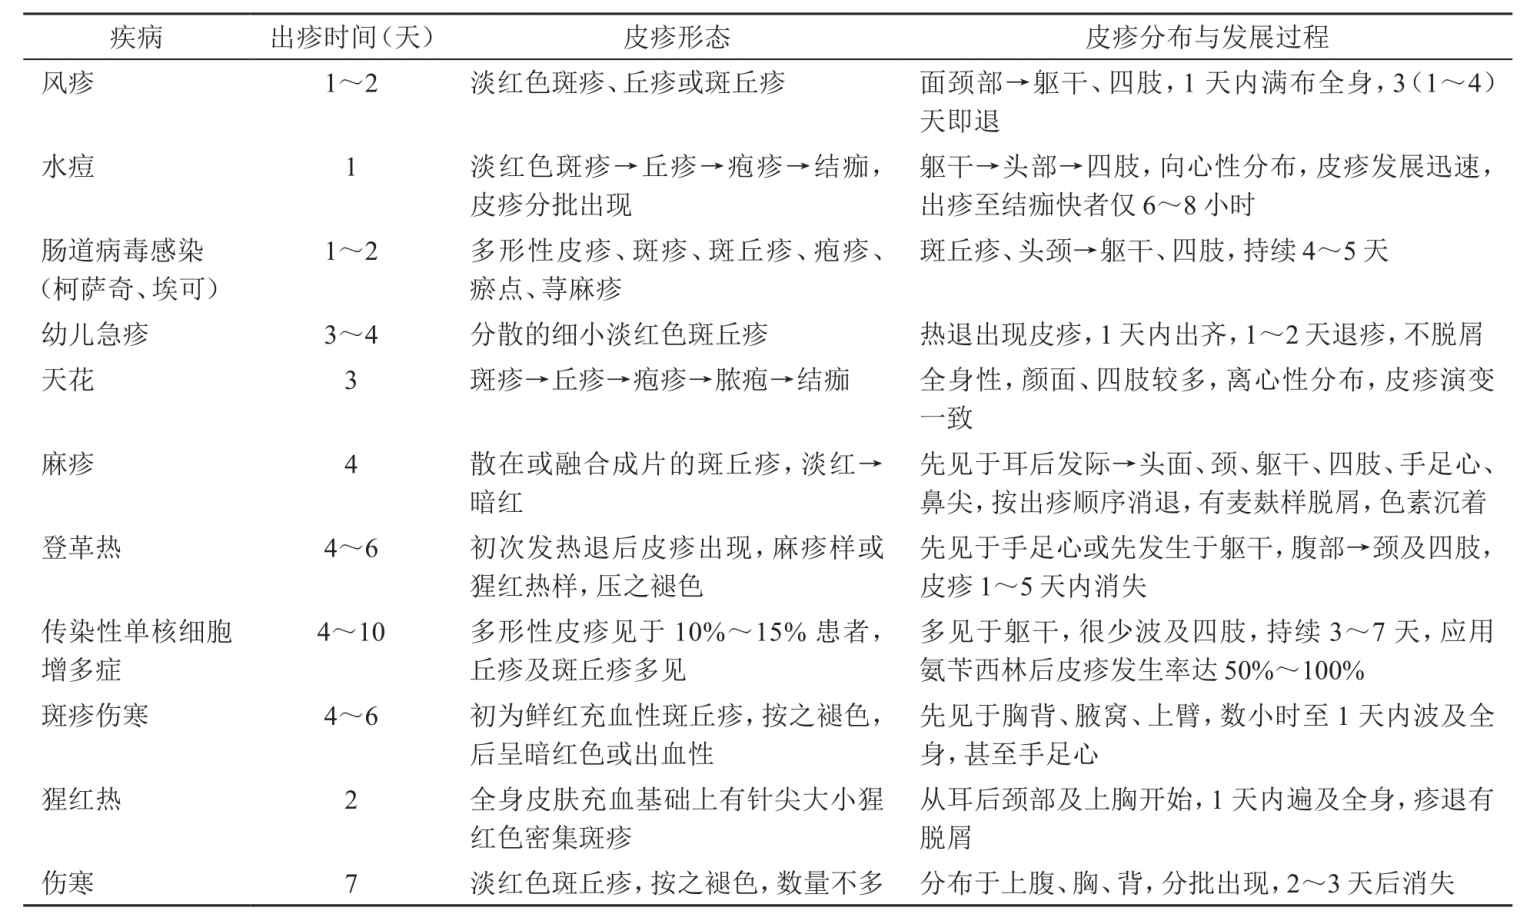
\includegraphics[width=6.625in,height=3.95833in]{./images/Image00003.jpg}
\end{table}

\subsubsection{病因诊断}

发热是由于各种原因导致机体产热过多或散热减少,以及体温中枢功能障碍所致。其原因很多且复杂。在临床实践中,以发热为主诉或唯一症状就诊者有急性发热,尤其出疹性发热,原因不明发热,长期低热,超高热与反复发热。其病因特征亦各异。

\subparagraph{急性发热}

热程在2周以内的发热称为急性发热。其原因很多,绝大多数属于感染,尤以呼吸道、泌尿道和消化道感染最常见,因为这些系统与外界相通,最易遭受病原体的侵袭。在排除上述系统感染后,则要注意某些急性传染病和其他系统的感染。一般而言,这类发热,常伴有定位症状,比较容易诊断。

\subparagraph{长期}

“不明原因”的中、高热
系指发热持续3周以上,体温多次超过38.3℃,经过至少1周深入细致的检查仍不能确诊的一组疾病,称为原因不明发热(fever
of unknown
origin,FUO)。其病因在不同年代和不同地理区域明显不同,但主要有感染、恶性肿瘤与结缔组织-血管性疾病三大类,共约占长期发热病因的80\%~90\%。其中由感染引起的长期发热在国内占60\%~70\%,在其他发展中国家更高些,而在发达国家约占总数1/3。由于人的寿命延长,传染病逐渐减少,恶性肿瘤引起的发热比例有增高趋势,国内约占20\%。结缔组织-血管性疾病约占10\%。病因也受年龄的影响:6岁以下的FUO患儿以感染性疾病为主,尤其是原发性上呼吸道、泌尿道感染或全身感染;6~14岁年龄组则以结缔组织-血管性疾病和小肠炎症性疾病为最常见的病因;14岁以上的成人组,虽然仍以感染性疾病占首位,但肿瘤性疾病明显增多。仍有10\%的病例始终原因不明。

\hypertarget{text00008.htmlux5cux23CHP1-1-2-4-2-1}{}
(1) 感染:

引起发热待查的感染性疾病中主要由细菌感染所致,而任何一种致病菌或条件致病菌,或L-型细菌性感染均可分为全身性与局部性感染。全身性感染以伤寒与副伤寒、粟粒型结核与播散性结核(包括腹膜、肠、肠系膜淋巴结、肝、肾、胸膜和肺与肺门淋巴结结核)、脓毒症与感染性心内膜炎、布鲁菌病、黑热病、急性血吸虫病、旋毛虫病等;局部性感染以肝脓肿、胆道与泌尿生殖道感染、腹腔内脓肿(包括肝下、膈下、结肠旁、阑尾周围、腹膜后、盆腔脓肿等)为常见。局部性感染易被临床忽略。

\hypertarget{text00008.htmlux5cux23CHP1-1-2-4-2-2}{}
(2) 恶性肿瘤:

也是长期发热的常见原因。最常见的为原发性肝癌、淋巴瘤、恶性组织细胞病与白血病,其次为实质性恶性肿瘤如肺癌、肾癌、甲状腺癌等。

\hypertarget{text00008.htmlux5cux23CHP1-1-2-4-2-3}{}
(3) 结缔组织-血管性疾病:

也是较常见原因之一,大多伴有关节痛、皮肤、心、肾等多系统病变引起的相应症状与体征,但少数病例在典型症状出现前数周或数月可出现发热。此类疾病以系统性红斑狼疮、成人少年型类风湿关节炎、多动脉炎、皮肌炎、混合性结缔组织病、风湿热等常见。

\hypertarget{text00008.htmlux5cux23CHP1-1-2-4-2-4}{}
(4) 其他:

肉芽肿性疾病(肉芽肿性肝炎、结节病、局限性回肠炎等)、药物热、伪装热、体腔积血如血胸、血腹、肺梗死等。

\subparagraph{长期低热}

系指口腔温度在37.5~38.4℃,持续4周以上者。在诊断为长期低热时,必须先了解其正常体温,排除生理或功能性因素,并排除高温环境等影响,如在高温车间的纺织女工中,有长期低热者可达10\%以上。长期低热由感染性疾病引起者占40\%,非感染性疾病占57\%,原因不明占3\%。长期低热的原因可分为器质性与功能性两大类:

\hypertarget{text00008.htmlux5cux23CHP1-1-2-4-3-1}{}
(1) 器质性低热:

①慢性感染:如结核病、肝脏疾病、慢性肾盂肾炎、慢性胆道感染以及各种病灶感染(鼻窦炎、牙根脓肿、前列腺炎、慢性盆腔炎、肛门周围脓肿等)。②结缔组织疾病:如风湿热、类风湿关节炎、系统性红斑狼疮等。③内分泌疾病:如甲亢、嗜铬细胞瘤等。④恶性肿瘤:早期淋巴瘤、实质性癌肿转移等。

\hypertarget{text00008.htmlux5cux23CHP1-1-2-4-3-2}{}
(2) 功能性低热:

①生理性低热:月经前期低热、妊娠期低热等。②神经功能性低热:多见于青年女性,长期低热可长达数月或数年。有些患者低热有季节性,出现于夏季(谓之夏季低热),且每年如此。体温在一昼夜内波动幅度较小,常不超过0.5℃,且口腔、腋窝与直肠温度差不大,甚至可出现腋温大于口温,口温大于肛温或腋温大于肛温的反常现象,两侧腋温可相差1℃以上。体温昼夜规律失常。患者常伴有脸色潮红、皮肤划痕症、心动过速等自主神经功能紊乱或神经症色彩。但患者一般情况好,体重无变化,虽经各种药物治疗无效,但不经治疗也可自行消退。神经功能性低热较常见,约占长期低热的1/3,预后良好。③感染后低热:急性病毒或细菌感染得到控制后,高热消退,但可出现持续较久的低热,并伴有乏力,纳差等现象。此种发热可能与体温调节中枢功能失常或自主神经功能紊乱有关。

\subsubsection{超高热危象的识别与诊断}

超高热系指发热超过41℃以上,主要见于体温调节中枢功能障碍,有以下各种原因:①中暑或日射病;②脑部疾病:如严重脑外伤、脑出血、脑炎与脑肿瘤等;③输血、输液污染引起严重致热原反应与脓毒症;④麻醉药引起的恶性高热;⑤临终前超高热等。不论病因如何,超高热对细胞膜与细胞内结构有直接损害作用,当深部体温>
41℃时细胞线粒体的氧化磷酸化出现障碍,可引起永久性脑损害;42~43℃持续数分钟细胞会陷入不可逆的损害,涉及全身各种细胞,尤以脑、心、肝、肾的变化最为突出,容易造成脑水肿颅内压升高,抽搐、昏迷,心、肝、肾、肺功能衰竭,DIC等多脏器功能衰竭。超高热危象的诊断要点是:

\subparagraph{超高热}

超高热(体温> 41℃)是超高热危象的必有表现。

\subparagraph{超高热时伴有多脏器功能受损害的表现}

①心血管系统:低血压休克、心功能不全、心肌缺血与心律失常等。②中枢神经系统:体温越高对中枢神经系统损害越重,症状出现越早;包括不同程度的意识障碍如谵妄、嗜睡、昏迷、抽搐、大小便失禁、脑膜刺激征、瘫痪、病理反射阳性、脑疝、视神经乳头水肿等。③凝血功能障碍:早期出现凝血酶原时间延长,纤维蛋白原减少,血小板减少,出血时间、凝血时间延长;晚期常有广泛而严重的出血、DIC形成。这与过高热直接损害毛细血管、渗透性增加,肝功能受损凝血因子减少,骨髓受损血小板减少等有关。④肾功能损害:可有血尿、管型、少尿、无尿、血肌酐升高等肾功能不全的表现。⑤肝功能损害:肝功能异常如ALT升高、血清胆红素升高,甚至表现为急性肝功能衰竭。⑥水电解质和酸碱平衡失调。⑦其他表现:如横纹肌溶解可致血肌酸磷酸激酶(CK)增高等。

\subparagraph{原发病的表现}

如中毒性菌痢的腹泻、脓血便;乙脑时的抽搐、昏迷等。

\subsection{处理原则}

\subparagraph{支持治疗}

患者出现神志改变、呼吸窘迫、血流动力学不稳定等危及生命的症状与体征时,立即实施监护、建立静脉通路、气道管理、补液以及氧疗,必要时予以呼吸支持治疗。

\subparagraph{超高热危象的处理}

超高热和超高热危象是短暂的临床表现,经适当处理可能很快恢复(如中暑、输液反应等),亦可很快死亡(恶性高温)。早期诊断与早期处理同预后直接有关。因此,对每个可能发生超高热的患者应随时检测体温,一旦出现超高热,应以最快的速度降低中心体温、代谢率,以打断超高热引起的恶性循环,同时防治各种并发症。其中,降温是抢救超高热危象的主要措施。降温速度决定预后,应在1小时内使直肠温度降至38.5℃以内。具体降温措施详见本书第129章“中暑”。

\subparagraph{对症处理}

发热的对症治疗包括:①物理降温:一般可用冷毛巾湿敷额部,每5~10分钟更换1次,或用冰袋置于额、枕后、颈、腋和腹股沟处降温,或用25\%~50\%酒精擦浴。或头置冰帽、冰水灌肠、冷盐水洗胃,或将患者置于空调房内(使室温维持在27℃左右)。应根据具体条件选用。②药物降温:视发热程度可采用口服或肌注解热镇痛药。常用的口服解热镇痛药有:阿司匹林(0.3~0.6g/次)、对乙酰氨基酚(0.3~0.5g/次)、布洛芬(0.2~0.4g/次)、安乃近(0.25~0.5g/次)、解热止痛片(APC片,1~2
片/次)、速效伤风胶囊(1~2粒/次)、复方对乙酰氨基酚片(1~2片/次)等。常用的注射用解热镇痛药有:阿司匹林精氨酸盐(0.5~1.0g/次)、阿司匹林赖氨酸盐(赖氨匹林,0.9~1.8g/次)、对乙酰氨基酚(0.15~0.25g/次)、息热痛注射液(2ml/次)、安痛定注射液(1支/次)等。高热者病情需要时可短期应用肾上腺皮质激素,如地塞米松5~10mg静注或肌注;或以地塞米松12~20mg/d或氢化可的松300~600mg/d静滴。

\subparagraph{抗生素经验性应用}

对感染病例早期抗生素经验性应用是有益的。一般来讲,若有明确的病原菌感染,则选择覆盖特定病原菌感染的窄谱抗生素;若不明确,可选择覆盖革兰阳性和革兰阴性需氧菌、厌氧菌的广谱抗生素。

\subparagraph{诊断性治疗}

当发热病因一时难以查明时,在不影响进一步检查的情况下,可按可能性较大的病因进行诊断性治疗(如疑疟疾,可试用氯喹;疑阿米巴性肝脓肿,行抗阿米巴治疗;疑结核病行抗结核治疗时间以3~4周以上为宜),期望获得疗效而做出临床诊断。诊断性治疗应选用特异性强、疗效确切及安全性大的治疗药物,剂量应充足并完成整个疗程,无特殊原因不得随便更换试验药物。

\subparagraph{随访观察}

对部分症状轻微、经过详细检查仍不能明确病因的发热待查患者,也可在专科门诊进行长期随访而不作特殊处理,确有不少患者可获自愈。

\protect\hypertarget{text00009.html}{}{}

\hypertarget{text00009.htmlux5cux23CHP1-1-4}{}
参 考 文 献

1. 陈灏珠 ,林果为.实用内科学.第13版.北京:人民卫生出版社,2009:332

2. 陈文彬 ,潘祥林.诊断学.第7版.北京:人民卫生出版社,2008:16

3.
陈新谦,金有豫,汤光.新编药物学.第17版.北京:人民卫生出版社,2011:179

\protect\hypertarget{text00010.html}{}{}

\chapter{意识障碍和昏迷}

意识是指人体对周围环境及自身状态的感知能力。意识障碍(disturbance of
consciousness)是脑和脑干功能活动的抑制状态。按照生理与心理学基础可将意识障碍分为觉醒障碍(觉醒度下降,即狭义的意识障碍)和意识内容障碍两大类。前者表现为嗜睡、昏睡和昏迷;后者表现为意识模糊和谵妄等。脑和脑干功能活动的不同抑制程度决定了不同的意识障碍水平。

昏迷(coma)是一种最为严重的意识障碍。患者意识丧失,运动、感觉、反射和自主神经功能障碍,给予任何刺激(如语言、声音、光线、疼痛等)均不能将患者唤醒,但生命体征如呼吸、脉搏、心跳、血压和体温尚可存在。昏迷是病情危重的信号,是常见危重急症,病死率高,临床医师如能迅速作出正确的诊断和及时的处理,患者往往可能转危为安。

以觉醒度改变为主的意识障碍,根据检查时刺激的强度和患者的反应,可分为以下三级:

嗜睡(drowsiness):主要表现为病理性睡眠过多过深,能被各种刺激唤醒,并且能够正确回答问题和做出各种反应,但当刺激去除后又很快入睡。

昏睡(stupor):是一种比嗜睡深而又较昏迷稍浅的意识障碍。昏睡时觉醒水平、意识内容及随意运动均减至最低限度。患者不能自动醒转,在持续强烈刺激下能睁眼、呻吟、躲避,可作简短而模糊的回答,但反应时间持续很短,很快又进入昏睡状态。昏睡时可见到运动性震颤、肌肉粗大抽动、不宁或刻板的动作、强握和吸吮反射。

昏迷(coma):患者意识完全丧失,各种强刺激不能使其觉醒,无有目的的自主活动,不能自发睁眼。昏迷按严重程度可分为浅昏迷、中昏迷和深昏迷三级:①浅昏迷(mild
coma):即轻度昏迷。仅对剧痛刺激(如压迫眶上神经)有防御性反应和痛苦表情,不能言语,可有无意识的自发动作,各种生理反射存在(如吞咽、咳嗽、角膜和瞳孔对光反射),呼吸、血压、脉搏一般无明显改变。②中昏迷:对外界的正常刺激均无反应,自发动作很少。对强烈刺激可有防御反射,角膜反射减弱,瞳孔对光反射迟钝,眼球无转动,大小便潴留或失禁。呼吸、血压、脉搏已有变化。③深昏迷(deep
coma):对外界的任何刺激均无反应,全身肌肉松弛,无任何自主运动。眼球固定,瞳孔散大,各种反射全部消失,大小便多失禁。生命体征已有明显改变,呼吸不规则,血压或下降。

以意识内容改变为主的意识障碍常见有以下三种:

意识模糊(confusion):表现为注意力减退,情感反应淡漠,定向力障碍,活动减少,语言缺乏连贯性,对外界刺激可有反应,但低于正常水平。

精神错乱(psychoderangement):患者对周围环境的接触程度障碍,认识自己的能力减退,思维、记忆、理解与判断力均减退,言语不连贯并错乱,定向力亦减退。常有胡言乱语、兴奋躁动。

谵妄状态(delirium):表现为意识内容清晰度降低,伴有睡眠-觉醒周期紊乱和精神运动性行为。除了上述精神错乱以外,尚有明显的幻觉、错觉和妄想。幻觉以视幻觉最为常见,其次为听幻觉。幻觉的内容极为鲜明、生动和逼真,常具有恐怖性质。因而,患者表情恐惧,发生躲避、逃跑或攻击行为,以及运动兴奋等。患者言语可以增多,不连贯或不易理解,有时则大喊大叫。谵妄或精神错乱状态多在晚间加重,也可具有波动性,发作时意识障碍明显,间歇期可完全清楚,但通常随病情变化而变化,持续时间可数小时、数日甚至数周不等。

\subsection{病因与发病机制}

意识是大脑功能活动的综合表现,是人对自身及外界环境进行认识和做出适宜反应的基础,包括觉醒状态与意识内容两个组成部分。觉醒状态是指与睡眠呈周期性交替的清醒状态,由脑干网状激活系统和丘脑非特异性核团维持和激活,属皮质下激活系统的功能;意识内容是指人的知觉、思维、情绪、记忆、意志活动等心理过程(精神活动),还有通过言语、听觉、视觉、技巧性运动及复杂反应与外界环境保持联系的机敏力,属大脑皮质的功能。正常意识是指觉醒水平与意识水平都处于正常状态,表现为对自身与周围环境有正确理解,对内外环境的刺激有正确反应,对问话的注意力、理解程度以及定向力和计算力都是正常的。脑电生理正常。意识障碍是脑和脑干功能活动的抑制状态,表现为人对自身及外界认识状态以及知觉、记忆、定向和情感等精神活动不同程度的异常。尽管痴呆、冷漠、遗忘、失语等,都是意识内容减退的表现,但只要在其他行为功能还能作出充分和适当的反应,就应该认为意识还是存在的。

正如上述,意识是人对自身及外界环境进行认识及作出适宜反应的基础。意识的“开关”系统包括特异性和非特异性上行投射系统。特异性上行投射系统是各种感觉传入通路的总称。人体通过各种感觉器官接受躯体感觉冲动,经各传导束终止于丘脑特异性核团,再投射到大脑皮质相应的感觉区,引起大脑皮质的激醒。上述感觉冲动途经脑干时发出侧支至脑干网状结构,后者弥散地作用于整个大脑皮质,使大脑皮质处于觉醒状态,称为上行网状激活系统(ascending
reticular activity
system,ARAS)。丘脑下部则接受来自内脏的感觉冲动及体液性刺激,激活大脑边缘系统,称为丘脑下部激活系统,它与ARAS在功能上具有密切联系。大脑皮质受到这两种激活系统的调节与维持,保持觉醒状态。大脑皮质又通过皮质网状束的离皮质联系(corticofugal
connection)向网状结构传递反馈神经冲动,以调节ARAS的活动。这一反馈环路的神经冲动,循环不已,从而维持大脑皮质的持久清醒和意识活动。因此,凡ARAS、丘脑、丘脑下部激活系统或大脑皮质发生器质性或可逆性病变时,均可引起意识障碍。一般当损害或抑制脑干网状结构时引起觉醒障碍;双侧大脑半球的广泛损害或功能抑制可引起意识障碍或昏迷;一侧大脑半球的急性广泛病变,尤其是在优势侧半球,亦可发生意识障碍。颅内局灶病变一般不引起意识障碍,但病变发展迅速并伴有脑循环障碍、脑水肿、颅内高压等时,也可引起不同程度的意识障碍。病变侵犯间脑也可早期发生意识障碍,并且迅速发展。缓慢发展的大脑局灶病变一般无意识障碍,但如合并脑疝,患者可迅速陷入昏迷。不同的病因和病变部位,引起昏迷的发病机制也有差异,详见表\ref{tab2-1}和表\ref{tab2-2}。

\subsection{诊断思路}

任何原因所致的弥漫性大脑皮质和(或)脑干网状结构的损害或功能抑制均可造成意识障碍和昏迷。临床上,引起意识障碍和昏迷的具体病因很多,通过病史和临床检查,有的病因易明确,有的则不易明确。因此,必须边询问病史,边体检,边观察,边治疗。并就以下问题进行分析和判断:①是不是昏迷?②昏迷的程度如何?③引起昏迷的病因是什么?是颅内疾病抑或全身性疾病?若是前者,是颅内局限性病变抑或弥漫性病变?如系局限性病变,它是位于幕上抑或幕下?具体病因是什么?若是全身性疾病,具体病因是什么?

\subsubsection{病史与体检}

对意识障碍和昏迷患者的诊断需要详询病史,仔细而全面的体检以及必要的实验室或特殊辅助检查。

\hypertarget{text00010.htmlux5cux23CHP1-2-2-1-1}{}
(一) 病史采集

对意识障碍和昏迷患者
,采集病史要简明扼要。病史中应着重了解:①发生意识障碍和昏迷的时间、诱因、起病缓急、方式及其演变过程等。②意识障碍和昏迷的伴随症状以及相互间的关系:如首发症状为剧烈头痛者要考虑蛛网膜下腔出血、脑出血、脑膜炎;高热、抽搐起病者结合季节考虑乙型脑炎、流行性脑脊髓膜炎;以精神症状开始者应考虑脑炎、额叶肿瘤等;老年患者以眩晕起病要考虑小脑出血或椎-基底动脉系的缺血。③意识障碍和昏迷发生前有无服用药物(如镇静安眠药、抗精神病药、降血糖药等)、毒物和外伤史,既往有无类似发作等。④既往有无癫痫、精神疾患、长期头痛、视力障碍、肢体运动受限、高血压和严重的肝、肾、肺、心脏疾患以及内分泌代谢疾病等。⑤了解发病现场和环境:如有无未服完的药品、呕吐物;有无特殊气味(如CO、硫化氢等);季节特点(如寒冷、高温等);附近有无高压电线。

\hypertarget{text00010.htmlux5cux23CHP1-2-2-1-2}{}
(二) 体格检查

包括体温
、脉搏、呼吸、血压和皮肤黏膜,以及神经系统以外的其他系统检查等。

\subparagraph{体温}

①体温升高:常见于严重的颅内外感染性疾病(脑炎、脑膜炎、肺部感染、脓毒症等)、脑出血、蛛网膜下腔出血、中暑等。高热无汗还应考虑是否有抗胆碱能药物中毒。②体温降低:常见于酒精中毒、一氧化碳中毒、休克、镇静催眠药中毒、低血糖昏迷、黏液性水肿、垂体功能减退、艾迪生病及下位脑干的广泛损害和冻僵等。

\begin{table}[htbp]
\centering
\caption{颅内疾病引起昏迷的病变部位、发病机制、临床表现和常见病因}
\label{tab2-1}
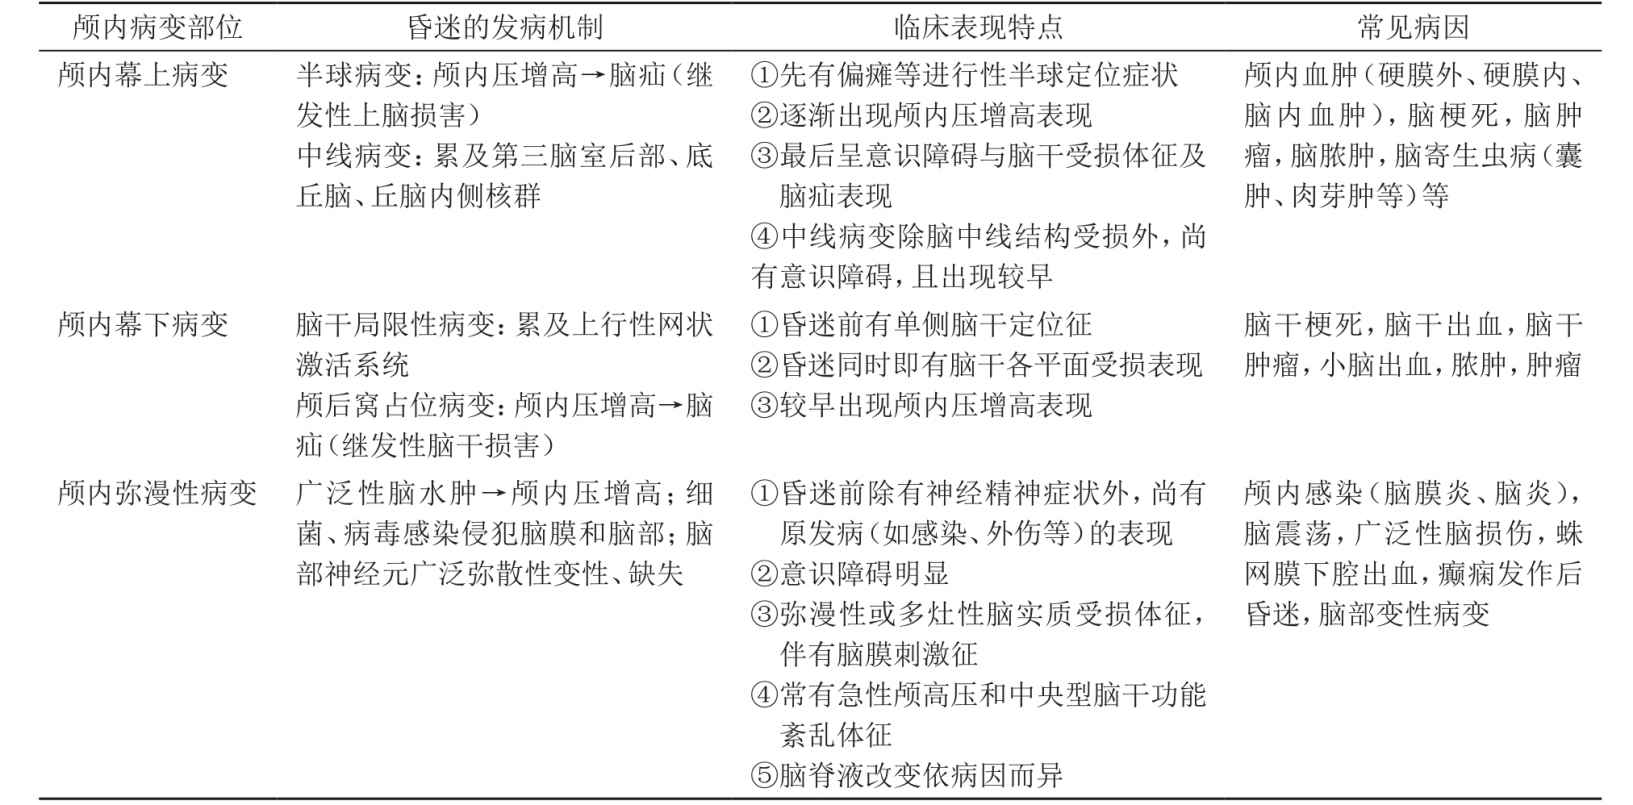
\includegraphics[width=6.73958in,height=3.32292in]{./images/Image00004.jpg}
\end{table}

\begin{table}[htbp]
\centering
\caption{引起昏迷的全身性疾病及其分类、发病机制和常见病因}
\label{tab2-2}
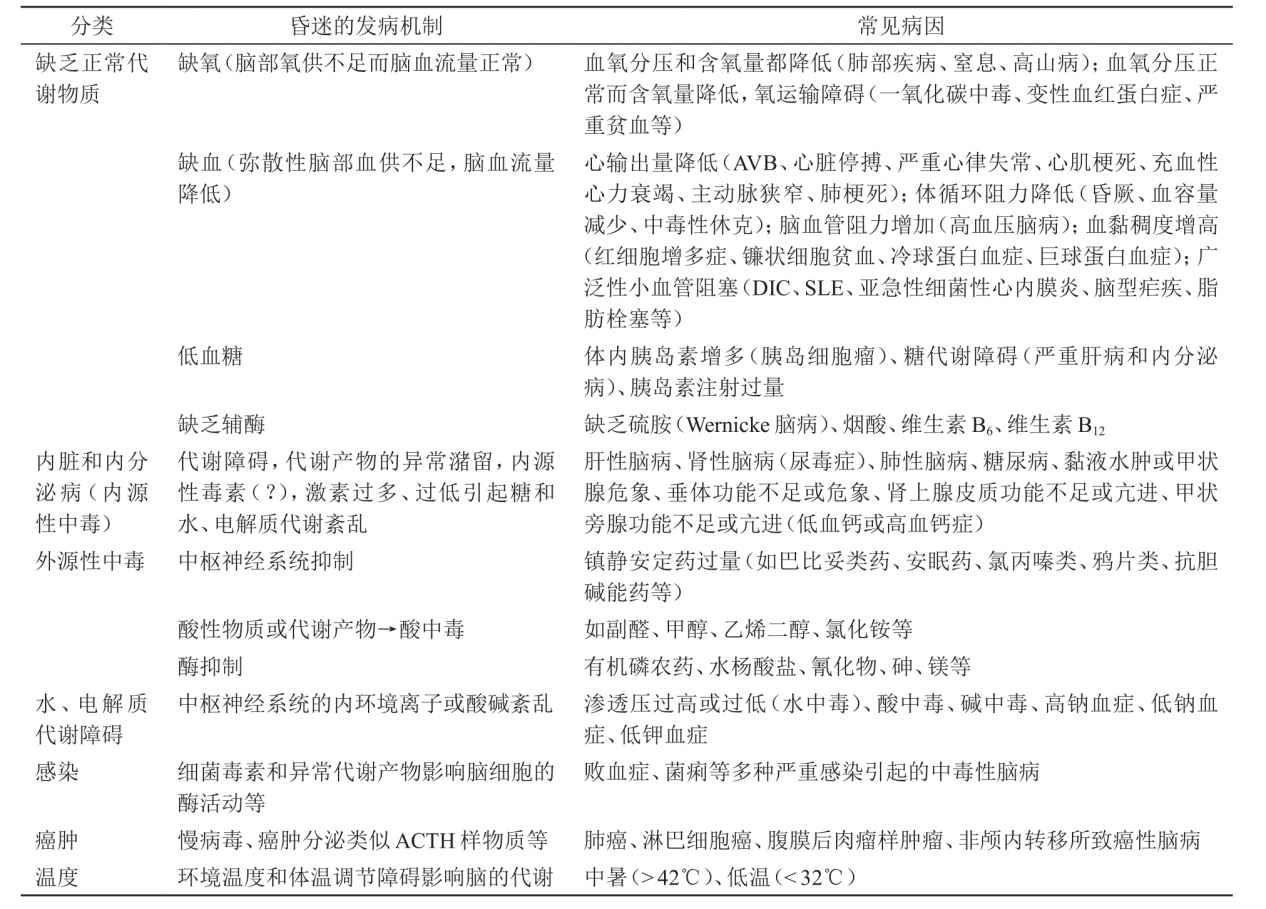
\includegraphics[width=6.73958in,height=4.83333in]{./images/Image00005.jpg}
\end{table}

\subparagraph{脉搏}

脉搏触诊有助于及时发现急性心源性脑缺血综合征。脉慢而洪大见于脑出血、酒精中毒;脑脓肿患者的脉搏常缓慢、充实而规则;而脑膜炎患者的脉搏多细速。颠茄类、氯丙嗪中毒时脉搏显著增快。脉搏先慢后快,同时伴有血压下降者,可见于脑疝压迫脑干、延髓生命中枢衰竭,提示预后不良。

\subparagraph{呼吸}

观察患者的呼吸方式、节律和频率等。呼吸深而快,常见于代谢性酸中毒(糖尿病、尿毒症等);鼾声呼吸且伴有呼吸时一侧面肌瘫痪者提示脑出血。浅而快速的规律性呼吸见于休克、心肺疾患或镇静催眠药中毒引起的呼吸衰竭,肺炎等缺氧性疾病可伴发绀和鼻翼扇动;呼吸深而慢、同时脉搏慢而有力和血压增高,为颅内压增高的表现。呼吸过慢并伴有叹息样呼吸常为吗啡类药物中毒。呼气带有氨味见于尿毒症昏迷;带有苹果味见于糖尿病昏迷;苦杏仁气味提示氢氰酸(苦杏仁、木薯、氰化物等)中毒;呈酒味提示酒精中毒;呼气及排泄物有大蒜样臭味可见于有机磷农药中毒;呼气中及尿液出现“肝臭”者提示肝性脑病。

昏迷患者呼吸节律的异常类型常常提示脑部病变的部位,与神经功能障碍水平定位有密切关系。双侧额叶损害可出现过度换气后呼吸暂停(PHVA)现象,即每在5~10次深呼吸后呼吸暂停。脑部广泛病损使中脑内呼吸中枢失去大脑的控制时,可出现潮式呼吸,即陈-施呼吸(Cheyne-Stokes
respiration,CSR),表现为呼吸由浅慢逐渐变为深快,再由深快变为浅慢,随后出现一段呼吸暂停后,然后重复上述周期性呼吸。潮式呼吸的周期可以长达30秒~2分钟,暂停时间可长达5~30秒。当中脑和脑桥上部功能受损后,可出现中枢神经源性过度呼吸(central
neurogenic
hyperventilation,CNH),呼吸深、快、均匀、持久,频率达40~70次/分。脑桥下部损害后可出现:①喘息样呼吸(gasping
of
breaths),常在濒死时出现,表现为深呼吸、较慢的频率,跳跃式深吸气,呼吸暂停6~10秒,可见于延髓内肿瘤或严重的药物中毒时;②交替呼吸,表现为一次强呼吸和一次弱呼吸交替;③间歇(Biot)呼吸,表现为每3~4次呼吸后出现呼吸暂停;④长吸式呼吸(apneustic
breathing),是一种吸气持续的延长性吸气痉挛,吸2~3次呼1次或吸足气后呼吸暂停。所谓鱼嘴式呼吸(每次吸气时下颌张开似鱼嘴),亦见于脑干下部损害时,常为预后严重的征兆。延髓受损时,呼吸紊乱更为严重,频率和幅度均不时改变,间以不规则地呼吸中断,有人亦称其为“共济失调性呼吸”(ataxic
breathing),最后发展至呼吸完全停止。在天幕上占位病变发展至出现天幕裂孔疝和枕大孔疝的过程中,有时可见到呼吸形式的一系列改变(潮式呼吸→中枢神经源性过度呼吸→喘息式呼吸→共济失调性呼吸),提示脑干功能自首端向尾端逐渐发生障碍。

\subparagraph{血压}

血压显著增高,见于脑出血、高血压脑病、颅内压增高等;血压过低常见于糖尿病昏迷、酒精中毒、巴比妥类药物中毒等。

\subparagraph{皮肤黏膜}

皮肤灼热干燥见于中暑高热;皮肤湿润多汗见于低血糖昏迷、有机磷农药中毒等;皮肤苍白常见于尿毒症性、低血糖性昏迷等;皮肤潮红见于脑出血、颠茄类中毒及酒精中毒;口唇发绀为严重缺氧如窒息、自缢或肺性脑病等;口唇樱红考虑一氧化碳中毒、严重酸中毒;口角见到单纯疱疹,考虑为疱疹性脑炎、脑型疟疾、大叶性肺炎或流脑等;皮肤巩膜黄染应考虑肝性脑病或药物中毒;昏迷伴有结合膜瘀斑、皮疹、皮肤瘀斑,须鉴别脓毒症、流脑、流行性出血热等引起的昏迷;有无头部、颜面部皮肤损伤的痕迹,有无舌咬伤、耳鼻部出血、脑脊液漏、耳后及皮下出血等,对诊断颅骨骨折、颅脑外伤及癫痫大发作常有帮助;颈部手术瘢痕可能提示甲状腺或甲状旁腺疾患,电解质不平衡或内分泌功能障碍;胸腔手术或乳房手术瘢痕应想到颅内转移或伴随于恶性肿瘤的高钙血症、低钠血症等电解质紊乱。应注意肢体、皮肤上成串的针疤或皮下脓肿可能曾滥用药物。

\hypertarget{text00010.htmlux5cux23CHP1-2-2-1-3}{}
(三) 神经系统检查

意识障碍时神经系统查体主要包括以下几个方面的检查
:眼征、对疼痛刺激的反应、瘫痪体征、脑干反射、锥体束征和脑膜刺激征等。

\subparagraph{眼征}

包括以下几个方面:

\hypertarget{text00010.htmlux5cux23CHP1-2-2-1-3-1-1}{}
(1) 瞳孔变化:

观察瞳孔的大小、形状、位置、双侧对称性及对光反应,可帮助判断神经损害的部位及程度。①瞳孔对光反射:为光线刺激瞳孔引起的缩瞳反射。其传导径路为:视网膜→视神经→中脑被盖前区→埃-魏核→动眼神经→膝状神经节→颈上交感神经节节后纤维→瞳孔括约肌,径路上任何一处损害均可引起对光反射丧失和瞳孔散大。瞳孔对光反射与昏迷程度成正比(但巴比妥类中毒虽呈深昏迷,对光反射却残存是特征)。②瞳孔改变与病因:单侧瞳孔扩大,除外药物作用,昏迷患者单侧瞳孔扩大(≥5mm)者,可定为视神经损害或动眼神经损害造成。视神经损害常由于急性颅脑外伤伴发视神经损伤,有球后视神经炎过去史,或局部肿瘤或动脉瘤压迫引起单侧性黑矇性瞳孔麻痹,同侧直接光反射及对侧间接光反射消失;视神经萎缩者,亦可见该侧瞳孔扩大。动眼神经损害单侧瞳孔扩大,多见于后交通动脉瘤破裂引起的蛛网膜下腔出血,也可见于颞叶钩回疝、颅脑外伤伴发硬膜外血肿、脑出血、脑肿瘤等压迫。颈内动脉血栓形成,大脑中动脉浅支或深支梗塞时,亦可见单侧瞳孔扩大。个别癫痫患者抽搐后出现暂时性单侧瞳孔扩大,机制不明。双侧瞳孔扩大,可见于药物或食物中毒如颠茄类、巴比妥类(有时缩小)、氰化物、肉毒杆菌中毒等;脑疝进行到晚期瞳孔由单侧扩大扩展为双侧扩大,昏迷加深,提示预后不良。天幕上病变尚未引起脑疝或中脑结构移位时,瞳孔大小接近正常,若发生小脑幕切迹疝,则见病灶侧瞳孔扩大,对光反射消失,若观察脑疝形成的全过程,则可发现扩大侧瞳孔先有缩小的改变(由于动眼神经的压迫与牵拉,病侧缩瞳纤维首先受到刺激,继而麻痹)。单侧瞳孔缩小较少见,上述幕上占位病变导致早期颞叶钩回疝时,可见同侧瞳孔缩小,而光反射存在;脑干梗死也可见到一侧瞳孔缩小(霍纳综合征表现之一)。双侧瞳孔缩小,可见于氯丙嗪、吗啡类药物、有机磷农药、水合氯醛、毒蕈等中毒与尿毒症;双侧瞳孔缩小如针眼,伴有高热是原发性脑桥出血的特征,若患者还有四肢阵发性强直性抽搐则是脑室出血的表现。中央型间脑疝而致双侧下丘脑损害可出现双侧瞳孔缩小。

\hypertarget{text00010.htmlux5cux23CHP1-2-2-1-3-1-2}{}
(2) 眼球运动:

眼球运动受大脑皮质、脑桥、中脑和第3、4、6脑神经控制,其运动异常有重要的定位意义。在代谢性脑病中,仅巴比妥类和苯妥英钠中毒可有眼球运动障碍。若患者的眼球和浅睡眠一样,能缓慢地向两侧转动,说明脑桥和中脑的有关功能尚相对地完好,据此可推测天幕下病变引起的昏迷可能性较小。一侧大脑半球有较广泛的损害时,患者双眼常偏向瘫痪肢体的对侧;一侧脑桥受损时,则双眼偏向肢体瘫痪的同侧。在双侧大脑皮质急性病变时,可见到有眼球激动现象,每隔几秒钟双眼出现强烈的快速摆动。丘脑底部和上位中脑损害患者,眼球可能向下和向内转,就像盯着自己鼻尖看。眼球浮动(ocular
bobbing)是双眼球快速同向下转后又缓慢地向上转恢复至原位,每分钟重复2~3次,转动的幅度约1~3mm,它发生于眼球水平向运动机制被破坏的情况,其机制为脑桥侧视中枢受损,而中脑的眼球垂直运动中枢未受损之故,见于脑桥的双侧性损害。脑干广泛严重损害时,眼球运动完全丧失而固定在正中位。垂直性眼球运动障碍如双眼向上或向下凝视,提示中脑四叠体附近或下丘脑病变;分离性眼球运动可为小脑损害表现。

\hypertarget{text00010.htmlux5cux23CHP1-2-2-1-3-1-3}{}
(3) 眼底检查:

凡是能引起颅内压增高的疾病均可引起眼底改变。颅脑外伤或颅内出血后12~24小时即可出现视神经乳头水肿的变化;但严重的视乳头水肿多数是由于长期颅内压增高的后果,应考虑有脑肿瘤、脑脓肿等占位病变的可能。如视网膜有广泛的渗出物、出血,则应考虑有糖尿病、尿毒症、高血压脑病等可能。玻璃体下较大的或视网膜广泛的浅表出血通常见于蛛网膜下腔出血。

\subparagraph{对疼痛刺激的反应}

用力按压眶上缘、胸骨检查昏迷患者对疼痛的运动反应,有助于定位脑功能障碍水平或判断昏迷的程度。出现单侧或不对称性姿势反应时,健侧上肢可见防御反应,病侧则无,提示瘫痪对侧大脑半球或脑干病变。观察面部疼痛表情时,可根据面肌运动,判断有无面瘫。疼痛引起去皮质强直(decorticate
rigidity),表现为上肢内收和屈曲,下肢伸直,与丘脑或大脑半球病变有关;去脑强直(decerebrate
rigidity)表现为四肢伸直,肌张力增高或角弓反张,提示中脑功能受损,较去皮质强直脑功能障碍程度更为严重。脑桥和延髓病变患者通常对疼痛无反应,偶可发现膝部屈曲(脊髓反射)。

\subparagraph{瘫痪体征}

意识障碍和昏迷患者的瘫痪检查,可通过疼痛刺激观察面部表情与肢体活动,以及肢体坠落试验等来判定。①观察面颊:一侧面瘫时,可见该侧鼻唇沟变浅,口角低垂,睑裂增宽,呼气时面颊鼓起,吸气时面颊塌陷,呈吸烟斗动作。②疼痛刺激:压迫眶上切迹或捏掐肢体,观察患者肢体活动情况,瘫痪侧少动或不动。③观察双眼球共同偏视(见前述)。④胸骨反射:针刺胸骨柄部,引起一侧或双侧上肢的屈曲反应,手移向胸骨部,刺激加重,可波及下肢。一侧肢体反射消失或运动反应弱,提示该侧肢体瘫痪。⑤上肢坠落试验:将患者双上肢抬起,使与躯干呈垂直位,突然放手,观察肢体坠落情况,瘫痪肢体迅速坠落而且沉重,无瘫痪肢体则向外侧倾倒,缓慢坠落。⑥下肢坠落试验:将患者下肢膝部屈曲抬高,足跟着床,突然松手时,瘫痪侧肢体不能自动伸直,并向外侧倾倒;无瘫痪肢体则呈弹跳式伸直,并能保持足垂直位。⑦足外旋试验:先将患者的双下肢伸直放平,然后把双足扶直并拢,突然松开时,则瘫痪肢体的足立刻外旋倾倒,足外缘着床;无瘫痪的足,仍能维持足垂直位。⑧反射的改变:瘫痪肢体侧常伴有中枢性面瘫,腹壁、提睾反射减弱或消失,腱反射增强,病理反射阳性。

\subparagraph{脑干反射}

可通过睫脊反射(ciliospinal reflex)、角膜反射(corneal
reflex)、头眼反射(oculocephalic reflex)和眼前庭反射(oculovestibular
reflex)等脑干反射来判断是否存在脑干功能损害。反射性眼球运动包括头眼反射和眼前庭反射。

\hypertarget{text00010.htmlux5cux23CHP1-2-2-1-3-4-1}{}
(1) 睫脊反射:

给予颈部皮肤疼痛刺激时可引起双侧瞳孔散大,此反射存在提示下位脑干、颈髓、上胸段脊髓及颈交感神经功能正常。

\hypertarget{text00010.htmlux5cux23CHP1-2-2-1-3-4-2}{}
(2) 角膜反射:

角膜反射是由三叉神经的眼神经与面神经共同完成的,当三叉神经的第一支(眼神经)或面神经损害时,均可出现角膜反射消失。若脑桥上部和中脑未受累及,角膜反射存在;一侧角膜反射消失见于同侧面神经病变(同侧脑桥),双角膜反射消失见于一侧三叉神经受损或双侧面神经受损,提示中脑或脑桥受累,常有意识障碍。

\hypertarget{text00010.htmlux5cux23CHP1-2-2-1-3-4-3}{}
(3) 头眼反射:

又称玩偶眼试验(Doll's eye
test)。在浅昏迷患者,检查者使其眼睑睁开,并将患者的头向两侧或前后转动,先慢后快,患者双眼反射地朝与头转动相反的方向转动(如头转向右侧时,双眼凝视偏向左侧),谓之头眼反射(本体觉转头反射、环偶眼现象)阳性。在婴儿为正常反射,随着大脑发育而抑制。头眼反射的刺激主要通过颈部肌肉本体觉,通过本体觉神经纤维进入脊髓,先经过颈髓2~4节段的背根,然后进入颈髓再上升达到延髓前庭神经核、中脑顶盖部、脑桥,以及第3、4、6脑神经。正常人清醒状态下,头眼反射为大脑半球发起的视觉固定(或注视,visual
fixation)所抑制,故正常人头眼反射不存在。在嗜睡患者,开始2或3次转头可能引起相反的同向眼动,以后由于转头动作通常使患者觉醒而头眼反射消失。此反射在大脑半球弥漫性病变和间脑病变所致昏迷时出现并加强;脑干病变时此反射消失,如一侧脑干病变,头向该侧转动时无反射,向对侧仍存在。应强调的是:在怀疑有颈椎脱位与骨折可能的患者,绝对禁忌作此项检查。

\hypertarget{text00010.htmlux5cux23CHP1-2-2-1-3-4-4}{}
(4) 眼前庭反射:

或称冷热水试验。用注射器向一侧外耳道注入1ml冰水,大脑半球弥漫性病变而脑干功能正常时,出现双眼向冰水灌注侧强直性同向运动;昏迷患者,如存在完全的反射性眼球运动,提示脑桥至中脑水平的脑干功能完好;中脑病变时,眼前庭检查可显示灌注对侧眼球内收不能,同侧眼外展正常;脑桥病变时反应完全丧失。

\subparagraph{脑膜刺激征}

脑膜刺激征包括颈强直(简称颈强)、Kernig征(凯尔尼格征)和Brudzinski征(布鲁津斯基征)等。颈上节段的脊神经根受刺激引起颈强直,腰骶节段的脊神经根受刺激,则出现Kernig征和Brudzinski征。阳性提示有脑膜炎、蛛网膜下腔出血、脑炎、脑水肿及颅内压增高等的可能。深昏迷时脑膜刺激征可消失。检查方法包括:

\hypertarget{text00010.htmlux5cux23CHP1-2-2-1-3-5-1}{}
(1) 屈颈试验:

患者仰卧,检查者托患者枕部并使其头部前屈而表现不同程度的颈强,被动屈颈受限,称为颈强直,但需排除颈椎病。正常人屈颈时下颏可触及胸骨柄,部分老年人及肥胖者除外。

\hypertarget{text00010.htmlux5cux23CHP1-2-2-1-3-5-2}{}
(2) Kernig征:

患者仰卧,下肢于髋、膝关节处屈曲成直角,检查者于膝关节处试行伸直小腿,如伸直受限并出现疼痛,大、小腿间夹角<
135°,为Kernig征阳性。如颈强(+)而Kernig征(−),称为颈强-Kernig征分离,见于后颅窝占位性病变和小脑扁桃体疝等。

\hypertarget{text00010.htmlux5cux23CHP1-2-2-1-3-5-3}{}
(3) Brudzinski征:

患者仰卧屈颈时出现双侧髋、膝部屈曲;一侧下肢膝关节屈曲位,检查者使该侧下肢向腹部屈曲,对侧下肢亦发生屈曲(下肢征),均为Brudzinski征阳性。

\subparagraph{反射检查}

一般认为,浅反射由减退至消失而同时深反射由亢进至消失,均提示昏迷的程度加深。常用的深反射(为肌腱和关节反射)有肱二头肌、肱三头肌反射,桡骨膜反射,膝反射,跟腱反射等;常用的浅反射(浅反射是刺激皮肤、黏膜、角膜等引起肌肉快速收缩反应)有角膜反射、咽反射、腹壁反射、提睾反射、跖反射、肛门反射等。常用的病理反射有:

\hypertarget{text00010.htmlux5cux23CHP1-2-2-1-3-6-1}{}
(1) 巴宾斯基征(Babinski征):

是经典的病理反射,提示锥体束受损。用竹签轻划足底外侧,自足跟向前至小趾根部足掌时转向内侧,阳性反应为趾背屈,可伴其他足趾扇形展开。

\hypertarget{text00010.htmlux5cux23CHP1-2-2-1-3-6-2}{}
(2) 巴宾斯基等位征:

包括:①Chaddock征:由外踝下方向前划至足背外侧;②Oppenheim征:用拇指和示指沿胫骨前缘自上而下用力下滑;③Schaeffer征:用手挤压跟腱;④Gordon征:用手挤压腓肠肌;⑤Gonda征:用力下压第4、5足趾,数分钟后突然放松;⑥Pussep征:轻划足背外侧缘。阳性反应均为趾背屈。临床意义一般认为同Babinski征。

\hypertarget{text00010.htmlux5cux23CHP1-2-2-1-3-6-3}{}
(3) 强握反射:

指检查者用手指触摸患者手掌时被强直性握住的一种反射。新生儿为正常反射,成人见于对侧额叶运动前区病变。

\hypertarget{text00010.htmlux5cux23CHP1-2-2-1-3-6-4}{}
(4) 脊髓自主反射:

脊髓横贯性病变时,针刺病变平面以下皮肤引起单侧或双侧髋、膝、踝部屈曲(三短反射)和Babinski征阳性。若双侧屈曲并伴腹肌收缩、膀胱及直肠排空,以及病变以下竖毛、出汗、皮肤发红等,称为总体反射。

对于昏迷患者除重点注意以上项目外,尚应注意胸、腹部体征如昏迷偏瘫患者伴有心脏杂音,心房纤颤,考虑心脏病伴有脑梗死;昏迷、抽搐伴有心音片刻听不到,考虑阿-斯综合征;昏迷、休克、肺部啰音等,考虑中毒性肺炎;昏迷患者伴腹水、肝脾大或缩小,常提示肝性脑病、血液病、细菌性心内膜炎、脓毒症等可能性。

实验室检查与特殊检查应根据需要选择进行,但除三大常规外,对于意识障碍和昏迷患者,血清电解质、尿素氮(BUN)、CO\textsubscript{2}
CP、血糖等应列为常规检查;对病情不允许者必须先就地抢救,视病情许可后再进行补充。脑电图、头颅CT和MRI,以及脑脊液检查对昏迷的病因鉴别有重要意义。

在通过上述病史询问,体检,神经系统检查及必要的有关辅助检查后,一般可依下列顺序对意识障碍与昏迷进行诊断和鉴别诊断。

\subsubsection{判断是否为意识障碍和昏迷}

临床上判断是否属于意识障碍和昏迷一般不难,但首先应排除下述两种情况:

\subparagraph{几种特殊类型的意识障碍}

\hypertarget{text00010.htmlux5cux23CHP1-2-2-2-1-1}{}
(1) 去皮质综合征(decorticate syndrome):

也称去大脑皮质状态(apallic
state),是由于双侧大脑皮质发生弥散性的严重损害而导致大脑皮质功能减退或丧失,皮质下功能仍保存。其特点是皮质与脑干的功能出现分离现象:大脑皮质功能丧失,对外界刺激无任何意识反应,不言不语;而脑干各部分的功能正常:患者眼睑开闭自如,常睁眼凝视(即醒状昏迷),痛觉灵敏(对疼痛刺激有痛苦表情及逃避反应),角膜与瞳孔对光反射均正常。四肢肌张力增高,双上肢常屈曲,双下肢伸直(去皮质强直),大小便失禁,还可出现吸吮反射及强握反射,甚至伴有手足徐动、震颤、舞蹈样运动等不随意运动。该综合征常见于缺氧性脑病、脑炎、中毒和严重颅脑外伤等。

\hypertarget{text00010.htmlux5cux23CHP1-2-2-2-1-2}{}
(2) 无动性缄默症(akinetic mutism):

又称睁眼昏迷(coma
vigil),由脑干上部和丘脑的ARAS受损引起,此时大脑半球及其传出通路无病变。患者能注视周围环境及人物,貌似清醒,但不能活动或言语,二便失禁。肌张力减低,无锥体束征。强烈刺激不能改变其意识状态,存在觉醒-睡眠周期。本症常见于脑干梗死。

\hypertarget{text00010.htmlux5cux23CHP1-2-2-2-1-3}{}
(3) 植物状态(vegetative state):

是指大脑半球严重受损而脑干功能相对保留的一种状态。表现为对自身和外界的认知功能完全丧失,能睁眼,有睡眠和觉醒周期,可有无意义哭笑,二便失禁。肢体可有无意识的随意运动,脑干反射存在。持续性植物状态指颅脑外伤后植物状态持续12个月以上,其他原因持续3个月以上。

\subparagraph{神经精神疾病所致的几种貌似昏迷状态}

\hypertarget{text00010.htmlux5cux23CHP1-2-2-2-2-1}{}
(1) 精神抑制状态(depression state):

常见于强烈精神刺激后或癔症性昏睡发作,患者表现出僵卧不语,对外界刺激如呼唤、推摇,甚至疼痛刺激常不发生反应。双目紧闭,扳开眼睑时有明显抵抗感,并见眼球向上翻动,放开后双眼迅速紧闭。瞳孔大小正常,光反应灵敏,眼脑反射正常,无病理反射。脑电图呈觉醒反应,经适当治疗可迅速复常。癔症性昏睡,多数尚有呼吸急促,也有屏气变慢,检查四肢肌张力增高,对被动活动多有抵抗,有时四肢伸直、屈曲或挣扎、乱动。常呈阵发性,多属一过性病程,在暗示治疗后可迅速恢复。

\hypertarget{text00010.htmlux5cux23CHP1-2-2-2-2-2}{}
(2) 木僵(stupor):

表现为不语不动,不饮不食,对外界刺激缺乏反应,甚至出现大小便潴留,多伴有蜡样屈曲和违拗症,言语刺激触及其痛处时可有流泪、心率增快等情感反应,缓解后多能清楚回忆发病过程。见于精神分裂症的紧张性木僵、严重抑郁症的抑郁性木僵、反应性精神障碍的反应性木僵等。

\hypertarget{text00010.htmlux5cux23CHP1-2-2-2-2-3}{}
(3) 闭锁综合征(locked-in syndrome):

又称去传出状态(deefferented
state)。病变位于脑桥基底部,双侧锥体束和皮质脑干束均受累。患者意识清醒,因运动传出通路几乎完全受损而呈失运动状态,除尚有部分眼球运动外,呈现四肢瘫,不能说话和吞咽,表情缺乏,就像全身被闭锁,但可理解语言和动作,能以睁闭或眼垂直运动示意。当临床怀疑本症时,可让患者“睁开你的眼睛”、“向上看”、“向下看”和“看你的鼻尖”等,可作出鉴别。

\hypertarget{text00010.htmlux5cux23CHP1-2-2-2-2-4}{}
(4) 意志缺乏症(abulia):

患者处于清醒状态,运动感觉功能存在,但因缺乏始动性而不语不动,对刺激无反应,无欲望,呈严重淡漠状态,可有额叶释放反射,如掌颏反射、吸吮反射等。本症多由双侧额叶病变所致。

\hypertarget{text00010.htmlux5cux23CHP1-2-2-2-2-5}{}
(5) 失语(aphasia):

程度较重的失语患者,特别是伴有嗜睡、瘫痪时,对外界刺激失去反应能力而易被误认为昏迷。如系失语而非昏迷的患者,对声、光、疼痛刺激的反应是灵敏的;对言语以外的示意性动作、表情等仍能领会、理解,而有适当的表情反应,或喃喃发声,欲语不能。

\subsubsection{意识障碍和昏迷程度的评定}

临床上除将意识障碍分为嗜睡、昏睡、浅昏迷、中昏迷和深昏迷五级(见前述)外,常用格拉斯哥昏迷计分法(Glasgow
coma
scale,GCS)。GCS是以睁眼(觉醒水平)、言语(意识内容)和运动反应(病损平面)三项指标的15项检查结果来判断患者昏迷和意识障碍的程度,见表\ref{tab2-3}。以上三项检查共计15分。GCS分值愈低,脑损害的程度愈重,预后亦愈差。但此量表有一定局限性:对眼肌麻痹、眼睑肿胀者不能评价其睁眼反应,对气管插管或切开者不能评价其言语活动,四肢瘫患者不能评价其运动反应。1978年此量表被修订为Glasgow-Pittsburgh量表,增加了对光反射、脑干反射、抽搐情况和自发性呼吸四大类检查,见表\ref{tab2-4}。合计为7项35级,最高为35分,最低为7分。在颅脑损伤中,35~28分为轻型,27~21分为中型,20~15分为重型,14~7分为特重型颅脑损伤。该观察表即可判定昏迷程度,也反映了脑功能受损水平。

\subsubsection{意识障碍和昏迷的病因诊断}

意识障碍和昏迷的病因诊断极其重要。通常必须依据病史、体格和神经系统检查,以及有关的辅助检查资料,经过综合分析,能查出导致昏迷的原发病因。由于昏迷的病因众多,而且某些病例的病程进展甚快,病情危重或因条件所限,无法进行详细或特殊的辅助检查,使病因诊断受到影响。但以下诊断思路具有较大的临床价值。

\hypertarget{text00010.htmlux5cux23CHP1-2-2-4-1}{}
(一) 确定是颅内疾病抑或全身性疾病

通常先确定是颅内疾病抑或全身性疾病
,如确定意识障碍和昏迷是颅内病变引起,尚需进一步确定是颅内局限性病变抑或弥散性病变,如是前者,它是位于幕上抑或幕下,具体病因是什么。

\subparagraph{颅内疾病}

位于颅内的原发性病变,在临床上通常先有大脑或脑干受损的定位症状和体征,较早出现意识障碍和精神症状,伴明显的颅内高压症和脑膜刺激征,提示颅内病变的有关辅助检查如脑脊液检查、CT扫描等常有阳性发现。临床上可根据神经系统体征基本上将表现分为两类:①主要呈现局限性神经体征,如脑神经损害、肢体瘫痪、局限性抽搐、偏侧锥体束征等,常见于脑出血、梗死、脑炎、外伤、占位性病变等;②主要表现为脑膜刺激征而无局限性神经体征,最多见于脑膜炎、蛛网膜下腔出血等。

\begin{table}[htbp]
\centering
\caption{GCS昏迷评定量表}
\label{tab2-3}
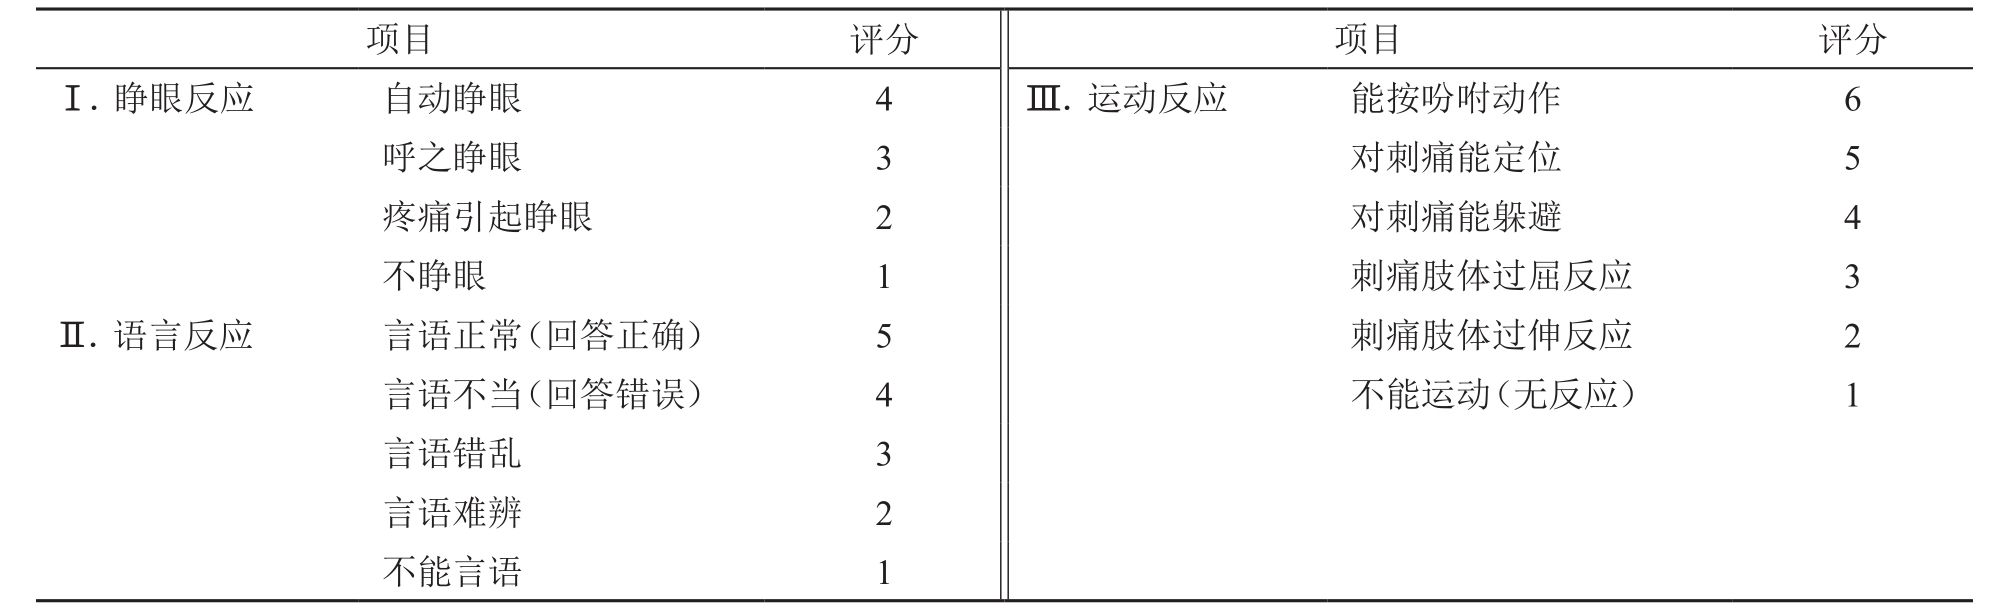
\includegraphics[width=6.66667in,height=2.03125in]{./images/Image00006.jpg}
\end{table}

\begin{table}[htbp]
\centering
\caption{Glasgow-Pittsburgh昏迷观察表}
\label{tab2-4}
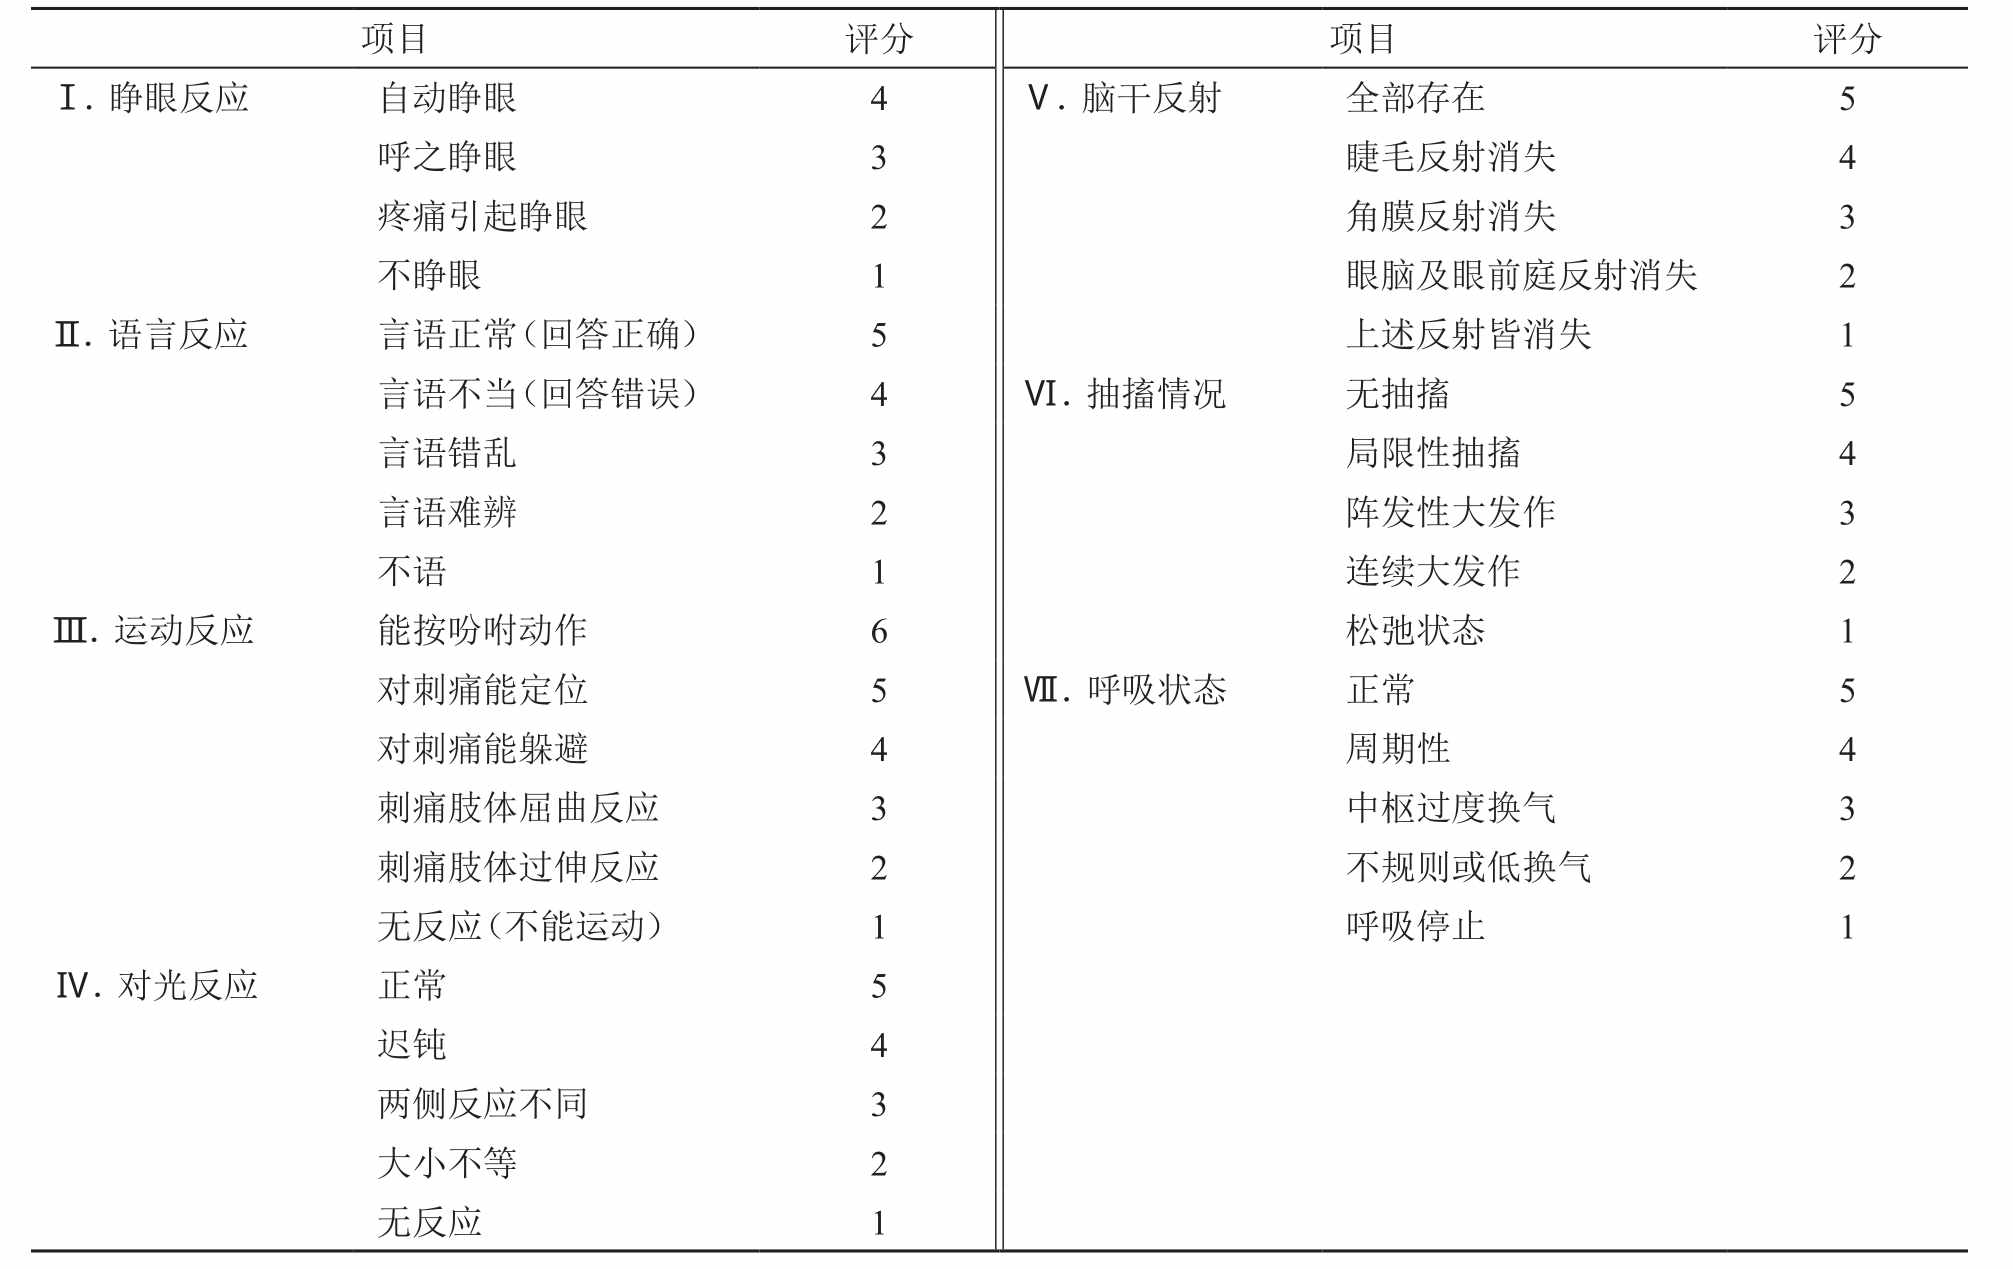
\includegraphics[width=6.69792in,height=4.21875in]{./images/Image00007.jpg}
\end{table}

如确定昏迷是颅内病变引起,尚可将颅内病变又进一步区分为颅内幕上局限性病变、幕下局限性病变和颅内弥散性病变三组。它们的特征参见表\ref{tab2-1}。

\subparagraph{全身性疾病}

全身性疾病可影响脑代谢而引起弥散性脑损害,又称代谢性脑病。同原发性颅内病变相比,其临床特点为:先有颅外器官原发病的症状和体征,以及相应的实验室检查阳性发现,后才出现脑部受损的征象。由于脑部损害为非特异性或仅是弥散性功能抑制,临床上一般无持久性和明显的局限性神经体征和脑膜刺激征,主要是多灶性神经功能缺乏的症状和体征,且大都较对称;通常先有精神异常,意识内容减少。一般是注意力减退,记忆和定向障碍,计算和判断力降低,尚有错觉、幻觉,随病程进展,意识障碍加深。此后有的可出现不同层次结构损害的神经体征,如昏迷较深和代谢性呼吸抑制很严重,而眼球运动和瞳孔受累却相对较轻。脑脊液改变不显著,颅脑CT扫描等检查无特殊改变,不能发现定位病灶。其病因很多,它们的特征参见表\ref{tab2-2}。

\hypertarget{text00010.htmlux5cux23CHP1-2-2-4-2}{}
(二) 根据患者是否伴有脑膜刺激征和脑局灶体征来判断昏迷的病因

\subparagraph{脑膜刺激征(+)而脑局灶性体征(−)}

\hypertarget{text00010.htmlux5cux23CHP1-2-2-4-2-1-1}{}
(1) 突发剧烈头痛:

蛛网膜下腔出血(脑动脉瘤、脑动静脉畸形破裂)。

\hypertarget{text00010.htmlux5cux23CHP1-2-2-4-2-1-2}{}
(2) 急性发病、发热在先:

化脓性脑膜炎、乙型脑炎、其他急性脑炎等。

\hypertarget{text00010.htmlux5cux23CHP1-2-2-4-2-1-3}{}
(3) 亚急性或慢性发病:

真菌性、结核性、癌性脑膜炎。

\subparagraph{脑膜刺激征(−)而脑局灶性体征(+)}

\hypertarget{text00010.htmlux5cux23CHP1-2-2-4-2-2-1}{}
(1) 突然起病者:

如脑出血、脑栓塞、脑梗死等。

\hypertarget{text00010.htmlux5cux23CHP1-2-2-4-2-2-2}{}
(2) 以发热为前驱症状:

如脑脓肿、血栓性静脉炎、各种脑炎、急性播散性脑脊髓炎、急性出血性白质脑病等。

\hypertarget{text00010.htmlux5cux23CHP1-2-2-4-2-2-3}{}
(3) 与外伤有关:

如脑挫伤、硬膜外血肿、硬膜下血肿等。

\hypertarget{text00010.htmlux5cux23CHP1-2-2-4-2-2-4}{}
(4) 缓慢起病、颅内压增高者:

脑肿瘤、慢性硬膜下血肿、脑寄生虫病等。

\subparagraph{脑膜刺激征(−)和脑局灶性体征(−)}

\hypertarget{text00010.htmlux5cux23CHP1-2-2-4-2-3-1}{}
(1) 有明确中毒原因:

如酒精、麻醉药、安眠药、一氧化碳中毒等。

\hypertarget{text00010.htmlux5cux23CHP1-2-2-4-2-3-2}{}
(2) 尿检异常:

尿毒症、糖尿病、急性尿卟啉症等。

\hypertarget{text00010.htmlux5cux23CHP1-2-2-4-2-3-3}{}
(3) 休克状态:

低血糖、心肌梗死、肺栓塞、大出血等。

\hypertarget{text00010.htmlux5cux23CHP1-2-2-4-2-3-4}{}
(4) 有黄疸:

肝性脑病等。

\hypertarget{text00010.htmlux5cux23CHP1-2-2-4-2-3-5}{}
(5) 有发绀:

肺性脑病等。

\hypertarget{text00010.htmlux5cux23CHP1-2-2-4-2-3-6}{}
(6) 有高热:

重症感染、中暑、甲状腺危象等。

\hypertarget{text00010.htmlux5cux23CHP1-2-2-4-2-3-7}{}
(7) 体温过低:

休克、酒精中毒、黏液性水肿昏迷等。

\hypertarget{text00010.htmlux5cux23CHP1-2-2-4-2-3-8}{}
(8) 头部外伤:

脑震荡等。

\hypertarget{text00010.htmlux5cux23CHP1-2-2-4-2-3-9}{}
(9) 其他:

癫痫等。

\subsection{处理原则}

\subparagraph{昏迷的最初处理}

常规措施有:①保持呼吸道通畅,氧疗,必要时气管插管或切开行人工呼吸。②维持循环功能,尽早开放静脉,建立输液通路(1~3个)。有休克应迅速扩充血容量,使用血管活性药物,尽快使收缩血压稳定在100mmHg左右。有心律失常者应予以纠正;有心肌收缩力减弱者应给予强心剂;心跳骤停时应立即行心肺复苏。③纳洛酮:常用剂量每次0.4~0.8mg,静脉注射或肌注,无反应可隔10~15分钟重复用药,直达预期效果;亦可用1.2~2.0mg加入250~500ml液体中静滴。

\subparagraph{病因治疗}

针对病因采取及时果断措施是抢救成功的关键。若昏迷的病因已明确,则应迅速给予有效病因治疗。如由颅内占位性病变引起者,若条件许可应尽早作开颅手术,摘除肿瘤;细菌性脑膜脑炎引起者,应迅速给予大量而有效的抗生素治疗;因脑型疟疾而引起的昏迷,则可给盐酸奎宁0.5g置于5\%葡萄糖液250~500ml中静滴;由于低血糖引起者应立即给予高渗葡萄糖液;若为有机磷农药中毒所致者,应立即用胆碱酯酶复能剂和阿托品等特效解毒剂;糖尿病昏迷应予胰岛素治疗等。

\subparagraph{对症支持疗法}

包括控制脑水肿、降低颅内压,维持水电解质平衡,镇静止痛,防治各种并发症(如急性心力衰竭、急性呼吸衰竭、消化道出血、急性肾功能衰竭、急性脑功能衰竭等)等,详见有关章节。

\protect\hypertarget{text00011.html}{}{}

\hypertarget{text00011.htmlux5cux23CHP1-2-4}{}
参 考 文 献

1. 张文武.急诊内科学.第2版.北京:人民卫生出版社,2007

2. 贾建平.神经病学.第6版.北京:人民卫生出版社,2008

3. Rowland LP. Merritt's Neurology. 11th ed. New York:Lippincott
Williams & Wilkins,2005

\protect\hypertarget{text00012.html}{}{}

\chapter{眩 晕}

眩晕是一主观症状,是机体对于空间关系的定向感觉障碍或平衡感觉障碍,是一种运动错觉,患者感外境或自身在旋转、移动或摇晃。在眩晕症状出现的同时,常伴有平衡失调、站立不稳、眼球震颤、指物偏向、恶心、呕吐、面色苍白、出汗及心率和血压的改变。

临床上可将眩晕分为前庭系统性眩晕(亦称真性眩晕)及非前庭系统性眩晕(亦称头晕)。前者由前庭神经系统病变(包括前庭末梢器、前庭神经及前庭的中枢连接)所引起,为真性眩晕,表现为有运动错觉的眩晕,例如自觉旋转、摇晃、移动感;后者常为头昏(头重脚轻、眼花、头脑昏昏沉沉、颅内在转动等诉说),但并无外境或自身旋转的运动觉,常由心血管系统疾病,全身中毒性、代谢性疾病,贫血,眼病等疾患所引起。

\subsection{病因与发病机制}

\subsubsection{病因分类}

眩晕的病因分类有多种方法,各家不甚统一,各有其优缺点。笔者认为根据神经系统疾病的诊断步骤先定位再定性的方法,较为实用,即根据病变的解剖部位及结合病因予以分类。现将常见的疾病列举如下:

\hypertarget{text00012.htmlux5cux23CHP1-3-1-1-1}{}
(一) 前庭系统性眩晕

包括前庭末梢感受器
、前庭神经、前庭诸核、内侧纵束、小脑、前庭皮质代表区之各种病损所产生的真性眩晕。

\subparagraph{耳源性}

例如外耳道耵聍,急、慢性中耳炎,咽鼓管阻塞,鼓膜内陷,耳硬化症,迷路炎,慢性中耳炎内耳并发症(瘘管形成),梅尼埃病(Meniere
disease),运动病,良性位置性眩晕,迷路动脉血供障碍,内耳震荡等。

\subparagraph{前庭神经病损}

前庭神经元炎、听神经鞘膜瘤、脑桥小角其他肿瘤、前庭神经炎、前庭神经外伤(岩锥骨折)或中毒性损害。

\subparagraph{脑干病变}

脑桥、延髓的血管性和肿瘤性病变、脑干脑炎、多发性硬化、延髓空洞症、第四脑室肿瘤及囊肿。

\subparagraph{小脑病变}

肿瘤、脓肿、出血及损伤。

\subparagraph{大脑病变}

颞叶肿瘤或血管性病变,颞叶癫痫。

\subparagraph{颈椎病变}

颈椎肥大性改变及颈椎间盘突出。

\hypertarget{text00012.htmlux5cux23CHP1-3-1-1-2}{}
(二) 非前庭系统性眩晕

1.眼性眩晕 如眼外肌麻痹、屈光不正、先天性视力障碍等。

2.心血管病变 如高血压、低血压、心律不齐、心力衰竭、大脑动脉硬化。

3.全身中毒性、代谢性、感染性疾病。

4.各种原因引起的贫血。

5.神经症。

\subsubsection{发病机制}

机体平衡的维持,定向功能的正常,是借视觉、本体觉(肌腱、关节中)及前庭平衡觉的协同作用而完成的,而后者对机体姿位平衡的维持更为重要。各种外界的刺激(信息),通过上述诸感受器如视觉、本体觉、前庭平衡觉传入至前庭核群、红核、网状结构、皮质下中枢、小脑等,不断反射性调节机体对各种姿位的平衡,各种加速度的反应,使机体在运动中与外界环境保持协调与平衡。神经冲动由皮质下中枢再向上传入大脑皮质,多数学者认为皮质平衡中枢在颞叶,Penfield为患者作脑部手术时,电刺激颞上回,引起“头晕”、“旋转”和“摇摆”感。应用电生理方法在动物实验中测定了前庭皮质投射区,罗猴的前庭皮质投射区位于第一体感区和第二体感区之间的中央后回,为Brodmann第2区稍后处。前庭的皮质投射似乎从感觉-运动皮质移向顶叶的联合皮质,皮质区接受两侧前庭投射。综上所述,皮质前庭代表区虽不甚确切,但一般认为在颞上回的后、上半部,颞顶交界处及岛叶的上部。丘脑后下腹核很可能为前庭传入的丘脑换元站。后下腹核位于后外侧腹核和后内侧腹核之间的底部。

前庭系统包括内耳迷路末梢感受器(半规管中的壶腹嵴、椭圆囊和球囊中的位觉斑),前庭神经、脑干中的前庭核群,小脑、内侧纵束、前庭脊髓束、前庭皮质代表区。三个半规管中的壶腹嵴,其感受器在半规管中内淋巴流动时接受角加速度的刺激,而椭圆囊、球囊的位觉斑则接受直线加速度、重力加速度的刺激,冲动沿着前庭神经传入中枢,反射性地调节机体平衡。在正常情况下,从前庭器官传入中枢的有关平衡觉的信息并不为人所感知,只是当前庭器官或其中枢连接受到较大刺激或病理性损害时,前庭感受的刺激(信息)与来自肌肉、关节的本体觉及视觉感受器的关于空间定向的冲动不一致时,于是产生眩晕,亦即运动错觉。由于前庭核通过内侧纵束与动眼神经核之间有密切的联系,因此当前庭感受器、前庭神经及前庭核群受到病理性刺激(或破坏)时常出现眼球震颤,这种前庭性眼球震颤的特点为眼球有一慢相与一快相交替的有规律的来回颤动。慢相系由前庭-动眼反射通路实现,偏向前庭兴奋性相对较低的一侧。快相则为皮质下中枢、脑干网状结构向相反方向调节眼球运动的现象。因快相容易观察,通常即以此代表眼震的方向,与眩晕的感觉方向一致。前庭诸核通过内侧纵束、前庭脊髓束及网状脊髓束、前庭→小脑→红核→脊髓等通路,与脊髓中的前角运动细胞相连接,所以前庭病变时或前庭器受到较大的刺激时,除出现眼震外还可出现躯体向一侧倾倒及肢体错定物位(指物偏向)等体征。前庭核还与脑干网状结构中的血管运动中枢、迷走神经核等连接,所以前庭器病变时在眩晕的同时常伴有恶心、呕吐、苍白、出汗甚至血压、呼吸、脉搏等改变。

\subsection{诊断思路}

眩晕是一主观症状,为了对眩晕病因作出正确的诊断与鉴别诊断,必须详询病史,细致的体格检查,必要的辅助检查,并应熟悉与了解常见引起眩晕疾病的特点。

\subsubsection{病史}

应详细了解眩晕的性质、程度、时间、诱发因素、伴随症状以及可能引起眩晕的有关病史(药物中毒、外伤史)及询问包括神经科、内科、耳鼻喉科的有关疾病。

\subsubsection{体格检查}

\subparagraph{神经系统方面}

除一般的神经系统检查外,特别应注意有无自发性眼球震颤、共济失调、听力障碍及颅内压增高征。

\subparagraph{内科方面}

应检查血压、心脏,有无高血压、低血压、心律不齐、心功能不全,有无贫血、全身感染、中毒、代谢紊乱等。

\subparagraph{耳科方面}

应检查外耳道、鼓膜、中耳、鼻咽部,注意有无耵聍阻塞外耳道,有无表皮样瘤性中耳炎及耳硬化症。疑有迷路瘘管时应作瘘管试验。

\subparagraph{听力学检查}

应用表、音叉试验法可以大致了解听力情况、听力障碍的性质(传导性、感音性)及程度,必要时作电测听检查,包括作短增量敏感指数(SISI)试验、复聪(recruitment)试验。

\subparagraph{前庭功能检查}

包括自发性眼震、倾倒、指物偏向、变温(caloric)试验、旋转试验、直流电试验、位置试验、视动性眼震试验,必要时还需作眼震电图(ENG)检查。

\subsubsection{辅助检查}

可根据病情作必要的辅助检查,例如头颅X线摄片、乳突摄片、脑电图、经颅Doppler超声(TCD)检查、头颅CT扫描、头颅磁共振成像、疑为颈椎病者则需作颈椎摄片或颈椎CT扫描。疑有颅内炎症者需作腰穿检查脑脊液。

\subsubsection{前庭功能检查的临床意义}

前庭功能检查对于眩晕症的诊断有肯定的价值,有助于确定病损的部位,鉴别眩晕的性质。前庭系统性眩晕常有前庭功能异常,而非系统性眩晕则多数均无明显的前庭功能异常。前庭功能检查项目繁多,兹将这些检查的临床意义叙述如下。

\subparagraph{自发性眼球震颤}

前庭系统性眩晕常伴有眼震,而非系统性眩晕一般均无自发性眼震。前庭周围性病变及前庭中枢性病变时所出现的自发性眼震的鉴别大致有如下几点:①前庭周围性:眼震常为一种方向,多为水平性,多呈突发性,伴有明显眩晕且与眼震程度一致,闭目后眩晕症状并不减轻,固视可使眼震减弱,眼震之快相通常为向病损的对侧。闭目时向前伸出的两个上肢偏向病损侧,躯体常向眼震的慢相倾倒。常伴有听力减退。眼震持续时间一般不超过3周。如梅尼埃病、急性迷路炎、急性前庭神经损伤等。②前庭中枢性:眼震方向不一,可为水平、旋转、垂直、斜向,持续时间较长。不一定伴有明显眩晕,眩晕与眼震程度不一致。过指和倾倒方向并不恒定,与眼震方向无肯定关系。可能无听力障碍。眼震常不能被固视抑制(减弱)。病变多数累及脑桥、延髓或小脑,因天幕上病变直接引起眼震者罕见。

至于眼源性眼震,其特点是眼震呈摆动性,尤其当眼球在正中位时,眼震呈对称钟摆样;眼球移向侧方时转为跳动样眼震,其快相向侧视方向;闭目时眼震消失;眼震持续时间长;不伴旋转性眩晕,若有诉“眩晕”,常觉为外境来回摆动或“眼花”,闭目后症状即消失,无听力障碍,无自发性倾倒。眼源性眼震可见于先天性白内障,先天性角膜云翳,白化病。眼震在幼小时即已存在,也偶然发生于成年后罹患的黄斑变性患者。

\subparagraph{变温试验(caloric test)}

常用的方法是微量法或冷热交替法(Hall pike法)。其临床意义如下:

(1)
单侧功能减退或消失(半规管轻瘫或瘫痪)常指示该侧前庭器有病变。例如听神经瘤、梅尼埃病等。

(2)
一侧性前庭功能减退或消失并伴有持久的自发性眼球震颤,则病损已累及脑干或小脑。如脑桥小脑角占位性病变已侵犯及脑桥或小脑。

(3)
双侧性前庭功能减退:提示两侧前庭器(或前庭神经)病变,常见于中毒性病损(链霉素中毒)、感染性病损(前庭神经元炎或脑桥小脑角蛛网膜炎)。

(4)
变温试验反应消失而前庭直流电试验反应存在,提示病损位于前庭神经末梢器,例如迷路炎。

(5)
有自发性眼震及眩晕,但变温试验时诱发出的眩晕反应及迷走兴奋反应不明显,常提示病变位于颅后窝。

(6)
变温试验所诱发的眼震、眩晕、指物偏向,它们彼此在程度上、性质上有分离或不一致;诱发的眼震为反常性(眼震的性质错乱,如原应出现水平性眼震却出现垂直性)者或反向性(眼震与应出现的方向相反)者;变温试验时诱发的眼震只出现在慢相方向上的双眼偏斜而无明确的快相,均提示病变位于脑干。

(7)
前庭功能亢进:有两种情况:①单侧性亢进提示该侧前庭神经(前庭器)有刺激性病变存在,例如迷路炎的早期、梅尼埃病的初期;②双侧性亢进可能为神经症,是由于自主神经功能失调等因素所引起,亦可能由于颅内某些疾病使小脑对前庭的正常抑制作用减退、中枢前庭神经元兴奋性增高所引起,无定位价值。

(8)
用冷热交替法检查前庭功能,除可发现半规管功能是否正常、有无半规管麻痹(反应低下或消失),并可发现有无优势偏向。所谓优势偏向是指所诱发出的眼球震颤反应向一侧的眼震时程较向另一侧的眼震时程明显增大,例如以温水刺激右耳和以冷水刺激左耳均引起向右的眼球震颤。若这两个反应时程均大于使眼震向左的相应变温刺激反应时即称为向右的优势偏向。通常认为向一侧方向的眼震时程总和大于向对侧者的总和40秒以上者,即为有优势偏向。在椭圆囊及其与前庭神经核尾端部分连接的紧张性前庭机制发生病变时即可引起向对侧方向的优势偏向。但大脑颞叶后部病变时,有时亦可发现有朝向病侧的优势偏向。

\subparagraph{位置试验}

眩晕患者,尤其是其眩晕症状的发生与头部处于某种特定位置有关者(此种眩晕可称位置性眩晕),作位置试验有一定的临床诊断价值。通过检查可以了解眩晕出现时是否同时伴有眼震,并可进一步鉴别此种位置性眩晕、位置性眼震系由前庭周围性病变抑或中枢性病变所引起。

位置性眩晕与位置性眼球震颤的检查方法:①嘱患者坐于检查桌上,观察其有无自发性眼震。②检查者立于患者的右侧,嘱患者头向右侧偏转45°,躯体亦向右侧轻度偏转,检查者用两手扶住患者的头部,然后嘱患者迅速躺下,头仍维持于向右侧偏转的位置。事先作为测试让患者躺下后头部超过检查台一端并悬垂于检查台沿之外。检查者始终用两手扶持其头部,以维持其头部向右侧偏转的位置,观察有无眩晕症状及眼球震颤。观察15秒如无眩晕症状及眼震出现,则让患者恢复原先坐位,亦观察15秒,注意有无眩晕与眼震。③重复以上检查,嘱头向左偏转45°,然后再躺下观察。如果在上述检查中出现眩晕或眼球震颤,则需要观察眼球震颤的详细情况,包括眼震出现的潜伏期、眼震持续时程、眼震的方向及类型,并了解眩晕的程度,观察自主神经反应情况。对于有位置性眩晕及位置性眼球震颤的病例尚需在短期内连续检查数次(4~5次),使其症状与体征重复出现,观察连续检查数次后有无疲劳、适应现象(即原有的位置性眩晕与位置性眼震因连续反复检查而渐减退及消失)。

周围型与中枢型位置性眩晕、眼震的鉴别见表\ref{tab3-1}。

\begin{table}[htbp]
\centering
\caption{周围型与中枢型位置性眩晕、眼震的鉴别}
\label{tab3-1}
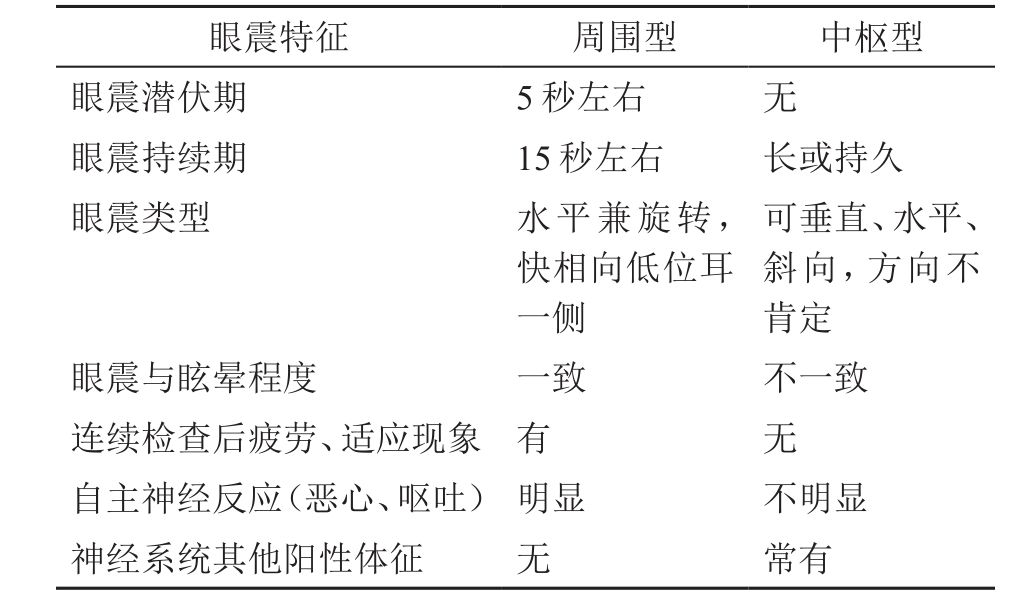
\includegraphics[width=3.36458in,height=2in]{./images/Image00008.jpg}
\end{table}

周围型位置性眩晕、眼震的常见疾病有良性阵发性位置性眩晕(即耳石病)、梅尼埃病、耳硬化症、内耳开窗术后、浆液性迷路炎、内听动脉供血不足、药物性内耳损害等。中枢性位置性眩晕、眼震的常见疾病可见于小脑蚓部肿瘤、第四脑室肿瘤或囊肿、椎-基底动脉供血不足、桥小脑角肿瘤、颅脑外伤等。

\subparagraph{直流电试验}

应用直流电检查前庭神经,电流不仅刺激前庭末梢器,也能直接作用于前庭神经节及前庭神经。方法为将直流电负极置于测试耳的耳屏处或乳突处,正极置于前额或手中,电流逐渐缓慢增加,分别观察出现眩晕感、倾倒及眼震的毫安(mA)数,通常于正常人2~4mA即有眩晕感觉,4~6mA出现倾倒反应,6~8mA出现眼震。眼震之快相向负极侧,而倾倒则向负极之对侧。直流电试验主要的临床价值可协助鉴别前庭末梢器和前庭神经本身的病变。例如前庭末梢器病变(梅尼埃病、迷路炎)变温试验可能显示病侧前庭功能减退或功能消失,而直流电试验仍属正常反应。若病变累及前庭神经例如听神经瘤,则变温试验无反应时,直流电试验亦无反应。

\subparagraph{视动性眼震试验(optokinetic test)}

视动性眼震由固视连续移动景物所引起而非前庭刺激所引起。试验原理:当两眼注视眼前连续而迅速通过的一系列物体时,每一物体在后一物体出现于视野中以前,受到两眼的注视与跟随。而当下一物体的影像落于视网膜的周边部时,眼球即反射性反跳,以便使后一物体像落于黄斑上。眼球如此快慢交替地运动,遂形成视动性眼球震颤,这是一种生理现象。此项检查之所以列入神经耳科学,是因为:①视动性眼震亦有快相与慢相的交替运动,与前庭性眼震形式类似;②此项检查对各种自发性眼震鉴别及颅内病变的定位诊断有一定价值。应用视鼓或视伞或带尺诱发眼球震颤。正常人所诱发之视动性眼震之慢相与视鼓旋转之方向一致,眼震之快相与视鼓旋转之方向相反,所诱发出之视动性眼震向左、右侧是对称的。

一般认为视动性眼球震颤的神经通路为:起自视网膜右半侧之神经纤维→右侧膝状体→视放射→视皮质(Brodman18区、角回和缘上回)的视动中枢,再自视动中枢通过视放射后部深处前行,离视放射→大脑脚→上丘→经内侧纵束→脑桥眼球同向运动中枢→眼球运动核。

因此,皮质视动中枢至脑桥同向运动中枢间任何部位之病变累及视动通路,即可消除或减弱向对侧之视动性眼球震颤,亦即出现向病侧之视动性眼震优势偏向。根据笔者研究的资料分析,在大脑半球占位性病变中,出现视动性眼震优势偏向现象多数与后颞、顶枕部(尤其是顶部)有关。如果病变累及脑干内的视动反射纤维,亦常有异常反应,多数为不对称性异常。在眼源性的自发性眼球震颤病例中,视动性眼震反应多数表现为同向性异常(即眼震的快相与视鼓或视伞旋转的方向相同),或无反应。

\subparagraph{眼震电图(ENG)}

检查对于眩晕患者作前庭功能检查,其中自发性眼球震颤与诱发性眼球震颤都是检查中的一项重要体征,除肉眼观察外,应用眼震电图记录,可以使眼球震颤的各种特征(速度、频率、幅度、方向)客观记录下来,以供比较分析研究。通常所见到的节律型、水平性(或垂直性)眼震在眼震电图上表现为一不对称的峰形波,由迅速上升(或下降)的快相与缓慢回复至基线的慢相所组成。

眼震强度可用眼震时程、幅度、频率、慢相速度等表示,其中以时程和慢相速度为可靠。

慢相速度的测量方法如下:①正常眼震电图测量法:见图\ref{fig3-1}。②眼震强度------慢相速度计算法:其中几何作图法(图\ref{fig3-2})系延长慢相斜边成AC,使BC等于纸速1秒(s),若测得AB
= 22mm,定标值10°=
11mm,按速度=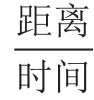
\includegraphics[width=0.30208in,height=0.32292in]{./images/Image00009.jpg}
,得

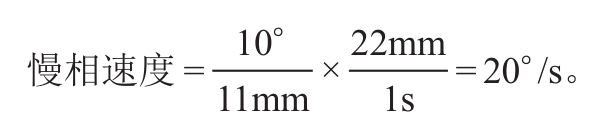
\includegraphics[width=1.95833in,height=0.42708in]{./images/Image00010.jpg}

\begin{figure}[!htbp]
 \centering
 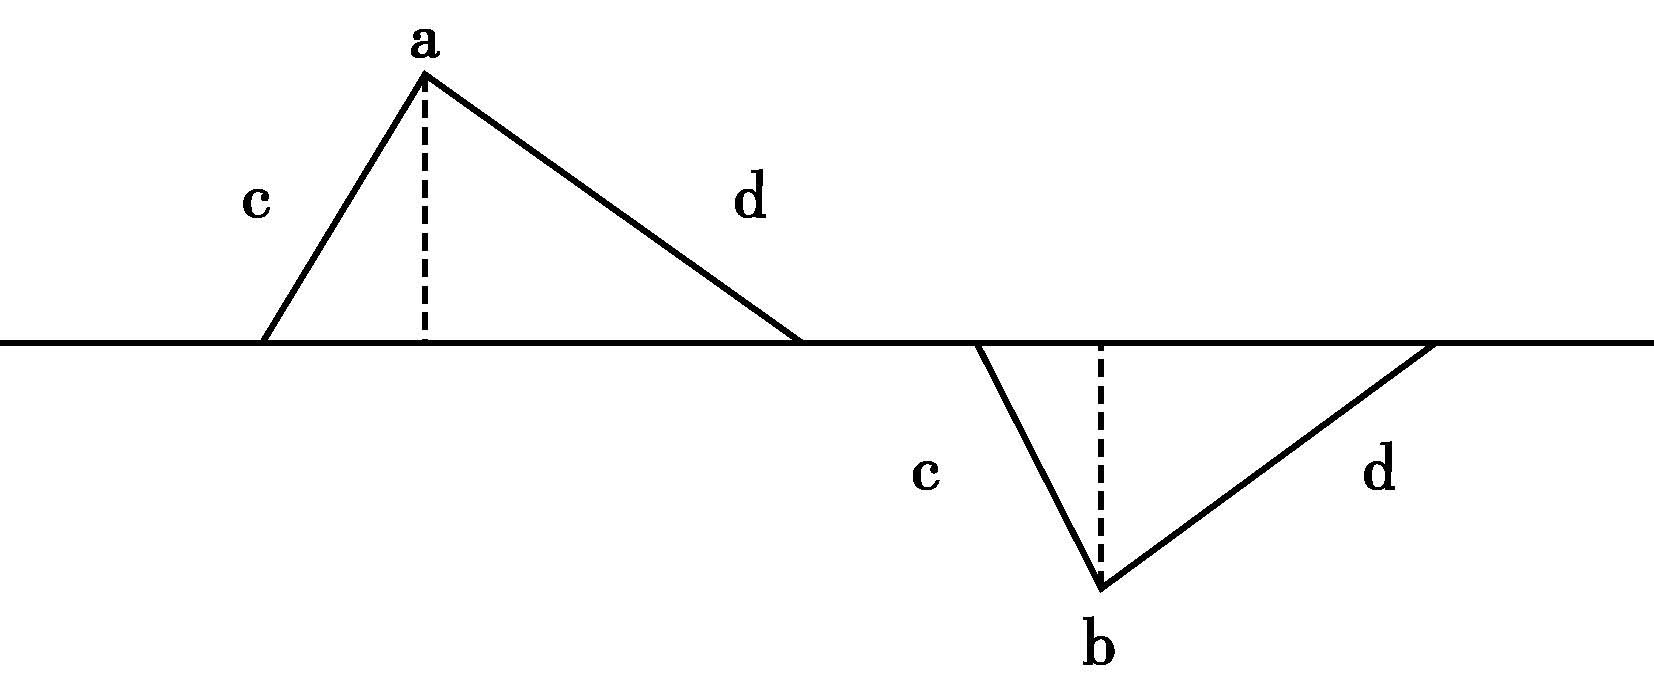
\includegraphics[width=2.75in,height=1.13542in]{./images/Image00011.jpg}
 \captionsetup{justification=centering}
 \caption{正常眼震电图}
 \label{fig3-1}
  \end{figure} 

a.右向眼震;b.左向眼震;c.快相;d.慢相

\begin{figure}[!htbp]
 \centering
 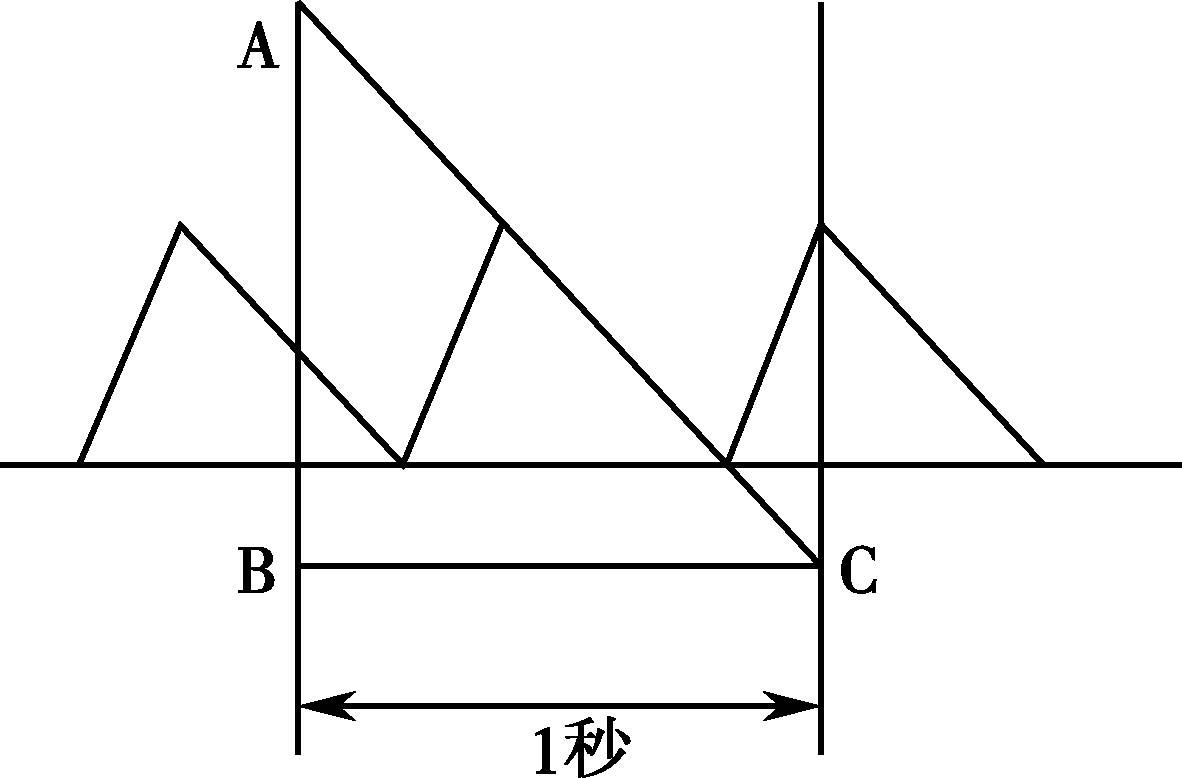
\includegraphics[width=1.96875in,height=1.29167in]{./images/Image00012.jpg}
 \captionsetup{justification=centering}
 \caption{几何作图法}
 \label{fig3-2}
  \end{figure} 

另为极盛期价值法(culmination
valve),于变温试验中,取反应高潮期10秒内之眼震,计算其幅度和频率,以慢相速度表示之。其公式如下:

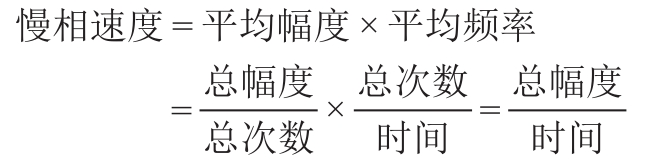
\includegraphics[width=2.16667in,height=0.53125in]{./images/Image00013.jpg}

例如:10秒内眼震总幅为150mm,总次数为20次,定标值10°= 11mm,则

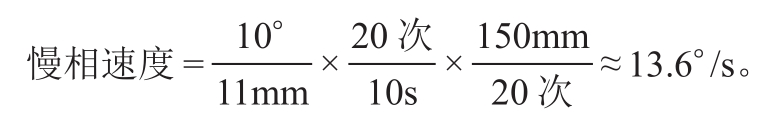
\includegraphics[width=2.57292in,height=0.40625in]{./images/Image00014.jpg}

利用眼震电图可以记录各种自发性眼震,并通过各种诱发试验记录变温性、位置性、视动性、凝视性眼球震颤。并可作扫视试验(saccade
test)、平稳跟踪试验(pursuit
test),于检查中可进一步观察在睁眼(明亮条件下)、暗室中、闭眼条件下眼震的变化。这些客观资料,均有助于对眩晕、眼震、前庭系统疾病的诊断。

\subsubsection{诊断注意事项}

对于临床医师而言,在对眩晕的病因作诊断与鉴别诊断时可先从以下几方面考虑:

1.前庭系统性眩晕抑或非系统性眩晕
一般而言,凡属前庭系统性眩晕均具有空间定向的感觉异常,具有运动错觉或运动幻觉的特点,或觉外境或觉自身在运动感(旋转、摇晃、向一侧移动);而非系统性眩晕则没有上述的特点,大多数患者对“眩晕”描述为头昏、头胀、头重脚轻、头脑内转动等。

2.前庭周围性眩晕抑或前庭中枢性眩晕
对于前庭系统性眩晕应进一步鉴别是前庭周围性病变还是前庭中枢性病变,两者的鉴别见表\ref{tab3-2}。

\begin{table}[htbp]
\centering
\caption{前庭周围性眩晕与前庭中枢性眩晕的鉴别}
\label{tab3-2}
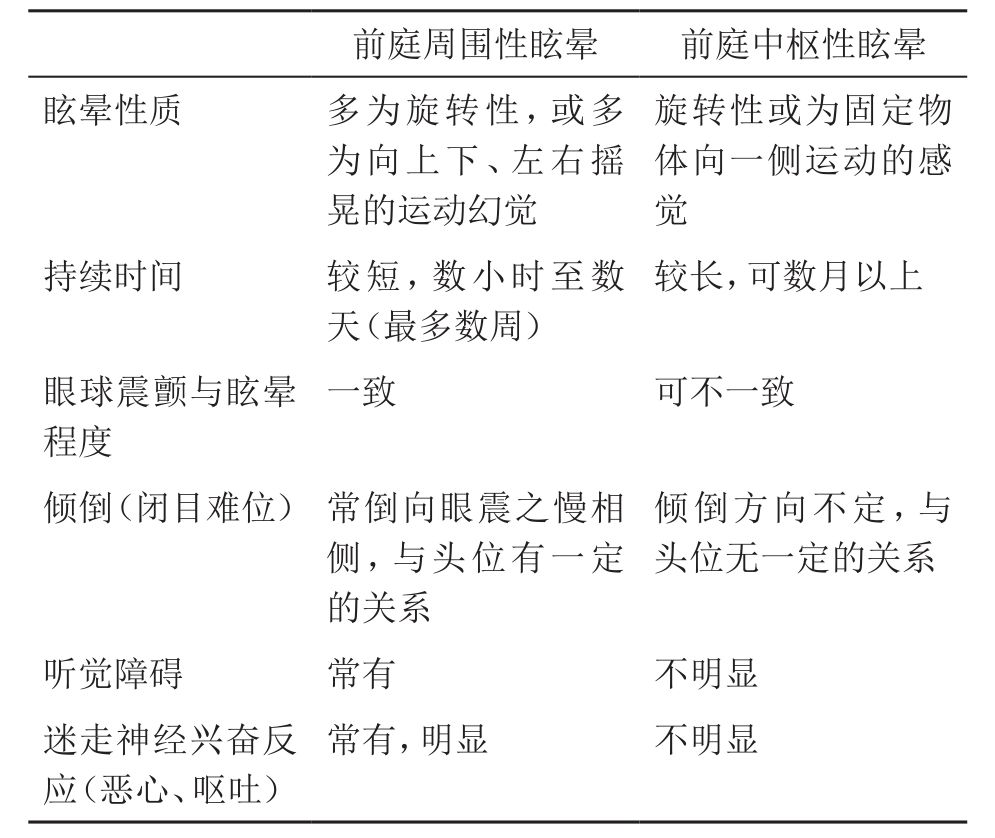
\includegraphics[width=3.3125in,height=2.78125in]{./images/Image00015.jpg}
\end{table}

3.更进一步的诊断需根据各疾病的临床表现的特点及必要的辅助检查。

\subsubsection{常见眩晕症疾患的临床特点}

\hypertarget{text00012.htmlux5cux23CHP1-3-2-6-1}{}
(一) 梅尼埃病(Ménière disease)

梅尼埃病系内耳病变,为中年以上阵发性眩晕的最常见的原因。临床表现为典型的三联症状:发作性眩晕,波动性、渐进性、感音性的听力减退和耳鸣。眩晕发作时常伴有恶心、呕吐、出汗、面色苍白、眼球震颤。眩晕常突然发作,发作前耳鸣增加,听力骤减,耳内有饱胀感。每次眩晕发作历时数小时至数天(多系1~2天)而自行缓解。发作间歇期长短不一,多数为数月一次,亦有一个月数次者。眩晕发作常常随耳聋的进展而减少,至完全耳聋时,迷路前庭功能消失,眩晕发作亦常终止。于眩晕发作间歇期间检查,仅可发现单侧(少数为双侧)感音性耳聋,作电测听检查部分患者重振试验(recruitment
test)呈阳性。前庭功能变温试验于一部分病例中显示功能减退。本病产生的原因可能是支配前庭器的交感神经功能失调引起迷路动脉痉挛,从而使内淋巴产生过多或吸收障碍,导致迷路水肿及内淋巴系压力增高,内淋巴腔扩大及内耳末梢器缺氧、变性等病理变化。

\hypertarget{text00012.htmlux5cux23CHP1-3-2-6-2}{}
(二) 良性发作性位置性眩晕(benign paroxysmal positional
vertigo,BPPV)

本病多见于中年以上患者,多数学者认为是耳石器病变所致,故又称此病为耳石病。患者常诉说当头部处于某一位置时即引起头晕,有些患者诉说半夜翻身时突然发生眩晕,若再回复该头位又即会再发生,因而患者尽可能回避该头位。眩晕严重时伴有恶心、呕吐。常无听力障碍。作头位位置检查,常能在患者所诉说的那个头位引起眩晕,同时可见有短暂的水平兼旋转性眼球震颤,眩晕与眼震一致,持续10~20秒自行缓解。重复该头位可重复出现眩晕与眼震。但于短期内连续数次重复检查,则可逐步适应而不出现眩晕症状与眼震。变温试验提示前庭功能正常。病程常为自限性,数周至几个月后可自愈。近年来一些学者研究认为其基本病理机制系椭圆囊斑上耳石脱落、游离的耳石进入后半规管并在内淋巴内移动,在头位变动时刺激后壶腹嵴,于是乃产生短时间的眩晕。至于耳石器病变的原因主要有:①前庭动脉前支血栓形成;②颅脑外伤致内耳震荡。在作头位位置试验时,重复数次检查后之所以出现适应(疲劳)现象是由于耳石散落在内淋巴腔,一时未能沉积在后壶腹顶部,故不再引起症状,但待耳石沉积在壶腹顶部时可再度诱发位置性眩晕与眼震。

\hypertarget{text00012.htmlux5cux23CHP1-3-2-6-3}{}
(三) 非良性位置性眩晕

颅后窝的占位性病变也可引起位置性眩晕
,这与上述良性位置性眩晕在临床表现上有以下区别:此种眩晕的发生往往在头位改变后立即出现,无潜伏期,诱发之眩晕持续时间较长,往往引起恶心、呕吐,眩晕可在数种头位诱发,而不像BPPV只在较特定的1~2种头位才诱发。常见的疾病是第四脑室、小脑蚓部的肿瘤或第四脑室的囊肿,亦可见于小脑半球、脑桥小脑角的肿瘤。除位置性眩晕外,有时有肢体或躯干的共济失调。

\hypertarget{text00012.htmlux5cux23CHP1-3-2-6-4}{}
(四) 前庭神经元炎(vestibular neuronitis)

起病较急,表现为突起的剧烈的眩晕,伴有恶心、呕吐,但无耳蜗症状。起病时常伴有感染(多为上呼吸道)症状,可能是一种病毒感染。发病时有自发性水平性眼球震颤,躯体平衡失调。变温试验显示病侧前庭功能减退或缺失,有时双侧均有损害。预后良好,一般在数周后眩晕症状逐日减轻,但变温试验示前庭功能呈永久性损害。多数学者认为病变主要为病毒侵犯前庭神经的Scarpa神经节,但也有少数学者认为有时脑干内的前庭纤维也受侵犯。

\hypertarget{text00012.htmlux5cux23CHP1-3-2-6-5}{}
(五) 迷路炎

单纯性中耳炎由于炎症刺激使迷路充血可引起眩晕。眩晕程度较轻,中耳炎好转后眩晕亦即解除。中耳炎并发弥漫性化脓性迷路炎时,眩晕严重,伴恶心、呕吐、眼震及病侧听力严重丧失,病侧前庭功能消失。此外还有耳痛、耳漏、头痛、发热等中耳感染症状与体征。慢性中耳炎侵蚀骨迷路有瘘管形成时,常有反复发作的眩晕。瘘管试验(以希格尔镜利用橡皮球增减外耳道压力,通过瘘管影响迷路,产生前庭反应)呈阳性反应。提示内耳有瘘管存在。

\hypertarget{text00012.htmlux5cux23CHP1-3-2-6-6}{}
(六) 药物性眩晕

在临床药物应用中
,有些药物因使用不当,因毒性作用而致眩晕,如链霉素;有些是难以避免的副作用,如某些镇静药和安眠药;有些是过敏所引起。

\subparagraph{耳毒性抗生素类}

以氨基糖苷类为主,如链霉素(尤其是硫酸链霉素)、新霉素、卡那霉素、庆大霉素、阿米卡星(丁胺卡那霉素)等,其他尚有万古霉素、多黏菌素B。其中有些药物性损害主要影响前庭部分,但大多数前庭与耳蜗均有影响。链霉素是最常见者,引起眩晕症状通常于疗程第4周出现,但亦有仅应用4天即有眩晕症状者。在年老患者或有肾功能不全的患者,更易出现毒性作用。眩晕症状持续,而在患者行走、头部转动或转身时症状更为明显。于静止时、头部不动时,上述症状明显好转,甚至消失。而一旦活动后上述症状又复出现。前庭功能检查,大多数患者均无自发性眼球震颤,闭目难立征阳性,向左右前后摇晃方向不定。变温试验示双侧前庭功能均明显减退或消失。如伴有耳蜗损害,则尚有双侧感音性耳聋。眩晕症状消失较为缓慢,需数月甚或1~2年之久,前庭功能则更难恢复。

\subparagraph{麻醉 、镇静和催眠药}

这类药物引起眩晕的机制主要是对中枢的抑制作用,皮质中枢受抑制时表现为头晕及轻度失平衡,并无明确的运动错觉。于麻醉后,由于皮质中枢的强抑制,有关平衡的各种传入信息,不能在中枢获得综合与分析,因而出现头晕症状,患者诉说昏昏沉沉。这些药物中除麻醉药外还有异丙嗪(非那更)、苯巴比妥(鲁米那)、利眠宁(氯氮{}
)等。

\subparagraph{抗癫痫药}

在抗癫痫药中苯妥英钠与扑米酮是引起眩晕的最常见者,尤其是苯妥英钠,因应用广,应用时间又长,如不注意服用剂量及检测药物血药浓度,则甚易引起中毒性损害。主要损害于前庭末梢器,可累及小脑,均可导致眩晕,平衡失调,眼球震颤,共济失调,因此对于这些患者应定期随访,必要时检测药物血药浓度,调整药物剂量。扑米酮能用于抗痫治疗,虽较少用,但初服此药时,其剂量应减少至甚小量(成人常规用量之1/3~1/4),然后缓慢增加,才可避免眩晕。

\subparagraph{其他药物}

如水杨酸类(水杨酸钠)、噻嗪类利尿剂(氢氯噻嗪)、降压药(利血平、降压灵)及某些磺胺类药均可致眩晕,在临床应用时应予注意。

\hypertarget{text00012.htmlux5cux23CHP1-3-2-6-7}{}
(七) 血管性眩晕(椎-基底动脉血循环障碍)

\subparagraph{迷路卒中}

由于动脉粥样硬化或伴有血液黏稠度增加,血压的偏低,导致内听动脉血栓形成,常产生急骤的、严重的眩晕,伴恶心、呕吐,若耳蜗分支同时受损,则伴有耳聋及耳鸣。患者年龄较大,起病甚快,有身体其他部位动脉硬化的征象,既往(青、中年时)无类似的眩晕发作史等特点,均有助于与其他急性眩晕相鉴别。但有的患者表现短暂性的眩晕发作,伴有或不伴有耳蜗症状,持续数分钟至数小时即缓解,对于这些中、老年患者,若除外耳源性眩晕的其他疾病,可诊断为迷路动脉短暂性缺血发作(TIA)。

\subparagraph{小脑后下动脉血栓形成}

亦称延髓外侧综合征(Wallenberg
syndrome)。其典型的症状与体征包括突起眩晕,伴恶心、呕吐,眼球震颤;病侧肢体共济失调及颈交感神经麻痹综合征;吞咽困难及同侧软腭麻痹、声带麻痹;病侧面部及对侧躯体、肢体的痛温觉减退或消失。

\subparagraph{椎-基底动脉供血不足(vertebrobasilar insufficiency,VBI)}

多数表现为椎-基底动脉的TIA,临床常见。有关本病的概念至今还不十分清楚。引起VBI的病例基础是:①椎动脉的解剖特点:起始于两侧锁骨下动脉之椎动脉,需穿过第6~1颈椎横突孔后再经枕大孔入路,然后合并为基底动脉,椎动脉在行程中需经过一条活动度较大的骨性隧道。②椎动脉易发生动脉粥样硬化,随着年龄增大其动脉管径逐渐变窄,血流量亦渐变少。③中年以后颈椎常发生退行性变及骨赘形成。因此椎动脉的血流易受到各种因素的影响,例如颈部的转动,血压的较快的降低,血管的痉挛,血黏度的增高。因此VBI的发病通常认为主要是动力学改变所致,但也有部分患者VBI是由于循环系统内的微栓子所造成。由于迷路、前庭神经核、小脑的血液供应均来源于椎-基底动脉血流循环,因此VBI的主要临床表现是眩晕,常突然发生,颈部过度伸屈或旋转有时可诱发,眩晕发作持续通常短暂,常常数分钟即缓解,但可在短时期内反复发生多次,眩晕发作时可伴有恶心、呕吐、站立不稳,亦可伴有椎-基底动脉的其他供应区缺血的临床征象,例如视幻觉、偏盲、猝倒发作、复视、面麻木、进食吞咽困难,肢体肌力减退或感觉障碍,共济失调。上述这些临床表现通常都是呈发作性、短暂性,症状持续数分钟至数小时,不超过24小时,这一类型的VBI可称之为VBTIA(椎-基底动脉短暂性缺血性发作),但临床上也有一部分患者表现为在一段时期内(数天至数周)经常性的头晕,行走不稳,在除外了其他引起眩晕的疾病后亦应考虑为VBI,推究其发病机制是后循环的动力学障碍所致,应予重视。

对于VBI的诊断应根据具体情况选择作下列检查:①颈椎X线片,包括正、侧及斜位片,以发现有无颈椎病及其严重程度及了解有无骨刺可能累及椎动脉。②颈椎CT或颈椎MRI或螺旋CT,以进一步了解颈椎骨骼及脊髓和有关椎动脉受压、变窄情况。③头颅MRA,以了解颅内血管情况,尤其是了解椎-基底动脉及颅内脑底动脉环情况。④TCD检查。⑤BAEP检查。⑥SPECT检查。上述三项检查在VBI的病例中均有相当的阳性率,可作为诊断的参考依据。⑦前庭功能检查主要是作变温试验,对于了解前庭功能有肯定的价值。⑧眼震电图检查:可作扫视试验、凝视试验、跟踪试验、视动试验。有一定的临床价值。

关于椎-基底动脉短暂性缺血性发作的诊断依据:①中老年患者(发病在50岁以上)。②发作性眩晕,每次持续时间短暂,通常为数分钟至数十分钟。③眩晕发作时可伴有一种或数种脑干、小脑、枕叶的缺血症状及体征。④临床症状除轻度眩晕,行走不稳外均在24小时内减轻以至消失。⑤实验室检查(上已述及)有两项以上的阳性发现。⑥排除引起眩晕的其他病因。

\subparagraph{颈椎病变}

颈椎退行性病变导致椎间隙狭窄,及由于钩椎关节骨赘增生刺激或压迫椎动脉,使椎动脉痉挛、阻塞,当转颈时一侧之椎动脉更易受压。若椎动脉本身已有粥样硬化,一侧椎动脉受压后,对侧椎动脉无法代偿则出现症状。临床常见之症状为发作性眩晕,其发病与头颈转动有密切关系。此外,这些患者尚可伴有枕部头痛、猝倒、视觉症状(闪光、视野缺失)及上肢麻痛。颈椎X线片、颈CT扫描可显示颈椎形态学病变改变。

\hypertarget{text00012.htmlux5cux23CHP1-3-2-6-8}{}
(八) 颅内肿瘤

由于颅内肿瘤所产生的眩晕有两种机制
:一是由于肿瘤直接压迫、浸润前庭神经或其中枢连接;另一是由于颅内压增高,尤其是由于肿瘤阻塞脑脊液循环而产生脑积水,引起第四脑室底部前庭核的充血和水肿。

\subparagraph{桥小脑角肿瘤}

特别是听神经瘤,有轻度眩晕和耳鸣、耳聋,这是听神经瘤的早期症状。病变进一步发展可出现邻近脑神经受损的体征,如病侧角膜反射减退、面部麻木及感觉减退,展神经麻痹、周围性面瘫、眼球震颤,同侧肢体共济失调。在听神经瘤的早期通常并没有自发性眼球震颤,当肿瘤增大压迫脑干或小脑时才会出现,但一经出现则持续存在。听神经瘤至病程后期还可出现颅内压增高症状,头痛、视神经乳头水肿。对于听神经瘤的早期诊断可根据单侧性听力渐进性减退、听力检查为感音性耳聋;同侧前庭功能早期即消失,邻近脑神经(三叉、展、面神经)中有一根受累即应考虑为听神经瘤。若脑脊液中蛋白质含量增加,X线片上示病侧内听道扩大诊断即可肯定。近年来由于应用头颅CT及MRI检查,更易得到早期确诊。

\subparagraph{脑干}

(延髓脑桥)肿瘤
因病变累及前庭神经核,常有眩晕及持久的眼震,可有一侧或双侧听力减退,水平性眼震的方向通常为双向性,向左侧注视时快相向左,向右侧注视则快相向右,也可能兼有旋转性眼震。当眼震明显时,眩晕症状不一定很重。还可以有其他脑神经障碍(主要为第Ⅴ、Ⅵ、Ⅶ、Ⅹ、Ⅺ)及对侧肢体瘫痪。

\subparagraph{小脑半球肿瘤}

常有眩晕,早期即出现明显的振幅粗大的眼球震颤,及病侧肢体共济失调,水平性眼震的方向通常是两侧性的,但主要是向病变一侧。前庭功能变温试验示病侧肢体偏斜反应不明显。

\subparagraph{小脑蚓部肿瘤及第四脑室肿瘤}

(或囊肿)
眩晕为常见症状,眩晕的发生或加重常与头位位置有关。作头部位置试验,可见有中枢型位置性眼球震颤,并有早期颅内压增高及固定头位等临床表现。

\subparagraph{天幕上肿瘤}

通常并不出现眩晕,如有则可能与颅内压力增高有关,但颞叶肿瘤有时可出现以眩晕为主要表现的癫痫样发作。脑电图上可以有痫样发放。

\hypertarget{text00012.htmlux5cux23CHP1-3-2-6-9}{}
(九) 外伤性眩晕

颅脑外伤时可因内耳迷路
、第Ⅷ脑神经、中枢前庭核及其中枢连接受损而产生眩晕。这些结构可单独或合并受损。迷路内外伤性出血的患者有周围型的前庭紊乱症状,常有颞骨骨折及听力同时受损的征象。亦有内耳并无出血而为迷路震荡者,则眩晕症状持续时间短、恢复较快,听力障碍程度亦较轻。部分患者可由于耳石器损伤而出现短期的位置性眩晕。颞骨横行骨折,骨折线横断岩锥,可产生听神经直接受损,出现明显的眩晕、自发性眼震、听力丧失,于4~6周内前庭症状逐渐消失,但听力常难以恢复。

严重的颅脑损伤患者,在第四脑室及导水管周围可见有点状的少量出血,损伤涉及前庭核及其中枢连接。脑干损伤后产生眩晕的同时常伴有脑干损伤的其他体征,如复视、面瘫、瞳孔不等大、肢体运动或感觉障碍等。眩晕症状持续较久,可达数月以上。颈部鞭索样损伤后亦常有眩晕症状,在头部运动时,尤其是向着颈部鞭索样受损的方向运动时,眩晕症状更易出现。每次眩晕发作数秒至数分钟。头位位置试验可有位置性眼震,常发生于头部转向鞭索样损伤侧,可能是由于内耳耳石器受损所致。

\hypertarget{text00012.htmlux5cux23CHP1-3-2-6-10}{}
(十) 精神性眩晕

精神性眩晕在本质上是神经症的一种表现。大多感觉头昏脑胀,非真性眩晕,无运动错觉,患者诉“眩晕”、“头晕”时无自发性眼震或自发性倾倒,往往常有神经症其他表现如失眠、焦虑、紧张、记忆力减退、注意力难集中等。无前庭系或非前庭系器官性疾病。起病诱因系以情绪、精神因素为主。

\subsection{处理原则}

\subsubsection{一般处理}

对于急性眩晕发作的患者,需卧床休息,饮食以流质为宜。伴有明显恶心、呕吐者,应酌情给予静脉补液,以维持营养,并需注意水、电解质的平衡。对于焦虑紧张的患者,应给予适当的病情解释与安慰,以解除顾虑。眩晕发作缓解后,应鼓励患者早日逐渐参加日常活动,适应日常生活。

\subsubsection{病因治疗}

因中耳炎并发症引起的急性化脓性迷路炎,应由耳科作必要的手术及抗感染治疗。由颅内占位性病变如小脑肿瘤、听神经瘤引起者,需作手术摘除肿瘤。由于梅尼埃病产生的眩晕,主张调节自主神经功能,平时以低盐饮食为宜。对于由药物中毒性损害引起的眩晕患者,应及时停药,并给予维生素B族药物。因颈椎骨质增生、椎间盘膨隆或突出而致的眩晕,可先作颈椎牵引或作颈托固定。必要时再考虑手术治疗。因心律失常或血压过高、偏低者,则需给予相应的内科治疗。因贫血引起的眩晕应纠正贫血。凡此种种的有关病因的处理均属重要,不可忽视。

\subsubsection{对症处理}

在病因治疗的同时,对于眩晕症状需给予药物治疗,以减轻眩晕症状及减少伴发的恶心、呕吐、焦虑、紧张等症状。

\subparagraph{急性发作期的药物治疗}

可考虑选用的药物有:氢溴酸东莨菪碱0.3mg,肌肉注射;茶苯海明(晕海宁,dramamine)50mg,肌肉注射;硫酸阿托品0.5~1mg,肌肉注射;山莨菪碱(654-2)5~10mg,肌肉注射;盐酸异丙嗪(非那更)25~50mg,肌肉注射。以上药物可选择应用,并可根据病情每隔4~6小时重复给药2~3次。

\subparagraph{眩晕发作后尚有轻度症状或慢性眩晕的治疗}

在急性眩晕发作后,虽已无明显的旋转幻觉,但仍有平衡失调、站立不稳的感觉,或在头部、身体转动时有这些症状,或眩晕程度虽轻但经常存在者,可选用各种镇静剂、安定剂,例如苯巴比妥0.015~0.03g,或地西泮(安定)2.5~5mg,或氯丙嗪25mg等,均为每天2~3次,口服。

\subparagraph{几种治疗眩晕症的常用药物}

\hypertarget{text00012.htmlux5cux23CHP1-3-3-3-3-1}{}
(1) 镇静剂与安定剂:

例如苯巴比妥、溴剂、地西泮等。它们的药理作用对于前庭反应有抑制作用,对于一般感觉亦起抑制作用,因此可以减轻眩晕症状,消除紧张、烦躁不安、焦虑等症状。苯巴比妥虽可以减轻眩晕,但也常有全身抑制的作用,如疲倦、乏力。地西泮能减轻眩晕症状,减少紧张、焦虑,并有止吐作用,但可加强其他中枢抑制剂的作用。大剂量的安定类药物可以引起锥体外系的副作用。

\hypertarget{text00012.htmlux5cux23CHP1-3-3-3-3-2}{}
(2) 抗组胺药物:

例如苯海拉明、盐酸异丙嗪、氯苯那敏、盐酸氯苯苄嗪(敏克静)、茶苯海明等,这些药物用于治疗眩晕,其治疗效应可能是由于它们药理上的镇静作用而不是抗组胺作用。它们应用于眩晕发作期尚有止吐作用。

\hypertarget{text00012.htmlux5cux23CHP1-3-3-3-3-3}{}
(3) 止吐剂:

常用者为盐酸氯苯苄嗪及异丙嗪,均有明显止吐作用,适用于运动病及眩晕时伴有明显的自主神经反应(恶心、呕吐)的病例。这些药物亦有镇静作用及抗组胺作用。

\hypertarget{text00012.htmlux5cux23CHP1-3-3-3-3-4}{}
(4) 抗胆碱药物:

常用药物系东莨菪碱与阿托品,对于梅尼埃病的治疗效果较好。这类药物尚有止吐及解除血管痉挛的作用。东莨菪碱还有镇静作用,可优选使用。

\hypertarget{text00012.htmlux5cux23CHP1-3-3-3-3-5}{}
(5) 血管舒张药物:

例如烟酸、妥拉唑啉、山莨菪碱、地巴唑,这些药物并不是前庭抑制药物,其药理作用为解除血管痉挛。可应用于因血管痉挛、缺血性病变所引起的眩晕,如梅尼埃病的发作期及椎-基底动脉供血不足的病例。此外倍他司汀(betahistine,抗眩啶)亦有扩张血管的作用,常用量为4mg,每日3次;甲磺酸倍他司汀(敏斯朗)亦有类似的作用,6mg,每日3次口服。

\hypertarget{text00012.htmlux5cux23CHP1-3-3-3-3-6}{}
(6) 钙拮抗剂:

目前常用者有尼莫地平20mg,每天3次;桂利嗪(脑益嗪)25mg;每天3次,氟桂利嗪(flunarizine,商品名西比灵)5mg,每天1~2次,均为口服。

\hypertarget{text00012.htmlux5cux23CHP1-3-3-3-3-7}{}
(7) 增强动脉血氧分压和血氧饱和度药物:

阿米三嗪萝巴新{[}都可喜(Duxil){]}内含阿米三嗪和萝巴新,本药可增迷路和脑组织的血氧供应,对于因缺血缺氧而产生的眩晕疾患有较好的疗效,常用量为30mg,每天2次,口服。


\hypertarget{text00013.htmlux5cux23CHP1-3-4}{}
参 考 文 献

1. 史玉泉.实用神经病学.第3版.上海:上海科学技术出版社,2004

2. Norre ME. Clinical value of caloric test. Clin
Otolaryngol,1988,13:247

\protect\hypertarget{text00014.html}{}{}

\chapter{晕 厥}

晕厥(syncope)又称昏厥,是由于短暂的全脑组织灌注降低而导致的一过性意识丧失(transient
loss of
consciousness,TLOC),以快速发作、持续时间短和自限性为特点。可因血管迷走反射、直立性低血压、心输出量减少引起全脑低灌注,或由于脑干椎-基底动脉缺血引起脑干选择性低灌注所致。晕厥发作起病突然,持续时间短,典型可分为三期,其基本临床特点为:①发作前期:患者常感头部及全身不适、头晕、视力模糊、耳鸣、面色苍白、出汗,预示即将发生晕厥;此时患者如取头低位躺卧姿势常可防止发作。②发作期:轻者眩晕、恶心、躯体发软,眼前发黑,重者常突然意识丧失,全身肌紧张度消失,跌倒地上。意识丧失超过15~20秒可发生阵挛动作,有时有呼吸暂停,心率减慢,甚至心脏暂停搏动,瞳孔散大,流涎,尿失禁等;其特点是发作时间短暂,一般持续1~2分钟左右。脑电图检查可见持续3~10秒的广泛性、对称性2~3Hz的慢波。③发作后期(恢复期):患者平卧后意识迅速恢复(数秒至数分钟),可遗留紧张、头晕、头痛、恶心、苍白、出汗、无力和便意感等,甚至呕吐及括约肌失禁。休息数分或数十分钟缓解,不留后遗症,偶有极短暂的(<
30秒)发作后模糊状态伴定向力障碍和易激惹。

可见晕厥的特征是:发作突然,意识丧失时间短,不能维持正常姿势或倒地,在短时间内迅速恢复,罕有后遗症。

当前急诊对晕厥的评估已经从诊断晕厥的病因转变为进行危险分层,其目的是:①识别有威胁生命的疾病并收入院;②识别低危患者,可以让他们离院,并且以后到专科就诊;③识别不需要进一步诊断和治疗的患者;④对初步评估不能得出结论的患者进行进一步检查。

\subsection{病因与发病机制}

引起晕厥的病因很多(表\ref{tab4-1}),但任何原因均是通过影响脑血流,引起脑血供障碍所致。人脑重量占体重的2\%,而脑耗氧量却占全身耗氧量的20\%。脑组织几乎无氧和葡萄糖储备,全靠血循环提供外源性补给才能维持其正常的生理功能。健康成人的脑血流量为每100g脑组织45~50ml/分钟,而维持人的意识水平所需最低限度的脑血流量(即临界值)为每100g脑组织30ml/分钟,当脑血流量骤减至此临界值则可发生晕厥。

\subparagraph{反射性晕厥(神经介导的晕厥)}

此类晕厥主要由于在正常状态下控制循环系统的心血管反射对刺激因素出现间歇性的不恰当反应,引起血管扩张和(或)心动过缓,导致动脉血压降低及全脑灌注减少。依据诱发因素不同又可分为以下几类:

\begin{table}[htbp]
\centering
\caption{晕厥的病因分类}
\label{tab4-1}
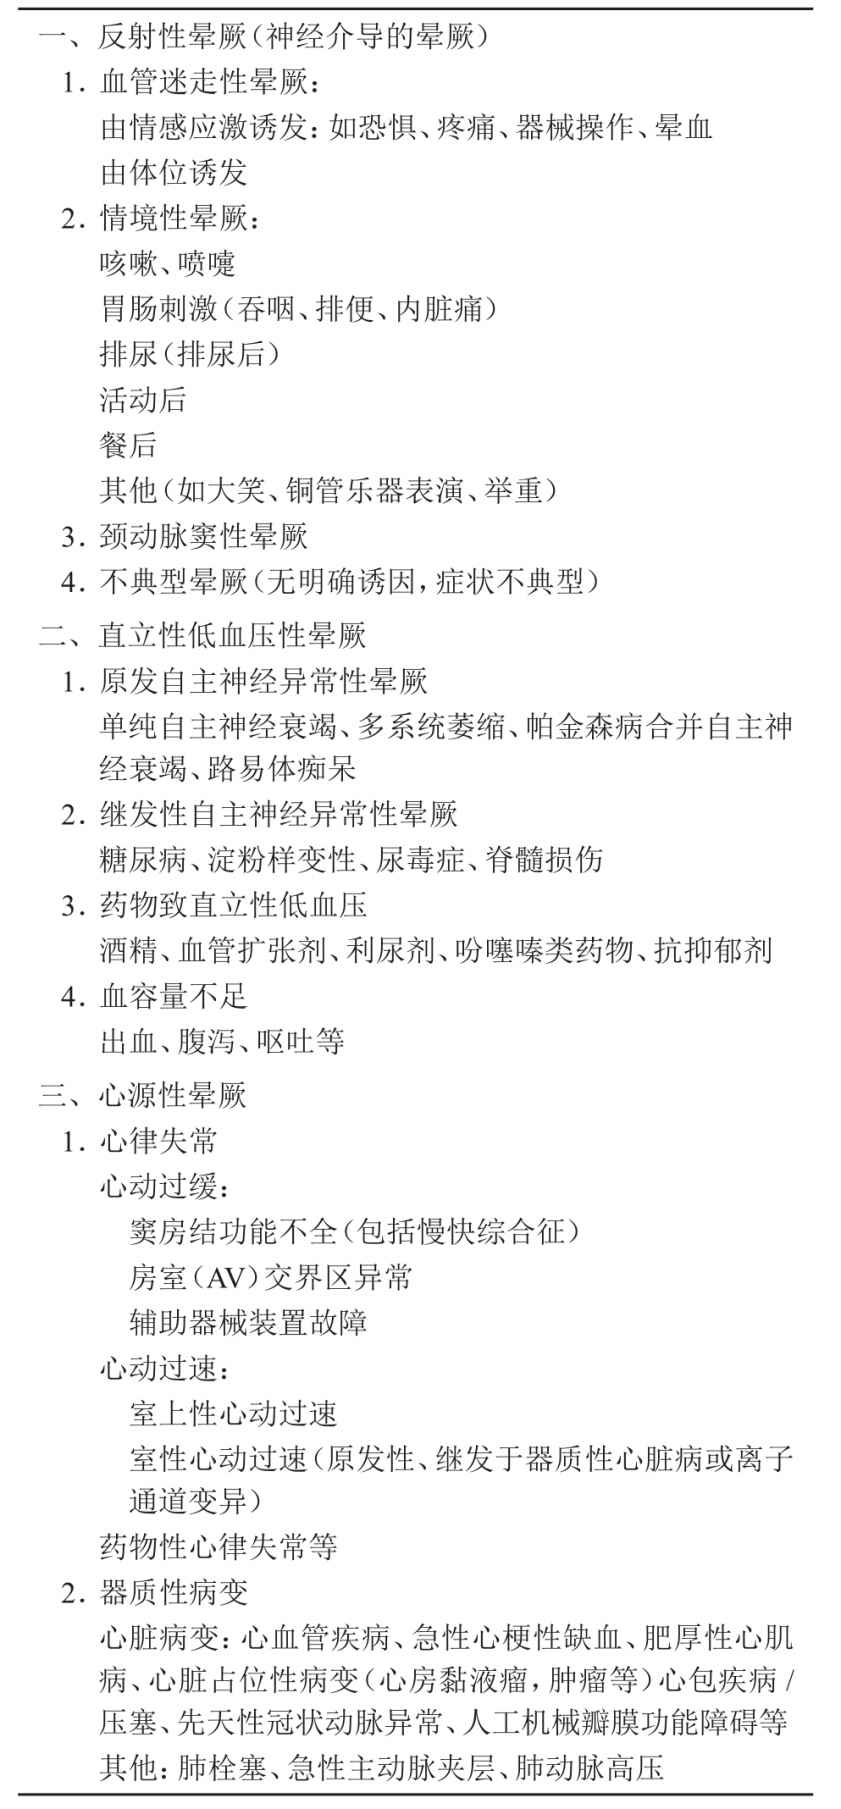
\includegraphics[width=3.30208in,height=7.11458in]{./images/Image00017.jpg}
\end{table}

\hypertarget{text00014.htmlux5cux23CHP1-4-1-1-1}{}
(1) 血管迷走性晕厥:

是最常见的晕厥类型,由情绪或直立位诱发,常伴自主神经激活的前驱症状(大汗、苍白或恶心)。

\hypertarget{text00014.htmlux5cux23CHP1-4-1-1-2}{}
(2) 情境性晕厥:

与一些特殊情境相关,如运动后晕厥等。

\hypertarget{text00014.htmlux5cux23CHP1-4-1-1-3}{}
(3) 颈动脉窦晕厥:

常由非机械性刺激因素诱发,可通过颈动脉窦按摩来确诊。

\hypertarget{text00014.htmlux5cux23CHP1-4-1-1-4}{}
(4) 不典型晕厥:

多数没有明确的诱发因素,诊断主要基于排除其他晕厥的病因(无器质性心脏病)。

\subparagraph{直立性低血压和直立性不耐受综合征}

此类晕厥主要包括以下4种类型:

\hypertarget{text00014.htmlux5cux23CHP1-4-1-2-1}{}
(1) 典型的直立性低血压(OH):

站立3分钟内,收缩压下降≥20mmHg和(或)舒张压下降≥10mmHg,见于单纯性自主神经功能衰竭(ANF)、低血容量或其他形式的ANF。

\hypertarget{text00014.htmlux5cux23CHP1-4-1-2-2}{}
(2) 初始性直立性低血压:

站立即刻血压下降>
40mmHg,然后自发、快速地恢复正常,低血压及其症状持续时间较短(<
30秒)。

\hypertarget{text00014.htmlux5cux23CHP1-4-1-2-3}{}
(3) 延迟(进展性)OH:

其在老年人中并不少见,主要与年龄相关的代偿反射受损有关,以直立状态下收缩压进行性缓慢下降为特点,但不伴心动过缓。

\hypertarget{text00014.htmlux5cux23CHP1-4-1-2-4}{}
(4) 体位性直立性心动过速综合征:

部分患者(主要为年轻女性),表现为严重的直立性不能耐受,但没有晕厥,伴随心率明显加快(增加>
30次/分或达到120次/分以上)和血压不稳定,病理生理机制尚不明确。

\subparagraph{心源性晕厥}

\hypertarget{text00014.htmlux5cux23CHP1-4-1-3-1}{}
(1) 心律失常性晕厥:

是心源性晕厥的最常见病因。心律失常诱发血流动力学不稳定,导致心输出量及脑血流量严重减少。心律失常类型包括:病窦综合征(窦房结功能受损,产生窦性停搏及窦房阻滞,以及慢-快综合征)和严重的获得性房室传导阻滞(莫氏Ⅱ型、高度及完全性房室传导阻滞),也可见于药物引起的缓慢性或快速性心律失常,如延长QT间期药物引起的尖端扭转性室速。

\hypertarget{text00014.htmlux5cux23CHP1-4-1-3-2}{}
(2) 器质性心脏病:

主要见于左室流出道梗阻性疾病。

\subsection{流行病学}

晕厥在普通人群中常见,首发年龄多为10~30岁,其中女性约47\%、男性约31\%在15岁左右发生晕厥。迷走性晕厥是导致晕厥的最主要原因,心源性晕厥是导致晕厥的第二位原因。医院中的老年患者心源性晕厥发病率较高。在小于40岁的患者中,OH所导致的晕厥较为少见。个别患者的病情较为复杂,在医疗转诊、救治的过程中,一些非晕厥的意识丧失患者常被误诊为晕厥。需注意的是,反射性晕厥是年轻人群中最为常见的导致TLOC的原因;而老年患者通常病情较为复杂,且相关病史也不及年轻人群可靠。

\subsection{诊断思路}

晕厥的诊断目的包括:①找出确切的原因以便进行有效的、针对病理机制的治疗;②识别患者的风险,这种风险常取决于潜在的疾病,而不是晕厥本身的机制。

\subsubsection{初步评估}

详细的病史询问在多数情况下有助于鉴别晕厥与非晕厥,但有时非常困难,应包含以下问题:

(1) 是否为完全性意识丧失(LOC)?

(2) LOC是否为一过性,伴快速起病及短暂持续?

(3) 患者晕厥是否为自发性、完全恢复且不留后遗症?

(4) 患者是否丧失肌张力?

若上述问题的答案均为肯定的,则晕厥可能性极大。若≥1个问题的答案为否定,则应首先排除其他类型的LOC。

对出现TLOC的患者进行初步评估,除了过去提出的详细询问病史、体格检查(包括测量不同体位血压)以及心电图检查外。提出在此基础上,可以适当增加其他的检查以保证诊断准确:①40岁以上患者建议首先进行颈动脉窦按摩。②对于有心脏病病史或怀疑此次晕厥与器质性心脏病或其他心血管疾病有关的患者,建议进行超声心动图检查。③对于怀疑因心律失常而导致晕厥的患者,应给予实时心电监测。④若晕厥与体位变化有关或怀疑反射性晕厥时,则应进行相关检查。如卧立位试验和(或)直立倾斜试验等。⑤仅在怀疑非晕厥原因造成的TLOC的情况下,进行神经科检查或血液检查。

当初步评估后尚无法明确晕厥原因时,要求立即对患者的主要心血管事件及心源性猝死(SCD)的风险进行评估。具体流程如图\ref{fig4-1}所示。

根据最新的SCD防治指南对晕厥进行了危险分层,见表\ref{tab4-2}。

经过初步评估有些晕厥即可明确诊断,其诊断的建议及级别、证据水平见表\ref{tab4-3}。

\begin{table}[htbp]
\centering
\caption{晕厥的危险分层}
\label{tab4-2}
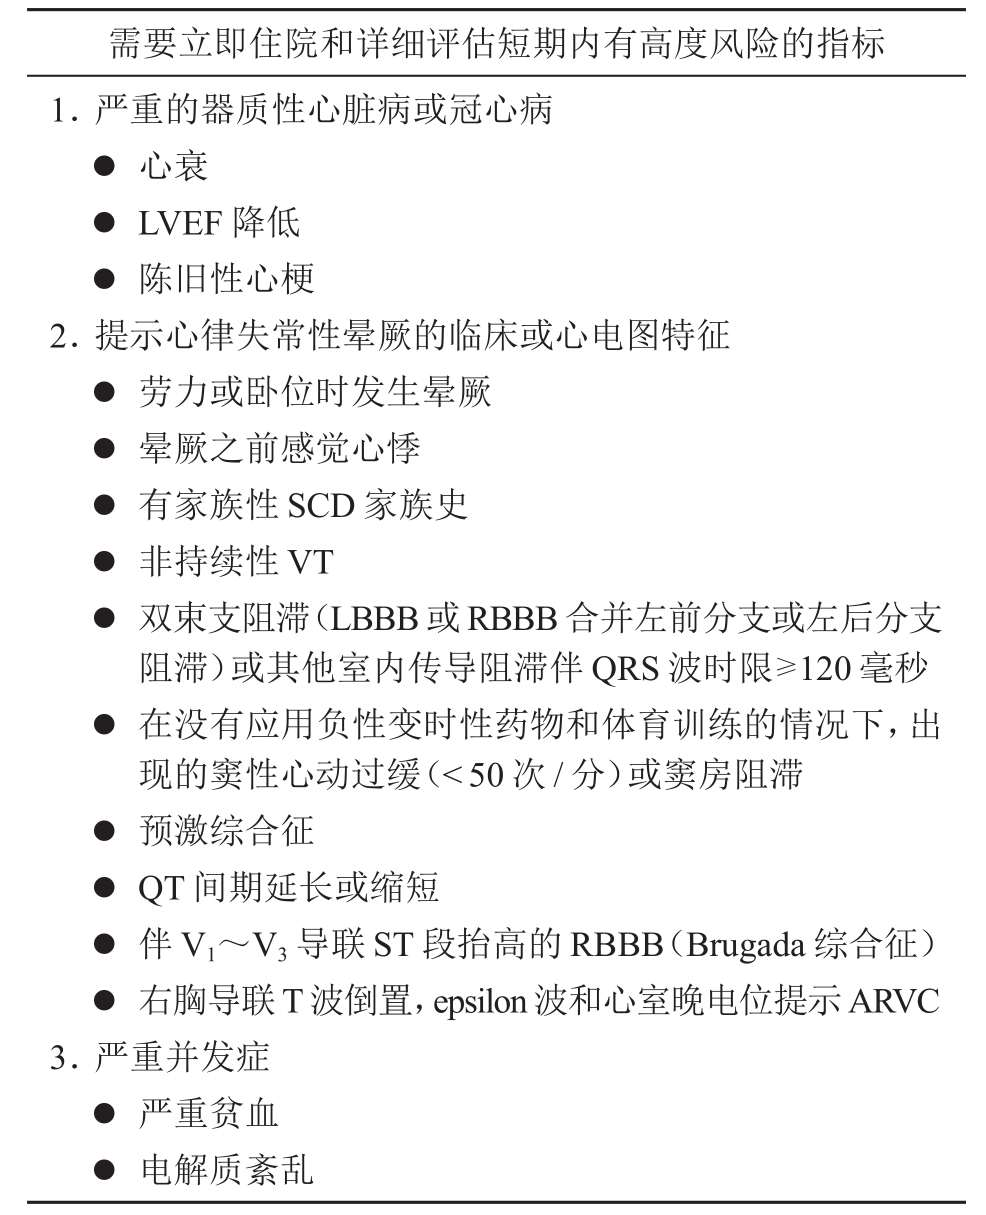
\includegraphics[width=3.28125in,height=4.04167in]{./images/Image00018.jpg}
\end{table}

注:LVEF:左室射血分数,SCD =心源性猝死,VT =室性心动过速,LBBB
=左束支传导阻滞,RBBB =右束支传导阻滞,ARVC
=致心律失常性右室心肌病,心衰=心力衰竭,心梗=心肌梗死

\begin{figure}[!htbp]
 \centering
 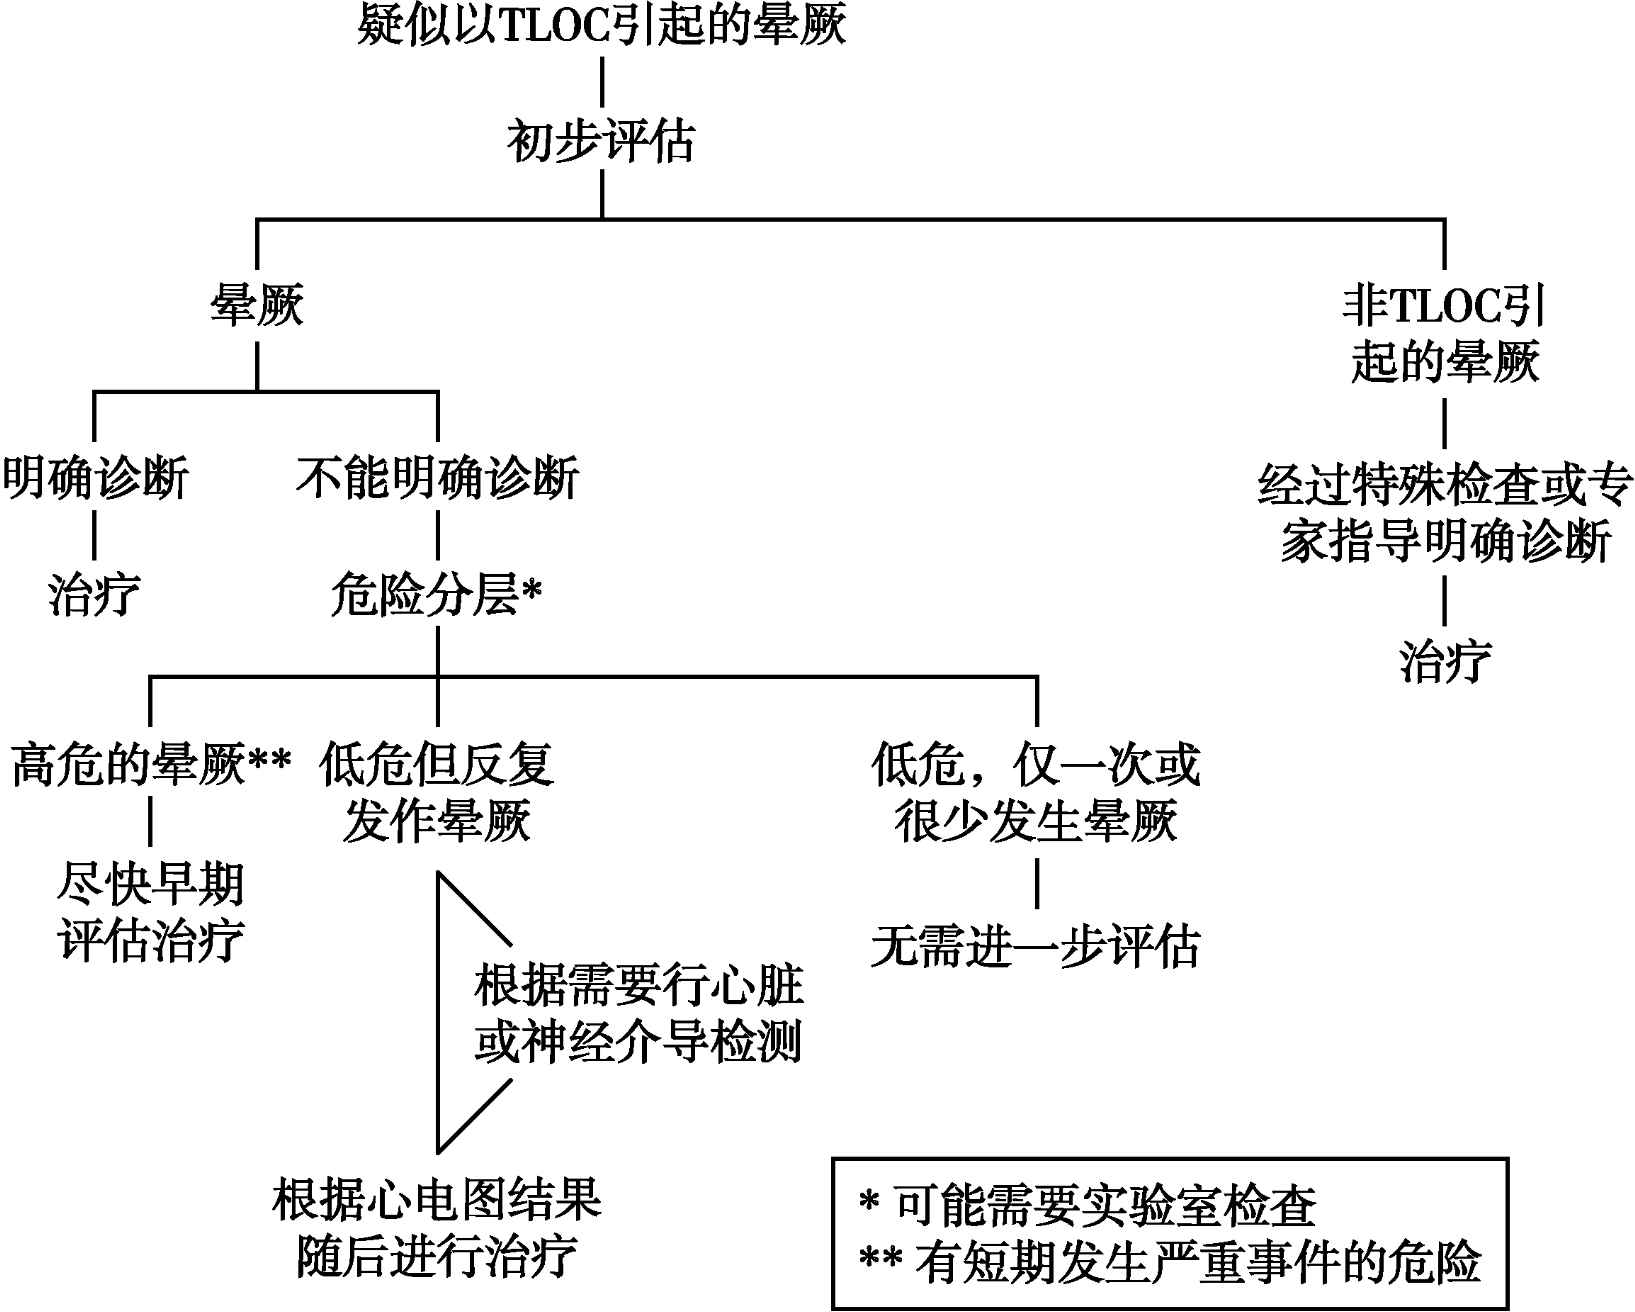
\includegraphics[width=3.84375in,height=3.08333in]{./images/Image00019.jpg}
 \captionsetup{justification=centering}
 \caption{疑似TLOC患者的诊断流程图}
 \label{fig4-1}
  \end{figure} 

\begin{table}[htbp]
\centering
\caption{通过初步评估获得诊断的建议\textsuperscript{*}}
\label{tab4-3}
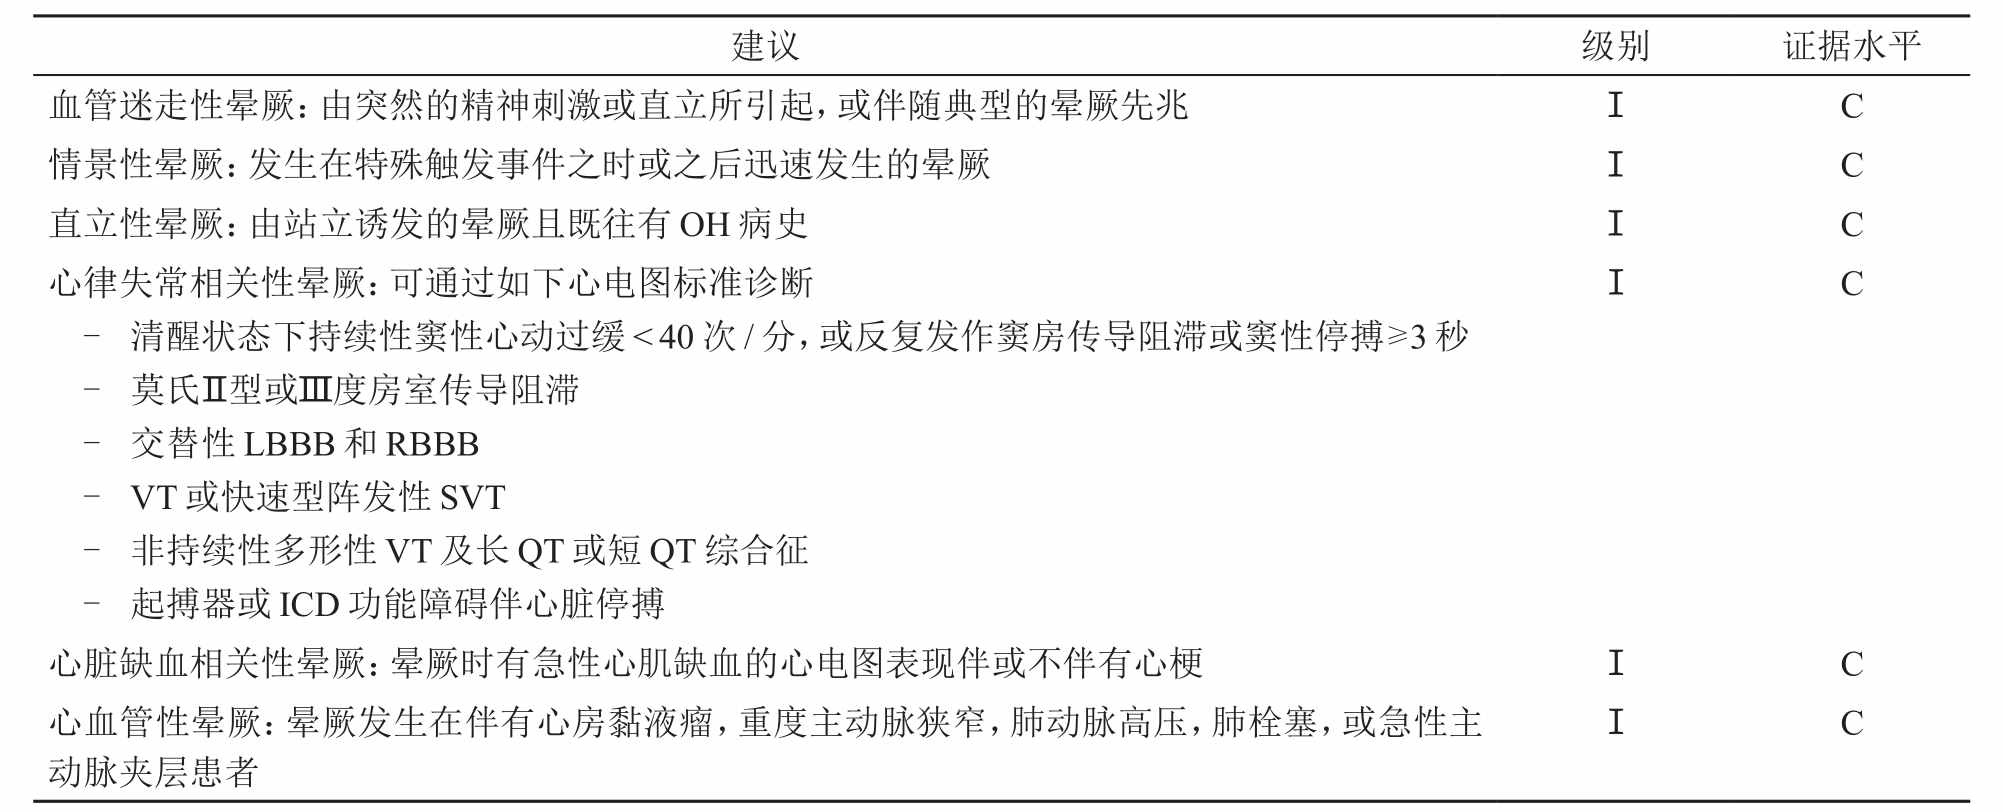
\includegraphics[width=6.66667in,height=2.69792in]{./images/Image00020.jpg}
\end{table}

*本文的建议均源自2009年ESC晕厥诊断和治疗指南。

建议的级别如下:

Ⅰ级:证据和(或)一致同意给予的诊断操作/处理有益,有用和有效。

Ⅱ级:抵触的证据和(或)关于处理的有用/有效存在分歧的观点。

Ⅱa级:证据/观点偏重于有用/有效。

Ⅱb级:证据/观点偏重于无用/无效。

Ⅲ级:证据或一致同意处理无用/无效,且在某些情况下可能有害。

证据水平如下:

A类证据:数据来自多中心随机临床试验或荟萃分析。

B类证据:数据来自单中心随机临床试验或大的非随机研究。

C类证据:专家的一致观点和(或)小的研究,回顾性研究,注册中心资料。

\subsubsection{诊断试验}

初步评估后,倾向性诊断需要进一步检查证实,包括心脏评估检查如超声心动图,心脏负荷试验,心电监测包括Holter,必要时埋藏植入式心电事件记录仪(ILR)和电生理检查;神经介导方面的检查包括倾斜试验和颈动脉窦按摩。

\subparagraph{颈动脉窦按摩}

压迫颈动脉分叉处能够产生反射性心率减慢和血压下降。某些晕厥患者,特别是>
40岁的患者,可以见到对颈动脉窦按摩的异常反应。室性停搏持续≥3秒,收缩压下降≥50mmHg为异常反应,称为颈动脉窦过敏。颈动脉窦按摩是揭示颈动脉窦过敏综合征晕厥的一种检查方法。2009年ESC晕厥诊断和治疗指南颈动脉窦按摩的适应证和诊断标准见表\ref{tab4-4}。

\begin{table}[htbp]
\centering
\caption{颈动脉窦按摩的适应证和诊断标准}
\label{tab4-4}
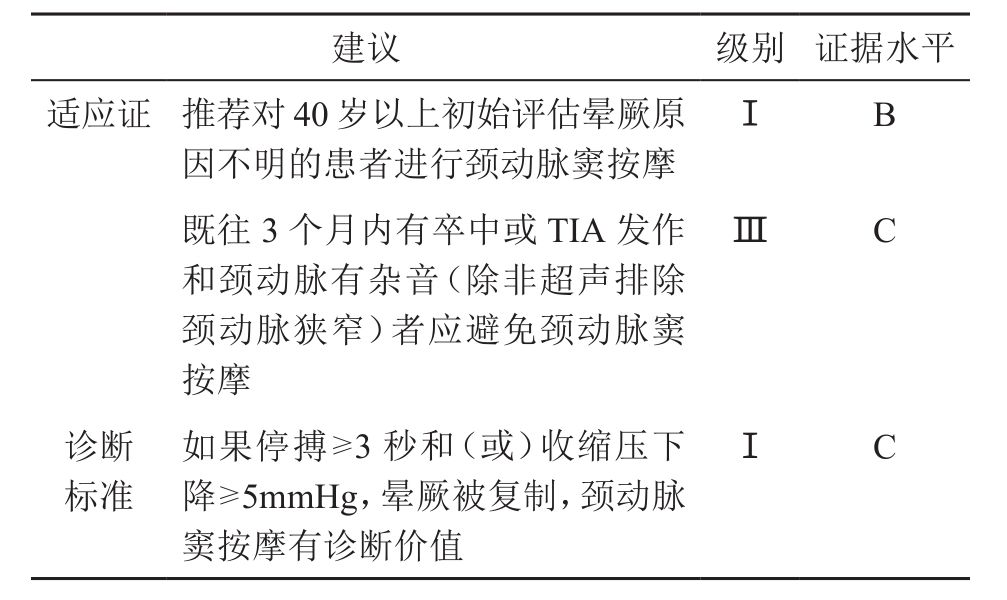
\includegraphics[width=3.34375in,height=1.98958in]{./images/Image00021.jpg}
\end{table}

\subparagraph{倾斜试验}

倾斜试验有助于诊断神经介导性晕厥,但是,其敏感性、特异性、诊断标准和重复性存在很大问题,敏感性和特异性与检查方法有密切关系。敏感性26\%~80\%,特异性约90\%。2009年ESC晕厥诊断和治疗指南倾斜试验的适应证和诊断标准见表\ref{tab4-5}。

\subparagraph{心电图}

(ECG)监测
ECG监测是诊断间歇性缓慢和快速心律失常的方法,但是ECG监测技术目前仍有严重的局限性。晕厥患者ECG监测的作用不是孤立的。医生可以根据病史、体格检查和其他客观检查如倾斜试验决定治疗方案。有些情况下,临床上强烈提示为反射性晕厥时,无需动态心电图(Holter)监测。如果症状发作不频繁Holter监测对诊断意义也不大,这种情况下应考虑植入式循环记录仪。将来的技术可能会记录ECG以外的多项指标,将把重点放在与自发性晕厥相关的心律方面,而不是被触发的晕厥。了解自发性晕厥发作过程是评估晕厥的最好标准。因此,植入式监测仪对晕厥越来越重要。记录到晕厥时有缓慢心律失常即可考虑诊断,但是,有时需要进一步检查明确是心脏本身原因所致还是神经反射机制造成,而反射性心动过缓可能是阵发性心动过缓最常见的原因。

由于晕厥发作时ILR记录到的心律失常的变异和干扰很大,2009年ESC晕厥诊断和治疗指南采用国际不明原因晕厥研究调查组织(ISSUE)的方法,将心电图记录进行了分类,根据主要心律失常和可能的晕厥机制将心电图划分为4型。

1型:心脏停搏,RR间期≥3秒。1型又分为A、B、C
3个亚型。1A型:窦性停搏,表现为进行性窦性心动过缓或初为窦性心动过速逐渐进展为窦性心动过缓直至发生窦性停搏,其可能的机制为反射性。1B型:窦性心动过缓合并房室传导阻滞,表现为进行性窦性心动过缓随后出现房室传导阻滞(和心室停搏)的同时伴有窦率下降;或突发房室传导阻滞(和心室停搏)伴窦率下降,其可能机制为反射性。1C型:房室传导阻滞,突发房室传导阻滞(和心室停搏)伴窦律逐渐增加,其可能机制为自身病变。

2型:心动过缓,心率下降> 30\%或心率<
40次/分持续超过10秒,其可能机制为反射性。

3型:无或很小的心率变异性,心率变异度< 30\%且心率>
40次/分,其机制不肯定。

4型:心动过速,心率增加> 30\%,心率> 120次/分。此型又分为A、B、C、D
4型。4A型:进行性窦性心动过速,机制不肯定。4B型:心房颤动(简称房颤)。4C型:SVT(不包括窦性)。4D型:VT。

\begin{table}[htbp]
\centering
\caption{倾斜试验的适应证和诊断标准}
\label{tab4-5}
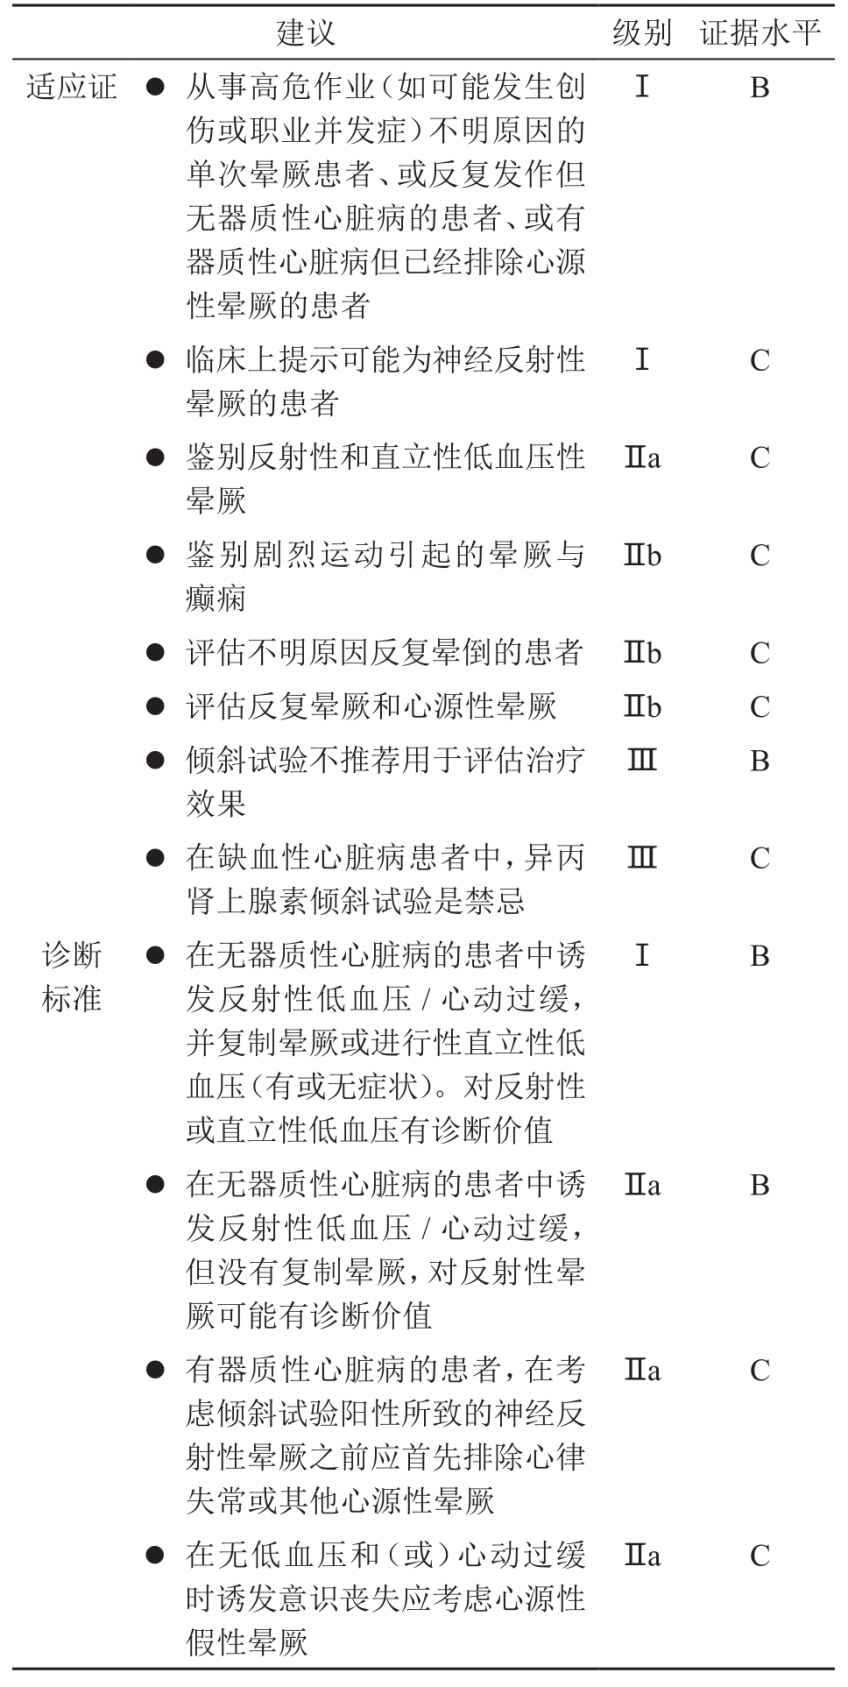
\includegraphics[width=3.21875in,height=6.40625in]{./images/Image00022.jpg}
\end{table}

2009年 ESC晕厥诊断和治疗指南心电图监测的建议见表\ref{tab4-6}。

\subparagraph{电生理检查}

电生理检查通过心内膜和心外膜(冠状窦电极)刺激并记录揭示引起晕厥的原发性心律失常的心电异常改变。然而,仅有少数研究应用Holter和植入式记录仪证实了电生理检查的结果。电生理检查揭示的真实诊断仅仅涵盖了一部分患者。下列诊断标准广泛用于确定窦房结功能障碍:窦房结恢复时间(SNRT)>
1.6秒或2秒或校正的窦房结恢复时间(CSNRT)> 525毫秒。另一项研究认为SNRT
>
3秒诊断窦房结功能障碍性晕厥的可能性更大。2009年ESC晕厥诊断和治疗指南电生理检查的适应证见表\ref{tab4-7}。

\begin{table}[htbp]
\centering
\caption{心电图监测的建议}
\label{tab4-6}
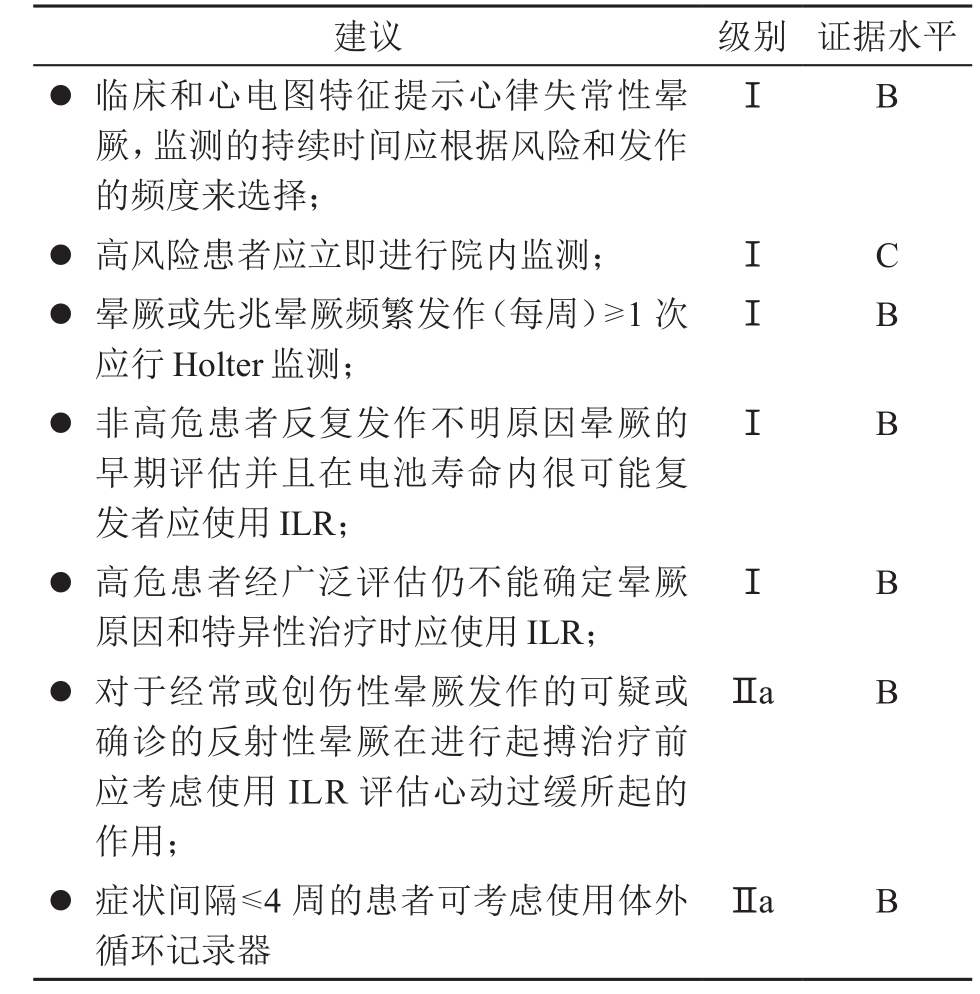
\includegraphics[width=3.25in,height=3.30208in]{./images/Image00023.jpg}
\end{table}

\begin{table}[htbp]
\centering
\caption{电生理检查的适应证}
\label{tab4-7}
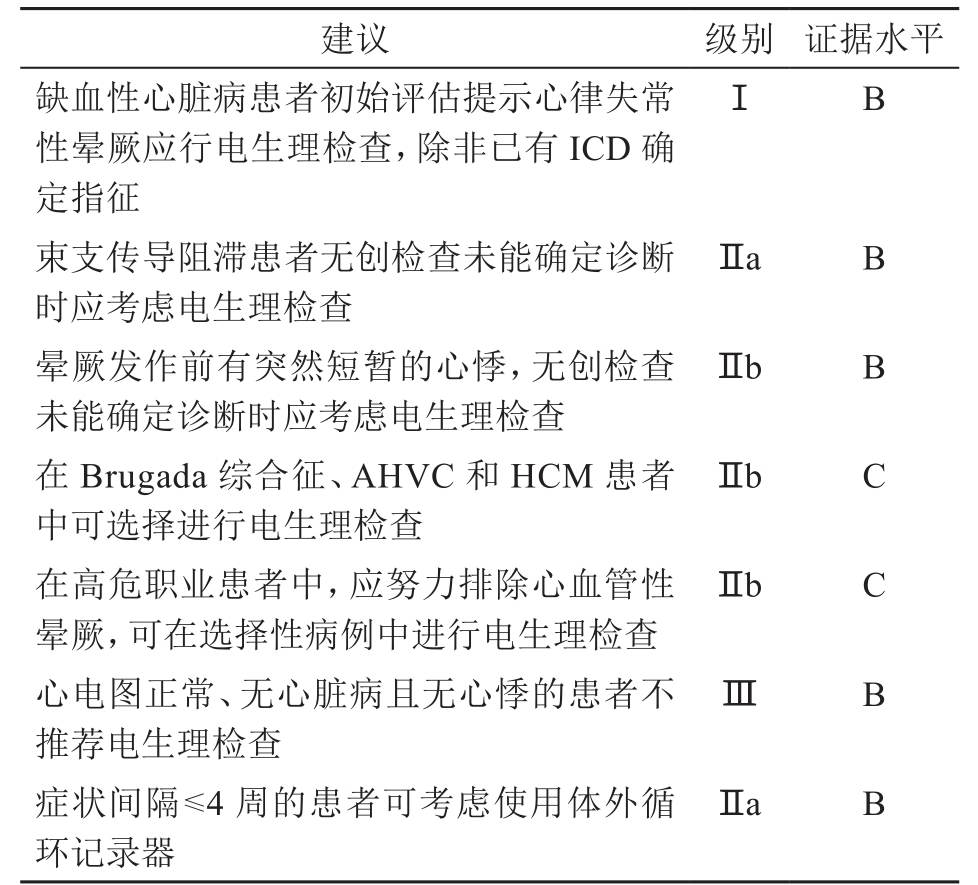
\includegraphics[width=3.25in,height=2.9375in]{./images/Image00024.jpg}
\end{table}

注:ARVC:致心律失常型右室心肌病;HCM:肥厚型心肌病

\subparagraph{超声心动图(UCG)}

当病史、体格检查和心电图检查不能发现晕厥的原因时,超声心动图检查是发现包括瓣膜病在内的器质性心脏病的有效方法。通过该检查还能发现肺动脉高压和右心室扩大等提示肺栓塞的表现。体格检查正常的晕厥或先兆晕厥患者超声心动图检查最常见的发现是二尖瓣脱垂(4.6\%~18.5\%)。其他心脏异常包括瓣膜病(最常见的是主动脉瓣狭窄)、心肌病、节段性室壁运动异常提示的心肌梗死、冠状动脉畸形、浸润性心脏病如淀粉样变性、心脏肿瘤、动脉瘤、左房血栓等。超声心动图检查为判断晕厥的类型、严重程度及危险分层提供重要的信息。如果发现中重度器质性心脏病应考虑心源性晕厥。另一方面,如果超声心动图仪发现轻微心脏结构病变,则心源性晕厥的可能性较小,应进行非心源性晕厥方面的检查。2009年ESC晕厥诊断和治疗指南UCG适应证和诊断标准见表\ref{tab4-8}。

\begin{table}[htbp]
\centering
\caption{UCG适应证和诊断标准}
\label{tab4-8}
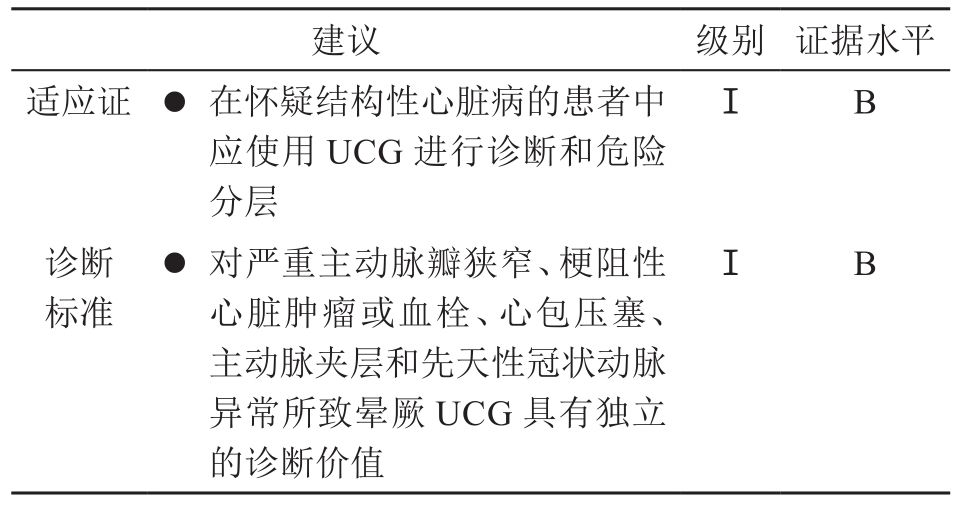
\includegraphics[width=3.20833in,height=1.6875in]{./images/Image00025.jpg}
\end{table}

\subparagraph{运动试验}

运动中或运动后即刻发生晕厥的患者应进行运动试验。进行运动试验应该是症状限制性的,即由于运动中和运动后即刻易发生晕厥,运动中和恢复阶段均应监测心电和血压,应做好防范。运动中发生晕厥可能是心脏原因造成的,有些病例报告运动中也可能发生过度反射性血管扩张引起晕厥,反射性晕厥的元凶是低血压而无心动过缓。相反,运动后晕厥几乎都是自主神经功能异常或神经介导机制参与的,其特点是与心动过缓或心脏停搏有关的低血压;一般发生于无心脏病的患者。运动试验用于诊断神经反射性晕厥,其特点是劳力后晕厥。血管迷走神经性晕厥的患者,运动中内脏容量性血管和前臂阻力血管反射性收缩功能障碍。运动试验对一般晕厥患者意义不大,仅有1\%发现异常。尽管如此,对运动性晕厥具有重要诊断价值。2009年ESC晕厥诊断和治疗指南运动试验的适应证和诊断标准见表\ref{tab4-9}。

\begin{table}[htbp]
\centering
\caption{运动试验的适应证和诊断标准}
\label{tab4-9}
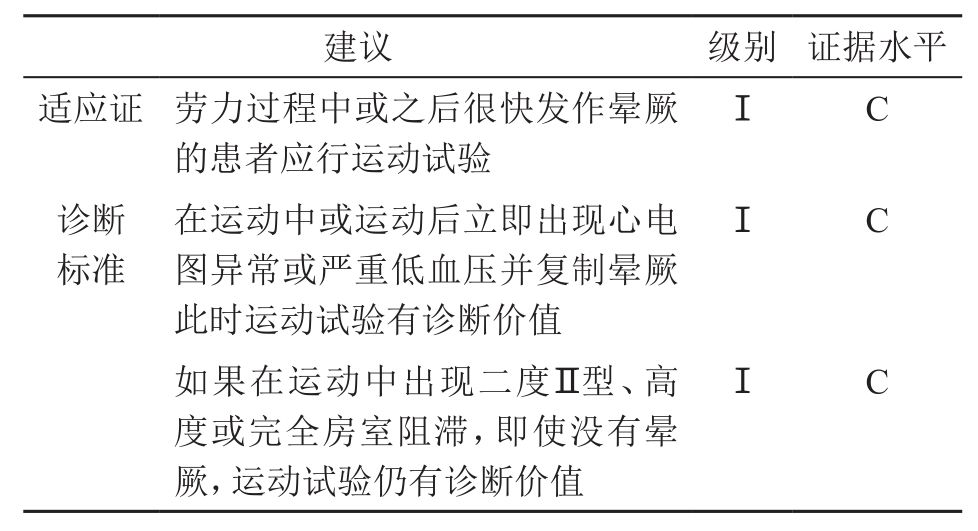
\includegraphics[width=3.25in,height=1.76042in]{./images/Image00026.jpg}
\end{table}

\subparagraph{心导管检查}

心导管检查包括评估心腔形态的心室造影、了解冠脉解剖的冠状动脉造影和了解血流、血管内压力和心腔内压力的血流动力学检查。由于是有创检查,一般不作为筛查心源性晕厥的检查。这些检查能够揭示冠状动脉狭窄引起缺血性晕厥:室壁运动异常和心肌收缩力减弱;缺血引起的心律失常、心脏停搏或完全性房室阻滞和缺血诱发的血管迷走神经性反应。也可以揭示冠状动脉痉挛引起的晕厥,这种患者冠状动脉造影中应做麦角新碱试验。

\subparagraph{神经系统检查}

神经系统疾病引起的晕厥有三种情况。①自主神经功能障碍:晕厥可以是自主神经系统疾病和功能不全的结果;②有些脑血管疾病也可以引起晕厥(大多是“窃血”综合征);③有些疾病应列为鉴别诊断的内容,因为这些疾病可以引起短暂意识丧失(但不是晕厥,如癫痫)或其发作类似于意识丧失。2009年ESC晕厥诊断和治疗指南神经系统检查适应证见表\ref{tab4-10}。

\begin{table}[htbp]
\centering
\caption{神经系统检查适应证}
\label{tab4-10}
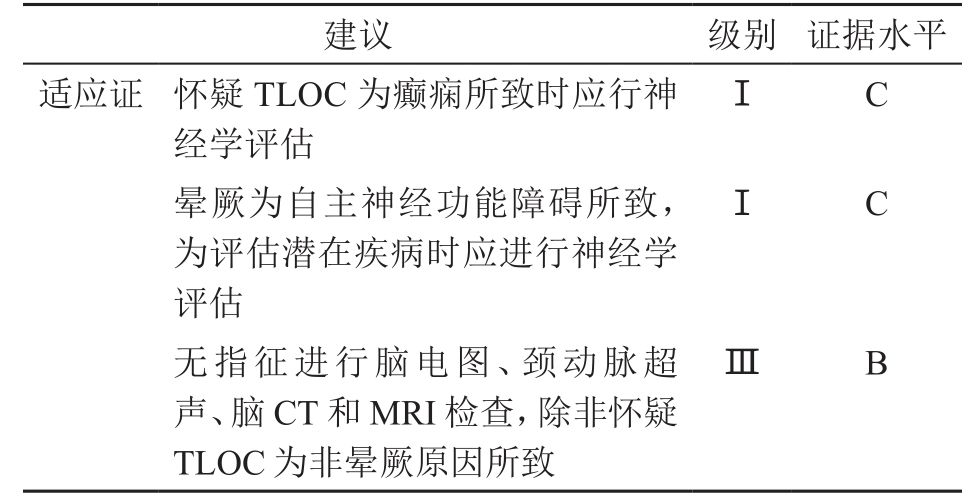
\includegraphics[width=3.25in,height=1.66667in]{./images/Image00027.jpg}
\end{table}

\subsubsection{诊断注意事项}

对所有一过性意识丧失患者必须进行全面仔细的评估,包括病史和检查。要顺序确认:是否晕厥,晕厥的原因,死亡和其他风险。尽管从死亡率角度来说,晕厥常常是良性的,但仅仅确定患者是低死亡风险患者是不够的,因为晕厥常常会复发,增加外伤风险,并且影响生活质量和正常工作。晕厥的诊断和治疗是富于挑战性的。首先,晕厥仅仅是一过性意识丧失众多原因中的一种;其次,患者症状短暂,就诊时一般都已完全恢复,并且有价值的查体发现很少;第三,自发的临床事件很少被医学专业人员目击,临床事件的病史经常是来自“二手”甚至“三手”的资讯。急诊科医生应仔细考虑所发现的异常是否和临床情况相匹配,强调长程监测的重要性。为了使患者得到准确的预后评估和治疗选择,强调应尽可能确定患者的病因。

\subsection{治疗}

\subsubsection{晕厥治疗的一般原则}

晕厥治疗的一般原则是:延长生命、预防复发、防治躯体损伤。

采取基础预防性治疗还是加强治疗取决于下列临床情况:①晕厥的病因。②晕厥复发的可能性大小。③晕厥的死亡危险性大小,主要取决于心脏病和血管病的性质和严重程度。④复发次数或晕厥导致躯体或精神伤害的危险性大小。⑤发生晕厥可能对个人职业或业余爱好造成的影响(如个人经济和生活方式问题)。⑥对公共健康的危险性如汽车司机、飞行员等。⑦对治疗有效性、安全性和不良反应的评估(特别要考虑患者的伴随疾病)。根据晕厥不同病因和机制以及危险分层,采取不同的治疗策略。晕厥的治疗流程见图\ref{fig4-2}。

\subparagraph{反射性晕厥的治疗}

反射性晕厥包括血管迷走神经性晕厥、颈动脉窦综合征(CCS)和情景性晕厥,其治疗目标首先是预防症状复发和晕厥相关的损伤,改善生活质量。自2004年指南发表后,治疗方面最大的进展是在生活方式方面上,反射性晕厥非药物治疗的基石是教育,让患者相信这是一种良性情况。一般来讲,最初的治疗涉及让患者了解这一疾病及如何避免诱因(如闷热而拥挤的环境,血容量不足)等相关方面的教育。早期识别前驱症状,采取某些动作以终止发作{[}如仰卧位,身体反压调整(PCMs){]}。避免引起血压降低的药物(包括α受体阻滞剂、利尿剂和酒精)。对于不可预测的频繁发作的晕厥需给予其他治疗。特别是:①非常频繁发作影响到生活质量;②反复晕厥没有或仅有非常短时的晕厥先兆,但患者暴露于有外伤危险的情况下;③晕厥发生在高危作业时(如驾驶、操作机器、飞行、竞技性体育运动等)。

具体治疗方法如下:①身体反压调整(PCMs):非药物的物理治疗,为反射性晕厥的一线治疗。PCMs即双腿肌肉等长收缩PCMs(双腿交叉),或双上肢肌肉等长收缩PCMs(双手紧握和上肢紧绷),多中心前瞻性研究显示,使用这种方法,在反射性晕厥发作时能够显著升高血压,多数情况下可使患者避免或延迟意识丧失。②倾斜训练:可能会减少晕厥复发,但是患者依从性较差,治疗受到影响。③药物治疗:许多试图用于治疗反射性晕厥的药物结果都令人失望。这些药物包括β受体阻滞剂、丙吡胺、东莨菪碱、茶碱、麻黄碱、依替福林、米多君、可乐定和5-羟色胺重吸收抑制剂。由于在反射性晕厥时外周血管常常不能得到适当的收缩,α受体激动血管收缩剂(依替福林和米多君)曾被使用,但是,治疗效果不一致。专家组认为,反射性晕厥患者长期单独使用α受体激动剂药物治疗可能有一些作用,对于偶发患者不建议长期治疗。在长时间站立或从事常常诱发晕厥的活动前1小时服用单剂量的药物避免晕厥发生,对有些患者可能有用。④心脏起搏:起搏治疗反射性晕厥的随机对照试验得出了相反的结果。专家组认为在迷走神经性晕厥中血管减压部分通常起主要作用,所以得出起搏欠佳的结果并不奇怪。而颈动脉窦晕厥心脏起搏治疗可能有效,双腔起搏一般优于单腔心室起搏。反射性晕厥治疗的建议见表\ref{tab4-11}。

\begin{figure}[!htbp]
 \centering
 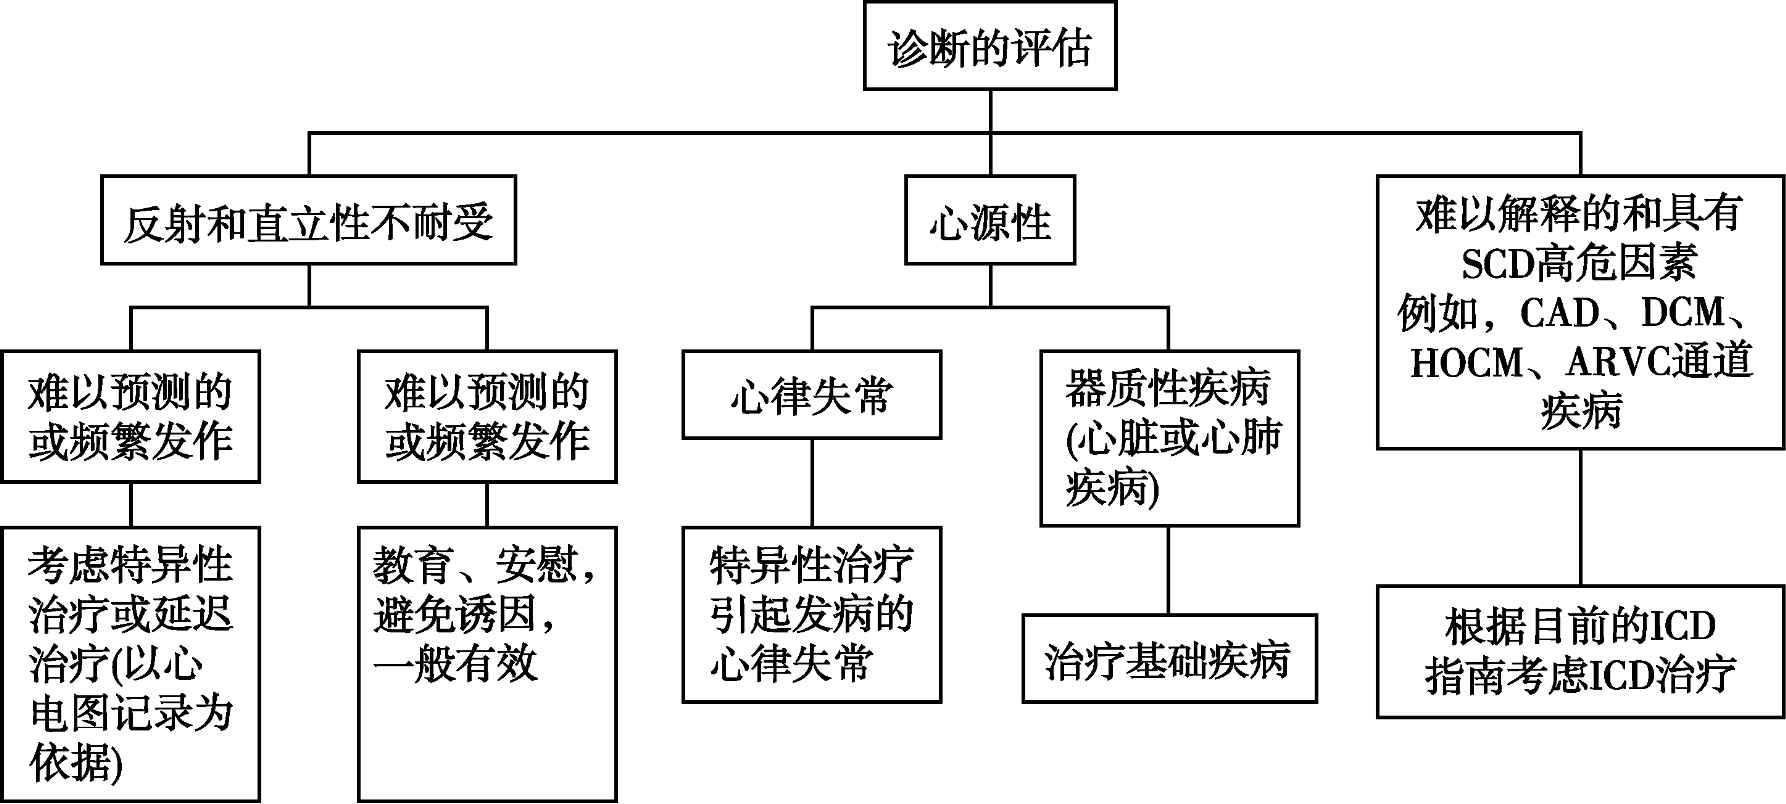
\includegraphics[width=4.82292in,height=2.16667in]{./images/Image00028.jpg}
 \captionsetup{justification=centering}
 \caption{晕厥的治疗流程}
 \label{fig4-2}
  \end{figure} 

\begin{table}[htbp]
\centering
\caption{反射性晕厥的治疗建议}
\label{tab4-11}
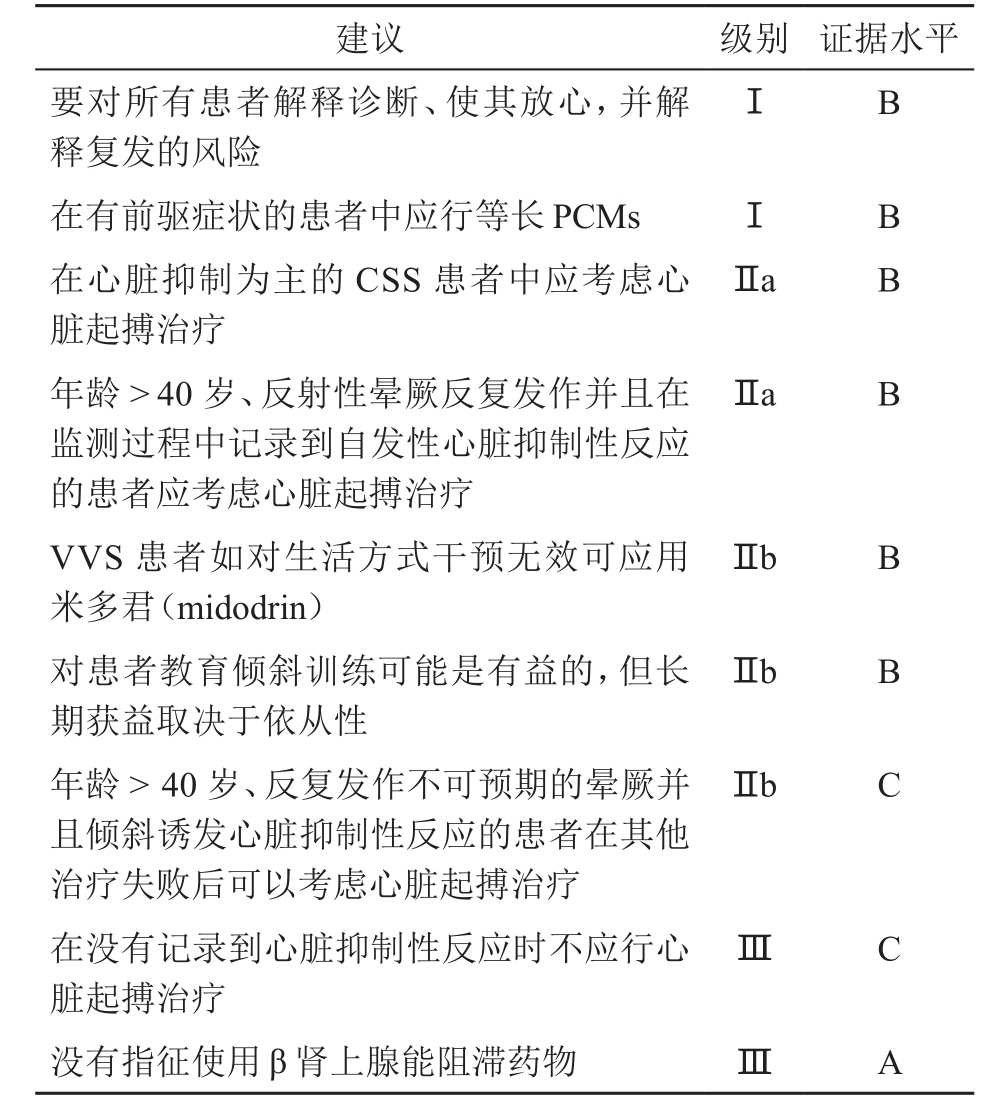
\includegraphics[width=3.28125in,height=3.66667in]{./images/Image00029.jpg}
\end{table}

注:CSS =颈动脉窦综合征;VVS =血管迷走晕厥

\subparagraph{直立性低血压的治疗}

治疗目标是预防症状复发以及晕厥造成的伤害,改善生活质量。药物诱发的自主神经功能失调可能是直立性低血压性晕厥最常见的原因,主要治疗方法是停药,仅有少数患者由于病情不能停药。引起直立性低血压最常见的药物是利尿剂和血管扩张剂,酒精也是常见的原因,其除诱发自主神经性晕厥外还可引起躯体神经系统疾病。包括对中枢神经系统的直接作用和血容量不足。主要治疗是戒酒。对于原发性和继发性自主神经功能失调的患者,了解血压调节的生理和病生理机制十分重要,治疗的主要目标是改善由于脑灌注不足导致的症状(如晕厥、先兆晕厥、意识模糊等)。尽管通过上述治疗使收缩压升高幅度不大(10~15mmHg),但可以明显改善直立性低血压的症状;使平均动脉压升高恰到好处,重新达到自主神经的调节范围内,进而可以明显改善神经调节功能。应对所有患者进行健康教育,使他们了解影响血压的因素,避免突然站起(尤其是醒后)、长时间站立、白天长时间卧位休息、用力排尿排便、过度通气、高温环境(包括热澡水、淋浴、桑拿浴)、极度用力、暴食(特别是精制的碳水化合物)、具有扩血管作用的酒精和药物。动态监测血压有助于了解白天不同环境中的血压变化,了解高血压患者药物对卧位/夜间血压的影响。扩张细胞外容量是重要的治疗目标。对无高血压的患者,应指导摄入足够的盐和水。每天达到2~3L液体和10g氯化钠。快速摄入冷开水对运动中或餐后低血压者有明显疗效;高枕位睡眠(头部抬高10°)可防止夜间多尿,维持适量的体液量及改善夜间高血压。老年患者可佩戴腹带或加压弹力袜以减轻下肢血液蓄积;有先兆晕厥时可采取交叉腿和蹲位姿势等预防措施。α受体激动剂(米多君)是慢性自主神经异常者的首选药物。氟氢可的松(0.1~0.3mg/d)可促进钠水潴留及扩张血容量,改善晕厥症状。其他治疗如去氨加压素用于伴夜尿增多者;奥曲肽用于餐后低血压,促红细胞生成素用于贫血者等。直立性低血压治疗建议见表\ref{tab4-12}。

\begin{table}[htbp]
\centering
\caption{直立性低血压的治疗建议}
\label{tab4-12}
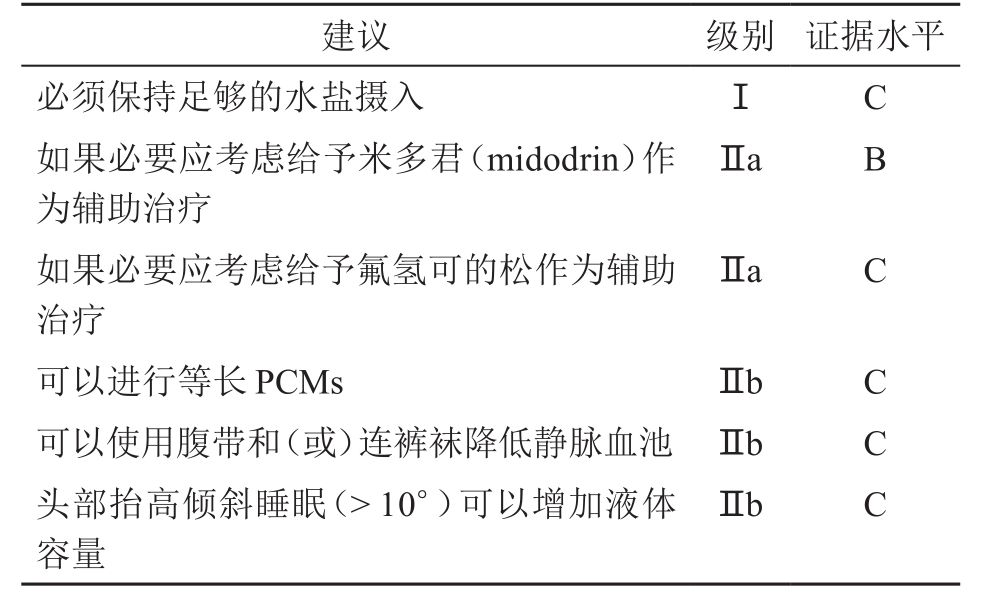
\includegraphics[width=3.27083in,height=2in]{./images/Image00030.jpg}
\end{table}

\subparagraph{心律失常性晕厥的治疗}

治疗目标预防症状复发,改善生活质量,减低死亡危险。原发性心律失常与心脏本身疾病或解剖异常有关,是最常见晕厥原因之一。包括原发性窦房结功能异常(缓慢、快速心律失常)、传导系统病变、室上性心动过速和室性心动过速。这种晕厥的基础是多方面的,包括心律失常的频率、左心室的功能状态和血管的代偿作用(包括神经反射作用)。

\hypertarget{text00014.htmlux5cux23CHP1-4-4-1-3-1}{}
(1) 窦房结功能不全:

窦房结功能不全伴缓慢心律失常、或SNRT异常引起的晕厥,起搏治疗效果显著。永久起搏可明显缓解症状,但对生存率无影响。预防晕厥复发的另一主要措施是停用加重或诱发心动过缓的药物,如无合适的替代药物应行心脏起搏。

\hypertarget{text00014.htmlux5cux23CHP1-4-4-1-3-2}{}
(2) 房室传导系统疾病:

AV阻滞引起的晕厥需起搏治疗,永久右室心尖部起搏的危害已获证实,但其替代起搏位点仍有争议。AV阻滞伴LVEF下降、心力衰竭(心衰)及QRS间期延长所致者可考虑双腔起搏。

\hypertarget{text00014.htmlux5cux23CHP1-4-4-1-3-3}{}
(3) 阵发性室上性和室性心动过速:

阵发性室上性和室速或典型心房扑动引起的晕厥,应首选导管消融术。尖端扭转型室速所致的晕厥主因是应用引起QT间期延长的药物所致,应立即停药。心功能正常或轻度受损者,如出现室速伴晕厥,可考虑导管消融或药物治疗。心功能不全、室速或心室颤动伴晕厥且病因无法祛除者应植入埋藏式心脏复律除颤器(ICD)。ICD虽不能有效预防晕厥复发,但可降低猝死风险。心律失常性晕厥的治疗见表\ref{tab4-13}。

\subparagraph{SCD高危患者不明原因晕厥的治疗}

其治疗目标不仅仅是防止晕厥再发,而且要治疗基础疾病和减少SCD的风险。严重主动脉狭窄或心房黏液瘤所致的晕厥可考虑手术治疗;继发于急性心血管事件如肺栓塞、心肌梗死或心包压塞者主要针对病因治疗;大多数心肌缺血所致者可采用药物和(或)血管重建;由原发性肺动脉高压或限制性心肌病引起者,一般不易纠正原发病。急、慢性冠状动脉疾病或LVEF下降均可增加死亡风险,故需评估缺血的严重程度,且如果有适应证应考虑血运重建。但血运重建并不能改善恶性心律失常引起的不良后果,因此该类患者应行电生理检查以评估有无心律失常。心衰且符合最新指南制定的ICD适应证者,无论晕厥发生机制是否明确,均应植入ICD。有研究显示,植入ICD的晕厥患者生存率明显增加;不明原因晕厥的缺血性或非缺血性心肌病伴心衰或LVEF严重下降者应植入ICD(Ⅰ类,A级);LVEF正常和电生理检查阴性者不建议植入ICD。其他类型心脏病:①肥厚性心肌病伴不明原因晕厥尤其是发作间期短(<
6个月)、相对危险度>
5的患者,其猝死风险较高;植入ICD效果明显。②约1/3致心律失常性右室心肌病(ARVC)者会发生晕厥。年轻、严重右室发育不全、左室功能障碍、多形性室速、心室晚电位、epsilon波及有猝死家族史者,如无其他病因应考虑植入ICD。③遗传性离子通道异常性心脏病常以晕厥为先兆表现,但该类患者是否应植入ICD仍有争议。SCD高危晕厥患者ICD适应证见表\ref{tab4-14}。

\begin{table}[htbp]
\centering
\caption{心律失常性晕厥的治疗建议}
\label{tab4-13}
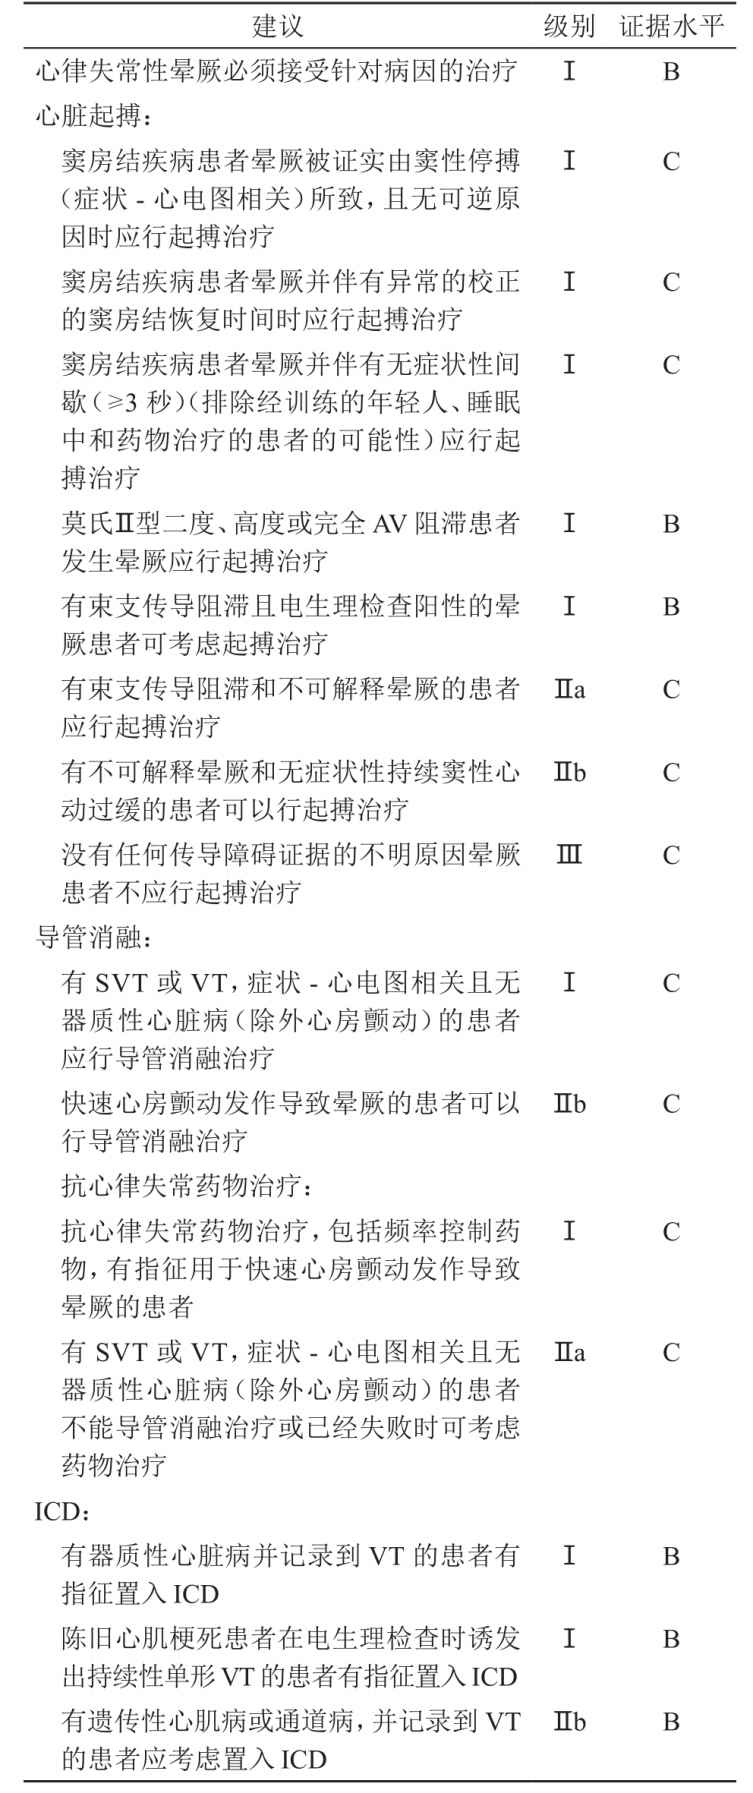
\includegraphics[width=3.29167in,height=7.86458in]{./images/Image00031.jpg}
\end{table}

\begin{table}[htbp]
\centering
\caption{SCD高危晕厥患者ICD适应证}
\label{tab4-14}
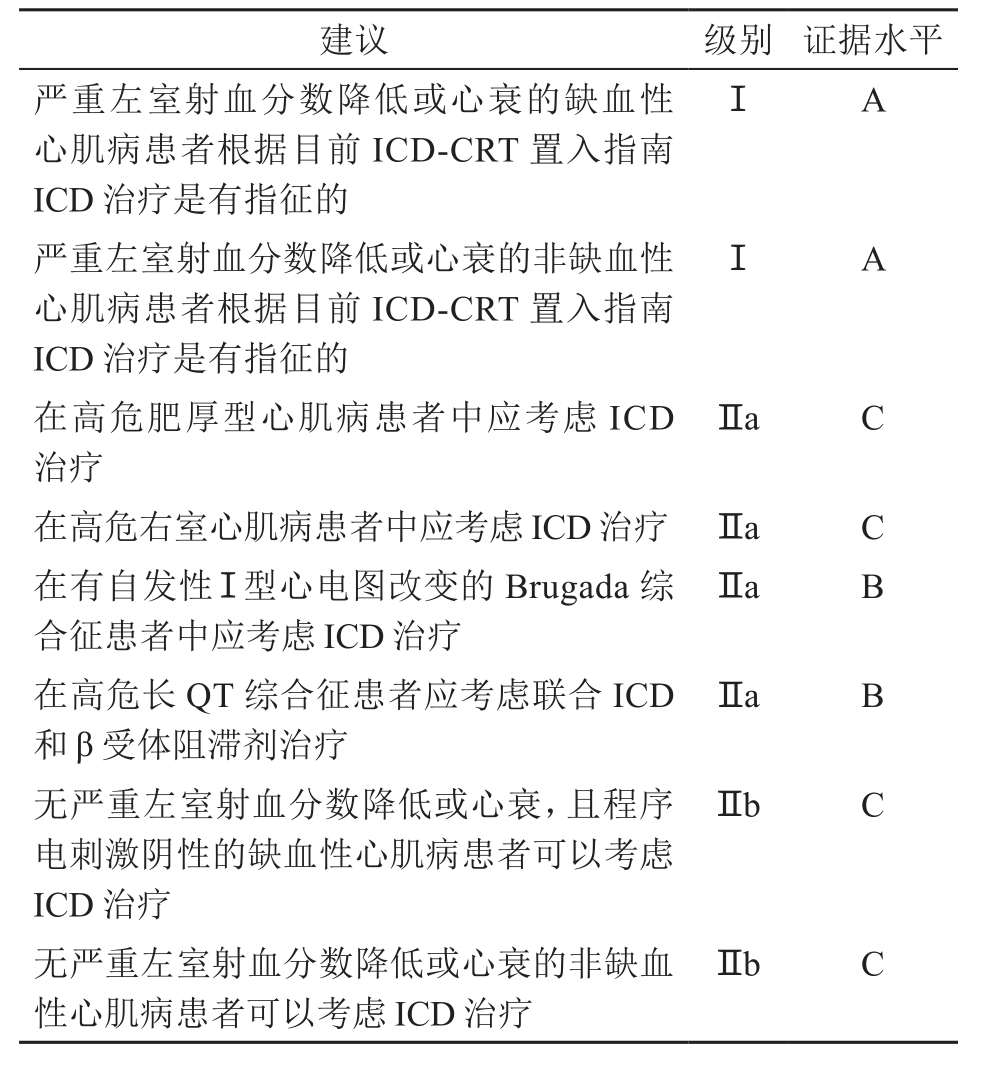
\includegraphics[width=3.3125in,height=3.55208in]{./images/Image00032.jpg}
\end{table}

\subparagraph{特殊人群晕厥的处理}

\hypertarget{text00014.htmlux5cux23CHP1-4-4-1-5-1}{}
(1) 老年人晕厥:

老年人最常见的晕厥原因是OH、反射性晕厥,特别是颈动脉窦过敏和心律失常。一个患者可能有不同的机制共同作用,从而给诊断带来困难。与OH相关的住院治疗随着年龄的增加而增加,65~74岁是4.2\%,75岁以上为30.5\%。在有晕厥症状的患者之中,25\%是年龄相关的OH;其他OH主要是药物和特发性或继发性房颤所致。有OH的老年患者常有卧位收缩期高血压,并在接受多种药物治疗,给予OH药物治疗会加重卧位高血压,反之亦然。心脏抑制型颈动脉窦过敏是晕厥的原因,老年者高达20\%。血管减压型为主的颈动脉窦敏感同样常见,但是其在晕厥中的作用知之甚少。

对于老年人诊断检查和策略应注意:①老年人的OH常常具有重复性(特别是与药物或年龄相关)。因此,应反复进行OH评价,最好在早晨和(或)晕厥刚刚发生后进行。②对没有晕厥史者,即使颈动脉窦过敏不具特异性,颈动脉窦按摩检查也是特别重要的。③评价老年人反射性晕厥时,倾斜试验耐受性和安全性均很好。其阳性率与年轻人相仿,特别是在硝酸甘油激发后。④如果怀疑血压不稳定(如服药后或者餐后),24小时动态血压监测可能有帮助。⑤由于老年人心律失常发生频率高,对不明原因晕厥的老年人ILR特别有用。

\hypertarget{text00014.htmlux5cux23CHP1-4-4-1-5-2}{}
(2) 儿童晕厥:

对儿童晕厥的诊断评估与成人类似。反射性晕厥占病因学的绝大部分。但是在少数情况下,晕厥的发生是威胁生命的心律失常或心脏器质性异常所致。晕厥应该与癫痫和精神性假性晕厥鉴别,后者十分少见,但是是儿童TLOC的重要原因。

在幼童时期的两种特殊情况:①婴儿反射性晕厥发作(也叫做苍白屏气发作或反射性缺氧发作)是由短暂不愉快刺激导致的由迷走神经介导的心脏抑制所致。②窒息低氧性TLOC(发绀性呼吸停止)以哭闹时呼吸运动终止于呼气阶段为特征,从而导致发绀和通常所见的TLOC。

儿童倾斜试验的假阳性和假阴性率均较高,因此对于反射性晕厥的初步评估应持审慎态度。有报道对于健康少年儿童在静脉用药后进行倾斜试验时,先兆晕厥的比率非常高(40\%)。年轻患者首发晕厥可能为少见的、但是是威胁生命的疾病,如LQTS、Kearns-Sayre综合征(外眼肌麻痹和进行性心脏传导阻滞)、Brugada综合征、儿茶酚胺依赖性多形性VT、预激综合征、ARVC、肥厚型心肌病、肺动脉高压、心肌炎、先天性心脏病修补术后心律失常、冠状动脉异常起源。

对于具有下面情况的患儿可能提示有心脏性病因,应迅速进行心脏方面的评估:①家族史:年轻的SCD者<
30岁;家族性心脏病。②已知或可疑心脏病。③触发事件:噪音、惊吓、极端情感刺激。④运动时晕厥,包括游泳。⑤仰卧或者睡眠时无晕厥先兆,或晕厥前有胸痛或心悸。

儿童晕厥的治疗策略与成人相同。然而需要强调的是目前缺乏关于儿童反复晕厥良好设计的研究,因此药物和倾斜训练的有效性不能肯定。此外,尽管有血管迷走神经性晕厥以及长时间心脏停搏的证据,由于为一过性和良性晕厥,因此应避免安装起搏器。

总之,对儿童晕厥评估要点有几方面:①儿童期晕厥常见,绝大部分源于反射机制,很少部分是源于威胁生命的病因所致。②对良性和严重病因的鉴别主要依靠病史、体格检查和心电图。③对反射性晕厥年幼患者的治疗基石是教育并使之放心。

\hypertarget{text00014.htmlux5cux23CHP1-4-4-1-5-3}{}
(3) 驾车与晕厥:

随着轿车进入中国普通家庭,驾车与晕厥的问题显得重要起来。但是,调查显示,在有晕厥病史的患者中,交通事故的发生率低于普通人群。晕厥患者驾驶的建议见表\ref{tab4-15}。

\begin{table}[htbp]
\centering
\caption{晕厥患者驾驶的建议}
\label{tab4-15}
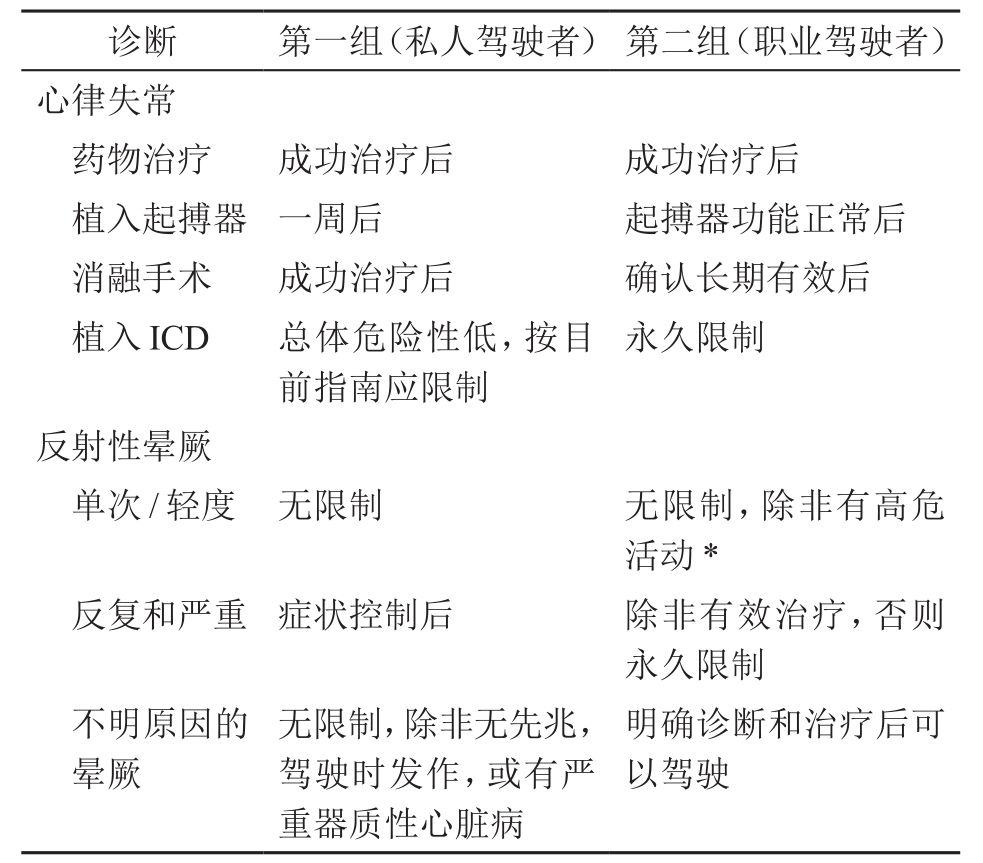
\includegraphics[width=3.27083in,height=2.86458in]{./images/Image00033.jpg}
\end{table}

注:第一组(私人驾驶者):驾驶摩托,小汽车或其他小型车辆,没有拖车;第二组(职业驾驶者):驾驶3.5吨以上汽车,除驾驶员外8座以上客车;出租车,救护车,介于私人与职业间车辆以及地方法规规定的车辆;

*:神经介导的晕厥严重且发作频繁,或正在从事高危活动;或者是复发或不可预测的高危患者

\subsection{预后}

晕厥的预后主要取决于两方面:①死亡风险及致命性事件:器质性心脏病及原发性电生理疾病是心源性猝死及晕厥患者总体死亡率的高危因素;合并联合病变的直立性低血压患者与普通人群相比,其死亡风险增加2倍;年轻且无器质性或电生理异常性心脏病的反射性晕厥患者,预后较好。大多数预后不良或死亡的患者多与基础疾病而非晕厥本身的严重程度有关。②晕厥复发及其危害:晕厥发生的次数是预测其复发的最佳指标,如诊断不明、低风险及年龄>
40岁、曾有1~2次晕厥发作史者,其复发率分别为15\%(1年内)和20\%(2年内);有3次发作史者,其复发率分别为36\%(1年内)和42\%(2年内)。


\hypertarget{text00015.htmlux5cux23CHP1-4-6}{}
参 考 文 献

Moya A,Sutton R,Ammimti F,et al. Guidelines for the diagnosis and
management of syncope(version 2009):the Task Force for the Diagnosis
and Management of Syncope of the European Society of
Cardiology(ESC).Eur Heart J,2009,30:2631-2671.

\protect\hypertarget{text00016.html}{}{}

\chapter{抽搐与惊厥}

抽搐(tics)系指全身或局部骨骼肌群非自主抽动或强烈收缩。抽搐包括痫性发作(seizure)和非痫性发作。痫性发作是脑神经元突然过度放电引起的短暂脑功能失调,患者出现全身(四肢、躯干、颜面)骨骼肌非自主强直性(持续肌肉收缩)与阵挛性(断续肌肉收缩)抽搐,引起关节运动和强直,又称癫痫发作。全面性强直-阵挛性抽搐即为惊厥发作(convulsion),常为全身性、对称性,多伴有意识障碍。

癫痫(epilepsy)则特指慢性反复发作性短暂脑功能失调综合征,具有反复性和发作性两个基本特征。癫痫持续状态(status
epilepticus)是抽搐患者最严重的表现形式之一,是指一次癫痫发作持续时间较久(>
30分钟),或癫痫频繁发作,发作间歇期意识尚未完全恢复。但研究显示较短暂的癫痫发作(<
30分钟)也可导致神经功能受损,且一旦痫性发作超过5分钟,自发终止的可能性就不大,所以建议在急诊情况下如癫痫发作超过5分钟即考虑癫痫持续状态。快速评估和控制癫痫发作是本章讨论的重点,从气道保护、神经功能稳定和寻找可能病因等三个方面积极应对,以减少其致残和死亡率。

\subsection{病因与发病机制}

抽搐的表现形式多样,主要分痫性发作和非痫性发作,前者有惊厥(全面性强直-阵挛发作)、强直性抽搐、肌阵挛发作、失神发作、自动症(automatism)等,后者见于低血钙手足抽搦、假性癫痫发作(如癔症性抽搐)等,因此其病因和发病机制非常复杂。

\subsubsection{病因}

\subparagraph{癫痫和癫痫综合征}

具有特征性临床症状和脑电异常,但病因不清楚的癫痫发作,临床上倾向于基因突变和某些先天性因素所致,有明显遗传倾向;在患者神经系统中目前尚未发现有足以引起人类癫痫发作的器质性损伤或生化异常。

\subparagraph{症状性癫痫}

各种明确或可能的中枢神经系统病变所致,如脑外伤、围产期损伤、脑血管病、肿瘤、中枢神经系统感染、寄生虫、遗传代谢性疾病(如低血糖)、神经系统变应性疾病、狼疮脑病等。

\subparagraph{状态关联性癫痫发作}

患者癫痫发作与一些特殊状态有关,如高热、缺氧、内分泌和电解质异常(低血糖、低钠血症、高渗透压、尿毒症、肝功能衰竭)、药物与毒物、酒精和阿片类物质戒断、过度饮水、睡眠剥夺等。正常人(脑结构和功能正常)在上述特殊状态下也可出现癫痫发作,但一旦去除相关状态即不再出现癫痫发作。

\subparagraph{隐源性癫痫发作}

临床表现提示症状性癫痫发作,但无特定的临床和脑电图特征,也未找到明确的病因。

上面所列主要是痫性发作抽搐的病因分类,为避免分类混乱,尚未包括非痫性发作抽搐相关病因。另外还要注意抽搐与晕厥、过度通气综合征、偏头痛、发作性睡病及各种不自主动作(如震颤、舞蹈动作、手足徐动、扭转痉挛、肌痉挛等)间的鉴别。

\subsubsection{发病机制}

抽搐的发生机制极为复杂,至今仍未阐明。目前脑组织的生理、生化方面的研究显示,抽搐发作主要机制是由大脑运动神经元的异常放电致脑功能短暂失调。该异常放电主要是神经元膜电位的不稳定引起,可由代谢、营养、皮质病变等激发,并与遗传、免疫、精神因素及微量元素等有关。具体来说,根据引起肌肉异常收缩的电兴奋信号的来源不同,可分为以下两类机制:

\subparagraph{大脑功能的短暂性失调}

这是脑内神经元过度同步化放电的结果,当异常的电兴奋信号传至肌肉时,则引起广泛肌群的强烈收缩而形成抽搐。在正常情况下,脑内对神经元的过度放电及由此形成过度同步化,均有一定控制作用,即构成所谓抽搐阈。许多脑部病变或全身性疾病可通过破坏脑的控制作用,使抽搐阈下降,甚至引起抽搐。①神经元异常放电及其扩布:颅内外许多疾病,可通过不同途径影响膜电位的稳定,有直接引起膜电位降低(如低钠血症),使神经元更易去极化而产生动作电位(兴奋阈下降);间接通过影响能量代谢或能量缺乏,导致膜电位下降;神经元膜的通透性增高,使细胞外钠流入细胞内,而细胞内钾外流,因而膜电位及兴奋阈降低。②神经递质与突触传递的改变:中枢神经系统某些神经元的轴突于突触点释放抑制性递质,对神经元的过度放电及同步化也起一定控制作用。当兴奋性神经递质过多(如有机磷中毒时乙酰胆碱积聚过多)或抑制性神经递质过少(如维生素B\textsubscript{6}
缺乏时,由于谷氨酸脱羧酶的辅酶缺乏使谷氨酸转化成抑制性递质的γ-氨基丁酸减少)均可导致抽搐。③抑制系统通路受阻断:脑内有些神经元组成广泛的抑制系统,有控制神经元过度放电的作用。脑部病变除了直接损害神经元膜或通过影响脑血液供应外,也可能阻断抑制系统,使神经元容易过度兴奋。④网状结构的促去同化系统功能降低:脑干神经元放电同步化系统与网状结构的促去同化系统之间的平衡,对控制神经元的过度放电及同步化起相当的作用。

\subparagraph{非大脑功能的障碍}

引起肌肉异常收缩的电兴奋信号来源于下运动神经元,主要是脊髓的运动神经元或周围运动神经元。如破伤风杆菌外毒素选择性作用于中枢神经系统(主要是脊髓、脑干的下运动神经元)的突触,使其肿胀而发生功能障碍;马钱子碱中毒引起脊髓前角细胞过度兴奋,发生类似破伤风的抽搐;各种原因的低钙血症,除了使神经元膜通透性增高外,也常由于下运动神经元的轴突(周围神经)和肌膜对钠离子的通透性增加而兴奋性升高,引起手足搐搦。

\subsubsection{儿童惊厥发病机制}

儿童惊厥(6岁以下)发生率是成人的10~15倍,儿童惊厥的发病机制有其特殊性。婴幼儿大脑皮质功能未完善/抑制差、兴奋易扩散、神经髓鞘未完全形成、神经传导分化不全、冲动易泛化、血-脑脊液屏障不良、毒物易渗入脑组织及水电解质代谢不稳定等因素是导致儿童惊厥高发生率的主要原因。相对成人而言,短暂性脑功能失调对小儿神经系统发育影响更大,一次惊厥对近记忆的一过性影响与脑震荡所致的损伤相当,而惊厥持续状态可产生严重不可逆脑损伤,小儿惊厥30分钟以上就可产生神经元缺血病变,影响小儿智力和健康。通常成人惊厥超过6小时才产生类似变化。

\subsection{诊断思路}

抽搐并不是单一疾病,而是许多疾病的严重临床表现或主要征象。因此,在诊断过程中,应综合分析各方面资料,才能明确其发生的原因。

\subsubsection{抽搐的诊断}

\hypertarget{text00016.htmlux5cux23CHP1-5-2-1-1}{}
(一) 病史

不同疾病所致的抽搐 ,其临床表现不尽相同,故详细收集病史是非常重要的。

\subparagraph{明确抽搐类型}

依抽搐的形式,可分为以下两种:①痫性发作(癫痫发作);②非痫性发作。前者(尤其是全面性强直-阵挛发作,即惊厥发作)需要急诊医师快速评估和保护气道、控制癫痫发作,并积极寻找病因。而非痫性发作抽搐虽然不似前者致命,但抽搐的控制更加困难,临床重点是寻找可能病因。判断癫痫发作最重要的依据是患者的病史,如先兆症状、发作时状态及发作后意识模糊等,而不是依靠神经系统查体和实验室检查。患者发作后意识模糊状态高度提示癫痫发作。

\subparagraph{了解基础疾病和用药史}

对诊断有重要参考价值。如反复发作常提示癫痫,新近发生的癫痫发作通常由于原发性神经疾病和系统性疾病或代谢紊乱所致,有外伤、感染以及内脏器官基础疾病史者提示可能为症状性癫痫。还须详细了解用药史和饮酒史,尤其是抗癫痫药物使用情况。

\subparagraph{伴随症状}

对病因诊断有相当意义。

\hypertarget{text00016.htmlux5cux23CHP1-5-2-1-1-3-1}{}
(1) 症状性癫痫发作:

①颅内疾病时可伴有头痛、发热等;②阿-斯综合征抽搐时伴有心搏停止、心音及脉搏消失;③低血糖所致抽搐前多有乏力、饥饿、出汗,发作时伴有心动过速、血压升高、瞳孔散大;④子痫者伴有头痛、眼花、呕吐,可有高血压、水肿和蛋白尿;⑤嗜铬细胞瘤时伴有心跳快、气促、出汗、面色及四肢苍白、发冷、头痛、血压急剧升高、瞳孔散大;⑥尿毒症患者伴有氮质血症和酸中毒表现。

\hypertarget{text00016.htmlux5cux23CHP1-5-2-1-1-3-2}{}
(2) 低血钙性手足搐搦症:

①甲状旁腺功能减退症患者可伴有哮喘,易激动、焦虑等精神症状,皮肤粗糙,头发脱落,牙齿发育不良;②肠源性手足搐搦症患者伴有慢性腹泻;③肾病性手足搐搦症患者伴有代谢性酸中毒表现;④假性甲状旁腺功能减退症患者伴有先天畸形如矮胖、圆脸、短指。

\hypertarget{text00016.htmlux5cux23CHP1-5-2-1-1-3-3}{}
(3) 血钙正常性碱中毒性手足搐搦症:

伴有引起碱中毒的症状,如过度换气,大量呕吐或服用大量碱性药物。

\hypertarget{text00016.htmlux5cux23CHP1-5-2-1-2}{}
(二) 体格检查

导致抽搐病因众多 ,常涉及临床各科,详细系统地体检十分重要。通常包括:

\subparagraph{系统查体}

重点是生命体征和有无创伤表现。但几乎体内各重要内脏器官的疾病均可引起抽搐,故须按系统进行检查。如心音及脉搏消失、血压下降或测不到,或严重心律失常,要考虑心源性抽搐;苦笑面容、牙关紧闭、角弓反张者要考虑破伤风;怀疑手足抽搦症时要查:①Chvostek征:以中指轻扣耳前面神经,可引起同侧面肌抽搐;②Trousseau征:以血压计袖带缠绕一侧上臂,打气至舒张压与收缩压之间,维持3分钟,可引起该侧手的搐搦。

\subparagraph{神经和精神科查体}

有助于致抽搐病变的定性与定位。重点注意瞳孔反射、病理征、局灶神经体征、眼底情况。

\hypertarget{text00016.htmlux5cux23CHP1-5-2-1-3}{}
(三) 辅助检查

根据病史
、体检所提供的线索,选择辅助检查项目。①全身性疾病:应选择相应的检查。除了血尿粪常规外,有心电图、血液生化(血糖、尿素氮、电解质等)、血气分析、肝肾功能、内分泌功能测定、毒物分析等。②神经系统疾病:根据临床提示的病变部位和性质,选择相应的辅助检查。如脑电图、肌电图、脑脊液、神经影像学检查(头颅CT、MRI、MRA)等,近年来PET等功能影像学检查手段越来越多地被用于抽搐的病因诊断,它可实现脑局部代谢变化,辅助癫痫灶定位。

\subsubsection{抽搐的病因判断}

所有抽搐患者均应结合上述资料尽可能做出病因诊断,如为首次发作,首先须排除各种疾病引起的症状性发作,寻找可逆因素(如低血糖、低钠血症、低钙血症、药物过量等)。临床上还可根据抽搐时是否伴有意识障碍,可将抽搐分为两大类:

\hypertarget{text00016.htmlux5cux23CHP1-5-2-2-1}{}
(一) 伴意识障碍性抽搐

\subparagraph{大脑器质性损害性抽搐}

其特点为:①抽搐为阵挛性和(或)强直性;②意识障碍较重,持续时间长,且多伴有瞳孔散大、大小便失禁、面色青紫等表现,多数有颅内高压表现;③脑脊液检查常有异常发现,脑电图、CT、MRI等检查有助于诊断。

\subparagraph{大脑非器质性损害性抽搐}

其特点有:①意识障碍可轻可重,多数为短暂性昏迷,约在数秒至数十秒内自行恢复;②全身性疾病的表现往往比神经系统表现更明显;③无明确的神经系统定位体征;④脑脊液检查和脑电图检查多正常。

\hypertarget{text00016.htmlux5cux23CHP1-5-2-2-2}{}
(二) 不伴意识障碍性抽搐

可分为神经肌肉兴奋性增加(见于低血钙或低血镁、破伤风或马钱子碱中毒)和神经肌肉兴奋性正常(见于药物戒断反应、癔症性抽搐)两类,但以电解质紊乱(如低血钙、低血镁等)所致者较为常见。此类抽搐的特点是呈疼痛性、紧张性肌收缩,常伴有感觉异常。根据病史和临床表现常可确定这类抽搐的病因。如诊断有困难时,可测定血钙与血镁。在紧急情况下,可先静注10\%葡萄糖酸钙10ml,无效时可再静注25\%硫酸镁5~10ml。这样既有鉴别诊断的意义,又有治疗作用。

\subsubsection{临床常见抽搐}

\subparagraph{癫痫发作(痫性发作)}

患者出现全身骨骼肌非自主强直性与阵挛性抽搐,引起关节运动和强直,伴或不伴意识障碍。根据临床表现可分为:①部分发作(局灶发作):单纯部分性发作(发作时无意识障碍)、复杂部分性发作(有不同程度意识障碍);②全面性发作:全面性强直-阵挛发作(即癫痫大发作,俗称惊厥,部分患者发作前有先兆,分强直期、阵挛期和痉挛后期)、强直性发作、阵挛性发作、肌阵挛发作、失神发作、失张力性发作等。

分类颇显繁杂,急诊临床重点是识别:是否是癫痫发作?是全面性发作吗?是癫痫持续状态吗?由于癫痫持续状态期间脑神经元能耗骤增,脑内pH下降,加之全身性缺氧,肌肉强烈而持久性收缩,酸性代谢产物增加,可导致脑缺氧、脑水肿甚至脑疝形成。持续状态时需要紧急保护气道、控制癫痫发作(稳定神经功能)和确定病因。

\subparagraph{手足搐搦症}

以疼痛性、紧张性肌肉收缩为特征,多伴有感觉异常,见于各种原因所致的低钙血症和低镁血症。表现为间歇发生的双侧强直性痉挛,上肢较显著,尤其是在手部肌肉,呈典型的:“助产手”,即手指伸直内收,拇指对掌内收,掌指关节和腕部屈曲;常有肘伸直和外旋。下肢受累时,呈现足趾和踝部屈曲,膝伸直。严重时可有口、眼轮匝肌的痉挛。发作时意识清,Chvostek征和Trousseau征阳性。

\subparagraph{破伤风}

破伤风杆菌外毒素-破伤风痉挛毒素可阻断脊髓的抑制反射,脊髓前角运动神经元兴奋性增高,同时也使脑干广泛脱抑,导致肌痉挛、肌强直,表现为张口困难、牙关紧闭、腹肌僵硬、角弓反张。肌强直的特点是在抽搐间歇期仍存在,肌抽搐可为自发性,亦可因外界刺激而引起,面肌强直和痉挛形成苦笑面容,咽肌和膈肌受累导致饮水困难和呛咳。破伤风的抽搐虽可十分严重,但神志清楚。外伤史有助于疾病的诊断。

\subparagraph{癔症性抽搐}

属一种功能性动作异常。患者多为年轻女性,在精神因素刺激下发作,表现为突然倒下,全身僵直、牙关紧闭、双手握拳,其后不规则的手足舞动,常杂以捶胸顿足、哭笑叫骂等情感反应,发作持续数分钟至数小时。其特点是:①抽搐动作杂乱,无规律可循,不指向神经系统的某一定位损害;②无瞳孔变化和病理反射;③常伴有流泪、过度呼吸、眼活动频繁和眨眼过度;④无舌头损伤及大小便失禁;⑤发作时脑电图正常;⑥暗示或强刺激可终止其发作。

\subparagraph{发热惊厥}

惊厥发作的典型临床表现是意识突然丧失,同时急骤发生全身性或局限性、强直性或阵挛性面部、四肢肌肉抽搐,多伴有双眼上翻、凝视或斜视。最常见于幼儿,发病多在6个月至6岁之间,以3岁以前小儿多见。最常见于上呼吸道感染、扁桃腺炎,少数见于消化道感染或出疹性疾病,约一半患儿有家族史,提示同遗传因素有关。惊厥的发生常与发热相关,但热度高低并不与之呈正相关。发作形式多为单次,全身性强直、阵挛性发作,持续时间在30秒钟以内,一般不超过10分钟,脑电图有节律变慢或枕区高幅慢波,在退热后1周内消失。可能每年有一至数次同样发作,但若无脑损害征象,并不导致癫痫。

\subparagraph{中毒性抽搐}

最常见于急性中毒。其发生抽搐的主要机制:①直接作用于脑或脊髓,使神经元的兴奋性增高而发生抽搐。大多是药物的过量,如戊四氮、贝美格(美解眠)、樟脑、印防己毒素、阿托品、麦角胺、丙米嗪、氯丙嗪、白果等;②中毒后缺氧或毒物作用,引起脑代谢及血循环障碍,形成脑水肿。见于各种重金属、有机化合物、某些药物和食物的急性重度中毒。临床多呈全身性肌强直阵挛性发作,少数也可呈局限性抽搐,有的可发展为癫痫状态。常合并其他中毒表现。马钱子碱(士的宁)中毒的临床表现类似破伤风,仅在抽搐间隙无持续性的肌痉挛。

\subparagraph{心源性抽搐}

是指各种原因引起心排出量锐减或心脏停搏,使脑供血短期内急剧下降所致的突然意识丧失及抽搐,也称昏厥性抽搐。常见于严重心律失常、心排血受阻的心脏病或某些先天性心脏病、心肌缺血、颈动脉窦过敏、血管抑制性昏厥、直立性低血压等。其抽搐时间多在10秒钟内,较少超过15秒钟,先有强直,躯体后仰,双手握拳,接着双上肢至面部阵挛性痉挛,伴有意识丧失,瞳孔散大、流涎,偶有大小便失禁。发作时心音及脉搏消失,血压明显下降或测不到。脑电图在抽搐时呈电位低平,其后为慢波,随意识恢复后逐渐正常。

\subparagraph{急性颅脑疾病相关抽搐}

颅内感染、颅脑损伤、急性脑血管病是导致症状性癫痫发作的主要因素。抽搐多为痫性发作,且多与病变程度相平衡,有的随着颅脑病变的加剧抽搐频繁、加剧,甚至发展为癫痫持续状态。抽搐仅是临床表现之一,大多还有脑局灶或弥散损害的征象,如头痛、呕吐、精神异常、偏瘫、失语、意识障碍、脑膜刺激征等表现。脑脊液检查及CT、MRI等检查可有相应的阳性发现。

\subparagraph{药物戒断反应}

长期连续服用安眠药,主要是巴比妥类安眠药患者,常产生药物依赖性甚至成瘾,在突然停药后可引起严重戒断反应,表现为异常兴奋,焦虑不安、躁动甚至发生四肢抽搐或强直性惊厥。阿片类药物的戒断反应较安眠药更严重而持久。处理主要是对症治疗,并逐渐停药。

\subparagraph{代谢、内分泌异常所致的抽搐}

许多代谢、内分泌疾患,可因电解质紊乱,能量供应障碍等,干扰了神经细胞膜的稳定性,而出现抽搐,同时有明显代谢、内分泌异常的临床表现。如各种疾病所致的低钙血症、低钠血症、低镁血症、碱中毒、低血糖症(血糖<
2mmol/L)等,均可致抽搐。

\subsection{处理原则}

\subsubsection{急诊处理思路}

\subparagraph{他人发现患者抽搐、晕厥、昏迷?}

急诊抽搐患者往往是被他人送来急诊就诊,而旁观者很难分别是抽搐,还是晕厥或昏迷,这时急诊医师不要仓促下结论患者是癫痫发作,具体分析思路见图\ref{fig5-1}。

\subparagraph{考虑癫痫发作的分析和处理思路}

在急诊抽搐患者处理的难点正是如何判断是否是癫痫发作,可通过以下线索来分析判断:强直-阵挛性运动病史、大小便失禁、发作后意识模糊、舌体咬伤等。在急诊如经过初始评估考虑患者为癫痫发作时,临床分析思路参考图\ref{fig5-2}。但患者的处理依然优先要考虑初始评估、稳定(保护气道)、神经功能稳定(控制癫痫发作)、寻找病因这一处理流程。

\subsubsection{保护气道}

首先应将患者置于安全处,解开衣扣,去除义齿,清除口腔异物,保持呼吸道通畅。有意识障碍者,将身体或头须转向一侧,以利口腔分泌物流出,防止吸入肺内致窒息或肺炎。分泌物较多者,准备好负压吸引器,随时吸痰。必要时给氧,气管切开或气管插管给予人工呼吸,维持正常的通气功能。

\subsubsection{快速评估和稳定}

重症病例应进行血压、心电图和脉搏氧饱和度等监测,急查血电解质和动脉血气,并予吸氧,建立静脉通路。若有异常发现,应及时处理。如给予抗抽搐药物不能终止癫痫发作,需作好气管插管准备。

低血糖是最常见引起痫性发作的代谢性因素,另一方面,要注意长时间抽搐也可致低血糖,低血糖症者,应给予50\%葡萄糖50m1,静脉推注(5分钟内);有糖尿病高血糖者,应给予胰岛素治疗。

疑有营养不良症者,应给予维生素B\textsubscript{l}
l00mg肌肉注射或静脉注射;怀疑异烟肼过量者应用维生素B\textsubscript{6}
;有低血钙症者,应给予10\%葡萄糖酸钙10ml或10\%氯化钙10m1,缓慢静脉注射(5分钟以上),必要时重复给药,但24小时给予的总钙量,一般不超过25mmol。

\begin{figure}[!htbp]
 \centering
 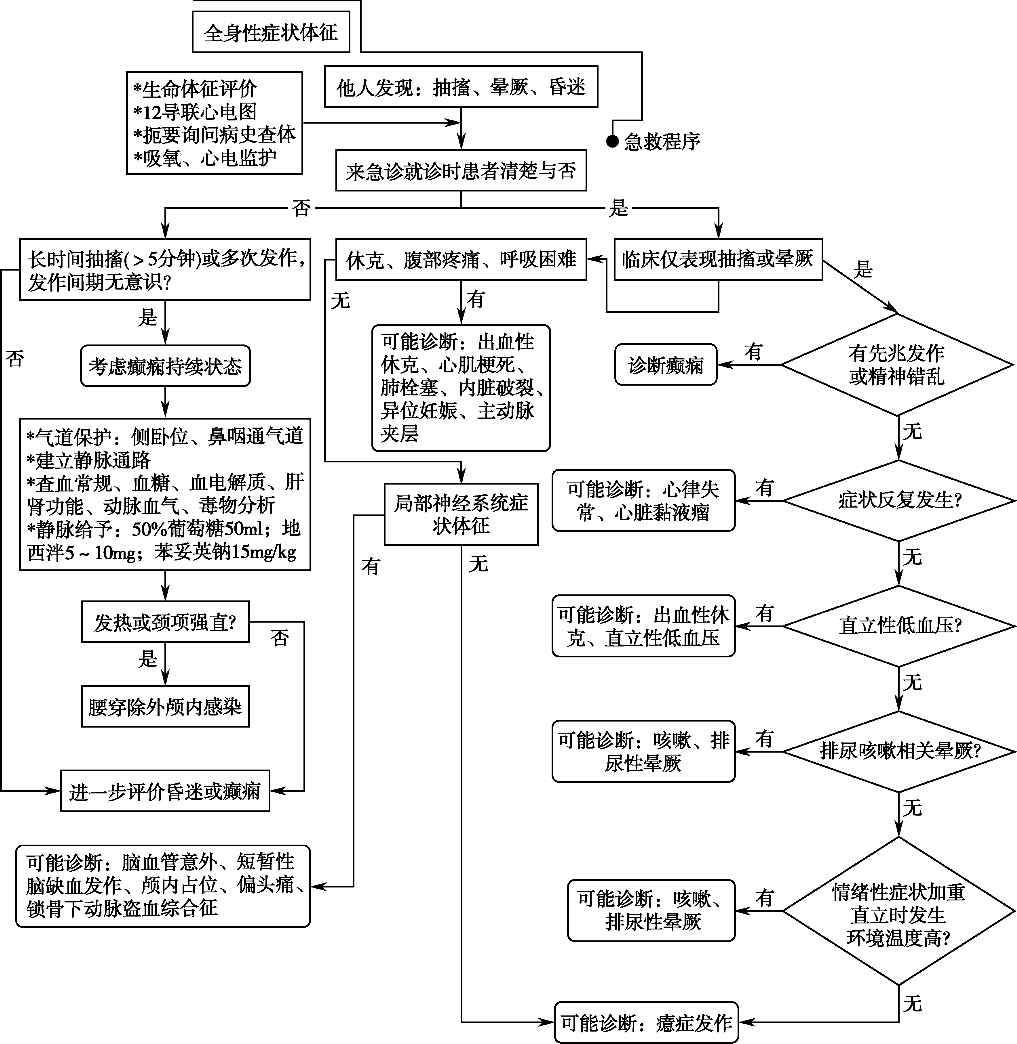
\includegraphics[width=5.88542in,height=6.04167in]{./images/Image00034.jpg}
 \captionsetup{justification=centering}
 \caption{他人发现抽搐、晕厥或昏迷患者分析思路}
 \label{fig5-1}
  \end{figure} 

\begin{figure}[!htbp]
 \centering
 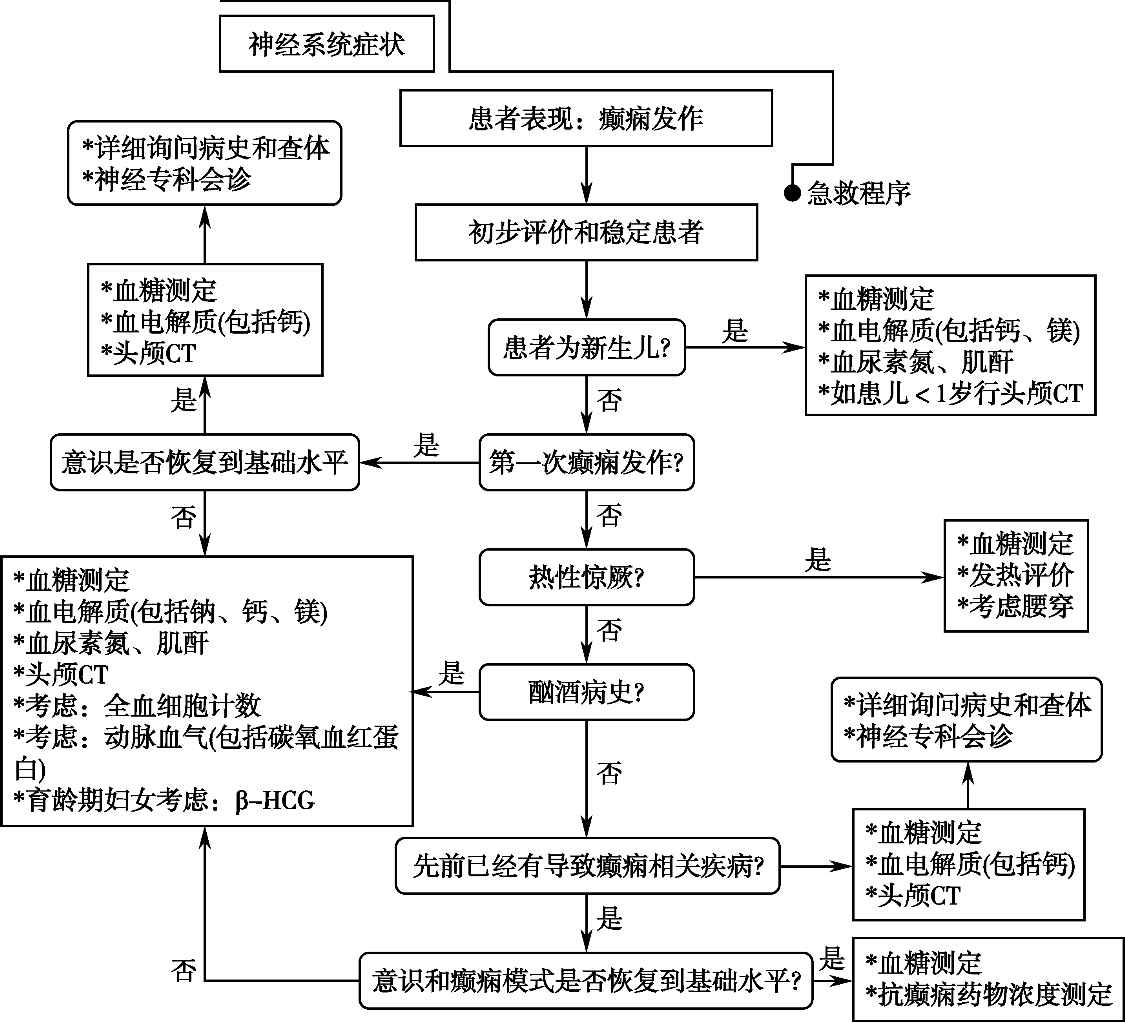
\includegraphics[width=4.77083in,height=4.34375in]{./images/Image00035.jpg}
 \captionsetup{justification=centering}
 \caption{癫痫发作的分析和处理思路}
 \label{fig5-2}
  \end{figure} 

\subsubsection{控制抽搐发作}

一旦确定是全身强直-阵挛性发作(癫痫大发作)或癫痫持续状态,及时控制抽搐是临床治疗的关键。癫痫持续状态处理流程见图\ref{fig5-3},有很强的时间紧迫性,目标是在神经功能受损前控制癫痫发作(理论上是在20分钟至1小时内控制抽搐发作)。应优先选择抗惊厥作用强、吸收快、分布半衰期长、排除半衰期短、无心肺和意识抑制作用,能肌肉注射、静脉注射和毒副作用低的药物。癫痫持续状态的药物治疗应根据患者的个体情况及时适度地应用,力争在最短的时间内终止癫痫发作,然后给予维持治疗。抽搐时切记勿强行固定四肢(否则易导致骨折、脱臼),也不要在抽搐时往患者嘴里塞牙垫、毛巾等物。抽搐停止后应加强监护,以防自伤、误伤、伤人、毁物等。

\subparagraph{地西泮(安定)}

为一线控制癫痫发作药物,适用于各年龄段。见效快,半衰期短(0.5~4小时)。成人首次剂量10~20mg,按1~5mg/min缓慢静脉注射,有效而复发者,30分钟后可重复应用,或在首次用药后将安定20~40mg加入10\%葡萄糖液100~250ml中缓慢静滴,10~20mg/h,用于维持疗效,视发作情况控制滴注速度和剂量,24小时总剂量不宜超过120mg(注:在控制癫痫发作时,地西泮剂量理论上来说没有上限)。无论地西泮的疗效如何,宜与苯妥英钠或苯巴比妥合用,预防抽搐再次发作。

儿童地西泮剂量每次0.25~0.5mg/kg静推,速度1mg/min,婴儿不超过2mg/次,幼儿不超过5mg/次。5~10岁儿童1mg/岁,儿童一次用量不超过10mg。新生儿及婴儿亦可用地西泮,每次0.5~1mg/kg肛管给药。

其他苯二氮{}
类制剂亦可选用,如劳拉西泮(氯羟安定),与地西泮相比抗惊厥作用强5倍,作用时间长3~4倍,半衰期12~16小时。静脉注射2~5mg/次(0.1mg/kg,速度2mg/min),80\%以上病例可在2~3分钟内终止发作,特别推荐在酒精戒断相关癫痫发作患者中使用。最新研究显示静脉注射劳拉西泮在控制抽搐和预防复发方面均优于地西泮。氯硝西泮抗惊厥作用是地西泮的5倍,半衰期22~32小时,静脉注射1~4mg/次,60\%病例可控制发作24小时。

如果尚未给患者建立静脉通路,地西泮可以通过直肠、气管套管内、骨髓腔内等途径给药。苯二氮{}
类药物有呼吸抑制、心动过缓和低血压、酸中毒等副作用,应用时需随时评估气道,脉搏氧饱和度降至90\%以下或呛咳作呕反射消失者,应考虑予气管插管。

\subparagraph{苯妥英钠}

控制成人癫痫发作二线治疗药物,无呼吸抑制,静脉给药能迅速达到脑内有效浓度。常用为150~250mg/次(20mg/kg),生理盐水溶解,缓慢静脉注射(1分钟小于50mg),半小时后可重复给药(100~150mg)。严重病例可加大用药剂量。儿童用量为250mg/m\textsuperscript{2}
。因为有低血压和心律失常等副作用,胃肠外给药速度不要过快,用药期间应密切观察,或行心电图和血压监测。

\subparagraph{苯巴比妥钠}

控制成人癫痫发作三线治疗药物。若足量的苯妥英钠仍不能控制抽搐发作,应立即给予苯巴比妥钠治疗。按10mg/kg静脉缓慢注射(50~100mg/min),直至发作停止,可再追加50mg,剩余部分可行肌肉注射。呼吸抑制和低血压是其常见副作用,用药前应准备气管插管和人工辅助呼吸通气。注射过程中需密切观察呼吸情况,如有抑制呼吸现象应立即停止注射,并作人工辅助通气。注意对儿童来说苯巴比妥钠是二线药物,而苯妥英钠是三线药物。

\begin{figure}[!htbp]
 \centering
 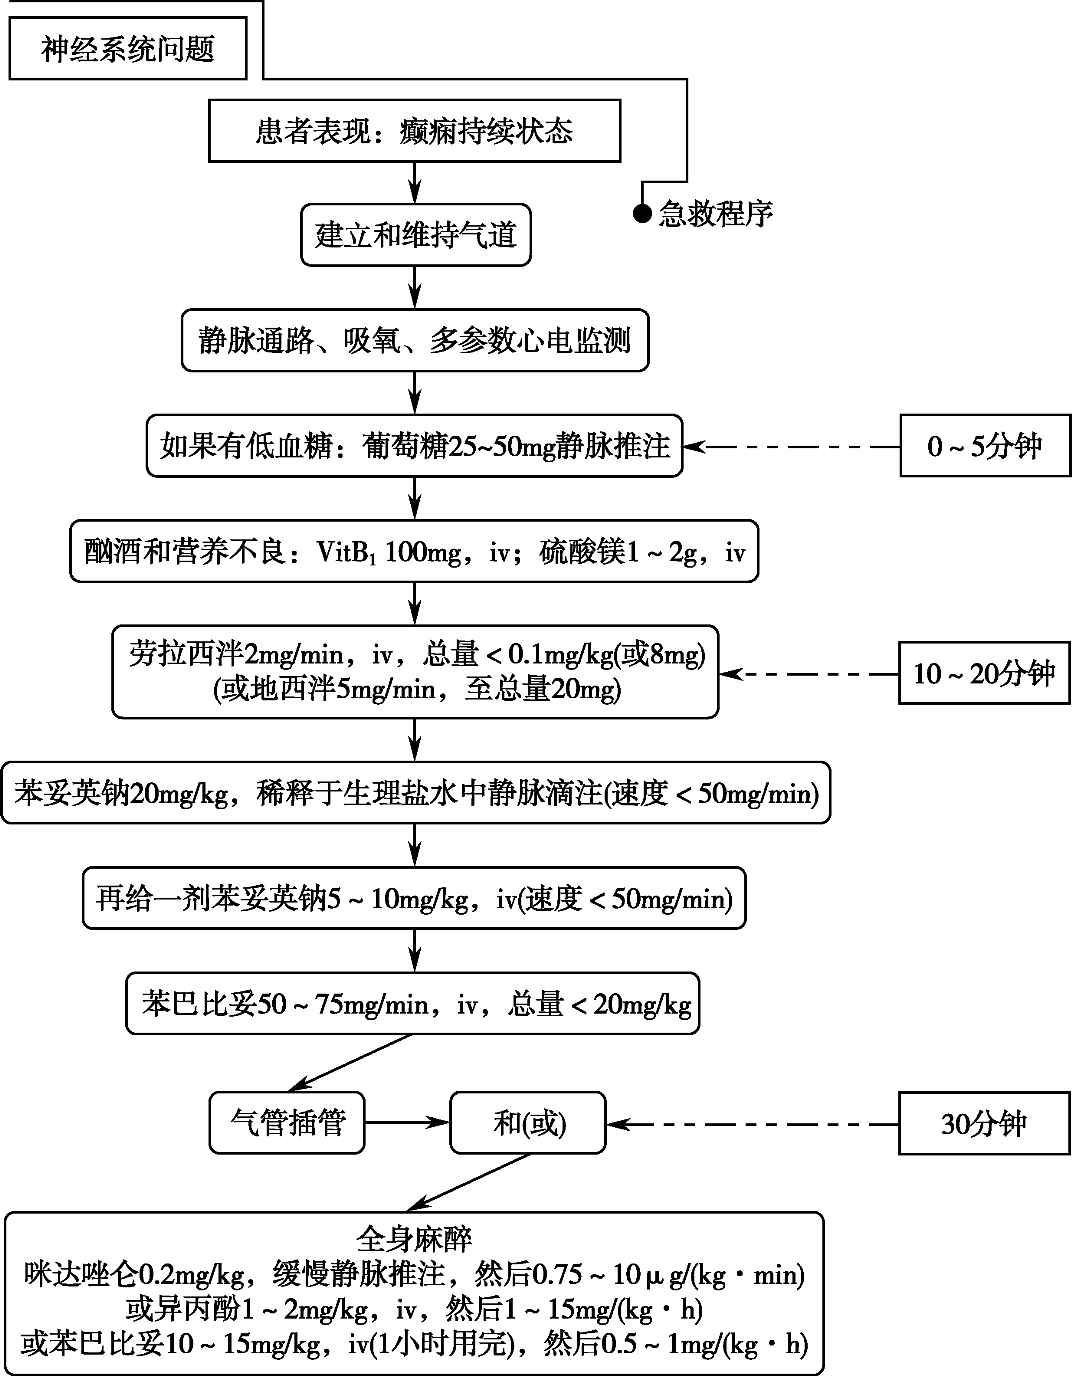
\includegraphics[width=4.11458in,height=5.28125in]{./images/Image00038.jpg}
 \captionsetup{justification=centering}
 \caption{癫痫持续状态处理路径}
 \label{fig5-3}
  \end{figure} 

(注:苯巴比妥剂量在国内有限制:一次极量为0.3g,一日极量为0.5g)

\subparagraph{其他药物}

如上述治疗无效,应考虑请神经专科医师会诊,并试用下列药物:①丙戊酸:控制癫痫发作有效药物。推荐剂量是15~20mg/kg或600~1200mg/d,分2~3次口服,其临床安全性良好,但注意在肝功能不全患者中禁用。②副醛:成人8~10ml、儿童0.3ml/kg,用植物油稀释后保留灌肠。代谢性酸中毒、肺出血、心血管抑制和直肠炎等是常见的副作用,应注意观察。③利多卡因:成人用1\%的利多卡因10ml,以20mg/min速度匀速静注。可降低心输出量,有充血性心力衰竭和肝损害减量。④10\%水合氯醛:成人20~30ml、儿童0.3ml/kg保留灌肠。

\subparagraph{全身麻醉}

处理仍无效者,可考虑收入ICU,静脉持续泵入咪达唑仑、丙泊酚等药控制癫痫发作,但其临床疗效有待进一步验证,也试用下列药物全身麻醉:①戊巴比妥:15mg/kg缓慢静脉注射,然后以0.5~1mg/(kg•h)维持。②硫喷妥钠:15mg/kg静脉缓慢推注,继以5mg/(kg•h)静脉注射维持。脑内的半衰期低于30分钟。③异戊巴比妥:200~1000mg静脉缓慢推注。

\subsubsection{病因治疗}

病因治疗是根本。如中毒性抽搐,应尽速彻底清除毒物和应用特效的解毒剂;急性感染性疾病所致者选用相应有效的抗生素,破伤风者须应用破伤风免疫球蛋白和抗生素(甲硝唑);高热惊厥,首先降温,使体温控制在38℃以下;低血糖发作应立即静注50\%葡萄糖液;水电解质平衡失调应分别纠正所缺少的钙、钠、镁;心源性抽搐者,应尽快建立有效循环,提高心排出量,治疗原发病;对肝肾功能衰竭者,改善并恢复其功能至关重要;颅内肿瘤、血肿、脓肿、脑寄生虫病及各种原因的脑水肿引起抽搐者,必须脱水降颅内压,必要时外科手术治疗。

\subsubsection{对症治疗}

癫痫持续状态l小时以上者,即有发生脑缺氧脑水肿的可能性,应酌情给予地塞米松、20\%甘露醇或利尿剂治疗,为了预防继发感染,应给予抗生素治疗。有高热者应给予降低过高体温处理。严重抽搐发作时,还可出现酸中毒、电解质紊乱、横纹肌溶解等并发症,进而又加重抽搐发作,甚至危及生命。临床上在控制癫痫发作的同时,应注意寻找并处理并发症。必须注意维持呼吸、循环、体温、水电解质平衡,保证供氧,供给充足热量,避免缺氧及缺血性脑损害。


\hypertarget{text00017.htmlux5cux23CHP1-5-4}{}
参 考 文 献

1. John Marx. Rosen's Emergency Medicine. 7th ed. Mosby,2009:113

2. Tintinalli JE. Emergency Medicine:A comprehensive study guide.6th
ed. McGraw-Hill,2004:1409

3. Rowland LP. Merritt's Neurology. 11th ed. Lippincott Williams
&Wilkins,2005:13

4. Pillow MT. Emergency Medicine. emedicine(http://emedicine.
medscape.com)updated Nov 9,2010

5. Huff JS. Emergency medicine clinics of North
America.2011,29(1):1-158

\protect\hypertarget{text00018.html}{}{}

\chapter{瘫 痪}

本章叙述的瘫痪(paralysis)是指随意肌收缩功能不全而言。其不完全障碍形成的肌力减退,属不完全性瘫痪;其完全障碍形成的随意肌收缩不能,属完全性瘫痪。本文叙述急性瘫痪的诊断与其处理原则。

\subsection{各型瘫痪的临床特征}

按病损部位不同,可将瘫痪分为肌源性、神经-肌接点性、下运动神经元性或上运动神经元性,其临床表现各具特征。现予分述如下:

\subsubsection{肌源性或神经-肌接点病损性瘫痪的临床特征}

肌源性瘫痪是指肌肉本身病变导致肌肉收缩障碍,从而引起程度不等的瘫痪而言。神经-肌接点病损性瘫痪是指神经-肌接点的递质因素或递质受体病变所引起的肌肉收缩无力而出现的瘫痪而言。

\subparagraph{瘫痪分布}

大多对称,多以肢体近端为重,不符合神经支配规律。

\subparagraph{肌束震颤}

通常没有。

\subparagraph{肌肉萎缩}

随病程进展,出现病肌萎缩,但不出现于疾病的急性期。

\subparagraph{牵张反射}

由于运动效应器病损,致紧张性牵张反射(表现为肌张力)与位相性牵张反射(表现为腱反射)均见降低。

\subparagraph{病理反射}

病理反射是上运动神经元性瘫痪的特征,因此,通常不见于肌源性或神经-肌接点病损性瘫痪。

\subparagraph{实验室检查}

肌细胞病变时出现血肌酶如肌酸磷酸激酶等升高;肌电图呈肌病性变;肌肉活检证实各种肌肉疾病的特征性改变。神经-肌接点病损性瘫痪时,通常血肌酶变动不明显,肌电图检查显示特征性改变。

\subsubsection{下运动神经元性瘫痪的临床特征}

\subparagraph{瘫痪分布}

主要是小组肌肉或单块肌肉的瘫痪,其分布符合脊髄节段或周围神经支配的规律。

\subparagraph{肌束震颤}

束颤是下运动神经元性瘫痪的特征之一,但是很少见于瘫痪的急性病期。随意肌失神经支配后,在其足板附近的肌膜上,烟碱型乙酰胆碱受体大量增生,以致血循环中存在着的小量乙酰胆碱,足以引起肌纤维的自发性收缩而在肌电图上显示为纤维颤动(纤颤)电位。纤颤电位通常见于骨骼肌失神经支配后1~3周。当整个肌束有类似变化时,就出现肉眼可见的束颤。在确认束颤与下运动神经元病变有关前,必须除外良性束颤与可能含有束颤的其他疾病如抗胆碱酯酶药物过量与电解质紊乱等。

\subparagraph{肌肉萎缩}

通常始于失神经支配1~2周后。是其蛋白代谢呈负平衡的结果。

\subparagraph{牵张反射}

由于反射通路受阻而致肌张力、腱反射均见减退。睡眠、昏迷或小脑病变时,也见牵张反射减退,诊断时应注意识别。

\subparagraph{病理反射}

病理反射是上运动神经元性瘫痪的病征,不见于下运动神经元性瘫痪。

\subparagraph{实验室检查}

血肌酶大多正常,在有的急性疾病如急性感染性多发性神经根神经炎时,或见血肌酸磷酸激酶轻度增高。肌电图示去神经性变。肌肉活检呈失神经性变。

\subsubsection{上运动神经元性瘫痪的临床特征}

\subparagraph{瘫痪分布}

瘫痪分布符合神经解剖的规律,通常表现为肌群或肢体的瘫痪。

\subparagraph{肌束震颤}

瘫肌无肌束震颤。

\subparagraph{肌肉萎缩}

上运动神经元病变通常不影响下运动神经元对肌肉的营养作用,故瘫肌不见萎缩。但久瘫后,瘫肌可出现失用性萎缩,这种萎缩自然不见于急性病肌。

\subparagraph{牵张反射}

上运动神经元病损时,瘫肌牵张反射增强,表现为瘫肌张力增高,反射增强。但是,在病损急性期,因参与瘫肌牵张反射的下运动神经元突然失去上级运动神经元的调控而进入阻抑状态,牵张反射因之消失,届时,瘫肌张力降低,腱反射难以引出,是属脊髓休克状态。

\subparagraph{病理反射}

锥体系抑制原始的屈曲回缩反射。锥体系病损时,屈曲回缩反射失去抑制,从而在上肢可能出现霍夫曼(Hoffmann)征,在下肢可见跖反射伸性或(与)巴宾斯基(Babinski)征,是上运动神经元性瘫痪的病理征,亦即病理反射,但同样不见于脊髓休克期。值得注意的是,这种征象尚可见于锥体系尚未发育完全的婴儿,也可见于深睡、昏迷、全身麻醉与癫痫大发作后的短时期内;此时,这种征象通常是双侧性的。

\subparagraph{实验室检查}

血肌酶、肌电图与肌肉活检的诊断价值不大。

\subsection{诊断思路}

\subsubsection{确认真性瘫痪}

为确认真性瘫痪,需与失用、骨关节病引起的随意运动障碍以及癔症性瘫痪等鉴别。

失用是指随意肌没有瘫痪,但运用不能。通常是由大脑特定功能部位的病损,影响了获得性技能的回忆能力所致。

小脑病损时,可能合并受累部位肌力减退,但总以小脑共济失调为主。震颤麻痹时,病肢可能乏力,但通常少有肯定肌力减退,且病肌张力呈齿轮状增高,尚伴震颤、运动迟缓、表情呆滞与瞬目动作减少等,易于识别。严重的舞蹈症可能合并有轻瘫,此时,病肢原有的舞蹈动作减弱,甚至消失,是为瘫痪性舞蹈病,结合舞蹈动作与受累肢体肌张力降低,可资鉴别。骨、关节病时,随意运动可能受限,但不属真性瘫痪,依骨、关节病史,保护体位,局部关节肿胀、按疼,被动活动受限、致痛,帮助识别。

癔症性瘫痪,也有起病快的,患者以青年女性为多。病前常有心理因素。瘫痪分布不一,以单瘫、截瘫较为多见;瘫痪程度可能时有变动,时轻时重,具暗示性;可伴富于情感色彩的精神症状;在神经系统体征方面,除可能测得瘫痪肢体在被动活动时阻力有所增加外,多不见其他病征。患者的癔症性格与类似的发作既往史有助诊断。需要注意的是:必须在排除器质性病因后才能考虑诊断。

\subsubsection{识别瘫痪属性}

参考前述各类瘫痪的临床特征,可以确定瘫痪的属性。但在确认急性瘫痪的属性时,必须注意:①患者是否处于脊髓休克状态。脊髓休克期,受影响的运动区呈下运动神经元性瘫痪的病征,即瘫痪肌肉张力降低,反射消失,没有病理反射。②在下运动神经元性瘫痪的急性期,瘫痪肌肉通常不显示肌束震颤与肌肉萎缩。③在肌原性瘫痪的急性期,同样没有肌肉萎缩可见。因此,在判断急性瘫痪的属性时,除瘫痪肌肉的分布外,神经系统其他病征、肌肉病征、必要的实验室检查与详尽的病史资料是不可或缺的。

\subsubsection{推测诊断}

可以将瘫痪作为考虑诊断的引线。但必须强调:只有结合病史与体征(包括神经系统其他阳性体征),进行综合分析,才能较为正确地设想可能的疾病,进而按需进行相关的辅助检查,以使诊断更臻完善。

下面就瘫痪的部位与属性,按项列举常见的急性疾病,以供诊断参考。

\subparagraph{眼肌瘫痪}

眼肌瘫痪的主要临床表现为斜视、眼球运动障碍,或伴睑垂、瞳孔散缩异常等。

\hypertarget{text00018.htmlux5cux23CHP1-6-2-3-1-1}{}
(1) 肌源性或神经-肌接点病损性眼肌瘫痪:

急性起病者少见,偶见于急起的重症肌无力、急起的甲状腺毒性肌病、有机磷中毒的中间综合征与生物毒如蛇毒中毒、肉毒中毒等。

\hypertarget{text00018.htmlux5cux23CHP1-6-2-3-1-2}{}
(2) 下运动神经元性眼肌瘫痪:

可分为脑神经病变与核性病变两类:

\hypertarget{text00018.htmlux5cux23CHP1-6-2-3-1-2-1}{}
1) 脑神经病变 :

可依次分为单动眼神经麻痹、单滑车神经麻痹、单展神经麻痹或眼部多脑神经麻痹。①单动眼神经麻痹:病侧睑垂,正视时,眼球外偏略向下;眼球向上、向内与向下活动受限,并有相应复视;可伴瞳孔扩大。睑板肌由交感神经支配,其功能受损时,可致轻度睑垂,但请患者充分上视时,又见上睑上抬满意,双侧眼裂基本对等,是为假性睑垂,应注意识别。急性动眼神经麻痹可见于脑动脉瘤膨胀压迫动眼神经,也可见于痛性眼肌瘫痪、眼肌瘫痪性偏头痛、糖尿病性动眼神经麻痹、颅脑外伤、垂体肿瘤囊变或出血、肉毒中毒、白喉性多神经病等病况时。②滑车神经麻痹:单独滑车神经麻痹罕见,尤其是急性起病者。③展神经麻痹:正视时,病侧眼球偏处内收位,眼球向外活动受限,向受损侧侧视时出现复视。可见于颅内动脉瘤突然扩张的压迫、脑外伤、急性颅内压增高,转移性癌肿(尤其需要注意的是鼻咽癌)、糖尿病性展神经麻痹或特发性展神经麻痹等。④眼部多脑神经麻痹:此处是指合并动眼、滑车、展神经麻痹,按各脑神经受损程度不等,综合出现各该脑神经受损时的病征,轻重不一。可见于海绵窦病变、痛性眼肌麻痹、眼肌麻痹性偏头痛、颅脑外伤、Fisher综合征或急性出血性结膜炎引起的脊髓灰质炎样运动瘫痪等。

\hypertarget{text00018.htmlux5cux23CHP1-6-2-3-1-2-2}{}
2) 核性病变 :

核性病变常导致分离性眼肌瘫痪,即同一神经如动眼神经支配的各眼外肌呈非同步瘫痪;以双侧病损为多见,届时,两侧眼球活动的瘫痪程度与范围不一定相等,可合并会聚障碍,眼内肌功能可能保持,随眼球活动受限而出现相应复视。可见于脑干血管性病变、Wernicke脑病等。

\hypertarget{text00018.htmlux5cux23CHP1-6-2-3-1-3}{}
(3) 上运动神经元性眼肌瘫痪:

核上性病变引起双眼同向活动障碍,或称凝视麻痹。即两眼不能向一侧,或向上、向下凝视,由于两眼视轴相称,不致造成复视。

两眼侧视中枢在大脑额中回后部,其活动也受同侧枕前区侧视中枢影响;下级侧视中枢在脑桥,归属于脑桥旁正中网状结构。额中回后部的侧视中枢遭破坏时,由于对侧侧视中枢的活动而致两眼向病灶侧凝视,可见于脑血管意外、脑炎、脑外伤、脑瘤等疾病时。一侧脑桥侧视中枢遭破坏时,两眼不能向病灶侧活动而向病灶对侧凝视;多见于脑血管意外、脑桥肿瘤、多发性硬化等。脑桥病变若累及两侧凝视中枢,导致双侧性凝视麻痹。枕叶病变时,可致双眼的跟随动作消失,引起自发性定视。

垂直性凝视中枢拟在中脑。垂直性凝视麻痹以两眼向上凝视受限为多见,常由中脑上丘水平的盖前区病损导致,可见于包括蛛网膜下腔出血在内的脑血管意外等病况时。有双侧额中回病损也可引起垂直性凝视麻痹。

\subparagraph{面肌瘫痪}

面肌瘫痪指面部表情肌瘫痪。①肌源性或神经-肌接点病损性面肌瘫痪:急性起病的十分罕见。②下运动神经元性面肌瘫痪:无论面神经本身或面神经核病变,均损及病侧全部面肌活动,表现为病侧皱额纹明显减退或消失,闭眼不紧或露白,鼻唇沟浅平,露齿不全,口角歪向健侧,病侧口轮匝肌无力致吹口哨不能、鼓气自瘫侧口角破漏、食物滞留病侧颊腔;核性病变者,常伴同侧眼球外展麻痹或(与)其他脑干病征,属脑干病变范畴。单侧面神经麻痹多为特发性面神经麻痹,也见于急性炎症性脱髓鞘性多发性神经病、面神经外伤、肉毒中毒、Lyme病、三氯乙烯中毒(三氯乙烯中毒的神经毒征涉及多脑神经,在瘫痪方面,以面神经与动眼神经病征为主)与急性化脓性中耳炎时。核性病变可见于基底动脉血栓形成、脑桥出血、脑干型脊髓灰质炎或急性出血性结膜炎引起的脊髓灰质炎样运动瘫痪等时。③上运动神经元性面肌瘫痪:即中枢性面瘫,表现为病灶对侧下半面部表情肌功能障碍,致鼻唇沟变浅、口轮匝肌无力、露齿时口角歪向健侧,而皱额活动不受影响,两侧额纹对称。患者常伴与病灶关连的其他病征如偏瘫等。多见于脑血管意外、脑炎、脑静区肿瘤囊变或出血等时等。

\subparagraph{球肌瘫痪}

球肌,又称延髓肌,是指由舌咽、迷走、副、舌下神经所支配的随意肌。球肌瘫痪,导致构音障碍,甚或失音;吞咽困难、咳呛,甚或反流,提腭运动受限,或见喉结上提不全,舌位不正,活动受障。咽反射减退或亢进。

\hypertarget{text00018.htmlux5cux23CHP1-6-2-3-3-1}{}
(1) 肌源性或神经-肌接点病损性球肌瘫痪:

常两侧对称受损,出现上述病征,因效应器受损,咽反射减退。可见于急性的重症肌无力、多发性肌炎、急性甲状腺毒性肌病与有机磷中毒后的中间综合征或生物毒素如蛇毒中毒等。

\hypertarget{text00018.htmlux5cux23CHP1-6-2-3-3-2}{}
(2) 下运动神经元性球肌瘫痪:

可分为脑神经病变与核性病变两类。

1)
脑神经病变多见于各有关脑神经出颅腔后,在其径路上受损。单神经病损,较为少见,其病因常与外伤有关。①舌咽神经受损:舌咽神经的运动纤维支配茎咽肌。茎咽肌的功能是吞咽时提升与拓宽咽部,但其作用较小,以致在临床工作中常难以察觉其瘫痪,尤其是在单侧受损时;咽反射可能降低,这是因为咽反射的传入径路是由舌咽神经控制的。可见于颅底骨折,但单侧单独受损很少见。②迷走神经受损:迷走神经运动干司理除软腭张肌与茎咽肌以外的所有咽、喉、软腭肌,是控制软腭与咽喉部的主要运动神经。声带肌由迷走神经的分支喉返神经控制。迷走神经受损时,可出现发音、构音、吞咽障碍,悬雍垂偏向健侧、病侧提腭不全、咽反射减退,或伴声带内收障碍而致声音嘶哑。在有些病例,由于病损部位之故,软腭活动尚好,但因下咽缩肌瘫痪,致喉结运动受限。迷走神经损伤可见于颅底骨折、颈部外伤或其他颈部手术如甲状腺手术损及喉返神经等病况时。病损多为单侧,双侧者少见。双侧喉返神经受损时,咳嗽反射减退,甚或消失;声带处于尸体位,导致嘶哑,甚至失音;又可因声带开放不全而致呼吸困难、喘鸣而需手术治疗。③副神经受损:受副神经支配的胸锁乳突肌瘫痪时,颈向病损对侧转动无力;双侧胸锁乳突肌瘫痪时,颈前屈无力。斜方肌瘫痪时,病侧肩垂,耸肩受限。副神经病损常见于颈部手术伤、枪伤、刺伤、颈椎骨折脱位。④舌下神经受损:舌下神经支配所有牵引舌部的舌内、舌外肌群。当一侧舌下神经受损,舌在口腔内原位时,舌尖偏向健侧;伸舌时,舌尖偏向患侧。由于急性病损时舌肌不显示束颤与萎缩,因此,只能借病史与并存的其他神经系体征帮助确认其下运动神经元性瘫痪。所幸的是单一舌下神经急性病损,除外伤性外,仅偶见于脊髓前动脉血栓形成。急性双侧舌下神经麻痹,很为罕见,届时,除不能伸舌、不见舌部活动外,更有构音障碍、进食困难。⑤多球部脑神经受损:根据受累脑神经的多少与受损程度,组合出现有关脑神经的上述病征,多少不一,轻重不等。可见于急性炎症性脱髓鞘性多发性神经病、白喉性多神经病或外伤如颅底或颈静脉孔枪弹伤等。

2) 核性病损时
,按受累范围,产生相应脑神经的有关病征,大多合并其他脑干征。多见于椎-基底动脉系统的血管性疾病,偶见于脑干型脊髓灰质炎或急性出血性结膜炎引起的脊髓灰质炎样运动瘫痪等。

\hypertarget{text00018.htmlux5cux23CHP1-6-2-3-3-3}{}
(3) 上运动神经元性球肌瘫痪:

即核上性球肌瘫痪。病损在皮质运动区的颈、咽喉与舌部到第Ⅸ、Ⅹ、Ⅺ与Ⅻ对脑神经运动核的径路上的任何部位。在这四对脑神经的运动核中,除支配颏舌肌的运动核主要受对侧皮质延髓束支配外,余均受双侧支配。因此,其单侧皮质延髓束受损仅致病灶对侧的颏舌肌瘫,表现为伸舌时,舌尖偏向病灶对侧,这种征象多见于合并偏瘫、偏侧感觉障碍时,好见于脑血管意外、脑炎、急性播散性脑脊髓炎等疾患时。双侧皮质脑干束病损,导致假性延髓性麻痹,表现为构音不清、吞咽困难、进食反流、舌活动不灵活与提腭活动减退,但咽反射亢进。藉咽反射活跃,或伴强哭、强笑,与真性延髓性麻痹鉴别。假性延髓性麻痹的患者常伴中枢神经系统的其他病征如双侧皮质脊髓束征、失语、智力减退等。常为多次脑血管意外发作的后遗症,因此,少见于首次脑血管意外的急性状态。

\subparagraph{单瘫}

单瘫是指一个肢体的瘫痪。

\hypertarget{text00018.htmlux5cux23CHP1-6-2-3-4-1}{}
(1) 肌原性或神经-肌接点病损性单瘫:

少见。

\hypertarget{text00018.htmlux5cux23CHP1-6-2-3-4-2}{}
(2) 下运动神经元性单瘫:

一侧颈\textsubscript{5~8} 与胸\textsubscript{1}
脊髓前角、前根或臂丛病变可引起同侧上肢的下运动神经元性单瘫。一侧腰\textsubscript{1}
~骶\textsubscript{2}
脊髓前角、前根或腰骶丛病变时可引起同侧下肢的下运动神经元性单瘫。①单纯前角病变引起的单瘫:可见于脊髓灰质炎(以累及下肢近端肌为多见)。②单纯急性前根病变引起的单瘫:少见。③神经丛病变引起的单瘫:在上肢可见于急性臂丛神经炎与包括产伤在内的臂丛神经损伤。在下肢单瘫较为少见。

\hypertarget{text00018.htmlux5cux23CHP1-6-2-3-4-3}{}
(3) 上运动神经元性单瘫:

其基础为对侧大脑皮质的相应运动区及与之有关的白质纤维病损。其上肢单瘫,常伴瘫侧上运动神经元性面瘫;多见于血管、外伤或炎性疾病,也可见于局限性癫痫发作后的该局部瘫痪,其瘫痪常在短时后好转(Todd瘫痪)。又可见于静区肿瘤囊变或出血时。胸髓半横断综合征时,出现病变同侧下肢的上运动神经元性瘫,当然,还有特征性的感觉障碍,多见于脊髓外伤或急起的脊髓压迫性疾病等。

\subparagraph{偏瘫}

一侧上、下肢瘫痪称为偏瘫。

\hypertarget{text00018.htmlux5cux23CHP1-6-2-3-5-1}{}
(1) 肌源性或神经-肌接点病损性偏瘫:

罕见。

\hypertarget{text00018.htmlux5cux23CHP1-6-2-3-5-2}{}
(2) 下运动神经元性偏瘫:

罕见。

\hypertarget{text00018.htmlux5cux23CHP1-6-2-3-5-3}{}
(3) 上运动神经元性偏瘫:

损及内囊区皮质脊髓束时引起对侧上、下肢瘫;若同时累及有关的皮质脑干束,则合并有偏瘫侧的下半面部、颏舌肌瘫与翼肌不全瘫。当病变中心在半卵圆区,损及运动区皮质下半部发放的下行纤维为主时,导致对侧上肢为重的偏瘫,常合并偏瘫侧下半面部、颏舌肌与翼肌瘫。若病变中心在半卵圆区,主要损及了皮质运动区上半部、旁中央小叶所发放的下行纤维,则引起以下肢为重的偏瘫,或伴括约肌功能障碍。皮质运动区及(或)其下行纤维全面受损,则造成包括下半面部肌、颏舌肌与翼肌在内的对侧偏瘫。多见于脑血管病与包括产伤在内的颅脑外伤、脑炎、静区肿瘤囊变或出血等病况时,也见于Todd瘫痪。

脊髓颈膨大以上的高位颈髓病,损及单侧皮质脊髓束时,导致病侧上、下肢的上运动神经元性偏瘫。一侧脊髓颈膨大病变,损及同侧脊髓前角与皮质脊髓侧束者,引起病侧上肢的下运动神经元性瘫与同侧下肢的上运动神经元性瘫。均须结合神经系统其他阳性体征考虑诊断。可见于脊髓外伤、急性脊髓压迫症、脊髓血管性疾病,甚或急起的脱髓鞘性疾病如多发性硬化。

\subparagraph{交叉性瘫痪}

指一侧或两侧下运动神经元性脑神经瘫与对侧上、下肢或四肢的上运动神经元性瘫。病损部位指向脑干,见于血管性疾病、多发性硬化等。

\subparagraph{截瘫}

双下肢瘫称为截瘫。

\hypertarget{text00018.htmlux5cux23CHP1-6-2-3-7-1}{}
(1) 肌源性或神经-肌接点病损性截瘫:

在周期性瘫痪早期,可能只有两下肢不全瘫,有时顿挫于此,不再向上发展。

\hypertarget{text00018.htmlux5cux23CHP1-6-2-3-7-2}{}
(2) 下运动神经元性截瘫:

两侧L\textsubscript{1} ~S\textsubscript{2}
节段下运动神经元病损时,引起两下肢软瘫,可见于脊髓灰质炎,少见。在胸髓急性横贯性病变的急性期(脊髓休克期),双下肢也呈软瘫,需注意识别。

\hypertarget{text00018.htmlux5cux23CHP1-6-2-3-7-3}{}
(3) 上运动神经元性截瘫:

可见于脊髓或脑部病变。①脊髓病损:胸髓横贯性、近乎横贯性或播散病变损及两侧皮质脊髓束时,引起痉挛性截瘫,但在脊髓休克期呈软瘫。可见于急性横贯性脊髓炎、脊髓外伤、脊髓血管性疾病、急性播散性(脑)脊髓炎与包括视神经脊髓炎在内的多发性硬化。②脑部病损:两侧皮质运动区上部下肢功能区受损时,可致上运动神经元性截瘫,罕见,或见于上矢状窦血栓形成、矢状窦旁脑膜瘤时。

\subparagraph{四肢瘫或四肢瘫伴呼吸肌瘫痪}

双侧上、下肢瘫痪称为四肢瘫。急重病例常合有呼吸肌瘫痪。

\hypertarget{text00018.htmlux5cux23CHP1-6-2-3-8-1}{}
(1) 肌源性或神经-肌接点病损性四肢瘫:

可见于属于肌肉通道病范畴的周期性瘫痪或恶性高热、急起的多发性肌炎、急性皮质类固醇性肌病、重症肌无力及有机磷中毒的中间综合征时。药物如乙醇、氯贝丁酯、依米丁、6-氨基己酸、氯噻酮、甘草、氨基喹啉与两性霉素B等可引起急性或亚急性痛性近端肌病。拉贝洛尔可引起全身性重度肌病。

\hypertarget{text00018.htmlux5cux23CHP1-6-2-3-8-2}{}
(2) 下运动神经元性四肢瘫:

可见于脊髓灰质炎,急性出血性结膜炎并发的脊髓灰质炎样运动瘫痪,吉兰-巴雷综合征(GBS),危重病并发的多神经病,白喉性多神经病,蜱(壁虱)性瘫痪。用金治疗类风湿关节炎时,可出现急起的、进展迅速的、对称或不对称的、以运动障碍为明显的、类似于GBS的病征。也曾有用黑色素瘤疫苗治黑色素瘤时出现急性炎性脱髓鞘性多神经病致肢体瘫痪的。尚可见于另一些生物毒素中毒时。

\hypertarget{text00018.htmlux5cux23CHP1-6-2-3-8-3}{}
(3) 上运动神经元性四肢瘫:

可由脊髓、脑干或脑部病变引起。①脊髓性四肢瘫:颈膨大以上的高位颈髓病变可引起上运动神经元性四肢瘫。但在疾病的急性期,因脊髓休克而不见瘫肌张力增高,宜予注意。可见于颈髓外伤、血管性疾病、压迫,甚或急性多发性硬化等。②脑干性四肢瘫:多含脑神经病征。参见“交叉性偏瘫”项。③脑性四肢瘫:脑部病变危及两侧运动区皮质或(与)皮质脊髓束时,出现脑性四肢瘫。可见于产伤、脑缺氧、脑外伤、挤压伤、多次脑卒中或脑炎等病况时。

\subparagraph{局限性肢体肌瘫}

局限性肢体肌瘫是指单肢局部肌肉瘫痪。引起肢体随意肌局限性瘫痪的病因,除参照“单瘫”项外,尚需注意桡、正中、尺、股、坐骨、胫、腓等周围神经病损引起的相关肌肉的瘫痪。缺血性肌病亦可致有关的随意肌功能受损。

\subparagraph{跌落发作}

也称猝倒发作,由随意肌突然失张力所致。表现为立位或行走时突然跌地,无意识障碍,经1~2分钟后,自行起立、行走。有隐源性与继发性两类。隐源性者多见于中、老年,可由大笑或激烈情绪因素激发,无神经系统其他病征,发病机制不详。继发性者可见于中枢神经系统的血液循环障碍如椎-基底动脉系或脊髓前动脉的短暂性缺血、颅内压突然升高与前庭功能突然衰退等,也有见于发作性睡病的。要注意与癫痫的跌落发作鉴别。

\subparagraph{睡眠瘫痪}

睡眠瘫痪是指在睡醒后即时,或刚入睡时出现肢体不能动弹、不能发声,或伴幻觉,没有意识障碍,通常经数秒钟或数分钟后缓解,恢复活动,少有长达几小时的。言语接触或触碰患者可终止发作,但若缓解后不及时活动,可能恢复原状。可见于发作性睡病或单独出现。有家族史者称家族性睡眠瘫痪,呈常染色体显性遗传。

\subsection{急性瘫痪的处理原则}

\subsubsection{病因治疗}

\subsubsection{对症治疗}

对眼肌瘫痪有复视者,可遮蔽病眼,或用三棱镜暂时校正之。对面肌瘫痪眼裂不能闭合者,可用眼罩保护暴露的角膜,并加用眼药滴、涂;对瘫痪的面肌进行按摩、理疗以防止面肌挛缩与被健侧面肌牵引。

对吞咽困难者,及时鼻饲,按需静脉补充营养,保持水与电解质平衡。

对呼吸困难者,注意保持呼吸道通畅,按需考虑气管切开、人工或器械辅助呼吸。

对肢体瘫痪者,宜将瘫肢按放于功能体位(在急性期尤为重要),按摩瘫肌,对瘫肢加强被动活动,鼓励主动活动。

\subsubsection{防止并发症}

加强瘫痪护理,防止褥疮、肺炎、尿路感染、便秘、烫伤与肢体挛缩等。


\hypertarget{text00019.htmlux5cux23CHP1-6-4}{}
参 考 文 献

1. Daniel Platt,Robert Griggs. Skeletal muscle channelopathies:new
insights into the periodic paralyses and nondystrophic myotonias.
Current opinion in neurology,2009,22:524-531.

2. Juma M. Alkaabi,Ahmed Mushtaq,Fatma N. Al-Maskari,et al.
Hypokalemic periodic paralysis:a case series,review of the literature
and update of management. European Journal of Emergency
Medicine,2010,17:45-47.

3. Faisal Khan,Ribhi Hazin,Mohsin Iqbal. Nacrolepsy:Clinical decision
making for the primary care physician. Southern Medical
Journal,2009,102(12):1246-1252.

\protect\hypertarget{text00020.html}{}{}

\chapter{头 痛}

头痛(headache)一般是指眉弓、耳轮上缘和枕外隆突连线以上的头颅上半部的疼痛,而面痛(facial
pain)指上述连线以下到下颌部的疼痛。急性头痛为内科急症中最常见的症状,它可以是劳累、精神紧张和焦虑的一般表现,或是许多全身性疾病的一种伴随症状;也可能是高血压脑病、脑卒中或颅内肿瘤等颅内严重疾病的一种较早期信号。在临床急诊工作中,应首先确定就诊的急性头痛患者是否由颅内病变如蛛网膜下腔出血、脑出血、颅内肿瘤等引起,因为这些疾病若处理不及时,常危及生命。

\subsection{病因与发病机制}

\hypertarget{text00020.htmlux5cux23CHP1-7-1-1}{}
(一) 头痛的病因分类

引起头痛的病因颇多,大致可分为原发性和继发性两大类。前者不能归因于某一确切病因,也可称为特发性头痛,常见的如偏头痛、紧张型头痛;后者病因可涉及各种颅内病变如脑血管疾病、颅内肿瘤、颅内感染、颅脑外伤,全身性疾病如发热、内环境紊乱以及滥用精神活性药物等。2004年国际头痛协会(international
headache society,IHS)推出了第2版头痛疾患的国际分类(ICHD-Ⅱ)如下:

Ⅰ类:原发性头痛(the primary
headaches):包括偏头痛、紧张型头痛、丛集性头痛和其他三叉自主神经头痛、其他原发性头痛等。

Ⅱ类:继发性头痛(the secondary
headaches):包括:①头颈部外伤引起的头痛;②头颈部血管性病变引起的头痛;③非血管性颅内疾病引起的头痛;④某一物质或某一物质戒断引起的头痛;⑤感染引起的头痛;⑥内环境紊乱引起的头痛;⑦头颅、颈、眼、耳、鼻、鼻窦、牙齿、口或其他颜面部结构病变引起的头面痛;⑧精神疾病引起的头痛。

Ⅲ类:脑神经痛、中枢和原发性面痛和其他头痛。

\hypertarget{text00020.htmlux5cux23CHP1-7-1-2}{}
(二) 头痛的发病机制

头痛的发病机制复杂
,主要是由于颅内、外痛觉敏感结构内的痛觉感受器受到刺激,经痛觉传导通路传导到达大脑皮层而引起。这些痛觉敏感结构是:颅外的包括头皮、皮下组织、肌肉、颅骨的骨膜和动脉;颅内的有血管(脑底基底动脉环及其近端主要分支、脑膜内的动脉、大静脉窦及其静脉分支)、硬脑膜(尤其是颅底部)、脑神经(主要是三叉、舌咽、迷走神经)和第1~3颈神经,眼、外耳及中耳、鼻腔及鼻窦内的黏膜及牙齿亦对痛觉敏感。颅骨本身,大部分脑膜、脑实质以及脑室中的室管膜和脉络丛对痛觉均不敏感。传导痛觉的神经有三叉神经、舌咽神经、迷走神经、第1~3颈神经,以及沿脑内外血管周围交感神经(来自颈\textsubscript{3}
~胸\textsubscript{3}
)。颅外组织的疼痛一般是局限性的,多在受刺激处或其神经支配的区域。天幕上在前颅凹、中颅凹内结构的感觉信息经三叉神经传入,天幕下后颅凹内结构的感觉由第1~3颈神经传入,颅内结构病损的疼痛常牵引至这些传入神经在头颅的相应分布区,在这些部位可有局限性按痛。天幕上病变疼痛常牵引至同侧额、颞区或顶区,天幕下病变常牵引至同侧枕区、枕下区或上颈区。舌咽、迷走神经支配后颅凹的一部分结构,疼痛可牵引至耳、喉,牙齿或下颌痛也可牵引至头部。

头痛的发生机制涉及多个方面,机械、化学、生物刺激和体内生化改变作用于颅内、外痛觉敏感结构均可引起头痛。主要有:①颅内痛觉敏感组织受压、牵拉和移位:此种情况可见于颅内占位性病变,如脑肿瘤、血肿、脓肿等;可见于脑肿胀所致的颅内压增高,如各种原因所致的脑水肿,静脉窦血栓形成,脑积水等;可见于各种原因所致的颅内压降低,如腰穿后头痛,使颅内静脉及静脉窦扩张或牵拉而致头痛。②颅内外动脉扩张:引起动脉扩张的原因很多,诸如急性感染、代谢性疾病(低血糖、缺氧及高碳酸血症等)、中毒性疾病(一氧化碳中毒、酒精中毒等)、颅脑外伤、癫痫、高血压性脑病、服用血管扩张药物等。偏头痛及组胺性头痛也是颅内外动脉扩张所致。③颅内炎症和出血刺激痛觉敏感结构:炎症或血液中有形成分破坏,可使脑脊液中5-HT、组胺、乳酸、P物质及前列腺素等致痛物质增加,引起头痛。④头颈部肌肉持续收缩压迫痛觉神经末梢,同时造成肌肉缺血,致痛物质积蓄,均可导致血管舒张性疼痛。此种疼痛又可加重肌肉收缩,从而形成恶性循环。⑤神经的炎症或受压均可导致相应的神经痛,如三叉神经痛、枕大神经痛等。⑥头部牵涉性痛:又称放射性头痛,系因口腔、眼、鼻、鼻窦、耳、颈部等病变,不仅造成病变局部的疼痛,也可扩散或通过神经反射致头痛,疼痛多在病灶同侧。⑦精神性头痛(心因性头痛):系因精神因素产生的头痛,如神经症、抑郁症等,可能因脑的疲劳、自主神经功能失调,导致血管舒缩障碍而引起。

\subsection{诊断思路}

头痛的主要临床表现为全头或局部的胀痛或钝痛、搏动性疼痛、头重感、戴帽感或勒紧感等,同时可伴有恶心、呕吐、眩晕和视力障碍等。临床上,多种疾病均可引起不同种类的头部疼痛,各患者反映的头痛症状其实际的含义很可能各不相同。临床医师在进行头痛的诊断时首先应明确患者的头痛症状的实际性质,因此病史的采集是头痛鉴别诊断的第一步,也是最主要的一步。在询问病史的时候必须全面观察患者的表情和举止行动,这也是一项相当重要的观察工作。临床检查应包括一般体格检查,全面的神经系统检查以及必要时的精神检查;实验室检查与辅助检查的项目应根据患者的具体情况与客观条件有选择地采用。从定位角度讲,可以将头痛分为:①由头、面局部病变产生的头痛;②由全身性情况引起的头痛。前者又可再分为颅内病变与颅外病变两个方面。其中首先考虑主要属于神经科范围的各种颅内病变(如脑肿瘤、脑出血与蛛网膜下腔出血等),其次考虑主要属眼、耳鼻喉科范围的颅外的头、面局部病变以及颈椎病,然后再考虑属于内科与精神科范围的一些疾病,结合有关检查,最后作出确切的病因诊断。如患者的头痛已经发生数年(如偏头痛或紧张性头痛),通常具有良性的病因,尽管急性发作时可伴有明显的功能障碍,此时最重要的是确定目前的头痛与以往相似,还是代表新的疾病。在头痛的诊断过程中应首先区分是原发性或继发性,原发性头痛多为良性病程,继发性头痛则为器质性病变所致,任何原发性头痛的诊断应建立在排除继发性头痛的基础之上。

下述具体步骤是上述诊断原则的具体体现,应参照实施,以便尽早明确诊断。

\hypertarget{text00020.htmlux5cux23CHP1-7-2-1}{}
(一) 病史与检查

\subparagraph{病史}

在头痛患者的病史采集中应重点询问头痛的起病方式、发作频率、发作时间、持续时间、头痛的部位、性质、疼痛程度及伴随症状;注意询问头痛诱发因素、前驱症状、头痛加重和减轻的因素。此外,还应全面了解患者年龄与性别、睡眠和职业状况、既往病史和伴随疾病、外伤史、服药史、中毒史和家族史等一般情况对头痛发病的影响。

\hypertarget{text00020.htmlux5cux23CHP1-7-2-1-1-1}{}
(1) 年龄与性别:

50岁以后首次发生头痛者
,则不大可能是偏头痛、紧张性头痛或精神性头痛,如头痛反复发作或持续头痛则应考虑颞动脉炎或颅内占位性病变。小儿偏头痛时头痛多不严重而眩晕症状更为突出。女性患者头痛与月经期有关多提示为偏头痛。

\hypertarget{text00020.htmlux5cux23CHP1-7-2-1-1-2}{}
(2) 头痛的部位:

神经痛包括眶上神经痛、枕神经痛及三叉神经痛等,疼痛部位分别局限于眼眶、枕后及三叉神经分布区。颅内占位性病变首发头痛部位常有定位价值,后颅凹病变常发生枕项区疼痛,而幕上病变头痛常位于前额颞部和顶区。颅内压增高或急性颅内感染多出现弥漫性全头痛。头痛部位与疾病的可能关系见表\ref{tab7-1}。

\hypertarget{text00020.htmlux5cux23CHP1-7-2-1-1-3}{}
(3) 头痛的时间:

不同原因的头痛,其发作时间各不相同。突然发生,持续时间极短,多为功能性疾病,神经痛可短至数秒或数十秒,频繁发作;偏头痛常为数小时或1~2天;慢性持续性头痛以器质性病变多见,如头部邻近器官(眼、鼻、耳)的疾病,可持续多日的头痛;而持续性进行性头痛,则见于颅内压增高、占位性病变;但神经症的头痛可呈成年累月不断,波动性较大,随情绪或体内外因素而变化。由血压增高引起的头痛多发生在白天觉醒之时,而丛集性头痛多在夜间发作。晨起头痛加重者,系由于夜间颅内压相对增高,多提示是颅内占位性病变,但鼻窦炎症由于分泌物在夜间积累,晨起亦见头痛加重。另外偏头痛患者亦常见清晨头痛。

\begin{table}[htbp]
\centering
\caption{头痛部位与疾病的可能关系}
\label{tab7-1}
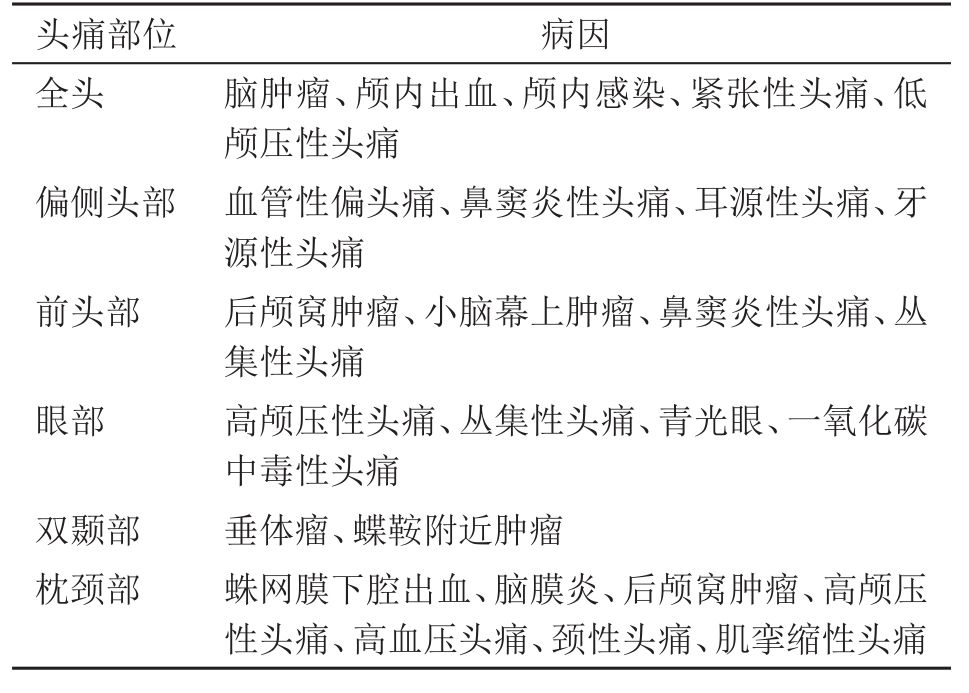
\includegraphics[width=3.21875in,height=2.30208in]{./images/Image00039.jpg}
\end{table}

\hypertarget{text00020.htmlux5cux23CHP1-7-2-1-1-4}{}
(4) 头痛的性质:

对头痛性质的了解十分重要。搏动性跳痛常为血管性头痛;发作性电击样剧痛为三叉神经痛的特征;咽后部发作性疼痛,可因吞咽动作诱发或加重者应考虑舌咽神经痛;紧箍样头痛多为肌紧张性头痛;眼、耳、鼻疾病所伴发者,大多数是胀痛或钝痛;神经症则是隐隐作痛,时轻时重。

\hypertarget{text00020.htmlux5cux23CHP1-7-2-1-1-5}{}
(5) 头痛的程度:

头痛的程度常不能反映病情的严重度,有时颅内占位性病变头痛并不严重而慢性焦虑症的头痛却表现剧烈难忍。一般而言,剧烈头痛常见于神经痛、偏头痛、蛛网膜下腔出血、脑膜炎等;中等度头痛,主要见于颅内占位性病变、慢性炎症等;轻度头痛,可见于神经症及某些邻近器官(耳、眼、鼻)病变。

\hypertarget{text00020.htmlux5cux23CHP1-7-2-1-1-6}{}
(6) 头痛发生的速度及影响因素:

急性突发性头痛,除多为血管性头痛外,尚有急性脑卒中(蛛网膜下腔出血、脑出血等)、急性感染性疾患。缓慢发生的头痛且进行性加重,并有颅内压增高表现者可能为颅内占位性病变,而无颅内压增高者可见于紧张性头痛。咳嗽、用力或头部转动,常使颅内压增高而头痛加剧;直立位可使肌紧张性头痛或腰穿后反应等加重,而丛集性头痛则减轻;压迫颞、额部动脉或颈总动脉可使血管性头痛减轻。根据头痛的发病方式和经过,对头痛进行鉴别诊断,见表\ref{tab7-2}。

\hypertarget{text00020.htmlux5cux23CHP1-7-2-1-1-7}{}
(7) 头痛的伴随症状:

头痛时常伴恶心、呕吐、面色苍白、出汗、心悸等自主神经症状,主要见于偏头痛;头痛严重并有进行性加剧的恶心、呕吐,常为颅内高压的征兆;体位变化时出现头痛加重或意识障碍,见于脑室内肿瘤、后颅凹或高颈段病变;伴有视力障碍及其他眼部征象(复视),呈短暂性发作者,多为偏头痛、椎-基底动脉供血不足;眼底视乳头水肿或出血,常为颅内压增高症或高血压性脑病。头痛伴精神症状(如淡漠或欣快)者应考虑额叶肿瘤的可能。由颅内损害引起的头痛常伴有神经功能缺失症状。

\hypertarget{text00020.htmlux5cux23CHP1-7-2-1-1-8}{}
(8) 其他病史:

尚需注意全身其他系统器官受损的病史,以及家族史、用药史、外伤史、手术史、月经及烟酒嗜好等。

\begin{table}[htbp]
\centering
\caption{头痛的发病方式和经过}
\label{tab7-2}
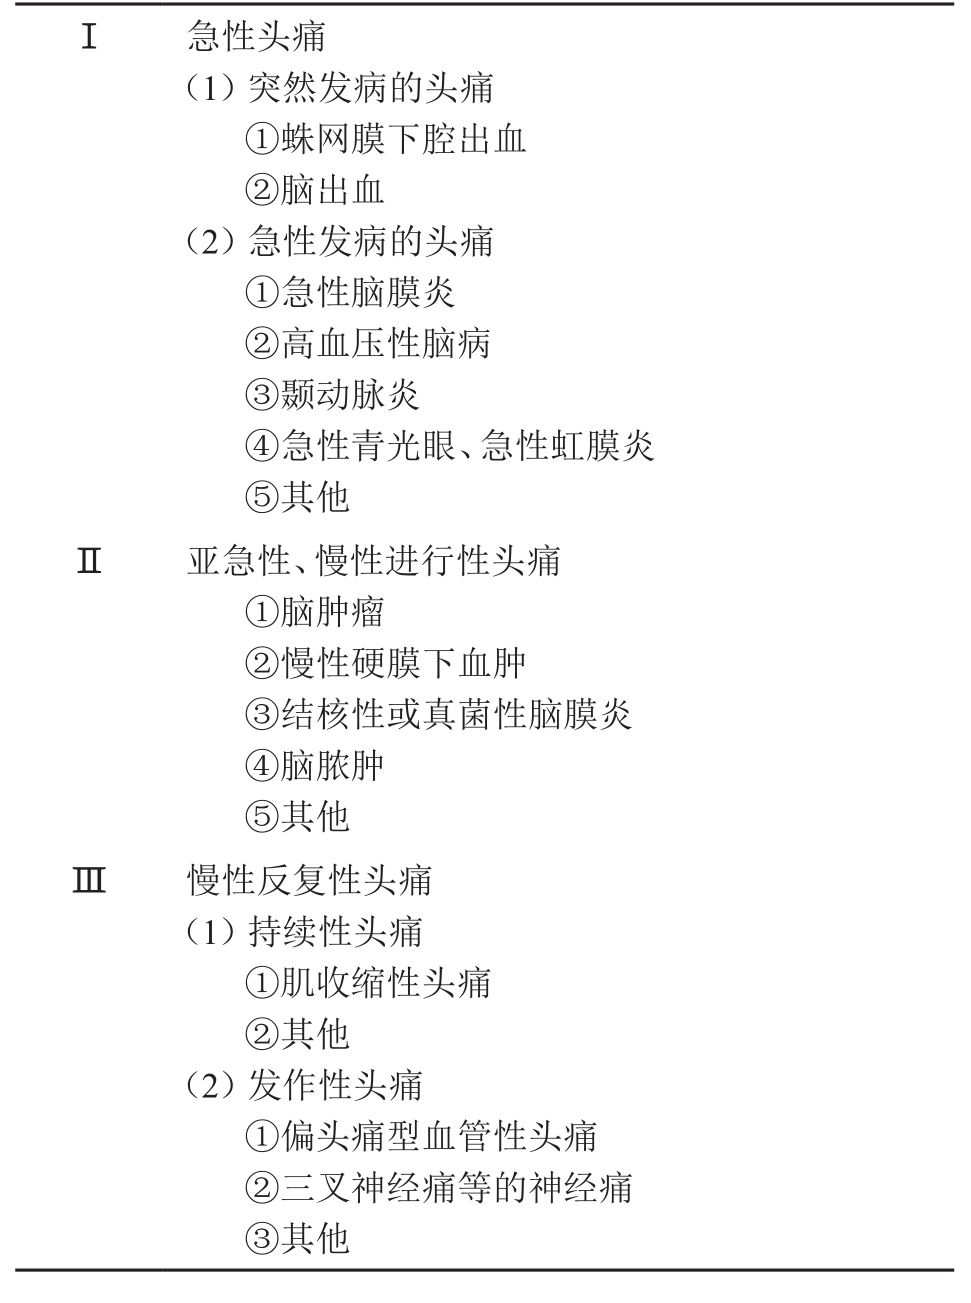
\includegraphics[width=3.22917in,height=4.33333in]{./images/Image00040.jpg}
\end{table}

\subparagraph{体检}

全面详尽的体格检查尤其是神经系统和头颅五官的检查,有助于发现头痛的病变所在。

\hypertarget{text00020.htmlux5cux23CHP1-7-2-1-2-1}{}
(1) 内科检查:

许多内脏器官或系统的疾患可发生头痛,应按系统详细检查,大多可查出头痛的原因。如高血压、全身感染性疾病的发热或中暑、缺氧(如一氧化碳中毒),慢性肺部疾患的高碳酸血症,严重贫血或红细胞增多症,均可由于脑血流增加而致头痛;而毒素作用、酗酒,则可因血管扩张而致头痛。尚有代谢内分泌疾病的检查(甲亢、低血糖、嗜铬细胞瘤等)。

\hypertarget{text00020.htmlux5cux23CHP1-7-2-1-2-2}{}
(2) 五官检查:

头部邻近器官的疾病也是头痛常见的原因。如在眼部的视神经炎、儿童的屈光不正、青光眼、眼部表浅炎症(结膜炎、角膜炎、睑板腺炎、泪囊炎等)及眶部组织的炎症;在耳鼻咽喉方面有鼻炎、鼻窦炎、咽炎、中耳炎、鼻窦或鼻咽部肿瘤,另外颞颌关节病及严重的牙病也可引起头痛。

\hypertarget{text00020.htmlux5cux23CHP1-7-2-1-2-3}{}
(3) 神经系统检查:

全面的神经系统检查是非常重要的。

\hypertarget{text00020.htmlux5cux23CHP1-7-2-1-2-4}{}
(4) 精神检查:

有不少精神科疾病可伴有头痛,神经症是最常见的,而抑郁症的精神症状可被躯体症状所掩盖,尤其是隐匿性抑郁,常呈一些不典型的疼痛。

\subparagraph{辅助检查}

应根据患者的具体情况和客观条件来选择性地应用。如做头颅X线检查、脑电图、CT扫描或MRI、腰穿脑脊液检查等,以及内科与五官科方面的检查。

头痛的临床检查方法见表\ref{tab7-3}。

\hypertarget{text00020.htmlux5cux23CHP1-7-2-2}{}
(二) 局限性病变抑或全身性病变

\subparagraph{局限性病变}

包括颈部以上的局部病变引起的头痛,又可分为两大组:

\begin{table}[htbp]
\centering
\caption{头痛的临床检查方法}
\label{tab7-3}
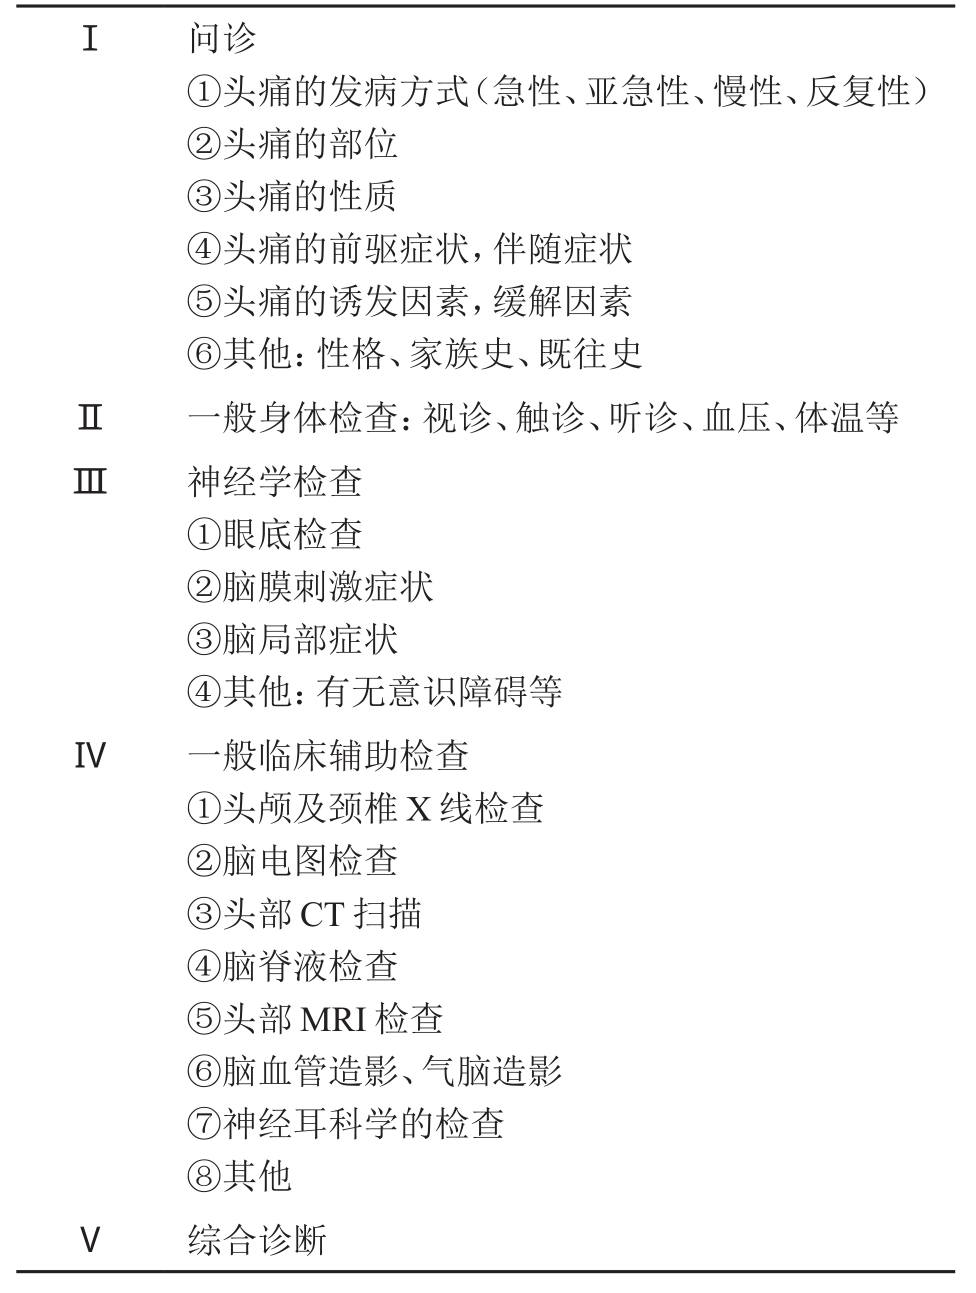
\includegraphics[width=3.25in,height=4.30208in]{./images/Image00041.jpg}
\end{table}

\hypertarget{text00020.htmlux5cux23CHP1-7-2-2-1-1}{}
(1) 颅内疾病:

此组疾病所致的头痛大都较严重,起病急,发展迅速。多数伴有恶心和(或)呕吐;部分尚有意识障碍或脑部和脑神经损害的表现,如抽搐、肢体瘫痪和瞳孔改变等。

\hypertarget{text00020.htmlux5cux23CHP1-7-2-2-1-2}{}
(2) 头颈部疾病:

此组疾病引起的头痛可轻可重,但很少逐渐加重。头痛的部位常与病灶一致或位于病灶附近,刺激病变部位可使疼痛加剧(如三叉神经痛等);但血管性头痛,压迫颞动脉则可使头痛减轻。头颈部疾病所致头痛的原发病灶明显,诊断不难。

\subparagraph{全身性病变}

\hypertarget{text00020.htmlux5cux23CHP1-7-2-2-2-1}{}
(1) 全身性器质性病变:

引起急性头痛主要包括两大类疾病:一类是急性中毒。金属及化学物质如铅、锰、苯、酒精、一氧化碳等中毒时均可引起头痛。常为头部弥漫性跳痛,转动头部,头痛部位和性质无改变为此类头痛的重要特点。另一类是全身感染。多为急性传染病,头痛多在疾病的初期发生,也可出现在传染病的极期;无脑膜刺激征及神经系统定位征,脑脊液压力有时可增高,但生化及外观检查无异常。

\hypertarget{text00020.htmlux5cux23CHP1-7-2-2-2-2}{}
(2) 功能性病变:

多见于神经症患者,除头痛外,常伴有神经症的其他症状,如失眠、记忆力减退、注意力不集中、头昏、烦躁等,常因精神刺激而加重。患者一般情况好,临床检查无器质性病变存在。部分患者的头痛是由于服药后所引起(医源性头痛),主要是血管扩张剂等。应注意,功能性头痛必须在排除可能的器质性病变后才能确立。

\subsection{处理原则}

头痛的防治原则包括病因治疗、对症治疗和预防性治疗。对于病因明确的病例应尽早去除病因,如颅内感染应抗感染治疗,颅内高压者宜脱水降颅压等。任何头痛在急性发作时均应尽可能寻找潜在的病因进行治疗;对于病因不能立即纠正的继发性头痛及各种原发性头痛急性发作,可给予止痛等对症治疗以终止或减轻头痛症状。对慢性头痛呈反复发作者应给予适当的预防性治疗,以防头痛频繁发作。

\subsection{常见头痛的诊断与处理}

\hypertarget{text00020.htmlux5cux23CHP1-7-4-1}{}
(一) 偏头痛

偏头痛(migraine)是一种常见的慢性神经血管性疾患,是临床常见的原发性头痛,其特征是发作性、多为偏侧、中重度、搏动样头痛,一般持续4~72小时,可伴有恶心、呕吐,光、声刺激或日常活动均可加重头痛,安静环境、休息可缓解头痛。多起病于儿童和青春期,中青年期达发病高峰,女性多见,约50\%患者有家族史。精神紧张、过度劳累、气候骤变、强光刺激、烈日照射、低血糖、应用扩血管药物或利血平、食用高酪胺食物(如巧克力、乳酪、柑橘)及酒精类饮料,均可诱发偏头痛发作。

\subparagraph{临床表现特点}

偏头痛有多种类型,但以以下两型常见:

\hypertarget{text00020.htmlux5cux23CHP1-7-4-1-1-1}{}
(1) 无先兆偏头痛(普通型偏头痛):

是最常见的偏头痛类型,约占80\%。临床表现为反复发作的一侧或双侧额颞部搏动性疼痛,常伴有恶心、呕吐、畏光、畏声、出汗、全身不适与头皮触痛等症状。通常在发作开始时仅为轻~中度的钝痛或不适感,数分钟至数小时后达到严重的搏动性痛或跳痛。有时疼痛放射至上颈部及肩部。部分女性患者发作常与月经有关,通常为经期前2天到经期的第3天之间发病,若90\%的发作与月经周期密切相关称月经期偏头痛。出现上述发作至少5次,除外颅内外各种器质性疾病后方可作出诊断。

\hypertarget{text00020.htmlux5cux23CHP1-7-4-1-1-2}{}
(2) 有先兆偏头痛(典型偏头痛):

约占偏头痛患者的10\%。一般在青春期发病,多有家族史,头痛发作前数小时至数日可有倦怠、注意力不集中和打哈欠等前驱症状。在头痛之前或头痛发生时,常以可逆的局灶性神经系统症状为先兆,表现为视觉、感觉、言语和运动的缺损或刺激症状。最常见为视觉先兆,常为双眼同向症状(homonymous
visual
symptoms),如视物模糊、暗点、闪光、亮点亮线或视物变形;其次为感觉先兆,感觉症状多呈面-手区域分布;言语和运动先兆少见。先兆症状一般在5~20分钟内逐渐形成,持续不超过60分钟;不同先兆可以接连出现。头痛在先兆同时或先兆后60分钟内发生,表现为一侧或双侧额颞部或眶后搏动性头痛,常伴有恶心、呕吐、畏光或畏声、苍白或出汗、多尿、易激怒、气味恐怖或疲劳感等,可见头面部水肿、颞动脉突出等。活动能使头痛加重,睡眠后可缓解头痛。头痛可持续4~72小时,消退后常有疲劳、倦怠、烦躁、无力和食欲差等,1~2日后常可好转。

有上述典型偏头痛症状,虽经治疗头痛时间持续在72小时以上(其间可能有短于4小时的缓解期)的称为偏头痛持续状态(status
migrainous)。

大多数偏头痛患者的预后良好,随年龄的增长症状可逐渐缓解,部分患者可在60~70岁时偏头痛不再发作。

\subparagraph{治疗要点}

偏头痛的治疗目的为减轻或终止头痛发作,缓解伴发症状,预防头痛复发。

\hypertarget{text00020.htmlux5cux23CHP1-7-4-1-2-1}{}
(1) 发作期的治疗:

治疗药物包括非特异性止痛药如非甾体类抗炎药(NSAIDs)和阿片类药物,特异性药物如麦角类制剂(麦角胺1~2mg/次,日最大剂量6mg;双氢麦角胺肌肉注射1~2mg/次,日最大剂量4mg,或口服1~3mg/次,日最大剂量9mg)和曲普坦类药物,后者包括舒马曲普坦(皮下注射:6mg/次,日最大剂量12mg;口服25~100mg/次,日最大剂量300mg)、那拉曲普坦(口服2.5mg/次,日最大剂量5mg)、利扎曲普坦(口服5~10mg/次,日最大剂量30mg)、佐米曲普坦(口服2.5~5mg/次,日最大剂量10mg)和阿莫曲普坦(口服6.25~12.5mg/次,日最大剂量25mg)等。通常应在症状起始时立即服药。药物选择应根据头痛程度、伴随症状、既往用药情况等综合考虑,可采用阶梯法、分层选药,进行个体化治疗。①轻~中度头痛:单用NSAIDs如对乙酰氨基酚(口服0.3~0.6g/次,日最大剂量不超过2.0g)、萘普生(口服0.2~0.3g/次,每日2~3次)、布洛芬(口服0.2~0.4g/次,每日3~4次)等可有效,如无效再用偏头痛特异性治疗药物。阿片类制剂如哌替啶等,因有成瘾性,不推荐常规用于偏头痛的治疗,但对于有麦角类制剂或曲普坦类应用禁忌的病例,如合并心脏病、周围血管病或妊娠期偏头痛,则可给予哌替啶治疗以终止偏头痛急性发作。②中~重度头痛:可直接选用偏头痛特异性治疗药物以尽快改善症状,部分患者虽有严重头痛但以往发作对NSAIDs反应良好者,仍可选用NSAIDs。麦角类和曲普坦类药物不良反应包括恶心、呕吐、心悸、烦躁、焦虑、周围血管收缩,大量长期应用可引起高血压和肢体缺血性坏死。严重高血压、心脏病和孕妇患者均为禁忌。此外,应用过频,则会引起药物过量使用性头痛(medication-overuse
headache),因此,麦角类和曲普坦类药物每周用药不超过2~3天。③伴随症状:恶心呕吐可肌肉注射甲氧氯普胺10mg,严重呕吐者可用小剂量奋乃静、氯丙嗪。烦躁者可用地西泮10~20mg肌肉注射以促使患者镇静和入睡。

\hypertarget{text00020.htmlux5cux23CHP1-7-4-1-2-2}{}
(2) 预防性治疗:

适用于:①频繁发作,尤其是每周发作1次以上严重影响日常生活和工作的患者;②急性期治疗无效,或因副作用和禁忌证无法进行急性期治疗者;③可能导致永久性神经功能缺损的特殊变异型偏头痛,如偏瘫性偏头痛、基底型偏头痛或偏头痛性梗死等。常用药物有:①β受体阻滞剂:普萘洛尔(10~60mg/次,每天2次),美托洛尔(100~200mg/次,每天1次);②钙通道阻滞剂:氟桂利嗪(5~10mg,每日1次,睡前服用),维拉帕米(160~320mg/d);③抗癫痫药:丙戊酸钠(0.4~0.6g/次,每天2次),托吡酯(25~200mg/d),加巴喷丁(0.9~1.8g/d);④抗抑郁药:阿米替林(25~75mg睡前服用),丙米嗪和氟西汀等;⑤5-HT受体拮抗剂:苯噻啶(0.5~3mg/d)等。其中,普萘洛尔、阿米替林和丙戊酸钠三种在结构上无关的药物,是预防性治疗的支柱,一种药物无效可选用另一种药物。

\hypertarget{text00020.htmlux5cux23CHP1-7-4-2}{}
(二) 丛集性头痛

丛集性头痛(cluster
headache)是一种原发性神经血管性头痛。以男性多见,约为女性的3~4倍。头痛突然发生,无先兆症状,几乎于每日同一时间,常在晚上发作,使患者从睡眠中痛醒。头痛位于一侧眶周、眶上、眼球后和(或)颞部,呈尖锐、爆炸样、非搏动性剧痛。头痛达高峰时,患者常以手击头部、甚至以头撞墙,在室内外来回走动、十分烦躁、痛苦与不安。头痛持续15分钟~3小时不等。发作频度不一,从一日8次至隔日1次。疼痛时常伴有同侧颜面部自主神经功能症状,表现为结膜充血、流泪、流涕等副交感神经亢进症状,或瞳孔缩小和眼睑下垂等Horner征,较少伴有恶心、呕吐。头痛发作可连续数周至数月(常为2周~3个月),在此期间患者头痛呈一次接一次地成串发作,故名丛集性头痛。丛集发作期常在每年的春季和(或)秋季;丛集发作期后可有数月或数年的间歇期。在丛集期,饮酒或血管扩张药可诱发头痛发作,而在间歇期,两者均不会引起头痛发作。

根据中青年男性出现发作性单侧眶周、眶上和(或)颞部严重或极度严重的疼痛,可伴有同侧结膜充血、流泪、流涕、眼睑水肿、前额和面部出汗、瞳孔缩小、眼睑下垂等自主神经症状,发作时坐立不安、易激惹,并具有反复密集发作的特点,神经影像学排除引起头痛的颅内器质性疾患,可作出丛集性头痛的诊断。

本病急性期治疗方法有:①吸氧疗法:为头痛发作时首选的治疗措施。在发作剧烈时吸入纯氧(100\%氧气8~10L/min,10~20分钟)约使70\%患者终止发作。②利多卡因:用4\%~10\%利多卡因1ml经患侧鼻孔滴入,可使1/3的患者头痛缓解,机制是麻醉蝶腭神经节。③舒马曲普坦6mg皮下注射,或双氢麦角胺1~2mg肌肉注射等,可迅速缓解头痛。

本病预防性治疗药物包括维拉帕米、锂制剂和糖皮质激素等。维拉帕米240~320mg/d可有效预防本病发作,可在用药2~3周内发挥最大疗效。锂制剂适用于其他药物无效或有禁忌证者。糖皮质激素如泼尼松40~60mg/d,常可预防头痛的发作,第2周逐渐减量停药。其他药物有托吡酯、丙戊酸钠、苯噻啶、吲哚美辛等。

\hypertarget{text00020.htmlux5cux23CHP1-7-4-3}{}
(三) 紧张型头痛

紧张型头痛(tension-type headache)又称肌收缩性头痛(muscle contraction
headache),是双侧枕部或全头部紧缩性或压迫性头痛,约占头痛患者的40\%,是临床最常见的慢性头痛。主要由精神紧张及颅周肌肉张力增高引起。长期焦虑、紧张、抑郁或睡眠障碍,高强度的工作缺乏适当的放松及休息,以及某些单调工种使头、颈或肩胛带长期处于不良的姿势等均可为发病因素。头痛部位不定,可为双侧、单侧、全头部、颈项部、双侧枕部、双侧颞部等不同部位。通常呈持续性钝痛,像一条带子紧束头部或呈头周紧箍感、压迫感或沉重感。许多患者可伴有头昏、失眠、焦虑或抑郁等症状。有的患者也可出现恶心、畏光或畏声等症状。体检可发现疼痛部位肌肉触痛或压痛点,有时牵拉头发也有疼痛,颈肩部肌肉有僵硬感,捏压时肌肉感觉舒适。

根据患者的临床表现,排除颅颈部疾病如颈椎病、占位性病变和炎症性疾病等,通常可以确诊。

本病的许多治疗药物与偏头痛用药相同。对于焦虑、紧张或抑郁的患者应在精神上给予诱导和安慰,使其消除顾虑。对局限性的肌肉疼痛,如颈项肌和肩胛肌等可作按摩、针灸、理疗、局部封闭等治疗。急性发作期用对乙酰氨基酚、阿司匹林、非甾体抗炎药、麦角胺或双氢麦角胺等亦有效。对于频发性和慢性紧张型头痛,应采用预防性治疗,可选用阿米替林、丙米嗪或选择性5-羟色胺重摄取抑制剂(如舍曲林或氟西汀),或肌肉松弛剂如盐酸乙哌立松、巴氯芬等。失眠者可给予苯二氮{}
类如地西泮10~20mg/d口服。

\hypertarget{text00020.htmlux5cux23CHP1-7-4-4}{}
(四) 颅内压变化引起的头痛

\subparagraph{颅内压增高所致的头痛}

脑瘤、硬膜下血肿、脑脓肿及其他占位性病变引起的头痛,在初期主要是因病变邻近疼痛敏感结构被牵拉、移位或因感觉神经直接受压所致。在后期是由于脑脊液循环通路被阻塞,导致颅内压增高,使远离病灶的对疼痛敏感结构被牵拉、扭曲和移位而引起头痛。初期的头痛常位于占位病变的同侧,在后期有颅内压增高时呈现为弥漫深在的持久性钝痛,晨起较重,在咳嗽、大便用力或打喷嚏时头痛加重。头痛程度一般不如偏头痛或颅内出血时那样严重,多数不影响睡眠。随着占位病变增大及颅内压增高,患者出现呕吐及视乳头水肿,最后因继发性视神经萎缩使视力减退或双目失明。治疗上除应用脱水剂降低颅内压外,根本措施是手术切除占位性病变。

良性颅内压增高征指有头痛和视乳头水肿等颅内压增高表现而无局灶性神经系统体征,抽搐、精神障碍,其脑室系统和脑脊液成分基本正常,颅内无占位性病变,预后较为良好的一种临床综合征。此症患者大都诉述有全面性的头痛,而并无脑部结构的移位,头痛可能是由于伴发的脑水肿牵引脑膜与脑血管的神经末梢所致。

\subparagraph{低颅压性头痛}

低颅压性头痛(intracranial hypotension
headache)是脑脊液(CSF)压力降低(< 60mmH\textsubscript{2}
O)导致的头痛,多为体位性。患者常在直立后15分钟内出现头痛或头痛明显加剧,卧位后头痛缓解或消失。

低颅压性头痛包括自发性(特发性)和继发性两种。自发性病因不明,既往多认为可能与血管舒缩障碍引起CSF分泌减少或吸收增加有关;目前已证实多数自发性低颅压与自发性脑脊液漏有关。而导致自发性脑脊液漏可能与微小创伤和硬膜结构薄弱有关。部分病例有剧烈咳嗽、推举重物、剧烈体育活动等引起微小创伤的病史;部分病例可合并有结缔组织异常的其他疾病,如马方综合征(Marfan
syndrome)、常染色体显性遗传多囊肾、自发性视网膜脱离等。继发性可由多种原因引起,其中以硬膜或腰椎穿刺后低颅压性头痛最为多见,头颈部外伤及手术、脑室分流术、脊柱创伤或手术使CSF漏出增多,脱水、糖尿病酮症酸中毒、尿毒症、全身严重感染、脑膜脑炎、过度换气和低血压等使CSF生成减少。由于CSF量减少,压力降低,脑组织移位下沉等使颅内疼痛敏感组织被牵拉引起头痛。

本病可见于各种年龄,特发性多见于体弱女性,继发性无明显性别差异。头痛以双侧枕部或额部多见,也可为颞部或全头痛,但很少为单侧头痛,呈轻~中度钝痛或搏动性疼痛,缓慢加重,常伴恶心、呕吐、眩晕、耳鸣、颈僵和视物模糊等。头痛与体位有明显关系,立位时出现或加重,卧位时减轻或消失。脑组织下坠压迫脑神经也可引起视物模糊或视野缺损(视神经或视交叉受压)、面部麻木或疼痛(三叉神经受压)、面瘫或面肌痉挛(面神经受压)。

病因明确者应针对病因治疗,如控制感染、纠正脱水和糖尿病酮症酸中毒等。对手术或创伤后存在脑脊液瘘者可行瘘口修补术等。对症治疗包括头低位卧床休息,补液(2000~3000ml/d),穿紧身裤和束腹带,给予适量镇痛剂等。鞘内注射无菌生理盐水可使腰穿后头痛缓解。咖啡因可阻断腺苷受体,使颅内血管收缩,增加CSF压力和缓解头痛,可用苯甲酸钠咖啡因0.5g皮下或肌肉注射,或加入500~1000ml林格液中静脉滴注。硬膜外血贴疗法(epidural
blood
patching)是用自体血15~20ml缓慢注入腰或胸段硬膜外间隙,血液从注射点上下扩展数个椎间隙,可压迫硬膜囊和阻塞脑脊液漏出口,迅速缓解头痛,适用于腰穿后头痛和自发性低颅压性头痛,有效率97\%。腰穿时应选用口径细的穿刺针,术后去枕平卧至少6小时有利于预防头痛。

\hypertarget{text00020.htmlux5cux23CHP1-7-4-5}{}
(五) 脑血管病所致头痛

脑血管病所致头痛是急性头痛患者首先要甄别的,包括蛛网膜下腔出血、脑出血、缺血性卒中等。

\subparagraph{蛛网膜下腔出血}

急性发作的头痛首先应考虑蛛网膜下腔出血的可能。典型症状为急性发作剧烈头痛,主诉为“刀劈样”、“爆炸样”头痛。70\%的头痛无定侧,可以为双额、顶、枕部或满头痛,30\%头痛偏向一侧,通常偏向动脉瘤所在侧。疼痛可放射至一侧或双侧眼部或颈部,可沿颈项向下放射,出现颈项强直,可持续数周至数月。可有意识丧失。也有一部分患者首发症状为精神错乱,惊厥发作,眩晕或脑神经(常为动眼神经瘫痪)障碍。腰穿脑脊液为均匀血性。患者如以往经常有阵发性头痛,此次头痛发作比较急剧,性质不同以往,也要考虑蛛网膜下腔出血。其处理参见第84章第4节“蛛网膜下腔出血”。

\subparagraph{脑出血}

头痛常为首发症状,但往往迅速出现意识障碍与肢体偏瘫,结合血压突然升高的背景,诊断不难。

\subparagraph{未破裂的脑动脉瘤与动静脉畸形}

一般在动脉瘤未破裂之前,头痛是不常见的。脑血管畸形头痛时常位于畸形同侧,如后交通动脉或颈内动脉瘤可以引起固定在同侧的眶、额部头痛。动脉瘤进一步扩张时可以出现眼肌瘫痪或对侧视野缺损,可以有局限性癫痫发作,对侧肢体偏瘫。DSA和(或)头颅MRI检查有助于诊断,治疗以手术为主。

\subparagraph{缺血性脑卒中}

少数脑栓塞病例中有头痛症状,而在脑血栓形成中则头痛不常见。脑供血不足可致头痛,伴同感觉与运动障碍。头痛往往是搏动性的,可能是继发于颅外动脉的扩张。在椎-基底动脉或颈内动脉狭窄或闭塞的病例中,约1/3~1/2的患者有头痛,大都局限于枕部和颈部,或两额部;颈内动脉供血不足的头痛可以是同侧的或对侧的。

\subparagraph{颞动脉炎}

颞动脉炎(temporal
arteritis)多见于中、老年人,头痛常位于头皮表浅部位以及颞部与眼眶周围部,也可较广泛地弥漫及额部与枕部,为一种强烈的搏动性和持续性疼痛,并且伴有在其他血管性头痛中所没有的烧灼感。平卧位或头低位头痛加剧,仰头或压迫颈总动脉时头痛减轻,咀嚼时头痛加重。咀嚼时出现头痛常为本病的首发症状。压迫眼球或眼球转动即出现眼窝部疼痛。头痛同时伴有面部肿胀、皮肤红肿、颞动脉明显扩张隆起呈蛇行状,搏动消失,触之有发硬肥厚感,压痛明显。部分病例视网膜动脉或脑动脉也可受累,可发生缺血性视神经炎而出现视力障碍。颞动脉炎多有发热、出汗、疲乏等全身症状,周围血象有白细胞增高,血沉增快。

本病如不加特殊治疗,通常在3~24个月内病情渐趋稳定或自愈,少数可持续几年。治疗主要用肾上腺皮质激素且疗效好,在激素开始治疗后数小时内体温即下降为正常,1~2天内局部疼痛和全身症状消失,食欲正常。头痛消失后激素可渐减量并维持用药数月,如停药后复发可重复再用。

\hypertarget{text00020.htmlux5cux23CHP1-7-4-6}{}
(六) 高血压性头痛

是一种非偏头痛型血管性头痛
。高血压病时约80\%出现不同程度头痛,且青壮年的高血压病头痛发生率高,其机制与动脉壁痛觉感受器受刺激有关。表现为头部沉重或间歇性钝痛、压迫感或搏动痛,或呈持续性全头或偏侧头痛,部位不固定,多在清晨或午前出现,在低头或屏气用力后头痛可加剧。恶性高血压伴高血压脑病或因嗜铬细胞瘤血压突然升高时均可出现剧烈的持续性头痛,常伴有恶心、呕吐、视力减退,视网膜出血或视乳头水肿。

高血压性头痛的治疗在于及时适度的降低血压。对伴有脑水肿者应及时应用脱水剂。

\hypertarget{text00020.htmlux5cux23CHP1-7-4-7}{}
(七) 颅脑外伤性头痛

急性和慢性头部外伤均可伴有头痛,常见的外伤后头痛有下列几种类型:①头皮裂伤或脑挫裂伤后瘢痕形成,刺激颅内外痛觉敏感结构而引起头痛。疼痛部位较局限,常伴局部皮肤痛觉过敏。②外伤后自主神经功能异常性头痛(dysautonomic
headache)是因颈前部受伤累及颈交感神经链,导致支配头颅的交感神经失去抑制而引起头痛。患者叙述一侧额颞区的发作性头痛,伴同侧瞳孔改变(先扩大后缩小),眼睑下垂及面部多汗。服用普萘洛尔(20mg,每天3次)对头痛有效。③外伤后因颈肌持续收缩而出现头痛,和紧张型头痛相似常有精神因素参与。④外伤后神经不稳定性头痛。常见于脑震荡后遗症,除头痛外尚有头晕、耳鸣、失眠、注意力不集中,记忆力衰退,精神萎靡不振或情绪易激动等症状。神经系统无器质性损害证据。

\hypertarget{text00020.htmlux5cux23CHP1-7-4-8}{}
(八) 五官疾病的头痛

眼源性头痛是指青光眼、虹膜炎、眼眶肿瘤、球后视神经炎、高度远视、眼外肌不平衡及用眼时间过长等原因引起球后或额颞区疼痛。急性乳突炎能引起耳后疼痛。病毒性膝状神经节带状疱疹所产生的疼痛常位于外耳道内或耳后,疼痛数日后出现带状疱疹及面瘫。鼻腔或鼻窦发炎时因黏膜充血水肿而引起鼻塞、流涕及牵涉性头痛。急性鼻窦炎时常引起眼球周围或额颞区头痛。因鼻窦内的脓性分泌物经过一夜睡眠后积聚增多,故患者清晨起床后头痛特别严重,待脓液排出后头痛明显减轻。X线检查有助于本病诊断。个别患者因鼻窦窦口被炎性分泌物或过敏性水肿阻塞,鼻窦内压力降低而形成“真空性头痛”(vacuum
headache)。牙病所致的头痛,多先有病牙部位疼痛,随后放射至同侧颞部,呈灼痛或跳痛,牙科检查可确诊。鼻腔肿瘤、颞下颌关节功能障碍(Costen综合征)及鼻咽癌均可引起头部牵涉痛。

\hypertarget{text00020.htmlux5cux23CHP1-7-4-9}{}
(九) 精神性头痛

神经症
、抑郁症等,经常出现头痛。其部位多不固定,多变,性质多样,呈钝痛、胀痛,易受外界或情绪影响,历时数周甚至数年。常伴睡眠及记忆、理解等精神方面的症状。

\hypertarget{text00020.htmlux5cux23CHP1-7-4-10}{}
(十) 神经痛

\subparagraph{三叉神经痛(trigeminal neuralgia)}

是指三叉神经分布区内短暂的反复发作性剧痛。成年及老年人多见,40岁以上患者占70\%~80\%,女性多于男性。三叉神经痛可分为症状性和原发性,前者的病因为炎症(如疱疹病毒感染)、肿瘤(如半月神经节肿瘤)、动脉瘤及外伤等,后者系指病因未明者(可能因三叉神经脱髓鞘产生异位冲动或伪突触传递所致)。典型的原发性三叉神经痛通常有如下特点:①疼痛常局限于一侧,并以累及一支多见,少数患者可同时有二支或三支受累,且以上颌支(第2支)或下颌支(第3支)最常受累。②疼痛发作时表现为以面颊上下颌及舌部明显的剧烈电击样、刀割样、烧灼样或撕裂样疼痛,来去骤然,突发突止。疼痛由颌面或牙槽病灶开始,并沿该神经的支配区域放射,每次发作仅数秒钟至1~2分钟,间歇期正常,1天数次至1分钟多次。发作呈周期性,持续数周,可自行缓解数月或更长。随病程进展,缓解期日益缩短。③发作时可伴有同侧面部肌肉的反射性抽搐(故又称“痛性抽搐”),或有同侧面部潮红、流泪及流涎。④患者面部某个区域可能特别敏感,稍加触碰即引起疼痛发作,如上下唇、鼻翼外侧、舌侧缘、颊部等,该区域称之为“扳机点(触发点)”。发作期间面部的机械刺激,如说话、进食、洗脸、剃须、刷牙、打哈欠,甚至微风拂面皆可诱致疼痛发作,患者因而不敢大声说话、洗脸或进食,有的连口水也不敢咽下,严重影响患者生活,甚至全身营养状况不良,精神抑郁,有的产生消极情绪。

治疗主要有药物、封闭和手术治疗。药物治疗以卡马西平为首选,起始剂量0.1g口服,每天2~3次,最大剂量1.0g/d,有效维持量0.6~0.8g/d。如卡马西平无效可改用苯妥英钠0.1g口服,每天3次,如无效可每日增加0.05g,数日后加至0.6g/d。卡马西平或苯妥英钠单药治疗无效者两药合用可能有效。上述两药无效时可试用氯硝西泮(clonazepam)6~8mg/d口服。大剂量维生素B\textsubscript{12}
可缓解疼痛,剂量为1000~2000μg肌肉注射,每周2~3次,连用4~8周为一疗程。药物治疗无效者可试用无水乙醇或甘油封闭三叉神经分支或半月神经节,破坏感觉神经细胞,可获止痛效果,不良反应为注射区面部感觉缺失。经皮半月神经节射频电凝疗法也有较好疗效。三叉神经感觉根部分切除术,因止痛效果确切,仍是首选的手术治疗方法。而三叉神经显微血管减压术,止痛同时不产生感觉及运动障碍,是目前广泛应用的最安全有效的方法。

\subparagraph{舌咽神经痛}

舌咽神经分布区的反复阵发性剧痛,不伴脑神经功能破坏表现的称舌咽神经痛(glossopharyngeal
neuralgia)。远比三叉神经痛少见。多数于中年起病,表现为口咽、喉或耳内的短暂发作性剧痛。每次持续数秒至1分钟,可因吞咽、咀嚼、讲话、咳嗽等触发。检查咽喉、舌根和扁桃体窝可有疼痛触发点。疼痛发作时可伴发咳嗽。个别患者发生昏厥,可能由于颈动脉窦神经过敏引起心脏停搏而造成。病程中可有自发缓解。神经系统检查无异常发现。将4\%可卡因或1\%丁卡因涂于患侧的口咽部,常可使疼痛缓解数小时。病因不明,有的可能是由于舌咽神经的脱髓鞘性病变引起,有的可能是由于局部的颅底血管压迫于舌咽神经所致。若疼痛持续,则本病需与鼻咽癌侵及颅底、耳咽管肿瘤、扁桃体肿瘤相鉴别。治疗与三叉神经痛相似。

\subparagraph{枕神经痛}

枕神经痛(occipital
neuralgia)是枕大、枕小和耳大神经分布区疼痛的统称,三对神经来自C\textsubscript{2~3}
神经,分布于枕部。可因上段颈椎病、脊柱结核、骨关节炎、脊髓肿瘤、硬脊膜炎和转移瘤等所致,多为继发性神经损害;也可由上呼吸道感染或扁桃体炎引起,或病因不明。枕大神经分布于后枕部相当于两侧外耳道经头顶连线以后的部分;枕小神经主要分布于耳廓上部和枕外侧皮肤;耳大神经主要分布于耳廓下部前后面、腮腺表面和下颌角部皮肤。疼痛位于一侧枕部与颈部,呈阵发性刺痛或电击样痛,或持续性钝痛;患侧枕部头皮可有皮肤感觉过敏及局限性压痛点,可向头顶(枕大神经)、乳突部(枕小神经)或外耳(耳大神经)放射。枕大神经痛压痛点位于乳突与枕后粗隆间连线的中点;枕小神经痛的压痛点多位于该连线的外1/3处。部分患者在间歇期仍有钝痛。疼痛可为自发或因旋转尤其向对侧旋转而诱发,其他头颈部运动或咳嗽、喷嚏可使疼痛加重或诱发疼痛,故患者常不敢过分活动头部,或使头略向后仰并向患侧倾斜以缓解疼痛。除病因治疗外,可用止痛剂(卡马西平、苯妥英钠等)、神经营养剂(维生素B\textsubscript{1}
、B\textsubscript{12} 等)、局部封闭、理疗等对症治疗。


\hypertarget{text00021.htmlux5cux23CHP1-7-5}{}
参 考 文 献

1. 贾建平.神经病学.第6版,北京:人民卫生出版社,2008:158.

2. 头痛分类和诊断专家共识组
.头痛分类和诊断专家共识.中华神经科杂志,2007,40:439.

3. Schievink WI. Spontaneous spinal cerebrospinal fluid leaks and
intracranial hypotension. JAMA,2006,295:2286.

\protect\hypertarget{text00022.html}{}{}

\chapter{胸 痛}

胸痛是急诊室常见的患者就诊原因之一,临床上的胸痛不应仅是指解剖学胸部范围内的疼痛感受,而应包括任何原因所导致的解剖学胸部范围内的任何不适,同时也包括由于胸部疾患可能表现为其他部位的疼痛。由此可见导致胸痛的病因复杂,病情的严重程度相差很大。多数为良性经过的普通疾病,但其中有一部分则可能导致严重后果甚至危及生命。对于高危患者,症状发作后启动治疗越早,疗效越好,获益越多,任何延误都可能导致严重不良事件的发生,因此,急性胸痛患者的早期鉴别和危险分层对于识别高危患者并给予及时正确的处置具有重要意义。在临床急诊工作中,应首先确定就诊的急性胸痛患者是否患有急性心肌梗死、主动脉夹层、肺栓塞、气胸等,因为这些疾病若处理不及时,常危及生命。

\subsection{病因与发病机制}

\subsubsection{病因}

胸痛的主要病因大体上包括胸内结构病变、胸壁组织疾病、膈下脏器病变和功能性疾病等几个方面:

\subparagraph{胸内结构病变}

\hypertarget{text00022.htmlux5cux23CHP1-8-1-1-1-1}{}
(1) 心源性胸痛:

心绞痛、急性心肌梗死、急性心包炎、主动脉夹层等。

\hypertarget{text00022.htmlux5cux23CHP1-8-1-1-1-2}{}
(2) 非心源性胸痛:

①大血管病变:主动脉瘤、肺梗死;②呼吸系统疾病:胸膜炎、自发性气胸等;③纵隔和膈肌的疾病:纵隔炎、纵隔脓肿、纵隔肿瘤和膈疝等;④食管疾病:反流性食管炎、食管破裂、食管裂孔疝等。

\subparagraph{胸壁组织疾病}

带状疱疹、乳腺炎、皮下蜂窝组织炎、非化脓性肋软骨炎、肌炎、流行性肌炎、肋间神经炎、肋骨骨折等。

\subparagraph{膈下脏器病变}

膈下脓肿、肝脓肿、脾梗死和肝癌破裂等。

\subparagraph{功能性疾病}

心脏神经症。

\subsubsection{发病机制}

疼痛产生的机制:①各种化学或物理因素如缺氧、炎症、肌张力改变刺激肋间神经感觉纤维,脊髓后根传入纤维,支配气管、支气管及食管的迷走神经感觉纤维,膈神经的感觉纤维,支配心脏或主动脉感觉纤维等引起疼痛;②某一内脏与体表某一部位同受某些脊神经后根传入神经支配时,来自内脏的痛觉冲动传入大脑皮层区,除产生局部疼痛外,还可以出现相应体表的疼痛感觉------放射痛(又称牵涉痛)。

\subsection{诊断思路}

急性胸痛中包括了一组以胸痛为主要表现的疾病,其中危险性最高的分别是:急性心肌梗死、急性肺栓塞、主动脉夹层、张力性气胸及心包填塞。这些患者可能随时会发生死亡。急诊医生的任务是在众多表现为急性胸痛的患者中识别出这些高危的疾病并给予及时、适当的处理。这些高危的患者是否能够在急诊被及时准确地识别出来主要依靠:①急诊医生一定要时刻保持对这些疾病的警惕性;②急诊医生一定要掌握这些疾病主要的临床特征;③急诊科要有鉴别这些疾病的合理流程;④急诊科要能够提供必要的检查手段。

\subsubsection{临床特征}

首先在急诊处理急性胸痛的患者时,要利用有限的时间仔细询问病史和进行体格检查,这样能够确定下一步思考的正确方向。在询问病史时,要注意胸痛的部位、性质、缓解的因素,胸痛诱发和加重的因素,胸痛是否放射,胸痛的伴随症状和既往病史等。这些特征中往往隐含着具有诊断和鉴别诊断意义的线索,因此这些特征是医生接诊急性胸痛患者时需要重点询问的内容,相当部分的胸痛患者单纯依靠详细的病史询问就可以基本诊断。

\subparagraph{发病年龄}

青壮年胸痛,应注意自发性气胸、心肌炎、心肌病、风湿性心瓣膜病,40岁以上患者应注意心绞痛、心肌梗死与肺癌。

\subparagraph{胸痛部位}

包括疼痛部位及其放射部位。心绞痛与心肌梗死的疼痛常位于胸骨后或心前区,且放射到左肩和左上臂内侧。夹层动脉瘤疼痛位于胸背部,向下放射至下腹、腰部与两侧腹股沟和下肢。食管疾患、膈疝、纵隔肿瘤的疼痛也位于胸骨后。胸膜炎所致的胸痛常在胸廓的下侧部或前部。带状疱疹是成簇水疱沿一侧肋间神经分布伴剧痛,疱疹不越过体表中线。胸壁疾病特点为疼痛部位局限,局部有压痛。炎症性疾病,尚伴有局部红、肿、热表现。肝胆疾病或膈下脓肿可引起右下胸痛。

\subparagraph{持续时间}

心绞痛发作时间短暂,持续数分钟,而心肌梗死疼痛持续时间很长且不易缓解。炎症、肿瘤、栓塞或梗死所致疼痛呈持续性。平滑肌痉挛或血管狭窄缺血所致疼痛为阵发性。

\subparagraph{疼痛性质}

胸痛的程度可表现为剧烈的疼痛到轻微的隐痛,疼痛性质也多种多样。如带状疱疹呈刀割样痛或灼痛,剧烈难忍;肌痛呈酸痛;骨痛呈酸痛或锥痛。心绞痛常呈压榨样痛并伴有压迫感或窒息感;主动脉夹层动脉瘤常有突然出现的剧烈的撕裂痛。膈疝呈灼痛或膨胀感。早期肺癌可仅有胸部的钝痛或隐痛。食管疾病多表现为持续性隐痛或烧灼痛。

\subparagraph{伴随症状}

气管、支气管疾病所致胸痛常伴有咳嗽、咳痰;食管疾病所致胸痛常伴有吞咽困难或咽下疼痛;肺梗死、原发性肺癌的胸痛常伴有小量咯血或痰中带血。

\subparagraph{影响疼痛因素}

包括发生诱因、加重与缓解因素。胸膜炎、自发性气胸、心包炎所致胸痛常在深吸气及咳嗽时加重,停止呼吸运动则疼痛减轻或消失。劳累、体力活动、精神紧张,可诱发心绞痛发作,休息、含服硝酸酯类药物可使心绞痛缓解,而对心肌梗死疼痛则无效。反流性食管炎的胸骨后灼痛,饱餐后出现,仰卧或俯卧位加重,服用抗酸剂和促动力药后可减轻或消失。

\subsubsection{必要的体格检查}

对于急性胸痛患者,一般不可能进行全面、系统的体格检查,要求5分钟内完全必要的体格检查。因为大多数情况下病情不允许医生有充分的时间这样做,因此重要的是要有针对性,有目的地根据患者的病史特征和临床思维分析进行一些重点体查。

首先要注意生命征,包括血压、脉搏、呼吸、体温。发现患者血压<
90/60mmHg,心率> 100次/分钟,应立即启动稳定生命征治疗。

怀疑主动脉夹层对比双侧桡动脉、股动脉和足背动脉搏动,有怀疑应测四肢血压。

观察胸部表面皮肤有无局限性红肿、瘀斑和出血点及疱疹等;胸腹式呼吸协调性、呼吸形式和快慢深浅;双侧胸部对称性。胸膜炎、胸腹部外伤、膈下脓肿、单纯疱疹等疾病常有上述异常变化。触诊检查局部肿块、液波感、压痛和胸廓的呼吸动度。

注意胸壁感染、气胸、血胸、肋骨骨折等征象。女性乳腺炎也有以胸痛主诉就诊,注意鉴别。

听诊需了解双侧呼吸音对比、胸膜和心包摩擦音、肺干湿性啰音、哮鸣音、异常音和杂音等,这对鉴别心脏和肺部疾病有帮助。

怀疑肺栓塞的患者要注意检查下肢有无肿胀,是否有下肢深静脉血栓形成的证据。

\subsubsection{必要的辅助检查}

对胸痛的诊断,除需仔细了解病史、查体外,一些常规的辅助检查,如心电图(ECG)、心肌损伤标志物及影像学检查也十分重要,这对筛查潜在的高危胸痛患者有参考价值。

\subparagraph{实验室检查}

血常规检查和凝血功能对判断有无感染和出凝血异常的存在必不可少。初始的ECG有助于确定中~高危的ACS患者,肌钙蛋白和心肌酶学是确诊是否存在心肌损害的重要手段,应用肌钙蛋白有助于确定是否需要早期血运重建,是ACS危险分层的重要工具;D-二聚体对急性肺栓塞的诊断有重要意义;动脉血气分析有助于了解肺功能情况。

\subparagraph{心肌损伤标记物在胸痛患者中的应用价值}

心肌损伤标志物的测定能检出或除外心肌坏死,最常应用的生化标志物有肌钙蛋白T(TnT)和肌钙蛋白I(Tn
I)、肌红蛋白和肌酸激酶MB同工酶(CK-MB)。在急性胸痛的早期约3~6小时,肌红蛋白检测对除外心肌梗死的可能性很有价值,在症状发作7小时后,肌钙蛋白与CK-MB有较高的阴性预测性,Tn
I或TnT对诊断AMI的特异性与敏感性均较高。心肌损伤标记物浓度与心肌损害范围呈正相关。约30\%的非ST段升高的ACS患者cTn
I或cTnT升高,可能为非Q波心肌梗死而属高危患者,即使CK-MB正常,死亡危险性也增加。肌钙蛋白水平越高,危险性越高。

\subparagraph{心电图}

ECG是胸痛患者应用广泛的检查方法。异常的心电图包括ST段升高、ST段下降和T波低平或倒置。入院时ECG有ST段升高的患者早期死亡率最高,ST段下降患者的死亡率中等,T波倒置最低。ST段升高是急性心肌梗死最敏感和最特异的ECG标志。新出现ST段升高的患者80\%~90\%为急性心肌梗死。约90\%的ECG有新出现的Q波为急性心肌梗死。ST段下降提示心肌缺血,但是其诊断进展性心肌梗死的可靠性差,仅约50\%的患者最终确诊为急性心肌梗死。对称性T波倒置的特异性较差,心肌缺血、心肌炎和肺栓塞在内的多种疾病都可以出现这种改变,约1/3的患者可能存在心肌梗死。有1/3左右的急性胸痛患者ECG正常,对这些患者动态观察心电图的变化很重要。在发病早期,很多急性心肌梗死最初的心电图无异常,随着时间的延长才表现为急性心肌梗死典型的ST段升高的ECG表现,若未对患者进行动态观察,常易忽略而漏诊。

目前建议在胸痛患者来诊10分钟内应进行ECG检查,10分钟内做出判定,ST段升高的患者一旦确定需立即进行再灌注治疗;ECG有缺血性表现的患者,按不稳定性心绞痛或非ST段升高的急性心肌梗死处理;ECG正常或有非特异性改变,应结合病史和生化标志物等综合判断。

\subparagraph{影像学检查}

X线胸部透视与摄片,对于鉴别肺部疾病、肋骨、胸骨骨折,心脏各房室大小有帮助;CT扫描是一项对临床有较大帮助的检查,可以发现X线不能显示的病变,帮助临床诊断肺栓塞、主动脉瘤、夹层动脉瘤。心血管造影,尤其血管数字减影(DSA),可清楚显示主动脉瘤、主动脉夹层、室壁瘤的部位、大小、形态等情况;冠状动脉造影,可明确心肌梗死的部位和严重程度,是诊断心肌梗死的“金标准”;超声心动图实时显示心脏结构和动态以及心包积液。B超对膈下和肝脓肿、胆道情况以及包裹性胸水定位有意义。

\subparagraph{放射性核素扫描}

对肺梗死、肺内占位病变、心肌梗死或局限性室壁瘤的诊断有帮助。

\subparagraph{彩色多普勒超声}

对急性心肌梗死和急性大动脉夹层动脉瘤诊断的意义较大。彩超和多普勒可用于大动脉夹层的检查,但其具有一定的局限性。彩超仅能看到升主动脉和腹部、髂部的血管。主要的征象是主动脉明显增宽,主动脉壁分离形成的真腔与假腔,有时还可见内膜的裂口。超声还可用于鉴别胆石症、脾梗死、胰腺炎等一些膈下疾病。急性心肌梗死时二维超声心动图可见梗死的部位室壁运动低下、运动消失或反常运动。超声对急性肺栓塞的诊断帮助不大。超声对自发性气胸的诊断没有帮助。

\subparagraph{胸痛患者辅助检查的顺序}

决定检查的顺序时要根据:危险性最大、最需要首先排除的疾病是什么?最能明确诊断的检查是什么?最方便、最及时的检查是什么?对于所有胸痛的患者,首先是要进行详细的体格检查,尤其是要注意生命体征,其次才是借助仪器的检查。有些疾病经过仔细的体格检查就能够发现特征性的表现,如剧烈胸痛者发现脉搏不对称及血管杂音强烈提示大动脉夹层等。切忌一切依赖仪器。对于一个急性胸痛的患者,辅助检查应该按照以下顺序进行为宜:

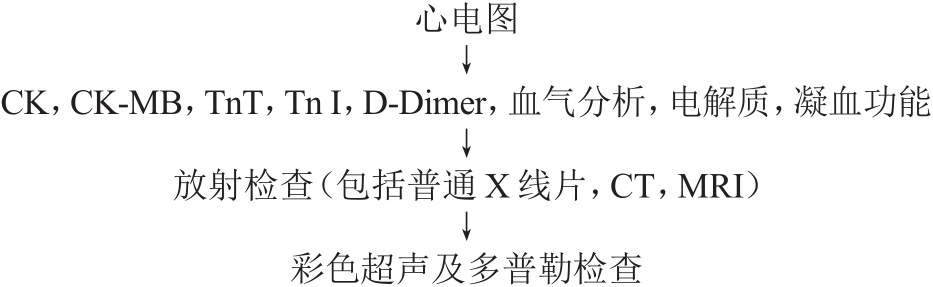
\includegraphics[width=3.09375in,height=0.94792in]{./images/Image00043.jpg}

\subsection{急诊处理原则和流程}

急性胸痛的急诊处理原则是:一是快速识别高危患者,以迅速进入快速救治绿色通道;剔除那些几乎没有或没有威胁生命疾病的患者;二是对不能明确诊断的患者应常规留院观察病情的演变,严防患者院外发生严重危及生命的事件。

1.首先判断病情严重性
,对生命征不稳定的患者,应立即开始稳定生命征的治疗;同时开始下一步处理;

2.对于生命征稳定的患者,首先获取病史和体征;

3.进行针对性的辅助检查;

4.在上述程序完成后能够明确病因的患者立即开始有针对性地病因治疗;

5.对不能明确病因的患者,建议留院观察,每隔30分钟复查一次心电图,每隔2小时复查心肌损伤标志物。心电图连续3次无变化,心肌损伤标志物连续2次无异常者在6~12小时后可予以出院。具体处理流程见图\ref{fig8-1}。

\begin{figure}[!htbp]
 \centering
 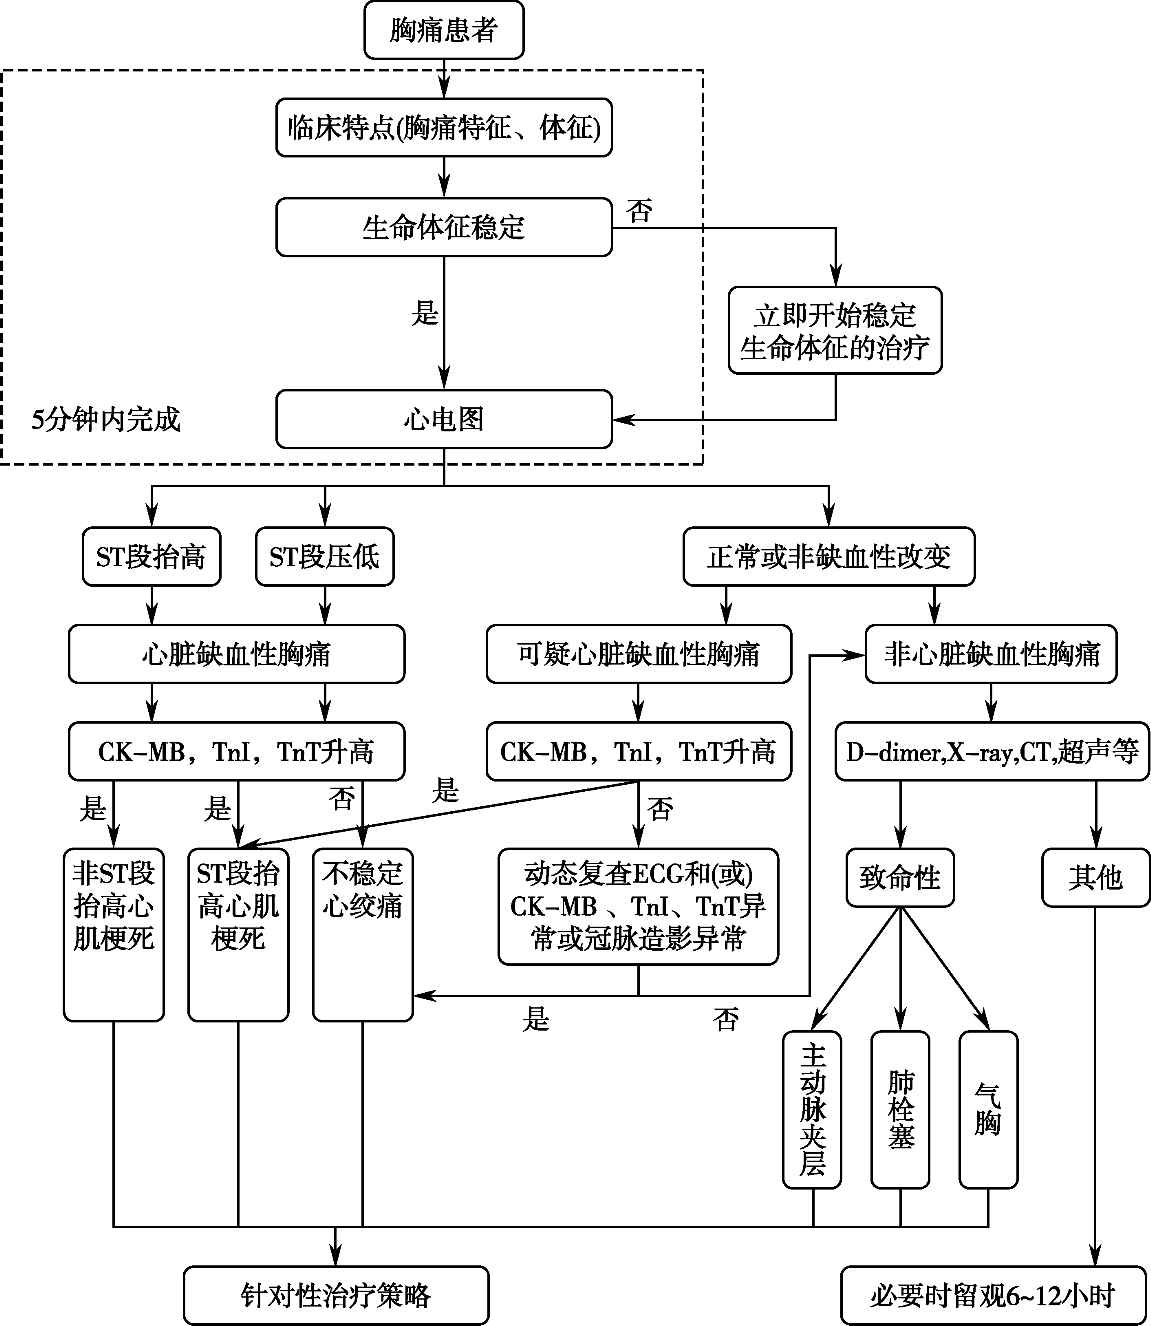
\includegraphics[width=4.69792in,height=5.41667in]{./images/Image00044.jpg}
 \captionsetup{justification=centering}
 \caption{胸痛的处理流程图}
 \label{fig8-1}
  \end{figure} 

\hypertarget{text00023.htmlux5cux23CHP1-8-4}{}
参 考 文 献

1. O'Connor R E,Bossaert L,Arntz H R,et al. Acute Coronary
Syndromes:2010 International Consensus on Cardiopulmonary Resuscitation
and Emergency Cardiovascular Care Science With Treatment
Recommendations. Circulation,2010,122: S422-S465.

2. Braunwald E,Antman E M,Beasley J W,et al. ACC/AHA Guideline Update
for the Management of Patients With Unstable Angina and Non-ST-Segment
Elevation Myocardial Infarction---2002:Summary Article:A Report of the
American College of Cardiology/American Heart Association Task Force on
Practice Guidelines(Committee on the Management of Patients With
Unstable Angina).Circulation,2002,106:1893-1900.

3. 罗学宏.急诊医学.北京:高等教育出版社,2008.74-78.

\protect\hypertarget{text00024.html}{}{}

\chapter{咯 血}

咯血(hemoptysis)是指喉腔、气管、支气管和肺组织出血,由咳嗽动作经口腔排出。咯血的临床过程难以预料,有时,初始仅少量痰中带血,却可以是大量的致命性咯血的先兆。大咯血引起失血性休克而致死的较少见,更常见的是大量的血淹溺肺泡,阻塞气道,因窒息和顽固性低氧血症而导致患者死亡。

咯血量可因病因和病变性质的不同而有差异,与病变的严重程度也不完全一致。临床上多根据咯血量将其分为少量咯血:24小时内咯血量≤100ml,包括痰中带血;中等量咯血:24小时内咯血量100~500ml;大咯血:24小时内咯血量>
500ml或一次咯血量≥200ml。大咯血约占全部咯血患者的1\%~4\%,但其死亡率高达80\%以上。

大咯血致死的危险与咯血量、出血速度、肺内潴留的血量以及患者基础肺功能储备相关,而与咯血的病因无关。年老体弱或久病无力者咳嗽乏力、基础肺功能差,即使几口血痰也可窒息致死。

\subsection{病因与发病机制}

\subsubsection{病因}

咯血的病因很多(表\ref{tab9-1}),但以肺结核、支气管扩张症、肺癌和肺炎等4种疾病多见。

尽管当今的检查手段有了长足的发展,对咯血患者采用了各种检查方法,但仍可有5\%~15\%的患者咯血原因不明,这类患者称隐匿性咯血(occult
hemoptysis)。部分隐匿性咯血可能由于气管、支气管的非特异性溃疡、静脉曲张、早期腺瘤、支气管小结石及轻微支气管扩张等病变引起。

\subsubsection{发病机制}

许多肺内外疾病和全身性疾病均可引起咯血,但咯血的机制有所不同。一般说来,炎症或肿瘤多导致病灶局部的毛细血管破坏,如不侵蚀支气管动脉,则咯血量一般较小。病变若侵蚀小动脉、小动静脉瘤或黏膜下静脉破裂则常常出现中等量或大咯血,而全身性疾病或严重而广泛的毛细血管炎症导致的咯血大多为中等量。小到中等量咯血大多可以自行终止,所以咯血很少引起失血性休克。

\begin{table}[htbp]
\centering
\caption{咯血的常见病因}
\label{tab9-1}
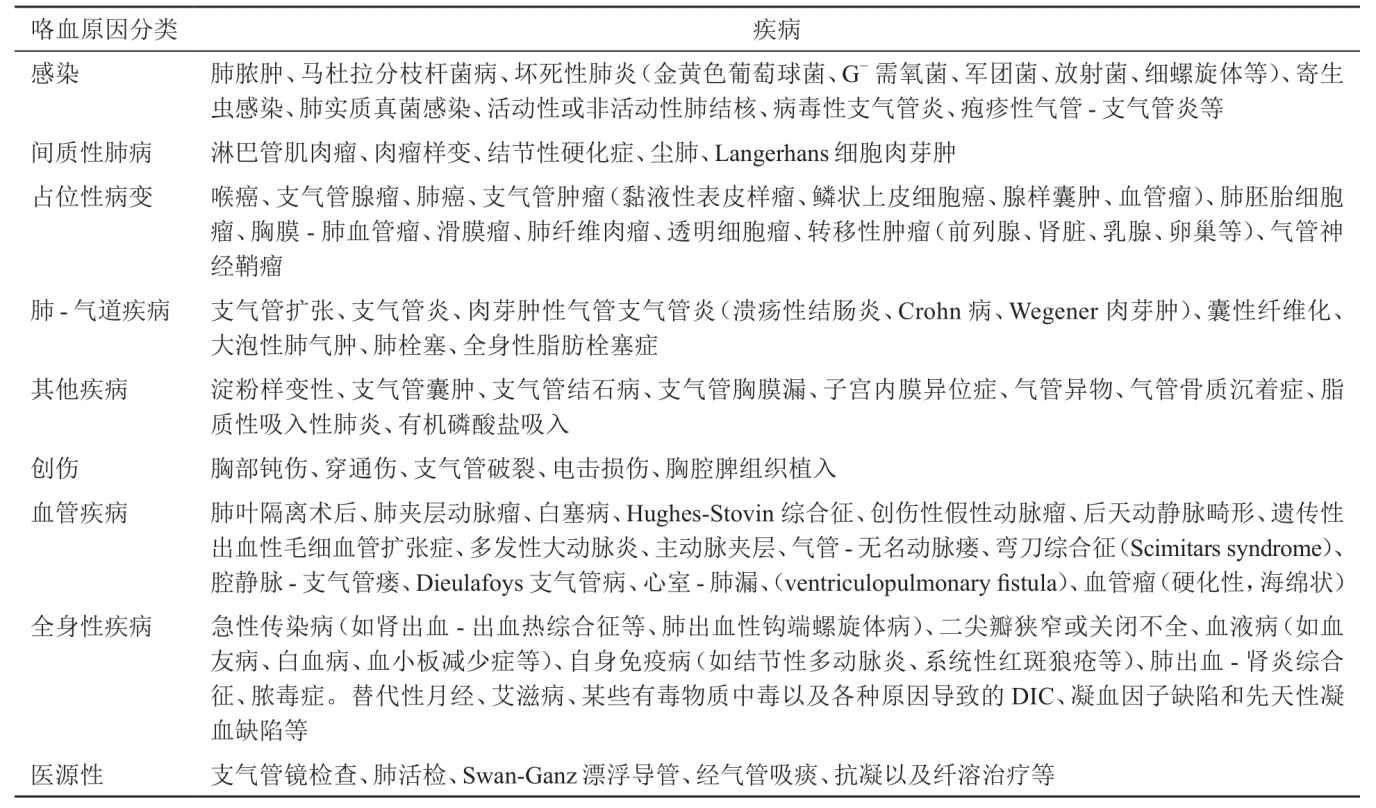
\includegraphics[width=6.59375in,height=3.875in]{./images/Image00045.jpg}
\end{table}

\subparagraph{气管、支气管疾病}

各种病原微生物如细菌、病毒、支原体、寄生虫以及肿瘤、各种粉尘、异物、结石等,均可侵蚀气道邻近血管或肺泡毛细血管导致咯血。支气管扩张导致的咯血常见,炎性病变侵蚀血管壁,使血管弹性纤维遭到破坏或在支气管壁下形成假性动脉瘤,当用力咳嗽时血管破裂导致大咯血;癌组织可直接侵蚀血管壁破裂导致咯血,少到痰中带血,多到大咯血窒息均可发生。

\subparagraph{肺部疾病}

许多肺部病变可直接侵蚀血管致使破裂出血或肺毛细血管床广泛损伤出血。大咯血最常见于肺结核(尤见于空洞性肺结核)、急性肺脓肿、癌性坏死及空洞形成、肺囊肿继发感染等,其穿行的支气管动脉或肺动脉受蚀,或动脉壁肌纤维破坏形成假性动脉瘤因咳嗽而破裂出血。此类咯血可因血凝块暂时充填空洞而压迫血管暂停出血,但也可因血凝块自溶而再次出现咯血。慢性肺脓肿多引起小量咯血,偶有大咯血发生。

\subparagraph{肺血管病变或先天性病变}

支气管动脉-肺动脉瘘是由于肺动脉因体循环压力,形成动脉瘤,破溃出血。肺动脉栓塞、多动脉炎、白塞病的病变基础多为栓塞性动脉炎或动脉瘤样扩张。夹层动脉瘤或梅毒性动脉瘤,偶与支气管动脉相通,可造成致命性大咯血。原发性肺动脉高压可因肺动脉远端阻力加大,肺动脉与肺毛细血管形成侧支循环,当血管破裂时引起咯血。偶见于先天性肺动-静脉瘘,先天性毛细血管扩张症引起的咯血。

\subparagraph{心血管疾病}

最常见的原因是二尖瓣狭窄和冠心病、心肌病等疾病导致的急性左心功能不全。左房血流受阻造成左房压力高,心脏前负荷增加,肺毛细血管及肺静脉压力升高,导致肺血管扩张,肺处于淤血状态,可引起肺水肿,并导致支气管黏膜下小静脉曲张,常自发或在炎症诱发下引起小静脉及毛细血管破裂,导致大咯血。

\subparagraph{全身性疾病}

脓毒症、肾出血-出血热综合征、出血型钩端螺旋体病等急性全身感染性疾病、血液病和某些自身免疫性疾病如大动脉炎、白塞病、系统性红斑狼疮、肺出血-肾炎综合征(Goodpasture
syndrome)、子宫内膜异位症等病变,使肺微血管和毛细血管受损,血管内皮细胞功能障碍,血管脆性增加以及血小板减少或功能障碍导致出血。此类咯血多为弥漫性肺泡出血。

\subparagraph{出凝血机制障碍}

包括血液系统疾病及DIC所致的咯血,多为全身多脏器出血的一部分。多见于全身性疾病导致的血小板减少和(或)功能障碍、凝血因子缺乏和(或)功能异常。此类咯血为原发病的继发性改变,罕见情况下咯血可能为首发症状。

\subsection{诊断思路}

多数咯血患者为突然起病,尤其第一次见到咯出鲜血,精神高度紧张,甚至有恐惧感,往往不能正确的诉说相关的症状及所见到血液的性状。因此,明确出血部位和出血原因显得尤为重要。

\subparagraph{确定出血部位}

口腔、鼻腔、咽喉部以及消化道出血有时可误认为咯血,特别是后鼻道出血多流入口腔或食管出血未经胃酸作用直接呕出时,有时会出现刺激性咳嗽而导致对出血部位判断的错误,即所谓的“假性咯血”(pseudo-hemoptysis)。对首次从口腔内咳或呕血者,在不能判断出血部位的情况下,应仔细寻找出血部位。对可疑鼻咽部出血者,应迅速邀请专科会诊以明确诊断。详细询问病史和仔细的体格检查多能明确。呕血在大多数情况下诊断并无困难,在临床上可依据临床表现、体格检查、辅助检查和实验室检查予以区别。

\subparagraph{临床表现特点}

除有原发病症状与体征外,大多数情况下,患者咯血前常有喉部痒感,血呈弱碱性,色鲜红,呈泡沫状,多混有痰液,咯血后数天内仍可咳出血痰。常见咯血病因的临床表现特点见表\ref{tab9-2}。

\begin{table}[htbp]
\centering
\caption{常见咯血原因的临床表现特点}
\label{tab9-2}
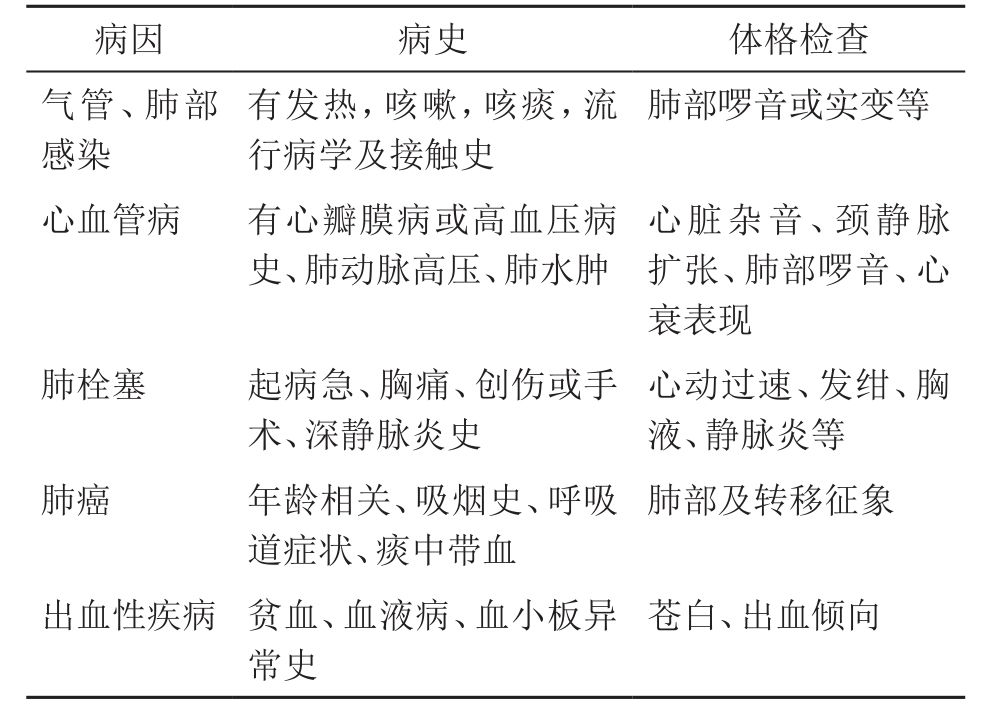
\includegraphics[width=3.26042in,height=2.38542in]{./images/Image00046.jpg}
\end{table}

大量咯血可引起急性出血性休克而出现面色苍白、冷汗、四肢湿凉,血管充盈度下降,血压降低等表现。因血凝块阻塞气道出现窒息的特征为咯血量突然减少或停止,同时出现胸闷、双手抓胸、喉头异常作响、继而烦躁不安、表情呆滞或恐惧、目瞪口张、全身发绀、呼吸变浅、速率加快,大小便失禁,肺部检查可见一侧或双侧呼吸音消失,进而呼吸突然停止。其他还包括肺不张和肺部继发感染等并发症的临床表现。

\subparagraph{咯血与呕血的鉴别}

大量呕血时,鲜红色血液可从口腔及鼻腔涌出,或大咯血时部分血液咽下,复又呕出,致使咯血与呕血不宜鉴别。正确的鉴别诊断有助于采取恰当的治疗措施。咯血与呕血的鉴别见表\ref{tab9-3}。

\begin{table}[htbp]
\centering
\caption{咯血与呕血的鉴别}
\label{tab9-3}
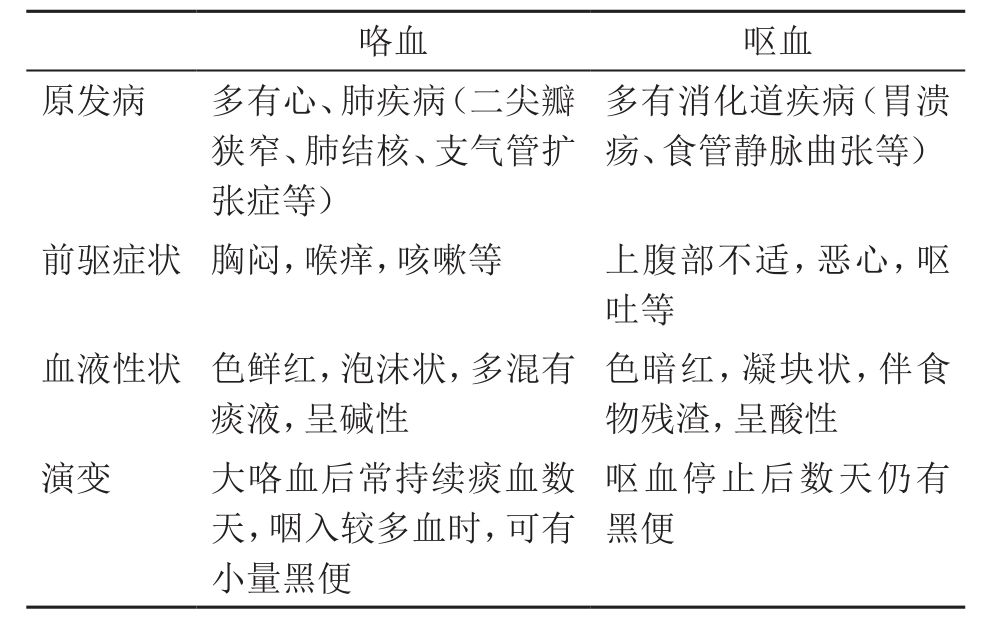
\includegraphics[width=3.26042in,height=2.05208in]{./images/Image00047.jpg}
\end{table}

\subparagraph{辅助检查与实验室检查}

\hypertarget{text00024.htmlux5cux23CHP1-9-2-4-1}{}
(1) 影像学检查:

胸部X线可初步判断胸部病变的性质和部位。胸部CT检查有助于支气管、肺部和胸腔疾病的病因诊断。尤其是高分辨CT(HRCT)可显示次级肺小叶为基本单位的细微结构,可明确病变的性质及范围,基本上已代替支气管造影。HRCT及核素扫描可明确心肺血管病变及占位性病变。必要时可作支气管动脉造影,但一般仅用于介入治疗前对出血部位的精准定位。

\hypertarget{text00024.htmlux5cux23CHP1-9-2-4-2}{}
(2) 超声与心电图检查:

心脏彩色多普勒与心电图检查对心脏病变诊断有帮助,可发现各种类型心脏结构改变、心律失常、ST-T段等改变。腹部B超有助于了解肝、脾、腹水、腹腔肿物等情况。

\hypertarget{text00024.htmlux5cux23CHP1-9-2-4-3}{}
(3) 血常规及生化检查:

可见白细胞总数增加,以中性粒细胞增加为主时提示感染存在。出血较多时可见红细胞和血红蛋白含量下降,血小板可正常。凝血功能、肝功能、肾功能等异常均能对其原发病提供参考。血气分析有助于发现病情较重患者的低氧血症。

\hypertarget{text00024.htmlux5cux23CHP1-9-2-4-4}{}
(4) 痰液检查:

细菌、真菌和细胞学检查有助于原发病的诊断和治疗。

\hypertarget{text00024.htmlux5cux23CHP1-9-2-4-5}{}
(5) 特异性检查:

如结核菌素试验、免疫学检查有时会对结核病、结缔组织疾病的诊断具有重要参考价值。

\hypertarget{text00024.htmlux5cux23CHP1-9-2-4-6}{}
(6) 纤维支气管镜检查:

可发现部分患者的出血部位和性质,并可在镜下止血,同时还可进行局部灌洗、标本取样做病原学和细胞学检查。

\hypertarget{text00024.htmlux5cux23CHP1-9-2-4-7}{}
(7) 动脉造影:

支气管动脉造影可显示区域性支气管动脉异常,确定出血部位,是决定进行栓塞治疗的主要依据。肺动脉造影对来自肺动脉的大咯血,尤其是支气管动脉栓塞后继续出血者适用。对空洞性肺结核或其他肺化脓性疾病、疑Rasmussen动脉瘤或肺动静脉瘘所致的咯血,选择性支气管动脉及肺动脉造影应同时进行,若病变波及双重动脉系统,则可以同时作栓塞治疗,以免术后继续出血。

\subparagraph{常见疾病鉴别诊断}

通过询问与咯血相关的病史、诱因、咯血量和伴随症状以及详细的体格检查多能寻找到原发疾病的线索。体格检查应注意有无肺部啰音、皮肤黏膜有无出血、淋巴结是否肿大、有无肝脾肿大、心脏杂音及体重减轻等。出血部位的判断可根据肺部体征及X线检查确定。

\hypertarget{text00024.htmlux5cux23CHP1-9-2-5-1}{}
(1) 支气管扩张:

缓慢起病,反复咳嗽伴脓痰和(或)量不等的咯血。既往多有麻疹、肺炎或免疫缺陷等病史。部分患者咯血为唯一症状,即所谓的“干性支气管扩张”。部分患者表现为反复发生的同一肺段感染,并迁延不愈,查体可闻及患侧固定而持久的湿啰音,可见杵状指(趾)等。胸部X线摄片或CT均可明确诊断。

\hypertarget{text00024.htmlux5cux23CHP1-9-2-5-2}{}
(2) 肺结核:

活动期多有午后低热、乏力、食欲减退、盗汗等结核中毒症状,部分可有不规则性高热。痰检或培养结核分枝杆菌阳性。查体可见结核面容、消瘦,局部湿啰音等。胸部X线摄片或CT表现多种形态,如局部渗出、增殖、纤维化、干酪性病变、钙化或空洞形成,以肺上叶尖后段及后基底段多见,可伴有胸腔积液、胸膜肥厚与粘连。聚合酶链反应(PCR)及结核菌素纯蛋白衍生物实验(purified
protein
derivative,PPD)有助于确定诊断,但后者不能区分是自然感染还是卡介苗免疫反应。

\hypertarget{text00024.htmlux5cux23CHP1-9-2-5-3}{}
(3) 肺癌:

持续出现咳嗽、咳痰,不明原因体重下降,近期痰中带血,反复出现。晚期可出现与呼吸运动有关联的胸痛及血性胸腔积液。查体可见气促、肺局限性喘鸣音、呼吸音增强或单侧胸腔积液、转移性骨压痛、淋巴结肿大(以颈部、腋窝为主,右锁骨上窝淋巴结肿大具有特殊诊断意义)等。胸部X线摄片或CT有助于诊断,痰液细胞学及活检可明确诊断。

\hypertarget{text00024.htmlux5cux23CHP1-9-2-5-4}{}
(4) 肺脓肿:

急性起病,多有劳累、受凉等病史。高热伴有不同程度的咯血。发病两周左右突然咳出大量脓痰及坏死组织,痰咳出后,体温下降。查体可发现局部湿啰音,偶可闻及空瓮音,宜可见杵状指(趾)。胸部X线摄片或CT和痰液细菌培养阳性多能明确诊断。

\hypertarget{text00024.htmlux5cux23CHP1-9-2-5-5}{}
(5) 风湿性二尖瓣狭窄:

有风湿性心脏病史。常在感冒、活动后出现呼吸困难,严重时不能平卧,常出现急性左心功能不全表现,伴以咳出大量粉红色泡沫样痰。小量咯血多见,偶见大量咯血。查体可见“二尖瓣面容”,心尖部听诊可及第一心音亢进、开瓣音、舒张中晚期隆隆样杂音、肺动脉瓣区第二心音亢进等,部分患者可摸到舒张期震颤。心脏多普勒超声检查可明确诊断。

\hypertarget{text00024.htmlux5cux23CHP1-9-2-5-6}{}
(6) 急性肺梗死:

有长期卧床、骨折、静脉炎或心房纤颤等病史。突然出现胸痛、胸闷、心悸、烦躁、冷汗,甚至晕厥,以小~中等量咯血多见。查体可见呼吸加快,肺局部叩诊浊音、呼吸音减弱及干湿性啰音。严重者可见急性右心衰表现,如心率加快、肺动脉瓣第二心音亢进、三尖瓣区可闻及收缩期杂音,可伴心律失常。血压下降,颈静脉怒张,肝脏增大、肝颈征阳性等。D-二聚体阳性及胸部X线摄片或CT有助于诊断。

\hypertarget{text00024.htmlux5cux23CHP1-9-2-5-7}{}
(7) 其他咯血的病因诊断:

其他一些肺部或全身性病变引起的咯血,根据发病特点和辅助诊断特征,大多数诊断并不是很困难。重要的是要想到一些引起咯血的少见原因,如肺血管畸形、血液病、结缔组织病、肺肉芽肿症、遗传性毛细血管扩张症、肺出血-肾炎综合征、经期性咯血等。弥漫性肺泡出血诊断的最好方法是通过灌洗获得肺泡巨噬细胞中的含铁血黄素来确定。目前ICU中出现的咯血日益增多,大多数为弥漫性肺泡出血,少部分为设备使用或操作不当导致的大咯血,应引起足够重视。

咯血病因诊断流程见图\ref{fig9-1}。

\subsection{病情评估}

咯血患者出现下列情况表明病情危重:咯血量较大,一次超过200ml,反复发作,一般止血措施不能控制;精神高度紧张或恐惧,呼吸困难、胸闷,双手无目的抓挠喉或胸部,表明出现窒息先兆;短期内即出现失血性休克表现;胸部X线片(或CT扫描)提示空洞或可疑病变侵及小动脉及假性动脉瘤破裂。

\subsection{处理原则}

咯血的急诊治疗取决于速度与量。大咯血抢救的重点在于迅速有效止血,保持呼吸道通畅,防治窒息及其他并发症,并同时进行病因、对症治疗。

\subsubsection{窒息的紧急处理}

咯血窒息是导致患者死亡的主要原因,应及早识别和抢救。窒息抢救的重点是保持呼吸道通畅和纠正缺氧。

\begin{figure}[!htbp]
 \centering
 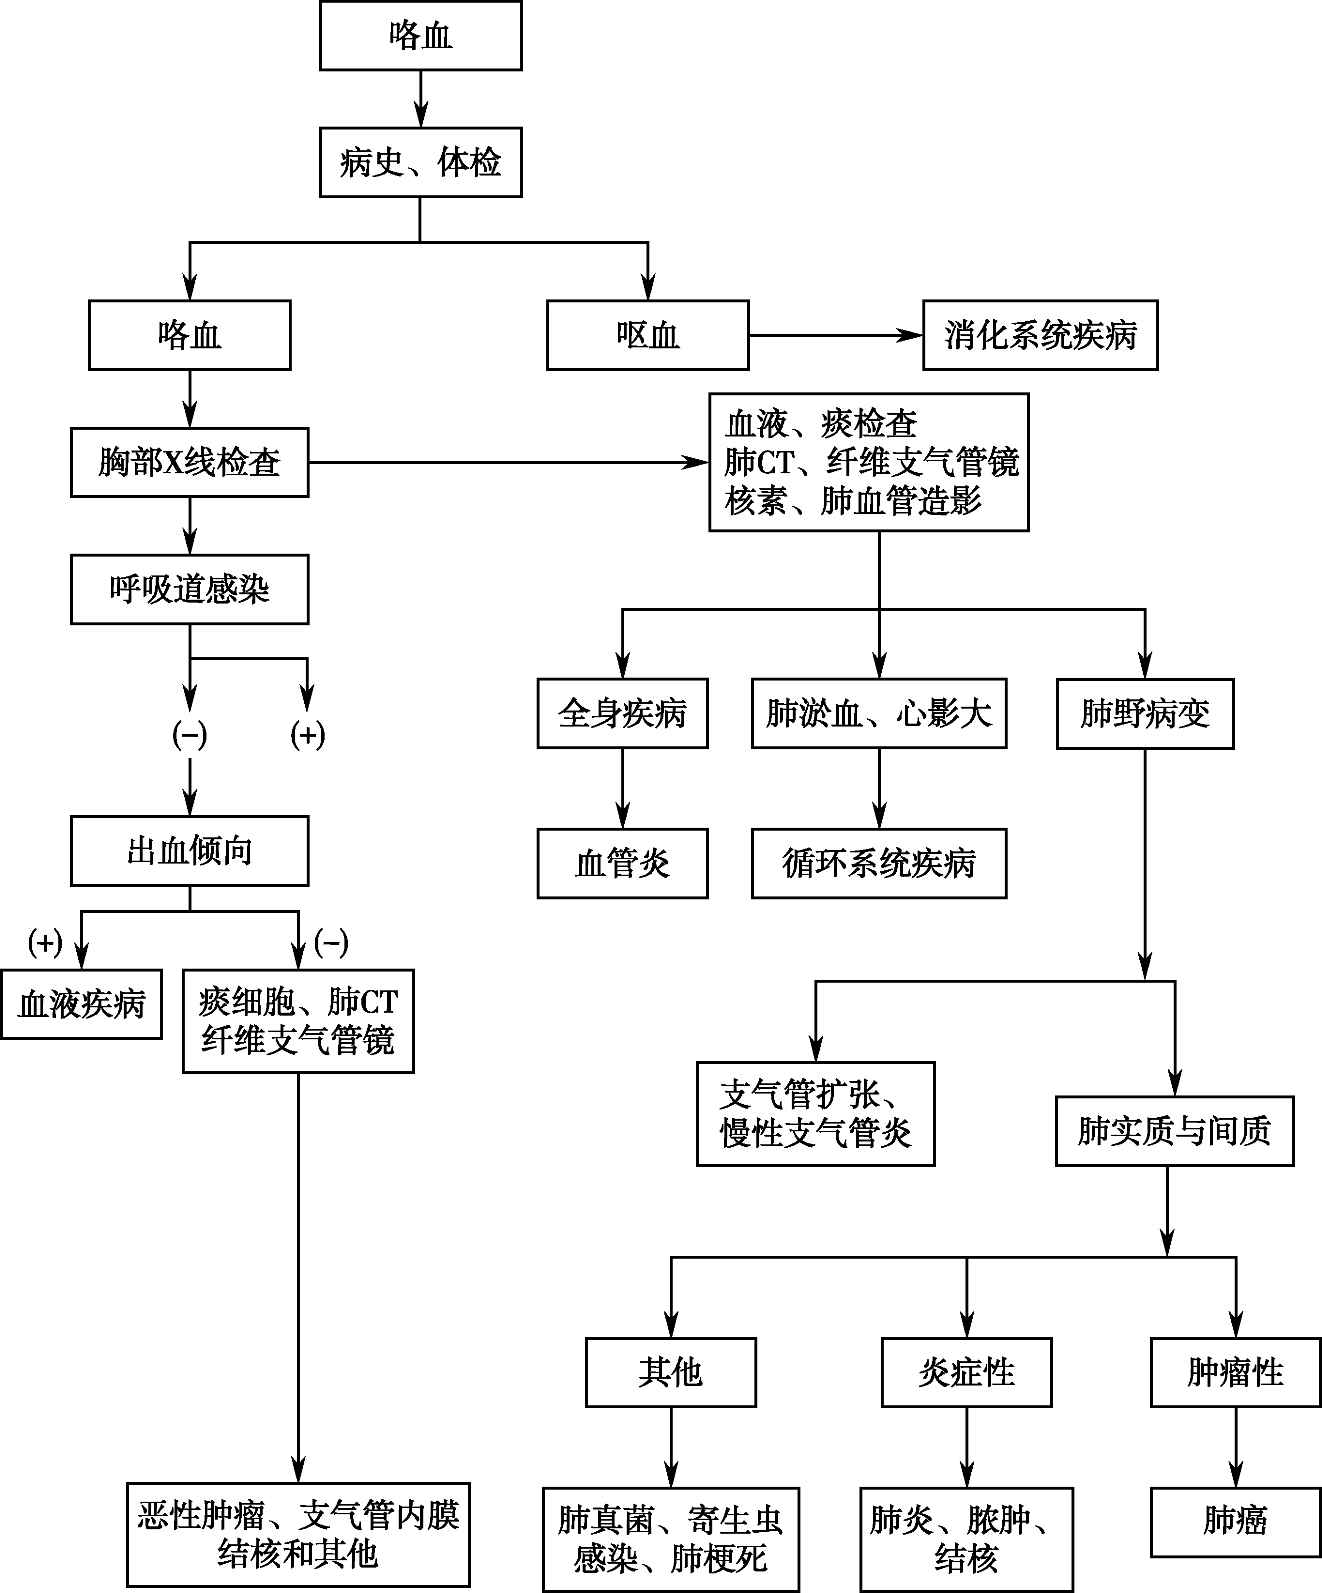
\includegraphics[width=4.55208in,height=5.47917in]{./images/Image00048.jpg}
 \captionsetup{justification=centering}
 \caption{咯血病因诊断流程图}
 \label{fig9-1}
  \end{figure} 

1.体位
患侧卧位,避免血液流向健侧。头低位,身体与床成40°~90°角,背部屈曲并拍击背部,促进肺内血液流出。病灶不明确者可暂取平卧位。同时清除口腔内血块。

2.保持呼吸道通畅
用导管自鼻腔插至咽喉部,用吸引器吸出血液(块),并刺激咽喉部,使患者用力咯出堵塞于气管内的血液(块),或在直接喉镜下作硬质支气管镜直接插管,通过冲洗和吸引,迅速恢复呼吸道通畅。

3.建立静脉通道 迅速建立静脉通道,补充血容量,使用止血药物,纠正休克。

4.镇静 根据病情需要,可适量给予镇静药物,如地西泮、氯丙嗪等。

5.机械通气 高浓度给氧(FiO\textsubscript{2}
30\%~40\%)或高频通气治疗。如自主呼吸微弱或消失,应立即进行气管插管或切开使用机械通气治疗。

6.若自主呼吸极弱或消失
,则应立即进行心肺复苏。在呼吸道通畅情况下同时使用呼吸兴奋剂。窒息解除后应及时对复苏后并发症进行处理,如纠正酸中毒、补充血容量、控制休克以及重要器官功能的监测与支持,如治疗和预防脑水肿、心肺功能不全、肾功能不全等。

大咯血患者应绝对卧床,尽量避免搬动或转送他院,颠簸可加重咯血,甚至导致死亡。如需转送,途中应将患者的头和身体偏向患侧或俯卧头低位,以利引流,防止窒息。密切观察患者的生命体征,包括意识、呼吸、脉搏和血压,随时做好抢救准备工作,尽可能准确记录咯血量。

\subsubsection{急诊处理}

\subparagraph{镇静 、休息与对症处理}

少量咯血,如痰中带血,一般无需特殊处理,适当减少活动量,对症治疗即可。中等量咯血应卧床休息;大量咯血则应绝对卧床休息。取患侧卧位,患侧可放置冰袋,嘱患者将血轻轻咳出,避免吸入性肺炎、肺不张或以防窒息,出血部位不明时取平卧位。对精神紧张、恐惧不安者,应解除不必要的顾虑,必要时可给少量镇静药,如地西泮(安定)10mg或苯巴比妥钠0.1~0.2g肌注,或口服地西泮、氯氮{}
(利眠宁)等。鼓励患者咳出滞留于呼吸道的陈血,避免呼吸道阻塞。对频咳或剧咳者,可给镇咳药如喷托维林(pentoxyverine,咳必清)25mg,每天3次;可待因15~30mg,每天3次或二氧丙嗪(克咳敏)5mg,每天3次口服。但大咯血时一般不用镇咳剂,如剧咳妨碍止血,可在血液咳出后临时使用可待因15~30mg口服或皮下注射,每日1~3次;对年老体弱、肺功能不全者不宜用,禁用吗啡、哌替啶等,以免过度抑制咳嗽,使血液及分泌物淤积气道,引起窒息。

\subparagraph{严密观察与护理}

进食易消化食物,保持大便通畅,避免用力屏气排便。对大、中量咯血者,应密切观察患者,做好大咯血与窒息的各项抢救准备,定期记录咯血量、测呼吸、脉搏和血压,若有口渴、烦躁、厥冷,面色苍白、咯血不止或窒息表现者,应立即进行抢救。

\subparagraph{止血药物的应用}

常用止血药物有:

\hypertarget{text00024.htmlux5cux23CHP1-9-4-2-3-1}{}
(1) 垂体后叶素(pituitrin):

疗效迅速而显著,使肺循环压力降低,肺小动脉收缩而利于血凝块形成。用法:大咯血时以垂体后叶素5~10U加25\%葡萄糖液20~40ml缓慢静脉注射(10~15分钟);咯血持续者可用垂体后叶素10~20U加5\%葡萄糖液500ml,缓慢静滴;禁用于高血压、冠状动脉疾病、肺源性心脏病、心力衰竭患者和孕妇。注射过快可引起面色苍白、心悸、出汗、胸或腹痛、血压升高等副作用,应及时减慢速度或停药。

\hypertarget{text00024.htmlux5cux23CHP1-9-4-2-3-2}{}
(2) 普鲁卡因(procaine):

用于对垂体后叶素有禁忌者。普鲁卡因150~300mg加5\%葡萄糖液500ml缓慢静滴,或普鲁卡因50mg加25\%葡萄糖液40ml,缓慢静注。本药可诱发过敏反应,用药前应作皮试。药物使用量过大或注射过快,可导致惊厥、谵妄、兴奋、面色潮红,应立即停药,对症处理。

\hypertarget{text00024.htmlux5cux23CHP1-9-4-2-3-3}{}
(3) 酚妥拉明:

为α-肾上腺素能受体阻滞剂,能有效扩张血管平滑肌,降低肺循环阻力及心房压、肺毛细血管楔压和左心室充盈压,可起到较好的止血作用。酚妥拉明10~20mg加入5\%葡萄糖液250~500ml中持续静滴。使用时监测血压并保持有足够的血容量。

\hypertarget{text00024.htmlux5cux23CHP1-9-4-2-3-4}{}
(4) 纠正凝血障碍药物:

①6-氨基己酸(氨己酸,EACA):6.0g +
5\%葡萄糖液250ml静滴,通过抑制纤维蛋白溶酶形成达到止血目的,适用于肺部疾病、血液病引起的咯血。②氨甲苯酸(对羧基苄胺,PAMBA):100~200mg
+ 25\%葡萄糖液40ml静滴,或200mg +
5\%葡萄糖液500ml静滴,适用于纤维蛋白溶解亢进引起的出血。③氨甲环酸(AMCA):AMCA
250mg + 25\%葡萄糖液40ml静注;或AMCA 750mg +
5\%葡萄糖液500ml,静脉滴注。④肾上腺色腙(安络血):通过抑制毛细血管通透性、增加毛细血管抵抗和加速管壁回缩发挥止血作用。10~20mg肌肉注射,1日2次,或5mg
1日3次口服。⑤酚磺乙胺(止血敏):有收缩肺毛细血管、增加毛细血管抵抗、加速管壁回缩及轻微的促血小板聚集作用。0.25~0.75g肌肉注射或缓慢静脉注射,1日2~3次,静脉注射不宜过快,以免血压下降。⑥注射用血凝酶(立止血):该药对纤维蛋白原的降解有选择性作用,在出血部位生理性凝血因子的作用下,纤维蛋白多聚体迅速形成稳固的纤维蛋白,在出血部位发挥凝血作用。1~2U静脉注射或肌肉注射,1日1~2次。

\hypertarget{text00024.htmlux5cux23CHP1-9-4-2-3-5}{}
(5) 其他止血药物:

硝酸甘油适用于与垂体后叶素合用,5~10mg加入5\%~10\%葡萄糖液250~500ml中静滴;氯丙嗪能降低肺循环、左心室与支气管动脉压力,必要时可小剂量(10~15mg)配合使用,肝、肾功能不全者慎用。另外,阿托品、654-2、高渗氯化钠、糖皮质激素、中药如白连粉、三七粉、云南白药等、鱼精蛋白注射液、维生素C、凝血酶原复合物等根据病情均可酌情选用。

\subparagraph{维持血容量}

持续大咯血出现循环容量不足时应及时补充血容量。输注新鲜血不但能补充血容量外,而且还有止血作用。

\subparagraph{手术止血}

对反复咯血,上述治疗无效,出血部位明确而无手术禁忌者,可采用手术止血。指征包括:①肺部病变(如各型结核动脉破裂、支气管扩张、肺脓肿、肺癌等)所引起的致命性大咯血;②可能发生气道阻塞和(或)窒息者。

\subparagraph{局部止血治疗}

适用于大咯血并发窒息和严重反复咯血、病情严重、肺功能较差、不适于手术治疗者。前提是出血部位明确,经气管插管或支气管镜边插边吸,到达出血部位后,将导管由活检孔插入至出血部位,注入冷生理盐水(4℃),每次50ml,留置30~60秒种后吸出,反复数次,直至出血停止,通过冷刺激使血管收缩达到止血的目的;或者注入凝血酶200~400U,或去甲肾上腺素液1~2mg稀释后局部使用。

\subparagraph{支气管动脉栓塞}

对药物治疗无效且不能手术治疗的患者,是可选择的治疗方法之一。经股动脉插管,将漂浮导管插到病变区域支气管动脉分支的血管腔内,注入明胶海绵或聚乙烯醇微粒(直径0.5~2.0μm),栓塞支气管动脉,以达到止血目的。因肺循环可能有多支动脉供血,本法对不是来自支气管动脉(侧枝血管)破裂的咯血无效,而且造影剂和栓塞物还可能进入脊髓动脉,引起脊髓缺血损伤,因此应严格掌握适应证。

\subparagraph{肺不张和肺炎的治疗}

采用体位引流(侧卧位,患侧在上),雾化吸入,使用解痉药、祛痰药,应用抗生素预防和控制感染。

\subparagraph{病因治疗}

尽快明确病因,采用相应治疗措施。

\protect\hypertarget{text00025.html}{}{}

\hypertarget{text00025.htmlux5cux23CHP1-9-5}{}
参 考 文 献

1. Parrillo,Dellinger. Critical Care Medicine:Principles of Diagnosis
and Management in the Adult. 3th ed. Elsevier Inc,2008

2. Stone CK,Humphries. Current Emergency Diagnosis and Treatment. 5th
ed. New york:Lange/McGraw,2004

3. John A Marx. Rosen's Emergency Medicine. Concepts and Clinical
Practice. 6th ed. St. Louis:Mosby Inc,2006

4. 徐腾达,于学忠.现代急症诊断治疗学.北京:中国协和医科大学出版社,2007

5. 沈洪.急诊医学.北京:人民卫生出版社.2007

\protect\hypertarget{text00026.html}{}{}

\chapter{急 性 腹 痛}

腹痛(abdominal
pain)是指由于各种原因引起的腹腔内外脏器的病变,而表现在腹部的疼痛。可分为急性与慢性腹痛两类。急性腹痛(简称急腹痛)是临床最常见急症之一,其病因繁杂,病情多变,涉及学科广,内、外、妇产、儿及传染病等科疾病均可引起,诊断处理不当,常可造成恶果,因而对急性腹痛必须尽快作出定位、定性及病因诊断,以防误诊、漏诊及误治,从而改善预后。对生育期女性的急性腹痛须请妇产科医生会诊,以排除妇产科急腹症。

\subsection{病因与发病机制}

\subsubsection{病因}

引起腹痛的病因颇多,大体可分为腹腔内脏器疾病及腹腔外脏器疾病两大类,每类又可分为器质性病变及功能性失调;器质性病变包括脏器的急性炎症、损伤、破裂、穿孔、梗阻、扭转、出血、坏死等;功能性失调有痉挛、麻痹、神经功能紊乱及功能暂时性失调等(详见表\ref{tab10-1})。

\subsubsection{发病机制}

腹痛依发生机制分为三型,即真性内脏痛(true visceral
pain,内脏痛):由内脏本身病变所致;类似内脏痛(somatic
pain,体性痛,体壁性内脏痛):由内脏病变累及壁层腹膜,经躯体神经传入引起疼痛;放射痛(referred
pain,牵涉痛):内脏病变引起某一局部疼痛,痛处常非病变部位。

\subparagraph{内脏痛}

多由消化道管壁平滑肌突然痉挛或强力收缩,管壁或脏器突然扩张,急性梗阻、缺血等刺激内脏传入神经末梢产生冲动所致,常为脏器本身的疼痛。

\subparagraph{体性痛}

壁层腹膜分布着脊髓性感觉神经,脏层腹膜上虽无感觉受体,但近脏器的肠系膜、系膜根部、小网膜及膈肌等均有脊髓性感觉神经,当脏器病变累及其感觉神经时产生冲动,经上行传导达丘脑,再经交换神经元达大脑皮质。丘脑可感知疼痛,大脑可识别疼痛的部位、程度和性质。故体性痛多剧烈,疼痛及压痛部位明确,与体位有关,变换体位常可使疼痛增重。

\subparagraph{放射痛}

亦称牵涉痛或感应性痛。由于某种病理情况致身体某一局部发生疼痛,且痛处常非病变所在,此因放射痛部位与病变脏器的感觉常来自同一节段神经纤维。放射痛的特点为常伴有Head皮肤感觉过敏带(内脏皮肤过敏带)及腹壁紧张。

Head皮肤过敏带即腹腔内脏器疾病的病理性冲动,刺激内脏神经经交感神经传入相应或同一脊髓段的后根,由此发出的脊神经产生感应,将冲动传到体表一定部位致皮肤相应节段感觉过敏性疼痛,或引起远隔部位脏器痛。如胆绞痛向右肩背部放射;小肠绞痛放射到脐周;胃、十二指肠病变可放射到剑脐间等。

\begin{table}[htbp]
\centering
\caption{急性腹痛的病因分类}
\label{tab10-1}
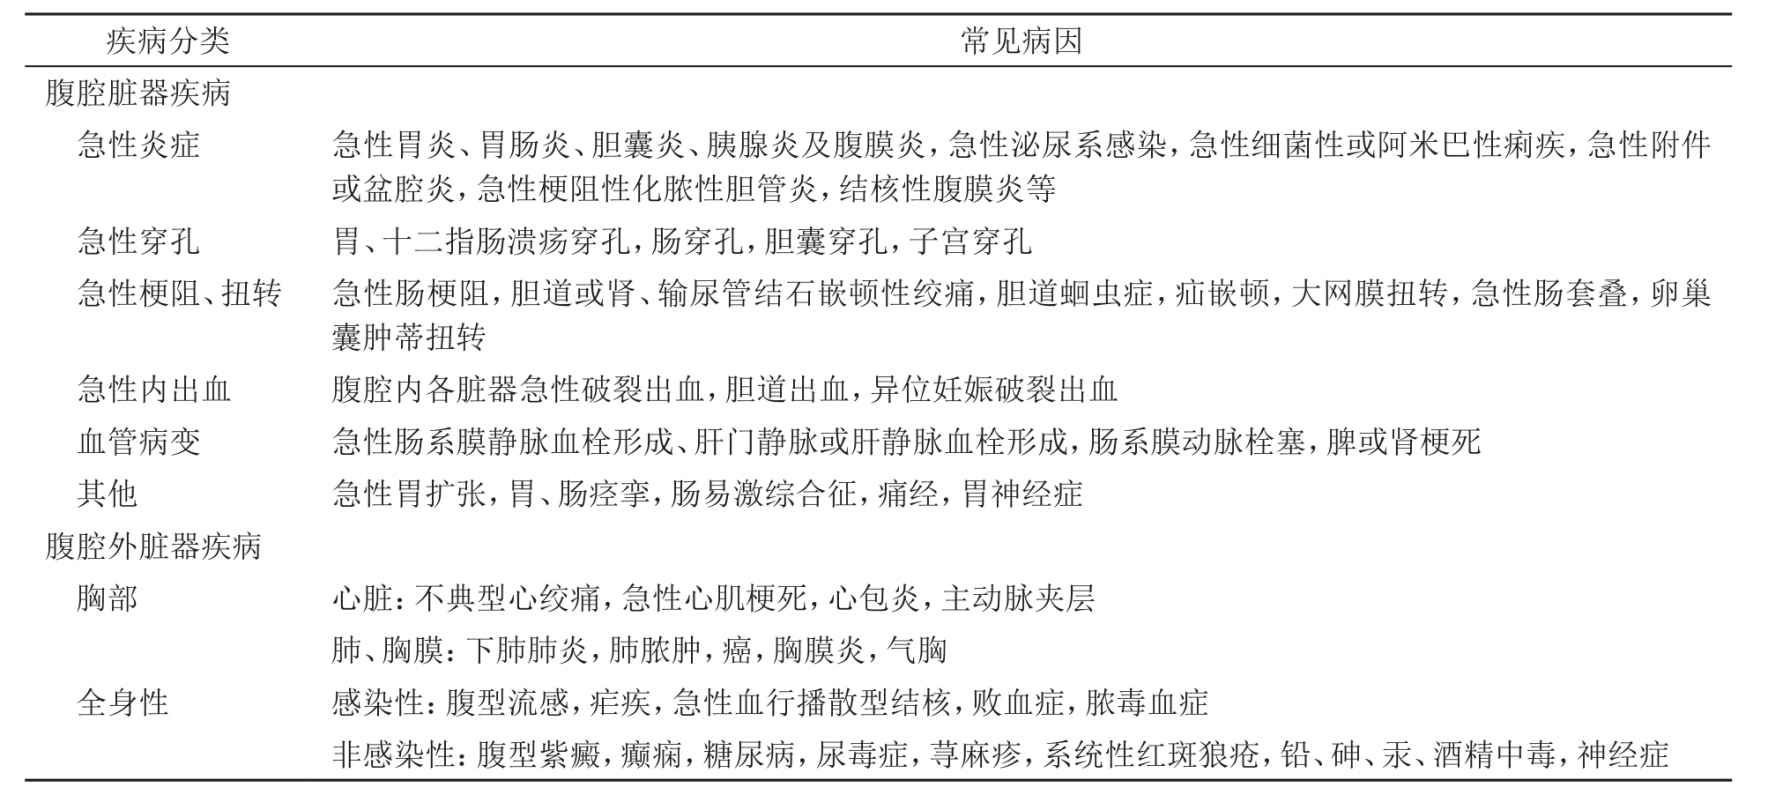
\includegraphics[width=6.67708in,height=3in]{./images/Image00050.jpg}
\end{table}

\subsection{诊断思路}

\subsubsection{病史及体检}

准确而简要的病史询问,全面而有重点的体检,对急性腹痛的诊断十分重要。

\hypertarget{text00026.htmlux5cux23CHP1-10-2-1-1}{}
(一) 年龄、性别、既往史

\subparagraph{年龄 、性别}

不同年龄及性别常有不同的多发病,如婴幼儿多见先天性消化道畸形,尤其是胃肠道(肠闭锁或狭窄,肛门闭锁、先天性肥厚性幽门狭窄等)及胆道(先天性胆道闭锁或狭窄);幼儿多见肠寄生虫病、肠套叠、疝嵌顿等;青壮年多见急性阑尾炎、胃肠穿孔、肠梗阻、腹部外伤致脏器破裂内出血等;老年人则胃肠道癌肿及并发症(穿孔、梗阻、出血),胆结石或胆囊炎及血管疾病多见。急性胆道疾病、胰腺炎女多于男,溃疡病穿孔、急性阑尾炎及肠梗阻则男多于女。引起急性腹痛的妇产科疾病,如急性附件或盆腔炎,异位妊娠或破裂,卵巢囊肿蒂扭转,子宫破裂、穿孔等及痛经。

\subparagraph{既往史}

应重点询问以往有否引起急性腹痛的病史,有无类似发作史;手术史、月经生产史、外伤史及有害物接触史等。

\hypertarget{text00026.htmlux5cux23CHP1-10-2-1-1-2-1}{}
(1) 有类似发作史者:

应考虑胆石症、胆囊炎、泌尿系结石、慢性阑尾炎或慢性胃炎急性发作,溃疡病活动或出血、穿孔,疝反复嵌顿,胃肠神经症等。

\hypertarget{text00026.htmlux5cux23CHP1-10-2-1-1-2-2}{}
(2) 手术史:

溃疡病胃次全切除术后吻合口溃疡、出血或狭窄,肠粘连或粘连性肠梗阻,膈下或盆腔脓肿等。

女性患者应注意有无痛经史,闭经且发生急性腹痛者应考虑异位妊娠、早期流产,若伴休克,应高度疑及异位妊娠破裂内出血等。

\hypertarget{text00026.htmlux5cux23CHP1-10-2-1-2}{}
(二) 注意腹腔内、外疾病所致急性腹痛的不同特点

\subparagraph{腹腔内疾病急性腹痛的特点}

①常伴有消化道症状,如恶心、呕吐、腹泻、腹胀等。②常有与进食有关的诱因,如暴饮暴食、高脂饮食、酗酒、进食过刺激、不洁或变质食物等。③腹部体征较明显且固定(痛、压痛、叩痛、反跳痛等)。④无腹外及全身疾病表现。

\subparagraph{外科或妇产科疾病所致急性腹痛的特点}

①腹痛突然发作,剧烈,急剧发展,不及时处理,短期内病情常迅速恶化。②表情痛苦,呻吟,大汗,面色苍白,辗转不安或蜷曲静卧。③可有腹膜刺激征(腹肌紧张呈板状,压痛、反跳痛明显)及肝浊音界缩小或消失。④可有内出血综合征,如头晕、心慌、多汗、面色苍白、脉细速、血压下降等。⑤急诊腹透可见膈下游离气体、高度胀气、鼓肠或胃扩张、梯形液气平面等。⑥发病短期内白细胞明显增高,中性及杆状核增高,中毒血象,进行性贫血等。

\subparagraph{内科腹腔脏器疾病所致急性腹痛的特点}

①腹痛可轻可重,短期内病情不恶化。②症状与体征不一致,主观感觉腹痛剧烈,表情痛苦,但检查腹部体征不显著,多腹软,局部轻压痛或压痛,无反跳痛。③发病短期内血象正常或稍高,无中毒血象。④急诊腹透无阳性发现。

\hypertarget{text00026.htmlux5cux23CHP1-10-2-1-3}{}
(三) 依急性腹痛部位诊断

即依据解剖部位来推断可能的病因(表\ref{tab10-2})。最早发生腹痛及压痛最明显的部位常是发生病变的部位(早期及异位阑尾炎例外)。

\hypertarget{text00026.htmlux5cux23CHP1-10-2-1-4}{}
(四) 依病史、体征及伴随症状综合分析

\subparagraph{起病方式}

突然发作剧痛,多为胆道蛔虫症、胆道或泌尿道结石嵌顿、疝嵌顿、急性胆囊炎或胰腺炎、消化道急性穿孔、腹腔脏器破裂、急性心肌梗死、心绞痛等。持续性腹痛阵发性加重常示有痉挛或梗阻;初期呈进行性加重多为急性炎症;暴饮暴食、高脂饮食、酗酒、过刺激或不洁食物、激烈运动等诱发急性腹痛应考虑急性胆囊炎、胰腺炎或胃肠炎,溃疡病穿孔,肠或卵巢囊肿蒂扭转,疝嵌顿等。

\subparagraph{绞痛及放射痛}

\begin{table}[htbp]
\centering
\caption{急性腹痛部位与疾病关系}
\label{tab10-2}
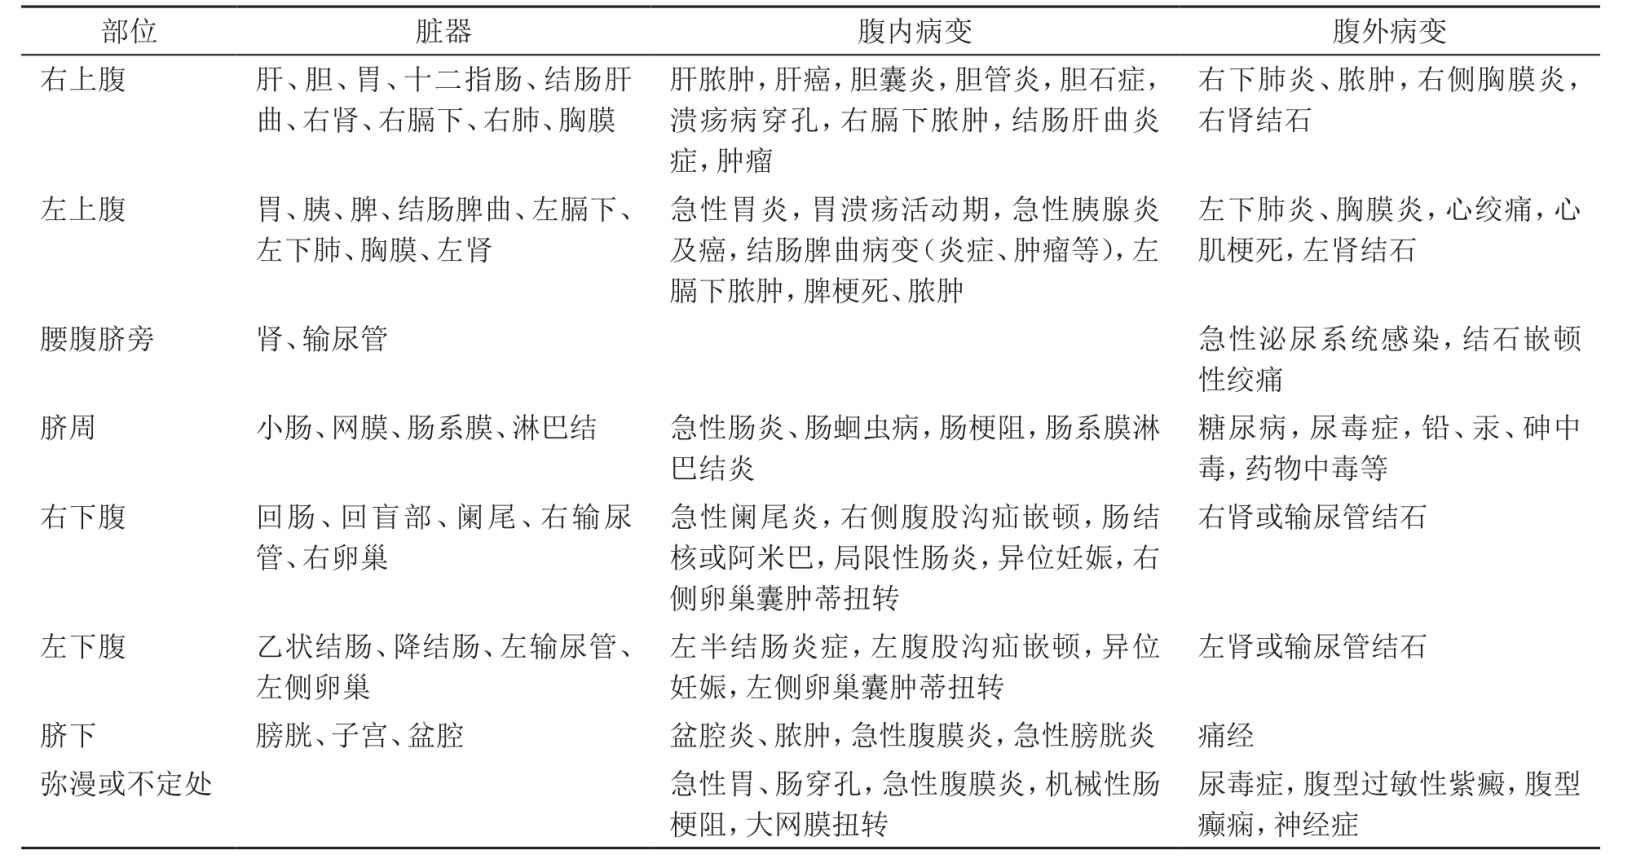
\includegraphics[width=6.71875in,height=3.52083in]{./images/Image00051.jpg}
\end{table}

①胆绞痛:右上腹痛向右肩胛及右背部放射。②胰腺绞痛:上腹或中上腹部向左侧腰背部放射。③小肠绞痛:脐周剧痛。④肾绞痛:肾区痛沿腹直肌外缘向大腿内侧或会阴部放射。⑤子宫或直肠病变绞痛:腰骶部或下腹部剧痛或坠痛。

\subparagraph{伴发症状}

\hypertarget{text00026.htmlux5cux23CHP1-10-2-1-4-3-1}{}
(1) 伴发热:

①先发热后腹痛多为不需手术治疗的内科性疾病(常为急性炎症)。②先腹痛后发热的多为外科或妇产科疾病,且常需手术治疗(如急性消化道穿孔、腹膜炎、肠梗阻、异位妊娠破裂、内脏破裂出血等)。③急性腹痛伴寒战、高热,应考虑急性化脓性胆囊炎、胆管炎,腹腔或腹内脏器的化脓性病变(膈下或盆腔脓肿、化脓性腹膜炎),下肺炎症或脓肿等。

\hypertarget{text00026.htmlux5cux23CHP1-10-2-1-4-3-2}{}
(2) 伴呕吐:

急性腹痛伴呕吐者常为急性胃、胆囊、胰腺等炎症,肠梗阻,胆道或泌尿道结石嵌顿,胃型感冒,肠套叠,痛经,神经症等。

\hypertarget{text00026.htmlux5cux23CHP1-10-2-1-4-3-3}{}
(3) 与排便的关系:

①腹痛伴腹泻:急性肠炎、痢疾、急性盆腔炎、急性阑尾炎、高位肠梗阻等。②腹痛伴血便:绞窄性肠梗阻、肠套叠、溃疡性结肠炎、坏死性肠炎、缺血性疾病(栓塞或血栓形成)等。③腹痛伴便秘或停止排便及肛门排气:为习惯或非习惯性便秘、肠梗阻等。

\hypertarget{text00026.htmlux5cux23CHP1-10-2-1-4-3-4}{}
(4) 伴腹胀:

急性胃扩张、麻痹性肠梗阻、便秘、尿潴留等。

\hypertarget{text00026.htmlux5cux23CHP1-10-2-1-4-3-5}{}
(5) 伴黄疸:

①右上腹痛伴黄疸者多为肝、胆系统疾病(炎症、结石、肿瘤等)。②中上腹或左中上腹痛伴黄疸多为胰腺(炎症、结石、肿瘤)或脾脏病变(脾梗死)。③右上腹痛伴寒战、高热、黄疸,应考虑急性胆囊炎,胆结石嵌顿伴炎症,急性化脓性胆囊、胆管炎,急性肝脓肿及少数膈下脓肿。

\hypertarget{text00026.htmlux5cux23CHP1-10-2-1-4-3-6}{}
(6) 与排尿关系:

腹痛伴膀胱刺激征或血尿者多为急性泌尿系感染、结石嵌顿;部分阑尾炎、盆腔脓肿也可引起膀胱刺激征,应注意鉴别。

\hypertarget{text00026.htmlux5cux23CHP1-10-2-1-4-3-7}{}
(7) 与体位的关系:

①辗转不安,腹痛喜按多为胃肠道疾病;拒按多为肝、胆系疾病。②活动疼痛加剧,蜷曲侧卧疼痛减轻多为腹膜炎。③前倾坐位或膝胸位疼痛减轻多为胰腺疾病。

\hypertarget{text00026.htmlux5cux23CHP1-10-2-1-4-3-8}{}
(8) 伴腹水:

①伴血性腹水:腹腔内脏或异位妊娠破裂,恶性肿瘤腹腔内转移,腹膜恶性肿瘤,少数结核性渗出性腹膜炎等。②脓性腹水:化脓性腹膜炎。③胰性腹水:乳糜状,浆液或浆液血性,淀粉酶含量增高且大于血中含量,蛋白量增高,对利尿剂及放腹水疗效差,见于急性出血坏死型胰腺炎或胰腺假囊肿破裂。④胆汁性腹水:化脓性胆囊炎或胆管炎破裂致胆汁性腹膜炎。

\hypertarget{text00026.htmlux5cux23CHP1-10-2-1-4-3-9}{}
(9) 伴休克:

应考虑下列疾病:①急性内出血:腹腔内脏器破裂或异位妊娠破裂。②急性穿孔致弥漫性腹膜炎。③腹腔内脏器或卵巢囊肿蒂扭转。④腹腔内急性血管性病变(肠系膜动脉栓塞或静脉血栓形成)。⑤急性心肌梗死或休克型肺炎。

\hypertarget{text00026.htmlux5cux23CHP1-10-2-1-4-3-10}{}
(10) 伴包块:

应考虑相应部位的急性炎症、肿瘤、肠套叠或扭转。

\hypertarget{text00026.htmlux5cux23CHP1-10-2-1-4-3-11}{}
(11) 与外伤关系:

急性腹痛发生前有外伤史者应考虑腹腔脏器破裂、内出血等。

\subsubsection{辅助检查}

\subparagraph{血液检查}

①血红蛋白及红细胞计数:可提示有无内出血致贫血(但早期由于脾脏及骨髓代偿性释放以及血液浓缩,可显示不出贫血或与临床实际贫血程度不符)。②白细胞计数及分类:可提示是否感染、感染程度等。

\subparagraph{大便检查}

外观:颜色、性状(成形、糊状、水样、血便、脓血便、黏液便或脓血黏液便等)。镜检:有无红、白细胞,虫卵、真菌、阿米巴滋养体等及潜血试验。

\subparagraph{尿液检查}

尿pH、蛋白、糖、酮体、胆红素、红细胞、白细胞、管型、细菌、真菌等,育龄女性应查尿妊娠试验。

\subparagraph{生化检查}

依病情需要可作:①血、尿淀粉酶测定;②血钾、钠、氯、钙,血糖,酮体等测定;③肝、肾功能测定等。

\subparagraph{心电图检查}

对40岁以上患者,既往无慢性胃病史,突然发作上腹痛应常规作心电图,以识别有无心脏及心包病变。

\subparagraph{X线检查}

①胸部X线检查:有助于肺炎、肺脓肿、肺癌、胸膜炎、气胸、肝或膈下脓肿等的诊断。②腹部X线检查:消化道急性穿孔致膈下游离气体,肠梗阻的梯形液气平面,急性胃扩张,高度鼓肠等。另外,胆道或泌尿道阳性结石等。

\subparagraph{超声波检查}

B超检查对肝、胆、胰、脾、肾、输尿管、子宫及其附件、盆腔、腹腔等探查均有较强分辨(实质性、囊性、良性、恶性、积液、结石等)及诊断能力,对胃肠道疾病可提供一定的诊断线索。

\subparagraph{内镜检查}

急诊内镜检查(胃、十二指肠、胆道、腹腔及结肠镜检查),对急性腹痛的诊断具有极其重要意义。可依临床初步拟诊病变部位,选择相应内镜检查,以助诊断及内镜直视下取活检或治疗。

\subparagraph{腹部}

CT检查
主要检查肝、胆、胰、脾、肾、膀胱、腹腔及盆腔等部位,可诊断其形态、大小、密度、占位性病变(实质性、囊性)、结石及腹腔、盆腔有无积液、肿大淋巴结等。

\subparagraph{诊断性腹腔穿刺术}

根据穿刺液性质可确定腹膜炎性质,有无内出血(脏器破裂或异位妊娠破裂)等。

\subparagraph{阴道后穹隆穿刺术}

主要用于判断异位妊娠破裂出血、盆腔脓肿或盆腔积液。

\subsubsection{急性腹痛的病因诊断线索}

急性腹痛的病因繁多。为尽早明确诊断,应在完成病史采集、体格检查和必要的辅助检查之后,对所得资料进行综合分析,作出正确的病因诊断。下述诊断思路,有助于最终确定病因诊断。

\hypertarget{text00026.htmlux5cux23CHP1-10-2-3-1}{}
(一) 确定是腹腔内病变或腹腔外病变

急性腹痛的诊断 ,首先要确定是腹腔内病变还是腹腔外病变。

\subparagraph{腹腔内病变}

常有消化道症状如恶心、呕吐、腹痛、腹泻等,腹痛程度不一,多有较明确诱因。腹部体征依病因而异,一般较明显,腹外与全身性症状轻微或缺乏。

\subparagraph{腹腔外病变}

胸部疾病引起的腹痛位于脐上的同侧腹部,可有压痛,但一般无反跳痛及肌紧张,胸部检查可发现有关疾病的心肺体征,胸部X线检查、心电图检查、心肌酶学检查等有助于诊断。全身性疾病所致的腹痛有原发病的表现,腹痛多由于电解质紊乱、代谢失调或毒素刺激所致,位于全腹或部位多变,一般无腹膜刺激征。

\hypertarget{text00026.htmlux5cux23CHP1-10-2-3-2}{}
(二) 确定是外科或非外科急性腹痛

\subparagraph{外科急性腹痛}

是指急需外科处理,或病情的发展有需要外科处理可能性的急性腹痛。对急性腹痛患者,应先明确是否为外科急性腹痛。此类腹痛常有以下特点:①剧烈而急起的腹痛多先于发热或呕吐,发热多于腹痛后4~6小时出现,但细菌性肝脓肿、脾脓肿和伤寒肠穿孔等例外。若腹痛超过6小时而患者体温反而降低或低于正常,则应考虑并发休克、大出血或严重感染毒血症的可能。②腹痛部位明确,有固定区,患者多“拒按”腹痛区。③常伴腹膜刺激征。腹痛、固定性压痛点和肌紧张的程度常是越来越严重,提示病变呈进行性发展。④腹式呼吸减弱或消失,肠鸣音亢进或消失,机械性肠梗阻时可闻及高调肠鸣音,而弥散性腹膜炎、麻痹性肠梗阻则肠鸣音减弱或消失。⑤可有肝肺浊音界消失,腹部移动性浊音阳性。⑥腹痛时腹部膨隆或可见胃肠型及蠕动波,并可触及腹部包块或索状物等。⑦腹腔穿刺可有血性或脓性液体等。

\subparagraph{内科急性腹痛}

其特点:①一般先有发热或呕吐、腹泻而后出现腹痛。②腹痛可轻可重,腹部体征不明显,无固定而局限性压痛点,无腹膜刺激征。患者常喜按。③腹式呼吸存在,肠鸣音正常或活跃。④可有与腹痛有关的内科疾病的阳性体征。⑤血白细胞正常或升高。

\subparagraph{妇产科急性腹痛}

其特点:①由于女性生殖器官集中于下腹部盆腔内,所以妇产科疾病引起的腹痛多局限于中下腹、盆腔,并向会阴和骶尾部放射。②腹痛多与月经、妊娠有关,月经期曾患过上呼吸道感染或有过性生活,多为急性盆腔炎;卵泡破裂多发生在排卵期;宫外孕有停经史,可有早孕反应等。③可伴有腹腔内出血、阴道出血或分泌物增加。④妇科检查常有阳性体征发现。

\subparagraph{小儿内科急性腹痛}

其特点:①常以发热、咽痛、咳嗽等症状先于腹痛。②急性腹痛而腹壁柔软,无压痛,腹部无包块、肠型等腹部体征。③腹痛范围广,不规则性,但排便基本正常。④可伴有呕吐等。⑤腹部外疾病引起腹痛者,可发现原发病变部位的阳性体征。

\hypertarget{text00026.htmlux5cux23CHP1-10-2-3-3}{}
(三) 确定急性腹痛的性质

根据常见的病变性质可将急性腹痛归纳为以下七类:

\subparagraph{炎症性急性腹痛}

基本特点为:腹痛+发热+压痛或腹肌紧张。

临床特点有:①一般起病较缓慢,多由轻渐重。②持续性腹痛。因脏器或腹膜的炎症、充血、水肿,刺激神经而引起急性腹痛,多呈持续性腹痛进行性加重。因发病的部位、病变程度及其病理变化不同,而呈局限性或全腹性疼痛。疼痛多发生于病变所在的部位。③当炎症病变波及脏器浆膜和壁层腹膜时,则呈典型的局限性或弥漫性腹膜刺激征,即腹肌紧张、压痛和反跳痛,尤其是以病变所在部位最明显。④早期可出现全身感染征象,如寒战、发热、脉快和白细胞增高。⑤腹腔穿刺和灌洗可抽出腹腔炎性渗出物。⑥可有明显的胃肠道刺激症状。此类急腹痛常见的有急性阑尾炎、急性胆囊炎、急性腹膜炎、急性胰腺炎、急性盆腔炎、急性肠系膜淋巴结炎、急性出血性坏死性肠炎等。

\subparagraph{穿孔性急性腹痛}

基本特点是:突发持续腹痛+腹膜刺激征,可伴有肠鸣音消失或气腹。

由外伤、炎症或癌肿侵蚀等导致空腔脏器破裂所致。其临床特点有:①突然剧烈的刀割样腹痛,后呈持续性,范围迅速扩大。②腹壁板样强直,有明显腹膜刺激征,常伴有休克。③常见膈下游离气体和腹部移动性浊音。④肠鸣音消失。例如消化性溃疡穿孔、胃癌穿孔、胆囊穿孔、伤寒肠穿孔、外伤性肠穿孔等。

\subparagraph{梗阻性急性腹痛}

基本特点是:阵发性腹痛+呕吐+腹胀+排泄功能障碍。

肠道、胆道、输尿管等空腔管道内结石、肿瘤和位置改变(如扭转、套叠)等因素阻塞,腔内压增高促使管腔道平滑肌强烈收缩以排除障碍,发展到血运障碍(如绞窄性疝等),或始发于血运障碍(如肠系膜血管阻塞等),继发缺血、坏死等变化,即发生梗阻性急腹痛。其临床特点有:①阵发性腹部剧痛是其特征,多突然发生,呈阵发性剧烈绞痛,往往使患者难以忍受。当梗阻器官合并炎症或血运障碍时,常呈持续性腹痛,阵发性加重。②恶心、呕吐,早期是反射性,后期是逆流性呕吐。因梗阻发生的部位不同,呕吐的内容和量亦不同。胃肠道高位梗阻则早发频吐,多为胃及十二指肠内容物;低位梗阻则晚发溢吐,严重者可呕吐粪性内容物。③腹胀和梗阻的器官管型明显,此因梗阻的器官、部位、程度和病变性质不同而表现亦异:如幽门梗阻表现上腹胀、振水音,可见胃蠕动波;肠梗阻可见腹胀、肠型、蠕动波;胆道梗阻出现胆囊肿大或胆管扩张;泌尿系梗阻出现膀胱区域或肾区的囊性肿块等。④正常排泄功能障碍。胃肠道梗阻出现呕吐、肛门停止排便排气;胆道梗阻出现黄疸;泌尿系梗阻则呈现尿少或尿潴留、肾积水等。⑤除泌尿系疾病外,多伴有水、电解质与酸碱平衡失调、休克,或晚期毒血症。此类急性腹痛常见的有肾、输尿管结石、肝内胆管结石、肝外胆管结石、胆绞痛、胆道蛔虫病、肠梗阻、肠套叠、嵌顿性腹股沟疝、嵌顿性股疝、卵巢囊肿蒂扭转等。

\subparagraph{出血性急性腹痛}

其基本特点是:腹痛+失血性休克与急性贫血+隐性(内)出血或显性(外)出血(呕血、便血或尿血)。

腹内实质脏器或血管因外伤或病变发生破裂引起腹腔内出血,由于大量积血刺激导致急性腹膜炎,但腹膜刺激症状较轻,无感染症状,而有急性失血症状。临床特点有:①可有肝癌、消化性溃疡、腹主动脉瘤、输卵管妊娠以及肝、脾外伤等病史。②起病较急骤,腹痛为持续性,但不及炎症性或穿孔性腹痛剧烈。③外观可见的出血,如呕血、便血、尿血等,或胃肠吸引、导尿、肛管直肠或阴道内诊等证实有内出血者。④虽无外观出血,但证实有内出血:进行性贫血;腹部有移动性浊音,腹腔穿刺抽出不凝固的血液。⑤有失血性休克表现。⑥B超可探及腹腔内液性暗区及受损伤的脏器。此类急性腹痛常见的有消化性溃疡出血、外伤性肝脾破裂出血、胆道出血、肝癌破裂出血、腹主动脉瘤破裂大出血、异位妊娠破裂出血等。

\subparagraph{损伤性急性腹痛}

其基本特点是:外伤+腹痛+腹膜炎或内出血综合征。

腹部损伤,因暴力及着力点不同,可有腹壁伤,如挫伤、肌肉撕裂伤、腹壁血肿形成;空腔脏器伤,如胃、小肠、大肠、胆囊、膀胱破裂等;以及实质性脏器伤,如肝、脾、胰、肾损伤等。临床特点有:①有外伤史,尤其是腹部、腰部和下胸部外伤。②腹痛,原发性休克恢复后,常呈现急性持续性剧烈腹痛,伴恶心、呕吐。③内出血征象:烦躁不安、面色苍白、出冷汗、口渴、脉搏细速、血压进行性下降,重者出现休克;腹部有移动性浊音,腹穿可抽出新鲜或暗红色不凝固的血液。④腹膜炎综合征:恶心、呕吐、腹痛、腹肌紧张,压痛、反跳痛明显;腹穿抽出物可为消化道分泌物或腹性分泌物。⑤X线检查:腹内脏器移位、阴影扩大或消失、膈下游离气体、腹内积液或积气。

\subparagraph{绞窄与扭转性急性腹痛}

这是由于肠道(如小肠、乙状结肠)、较活动的脏器(如游离的脾、肾等)、有蒂肿瘤(如卵巢囊肿)、腹内、外疝等发生扭转及绞窄,引起缺血、组织坏死和血性渗液,亦称缺血性急腹痛。临床特点有:①腹痛为持续性,因受阵发牵拉,可有阵发性类似绞痛的加剧。②常可触及压痛性包块。③早期无腹膜刺激征,随着坏死的发生而出现。④可有频繁干呕,消化道排空症状如频繁便意,排气,也可排出肠道黏液或黏液血便等。

\subparagraph{功能性紊乱及全身性疾病所致的急性腹痛}

临床特点有:①常有精神因素或全身性疾病史。②腹痛常无明确定位,呈间歇性、一过性或不规则性。③腹痛虽严重,但体征轻,腹软,无固定压痛和反跳痛。如食管弥漫性痉挛、胆道运行功能障碍、结肠肝(脾)曲综合征、游走肾、肠道易激综合征、胃肠神经症等;全身性疾病如肠系膜动脉硬化或缺血性肠病,结缔组织病累及胃肠道、血卟啉病、腹型癫痫、过敏性紫癜等。

\subsection{处理原则}

\subsubsection{急性腹痛的处理原则}

\subparagraph{快速评估}

迅速检查呼吸、脉搏、血压、神志和体温,把急性腹痛分为三类:①危重:先救命后治病。如腹主动脉瘤破裂、异位妊娠破裂并重症休克等。要在快速纠正休克的同时急诊手术或介入治疗控制出血。②重:诊断与治疗相结合。如绞窄性肠梗阻、消化道穿孔、卵巢囊肿蒂扭转等。要在尽快完成各项有关检查的同时,纠正一般情况,准备急诊手术和相关治疗。③普通(可有潜在危险性):寻找危及生命潜在原因。如胃肠炎、消化道溃疡、慢性炎症、腹壁神经性或肌肉疼痛,也可能是恶性肿瘤,结石等。按常规诊疗程序进行采集病史、体格检查、辅助检查、诊断、鉴别诊断。

\subparagraph{急性腹痛病因未明者}

对病因不明的急性腹痛患者,应密切观察,辅以必要的辅助检查,以尽早作出诊断,同时给予积极的对症支持疗法。

\hypertarget{text00026.htmlux5cux23CHP1-10-3-1-2-1}{}
(1) 严密观察护理、有目的有计划地追踪诊断:

对诊断不明的急性腹痛患者,切忌主观片面、放任自流,应认真做到“三严”,即严肃追踪观察、严密护理和严格做好临床交接班工作,尤其是对下述情况更应该提高警惕:①特殊的阑尾炎,如老、幼、孕妇或异位阑尾炎;②易被忽略的妇女嵌顿性斜疝或股疝;③绞痛后尚可排便的肠梗阻,如肠套叠、不全肠梗阻或高位肠梗阻;④外伤史很轻或无外伤史的自发性肝、脾破裂,肝或脾包膜下血肿继发大出血等;⑤无胃病史或无气腹的消化性溃疡穿孔、出血,早期症状轻的小穿孔或穿孔后暂时好转期的患者;⑥多发性损伤患者,尤其是易被忽略的并发闭合性腹部损伤;⑦某些病史不详的患者如休克、昏迷和婴幼儿等。对这类患者,必须严密追踪观察病情变化,多次重复检查与估计病情,以便尽早明确诊断,指导治疗。动态观察的重点内容有:①生命体征:体温、脉搏、呼吸、血压和神志的变化;②腹部情况:腹痛的部位、性质、范围、程度以及腹膜刺激征的变化等;③心、肺、肝、肾、脑等重要脏器的功能变化;④胃肠道功能状态:饮食、呕吐、腹泻、排便情况、腹胀、肠蠕动、肠鸣音等;⑤腹腔的异常,如腹腔积气、积液、肝浊音界变化和移动性浊音;⑥新的症状与体征的出现等。严密观察期间,应禁食、禁忌止痛、禁用泻药、禁止灌肠等“四禁”。其目的是为了避免加重病情,防止掩盖症状而妨碍临床观察病情变化,防治并发症。若病情必须使用镇痛剂,可先试用阿托品、654-2等抗胆碱药物,严禁使用吗啡、哌替啶(度冷丁)等麻醉剂。但近年来有学者研究认为,早期正确有效地使用止痛剂不仅可以较大程度地减轻患者的疼痛,不影响患者的诊断和治疗,还有助于患者配合各项检查,提高诊断的准确性。

\hypertarget{text00026.htmlux5cux23CHP1-10-3-1-2-2}{}
(2) 对症支持疗法:

①纠正水、电解质紊乱;②抗感染:对有发热、白细胞总数及中性粒细胞增高的炎症性疾病患者,及时使用有效抗生素对疾病转归有积极作用;③防治腹胀:通常采用的措施是禁饮食,持续有效的胃肠减压等;④防止休克等。

\hypertarget{text00026.htmlux5cux23CHP1-10-3-1-2-3}{}
(3) 剖腹探查指征:

①疑有腹腔内出血不止;②疑有肠坏死或肠穿孔而有严重腹膜炎;③经密切观察和积极治疗后,腹痛不缓解,腹部体征不减轻,全身情况无好转反而加重。

\subparagraph{急性腹痛的病因明确者}

立即作病因治疗(包括手术治疗等)。如对肠梗阻、内脏穿孔或出血、急性阑尾炎等有手术指征者,应及时手术治疗。对腹痛能忍受者一般不用镇痛剂,但对病因已明确而不需手术治疗、疼痛较剧的患者,应适当使用镇痛剂,有利于病情恢复。可根据腹痛的性质与程度选用药物,如肝胆胰疾病或输尿管结石所致的疼痛多采用吗啡、哌替啶与阿托品合用;消化性溃疡疼痛宜用抗酸、解痉剂及H\textsubscript{2}
受体阻滞剂等抗溃疡药物治疗;功能性腹痛多用解痉剂和精神安定剂等。急性腹痛的处理程序见图\ref{fig10-1}。

\subsubsection{常见急性腹痛危重情况的诊治}

\subparagraph{急性腹痛伴失血性休克}

\hypertarget{text00026.htmlux5cux23CHP1-10-3-2-1-1}{}
(1) 临床表现特点:

①交感兴奋症状:精神紧张、脉快、苍白、额头冷汗、手指冰冷;②末梢循环障碍:甲床青紫、当压迫患者甲床和耳垂后毛细血管再充盈缓慢;轻压患者的前臂时,患者的手背静脉不易充盈、尿少等;③脉搏细速、血压下降;④中心静脉压和心脏排出量降低。

\hypertarget{text00026.htmlux5cux23CHP1-10-3-2-1-2}{}
(2) 治疗原则:

①积极进行抗休克治疗。②需要进行紧急剖腹手术以控制出血。

\begin{figure}[!htbp]
 \centering
 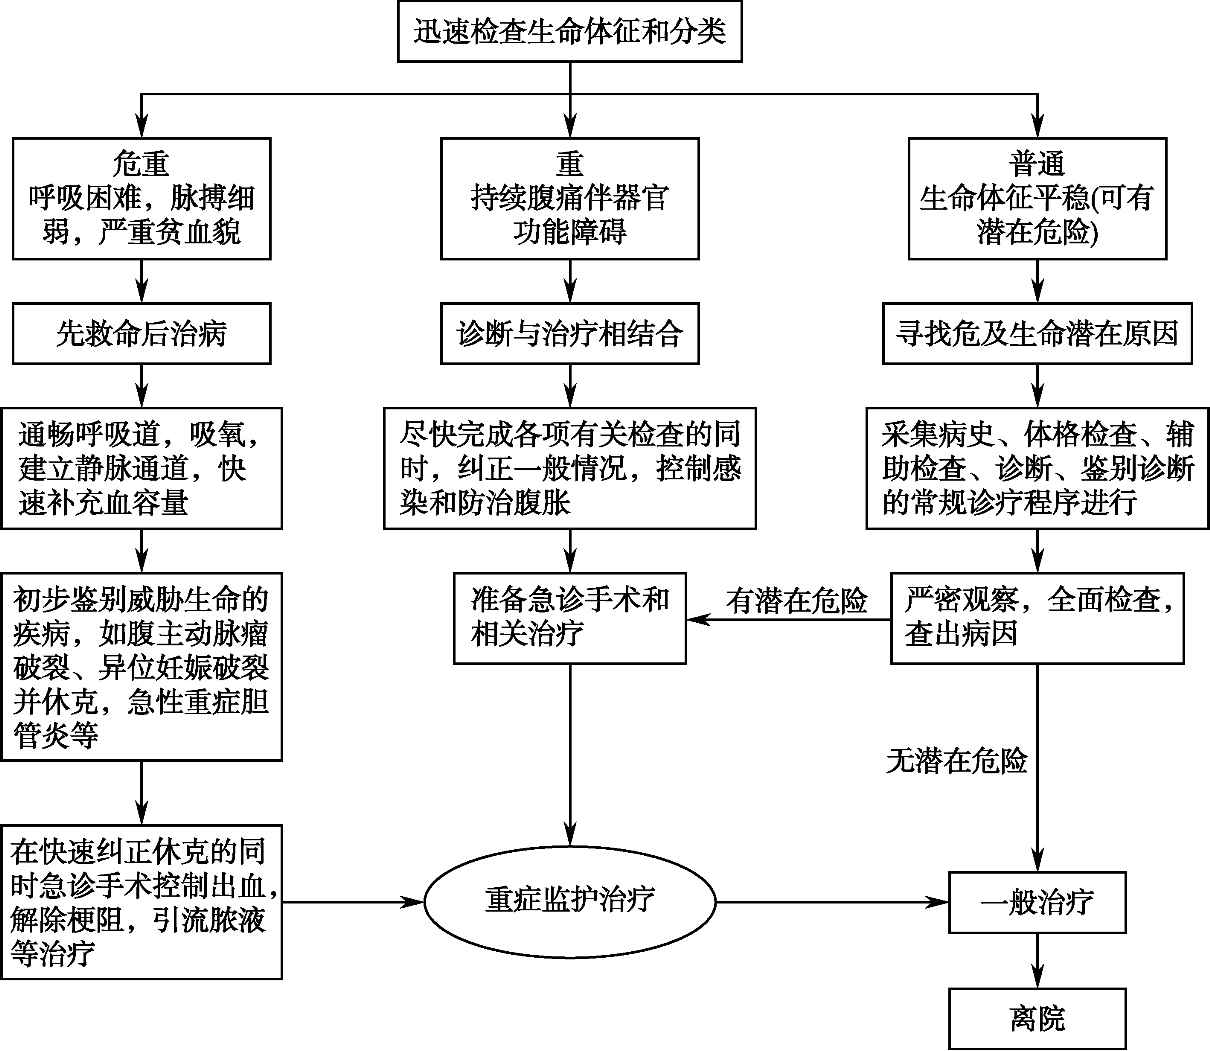
\includegraphics[width=4.71875in,height=4.10417in]{./images/Image00052.jpg}
 \captionsetup{justification=centering}
 \caption{急性腹痛的处理程序}
 \label{fig10-1}
  \end{figure} 

\subparagraph{急性腹痛伴感染性休克}

\hypertarget{text00026.htmlux5cux23CHP1-10-3-2-2-1}{}
(1) 临床表现特点:

①重度中毒表现如寒战,体温迅速升高,精神萎靡,意识障碍等;②休克征象表现为面色苍白,血压下降、尿量减少,脉搏细速,末梢循环不良等;③白细胞明显升高或低于正常甚至核左移。

\hypertarget{text00026.htmlux5cux23CHP1-10-3-2-2-2}{}
(2) 治疗原则:

①扩充血容量,静脉输液;②给予抗生素治疗;③物理方法降温;④寻找感染灶的可能部位并及时处理。

\subparagraph{继发性急性腹膜炎}

继发性急性腹膜炎是指由各种腹腔内病变或外伤所继发的腹膜急性炎症。

\hypertarget{text00026.htmlux5cux23CHP1-10-3-2-3-1}{}
(1) 临床表现特点:

①最突出的症状是腹痛,多为突然发病;常表现为持续性、烧灼样疼痛,随身体的活动而加剧。在炎症最明显处疼痛最重。疼痛范围缩小、程度减轻时,提示炎症局限;反之,则表明炎症扩散。②其他常见症状包括恶心、呕吐、食欲不振、口渴和自觉发热等,发病后患者多表现为尿少和便秘。③急性腹膜炎的特异性体征------腹膜刺激征:肌紧张、压痛和反跳痛。④中毒症状:疾病的早期,患者的体温往往增高并不明显,随着病程的进展,患者体温可以逐渐增高到38℃以上。甚至出现中毒性休克。⑤在空腔脏器穿孔的病例,可出现气腹征------肺肝界叩不清或消失,腹透时隔下有游离气体。⑥腹部穿刺:对诊断非常有帮助。通过对吸出的腹腔液性状进行观察,常可以判断出腹膜炎的病因。

\hypertarget{text00026.htmlux5cux23CHP1-10-3-2-3-2}{}
(2) 治疗原则:

①动态监测患者的病情变化、胃肠减压并留置尿管导尿;②补充血容量、应用抗生素;③积极处理原发病,及时手术处理。

(刘保池 张文武 杨璧卿)

\protect\hypertarget{text00027.html}{}{}

\hypertarget{text00027.htmlux5cux23CHP1-10-4}{}
参 考 文 献

1. 高德明 ,吴金生.现代急腹症学.北京:人民军医出版社,2002

2. Lo Vecchio F,Oster N,Sturmann K,et al. The use of analgesics in
patient with acute abdominal pain. J Emerg Med,1997,15 (6):775

3.
周玲君,刘红香,赵继军.急腹症的早期止痛.中华急诊医学杂志,2006,15(1):91

4. Lo Vecchio F,Oster N,Sturmann K,et al. The use of analgesics in
patient with acute abdominal pain. J Emerg Med,1997,15 (6):775

5. 刘保池 .急腹症的正确诊断与处理.国际外科学杂志,2008,35(6):369

\protect\hypertarget{text00028.html}{}{}

\chapter{恶心与呕吐}

恶心(nausea)、呕吐(vomiting)是临床上常见的症状之一。恶心是一种特殊的主观感觉,表现为胃部不适和胀满感,常为呕吐的前奏,多伴有迷走神经兴奋的症状,如皮肤苍白、流涎、出汗、血压降低及心动过缓等;呕吐是一种胃的反射性强力收缩,通过胃、食管、口腔、膈肌和腹肌等部位的协同作用,能迫使胃内容物由胃、食管经口腔急速排出体外。从某种意义上来说呕吐是机体的一种保护性作用,它可把对机体有害的物质排出体外,但实际上很多呕吐并非摄入有害物质引起,而且频繁和剧烈的呕吐,可引起失水、电解质紊乱和营养障碍。

\subsection{病因与发病机制}

\subsubsection{病因}

引起恶心、呕吐的病因很广泛,包括多方面因素,几乎涉及各个系统。

\subparagraph{感染}

病毒性急性胃肠炎、细菌性急性胃肠炎、急性病毒性肝炎、阑尾炎、胆囊炎、腹膜炎、急性输卵管炎、盆腔炎等。

\subparagraph{腹腔其他脏器疾病}

①脏器疼痛:胰腺炎、胆石症、肾结石、肠缺血、卵巢囊肿蒂扭转。②胃肠道梗阻:幽门梗阻(溃疡病、胃癌、腔外肿物压迫)、十二指肠梗阻(十二指肠癌、胰腺癌)、肠粘连、肠套叠、绞窄疝、克罗恩病、肠结核、肠道肿瘤、肠蛔虫、肠扭转、肠系膜上动脉压迫综合征、输出袢综合征、胃肠动力障碍(糖尿病胃轻瘫、非糖尿病胃轻瘫)、假性肠梗阻(结缔组织病、糖尿病性肠神经病、肿瘤性肠神经病、淀粉样变等)。

\subparagraph{内分泌代谢性疾病}

低钠血症、代谢性酸中毒、营养不良、维生素缺乏症、糖尿病酸中毒、甲状腺功能亢进、甲状腺功能低下、甲状旁腺功能亢进症、垂体功能低下、肾上腺功能低下,各种内分泌危象、尿毒症等。

\subparagraph{神经系统疾病}

中枢神经系统感染(脑炎、脑膜炎)、脑肿瘤、脑供血不足、脑出血、颅脑外伤、脑寄生虫病等。

\subparagraph{药物等理化因素}

麻醉剂、洋地黄类、化疗药物、抗生素、多巴胺受体激动药、非甾体抗炎药、茶碱、酒精、放射线等。

\subparagraph{精神性呕吐}

神经性多食、神经性厌食。

\subparagraph{前庭疾病}

晕动症、梅尼埃病、内耳迷路炎。

\subparagraph{妊娠呕吐}

妊娠剧吐、妊娠期急性脂肪肝。

\subparagraph{其他}

心肺疾患(心肌梗死、肺梗死、高血压、急性肺部感染、肺心病)、泌尿系疾患(急性肾炎、急性肾盂肾炎、尿毒症)、周期性呕吐、术后恶心呕吐、青光眼。

\subsubsection{发病机制}

这是一系列复杂的反射动作,可分为三个阶段,即恶心、干呕与呕吐。恶心发生时,唾液分泌增加,胃蠕动减弱或者消失、排空延缓,十二指肠及近端空肠紧张性增加,出现逆蠕动,导致十二指肠内容物反流至胃内。干呕时胃上部放松而胃窦部短暂收缩;呕吐时胃窦部持续收缩,下食管括约肌松弛,腹肌收缩,膈肌下降,腹压增加,迫使胃内容物急速而猛烈地从胃反流,经食管、口腔而排出体外。呕吐与反食不同,后者系无恶心与呕吐的协调动作而使胃内容物一口一口地反流到口腔。

目前认为的主要的反射通路包括:①信息传入:由自主神经传导(其中迷走神经纤维较交感神经纤维起的作用大)。②呕吐反射中枢:目前认为中枢神经系统的两个区域与呕吐反射密切相关。一是延髓呕吐中枢,另一是化学感受器触发区(chemical
trigger zone,CTZ)。③传出神经:包括迷走神经、交感神经、体神经和脑神经。

通常把内脏末梢传来的冲动引起的呕吐称为反射性呕吐,把CTZ受刺激后引起的呕吐称为中枢性呕吐。延髓呕吐中枢位于延髓外侧网状结构背外侧,迷走神经核附近,主要接受来自消化道和内脏神经、大脑皮质、前庭器官、视神经、痛觉感受器和化学感受区的传入冲动。化学感受器触发区(CTZ)位于第四脑室底部的后极区,为双侧性区域,有密集多巴胺受体。多巴胺受体在CTZ对呕吐介导过程中起重要作用,因为应用阿扑吗啡、左旋多巴、溴隐亭等多巴胺受体激动药可引起呕吐,而其拮抗药、甲氧氯普胺(胃复安)、吗丁啉等药物有止呕作用。化学感受器触发区的5-羟色胺、去甲肾上腺素、神经肽物质和γ-氨基丁酸等神经递质也可能参与呕吐反射过程。CTZ主要接受来自血液循环中的化学、药物等方面的呕吐刺激信号,并发出引起呕吐反应的神经冲动。但CTZ本身不能直接引起呕吐,必须在延髓呕吐中枢完整及其介导下才能引起呕吐,但两者的关系尚不十分明确。CTZ位于血-脑脊液屏障之外,许多药物或代谢紊乱均可作用于CTZ。某些药物如麻醉剂、化学药物、麦角衍生物类药、吐根糖浆等及体内某些多肽物质如甲状腺激素释放激素、P物质、血管紧张素、胃泌素、加压素、血管肠肽等均可作用于CTZ引起恶心呕吐。此外,某些疾病如尿毒症、低氧血症、酮症酸中毒、放射病、晕动症等引起的恶心呕吐也与CTZ有关。

传出神经的呕吐信号传至效应器官,引起恶心呕吐过程,呕吐开始时,幽门关闭,胃内容物不能排到十二指肠,同时,贲门口松弛,贲门部上升,腹肌,膈肌和肋间肌收缩,胃内压及腹内压增高,下食管括约肌松弛,导致胃内容物排出体外。

\subsection{诊断思路}

\subsubsection{病史}

\subparagraph{药物或放射线接触史}

易引起呕吐的常用药物有某些抗生素、洋地黄、茶碱、化疗药物、麻醉剂、酒精等。镭照射线治疗和钴照射线治疗,常引起恶心呕吐。

\subparagraph{其他}

呕吐可为许多系统性疾病的表现之一,包括糖尿病、甲状腺功能亢进症或甲状腺功能减退症、肾上腺功能减退等内分泌疾病、硬皮病等结缔组织病、脑供血不足、脑出血、脑瘤、脑膜炎、脑外伤等中枢神经系统疾病、尿毒症等肾脏疾病。

\subsubsection{临床表现特点}

\subparagraph{呕吐的伴随症状}

呕吐伴发热者,须注意急性感染性疾病;呕吐伴有不洁饮食或同食者集体发病者,应考虑食物或药物中毒;呕吐伴胸痛,常见于急性心肌梗死或急性肺梗死等;呕吐伴有腹痛者,常见于腹腔脏器炎症、梗阻和破裂;腹痛于呕吐后暂时缓解者,提示消化性溃疡、急性胃炎及肠道梗阻性疾病;呕吐伴头痛,除考虑颅内高压的疾患外,还应考虑偏头痛、鼻炎、青光眼及屈光不正等疾病;呕吐伴眩晕,应考虑前庭、迷路疾病、基底椎动脉供血不足、小脑后下动脉供血不足及某些药物(氨基糖苷类抗生素)引起的脑神经损伤。

\subparagraph{呕吐的方式和特征}

喷射性呕吐多见于颅内炎症、水肿出血、占位性病变、脑膜炎症粘连等所致颅内压增高,通常不伴有恶心。此外,青光眼和第Ⅷ对脑神经病变也可出现喷射性呕吐。呕吐不费力,餐后即发生,呕吐物量少,见于精神性呕吐。应注意呕吐物的量、颜色和气味等。呕吐物量大,且含有腐烂食物提示幽门梗阻伴胃潴留、胃轻瘫及小肠上端梗阻等;呕吐物为咖啡样或血性见于上消化道出血,含有未完全消化的食物则提示食管性呕吐(贲门失弛缓症、食管憩室、食管癌等)和见于神经性呕吐、胆囊炎、胆石症及胃大部切除术后等,有时见于妊娠剧烈呕吐、晕动症;呕吐物有酸臭味者,或胃内容物有粪臭味提示小肠低位梗阻、麻痹性肠梗阻、结肠梗阻而回盲瓣关闭不全或胃结肠瘘等。

\subparagraph{呕吐和进食的时相关系}

进食过程或进食后早期发生呕吐,常见于幽门管溃疡或精神性呕吐;进食后期或餐后呕吐,见于幽门梗阻、肠梗阻、胃轻瘫或肠系膜上动脉压迫导致十二指肠雍积;晨起呕吐多见于妊娠呕吐,有时亦见于尿毒症、慢性酒精性中毒和颅内高压等。

\subsubsection{体格检查}

\subparagraph{一般情况}

应注意神志、营养状态、有无脱水、循环衰竭、贫血及发热等。

\subparagraph{腹部体征}

应注意胃型、胃蠕动波、振水声等幽门梗阻表现:肠鸣音亢进、肠型等急性肠梗阻表现:腹肌紧张、压痛、反跳痛等急腹症表现。此外,还应注意有无腹部肿块、疝等。

\subparagraph{其他}

①眼部检查注意眼球震颤、眼压测定、眼底有无视乳头水肿等。②有无病理反射及腹膜刺激征等。

\subsubsection{实验室检查}

主要包括与炎症、内分泌代谢及水盐电解质代谢紊乱等有关的实验室检查。

\subsubsection{其他辅助检查}

可做B超、胃镜、ERCP、超声内镜、CT、磁共振等特殊检查。

\subsection{治疗}

由于引起恶心、呕吐的疾病很多,恶心、呕吐仅是疾病的症状之一。因此,在未明确病因之前不应盲目应用作用于呕吐中枢的强镇吐药物,否则会贻误病情。只有在明确了导致呕吐的病因之后,在积极治疗病因的基础上,才能行必要的对症治疗。

\subparagraph{胃肠道疾病}

包括食管、胃、十二指肠直至空肠、回肠、结肠及直肠在内的任何部位的病变都有可能引起恶心、呕吐的症状,其中以食管狭窄、食管癌、贲门失弛缓、贲门癌、胃窦部嗜酸性肉芽肿、胃窦部巨大溃疡或癌肿、十二指肠溃疡或郁积症、多种原因导致的小肠与大肠梗阻或急性胃、小肠或大肠的炎症性病变为最常见的病因。因消化道良性或恶性病变造成的狭窄或梗阻所致的呕吐,药物治疗是无效的,只有经扩张、置入支架或手术治疗,解除狭窄或梗阻之后,呕吐症状才会消失。对于贲门失弛缓症患者,在未进行扩张或手术治疗之前,可选用钙离子通道拮抗药或硝酸甘油餐前半小时口服或餐前15~30分钟舌下含化治疗,早期可改善呕吐及梗阻症状:或者试用肉毒杆菌毒素行狭窄局部注射治疗。胃肠道急性炎症性病变引起的呕吐,应积极选用抗生素并纠正电解质紊乱及补充维生素;胃肠动力障碍引起的恶心与呕吐则可应用莫沙比利(mosapride,5mg口服,每日3次)、西沙比利(cisapride,5~10mg口服,每日2~4次)、多潘立酮(吗丁啉,10~20mg口服,每日3次;或10mg肌肉注射)、甲氧氯普胺(灭吐灵,胃复安,5~10mg口服;或10~20mg肌肉注射。每日剂量应≤0.5mg/kg,否则易引起锥体外系反应)等促胃肠动力剂;如果呕吐是由胃肠道痉挛所致,则可应用东莨菪碱(0.3mg口服或注射)等抗胆碱能药物。

\subparagraph{肝脏 、胆道及胰腺疾病}

是导致恶心、呕吐的常见病因之一。恶心、呕吐可是急性病毒性肝炎的早期症状,常与食欲减退、厌油腻食物及上腹部饱胀同时出现,随着护肝治疗及适当的休息之后,恶心与呕吐可逐渐消失。呕吐也是胆道梗阻或绞痛常伴随的症状,只有当胆道梗阻或炎症消除之后,呕吐才会停止;急性胰腺炎时常伴随有恶心与呕吐症状,只有随着采用胃肠减压、减少胰液分泌等措施之后,呕吐才会逐步缓解或终止。

\subparagraph{中枢神经系统病变}

包括各种原因所致的脑炎、脑膜炎、脑肿瘤、脑寄生虫病、脑血管病及颅脑外伤等病变,均可引起颅内压力增高而导致恶心、呕吐。治疗的重要措施之一就是应用降低颅内压、减轻脑细胞水肿的药物治疗。脱水治疗后,不仅可改善呕吐的症状,更重要的是起到了保护或恢复脑细胞功能的作用。

\subparagraph{药物所致的呕吐}

多种药物有引起恶心与呕吐的不良反应,一般而言,只要立即停止应用引起呕吐的药物,呕吐症状就会减轻直至消失,因此并不需要应用镇吐类药物。目前临床上对某些恶性肿瘤或血液系统的恶性疾病(如白血病、恶性淋巴瘤、多发性骨髓瘤、恶性组织细胞病等)采用联合化疗或放疗,或对某些恶性肿瘤采用抗癌药物行介入治疗。但无论在治疗过程中或治疗之后,均可引起较为严重的胃肠道不良反应,最突出的表现就是恶心与呕吐。为了预防或减轻此不良反应,常可应用镇吐药物进行治疗,常用的药物有昂丹司琼(ondansetron,奥丹西龙,商品名:枢复宁。常用8mg口服或静脉注射)、格拉司琼(granisetron,商品名:康泉。成人剂量每次40μg/kg,或标准剂量3mg,静脉滴注)等。必须指出,应用这些作用强的镇吐药物之后,也会产生中枢神经系统、心血管系统或胃肠道的不良反应,故应严格控制药物剂量及间隔时间。

\subparagraph{神经 、精神因素所致的呕吐}

对此类原因所致的呕吐,心理治疗是关键。首先应消除患者的精神心理障碍,其次可配合药物治疗,常用的药物是镇静药与胃肠促动力剂、重者可采用多塞平或氟西汀等抗抑郁药物治疗。禁忌应用昂丹司琼(奥丹西龙)等强烈作用的镇吐药。

\protect\hypertarget{text00029.html}{}{}

\hypertarget{text00029.htmlux5cux23CHP1-11-4}{}
参 考 文 献

1. 陈文彬,潘祥林.诊断学.第7版.北京:人民卫生出版社,2008

2. 陈新谦,金有豫,汤光.新编药物学.第17版.北京:人民卫生出版社,2011

\protect\hypertarget{text00030.html}{}{}

\chapter{急 性 腹 泻}

正常人一般每日排成形大便1次,粪便平均重量为150~200g,一般不超过200g,其中水分占60\%~70\%,约150ml左右。少数人每天排便2~3次或2~3天才排1次,但若粪质成形,性状与常人无异,亦属正常。

腹泻(diarrhea)是指排便习惯和粪便性状发生变化,排便次数增多(每天3次以上),粪质稀薄,水分增加(水分超过85\%),粪便量增加(超过200g/d)。便质不成形、稀溏或呈液状,有时含有脓血或带有未消化食物及脂肪。确定是否有腹泻应根据个体的大便习惯而异。

腹泻可根据病程分为急性腹泻和慢性腹泻两种,也可依病因分为感染性腹泻和非感染性腹泻两大类。急性腹泻是指起病急骤、病程较短,病程在2~3周之内,极少超过6~8周。慢性腹泻指病程至少在4周以上,常超过6~8周,或间歇期在2~4周内的复发性腹泻。腹泻常伴有排便紧迫感、肛门不适或大便失禁。腹泻可导致水电解质丢失,严重时可引起大量失水,导致低血容量性休克和急性器官功能衰竭,甚至因电解质严重紊乱引起严重心律失常而死亡。

\subsection{病因与发病机制}

在禁食期间,正常人肠腔内液体含量很少。但正常三餐摄取后,每天约有9L液体进入肠道,其中2L来自进食的食物和饮料,其余来自消化道分泌液,包括唾液1.5L、胃液2.5L、胰液1.5L、胆汁0.5L和小肠液1.0L。进入胃肠道的食糜在通过小肠时,食糜的渗透度变得与血浆相同,其中90\%的水分被其吸收。食糜在到达回肠末端时,已呈等渗状态,每天仅有1~2L的液体进入结肠,而结肠也具有强大的吸收水分的功能,使大便最终含水量只有100~200ml。若胃肠道的分泌、消化、吸收和运动等功能障碍,使消化道分泌的液量增加,食物不能完全分解,吸收量减少和肠胃蠕动加速等,最终可导致粪便性状稀薄、次数增加而形成腹泻。腹泻的发病机制相当复杂,从病理生理角度分为四类,部分腹泻的发病可有几个因素并存,具体如下:

\subparagraph{分泌性腹泻}

肠道液体主要由黏膜隐窝细胞分泌,大部分经肠绒毛腔面上皮细胞吸收。当各种刺激因子刺激肠黏膜细胞分泌的量超过其吸收能力时,所引起的腹泻称分泌性腹泻(secretory
diarrhea)。刺激肠黏膜分泌的因子可分为四类:①细菌的肠毒素,如霍乱弧菌、大肠埃希菌、沙门菌等毒素;②神经体液因子,如血管活性肠肽(VIP)、血清素、降钙素等;③免疫炎性介质,如前列腺素、白三烯、血小板活化因子、肿瘤坏死因子、白介素等;④去污剂,如胆盐和长链脂肪酸,通过刺激阴离子分泌和增加黏膜上皮通透性而引起分泌性腹泻;⑤各种通便药,如蓖麻油、酚酞、芦荟、番泻叶等均可引起分泌性腹泻。

肠道分泌电解质和水分的机制相当复杂。近年发现,肠黏膜隐窝细胞中的第二信使如环磷酸腺苷(cAMP)、环磷酸鸟苷(cGMP)、钙离子等的增加是诱导黏膜隐窝细胞分泌的重要环节。霍乱弧菌和致病性大肠埃希菌的毒素首先与上皮细胞刷状缘上的受体结合,激活腺苷环化酶-cAMP系统,致cAMP浓度增高,引起大量肠液分泌;艰难梭菌(C.difficile)是通过钙离子增加而引起分泌性腹泻;血管活性肽瘤(VIP瘤)引起的腹泻是一种非感染性的分泌性腹泻,肿瘤释出的VIP能激活肠黏膜的腺苷酸环化酶,刺激小肠大量分泌液体,故而出现霍乱样的严重水泻,称为胰性霍乱,常伴有严重的低钾血症和代谢性酸中毒;胃泌素瘤能分泌大量的胃泌素,刺激壁细胞分泌大量胃液,过多胃液进入小肠后,不仅可损害空肠黏膜,而且促进肠道蠕动,使胰脂肪酶灭活,脂肪消化障碍而更加重腹泻。分泌性腹泻还可见于直肠分泌性绒毛状腺瘤、肠淋巴瘤、炎症性肠病、肠肉芽肿性疾病、结缔组织病、恶性类癌综合征、甲状腺髓样癌等。

分泌性腹泻的特点是:①禁食不减轻腹泻;②肠液与血浆的渗透压相同;③大便呈水样,量多,无脓血;④一般不伴有腹痛;⑤肠黏膜组织学基本正常。

\subparagraph{渗透性腹泻}

由于肠腔内含有大量不能被吸收的溶质,导致肠腔内渗透压升高,大量液体被动进入肠腔而引起腹泻,称为渗透性腹泻(osmotic
diarrhea)或吸收不良性腹泻(malabsorption diarrhea)。见于:

\hypertarget{text00030.htmlux5cux23CHP1-12-1-2-1}{}
(1) 高渗性药物:

口服镁盐、乳果糖、甘露醇或山梨醇等高渗性药物。

\hypertarget{text00030.htmlux5cux23CHP1-12-1-2-2}{}
(2) 高渗性食物:

主要是某些碳水化合物,由于水解酶缺乏或其他原因而导致食物吸收不良,形成高渗透压性的肠内容物而引起腹泻。临床上最常见的是原发性乳糖酶缺乏,患者口服牛奶或奶制品后即可引起腹泻。

\hypertarget{text00030.htmlux5cux23CHP1-12-1-2-3}{}
(3) 消化不良:

胃大部分切除术后、萎缩性胃炎和胃癌患者的胃液分泌减少,慢性胰腺炎、胰腺切除术后使胰液分泌减少,严重肝病或胆管梗阻可导致胆汁分泌或排泄减少,使食物不能充分被消化,营养物质不能被吸收,致使高渗性肠内容物增多而造成腹泻。

\hypertarget{text00030.htmlux5cux23CHP1-12-1-2-4}{}
(4) 吸收不良:

①黏膜透过性异常:由于小肠黏膜细胞的特殊病变如绒毛或微绒毛的变形、萎缩等变化,导致小肠的有效吸收面积缩小和黏膜透过水和电解质减少而导致腹泻。见于小儿乳糜泻、热带和亚热带斯泼卢等疾病。②肠吸收面积减少:如小肠切除后等。③肠黏膜充血、水肿:由于门静脉内压力增加,引起肠道黏膜广泛充血与水肿,影响肠道内营养物质的吸收而发生腹泻。④细菌繁殖过多:在某些疾病状态下,如肝硬化、小肠浸润性疾病引起的部分性肠梗阻或某些小肠失蠕动(如系统性硬皮病)、盲袢等,小肠内细菌可以过多繁殖。由于细菌分泌的毒素可影响消化酶的作用,以及细菌分解物结合胆盐,使其失去形成微胶粒的能力,导致脂肪等食物的消化和吸收受到障碍等,可引起腹泻或脂泻。⑤吸收抑制:如先天性氯泻(congenital
chloriderrhea),是由于氯的主动吸收功能不全而钠的吸收过程正常,以致肠内容物中由于氢和氯化物增加,但缺乏碳酸氢钠与之中和而使肠液呈酸性,回肠和结肠内液体积聚而引起腹泻。氯泻也可继发于长期腹泻而缺钾的患者。

渗透性腹泻的特点是:①当引起腹泻的原因除去(如禁食)之后,腹泻即可停止或减轻;②肠腔内的渗透压可超过血浆渗透压;③粪中含有大量未被完全吸收或消化的食物。

\subparagraph{肠动力紊乱(motility disturbances)}

许多药物、疾病和胃肠道手术可改变肠道的正常运动功能,促使肠蠕动加速,以致肠内容物过快通过肠腔,因影响消化与吸收而发生腹泻。肠动力过缓亦可导致腹泻,其原因为结肠型的细菌在小肠定植和过度生长,从而使脂肪、胆盐和碳水化合物的吸收受到影响。此类腹泻可见于淀粉样变性、硬皮病、糖尿病性神经病变、胃大部切除术后、幽门或肛门括约肌切除术后、肠易激综合征、情绪性腹泻、毒性甲状腺肿病、恶性类癌综合征等。

此种腹泻的特点是粪便稀烂或水样,肠鸣音亢进,常伴有腹痛,但大便中很少有炎症细胞。

\subparagraph{渗出性腹泻(exudative diarrhea)}

又称炎症性腹泻(inflammatory
diarrhea)。肠黏膜炎症时渗出大量黏液、脓、血,可致腹泻。此类腹泻可见于:①炎症性肠病,如克罗恩病和溃疡性结肠炎;②感染性炎症:来自侵入性病原体及其毒素,如志贺痢疾杆菌、沙门菌属、弯曲杆菌、耶尔森菌(Yersinia)、结核杆菌、阿米巴原虫、艰难梭菌等的感染;③缺血性炎症;④肠放射损伤;⑤嗜酸性肠炎:为嗜酸性粒细胞浸润胃肠道全层,可累及全胃肠道或节段性,表现为脂肪泻、腹痛、恶心、呕吐、消瘦,外周血嗜酸性粒细胞可增多。

渗出性腹泻的特点是:①粪便松散或水样,含有黏液和脓血,左侧结肠病变所致者常带有肉眼可见的脓血便,小肠病变一般无肉眼可见的脓血便。②腹泻和全身症状、体征的严重程度因肠受损程度而异。

需要指出和值得注意的是,同一种疾病产生的腹泻常常有多种机制参与,且腹泻的病因并不单纯,可同时或先后有几个病因并存。临床上最常见的为各种肠道感染、炎症、结肠和直肠癌、葡萄球菌肠毒素所引起的食物中毒及肠道易激综合征等。

\subsection{诊断思路}

腹泻的病因诊断要依靠病史、症状、体征,并结合辅助检查,尤其是粪便检验的结果,综合分析后得出结论。对一时难以明确诊断者,可进一步作X线钡剂检查和(或)结肠镜检查;对胆、胰疾病可选用超声、CT、MR、逆行胰胆管造影(ERCP)等影像学诊断方法加以明确诊断;对小肠吸收不良者可行小肠吸收功能试验、呼气试验、小肠黏膜活检等以明确诊断。但在诊断过程中应注意以下几点。

\subsubsection{病史}

\subparagraph{年龄与性别}

婴幼儿起病的腹泻,应考虑先天性小肠消化吸收障碍性疾病,如双糖酶缺乏症、先天性氯泻等。病毒性胃肠炎和大肠埃希菌性肠炎多见于婴幼儿;细菌性痢疾以儿童和青壮年多见;结肠癌多见于中年或老年;阿米巴痢疾则以成年男性居多;功能性腹泻、甲亢和滥用泻剂者多见于女性,而结肠憩室与结肠癌则多见于男性。

\subparagraph{起病与病程}

需询问国际、国内和郊区旅游史、近期服用了哪些药物或免疫抑制剂、是否亲密接触动物等。急性腹泻均应注意询问接触或摄入不洁食物史、起病与演变过程等。急性食物中毒性感染常于进食后2~24小时内发病;手术后发病,尤其是长期接受抗生素治疗者,应考虑金黄色葡萄球菌肠炎、难辨梭状芽胞杆菌性肠炎等。由功能性腹泻、血吸虫病、溃疡性结肠炎、克罗恩病等所引起的腹泻,可长达数年或数十年。功能性腹泻、吸收不良综合征和结肠憩室炎所致的腹泻,常呈间歇性的发作。

\subparagraph{排便与粪便性状}

往往可以提示病变部位或性质。腹泻量多、水样、色淡、多泡沫、恶臭、无脓血、无里急后重,提示病变位于小肠;黏液带果酱色血便,病变多在上段结肠;粉红色脓血便,病变多在下端结肠;粪便表面带血或伴明显里急后重,病变多在直肠。急性腹泻先为水样后为脓血便,一日多至数十次,伴有里急后重者急性细菌性痢疾的可能性较大;粪便暗红色、酱色状或血水样,提示阿米巴痢疾可能;粪便稀水样,无里急后重,多为食物中毒性感染;若在进食后6~24小时发病则以沙门菌属、变形杆菌、产气荚膜梭状芽胞杆菌感染的可能性大;若在进食后2~5小时发病,伴有剧烈呕吐者可能为金黄色葡萄球菌感染所致。呕吐物和腹泻均呈米泔水样,失水严重,应考虑霍乱;若粪便带有恶臭,呈紫色血便,应考虑急性出血性坏死性肠炎。吸收不良综合征时粪便有食物残渣、未消化或发酵物,可奇臭;结肠炎症引起的腹泻粪便带脓血;肠结核和肠易激综合征常有腹泻与便秘交替现象。肠易激综合征的功能性腹泻多在清晨起床后和早餐后发生,每日2~3次,粪便有时含大量黏液。影响睡眠的夜间腹泻多系器质性疾病所致。

\subparagraph{腹泻与腹痛}

腹泻伴有里急后重且下腹或左下腹持续性腹痛,腹痛于便后可稍减轻,提示病变位于直肠或乙状结肠;腹泻无里急后重,伴脐周腹痛为小肠性腹泻。

\subparagraph{伴随症状}

急性腹泻伴有高热,以细菌性痢疾、沙门菌属食物中毒感染居多;有里急后重以细菌性痢疾、阿米巴痢疾、急性血吸虫病可能性大,而食物中毒性感染大多无里急后重。

\subsubsection{体格检查}

对腹泻患者应做全面仔细的体格检查。如腹部检查被触及包块,常提示肿瘤或炎症性疾病;若包块位于左下腹,应疑及左侧结肠癌、乙状结肠憩室炎,或癌肿造成的肠腔狭窄使粪块壅积于梗阻的近端肠腔,或为单纯的粪块堆积;若位于右下腹,应想到右侧结肠癌、肠结核、克罗恩病等。如腹部压痛明显,可见于克罗恩病、结肠憩室炎、盆腔或阑尾脓肿。肛门指检应列为常规检查,若触及坚硬、结节状、固定的肿块,指套上有血迹常提示直肠癌。

\subsubsection{辅助检查}

大多数腹泻都是自限性的,因此辅助检查价值有限。但对病程较长和对保守治疗无效的患者须选择相应的辅助检查,以明确病因诊断。

\subparagraph{粪便检查}

粪便应为现场留取,或是短时间内留在标本盒中的新鲜标本。应注意粪便的形态、量、黏稠度及有无食物残渣、黏液、血和脓性分泌物等。大便常规检验、隐血实验,粪便涂片查脓细胞、寄生虫及虫卵、脂肪、未消化食物等,大便致病菌培养等,对分泌性腹泻测定粪便的电解质和渗透压等,对腹泻的定位和定性诊断非常重要。粪便镜检出现白细胞往往提示肠道细菌感染,当粪便中的白细胞计数>
15/HP,同时伴有红细胞时,临床可诊断为痢疾;而动力试验检查可以发现弧菌感染,这是诊断霍乱最简单的方法。

\subparagraph{胃肠内镜检查}

对腹泻病因、部位不明者可酌情进行胃镜、乙状结肠镜、结肠镜或小肠镜检查,必要时重复同一检查或同一患者行不同的内镜检查。根据在直视下病变的性质、范围、严重程度以及活检的病理结果,明确腹泻的病因诊断,尤其对胃肠炎症性疾病、肿瘤等的诊断和鉴别诊断具有肯定价值。

\subparagraph{影像学检查}

腹部平片可显示胰腺钙化及钙化性结石;胃肠钡餐检查可以观察胃肠道的运动功能状态,发现器质性病变,对结肠癌、炎症性肠病具有较高诊断价值;腹部B超是了解有无肝胆胰疾病的最常用方法;腹部CT
或MRI对诊断肝、胆、胰等内脏疾病有肯定价值。

\subparagraph{小肠功能检查}

可行小肠吸收功能试验、呼气试验、小肠黏膜活检以检查小肠吸收不良。

\subsection{处理原则}

腹泻是症状,针对病因是根本性治疗,在未明确病因前,根据腹泻的病理生理特点给予对症和支持治疗也很重要,但必须谨慎使用止泻和止痛药物,以免造成误诊和漏诊。

\subsubsection{病因治疗}

\subparagraph{抗病原体治疗}

经验性的抗生素治疗并不适用于所有急性腹泻患者,这是由于:①大多数急性腹泻患者凭借自身的抵抗力足以有效清除病原,研究发现50\%的感染性腹泻患者,不使用抗生素也可以在3天内恢复;②应用抗生素后反而会引起药物的不良反应,如难辨梭状芽胞杆菌感染和细菌耐药;③应用抗生素可延长病原菌的毒素排出时间等。而下列急性腹泻患者推荐经验性地使用抗菌药物:①有明确细菌感染征象者,如发热伴粪便镜检中有白细胞者;②临床诊断的痢疾(粪便镜检白细胞>
15/HP,同时出现红细胞)患者;③危及生命的感染,如霍乱;④旅行者腹泻,这些患者往往需要较短的时间内迅速缓解症状;⑤免疫缺陷或免疫低下者。

抗感染治疗以针对病原体的抗菌治疗最为理想,如复方新诺明、环丙沙星、诺氟沙星、左旋氧氟沙星、加替沙星等喹诺酮类适用于志贺菌属、沙门菌、弯曲杆菌、大肠埃希菌等所致的腹泻;甲硝唑或万古霉素适用于难辨梭状芽胞杆菌感染引起的假膜性肠炎;肠结核应用如利福平、异烟肼、乙胺丁醇、吡嗪酰胺、对氨基水杨酸、链霉素等抗结核药物中的三种或四种联合治疗;阿米巴痢疾可选用甲硝唑。病毒性腹泻常不用抗生素,可使用盐酸小檗碱(黄连素)。大肠埃希菌O\textsubscript{157}
∶H\textsubscript{7}
感染亦不用,因现有抗生素治疗并无疗效,且增加溶血-尿毒综合征的发生。一般在送检大便培养后,可经验性地予以氟喹诺酮类抗生素,若临床提示弯曲杆菌者应加用红霉素、罗红霉素等大环内酯类抗生素。

\subparagraph{其他}

主要是针对发病机制治疗,如对乳糖不耐受症者不宜用乳制品或应剔除食物中的乳糖成分,而成人乳糜泻患者则需禁食麦制品(包括大麦、小麦、燕麦和裸麦)或剔除食物中的麦胶类成分。分泌性腹泻需同时补充葡萄糖以保证热量的吸收。慢性胰腺炎应补充多种消化酶。因服药所致的药源性腹泻应及时停用有关药物,高渗性腹泻应停用或停食引起高渗的药物和食物。消化道肿瘤可手术切除或化疗以治疗原发病。生长抑素类似物奥曲肽可抑制肿瘤分泌激素,可用于类癌综合征及神经内分泌肿瘤引起的腹泻。炎症性肠病可选用柳氮磺胺吡啶或5-氨基水杨酸制剂,如美沙拉嗪(颇得斯安)等。空肠广泛性黏膜病变和空肠切除后所致腹泻,乃因胆盐未能在小肠被重吸收而进入结肠,并在此被结肠内的细菌脱结合为游离胆酸,后者刺激结肠引起腹泻,服用考来烯胺或消胆胺可将胆汁酸吸附而终止腹泻。胆盐缺乏性的腹泻,可用中链脂肪酸补充脂肪类物质,因中链脂肪酸可不经胆盐水解而被吸收。短肠综合征者最好用多聚体形式的葡萄糖。

\subsubsection{对症支持疗法}

\subparagraph{饮食治疗}

急性腹泻时的饮食应以易消化、易吸收的流质或半流质为宜,避免牛奶和乳制品食物。

\subparagraph{纠正腹泻所引起的水 、电解质与酸碱平衡紊乱}

腹泻有时可引起不同程度的脱水,轻症者可用口服补液,严重腹泻伴失水者应立即静脉补液。应根据脱水的性质和血清电解质情况补充氯化钠、氯化钾等;若伴有酸碱平衡紊乱,也应及时纠正。一般来说,由于肠液电解质几乎与血浆浓度相仿且偏碱性,故水与电解质的补充大部分应以碳酸氢钠-生理盐水或林格液较适宜。

\subparagraph{纠正营养失衡}

对腹泻引起营养缺乏者,应根据病情相应地补充各种水溶性和(或)脂溶性维生素、葡萄糖、氨基酸、脂肪乳、白蛋白、丙种球蛋白等营养物质。若伴有缺铁、缺钙、缺镁等者亦应及时补充。必要时可予输注血浆、全血等。锌缺乏易致腹泻是和锌参与肠道水和电解质的转运、小肠渗透性、肠细胞酶的功能,增强肠道组织的修复,增强局部免疫,以控制细菌过度生长和与早期病原菌清除等有关。故在急性腹泻时补锌可缩短病程,减轻症状,如大便次数和粪便排出量的减少,使未来2~3个月中腹泻发病率下降。

\subparagraph{胃肠黏膜保护剂}

硫糖铝、枸橼酸铋钾、米索前列醇、双八面体蒙脱石(思密达)等有胃肠黏膜保护作用,硫糖铝和枸橼酸铋钾可黏附覆盖在溃疡面上阻止胃酸和胃蛋白酶继续侵袭溃疡面、促进内源性前列腺素的合成和刺激表皮生长因子分泌;但为避免铋在体内蓄积,枸橼酸铋钾不宜连续长期服用。米索前列醇具有抑制胃酸分泌、增加胃十二指肠黏膜黏液/碳酸氢钠盐分泌和增加黏膜血流的作用,但可引起子宫收缩和腹泻,孕妇忌服。蒙脱石散可用于感染性或非感染性腹泻,可口服亦可灌肠。

\subparagraph{微生态制剂}

常用双歧杆菌嗜酸乳杆菌肠球菌三联活菌(金双歧,培菲康,每次420~630mg,每日2~3次餐后服用)、嗜酸乳杆菌(乐托尔,每次2粒口服,每日2次,首剂加倍)、双歧杆菌(丽珠肠乐,每次0.35~0.7g,每日2次)、复合乳酸菌(聚克,每次1~2粒,每日1~3次)、地衣芽胞杆菌活菌(整肠生,每次0.5g,每日3次)、乳酶生(表飞鸣,每次0.3~1.0g,每日3次餐前服用)等以调节肠道菌群。它可以减少抗生素的应用,对旅行者腹泻、抗生素相关性腹泻、儿童腹泻和难辨梭状芽胞杆菌引起的腹泻有较好疗效。

\subparagraph{止泻药}

排便太频或失水、电解质过多,或引起痛苦时宜用止泻剂,使用止泻剂应注意以下原则:①严格掌握指征,主要针对严重失水者、非感染性腹泻者,并不是对所有腹泻均须使用止泻药,以免影响腹泻时将胃肠的有害物质排出体外的保护作用。当有病因治疗时,对轻度腹泻者多不必止泻,不一定加以抑制腹泻。②因止泻药可引起肠动力障碍,使致病菌定植和侵袭,延长排泄时间,故对诊断不明又不能排除感染时需慎用,明确感染性腹泻者禁用。③局限于直肠、乙状结肠的溃疡性结肠炎患者的腹泻主要是由于炎症激惹、刺激,而全胃肠通过时间并不缩短,应予抗炎治疗。④诊断不明又未能排除严重疾病时,用止泻剂应慎重,不能因症状控制而放松诊断性检查。⑤尽量避免或仅短期服用可引起药瘾性的药物(如复方樟脑酊、可待因等)。常用止泻剂有:

\hypertarget{text00030.htmlux5cux23CHP1-12-3-2-6-1}{}
(1) 地芬诺酯(苯乙哌啶,diphenoxylate,止泻宁):

为哌替啶(度冷丁)的衍生物。能减少肠蠕动,并有收敛作用,可用于各种因胃肠运动增快引起的腹泻。临床上常用复方地芬诺酯(每片含地芬诺酯2.5mg,阿托品0.025mg),每次口服1~2片,每日2~4次。大剂量时可产生欣快感,长期服用会成癮,产生依赖性。肝、肾功能损害,尤其是严重肝病时,可诱发肝性脑病;重症溃疡性结肠炎时,因抑制肠蠕动,可诱发中毒性结肠扩张。儿童患者慎用。

\hypertarget{text00030.htmlux5cux23CHP1-12-3-2-6-2}{}
(2) 洛哌丁胺(苯丁哌胺,loperamide;易蒙停,imodium):

其化学结构与地芬诺酯相似。可抑制平滑肌收缩,抑制肠蠕动。其作用强度比吗啡、阿托品大。口服后易吸收,4~6小时达高峰,分布于肝、肾,并从尿、粪排出。应用指征同地芬诺酯。其作用还有:①阻断钙通道,抑制肠运动;②抑制分泌;③抑制调钙蛋白,增加Na\textsuperscript{+}
、Cl\textsuperscript{−}
吸收。比地芬诺酯作用强,用药后迅速止泻。每次2mg口服,每天2~3次。

\hypertarget{text00030.htmlux5cux23CHP1-12-3-2-6-3}{}
(3) 可乐定(氯压定,clonidine):

为α\textsubscript{2}
肾上腺素能药物,可刺激肠细胞上特异的节后α\textsubscript{2}
受体,促进Na\textsuperscript{+} 和Cl\textsuperscript{−}
的吸收,抑制HCO\textsubscript{3} \textsuperscript{−}
和Cl\textsuperscript{−}
的分泌,为强力的止泻剂,因其中枢性低血压和镇静作用限制了它的应用。但糖尿病患者合并严重的自主神经病变时,并不出现低血压,而仅有止泻作用,可用于糖尿病性腹泻。

\hypertarget{text00030.htmlux5cux23CHP1-12-3-2-6-4}{}
(4) 奥曲肽(善得定,sandostatin):

是生长抑素(somatostatin,STT)的人工合成类似物,可有效治疗胃肠激素失常性腹泻(如VIP瘤、胃泌素瘤、生长抑素瘤和类癌综合征等所致的腹泻),常用剂量为0.3~0.75mg/d,分3次皮下注射。

\hypertarget{text00030.htmlux5cux23CHP1-12-3-2-6-5}{}
(5) 吲哚美辛(消炎痛,indomethacin):

能抑制胰性霍乱、甲状腺癌以及小肠绒毛腺癌的分泌性腹泻。主要是吲哚美辛可降低前列腺素E\textsubscript{2}
(PGE\textsubscript{2}
)水平而达到止泻效果,而对炎症性肠病,吲哚美辛无止泻作用。

\hypertarget{text00030.htmlux5cux23CHP1-12-3-2-6-6}{}
(6) 钙拮抗剂:

硝苯地平、维拉帕米等,对分泌性腹泻有效。

\hypertarget{text00030.htmlux5cux23CHP1-12-3-2-6-7}{}
(7) 收敛吸附剂:

如鞣酸蛋白(tannalbin,每次1~2g,每日3次)、碱式碳酸铋(次碳酸铋,每次0.3~0.9g,每日3次餐前服用)、药用炭(每次1.5~4g,每日2~3次餐前服用)等,可选择性用于炎症性腹泻。

\hypertarget{text00030.htmlux5cux23CHP1-12-3-2-6-8}{}
(8) 鸦片制剂:

如复方樟脑酊,能增强肠平滑肌张力,减低胃肠推进性蠕动,使粪便干燥而止泻。腹泻早期或腹胀者不宜使用。多用于较严重的非细菌感染性腹泻。2~5ml/次,每天3次。

\hypertarget{text00030.htmlux5cux23CHP1-12-3-2-6-9}{}
(9) 双八面体蒙脱石(思密达):

是一种高效消化道黏膜保护剂,主要通过保护肠黏膜屏障功能达到抗腹泻作用。其作用机制是:蒙脱石散对消化道内的病毒、病菌及其产生的毒素有极强的选择性固定、抑制作用;对消化道黏膜有很强的覆盖能力,并通过与黏液糖蛋白相互结合,修复、提高黏膜屏障的防御功能。它不进入血液循环系统,6小时左右连同所固定的攻击因子随消化道自身蠕动排出体外。蒙脱石散不影响X线检查,不改变大便颜色,常用剂量下不改变肠道生理运转时间,也不影响其他药物的生物利用度。基本无副作用,极少数患者产生轻度便秘,减量后可继续服用。用法:成人每次1袋(3g/袋)冲服,每日3次;2岁以上儿童每日2~3次,每次1袋;1~2岁幼儿每日1~2次,每次1袋;1岁以下幼儿每日1袋,分2次服用。治疗急性腹泻时首剂量应加倍。

\hypertarget{text00030.htmlux5cux23CHP1-12-3-2-6-10}{}
(10) 抗胆碱药:

适用于功能性及痉挛性腹痛者,可与镇静药合用。

\subparagraph{止痛剂}

对伴有明显腹痛的患者应使用止痛剂治疗。654-2、阿托品、丙胺太林等具有解痉、止痛作用,但青光眼、前列腺肥大者慎用,严重炎症性肠病患者中可诱发巨结肠,亦应慎用。胃肠道选择性钙拮抗剂匹维溴铵、西托溴铵等副作用较少。抗焦虑药有时也可缓解症状。

\protect\hypertarget{text00031.html}{}{}

\hypertarget{text00031.htmlux5cux23CHP1-12-4}{}
参 考 文 献

1. Longstreth GF,Thompson WG,Chey WD,et al. Functional bowel
disorders. Gastroenterology,2006,130(5):1480

2. Delvaux M,Gay G. Management of a patient with functional diarrhea.
Gastroenterol Clin Biol,2006,30(3):415

3. Beattie RM,Croft NM,Fell JM,et al. Inflammatory bowel disease.
Arch Dis Child,2006,91(5):426

4. 沈晓明 ,王卫平.儿科学.第7版.北京:人民卫生出版社,2008:255

5.
陈新谦,金有豫,汤光.新编药物学.第17版.北京:人民卫生出版社,2011:496

\protect\hypertarget{text00032.html}{}{}

\chapter{消化道出血}

消化道以屈氏(Treitz)韧带为界,其上的消化道出血称为上消化道出血(upper
gastrointestinal
hemorrhage,UGIH),其下的消化道出血为下消化道出血(lower
gastrointestinal
hemorrhage,LGIH)。消化道急性大量出血,临床表现为呕血、黑粪、血便等,并伴有血容量减少引起的急性周围循环衰竭,是消化系病常见的急症。病情危重者,可危及生命。

\section{上消化道出血}

上消化道出血(UGIH)是指Treitz韧带以上的消化道,包括食管、胃、十二指肠或胰胆等病变引起的出血,胃空肠吻合术后的空肠病变出血亦属这一范围。上消化道大出血一般指在数小时内失血量超过1000ml或循环血量的20\%;一次出血量500ml以上,出现直立性头晕,心率>
120次/分,血压<
90mmHg,或比原来基础压低25\%以上;1~2天内血红蛋白(Hb)<
70g/L(7.0g/dl),红细胞计数(RBC)< 3 × 10\textsuperscript{12}
/L(300万/mm\textsuperscript{3} ),血细胞比容<
0.25(25\%);24小时内需输血约2000ml以上。其临床表现主要是呕血和(或)黑粪,常伴有血容量减少引起的急性周围循环衰竭。

为便于诊治和评判预后,目前临床上常依病因不同将UGIB分为以下两大类:

\subparagraph{非静脉曲张性上消化道出血(nonvariceal upper gastrointestinal}
bleeding,NVUGIB)

是指Treitz韧带以上的消化道的非静脉曲张性疾患引起的出血,包括胰管或胆管的出血和胃空肠吻合术后吻合口附近疾患引起的出血。NVUGIB的病因繁多,多为上消化道病变所致,少数为胆胰疾患引起,其中以消化性溃疡、急性糜烂出血性胃炎、上消化道肿瘤、急慢性上消化道黏膜炎症最为常见。少见的有食管贲门黏膜撕裂综合征、上消化道血管畸形、Dieulafoy溃疡、食管裂孔疝、胃黏膜脱垂或套叠、急性胃扩张或扭转、理化和放射损伤、壶腹周围肿瘤、胰腺肿瘤、胆管结石、胆管肿瘤等。某些全身性疾病,如感染、肝肾功能障碍、凝血机制障碍、结缔组织病等也可引起本病。年发病率为(50~150)/10万,病死率为6\%~10\%。

\subparagraph{食管胃静脉曲张出血(esophageal and gastric variceal bleeding,EGVB)}

是指由于肝硬化等病变引起的门静脉高压,致使食管和(或)胃壁静脉曲张,在压力升高或静脉壁发生损伤时,曲张静脉发生破裂出血,临床上主要表现为呕血、黑便、便血和周围循环衰竭征象。其特征是起病突然,出血量大且易反复,病情凶险,病死率高。EGVB的病因可见于所有引起门静脉高压的疾病,在我国以肝硬化最为常见。

\subsection{病因与发病机制}

上消化道出血的病因很多,大多是上消化道本身病变(溃疡、炎症、肿瘤)所致,少数是全身疾病的局部表现(如各类紫癜、白血病、再障等)。但临床上最常见的病因是消化性溃疡、食管胃底静脉曲张破裂、急性糜烂出血性胃炎和胃癌,这些病因占UGIH的80\%~90\%。常见上消化道出血的病因及其发生机制如下:

\subsubsection{消化性溃疡}

消化性溃疡(peptic
ulcer,PU)主要指发生在胃和十二指肠的慢性溃疡,即胃溃疡(gastric
ulcer,GU)和十二指肠溃疡(duodenal
ulcer,DU),因溃疡形成与胃酸/胃蛋白酶的消化作用有关而得名。胃、十二指肠溃疡出血是消化性溃疡最常见的并发症,也是上消化道出血的最常见的病因,占40\%~50\%,其中尤其以十二指肠球部溃疡居多(十二指肠溃疡占30\%~40\%,胃溃疡占10\%~15\%)。出血是消化性溃疡活动的表现,可因溃疡周围小血管充血、破裂,或因溃疡基底肉芽组织的血管壁被侵蚀而导致破裂出血,大多数为动脉出血。在瘢痕组织形成中的血管硬化,失去了弹性,如发生破裂则不易止血。致命性大出血多属十二指肠球后溃疡或胃小弯穿透性溃疡侵蚀较大血管所致。胃溃疡出血多发部位是胃小弯附近,出血来源常是胃左、胃右动脉及其分支;十二指肠溃疡出血多发部位是十二指肠球部后壁与球后溃疡,出血多来源于胃十二指肠或胰十二指肠上动脉及其分支。十二指肠前壁附近无大血管,故此处的溃疡常无大出血。部分病例可有典型的周期性、节律性上腹疼痛,出血前数日可出现溃疡疼痛加重及疼痛规律的改变;出血后疼痛减轻或缓解,这是血液中和胃酸或血凝块覆盖在溃疡面上减少了胃酸、胃蛋白酶的侵蚀作用,使疼痛缓解。但约有10\%~15\%患者可无溃疡病史而以上消化道出血为首发症状。胃镜检查是确诊消化性溃疡首选的检查方法。

\subsubsection{食管胃底静脉曲张破裂}

食管胃底静脉曲张破裂是上消化道出血的常见原因(约占20\%~30\%),也是肝硬化最常见且最凶险的并发症。食管胃底静脉曲张破裂出血可因粗糙食物、化学性刺激及腹内压增高等因素而诱发,常表现为呕血与黑粪。大量出血则致休克,并诱发腹水和肝性脑病,甚至死亡。食管胃底静脉曲张破裂出血也是失代偿期肝硬化的严重表现,因此,此类患者常同时有严重肝病的表现。如腹水、脾肿大、腹壁与脐周静脉曲张,痔核形成等门脉高压、侧支循环建立与开放的表现;以及消瘦、纳差、出血倾向、贫血、蜘蛛痣与肝掌等肝硬化的表现。

食管胃底静脉曲张是门脉高压症的特征性表现,有关门脉高压症食管胃静脉曲张破裂出血的机制、临床表现特点等,详见本书第116章第1节“肝硬化并上消化道出血”部分。

\subsubsection{急性糜烂出血性胃炎}

急性糜烂出血性胃炎(acute erosive-hemorrhagic
gastritis)又称急性糜烂出血性胃病(acute erosive-hemorrhagic
gastropathy),是由各种病因引起的、以胃黏膜多发性糜烂为特征的急性胃黏膜病变(acute
gastric mucosal
lesion,AGML),常伴有胃黏膜出血,可伴有一过性浅溃疡形成。是上消化道出血的常见原因(占10\%~25\%)。既往因观察对象与研究方法不同,本病命名甚多,如急性胃黏膜出血、出血性胃炎、急性糜烂性胃炎、应激性溃疡、急性胃黏膜病变等。

引起急性糜烂出血性胃炎的常见原因有:①药物:常见的有非甾体抗炎药(non-steroidal
anti-inflammatory
drug,NSAID)如阿司匹林、吲哚美辛等,某些抗肿瘤药、口服氯化钾或铁剂等。这些药物直接损伤胃黏膜上皮层。其中,NSAID还通过抑制环氧合酶的作用而抑制胃黏膜生理性前列腺素的产生,削弱胃黏膜的屏障功能;某些抗肿瘤药如氟尿嘧啶对快速分裂的细胞如胃肠道黏膜细胞产生明显的细胞毒作用。②应激:严重创伤、大面积烧伤、大手术、严重脏器功能不全、严重感染、颅内病变、癌症及休克等,均可引起胃黏膜糜烂、出血,严重者发生急性溃疡并大量出血,如烧伤所致者称Curling溃疡、中枢神经病变所致者称Cushing溃疡。发病机制一般认为是应激状态下胃黏膜微循环不能正常运行而造成黏膜缺血、缺氧是发病的重要环节,由此可导致胃黏膜黏液和碳酸氢盐分泌不足、局部前列腺素合成不足、上皮再生能力减弱等改变,胃黏膜屏障因而受损。③乙醇:乙醇具亲脂性和溶脂能力,高浓度乙醇可直接破坏胃黏膜屏障。上述因素破坏胃黏膜屏障功能,则胃腔内氢离子便会反弥散进入胃黏膜内,从而进一步加重胃黏膜的损害,最终导致胃黏膜糜烂和出血。上述各种因素亦可能导致十二指肠液反流入胃腔,其中的胆汁和各种胰酶,参与了胃黏膜屏障的破坏。一般应激所致的胃黏膜病损以胃底、胃体为主,而NSAID或乙醇所致者则以胃窦为主。病变具有广泛性、多样性、易变性的特点。内镜下病灶形状为不规则地图状或线状,周围黏膜明显充血、水肿;病灶数目和大小不一,底部常有活动性出血和血块。部分病例镜下仅见弥漫性渗血。如糜烂或表浅小溃疡累及小动脉或曲张小静脉,可呈大量出血。有近期服用NSAID史、严重疾病状态或大量饮酒患者,如发生呕血和(或)黑便,应考虑急性糜烂出血性胃炎的可能,确诊有赖急诊内镜检查。且应在出血发生后24~48小时内进行,因病变(尤其是NSAID或乙醇引起者)可在短期内消失,延迟胃镜检查可能无法确定出血病因。

对急性糜烂出血性胃炎应针对原发病和病因采取防治措施。对处于急性应激状态的上述严重疾病患者,除积极治疗原发病外,应常规给予抑制胃酸分泌的H\textsubscript{2}
受体拮抗剂或质子泵抑制剂;对服用NSAID的患者应视情况应用H\textsubscript{2}
受体拮抗剂、质子泵抑制剂或米索前列醇预防。对已经发生上消化道出血者,按NVUGIB治疗原则采取综合措施进行治疗,质子泵抑制剂或H\textsubscript{2}
受体拮抗剂静脉给药可促进病变愈合和有助止血,为常规应用药物。

\subsubsection{胃癌}

胃癌(gastric
carcinoma)是消化道最常见的恶性肿瘤。胃癌的发生是一个多步骤、多因素进行性发展的过程,其发病与环境和饮食因素、幽门螺杆菌感染、遗传因素等有关。发病年龄以中老年居多,35岁以下较低,55~75岁为高发年龄段。男性多见。

早期胃癌多无症状,或者仅有一些非特异性消化道症状。进展期胃癌最早出现的症状是上腹痛,常同时伴有纳差、厌食、体重减轻。腹痛可急可缓,开始仅为上腹饱胀不适,餐后更甚,继之有隐痛不适,偶呈节律性溃疡样疼痛,但这种疼痛不能被进食或服用制酸剂缓解。患者常有早饱感及软弱无力。早饱感是指患者虽感饥饿,但稍一进食即感饱胀不适。早饱感或呕吐是胃壁受累的表现,皮革胃(linitis
plastica)或部分梗阻时这种症状尤为突出。胃癌发生并发症或转移时可出现一些特殊症状,贲门癌累及食管下段时可出现吞咽困难,并发幽门梗阻时可有恶心呕吐,溃疡型胃癌出血时可引起呕血或黑粪,继之出现贫血。胃癌转移至肝脏可引起右上腹痛、黄疸和(或)发热;转移至肺可引起咳嗽、呃逆、咯血,累及胸膜可产生胸腔积液而发生呼吸困难;侵及胰腺时可出现背部放射性疼痛。

早期胃癌无明显体征,进展期胃癌在上腹部可扪及肿块,有压痛。如肿瘤转移至肝脏可致肝肿大及出现黄疸,甚至腹水。侵犯门静脉或脾静脉时有脾脏增大。有远处淋巴结转移时可扪及Virchow淋巴结,质硬不活动。肛门指检在直肠膀胱凹陷可扪及一板样肿块。

内镜检查结合黏膜活检,是目前最可靠的诊断方法。早期诊断是根治胃癌的前提。对下列情况应及早和定期胃镜检查:①40岁以上,特别是男性,近期出现消化不良、呕血或黑粪者;②慢性萎缩性胃炎伴胃酸缺乏,有肠化或不典型增生者;③良性溃疡但胃酸缺乏者;④胃溃疡经正规治疗2个月无效,X线钡餐提示溃疡增大者;⑤X线发现大于2cm的胃息肉者,应进一步做胃镜检查;⑥胃切除术后10年以上者。

早期胃癌即可引起出血,典型的呕吐物为咖啡渣样。出血原因是组织缺血性坏死,表面发生糜烂或溃疡,可侵蚀血管而出血。一般为持续小量出血,大量出血者占20\%~25\%。出血前常有纳差与消瘦,出血后上腹痛不减轻有时反而加重。发病在40岁以上,胃病史短,出血量与贫血程度不相称,一次呕血后大便隐血试验持续阳性都支持胃癌的诊断。若上腹触及包块、左锁骨上窝及直肠周围淋巴结肿大,则胃癌已属晚期。

胃癌一旦确诊应及早手术,外科手术切除加区域淋巴管清扫是目前治疗胃癌的手段。胃癌出血的治疗与NVUGIB治疗原则相同。

\subsubsection{胆道出血}

凡由于外伤、炎症、肿瘤或动脉瘤造成肝内或肝外动脉、静脉与胆管或胆囊相通,引起上消化道出血者均属于胆道出血。国外多由肝外伤所致,国内则以肝内外胆道感染为主要病因。临床上常有右上腹阵发性绞痛、出血、黄疸即所谓胆道出血三联征。其特点是:①出血常与右上腹痛密切相关,呕血或便血前往往右上腹痛加重;而出血后疼痛常明显减轻;②出血后血凝块可阻塞胆道,使出血暂停,待胆汁自溶作用,逐渐增加胆道内压,遂把血凝块排出胆道,致再度出血,故胆道出血有间歇发作倾向。间歇时间大约为1~2周,但缺乏周期性亦不能作为排除本病的依据。感染性胆道出血时常有高热和寒战,部分病例可触到肿大的肝脏和胆囊。急诊内镜检查见出血来自乏特壶腹,便可确诊。选择性肝动脉造影很有价值,除可明确出血来源外,还可显示出血部位血管的一些病理改变影像;同时还显示肝脓肿、肝肿瘤与肝外伤等引起胆道出血的一些原发病灶。

\subsubsection{食管-贲门黏膜撕裂综合征}

食管-贲门黏膜撕裂综合征,即Mallory-Weiss综合征。是食管下端和胃连接处的黏膜和黏膜下层呈纵行裂伤,并发上消化道出血,一般出血有自限性,但若撕裂累及小动脉则引起严重出血。1929年Mallory和Weiss首先从尸体解剖中认识本症,1956年Hardy首次应用内镜作出诊断。发病主要是腹内压力或胃内压骤然升高,促使黏膜撕裂。恶心或呕吐是胃内压升高的主要因素,包括妊娠呕吐、食管炎、急性胃炎、放置胃管、内镜检查、糖尿病酮症和尿毒症等都可引起剧烈呕吐。其他凡能引起胃内压升高的任何情况均可致食管-贲门黏膜撕裂综合征,如酗酒、剧烈咳嗽、用力排便、举重、分娩、麻醉期间的严重呃逆、胸外按压、喘息状态、癫痫发作、腹部钝性挫伤等。本症主要病理为食管远端黏膜和黏膜下层呈纵行撕裂,裂伤多为单发,亦可多发,裂伤长度一般0.3~4cm。食管黏膜下层含有丛状薄壁血管,一旦撕裂,可致出血。出血可轻微,但若撕裂累及小动脉则引起严重出血。

任何年龄均可发病,但以40~50岁男性多见。发病前常有频繁而剧烈的呕吐,呕吐物先为正常胃内容物,随之呕鲜血。有的病例出血量很少,甚至仅有黑粪而无呕血或仅在呕吐物中带血丝,故本病的典型表现------酗酒、呕吐和呕血三联征仅占半数。多数患者仅表现为无痛性出血,少数患者胸骨后或剑突下出现程度不等的疼痛或压痛。35\%~72\%的本病患者可伴发食管裂孔疝,有的可发生剧烈腹痛。

确诊有赖于急诊内镜检查。小量出血一般可自限止血,必要时可用去甲肾上腺素加入生理盐水中灌入食管胃腔,促使黏膜下血管收缩。也可在急诊内镜下对出血灶作电凝或光凝止血,或金属夹治疗。少数出血量大而不止者,需外科做裂伤连续缝合术止血。如去除诱因,术后一般无复发可能。

\subsubsection{食管裂孔疝}

多属食管裂孔滑动疝,病变部位胃经横膈上的食管裂孔进入胸腔。由于食管下段、贲门部抗反流的保护机制丧失,易发生食管黏膜水肿、充血、糜烂甚至形成溃疡。食管炎以及疝囊的胃出现炎症可出血,以慢性渗血多见,有时大量出血。本病好发生于50岁以上的人,患者平时常有胸骨后或剑突下烧灼痛的症状,向左肩、颈、前胸放射,伴反酸、嗳气。在饮食后、负重、弯腰或平卧时易发作,站立走动后缓解。X线检查可确诊。

\subsubsection{胰腺疾病}

如急性胰腺炎腐蚀胃、十二指肠所致溃疡,假性胰腺囊肿、假性动脉瘤形成,胰腺脓肿破入十二指肠,慢性胰腺炎脾静脉受压或脾静脉栓塞所致区域性门脉高压症,胰管结石腐蚀邻近血管导致胰管血管瘘可致上消化道出血。

\subsection{诊断思路}

\subsubsection{上消化道出血的早期识别}

\hypertarget{text00032.htmlux5cux23CHP1-13-1-4-1-1}{}
(一) 上消化道出血的临床表现特点

UGIB的临床表现主要取决于出血量与出血速度,同时与患者在出血当时的全身情况(包括年龄、有无贫血、心肾功能状况等)有关。

\subparagraph{呕血与黑粪}

是上消化道出血的特征性表现。上消化道出血后均有黑粪,但不一定有呕血。一般而言,幽门以下出血时常以黑粪为主,而幽门以上出血则引起呕血并伴有黑粪,幽门以上出血量少者可无呕血。十二指肠出血量多时,部分血液反流至胃内,亦可引起呕血。呕血和黑粪的性状,主要决定于出血的部位、出血量及在胃或肠道内停留的时间。若在胃停留的时间长,血液经胃酸作用后变成酸性血红素而呈咖啡色或赤豆色;若出血量大,在胃内停留的时间短,未经胃酸充分混合即呕吐,则为鲜红或暗红色或伴有血块。若在肠道内停留时间长,血中的血红蛋白的铁与肠内硫化物结合生成为硫化铁而呈柏油样黑色;相反,出血量大,速度快而急,刺激肠蠕动加快则便呈鲜红色或暗红色血便,易误诊为下消化道出血。有时低位小肠或回盲部出血量少,在肠道停留时间较长,粪便亦可呈黑色,但一般不呈柏油状,勿误以为上消化道出血。

\subparagraph{失血性周围循环衰竭}

其程度决定于出血量大小、出血速度以及机体代偿功能是否完好等因素。少量出血或缓慢中量出血,可无明显症状或仅有头昏。急性大量出血时,有效循环血量下降,出现头晕、心悸、恶心、乏力、口渴、晕厥、四肢湿冷、皮肤苍白、烦躁,甚至意识模糊。老年患者因有脑动脉硬化,虽出血量不太大,也可出现神志淡漠或意识不清。

\subparagraph{发热}

大量出血后,多数患者在24小时内常出现低热,一般不超过38.5℃,可持续3~5天,随后自行恢复正常。发热的确切原因不明,可能系由于血容量减少、贫血、周围循环衰竭、血分解蛋白的吸收等因素导致体温调节中枢的功能障碍所致。

\subparagraph{氮质血症}

依发生机制,可分为以下三种:①肠原性氮质血症:是在大量出血后,血液蛋白的分解产物在肠道被吸收,以致血中氮质升高。一般在出血数小时后,BUN就开始上升,24~48小时可达高峰,多数不超过14.3mmol/L(40mg/dl),若无继续出血,1~2天后即可降至正常。②肾前性氮质血症:是由于失血性周围循环衰竭造成肾血流暂时性减少,肾小球滤过率和肾排泄功能降低,以致氮质贮留。在纠正低血压、休克后,BUN可迅速降至正常。③肾性氮质血症:是由于严重而持久的休克造成肾小管坏死(急性肾衰),或失血更加重了原有肾病的肾脏损害所致。在出血停止的情况下,氮质血症常持续4天以上,经过补足血容量,纠正休克而BUN不能降至正常者,应考虑肾性氮质血症的存在。

\subparagraph{血象变化}

①大量出血后均有急性失血性贫血,但在出血早期(10小时内)由于血管及脾脏代偿性收缩,Hct
与Hb可无明显改变。此后,组织液渗入血管内,使血液稀释,一般需经3~4小时以上才出现贫血,出血后24~72小时血液稀释到最大限度。贫血程度除取决于失血量外,还和出血前有无贫血基础、出血后液体平衡状况等因素有关。在出血后骨髓有明显代偿性增生,24小时内网织红细胞即见增高,至出血后4~7天可高达5\%~15\%,以后逐渐降至正常。②因失血后的应激性反应,白细胞可迅速增多,2~5小时后可达(10~20)×
10\textsuperscript{9} /L(1万~2万/mm\textsuperscript{3}
),血止后2~3天恢复正常。

\hypertarget{text00032.htmlux5cux23CHP1-13-1-4-1-2}{}
(二) 早期诊断的注意事项

患者出现呕血
、黑便症状及头晕、面色苍白、心率增快、血压降低等周围循环衰竭征象,UGIB诊断基本可成立。但必须注意以下几点:①呕血与黑粪首先应与鼻、咽、喉、口腔等部位出血(如鼻出血、拔牙、扁桃体切除术等)吞下血液或进食禽畜血液所致者区别;口服骨炭、铁或铋剂、某些中药等出现黑色粪便,应与黑粪区别;呕血须与咯血鉴别(表\ref{tab13-1})。对可疑患者可作胃液、呕吐物或粪便隐血试验。②少数UGIB患者首发症状为晕倒、出冷汗、心慌、四肢发冷等休克或休克前期的表现,此时尚未出现呕血或黑粪,易被误诊和漏诊。因此,凡患者有急性周围循环衰竭,除排除中毒性休克、过敏性休克、心源性休克或重症急性胰腺炎,以及子宫异位妊娠破裂、自发性或创伤性肝、脾破裂、动脉瘤破裂、胸腔出血等疾病外,还要考虑急性消化道大出血的可能。体检有肠鸣音过度活跃常提示有消化道出血,直肠指检有助于早期诊断。

\begin{table}[htbp]
\centering
\caption{咯血与呕血的鉴别}
\label{tab13-1}
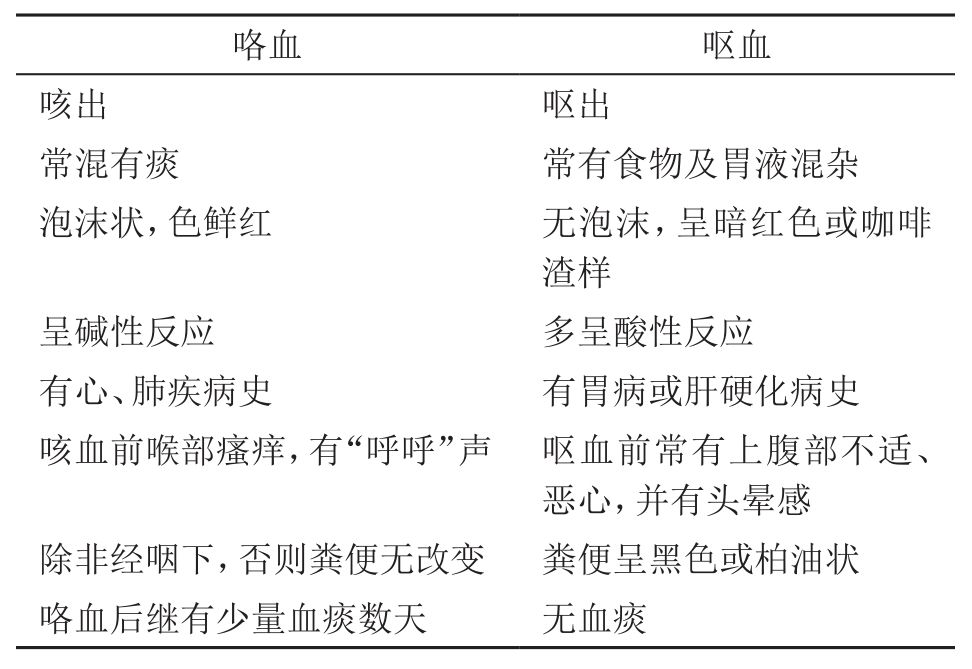
\includegraphics[width=3.22917in,height=2.21875in]{./images/Image00053.jpg}
\end{table}

当确认患者是上消化道出血后,需要迅速对下列问题作出判断,以便及时采取相应的处理。

\subsubsection{出血严重程度的估计和周围循环状态的判断}

对制定合理的治疗方案极为重要。

\subparagraph{失血量的判断与临床分级}

上消化道出血病情严重度与失血量呈正相关。一般而言,粪便隐血试验阳性提示每日失血量在5ml以上;出现黑粪者,每日出血量在50~70ml以上;如短期内出血量在250~300ml,多可导致呕血。因呕血与黑便混有胃内容物与粪便,而部分血液贮留在胃肠道内未排出,故难以根据呕血或黑便量精确判断出血量。常根据临床综合指标判断失血量的多寡,对出血量判断通常分为:大量出血(急性循环衰竭,需输血纠正者。一般出血量在1000ml以上或血容量减少20\%以上)、显性出血(呕血或黑便,不伴循环衰竭)和隐性出血(粪隐血试验阳性)。临床可以根据血容量减少导致周围循环的改变(伴随症状、脉搏和血压、化验检查)来判断失血量,并根据患者年龄、有无伴发病、失血量等指标将上消化道出血严重程度分为轻、中、重度三级(表\ref{tab13-2})。

\subparagraph{体位倾斜试验}

方法为先测平卧位时的血压(V\textsubscript{0}
)、脉搏(P\textsubscript{0}
),改为半卧位3分钟后,再测血压(V\textsubscript{1}
)、脉搏(P\textsubscript{1}
),符合下列条件之一者,提示失血量在1000ml以上。①V\textsubscript{0} −
V\textsubscript{1} >10mmHg;②P\textsubscript{1} − P\textsubscript{0} >
20次/分;③改半卧位后出现头晕、晕厥。必须在输液通路建立后才能进行,休克者禁作此试验。

\subparagraph{休克指数}

为脉搏(次/分)与收缩压(mmHg)的比值(P/SBP),指数正常值约为0.58。指数为1.0,大约失血800~1200ml(占血容量20\%~30\%);指数大于1.0,失血量1200~2000ml(占血容量30\%~50\%)。

\subparagraph{Hb、RBC和Hct的测定}

是估计失血量及决定输血量的重要参考指标。但在急性失血早期,由于血液浓缩及血液重新分布等代偿机制,上述指标可暂时无变化。一般出血3~4小时后,组织液渗入血管内补充血容量,患者可出现贫血,约24~72小时左右Hb稀释到最大限度。在连续测定中,三者迅速下降,表示继续出血,经输血纠正血容量后,与出血前比较,Hb每下降10g/L提示失血容量约400ml。

应指出的是,急性大出血严重程度的估计最有价值的指标是血容量减少所导致周围循环衰竭的临床表现,而周围循环衰竭又是急性大出血导致死亡的直接原因。因此,对急性消化道大出血患者,应将对周围循环状态的有关检查放在首位,并据此作出相应的紧急处理。血压和心率是关键指标,需进行动态观察,综合其他相关指标加以判断。如患者体位倾斜试验阳性,则提示血容量明显不足,是紧急输血的指征。如收缩压<
90mmHg,HR >
120次/分,伴有面色苍白,四肢湿冷,烦躁不安或神志不清则已进入休克状态,属严重大量出血(指3小时内需输血1500ml才能纠正其休克),需积极抢救。

\begin{table}[htbp]
\centering
\caption{上消化道出血病情严重程度分级}
\label{tab13-2}
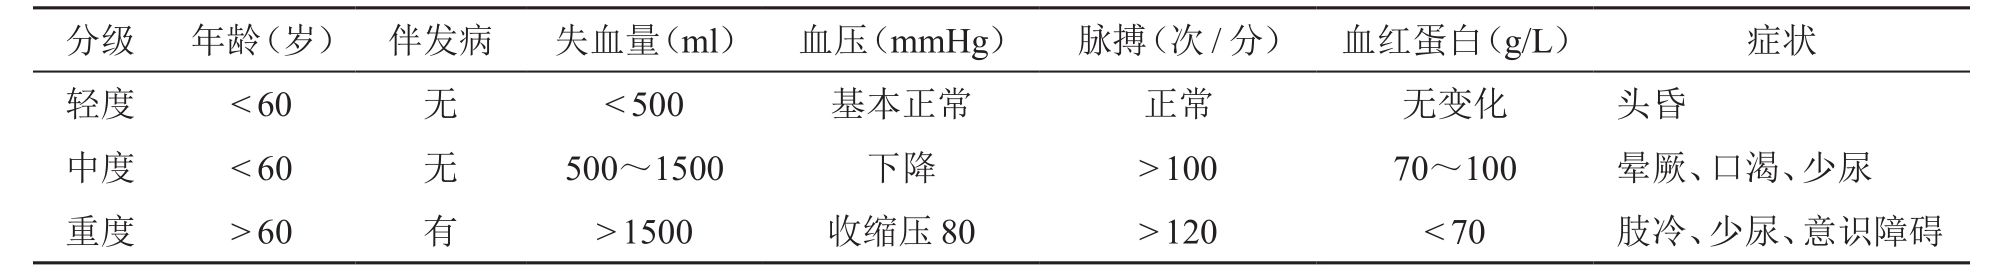
\includegraphics[width=6.65625in,height=0.91667in]{./images/Image00054.jpg}
\end{table}

\subsubsection{出血是否停止的判断}

临床上不能单凭Hb在下降或大便柏油样来判断出血是否停止或持续。因为一次出血后,Hb的下降有一定过程;而一次出血后柏油样大便持续天数受患者排便次数及出血量的影响。如每日排便1次,出血量在1000ml左右者,柏油样大便可持续1~3天,隐血试验阳性可达1周;若出血量在2000ml左右,柏油样大便可持续4~5天,隐血试验阳性达2周。应综合分析,特别是血压与脉搏的反复测定,直至恢复正常并趋稳定,尿量足(>
30ml/h),患者一般情况明显恢复者,方可认为已无活动性出血。有下列表现者,应认为有持续出血或再出血:①反复呕血或柏油样便次数及量增多,质稀薄,甚至排出暗红或鲜红色血便,伴肠鸣音活跃。②胃管抽出物有较多新鲜血。③周围循环衰竭的表现经积极补充血容量仍未见明显改善,或曾一度好转又很快恶化,中心静脉压仍有波动,稍稳定又再下降。④在补液量和排尿量足够的情况下,原无肾脏病变患者的BUN持续或再次升高。⑤Hb、RBC和Hct持续下降,血中网织红细胞持续增高。

肝硬化门静脉高压食管胃静脉曲张出血的防治共识(2008,杭州)关于EGVB继续出血或再出血的评估:①提示EGVB出血未控制的征象:72小时内出现以下表现之一者为继续出血。6小时内输血4个单位以上,生命体征不稳定。收缩压<
70mmHg,HR > 100次/分或心率增加> 20
次/分;间断呕血或便血,收缩压降低20mmHg以上或心率增加>
20次/分,继续输血才能维持Hb含量稳定;药物或内镜治疗后新鲜呕血,在没有输血的情况下,Hb含量下降30g/L以上。②提示EGVB再出血的征象:出现以下表现之一者为再出血。出血控制后再次有活动性出血的表现(呕血或便血;收缩压降低20mmHg以上或心率增加>
20
次/分;在没有输血的情况下,Hb含量下降30g/L以上)。早期再出血:出血控制后72小时~6周内出现活动性出血。迟发性再出血:出血控制6周后出现活动性出血。

\subsubsection{出血的病因诊断}

对上消化道大出血的患者,应首先纠正休克,然后尽快查找出血的部位与病因,以决定进一步的治疗措施和判断预后。一般通过询问病史、体检和必要的辅助检查,可明确出血的病因。

\subparagraph{病史与体检}

详询病史和系统体检,仍是出血病因与部位诊断的基础。约50\%的患者可据此作出病因诊断。慢性、周期性、节律性上腹痛多提示出血来自消化性溃疡,特别是在出血前疼痛加剧,出血后减轻或缓解,更有助于消化性溃疡的诊断。有服用非甾体抗炎药等损伤胃黏膜的药物或应激状态者,可能为急性糜烂出血性胃炎。对中年以上的患者近期出现上腹痛,伴有厌食、消瘦者,应警惕胃癌的可能性。既往有病毒性肝炎、血吸虫病或酗酒病史,并有肝病与门静脉高压的临床表现,可能是食管胃底静脉曲张破裂出血。尚应注意既往有无类似出血史、诊治情况等。

\subparagraph{急诊内镜检查}

急诊内镜检查是UGIB病因诊断中的首选方法。诊断正确率达80\%~94\%。急性上消化道出血的内镜检查有如下优点:①诊断正确率高:首先,内镜检查结合活检,既可明确出血部位,又可获得出血病变性质的诊断;其次,对一些上消化道钡餐检查不易发现的急性胃黏膜病变、贲门黏膜撕裂综合征、浅溃疡、胃黏膜毛细血管扩张症等,内镜可迅速作出诊断;第三,肝硬化合并上消化道出血病例,非静脉曲张破裂出血者占50\%左右,这仅能由内镜检查才能确诊。②提供预后的依据:如内镜下见溃疡基底喷血,溃疡基底血管、凝血块或红点等内镜征象可预示有再发出血的危险。③作为治疗手段:内镜诊断结合激光、高频电凝、喷洒止血剂以及给出血的曲张静脉内注射硬化剂等治疗性内镜的应用,使内镜检查不仅成为诊断工具,而且可作为止血治疗的方法。

\hypertarget{text00032.htmlux5cux23CHP1-13-1-4-4-2-1}{}
(1) NVUGIB的内镜检查:

①内镜检查能发现上消化道黏膜的病变,应尽早在出血后24~48小时内进行,并备好止血药物和器械。②内镜检查无食管胃底静脉曲张并在上消化道发现有出血病灶,NVUGIB诊断可确立。③内镜检查时根据溃疡基底特征,可用来判断病变是否稳定,凡基底有血凝块、血管显露等易于再出血。内镜检查时对出血灶病变应作Forrest分级(表\ref{tab13-3})。④应仔细检查贲门、胃底部、胃体垂直部、胃角小弯、十二指肠球部后壁及球后处,这些部位是易遗漏病变的区域。当检查至十二指肠球部未能发现出血病变者,应深插内镜至乳头部检查。发现有2个以上的病变,要判断哪个是出血性病灶。⑤有内镜检查禁忌证者不宜作此检查:如心率>
120次/分,收缩压< 90mmHg或较基础收缩压降低> 30mmHg、血红蛋白<
50g/L等,应先迅速纠正循环衰竭,血红蛋白上升至70g/L后再行检查。危重患者内镜检查时应进行血氧饱和度和心电、血压监护。

\begin{table}[htbp]
\centering
\caption{出血性消化性溃疡的 Forrest分级}
\label{tab13-3}
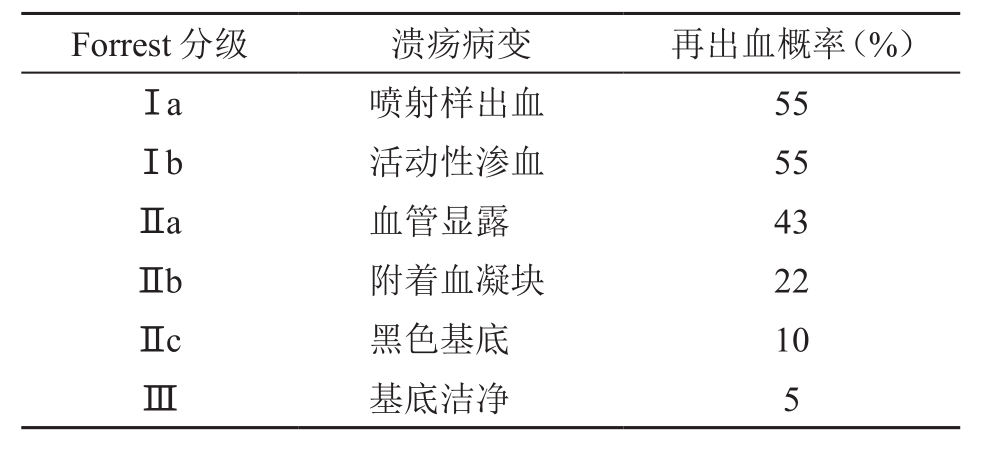
\includegraphics[width=3.26042in,height=1.5in]{./images/Image00055.jpg}
\end{table}

\hypertarget{text00032.htmlux5cux23CHP1-13-1-4-4-2-2}{}
(2) EGVB的内镜检查:

①内镜检查见有食管或胃曲张静脉出血,EGVB诊断即可成立;内镜检查时发现粗大曲张静脉和胃内血液而无其他可以识别的出血原因,EGVB诊断也可成立。②按食管静脉曲张形态及出血危险程度可将食管静脉曲张分轻、中、重3级。轻度(G\textsubscript{1}
):食管静脉曲张呈直线形或略有迂曲,无红色征(曲张静脉表面红斑、红色条纹和血疱)。中度(G\textsubscript{2}
):食管静脉曲张呈直线形或略有迂曲,有红色征或食管静脉曲张呈蛇形迂曲隆起但无红色征。重度(G\textsubscript{3}
):食管静脉曲张呈蛇形迂曲隆起且有红色征或食管静脉曲张呈串珠状、结节状或瘤状(不论是否有红色征)。③有内镜检查禁忌证者不宜作此检查(见前述)。

\hypertarget{text00032.htmlux5cux23CHP1-13-1-4-4-2-3}{}
(3) 内镜阴性患者的病因检查:

①仍有活动性出血的患者,应急诊行选择性腹腔动脉或肠系膜动脉造影,以明确出血部位和病因,必要时同时作栓塞止血治疗。②在出血停止,病情稳定后可作胃肠钡剂造影或放射性核素扫描(如\textsuperscript{99m}
锝标记患者的红细胞),但此检查特异性差。③对慢性隐性出血或少量出血者,可考虑作小肠镜检查。④对经各种检查仍未能明确诊断而出血不停者,病情紧急时可考虑剖腹探查,可在术中结合内镜检查,明确出血部位。

\subparagraph{X线钡餐检查}

目前已多为胃镜检查所替代。消化道大出血患者,因休克不能站立和充分变换体位,胃内潴留大量血液或血块影响钡餐充盈和病变征象观察,不易显示某些浅表病变如胃炎、急性胃黏膜病变等,仅能发现病变而不能确定是否为出血病变等,还可干扰以后内镜检查和血管造影检查,以及在活动性出血时,过早进行此项检查有加重出血的危险等因素,使急诊X线钡餐检查的实用性大大受到限制。因此,上消化道钡餐检查仅适用于出血已停止、生命体征平稳的上消化道出血患者。但对经胃镜检查出血原因未明、疑病变在十二指肠降段以下小肠段,则有特殊诊断价值。对某些解剖部位的改变,如胃黏膜脱垂、食管裂孔疝的诊断却优于一般胃镜检查。一般宜在出血完全停止3天后谨慎进行。

\subparagraph{血管造影}

对内镜检查无阳性发现或不适宜进行内镜检查者如有严重的心、肺并发症,且仍有活动性出血的患者可做选择性血管造影,对肠血管畸形、小肠平滑肌瘤等有很高的诊断价值,并可同时进行介入治疗。但忌用于严重动脉硬化、对碘剂过敏和老年患者。该检查的优点是:①灵敏性强:实验证明,出血量在0.5ml/min以上的消化道出血,在选择性血管造影连续摄影中即可见到造影剂从破裂血管外溢的X线征象。对慢性、隐源性活动性消化道出血是一种极有价值的诊断方法,阳性率一般为77\%~90\%。一般选择肠系膜上动脉及腹腔动脉造影已足够显示所要的范围。②具有精确的出血定位诊断价值:经出血相关区域血管注射造影剂,可精确显示出血部位和出血病变的供应动脉,为确定治疗提供了精确的解剖依据。③消化道内积血或血块不影响血管造影剂外溢的X线征象观察。④出血部位及其供应动脉显示后,立即经血管造影导管注射血管收缩剂或血管栓塞剂进行止血治疗。此外,门静脉造影(包括经脾穿刺门静脉造影、经肝穿刺门静脉造影以及经脐静脉插管门静脉造影等)除可以显示血管破裂部位、进行栓塞治疗外,还可以经导管测量门静脉压力诊断门脉高压症。

\subparagraph{放射性核素扫描}

经内镜及X线检查阴性的病例,可做放射性核素扫描。方法是采用核素(如\textsuperscript{99m}
锝)标记患者的红细胞后,再从静脉注入患者体内,当有活动性出血,且出血速度达到0.1ml/min,核素便可显示出血部位。注射一次\textsuperscript{99m}
锝标记的红细胞,可以监视患者消化道出血达24小时。本法缺点为出血部位定位不够确切,也不能确定出血病变的性质。

\subsubsection{预后估计与危险性分级}

约80\%~85\%急性上消化道出血患者除支持疗法外,无需特殊治疗出血可在短期内自然停止。仅有15\%~20\%患者持续出血或反复出血,而主要是这类患者由于出血并发症而导致死亡。如何早期识别再出血及死亡危险性高的患者,并给予加强监护和积极治疗,便成为急性上消化道出血处理的重点。提示预后不良、危险性增高的主要因素有:①高龄患者(>
60岁);②有严重伴随病(心、肺、肝、肾功能不全,脑卒中等);③本次出血量大或短期内反复出血;④特殊病因和部位的出血(如食管胃底静脉曲张破裂出血);⑤消化性溃疡伴有内镜下活动性出血,或近期出血征象。此外,EGVB出血48小时内肝静脉压力梯度(HVPG)>
20mmHg是其可靠的预后不良预测因子。

Rockall评分系统(表\ref{tab13-4})仍是目前临床广泛使用的评分依据,该系统依据患者年龄、休克状况、伴发病、内镜诊断和内镜下出血征象5项指标,将UGIB患者分为高危、中危或低危三级,积分≥5分者为高危,3~4分为中危,0~2分为低危。在Rockall评分系统中,若仅根据年龄、休克表现及伴发病三个指标评判疾病危险度,谓之为临床Rockall评分系统,可适用于无条件获取急诊内镜资料的基层医院;若同时有急诊内镜资料参与评估,谓之为完全Rockall评分系统。如出血患者,61岁,收缩压为105mmHg,心率为110次/分,胃镜下可见一巨大溃疡,活检示胃腺癌,附血凝块,无伴发病。则该患者Rockall积分=年龄(1)+心动过速(1)+无伴发病(0)+胃癌(2)+近期出血征象(2)=
6分,为高危患者。

Blatchford评分系统(表\ref{tab13-5})包含了BUN、Hb等实验室检查信息,其价值逐渐得到认可。

\begin{table}[htbp]
\centering
\caption{急性 UGIB患者的Rockall再出血和死亡危险性评分系统}
\label{tab13-4}
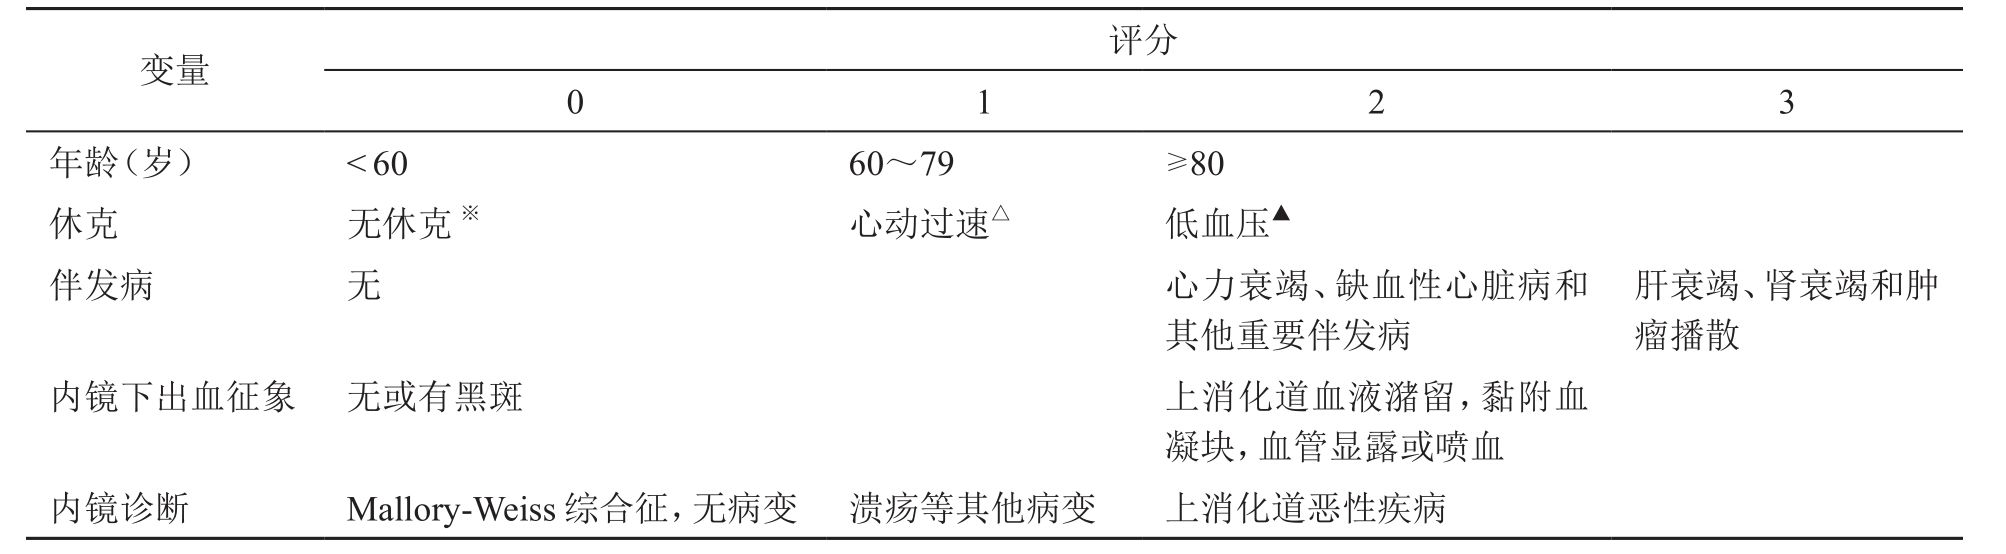
\includegraphics[width=6.67708in,height=1.83333in]{./images/Image00056.jpg}
\end{table}

注:\textsuperscript{※} 收缩压> 100mmHg,心率<
100次/分;\textsuperscript{△} 收缩压> 100mmHg,心率>
100次/分;\textsuperscript{▲} 收缩压< 100mmHg,心率> 100次/分

\begin{table}[htbp]
\centering
\caption{急性上消化道出血患者的 Blatchford评分}
\label{tab13-5}
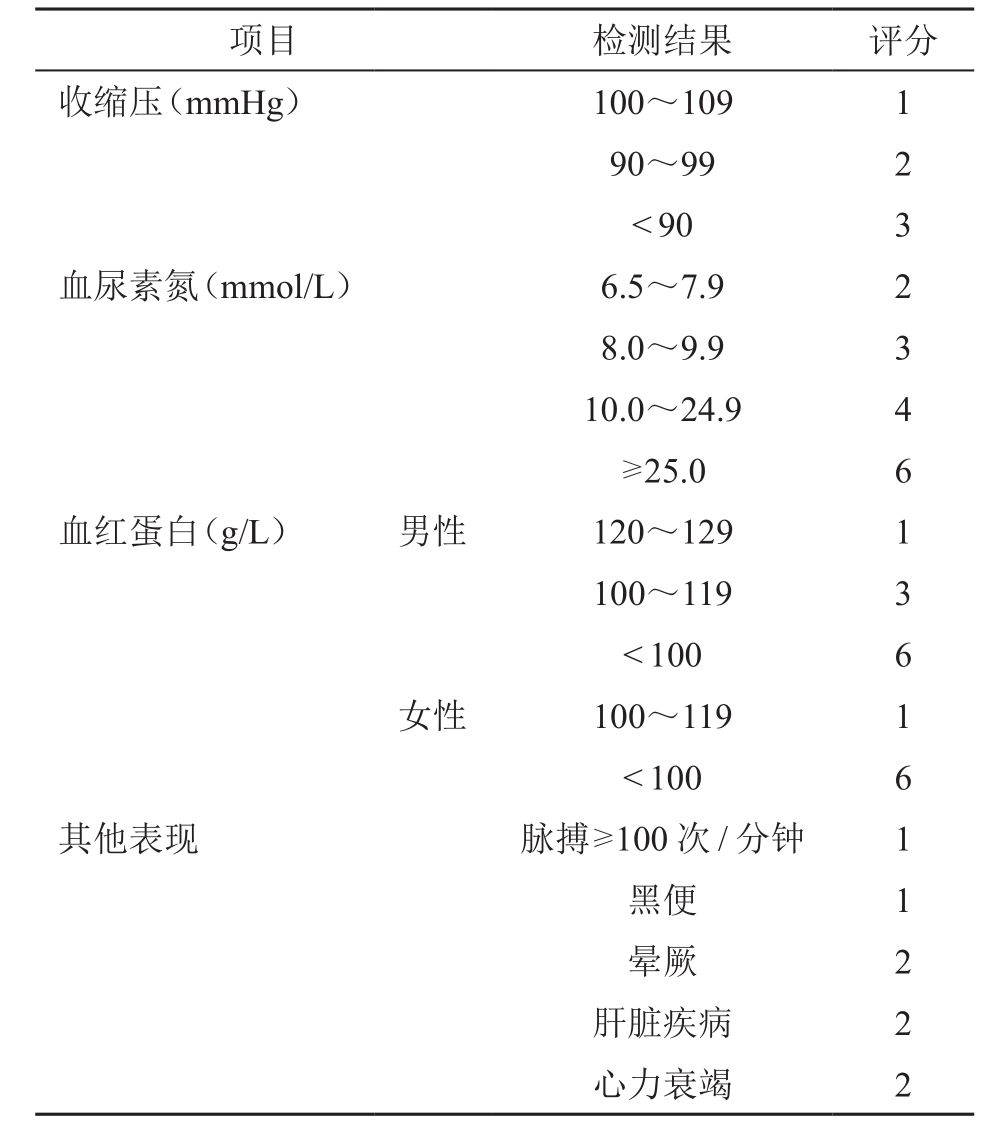
\includegraphics[width=3.32292in,height=3.75in]{./images/Image00057.jpg}
\end{table}

注:积分≥6分为中高危,< 6分为低危;1mmHg = 0.133kPa

\subsection{处理原则}

及早补充血容量、防治继续出血和再出血及病因治疗。其中,抗休克、迅速补充血容量应放在一切医疗措施的首位。

关于UGIB诊治流程,中国医师协会急诊医师分会制定的《急性上消化道出血急诊诊治专家共识》将上消化道出血的急诊诊治过程分为三个阶段,分别是紧急治疗期、病因诊断期和加强治疗期。紧急治疗期:患者入院6~48小时,治疗目标是控制急性出血、维持患者生命体征平稳并针对患者病情做出初步诊断及评估,治疗手段以药物治疗为主(PPI、生长抑素和抗菌药物联合用药)。病因诊断期:入院48小时内,急性出血得到控制,患者血流动力学稳定的情况下,行急诊内镜检查以明确病因并进行相应的内镜下治疗。无法行内镜检查的患者,可根据情况进行经验性诊断、评估和治疗。加强治疗期:入院后3~7天,治疗目标是病因治疗,预防早期再出血的发生。病因明确后,可根据不同病因采取不同的治疗手段。临床推荐采用以药物联合内镜治疗为主的综合治疗方法。

\subsubsection{一般措施}

患者应取平卧位休息,吸氧,严密观察患者的神色、血压、脉搏、出血量和尿量;保持静脉通道通畅,必要时作静脉切开。保持呼吸道通畅,避免呕血时引起窒息。烦躁不安者可给予镇静剂,如地西泮(安定)10mg肌注,对肝病患者忌用巴比妥类药物。呕血者宜暂禁食,但少量出血者宜进流质(因为胃内空虚产生饥饿的不正常的胃收缩不利于止血),活动性出血停止后可逐渐改变饮食的质与量。推荐对活动性出血或大出血患者宜常规放置胃管,其意义有:①可以观察出血情况,并可用冰盐水洗胃止血;②抽取胃内容物,减轻胃扩张,改善胃黏膜的循环,抽出积存在胃内的血液,能减轻日后吸收热和氮质血症,降低胃内酸度,防止凝血块被消化,有利于止血;③可通过胃管及时用药治疗;④预防吸入性肺炎;⑤鼻饲营养液。意识障碍和排尿困难者需留置尿管,危重大出血者必要时进行中心静脉压测定,老年患者常需心电、血氧饱和度、呼吸监护。

\subsubsection{迅速补充血容量}

迅速补充血容量是处理上消化道大出血的首要措施。立即查血型和配血,尽快建立有效的静脉输液通道,尽快补充血容量。在配血过程中,可先输平衡液或葡萄糖盐水。失血量较大(如减少20\%血容量以上)时,可输入血浆等胶体扩容剂。改善急性失血性周围循环衰竭的关键是要输血,一般输浓缩红细胞,严重活动性大出血考虑输全血。下列情况为紧急输血指征:①收缩压<
90mmHg(EGVB时< 80mmHg),或较基础收缩压降低幅度> 30mmHg;②Hb <
50~70g/L(EGVB时Hb < 50g/L),Hct < 25\%;③心率增快(>
120次/分)。输血量依失血量而定,原则上输血量应接近出血量。输血注意事项:①输血开始时,速度应加快,以尽快把收缩压升高至80~90mmHg水平,待血压稳定、病情改善后则减慢输血、输液速度,避免依赖升压药来维持血压。②避免输血、输液过多、过快,招致急性肺水肿,尤其是对有心、肺、肾疾患及老年患者。③防止枸橼酸中毒,一般每输血600~900ml可从静脉注入10\%葡萄糖酸钙10ml,以防低钙。④大量输注库存血时易引起高钾血症,应注意给予高渗葡萄糖,必要时加用适量胰岛素。⑤对肝硬化门脉高压静脉曲张破裂出血时,应输新鲜全血,除恢复血容量外,尚因其含有多种凝血因子和血小板成分,对止血有益;还可避免输库存血(含氨多)过多诱发肝性脑病。另外,输入的血约为失血量的2/3或3/4,以避免门静脉压力增高致再出血的危险。对于EGVB,以维持血流动力学稳定并使Hb维持在80g/L以上;过度输血或输液可能导致继续或重新出血;避免仅用氯化钠溶液补足液体,以免加重或加速腹水或其他血管外液体的蓄积;必要时应及时补充凝血因子、凝血酶原复合物等;血小板<
50 × 10\textsuperscript{9}
/L者,可输注血小板。对于急性大量出血者,应尽可能施行中心静脉导管置管和中心静脉压监测,以指导液体复苏。在补足液体的前提下,如血压仍不稳定,可以适当地选用血管活性药物(如多巴胺)以改善重要脏器的血液灌注。血容量充足的指征:①神志清楚或好转,无明显脱水貌;②收缩压90~120mmHg;③脉搏<
100次/分;④尿量> 40ml/h,血钠< 140mmol/L。

\subsubsection{非静脉曲张性上消化道出血(nonvariceal UGIB,NVUGIB)的止血措施}

NVUGIB是指除食管胃底静脉曲张破裂出血以外的其他病因引起的上消化道出血。包括消化性溃疡、急性糜烂出血性胃炎、胃泌素瘤、食管裂孔疝等所致的出血。止血措施主要有:

\subparagraph{内镜下止血}

起效迅速、疗效确切,应作为首选。可根据医院的设备和病变的性质选用,常用方法有:

\hypertarget{text00032.htmlux5cux23CHP1-13-1-5-3-1-1}{}
(1) 对出血灶喷洒止血药物:

内镜下直接对出血灶喷洒止血药物,对局部渗血疗效较好,对动脉性出血疗效较差。常用的药物有去甲肾上腺素溶液、孟氏液、注射用血凝酶、凝血酶等。

\hypertarget{text00032.htmlux5cux23CHP1-13-1-5-3-1-2}{}
(2) 局部注射法:

当内镜检查发现喷射性出血或血管显露时,可用局部注射法止血。常用的注射剂有肾上腺素溶液、凝血酶、无水酒精、高渗盐水等。其方法是在出血血管周围1~2mm处选3~4点,每点注入0.1~0.3ml。本法安全、有效,且可反复应用。

\hypertarget{text00032.htmlux5cux23CHP1-13-1-5-3-1-3}{}
(3) 激光照射法:

可供止血的激光有氩激光(Argon)和镱-铝-石榴石激光(Nd-YAG)两种。后者功率大,止血效果好。止血机制是由于光凝作用,使照射局部组织蛋白凝固,小血管内血栓形成。止血成功率在80\%~90\%。其并发症有胃肠穿孔、出血及胃肠胀气等。

\hypertarget{text00032.htmlux5cux23CHP1-13-1-5-3-1-4}{}
(4) 微波凝固法:

将微波经内镜导入出血部位,使产生热凝固,达到止血目的。其优点是,操作简便,并可将微波针状电极直接插入组织内治疗,插入组织的深度易控制,因而止血目标确切,安全性大。

\hypertarget{text00032.htmlux5cux23CHP1-13-1-5-3-1-5}{}
(5) 高频电凝止血法:

应用高频电流的热效应,使局部组织蛋白变性达到止血,迅速止血率达87\%~96\%。主要用于血管显露性出血及有直接出血征象的出血性病变。方法是用凝固电流在出血灶周围电凝,使黏膜下层或肌层的血管凝缩,最后电凝出血血管。有出血、溃疡、穿孔等并发症。近年来为了提高电凝止血的安全性和止血效果,研制出各种形状的及带喷水孔的单极电凝头、双极电凝头及四头双极电凝探头。

\hypertarget{text00032.htmlux5cux23CHP1-13-1-5-3-1-6}{}
(6) 热探头凝固法:

是利用热探头的高温(150℃)接触出血灶,使其组织蛋白质凝固而达到止血。此法疗效确切、安全、简单。

\hypertarget{text00032.htmlux5cux23CHP1-13-1-5-3-1-7}{}
(7) 放置止血夹法:

内镜直视下放置止血夹子,把出血的血管夹住止血,伤口愈合后此金属夹子自行脱落随粪便排出体外,此法止血既安全又有效。适用于消化性溃疡、急性胃黏膜病变的出血治疗,尤其在小动脉出血时用该法甚佳。

\subparagraph{制酸药物的应用}

胃酸在上消化道出血中起重要作用,抑制胃酸分泌及中和胃酸可达到止血的效果。制酸药止血的关键是使胃内pH维持在>
6,这样,既可促进血小板聚集和纤维蛋白凝块的形成,避免血凝块过早溶解,有利于止血和预防再出血,又可治疗消化性溃疡等病变。尤适用于消化性溃疡、急性胃黏膜病变、胃泌素瘤、食管裂孔疝等所致的出血。常用制剂有:

\hypertarget{text00032.htmlux5cux23CHP1-13-1-5-3-2-1}{}
(1) 中和胃酸药:

将胃内容物抽尽,用氢氧化铝凝胶60ml经胃管注入,15分钟后测胃液pH,若<
6,再注入60ml,以后每小时测pH1次,使其值维持在> 6。

\hypertarget{text00032.htmlux5cux23CHP1-13-1-5-3-2-2}{}
(2) H\textsubscript{2} 受体阻滞剂(H\textsubscript{2} RA):

目前临床上常用的有:第一代的西咪替丁(cimetidine,甲氰咪胍)、第二代的雷尼替丁(ranitidine)和第三代的法莫替丁(famotidine)。由于后两者不仅抗酸作用强(雷尼替丁比西咪替丁强5~8倍,法莫替丁比西咪替丁强30~100倍),作用时间更持久,且毒副作用相对较轻,应作为首选。可用雷尼替丁50mg缓慢静脉注射,每6~12小时1次,或用150~300mg加入液体中持续静滴;法莫替丁20mg溶入生理盐水或葡萄糖液20ml中,缓慢静脉注射,每日2次。

\hypertarget{text00032.htmlux5cux23CHP1-13-1-5-3-2-3}{}
(3) 质子泵抑制剂(proton pump inhibition,PPI):

可抑制胃壁细胞的H\textsuperscript{+} -K\textsuperscript{+}
-ATP酶,从而抑制胃酸的分泌。其抑制胃酸作用远强于H\textsubscript{2}
RA,几乎完全抑制酸分泌,持续用药无耐受性,且作用持久、递增,3~5天达稳态,胃内pH维持平稳。大剂量PPI可减少高危患者再出血率,且总费用降低,是治疗NVUGIB的首选止血药物。加拿大NVUGIB共识会议推荐内镜止血成功后应用PPI,在待行内镜检查时也应给予大剂量PPI,并认为H\textsubscript{2}
RA不能减少再出血率及病死率,不提倡用H\textsubscript{2}
RA止血。PPI常用制剂有:奥美拉唑(omeprazole,又名洛赛克,Losec)、泮托拉唑(pantoprazole)和兰索拉唑(lansoprazole)等。PPI给药方法及剂量:高危患者应静脉给药,如奥美拉唑静脉推注80mg后,以8mg/h输注72小时;如低危患者可口服给药,如奥美拉唑20mg,每6小时一次,持续5天。

\subparagraph{奥曲肽(octreotide)}

商品名善得定(Sandostatin),是人工合成的生长抑素类似品。能抑制胃酸、胃蛋白酶和胃泌素分泌,促进胃黏膜生长,能选择性引起内脏循环血流量减少和门脉压下降。用法:100μg皮下注射,每日2~4次。

\subparagraph{去甲肾上腺素}

可使胃肠黏膜出血区域的小动脉强烈收缩,减少局部血流量,并能减少胃酸分泌,有类似迷走神经切断的作用;同时因可降低门脉压,故亦用于食管静脉曲张破裂出血。用法有二:①口服或胃管内灌入:用去甲肾上腺素8mg加入冷生理盐水100~200ml中为1次量,口服或由胃管内灌入,每0.5小时1次,共2~4次;若有效,可再改为1小时1次,共4~6小时,以后每2小时1次共4~6小时。若无效,则不用。②腹腔灌注:以细长穿刺针作腹腔穿刺,注入含去甲肾上腺素8mg的生理盐水100ml,然后来回转动患者腹部,出血可迅速停止。本法适用于有腹水者,以免注入组织内引起缺血性坏死。

\subparagraph{注射用血凝酶(立止血,reptilase)}

是酸性止血剂,含有如凝血激酶和凝血酶样物质,可直接作用于内、外源性凝血系统形成凝血活酶,促进凝血酶的形成而起到凝血作用。用法:首次静注与肌注各1kU,继而每日肌注1kU。无明显毒副作用。

\subparagraph{凝血酶(thrombin)}

本品是从猪血提取、精制而得的凝血酶无菌制剂。能直接作用于出血部位的纤维蛋白原,使其转变为纤维蛋白,促使血液凝固、填塞出血点而止血;尚有促进上皮细胞的有丝分裂而加速创伤愈合的作用。其特点是局部止血迅速,疗效显著,无明显不良反应,但出现过敏反应时,应立即停用。首次剂量宜大(8000U~2万U),溶入50~100ml生理盐水或牛奶、豆汁内口服或胃管内注入,每2~6小时1次,应用次数视病情而定。凝血酶遇热或在酸性环境中均易失去活性,故溶液温度不要超过37℃,同时给予抑酸药物(如H\textsubscript{2}
受体阻滞剂、质子泵抑制剂)以便得以发挥最大作用。本品切忌血管内或肌内注射。

\subparagraph{其他止血药物}

以下止血药物对NVUGIB的确切效果未能证实,不作为一线药物使用。应避免滥用止血药。可酌情选用的有:①维生素K:能促进凝血酶原及凝血因子Ⅷ、Ⅵ、Ⅳ、Ⅹ在肝内合成。可用维生素K\textsubscript{1}
10mg肌注,每日2次;或维生素K\textsubscript{4}
口服4mg,每日3次;②肾上腺色腙(安络血):可增强受损毛细血管的修复能力,从而达到止血目的。10mg肌注,每天2次;或5~10mg口服,每天3~4次。③酚磺乙胺(止血敏):有增强血小板的作用。0.5~1.0g口服,每天3次;或0.5g肌注或静注。④氨甲苯酸(止血芳酸)、氨基己酸:能抑制纤溶酶原的激活因子和抑制纤维蛋白的溶解。⑤中药:云南白药、三七粉、白及粉、血余炭等均有防腐生肌、凉血止血的作用,中成药如止血散(白及、煅瓦楞、三七、甘草)、止血粉(白及、蒲黄、地榆、甘草)、止血汤(仙鹤草、地榆炭、白及、生槐花)等可酌情辨证选用。

\subparagraph{选择性血管造影及栓塞治疗}

选择性胃左动脉、胃十二指肠动脉、脾动脉或胰十二指肠动脉血管造影,针对造影剂外溢或病变部位经血管导管滴注血管升压素或去甲肾上腺素,导致小动脉和毛细血管收缩,使出血停止。无效者可用明胶海绵栓塞。

\subparagraph{手术治疗}

诊断明确但药物和介入治疗无效者,诊断不明确、但无禁忌证者,可考虑手术,结合术中内镜止血治疗。约10\%的胃十二指肠溃疡大出血患者需急症手术止血,手术指征为:①出血速度快,短期内发生休克,或较短时间内(6~8小时)需要输入较大量血液(>
800ml)方能维持血压和Hct者;②年龄在60岁以上伴动脉硬化症者自行止血机会较小,对再出血耐受性差,应及早手术;③近期发生过类似的大出血或合并穿孔或幽门梗阻;④正在进行药物治疗的胃十二指肠溃疡患者发生大出血,表明溃疡侵蚀性大,非手术治疗难以止血;⑤内镜检查发现动脉搏动性出血,或溃疡底部血管显露再出血危险很大。急诊手术应争取在出血48小时内进行,胃溃疡较十二指肠溃疡再出血概率高3倍,应争取及早手术。

\subparagraph{原发病的治疗}

对出血的病因比较明确者,如幽门螺杆菌阳性的消化性溃疡患者,应予抗幽门螺杆菌治疗及抗溃疡治疗。需要长期服用非甾体抗炎药者一般推荐同时服用PPI或黏膜保护剂。

非静脉曲张性上消化道出血诊治流程见图\ref{fig13-1}。

\subsubsection{食管胃静脉曲张出血的止血治疗}

肝硬化门脉高压症患者发生上消化道出血,并不全是由食管胃底静脉曲张破裂所致,而是多种因素共同作用的结果。因此,它的治疗仍应以上述治疗措施为基础。EGVB活动性出血的止血措施主要有内镜治疗、血管活性药物、经颈静脉肝内门体分流术(transjugular
intrahepatic portosystemic
shunt,TIPS)、外科手术和双气囊堵塞压迫等。其作用机制、运用方法及注意事项等有关内容,详见本书第116章第1节“肝硬化并上消化道出血”部分。

\subsubsection{预后}

据临床资料统计,约80\%~85\%急性上消化道大量出血的患者除支持疗法外,无需特殊治疗,出血可在短期内自然停止。仅有15\%~20\%患者持续出血或反复出血,常因出血并发症而导致死亡。如何早期识别再出血及死亡危险性高的患者,并予加强监护和积极治疗,便成为急性上消化道大量出血处理的重点。提示预后不良危险性增高的主要因素有:①高龄患者(>
60岁);②有严重伴随病(心、肺、肝、肾功能不全、脑卒中等);③本次出血量大或短期内反复出血;④特殊病因和部位的出血(如食管胃底静脉曲张破裂出血);⑤消化性溃疡伴有内镜下活动性出血,或近期出血征象。

\begin{figure}[!htbp]
 \centering
 \includegraphics[width=4.23958in,height=3.55208in]{./images/Image00058.jpg}
 \captionsetup{justification=centering}
 \caption{急性非静脉曲张性上消化道出血诊治流程}
 \label{fig13-1}
  \end{figure} 

PPIs:质子泵抑制剂;H\textsubscript{2} RA:H\textsubscript{2} 受体拮抗剂

\protect\hypertarget{text00033.html}{}{}

\section{下消化道出血}

下消化道出血(lower gastrointestinal
hemorrhage)是指屈氏韧带以下的小肠或大肠出血。依其出血量大小、速度和快慢等可分为三类:①慢性隐性出血:肉眼不能观察到便血,仅有大便隐血试验阳性,常以不明原因贫血就诊或普查时发现。②慢性少量显性出血(亚急性出血):表现为间歇性或持续性肉眼可见的少量显性便血,可呈鲜红色、果酱样或柏油样黑粪,无循环衰竭表现。③急性大量出血:短期内排出大量鲜红或暗红色血便,伴血压下降等休克症状,常需输血治疗者。多数下消化道出血相对缓慢,或呈间歇型,约80\%的出血能自行停止。在治疗上除了止血、补充血容量以外,寻找下消化道出血部位、疾病性质进行原发病病因治疗最为重要。

下消化道范围广,出血病因繁多,分类各异。如按病变部位可分为:①小肠疾病:小肠肿瘤、黑色素-胃肠息肉综合征、克罗恩病(Crohn病)、小肠憩室与Meckel憩室、肠套叠、小肠血管畸形、急性出血性坏死性肠炎、缺血性小肠炎和肠结核等。②大肠疾病:溃疡性结肠炎、结肠息肉、结肠憩室、菌痢、阿米巴痢疾、结肠癌、克罗恩病、缺血性结肠炎、结肠子宫内膜异位症、结肠结核及肠套叠、结肠血管畸形等。③直肠疾病:直肠溃疡、非特异性炎症、肿瘤、息肉、放射性直肠炎和腹盆腔邻近脏器恶性肿瘤或脓肿侵及直肠等。④肛管疾病:痔、肛裂、肛瘘。此外,还有全身性疾病累及肠道。国内资料引起下消化道出血的最常见病因为大肠癌和大肠息肉,其次为肠道炎症性疾病(其中肠伤寒、肠结核、溃疡性结肠炎、克罗恩病和坏死性小肠炎有时可发生大量出血)和血管病变,憩室引起的出血少见。但在西方国家,血管病变和消化道憩室是下消化道出血最常见病因,其次为结肠肿瘤和炎症性肠病。

\subsection{诊断思路}

\subparagraph{下消化道出血的确立}

首先要排除口腔、鼻咽、喉、气管、支气管、肺等部位的出血被吞咽后由肛门排出的可能性,还要与下列情况区别:①口服某些中草药、兽炭、铁剂、铋剂时,大便可呈暗褐色或黑色,但隐血试验阴性;②食用过多的肉类、猪肝、动物血后大便可变暗褐色,隐血试验呈阳性,但素食后即转呈阴性;③口服酚酞制剂,大便有时呈鲜红色,不注意时易误诊为大量便血。

排除了上述因素后,要确定是否为下消化道出血,大便的色泽和量是重要的线索,通常大便呈鲜红色或暗红色者,即可确诊。但如为暗红色大量血便或仅表现为黑便或大便隐血阳性时,则应与上消化道出血鉴别。此时应常规行胃十二指肠镜检查,若未发现病变,大致可除外上消化道出血。

下述几点有助于下消化道出血的诊断:①病史中多伴有下腹痛或腹部有包块,排便异常伴便血史,出血前常有中下腹不适、下坠或便意。②大便常为鲜红、暗红、果酱样,少数为黑便,无呕血。③下消化道出血时胃管内无咖啡色的液体和暗红色的血液被抽出。④来自高位小肠的出血可能有血BUN升高,而结肠出血常不升高;上消化道出血时血BUN升高较下消化道出血时明显。⑤结直肠出血,常表现为鲜血便或是暗红的血便,血与大便相混,可有便后滴血,亦可表现为脓血便。⑥小肠出血常为暗红果酱样便,亦可为黑便,偶有血水样便。⑦大肠出血常伴有下腹痛、腹泻、里急后重等症状,而小肠出血常表现为脐周疼痛。

\subparagraph{估计出血速度和出血量}

下消化道出血确定后,估计出血速度和出血量甚为重要。判断患者出血速度和出血量的最终标准取决于为恢复和维持血容量所需的输血量和速度。在此之前,则可根据有无循环障碍及其程度、Hct和Hb变化作出初步估计。

\subparagraph{确定是否由全身性疾病所致下消化道出血}

全身性疾病所致的下消化道出血有相应疾病的全身表现。血液系疾病、血管疾病、肝脏疾病和某些中毒性疾病常伴有凝血与止血功能障碍,有凝血因子缺乏、血小板质或量改变、血管脆性增加、血管收缩障碍的实验室发现。相反,多数传染性疾病及中毒性疾病下消化道出血的主要原因是肠黏膜、黏膜下血管受损的后果。血液检查、骨髓检查、凝血机制检查等有助于诊断。

\subparagraph{出血部位的判断}

下消化道出血最常见的部位是乙状结肠,占50\%左右。其他部位出血频率依次为直肠、降结肠、横结肠、升结肠、盲肠、小肠。根据出血类型常可对出血部位作出初步判断:仅大便隐血阳性者,若排除了上消化道出血,则多为右侧结肠和小肠出血;少量显性出血,则主要是结肠、直肠出血;鲜红或暗红色血便,以左半结肠和直肠为主;果酱色或咖啡色血便则多为右半结肠出血。虽右半结肠和小肠出血的发生率较低,但较易发生急性大出血。上位结肠出血时,血与大便常混杂;乙状结肠和直肠出血时,常有新鲜血液附着于成形大便的表面。血在大便后滴下,与粪便不相混杂者,虽多见于内痔、肛裂,但也可见于直肠息肉和直肠癌,应予以注意。

\subparagraph{出血病因的诊断}

病史与体检是出血病因诊断中最重要的基础工作。

\hypertarget{text00033.htmlux5cux23CHP1-13-2-1-5-1}{}
(1) 既往史:

①反复小量显性出血史,提示痔、息肉、憩室等。②大便习惯改变或大便变细有切迹,应警惕结肠、直肠肿瘤。③反复血性腹泻史提示炎症性肠病可能。④曾患疾病与用药:曾患肺结核者应考虑肠结核;动脉硬化、心律失常、口服避孕药者应考虑缺血性结肠炎;风湿性疾病、白血病、出血性疾病、尿毒症、急性胰腺炎等病程中发生出血,多由于原发病引起的肠道病变;应用抗生素过程中出血应考虑假膜性肠炎、出血性结肠炎;便血前数月或数年曾接受腹部放射治疗者应考虑放射性结肠炎。

\hypertarget{text00033.htmlux5cux23CHP1-13-2-1-5-2}{}
(2) 便血特点与伴随症状:

①脓血黏液便伴里急后重或坠胀感,大便次数增多,应考虑痢疾和直肠癌可能。②中小量出血,色较红而呈间断性附于大便表面,要注意息肉出血之可能。③便血伴剧烈腹痛者,尤其是老年人心血管病患者,应警惕肠系膜血管栓塞;便血伴发热应考虑感染性肠炎、炎症性肠病、肠结核、肠伤寒、出血性坏死性肠炎、血液系疾病(白血病、恶性组织细胞病、恶性淋巴瘤等)等;便血伴腹块或不全性肠梗阻应考虑肿瘤、肠结核、Crohn病、肠套叠等;便血伴腹壁瘘管(或内瘘管),见于Crohn病、肠结核、癌、放线菌病。

\hypertarget{text00033.htmlux5cux23CHP1-13-2-1-5-3}{}
(3) 年龄与病因:

下消化道出血的病因与年龄有关:①婴儿和儿童:以Meckel憩室最多见,幼年性息肉次之,其他有炎症性肠病、肠套叠等。②青少年和成年人:在青少年时期,Meckel憩室依然是最常见病因,其次是炎症性肠病和息肉;随年龄增长癌肿比例显著增高。③老年人:以癌肿、息肉多见,其次为慢性结肠炎症、结肠血管扩张、结肠憩室等。

\hypertarget{text00033.htmlux5cux23CHP1-13-2-1-5-4}{}
(4) 出血部位与病因:

①直肠、乙状结肠:以息肉、癌、溃疡性结肠炎、单纯性溃疡、菌痢、阿米巴肠炎、放射性肠炎多见;②结肠脾曲、降结肠、乙状结肠:除息肉、癌外,易发生缺血性结肠炎;③右侧结肠:憩室、血管畸形、肠结核、Crohn病;④回盲部(回肠末段至升结肠始段):除癌、息肉外,类癌、Crohn病、单纯性溃疡、肠结核、鞭虫病、阿米巴肠炎、肠套叠、Meckel憩室、肠伤寒、沙门菌肠炎等。

\hypertarget{text00033.htmlux5cux23CHP1-13-2-1-5-5}{}
(5) 肛门视诊和直肠指检:

下消化道出血病因诊断的第一步,应采用简便易行的肛门视诊和直肠指诊,以发现或排除痔、肛裂,以及大部分直肠癌和息肉等常见的出血病因。

\hypertarget{text00033.htmlux5cux23CHP1-13-2-1-5-6}{}
(6) 内镜检查:

结肠镜检查是诊断大肠和回肠末端病变的首选检查方法。宜尽量在出血停止后近期或出血间歇期进行。对于出血灶的诊断,以窥视下直接见到活动性渗血最可靠。

\hypertarget{text00033.htmlux5cux23CHP1-13-2-1-5-7}{}
(7) X线钡剂造影检查:

一般要求在大出血停止至少3天后进行。主张双重气钡造影。其优点是基层医院已普及,患者易接受。缺点是对较平坦病变、广泛而较轻炎症性病变易漏诊,有时无法确定病变性质。对X线钡剂灌肠检查阴性的下消化道出血患者需进行结肠镜检查,已作结肠镜全结肠检查患者则不强调本项检查。

\hypertarget{text00033.htmlux5cux23CHP1-13-2-1-5-8}{}
(8) 胶囊内镜或双气囊小肠镜检查:

适用于常规内镜检查和X线钡剂造影不能确定出血来源的不明原因出血,出血活动期和静止期均可进行,可视病情和医疗条件选用。

\hypertarget{text00033.htmlux5cux23CHP1-13-2-1-5-9}{}
(9) 放射性核素扫描或选择性腹腔动脉造影:

必须在活动性出血时进行。主要用于急诊结肠镜检查不能确定出血来源的不明原因出血。放射性核素扫描检查的特点是简便敏感,出血量约0.1ml/min时即有阳性显示;缺点是对出血不能准确定位。常用本法初步确定出血部位,为进一步作血管造影提供线索。此外,利用\textsuperscript{99m}
Tc腹部扫描可用于诊断有胃黏膜异位的先天性病变,如Meckel憩室、肠重复畸形等。对持续大出血患者经上述检查不能明确出血灶时,应及时作选择性肠系膜上动脉造影,因肠系膜上动脉支配全部小肠和右侧结肠。约50\%~80\%的憩室出血和全部血管畸形出血均发生于右侧结肠。如肠系膜上动脉造影阴性,应再作肠系膜下动脉和腹腔动脉造影。血管造影可显示低至0.5ml/min的出血,此外还可显示肿瘤血管和血管畸形。成功的血管造影约于2/3的病例可显示肠出血来源。

\hypertarget{text00033.htmlux5cux23CHP1-13-2-1-5-10}{}
(10) 手术探查:

如上述检查仍不能明确出血灶,持续大出血危及患者生命,必须手术探查。术中内镜是明确诊断不明原因消化道出血,尤其是小肠出血的可靠方法。

不明原因消化道出血(obscure gastrointestinal bleeding,
OGIB)是指常规内镜检查(胃镜和结肠镜)不能确定出血来源的持续或反复消化道出血,多为小肠出血(如小肠的肿瘤、Meckel憩室和血管病变等),是消化道出血诊断的难点。OGIB的诊断步骤:在出血停止期,先行小肠钡剂检查;在出血活动期,应及时作放射性核素扫描或选择性腹腔动脉造影;若上述检查结果阴性则选择胶囊内镜或及双气囊小肠镜检查;出血不止危及患者生命者行手术探查,探查时可辅以术中内镜检查。

\subsection{处理原则}

下消化道出血主要是病因治疗,大出血时应积极抢救。

\subparagraph{一般措施}

一般急救措施与补充血容量同上消化道出血一样。一般措施包括应用注射用血凝酶、静滴血管加压素、生长抑素、肾上腺色腙(安络血)、酚磺乙胺等药物。

\subparagraph{局部止血措施}

对结肠出血,可给予冰盐水去甲肾上腺素液(去甲肾上腺素8mg加入100~200ml生理盐水中)、孟氏液、凝血酶等进行灌肠。

\subparagraph{内镜下止血措施}

包括内镜下向出血病灶喷洒止血药物、高频电凝止血、激光止血、息肉电凝止血、黏膜和黏膜下注射硬化剂等措施止血。

\subparagraph{放射性介入治疗}

在做选择性动脉造影时,若发现造影剂有渗出,即可通过导管给予血管加压素滴注,0.1~0.4U/min。对结肠出血不能自发地停止或血管加压素输注无效的病例,可施行栓塞治疗。在荧光透视下作超选择性插管,将管端插入出血灶近端几厘米处,注入明胶海绵碎片或自体凝血块,可将出血动脉栓塞、制止出血。

\subparagraph{手术治疗}

经内科保守治疗仍出血不止危及生命,无论出血病变是否确诊,均是紧急手术的指征。此外,对下列情况可行手术治疗:①对Meckel憩室、肠重复畸形、恶性肿瘤、先天性动静脉畸形(包括结肠血管扩张)等皆可手术切除。②息肉病、家族性息肉病或有高度癌变倾向的息肉可手术切除。但一般息肉可经纤维结肠镜电凝切除。③溃疡性结肠炎引起的大出血是次全或全结肠切除的手术指征;Crohn病时如病变局限也可作局限性肠切除。

下消化道出血的处理程序如图\ref{fig13-2}。

\protect\hypertarget{text00034.html}{}{}

\section{不明原因消化道出血}

不明原因消化道出血(obscure gastrointestinal
bleeding,OGIB)是指常规的消化道内镜(包括检查食管至十二指肠降段的上消化道内镜与肛直肠至回盲瓣的结肠镜检查)和常规钡餐检查不能明确病因的持续或反复发作的出血。可分为不明原因的隐性出血和不明原因的显性出血。前者表现为反复发作的缺铁性贫血和大便隐血阳性,而后者则表现为黑便、血便等肉眼可见的出血。OGIB占消化道出血的3\%~5\%。

根据国内外文献报道,40岁以下患者OGIB的病因多为小肠肿瘤、Meckel憩室、Dieulafoy病、遗传性息肉综合征或克罗恩病等;而40岁以上患者则多见于血管病变、非甾体类抗炎药相关性溃疡、大的食管裂孔疝囊内的糜烂(Cameron糜烂)和其他少见病因如主动脉肠瘘等。

\begin{figure}[!htbp]
 \centering
 \includegraphics[width=3.98958in,height=3.90625in]{./images/Image00059.jpg}
 \captionsetup{justification=centering}
 \caption{下消化道出血的处理程序}
 \label{fig13-2}
  \end{figure} 

\subsection{诊断思路}

\hypertarget{text00034.htmlux5cux23CHP1-13-3-1-1}{}
(一) 诊断方法与选择

\subparagraph{病史和体格检查}

对OGIB患者首先应仔细询问病史(包括目前症状、既往史、用药史、家族史等)。如果患者有消瘦或梗阻症状,提示小肠疾病的可能性大;而老年患者如有肾病或结缔组织病等,则血管病变的风险较高。详细可靠的病史和体格检查有助于减少漏诊率。

\subparagraph{内镜检查}

\hypertarget{text00034.htmlux5cux23CHP1-13-3-1-1-2-1}{}
(1) 常规内镜:

为OGIB的必需检查。对OGIB的内镜检查,应请有经验的内镜医师复核。初次检查阴性的患者必要时可重复内镜检查,有助于提高诊断率及减少漏诊率。初次检查时易被漏诊的病变有血管扩张、Cameron溃疡和位于盲区的消化性溃疡、息肉等。

\hypertarget{text00034.htmlux5cux23CHP1-13-3-1-1-2-2}{}
(2) 胶囊内镜:

目前,胶囊内镜已成为小肠疾病的重要检查技术。对OGIB患者,胶囊内镜的诊断阳性率为66\%~76\%,并且对于持续性出血的OGIB诊断阳性率高于间歇性出血的OGIB,对于显性出血的OGIB诊断阳性率高于隐性出血的OGIB。但胶囊内镜的缺点为不能进行治疗,遇肠段狭窄或梗阻时可能被嵌顿,出血量较多时视野不清等。

\hypertarget{text00034.htmlux5cux23CHP1-13-3-1-1-2-3}{}
(3) 小肠镜:

小肠镜是目前观察小肠病变较好的检查方法,并已成为OGIB的重要手段。传统推进式小肠镜仅能插入深度在幽门下50~150cm不等,患者依从性较差,操作技术要求高。近年来发展的双气囊电子小肠镜具有插入深度好、诊断率高的特点。它利用固定于镜身前端和外套管的2个气囊交替充气和放气,有经口、经肛两种检查方法,并且可以进行黏膜活组织检查,对小肠出血的诊断率在60\%以上。因此,双气囊小肠镜检查对于OGIB有较高的诊断和治疗价值。

\subparagraph{影像学检查}

\hypertarget{text00034.htmlux5cux23CHP1-13-3-1-1-3-1}{}
(1) 全小肠钡剂造影(small bowel follow through,SBFT):

SBFT对OGIB的诊断率不高,且假阴性率较高,因此较少使用。但是若怀疑肿瘤、克罗恩病、肠结核等可考虑行SBFT。

\hypertarget{text00034.htmlux5cux23CHP1-13-3-1-1-3-2}{}
(2) 小肠钡剂灌肠:

小肠钡剂灌肠是经口或鼻插管至近端小肠后将钡剂导入,对小肠进行摄片和透视的方法。其对OGIB的诊断率为10\%~21\%,优于SBFT。

\hypertarget{text00034.htmlux5cux23CHP1-13-3-1-1-3-3}{}
(3) 血管造影:

血管造影是一项有创性检查,有助诊断显性OGIB(出血速率大于0.5ml/min)。与核素扫描相比,血管造影定位相对准确,且能直接进行血管栓塞治疗,止血率高,但出血复发率也高。血管造影的并发症有肾功能衰竭和缺血性肠炎等。

\hypertarget{text00034.htmlux5cux23CHP1-13-3-1-1-3-4}{}
(4) CT和MRI:

螺旋CT血管造影是一项新兴的检查技术,将导管插至腹主动脉并注入造影剂,如造影剂外渗至肠腔内形成大片高密度区,即可确定出血位置。对于常规血管造影阴性的OGIB患者可行CT血管造影。利用CT
或MRI进行小肠造影能同时进行肠腔和肠壁结构的观察。但目前临床经验较少,有待进一步研究。

\subparagraph{核素扫描}

核素扫描有助于诊断显性OGIB(出血速率保持在0.1~0.4ml/min)。可采用\textsuperscript{99m}
Tc标记的红细胞或\textsuperscript{99m}
Tc标记的胶体硫进行扫描,前者更为常用。通过核素扫描可以大致定位出血点,但有一定的假阳性率及假阴性率,需要鉴别血池区积血是否为原发出血灶。

\subparagraph{外科手术和术中内镜检查}

外科手术是OGIB最后考虑的剖腹探查手段。单纯剖腹探查风险较大且成功率低。而外科手术结合术中内镜检查可提高诊断率至50\%~100\%。

\begin{figure}[!htbp]
 \centering
 \includegraphics[width=4.19792in,height=2.86458in]{./images/Image00060.jpg}
 \captionsetup{justification=centering}
 \caption{不明原因消化道出血的诊断推荐流程}
 \label{fig13-3}
  \end{figure} 

\hypertarget{text00034.htmlux5cux23CHP1-13-3-1-2}{}
(二) OGIB诊断流程

对OGIB首先应详细询问病史与仔细地进行体格检查,以初步判断出血部位与性质,是隐性出血还是显性出血?如为隐性出血,可先行小肠钡剂检查,对显性出血,则行核素扫描和(或)血管造影检查较好,因上述检查无需特殊设备,可作为一线检查方法。若检查结果为阴性,可行小肠镜、胶囊内镜等二线检查,以进一步明确小肠有否病变;如经各种检查仍为阴性,临床上有明显出血,危及生命,应与外科协商行剖腹探查,若术中病变仍不明确,可行术中内镜检查,协助寻找病因。术前需要权衡利弊,如果患者不能接受,可先给予输血、补铁等对症治疗并观察是否有再出血,如不再出血则无需进一步检查,若有再出血则考虑重复既往的检查。OGIB诊断推荐流程见图\ref{fig13-3}。

\subsection{处理原则}

对于OGIB的治疗首先要采取补液、输血等支持治疗,以维持生命体征,创造条件进行病因诊断。一旦病因明确,因立即采用针对病因的治疗。在病因不明,且不能排除上消化道出血的情况下,应用止血药及质子泵抑制剂仍是常规治疗。如病情较重,使用奥曲肽等生长抑素类药物以降低内脏血流量与压力有助止血,在保守治疗无效,出血不止时应考虑手术治疗。

\protect\hypertarget{text00035.html}{}{}

\hypertarget{text00035.htmlux5cux23CHP1-13-4}{}
参 考 文 献

1. 陆再英,钟南山.内科学.第7版.北京:人民卫生出版社,2008:483

2. 陈灏珠,林果为.实用内科学.第13版.北京:人民卫生出版社,2009:1951

3. 中华医学会消化病学分会
,中华医学会肝病学分会,中华医学会内镜学分会.肝硬化门静脉高压食管胃静脉曲张出血的防治共识(2008,杭州).中华消化杂志,2008,28(8):551

4. Dimaio CJ,Stevens PD. Nonvariceal upper gastrointestinal bleeding.
Gastrointest Endoscopy Clin N Am,2007,17:253-272

5. 中华内科杂志编委会
,中华消化杂志编委会,中华消化内镜杂志编委会.急性非静脉曲张性上消化道出血诊治指南.中华消化杂志,2009,29(10):682-685

6.
中国医师协会急诊医师分会.急性上消化道出血急诊诊治专家共识.中国急救医学,2010,30(4):289-293

7.
中华消化杂志编委会.不明原因消化道出血诊治推荐流程(2007,南京).中华消化杂志,2007,27(6):406-408

8. Carey EJ,Leighton JA,Heigh RI,et al. A single-center experience of
260 consecutive patients undergoing capsule endoscopy for obscure
gastrointestinal bleeding. Am J Gastroenterol,2007,102:89-95

\protect\hypertarget{text00036.html}{}{}

\chapter{紫 癜}

紫癜(purpura)是皮下或黏膜下出血引起的皮肤或黏膜红紫等颜色改变的病征,它是临床上出血倾向的主要表现之一。根据出血的大小及范围,临床将皮下出血分为小于2mm者为出血点(petechia),3~5mm为紫癜及大于5mm者为瘀斑(ecchymosis),如为片状出血伴皮肤隆起则称为血肿(hematoma)。紫癜通常为血管外因素、血管因素及血小板因素所致出血性疾病的主要表现。凝止机制异常所致出血性疾病虽也可有紫癜的表现,但通常并非重要的体征。

\subsection{病因与发病机制}

紫癜根据病因及发病机制可分为血管性紫癜、血小板性紫癜及凝血机制障碍性紫癜三类。一般常见的为前两类,后者包括凝血因子异常及纤溶异常等,这些疾病都可出现紫癜。

\subsubsection{血管性紫癜}

血管性紫癜是由于多种因素致血管周围组织变性、萎缩及弛缓或血管壁通透性或脆性增加,使血液外渗所致。

\hypertarget{text00036.htmlux5cux23CHP1-14-1-1-1}{}
(一) 遗传因素

如遗传性毛细血管扩张症
、埃勒斯-当洛斯综合征及马方综合征(它们属遗传性结缔组织病,因血管及其周围胶原缺乏而致病)、家族性单纯性紫癜、弹性纤维假黄瘤(psudoxanthoma,elasticum)、骨质形成缺陷症、高胱氨酸尿症等。

\hypertarget{text00036.htmlux5cux23CHP1-14-1-1-2}{}
(二) 非遗传因素

\subparagraph{血管退化}

常见的有老年性紫癜(senile,紫癜)、维生素C缺乏所致的坏血病、严重营养缺乏症、恶病质(恶病质患者由于营养缺乏,皮肤萎缩,皮下脂肪消失,皮肤毛细血管受轻度外伤而易发生紫癜)等。

\subparagraph{免疫异常}

包括:过敏性紫癜:病者多数为儿童或青年,发病在20岁以下者占半数以上,无明显性别差异。病因方面较重要者为:①感染,值得注意的病原菌为溶血性链球菌;②药物,如氯霉素等;③食物,虾、蟹等;④其他,如植物花粉等。发病高峰在冬春季节。其他尚有自身红细胞过敏症(Gardner-Diamond
syndrome)、冷球蛋白及高γ球蛋白血症(常伴发于多种免疫性疾病及某些恶性肿瘤)。

\subparagraph{感染}

可见于多种病原体感染,有些可出现暴发性紫癜,如流行性脑脊髓膜炎、猩红热、败血症等。许多感染引起紫癜虽可伴有血小板减少,但血小板计数正常者更为多见。通常为毒素对毛细血管的损害。

\subparagraph{药物}

如类固醇性紫癜、香豆素坏死性紫癜(可能与该药物致血管内皮细胞损伤及降低血浆Ⅶ因子有关)。碘化物、颠茄、阿托品、奎宁、青霉素、普鲁卡因、铋剂、汞剂、非那西丁、水杨酸制剂、水合氯醛及其他安眠药等化学物品,均可引起非血小板减少性紫癜。

\subparagraph{某些慢性内科病}

有些慢性内科病可并发非血小板减少性紫癜,如慢性肾炎、肝功能不全、糖尿病等。

\subparagraph{单纯性紫癜}

经过和缓而较为慢性,患者几乎全为女性,尤常发生于月经期间。临床表现有下列特点:无外伤或其他诱因而不时出现皮肤瘀斑或瘀点,但无黏膜出血;患者无家族易出血史;血液学检查无明显的改变。

\subparagraph{机械因素}

如外伤性紫癜、体位性紫癜等。

\subsubsection{血小板性紫癜}

血小板性紫癜是由于血小板量或质的异常所致的紫癜,可分为血小板减少及功能异常两大类。

\hypertarget{text00036.htmlux5cux23CHP1-14-1-2-1}{}
(一) 血小板减少性紫癜

\subparagraph{遗传因素}

如Fanconi综合征、Epstein综合征(常伴有神经性耳聋及肾炎)、巨大血小板综合征、湿疹-感染-血小板减少综合征及May-Hegglin异常等。

\subparagraph{巨核细胞减少或缺乏}

如白血病、再生障碍性贫血、骨髓转移癌、多发性骨髓瘤、淋巴瘤等。

\subparagraph{巨核细胞存在但血小板生成不良(血小板无效生成)}

见于巨幼红细胞性贫血、酒精致血小板减少症、骨髓增生异常综合征(MDS)等。

\subparagraph{巨脾对血小板的破坏}

如肝硬化、骨髓纤维化、Gaucher病、脾亢等。

\subparagraph{血小板破坏或消耗增多}

常见病因有:

\hypertarget{text00036.htmlux5cux23CHP1-14-1-2-1-5-1}{}
(1) 免疫因素:

特发性及免疫性血小板减少性紫癜(ITP)、输血后紫癜(PTP)、自身免疫性溶血性贫血伴血小板减少(Evans综合征)及药物相关免疫性血小板减少性紫癜(drug-induced
immunologic thrombocytopenic
purpura,DITP)。引起DITP常见药物有:奎尼丁、奎宁、磺胺、肝素、抗糖尿病药、利福平、醋氨酚、卡马西平、地西泮、苯妥英钠、丙戊酸、乙酰唑胺、甲基多巴、氯噻嗪、洋地黄、地高辛等,这些药物尤其在老年及儿童更易发生血小板减少,也较严重。

\hypertarget{text00036.htmlux5cux23CHP1-14-1-2-1-5-2}{}
(2) 酶异常致血小板减少:

凝血酶增多引起的弥漫性血管内凝血(DIC)、G\textsuperscript{−}
败血症及妇产科并发症等。血栓性血小板减少性紫癜/溶血性尿毒症综合征(TTP/HUS):该病少见,本病的典型表现是:①血小板减少/紫癜,出血时间延长血块回缩不良;但PT、APTT正常;②急性溶血性贫血;③反复出现神经精神症状(但颅脑CT常正常);④肾功能障碍;⑤高热,有时呈败血性热型;⑥轻度黄疸,肝、脾肿大;⑦周围血液中出现2\%以上的红细胞碎片,有些病例出现暂时性类白血病反应。处理不当,患者多在数周之内死于惊厥、尿毒症或肺炎。在这一疾病的发展过程中,微血管损伤和血小板凝集似乎是关键。对内皮细胞的高切张力和损伤也认为是发病因素。异常大vWF分子(ULvWF)的重要性最近在TTP中已经阐明。vWF裂解酶(vWF-cp)通常裂解ULvWF成正常长度的多聚体,在TTP,蛋白酶或缺乏或受到抑制。有证据表明蛋白酶缺乏是先天性的可能通过隐性遗传,而以酶的缺乏为特征。蛋白酶的抗体(IgG)也起抑制剂的作用,与TTP有关,而且可受一些药物诱导。当这些ULvWF分子存在时,认为它们与血小板在高切张力的微循环中异常凝集有关。这导致血小板消耗和RBC的破碎。因此在血管内形成血小板栓子。皮肤、肌肉、淋巴结或骨髓活检可见动脉或毛细血管内有透明血栓形成。血浆置换是其主要治疗。

\hypertarget{text00036.htmlux5cux23CHP1-14-1-2-1-5-3}{}
(3) 综合因素或病因不清:

如急性呼吸窘迫综合征(ARDS)及周期性血小板减少症等。

\subparagraph{血液稀释}

见于大量换血及输液。

\hypertarget{text00036.htmlux5cux23CHP1-14-1-2-2}{}
(二) 血小板功能异常性紫癜

\subparagraph{遗传性血小板功能异常}

根据血小板体积大小分三类:①小血小板(MPV <
7fl):Wiskott-Aldrich综合征,X-连锁血小板减少征。②正常血小板(MPV
7fl~11fl):血小板无力症(thrombasthenia,又称Glanzmann's
thrombasthenia,它为血小板膜糖蛋白Ⅱb/Ⅲa减少或质的异常),血小板贮存池病(包括致密颗粒缺乏、灰色血小板综合征及致密体与a颗粒复合缺乏)、血小板活化缺陷症(环氧酶、血栓素合成酶缺乏等)、血小板磷脂缺乏症(PF\textsubscript{3}
缺乏,即因子Ⅴa、Ⅹa的结合部位缺乏)、家族性血小板疾病/急性髓性白血病、先天性无巨核细胞性血小板减少症、无巨核细胞性血小板减少伴桡骨-尺骨骨性联接、血小板减少伴桡骨缺失综合征、常染色体显性血小板减少症。③大血小板(MPV
>
11fl):Bernard-Soulier综合征、Velocardiofacial/DiGeorge综合征、2B型VWD/血小板型VWD、良性地中海大血小板性血小板减少症、红细胞增生不良性贫血伴血小板减少症、X-连锁血小板减少伴地中海贫血、Paris-Trousseau-Jacobsen综合征、MYH-9相关疾病(May-Hegglin畸形、Sebastian综合征、Fechtner综合征、Epstein综合征)、灰色血小板综合征、Montreal血小板综合征、大血小板性血小板减少伴血型糖蛋白A表达。

\subparagraph{获得性血小板功能异常}

许多血液病及非血液病均可出现继发性血小板功能缺陷,其发病机制比遗传性血小板病要复杂得多,它可能是这些疾病临床出血表现的一个重要因素,并可以解释某些与血小板数不成比例的严重出血。以血小板第3因子异常称为血小板病(thrombopathy)为最常见。获得性血小板病可分为三种:①功能性血小板病(functional
thrombopathy),血小板所含血小板第Ⅲ因子正常而缺乏释放功能;②缺乏性血小板病(deficit
thrombopathy),因血小板缺乏第Ⅲ因子所致;③血浆性血小板病(plasmatic
thrombopathy),血小板所含血小板第Ⅲ因子及释放功能均正常,而维持血小板正常功能的血浆因子不正常。常见的病因有:多发性骨髓瘤、非霍奇金淋巴瘤、急性白血病、慢粒白血病、原发性血小板增多症、MDS、尿毒症、肝硬化、巨球蛋白血症、严重贫血、药物(包括非甾体消炎药、磺吡酮、双嘧达莫、右旋糖酐、青霉素衍生物及头孢菌素等)、心脏手术(体外循环可使血小板处于活化后状态而失去功能)等。

\subsubsection{其他类紫癜}

如凝血因子减少性疾病(血友病、纤维蛋白原缺乏症及维生素K缺乏症等)、新生儿暴发性紫癜(先天性蛋白C、S缺乏)、原发性纤维蛋白溶解症及DIC等。

\subsection{诊断思路}

由于紫癜局部外观表现基本上是大同小异的,故在对紫癜急诊病例诊察时要特别注意如下几点:

\subparagraph{病史}

尽可能收集完整、详细的病史,这样有可能发现诊断的重要线索。

\hypertarget{text00036.htmlux5cux23CHP1-14-2-1-1}{}
(1) 诱因:

有明确诱因如机械性紫癜、输血后紫癜、DITP、坏血病及感染性紫癜等。

\hypertarget{text00036.htmlux5cux23CHP1-14-2-1-2}{}
(2) 起病情况:

起病急者如感染性紫癜、机械性紫癜及某些药物性紫癜。缓起者一般以先天性紫癜多见。

\hypertarget{text00036.htmlux5cux23CHP1-14-2-1-3}{}
(3) 药物接触史:

起病前使用过特殊药物者应详细询问其药名、剂量及服用时间;可疑药物可参见本章前述。

\hypertarget{text00036.htmlux5cux23CHP1-14-2-1-4}{}
(4) 伴随症状:

伴发热,多为感染性紫癜;伴严重出血如鼻出血、牙龈出血、血尿、黑便、关节血肿者多为暴发性紫癜、DIC或血友病等;四肢对称性紫癜伴关节及腹痛、荨麻疹多为过敏性紫癜;多处黏膜、皮肤有毛细血管扩张者提示遗传性毛细血管扩张症。

\hypertarget{text00036.htmlux5cux23CHP1-14-2-1-5}{}
(5) 出血类型及期限:

一般仅表现黏膜、皮肤紫癜者,常为血小板或血管性紫癜;如迟发性、反复出现紫癜、瘀斑、血肿则提示有血液凝固性异常。遗传性紫癜常终身存在,一有诱因可加重,而新近发病者则可能以获得性疾患较多见。

\hypertarget{text00036.htmlux5cux23CHP1-14-2-1-6}{}
(6) 原发病史:

许多紫癜可继发于原发病,如白血病、肝硬化、尿毒症、马方综合征及Fanconi综合征等。

\hypertarget{text00036.htmlux5cux23CHP1-14-2-1-7}{}
(7) 家族史:

在患有遗传性紫癜患者常有阳性发现,要注意根据疾病的遗传特性进行询问。

\subparagraph{体征}

对暴发性紫癜应密切观察患者的生命体征,若出现或发现休克者多系感染所致。伴有明显面色苍白及其他出血症状可能是血液恶性肿瘤、再生障碍性贫血(再障)或其他严重疾病的晚期表现。过敏性紫癜的紫癜常突出于皮面,分批出现,对称分布于下肢及臀部,但这种特点在某些免疫性紫癜也可存在。另外,某些原发病伴有紫癜时,应注意发现原发病的体征,这对诊断极有价值。

\subparagraph{实验室检查}

临床上对某些病因不肯定、诊断欠清楚的紫癜,重点应检查患者的止、凝血血象,可循图\ref{fig14-1}的次序进行。由于紫癜是临床综合病征,涉及诸多发病因素,在诊断困难时,需尽量完善各类检查,以排除其他相关疾病,必要时可邀请皮肤科医师一起鉴别诊断。再之,某些患者止、凝血功能的异常有时与临床的出血症状也不是绝对相符的。

\begin{figure}[!htbp]
 \centering
 \includegraphics[width=4.14583in,height=4.60417in]{./images/Image00061.jpg}
 \captionsetup{justification=centering}
 \caption{紫癜的实验室检查选择方法}
 \label{fig14-1}
  \end{figure} 

注:(+)阳性,(−)阴性,(N)正常,(AN)异常,(↑)增加,(↓)减少

\subsection{处理原则}

在治疗紫癜前最好能找出病因,做到对因治疗,才能获得确切疗效;对有出血倾向的患者应指导其采取针对性的预防措施,因为许多紫癜是可以预防或通过预防减少发作的。

\subparagraph{预防}

应注意避免不必要的手术、外伤、感染及过度体力活动;日常生活中也应尽量避免使用硬性及锐性用品(这一点对儿童更重要)。遗传性紫癜患者应避免近亲婚配;对非血栓病致的紫癜一般禁用能损害血管及血小板功能的药物。

\subparagraph{病因治疗}

这是紫癜病征治疗有效的关键。如药物性紫癜应立即停止一切可疑用药,如为患者病情必需的药则要换用其他作用类似,且对止、凝血功能无明显影响的药物;感染性紫癜首先要选用强有力的抗生素;TTP/
HUS使用糖皮质激素、抗血小板药物和血浆置换等治疗;坏血病则使用大剂量维生素C;敌鼠钠盐中毒使用大剂量维生素K治疗;ITP使用糖皮质激素及免疫抑制剂治疗,如无效或紧急出血时可切脾治疗;某些血管性紫癜及vWD患者可使用DDAVP(1-deamino-δ-d-arginine
vasopressin;1-去氨基-δ-右旋精氨酸加压素)治疗;此外,有原发病的患者要积极治疗原发病等。

\subparagraph{对症治疗}

尽管紫癜一般都有病因,但有时病因一时查找困难,或病情危重不允许,或紫癜属多种病因混杂及病因不明,可先行对症处理。例如血管性紫癜则以使用改善毛细血管通透性和脆性的药物(大剂量维生素C、芦丁、维生素E、酚磺乙胺及某些中药等);血小板性紫癜在血小板数降低时,可使用一般性升血小板药物,如利血生、肌苷、叶酸等;对血小板严重减少或血小板功能异常性紫癜可酌情输注新鲜血小板悬液,使血小板数≥30
× 10\textsuperscript{9}
/L或临床出血基本停止即可;对凝血因子减少引起的紫癜可补充缺乏的凝血因子;对某些紫癜也可试用中医中药治疗。紫癜患者在局部出血时可使用压迫止血法及局部止血药(如凝血酶、云南白药等)。

\subparagraph{抗栓治疗}

在紫癜这一综合病征中,有一部分患者是由于血栓病所致,例如蛋白C、S缺乏症、胱氨酸尿症、伴有红细胞及血小板增多的骨髓增殖性疾病、急性早幼粒细胞白血病、TTP、DIC等,因此对上述患者如有临床血栓或有很高的血栓危险性时则有抗栓治疗的指征。肝素是抗凝治疗的首选药物,其剂量依疾病不同也有差异,临床应注意以凝血酶原时间(PT)等指标作动态监测,尽量减少其出血的副作用;国外报道也有选用口服抗凝剂治疗成功者。至于TTP及DIC的治疗,首先要强调早期诊断(如DIC前状态的诊断),可为治疗争取时间且疗效也较好。抗凝治疗可选用低分子量肝素,剂量以小剂量为主,同时需针对各种致病因素进行治疗。

\subparagraph{特殊治疗}

对TTP/HUS、PTP、DITP可使用血浆置换疗法,急性期缓解率为70\%~80\%;DIC及TTP/HUS在早期可使用肝素治疗,后者还可选用血液透析、腹膜透析疗法;某些DITP可使用相应药物单抗治疗;血小板减少性紫癜可使用重组血小板刺激因子(γhTOP)治疗;对于某些较严重的遗传性血小板疾病可考虑做骨髓移植。

\protect\hypertarget{text00037.html}{}{}

\chapter{血 尿}

血尿(hematuria)是指尿中红细胞排泄异常增多,是泌尿系统可能有严重疾病的讯号。血尿的诊断标准是:①取新鲜清晨排空尿10ml,离心沉淀(1500rpm,共5分钟),弃其上清液9.5ml后取尿沉渣标本作显微镜检查,如每高倍视野(HPF)≥3个红细胞或用牛包华计算盘计数每毫升≥8000个红细胞或每小时尿红细胞排泄率>
10万;②12小时尿沉渣红细胞计数(Addis计数)>
50万均可诊断为血尿。剧烈运动、月经期、尿道插管者其尿红细胞均可明显升高,应注意与血尿鉴别。

血尿根据外观和颜色可分为肉眼血尿和镜下血尿。通常每升尿液中有1ml血液时即肉眼可见,肉眼血尿通常呈洗肉水样,有时含血凝块,在尿酸性时可呈咖啡色、红棕色或茶色;在尿碱性时则呈鲜红色。镜下血尿者尿液外观正常,但显微镜检查达血尿标准。镜下血尿如仅1~2次尿检>
3个红细胞/HPF,则称为一过性镜下血尿,多为月经、病毒感染、体育活动、轻度损伤(骑车等)或食物和花粉过敏所致。如多次尿检≥3个红细胞/HPF,或一次>
100个红细胞/HPF,则多有泌尿系统疾病,其中9\%有严重疾病。根据血尿发作时间可分为持续性血尿和间歇性血尿,持续性血尿为持续镜下血尿,可兼有间歇发作的肉眼血尿,间歇性血尿则常有发作诱因。根据血尿发作时伴有的症状又分为症状性血尿和无症状性血尿,或无痛性血尿和痛性血尿,如结石可伴肾绞痛,尿道感染可有尿路刺激征,而IgA肾病则可能不伴其他症状。

\subsection{病因与发病机制}

血尿的出现意味着肾、输尿管、膀胱、前列腺和外尿道的病变或全身其他系统的疾病累及泌尿系统所致。一般地说,95\%以上的血尿是由于泌尿系本身疾病所致,80\%是由肾小球疾病、结石、感染(包括结核)和泌尿系肿瘤所致。

\subparagraph{肾脏及尿路疾病}

\hypertarget{text00037.htmlux5cux23CHP1-15-1-1-1}{}
(1) 感染性炎症:

急慢性肾盂肾炎、急性膀胱炎、尿道炎、泌尿系统结核、泌尿系统真菌感染等。

\hypertarget{text00037.htmlux5cux23CHP1-15-1-1-2}{}
(2) 非感染性炎症:

急慢性肾小球肾炎、IgA肾病、膜性肾病、间质性肾炎等。

\hypertarget{text00037.htmlux5cux23CHP1-15-1-1-3}{}
(3) 结石:

肾盂、输尿管、膀胱、尿道,任何部位结石,当结石移动时划破尿路上皮,即容易引起血尿亦容易继发感染。

\hypertarget{text00037.htmlux5cux23CHP1-15-1-1-4}{}
(4) 肿瘤:

泌尿系统任何部位的恶性肿瘤或邻近器官的恶性肿瘤侵及泌尿道时均可引起血尿发生。

\hypertarget{text00037.htmlux5cux23CHP1-15-1-1-5}{}
(5) 外伤:

是指暴力伤及泌尿系统。

\hypertarget{text00037.htmlux5cux23CHP1-15-1-1-6}{}
(6) 血管疾病:

肾梗死、肾皮质坏死、肾动脉硬化、肾动脉瘤、肾动静脉瘘、肾静脉血栓、膀胱静脉曲张等。

\hypertarget{text00037.htmlux5cux23CHP1-15-1-1-7}{}
(7) 药物或毒物损害:

药物如氨基苷类抗生素(如庆大霉素、卡那霉素、妥布霉素等)、磺胺类药物(如复方新诺明等)、头孢类药物、环磷酰胺、甘露醇等,毒物如酚、汞、铅、砷等。

\hypertarget{text00037.htmlux5cux23CHP1-15-1-1-8}{}
(8) 先天畸形:

多囊肾,遗传性肾炎,胡桃夹现象。后者是血管先天畸形引起走行于腹主动脉和肠系膜上动脉之间的左肾静脉受挤压,引起顽固性镜下血尿称胡桃夹现象。右肾静脉径直注入下腔静脉,而左肾静脉须穿过腹主动脉与肠系膜上动脉所形成的夹角注入下腔静脉。正常时此角45°~60°,若先天性此角过小或被肠系膜脂肪、肿大淋巴结、腹膜充填均可引起胡桃夹现象。诊断主要靠CT、B超、肾静脉造影检查。

\subparagraph{全身性疾病}

\hypertarget{text00037.htmlux5cux23CHP1-15-1-2-1}{}
(1) 出血性疾病:

血小板减少性紫癜、血友病、白血病、恶性组织细胞病、再生障碍性贫血等。

\hypertarget{text00037.htmlux5cux23CHP1-15-1-2-2}{}
(2) 结缔组织病:

系统性红斑狼疮、皮肌炎、结节性多动脉炎、硬皮病等。

\hypertarget{text00037.htmlux5cux23CHP1-15-1-2-3}{}
(3) 感染性疾患:

钩端螺旋体病、流行性出血热、丝虫病、感染性细菌性心内膜炎、猩红热等。

\hypertarget{text00037.htmlux5cux23CHP1-15-1-2-4}{}
(4) 心血管疾病:

充血性心力衰竭、恶性高血压等。

\hypertarget{text00037.htmlux5cux23CHP1-15-1-2-5}{}
(5) 内分泌代谢疾病:

痛风肾、糖尿病肾病、甲状旁腺功能亢进症、淀粉样变等。

\subparagraph{邻近器官疾病}

常见有急性阑尾炎、盆腔炎或脓肿、输卵管及附件炎或脓肿、子宫或阴道炎症,直肠、结肠、子宫或卵巢恶性肿瘤侵及尿路。

\subsection{诊断思路}

对血尿的病因诊断,必须综合病史、体检、化验检查和其他辅助检查的结果作出判断。其诊断的思路是首先要确定是否为真性血尿,其次是确定为真性血尿后,应进行血尿的定位诊断,最后是结合其临床特点和辅助检查结果综合分析判断其可能的病因或疾病。

\subsubsection{确定其是否为真性血尿}

在确定为真性血尿前,首先要排除以下假性血尿:①排除子宫、阴道、直肠、痔疮出血或月经混入尿液或人为的血尿,注意尿标本收集的时机便可排除;②某些食物、药物、染料、试剂等可使尿呈红色,如紫萝卜、红色菜、酚红、利福平、刚果红、四环素族抗生素、大黄(在碱性尿中)、偶氮染剂、吲哚生物碱(在甜菜根中)等,尿镜检均无红细胞可资鉴别;③血红蛋白尿:在急性溶血时,血红蛋白经肾排泄,致尿呈红色(或酱油色),但镜检无红细胞,尿潜血试验阳性;④肌红蛋白尿:肌肉损伤,释放出肌红蛋白,由肾排泄,尿色暗红(或酱油色),镜下无红细胞,尿潜血试验阳性,尿肌红蛋白电泳或分光镜检查可确定;⑤卟啉尿:由于吡咯新陈代谢障碍所致的血卟啉病或铅中毒时,可产生大量卟啉而引起卟啉尿。尿放置于或暴露在阳光下变红棕色或葡萄酒色,镜检无红细胞,尿潜血试验阴性,尿卟胆原试验阳性;⑥尿酸盐尿:尿中尿酸盐排泄增多时,在酸性尿中呈红色结晶沉淀,煮沸可溶解,冷却又复现,镜检可确定。只有排除了上述情况,而尿红细胞≥3个/HPF或≥8000/ml才能诊断为血尿。

\subsubsection{血尿的定位诊断}

\subparagraph{初血尿}

血尿仅见于排尿的开始,病变多在尿道。

\subparagraph{终末血尿}

排尿行将结束时出现血尿,病变多在膀胱三角区、膀胱颈部或后尿道。

\subparagraph{全程血尿}

血尿出现在排尿的全过程,出血部位多在膀胱、输尿管或肾脏。

为了明确病因,确定血尿发生的部位十分重要,尿三杯试验可以了解血尿的来源,方法十分简单。取3只杯子,在一次小便中,第一杯取前段尿,第二杯取中段尿,第三杯取后段尿。如第一杯为血尿表示血来自尿道;第三杯血尿为终末血尿,病变多在膀胱或后尿道;第一杯、第二杯、第三杯均呈血色即全程血尿,提示病变在肾脏或在膀胱以上的泌尿道。

\subsubsection{区别肾小球性血尿及非肾小球性血尿}

肾小球性血尿及非肾小球性血尿的鉴别诊断是血尿病因诊断的一个关键环节。肾小球性血尿定义为红细胞随尿液通过肾单位而形成的血尿,其特点为红细胞变形呈多形性改变,常由肾实质疾病引起,包括原发性及继发性肾小球疾病所引起的血尿。非肾小球性血尿定义为肾单位以外的血管破裂引起红细胞漏出而形成的血尿,其特点为红细胞外形均匀一致,包括小管间质疾病、膀胱、输尿管、前列腺等部位的炎症、肿瘤、结石、结核等、先天畸形等引起的血尿。现将临床上常见的鉴别肾小球性及非肾小球性血尿的方法分述如下。

\subparagraph{尿沉渣中的管型}

若能发现管型,尤其是红细胞管型,表示出血来自肾实质,主要见于肾小球肾炎。

\subparagraph{尿蛋白测定}

血尿伴有较严重的蛋白尿几乎都是肾小球性血尿的征象。若为轻度肉眼血尿,而其尿蛋白>1.0g/24h,或定性试验>++,则提示肾小球疾病。应强调指出,有些肾小球疾病可无蛋白尿,而仅表现为血尿。

\subparagraph{尿红细胞形态检查}

正常形态的尿红细胞具有末梢血涂片所见的红细胞同样的形态,双面中央凹陷、圆盘状,呈淡黄色。尿红细胞呈现环形(炸面包圈样)、棘形、锯齿(皱缩)形、靶形、影形、口形、裂形、小型、球状等异常形态称为尿畸形红细胞。目前认为尿畸形红细胞的产生主要是由于:①尿红细胞通过病变的肾小球滤过膜时受到物理性损伤,②尿红细胞在流经肾小管时受到尿pH、渗透压及尿酶、尿素等化学因素的影响。如为肾盏、肾盂、输尿管、膀胱或尿道出血,即非肾小球性血尿,其红细胞的形态、大小绝大多数是正常的,仅小部分为畸形红细胞;如为肾小球疾患而致血尿,则绝大部分为畸形红细胞,其形态各异,大小明显差异。一般认为如发现尿中畸形红细胞(形态、大小和血红蛋白含量异常)占80\%以上,且尿红细胞数≥8000/ml者,可诊断为肾小球性血尿。尿红细胞表面光滑、大小和形态均一,且畸形红细胞20\%以下提示非肾小球性血尿;若尿中畸形红细胞占红细胞总数20\%以上,但小于80\%则为混合性血尿。混合性血尿可能由肾小球和非肾小球双重病理学变化所引起,提示这种出血不是起源于一个部位,有肾小球性,也可能伴有下尿道出血。

应注意尿液红细胞形态检查的结果是相对的,而不是绝对的。许多因素均可以影响检查结果,如肾小球性血尿为明显的肉眼血尿或患者在服用利尿剂时,红细胞可表现为正常或均一的形态;而非肾小球性血尿在尿液渗透压降低时也可以出现畸形或多形性的红细胞。用相差显微镜检测血尿,对“变形红细胞”尚缺乏统一的客观标准。因此不同检测人员判断结果差异很大。有人发现,变形红细胞中仅棘红细胞与肾小球疾病关系密切,而其他变形红细胞在两类血尿中均可出现。为此,提出了以棘红细胞≥5\%尿红细胞为肾小球性血尿的诊断标准。这一标准特异性高达98\%,敏感性为52\%。

\subparagraph{尿红细胞平均容积}

(MCV)
肾小球性血尿的红细胞容积分布曲线呈不对称曲线,尿红细胞平均容积(MCV)小于静脉血MCV;非肾小球性血尿的红细胞容积分布曲线呈对称曲线,尿红细胞的MCV大于静脉血红细胞的MCV。新鲜尿标本用Coulter计算分析仪(自动血细胞计算仪)测定和描记红细胞平均容积和分布曲线,当红细胞平均容积小于72fl且分布曲线呈不对称分布,支持肾小球性血尿,其特异性高大于95\%,敏感性高大于95\%。

\subparagraph{尿红细胞显微电泳}

其原理为红细胞通过肾小球基底膜和肾小管后,红细胞表面负电荷减少,其电泳时间变短。肾小球性血尿时尿红细胞电泳时间为(20.54
+ 1.72)秒,非肾小球血尿其红细胞电泳时间为(27.27 +
1.66)秒,其特异性高,但操作费时。

\subparagraph{红细胞直径直接测定法}

尿标本离心10分钟,去沉渣显微镜下计数,并直接测50~100个红细胞直径,计算平均直径,肾小球性血尿平均直径小于7.0μm。

\subparagraph{尿红细胞}

Tamm-Horsfall蛋白(THP)免疫化学染色
THP是一种大分子糖蛋白,是尿中管型的构成蛋白,由肾小管髓袢升枝粗段和远曲小管近段上皮细胞分泌。肾小球来源的红细胞经过肾小管时,表面被THP包裹,而非肾小球性血尿中红细胞不经过髓袢及远端小管,因此表面不会被THP覆盖。免疫标记技术可识别包裹着THP的尿红细胞,如着色红细胞大于70\%为肾小球性血尿,着色红细胞小于30\%为非肾小球性血尿。

\subsubsection{确定血尿的病因诊断}

\hypertarget{text00037.htmlux5cux23CHP1-15-2-4-1}{}
(一) 主要依据辅助检查来明确血尿的病因

在明确血尿是肾小球性抑或非肾小球性血尿外,可依据下述方法来明确血尿的病因。

\subparagraph{肾小球性血尿的病因}

若确定为肾小球性血尿,则应进行有关的肾小球疾病的检查,以区分是原发性抑或是继发性肾小球疾病所致。除了通过详尽的病史、全面体检外,主要依据一些较特殊的实验室检查如免疫学指标(抗核抗体、抗双链DNA抗体、抗基底膜抗体、补体、免疫球蛋白、抗“O”、类风湿因子、狼疮细胞)、血生化指标、凝血纤溶指标等来判断。一般要做肾活检以确定诊断,并借以了解肾小球疾病的病理类型和病变程度。最常见的病变是系膜增生性肾炎(尤其是IgA肾病)、膜增生性肾炎等。

\subparagraph{非肾小球性血尿的病因诊断}

对非肾小球性血尿则应鉴别是邻近脏器疾病抑或是泌尿生殖道本身疾病所致。可针对患者的临床表现做相应检查,如有尿道刺激征者应作尿细菌定量培养,尿抗酸杆菌检查以排除尿路感染和肾结核;有可疑出血性疾病者,作凝血功能检查。对仅有非肾小球性血尿而无其他临床表现者,可做腹部平片、静脉肾盂造影(IVP)、逆行肾盂造影、B超、CT扫描、膀胱镜、肾动脉造影、MRI检查、尿细胞学检查等将有助于非肾小球性血尿的病因判断与诊断。一般的检查步骤如下:

\hypertarget{text00037.htmlux5cux23CHP1-15-2-4-1-2-1}{}
(1) 腹部平片和IVP:

任何血尿患者不能确诊为肾小球性血尿时均要考虑作腹部平片和IVP检查。90\%的肾结石不透X光,故腹部平片对诊断肾结石有较大帮助并可了解肾的形态、大小和位置。IVP是检查尿路解剖学结构的良好方法,如肾盏的形态、肾盂、输尿管和膀胱情况等。血尿患者凡尿路有充盈缺损,都必须排除恶性肿瘤。IVP对于慢性肾盂肾炎、肾结核、多囊肾、肾乳头坏死和肾盂积液及输尿管狭窄的诊断均有帮助。如IVP正常,则考虑膀胱镜检查。

\hypertarget{text00037.htmlux5cux23CHP1-15-2-4-1-2-2}{}
(2) B超检查:

对各种原因的血尿患者都可选择B超检查,对肿瘤的诊断也有帮助,超声波诊断发现肿块的最小限度为2.5cm,对区分肾的囊性肿块和实质性肿块价值很高;对于多囊肾,B超较肾X线断层照片和CT的诊断准确率更高,还能检出某些未被X线发现的结石。

\hypertarget{text00037.htmlux5cux23CHP1-15-2-4-1-2-3}{}
(3) CT扫描:

有很高的诊断价值,用于检出和确定肿块的范围,鉴别肾肿瘤和肾囊肿,可检出小于2cm的肿块。CT尚可了解肾盂、肾盏有否积水和扩大及梗阻的部位,对于多囊肾、肾动脉瘤、肾静脉血栓形成的诊断也有很大价值。

\hypertarget{text00037.htmlux5cux23CHP1-15-2-4-1-2-4}{}
(4) 逆行肾盂造影:

对于尿路梗阻性损害,IVP发现集合系统疑有充盈缺损或IVP观察肾盂肾盏较不满意时,均可用本法检查。它对于肾盂肾盏的微小肿瘤和尿路的细小结石的诊断特别有价值。主要副作用是易于导致尿路感染,严重者可发生败血症;同时插膀胱镜和输尿管导管,患者相当痛苦,是一种损害性的检查方法,要严格掌握适应证。

\hypertarget{text00037.htmlux5cux23CHP1-15-2-4-1-2-5}{}
(5) 膀胱镜检查:

对IVP不能明确诊断,而有持续性血尿者则应进行膀胱镜检查。行膀胱镜检查时,应详细检查有无异物、肿瘤、腺管异常、溃疡,并尽可能不损伤地收集每侧输尿管的尿液以明确血尿来源。对膀胱癌的诊断,膀胱镜的敏感性是87\%。本项检查对患者有一定的痛苦和损害作用。

\hypertarget{text00037.htmlux5cux23CHP1-15-2-4-1-2-6}{}
(6) 肾动脉造影:

对原因不明的血尿患者,有助于发现肾血管异常引起的血尿。

\hypertarget{text00037.htmlux5cux23CHP1-15-2-4-1-2-7}{}
(7) 尿细胞学检查:

对怀疑为膀胱、尿道或肾盂肿瘤时,应作此项检查,尤其是老年血尿患者。对尿路上皮细胞癌和膀胱移行上皮细胞癌诊断的敏感性和特异性均较高。对40岁以上血尿患者应反复多次作本项检查。

\hypertarget{text00037.htmlux5cux23CHP1-15-2-4-2}{}
(二) 依据临床特点来判断血尿的病因

各种疾病引起的血尿可有不同的表现,根据血尿的临床特点及其伴随症状、诱因,并结合患者的年龄、性别,综合分析血尿的病因如下:

\subparagraph{无痛性血尿}

一般为泌尿系肿瘤的特点,其中尤以膀胱肿瘤最多见。膀胱肿瘤多数为全程血尿,个别有终末血尿或初血尿。血尿常间断发生,一次出现后,不经治疗可自行消失,间隔一段时间再次出现。血尿的程度与肿瘤大小、数目、恶性程度不完全一致。肾脏肿瘤也是以无痛性血尿为主要表现,其血尿表现同膀胱肿瘤,但出现血尿常提示肿瘤已侵入肾盂或肾盏,成为晚期症状。青少年人持续性无痛性血尿多为肾小球疾病。在少数情况下,肾结核、肾结石、前列腺增生、多囊肾等也可引起无痛性血尿。肾内或肾盂输尿管血管病变、出血性疾病等也可引起无痛性血尿。

\subparagraph{血尿伴肾绞痛}

是肾、输尿管结石的特征。血尿常在肾绞痛发作时出现,绞痛缓解后随即消失。一般为镜下血尿,肉眼血尿少见。肾脏肿瘤出血多时,血液经输尿管形成细条形凝血块,也可引起肾绞痛,应予以鉴别。此外,瘤组织、肾乳头坏死脱落、乳糜凝块等造成输尿管急性梗阻时,均可引起肾绞痛。

\subparagraph{血尿伴膀胱刺激症状}

多表明病变在下尿路,以急性膀胱炎最多见,表现为终末血尿,偶为全血尿,伴尿频、尿急、尿痛,治疗及时数日后症状即缓解。如患者出现高热、寒战、腰痛等症状时,应考虑为急性肾盂肾炎。急性前列腺炎可有终末血尿,除伴有膀胱刺激症状外,全身症状如高热、寒战、恶心、呕吐、乏力等十分明显。精囊炎在急性期与急性前列腺炎相似,出现腹痛时,需与其他急腹症相鉴别。青年人出现膀胱刺激症状和终末血尿,病程较长,一般抗生素治疗无效时,应考虑肾结核。膀胱肿瘤患者如瘤体较大,尤其肿瘤侵入深部肌层,也可出现膀胱刺激症状,表明病程已进入晚期。此外,宫颈癌或膀胱癌放射治疗后,可引起放射性膀胱炎,也可出现此类症状。

\subparagraph{血尿伴下尿路梗阻症状}

此种情况病变多在前列腺或膀胱。前列腺增生时,由于膀胱颈部黏膜血管充血破裂,引起镜下或肉眼血尿;急性大量出血,血块填充膀胱,可引起排尿困难,需紧急处理。膀胱结石由于黏膜充血、溃疡及尿路梗阻,可引起终末血尿、尿线中断和排尿痛,但很大的膀胱结石也可只有血尿而无任何其他症状。尿道结石继发感染时,可引起排尿困难及尿道口流出血性分泌物。尿道肿瘤或膀胱颈部肿瘤阻塞尿道或尿道内口,可引起血尿及排尿困难。

\subparagraph{血尿伴腹部肿块}

单侧上腹部肿块多为肾肿瘤、肾结核、肾结石伴积水、肾损伤出血、肾下垂、肾囊肿、异位肾等;双侧上腹部肿块常为多囊肾。下腹部肿块应考虑膀胱尿潴留或膀胱及盆腔肿瘤。

\subparagraph{血尿与年龄 、性别的关系}

青少年的血尿以泌尿系统感染性疾病、肾小球疾病、先天性泌尿系统异常和高钙尿症多见;中年患者则以尿路感染、结石和膀胱肿瘤常见;40~60岁的患者男性以膀胱肿瘤、肾或输尿管肿瘤多见,女性则以尿路感染、结石常见;>
60岁的患者,男性以前列腺肥大、前列腺癌、尿路感染多见,女性则以尿路感染、肾或膀胱肿瘤多见。

女患者月经期发生血尿应考虑子宫内膜异位;青年女性服用口服避孕药者反复发生腰痛伴血尿,应考虑腰痛-血尿综合征;女患者一过性血尿可由尿道及膀胱三角区炎症、性交、尿道肉阜或脱垂所致。

\subparagraph{血尿伴水肿、高血压、发热、出血倾向等全身症状}

多表明血尿原因为肾实质疾患或血液疾患。肾实质疾患如肾小球肾炎、局灶性肾炎(特发性或由于系统性红斑狼疮或多动脉炎所致)、IgA肾病,血液疾患如白血病、血友病、血小板减少性紫癜等。

\subparagraph{血尿伴腰痛}

多见于急性肾盂肾炎、肾结核、肾内结石、肾肿瘤、肾下垂、多囊肾等。

\subparagraph{运动后或体位性血尿}

运动后血尿多见于结石、肾下垂或运动性血尿,体位性血尿多见于肾下垂。运动性血尿是指与运动有直接关系而找不到其他肯定原因的血尿,其临床特点是:①运动后突然出现血尿,其血尿程度与运动量呈一致关系;②血尿不伴其他症状和体征;③血生化、肾功能及X线检查均正常;④血尿一般在运动后24~72小时内即消失;⑤为自限的良性过程,预后良好。肾下垂患者易引起肾静脉回流障碍而致肾淤血,改变肾小球毛细血管的通透性,因而滤出红细胞,出现镜下血尿,重者可出现肉眼血尿。

\hypertarget{text00037.htmlux5cux23CHP1-15-2-4-3}{}
(三) 不明原因血尿的诊断

经过上述一系列的详细检查
,仍有约5\%~10\%的血尿原因不明,其原发疾病多是微细的肿瘤或结石,肾的微小局灶性感染,隐蔽的肾小球疾病,早期的多囊肾,肾微小动、静脉病变,小儿特发性高钙尿症及一些遗传性补体缺陷症(如C\textsubscript{4}
缺陷)等。

下述几种情况临床上很易忽略,以至漏诊,应特别注意。

\subparagraph{肾小球疾病}

有些肾小球疾患尿常规检查仅有血尿,而其他各项化验如尿蛋白等均为阴性,且临床上也无水肿、高血压等肾炎表现,故极易误诊或漏诊,其主要依靠肾活检诊断如IgA肾病、薄基底膜性肾病及局灶性增生性肾小球肾炎等。

\subparagraph{肾血管异常}

肾血管异常病变常无临床症状,而以血尿为其唯一的表现。由于肾血管造影技术的发展,应用其他方法不能诊断的肾血管异常已可得到确诊。肾血管病变可为:肾盂输尿管静脉曲张,肾内动静脉瘘,下腔静脉或肾静脉先天性畸形。肾静脉血栓形成,肾盂和黏膜下静脉窦沟通等。这些血管病变可引起血流淤滞、组织缺氧、感染、血管破裂、肾盂静脉通道,从而导致血尿。

\subparagraph{腰痛 -血尿综合征}

是反复性血尿的一个重要病因。临床上多见于年轻妇女,与口服避孕药有关,但男性也可有类似的病征。反复肉眼血尿伴单侧或双侧腰痛,可有低热和少量蛋白尿,血压和肾功能一般均正常。实验室检查无特异性,尿沉渣常只有红细胞。肾动脉造影提示肾内动静脉末梢狭窄、扭曲。肾活检肾小球正常,叶间小动脉壁增厚,有时伴C3沉积但无免疫球蛋白沉积,偶有IgM沉积。有些患者停服避孕药后症状可改善,如症状持续发作者可服用抗血小板聚集药或抗凝药。

\subparagraph{小儿特发性高钙尿症}

占儿童单纯性血尿病因的1/4。高钙尿症是指尿钙排出明显增多,每日尿钙>
0.1mmol/kg,无明确病因,血钙正常者称为特发性高钙尿症。患者多为镜下血尿,也可有肉眼血尿,反复发作,可伴有尿路结石。尿Ca/Cr
> 0.21,24小时尿钙> 0.1mmol/kg可确诊。

\subsection{处理原则}

\subsubsection{一般治疗}

1.注意休息,避免剧烈的活动。

2.维持充足有效循环血容量,保证肾灌注,注意监测尿量。如出现肾功能损害,则按照肾衰进行处理。

3.慎用肾毒性药物。

\subsubsection{血尿病因诊断明确者}

应针对病因,制订治疗方案,予以积极治疗。如:①尿路邻近器官疾病如急性阑尾炎、盆腔炎、输卵管炎、直肠癌、结肠癌、卵巢恶性肿瘤等引起的血尿,可通过抗感染、手术切除或放疗、化疗等病因性治疗消除。②全身性疾病所致的肾小球性血尿,可在治疗原发病的基础上进行肾脏保护性治疗。如狼疮性肾炎应在应用激素和免疫抑制剂控制疾病活动的基础上注意肾脏保护。③对于泌尿系结石、肿瘤、先天性疾病等因素所致的非肾小球性血尿,可经碎石、外科手术等手段进行治疗。④泌尿系感染如肾盂肾炎、前列腺炎、肾结核等引起的非肾小球性血尿,应给予相应的抗感染、抗结核治疗。

\subsubsection{血尿病因未明确者}

在对症治疗的同时,应积极采用有关辅助检查措施(如腹部平片及IVP、B超、CT扫描、膀胱镜检查等),争取尽早确诊以便于根治。对于不明原因的血尿患者,宜定期追踪观察,应每半年作一次尿常规和尿细胞学检查,每年检查一次IVP,必要时作膀胱镜检查。若血尿持续存在,应至少追踪3年以上。有些血尿可自动消失,在血尿消失后,仍宜追踪1年。

\protect\hypertarget{text00038.html}{}{}

\hypertarget{text00038.htmlux5cux23CHP1-15-4}{}
参 考 文 献

1. Sokolosky MC. Hematuria. Emerg Med Clin North
Am,2001,19(3):621-632.

2. Cohen RA,Brown RS. Microscopic hematuria. N Engl J
Med,2003,348(23):2330-2338.

3. Grossfeld GD,Litwin MS,Wolf JS,et al. Evaluation of asymptomatic
microscopic hematuria in adults:the American Urological Association
best practice policy---part I:definition,detection,prevalence,and
etiology. Urology,2001,57(4):599-603.

4. 邝贺龄,胡品津.内科疾病鉴别诊断学.第5版.北京:人民卫生出版社,2006.

\protect\hypertarget{text00039.html}{}{}

\chapter{黄 疸}

黄疸(Jaundice)是由于血液中胆红素浓度增高使巩膜、皮肤、黏膜以及其他组织和体液发生黄染的临床征象,是高胆红素血症(hyperbilirubinemia)的临床表现。黄疸不是一个独立的疾病,而是许多疾病的一种症状和体征,尤其是肝胆系疾病和胰腺疾病的一个突出表现。正常血中胆红素浓度为5~17μmol/L(0.3~1.0mg/dl),当血清总胆红素在34μmol/L(2mg/dl)以上时,巩膜、皮肤、黏膜、体液和其他组织才会染黄而被肉眼察见,即临床上所谓的黄疸。但若胆红素超过正常值而无肉眼黄疸时,称为隐性或亚临床黄疸,此时血中胆红素浓度常大于17μmol/L(1.0mg/dl),但又小于34μmol/L。如血中胆红素浓度不高,而巩膜或皮肤发黄,则称为假性黄疸,常见于过量服用含丰富胡萝卜素的某些食物如柑橘、南瓜、胡萝卜等,或服用某些药物如新生霉素或米帕林等。

\subsection{病理生理}

正常人每日生成胆红素约250~360mg,血中80\%~85\%的胆红素来自循环中的平均寿命超过120天的衰老红细胞。这些衰老红细胞被肝、脾、骨髓内单核巨噬细胞系统吞噬、破坏和分解,并释放出血红蛋白。在组织蛋白酶作用下,血红蛋白变为血红素与珠蛋白。血红素经微粒体血红素加氧酶作用转变为胆绿素,胆绿素再经胆绿素还原酶催化作用而成为胆红素。1g血红蛋白约能生成34mg胆红素。另15\%~20\%的胆红素来自其他途径,称旁路性胆红素。其中10\%~15\%的胆红素由在骨髓内的红细胞成熟过程中已有少许红细胞在未成熟时就被破坏、分解、释出的血红蛋白产生;1\%~5\%的胆红素由来自肝、肾内含有血红素的铁卟啉蛋白质如过氧化物酶、过氧化氢酶、细胞色素P\textsubscript{450}
酶、肌红蛋白等产生。

胆红素进入血液,并与白蛋白结合,在血循环中形成胆红素-白蛋白复合物,且依此形式存在和运载至肝脏。因此胆红素未经肝细胞摄取、未与肝内葡萄糖醛酸结合,故称游离胆红素,非结合胆红素(unconjugated
bilirubin),因在凡登白试验中呈间接阳性反应,又名间接胆红素(indirect
reacting
bilirubin)。间接胆红素为脂溶性,且与白蛋白结合在一起,分子量较大,故不能从肾小球滤过、排泄。由于间接胆红素对中枢神经系统有较强的特殊亲和力,能透过血脑屏障,特别是血脑屏障尚未发育完全的儿童,期间的高胆红素血症可导致核黄疸,对中枢神经系统尤其是脑细胞具有毒性作用。血浆中的非结合胆红素接触肝细胞膜时,在肝血窦处脱出白蛋白,经Disse间隙到肝细胞的微突而被迅速摄取。进入肝细胞后,非结合胆红素由肝细胞胞浆的载体蛋白Y和Z所携带,并转运到光面内质网内的微粒体部分,约80\%的非结合胆红素在微粒体内经葡萄糖醛酸转移酶催化,与葡萄糖醛酸基相结合,形成胆红素双葡萄糖醛酸酯;约占20\%的非结合胆红素在肝细胞中与葡萄糖、木糖、双糖和甘氨酸等结合。因结合胆红素在凡登白试验中呈直接阳性反应,故又称直接胆红素(direct
reacting
bilirubin)。结合胆红素为水溶性,能被肾小球滤过,但不能透过生物膜,故一般被认为结合胆红素对神经系统无毒性。

结合胆红素形成后,与胆汁中的胆汁酸盐、卵磷酯、胆固醇、钠离子等其他成分经内质网、高尔基复合体、溶酶体等运输至毛细胆管、细胞管、胆管等胆汁分泌、排泄装置排入胆道,再经胆道系统进入肠道。结合胆红素进入肠腔后,不能透过肠黏膜细胞,在回肠末端和结肠内经肠道细菌脱氢作用而被还原成尿胆原,大部分随粪便排出,称为粪胆原。小部分(约10\%~15\%)经回肠下端或结肠黏膜而被重吸收,经门静脉回至肝脏,在肝细胞中被氧化成结合胆红素或未经转变又随胆汁再排入肠道。这一过程被称为胆红素的肠肝循环。被吸收至门静脉的尿胆原有极小部分进入体循环,经肾脏排出。

正常人胆红素的生成和排泄处于平衡状态。胆红素生成过多,肝细胞摄取、结合、转运和排泄胆红素的功能障碍,以及肝内、外胆道系统机械性阻塞,均可使血中非结合和(或)结合胆红素增高而发生黄疸。

\subsection{黄疸的分类}

既往对黄疸有多种分类方法,如从引起黄疸的解剖部位分为肝前性、肝内性、肝后性黄疸,从治疗角度分为内科性和外科性黄疸等。由于黄疸是由各种原因引起的胆红素代谢紊乱所致,而其病因很多,目前多主张按病因学和胆红素的性质进行分类。

\subparagraph{病因发病学分类}

这种分类方法临床上最常用。可分为:①溶血性黄疸;②肝细胞性黄疸;③胆汁淤积性黄疸;④先天性非溶血性黄疸。

\subparagraph{按胆红素的性质分类}

根据胆红素代谢过程中主要环节的障碍,可分为:

\hypertarget{text00039.htmlux5cux23CHP1-16-2-2-1}{}
(1) 以非结合胆红素升高为主的黄疸:

①胆红素生成过多,见于先天性和获得性急慢性溶血性黄疸、旁路性高胆红素血症等;②胆红素摄取障碍,见于体质性肝功能不全(Gilbert综合征)、某些药物、胆囊造影试剂、黄绵马酸引起的黄疸等;③葡萄糖醛酸转移酶活力减低或缺乏、胆红素结合障碍,见于Gilbert综合征、Crigler-Najjar综合征、新生儿生理性黄疸、Lucey-Driscoll综合征等。

\hypertarget{text00039.htmlux5cux23CHP1-16-2-2-2}{}
(2) 以结合胆红素增高为主的黄疸:

胆红素在肝内转运、排泄或同时有胆红素摄取、结合和排泄障碍等所致。①肝内转运障碍,见于慢性特发性黄疸,伴肝内色素沉着(Dubin-Johnson综合征)、不伴肝内色素沉着(Rotor综合征);②肝内摄取、结合和排泄障碍,见于病毒性肝炎、巨细胞性肝炎、药物性肝病、肝细胞疾病、肝硬化等;③排泄障碍,见于肝外胆管阻塞,如胆管结石、胆管狭窄、胰头癌、胆道肿瘤、胆道闭锁等,肝内胆管阻塞,如广泛肝内胆管结石、华支睾吸虫病等,妊娠期多发性黄疸、Dubin-Johnson综合征等。

\subsection{诊断思路}

临床上黄疸的诊断步骤一般包括:是否存在黄疸、属何种类型的黄疸、黄疸的病因。黄疸的识别要在充分的自然光线下进行,首先应仔细观察巩膜和皮肤黄疸的色泽,并先排除黄染或假性黄疸。假性黄疸见于进食过量含胡萝卜素的食物或服用某些药物如米帕林、新霉素等。胡萝卜素血症者虽全身黄染,但其以手掌、足跖最为明显,而巩膜正常。老年人两内眦球结膜可有微黄色脂肪蓄积的黄色斑,巩膜黄染不均匀,且皮肤不黄染。米帕林黄染主要在两眼角膜缘与巩膜暴露部位。但不管何种原因引起的假性黄疸,其血清胆红素浓度均正常。

黄疸的诊断和鉴别诊断应结合病史、症状、体征、实验室及其他辅助检查结果,进行综合分析和判断,才能得到正确的诊断。面对一位黄疸患者,应详细询问其症状及病史,了解尿、粪的颜色;并作全面仔细的体格检查,认真观察有无贫血貌,注意肝、脾的质地和大小、有无压痛,有无腹胀、腹水和包块等;然后选择一些重要的化验如网织红细胞计数、血清结合胆红素、总胆红素、血清胆酸、尿三胆,常规肝功能试验,腹部B超、CT和MR检查等。一般而言,根据临床和化验可明确80\%的黄疸病因,结合影像学和病理结果可明确95\%的黄疸病因,少部分病例需进行剖腹或病理解剖才能明确诊断。

\subsubsection{症状}

\subparagraph{腹痛}

根据伴随的腹痛部位、性质、放射痛、缓解的方式等,常可提供一定的诊断线索。如肝区胀痛、隐痛多见于病毒性肝炎,持续性肝区坠痛、胀痛或不适感多见于慢性肝炎、肝硬化和肝癌;胆石症患者常先有腹痛,可为剧痛,伴寒战、发热,并放射至右肩,继之出现黄疸;右上腹剧痛并有阵发性加剧可见于胆道蛔虫症,一旦胆总管炎症形成或蛔虫堵塞胆管后即可出现黄疸;中年以上有中上腹疼痛并放射至背部,继而出现黄疸可见于胰腺疾病伴胆管梗阻的患者,且疼痛以夜间为甚;继胆管手术后发生的腹痛常起因于残余结石所致;溶血性黄疸尤其是出现溶血危象时可伴有上腹和腰背部酸痛。但肝炎、胆总管结石和胰头癌约各有40\%无腹痛,因此,无腹痛不能除外上述疾病引起的黄疸。

\subparagraph{发热}

病毒性肝炎在黄疸前一般先有短暂发热,持续时间一般不超过2周,通常为低热,少数也可为高热,热退后出现黄疸。EB病毒感染者,在黄疸出现时仍可持续发热。急性溶血性黄疸多先有寒战高热,继而出现黄疸。胆道系统感染时,发热常在38.5℃以上,并伴有寒战,可伴有上腹痛,继而出现黄疸,称Charcot热,合并脓毒血症者常持续高热和寒战,外周血白细胞增高。肝细胞癌结节坏死液化及胆管细胞性肝癌引起的癌性黄疸可有寒战与高热,甚至为双峰热,体温可高达40℃。肝恶性黄色肉芽肿可有败血症型双峰热伴寒战及白细胞增高。若持续高热、恶病质和外周血白细胞减少,并伴有黄疸者应考虑恶性组织细胞病。

\subparagraph{皮肤瘙痒}

胆汁淤积性黄疸患者常有明显的皮肤瘙痒,以足底瘙痒最甚,且有早轻夜重的特点,持续时间较长,这与血清胆盐浓度的高低、与胆盐的肝-肠循环改变、皮肤内游离胆汁酸及脱氧胆酸比例增高而刺激皮肤神经末梢有关。肝细胞性黄疸也可有皮肤瘙痒,而溶血性黄疸一般无皮肤瘙痒。瘙痒与黄疸的发生可先后或同时出现,原发性胆汁性肝硬化者的瘙痒可先于黄疸数年出现,肝外胆管梗阻,两者可同时出现或黄疸发生于前。瘙痒的发生率在肿瘤性梗阻为75\%,在良性胆管狭窄为50\%,在肝炎为25\%,肝硬化伴肝内胆汁淤积为10\%,在原发性胆汁性肝硬化也可达75\%。此外,它还见于妊娠期胆汁淤积、家族性胆汁淤积等。伴有瘙痒的其他疾病尚有霍奇金病、糖尿病、尿毒症、寄生虫或真菌感染,应注意加以鉴别。

\subparagraph{消瘦}

由肿瘤引起的黄疸,常伴有消瘦,也是胰腺癌的早期症状,且常见于进行性黄疸前的2~3个月,在短短1~2月内体重可减轻10~15kg。而其他非肿瘤原因的黄疸体重下降不明显。

\subparagraph{其他消化道症状}

常见的有食欲不振、腹胀、腹泻、恶心呕吐等。纳差、餐后腹部饱胀不适、厌食、厌油腻、恶心呕吐是病毒性肝炎发生黄疸前一周左右的常见症状。进餐后经常感腹胀不适提示慢性肝炎、慢性胆囊疾病。胆管疾病、结石以恶心为主,急性胆道疾病和急性溶血常有恶心呕吐。若黄疸出现前已有较长时间的乏力、食欲减退,尤其是老年人,应首先考虑肝癌、胰腺癌等恶性肿瘤;而肝炎患者若上述症状加重且黄疸日益加深,应考虑重症肝炎。

\subparagraph{尿 、粪颜色的改变}

先天性非溶血性黄疸尿色正常;急性溶血性黄疸时尿常呈酱油色,为溶血所致的血红蛋白尿,粪便颜色加深;肝细胞性黄疸时尿色加深,粪便浅黄,严重的肝细胞性黄疸偶也见短暂的陶土色粪便;而胆汁淤积性黄疸时,尿色深黄、近橘色或浓茶样色,粪便颜色变浅灰或陶土色。陶土色粪便是胆汁郁积性黄疸的特征之一。而陶土色粪持续时间的长短对黄疸也有鉴别价值,急性胆汁郁积型病毒性肝炎的陶土色粪便至多延续7~10天;磺胺过敏引起的药物性胆汁淤积,陶土色粪最长可持续2~3周;结石性胆管梗阻多为间歇性;癌肿性梗阻可持续数周至数月,部分壶腹癌可有例外。

\subparagraph{全身症状}

严重肝病患者常有鼻和皮肤黏膜出血或出血倾向,失代偿期肝硬化者常有水肿甚至精神神经方面的改变。

\subsubsection{体征}

\subparagraph{黄疸}

皮肤颜色主要由黄疸的种类和持续的时间来定,而巩膜黄疸的色泽有重要的鉴别诊断价值。先天性非溶血性黄疸的巩膜呈浅黄色;溶血性黄疸呈柠檬黄色,而皮肤黄色较深,可伴有不同程度的贫血;肝细胞性黄疸轻重不一,急性和严重肝细胞性黄疸多为金黄色,慢性肝内淤胆时肤色加深;肝管癌性黄疸呈金黄色;胆汁淤积性黄疸也可呈金黄色;但原发性胆汁性肝硬化呈黄绿色;梗阻性黄疸的皮肤颜色最深,且与梗阻的严重程度有关,初期呈金黄色,以后逐渐加深,由深黄至绿黄甚至翠绿色,后期呈灰暗甚至黑褐色。深度黄疸时口腔黏膜、舌腹面、软腭、硬腭、体腔液、泪、尿、汗、精液、痰、乳汁也可染黄。

\subparagraph{肝脏}

应注意肝脏大小、质地变化和有无压痛。肝质地变硬提示纤维增生或癌肿。有压痛提示有炎症或肝淤血,见于肝炎、肝脓肿、心力衰竭,小范围压痛见于肝细胞癌。急性病毒性肝炎、药物性肝炎、中毒性肝炎和肝脏的感染性疾病时,肝脏常为轻度肿大,质软,表面光滑,可有压痛或叩击痛;急性和亚急性重症肝炎时,肝肿大不明显甚至反而缩小,而黄疸迅速加深,有时肝浊音界消失;慢性肝炎肝肿大常不明显,质偏硬,无压痛,后期常缩小;肝硬化时可呈中度增大;而显著肿大见于肝脓肿、肝癌、肝囊肿、肝淤血、继发性胆汁性肝硬化;若肝脓肿接近肝表面时局部皮肤常有红肿热痛等炎症反应征象;肝癌时肝脏质地坚硬,表面可有不规则结节,有压痛;巨大肝脓肿、多囊肝、肝包虫病、海绵状肝血管瘤时,肝区可有波动感或囊样感;慢性心力衰竭、下腔静脉阻塞时肝淤血,肝脏常肿大并有压痛;胆汁淤积性黄疸时,肝可肿大,质地软,有压痛;右肝萎缩见于晚期肝炎后肝硬化及酒精性肝硬化、肝细胞癌压迫肝门静脉及其分支、先天性肝纤维化,偶见于先天性肝发育不良。左叶一叶萎缩见于肝内胆管结石伴患侧胆管梗阻及左侧肝管癌。

\subparagraph{胆囊}

黄疸时胆囊可肿大或缩小。伴胆囊肿大的黄疸属肝外梗阻,提示胆总管下端有阻塞,多数系恶性肿瘤。①胆囊增大不伴黄疸可以是胆囊管结石或胆总管不完全性梗阻,增大与否取决于胆囊的膨胀程度和有无炎症而定;急性胆囊炎可有胆囊积液、化脓,胆囊增大有压痛。②晚期原发性或继发性胆囊癌、胆囊底部巨大结石时,增大的胆囊质硬、高低不平不规则,而胆囊癌性胆囊肿大常有压痛,结石性胆囊肿大则常无压痛。③胆总管癌、胰头癌、乏特壶腹癌和原发性十二指肠癌引起肝外阻塞性胆汁淤积时,肿大的胆囊无压痛,可移动,即Courvoisier征。④其他:慢性胰腺炎、慢性梗阻性胆囊炎等。而一般胆囊结石、慢性胆囊炎、肝内胆汁淤积时,胆囊常缩小。

\subparagraph{脾脏}

黄疸时常伴有脾肿大,应注意其大小、质地。慢性溶血性疾病、全身急性感染性疾病、急慢性肝炎常有轻度、质软的脾肿大或肝脾肿大;黄疸伴程度不等、有充实感的脾肿大最常见于失代偿期肝硬化;肝癌或脾静脉血栓形成、门静脉血栓形成导致的门脉高压症时,脾可肿大,质地较硬;中、重度脾肿大伴黄疸见于恶性组织细胞增多症、霍奇金病、先天性溶血性贫血、肝豆状核变性、血色病和粟粒性结核等。

\subparagraph{腹水}

多见于失代偿期肝硬化、肝癌、急慢性重症肝炎及肝静脉血栓形成等原因所致的门脉高压症、下腔静脉阻塞等;并发腹膜炎时可有腹部压痛,腹水成脓性;血性腹水好发于肝癌。

\subparagraph{其他}

①皮肤变化:胆汁淤积性黄疸患者因皮肤瘙痒而有皮肤抓痕,慢性肝内胆汁淤积者常有黄色瘤或黄疣,多见于眼周,也可见于手掌、颈部、胸背部、四肢和肘、膝关节支持点上,呈扁平或结节状。肝硬化和其他慢性肝病患者可出现全身性皮肤黑色素沉着,特别是面部,呈肝病面容,常伴有蜘蛛痣、毛细血管扩张和肝掌。肝细胞性黄疸有时可见皮肤黏膜瘀点、瘀斑和口腔、鼻腔出血,重症肝炎伴DIC时,皮肤黏膜广泛出血。②急性黄疸伴全身浅表淋巴结肿大见于病毒性肝炎初期、传染性单核细胞增多症、恶性组织细胞增多症和淋巴瘤,霍奇金病淋巴结肿大常见融合。肝癌常有脐旁皮下转移结节。③腹壁静脉曲张、脐疝见于各型失代偿期肝硬化和其他原因导致的门脉高压症、下腔静脉阻塞等。④角膜色素环见于肝豆状核变性,也偶见于原发性胆汁性肝硬化有铜超负荷者。⑤神经精神系统检查异常多见于肝豆状核变性、肝性脑病,尤其是昏迷前期有定向障碍和嗜睡等。⑥癌性黄疸晚期常伴有转移癌的临床表现,如出现肺转移、骨转移甚至脑转移等相应的临床症状和体征。

\subsubsection{病史}

\subparagraph{年龄}

特定的年龄有特定的疾病。婴儿期黄疸常见有新生儿生理性黄疸、先天性胆道闭锁、先天性非溶血性黄疸、溶血性黄疸和新生儿肝炎等。儿童期至30岁以前青年人的黄疸多见于病毒性肝炎、溶血性黄疸和先天性非溶血性黄疸,而先天性非溶血性黄疸可有Gilbert病、特发性黄疸的Dubin
Johnson病和Rotor病;偶也见于轻型先天性胆道闭锁、先天性肝内胆管节段性囊样扩张(Caroli病)。乙型、丙型、戊型病毒性肝炎可发生于任何年龄。30~40岁左右的黄疸以肝胆结石为主要原因。40岁左右的黄疸也见于慢性肝炎、各种类型的肝硬化,部分肝硬化患者年龄也可在30岁左右。40岁以后癌肿增多,尤其是肝癌、胰腺癌、胆囊癌、胆管癌和乏特壶腹癌等。

\subparagraph{性别}

肝内胆管结石、肝管癌、原发性肝癌和胰腺癌好发于男性,而胆道肿瘤则以女性多见。胆道系统疾病、原发性胆汁性肝硬化好发于女性,特别是30岁以后的女性胆囊结石增多,而男性则肝内胆管结石发病增多。

\subparagraph{接触史}

与职业、药物和污染注射器、肝毒性化学品的接触或暴露有关。医务人员接触肝炎患者的几率较多,易得各种类型肝炎。黄疸型肝炎患者常有与肝炎患者接触史,工作或生活环境中有类似疾病患者,或有不符合卫生条件的食物进食史,或近期有输血、血制品、注射史等,接触不洁注射器和血制品6个月以内易感染丙型肝炎和乙型肝炎。食生鱼易患华支睾吸虫病,食毛蚶、未煮熟的蚬、螺等易获甲型肝炎和沙门菌感染。流行区从事水田、沟渠劳动和接触鼠类的农民或相关人员如野外工作的矿工、地质人员、农技员等易得钩端螺旋体病。胆道蛔虫、阿米巴肝病与卫生条件、饮食习惯等有关,血吸虫病、华支睾吸虫病等传染病与特定的传染区域、职业和饮食习惯等有关。接触肝毒性工业化学品如四氯化碳、砷等可得中毒性肝病,服用可引起肝损害的药物如氯丙嗪、异烟肼、利福平、对乙酰氨基酚、红霉素等可出现黄疸,药物过敏可引起胆汁淤积性或肝细胞性或混合性黄疸。长期酗酒可致酒精性肝病,包括酒精性肝炎、酒精性脂肪肝、酒精性肝硬化。长期低蛋白饮食易患营养性肝病和肝内胆管色素结石。有冶游史者可通过性乱行为传播病毒性肝炎,尤其是乙型病毒性肝炎。

\subparagraph{既往史与手术史}

既往有黄疸史,本次又出现黄疸,其原因可能为:①胆道系统疾病;②溶血性或先天性非溶血性疾病;③不同类型的病毒性肝炎,因为不同类型的病毒性肝炎之间无交叉免疫作用;④慢性肝病活动或重叠其他细菌或病毒感染。既往曾有胆绞痛史者,出现黄疸时应首先考虑胆道结石或胆道蛔虫症。以往曾经做过胆道手术者应了解为何手术、曾作何种肝胆系手术、手术中主要的发现和诊断、是否探查了胆总管、有未作“T”管引流、术后“T”管造影所见、手术中有无特殊的困难等。若胆囊切除术或胆总管探查术后黄疸消退彻底,后发生间歇性梗阻性黄疸,多见于术后胆管狭窄、残余结石、结石再生等。若手术后短期内出现明显黄疸,则需考虑手术中切断胆管、错误结扎胆管、麻醉药物或其他药物引起的中毒性肝病。手术切除恶性肿瘤在半年内发生黄疸、手术中输血或血制品间隔6周~6月均需考虑丙型肝炎的可能,但如已术后2~3年应考虑肿瘤复发,术后3~4年以上应考虑与肿瘤不相关的疾病。与肝胆疾病无关的手术如肺部肿瘤切除术、颅脑手术后出现黄疸,除考虑急性重型肝炎外,应首先考虑感染、缺血缺氧、麻醉药物、其他药物引起的肝细胞性黄疸。在肝移植后的急慢性排斥反应期间可出现黄疸。

\subparagraph{妊娠生育史}

妊娠期常合并肝胆系统疾病。妊娠期黄疸多因妊娠期胆汁淤积、胆管结石、病毒性肝炎、药物性肝炎、妊娠高血压综合征和急性妊娠期脂肪肝引起,戊型肝炎发生于孕妇特别严重,因此须鉴别与妊娠有关的黄疸。①妊娠期原发性黄疸,主要为妊娠期肝内胆汁淤积,患者无明显自觉症状,常在妊娠晚期出现,分娩后黄疸消失,而再次妊娠时黄疸复现。②急性妊娠期脂肪肝,常在妊娠晚期出现,多见于初产妇和妊娠高血压综合征者,可出现严重肝肾功能不全,甚至DIC,预后较差。③剧烈妊娠呕吐,可导致严重失水、代谢性酸中毒、低血钾等,造成肝肾功能的损害,出现黄疸,经纠正水电解质紊乱和酸碱失衡后可恢复肝肾功能,黄疸消退。④妊娠高血压综合征,常在妊娠中晚期、病情最为严重时出现,分娩后黄疸迅速消退。⑤妊娠并病毒性肝炎,由于妊娠期间肝脏负担重,抵抗力低,孕妇容易患病毒性肝炎,或使原有的肝病迅速恶化,因此,孕妇患肝炎的发病率及患急性重型肝炎的几率均较非孕妇明显增高,且预后差。⑥药物性肝炎,由于妊娠期间肝脏负担重,因而对药物更为敏感,即使是常规剂量也可能引起药源性肝损害,需特别注意加以鉴别。⑦病理产科,如葡萄胎、绒毛膜癌、宫腔感染等,也可出现黄疸。

\subparagraph{黄疸的起病方式和持续时间}

突然出现的黄疸多见于急性肝炎、胆道结石或炎症、大量溶血;起病缓慢或隐匿者,多为溶血性或先天性非溶血性疾病、恶性肿瘤。黄疸发生前有乏力、纳差、恶心、厌油等消化道症状提示急性病毒性肝炎;黄疸波动幅度大并突然加深或骤然消退提示胆总管结石;黄疸起病隐匿并进行性加深且伴有进行性体重下降,多提示为癌性梗阻,胰头癌黄疸持续不超过半年,肝管癌黄疸可迁延一年以上;而原发性胆汁性肝硬化黄疸可持续或波动数年至十余年。溃疡性结肠炎伴黄疸持续加深多为微型硬化性胆管炎。

\subparagraph{家族史}

家族史中有黄疸多属于先天性疾患或共同感染或中毒所致。家族中多人同时或相继出现急性黄疸可见于甲型、乙型、丙型、戊型病毒性肝炎和钩端螺旋体病;慢性黄疸除需考虑慢性肝炎、各种类型的肝硬化外,尚要考虑先天性溶血性黄疸和肝脏遗传性缺陷病如先天性非溶血性黄疸、Gilbert病、Dubin
Johnson病、Rotor病、卟啉病、血色病、糖原累积症和α\textsubscript{1}
-抗胰蛋白酶缺乏症等。

\subsubsection{实验室检查}

\subparagraph{血液学检查}

黄疸时伴有贫血、网织红细胞增高、外周血中可见晚幼红细胞、骨髓红系增生明显活跃、抗人球蛋白试验(Coombs试验)阳性、珠蛋白增高、血清总胆红素与非结合胆红素浓度增高,提示为溶血性黄疸(或溶血性贫血)。不伴溶血现象而有非结合胆红素增高,提示先天性非溶血性黄疸可能。静脉注射烟酸50mg后,非结合胆红素增加2~3倍见于体质性肝功能不全(Gilbert综合征)。

\subparagraph{尿 、粪、十二指肠引流液检查}

尿液中可有尿胆红素和尿胆原。正常人尿内尿胆原在生理状态下仅微量,在饥饿、运动及饭后可略有增加,但用晨尿以Lepehne法尿液稀释4倍以上仍为阳性者,表示为病理性尿胆原增多。正常人尿内尿胆红素为阴性,若出现胆红素尿,则为病理性的。胆红素在胆汁淤积性和重症肝细胞性黄疸均可呈阳性,有时可先于黄疸而出现,溶血性黄疸只有在伴肝细胞损害时才呈阳性。溶血性和肝细胞性黄疸可有尿胆原增高,胆汁淤积性黄疸由于肝-肠循环中断,尿胆原形成减少,使尿中尿胆原减少或消失。粪胆原定性和定量检测的意义与陶土色粪意义相同,其阳性持续时间尤有鉴别诊断价值。粪便隐血试验阳性见于肝衰竭、壶腹癌和胰头癌侵犯十二指肠者。粪便或十二指肠引流液虫卵检测有助于诊断华支睾吸虫病等。

\subparagraph{肝功能试验}

\hypertarget{text00039.htmlux5cux23CHP1-16-3-4-3-1}{}
(1) 血清酶学检查:

肝脏是含酶最多的器官,其酶蛋白含量约占肝脏总蛋白量的2/3。肝脏有实质性损伤时,有些酶从受损的肝细胞中大量溢出,而部分酶因肝功能不良而滞留在血液中,使其在血清中增多,另一些酶在肝细胞病变时生成减少,而有些则增加。血清酶的活性能反映肝的病理状态,对黄疸的诊断具有重要的诊断价值。常用的有:①血清转氨酶:主要有丙氨酸氨基转移酶(ALT)、天冬氨酸氨基转移酶(AST),正常时血清内含量较少,当肝细胞受损时,肝细胞膜通透性增高,血中转氨酶迅速增高,是反映肝细胞受损的最敏感指标。因此,转氨酶升高常见于急性黄疸型病毒性肝炎、各种中毒性肝病;重症肝炎时,可出现胆酶分离现象,即随着黄疸的加深,原来增高的转氨酶没有同步增高,反而下降甚至正常;而在胆汁淤积性肝炎时,转氨酶常不高或仅轻微升高。②碱性磷酸酶(AKP):主要分布在肝细胞的血窦侧和毛细血管侧的绒毛上,经胆汁排入肠道。毛细胆管内压增高时,可诱发产生大量AKP,其他来源的AKP也经胆道排泄,故胆汁淤积时AKP可升高。若将转氨酶和AKP同时测定,有助于黄疸的病因学诊断:80\%的梗阻性黄疸患者转氨酶仅轻度升高,而AKP则明显升高;肝细胞性黄疸患者转氨酶明显升高,而AKP正常或轻度升高。③γ-谷氨酰转移酶(γ-GT):主要分布在肝细胞-毛细胆管一侧和胆管系统,增高见于胆管梗阻、胆汁淤积、肝癌、酒精性肝损害及急慢性肝炎等,>
400U/L多见于原发性和转移性肝癌。④乳酸脱氢酶(LDH):急性肝炎患者LDH常增高,癌性黄疸时LDH则显著升高,而单纯良性胆汁淤积时,LDH正常或轻度升高。⑤5'-核苷酸酶(5'-NT):是AKP的一种同工酶,意义与AKP相同,核苷酸酶增高有助于区别肝胆系疾病与骨骼疾病。⑥胆碱酯酶(ChE):除有机磷农药中毒外,肝细胞严重受损时,胆碱酯酶活性下降。

\hypertarget{text00039.htmlux5cux23CHP1-16-3-4-3-2}{}
(2) 血清胆红素:

总胆红素包括非结合胆红素和结合胆红素,正常人以前者为主,结合胆红素占总胆红素的比例为20\%~35\%,总胆红素浓度<
17.1μmol/L。溶血性黄疸时,非结合胆红素明显增高,而肝细胞性黄疸和胆汁淤积性黄疸时,则结合胆红素比例增高。

\hypertarget{text00039.htmlux5cux23CHP1-16-3-4-3-3}{}
(3) 血清蛋白:

血清白蛋白在肝内由肝细胞合成,而球蛋白则由浆细胞分泌,正常人白蛋白为40~55g/L。因此,严重肝病时血清白蛋白下降,球蛋白增高,导致白/球蛋白比例下降或倒置。血浆α\textsubscript{2}
和β球蛋白在梗阻性黄疸和胆汁淤积性肝硬化时明显升高。

\hypertarget{text00039.htmlux5cux23CHP1-16-3-4-3-4}{}
(4) 血脂:

肝脏是胆固醇合成的主要器官,并在肝内酯化。因此,测定总胆固醇、胆固醇酯、脂蛋白-X可反映肝细胞脂质代谢和胆道系统的排泄功能。严重病变时,血清总胆固醇、胆固醇酯可降低;而在梗阻性黄疸时,肝内胆固醇合成增加,并出现脂蛋白-X,而肝细胞性黄疸时,不出现脂蛋白-X,据此可作为黄疸鉴别诊断的依据。

\hypertarget{text00039.htmlux5cux23CHP1-16-3-4-3-5}{}
(5) 凝血酶原时间测定:

凝血酶原是在维生素K的参与下,由肝细胞合成的,因此,肝细胞受损或维生素K吸收障碍时,血浆凝血酶原时间可延长。若肝细胞合成功能正常,因胆汁淤积而影响脂溶性维生素K的吸收,可导致凝血酶原时间延长,但静脉注射维生素K可使凝血酶原时间明显改善;若肝细胞合成功能低下,即使静脉注射维生素K也不能改善凝血酶原时间,据此也可鉴别肝细胞性黄疸和胆汁淤积性黄疸。

\subparagraph{免疫学检查}

\hypertarget{text00039.htmlux5cux23CHP1-16-3-4-4-1}{}
(1) 肝炎病毒标记物:

抗HAV-IgM阳性见于甲型病毒性肝炎;HBsAg、抗HBc-IgM、抗HBc-IgG、HBeAg、抗HBe、抗HBs、HBV-DNA的出现提示乙型肝炎;抗HCV抗体、HCV-RNA提示丙型病毒性肝炎;抗HEV-IgM阳性见于戊型病毒性肝炎;HGV-IgM阳性,提示庚型病毒性肝炎。

\hypertarget{text00039.htmlux5cux23CHP1-16-3-4-4-2}{}
(2) 自身抗体:

抗核抗体、抗线粒体抗体、平滑肌抗体阳性有助于自身免疫型肝炎的诊断,特别是抗线粒体抗体滴度高及IgM阳性见于原发性胆汁性肝硬化。血清IgG、IgA、IgM多株增高也见于慢性肝病。

\hypertarget{text00039.htmlux5cux23CHP1-16-3-4-4-3}{}
(3) 其他病原体标志物:

EB病毒抗体、巨细胞病毒抗体、钩端螺旋体凝集素、肝吸虫、阿米巴、包虫的补体结合试验分别见于各该疾病,有利于病因的诊断。近年来还采用其抗原或抗体为检测手段。

\hypertarget{text00039.htmlux5cux23CHP1-16-3-4-4-4}{}
(4) 甲胎蛋白(AFP):

主要由新生肝细胞合成产生,正常成人血中甲胎蛋白含量很少,浓度一般<
20μg/L。慢性肝炎和肝硬化活动时,甲胎蛋白可一过性升高,浓度一般<
300μg/L,随着肝细胞功能的修复,甲胎蛋白也逐步降低。原发性肝癌时,甲胎蛋白的阳性率>
70\%,浓度一般>
200μg/L,而原发性胆管细胞癌、继发性肝癌则不高。甲胎蛋白对肝细胞癌和慢性活动性乙型肝炎有诊断和鉴别价值。

\hypertarget{text00039.htmlux5cux23CHP1-16-3-4-4-5}{}
(5) 其他:

α\textsubscript{1} 抗胰蛋白酶减低见于慢性肝病;α\textsubscript{1}
抗胰蛋白酶显著增高见于肝细胞癌。CA19-9、免疫抑制酸性蛋白(IAP)、CEA、POA对胰腺癌诊断尤其有帮助。前两者对诊断甲胎蛋白阴性的肝癌也有帮助。低铜蓝蛋白血症提示有肝豆状核变性。血清铁蛋白反映铁贮存,在血色病中尤有诊断意义。肝病患者铁结合力比血清铁更重要,肝癌时铁蛋白明显增高。

\subsubsection{放射学检查}

\subparagraph{胸片}

可示肺内转移和胸腔积液。

\subparagraph{腹部平片}

可示胰石症和胆囊结石,以及10\%~20\%的胆管结石,还有肝癌的钙化斑、胆管与门静脉内积气。

\subparagraph{上消化道钡餐}

1/3胰头癌病例有十二指肠腔扩大、十二指肠降段受压或浸润。壶腹癌患者十二指肠降段可呈倒“3”字形缺损。不典型者也见于病毒性肝炎急性期伴乳头水肿炎症者。异位胰腺及胆总管结石也可引起乳头水肿。

\subparagraph{食管吞钡 、胃镜检查}

可见食管胃底静脉曲张,提示有门脉高压症,并有利于肝硬化和其他原因引起的门脉高压症的诊断和鉴别诊断。

\subparagraph{肝、胰动脉造影}

对诊断各类肿瘤有价值。

\subsubsection{影像学检查}

\subparagraph{超声检查}

B超可清楚地探测肝脏的大小、肝内有无占位性病变、病变的性质、肝内外胆管及其分支有无扩张、梗阻,有无结石等。B超可清楚地显示胆囊的大小、形状、囊壁的情况,对肝外胆管梗阻和肝内胆汁淤积的鉴别诊断率可达95\%。B超对弥漫性肝病、肝内和肝门附近的局灶性病变具有肯定的诊断价值。B超对脂肪肝的诊断也很有价值。疑有胆囊癌伴胆囊结石时,可在B超引导下穿刺胆囊抽吸胆汁作病理细胞涂片,测胆汁CEA含量或直接穿刺胆囊造影有助于诊断。多普勒彩色超声可以诊断异常少见引起黄疸的肝动脉肿瘤压迫胆管。B超也能显示胰腺的形态、大小、局灶性病变、胰管扩张和胰腺周围情况等,对诊断胰腺疾病也有一定的价值。内镜超声是近年来发展的一种新技术,可以观察癌肿侵犯壁层和邻近器官与组织,对胰腺癌、壶腹癌诊断尤有价值。由于B超检查无创伤、无痛苦、安全方便、可在床边进行,可反复多次检查,甚至动态观察,因此,B超可作为黄疸的首选影像学检查。

\subparagraph{CT检查}

对黄疸的鉴别诊断有一定的价值,但不如B超。CT可提示有无胆道梗阻、梗阻的部位及可能的病因。CT能显示胆囊的大小、胆囊壁厚度、占位性质,显示胰腺全长及其周围组织,在胰腺癌伴肝外胆管梗阻时可显示梗阻的部位和病因。CT对脂肪肝、血色病也有特殊的诊断价值。

\subparagraph{MRI检查}

MRI对肝胆系统疾病黄疸的鉴别并不优于CT,仅在血色病和肝内铁质沉积时有特殊价值。但MRI可以显示横切面、纵切面、矢状面、斜面等多个方面的影像学变化。磁共振胰胆管成像(MRCP)可清楚地显示胆总管下端病变,显示胰胆管的直径、走向、有无梗阻等,与逆行胰胆管造影(ERCP)联用有互补作用。在梗阻性黄疸患者行MRCP时增加扩散加权成像(DWI)序列,对胆管肿瘤、胰头肿瘤、壶腹部肿瘤的显示有重要价值。

\subparagraph{肝胆系核素扫描}

肝胆系核素扫描可了解肝脏、胆道系统的解剖结构和功能状态,对诊断肝外胆管完全性和不完全性梗阻具有一定的诊断价值,即使血胆红素高达256μmol/L(150mg/L)时仍能使胆系显像,完全性梗阻则肠内无放射性核素显影,不完全性梗阻或肝细胞性黄疸时肠内可有少量核素成像,因此,肝胆系核素扫描对胆汁淤积和胆道梗阻性黄疸有一定的诊断和鉴别诊断价值。

\subparagraph{胆管造影}

\hypertarget{text00039.htmlux5cux23CHP1-16-3-6-5-1}{}
(1) 经皮肝穿刺胆管造影(PTC):

PTC除诊断作用外,尚可作胆管引流。PTC对扩大的胆管显影率可高达99\%,不扩大的胆管或硬化胆管的显影率也达82\%。PTC适用于有肝内胆管扩张和怀疑高位胆管梗阻者,其诊断胆管梗阻的敏感性和特异性均为98\%~100\%。

\hypertarget{text00039.htmlux5cux23CHP1-16-3-6-5-2}{}
(2) 经十二指肠镜逆行胰胆管造影(ERCP):

本法对胆管无扩张、十二指肠壶腹、胆管下段梗阻、胰腺病变可能并黄疸者更有价值。有肝凝血功能减低时可替代PTC。ERCP诊断胆管梗阻的敏感性和特异性分别为89\%~98\%
和98\%~100\%。此外,ERCP尚可作括约肌切开取石术、气囊扩张狭窄胆管术、放置鼻胆管引流术、内支架等治疗措施。PTC和ERCP已广泛用于黄疸的鉴别诊断。

\hypertarget{text00039.htmlux5cux23CHP1-16-3-6-5-3}{}
(3) 腹腔镜直视下胆管造影:

在腹腔镜直视下穿刺胆囊吸出胆汁注入造影剂,可显示胆管有无梗阻,此法在PTC失败或有禁忌时使用。

\subsubsection{病理检查}

\subparagraph{肝穿刺活组织检查}

可经皮肝穿刺活检、经颈静脉肝内活检或腹腔镜下活检。经皮肝穿刺有一定的危险性,尤其是凝血功能异常者;经颈静脉肝内活检需要一定的设备和技术,操作较复杂,但可同时了解肝静脉、门静脉的压力,出血、胆汁漏等并发症少,适用于凝血功能异常者。肝穿刺适宜于疑诊肝内胆汁淤积者、弥漫性肝病如慢性肝炎或肝硬化、肝脏占位性病变,急性黄疸一般不需要靠肝活检来协助诊断。有明显的肝外胆管梗阻可疑者忌用或慎用,以防胆汁漏、胆汁性腹膜炎。先天性非溶血性黄疸需行肝穿刺活组织检查后才能确诊。

\subparagraph{腹腔镜检查}

采用纤维腹腔镜床边检查可观察到肝脏的大小、形态、色泽、表面有无结节、是否光滑等,且腹腔镜直视下也可作肝活检,有利于疾病的诊断。

\subparagraph{诊断性剖腹探查}

应尽量予以避免。只有对极少数经上述系列检查后仍不明原因者,尤其是黄疸时间在4周或以上,或梗阻性黄疸难以明确梗阻的性质和部位时,可选择剖腹探查。但对老年人胆汁淤积型肝炎与肝外胆管梗阻难以鉴别时,可动态观察2~3周,仔细追询既往病史,复查B超或CT,待病情明朗后再作决定。

黄疸鉴别诊断流程图见图\ref{fig16-1}。

\subsection{各型黄疸的临床特征与治疗}

\subsubsection{溶血性黄疸}

\subparagraph{病因与发病机制}

\begin{figure}[!htbp]
 \centering
 \includegraphics[width=3.9375in,height=3.54167in]{./images/Image00062.jpg}
 \captionsetup{justification=centering}
 \caption{黄疸鉴别诊断流程}
 \label{fig16-1}
  \end{figure} 

溶血是指红细胞非自然衰老而提前遭受破坏的过程,许多原因可引起红细胞破坏而产生溶血,但不一定伴有黄疸,溶血时是否产生黄疸,除与溶血的程度有关外,尚与肝脏处理胆红素的能力有关。由溶血导致的黄疸称为溶血性黄疸。致病因素有感染、药物、自身免疫反应等。溶血性黄疸是溶血后胆红素负荷增加超越肝脏对它的摄取、结合、排泄的能力所致。正常肝脏结合和排泄的潜能为生理性负荷量的6倍。溶血时,红细胞破坏使胆红素生成的速度加快,超过肝细胞摄取、结合和排泄,从而引起血清胆红素增高,且几乎全部为非结合胆红素,结合性胆红素也可轻度增加,但其比例与正常血清相似。胆红素生成增加,而肝清除能力正常时,血清胆红素一般在51.3~85.5μmol/L(3~5mg/dl)。若血清总胆红素持续高于85.5μmol/L,则表示合并有肝细胞的损害,可能与患者原有的肝病、溶血后的贫血、缺氧等引起肝脏清除胆红素的能力下降有关。非结合性胆红素不溶于水,不能自尿中排出,表现为无胆色尿。大量非结合胆红素到达肝脏时,使更多的胆红素被结合并排泄入胆道,产生更多的尿胆原和粪胆原,使更多的尿胆原经肝-肠循环最后从尿排出。

\subparagraph{临床特征}

溶血性黄疸同时有溶血性贫血的特点。①有与溶血相关的病史:如输血、感染、家族史、特殊药物应用史等;②急性溶血或溶血危象时,起病急骤,出现寒战、高热、呕吐、腰背酸痛等全身不适;慢性溶血症状一般较轻微,常仅有面色苍白等贫血表现;③皮肤无瘙痒;④巩膜轻度黄染,呈浅柠檬黄色,与皮肤黄色不成比例;⑤可有肝脾肿大;⑥血清总胆红素升高,且以非结合胆红素增高为主,占80\%以上,除溶血危象外,血清总胆红素一般不高于85.5μmol/L;⑦尿胆原排出增加,伴有无胆色尿,大量急性血管内溶血发作时,可有血红蛋白尿而使尿色成酱油样;慢性血管内溶血者因尿内含铁血黄素增加而呈含铁血黄素尿;⑧粪胆原排出增加,故粪便常呈棕色;⑨外周血网织红细胞常>
8\%,甚至可高达32\%,出现有核红细胞,骨髓红细胞系增生活跃,红细胞生存时间缩短;⑩其他溶血依据:如地中海贫血时红细胞脆性降低,遗传性红细胞增多症时红细胞脆性增加,抗人球蛋白试验阳性提示免疫性溶血性黄疸。

\subparagraph{治疗}

应根据溶血性贫血的病因进行积极治疗,若无法针对病因则针对其发病机制治疗。①去除病因,如对药物诱发的溶血性黄疸,应立即停用该药物;若是厌氧菌、链球菌、溶血性葡萄球菌等感染引起的应分别给予敏感的抗生素治疗。②药物治疗:如糖皮质激素可用于自身免疫性溶血性黄疸和阵发性睡眠性血红蛋白尿。③输血:因可加重自身免疫性溶血性黄疸和阵发性睡眠性血红蛋白尿发作,须严格掌握输血指征,可用洗涤红细胞,不宜用血浆。④脾切除,对由遗传性球型细胞增多症引起的溶血性贫血和溶血性黄疸可能有效。

\subsubsection{先天性非溶血性黄疸}

\subparagraph{病因与发病机制}

先天性非溶血性黄疸是指先天性酶缺陷所致的肝细胞对胆红素的摄取、结合、排泄障碍的一组疾病。临床上大多见于小儿和青年人,有明显的家族史,常见的有Gilbert综合征、Dubin-Johnson综合征、Rotor综合征、Crigler-Najjar综合征和Lucey-Driscoll综合征。

\hypertarget{text00039.htmlux5cux23CHP1-16-4-2-1-1}{}
(1) Gilbert综合征:

即体质性肝功能不全,为常染色体显性遗传,好发于新生儿至青年期,是由于肝细胞摄取游离胆红素障碍和微粒体内葡萄糖醛酸转移酶不足或白蛋白与非结合胆红素的分离可能有障碍所致。轻型Gilbert综合征主要为肝脏对胆红素摄取有障碍,重型Gilbert综合征则主要由肝内结合障碍引起。

\hypertarget{text00039.htmlux5cux23CHP1-16-4-2-1-2}{}
(2) Dubin-Johnson综合征:

为慢性特发性黄疸,可能为常染色体隐性遗传,多见于10~30岁,是由于肝细胞对结合胆红素和其他有机阴离子在肝内向毛细胆管的转运障碍,导致慢性家族性高结合胆红素血症。

\hypertarget{text00039.htmlux5cux23CHP1-16-4-2-1-3}{}
(3) Rotor综合征:

为慢性特发性黄疸,也可能为常染色体隐性遗传,多见于少儿至青年期,是由于肝细胞分泌功能缺陷和肝内胆红素处理能力下降,导致慢性高胆红素血症,包括非结合胆红素和结合胆红素。

\hypertarget{text00039.htmlux5cux23CHP1-16-4-2-1-4}{}
(4) Crigler-Najjar综合征:

为婴儿先天性黄疸,好发于新生儿,是由于肝细胞内葡萄糖醛酸转移酶缺乏或减少,以至不能形成结合胆红素,使血清中非结合胆红素增高。

\hypertarget{text00039.htmlux5cux23CHP1-16-4-2-1-5}{}
(5) Lucey-Driscoll综合征:

即暂时性家族性新生儿黄疸,好发于新生儿,可能是在妊娠末3个月的孕妇血浆中出现葡萄糖醛酸转移酶的抑制剂所致,导致肝细胞不能将非结合胆红素转化成结合胆红素,使血清中非结合胆红素增高。

\hypertarget{text00039.htmlux5cux23CHP1-16-4-2-1-6}{}
(6) 乳汁黄疸:

好发于新生儿,是由于母乳中含有能抑制患儿肝细胞内葡萄糖醛酸转移酶的物质,以至不能形成结合胆红素,使血清中非结合胆红素增高。停止哺乳可逐渐减轻病情,再次哺乳再使黄疸复现。

\subparagraph{临床特征}

见表\ref{tab16-1}。

\subparagraph{治疗}

目前除对Gilbert综合征和Crigler-Najjar综合征Ⅱ型用苯巴比妥治疗、对Crigler-Najjar综合征Ⅰ型和Lucey-Driscoll综合征采取换血疗法外,尚无治疗良策,由于该类病大多与遗传因素有关,基因治疗受到关注。自20世纪80年代中末期,研究者们就通过对血红素加氧酶基因片段的分析,发现除了底物血红蛋白外,其他血红素类似物(锡原卟啉)、氧化剂、紫外线等诱导剂也可使其表达瞬间提高3~5倍。20世纪90年代中期开始,对新生儿黄疸的基因治疗已经起步。目前在深入研究血红素加氧酶同工酶氨基酸序列中活性部位后,试用定点诱变方法,将具有催化活性的某一氨基酸残基替代,使血红素加氧酶同工酶失去对底物血红蛋白的催化作用,从而减少胆红素的生成。

\subsubsection{肝细胞性黄疸}

\subparagraph{病因与发病机制}

常见于病毒、细菌等微生物引起的感染,也可见于毒素、工业化学品如四氯化碳中毒等,大面积肝梗死、药物性肝炎、肝硬化、肝癌、甲状腺功能亢进等均可造成肝细胞广泛受损而引起黄疸。最常见的病因是各型急慢性病毒性肝炎、肝硬化。肝细胞发生坏死、变性、癌变等病变时,肝细胞对胆红素的摄取、结合和排泄功能发生障碍,其中以后者为主要,结果导致血液中非结合胆红素增高因不能正常地被结合成为结合胆红素而升高;同时又因肝细胞坏死、肝小叶结构破坏,使结合胆红素不能正常地排入细小胆管,而是进入肝窦血液与肝淋巴液,或因毛细胆管或小胆管损害伴通透性改变,胆红素可经肝细胞直接反流入血液,或因胆小管肿胀,胆栓形成使胆汁排泄障碍,最终导致血内非结合和结合胆红素均增高而引起黄疸,且以结合胆红素升高为主。结合胆红素经胆汁进入肠道的量取决于肝细胞损害的程度。

\begin{table}[htbp]
\centering
\caption{常见先天性非溶血性黄疸的临床特点}
\label{tab16-1}
\includegraphics[width=6.61458in,height=3.94792in]{./images/Image00063.jpg}
\end{table}

\subparagraph{临床特征}

①有引起肝损害的相关病史:如病毒性肝炎患者有接触史或输血史、不洁注射史等;中毒性肝病有毒素、工业化学品接触史;药源性肝炎有应用肝损害药物史等;酒精性肝炎有长期酗酒史等。②肝病表现:如急性肝炎患者可出现乏力、纳差、厌油、腹胀、发热、肝区疼痛等。③可有皮肤瘙痒。④皮肤、黏膜、巩膜呈不同程度的黄疸,从浅黄色至金黄色。⑤急性肝炎常有肝肿大、触痛、肝区叩击痛;慢性肝病患者,尤其是失代偿期肝硬化患者,可有面色灰暗、肝掌、蜘蛛痣、毛细血管扩张、脾脏肿大、腹壁静脉曲张、腹水、全身水肿等。⑥血清总胆红素升高,且以结合胆红素增高为主。⑦尿中尿胆红素、尿胆原排出增加,但在疾病高峰时,因肝内胆汁淤积可使尿胆原减少或消失。⑧粪胆原排出可正常、减少或缺如,使粪便相应地正常或变浅甚至呈白陶土样色。⑨肝功能异常:可因肝病的严重程度而出现不同的组合,如转氨酶升高、AKP升高、胆固醇和胆固醇酯或胆碱酯酶降低、白蛋白降低、球蛋白增高、凝血酶原时间延长等。⑩其他:免疫学检查可出现各种类型的肝炎病毒标记物阳性支持相应的病毒性肝炎、线粒体抗体阳性支持原发性胆汁性肝硬化、甲胎蛋白显著增高提示原发性肝癌等;肝活检有细胞坏死、变性及炎症;B超、CT、MR等可出现相应的影像学改变。

\subparagraph{治疗}

应针对不同的肝损害病因作相应的治疗,包括休息、抗氧化剂、中药保肝、对症支持治疗、手术治疗甚至肝移植等。

\subsubsection{胆汁淤积性黄疸}

\subparagraph{病因与发病机制}

根据胆汁淤积的解剖部位可分为肝内胆汁淤积、肝内胆管梗阻和肝外胆管梗阻性胆汁淤积三类。

\hypertarget{text00039.htmlux5cux23CHP1-16-4-4-1-1}{}
(1) 肝内胆汁淤积:

常见于胆汁淤积型急慢性病毒性肝炎、药物性、感染性、妊娠期胆汁淤积、原发性胆汁性肝硬化等,主要是胆红素排泄障碍,可单独出现或与肝实质损害同时存在。其产生黄疸的机制为:①肝细胞膜发生结构、物理特性与功能改变:胆汁的生成、分泌、胆汁溶质的转运和出入肝细胞,依赖肝细胞质膜完好无损的结构和功能。正常时肝细胞质膜上的磷脂与胆固醇的含量存在一定的比例,以维持正常膜的微黏度和膜流动性,也与载体移动、Na\textsuperscript{+}
-K\textsuperscript{+}
-ATP酶的活性有关。胆固醇增多可影响膜的液态和微黏度,进而影响膜的活动性和通透性,引起钠泵活动和泡囊及载体的转运功能障碍;②微丝与微管功能障碍:分布于毛细胆管膜及其微绒毛轴和连接复体的微丝与运送胆汁酸至毛细胆管及运送脂蛋白入血液的微管有功能障碍,使胆固醇的转运、钠水向毛细胆管移动和毛细胆管周围协调性蠕动与收缩作用减弱,导致胆汁流量和向前流动性降低;③毛细胆管膜和紧密连接的通透性增加,胆汁中溶质成分可以通过改变了的紧密连接到达细胞间隙,又经Disse间隙进入血液,严重而持久的胆汁淤积其紧密连接发生断裂,失去其封闭毛细胆管的作用发生胆汁渗漏或反流,使胆汁的水分减少;④胆汁酸代谢和排泄异常,胆酸羟化不充分,生成单羟胆酸或石胆酸,使血内石胆酸浓度显著增高,石胆酸有毒性,可损伤肝细胞和胆小管上皮细胞甚至引起其坏死。

\hypertarget{text00039.htmlux5cux23CHP1-16-4-4-1-2}{}
(2) 肝内胆管梗阻性胆汁淤积:

常见于肝内泥沙样结石、原发性肝癌侵犯肝内胆管、癌栓堵塞肝内胆管、华支睾吸虫的成虫或虫卵阻塞肝内胆管等,造成肝内胆汁淤积,引起相同的黄疸机制。

\hypertarget{text00039.htmlux5cux23CHP1-16-4-4-1-3}{}
(3) 肝外胆管梗阻性胆汁淤积:

包括胆总管内阻塞和胆管外压迫梗阻。胆总管内阻塞的常见原因有胆结石、胆管炎症、胆道蛔虫、胆总管狭窄、胆管癌肿等;胆管外压迫梗阻的常见原因有壶腹部周围癌、肝癌、胰头癌、肝门或胆总管周围淋巴结癌肿转移等压迫胆管,使阻塞胆管上端的胆管内压力逐渐增高,胆管也随之扩大,肝内胆小管增生和胆小管伸长、变形;此外,它也常伴肝内胆汁淤积,从而产生与肝内胆汁淤积共同的黄疸机制。

\subparagraph{临床特征}

①有引起胆汁淤积的相关病史:如有胆绞痛史、有应用氯丙嗪、雌二醇、石胆酸等肝损害药物史;有休克等缺血缺氧病史等。②原发病的临床表现:如急性胆管炎、胆石症患者可出现畏寒、发热、腹痛、呕吐,甚至大汗、手足湿冷、心悸、神志改变等休克表现;癌性黄疸者如肝癌、胰头癌、壶腹部周围癌等早期常无特异性临床症状,而仅表现为乏力、纳差、腹胀、体重下降等非特异性表现,但黄疸呈进行性加重。③皮肤瘙痒明显,可在黄疸出现之前已存在,常见皮肤有抓搔痕迹。④皮肤、黏膜、巩膜呈不同程度的严重黄疸,从暗黄色、黄绿色、绿褐色至黑色。⑤根据原发病不同可有肝脾肿大、触痛、肝区叩击痛、胆囊肿大、胆囊区触痛、腹部包块等。⑥血清总胆红素升高,且以结合胆红素增高为主。⑦尿中尿胆红素排出增加,尿胆原减少或消失。⑧粪胆原排出减少或缺如,使粪便变浅灰色或呈白陶土样色。⑨肝功能异常:最重要的是AKP升高、γ-谷氨酰转肽酶升高;血清总胆固醇也可增高,脂蛋白-X阳性;也可出现转氨酶升高、胆碱酯酶降低、白蛋白降低、球蛋白增高、凝血酶原时间延长等。⑩其他:免疫学检查线粒体抗体阳性支持原发性胆汁性肝硬化、甲胎蛋白明显增高支持原发性肝癌等;肝活检肝内胆汁淤积可见肝细胞、库普弗细胞内胆色素沉着、毛细胆管内有胆栓;肝活检肝外胆管梗阻性胆汁淤积见有胆汁湖、羽毛状变性等;B超、CT、MR、ERCP等可出现相应的影像学改变。

\subparagraph{治疗}

\hypertarget{text00039.htmlux5cux23CHP1-16-4-4-3-1}{}
(1) 肝内胆汁淤积:

主要采取对症治疗的方法以减轻黄疸和瘙痒,对明确病因者同时也予以对因治疗。常用的有:①熊去氧胆酸:它增加胆汁酸池亲水性性质,从而防止厌水性单羟和双羟胆汁酸包括石胆酸的堆积而引起的膜损害,它还有引起富含碳酸氢盐的高利胆作用。利胆:每次50mg,每日3次;溶结石:每日450~600mg,分2次口服。胆道完全阻塞和严重肝功能减退患者禁用。②腺苷蛋氨酸(ademetionine):适用于各种肝病的肝内胆汁淤积,特别是妊娠期肝内胆汁郁积。初始治疗:肌内或静脉注射,每日500~1000mg,共2周;维持治疗:口服每日500~1000mg。③酚妥拉明和强力宁合用:可改善病毒性肝炎性胆汁淤积。一般以酚妥拉明10mg加至10\%葡萄糖液250ml中,每日静滴1次;以强力宁200mg(100ml)加于10\%葡萄糖液中,每日静滴1次。④精黄片或中药生大黄复方:精黄片为乙醇提取的大黄,每片含大黄原生药0.25g,每次3~5片,每日3次,餐后服用。中药生大黄复方:茵陈15~30g、黑山栀10g、郁金15g、川朴10g、枳实10g、生大黄10g(后下)煎服,该复方有促进胆汁分泌,松弛奥狄括约肌及通泻作用,以每日排软便2~3次为度。生大黄之通泻作用可间歇中断胆红素及胆汁酸的肝-肠循环,不但可用于肝内胆汁淤积,而且还可用于结石性胆总管梗阻,有利于退黄和减轻瘙痒,但不宜用于虚证和妊娠患者。⑤考来烯胺:可减轻瘙痒,它可中断胆盐的肝-肠循环,在小肠内与胆盐结合从粪排出,从而缓解或减轻瘙痒。早餐前后各服2~4g,力求药物到达十二指肠时正逢胆囊排空,需要时午、晚餐再各服4g,一天总量为12g。一般4~7天后瘙痒即获减轻。它适用于原发性胆汁性肝硬化、胆管狭窄、不完全性的胆管梗阻,其血清胆汁酸浓度、胆固醇均可降低,黄疣消失,其副作用为部分患者可有恶心。⑥利福平:每日300~450mg,服用1周后瘙痒也可减轻,其作用机制不明。⑦泼尼松:能减轻胆红素的血清浓度,但不缩短病程。

\hypertarget{text00039.htmlux5cux23CHP1-16-4-4-3-2}{}
(2) 肝外胆管梗阻性胆汁淤积:

根据不同的病因可采用内镜治疗或手术治疗。将病灶彻底切除是癌性梗阻性黄疸唯一有效的治疗方式。高位胆道梗阻易侵犯门静脉和肝动脉,根治性手术方式一般采用胆管癌肿物切除、肝十二指肠韧带骨骼化,低位胆道梗阻则行胰十二指肠切除术。对于部分位于中段胆管的肿瘤也可采取肿瘤局部切除、肝十二指肠韧带清扫及肝总管空肠吻合术,同样可以达到根治性目的。手术方式根据病变局部情况及患者全身情况决定,不能盲目扩大手术范围、追求手术的根治性而忽视患者耐受性。上述精黄片或中药生大黄复方对胆总管结石有一定疗效,特别是对伴有心肺等并发症而不宜手术的老年患者。溶解胆囊胆固醇结石可合用熊去氧胆酸和胆宁片,后者每次4片,每日3次,其溶石效果较单一药物为佳,但需长期服用,至少半年至一年。

\subsubsection{混合性黄疸}

\subparagraph{病因与发病机制}

混合性黄疸是指同一患者同时发生两种或以上不同性质的黄疸。例如急性黄疸型肝炎伴急性溶血、胆总管结石梗阻伴肝细胞性黄疸、肝外伤伴肝内血管断裂和胆管破裂、血肿,最严重时可同时有胆汁淤积、肝细胞性黄疸、溶血性黄疸等三种产生黄疸的疾病并存。其发病机制与胆红素生成过多、结合胆红素排泄减少、肝摄取与结合异常等有关,详见上述各种类型黄疸的发病机制。

\subparagraph{临床特征}

根据产生黄疸的不同病因,可兼有各型的特点,但血清总胆红素通常很高,常>
585.5μmol/L,且即使有溶血表现仍以结合胆红素增高为主。病情多复杂而严重,预后较差,病死率高。

\subparagraph{治疗}

对因对症处理,详见前述的各型黄疸的治疗。

\protect\hypertarget{text00040.html}{}{}

\hypertarget{text00040.htmlux5cux23CHP1-16-5}{}
参 考 文 献

1. Baron TH. Palliation of malignant obstructive jaundice. Gastroenterol
Clin North Am,2006,35(1):101

2. Reichel C,Grunhage F. Differential diagnosis of jaundice. MMW
Fortschr Med,2006,148(3):37

3. Faust TW,Reddy KR. Postoperative jaundice. Clin Liver
Dis,2004,8(1):151

4. 陈灏珠 ,林果为.实用内科学.第13版.北京:人民卫生出版社,2009:1936

5. 张保庆
,石志伟,陈剑,等.磁共振胰胆管水成像联合扩散加权成像对梗阻性黄疸的诊断价值.实用医学影像杂志,2010,11(2):91

\protect\hypertarget{text00041.html}{}{}

\chapter{发 绀}

发绀(cyanosis)又称紫绀,指血液中还原血红蛋白绝对量增多或含有异常血红蛋白衍化物,致皮肤和黏膜呈不同程度的青紫样改变,发绀可以出现在全身皮肤和黏膜,但在皮肤较薄、色素较少和毛细血管丰富的血循环末梢,如口唇、鼻尖、颊部、甲床、耳垂、舌、口腔黏膜和指(趾)末端等处较易观察且最为明显。应当注意,当一氧化碳中毒时,血中异常的碳氧血红蛋白增加,使血氧饱和度下降,但皮肤、黏膜呈樱桃红色,而不出现发绀。此外,发绀尚需与皮肤的异常色素沉着的假性发绀如银质沉着症、金质沉着症所产生的蓝色相区别:假性发绀的皮肤经加压将血液排挤后色素依旧不退,但发绀的皮肤则在用力加压后颜色即消退。银质沉着一般仅限于皮肤,而不沉着于黏膜上。

\subsection{病因与发病机制}

发绀主要是由于血液中还原血红蛋白的绝对量增多所致。还原血红蛋白浓度可用血氧的未饱和度表示。正常动脉内血氧未饱和度为0.05,静脉内血氧未饱和度为0.30,毛细血管内血氧未饱和度约为前两者的平均数。每1g血红蛋白约与1.34ml氧结合。当毛细血管血液的还原血红蛋白量超过50g/L时,皮肤黏膜即可出现发绀。

异常血红蛋白(如高铁血红蛋白或硫化血红蛋白)增多所致的发绀较为少见,高铁血红蛋白或硫化血红蛋白形成后,血红蛋白分子的二价铁被三价铁所取代,不仅失去携氧能力,而且使氧离曲线左移,引起组织缺氧,高铁血红蛋白和硫化血红蛋白的颜色比还原血红蛋白更深,当其在血液中的含量分别超过30g/L和5g/L时,即可出现发绀。

\hypertarget{text00041.htmlux5cux23CHP1-17-1-1}{}
(一) 血液中还原血红蛋白增多

\subparagraph{中心性发绀}

由于心、肺疾病导致氧饱和度(SaO\textsubscript{2}
)降低而引起的发绀。其特点是发绀可波及全身皮肤及黏膜,患者皮肤温暖,按摩局部不能使发绀消退,运动后有加重的倾向,常伴有杵状指及红细胞增多、SaO\textsubscript{2}
降低。中心性发绀又可分为以下几种:

\hypertarget{text00041.htmlux5cux23CHP1-17-1-1-1-1}{}
(1) 肺性发绀:

由于呼吸功能衰竭,肺通气或换气功能障碍,氧合作用不足,致体循环毛细血管中还原血红蛋白量增多而出现发绀,吸氧可使发绀减轻甚至消失。临床上常见于各种严重呼吸系统疾病:①呼吸道阻塞性病变,上气道阻塞(UAO)、气道异物、重症支气管哮喘、肺闭锁综合征;②肺部疾病,慢性阻塞性肺疾病(COPD)、肺炎、急性呼吸窘迫综合征(ARDS)、有毒气体中毒、肺结核、蜂窝肺综合征、弥漫性肺间质纤维化、职业性肺病、胸内结节病、弥漫性肺肉芽肿、特发性肺含铁血黄素沉着症、外源性变态反应性肺泡炎、肺不张、肺栓塞、肺淤血、肺水肿;③肺血管疾病,原发性肺动脉高压、肺动静脉瘘、海绵状肺血管瘤、门静脉-肺静脉侧支吻合(肝硬化时)、多发性肺小动脉栓塞、结节性多动脉炎;④胸廓胸膜疾病,大量胸腔积液、气胸、严重胸膜肥厚或胸廓畸形等。

\hypertarget{text00041.htmlux5cux23CHP1-17-1-1-1-2}{}
(2) 心性混血性发绀:

由于心及大血管间存在异常通道,部分静脉血未通过肺进行氧合作用,即经异常通道分流混入体循环动脉血中,如分流量超过输出量的1/3时,即可引起发绀,吸氧不能缓解发绀。临床上见于发绀型先天性心脏病,如法洛四联症、法洛三联症、肺动脉瓣闭锁或狭窄、埃勃斯坦畸形(三尖瓣下移畸形)、艾森门格病、艾森门格综合征、大血管错位、完全性肺静脉畸形引流、右心室双出口、单心室(二房一室)等。

\hypertarget{text00041.htmlux5cux23CHP1-17-1-1-1-3}{}
(3) 吸入气氧分压过低:

慢性高山病、高空作业(海拔3000m以上)及在通风不良的坑道或矿井作业。

\subparagraph{周围性发绀}

由于周围血流循环障碍,血流速度缓慢,组织耗氧量增加引起的发绀。其特点是发绀常出现于肢体末梢部位及下垂部分,如肢端、耳垂及鼻尖等,这些部位皮温偏低,若按摩或加温,使之温暖,发绀即消失,一般无黏膜发绀,SaO\textsubscript{2}
多正常。周围性发绀又可分为以下几种:

\hypertarget{text00041.htmlux5cux23CHP1-17-1-1-2-1}{}
(1) 淤血性周围性发绀:

由于体循环静脉淤血,周围血流缓慢,氧在组织中消耗过多以致出现发绀。可见于右心功能不全、缩窄性心包炎、局部静脉病变(血栓性静脉炎、上腔静脉综合征、下肢静脉曲张)等。

\hypertarget{text00041.htmlux5cux23CHP1-17-1-1-2-2}{}
(2) 缺血性周围性发绀:

如严重休克时,由于心排血量大为减少,周围血管收缩,循环血容量不足,周围组织血流灌注不足、缺氧,致皮肤黏膜呈青紫色。另外肢体动脉闭塞(如闭塞性动脉硬化症、血栓闭塞性脉管炎)或小动脉强烈收缩(如雷诺病或雷诺现象),也可引起局限性发绀。甚至健康人暴露于冷空气或冷水中时间过长,也可因血管收缩而出现发绀。

\hypertarget{text00041.htmlux5cux23CHP1-17-1-1-2-3}{}
(3) 其他:

冷凝集现象伴手足发绀症、冷球蛋白血症、真性红细胞增多症、睡眠呼吸暂停综合征。

\subparagraph{混合性发绀}

中心性与周围性发绀并存,临床上主要见于各种原因引起的心功能不全,由于肺淤血使血液在肺内氧合不足,同时周围血流缓慢,致使毛细血管内血液脱氧过多所致。

\hypertarget{text00041.htmlux5cux23CHP1-17-1-2}{}
(二) 血液中存在异常血红蛋白衍生物

\subparagraph{获得性高铁血红蛋白血症}

通常可由伯氨喹啉、亚硝酸盐、氯酸钾、次硝酸铋、磺胺类、非那西丁、苯丙矾、硝基苯、苯胺等引起。由于大量进食含有亚硝酸盐或经细菌作用已变质的蔬菜,也可出现发绀,称为“肠源性青紫症”,是中毒性高铁血红蛋白症的一种类型。由于血红蛋白分子的二价铁被三价铁所取代,而失去与氧结合的能力。当血中高铁血红蛋白量达30g/L时,即可出现发绀。发绀特点是急骤出现,暂时性,病情严重,经过氧疗发绀不减,若静脉注射亚甲蓝溶液、硫代硫酸钠或大量维生素C,均可使发绀消退。抽出的静脉血呈深棕色,暴露于空气中也不能转变为鲜红色。分光镜检查可证明血内高铁血红蛋白的存在。

\subparagraph{先天性高铁血红蛋白血症}

患者幼年即出现发绀,而无心、肺疾病及引起异常血红蛋白的其他原因。分光镜检查可证明血内高铁血红蛋白的存在。

\subparagraph{硫化血红蛋白血症}

凡能引起高铁血红蛋白血症的药物或化学物品也能产生硫化血红蛋白血症,但患者须同时有便秘或服用硫化物(主要为含硫的氨基酸),在肠内形成大量硫化氢为其先决条件。所服用的含氮化合物或芳香族氨基化合物则起触酶作用,使硫化氢作用于血红蛋白,而生成硫化血红蛋白,当血中含量达5g/L时,即可出现发绀。发绀特点是持续时间很长,可达几个月或更长,因硫化血红蛋白一经形成,不论在体内或体外均不能恢复为血红蛋白,而红细胞的寿命仍正常;患者血液呈蓝褐色,加入抗凝剂在空气中振荡后不能变为红色,分光镜检查可确定硫化血红蛋白的存在。

\subsection{诊断思路}

\subsubsection{病史}

正确采集病史对鉴别发绀的病因非常重要,尤其应当注意以下几点:

\subparagraph{发绀出现的时间}

出生后或幼年时即出现的发绀(早显性发绀),常为发绀型先天性心脏病或先天性高铁血红蛋白血症;伴有左至右分流的先天性心脏病患者,在并发肺动脉高压后,因有反向性分流,也可出现发绀,但出现发绀的年龄较晚(迟显性发绀);肺性发绀发生的较迟,多于中年后开始出现;反复发作的肢端发绀,常由局部血液循环障碍所致;随月经周期性出现的发绀则为特发性阵发性高铁血红蛋白血症的特点。

\subparagraph{发绀发生的速度}

呼吸、循环系统急症,如急性肺部感染、ARDS、上呼吸道梗阻、急性左心衰、急性肺水肿、严重休克等,以及获得性异常血红蛋白(药物、化学物品或食物)所致的发绀多快速出现;COPD及心血管病引起的发绀多缓慢出现,并持续存在。

\subparagraph{伴随症状}

发绀伴呼吸困难,常见于重症心肺疾病和急性呼吸道梗阻、气胸等,高铁血红蛋白血症和硫化血红蛋白血症虽有显著发绀,而一般无呼吸困难;伴有咳嗽、咳痰等呼吸系统症状的发绀应注意肺性发绀;伴有心悸、乏力、呼吸困难,甚至端坐呼吸,或肝大、颈静脉怒张、下肢水肿的发绀可能与心功能不全有关;急性发绀伴意识障碍和衰竭表现,见于某些药物或化学物质急性中毒及休克、急性肺部感染等;休克或DIC时,除了可以出现意识障碍和全身发绀外,尚可有少尿、皮肤湿冷、脉搏细速、血压下降等周围循环衰竭的表现。

\subparagraph{起病诱因}

对怀疑获得性异常血红蛋白血症所致的发绀患者,应了解发病前服用过哪些药品,吃过哪些食物,是否接触过含氮化合物或芳香族氨基化合物等,其常有明确的药物或化学物品接触史或进食过多富含亚硝酸盐的食物;儿童或体弱者进食腌菜或泡菜后出现的全身青紫,应注意肠源性发绀;婴幼儿灌肠后出现的发绀应想到有无误用亚硝酸盐的可能。

\subsubsection{体格检查}

主要了解患者有无心、肺或胸廓疾病的体征,如心脏杂音、肺部啰音、胸廓畸形等,以及发绀部位血液循环状况。此外,尤其应当注意以下几点。

\subparagraph{发绀的程度}

①重度全身性发绀多见于血液中异常血红蛋白所致的发绀和早显性发绀型先天性心脏病。前者通常无明显呼吸困难,但可有全身衰竭、意识障碍、血压下降以至休克;后者多伴有呼吸困难、杵状指和心脏病体征。②慢性肺源性心脏病急性加重期和迟显性发绀型先天性心脏病患者,常伴有继发性红细胞增多症,发绀也比较明显。③急性或发生不久的发绀,多不伴有红细胞增多,故发绀一般较轻,但急性上呼吸道梗阻性病变发绀却较明显。④伴有贫血的患者,其发绀可能不甚明显。⑤真性红细胞增多症患者的发绀常带有紫红色或古铜色。⑥肺性发绀吸氧后可减轻或消失,而心性发绀则不受吸氧影响。

\subparagraph{发绀的分布}

中心性发绀常呈普遍性分布,累及全身皮肤和黏膜;周围性发绀常仅出现于血液循环障碍的区域,尤其是肢体末端,其中血管痉挛性病变所致的发绀常呈对称性分布,尤以双手手指为甚,双足或足趾较轻;血管闭塞性病变常呈非对称性分布,主要累及单侧下肢。另外尚有某些疾病引起的发绀可呈特殊的分布形式,如风湿性心脏病二尖瓣狭窄时,常以口唇和两颊部发绀明显;动脉导管未闭合并肺动脉高压引起的发绀,以下腹及躯干明显;完全性大血管错位伴动脉导管未闭时,头部及上肢发绀明显等。

\subparagraph{杵状指(趾)}

发绀型先天性心脏病、COPD、肺癌及肺血管疾病引起的发绀常伴有杵状指(趾)表现,而急性呼吸系统感染性疾病、后天性(获得性)心脏病、血液中异常血红蛋白衍生物以及真性红细胞增多症引起的发绀一般都不伴有杵状指(趾)。

\subsubsection{辅助检查}

血常规检查可初步了解血红蛋白和红细胞的高低。血气分析检查对缺氧的诊断有一定帮助。胸部X线检查对发现心肺疾患有很大帮助。肺功能检查有助于了解肺功能状况。对于心血管疾病所引起的发绀应进一步行心电图、超声心动图检查,甚至心导管(包括漂浮导管)及选择性心血管造影检查以进一步明确诊断。纯氧吸入试验可鉴别肺性发绀与心性混血性发绀。

对发绀较深而心肺检查不能解释发绀原因者,应行血液特殊检查,以确定有无异常血红蛋白存在。低浓度亚甲蓝(美蓝)还原试验、分光镜检查是确定异常血红蛋白血症的特异诊断方法。

\subsection{处理原则}

\subsubsection{病因治疗}

针对原发病的治疗,是消除发绀的根本措施。治疗各种急、慢性呼吸系统疾病,积极改善肺功能,纠正低氧血症;强心及扩血管治疗,改善全身及局部的微循环,消除心血管疾病引起的中枢性和周围性发绀;对先天性心血管畸形有手术指征又无禁忌证时,应行手术治疗。

\subsubsection{氧疗}

通过吸氧,提高PaO\textsubscript{2} ,从而增加PaO\textsubscript{2}
和SaO\textsubscript{2}
,降低还原血红蛋白含量,为积极的治疗措施。该措施对因肺失调和弥散功能障碍引起的生理性分流产生的缺氧和发绀,氧疗效果明显,而解剖性分流一般吸氧并不能显著提高PaO\textsubscript{2}
,单纯的PaO\textsubscript{2}
的提高,使肺泡-动脉氧分压差(PA-aO\textsubscript{2}
)增加,对发绀的治疗效果不理想。

\subsubsection{高铁血红蛋白血症的治疗}

在临床急救中,因各种原因引起的高铁血红蛋白血症导致发绀者较为常见。高铁血红蛋白含有Fe\textsuperscript{3+}
,治疗机制是将高铁血红蛋白还原为含有Fe\textsuperscript{2+}
的正常血红蛋白,以恢复其与氧的亲和力。常用的药物是亚甲蓝(美蓝),其作用机制与用法详见本书第59章第1节“亚硝酸盐中毒”部分。大剂量维生素C也有一定作用。对病情危重者应予输新鲜血(200~400ml)或换血疗法。


\hypertarget{text00042.htmlux5cux23CHP1-17-4}{}
参 考 文 献

1. 李欣 .内科危急重症诊治指南简介.北京:人民军医出版社,2000:110

2. 邝贺龄.内科疾病鉴别诊断学.第4版.北京:人民卫生出版社,2002:245

\protect\hypertarget{text00043.html}{}{}

\chapter{精神科常见紧急状态的鉴别和处理}

\section{兴奋状态}

\subsubsection{概述}

\subparagraph{概念}

兴奋是精神活动增强、动作和(或)言语明显增多的表现。患者在这种状态下,常因缺乏自我保护意识导致自伤,或扰乱四邻、无法管理而送精神科或综合医院急诊科。较长时间处于兴奋状态者,体力消耗过度,加上饮食和睡眠减少,可能出现脱水,电解质紊乱,全身衰竭。因此,送来急诊时,往往病情较重。

\subparagraph{类型}

根据临床表现,兴奋状态可分为两类:①协调性精神运动性兴奋:这类患者的言语和动作增多与思维、情感活动亢奋一致,并与环境保持联系、基本协调。这种活动增多是有目的和可以理解的。多见于躁狂症和应激相关精神障碍。在幻觉或妄想的影响下,也可以发生这类兴奋状态,但多为时短暂,并常有冲动性。②不协调性精神运动性兴奋:患者的动作和言语增加与思维和情感不一致,动作和言语单调、杂乱,缺乏目的和意义,令人难以理解。因此,患者的整个精神活动显得不协调。精神分裂症的紧张型和青春型出现的兴奋为这类兴奋的典型表现。谵妄状态也可以出现这种兴奋,但常有明显的意识障碍。

\subparagraph{常见疾病}

出现兴奋状态的常见精神疾病有:①精神分裂症:多见于紧张型、青春型和偏执型;②心境障碍(情感性精神障碍):主要见于躁狂发作;③应激相关障碍:主要见于急性应激障碍,如急性反应性精神病;④癔症:主要见于癔症性情感暴发;⑤人格障碍:可见于反社会性人格、冲动性人格、表演性人格;⑥精神发育迟滞:见于冲动性兴奋和类躁狂发作;⑦癫痫:见于癫痫性意识蒙眬状态和精神运动性发作;⑧躯体疾病、中毒或脑器质性疾病:见于器质性谵妄状态和类躁狂发作。

\subsubsection{鉴别诊断}

\subparagraph{精神分裂症}

紧张型精神分裂症患者可以出现紧张性兴奋,青春型患者也可以发生精神运动性兴奋,而偏执型患者在幻觉或妄想的影响下可以发生情绪激动的兴奋状态,它们的特征如下:

\hypertarget{text00043.htmlux5cux23CHP1-18-1-2-1-1}{}
(1) 紧张型:

紧张性兴奋以突然发生的运动性兴奋为特点。如患者在木僵的基础上突然起床,毁坏物品,攻击他人,或无目的在室内徘徊,不停地原地踏步,动作怪异,可有作态。言语内容单调、刻板、联想散漫,可出现模仿动作和模仿言语。这类兴奋一般持续时间较短,可自动缓解,常与木僵状态交替出现。根据患者的症状表现,尤其是在兴奋状态之前或之后出现木僵状态,鉴别紧张性兴奋多不困难。

\hypertarget{text00043.htmlux5cux23CHP1-18-1-2-1-2}{}
(2) 青春型:

患者言语增多,内容零乱,有明显的思维破裂;情感喜怒无常,变化莫测;表情做作,好扮鬼脸;行为幼稚、愚蠢、奇特,常有兴奋冲动。患者的本能活动(性欲、食欲)亢进,也可有意向倒错,如吃脏东西和大小便等。可有片段幻觉和妄想。由于这型患者有比较典型的精神分裂症症状,诊断多不困难。

\hypertarget{text00043.htmlux5cux23CHP1-18-1-2-1-3}{}
(3) 偏执型:

患者受幻觉或妄想影响,尤其是听幻觉,如听到有人辱骂、批评他,因此患者可能高声地回驳对方,甚至卷袖顿足,又跳又叫地对空大骂,情绪十分激动。这种兴奋状态一般随幻听的出现而呈阵发性。观察患者当时的表现,可以推测患者是与幻觉对骂;待患者安静之后,询问出患者当时的幻觉体验,有助于诊断。

\subparagraph{心境障碍}

心境障碍中的躁狂发作大多表现为协调性精神运动性兴奋,即躁狂三联征:①情感高涨:患者体验到强烈而持久的喜悦和兴奋,面部洋溢着欢乐之情;但少数患者可能愤怒多于欢乐。②联想加速:患者体验到思维速度明显加快而表现为话多,滔滔不绝,严重时由于思维联想太快患者不能将全部思想表达出来,以致语不成句,易误为思维破裂。③动作增多:整天忙碌,做事有头无尾。严重时日夜不停地活动,又说又唱又跳,甚至无法坐定进食。具有上述典型表现者诊断不难。如果病史中有过类似发作或抑郁发作,且间歇期完全正常,则更支持躁狂症的诊断。

\subparagraph{急性应激障碍}

在急剧而强烈的精神刺激下迅速起病,表现为强烈恐惧体验的精神运动性兴奋,行为有一定的盲目性,患者的言事内容多与精神因素或本人经历有关,易理解。有时患者有兴奋话多,易激惹,自我评价过高等类似躁狂症状,但缺乏躁狂症患者的思维奔逸、随境转移和音联、意联等,而且持续时间不长,一般数小时至一周。根据患者的发病过程及临床特点诊断多不困难。

\subparagraph{癔症}

癔症性情感暴发常表现兴奋状态,常在精神刺激后发病,表现为又哭又笑,又吵又闹,以夸张表演的姿态诉说他们的委屈和愤慨,带有尽量发泄的特征。有些患者的精神运动性兴奋颇为剧烈,可大发雷霆嚎啕痛哭,甚至捶胸顿足、撕衣毁物,在地上打滚,以头撞墙或有自杀姿态。这类兴奋一般持续1~2小时,甚至彻夜吵闹。发作前有精神因素,常有癔症人格基础。症状的表演性和情感发泄特点有助癔症的诊断。由于癔症样表现可见于多种疾病,甚至见于脑器质性疾病,故需要排除其他疾病引起的癔症样发作。

\subparagraph{人格障碍}

容易发生兴奋状态的人格障碍及其兴奋状态的特点如下:

\hypertarget{text00043.htmlux5cux23CHP1-18-1-2-5-1}{}
(1) 反社会性人格障碍:

以行为不符合社会规范、缺乏自我约束、放纵自我、对人冷酷无情为特点,经常违法乱纪,行为具有冲动性,甚至发生斗殴伤人行为。虽然事后会承认错误,但缺乏罪责感,因此屡教屡犯。

\hypertarget{text00043.htmlux5cux23CHP1-18-1-2-5-2}{}
(2) 冲动性人格障碍:

患者不能控制自己的情感冲动,以致突然发生暴怒甚至暴行,轻者口角、吵骂、重者毁坏家具财物,甚至殴斗伤人。事后后悔,但下次又同样冲动。与反社会性人格障碍不同点主要是前者平时无不符合社会规范的行为。

\hypertarget{text00043.htmlux5cux23CHP1-18-1-2-5-3}{}
(3) 表演性人格障碍:

患者多为女性,以过分感情用事或夸张言行、吸引他人注意为特点,自我中心,需要被他人所关注,往往对人指手画脚,追求以自己为注意中心的活动。富于自我表演性、戏剧性、夸张性表达情感,一会儿发怒,一会儿绝望,一会儿吵闹不休,一会儿扬言自杀,常文过饰非。

人格障碍的诊断主要根据详细的病史,尤其是个人史,其诊断要点是:①开始于成年早期,甚至更早,并持续到成年或终生;②患者的个性特征明显偏离正常,而且表现在多个方面,如情感不稳,行为或情感具有冲动性而又不能控制,有特殊的感知和思维方式等;③人格偏离使得患者形成了特有的行为模式,使得患者对环境适应不良,既影响社会和职业功能,也使自己感到痛苦;④患者对自己与人不同的特殊行为模式认识不足,虽然重复发生严重后果,仍不能自行纠正。

\subparagraph{精神发育迟滞}

由于大脑发育不全或受阻,导致患者智力较差,自我控制能力减低,容易出现冲动性兴奋,尤其是在被他人激怒时,出现毁物、自伤或伤人等兴奋状态,伴有显著行为障碍者更突出,一般持续时间短,十几分钟至几十分钟便可平息。有的精神发育迟滞患者可出现类躁狂样症状,情绪高涨(欣快),动作和言语增多,但比较单调,缺乏感染力;可有破坏行为。

精神发育迟滞主要依靠评估智力水平予以诊断。亲属,尤其是父母介绍的发育史可以帮助判断智能发育水平,在校的表现、学科的成绩,则更有帮助。智力测验能较客观地测出患者的智商。

\subparagraph{癫痫}

癫痫性意识蒙眬状态和精神运动性发作时可表现出兴奋状态。

\hypertarget{text00043.htmlux5cux23CHP1-18-1-2-7-1}{}
(1) 意识蒙眬状态:

有些患者在癫痫发作后出现意识蒙眬状态,而有些癫痫患者不表现抽搐发作而仅表现为意识蒙眬状态的发作。在这种状态下出现恐惧或愤怒表情,且行为紊乱,缺乏目的性,甚至伤人毁物以及行凶等残暴行为。这种状态可持续几分钟至数十分钟不等,终止突然。检查可发现患者有明显的意识障碍,清醒后对发作中的情况大多遗忘。癫痫病史、脑电图异常,尤其是痫性活动波有助于诊断。

\hypertarget{text00043.htmlux5cux23CHP1-18-1-2-7-2}{}
(2) 精神运动性发作:

癫痫患者精神运动性发作时,除意识障碍外,可出现运动行为的异常,也可出现伤人、毁物及行凶等残暴行为。诊断依赖癫痫发作史和脑电图检查。

\subparagraph{躯体疾病、中毒或脑器质性疾病}

常出现器质性兴奋状态。

\hypertarget{text00043.htmlux5cux23CHP1-18-1-2-8-1}{}
(1) 谵妄状态:

躯体疾病、中毒或脑器质性疾病可引起谵妄状态,处于谵妄状态的患者可以出现精神运动性兴奋。其诊断和鉴别见本章第2节“谵妄状态”。

\hypertarget{text00043.htmlux5cux23CHP1-18-1-2-8-2}{}
(2) 类躁狂状态:

躯体疾病、中毒或脑器质性疾病有时也可以出现类似躁狂状态,患者表现情绪高、话多、活动也明显增多。但不如躁狂症患者那样精力旺盛,大多呈阵发性发作,容易疲劳,情绪欣快,也较少有感染力。鉴别诊断主要依靠病史、详细的体格检查、实验室检查和某些特殊检查。

\subsubsection{急诊处理}

\subparagraph{控制兴奋的方法}

\hypertarget{text00043.htmlux5cux23CHP1-18-1-3-1-1}{}
(1) 苯二氮{} 类药物:

这类药物口服,如地西泮5~10mg,有轻度的控制兴奋作用。高效苯二氮{}
类,如氯硝西泮(口服2~4mg,严重时可肌注2mg)、劳拉西泮(2~4mg,口服或肌注)等的效果较好。副作用小是这类药物的优点。适用于不严重的兴奋状态,如癔症性情感暴发或反应性兴奋;也可用于躯体疾病、中毒或脑器质性疾病出现的兴奋状态,或不宜用抗精神病药的患者。一般短期使用,长期用药者需要注意药物的依赖、成瘾性。这类药物与抗精神病药合用,可以减少抗精神病药的用量。

\hypertarget{text00043.htmlux5cux23CHP1-18-1-3-1-2}{}
(2) 抗精神病药:

用于需要较强镇静作用的兴奋状态。非典型抗精神病药物,如喹硫平、奥氮平都有较好的安全性,可口服给药,有较强的镇静作用,初次剂量不宜过大(如喹硫平50~100mg,奥氮平2.5~5mg),视病情需要逐步增大剂量。严重兴奋状态还可以注射给药,如氯丙嗪25~50mg,肌注,每2小时可追加1次,或氟哌啶醇5~20mg肌注(每天总量不超过60mg)。如兴奋程度较重者可采用静脉给药,如氯丙嗪100mg或氟哌啶醇10~20mg加入200ml液体中静脉滴注。起初滴入的速度稍快一些,待患者安静后减慢滴入速度,使患者维持安静状态。

\hypertarget{text00043.htmlux5cux23CHP1-18-1-3-1-3}{}
(3) 电痉挛治疗:

又称为“电抽搐治疗”或“电休克治疗”(以下简称电疗)。此法有明显的控制兴奋作用,而且常常一次电疗就有效,目前已改良为“无抽搐电痉挛治疗”(无抽搐电疗)。这一方法一般只适于控制躁狂症和精神分裂症的严重兴奋状态,对紧张性兴奋尤为有效。如电疗后再肌注氟哌啶醇10~20mg,或氯丙嗪25~50mg,效果更好。

\subparagraph{针对病症选择方法}

根据不同的兴奋状态选择不同的处理方式。

\hypertarget{text00043.htmlux5cux23CHP1-18-1-3-2-1}{}
(1) 精神分裂症和躁狂症的兴奋:

需要用抗精神病药物,轻者可以采用口服;较重者可以肌注给药;十分严重者需要静脉给药,或者加用电疗(同上)。

\hypertarget{text00043.htmlux5cux23CHP1-18-1-3-2-2}{}
(2) 癔症性和反应性兴奋状态:

可采用口服高效苯二氮{} 类,苯二氮{}
类控制不良的情况下可用小剂量抗精神病药,如喹硫平25~50mg,或肌注氯丙嗪25mg或氟哌啶醇5mg。若小剂量控制不良,可适当加大用量,发作过后应予以心理治疗。

\hypertarget{text00043.htmlux5cux23CHP1-18-1-3-2-3}{}
(3) 人格障碍的兴奋:

为发作性,轻者无需药物处理,重者可口服高效苯二氮{}
类(同癔症),发作过后应予以心理治疗。

\hypertarget{text00043.htmlux5cux23CHP1-18-1-3-2-4}{}
(4) 精神发育迟滞的冲动性兴奋:

可按人格障碍处理。如出现类躁狂发作,可给予有镇静作用的抗精神病药,如小剂量喹硫平25~50mg,或氯丙嗪25~50mg或氟哌啶醇5~10mg肌注,也可使用情绪稳定剂卡马西平,每次0.1~0.2g,每日3次也可能有效,或碳酸锂每次0.25~0.5g,每日3次,但可能要在几天或一周后才起作用。

\hypertarget{text00043.htmlux5cux23CHP1-18-1-3-2-5}{}
(5) 癫痫的兴奋状态:

一般用卡马西平,每次0.1~0.2g,每日3次,或丙戊酸钠0.2g,每日3次,或用苯二氮{}
类药物,必要时也可给予奥氮平5~10mg/d或喹硫平0.2~0.6g/d,或给予氟哌啶醇5~10mg肌注。

\hypertarget{text00043.htmlux5cux23CHP1-18-1-3-2-6}{}
(6) 躯体疾病、中毒或脑器质性疾病所致的兴奋状态:

①首先选用安全、副作用小的苯二氮{}
类药物,如地西泮10mg静脉缓慢注射(静脉推注过快可引起呼吸抑制;采用肌肉注射则吸收不良)。高效苯二氮{}
类,如阿普唑仑0.8~1.6mg,劳拉西泮2~4mg,或氯硝西泮2~4mg,效果更好;尤其是氯硝西泮和劳拉西泮可用肌肉注射。②抗精神病药物:苯二氮{}
类效果不佳的情况下可选用。目前主张使用药物副作用小的非典型抗精神病药,如奥氮平5~10mg/d,喹硫平0.2~0.6g/d,视病情可适当增加剂量。也可使用经济的典型抗精神病药物,但明显影响血压的抗精神病药如氯丙嗪等,使用时应特别小心,因为有躯体疾病的患者对这类药物都很敏感,容易引起血压下降。氟哌啶醇无影响血压的作用,可以选用剂量5~10mg,肌注或静滴,但它很容易引起急性锥体外系反应,因而也宜小心。出现锥体外系反应时,可加用口服苯海索(安坦)2mg,每日2~3次,或临时肌注。③出现类躁狂发作时,可用卡马西平,每次0.1~0.2g,每日3次,并根据病情调整剂量。

\subparagraph{其他治疗和处理}

如患者有脱水、电解质紊乱或衰竭,应补液、纠正脱水、酸碱平衡和电解质紊乱及营养维持治疗。有感染者,应给予适当的抗生素控制感染。对家庭、社会影响较大的兴奋躁动患者,应收入住院治疗。

\protect\hypertarget{text00044.html}{}{}

\section{谵妄状态}

\subsubsection{概述}

\subparagraph{概念}

谵妄状态是一种病因学上非特异性的急性脑器质性综合征,是在意识清晰度下降的背景基础上所表现的意识内容改变,其病理基础是整个大脑皮层功能的障碍。由于患者有明显的精神活动异常,常被直接送到急诊科,并需要精神科医生急会诊诊治。

\subparagraph{临床表现}

谵妄状态有下列特征:①意识水平降低,有定向障碍。患者意识水平在一天之内可有波动,往往傍晚或晚上加重,或者仅在晚上出现意识障碍。②常有精神运动性兴奋。患者表现兴奋不宁,不停地扭动身体,或循衣摸床,或表现出既往职业性动作。患者对提问多不回答,或回答不切题。有时喃喃自语,思维不连贯。③可有幻觉或错觉,尤以幻视较多见。错觉和幻觉内容多为恐怖性或迫害性。患者可因攻击或逃避幻觉到的敌人或野兽而产生冲动行为,毁物、伤人或自伤,或越窗逃走、造成意外事故。

\subparagraph{常见病因}

谵妄状态常见的病因有:

\hypertarget{text00044.htmlux5cux23CHP1-18-2-1-3-1}{}
(1) 急性缺氧:

如窒息、自缢、麻醉意外等引起大脑严重缺氧而导致谵妄状态。

\hypertarget{text00044.htmlux5cux23CHP1-18-2-1-3-2}{}
(2) 躯体或颅内的感染性疾病:

包括:①细菌感染:流行性脑膜炎、结核性脑膜炎、中毒性菌痢、中毒性肺炎、败血症、脑脓肿、硬膜下积脓、伤寒等。②病毒感染:乙型脑炎、单纯疱疹性脑炎、肠道病毒脑膜脑炎。流行性出血热、散发性脑炎等。③立克次体感染:流行性斑疹伤寒、地方性斑疹伤寒、恙虫病等。④螺旋体感染:钩端螺旋体病等。⑤寄生虫感染:脑型血吸虫病、脑型疟疾等。

\hypertarget{text00044.htmlux5cux23CHP1-18-2-1-3-3}{}
(3) 颅脑损伤:

脑挫裂伤、脑内血肿、脑出血、蛛网膜下腔出血等。

\hypertarget{text00044.htmlux5cux23CHP1-18-2-1-3-4}{}
(4) 代谢障碍和内分泌疾病:

包括尿毒症、肝性脑病、肺性脑病、酮症酸中毒,代谢性或呼吸性酸中毒或碱中毒、血钠或血钙过高、甲状腺危象等。

\hypertarget{text00044.htmlux5cux23CHP1-18-2-1-3-5}{}
(5) 中毒:

①化学物质:铅、砷、氰化物、有机磷农药、一氧化碳、乙醇等中毒。②药物:抗精神病药、抗躁狂药、抗抑郁药、抗胆碱能药等中毒。

\hypertarget{text00044.htmlux5cux23CHP1-18-2-1-3-6}{}
(6) 生理原因:

老年人在躯体感染后、或疲劳等因素诱发下,容易出现谵妄状态。

\subsubsection{鉴别诊断}

\subparagraph{感染性疾病所致的谵妄}

一般有发热,而且发病较急,血液培养有可能找到病原体,血清学检查则有可能发现特异性抗体或抗原。颅内感染多伴有脑膜刺激征,脑脊液检查有很大帮助。

\subparagraph{颅内疾病所致的谵妄}

一般发病很急,而且症状严重。脑CT扫描和MRI对上述疾病有肯定的诊断价值。颅脑损伤的诊断还可依据肯定的头部外伤史。

\subparagraph{代谢障碍或内分泌疾病所致的谵妄}

患者先有某一脏器或内分泌系统疾病,发病缓慢,病程较长。细致的体格检查可以发现相应的体征。注意呼出的气味有提示意义,如“肝臭”见于肝性脑病、“尿臭”见于尿毒症、“酮味”为酮症酸中毒。该脏器的功能检查结果可提示处于衰竭状态。

\subparagraph{中毒或其他意外事故所致的谵妄}

多发生于特殊环境或条件之下,而且发病大多十分急骤。中毒物质、药物接触史及发病过程对诊断有相当大的价值。认真注意患者的体征,如瞳孔的大小(颠茄类、可待因、氰化物中毒瞳孔放大,吗啡类药物、氯丙嗪、水合氯醛、毒蕈和有机磷中毒瞳孔缩小)、呼出的气味(酒味提示乙醇中毒、大蒜味提示有机磷中毒,苦杏仁味提示氰化物、木薯、苦杏仁中毒)等,都有诊断意义。

\subsubsection{急诊处理}

\subparagraph{病因治疗}

谵妄处理的基本原则是尽快查明病因,及时针对病因治疗。如感染性疾病所致的谵妄,应及时给予强有力的抗生素治疗;由中毒引起的谵妄,应尽快排除体内的毒物和给予特殊的解毒剂;颅内血肿,应及时手术治疗等。

\subparagraph{支持和对症治疗}

对于找到或未找到病因的谵妄患者都应及时给予对症、支持治疗,不能等待病因明确后再治疗。首先要维持生命体征的平稳,纠正水、电解质和酸碱紊乱,给予维生素等,以改善患者的营养状况(参考有关章节)。

\subparagraph{控制兴奋躁动}

选择精神药物的原则是安全、有效、而且作用迅速。巴比妥类可加重意识障碍,应避免使用。首选苯二氮{}
类药物,如阿普唑仑0.8~1.6mg,劳拉西泮2~4mg,或氯硝西泮2~4mg,后两种药物均可肌肉注射。苯二氮{}
类效果不佳的情况下,可选用抗精神病药物。如奥氮平5~10mg/d,喹硫平0.1~0.6g/d,视病情可增减剂量。也可使用经济的典型抗精神病药物,但副作用较多(见“兴奋状态”节)。为了控制兴奋躁动,苯二氮{}
类药物与抗精神病药合用,可减少抗精神病药的剂量。

\subparagraph{注意安全、防止意外事故发生}

由于患者有意识障碍,不能正确判断周围环境,而且受幻觉或错觉的影响,有可能发生伤人、毁物、自伤或其他意外,因此,需特别注意环境设施的安全性,并派专人护理和防范。

\protect\hypertarget{text00045.html}{}{}

\section{抑郁状态}

\subsubsection{概述}

\subparagraph{概念}

抑郁状态是一种心境低落状态。患者高兴不起来,情绪忧伤或忧郁,缺乏自信,兴趣降低,精力减退,严重时动作明显减少,思维迟缓,常有睡眠障碍和食欲改变;对前途感到悲观或绝望,自责自罪,或有消极厌世,甚至出现自杀行为。这是患者来看急诊的主要原因。

\subparagraph{常见疾病}

出现抑郁状态的常见精神疾病主要有:①心境障碍:抑郁发作;②应激相关障碍:反应性或心因性抑郁;③精神分裂症及其他精神病性障碍:精神分裂症后抑郁和继发于幻觉妄想的抑郁;④其他抑郁综合征:如继发于脑器质性疾病、躯体疾病及药源性抑郁。

\subsubsection{鉴别诊断}

\subparagraph{心境障碍的抑郁发作}

这类抑郁发作大多属于内源性抑郁,症状比较典型,除情绪低落外,一般还有下述多项症状:对日常活动丧失兴趣或无愉快感,持续的疲乏感,活动明显减少或感到精神运动性迟钝,自我评价过低、自责、或有罪恶妄想,联想困难或自觉思维能力明显降低,出现自杀意念或自杀行为,睡眠障碍尤其是早醒,食欲和性欲降低,体重下降,症状常有晨重夜轻的特点等。如患者出现这些症状而又能排除其他原因引起的继发性抑郁,则心境障碍抑郁发作的诊断可以成立,如以前有过抑郁或躁狂发作史,则诊断更为可靠。

\subparagraph{应激相关障碍性或心因性抑郁}

患者在精神因素刺激下,尤其是失去亲人之后出现以情绪低落,心境恶劣和兴趣丧失等抑郁表现。但是患者的抑郁具有心因背景,其情绪低落类似悲痛反应。常不由自主地追忆往事,悔恨自责;但怨天尤人多于自责。常伴有焦虑紧张和易激惹,思维和运动抑制不明显。情绪低落也缺乏昼重夜轻的特点,而且常常是晚上较重。睡眠障碍也以入睡困难和噩梦频繁为多见。患者愿意诉述自己的不幸遭遇和痛苦心情,而且在情感疏泄之后自觉心情有好转。根据上述症状特点,本病易于识别。

\subparagraph{精神分裂症及其他精神病性抑郁}

有一部分精神分裂症患者经治疗病情已经缓解后出现抑郁状态。可能是患者自知力恢复后,对自己的疾病和以后可能面临的困难产生的心理反应,这种情况称为精神分裂症后抑郁。另一种较常见的情况是,抑郁症出现在治疗过程中,而且患者所用的抗精神病药的剂量较大,因此这种抑郁症可能是由大剂量的抗精神药物所致,实际上是一类药源性抑郁症(见下述)。复习患者的病史,有肯定的精神分裂症症状,精神分裂症的诊断可以肯定。其他精神病性障碍可因受到大量妄想的影响,自感山穷水尽、被迫走到绝路,无望无助,因而采取自杀行为,而送来急诊。

\subparagraph{继发性抑郁}

主要有以下几种情形:

\hypertarget{text00045.htmlux5cux23CHP1-18-3-2-4-1}{}
(1) 继发于脑器质性疾病:

脑动脉硬化症、脑变性疾病、脑肿瘤、癫痫等脑器质性疾病都可伴发抑郁状态。但大多数患者的抑郁达不到严重程度,而且多有焦虑、疑病和精神衰弱症状。病史和检查可发现脑器质性病变的症状和体征,实验室检查和特殊检查也能提供佐证。癫痫患者可在发作间期出现抑郁情绪,有的感到极度抑郁,并有自杀企图。抑郁发作可持续数日,并突然终止。这类抑郁状态除具有发作性特点外,还有癫痫的其他临床表现,如大发作,因此容易识别。

\hypertarget{text00045.htmlux5cux23CHP1-18-3-2-4-2}{}
(2) 继发于躯体疾病:

各种躯体疾病,如内分泌疾病、癌症、内脏疾病以及感染如流感、肝炎等也可伴发抑郁。这类抑郁也不严重,而且多有焦虑、疑病和神经衰弱症状。病史、体格检查和实验室检查是识别原发躯体疾病的主要方法。

\hypertarget{text00045.htmlux5cux23CHP1-18-3-2-4-3}{}
(3) 药源性抑郁:

抗精神病药可以引起抑郁状态,其特点是患者的抑郁、苦闷、易激怒同时伴有明显的锥体外系副作用,尤其是静坐不能。患者反复述说心慌,坐立不安,甚至扬言自杀。精神分裂症治疗过程中以及恢复后出现抑郁状态,需要考虑药源性抑郁。最常引起抑郁状态的抗精神病药有氯丙嗪、氟哌啶醇和长效氟奋乃静等。抗高血压药利血平以及甲基多巴、左旋多巴、普萘洛尔、口服避孕药、激素、米帕林等也可引起抑郁状态。当怀疑抑郁状态是由药物所致时,减少或停用该药后,抑郁状态会明显减轻,甚至完全缓解。

\subsubsection{急诊处理}

\subparagraph{预防自杀}

自杀是抑郁症患者的最大危险。因此,对处于抑郁状态的患者,首要任务就是严防患者自杀。有自杀企图的患者应收入有防范设施的医疗机构治疗,但住院本身不能防止自杀,而是要抓紧冶疗和加强监护,在治疗未奏效之前加强监护、防止自杀是至关重要的。

\subparagraph{药物治疗}

主要指抗抑郁药物和其他辅助用药。

\hypertarget{text00045.htmlux5cux23CHP1-18-3-3-2-1}{}
(1) 抗抑郁药物:

目前抗抑郁药物有很多种,新型抗抑郁药物,如选择性五羟色胺(5-TH)再摄取抑制剂(帕罗西汀、氟西汀、西酞普兰、舍曲林)等,有临床疗效肯定、副作用小、使用简便等优点,已成为抗抑郁的一线药物。它们的用法相似,20~40mg/d,早餐后顿服即可。适用于各种抑郁状态。

经典的三环类抗抑郁药物,如阿米替林、丙米嗪、氯丙米嗪和多塞平,也是疗效肯定的常用抗抑郁药,适用于各种抑郁症,但副作用较大,尤其是抗胆碱能副作用以及对心脏的影响,有相关疾病的患者应避免使用。剂量应从小量起,从25mg/d开始,逐渐加至150mg/d,甚至更高。

\hypertarget{text00045.htmlux5cux23CHP1-18-3-3-2-2}{}
(2) 抗焦虑药物:

对于伴有明显焦虑的抑郁患者可合并使用抗焦虑药,如口服阿普唑仑(0.4~0.8mg)、劳拉西泮(0.5~1.0mg)、氯硝西泮(1~2mg)等,可有效缓解焦虑情绪。长期用药者需要注意药物的依赖、成瘾性。

\subparagraph{电疗}

目前多用无抽搐电疗,有作用好、效果快的治疗作用,适合于有严重自杀企图以及严重精神运动性抑制的患者,对某些难治性抑郁症患者亦可能有效。

\subparagraph{继发性抑郁的治疗}

对继发于其他精神或躯体疾病的抑郁患者,应积极治疗原发病。药源性抑郁最好的治疗方法是停用引起抑郁的药物。治疗抗精神病药引起的抑郁也是停用或减少抗精神病药的用量;如患者有明显的锥体外系症状,静坐不能,应加用抗胆碱能药物,如苯海索2~4mg,每日3次。

当继发性抑郁程度较重或持续较长时间时,也需要用抗抑郁药治疗,最好选用副作用较小的新型抗抑郁药物(见上述)。少数有自杀企图的患者,如无禁忌证,也可用电疗。

\protect\hypertarget{text00046.html}{}{}

\section{木僵状态}

\subsubsection{概述}

\subparagraph{概念}

木僵状态是在意识清晰正常时出现的精神运动性抑制综合征。轻者言语和动作明显减少或缓慢、迟钝,又称为亚木僵状态。严重时全身肌肉紧张,随意运动完全抑制,呆坐、呆立或卧床不动,面无表情,不吃不喝,对体内外刺激不起反应。

木僵不同于昏迷。木僵一般无意识障碍,各种反射保存。患者通常双眼睁开,并可注视检查者,或跟踪移动物体;且常抗拒检查。木僵解除后,患者可回忆木僵期间发生的事情。而昏迷则为严重意识障碍的表现,对一切刺激均无反应,且各种反射减弱或消失。患者通常闭眼,眼睑松弛,肢体任检查者搬动。患者清醒后对昏迷期间发生的事情不能回忆。

\subparagraph{常见疾病}

出现木僵状态的可见于以下疾病:

\hypertarget{text00046.htmlux5cux23CHP1-18-4-1-2-1}{}
(1) 精神分裂症:

紧张性木僵。

\hypertarget{text00046.htmlux5cux23CHP1-18-4-1-2-2}{}
(2) 心境障碍:

抑郁性木僵。

\hypertarget{text00046.htmlux5cux23CHP1-18-4-1-2-3}{}
(3) 应激相关障碍:

反应性木僵。

\hypertarget{text00046.htmlux5cux23CHP1-18-4-1-2-4}{}
(4) 脑器质性疾病:

器质性木僵。见于:①感染;如乙型脑炎、散发性病毒性脑炎;②中毒:如一氧化碳中毒性脑病;③脑肿瘤:如上段脑干和第三脑室肿瘤;④脑血管病:如蛛网膜下腔出血。⑤脑外伤:如硬膜下血肿、颅内血肿;⑥脑变性疾病:如肝豆状核变性;⑦癫痫。

\hypertarget{text00046.htmlux5cux23CHP1-18-4-1-2-5}{}
(5) 药物:

药源性木僵。

\subsubsection{鉴别诊断}

\subparagraph{精神分裂症紧张型}

紧张性木僵是木僵的典型表现。轻者言语动作明显减少,有时呆坐呆立,可出现刻板动作、刻板言语、模仿动作、模仿言语和违拗等症状。严重时则不语、不动、不纳(不主动进食)、不拉(不自觉解大小便)。双目凝视,面无表情,推之不动,呼之不应,甚至针刺皮肤也无反应。膀胱和直肠内虽有大量的尿和粪也不去解;口腔内虽积有大量的口涎既不咽下,也不吐出,而任其顺口角流出。全身肌张力增高,并可引出蜡样屈曲和空气枕头。呼吸和脉搏变慢。血压偏低,瞳孔缩小,对光反应迟钝。患者对周围事物虽无反应,但一般仍可正确感知;有的患者在木僵解脱之后可清楚地说出病中经过。在安静环境下,向患者小声耳语,有时可获得回答。有的患者在夜深人静之际,可在室内走动、解便或觅食,不过一遇到外界刺激又立即陷入木僵状态。紧张性木僵持续时间不一,短的几小时,长的可数月;既可逐渐消失,也可突然结束,部分患者可进入兴奋状态,或与兴奋状态交替发生。典型的紧张性木僵诊断并不困难,但需与其他木僵(尤其是器质性木僵)相鉴别。

\subparagraph{抑郁性木僵}

见于严重的抑郁发作。随着患者情绪低落的加重,言语、运动也逐渐减少,呈亚木僵状态。患者首先感到肢体沉重,继而终日僵卧,不语不食,对外界一般刺激多无反应。也可伴有唾液和大小便的潴留。患者的肌张力多正常,通常无违拗表现。如耐心询问患者,常可获得微弱回答,或以点头摇头示意;有时可见眼角噙泪。患者在进入木僵之前,通常有明显的抑郁情绪,睡眠障碍,尤其是早醒,食欲降低,以及有消极意念,有助抑郁症的诊断。

\subparagraph{反应性木僵}

是由突然而强烈的精神创伤引起的精神运动性抑制,患者既无动作,亦无表情,常伴有意识模糊。这一状态历时短暂,可迅速恢复或转为兴奋状态。恢复后对木僵期间的经历多不能回忆。这类木僵诊断多不困难,因为它是紧接突然而强烈的精神创伤之后发生的。

\subparagraph{器质性木僵}

发生于严重急性脑损害或脑功能紊乱的木僵。凡是能引起脑损害的原因,如感染、中毒、脑肿瘤、脑血管病、脑外伤、脑变性疾病以及癫痫,都有可能引起木僵状态。器质性木僵也表现为不语和不动,而且可有肌张力增高和病理反射,有的患者可被动进食或排便等动作。识别器质性木僵主要依靠:①患者有中毒、感染、缺氧、癫痫、脑血管病或脑外伤等病史;②病程中有意识障碍或癫痫发作;③体格检查,尤其是神经系统检查发现有阳性体征;④实验室或特殊检查能提供相应的佐证。

\subparagraph{药源性木僵}

由药物引起的木僵,易出现于药物剂量过大时,多见于大剂量抗精神病药治疗中。

\subsubsection{急诊处理}

\subparagraph{病因治疗}

尽快确定引起木僵的原因,尤其是器质性木僵及药源性木僵,应积极寻找病因,针对病因采取有力措施。

\subparagraph{对症治疗}

根据不同木僵,采取相应的治疗方法。

\hypertarget{text00046.htmlux5cux23CHP1-18-4-3-2-1}{}
(1) 紧张性木僵:

解除紧张性木僵的最好方法是电疗,只需要做2~3次(每日1次或隔日1次),木僵即可明显缓解。因此,若患者无禁忌证,应尽早给予电疗。如患者不适宜电疗,可采用静脉滴注舒必利200~400mg/d,待患者能口服时改用口服舒必利每次0.1g,一日3次,逐渐加大至0.6~1.0g/d。

\hypertarget{text00046.htmlux5cux23CHP1-18-4-3-2-2}{}
(2) 抑郁性木僵:

解除抑郁性木僵的最好方法是电疗。由于这类患者的年龄可能偏大,因此最好用改良的无抽搐电疗。当患者能口服给药时,应给予抗抑郁药物,如新型抗抑郁药物或三环类抗抑郁药物(参见本章第3节“抑郁状态”)。

\hypertarget{text00046.htmlux5cux23CHP1-18-4-3-2-3}{}
(3) 反应性木僵:

此类木僵可自行缓解,一般不需要特殊治疗。如木僵状态持续较长时间,或者已转入兴奋状态,可给予苯二氮{}
类,如氯硝西泮2~4mg肌注,或小剂量有镇静作用的抗精神病药,如氯丙嗪25mg或氟哌啶醇5~10mg肌注。

\hypertarget{text00046.htmlux5cux23CHP1-18-4-3-2-4}{}
(4) 器质性木僵:

应针对各种不同的器质性原因进行治疗,如抗感染、手术切除肿瘤或血肿等。

\subparagraph{支持疗法}

木僵患者进食多有困难,因此需要安置胃管,补充液体和营养。器质性木僵患者还需预防褥疮形成。

\protect\hypertarget{text00047.html}{}{}

\section{缄默状态}

\subsubsection{概述}

\subparagraph{概念}

缄默即不说话,指患者在意识清晰状态下,没有普遍的运动抑制却始终保持沉默,既不说话,也不用言语回答任何问题,但有时可用表情、手势或书写表达自己的意见。木僵患者也缄默不语,但木僵患者有普遍的运动抑制。因此,木僵患者的不语不能诊断缄默状态。

\subparagraph{常见疾病}

缄默状态可见于以下几种情况:①精神分裂症;②癔症性缄默;③选择性缄默症;④器质性缄默。

\subsubsection{鉴别诊断}

\subparagraph{精神分裂症}

这类患者可在无明显的木僵的情况下,仅表现为缄默不语,对询问不作回答,或不理睬。少数患者可用书写作简单回答。这类患者常有其他精神分裂症症状,有助于作出诊断。

\subparagraph{癔症性缄默}

患者不用言语回答问话和表达自己的意见,但可用点头、手势、表情或书写表示。患者无痛苦表情,也不积极要求治疗。部分癔症性缄默由癔症性失音引起,此时患者想说话,但又苦于不能发音。患者努力作发音状,却完全发不出声音或者发出嘶哑或耳语声。患者的发音障碍与精神因素有密切关系,并有癔症人格,这些都有助于癔症的诊断。

\subparagraph{选择性缄默症}

见于儿童或青少年,患者具有理解和说话的能力,仅在一种或多种社交场合(多见于学校)拒绝讲话。在其他场合,患者可以正常讲话,根据这种表现,诊断多不困难。

\subparagraph{器质性缄默}

并非真正的缄默,而是由于脑损伤所致,如:①运动性(表达性)失语症:严重的脑损伤可表现类似缄默的症状。这类患者是由于大脑的言语运动中枢受到了器质性损害,如外伤或肿瘤压迫,以致言语运动肌肉得不到言语运动中枢的指令而失去说话功能。患者能理解他人的说话,也很想说话。轻者能发单词而不能成语句,十分严重者完全不能说话。②去皮质状态:称为无动性缄默症,是一种特殊的意识障碍,不是真正的缄默。患者貌似清醒,眼睑开闭自如,眼球灵活转动或凝视,但不能随光或物体作跟随运动。患者无任何意识活动和反应,不语不动。对疼痛刺激反应存在,角膜反射和瞳孔对光反应正常。可出现吸吮、咀嚼和强握反射。四肢肌张力可增高,并可出现自发性或反射性去皮质强直或去脑强直。两侧病理征阳性。本症的大脑皮质弥散或广泛严重损害而脑干某些功能尚存。

\subsubsection{急诊处理}

\subparagraph{精神分裂症缄默}

可用抗精神病药物治疗。严重者可按紧张型精神分裂症处理(见本章第4节“木僵状态”)。

\subparagraph{癔症性缄默}

可采用暗示治疗。治疗前应先做好充分的准备,匆忙的暗示治疗常常失败,必须在建立高度信任的关系之后再实施暗示治疗。先检查患者的声带,将检查结果告诉患者,并向他说明他的发音器官是好的。然后在配合针灸或电针刺激治疗的同时给予语言暗示,诱导患者发“啊”音,逐渐转为发单词和句子。

\subparagraph{选择性缄默症}

对这类患者主要采用心理治疗。若患者同时合并情绪或行为障碍,应同时予以相应药物治疗。

\subparagraph{器质性缄默}

主要在于鉴别,治疗的关键是病因治疗。

\protect\hypertarget{text00048.html}{}{}

\section{急性幻觉状态}

\subsubsection{概述}

\subparagraph{概念}

急性幻觉状态一般指在无明显意识障碍的情况下突然出现大量的幻觉,以幻听和幻视较多见,但也可以出现其他幻觉,如触幻觉、味幻觉和嗅幻觉。幻觉内容多对患者不利,如听到辱骂、威胁的声音,或者听到要把他关进监狱或害死他及其一家人的声音。有些患者还同时有妄想。急性幻觉状态常导致患者明显的情绪反应,并可引起逃避、自伤、自杀或暴力攻击行为。

\subparagraph{常见疾病}

出现急性幻觉状态的常见疾病有:①精神分裂症;②心境障碍;③应激相关障碍;④癔症性精神病;⑤中毒性精神障碍:如酒精中毒性幻觉症、致幻剂或麻醉品引起的幻觉症;⑥急性器质性精神障碍。

\subsubsection{鉴别诊断}

\subparagraph{精神分裂症}

有些精神分裂症尤其是妄想型患者,在疾病的某一时期出现大量幻觉,以听幻觉多见,也可有其他类型的幻觉。幻觉内容多为迫害性质,因此患者情绪激动,甚至产生自伤、自杀、躲避、或伤人、他杀等行为。

患者在意识清晰的情况下出现持续较长时间的言语性幻听本身就有诊断精神分裂症的价值,若发现精神分裂症的其他症状,如荒谬或多种妄想、精神分裂症的诊断就更为肯定。

\subparagraph{心境障碍}

有些严重抑郁症患者可出现较多的幻听,一般为不连贯的片段言语声,如谩骂、斥责、嘲弄或令其自杀等。也可以听到痛苦的呻吟声。多同时伴有罪恶妄想。患者严重的抑郁情绪和其他抑郁症状如完全失去兴趣,明显的精神运动性迟钝、早醒、食欲和性欲缺乏,以及体重减轻有助于抑郁症的诊断。

\subparagraph{应激相关障碍}

有些反应性精神病患者可出现短时幻觉,以听幻觉为多见,也可有其他幻觉,如视幻觉。幻觉的内容不怪异,与精神因素和情感体验密切有关,称为心因性幻觉症。

\subparagraph{癔症性精神病}

该症通常在一定的精神刺激之后发病,发作时可出现鲜明的幻觉,以听或视幻觉为多见,持续时间短暂。内容涉及患者以往的生活经历,常具有幻想性和表演性,有强烈的情感色彩;有时意识范围缩窄,症状可随暗示而改变。

\subparagraph{中毒性精神障碍}

\hypertarget{text00048.htmlux5cux23CHP1-18-6-2-5-1}{}
(1) 酒精中毒性幻觉症:

慢性酒精中毒患者可在意识清晰状态下出现丰富听幻觉,常伴有被害妄想和嫉妒妄想。慢性酒精中毒患者在震颤谵妄时也可有明显的视幻觉和听幻觉,多为看见许多小动物或昆虫,如蚂蚁、毛毛虫等,这时患者有意识障碍,与酒精中毒性幻觉症不同。患者既往有饮酒史、多次醉酒史,以及酒精中毒的其他精神和躯体症状,如记忆障碍和肝功能受损,这些有助于酒精中毒的诊断。

\hypertarget{text00048.htmlux5cux23CHP1-18-6-2-5-2}{}
(2) 致幻剂或麻醉品引起的幻觉症:

摄入致幻剂,如麦角酸二乙酰胺,南美仙人掌毒碱、苯丙胺类(冰毒、摇头丸、麻古等)、大麻、氯胺酮(K粉)以及麻醉品如可卡因和苯环己哌啶后,可以出现急性幻觉状态。可表现为各种幻觉,尤以听和视幻觉为多,可同时有时空方面的感知障碍。诊断主要依靠服药史或吸毒史,如血液或尿液中查出毒品或其代谢产物,更是诊断的有力佐证。

\subparagraph{急性器质性精神障碍}

可有大量生动的视幻觉,还可以有听幻觉。由于内容多为恐怖性的,因而患者有恐怖表情,并可有逃避反应,即谵妄状态。患者同时有意识障碍,可以发生意外,例如将窗户当作门发生坠楼事故。患者的意识障碍和同时存在的躯体疾病症状和体征可有助于诊断。

\subsubsection{急诊处理}

\subparagraph{优先处理}

若处于急性幻觉状态的患者出现兴奋或其他意外行为,如自伤、自杀或攻击行为,应优先处理(参见有关章节)。

\subparagraph{不同幻觉状态的处理}

\hypertarget{text00048.htmlux5cux23CHP1-18-6-3-2-1}{}
(1) 精神分裂症:

可给予典型抗精神病药物治疗,如舒必利和奋乃静等都有较好的抗幻觉作用,用药方法可从小剂量开始,如舒必利每次0.1g,一日3次,逐渐加大至0.6~1.0g/d,或奋乃静每次2~4mg,一日3次,逐渐加大至40~60mg/d。有些患者同时有兴奋或过激行为,可给予镇静作用较强的抗精神病药,如氯丙嗪25~50mg肌注,或氟哌啶醇5~20mg肌注。如兴奋程度较重者可采用静脉给药,如氯丙嗪100mg或氟哌啶醇10~20mg加入200ml液体中静脉滴注。若经济条件允许,可使用新型抗精神病药,如奥氮平15~20mg/d,喹硫平0.4~0.8/d,利培酮3~6mg/d。

\hypertarget{text00048.htmlux5cux23CHP1-18-6-3-2-2}{}
(2) 心境障碍:

伴有显著幻觉的严重抑郁发作的患者在给予抗抑郁药的同时,常合并使用抗精神病药物,如赛乐特、氟西汀、西酞普兰等,20~60mg/d,或三环类抗抑郁剂,如阿米替林或丙米嗪治疗,100~250mg/d,分3次口服,合并使用奥氮平5~10mg/d,或舒必利0.2~0.8g/d;还可以考虑采用电疗。

\hypertarget{text00048.htmlux5cux23CHP1-18-6-3-2-3}{}
(3) 反应性精神病:

可给予小剂量抗精神病药物,如奥氮平2.5~5mg/d,或舒必利(0.1~0.3g/d)或奋乃静(4~8mg/d)。同时进行心理治疗,或改变环境。

\hypertarget{text00048.htmlux5cux23CHP1-18-6-3-2-4}{}
(4) 癔症性精神病:

给予小剂量有镇静作用的抗精神病药(同反应性精神病),让患者入睡即可解除癔症发作状态,幻觉状态也就随之消失。醒后幻觉不会再出现,但应继续进行心理治疗。

\hypertarget{text00048.htmlux5cux23CHP1-18-6-3-2-5}{}
(5) 中毒性精神障碍:

①酒精中毒性幻觉症:给予抗精神病药如舒必利或奋乃静,有的小剂量即可有效。同时补充B族维生素,戒酒可防止以后再发。②致幻剂或麻醉品引起的幻觉症:停止吸入致幻剂或毒品,幻觉持续较久者,可用抗精神病药治疗,如奋乃静8~30mg/d,或奥氮平5~10mg/d。

\hypertarget{text00048.htmlux5cux23CHP1-18-6-3-2-6}{}
(6) 急性器质性精神障碍:

参见本章第2节“谵妄状态”。

\protect\hypertarget{text00049.html}{}{}

\section{急性妄想状态}

\subsubsection{概述}

\subparagraph{概念}

急性妄想状态一般指在无明显意识障碍的情况下突然出现大量的妄想,可有不同的表现形式:可以是内容杂乱的妄想,如关系妄想、被害妄想、嫉妒妄想等混杂在一起,妄想内容虽结构松散,但精神活动完全被妄想所支配,并影响患者的行为;也可以表现为妄想知觉或妄想心境,如患者感到周围事物都好像完全在针对自己,为此产生不安全感,甚或产生逃避或攻击行为。有些精神病,尤其是精神分裂症,在某一段时间以妄想作为临床表现的核心症状,可伴有幻觉,妄想可因幻觉而加强。强烈的妄想使得患者的行为明显异常:害怕被人毒害而拒绝进食,害怕被人迫害而先攻击他人等。有的妄想患者被带来看急诊,多不是因为妄想本身,而是因妄想引起的种种行为异常,如自伤、自杀、攻击行为或逃避行为。

\subparagraph{常见疾病}

下列疾病常表现为急性妄想状态:①急性短暂性精神病:包括分裂样精神病、旅途性精神病、妄想阵发、拘禁性精神病等;②感应性精神病;③伴精神病性症状的心境障碍;④急性器质性精神病。

\subsubsection{鉴别诊断}

\subparagraph{急性短暂性精神病}

包括多种形式和不同性质的疾病,病程短暂,除分裂样精神病有复发的可能外,其他急性短暂性精神病往往属于一过性精神病性障碍,素质因素和心理应激因素在这些精神病的发生中具有重要的意义。患者具有易罹患素质,表现为敏感多疑,或具有“脆弱型人格”。在精神因素作用下,发生猜疑、牵连观念、关系妄想和被害妄想。在一些特殊环境(如旅途、移民、拘禁)或躯体功能削弱(如耳聋、劳累)的情况下更容易发生,并形成一些特殊临床亚型。

\hypertarget{text00049.htmlux5cux23CHP1-18-7-2-1-1}{}
(1) 分裂样精神病:

在精神分裂症的急性期可以出现原发性妄想。患者的妄想心境或妄想知觉支配着患者的情绪和行为。例如:患者在走近门诊部的大门时,突然感到门诊大楼立即就要爆炸了,于是拔腿就跑。患者这种原发性妄想对于精神分裂症的诊断具有特征性,但常常难以发现,或不被人注意。

妄想型精神分裂症以妄想为主要临床表现。有时妄想十分突出,而且持续存在,不但产生强烈的情绪反应,而且可以引起过激的行为,如出现自伤、自杀,或到处躲避迫害,或出现攻击行为。精神分裂症患者的妄想具有荒谬怪异的特点,而且常常有两种或多种妄想同存,如同时有肯定的言语性幻听,精神分裂症的诊断就比较肯定。

\hypertarget{text00049.htmlux5cux23CHP1-18-7-2-1-2}{}
(2) 旅途性精神病:

指病前存在明显综合性应激因素(如过度疲劳、过分拥挤、睡眠缺乏、精神紧张、慢性缺氧、营养水分缺乏等),在旅途中(铁路、公路、水路或空中旅行等)急性起病的精神病,主要表现为片段的幻觉、妄想和行为紊乱,有的患者可有意识障碍。病程短暂,停止旅行与充分休息后数小时至1周内可自行缓解。

\hypertarget{text00049.htmlux5cux23CHP1-18-7-2-1-3}{}
(3) 妄想阵发:

指那些发病急、而且很快缓解的妄想状态,其诊断标准为:①突然起病:像晴天霹雳一样,内容完全成熟的妄想突然破坏了理智的平衡,发作前没有预兆。②妄想的特征:妄想从发作开始就完全建立起来了,并暗暗地发展,然后以不可抗拒的力量突然暴发出来。妄想内容变化多样,结构松散、杂乱和多变,例如被害妄想、夸大妄想、神秘妄想、钟情妄想等混杂在一起或彼此变换。可以伴有幻觉,错觉或推理障碍,思维完全被妄想所支配,患者缺乏自知力。③可伴有意识混浊和情绪不稳定:患者出现一定程度的意识障碍,以及从焦虑、激惹到冲动,甚至发展到呆滞。④迅速缓解:妄想在几小时、几天或几周内恢复至病前的心理功能水平,但可以复发,存在妄想状态的易罹性。

\hypertarget{text00049.htmlux5cux23CHP1-18-7-2-1-4}{}
(4) 拘禁性精神病:

是指在拘禁这种特殊条件下出现的反应性精神病,是拘禁反应中最重的一种精神病。常发生在拘禁早期,初犯、重刑犯及被单独隔离的拘禁者较为多见。临床症状与患者的具体心理特征有关,予以调换环境,或暂时释放,或加强教育后,精神症状会减轻或消失。表现形式有多种:①兴奋状态:表现为在监内兴奋躁动,不眠、撕衣毁物,甚至有破坏越狱行为。②妄想状态:表现为特异内容的被害妄想及认为自己不曾犯罪的无罪妄想。③幻觉状态:以幻听多见,内容常与犯罪和被拘禁有关。④矇眬状态:表现为行为紊乱,不着衣裤,不能自理饮食,乱溺大小便,目光常显呆滞。⑤癔症样发作:可表现为情感暴发,痴呆样,或全身抽搐等多种形式。

\subparagraph{感应性精神病}

感应性精神病发病较急,而且以感应妄想最常见。两个或多个彼此亲近的人同时出现相似的妄想,妄想内容以被害、着魔或夸大为常见。在这些患者中,有一个是原发的精神病患者,而且他对其他患者具有权威性,就是他将妄想感应给其他患者。鉴别的方法是将他们隔离开,被感应者的妄想可迅速消失。

\subparagraph{心境障碍}

①严重抑郁心境患者可以出现以明显罪恶妄想、虚无妄想和被害妄想为主要临床表现的临床相。抑郁症患者妄想状态的特点是:妄想见于抑郁发作的严重时期,而且有十分明显的其他抑郁症状,如情绪极度低落,完全丧失兴趣,明显的精神运动性迟钝、早醒、食欲和性欲缺乏和体重降低等。②躁狂症患者,尤其是较严重的躁狂症患者,夸大妄想可能十分突出,而且影响着患者的行为,同时还可能有被害妄想。这类妄想的特征是:患者对自己的妄想信念不十分坚信,而且也多见于疾病的严重期。同时存在的躁狂症状如情绪高涨、话多、思维奔逸和活动增多都有助于躁狂症的诊断。

\subparagraph{急性器质性精神病}

这类精神病容易表现出谵妄状态,此时患者出现较多的妄想和幻觉。妄想的内容常不固定、片段、零乱,常见有关系妄想、被害妄想,同时伴有错觉和恐怖性视幻觉,患者的意识障碍和同时存在的脑器质性疾病或躯体疾病的症状都有助于急性脑器质性精神障碍的诊断。在急性期过后,有些患者可有残留妄想,以被害妄想为多见,并可持续较长时间。

\subsubsection{急诊处理}

1.如患者受妄想的影响出现兴奋、攻击行为,或自伤、自杀行为,应优先处理兴奋、暴力攻击行为、自伤或自杀行为(见有关章节)。

2.对不同的妄想性疾病,给予相应的治疗:

(1)
急性短暂性精神病:如有精神因素,应积极解除心因,同时给予小剂量抗精神病药,如奋乃静每次2~4mg,一日3次,或舒必利每次0.1g,一日3次,或氟哌啶醇2~4mg,一日3次,视病情需要逐渐加大剂量至控制症状。

(2)
感应性精神病:将患者隔离开,被感应者经解释和教育后,妄想可迅速消失;对感应者则需要采用抗精神病药物治疗(同急性短暂性精神病的治疗,若症状持续不缓解,治疗同精神分裂症)。

(3)
心境障碍:伴精神病性症状的抑郁发作,用药原则是:抗抑郁药与抗精神病药合用治疗,可选用新型抗抑郁药物,如帕罗西汀(赛乐特)、氟西汀(20~40mg/d,一次顿服),或三环类抗抑郁剂,如阿米替林、丙米嗪、氯丙米嗪、多塞平(75~250mg/d,分2~3次口服),合并使用奥氮平5~10mg/d,或舒必利0.2~0.8g/d治疗,严重者可用电疗。

(4)
急性器质性精神障碍:除积极针对病因治疗外,应处理谵妄状态(见本章第2节“谵妄状态”)。后遗性妄想可用抗精神病药奋乃静6~12mg/d,或奥氮平5~10mg/d治疗(同急性短暂性精神病的治疗)。

\protect\hypertarget{text00050.html}{}{}

\section{急性痴呆}

\subsubsection{概述}

\subparagraph{概念}

痴呆是指在大脑发育基本成熟和智能发育正常之后,由于各种有害因素使大脑发生器质性损害而造成的智能缺损或倒退。患者意识清晰,但认知活动明显障碍,包括记忆力、计算力、理解力、分析和综合能力、判断和推理能力等均下降;情感和意志过程也明显受影响;难以胜任学习和工作,甚至不能自理生活。智能障碍的程度有轻重之分,从轻度的记忆障碍到智能完全丧失。看急诊的痴呆患者多为发病较急的严重痴呆。

然而,急诊中更多见的是另一类痴呆:在精神因素作用下突然出现痴呆,而且表现出来的智能缺损程度往往比真性痴呆更重。这是一类由精神因素所致的暂时性大脑功能障碍,但并无器质性损害。因此,这类痴呆并不是真正的痴呆,而称为假性痴呆。但往往突然出现,症状显著,常被亲属认为是一种严重情况而将患者送来急诊或急会诊。

\subparagraph{常见病因}

\hypertarget{text00050.htmlux5cux23CHP1-18-8-1-2-1}{}
(1) 真性痴呆:

①急性缺氧中毒:如窒息、自缢、麻醉意外等引起大脑严重缺氧而累及大脑皮层,各种工业毒物和药物中毒,常见的有一氧化碳中毒。②急性颅内感染:包括病毒、细菌、螺旋体和寄生虫感染,常见的有散发性病毒性脑炎、传染后脑炎、感染性中毒性脑病。③颅脑外伤:严重的颅脑外伤患者在度过急性期后,可出现明显智能障碍。④脑血管疾病:如脑梗死、硬膜下或外血肿等。⑤老年性痴呆:老年性痴呆发展缓慢。由于早期的轻度记忆减退不会引起家人的注意。在一次急性感染或谵妄之后,患者的痴呆突然明显起来,开始引起家人的注意。⑥麻痹性痴呆:是梅毒螺旋体侵犯大脑而引起的慢性脑膜脑炎,发生率约为梅毒感染患者的2\%~5\%,近年来该疾病的发生率有增多趋势,潜伏期5~20年。这类患者大多隐匿起病,但由于早期症状多为类似神经症的症状,未能引起本人和家属的关注,直至患者突然出现放荡、粗鲁、不顾羞耻等与其一贯品行截然不同的行为举止时才被发现而送急诊。

\hypertarget{text00050.htmlux5cux23CHP1-18-8-1-2-2}{}
(2) 假性痴呆:

主要指癔症性痴呆,包括甘瑟综合征(Ganser syndrome)及童样痴呆。

\subsubsection{鉴别诊断}

\subparagraph{急性真性痴呆}

引起急性痴呆的病因通常首先导致急性脑病综合征(谵妄状态),即以不同程度意识障碍为突出。意识障碍持续的时间多不长,待患者意识恢复之后则表现出一定程度的智力障碍。因此,急性真性痴呆的临床意义远不及谵妄状态那么紧迫(参见本章第2节)。

痴呆的临床表现如前所述,患者大多表现为明显的近记忆力降低(对新近发生过的事难以回忆),严重者累及远记忆(对生活中的重大事件回忆困难或遗忘),甚至出现错构、虚构;反应迟钝,计算、理解、对事物的分析和综合能力均降低,判断和推理能力更差。常伴有情绪不稳,甚至出现幻觉、妄想(被盗妄想多见)、行为紊乱等精神病症状。

\subparagraph{假性痴呆}

在精神因素刺激之后迅速出现痴呆。患者对自己以往的生活经历大多遗忘,不认识自己的亲人,不知道自己的姓名和年龄,叫不出极普通事物的名称,计算不出最简单的数字,对任何问题都回答不知道。患者一般表现安静、淡漠、迟钝,经过一段时间后,可完全恢复正常。有的患者对向他提出的各种问题给予近似而错误的回答,如问他2
+
2回答是“3”或“5”;或者指“前”为“后”,指“左”为“右”;行为也是如此,可将火柴倒过来划。患者的回答和行为常给人一种故意做作或开玩笑的印象。还有的患者的精神活动回复到童年时代,带有明显的稚气;说话吐词含糊,自称“小宝宝”,“才五岁”,哭着要找妈;把比自己小的人却称为“伯伯”或“婶婶”;或整天坐在地上嬉戏如小孩;写字画图也像小孩那样歪七倒八。

\subparagraph{真性痴呆与假性痴呆的鉴别}

鉴别要点:①真性痴呆是各种致病因素使脑发生了器质性损害所致。患者有全身或颅内疾病史、毒物接触史,体查可找出体征,实验室或特殊检查如脑CT或MRI可证实脑损害的存在。假性痴呆是由精神因素引起的大脑功能的暂时性失调,发病前有明显的精神刺激,查不出体征,实验室或特殊检查不能发现器质性损害的证据。②真性痴呆起病为亚急性或慢性。以中毒、窒息、脑梗死或颅脑外伤引起的痴呆发病较急,但仍需一段时间即急性期过后才能肯定患者有智能障碍。假性痴呆则是在精神因素作用下立即出现痴呆。③真性痴呆患者在检查时患者会尽自己的能力正确回答有关智能检查的提问,而且回答的正确性与问题的难易成正比。假性痴呆患者可能不主动回答问题,言行举止夸张、做作,而且多有对简单的问题不能回答、对复杂的问题反而能正确回答的矛盾现象。

\subsubsection{急诊处理}

\subparagraph{急性真性痴呆}

治疗原则是针对病因进行治疗。如患者还处在急性期应采取措施尽量减轻大脑细胞的损害,如给氧、改善大脑循环、促进大脑营养和代谢;有高热者宜早用冬眠疗法。

\subparagraph{假性痴呆}

精神因素所致的假性痴呆一般可自行消失,电针刺激加语言暗示治疗有效。也可用苯二氮{}
类,如阿普唑仑0.4~0.8mg,或劳拉西泮0.5~1.0mg,或氯硝西泮2~4mg,或小剂量抗精神病药,如喹硫平25mg,或奥氮平2.5mg。让患者进入睡眠状态,患者醒后痴呆状态可能消失。催眠治疗也可能有效。

\protect\hypertarget{text00051.html}{}{}

\section{惊恐障碍}

\subsubsection{概述}

\subparagraph{概念}

惊恐障碍又叫惊恐发作,起病急,发作时患者感到十分恐惧,也使亲属感到十分惊骇。因此,此病发作必定去看急诊,常常是就诊于内科急诊。

\subparagraph{临床表现}

患者突然感到惊慌、恐惧,紧张不安或难以忍受的不适感。患者感到似乎大祸临头,或者感到濒临死亡,或者感到自己会失去控制能力而发疯。在这种惊恐状态下,有的患者不敢活动,甚或死死抓住他人。有的来回踱步或搓手顿足;有的惊叫呼救;有的可因惊恐而瘫倒在地(站立不住)。发作持续几分钟至几十分钟。发作期间有心悸、气短、手足发麻、头昏头胀、或发生晕厥;还可出现震颤,肌肉抽动、上肢不适和大小便紧迫感等自主神经症状。惊恐障碍是神经症中急性焦虑症的主要临床表现,但也可见于躯体疾病、对某些药物的反应或其他精神障碍。

\subparagraph{可能出现惊恐障碍的疾病}

\hypertarget{text00051.htmlux5cux23CHP1-18-9-1-3-1}{}
(1) 神经症:

包括急性焦虑症以及在慢性焦虑(广泛性焦虑)、恐怖症等其他神经症的基础上出现的急性焦虑发作。

\hypertarget{text00051.htmlux5cux23CHP1-18-9-1-3-2}{}
(2) 躯体疾病:

常见于:①二尖瓣脱垂;②低血糖;③嗜铬细胞瘤;④甲状腺功能亢进;⑤急性心肌梗死等。

\hypertarget{text00051.htmlux5cux23CHP1-18-9-1-3-3}{}
(3) 药物相关:

包括:①用药反应:如咖啡因、苯丙胺、某些抗生素(如头孢菌素类静滴时)等。②撤药反应:如巴比妥酸盐戒断反应。

\subsubsection{鉴别诊断}

\subparagraph{其他神经症}

无论是否患有其他神经症,只要患者有惊恐障碍的典型临床表现,都不影响该疾病与其他神经症的并列诊断,而且处理上也遵循该病症的处理原则。待该病症基本缓解后,可对患者的整个临床表现进行再评估。

\subparagraph{躯体疾病}

二尖瓣脱垂可出现典型的惊恐发作,低血糖、嗜铬细胞瘤、甲状腺功能亢进、急性心肌梗死可以出现类似惊恐发作的表现。在遇到惊恐发作时应特别注意询问这些病史,并进行有关检查,如超声心动图、B超、心电图、血糖、尿或血儿茶酚胺及其代谢产物测定、甲状腺功能检测可提供躯体疾病的诊断证据。

\subparagraph{与药物有关的惊恐发作}

服用过量的咖啡因、苯丙胺或其他拟交感药时可以出现类似惊恐发作的表现,敏感体质的患者在静脉输入某些抗生素类药物时也可引起惊恐障碍。巴比妥酸盐等药物依赖者在戒断时也可出现类似惊恐发作的表现。此时,患者的服药史、停药史均有助于诊断。

\subsubsection{急诊处理}

\subparagraph{惊恐发作的处理}

主要包括以下几个方面:

(1) 药物治疗:当患者处在惊恐发作中,可立即口服或舌下含化苯二氮{}
类的劳拉西泮0.5~1.0mg,或阿普唑仑0.4~0.8mg,或氯硝西泮2~4mg,症状可迅速缓解;也可用其他苯二氮{}
类注射给药,如给予地西泮10mg静脉缓慢注射(地西泮肌注吸收不好,不宜采用),或氯硝西泮2mg肌注。一般来说,惊恐障碍发作后需要维持抗焦虑药物数月,但苯二氮{}
类药物具有依赖、成瘾性,可以在病症稳定后用其他抗焦虑药物维持,如丁螺环酮5~10mg/次,每日2~3次,也可以使用具有抗焦虑作用的抗抑郁药,如赛乐特10~20mg/d等5-TH再摄取阻滞剂,或文拉法辛50~75mg/d,或多赛平25~50mg/d,并在专科医师的指导下维持治疗。

(2)
患者出现过度换气时,可用一塑料袋或纸袋罩住患者的口和鼻(不要完全密封),让患者重吸回呼出的二氧化碳以减轻过度换气引起的呼吸性碱中毒,从而减轻惊恐发作。

(3)
急性症状缓解后,应给予行为治疗、放松治疗、认知治疗、支持解释等综合性心理治疗,以配合药物,达到治本的目的。

\subparagraph{惊恐发作的预防}

主要是针对原发病的治疗。在临床中应避免拟交感药过量。应告诫咖啡因或苯丙胺成瘾者,劝其戒除之。静脉滴注抗生素时应注意观察患者的反应,若有惊恐发作的表现,原则上应停止用药,以排除药物过敏反应,同时按照上述处理予以纠正。在撤除巴比妥类依赖时可采用逐步撤除法。

\protect\hypertarget{text00052.html}{}{}

\section{自  杀}

\subsubsection{概述}

\subparagraph{概念}

自行采取结束自己生命的行为称为自杀。有意采取结束自身生命的行动,并导致了死亡结局,称为自杀死亡。有自杀举动,但未导致死亡结局,称为自杀未遂。有自杀的想法,但未采取行动,称为自杀意念;如已准备采取行动,称为自杀企图。有意采取不足以导致死的行为,或者只是做出要自杀的样子,称为自杀姿态,但有时也可导致死亡。自杀姿态作为非言语交流的一种形式,具有警告、威胁或求助的含义。

自杀是综合医院常见的急诊,也是精神科常见的急诊。自杀死亡者不可能再来院急诊,因此,医生遇到的是自杀未遂、自杀企图、自杀意念、自杀姿态者。

据WHO(2005年)报告的世界各国自杀率排位,我国女性自杀率(14.8/10万)居国际排行第2位,男性自杀率居48位(13.0
/10万)。自杀已成为我国现代社会严重影响人们健康和寿命的主要问题。

\subparagraph{自杀的常见原因}

虽然自杀也可以见于正常人,但有相当一部分的行为都是精神不健全的表现。

\hypertarget{text00052.htmlux5cux23CHP1-18-10-1-2-1}{}
(1) 精神障碍:

包括:①抑郁症:原发性抑郁、继发性抑郁(继发于严重或慢性难治性躯体疾病、继发于精神疾病、药物引起的抑郁);②精神分裂症:伴有抑郁症状、幻觉、妄想等;③人格障碍;④癔症性精神障碍。

\hypertarget{text00052.htmlux5cux23CHP1-18-10-1-2-2}{}
(2) 酒精中毒和吸毒:

①继发抑郁症状;②严重戒断综合征;③中毒性幻觉或妄想。

\hypertarget{text00052.htmlux5cux23CHP1-18-10-1-2-3}{}
(3) 心理应激:

各种心理因素导致的自杀行为。

\subsubsection{鉴别诊断}

自杀是一种直观的行为,一般无需专业知识识别,但对自杀的急诊干预主要是识别出引起自杀的心理因素或精神障碍,以便采取必要措施,防止自杀成功。因此,此节主要介绍引起自杀的常见病症和病因。

\subparagraph{抑郁症}

抑郁是自杀者最常见的内心体验。抑郁发作是自杀的常见原因。有关的自杀死亡者中,50\%~75\%患抑郁性疾病。抑郁症患者中,自杀意念十分常见,自杀死亡率为12\%~60\%。抑郁症自杀的特征:①自杀多发生在中年或老年;②单身、离婚和寡居的抑郁症患者自杀危险较高;③抑郁症自杀患者病前人格特征多为依赖性、易支配性、不成熟性、脆弱敏感、敌对和易激惹性;④急性发病的抑郁症自杀危险性较其他抑郁症高4倍;⑤抑郁症状严重、伴有焦虑情绪者自杀率较高。

\subparagraph{继发性抑郁状态}

包括继发于躯体疾病、精神疾病及某些药物。

\hypertarget{text00052.htmlux5cux23CHP1-18-10-2-2-1}{}
(1) 严重或慢性难治性躯体疾病:

严重或慢性难治性躯体疾病,如癌症患者可能不堪疾病的折磨而宁愿安乐地死去;但更可能的原因是他们由于严重或慢性躯体疾病产生了无望无助无用的抑郁状态。

\hypertarget{text00052.htmlux5cux23CHP1-18-10-2-2-2}{}
(2) 精神疾病:

有研究表明,50\%~90\%的自杀死亡者可以建议精神疾病的诊断,其中以心境障碍最多见,其次为精神活性物质滥用、精神分裂症、人格障碍、癔症等。①精神分裂症:在精神分裂症患者中,自杀是不难常见的。Miles复习了34篇文献,估计10\%的精神分裂症患者死于自杀,约20\%自杀未遂。根据患者的临床症状,精神分裂症的诊断不会太困难,然而,要发现精神分裂症患者的自杀意念和自杀企图则较困难。精神分裂症患者自杀的原因除了前述各种原因导致的抑郁情绪外,有的患者是在幻觉和妄想影响下所为,如在命令性幻听的支配下,或受被害妄想的影响,采取自杀行动以避免受到残酷的“迫害”。有些精神分裂症患者采取自杀行动没有可以解释的原因,是当时脑子中突然出现的这种自杀冲动使他采取了自杀行动。另外,有些病前有良好的社会功能,较高的教育程度,疾病使他们的社会功能受损;有的还会遇到离婚、改变职业、社会隔离或人际交往减少等事件。他们感到自己社会角色的失败;而且在疾病缓解后,患者对发病时的表现感到自卑和羞愧,或者对长期的病程难以接受。面临这种无法忍受而没有希望的生活,患者常常产生无望和无助感,以致抑郁自杀。②人格障碍:尤其是边缘性人格障碍者可以出现冲动性自杀或自杀姿态。边缘人格障碍患者多在病房自杀,而且是在长期精神科治疗之后自杀。③癔症:癔症性精神障碍者一般不会有自杀意念或企图,但是可能采取自杀姿态以达到自己的目的。

\hypertarget{text00052.htmlux5cux23CHP1-18-10-2-2-3}{}
(3) 药物及精神活性物质:

①药物:抗精神病药、抗高血压药等,尤其是剂量较大的,可以使患者发生药源性抑郁。大剂量抗精神病药可引起严重的静坐不能、心慌、烦躁而导致自杀。当服用这些药物的患者出现自杀时应想到药物可能是自杀的原因。②精神活性物质:长期嗜酒和吸毒是北欧国家引起自杀的主要原因。导致这类患者自杀的因素多种多样,有的继发抑郁症状,并多有人格障碍,增加患者的自杀率;有的在饮酒或吸毒后可出现自杀冲动,进而导致自杀行为;有的则受中毒性幻觉或妄想的影响以及严重的戒断综合征都可以引起自杀。饮酒史和吸毒史是诊断的关键。

\subparagraph{心理因素}

各种心理因素或生活事件可以引起自杀,并非精神疾病,如:有的人在感情受到他人的伤害、不会应对痛苦的情感而采取自杀的方式来“解脱”;有的用自杀的方式来表达对某人的愤怒或逃避某种困境;还有的仅某些事情需要引起他人的注意而采取“自杀”行为。这些人虽然没有明显的精神异常,但他们的心理或多或少有不健康的成分。

\subsubsection{急诊处理}

\subparagraph{预防自杀}

对于有自杀意念、自杀企图或自杀计划的急诊者,医生的责任是防止他们采取自杀行动。澄清自杀的原因、做出正确诊断和判断是防治自杀的第一步,尤其是对于原发性和继发性抑郁的治疗是最重要的环节。同时,在治疗未起作用之前,需要护理人员和亲属对患者进行严密监护。

\subparagraph{治疗措施}

(1)
对有严重自杀企图(包括有明确自杀计划或曾自杀未遂)的抑郁患者应急诊入院。入院本身虽不能防止患者自杀,但条件、设备和管理方面更有利于保护患者。入院后必须立即采取适当措施。护理方面,应加强监护,将患者置于医务人员的视线之内,或者有专人护理。治疗方面,如病情紧急,而患者又无禁忌证,可采用电疗;同时根据诊断给予相应的药物治疗、或采取相应的措施。

(2)
如果患者抑郁程度轻,可根据支持系统即监护者的有无来决定:无监护者可收入院治疗,有监护者可在家里实施相关治疗。内容包括:①鼓励患者的生存希望;②要求亲属严密监护患者;③处方的药物只能限于几天的量或由家属保管,防止患者以药作为自杀的方法。

(3)
自杀未遂者的处理:应积极处理自杀未遂引起的后果,如抢救心跳呼吸停止,纠正休克、处理伤口或骨折等。待处理完毕之后,再根据患者的诊断和躯体情况给予适当的药物治疗和心理治疗,并防止患者再度自杀。

(4)
心理治疗:对有自杀倾向的人,心理治疗是重要的治疗方式。要让当事人或患者表达出自己的不良心境、自杀的冲动和想法,使内心活动外在化可产生疏导效应。对于患有抑郁症的患者,应让患者明白,他正在患病,自杀的想法源于他的疾病。告诉患者,患这类病的不只是他一人,病是可以治好的。还要向患者表明医护人员随时准备帮助他,希望他共同合作,早日治好他的疾病。

\protect\hypertarget{text00053.html}{}{}

\section{自  伤}

\subsubsection{概述}

\subparagraph{概念}

自伤是一类有意伤害自体的行为,其后果可以导致残疾,但无意结束自己的生命。自伤的方式可能不同,可用刀或其他器械切割,或者吞食异物,有意服过量药物也可以是一种自伤方式。

在精神疾病患者中,自伤也颇为常见,其原因可能与患者的认知功能或精神症状有关。精神发育迟滞和痴呆患者由于认知功能障碍,缺乏自我保护能力,可以发生自伤;而且精神发育迟滞患者在受到刺激后,尤其可能发生自伤。精神分裂症患者在听幻觉的命令下砍断自己的手指或刺伤自己的眼睛。抑郁症患者也可能采取一种痛苦的方式折磨自己,例如用烟头烧灼自己的皮肤,以减轻自己的“罪恶”。边缘性人格障碍或表演性人格障碍患者,也可以发生自伤行为。非精神障碍者也可能受宗教苦行习俗的影响而自伤。

虽然自伤者本来的意图是进行非致死性自伤,但由于患者缺乏人体解剖知识,有可能危及重要器官,如大血管、大脑或内脏,从而可能导致死亡结局。因此,不管是何种自伤都应积极予以处理。

\subparagraph{发生自伤的常见精神障碍}

①蓄意性自伤:包括蓄意自伤综合征、造作性(或做作性)障碍等。②非蓄意性自伤:包括精神分裂症、心境障碍、人格障碍、精神发育迟滞、痴呆、癫痫等。

\subsubsection{鉴别诊断}

\subparagraph{蓄意性自伤的鉴别}

\hypertarget{text00053.htmlux5cux23CHP1-18-11-2-1-1}{}
(1) 蓄意自伤综合征:

本征的典型表现是在青春后期发病,反复发生致死性低的躯体自伤,自伤的形式各不相同,包括切开皮肤、割腕、咬伤、烧伤、剜眼、割舌、割耳、使皮肤溃烂、弄残生殖器等。这类患者不少为同性恋者,与婚姻状态、生活事件和躯体疾病关系不大。其心理学表现包括:①反复出现突如其来的伤害自己的冲动,主观上不能控制。②有一种置身不能忍受的处境而又无能为力之感。③逐渐加重的焦虑、激动和愤怒。④由于认知过程的局限而使患者对行动的选择和处境的未来认识狭隘。⑤自伤之后有心理上得到松弛与解脱之感。⑥可伴有抑郁心境,但一般无自杀意念。

\hypertarget{text00053.htmlux5cux23CHP1-18-11-2-1-2}{}
(2) 造作性障碍:

又称Munchausen综合征,其特点是患者反复伪装患有严重躯体疾病而多次住院,或多次外科手术,而又找不到明确的伪装疾病的重要目的和动机;其目的可能是想扮演“患者”这一角色。这类患者为了伪装疾病可以采取自我伤害的方法,给自己造成身体外伤、用绳子在近端肢体处结扎引起肢体肿胀,自己注射药物等。患者除伪装疾病外,还多伴有病理性谎言。这类患者多辗转于不同医院看病,当他的伎俩被医生识破之后.他便不再找这个医生看“病”,甚至不在这一医院看“病”。

\hypertarget{text00053.htmlux5cux23CHP1-18-11-2-1-3}{}
(3) 自杀未遂导致的自伤:

这类患者的目的是自杀,由于方法不当而造成了自伤,仔细询问可以发现患者的自杀意图,因此这类自伤应看成是自杀未遂。日常生活中还可以看到有些人因失恋、夫妇不和等生活事件可以引起当事者发生自伤或自杀行为。

\subparagraph{非蓄意性自伤的鉴别}

\hypertarget{text00053.htmlux5cux23CHP1-18-11-2-2-1}{}
(1) 精神分裂症:

患者在幻觉或妄想的影响下出现自伤,如自我去势、自剜、自己截趾或截指等,除自伤行为外,常有精神分裂症的其他症状,诊断多不困难。

\hypertarget{text00053.htmlux5cux23CHP1-18-11-2-2-2}{}
(2) 心境障碍:

抑郁症患者的自伤很可能是自杀的后果,但也可能由于抑郁情绪严重,受罪恶妄想的影响,采用痛苦的自伤方式惩罚自己。

\hypertarget{text00053.htmlux5cux23CHP1-18-11-2-2-3}{}
(3) 精神发育迟滞和痴呆:

由于患者的智能障碍,缺乏自我保护能力而误伤自己的身体,有些患者由于自制能力降低,在受到刺激时可发生自伤行为,如以头碰墙、咬伤自己等,最突出且顽固的自伤行为见于Lesch-Nghan综合征,这类患者有强制性、刻板性的自伤。

\hypertarget{text00053.htmlux5cux23CHP1-18-11-2-2-4}{}
(4) 癫痫:

癫痫患者在意识蒙眬状态下,除可发生暴力行为外,也可发生自伤行为。

\hypertarget{text00053.htmlux5cux23CHP1-18-11-2-2-5}{}
(5) 人格障碍:

边缘性人格障碍患者常因冲动性和情绪不稳定性而发生自伤行为,如割腕等,加上他们持久存在空虚感和厌倦感,更加重其自伤行为,有的自伤行为实际上也是一种自杀姿态。表演性人格障碍患者可能因为感情用事或为了引起他人关注而发生自伤行为。

\subsubsection{急诊处理}

1.处理外伤及其他后果 如清创缝合、防治休克等。

2.识别出有自杀企图的蓄意自伤,防止再次自杀的发生(见本章第10节)。

3.针对不同精神疾病给予相应治疗
对精神分裂症患者应给予抗精神病药治疗;对抑郁症患者给予抗抑郁药治疗,亦可考虑用电疗;对癫痫患者给予抗癫痫药物治疗。

4.蓄意自伤综合征和 Munchausen综合征患者
一般只能采取心理治疗,尚无特殊药物治疗。人格障碍患者,亦无特效药物治疗。据报告,心理治疗可使部分患者获益。如患者有抑郁情绪,可合并使用抗抑郁药物治疗。

5.精神发育迟滞和痴呆患者的自伤行为
可用加强监护的方法予以减少或防止自伤,有研究报告,锂盐和卡马西平治疗精神发育迟滞患者的自伤有效,锂盐一般用量为0.25~0.5g,每日3次;或卡马西平0.2~0.3g,每日3次。

\protect\hypertarget{text00054.html}{}{}

\section{暴力行为}

\subsubsection{概述}

\subparagraph{概念}

暴力行为可由正常人所为,但这里说的主要限于与精神障碍有关的暴力行为。暴力行为的对象可以是人(对他人或对自己),也可以是物。对他人的攻击又包括躯体攻击和性攻击,前者可以使人致伤、致残,严重者可以致死。对物的攻击可能是破坏建筑或毁坏财物,引起轻重不一的经济损失。因此,暴力行为是一种十分严重的紧急情况,不管发生在家庭、社会、急诊室或病房,都必须立即处理。

除已经实施的暴力行为外,还存在潜在的、或可能的暴力行为。患者发出言语威胁或做出姿态要采取暴力行为,或者立即要实施暴力行为。对于这类患者,如采取适当措施,则可以防止暴力行为发生。

\subparagraph{出现暴力行为的常见精神障碍}

①精神分裂症;②心境障碍;③酒滥用;④毒品滥用;⑤癫痫;⑥人格障碍;⑦谵妄状态;⑧间发性暴怒障碍;⑨其他:病理性激情、偏执性精神病、精神发育迟滞等。

\subsubsection{鉴别诊断}

\subparagraph{精神疾病}

需要鉴别以下几类精神疾病:

\hypertarget{text00054.htmlux5cux23CHP1-18-12-2-1-1}{}
(1) 精神分裂症:

一般认为精神分裂症患者的暴力行为是在幻觉或妄想的影响下发生的。国内资料表明,在被鉴定的精神患者的杀人与伤人案中,妄想和幻觉引起者最为多见,占74\%;其中又以被害妄想为多,其次是嫉妒妄想。也有研究表明,有一部分精神分裂症患者的暴力行为不是由幻觉或妄想所致,而且暴力行为的受害者多数是患者的近亲或朋友。因此,有学者认为可能是患者的疾病以及不能工作助长了家属和亲友厌恶患者,亲人的这种态度使得患者对他们产生敌对态度,从而导致暴力行为。有些患者可能是他们的要求未得到满足或者对挫折耐受性低而出现暴力行为。精神病性紊乱和精神运动性兴奋也常常导致暴力行为。

精神分裂症患者若合并精神发育迟滞、人格障碍、酒或药物滥用,发生暴力行为的危险性增加。发生暴力行为的精神分裂症患者的诊断一般不会太困难,因为患者可能有十分明显的幻觉或妄想,或者有其他思维或行为异常。

\hypertarget{text00054.htmlux5cux23CHP1-18-12-2-1-2}{}
(2) 心境障碍:

躁狂症患者可发生严重的暴力行为,通常见于急性躁狂状态的显症期。由于患者的易激惹性增高,控制能力下降,行为不计后果,常导致暴力行为,有的患者因为要求没有得到满足、意见被否定、活动受到限制、约束,甚至要求他服药均可引起暴怒、伤人、毁物。躁狂症患者也可能由于性欲增强而发生性攻击行为。

抑郁症患者虽然以自杀常见,但有些抑郁症患者不是自杀,而是将愤怒指向外部,或者因为不敢对自己采取自罚或自杀行为而寻求外部的惩罚。因此,这些患者可能攻击他人,或者以杀人、伤人来达到杀死自己的目的。有些严重抑郁症患者,尤其是有严重罪恶妄想的患者害怕亲人因自己的罪恶遭受到痛苦的惩罚,先将自己的亲人(多为年幼的子女)杀死后再自杀。

有暴力行为的躁狂症患者的诊断多不困难,因为这类患者的三高症状和精神亢奋比较典型。有暴力行为的抑郁症患者有可能误诊为精神分裂症,需进行鉴别。患者严重的抑郁情绪,完全丧失兴趣、迟钝、失眠、尤其是早醒,以及食欲和性欲降低都指明患者是处于抑郁发作。

\hypertarget{text00054.htmlux5cux23CHP1-18-12-2-1-3}{}
(3) 人格障碍:

特别是反社会性人格障碍和边缘性人格障碍患者发生暴力行为的危险增加。边缘性人格障碍患者常常因其冲动性和情绪不稳定性容易对他人发怒或对他人使用暴力,这类患者也有很多其他行为问题或严重的心理问题。反社会性人格障碍者对挫折的耐受性低,对微小刺激便可引起暴力冲动行为。这也是其反社会行为之一。这类人反复参与斗殴、偷窃、撒谎和鲁莽开车等,而且对自己的暴力行为和其他反社会行为无内疚和罪责感。冲动性人格常因微不足道的刺激而突然暴发非常强烈的愤怒和暴力行为。发作一般持续几分钟至几小时,然后迅速缓解。每次发作后对不能控制的攻击行为及其造成的后果感到内疚或自责。这种人多为男性,常于10~30岁之间发病。他们的狂暴行为突然发生,不可预测,事过之后感到悔恨;不逃避责任,甚至为再次发作感到担忧,但仍反复发生不能控制的攻击性冲动,造成人身攻击和财产破坏。

\hypertarget{text00054.htmlux5cux23CHP1-18-12-2-1-4}{}
(4) 偏执性精神病:

偏执性精神病患者有可能对其妄想系统中的人如“施加迫害”者,嫉妒的配偶、钟情者采取攻击行为。系统和内容固定的妄想而人格相对保持完好是这类精神病的特征。

\hypertarget{text00054.htmlux5cux23CHP1-18-12-2-1-5}{}
(5) 精神发育迟滞:

这类患者由于判断和理解幼稚。易受人利用和诱骗,自我控制能力差以及生理本能要求亢进,易发生性犯罪、纵火、凶杀、伤害、破坏等暴力行为。这类患者的诊断多不困难。

\hypertarget{text00054.htmlux5cux23CHP1-18-12-2-1-6}{}
(6) 器质性精神障碍:

谵妄状态患者由于有意识障碍,可受错觉、幻觉、或妄想的影响下发生攻击行为。

脑外伤以及其他神经和内科疾病可影响脑功能,并可能引起暴力行为。脑部的感染性疾病,包括病毒性脑炎、获得性免疫缺陷综合征、结核病、真菌性脑炎、梅毒和单纯疱疹可能引起暴力行为。可以引起暴力行为的其他疾病还有:正常压力脑积水、脑血管病、肿瘤、Huntington病、多发性硬化、Pick病、多发梗死性痴呆、Alzheimer病、Parkinson病、Wilson病,以及伴有脑损害的缺氧后或低血糖后状态。器质性脑损害患者发生暴力行为的原因可能是由于控制能力降低,也可能是由于精神异常,例如老年性痴呆患者可以出现妄想和认错人,他们可以用器械袭击他认为要伤害他或要偷窃或抢劫他的财富的人。

\subparagraph{躯体和神经系统疾病}

颞叶癫痫患者在发作期可能发生暴力行为,而且常常是无目的的暴力行为,用抗癫痫药有一定疗效。癫痫患者在大发作后的意识模糊状态时也可能发生伤人、毁物,甚至行凶杀人。有人格改变的癫痫患者固执、记仇、易激惹,而且凶狠、残忍,也有可能发生暴力行为。诊断依赖以往的癫痫发作史,EEG发现痫性活动波也有助于癫痫的诊断。部分癫痫和较严重的颅脑外伤患者可以突然发生强烈而短暂的情感暴发,这时可发生残酷的暴行,如伤人、毁物,因而称之为“病理性激情”,患者往往不能控制其发作,事后多不能回忆。有时诊断困难,需认真鉴别。

很多内科疾病也可能发生暴力行动,如缺氧、电解质紊乱、肝或肾脏疾病、维生素如叶酸和B\textsubscript{1}
缺乏,全身感染、低血糖、Cushing病,甲状腺功能亢进、甲状腺功能低下、系统性红斑狼疮、重金属或杀虫剂或其他物质中毒以及血紫质病。

\subparagraph{酒精和毒品滥用}

醉酒可以引起暴力行为,其原因是醉酒时大脑皮层处于“去抑制”状态、情绪不稳和判断受损。滥用酒精者合并其他精神障碍如人格障碍更容易出现暴力行为。有时戒酒可使患者易激惹或引起谵妄状态而发生暴力行为。

很多毒品可以引起暴力行为。可卡因、苯丙胺等起初表现为欣快,但很快转变成易激惹,激动和多疑,进而发生暴力行为;静脉注射更容易发生。过量可引起躁狂样谵妄状态,并引起严重暴力行为。长期服用则可以引起妄想性精神病,因而也可以发生暴力行为。瘾癖者渴求毒品,或者为了得到购买毒品的钱,也可能发生暴力行为。苯环己哌啶可直接引起暴力行为,自杀和怪异行为。

\subparagraph{家庭暴力}

主要为虐待配偶(多为丈夫殴打妻子)和孩童。这类暴力者的特征是自我评价低,而且与配偶在经济、性或其他方面有矛盾。争论方式激烈,饮酒则火上加油,最终以殴打配偶和孩子结束。

\subsubsection{急诊处理}

控制暴力行为的方法包括三方面:言语安抚、身体约束和药物应用,三种方法应灵活应用,其原则是安全第一。

\subparagraph{安全考虑及其相应措施}

\hypertarget{text00054.htmlux5cux23CHP1-18-12-3-1-1}{}
(1) 暴力行为者的安全:

发生暴力行为的患者可能处于有危险的地方,如靠近高压电源处和在高处等,因此需要采取措施防止他们发生危险,如切断电源,防止当事人或患者从高处坠下等。不能采用威胁的方法,以免发生自伤或自杀。

\hypertarget{text00054.htmlux5cux23CHP1-18-12-3-1-2}{}
(2) 周围人的安全:

如暴力行为发生在急诊部,应尽快将其他就诊人员转移到安全处。如有围观者在暴力现场,应要他们撤开,既有利于他们的安全,也有利于处理暴力行为。

\hypertarget{text00054.htmlux5cux23CHP1-18-12-3-1-3}{}
(3) 亲属的安全:

亲属在发生暴力行为的现场,其心情可能特别焦急,须说服亲属不要单独行动,应与解决危机的医护人员合作,并采取协调的方法。

\hypertarget{text00054.htmlux5cux23CHP1-18-12-3-1-4}{}
(4) 参与处理暴力行为的工作人员的安全:

工作人员很容易受到暴力行为者的伤害。美国精神病学协会临床医生安全研究小组提出,安全处理急性暴力行为的基本点包括:①掌握言语安抚方法,并在适当的情形下使用;②有适当的人员参与约束暴力行为者;③工作人员应熟悉身体约束的技术;④参与身体约束时穿着应合适。

\subparagraph{劝诱阻止暴力行为}

通过对话劝诱停止其暴力行为。可以好言抚慰,答应他的任何要求,提供饮料或食品,尽量用平和的方法使他停止暴力行为。一般说来,严重精神病患者或脑器质性疾病患者的暴力行为较难用对话的方式解决。当患者或当事人处于激动、不安、强求、高声大叫或多疑的情况下,劝诱时应注意:①不要单独检查当事人或患者。②不要将当事人或患者带到一个关闭的空间如办公室。③不要与当事人或患者硬性对抗。

\subparagraph{身体约束或隔离}

如劝诱无效,只好采用适当的方法制服并给予约束。约束不能作为一种惩罚,其目的是为了保护当事人或患者及他人的安全。

\hypertarget{text00054.htmlux5cux23CHP1-18-12-3-3-1}{}
(1) 制服暴力行为者:

①如果当事人或患者手中没有武器,至少需要4个人同时行动,每人负责固定一个肢体;若当事人或患者处于安全场地,可先用一床被褥盖住其头部,以遮住其视线,工作人员再迅速实施约束行动;②尽快将其置于仰卧体位;③行动中不要使患者受到伤害;尤其对有严重躯体疾病的患者更应特别仔细,不宜用太大的力量对付;④如其手中有武器,应请保卫人员或警察协助。

\hypertarget{text00054.htmlux5cux23CHP1-18-12-3-3-2}{}
(2) 约束暴力行为者:

将当事人或患者安置保护在床上,四肢用保护带约束(四点约束法),大多在约束之后会逐渐安静下来,少数会变得更加敌对或更加吵闹不休。对后一类情况可使用适当的药物。引起暴力行为的原因不清楚的患者不宜急于用药,否则影响检查。

\hypertarget{text00054.htmlux5cux23CHP1-18-12-3-3-3}{}
(3) 约束后的安全措施:

当事人或患者被约束之后,应清除其身上的小刀或其他危险物品,以免其在解除约束后用它伤害或攻击他人。对被约束者要加强监护,防止发生意外事故。并要加强护理,注意摄入足够的营养和水分;待其安静合作后给予解除约束。

\subparagraph{急诊入院}

有暴力行为的精神病患者应急诊入院。已经约束的有暴力行为者,在急诊室不应立即解除约束;进入病房后也不应急于解除约束,应在精神检查和适当处理后,表现安静合作后才予以解除约束,但必须检查约束是否适当,不应发生因约束损伤的情况。

\subparagraph{药物治疗}

\hypertarget{text00054.htmlux5cux23CHP1-18-12-3-5-1}{}
(1) 抗精神病药物:

主要用于有精神病性症状的患者,以及用苯二氮{}
类病情为抗有效控制或恶化的脑器质性精神障碍患者,使用的药物应安全、有效。一般需要连续几天用较大剂量的抗精神病药以加速精神症状的消退。常用药物如:氯丙嗪25~50mg或氟哌啶醇5~20mg肌注;严重者可用氯丙嗪100mg或氟哌啶醇10~20mg加入200ml液体中静脉滴注。待情绪和病情稳定后改为口服用药,有条件者可使用新型抗精神病药物(参见本章第1节“兴奋状态”)。

\hypertarget{text00054.htmlux5cux23CHP1-18-12-3-5-2}{}
(2) 苯二氮{} 类:

急诊中使用这类药物既安全又有效,可以单独用于非重性精神病患者,也可以与抗精神病药联合用于精神分裂症、躁狂症和其他精神病患者。对稍合作的患者可以口服,但大多数有暴力行为的患者都需要肌注给药。地西泮肌注吸收不良,氯硝西泮、劳拉西泮则肌注吸收良好,而且作用可靠,如:氯硝西泮或劳拉西泮2~
4mg,肌注。地西泮可以静脉给药,但有暴力行为的患者多不停地挣扎,难以静脉给药,而且有抑制呼吸的副作用。

\subparagraph{维持治疗}

暴力行为患者在控制其暴力行为后还要给予长期的维持治疗以控制引发其暴力行为的精神病症状,包括药物治疗和心理治疗。

\hypertarget{text00054.htmlux5cux23CHP1-18-12-3-6-1}{}
(1) 药物治疗:

①抗精神病药物:对精神分裂症、躁狂症患者应给予抗精神病药治疗,可采用典型的抗精神病药物,如氯丙嗪、奋乃静、氟哌啶醇等,也可使用副作用较少、使用更方便的非典型抗精神病药,如奥氮平、喹硫平等,用药原则一般从小剂量开始,如每次1片,每日2~3次,逐渐加大至可以控制病症的剂量。②情绪稳定剂:这类药物既可稳定情绪,又有控制冲动、攻击行为和易激惹的作用,包括碳酸锂(0.25~0.5g/次,每日3次),或卡马西平(0.2~0.3g/次,每日3次)等,对有或没有EEG异常的精神分裂症患者也有效;对其他类型的发作性暴力行为患者,特别是对无明显脑损害或精神发育迟滞的人格障碍患者也有一定的疗效。③β-受体阻滞剂:有研究报告β-阻滞剂,特别是普萘洛尔(10~20mg/次,每日3次),对攻击行为有效,尤其是脑器质性疾病,如继发于创伤、酒中毒、脑炎、Huntington病、痴呆、Wilson病或柯萨可夫精神病者。此外,有些轻微脑功能障碍或注意缺陷障碍用普萘洛尔也有效。

\hypertarget{text00054.htmlux5cux23CHP1-18-12-3-6-2}{}
(2) 心理治疗:

治疗的原则是分析评估暴力行为的原因及暴力行为的危险性,再根据不同的原因选择不同的心理治疗方法,包括行为治疗,并根据暴力行为的危险性评估等级进行分级管理,并采取相应的防范措施,如对危险性评估为1~5级的患者,执行“危重情况紧急处理”和“病情不稳定患者”的随访时间要求,并及时寻找可能原因,予以相应处理,包括提高治疗依从性措施、调整药物剂量、种类或者用药途径等。非精神病性患者的唯一治疗方法即长期心理治疗,使其学会如何在情绪的初期控制激动情绪。

\protect\hypertarget{text00055.html}{}{}


\part{各种心律失常及其心电象}

本篇是本书的重点和难点内容,主要根据心律失常的高发生率(早搏、逸搏、扑动与颤动)、心律失常的发生机制(折返型、自律性增高型、并行心律型及触发活动型)、传导阻滞(文氏现象、心房内传导阻滞、房室传导阻滞、束支与分支阻滞、3相及4相阻滞、传出阻滞、双层及多层阻滞等)及各类专题性内容进行编写,着重阐述了各种心电现象的基本概念、发生机制、心电图特征及临床意义,并配备了大量精彩图例,大部分绘制了梯形图解以帮助读者理解,共32章。

\protect\hypertarget{text00016.html}{}{}

\protect\hypertarget{text00016.htmlux5cux23chapter16}{}{}

\chapter{破解心律失常诊断三步曲}

十二导联同步心电图对心律失常具有独特的诊断价值,大多能明确心律失常发生的部位及其基本性质。为达到正确地分析心律失常之目的,必须做到:①良好的心电图记录;②掌握心律失常分析的步骤及方法;③借助梯形图解进行合乎逻辑的推理和验证;④掌握心律失常诊断的基本原则;⑤密切结合临床及既往心电图改变。

\protect\hypertarget{text00016.htmlux5cux23subid116}{}{}

\subsection{良好的心电图记录}

1.选择最合适的导联

心房波的检出是正确分析心律失常的关键。首选Ⅱ导联或V\textsubscript{1}
导联或两者同步记录,次选aVF、V\textsubscript{1}
导联,因这些导联能清楚地显示P波、F波及f波,能确定QRS波形是呈左束支阻滞型还是呈右束支阻滞型,有助于判断是心室内差异性传导还是室性早搏,若为后者,是起源于左心室还是起源于右心室。假如P波振幅低小或不很清楚,除加大振幅(定准电压增至2.0mV)外,还可加做以下特殊导联以显示清晰的P波:①S\textsubscript{5}
导联:左手导联线(黄色)用吸球吸在胸骨右缘第5肋间作为正极,右手导联线(红色)用吸球吸在胸骨柄处作为负极,描记方法采用Ⅰ导联,S\textsubscript{5}
导联所记录的P波较常用的十二个导联的P波要清晰;②心房导联:探查电极置于胸骨右缘第3肋间,无关电极与中心电站相连,如将右手导联线(红色)用吸球吸在上述部位,描记方法采用aVR导联;③A导联:用记录S\textsubscript{5}
导联方法,将正极放置在剑突部,负极放置在胸骨柄正中,所描记P波振幅较高且直立;④食道导联:有条件的最好能采用食道导联,以显示清晰的P波。

2.足够长的记录时间

为了找出紊乱心律内在的规律性,需作较长时间的连续记录,使周期性规律至少能重复2~3次以上。

\protect\hypertarget{text00016.htmlux5cux23subid117}{}{}

\subsection{破解心律失常诊断三步曲}

破解心律失常诊断的基本步骤:①寻找明显的P波,找出P波的规律;②确定P波和QRS波群之间的关系;③找出QRS波群的规律。

1.寻找明显的P波,确定基本节律

在分析复杂心律失常时,寻找P波是最关键的一步。当初看一份心电图,未见明显P波时,要特别关注T波的形态,确认有无P波重叠在T波顶峰上。一旦判明P波存在与否,心律失常诊断与鉴别诊断的范围就大为缩小。如果肯定P波存在,则根据其形态、频率、节律及与QRS波群的关系来判断其起源部位。若肯定为窦性P波,应根据其频率、节律,确定有无不齐、过缓、过速,有无窦房传导阻滞及窦性停搏等;根据P波形态确定有无游走、P波电轴左偏、心房肥大、心房内传导阻滞、房性融合波、心房内差异性传导等;若Ⅱ、Ⅲ、aVF导联P波呈负正双相,aVR导联呈正负双相,则可判定为心房内异位节律,根据其频率、节律,确定是阵发性房性心动过速、加速的房性逸搏心律,还是房性逸搏心律等;若为逆行P\textsuperscript{-}
波,则根据P\textsuperscript{-}
-R间期长短,判定是心房下部节律,还是房室交接区节律,尔后再根据其频率、节律,确定心律失常的基本性质。若同一导联上还存在其他多种P波时,观察它们是提早出现,还是延迟出现,借以确定是早搏,还是逸搏;如为早搏,则需观察其偶联间期是否一致,两异位搏动之间有无倍数关系,借以确定心律失常的发生机制,是折返型、异位兴奋增高型还是并行心律型,是单源性、多源性还是多形性。若P波消失,代之以快速而规律的无等电位线锯齿状波,则为心房扑动;有时心房扑动呈2:1下传,若此时F波重叠在QRS波群或T波中,则极易误诊为窦性心动过速、房性心动过速或室上性心动过速等;若F波频率慢至160次/min,则易误诊为房性心动过速。若P波消失,代之以频率、波幅、间距、形态均不等的无等电位线的杂乱无章f波时,则为心房颤动;有时f波细小到难以辨认,仅根据R-R间期绝对不规则来诊断心房颤动。如果确实无P波,也无F、f波,那么应注意有无高钾血症引起的窦-室传导、窦性停搏、三度窦房传导阻滞及心房静止等较少见的心律失常,有条件的话,最好记录食道导联,以排除P波或P′波是否隐没在QRS波群之中。

2.根据P-R间期固定与否,确定P波与QRS波群之间的关系

在找出P波之后,根据P-R间期或R-P\textsuperscript{-}
间期固定与否,确定P波与QRS波群之间有无关系,也是分析心律失常至关重要的一步。

(1)P波与QRS波群有关:①若P波在QRS波群之前,则根据P-R间期长短确定有无短P-R间期、L-G-L综合征、W-P-W综合征及一度房室传导阻滞、房室结内双径路或多径路传导。②若P-R间期逐渐延长直至P波下传受阻QRS波群脱落,则为文氏型房室传导阻滞;若P-R间期固定,有P波下传受阻现象,则为二度Ⅱ型或高度房室传导阻滞,应注意P波下传受阻后有无房室交接性逸搏、室性逸搏出现。③若P\textsuperscript{-}
波在QRS波群之前,P\textsuperscript{-}
-R间期<0.12s或者P\textsuperscript{-}
波在QRS波群之后,R-P\textsuperscript{-}
间期<0.16s,QRS波形正常,则为房室交接性心律,应注意有无反复搏动存在。

(2)P波与QRS波群部分无关:二度~高度房室传导阻滞伴下级起搏点被动发放、不完全干扰性房室分离时,可出现P波与QRS波群之间部分无关现象,此时的P-R间期较正常P-R间期短0.05~0.06s以上。

(3)P波与QRS波群完全无关:三度房室传导阻滞、完全性干扰性房室分离时,出现P-R间期长短不一,而R-R间期却固定不变的现象,根据P波及QRS波群频率的快、慢来区分该房室分离是阻滞性所致还是干扰性所致。

3.寻找QRS波群的规律性

(1)若QRS波群均由P波下传,且其形态正常,则应注意有无电轴偏移、异常Q波、心室肥大及ST段、T波、U波改变等情况。

(2)若P波下传的QRS波群宽大畸形,则应判断是束支阻滞、不定型心室内传导阻滞、心室内差异性传导,还是预激综合征或预激综合征合并束支阻滞所致。

(3)若形态正常QRS波群与P波无关,则应注意该QRS波群是提早出现,还是延迟出现,是连续3次以上,还是单个出现。若为提早出现,其偶联间期是否相等,两异位搏动之间有无倍数关系;若为延迟出现,应关注是什么原因引起的。

(4)若宽大畸形QRS波群与P波无关,则要确定该QRS波群是起源于房室交接区伴束支阻滞,还是起源于心室。是提早出现,还是延迟出现,若为延迟出现,是什么原因引起的。

(5)若心房扑动、心房颤动时出现宽大畸形QRS波群,则要确定该QRS波群是室性早搏还是心室内差异性传导、间歇性束支阻滞或预激综合征;若连续3次以上,则要确定是室性心动过速、心室内差异性传导还是束支阻滞或预激综合征。

(6)若出现窄QRS、宽QRS心动过速,则应按第三十一、三十二章有关方法进行诊断和鉴别诊断。

(7)若遇及长R-R间歇,则要注意T波上有无P′波重叠而呈阻滞型房性早搏,注意有无窦性停搏、窦房传导阻滞、房室传导阻滞及节律重整、隐匿性传导等各种心电现象。

\protect\hypertarget{text00016.htmlux5cux23subid118}{}{}

\subsection{借助梯形图解进行验证}

通过以上分析,一般的心律失常大多能得到正确的诊断,但疑难复杂的心律失常,必须借助梯形图解进行合乎逻辑的推理和验证,使心律失常起源部位、发生机制让人一目了然。绘制梯形图解的方法及要领请见第十章。

\protect\hypertarget{text00016.htmlux5cux23subid119}{}{}

\subsection{诊断心律失常的基本原则}

(1)诊断心律失常时,必须明确起搏点的解剖位置(如窦房结、心房、房室交接区、心室、房室旁道等)、起搏点发放冲动的频率强度(如正常、加速的、过速、过缓、早搏、逸搏、停搏等)、冲动在各个部位的传导情况(如正常、传导阻滞、超常传导、多径路传导、隐匿性传导、差异性传导等)、伴随现象(如早搏诱发反复搏动及反复性心动过速、房性早搏诱发快速性房性心律失常、室性早搏诱发快速性室性心律失常及隐匿性传导、节律重整等)。

(2)诊断心律失常时,尽量用最常见的心律失常发生机制来解释,少用罕见的心律失常发生机制来解释。

(3)诊断心律失常时,尽量用“一元论”来解释,如能用一种心律失常来解释,则不必用多种心律失常来解释,实在难以圆满解释时,可用多种心律失常及其机制来解释。

(4)诊断心律失常时,整幅心电图所见的各种现象,都能得到圆满地解释。

(5)诊断心律失常时,要符合目前公认的各种理论及心电现象,各个诊断之间不能自相矛盾。

(6)诊断心律失常时,必须密切结合临床及电生理检查。

(7)诊断心律失常时,诊断顺序可按起搏点的解剖顺序(如房性早搏、室性早搏等)、传导组织先后顺序等书写(如二度Ⅱ型窦房传导阻滞、一度房室传导阻滞、右束支阻滞等),或先写原发性心律失常,后写继发性心律失常(如三度房室传导阻滞、房室交接性逸搏心律等),或先写严重心律失常,后写次要心律失常。

\protect\hypertarget{text00016.htmlux5cux23subid120}{}{}

\subsection{密切结合临床及既往心电图改变}

诊断心律失常时,必须密切结合临床、既往心电图改变及电生理检查,如宽、窄QRS心动过速的诊断、心房颤动伴心室内差异性传导还是伴室性早搏等。

\protect\hypertarget{text00017.html}{}{}

\protect\hypertarget{text00017.htmlux5cux23chapter17}{}{}

\chapter{破解心律失常诊断的利器------梯形图解}

梯形图解能简明而精确地表达复杂心律失常的发生机制,解释某些特殊的心电现象,如隐匿性传导、空隙现象、折返现象、文氏现象、蝉联现象、超常传导及韦金斯基现象等,使其一目了然。借助梯形图解来判断、证实对某一复杂心律失常的分析、诊断是否正确,同时又能启迪和加深对心律失常的理解,是破解心律失常诊断的利器。此外,食道心电图能判明有无P波及P波与QRS波群之间有无关联,亦是破解心律失常诊断的利器。

\protect\hypertarget{text00017.htmlux5cux23subid121}{}{}

\subsection{绘制梯形图解的原则}

(1)绘制梯形图解之前必须对该心律失常的发生机制有初步的了解,否则,将无从下手。

(2)梯形图解由横线、垂直线及斜线绘制而成。在能说明问题的情况下,愈简单愈好,即横线条、符号和缩写字母愈少,愈简洁明了,通常选用三行图、五行图。

(3)A行内的垂直线代表心房激动,对准P波的起始处,V行内的垂直线代表心室激动,对准QRS波群的起始处。若有S行,则S行内垂直线画在A行垂直线前0.07~0.12s,一般为0.10s,代表窦性激动。

(4)各行宽度视需要而定。一般而言,S行、A行、V行及E行的宽度基本一致且较窄,约0.5cm;S-A行、E-V行略宽,约0.6cm;A-V行较宽约0.7cm,若房室交接区存在双层、三层阻滞,则该行可分别宽至1.0、1.2~1.5cm;RP行最宽可达1.2~1.5cm。图中所标时间的单位为cs(1cs=0.01s)。

(5)如遇窦性或异位节律重整现象,必要时在梯形图上另加符号,说明原来及重整后节律周期的长度,如窦性周期用SC、异位周期用EC、并行心律的最大公约数用数字X倍数来表明,以帮助阅读和理解。

\protect\hypertarget{text00017.htmlux5cux23subid122}{}{}

\subsection{绘制梯形图解常用的缩写字母、符号及意义}

\begin{longtable}{lr}
S代表窦房结&L代表左束支\\
S-A代表窦房交接区&a代表左前分支\\
A代表心房&p代表左后分支\\
A-V代表房室交接区&E代表心房或心室内异位起搏点\\
V代表心室&E-V代表异-室交接区\\
BB代表束支& RP代表心房或心室内折返径路\\
R代表右束支&FB代表房性或室性融合波\\
\includegraphics{./images/Image00125.jpg}代表正位或异位起搏点&\includegraphics{./images/Image00126.jpg}代表正位或异位预期起搏点\\
\includegraphics{./images/Image00127.jpg}代表激动顺向传导(前向传导)受阻&\includegraphics{./images/Image00128.jpg}代表激动逆向传导受阻\\
\includegraphics{./images/Image00129.jpg}代表激动顺向隐匿性传导&\includegraphics{./images/Image00130.jpg}代表激动逆向隐匿性传导\\
\includegraphics{./images/Image00131.jpg}代表两个不同方向的激动相互干扰&\includegraphics{./images/Image00132.jpg}代表房性或室性融合波\\
\includegraphics{./images/Image00133.jpg}代表心房或心室内差异性传导&\includegraphics{./images/Image00134.jpg}代表激动通过右束支及左束支\\
\multicolumn{2}{l}{\includegraphics{./images/Image00135.jpg}代表激动通过右束支、左束支及左前分支}\\
\multicolumn{2}{l}{\includegraphics{./images/Image00136.jpg}代表激动顺向传导使传导组织产生的绝对不应期(斜线区)和相对不应期(虚点区)}\\
\multicolumn{2}{l}{\includegraphics{./images/Image00137.jpg}代表激动逆向传导使传导组织产生的绝对不应期(斜线区)和相对不应期(虚点区)}\\
\includegraphics{./images/Image00138.jpg}窦性或房性反复搏动&\includegraphics{./images/Image00139.jpg}房室交接性反复搏动\\
\multicolumn{2}{l}{\includegraphics{./images/Image00141.jpg}房室交接区快径路下传、慢径路下传受阻}\\
\multicolumn{2}{l}{\includegraphics{./images/Image00142.jpg}房室交接区慢径路下传、快径路下传受阻}\\
\includegraphics{./images/Image00143.jpg}部分性预激&\includegraphics{./images/Image00144.jpg}完全性预激
\end{longtable}

\protect\hypertarget{text00017.htmlux5cux23subid123}{}{}

\subsection{绘制梯形图解常用的格式}

(1)反映窦房结和窦房交接区起搏点、传导及折返情况:选用S、S-A、A三行图(图\ref{fig10-1})。

\begin{figure}[!htbp]
 \centering
 \includegraphics[width=5.76042in,height=1.04167in]{./images/Image00145.jpg}
 \captionsetup{justification=centering}
 \caption{高度窦房传导阻滞、房性逸搏伴不齐或起步现象、房性逸搏揭示窦性并行心律、异常Q波}
 \label{fig10-1}
  \end{figure} 

(2)反映窦房结(或心房)起搏点、房室交接区传导及折返情况:选用A、A-V、V三行图(图\ref{fig10-2})。

\begin{figure}[!htbp]
 \centering
 \includegraphics[width=5.75in,height=1.375in]{./images/Image00146.jpg}
 \captionsetup{justification=centering}
 \caption{室相性窦性心律不齐、阻滞型房性早搏及室性早搏揭示3相性二度房室传导阻滞}
 \label{fig10-2}
  \end{figure} 

(3)反映窦房结起搏点、窦房交接区传导、心房起搏点、房室交接区传导及折返情况:选用S、

S-A、A、A-V、V五行图(图\ref{fig10-3})。

\begin{figure}[!htbp]
 \centering
 \includegraphics[width=5.5625in,height=2.29167in]{./images/Image00147.jpg}
 \captionsetup{justification=centering}
 \caption{MV\textsubscript{1}}
 \label{fig10-3}
  \end{figure} 
导联连续记录,显示窦性心动过缓、文氏型右心房内传导阻滞、不完全性左心房内传导阻滞、窦房交接区折返性早搏伴心室内差异性传导、房室交接性逸搏

(4)反映束支传导情况:选用A、A-V、BB、V四行图(图\ref{fig10-4})。

\begin{figure}[!htbp]
 \centering
 \includegraphics[width=5.82292in,height=2.13542in]{./images/Image00148.jpg}
 \captionsetup{justification=centering}
 \caption{上、下两行系MV\textsubscript{1}}
 \label{fig10-4}
  \end{figure} 
导联不同时刻记录,定准电压0.5mV。显示窦性心动过缓、完全性左束支传导阻滞、一度房室传导阻滞(P-R间期0.26s),提示发生在右束支内、房室交接性早搏诱发左束支内韦金斯基现象或揭示3相性左束支传导阻滞

(5)反映心室异位起搏点、异-肌交接区传导及折返情况:选用V、E-V、E三行图(图\ref{fig10-5})。

\begin{figure}[!htbp]
 \centering
 \includegraphics[width=5.77083in,height=1.58333in]{./images/Image00149.jpg}
 \captionsetup{justification=centering}
 \caption{并行性高位室性早搏二、三联律}
 \label{fig10-5}
  \end{figure} 

(6)反映心室折返径路内传导情况:选用V、RP两行图(图\ref{fig10-6})。

\begin{figure}[!htbp]
 \centering
 \includegraphics[width=5.70833in,height=2.46875in]{./images/Image00150.jpg}
 \captionsetup{justification=centering}
 \caption{V\textsubscript{1}}
 \label{fig10-6}
  \end{figure} 
导联连续记录,显示短阵性室性早搏二联律、心室折返径路内A型交替性文氏周期伴三水平阻滞(近端2:1阻滞、中端呈5:4传导、远端4:3文氏现象)

(7)反映房室交接区双层阻滞:选用A、A-V、V三行图,其中A-V行宽达1.0cm,并将其一分为二(图\ref{fig10-7})。

\begin{figure}[!htbp]
 \centering
 \includegraphics[width=5.80208in,height=1.13542in]{./images/Image00151.jpg}
 \captionsetup{justification=centering}
 \caption{心房扑动伴房室交接区B型交替性文氏周期(上层5:4文氏现象,下层2:1阻滞)}
 \label{fig10-7}
  \end{figure} 

(8)反映房室交接区三层阻滞:选用A、A-V、V三行图,其中A-V行宽达1.2cm,并将其一分为三(图\ref{fig24-9}~图\ref{fig24-12})。

\protect\hypertarget{text00018.html}{}{}

\protect\hypertarget{text00018.htmlux5cux23chapter18}{}{}

\chapter{早 搏}

\protect\hypertarget{text00018.htmlux5cux23subid124}{}{}

\section{概 述}

心脏任何部位产生的搏动,当其出现时间较基本心律(多为窦性心律)提早时,称为过早搏动(简称早搏)。心电图特征为提早出现的P′(P)波或P′(P)-QRS-T波群或QRS-T波群,其后多有较基本周期为长的代偿间歇。

\protect\hypertarget{text00018.htmlux5cux23subid125}{}{}

\subsection{早搏的类型}

有多种分类方法,主要有以下5种:

(1)根据早搏起源的部位:分为窦性、窦房交接性、房性、房室交接性、室性及房室旁道性早搏,其中以房性、室性早搏最为多见。

(2)根据早搏起搏点的多少:分为单源性、双源性、多源性早搏。

(3)根据早搏产生的机制:分为折返型、自律性增高型、并行心律型和触发活动型早搏等。

(4)根据早搏提早的程度:分为收缩早期、中期、晚期及舒张早期、中期、晚期早搏。

(5)根据早搏起源部位与主导节律部位的异同:分为异腔性早搏、同腔性早搏,前者见于窦性心律伴房室交接性早搏或室性早搏,后者见于窦性心律伴窦性早搏、房性心律伴房性早搏、房室交接性心律伴房室交接性早搏或室性早搏、室性心律伴室性早搏等。

\protect\hypertarget{text00018.htmlux5cux23subid126}{}{}

\subsection{早搏发生的机制}

(一)折返学说

1.形成折返的基本条件

(1)必须存在解剖学或电生理学上一个有效的折返环路,即在结构或功能上至少存在两条传导径路。

(2)该折返环路的两条径路不应期不一致,其中一条径路存在单向传导或单向阻滞。

(3)另一条径路内出现充分的传导延缓,以利于产生足够长的折返时间,使原来激动过的传导组织和心肌脱离不应期。

2.折返环路的类型

(1)微折返:该折返环路多发生在浦肯野纤维与心室肌连接处,因浦肯野纤维的“Y”形分叉与心室肌所构成的立体三角形是形成微折返的解剖基础。亦可发生在窦房结、窦房交接区、结间束、心房肌、房室交接区、束支、分支及心室肌等部位。微折返是产生早搏的主要电生理机制。

(2)巨折返:该折返激动所经过的折返环较大,多发生在较大范围的心房、心室内或双束支、希氏束所构成的折返环。

3.折返环路的折返模式

(1)解剖决定性折返:激动围绕正常或异常的解剖结构而形成的环行通道,如房室旁道、束支等。

(2)功能决定性折返:该折返环路由心肌细胞电生理特征的差异性所决定,折返环细小,无固定长度,有5种模式:①主导环折返;②各向异性折返:指心肌组织结构的各向异性和电传导功能的各向异性而引起的折返,右心房下部结构的各向异性最为明显,故右心房下部依赖性房性心律失常发生率高于其他部位;③激动传导的反折:指激动在紧紧相邻的两条心肌纤维中一条前向传导,并经另一条折回,多见于浦肯野纤维、梗死区周围的心肌组织;④螺旋波折返;⑤8字形折返,发生在缺血心肌中,包括了解剖决定性和功能决定性两种折返模式。

4.折返性早搏的心电图类型

由前一心搏的激动沿着折返环路内折返再次引起心房或心室除极而产生提早出现的搏动,称为折返性早搏。激动在折返环路内折返传至心房或心室使其除极所需的时间,称为早搏的偶联间期或联律间期、配对间期。根据激动的折返环路是否易变、传导速度是否一致、折返终点有无改变及是否连续折返等,可有7种心电图表现。

(1)偶联间期固定、P′或R′波形一致:最常见,常呈显性或隐性二、三联律。系折返激动沿着同一折返环路等速传导到达同一终点,前者折返环路内存在着两个水平阻滞区,近端多为固定性2:1阻滞,远端为不固定的隐匿性阻滞;而后者折返环路内存在着三个水平阻滞区,近端多为固定性3:1阻滞,中、远端为不固定的隐匿性阻滞。当折返激动能通过远端时,就出现显性早搏;反之,则形成隐匿性早搏,可从其对侵入同一环路的下一次激动的影响上予以识别。若各显性早搏之间窦性搏动的个数呈2n+1规律(n为自然数),则为隐匿性早搏二联律;若呈3n+2规律,则为隐匿性早搏三联律。

(2)偶联间期固定,而P′或R′波形各异:当折返环路和折返终点发生改变,但传至心房或心室所需的时间相等时,则出现P′或R′波形各异而偶联间期固定,常称为多形性早搏。表明传入径路只有一条,而传出径路有多条,其出口位置各异,但传至心房或心室所需的时间是相等的,类似房室结内倒Y型折返径路。

(3)偶联间期、P′或R′波形均不一致:若折返环路、折返时间及折返终点均不一致,则出现偶联间期、P′或R′波形均不一致,常称为多源性早搏。表明存在传出多径路、多出口、不等速传导。

(4)偶联间期呈短、长两种交替或间歇出现,而P′或R′波形一致:当折返环路内纵向分离为快、慢双径路,其出口相同时,便会出现偶联间期呈短、长两种交替或间歇出现而P′或R′波形一致。经快径路传导得短的偶联间期,循慢径路传导得长的偶联间期;或两条长、短不同的折返径路有1个共同出口,类似房室结内Y型折返径路,也可出现偶联间期短、长两种,形成传入双径路。

(5)折返径路内交替性文氏周期、反向文氏周期:P′或R′波形一致而偶联间期逐渐延长或缩短,直至早搏消失,连续出现2~3次窦性搏动,周而复始,表现为折返径路内交替性文氏周期或反向文氏周期。

(6)偶联间期固定、P′或R′波形一致,连续出现≥3次,且其周期相等,形成短阵性早搏性房性或室性心动过速:当折返激动沿着同一折返环路等速传导到达同一终点并且周而复始地循环着,便可形成早搏性心动过速。

(7)偶联间期固定、P′或R′波形一致,连续出现≥3次,但其周期逐渐缩短或延长直至心动过速终止:当折返激动沿着同一折返径路折返时,其传导速度逐渐加快或减慢直至折返中断,周而复始,形成折返径路内反向文氏现象或文氏现象。

(二)异位起搏点自律性增高

心脏不同部位潜在的异位起搏点,当其自律性突然增高时,在基本心律的激动尚未发放或下传以前,抢先发放激动使心房或心室除极,便形成早搏。单源性异位起搏点自律性增高所致的心电图特征为:①P′或R′波形态一致;②偶联间期不等;③两异位搏动之间无倍数关系;④可有房性或室性融合波出现。

(三)并行心律

心脏内有两个起搏点,其中一个起搏点周围有传入阻滞圈保护,免遭主导节律的影响,按照自己固有的频率发放冲动,这个被保护的起搏点就称为并行节律点。其心电图特征是:①偶联间期不等;②两异位搏动之间相等或有一最大公约数;③常有房性或室性融合波出现。

(四)触发活动

在某些病理情况下,心肌动作电位在3相附近可出现较大的振荡性电位变化。若该电位达到阈电位水平时,便能形成1次早搏。该早搏的形成必须由前一动作电位所触发,故称为触发活动。它包括早期后除极和晚期后除极。前者指发生在动作电位的2相平台期或3相早期的振荡性电位变化,产生Ron-T现象的室性早搏;而后者指发生在3相的振荡性电位变化,产生舒张中、晚期早搏。

\protect\hypertarget{text00018.htmlux5cux23subid127}{}{}

\subsection{早搏时相分期与早搏波形变异的关系(表11-1)}

\begin{table}[htbp]
\centering
\caption{早搏时相分期与早搏波形变异的关系}
\label{tab11-1}
\includegraphics[width=6.22917in,height=3.96875in]{./images/Image00152.jpg}
\end{table}

\protect\hypertarget{text00018.htmlux5cux23subid128}{}{}

\subsection{早搏对窦性节律的影响}

1.早搏后窦性节律顺延

窦性节律被早搏冲动侵入后而引起节律重整,重新积聚兴奋后,按原有的频率发放冲动,但在时间上依次顺延,出现各种代偿间歇。

2.早搏后窦性节律抑制

早搏逆传侵入窦房结后,不仅使其节律重整,还可抑制其起搏点的自律性,使重新积聚兴奋所需的时间较原来的心动周期延长(≥0.32s),可认为有早搏后窦性节律抑制现象。通常早搏出现的时间越早,早搏后窦性节律抑制的程度越明显。

3.早搏后窦性心律不齐

早搏对窦性心律的影响,不仅限于早搏后的第1个窦性搏动,还可影响其后的多个窦性搏动,使P-P间期长短不一,一般先慢后快,存在温醒或起步现象。

4.早搏后窦性节律提前

表现为早搏后第1次被重整搏动的周期缩短,而以后的搏动仍保持原有的周期,与窦性节律重整后其自律性一过性增高有关。

5.早搏后反射性窦性节律抑制

未逆传心房的室性早搏出现超完全代偿间歇,与早搏后反射性窦性节律抑制有关。

\protect\hypertarget{text00018.htmlux5cux23subid129}{}{}

\subsection{早搏的代偿间歇}

早搏的代偿间歇是指早搏的激动至早搏后的第1个基本心搏的时间,似乎是对较短的偶联间期的代偿。习惯上将偶联间期(X)与代偿间歇(Y)之和,即中间夹有早搏的两个基本心搏的时距,与基本心动周期(Z)的2倍进行比较。可将代偿间歇分为以下10种情况:

1.短代偿间歇

其特征为X+Y<Z,即夹有早搏的P-P间期<1个窦性P-P间期。见于窦性回波。

2.无代偿间歇

其特征为X+Y=Z,即夹有早搏的P-P间期等于1个窦性P-P间期。见于各类插入性早搏(间位型早搏),以插入性室性早搏最为常见。

3.次等周期代偿间歇

其特征为X+Y稍>Z,但Y<Z,即夹有早搏的P-P间期略>1个窦性P-P间期,代偿间歇<1个窦性P-P间期。见于窦房交接性早搏、插入性房性早搏伴窦性激动干扰性传出延缓或伴有窦性心律不齐时。

4.等周期代偿间歇

其特征为Y=Z,即代偿间歇等于1个窦性P-P间期。见于同腔性早搏,如窦性心律伴窦性早搏、房性心律伴房性早搏、房室交接性心律伴房室交接性早搏、室性心律伴室性早搏等。

5.不完全性代偿间歇

其特征为X+Y<2Z,Y>Z,即夹有早搏的P-P间期<2个窦性P-P间期,代偿间歇又>1个窦性P-P间期。多见于房性早搏,亦见于房室交接性早搏、室性早搏伴逆传心房且重整窦性节律时,是窦性节律被早搏激动重整的标志。

6.完全性代偿间歇

其特征为X+Y=2Z,即夹有早搏的P-P间期等于2个窦性P-P间期,意指代偿间歇恰好完全代偿了已经缩短的偶联间期,是窦性节律未被早搏激动重整的标志。多见于室性早搏、房室交接性早搏。

7.超完全的代偿间歇

其特征为X+Y>2Z,Y<2Z,即夹有早搏的P-P间期>2个窦性P-P间期,而代偿间歇又<2个窦性P-P间期。见于早搏后窦性节律抑制或反射性窦性节律抑制或伴有显著的窦性心律不齐。

8.特超完全的代偿间歇

其特征为Y>2Z,即代偿间歇>2个窦性P-P间期。见于病窦综合征并发快速性异位心律终止时。

9.延期性代偿间歇

其特征为虽然Y>Z,但最长间歇却发生在早搏后第1个与第2个心搏之间,即插入性室性早搏引起第1个窦性搏动的P-R间期干扰性地显著延长或通过房室结慢径路下传,使第2个窦性搏动落在其绝对不应期内而未能下传心室,出现1个大于窦性P-P间期的较长间歇(图\ref{fig11-1})。多见于窦性心动过缓伴插入性室性早搏。

\begin{figure}[!htbp]
 \centering
 \includegraphics[width=5.78125in,height=2.11458in]{./images/Image00153.jpg}
 \captionsetup{justification=centering}
 \caption{窦性心律不齐、间位型室性早搏伴延期性代偿间歇、房室结内双径路传导或干扰性P-R间期延长或2相超常期传导}
 \label{fig11-1}
  \end{figure} 

10.类代偿间歇

见于心房颤动伴发室性早搏时。心房颤动的R-R间期是绝对不规则的,室性早搏后多可见到一个较长的R-R间歇,因其无基本周期作比较来判断代偿间歇是否完全,故称为类代偿间歇。

\protect\hypertarget{text00018.htmlux5cux23subid130}{}{}

\subsection{早搏的病因及临床意义}

首先要判定早搏是良性的还是病理性的,是器质性的还是功能性的。早搏可发生于正常人中,甚至持续多年不消失,随着年龄的增长,发生的机会也增多。常见病因有以下7种:

1.神经功能性因素

植物神经功能失调、过度劳累、情绪激动、吸烟饮酒、饮浓茶咖啡等均可诱发早搏,颅脑疾患、胆道疾患、鼻部疾患通过脑-心、胆-心、鼻-心神经反射亦可诱发早搏,甲状腺功能亢进、糖尿病时也可通过对植物神经的影响而引起早搏。

2.器质性心脏病

任何感染引起的心肌炎及其后遗症、冠心病、心肌病、高血压性心脏病、风湿性心脏病、先天性心脏病、二尖瓣脱垂、肺源性心脏病、甲亢性心脏病等器质性心脏病均为早搏的常见病因,特别是伴有心力衰竭时,早搏更为常见。

3.各种药物过量或中毒

洋地黄、胺碘酮、普罗帕酮等抗心律失常药物,肾上腺素能药物,如肾上腺素、异丙肾上腺素等,使用过量或中毒时均可发生早搏。

4.电解质紊乱或酸碱平衡失调

低钾血症、高钾血症、低钙血症、低镁血症等电解质紊乱和代谢性酸中毒、碱中毒等均可诱发早搏。

5.低氧血症

各类休克、呼吸衰竭引起的低氧血症,亦会出现早搏。

6.心肌的直接机械性刺激

心脏手术、心导管检查、心脏外伤等均可出现早搏。

7.原发性心电离子通道疾病

先天性长Q-T间期综合征、特发性短Q-T间期综合征、特发性异常J波、Brugada综合征及Lambda波(λ波)等,均可出现早搏甚至出现严重的心律失常而猝死。

\protect\hypertarget{text00018.htmlux5cux23subid131}{}{}

\subsection{早搏心电图分析的步骤}

1.首先确定是否早搏

对于提早出现的搏动,应排除干扰性房室脱节和逸搏心律中的窦性夺获及反复心搏所致的假性早搏。

2.确定早搏的类型、定位诊断及发生机制

根据心电图各导联上P-QRS-T模型,确定早搏起源的基本部位;若是房性、室性早搏,最好能进一步判定它们的大致位置。根据偶联间期固定与否、两异位搏动之间有无倍数关系推测其发生机制。

3.区分早搏出现的时相并分析其传导情况

特别注意收缩中、晚期的早搏因遇及房室交接区、束支的绝对或相对不应期而引起各种传导上的变异,如房性早搏未下传、干扰性P′-R间期延长、心室内差异性传导、2相或3相超常期传导、空隙现象、房室结内慢径路传导等,观察有无早搏本身及其传导变异所引起的同源性心律失常,如房性早搏经慢径路下传诱发房性反复搏动、房性早搏诱发阵发性心房颤动等。

4.对诊断早搏的注意点进行分析

这些注意点包括:早搏数目的分布(是散在、成对出现还是呈二、三联律出现?)、偶联间期的易变性、两异位搏动之间的关系、早搏波形的变异、代偿间歇及早搏与体位、运动、临床症状有无关系等。

5.观察早搏后的心电图改变

这些改变是指早搏激动对基本节律或下一次异位起搏点的影响,如早搏激动有无重整或抑制主导节律、有无早搏后心房内差异性传导、有无出现逸搏及早搏后ST段、T波、U波改变等。

6.了解早搏以外的其他心电图异常

如有无房室肥大、传导阻滞、ST段、T波、U波改变及预激综合征等其他心电图异常改变。

7.结合心电图特征及临床情况,作出完整的心电图诊断,尽可能判断出是良性早搏还是病理性早搏。

\protect\hypertarget{text00018.htmlux5cux23subid132}{}{}

\section{窦性早搏}

1.心电图特征

(1)提早出现的P′波形态与窦性P波一致或略异。

(2)呈等周期代偿间歇。

(3)P′波下传的P′-R间期正常或呈干扰性P′-R间期延长,QRS波形正常或伴心室内差异性传导。

2.鉴别诊断

若窦性搏动呈成对出现,其P-P间期表现为长、短交替而呈窦性二联律时(图\ref{fig11-2}),除窦性早搏二联律外,尚有下列心律失常的可能,需注意鉴别。

\begin{figure}[!htbp]
 \centering
 \includegraphics[width=5.82292in,height=0.72917in]{./images/Image00154.jpg}
 \captionsetup{justification=centering}
 \caption{窦性二联律(P波形态一致,P-P间期呈0.76、1.10s交替出现),窦性早搏二联律、3:2文氏型窦房传导阻滞或窦房交接区快、慢径路交替传导有待确诊}
 \label{fig11-2}
  \end{figure} 

(1)3:2文氏型窦房传导阻滞:3:2文氏型窦房传导阻滞时,长P-P间期小于窦性基本P-P间期的2倍,此时与窦性早搏二联律无法区别,除非二联律消失恢复窦性心律时。按照Schamroth的意见,如果二联律消失时所显现的窦性心律,其P-P间期与二联律时较长的P-P间期相等,则此二联律为窦性早搏二联律;若其P-P间期小于二联律时较短的P-P间期,则为3:2文氏型窦房传导阻滞。

(2)3:2二度Ⅱ型窦房传导阻滞:若长P-P间期为短P-P间期的2倍,则此二联律为3:2二度Ⅱ型窦房传导阻滞。

(3)窦房交接区快、慢径路交替传导:二联律时长、短P-P间期之和为二联律消失时所显现的窦性心律基本P-P间期的2倍。经快径路传导时,出现短P-P间期;由慢径路传导时,出现长P-P间期。

(4)房性早搏二联律:提早出现的P′波形态与窦性P波不一致,其后代偿间歇P′-P间期稍长于1个窦性P-P间期而呈不完全性代偿间歇。但当房性早搏的起搏点位于窦房结的附近时,其P′波形态可与窦性P波极为相似,但其后代偿间歇仍稍长于1个窦性P-P间期。

(5)窦性心律不齐:P波形态一致或略异,P-P间期虽然长、短交替出现,但各自P-P间期长短不一,不能用上述心律失常进行解释;若与呼吸周期有关,则屏气后,其P-P间期转为规则。

(6)交替性窦性停搏:有时与窦性心律显著不齐较难鉴别。一般说来,窦性停搏的P-P间期较长,>1.80~2.0s(夜间2.0s)或大于基本周期的1.5倍。

\protect\hypertarget{text00018.htmlux5cux23subid133}{}{}

\section{窦房交接性早搏}

1.心电图特征

(1)提早出现的P′波形态与窦性P波一致或略异。

(2)可呈次等周期、等周期代偿或不完全性代偿间歇。

(3)P′波下传的P′-R间期正常或伴干扰性P′-R间期延长,QRS波形正常或伴心室内差异性传导。

(4)偶联间期多固定(图\ref{fig11-3})。

\begin{figure}[!htbp]
 \centering
 \includegraphics[width=5.78125in,height=0.4375in]{./images/Image00155.jpg}
 \captionsetup{justification=centering}
 \caption{窦性心动过缓、窦房交接区折返性早搏伴房室干扰现象、呈三联律(窦性P-P间期1.20s,P′-P间期1.14~1.20s)}
 \label{fig11-3}
  \end{figure} 

2.鉴别诊断

若窦房交接性早搏呈二联律时,P-P′、P′-P间期表现为短、长交替出现而呈窦性(房性)二联律,需与窦性早搏二联律、房性早搏二联律、3:2窦房传导阻滞、窦房交接区双径路交替传导、交替性窦性停搏等相鉴别。

\protect\hypertarget{text00018.htmlux5cux23subid134}{}{}

\section{房性早搏}

\protect\hypertarget{text00018.htmlux5cux23subid135}{}{}

\subsection{房性早搏的心电图特征}

(1)提早出现的P′波形态与窦性P波不一致。

(2)多呈不完全性代偿间歇,舒张晚期的房性早搏可出现完全性代偿间歇。

(3)可出现各种房室干扰现象:呈阻滞型、房室结内隐匿性传导、干扰性P′-R间期延长及心室内差异性传导,其中前两者称为房性早搏未下传。

(4)若P′波形态不一致而偶联间期相等,则为双形性或多形性房性早搏;若P′波形态及偶联间期均不相同,则为双源性或多源性房性早搏(图\ref{fig11-4}、图\ref{fig11-5})。

\begin{figure}[!htbp]
 \centering
 \includegraphics[width=5.78125in,height=0.69792in]{./images/Image00156.jpg}
 \captionsetup{justification=centering}
 \caption{双形性房性早搏,有时伴心室内差异性传导及二联律}
 \label{fig11-4}
  \end{figure} 

\begin{figure}[!htbp]
 \centering
 \includegraphics[width=5.78125in,height=0.53125in]{./images/Image00157.jpg}
 \captionsetup{justification=centering}
 \caption{双源性房性早搏}
 \label{fig11-5}
  \end{figure} 

\protect\hypertarget{text00018.htmlux5cux23subid136}{}{}

\subsection{房性早搏的定位诊断}

(1)右心房上部早搏:P′波方向与窦性P波方向一致,即在Ⅰ、Ⅱ、Ⅲ、aVF、V\textsubscript{4}
~V\textsubscript{6} 导联P′波直立,aVR导联P′波倒置。

(2)右心房下部早搏:其心房除极向量指向左上方,在Ⅰ、aVL、V\textsubscript{4}
~V\textsubscript{6} 导联P′波直立,而Ⅱ、Ⅲ、aVF导联P′波倒置。

(3)左心房上部早搏:Ⅰ、aVL、V\textsubscript{4} ~V\textsubscript{6}
导联P′波倒置,Ⅱ、Ⅲ、aVF导联P′波直立。若V\textsubscript{1}
导联P′波呈圆顶标枪型,则起源于左心房后壁;若V\textsubscript{1}
导联P′波倒置,则起源于左心房前壁。

(4)左心房下部早搏:P′波为逆行P\textsuperscript{-}
波,在Ⅰ、aVL、V\textsubscript{4} ~V\textsubscript{6}
、Ⅱ、Ⅲ、aVF导联P′波倒置,aVR导联P′波直立,再根据V\textsubscript{1}
导联P′波形态区别起源于左心房前壁或后壁。

\protect\hypertarget{text00018.htmlux5cux23subid137}{}{}

\subsection{房性早搏对窦性节律的影响}

(一)窦房结对不同偶联间期的房性早搏可有4种不同的反应区域

(1)窦房结周围干扰区(Ⅰ区):偶联间期较长的房性早搏,其冲动逆传时与窦性激动在窦房交接区发生绝对干扰,出现完全性代偿间歇。多见于舒张中、晚期的房性早搏。

(2)窦房结内干扰区(Ⅱ区):偶联间期较短的房性早搏,其冲动逆传侵入窦房结使其节律重整,出现不完全性代偿间歇。多见于收缩晚期、舒张早期的房性早搏。

(3)窦房结不应区(Ⅲ区):偶联间期短的房性早搏,其冲动逆传时遇及窦房结的不应期而未能侵入,出现无代偿间歇而呈间位型房性早搏,但有时窦性激动在传出过程中遇及其相对不应期,而使窦性P波后延,出现间位型房性早搏前后的窦性P-P间期较基本窦性P-P间期略长。多见于收缩中期的房性早搏(图\ref{fig11-6})。

\begin{figure}[!htbp]
 \centering
 \includegraphics[width=5.73958in,height=1.34375in]{./images/Image00158.jpg}
 \captionsetup{justification=centering}
 \caption{间位型房性早搏引起S-A间期延长致窦性P波后延}
 \label{fig11-6}
  \end{figure} 

(4)窦房折返区(Ⅳ区):偶联间期更短的房性早搏,其冲动沿着窦房交接区慢径路逆传侵入窦房结,同时又循快径路折回心房,形成窦性回波或(和)窦房折返性心动过速。Ⅲ区的房性早搏遇及窦房结的不应期,而Ⅳ区的房性早搏却能引起窦房折返,似乎存在矛盾现象,可用窦房交接区空隙现象或双径路传导学说来解释:①空隙现象:当窦房结不应期大于心房不应期时,Ⅲ区内的房性早搏逆传时遇及窦房结的不应期而受阻,而Ⅳ区内的房性早搏逆传时却遇及心房、窦房交接区的相对不应期而缓慢逆传到窦房结,此时的窦房结已脱离了不应期被房性早搏重整,且同时引发窦房交接区折返;②双径路传导:窦房结周围分离为快、慢两条传导径路,Ⅲ区内的房性早搏沿快径路逆传遇及窦房结的不应期而受阻,而Ⅳ区内的房性早搏沿慢径路逆传到窦房结,此时的窦房结已脱离了不应期被房性早搏重整,且同时又循快径路折回心房形成窦性回波或(和)窦房折返性心动过速(图\ref{fig1-18})。

(二)少数房性早搏可抑制或促发窦性激动的发放

(1)房性早搏引起窦房结功能抑制:房性早搏重整窦性节律后,窦性起搏点需要较长时间方能恢复其原有的自律性,出现超完全代偿间歇或特超完全代偿间歇。多见于窦房结功能低下者。

(2)房性早搏促进窦性节律提前发放:表现为早搏后第1次被重整搏动的周期缩短,而以后的搏动仍保持原有的周期,与窦性节律重整后其自律性一过性增高有关(图\ref{fig11-7})。

\begin{figure}[!htbp]
 \centering
 \includegraphics[width=5.58333in,height=0.51042in]{./images/Image00159.jpg}
 \captionsetup{justification=centering}
 \caption{房性早搏促进窦性节律提前发放(P′-P间期<P-P间期)、轻度ST-T改变}
 \label{fig11-7}
  \end{figure} 

(三)根据房性早搏的代偿间歇,测算窦房传导时间及窦房结功能变动时间

从梯形图中可知,在正常情况下,房性早搏代偿间歇(Y)的长度=1个窦性P-P间期(Z)+房窦传导时间(P′-S时间)+窦房传导时间(S-P时间),P′-S时间与S-P时间大致相等,故S-P时间=(Y-Z)/2,正常值为0.07~0.16s,测量房性早搏的代偿间歇可大致地反映窦房传导时间及窦房结起搏点的功能。有学者主张采用窦房结功能变动时间来评估窦房结的起搏功能和窦房传导功能。窦房结功能变动时间=Y-Z,即代偿间歇-窦性基本P-P间期,正常值为0.14~0.32s。如果正常,可认为窦房结的起搏功能及窦房传导功能大致正常;如>0.32s,则窦房结的起搏功能或窦房传导功能有减退,其值愈大,诊断可靠性也愈大(图\ref{fig11-8})。

\begin{figure}[!htbp]
 \centering
 \includegraphics[width=5.71875in,height=1.82292in]{./images/Image00160.jpg}
 \captionsetup{justification=centering}
 \caption{窦房结功能变动时间的测算(P′-P间期-P-P间期,即Y-Z)}
 \label{fig11-8}
  \end{figure} 

\protect\hypertarget{text00018.htmlux5cux23subid138}{}{}

\subsection{房性早搏的房室传导情况}

发生在不同时相的房性早搏,因遇及房室交接区、束支或心室肌的绝对不应期、相对不应期、应激期而出现各种房室干扰现象、意外性传导或正常传导等。

1.房性早搏未下传

房性早搏未下传包括阻滞型房性早搏和房性早搏伴房室交接区内隐匿性传导。前者因遇及房室交接区的绝对不应期而未能下传,后者因遇及房室交接区的绝对不应期向相对不应期的过渡阶段,该激动虽然未能下传心室,但在房室交接区下传了一定的深度,对下一次激动的传导和该部位激动的形成带来影响,故称为隐匿性传导。见于收缩中、晚期的房性早搏。

2.房性早搏伴干扰性P′-R间期延长

房性早搏遇及房室交接区的相对不应期而发生干扰性P′-R间期延长,其P′-R间期的长短与R-P′间期呈反比关系,即R-P′间期短,其P′-R间期长,R-P′间期长,其P′-R间期短。见于收缩晚期的房性早搏,少数见于舒张早期的房性早搏。

3.房性早搏伴心室内差异性传导

房性早搏下传心室时,若遇及左、右束支及其分支之间的传导时间互差>25ms,便会出现心室内差异性传导。QRS波群表现为右束支或左束支阻滞图形或伴左前分支或左后分支阻滞图形,偶尔心室内差异性传导发生在浦肯野纤维或心室肌内,表现为不定型心室内传导阻滞图形。见于收缩晚期、舒张早期的房性早搏。

4.房性早搏伴束支间的蝉联现象

房性早搏二联律时,其下传QRS波群呈交替性左、右束支阻滞图形,这一特殊的心室内差异性传导可用束支间的蝉联现象来解释。在生理情况下,右束支不应期比左束支长,当房性早搏下传时,由于右束支尚处于前一次窦性搏动下传所产生的不应期中,激动循已脱离不应期的左束支下传,使左心室先除极,激动穿过室间隔进入右心室并逆传至右束支,使早搏的QRS波群呈右束支阻滞图形。由于右束支除极较晚,距离下一个窦性搏动下传的右束支周期变短,其后的不应期也随之缩短,而左心室比右心室早除极,距离下一个窦性激动下传的左束支周期比右束支周期相对延长,其后的不应期也较右束支延长,故第2个房性早搏下传时适逢左束支不应期,于是激动循右束支下传,QRS波群呈左束支阻滞图形。由于循右束支下传的激动又可隐匿性逆传到左束支,使左束支较晚除极,故左束支周期缩短,其后的不应期也相应缩短,这样,下一个房性早搏下传时,右束支仍处于不应期,激动循已脱离不应期的左束支下传,QRS波群又呈右束支阻滞图形。如此两侧束支内交替隐匿性传导,便不断发生左、右束支交替性阻滞图形,直至房性早搏二联律的形式结束而告终(图\ref{fig11-9})。

\begin{figure}[!htbp]
 \centering
 \includegraphics[width=5.58333in,height=0.5625in]{./images/Image00161.jpg}
 \captionsetup{justification=centering}
 \caption{房性早搏二联律伴交替性左、右束支阻滞型心室内差异性传导(束支间的蝉联现象)}
 \label{fig11-9}
  \end{figure} 

5.房性早搏伴正常房室传导

房性早搏下传的P′-R间期、QRS波形均正常。见于舒张期的房性早搏。

6.房性早搏伴旁道下传

(1)房性早搏通过James束下传:当房性早搏通过James束下传心室时,其P′-R间期缩短(<0.12s),QRS波形正常或伴心室内差异性传导。

(2)房性早搏通过房室旁道下传:当房性早搏通过Kent束下传心室时,其P′-R间期缩短(<0.12s),有“δ”波,QRS波群宽大畸形,符合预激波形的特征(图\ref{fig11-10})。

\begin{figure}[!htbp]
 \centering
 \includegraphics[width=5.58333in,height=0.82292in]{./images/Image00162.jpg}
 \captionsetup{justification=centering}
 \caption{房性早搏通过Jams束下传伴心室内差异性传导或Kent束下传心室}
 \label{fig11-10}
  \end{figure} 

7.房性早搏伴房室传导阻滞

发生在舒张中、晚期的房性早搏仍未能下传心室时,应考虑3相性(快频率依赖性)二度房室传导阻滞;若下传的P′-R间期较窦性P-R间期显著地延长,则应考虑3相性一度房室传导阻滞或房室结内慢径路传导。

8.房性早搏伴房室意外性传导

发生在收缩中期(J点至T波顶峰)的房性早搏,理应不能下传心室,但有时可意外地下传,称为房性早搏伴房室意外性传导,与房室交接区2相超常期传导、慢径路传导或空隙现象等有关。

\protect\hypertarget{text00018.htmlux5cux23subid139}{}{}

\subsection{房性早搏揭示房室结内双径路、三径路传导}

1.房性早搏揭示房室结内顺向型双径路传导

(1)出现在收缩期的房性早搏,即P′波落在J点、ST段、T波上,其下传的P′-R间期固定地延长,偶尔略有长短(<0.06s),且R-P′间期与P′-R间期不呈反比关系的矛盾现象,不能以干扰性P′-R间期延长来解释(图\ref{fig11-11})。

\begin{figure}[!htbp]
 \centering
 \includegraphics[width=5.73958in,height=1in]{./images/Image00163.jpg}
 \captionsetup{justification=centering}
 \caption{房性早搏二联律伴P′-R间期延长(提示房室结慢径路下传)、阻滞型及早搏后心房内差异性传导}
 \label{fig11-11}
  \end{figure} 

(2)房性早搏诱发房性反复搏动,即出现P′-QRS-P\textsuperscript{-}
-QRS或P′-QRS-P\textsuperscript{-} 、P′-P\textsuperscript{-}
序列的心房回波,其R-P\textsuperscript{-} 间期<0.08s。

(3)房性早搏诱发慢-快型房室结内折返性心动过速,其P\textsuperscript{-}
波落在J点附近,R-P\textsuperscript{-}
间期<0.08s,且R-P\textsuperscript{-} 间期<P\textsuperscript{-}
-R间期。

2.房性早搏揭示房室结内顺向型三径路传导

(1)房性早搏P′波或窦性P波落在ST段、T波上,其下传的P′-R间期、P-R间期出现长、短两种,且互差≥0.06s,R-P′间期与P′-R间期不呈反比关系的矛盾现象(图\ref{fig50-10})。

(2)同一房性早搏后连续出现两种形态的逆行P\textsuperscript{-}
波,呈$\text{P}^\prime-\text{QRS}-\text{P}_1^--\text{P}_2^-$
序列,$\text{R}-\text{P}_1^-$
间期和$\text{R}-\text{P}_2^-$
间期各自固定,且互差≥0.06s,即各有固定的$\text{P}^\prime-\text{P}_1^-$
间期与$\text{P}^\prime-\text{P}_2^-$
间期,且能重复出现(图\ref{fig11-12})。

\begin{figure}[!htbp]
 \centering
 \includegraphics[width=5.58333in,height=1.29167in]{./images/Image00169.jpg}
 \captionsetup{justification=centering}
 \caption{房性早搏三联律、呈阻滞型或心室内差异性传导、房性反复搏动揭示房室结内顺向型三径路传导}
 \label{fig11-12}
  \end{figure} 

(3)同一房性早搏后连续出现两种形态的逆行P\textsuperscript{-}
波,呈$\text{P}^\prime-\text{P}_1^--\text{P}_2^-$
序列,各有固定的$\text{P}^\prime-\text{P}_1^-$
间期、$\text{P}^\prime-\text{P}_2^-$
间期,且能重复出现。第2、3两种情况易误诊为起源于心房下部的阻滞型房性早搏。

\protect\hypertarget{text00018.htmlux5cux23subid140}{}{}

\subsection{房性早搏揭示窦性并行心律}

偶联间期不等的房性早搏或多源性房性早搏,出现完全性代偿间歇,其激动均不能逆传侵入窦房结使其节律重整,窦性激动按原有的节律发放激动,插入性房性早搏可使窦性P波后延(图\ref{fig16-2}、图\ref{fig16-3})。

\protect\hypertarget{text00018.htmlux5cux23subid141}{}{}

\subsection{房性早搏诱发其他心律失常}

1.房性早搏诱发窦性回波

窦房结及其周围组织的电生理功能和房室结有一定的相似性,细胞间的不应期和传导性均存在明显差异,窦房结及窦房交接区可分离为两条传导功能不同的径路。适时的房性早搏激动由一条径路逆传侵入窦房结,再经另一条径路传出,再次激动心房,形成窦性回波。在房性早搏后出现P′-P-P序列,其中第1个P波为窦性回波,第2个P波为房性早搏重整窦性节律后窦性所发放的第1个激动,上述P′-P-P序列中的P-P间期<1个窦性P-P间期(图\ref{fig1-19})。需注意与间位型房性早搏相鉴别。

2.房性早搏诱发窦房折返性心动过速

适时的房性早搏激动逆传侵入窦房结或窦房交接区并出现连续折返现象,形成窦房结内或窦房交接区折返性心动过速。具有突然发生和突然终止的特点,绝大多数呈短阵性发作,且每次发作心搏数<10~20次,可反复发作,频率为100~150次/min,其P波形态与窦性P波一致或略异;同一次发作的频率往往是一致的,但各次发作时的频率又是多变的;心动过速终止后的代偿间歇,可呈不完全性代偿间歇或等周期代偿间歇。

3.房性早搏诱发快速性房性心律失常

较多见,偶联间期为0.20~0.30s的房性早搏,易落在心房易颤期内而诱发房性心动过速、心房颤动或心房扑动等快速性房性心律失常。Killip及Gault提出计算偶联指数公式:偶联指数等于偶联间期/房性早搏前的1个窦性P-P间期。当偶联指数<0.50时,心房颤动发生率增高;当偶联指数>0.60时,心房颤动发生率减少(图\ref{fig11-13})。

\begin{figure}[!htbp]
 \centering
 \includegraphics[width=5.58333in,height=0.80208in]{./images/Image00173.jpg}
 \captionsetup{justification=centering}
 \caption{房性早搏诱发短阵性心房扑动伴房室结内隐匿性传导}
 \label{fig11-13}
  \end{figure} 

4.房性早搏诱发房性反复搏动及反复性心动过速

适时房性早搏通过房室结内慢径路下传心室,同时又循快径路逆传到心房,形成房性反复搏动或慢-快型房室结内折返性心动过速,形成P′-QRS-P\textsuperscript{-}
-QRS-P\textsuperscript{-} -QRS序列,其R-P\textsuperscript{-}
间期<P\textsuperscript{-} -R间期,且R-P\textsuperscript{-}
间期<0.08s。

5.房性早搏诱发房室折返性心动过速

适时的房性早搏可诱发顺向型、逆向型房室折返性心动过速。以前者多见,约占95\%。

(1)顺向型房室折返性心动过速:其折返环路为心房→房室正道前传→心室→房室旁道逆传→心房,周而复始。心电图特征为:①房性或室性早搏可诱发或终止心动过速;②心室率很快,绝大多数≥200次/min,R-R间期规则或长、短交替;③QRS波形正常和(或)呈功能性束支阻滞图形,两者波形并存时,若后者的R-R间期较前者延长≥35ms,且同时伴R-P\textsuperscript{-}
间期延长,说明旁道在束支阻滞的同侧;④常伴有QRS波幅电交替,窄QRS波心动过速伴QRS波幅电交替对判断顺向性房室折返性心动过速具有高度的特异性;⑤在ST段或T波上必有逆行P\textsuperscript{-}
波,其R-P\textsuperscript{-} 间期<P\textsuperscript{-}
-R间期,且R-P\textsuperscript{-}
间期>0.08s,可与房室结内折返性心动过速相鉴别。

(2)逆向型房室折返性心动过速:约占5\%,其折返环路为心房→房室旁道前传→心室→房室正道逆传→心房,周而复始。形成这种折返需具备3个条件:①旁道前传的有效不应期比房室结短,而逆传的有效不应期比房室结长;②房室正道有稳定的逆传能力;③有足够长的折返时间。心电图特征为:①房性或室性早搏可诱发或终止心动过速;②心室率很快,通常≥200次/min,R-R间期规则;③QRS波群宽大畸形,呈完全性预激波形,与既往窦性心律时预激波形相似;④如能辨认出逆行P\textsuperscript{-}
波,则R-P\textsuperscript{-} 间期>P\textsuperscript{-}
-R间期,且P\textsuperscript{-}
-R间期<0.12s。与室性心动过速鉴别有时很困难,最有用的鉴别要点是:该宽大畸形QRS波群是否与既往预激波形或室性早搏波形相似,有无逆行P\textsuperscript{-}
波及房室分离。

6.房性早搏诱发窦性停搏

在窦房结功能低下时,房性早搏尤其是短阵性房性心动过速可抑制窦性激动的发放,引发窦性停搏。

7.房性早搏诱发阵发性二度、三度房室传导阻滞

适时的房性早搏可诱发阵发性二度、三度房室传导阻滞(图\ref{fig11-14})。与房性早搏在房室交接区内发生隐匿性传导,导致其后的窦性激动亦在房室交接区内发生连续的隐匿性传导或房室交接区同时存在3相、4相阻滞有关。

\begin{figure}[!htbp]
 \centering
 \includegraphics[width=5.5625in,height=0.90625in]{./images/Image00174.jpg}
 \captionsetup{justification=centering}
 \caption{MV\textsubscript{1}}
 \label{fig11-14}
  \end{figure} 
导联连续记录,显示成对阻滞型房性早搏诱发阵发性三度房室传导阻滞伴心室停搏、室性逸搏诱发房室交接区韦金斯基现象

8.房性早搏诱发继发性室性早搏二联律

房性早搏产生的较长代偿间歇,易诱发继发性室性早搏,室性早搏后的长间歇又为下一个继发性室性早搏创造了条件,周而复始,便形成偶联间期固定的单源性室性早搏二联律。

9.房性早搏诱发非时相性心房内差异性传导

(1)心电图特征:①早搏代偿间歇之后,出现1个或连续数个窦性P波形态发生改变;②变形的P波又是窦性P波应出现的位置,且多次重复出现(图\ref{fig11-15})。

\begin{figure}[!htbp]
 \centering
 \includegraphics[width=5.75in,height=1.28125in]{./images/Image00175.jpg}
 \captionsetup{justification=centering}
 \caption{成对房性早搏诱发非时相性心房内差异性传导或房性逸搏}
 \label{fig11-15}
  \end{figure} 

(2)发生机制:①早搏在心房传导束内发生隐匿性传导:由于结间束、房间束的不应期不一致,房性早搏在逆传窦房结时,可在窦房交接区内产生隐匿性折返,并隐匿性地激动了结间束、房间束,使其产生新的不应期,影响下一个窦性激动的正常除极致P波形态改变;②心房内4相性阻滞:房性早搏产生较长的代偿间歇,结间束或房间束发生4相性阻滞。

(3)鉴别诊断:应注意与窦房结内游走节律、窦房结至心房内游走节律、房性逸搏及房性融合波相鉴别。

10.房性早搏诱发窦房结内游走节律

房性早搏逆传重整窦性节律后,可引起窦房结起搏点暂时转移或游走,出现早搏后的P-P间期不规则,P波形态由低→高或由高→低周期性改变,直至P-P间期规则,P波形态一致。据此特征可与非时相性心房内差异性传导相鉴别。

11.房性早搏诱发房性逸搏或房性逸搏心律

房性早搏逆传可抑制窦性激动的发放,心房起搏点被动性地发放激动,形成房性逸搏或逸搏心律。其延迟出现的P′波形态与窦性P波不一致,逸搏周期多固定,且较窦性周期长,在1.0~1.20s。

12.房性早搏诱发加速的房性逸搏或加速的房性逸搏心律

房性早搏代偿间歇后稍延迟出现的P′波形态与窦性P波不一致,逸搏周期多固定且较窦性周期短,其周期<1.0s,频率>60次/min。

13.房性早搏诱发房室交接性或室性逸搏及其逸搏心律

房性早搏引起的较长代偿间歇,可诱发房室交接性、室性逸搏或逸搏心律。

\protect\hypertarget{text00018.htmlux5cux23subid142}{}{}

\subsection{房性早搏的鉴别诊断}

1.未下传的房性早搏二联律

若P′波落在T波上而未能下传时,则极易误诊为窦性心动过缓,需特别注意T波形态的改变。

2.未下传的房性早搏三联律

若P′波落在T波上,不能识别或未注意识别时,则表现为短的窦性周期与长的窦性周期(实为夹有1个未下传房性早搏的偶联间期和代偿间歇之和)相交替的窦性二联律,类似于窦性早搏二联律、交替性窦性停搏、3:2窦房传导阻滞、显著窦性心律不齐、窦房交接区快慢径路交替性传导等。鉴别时需注意寻找P′波及T波形态改变,必要时加做S\textsubscript{5}
导联、食道导联或放大电压、加快走纸速度使P′波显露。

3.心房下部早搏与房室交接性早搏的鉴别

心房下部早搏与逆行P\textsuperscript{-}
波位于QRS波群之前的房室交接性早搏均表现为逆行P\textsuperscript{-}
波。两者区别主要根据P\textsuperscript{-}
-R间期的长短,若P\textsuperscript{-}
-R间期≥0.12s,则为前者;若P\textsuperscript{-}
-R间期<0.12s,则为后者。

4.房性早搏伴心室内差异性传导与室性早搏的鉴别

两者鉴别主要根据宽大畸形QRS-T波群,其前有无相关的P′波及代偿间歇是否完全。

5.房性早搏与窦性夺获的鉴别

窦性夺获多见于干扰性房室脱节时,虽然亦是提早出现,但它的发生部位是窦性P波的位置,仔细测量两者不难鉴别。

\protect\hypertarget{text00018.htmlux5cux23subid143}{}{}

\section{房室交接性早搏}

\protect\hypertarget{text00018.htmlux5cux23subid144}{}{}

\subsection{房室交接区结构、传导的基本特征}

房室交接区包括房-结区、结区和结-希区3个区,其中结区在解剖和电生理上具有迷路样结构、纵向分离为双径路或多径路、横向分离为双层阻滞或多层阻滞及递减性传导等特征,其激动大多具有双向传导,前向传导产生QRS波群,逆向传导产生P\textsuperscript{-}
波。

\protect\hypertarget{text00018.htmlux5cux23subid145}{}{}

\subsection{房室交接性早搏的心电图特征}

(1)提早出现QRS-T波群呈室上性:即提早出现QRS-T波群与窦性一致或稍有差异,若伴有心室内差异性传导、束支阻滞,则与室性早搏较难鉴别。

(2)P\textsuperscript{-} 波与QRS波群的关系:P\textsuperscript{-}
波与QRS波群的关系反映了早搏起搏点的位置及前向传导与逆向传导的时间差。P\textsuperscript{-}
波可位于QRS波群之前,其P\textsuperscript{-}
-R间期<0.12s;亦可位于QRS波群之中或位于QRS波群之后,其R-P\textsuperscript{-}
间期<0.16s;多数因逆传受阻或发生在舒张晚期,其QRS波群前、中、后始终无P\textsuperscript{-}
波,而可有窦性P波存在。P\textsuperscript{-}
-R间期或R-P\textsuperscript{-}
间期并不代表房室或室房传导时间,而是前向传导与逆向传导的时间差。

(3)代偿间歇大多呈完全性代偿间歇,少数可呈不完全性代偿间歇,这取决于P\textsuperscript{-}
波有无逆传侵入窦房结使其节律重整。

\protect\hypertarget{text00018.htmlux5cux23subid146}{}{}

\subsection{房室交接性早搏前向传导情况与鉴别诊断}

1.房室交接性早搏伴非时相性心室内差异性传导

提早出现QRS-T波群的形态与窦性略异,时间正常,仅QRS波幅略有高低或起始向量不一致,这与起搏点起源部位及下传途径有关,如起源于房室交接区边缘部分、结-希区及激动部分通过Mahaim纤维下传心室(图\ref{fig11-16})。若QRS波形差异较大和(或)时间略增宽(≤0.11s),尤其是未见相关的P\textsuperscript{-}
波,则诊断高位室性早搏较为妥当。

\begin{figure}[!htbp]
 \centering
 \includegraphics[width=5.58333in,height=0.80208in]{./images/Image00176.jpg}
 \captionsetup{justification=centering}
 \caption{房室交接性早搏伴非时相性心室内差异性传导(R\textsubscript{3}}
 \label{fig11-16}
  \end{figure} 
)并揭示Kent束4相性阻滞

2.房室交接性早搏伴心室内差异性传导

只有P\textsuperscript{-} 波位于QRS波群之前且P\textsuperscript{-}
-R间期<0.12s或P\textsuperscript{-}
波位于QRS波群之后且R-P\textsuperscript{-}
间期<0.16s,则宽大畸形QRS波群方能诊断为房室交接性早搏伴心室内差异性传导(图\ref{fig11-17})。若P\textsuperscript{-}
波重叠于QRS波群之中不能识别或无P\textsuperscript{-}
波,则该宽大畸形QRS波群宜诊断为室性早搏。

\begin{figure}[!htbp]
 \centering
 \includegraphics[width=5.58333in,height=0.82292in]{./images/Image00177.jpg}
 \captionsetup{justification=centering}
 \caption{房室交接性早搏时伴房室前向性阻滞(P\textsuperscript{-}}
 \label{fig11-17}
  \end{figure} 
3)及心室内差异性传导(R\textsubscript{5} )

3.房室交接性早搏伴干扰性P\textsuperscript{-} -R间期延长(≥0.12s)

提早出现的P\textsuperscript{-}
波多发生在收缩晚期或舒张早期,前向传导遇及房室交接区组织的相对不应期而出现传导延缓,产生干扰性P\textsuperscript{-}
-R间期延长,此时与心房下部早搏难以区别。但若同一份心电图上见到P\textsuperscript{-}
-R间期<0.12s的室上性早搏,则有利于房室交接性早搏的诊断。

4.房室交接性早搏伴干扰性房室前向传导中断

提早出现的P\textsuperscript{-}
波多发生在收缩中、晚期,其后未见QRS-T波群跟随。系该早搏前传遇及房室交接区组织的绝对不应期而未能下传,但能逆传心房产生P\textsuperscript{-}
波,此时与阻滞型心房下部早搏难以鉴别;但若同一份心电图上有下传的心房下部早搏或下传的房室交接性早搏,则有利于两者的区别(图\ref{fig11-17})。

5.房室交接性早搏伴3相性一度、二度房室传导阻滞

若提早出现的P\textsuperscript{-}
波发生在舒张中、晚期而出现P\textsuperscript{-}
-R间期延长(≥0.12s)或无QRS-T波群跟随者,则应考虑3相性一度、二度房室传导阻滞。

\protect\hypertarget{text00018.htmlux5cux23subid147}{}{}

\subsection{房室交接性早搏逆向传导情况}

1.房室交接性早搏伴阻滞性逆传受阻

最常见,不论房室交接性早搏的时相如何,提早出现的室上性QRS波群前后始终没有P\textsuperscript{-}
波。这可能与房室结迷路样结构和递减性传导有关。

2.房室交接性早搏伴干扰性逆传受阻

舒张中、晚期房室交接性早搏逆传通过房室交接区时,恰好遇及窦性激动下传,两者发生相互干扰而受阻。其心电图特征为提早出现呈室上性QRS-T波群,其前或后无P\textsuperscript{-}
波,但有窦性P波存在,有完全性代偿间歇。

3.房室交接性早搏伴房性融合波

舒张中、晚期房室交接性早搏通过房室交接区逆传到心房恰好遇及窦性激动下传,两者在心房内形成房性融合波。其心电图特征为提早出现呈室上性QRS-T波群,其前后可见P波形态介于P\textsuperscript{-}
波与窦性P波之间,代偿间歇完全。

4.房室交接性早搏逆传伴窦房交接区干扰

舒张中期房室交接性早搏逆传通过房室交接区、心房与窦性激动在窦房交接区发生干扰。其心电图特征为提早出现呈室上性QRS-T波群,其前后可见相关的P\textsuperscript{-}
波,代偿间歇完全。

5.房室交接性早搏逆传伴窦性节律重整

舒张早、中期房室交接性早搏逆传通过房室交接区、心房,且进一步侵入窦房结使其节律重整。其心电图特征为提早出现呈室上性QRS-T波群或伴心室内差异性传导,其前后可见相关的P\textsuperscript{-}
波,代偿间歇不完全。

6.房室交接性早搏伴逆传一度或干扰性一度结-房阻滞

提早出现呈室上性QRS-T波群,其后可见相关的P\textsuperscript{-}
波,R-P\textsuperscript{-}
间期>0.16s。若该早搏发生在舒张中、晚期,则考虑为逆传一度阻滞;若该早搏发生在收缩中、晚期及舒张早期,则考虑为逆传干扰性一度阻滞。如提早出现QRS波群宽大畸形,其后有相关的P\textsuperscript{-}
波,R-P\textsuperscript{-}
间期>0.16s,则首先考虑为室性早搏,而不考虑房室交接性早搏伴心室内差异性传导及逆传一度或干扰性一度结-房阻滞。

\protect\hypertarget{text00018.htmlux5cux23subid148}{}{}

\subsection{房室交接性早搏前向与逆向传导情况}

1.房室交接性早搏伴房室交接区反复搏动

当房室交接性早搏的R-P\textsuperscript{-}
间期延长到一定程度时,有时在P\textsuperscript{-}
波后面可再跟随1个室上性QRS-T波群,出现QRS-P\textsuperscript{-}
-QRS序列,形成房室交接区反复搏动。

2.房室交接性早搏伴房室交接区反复性心动过速

上述房室交接区反复搏动连续出现≥3次,便形成房室交接区反复性心动过速。

3.隐匿性房室交接性早搏

房室交接性早搏可同时出现逆传与前传受阻而呈双向性阻滞,但由于它在房室交接区内发生隐匿性传导产生新的不应期,可影响下一个窦性激动的下传而出现假性一度或二度房室传导阻滞。此时与真正的间歇性一度房室传导阻滞或房室结慢径路下传及二度Ⅱ型房室传导阻滞较难鉴别。诊断隐匿性房室交接性早搏需要同一份心电图有显性的房室交接性早搏出现方能诊断或借助希氏束电图。多见于房室交接性并行心律。

\protect\hypertarget{text00018.htmlux5cux23subid149}{}{}

\subsection{房室交接性早搏伴正相逆行P\textsuperscript{-} 波}

1.基本概念

房室交接性早搏伴正相逆行P\textsuperscript{-}
波是指起源于房室交接性早搏逆传心房时所产生的逆行P\textsuperscript{-}
波,在Ⅱ、Ⅲ、aVF导联呈直立P波。

2.心电图特征

(1)若房室交接性早搏的正相逆行P\textsuperscript{-}
波位于QRS波群之前,且P\textsuperscript{-}
-R间期<0.12s,则易诊断为房性早搏经James束下传心室;若P\textsuperscript{-}
-R间期>0.12s,则易诊断为房性早搏。

(2)房室交接性早搏的QRS波群后面始终跟随与R波有固定关系的直立P波(图\ref{fig11-18})。

\begin{figure}[!htbp]
 \centering
 \includegraphics[width=5.58333in,height=1.14583in]{./images/Image00178.jpg}
 \captionsetup{justification=centering}
 \caption{房室交接性早搏的QRS波群后面始终跟随直立P波,提示为正相逆行P\textsuperscript{-}}
 \label{fig11-18}
  \end{figure} 
波

3.发生机制

心房内的特殊传导纤维如结间束、James束及Kent束的存在为正相性逆行P\textsuperscript{-}
波的解释提供了解剖学基础。当起源于房室交接区或心室异位激动经房室正道逆传受阻时,可从James束或从出口处位于心房上部的Kent束逆传,使心房除极顺序与窦性激动相似而出现直立P波,或房室交接区激动优先通过前结间束快速逆行到房间束和窦房交接区先激动心房上部,使心房除极顺序与窦性激动相似,也可出现直立P波。

\protect\hypertarget{text00018.htmlux5cux23subid150}{}{}

\section{室性早搏}

\protect\hypertarget{text00018.htmlux5cux23subid151}{}{}

\subsection{室性早搏的心电图特征}

(1)提早出现宽大畸形QRS-T波群,时间≥0.12s,T波方向与QRS主波方向相反。

(2)其前无相关的P波,其后偶有P\textsuperscript{-}
波,R-P\textsuperscript{-} 间期<0.20s。

(3)多呈完全性代偿间歇,若有P\textsuperscript{-}
波出现可呈不完全性代偿间歇。

\protect\hypertarget{text00018.htmlux5cux23subid152}{}{}

\subsection{室性早搏的定位诊断}

根据室性早搏QRS波形的特征来推测异位起搏点的部位,对于评估心室受损部位(如左心室受累时常出现左室型早搏,一般多严重)、为折返性室性早搏和室性心动过速的射频消融治疗提供参考等有一定的临床价值。

(1)高位室性早搏:起源于室间隔上部,希氏束分叉附近,提早出现的QRS波形与窦性略异,时间0.08~0.11s,其后可伴随逆行P\textsuperscript{-}
波,R-P\textsuperscript{-}
间期<0.20s,代偿间歇常完全。有时与房室交接性早搏伴非时相性心室内差异性传导难以鉴别(图\ref{fig11-19})。

\begin{figure}[!htbp]
 \centering
 \includegraphics[width=5.75in,height=1.38542in]{./images/Image00179.jpg}
 \captionsetup{justification=centering}
 \caption{高位室性早搏二联律、有时伴逆传心房及房性融合波}
 \label{fig11-19}
  \end{figure} 

(2)右束支型或右室型室性早搏:起源于右束支近端,其QRS波形呈左束支阻滞图形;起源于右室壁的心肌中,其QRS波形类似左束支阻滞图形,即V\textsubscript{1}
、V\textsubscript{2} 导联主波向下,Ⅰ、V\textsubscript{5}
、V\textsubscript{6} 导联主波向上。

(3)左束支型或左室型室性早搏:起源于左束支近端,其QRS波形呈右束支阻滞图形;起源于左室壁的心肌中,其QRS波形类似右束支阻滞图形,即V\textsubscript{1}
、V\textsubscript{2} 导联主波向上,Ⅰ、V\textsubscript{5}
、V\textsubscript{6} 导联主波向下。

(4)左前分支型室性早搏:起源于左前分支近端,其QRS波形呈右束支阻滞图形伴电轴右偏。

(5)左后分支型室性早搏:起源于左后分支近端,其QRS波形呈右束支阻滞图形伴电轴左偏。

(6)心尖部室性早搏:亦称心室下部早搏,其QRS波形在Ⅱ、Ⅲ、aVF导联主波向下。

(7)心底部室性早搏:亦称心室上部早搏,其QRS波形在Ⅱ、Ⅲ、aVF导联主波向上。若起源于右心室流出道,其QRS波形除Ⅱ、Ⅲ、aVF导联主波向上外,胸前导联波形类似左束支阻滞图形。

(8)前壁部室性早搏:V\textsubscript{1} ~V\textsubscript{6}
导联QRS主波均向下。

(9)后壁部室性早搏:V\textsubscript{1} ~V\textsubscript{6}
导联QRS主波均向上。

(10)左心室侧壁部室性早搏:V\textsubscript{1} ~V\textsubscript{3}
导联QRS主波向上,V\textsubscript{5} 、V\textsubscript{6}
导联QRS主波向下。

\protect\hypertarget{text00018.htmlux5cux23subid153}{}{}

\subsection{特殊类型的室性早搏}

1.室性早搏QRS波形的变异

(1)多源性室性早搏:同一导联中至少有3种QRS波形且偶联间期不等的室性早搏(图\ref{fig11-20})。如呈两种形态、偶联间期不等的室性早搏,则称为双源性室性早搏。

\begin{figure}[!htbp]
 \centering
 \includegraphics[width=5.58333in,height=0.64583in]{./images/Image00180.jpg}
 \captionsetup{justification=centering}
 \caption{风心病、心房颤动患者服用洋地黄过程中出现多源性室性早搏,提示洋地黄过量或中毒}
 \label{fig11-20}
  \end{figure} 

(2)多形性室性早搏:同一导联中室性早搏QRS波形不一,但偶联间期相等;表明传入径路只有一条,而传出径路有多条,其出口位置各异,但传至心室所需时间是相等的,类似房室结内倒Y型折返径路(图\ref{fig11-21})。

\begin{figure}[!htbp]
 \centering
 \includegraphics[width=5.58333in,height=0.64583in]{./images/Image00181.jpg}
 \captionsetup{justification=centering}
 \caption{多形性室性早搏二联律、间歇性T波改变}
 \label{fig11-21}
  \end{figure} 

(3)室性早搏伴心室内差异性传导:多发生在收缩中、晚期的同源性室性早搏,少数可发生在舒张早期。因遇及浦肯野纤维或心室肌的相对不应期而出现心室内差异性传导,其QRS波形较舒张期出现的室性早搏宽大畸形(图\ref{fig11-22})。

\begin{figure}[!htbp]
 \centering
 \includegraphics[width=5.58333in,height=0.61458in]{./images/Image00182.jpg}
 \captionsetup{justification=centering}
 \caption{并行性室性早搏二联律,有时伴心室内差异性传导(R\textsubscript{4}}
 \label{fig11-22}
  \end{figure} 
)

(4)特宽型室性早搏:室性早搏QRS波群时间>0.16s。多见于严重的器质性心脏病。其QRS波群愈宽,预后愈差。属病理性早搏。

(5)特矮型室性早搏:所有导联室性早搏QRS波幅均<1.0mV。属病理性早搏(图\ref{fig11-23})。

\begin{figure}[!htbp]
 \centering
 \includegraphics[width=2.78125in,height=2.60417in]{./images/Image00183.jpg}
 \captionsetup{justification=centering}
 \caption{胸痛患者,窦性搏动仅显示前间壁、前侧壁ST-T改变,而室性早搏却揭示了急性心肌梗死图形}
 \label{fig11-23}
  \end{figure} 

(6)平顶型室性早搏:室性早搏QRS波形类似于左束支阻滞时V\textsubscript{5}
、V\textsubscript{6} 导联QRS波形的特征。属病理性早搏。

(7)室性融合波:舒张晚期室性早搏与窦性激动在心室内相融合而形成室性融合波,其P-R间期较窦性P-R间期短0~0.06s,形态介于室性早搏与窦性QRS波群之间。

(8)室性早搏揭示急性心肌梗死图形:极少数急性心肌梗死患者,基本的QRS-T波群形态正常,无异常Q波、ST段损伤型抬高和T波倒置,但在室性早搏QRS波群中却呈QR、QRs、qR型,ST段呈损伤型抬高伴T波高尖或倒置,显现急性心肌梗死的图形特征。可能由于基本节律时引起室间隔前下1/3左室面除极与左室游离壁除极时,其向量指向了左前方,使心肌梗死的波形特征被掩盖。当出现室性早搏引起心室非同步除极时,梗死图形才在室性早搏中充分显示出来。近年来发现室性早搏QRS波群呈QR、QRs、qR型也见于心肌病患者。从室性早搏QRS波群中诊断心肌梗死必须符合以下先决条件:①室性早搏QRS主波必须向上;②必须是以R波为主的导联,如V\textsubscript{5}
、V\textsubscript{6} 导联等(图\ref{fig11-23})。

2.室性早搏偶联间期的变异

(1)特早型室性早搏:室性早搏的偶联间期<0.43s,包括T波上室性早搏(Ron-T现象),可伴有心室内差异性传导。当提早指数R-R′/Q-T<0.90时,易诱发严重的室性心律失常。

(2)特迟型室性早搏:室性早搏的偶联间期≥0.80s。此时室性早搏的频率≤75次/min,实为加速的室性逸搏。但由于基本节律太慢,与之相比,加速的逸搏即变为早搏。

(3)继发性室性早搏:亦称慢率性室性早搏,是指继发于长周期后的室性早搏,即该早搏仅在长R-R间期后出现,且有形成一系列室性二联律现象,室性早搏后代偿间歇又为下一个慢率性室性早搏创造条件,周而复始(图\ref{fig11-24})。

\begin{figure}[!htbp]
 \centering
 \includegraphics[width=5.58333in,height=1.1875in]{./images/Image00184.jpg}
 \captionsetup{justification=centering}
 \caption{MV\textsubscript{5}}
 \label{fig11-24}
  \end{figure} 
导联连续记录,定准电压0.5mV。显示窦性心动过缓伴室相性窦性心律不齐、继发性室性早搏,有时呈二联律及间位型、T波改变

(4)偶联间期递增型室性早搏:亦称偶联间期文氏型室性早搏。室性早搏二联律时,其偶联间期逐渐延长,直至早搏消失,连续出现2~3次窦性搏动,周而复始。若连续出现3次窦性搏动,则为心室折返径路内交替性A型文氏周期(图\ref{fig11-25});若连续出现2次窦性搏动,则为折返径路内交替性B型文氏周期。

\begin{figure}[!htbp]
 \centering
 \includegraphics[width=5.67708in,height=1.38542in]{./images/Image00185.jpg}
 \captionsetup{justification=centering}
 \caption{室性早搏显性与隐性二联律、心室折返径路内交替性A型文氏周期(折返径路近端2:1阻滞、远端3:2文氏现象)}
 \label{fig11-25}
  \end{figure} 

(5)偶联间期递减型室性早搏:亦称偶联间期反向文氏型室性早搏。室性早搏二联律时,其偶联间期逐渐缩短,直至落到前一窦性搏动后的绝对不应期中而消失,以致连续出现2~3次窦性搏动,周而复始。前者为折返径路内交替性B型反向文氏周期,而后者则为折返径路内交替性A型反向文氏周期。

(6)偶联间期长、短交替型室性早搏:室性早搏二联律时,其偶联间期呈长、短交替或间歇性出现,系折返径路内快、慢径路传导所致(图\ref{fig11-26})。

\begin{figure}[!htbp]
 \centering
 \includegraphics[width=5.64583in,height=1.32292in]{./images/Image00186.jpg}
 \captionsetup{justification=centering}
 \caption{室性早搏二联律伴心室折返径路内双径路传导}
 \label{fig11-26}
  \end{figure} 

(7)偶联间期固定、R′波形一致,连续出现≥3次,且其R′-R′间期相等,形成短阵性室性心动过速:当折返激动沿着同一折返环路等速传导到达同一终点,并且周而复始地循环着,便可形成短阵性室性心动过速。

(8)偶联间期固定、R′波形一致,连续出现≥3次,但其R′-R′间期逐渐缩短或延长直至心动过速终止:当折返激动沿着同一折返径路折返时,其传导速度逐渐加快或减慢直至折返中断,周而复始,形成折返径路内反向文氏现象或文氏现象(图\ref{fig11-27})。

\begin{figure}[!htbp]
 \centering
 \includegraphics[width=5.66667in,height=1.54167in]{./images/Image00187.jpg}
 \captionsetup{justification=centering}
 \caption{窦性搏动、短阵性室性心动过速伴逆传心房及心室折返径路内5:4文氏现象}
 \label{fig11-27}
  \end{figure} 

3.隐匿性室性早搏二、三联律

这是一种持久的、连续的偶联间期固定型室性早搏二、三联律,并发间歇的、不定比例的传出阻滞。有以下两种类型:

(1)非间位型隐匿性室性早搏二、三联律:二联律时,室性早搏偶联间期固定,两个显性早搏之间夹有的窦性搏动数为奇数,即符合2n+1规律(n为自然数),代表隐匿性早搏的数目。三联律时,室性早搏偶联间期固定,两个显性早搏之间夹有的窦性搏动数为奇、偶数交替,即符合3n+2规律。

(2)间位型隐匿性室性早搏二、三联律:二联律时,符合1+(2n+1)规律;三联律时,符合1+(3n+2)规律。

4.舒张晚期室性早搏呈Ron-P现象

室性早搏QRS波群落在P波顶峰附近形成Ron-P现象,有学者认为室性早搏Ron-P现象较Ron-T现象更易诱发室性心动过速,但我们观察并非如此。

\protect\hypertarget{text00018.htmlux5cux23subid154}{}{}

\subsection{与插入性室性早搏有关的心律失常}

1.插入性室性早搏揭示房室结内双径路传导

窦性心动过缓时,适时的室性早搏仅逆传至房室交接区使其产生新的不应期,导致下一个窦性激动下传时出现P-R间期延长。该P-R间期延长有3种可能:①干扰性P-R间期延长,其R′-P间期与P-R间期呈反比关系;②通过房室结内慢径路传导,其P-R间期固定地延长,R′-P间期与P-R间期不呈反比关系矛盾现象;③上述两种情况兼而有之,较长的P-R间期略有互差,但互差<0.06s。

2.插入性室性早搏引起延期性代偿间歇

有3个特征:①窦性心动过缓时,适时出现插入性室性早搏;②插入性早搏后第1个窦性搏动的P-R间期明显地延长;③插入性早搏后第2个窦性搏动不能下传心室出现较长的R-R间期(图\ref{fig11-1})。

3.插入性室性早搏引发窦性反复搏动

插入性室性早搏后第1个窦性搏动的P-R间期延长,可引发窦性反复搏动,形成R′-P-QRSP\textsuperscript{-}
-QRS的序列,其R-P\textsuperscript{-} 间期<P\textsuperscript{-}
-R间期,且R-P\textsuperscript{-} 间期<0.08s。

\protect\hypertarget{text00018.htmlux5cux23subid155}{}{}

\subsection{室性早搏伴室房逆传情况}

1.室性早搏伴逆行隐匿性传导

所有室性早搏均会隐匿地逆传到房室交接区使其产生新的不应期,可绝对或相对地干扰下一个窦性激动的下传,出现完全性代偿间歇或无代偿间歇而呈插入性早搏。

2.室性早搏伴一度室房传导阻滞

室性早搏逆传心房大多发生在窦性心律较缓慢而偶联间期较短之时,因此时下一次窦性激动尚未传入心房,心房肌处于应激期,室性早搏逆传的激动方得以传入心房而产生逆行P\textsuperscript{-}
波。若其R′-P\textsuperscript{-}
间期>0.20s,则存在一度室房传导阻滞(图\ref{fig11-28})。

\begin{figure}[!htbp]
 \centering
 \includegraphics[width=5.58333in,height=0.90625in]{./images/Image00188.jpg}
 \captionsetup{justification=centering}
 \caption{窦性心动过缓、房性早搏、室性早搏伴室房逆传一度阻滞(R′-P\textsuperscript{-}}
 \label{fig11-28}
  \end{figure} 
间期0.25s)及两者形成的室性融合波(R\textsubscript{2} )

3.室性早搏伴一度室房传导阻滞及房性融合波

室性早搏逆传心房时,其R′-P\textsuperscript{-}
间期>0.20s,P\textsuperscript{-}
波形态介于窦性P波与深倒逆行P\textsuperscript{-}
波之间。需与室房逆传双径路伴心房双出口相鉴别,前者P\textsuperscript{-}
波位置应是窦性P波预期出现部位,且P\textsuperscript{-}
波形态易变,而后者R′-P\textsuperscript{-}
间期有长、短两种,且互差≥0.06s,有两种固定形态的P\textsuperscript{-}
波。

4.室性早搏逆传引起窦性节律重整

室性早搏逆传心房后再逆传至窦房结使其节律重整,出现不完全性代偿间歇。

5.室性早搏伴二度室房传导阻滞

室性早搏间歇性逆传心房产生逆行P\textsuperscript{-}
波,故室性早搏QRS波群后面间歇性出现逆行P\textsuperscript{-} 波。

6.室性早搏伴室房逆传双径路

室性早搏的R′-P\textsuperscript{-}
间期呈长、短两种,且互差≥0.06s,P\textsuperscript{-}
波形态可异同(图\ref{fig36-6})。

7.室性早搏引发室性反复搏动或室性反复性心动过速

室性早搏逆传心房时,可沿房室交接区另一条径路再次下传心室,形成室性反复搏动,出现R′-P\textsuperscript{-}
-QRS或R′-QRS的序列。反复搏动的QRS波形可正常或伴心室内差异性传导。若反复搏动连续出现≥3次,便形成室性反复性心动过速(图\ref{fig25-17})。

8.室性早搏引发房室折返性心动过速

适时的室性早搏经房室旁道逆传心房→房室正道→心室→房室旁道→心房,周而复始,形成顺向性房室折返性心动过速;若经房室正道逆传心房→房室旁道→心室→房室正道→心房,周而复始,则形成逆向型房室折返性心动过速而出现宽大畸形QRS波群。

9.室性早搏逆传引发非时相性心房内差异性传导

室性早搏代偿间歇后1个或数个窦性P波畸形。

10.室性早搏逆传心房引发房性逸搏

室性早搏逆传心房后可再逆传至窦房结使其节律重整,出现不完全性代偿间歇;也可与窦性激动在窦房交接区相干扰,出现完全性代偿间歇而引发房性逸搏(图\ref{fig11-29})。

\begin{figure}[!htbp]
 \centering
 \includegraphics[width=5.78125in,height=0.57292in]{./images/Image00189.jpg}
 \captionsetup{justification=centering}
 \caption{室性早搏三联律伴逆传心房及诱发房性逸搏(P\textsubscript{7} )}
 \label{fig11-29}
  \end{figure} 

\protect\hypertarget{text00018.htmlux5cux23subid156}{}{}

\subsection{室性早搏引发房性、房室交接性、室性逸搏}

室性早搏代偿间歇后可出现下级起搏点被动性发放冲动,形成房性、房室交接性或室性逸搏。

\protect\hypertarget{text00018.htmlux5cux23subid157}{}{}

\subsection{室性早搏诱发严重的心律失常}

Ron-T、Ron-P的室性早搏及成对室性早搏均可诱发室性心动过速、心室扑动或颤动而危及生命。

\protect\hypertarget{text00018.htmlux5cux23subid158}{}{}

\subsection{成对室性早搏QRS波形易变性的原因}

成对出现的室性早搏,其QRS波形有时变异性较大,有3种可能:①起源于两个部位的室性早搏;②起源于同一个部位,但第2个室性早搏出现心室内差异性传导;③室性早搏引发的室性反复搏动伴心室内差异性传导。

\protect\hypertarget{text00018.htmlux5cux23subid159}{}{}

\subsection{束支或分支性室性早搏与肌性室性早搏的心电图特征}

(1)束支或分支性室性早搏:起源于束支或分支起搏点的早搏,称为束支或分支性室性早搏。其QRS波形类似于束支或分支阻滞图形,QRS波群时间略增宽(<0.14s)或正常。

(2)肌性室性早搏:起源于浦肯野纤维或心室肌中起搏点的早搏,称为肌性室性早搏。其QRS波形不呈典型的束支或分支阻滞图形,QRS波群更宽大畸形(≥0.14s)。

\protect\hypertarget{text00018.htmlux5cux23subid160}{}{}

\subsection{室性早搏的分级}

Lown等将监护病房出现的室性早搏分为5级(表11-2),认为3~5级具有警报意义,易发生严重的室性心律失常而猝死。

\begin{table}[htbp]
\centering
\caption{室性早搏的Lown分级法}
\label{tab11-2}
\includegraphics[width=5.51042in,height=2.03125in]{./images/Image00190.jpg}
\end{table}

\protect\hypertarget{text00018.htmlux5cux23subid161}{}{}

\subsection{良性室性早搏与病理性室性早搏的鉴别}

室性早搏临床上非常多见,最好能判断该早搏是良性的还是病理性的。若是病理性的,是器质性心脏病所致,还是体液性异常所致(如药物中毒、电解质紊乱、酸碱平衡失调、低氧血症等),以利临床医生进一步诊治。良性与病理性室性早搏的鉴别见表11-3所示。

\begin{longtable}{c}
  \caption{良性室性早搏与病理性室性早搏的鉴别}
  \label{tab11-3}\\
  \endfirsthead
  \caption[]{良性室性早搏与病理性室性早搏的鉴别}
  \endhead
\includegraphics[width=\textwidth,height=\textheight,keepaspectratio]{./images/Image00191.jpg}\\
\includegraphics[width=\textwidth,height=\textheight,keepaspectratio]{./images/Image00192.jpg}
\end{longtable}

\section{房室旁道性早搏}

Kent束的慢旁道是由希-浦传导组织构成的,具有自律性。现已证明在旁道束纤维内或旁道束插入心房和心室的部位均易产生异位激动,所形成的早搏大多以并行节律点的性质单个出现,有时亦可形成异位心律。其心电图特征:①提早出现宽大畸形QRS-T波群,类似于既往预激波形,但更宽,表现为完全性预激波形特征。②其QRS波群前后可有逆行P\textsuperscript{-}
波或逆行P\textsuperscript{-}
波重叠在QRS波群之中或无逆行P\textsuperscript{-}
波,这取决于该早搏激动有无逆传心房或逆传与前传的时间差;若逆传快于前传,则逆行P\textsuperscript{-}
波出现在QRS波群之前,此时与心房下部早搏伴完全性预激难以鉴别;若逆传与前传分别同时到达心房和心室,则逆行P\textsuperscript{-}
波重叠在QRS波群之中;若逆传慢于前传,则逆行P\textsuperscript{-}
波出现在QRS波群之后。③有完全或不完全性代偿间歇。

\protect\hypertarget{text00018.htmlux5cux23subid163}{}{}

\section{早搏波形正常化}

\protect\hypertarget{text00018.htmlux5cux23subid164}{}{}

\subsection{基本概念}

当窦性心律或房室交接性心律伴有单侧束支阻滞或预激综合征时,如发生室性或室上性早搏,其QRS波形反而变窄,与正常QRS波群相似,则称为早搏波形正常化。其正常化的程度可以是较束支阻滞时的宽度减轻(轻度正常化)、接近于正常范围(显著正常化)或波形完全正常(完全正常化)。

\protect\hypertarget{text00018.htmlux5cux23subid165}{}{}

\subsection{早搏波形正常化类型(以窦性心律为例)}

1.窦性心律伴单侧束支阻滞并发早搏波形正常化

凡是能使左、右心室同步除极(<25ms)的早搏,均可出现正常QRS波形,有以下8种情况:

(1)起源于束支阻滞区下方且距左、右束支的距离大致相等的室间隔型早搏。

(2)同侧性舒张晚期室性早搏与窦性激动形成室性融合波。

(3)功能性单侧束支阻滞并发收缩晚期房性早搏伴对侧束支3相性阻滞。

(4)功能性单侧束支阻滞并发收缩晚期房室交接性早搏伴对侧束支3相性阻滞。

(5)功能性单侧束支阻滞并发房性或房室交接性早搏伴同侧束支超常期传导(图\ref{fig11-30})。

\begin{figure}[!htbp]
 \centering
 \includegraphics[width=5.58333in,height=1.1875in]{./images/Image00193.jpg}
 \captionsetup{justification=centering}
 \caption{V\textsubscript{1}}
 \label{fig11-30}
  \end{figure} 
导联连续记录,显示完全性右束支阻滞(功能性阻滞)、频发房性早搏,其中部分房性早搏QRS波形正常化(R\textsubscript{3}
、R\textsubscript{10} 、R\textsubscript{18} )

(6)束支阻滞属4相性阻滞,并发房性或房室交接性早搏可呈正常QRS波形。

(7)右束支阻滞时,房性早搏伴B型预激综合征,使左、右心室同步除极。

(8)左束支阻滞时,房性早搏伴A型预激综合征,左束支阻滞图形被掩盖。

2.窦性心律伴预激综合征并发早搏波形正常化

(1)预激综合征并发适时的房性早搏:当房室旁道存在3相性阻滞时,适时的房性早搏便通过房室正道下传,且不发生心室内差异性传导,便会出现正常QRS波形。

(2)预激综合征并发房室交接性早搏:舒张中期房室交接性早搏沿正常途径下传心室,且不伴心室内差异性传导时,便会出现正常QRS波形;舒张晚期早搏则有可能与预激QRS波群形成室性融合波而正常化。

(3)预激综合征并发室性早搏波形正常化:起源于高位室间隔部位的舒张早、中期室性早搏,起搏点距房室束分叉处较近,几乎以相等速度沿左、右束支下传,同步激动心室,产生正常QRS波形;舒张晚期室性早搏也有可能与预激QRS波群形成室性融合波而正常化。

\protect\hypertarget{text00018.htmlux5cux23subid166}{}{}

\section{高风险的早搏}

早搏在临床上非常多见,有的患者呈二、三联律出现,24h内多达数万次而安全无恙,而有的患者早搏数量虽然很少,但其诱发的严重心律失常却能致人于死地,故有必要在此探讨高风险的早搏。

\protect\hypertarget{text00018.htmlux5cux23subid167}{}{}

\subsection{高风险的房性早搏及其心律失常}

(1)阻滞型房性早搏二联律、成对出现的阻滞型房性早搏三联律引发心动过缓:若患者本身就存在窦性心动过缓,则出现上述心律失常时,由于房性早搏对窦性节律的重整,将产生较长的R-R间歇,导致心排血量减少,血压降低。

(2)房性早搏诱发窦性停搏:在窦房结功能低下时,房性早搏重整窦性节律后,可抑制其激动的发放,引发窦性停搏;若下级起搏点功能不良,则会引发较长时间的全心停搏。

(3)房性早搏诱发快速性房性心律失常:较多见,偶联间期为0.20~0.30s的房性早搏,易落在心房易颤期内而诱发房性心动过速、心房颤动或心房扑动等快速性房性心律失常。

(4)快速性房性心律失常终止后诱发窦性停搏:阵发性心房颤动、心房扑动、房性心动过速等快速性心律失常发作终止时,在恢复正常窦性心律之前,出现长R-R间歇(多由窦性停搏、高度窦房传导阻滞及严重的窦性心动过缓等所致),可引起一过性急性脑缺血,出现晕厥、阿-斯综合征发作,甚至猝死。

(5)房性早搏诱发阵发性三度房室传导阻滞:阻滞型房性早搏、房性心动过速代偿间歇后,可诱发4相性阵发性三度房室传导阻滞。阵发性三度房室传导阻滞,无论与频率快慢是否相关,其阻滞部位大多发生在希氏束或希氏束以下(束支、分支内),多伴随低位逸搏点冲动形成障碍,不能及时发放冲动而出现较长时间的心室停搏,导致晕厥或阿-斯综合征发作而危及生命(图\ref{fig11-14})。

(6)房性早搏诱发极速型房室、房室结内折返性心动过速:当患者存在房室旁道或房室结内双径路传导时,适时的房性早搏可诱发极速型房室、房室结内折返性心动过速(心室率>200~250次/min),将导致心排血量减少、心肌耗氧量增加,易恶化为心室颤动而危及生命。

(7)多源性房性早搏诱发紊乱性房性心动过速:由多个心房内异位起搏点发放的极不稳定的激动所形成的多源性自律性异常,常以频发性、多源性房性早搏为主体组成多波形、极不规则而快速的心律,称为紊乱性房性心动过速,有的可发展为心房颤动,故又称为颤动前心律。多发生在老年慢性肺心病患者,尤其是伴有难治性心力衰竭的重症患者,常发展为心房颤动,病死率高。其心电图特征:①至少有发自3个不同的房性异位灶的P′波出现在同一导联上,P′波的形态不同,P′-P′间期不等,P′-R间期长短不一;②心房率100~250次/min;③P′波与P′波之间有等电位线;④心房率、心室率快而不规则;⑤无起止突然的特点。

\protect\hypertarget{text00018.htmlux5cux23subid168}{}{}

\subsection{高风险的室性早搏及其心律失常}

(1)各种病理性室性早搏:①多源性、多形性室性早搏;②特宽型室性早搏;③特矮型室性早搏;④平顶型室性早搏;⑤心肌梗死型室性早搏:以R波为主导联室性早搏QRS波群呈QR、QRs、qR型,ST段呈损伤型抬高伴T波高尖或倒置,显现急性心肌梗死的图形特征。

(2)特早型室性早搏,即Ron-T现象:室性早搏的偶联间期<0.43s,包括T波上室性早搏(Ron-T现象)或提早指数R-R′/Q-T<0.90时,易诱发严重的室性心律失常而猝死。

(3)发生在严重器质性心脏病的室性早搏:①急性心肌梗死;②各类心肌病,如扩张型、肥厚型、致心律失常性右室心肌病等,由于患者心脏扩大、心功能减退,绝大多数会出现复杂性、顽固性、难治性室性心律失常,易引发恶性心律失常而猝死。

(4)发生在电解质严重紊乱的室性早搏:①严重的低钾血症(<3.0mmon/L):导致心肌细胞自律性和兴奋性增高、传导速度减慢引起传导阻滞、心室内折返及早期后除极而引发室性心律失常,以多源性、多形性室性早搏、短阵性室性心动过速多见,有时出现尖端扭转型室性心动过速等恶性室性心律失常;②严重的高钾血症(>10mmol/L):QRS波群与T波融合形成正弦曲线,频率缓慢而不规则,Q-T间期延长,直至出现心脏停搏或心室扑动、颤动而死亡。

(5)发生在长Q-T间期综合征的室性早搏:早搏易落在心室易颤期内而引发尖端扭转型室性心动过速、心室颤动而猝死。

(6)发生在短Q-T间期综合征的室性早搏:Q-T间期短至0.22~0.29s时,早搏易诱发室性心动过速、心室颤动而猝死。

(7)发生在异常J波综合征的室性早搏:异常J波与恶性室性心律失常有密切关系。

(8)发生在Brugada综合征的室性早搏。

(9)发生在Lambda波(λ波)的室性早搏。

(10)发生在T波电交替的室性早搏:有T波电交替者,发生致命性室性心律失常的危险性增加14倍,故T波电交替已成为识别高危患者的一个重要而非常直观的指征。

(11)药物过量或中毒引起的室性早搏:①洋地黄中毒:出现频发多形性或多源性室性早搏二联律、室性心动过速及双向性室性心动过速等,其中后两者死亡率高达68\%~100\%;②胺碘酮:剂量过大时,因Q-T间期延长,心室复极离散度增加,所产生的室性早搏可引起扭转型室性心动过速、心室颤动而猝死;③普罗帕酮:剂量过大或毒性作用时,所产生的室性早搏可引起多形性或尖端扭转型室性心动过速及心室颤动等。

\protect\hypertarget{text00019.html}{}{}

\protect\hypertarget{text00019.htmlux5cux23chapter19}{}{}

\chapter{逸搏和逸搏心律}

\protect\hypertarget{text00019.htmlux5cux23subid169}{}{}

\section{概 述}

当心脏主导节律(通常为窦房结)发放激动的频率过慢(心动过缓)、激动形成异常(停搏)或激动传导异常(窦房、房室传导阻滞)时,下级潜在的起搏点将被动地发放冲动,免遭心脏停搏过久,这是一种生理性代偿机制。若下级潜在起搏点偶尔被动地发出1~2次激动,则称为逸搏;若下级潜在起搏点连续发出≥3次激动,则称为逸搏心律。

\protect\hypertarget{text00019.htmlux5cux23subid170}{}{}

\subsection{逸搏和逸搏心律的分类}

(1)根据起搏点的部位:分为窦性、房性、房室交接性、室性和房室旁道性逸搏5种类型,其中以房室交接性逸搏、室性逸搏多见。

(2)根据逸搏频率的快慢:分为过缓的逸搏和过缓的逸搏心律、逸搏和逸搏心律、加速的逸搏和加速的逸搏心律。

(3)根据逸搏起搏点的多少:分为单源性、双源性和多源性逸搏。

\protect\hypertarget{text00019.htmlux5cux23subid171}{}{}

\subsection{逸搏和逸搏心律的共同特征}

(1)逸搏周期固定:凡起源于同一起搏点的逸搏,无论是散在的,还是连续出现的逸搏心律,其逸搏周期多是固定的。这一特征有助于发现散在的逸搏,特别是在复杂的心律失常中。

(2)延迟出现:逸搏必然是延迟出现的,逸搏周期一定大于主导节律的基本周期。

(3)可有起步现象或温醒现象:逸搏起搏点的节律通常是规则的,有时在开始建立逸搏心律时,最初的几个逸搏周期往往略长,频率略慢,以后频率逐渐加快直至固定。表明下级起搏点从主导节律抑制下脱逸出来后,建立其自身起搏点需要一个短暂的准备过程,然后才能逐渐恢复而达到稳定,这种现象称为起步现象或温醒现象。

(4)无传入阻滞保护:逸搏或逸搏心律是由于主导节律的激动形成异常或传导异常而引起下级潜在的起搏点被动地发放激动,一旦主导节律又能较快地发放激动或下传时,逸搏或逸搏心律即可消失。

\protect\hypertarget{text00019.htmlux5cux23subid172}{}{}

\subsection{临床意义}

逸搏和逸搏心律与房室超常期传导、韦金斯基现象是免遭心脏停搏过久的3种生理性代偿机制,具有保护作用。由于逸搏和逸搏心律都是继发的,必须寻找发生逸搏和逸搏心律的始发原因,如心动过缓、停搏、传导阻滞等。逸搏的出现常使心电图改变复杂化,影响心律失常的分析和诊断。

\protect\hypertarget{text00019.htmlux5cux23subid173}{}{}

\section{窦性逸搏和逸搏心律}

\protect\hypertarget{text00019.htmlux5cux23subid174}{}{}

\subsection{心电图特征}

(1)在两阵快速或较快速异位性心动过速终止后间歇期内,略为延迟出现1~2次窦性搏动,其P波形态与正常窦性P波完全相同。

(2)若逸搏周期0.60~1.0s,频率60~100次/min,则称为窦性逸搏;若逸搏周期>1.0s,频率<60次/min,则称为过缓的窦性逸搏(图\ref{fig12-1})。

\begin{figure}[!htbp]
 \centering
 \includegraphics[width=5.79167in,height=0.55208in]{./images/Image00194.jpg}
 \captionsetup{justification=centering}
 \caption{短阵性不纯性心房扑动终止后出现过缓的窦性逸搏}
 \label{fig12-1}
  \end{figure} 

(3)若连续出现≥3次窦性逸搏,则称为窦性逸搏心律,亦称为正常的窦性心律

\protect\hypertarget{text00019.htmlux5cux23subid175}{}{}

\subsection{临床意义}

(1)窦性逸搏的出现,仍然标志着窦房结有正常的起搏功能,出现窦性逸搏是由于下级起搏点发放快速或较快速激动后又突然终止所致。若异位节律点得到控制后,将自然恢复正常的窦性心律。

(2)过缓的窦性逸搏常见于窦房结自律性降低或病窦综合征患者,异位性心动过速终止及转复为窦性心律后,可出现窦性停搏。

\protect\hypertarget{text00019.htmlux5cux23subid176}{}{}

\section{房性逸搏和逸搏心律}

\protect\hypertarget{text00019.htmlux5cux23subid177}{}{}

\subsection{心电图特征}

(1)在两阵窦性心律或两阵异位心律之间,延迟出现1~2次P′波或P′-QRS-T波群,P′波形态与窦性P波不同。P′波形态一致者,称为单源性房性逸搏;P′波呈两种形态者,称为双源性房性逸搏(图\ref{fig12-2});P′波形态≥3种者,称为多源性房性逸搏

\begin{figure}[!htbp]
 \centering
 \includegraphics[width=5.78125in,height=0.83333in]{./images/Image00195.jpg}
 \captionsetup{justification=centering}
 \caption{上、下两行系MV\textsubscript{1}}
 \label{fig12-2}
  \end{figure} 
导联同时不连续记录,病窦综合征(慢-快型综合征)患者出现窦性停搏或显著的窦性心动过缓、过缓的双源性房性逸搏(上行P\textsubscript{2}
,但P\textsubscript{2} 波不能除外房性融合波;下行P\textsubscript{5}
)、过缓的窦性逸搏(下行P\textsubscript{6} )、短阵性房性心动过速

(2)若逸搏周期1.0~1.20s,频率50~60次/min,则称为房性逸搏;若逸搏周期>1.20s,频率<50次/min,则称为过缓的房性逸搏;若逸搏周期0.60~1.0s,频率61~100次/min,则称为加速的房性逸搏。

(3)若连续延迟出现≥3次P′-QRS-T波群,则称为过缓的房性逸搏心律(<50次/min)、房性逸搏心律(50~60次/min)或加速的房性逸搏心律(61~100次/min)(图\ref{fig12-3}、图\ref{fig12-4})。

\begin{figure}[!htbp]
 \centering
 \includegraphics[width=5.58333in,height=0.57292in]{./images/Image00196.jpg}
 \captionsetup{justification=centering}
 \caption{病窦综合征患者出现窦性心动过缓、房性逸搏心律(P\textsubscript{3}}
 \label{fig12-3}
  \end{figure} 
~P\textsubscript{6} )

\begin{figure}[!htbp]
 \centering
 \includegraphics[width=5.58333in,height=0.65625in]{./images/Image00197.jpg}
 \captionsetup{justification=centering}
 \caption{加速的房性逸搏心律(起源于心房下部,频率92次/min)}
 \label{fig12-4}
  \end{figure} 

(4)P′-R间期、QRS波形与窦性一致,有时房性逸搏P′波刚刚出现时,又发生了房室交接性逸搏或室性逸搏,则P′-R间期<0.12s,P′波被干扰而未能下传。

(5)有时可见延迟出现的P′波与窦性P波相融合的房性融合波。

(6)可有起步现象或温醒现象。

\protect\hypertarget{text00019.htmlux5cux23subid178}{}{}

\subsection{房性逸搏的定位诊断}

请见第十一章第四节房性早搏的定位诊断。

\protect\hypertarget{text00019.htmlux5cux23subid179}{}{}

\subsection{鉴别诊断}

1.与窦性逸搏伴非时相性心房内差异性传导的鉴别

两者有时较难鉴别。窦性逸搏伴非时相性心房内差异性传导多见于房性早搏、能逆传心房的房室交接性早搏及室性早搏的代偿间歇之后,若连续出现2次者,则第2个逸搏周期与窦性基本周期一致。

2.房性逸搏伴房性融合波与多源性房性逸搏的鉴别

两者的P′波形态多变,但前者的逸搏周期多固定,而后者的逸搏周期却长短不一。

\protect\hypertarget{text00019.htmlux5cux23subid180}{}{}

\subsection{临床意义}

房性逸搏及其逸搏心律的出现,表明心脏有潜在的逸搏起搏能力,它本身并无重要临床意义,主要取决于原发性心律失常。而加速的房性逸搏及其逸搏心律的出现,若不伴有窦性心律竞争,则说明窦房结自律性降低,部分见于器质性心脏病,如冠心病、病窦综合征等,部分则无器质性心脏病;若伴有窦房结-心房节律竞争,则见于心肌炎、急性心肌梗死、洋地黄中毒及心脏手术等。

\protect\hypertarget{text00019.htmlux5cux23subid181}{}{}

\section{房室交接性逸搏和逸搏心律}

\protect\hypertarget{text00019.htmlux5cux23subid182}{}{}

\subsection{心电图特征}

(1)延迟出现1~2次QRS-T波群,其形态与主导节律QRS-T波群(预激综合征除外)一致或略有差异,后者为伴有非时相性心室内差异性传导。

(2)其QRS波群前、中、后可有逆行P\textsuperscript{-}
波,其P\textsuperscript{-} -R间期<0.12s、R-P\textsuperscript{-}
间期<0.16s;或始终无逆行P\textsuperscript{-}
波,而出现窦性P波,但P-R间期<0.12s,表明P波被干扰而不能下传(图\ref{fig12-5})。

\begin{figure}[!htbp]
 \centering
 \includegraphics[width=5.58333in,height=0.60417in]{./images/Image00198.jpg}
 \captionsetup{justification=centering}
 \caption{病窦综合征患者出现显著的窦性心动过缓、过缓的房室交接性逸搏心律(R\textsubscript{1}}
 \label{fig12-5}
  \end{figure} 
~R\textsubscript{3} )

(3)若逸搏周期1.0~1.5s,频率40~60次/min,则称为房室交接性逸搏;若逸搏周期>1.5s,频率<40次/min,则称为过缓的房室交接性逸搏;若逸搏周期0.6~1.0s,频率61~100次/min,则称为加速的房室交接性逸搏。

(4)若连续延迟出现≥3次QRS-T波群,则称为房室交接性逸搏心律(40~60次/min)、过缓的房室交接性逸搏心律(<40次/min)或加速的房室交接性逸搏心律(61~100次/min,图\ref{fig12-6})。

\begin{figure}[!htbp]
 \centering
 \includegraphics[width=5.58333in,height=0.65625in]{./images/Image00199.jpg}
 \captionsetup{justification=centering}
 \caption{低钾血症患者(血钾3.1mol/L)出现加速的房室交接性逸搏心律}
 \label{fig12-6}
  \end{figure} 

(5)有时可见房性融合波,偶见窦性激动与房室交接性逸搏所形成的窦-交室性融合波。

(6)可有起步现象或温醒现象。

(7)双源性或多源性房室交接性逸搏少见,可从QRS波形、频率及逆行P\textsuperscript{-}
波出现位置加以分辨(图\ref{fig12-7}、图\ref{fig12-8})。

\begin{figure}[!htbp]
 \centering
 \includegraphics[width=5.58333in,height=1.70833in]{./images/Image00200.jpg}
 \captionsetup{justification=centering}
 \caption{V\textsubscript{3}}
 \label{fig12-7}
  \end{figure} 
导联连续记录,风心病、心房颤动患者,服用洋地黄过程中出现三度房室传导阻滞、过缓的双源性房室交接性逸搏及其心律(频率34次/min),其中一源伴非时相性心室内差异性传导(R\textsubscript{2}
、R\textsubscript{6} 、R\textsubscript{8}
),并可见交-交室性融合波(R\textsubscript{7} ),提示洋地黄中毒

\begin{figure}[!htbp]
 \centering
 \includegraphics[width=5.76042in,height=2.84375in]{./images/Image00201.jpg}
 \captionsetup{justification=centering}
 \caption{Ⅱ导联连续记录,显示窦性停搏、多源性房室交接性逸搏心律伴外出二度阻滞或停搏(R\textsubscript{1}}
 \label{fig12-8}
  \end{figure} 
~R\textsubscript{3} 为一源,R\textsubscript{4} ~R\textsubscript{10}
为一源,R\textsubscript{11} ~R\textsubscript{14}
为一源),其中一源表现为加速的逸搏心律(61~62次/min)

\protect\hypertarget{text00019.htmlux5cux23subid183}{}{}

\subsection{非时相性心室内差异性传导的心电图特征及其发生机制}

1.心电图特征

延迟出现的QRS波形与窦性稍有差异,主要表现为起始向量不一致、R波振幅略有高低或S波略有深浅,但时间多在正常范围内(图\ref{fig12-9});频率多在40~60次/min,亦有<40次/min或>60次/min者。

\begin{figure}[!htbp]
 \centering
 \includegraphics[width=5.58333in,height=0.66667in]{./images/Image00202.jpg}
 \captionsetup{justification=centering}
 \caption{窦性停搏、房性逸搏(P\textsubscript{3}}
 \label{fig12-9}
  \end{figure} 
)、房性融合波(P\textsubscript{5}
)、房室交接性逸搏伴非时相性心室内差异性传导(R\textsubscript{3} )

2.发生机制

主要与房室交接性逸搏起搏点的位置及其下传的途径有关。

(1)逸搏起搏点位于房室束(希氏束)分叉部的近端。

(2)逸搏起搏点来源于心室分支。

(3)逸搏起搏点位于房室交接区的边缘区或下部,激动沿着房室交接区、希氏束内解剖上或功能上纵向分离的径路下传,首先通过希氏束的一部分传导纤维到达心室肌的特定部位使其提早除极,尔后再通过浦肯野纤维快速传导径路到达心室的其他部分,导致逸搏QRS波群形态与窦性不一致,但时间仍在正常范围。

(4)逸搏起搏点的激动通过异常传导径路下传心室,如Mahaim纤维。

\protect\hypertarget{text00019.htmlux5cux23subid184}{}{}

\subsection{鉴别诊断}

1.与心房下部逸搏的鉴别

若P\textsuperscript{-}
波位于QRS波群之前的房室交接性逸搏应与心房下部逸搏相鉴别,前者P\textsuperscript{-}
-R间期<0.12s,而后者P\textsuperscript{-} -R间期≥0.12s。

2.房室交接性逸搏伴非时相性心室内差异性传导与高位室性逸搏的鉴别

高位室性逸搏又称为室间隔性逸搏,指异位起搏点起源于室间隔的上部(希氏束分叉处),激动经正常径路沿左、右束支下传,其QRS波群形态、时间酷似室上性,与房室交接性逸搏伴非时相性心室内差异性传导有时很难鉴别,表12-1可能有助于两者的鉴别。

\begin{table}[htbp]
\centering
\caption{房室交接性逸搏伴非时相性心室内差异性传导与高位室性逸搏的鉴别}
\label{tab12-1}
\includegraphics[width=6.22917in,height=1.8125in]{./images/Image00203.jpg}
\end{table}

3.心房颤动时房室交接性逸搏的识别

在同一份心电图上(记录1min)有3个以上1.0~1.5s等长的R-R间期,可提示房室交接性逸搏;若伴有非时相性心室内差异性传导,则较容易识别(图\ref{fig12-10})。

\begin{figure}[!htbp]
 \centering
 \includegraphics[width=5.58333in,height=1.27083in]{./images/Image00204.jpg}
 \captionsetup{justification=centering}
 \caption{MV\textsubscript{1} 、MV\textsubscript{5}}
 \label{fig12-10}
  \end{figure} 
导联同步记录,显示心房颤动伴缓慢的心室率、房室交接性逸搏伴非时相性心室内差异性传导(R\textsubscript{2}
、R\textsubscript{4}
),提示二度房室传导阻滞、不完全性右束支阻滞、轻度ST段改变、Q-T间期延长

\protect\hypertarget{text00019.htmlux5cux23subid185}{}{}

\subsection{临床意义}

正常频率的房室交接性逸搏及其心律本身是一种生理性保护机制,其预后则取决于形成逸搏的原因,如三度房室传导阻滞时出现的逸搏较窦性心动过缓时出现的逸搏要差;过缓的房室交接性逸搏及其心律,表明房室交接区起搏点受到抑制或自律性降低,可能需要安装人工起搏器;加速的房室交接性逸搏及其心律,表明房室交接区起搏点自律性增高,见于心肌炎、急性心肌梗死、洋地黄中毒及心脏手术等。

\protect\hypertarget{text00019.htmlux5cux23subid186}{}{}

\section{室性逸搏和逸搏心律}

\protect\hypertarget{text00019.htmlux5cux23subid187}{}{}

\subsection{心电图特征}

(1)延迟出现1~2次宽大畸形QRS-T波群,QRS时间≥0.12s,T波与QRS主波方向相反。若QRS波形一致,则为单源性室性逸搏(图\ref{fig12-11});若QRS波形呈两种形态,则为双源性室性逸搏(图\ref{fig12-12});若QRS波形≥3种形态,则为多源性室性逸搏(图\ref{fig12-13})。

\begin{figure}[!htbp]
 \centering
 \includegraphics[width=5.82292in,height=0.875in]{./images/Image00205.jpg}
 \captionsetup{justification=centering}
 \caption{高血压病、脑血管意外患者在心肺复苏过程中出现窦性停搏、过缓的房室交接性逸搏((R\textsubscript{1}}
 \label{fig12-11}
  \end{figure} 
、R\textsubscript{3} 、R\textsubscript{5}
)、室性逸搏(R\textsubscript{2} 、R\textsubscript{4} )

\begin{figure}[!htbp]
 \centering
 \includegraphics[width=5.58333in,height=0.75in]{./images/Image00206.jpg}
 \captionsetup{justification=centering}
 \caption{心肺复苏过程中出现窦性停搏、由加速的双源性室性逸搏(R\textsubscript{3}}
 \label{fig12-12}
  \end{figure} 
、R\textsubscript{5} 、R\textsubscript{7}
)及双源性室性早搏组成的室性异位心律

\begin{figure}[!htbp]
 \centering
 \includegraphics[width=5.58333in,height=0.75in]{./images/Image00207.jpg}
 \captionsetup{justification=centering}
 \caption{冠心病患者出现三度房室传导阻滞、多源性加速的室性逸搏及其心律、室性融合波(R\textsubscript{4}}
 \label{fig12-13}
  \end{figure} 
)

(2)其QRS波群前、中、后可有窦性P波,但P-R间期<0.12s,表明P波被干扰而不能下传;或QRS波群后面可有逆行P\textsuperscript{-}
波,其R′-P\textsuperscript{-} 间期<0.20s。

(3)若逸搏周期1.5~3.0s,频率20~40次/min,则称为室性逸搏;若逸搏周期>3.0s,频率<20次/min,则称为过缓的室性逸搏;若逸搏周期0.60~1.50s,频率41~100次/min,则称为加速的室性逸搏。其逸搏周期可稍不规则。

(4)若连续延迟出现≥3次宽大畸形的QRS-T波群,则称为室性逸搏心律(20~40次/min)、过缓的室性逸搏心律(<20次/min)或加速的室性逸搏心律(41~100次/min,图\ref{fig12-14})。

(5)可有室性融合波。

(6)可有起步现象或温醒现象。

\begin{figure}[!htbp]
 \centering
 \includegraphics[width=5.5625in,height=0.59375in]{./images/Image00208.jpg}
 \captionsetup{justification=centering}
 \caption{风心病、心房颤动患者。服用洋地黄过程中出现三度房室传导阻滞、加速的室性逸搏心律(频率49次/min)或房室交接性逸搏心律伴完全性右束支阻滞、符合洋地黄中毒的心电图表现}
 \label{fig12-14}
  \end{figure} 

\protect\hypertarget{text00019.htmlux5cux23subid188}{}{}

\subsection{室性逸搏的定位诊断}

请见第十一章第六节室性早搏的定位诊断。

\protect\hypertarget{text00019.htmlux5cux23subid189}{}{}

\subsection{临床意义}

出现室性逸搏及其逸搏心律,虽然其本身是一种生理性保护机制,但表明窦房结、心房、房室交接区起搏点均受到了抑制或出现房室传导阻滞,常见于严重的心脏病患者。由于室性逸搏起搏点的自律性极不稳定,易发生停搏,导致心室停搏,故属严重心律失常的范畴,应及时安装人工起搏器。加速的室性逸搏及其心律,表明室性起搏点自律性增高,见于心肌炎、急性心肌梗死、洋地黄中毒、心肌再灌注损伤及心脏手术后等,但一般不会转为心室颤动。

\protect\hypertarget{text00019.htmlux5cux23subid190}{}{}

\section{房室旁道性逸搏和逸搏心律}

1.心电图特征

(1)延迟出现1~2次宽大畸形QRS-T波群,类似于既往预激综合征时QRS-T波群,但更宽,表现为完全性预激波形特征。

(2)其QRS波群前、中、后可有逆行P\textsuperscript{-}
波或无逆行P\textsuperscript{-} 波,若逆行P\textsuperscript{-}
波位于QRS波之前,其P\textsuperscript{-}
-R间期<0.12s,与心房下部逸搏伴完全性预激难以鉴别。

(3)逸搏周期1.0~1.5s,频率40~60次/min。

(4)若连续延迟出现≥3次宽大畸形QRS-T波群,则称为房室旁道性逸搏心律(40~60次/min)或加速的房室旁道性逸搏心律(61~100次/min)。

2.鉴别诊断

主要与室性逸搏及其逸搏心律相鉴别。若逸搏QRS波形与预激综合征时QRS波形相似或更宽,则首先考虑为房室旁道性逸搏。

3.临床意义

房室旁道性逸搏的出现,表明房室旁道传导组织具有潜在的起搏功能。

\protect\hypertarget{text00020.html}{}{}

\protect\hypertarget{text00020.htmlux5cux23chapter20}{}{}

\chapter{经典的扑动、颤动及其进展}

\protect\hypertarget{text00020.htmlux5cux23subid191}{}{}

\section{经典的心房扑动及其进展}

心房扑动是介于房性心动过速与心房颤动之间的一种快速而规则的房性心律失常。其心房波表现为形态、方向、振幅和间距完全一致类似三角形锯齿波或波浪样的扑动波,波间无等电位线,频率多在251~430次/min,有时可慢至160次/min,称为F波。

\protect\hypertarget{text00020.htmlux5cux23subid192}{}{}

\subsection{分型}

1.根据F波的频率、在Ⅱ、Ⅲ、aVF导联的形态、极性,分为Ⅰ、Ⅱ型

(1)Ⅰ型心房扑动:又称为常见型(典型)心房扑动,F波频率251~350次/min,在Ⅱ、Ⅲ、aVF导联呈负向锯齿波,锐角尖端向下,射频消融术能终止心房扑动的发作(图\ref{fig13-1})。

\begin{figure}[!htbp]
 \centering
 \includegraphics[width=5.58333in,height=0.42708in]{./images/Image00209.jpg}
 \captionsetup{justification=centering}
 \caption{Ⅰ型心房扑动伴正常心室率,房室呈4:1传导}
 \label{fig13-1}
  \end{figure} 

(2)Ⅱ型心房扑动:又称为少见型心房扑动,F波频率350~430次/min,在Ⅱ、Ⅲ、aVF导联呈较圆钝锯齿波,凸面向上,射频消融术效果不理想(图\ref{fig13-2})。

\begin{figure}[!htbp]
 \centering
 \includegraphics[width=5.58333in,height=0.48958in]{./images/Image00210.jpg}
 \captionsetup{justification=centering}
 \caption{Ⅱ型心房扑动伴正常心室率,房室呈4:1传导}
 \label{fig13-2}
  \end{figure} 

2.根据F波形态的易变性,分为4种类型

(1)尖端扭转型心房扑动:F波尖端方向围绕基线扭转,周而复始,如同尖端扭转型室性心动过速(图\ref{fig13-3})。

\begin{figure}[!htbp]
 \centering
 \includegraphics[width=5.58333in,height=0.77083in]{./images/Image00211.jpg}
 \captionsetup{justification=centering}
 \caption{V\textsubscript{1}}
 \label{fig13-3}
  \end{figure} 
导联连续记录,尖端扭转型心房扑动伴长R-R间期(2.21~2.38s,房室呈4:1~12:1传导),提示存在二度房室传导阻滞

(2)不纯性心房扑动:以F波为主的扑动波之间夹有少量的f波者(图\ref{fig13-4})。

\begin{figure}[!htbp]
 \centering
 \includegraphics[width=5.58333in,height=0.64583in]{./images/Image00212.jpg}
 \captionsetup{justification=centering}
 \caption{房性早搏(伴心室内差异性传导)诱发不纯性心房扑动}
 \label{fig13-4}
  \end{figure} 

(3)不纯性心房颤动:以f波为主的颤动波之间夹有少量的F波者。

(4)心房扑动-心房颤动:F波与f波持续时间大致相等者。

3.根据F波下传的心室率快慢,分为3种类型

(1)缓慢型心房扑动:又称为心房扑动伴缓慢的心室率,心室率<60次/min,多伴有房室传导阻滞。

(2)正常心室率型心房扑动:心室率60~100次/min,可能伴有房室传导阻滞。

(3)快速型心房扑动:又称为心房扑动伴快速的心室率,心室率>100次/min。

\protect\hypertarget{text00020.htmlux5cux23subid193}{}{}

\subsection{发生机制}

1.心房内折返

(1)目前一致认为绝大多数心房扑动的发生机制是右心房内的大折返激动所致。大折返又称为解剖性折返,多见于典型的心房扑动,有以下特征:①折返激动环绕着心脏结构上的某一生理性解剖障碍进行,如二、三尖瓣环、冠状静脉窦口、肺静脉或腔静脉入口等,有相对恒定的折返环路;②折返环路中有一单向阻滞区;③折返的速率取决于折返环的周长和激动的传导速度;④折返环的首、尾端之间有一可应激间隙;⑤程序刺激可进入此间隙干扰折返运动的进行而出现“拖带”现象或使心房扑动终止。

(2)不典型的心房扑动,如尖端扭转型、不纯性心房扑动、心房扑动-心房颤动可能是由多部位的微折返所致。微折返为功能性折返,有以下特征:①折返环路的部位和大小都时刻变化着,折返环路的长短取决于环组织的电生理性质;②组织不应期的长短决定折返激动的速率,不应期越短,则折返激动的速率就越快;③折返环的首、尾端之间无可应激间隙;④程序刺激难于侵入折返环路,不能终止折返。

(3)无论是功能性折返环还是解剖性折返环,都与心房内传导组织和心肌的不应期缩短、传导延缓、单向阻滞及各异向性传导(指激动沿着心房肌长轴的传导速度较沿着横轴的传导速度为快)等因素有关。

2.心房内异位起搏点自律性增高

心房起搏点自律性异常增高,连续发放一系列大多规则而极为快速的异位激动,形成快速性房性心律失常,如房性心动过速(160~250次/min)、心房扑动(251~430次/min)。有时可出现F-F间期不规则或伴有外出阻滞。若起搏点单一,则F波形态一致(图\ref{fig13-5});若起搏点多个,则F波形态多变,表现为不典型的心房扑动。

\begin{figure}[!htbp]
 \centering
 \includegraphics[width=5.58333in,height=0.42708in]{./images/Image00213.jpg}
 \captionsetup{justification=centering}
 \caption{自律性增高型心房扑动(F-F间期0.15~0.27s)伴正常心室率,房室呈3:1~5:1传导}
 \label{fig13-5}
  \end{figure} 

\protect\hypertarget{text00020.htmlux5cux23subid194}{}{}

\subsection{心电图特征}

(1)P波消失,代之以一系列形状相同、波幅相等、间期匀齐、波间无等电位线呈三角形的锯齿波或波浪样的F波。在Ⅱ、Ⅲ、aVF导联或V\textsubscript{1}
、V\textsubscript{3}
R导联最为清晰。若Ⅱ、Ⅲ、aVF导联F波呈负向锯齿波,锐角尖端向下,则为Ⅰ型心房扑动;反之,Ⅱ、Ⅲ、aVF导联F波呈圆钝锯齿波,凸面向上或呈波浪样,则为Ⅱ型心房扑动。

(2)F波频率多为251~350次/min,亦有快至430次/min或慢至160次/min者(图\ref{fig13-6})。

\begin{figure}[!htbp]
 \centering
 \includegraphics[width=5.58333in,height=1.21875in]{./images/Image00214.jpg}
 \captionsetup{justification=centering}
 \caption{慢频率心房扑动(168次/min)伴缓慢的心室率(房室呈3:1~4:1传导),提示存在二度房室传导阻滞、ST-T改变}
 \label{fig13-6}
  \end{figure} 

(3)F-R间期大多固定,且常比窦性心律时的P-R间期长。因F波在房室交接区发生不同程度的隐匿性传导,故可使房室传导时间显著地延长,其F-R间期可达0.26~0.45s;F-R间期亦可长短不一,见于:①房室交接区发生不同程度的隐匿性传导,出现被跳越的F波;②干扰性或阻滞性房室文氏现象;③干扰性或阻滞性房室脱节。

(4)QRS波形正常,长-短周期后可伴有心室内差异性传导。

(5)房室传导比例固定或不等,致R-R间期规则或不规则,心室率多在70~180次/min。

\protect\hypertarget{text00020.htmlux5cux23subid195}{}{}

\subsection{心房扑动的房室传导}

1.房室呈2:1传导

最常见,简称2:1心房扑动,系房室交接区生理性绝对干扰所致,F-R间期固定且常延长,根据Pick意见,心房扑动2:1下传时,其F-R间期可达0.26~0.45s。2:1心房扑动具有6个相等特征,即波形、波幅、间距、传导比、F-R间期及R-R间期均相等。多见于未经治疗的患者。

2.房室呈1:1传导

罕见,每个F波均能下传心室,出现正常QRS波群或伴心室内差异性传导或伴预激波形。前者易误诊为室上性心动过速,后两者易误诊为室性心动过速。过快的心室率会诱发心力衰竭或心室颤动而猝死,必须及时复律。1:1房室传导见于合并预激综合征、交感神经张力增高引起房室传导加快或F波频率较缓慢时(图\ref{fig13-7})。

\begin{figure}[!htbp]
 \centering
 \includegraphics[width=5.58333in,height=1.30208in]{./images/Image00215.jpg}
 \captionsetup{justification=centering}
 \caption{上行02:10记录,示慢频率心房扑动(188次/min)伴缓慢的心室率(房室呈3:1传导);下行08:22记录,示慢频率心房扑动(188次/min)伴快速的心室率(房室呈1:1传导),极易误诊为室上性心动过速}
 \label{fig13-7}
  \end{figure} 

3.心房扑动伴干扰性房室文氏现象

其特征是F-R间期逐渐延长直至QRS波群漏搏,R-R间期呈“渐短突长”规律,除文氏现象中QRS波群漏搏外,其余F波与QRS波群均呈1:1传导,且F波落在ST段或T波上。不仅F波的频率很快,心室率也很快,常>180~200次/min。

4.心房扑动伴房室传导阻滞

(1)合并一度房室传导阻滞:理论上应该存在,但因F波频率很快且在房室交接区发生隐匿性传导,可使房室传导时间显著延长,Pick等认为F-R间期可达0.26~0.45s,但不能诊断为一度房室传导阻滞。

(2)合并二度房室传导阻滞:心房扑动合并二度房室传导阻滞的诊断是个难题,主要是鉴别系干扰性所致还是阻滞性所致有困难。若在2:1阻滞基础上出现F-R间期逐搏延长直至QRS波群脱落,连续出现2~3个F波受阻,表现为交替性文氏周期,或4:1心房扑动时,F-R间期逐搏延长直至QRS波群脱落,R-R间期呈“渐短突长”规律时,可考虑存在二度Ⅰ型房室传导阻滞(实际上房室交接区存在三层阻滞)。若F-R间期固定,房室传导比例≥5:1,可考虑存在二度Ⅱ型房室传导阻滞(实际上房室交接区亦存在三层阻滞)。若3:1心房扑动伴F-R间期固定,其F波频率很快且F波落在T波的顶峰上而未能下传者,以干扰性二度房室传导阻滞可能性大;若F波频率较慢且F波落在T波后面而未能下传者,则以阻滞性二度房室传导阻滞可能性大。若平均心室率<60次/min,出现明确的房室交接性逸搏或室性逸搏,则应考虑存在二度房室传导阻滞(图\ref{fig13-8}、图\ref{fig13-9})。

\begin{figure}[!htbp]
 \centering
 \includegraphics[width=5.58333in,height=1.59375in]{./images/Image00216.jpg}
 \captionsetup{justification=centering}
 \caption{MV\textsubscript{3}}
 \label{fig13-8}
  \end{figure} 
导联连续记录,显示长P-R间期型二度Ⅰ型房室传导阻滞、窦性P波落在T波降肢上诱发阵发性心房扑动(Pon-T现象),房室呈4:1~9:1传导、完全性右束支阻滞(QRS波群时间0.13s)

\begin{figure}[!htbp]
 \centering
 \includegraphics[width=5.58333in,height=0.91667in]{./images/Image00217.jpg}
 \captionsetup{justification=centering}
 \caption{心房扑动伴缓慢的心室率、室性逸搏(R\textsubscript{3}}
 \label{fig13-9}
  \end{figure} 
、R\textsubscript{5} ),提示二度房室传导阻滞

(3)合并几乎完全性房室传导阻滞:绝大多数的R-R间期慢而不规则,心室率<45次/min,QRS波形正常或宽大畸形,F-R间期长短不一,偶有提早出现QRS波群系F波下传(图\ref{fig13-10})。

\begin{figure}[!htbp]
 \centering
 \includegraphics[width=5.58333in,height=1.30208in]{./images/Image00218.jpg}
 \captionsetup{justification=centering}
 \caption{慢频率心房扑动(183次/min)伴缓慢心室率、加速的室性逸搏心律(R\textsubscript{2}}
 \label{fig13-10}
  \end{figure} 
~R\textsubscript{5} ,频率43次/min)、几乎完全性房室传导阻滞

(4)合并三度房室传导阻滞。

容易诊断,依据R-R间期慢而规则,心室率<45次/min,F-R间期长短不一,QRS波形取决于逸搏起搏点的位置(图\ref{fig13-11})。

\begin{figure}[!htbp]
 \centering
 \includegraphics[width=5.58333in,height=0.70833in]{./images/Image00219.jpg}
 \captionsetup{justification=centering}
 \caption{心房扑动伴缓慢的心室率、房室交接性逸搏-室性早搏二联律、心室起搏搏动(R\textsubscript{9}}
 \label{fig13-11}
  \end{figure} 
)、三度房室传导阻滞、VVI起搏器感知功能异常及频率异常(提示电能耗竭所致)

5.心房扑动伴房室交接区双层阻滞、三层阻滞

(1)心房扑动伴房室交接区A型交替性文氏周期:上层2:1阻滞,下层文氏现象,连续出现3个F波受阻。表现为在2:1心房扑动基础上,出现F-R间期逐渐延长直至QRS波群漏搏,连续出现3个F波受阻(图\ref{fig13-12})。

\begin{figure}[!htbp]
 \centering
 \includegraphics[width=5.875in,height=1.34375in]{./images/Image00220.jpg}
 \captionsetup{justification=centering}
 \caption{Ⅰ型心房扑动伴正常心室率,房室呈2:1~4:1传导、房室交接区A型交替性文氏周期(上层2:1阻滞,下层3:2~4:3文氏现象)}
 \label{fig13-12}
  \end{figure} 

(2)心房扑动伴房室交接区B型交替性文氏周期:上层文氏现象,下层2:1阻滞,连续出现2个F波受阻。表现为在2:1心房扑动基础上,F-R间期逐渐延长直至QRS波群漏搏,连续出现2个F波受阻。

(3)心房扑动伴4:1房室传导:上层2:1阻滞,系生理性干扰性阻滞所致;下层2:1阻滞,系病理性阻滞所致。

(4)心房扑动伴房室传导比例≥5:1时,将出现房室交接区AB型或BA型三层阻滞:AB型指上层2:1阻滞,中层文氏现象,下层2:1阻滞;而BA型则指上层文氏现象,中层2:1阻滞,下层文氏现象(图\ref{fig24-9}、图\ref{fig24-10})。

\protect\hypertarget{text00020.htmlux5cux23subid196}{}{}

\subsection{心房扑动伴外出阻滞}

极少见,仅有个别案例报告。

1.心房扑动伴文氏型外出阻滞

F-F间期呈“渐短突长”或“渐长突长”规律,周而复始。

2.心房扑动伴二度Ⅱ型外出阻滞

在一系列绝对规则的F波中,F波突然消失,所形成的长F-F间期恰好为基本F-F间期的整数倍(图\ref{fig13-13})。

\begin{figure}[!htbp]
 \centering
 \includegraphics[width=5.58333in,height=1in]{./images/Image00221.jpg}
 \captionsetup{justification=centering}
 \caption{MV\textsubscript{5}}
 \label{fig13-13}
  \end{figure} 
导联系不同时间记录。上行显示4:1传导的心房扑动;下行显示F-F间期刚好为上行F-F间期的2倍,表明心房异-肌连接处存在外出二度阻滞(呈2:1传导)、房室呈3:1~4:1传导,提示二度房室传导阻滞

\protect\hypertarget{text00020.htmlux5cux23subid197}{}{}

\subsection{鉴别诊断}

1.2:1心房扑动与阵发性室上性心动过速的鉴别

当其中1个F波埋于QRS波群之中时,极易误诊为阵发性房性心动过速;若1个F波埋于QRS波群中,另一个F波埋于T波中,则需与阵发性房室交接性心动过速相鉴别。两者的鉴别主要是采用刺激迷走神经借以改变房室传导比例,若心室率突然减少一半或心室率从规则转为不规则,则可清楚地显示出F波而明确诊断;若心动过速突然终止恢复窦性节律,则为阵发性室上性心动过速。

2.慢频率的心房扑动与窦性或房性心动过速的鉴别

心房扑动经抗心律失常药物治疗后,其频率可明显地变慢,甚至慢到160次/min左右。此时需与窦性或房性心动过速相鉴别。一般说来,心房扑动的心房波呈锯齿状或波浪样,波间无等电位线,而后两者肯定有等电位线,且引起窦性心动过速者有因可查。

3.心房扑动伴连续的心室内差异性传导与阵发性室性心动过速的鉴别

前者QRS波形多呈右束支阻滞型,刺激迷走神经后,可使心室率减慢而显示出F波或QRS波群变窄而确诊。后者常有房室脱节、心室夺获或室性融合波,若出现其中之一,则可明确诊断。若宽大畸形QRS波群既不符合右束支阻滞图形,也不符合左束支阻滞图形或预激综合征图形,则考虑为阵发性室性心动过速。

\protect\hypertarget{text00020.htmlux5cux23subid198}{}{}

\subsection{与心房扑动发作有关的心电图改变}

心房扑动发作前常有一度房室传导阻滞、不完全性心房内传导阻滞、左心房肥大、V\textsubscript{1}
Ptf负值增大及预激综合征等病因存在,适时的房性早搏落在心房易颤期内,则可诱发心房扑动,或者心房扑动由房性心动过速或心房颤动演变而来。心房扑动持续时间多较短,有时呈短阵性发作,可以突然终止或先增速或先减慢后再终止,也可以转变为心房颤动。

\protect\hypertarget{text00020.htmlux5cux23subid199}{}{}

\subsection{临床意义}

心房扑动多见于器质性心脏病患者,尤以风湿性心脏病二尖瓣狭窄最为多见,其次为冠心病、高血压性心脏病、心肌病、病窦综合征、预激综合征等,偶见于健康人。

\protect\hypertarget{text00020.htmlux5cux23subid200}{}{}

\section{经典的心房颤动及其进展}

  性心律失常,为最常见的心律失常之一。其心房波表现为一系列形态不一、波幅不等、时距不等、方向各异、波间无等电位线的f波,频率极快,达350~600次/min。心房颤动是慢性心律失常中最具有严重危害性的异位心律,主要表现为快速而不规则的心室率造成血流动力学障碍、增加血栓栓塞的机会及心房肌的电重构。

\protect\hypertarget{text00020.htmlux5cux23subid201}{}{}

\subsection{分型}

心房颤动可根据颤动波的粗细、心室率的快慢和发作持续时间的长短等进行分型,有助于鉴别病因、判断预后和指导治疗。对心房颤动病例应尽可能根据这三方面同时分型。

1.根据f波粗细分为2种类型

(1)粗波型心房颤动:凡f波振幅>0.1mV者,称为粗波型心房颤动。见于风湿性心脏病、甲状腺功能亢进、在心房颤动与心房扑动转变过程中或新近发生的心房颤动。本型复律疗效好,复发率低,故治疗指征较强。

(2)细波型心房颤动:凡f波振幅≤0.1mV者,称为细波型心房颤动。有时f波纤细到难以辨认,仅根据R-R间期绝对不规则来诊断心房颤动。见于冠心病及病程较久的慢性心房颤动。本型复律疗效差,复发率高,易误诊为其他心律失常。

2.根据心室率的快慢分为4种类型

(1)心房颤动伴缓慢的心室率:又称为缓慢型心房颤动,平均心室率<60次/min。需注意有无合并房室传导阻滞。见于:①慢性心房颤动,病程较久,房室传导系统有器质性损害所致的不应期延长影响f波下传;②老年性心房颤动,心室率慢的原因同上,且老年人迷走神经张力多增高;③应用洋地黄治疗,如出现此型心房颤动,提示洋地黄过量,应及时减量或停药;④合并房室传导阻滞;⑤双结病;⑥少数健康人的特发性心房颤动。

(2)心房颤动伴正常心室率:平均心室率60~100次/min,亦见于上述6种情况。

(3)心房颤动伴快速的心室率:又称为快速型心房颤动,平均心室率100~180次/min。见于新近发生未经治疗的心房颤动。为最常见而典型的心房颤动。大多需用洋地黄治疗。

(4)心房颤动伴极速的心室率:又称为极速型心房颤动,平均心室率>180次/min,偶尔可达250次/min。多见于心房颤动合并预激综合征。当最短R-R间期<0.18s时,易诱发心室颤动,需及时治疗,但禁用洋地黄。

3.根据发作持续时间的长短分为3种类型

(1)阵发性心房颤动:指发作能够自行终止的心房颤动,多数持续数秒钟至数天(<1周)。起止多突然,见于持续性心房颤动的前奏、隐匿性房室旁道诱发的心房颤动或特发性心房颤动等。

(2)持续性心房颤动:指发作后不能自行终止,但经过药物治疗或电击复律治疗能够恢复窦性心律的心房颤动。一般持续发作>1周,多见于器质性心脏病。

(3)永久性心房颤动:指用各种治疗手段均不能终止发作的心房颤动,又称为慢性心房颤动。见于器质性心脏病。

4.根据f波、F波多少分为3种类型

(1)不纯性心房颤动:以f波为主的颤动波之间夹有少量的F波。

(2)不纯性心房扑动:以F波为主的扑动波之间夹有少量的f波。

(3)心房颤动-心房扑动:f波与F波持续时间大致相等。

\protect\hypertarget{text00020.htmlux5cux23subid202}{}{}

\subsection{发生机制}

1.心房颤动的病理生理学基础

各种病因所致的心房内传导组织和(或)心房肌缺血、炎症或心房肥大、压力增高等是产生心房颤动的病理生理学基础。

2.心脏电生理异常

(1)心房内传导延缓或不完全性心房内传导阻滞,易产生多环路微折返形成心房颤动。

(2)心房肌不应期缩短,有利于快速冲动的形成。

(3)单向阻滞及各异向性传导,有利于多环路微折返的形成。

(4)心房或肺静脉内异位起搏点自律性极度增高。

(5)心房肌的颤动阈值下降。

3.产生心房颤动的4种学说

心房颤动的发生机制尚未明了,有心房重构现象、环形运动学说、多发性折返学说、单源快速激动学说及多源快速激动学说等。

4.心房重构现象

心房重构现象是目前公认的发生心房颤动的主要机制。根据心房颤动病理生理特征,可以将其分为电重构、收缩功能重构及结构重构3种形式。

(1)心房电重构:是指心房颤动时心房有效不应期进行性缩短、心房不同区域内不应期的离散度增加及其正常生理性频率适应性缺失,增强了心房对功能性折返激动的易感性,形成心房颤动的连缀现象,即心房颤动引起心房颤动现象。故心房电重构是心房颤动发生和维持的重要环节,其基本病理生理机制是细胞内Ca\textsuperscript{2+}
超载所致。

(2)心房收缩功能重构:心房颤动复律后,心房压力曲线A波消失,表明存在心房肌收缩功能不全,提示L型Ca\textsuperscript{2+}
内流下降是心房收缩功能重构的主要机制,其次是心房颤动时心房肌细胞溶解。

(3)心房结构重构:指心房肌细胞的超微结构改变,以心肌细胞纤维化、脂肪变性、细胞体积增大及肌原纤维溶解为主。

5.心房颤动的诱发和维持的相关因素

心房颤动的诱发和维持与心房大小、心房不应期的长短、传导速度的快慢、折返波的长度(波长)及子波数量的多少等因素有关。波长(cm)等于有效不应期(s)与折返速度(cm/s)的乘积。较长的波长(>8cm)、较少的子波数量(≤3个)及心房结构正常者,则不利于心房颤动的诱发和维持;而较短的波长(<8cm)、较多的子波数量(≥4~6个)及心房结构异常者,则有利于心房颤动的诱发和维持。

\protect\hypertarget{text00020.htmlux5cux23subid203}{}{}

\subsection{心电图特征}

(1)P波消失,代之以一系列形态不一、波幅不等、时距不等、方向各异、波间无等电位线的f波,在V\textsubscript{1}
导联波幅最大、最清晰,频率极快,达350~600次/min。

(2)R-R间期绝对不规则,平均心室率多在60~180次/min。

(3)QRS波形正常,长-短周期后可伴有心室内差异性传导或蝉联现象,需与室性早搏或短阵性室性心动过速相鉴别。

\protect\hypertarget{text00020.htmlux5cux23subid204}{}{}

\subsection{合并房室传导阻滞}

1.合并一度房室传导阻滞

理论上应该存在,但实际心电图上无法诊断。

2.合并二度房室传导阻滞

该诊断争议较多,有学者甚至提出废除心房颤动合并二度房室传导阻滞的诊断。鉴于以下3个原因,不能废除该诊断:①心血管病患者窦性心律时亦会出现二度房室传导阻滞(发生率约为2.7\%);②持续时间较长的慢性心房颤动患者,由于解剖学重构和电学重构必然会累及到窦房结和房室结,发生病理性二度房室传导阻滞的概率肯定明显增加;③慢性心房颤动患者往往服用洋地黄类药物,而洋地黄中毒是心房颤动合并房室传导阻滞最常见的原因。若心房颤动患者在洋地黄治疗过程中,记录1min心电图,其平均心室率<60次/min且伴下列情况之一者,可提示合并二度房室传导阻滞:①不等长的R-R间期>1.8~2.0s(白天1.8s,夜间2.0s)出现次数≥3次;②等长的R-R间期1.5~1.8s出现次数≥3次;③等长的R-R间期1.2~1.5s连续出现2次,且重复出现次数≥3次;④等长的R-R间期1.0~1.2s连续出现3次,且重复出现次数≥3次;⑤有明确的房室交接性逸搏(如伴非时相性心室内差异性传导)或室性逸搏,次数≥3次。上述标准依据:①>1.8~2.0s的长R-R间期仅用隐匿性传导来解释不太合理;②f波在房室交接区发生隐匿性传导,易使逸搏节律点隐匿激动,导致逸搏周期不固定,一旦逸搏周期规律整齐,表明房室交接区的不应期异常地延长,出现二度房室传导阻滞的可能性很大,等长的R-R间期>1.5s,频率<40次/min,已降至房室交接性逸搏频率以下;③要求重复出现次数≥3次,以避免偶然的巧合(图\ref{fig13-14}、图\ref{fig13-15})。

\begin{figure}[!htbp]
 \centering
 \includegraphics[width=5.58333in,height=0.66667in]{./images/Image00222.jpg}
 \captionsetup{justification=centering}
 \caption{心房颤动伴缓慢的心室率、双源性室性逸搏(R\textsubscript{2}}
 \label{fig13-14}
  \end{figure} 
、R\textsubscript{5} )、二度房室传导阻滞、T波改变

\begin{figure}[!htbp]
 \centering
 \includegraphics[width=5.58333in,height=0.69792in]{./images/Image00223.jpg}
 \captionsetup{justification=centering}
 \caption{心房颤动伴缓慢的心室率、房室交接性逸搏伴非时相性心室内差异性传导(R\textsubscript{2}}
 \label{fig13-15}
  \end{figure} 
、R\textsubscript{5} ),提示二度房室传导阻滞

3.合并高度房室传导阻滞

心室率<60次/min,房室交接性逸搏及其心律或室性逸搏及其心律所占的时间大于所记录心电图时间的1/2,提示合并高度房室传导阻滞(图\ref{fig13-16})。

\begin{figure}[!htbp]
 \centering
 \includegraphics[width=5.58333in,height=0.94792in]{./images/Image00224.jpg}
 \captionsetup{justification=centering}
 \caption{V\textsubscript{1}}
 \label{fig13-16}
  \end{figure} 
导联连续记录,定准电压0.5mV。显示心房颤动伴缓慢的心室率、完全性左束支阻滞、加速的室性逸搏(R\textsubscript{3}
)及心律、室性融合波不同程度正常化(R\textsubscript{2}
、R\textsubscript{5} 、R\textsubscript{7} 、R\textsubscript{9}
~R\textsubscript{11} ),提示高度房室传导阻滞

4.合并几乎完全性房室传导阻滞

心室率<60次/min,在慢而规则的心室率中,偶有提早出现的QRS波群,系f波下传。

5.合并三度房室传导阻滞

存在完全性房室脱节,心室率<60次/min,本人总结了48例病例,其心电图表现形式有以下10种:

(1)R-R间期规则,频率≤60次/min,QRS波形正常,表现为三度房室传导阻滞、房室交接性逸搏心律(图\ref{fig13-17})。

\begin{figure}[!htbp]
 \centering
 \includegraphics[width=5.61458in,height=0.53125in]{./images/Image00225.jpg}
 \captionsetup{justification=centering}
 \caption{风心病、心房颤动患者服用洋地黄后出现三度房室阻滞、房室交接性逸搏心律,提示洋地黄中毒}
 \label{fig13-17}
  \end{figure} 

(2)R-R间期规则,频率≤40次/min,QRS波群宽大畸形,表现为三度房室传导阻滞、室性逸搏心律。

(3)R-R间期规则,频率41~60次/min,QRS波群宽大畸形,表现为三度房室传导阻滞、加速的室性逸搏心律。

(4)R-R间期基本规则,频率≤60次/min,QRS波形多种,表现为三度房室传导阻滞、房室交接性逸搏心律、加速的室性逸搏伴室性融合波(图\ref{fig13-18})。

\begin{figure}[!htbp]
 \centering
 \includegraphics[width=5.78125in,height=1.47917in]{./images/Image00226.jpg}
 \captionsetup{justification=centering}
 \caption{心房颤动伴缓慢的心室率、三度房室传导阻滞、房室交接性逸搏心律(R\textsubscript{3}}
 \label{fig13-18}
  \end{figure} 
)、加速的室性逸搏心律(如R\textsubscript{4}
,频率46~47次/min)伴室性融合波(R\textsubscript{1}
、R\textsubscript{2} 、R\textsubscript{5} 、R\textsubscript{6}
),提示洋地黄中毒

(5)绝大部分R-R间期慢而规则,频率≤60次/min,适时的室性早搏后诱发数个不等且较短的R-R间期,表现为几乎完全性~三度房室传导阻滞、房室交接性逸搏心律、室性早搏诱发房室交接区韦金斯基现象(图\ref{fig50-17})。

(6)心室率慢而显著不规则,QRS波群宽大畸形,表现为三度房室传导阻滞、室性逸搏心律伴不齐及停搏引起短暂性心室停搏。

(7)室性早搏二、三联律,其逆偶联间期(R′-R间期)固定或逸搏周期相等,且频率≤60次/min,表现为三度房室传导阻滞、房室交接性逸搏-室性早搏二、三联律。此种类型易漏诊三度房室传导阻滞(图\ref{fig13-19})。

\begin{figure}[!htbp]
 \centering
 \includegraphics[width=5.77083in,height=1.72917in]{./images/Image00227.jpg}
 \captionsetup{justification=centering}
 \caption{心房颤动伴缓慢的心室率、三度房室传导阻滞、缓慢的房室交接性逸搏-室性早搏二联律,提示洋地黄中毒、ST段改变}
 \label{fig13-19}
  \end{figure} 

(8)R-R间期由长→短→突长或由短→长→突长,周而复始,QRS波形正常,表现为房室交接区上层三度阻滞、房室交接性逸搏心律或加速的房室交接性逸搏心律伴结-室文氏型阻滞。此种类型易误诊为一般的心房颤动(图\ref{fig13-20})。

\begin{figure}[!htbp]
 \centering
 \includegraphics[width=5.80208in,height=1.98958in]{./images/Image00228.jpg}
 \captionsetup{justification=centering}
 \caption{V\textsubscript{1}}
 \label{fig13-20}
  \end{figure} 
导联系冠心病、心房颤动患者服用洋地黄后连续记录,显示缓慢的心室率、房室交接区上层三度阻滞、加速的房室交接性逸搏心律(其基本周期0.85s,频率70次/min)伴异-肌交接区或结-室4:3不典型文氏现象,提示洋地黄中毒

(9)R-R间期呈长、短数种,长、短R-R间期呈倍数关系,QRS波形正常,表现为房室交接区上层三度阻滞、房室交接性逸搏心律或加速的逸搏心律伴结-室二度Ⅱ型~高度阻滞(图\ref{fig13-21})。

\begin{figure}[!htbp]
 \centering
 \includegraphics[width=5.73958in,height=1.36458in]{./images/Image00229.jpg}
 \captionsetup{justification=centering}
 \caption{心房颤动、房室交接区上层三度阻滞、加速的房室交接性逸搏心律伴结-室二度Ⅱ型~高度阻滞、室性早搏(R\textsubscript{6}}
 \label{fig13-21}
  \end{figure} 
)

(10)心室率较快时QRS波群呈完全性预激图形,其R-R间期不规则,而延迟出现的QRS波形正常,其R-R间期规则,频率≤60次/min,表现为三度房室传导阻滞、房室交接性逸搏、“获得性”预激综合征(图\ref{fig50-8})。此种类型易漏诊三度房室传导阻滞。

\protect\hypertarget{text00020.htmlux5cux23subid205}{}{}

\subsection{合并房室干扰现象}

1.心房颤动伴散在的长R-R间期

偶尔出现<1.5~1.8s的长R-R间期,很可能是f波在房室交接区内产生不同程度隐匿性传导干扰了f波下传。

2.心房颤动伴加速的房室交接性逸搏心律合并不完全性干扰性房室脱节

大多数R-R间期规则,QRS波形正常,频率61~100次/min,偶尔有f波下传致QRS波群提早出现者。若房室交接性逸搏频率61~75次/min,是干扰性房室脱节所致,还是二度阻滞性房室脱节所致,两者较难鉴别,需结合临床用药情况、心电图随访等加以鉴别。若逸搏频率>75次/min,则考虑为干扰性房室脱节所致。

3.心房颤动伴加速的房室交接性逸搏心律合并完全性干扰性房室脱节

R-R间期规则,QRS波形正常,频率61~75次/min,可能是干扰性或阻滞性房室脱节;若频率>75次/min,则为干扰性房室脱节。

4.心房颤动伴早搏性房室交接性心动过速合并干扰性房室脱节

f波与一系列快速而绝对规则的室上性QRS-T波群(频率>100次/min)完全脱离关系。

5.心房颤动伴加速的室性逸搏心律合并干扰性房室脱节

大多数R-R间期规则或基本规则,QRS波群宽大畸形,频率61~100次/min。若频率61~75次/min,则该房室脱节可能是干扰性或阻滞性所致;若频率>75次/min,则为干扰性房室脱节(图\ref{fig13-22})。

\begin{figure}[!htbp]
 \centering
 \includegraphics[width=5.58333in,height=0.54167in]{./images/Image00230.jpg}
 \captionsetup{justification=centering}
 \caption{心房颤动、加速的室性逸搏心律合并不完全性房室脱节、不能排除3相性左束支阻滞}
 \label{fig13-22}
  \end{figure} 

6.心房颤动伴早搏性室性心动过速合并干扰性房室脱节

f波与一系列快速而基本规则的宽大畸形QRS-T波群(频率>100次/min)完全脱离关系(图\ref{fig13-23})。

\begin{figure}[!htbp]
 \centering
 \includegraphics[width=5.58333in,height=1.26042in]{./images/Image00231.jpg}
 \captionsetup{justification=centering}
 \caption{心房颤动、短阵性室性心动过速、不完全性干扰性房室脱节}
 \label{fig13-23}
  \end{figure} 

7.心房颤动伴短阵性室性心动过速、加速的房室交接性逸搏合并干扰性房室脱节

心房颤动并发短阵性室性心动过速,其后出现等长的类代偿间歇,f波与QRS波群无关。

\protect\hypertarget{text00020.htmlux5cux23subid206}{}{}

\subsection{合并心室内传导异常}

1.心房颤动伴心室内差异性传导

较多见,易发生在心室率较快及长-短周期后,多呈不同程度右束支阻滞图形,偶联间期不一,多无类代偿间歇。

2.心房颤动伴束支内蝉联现象

即连续出现≥3次心室内差异性传导(图\ref{fig13-24})。

\begin{figure}[!htbp]
 \centering
 \includegraphics[width=5.58333in,height=1.26042in]{./images/Image00232.jpg}
 \captionsetup{justification=centering}
 \caption{心房颤动伴心室内差异性传导及右束支内蝉联现象}
 \label{fig13-24}
  \end{figure} 

3.心房颤动伴快频率依赖性束支阻滞

快频率依赖性束支阻滞又称为3相性束支阻滞,即心室率较快时出现束支阻滞图形,而心室率较慢时或长R-R间期后QRS波形恢复正常,与束支的相对不应期病理性延长有关。

4.心房颤动伴慢频率依赖性束支阻滞

慢频率依赖性束支阻滞又称为4相性束支阻滞,即心室率较慢时或长R-R间期后出现束支阻滞图形,而心室率较快时或较短R-R间期后QRS波形恢复正常。这是一种病理现象。

5.心房颤动并存3相、4相性束支阻滞

少见,较长、较短的R-R间期后均出现束支阻滞图形,而某一范围内的R-R间期则出现正常的QRS波形(图\ref{fig13-25})。

\begin{figure}[!htbp]
 \centering
 \includegraphics[width=5.58333in,height=1.60417in]{./images/Image00233.jpg}
 \captionsetup{justification=centering}
 \caption{V\textsubscript{1}}
 \label{fig13-25}
  \end{figure} 
导联连续记录,显示心房颤动、3相及4相性左束支阻滞并存(定准电压0.5mV)

6.心房颤动伴间歇性束支阻滞

QRS波群呈束支阻滞图形的出现与R-R间期的长短无关(图\ref{fig13-26})。

\begin{figure}[!htbp]
 \centering
 \includegraphics[width=5.58333in,height=0.73958in]{./images/Image00234.jpg}
 \captionsetup{justification=centering}
 \caption{心房颤动合并间歇性右束支阻滞}
 \label{fig13-26}
  \end{figure} 

7.心房颤动伴持续性束支阻滞

QRS波群始终呈束支阻滞图形。

\protect\hypertarget{text00020.htmlux5cux23subid207}{}{}

\subsection{合并室性异位搏动}

1.心房颤动合并室性早搏

凡室性QRS波群的偶联间期≤0.80s者,称为室性早搏。

2.心房颤动合并加速的室性逸搏

凡室性QRS波群的偶联间期0.81~1.49s者,称为加速的室性逸搏。

3.心房颤动合并室性逸搏

凡室性QRS波群的偶联间期≥1.50s者,称为室性逸搏。

4.心房颤动合并室性异位搏动

有单源性、多形性、多源性之分,根据偶联间期、QRS波形加以区分。

5.心房颤动合并室性异位心律

连续出现≥3次室性异位搏动,若频率>100次/min,则为早搏性室性心动过速(图\ref{fig13-27});若频率40~100次/min,则为加速的室性逸搏心律;若频率<40次/min,则称为室性逸搏心律。

\begin{figure}[!htbp]
 \centering
 \includegraphics[width=5.58333in,height=1.0625in]{./images/Image00235.jpg}
 \captionsetup{justification=centering}
 \caption{心房颤动伴快速的心室率、室性早搏(R\textsubscript{3}}
 \label{fig13-27}
  \end{figure} 
)、短阵性室性心动过速、室性融合波(R\textsubscript{15} )

\protect\hypertarget{text00020.htmlux5cux23subid208}{}{}

\subsection{心房颤动的发作与终止}

心房颤动的发生可由适时房性早搏落在心房易颤期内而诱发,亦可由心房扑动、房性心动过速发展而来。

心房颤动可突然终止或先减慢后再终止或经过不纯性心房扑动→心房扑动→房性心动过速等过渡阶段后再终止。心房颤动终止后至窦性节律恢复前可有一个较长的间歇,可能与窦房结超速抑制或功能不良有关。

\protect\hypertarget{text00020.htmlux5cux23subid209}{}{}

\subsection{与心房颤动发作有关的心电图改变}

与心房扑动相似,常有一度房室传导阻滞、不完全性心房内传导阻滞、左心房肥大、V\textsubscript{1}
Ptf负值增大或预激综合征等,多数有器质性心脏病。

\protect\hypertarget{text00020.htmlux5cux23subid210}{}{}

\subsection{特殊类型的心房颤动}

(一)预激综合征合并心房颤动

1.心电图特征

除具有心房颤动的基本特征外,QRS波形多样化,是预激综合征合并心房颤动的特征性改变。根据房室旁道和正道前传功能的强弱,心电图改变有3种类型:

(1)房室旁道前传优势型:常见于显性预激综合征患者。f波主要经房室旁道下传心室,心室率极快而不规则,常>200次/min,最高可达300次/min,QRS波群宽大畸形,多呈完全性预激图形。平均心室率、平均R-R间期或最短R-R间期是预测高危患者的重要指标,当平均R-R间期≤0.25s或最短R-R间期≤0.18s时,易恶化为心室颤动而猝死(图\ref{fig13-28})。

\begin{figure}[!htbp]
 \centering
 \includegraphics[width=5.58333in,height=1.58333in]{./images/Image00236.jpg}
 \captionsetup{justification=centering}
 \caption{上行系突发心动过速时记录,显示A型预激综合征合并快速型心房颤动(房室旁道前传优势型);下行系电击复律后记录,显示A型预激综合征}
 \label{fig13-28}
  \end{figure} 

(2)房室正道前传优势型:常见于隐性预激综合征或间歇性预激综合征患者。f波主要由房室正道前传,偶由旁道下传,心室率快而不规则,>100次/min,QRS波群多以正常形态为主,偶有部分性或完全性预激图形。

(3)中间型:介于上述两型之间,f波经房室旁道、正道下传,心室率快而不规则,在150~200次/min,可见完全性预激、部分性预激和正常形态3种QRS波群,该型心房颤动在患者交感神经紧张性增高,如激动、惊恐等或不适当使用洋地黄等药物时,可恶化为房室旁道前传优势型,甚至蜕变为心室颤动(图\ref{fig13-29})。

\begin{figure}[!htbp]
 \centering
 \includegraphics[width=5.58333in,height=0.97917in]{./images/Image00237.jpg}
 \captionsetup{justification=centering}
 \caption{31岁患者突发心动过速1h,定准电压0.5mV。显示A型预激综合征合并快速型心房颤动}
 \label{fig13-29}
  \end{figure} 

2.发生机制

预激综合征合并心房颤动的发生率较高,可能与心脏内同时存在≥2个激动波所产生的波峰碰撞有关,即一个激动波经房室旁道逆传心房与心房内顺传的激动波发生碰撞,导致波峰的碎裂和扭转,形成多种途径的折返而触发心房颤动的发生,并参与了心房颤动的维持。

3.预激综合征合并心房颤动的急诊治疗

可首选普罗帕酮,次选胺碘酮。若心室率极快、最短R-R间期≤0.18s或上述药物治疗不能控制心室率者,应及时选用低能量电击复律。房室旁道射频消融术是根治预激综合征合并心房颤动最有效的手段。

(二)局灶起源性心房颤动

由激动方式恒定的单个或成对房性早搏诱发的心房颤动,在房性早搏的起源部位成功消融房性早搏后,心房颤动不再发生者称为局灶起源性心房颤动。90\%以上局灶起源性心房颤动源于肺静脉口附近和其入口内1~4cm的异位冲动。其心电图特征:①频发提早出现的P′波形态一致,偶联间期多<0.50s;②单个、成对房性早搏或短阵性房性心动过速部分P′波落在前一激动的T波上而诱发心房颤动发作,呈Pon-T现象;③心房颤动每次持续数秒钟至数分钟不等;④f波间期相对较规整,频率相对较慢,类似不纯性心房扑动波。

(三)交感神经和迷走神经介导的心房颤动

现已证实部分心房颤动的发生与自主神经功能异常有关。因交感神经张力增高而诱发的心房颤动称为交感神经介导的心房颤动,多见于有心脏病者,无年龄与性别的差异,常在晨起后,应激或运动时诱发,发作前心率增快。因迷走神经张力增高而诱发的心房颤动称为迷走神经介导的心房颤动,约80\%为男性,年龄较轻,无器质性心脏病,常在夜间或休息时发作,清晨或运动后终止,发作前心率减慢,多数病例临界心率<60次/min,可同时出现房性早搏,多呈二联律,常可见心房颤动与Ⅰ型心房扑动交替出现。

(四)孤立性心房颤动

存在双向阻滞圈内的一小部分心房肌发生心房颤动,出现短阵性或持续性细小的f波,但f波始终不能传出阻滞圈而无QRS波群跟随,与窦性P-QRS-T波群并存,表现为完全性心房脱节,需与伪差波、肌电干扰等相鉴别。

(五)吞咽性心房颤动

偶尔心房颤动的发作与吞咽动作有关,称为吞咽性心律失常。

(六)家族性心房颤动

与染色体10q22~24异常有关。

\protect\hypertarget{text00020.htmlux5cux23subid211}{}{}

\subsection{鉴别诊断}

1.心房颤动伴心室内差异性传导与心房颤动伴室性早搏的鉴别

心房颤动易伴发心室内差异性传导,也常伴发室性早搏,有时两者会同时发生(图\ref{fig13-30})。对两者的鉴别诊断具有重要意义,但有时又较难鉴别。表13-1有助于两者的鉴别。

\begin{figure}[!htbp]
 \centering
 \includegraphics[width=5.58333in,height=1.32292in]{./images/Image00238.jpg}
 \captionsetup{justification=centering}
 \caption{V\textsubscript{1} 、V\textsubscript{5}}
 \label{fig13-30}
  \end{figure} 
导联同步记录,显示心房颤动伴心室内差异性传导(R\textsubscript{4}
)及成对室性早搏(R\textsubscript{6} 、R\textsubscript{7} )


\begin{longtable}{c}
  \caption{心房颤动伴心室内差异性传导与心房颤动伴室性早搏的鉴别}
  \label{tab13-1}\\
  \endfirsthead
  \caption[]{心房颤动伴心室内差异性传导与心房颤动伴室性早搏的鉴别}
  \endhead
\includegraphics[width=\textwidth,height=\textheight,keepaspectratio]{./images/Image00239.jpg}\\
\includegraphics[width=\textwidth,height=\textheight,keepaspectratio]{./images/Image00240.jpg}
\end{longtable}

2.心房颤动伴一系列快速宽大畸形QRS-T波群的鉴别诊断

心房颤动伴束支阻滞、预激综合征、束支内蝉联现象及室性心动过速的鉴别诊断极其重要,因为它们在治疗和预后上均迥然不同。鉴别要点见表13-2。


\begin{longtable}{c}
  \caption{心房颤动伴一系列快速宽大畸形QRS-T波群的鉴别诊断}
  \label{tab13-2}\\
  \endfirsthead
  \caption[]{心房颤动伴一系列快速宽大畸形QRS-T波群的鉴别诊断}
  \endhead
\includegraphics[width=\textwidth,height=\textheight,keepaspectratio]{./images/Image00241.jpg}\\
\includegraphics[width=\textwidth,height=\textheight,keepaspectratio]{./images/Image00242.jpg}
\end{longtable}

\subsection{临床意义}

95\%心房颤动发生在器质性心脏病患者,尤其是有严重心肌病变并发心力衰竭的患者。常见于冠心病、高血压性心脏病、风湿性心脏病、甲状腺功能亢进、心肌病、心肌炎、心包炎、先天性心脏病、预激综合征及原因不明特发性心房颤动等。心房颤动患者的死亡率和致残率为一般人群的2倍,主要与基础心脏病的加重、动脉栓塞及脑卒中有关。因心房失去有效收缩,影响心脏排血功能,一方面易形成附壁血栓脱落后发生动脉栓塞,另一方面心输出量减少使血压降低易加重或诱发心绞痛、心力衰竭等。

\protect\hypertarget{text00020.htmlux5cux23subid213}{}{}

\section{心室扑动}

心室扑动是一种介于室性心动过速与心室颤动之间的极其严重的室性心律失常。心室呈蠕动状态失去有效的整体收缩能力,持续时间短暂,很快转为心室颤动,有时可转为室性心动过速。常为心脏病或其他疾病临终前的心电图改变。其发生机制很可能与心房扑动相似,系激动在心室内沿着固定的折返环路折返产生波形一致、间距匀齐的心室扑动波。

\protect\hypertarget{text00020.htmlux5cux23subid214}{}{}

\subsection{心电图特征}

(1)典型心室扑动:P-QRS-T波群消失,代之以规则的、连续的、快速的、高振幅的“正弦曲线”波形,无法辨认QRS波、ST段及T波;频率180~250次/min。

(2)不纯性心室扑动:在典型的心室扑动波形之中,夹有少量的心室颤动波或扑动波的形态、波幅、间距有所不同。

\protect\hypertarget{text00020.htmlux5cux23subid215}{}{}

\subsection{鉴别诊断}

心室扑动主要与室性心动过速、心室颤动相鉴别,见表13-3所示。

\begin{longtable}{c}
  \caption{心室扑动与室性心动过速、心室颤动的鉴别诊断}
  \label{tab13-3}\\
  \endfirsthead
  \caption[]{心室扑动与室性心动过速、心室颤动的鉴别诊断}
  \endhead
\includegraphics[width=\textwidth,height=\textheight,keepaspectratio]{./images/Image00243.jpg}\\
\includegraphics[width=\textwidth,height=\textheight,keepaspectratio]{./images/Image00244.jpg}
\end{longtable}

\protect\hypertarget{text00020.htmlux5cux23subid216}{}{}

\section{心室颤动}

\protect\hypertarget{text00020.htmlux5cux23subid217}{}{}

\subsection{分类与临床意义}

1.根据心室颤动的病因分为4种类型

(1)原发性心室颤动:是由于心室存在具体的电生理异常所致,发作前不伴有严重的血流动力学紊乱,冠心病是最常见的病因,预后相对略佳。

(2)继发性心室颤动:是由于心肌严重损害导致充血性心力衰竭而诱发心室颤动,难免死亡。

(3)特发性心室颤动:指经过临床详细检查未能发现心脏有结构性异常的自发性心室颤动,猝死是其首发和致死表现,若及时安装ICD能幸免猝死。

(4)无力型心室颤动:又称临终前心室颤动,颤动波频率慢、振幅低,很快转为一条直线而心电消失。

2.根据颤动波粗细分为2种类型

(1)粗颤型心室颤动:其波幅≥0.5mV,见于心肌收缩功能相对较好病例,对电击除颤疗效较好,预后相对略佳,即刻进行电击除颤。

(2)细颤型心室颤动:其波幅<0.5mV,见于心肌收缩功能差的病例,对电击除颤疗效差,预后恶劣,不宜立即进行电击除颤,须先行心脏按摩、人工呼吸和肾上腺素心内注射等方法,使细颤转为粗颤后予以电击除颤。

3.根据颤动波频率分为2种类型

(1)快速型心室颤动:颤动波的频率>100次/min,预后相对略佳。

(2)缓慢型心室颤动:颤动波的频率<100次/min,预后差,为濒死表现。

\protect\hypertarget{text00020.htmlux5cux23subid218}{}{}

\subsection{发生机制}

(1)心室颤动的发生机制:不十分清楚,局部激动对心室颤动的触发起着重要作用,而心室颤动的维持主要是折返机制。由功能性阻滞形成的主导折返环和结构性阻滞形成的折返环均能产生自旋波,并形成自我维持的折返激动。已经存在的自旋波在受到激动后可以产生新的自旋波,两者相互作用形成更复杂的折返。有学者认为心室颤动的发生与心外膜下心室壁中层具有独特电生理特性的M细胞和复极化异常密切相关。传统的心室颤动发生机制有单源性快速激动学说、多源性快速激动学说、环行学说和多发性微折返学说。

(2)发生心室颤动的基质:①解剖学基质,如心肌梗死、室壁瘤、心肌肥厚等;②功能性基质,如心肌缺血、炎症、电解质紊乱、心功能不全等;③诱发基质,如长-短周期现象、电解质紊乱等。

(3)触发因素:①适时的室性早搏,如Ron-T的早搏;②多形性、多源性、尖端扭转性、极速型室性心动过速。

\protect\hypertarget{text00020.htmlux5cux23subid219}{}{}

\subsection{心电图特征}

QRS-T波基本形态完全消失,呈现一系列快速的但波形、波幅、时距均不等的小的圆钝波,频率180~500次/min。

\protect\hypertarget{text00020.htmlux5cux23subid220}{}{}

\section{紊乱性心律}

由多个异位起搏点发放的极不稳定的激动所形成的多源性、多类性的自律性异常,常以频发多源性早搏为主体所组成的多波形、极不规则而快速的心律,称为紊乱性心律。有的可发展为颤动,又称为颤动前心律。

\protect\hypertarget{text00020.htmlux5cux23subid221}{}{}

\subsection{房性紊乱性心律}

多发生在老年的慢性肺心病患者,尤其是伴有难治性心力衰竭的重症患者,常发展为心房颤动,病死率高。其心电图特征:①至少有发自3个不同的房性异位灶的P′波出现在同一导联上,P′波的形态不同,P′-P′间期不等,P′-R间期长短不一;②心房率100~250次/min;③P′波与P′波之间有等电位线;④心房率、心室率快而不规则;⑤无起止突然的特征。

\protect\hypertarget{text00020.htmlux5cux23subid222}{}{}

\subsection{室性紊乱性心律}

多见于临终前。指极不稳定的多源性室性心律,包括多种室性心律失常,如多源性室性早搏、多源性室性心动过速,夹杂有室性停搏、逸搏,可同时伴有高度或三度房室传导阻滞、心室扑动、心室颤动等,频率快慢不一,QRS波形多变且宽。

\protect\hypertarget{text00020.htmlux5cux23subid223}{}{}

\subsection{混合性紊乱性心律}

同时具备上述两种紊乱性心律。

\protect\hypertarget{text00021.html}{}{}

\protect\hypertarget{text00021.htmlux5cux23chapter21}{}{}

\chapter{折返性心律失常}

\protect\hypertarget{text00021.htmlux5cux23subid224}{}{}

\section{概 述}

\protect\hypertarget{text00021.htmlux5cux23subid225}{}{}

\subsection{折返形成的条件}

(1)必须存在解剖学或电生理学上一个有效的折返环路,即在结构或功能上至少存在两条传导径路。

(2)该折返环路的两条径路不应期不一致,其中一条径路存在单向传导或单向阻滞。

(3)另一条径路内出现充分的传导延缓,以利于产生足够长的折返时间,使原来激动过的传导组织和心肌脱离不应期。

\protect\hypertarget{text00021.htmlux5cux23subid226}{}{}

\subsection{折返环路的类型}

(1)微折返:该折返环路多发生在浦肯野纤维与心室肌连接处,因浦肯野纤维的“Y”形分叉与心室肌所构成的立体三角形是形成微折返的解剖基础。亦可发生在窦房结、窦房交接区、结间束、心房肌、房室交接区、束支、分支及心室肌等部位。微折返是产生早搏的主要电生理机制。

(2)巨折返:该折返激动所经过的折返环较大,多发生在较大范围的心房、心室内或双束支、希氏束所构成的折返环及房室折返等。

\protect\hypertarget{text00021.htmlux5cux23subid227}{}{}

\subsection{折返部位及名称}

(1)在窦房结、窦房交接区内发生微折返:若出现1次或连续2次折返,则形成窦性早搏、窦房交接性早搏或窦性回波;若连续出现≥3次的快速折返,则形成窦房结内、窦房交接区折返性心动过速。

(2)在房内束、心房肌内发生微折返、大折返:若出现1次或连续2次折返,则形成房性早搏;若连续出现≥3次的快速折返,则形成房性心动过速。

(3)若在房内束、心房肌内发生快速规则的环形运动,则形成心房扑动。

(4)若在房内束、心房肌内发生快速散乱的折返,则形成心房颤动。

(5)在房室交接区内发生折返:若出现1次或连续2次折返,则形成房室交接性早搏、各类反复搏动;若连续出现≥3次的快速折返,则形成房室交接性心动过速或反复性心动过速。

(6)在希氏束、束支、浦肯野纤维与心室肌交接处、心室肌内发生微折返、大折返:若出现1次或连续2次折返,则形成室性早搏;若连续出现≥3次的快速折返,则形成室性心动过速。

(7)若在心室内发生快速规则的环形运动,则形成心室扑动。

(8)若在心室内发生快速散乱的折返,则形成心室颤动。

(9)在房室正道、旁道之间发生折返:若出现1次或连续2次折返,则形成各类的房室反复搏动;若连续出现≥3次的快速折返,则形成顺向型、逆向型房室折返性心动过速。

\protect\hypertarget{text00021.htmlux5cux23subid228}{}{}

\subsection{折返性心律失常的基本特征}

(1)大多数折返系同一折返环路等速折返,所形成早搏的偶联间期相等、波形一致;少数可表现为折返径路内递减性传导出现折返径路内文氏现象或多径路折返形成多形性早搏。

(2)刺激迷走神经可使阵发性室上性心动过速终止。

(3)折返性心动过速常可被适时的早搏或调搏所诱发或终止。

(4)折返性心动过速的节律大多匀齐规则。

\protect\hypertarget{text00021.htmlux5cux23subid229}{}{}

\section{窦房结及窦房交接区内折返性心律失常}

\protect\hypertarget{text00021.htmlux5cux23subid230}{}{}

\subsection{发生机制}

(1)电生理基础:属慢反应细胞的窦房结起搏细胞(P细胞)和属快反应细胞的心房肌细胞的不应期不一致,窦房结内各细胞间不应期也存在着差异;结周纤维也属慢反应细胞,电生理特性类似于房室结细胞,可形成递减性传导。这些细胞间不应期不一致及结周纤维递减性传导是形成窦房结及窦房交接区折返的电生理基础。

(2)折返环路:由窦房结、结周纤维组织和高位右心房肌构成。

(3)折返性激动的诱发:大多数由适时的房性早搏所诱发,亦可因窦性节律本身的改变而诱发。

\protect\hypertarget{text00021.htmlux5cux23subid231}{}{}

\subsection{窦房结内折返性心律失常}

1.窦性早搏(见第一章第一节)

2.窦房结内折返性心动过速

(1)心动过速的P波形态与窦性P波一致或略异。

(2)具有突然发生和突然停止的特征,绝大多数呈短阵性反复发作,每次发作仅持续10~20次心搏,其间插入数个正常的窦性搏动。

(3)心动过速的频率为100~150次/min,每次发作时频率是相等的,但各次发作时的频率又是多变的。

(4)心动过速终止后的代偿间歇呈等周期代偿(图\ref{fig14-1})。

\begin{figure}[!htbp]
 \centering
 \includegraphics[width=5.77083in,height=0.88542in]{./images/Image00245.jpg}
 \captionsetup{justification=centering}
 \caption{窦性心动过速(105次/min)、单发及成对窦性早搏、短阵性窦房结内折返性心动过速}
 \label{fig14-1}
  \end{figure} 

(5)可被适时的房性早搏或调搏所诱发或终止,刺激迷走神经可减慢心率或使其终止。

\protect\hypertarget{text00021.htmlux5cux23subid232}{}{}

\subsection{窦房交接区内折返性心律失常}

1.窦性回波(见第一章第一节)

2.窦房交接性早搏(见第一章第一节)

3.窦房交接区折返性心动过速

适时的房性早搏逆传窦房结时,可在窦房交接区内产生连续折返,形成窦房交接区折返性心动过速。其心电图特征如下:

(1)心动过速由适时的房性早搏诱发,其P波形态与窦性P波一致或略异。

(2)心动过速的频率为100~150次/min。

(3)心动过速的频率与窦性基本节律之间有明显的频率界线,呈跳越式互相转换。

(4)心动过速终止后的代偿间歇呈次等周期、等周期代偿或不完全性代偿间歇。

(5)可被适时的房性早搏或调搏所诱发或终止,刺激迷走神经可减慢心率或使其终止。

\protect\hypertarget{text00021.htmlux5cux23subid233}{}{}

\subsection{临床意义}

窦房结及窦房交接区折返的形成可以是窦房结及结周组织病理性改变所致(如病窦综合征),也可以是功能性改变所致,需结合临床及随访观察而定。

\protect\hypertarget{text00021.htmlux5cux23subid234}{}{}

\section{心房内折返性心律失常}

\protect\hypertarget{text00021.htmlux5cux23subid235}{}{}

\subsection{发生机制}

(1)各种原因引起的不完全性心房内传导阻滞、心房肥大及心房肌纤维化是产生心房内折返性心律失常的病理生理基础。

(2)心房内传导组织如结间束、房间束及心房肌之间不应期不一致和传导不均匀性或递减性传导是形成心房内折返性心律失常的电生理基础。

(3)在心房内传导组织、心房肌内发生微折返、大折返,可形成折返性房性早搏和房性心动过速;若发生快速规则的环行运动,则形成心房扑动;若发生快速散乱的折返,则形成心房颤动。

\protect\hypertarget{text00021.htmlux5cux23subid236}{}{}

\subsection{心律失常类型}

(一)折返性房性早搏

1.心电图特征

(1)提早出现P′波或P′-QRS-T波群,P′波形态与窦性P波不一致,前者呈阻滞型,后者可出现干扰性P′-R间期延长及心室内差异性传导,有时P′波重叠在T波上使T波变形(图\ref{fig14-2})。

\begin{figure}[!htbp]
 \centering
 \includegraphics[width=5.58333in,height=0.53125in]{./images/Image00246.jpg}
 \captionsetup{justification=centering}
 \caption{阻滞型房性早搏二联律引起缓慢的心室率}
 \label{fig14-2}
  \end{figure} 

(2)呈不完全性代偿间歇。

(3)偶联间期相等(双径路折返及折返径路内文氏现象除外。

2.心房折返径路内折返情况

(1)房性早搏伴折返径路内交替性A型文氏周期:房性早搏二联律时,其偶联间期逐渐延长,直至早搏消失,连续出现3次窦性搏动,周而复始,表明心房折返径路内近端2:1阻滞,远端文氏现象。

(2)房性早搏伴折返径路内交替性B型文氏周期:房性早搏二联律时,其偶联周期逐渐延长,直至早搏消失,连续出现2次窦性搏动,周而复始,表明心房折返径路内近端文氏现象,远端2:1阻滞。

(3)房性早搏伴折返径路内交替性A型反向文氏周期:房性二联律时,其偶联间期逐渐缩短,直至早搏消失,连续出现3次窦性搏动,周而复始,表明心房折返径路内近端2:1阻滞,远端反向文氏现象。

(4)房性早搏伴折返径路内交替性B型反向文氏周期:房性早搏二联律时,其偶联间期逐渐缩短,直至早搏消失,连续出现2次窦性搏动,周而复始,表明心房折返径路内近端反向文氏现象,远端2:1阻滞。

(5)房性早搏伴折返径路内文氏现象或反向文氏现象:房性早搏呈成对出现或连续3次以上形成短阵性房性心动过速时,其P-P′、P′-P′间期由短→长或由长→短,直至异位搏动消失,周而复始,表现为折返径路内文氏现象或反向文氏现象(图\ref{fig14-3})。

\begin{figure}[!htbp]
 \centering
 \includegraphics[width=5.66667in,height=1.16667in]{./images/Image00247.jpg}
 \captionsetup{justification=centering}
 \caption{成对房性早搏呈三联律、心房折返径路内3:2反向文氏现象}
 \label{fig14-3}
  \end{figure} 

(6)房性早搏伴折返径路内二度Ⅱ型传出阻滞:房性早搏的偶联间期固定,各显性早搏之间夹有窦性搏动的个数呈2n+1规律(n为自然数),为隐匿性房性早搏二联律,表明折返径路内存在着两个水平阻滞区,近端为固定性2:1阻滞,远端为不固定的隐匿性阻滞;若呈3n+2规律,则为隐匿性房性早搏三联律,表明折返径路内存在着三个水平阻滞区,近端为固定性3:1阻滞,中、远端为不固定的隐匿性阻滞;折返激动若能传出远端,就出现显性早搏,反之,则形成隐匿性早搏。

(7)房性早搏伴折返径路内双径路传导:①房性早搏的P′波形态一致,而偶联间期呈长、短两种交替或间歇性出现,经快径路传导呈短的偶联间期,循慢径路传导呈长的偶联间期;②房性早搏的P′波形态有两种,而偶联间期固定,称为双形性房性早搏,表明心房内有两条折返径路且其出口位置各异,但传至心房所需时间是相等的。

(二)折返性房性心动过速

(1)多为阵发性或短阵性发作,每次发作时的偶联间期固定。

(2)心动过速的P′波形态与窦性P波不同,若P′波重叠在T波上,下传时可伴有各种房室干扰现象。

(3)心动过速的频率100~150次/min,少数可达250次/min(图\ref{fig14-4})。

\begin{figure}[!htbp]
 \centering
 \includegraphics[width=5.58333in,height=0.85417in]{./images/Image00248.jpg}
 \captionsetup{justification=centering}
 \caption{窦性搏动、短阵性折返性房性心动过速}
 \label{fig14-4}
  \end{figure} 

(4)等速折返时,心动过速的P′-P′间期规则;若P′-P′间期逐渐延长直至心动过速终止,则为折返径路内文氏现象;若P′-P′间期逐渐缩短直至心动过速终止,则为折返径路内反向文氏现象。

(5)心动过速可由适时的房性早搏或调搏所诱发或终止。

(6)刺激迷走神经可减慢心室率,但不能终止心动过速。

(三)慢性反复性房性心动过速

慢性反复性房性心动过速是一种病程长、重复出现的特殊类型的心房内折返性心动过速,其心电图有以下特征(图\ref{fig14-5}):

\begin{figure}[!htbp]
 \centering
 \includegraphics[width=5.58333in,height=0.98958in]{./images/Image00249.jpg}
 \captionsetup{justification=centering}
 \caption{患者女性,27岁,Ⅱ导联连续记录,显示窦性搏动(属逸搏范畴)、慢性反复性房性心动过速}
 \label{fig14-5}
  \end{figure} 

(1)病程长,反复出现。

(2)每隔1~2个窦性搏动出现短阵性房性心动过速,频率100~150次/min。

(3)P′波极性通常在Ⅱ、Ⅲ、aVF导联上直立,aVR导联上倒置。

(4)短阵性房性心动过速的发作由窦性节律周期缩短到某一临界值时诱发。

(5)临床上绝大部分患者无器质性心脏病依据。

(四)心房扑动

P波消失,代之以F波,视房室传导比例情况,其R-R间期规则或不规则。有Ⅰ型、Ⅱ型心房扑动之分,前者在Ⅱ、Ⅲ、aVF导联呈负向锯齿波,锐角尖端向下,后者在Ⅱ、Ⅲ、aVF导联呈较圆钝锯齿波,凸面向上。

(五)心房颤动

P波消失,代之以f波,R-R间期绝对不规则。

\protect\hypertarget{text00021.htmlux5cux23subid237}{}{}

\section{房室结内折返性心律失常}

\protect\hypertarget{text00021.htmlux5cux23subid238}{}{}

\subsection{房室交接区解剖特点及电生理特性}

1.房室交接区含有起搏细胞、移行细胞、浦肯野纤维细胞,其中移行细胞起传导功能作用,起搏细胞和浦肯野纤维细胞一般情况下不发放冲动,当窦房结功能不良或窦房、房室传导阻滞时,可被动地发放冲动,形成逸搏或逸搏心律;当心脏受缺血、炎症等因素影响时,亦可主动地发放冲动,形成房室交接性早搏或交接性心动过速。

2.房室交接区解剖特点与心律失常的关系

(1)房-结区:位于房室结和结间束之间,又称为房室结上部,属快反应细胞,含有起搏细胞,具有传导性和潜在的自律性。

(2)结区:属慢反应细胞,以移行细胞为主,夹有少量的P细胞和浦肯野纤维细胞,这些细胞交织成迷宫状形成迷路样结构,导致室上性冲动下传时出现生理性传导延搁0.05~0.10s,又称为房室交接区的“闸门作用”,它有着极其重要的生理意义:一方面使心室收缩在心房收缩之后,心室充盈量增加,提高心室的工作效率;另一方面更重要的是发生心房扑动、颤动时,过快的心房冲动绝大多数受阻于房室结,避免诱发或加重心力衰竭、心源性休克及严重的室性心律失常。由于结区存在迷路样结构、不应期最长,最容易出现各种心律失常:①一度~三度房室传导阻滞;②房室结内不同程度的隐匿性传导;③递减性传导;④前向或逆向单向阻滞甚至双向阻滞;⑤横向分离出现房室结内双层阻滞或多层阻滞;⑥纵向分离出现双径路或多径路传导;⑦可出现各种反复搏动及反复性心动过速;⑧空隙现象;⑨纵向优先传导引起非时相性心室内差异性传导;⑩晚近认为房室结也具有自律性,可出现早搏、早搏性心动过速、逸搏或逸搏心律。

(3)结-希区:位于房室结和希氏束之间,又称为房室结下部,属快反应细胞,含有起搏细胞,主要是浦肯野纤维细胞,具有传导性和潜在的自律性。

3.起源于房室交接区的异位冲动具有双向性传导特征,前向传导产生QRS波群,逆向传导产生逆行P\textsuperscript{-}
波,可表现为:①呈P\textsuperscript{-}
-QRS-T序列,其P\textsuperscript{-}
-R间期<0.12s;②呈QRS-P\textsuperscript{-}
-T序列,R-P\textsuperscript{-} 间期<0.16s;③P\textsuperscript{-}
波重叠在QRS波群中;④始终不出现P\textsuperscript{-}
波。QRS波形正常或伴心室内差异性传导,后者有时与室性早搏难以鉴别。

4.房室交接区异位冲动有无P\textsuperscript{-} 波及P\textsuperscript{-}
波出现位置与下列因素有关(图\ref{fig14-6}):

\begin{figure}[!htbp]
 \centering
 \includegraphics[width=5.58333in,height=0.70833in]{./images/Image00250.jpg}
 \captionsetup{justification=centering}
 \caption{窦性心律不齐、频发房室交接性早搏,有时伴前传受阻($P_5^-$)、房室交接性逸搏(R\textsubscript{5}
 )逆传时出现房性融合波($P_6^-$)}
 \label{fig14-6}
  \end{figure} 


(1)双向传导功能:①若逆传受阻,而前传正常,则无P\textsuperscript{-}
波出现,仅有QRS波群;②若逆传正常,而前传受阻,则仅有P\textsuperscript{-}
波出现,而无QRS波群跟随;③若逆传、前传均受阻,则形成隐匿性早搏,它所产生的不应期可影响下一个室上性冲动的下传,会出现假性一度、二度房室传导阻滞;④若逆传、前传均正常,则P\textsuperscript{-}
波、QRS波群均会出现,有时P\textsuperscript{-}
波重叠在QRS波群之中而难以辨认。

(2)异位起搏点位置:若前传与逆传速度一致,则P\textsuperscript{-}
波出现位置取决于起搏点的位置。若起源于房-结区,则出现P\textsuperscript{-}
-QRS-T序列;若起源于结-希区,则出现QRS-P\textsuperscript{-} -T序列。

(3)前传与逆传速度差:若起搏点位置固定,则P\textsuperscript{-}
波出现位置取决于前传与逆传速度的快慢,若前传速度快,先传至心室,则出现QRS-P\textsuperscript{-}
-T序列;若逆传速度快,先传至心房,则出现P\textsuperscript{-}
-QRST序列;若前传与逆传分别同时到达心室与心房,则P\textsuperscript{-}
波重叠在QRS波群之中。

5.P\textsuperscript{-} -R间期、R-P\textsuperscript{-}
间期的长短并不代表房室、室房的传导时间,而是该异位搏动在房室交接区内前传与逆传的时间差。

\protect\hypertarget{text00021.htmlux5cux23subid239}{}{}

\subsection{心律失常类型}

(一)各种反复搏动

1.产生反复搏动的条件

(1)房室结内至少存在两条传导径路,其类型有:①Y型,即下共同通道型,常出现窦性或房性反复搏动;②倒Y型,即上共同通道型,常出现室性反复搏动;③菱形,即上、下共同通道型,常出现房室交接性反复搏动;④平行型,即无共同通道型。

(2)这些传导径路不应期不一致或存在单向阻滞或递减性传导。

(3)必须有足够长的折返时间以利于心房、心室肌及传导组织脱离不应期。

2.窦性或房性反复搏动

(1)基本概念:指窦性或房性激动,先由房室结内一条径路下传心室,同时又循另一条径路逆传至心房产生P\textsuperscript{-}
波,该折返激动又可通过前一条径路下传心室,形成P(P′)-QRS-P\textsuperscript{-}
-QRS、P(P′)-QRS-P\textsuperscript{-}
序列或呈P(P′)-P\textsuperscript{-}
、P(P′)-QRS-QRS、P(P′)-P\textsuperscript{-}
-QRS序列,前两者为完全性反复搏动,后三者为不完全性反复搏动。

(2)类型及心电图特征:①慢-快型窦性、房性反复搏动:多见,约占90\%,指窦性或房性激动先由房室结内慢径路前传心室,后经快径路逆传心房。心电图特征为P(P′)-R间期较长,且>R-P\textsuperscript{-}
间期,R-P\textsuperscript{-}
间期<0.08s,R-R间期<0.50s。②快-慢型窦性、房性反复搏动:少见,约占10\%,指窦性或房性激动先沿着房室结内快径路前传心室,后经慢径路逆传心房。心电图特征为P(P′)-R间期<R-P\textsuperscript{-}
间期(图\ref{fig14-7})。

\begin{figure}[!htbp]
 \centering
 \includegraphics[width=5.77083in,height=1.84375in]{./images/Image00253.jpg}
 \captionsetup{justification=centering}
 \caption{Ⅱ导联连续记录,显示间位型高位室性早搏或房室交接性早搏伴非时相性心室内差异性传导、快-慢型窦性反复搏动(上行R\textsubscript{3}}
 \label{fig14-7}
  \end{figure} 
、R\textsubscript{9} )及反复性心动过速(下行R\textsubscript{3}
~R\textsubscript{13} )

(3)易发情况:窦性、房性反复搏动易发生在二度Ⅰ型房室传导阻滞、不完全性干扰性房室分离窦性夺获时伴干扰性P-R间期、房性早搏伴干扰性P′-R间期延长、间位型室性早搏及房室结双径路传导等。

3.房室交接性反复搏动

(1)基本概念:①房室交接区异位激动先由房室结内一条径路下传心室,产生QRS波群,同时又循另一条径路逆传至心房产生P\textsuperscript{-}
波,该折返激动又可通过前一条径路折回心室,形成QRS-P\textsuperscript{-}
-QRS序列或QRS-QRS序列,前者为完全性反复搏动,后者为不完全性搏动;②房室交接区异位激动沿着房室结内一条径路先逆传心房产生P\textsuperscript{-}
波,后前传心室产生QRS波群,在交接区下端激动又循另一条径路折回心房再次产生一个P\textsuperscript{-}
波,形成P\textsuperscript{-} -QRS-P\textsuperscript{-}
序列,其P\textsuperscript{-} -R间期大多<0.12s。

(2)类型及心电图特征:①慢-快型房室交接性反复搏动:呈QRS-P\textsuperscript{-}
-QRS序列者,P\textsuperscript{-}
波多落在ST段上,其R-P\textsuperscript{-} 间期<P\textsuperscript{-}
-R间期;②快-慢型房室交接性反复搏动:呈QRS-P\textsuperscript{-}
-QRS序列者,P\textsuperscript{-}
波多落在QRS波群之前,其R-P\textsuperscript{-}
间期>P\textsuperscript{-} -R间期(图\ref{fig14-8})。

\begin{figure}[!htbp]
 \centering
 \includegraphics[width=5.78125in,height=1.14583in]{./images/Image00254.jpg}
 \captionsetup{justification=centering}
 \caption{窦性停搏、房室交接性逸搏伴交接性反复搏动、结-房逆传双径路(R-P\textsuperscript{-}}
 \label{fig14-8}
  \end{figure} 
间期呈0.37s、0.57s)

4.室性反复搏动

(1)基本概念:室性异位激动(室性早搏、逸搏、心室人工起搏),先沿着一条径路逆传至房室结或心房,后又循另一条径路折回心室,形成QRS′-P\textsuperscript{-}
-QRS或QRS′-QRS序列,前者为完全性反复搏动,后者为不完全性反复搏动。

(2)类型及心电图特征:①慢-快型室性反复搏动:室性异位激动沿快径路逆传,慢径路前传,其心电图特征为QRS′-P\textsuperscript{-}
-QRS序列,R′-P\textsuperscript{-} 间期<P\textsuperscript{-}
-R间期;②快-慢型室性反复搏动:室性异位激动沿慢径路逆传,快径路前传,其心电图特征为QRS′-P\textsuperscript{-}
-QRS序列,R′-P\textsuperscript{-} 间期>P\textsuperscript{-}
-R间期,R′-P\textsuperscript{-}
间期多在0.40s左右,最长可达0.70s左右(图\ref{fig14-9}、图\ref{fig14-10})。

\begin{figure}[!htbp]
 \centering
 \includegraphics[width=5.58333in,height=0.73958in]{./images/Image00255.jpg}
 \captionsetup{justification=centering}
 \caption{病窦综合征患者安装VVI起搏器后,显示窦性停搏、心室人工起搏伴完全性室性反复搏动}
 \label{fig14-9}
  \end{figure} 

\begin{figure}[!htbp]
 \centering
 \includegraphics[width=5.78125in,height=1.34375in]{./images/Image00256.jpg}
 \captionsetup{justification=centering}
 \caption{窦性心动过缓、室性早搏二联律、室性反复搏动伴前向传导4:3文氏现象(P\textsuperscript{-}}
 \label{fig14-10}
  \end{figure} 
-R间期由0.15→0.16→0.20s→下传受阻)、逆向传导不典型反向文氏现象(R′-P\textsuperscript{-}
间期由0.53→0.48→0.46→0.46s)

(二)折返性房室交接性早搏

房室交接性早搏的偶联间期相等。

(三)房室结内折返性心动过速

房室结内连续折返≥3次,便形成房室结内折返性心动过速,有2种类型。

1.慢-快型房室结内折返性心动过速(图\ref{fig14-11})

\begin{figure}[!htbp]
 \centering
 \includegraphics[width=5.79167in,height=1.15625in]{./images/Image00257.jpg}
 \captionsetup{justification=centering}
 \caption{房性早搏诱发慢-快型房室结内折返性心动过速,偶伴心室内差异性传导(R\textsubscript{5}}
 \label{fig14-11}
  \end{figure} 
),可能存在结-房逆传二度阻滞(R\textsubscript{11} )

(1)多见,约占90\%,心动过速多由室上性早搏、窦性夺获等激动所诱发,诱发心搏的P′(P)-R间期突然延长。

(2)心动过速QRS波形正常或呈束支阻滞图形。

(3)R-R间期绝对规则,频率160~250次/min。

(4)大多数P\textsuperscript{-}
波重叠在QRS波群之中,难以辨认,少数P\textsuperscript{-}
波落在ST段起始处或QRS波群终末部,在V\textsubscript{1}
导联形成假性r波,R-P\textsuperscript{-}
间期<0.08s,R-P\textsuperscript{-} 间期<P\textsuperscript{-}
-R间期。

(5)可出现房室传导阻滞或室房传导阻滞,但不会终止心动过速。

(6)呈突然发作、突然停止特征,刺激迷走神经可终止心动过速。

(7)食道调搏可诱发或终止心动过速。

2.快-慢型房室结内折返性心动过速(图\ref{fig14-12})

\begin{figure}[!htbp]
 \centering
 \includegraphics[width=5.58333in,height=1.11458in]{./images/Image00258.jpg}
 \captionsetup{justification=centering}
 \caption{反复发作心动过速年轻患者,出现快-慢型房室结内折返性心动过速}
 \label{fig14-12}
  \end{figure} 

(1)少见,约占10\%,心动过速可由各种早搏诱发,心率加快时也可发生,诱发心搏的P-R间期正常。

(2)心动过速QRS波形正常或呈束支阻滞图形。

(3)R-R间期绝对规则,频率100~150次/min。

(4)P\textsuperscript{-} 波位于QRS波群之前,R-P\textsuperscript{-}
间期>P\textsuperscript{-} -R间期。

(5)可出现房室传导阻滞或室房传导阻滞,但不会终止心动过速。

(6)呈突然发作、突然停止特征,持续时间较短,刺激迷走神经可终止心动过速。

(7)食道调搏可诱发或终止心动过速。

\protect\hypertarget{text00021.htmlux5cux23subid240}{}{}

\section{心室内折返性心律失常}

\protect\hypertarget{text00021.htmlux5cux23subid241}{}{}

\subsection{心室内折返形成的条件}

需具备3个条件:①浦肯野纤维与心室肌连接处在结构或功能上存在两条或多条传导径路,为心室内双径路或多径路传导的电生理基础;②在一条径路内存在单向阻滞;③在另一条径路内出现充分的传导延缓,系心室折返径路内发生文氏现象、交替性文氏周期的电生理基础。

\protect\hypertarget{text00021.htmlux5cux23subid242}{}{}

\subsection{心电图基本特征}

在希氏束、束支、浦肯野纤维与心室肌交接处、心室肌内发生微折返、大折返是引起室性早搏、快速性室性心律失常的主要机制。多数室性早搏的偶联间期、QRS波形是一致的,少数可因折返径路内出现文氏现象、多径路传导,引起室性早搏的偶联间期不等或QRS波形多变。

\protect\hypertarget{text00021.htmlux5cux23subid243}{}{}

\subsection{心律失常类型}

1.折返性室性早搏的心电图特征

(1)偶联间期、QRS波形均一致的室性早搏,常呈显性或隐性二、三联律。

(2)偶联间期呈短、长两种交替或间歇出现而QRS波形一致,提示折返环路内存在双径路传导(图\ref{fig14-13})。

\begin{figure}[!htbp]
 \centering
 \includegraphics[width=5.66667in,height=1.76042in]{./images/Image00259.jpg}
 \captionsetup{justification=centering}
 \caption{室性早搏二联律,有时呈成对出现、心室折返径路内双径路传导、T波改变}
 \label{fig14-13}
  \end{figure} 

(3)偶联间期固定而QRS波形各异,为多形性早搏(图\ref{fig14-14})。

\begin{figure}[!htbp]
 \centering
 \includegraphics[width=5.57292in,height=0.64583in]{./images/Image00260.jpg}
 \captionsetup{justification=centering}
 \caption{冠心病、心房颤动患者服用洋地黄后出现频发的房室交接性逸搏-多形性室性早搏二联律、三度房室传导阻滞,提示洋地黄中毒}
 \label{fig14-14}
  \end{figure} 

(4)偶联间期、QRS波形均不一致,属多源性早搏。

(5)折返径路内交替性文氏周期、反向文氏周期:QRS波形一致而偶联间期逐渐延长或缩短,直至早搏消失,连续出现2~3次窦性搏动,周而复始,表现为折返径路内交替性文氏周期或反向文氏周期(图\ref{fig14-15})。其心电图诊断要点为:①须证明早搏系折返所致,最好有记录到QRS波形、偶联间期均一致的室性早搏。②偶联间期逐渐延长或缩短,直至早搏消失,周而复始,若连续出现3个窦性搏动,则为折返径路内A型交替性文氏周期;若连续出现2个窦性搏动,则为B型交替性文氏周期。③两异位搏动间距的长短与窦性周期、偶联间期长短有关。④需排除特殊类型并行心律。

\begin{figure}[!htbp]
 \centering
 \includegraphics[width=5.59375in,height=2.42708in]{./images/Image00261.jpg}
 \captionsetup{justification=centering}
 \caption{Ⅱ导联连续记录,显示室性早搏二~三联律、心室折返径路内B型交替性文氏周期(近端5:4文氏现象,远端2:1阻滞)}
 \label{fig14-15}
  \end{figure} 

2.折返性室性心动过速的心电图特征

(1)发作前常有室性早搏,特别是出现成对室性早搏或由其诱发。

(2)心动过速的QRS波群宽大畸形,时间≥0.12s。

(3)频率多在100~180次/min,亦有快至250次/min者。

(4)R′-R′间期大多规则,若R′-R′间期由短→长或由长→短,直至折返中断室性异位搏动消失,则心室折返径路内存在文氏现象或反向文氏现象(图\ref{fig14-16})。

\begin{figure}[!htbp]
 \centering
 \includegraphics[width=5.70833in,height=1in]{./images/Image00262.jpg}
 \captionsetup{justification=centering}
 \caption{短阵性室性心动过速、心室折返径路内4:3反向文氏现象}
 \label{fig14-16}
  \end{figure} 

(5)绝大多数室性心动过速持续时间较短,由3个至数十个QRS波群组成,历时数秒钟至数十分钟,自行发作,自行终止,呈短阵性发作。

(6)出现不完全性干扰性房室分离,可有心室夺获或室性融合波出现。

(7)若出现多径路连续折返,则可引起多形性室性心动过速。

3.若心室内发生快速规则的环形运动,则形成心室扑动。

4.若心室内发生快速散乱的折返,则形成心室颤动或尖端扭转型室性心动过速伴Q-T间期延长。

\protect\hypertarget{text00021.htmlux5cux23subid244}{}{}

\subsection{鉴别诊断}

(1)室性早搏二联律伴折返径路传入双径路需与折返径路内交替性文氏周期相鉴别:前者偶联间期由短变长或由长变短,不经过折返中断就变短或变长,仍保持显性二联律;而后者需经过一次折返中断后才变短或变长,出现隐性二联律或偶数变异型隐性二联律,但有时两者可并存于同一病例。

(2)折返径路内交替性文氏周期或反向文氏周期应与特殊类型并行心律相鉴别:①偶联间期递增型或递减型间歇性并行心律:两者鉴别有时较困难,但毕竟并行心律属起源异常,两异位搏动间距相等,与窦性周期长短、偶联间期递增量或递减量多少无关,非倍数长异位搏动间距出现与逆偶联间期(R′-R间期)长短有关,可找出传入并行灶的期限,介于早期和晚期之间,即3相和4相不应期之间的失保护期;②室性并行心律伴文氏型传出阻滞:其偶联间期长短无规律地改变,两个相邻的异位搏动R′-R′间期呈渐短突长,长R′-R′间期短于最短R′-R′间期的2倍。

\protect\hypertarget{text00021.htmlux5cux23subid245}{}{}

\section{房室折返性心律失常}

\protect\hypertarget{text00021.htmlux5cux23subid246}{}{}

\subsection{发生机制}

(1)显性与隐匿性房室旁道、结-室旁道,束-室旁道是构成房室折返性心律失常的解剖学基础,以房室旁道折返多见。

(2)旁道与房室结不应期不一致性、单向阻滞与单向传导是形成房室折返性心律失常的电生理基础。

(3)房室折返性心律失常必须由前一心搏所诱发,诱发心搏多为房性早搏、室性早搏、窦性夺获、心室人工起搏及食道人工调搏等,心动过速发作后可被早搏、人工调搏所终止。

(4)连续1~2次房室折返称为房室反复搏动;连续≥3次房室折返称为房室折返性心动过速。有顺向型、逆向型之分,前者与房室结内反复搏动较难鉴别。

\protect\hypertarget{text00021.htmlux5cux23subid247}{}{}

\subsection{心律失常类型}

(一)各种房室反复搏动

1.窦性或房性顺向型房室反复搏动

(1)基本概念:指窦性或房性激动先沿房室正道前传心室产生QRS波群,后循房室旁道逆传心房产生P\textsuperscript{-}
波,出现1~2次折返搏动,形成P(P′)-QRS-P\textsuperscript{-}
或P(P′)-QRS-P\textsuperscript{-} -QRS序列。

(2)折返环路:心房→房室正道前传→心室→房室旁道逆传→心房。

(3)心电图特征:①多由适时的窦性早搏、窦性夺获、房性早搏等激动所诱发;②必有逆行P\textsuperscript{-}
波出现,呈P(P′)-QRS-P\textsuperscript{-}
或P(P′)-QRS-P\textsuperscript{-} -QRS序列。

③P(P′)-R间期>R-P\textsuperscript{-} 间期,且R-P\textsuperscript{-}
间期>0.08s,QRS波形正常或伴心室内差异性传导、束支阻滞图形。

2.窦性或房性逆向型房室反复搏动

(1)基本概念:指窦性或房性激动先沿房室旁道前传心室产生完全性预激QRS波群,后循房室正道逆传心房产生P\textsuperscript{-}
波,出现1~2次折返搏动,形成P(P′)-预激QRS-P\textsuperscript{-}
或P(P′)-预激QRSP\textsuperscript{-} -预激QRS序列。

(2)折返环路:心房→房室旁道前传→心室→房室正道逆传→心房。

(3)心电图特征:①多由适时的窦性早搏、窦性夺获、房性早搏等激动所诱发;②必有逆行P\textsuperscript{-}
波出现,呈P(P′)-QRS-P\textsuperscript{-}
或P(P′)-QRS-P\textsuperscript{-}
-QRS序列,QRS波形均呈完全性预激图形;③P(P′)-R间期<R-P\textsuperscript{-}
间期,且P(P′)-R间期、P\textsuperscript{-} -R间期均<0.12s。

3.房室交接性顺向型房室反复搏动。

(1)基本概念:指房室交接性早搏、逸搏先沿房室正道前传心室产生QRS波群,逆传心房受阻,后循房室旁道逆传心房产生P\textsuperscript{-}
波,出现1~2次折返搏动,形成QRS-P\textsuperscript{-}
-QRS或QRS-P\textsuperscript{-} -QRS-P\textsuperscript{-} -QRS序列。

(2)折返环路:房室交接性激动沿房室正道前传而逆传受阻→心室→房室旁道逆传→心房。

(3)心电图特征:①多由适时的房室交接性早搏、逸搏等激动所诱发;②必有逆行P\textsuperscript{-}
波出现,呈QRS-P\textsuperscript{-} -QRS或QRS-P\textsuperscript{-}
-QRS-P\textsuperscript{-} -QRS序列;③R-P\textsuperscript{-}
间期<P\textsuperscript{-} -R间期,R-P\textsuperscript{-}
间期>0.08,P\textsuperscript{-}
-R间期均≥P-R间期,QRS波形正常或伴心室内差异性传导、束支阻滞图形。

4.房室交接性逆向型反复搏动

(1)基本概念:指房室交接性早搏、逸搏先沿房室正道前传心室产生QRS波群,同时也逆传心房产生P\textsuperscript{-}
波,该P\textsuperscript{-}
波激动再循房室旁道前传心室产生完全性预激QRS波群,形成交接性QRSP\textsuperscript{-}
-完全性预激QRS序列。

(2)折返环路:房室交接性激动先沿房室正道前传→心室→但房室旁道逆传受阻或单向阻滞,同时该激动沿房室正道逆传至心房→房室旁道前传→心室。

(3)心电图特征:①多由适时的房室交接性早搏、逸搏等激动所诱发;②必有逆行P\textsuperscript{-}
波出现,呈交接性QRS-P\textsuperscript{-} -完全性预激QRS。

5.室性顺向型房室反复搏动

(1)基本概念:指室性早搏、逸搏、心室人工起搏等激动先沿房室旁道逆传心房产生P\textsuperscript{-}
波,后循房室正道前传心室产生QRS波群,出现1~2次折返搏动,形成QRS′-P\textsuperscript{-}
-QRS或QRS′-P\textsuperscript{-} -QRSP\textsuperscript{-} -QRS序列。

(2)折返环路:室性异位激动沿房室旁道逆传→心房→房室正道前传→心室。

(3)心电图特征:①多由适时的室性早搏、逸搏、心室人工起搏等激动所诱发;②必有逆行P\textsuperscript{-}
波出现,呈QRS′-P\textsuperscript{-} -QRS或QRS′-P\textsuperscript{-}
-QRS-P\textsuperscript{-}
-QRS序列;反复搏动QRS波形态正常或伴心室内差异性传导、束支阻滞图形;③R′-P\textsuperscript{-}
间期<P\textsuperscript{-} -R间期,R′-P\textsuperscript{-}
间期>0.08s,P\textsuperscript{-} -R间期均≥P-R间期。

6.室性逆向型房室反复搏动

(1)基本概念:指室性早搏、逸搏、心室人工起搏等激动先沿房室正道逆传心房产生P\textsuperscript{-}
波,后循房室旁道前传心室产生完全性预激QRS波群,出现1~2次折返搏动,形成QRS′-P\textsuperscript{-}
-预激QRS或QRS′-P\textsuperscript{-} -预激QRS-P\textsuperscript{-}
-预激QRS序列。

(2)折返环路:室性异位激动沿房室正道逆传→心房→房室旁道前传→心室。

(3)心电图特征:①多由适时的室性早搏、逸搏、心室人工起搏等激动所诱发;②必有逆行P\textsuperscript{-}
波出现,呈QRS′-P\textsuperscript{-}
-预激QRS或QRS′-P\textsuperscript{-} -预激QRS-P\textsuperscript{-}
-预激QRS序列;③R′-P\textsuperscript{-} 间期>P\textsuperscript{-}
-R间期,P\textsuperscript{-} -R间期<0.12s。

(二)房室折返性心动过速

有旁道参与的房室折返搏动连续出现≥3次,便称为房室折返性心动过速,为传导组织中最大的折返环,有2种类型。

1.顺向型房室折返性心动过速

(1)折返环路:心房→房室正道前传→心室→房室旁道逆传→心房,周而复始。

(2)发生机制:房室旁道前向传导的有效不应期大于逆向传导的有效不应期,旁道仅有逆传功能而无前传功能形成隐匿性旁道,适时的室上性激动沿房室正道下传心室,旁道逆传心房,产生连续折返。

(3)心电图特征:①房性或室性早搏可诱发或终止心动过速。②心室率很快,绝大多数≥200次/min,R-R间期规则或长、短交替。③QRS波形正常和(或)呈功能性束支阻滞图形,两者波形并存时,后者的R-R间期较前者延长≥35ms,且同时伴有R-P\textsuperscript{-}
间期延长,表明束支阻滞型同侧存在游离壁旁道。④常伴有QRS波幅电交替,窄QRS波心动过速伴QRS波幅电交替对判断顺向型房室折返性心动过速具有高度的特异性(图\ref{fig14-17})。⑤在ST段或T波上必有逆行P\textsuperscript{-}
波,其R-P\textsuperscript{-} 间期<P\textsuperscript{-}
-R间期,且R-P\textsuperscript{-}
间期>0.08s,可与房室结内慢-快型折返性心动过速相鉴别。⑥若逆行P\textsuperscript{-}
波在Ⅰ导联倒置、V\textsubscript{1}
导联直立,食管导联R-P\textsuperscript{-} 间期<V\textsubscript{1}
导联R-P\textsuperscript{-}
间期,是左侧旁道参与折返的特征性改变(图\ref{fig14-18});若逆行P\textsuperscript{-}
波在Ⅰ导联直立、V\textsubscript{1}
导联倒置,食管导联R-P\textsuperscript{-} 间期>V\textsubscript{1}
导联R-P\textsuperscript{-}
间期,是右侧旁道参与折返的特征性改变;若逆行P\textsuperscript{-}
波在Ⅱ、Ⅲ、aVF导联呈深倒置,是后间隔旁道折返所致;若同一导联出现两种R-P\textsuperscript{-}
间期或两种逆行P\textsuperscript{-}
波或房性融合波,是多旁道参与折返的表现。⑦若发生二度房室传导阻滞或室房传导阻滞,心动过速将立即终止,这是房室旁道折返性心动过速的特征性改变。

\begin{figure}[!htbp]
 \centering
 \includegraphics[width=5.3125in,height=1.20833in]{./images/Image00263.jpg}
 \captionsetup{justification=centering}
 \caption{室上性心动过速伴R-R间期短长交替(0.30s、0.34s)及QRS-T波群电交替现象,提示顺向型房室折返性心动过速}
 \label{fig14-17}
  \end{figure} 

\begin{figure}[!htbp]
 \centering
 \includegraphics[width=5.58333in,height=1.27083in]{./images/Image00264.jpg}
 \captionsetup{justification=centering}
 \caption{左侧旁道参与折返的顺向型房室折返性心动过速(下行为食道导联)}
 \label{fig14-18}
  \end{figure} 

2.逆向型房室折返性心动过速

(1)折返环路:心房→房室旁道前传→心室→房室正道逆传→心房,周而复始。

(2)发生机制:形成这种折返需具备3个条件:①房室旁道前传的有效不应期比房室结短,而逆传的不应期比房室结长;②房室正道有稳定的逆传能力;③有足够长的折返时间。

(3)心电图特征:①房性或室性早搏可诱发或终止心动过速;②心室率很快,通常≥200次/min,R-R间期规则;③QRS波群宽大畸形,呈完全性预激波形,与既往预激波形相似或更宽大;④如能辨认出逆行P\textsuperscript{-}
波,则R-P\textsuperscript{-} 间期>P\textsuperscript{-}
-R间期,且P\textsuperscript{-}
-R间期<0.12s(图\ref{fig31-6})。与室性心动过速鉴别有时很困难,最有用的鉴别要点是:该宽大畸形QRS波群是否与既往预激波形或室性早搏波形相似,有无逆行P\textsuperscript{-}
波及房室分离。

(三)Mahaim纤维参与的折返性心动过速

(1)心动过速的QRS波群起始部有“δ”波,时间增宽,但<0.15s。

(2)心动过速的R-R间期在0.22~0.45s,频率140~275次/min。

(3)QRS波群在Ⅰ导联呈R型,Ⅲ导联呈rS型,电轴左偏(0~-75°)。

(4)胸前导联QRS主波向下转为向上的过渡区在V\textsubscript{4}
导联之后(图\ref{fig31-7})。

\protect\hypertarget{text00021.htmlux5cux23subid248}{}{}

\subsection{鉴别诊断}

(一)房室反复搏动与房室结内反复搏动的鉴别(表14-1)

\begin{table}[htbp]
\centering
\caption{房室反复搏动与房室结内反复搏动的鉴别}
\label{tab14-1}
\includegraphics[width=6.21875in,height=1.95833in]{./images/Image00265.jpg}
\end{table}

(二)顺向型房室折返性心动过速与慢-快型房室结内折返性心动过速的鉴别(表14-2)。

\begin{table}[htbp]
\centering
\caption{顺向型房室折返性心动过速与慢-快型房室结内折返性心动过速的鉴别}
\label{tab14-2}
\includegraphics[width=6.20833in,height=2.44792in]{./images/Image00266.jpg}
\end{table}

\protect\hypertarget{text00021.htmlux5cux23subid249}{}{}

\section{并行灶周围折返性心律失常}

请见第十六章第七节特殊类型的并行心律:二、并行灶周围显性和隐性折返(包括并行灶周围折返径路内文氏现象及折返性心动过速)。

\protect\hypertarget{text00022.html}{}{}

\protect\hypertarget{text00022.htmlux5cux23chapter22}{}{}

\chapter{自律性增高型心律失常}

\protect\hypertarget{text00022.htmlux5cux23subid250}{}{}

\section{概 述}

\protect\hypertarget{text00022.htmlux5cux23subid251}{}{}

\subsection{心肌细胞类型}

根据心肌细胞的解剖、组织学特点、生理特性及功能上区别,心肌细胞可分为六类。

(1)优先起搏细胞:仅分布在窦房结中。具有自律性。很多优先起搏细胞相互连接成优先起搏点。

(2)潜在起搏细胞:分布于优先起搏细胞的外围及窦房结以外的组织,如右心房、冠状窦、房室结等。具有自律性,但节律较慢。主要生理功能是将冲动从优先起搏细胞传出,同时具有潜在起搏作用。

(3)过渡型细胞:介于潜在起搏细胞与心房肌细胞之间。在正常情况下无自律性,其生理功能是将冲动从窦房结传至心房。

(4)心房肌细胞:具有收缩功能而无自律性。

(5)心室肌细胞:具有收缩功能而无自律性。

(6)浦肯野纤维细胞:几乎分布在心室特殊传导系统的浦肯野纤维网中,少量分布在房室结,具有自律性。

\protect\hypertarget{text00022.htmlux5cux23subid252}{}{}

\subsection{自律细胞分布及其强度}

(1)窦房结:在正常情况下,窦房结自律性最高,达60~100次/min,成为心脏最高起搏点。自律性增高时,将出现窦性早搏、窦性心动过速。

(2)心房:心房内传导组织(结间束、房间束)的起搏点发放频率为50~60次/min。自律性轻度增高时,将出现加速的房性逸搏及其心律;自律性中度增高时,将出现房性早搏和房性心动过速;自律性重度增高时,将出现心房扑动;自律性极度增高时,将出现心房颤动。

(3)房室交接区:为次级起搏点,发放频率为40~60次/min。自律性轻度增高时,将出现加速的房室交接性逸搏及其心律;自律性中度增高时,将出现房室交接性早搏和交接性心动过速。

(4)心室:心室内传导组织(束支、分支、浦肯野纤维)的起搏点发放频率为20~40次/min。自律性轻度增高时,将出现加速的室性逸搏及其心律;自律性中度增高时,将出现室性早搏和室性心动过速。

(5)Kent束:Kent束的慢旁道是由希-浦传导组织构成,具有自律性,发放频率为40~60次/min。现已证明在旁道束纤维内或旁道束插入心房和心室的部位均易产生异位激动,所形成的早搏大多以并行节奏点的性质单个出现,有时亦可形成异位心律。

\protect\hypertarget{text00022.htmlux5cux23subid253}{}{}

\subsection{各起搏点节律的相互关系}

心脏最高起搏点窦房结对下级潜在起搏点的控制主要是通过“抢先占领”和“超速抑制”来实现的。

(1)抢先占领:窦房结起搏点自律性最高,抢先发放激动下传心房、心室,沿途所经过的各级潜在起搏点均被窦性激动所重整。

(2)超速抑制:窦房结发放的快频率冲动对下级潜在起搏点起直接超速抑制作用,频率差别愈大,对低位起搏点抑制的程度愈严重;反之,当下级潜在起搏点自律性明显增高形成快速性心律失常时,对窦房结的节律也有直接超速抑制作用,心动过速终止后,窦房结需要较长时间才能恢复窦性节律。

\protect\hypertarget{text00022.htmlux5cux23subid254}{}{}

\subsection{影响自律性的电生理因素}

(1)4相除极化速度:4相除极化又称为舒张期自动除极化,其速度愈快、坡度愈陡,则到达阈电位所需的时间愈少,单位时间内发放冲动的频率愈快,自律性增高;反之,则自律性降低。舒张期自动除极化速度在快反应自律细胞(结间束、希氏束、束支、浦肯野纤维)取决于起搏电流的强度,在慢反应自律细胞(窦房结、房室结)则取于钙离子内流的速度。

(2)舒张期膜电位水平:最大舒张期膜电位水平上移(负值减少),到达阈电位的时间缩短,可使自律性增高;反之,最大舒张期膜电位水平下移(负值增大),到达阈电位的时间延长,则自律性降低。

(3)阈电位水平:阈电位水平下移(负值增大),从最大舒张期膜电位到达阈电位所需时间缩短,可使自律性增高;反之,阈电位水平上移,则自律性降低。

\protect\hypertarget{text00022.htmlux5cux23subid255}{}{}

\subsection{自律性强度的分级}

0级为停搏,1级为过缓的逸搏心律,2级为正常频率的逸搏心律,3级为加速的逸搏心律,4级为早搏性心动过速,5级为心房或心室扑动,6级为心房或心室颤动。

\protect\hypertarget{text00022.htmlux5cux23subid256}{}{}

\subsection{自律性增高引起的心律失常特征}

(1)异位起搏点周围无传入阻滞保护,易被主导节律重整。若起搏点单个提早发放冲动,则其偶联间期不等,两异位搏动之间无倍数关系。

(2)若异位起搏点连续发放冲动,则可有起步现象(又称为温醒现象)或冷却现象。

\protect\hypertarget{text00022.htmlux5cux23subid257}{}{}

\section{窦房结自律性增高型心律失常}

\protect\hypertarget{text00022.htmlux5cux23subid258}{}{}

\subsection{窦性心动过速}

1.发生机制

窦性心动过速是人体生理性或病理性应激反应的表现,通常是因迷走神经张力减弱或交感神经张力增高引起窦房结4相自动除极化速度加快所致。

2.心电图特征

(1)窦性心动过速时,冲动发自窦房结头部,故Ⅱ、Ⅲ、aVF导联P波直立且振幅较高,aVR导联倒置较深。

(2)P波频率多在100~160次/min(新生儿~2岁>150次/min,2~4岁>125次/min,4~6岁>115次/min),极量活动时可达180次/min左右。

(3)窦性心动过速开始阶段,频率逐渐加快直至达到相对的稳定状态;终止时,频率逐渐减慢到原有的频率。

(4)可伴有ST段压低、T波低平。

\protect\hypertarget{text00022.htmlux5cux23subid259}{}{}

\subsection{不适当性窦性心动过速}

不适当性窦性心动过速又称为非阵发性窦性心动过速或持续性窦性心动过速,是一种难以明确定义的临床综合征。

1.发病机制

(1)自主神经调节窦房结节律功能异常:表现为交感神经张力过高,迷走神经张力过低。

(2)窦房结本身节律功能异常:表现为内源性窦房结自律性(固有心率)显著增快,心脏迷走神经反射传出下降及对β肾上腺素能的敏感性增加。

2.心电图特征

(1)24h心电图分析总心率、平均心率和休息睡眠时心率均增加,运动耐量明显下降,轻微活动便可引起过度的心率反应,常>140次/min,心率呈不相称性增加。

(2)P波极性与正常窦性P波一致。

(3)排除引起窦性心动过速的其他原因,如贫血、甲状腺功能亢进、妊娠、药物等。

(4)病程长达数年,以年轻女性多见,约占90\%。

\protect\hypertarget{text00022.htmlux5cux23subid260}{}{}

\subsection{慢性非阵发性窦性心动过速}

这是一种少见的特殊类型的窦性心动过速,是由于自主神经调节失调,如交感神经张力过高或迷走神经张力过低,导致窦房结自律性过高所致。主要发生在健康人,无明确病因,持续数月至数年,预后良好。

\protect\hypertarget{text00022.htmlux5cux23subid261}{}{}

\subsection{窦性早搏}

窦性早搏的偶联间期不等,两异位搏动之间无倍数关系。

\protect\hypertarget{text00022.htmlux5cux23subid262}{}{}

\section{心房自律性增高型心律失常}

\protect\hypertarget{text00022.htmlux5cux23subid263}{}{}

\subsection{加速的房性逸搏及其心律}

1.基本概念

心房内异位起搏点自律性轻度增高时(频率61~100次/min),出现1~2个搏动,称为加速的房性逸搏;若连续出现≥3个搏动,则称为加速的房性逸搏心律。

2.发生机制

心房内异位起搏点频率超过窦性或其他异位起搏点的频率。

3.心电图特征

(1)略提早出现的P′波形态与窦性P波不一致,多发生在舒张中、晚期。

(2)偶联间期0.60~1.0s,可相等或不一致,其长短代表异位起搏点自律性的高低。

(3)多呈完全性代偿间歇。因发生在舒张中、晚期的加速的房性逸搏逆传时与窦性搏动在窦房交接区发生干扰,未能重整窦性节律。

(4)若单个、成对出现,则两异位搏动之间无倍数关系。

(5)若异位搏动连续出现,频率61~100次/min,可有起步现象。若心电图上始终未见窦性P波,仅出现单一的房性P′波,则称为加速的房性逸搏心律(图\ref{fig15-1});若窦性P波与房性P′波频率接近,两者竞争性地控制心房,则称为非阵发性房性心动过速,此时可见房性融合波(图\ref{fig15-2})。

\begin{figure}[!htbp]
 \centering
 \includegraphics[width=5.58333in,height=0.51042in]{./images/Image00267.jpg}
 \captionsetup{justification=centering}
 \caption{加速的房性逸搏心律(92次/min)}
 \label{fig15-1}
  \end{figure} 

\begin{figure}[!htbp]
 \centering
 \includegraphics[width=5.58333in,height=0.5in]{./images/Image00268.jpg}
 \captionsetup{justification=centering}
 \caption{非阵发性房性心动过速伴房性融合波(P\textsubscript{5} )}
 \label{fig15-2}
  \end{figure} 

4.临床意义

加速的房性逸搏及其心律的出现,若不伴有窦性心律竞争,则说明窦房结自律性降低,部分见于器质性心脏病,如冠心病、病窦综合征等;部分则无器质性心脏病。若伴有窦房结-心房节律竞争,则见于心肌炎、急性心肌梗死、洋地黄中毒及心脏手术等。

\protect\hypertarget{text00022.htmlux5cux23subid264}{}{}

\subsection{自律性房性早搏及其心动过速}

1.基本概念

心房内异位起搏点自律性中度增高时(频率>100次/min),出现1~2个搏动,称为房性早搏、成对房性早搏;若连续出现≥3个搏动,则称为短阵性房性心动过速;若持续时间较长,则称为阵发性或持续性房性心动过速。

2.心电图特征

(1)房性早搏P′波形态一致,偶联间期不等且较短(<0.60s),多发生在收缩晚期、舒张早期,易出现阻滞型、干扰性P′-R间期延长及心室内差异性传导,两异位搏动之间无倍数关系。

(2)自律性房性心动过速多呈短阵性反复发作,频率易变,101~250次/min,可有起步现象。刺激迷走神经、早搏、调搏均不能使心动过速终止(图\ref{fig15-3})。

\begin{figure}[!htbp]
 \centering
 \includegraphics[width=5.76042in,height=1.40625in]{./images/Image00269.jpg}
 \captionsetup{justification=centering}
 \caption{自律性增高型房性心动过速伴二度房室传导阻滞}
 \label{fig15-3}
  \end{figure} 

3.临床意义

自律性房性心动过速常见于心肌缺血、炎症等器质性心脏病、洋地黄过量及低钾血症等患者。

\protect\hypertarget{text00022.htmlux5cux23subid265}{}{}

\subsection{紊乱性房性心动过速}

1.基本概念

心房内异位起搏点≥3个,其自律性中度增高(频率≥100次/min),连续出现≥3个搏动,称为紊乱性房性心动过速。

2.心电图特征

(1)提早出现的P′波形态≥3种(不含房性融合波)。

(2)P′-P′间期长短不一,有等电位线,频率100~250次/min。

(3)P′-R间期长短不一。

(4)心室率快而不规则,常合并不同程度房室传导阻滞。

3.临床意义

常见于肺心病、冠心病、洋地黄中毒等,为心房颤动的前奏。

\protect\hypertarget{text00022.htmlux5cux23subid266}{}{}

\subsection{自律性增高型心房扑动}

心房内异位起搏点自律性重度增高时,频率多>250次/min,其F-F间期长短不一,若连续出现≥3个搏动,则称为自律性增高型心房扑动(图\ref{fig15-4})。

\begin{figure}[!htbp]
 \centering
 \includegraphics[width=5.58333in,height=0.46875in]{./images/Image00270.jpg}
 \captionsetup{justification=centering}
 \caption{自律性增高型心房扑动伴正常心室率,房室呈2:1~5:1传导}
 \label{fig15-4}
  \end{figure} 

\protect\hypertarget{text00022.htmlux5cux23subid267}{}{}

\section{房室交接区自律性增高型心律失常}

\protect\hypertarget{text00022.htmlux5cux23subid268}{}{}

\subsection{加速的房室交接性逸搏及其心律}

1.基本概念

房室交接区异位起搏点自律性轻度增高时(频率61~100次/min),出现1~2个搏动,称为加速的房室交接性逸搏;若连续出现≥3个搏动,则称为加速的房室交接性逸搏心律。

2.发生机制

房室交接性异位起搏点频率超过窦房结或其他异位起搏点的频率。

3.心电图特征

(1)略提早出现P\textsuperscript{-} -QRS-T波群(P\textsuperscript{-}
-R间期<0.12s)、QRS-T波、QRS-P\textsuperscript{-}
-T波群(R-P\textsuperscript{-}
间期<0.16s),QRS波形正常或伴非时相性心室内差异性传导。

(2)偶联间期0.6~1.0s,可相等或不一致,其长短代表异位起搏点自律性的高低。

(3)多呈完全性代偿间歇,表明窦性节律未被重整。

(4)若单个、成对出现,则两异位搏动之间无倍数关系。

(5)若连续出现时,频率60~100次/min,可有起步现象。若心电图上始终未见窦性P波,仅出现单一的房室交接区异位节律,则称为加速的房室交接性逸搏心律;若窦性P波与房室交接区异位节律频率接近,两者竞争性地控制心室,则称为非阵发性房室交接性心动过速,此时可见不完全性干扰性房室分离;若房室交接区异位节律逆传心房,则易与窦性激动在心房内产生房性融合波,两者竞争性地控制心房(图\ref{fig15-5})。

\begin{figure}[!htbp]
 \centering
 \includegraphics[width=5.58333in,height=0.73958in]{./images/Image00271.jpg}
 \captionsetup{justification=centering}
 \caption{非阵发性房室交接性心动过速(71次/min)及房性融合波(P\textsubscript{5}}
 \label{fig15-5}
  \end{figure} 
、P\textsubscript{6} )

4.临床意义

与加速的房性逸搏及其心律的临床意义相同。

\protect\hypertarget{text00022.htmlux5cux23subid269}{}{}

\subsection{自律性房室交接性早搏及其心动过速}

1.基本概念

房室交接性异位起搏点自律性中度增高时(频率>100次/min),出现1~2个搏动,称为房室交接性早搏、成对房室交接性早搏;若连续出现≥3个搏动,称为短阵性房室交接性心动过速;若持续时间较长,则称为阵发性、持续性或无休止性房室交接性心动过速。

2.心电图特征

(1)房室交接性早搏的偶联间期不等且较短(<0.60s),两异位搏动之间无倍数关系,QRS波形正常或伴非时相性心室内差异性传导。

(2)房室交接性心动过速频率一般在101~150次/min,可有起步现象。刺激迷走神经、早搏、调搏均不能使心动过速终止(图\ref{fig15-6})。

\begin{figure}[!htbp]
 \centering
 \includegraphics[width=5.72917in,height=0.98958in]{./images/Image00272.jpg}
 \captionsetup{justification=centering}
 \caption{自律性增高型房室交接性心动过速,有时伴结-房逆传二度阻滞}
 \label{fig15-6}
  \end{figure} 

(3)无休止性房室交接性心动过速有3种类型:①儿童型:存在明显的遗传倾向,自幼发病,心动过速的频率高达230次/min,多呈无休止性发作,药物治疗效果差,易发生心动过速性心肌病,预后差,病死率高;②成年型:成年发病,心动过速的频率多在101~150次/min,药物治疗效果尚可,预后相对良好(图\ref{fig15-7});③先心病外科手术型:发病于先心病外科手术后,常为一过性,约持续数天后自行停止。

\begin{figure}[!htbp]
 \centering
 \includegraphics[width=5.58333in,height=1.13542in]{./images/Image00273.jpg}
 \captionsetup{justification=centering}
 \caption{50岁男性患者,持续性心动过速半年余。下行为食道导联,食道调搏终止心动过速后未能诱发S-R间期跳跃现象及心动过速,提示成年型无休止性房室交接性心动过速(频率125次/min,V\textsubscript{1}}
 \label{fig15-7}
  \end{figure} 
导联QRS波群终末部有P\textsuperscript{-} 波重叠)

4.临床意义

常见于器质性心脏病、洋地黄过量及低钾血症等患者。

\protect\hypertarget{text00022.htmlux5cux23subid270}{}{}

\section{心室自律性增高型心律失常}

\protect\hypertarget{text00022.htmlux5cux23subid271}{}{}

\subsection{加速的室性逸搏及其心律}

1.基本概念

心室内异位起搏点自律性轻度增高时(频率41~100次/min),出现1~2个搏动,称为加速的室性逸搏;若连续出现≥3个搏动,则称为加速的室性逸搏心律。若心室内有两个异位起搏点自律性轻度增高,则称为双源性加速的室性逸搏和(或)心律。

2.发生机制

心室内异位起搏点频率超过窦性、心房及房室交接性起搏点的频率,或频率虽然未超过窦性、心房及房室交接性起搏点的频率,但由于存在高度~三度房室传导阻滞(阻滞部位发生在希氏束远端)或心房颤动在房室交接区内发生隐匿性传导引起较长的R-R间期。

3.心电图特征

(1)略提早出现宽大畸形QRS-T波群,其前无相关P波。

(2)偶联间期0.60~1.5s,可相等或不一致,其长短代表异位起搏点自律性的高低。

(3)可见室性融合波。

(4)若单个、成对出现,则两异位搏动之间无倍数关系。

(5)若宽大畸形ORS-T波群形态不一致,则表明心室内有多个起搏点,属多源性。

(6)若连续出现时,频率41~100次/min,可有起步现象。若心电图上始终未见窦性P波,仅出现单一的QRS-T波群,则称为加速的室性逸搏心律(图\ref{fig15-8});若宽大畸形QRS波频率与窦性P波频率接近,两者竞争地控制心室,则称为非阵发性室性心动过速(频率60~100次/min),此时可出现干扰性房室分离、窦性夺获及室性融合波。

\begin{figure}[!htbp]
 \centering
 \includegraphics[width=5.58333in,height=0.45833in]{./images/Image00274.jpg}
 \captionsetup{justification=centering}
 \caption{心肺复苏后患者出现加速的室性逸搏心律(54次/min)}
 \label{fig15-8}
  \end{figure} 

4.临床意义

加速的室性逸搏及其心律,表明室性起搏点自律性增高,见于心肌炎、急性心肌梗死、洋地黄中毒、心肌再灌注损伤、心脏手术后等

\protect\hypertarget{text00022.htmlux5cux23subid272}{}{}

\subsection{自律性室性早搏及其心动过速}

1.基本概念

心室内异位起搏点自律性中度增高时(频率>100次/min),出现1~2个搏动,称为室性早搏、成对室性早搏;若连续出现≥3个搏动,称为短阵性室性心动过速;若持续时间较长,则称为阵发性或持续性室性心动过速;若有两个起搏点自律性中度增高,则称为双源性室性早搏或双源性室性心动过速。

2.自律性室性早搏心电图特征

(1)室性早搏QRS波形一致,偶联间期不等且较短(<0.60~0.80s),有时偶联间期特短的室性早搏可伴有心室内差异性传导,两异位搏动之间无倍数关系,可与并行心律型早搏相鉴别(图\ref{fig15-9})。

\begin{figure}[!htbp]
 \centering
 \includegraphics[width=5.58333in,height=0.55208in]{./images/Image00275.jpg}
 \captionsetup{justification=centering}
 \caption{自律性增高型室性早搏伴室性融合波(R\textsubscript{5}}
 \label{fig15-9}
  \end{figure} 
)及心室内差异性传导(R\textsubscript{7} )

(2)若室性早搏有两种QRS波形,偶联间期长短不一,则为双源性室性早搏。

(3)若室性早搏有多种QRS波形,偶联间期长短不一,则为多源性室性早搏。

3.自律性室性心动过速心电图特征

(1)心动过速QRS波群宽大畸形,时间≥0.12s。

(2)频率>100次/min,多在150次/min左右,可有起步现象。

(3)多呈短阵性反复发作,历时数秒钟,由3~10个室性QRS波群组成,多自行发作,自行终止。

(4)心动过速常由室性早搏诱发,两者形态多一致。

(5)可有窦性夺获、室性融合波出现。

(6)常出现不完全性干扰性房室分离(图\ref{fig15-10})。

\begin{figure}[!htbp]
 \centering
 \includegraphics[width=4.97917in,height=1.16667in]{./images/Image00276.jpg}
 \captionsetup{justification=centering}
 \caption{MV\textsubscript{1}}
 \label{fig15-10}
  \end{figure} 
导联,定准电压0.5mV,显示自律性增高型室性早搏及室性心动过速、ST-T改变

4.临床意义

常见于器质性心脏病、洋地黄过量及低钾血症等患者。

\protect\hypertarget{text00022.htmlux5cux23subid273}{}{}

\subsection{多源性室性心动过速}

1.基本概念

心室内异位起搏点≥3个,其自律性中度增高(频率>100次/min),连续出现≥3个搏动,称为多源性室性心动过速。

2.心电图特征

(1)心动过速由多源性室性早搏组成,QRS波形态≥3种(不含室性融合波)。

(2)R′-R′间期长短不一,频率>100次/min。

3.临床意义

见于器质性心脏病特别是心肌梗死、心力衰竭及洋地黄过量、低钾血症等患者。

\protect\hypertarget{text00022.htmlux5cux23subid274}{}{}

\subsection{混合性室性异位心律}

在一阵室性异位心律中,既有室性早搏,也有加速的室性逸搏及室性逸搏出现,其R′-R′间期明显不等,长R′-R′间期与短R′-R′间期无倍数关系,称为混合性室性异位心律,系心室内异位起搏点自律性强度高低改变所致,心电图可诊断为室性早搏、加速的室性逸搏及室性逸搏组成的短阵性室性异位心律。

\protect\hypertarget{text00022.htmlux5cux23subid275}{}{}

\section{房室旁道自律性增高型心律失常}

多以房室旁道性早搏、加速的旁道性逸搏及其心律(61~100次/min)形式出现。提早出现的宽大畸形QRS-T波群类似于既往预激综合征时QRS-T波群,但更宽,表现为完全性预激波形特征。

\protect\hypertarget{text00023.html}{}{}

\protect\hypertarget{text00023.htmlux5cux23chapter23}{}{}

\chapter{并行心律型心律失常}

\protect\hypertarget{text00023.htmlux5cux23subid276}{}{}

\section{概 述}

心脏内有两个节律点,各自独立地发放激动,竞争性地控制心房或心室,其中一个节律点周围有传入阻滞圈保护,免遭另一个节律点对其节律重整,这个被保护的节律点就称为并行心律。

\protect\hypertarget{text00023.htmlux5cux23subid277}{}{}

\subsection{发生机制}

1.并行节律点的形成

心脏某部分组织发生舒张期自动除极化达到阈电位,成为异位起搏点而有规律地发放激动,且不受主导节律的影响。

2.保护性传入阻滞的机制

Rosenbaum等认为传入阻滞是由3相阻滞和4相阻滞共同组成的,在这两相之间可以有或无一狭窄的正常传导窗。当主导节律的激动较早地到达异位起搏点周围时,受阻于动作电位3相而不能侵入;若较晚地到达又受阻于动作电位4相,也不能侵入异位起搏点。若3相和4相之间无传导窗,则产生完全性传入阻滞,并行节律点不受主导节律的影响;若3相和4相之间有一或宽或窄的传导窗,适时的主导节律的激动通过此窗传入并行节律点使其节律重整,便形成间歇性并行心律。

3.传出阻滞

(1)传出阻滞是并行心律的另一重要特征,是一种单向阻滞。当并行节律点发放的激动出现在主导节律的绝对不应期时,便不能显现,系生理性干扰所致;若出现在主导节律的相对不应期内而未能显现时,则系3相传出阻滞所致;若出现在应激期内而未能显现,则存在真正的二度传出阻滞或4相传出阻滞。

(2)若并行灶周围出现高度或几乎完全性传出阻滞,则并行节律点以散在的单个早搏、加速的逸搏或逸搏形式出现。

(3)若并行灶周围出现较持久的双向阻滞,则形成隐匿性并行节律点。

(4)若并行节律点的频率快于主导节律,而又不存在传出阻滞,则形成并行性心动过速。

(5)Cranefield认为传出阻滞的原因是隐匿性传导,即并行灶周围组织可被来自主导节律和并行节律点本身的激动不完全性侵入,使其周围组织的不应期延长,从而导致并行节律点的激动发生传出阻滞。

\protect\hypertarget{text00023.htmlux5cux23subid278}{}{}

\subsection{分类}

(1)根据起源部位:分为窦性、房性、房室交接性、室性和旁道性并行心律,其中以室性并行心律最常见,房性、房室交接性并行心律次之。

(2)根据起搏点的多少:分为单源性、双源性、多源性和混合性并行心律。

(3)根据变异程度:分为典型、变异型(特殊类型)并行心律。

\protect\hypertarget{text00023.htmlux5cux23subid279}{}{}

\subsection{心电图基本特征}

(1)偶联间期不等,互差>0.08s,多数以早搏形式出现,也可以加速的逸搏或逸搏形式出现。

(2)最短的两异位搏动的间距相等或有一最大的公约数,互差(均值变异范围)≤±5\%。均值变异范围的计算方法:均值=(最大值+最小值)÷2,均值变异范围=(最大值-均值)÷均值×100\%或(最小值-均值)÷均值×100\%。

(3)可见房性或室性融合波。

(4)主导节律可被并行节律点激动所重整。

(5)并行心律的频率大多为30~70次/min。

\protect\hypertarget{text00023.htmlux5cux23subid280}{}{}

\subsection{鉴别诊断}

1.与自律性增高型早搏的鉴别

两者均表现为偶联间期不等,也可见融合波,但并行心律型早搏的两异位搏动之间有倍数关系(典型的并行心律)或部分有倍数关系(变异型的并行心律),而自律性增高型早搏则无倍数关系。

2.与折返型早搏的鉴别

(1)偶联间期固定型并行心律与折返型早搏的鉴别:当并行心律的基本周期与主导节律有简单的倍数关系时,则偶联间期可凑巧固定,与折返型早搏难以区别;只有在心率变化过程中才能确认,如起卧活动、延长记录时间等,就能发现前者偶联间期不等,若伴有外出阻滞,则两异位搏动之间有倍数关系。

(2)偶联间期递增型或递减型间歇性并行心律与折返径路内交替性文氏周期或反向文氏周期的折返型早搏的鉴别:两者鉴别有时较困难,但毕竟前者属起源异常,两异位搏动的间距相等,与窦性周期的长短、偶联间期递增量或递减量的多少无关,非倍数长的两异位搏动间距的出现与逆偶联间期(P′-P或R′-R间期)的长短有关,可找出传入并行灶的期限,介于3相和4相不应期之间的失保护期。而后者两异位搏动间距的长短与窦性周期、偶联间期的长短有关,偶联间期变短或变长需要经过1次折返中断后才会变短或变长。

\protect\hypertarget{text00023.htmlux5cux23subid281}{}{}

\subsection{临床意义}

并行心律常见于老年人和器质性心脏病患者,也见于健康人(占15\%左右);发病年龄在50~70岁之间发生率最高,约65\%的患者在60岁以上。男性约为女性的2倍。冠心病、高血压性心脏病是最常见的病因,常合并心力衰竭。并行节律点对抗心律失常药物比较耐药,有学者认为耐药的早搏,尤其是老年人,常提示并行心律所致。

\protect\hypertarget{text00023.htmlux5cux23subid282}{}{}

\section{窦性并行心律}

窦性并行心律是一种比较少见而特殊的并行心律。它可以显性形式出现,即窦房结内存在两个节律点,其中一个节律点周围有传入性阻滞圈保护,免遭另一个节律点对其节律重整;亦可以隐性形式出现,“隐而不露”,由其他心律失常所揭示,即窦房结仅有一个节律点,其节律始终未被不同时相的房性早搏或(和)房性逸搏等异位激动所打乱,仍按自己固有的频率发放冲动,需要仔细分析方能明确诊断。

\protect\hypertarget{text00023.htmlux5cux23subid283}{}{}

\subsection{窦性并行心律的类型}

1.早搏型窦性并行心律

窦房结内有两个起搏点,其中一个为主导节律点,无传入性阻滞圈保护,可被另一个节律点的激动所重整;另一个节律点的周围有传入阻滞保护,免遭主导节律激动的侵入。

2.由房性早搏揭示的窦性并行心律

当窦房交接区有传入阻滞保护时,也可形成窦性并行心律。此时偶联间期不等的不同时相的房性早搏,尤其是多源性房性早搏,均未能重整窦性节律而出现完全性代偿间歇。表明窦房结周围存在3相性传入阻滞,免遭房性异位激动的侵入,仍按原有的节律发放激动。

3.由房性心动过速揭示的窦性并行心律

短阵性房性心动过速的异位冲动均未能侵入窦房结使其节律重整,窦性激动仍按原有的节律发放,表明窦房结周围存在3相性保护性传入阻滞。

4.由窦房传导阻滞、房性逸搏及其心律揭示的窦性并行心律

窦性并行心律可与窦房传导阻滞同时存在,传出阻滞是不完全的,而传入阻滞则是完全的。此时发生的房性逸搏及其心律均不能逆传侵入窦房结使其节律重整,窦房结仍按原有的节律发放激动,表明窦房结周围存在4相性保护性传入阻滞。

5.由房性逸搏、房性早搏共同揭示的窦性并行心律

此时窦房结周围同时存在3相、4相性保护性传入阻滞。

\protect\hypertarget{text00023.htmlux5cux23subid284}{}{}

\subsection{各型窦性并行心律的心电图特征}

(1)早搏型窦性并行心律:提早出现P′-QRS-T波群,P′波形态与窦性P波一致,呈等周期代偿间歇;偶联间期不等,两异位搏动的间距相等或呈倍数关系,互差≤±5\%(图\ref{fig16-1})。

\begin{figure}[!htbp]
 \centering
 \includegraphics[width=5.65625in,height=2.47917in]{./images/Image00277.jpg}
 \captionsetup{justification=centering}
 \caption{V\textsubscript{1}}
 \label{fig16-1}
  \end{figure} 
导联连续记录,显示并行性窦性早搏二~三联律伴快频率依赖性完全性右束支阻滞、不完全性右束支阻滞

(2)房性早搏揭示窦性并行心律:偶联间期不等的房性早搏或多源性房性早搏,均出现完全性代偿间歇,窦性激动按原有的节律发放激动,呈间位型房性早搏可使窦性P波后延(图\ref{fig16-2})。

\begin{figure}[!htbp]
 \centering
 \includegraphics[width=5.80208in,height=1.25in]{./images/Image00278.jpg}
 \captionsetup{justification=centering}
 \caption{多源性房性早搏(含房性融合波)揭示窦性并行心律}
 \label{fig16-2}
  \end{figure} 

(3)短阵性房性心动过速揭示窦性并行心律:当短阵性房性心动过速的P′波落在收缩晚期和舒张早期时,其前后两个窦性搏动的间期为窦性基本周期的倍数,表明房性心动过速P′波的冲动均未能侵入窦房结使其节律重整,提示窦房交接区或窦房结周围存在3相性保护性传入阻滞(图\ref{fig16-3})。

\begin{figure}[!htbp]
 \centering
 \includegraphics[width=5.77083in,height=1.17708in]{./images/Image00279.jpg}
 \captionsetup{justification=centering}
 \caption{与图\ref{fig16-2}系同时不连续记录,显示多源性房性早搏、短阵性房性心动过速揭示窦性并行心律}
 \label{fig16-3}
  \end{figure} 

(4)房性逸搏揭示窦性并行心律:当二度窦房传导阻滞引起房性逸搏及其心律时,窦性的长PP间期与短P-P间期仍呈倍数关系,房性逸搏未能逆传重整窦性节律(图\ref{fig16-4})。

\begin{figure}[!htbp]
 \centering
 \includegraphics[width=5.78125in,height=1.63542in]{./images/Image00280.jpg}
 \captionsetup{justification=centering}
 \caption{MV\textsubscript{1}}
 \label{fig16-4}
  \end{figure} 
导联连续记录,显示二度Ⅱ型~高度窦房传导阻滞、房性逸搏伴不齐或起步现象、房性逸搏揭示窦性并行心律、前间壁异常Q波

(5)房性逸搏、房性早搏并存揭示窦性并行心律:房性逸搏揭示窦房交接区存在传入4相阻滞、房性早搏揭示窦房交接区存在传入3相阻滞,由此组成了保护性传入阻滞圈(图\ref{fig16-5})。

\begin{figure}[!htbp]
 \centering
 \includegraphics[width=5.73958in,height=2.26042in]{./images/Image00281.jpg}
 \captionsetup{justification=centering}
 \caption{二度Ⅱ型窦房传导阻滞、房性逸搏(P\textsubscript{5}}
 \label{fig16-5}
  \end{figure} 
)、房性早搏(P\textsubscript{7}
)、窦性夺获伴心室内差异性传导(P\textsubscript{6}
)、窦性并行心律、T波改变

(6)若窦性并行心律的频率<60次/min,则称为并行性窦性心动过缓;若频率在60~100次/min,则称为窦性并行心律;若频率>100次/min,则称为并行性窦性心动过速。

(7)可见房性融合波。

\protect\hypertarget{text00023.htmlux5cux23subid285}{}{}

\section{房性并行心律}

典型房性并行心律的心电图特征如下:

(1)提早出现P′-QRS-T波群,P′波形态与窦性P波不一致,P′波下传时可出现各种房室干扰现象。

(2)偶联间期不等,互差>0.08s,有时可出现逆偶联间期(P′-P间期)固定现象。

(3)两异位搏动的间距(P′-P′间期)相等或有一最大公约数,互差≤±5\%。

(4)常有房性融合波。

(5)常重整窦性节律出现不完全性代偿间歇。

(6)若异位搏动的基本周期>1.2s,频率<50次/min,则称为过缓的房性并行心律;若异位搏动的基本周期1.0~1.2s,频率50~60次/min,则称为房性并行心律;若异位搏动的基本周期在0.6~1.0s,频率61~100次/min,则称为加速的房性并行心律;若异位搏动的基本周期在0.24~0.6s,频率101~250次/min,P′-P′之间有等电位线者,则称为并行性房性心动过速;若异位搏动的基本周期在0.17~0.24s,频率251~350次/min,呈锯齿状,则称为并行性心房扑动(图\ref{fig16-6})。

\begin{figure}[!htbp]
 \centering
 \includegraphics[width=5.73958in,height=1.66667in]{./images/Image00282.jpg}
 \captionsetup{justification=centering}
 \caption{并行性房性早搏三联律}
 \label{fig16-6}
  \end{figure} 

(7)若并行节律点发放的激动在异-肌交接区发生多径路传出,则预期出现的P′波形态多变。

\protect\hypertarget{text00023.htmlux5cux23subid286}{}{}

\section{房室交接性并行心律}

典型房室交接性并行心律的心电图特征如下:

(1)提早出现QRS波形与窦性一致或略异或部分伴有心室内差异性传导。

(2)逆行P\textsuperscript{-}
波可位于QRS波群的前、中、后,其P\textsuperscript{-}
-R间期<0.12s或R-P\textsuperscript{-}
间期<0.16s或无逆行P\textsuperscript{-} 波。

(3)偶联间期不等,互差>0.08s。若逆行P\textsuperscript{-}
波位于QRS波群之前,则以P-P\textsuperscript{-}
间期作为偶联间期;若逆行P\textsuperscript{-}
波位于QRS波群之后,则以R-R′间期作为偶联间期;若P\textsuperscript{-}
波与QRS波群之间的关系随偶联间期的变化而变化,则以偶联间期长者为准(图\ref{fig16-7}、图\ref{fig16-8})。

\begin{figure}[!htbp]
 \centering
 \includegraphics[width=5.77083in,height=1.05208in]{./images/Image00283.jpg}
 \captionsetup{justification=centering}
 \caption{并行性房室交接性早搏伴非时相性心室内差异性传导}
 \label{fig16-7}
  \end{figure} 

\begin{figure}[!htbp]
 \centering
 \includegraphics[width=5.71875in,height=3in]{./images/Image00284.jpg}
 \captionsetup{justification=centering}
 \caption{Ⅱ导联连续记录,显示窦性心律不齐、并行性房室交接性早搏及逸搏伴前传或(和)逆传受阻,提示房室结逆传双径路或逆向传导延缓(P\textsubscript{5}}
 \label{fig16-8}
  \end{figure} 
\textsuperscript{-} 延迟出现)、房性融合波(P\textsubscript{6} )

(4)两异位搏动的间距相等或有一最大公约数,互差≤±5\%。因房室交接区搏动会出现前向或逆向传导延缓,故只需P\textsuperscript{-}
-P\textsuperscript{-} 间期或R′-R′间期一项符合有倍数关系即可。

(5)可见房性融合波。

(6)可有房室交接区隐匿性早搏引起的假性一度或二度房室传导阻滞而表现为突然出现长短不一的较长P-R间期或P波下传受阻(图\ref{fig16-9})。

\begin{figure}[!htbp]
 \centering
 \includegraphics[width=5.75in,height=1.82292in]{./images/Image00285.jpg}
 \captionsetup{justification=centering}
 \caption{Ⅱ导联连续记录,显示一度房室传导阻滞、完全性右束支阻滞、房室交接性并行心律(以早搏、逸搏形式出现)、隐匿性房室交接性早搏引起假性二度房室传导阻滞}
 \label{fig16-9}
  \end{figure} 

(7)若异位搏动的基本周期>1.5s,频率<40次/min,则称为过缓的房室交接性并行心律;若异位搏动的基本周期在1.0~1.5s,频率40~60次/min,则称为房室交接性并行心律;若异位搏动的基本周期在0.6~1.0s,频率61~100次/min,则称为加速的房室交接性并行心律;若异位搏动的基本周期<0.6s,频率>100次/min,则称为并行性房室交接性心动过速。

\protect\hypertarget{text00023.htmlux5cux23subid287}{}{}

\section{室性并行心律}

典型室性并行心律的心电图特征如下:

(1)提早出现宽大畸形的QRS-T波群,其前无相关的P波。

(2)偶联间期不等,互差>0.08s,多以早搏形式出现,也可同时以逸搏、加速的逸搏形式出现。

(3)两异位搏动的间距相等或有一最大公约数,互差≤±5\%。

(4)常有室性融合波出现。

(5)若异位搏动的基本周期>3.0s,频率<20次/min,则称为过缓的室性并行心律;若异位搏动的基本周期在1.5~3.0s,频率20~40次/min,则称为室性并行心律;若异位搏动的基本周期在0.6~1.5s,频率41~100次/min,则称为加速的室性并行心律;若异位搏动的基本周期<0.6s,频率>100次/min,则称为并行性室性心动过速(图\ref{fig16-10}、图\ref{fig16-11}、图\ref{fig16-12})。

\begin{figure}[!htbp]
 \centering
 \includegraphics[width=5.69792in,height=2.07292in]{./images/Image00286.jpg}
 \captionsetup{justification=centering}
 \caption{并行性舒张晚期室性早搏(R\textsubscript{2} 、R\textsubscript{7}}
 \label{fig16-10}
  \end{figure} 
)及加速的室性逸搏(R\textsubscript{4} 、R\textsubscript{9}
)伴折返性室性早搏(R\textsubscript{3} 、R\textsubscript{8} )

\begin{figure}[!htbp]
 \centering
 \includegraphics[width=5.83333in,height=1.26042in]{./images/Image00287.jpg}
 \captionsetup{justification=centering}
 \caption{心房颤动、并行性特宽型室性早搏及加速的室性逸搏(QRS时间0.20s)}
 \label{fig16-11}
  \end{figure} 

\begin{figure}[!htbp]
 \centering
 \includegraphics[width=5.69792in,height=2.15625in]{./images/Image00288.jpg}
 \captionsetup{justification=centering}
 \caption{心房颤动、并行性室性心动过速伴异-肌交接区外出二度阻滞呈3:2传导、不完全性干扰性房室脱节、室性融合波(下行R\textsubscript{4}}
 \label{fig16-12}
  \end{figure} 
)、提示洋地黄中毒

\protect\hypertarget{text00023.htmlux5cux23subid288}{}{}

\section{房室旁道性并行心律}

房室旁道性并行心律少见,其心电图特征如下:

(1)提早出现宽大畸形的QRS-T波群类似于既往预激综合征时QRS-T波群,但更宽大,表现为完全性预激波形。

(2)可有逆行P\textsuperscript{-}
波位于QRS波群的前、中、后或无逆行P\textsuperscript{-}
波。若逆行P-波位于QRS波群之前,其P\textsuperscript{-}
-R间期<0.12s,则与心房下部早搏伴预激综合征无法区别。

(3)偶联间期不等,互差>0.08s。

(4)两异位搏动的间距相等或有一最大公约数,互差≤±5\%。

(5)常有室性融合波出现,系房室旁道异位起搏点激动沿旁道下传与窦性激动沿正道下传,两者在心室内产生融合所致。

(6)异位搏动的基本周期大多在1.0~1.5s,频率40~60次/min(图\ref{fig16-13})。

\begin{figure}[!htbp]
 \centering
 \includegraphics[width=5.78125in,height=2.625in]{./images/Image00289.jpg}
 \captionsetup{justification=centering}
 \caption{32岁A型预激综合征患者,上行显示间歇性预激综合征,下行出现频发并行性房室旁道性早搏二联律、室性融合波(R\textsubscript{8}}
 \label{fig16-13}
  \end{figure} 
)

\protect\hypertarget{text00023.htmlux5cux23subid289}{}{}

\section{特殊类型的并行心律}

\protect\hypertarget{text00023.htmlux5cux23subid290}{}{}

\subsection{间歇性并行心律}

1.电生理基础

并行灶周围由不同受损程度细胞环绕构成保护性阻滞区,其传入阻滞早期是3相阻滞,系其周围组织细胞复极延缓导致动作电位时间延长所致;传入阻滞晚期是4相阻滞,系部分组织细胞舒张期自动去极化加速→膜电位水平降低→0期除极时上升速度减慢、幅度减低→传导速度减慢或阻滞所致。在3相和4相阻滞之间可有一狭窄的正常传导窗,适时的窦性激动可通过这一传导窗侵入并行灶使其节律重整而形成间歇性并行心律。

2.心电图特征

(1)异位搏动的偶联间期不等。

(2)部分两异位搏动的间距相等或有倍数关系。

(3)有非倍数长的两异位搏动间距,它的出现与逆偶联间期(R′-R间期)的长短有关,可找出传入并行灶的期限。一般介于早期和晚期之间(即3相和4相不应期之间的失保护期),即逆偶联间期短时,窦性激动不能侵入并行灶,为3相阻滞保护;逆偶联间期长时,窦性激动亦不能侵入并行灶,为4相阻滞保护;在短与长之间,窦性激动便能侵入并行灶。

(4)重排周期一般恒定,且大于并行灶的基本周期(图\ref{fig16-14})。

\begin{figure}[!htbp]
 \centering
 \includegraphics[width=5.73958in,height=2.70833in]{./images/Image00290.jpg}
 \captionsetup{justification=centering}
 \caption{V\textsubscript{1}}
 \label{fig16-14}
  \end{figure} 
导联连续记录,定准电压0.5mV。显示短阵性室性早搏二联律、偶联间期递增型的间歇性室性并行心律(当逆偶联间期≤0.90s时,窦性激动侵入并行灶,如R\textsubscript{4}
、R\textsubscript{10} 搏动,阻滞圈是由4相阻滞保护)

\protect\hypertarget{text00023.htmlux5cux23subid291}{}{}

\subsection{并行灶周围显性和隐性折返(包括并行灶周围折返径路内文氏现象及折返性心动过速)}

1.电生理基础

保护性阻滞区从内到外细胞受损程度由重至轻,膜电位水平由小至大,故窦性激动传入过程呈衰减性传导,终止于保护性阻滞区的不同深度而呈隐匿性传导,所产生的不应期不一致可引发并行灶周围折返。此外,保护性阻滞区内还可存在单向阻滞,亦促使并行灶周围折返的形成。

2.显性折返和隐性折返概念

并行灶发放的激动在传出过程中,部分激动可在并行灶周围组织产生折返。该折返激动既可再次兴奋并行灶使其节律重整或因并行灶尚处于前一激动的不应期而未被再次兴奋,也可传出保护性阻滞区使心房或心室除极而呈显性折返;若该折返激动未传出保护性阻滞区,仅使并行灶节律重整,则为隐性折返。

3.心电图特征

(1)异位搏动的偶联间期不等。

(2)有多个成对早搏,其R′-R′间期一般恒定,为显性折返周期。

(3)长R′-R′间期不是成对早搏R′-R′间期的倍数,而是所测得并行灶基本周期的倍数和余数,其余数为成对早搏R′-R′间期的倍数(图\ref{fig16-15})。

\begin{figure}[!htbp]
 \centering
 \includegraphics[width=5.8125in,height=3.32292in]{./images/Image00291.jpg}
 \captionsetup{justification=centering}
 \caption{V\textsubscript{1}}
 \label{fig16-15}
  \end{figure} 
导联连续记录,显示频发并行性室性早搏、室性融合波(R\textsubscript{9}
)(有时呈成对及二联律)、室性并行灶周围呈显性或隐性折返四联律

(4)若同时存在并行灶周围折返径路内文氏现象,则其显性折返搏动的R′-R′间期由长→短或由短→长,直至异位搏动消失,且能重复出现。

(5)若存在并行灶周围折返性心动过速,则连续出现≥3次异位搏动,其折返心搏的R′-R′间期基本恒定(图\ref{fig16-16})。

\begin{figure}[!htbp]
 \centering
 \includegraphics[width=5.73958in,height=1.26042in]{./images/Image00292.jpg}
 \captionsetup{justification=centering}
 \caption{窦性心动过缓、频发加速的房室交接性逸搏(R\textsubscript{5}}
 \label{fig16-16}
  \end{figure} 
、R\textsubscript{8} 、R\textsubscript{12}
)、频发并行性室性早搏及加速的室性逸搏(系并行性室性心动过速伴外出高度阻滞所致)、并行灶周围连续显性折返引起短阵性室性心动过速、不完全性干扰性房室脱节

\protect\hypertarget{text00023.htmlux5cux23subid292}{}{}

\subsection{偶联间期递增型、递减型、固定型的并行心律}

当并行灶基本周期稍长于两个窦性周期且呈二联律出现时,每个异位搏动愈来愈接近后面的窦性搏动,直至落到后一个窦性搏动的不应期内而消失,表现为偶联间期递增型的并行心律(图\ref{fig16-14}),酷似折返型早搏伴折返径路内文氏现象。但前者属起源异常,与其前配对的心搏无关,两个异位搏动之间的距离相等或呈倍数关系,仍保持并行心律特征,或者相邻两个异位搏动的长R′-R′间期虽然与等长的短R′-R′间期无倍数关系,但与异位搏动的逆偶联间期的长短有关,可找出传入并行灶的期限。反之,当并行灶基本周期稍短于两个窦性周期且呈二联律出现时,则表现为偶联间期递减型的并行心律(图\ref{fig16-17})。偶联间期固定型的并行心律很容易误诊为折返型早搏,在下列情况下,并行节律点的偶联间期可以固定:①并行节律点与主导节律偶合同步成为简单的倍数关系:此时偶联间期可以恒定,但采取措施改变主导节律频率,这种巧合现象即消失。②超常期应激:并行灶发放激动较弱,都是阈下刺激,只有落在主导节律隐匿性传入保护阻滞区所产生的超常期,才能引起兴奋,此时表现为间歇性偶联间期固定型的早搏。③逆偶联间期固定:并行灶有单向性保护性传入阻滞,其激动可侵入并重整主导节律的周期,于是主导节律便“主动”地与并行节律点保持着配对;若主导节律规则,则并行节律点就与主导节律保持固定的偶联间期(图\ref{fig16-18})。

\begin{figure}[!htbp]
 \centering
 \includegraphics[width=5.77083in,height=3.11458in]{./images/Image00293.jpg}
 \captionsetup{justification=centering}
 \caption{V\textsubscript{1}}
 \label{fig16-17}
  \end{figure} 
导联连续记录,定准电压0.5mV。显示完全性右束支阻滞、频发室性早搏及室性融合波,呈短阵性二联律、偶联间期递减型的间歇性室性并行心律(当逆偶联间期≥1.12s时,窦性激动便能侵入并行灶,如R\textsubscript{3}
、R\textsubscript{8}
搏动,阻滞圈是由3相阻滞保护),可能与右束支阻滞有关的室性并行心律

\begin{figure}[!htbp]
 \centering
 \includegraphics[width=5.73958in,height=1.92708in]{./images/Image00294.jpg}
 \captionsetup{justification=centering}
 \caption{上、下两行MV\textsubscript{1}}
 \label{fig16-18}
  \end{figure} 
导联非连续记录,上行显示并行性高位室性早搏三联律,有时伴逆传心房(R′2),下行显示偶联间期固定型并行性高位室性早搏三联律

\protect\hypertarget{text00023.htmlux5cux23subid293}{}{}

\subsection{并行灶周围外出文氏现象}

1.电生理基础

(1)保护性阻滞区从内到外细胞受损程度由重到轻,膜电位水平由小到大,只要并行灶的激动有足够的强度,传出一定范围后,其外出传导速度就逐渐加快。

(2)并行灶周围组织可被来自主导节律和并行灶节律本身的激动不完全性侵入而产生隐匿性传导,使并行灶周围组织的不应期延长,从而引起外出阻滞。

2.心电图特征

(1)异位搏动的偶联间期不等。

(2)异位搏动的R′-R′间期由长→短→突长或由短→长→突长,周而复始。根据各组文氏周期的长度可推算出并行灶的基本周期(图\ref{fig16-19})。

\begin{figure}[!htbp]
 \centering
 \includegraphics[width=5.78125in,height=1.11458in]{./images/Image00295.jpg}
 \captionsetup{justification=centering}
 \caption{室性并行心律伴异-肌交接区外出3:2文氏现象、折返性室性早搏三联律(R′3、R′6、R′9)、完全性干扰性房室脱节}
 \label{fig16-19}
  \end{figure} 

\protect\hypertarget{text00023.htmlux5cux23subid294}{}{}

\subsection{并行灶周围外出交替性文氏周期}

1.电生理基础

保护性阻滞区由不同程度受损细胞组成,这是并行灶周围组织的近端和远端存在分层阻滞的电生理基础。

2.心电图特征

(1)偶联间期不等。

(2)异位搏动的R′-R′间期由长→短→突长或由短→长→突长,周而复始。

(3)根据各组文氏周期长度推算出来的周期恰好为并行灶基本周期的2倍。

(4)若并行灶周围近端2:1阻滞,远端文氏现象,导致连续3次并行灶激动外出受阻,则为A型交替性文氏周期;反之,近端文氏现象,远端2:1阻滞,导致连续2次并行灶激动外出受阻,则为B型交替性文氏周期。以A型交替性文氏周期多见(图\ref{fig50-7})。

\protect\hypertarget{text00023.htmlux5cux23subid295}{}{}

\subsection{并行灶周围外出韦金斯基现象}

1.电生理基础

(1)并行灶周围外出阻滞早期是3相阻滞,系其周围组织正处于主导节律激动后生理性不应期所致;晚期是4相阻滞,即预期应当出现并行灶节律点搏动而未能出现时,可能存在真正二~三度外出阻滞,与其周围组织舒张期自动除极化加速致膜电位降低有关,即4相阻滞。

(2)有学者认为外出阻滞的原因是隐匿性传导,即并行灶周围组织可被来自主导节律和(或)并行灶节律本身的激动不完全性侵入,使其周围组织的不应期延长,从而引起传出阻滞;同时亦可因总和现象而促进传导,即两个激动若分别到达某一抑制区时均不能通过,若同时到达该抑制区,则两个激动可因相互增强而能通过抑制区。

(3)主导节律的激动不完全性侵入并行灶保护性阻滞区内,使保护性阻滞区远端受到其激动强刺激后,应激阈值降低,适时而来的原不能通过阻滞区的并行灶激动却能意外地连续数次传至心室。

2.心电图特征

(1)偶联间期不等。

(2)两异位搏动之间有倍数关系,并行灶周围呈高度外出阻滞。

(3)连续出现数次异位搏动与另一源早搏或适时的窦性激动刺激有关。

\protect\hypertarget{text00023.htmlux5cux23subid296}{}{}

\subsection{并行灶周围间歇性外出一度阻滞}

1.电生理基础

(1)主导节律激动以二度Ⅰ型、Ⅱ型形式侵入并行灶保护性阻滞区内,使并行灶发放激动外出时遇及其相对不应期而出现传导延缓。

(2)并行灶周围出现纵向分离,异位搏动间歇性地由慢径路传出。

2.心电图特征

(1)偶联间期不等。

(2)大部分两异位搏动的间距相等或呈倍数关系。

(3)有数个长、短异位搏动的间距出现,该长、短异位搏动间距之和恰好为并行灶基本周期的2倍。

\protect\hypertarget{text00023.htmlux5cux23subid297}{}{}

\subsection{并行灶周围外出多径路传导}

1.电生理基础

(1)并行灶激动可在保护性阻滞区周围的不同出口处传出。

(2)并行灶周围出现纵向分离,异位搏动间歇性地由快、慢径路传出。

2.心电图特征

(1)偶联间期不等。

(2)异位搏动P′波或R′波形态多变。

(3)两异位搏动的间距相等或有倍数关系。

(4)有数个长、短异位搏动的间距出现,虽然长、短异位搏动的间距无倍数关系,但该长、短异位搏动的间距之和恰好为并行灶基本周期的2倍(图\ref{fig16-20})。

\begin{figure}[!htbp]
 \centering
 \includegraphics[width=5.64583in,height=2.52083in]{./images/Image00296.jpg}
 \captionsetup{justification=centering}
 \caption{MV\textsubscript{1}}
 \label{fig16-20}
  \end{figure} 
导联连续记录,显示并行性房性早搏及房性融合波呈三联律、房性并行心律伴异-肌交接区多径路传导(P′\textsubscript{2}
、P′\textsubscript{3} 、P′\textsubscript{5} 、P′\textsubscript{6}
形态不一致)

3.鉴别诊断

主要与多源性早搏相鉴别。后者亦属起源异常,与其前配对的心搏无关,但两异位搏动之间不等或无倍数关系而有别于并行灶周围外出多径路传导。

\protect\hypertarget{text00023.htmlux5cux23subid298}{}{}

\subsection{多重性并行心律}

可表现为心房或心室内有2个源以上的并行节律点或心房、房室交接区、心室等部位同时存在1个源或2个源以上的并行节律点,由此产生多种形态的融合波、多种形态的P′波或R′波,往往使心律失常复杂化(图\ref{fig16-21})。

\begin{figure}[!htbp]
 \centering
 \includegraphics[width=5.78125in,height=1.25in]{./images/Image00297.jpg}
 \captionsetup{justification=centering}
 \caption{双重性并行心律(房室交接性、室性)、完全性右束支阻滞、不完全性干扰性房室脱节}
 \label{fig16-21}
  \end{figure} 

\protect\hypertarget{text00023.htmlux5cux23subid299}{}{}

\subsection{与束支阻滞有关的室性并行心律}

1.电生理基础

Pick等指出,只要有束支阻滞存在,就具备产生阻滞侧室性并行心律的条件,因阻滞远端的异位灶可保证不受主导节律的干扰。Watanabe亦证明束支阻滞时室性并行心律常发生于束支阻滞区,保护机制也发生在阻滞束支中或在其周围组织中(图\ref{fig16-17})。

2.心电图特征

(1)主导节律的QRS波形呈束支阻滞型。

(2)室性异位搏动的QRS波形与主导节律束支阻滞形态相反,即主导节律呈右束支阻滞型,室性异位搏动呈左束支阻滞型。

(3)两异位搏动的间距相等或呈倍数关系。

(4)当束支阻滞消失时,该室性异位搏动消失或呈单纯性异位兴奋性增高特征,即两异位搏动之间无倍数关系。

\protect\hypertarget{text00023.htmlux5cux23subid300}{}{}

\subsection{隐匿性并行心律}

并行灶周围较持久地存在双向阻滞,其节律点处于隐匿状态。

\protect\hypertarget{text00023.htmlux5cux23subid301}{}{}

\subsection{电紧张调频性并行心律}

1.概念

指窦性或异位搏动通过电紧张影响对并行灶激动的发放起着促进(加快)或延迟(减慢)的调频作用,使显性并行搏动之间缺乏倍数关系。

2.延迟相、促进相的概念及机制

显性并行搏动出现与否,取决于其前的异-窦逆偶联间期的长短及并行灶周围心室肌是否脱离不应期。当逆偶联间期较短时(一般指短于并行灶基本周期的1/2),可延迟并行搏动的释放,称为延迟相;当逆偶联间期较长时(一般指长于并行灶基本周期的1/2~2/3),可促进并行搏动的提早释放,称为促进相;在延迟相和促进相之间的异-窦逆偶联间期即为双相性时相反应曲线(简称BPC)的转折点(图\ref{fig16-22}、图\ref{fig16-23})。Wennemark等认为早期的电紧张影响是由于暂时性K\textsuperscript{+}
再激活导致心肌细胞部分复极,因而延迟了下一次冲动的释放,而晚期的电紧张影响是促进动作电位初相的Na\textsuperscript{+}
内流,使下一次冲动提早释放。

\begin{figure}[!htbp]
 \centering
 \includegraphics[width=4.73958in,height=2.11458in]{./images/Image00298.jpg}
 \captionsetup{justification=centering}
 \caption{双相性时相反应曲线示意图。横坐标为异-窦逆偶联间期占异位搏动基本周期长度的百分率,纵坐标为异位搏动周期延长或缩短的百分率。A点表示左图ECG中异-窦逆偶联间期,A的长度相当于异位搏动基本周期长度X-X的66\%,即2/3,其调频作用使异位搏动周期缩短30\%,即下一次异位搏动应于X′处发出,但此时异位灶周围的心肌恰遇窦性搏动后的有效不应期,故ECG上无显性异位搏动出现。B点表示右图ECG中异-窦逆偶联间期,B的长度相当于异位搏动基本周期长度X-X的50\%,即1/2,其调频作用使异位搏动周期延长5\%,当异位灶在X′处发生搏动时,周围心肌正处于应激期,故ECG中有显性异位搏动出现}
 \label{fig16-22}
  \end{figure} 

\begin{figure}[!htbp]
 \centering
 \includegraphics[width=5.3125in,height=1.73958in]{./images/Image00299.jpg}
 \captionsetup{justification=centering}
 \caption{电紧张调频性室性并行心律。A至F行为非连续记录的V\textsubscript{1}}
 \label{fig16-23}
  \end{figure} 
导联ECG,呈左束支阻滞图形者为室性并行搏动,其基本周期为1.44s(图中所标数值的单位为cs)。每行第3个窄QRS波群均为其前窦性P波下传心室产生。自A至C行可见随着异-窦逆偶联间期逐渐延长(0.58s→0.68s),异位搏动周期亦逐渐比基本周期延长(1.64s→1.80s),此为延迟相现象。但自D至F行,随着异-窦逆联律间期继续延长(0.72s→1.02s),异位搏动间期均比原固有周期缩短(1.04s→1.18s),此为促进相现象。两者转折点的异-窦逆偶联间期约0.70s左右。E和F行中箭头处显示异位搏动释放时恰遇周围心肌有效不应期,故呈隐匿性并行搏动

3.诊断线索

(1)显性并行搏动的偶联间期不等,两异位搏动的间距无最大公约数,其间距的长短与异-窦逆偶联间期的长短有关,即存在“促进相”和(或)“延迟相”现象,应疑及电紧张调频性并行心律。

(2)若能构画出BPC,则可诊断之。构画BPC时应推算:①真正(未调频)的并行灶基本周期(简称E-P间期);②调频的程序;③BPC转折点的位置。以E-P间期确定最为重要,可从以下线索获得:①成对出现的两个异位搏动间期即为E-P间期的估计值;②若无成对搏动出现,则采用刺激迷走神经方法减慢窦性激动,使异位搏动连续出现;③当出现显性二联律时,取异-窦逆偶联间期最长一组的异位搏动间期作为E-P间期的估计值,此时真正E-P间期的值较E-P间期估计值略长。

\protect\hypertarget{text00024.html}{}{}

\protect\hypertarget{text00024.htmlux5cux23chapter24}{}{}

\chapter{触发活动型心律失常}

\protect\hypertarget{text00024.htmlux5cux23subid302}{}{}

\subsection{概述}

触发活动是引起心律失常的重要机制之一。它产生于前一心肌动作电位后所形成的膜电位振荡,若该电位达到阈电位水平时,便能形成1次早搏。该早搏的形成必须由前一动作电位所触发,故称为触发活动。这种在前一动作电位基础上产生的提前于下一个动作电位的振荡膜电位,称为后除极,它包括早期后除极(EAD)和延迟后除极(DAD)。

\protect\hypertarget{text00024.htmlux5cux23subid303}{}{}

\subsection{早期后除极}

1.基本概念

早期后除极是指发生在动作电位2相平台期或3相早期的振荡性电位变化。它出现在动作电位完全复极之前,大致相当于ST段、T波顶峰之前,产生Ron-T现象的室性早搏。可以表现为1次激动,形成早搏;也可以发生连续激动,形成短阵性心动过速或颤动。多发生在基础频率缓慢时,呈现慢频率依赖性特征。由Ca\textsuperscript{2+}
内流增加或(和)K\textsuperscript{+}
外流减少引起,Ca\textsuperscript{2+}
拮抗剂、提高细胞外K\textsuperscript{+} 和Mg\textsuperscript{2+}
浓度可有效地抑制早期后除极的形成。

2.引发早期后除极的因素

早期后除极是平台期膜电位振荡所致,凡是影响3相复极,使动作电位曲线滞留在平台期的因素均可导致早期后除极。

(1)明显延长复极过程的因素,如长Q-T间期综合征、某些抗心律失常药物,如普鲁卡因酰胺等,使复极时间延长,有利于动作电位曲线滞留在平台期,产生振荡电位。

(2)低氧血症、高碳酸血症及儿茶酚胺浓度增高。

(3)电解质紊乱,如低钾血症、高钙血症等。

(4)心肌缺血、损伤及牵拉、挤压等机械刺激,如室壁瘤。

3.早期后除极引起的心律失常特征

(1)室性早搏的偶联间期极短,发生在前一心搏ST段终末、T波顶峰之前,Q-T间期正常。发生Ron-T现象时,可形成尖端扭转型或多形性室性心动过速,用Ca\textsuperscript{2+}
拮抗剂治疗极为有效(图\ref{fig17-1})。

\begin{figure}[!htbp]
 \centering
 \includegraphics[width=5.53125in,height=0.84375in]{./images/Image00300.jpg}
 \captionsetup{justification=centering}
 \caption{反复发作晕厥患者,极短偶联间期室性早搏诱发尖端扭转型室性心动过速(Ron-T现象),该患者后转为心室颤动,可能由心室早期后除极所致,最终安装ICD}
 \label{fig17-1}
  \end{figure} 

(2)当发生触发活动条件不变时,被触发早搏的偶联间期相对固定,可形成二联律或心动过速。

(3)随着触发活动本身的复极,膜电位负值增大,心动过速最终会自行终止;在终止之前,其频率可以逐渐减慢。

(4)超速起搏可使动作电位时间缩短,能终止由触发机制引起的心动过速;相反,当心率减慢后,又可触发早期后除极及心动过速的发作。

\protect\hypertarget{text00024.htmlux5cux23subid304}{}{}

\subsection{延迟后除极}

1.基本概念

延迟后除极是指复极完成之后或终末时所产生的膜电位振荡。当该振荡电位达到阈电位水平时,便可触发激动,形成早搏;若触发活动的本身又引发一系列延迟后除极及其动作电位,则形成触发性心动过速。多发生在基础频率较快时,呈现快频率依赖性特征。延迟后除极产生的原因可能与细胞内Ca\textsuperscript{2+}
超载使细胞膜对Na\textsuperscript{+} 通透性增高有关。

2.引发延迟后除极的因素

(1)洋地黄类药物中毒:细胞膜上Na\textsuperscript{+}
-K\textsuperscript{+} 泵受到抑制,导致细胞内Na\textsuperscript{+}
增加,通过Na\textsuperscript{+} -Ca\textsuperscript{2+}
交换机制,Ca\textsuperscript{2+}
大量内流,细胞内Ca\textsuperscript{2+}
超载,引起延迟后除极及一系列异位性心律失常。

(2)低钾血症:因K\textsuperscript{+} 与Ca\textsuperscript{2+}
竞争性进入细胞内,细胞外低K\textsuperscript{+}
,使Ca\textsuperscript{2+} 进入细胞内增多。

(3)血液中儿茶酚胺浓度增高:使内流Ca\textsuperscript{2+} 加强。

(4)超速起搏:有利于细胞内Ca\textsuperscript{2+}
积聚,使延迟后除极幅度增大,一旦达到阈电位即可触发。

(5)心肌缺血或心肌梗死。

(6)短偶联间期的早搏会使其后的延迟后除极幅度明显增加。

3.延迟后除极引起的心律失常特征

(1)诱发延迟后除极的起搏频率相对较快,呈现快频率依赖性特征。

(2)随着起搏频率加快或偶联间期缩短,随后的延迟后除极幅度可更大,从而导致一连串的触发活动,形成异位性心动过速。

(3)触发性心动过速初始时有温醒现象,随后达到稳定,终止前有冷却现象。

(4)洋地黄、儿茶酚胺引起的触发活动常能自行终止,但终止后容易立即出现第2次触发活动。

(5)程序起搏可诱发或终止触发活动,超速起搏可使触发活动的频率增加。

\protect\hypertarget{text00024.htmlux5cux23subid305}{}{}

\subsection{触发活动在临床心律失常中的意义}

1.触发活动与室性心动过速

(1)维拉帕米(异搏定)能终止急性心肌梗死时室性心动过速,提示这种心律失常与Ca\textsuperscript{2+}
内向电流有关。

(2)维拉帕米治疗极短偶联间期伴Q-T间期正常的多形性室性心动过速极为有效,提示该心动过速与早期后除极或慢通道Ca\textsuperscript{2+}
内流引起折返有关。

(3)维拉帕米治疗特发性室性心动过速或分支性室性心动过速有效,提示该心动过速与触发活动有关。

(4)维拉帕米治疗并行性室性心动过速有效,提示并行灶的异常自律性可能与触发活动有关。

(5)二尖瓣脱垂症患者的室性心动过速发作可能与触发活动有关。

(6)急性心肌梗死进行溶栓治疗时,出现加速的室性逸搏心律可能与延迟后除极有关,也可能与瞬间外向K\textsuperscript{+}
电流介导的2相折返有关。

2.触发活动与房性心动过速

多源性房性心动过速经维拉帕米治疗有效者,提示该心动过速与触发活动有关。

3.洋地黄中毒性心律失常(室性早搏二联律、室性心动过速)可能与延迟后除极有关

4.推测室壁瘤、心力衰竭或缺氧、儿茶酚胺浓度增高、低钾血症或运动诱发等因素引起的某些心律失常,可能与触发活动有关(图\ref{fig17-2})

\begin{figure}[!htbp]
 \centering
 \includegraphics[width=5.58333in,height=1.39583in]{./images/Image00301.jpg}
 \captionsetup{justification=centering}
 \caption{MV\textsubscript{5}}
 \label{fig17-2}
  \end{figure} 
导联连续记录,定准电压0.5mV。冠心病、低钾血症患者(血K\textsuperscript{+}
3.1mol/L)出现T波浅倒、U波高大、多源性室性早搏呈二联律、短阵性室性心动过速,该心律失常可能由心室延迟后除极所致,即由高大U波触发引起

\protect\hypertarget{text00025.html}{}{}

\protect\hypertarget{text00025.htmlux5cux23chapter25}{}{}

\chapter{文氏现象}

\protect\hypertarget{text00025.htmlux5cux23subid306}{}{}

\section{概 述}

1.基本概念

(1)文氏现象:心脏传导系统中任何部位的传导速度逐搏减慢,直至出现传导中断现象,称为文氏现象或文氏型阻滞(又称为二度Ⅰ型阻滞)。若传导速度逐搏加快,直至出现传导中断现象,则称为反向文氏现象(又称为逆文氏现象)。

(2)文氏周期:指先后两次窦性或异位激动脱漏后的第1个搏动之间的距离称为文氏周期。根据文氏周期的长短,可推算出窦性或异位激动的基本周期,即文氏周期长度÷(文氏周期内P-P间期数+1)或文氏周期长度÷文氏周期内P波的个数。

2.发生机制

文氏现象的本质是递减性传导,系心脏传导系统某部位的有效不应期和相对不应期轻、中度延长所致,一般以相对不应期延长为主。

3.常见原因

(1)传导组织因缺血、炎症等病理性因素或由药物、电解质紊乱等因素影响。

(2)因心率增快或受迷走神经兴奋影响而造成的生理性文氏现象。

4.发生部位

可发生在窦房交接区、心房、房室交接区(含双径路、希氏束)、束支、分支、浦肯野纤维与心室肌、房室旁道、异-肌交接区及早搏的折返径路内,但以房室交接区内文氏现象最为常见(约占80\%),其次为窦房交接区内文氏现象。文氏现象可存在于顺向传导过程中,也可存在于逆向传导过程中,偶可在双向传导过程中同时出现。

5.分类

文氏现象有多种分类方法,可根据阻滞部位、表现形式、传导速度、传导方向及临床意义等分类。

(1)根据阻滞部位:有窦房文氏现象、心房内文氏现象、房室交接区文氏现象(含双径路、希氏束)、束支内文氏现象、分支内文氏现象、浦肯野纤维与心室肌内文氏现象、房室旁道内文氏现象、异-肌交接区外出文氏现象及早搏的折返径路内文氏现象等9种类型。

(2)根据心电图表现形式:有典型文氏现象和不典型文氏现象2种类型,以后者为多见。一般传导比例>5:4者,多呈不典型文氏现象。

(3)根据传导速度:有正向文氏现象(传导速度逐搏减慢,即通常所说的文氏现象)和反向文氏现象(传导速度逐搏加快)2种类型,以前者为多见。

(4)根据传导方向:有前向性(顺向性)文氏现象、逆向性文氏现象和双向性文氏现象3种类型。

(5)根据临床意义:有病理性文氏现象和生理性文氏现象2种类型。这2种类型主要依据心率快慢及激动出现的时相进行区别。若心率>150次/min或激动出现在收缩中、晚期(即落在ST段、T波上)时所出现的文氏现象,多为生理性文氏现象;若心率<150次/min或激动出现在舒张期(即落在T波以后的部位)时所出现的文氏现象,则为病理性文氏现象。

(6)根据阻滞部位多少:有双重性、多重性文氏现象及交替性文氏周期(又有A型、B型之分)3种类型。

(7)束支、分支内文氏现象可分为直接显示型、不完全隐匿型、完全隐匿型文氏现象3种类型。

6.临床意义

由于文氏现象本身代表了中等程度的传导阻滞,多由器质性心脏病、药物、电解质紊乱或迷走神经张力过高等因素引起,故判断文氏现象的临床意义,除紧密结合临床外,还要注意其发生部位、出现时间、基础心率、持续时间等。一般来讲,文氏现象发生在白天、传导系统的多个部位、基础心率较慢、持续时间较长者,具有一定的临床价值;若发生在夜间、基础心率较快者,多由生理性文氏现象所致,一般无临床价值;若发生在异-肌交接区及早搏的折返径路内,则有利于减少或消除异位激动的发放。大多数文氏型房室传导阻滞的病变部位发生在房室结内,其预后较好;少数患者则发生在希氏束及束支内,易发展为三度房室传导阻滞,是安装人工起搏器的指征。一部分不典型的房室文氏现象,可能是房室结内双径路传导所致。窦房文氏现象若能排除药物影响,则可能是早期病窦综合征的表现。束支、分支内文氏现象,则是出现固定性或永久性束支、分支阻滞的前兆。

\protect\hypertarget{text00025.htmlux5cux23subid307}{}{}

\section{各个传导组织的文氏现象}

\protect\hypertarget{text00025.htmlux5cux23subid308}{}{}

\subsection{传导组织中的顺向传导文氏现象}

1.窦房文氏现象

(1)典型的窦房文氏现象:①P-P间期逐搏缩短,直至出现一个长P-P间期;②最长的P-P间期小于最短P-P间期的2倍;③长P-P间期后的第1个P-P间期大于长P-P间期前的任何一个P-P间期;④各心房脱漏后的第1个P波之间的距离,即为文氏周期,由此可推算出窦性节律的基本周期,为文氏周期长度÷(文氏周期内P-P间期数+1)或文氏周期长度÷文氏周期内P波的个数;⑤上述现象必须重复出现≥2个文氏周期。其P-P间期可用“渐短突长,周而复始”概括之。

(2)不典型的窦房文氏现象:①P-P间期逐搏延长,直至出现一个长P-P间期;②最长的P-P间期小于最短P-P间期的2倍;③各心房脱漏后的第1个P波之间的距离,即为文氏周期;④上述现象必须重复出现≥2个文氏周期;⑤部分不典型的窦房文氏现象与窦性心律不齐较难鉴别,但如P波形态一致,虽然P-P间期极不匀齐却很有规律,并能重复多个文氏周期,也能就此作出合理的推理性诊断(图\ref{fig18-1})。其P-P间期可用“渐长突长,周而复始”概括之。

\begin{figure}[!htbp]
 \centering
 \includegraphics[width=5.58333in,height=0.71875in]{./images/Image00302.jpg}
 \captionsetup{justification=centering}
 \caption{不典型的窦房文氏现象,呈4:3传导}
 \label{fig18-1}
  \end{figure} 

2.心房内文氏现象(见第十九章第二节不完全性心房内传导阻滞)

3.房室文氏现象

(1)典型的房室文氏现象:①P-R间期呈进行性逐搏延长,直至出现P波受阻,QRS波群脱漏;②P-R间期延长的增量逐搏减少;③R-R间期逐搏缩短,直至出现一个长R-R间期,最长的R-R间期小于最短R-R间期的2倍;④长R-R间期后的第1个R-R间期大于长R-R间期前的任何一个R-R间期;⑤长R-R间期后的第1个搏动的P-R间期多恢复正常;⑥上述现象必须重复出现≥2个文氏周期。可用“P-R间期逐搏延长、R-R间期渐短突长,周而复始”来概括之(图\ref{fig18-2})。

\begin{figure}[!htbp]
 \centering
 \includegraphics[width=5.80208in,height=1.30208in]{./images/Image00303.jpg}
 \captionsetup{justification=centering}
 \caption{呈4:3传导的房室文氏现象}
 \label{fig18-2}
  \end{figure} 

(2)不典型的房室文氏现象:由于窦性心律不齐、房室交接性逸搏的干扰、室性早搏、隐匿性传导、房室结内折返、超常期传导、房室结内双径路传导等因素的影响,使房室不典型文氏现象远较典型的多见。其心电图表现呈多样化改变:①虽然P-R间期逐搏延长,但延长的增量也逐搏延长,导致R-R间期逐搏延长,直至出现一个长R-R间期;②虽然P-R间期逐搏延长,但延长的增量长短不一,导致R-R间期长短不一,直至出现一个长R-R间期;③P-R间期逐搏延长过程中,夹有等长的P-R间期(其递增量为零),出现R-R间期长短不一,直至出现一个长R-R间期;④文氏周期末一个P-R间期增量反而最大,使P-R间期特别延长,易产生心房回波终止文氏周期;⑤合并房室结内双径路传导,导致R-R间期长短不一;⑥长R-R间期内有隐匿性传导,出现顿挫型文氏现象或使长R-R间期后的第1个搏动的P-R间期长短不一(图\ref{fig18-3}、图\ref{fig18-4})。

\begin{figure}[!htbp]
 \centering
 \includegraphics[width=5.80208in,height=1.70833in]{./images/Image00304.jpg}
 \captionsetup{justification=centering}
 \caption{Ⅱ导联连续记录,显示二度Ⅱ型窦房传导阻滞、不典型的房室文氏现象、完全性右束支阻滞、缓慢的房室交接性逸搏、Q-T间期缩短(0.28~0.30s)}
 \label{fig18-3}
  \end{figure} 

\begin{figure}[!htbp]
 \centering
 \includegraphics[width=6.02083in,height=2.78125in]{./images/Image00305.jpg}
 \captionsetup{justification=centering}
 \caption{上、下两行MV\textsubscript{5}}
 \label{fig18-4}
  \end{figure} 
导联系同时不连续记录,上行显示一度房室传导阻滞(房室结慢径路传导),下行显示房室结内双径路传导伴慢径路文氏现象及心房回波(R\textsubscript{1}
、R\textsubscript{5} 其终末S波较深,考虑有逆行P\textsuperscript{-}
波重叠)

(3)房室反向文氏现象:指突然延长的P-R间期呈进行性逐搏缩短直至恢复正常的现象。常见于:①文氏现象心室脱漏后继以连续的2:1传导,其中下传搏动的P-R间期先是突然延长,后逐搏缩短,直至恢复正常,再现文氏现象。可能与漏搏的激动在房室交接区内发生不同程度的隐匿性传导有关。②间位型房室交接性早搏或间位型室性早搏,使随后的窦性搏动的P-R间期突然延长,再逐搏缩短,直至恢复正常;与窦性搏动逐渐远离前一搏动的生理性不应期有关(图\ref{fig18-5})。③真正的房室反向文氏现象,非常少见,其P-R间期呈进行性逐搏缩短,直至出现P波受阻,QRS波群脱漏;若P-R间期缩短的增量逐搏减少,则R-R间期逐搏延长,直至出现一个长R-R间期;若PR间期缩短的增量逐搏增加,则R-R间期逐搏缩短,直至出现一个长R-R间期。

\begin{figure}[!htbp]
 \centering
 \includegraphics[width=5.58333in,height=1.64583in]{./images/Image00306.jpg}
 \captionsetup{justification=centering}
 \caption{MV\textsubscript{5}}
 \label{fig18-5}
  \end{figure} 
导联连续记录,显示间位型室性早搏后出现房室反向不典型文氏现象、T波改变

4.房室交接区双径路内文氏现象

P-P间期基本规则时,出现长、短两组的P-R间期;短的一组P-R间期呈进行性逐搏延长,继而突然出现跳跃性长P-R间期,该长P-R间期也呈进行性逐搏延长,直至出现P波受阻,QRS波群脱漏,或继而突然出现跳跃性短P-R间期。上述情况,周而复始,有规律地演变(图\ref{fig18-6})。

\begin{figure}[!htbp]
 \centering
 \includegraphics[width=5.78125in,height=2.0625in]{./images/Image00307.jpg}
 \captionsetup{justification=centering}
 \caption{Ⅱ导联连续记录,显示房室结内双径路传导伴快、慢径路同时出现不典型文氏现象,快径路及慢径路均出现蝉联现象}
 \label{fig18-6}
  \end{figure} 

5.束支内文氏现象

诊断束支内文氏现象,必须要求P-P间期规则,P-R间期固定,以排除室性逸搏、室性融合波、预激综合征、舒张晚期室性早搏、频率依赖性束支阻滞等。它有以下3种表现形式:

(1)直接显示型文氏现象:QRS波形由正常→不完全性束支阻滞图形→完全性束支阻滞图形逐渐演变,周而复始,有规律地改变(图\ref{fig18-7})。

\begin{figure}[!htbp]
 \centering
 \includegraphics[width=5.58333in,height=1.33333in]{./images/Image00308.jpg}
 \captionsetup{justification=centering}
 \caption{MV\textsubscript{5}}
 \label{fig18-7}
  \end{figure} 
导联连续记录,显示左束支内不典型的直接显示型文氏现象、ST段改变

(2)不完全隐匿型文氏现象:QRS波形由不完全性束支阻滞图形→完全性束支阻滞图形,周而复始,有规律地演变(图\ref{fig18-8})。

\begin{figure}[!htbp]
 \centering
 \includegraphics[width=5.58333in,height=0.98958in]{./images/Image00309.jpg}
 \captionsetup{justification=centering}
 \caption{MV\textsubscript{1}}
 \label{fig18-8}
  \end{figure} 
导联连续记录,显示右束支内不完全隐匿型文氏现象

(3)完全隐匿型文氏现象:自始至终QRS波形呈完全性束支阻滞图形,但时间可有轻度变化,如由0.14s延长至0.18s,与一般的完全性束支阻滞难以区别,诊断它必须要有直接显示型或不完全隐匿型文氏现象同时出现在一份心电图上,方能诊断。

束支内直接显示型文氏现象的出现需具备两个条件:①文氏周期开始的第1、2个心搏,其左、右束支的传导时间互差分别为<25ms、25~40ms;②文氏周期最后1个激动不逆传到受损的束支一侧,使其得到充分的休息而恢复正常传导;否则,受损束支不能恢复应激性,下一个文氏周期的第1个心搏就会出现束支阻滞图形。

若QRS波形由完全性束支阻滞图形→不完全性束支阻滞图形→正常,周而复始,有规律地演变,则为束支内反向文氏现象(图\ref{fig18-9})。

\begin{figure}[!htbp]
 \centering
 \includegraphics[width=5.58333in,height=1.53125in]{./images/Image00310.jpg}
 \captionsetup{justification=centering}
 \caption{MV\textsubscript{1} 、MV\textsubscript{5} 、MV\textsubscript{3}}
 \label{fig18-9}
  \end{figure} 
导联同步记录,定准电压均为0.5mV。显示窦性心动过缓、左束支内不完全隐匿型反向文氏现象

6.分支内文氏现象

诊断分支内文氏现象,也必须要求P-P间期规则,P-R间期固定,以排除房室交接性逸搏、舒张晚期的房室交接性早搏、频率依赖性分支阻滞等。

(1)左前分支内文氏现象:心电轴由正常或轻度左偏→中度左偏→重度左偏,周而复始,有规律地演变。

(2)左后分支内文氏现象:心电轴由正常或轻度右偏→中度右偏→重度右偏,周而复始,有规律地演变。

7.浦肯野纤维或心室肌内文氏现象

少见。也要求P-P间期规则,P-R间期固定,以排除室性逸搏、室性融合波、舒张晚期室性早搏等,QRS波形、时间由正常→逐渐增宽→不定型心室内传导阻滞,周而复始,有规律地演变(图\ref{fig18-10})。

\begin{figure}[!htbp]
 \centering
 \includegraphics[width=5.58333in,height=0.84375in]{./images/Image00311.jpg}
 \captionsetup{justification=centering}
 \caption{MV\textsubscript{1} (定准电压0.5mV)、MV\textsubscript{5}}
 \label{fig18-10}
  \end{figure} 
导联同步记录,显示窦性心动过缓(50次/min)、一度房室传导阻滞(P-R间期0.26s)、不定型心室内直接显示型文氏现象、ST-T改变

8.房室旁道内文氏现象

非常少见,发生在慢旁道内。与束支内文氏现象一样,可分为直接显示型、不完全隐匿型、完全隐匿型3种类型。以直接显示型房室旁道内文氏现象为例:①原来缩短的P-R(P-δ)间期逐搏延长,直至旁道发生一次完全性阻滞,P-R间期才恢复正常;②明显的δ波逐搏减小直至消失;③宽大畸形的QRS波群也逐搏恢复正常;④上述现象必须重复出现≥2个文氏周期(图\ref{fig18-11})。

\begin{figure}[!htbp]
 \centering
 \includegraphics[width=5.625in,height=0.88542in]{./images/Image00312.jpg}
 \captionsetup{justification=centering}
 \caption{B型预激综合征患者出现不完全隐匿型房室旁道内反向文氏现象(P-δ间期由0.18s→0.14s→0.13s逐搏缩短,δ波逐搏明显,QRS波群逐搏宽大畸形,表明激动在旁道内的传导速度逐搏加快)}
 \label{fig18-11}
  \end{figure} 

9.双重性文氏现象

双重性文氏现象是指心脏传导系统不同水平同时存在文氏型阻滞。最常见的是窦房文氏现象合并房室文氏现象,也有房性或室性异位节律外出文氏现象合并房室文氏现象等(图\ref{fig18-12})。

\begin{figure}[!htbp]
 \centering
 \includegraphics[width=5.83333in,height=1.53125in]{./images/Image00313.jpg}
 \captionsetup{justification=centering}
 \caption{房性心动过速伴双重性文氏现象,即异-肌交接区外出3:2文氏现象(P\textsuperscript{-}}
 \label{fig18-12}
  \end{figure} 
-P\textsuperscript{-}
间期0.50~0.51s、0.71~0.77s短长交替)、房室交接区不典型文氏现象

10.交替性文氏现象

交替性文氏现象又称为交替性文氏周期,在2:1阻滞基础上,下传心搏呈文氏现象,出现连续1~3个心搏下传受阻的现象。交替性文氏现象可分为A型和B型。它可发生在心脏传导组织的各个部位,但以房室交接区最为多见,其次为束支、异-肌交接区、折返径路内等。

(1)房室交接区交替性文氏周期:①A型:房室交接区上层2:1阻滞,下层文氏现象,连续出现3个激动(P波或F波)下传受阻(图\ref{fig18-13})。②B型:房室交接区上层文氏现象,下层2:1阻滞,连续出现1~2个激动下传受阻。若上层文氏周期的心动次数即心房搏动数为奇数,如3:2传导,则连续出现2个激动受阻;若心房搏动数为偶数,如4:3传导,则上层终止一个文氏周期时未下传的1个激动正好也是下层2:1阻滞未下传者,故仅有1个激动受阻。即使这个P波或F波能传到下层,也将遇到下层的2:1阻滞,故仍属B型,有学者称之为C型交替性文氏周期。

\begin{figure}[!htbp]
 \centering
 \includegraphics[width=5.77083in,height=1.32292in]{./images/Image00314.jpg}
 \captionsetup{justification=centering}
 \caption{心房扑动伴正常心室率(房室呈2:1~4:1传导)、房室交接区A型交替性文氏周期(上层2:1阻滞、下层3:2~4:3文氏现象)}
 \label{fig18-13}
  \end{figure} 

(2)束支内交替性文氏周期:在2:1阻滞基础上(可发生在房室结、希氏束或束支上层),下传QRS波形表现为束支内文氏现象。多呈A型交替性文氏周期(图\ref{fig24-13})。

(3)房室旁道内交替性文氏周期:在2:1阻滞基础上(房室正道、旁道同步阻滞),旁道内出现文氏现象,连续出现1~3个激动(P波或F波)下传受阻。多呈A型交替性文氏周期。

\protect\hypertarget{text00025.htmlux5cux23subid309}{}{}

\subsection{传导组织中的逆向传导文氏现象}

1.房室交接区异位节律(房室交接性逸搏心律、加速的逸搏心律、房室交接性心动过速)伴逆传文氏现象

多见于窦性P波消失(窦性停搏、三度窦房传导阻滞、窦性心动过缓伴窦房分离)。当房室交接区异位节律的激动顺传速度不变,而逆传出现文氏现象时,其心电图表现为:①R-R间期规则,R-P\textsuperscript{-}
间期逐搏延长,直至逆传受阻,P\textsuperscript{-}
波消失;②根据R-P\textsuperscript{-}
间期逐搏延长增量的多少,其P\textsuperscript{-} -P\textsuperscript{-}
间期可表现为逐搏缩短或延长;③上述现象必须重复出现≥2个文氏周期(图\ref{fig37-8})。

2.室性异位节律(室性逸搏心律、加速的逸搏心律、室性心动过速、心室人工起搏心律)伴逆传文氏现象

(1)室性异位节律伴房室正道逆传文氏现象:①R′-R′间期规则,R′-P\textsuperscript{-}
间期逐搏延长,直至逆传受阻,P\textsuperscript{-}
波消失;②根据R′-P\textsuperscript{-}
间期逐搏延长增量的多少,其P\textsuperscript{-} -P\textsuperscript{-}
间期可表现为逐搏缩短或延长;③上述现象必须重复出现≥2个文氏周期。

(2)室性异位节律伴房室旁道逆传文氏现象:①R′-R′间期规则,R′-P\textsuperscript{-}
间期逐搏延长(R′-P\textsuperscript{-}
间期开始多较短,约0.09s),直至逆传受阻,P\textsuperscript{-}
波消失;②根据R′-P\textsuperscript{-}
间期逐搏延长增量的多少,其P\textsuperscript{-} -P\textsuperscript{-}
间期可表现为逐搏缩短或延长;③上述现象必须重复出现≥2个文氏周期。

\protect\hypertarget{text00025.htmlux5cux23subid310}{}{}

\subsection{传导组织中的双向性文氏现象}

房室交接区异位节律若顺传与逆传同时出现文氏现象时,便称为双向性文氏现象。其顺向与逆向的传导比经常相等,但传导时间逐搏延长的情况却不尽相同。

(1)顺向与逆向的传导比相等:①R-R间期逐搏缩短,直至QRS波群脱漏,出现一个长R-R间期;②R-P\textsuperscript{-}
间期逐搏延长,直至逆传受阻,P\textsuperscript{-}
波消失,出现一个长P\textsuperscript{-} -P\textsuperscript{-}
间期;③长R-R间期、长P\textsuperscript{-} -P\textsuperscript{-}
间期均小于任何短R-R间期、短P\textsuperscript{-} -P\textsuperscript{-}
间期的2倍;④上述现象必须重复出现≥2个文氏周期。

(2)顺向与逆向的传导比不相等:①R-R间期逐搏缩短,直至QRS波群脱漏,出现一个长R-R间期,期间仅见P\textsuperscript{-}
波出现;②R-P\textsuperscript{-}
间期逐搏延长,直至逆传受阻,P\textsuperscript{-}
波消失,出现一个长P\textsuperscript{-} -P\textsuperscript{-}
间期,期间仅见QRS波群出现;③长R-R间期、长P\textsuperscript{-}
-P\textsuperscript{-} 间期均小于任何短R-R间期、短P\textsuperscript{-}
-P\textsuperscript{-} 间期的2倍;④上述现象必须重复出现≥2个文氏周期。

\protect\hypertarget{text00025.htmlux5cux23subid311}{}{}

\section{折返径路内的文氏现象}

1.心房折返径路内的文氏现象(见第十四章第三节)

2.心室折返径路内的文氏现象(见第十四章第五节)

3.并行灶周围折返径路内的文氏现象(见第十六章第七节)

\protect\hypertarget{text00025.htmlux5cux23subid312}{}{}

\section{异-肌交接区内的文氏现象}

异-肌交接区内的文氏现象指异位起搏点的冲动在向外周心肌传导过程中出现文氏型阻滞。异位起搏点可以是逸搏心律、加速的逸搏心律、阵发性心动过速或并行心律。异位起搏点的部位也遍及心脏各处。

1.房性异位节律伴异-肌交接区内的文氏现象

其心电图特征:①P′-P′间期逐搏缩短,直至出现一个长P′-P′间期;②最长的P′-P′间期小于最短P′-P′间期的2倍;③长P′-P′间期后的第1个P′-P′间期大于长P′-P′间期前的任何一个P′-P′间期;④根据文氏周期,可推算出房性节律的基本周期,为文氏周期长度÷(文氏周期内P′-P′间期数+1)或文氏周期长度÷文氏周期内P′波的个数;⑤上述现象必须重复出现≥2个文氏周期(图\ref{fig18-14})。

\begin{figure}[!htbp]
 \centering
 \includegraphics[width=5.80208in,height=0.89583in]{./images/Image00315.jpg}
 \captionsetup{justification=centering}
 \caption{加速的房性逸搏心律(频率93~98次/min)伴异-肌交接区外出4:3~顿挫型6:4传导、房性早搏伴3相性右心房内传导阻滞(P\textsubscript{8}}
 \label{fig18-14}
  \end{figure} 
提早出现呈肺型P波特点)

2.房室交接区异位节律伴异-肌交接区内的文氏现象

多见于三度房室传导阻滞。其心电图表现为:①R-R间期逐搏缩短,直至QRS波群脱漏,出现一个长R-R间期;②长R-R间期小于最短R-R间期的2倍;③长R-R间期后的第1个R-R间期大于长R-R间期前的任何一个R-R间期;④根据文氏周期,可推算出房室交接区节律的基本周期;⑤上述现象必须重复出现≥2个文氏周期(图\ref{fig13-20})。

3.室性异位节律伴异-肌交接区内的文氏现象

多见于完全性房室分离(三度房室传导阻滞、干扰性房室分离)。其心电图特征:①R′-R′间期逐搏缩短,直至出现一个长R′-R′间期;②最长的R′-R′间期小于最短R′-R′间期的2倍;③长R′-R′间期后的第1个R′-R′间期大于长R′-R′间期前的任何一个R′-R′间期;④根据文氏周期,可推算出室性节律的基本周期;⑤上述现象必须重复出现≥2个文氏周期(图\ref{fig18-15})。

\begin{figure}[!htbp]
 \centering
 \includegraphics[width=5.64583in,height=1.48958in]{./images/Image00316.jpg}
 \captionsetup{justification=centering}
 \caption{室性心动过速伴异-肌交接区内外出3:2文氏现象(103次/min)(引自卢喜烈)}
 \label{fig18-15}
  \end{figure} 

4.室性并行灶周围外出文氏现象及交替性文氏周期(见第十六章第七节)。

\protect\hypertarget{text00026.html}{}{}

\protect\hypertarget{text00026.htmlux5cux23chapter26}{}{}

\chapter{心房内传导阻滞}

\protect\hypertarget{text00026.htmlux5cux23subid313}{}{}

\section{概 述}

心房内传导阻滞系指发生在心房内结间束、房间束或心房肌内的传导障碍。其病理生理基础是心房内压力增高、心房肥大、心房内传导组织及心房肌缺血、纤维化、电解质异常等;电生理基础是心房内传导组织、心房肌不应期延长,传导速度减慢或阻滞。其临床意义:①心房内传导阻滞的出现意味着心房内传导组织或心房肌有病变,见于器质性心脏病、电解质紊乱(如低钾血症、高钾血症等)或药物影响等;②易并发房性心律失常,如房性早搏、阵发性房性心动过速、心房扑动、心房颤动等;③易误诊为心房肥大;④易误诊为其他心律失常,如窦房结内游走节律、窦房结至心房内游走节律、房性逸搏心律等。

\protect\hypertarget{text00026.htmlux5cux23subid314}{}{}

\section{不完全性心房内传导阻滞}

心房内传导阻滞可表现为一度~三度房室传导阻滞,体表心电图上不易与房室结内阻滞相鉴别。这里主要介绍不完全性心房内传导阻滞引起P波形态、时间及振幅的改变,而不能用左心房或右心房肥大、负荷过重或房性异位搏动来解释者。

\protect\hypertarget{text00026.htmlux5cux23subid315}{}{}

\subsection{不完全性右心房内传导阻滞}

阻滞部位发生在右心房传导组织或心房肌内。心电图表现为“肺型P波”,可以文氏型、间歇性、频率依赖性或固定性形式出现。

(1)文氏型右心房内传导阻滞:P-P间期规则或基本规则,P波由正常逐渐过渡到“肺型P波”或由“肺型P波”逐渐过渡到正常(属反向文氏现象),周而复始,而不能用游走节律或房性逸搏心律伴房性融合波来解释者(图\ref{fig19-1})。

\begin{figure}[!htbp]
 \centering
 \includegraphics[width=5.58333in,height=2.17708in]{./images/Image00317.jpg}
 \captionsetup{justification=centering}
 \caption{MV\textsubscript{5}}
 \label{fig19-1}
  \end{figure} 
导联连续记录,显示右心房内文氏现象及反向文氏现象、左心室肥大伴劳损

(2)间歇性右心房内传导阻滞:P-P间期规则或基本规则,出现两种P波形态,即正常P波和“肺型P波”,两者呈交替性或间歇性出现,而不能用游走节律或房性逸搏及其逸搏心律来解释者(图\ref{fig19-2})。

\begin{figure}[!htbp]
 \centering
 \includegraphics[width=5.66667in,height=1.05208in]{./images/Image00318.jpg}
 \captionsetup{justification=centering}
 \caption{与图\ref{fig19-1}系同一患者,显示窦性心动过缓、间歇性右心房内传导阻滞、左心室肥大伴劳损}
 \label{fig19-2}
  \end{figure} 

(3)固定性右心房内传导阻滞:P波形态持续地表现为“肺型P波”,而不能用右心房肥大、负荷过重或房性异位心律来解释者。

(4)快频率依赖性右心房内传导阻滞:又称为3相性右心房内传导阻滞。心率增快时,出现“肺型P波”;而心率减慢时,出现正常P波。前者不能用游走节律、房性早搏或房性异位心律来解释者(图\ref{fig19-3})。

\begin{figure}[!htbp]
 \centering
 \includegraphics[width=5.58333in,height=1.05208in]{./images/Image00319.jpg}
 \captionsetup{justification=centering}
 \caption{风心病、二尖瓣狭窄伴关闭不全患者,Ⅱa导联显示房性早搏及早搏后心房内差异性传导、3相性右心房内传导阻滞;Ⅱb导联系患者静卧片刻后记录,显示二尖瓣型P波,符合左心房肥大的心电图改变;Ⅱc导联系患者起卧活动后记录,显示肺型P波,为3相性右心房内传导阻滞}
 \label{fig19-3}
  \end{figure} 

(5)慢频率依赖性右心房内传导阻滞:又称为4相性右心房内传导阻滞。心率减慢时,出现“肺型P波”;而心率增快时,出现正常P波。前者不能用游走节律或房性逸搏及其逸搏心律来解释者。

\protect\hypertarget{text00026.htmlux5cux23subid316}{}{}

\subsection{不完全性左心房内传导阻滞}

阻滞部位发生在左心房内传导组织如房间束(Bachmann束)、前结间束或心房肌内。心电图表现为“二尖瓣型P波”,可以文氏型、间歇性,频率依赖性或固定性形式出现。

(1)文氏型左心房内传导阻滞:P-P间期规则或基本规则,P波由正常逐渐过渡到“二尖瓣型P波”,即P波时间、双峰间距逐渐增宽,或P波由“二尖瓣型P波”逐渐过渡到正常P波(属反向文氏现象),周而复始,而不能用游走节律或房性逸搏心律伴房性融合波来解释者。

(2)间歇性左心房内传导阻滞:P-P间期规则或基本规则,出现两种P波形态,即正常P波和“二尖瓣型P波”,两者呈交替性或间歇性出现,而不能用游走节律或房性逸搏及其逸搏心律来解释者(图\ref{fig19-4})。

\begin{figure}[!htbp]
 \centering
 \includegraphics[width=5.58333in,height=1in]{./images/Image00320.jpg}
 \captionsetup{justification=centering}
 \caption{Ⅱ导联连续记录,显示多源性房性早搏、间歇性左心房内传导阻滞}
 \label{fig19-4}
  \end{figure} 

(3)固定性左心房内传导阻滞:P波形态持续地表现为“二尖瓣型P波”,而不能用左心房肥大、负荷过重或房性异位心律来解释者(图\ref{fig19-5})。

\begin{figure}[!htbp]
 \centering
 \includegraphics[width=5.60417in,height=1.20833in]{./images/Image00321.jpg}
 \captionsetup{justification=centering}
 \caption{冠心病、多发性损伤患者,心肺复苏后出现窦性心动过缓、不完全性左心房内传导阻滞(P波时间0.25s)、一度房室传导阻滞(左心房内传导阻滞所致)、不定型心室内传导阻滞、继发性Q-T间期缩短(0.31s)}
 \label{fig19-5}
  \end{figure} 

(4)快频率依赖性左心房内传导阻滞:又称为3相性左心房内传导阻滞。心率增快时,出现“二尖瓣型P波”;而心率减慢时,出现正常P波。前者不能用游走节律、房性早搏或房性异位心律来解释者。。

(5)慢频率依赖性左心房内传导阻滞:又称为4相性左心房内传导阻滞。心率减慢时,出现“二尖瓣型P波”;而心率增快时,出现正常P波。前者不能用游走节律、房性逸搏及其逸搏心律来解释者(图\ref{fig19-6})。

\begin{figure}[!htbp]
 \centering
 \includegraphics[width=5.57292in,height=2.92708in]{./images/Image00322.jpg}
 \captionsetup{justification=centering}
 \caption{Ⅱa、Ⅱb导联连续记录,显示4:3文氏型窦房传导阻滞、4相性左心房内传导阻滞;Ⅱc导联系静卧片刻后记录,显示4相性左心房内传导阻滞;Ⅱd导联系起卧活动后记录,心率增快后P波形态、时间均恢复正常}
 \label{fig19-6}
  \end{figure} 

\protect\hypertarget{text00026.htmlux5cux23subid317}{}{}

\subsection{房间隔传导阻滞}

房间隔传导阻滞是一种特殊类型的心房内传导阻滞,表现为窦性冲动在左心房内除极不仅延缓,还从左心房下部向上部除极,形成终末负相P波。系上房间束(Bachmann束)传导完全阻滞所致,形成正、负双相型P波伴时间增宽,称为房间隔阻滞型P波,见于不完全性左心房内传导阻滞伴左心房逆行传导(图\ref{fig19-7})。

\begin{figure}[!htbp]
 \centering
 \includegraphics[width=4.0625in,height=3.69792in]{./images/Image00323.jpg}
 \captionsetup{justification=centering}
 \caption{Ⅱ、Ⅲ、aVF导联显示房间隔阻滞型P波(P波时间0.14s)、一度房室传导阻滞(P-R间期0.53s)、完全性右束支阻滞、下壁及前侧壁T波改变}
 \label{fig19-7}
  \end{figure} 

1.心电图特征

(1)Ⅱ、Ⅲ、aVF导联P波呈正、负双相。

(2)P波时间增宽(≥0.12s)。

(3)P波前半部分与后半部分的P环电轴夹角常>90°。

(4)心内电生理检查时,心房除极顺序为高位右心房→低位右心房→低位左心房→高位左心房。

2.鉴别诊断

需与窦性P波电轴左偏相鉴别。两者虽然均表现为Ⅱ、Ⅲ、aVF导联P波呈正、负双相,但后者P波时间正常,活动后P波转为直立,可资鉴别。

3.临床意义

(1)出现正、负双相型P波伴时间≥0.12s是左心房扩大或肥大非常特异的征象。

(2)意味着上房间束传导完全阻滞。

(3)具有较高的快速性房性心律失常发生率,尤其是心房扑动。

\protect\hypertarget{text00026.htmlux5cux23subid318}{}{}

\subsection{不完全性右心房内传导阻滞合并左心房内传导阻滞}

(1)两者同时持续出现:P波表现为既宽大又高尖,即P波时间≥0.12s,振幅≥0.25mV,而不能用双心房肥大或房性异位心律来解释者(图\ref{fig19-8})。

\begin{figure}[!htbp]
 \centering
 \includegraphics[width=5.58333in,height=1in]{./images/Image00324.jpg}
 \captionsetup{justification=centering}
 \caption{冠心病患者出现不完全性左、右心房内传导阻滞}
 \label{fig19-8}
  \end{figure} 

(2)两者间歇性出现:P-P间期规则或基本规则,间歇性出现正常P波、“肺型P波”和“二尖瓣型P波”,而不能用游走节律、房性逸搏及其逸搏心律来解释者(图\ref{fig19-9})。

\begin{figure}[!htbp]
 \centering
 \includegraphics[width=5.58333in,height=0.57292in]{./images/Image00325.jpg}
 \captionsetup{justification=centering}
 \caption{间歇性不完全性左、右心房内传导阻滞}
 \label{fig19-9}
  \end{figure} 

\protect\hypertarget{text00026.htmlux5cux23subid319}{}{}

\subsection{心房肥大合并不完全性心房内传导阻滞}

心房肥大时,因心房肌、心房内传导组织长期受机械性牵拉而损伤,易发生心房内传导阻滞。其心电图表现为在“肺型P波”或“二尖瓣型P波”基础上,当P-P间期规则或基本规则时,出现P波形态、时间、振幅的改变,而不能用游走节律、房性异位心律、房性融合波来解释者(图\ref{fig19-3})。

\protect\hypertarget{text00026.htmlux5cux23subid320}{}{}

\subsection{房性异位心律合并不完全性心房内传导阻滞}

一般而言,诊断不完全性心房内传导阻滞的基本节律应该是窦性节律。当基本节律为房性异位心律时,其P′波时间≥0.12s,两峰距≥0.04s,或P′波高尖,振幅≥0.25mV,可考虑合并不完全性心房内传导阻滞(图\ref{fig18-14}、图\ref{fig19-10})。

\begin{figure}[!htbp]
 \centering
 \includegraphics[width=5.80208in,height=1.55208in]{./images/Image00326.jpg}
 \captionsetup{justification=centering}
 \caption{先心病、房间隔缺损术后第2天,出现加速的房性逸搏心律伴不完全性心房内传导阻滞(P波呈负正双相,时间0.16s,其中正相波呈双峰切迹,两峰距0.06s)、三度房室传导阻滞、加速的房室交接性逸搏心律伴结-室二度Ⅱ型阻滞及左前分支阻滞、室性逸搏(R\textsubscript{6}}
 \label{fig19-10}
  \end{figure} 
、R\textsubscript{7} )

\protect\hypertarget{text00026.htmlux5cux23subid321}{}{}

\section{局限性完全性心房内传导阻滞}

1.基本概念

局限性完全性心房内传导阻滞又称为心房分离或心房脱节,系指心房肌的某一部分与心房肌的其余部分,分别由两个独立的、互不干扰的起搏点所激动。通常前者由心房内异位起搏点控制,且绝不下传心室;后者多由窦性节律控制,且下传心室产生QRS波群。

2.发生机制

心房内异位起搏点周围存在着传入、传出双向性完全性阻滞圈,导致主导节律(通常为窦性)不能侵入,圈内的房性异位起搏点以自身固有节律和频率发放冲动,引发圈内心房肌除极产生低矮的P′波,但该激动不能传出圈外,故P′波后面无QRS波群跟随。

3.心电图类型及其特征

(1)窦性心律伴孤立性缓慢的房性异位节律:窦性心律可以表现为窦性心动过缓、心动过速或不齐,异位P′波振幅低小,形态一致,P′-P′间期可规则或不等,频率30~50次/min,可与窦性P波重叠在一起形成“房性重叠波”(图\ref{fig19-11})。

\begin{figure}[!htbp]
 \centering
 \includegraphics[width=5.58333in,height=0.64583in]{./images/Image00327.jpg}
 \captionsetup{justification=centering}
 \caption{慢性肺心病患者,出现窦性心动过速、孤立性缓慢的房性异位节律伴不齐、心房分离(引自都兴亚)}
 \label{fig19-11}
  \end{figure} 

(2)窦性心律伴孤立性心房颤动:窦性P波与快速的心房颤动波同时存在,但窦性P-P间期或R-R间期不受心房颤动波的影响,仍是规则的。

(3)窦性心律伴孤立性心房扑动:窦性P波与快速的心房扑动波同时存在,但和一般心房扑动相比,F波的波幅要小且不规律,而窦性P-P间期或R-R间期不受心房扑动波的影响,仍是规则的。

(4)窦性心律伴孤立性房性心动过速:窦性P波与房性心动过速的P′波同时存在,但P′-P′间期的变化较普通房性心动过速明显,且频率亦慢一些。

(5)窦性心律伴孤立性窦性心律:见于心脏移植术后。主导节律为移入心脏的窦性心律,非主导心律为患者手术后残留的自体心房组织(含窦房结)的窦性心律或房性心律,形成人工性心房分离。这是一种双心房现象,为广义的心房分离(图\ref{fig19-12})。

\begin{figure}[!htbp]
 \centering
 \includegraphics[width=5.58333in,height=1.70833in]{./images/Image00328.jpg}
 \captionsetup{justification=centering}
 \caption{心脏移植术后出现特殊的双心房现象,为广义的心房分离(下行为食道导联,李忠杰供图)}
 \label{fig19-12}
  \end{figure} 

(6)房性心律伴孤立性缓慢的房性异位节律、心房颤动、心房扑动或房性心动过速:基本节律为房性节律少见,主要起源于心房下部,表现为逆行P\textsuperscript{-}
波。若为直立P波,则与窦性节律难以鉴别。房性节律可表现为房性逸搏心律、加速的房性逸搏心律或房性心动过速。

(7)房室交接区节律伴孤立性缓慢的房性异位节律、心房颤动、心房扑动或房性心动过速:基本节律为房室交接区节律更少见,主要是伴有逆行心房传导的房室交接性逸搏心律、加速的房室交接性逸搏心律或房室交接性心动过速。

4.诊断与鉴别诊断

(1)诊断心房分离,必须排除各种干扰(如肌电干扰、呼吸因素影响等)、人工伪差所致的“伪差性P′波”以及阻滞型房性早搏、房性并行心律,并且异位心房波(P′、F或f波)均未下传心室,又无房室传导阻滞者,方可诊断。

(2)各种干扰、伪差的鉴别方法:可由不同心电图机,在不同时间、不同条件、屏气等反复检测。

(3)与房性并行心律的鉴别:见表19-1.

\begin{table}[htbp]
\centering
\caption{心房分离与房性并行心律的鉴别}
\label{tab19-1}
\includegraphics[width=5.44792in,height=2.23958in]{./images/Image00329.jpg}
\end{table}

5.临床意义

心房分离多见于器质性心脏病危重期、洋地黄中毒、尿毒症等。预后不良,属垂危征象。

\protect\hypertarget{text00026.htmlux5cux23subid322}{}{}

\section{弥漫性完全性心房肌阻滞}

1.基本概念

弥漫性完全性心房肌阻滞又称为窦-室传导,系指在心房肌丧失兴奋性的情况下,窦性激动经结间束、心房内传导组织传至房室结再传入心室,而不能引起心房肌激动的一种现象。

2.发生机制

高钾血症时,心房肌的兴奋性受到明显抑制以致麻痹,出现P波消失;而心室肌及心脏传导组织对K\textsuperscript{+}
的敏感性不及心房肌,窦性激动仍能通过结间束、心房传导组织、房室结、希氏束下传心室产生QRS波群。

3.心电图特征

随着血钾浓度的逐渐增高,P波振幅逐渐降低,直至消失,QRS波群逐渐增宽,酷似室性异位节律;心室率在60次/min左右,ST段缩短或消失,T波高尖呈“帐篷状”(图\ref{fig44-19}、图\ref{fig50-15})。

4.临床意义

高钾血症出现窦-室传导时,多表明血钾>8.0mmol/L;QRS波群宽大畸形,极易误诊为室性异位节律,需密切结合临床加以鉴别。

\protect\hypertarget{text00027.html}{}{}

\protect\hypertarget{text00027.htmlux5cux23chapter27}{}{}

\chapter{经典的房室传导阻滞及其诊断热点}

\protect\hypertarget{text00027.htmlux5cux23subid323}{}{}

\section{经典的房室传导阻滞}

\protect\hypertarget{text00027.htmlux5cux23subid324}{}{}

\subsection{概述}

P-R间期代表房室传导时间,包括冲动在心房、房室结、希氏束及束支、分支直至心室开始除极所需的传导时间,正常值为0.12~0.20s,随着心率的改变,其值会有所变化,但互差<0.04~0.05s。窦性冲动在上述4个部位发生传导延缓或阻滞,均会引起P-R间期延长或P波下传受阻,但以房室结最为常见,因房室结属慢反应细胞,以移行细胞为主,夹有少量的P细胞和浦肯野纤维细胞,这些细胞交织成迷宫状形成迷路样结构,一方面使其具有较长的不应期和窦性冲动下传时出现0.05~0.10s生理性延搁,另一方面使其最容易出现不同程度的隐匿性传导、递减性传导、前向性或逆向性一度~三度阻滞甚至双向阻滞及双层、多层组滞。

\protect\hypertarget{text00027.htmlux5cux23subid325}{}{}

\subsection{分类}

1.根据阻滞程度分类

(1)一度房室传导阻滞:有Ⅰ型、Ⅱ型、Ⅲ型之分。

(2)二度房室传导阻滞:有2:1~3:1阻滞、二度Ⅰ型、二度Ⅱ型、高度及几乎完全性房室传导阻滞之分。

(3)三度房室传导阻滞。

2.根据阻滞部位分类

(1)心房内传导阻滞:希氏束电图表现为P-A间期延长。

(2)房室结内传导阻滞:希氏束电图表现为A-H间期延长。

(3)希氏束内传导阻滞:希氏束电图表现为H-V间期延长。

(4)束支内传导阻滞:希氏束电图也表现为H-V间期延长。

3.根据阻滞与频率相关性分类

(1)快频率依赖性阻滞:又称为3相性阻滞,在心率增快时出现房室传导阻滞。

(2)慢频率依赖性阻滞:又称为4相性阻滞,在心率减慢时出现房室传导阻滞。

(3)非频率依赖性阻滞:又称为间歇性阻滞,房室传导阻滞的出现与心率快慢无关。可分为:①间歇性一度阻滞,需注意是否由房室结内双径路传导、隐匿性房室交接性早搏引起的干扰性P-R间期延长所致;②间歇性二度阻滞,需注意是否由隐匿性房室交接性早搏引起的干扰性P波下传受阻所致;③间歇性三度阻滞,又称为阵发性三度房室传导阻滞。

4.根据阻滞性质分类

(1)病理性阻滞:房室交接区的不应期病理性延长,导致其传导能力减低而引起传导阻滞。

(2)功能性阻滞:又称为生理性阻滞或干扰性阻滞。房室交接区的不应期并无异常,而是因窦性、房性冲动下传过早或频率过快,当冲动传至房室交接区时,遇及其生理性不应期,而出现传导延缓或传导中断现象。

5.根据阻滞部位组合情况分类

(1)单水平阻滞:仅发生在心房、房室结、希氏束或束支某一个水平的阻滞。

(2)双水平阻滞:心房、房室结、希氏束或束支这4个水平中,同时出现2个水平的阻滞。

(3)三水平或多水平阻滞:上述4个水平中,同时出现3个水平的阻滞。

\protect\hypertarget{text00027.htmlux5cux23subid326}{}{}

\subsection{发生机制}

(1)一度房室传导阻滞:房室交接区组织中某个部位的有效不应期尚属正常,而相对不应期却异常地延长,并占据了整个心动周期,不论窦性频率如何变化,下传时均会遇及其相对不应期而出现P-R间期延长。

(2)二度Ⅰ型房室传导阻滞:房室交接区组织中某个部位的有效不应期有所延长,相对不应期也明显延长,但并未占据整个心动周期,还留有正常的兴奋期或应激期,故文氏周期中,下传的P-R间期仍有机会在正常范围内,但会出现递减性传导,直至传导中断而阻滞。

(3)二度Ⅱ型房室传导阻滞:房室交接区组织中某个部位主要是有效不应期显著地延长为主,只留下很短的相对不应期,其传导表现为“全或无”的特点,要么能下传,其P-R间期恒定,大多正常,偶尔延长,要么不能下传而呈阻滞状态。

(4)三度房室传导阻滞:房室交接区组织中某个部位完全丧失了兴奋性,有效不应期占据了整个心动周期,所有室上性冲动均被阻滞而不能下传(图\ref{fig20-1})。

\begin{figure}[!htbp]
 \centering
 \includegraphics[width=3.69792in,height=2.52083in]{./images/Image00330.jpg}
 \captionsetup{justification=centering}
 \caption{一度~三度房室传导阻滞时不应期改变示意图}
 \label{fig20-1}
  \end{figure} 

\protect\hypertarget{text00027.htmlux5cux23subid327}{}{}

\subsection{心电图表现}

1.一度房室传导阻滞

经典的一度房室传导阻滞的基本节律必须是窦性心律,若成人P-R间期≥0.21s、儿童P-R间期≥0.19s,且所有冲动均能下传心室,便可诊断为一度房室传导阻滞;或者同一患者在心率相近时,前后两次心电图比较,若出现P-R间期互差≥0.04~0.05s,即使P-R间期仍在正常范围内,亦被认为是一度房室传导阻滞的表现;或者心率增快时,P-R间期不缩短,反而较原来延长≥0.04~0.05s,也应考虑一度房室传导阻滞(3相性阻滞)。后两种情况需与房室结内慢径路下传相鉴别。根据P-R间期延长情况,一度房室传导阻滞又可分为3种类型:

(1)一度Ⅰ型:又称为流产型二度Ⅰ型房室传导阻滞,P-R间期在延长的基础上又逐搏延长,但始终未见心室漏搏出现(图\ref{fig20-2})。

\begin{figure}[!htbp]
 \centering
 \includegraphics[width=5.58333in,height=1.70833in]{./images/Image00331.jpg}
 \captionsetup{justification=centering}
 \caption{MV\textsubscript{1} 、MV\textsubscript{5}}
 \label{fig20-2}
  \end{figure} 
导联同步记录,其中MV\textsubscript{1}
连续记录,陈旧性前间壁心肌梗死患者出现一度房室传导阻滞(P-R间期0.24s)、间位型室性早搏后出现流产型反向二度Ⅰ型房室传导阻滞(又称为反向一度Ⅰ型房室传导阻滞)、前间壁异常Q波、T波改变

(2)一度Ⅱ型:即通常所说的一度房室传导阻滞,其P-R间期固定地延长。

(3)一度Ⅲ型:延长的P-R间期长短不一,与迷走神经张力波动有关(图\ref{fig20-3})。

\begin{figure}[!htbp]
 \centering
 \includegraphics[width=5.58333in,height=0.61458in]{./images/Image00332.jpg}
 \captionsetup{justification=centering}
 \caption{患者女性,16岁,出现一度Ⅲ型房室传导阻滞}
 \label{fig20-3}
  \end{figure} 

若上述P-R间期延长与心率快慢有关,则称为频率依赖性一度房室传导阻滞(图\ref{fig20-4});若P-R间期延长与频率快慢无关,则称为间歇性一度房室传导阻滞,可能是房室结内双径路传导或隐匿性房室交接性早搏所致(需有显性交接性早搏出现作为佐证)。

\begin{figure}[!htbp]
 \centering
 \includegraphics[width=5.58333in,height=0.47917in]{./images/Image00333.jpg}
 \captionsetup{justification=centering}
 \caption{慢频率依赖性即4相性一度房室传导阻滞(R\textsubscript{3}}
 \label{fig20-4}
  \end{figure} 
、R\textsubscript{5}
搏动的P-R间期0.27s),但不能完全排除房室结内双径路传导、轻度T波改变

2.二度房室传导阻滞

不管下传的P-R间期是正常还是延长,只要有P波受阻QRS波群脱落,均称为二度房室传导阻滞,包括2:1或3:1传导的房室传导阻滞、二度Ⅰ型及Ⅱ型阻滞、高度及几乎完全性房室传导阻滞,阻滞程度的轻重通常以房室传导比率来表示,即P波数目与它下传QRS波群数目之比,如4:3传导,表示4个P波中有3个下传心室,仅有1个P波下传受阻。

(1)2:1或3:1传导的房室传导阻滞:固定的2:1或3:1传导无法区分是二度Ⅰ型阻滞还是二度Ⅱ型阻滞所致,故只能笼统地称为二度房室传导阻滞(图\ref{fig20-5})。

\begin{figure}[!htbp]
 \centering
 \includegraphics[width=5.79167in,height=1.38542in]{./images/Image00334.jpg}
 \captionsetup{justification=centering}
 \caption{二度房室传导阻滞(房室呈3:1传导,无法区分是Ⅰ型阻滞还是Ⅱ型阻滞)、房室交接性逸搏干扰窦性P波下传、完全性右束支阻滞(MV\textsubscript{1}}
 \label{fig20-5}
  \end{figure} 
定准电压0.5mV)

(2)二度Ⅰ型房室传导阻滞:又称为文氏型房室传导阻滞、莫氏Ⅰ型房室传导阻滞。有典型和不典型文氏现象之分,前者表现为P-R间期逐搏延长,直至QRS波群脱落,但P-R间期延长的增量逐搏减少,导致R-R间期逐搏缩短,直至出现长R-R间期,R-R间期呈“渐短突长”特点;而后者P-R间期总的来说是逐搏延长的,直至QRS波群脱落,但P-R间期延长的增量不是逐搏减少,而是变化不定,R-R间期可呈“渐长突长”等特点(图\ref{fig20-6})。不管是典型的还是不典型的文氏现象,其P-R间期与R-P间期大多符合反比关系规律。

\begin{figure}[!htbp]
 \centering
 \includegraphics[width=5.58333in,height=0.92708in]{./images/Image00335.jpg}
 \captionsetup{justification=centering}
 \caption{不典型房室文氏现象(房室呈2:1~5:4传导)、QRS波群电阶梯现象(S波由浅到深)}
 \label{fig20-6}
  \end{figure} 

(3)二度Ⅱ型房室传导阻滞:又称为莫氏Ⅱ型房室传导阻滞。发生QRS波群脱落之前和之后的所有下传的P-R间期是固定的,可正常或延长。P-R间期的长短与R-P间期的长短无关,即在短R-P间期后和长R-P间期后的P-R间期总是相等的(图\ref{fig20-7})。

\begin{figure}[!htbp]
 \centering
 \includegraphics[width=5.58333in,height=0.79167in]{./images/Image00336.jpg}
 \captionsetup{justification=centering}
 \caption{二度Ⅱ型房室传导阻滞}
 \label{fig20-7}
  \end{figure} 

(4)高度房室传导阻滞:①P波频率≤135次/min;②房室传导比率≥4:1;③房室交接性或室性逸搏的R-R间期≥2个P-P间期或逸搏频率<45次/min;④P波下传受阻必须是由真正阻滞引起,而非由下级起搏点干扰所致。高度房室传导阻滞可以是莫氏Ⅰ型或Ⅱ型阻滞所致,但由于逸搏或逸搏心律出现,很难区分是Ⅰ型还是Ⅱ型阻滞所致(图\ref{fig20-8})。

\begin{figure}[!htbp]
 \centering
 \includegraphics[width=5.58333in,height=0.75in]{./images/Image00337.jpg}
 \captionsetup{justification=centering}
 \caption{高度~几乎完全性房室传导阻滞、以极长的P-R间期下传心室(R\textsubscript{4}}
 \label{fig20-8}
  \end{figure} 
搏动的P-R间期0.55s)、房室交接性逸搏心律伴非时相性心室内差异性传导

(5)几乎完全性房室传导阻滞:与高度房室传导阻滞的心电图表现类似,但房室传导比率更高,仅极少数P波在某一适当位置能下传心室,与房室交接区超常期传导有关。

3.三度房室传导阻滞

所有窦性(或房性)冲动(频率≤135次/min)到达房室交接区时,理应下传而不能下传者,称为三度房室传导阻滞或完全性房室传导阻滞(图\ref{fig20-9})。这个下传条件包括心房率≤135次/min、R-R间期≥2个P-P间期或心室率<45次/min。如心房率>135次/min时,所出现的房室传导阻滞有可能是窦性(或房性)冲动遇及房室交接区生理性不应期而引起的干扰性阻滞;如逸搏的R-R间期<2个P-P间期或心室率>45次/min时,有可能是2:1房室传导阻滞合并房室干扰(P波下传时被逸搏冲动所干扰)酷似三度房室传导阻滞。故诊断三度房室传导阻滞,必须具备以下3个条件:

\begin{figure}[!htbp]
 \centering
 \includegraphics[width=4.79167in,height=0.77083in]{./images/Image00338.jpg}
 \captionsetup{justification=centering}
 \caption{三度房室传导阻滞、室性逸搏心律}
 \label{fig20-9}
  \end{figure} 

(1)P-R间期长短不一,存在完全性房室分离,即P波与QRS波群无关。

(2)P波频率≤135次/min。

(3)逸搏的R-R间期≥2个P-P间期或频率足够慢(<45次/min),P波落在应激期内而未能下传。

\protect\hypertarget{text00027.htmlux5cux23subid328}{}{}

\subsection{阻滞部位的判断}

1.一度房室传导阻滞

一度房室传导阻滞的部位可发生在心房、房室结、希氏束或双侧束支水平内,但最常见的部位是房室结内阻滞,其次为心房内阻滞,希氏束、双侧束支内阻滞虽然较少见,但预后不良。

(1)P-R间期显著延长者(>0.40s),多为房室结内阻滞所致。

(2)P-R间期轻度延长伴“肺型P波”,提示房室传导阻滞与右心房内传导延缓有关。

(3)P-R间期轻度延长伴“二尖瓣型P波”,提示房室传导阻滞与房间隔或左心房内传导延缓有关(图\ref{fig20-10})。

\begin{figure}[!htbp]
 \centering
 \includegraphics[width=5.58333in,height=1.0625in]{./images/Image00339.jpg}
 \captionsetup{justification=centering}
 \caption{冠心病患者出现不完全性左心房内传导阻滞、一度房室传导阻滞}
 \label{fig20-10}
  \end{figure} 

(4)P-R间期轻度延长伴左束支阻滞,提示房室传导阻滞发生在希氏束及束支内(75\%~90\%)。

(5)P-R间期轻度延长伴右束支阻滞,房室传导阻滞多数发生在房室结内,少数发生在希氏束及束支内。

(6)P-R间期轻度延长伴右束支阻滞、左前分支或左后分支阻滞,提示房室传导阻滞发生在束支或分支内。

(7)先天性心脏病患者出现P-R间期延长,约20\%房室传导阻滞是由右心房内传导延缓引起,50\%心内膜垫缺损患者房室传导阻滞是由心房内完全或部分传导延缓引起。

2.二度房室传导阻滞

(1)二度Ⅰ型房室传导阻滞:其阻滞部位大多发生在房室结内(约72\%),少数可发生在希氏束(7\%)及双侧束支内(21\%),后两者文氏周期中的P-R间期逐搏递增量和总增量的幅度均很少。

(2)二度Ⅱ型房室传导阻滞:其阻滞部位几乎发生在希氏束、双侧束支内,尤其是出现宽大畸形QRS波群者。

(3)2:1或3:1二度房室传导阻滞:该阻滞为Ⅰ型或Ⅱ型阻滞的变异型,其阻滞部位可发生在房室结或希氏束、双侧束支内(图\ref{fig20-11})。

\begin{figure}[!htbp]
 \centering
 \includegraphics[width=5.58333in,height=1.6875in]{./images/Image00340.jpg}
 \captionsetup{justification=centering}
 \caption{上、下两行MV\textsubscript{1}}
 \label{fig20-11}
  \end{figure} 
导联系不同时刻记录。上行显示略有室相性窦性心律不齐、2:1二度房室传导阻滞、完全性右束支阻滞;下行显示貌似高度或几乎完全性房室传导阻滞(实为2:1二度房室传导阻滞伴逸搏干扰现象)、完全性右束支阻滞、室性逸搏心律,提示双束支阻滞(即2:1二度房室传导阻滞发生在左束支内)

(4)高度房室传导阻滞:其阻滞部位主要根据窦性和逸搏QRS波形加以确定。若窦性和逸搏QRS波形均正常,则阻滞部位发生在房室结内或希氏束以上(图\ref{fig20-12});若窦性QRS波形正常而逸搏QRS波群宽大畸形或窦性QRS波群宽大畸形而逸搏QRS波形反而正常者,则阻滞部位发生在双侧束支内。

\begin{figure}[!htbp]
 \centering
 \includegraphics[width=5.58333in,height=1in]{./images/Image00341.jpg}
 \captionsetup{justification=centering}
 \caption{Ⅱ、V\textsubscript{5}}
 \label{fig20-12}
  \end{figure} 
导联同步记录,提示高度房室传导阻滞(房室呈6:1传导,提示阻滞部位发生在房室结内)、房室交接性逸搏心律伴非时相性心室内差异性传导及ST-T改变(R\textsubscript{1}
、R\textsubscript{5} 搏动的ST-T改变明显)

3.三度房室传导阻滞

其阻滞部位可发生在房室结、希氏束或双侧束支内,阻滞部位的确定与高度房室传导阻滞一样,主要根据窦性和逸搏QRS波形来确定。

4.兴奋迷走神经措施确定房室传导阻滞的部位

迷走神经通常仅影响房室结传导,对希氏束、双侧束支传导一般无影响。在房室传导阻滞时,通过兴奋迷走神经方法(如按压颈动脉窦)来确定阻滞部位。若阻滞程度加重,则提示阻滞部位发生在房室结内;若阻滞程度减轻,则提示阻滞部位发生在希氏束或双侧束支内。

5.静脉注射阿托品确定房室传导阻滞的部位

阿托品可解除迷走神经对窦房结、房室结的抑制作用,增加窦性频率,改善房室结传导,抑制希氏束、双侧束支的传导,故静脉注射阿托品(0.02mg/kg)有助于鉴别房室传导阻滞的部位。静脉注射阿托品后,若房室传导阻滞程度减轻,如延长的P-R间期缩短、二度Ⅰ型阻滞转为一度房室传导阻滞、房室3:1传导转为2:1传导、房室2:1传导转为一度房室传导阻滞、三度房室传导阻滞转为二度阻滞或房室交接性逸搏的频率显著增加(≥70次/min),则提示阻滞部位发生在房室结内;反之,若房室传导阻滞程度加重或改善不明显,则提示阻滞部位发生在希氏束或双侧束支内。

6.希氏束电图确定房室传导阻滞的部位

临床上可通过兴奋迷走神经的措施和静脉注射阿托品,再结合其他心电图表现,能对绝大部分房室传导阻滞的部位作出临床诊断,只有极少数患者需借助希氏束电图进行定位。

(1)希氏束电图的组成:由3个波、2个间期组成:①希氏束电图由A波(与体表心电图P波同步,为房室结邻近的心房电位)、V波(与体表心电图QRS波群同步,代表希氏束和束支邻近的心室波)、H波(位于A波与V波之间,系希氏束激动时产生的电位波)组成;②A-H间期及H-V间期。

(2)H波及各间期正常值:①P-A间期:从P波起始至A波起始之间的间期,代表激动在心房内传导时间,正常值为25~45ms;②A-H间期:从A波起始至H波起始之间的间期,相当于激动在房室结内传导时间,正常值为60~140ms;③H波时间:从H波开始至结束的时间,代表希氏束内传导时间,正常值为15~20ms;④H-V间期:从H波开始至V波起始之间的间期,代表希-浦系统传导时间,正常值为30~55ms。

(3)定位诊断:①一度房室传导阻滞:若P-A间期延长,则阻滞部位在心房内;若A-H间期延长,则阻滞部位在房室结内;若H波增宽或分裂为H\textsubscript{1}
和H\textsubscript{2}
两个成分,则阻滞部位在希氏束内;若H-V间期延长,则阻滞部位在束支内。②二度房室传导阻滞:若A-H间期逐搏延长直至H波缺失,则该文氏型阻滞发生在房室结内,一般预后良好;若A-H间期正常而H-V间期固定延长,被阻滞的心搏H波后无V波,则该二度Ⅱ型阻滞部位发生在希氏束远端,常提示病变范围广泛而严重。③三度房室传导阻滞:若A波与V波无关,A波后无H波,而V波前有H波,则表明该逸搏起搏点位于结-希区,其阻滞部位在房室结内;若A波与V波无关,H波分裂为H\textsubscript{1}
和H\textsubscript{2}
两个波,A波后有H1波,V波前有H2波,H2-V间期正常,则阻滞部位在希氏束内;若A波与V波无关,A波后有H波,而V波前无H波,QRS波群宽大畸形,则表明该逸搏起搏点位于心室内,其阻滞部位在希氏束远端或束支内。④希氏束电图是明确诊断隐匿性房室交接性早搏(希氏束早搏)的唯一方法,能鉴别一度或二度房室传导阻滞是传导组织真正阻滞引起,还是由隐匿性早搏引起的假性阻滞。

\protect\hypertarget{text00027.htmlux5cux23subid329}{}{}

\subsection{伴发心律失常}

房室传导阻滞可伴有任何已知的心律失常:

(1)可伴有其他部位的传导障碍,如窦房传导阻滞、心房及心室内传导阻滞。

(2)二度以上房室传导阻滞可伴有房室交接性、室性逸搏及其逸搏心律。

(3)可出现室相性窦性心律不齐:夹有QRS波群的P-P间期与无夹有QRS波群的P-P间期互差>0.12~0.16ms,一般以前者P-P间期短、后者P-P间期长为多见。

(4)可伴有房室交接区超常期传导、韦金斯基现象。

(5)可伴有各种早搏、反复搏动、快速性室性心律失常。

(6)少数患者可出现短暂性心室停搏,导致阿-斯综合征发作。

(7)若存在室房传导且R′-P\textsuperscript{-}
间期较长,则植入DDD起搏器患者有可能产生起搏器介导性心动过速。

\protect\hypertarget{text00027.htmlux5cux23subid330}{}{}

\subsection{鉴别诊断}

1.一度房室传导阻滞的鉴别诊断

(1)干扰性P-R间期延长,即干扰性一度房室传导阻滞:凡是窦性、房性激动提早出现落在前一搏动U波顶峰之前而出现P(P′)-R间期延长,且R-P(P′)间期与P(P′)-R间期符合反比关系时,该P(P′)-R间期延长应考虑为干扰性P(P′)-R间期延长,是一种生理现象,如较早的房性早搏、窦性夺获、间位型室性早搏后第1个窦性搏动等,其下传P(P′)-R间期延长,但有时可能合并真正的一度房室传导阻滞(图\ref{fig20-13})。

\begin{figure}[!htbp]
 \centering
 \includegraphics[width=5.58333in,height=1.14583in]{./images/Image00342.jpg}
 \captionsetup{justification=centering}
 \caption{扩张型心肌病、心房颤动射频消融术后患者,上、下两行系MV\textsubscript{1}}
 \label{fig20-13}
  \end{figure} 
导联不连续记录。上行显示长P-R间期,下行显示房室交接性逸搏心律、完全性房室脱节;提示上行长P-R间期系干扰性与阻滞性并存的一度房室传导阻滞,下行完全性房室脱节系长P-R间期型的一度房室传导阻滞合并房室交接性逸搏干扰所致

(2)房室结内双径路传导引起P-R间期突然显著延长:P-P间期基本规则时,突然出现P-R间期显著延长(≥0.06ms),应考虑房室结内双径路传导(图\ref{fig20-14});有时窦性激动持续地从慢径路下传出现较长P-R间期,易诊断为一度房室传导阻滞。

\begin{figure}[!htbp]
 \centering
 \includegraphics[width=5.78125in,height=1.9375in]{./images/Image00343.jpg}
 \captionsetup{justification=centering}
 \caption{一度房室传导阻滞、不完全性右束支阻滞(QRS时间0.11s)、房性早搏揭示房室结内前向性双径路传导(P-R间期0.31s、0.57~0.59s)}
 \label{fig20-14}
  \end{figure} 

(3)隐匿性房室交接性异位搏动引起干扰性P-R间期延长:多见于房室交接性并行心律,该异位搏动前向、逆向传导均发生阻滞,但所产生的不应期将影响下一个窦性激动下传,出现长短不一的P-R间期延长或P波下传受阻,酷似一度或二度房室传导阻滞。在同一份心电图上,有显性房室交接性早搏或逸搏出现,若突然发生长短不一的P-R间期延长或P波下传受阻,应首先考虑隐匿性房室交接性早搏或逸搏引起的干扰性P-R间期延长或干扰性P波下传受阻(图\ref{fig35-13}、图\ref{fig35-15})。

(4)加速的房室交接性逸搏心律:有时窦性P波落在T波上,伴较长的P-R间期,若不注意仔细辨认T波形态,则易误诊为加速的房室交接性逸搏心律。

2.二度房室传导阻滞的鉴别诊断

(1)呈2:1、3:1传导的二度房室传导阻滞需要确定是Ⅰ型阻滞还是Ⅱ型阻滞所致:这两种类型阻滞的部位、预后迥然不同。持续呈2:1、3:1传导,两者是较难区别的,可通过起卧活动、兴奋迷走神经措施或静脉注射阿托品等方法改变房室传导比率,观察P-R间期是逐搏延长还是恒定不变。若为前者,则该2:1、3:1传导是由二度Ⅰ型阻滞所致;若为后者,则由二度Ⅱ型阻滞所致。有时还可根据P-R间期、QRS波形的特点加以区别,若P-R间期延长伴正常QRS波群,则应考虑为Ⅰ型阻滞所致;若P-R间期正常伴QRS波群呈束支阻滞型,则应考虑为Ⅱ型阻滞所致(图\ref{fig20-15})。

\begin{figure}[!htbp]
 \centering
 \includegraphics[width=5.58333in,height=0.875in]{./images/Image00344.jpg}
 \captionsetup{justification=centering}
 \caption{MV\textsubscript{1} 、MV\textsubscript{5}}
 \label{fig20-15}
  \end{figure} 
导联同步记录,定准电压0.5mV。显示3:1传导的二度房室传导阻滞、完全性右束支阻滞、提示二度Ⅱ型阻滞所致(可能发生在房室结或左束支内)、提示下级起搏点功能低下

(2)一部分不典型的房室文氏现象,是由房室结内双径路传导所致(图\ref{fig20-16})。

(3)隐匿性房室交接性异位搏动引起伪二度房室传导阻滞。

\begin{figure}[!htbp]
 \centering
 \includegraphics[width=5.80208in,height=0.95833in]{./images/Image00345.jpg}
 \captionsetup{justification=centering}
 \caption{不典型的房室文氏现象、房室结内前向性双径路传导(R\textsubscript{6}}
 \label{fig20-16}
  \end{figure} 
、R\textsubscript{8}
搏动的P-R间期突然延长至0.37s,系房室结慢径路下传)、房室结慢径路内蝉联现象

(4)高度房室传导阻滞时心室夺获伴心室内差异性传导与室性早搏的鉴别:心室夺获QRS波群的前面肯定有相关的窦性P波,且P波多在一个较恒定的位置上下传心室,其P-R间期是固定的,QRS波群多呈右束支阻滞型,而室性早搏则与其前的P波完全无关。

(5)呈2:1传导的二度房室传导阻滞伴逸搏干扰酷似高度或几乎完全性房室传导阻滞:2:1房室传导阻滞,当逸搏周期<2个P-P间期时,逸搏干扰可使原2:1房室传导阻滞突然变为高度或几乎完全性房室传导阻滞(图\ref{fig20-17})。

\begin{figure}[!htbp]
 \centering
 \includegraphics[width=5.58333in,height=1.44792in]{./images/Image00346.jpg}
 \captionsetup{justification=centering}
 \caption{上、中两行系MV1 导联15 :07}
 \label{fig20-17}
  \end{figure} 
连续记录。显示几乎完全性房室传导阻滞、室性逸搏心律、完全性右束支阻滞;下行系19
:44 记录,显示呈2 : 1
传导的二度房室传导阻滞、完全性右束支阻滞;提示上、中两行几乎完全性房室传导阻滞系2
: 1 传导的二度房室传导阻滞伴逸搏干扰所致(定准电压均为0.5mV)

3.三度房室传导阻滞的鉴别诊断

(1)干扰性完全性房室分离:窦性P波频率慢,而QRS波群频率快,下级起搏点冲动逆传所产生的不应期干扰窦性P波下传,与三度房室传导阻滞的心电图特点迥然不同,两者不难鉴别。

(2)长P-R间期型的一度房室传导阻滞合并逸搏干扰酷似三度房室传导阻滞(图\ref{fig20-18})。

\begin{figure}[!htbp]
 \centering
 \includegraphics[width=5.58333in,height=1.40625in]{./images/Image00347.jpg}
 \captionsetup{justification=centering}
 \caption{扩张型心肌病、心房颤动射频消融术后患者。MV\textsubscript{1}}
 \label{fig20-18}
  \end{figure} 
导联上行显示长P-R间期;中、下两行系连续记录,显示房室交接性逸搏心律、完全性房室脱节;提示上行长P-R间期系干扰性与阻滞性并存的一度房室传导阻滞,中、下两行系长P-R间期型的一度房室传导阻滞合并逸搏干扰酷似三度房室传导阻滞

(3)持续2:1房室传导阻滞伴逸搏干扰酷似三度房室传导阻滞:2:1房室传导阻滞时,若逸搏周期<2个P-P间期,则在房室交接区上部,窦性激动以2:1下传,在交接区下部,因逸搏心率快于下传的窦性激动,窦性激动被逸搏所干扰,极易误诊为三度房室传导阻滞;当起卧活动或静脉注射阿托品使窦性频率加快致逸搏周期≥2个P-P间期时,下传的窦性激动比逸搏心率快,逸搏冲动被抑制,将又呈现2:1房室传导阻滞图形。故2:1房室传导阻滞时,测量P-P间期、R-R间期极为重要,如R-R间期<2个P-P间期,则此时的完全性房室分离很可能是因2:1房室传导阻滞伴逸搏干扰所致,不宜轻易作出三度房室传导阻滞的诊断(图\ref{fig20-17})。

\protect\hypertarget{text00027.htmlux5cux23subid331}{}{}

\subsection{临床意义}

(1)一度及二度Ⅰ型房室传导阻滞:其病变部位大多发生在房室结内,预后一般良好,可由迷走神经张力增高、抗心律失常药物、电解质紊乱及器质性心脏病等引起。若病变部位发生在希氏束、双束支内,则由器质性心脏病引起,易发展为三度房室传导阻滞。若P-R间期过度延长引起心室有效充盈期显著缩短及二尖瓣返流等而影响心功能,出现P-R间期过度延长综合征,则应考虑安装DDD起搏器。若病变部位发生在心房内,则可引发多种房性心律失常,如房性早搏、心房颤动或心房扑动等。

(2)二度Ⅱ型房室传导阻滞:其病变部位几乎发生在希氏束、束支内,极易发展为三度房室传导阻滞,需安装人工起搏器。

(3)三度房室传导阻滞:除先天性三度房室传导阻滞外,后天性三度房室传导阻滞见于器质性心脏病、电解质紊乱、药物中毒等。若阻滞部位发生在房室结内,逸搏起搏点位置较高且频率较快,则预后相对较好;若阻滞部位发生在希氏束、束支内,逸搏QRS波群宽大畸形、频率<40次/min,则预后较差,应及时安装人工起搏器。

\protect\hypertarget{text00027.htmlux5cux23subid332}{}{}

\section{房室传导阻滞的诊断热点}

\protect\hypertarget{text00027.htmlux5cux23subid333}{}{}

\subsection{房室传导延迟(或延缓)和一度房室传导阻滞}

有学者认为不应将P-R间期延长称为房室传导阻滞,而称为房室传导延缓较为妥贴。传统将P-R间期≥0.21s(儿童≥0.19s)或超过正常最高值,便称为一度房室传导阻滞。诚然,在正常人群中,有0.65\%中年人、1.1\%青年人、1.3\%50岁以上中老年人P-R间期延长,并不一定意味着房室传导异常。在一般情况下,窦性冲动在房室交接区下传时较原来延长≥0.04~0.05s时,被视为房室交接区存在一度阻滞。既然P-R间期正常最高值为0.20s,是否可将P-R间期0.21~0.23s称为房室传导延缓,将P-R间期≥0.24s称为一度房室传导阻滞?

\protect\hypertarget{text00027.htmlux5cux23subid334}{}{}

\subsection{房室传导阻滞诊断时需要关注的问题}

诊断房室传导阻滞时,除了要关注P-R间期延长程度和房室传导比率外,还需要关注能够影响房室传导的其他条件,如心房率、心室率及阻滞部位。

(1)心率相近时,P-R间期动态变化较持续性P-R间期延长更有价值:如患者原来P-R间期0.13s,风湿活动期或心绞痛发作时,P-R间期延长0.04~0.05s(已发生一度房室传导阻滞),但延长后的P-R间期为0.17~0.18s,虽属正常范围,但实际上这种动态的P-R间期延长,其临床意义更大、更有价值。

(2)跨P波的房室传导:当P-R间期显著延长>P-P间期时,便出现跨P波的房室传导,下传心室的P波称为“跳跃P波”,未能下传的P波则称为“被跳跃P波”,多见于房室结内慢径路传导、生理性或病理性一度或二度Ⅰ型房室传导阻滞(图\ref{fig39-2}),此时,过度延长的P-R间期将显著缩短心室有效充盈期及二尖瓣返流等而影响心功能,出现P-R间期过度延长综合征,需酌情安装DDD起搏器或射频消融慢径路。

(3)跨R波的房室传导:指发生在QRS波群前的P波越过QRS波群下传心室的房室传导现象(1:2房室传导除外)。当P-R间期显著延长大于房室交接区有效不应期(R-R间期)时,QRS波群之前存在可激动间隙,在该时相发生的窦性激动即可跨R波下传心室。见于房室结内慢径路传导、生理性或病理性一度或二度Ⅰ型房室传导阻滞(图\ref{fig20-19})。

\begin{figure}[!htbp]
 \centering
 \includegraphics[width=5.82292in,height=1.14583in]{./images/Image00348.jpg}
 \captionsetup{justification=centering}
 \caption{急性下壁心肌梗死患者出现窦性心动过速(120次/min)、异常Q波伴ST-T改变、长P-R间期型一度房室传导阻滞伴跨R波的房室传导(引自刘仁光)}
 \label{fig20-19}
  \end{figure} 

(4)关注心房率对房室传导的影响:①当心房率>135次/min时,所出现的房室传导阻滞,很可能是窦性激动遇及房室结生理性不应期而引起的干扰性阻滞。②当房室结不应期已有明显病理性延长,但小于P-P间期时,正常心率或较慢心率便可掩盖房室传导阻滞;只有在心率增快到一定程度时,才表现出房室传导阻滞,呈现快频率依赖性房室传导阻滞。③少数患者在心率增快时房室传导正常,而心率减慢时才表现出房室传导阻滞,呈现慢频率依赖性房室传导阻滞。

(5)关注心室率对房室传导的影响:见上一节三度房室传导阻滞鉴别诊断的内容。

(6)关注自主神经对房室传导的影响:房室结不应期在生理情况下受自主神经影响而波动较大,交感神经兴奋可使不应期缩短,而迷走神经兴奋则使不应期延长出现房室传导阻滞,如少数患者卧位时或夜间出现房室传导阻滞,而立位或活动时房室传导阻滞消失,这样的“房室传导阻滞”显然没有病理意义。

(7)关注房室传导阻滞的“度”与阻滞部位并重:传统的房室传导阻滞着重关注“度”及房室传导比率的问题,并被用于代表阻滞的严重程度,但实际上“度”这一概念并不能反映传导障碍的严重性及阻滞部位,而阻滞部位对临床更具重要意义。因此,在诊断房室传导阻滞时,除了诊断“度”及房室传导比率外,同时应尽可能确定阻滞部位。有条件的最好做希氏束电图检查。

(8)关注呈2:1、3:1传导二度房室传导阻滞的分型:呈2:1、3:1传导的二度房室传导阻滞可由二度Ⅰ型或Ⅱ型阻滞所致,其中呈3:1传导甚至由B型交替性文氏周期所致(房室交接区上层3:2文氏现象、下层2:1阻滞),两者阻滞部位、预后迥然不同。

\protect\hypertarget{text00027.htmlux5cux23subid335}{}{}

\subsection{阵发性三度房室传导阻滞的诊断问题}

1.基本概念

阵发性三度房室传导阻滞是指突然发生的持续数秒至数天所有窦性P波均不能下传心室,且符合三度房室传导阻滞的诊断标准,同时多伴有短暂性心室停搏现象。

2.分类

(1)根据阻滞部位:分为房室结内阻滞、希氏束内阻滞、束支内阻滞。

(2)根据与心率的关系:分为快频率依赖性、慢频率依赖性及非频率依赖性。

(3)根据致病因素:分为功能性阻滞与急性、慢性病因所致的病理性阻滞。

3.心电图特征(见第二十二章第四节)

4.诊断问题

阵发性三度房室传导阻滞需要多少个窦性P波连续受阻方能诊断,各种文献、专著均无统一定论。一般将2:1、3:1传导定为二度房室传导阻滞,4:1~5:1传导定为高度房室传导阻滞,6:1传导定为几乎完全性房室传导阻滞,故笔者初步将≥7:1传导,即连续出现6个P波下传受阻,定为阵发性三度房室传导阻滞。

5.临床意义

阵发性三度房室传导阻滞,若阻滞部位发生在房室结内、持续时间短暂、逸搏起搏点位置较高且频率较快者,大多数随病因消除而消失,预后较好;若阻滞部位发生在希氏束、束支、分支内,往往伴随低位逸搏起搏点冲动形成障碍而出现较长时间的心室停搏,导致晕厥或阿-斯综合征发作而危及生命,是安装人工起搏器的指征。

\protect\hypertarget{text00027.htmlux5cux23subid336}{}{}

\subsection{心房扑动合并房室传导阻滞}

见第十三章第一节。

\protect\hypertarget{text00027.htmlux5cux23subid337}{}{}

\subsection{心房颤动合并房室传导阻滞}

见第十三章第二节。

\protect\hypertarget{text00027.htmlux5cux23subid338}{}{}

\subsection{预激综合征合并房室传导阻滞}

见第三十六章第二节。

\protect\hypertarget{text00028.html}{}{}

\protect\hypertarget{text00028.htmlux5cux23chapter28}{}{}

\chapter{束支、分支阻滞及双束支、多分支阻滞}

\protect\hypertarget{text00028.htmlux5cux23subid339}{}{}

\section{概 述}

\protect\hypertarget{text00028.htmlux5cux23subid340}{}{}

\subsection{心脏传导系统}

(1)心脏传导系统的组成及电生理特性:心脏传导系统包括窦房结、结间束、房间束、房室结、希氏束、束支、分支及浦肯野纤维,少数人尚有房室旁道(Kent束)、结-室或束-室旁道(Mahaim纤维)。窦房结是正常激动形成的部位,而其他传导组织,则为窦性激动从窦房结传向心室的必经之路。其电生理特性为自律性、兴奋性、传导性和不应性。

(2)心室内传导系统:由左束支、右束支、左前分支、左后分支、左中隔支及浦肯野纤维组成了心室内传导系统。其中右束支、左前分支、左后分支、左中隔支(又称左间隔支)组成了心室内四分支传导系统。

(3)束支、分支分布部位及血液供应:①左束支:主干长约15mm,宽约5mm,穿行于室间隔左侧心内膜深部(室间隔上1/3处)并发出分支,由左冠状动脉的前降支和右冠状动脉双重供血;②左前分支:长约35mm,具有“窄、薄、长”特点,支配左心室前乳头肌、室间隔前半部、左心室前壁、侧壁、高侧壁等,由前降支的间隔支供血;③左后分支:长约30mm,宽约6mm,具有“宽、厚、略短”特点,支配左心室后乳头肌、室间隔后半部、左心室后下壁等,由回旋支的左心室后支和右冠状动脉的后降支双重供血;④左中隔支:与左前、左后两分支相比,左中隔支要细小,主要支配室间隔,由前降支、右冠状动脉的后降支双重供血;⑤右束支:长约15~20mm,宽约1~3mm,前分支支配室间隔前下部和右心室前壁,外分支支配右心室游离壁,后分支支配室间隔后部、左心室后乳头肌、左心室后壁等,由左前降支的间隔支供血。

(4)束支、分支的电生理特征:①不应期的长短:右束支的不应期最长,其次分别为左前分支、左束支、左后分支、左中隔支;②传导速度:左束支传导速度较右束支略快,但两者差值<25ms,左后分支较左前分支略快,但两者差值<15ms;③传导阻滞发生率:不应期的长短与传导阻滞的发生率有直接关系,不应期长者易发生阻滞,故临床上以右束支阻滞最为多见,其次分别为左前分支、左束支、左后分支、左中隔支阻滞。

\protect\hypertarget{text00028.htmlux5cux23subid341}{}{}

\subsection{束支、分支阻滞的机制}

室上性激动传至心室,是否出现束支、分支阻滞图形,取决于冲动经左、右束支及左前分支、左后分支传至心室所需时间的差值。当冲动在左、右束支传导时间的差值≥40ms时,便出现完全性束支阻滞图形;若时间差值在25~40ms时,便呈不完全性束支阻滞图形。当冲动在左前分支、左后分支的传导时间差≥20~25ms时,便出现分支阻滞图形。因此,当室上性激动下传心室时,若遇及束支、分支的生理性不应期、病理性不应期延长或解剖学上断裂、纤维化,就会出现束支、分支阻滞图形。

\protect\hypertarget{text00028.htmlux5cux23subid342}{}{}

\subsection{临床意义及预后}

束支、分支阻滞的临床意义及预后有较大的差别。

(1)由于右束支的主干特别细长、大部分在心内膜下行走易损害、不应期长及单一的血管供血等因素影响,其阻滞的发生率远高于左束支。单纯性右束支阻滞,尤其是不完全性右束支阻滞,可见于正常人;新发或突发的右束支阻滞,则应首先考虑为病理性,可能是心脏疾病的早期表现;病理性右束支阻滞,则多见于有右心室肥大的病例,如风心病、先心病、肺心病等,也可发生在冠心病、心肌病等器质性心脏病。单纯性右束支阻滞的预后常较好。

(2)由于左束支的主干较短粗、不应期较短及双重血管供血等因素,故出现传导阻滞的机会远少于右束支。但一旦出现,则意味着心脏受损范围较广、病变较重。多由器质性心脏病引起,冠心病、高血压性心脏病是其最常见的原因,其次为心肌病、主动脉瓣疾病等。约80\%的左束支阻滞患者有解剖学上的左心室肥厚。45岁以上发生左束支阻滞,其猝死的发生率增加10倍。

(3)由于左前分支细长、跨过左心室流出道,易受血流冲击的影响及仅由单一的血管供血等因素影响,左前分支阻滞的发生率远高于左后分支阻滞。它最常见的原因是冠心病,其次是高血压病、心肌病、主动脉瓣疾病等。

(4)由于左后分支较短粗、位于不易受侵犯的左心室流入道、双重血管供血等因素影响,左后分支阻滞的发生率远低于左前分支阻滞。但一旦出现,常提示有较广泛而严重的病变。

(5)左中隔支阻滞最常见于冠心病,其次见于糖尿病、心肌病等。与左冠状动脉前降支的病变有较好的相关性。

束支、分支阻滞的预后,一方面决定于有无器质性心脏病及其严重程度,另一方面与传导阻滞是否进展有关。若发展为双束支或三分支阻滞,则易出现三度房室传导阻滞,预后较差,需安装人工起搏器。

\protect\hypertarget{text00028.htmlux5cux23subid343}{}{}

\section{束支与分支阻滞}

\protect\hypertarget{text00028.htmlux5cux23subid344}{}{}

\subsection{左束支阻滞}

1.心电图特征

(1)V\textsubscript{1} 、V\textsubscript{2}
导联QRS波群呈rS型或QS型,V\textsubscript{5} 、V\textsubscript{6}
导联呈R型,R波平顶、挫折。

(2)Ⅰ、aVL导联QRS波群可呈R型或rS型,Ⅱ、Ⅲ、aVF导联可呈rS型或R型、qR型,心电轴可正常、左偏或右偏。

(3)QRS波群时间≥0.12s,多数达0.16s左右。

(4)ST-T方向多数与QRS主波方向相反,呈继发性改变(图\ref{fig21-1})。

\begin{figure}[!htbp]
 \centering
 \includegraphics[width=5.58333in,height=1.875in]{./images/Image00349.jpg}
 \captionsetup{justification=centering}
 \caption{V\textsubscript{1} ~V\textsubscript{4}}
 \label{fig21-1}
  \end{figure} 
导联定准电压0.5mV,显示完全性左束支阻滞、一度右束支阻滞(P-R间期0.24s,提示发生在右束支内)

2.分类

(1)根据QRS波群时间分类:①完全性左束支阻滞(时间≥0.12s);②不完全性左束支阻滞(时间0.10~0.11s),非常罕见。

(2)根据阻滞程度分类:

一度左束支阻滞:属功能性阻滞,即左束支出现传导延缓,较右束支慢25~40ms以上(图\ref{fig21-2})。

\begin{figure}[!htbp]
 \centering
 \includegraphics[width=5.55208in,height=1.36458in]{./images/Image00350.jpg}
 \captionsetup{justification=centering}
 \caption{图A、B系MV\textsubscript{1} 、MV\textsubscript{5}}
 \label{fig21-2}
  \end{figure} 
导联不同时间同步记录,定准电压0.5mV。图A显示交替性左束支阻滞,图B显示窦性心动过缓、不完全性左束支阻滞

二度Ⅰ型左束支阻滞:即左束支内文氏型阻滞,诊断前提是要求P-P间期规则,P-R间期固定,以排除室性逸搏、室性融合波、预激综合征、舒张晚期室性早搏、频率依赖性左束支阻滞等。有3种表现形式:①直接显示型文氏现象:QRS波形由正常→不完全性左束支阻滞图形→完全性左束支阻滞图形逐渐演变,周而复始,有规律地改变(图\ref{fig21-3});②不完全隐匿型文氏现象:QRS波形由不完全性左束支阻滞图形→完全性左束支阻滞图形,周而复始,有规律地演变;③完全隐匿型文氏现象:自始至终QRS波形呈完全性左束支阻滞图形,但时间可有轻度变化,与一般的完全性左束支阻滞难以区别,诊断它必须要有直接显示型或不完全隐匿型文氏现象同时出现在一份心电图上,方能诊断。

\begin{figure}[!htbp]
 \centering
 \includegraphics[width=5.61458in,height=2.11458in]{./images/Image00351.jpg}
 \captionsetup{justification=centering}
 \caption{V\textsubscript{1}}
 \label{fig21-3}
  \end{figure} 
导联连续记录,显示二度房室传导阻滞(房室呈2:1传导)、左束支内反向文氏现象

二度Ⅱ型左束支阻滞:出现间歇性完全性左束支阻滞图形。

高度左束支阻滞:完全性左束支阻滞图形占半数以上。

三度左束支阻滞:即通常所说的完全性左束支阻滞,往往是不可逆的,阻滞图形持续存在。

(3)根据频率分类:

3相性左束支阻滞:又称为快频率依赖性阻滞,即心率增快时,出现左束支阻滞图形;而心率减慢后,左束支阻滞图形消失。

4相性左束支阻滞:又称为慢频率依赖性阻滞,即心率减慢时,出现左束支阻滞图形;而心率增快后,左束支阻滞图形消失。

间歇性左束支阻滞:左束支阻滞图形的出现与心率快慢无关。

\protect\hypertarget{text00028.htmlux5cux23subid345}{}{}

\subsection{右束支阻滞}

1.心电图特征

(1)V\textsubscript{1} 导联QRS波群呈rsR′或rSR′型,ST段压低,T波倒置。

(2)其他导联终末S波或R波宽钝、错折。

(3)QRS波群时间≥0.10s,电轴正常。

(4)部分患者V\textsubscript{1}
导联QRS波群可出现以下变异:①呈R型或M型(图\ref{fig21-4});②呈qR型,多见于合并前间壁、广泛前壁心肌梗死及重度右心室肥大时;③呈rS型,而V\textsubscript{2}
导联呈rsR′型,见于右位心合并右束支阻滞;④呈rS或RS型,S波错折,加做V\textsubscript{3}
R导联呈rsR′型,见于逆钟向转位、隐匿性不完全性右束支阻滞。

\begin{figure}[!htbp]
 \centering
 \includegraphics[width=3.01042in,height=2.47917in]{./images/Image00352.jpg}
 \captionsetup{justification=centering}
 \caption{显示心房P波低电压、双支阻滞(完全性右束支阻滞合并左后分支阻滞)}
 \label{fig21-4}
  \end{figure} 

2.分类

(1)根据QRS波群时间分类:①完全性右束支阻滞(时间≥0.12s);②不完全性右束支阻滞(时间0.10~0.11s)。

(2)根据阻滞程度分类:

一度右束支阻滞:属功能性阻滞,即右束支出现传导延缓,较左束支慢25~40ms以上。

二度Ⅰ型右束支阻滞:即右束内文氏型阻滞,诊断前提是要求P-P间期规则,P-R间期固定,以排除室性逸搏、室性融合波、预激综合征、舒张晚期室性早搏、频率依赖性右束支阻滞等。有3种表现形式:①直接显示型文氏现象:QRS波形由正常→不完全性右束支阻滞图形→完全性右束支阻滞图形逐渐演变,周而复始,有规律地改变;②不完全隐匿型文氏现象:QRS波形由不完全性右束支阻滞图形→完全性右束支阻滞图形,周而复始,有规律地演变;③完全隐匿型文氏现象:自始至终QRS波形呈完全性右束支阻滞图形,但时间可有轻度变化,与一般的完全性右束支阻滞难以区别,诊断它必须要有直接显示型或不完全隐匿型文氏现象同时出现在一份心电图上,方能诊断(图\ref{fig21-5})。

\begin{figure}[!htbp]
 \centering
 \includegraphics[width=5.58333in,height=1.125in]{./images/Image00353.jpg}
 \captionsetup{justification=centering}
 \caption{冠心病患者,夜间胸痛发作时MV\textsubscript{1}}
 \label{fig21-5}
  \end{figure} 
导联连续记录,显示不完全隐匿型或完全隐匿型右束支内文氏现象伴ST-T改变

二度Ⅱ型右束支阻滞:出现间歇性完全性右束支阻滞图形。

高度右束支阻滞:完全性右束支阻滞图形占半数以上。

三度右束支阻滞:即通常所说的完全性右束支阻滞,往往是不可逆的,阻滞图形持续存在。

隐匿性不完全性右束支阻滞:V\textsubscript{1}
导联呈rS型,S波错折或呈rSr′s′型,其他导联QRS终末波较宽钝、错折,时间0.10~0.11s,加做V\textsubscript{3}
R或V\textsubscript{4} R、V\textsubscript{5}
R导联出现rS(s)R′或rS(s)r′型。主要是右束支细小分支阻滞所致(图\ref{fig21-6})。

\begin{figure}[!htbp]
 \centering
 \includegraphics[width=5.60417in,height=2.55208in]{./images/Image00354.jpg}
 \captionsetup{justification=centering}
 \caption{隐匿性不完全性右束支阻滞}
 \label{fig21-6}
  \end{figure} 

(3)根据频率分类:

3相性右束支阻滞:又称为快频率依赖性阻滞,即心率增快时,出现右束支阻滞图形;而心率减慢后,右束支阻滞图形消失。

4相性右束支阻滞:又称为慢频率依赖性阻滞,即心率减慢时,出现右束支阻滞图形;而心率增快后,右束支阻滞图形消失。

间歇性右束支阻滞:右束支阻滞图形的出现与心率快慢无关。

\protect\hypertarget{text00028.htmlux5cux23subid346}{}{}

\subsection{左前分支阻滞}

1.心电图特征

(1)Ⅰ、aVL导联QRS波群呈qR型,R\textsubscript{aVL}
>R\textsubscript{Ⅰ、aVR} ,Ⅱ、Ⅲ、aVF导联呈rS型,S\textsubscript{Ⅲ}
>S\textsubscript{Ⅱ} >r\textsubscript{Ⅱ} 。

(2)心电轴左偏>-45°,有学者认为>-30°,即可诊断。

(3)V\textsubscript{1} ~V\textsubscript{6}
导联R波振幅降低,V\textsubscript{3} ~V\textsubscript{6}
导联S波加深呈RS型,有时V\textsubscript{1} 、V\textsubscript{2}
导联可出现q波,呈qrS型(图\ref{fig21-7})。

\begin{figure}[!htbp]
 \centering
 \includegraphics[width=4.625in,height=2.27083in]{./images/Image00355.jpg}
 \captionsetup{justification=centering}
 \caption{左心室高电压、左前分支阻滞及其引起的前间壁异常Q波}
 \label{fig21-7}
  \end{figure} 

(4)QRS波群时间正常。

2.类型

(1)一度左前分支阻滞:为不完全性左前分支阻滞,电轴左偏-30°~-45°。

(2)二度Ⅰ型左前分支阻滞:即左前分支内文氏型阻滞,心电轴由正常或轻度左偏→中度左偏→重度左偏,周而复始,有规律地演变。

(3)二度Ⅱ型左前分支阻滞:间歇性出现左前分支阻滞图形(图\ref{fig21-8})。

\begin{figure}[!htbp]
 \centering
 \includegraphics[width=5.58333in,height=1.72917in]{./images/Image00356.jpg}
 \captionsetup{justification=centering}
 \caption{肢体导联显示交替性左前分支阻滞,即左前分支呈2:1阻滞}
 \label{fig21-8}
  \end{figure} 

(4)高度左前分支阻滞:左前分支阻滞图形占半数以上。

(5)三度左前分支阻滞:即通常所说的左前分支阻滞。

(6)3相性左前分支阻滞:心率增快时,出现左前分支阻滞图形;而心率减慢后,左前分支阻滞图形消失。

(7)4相左前分支阻滞:心率减慢时,出现左前分支阻滞图形;而心率增快后,左前分支阻滞图形消失。

\protect\hypertarget{text00028.htmlux5cux23subid347}{}{}

\subsection{左后分支阻滞}

1.心电图特征

(1)Ⅰ、aVL导联QRS波群呈rS型,S\textsubscript{aVL} >S\textsubscript{Ⅰ}
,Ⅱ、Ⅲ、aVF导联呈qR型,RⅢ>R\textsubscript{Ⅱ} 。

(2)心电轴>+110°。若出现交替性或间歇性电轴右偏,又具有左后分支阻滞特征,即使未达到+110°,亦可诊断为左后分支阻滞。

(3)QRS波群时间正常。

(4)需排除右心室肥大、侧壁心肌梗死、悬位型心脏等。

2.左后分支阻滞亦可表现为文氏型阻滞、间歇性阻滞及频率依赖性阻滞,但少见。

\protect\hypertarget{text00028.htmlux5cux23subid348}{}{}

\subsection{左中隔支阻滞}

根据QRS初始向量的指向,分为两型,临床上多见于冠心病。

(1)Ⅰ型左中隔支阻滞:QRS初始向量指向左后,导致V\textsubscript{1}
、V\textsubscript{2}
导联呈QS型或qrS型。只有间歇性出现时方能诊断(图\ref{fig21-9})。

\begin{figure}[!htbp]
 \centering
 \includegraphics[width=5.58333in,height=3.96875in]{./images/Image00357.jpg}
 \captionsetup{justification=centering}
 \caption{前间壁出现交替性异常Q波,提示交替性Ⅰ型左中隔支阻滞}
 \label{fig21-9}
  \end{figure} 

(2)Ⅱ型左中隔支阻滞:QRS初始向量指向左前,且明显增大,其心电图特征为:①V\textsubscript{1}
、V\textsubscript{2} 导联QRS波群呈Rs型,R/s>1;②V\textsubscript{5}
、V\textsubscript{6}
导联QRS波群呈Rs型或qRs型,其q波很小,时间<0.01s,深度<0.1mV;③R\textsubscript{V\textsubscript{2}}
>R\textsubscript{V\textsubscript{6}}
;④QRS波群时间正常(合并束支阻滞时除外);⑤多见于老年的冠心病患者;⑥需排除右心室肥大、逆钟向转位、A型预激综合征、后壁心肌梗死等(图\ref{fig21-10}))。

\begin{figure}[!htbp]
 \centering
 \includegraphics[width=4.89583in,height=1.76042in]{./images/Image00358.jpg}
 \captionsetup{justification=centering}
 \caption{左前分支阻滞合并左中隔支阻滞、前侧壁ST-T改变}
 \label{fig21-10}
  \end{figure} 

\protect\hypertarget{text00028.htmlux5cux23subid349}{}{}

\section{双束支与多分支阻滞}

\protect\hypertarget{text00028.htmlux5cux23subid350}{}{}

\subsection{双束支阻滞}

双束支阻滞是指右束支和左束支主干同时发生阻滞。根据阻滞程度(一度、二度、三度)、传导速度、传导比例以及是否同步阻滞,可有许多不同的组合,但归纳起来不外乎下列6种类型:

(1)表现为P-R间期延长,QRS波形正常:系左、右束支同时发生一度阻滞,且两者传导速度减慢程度相等。

(2)表现为2:1阻滞,QRS波形正常:系左、右束支同时发生二度阻滞,且两者同步2:1阻滞。

(3)表现为一侧束支阻滞图形伴P-R间期延长:①左、右束支同时发生一度阻滞,且两者传导速度减慢程度不等;②一侧束支发生一度阻滞,而另一侧束支为三度阻滞。

(4)表现为一侧束支阻滞图形伴2:1阻滞:①左、右束支同时发生一度阻滞,且同时出现2:1同步阻滞,但两者传导速度不等;②一侧束支发生2:1阻滞,而另一侧束支为三度阻滞。

(5)表现为交替性左、右束支阻滞图形:①双侧束支同时发生二度阻滞,为不同步2:1阻滞,双侧束支传导速度可异同;②一侧束支发生一度阻滞,而另一侧发生二度阻滞。

(6)表现为三度房室传导阻滞、缓慢的室性逸搏心律:P波与QRS波群完全无关,QRS波群宽大畸形,频率缓慢,多<40次/min。

从理论上讲,双束支阻滞的心电图有上述6种表现,但第1、2两种无法与房室结内阻滞相区别,第3、4两种可能是双束支阻滞,也可能是一侧束支阻滞伴房室结一度、二度阻滞,只有第5、6两种可诊断为双束支阻滞。如能通过希氏束电图检查,则可获得明确诊断。

在临床工作中,可将双束支阻滞的心电图类型简化为以下4种类型:

(1)出现交替性或间歇性左、右束支阻滞图形(图\ref{fig21-11})。

\begin{figure}[!htbp]
 \centering
 \includegraphics[width=5.58333in,height=1.1875in]{./images/Image00359.jpg}
 \captionsetup{justification=centering}
 \caption{MV\textsubscript{1} (定准电压0.5mV)与MV\textsubscript{5}}
 \label{fig21-11}
  \end{figure} 
导联同步记录,显示窦性心动过缓伴不齐、双束支阻滞,其中左束支表现为4相性二度阻滞伴右束支一度阻滞(R\textsubscript{1}
~R\textsubscript{3}
搏动在心率较慢时出现左束支阻滞图形,P-R间期0.22s),右束支表现为3相性二度阻滞伴左束支一度阻滞(R\textsubscript{4}
~R\textsubscript{6} 搏动在心率较快时出现右束支阻滞图形,P-R间期0.28s)

(2)完全性左束支阻滞伴房室阻滞型(P-R间期延长、二度Ⅰ型、二度Ⅱ型)(图\ref{fig21-1})。

(3)三度房室传导阻滞伴缓慢的室性逸搏心律。

(4)完全性右束支阻滞伴房室阻滞型(P-R间期延长、二度Ⅰ型、二度Ⅱ型)。此型心电图表现,一般将P-R间期延长、二度Ⅰ型、二度Ⅱ型阻滞部位首先考虑发生在房室结内;若逸搏QRS波群宽大畸形呈左束支阻滞图形,则应将P-R间期延长、二度Ⅰ型、二度Ⅱ型阻滞部位首先考虑发生在左束支内(图\ref{fig21-12})。

\begin{figure}[!htbp]
 \centering
 \includegraphics[width=5.58333in,height=1.57292in]{./images/Image00360.jpg}
 \captionsetup{justification=centering}
 \caption{上、下两行系MV\textsubscript{1}}
 \label{fig21-12}
  \end{figure} 
导联不同时刻记录。上行显示完全性右束支阻滞、2:1~3:2文氏型房室传导阻滞;下行显示三度房室传导阻滞伴室性逸搏心律或呈2:1传导的二度房室传导阻滞伴室性逸搏干扰现象,提示上行2:1~3:2文氏型房室传导阻滞发生在左束支内

\protect\hypertarget{text00028.htmlux5cux23subid351}{}{}

\subsection{双支阻滞}

双支阻滞是指右束支阻滞合并任何一支左束支分支阻滞。

(1)右束支阻滞合并左前分支阻滞(图\ref{fig21-13}):临床上最常见。

\begin{figure}[!htbp]
 \centering
 \includegraphics[width=4.92708in,height=1.70833in]{./images/Image00361.jpg}
 \captionsetup{justification=centering}
 \caption{完全性右束支阻滞合并左前分支阻滞}
 \label{fig21-13}
  \end{figure} 

(2)右束支阻滞合并左后分支阻滞(图\ref{fig21-14}):临床上较常见。

\begin{figure}[!htbp]
 \centering
 \includegraphics[width=5.58333in,height=1.75in]{./images/Image00362.jpg}
 \captionsetup{justification=centering}
 \caption{V\textsubscript{1} ~V\textsubscript{6}}
 \label{fig21-14}
  \end{figure} 
导联定准电压0.5mV,显示心房P波低电压、完全性右束支阻滞合并左后分支阻滞、下壁及前侧壁轻度T波改变

(3)右束支阻滞合并左中隔支阻滞:临床上少见。

\protect\hypertarget{text00028.htmlux5cux23subid352}{}{}

\subsection{双分支阻滞}

双分支阻滞是指左束支中的两个分支阻滞。

(1)左前分支阻滞合并左中隔支阻滞(图\ref{fig21-10})。

(2)左后分支阻滞合并左中隔支阻滞。

(3)间歇性左前、左后分支阻滞。

\protect\hypertarget{text00028.htmlux5cux23subid353}{}{}

\subsection{三支阻滞}

三支阻滞是指右束支、左前分支、左后分支、左中隔支中任何三支同时或间歇性程度不等的传导阻滞。有以下5种类型:

(1)右束支阻滞、左前分支阻滞合并房室阻滞型(P-R间期延长、二度Ⅰ型、二度Ⅱ型)。此型心电图表现,一般将P-R间期延长、二度Ⅰ型、二度Ⅱ型阻滞部位首先考虑发生在左后分支内(图\ref{fig21-15})。

\begin{figure}[!htbp]
 \centering
 \includegraphics[width=5.78125in,height=2.05208in]{./images/Image00363.jpg}
 \captionsetup{justification=centering}
 \caption{完全性右束支阻滞、左前分支阻滞合并左后分支一度阻滞(P-R间期0.46s)}
 \label{fig21-15}
  \end{figure} 

(2)右束支阻滞、左后分支阻滞合并房室阻滞型(P-R间期延长、二度Ⅰ型、二度Ⅱ型)。此型心电图表现,一般将P-R间期延长、二度Ⅰ型、二度Ⅱ型阻滞部位首先考虑发生在左前分支内(图\ref{fig21-16})。

\begin{figure}[!htbp]
 \centering
 \includegraphics[width=5.78125in,height=1.55208in]{./images/Image00364.jpg}
 \captionsetup{justification=centering}
 \caption{完全性右束支阻滞、左后分支阻滞合并左前分支一度阻滞(P-R间期0.34s)}
 \label{fig21-16}
  \end{figure} 

(3)间歇性出现右束支、左前、左后分支阻滞(图\ref{fig21-17})。

\begin{figure}[!htbp]
 \centering
 \includegraphics[width=5.78125in,height=1.79167in]{./images/Image00365.jpg}
 \captionsetup{justification=centering}
 \caption{V\textsubscript{1} ~V\textsubscript{6}}
 \label{fig21-17}
  \end{figure} 
导联定准电压0.5mV,肢体导联与胸前导联分别同步记录。显示心房P波低电压、房性早搏、完全性右束支阻滞合并间歇性左后分支阻滞及左前分支阻滞(3、4相阻滞并存)、前侧壁轻度ST-T改变

(4)右束支阻滞、左前分支阻滞合并左中隔支阻滞。

(5)右束支阻滞、左后分支阻滞合并左中隔支阻滞。

临床上以前3种类型最为常见。

\protect\hypertarget{text00028.htmlux5cux23subid354}{}{}

\subsection{四支阻滞}

四支阻滞是指右束支、左前分支、左后分支、左中隔支同时或间歇性程度不等的传导阻滞。临床上罕见。

\protect\hypertarget{text00029.html}{}{}

\protect\hypertarget{text00029.htmlux5cux23chapter29}{}{}

\chapter{3相、4相阻滞及阵发性房室传导阻滞}

\protect\hypertarget{text00029.htmlux5cux23subid355}{}{}

\section{概 述}

心脏各个部位的传导组织均可出现传导阻滞,其心电图表现有3种类型:①频率依赖性阻滞(3相、4相阻滞);②间歇性阻滞(与频率无关);③永久性阻滞(固定性阻滞)。心肌组织传导速度的快慢主要取决于动作电位0相上升的速度和幅度,0相上升速度愈快,幅度愈大,则传导速度就愈快;反之,则传导速度减慢,甚至出现传导阻滞。而0相上升的速度和幅度与细胞膜电位的水平有关,膜电位的负值愈大,则0相上升的速度愈快、幅度愈大;反之,膜电位的负值愈小,则0相上升速度愈慢、幅度愈小。复极不完全和除极不完全是引起膜电位负值减少的主要原因,也分别是出现3相、4相阻滞的主要机制。

\protect\hypertarget{text00029.htmlux5cux23subid356}{}{}

\section{3相阻滞}

1.基本概念

频率增快时或较短间歇后出现传导阻滞,称为3相阻滞或快频率依赖性阻滞。

2.发生机制

(1)复极不完全:过早出现的激动落在前一心搏动作电位的3相,此时膜电位较低,该激动引发的0相上升速度较慢、幅度较小,导致传导速度减慢,出现3相阻滞,如激动落在U波顶峰之前出现的传导阻滞,是一种生理性不应期引起的干扰性阻滞。

(2)传导组织不应期异常延长:心率增快时,激动便遇及传导组织异常延长的不应期而阻滞,如激动落在U波顶峰以后出现的传导阻滞。

3.各部位3相阻滞的心电图特征

(1)窦房结周围3相性阻滞:收缩早、中期的房性早搏,逆传时遇及窦房结周围组织尚处于前一激动后的不应期而未能重整窦性节律,呈间位型房性早搏的特点。

(2)3相性心房内传导阻滞:窦性频率增快时,出现“肺型P波”或“二尖瓣型P波”,而窦性频率减慢后,出现正常P波,前者不能用房性异位心律或房性融合波来解释,称为3相性右心房内传导阻滞或3相性左心房内传导阻滞。当房性早搏P′波形态呈“肺型P波”、“二尖瓣型P波”或“巨大型P波”时,很可能也存在3相性心房内传导阻滞(图\ref{fig22-1})。

\begin{figure}[!htbp]
 \centering
 \includegraphics[width=6in,height=1.04167in]{./images/Image00366.jpg}
 \captionsetup{justification=centering}
 \caption{加速的房性逸搏心律(频率93~98次/min)伴异-肌交接区外出4:3~顿挫型6:4传导、房性早搏伴3相性左心房内传导阻滞(P\textsubscript{8}}
 \label{fig22-1}
  \end{figure} 
提早出现呈“二尖瓣型P波”特点)

(3)3相性房室传导阻滞:①3相性一度房室传导阻滞:指窦性频率增快时,其P-R间期较频率慢时P-R间期延长≥0.04s(图\ref{fig22-2});室上性早搏、各类反复搏动、干扰性房室分离时窦性夺获及间位型房室交接性早搏、室性早搏所出现的P′(P\textsuperscript{-}
、P)-R间期延长,虽然也属3相性一度房室传导阻滞范畴,但因其P′(P\textsuperscript{-}
、P)-R间期属于干扰性延长,一般不诊断为3相性一度房室传导阻滞。上述这两种情况尚需排除房室结内慢径路传导。②3相性二度房室传导阻滞:指窦性频率增快时,出现P波下传受阻,而频率减慢后,P波均能下传心室(图\ref{fig22-3}、图\ref{fig22-4});收缩中、晚期、舒张早期房性早搏(P′波落在ST段、T波、U波之前),临床上一般也不诊断为3相性二度房室传导阻滞,仅写出阻滞型房性早搏即可。

\begin{figure}[!htbp]
 \centering
 \includegraphics[width=5.58333in,height=0.90625in]{./images/Image00367.jpg}
 \captionsetup{justification=centering}
 \caption{Ⅱ导联连续记录,定准电压0.5mV。显示窦性心动过缓伴窦房结内游走节律、3相性一度房室传导阻滞(心率增快时P-R间期长达0.23~0.32s),但不能排除房室结内双径路传导}
 \label{fig22-2}
  \end{figure} 

\begin{figure}[!htbp]
 \centering
 \includegraphics[width=5.58333in,height=1.11458in]{./images/Image00368.jpg}
 \captionsetup{justification=centering}
 \caption{MV\textsubscript{5}}
 \label{fig22-3}
  \end{figure} 
导联连续记录,定准电压0.5mV。显示窦房结内游走节律、二度Ⅱ型窦房传导阻滞(下行长P-P间期为短P-P间期的2倍)、3相性二度Ⅰ型房室传导阻滞

\begin{figure}[!htbp]
 \centering
 \includegraphics[width=5.58333in,height=0.83333in]{./images/Image00369.jpg}
 \captionsetup{justification=centering}
 \caption{房性早搏揭示3相性二度房室传导阻滞}
 \label{fig22-4}
  \end{figure} 

(4)3相性束支、分支阻滞:指窦性频率增快时,出现束支、分支阻滞图形,而频率减慢后,束支、分支阻滞图形消失(图\ref{fig22-5}、图\ref{fig22-6});室上性早搏、各类反复搏动、窦性夺获、心房扑动、心房颤动长-短周期后出现束支、分支阻滞图形,虽然也属3相性阻滞范畴,但一般只诊断为心室内差异性传导,以示与室性早搏、室性心动过速的区别。

\begin{figure}[!htbp]
 \centering
 \includegraphics[width=5.58333in,height=1.23958in]{./images/Image00370.jpg}
 \captionsetup{justification=centering}
 \caption{V\textsubscript{1}}
 \label{fig22-5}
  \end{figure} 
导联连续记录,显示窦性停搏、房性早搏(P\textsubscript{7}
)、房性逸搏(上行P\textsubscript{8} 、下行P\textsubscript{1}
、P\textsubscript{4} )、3相性右束支阻滞

\begin{figure}[!htbp]
 \centering
 \includegraphics[width=5.79167in,height=1.09375in]{./images/Image00371.jpg}
 \captionsetup{justification=centering}
 \caption{2:1~3:2文氏型房室传导阻滞、3相性左中隔支阻滞(R\textsubscript{3}}
 \label{fig22-6}
  \end{figure} 
)、房室交接性逸搏伴非时相性心室内差异性传导(R\textsubscript{4} )

(5)3相性房室旁道传导阻滞:心率增快时,预激波形消失,而心率减慢后,又出现预激波形(图\ref{fig22-7})。

\begin{figure}[!htbp]
 \centering
 \includegraphics[width=5.78125in,height=0.65625in]{./images/Image00372.jpg}
 \captionsetup{justification=centering}
 \caption{窦性心律不齐、房室旁道3相性阻滞(定准电压0.5mV)}
 \label{fig22-7}
  \end{figure} 

(6)并行灶周围3相性阻滞:逆偶联间期P′-P或R′-R间期较短时,主导节律不能侵入并行灶使其节律重整,而P′-P或R′-R间期较长时,主导节律能侵入并行灶,形成间歇性并行心律,表明并行灶周围由3相阻滞保护。

4.临床意义

3相性阻滞的临床意义取决于基础的心脏病和伴发的心律失常,如发生在短偶联间期、Ashman现象及快速心室率(>135次/min)时出现3相性房室传导阻滞、束支阻滞,则多为功能性或生理性;若心室率稍增快时便出现心房内传导阻滞、房室传导阻滞、束支阻滞尤其是左束支阻滞,则是病理性,多见于器质性心脏病;此外,3相性阻滞可诱发多种复杂心律失常,如P′(P)-R间期延长可诱发房性反复搏动、反复性心动过速等。

5.功能性3相阻滞与病理性3相阻滞的鉴别(表22-1)

\begin{table}[htbp]
\centering
\caption{功能性3相阻滞与病理性3相阻滞的鉴别}
\label{tab22-1}
\includegraphics[width=5.44792in,height=1.82292in]{./images/Image00373.jpg}
\end{table}

\protect\hypertarget{text00029.htmlux5cux23subid357}{}{}

\section{4相阻滞}

1.基本概念

频率减慢时或较长间歇后出现传导阻滞,称为4相阻滞或慢频率依赖性阻滞。

2.发生机制

(1)舒张期自动除极速度过快:这是产生4相阻滞最主要的原因。舒张期自动除极速度过快,导致膜电位负值降低,该激动引发的0相上升速度较慢、幅度较小,出现传导速度减慢或中断。

(2)传导组织膜电位普遍降低:心肌缺血、电解质紊乱等因素引起膜电位普遍降低而出现传导延缓或中断。

(3)传导组织反应性降低:在某些药物影响下,同一膜电位水平产生的动作电位0相上升速度减慢、幅度降低,出现传导延缓或中断。

3.各部位4相阻滞的心电图特征

(1)4相性心房内传导阻滞:窦性频率减慢时,出现“肺型P波”或“二尖瓣型P波”,而窦性频率增快后,出现正常P波,前者不能用房性异位心律或房性融合波来解释,称为4相性右心房内传导阻滞或4相性左心房内传导阻滞(图\ref{fig22-8})。

\begin{figure}[!htbp]
 \centering
 \includegraphics[width=5.80208in,height=0.91667in]{./images/Image00374.jpg}
 \captionsetup{justification=centering}
 \caption{冠心病、病窦综合征患者。上行显示显著的窦性心动过缓(35次/min)、不完全性左心房内传导阻滞;下行系静脉注射阿托品2mg后记录,显示窦性心律不齐、二度Ⅱ型窦房传导阻滞、4相性左心房内传导阻滞;提示上行显著的窦性心动过缓系2:1二度窦房传导阻滞所致,左心房内传导阻滞属4相阻滞}
 \label{fig22-8}
  \end{figure} 

(2)4相性房室传导阻滞:①4相性一度房室传导阻滞:理论上应该存在,但诊断较困难。因房室传导时间在一定心率范围内,随着心率的加快,其P-R间期会相应缩短;随着心率的减慢,其P-R间期又会相应延长,若两者P-R间期互差≥0.06s,又需要排除房室结内双径路传导(图\ref{fig22-9}、图\ref{fig22-10})。此外,尚需排除隐匿性房室交接性激动引起的干扰性P-R间期延长。黄宛主编的第五版《临床心电图学》,吴祥主编的《心律失常梯形图解法》所报道2例4相性一度房室传导阻滞,实为房室结内双径路传导所致(由慢径路下传)。故笔者认为4相性一度房室传导阻滞的诊断应慎重,只有当心率减慢时或较长间歇后(窦性停搏、二度窦房传导阻滞、早搏后代偿间歇等)出现P-R间期延长达0.04~0.06s,可考虑为4相性一度房室传导阻滞。②4相性二度房室传导阻滞:上述两本专著均认为不存在4相性二度房室传导阻滞,但杨钧国等编著的《心律失常的近代概念》认为心率减慢时或较长间歇后出现数次P波下传受阻,可以诊断为4相性二度Ⅱ型房室传导阻滞,笔者同意此观点(图\ref{fig22-11}、图\ref{fig22-12})。③4相性三度房室传导阻滞:当心率增快时,保持1:1房室传导;当心率减慢时或较长间歇后连续出现P波下传受阻,表现为4相性阵发性三度房室传导阻滞。

\begin{figure}[!htbp]
 \centering
 \includegraphics[width=5.92708in,height=1.54167in]{./images/Image00375.jpg}
 \captionsetup{justification=centering}
 \caption{窦性心律不齐、房室结内双径路传导貌似4相性一度房室传导阻滞}
 \label{fig22-9}
  \end{figure} 

\begin{figure}[!htbp]
 \centering
 \includegraphics[width=5.58333in,height=1.32292in]{./images/Image00376.jpg}
 \captionsetup{justification=centering}
 \caption{MV\textsubscript{1}}
 \label{fig22-10}
  \end{figure} 
导联连续记录,显示窦性心动过缓、窦性停搏、短暂性心室停搏、一度房室传导阻滞、4相性P-R间期显著延长(考虑房室结慢径路下传)、下级起搏点功能不良、符合双结病的心电图改变

\begin{figure}[!htbp]
 \centering
 \includegraphics[width=5.61458in,height=1.36458in]{./images/Image00377.jpg}
 \captionsetup{justification=centering}
 \caption{短阵性房性心动过速伴3相性左心房内传导阻滞(P′波呈“二尖瓣型P波”特点),有时呈阻滞型、4相性二度房室传导阻滞}
 \label{fig22-11}
  \end{figure} 

\begin{figure}[!htbp]
 \centering
 \includegraphics[width=5.58333in,height=0.85417in]{./images/Image00378.jpg}
 \captionsetup{justification=centering}
 \caption{窦性心律不齐、4相性二度房室传导阻滞、房室交接性逸搏伴非时相性心室内差异性传导(R\textsubscript{4}}
 \label{fig22-12}
  \end{figure} 
)

(3)4相性束支、分支阻滞:指心率减慢时或较长间歇后出现束支、分支阻滞图形,而心率增快后,束支、分支阻滞图形消失。一般以左束支多见,因左束支4相性阻滞的临界周期较右束支短;当心率进一步减慢时,才能表现出4相性右束支阻滞。诊断4相性束支、分支阻滞时必须排除舒张晚期室性早搏、室性融合波、室性逸搏及预激综合征,其心电图诊断标准为:①由窦性心动过缓、窦性停搏、二度窦房传导阻滞、二度房室传导阻滞、早搏后代偿间歇等较长间歇所诱发;②QRS波形呈典型的束支、分支阻滞图形,其前有相关的P波或F波,P(F)-R间期固定且与同导联基本心搏的P(F)-R间期一致,借此排除舒张晚期室性早搏、室性融合波、室性逸搏及预激综合征;③呈束支、分支阻滞图形的QRS波群能按其临界周期重复出现;④基本心搏QRS波形必须正常,即不存在不全性双束支阻滞,且与束支意外性传导无关;⑤心房颤动长R-R间歇后出现典型的束支、分支阻滞图形时,其长间歇必须不固定,借以排除加速的室性逸搏、室性逸搏。

(4)4相性房室旁道阻滞:心率减慢时或较长间歇后预激波形消失,QRS波形正常,而心率增快后,又出现预激波形(图\ref{fig22-13})。

\begin{figure}[!htbp]
 \centering
 \includegraphics[width=5.60417in,height=0.57292in]{./images/Image00379.jpg}
 \captionsetup{justification=centering}
 \caption{房室旁道4相性阻滞(R\textsubscript{3} 、R\textsubscript{6}}
 \label{fig22-13}
  \end{figure} 
形态正常)

(5)并行灶周围4相性阻滞:逆偶联间期P′-P或R′-R间期较长时,主导节律不能侵入并行灶使其节律重整,而P′-P或R′-R间期较短时,主导节律能侵入并行灶,形成间歇性并行心律,表明并行灶周围由4相阻滞保护。

(6)4相阻滞引起折返性早搏:在较长间歇之后易发生偶联间期固定型室性早搏,其后代偿间歇又为下一次室性早搏的出现创造了条件,形成室性早搏二联律,这种现象称为二联律法则,这种室性早搏称为继发性室性早搏。二联律法则的电生理机制可用4相阻滞来解释,浦肯野纤维异位起搏点有自发的舒张期除极,在较长间歇后,膜电位降低到不能产生传导的临界点,而出现单向阻滞及传导延缓,形成心室内折返产生继发性室性早搏,进而形成二联律。

(7)窦房结周围或窦房交接区4相阻滞:当二度窦房传导阻滞引起房性逸搏及其心律出现时,若窦性长P-P间期与短P-P间期仍呈倍数关系,表明窦房交接区传出阻滞是不完全的,而传入阻滞是完全的(属4相阻滞),此时发生的房性逸搏及其心律均不能逆传侵入窦房结使其节律重整,窦房结仍按原有的节律发放激动(图\ref{fig22-14})。

\begin{figure}[!htbp]
 \centering
 \includegraphics[width=5.8125in,height=1.75in]{./images/Image00380.jpg}
 \captionsetup{justification=centering}
 \caption{窦性心动过缓、二度Ⅱ型窦房传导阻滞、房性逸搏(P\textsubscript{3}}
 \label{fig22-14}
  \end{figure} 
、P\textsubscript{6} )、房室交接性逸搏(R\textsubscript{3}
、R\textsubscript{4} 、R\textsubscript{7}
)、房性逸搏揭示窦性并行心律(窦房交接区4相性阻滞)、窦性夺获(P\textsubscript{4}
)、轻度T波改变

4.临床意义

4相阻滞绝大多数为病理性,见于器质性心脏病患者。尤其是原有束支阻滞或双束支阻滞基础上出现4相性二度、三度房室传导阻滞,该房室传导阻滞实际上是由4相性束支阻滞所致,易并发心室停搏而出现阿-斯综合征,应及时安装人工起搏器。

5.4相性束支阻滞与室性异位搏动(加速的室性逸搏、舒张晚期室性早搏、室性逸搏)的鉴别(表22-2)。

\begin{table}[htbp]
\centering
\caption{4相性束支阻滞与室性异位搏动的鉴别}
\label{tab22-2}
\includegraphics[width=6.23958in,height=1.41667in]{./images/Image00381.jpg}
\end{table}

\protect\hypertarget{text00029.htmlux5cux23subid358}{}{}

\section{3相、4相阻滞并存及阵发性房室传导阻滞}

1.3相合并4相性房室传导阻滞

3相合并4相性房室传导阻滞又称为频率依赖性混合型房室传导阻滞,表现为心率正常时房室传导正常,呈1:1传导;而当心率增快或减慢到一定程度时,则出现房室传导阻滞。多见于阻滞型房性早搏(3相性阻滞)代偿间歇后的第1个窦性搏动的P-R间期延长(0.04~0.06s)或P波下传受阻,甚至连续数个P波下传受阻(4相性房室传导阻滞)(图\ref{fig22-15})。

\begin{figure}[!htbp]
 \centering
 \includegraphics[width=5.58333in,height=1.78125in]{./images/Image00382.jpg}
 \captionsetup{justification=centering}
 \caption{MV\textsubscript{5}}
 \label{fig22-15}
  \end{figure} 
导联连续记录,显示自律性增高型短阵性房性心动过速伴干扰性3:2房室文氏现象、4相性二度房室传导阻滞、间位型室性早搏、T波改变

2.3相合并4相性束支阻滞

3相合并4相性束支阻滞又称为频率依赖性混合型束支阻滞,表现为心率正常时QRS波形正常,而当心率增快或减慢到一定程度时,则出现束支阻滞图形。有4种心电图表现:①3相性左束支阻滞合并4相性左束支阻滞;②3相性右束支阻滞合并4相性右束支阻滞;③3相性左束支阻滞合并4相性右束支阻滞;④3相性右束支阻滞合并4相性左束支阻滞。由于左束支4相阻滞的临界周期较右束支短,故4相性左束支阻滞相对多见,而右束支3相阻滞的临界周期较左束支短,故3相性右束支阻滞较多见。因此,在同一份心电图上,3相性右束支阻滞合并4相性左束支阻滞概率较高。

3.3相性房室传导阻滞合并4相性束支阻滞

房性早搏、阵发性房性心动过速及窦性心率增快时所产生的3相性二度房室传导阻滞,其长R-R间期的出现为4相性束支阻滞创造了条件。

4.4相性房室传导阻滞合并3相性束支阻滞

心率增快时或较短间歇后,出现束支阻滞图形,而心率减慢时或较长间歇后,出现房室传导阻滞。

5.阵发性房室传导阻滞

阵发性房室传导阻滞是指突然发生的连续3个以上窦性P波下传受阻,同时多伴有短暂性心室停搏(R-R间期>3.0s)。根据受阻P波的多少可分为阵发性二度Ⅱ型、高度、三度房室传导阻滞,亦可根据与频率关系,可分为3相性、4相性及与频率无相关性阵发性房室传导阻滞。这里着重讨论阵发性三度房室传导阻滞。

(1)3相性阵发性三度房室传导阻滞:窦性频率较慢时,房室呈正常的1:1传导,而心率增快后,便连续出现P(P′)波下传受阻。至于需要多少个P(P′)波连续受阻,方能诊断为阵发性三度房室传导阻滞,各种文献、专著尚未统一定论。一般将2:1、3:1传导定为二度房室传导阻滞,4:1~5:1传导定为高度房室传导阻滞,6:1传导定为几乎完全性房室传导阻滞,故笔者认为≥7:1房室传导,即连续出现6个P(P′)波下传受阻,可诊断为阵发性三度房室传导阻滞。其心电图表现,根据阻滞发生部位不同可分为两种类型:①频率较慢时,P波下传的QRS波形正常;而心率增快时,P(P′)波便不能下传心室,可能是这些P(P′)波在房室交接区产生反复隐匿性传导所形成新的不应期影响后面P(P′)波下传;若同时存在隐匿性重整下级逸搏起搏点时,则会出现短暂性心室停搏。②频率较慢时,P波下传的QRS波形呈双束支或不全性三分支阻滞图形;当心率增快到一定程度,使得另一侧束支或分支发生3相性三度阻滞,便形成希氏束以下的阵发性三度房室传导阻滞,此时多伴随心室停搏现象,易发生晕厥。

(2)4相性阵发性三度房室传导阻滞:窦性频率较快时,房室传导正常;而心率减慢时或较长间歇后连续出现6个以上P波下传受阻。其心电图表现有两种类型:①心率较快时,P波下传的QRS波形正常;而心率减慢时,便出现阵发性三度房室传导阻滞,如逸搏的QRS波形也正常,则提示阻滞部位在房室结内,此种情况较少见。②频率较快时,P波下传的QRS波形呈双束支或不全性三分支阻滞图形;当心率减慢到一定程度时,使得另一侧束支或分支发生4相性三度阻滞,便形成希氏束以下的阵发性三度房室传导阻滞,多伴随心室停搏现象,此种情况较多见,且病情凶险。

(3)3相性二度房室传导阻滞诱发4相性阵发性三度房室传导阻滞:阻滞型房性早搏、短阵性房性心动过速代偿间歇后,可诱发4相性阵发性三度房室传导阻滞(图\ref{fig22-16})。

\begin{figure}[!htbp]
 \centering
 \includegraphics[width=5.58333in,height=1.14583in]{./images/Image00383.jpg}
 \captionsetup{justification=centering}
 \caption{MV\textsubscript{1}}
 \label{fig22-16}
  \end{figure} 
导联连续记录,定准电压0.5mV。显示窦性心动过缓、完全性右束支阻滞、短阵性房性心动过速伴3相性二度房室传导阻滞诱发4相性阵发性三度房室传导阻滞(很可能是双束支阻滞所致)及短暂性心室停搏

(4)与频率无相关性阵发性三度房室传导阻滞:窦性频率一致时,突然出现阵发性三度房室传导阻滞(图\ref{fig22-17})。

\begin{figure}[!htbp]
 \centering
 \includegraphics[width=5.58333in,height=2.09375in]{./images/Image00384.jpg}
 \captionsetup{justification=centering}
 \caption{Ⅱ导联连续记录,显示完全性右束支阻滞、阵发性三度房室阻滞(很可能是双束支阻滞所致)伴短暂性心室停搏、室性逸搏心律、房室交接区或左束支内韦金斯基现象}
 \label{fig22-17}
  \end{figure} 

阵发性三度房室传导阻滞,无论与频率快慢是否相关,其阻滞部位大多发生在希氏束或希氏束以下(束支、分支内)。当出现阵发性三度房室传导阻滞时,往往伴随低位逸搏点冲动形成障碍,不能及时发放冲动而出现较长时间的心室停搏,导致晕厥或阿-斯综合征发作而危及生命,是安装人工起搏器的指征。

\protect\hypertarget{text00030.html}{}{}

\protect\hypertarget{text00030.htmlux5cux23chapter30}{}{}

\chapter{传出阻滞(外出阻滞)}

\protect\hypertarget{text00030.htmlux5cux23subid359}{}{}

\subsection{概述}

1.基本概念

任何起搏点所发放的冲动,当其周围心肌组织处于应激期时而未能传出使心房或心室除极所产生的漏搏现象,就称为传出阻滞或外出阻滞。

2.分类

(1)根据传出阻滞部位:分为窦房交接区、异-心房肌交接区、异-房室交接区、异-心室肌交接区、异-旁道交接区传出阻滞5种。

(2)根据阻滞程度:理论上可分为一度、二度、三度阻滞,而实际上一度、三度传出阻滞,心电图是无法诊断的,仅能诊断二度传出阻滞。

(3)根据阻滞性质:分为干扰性和病理性阻滞2种。当起搏点发放冲动频率极快(>200次/min)时,所发生的传出阻滞,大多是干扰性阻滞所致;当频率较慢或中等频率时发生传出阻滞,多为病理性或药物作用所致。

3.临床意义

(1)二度、高度窦房传导阻滞是病窦综合征的心电图表现之一,大多见于器质性心脏病,少数由药物、电解质紊乱、迷走神经张力过高所致;而异-肌交接区出现传出阻滞正是发挥抗心律失常药物作用之目的,借以消除异位冲动的发放。

(2)存在传出阻滞,有时又易诱发窦房交接区、异-肌交接区折返性心律失常而使心律失常复杂化。

\protect\hypertarget{text00030.htmlux5cux23subid360}{}{}

\subsection{窦房传导阻滞}

(1)一度窦房传导阻滞:无法直接诊断。在窦性P-P间期规则时,可通过测量房性早搏后代偿间歇来评估窦房传导时间,即S-A间期=(P′-P间期减去P-P间期)/2,若S-A间期>0.16s,即可考虑存在一度窦房阻滞(S-A间期正常值为0.07~0.16s)。

(2)持续性2:1窦房传导阻滞:与窦性心动过缓难以区别(图\ref{fig22-8})。

(3)二度Ⅰ型窦房传导阻滞:P-P间期呈“渐短突长”或“渐长突长”特点,周而复始;部分不典型文氏现象与窦性心律不齐、窦性停搏难以区别。

(4)二度Ⅱ型窦房传导阻滞:长P-P间期为短P-P间期的2~3倍。

(5)高度窦房传导阻滞:长P-P间期≥4倍短P-P间期。

\protect\hypertarget{text00030.htmlux5cux23subid361}{}{}

\subsection{异-心房肌交接区传出阻滞}

异-心房肌交接区传出阻滞系指心房异位起搏点与其周围心房肌之间发生的传导阻滞。各种频率的房性心律,包括房性逸搏心律、加速的房性逸搏心律、阵发性房性心动过速、心房扑动及房性并行心律均可发生不同程度和类型的传出阻滞。

1.心房扑动伴异-肌交接区传出阻滞

(1)持续性2:1传出阻滞:此时显示的F波频率慢至120~180次/min,易诊断为房性心动过速或慢频率型心房扑动(图\ref{fig23-1})。

\begin{figure}[!htbp]
 \centering
 \includegraphics[width=5.58333in,height=1.29167in]{./images/Image00385.jpg}
 \captionsetup{justification=centering}
 \caption{上、下两行系MV\textsubscript{5}}
 \label{fig23-1}
  \end{figure} 
导联不同时刻记录。上行显示慢频率型心房扑动(F波频率160次/min)伴缓慢的心室率(房室呈4:1传导),提示二度房室传导阻滞;下行显示正常频率型心房扑动(F波频率320次/min)伴缓慢的心室率、室性逸搏心律、二度~高度房室传导阻滞。根据上、下两行F波频率的改变,提示上行慢频率型心房扑动实为异-肌交接区2:1传出阻滞所致

(2)二度Ⅰ型传出阻滞:F-F间期呈“渐短突长”或“渐长突长”特点,周而复始。

(3)二度Ⅱ型传出阻滞:长F-F间期为短F-F间期的2~3倍(图\ref{fig23-2})。

\begin{figure}[!htbp]
 \centering
 \includegraphics[width=5.80208in,height=1.67708in]{./images/Image00386.jpg}
 \captionsetup{justification=centering}
 \caption{自律性增高型阵发性心房扑动伴异-肌交接区二度传出阻滞(有时呈2:1传导)、窦性逸搏}
 \label{fig23-2}
  \end{figure} 

(4)高度传出阻滞:传导比例≥4:1,若显示的F波频率为60~100次/min,则易诊断为加速的房性逸搏心律。

2.房性心动过速伴异-肌交接区传导阻滞

(1)持续性2:1传出阻滞:若显示的P′波频率在60~100次/min,则诊断为加速的房性逸搏心律;若显示的P′波频率在50~60次/min,则易诊断为房性逸搏心律。

(2)二度Ⅰ型传出阻滞:P′-P′间期呈“渐短突长”或“渐长突长”特点,周而复始。

(3)二度Ⅱ型传出阻滞:长P′-P′间期为短P′-P′间期的2~3倍(图\ref{fig23-3})。

\begin{figure}[!htbp]
 \centering
 \includegraphics[width=5.80208in,height=1.16667in]{./images/Image00387.jpg}
 \captionsetup{justification=centering}
 \caption{自律性增高型房性心动过速伴异-肌交接区二度传出阻滞(有时呈2:1~3:1传导表现为加速的房性逸搏及逸搏心律)、干扰性二度房室传导阻滞}
 \label{fig23-3}
  \end{figure} 

(4)高度传出阻滞:此时显示的P′波频率<50次/min,易诊断为过缓的房性逸搏心律。

3.房性并行心律伴异-肌交接区传出阻滞

房性异位搏动的偶联间期不等,可有房性融合波出现,两异位搏动之间能测得最大公约数。若房性异位冲动远离窦性P波,即心房肌处于应激期内而未能出现P′波,则存在异-肌交接区传出二度Ⅱ型阻滞;若P′-P′间期呈“渐短突长”规律,周而复始,则表明异-肌交接区存在传出二度Ⅰ型阻滞。

4.加速的房性逸搏心律

持续性2:1传出阻滞与过缓的房性逸搏心律、正常频率的房性逸搏心律无法区别;若P′-P′间期呈“渐短突长”规律,周而复始,则表明异-肌交接区存在传出二度Ⅰ型阻滞(图\ref{fig23-4});若长P′-P′间期为短P′-P′间期的2~3倍,则表明异-肌交接区存在传出二度Ⅱ型阻滞(图\ref{fig23-5})。

\begin{figure}[!htbp]
 \centering
 \includegraphics[width=5.78125in,height=1.02083in]{./images/Image00388.jpg}
 \captionsetup{justification=centering}
 \caption{加速的房性逸搏心律(频率97次/min)伴异-肌交接区传出4:3~顿挫型5:3文氏现象、房性早搏伴3相性右心房内传导阻滞(P\textsubscript{7}}
 \label{fig23-4}
  \end{figure} 
提早出现且形态高尖)

\begin{figure}[!htbp]
 \centering
 \includegraphics[width=5.75in,height=2.21875in]{./images/Image00389.jpg}
 \captionsetup{justification=centering}
 \caption{Ⅱ导联连续记录,显示加速的房性逸搏心律伴不齐及异-肌交接区二度Ⅱ型传出阻滞、房室交接性逸搏(上行R\textsubscript{4}}
 \label{fig23-5}
  \end{figure} 
,下行R\textsubscript{1} 、R\textsubscript{5} )

\protect\hypertarget{text00030.htmlux5cux23subid362}{}{}

\subsection{房室交接区异-肌传出阻滞}

房室交接区异-肌传出阻滞系指房室交接区起搏点与周围心肌组织之间发生的传导阻滞。各种频率的房室交接性心律,如房室交接性逸搏心律、加速的房室交接性逸搏心律、阵发性房室交接性心动过速及房室交接性并行心律等均可发生不同程度的顺向性、逆向性或双向性传出阻滞。

1.顺向性异-肌交接区传出阻滞

(1)顺向性一度异-肌交接区传出阻滞:房室交接性心律的逆行P\textsuperscript{-}
波位于QRS波群之前,其P′-R间期≥0.12s,与起源于心房下部的房性心律较难鉴别。前者经动态观察,其P′-R间期会出现<0.12s的搏动,而后者则P′-R间期始终≥0.12s。

(2)顺向性二度Ⅰ型异-肌交接区传出阻滞:房室交接区心律的R-R间期呈“渐短突长”或“渐长突长”特点,周而复始(图\ref{fig23-6})。

(3)顺向性二度Ⅱ型异-肌交接区传出阻滞:长R-R间期为短R-R间期的2~3倍(图\ref{fig23-7})。

\begin{figure}[!htbp]
 \centering
 \includegraphics[width=5.8125in,height=1.20833in]{./images/Image00390.jpg}
 \captionsetup{justification=centering}
 \caption{房性心动过速、房室交接性心动过速伴异-肌交接区顺向性3:2~4:3文氏型传出阻滞、完全性干扰性房室脱节}
 \label{fig23-6}
  \end{figure} 

\begin{figure}[!htbp]
 \centering
 \includegraphics[width=5.80208in,height=1.48958in]{./images/Image00391.jpg}
 \captionsetup{justification=centering}
 \caption{窦性心律不齐、房室交接性早搏时伴顺向性二度Ⅱ型异-肌交接区传出阻滞、房室交接性逸搏,提示房室交接性并行心律}
 \label{fig23-7}
  \end{figure} 

(4)顺向性持续性2:1阻滞:不易发现,当心室率成倍数增加或减少可确诊为2:1阻滞。

2.逆向性异-肌交接区传出阻滞

(1)逆向性一度异-肌交接区传出阻滞:房室交接性心律的逆行P\textsuperscript{-}
波位于QRS波群之后,其R-P\textsuperscript{-}
间期恒定且>0.16~0.20s,若QRS波群伴心室内差异性传导,则与室性早搏难以鉴别。

(2)逆向性二度Ⅰ型异-肌交接区传出阻滞:房室交接区心律的R-R间期规则,而R-P\textsuperscript{-}
间期逐搏延长,直至P\textsuperscript{-} 波脱漏,P\textsuperscript{-}
-P\textsuperscript{-} 间期呈“渐短突长”或“渐长突长”特点,周而复始。

(3)逆向性二度Ⅱ型异-肌交接区传出阻滞:长P\textsuperscript{-}
-P\textsuperscript{-} 间期为短P\textsuperscript{-}
-P\textsuperscript{-} 间期的2~3倍(图\ref{fig23-8})。

\begin{figure}[!htbp]
 \centering
 \includegraphics[width=5.78125in,height=1.1875in]{./images/Image00392.jpg}
 \captionsetup{justification=centering}
 \caption{自律性增高型持续性房室交接性心动过速伴异-肌交接区逆向性二度Ⅱ型传出阻滞、T波改变}
 \label{fig23-8}
  \end{figure} 

(4)逆向性持续性2:1阻滞:不易发现,当心室率成倍数增加或减少可确诊为2:1阻滞。

3.双向性异-肌交接区传出阻滞

房室交接区异位节律若顺向传导与逆行传导同时出现文氏现象,便称为双向性文氏现象。其前向与逆向的传导比经常相等,但传导时间逐搏延长的情况却不尽相同。

(1)顺向与逆向的传导比相等:①R-R间期逐搏缩短,直至QRS波群脱漏,出现一个长R-R间期;②R-P\textsuperscript{-}
间期逐搏延长,直至逆传受阻,P\textsuperscript{-}
波消失,出现一个长P\textsuperscript{-} -P\textsuperscript{-}
间期;③长R-R间期、长P\textsuperscript{-} -P\textsuperscript{-}
间期均小于任何短R-R间期、短P\textsuperscript{-} -P\textsuperscript{-}
间期的2倍;④上述现象必须重复出现≥2个文氏周期。

(2)顺向与逆向的传导比不相等:①R-R间期逐搏缩短,直至QRS波群脱漏,出现一个长R-R间期,期间仅见P\textsuperscript{-}
波出现;②R-P\textsuperscript{-}
间期逐搏延长,直至逆传受阻,P\textsuperscript{-}
波消失,出现一个长P\textsuperscript{-} -P\textsuperscript{-}
间期,期间仅见QRS波群出现;③长R-R间期、长P\textsuperscript{-}
-P\textsuperscript{-} 间期均小于任何短R-R间期、短P\textsuperscript{-}
-P\textsuperscript{-} 间期的2倍;④上述现象必须重复出现≥2个文氏周期。

房室交接区异位节律若顺向传导与逆行传导同时出现异-肌交接区二度Ⅱ型传出阻滞时,则出现长R-R间期及长P\textsuperscript{-}
-P\textsuperscript{-} 间期为短R-R间期及短P\textsuperscript{-}
-P\textsuperscript{-} 间期的2~3倍(图\ref{fig23-9})。

\begin{figure}[!htbp]
 \centering
 \includegraphics[width=5.78125in,height=1.4375in]{./images/Image00393.jpg}
 \captionsetup{justification=centering}
 \caption{加速的房室交接性逸搏心律伴异-肌交接区双向性二度Ⅱ型传出阻滞、T波改变}
 \label{fig23-9}
  \end{figure} 

\protect\hypertarget{text00030.htmlux5cux23subid363}{}{}

\subsection{异-心室肌交接区传出阻滞}

异-心室肌交接区传出阻滞系指心室异位起搏点与其周围心室肌之间或心室折返径路内发生的传导阻滞。各种频率的室性心律,包括室性逸搏心律、加速的室性逸搏心律、阵发性室性心动过速、室性并行心律及心室折返径路内均可发生不同程度和类型的传出阻滞,但心电图上仅能诊断二度Ⅰ型和二度Ⅱ型的传出阻滞。

(1)异-心室肌交接区或心室折返径路内二度Ⅰ型传出阻滞:R′-R′间期呈“渐短突长”或“渐长突长”特点,周而复始(图\ref{fig23-10})。

\begin{figure}[!htbp]
 \centering
 \includegraphics[width=5.72917in,height=1.03125in]{./images/Image00394.jpg}
 \captionsetup{justification=centering}
 \caption{室性早搏三联律呈成对出现、心室折返径路内3:2反向文氏现象}
 \label{fig23-10}
  \end{figure} 

(3)异-心室肌交接区或心室折返径路内二度Ⅱ型传出阻滞:长R′-R′间期为短R′-R′间期的2~3倍(图\ref{fig23-11})。隐匿性室性早搏二联律(相邻两个室性早搏之间的窦性搏动数符合2n+1的规律,n为自然数)、隐匿性室性早搏三联律(相邻两个室性早搏之间的窦性搏动数符合3n+2的规律)系室性早搏折返径路内出现二度Ⅱ型传出阻滞所致。

\begin{figure}[!htbp]
 \centering
 \includegraphics[width=5.75in,height=1.83333in]{./images/Image00395.jpg}
 \captionsetup{justification=centering}
 \caption{加速的室性逸搏心律伴异-心室肌交接区二度Ⅱ型传出阻滞}
 \label{fig23-11}
  \end{figure} 

(3)室性心动过速伴异-肌交接区2:1传出阻滞:若显示的R′波频率在50~100次/min,则易诊断为加速的室性逸搏心律。

(4)加速的室性逸搏心律伴异-肌交接区2:1传出阻滞:若显示的R′波频率<40次/min,则易诊断为室性逸搏心律。

\protect\hypertarget{text00031.html}{}{}

\protect\hypertarget{text00031.htmlux5cux23chapter31}{}{}

\chapter{双层阻滞与多层阻滞}

\protect\hypertarget{text00031.htmlux5cux23subid364}{}{}

\section{房室交接区内双层阻滞与多层阻滞}

双层阻滞与多层阻滞可存在于心脏传导组织的各个部位,但以房室交接区最多见。双层阻滞与多层阻滞实际上是反映激动在传导组织中隐匿性传导程度的深浅。

\protect\hypertarget{text00031.htmlux5cux23subid365}{}{}

\subsection{房室交接区内双层阻滞}

1.交替性文氏周期

快速、规则的房性心动过速、心房扑动、心房起搏等异位心律,可引发房室交接区双层、三层阻滞现象。Slama等将其中最常见的双层阻滞分为A型、B型交替性文氏周期,即在2:1房室传导阻滞的基础上,下传的P′(F)-R间期逐搏延长直至脱漏,导致连续1~3个P′或F波下传受阻。

A型:房室交接区上层2:1阻滞,下层文氏现象,连续出现3个激动(P′或F波)下传受阻(图\ref{fig24-1})。

\begin{figure}[!htbp]
 \centering
 \includegraphics[width=5.80208in,height=1.20833in]{./images/Image00396.jpg}
 \captionsetup{justification=centering}
 \caption{心房扑动伴房室交接区A型交替性文氏周期(上层2:1阻滞、下层3:2文氏现象)及心室内差异性传导}
 \label{fig24-1}
  \end{figure} 

B型:房室交接区上层文氏现象,下层2:1阻滞,连续出现1~2个激动下传受阻。若上层文氏周期的心动次数(即心房搏动数)为奇数(如5:4),则连续出现2个激动受阻(图\ref{fig24-2});若心房搏动数为偶数(如4:3),则上层一个文氏周期终止时未下传的1个激动,正好也是下层2:1阻滞未下传者,故仅有1个激动受阻。即使这个P′或F波能传到下层,也将遇到下层的2:1阻滞,故仍属B型,有学者称之为C型交替性文氏周期。根据我们遇到的众多病例及文献报道的病例,B型交替性文氏周期均表现为连续2个激动受阻。

\begin{figure}[!htbp]
 \centering
 \includegraphics[width=5.80208in,height=1.6875in]{./images/Image00397.jpg}
 \captionsetup{justification=centering}
 \caption{心房扑动伴房室交接区B型交替性文氏周期(上层5:4文氏现象,下层2:1阻滞)}
 \label{fig24-2}
  \end{figure} 

交替性文氏周期的演变:房室交接区阻滞程度可从通常的单层2:1阻滞或文氏现象→单层阻滞与双层阻滞交替出现→双层均为2:1阻滞(即房室4:1传导)或双层的交替性文氏周期A型、B型或两者交替出现的混合型,若房室传导比例>4:1,则过渡为双层阻滞与三层阻滞交替出现或三层阻滞AB型、BA型。现将其演变及发展规律简列如下:

(1)单层的2:1阻滞或文氏现象。

(2)单层的2:1阻滞或文氏现象与双层交替性文氏周期A型或B型两者交替出现。

(3)出现双层阻滞,表现为上层2:1阻滞/下层2:1阻滞、上层文氏现象/下层文氏现象、A型、B型或A型与单层文氏现象、A型与单层2:1阻滞、B型与单层文氏现象、B型与单层2:1阻滞交替出现。

(4)双层阻滞(房室4:1传导,上、下层均为2:1阻滞)与三层阻滞AB型、BA型交替出现。

(5)出现三层阻滞,表现为AB型、BA型或上层一度阻滞、中层2:1阻滞、下层文氏现象或上层一度阻滞、中层文氏现象、下层2:1阻滞。

2.4:1传导的二度房室传导阻滞

提示房室交接区上层2:1阻滞,下层亦呈2:1阻滞(图\ref{fig24-3})。

\begin{figure}[!htbp]
 \centering
 \includegraphics[width=5.79167in,height=1.47917in]{./images/Image00398.jpg}
 \captionsetup{justification=centering}
 \caption{Ⅱ型心房扑动、房室呈4:1传导(系房室交接区上、下层均呈2:1阻滞所致)}
 \label{fig24-3}
  \end{figure} 

3.长P-R间期型文氏现象,即二度Ⅰ型伴一度房室传导阻滞

提示房室交接区存在双层阻滞,即房室交接区上层一度阻滞,下层二度Ⅰ型阻滞,其心电图表现为二度Ⅰ型房室传导阻滞,长间歇后第1个搏动的P-R间期仍延长(≥0.24s),且基本固定(图\ref{fig24-4})。

\begin{figure}[!htbp]
 \centering
 \includegraphics[width=5.80208in,height=2.07292in]{./images/Image00399.jpg}
 \captionsetup{justification=centering}
 \caption{上、下两行MV\textsubscript{5}}
 \label{fig24-4}
  \end{figure} 
导联系不同时刻记录。上行显示一度房室传导阻滞(P-R间期0.28s),下行显示窦性心动过缓、长P-R间期型二度Ⅰ型房室传导阻滞,提示房室交接区存在双层阻滞(即上层一度阻滞,下层二度Ⅰ型阻滞),但不能排除房室结内双径路传导伴慢径路顿挫型5:3文氏现象、出现长达2.10sR-R间期,提示窦性激动隐匿性重整房室交接性逸搏节律点所致

4.长P-R间期型莫氏现象,即二度Ⅱ型伴一度房室传导阻滞

提示房室交接区上层一度阻滞,下层二度Ⅱ型阻滞,其心电图表现为二度Ⅱ型房室传导阻滞,长间歇后第1个搏动的P-R间期仍延长(≥0.24s),且基本固定(图\ref{fig24-5})。

\begin{figure}[!htbp]
 \centering
 \includegraphics[width=5.76042in,height=1.29167in]{./images/Image00400.jpg}
 \captionsetup{justification=centering}
 \caption{8岁男孩,先心病、原发性房间隔缺损。Ⅱ导联系术后第3天连续记录,显示窦性心动过速(107~113次/min)、长P-R间期型二度Ⅱ型房室传导阻滞,提示房室交接区双层阻滞(上层一度阻滞,下层二度Ⅱ型阻滞)、出现长达1.58~1.66sR-R间期,提示窦性激动隐匿性重整房室交接性逸搏节律点所致}
 \label{fig24-5}
  \end{figure} 

5.房室交接区上层三度阻滞,房室交接性逸搏心律或加速的房室交接性逸搏心律伴结-室二度Ⅰ型阻滞

表现为P-R间期长短不一,而R-R间期呈“渐短突长”或“渐长突长”有规律地重复出现。

6.房室交接区上层三度阻滞,房室交接性逸搏心律或加速的房室交接性逸搏心律伴结-室二度Ⅱ型阻滞

表现为P-R间期长短不一,长R-R间期与短R-R间期呈倍数关系(图\ref{fig24-6})。

\begin{figure}[!htbp]
 \centering
 \includegraphics[width=5.80208in,height=2.98958in]{./images/Image00401.jpg}
 \captionsetup{justification=centering}
 \caption{冠心病、晕厥患者。MV\textsubscript{1}}
 \label{fig24-6}
  \end{figure} 
导联连续记录,显示窦性心动过速、三度房室传导阻滞、房室交接性逸搏心律伴结-室二度Ⅱ型~高度阻滞、短暂性心室停搏

7.心房颤动时R-R间期呈“渐短突长”或“渐长突长”有规律地重复出现

提示房室交接区存在双层阻滞,即房室交接区上层三度阻滞,使房室交接区异位节律点免遭f波的隐匿性重整,房室交接性逸搏心律或加速的房室交接性逸搏心律伴结-室二度Ⅰ型阻滞(图\ref{fig13-20})。

8.心房颤动时R-R间期规则或基本规则,长R-R间期与短R-R间期呈倍数关系

提示房室交接区上层三度阻滞,房室交接性逸搏心律或加速的房室交接性逸搏心律伴结-室二度Ⅱ型~高度阻滞(图\ref{fig24-7})。

\begin{figure}[!htbp]
 \centering
 \includegraphics[width=5.79167in,height=1.57292in]{./images/Image00402.jpg}
 \captionsetup{justification=centering}
 \caption{冠心病患者服用洋地黄后,MV\textsubscript{5}}
 \label{fig24-7}
  \end{figure} 
导联显示心房颤动伴缓慢的心室率、三度房室传导阻滞、房室交接性逸搏心律伴结-室二度Ⅱ型阻滞,提示洋地黄中毒、ST段改变

9.房室交接区裂隙现象Ⅰ型

近端延迟区发生在房室交接区,以相对不应期延长为主,出现一度阻滞区;远端阻滞区发生在希-浦系,以有效不应期延长为主,出现完全阻滞区。

10.房室交接区裂隙现象V型

近端延迟区发生在房室交接区近端,远端阻滞区发生在房室交接区远端。

11.上层双径路传导,下层2:1阻滞

房室传导在2:1阻滞基础上,P-R间期出现长、短两种,且互差≥0.06s,至少有一种P-R间期≥0.24s(图\ref{fig24-8})。

\begin{figure}[!htbp]
 \centering
 \includegraphics[width=5.82292in,height=1.55208in]{./images/Image00403.jpg}
 \captionsetup{justification=centering}
 \caption{风湿性心肌炎、风湿活动患者,出现窦性心动过速、房室交接区双径路传导合并双层阻滞(上层快、慢径路传导且存在二度~高度阻滞,下层2:1阻滞)}
 \label{fig24-8}
  \end{figure} 

\protect\hypertarget{text00031.htmlux5cux23subid366}{}{}

\subsection{房室交接区内三层阻滞}

当房室传导比例≥5:1传导时,便出现房室交接区内三层阻滞。

1.AB型

房室交接区上层2:1阻滞,中层文氏现象,下层2:1阻滞(图\ref{fig24-9})。

\begin{figure}[!htbp]
 \centering
 \includegraphics[width=5.82292in,height=1.34375in]{./images/Image00404.jpg}
 \captionsetup{justification=centering}
 \caption{心房扑动伴缓慢的心室率(49次/min)、房室交接区存在AB型三层阻滞(上层2:1阻滞,中层3:2文氏现象,下层2:1阻滞)致房室6:1传导}
 \label{fig24-9}
  \end{figure} 

2.BA型

房室交接区上层文氏现象,中层2:1阻滞,下层文氏现象(图\ref{fig24-10})。

\begin{figure}[!htbp]
 \centering
 \includegraphics[width=6in,height=1.875in]{./images/Image00405.jpg}
 \captionsetup{justification=centering}
 \caption{先心病、法洛四联症患者出现心房扑动伴缓慢的心室率、房室交接区存在BA型三层阻滞(上层3:2文氏现象,中层2:1阻滞,下层4:3文氏现象)致房室3:1~5:1传导、右心室肥大}
 \label{fig24-10}
  \end{figure} 

3.长P-R间期型交替性文氏周期A型,即A型交替性文氏周期伴一度房室传导阻滞

提示房室交接区上层一度阻滞,中层2:1阻滞,下层文氏现象。其心电图表现为连续出现3个激动受阻,长间歇后第1个搏动的P-R间期仍延长(≥0.24s),且基本固定(图\ref{fig24-11})。

\begin{figure}[!htbp]
 \centering
 \includegraphics[width=5.80208in,height=1.32292in]{./images/Image00406.jpg}
 \captionsetup{justification=centering}
 \caption{缓慢型心房扑动或房性心动过速(172次/min)、长F(P′)-R间期型房室交接区交替性A型文氏周期(提示房室交接区上层一度阻滞,中层2:1阻滞,下层4:3文氏现象)}
 \label{fig24-11}
  \end{figure} 

4.长P-R间期型交替性文氏周期B型,即B型交替性文氏周期伴一度房室阻滞

提示房室交接区上层一度阻滞,中层文氏现象,下层2:1阻滞。其心电图表现为连续出现1~2个激动受阻,长间歇后第1个搏动的P-R间期仍延长(≥0.24s),且基本固定(图\ref{fig24-12})。

\begin{figure}[!htbp]
 \centering
 \includegraphics[width=5.79167in,height=1.47917in]{./images/Image00407.jpg}
 \captionsetup{justification=centering}
 \caption{缓慢型心房扑动(168次/min)或房性心动过速、长F(P′)-R间期型房室交接区交替性B型文氏周期(提示房室交接区上层一度阻滞,中层3:2~5:4文氏现象,下层2:1阻滞)}
 \label{fig24-12}
  \end{figure} 

\protect\hypertarget{text00031.htmlux5cux23subid367}{}{}

\section{窦房交接区内双层阻滞}

1.4:1传导的二度窦房传导阻滞

提示窦房交接区上层(近端)2:1阻滞,下层(远端)2:1阻滞。

2.窦房交接区A型交替性文氏周期

上层2:1阻滞,下层文氏现象,连续出现3个窦性激动下传受阻。

3.窦房交接区B型交替性文氏周期

上层文氏现象,下层2:1阻滞,连续出现2个窦性激动下传受阻。

4.≥5:1传导的高度窦房传导阻滞

提示窦房交接区内存在三层阻滞现象。

\protect\hypertarget{text00031.htmlux5cux23subid368}{}{}

\section{束支、分支内双层阻滞}

在房室2:1阻滞基础上,出现束支、分支直接显示型或不完全性隐匿性文氏现象时,可诊断为束支、分支内交替性文氏周期(图\ref{fig24-13})。

\begin{figure}[!htbp]
 \centering
 \includegraphics[width=5.82292in,height=1.90625in]{./images/Image00408.jpg}
 \captionsetup{justification=centering}
 \caption{显示2:1传导的二度房室传导阻滞、功能性双束支阻滞(左、右束支由不同程度传导延缓引起)、左束支内A型交替性文氏周期}
 \label{fig24-13}
  \end{figure} 

\protect\hypertarget{text00031.htmlux5cux23subid369}{}{}

\section{异-肌交接区内双层阻滞}

多见于房性或室性并行心律伴并行灶周围外出交替性文氏周期。其心电图特征:①偶联间期不等;②P′-P′间期或R′-R′间期由长→短→突长或由短→长→突长,周而复始;③由一组文氏周期推算出来的周期恰好为并行灶基本周期的2倍;④若并行灶周围近端2:1阻滞,远端文氏现象,导致并行灶激动连续3次外出受阻,则为A型交替性文氏周期(图\ref{fig50-7});若近端文氏现象,远端2:1阻滞,导致并行灶激动连续2次外出受阻,则为B型交替性文氏周期。

\protect\hypertarget{text00031.htmlux5cux23subid370}{}{}

\section{折返径路内双层阻滞与多层阻滞}

折返径路内双层阻滞与多层阻滞可以发生在心房、房室交接区和心室内,根据文献报道,以发生在心室内为多见。现以室性早搏伴折返径路内双层阻滞与多层阻滞为例,简要说明之。

1.隐匿性室性早搏二联律

其QRS波形、偶联间期均一致,各显性早搏之间窦性搏动的个数呈2n+1(n为自然数)规律。表明折返径路内存在着两个水平阻滞区,近端为固定性2:1阻滞,远端为不固定的隐匿性阻滞,即存在二度Ⅰ型或Ⅱ型阻滞。

2.隐匿性室性早搏三联律

各显性早搏之间窦性搏动的个数呈3n+2规律。表明折返径路内存在着三个水平阻滞区,近端为固定性3:1阻滞,中、远端为不固定的隐匿性阻滞,即存在二度Ⅰ型或Ⅱ型阻滞。

3.折返径路内A型交替性文氏周期或反向文氏周期

室性早搏的偶联间期由短→长或由长→短,直至早搏消失,连续出现3个窦性搏动,周而复始。

4.折返径路内B型交替性文氏周期或反向文氏周期

室性早搏的偶联间期由短→长或由长→短,直至早搏消失,连续出现2个窦性搏动,周而复始(图\ref{fig24-14})。

\begin{figure}[!htbp]
 \centering
 \includegraphics[width=5.5625in,height=1.86458in]{./images/Image00409.jpg}
 \captionsetup{justification=centering}
 \caption{Ⅱ导联连续记录,显示室性早搏二~三联律、心室折返径路内B型交替性反向文氏周期(近端5:4文氏现象、远端2:1阻滞)}
 \label{fig24-14}
  \end{figure} 

5.折返径路内三层阻滞

室性早搏的偶联间期由短→长或由长→短,直至早搏消失,连续出现4个窦性搏动,周而复始(图\ref{fig24-15})。

\begin{figure}[!htbp]
 \centering
 \includegraphics[width=5.70833in,height=2.46875in]{./images/Image00410.jpg}
 \captionsetup{justification=centering}
 \caption{V\textsubscript{1}}
 \label{fig24-15}
  \end{figure} 
导联连续记录,显示短阵性室性早搏二联律、心室折返径路内A型交替性文氏周期伴三水平阻滞(近端2:1阻滞、中端呈5:4传导、远端4:3文氏现象)

\protect\hypertarget{text00031.htmlux5cux23subid371}{}{}

\section{房室旁道内双层阻滞}

少见。在房室2:1阻滞基础上,经旁道下传的P-δ间期由短→长,直至δ波消失,P波完全由房室正道下传而恢复正常的P-R间期,相应的QRS波群由宽变窄直至正常。若连续出现3个激动下传受阻,则为房室旁道内的交替性A型文氏周期;反之,若连续出现2个激动下传受阻,则为交替性B型文氏周期。

\protect\hypertarget{text00031.htmlux5cux23subid372}{}{}

\section{传导系统多部位单层阻滞所组成的多层阻滞}

晚期的冠心病、心肌病等严重器质性心脏病患者,心脏整个传导系统均可发生病变,出现窦房传导阻滞、心房内传导阻滞、房室传导阻滞、束支及其分支阻滞或不定型心室内传导阻滞,或者由上述不同部位单层阻滞所组成的多层阻滞。常见的组合有:①窦房传导阻滞合并房室传导阻滞;②窦房传导阻滞合并束支或(和)分支阻滞;③三度房室传导阻滞、房室交接性逸搏心律伴束支阻滞;④心房内传导阻滞合并房室传导阻滞或束支阻滞、分支阻滞等(图\ref{fig24-16})。

\begin{figure}[!htbp]
 \centering
 \includegraphics[width=5.61458in,height=1.94792in]{./images/Image00411.jpg}
 \captionsetup{justification=centering}
 \caption{V\textsubscript{1}}
 \label{fig24-16}
  \end{figure} 
导联连续记录,显示二度Ⅱ型窦房传导阻滞、不完全性左心房内传导阻滞(P波时间0.12s)、房室交接区双层阻滞(即上层一度阻滞,下层二度Ⅰ型阻滞)、完全性右束支阻滞、房室交接性逸搏

\protect\hypertarget{text00031.htmlux5cux23subid373}{}{}

\section{临床意义}

房室交接区双层阻滞与多层阻滞常出现于规则的快速性房性心律失常,偶见于窦性心动过速,可以是功能性或病理性,应结合临床和心电图其他表现加以判断,如心房率≤135次/min的房性心动过速、心房扑动或窦性心律时仍出现双层阻滞与多层阻滞,则提示房室交接区存在病理性阻滞。传导系统多部位单层阻滞所组成的多层阻滞则多见于严重的器质性心脏病患者。异-肌交接区、折返径路内双层阻滞与多层阻滞则是应用抗心律失常药物的目的之一,有利于消除心律失常。

\protect\hypertarget{text00032.html}{}{}

\protect\hypertarget{text00032.htmlux5cux23chapter32}{}{}

\chapter{双径路和多径路传导现象}

\protect\hypertarget{text00032.htmlux5cux23subid374}{}{}

\section{概 述}

\protect\hypertarget{text00032.htmlux5cux23subid375}{}{}

\subsection{基本概念及发生部位}

1.快、慢径路的概念

整个心脏传导系统几乎均可产生功能性纵向分离,表现为传导速度不一致的快、慢径路传导或多径路传导现象。其电生理特点一般认为是快径路传导速度快,而不应期较长;慢径路传导速度慢,而不应期较短。

2.房室结快径路内蝉联现象

当窦性或房性激动的周期≤快径路的前传有效不应期时,激动受阻于快径路,沿着慢径路下传心室,同时又沿近心室端的房室结共同径路处逆传至快径路阻滞区的下端使其除极产生新的不应期,随后连续出现的窦性或房性激动下传心室时均遇及快径路的有效不应期而阻滞,激动持续地沿着慢径路下传,表现为连续地出现长P(P′)-R间期≥3次,称为房室结快径路内蝉联现象。

3.房室结慢径路内蝉联现象

当窦性或房性激动的周期大于房室结快、慢径路的前传有效不应期时,激动沿着快、慢径路同时下传,因快径路传导速度快,率先下传心室,同时又沿近心室端的房室结共同径路处的慢径路逆传,与经慢径路下传的激动相遇而相互干扰,随后连续出现的窦性或房性激动持续地沿着快径路下传,表现为连续地出现正常或稍延长的P(P′)-R间期≥3次,称为房室结慢径路内蝉联现象。但有学者对此持有异议,认为真正的慢径路内蝉联现象仅见于极少数慢径路不应期长于快径路不应期时,此型蝉联现象体表心电图一般不作诊断。

4.发生部位

窦房交接区、房室间、房室结、希氏束、异-肌交接区、心房及心室折返径路内等部位均可出现,但以房室结内出现双径路和多径路现象最为常见。

\protect\hypertarget{text00032.htmlux5cux23subid376}{}{}

\subsection{研究房室双径路、多径路传导的常用方法}

心房程序调搏是研究和揭示房室双径路、多径路传导最常用的方法。在固定的基础心动周期刺激后,再给予偶联间期逐渐缩短的人工房性早搏刺激。当人工房性早搏的偶联间期缩短到快径路前传的有效不应期时,激动受阻于快径路,沿慢径路下传心室,此时S-R间期或A-H间期突然延长,其一次延长量≥0.06s,即可诊断为房室结内双径路传导。若继续缩短偶联间期,达到慢径路前传的有效不应期时,则激动同时受阻于快、慢径路。若以偶联间期为X轴,以S-R间期或A-H间期为Y轴绘制房室传导曲线,可呈现中断和突然跳跃现象,反映出快、慢径路前传有效不应期和功能不应期。简易判断是根据偶联间期减少0.01s,S-R间期或A-H间期延长≥0.06s。亦可根据体表心电图特征推测出房室结内双径路、多径路传导。

\protect\hypertarget{text00032.htmlux5cux23subid377}{}{}

\section{窦房交接区双径路传导}

\protect\hypertarget{text00032.htmlux5cux23subid378}{}{}

\subsection{窦房交接区发生双径路传导的电生理基础}

窦房结及其周围组织的电生理功能和房室结有一定的相似性,细胞间的不应期和传导性均存在明显的差异,窦房结及窦房交接区可分离为两条传导功能不同的径路。

\protect\hypertarget{text00032.htmlux5cux23subid379}{}{}

\subsection{窦房交接区双径路传导}

(1)适时的房性早搏或能逆传心房的房室交接性早搏诱发窦性回波(图\ref{fig25-1})。

\begin{figure}[!htbp]
 \centering
 \includegraphics[width=5.61458in,height=2.8125in]{./images/Image00412.jpg}
 \captionsetup{justification=centering}
 \caption{房室交接性早搏诱发窦性回波、完全性右束支阻滞}
 \label{fig25-1}
  \end{figure} 

(2)适时的房性早搏诱发窦房结内或窦房交接区折返性心动过速。

(3)窦房交接区快、慢径路交替传导时,其P波形态一致,窦性二联律时长、短P-P间期之和为二联律消失时所显现的窦性心律基本P-P间期的2倍(图\ref{fig25-2})。若快、慢径路不规则下传,则极易误诊为其他心律失常。

\begin{figure}[!htbp]
 \centering
 \includegraphics[width=5.69792in,height=2.16667in]{./images/Image00413.jpg}
 \captionsetup{justification=centering}
 \caption{上、中两行连续记录,显示窦性二联律;下行系静卧片刻后记录,其P-P间期的2倍刚好为前者长、短P-P间期之和,提示前者窦性二联律系窦房交接区快、慢径路交替性传导所致}
 \label{fig25-2}
  \end{figure} 

\protect\hypertarget{text00032.htmlux5cux23subid380}{}{}

\section{房室双径路、多径路传导}

根据传导径路的解剖及生理特性可分为房室间双径路、多径路传导和房室结内双径路、多径路传导两类。前者除正常的房室结径路外,还有直接沟通心房肌与心室肌的房室旁道;后者指房室结纵向分离为传导速度和不应期不同的两条或多条径路,即通常所说的双径路、多径路传导。

\protect\hypertarget{text00032.htmlux5cux23subid381}{}{}

\subsection{房室间双径路传导}

(1)出现预激综合征的心电图改变。

(2)出现各种的房室反复搏动,一般P\textsuperscript{-}
-R间期>R-P\textsuperscript{-} 间期,R-P\textsuperscript{-}
间期>0.08s。

(3)出现各种的房室反复性心动过速。

\protect\hypertarget{text00032.htmlux5cux23subid382}{}{}

\subsection{顺向性(前向性)房室结内双径路传导}

正常窦性心律时,激动绝大多数是从房室结内快径路下传心室,只有极少数激动在某些因素的作用下或出现异位搏动时,窦性激动才从慢径路下传或快、慢径路交替下传或同步下传。顺向性房室结内双径路传导在体表心电图上的诊断线索有以下6点:

(1)P-P间期基本规则时,出现长、短两种P-R间期,且互差≥0.06s(图\ref{fig25-3})。

\begin{figure}[!htbp]
 \centering
 \includegraphics[width=5.82292in,height=1.16667in]{./images/Image00414.jpg}
 \captionsetup{justification=centering}
 \caption{窦性心律不齐、一度房室传导阻滞、房室结内双径路传导及快、慢径路内蝉联现象(P-R间期0.24~0.28s、0.44~0.47s)}
 \label{fig25-3}
  \end{figure} 

(2)重复出现窦性或房性反复搏动,即呈P(P′)-QRS-P\textsuperscript{-}
或P(P′)-QRS-P\textsuperscript{-} -QRS或P(P′)-P\textsuperscript{-}
序列的心房回波(图\ref{fig25-4})。

\begin{figure}[!htbp]
 \centering
 \includegraphics[width=5.82292in,height=0.79167in]{./images/Image00415.jpg}
 \captionsetup{justification=centering}
 \caption{窦性心动过缓、双源性房性早搏、其中一源房性早搏(P′\textsubscript{6}}
 \label{fig25-4}
  \end{figure} 
、P′\textsubscript{8} )引发房性反复搏动

(3)出现慢-快型房室结内折返性心动过速,其P\textsuperscript{-}
-R间期>R-P\textsuperscript{-} 间期,R-P\textsuperscript{-}
间期<0.08s(图\ref{fig25-5})。

\begin{figure}[!htbp]
 \centering
 \includegraphics[width=5.5625in,height=1.53125in]{./images/Image00416.jpg}
 \captionsetup{justification=centering}
 \caption{下行为食道导联,V\textsubscript{1}}
 \label{fig25-5}
  \end{figure} 
导联QRS波群终末部有一假性r波,实为逆行P\textsuperscript{-}
波,显示慢-快型房室结内折返性心动过速

(4)1:2传导现象,即1个P波跟随2个QRS波群,系一个室上性激动同时经快、慢径路下传,两次激动心室(图\ref{fig25-6})。

\begin{figure}[!htbp]
 \centering
 \includegraphics[width=5.80208in,height=1.40625in]{./images/Image00417.jpg}
 \captionsetup{justification=centering}
 \caption{二度Ⅱ型窦房传导阻滞、房性早搏伴轻度的心室内差异性传导、房室交接性逸搏(R\textsubscript{3}}
 \label{fig25-6}
  \end{figure} 
)、房室结内双径路传导,有时呈1:2传导现象及轻度的心室内差异性传导、室性早搏及加速的室性逸搏、完全性右束支阻滞

(5)一部分不典型的房室文氏现象提示双径路传导:①P-R间期呈跳跃式或成倍增长(图\ref{fig25-7});②3:2传导的文氏周期中,其第2个激动的P-R间期成倍增长(图\ref{fig25-8});③长间歇前1、2个激动的P-R间期增量最大≥0.06s(图\ref{fig25-9});④心室脱漏后第1个心搏的P-R间期有长有短,且各自固定,互差≥0.06s;⑤P-R间期逐渐延长,最后出现反复搏动或反复性心动过速(图\ref{fig25-10});⑥文氏周期中长、短P-R间期有各自的增长规律(图\ref{fig25-11})。

\begin{figure}[!htbp]
 \centering
 \includegraphics[width=5.80208in,height=1.35417in]{./images/Image00418.jpg}
 \captionsetup{justification=centering}
 \caption{房室结内双径路传导、快径路有时呈3:2文氏现象}
 \label{fig25-7}
  \end{figure} 

\begin{figure}[!htbp]
 \centering
 \includegraphics[width=5.80208in,height=1.20833in]{./images/Image00419.jpg}
 \captionsetup{justification=centering}
 \caption{房室结内双径路传导、慢径路有时呈顿挫型3:1~4:2文氏现象}
 \label{fig25-8}
  \end{figure} 

\begin{figure}[!htbp]
 \centering
 \includegraphics[width=5.58333in,height=1.48958in]{./images/Image00420.jpg}
 \captionsetup{justification=centering}
 \caption{MV\textsubscript{5}}
 \label{fig25-9}
  \end{figure} 
导联连续记录,显示房室结内双径路传导(上行P\textsubscript{4}
、下行P\textsubscript{1} 均由慢径路下传)、快径路呈不典型4:3文氏现象

\begin{figure}[!htbp]
 \centering
 \includegraphics[width=5.78125in,height=1.30208in]{./images/Image00421.jpg}
 \captionsetup{justification=centering}
 \caption{房室结内双径路传导、快径路有时呈3:2文氏现象、窦性反复搏动(R\textsubscript{3}}
 \label{fig25-10}
  \end{figure} 
、R\textsubscript{5} 搏动的S波稍深,系P\textsuperscript{-} 波重叠所致)

\begin{figure}[!htbp]
 \centering
 \includegraphics[width=5.72917in,height=2.0625in]{./images/Image00422.jpg}
 \captionsetup{justification=centering}
 \caption{Ⅱ导联连续记录,显示房室结内双径路传导、快慢径路同时存在不典型文氏现象及蝉联现象}
 \label{fig25-11}
  \end{figure} 

(6)出现在收缩期、舒张早期的房性早搏的P′-R间期固定地延长或间位型房室交接性早搏、间位型室性早搏后第1个搏动的P-R间期固定地延长,且R-P间期与P-R间期不呈反比关系的矛盾现象,不能以干扰性P-R间期延长来解释(图\ref{fig25-12}、图\ref{fig25-13})。

\begin{figure}[!htbp]
 \centering
 \includegraphics[width=5.76042in,height=1.3125in]{./images/Image00423.jpg}
 \captionsetup{justification=centering}
 \caption{过缓的窦性搏动、二尖瓣型P波(提示不完全性左心房内传导阻滞)、房性早搏二联律并揭示房室结内双径路传导、完全性左束支阻滞、一度右束支阻滞或一度房室传导阻滞(P-R间期0.25s)}
 \label{fig25-12}
  \end{figure} 

\begin{figure}[!htbp]
 \centering
 \includegraphics[width=5.82292in,height=1.40625in]{./images/Image00424.jpg}
 \captionsetup{justification=centering}
 \caption{间位型多形性室性早搏揭示房室结内双径路传导、延期代偿间歇}
 \label{fig25-13}
  \end{figure} 

\protect\hypertarget{text00032.htmlux5cux23subid383}{}{}

\subsection{逆向性房室结内双径路传导}

当快径路前传的有效不应期短于慢径路前传的有效不应期时,激动始终由快径路下传。若房室结双径路呈Y型或平行型时,其心房端逆行出口有两个,快径路出口多位于右心房间隔下部,逆行激动心房的顺序是右心房间隔下部→冠状窦近端→右心房上部→右心房侧壁;而慢径路出口则多位于冠状窦口附近、快径路出口的左后下方,逆行激动心房的顺序是冠状窦近端→右心房间隔下部→右心房侧壁→右心房上部,出现两种形态的逆行P\textsuperscript{-}
波。若房室结双径路呈倒Y型或菱型时,其心房端逆行出口只有1个,逆行P\textsuperscript{-}
波形态只有1种。逆向性双径路在体表心电图上的诊断线索有以下4点:

(1)房室交接区异位搏动逆传心房时出现长、短两种R-P\textsuperscript{-}
间期,且互差≥0.06s,P\textsuperscript{-}
波形态单一或两种(图\ref{fig25-14}、图\ref{fig25-15})。

\begin{figure}[!htbp]
 \centering
 \includegraphics[width=5.77083in,height=1.0625in]{./images/Image00425.jpg}
 \captionsetup{justification=centering}
 \caption{偶见窦性搏动、提示窦性停搏、双形性房性早搏、房室交接性逸搏及其心律伴非时相性心室内差异性传导、房室结内逆向性双径路传导}
 \label{fig25-14}
  \end{figure} 

\begin{figure}[!htbp]
 \centering
 \includegraphics[width=5.60417in,height=0.95833in]{./images/Image00426.jpg}
 \captionsetup{justification=centering}
 \caption{房室交接性逸搏心律伴不齐及结-房逆向性双径路传导}
 \label{fig25-15}
  \end{figure} 

(2)室性异位搏动或心室人工起搏搏动逆传心房时出现长、短两种R-P\textsuperscript{-}
间期,且互差≥0.06s,P\textsuperscript{-} 波形态单一或两种。

(3)重复出现呈QRS-P\textsuperscript{-}
-QRS或QRS-QRS序列的心室回波(图\ref{fig25-16})。

\begin{figure}[!htbp]
 \centering
 \includegraphics[width=5.78125in,height=1.61458in]{./images/Image00427.jpg}
 \captionsetup{justification=centering}
 \caption{窦性心动过缓、阻滞型房性早搏(提示存在3相性二度房室传导阻滞)、频发室性早搏有时呈间位型及室性反复搏动、T波改变}
 \label{fig25-16}
  \end{figure} 

(4)快-慢型房室结内折返性心动过速,其R-P\textsuperscript{-}
间期>P\textsuperscript{-} -R间期>0.5R-R间期(图\ref{fig25-17})。

\begin{figure}[!htbp]
 \centering
 \includegraphics[width=5.48958in,height=1.47917in]{./images/Image00428.jpg}
 \captionsetup{justification=centering}
 \caption{窦性搏动、房性融合波、有时呈室性早搏二联律、室性早搏引发室性反复搏动及快-慢型房室结内折返性心动过速、室性融合波}
 \label{fig25-17}
  \end{figure} 

\protect\hypertarget{text00032.htmlux5cux23subid384}{}{}

\subsection{双向性房室结内双径路传导}

(1)不论是行心房程序刺激,还是作心室程序刺激,房室传导和室房传导曲线皆有中断。

(2)同一患者出现符合顺向性、逆向性房室结内双径路传导的心电图表现。

\protect\hypertarget{text00032.htmlux5cux23subid385}{}{}

\subsection{顺向性房室结内三径路传导}

电生理研究表明,房室传导曲线有两处中断现象,每一处中断的时间≥0.06s,即提示房室结内存在三径路传导。若心房端有两处逆行出口,则出现两种形态的逆行P\textsuperscript{-}
波。存在房室结内三径路传导时,若出现折返,则以慢径路下传、快径路逆传的慢-快型折返最为常见。顺向性三径路传导的诊断线索有以下5点:

(1)P-P间期基本规则时,出现长、中、短三种P-R间期,且互差≥0.06s。

(2)有房性早搏、间位型房室交接性早搏或室性早搏时,P′-R、P-R间期出现长、中、短三种,且互差≥0.06s,R-P间期与P-R间期不呈反比关系的矛盾现象(图\ref{fig25-18})。

\begin{figure}[!htbp]
 \centering
 \includegraphics[width=5.22917in,height=1.8125in]{./images/Image00429.jpg}
 \captionsetup{justification=centering}
 \caption{上、下两行系MV\textsubscript{5}}
 \label{fig25-18}
  \end{figure} 
导联同时不连续记录,间位型高位室性早搏引发房室结内三径路传导(P-R间期0.18s、0.40~0.24s、0.61s),其中中速径路呈不典型反向文氏现象

(3)同一窦性或房性搏动后连续出现两种形态的逆行P\textsuperscript{-}
波,呈$\text{P(P}^\prime\text{)}-\text{QRS}-\text{P}_1^--\text{P}_2^-$
序列,$\text{P}^\prime-\text{P}_1^-$
间期和$\text{P}^\prime-\text{P}_2^-$
间期各自固定,且互差≥0.06s,各有固定的P(P\textsuperscript{'})-P\textsubscript{1}\textsuperscript{-}
间期和P(P\textsuperscript{'})-P\textsubscript{2}\textsuperscript{-}
间期,且能重复出现(图\ref{fig11-12}),P\textsubscript{1}\textsuperscript{-}、P\textsubscript{2}\textsuperscript{-}
波易误诊为心房下部的阻滞型早搏。

(4)同一窦性或房性搏动后连续出现两种形态的逆行P\textsuperscript{-}
波,呈$\text{P(P}^\prime\text{)}-\text{P}_1^--\text{P}_2^-$
序列,各有固定的P(P\textsuperscript{'})-P\textsubscript{1}\textsuperscript{-}、P(P\textsuperscript{'})-P\textsubscript{2}\textsuperscript{-}
间期,且能重复出现,易误诊为心房下部的阻滞型早搏。

(5)重复出现两种形态的心房回波,且各自有固定的P(P\textsuperscript{'})-P\textsuperscript{-}
间期。

\protect\hypertarget{text00032.htmlux5cux23subid386}{}{}

\subsection{逆向性房室结内三径路传导}

(1)房室交接区异位搏动逆传心房时出现长、中、短三种R-P\textsuperscript{-}
间期,且互差≥0.06s,逆行P\textsuperscript{-}
波形态单一、两种甚至三种(图\ref{fig25-19})。

\begin{figure}[!htbp]
 \centering
 \includegraphics[width=5.79167in,height=1.67708in]{./images/Image00437.jpg}
 \captionsetup{justification=centering}
 \caption{上、下两行系不同时刻记录,上行显示房室交接性逸搏心律,其R-P\textsuperscript{-}}
 \label{fig25-19}
  \end{figure} 
间期0.21s;下行显示房室交接性逸搏及其反复搏动,其R-P\textsuperscript{-}
间期0.37、57s两种;提示患者存在窦性停搏、逆向性房室结内三径路传导

(2)室性异位搏动或心室人工起搏搏动逆传心房时出现长、中、短三种R-P\textsuperscript{-}
间期,且互差≥0.06s,逆行P\textsuperscript{-} 波形态单一、两种甚至三种。

\protect\hypertarget{text00032.htmlux5cux23subid387}{}{}

\subsection{双向性房室结内三径路传导}

(1)心房程序刺激和心室程序刺激,房室传导和室房传导曲线均有两处中断现象,每一中断的时间≥0.06s。

(2)同一患者出现符合顺向性、逆向性房室结内三径路传导的心电图表现。

\protect\hypertarget{text00032.htmlux5cux23subid388}{}{}

\subsection{希氏束内双径路传导}

希氏束内双径路传导的体表心电图诊断线索有3点,确诊有赖于通过心内电生理检查。

(1)同一导联上,P-P间期基本规则时,出现长、短两种P-R间期且互差≥0.06s。

(2)由室性早搏引起窄QRS波群的心室回波,呈QRS-QRS序列,中间无逆行P\textsuperscript{-}
波。

(3)1:2传导现象,即1个P波后面跟随着2个QRS波群,系快、慢径路同步下传所致。

\protect\hypertarget{text00032.htmlux5cux23subid389}{}{}

\section{心房、心室折返径路内双径路、多径路传导}

\protect\hypertarget{text00032.htmlux5cux23subid390}{}{}

\subsection{基本概念}

有狭义和广义之分。狭义的折返径路内双径路传导系指折返径路内功能性纵向分离成具有不同不应期和传导速度的快、慢径路;而广义的双径路则包括两条长、短不一的折返径路的传出支有一个公共出口,或传出支有两条径路、两个出口但传至心室所需的时间是相等的,或传出支有两条径路、两个出口但传至心室所需的时间是不等的。

\protect\hypertarget{text00032.htmlux5cux23subid391}{}{}

\subsection{折返径路内双径路传导的心电图表现}

折返径路内双径路传导在体表心电图上有6种表现形式。现以室性早搏为例:

(1)偶联间期长、短交替型:室性早搏二联律时,其R′波形一致,而偶联间期呈长、短交替出现,提示折返径路内纵向分离为快、慢双径路,其出口相同;或两条长、短不一的折返径路的传出支有一个公共出口,类似于房室结内Y型双径路,也可出现长、短两种偶联间期(图\ref{fig25-20})。

\begin{figure}[!htbp]
 \centering
 \includegraphics[width=5.58333in,height=0.63542in]{./images/Image00438.jpg}
 \captionsetup{justification=centering}
 \caption{室性早搏三联律、心室折返径路内双径路传导(偶联间期0.30、0.40s交替出现)}
 \label{fig25-20}
  \end{figure} 

(2)偶联间期无规律交替型:室性早搏的R′波形一致,偶联间期呈长-长-短-短、短-长-长-短或长-短-短-长等无规律交替,无中间状态,与窦性周期的长短无关(图\ref{fig25-21})。

\begin{figure}[!htbp]
 \centering
 \includegraphics[width=5.60417in,height=1.45833in]{./images/Image00439.jpg}
 \captionsetup{justification=centering}
 \caption{Ⅱ导联连续记录,显示室性早搏二、三联律、心室折返径路内双径路传导(偶联间期0.47、0.56s)}
 \label{fig25-21}
  \end{figure} 

(3)偶联间期有规律交替型:长、短偶联间期分别连续出现≥3次,且相互突然转变,表现为快、慢径路内蝉联现象。

(4)成对早搏型:在适当长或短的偶联间期时,室性早搏呈成对出现,其形态相似或一致。Kinoshita等认为心室折返径路内存在纵向分离和超常传导是引起成对室性早搏的原因。第2个折返性早搏的出现是折返径路内存在双径路传导的又一重要佐证,类似于房室结双径路传导时引起的心房或心室回波(图\ref{fig14-13})。

(5)偶联间期固定而R′波两种形态交替型:常称为双形性早搏,系传出支有两条径路、两个出口,但传至心室所需的时间是相等的,类似于房室结内倒Y型双径路(图\ref{fig25-22})。

\begin{figure}[!htbp]
 \centering
 \includegraphics[width=5.58333in,height=0.53125in]{./images/Image00440.jpg}
 \captionsetup{justification=centering}
 \caption{风心病、二尖瓣狭窄伴关闭不全患者,出现双形性室性早搏二联律(提示心室折返径路内双径路等速折返)、二尖瓣型P波(提示左心房肥大)}
 \label{fig25-22}
  \end{figure} 

(6)偶联间期长、短两种,而R′波两种形态交替型:常称为双源性室性早搏,系传出支有两条径路、两个出口,且传至心室所需的时间是不等的。

\protect\hypertarget{text00032.htmlux5cux23subid392}{}{}

\subsection{折返径路内多径路传导的心电图表现}

(1)多径路等速折返:表现为偶联间期固定而R′波形态≥3种,常称为多形性早搏,系传出支有多条径路、多个出口,但传至心室所需的时间是相等的(图\ref{fig25-23})。

\begin{figure}[!htbp]
 \centering
 \includegraphics[width=5.76042in,height=1.63542in]{./images/Image00441.jpg}
 \captionsetup{justification=centering}
 \caption{房性早搏二联律(双源性或心房内快、慢径路折返)、房室交接性逸搏、多形性室性早搏二联律(系心室折返径路内多径路等速折返)、完全性干扰性房室分离}
 \label{fig25-23}
  \end{figure} 

(2)多径路不等速折返:表现为偶联间期、R′波形态均≥3种,常称为多源性早搏,系传出支有多条径路、多个出口,且传至心室所需的时间是不等的。

\protect\hypertarget{text00032.htmlux5cux23subid393}{}{}

\subsection{鉴别诊断}

(1)房性或室性早搏折返径路内交替型文氏周期:折返径路内双径路传导的偶联间期由短变长或由长变短,不经过折返中断就变短或变长,仍保持显性二联律或三联律;而折返径路内交替性文氏周期需经过一次折返中断后偶联间期才变短或变长,出现隐性二联律或偶数变异性隐性二联律,但有时两者可并存于同一病例。

(2)房性或室性并行心律:折返径路内双径路传导的偶联间期为固定的长、短两种,两异位搏动之间无倍数关系,与属起源异常的并行心律的偶联间期长短不一及两异位搏动之间有倍数关系迥然不同。

\protect\hypertarget{text00032.htmlux5cux23subid394}{}{}

\section{异-肌交接区外出双径路、多径路传导}

从理论上讲,心脏任何部位的起搏点与其周围的心肌组织均有可能出现外出双径路、多径路传导,但一般的起搏点因其周围缺乏传入阻滞圈的保护,常被主导节律所重整(三度房室传导阻滞时的房室交接性或室性逸搏心律除外),即使存在外出双径路、多径路传导,也很难识别。故异-肌交接区外出双径路、多径路传导一般在三度房室传导阻滞出现室性逸搏心律、并行心律时相对容易诊断,但需排除异位节律不齐所致。以下3点可能有助于异-肌交接区外出双径路或多径路传导的诊断:

(1)发生三度房室传导阻滞时,室性逸搏心律伴异-肌交接区外出快、慢径路交替传导时,可出现R′-R′间期短、长交替出现,其短、长R′-R′间期各自固定且两者之和恰好为室性逸搏心律基本周期的2倍。

(2)并行心律伴异-肌交接区外出快、慢径路交替传导时,可出现R′-R′间期短、长交替出现,其短、长R′-R′间期各自固定且两者之和恰好为并行心律基本周期的2倍。

(3)房性或室性并行心律伴异-肌交接区多径路传导时,预期出现的P′波或R′波形态不一致,而不能用多源性、融合波、差异性传导来解释者。

\protect\hypertarget{text00033.html}{}{}

\protect\hypertarget{text00033.htmlux5cux23chapter33}{}{}

\chapter{干扰与干扰性房室分离}

\protect\hypertarget{text00033.htmlux5cux23subid395}{}{}

\section{干 扰}

\protect\hypertarget{text00033.htmlux5cux23subid396}{}{}

\subsection{基本概念}

凡是由生理性不应期引起的传导障碍均称为干扰;广义的干扰还包括一个起搏点的冲动重整另一个起搏点的节律。

\protect\hypertarget{text00033.htmlux5cux23subid397}{}{}

\subsection{分类}

(1)根据干扰的程度分类:①不完全性干扰(相对干扰):系后一激动遇及前一激动的相对不应期而引起传导延缓或传导途径改变,出现时间延长或差异性传导;②完全性干扰(绝对干扰):系后一激动遇及前一激动的绝对不应期而出现传导中断。

(2)根据干扰的方向异同分类:同向性干扰、异向性干扰。

(3)根据节律点的异同分类:同源性干扰、异源性干扰。

(4)根据干扰发生的部位分类:窦房结内干扰、窦房交接区干扰、心房内干扰、房室交接区干扰、心室内干扰。

\protect\hypertarget{text00033.htmlux5cux23subid398}{}{}

\subsection{各类干扰的心电图特征}

1.窦房结内干扰

异位起搏点的冲动经窦房交接区逆传侵入窦房结,使其节律重整,出现不完全性代偿间歇,即夹有早搏的前后两个P-P间期小于窦性P-P间期的2倍。多见于适时的房性早搏,偶见于能逆传心房的房室交接性早搏、室性早搏(图\ref{fig26-1})。

\begin{figure}[!htbp]
 \centering
 \includegraphics[width=5.79167in,height=1.82292in]{./images/Image00442.jpg}
 \captionsetup{justification=centering}
 \caption{肺心病患者出现肺型P波、室性早搏逆传心房并重整窦性节律出现不完全性代偿间歇}
 \label{fig26-1}
  \end{figure} 

2.窦房交接区干扰

(1)绝对干扰:异位起搏点逆传的冲动与窦性激动在窦房交接区发生相互干扰,出现完全性代偿间歇。见于舒张晚期的房性早搏、部分能逆传心房的房室交接性早搏、室性早搏。

(2)相对干扰:间位型房性早搏引起窦性P波后延而呈次等周期代偿间歇,系窦性激动下传时遇及房性早搏的冲动隐匿性逆传入窦房交接区所产生的相对不应期引起干扰性传导延缓,致窦性P波较预期出现的时间要晚。其心电图特征为夹有房性早搏的P-P间期>1个窦性周期,早搏后的回归周期P′-P间期<1个窦性周期。

3.心房内干扰

(1)房性融合波:为最常见的心房内干扰,系两个不同节律点的冲动同时传入心房,各自激动心房的一部分而形成的P波。多见于窦性激动与房性激动或能逆传心房的房室交接性、室性异位搏动的融合,偶见于房性激动与另一源房性激动或能逆传心房的房室交接性、室性异位搏动的融合。其心电图特征为:①同时出现窦性P波、异位P′波及介于两者之间的中间型P波(房性融合波);②房性融合波的P波形态多变;③房性融合波出现的位置应该是窦性P波与异位P′波预期出现的位置(图\ref{fig26-2})。

\begin{figure}[!htbp]
 \centering
 \includegraphics[width=5.80208in,height=1.16667in]{./images/Image00443.jpg}
 \captionsetup{justification=centering}
 \caption{非阵发性房性心动过速伴不同程度的房性融合波}
 \label{fig26-2}
  \end{figure} 

(2)时相性心房内差异性传导:系激动遇及前一激动后的心房肌、心房内传导组织的相对不应期而引起干扰性心房内传导延缓,出现心房内差异性传导。多见于单源性房性早搏、房性心动过速时,较短的P′-P′间期与较长的P′-P′间期的P′波形态不同。

(3)非时相性心房内差异性传导:早搏的代偿间歇之后,出现1个或连续数个窦性P波形态发生改变(图\ref{fig1-29})。与早搏在心房内传导束发生隐匿性传导或心房内4相性阻滞有关。应注意与窦房结内游走节律、窦房结至心房内游走节律、房性逸搏及房性融合波相鉴别。

4.房室交接区干扰

房室交接区是室上性激动下传心室、心室激动逆传心房的“交通要道”,各类激动可在此处出现同向性、异向性的绝对干扰或(和)相对干扰现象,呈现干扰性传导中断或(和)传导延缓。

(1)绝对干扰现象:系激动传至房室交接区时,遇及交接区仍处于前一激动后的绝对不应期而出现传导中断现象。根据激动传导方向的异同可分为:①同向性干扰:指前一次激动造成后一次或数次激动在房室交接区下传过程中受阻,见于房性心动过速、心房扑动伴不规则的房室传导、心房颤动时R-R间期绝对不规则及落在ST段、T波上未能下传的房性早搏;造成上述现象,一方面是由生理性不应期所致,另一方面是受到隐匿性传导的影响,这是一种生理性保护机制,使心脏免遭频繁搏动。②异向性干扰:指起源于窦房结、心房的激动下传时与起源于房室交接区、心室的异位激动在房室交接区发生干扰性传导中断,见于房室交接性早搏、室性早搏干扰窦性P波下传而出现完全性代偿间歇及房室交接性逸搏、室性逸搏、心室人工起搏干扰窦性P波下传,如P波出现逸搏QRS波群之前,其P-R间期<0.12s或较窦性P-R间期短0.06s以上,或P波落在QRS波群、ST段、T波上未能下传心室(图\ref{fig26-3})。

(2)相对干扰现象:系激动传至房室交接区时,遇及交接区仍处于前一激动后的相对不应期而出现干扰性传导延缓。相对干扰现象包括:①同向性干扰:落在T波上的房性早搏下传时出现干扰性P′-R间期延长,其P′-R间期的长短与R-P′间期呈反比关系,即R-P′间期短,其P′-R间期长;反之,R-P′间期长,其P′-R间期短。②异向性干扰:间位型早搏、干扰性房室分离时窦性夺获心室时所出现的干扰性P-R间期延长(图\ref{fig26-3})。

\begin{figure}[!htbp]
 \centering
 \includegraphics[width=5.80208in,height=1.13542in]{./images/Image00444.jpg}
 \captionsetup{justification=centering}
 \caption{窦性心动过缓、房性早搏、房室交接性逸搏、窦性夺获伴干扰性P-R间期延长}
 \label{fig26-3}
  \end{figure} 

5.房室结内双径路干扰现象

(1)快径路内蝉联现象(见第二十五章第一节)。

(2)慢径路内蝉联现象(见第二十五章第一节)。

6.束支、分支内干扰现象

束支、分支内干扰现象即通常所说的心室内差异性传导,是指室上性激动下传心室时,遇及心室内传导组织的绝对或相对不应期而出现非同步传导,造成QRS波形呈束支和(或)分支阻滞图形。

(1)产生机制:①双束支、分支的不应期不一致:在正常情况下,右束支的不应期较左束支略长,左前分支的不应期较左后分支略长,故发生心室内差异性传导时,85\%QRS波群呈右束支阻滞或伴左前分支阻滞图形,其次为左束支阻滞图形;②冲动提早的程度:提早的冲动须发生在一定的时间内,即下传时遇及左、右束支传导时间互差≥25~40ms;③长-短周期情况:即Ashman现象,传导组织不应期的长短与前面的R-R间期长短有关,前面的R-R间期长,则产生相对长的不应期,有利于心室内差异性传导的发生。

(2)心电图特征:①室上性早搏(窦性早搏、房性早搏、房室交接性早搏)、各类的反复搏动、阵发性房性心动过速、心房扑动、心房颤动时出现QRS波群呈右束支、右束支伴左前分支、左束支阻滞图形(图\ref{fig26-4});②干扰性房室分离窦性夺获心室时出现异常的QRS波形(图\ref{fig26-5});③差异性传导的QRS波形多变。

\begin{figure}[!htbp]
 \centering
 \includegraphics[width=5.58333in,height=1.10417in]{./images/Image00445.jpg}
 \captionsetup{justification=centering}
 \caption{心房颤动伴快速心室率及连续的心室内差异性传导}
 \label{fig26-4}
  \end{figure} 

\begin{figure}[!htbp]
 \centering
 \includegraphics[width=5.79167in,height=1.03125in]{./images/Image00446.jpg}
 \captionsetup{justification=centering}
 \caption{显著的窦性心动过缓(提示呈2:1传导的二度窦房传导阻滞所致)、房室交接性逸搏-窦性夺获二联律伴干扰性P-R间期延长及心室内差异性传导}
 \label{fig26-5}
  \end{figure} 

7.心室内干扰现象

(1)室性融合波:有异源性、同源性室性融合波两种。前者指两个不同节律点的冲动同时传入心室,各自激动心室一部分而形成的QRS波群;而后者指预激综合征时,窦性或房性冲动同时沿房室旁道、正道下传心室,各自激动心室一部分而形成的QRS波群。下面着重讨论窦性激动与室性异位激动所形成异源性室性融合波的心电图特征:①其QRS波形介于窦性QRS波群与室性QRS波群之间,且形态多变;②其前必有与其相关的窦性P波,且P-R间期较窦性P-R间期短0~0.06s,0.06s是冲动从最周边的室性异位起搏点逆传至房室交接区所需的最长时间;③其QRS波群时间介于窦性QRS波群与室性QRS波群之间,但决不会超过窦性QRS波群时间加上0.06s;④有束支阻滞时,如室性异位激动起源于束支阻滞同侧的心室,则所产生的室性融合波可正常化(图\ref{fig26-6})。

\begin{figure}[!htbp]
 \centering
 \includegraphics[width=5.80208in,height=1.8125in]{./images/Image00447.jpg}
 \captionsetup{justification=centering}
 \caption{MV\textsubscript{1} (定准电压0.5mV)、MV\textsubscript{5}}
 \label{fig26-6}
  \end{figure} 
导联同步记录,显示窦性心动过缓、一度房室传导阻滞、完全性右束支阻滞、加速的室性逸搏心律(R\textsubscript{1}
、R\textsubscript{2} )、室性融合波正常化(R\textsubscript{3}
、R\textsubscript{4} )

(2)室性早搏伴心室内差异性传导:由于心室肌不应期较短,此情况少见,但在短阵性室性心动过速、成对出现的单源性室性早搏中,若第1个室性早搏的QRS波形较其他室性早搏更为宽大畸形,则可用室性早搏伴心室内差异性传导来解释。系长-短周期后,第1个室性早搏遇及前一次窦性激动后的心室相对不应期,使冲动在浦肯野纤维或心室肌内出现传导延缓(图\ref{fig26-7}、图\ref{fig26-8})。

\begin{figure}[!htbp]
 \centering
 \includegraphics[width=5.58333in,height=1.29167in]{./images/Image00448.jpg}
 \captionsetup{justification=centering}
 \caption{上、下两行Ⅱ导联系同时不连续记录,显示多形性室性早搏(提示系心室内差异性传导所致)、短阵性室性心动过速}
 \label{fig26-7}
  \end{figure} 

\begin{figure}[!htbp]
 \centering
 \includegraphics[width=5.58333in,height=1.16667in]{./images/Image00449.jpg}
 \captionsetup{justification=centering}
 \caption{MV\textsubscript{1}}
 \label{fig26-8}
  \end{figure} 
导联同时不连续记录,定准电压0.5mV。下行显示室性早搏伴心室内差异性传导

(3)室性并行心律外出时绝对干扰现象:若并行节律点的冲动发生在心室应激期时(TP段)而未能出现异位QRS波群,则考虑异-肌连接区外出二度阻滞;若并行节律点的冲动发生在心室不应期时(QRS波群、ST段、T波上)而未能出现异位QRS波群,则首先考虑遇及心室绝对不应期而发生绝对干扰所致,其次是异-肌连接区外出二度阻滞。

\protect\hypertarget{text00033.htmlux5cux23subid399}{}{}

\subsection{室上性激动在房室交接区发生干扰时的心电图特征}

房性早搏、房性心动过速、心房扑动在下传心室时,可发生房室交接区内绝对、相对干扰及束支内相对干扰,出现以下4种心电图表现:①P′(F)波呈阻滞型,系遇及房室交接区组织的绝对不应期;②P′(F)在房室交接区内发生隐匿性传导,系遇及房室交接区组织由绝对不应期向相对不应期过渡时;③P′(F)-R间期出现干扰性延长,系遇及房室交接区组织的相对不应期;④P′(F)波下传的QRS波群呈心室内差异性传导,系遇及左、右束支或分支的不应期不一致。以上4种情况有时会同时出现,可统称为房室干扰现象(图\ref{fig26-9})。

\begin{figure}[!htbp]
 \centering
 \includegraphics[width=5.79167in,height=1.47917in]{./images/Image00450.jpg}
 \captionsetup{justification=centering}
 \caption{双源性或心房内双径路折返引起的房性早搏二联律伴房室干扰现象}
 \label{fig26-9}
  \end{figure} 

\protect\hypertarget{text00033.htmlux5cux23subid400}{}{}

\subsection{干扰的诊断及临床意义}

干扰是一种生理性传导障碍,属继发性改变。书写心电图诊断时,对于干扰现象一般可省略不写,特殊情况可列出,如伴心室内差异性传导,以示与室性早搏相区别。

干扰,一方面是一种生理性保护机制,在房性心动过速、心房扑动、心房颤动时可防止过快的心房率下传心室,免遭心室过于频繁搏动而诱发心源性休克、心室颤动等;另一方面若室上性激动在房室交接区发生连续干扰及重整下级逸搏起搏点(本质为隐匿性传导),则可出现貌似阵发性三度房室传导阻滞及短阵性心室停搏而诱发晕厥或阿-斯综合征;此外,认识各种干扰引起的心电现象,有利于提高疑难、复杂心律失常诊断的准确率。

\protect\hypertarget{text00033.htmlux5cux23subid401}{}{}

\section{干扰性房室分离}

\protect\hypertarget{text00033.htmlux5cux23subid402}{}{}

\subsection{基本概念}

窦性或房性激动与房室交接区或室性激动在房室交接区内发生连续≥3次的绝对干扰所形成的房室分离,称为干扰性房室分离。若伴有心房或心室夺获,则称为不完全性房室分离;若无夺获则称为完全性房室分离。

\protect\hypertarget{text00033.htmlux5cux23subid403}{}{}

\subsection{分类}

干扰性房室分离分为完全性和不完全性房室分离两类,其区别点主要是根据有无心室夺获或心房夺获。

(1)完全性干扰性房室分离:绝对的完全性干扰性房室分离是极其罕见的。

(2)不完全性干扰性房室分离:心室夺获的表现形式有4种:①全部性夺获:其下传QRS波形正常或伴心室内差异性传导;②部分性夺获:以室性融合波形式出现;③企图性夺获:表现为房室交接区隐匿性传导且重整下级起搏点节律,使其节律不齐;④意外性夺获:表现为房室结内超常期传导、慢径路传导及空隙现象。

\protect\hypertarget{text00033.htmlux5cux23subid404}{}{}

\subsection{产生机制}

(1)失职性分离:是由窦房结自律性降低引起。当窦性频率低于下级起搏点(房室交接区、心室)频率时,下级起搏点便被动地发放冲动,同时逆传至房室交接区与窦性激动发生连续≥3次的干扰。

(2)超越性分离:是由下级起搏点自律性增高所致。窦房结自律性正常,而下级起搏点自律性明显增高,其频率超过窦性频率,因房室结多存在生理性室房逆传阻滞,下级起搏点的冲动仅逆传至房室交接区,心房仍由窦性控制,从而形成干扰性房室分离。

(3)等频性分离:窦房结(或心房)和房室交接区或心室起搏点发放冲动的频率相等或接近,且两者同时传至房室交接区产生一系列的绝对干扰现象,形成等频性房室分离。两个起搏点频率相等,可能是偶然的巧合,更可能是一种特殊的电生理现象------“趋同现象”或“同步化现象”所致,即心脏两个起搏点频率相差<25\%时,易出现“趋同现象”或“同步化现象”,频率慢的起搏点逐渐增速,接近于频率快的起搏点直至相等,形成等频率搏动(图\ref{fig26-14})。“趋同现象”使随后P波固定地出现在QRS波群稍前、QRS波群中、ST段及T波顶峰之前,并持续一定时间(数分钟至数十分钟),则称为钩拢现象(图\ref{fig26-11})。

\protect\hypertarget{text00033.htmlux5cux23subid405}{}{}

\subsection{心电图表现}

(1)窦性心动过缓与房室交接性逸搏心律并存:表现为窦性P波位于房室交接性QRS波群之前(其P-R间期小于窦性下传心室的P-R间期0.06s以上或P-R间期长短不一)、P波落在QRS波群之中或P波位于ST段、T波顶峰之前的一段时间内,窦性P波不能下传心室;若P波出现在T波降肢以后,便可夺获心室;两者频率40~60次/min(图\ref{fig26-10})。

\begin{figure}[!htbp]
 \centering
 \includegraphics[width=5.80208in,height=1.8125in]{./images/Image00451.jpg}
 \captionsetup{justification=centering}
 \caption{MV\textsubscript{5}}
 \label{fig26-10}
  \end{figure} 
导联连续记录,显示窦性心动过缓、房室交接性逸搏心律、完全性干扰性房室分离

(2)窦性心动过缓与加速的室性逸搏心律或心室人工起搏心律并存:表现为窦性P波位于室性QRS波群之前(P-R间期小于窦性下传心室的P-R间期0.06s以上或P-R间期长短不一)、P波落在QRS波群之中或P波位于ST段、T波顶峰之前的一段时间内,窦性P波不能下传心室;若P波出现在T波降肢以后,便可夺获心室;两者频率40~60次/min。

(3)正常心率的窦性心律或窦性心动过速与非阵发性房室交接性心动过速并存:表现为窦性P波位于房室交接性QRS波群之前(P-R间期小于窦性下传心室的P-R间期0.06s以上或P-R间期长短不一)、P波落在QRS波群之中或P波位于ST段、T波顶峰之前的一段时间内,窦性P波不能下传心室;若P波出现在T波降肢以后,便可夺获心室;两者频率接近且竞争性地控制心室,频率61~130次/min,多数为70~100次/min(图\ref{fig26-11})。

\begin{figure}[!htbp]
 \centering
 \includegraphics[width=5.78125in,height=1.1875in]{./images/Image00452.jpg}
 \captionsetup{justification=centering}
 \caption{窦性心律、非阵发性房室交接性心动过速(68次/min)、房性融合波、完全性干扰性房室分离}
 \label{fig26-11}
  \end{figure} 

(4)正常心率的窦性心律与非阵发性室性心动过速并存:表现为窦性P波位于室性QRS波群之前(P-R间期小于窦性下传心室的P-R间期0.06s以上或P-R间期长短不一)、P波落在QRS波群之中或P波位于ST段、T波顶峰之前的一段时间内,窦性P波不能下传心室;若P波出现在T波降肢以后,便可夺获心室;两者频率61~100次/min(图\ref{fig26-12})。

\begin{figure}[!htbp]
 \centering
 \includegraphics[width=5.80208in,height=1.8125in]{./images/Image00453.jpg}
 \captionsetup{justification=centering}
 \caption{室性早搏(R\textsubscript{3}}
 \label{fig26-12}
  \end{figure} 
)、非阵发性室性心动过速(64次/min)、不完全性干扰性房室分离

(5)窦性心律(包括窦性心动过缓、正常心率、心动过速)与阵发性房室交接性心动过速并存。

(6)窦性心律与阵发性室性心动过速并存(图\ref{fig26-13})。

\begin{figure}[!htbp]
 \centering
 \includegraphics[width=5.80208in,height=1.09375in]{./images/Image00454.jpg}
 \captionsetup{justification=centering}
 \caption{成对室性早搏、短阵性室性心动过速、室性融合波、不完全性干扰性房室分离}
 \label{fig26-13}
  \end{figure} 

(7)罕见的双重性异位性心动过速并存:包括房性与房室交接性心动过速、房性与室性心动过速、房室交接性与室性心动过速、房室交接性与房室交接性心动过速(图\ref{fig26-14})。

\begin{figure}[!htbp]
 \centering
 \includegraphics[width=5.79167in,height=1.77083in]{./images/Image00455.jpg}
 \captionsetup{justification=centering}
 \caption{房性心动过速、房室交接性心动过速伴异-肌交接区传出3:2文氏现象、等频性干扰性房室分离}
 \label{fig26-14}
  \end{figure} 

\protect\hypertarget{text00033.htmlux5cux23subid406}{}{}

\subsection{诊断要点}

(1)心房波与心室波完全无关或大部分无关。

(2)心房波出现在房室传导系统的生理性绝对不应期内。

(3)心室率≥心房率。

(4)心房波出现在房室传导系统的应激期内便能夺获心室,形成不完全性干扰性房室分离。

\protect\hypertarget{text00033.htmlux5cux23subid407}{}{}

\subsection{鉴别诊断}

(1)高度、几乎完全性房室传导阻滞与不完全性干扰性房室分离的鉴别:两者都存在房室分离和心室夺获,所不同的是前者心房率>心室率,心室率<45次/min,心房波出现在T波之后大多不能下传心室;而后者心室率≥心房率,心房波出现在T波之后能下传心室。

(2)三度房室传导阻滞与完全性干扰性房室分离的鉴别:两者都存在房室分离,所不同的是前者心房率>心室率,心室率<45次/min,心房波出现在T波之后均不能下传心室;而后者心室率≥心房率,心房波出现在QRS波群稍前、QRS波群中、ST段及T波顶峰之前的一段时间内不能下传心室,一旦出现在T波降肢以后,便可夺获心室。

(3)二度房室传导阻滞合并房室干扰现象与三度房室传导阻滞的鉴别:两者都存在房室分离,诊断时容易混淆,但两者的鉴别对临床又非常重要,有时又很困难;所不同的是前者心房率>心室率,心室率>60次/min,心房波出现在QRS波群稍前、QRS波群中、ST段及T波顶峰之前的一段时间内不能下传心室,出现在T波之后部分不能下传心室,部分能下传心室;而后者心室率<45次/min,心房波出现在T波之后均不能下传心室。

\protect\hypertarget{text00033.htmlux5cux23subid408}{}{}

\subsection{临床意义}

干扰性房室分离,是一种生理性传导障碍,它的出现本身并无重要性,其临床意义主要取决于两个起搏点的频率及基础心脏病的病因。若窦性频率持续<50次/min而出现下级起搏点被动发放,则提示窦房结功能低下,此时的房室交接性逸搏或室性逸搏具有避免心脏停搏的保护性代偿意义;若窦性频率正常而下级起搏点主动性地发放冲动,其频率61~130次/min,两者竞争性地控制心室,则为非阵发性房室交接性心动过速或非阵发性室性心动过速,或者窦性频率正常、窦性心动过速而出现阵发性房室交接性心动过速或阵发性室性心动过速,则多见于洋地黄中毒、急性心肌梗死、心肌炎、低钾血症及心脏手术等。

\protect\hypertarget{text00034.html}{}{}

\protect\hypertarget{text00034.htmlux5cux23chapter34}{}{}

\chapter{病窦综合征及双结病}

\protect\hypertarget{text00034.htmlux5cux23subid409}{}{}

\subsection{概述}

1.基本概念

(1)病态窦房结综合征:简称为病窦综合征,指窦房结的器质性病变或功能性障碍,导致窦性激动形成或(和)传导功能异常引起一系列的心律失常、血流动力学障碍和心功能受损,严重者可发生阿-斯综合征或猝死。

(2)原发性病窦综合征:又称为心源性窦房结功能障碍,由器质性心脏病所致。

(3)继发性病窦综合征:又称为外源性窦房结功能障碍,多由心脏活性药物、迷走神经张力显著增高、低温、高钾血症、重度颅脑损伤等心外因素所致,以前两者影响最为重要。

(4)特发性病窦综合征:经多种检查无法明确病因,又无心脏病基础。

(5)双结病:在病窦综合征基础上,同时合并房室结传导障碍或(和)起搏功能低下者,称为双结病。表现为窦房结和房室结同时受累现象。

(6)慢-快综合征:又称为心动过缓-过速综合征,指窦房结及其周围组织器质性病变引起的各种缓慢性心律失常(显著的窦性心动过缓、窦房传导阻滞、窦性停搏)的基础上,出现阵发性心房颤动、心房扑动、室上性心动过速、室性心动过速等快速性心律失常,两者可呈间歇性或交替性出现(图\ref{fig27-1}),产生明显的血流动力学紊乱,引起显著的临床症状,如心力衰竭、心绞痛等。

\begin{figure}[!htbp]
 \centering
 \includegraphics[width=5.58333in,height=0.88542in]{./images/Image00456.jpg}
 \captionsetup{justification=centering}
 \caption{MV\textsubscript{1}}
 \label{fig27-1}
  \end{figure} 
导联连续记录,显示阵发性心房扑动终止后出现短暂性全心停搏及显著的窦性心动过缓(过缓的窦性逸搏)、符合慢-快综合征及双结病的心电图改变

(7)快-慢综合征:又称为心动过速-过缓综合征,指无器质性心脏病、窦房结功能正常的预激综合征患者或阵发性心房颤动患者,在快速性心律失常终止后,出现严重的窦性心动过缓、窦房传导阻滞、窦性停搏等缓慢性心律失常(图\ref{fig27-2}),可引起一过性急性脑缺血,出现晕厥、阿-斯综合征发作,甚至猝死。有学者称之为假性病窦综合征,系原发性快速性房性心律失常导致继发性一过性窦房结功能障碍。

\begin{figure}[!htbp]
 \centering
 \includegraphics[width=5.60417in,height=0.83333in]{./images/Image00457.jpg}
 \captionsetup{justification=centering}
 \caption{年轻男性患者,反复发作心动过速及晕厥,MV\textsubscript{1}}
 \label{fig27-2}
  \end{figure} 
导联显示阵发性房性心动过速或顺向型房室折返性心动过速终止后出现短暂性全心停搏及缓慢的房室交接性逸搏,考虑为快-慢综合征

2.窦房结电生理特点与病窦综合征的关系

窦房结包含优先起搏细胞和潜在起搏细胞,属慢反应细胞,具有4期自动除极化特征,为心脏自律性最高的组织,受交感神经和副交感神经支配,一般情况下其发放激动的频率为60~100次/min。

(1)起搏细胞:又称为P细胞,位于窦房结中央,具有舒张期自动除极化功能,会自动地发放激动,是窦房结激动形成的部位。若P细胞受损,则会出现自律性降低或激动下传障碍。

(2)潜在起搏细胞:分布于优先起搏细胞的外围及窦房结以外的组织,如右心房、冠状窦、房室结等。潜在起搏细胞具有自律性,但节律较慢。其主要生理功能是将激动从优先起搏细胞传出,同时具有潜在起搏作用;当其受损时,出现窦房或房室传导阻滞。

(3)过渡型细胞:又称为T细胞、移行细胞,位于P细胞的周围,连接P细胞与心房肌细胞,由此形成结周纤维,具有传递激动的功能。当T细胞受损时,易发生传出阻滞,即窦房传导阻滞。

3.房室结的电生理特点

房室结含有潜在起搏细胞、过渡型细胞、浦肯野纤维细胞,具有传导功能和起搏功能。房室结受交感神经和副交感神经支配,分为3个部分:

(1)房-结区:具有自律性,属快反应细胞。

(2)结区:既往认为无自律性,现认为具有自律性,属慢反应细胞,易发生传导阻滞。

(3)结-希区:具有自律性,属快反应细胞。

4.分类及病因

根据病程的长短,病窦综合征可分为急性和慢性两类,每类又有器质性和功能性两种原因。

(1)急性病窦综合征:①由心脏器质性病变所致,多由右冠状动脉主干阻塞或左冠状动脉回旋支阻塞导致窦房结供血中断或心肌炎症累及窦房结所致,如下壁急性心肌梗死、急性心肌炎等,称为原发性病窦综合征;②由功能性病变所致,多由心外因素所致,如自主神经功能失调、迷走神经张力过高、颈动脉窦过敏综合征、颅脑疾患及电解质紊乱等,称为继发性病窦综合征或结外病窦综合征。

(2)慢性病窦综合征:①由心脏器质性病变所致,多由慢性冠状动脉供血不足、心肌病等原因引起窦房结长期缺血、纤维化,最后发展为病窦综合征,或由窦房结功能退行性改变所致;②由功能性病变所致,多由迷走神经张力过高、抗心律失常药物等原因所致。

\protect\hypertarget{text00034.htmlux5cux23subid410}{}{}

\subsection{心电图特征}

(1)显著而持久的窦性心动过缓:该心动过缓不能用其他原因解释,为病窦综合征最早期、最常见的表现(占60\%~80\%)。心率多<50次/min,尤其是<40次/min,伴有黑矇、晕厥者,应高度怀疑病窦综合征。

(2)显著的窦性心律不齐:P-P间期互差>0.40s,反映了窦房结电活动的不稳定。

(3)频发窦房传导阻滞:约占20\%,以二度Ⅱ型~高度阻滞为多见,与药物无关。

(4)频发窦性停搏:P-P间期>1.8~2.0s(白天>1.8s,夜间>2.0s),长P-P间期与短P-P间期不呈倍数关系,或长P-P间期大于短P-P间期的1.5倍,期间可有房室交接性逸搏或室性逸搏出现。

(5)心脏复律后窦性节律恢复不良:房性早搏、短阵性房性心动过速、阵发性室上性心动过速、心房颤动、心房扑动等发作终止后,在恢复窦性节律之前,出现长R-R间歇。

(6)出现慢-快综合征。

(7)缓慢而不规则的房室交接性逸搏,频率<35次/min,或出现房室交接性停搏。

(8)伴有特别缓慢心室率的慢性心房颤动或心房扑动:心室率30~50次/min,与药物治疗无关。表明病变累及房室结引起房室传导阻滞,是慢-快综合征、双结病的特殊类型。

(9)可伴有全传导系统传导障碍(如窦房传导阻滞合并心房内、房室传导阻滞或心室内传导阻滞)、下级起搏点功能不良引起的全心停搏。

以上第1~6条,为病窦综合征的心电图表现,若伴有第7~9条中任何一条,则可考虑为双结病(图\ref{fig27-3}、图\ref{fig27-4}、图\ref{fig27-5})。

\begin{figure}[!htbp]
 \centering
 \includegraphics[width=5.58333in,height=0.94792in]{./images/Image00458.jpg}
 \captionsetup{justification=centering}
 \caption{MV\textsubscript{1}}
 \label{fig27-3}
  \end{figure} 
导联连续记录,显示窦性停搏及短暂性全心停搏、缓慢的房室交接性逸搏伴非时相性心室内差异性传导,符合双结病的心电图改变

\begin{figure}[!htbp]
 \centering
 \includegraphics[width=5.58333in,height=1.09375in]{./images/Image00459.jpg}
 \captionsetup{justification=centering}
 \caption{MV\textsubscript{5}}
 \label{fig27-4}
  \end{figure} 
导联连续记录,显示显著的窦性心律不齐、房性早搏诱发短暂性全心停搏

\begin{figure}[!htbp]
 \centering
 \includegraphics[width=5.58333in,height=0.63542in]{./images/Image00460.jpg}
 \captionsetup{justification=centering}
 \caption{MV\textsubscript{1}}
 \label{fig27-5}
  \end{figure} 
导联连续记录,显示阵发性尖端扭转型心房扑动伴心室内差异性传导、终止后出现窦性停搏及二度Ⅱ型窦房传导阻滞、房室交接性逸搏

\protect\hypertarget{text00034.htmlux5cux23subid411}{}{}

\subsection{分型}

根据心律失常的类型,病窦综合征可分为4种类型:

(1)Ⅰ型:单纯出现显著而持久的窦性心动过缓。

(2)Ⅱ型:出现窦性停搏和(或)二度Ⅱ型~高度窦房传导阻滞。

(3)Ⅲ型:出现慢-快综合征。

(4)Ⅳ型:出现双结病的心电图表现。

有的学者将上述Ⅰ型、Ⅱ型归为A型、Ⅲ型归为B型、Ⅳ型归为C型3种类型。

\protect\hypertarget{text00034.htmlux5cux23subid412}{}{}

\subsection{窦房结功能测定}

1.24h动态心电图检查

(1)目的:记录最快心率、最慢心率,了解平均心率、长间歇的性质(是窦房传导阻滞、窦性停搏还是房室传导阻滞所致)、次数和程度;确定症状与心律失常之间的相关性,确定伴随心律失常的类型和严重性;结合症状区别心动过缓是良性的窦性心动过缓,还是病窦综合征。24h动态心电图检查能提高病窦综合征的检出率。

(2)临床评价:①是诊断病窦综合征最简便、有效的方法,可作为阿托品试验前的筛选;②若最长R-R间期(或P-P间期)>2.5s、出现慢-快综合征,则支持病窦综合征的诊断;③还可根据房性早搏的代偿间歇,测算窦房传导时间及窦房结功能变动时间(图\ref{fig11-8})。

2.运动试验

(1)目的:运动可提高交感神经的兴奋性,使心率加快。病窦综合征患者,运动试验后,其心率加快不明显者占多数。也可作为阿托品试验前的筛选。

(2)方法:3倍二级梯运动试验或下蹲24±2次/min,立即测定心率。

(3)判断标准:符合下列之一者,提示窦房结功能低下:①运动试验后心率增加<30次/min和(或)出现窦房传导阻滞、窦性停搏、房室交接性逸搏及其心律;②最快心率<90次/min;③原有窦房传导阻滞,运动后不但不消失,反而增多或加重;④诱发心房颤动、心房扑动或室上性心动过速。

3.阿托品试验

(1)方法:①年老体弱者,可先静脉注射阿托品1mg,若最快心率<90次/min,则于次日以2mg剂量再注射1次;②年轻人、身强力壮者,则静脉注射阿托品2mg或0.02mg/kg,1min内注毕,计算3min内最快心率;③观察1、2、3、5、10、15、20、30min后的心率变化。

(2)心率变化:正常人注射后,心率一般增加30~40次/min或比基础心率增加40\%~60\%;注射后2~3min内心率最快。

(3)提示窦房结功能低下(或称为阳性)的标准:①最快心率<90次/min;②心率增加小于基础心率50\%;③先出现房室交接区节律的频率增快,后出现窦性频率增快,或原有的房室交接区节律持续存在;④窦性频率反而减慢,甚至出现窦房传导阻滞、窦性停搏;⑤诱发心房颤动,可能是病窦综合征的严重表现;⑥有晕厥史者,但心率>90次/min,提示迷走神经张力过高,可能为结外病窦综合征。

(4)临床评价:①阿托品试验简单易行,可作为食道调搏检查前的筛选;②敏感性为89\%,特异性为80\%;③有一定的假阳性和假阴性(阿托品试验阴性,系指静脉注射阿托品后最快心率≥90次/min者),并且假阴性多于假阳性。

(5)注意事项:青光眼患者忌用,前列腺肥大、发热患者慎用。

4.经食道调搏测定窦房结恢复时间(SNRT)及校正的窦房结恢复时间(SNRTc)

(1)检查方法:①以分级递增法,发放S\textsubscript{1} S\textsubscript{1}
刺激脉冲;②调搏频率从稍高于基础心率10次/min开始,直至文氏点和2:1阻滞点,一般起搏频率在130~150次/min;③每次刺激时间持续0.5~1min;④起搏终止后,至少记录10次心搏。

(2)测量方法:①超速起搏终止的最后一个脉冲至窦性P波起点的间期,即窦性逸搏间期为SNRT;②各种刺激频率所得的SNRT值不同,应取其最大值。

(3)阳性标准:①SNRT>2.0s(正常值<1.4s);②SNRTc>0.55s(正常值<0.55s),SNRTc=SNRT-SCL(窦性周期长度);③SNRT>房室交接性逸搏周期;④继发性延长:心房调搏后,第2~5个心动周期中,如出现长R-R间期>SNRT,则称为继发性延长;⑤刺激后窦性抑制,出现房室交接性逸搏心律。

(4)临床评价:①为测定窦房结功能最好的间接试验,特别是无窦房传导阻滞或窦性停搏的患者更有意义;②SNRT、SNRTc延长提示窦房结功能低下。

\protect\hypertarget{text00034.htmlux5cux23subid413}{}{}

\subsection{预后}

病窦综合征系慢性渐进性疾病,有时可呈间歇性发病的特点。慢性心房颤动可能是病窦综合征发展的最后阶段,是窦房结严重病变及右心房广泛性病变的结果。病窦综合征患者5年生存率为62\%~65\%,整体生存率与正常人群相似;安装人工起搏器,仅能缓解症状,改善生活质量,但不能提高生存率。

\protect\hypertarget{text00035.html}{}{}

\protect\hypertarget{text00035.htmlux5cux23chapter35}{}{}

\chapter{意外性传导}

\protect\hypertarget{text00035.htmlux5cux23subid414}{}{}

\subsection{概述}

意外性传导是指某一时相内的窦性、房性激动下传心室时,理应受阻,却反常地传至心室。意外性传导多发生在房室交接区和束支内。其心电图表现有:①韦金斯基现象,包括易化作用及效应;②超常期传导,包括2相、3相及4相超常期传导;③伪超常传导,包括空隙现象、双径路传导、3相合并4相阻滞及房室交接区隐匿性早搏和隐匿性折返所引起的干扰现象。

\protect\hypertarget{text00035.htmlux5cux23subid415}{}{}

\subsection{韦金斯基现象}

1.基本概念

韦金斯基现象是指处于高度抑制状态的传导组织在受到一次强刺激后,其传导功能得到暂时性地改善。它由易化作用及效应两部分构成。易化作用是指阻滞区远端受到异位激动强刺激后,原不能通过阻滞区的窦性激动却能意外地下传心室,为对侧促进传导(图\ref{fig28-1});效应系指易化作用引起心室夺获后,阻滞区应激阈值暂时降低,使窦性激动能意外地连续数次下传,为同侧促进传导(图\ref{fig28-2})。

\begin{figure}[!htbp]
 \centering
 \includegraphics[width=2.96875in,height=1.30208in]{./images/Image00461.jpg}
 \captionsetup{justification=centering}
 \caption{韦金斯基易化作用示意图(对侧促进传导)}
 \label{fig28-1}
  \end{figure} 

\begin{figure}[!htbp]
 \centering
 \includegraphics[width=2.1875in,height=1.38542in]{./images/Image00462.jpg}
 \captionsetup{justification=centering}
 \caption{韦金斯基效应示意图(同侧促进传导)}
 \label{fig28-2}
  \end{figure} 

2.发生条件

(1)传导组织存在高度~三度传导阻滞。

(2)阻滞区远端受到一次异位激动(逸搏或早搏)的强刺激,该异位激动作为促发性冲动。

(3)原有传导阻滞出现暂时性减轻或消失,使适时而来的窦性冲动能意外地下传心室。

3.形成机制

(1)超常期传导:促发性冲动在阻滞区内发生隐匿性传导过程中产生超常期,当适时而来的窦性冲动(R-P间期常在0.30~1.0s)遇及该超常期而意外地下传。

(2)不应期回剥现象:存在传导阻滞时,一次促发性冲动出现后,可通过心动周期缩短引起阻滞区组织的有效不应期缩短,或者促发性冲动使不应期提前结束,或者阻滞区两侧同时被激动的总合作用引起不应期缩短,使随后的窦性冲动下传时能避开有效不应期而意外地传至心室。

(3)4相性阻滞(慢频率依赖性阻滞):韦金斯基现象常发生在高度~三度传导阻滞伴缓慢心室率,促发性冲动的出现使心率暂时性增快,原慢频率依赖性阻滞也暂时消失,使原来因慢频率依赖性阻滞而不能下传的冲动得以下传,传导阻滞得到暂时性改善。

4.心电图特征

上述3个发生条件,即为韦金斯基现象的心电图特征,又称为韦金斯基现象三联征。

(1)高度~三度房室传导阻滞时,房室交接性、室性逸搏或早搏后,适时出现的窦性激动能意外地连续数次从房室交接区下传心室(图\ref{fig11-14})。

(2)完全性束支阻滞(束支三度阻滞)时,室性逸搏或早搏后,适时出现的窦性激动能意外地连续数次呈室上性QRS波群(图\ref{fig10-4}、图\ref{fig30-8})。

(3)不完全性左心房或右心房内传导阻滞时,房性早搏后,适时出现的窦性激动能意外地连续数次呈正常形态的P波(图\ref{fig28-3}、图\ref{fig28-4})。

(4)窦性激动在房室交接性、室性逸搏或早搏后0.30~1.0s出现时,能意外地下传心室。

\begin{figure}[!htbp]
 \centering
 \includegraphics[width=5.58333in,height=2.16667in]{./images/Image00463.jpg}
 \captionsetup{justification=centering}
 \caption{MV\textsubscript{5}}
 \label{fig28-3}
  \end{figure} 
导联连续记录,显示不完全性左心房内传导阻滞、房性早搏诱发左心房内韦金斯基现象

\begin{figure}[!htbp]
 \centering
 \includegraphics[width=5.60417in,height=0.625in]{./images/Image00464.jpg}
 \captionsetup{justification=centering}
 \caption{不完全性左心房内传导阻滞、房性早搏诱发左心房内韦金斯基现象}
 \label{fig28-4}
  \end{figure} 

5.临床意义

(1)韦金斯基现象仅见于有传导阻滞的器质性心脏病,它的出现表示传导系统有病变。

(2)高度~三度房室传导阻滞时,逸搏、韦金斯基易化作用及效应共同组成免遭心室停搏的3种保护性反应,具有代偿意义。

\protect\hypertarget{text00035.htmlux5cux23subid416}{}{}

\subsection{超常传导}

1.概念

超常传导又称为超常期传导,是指心肌细胞受到抑制时所出现反常的传导改善现象。所谓“超常”,仅指受到抑制的传导组织其传导改善程度比所预料的要好,而不是比正常的心脏传导更好。多见于房室交接区、束支及分支内。

2.发生条件

(1)逸搏激动逆传至房室交接区产生超常传导期。

(2)室上性激动(窦性、房性激动)正好于超常期传至房室交接区。

3.发生机制

Spear等指出阈电位随着心动周期的变化而变化。细胞除极后阈电位最高,第3相时迅速下降,第4相时恢复到舒张期水平。在浦肯野纤维中,阈电位在第3相末下降得特别快,造成膜电位与阈电位之间的差值反而小于第4相,此时引起激动所需要的刺激强度小于第3、4相,造成超常应激性,出现超常传导。

4.超常传导类型

(1)第1超常期传导:即2相超常期或绝对不应期中的超常期,位于ST段与T波顶峰之间。

(2)第2超常期传导:即3相超常期或相对不应期中超常期传导,位于T波下降肢与U波之间。

(3)第3超常期传导:即4相超常期或应激期中的超常期传导,位于T波后0.28s附近。

5.心电图特征

(1)高度~几乎完全性房室传导阻滞时,室上性激动在心动周期的某一短暂时间内(2、3、4相超常期)能夺获心室,但较早或较迟的室上性激动均被阻滞,不能下传心室(图\ref{fig28-5})。

\begin{figure}[!htbp]
 \centering
 \includegraphics[width=5.78125in,height=1.45833in]{./images/Image00465.jpg}
 \captionsetup{justification=centering}
 \caption{法洛四联症术后出现室相性窦性心律不齐、右心房肥大、提示不完全性左心房内传导阻滞、高度房室传导阻滞、房室交接区3相超常期传导(R\textsubscript{3}}
 \label{fig28-5}
  \end{figure} 
、R\textsubscript{7}
)、3相性左前分支阻滞、房室交接性逸搏心律、Q-T间期延长

(2)超常期下传的激动,其R-P间期与P-R间期不呈反比关系的矛盾现象,即R-P间期短,其P-R间期亦短;反之,R-P间期长,其P-R间期亦长。

(3)逸搏激动后出现的窦性夺获可呈长P-R间期型一度房室传导阻滞(图\ref{fig28-6}、图\ref{fig28-7})。

\begin{figure}[!htbp]
 \centering
 \includegraphics[width=5.58333in,height=0.66667in]{./images/Image00466.jpg}
 \captionsetup{justification=centering}
 \caption{冠心病、三度房室传导阻滞患者,MV\textsubscript{5}}
 \label{fig28-6}
  \end{figure} 
导联显示几乎完全性房室传导阻滞、房室交接性逸搏心律、提示2相超常期传导伴极长P-R间期型一度房室传导阻滞(P-R间期0.92s)

\begin{figure}[!htbp]
 \centering
 \includegraphics[width=5.04167in,height=1.58333in]{./images/Image00467.jpg}
 \captionsetup{justification=centering}
 \caption{Ⅱ导联连续记录,显示高度房室传导阻滞、房室交接性逸搏心律、房室交接区3相超常期传导伴长P-R间期型一度房室传导阻滞(P-R间期0.40~0.46s)}
 \label{fig28-7}
  \end{figure} 

(4)完全性束支阻滞(三度束支阻滞)时,室上性激动在心动周期的某一短暂时间内(2、3、4相超常期)夺获心室时,其QRS波形正常或接近正常,但较早或较迟的室上性激动均呈完全性束支阻滞图形。

6.临床意义

(1)真正的超常传导并不多见,只有在用常见机制如空隙现象、双径路传导、3相并存4相阻滞等不能解释时,才考虑超常传导。

(2)超常传导仅见于有传导阻滞的器质性心脏病,它的出现表示传导组织有病变。

(3)超常传导与隐匿性房室传导有密切关系,了解这种传导的概念和关系,有助于对某些心律失常进行解释。

\protect\hypertarget{text00035.htmlux5cux23subid417}{}{}

\subsection{伪超常传导}

伪超常传导主要发生在房室交接区、束支内,包括空隙现象、房室结双径路传导、3相合并4相阻滞、房室交接区隐匿性早搏及隐匿性折返引起的干扰现象。

(一)空隙现象

1.基本概念

空隙现象是指心动周期某一时相内(称为空隙期)出现的室上性激动下传受阻,而紧邻其前后的激动均能下传心室的一种电生理现象。

2.发生机制

主要有以下两种学说:

(1)分层阻滞学说:空隙现象的发生是由于传导组织中出现两个传导屏障区,一个为近端延迟区,与相对不应期有关;另一个为远端阻滞区,与绝对不应期有关。当近端部位传导速度较快,室上性激动过早地到达远端时,遇及其有效不应期而被阻滞(空隙期或裂隙带);反之,更早的室上性激动在近端部位传导延缓,则远端不应期有足够时间得到恢复,激动反而能下传心室(恢复期)(图\ref{fig28-8})。

\begin{figure}[!htbp]
 \centering
 \includegraphics[width=4.21875in,height=2.27083in]{./images/Image00468.jpg}
 \captionsetup{justification=centering}
 \caption{空隙现象的分层阻滞学说示意图。①空隙期(c~e)后的房性激动(e、f、g)因脱离了近端延迟区和远端阻滞区的有效不应期得以下传;②在空隙期内房性激动(d)落在近端区相对不应期,以稍慢速度传至远端时,遇及其有效不应期而被阻滞;③在空隙期前的房性激动(c),因落在近端区相对不应期的更早期,以较慢速度下传,达到远端时该处已脱离了不应期反而能下传;④更早的房性激动(a、b)因分别落在近端、远端的不应期而受阻}
 \label{fig28-8}
  \end{figure} 

(2)房室结内双径路传导学说:该学说只能解释传导延迟区和阻滞区均发生在房室结内的第Ⅳ型空隙现象(图\ref{fig28-9})。

\begin{figure}[!htbp]
 \centering
 \includegraphics[width=3.28125in,height=2in]{./images/Image00469.jpg}
 \captionsetup{justification=centering}
 \caption{房室结内双径路传导学说示意图。房室结内存在快径路(粗线条)、慢径路(细线条)和最终的公共通道,房性激动到达房室结时,可同时由快、慢径路下传。在空隙期内房性早搏发生较晚,激动经快径路下传,但最终遇及公共通道内的不应期而受阻;在恢复期更早的房性早搏在快径路内受阻,但能由慢径路经公共通道下传至心室}
 \label{fig28-9}
  \end{figure} 

3.发生条件

(1)取决于传导组织两个屏障区功能性不应期的相互关系:必须是远端有效不应期长于近端有效不应期,且这个差别要足够大。

(2)近端相对不应期要长,且该处的功能不应期应长于远端的有效不应期,允许更早的激动有机会在房室结内产生足够长的A-H间期。

(3)随着室上性激动偶联间期的缩短,在近端延迟区传导的延迟量必须大于偶联间期缩短量;否则,该激动仍在远端被阻滞。

(4)基础心率的快慢、药物也会影响空隙现象的发生,如基础心率较慢,空隙现象消失;而心率较快、阿托品可使房室结不应期缩短,有利于下传激动遇到远端不应期而显现。

4.空隙现象的类型(表28-1)

\begin{table}[htbp]
\centering
\caption{前向性房室传导空隙现象的类型}
\label{tab28-1}
\includegraphics[width=5.44792in,height=1.47917in]{./images/Image00470.jpg}
\end{table}

近端延迟区及远端阻滞区所下传的QRS波形正常者,大部分为Ⅰ型;有心室内差异性传导者,大部分为Ⅱ型。准确地判断空隙现象类型,需根据心内心电图及程序调搏检测。

5.心电图特征

(1)多见于不同时相内出现的房性早搏、人工刺激或有房室分离窦性夺获时。

(2)随着偶联间期的逐渐延长,室上性冲动的传导表现为“不传(阻滞)→下传→不传(阻滞)→下传”或“下传→不传(阻滞)→下传”的规律(图\ref{fig28-10})。

(3)下传激动的R-P间期与P-R间期始终呈反比关系,即R-P间期短,其P-R间期长;反之,R-P间期长,其P-R间期短,而有别于超常传导。

\begin{figure}[!htbp]
 \centering
 \includegraphics[width=5.86458in,height=1.51042in]{./images/Image00471.jpg}
 \captionsetup{justification=centering}
 \caption{Ⅱ导联连续记录,显示起源于心房下部的房性逸搏心律(46次/min)、房室交接性逸搏心律(48次/min)、房性早搏(P′\textsubscript{13}}
 \label{fig28-10}
  \end{figure} 
)、不完全性房室分离、房室交接区空隙现象(逆行P\textsuperscript{-}
波落在ST段、T波终末部均不能下传,而落在T波起始部却反而能下传心室)、提示左右束支存在3相超常传导(R\textsubscript{5}
、R\textsubscript{13}
落在T波上其形态正常)、T波改变、Q-T间期延长(0.53s)

(4)若空隙现象由房室结内双径路传导所致,则下传激动的R-P间期与P-R间期不呈反比关系的矛盾现象(图\ref{fig28-11})。

\begin{figure}[!htbp]
 \centering
 \includegraphics[width=5.80208in,height=1.90625in]{./images/Image00472.jpg}
 \captionsetup{justification=centering}
 \caption{Ⅱ导联连续记录,显示窦房结内游走节律伴不齐、频发房性早搏,有时呈二联律及阻滞型和心室内差异性传导、不同时相出现的房性早搏揭示房室结内双径路传导引起的空隙现象(上行P′\textsubscript{3}}
 \label{fig28-11}
  \end{figure} 
、下行P′\textsubscript{3} 、P′\textsubscript{5}
落在T波上升肢上能以0.32s下传,而上行P′\textsubscript{5}
、P′\textsubscript{7} 、P′\textsubscript{9}
落在T波顶峰上却反而不能下传,中行P′\textsubscript{2}
、P′\textsubscript{5} 及下行P′\textsubscript{7}
落在T波下降肢又能以0.29s下传)

(5)若空隙现象发生在束支内,随着室上性冲动偶联间期或R-R间期的逐渐延长,下传的QRS波群呈“束支阻滞型→正常形态→束支阻滞型→正常形态”或“正常形态→束支阻滞型→正常形态”的规律(图\ref{fig28-12}、图\ref{fig28-13})。

\begin{figure}[!htbp]
 \centering
 \includegraphics[width=5.79167in,height=2.125in]{./images/Image00473.jpg}
 \captionsetup{justification=centering}
 \caption{MV\textsubscript{5}}
 \label{fig28-12}
  \end{figure} 
导联连续记录,显示房性早搏、间歇性完全性右束支阻滞,提示右束支内空隙现象所致(上行房性早搏R\textsubscript{4}
、R\textsubscript{8} 及下行R\textsubscript{3}
均呈右束支阻滞图形,而下行R\textsubscript{6}
搏动0.55s时其形态正常,窦性搏动较长周期时又呈右束支阻滞图形,房性早搏较长代偿后窦性QRS波形又恢复正常)

\begin{figure}[!htbp]
 \centering
 \includegraphics[width=5.55208in,height=1.48958in]{./images/Image00474.jpg}
 \captionsetup{justification=centering}
 \caption{MV\textsubscript{1} 、MV\textsubscript{5}}
 \label{fig28-13}
  \end{figure} 
导联同步记录(定准电压0.5mV)。显示房性早搏、间歇性完全性左束支阻滞,提示左束支内空隙现象所致(房性早搏R\textsubscript{4}
呈左束支阻滞图形,而R\textsubscript{9}
搏动0.52s时其形态正常,窦性搏动较长周期时又呈左束支阻滞图形,房性早搏较长代偿后窦性QRS波形又恢复正常)

6.临床意义

目前评价不一。

(1)空隙现象本质上是功能性现象,因其与心肌组织不应期密切相关,改变基础心率或用药物影响心肌组织不应期能使其显现、消失或转变。

(2)空隙现象常并发房室结内多径路传导,而后者易形成折返性心动过速,故空隙现象可能具有病理意义。

(二)房室结内双径路传导

1.基本概念

房室交接区出现纵向分离,形成传导速度不一致的快、慢双径路或多径路传导。

2.心电图特征

(1)窦性P-P间期基本规则时,快径路下传的P-R间期较短,慢径路下传的P-R间期较长,两者互差≥0.06s。

(2)P波落在ST段、T波上,其下传的P-R间期与落在TP段上下传的P-R间期是一致的或前者略延长,显示R-P间期与P-R间期不呈反比关系的矛盾现象(图\ref{fig28-14}、图\ref{fig28-15})。

\begin{figure}[!htbp]
 \centering
 \includegraphics[width=5.39583in,height=0.5625in]{./images/Image00475.jpg}
 \captionsetup{justification=centering}
 \caption{房室结慢径路传导酷似2相超常期传导}
 \label{fig28-14}
  \end{figure} 

3.临床意义

(1)房室结内双径路、多径路传导是一种生理现象,但易引起房室结内折返性心动过速。

(2)希氏束内双径路传导常见于心肌缺血、炎症等病理情况。

\begin{figure}[!htbp]
 \centering
 \includegraphics[width=5.58333in,height=0.95833in]{./images/Image00476.jpg}
 \captionsetup{justification=centering}
 \caption{Ⅱ导联连续记录,显示房室结内双径路传导,其中快径路有时呈5:4文氏现象,慢径路有时呈反向文氏现象、房室交接性逸搏(R\textsubscript{5}}
 \label{fig28-15}
  \end{figure} 
)

(三)3相合并4相阻滞

1.基本概念

3相阻滞是指在频率相对较快时出现的传导阻滞,包括室上性激动落在传导组织生理不应期所引起的传导障碍及传导组织不应期异常延长所引起的传导障碍。而4相阻滞是指在频率相对较慢时或较长间歇后出现的传导阻滞。

2.发生机制

3相阻滞系复极不全→膜电位较低→传导速度减慢以至阻滞或传导组织不应期异常延长所致;而4相阻滞系除极不全,即舒张期自动除极增强→膜电位降低→传导速度减慢以至阻滞或阈电位升高所致。

3.心电图特征

心率增快或较短间歇、心率减慢或较长间歇后均出现相应部位的传导阻滞,而在某一心率或间歇范围内传导恢复正常(图\ref{fig28-16}、图\ref{fig28-17})。

\begin{figure}[!htbp]
 \centering
 \includegraphics[width=5.60417in,height=0.83333in]{./images/Image00477.jpg}
 \captionsetup{justification=centering}
 \caption{心房颤动(细颤)伴缓慢的心室率、左束支内3相合并4相阻滞、轻度ST-T改变}
 \label{fig28-16}
  \end{figure} 

\begin{figure}[!htbp]
 \centering
 \includegraphics[width=5.60417in,height=0.57292in]{./images/Image00478.jpg}
 \captionsetup{justification=centering}
 \caption{心房颤动伴缓慢的心室率、间歇性预激综合征、房室正道3相合并4相阻滞(心室率较快及缓慢时f波均从旁道下传呈完全性预激波形,只有当R-R间期为1.04s时,f波才能从旁道及正道同时下传形成部分性预激波形,如R\textsubscript{3}}
 \label{fig28-17}
  \end{figure} 
;当R-R间期为1.53s时,房室正道恢复正常传导,而旁道下传受阻,如R\textsubscript{4}
)

4.临床意义

(1)3相阻滞的临床意义取决于基础心脏病和伴发心律失常,如在短偶联间期、Ashman现象、心室率>135次/min时出现的3相阻滞多为功能性;发生在心房扑动、心房颤动、心率<135次/min的心室内差异性传导,尤其是呈左束支阻滞型者,多伴有器质性心脏病,属病理性。

(2)4相阻滞具有病理意义,见于器质性心脏病。

(四)房室交接区隐匿性早搏及隐匿性折返引起的干扰现象

(1)房室交接区隐匿性早搏致部分窦性激动下传心室时酷似房室交接区3相超常期传导:当房室交接区隐匿性早搏呈三联律时,其产生的不应期将导致远离T波的窦性激动下传心室时出现较长的P-R间期,而靠近T波附近的窦性激动下传心室,则出现较短的P-R间期,R-P间期与P-R间期不呈反比关系的矛盾现象(图\ref{fig28-18})。

\begin{figure}[!htbp]
 \centering
 \includegraphics[width=5.01042in,height=2.09375in]{./images/Image00479.jpg}
 \captionsetup{justification=centering}
 \caption{P-R间期呈0.35s、0.44~0.46s短、长交替出现,R-P间期与P-R间期不呈反比关系矛盾现象,除房室结内双径路传导外,Langendorf认为本例长P-R间期很可能是房室交接区隐匿性所致(引自Marriott和Conover)}
 \label{fig28-18}
  \end{figure} 

(2)房室交接区不完全性反复搏动干扰窦性激动下传酷似房室交接区3相超常期传导(图\ref{fig28-19})。

\begin{figure}[!htbp]
 \centering
 \includegraphics[width=5.125in,height=1.45833in]{./images/Image00480.jpg}
 \captionsetup{justification=centering}
 \caption{房室结慢径路内不典型文氏现象、不完全性窦性反复搏动干扰窦性P波下传酷似房室交接区3相超常期传导、房室交接性逸搏伴非时相性心室内差异性传导(P-R间期由0.29s→0.35s→0.43s→突然缩短至0.29s→0.38s→P波下传受阻QRS波群脱落,P\textsubscript{4}}
 \label{fig28-19}
  \end{figure} 
落在T波终末部,其P-R间期0.29s,酷似房室交接区3相超常期传导,但更可能是P\textsubscript{3}
激动沿房室结慢径路下传心室时又经快径路逆传形成不完全性反复搏动干扰P\textsubscript{4}
激动下传(引自Marriott和Conover)

(五)鉴别诊断

房室交接区超常传导与伪超常传导中的空隙现象、双径路传导鉴别有时较困难,但以下3点对这三者鉴别有所帮助:①超常传导多发生于三度或高度房室传导阻滞的器质性心脏病患者,且下传R-P间期与P-R间期不呈反比关系的矛盾现象;②空隙现象存在于许多非器质性心脏病和正常人,是一种功能性生理现象,其下传的R-P间期与P-R间期总是呈反比关系;③双径路传导是一种生理现象,经慢径路下传时,P波落在绝对不应期、相对不应期、应激期上,其下传的P-R间期是一致或基本一致,且R-P间期与P-R间期不呈反比关系的矛盾现象。

\protect\hypertarget{text00036.html}{}{}

\protect\hypertarget{text00036.htmlux5cux23chapter36}{}{}

\chapter{预激综合征及其引发的心律失常}

\protect\hypertarget{text00036.htmlux5cux23subid418}{}{}

\section{典型的预激综合征}

典型的预激综合征是指窦性或房性激动通过Kent束下传心室,又称为W-P-W综合征,属同源性室性融合波。

1.心电图特征

(1)P-R间期多为0.08~0.11s,偶有短至0.06s或长达0.20s,这与激动在心房内的传导速度、房室结-希浦系统的传导速度及房室旁道的传导速度快慢有关。

(2)有“δ”波,约占0.03~0.06s,与心室预激程度有关。

(3)QRS时间≥0.11s,视心室预激程度,其形态、时间可呈“手风琴样”改变(图\ref{fig29-1})。

\begin{figure}[!htbp]
 \centering
 \includegraphics[width=5.60417in,height=0.91667in]{./images/Image00481.jpg}
 \captionsetup{justification=centering}
 \caption{阵发性室上性心动过速患者静脉注射维拉帕米5mg后出现短阵性房性心动过速、预激综合征“手风琴”样效应}
 \label{fig29-1}
  \end{figure} 

(4)P-J间期正常(≤0.27s)。

(5)有继发性ST-T改变。

2.电生理特征

(1)希氏束电图示A-H、H-V间期均缩短,H-V间期<0.03s或H波重叠于V波中。

(2)随着心房调搏频率的增快,心室预激程度增大,“δ”波更明显。

(3)大部分Kent束顺向传导不应期极短(≤0.35s),与心房肌不应期相近,称为快旁道;其顺向传导具有“全或无”特性,不出现传导延缓或递减性传导,即不存在一度阻滞或文氏型阻滞。

(4)小部分Kent束不应期相当长,可在0.60~3.0s,称为慢旁道;由希-浦传导组织构成,内含P细胞,具有潜在的自律性,可出现旁道性早搏或逸搏,也可出现3相、4相性阻滞或文氏型阻滞。

(5)约80\%旁道存在双向传导,约20\%旁道只能单向传导,表现为隐匿性旁道。

(6)Kent束内可出现超常传导、空隙现象、纵向分离,但少见。

3.临床特征

预激综合征患者常出现反复发作阵发性室上性心动过速、阵发性心房颤动及扑动,可引起血流动力学改变,易误诊为室性心动过速;少数患者可出现快-慢综合征引起晕厥发作。

4.基本概念和表现形式

(1)完全性预激:激动完全从Kent束下传激动心室,故其QRS波群特别宽大畸形。

(2)部分性预激:激动先从Kent束下传心室,再由房室正道下传,形成同源性室性融合波。

(3)间歇性预激:激动间歇性地从Kent束、房室正道下传心室,预激波形和正常波形呈间歇性出现,且与频率快慢无关。

(4)潜在性预激:指通常情况下Kent束不下传,只有在特殊情况下才能下传,如食道调搏、使用洋地黄、心率改变等因素而诱发预激波形。

(5)获得性预激:指部分慢旁道前传功能在房室正道传导功能良好时未能显现,只有在正道发生三度阻滞时,旁道才显示出传导功能,出现完全性预激波形。

(6)隐匿性预激:Kent束仅作为逆向传导,心电图上始终无预激波形出现,但易诱发顺向型房室折返性心动过速和阵发性心房颤动、扑动等快速性心律失常。

(7)“手风琴”样效应:预激程度不一致,导致QRS波群由窄→宽→窄,重复出现(图\ref{fig29-1})。

(8)Kent束内3相性阻滞:心率增快时旁道下传受阻,QRS波形正常,而心率减慢时出现预激波形(图\ref{fig22-7})。

(9)Kent束内4相性阻滞:心率增快时,出现预激波形,而心率减慢时旁道下传受阻,QRS波形正常(图\ref{fig29-2})。

\begin{figure}[!htbp]
 \centering
 \includegraphics[width=5.73958in,height=1.54167in]{./images/Image00482.jpg}
 \captionsetup{justification=centering}
 \caption{房室交接性早搏伴非时相性心室内差异性传导、房室旁道4相性阻滞}
 \label{fig29-2}
  \end{figure} 

5.影响预激程度的因素

预激程度反映了激动由房室旁道下传除极心室肌的数量,由此决定了“δ”波的大小、P-R间期的长短及QRS波群畸形的程度。

(1)旁道起始部位:即旁道束的心房位点,离窦房结越近,冲动抵达旁道束所需的时间越少,其预激程度越大,如右侧旁道较左侧旁道预激程度大。

(2)激动在心房内的传导时间:即激动从窦房结抵达旁道束和从窦房结抵达房室结传导时间的关系,若前者所需时间越少,则预激程度越大。

(3)激动在旁道、正道传导时间的长短及其差值:旁道传导时间(指激动从旁道束插入心房部位传至插入心室部位所需的时间)取决于旁道的传导速度和长度,如旁道束越短或传导速度越快,则预激程度越大。

因此,当旁道束的起始端离窦房结越近、激动抵达旁道束插入心房的部位越早、激动在旁道束内传导时间越短,则预激程度越大。

6.传统分型与定位

主要根据“δ”波、QRS主波方向来分型和定位。

(1)A型预激:V\textsubscript{1} ~V\textsubscript{6}
导联“δ”波、QRS主波方向均向上,为左侧房室旁道、左心室后底部预激(图\ref{fig2-5})。

(2)B型预激:V\textsubscript{1} 、V\textsubscript{2}
导联“δ”波、QRS主波方向向下,V\textsubscript{5} 、V\textsubscript{6}
导联向上,为右侧房室旁道、右心室侧壁预激(图\ref{fig2-6})。

(3)C型预激:V\textsubscript{1} 、V\textsubscript{2}
导联“δ”波、QRS主波方向向上,V\textsubscript{5} 、V\textsubscript{6}
导联向下,旁道位于左心室外侧壁,此型罕见(图\ref{fig3-2})。

7.简易三步定位法

根据“δ”波方向将显性旁道大致分为左前、右前、左后、右后四个区域。

(1)根据Ⅰ、aVR、V\textsubscript{1}
导联“δ”波方向定左、右:若Ⅰ导联向下,V\textsubscript{1}
导联向上,则旁道位于左侧;若Ⅰ导联向上,aVR、V\textsubscript{1}
导联向下,则旁道位于右侧(约30\%右后旁道在V\textsubscript{1}
导联“δ”波向上)。

(2)根据Ⅲ、aVF导联“δ”波方向定前、后:若Ⅲ、aVF导联向上,则旁道位于前方;若Ⅲ、aVF导联向下,则旁道位于后方。

(3)根据Ⅰ、aVL导联“δ”波方向定间隔(仅适用左侧旁道):若Ⅰ、aVL导联向上,则旁道靠近间隔;若Ⅰ、aVL导联向下,则旁道偏向左侧游离壁,QRS主波向下越深,旁道位置越靠近左前侧壁。

8.近代定位法

Gallagher旁道定位法较全面而实用,他将旁道分为3部分10个区,即左侧游离壁旁道部分(左前、左侧、左后区)占46\%,右侧游离壁旁道部分(右前、右侧、右后区)占18\%,间隔旁道部分占36\%(左、右后间隔占26\%,左、右前间隔占10\%)。先根据胸前导联QRS主波方向,确定是左侧还是右侧旁道,再结合肢体导联起始0.04s“δ”波方向进行定位,其中5个部位最常见,约占房室旁道90\%以上。常见5个显性旁道的定位如下:

(1)左外侧壁旁道:偶尔相当于C型预激,QRS主波在V\textsubscript{1}
、V\textsubscript{2} 导联向上,在V\textsubscript{4} ~V\textsubscript{6}
导联多向上(C型预激向下);“δ”波方向在Ⅰ、aVL导联向下,Ⅱ、Ⅲ、aVF导联向上或位于基线上,V\textsubscript{5}
、V\textsubscript{6} 导联向下。

(2)左后间隔旁道:相当于A型预激,QRS主波在V\textsubscript{1}
~V\textsubscript{6}
导联均向上;“δ”波方向在Ⅰ、aVL导联向上,Ⅱ、Ⅲ、aVF导联向下。

(3)右后间隔旁道:QRS主波在V\textsubscript{1}
导联向下,V\textsubscript{2} ~V\textsubscript{6}
导联向上;“δ”波方向在Ⅰ、aVL导联向上,Ⅲ(Ⅱ)、aVF导联向下。

(4)右外侧壁旁道:大致相当于B型预激,QRS主波在V\textsubscript{1}
、V\textsubscript{2} 导联向下,V\textsubscript{4} ~V\textsubscript{6}
导联向上,类似左束支阻滞型;“δ”波方向在Ⅰ、aVL导联向上,Ⅲ(Ⅱ)、aVF导联向下或位于基线上。

(5)右前间隔旁道:也称希氏束旁道,QRS主波在V\textsubscript{1}
、V\textsubscript{2} 导联向下,V\textsubscript{5} 、V\textsubscript{6}
导联向上;“δ”波方向在Ⅰ、aVL、Ⅱ、Ⅲ、aVF导联均向上。

9.隐匿性旁道的定位

当发生顺向型房室折返性心动过速时,其逆行P\textsuperscript{-}
波紧随QRS波群之后,该逆行P\textsuperscript{-}
波方向有助于区别左侧或右侧旁道。食管导联R-P\textsubscript{E}\textsuperscript{-}
间期<$\text{R}-\text{P}_{\text{v}_1}^-$
间期是左侧旁道参与折返的特性,R-P\textsubscript{E}\textsuperscript{-}
间期>$\text{R}-\text{P}_{\text{v}_1}^-$
间期则是右侧旁道参与折返的特性。

(1)左侧旁道:逆行P\textsuperscript{-}
波的额面电轴为+180°~-100°,酷似左心房的P\textsuperscript{-}
波,在V\textsubscript{1} 导联直立呈圆顶尖峰状,V\textsubscript{5}
、V\textsubscript{6}
导联倒置,Ⅰ、Ⅱ、Ⅲ、aVF导联倒置,但当旁道位于左前侧壁时,偶尔使Ⅲ、aVF导联的P波直立。

(2)右侧旁道:逆行P\textsuperscript{-}
波的额面电轴为-90°~-75°,故逆行P\textsuperscript{-}
波在Ⅰ导联平坦或直立,Ⅱ、Ⅲ、aVF、V\textsubscript{1}
导联均倒置,V\textsubscript{5} 、V\textsubscript{6} 导联直立。

10.诱发或消除“δ”波的辅助性诊断试验

采用兴奋迷走神经方法抑制房室正道的传导速度,使旁道传导速度相对加快,暴露预激的本来面目或使预激波更加明显:①按压颈动脉窦或压迫眼眶、刺激咽喉部;②新斯的明试验:肌肉注射2mg,1h后描记观察“δ”波、QRS波群是否更宽;③新福林试验:静脉注射0.25mg,3min后描记心电图;④洋地黄试验:西地兰0.4mg加入10\%葡萄糖20ml静脉注射,但在快速性心律失常中疑及旁道下传时应禁用。

采用兴奋交感神经方法加速房室正道传导或用药物抑制旁道传导使预激减轻或消失:①运动试验;②阿托品试验:1mg静脉注射,同时记录心电图观察3~15min;③胺碘酮,能延长旁道不应期;④吸入亚硝酸异戊酯。

11.存在Kent束的风险性

当Kent束不应期缩短时,若发生逆向型房室折返性心动过速、心房扑动或心房颤动,则可引起极快的心室率,尤其是平均R-R间期≤0.25s或最短R-R间期≤0.18s者,易恶化为心室颤动而危及生命。

\protect\hypertarget{text00036.htmlux5cux23subid419}{}{}

\section{L-G-L综合征}

激动通过James束下传心室,又称为房-结旁道或房-束(希氏束)旁道或短P-R间期综合征,无房室交接区生理性0.05~0.10s延搁。

(1)心电图特征:①P-R间期≤0.10s;②无“δ”波,QRS波形、时间均正常或呈束支阻滞型。

(2)电生理特征:①希氏束电图示A-H间期<0.06s;②心房调搏频率≥200次/min时,房室间仍能保持1:1传导;③随着心房调搏频率的增快或S\textsubscript{2}
刺激偶联间期的缩短,A-V延长量<0.10s;④James束富含浦肯野细胞,具有潜在的自律性,能产生异位冲动;⑤可出现3相、4相性阻滞(图\ref{fig2-4})。

(3)诊断问题:必须具备P-R间期≤0.10s、无“δ”波、QRS波形正常及反复发作心动过速史这4个条件,方能诊断L-G-L综合征。若仅有P-R间期缩短、QRS波形正常,临床上无反复发作心动过速史者,则不宜诊断为L-G-L综合征,而应诊断为短P-R间期。

(4)James束存在的风险性:既往认为,当James束不应期缩短时,若并发心房扑动或心房颤动,则可引起极快的心室率,多>200次/min,甚至>240次/min,可诱发室性心动过速和心室扑动、颤动而危及生命,这可能是L-G-L综合征患者具有较高的猝死危险性的原因。

James束一直被认为是引起阵发性室上性心动过速的原因之一。但随着心内电生理检查的深入开展,发现James束并不参与阵发性室上性心动过速的形成。而临床上有反复发作心动过速史者,经心内电生理检查时,均可找到房室旁道或房室结内双径路存在的证据,并能进行有效的射频消融治疗。因此,Zipes指出短P-R间期综合征并不是一个真正的综合征,而是可能包括了各类室上性心动过速在内的混合体。

\protect\hypertarget{text00036.htmlux5cux23subid420}{}{}

\section{传统的Mahaim纤维预激综合征}

传统的Mahaim纤维又称为结-室旁道、束-室旁道或变异型预激综合征。多位于右心室,QRS波形呈左束支阻滞图形。

1.心电图特征

(1)P-R间期正常或延长(合并一度房室传导阻滞时)。

(2)有“δ”波。

(3)QRS波群呈左束支阻滞图形,时间增宽,但<0.15s。

(4)Ⅰ导联QRS波群呈R型,Ⅲ导联呈rS型,电轴左偏(0~-75°)。

(5)胸前导联QRS主波由向下转为向上的过渡区在V\textsubscript{4}
导联之后。

(6)有继发性ST-T改变。

2.电生理特征与心电图表现关系

(1)传导速度慢:激动由其下传的P-R间期多>0.15s,甚至出现一度房室传导阻滞。

(2)仅有前向传导:发生心动过速时仅表现为逆向型房室折返性心动过速,QRS波群呈左束支阻滞型伴电轴左偏。

(3)不应期相对较短。

(4)具有递减性传导,可出现文氏现象。

(5)年轻的、无器质性心脏病患者出现频率依赖性间歇性“左束支阻滞图形”。

(6)呈左束支阻滞图形时可出现特殊的室性融合波------“迟激波”:即室上性冲动先经房室结下传激动部分心肌,后由Mahaim纤维下传激动另一部分心肌形成QRS波群的后半部分。

3.现代观点

随着射频消融技术的深入开展,发现慢传导特性的右心房-束旁道和右心房-室旁道才是形成Mahaim纤维预激的电生理基础。起于右心房侧壁,止于右心室心尖部或右心室游离壁。类似房室结样结构,具有递减性传导特性,出现一度阻滞或文氏现象。

\protect\hypertarget{text00036.htmlux5cux23subid421}{}{}

\section{房室旁道性心律失常}

房室旁道性心律失常主要包括:①旁道性早搏、逸搏及逸搏心律、并行心律;②房室折返性心动过速;③预激综合征合并心房颤动、扑动;④旁道内3相及4相阻滞;⑤旁道内文氏现象、交替性文氏周期;⑥旁道内超常传导;⑦获得性预激综合征;⑧房室旁道与正道之间蝉联现象;⑨房室旁道双径路传导。

\protect\hypertarget{text00036.htmlux5cux23subid422}{}{}

\subsection{房室旁道性早搏、逸搏及逸搏心律、并行心律}

房室旁道大多由普通心房肌构成,无自律性,少数可由希-浦传导组织构成,具有潜在的自律性。现已证明,在旁道束纤维内或旁道束插入心房和心室的部位均易产生异位激动,所形成的早搏多以并行节奏点的性质单个出现,偶尔形成异位心律。

(1)房室旁道性早搏:①提早出现宽大畸形QRS-T波群,类似于既往预激波形,但更宽,表现为完全性预激波形特征。②其QRS波群前后可有逆行P\textsuperscript{-}
波或逆行P\textsuperscript{-}
波重叠在QRS波群之中或无逆行P\textsuperscript{-}
波,这取决于该早搏激动有无逆传心房或逆传与前传的时间差;若逆传快于前传,则逆行P\textsuperscript{-}
波出现在QRS波群之前,此时与心房下部早搏伴完全性预激难以鉴别;若逆传与前传分别同时到达心房和心室,则逆行P\textsuperscript{-}
波重叠在QRS波群之中;若逆传慢于前传,则逆行P\textsuperscript{-}
波出现在QRS波群之后。③有完全或不完全性代偿间歇(图\ref{fig29-3})。

\begin{figure}[!htbp]
 \centering
 \includegraphics[width=5.58333in,height=0.79167in]{./images/Image00487.jpg}
 \captionsetup{justification=centering}
 \caption{A型预激综合征、房室旁道性早搏或起源于旁道束插入心室部位附近的室性早搏,呈三联律}
 \label{fig29-3}
  \end{figure} 

(2)房室旁道性逸搏及逸搏心律:①延迟出现1~2次宽大畸形QRS-T波群,类似于既往预激波形,但更宽,表现为完全性预激波形特征;②其QRS波群前、中、后可有逆行P\textsuperscript{-}
波或无逆行P\textsuperscript{-} 波,若逆行P\textsuperscript{-}
波位于QRS波群之前,其P\textsuperscript{-}
-R间期<0.12s,与心房下部逸搏伴完全性预激难以鉴别;③逸搏周期多为1.0~1.5s,频率40~60次/min;④若连续延迟出现≥3次宽大畸形QRS-T波群,则称为旁道性逸搏心律(40~60次/min)或加速的旁道性逸搏心律(61~100次/min)(图\ref{fig50-4})。

(3)房室旁道性并行心律:①具有旁道性早搏、逸搏的心电图特征;②偶联间期不等,互差>0.08s;③两异位搏动的间距相等或有一最大公约数,均值互差≤±5\%;④常有室性融合波出现,系旁道异位起搏点激动沿旁道下传与窦性激动沿正道下传,两者在心室内产生融合所致;⑤异位搏动的基本周期多在1.0~1.5s,频率40~60次/min(图\ref{fig16-13})。

\protect\hypertarget{text00036.htmlux5cux23subid423}{}{}

\subsection{房室折返性心动过速}

1.顺向型房室折返性心动过速

(1)房室快旁道内顺向型折返性心动过速:约占95\%,其折返环路为心房→房室正道前传→心室→房室旁道逆传→心房,周而复始(图\ref{fig29-4})。心电图表现见第十四章第六节。

\begin{figure}[!htbp]
 \centering
 \includegraphics[width=5.04167in,height=1.73958in]{./images/Image00488.jpg}
 \captionsetup{justification=centering}
 \caption{V\textsubscript{1}}
 \label{fig29-4}
  \end{figure} 
、EB(食道导联)同步记录,显示顺向性房室折返性心动过速

(2)房室慢旁道内顺向型折返性心动过速:小部分房室旁道不应期相当长,可在0.60~3.0s之间,称为慢旁道,由希-浦传导组织构成;若室上性激动由房室正道前传、慢旁道逆传,也可形成顺向型折返性心动过速。此时与起源于心房下部的房性心动过速、快-慢型房室结内折返性心动过速较难鉴别。其心电图特征:①窦性心律时P-R间期和QRS波形正常;②窦性频率增快便可自行发作,早搏可诱发或终止心动过速,房性早搏诱发时其P′-R间期不延长,室性早搏诱发时其R′-P\textsuperscript{-}
间期明显延长;③心动过速常反复发作,频率相对较慢,在100~200次/min之间,尤其在终止前频率更慢;④逆行P\textsuperscript{-}
波位于QRS波群之前,R-P\textsuperscript{-} 间期>P\textsuperscript{-}
-R间期,R-P\textsuperscript{-}
间期>0.5R-R间期;⑤心动过速常在R-P\textsuperscript{-}
间期逐渐延长、P\textsuperscript{-}
波消失后终止,显示出房室旁道逆行递减性传导的特性(图\ref{fig29-5})。

\begin{figure}[!htbp]
 \centering
 \includegraphics[width=5.78125in,height=1.95833in]{./images/Image00489.jpg}
 \captionsetup{justification=centering}
 \caption{房室慢旁道内顺向型折返性心动过速(120次/min)}
 \label{fig29-5}
  \end{figure} 

2.逆向型房室折返性心动过速

约占5\%,其折返环路为心房→房室旁道前传→心室→房室正道逆传→心房,周而复始(图\ref{fig29-6})。心电图表现见第十四章第六节。

\begin{figure}[!htbp]
 \centering
 \includegraphics[width=5.17708in,height=2.02083in]{./images/Image00490.jpg}
 \captionsetup{justification=centering}
 \caption{上行系心动过速发作时记录,显示宽QRS心动过速,为逆向型房室折返性心动过速;下行系电击复律后记录,显示窦性心律、窦性早搏(R\textsubscript{3}}
 \label{fig29-6}
  \end{figure} 
)、完全性预激综合征

3.多条旁道参与的折返性心动过速

此型少见,需做心内电生理检查方能确诊。构成折返环路方式有3种:①一条旁道前传,而另一旁道逆传,其QRS波群呈完全性预激波形,与逆传型房室折返性心动过速相似;②两条旁道间歇性前传,而房室正道逆传,出现两种完全性预激波形及两种R-R间期;③一条旁道及房室正道呈间歇性前传,而另一旁道逆传,出现完全性预激、正常QRS波群两种形态及两种R-R间期。

4.房室结折返性心动过速伴无辜性旁道

若预激综合征合并房室结双径路,当患者发生慢-快型房室结内折返性心动过速时,此时的旁道仅充当房室间的前传通路,出现呈完全性预激波形的宽QRS心动过速,极易误诊为逆向型房室折返性心动过速。因该旁道并未参与折返环路的必需部分,不直接参与折返,对心动过速的发生与维持不起直接作用,仅充当房室间的前传通路,故称为无辜性旁道。心动过速发生时,激动经房室结慢径路缓慢前传,经快径路逆传心房后再沿旁道前传激动心室,引起完全性预激宽QRS波群,此时经慢径路缓慢下传的激动恰好遇及前者的不应期而不能下传或者不能激动心室。对此类患者仅消融旁道不能根治心动过速。

\protect\hypertarget{text00036.htmlux5cux23subid424}{}{}

\subsection{预激综合征合并心房颤动、扑动}

1.预激综合征合并心房颤动

较多见。其心电图特征:①窦性P波消失,可见“f”波,尤其是在V\textsubscript{1}
导联较长的R-R间歇内;②心室率很快,多>200次/min,最高可达300次/min左右;③R-R间期不规则,最长R-R间期常超过最短R-R间期的2倍;④QRS波形多样化,有完全性预激、部分性预激及正常形态的图形,为预激综合征伴心房颤动的一个特征性改变;(5)当最短两个相邻的具有预激波形R-R间期≤0.18s时,就有发展为心室颤动的危险(图\ref{fig29-7})。

\begin{figure}[!htbp]
 \centering
 \includegraphics[width=5.61458in,height=1.29167in]{./images/Image00491.jpg}
 \captionsetup{justification=centering}
 \caption{预激综合征合并快速型心房颤动(R\textsubscript{4}}
 \label{fig29-7}
  \end{figure} 
、R\textsubscript{14} 为部分性预激波形,R\textsubscript{8} 为正常波形)

根据房室旁道和正道前传功能的强弱,心电图表现有房室旁道前传优势型、房室正道前传优势型、中间型3种类型(见第十三章第二节)。

2.预激综合征合并心房扑动

少见。QRS波群宽大畸形呈完全性预激图形,常呈1:1的房室传导引起极快的心室率,可达300~400次/min,极易引起心室颤动,十分危急。若规则的宽QRS心动过速的心室率>300次/min,则应首先考虑为预激综合征合并心房扑动。

\protect\hypertarget{text00036.htmlux5cux23subid425}{}{}

\subsection{房室旁道内3相及4相阻滞}

大部分房室旁道顺向性传导不应期极短(≤0.35s)称为快旁道,由心房肌构成,传导具有全或无特性,无递减性传导或传导延缓,不存在一度或文氏型阻滞;小部分不应期相当长,可在0.60~3.0s,称为慢旁道,由希-浦传导组织构成,是发生3相及4相阻滞、文氏现象、超常传导、获得性预激的电生理基础。

当心率增快时预激波形显现,而心率减慢时预激波形消失,则为旁道内4相阻滞(图\ref{fig29-2});反之,当心率增快时预激波形消失,而心率减慢时预激波形显现,则为3相阻滞。

\protect\hypertarget{text00036.htmlux5cux23subid426}{}{}

\subsection{房室旁道内文氏现象、交替性文氏周期}

(1)旁道内文氏现象:P-P间期规则,P-R(δ)间期逐渐延长,直至δ波消失,P-R间期正常,相应的QRS波群由宽渐窄,畸形程度由重变轻,周而复始,表现为旁道内文氏现象。

(2)旁道内反向文氏现象:P-P间期规则,P-R(δ)间期由正常逐渐缩短,直至δ波更加明显,相应的QRS波群由窄渐宽,畸形程度由轻变重,周而复始,表现为旁道内反向文氏现象(图\ref{fig18-11})。

(3)旁道内交替性文氏周期:若旁道在2:1阻滞基础上出现文氏现象,则为交替性文氏周期。

\protect\hypertarget{text00036.htmlux5cux23subid427}{}{}

\subsection{房室旁道内超常传导}

当旁道内存在高度~三度传导阻滞时,适时的窦性或房性激动落在某一部位时却能从旁道意外地下传,而落在其他部位均不能下传,提示房室旁道内存在超常期传导(图\ref{fig29-8})。

\begin{figure}[!htbp]
 \centering
 \includegraphics[width=5.61458in,height=2.05208in]{./images/Image00492.jpg}
 \captionsetup{justification=centering}
 \caption{扩张型心肌病、预激综合征患者。上、下两行Ⅱ导联系不同时刻记录,上行显示窦性心动过速(100~106次/min),提示右心房肥大、房室正道几乎完全性阻滞伴3相超常期传导(R\textsubscript{2}}
 \label{fig29-8}
  \end{figure} 
、R\textsubscript{7}
)、旁道二度阻滞呈2:1~3:2传导、下壁异常Q波、不定型心室内传导阻滞;下行显示窦性心律、房室正道二度~高度传导阻滞、房室交接性逸搏、房室旁道几乎完全性阻滞伴3相超常期传导(R\textsubscript{2}
)

\protect\hypertarget{text00036.htmlux5cux23subid428}{}{}

\subsection{获得性预激}

部分慢旁道因不应期太长,其前向传导功能在房室正道传导功能良好时未能显露,只有在正道发生三度阻滞后才表现出来,称为获得性预激(图\ref{fig29-9})。

\begin{figure}[!htbp]
 \centering
 \includegraphics[width=5.61458in,height=0.51042in]{./images/Image00493.jpg}
 \captionsetup{justification=centering}
 \caption{心房颤动伴正常心室率、房室正道三度阻滞、加速的房室交接性逸搏(R\textsubscript{8}}
 \label{fig29-9}
  \end{figure} 
、R\textsubscript{12}
)及其与f波经房室旁道下传所产生的室性融合波(R\textsubscript{2}
)、获得性完全性预激,提示洋地黄中毒

\protect\hypertarget{text00036.htmlux5cux23subid429}{}{}

\subsection{房室旁道与正道之间蝉联现象}

(1)房室旁道内蝉联现象:又称为旁道阻滞型蝉联现象。当室上性激动的周期≤旁道不应期时,激动只能沿着房室正道下传心室,并隐匿性地逆传到旁道使其除极,造成旁道顺向传导发生持续性功能性阻滞(≥3次),心电图表现为连续出现正常QRS波群≥3次(图\ref{fig29-10})。

\begin{figure}[!htbp]
 \centering
 \includegraphics[width=5.58333in,height=1.30208in]{./images/Image00494.jpg}
 \captionsetup{justification=centering}
 \caption{一度房室传导阻滞、间歇性完全性预激综合征、房室旁道内蝉联现象(MV\textsubscript{1}}
 \label{fig29-10}
  \end{figure} 
定准电压0.5mV)

(2)房室正道内蝉联现象:又称为正道阻滞型蝉联现象,常见于旁道顺向传导不应期短于房室正道。当室上性激动的周期≤正道不应期时,激动在房室正道发生阻滞或传导延缓,只能沿着房室旁道下传心室,并隐匿性地逆传到正道使其除极,造成正道顺向传导发生持续性功能性阻滞(≥3次),心电图表现为连续出现完全性预激QRS波群≥3次。

(3)房室旁道与正道交替性蝉联现象:连续出现≥3次正常QRS波群与连续出现≥3次完全性预激QRS波群交替性出现,期间无部分性预激(不完全性预激)QRS波群出现。

(4)室性早搏终止房室旁道与正道之间蝉联现象:即室性早搏可在折返性激动下传之前,隐匿性地逆传至房室旁道与正道,使两者之间的蝉联现象中断。

\protect\hypertarget{text00036.htmlux5cux23subid430}{}{}

\subsection{房室旁道内双径路传导}

少见,偶见于食道调搏时。根据S\textsubscript{1} S\textsubscript{2}
间期减少或增加0.01s,其P-R(δ)间期延长≥0.06s,QRS波群呈预激波形特征,即可诊断房室旁道双径路传导(图\ref{fig29-11})。

\begin{figure}[!htbp]
 \centering
 \includegraphics[width=5.88542in,height=2.22917in]{./images/Image00495.jpg}
 \captionsetup{justification=centering}
 \caption{图A显示B型预激综合征;图B系食道调搏时记录,显示S\textsubscript{1}}
 \label{fig29-11}
  \end{figure} 
S\textsubscript{2}
间期由280ms增加到290ms时,其P-R(δ)间期由0.12s延长到0.24s,QRS波群呈预激波形特征,提示房室旁道双径路传导

\protect\hypertarget{text00037.html}{}{}

\protect\hypertarget{text00037.htmlux5cux23chapter37}{}{}

\chapter{心脏电分离现象及紊乱性心律}

\protect\hypertarget{text00037.htmlux5cux23subid431}{}{}

\subsection{窦房分离}

窦房分离是指发生在窦房交接区的一种少见的心电现象,有阻滞性窦房分离和干扰性窦房分离之分。前者即通常所说的三度窦房传导阻滞,本文着重讨论干扰性窦房分离。

(1)基本概念:窦房分离是指窦性冲动与起源于心房或能逆传心房的房室交接区、心室异位起搏点的冲动在窦房交接区发生≥3次连续的绝对干扰现象。

(2)发生机制:系窦性与房性冲动的频率相等或接近,或者能逆传心房的房室交接区、心室异位起搏点的频率略快于窦性,且异位冲动抢先激动心房并逆传至窦房交接区与窦性冲动发生连续的绝对干扰所致。

(3)心电图特征:①有“纯”的窦性P波,即有明确的窦性P波;②有“纯”的房性异位P′波或逆行P\textsuperscript{-}
波;③在两个长的窦性P波或房性融合波间歇内至少出现3次P′波或P\textsuperscript{-}
波;④窦性P波的频率与房性异位P′波的频率相等或接近,或者逆行P\textsuperscript{-}
波的频率略快于窦性,但P-P间期与P′-P′(P\textsuperscript{-}
-P\textsuperscript{-}
)间期互差<0.09s;⑤长P-P间期与窦性基本周期呈倍数关系,至少呈4倍关系(图\ref{fig30-1})。

\begin{figure}[!htbp]
 \centering
 \includegraphics[width=5.78125in,height=0.9375in]{./images/Image00496.jpg}
 \captionsetup{justification=centering}
 \caption{窦性心律、非阵发性房室交接性心动过速(72次/min)、房性融合波、不完全性干扰性窦房分离、提示房窦逆传二度阻滞}
 \label{fig30-1}
  \end{figure} 

(4)临床意义:干扰性窦房分离的本身是一种正常的生理性心电现象,其临床意义取决于上述两个起搏点的频率及基础心脏病的病因。若窦性频率持续<50次/min而出现下级起搏点被动发放,则提示窦房结功能低下,此时的房性逸搏或房室交接性逸搏具有避免心脏停跳的一种保护性代偿意义;若窦性频率正常而下级起搏点主动性地发放冲动,其频率61~130次/min,两者竞争性地控制心房,则为非阵发性房性心动过速或非阵发性房室交接性心动过速,多见于洋地黄中毒、急性心肌梗死、心肌炎、低钾血症及心脏手术等。

\protect\hypertarget{text00037.htmlux5cux23subid432}{}{}

\subsection{心房分离}

有阻滞性心房分离和干扰性心房分离之分。

1.阻滞性心房分离

阻滞性心房分离又称为局限性完全性心房内传导阻滞或心房脱节,系指心房肌的某一部分与心房肌的其余部分,分别由两个独立的、互不干扰的起搏点所激动。通常前者由心房内异位起搏点控制,且绝不下传心室;后者多由窦性节律控制,且下传心室产生QRS波群(见第十九章第三节)。

2.干扰性心房分离

(1)基本概念:发自心脏两个节律点的冲动从不同的方向同时进入心房,且各自激动心房的一部分,形成连续≥3次的房性融合波,称为干扰性心房分离。

(2)发生机制:心脏两个节律点发放冲动的频率相等或接近,且两者激动心房的时间差小于窦性P波时间;否则,两者频率不同或频率相同,但激动心房的时间差大于窦性P波时间,就不会形成一系列的房性融合波。这两个节律点可以是窦性节律与房性节律并存(如窦性心动过缓与房性逸搏心律并存、正常心率的窦性心律与非阵发性房性心动过速并存、窦性心动过速与阵发性房性心动过速并存)、窦性节律与能逆传心房的房室交接区节律或室性节律并存、房性节律与能逆传心房的房室交接区节律或室性节律并存或双源性房性异位节律。

(3)心电图特征:①有两个节律点激动心房所产生的P波和P′波、P波和P\textsuperscript{-}
波、P′波和P\textsuperscript{-}
波或P′波和P′波;②这两个节律点的频率相等或接近,其基本周期互差<P波时间;③至少连续出现3次房性融合波,其形态介于其他两种P波之间,视融合程度不同,其形态可以多变;④房性融合波出现的时间必须是两个节律点冲动应同时或几乎同时出现的时间(图\ref{fig30-2})。

\begin{figure}[!htbp]
 \centering
 \includegraphics[width=5.80208in,height=1.75in]{./images/Image00497.jpg}
 \captionsetup{justification=centering}
 \caption{Ⅱ导联连续记录,显示窦性心律、非阵发性房室交接性心动过速(65次/min)、不同程度的房性融合波、干扰性心房分离、不完全性干扰性房室分离}
 \label{fig30-2}
  \end{figure} 

\protect\hypertarget{text00037.htmlux5cux23subid433}{}{}

\subsection{房室分离}

房室分离是指心脏有两个起搏点发放冲动,其中心房由窦性、房性或能逆传心房的房室交接区起搏点控制,而心室则由房室交接区或心室起搏点控制,两者的冲动在房室交接区内产生一系列的绝对干扰现象或阻滞现象(≥3次)。根据分离的性质可分为阻滞性、干扰性及两者兼有之的混合性房室分离3种类型;根据分离的程度可分为完全性和不完全性房室分离2种类型。通常所说的房室分离一般是指干扰性房室分离。

1.完全性阻滞性房室分离

完全性阻滞性房室分离又称为三度房室传导阻滞,系房室交接区、希氏束及束支等传导组织绝对不应期异常地延长所致。完全性阻滞性房室分离见于器质性心脏病、电解质紊乱及洋地黄中毒等。

心电图特征:①心房由窦性、房性或房室交接区节律控制,即可见窦性P波、房性P′波、F波、f波或P\textsuperscript{-}
波;②心室由房室交接区或心室起搏点控制,其频率<60次/min(有的学者认为心室率应<45次/min),QRS波形正常或宽大畸形;③心房波与心室波完全脱离关系,即心房波与心室波各以自身固有的频率发放激动,其P-R间期、P′-R间期、P\textsuperscript{-}
-R间期或F-R间期长短不一;④心房率大于心室率,且心房波落在心室的应激期上均未能下传心室,即P波、P′波、F波或P\textsuperscript{-}
波出现在TP段上均未能下传(图\ref{fig30-3})。

\begin{figure}[!htbp]
 \centering
 \includegraphics[width=5.58333in,height=1.20833in]{./images/Image00498.jpg}
 \captionsetup{justification=centering}
 \caption{V\textsubscript{1}}
 \label{fig30-3}
  \end{figure} 
导联同时不连续记录。上行显示心房颤动伴缓慢的心室率、房室交接性逸搏、多形性室性早搏二联律、三度房室传导阻滞;下行显示心房颤动、三度房室传导阻滞、房室交接性逸搏心律、洋地黄中毒

2.干扰性房室分离(见第二十六章第二节)

3.混合性房室分离

(1)基本概念:房室交接区病理性阻滞与生理性干扰并存所形成的房室分离称为混合性房室分离。

(2)发生机制:①系房室交接区组织的不应期有病理性延长,导致出现在T波之后的部分窦性或房性激动不能下传心室;②下级起搏点的自律性增高,且存在生理性室房逆传阻滞,但其所产生的不应期干扰窦性或房性激动下传心室,导致出现在QRS波群稍前、QRS波群中、ST段及T波顶峰之前的一段时间内的窦性或房性激动不能下传心室。

(3)心电图特征:①心房率大于心室率,心室率>60次/min;②心房波出现在QRS波群稍前、QRS波群中、ST段及T波顶峰之前的一段时间内不能下传心室,出现在T波之后部分不能下传心室,部分能下传心室;③QRS波形视下级起搏点的位置,可呈正常或宽大畸形(图\ref{fig30-4})。

\begin{figure}[!htbp]
 \centering
 \includegraphics[width=5.58333in,height=1.70833in]{./images/Image00499.jpg}
 \captionsetup{justification=centering}
 \caption{上、下两行MV\textsubscript{1}}
 \label{fig30-4}
  \end{figure} 
导联系不同时刻记录。上行显示略有室相性窦性心律不齐、2:1二度房室传导阻滞、完全性右束支阻滞;下行显示貌似高度或几乎完全性房室传导阻滞(实为2:1二度房室传导阻滞伴逸搏干扰现象,为混合性房室分离)、完全性右束支阻滞、室性逸搏心律,提示双束支阻滞(即2:1二度房室传导阻滞发生在左束支内)

4.临床意义

阻滞性房室分离多见于器质性心脏病、电解质紊乱及洋地黄中毒等。若下级起搏点频率缓慢(<45次/min)或经阿托品、异丙肾上腺素等药物治疗提高心室率不明显者或患者出现晕厥,应及时安装人工起搏器。

干扰性房室分离临床意义见第二十六章第二节。

\protect\hypertarget{text00037.htmlux5cux23subid434}{}{}

\subsection{心室分离}

有阻滞性和干扰性心室分离之分。

1.阻滞性心室分离

(1)基本概念:阻滞性心室分离又称为局限性完全性心室内传导阻滞或心室脱节,系指心室肌的某一部分与心室肌的其余部分,分别由两个独立的、互不干扰的起搏点所激动。通常前者由心室内异位起搏点控制(心室自主节律、心室扑动、心室颤动),所产生的QRS波幅较低矮,后者多由窦性激动下传心室,所产生的QRS波幅较高。

(2)发生机制:系心室内多部位严重病变,阻碍心脏传导系统和心室肌的电传导,导致阻滞圈内的心肌出现双向阻滞,阻滞圈内的起搏点与另一起搏点各自控制一部分心室肌或单侧心室,互不干扰对方的频率或节律。

(3)类型:①室上性节律(窦性、房性、房室交接性)伴心室扑动或颤动(图\ref{fig30-5});②室上性节律伴心室异位节律(图\ref{fig30-6}、图\ref{fig30-7});③心室自主节律伴心室扑动或颤动;④心室内有两个互不干扰的自主节律;⑤室上性激动经左、右束支下传分别使左、右心室除极产生两个互不相关的QRS波群。

\begin{figure}[!htbp]
 \centering
 \includegraphics[width=5.60417in,height=1.4375in]{./images/Image00500.jpg}
 \captionsetup{justification=centering}
 \caption{图A、B系同时不连续记录,前者显示窦性心律、阵发性心室扑动,后者显示窦性心律}
 \label{fig30-5}
  \end{figure} 

\begin{figure}[!htbp]
 \centering
 \includegraphics[width=5.59375in,height=1.32292in]{./images/Image00501.jpg}
 \captionsetup{justification=centering}
 \caption{V\textsubscript{1} 、V\textsubscript{5}}
 \label{fig30-6}
  \end{figure} 
导联同步记录,显示窦性心律与加速的室性逸搏心律形成心室电分离现象

\begin{figure}[!htbp]
 \centering
 \includegraphics[width=5.58333in,height=2.17708in]{./images/Image00502.jpg}
 \captionsetup{justification=centering}
 \caption{男性,38岁,扩张型心肌病患者。Ⅱ导联系心动过速电击后连续记录,显示窦性心动过缓、P波高尖,提示右心房肥大、预激综合征、室性早搏(R\textsubscript{19}}
 \label{fig30-7}
  \end{figure} 
)、心室电分离现象(R\textsubscript{2} 、R\textsubscript{8}
、R\textsubscript{12} 、R\textsubscript{18}
搏动系双向阻滞圈内室性逸搏伴外出二度~高度阻滞)、ST段呈水平型延长

(4)临床意义:多见于严重的器质性心脏病或临终期。Katz等认为心室电分离现象是一种不可逆的病理现象,它使血流动力学及冠状动脉灌注严重恶化,继而导致心肌缺血,在心肌的不同层次发生碎裂波,表现了心电离散,故心室电分离现象提示心肌病变严重而广泛,预后极差。

2.干扰性心室分离

(1)基本概念:发自心脏两个节律点的冲动从不同的方向同时进入心室,且各自激动心室的一部分,形成连续≥3次的室性融合波,称为干扰性心室分离。

(2)发生机制:心脏两个节律点发放冲动的频率相等或接近,且两者激动心室的时间差小于窦性QRS波群时间。否则,两者频率不同或频率相同,但激动心室的时间差大于窦性QRS波群时间,就不会形成一系列的室性融合波。这两个节律点可以是室上性节律与室性节律(室性逸搏心律、加速的室性逸搏心律、非阵发性室性心动过速、阵发性室性心动过速及心室人工起搏心律)并存或双源性室性异位节律。

(3)心电图特征:①有两个节律点激动心室所产生的QRS波群和QRS′波群或有两种固定形态的纯室性QRS′波群;②这两个节律点的频率相等或接近,其基本周期互差<QRS波群时间;③至少连续出现3次室性融合波,其形态介于其他两种QRS波群之间,视融合程度不同,其形态可以多变;④若是双源性室性异位节律,其室性融合波往往“正常化”;⑤室性融合波出现的时间必须是两个节律点冲动同时或几乎同时出现的时间(图\ref{fig30-8})。

\begin{figure}[!htbp]
 \centering
 \includegraphics[width=5.58333in,height=1.91667in]{./images/Image00503.jpg}
 \captionsetup{justification=centering}
 \caption{MV\textsubscript{1}}
 \label{fig30-8}
  \end{figure} 
导联连续记录,显示二度窦房传导阻滞呈2:1传导、房室传导延缓(P-R间期0.22s)、室性逸搏心律、不同程度室性融合波酷似右束支内文氏现象(上行R\textsubscript{2}
~R\textsubscript{4} 、下行R\textsubscript{1}
)、完全性左束支阻滞(下行R\textsubscript{6} 、R\textsubscript{7}
)、室性逸搏诱发左束支内韦金斯基现象、干扰性心室分离

\protect\hypertarget{text00037.htmlux5cux23subid435}{}{}

\subsection{心室电-机械分离}

心室内有缓慢而不规则宽大畸形QRS-T波群出现,但不能引起心室肌有效收缩,呈现心室电-机械分离现象。常见于临终前。

\protect\hypertarget{text00037.htmlux5cux23subid436}{}{}

\subsection{紊乱性心律}

由多个异位起搏点发放的极不稳定的激动所形成的多源性、多类性的自律性异常,常以频发性、多源性早搏为主体组成的多波形、极不规则而快速的心律,称为紊乱性心律,有的可发展为颤动,又称为颤动前心律。

1.房性紊乱性心律

多发生在老年慢性肺心病患者,尤其是伴有难治性心力衰竭的重症患者,常发展为心房颤动,病死率高。其心电图特征:①至少有发自3个不同的房性异位灶的P′波出现在同一导联上,P′波的形态不同,P′-P′间期不等,P′-R间期长短不一;②心房率100~250次/min;③P′波与P′波之间有等电位线;④心房率、心室率快而不规则;⑤无起止突然的特点。

2.室性紊乱性心律

室性紊乱性心律多见于濒死心脏临终前,指极不稳定的多源性室性心律,包括多种室性心律失常,如多源性室性早搏、多源性室性心动过速,夹杂有室性停搏、逸搏,可同时伴有高度或三度房室传导阻滞、心室扑动、心室颤动等,频率快慢不一,QRS波形多变且宽大畸形。

3.混合性紊乱性心律

同时具备上述两种紊乱性心律。

\protect\hypertarget{text00038.html}{}{}

\protect\hypertarget{text00038.htmlux5cux23chapter38}{}{}

\chapter{破解宽QRS心动过速诊断之难题}

宽QRS心动过速系指QRS波群宽大畸形(时间≥0.12s)、频率≥100次/min的心动过速,是临床上常见的危急症之一,也是心电图诊断的难点、热点。它可分为单形性、多形性、双向性及尖端扭转性等类型,以单形性最为常见。单形性宽QRS心动过速按起源部位不同可分为室性心动过速(起源于希氏束以下,约占80\%)和室上性心动过速伴束支阻滞或心室内差异性传导(约占15\%)、预激综合征(约占5\%)及不定型心室内传导阻滞等。多见于冠心病、心肌病、电解质紊乱及药物中毒等。

\protect\hypertarget{text00038.htmlux5cux23subid437}{}{}

\subsection{宽QRS心动过速的类型及心电图特征}

1.室性心动过速心电图特征

(1)QRS波群宽大畸形,频率在100~250次/min,大多在150~200次/min。

(2)存在房室分离或有室性融合波、窦性夺获出现。此点特异性高,但敏感性低(图\ref{fig31-1})。

\begin{figure}[!htbp]
 \centering
 \includegraphics[width=5.80208in,height=1.94792in]{./images/Image00504.jpg}
 \captionsetup{justification=centering}
 \caption{扩张型心肌病患者,MV\textsubscript{1}}
 \label{fig31-1}
  \end{figure} 
导联连续记录,显示窦性心律不齐、不定型心室内传导阻滞(QRS波群时间0.16s)、阵发性室性心动过速、不完全性干扰性房室分离

(3)胸前导联QRS波群均不呈RS型,即V\textsubscript{1}
~V\textsubscript{6} 导联均呈纯粹的R型或QS型(图\ref{fig31-2}、图\ref{fig31-3})。

\begin{figure}[!htbp]
 \centering
 \includegraphics[width=5.58333in,height=1.70833in]{./images/Image00505.jpg}
 \captionsetup{justification=centering}
 \caption{26岁孕36周患者,MV\textsubscript{2} 、MV\textsubscript{5}}
 \label{fig31-2}
  \end{figure} 
导联出现窦性心动过速、呈R型短阵性室性心动过速

\begin{figure}[!htbp]
 \centering
 \includegraphics[width=5in,height=1.25in]{./images/Image00506.jpg}
 \captionsetup{justification=centering}
 \caption{V\textsubscript{1} ~V\textsubscript{6}}
 \label{fig31-3}
  \end{figure} 
导联QRS波群均呈QS型室性心动过速

(4)当QRS波群类似右束支阻滞型时,V\textsubscript{1}
导联呈单相R波或呈M型,其R波前峰大于后峰,呈左突耳征(又称兔耳征)(图\ref{fig31-4});呈双相波,如呈QR、qR、Rs、RS型;V\textsubscript{6}
导联呈QS、QR或RS型,其R/S<1.

\begin{figure}[!htbp]
 \centering
 \includegraphics[width=5.71875in,height=1.02083in]{./images/Image00507.jpg}
 \captionsetup{justification=centering}
 \caption{QRS波群呈左突耳征(兔耳征)室性心动过速伴逆传心房(T波切迹考虑有逆行P\textsuperscript{-}}
 \label{fig31-4}
  \end{figure} 
波重叠)

(5)当QRS波群类似左束支阻滞时,V\textsubscript{1}
导联有R(r)波>0.03s,R(r)-S间期>0.06s(从R波起始至S波最深点的时间),V\textsubscript{6}
导联呈QS、QR或RS型,其R/S<1.

(6)丑征阳性:当QRS波群有挫折或顿挫时,在挫折的两个波峰之间分别作一垂直线,测量其间期,若间期>0.04s,则为丑征阳性。

(7)心电轴极度右偏或无人区电轴或原有束支阻滞者,其心动过速时电轴、QRS波形有明显变化或V\textsubscript{1}
导联为负相波伴心电轴右偏。这些改变仅出现在室性心动过速中。

2.室上性心动过速或心房扑动、心房颤动合并下列情况

(1)束支阻滞:心动过速发生前,患者就存在永久性或持续性右束支阻滞或左束支阻滞。

1)右束支阻滞(约占2/3):①心动过速时QRS波群呈右束支阻滞图形;②右束支阻滞的出现与心率快慢无关;③恢复窦性心律时,QRS波群仍呈右束支阻滞图形。

2)左束支阻滞(约占1/3):①心动过速时QRS波群呈左束支阻滞图形,时间多>0.14s;②左束支阻滞的出现与心率快慢无关;③恢复窦性心律时,QRS波群仍呈左束支阻滞图形。

(2)心室内差异性传导:心动过速发生前,患者QRS波形正常;心动过速发生时,QRS波形呈右束支阻滞型或左束支阻滞型,属3相性束支阻滞。

1)呈右束支阻滞型(约占85\%):①心动过速时QRS波群呈右束阻滞图形;②右束支阻滞的出现与快心率有关;③恢复窦性心律时右束支阻滞图形消失(图\ref{fig31-5})。

\begin{figure}[!htbp]
 \centering
 \includegraphics[width=5.78125in,height=1.44792in]{./images/Image00508.jpg}
 \captionsetup{justification=centering}
 \caption{阵发性室上性心动过速伴心室内差异性传导(房室顺向型折返性心动过速伴心室内差异性传导)}
 \label{fig31-5}
  \end{figure} 

2)呈左束支阻滞型(约占15\%):①心动过速时QRS波群呈左束支阻滞图形;②左束支阻滞的出现与快心率有关;③恢复窦性心律时左束支阻滞图形消失。

(3)不定型心室内阻滞:QRS波群时间≥0.12s,其形态不呈左、右束支阻滞图形特征。多见于严重冠心病、心肌病等严重心脏病患者。

(4)预激综合征:预激综合征(A型、B型)、Mahaim纤维预激综合征。

1)A型、B型预激综合征:心动过速的QRS波群起始部有“δ”波,QRS波形与既往预激波形相似,但更宽大畸形(图\ref{fig31-6})。

\begin{figure}[!htbp]
 \centering
 \includegraphics[width=5.79167in,height=3.80208in]{./images/Image00509.jpg}
 \captionsetup{justification=centering}
 \caption{上、中两行系心动过速发作时12导联记录,显示宽QRS心动过速;下行系电击后V\textsubscript{1}}
 \label{fig31-6}
  \end{figure} 
、V\textsubscript{5}
导联记录,显示B型预激综合征,故该宽QRS心动过速系房室逆向型折返性心动过速所致

2)Mahaim纤维预激综合征:绝大部分位于右心室,QRS波群呈左束支阻滞图形。其心电图特征:①心动过速的QRS波群起始部有“δ”波,QRS波群时间增宽,但<0.15s;②心动过速的R-R间期在0.22~0.45s,频率140~275次/min;③Ⅰ导联QRS波群呈R型,Ⅲ导联呈rS型,电轴左偏0~-75°;④胸前导联QRS主波向下转为向上的过渡区在V\textsubscript{4}
导联之后(图\ref{fig31-7})。

\begin{figure}[!htbp]
 \centering
 \includegraphics[width=5.78125in,height=2.69792in]{./images/Image00510.jpg}
 \captionsetup{justification=centering}
 \caption{反复发作心动过速患者,定准电压0.5mV,提示由Mahaim纤维预激引起的折返性宽QRS心动过速}
 \label{fig31-7}
  \end{figure} 

(5)预激综合征合并束支阻滞:①A型预激综合征合并右束支阻滞;②B型预激综合征合并左束支阻滞。两者波形在心电图上能同时显示,此时QRS波群更宽大畸形。

\protect\hypertarget{text00038.htmlux5cux23subid438}{}{}

\subsection{诊断、鉴别诊断的步骤与方法}

1.四步诊断法可作出正确诊断

(1)若有房室分离存在,极有可能为室性心动过速;若有室性融合波、窦性夺获出现,则为室性心动过速。

(2)若QRS波群时间≥0.14~0.16s,R-R间期基本规则,则室性心动过速的可靠性达90\%。QRS波群越宽大畸形,室性心动过速的可能性越大;但要排除心房扑动、颤动伴完全性预激。此时R-R间期不规则较明显,尤其是后者(图\ref{fig31-8})。

\begin{figure}[!htbp]
 \centering
 \includegraphics[width=5.58333in,height=0.82292in]{./images/Image00511.jpg}
 \captionsetup{justification=centering}
 \caption{快速型心房颤动伴A型预激综合征}
 \label{fig31-8}
  \end{figure} 

(3)电轴左偏、极度右偏或无人区电轴,极有可能为室性心动过速,但电轴左偏时要排除预激综合征。

(4)观察V\textsubscript{1} 、V\textsubscript{6} 导联QRS波形:

QRS波群呈类似右束支阻滞型伴下列4点改变之一者,可提示为室性心动过速:①V\textsubscript{1}
导联呈R型、左突耳征、QR、RS、Rs及Rsr′型;②V\textsubscript{6}
导联呈QS、QR、rS或RS型,R/S<1;③V\textsubscript{1} ~V\textsubscript{6}
导联均呈纯粹的R型;④当胸前导联有1个导联QRS波群呈RS型时,其R-S间期>0.10s。

当QRS波群呈类似左束支阻滞型时,鉴别更困难一些,电轴偏移对鉴别诊断无帮助,但伴下列4点改变之一者,室性心动过速可能性较大:①V\textsubscript{6}
导联呈QS、QR或RS型,R/S<1;②V\textsubscript{1} ~V\textsubscript{6}
导联均呈纯粹的向下图形,如QS、rS型;③V\textsubscript{1}
、V\textsubscript{2}
导联起始R(r)波延缓(>0.03s),S波粗钝或向下切迹,R(r)-S间期>0.06s;④V\textsubscript{3}
导联呈qR型。

2.BrugadaP等(1991年)提出新的阶梯式诊断方法和步骤

四步诊断法:适用于室性心动过速与室上性心动过速伴心室内差异性传导的鉴别(图\ref{fig31-9}A)。

\begin{figure}[!htbp]
 \centering
 \includegraphics[width=5.53125in,height=1.96875in]{./images/Image00512.jpg}
 \captionsetup{justification=centering}
 \caption{Brugada四步诊断法流程图(A)、补充的三步诊断法流程图(B)}
 \label{fig31-9}
  \end{figure} 

(1)观察V\textsubscript{1} ~V\textsubscript{6}
导联QRS波形:若均不呈RS型,即呈QR、QRS、QS、R、rSR′或Rsr′型,则可诊断为室性心动过速。

(2)任何1个胸前导联出现RS型,且其R-S间期>0.10s,则可诊断为室性心动过速。

(3)观察有无房室分离:若有,则为室性心动过速。

(4)观察V\textsubscript{1} 、V\textsubscript{6}
导联QRS波形:如呈类似右束支阻滞型时,V\textsubscript{1}
导联呈R型、左突耳征、QR或RS型,V\textsubscript{6}
导联呈QS、QR或RS型,R/S<1;如呈类似左束支阻滞型时,V\textsubscript{1}
导联有R(r)波,时间>0.03s、R(r)-S间期>0.06s,V\textsubscript{6}
导联呈QS、QR或RS型,R/S<1,均提示为室性心动过速。

单纯符合第1条时,诊断为室性心动过速的特异性为100\%,敏感性为21\%;符合前2条时,其特异性为98\%,敏感性为66\%;符合前3条时,特异性为98\%,敏感性为82\%;4条均符合时,特异性为96.5\%,敏感性为98.7\%。上述诊断呈阶梯状分布,如室性心动过速诊断在任何一步得以成立,则停止以后分析;如全部过程均否定室性心动过速的诊断,则诊断为室上性心动过速伴心室内差异性传导、束支阻滞。

补充的三步诊断法:适用于室性心动过速与室上性心动过速伴预激综合征(逆向型房室折返性心动过速)的鉴别(图\ref{fig31-9}B)。

(1)观察V\textsubscript{4} ~V\textsubscript{6}
导联QRS波形:若以负相波为主,则为室性心动过速;若以正相波为主,则进入第2步。

(2)观察V\textsubscript{2} ~V\textsubscript{6}
导联QRS波形:若有1个导联以上呈QR型,则为室性心动过速;若不是,则进入第3步。

(3)观察有无房室分离:若有,则为室性心动过速;若无,则为室上性心动过速伴预激综合征(逆向型房室折返性心动过速)的鉴别(图\ref{fig31-9}B)。

3.Vereckei等在2007年提出新的四步诊断法(图\ref{fig31-10})

\begin{figure}[!htbp]
 \centering
 \includegraphics[width=3.13542in,height=1.88542in]{./images/Image00513.jpg}
 \captionsetup{justification=centering}
 \caption{Vereckei新的四步诊断法}
 \label{fig31-10}
  \end{figure} 

(1)观察有无房室分离:若有,则为室性心动过速。

(2)观察aVR导联QRS波群是否初始就是大R波:若呈R型、RS型,则为室性心动过速;若呈qR、QR型,则不能诊断为室性心动过速。

(3)观察QRS波群是否符合束支或(和)分支阻滞图形:若不符合束支或(和)分支阻滞图形,则为室性心动过速。

(4)测量心室初始除极0.04s时的振幅(Vi)与终末除极结束前0.04s的振幅(Vt)的比值:若Vi/Vt≤1,则为室性心动过速;若Vi/Vt>1,则为室上性心动过速。

Vi/Vt比值的测量与计算:①选择多导联同步记录的心电图,一般选择QRS波群呈双相或多相的导联,即R波既高S波又深的导联,多选用V\textsubscript{3}
、V\textsubscript{5}
导联;②Vi和Vt值取绝对值,不分正负,从QRS波群起始点后移0.04s处测量其振幅的值为Vi,从QRS波群终点前移0.04s处测量其振幅的绝对值为Vt(图\ref{fig31-11}、图\ref{fig31-12}、图\ref{fig31-13})。

\begin{figure}[!htbp]
 \centering
 \includegraphics[width=5.5in,height=2.17708in]{./images/Image00514.jpg}
 \captionsetup{justification=centering}
 \caption{宽QRS心动过速通过Vi/Vt比值进行鉴别诊断。V\textsubscript{2}}
 \label{fig31-11}
  \end{figure} 
~V\textsubscript{6}
导联QRS波群的Vi/Vt>1,为阵发性室上性心动过速伴心室内差异性传导;右图为V\textsubscript{5}
导联QRS波群的Vi、Vt值的计算方法

\begin{figure}[!htbp]
 \centering
 \includegraphics[width=2.8125in,height=3.77083in]{./images/Image00515.jpg}
 \captionsetup{justification=centering}
 \caption{房室顺向型折返性心动过速伴心室内差异性传导,V\textsubscript{3}}
 \label{fig31-12}
  \end{figure} 
~V\textsubscript{6} 导联QRS波群的Vi/Vt>1

Vereckei等提出新的四步诊断法与电生理检查结果比较,诊断室性心动过速的正确率为90.3\%。其中符合第1条,诊断室性心动过速正确率为100\%;符合第2条,诊断正确率为97.6\%;符合第3条,诊断正确率为89.1\%;符合第4条,诊断正确率为82.2\%。

4.Vereckei等在2008年又提出了新的四步诊断法

强调aVR导联在宽QRS心动过速诊断和鉴别诊断中的价值,提出新的四步诊断法,准确率为91.5\%,对室性心动过速诊断的敏感性为96.5\%,特异性为75\%。作者认为该四步诊断法具有简单、快捷、准确的优点。

\begin{figure}[!htbp]
 \centering
 \includegraphics[width=5.78125in,height=1.92708in]{./images/Image00516.jpg}
 \captionsetup{justification=centering}
 \caption{阵发性室性心动过速(存在干扰性房室分离、V\textsubscript{5}}
 \label{fig31-13}
  \end{figure} 
及V\textsubscript{6}
导联QRS波群呈rS型,r/S<1、Vi/Vt<1)、另一源室性早搏(R\textsubscript{2}
、R\textsubscript{9} )伴室性融合波(R\textsubscript{7}
、R\textsubscript{14} )

(1)若aVR导联QRS波群出现起始R波,即呈R型、RS型,则为室性心动过速;若不是,则进入第2步。

(2)若QRS波群起始r波或q波时间>0.04s,则为室性心动过速;若不是,则进入第3步。

(3)若出现起始负相、主波向下QRS波群的下降肢有顿挫,则为室性心动过速;若不是,则进入第4步。

(4)测量Vi与Vt并计算比值:若Vi/Vt≤1,则为室性心动过速;若Vi/Vt>1,则为室上性心动过速。

5.结合既往心电图改变

(1)心动过速时QRS波形与既往室性早搏形态一致,则为室性心动过速。

(2)若原有束支阻滞,心动过速时其电轴、QRS波形发生明显改变,则提示为室性心动过速;若无明显变化,则为室上性心动过速伴束支阻滞。

(3)有异常Q波或心肌缺血的心电图改变,发生宽QRS心动过速时,室性心动过速可能性较大。

6.辅助试验及临床表现

(1)若刺激迷走神经能抑制心动过速,则强烈提示为室上性心动过速。

(2)记录食道心电图,几乎能查清有无房室分离,是诊断室性心动过速最简便、最有效的方法,值得推广。

(3)三磷酸腺苷试验可终止室上性心动过速,对室性心动过速并无危害。

(4)心脏超声心动图可测到房室和瓣膜运动情况,可判断有无房室分离。

(5)一般来说,室上性心动过速临床、血流动力学改变影响较少,而室性心动过速因心输出量减少,其血压下降和症状多较明显。

(6)房室分离时可有颈静脉不规则搏动、第一心音强弱不等等体征。

\protect\hypertarget{text00038.htmlux5cux23subid439}{}{}

\subsection{诊断时应注意的问题}

在诊断不能肯定的情况下,诊断室性心动过速要比诊断为室上性心动过速安全,应按室性心动过速处理。绝对禁用洋地黄,以免引起心室扑动、颤动;可选用普罗帕酮、乙胺碘呋酮,这两种药物对室上性、室性心动过速均有效。有条件者可首选小剂量电击复律。

\protect\hypertarget{text00039.html}{}{}

\protect\hypertarget{text00039.htmlux5cux23chapter39}{}{}

\chapter{破解窄QRS心动过速诊断之难题}

窄QRS心动过速是指QRS波形正常、时限≤0.11s、频率≥100次/min的心动过速。其发生机制包括折返、自律性增高及触发活动。大部分窄QRS心动过速由折返机制所致,能被早搏或程序刺激所诱发或终止;自律性增高所致的窄QRS心动过速几乎有器质性心脏病的基础;触发活动所致的窄QRS心动过速,多见于洋地黄中毒。窄QRS心动过速涉及的部位主要包括窦房结、窦房交接区、心房、房室结及房室旁道,偶尔发生在分支部位。

\protect\hypertarget{text00039.htmlux5cux23subid440}{}{}

\subsection{窄QRS心动过速的类型及心电图特征}

1.发生在窦房结内的窄QRS心动过速

(1)窦房结内折返性心动过速:①心动过速的P波形态与窦性P波一致或略异;②具有突然发生和突然停止的特征,绝大多数呈短阵性反复发作,每次发作仅持续10~20次心搏,其间插入数个正常的窦性搏动;③心动过速的频率为100~150次/min,每次发作时频率是相等的,但各次发作时的频率又是多变的;④心动过速终止后的代偿间歇呈等周期代偿;⑤可被适时的房性早搏或调搏所诱发或终止,刺激迷走神经可减慢心率或使其终止(图\ref{fig32-1})。

\begin{figure}[!htbp]
 \centering
 \includegraphics[width=5.78125in,height=0.45833in]{./images/Image00517.jpg}
 \captionsetup{justification=centering}
 \caption{短阵性窦房结内折返性心动过速、短P-R间期(0.08~0.10s)、Body效应(代偿间歇后第1个窦性搏动的R波振幅增高)或QRS波幅电阶梯现象。}
 \label{fig32-1}
  \end{figure} 

(2)一般性窦性心动过速:①窦性心动过速时,冲动发自窦房结头部,故Ⅱ、Ⅲ、aVF导联P波直立且振幅较高,aVR导联倒置较深;②频率多在100~160次/min,极量活动时可达180次/min左右(新生儿~2岁>150次/min,2~4岁>125次/min,4~6岁>115次/min);③窦性心动过速开始阶段,频率逐渐加快直至达到相对稳定状态,终止时,频率逐渐减慢到原有的频率;④可有房室传导阻滞、ST段压低、T波低平;⑤常有引起窦性心动过速的原因可查。

(3)不适当性窦性心动过速(又称为非阵发性窦性心动过速或持续性窦性心动过速):①24h心电图分析总心率、平均心率和休息睡眠时心率均增加,运动耐量明显下降,轻微活动便可引起过度的心率反应,常>140次/min,心率呈不相称性增加;②P波极性与正常窦性P波一致;③排除引起窦性心动过速的其他原因,如贫血、甲状腺功能亢进、妊娠、药物等;④病程长达数年,以年轻女性最为常见,约占90\%。

(4)体位性窦性心动过速:①平卧位时心率正常,为60~100次/min;②直立位时心率增快,可达150次/min;③P波符合窦性节律的特征;④倾斜试验开始10min内心率可较平卧位时增加40~60次/min或>120次/min,但无低血压表现;⑤多发生在无器质性心脏病的年轻女性患者。

2.发生在窦房交接区内的窄QRS心动过速

适时的房性早搏逆传侵入窦房结时,可在窦房交接区内产生连续折返,形成窦房交接区折返性心动过速。其心电图特征:①心动过速多由适时的房性早搏所诱发,其P波形态与窦性P波一致或略异;②心动过速的频率为100~150次/min;③心动过速与窦性基本节律之间有明显的频率界限,呈跳越式互相转换;④心动过速终止后的代偿间歇呈次等周期、等周期代偿或不完全性代偿间歇;⑤可被适时的房性早搏或调搏所诱发或终止,刺激迷走神经可减慢心率或使其终止(图\ref{fig32-2})。

\begin{figure}[!htbp]
 \centering
 \includegraphics[width=5.78125in,height=1.26042in]{./images/Image00518.jpg}
 \captionsetup{justification=centering}
 \caption{窦房交接区折返性早搏及其折返性心动过速}
 \label{fig32-2}
  \end{figure} 

3.发生在心房内的窄QRS心动过速

(1)心房内折返性心动过速(阵发性房性心动过速):①多为阵发性或短阵性,每次发作的偶联间期固定,多呈不完全性代偿间歇;②心动过速的P′波形态与窦性P波不同,若P′波重叠在T波上,其下传时可伴有各种房室干扰现象;③心动过速的频率100~150次/min,少数可达250次/min;④等速折返时心动过速的P′-P′间期规则,若折返径路内发生递减性传导,则P′-P′间期逐渐延长;⑤心动过速可由适时的房性早搏或调搏所诱发或终止;⑥刺激迷走神经可减慢心室率,但不能终止心动过速(图\ref{fig32-3}、图\ref{fig32-4})。

\begin{figure}[!htbp]
 \centering
 \includegraphics[width=4.79167in,height=1.63542in]{./images/Image00519.jpg}
 \captionsetup{justification=centering}
 \caption{突发心动过速0.5h,Ⅱ、V\textsubscript{5}}
 \label{fig32-3}
  \end{figure} 
导联同步记录,显示阵发性房性心动过速伴干扰性P′-R间期延长

\begin{figure}[!htbp]
 \centering
 \includegraphics[width=5.58333in,height=1.55208in]{./images/Image00520.jpg}
 \captionsetup{justification=centering}
 \caption{阵发性房性心动过速、由多源性室性早搏组成的短阵性室性心动过速(R\textsubscript{10}}
 \label{fig32-4}
  \end{figure} 
~R\textsubscript{13} )

(2)慢性反复性房性心动过速:是一种病程长、重复出现的特殊类型的心房内折返性心动过速。其心电图特征:①病程长,反复出现;②每隔1~2个窦性搏动出现短阵性房性心动过速,频率100~150次/min;③P′波极性通常在Ⅱ、Ⅲ、aVF导联中直立,aVR导联倒置;④短阵性房性心动过速的发作由窦性节律周期缩短到某一临界值时诱发;⑤临床上绝大部分患者无器质性心脏病依据(图\ref{fig14-5})。

(3)自律性增高型房性心动过速:①多呈短阵性反复发作;②频率易变,多在150~250次/min;③可有起步现象;④刺激迷走神经、早搏、调搏均不能使心动过速终止;⑤可合并不可程度的房室传导阻滞(图\ref{fig32-5});⑥若窦性P波与房性P′波频率接近,在61~130次/min,两者竞争性地控制心房,则称为非阵发性房性心动过速,此时可见房性融合波。

\begin{figure}[!htbp]
 \centering
 \includegraphics[width=5.80208in,height=1.42708in]{./images/Image00521.jpg}
 \captionsetup{justification=centering}
 \caption{自律性增高型房性心动过速伴二度房室传导阻滞、房室交接性逸搏(R\textsubscript{8}}
 \label{fig32-5}
  \end{figure} 
)

(4)多源性房性心动过速(又称为紊乱性房性心动过速):①提早出现的P′波形态≥3种(不含房性融合波);②P′-P′间期长短不一,有等电位线,频率100~250次/min;③P′-R间期长短不一;④心室率快而不规则,常合并不同程度的房室传导阻滞。

(5)心房扑动伴快速的心室率:当心房扑动的频率在251~430次/min、房室呈2:1传导时,便可出现快速的心室率。若其中1个F波埋于QRS波群之中,则极易误诊为阵发性房性心动过速(图\ref{fig32-6});若1个F波埋于QRS波群中,另一个埋于T波中,则需与阵发性房室交接性心动过速相鉴别。两者心电图的鉴别主要是采用刺激迷走神经方法借以改变房室传导比例。若心室率突然减少一半或心室率从规则转为不规则,则可清楚地显示出F波的真面目而明确诊断(图\ref{fig32-7});若心动过速突然中止,恢复窦性节律,则为阵发性室上性心动过速。当心房扑动的频率明显地变慢,甚至慢至160次/min左右时,若呈1:1传导,则需与窦性或房性心动过速相鉴别。一般说来,心房扑动的心房波呈锯齿状或波浪样,且波间无等电位线,而后两者肯定有等电位线,且引起窦性心动过速者有因可查。

\begin{figure}[!htbp]
 \centering
 \includegraphics[width=5.58333in,height=1.16667in]{./images/Image00522.jpg}
 \captionsetup{justification=centering}
 \caption{心房扑动伴快速的心室率、房室呈2:1传导酷似室上性心动过速(其中1个F波重叠在S波上)、左心室高电压}
 \label{fig32-6}
  \end{figure} 

\begin{figure}[!htbp]
 \centering
 \includegraphics[width=5.58333in,height=1.47917in]{./images/Image00523.jpg}
 \captionsetup{justification=centering}
 \caption{上行Ⅱ导联显示酷似室上性心动过速的心房扑动1:1传导;下行V\textsubscript{1}}
 \label{fig32-7}
  \end{figure} 
导联系按压颈动脉窦后记录,显示心房扑动1:1~2:1传导

(6)心房颤动伴快速的心室率:新近发生未经治疗的心房颤动,虽然其心室率可达180次/min,甚至高达200次/min,但仔细测量仍可发现R-R间期绝对不规则;采用刺激迷走神经方法使心室率减慢后,可显示f波或R-R间期更加不规则。

4.发生在房室结内的窄QRS心动过速

(1)慢-快型房室结内折返性心动过速(图\ref{fig32-8}):见第十四章第四节。

(2)快-慢型房室结内折返性心动过速(图\ref{fig32-9}):见第十四章第四节。

\begin{figure}[!htbp]
 \centering
 \includegraphics[width=5.34375in,height=1.22917in]{./images/Image00524.jpg}
 \captionsetup{justification=centering}
 \caption{慢-快型房室结内折返性心动过速、ST段改变(V\textsubscript{1}}
 \label{fig32-8}
  \end{figure} 
定准电压0.5mV)

\begin{figure}[!htbp]
 \centering
 \includegraphics[width=5.77083in,height=1.53125in]{./images/Image00525.jpg}
 \captionsetup{justification=centering}
 \caption{室性早搏诱发快-慢型房室结内折返性心动过速、室性早搏或室性融合波二联律}
 \label{fig32-9}
  \end{figure} 

(3)房室结快、慢径路同时下传所致的非折返性心动过速:是指1次窦性或房性激动分别沿着房室结快、慢径路下传心室,引起2次心室除极的心电现象,即1个P波产生2个QRS波群引起心室率成倍增加所致的非折返性心动过速。其心电图特征:①心室率为心房率的2倍,即每1个P波后均出现2个QRS波群,具有固定的短P-R\textsubscript{1}
间期和长P-R\textsubscript{2}
间期,两者与房室结慢、快径路传导时间基本一致;②R\textsubscript{1}
的形态大多正常,R\textsubscript{2} 的形态则取决于R\textsubscript{1}
-R\textsubscript{2} 间期和前一心动周期的长度,若R\textsubscript{1}
-R\textsubscript{2} 间期明显短于R\textsubscript{2} -R\textsubscript{1}
间期,则R\textsubscript{2}
有可能出现心室内差异性传导,甚至出现交替性左、右束支阻滞图形;③若R\textsubscript{1}
、R\textsubscript{2}
均出现持续性心室内差异性传导,很容易误诊为阵发性室性心动过速,但可根据1个P波后有固定的短P-R\textsubscript{1}
间期和长P-R\textsubscript{2}
间期,两者与房室结慢、快径路传导时间基本一致,无房室分离现象及心动过速终止后无代偿间歇等特征进行鉴别。

(4)自律性增高型房室交接性心动过速:①频率多在100~150次/min,可有起步现象;②出现一系列快速的P\textsuperscript{-}
-QRS-T波群(P\textsuperscript{-}
-R间期<0.12s)、QRS-T波、QRS-P\textsuperscript{-}
-T波群(R-P\textsuperscript{-}
间期<0.16s),QRS波形正常或伴非时相性心室内差异性传导或伴心室内差异性传导;③刺激迷走神经、早搏、调搏均不能使心动过速终止;④若与窦性P波频率接近,在61~130次/min,两者竞争性地控制心房或心室,则称为非阵发性房室交接性心动过速,有时可见房性融合波或窦-交室性融合波;⑤心动过速发作前后,常有单个或成对房室交接性早搏出现(图\ref{fig32-10})。

\begin{figure}[!htbp]
 \centering
 \includegraphics[width=5.58333in,height=0.85417in]{./images/Image00526.jpg}
 \captionsetup{justification=centering}
 \caption{自律性增高型房室交接性心动过速或快-慢型房室结内折返性心动过速}
 \label{fig32-10}
  \end{figure} 

5.发生在房室旁道内的窄QRS心动过速

(1)房室快旁道内顺向型折返性心动过速(图\ref{fig32-11}):见第十四章第六节。

\begin{figure}[!htbp]
 \centering
 \includegraphics[width=5.58333in,height=1.4375in]{./images/Image00527.jpg}
 \captionsetup{justification=centering}
 \caption{房室顺向型折返性心动过速伴QRS波幅电交替现象(T波上升肢上有逆行P\textsuperscript{-}}
 \label{fig32-11}
  \end{figure} 
波重叠)

(2)房室慢旁道内顺向型折返性心动过速:见第二十九章第四节。

6.分支型窄QRS心动过速

少数起源于分支内的室性心动过速,其QRS波形、时间均正常,酷似室上性心动过速。但分支型室性心动过速多存在房室分离现象,若有心动过速前后的心电图作比较,其QRS波形与窦性心律时形态明显不一致(图\ref{fig32-12})。

\begin{figure}[!htbp]
 \centering
 \includegraphics[width=5.58333in,height=0.6875in]{./images/Image00528.jpg}
 \captionsetup{justification=centering}
 \caption{分支型室性心动过速、完全性干扰性房室分离}
 \label{fig32-12}
  \end{figure} 

\protect\hypertarget{text00039.htmlux5cux23subid441}{}{}

\subsection{诊断、鉴别诊断的步骤与方法}

(1)确认P波及其形态:诊断心律失常的关键是寻找P波并确定P波与QRS波群的关系。两者之间的关系一旦确定,心律失常的诊断和鉴别诊断就较为容易。窄QRS心动过速的诊断与鉴别诊断亦不例外,若P′波形态与窦性P波一致,则提示该心动过速为窦性心动过速,可能是由窦房结内折返、窦房交接区折返或窦房结自律性增高所致;若P′波形态与窦性P波不一致,则提示该心动过速为房性心动过速,可能是由心房内折返或心房内自律性增高所致;若P′波为逆行P\textsuperscript{-}
波,则提示该心动过速为房室结内折返、房室折返、心房下部折返或房室交接区、心房下部自律性增高所致;若逆行P\textsuperscript{-}
波在Ⅰ导联倒置、V\textsubscript{1}
导联直立,则提示为左心房先激动;若逆行P\textsuperscript{-}
波在Ⅰ导联直立、V\textsubscript{1}
导联倒置,则提示为右心房先激动;若P波消失,代之以F波,则为心房扑动;若P波消失,代之以f波,则为心房颤动;若P波不清楚可加做S\textsubscript{5}
导联(用Ⅰ导联描记,正极用吸球吸在胸骨右缘第5肋间,负极用吸球吸在胸骨柄处)、食道导联以显示清晰的P波。

(2)确定P波所在的位置:若P波落在T波后面,则往往以窦性心动过速为多见;若P波落在T波上面,则提示该心动过速为房性心动过速;若逆行P\textsuperscript{-}
波出现在QRS波群中或J点附近,其R-P\textsuperscript{-}
间期<0.08s,则提示该心动过速为慢-快型房室结内折返所致;若逆行P\textsuperscript{-}
波出现在ST段上,其R-P\textsuperscript{-}
间期>0.08s,则提示该心动过速为房室顺向型折返、快-慢型房室结内折返所致。

(3)分析R-P′(P\textsuperscript{-} )间期与P′(P\textsuperscript{-}
)-R间期的关系:窦性心动过速、房性心动过速的R-P(P′)间期>P(P′)-R间期;房室快旁道内顺向型折返性心动过速的R-P\textsuperscript{-}
间期<P\textsuperscript{-} -R间期,且R-P\textsuperscript{-}
间期>0.08s;房室慢旁道内顺向型折返性心动过速、快-慢型房室结内折返性心动过速的R-P\textsuperscript{-}
间期>P\textsuperscript{-} -R间期,且R-P\textsuperscript{-}
间期>0.5R-R间期;慢-快型房室结内折返性心动过速的R-P\textsuperscript{-}
间期<P\textsuperscript{-} -R间期,且R-P\textsuperscript{-}
间期<0.08s或逆行P\textsuperscript{-} 波隐没在QRS波群中。

(4)根据有无房室传导阻滞而确定折返部位:发生在窦房结、心房、房室结内的心动过速,出现二度房室传导阻滞或室房传导阻滞时,不会终止心动过速的发作(图\ref{fig32-13});若在出现二度房室传导阻滞或室房传导阻滞时能终止心动过速的发作,则为房室折返性心动过速;若心房率小于心室率时出现房室分离,则是分支性室性心动过速的可靠指标。

\begin{figure}[!htbp]
 \centering
 \includegraphics[width=5.80208in,height=1.22917in]{./images/Image00529.jpg}
 \captionsetup{justification=centering}
 \caption{快-慢型房室结内折返性心动过速伴结-房逆传二度阻滞}
 \label{fig32-13}
  \end{figure} 

(5)根据早搏与心动过速的关系来确定心动过速的机制:若早搏能诱发或终止心动过速,则为折返机制所致;若早搏不能终止心动过速,则为自律性增高所致。

(6)折返性心动过速往往是快而规则,呈突然发生、突然停止的特征;而自律性增高型心动过速则存在“起步现象”或“冷却现象”,可出现房性或室性融合波。

(7)观察有无QRS波幅电交替现象:窄QRS心动过速伴QRS波幅电交替现象对判断顺向型房室折返性心动过速具有高度的特异性(图\ref{fig32-11})。

(8)观察ST段压低或T波倒置的导联:房室折返性心动过速的ST段压低或T波倒置明显高于房室结内折返性心动过速;左侧旁道患者ST段压低多发生在V\textsubscript{3}
~V\textsubscript{5} 或V\textsubscript{6}
导联,而左后间隔旁道和右后间隔旁道患者ST段压低或T波倒置多发生在Ⅱ、Ⅲ、aVF导联。

\protect\hypertarget{text00040.html}{}{}

\protect\hypertarget{text00040.htmlux5cux23chapter40}{}{}

\chapter{揭开室性心动过速的“庐山”真面目}

\protect\hypertarget{text00040.htmlux5cux23subid442}{}{}

\subsection{概述}

(1)基本概念:凡是起源于希氏束分叉部以下、连续出现≥3次、频率≥100次/min的心动过速,就称为室性心动过速。

(2)心电图基本特征:①绝大部分QRS-T波群宽大畸形,时间≥0.12s,少部分QRS-T波形、时间均正常(如起源于希氏束分叉部附近)或QRS-T波群呈分支型阻滞图形,时间≤0.12s(如起源于分支部位);②上述QRS波群连续出现≥3次;③频率100~250次/min,大多为150~200次/min,其R′-R′间期规则或稍不规则;④存在干扰性房室分离;⑤出现窦性夺获或室性融合波,具有诊断意义。

(3)常见病因:约90\%的室性心动过速发生在器质性心脏病、酸碱平衡失调及电解质异常或药物中毒者,如冠心病尤其是急性心肌梗死患者、各类心肌病、急性心力衰竭、高血压性心脏病、风湿性心脏病、长Q-T间期综合征、低钾及高钾血症、洋地黄中毒等;约10\%的室性心动过速无明显器质性心脏病的病因,称为特发性室性心动过速。

(4)临床意义:室性心动过速发作时,由于基础心脏病、心功能状态、频率快慢及持续时间长短等不同情况,其临床表现及预后有很大的差异。持续性室性心动过速,尤其是多形性、尖端扭转型及频率较快者(>150次/min)是一种严重的心律失常,绝大部分伴发于器质性心脏病患者,易导致血流动力学改变,不仅使心功能恶化,还可引发心电紊乱,出现心室扑动或心室颤动而猝死。应进行标本兼治,在积极治疗室性心动过速的同时,也应积极治疗原发病。

\protect\hypertarget{text00040.htmlux5cux23subid443}{}{}

\subsection{发生机制}

(1)冲动折返及环行运动:有微折返和巨折返引起的环行运动,如浦肯野纤维与心室肌连接处之间的折返、分支参与的折返、束支间的折返等。

(2)心室异位起搏点自律性增高:当心室异位起搏点发放冲动的频率≥100次/min,且连续发放≥3次,便可形成室性心动过速。

(3)后除极与触发活动:后除极又称为振荡性后电位,当该电位达到阈电位水平时,便能形成1次早搏,但该早搏的形成必须由前一动作电位所触发,故称为触发活动。它包括早期后除极与晚期后除极,前者与尖端扭转型室性心动过速有关,而后者则与洋地黄中毒引起的室性心动过速有关。

\protect\hypertarget{text00040.htmlux5cux23subid444}{}{}

\subsection{易发情况}

(1)易发生在严重的器质性心脏病患者:如急性心肌梗死、心肌病、急性心力衰竭等。

(2)易发生在电解质紊乱、酸碱平衡失调及药物中毒:如低钾血症、洋地黄中毒等。

(3)易发生在高危型电生理异常综合征患者:如长Q-T间期综合征、短Q-T间期综合征、异常J波、Brugada综合征、旁道顺传优势型预激综合征合并心房颤动(其最短R-R间期<0.18s者)等。

(4)易发生在T波电交替患者。

(5)T上室性早搏(Ron-T现象):即R落在T波上,遇及心室的易颤期(位于T波顶峰前或后0.03~0.04s,历时约0.06~0.08s)而诱发室性心动过速。

(6)P上室性早搏(Ron-P现象):即R波落在P波上而诱发室性心动过速,可能与舒张晚期心室肌纤维呈舒张状态,引起缺血的心肌应激性增高有关。

(7)易发生在心室晚电位阳性患者。

(8)易发生在长周期后出现的室性早搏。

\protect\hypertarget{text00040.htmlux5cux23subid445}{}{}

\subsection{分类及其特征}

1.根据室性心动过速持续时间长短分类

(1)非持续性室性心动过速:由连续≥3次的室性早搏构成,持续时间<30s或连续出现室性QRS波群数目<100个,多见于短阵性、反复发作性室性心动过速,绝大多数室性心动过速属于此型(图\ref{fig33-1})。部分患者有心脏病基础,死亡率约9\%,猝死率约5\%。

\begin{figure}[!htbp]
 \centering
 \includegraphics[width=5.58333in,height=0.76042in]{./images/Image00530.jpg}
 \captionsetup{justification=centering}
 \caption{窦性心动过速、频发短阵性室性心动过速}
 \label{fig33-1}
  \end{figure} 

(2)持续性室性心动过速:持续时间>30s或连续出现室性QRS波群数目≥100个,大多不能自行终止,需要药物或电击使其终止(图\ref{fig33-2})。常见于器质性心脏病患者,属于危重型心律失常。死亡率约57\%,猝死率约24\%。

\begin{figure}[!htbp]
 \centering
 \includegraphics[width=5.58333in,height=1.05208in]{./images/Image00531.jpg}
 \captionsetup{justification=centering}
 \caption{MV\textsubscript{5} 导联连续记录,显示极速型持续性室性心动过速}
 \label{fig33-2}
  \end{figure} 

(3)无休止性室性心动过速:经常阵发性出现,各阵速之间有少量窦性心搏出现,24h中室性心动过速的时间占一半以上。

2.根据室性心动过速QRS波形特征分类

(1)单形性或单源性室性心动过速:室性QRS波形始终是一致的,且与单个及成对室性早搏QRS波形相同(图\ref{fig33-3})。

\begin{figure}[!htbp]
 \centering
 \includegraphics[width=5.71875in,height=0.97917in]{./images/Image00532.jpg}
 \captionsetup{justification=centering}
 \caption{单形性短阵性室性心动过速伴心室折返径路内6:5~7:6文氏现象}
 \label{fig33-3}
  \end{figure} 

(2)多形性室性心动过速:室性QRS波形呈连续性变化,频率多>250次/min。

(3)尖端扭转型室性心动过速:为多形性室性心动过速的一种特殊类型,其QRS主波每隔3~10个搏动围绕基线进行扭转。

(4)双向性室性心动过速:由两种方向相反的QRS波群交替出现而组成。

(5)多源性室性心动过速:室性QRS波形≥3种,其R′-R′间期不等。

3.根据患者有无器质性心脏病分类

(1)病理性室性心动过速:发生在器质性心脏病患者。

(2)特发性室性心动过速:发生在无器质性心脏病患者,有右室、左室特发性室性心动过速之分。

4.根据发病机制分类

(1)折返性室性心动过速:绝大部分室性心动过速由心室内环行折返引起。

(2)自律性增高型室性心动过速。

(3)触发性室性心动过速:尖端扭转型室性心动过速、洋地黄中毒引起的室性心动过速。

(4)并行心律型室性心动过速。

5.根据室性心动过速起源部位分类

(1)肌性室性心动过速:起源于心室肌内,QRS波群特别宽大畸形,类似束支阻滞图形,时间≥0.14~0.16s,希氏束电图示V波之前无H波。有右室肌性、左室肌性室性心动过速之分。

(2)束支或分支性室性心动过速:起源于束支或分支,QRS波形呈对侧束支阻滞和(或)对侧分支阻滞图形,时间≤0.12s,希氏束电图示V波之前有H波,H-V间期<0.11s。

6.根据治疗对策及预后分类

(1)良性室性心动过速:频率<150次/min的短阵性室性心动过速、并行性室性心动过速、特发性室性心动过速等。

(2)潜在性恶性室性心动过速。

(3)恶性室性心动过速:频率>200~250次/min的极速型室性心动过速、持续性室性心动过速、多形性室性心动过速、尖端扭转型室性心动过速、双向性室性心动过速。

7.根据诱发因素分类

(1)与长Q-T间期有关的室性心动过速。

(2)与短Q-T间期有关的室性心动过速。

(3)与异常J波有关的室性心动过速。

(4)与Brugada综合征有关的室性心动过速。

(5)与房室旁道异常传导有关的室性心动过速。

(6)与R落在T波上有关的室性心动过速,即Ron-T现象。

(7)与R落在P波上有关的室性心动过速,即Ron-P现象。

(8)与右室发育不良有关的室性心动过速。

(9)与运动有关的室性心动过速:见于肾上腺素依赖型室性心动过速,心率加快到一定程度时,出现室性心动过速。

(10)与Lambda波(λ波)有关的室性心动过速。

\protect\hypertarget{text00040.htmlux5cux23subid446}{}{}

\subsection{常见室性心动过速的心电图特征}

1.早搏性室性心动过速(短阵性室性心动过速)

(1)室性心动过速常由室性早搏诱发,特别是成对室性早搏,其QRS波形一致。

(2)多由连续3~10个室性早搏组成,频率≥100次/min,其R′-R′间期可稍不规则。

(3)每次发作时第1个室性早搏的偶联间期固定,终止后有明显的代偿间歇。

(4)大多自行发作,自行终止,约持续数秒钟(图\ref{fig33-4})。

\begin{figure}[!htbp]
 \centering
 \includegraphics[width=5.69792in,height=1.04167in]{./images/Image00533.jpg}
 \captionsetup{justification=centering}
 \caption{成对室性早搏、短阵性室性心动过速、心室折返径路内3:2~4:3反向文氏现象}
 \label{fig33-4}
  \end{figure} 

(5)持续时间较长,频率>200次/min者,易引起血流动力学改变。

(6)肾上腺素依赖型室性心动过速,常发生在运动中心率加快到一定程度时诱发室性心动过速,而心率减慢或夜间睡眠时室性心动过速消失。

2.复发性持续性室性心动过速(图\ref{fig33-5})

\begin{figure}[!htbp]
 \centering
 \includegraphics[width=5.67708in,height=1.61458in]{./images/Image00534.jpg}
 \captionsetup{justification=centering}
 \caption{与图\ref{fig33-2}系同一患者,MV\textsubscript{5}}
 \label{fig33-5}
  \end{figure} 
导联连续记录,显示极速型室性心动过速

(1)具有短阵性室性心动过速的心电图表现,每次发作的持续时间延长,可达数分钟、数小时,甚至数天之久。

(2)一部分患者具有突然发作、突然停止,大多数患者不能自行终止,需要药物或电击使其终止。

3.双形性、多形性室性心动过速(图\ref{fig33-6}、图\ref{fig33-7})

\begin{figure}[!htbp]
 \centering
 \includegraphics[width=5.58333in,height=0.80208in]{./images/Image00535.jpg}
 \captionsetup{justification=centering}
 \caption{交替性双形性室性心动过速}
 \label{fig33-6}
  \end{figure} 

\begin{figure}[!htbp]
 \centering
 \includegraphics[width=5.625in,height=1.21875in]{./images/Image00536.jpg}
 \captionsetup{justification=centering}
 \caption{Ⅱ导联连续记录,显示多形性极速型室性心动过速}
 \label{fig33-7}
  \end{figure} 

(1)常由0.5~0.7s偶联间期室性早搏诱发,其R′-R′间期不规则,频率>200次/min,并持续10次心搏以上。

(2)室性QRS波形和振幅突然发生改变,但主波方向不发生扭转,与心室单一折返环伴多个传出通路或多个折返环路有关。

(3)可自行发作、自行终止,也可演变为心室颤动。

(4)基础心律的Q-T间期正常。

4.多源性室性心动过速

(1)由多源性室性早搏构成,室性QRS波形≥3种。

(2)频率≥100次/min,R′-R′间期不规则。

(3)室性心动过速发作前后可见多源性室性早搏或成对室性早搏。

5.双向性室性心动过速

(1)发生机制:①左、右心室内各有一个起搏点交替性发放冲动;②心室内有两个固定的交替性折返环路;③同一心室内有两个起搏点,如心尖部与心底部、前壁与后壁起搏点交替性发放冲动;④房室交接性心动过速合并右束支阻滞伴交替性左前分支阻滞、左后分支阻滞;⑤房室交接性心动过速合并交替性左、右束支阻滞;⑥房室交接性起搏点与心室内起搏点交替性发放冲动。严格地说,后三种情况不属于双向性室性心动过速,只能称为双向性心动过速。

(2)心电图特征:①室性心动过速时,其QRS主波方向呈向上与向下有规律地交替性改变,两种QRS波形、时间均可正常或一种正常、一种宽大畸形或两种均宽大畸形;②频率140~180次/min,R′-R′间期相等或长短交替出现;③基本节律多数为心房颤动(图\ref{fig33-8}、图\ref{fig33-9})。

(3)临床意义:发生在严重器质性心脏病、心力衰竭、洋地黄中毒时的双向性室性心动过速,预后不良,病死率高

\begin{figure}[!htbp]
 \centering
 \includegraphics[width=5.58333in,height=1.25in]{./images/Image00537.jpg}
 \captionsetup{justification=centering}
 \caption{心房颤动服用洋地黄患者,aVF、V\textsubscript{1}}
 \label{fig33-8}
  \end{figure} 
导联同步记录,显示双向性室性心动过速,提示洋地黄中毒

\begin{figure}[!htbp]
 \centering
 \includegraphics[width=5.58333in,height=0.9375in]{./images/Image00538.jpg}
 \captionsetup{justification=centering}
 \caption{冠心病患者,V\textsubscript{1} 、V\textsubscript{2}}
 \label{fig33-9}
  \end{figure} 
导联显示双向性室性心动过速

6.尖端扭转型室性心动过速

(1)Q-T间期或Q-U间期延长,U波明显增高;出现巨大T波伴Q-T间期延长是尖端扭转型室性心动过速发作的先兆。

(2)常由Ron-T现象的室性早搏诱发。

(3)频率160~280次/min,可区分出快相和慢相。

(4)QRS波群宽大畸形,其振幅和形态发生连续性变化,每隔5~15个心搏,QRS主波方向围绕基线进行扭转。

(5)发作间歇期内,多表现为缓慢性心律失常。

(6)发作最终可转为基础心律、心室停搏、新的扭转发作或心室颤动而猝死(图\ref{fig33-10})。

\begin{figure}[!htbp]
 \centering
 \includegraphics[width=5.58333in,height=0.61458in]{./images/Image00539.jpg}
 \captionsetup{justification=centering}
 \caption{Q-T间期或Q-U间期延长、U波明显增高、尖端扭转型室性心动过速}
 \label{fig33-10}
  \end{figure} 

7.分支型室性心动过速

(1)室性QRS波形呈左束支阻滞或右束支阻滞或右束支阻滞合并左前分支阻滞或右束支阻滞合并左后分支阻滞图形,时间≤0.12s。

(2)频率100~200次/min,R′-R′间期规则。

(3)心动过速可被程序刺激所诱发或终止。

(4)多见于年轻人,多无明显的器质性心脏病证据,维拉帕米治疗有效(图\ref{fig33-11})。

\begin{figure}[!htbp]
 \centering
 \includegraphics[width=5.77083in,height=1.79167in]{./images/Image00540.jpg}
 \captionsetup{justification=centering}
 \caption{患者男性,29岁,反复发作心动过速,心电图显示分支型室性心动过速、干扰性房室分离}
 \label{fig33-11}
  \end{figure} 

8.非阵发性室性心动过速

(1)心室异位起搏点频率与窦性频率相近,两者竞争性地控制心室。

(2)室性QRS波群频率61~130次/min。

(3)同一幅心电图上可见窦性、室性QRS波群及由两者形成的室性融合波。

(4)可见不完全性干扰性房室分离。

9.并行性室性心动过速

(1)室性早搏或每阵发作的第1个搏动的偶联间期不等,互差>0.08s。

(2)每阵室性心动过速的最后1个室性QRS波群与下一阵室性心动过速QRS波群之间的间距与其他短R′-R′间期存在整倍数关系。

(3)频率70~140次/min,少数可快至140~220次/min,有学者认为>60次/min即可诊断。

(4)可见室性融合波。

(5)多见于器质性心脏病患者,但预后良好。

10.特发性室性心动过速

(1)特发性室性心动过速是指通过现有各项先进检查手段都未能发现心脏有明确的器质性病变的室性心动过速。

(2)可表现为短阵性反复发作或持续性发作,室性QRS波形一致,其R′-R′间期基本规则,频率100~200次/min,多数在150次/min左右。

(3)特发性右室室性心动过速:多起源于右心室流出道,胸前导联类似左束支阻滞图形,Ⅱ、Ⅲ、aVF导联QRS主波向上,以持续性发作多见。

(4)特发性左室室性心动过速:多起源于左心室中隔后中1/3处,QRS波形类似右束支阻滞图形合并电轴显著左偏;若起源于左后分支处,则表现为右束支阻滞合并左前分支阻滞图形;若起源于左前分支处,则表现为右束支阻滞合并左后分支阻滞图形。

\protect\hypertarget{text00040.htmlux5cux23subid447}{}{}

\subsection{诊断时应注意的问题}

(1)鉴别诊断:主要与室上性心动过速合并束支阻滞、心室内差异性传导、预激综合征相鉴别,具体鉴别方法与步骤见第三十一章。

(2)确定起源部位:根据十二导联室性QRS波形特征,确定起源或折返部位,具体方法见第十一章室性早搏的定位诊断。

(3)确定室性心动过速类型及其发生机制。

(4)尽量确定引发室性心动过速的病因及诱因。

\protect\hypertarget{text00041.html}{}{}

\protect\hypertarget{text00041.htmlux5cux23chapter41}{}{}

\chapter{揭开心源性猝死高危患者的心电图特征}

\protect\hypertarget{text00041.htmlux5cux23subid448}{}{}

\subsection{概述}

引起心源性猝死最常见的直接原因是心电活动异常和心室功能异常。前者大部分(80\%~90\%)是由快速性室性心律失常所致,少部分(10\%~20\%)是由缓慢性心律失常或心室停搏引起。心电图、动态心电图、心室晚电位、HRV及T波变异性分析等是无创伤性检测心电活动异常的主要手段,对预测心律失常性致死的高危患者有肯定的价值。现着重探讨与心源性猝死有关的疾病及其心电图特征,以引起各级医生重视,采取有效措施降低死亡率。

\protect\hypertarget{text00041.htmlux5cux23subid449}{}{}

\subsection{冠心病合并各种心律失常}

冠心病是国内外公认的心源性猝死最常见的原因(>80\%),特别是心肌梗死患者,常发生心律失常性猝死或(和)循环衰竭性猝死。有下列心电图改变者,属高危患者:

1.严重的快速性心律失常

各种类型的室性心动过速、室上性心动过速、心房颤动或扑动伴极快的心室率等,最终易引发心室扑动、颤动而猝死(图\ref{fig34-1})。

\begin{figure}[!htbp]
 \centering
 \includegraphics[width=5.58333in,height=2.11458in]{./images/Image00541.jpg}
 \captionsetup{justification=centering}
 \caption{反复发作晕厥患者,Ⅱ导联连续记录,显示极速型室性心动过速被室性早搏终止}
 \label{fig34-1}
  \end{figure} 

2.严重的缓慢性心律失常

病窦综合征、持久性或阵发性三度房室传导阻滞伴心室停搏,尤其是较长时间的心室停搏(>5.0s)或短时间内出现高频度的心室停搏等,易发生阿-斯综合征而猝死(图\ref{fig34-2}、图\ref{fig34-3})。

\begin{figure}[!htbp]
 \centering
 \includegraphics[width=5.69792in,height=1.38542in]{./images/Image00542.jpg}
 \captionsetup{justification=centering}
 \caption{MV\textsubscript{1}}
 \label{fig34-2}
  \end{figure} 
导联连续记录,显示二度~几乎完全性窦房传导阻滞、偶伴心室内差异性传导、短暂性全心停搏,符合双结病

\begin{figure}[!htbp]
 \centering
 \includegraphics[width=5.58333in,height=0.95833in]{./images/Image00543.jpg}
 \captionsetup{justification=centering}
 \caption{MV\textsubscript{1}}
 \label{fig34-3}
  \end{figure} 
导联连续记录,显示阻滞型房性早搏诱发阵发性三度房室传导阻滞及心室停搏、室性逸搏引发房室交接区韦金斯基现象

3.复杂性室性心律失常

频发成对的、多源性、多形性、特宽型、特矮型及Ron-T、Ron-P的室性早搏。若发生在心室结构有异常改变伴心功能不全或急性心肌梗死等患者中,易诱发室性心动过速或心室颤动而危及生命(图\ref{fig34-4}、图\ref{fig34-5})。

\begin{figure}[!htbp]
 \centering
 \includegraphics[width=5.58333in,height=0.57292in]{./images/Image00544.jpg}
 \captionsetup{justification=centering}
 \caption{Ron-T室性早搏诱发极速型室性心动过速}
 \label{fig34-4}
  \end{figure} 

\begin{figure}[!htbp]
 \centering
 \includegraphics[width=5.58333in,height=1.36458in]{./images/Image00545.jpg}
 \captionsetup{justification=centering}
 \caption{上、下两行系MV\textsubscript{5}}
 \label{fig34-5}
  \end{figure} 
导联不同时刻记录。上行显示DDD起搏器以VAT或VDD模式工作、Ron-T室性早搏诱发极速型室性心动过速,后转为心室颤动而猝死;下行显示心室颤动(细颤)、无效的DDD起搏及安全起搏

4.严重的心室内传导阻滞(QRS时间>0.16s)

当窦性QRS波群呈左、右束支阻滞型或不定型心室内传导阻滞时,其QRS波群时间>0.16s或室性异位搏动QRS波群时间>0.16s,称为特宽型QRS波群。QRS波群宽度与心室负荷程度及心肌病变严重程度相关,具有诊断及预后意义。见于严重的器质性心脏病及高钾血症等患者,尤其是老年冠心病患者。现已证明,完全性左束支或右束支阻滞均为独立的危险因素(图\ref{fig34-6})。

\begin{figure}[!htbp]
 \centering
 \includegraphics[width=5.58333in,height=0.98958in]{./images/Image00546.jpg}
 \captionsetup{justification=centering}
 \caption{定准电压均为0.5mV,显示显著的窦性心动过缓、特宽型完全性右束支阻滞(QRS时间0.21s)}
 \label{fig34-6}
  \end{figure} 

5.心室电分离现象

其心电图表现有5种类型:①心室自主节律伴心室扑动或颤动;②室上性节律(窦性、房性、房室交接性)伴心室扑动或颤动;③室上性激动经左、右束支下传分别使左、右心室除极产生两个互不相关的QRS波群;④室上性节律伴心室异位节律;⑤心室内有两个互不干扰的自主节律。

心室电分离现象多见于垂危心脏病患者的临终期或严重器质性心脏病患者。心室电分离现象是一种不可逆的病理现象,它使血流动力学及冠状动脉灌注严重恶化,进而导致心肌缺血,在心肌的不同层次发生碎裂波,表现心电离散。故心室分离提示心肌病变严重而广泛,预后极差(图\ref{fig30-5}、图\ref{fig30-6}、图\ref{fig30-7})。

6.T波电交替

T波电交替系指心脏自身复极过程中所出现的T波极性与振幅的电交替,并排除呼吸、体位、胸腔或心包积液等心外因素。T波电交替多见于心肌缺血、心功能不全、电解质紊乱等患者。有T波电交替者,发生致命性室性心律失常的危险性增加14倍。T波电交替已成为识别高危患者的一个重要而非常直观的指征(图\ref{fig34-7})。

\begin{figure}[!htbp]
 \centering
 \includegraphics[width=4.38542in,height=0.60417in]{./images/Image00547.jpg}
 \captionsetup{justification=centering}
 \caption{QRS-T波群电交替现象}
 \label{fig34-7}
  \end{figure} 

7.前壁心肌梗死伴新发的右束支阻滞

急性心肌梗死后猝死的危险性,主要来自于复杂性室性心律失常和束支阻滞。有左或右束支阻滞的冠心病患者,其死亡率分别比无束支阻滞患者高出5倍和2倍,且与心力衰竭程度和冠状动脉病变程度无关。急性心肌梗死伴新发右束支阻滞者,为大面积心肌梗死的表现,常伴有心力衰竭、三度房室传导阻滞、心室颤动和高死亡率。

8.急性心肌梗死伴墓碑型ST段抬高

墓碑型ST段抬高的心肌梗死以老年人多发,且均发生在穿透性心肌梗死,入院1周内并发症多,如循环衰竭、严重室性心律失常、三度房室传导阻滞/束支阻滞、心肌梗死后心绞痛及扩展明显增多,死亡率显著增高,是急性心肌梗死近期预后险恶的一项独立指标(图\ref{fig5-5})。

9.心室晚电位阳性

心室晚电位阳性是产生折返性室性心动过速的电生理基础,易引发致命性室性心律失常。

\protect\hypertarget{text00041.htmlux5cux23subid450}{}{}

\subsection{各种心肌病}

1.扩张型心肌病

扩张型心肌病患者与猝死发生率有关的是左心室功能不全的程度和束支阻滞。QRS波群异常增宽(>0.16s)、双分支阻滞的患者预后很差;而复杂性室性心律失常多为室性心动过速、心室颤动的先兆;进展性QRS波群低电压、Q-T间期或Q-Tc显著延长者,也属于高危心电图表现。

2.肥厚型心肌病

具有家族史遗传性疾病,至少有6种突变类型,其中Arg\textsuperscript{403}
Gln突变型预后很差(40岁以前约50\%的猝死率)。心电图表现有左心室肥厚伴劳损、深而窄的异常Q波、胸前导联不对称的巨倒T波(图\ref{fig34-8});出现复杂性室性心律失常、Q-T间期或Q-Tc显著延长、有预激综合征时并发快速型心房颤动或房室折返性心动过速,极易诱发严重的室性心律失常。

\begin{figure}[!htbp]
 \centering
 \includegraphics[width=3.29167in,height=5.66667in]{./images/Image00548.jpg}
 \captionsetup{justification=centering}
 \caption{男性,52岁,肥厚型心肌病。显示左心室肥大伴劳损、肺型P波、V\textsubscript{1}}
 \label{fig34-8}
  \end{figure} 
Ptf值增大

3.致心律失常性右室心肌病

心电图表现为类似右束支阻滞图形,右胸导联V\textsubscript{1}
~V\textsubscript{3} 导联特别是V\textsubscript{2}
导联T波倒置,QRS波群终末部、ST段起始部有小棘波(即Epsilon波,为右室壁局部心肌延迟除极所致,在Ⅰ、V\textsubscript{1}
、V\textsubscript{2}
导联清楚),出现呈左束支阻滞型的室性早搏或室性心动过速。心室晚电位阳性率高。具有家族性,是青年人猝死的原因之一。若伴有左心室受累及功能异常,则更增加了其猝死的风险(图\ref{fig34-9})。

\begin{figure}[!htbp]
 \centering
 \includegraphics[width=4.40625in,height=0.91667in]{./images/Image00549.jpg}
 \captionsetup{justification=centering}
 \caption{女性,52岁,致心律失常性右室心肌病患者。V\textsubscript{1}}
 \label{fig34-9}
  \end{figure} 
、V\textsubscript{2} 导联出现明显的Epsilon波,V\textsubscript{1}
~V\textsubscript{5} 导联T波倒置,特别是V\textsubscript{2}
导联T波倒置最深。

4.围产期心肌病

出现顽固性心力衰竭、不定型心室内传导阻滞、左束支阻滞、复杂性室性心律失常者,病死率高、预后差。

\protect\hypertarget{text00041.htmlux5cux23subid451}{}{}

\subsection{高危型心脏电生理异常综合征}

1.长Q-T间期综合征(见第七章第二节)

2.短Q-T间期综合征(见第七章第三节)

3.Brugada综合征

Brugada综合征属原发性心电离子通道缺陷疾病,与SCN5A基因突变有关,可造成Na\textsuperscript{+}
通道功能改变或功能丧失,导致心外膜心肌动作电位出现圆顶状波形,产生Brugada波,同时使右室心外膜与心内膜复极离散度明显增大,易产生2相折返,引起室性早搏、室性心动过速或心室颤动。

该综合征患者以V\textsubscript{1} ~V\textsubscript{3}
导联ST段呈“穹隆型”或“马鞍型”抬高(≥0.1mV)酷似右束支阻滞图形,心脏结构无明显异常,易反复发作多形性室性心动过速及心室颤动而导致晕厥或猝死为特征。该室性心动过速发作常以极短偶联间期的室性早搏起始,QRS波形多变,频率很快(≥260次/min),有家族性遗传特点。其心电图改变有3种类型:

(1)Ⅰ型:以突出的“穹隆型”ST段抬高为特征,表现为J波或抬高的ST段顶点>0.2mV,其ST段随即向下倾斜伴T波倒置(图\ref{fig34-10})。

\begin{figure}[!htbp]
 \centering
 \includegraphics[width=5.60417in,height=1.64583in]{./images/Image00550.jpg}
 \captionsetup{justification=centering}
 \caption{男性,34岁,体检发现Ⅰ型Brugada波}
 \label{fig34-10}
  \end{figure} 

(2)Ⅱ型:形成“马鞍型”ST段抬高,表现为J波抬高(≥0.2mV)引起ST段逐渐下斜型抬高(在基线上方,仍然≥0.1mV),紧随正向或双向T波(图\ref{fig4-5})。

(3)Ⅲ型:呈“马鞍型”或“穹隆型”,或两者兼有,ST段抬高(<0.1mV)。

该综合征ST段呈动态改变,上述3种图形可在同一患者上观察到。若仅有以上心电图表现,称为“特发性Brugada综合征样心电图改变”或“Brugada波”;若同时伴有下列情况之一:有记录的心室颤动、多形性室性心动过速、心源性猝死的家族史(<45岁)、家系成员中有“穹隆型”心电图改变、反复出现晕厥、电生理检查中可诱发室性心动过速或心室颤动等,则提示为Brugada综合征。但尚需排除下列情况:急性前间壁心肌梗死、束支阻滞、左心室肥大、左心室室壁瘤、右心室心肌梗死、主动脉夹层动脉瘤、急性肺栓塞、中枢神经系统疾患、电解质紊乱(高钙、高钾血症)、致心律失常性右室心肌病、维生素B\textsubscript{1}
缺乏、遗传性运动失调等疾病。

4.异常J波

心电图J点从基线明显偏移后,形成一定的幅度和持续一定的时间,并呈圆顶状或驼峰状特殊形态时,称为J波或Osborn波。J波常起始于QRS波群的R波降肢部分,其前面的R波与其特有的顶部圆钝的波形形成了尖峰-圆顶状,其形态呈多样化,以下壁和左胸导联为明显。心率减慢时J波明显,心率增快时可消失。J波与恶性室性心律失常有密切关系。

(1)特发性J波:无引起异常J波的其他原因存在,常伴有反复发作的原因不明的室性心动过速、心室颤动,甚至猝死,平素常有迷走神经张力增高表现。

(2)继发性J波:出现异常J波有据可查,如全身性低温(<34℃)、高钙血症、颅脑疾患、心肺复苏过程中、脑死亡等均可引起巨大的异常J波,多伴有Q-T间期延长及心动过缓,易诱发恶性室性心律失常(图\ref{fig34-11})。

\begin{figure}[!htbp]
 \centering
 \includegraphics[width=5.75in,height=2.01042in]{./images/Image00551.jpg}
 \captionsetup{justification=centering}
 \caption{颅脑外伤患者出现三峰切迹P波(提示不完全性左心房内传导阻滞所致)、继发性J波、Q-T间期延长、下壁及侧壁ST-T改变}
 \label{fig34-11}
  \end{figure} 

5.预激综合征合并快速型心房颤动

心电图表现除心房颤动的基本特点外,QRS波形多样化,有完全性预激、部分性预激及正常形态的图形是预激综合征合并心房颤动的特征性改变。心室率极快而不规则,常>200次/min,最高可达300次/min。平均心室率或平均R-R间期和最短R-R间期是预测高危患者的重要指标,当平均R-R间期≤0.25s或最短R-R间期≤0.18s时,易恶化为心室颤动(图\ref{fig34-12})。

\begin{figure}[!htbp]
 \centering
 \includegraphics[width=5.625in,height=1.4375in]{./images/Image00552.jpg}
 \captionsetup{justification=centering}
 \caption{预激综合征合并快速型心房颤动}
 \label{fig34-12}
  \end{figure} 

6.严重的慢-快型综合征

窦房结及其周围组织器质性病变引起严重的窦性心动过缓、窦房传导阻滞、窦性停搏等缓慢性心律失常,在此基础上出现阵发性心房扑动、颤动或房性心动过速、室上性心动过速、室性心动过速等快速性心律失常,易导致心力衰竭或加重心力衰竭,这种现象称为慢-快综合征(图\ref{fig34-13})。

\begin{figure}[!htbp]
 \centering
 \includegraphics[width=5.58333in,height=1.05208in]{./images/Image00553.jpg}
 \captionsetup{justification=centering}
 \caption{MV\textsubscript{1}}
 \label{fig34-13}
  \end{figure} 
导联连续记录,显示不纯性心房扑动终止后出现短暂性全心停搏、过缓的室性逸搏或室性融合波(R′),符合严重的慢-快型综合征及双结病心电图特点

7.严重的快-慢型综合征

无器质性心脏病、窦房结功能正常的预激综合征患者或阵发性心房颤动患者,在发生快速性心律失常终止时,出现严重的窦性心动过缓、窦房传导阻滞、窦性停搏等缓慢性心律失常,可引起一过性急性脑缺血,出现晕厥、阿-斯综合征发作,甚至猝死,这种现象称为快-慢综合征(图\ref{fig27-2})。

8.Lambda波(λ波)

Lambda波(λ波)是一个心室除极与复极均有异常,且与心源性猝死相关的一个波。

1.心电图特征

(1)仅Ⅱ、Ⅲ、aVF导联QRS波群上升肢的终末部和降肢均出现切迹,且ST段呈下斜型抬高伴T波倒置(图\ref{fig4-6})。

(2)左胸导联呈镜像改变,表现为ST段压低。

(3)可合并恶性室性心律失常,如室性心动过速、心室颤动、心脏骤停等。

2.临床特征

(1)常见于年轻的男性患者。

(2)有晕厥史。

(3)有晕厥或猝死的家族史。

(4)无器质性心脏病依据。

(5)有恶性室性心律失常的发生及心电图记录。

(6)常在夜间发生猝死。

3.发生机制

尚不清楚,属原发性心电离子通道缺陷疾病,可能与SCN5A基因突变有关。其猝死系原发性心脏停搏所致,即在短时间内突发心脏各级心电活动全部消失而成一条直线。

\protect\hypertarget{text00042.html}{}{}

\protect\hypertarget{text00042.htmlux5cux23chapter42}{}{}

\chapter{与隐匿性传导有关的心电现象}

\protect\hypertarget{text00042.htmlux5cux23subid452}{}{}

\section{概 述}

1.基本概念

(1)隐匿性传导:指窦性或异位激动仅部分地穿入到心脏内任一传导组织中,但并未走完全程就发生了传导中断,在体表心电图中不留下任何痕迹,只能通过其所产生的不应期对下一个激动的传导和(或)形成的影响来推测它的存在,故称为隐匿性传导。扼要地说,就是一个激动在心脏传导组织中传播,只能从它对下一个激动的传导和(或)形成的影响通过图解法(梯形图)才能被间接证实的一种传导现象。它并非真正“隐匿”,而是一种“不完全性穿透性激动”。

(2)前向性(顺向性)隐匿性传导:隐匿性传导的方向与窦性激动传导方向一致者,称为前向性(顺向性)隐匿性传导。

(3)逆向性隐匿性传导:隐匿性传导的方向与窦性激动传导方向相反者,称为逆向性隐匿性传导。

(4)双向性隐匿性传导:一个激动在传导组织中出现前向传导和逆向传导均呈隐匿性传导,称为双向性隐匿性传导。多见于房室交接区隐匿性早搏。

(5)隐匿性折返传导:一个激动在窦房交接区、房室交接区或异-肌交接区内出现先前向、后逆向或先逆向、后前向隐匿性传导,称为隐匿性折返传导。

(6)反复性隐匿性传导:一个激动在窦房交接区、房室交接区或异-肌交接区内出现连续发生的隐匿性折返传导,称为反复性隐匿性传导。

2.发生机制

隐匿性传导的发生与心脏特殊传导组织内的递减性传导及不应期不均一性有关。当激动到达传导组织的某一部位时,适逢该区正处于绝对不应期转向相对不应期的临界期,此时最容易发生隐匿性传导。因处于临界期的传导组织虽然能发生除极,但其所产生的动作电位0相上升速度减慢,振幅降低,并在传导过程中这种0相上升速度与振幅一再降低,导致传导速度进行性减慢,直至中断。

3.发生部位

隐匿性传导可发生在心脏传导组织的任何部位,如窦房交接区、心房、房室交接区、希氏束、束支、分支、心室肌、房室旁道、异-肌交接区及早搏的折返径路内,但以房室交接区内隐匿性传导最为常见。隐匿性传导可存在于前向传导过程中,也可存在于逆向传导过程中,偶可在双向传导过程中同时出现。

4.基本表现

由于激动未能全部通过传导组织某一部位的“全程”,所以在体表心电图上显示不出它的直接表现。但在传导过程中产生新的不应期或超常期,对下一个激动的传导和(或)激动的形成产生极为复杂的影响,可出现各种复杂的心电图改变,其基本表现有3种类型:

(1)对随后激动传导的影响:延缓、阻滞(中断)、隐匿(反复性隐匿性传导)、促进(超常传导、韦金斯基现象中的易化作用)或折返(显性折返、隐匿性折返)。

(2)对随后激动形成的影响:使主导起搏点或次级起搏点提早除极,出现节律重整现象,偶尔可使起搏点提早发放冲动。

(3)对随后激动传导及激动形成的双重影响:上述两种表现兼有之。

5.临床意义

隐匿性传导既可以发生于正常心脏,也可以发生于器质性心脏病中,既可以是传导组织功能性变化的一种表现,也可以是传导组织器质性病变的一种反映。其性质既可以是生理性的,对人体有益,如快速性室上性心律失常发作时,可以阻止过多的室上性冲动下传心室,以减轻心脏负担,也可以是病理性的,对人体有害,如房室交接区发生连续的隐匿性传导引起阵发性三度房室传导阻滞及下级起搏点被连续重整,导致较长时间的心室停搏,引发阿-斯综合征。隐匿性传导还可导致心室率突然减慢或突然加速,使心搏出量降低,严重者可诱发心绞痛、心力衰竭。此外,隐匿性传导是使心律失常复杂化的重要原因之一,给心电图的正确诊断带来一定的困难。

\protect\hypertarget{text00042.htmlux5cux23subid453}{}{}

\section{与隐匿性传导有关的心电现象}

隐匿性传导使各种心律失常变得更加复杂,如原本规律的自律性被打乱(即出现节律重整现象)、轻度的阻滞突然变成严重的阻滞、产生与不应期规律不相符的心室内差异性传导、持续性心室内差异性传导、超常传导、不典型的文氏现象及出现间歇性并行心律等。

\protect\hypertarget{text00042.htmlux5cux23subid454}{}{}

\subsection{节律重整现象}

1.主导节律被重整现象

(1)房性早搏后不完全性代偿间歇:收缩期、舒张早期的房性早搏隐匿性逆传侵入窦房结,使其节律重整,出现不完全性代偿间歇。

(2)房室交接性早搏、室性早搏后不完全性代偿间歇:部分能逆传心房的舒张早期的房室交接性早搏、室性早搏可进一步逆传侵入窦房结,使其节律重整,出现不完全性代偿间歇。

(3)快速性室上性心律失常对窦性节律的超速抑制:阵发性房性心动过速、心房扑动、颤动等快速性室上性心律失常终止后,可出现较长时间的窦性停搏。这是由于隐匿性房窦逆传对窦房结起搏点超速抑制所致。

2.逸搏起搏点被重整现象

凡起源于同一起搏点的逸搏,无论是散在的,还是连续出现的逸搏心律,其逸搏周期多是恒定的。这一特点有助于发现散在的逸搏,特别是在复杂的心律失常中。可有时由于隐匿性传导的影响,下级起搏点特别是房室交接区起搏点易被节律重整,导致预期应出现的房室交接性逸搏延迟出现,引起逸搏周期长短不一,甚至产生较长时间的心室停搏。

(1)干扰性房室分离时出现窦性激动隐匿性房室交接区夺获引起房室交接区节律不规则(图\ref{fig35-1})。

\begin{figure}[!htbp]
 \centering
 \includegraphics[width=5.80208in,height=1.65625in]{./images/Image00554.jpg}
 \captionsetup{justification=centering}
 \caption{Ⅱ导联连续记录,显示非阵发性房室交接性心动过速(90次/min)、窦性激动隐匿性重整房室交接区节律、完全性干扰性房室分离}
 \label{fig35-1}
  \end{figure} 

(2)高度、三度房室传导阻滞时,出现部分房室交接性逸搏周期不恒定,甚至不出现房室交接性逸搏而代之以室性逸搏或心室停搏,应考虑窦性激动隐匿性房室交接区夺获的可能。

(3)心房颤动、扑动时f波、F波隐匿性重整房室交接性逸搏节律点使其周期不恒定:此时与f波、F波在房室交接区产生不同程度的隐匿性传导引起的R-R间期不规则难以鉴别,只有房室交接性逸搏伴有非时相性心室内差异性传导时,方能明确诊断(图\ref{fig35-2})。

\begin{figure}[!htbp]
 \centering
 \includegraphics[width=5.58333in,height=0.47917in]{./images/Image00555.jpg}
 \captionsetup{justification=centering}
 \caption{心房颤动伴缓慢的心室率、房室交接性逸搏心律、完全性房室分离、f波在房室交接区隐匿性夺获引起部分逸搏R-R间期不规则,提示存在三度房室传导阻滞}
 \label{fig35-2}
  \end{figure} 

(4)房室分离时,室性早搏伴隐匿性逆传,可使房室交接区起搏点的节律发生重整(逆行的隐匿性房室交接区夺获),导致随后的房室交接区激动延迟发生。

3.并行灶节律点被重整现象

并行灶节律点的传入保护性阻滞由3相阻滞和4相阻滞共同组成。在这两相之间可以有一个或宽或窄的传导窗,适时的主导节律的激动通过此窗侵入并行灶节律点,使其节律重整,形成间歇性并行心律。

4.起搏器节律被重整现象

起搏器感知自身心电活动后能自动地抑制起搏器发放一次电脉冲,即以自身心电活动为起点,以原有的起搏周期发放下一次的电脉冲,称为起搏器节律被重整现象。起搏器节律被重整现象是判断起搏器感知功能是否正常的依据。

\protect\hypertarget{text00042.htmlux5cux23subid455}{}{}

\subsection{阵发性三度房室传导阻滞}

前向性隐匿性房室交接区传导,可诱发阵发性三度房室传导阻滞伴短暂性心室停搏;而逆向性隐匿性房室交接区传导,则可终止阵发性三度房室传导阻滞伴短暂性心室停搏。

(1)窦性激动在房室交接区发生连续隐匿性传导,且同时重整了下级起搏点的节律,抑制其激动的发放,则会出现阵发性三度房室传导阻滞伴短暂性心室停搏(图\ref{fig35-3})。

\begin{figure}[!htbp]
 \centering
 \includegraphics[width=5.58333in,height=0.75in]{./images/Image00556.jpg}
 \captionsetup{justification=centering}
 \caption{先心病、法洛四联症患者,V\textsubscript{1}}
 \label{fig35-3}
  \end{figure} 
导联连续记录,定准电压0.5mV。显示右心房右心室肥大、阵发性三度房室传导阻滞、缓慢而不规则的房室交接性逸搏伴非时性心室内差异性传导或室性逸搏(R′1、R′2),提示下级起搏点被窦性激动连续隐匿性重整

(2)房室交接区异位起搏点发生双向性隐匿性传导,由此产生新的不应期会影响窦性激动下传,出现阵发性三度房室传导阻滞。此时,若不出现室性逸搏,则会引起短暂性心室停搏;若出现室性逸搏,则因室性逸搏逆传终止房室交接区隐匿性传导,将终止阵发性三度房室传导阻滞,恢复正常的房室传导(图\ref{fig35-16})。

(3)诱发或终止4相性三度房室传导阻滞:4相性三度房室传导阻滞通常先有双束支阻滞(以右束支阻滞伴左前分支阻滞多见),另一分支(左后分支)出现慢频率依赖性阻滞,即4相阻滞,则可造成阵发性三度房室传导阻滞。此时,若出现一次室性逸搏,其冲动隐匿性逆传至慢频率依赖性阻滞的分支处,可使该处4相阻滞消失,适时而至的窦性激动便能恢复下传,阵发性三度房室传导阻滞也因此而终止。

\protect\hypertarget{text00042.htmlux5cux23subid456}{}{}

\subsection{各种代偿间歇}

各种异位激动可通过传导组织逆传重整主导节律(多为窦性)或在窦房交接区、房室交接区与主导节律的冲动发生相互干扰而出现各种代偿间歇。

(1)窦房交接性早搏、插入性房性早搏伴窦性激动干扰性传出延缓引起次等周期代偿间歇,即夹有早搏的P-P间期略>1个窦性P-P间期,代偿间歇<1个窦性P-P间期。

(2)同腔性早搏,如窦性心律伴窦性早搏、房性心律伴房性早搏、房室交接性心律伴房室交接性早搏、室性心律伴室性早搏引起等周期代偿间歇,即代偿间歇等于主导节律的基本周期。

(3)房性早搏、部分能逆传心房且重整窦性节律的房室交接性早搏或室性早搏出现不完全性代偿间歇,即夹有早搏的P-P间期<2个窦性P-P间期,而代偿间歇(P′-P间期)又>1个窦性P-P间期。这是窦性节律被早搏激动隐匿性重整的标志。

(4)舒张晚期的房性早搏、能逆传心房的房室交接性早搏或室性早搏出现完全性代偿间歇,即夹有早搏的P-P间期等于2个窦性P-P间期。系早搏激动与窦性激动在窦房交接区发生相互干扰所致,是窦性节律未被早搏激动隐匿性重整的标志。

(5)室性早搏、房室交接性早搏出现完全性代偿间歇,系早搏激动与窦性激动在房室交接区发生相互干扰所致。

(6)部分房性早搏有时会出现超完全的代偿间歇,即夹有早搏的P-P间期>2个窦性P-P间期,而代偿间歇又<2个窦性P-P间期。这是窦性节律被早搏激动隐匿性重整后出现抑制所致。

(7)快速性房性异位心律(阵发性房性心动过速、心房颤动、扑动)终止后出现特超完全的代偿间歇,即代偿间歇>2个窦性P-P间期,可能与窦房结功能低下有关。

(8)插入性室性早搏出现延期代偿间歇,即最长间歇发生在早搏后第1个与第2个心搏之间。插入性室性早搏引起第1个窦性搏动的P-R间期干扰性地显著延长或通过房室结慢径路下传,使第2个窦性搏动落在其绝对不应期内而未能下传心室,出现1个大于窦性P-P间期的较长间歇(图\ref{fig11-1}、图\ref{fig25-13})。

(9)心房颤动伴发室性早搏时出现类代偿间歇,系室性早搏逆传至房室交接区使其产生新的不应期影响f波下传所致。

\protect\hypertarget{text00042.htmlux5cux23subid457}{}{}

\subsection{蝉联现象}

蝉联现象是一种常见的与隐匿性传导有关的心电现象,见于两侧束支之间、房室结快-慢径路之间、房室旁道与正道之间、心房传导束之间等。产生蝉联现象的机制为干扰(本文所讲的蝉联现象)和碰撞(心动过速时出现的拖带现象)。

蝉联现象形成的条件:①存在解剖或功能上的两条传导径路,其不应期长短不一、传导速度快慢不一;②基础心率突然加快或出现早搏时,提早的室上性激动遇到其中一条有效不应期较长的径路而阻滞,或因遇到相对不应期而出现传导延缓,导致两条径路的传导速度差加大;③室上性激动由不应期较短的径路下传,且同时向对侧径路隐匿性逆传,连续的逆向隐匿性传导使对侧径路处于持续的功能性阻滞状态。

蝉联现象终止因素:①心率减慢,使阻滞一侧径路的传导性或不应期改善;②出现早搏,早搏隐匿性逆传的激动终止两条传导径路不应期的不一致性;③发生1次窦房传导阻滞或房室传导阻滞或双束支同步阻滞。

1.束支内的蝉联现象

快速的激动沿一侧束支下传心室的同时,又通过室间隔隐匿性地逆传至对侧束支使其处于持续的功能性阻滞状态,这种现象称为束支内的蝉联现象。双束支不应期不一致性及隐匿性传导是产生束支内蝉联现象的电生理基础。

(1)连续性心室内差异性传导:如阵发性房性心动过速、顺向型房室折返性心动过速、心房扑动及颤动合并短阵性或连续性束支阻滞图形(图\ref{fig35-4})。但有学者认为心房颤动时出现连续性心室内差异性传导是由于“f”波在束支内发生前向性隐匿性传导所致,特别是不符合长-短周期规律的心室内差异性传导。

\begin{figure}[!htbp]
 \centering
 \includegraphics[width=5.80208in,height=2.02083in]{./images/Image00557.jpg}
 \captionsetup{justification=centering}
 \caption{阵发性房性心动过速,有时伴干扰性2:1~3:2房室文氏现象及连续性心室内差异性传导}
 \label{fig35-4}
  \end{figure} 

(2)交替性心室内差异性传导:阵发性房性心动过速、顺向型房室折返性心动过速、心房扑动及颤动出现交替性左、右束支阻滞图形,期间被1个正常QRS波群所分隔。

(3)房性早搏二联律伴交替性左、右束支阻滞型心室内差异性传导:这一特殊表现也可以用蝉联现象来解释。第1个房性早搏下传时遇及右束支的不应期,激动便沿着左束支下传而呈右束支阻滞图形,然后激动通过室间隔隐匿性地逆传至右束支使其除极。因右束支除极较晚,与下一个窦性搏动的时距缩短,故其后的不应期也随之缩短,当第2个房性早搏下传时,右束支度过了不应期,而左束支却处于不应期,激动便沿着右束支下传而呈左束支阻滞图形,然后激动通过室间隔隐匿性地逆传至左束支使其除极。如此两侧束支内交替隐匿性传导,便不断发生左、右束支交替性阻滞图形,直至房性早搏二联律的形式结束而告终(图\ref{fig35-5})。

\begin{figure}[!htbp]
 \centering
 \includegraphics[width=5.58333in,height=0.6875in]{./images/Image00558.jpg}
 \captionsetup{justification=centering}
 \caption{房性早搏二联律伴交替性左、右束支阻滞型心室内差异性传导}
 \label{fig35-5}
  \end{figure} 

(4)房性早搏二联律伴不同程度交替出现的单侧束支阻滞型心室内差异性传导:如第1个房性早搏下传时遇及右束支的不应期,激动便沿着左束支下传而呈完全性右束支阻滞图形,然后激动通过室间隔隐匿性地逆传至右束支使其除极。因右束支除极较晚,与下一个窦性搏动的时距缩短,故其后的不应期也随之缩短,当第2个房性早搏下传时,激动在左、右束支传导时间差减少到25~40ms,表现为不完全性右束支阻滞图形。同样,右束支不应期的缩短使与下一个窦性搏动的时距延长,后者又使右束支不应期延长,从而引起房性早搏QRS波群呈完全性右束支阻滞图形与不完全性右束支阻滞图形交替出现,直至房性早搏二联律的形式结束而告终(图\ref{fig35-6})。

\begin{figure}[!htbp]
 \centering
 \includegraphics[width=5.58333in,height=0.58333in]{./images/Image00559.jpg}
 \captionsetup{justification=centering}
 \caption{房性早搏二联律伴交替性完全性、不完全性右束支阻滞型心室内差异性传导}
 \label{fig35-6}
  \end{figure} 

(5)双侧束支阻滞时,蝉联现象可能是引起间歇性束支阻滞的原因,使得在一定时间内只呈现一侧束支阻滞图形,而应该出现的另一侧束支阻滞图形却没有出现。

(6)室性早搏终止束支内的蝉联现象:即室性早搏可在室上性激动下传之前,隐匿性地逆传至左、右束支,使它们的不应期趋于一致,使其后的室上性激动同时由左、右束支下传,束支阻滞图形消失(图\ref{fig35-7})。

\begin{figure}[!htbp]
 \centering
 \includegraphics[width=5.58333in,height=1.29167in]{./images/Image00560.jpg}
 \captionsetup{justification=centering}
 \caption{MV\textsubscript{5}}
 \label{fig35-7}
  \end{figure} 
导联连续记录,定准电压0.5mV。显示阵发性完全性右束支阻滞、由室性早搏诱发及终止右束支内蝉联现象

2.房室结内快慢径路之间蝉联现象

(1)房室结快径路内蝉联现象:见第二十五章第一节。

(2)房室结慢径路内蝉联现象:见第二十五章第一节。

(3)房室结快、慢径路交替性蝉联现象:连续出现长P-R间期≥3次、短P-R间期≥3次,这两组P-R间期交替性地出现。

(4)房室结双径路合并隐匿性房室旁道时的蝉联现象:顺向型房室折返性心动过速发作时,折返激动只沿着一条径路下传心室,另一条径路作为“旁观者”处于持续性阻滞状态,这也是一种蝉联现象。若心动过速频率较快(>220次/min),则多为慢径路蝉联现象,即折返激动由快径路下传;若心动过速频率较慢(<180次/min),则多为快径路蝉联现象,即折返激动由慢径路下传。

3.房室旁道与正道之间蝉联现象

(1)房室旁道内蝉联现象:又称为旁道阻滞型蝉联现象。当室上性激动的周期≤旁道不应期时,激动只能沿着房室正道下传心室,并隐匿性地逆传到旁道使其除极,造成旁道顺向传导发生持续性功能性阻滞,心电图表现为连续出现正常QRS波群≥3次。

(2)房室正道内蝉联现象:又称为正道阻滞型蝉联现象,常见于旁道顺向传导不应期短于房室正道。当室上性激动的周期≤正道不应期时,激动在房室正道发生阻滞或传导延缓,只能沿着房室旁道下传心室,并隐匿性地逆传到正道使其除极,造成正道顺向传导发生持续性功能性阻滞,心电图表现为连续出现完全性预激QRS波群≥3次。

(3)房室旁道与正道交替性蝉联现象:连续出现正常QRS波群(≥3次)与连续出现完全性预激QRS波群(≥3次)交替性出现,期间无部分性预激(不完全性预激)QRS波群出现(图\ref{fig35-8})。

(4)室性早搏终止房室旁道与正道之间蝉联现象:即室性早搏可在折返性激动下传之前,隐匿性地逆传至房室旁道与正道,阻断折返环使折返中断。

4.心房传导束之间的蝉联现象

前、中、后3条结间束及巴氏束的不应期和传导速度的不一致性是心房内发生蝉联现象的电生理基础。

\begin{figure}[!htbp]
 \centering
 \includegraphics[width=5.5625in,height=1.25in]{./images/Image00561.jpg}
 \captionsetup{justification=centering}
 \caption{MV\textsubscript{1} (定准电压0.5mV)、MV\textsubscript{5}}
 \label{fig35-8}
  \end{figure} 
导联同步记录,显示一度房室传导阻滞(P-R间期0.26s)、间歇性完全性A型预激综合征(P-R间期0.16s)、房室正道与旁道交替性蝉联现象

当房性早搏出现时,若遇及前结间束的不应期,激动便沿着另外结间束下传至房室结,同时该激动可经阻滞的前结间束隐匿性地逆传,使其产生新的不应期,连续影响窦性激动从前结间束下传,形成心房传导束之间的蝉联现象。心电图表现为房性早搏后连续出现≥3个窦性激动的P波类似“二尖瓣型P波”(图\ref{fig35-9}、图\ref{fig35-10})。

\begin{figure}[!htbp]
 \centering
 \includegraphics[width=5.67708in,height=1.08333in]{./images/Image00562.jpg}
 \captionsetup{justification=centering}
 \caption{短阵性房性心动过速后连续出现非时相性心房内差异性传导(提示心房传导束之间蝉联现象所致)、轻度T波改变}
 \label{fig35-9}
  \end{figure} 

\begin{figure}[!htbp]
 \centering
 \includegraphics[width=5.58333in,height=1.11458in]{./images/Image00563.jpg}
 \captionsetup{justification=centering}
 \caption{Ⅱ导联连续记录,显示多源性房性早搏、间歇性不完全性左心房内传导阻滞、部分房性早搏后连续出现3次二尖瓣型P波,提示心房传导束之间蝉联现象所致}
 \label{fig35-10}
  \end{figure} 

\protect\hypertarget{text00042.htmlux5cux23subid458}{}{}

\subsection{假性窦房传导阻滞和(或)窦性停搏}

房室结内存在双径路传导时,窦性激动经慢径路下传、快径路逆传形成慢-快型窦性反复搏动或由快径路下传、慢径路逆传形成快-慢型窦性反复搏动,所形成的心房回波可通过心房内传导组织进一步逆传至窦房交接区与窦性激动发生相互干扰而出现假性窦房传导阻滞或逆传至窦房结使其节律重整而出现假性窦性停搏。

(1)慢-快型或快-慢型窦性反复搏动伴显性的心房回波引起假性窦房传导阻滞和(或)窦性停搏:若夹有心房回波或反复搏动的窦性P-P间期等于窦性基本周期的2倍,则为假性二度Ⅱ型窦房传导阻滞;若夹有心房回波或反复搏动的窦性P-P间期小于窦性基本周期的2倍,则为假性窦性停搏(图\ref{fig35-11});若夹有心房回波或反复搏动的窦性P-P间期大于窦性基本周期的2倍,除了窦性节律被重整外,还存在窦性节律被抑制现象,可能存在真正的窦性停搏。

\begin{figure}[!htbp]
 \centering
 \includegraphics[width=5.75in,height=2.1875in]{./images/Image00564.jpg}
 \captionsetup{justification=centering}
 \caption{Ⅱ导联连续记录,显示房室结双径路传导伴快径路不典型文氏现象、房室结慢-快型折返性心动过速伴前向3:1传导、隐匿性房室结-窦房结逆传致假性窦房阻滞或窦性停搏、房室结慢径路内蝉联现象}
 \label{fig35-11}
  \end{figure} 

(2)慢-快型或快-慢型窦性反复搏动伴隐匿性的心房回波引起假性窦房传导阻滞和(或)窦性停搏:多见于慢-快型窦性反复搏动,长P-R间期之后均出现长P-P间期。若长P-P间期≤窦性基本周期的2倍,有2种可能:①窦性激动由房室结慢径路下传心室,同时又循快径路隐匿性逆传至窦房交接区与窦性激动相互干扰形成假性二度Ⅱ型窦房传导阻滞或逆传至窦房结使其节律重整引起假性窦性停搏。既然由快径路逆传的激动通过心房至窦房交接区或窦房结,为何未使心房肌除极产生逆行P\textsuperscript{-}
波呢?可能类似高钾血症引起的窦-室传导,经快径路逆传的激动优先通过结间束逆传到窦房交接区或窦房结,并未进入心房肌,故未能使心房肌除极而形成隐匿性的心房回波(图\ref{fig35-12})。②可能存在真正的二度Ⅱ型窦房传导阻滞或窦性停搏,但均发生在长P-R间期之后,似乎太巧合。若长P-R间期之后所出现的长P-P间期明显大于窦性基本周期的2倍,除了窦性节律被隐匿性重整外,可能存在真正的窦性停搏。

\begin{figure}[!htbp]
 \centering
 \includegraphics[width=5.80208in,height=2.52083in]{./images/Image00565.jpg}
 \captionsetup{justification=centering}
 \caption{Ⅱ导联连续记录,显示房室结内双径路传导,其中快径路呈3:2~5:4文氏现象,房室结快径路隐匿性房室结-窦房结逆传致假性窦房传导阻滞或窦性停搏、房室结慢径路内蝉联现象}
 \label{fig35-12}
  \end{figure} 

\protect\hypertarget{text00042.htmlux5cux23subid459}{}{}

\subsection{隐匿性房室交接区异位搏动引起假性的房室传导阻滞}

房室交接区异位搏动(早搏或逸搏)具有双向性传导的特点,既能前向传至心室产生QRS波群,又能逆向传至心房产生逆行P\textsuperscript{-}
波。当其出现双向性阻滞时,便称为隐匿性房室交接区异位搏动,但因它在交接区内发生隐匿性传导产生新的不应期,可影响下一个窦性激动的下传而出现假性房室传导阻滞,此时与真正的房室传导阻滞或房室结慢径路下传较难鉴别。诊断隐匿性房室交接区异位搏动需要同一份心电图有显性的房室交接区异位搏动出现方能诊断或借助希氏束电图。多见于并行性房室交接性心律。可有以下8种心电图表现:

(1)隐匿性房室交接性早搏引起假性的一度房室传导阻滞:突然出现较长的P-R间期,其延长的程度不等,且R-P间期与P-R间期不呈反比关系的矛盾现象,系窦性激动传至房室交接区时遇及隐匿性房室交接性早搏所致的相对不应期(图\ref{fig35-13})。

\begin{figure}[!htbp]
 \centering
 \includegraphics[width=2.94792in,height=1.02083in]{./images/Image00566.jpg}
 \captionsetup{justification=centering}
 \caption{窦性心动过速(106次/min)、间位型房室交接性早搏、隐匿性房室交接性早搏引起假性一度房室传导阻滞及延期代偿间歇(引自吴祥)}
 \label{fig35-13}
  \end{figure} 

(2)隐匿性房室交接性早搏引起假性的房室文氏现象:若每隔1个窦性搏动后出现1次隐匿性房室交接性早搏,可引起P-R间期逐渐延长,直至P波受阻QRS波群脱漏,形成假性的房室文氏现象(图\ref{fig35-14})。

\begin{figure}[!htbp]
 \centering
 \includegraphics[width=5.78125in,height=3.22917in]{./images/Image00567.jpg}
 \captionsetup{justification=centering}
 \caption{上行两图显示显性间位型房室交接性早搏引起干扰性P-R间期延长,下行两图显示隐匿性房室交接性早搏引起假性一度房室传导阻滞及假性房室文氏现象(引自吴祥)}
 \label{fig35-14}
  \end{figure} 

(3)隐匿性房室交接性早搏引起假性的二度Ⅱ型房室传导阻滞:突然出现P波受阻QRS波群脱漏,系窦性激动传至房室交接区时遇及隐匿性房室交接性早搏所致的绝对不应期(图\ref{fig35-15})。

\begin{figure}[!htbp]
 \centering
 \includegraphics[width=5.80208in,height=1.08333in]{./images/Image00568.jpg}
 \captionsetup{justification=centering}
 \caption{一度房室传导阻滞、完全性右束支阻滞、并行性房室交接性显性早搏及逸搏、隐匿性早搏引起假性二度Ⅱ型房室传导阻滞}
 \label{fig35-15}
  \end{figure} 

(4)隐匿性房室交接性早搏引起假性的阵发性三度房室传导阻滞:存在显性房室交接性心律时,突然出现房室交接性心律一过性消失及P波连续下传受阻QRS波群脱漏,系窦性激动传至房室交接区时遇及隐匿性房室交接性异位搏动所致的绝对不应期(35-16)。

\begin{figure}[!htbp]
 \centering
 \includegraphics[width=5.78125in,height=3.46875in]{./images/Image00569.jpg}
 \captionsetup{justification=centering}
 \caption{Ⅱ导联连续记录,显示窦性心动过速(107~110次/min)、非阵发性房室交接性心动过速(107~122次/min)、室性早搏、室性融合波(R\textsubscript{2}}
 \label{fig35-16}
  \end{figure} 
)、隐匿性非阵发性房室交接性心动过速引起假性阵发性三度房室传导阻滞、短暂性心室停搏、室性逸搏诱发房室交接区韦金斯基现象、完全性干扰性房室分离(引自吴祥)

(5)隐匿性房室交接性早搏引起假性的房室结内双径路传导:突然出现较长且固定的P-R间期,或者出现P-R间期呈长、短交替现象,其R-P间期与P-R间期不呈反比关系的矛盾现象(图\ref{fig35-17})。

\begin{figure}[!htbp]
 \centering
 \includegraphics[width=4.79167in,height=2.07292in]{./images/Image00570.jpg}
 \captionsetup{justification=centering}
 \caption{Ⅱ导联连续记录,上行显示窦性心动过速(100次/min)、P-R间期呈0.28s、0.18s长短交替出现;下行显示P-R间期大多呈0.28s、0.18s,而P\textsubscript{4}}
 \label{fig35-17}
  \end{figure} 
、P\textsubscript{5}
搏动的P-R间期却显著地延长,提示系隐匿性房室交接性早搏所致;故上行P-R间期长、短交替也提示系隐匿性房室交接性早搏引起假性的房室结内双径路传导(引自吴祥)

(6)隐匿性房室交接性早搏引起窦性反复搏动:隐匿性房室交接性早搏,可使随后的窦性激动在前向性房室传导延缓的基础上发生反复搏动。

(7)隐匿性房室交接性早搏引起假性的二度Ⅱ型窦房传导阻滞:突然出现长P-P间期为短P-P间期的2倍,系隐匿性房室交接性早搏的激动优先通过结间束逆传到窦房交接区与窦性激动发生相互干扰所致,但该激动并未进入心房肌,故未能使心房肌除极出现逆行P\textsuperscript{-}
波。

(8)隐匿性房室交接性早搏引起假性的窦性停搏:突然出现长P-P间期,且与短P-P间期无倍数关系,系隐匿性房室交接性早搏的激动优先通过结间束逆传到窦房结使其节律重整所致,但该激动并未进入心房肌,故未能使心房肌除极出现逆行P\textsuperscript{-}
波。

\protect\hypertarget{text00042.htmlux5cux23subid460}{}{}

\subsection{交替性文氏周期与多层阻滞}

交替性文氏周期与多层阻滞,实际上是反映了激动在传导组织中隐匿性传导程度的深浅。可发生于心脏传导组织的各个部位,但以房室交接区最为多见(见第二十四章双层阻滞与多层阻滞)。

\protect\hypertarget{text00042.htmlux5cux23subid461}{}{}

\subsection{隐匿性折返及反复搏动}

各种激动可在窦房交接区、房室交接区或并行灶周围发生隐匿性折返,可引起窦性回波、心房回波、心室回波或导致并行心律心电图表现不典型。

(1)房性早搏在房窦逆传过程中出现窦性回波:见第一章第一节。

(2)房性早搏的干扰性P′-R延长或缓慢的房室结内隐匿性传导可在房室交接区内形成隐匿性折返引起心房回波、房性反复搏动或长R-R间歇。

(3)室性早搏伴隐匿性室房传导,可在房室交接区内折返回来,形成室性反复搏动,出现R′-P\textsuperscript{-}
-R或R′-R的序列。此种折返性隐匿性传导还可以继以显性或隐匿性折返。

(4)并行灶周围发生隐匿性折返导致并行心律心电图表现不典型:见第十六章第七节特殊类型的并行心律。

\protect\hypertarget{text00042.htmlux5cux23subid462}{}{}

\subsection{隐匿性早搏二、三联律}

这是一种特殊类型的隐匿性传导,本质是产生早搏的折返径路内发生传出阻滞,因为折返激动未能传至心房或心室,在心电图上不能形成P′波或R′波而成为隐匿性早搏,但可根据显性早搏之间的窦性搏动数符合某种特殊的数学规律可推测隐匿性折返的存在。

(1)隐匿性早搏二联律:各显性早搏之间窦性搏动的个数呈2n+1规律(n为自然数)。

(2)隐匿性早搏三联律:各显性早搏之间窦性搏动的个数呈3n+2规律(n为自然数)。

\protect\hypertarget{text00042.htmlux5cux23subid463}{}{}

\subsection{超常传导、韦金斯基现象}

少数情况下,隐匿性室房传导可引起房室超常期传导或韦金斯基现象。高度~几乎完全性房室传导阻滞或4相性阵发性三度房室传导阻滞时,阻滞区以下的交接区或室性异位搏动(早搏或逸搏)可隐匿性地逆传通过该区,并使其产生一个超常传导期,致随后适时而来的室上性激动能够下传心室,这种意外性传导可有几种不同解释,如超常期传导、韦金斯基现象及不应期屏障剥脱现象等,但都以隐匿性传导为基础(见第二十八章意外性传导)。

\protect\hypertarget{text00042.htmlux5cux23subid464}{}{}

\subsection{同源性干扰性房室传导中断引起R-R间期不规则}

阵发性房性心动过速、心房扑动、颤动在房室交接区内发生不同程度的隐匿性传导引起R-R间期绝对不规则或发生连续的隐匿性传导且重整下级逸搏起搏点引起特别长的R-R间期(>2.0s),后者易误诊为二度房室传导阻滞(图\ref{fig35-18}、图\ref{fig35-19})。

\begin{figure}[!htbp]
 \centering
 \includegraphics[width=5.76042in,height=1.61458in]{./images/Image00571.jpg}
 \captionsetup{justification=centering}
 \caption{阻滞型成对房性早搏、短阵性房性心动过速及长R-R间期,系P′波在房室交接区内发生隐匿性传导所致、轻度T波改变}
 \label{fig35-18}
  \end{figure} 

\begin{figure}[!htbp]
 \centering
 \includegraphics[width=5.78125in,height=1.39583in]{./images/Image00572.jpg}
 \captionsetup{justification=centering}
 \caption{MV\textsubscript{1} (定准电压0.5mV)、MV\textsubscript{5}}
 \label{fig35-19}
  \end{figure} 
导联同步记录,显示二度房室传导阻滞(房室呈3:1传导,提示落在T波降肢上的P波在房室交接区发生隐匿性传导)、完全性右束支阻滞

\protect\hypertarget{text00043.html}{}{}

\protect\hypertarget{text00043.htmlux5cux23chapter43}{}{}

\chapter{两种心电现象的并存与掩盖}

\protect\hypertarget{text00043.htmlux5cux23subid465}{}{}

\section{一种心电现象揭示另一种心电现象}

\protect\hypertarget{text00043.htmlux5cux23subid466}{}{}

\subsection{房性异位搏动揭示窦房结功能异常}

房性异位搏动(房性早搏、短阵性或阵发性房性心动过速、阵发性心房扑动或颤动)与窦性搏动属于同腔性搏动,前者很容易侵入窦房结,不仅使其节律重整,还可抑制其起搏点的自律性。根据房性异位搏动终止后代偿间歇的长短,来评估窦房结功能异常的程度。

(1)根据房性早搏后的代偿间歇,可测算窦房传导时间及窦房结功能变动时间来评估窦房结功能(图\ref{fig11-8}):通常是早搏出现的时间越早、窦房结病变越严重,则早搏后窦房结抑制的程度越明显。窦房结功能变动时间为代偿间歇减去窦性P-P间期,正常值为0.14~0.32s。若窦房结功能变动时间<0.32s,可认为窦房结的起搏功能及窦房传导功能大致正常;若窦房结功能变动时间>0.32s,则认为窦房结的起搏功能或窦房传导功能有减退,其值愈大,诊断可靠性也愈大(图\ref{fig36-1})。

\begin{figure}[!htbp]
 \centering
 \includegraphics[width=5.71875in,height=1.91667in]{./images/Image00573.jpg}
 \captionsetup{justification=centering}
 \caption{MV\textsubscript{5}}
 \label{fig36-1}
  \end{figure} 
导联系同时不连续记录,上行显示双源性房性早搏、房室交接性逸搏、窦房结节律恢复不良(窦房结功能变动时间为0.62~0.78s)、异常Q波;下行显示成对房性早搏后出现短暂性全心停搏、过缓的房室交接性逸搏。故本例由成对房性早搏揭示了双结病

(2)成对房性早搏、短阵性房性心动过速、阵发性心房扑动或颤动终止后,窦性节律恢复不良(图\ref{fig36-1}、图\ref{fig36-2}):快速性房性心律失常对窦性节律有直接的超速抑制作用,心动过速终止后,窦房结需要较长时间才能恢复窦性节律。根据其恢复时间的长短来评估窦房结功能。通常是房性异位起搏点的频率愈快、窦房结病变愈重,则心动过速后窦房结抑制的程度愈明显。成对房性早搏、短阵性房性心动过速、阵发性心房扑动或颤动终止后在恢复窦性节律之前,出现>2.0~2.5s的长R-R间歇或长P′(F)-P间歇,易发生晕厥、阿-斯综合征而猝死,常称为快-慢综合征或慢-快综合征。上述快速性心律失常相当于人工食道调搏测定窦房结恢复时间。

\begin{figure}[!htbp]
 \centering
 \includegraphics[width=5.69792in,height=1.125in]{./images/Image00574.jpg}
 \captionsetup{justification=centering}
 \caption{MV\textsubscript{5}}
 \label{fig36-2}
  \end{figure} 
导联连续记录,阵发性不纯性心房扑动终止后出现短暂性全心停搏、快速性房性心律失常揭示了双结病

\protect\hypertarget{text00043.htmlux5cux23subid467}{}{}

\subsection{房性异位搏动揭示窦性并行心律}

并行心律是指心脏内有两个起搏点并行地独立发放激动,竟争性控制心房或心室而形成的双重心律,其中一个起搏点的周围存在着传入保护性阻滞圈,免遭另一个起搏点的侵入,这个被保护的起搏点便称为并行节律点。这两个起搏点通常是窦房结为主导节律,异位起搏点为并行节律点。但当窦房交接区有传入阻滞保护时(早期是3相阻滞保护,晚期是4相阻滞保护),即房-窦存在完全性传入阻滞,此时的主导节律------窦房结不受房性异位节律的影响,即成为并行节律点。

(1)房性早搏揭示窦性并行心律:偶联间期不等的不同时相的房性早搏,尤其是多源性房性早搏,均未能重整窦性节律而出现完全性代偿间歇,表明窦房交接区或窦房结周围有3相性传入阻滞保护免遭房性异位激动的侵入,仍按原有的节律发放激动。其心电图表现为偶联间期不等的房性早搏或多源性房性早搏,均出现完全性代偿间歇,窦性激动按原有的节律发放激动,呈插入性房性早搏可使窦性P波后延(图\ref{fig16-2})。

(2)短阵性房性心动过速揭示窦性并行心律:当短阵性房性心动过速的P′波落在收缩晚期和舒张早期时,其前后两个窦性搏动的间期为窦性基本周期的倍数,表明房性心动过速P′波的冲动均未能侵入窦房结使其节律重整,提示窦房交接区或窦房结周围存在3相性保护性传入阻滞(图\ref{fig36-3}、图\ref{fig16-3})。

\begin{figure}[!htbp]
 \centering
 \includegraphics[width=5.91667in,height=1.89583in]{./images/Image00575.jpg}
 \captionsetup{justification=centering}
 \caption{冠心病患者,上、下两行Ⅱ导联系相隔数分钟用不同心电图机记录。上行显示二尖瓣型P波(提示不完全性左心房内传导阻滞)、完全性左束支阻滞、一度房室传导阻滞(P-R间期0.22s,其阻滞部位可能在心房内或右束支内);下行显示短阵性房性心动过速,有时呈阻滞型(P′\textsubscript{3}}
 \label{fig36-3}
  \end{figure} 
、P′\textsubscript{5} )及房性融合波(P\textsubscript{2}
)、提示房室结慢径路不典型的反向文氏现象、房室结快径路内蝉联现象、窦房结周围3相性阻滞或房-窦逆向传导阻滞(P\textsubscript{2}
-P\textsubscript{6} 间期为窦性P-P间期的2倍)、提示窦性并行心律

(3)二度窦房传导阻滞出现房性逸搏及其逸搏心律时揭示窦性并行心律:窦性并行心律可与窦房传导阻滞同时存在,传出阻滞是不完全的,而传入阻滞则是完全的,此时发生的房性逸搏及其逸搏心律的冲动均不能逆传侵入窦房结使其节律重整,窦房结仍按原有的节律发放激动,提示窦房交接区或窦房结周围存在4相性保护性传入阻滞。其心电图表现为窦房传导阻滞出现房性逸搏及其逸搏心律时,窦性的长P-P间期与短P-P间期仍呈倍数关系(图\ref{fig36-4})。

\begin{figure}[!htbp]
 \centering
 \includegraphics[width=5.79167in,height=1.55208in]{./images/Image00576.jpg}
 \captionsetup{justification=centering}
 \caption{窦性心动过缓(52~54次/min)、频发二度Ⅱ型窦房传导阻滞、频发房性逸搏(P′\textsubscript{3}}
 \label{fig36-4}
  \end{figure} 
、P′\textsubscript{6}
)、房室交接性逸搏、房性逸搏揭示窦性并行心律、T波改变、Q-T间期延长(0.57s)

(4)二度窦房传导阻滞、房性逸搏、房性早搏并存揭示窦性并行心律:房性逸搏揭示窦房交接区存在传入4相性阻滞,房性早搏揭示窦房交接区存在传入3相性阻滞,由此组成了保护性传入阻滞圈(图\ref{fig16-5})。

\protect\hypertarget{text00043.htmlux5cux23subid468}{}{}

\subsection{早搏、逸搏揭示房室结内双径路、多径路传导}

(1)房性早搏揭示房室结内双径路传导:发生在收缩中、晚期或舒张早期的房性早搏下传心室时,遇及快径路前传的有效不应期,激动受阻于快径路,便沿着慢径路下传心室,出现固定性P′-R间期延长,表现为R-P′间期与P′-R间期不呈反比关系的矛盾现象。其心电图表现为:①出现在收缩中、晚期的房性早搏,即P′波落在J点、ST段、T波上,其下传的P′-R间期固定地延长,偶尔可略有长短(<0.06s),且R-P′间期与P′-R间期不呈反比关系的矛盾现象,不能以干扰性P′-R间期延长来解释(图\ref{fig25-12});②房性早搏诱发房性反复搏动,即出现P′-QRS-P\textsuperscript{-}
-QRS或P′-QRS-P\textsuperscript{-} 、P′-P\textsuperscript{-}
序列的心房回波,其R-P\textsuperscript{-}
间期<0.08s(图\ref{fig36-5});③房性早搏诱发慢-快型房室结内折返性心动过速,其P\textsuperscript{-}
波落在J点或ST段上,R-P\textsuperscript{-}
间期<0.08s,且R-P\textsuperscript{-} 间期<P\textsuperscript{-}
-R间期。

\begin{figure}[!htbp]
 \centering
 \includegraphics[width=5.78125in,height=0.6875in]{./images/Image00577.jpg}
 \captionsetup{justification=centering}
 \caption{窦性心动过缓、双源性房性早搏、其中一源房性早搏诱发房性反复搏动、房室结内双径路传导}
 \label{fig36-5}
  \end{figure} 

(2)房性早搏揭示房室结内三径路传导:①房性早搏P′波或窦性P波落在ST段、T波上,其下传的P′-R间期、P-R间期出现长、短两种,且互差≥0.06s,R-P′间期与P′-R间期不呈反比关系的矛盾现象(图\ref{fig50-10});②同一房性早搏后连续出现两种形态的逆行P\textsuperscript{-}
波,呈$\text{P}^\prime-\text{QRS}-\text{P}_1^--\text{P}_2^-$
序列,$\text{P}^\prime-\text{P}_1^-$
间期和$\text{P}^\prime-\text{P}_2^-$
间期各自固定,且互差≥0.06s,即各有固定的$\text{P}^\prime-\text{P}_1^-$
间期与$\text{P}^\prime-\text{P}_2^-$
间期,且能重复出现(图\ref{fig11-12});③同一房性早搏后连续出现两种形态的逆行P\textsuperscript{-}
波,呈$\text{P}^\prime-\text{P}_1^--\text{P}_2^-$
序列,各有固定的$\text{P}^\prime-\text{P}_1^-$
间期、$\text{P}^\prime-\text{P}_2^-$
间期,且能重复出现。第2、3两种情况易误诊为起源于心房下部的阻滞型房性早搏,需注意鉴别。

(3)间位型室性早搏揭示房室结内双径路传导(图\ref{fig25-13}):窦性心动过缓时,适时的室性早搏仅逆传至房室交接区使其产生新的不应期,导致下一个窦性激动下传时出现P-R间期延长。该P-R间期延长有3种可能:①干扰性P-R间期延长,其R′-P间期与P-R间期呈反比关系;②通过房室结内慢径路传导,其P-R间期固定地延长,R′-P间期与P-R间期不呈反比关系矛盾现象;③上述两种情况兼有之,较长的P-R间期略有互差,但互差<0.06s。或间位型室性早搏后第1个窦性搏动的P-R间期延长,引发窦性反复搏动,形成R′-P-QRS-P\textsuperscript{-}
-QRS的序列,其R-P\textsuperscript{-} 间期<P\textsuperscript{-}
-R间期,且R-P\textsuperscript{-} 间期<0.08s。

(4)房室交接性逸搏(或早搏)、室性逸搏(或早搏)或心室人工起搏搏动揭示房室结逆向双径路传导:①房室交接性逸搏(或早搏)逆传心房出现长、短两种R-P\textsuperscript{-}
间期,且互差≥0.06s,P\textsuperscript{-}
波形态单一或两种(图\ref{fig25-14}、图\ref{fig25-15});②室性逸搏(或早搏)或心室人工起搏搏动逆传心房出现长、短两种R-P\textsuperscript{-}
间期,且互差≥0.06s,P\textsuperscript{-}
波形态单一或两种(图\ref{fig36-6});③重复出现呈QRS(QRS′)-P\textsuperscript{-}
-QRS或QRS(QRS′)-QRS序列的心室回波(图\ref{fig25-16})。

\begin{figure}[!htbp]
 \centering
 \includegraphics[width=5.79167in,height=2.13542in]{./images/Image00578.jpg}
 \captionsetup{justification=centering}
 \caption{Ⅱ导联连续记录,显示窦性逸搏、房室交接性逸搏、频发成对室性早搏及短阵性室性心动过速(R′-R′间期0.39~0.41、0.45~0.46s,提示心室折返径路内双径路折返)、室-房逆传双径路(R′-P\textsuperscript{-}}
 \label{fig36-6}
  \end{figure} 
间期0.17、0.30s两种、P\textsuperscript{-} 波形态两种)

\protect\hypertarget{text00043.htmlux5cux23subid469}{}{}

\subsection{室性早搏揭示急性心肌梗死图形}

极少数急性心肌梗死患者,基本的QRS-T波群形态正常,无异常Q波、ST段损伤型抬高和T波倒置,但在室性早搏QRS波群中却呈QR、QRs、qR型,ST段呈损伤型抬高伴T波高尖或倒置,显现急性心肌梗死的图形特征(图\ref{fig11-23})。可能由于基本节律时引起室间隔前下1/3左心室面除极与左心室游离壁除极时,其向量指向了左前方,使心肌梗死的波形特征被掩盖。当出现室性早搏引起心室异常除极时,梗死图形才在室性早搏中充分显示出来。从室性早搏QRS波群中诊断心肌梗死必须符合以下先决条件:①室性早搏QRS主波必须向上;②必须是反映心室电势的左胸导联。

\protect\hypertarget{text00043.htmlux5cux23subid470}{}{}

\subsection{房性早搏揭示心房电极感知功能不良}

病窦综合征安装AAI、DDD起搏器,当出现房性心律失常时,起搏器不能感知P′波,仍按原有的起搏频率发放脉冲,出现竞争性房性心律失常。若脉冲落在自身节律的心房易颤期内,则可诱发房性心动过速、心房扑动或颤动。常见原因是感知灵敏度设置不当所致(设置的数值太高,图\ref{fig36-7})。

\begin{figure}[!htbp]
 \centering
 \includegraphics[width=5.58333in,height=0.64583in]{./images/Image00579.jpg}
 \captionsetup{justification=centering}
 \caption{心房人工起搏心律(AAI)、双源性房性早搏,其中一源房性早搏揭示心房电极感知灵敏度偏低}
 \label{fig36-7}
  \end{figure} 

\protect\hypertarget{text00043.htmlux5cux23subid471}{}{}

\subsection{房性早搏揭示(或诱发)阵发性三度房室传导阻滞}

房性早搏在房室交接区内发生隐匿性传导,使其后的窦性激动亦在房室交接区内发生连续隐匿性传导,且同时重整了下级起搏点的节律,并抑制其激动的发放,出现阵发性三度房室传导阻滞伴短暂性心室停搏,可引起一过性心脑供血不足,如头晕、晕厥,甚至阿-斯综合征发作(图\ref{fig11-14}、图\ref{fig22-16})。

\protect\hypertarget{text00043.htmlux5cux23subid472}{}{}

\subsection{早搏揭示慢频率依赖性束支、分支阻滞及空隙现象}

(1)早搏揭示慢频率依赖性束支、分支阻滞:窦性心律时,基本QRS波群呈完全性束支阻滞、分支阻滞图形,难以鉴别是永久性阻滞还是功能性阻滞所致。若早搏代偿间歇后第1个QRS波形恢复正常,则可明确该完全性束支阻滞、分支阻滞图形系功能性阻滞所致,即存在3相阻滞(图\ref{fig36-8})。

\begin{figure}[!htbp]
 \centering
 \includegraphics[width=5.58333in,height=0.61458in]{./images/Image00580.jpg}
 \captionsetup{justification=centering}
 \caption{窦性心律不齐、高位室性早搏伴逆传心房(R\textsubscript{4}}
 \label{fig36-8}
  \end{figure} 
)、3相性完全性左束支阻滞

(2)房性早搏揭示束支内空隙现象:随着房性早搏P′-R间期的延长,其下传的QRS波群呈“正常形态→束支阻滞型→正常形态”或表现为“下传受阻→正常形态→束支阻滞型”规律(图\ref{fig36-9})。

\begin{figure}[!htbp]
 \centering
 \includegraphics[width=5.79167in,height=2.25in]{./images/Image00581.jpg}
 \captionsetup{justification=centering}
 \caption{上、中、下三行V\textsubscript{1}}
 \label{fig36-9}
  \end{figure} 
导联系同时不连续记录,显示频发房性早搏伴房室干扰现象(阻滞型、干扰性P′-R间期延长及心室内差异性传导)、房性早搏揭示右束支内空隙现象

\protect\hypertarget{text00043.htmlux5cux23subid473}{}{}

\subsection{早搏揭示频率依赖性房室旁道阻滞}

小部分房室旁道的不应期相当长,可在0.60~3.0s,称为慢旁道,由希-浦传导组织构成,是发生3相及4相阻滞的电生理基础。若心率增快时预激波形显现,而心率减慢时预激波形消失,则为旁道内4相阻滞;反之,若心率增快时预激波形消失,而心率减慢时预激波形显现,则为3相阻滞。若房性早搏下传心室时,出现P′-R间期缩短,有δ波,QRS波群宽大畸形,符合预激波形的特征,而其他窦性QRS波形正常,则旁道存在4相阻滞(图\ref{fig36-10});反之,若房性早搏下传的QRS波形正常,而其他窦性QRS波形呈预激波形特征,则旁道存在3相阻滞。

\begin{figure}[!htbp]
 \centering
 \includegraphics[width=5.58333in,height=1.54167in]{./images/Image00582.jpg}
 \captionsetup{justification=centering}
 \caption{一度房室传导阻滞、房性早搏伴A型预激综合征、房室旁道4相性阻滞}
 \label{fig36-10}
  \end{figure} 

\protect\hypertarget{text00043.htmlux5cux23subid474}{}{}

\subsection{室性早搏揭示窦性频率震荡现象}

室性早搏对随后的窦性频率存在着两种不同的影响:①窦性频率双相涨落式的变化,即室性早搏后,窦性频率先加速,随后出现减速现象,称为窦性心律(或窦性频率)震荡现象,见于正常人及心肌梗死后猝死的低危患者(图\ref{fig36-11});②窦性频率震荡现象较弱或消失,即室性早搏前后窦性频率无明显变化,见于心肌梗死后猝死的高危患者。室性早搏后窦性频率震荡现象,是近年来预测心肌梗死后猝死的高危指标,具有较高的价值。

\begin{figure}[!htbp]
 \centering
 \includegraphics[width=5.58333in,height=0.63542in]{./images/Image00583.jpg}
 \captionsetup{justification=centering}
 \caption{室性早搏揭示窦性频率震荡现象}
 \label{fig36-11}
  \end{figure} 

\protect\hypertarget{text00043.htmlux5cux23subid475}{}{}

\section{两种心电现象的并存与掩盖}

\protect\hypertarget{text00043.htmlux5cux23subid476}{}{}

\subsection{双心室肥大图形的并存与掩盖}

正常右心室壁的厚度只有左心室壁厚度的1/3左右,若右心室仅有轻度肥厚,则左心室的除极电势依然占有优势,QRS环综合向量的改变就不明显;只有当右心室壁的肥厚程度相当显著时,才会改变QRS环综合向量的方向和大小,从而使心电图的图形出现变化。因此,当双心室肥大时,心电图上可有以下4种表现:

(1)近似于正常心电图的表现:左、右心室所产生的向量互相抵消,导致QRS波群电压、电轴及波形近似于正常心电图,或仅有QRS波群时间轻度增宽伴切迹或非特异性轻度ST-T改变。

(2)仅显示左心室肥大图形,而右心室肥大图形被掩盖:因左心室壁本来就较右心室壁厚2/3左右,故轻度右心室肥大在心电图上难以显现。

(3)仅显示右心室肥大图形,而左心室肥大图形被掩盖:当右心室显著肥大时,改变了QRS环综合向量的方向和大小,心电图上仅显示右心室肥大图形,而左心室肥大图形被掩盖,但可伴有QRS波群时间轻度增宽。

(4)同时显示双心室肥大图形:①右胸导联(V\textsubscript{3}
R、V\textsubscript{1} 、V\textsubscript{2}
)显示右心室肥大图形特征,而左胸导联(V\textsubscript{5}
、V\textsubscript{6}
)显示左心室肥大图形特征;②有明确的左心室肥大的心电图特征,同时伴电轴右偏>+110°或出现肺型P波(系右心房肥大所致)(图\ref{fig36-12});③有明确的右心室肥大的心电图特征,同时伴电轴左偏或V\textsubscript{3}
导联R+S>6.0mV(R/S≈1)或男性R\textsubscript{aVL}
+S\textsubscript{V\textsubscript{3}} >2.8mV、女性R\textsubscript{aVL}
+S\textsubscript{V\textsubscript{3}} >2.0mV。

\begin{figure}[!htbp]
 \centering
 \includegraphics[width=3.21875in,height=4in]{./images/Image00584.jpg}
 \captionsetup{justification=centering}
 \caption{扩张型心肌病患者出现右心房肥大、V\textsubscript{1}}
 \label{fig36-12}
  \end{figure} 
Ptf值增大、左心室肥大伴劳损(提示双心室肥大)、不定型心室内传导阻滞、下壁异常Q波及前壁r波振幅逆递增

\protect\hypertarget{text00043.htmlux5cux23subid477}{}{}

\subsection{心室肥大与束支阻滞图形的并存与掩盖}

(1)左束支阻滞合并左心室肥大:左束支阻滞时,早期的心室除极由右束支所支配的右侧室间隔、右心室游离壁首先除极,尔后除极波通过室间隔从右向左传播。由于心室除极顺序异常,导致QRS向量环的幅度和方向都发生变化,原有的左心室肥大诊断标准不再适用。Klein等提出在左束支阻滞时使用S\textsubscript{V\textsubscript{2}}
+R\textsubscript{V\textsubscript{5}}
>4.5mV标准,诊断左心室肥大的敏感性为86\%,特异性为100\%。此外,QRS波群时间>0.16s伴左心房肥大(二尖瓣型P波)也强烈支持合并左心室肥大。国内有学者提出S\textsubscript{V\textsubscript{3}}
>2.7mV,S\textsubscript{V\textsubscript{3}}
+R\textsubscript{V\textsubscript{6}}
>4.3mV、S\textsubscript{V\textsubscript{3}}
>S\textsubscript{V\textsubscript{1}}
、R\textsubscript{V\textsubscript{6}}
>R\textsubscript{V\textsubscript{5}}
、QRS波群时间>0.15s,提示合并左心室肥大。

(2)左束支阻滞合并右心室肥大:左束支阻滞时,轻、中度右心室肥大所产生的向右向前向量常被左侧室间隔、左心室游离壁除极所产生的向左向后向量所抵消,心电图上很难判断是否合并右心室肥大。若出现电轴右偏,V\textsubscript{5}
、V\textsubscript{6}
导联出现S波,可能是合并右心室肥大的征象;若同时伴有肺型P波,则提示合并右心室肥大。

(3)右束支阻滞合并左心室肥大:右束支阻滞时,左心室除极顺序正常,随着左心室除极接近完成,右侧室间隔和游离壁才开始除极,表现为QRS终末S波或R波宽钝挫折,多数病例左胸导联(V\textsubscript{5}
、V\textsubscript{6}
)R波振幅有所降低,故原有的左心室肥大诊断标准仍可适用,只是敏感性降低了。

(4)右束支阻滞合并右心室肥大:右束支阻滞时,若V\textsubscript{1}
导联R′振幅>1.5mV,V\textsubscript{5}
导联S波增深,电轴右偏,则合并右心室肥大的可靠性达90\%以上。

\protect\hypertarget{text00043.htmlux5cux23subid478}{}{}

\subsection{束支或分支阻滞与心肌梗死图形的并存与掩盖}

1.右束支阻滞合并心肌梗死时图形的并存与掩盖

右束支阻滞合并心肌梗死时,两者图形能同时显示。因右束支阻滞的初始除极向量与正常一致,仅终末向量出现传导延缓,表现为终末S波或R波宽钝挫折;而心肌梗死时,则主要影响初始向量,表现为宽而深的Q波,故两者能分别显示出来(图\ref{fig36-13})。

\begin{figure}[!htbp]
 \centering
 \includegraphics[width=4.98958in,height=1.59375in]{./images/Image00585.jpg}
 \captionsetup{justification=centering}
 \caption{陈旧性前间壁及前壁心肌梗死、完全性右束支阻滞、左前分支阻滞、一度左后分支阻滞(P-R间期0.23s)、高侧壁轻度T波改变、右心室肥大待排}
 \label{fig36-13}
  \end{figure} 

2.左束支阻滞合并心肌梗死时图形的并存与掩盖

左束支阻滞时,心室初始除极向量就已发生变化,而心肌梗死也影响QRS初始向量,故左心室各部出现心肌梗死时,相应的导联不会出现异常Q波,往往被左束支阻滞所掩盖,给心肌梗死的诊断带来困难,但这又是一个对治疗、预后都非常重要的问题。若有以下心电图表现,则可考虑左束支阻滞合并心肌梗死,但必须结合临床及心肌酶谱、肌钙蛋白检测,ST-T改变的导联具有定位诊断价值。

(1)ST-T改变方向与QRS主波方向一致:左束支阻滞时,继发性ST-T改变明显,即ST-T方向与QRS主波方向相反。若左胸导联(V\textsubscript{5}
、V\textsubscript{6}
)出现ST段抬高,不论其后是否继以T波倒置,都是诊断合并急性左心室前壁心肌梗死的一项可靠指标;若右胸导联(V\textsubscript{1}
、V\textsubscript{2}
)出现ST段压低、T波倒置或ST段抬高超过0.8mV或超过同导联1/2T波振幅或超过S波的深度,可考虑合并前间壁急性心肌梗死;若下壁导联QRS波群以R波为主时,出现ST段抬高伴冠状T波,则可考虑合并下壁急性心肌梗死。

(2)ST-T出现动态演变:上述ST-T改变在几天之内有着符合急性心肌梗死的动态演变,则诊断意义更为明确,更有价值。

(3)左侧导联(I、aVL、V\textsubscript{5} 、V\textsubscript{6}
)出现q波或Q波,呈qR或QR型,提示合并室间隔心肌梗死,但需结合ST-T改变及临床病史和心肌酶谱检测(图\ref{fig36-14})。

\begin{figure}[!htbp]
 \centering
 \includegraphics[width=3.79167in,height=1.83333in]{./images/Image00586.jpg}
 \captionsetup{justification=centering}
 \caption{男性,74岁,临床诊断:冠心病。V\textsubscript{3}}
 \label{fig36-14}
  \end{figure} 
、V\textsubscript{4}
导联定准电压0.5mV。显示完全性左束支阻滞、提示室间隔及前壁陈旧性心肌梗死(Ⅰ、aVL、V\textsubscript{5}
、V\textsubscript{6} 导联出现q波或Q波,V\textsubscript{2}
、V\textsubscript{3} 导联r波振幅逆递增,V\textsubscript{4} 导联呈QS型)

(4)从右到左各胸前导联的r波或R波振幅呈逆递增或消失,左胸导联(V\textsubscript{5}
、V\textsubscript{6}
)出现粗钝的S波,可考虑合并前侧壁心肌梗死(图\ref{fig36-15});若伴有ST段抬高,则能明确诊断之。

\begin{figure}[!htbp]
 \centering
 \includegraphics[width=5.58333in,height=2.09375in]{./images/Image00587.jpg}
 \captionsetup{justification=centering}
 \caption{男性,80岁,冠心病患者,陈旧性心肌梗死,V\textsubscript{1}}
 \label{fig36-15}
  \end{figure} 
~V\textsubscript{6}
导联定准电压0.5mV。显示完全性左束支阻滞伴电轴左偏、一度右束支阻滞(P-R间期0.22s)、心房低电压、前侧壁r波振幅呈逆递增及V\textsubscript{5}
、V\textsubscript{6} 导联出现粗钝的S波,提示前侧壁陈旧性心肌梗死

(5)下壁导联出现Q波或呈QS型,提示合并下壁心肌梗死。单纯的左束支阻滞,有时Ⅲ、aVF导联可出现QS型或qR型,如Ⅱ导联同时出现q波或Q波,则可明确地诊断合并下壁梗死。

3.左前分支阻滞合并下壁心肌梗死的诊断:左前分支阻滞合并下壁心肌梗死并不少见。两者均表现为显著的电轴左偏。确定两者并存是临床心电学诊断上的一个难题。出现下列情况之一者,可提示两者并存:①先有下壁心肌梗死,Ⅲ导联QRS波群呈QS型、aVF导联呈QR型、Ⅱ导联呈qR型;发生左前分支阻滞后,Ⅲ导联QS波增深,电轴左偏程度加重,Ⅱ、aVF导联可转为QS型或Ⅱ导联转为rS型。②先有左前分支阻滞,发生下壁心肌梗死后,Ⅱ、Ⅲ、aVF导联r波消失转为QS型。③Ⅱ、Ⅲ、aVF导联呈qrS型,S\textsubscript{Ⅲ}
>S\textsubscript{Ⅱ} ,电轴>-30°。

\protect\hypertarget{text00043.htmlux5cux23subid479}{}{}

\subsection{预激综合征合并心肌梗死、束支阻滞、房室传导阻滞时的图形并存与掩盖}

由于窦性或房性冲动经房室旁道下传提前激动一部分心室肌,所以改变了心室除极的初始向量。当预激综合征合并心肌梗死、束支阻滞、房室传导阻滞时,则后者的波形往往被预激波形所掩盖,偶尔两者的波形能同时显现。

1.预激综合征合并心肌梗死的诊断

由于预激综合征改变了心室除极的初始向量,易出现假性异常Q波或掩盖异常Q波。若“δ”波呈负向,则酷似异常Q波;若“δ”波正向,则掩盖原本存在的异常Q波,给心肌梗死的诊断带来困惑。以下3点可提示或疑有预激综合征合并急性心肌梗死:①以R波为主导联出现ST段抬高(图\ref{fig36-16});②以S波为主导联出现倒置或深尖的T波;③ST-T有动态演变。急性损伤性ST-T动态演变(具有定位意义)、结合临床症状、心肌酶谱是确诊预激综合征合并急性心肌梗死的主要依据。对合并陈旧性心肌梗死的定位诊断只有消除“δ”波或诱发顺向型折返性心动过速时,方能明确诊断。

\begin{figure}[!htbp]
 \centering
 \includegraphics[width=5.73958in,height=1.41667in]{./images/Image00588.jpg}
 \captionsetup{justification=centering}
 \caption{图A显示完全性右束支阻滞、前间壁及前侧壁超急性期心肌梗死;图B系第2天记录,显示A型预激综合征并存右束支阻滞、前间壁及前侧壁急性心肌梗死(引自林毓群)}
 \label{fig36-16}
  \end{figure} 

2.预激综合征合并束支阻滞的诊断

预激综合征是否掩盖束支阻滞图形,主要取决于预激的部位是否在束支阻滞的区域内。若预激的部位与束支阻滞的区域相当,则束支阻滞图形被掩盖而仅显示预激图形,如B型预激综合征掩盖右束支阻滞图形、A型预激综合征掩盖左束支阻滞图形;反之,若预激的部位在束支阻滞的对侧,则两者图形能同时显示,如A型预激综合征伴右束支阻滞(图\ref{fig36-17})、B预激综合征伴左束支阻滞。而B型预激综合征与右束支阻滞两者图形并存(图\ref{fig36-18}),则十分罕见,仅见于Ebstein畸形,可能与下列因素有关:①Ebstein畸形出现的右束支阻滞,是由于右心室心房化部分传导障碍所致,阻滞部位发生在右束支较少分支、右心室心肌内而不是右束支主干,预激波不能到达或全部提前除极阻滞区内的心肌;②房室旁道终止于右束支阻滞区的近端或偏离右束支主干过远,如终止于右心室后壁。

\begin{figure}[!htbp]
 \centering
 \includegraphics[width=5.78125in,height=2.07292in]{./images/Image00589.jpg}
 \captionsetup{justification=centering}
 \caption{V\textsubscript{1} ~V\textsubscript{6}}
 \label{fig36-17}
  \end{figure} 
导联定准电压0.5mV,显示心房颤动伴快速的心室率、完全性右束支阻滞、间歇性A型预激综合征

\begin{figure}[!htbp]
 \centering
 \includegraphics[width=4.5in,height=2.45833in]{./images/Image00590.jpg}
 \captionsetup{justification=centering}
 \caption{Ebstein畸形患者,显示右心房肥大、B型预激综合征合并右束支阻滞}
 \label{fig36-18}
  \end{figure} 

随着心脏电生理及导管射频消融术的进展,认为显性预激综合征的P-J间期>0.27s时,大多数合并束支阻滞。因束支阻滞的P-J间期等于房室结传导时间+希-浦系传导时间+束支阻滞部位的心室终末除极时间,一般均>0.27s;而预激综合征合并束支阻滞的P-J间期等于旁道传导时间+希-浦系传导时间+束支阻滞部位的心室终末除极时间。两者相比,后者的P-J间期较前者略短,当旁道下传的时间和心室间及心室内传导时间的总和≥房室结传导时间与心室间及心室内传导时间的总和时,束支阻滞图形不会被掩盖,此时P-J间期延长>0.27s。此外,由于P-J间期包括P-δ(R)间期和QRS波群时间之和,故预激综合征P-J间期>0.27s时,除了合并束支阻滞外,还可以是房室旁道存在一度阻滞或同时伴有正道一度、三度阻滞。当然,当P-J间期<0.27s时,也不能排除预激综合征合并束支阻滞的可能。

消除预激“δ”波的方法:由于预激的存在,给心肌梗死、束支阻滞的诊断带来困惑,有必要采取一些措施来消除预激“δ”波,使原来并存的心电异常改变得以显露。主要采用兴奋交感神经加速正道传导或用药物抑制旁道传导或食道调搏使预激减轻或消除:①运动试验(疑有合并急性心肌梗死时禁用);②阿托品试验,1mg静脉推注;③吸入亚硝酸异戊酯;④胺碘酮、普鲁帕酮也能延长旁道不应期;⑤食道调搏消除“δ”波成功率可达80\%;⑥诱发顺向型房室折返性心动过速来显示并存的心电异常。

3.预激综合征合并房室传导阻滞

激动经房室旁道下传可掩盖房室正道存在的传导阻滞,心电图出现下列改变,可提示合并房室传导阻滞。

(1)合并一度房室传导阻滞:窦性心律时,QRS波群呈完全性预激波形,P-J间期>0.27s。

(2)合并二度房室传导阻滞:窦性心律时,QRS波群呈完全性预激波形与部分性预激波形交替性或间歇性出现。

(3)合并三度房室传导阻滞:①窦性心律时,QRS波群呈完全性预激波形,P-J间期>0.27s;②心房颤动、心房扑动时,QRS波群呈完全性预激波形;③心房颤动时,不规则R-R间期的QRS波群呈完全性预激波形,而延迟出现、规则R-R间期的QRS波形正常(图\ref{fig36-19})。

\begin{figure}[!htbp]
 \centering
 \includegraphics[width=5.78125in,height=2.61458in]{./images/Image00591.jpg}
 \captionsetup{justification=centering}
 \caption{常规心电图显示完全性B型预激综合征,长V\textsubscript{1}}
 \label{fig36-19}
  \end{figure} 
导联显示心房颤动伴缓慢的心室率、房室交接性逸搏(R\textsubscript{2}
、R\textsubscript{3} )、室性融合波(R\textsubscript{9}
)、房室正道三度传导阻滞、完全性B型预激综合征

(4)旁道一度阻滞合并一度房室传导阻滞:窦性心律时,P-δ(R)间期>0.12s,QRS波群呈完全性预激波形,P-J间期>0.27s,但需排除Mahaim纤维预激(图\ref{fig36-20})。

\begin{figure}[!htbp]
 \centering
 \includegraphics[width=5.76042in,height=2.95833in]{./images/Image00592.jpg}
 \captionsetup{justification=centering}
 \caption{常规心电图显示完全性B型预激综合征、房室旁道一度阻滞(P-δ间期0.18s);长Ⅱ导联连续记录,显示窦性心律不齐、房性早搏(上行R\textsubscript{3}}
 \label{fig36-20}
  \end{figure} 
)、一度房室传导阻滞、间歇性完全性B型预激综合征、房室旁道一度阻滞、房室正道蝉联现象、T波改变

(5)旁道一度阻滞合并二度房室传导阻滞:窦性心律时,P-δ(R)间期>0.12s,QRS波群呈完全性预激波形与部分性预激波形交替性或间歇性出现。

(6)旁道一度阻滞合并三度房室传导阻滞:窦性心律时,P-δ(R)间期>0.12s,QRS波群呈完全性预激波形,P-J间期>0.27s,与旁道一度阻滞合并一度房室传导阻滞的心电图表现一致,两者较难鉴别。

(7)旁道文氏型阻滞合并三度房室传导阻滞:窦性心律时,P-δ(R)间期逐渐延长,直至P波受阻QRS波群脱漏,下传的QRS波群呈完全性预激波形。

(8)旁道二度Ⅱ型阻滞合并二度~几乎完全性房室传导阻滞:窦性心律时,P-δ(R)间期固定,间歇出现P波受阻QRS波群脱漏,下传的QRS波群呈完全性预激波形,部分P-R间期正常或延长,QRS波群由正道下传,无δ波(图\ref{fig36-21})。

\begin{figure}[!htbp]
 \centering
 \includegraphics[width=5.92708in,height=1.84375in]{./images/Image00593.jpg}
 \captionsetup{justification=centering}
 \caption{窦性心动过速、房室正道几乎完全性传导阻滞伴3相超常期传导、完全性预激综合征、房室旁道二度Ⅱ型阻滞呈2:1~3:2传导}
 \label{fig36-21}
  \end{figure} 

(9)旁道二度Ⅱ型阻滞合并三度房室传导阻滞:窦性心律时,P-δ(R)间期固定,间歇出现P波受阻QRS波群脱漏,下传的QRS波群呈完全性预激波形(图\ref{fig36-22})。

\begin{figure}[!htbp]
 \centering
 \includegraphics[width=5.625in,height=0.77083in]{./images/Image00594.jpg}
 \captionsetup{justification=centering}
 \caption{窦性心动过缓、房室正道三度传导阻滞、旁道二度阻滞呈2:1传导、完全性预激综合征}
 \label{fig36-22}
  \end{figure} 

4.预激综合征时,P-δ(R)间期>0.12s的机制

预激综合征时,P-δ(R)间期>0.12s有3种可能:①心房内时间传导延长,表现为P波时间增宽或双峰切迹;②房室旁道传导时间延长,即旁道存在一度阻滞,为慢旁道下传;③Mahaim纤维预激,目前认为Mahaim纤维实际上绝大多数起源于右心房,止于右束支远端或附近心肌的房室慢旁道。

\protect\hypertarget{text00043.htmlux5cux23subid480}{}{}

\subsection{缺血性ST-T改变掩盖变异型心绞痛的图形}

缺血性ST-T改变,表现为以R波为主导联ST段呈水平型或下垂型压低,T波倒置或呈冠状T波,而变异型心绞痛发作时,则表现为痉挛冠状动脉所支配的相应部位出现ST段抬高,T波直立高大。因此,患者若原本就有缺血性ST-T改变,再并发变异型心绞痛,就有可能出现ST-T恢复正常呈“伪善性”改变或者出现ST段压低程度反而减轻,T波由深倒变为浅倒、低平,或者出现ST段轻度抬高、T波恢复正常。必须结合临床及以前的心电图片子,加以综合判断,切勿被“伪善性”ST-T改变所迷惑。

\protect\hypertarget{text00043.htmlux5cux23subid481}{}{}

\subsection{早复极综合征掩盖心绞痛发作时缺血性ST-T改变}

早复极综合征表现为以R波为主导联J点抬高、ST段呈凹面向上型抬高0.1~0.4mV伴T波高耸,故心绞痛发作时,其ST-T呈缺血性改变时,往往被掩盖或被误诊为变异型心绞痛,值得关注。

\protect\hypertarget{text00044.html}{}{}

\protect\hypertarget{text00044.htmlux5cux23chapter44}{}{}

\chapter{窦性、房性二联律的诊断与鉴别诊断}

若两个形态一致的窦性P波接连出现形成联律,其后伴有一较长的间歇,即P-P间期呈短、长有规律地交替出现,则称为窦性二联律;若两个P波形态不一致或两个P波形态一致但呈逆行P\textsuperscript{-}
波且P\textsuperscript{-}
-R间期≥0.12s,则称为房性二联律。窦性二联律临床上并不少见,因无窦性基本周期作比较,明确诊断有时较困难。现对窦性二联律、房性二联律的心电图诊断与鉴别诊断作一探讨。

\protect\hypertarget{text00044.htmlux5cux23subid482}{}{}

\subsection{窦性二联律的类型及心电图特征}

(1)窦性早搏二联律:提早出现的P′波形态与窦性P波一致,P′-P间期等于窦性P-P间期,即呈等周期代偿(图\ref{fig37-1})。

\begin{figure}[!htbp]
 \centering
 \includegraphics[width=5.58333in,height=0.38542in]{./images/Image00595.jpg}
 \captionsetup{justification=centering}
 \caption{窦性早搏二联律}
 \label{fig37-1}
  \end{figure} 

(2)窦房结内两个节律点交替地发放激动:多见于窦性并行心律,其提早出现的P′形态与窦性P波一致,呈等周期代偿,P′波的偶联间期不等,两异位搏动相等或能测得最大公约数(图\ref{fig37-2})。

\begin{figure}[!htbp]
 \centering
 \includegraphics[width=5.69792in,height=1.875in]{./images/Image00596.jpg}
 \captionsetup{justification=centering}
 \caption{MV\textsubscript{5} 导联连续记录,显示并行性窦性早搏二联律}
 \label{fig37-2}
  \end{figure} 

(3)窦房交接性早搏二联律:提早出现的P′波形态与窦性P波一致或略异,可呈等周期、次等周期代偿或不完全代偿间歇(图\ref{fig37-3})。

\begin{figure}[!htbp]
 \centering
 \includegraphics[width=5.77083in,height=2.27083in]{./images/Image00597.jpg}
 \captionsetup{justification=centering}
 \caption{上、下两行系MV\textsubscript{1}}
 \label{fig37-3}
  \end{figure} 
导联同时不连续记录,显示窦房交接性早搏二联律伴交替性右束支阻滞型和左中隔支阻滞型心室内差异性传导

(4)窦房交接区隐匿性早搏三联律:需同时存在窦房交接区显性早搏作为佐证,其较长的P-P间期等于夹有窦房交接区显性早搏的P-P间期。

(5)3:2窦房文氏现象:P波形态一致,按照Schamroth的意见,如果窦性二联律消失时所显现的窦性心律的P-P间期与二联律时的长P-P间期相等,则此二联律为窦性早搏二联律;若小于二联律时的短P-P间期,则为3:2窦房文氏现象。

(6)3:2二度Ⅱ型窦房传导阻滞:P波形态一致,长P-P间期为短P-P间期的2倍(图\ref{fig37-4})。

\begin{figure}[!htbp]
 \centering
 \includegraphics[width=5.78125in,height=1.08333in]{./images/Image00598.jpg}
 \captionsetup{justification=centering}
 \caption{陈旧性前间壁心肌梗死患者。V\textsubscript{1}}
 \label{fig37-4}
  \end{figure} 
导联显示3:2二度Ⅱ型窦房传导阻滞、完全性右束支阻滞、前间壁异常Q波(符合陈旧性前间壁心肌梗死)

(7)窦房交接区快、慢径路交替性传导:P波形态一致,窦性二联律时长、短P-P间期之和为二联律消失时所显现的窦性心律基本P-P间期的2倍。经快径路传导,出现短P-P间期;由慢径路传导,则出现长P-P间期。需与舒张晚期房性早搏二联律相鉴别。因后者亦可出现完全性代偿间歇,但其提早出现的P′波形态与窦性P波不一致,可资鉴别(图\ref{fig25-2})。

(8)窦性心律不齐:P波形态一致或略异,P-P间期虽然长、短交替出现,但各自P-P间期长短不一,不能用上述心律失常进行解释;若与呼吸周期有关,则屏气后,其P-P间期转为规则。

(9)交替性窦性停搏:有时与窦性心律显著不齐较难鉴别。一般说来,窦性停搏的长P-P间期>1.80~2.0s(夜间为2.0s)或大于短P-P间期的1.5倍。

(10)房室结快、慢径路交替性传导伴隐匿性结-窦逆传引起假性的窦性停搏:长P-P间期的出现始终发生在长P-R间期之后,应考虑窦性激动由房室结内慢径路下传的同时又循快径路逆传经心房内传导组织、结间束至窦房结,使其节律重整引起长P-P间期。既然由快径路逆传的冲动经心房内传导组织传至窦房结,为何未使心房肌除极出现逆行P\textsuperscript{-}
波,可能与心房肌不应期异常延长有关(图\ref{fig37-5})。

\begin{figure}[!htbp]
 \centering
 \includegraphics[width=5.84375in,height=1.96875in]{./images/Image00599.jpg}
 \captionsetup{justification=centering}
 \caption{Ⅱ导联连续记录,显示窦性心动过速(100~103次/min)、房室结双径路传导(大多呈交替性传导,快径路有时呈3:2文氏现象)、与慢径路传导有关的窦性二联律,考虑隐匿性结-窦逆传引起假性的窦性停搏}
 \label{fig37-5}
  \end{figure} 

\protect\hypertarget{text00044.htmlux5cux23subid483}{}{}

\subsection{房性二联律的类型及心电图特征}

(1)房性早搏二联律:最常见,提早出现的P′波形态异于窦性P波,代偿间歇不完全。但当房性早搏的起搏点位于窦房结附近时,其P′波形态可与窦性P波相似,但其后回归周期仍稍长于1个窦性P-P间期。

(2)阻滞型房性早搏三联律:提早出现的P′波隐藏在前一激动的T波之中,形成假性房性二联律,需仔细辨认T波形态(图\ref{fig37-6})。

\begin{figure}[!htbp]
 \centering
 \includegraphics[width=5.58333in,height=0.80208in]{./images/Image00600.jpg}
 \captionsetup{justification=centering}
 \caption{阻滞型房性早搏三联律形成假性的房性二联律}
 \label{fig37-6}
  \end{figure} 

(3)房性异位节律(房性逸搏心律、加速的房性逸搏心律、阵发性房性心动过速)伴3:2外出阻滞:该异位节律的P′波形态只有呈逆行P\textsuperscript{-}
波,且P\textsuperscript{-} -R间期≥0.12s,P\textsuperscript{-}
-P\textsuperscript{-}
间期呈短、长交替出现时,方可诊断;否则,与窦性P波无法区别。若长P\textsuperscript{-}
-P\textsuperscript{-} 间期小于短P\textsuperscript{-}
-P\textsuperscript{-}
间期的2倍,则为3:2外出文氏现象(图\ref{fig37-7});若长P\textsuperscript{-}
-P\textsuperscript{-} 间期等于短P\textsuperscript{-}
-P\textsuperscript{-} 间期的2倍,则为3:2二度Ⅱ型外出阻滞。

\begin{figure}[!htbp]
 \centering
 \includegraphics[width=5.6875in,height=1.52083in]{./images/Image00601.jpg}
 \captionsetup{justification=centering}
 \caption{房性心动过速伴异-肌交接区外出3:2文氏现象(P\textsuperscript{-}}
 \label{fig37-7}
  \end{figure} 
-P\textsuperscript{-}
0.50~0.51s、0.71~0.77s短长交替出现,频率143~146次/min)、不典型的房室文氏现象

(4)房室交接性早搏伴逆传心房二联律:每隔1个窦性搏动提早出现1次P\textsuperscript{-}
-QRS-T波群,其P\textsuperscript{-}
-R间期<0.12s,或每隔1个窦性搏动提早出现1次QRS-P\textsuperscript{-}
-T波群,其R-P\textsuperscript{-}
间期<0.16s;呈完全或不完全性代偿间歇,这取决于P\textsuperscript{-}
波激动有无逆传窦房结使其节律重整。

(5)房室交接性节律(房室交接性逸搏心律、加速的房室交接性逸搏心律、阵发性房室交接性心动过速)伴3:2外出阻滞:若逆行P\textsuperscript{-}
波位于QRS波群之前,则其P\textsuperscript{-}
-R间期<0.12s;若逆行P\textsuperscript{-}
波位于QRS波群之后,则其R-P\textsuperscript{-}
间期<0.16s;P\textsuperscript{-} -P\textsuperscript{-}
间期呈短、长交替出现;QRS波形正常或呈束支阻滞图形或伴心室内差异性传导。若长P\textsuperscript{-}
-P\textsuperscript{-} 间期小于短P\textsuperscript{-}
-P\textsuperscript{-}
间期的2倍,则为3:2外出文氏现象(图\ref{fig37-8});若长P\textsuperscript{-}
-P\textsuperscript{-} 间期等于短P\textsuperscript{-}
-P\textsuperscript{-} 间期的2倍,则为3:2外出二度Ⅱ型阻滞。

\begin{figure}[!htbp]
 \centering
 \includegraphics[width=5.84375in,height=1.59375in]{./images/Image00602.jpg}
 \captionsetup{justification=centering}
 \caption{房室交接性心动过速(100次/min)伴逆传3:2文氏现象或结-房逆传双径路}
 \label{fig37-8}
  \end{figure} 

(6)室性早搏伴逆传心房二联律:每隔1个窦性搏动提早出现1次QRS′-P\textsuperscript{-}
-T波群,其R′-P\textsuperscript{-}
间期<0.20s,若R′-P\textsuperscript{-}
间期>0.20s,则表明存在室房逆传一度阻滞;呈完全或不完全性代偿间歇,这取决于P\textsuperscript{-}
波激动有无逆传窦房结使其节律重整。

(7)室性节律(室性逸搏心律、加速的室性逸搏心律、阵发性室性心动过速)伴3:2外出阻滞:每个宽大畸形QRS-T波群后均跟随逆行P\textsuperscript{-}
波,R′-R′间期或P\textsuperscript{-} -P\textsuperscript{-}
间期呈短、长交替出现。若长R′-R′(P\textsuperscript{-}
-P\textsuperscript{-} )间期小于短R′-R′(P\textsuperscript{-}
-P\textsuperscript{-}
)间期的2倍,则为3:2外出文氏现象;若长R′-R′(P\textsuperscript{-}
-P\textsuperscript{-} )间期等于短R′-R′(P\textsuperscript{-}
-P\textsuperscript{-} )间期的2倍,则为3:2外出二度Ⅱ型阻滞。

\protect\hypertarget{text00044.htmlux5cux23subid484}{}{}

\subsection{诊断窦性、房性二联律的关键点}

(1)识别提早出现P′波形态与窦性P波是否一致:最好能同时做食道心电图以利于P波形态的识别。若P′波形态异于窦性P波,则为房性早搏二联律;若P′波形态与窦性P波形态一致或相似,则要根据回归周期,即P′-P间期与窦性基本周期的关系加以分析。

(2)确定窦性基本周期:房性二联律时是无法确定窦性基本周期的,只有二联律消失出现窦性节律或连续出现2次窦性搏动,才可以确定窦性基本周期。可嘱患者静卧片刻或做吸气、屏气动作观察二联律有无消失,或做动态心电图观察。

\protect\hypertarget{text00044.htmlux5cux23subid485}{}{}

\subsection{窦性、房性二联律鉴别诊断流程}

(1)若P′波异于窦性P波,则为房性早搏二联律。

(2)若P′波为逆行P\textsuperscript{-} 波,P\textsuperscript{-}
-R间期<0.12s或R-P\textsuperscript{-}
间期<0.16s,则为房室交接性早搏二联律。

(3)若P′波与窦性P波一致或相似,则根据回归周期的长短加以确定:①呈等周期代偿,为窦性早搏二联律;②呈次等周期代偿,为窦房交接性早搏二联律;③P′-P与P-P′间期之和等于窦性PP间期的2倍,为窦房交接区快、慢径路交替性传导;④窦性二联律消失时所显现的窦性P-P间期小于二联律时的短P-P间期,为3:2窦房文氏现象;⑤长P-P间期为短P-P间期的2倍,为3:2二度Ⅱ型窦房传导阻滞;⑥P-P′、P′-P间期均不规则,为窦房结内两个起搏点交替性发放冲动或窦性心律不齐所致。

(4)若P′波均为逆行P\textsuperscript{-} 波,则根据P\textsuperscript{-}
-R间期的长短加以确定:①P\textsuperscript{-}
-R间期≥0.12s,为房性异位节律(起源于心房下部)伴3:2外出阻滞;②P\textsuperscript{-}
-R间期<0.12s,为房室交接区异位节律伴3:2外出阻滞。

\protect\hypertarget{text00045.html}{}{}

\protect\hypertarget{text00045.htmlux5cux23chapter45}{}{}

\chapter{解读起搏心电图}

\protect\hypertarget{text00045.htmlux5cux23subid486}{}{}

\section{概 述}

随着临床安装功能复杂起搏器的日益增多,起搏心电图也愈来愈复杂多变。如何准确地阅读、分析这类起搏心电图已成为心电学诊断的新问题。分析起搏心电图的目的在于了解起搏器的工作方式、功能状况及起搏效果,及时发现起搏器功能异常和起搏源性心律失常,为临床进一步处理提供依据。

\protect\hypertarget{text00045.htmlux5cux23subid487}{}{}

\subsection{起搏心电图分析的内容}

分析起搏心电图主要包括两项内容:

(1)自身主导心律及其存在的异常心电图:起搏器主要用于治疗心电衰竭引起的缓慢性心律失常(如病窦综合征、双结病、高度~三度房室传导阻滞、三分支阻滞、心房颤动伴长R-R间歇等)和心电紊乱引起的部分快速性心律失常(如阵发性心房颤动、安装ICD起搏器自动除颤复律)及部分非心电性心脏病(如肥厚梗阻型心肌病、神经介导性晕厥、顽固性心力衰竭等)。故分析起搏心电图先要判定自身主导心律是窦性还是心房颤动,再分析有无窦性停搏、窦房传导阻滞、房室传导阻滞、束支与分支阻滞、早搏及房室肥大、异常Q波等。

(2)根据起搏心电图的特征,结合起搏器类型、功能及所设置的参数来判断起搏器的起搏功能、感知功能是否正常及有无起搏源性心律失常。

\protect\hypertarget{text00045.htmlux5cux23subid488}{}{}

\subsection{起搏器的编码及其意义}

为了统一对起搏器性能的识别,1987年北美心脏起搏电生理学会和英国心脏起搏电生理组织制订了NBG起搏器编码(表38-1)。

\begin{table}[htbp]
\centering
\caption{NBG起搏器编码序号和字母含义}
\label{tab38-1}
\includegraphics[width=5.45833in,height=1.57292in]{./images/Image00603.jpg}
\end{table}

根据起搏器编码,可以了解起搏器的功能和类型,如AAI为心房起搏、心房感知、P波抑制型;VVIR为心室起搏、心室感知、R波抑制型、频率应答;DDD为房室顺序起搏、房室双腔感知、P波与R波抑制型。

\protect\hypertarget{text00045.htmlux5cux23subid489}{}{}

\subsection{起搏器的类型}

(1)单腔起搏器:AAI(起搏电极放置在右心耳)和VVI(起搏电极放置在右心室心尖部)。

(2)双腔起搏器:DDD(心房起搏电极放置在右心耳,心室起搏电极放置在右心室心尖部,进行房室顺序起搏)。

(3)三腔起搏器:分为左心房+右心房+右心室的三腔起搏(治疗和预防心房颤动)和右心房+右心室+左心室的三腔起搏(治疗顽固性心力衰竭)。

(4)四腔起搏器:双心房+双心室起搏(治疗心力衰竭伴阵发性心房颤动)。

\protect\hypertarget{text00045.htmlux5cux23subid490}{}{}

\subsection{起搏心电图常用的术语}

(1)起搏信号:由脉冲发生器发出的铁钉样刺激信号,其振幅高低取决于起搏电极的类型、电极间距、起搏输出能量和记录的导联,如单极起搏、输出能量较高均使脉冲信号高大,而双极起搏、输出能量较低,可使脉冲信号低小。通常在Ⅱ导联最为清楚。

(2)起搏周期:指连续2次起搏信号的间距,与设定的起搏频率一致(具有频率应答功能者除外)。

(3)起搏逸搏周期:指自身心电活动P波或QRS波群与其后的起搏信号的间距。与起搏周期相等或略长,后者与感知并非发生在QRS波群起始处、自身心电活动到达感知电极所在的位置约需0.05s或开启频率滞后功能有关。

(4)滞后功能:起搏逸搏周期长于起搏周期者称为负滞后(图\ref{fig38-1}),目的是尽可能发挥自身心律的作用,预防起搏器综合征和节约电能,但会造成起搏心律不齐,易误认为起搏功能异常;起搏逸搏周期短于起搏周期者称为正滞后;两者相等时,则未开启滞后功能(图\ref{fig38-2})。

\begin{figure}[!htbp]
 \centering
 \includegraphics[width=5.58333in,height=1.58333in]{./images/Image00604.jpg}
 \captionsetup{justification=centering}
 \caption{MV\textsubscript{1} 、MV\textsubscript{5}}
 \label{fig38-1}
  \end{figure} 
导联显示VVI起搏心律伴逆传心房、室性早搏伴逆传心房、开启负滞后功能

\begin{figure}[!htbp]
 \centering
 \includegraphics[width=5.58333in,height=0.63542in]{./images/Image00605.jpg}
 \captionsetup{justification=centering}
 \caption{成对房性早搏、DDD起搏器以AAI及DDD伴伪室性融合波(R\textsubscript{2}}
 \label{fig38-2}
  \end{figure} 
、R\textsubscript{3} 、R\textsubscript{7} )模式工作、未开启滞后功能

(5)有效起搏与起搏功能不良:凡是落在心房、心室不应期以外的起搏信号都能带动心房、心室除极产生相应的P′波或R′波称为有效起搏,标志着起搏功能正常。若起搏信号部分或全部不能带动心房、心室除极产生P′波或R′波,则为起搏功能不良或障碍(图\ref{fig38-3}、图\ref{fig38-4})。

\begin{figure}[!htbp]
 \centering
 \includegraphics[width=5.58333in,height=1.1875in]{./images/Image00606.jpg}
 \captionsetup{justification=centering}
 \caption{扩张型心肌病患者,植入DDD起搏器7年。MV\textsubscript{5}}
 \label{fig38-3}
  \end{figure} 
、MV\textsubscript{1}
(定准电压0.5mV)导联同步记录,显示窦性夺获伴P-R间期延长(0.26s),提示3相性一度房室传导阻滞、窦性停搏、DDD起搏器,心房感知及起搏功能障碍(未能感知窦性P波、心房起搏脉冲后未见P′波),心房电极脱位?不完全性右束支阻滞

\begin{figure}[!htbp]
 \centering
 \includegraphics[width=5.58333in,height=0.71875in]{./images/Image00607.jpg}
 \captionsetup{justification=centering}
 \caption{三度房室传导阻滞,植入VVI起搏器8年余。Ⅱ导联显示三度房室传导阻滞、室性逸搏心律、VVI起搏器,其感知及起搏功能障碍,提示电能耗竭}
 \label{fig38-4}
  \end{figure} 

(6)感知功能与起搏器节律重整:起搏器能够对自身心电活动进行识别和认知,并能停止发放起搏脉冲,直至在预设的起搏逸搏周期后又能按原有的起搏频率发放起搏脉冲,称为感知功能。这种感知功能使起搏器具有按需性,防止与自身节律发生竞争现象。起搏器感知自身心电活动后能自动地抑制起搏器发放1次起搏脉冲,即以自身心电活动为起点,以原有的起搏周期发放下1次起搏脉冲,称为起搏器节律重整。起搏器节律重整现象是判断起搏器感知功能是否正常的依据。若自身心电活动能使起搏器节律重整,表明起搏器感知功能正常;否则,感知功能异常(图\ref{fig38-5})。

\begin{figure}[!htbp]
 \centering
 \includegraphics[width=5.58333in,height=0.41667in]{./images/Image00608.jpg}
 \captionsetup{justification=centering}
 \caption{植入AAI起搏器1年余。Ⅱ导联显示AAI起搏心律、房性早搏并揭示感知功能不良}
 \label{fig38-5}
  \end{figure} 

(7)感知灵敏度与感知功能不良(感知低下)及感知过度(感知过强):感知灵敏度是指感知器能够感知自身心电信号的最低振幅,如灵敏度设为1mV,则≥1mV的自身心电信号能被感知,所设定的数值愈小,其灵敏度就愈高。感知功能不良是指起搏器感知灵敏度设置不当、起搏电极部分游离心内膜等情况时,起搏器不能感知自身心电信号,仍按原有的起搏频率发放起搏脉冲,表现为固定型起搏,与自身节律发生竞争现象,易引发快速性心律失常。可通过下调感知灵敏度的数值来提高其灵敏度,可望恢复正常的感知功能。感知过度则表现为对振幅较低的肌电信号、电磁信号及T波等发生感知,出现起搏周期延长或暂停起搏,系感知灵敏度太高所致(设置的数值太低)。

(8)噪声反转:VVI起搏器为了防止电磁干扰或其他心电信号干扰而导致起搏脉冲发放抑制,设置了噪声反转功能,即起搏器遇到连续而快速的干扰信号后,其不应期发生连续重整,直至启动噪声反转功能,此时,不论有无自身心搏出现,起搏器将以低限频率发放起搏脉冲,酷似起搏器感知功能不良。常见于心房颤动伴快速的心室率。当心室率减慢或其他干扰信号消除后,起搏器恢复按需型起搏(图\ref{fig38-6})。

\begin{figure}[!htbp]
 \centering
 \includegraphics[width=5.58333in,height=1.98958in]{./images/Image00609.jpg}
 \captionsetup{justification=centering}
 \caption{心房颤动患者植入VVI起搏器2年,起搏频率60次/min。上行显示心房颤动伴快速心室率、VVI起搏器开启噪声反转功能酷似起搏器感知功能不良;下行系治疗数天后记录,显示心房颤动、心室率减慢后VVI起搏器恢复按需型起搏}
 \label{fig38-6}
  \end{figure} 

(9)融合波与伪融合波(重叠波):起搏器发放的冲动与自身节律发放的冲动各自控制一部分心肌而形成的心房或心室除极波称为房性或室性融合波,以后者较易识别。当起搏器发放冲动时,适逢其周围心肌刚被自身节律的冲动所激动,起搏信号重叠在自身的P波或QRS波群上,称为伪融合波(重叠波)(图\ref{fig38-7})。

\begin{figure}[!htbp]
 \centering
 \includegraphics[width=5.58333in,height=0.69792in]{./images/Image00610.jpg}
 \captionsetup{justification=centering}
 \caption{定准电压0.5mV,显示完全性右束支阻滞、一度房室传导阻滞、室性早搏波形正常化(R\textsubscript{2}}
 \label{fig38-7}
  \end{figure} 
)、DDD起搏器以DDD及VDD模式工作、室性融合波(R\textsubscript{3}
)、伪室性融合波、起搏器功能未见异常

(10)频率奔放现象:若起搏频率较原设置频率增快(>15次/min),应考虑频率奔放现象。频率增快的形式可为渐增性或突增性,脉冲的频率在120~800次/min。若频率很快,心电图可见连续出现快速而无效脉冲,并出现自身心律;若频率较快,脉冲均能夺获心室,出现类似室性心动过速的心电图特征,可引起心力衰竭、心源性休克甚至猝死。见于电子元件失灵或电池耗竭时(图\ref{fig38-8})。

\begin{figure}[!htbp]
 \centering
 \includegraphics[width=5.58333in,height=0.91667in]{./images/Image00611.jpg}
 \captionsetup{justification=centering}
 \caption{植入VVI起搏器7年余,起搏频率50次/min。显示窦性心律、VVI起搏器的起搏与感知功能均异常(起搏频率奔放现象,214次/min,提示起搏器故障由电池耗竭所致)、一度房室传导阻滞(P-R间期0.26s)}
 \label{fig38-8}
  \end{figure} 

(11)频率应答与频率回退:根据机体的需要,起搏器能模仿窦房结功能自动地增快或减慢起搏频率称为频率应答,分高限频率(运动时发放的最快频率)和低限频率(休息时最慢的起搏频率)。频率回退是指心房率1:1下传心室超过了所设定的高限频率时,便出现文氏型房室阻滞或2:1、3:1传导等,使心室率降至高限频率以下(图\ref{fig38-9})。

\begin{figure}[!htbp]
 \centering
 \includegraphics[width=5.82292in,height=1.19792in]{./images/Image00612.jpg}
 \captionsetup{justification=centering}
 \caption{DDD起搏器术后1年,高限频率设置为80次/min。V\textsubscript{1}}
 \label{fig38-9}
  \end{figure} 
导联显示DDD起搏器以VAT或VDD模式工作,起搏器类房室结样传导功能以4:3文氏型阻滞方式将过快心房率(93次/min)回退至高限频率以下

(12)频率平滑功能、睡眠频率及频率滞后搜索功能:频率平滑功能是指自身节律的频率突然增快或减慢时,DDD起搏器的心室跟踪起搏周期就按前一起搏周期的某一百分率逐渐缩短或延长,但仍保持1:1跟踪,使心室起搏频率处于平稳的变化状态,以减少患者的不适(图\ref{fig38-10})。睡眠频率是指夜间起搏频率较白天明显减慢,以节约电能。频率滞后搜索功能是指在数次起搏之后,起搏周期自动延长,给予自身节律恢复跳动的机会。

\begin{figure}[!htbp]
 \centering
 \includegraphics[width=5.58333in,height=0.63542in]{./images/Image00613.jpg}
 \captionsetup{justification=centering}
 \caption{病窦综合征患者,植入DDD起搏器4个月。起搏器基本参数:低限频率55次/min,高限频率100次/min,A-V间期0.24s。MV\textsubscript{5}}
 \label{fig38-10}
  \end{figure} 
导联显示短阵性房性心动过速、DDD起搏器以AAI模式工作、开启频率平滑功能(短阵性房性心动过速109~154次/min终止后,心房起搏脉冲由55次/min增快至75次/min,使心室率处于平稳的变化状态)

(13)A-V间期滞后搜索功能:分为正滞后搜索(程控的A-V间期值+程控的正滞后值)、负滞后搜索(程控的A-V间期值-程控的正滞后值)。前者若在A-V间期内感知到1个自身心室事件(不感知室性早搏),A-V间期将自动延长1次(图\ref{fig38-11});若未感知到自身心室事件,搜索功能在每隔5min或每隔256次心搏后按设定的滞后值自动延长A-V间期1次,然后恢复到原来程控的A-V间期,周而复始。后者若在A-V间期内感知到1个自身心室事件,A-V间期将自动缩短并持续维持5min或255次心搏,在第256次起搏周期恢复到程控的A-V间期;若未感知到自身心室事件,搜索功能在每隔5min或每隔256次心搏后按设定的滞后值自动缩短A-V间期1次,然后恢复到原来程控的A-V间期,周而复始。

\begin{figure}[!htbp]
 \centering
 \includegraphics[width=5.58333in,height=0.94792in]{./images/Image00614.jpg}
 \captionsetup{justification=centering}
 \caption{病窦综合征患者,植入DDD起搏器1年余。起搏器基本参数:低限频率55次/min,高限频率120次/min,A-V间期0.32~0.40s。MV\textsubscript{5}}
 \label{fig38-11}
  \end{figure} 
导联显示DDD起搏器以AAI及DDD模式工作、A-V间期自动搜索功能、长A-R间期型二度房室传导阻滞(第1、2、6、7个搏动为AAI起搏,其中第1、2搏动的A-R间期0.29s,第6、7个搏动的A-R间期由0.29s缩短至0.24s,第3~5个搏动为DDD起搏,其中第3个搏动的A-V间期突然延长至0.38s,提示系起搏器A-V间期正滞后搜索功能所致,并表明房室交接区存在长A-R间期型二度Ⅱ型传导阻滞及反向文氏现象)

(14)起搏器介导性心动过速:当心室起搏搏动或室性异位搏动通过房室结逆传心房时被心房电极感知,经起搏器下传触发心室起搏,心室起搏后再次逆传至心房,心房电极感知后又触发心室起搏,如此周而复始,形成一个人工折返性心动过速,其频率≤起搏高限频率。需具备以下3个条件,方能发生:①房室正道存在室房逆传功能;②室房逆传时间必须大于心室后心房不应期,才能使心房电极感知P\textsuperscript{-}
波后触发心室起搏;③必须是双腔起搏器,具有心房感知和心室触发功能。其心电图特征为:①突然发生快速、整齐的心室起搏QRS-T波群,频率常在90~130次/min;②该快速、整齐的心室起搏QRS-T波群可能由房性早搏、室性早搏等因素诱发;③快速、整齐的心室起搏QRS-T波群可突然停止,恢复双腔起搏心电图;④逆行P\textsuperscript{-}
波常落入心室起搏的T波中而被掩盖,若能分辨出P\textsuperscript{-}
波,则P\textsuperscript{-}
-R间期等于程控的A-V间期或R-P\textsuperscript{-}
间期与P\textsuperscript{-}
-R间期之和接近起搏器高限频率的R-R间期,R-P\textsuperscript{-}
间期固定(图\ref{fig38-12})。

\begin{figure}[!htbp]
 \centering
 \includegraphics[width=5.80208in,height=1.13542in]{./images/Image00615.jpg}
 \captionsetup{justification=centering}
 \caption{病窦综合征患者,植入三腔起搏器1周。起搏器基本参数:低限频率60次/min,高限频率100次/min,A-V间期0.12s,心室后心房不应期0.20s。Ⅱ导联显示DDD起搏器、室性早搏诱发及终止起搏器介导性心动过速(R\textsubscript{2}}
 \label{fig38-12}
  \end{figure} 
、R\textsubscript{4} 、R\textsubscript{5} 、R\textsubscript{10}
为多源性室性早搏,其中R\textsubscript{4} 与R\textsubscript{10}
为同源性早搏,其后均跟随逆行P\textsuperscript{-}
波,R-P\textsuperscript{-}
间期分别为0.17、0.18、0.25、0.18s,当R\textsubscript{5}
的R-P\textsuperscript{-}
间期>0.20s时便诱发起搏器介导性心动过速,其频率93次/min,如R\textsubscript{6}
~R\textsubscript{9} ,此时R-P\textsuperscript{-}
间期0.21s,P\textsuperscript{-}
-V间期0.44s,该心动过速被R\textsubscript{10} 室性早搏所终止)

(15)心室电张力调整性T波改变:心室起搏后,自身心律的T波可出现倒置,并且起搏数量愈多愈易出现T波倒置,这一现象称为心室电张力调整性T波改变。是心脏为了适应异常的心室除极,通过心肌电张力调整使心室先除极后复极,后除极先复极,致T波极性与QRS主波方向一致。但由于继发性T波改变的存在使电张力调整性T波改变被掩盖,只有心室除极顺序恢复正常时,电张力调整性T波改变才得以显现,表现为T波极性与起搏QRS主波的方向一致,是一种正常的电生理现象(图\ref{fig38-13})。

\begin{figure}[!htbp]
 \centering
 \includegraphics[width=5.58333in,height=1.61458in]{./images/Image00616.jpg}
 \captionsetup{justification=centering}
 \caption{Ⅱ、V\textsubscript{5}}
 \label{fig38-13}
  \end{figure} 
导联同步记录,显示心房扑动(房室呈2:1~4:1传导)、偶见VVI起搏(R\textsubscript{4}
)、伪室性融合波(R\textsubscript{5}
)、心室电张力调整性T波改变、起搏器功能未见异常

\protect\hypertarget{text00045.htmlux5cux23subid491}{}{}

\section{心房起搏}

1.AAI起搏器的特点及适应证

AAI为心房起搏、心房感知、P波抑制型生理性按需起搏,适用于房室传导功能正常且无严重快速心律失常的病窦综合征患者。

2.AAI起搏器正常心电图特征

(1)起搏信号后紧跟P′-QRS-T波群。

(2)P′波极性与窦性P波一致,在Ⅰ、Ⅱ、aVF、V\textsubscript{3}
~V\textsubscript{5} 导联直立,在aVR导联倒置。

(3)P′-R间期与窦性P-R间期一致,多在0.12~0.20s。

(4)P′波下传的QRS波形与窦性一致。

(5)若有房室传导阻滞,则部分P′波后无QRS波群跟随。

(6)可有房性融合波或伪融合波出现(图\ref{fig38-14})。

\begin{figure}[!htbp]
 \centering
 \includegraphics[width=5.58333in,height=0.75in]{./images/Image00617.jpg}
 \captionsetup{justification=centering}
 \caption{AAI起搏器、伪房性融合波}
 \label{fig38-14}
  \end{figure} 

(7)当自身节律(窦性或房性异位激动)夺获心房时,出现起搏器节律重整现象。

3.AAI起搏器异常时的心电图特征

主要表现为起搏功能障碍和感知功能障碍。前者表现为间歇性或持续性停止发放起搏信号或虽有起搏信号发出但未能带动心房除极产生P′波(图\ref{fig38-15}),常见原因有起搏阈值升高、电极移位、电极导线断裂、电极与脉冲发生器接触不良、电池耗竭等。后者表现为感知不良(感知低下)和感知过度(超感知)。感知不良表现为起搏器不能感知自身P波,仍按原有的起搏频率发放脉冲,出现竞争性房性心律失常(图\ref{fig38-16}),若脉冲落在自身节律的心房易颤期内可诱发房性心动过速、心房扑动或颤动,常见原因是感知灵敏度设置不当(设置的数值太高)。感知过度则表现为对振幅较低的肌电信号、电磁信号及T波等发生感知,出现起搏周期延长或暂停起搏,系感知灵敏度太高所致(设置的数值太低。

\begin{figure}[!htbp]
 \centering
 \includegraphics[width=5.58333in,height=0.66667in]{./images/Image00618.jpg}
 \captionsetup{justification=centering}
 \caption{DDD起搏器植入半年余。Ⅱ导联显示偶见窦性P波(R\textsubscript{3}}
 \label{fig38-15}
  \end{figure} 
搏动的ST段上有直立P波)、DDD起搏器、心房起搏功能障碍、心室起搏伴室房逆传一度阻滞(R′-P\textsuperscript{-}
间期0.26s)、心房起搏电极脱位?

\begin{figure}[!htbp]
 \centering
 \includegraphics[width=5.58333in,height=0.66667in]{./images/Image00619.jpg}
 \captionsetup{justification=centering}
 \caption{AAI起搏器植入1年余。V\textsubscript{5}}
 \label{fig38-16}
  \end{figure} 
导联显示双源性房性早搏、AAI起搏心律、间歇性感知功能不良

\protect\hypertarget{text00045.htmlux5cux23subid492}{}{}

\section{心室起搏}

1.VVI起搏器特点及适应证

VVI为心室起搏、心室感知、R波抑制型非生理性按需起搏,起搏电极常植入在右心室心尖部。VVI起搏因存在房室分离、心室收缩不同步(或称左右心室激动不同步)及室房逆传,易产生起搏器综合征。基本上适用于各类需植入起搏器的患者,尤其是慢性心房颤动伴长R-R间歇者。

2.VVI起搏器正常心电图特征

表现为起搏信号后紧跟宽大畸形QRS-T波群,可有室性融合波或伪融合波出现;当自身节律夺获心室时,则出现起搏器节律重整;常可见到起搏性房室分离、室房逆传或室性反复搏动,这是引起VVI起搏器综合征的主要原因。极少数快速性心房颤动患者可见噪声反转现象,易误诊为感知异常,需要特别注意。

3.与VVI起搏器有关的心律失常

(1)干扰性房室分离或起搏-夺获二联律。

(2)室性反复搏动二、三联律(图\ref{fig38-17})。

\begin{figure}[!htbp]
 \centering
 \includegraphics[width=5.58333in,height=1.33333in]{./images/Image00620.jpg}
 \captionsetup{justification=centering}
 \caption{VVI起搏心律、室性反复搏动三联律或室性反复搏动二联律伴室房逆传双径路(第1、4、7搏动T波终末部似有逆行P\textsuperscript{-}}
 \label{fig38-17}
  \end{figure} 
波重叠)、电张力调整性T波改变

(3)反复性心动过速。

(4)诱发房性心律失常:出现室房逆传时,若刚好遇及心房易颤期,则会出现阵发性房性心动过速、心房扑动或颤动等快速性心律失常。

(5)当感知功能异常时,会出现Ron-T现象而诱发室性心动过速、心室扑动或颤动等。

(6)当快速性心房颤动出现噪声反转现象时,会出现竞争性心律失常。

4.VVI起搏器异常时的心电图特征

VVI起搏器功能障碍表现为间歇性或持续性起搏信号不能按时发放或发放后不能引起心室除极产生宽大畸形QRS-T波群(图\ref{fig38-18})。VVI感知不良时,表现为起搏器不能感知自身QRS波群,仍按原有的起搏频率发放脉冲,呈固定型起搏,出现竞争性室性心律失常(图\ref{fig38-19}),若脉冲落在自身节律的易颤期时可诱发室性心动过速、心室扑动或颤动。VVI感知过度时,则表现为对低振幅的肌电信号、T波、电磁信号、静电磁场等发生感知,出现起搏周期延长或暂停起搏(图\ref{fig38-20}、图\ref{fig38-21})。

\begin{figure}[!htbp]
 \centering
 \includegraphics[width=5.58333in,height=0.54167in]{./images/Image00621.jpg}
 \captionsetup{justification=centering}
 \caption{病窦综合征患者,植入VVI起搏器9年,起搏频率55次/min。Ⅱ导联显示窦性停搏、缓慢的房室交接性逸搏心律、VVI起搏器起搏功能障碍、T波改变}
 \label{fig38-18}
  \end{figure} 

\begin{figure}[!htbp]
 \centering
 \includegraphics[width=5.58333in,height=0.82292in]{./images/Image00622.jpg}
 \captionsetup{justification=centering}
 \caption{冠心病患者,植入VVI起搏器5年余,起搏频率60次/min。V\textsubscript{5}}
 \label{fig38-19}
  \end{figure} 
导联显示二尖瓣型P波(提示不完全性左心房内传导阻滞)、完全性右束支阻滞、VVI起搏器呈间歇性感知功能异常

\begin{figure}[!htbp]
 \centering
 \includegraphics[width=5.58333in,height=0.45833in]{./images/Image00623.jpg}
 \captionsetup{justification=centering}
 \caption{V\textsubscript{1}}
 \label{fig38-20}
  \end{figure} 
导联显示窦性心动过速、三度房室传导阻滞、VVI起搏心律、感知过度(感知T波引起起搏周期延长,如R\textsubscript{4}
~R\textsubscript{6} )

\begin{figure}[!htbp]
 \centering
 \includegraphics[width=5.58333in,height=1.45833in]{./images/Image00624.jpg}
 \captionsetup{justification=centering}
 \caption{植入VVI起搏器8年余。MV\textsubscript{5}}
 \label{fig38-21}
  \end{figure} 
导联连续记录,显示三度房室传导阻滞、VVI起搏心律、起搏功能障碍、感知功能过度与过低并存(上行第4个、下行第2个起搏周期延长;下行第7个起搏未感知第2个QRS波群)、电能耗竭或电极半脱位?短暂性心室停搏、房室交接性逸搏、电张力调整性T波改变

\protect\hypertarget{text00045.htmlux5cux23subid493}{}{}

\section{心房、心室双腔起搏}

DDD双腔起搏器具有心房和心室顺序起搏、心房和心室双腔感知、感知P波或(和)R波抑制或触发功能。DDD起搏器能根据自身节律频率和起搏器低限频率的快慢、房室结下传的P-R间期和人工设置的A-V间期的长短,可自动转换为ODO、AAI、DVI、DDI、VAT、VDD、VVI及DDD等模式工作。无论起搏模式如何变化,它始终保持良好的房室收缩同步性(VVI模式除外),维持最佳的血流动力学效应。部分双腔起搏器还具有频率回退、频率平滑功能、睡眠频率、频率滞后搜索功能、A-V间期滞后搜索功能及A-V间期动态变化等。

\protect\hypertarget{text00045.htmlux5cux23subid494}{}{}

\subsection{DDD起搏器的工作模式及转换条件}

DDD起搏器能根据自身节律的频率和起搏器低限频率的快慢、经房室结下传的P-R间期和人工设置的A-V间期的长短,可自动转换为ODO、AAI、DVI、DDI、VAT、VDD、VVI及DDD等模式工作。

(1)ODO:当自身心房率>起搏器低限频率、P-R间期<程控的A-V间期时,出现ODO起搏模式,即起搏器能感知自身心电活动,但不发放起搏脉冲(心房、心室起搏脉冲被抑制)。心电图特征为窦性P波或房性P′波经房室交接区下传心室,始终未见起搏信号,起搏器备而不用。

(2)AAI:当自身心房率<起搏器低限频率、P-R间期<程控的A-V间期时,出现AAI起搏模式(图\ref{fig38-22})。

\begin{figure}[!htbp]
 \centering
 \includegraphics[width=5.58333in,height=0.95833in]{./images/Image00625.jpg}
 \captionsetup{justification=centering}
 \caption{DDD起搏器以AAI及DDD模式工作、一度~二度或高度房室传导阻滞(A-R间期0.26s)}
 \label{fig38-22}
  \end{figure} 

(3)DVI:为房室顺序起搏、心室感知、R波抑制型起搏,多由DDD起搏器在体内根据自身节律的频率及P-R间期长短自动转换而来。当自身心房率<起搏器低限频率、P-R间期>程控的A-V间期时,出现DVI起搏模式;当自身心房率>起搏器低限频率或有波动时,因心房电极无感知功能,则P波不被感知,出现竞争性心律失常,如房性早搏。

(4)DDI:为房室顺序起搏、房室双腔感知、R波抑制型起搏。具有心室率回退功能,即当心房电极感知过快心房率时,它不即刻触发心室起搏,而是抑制心室脉冲发放;当心室率降到低限频率后才发放心室脉冲使其起搏,这样可避免过快的心房率下传心室。

(5)VAT:为心房感知、感知后触发心室起搏。当自身心房率>起搏器低限频率、P-R间期>程控A-V间期时,出现VAT起搏模式,表现为心房电极感知后经程控的A-V间期再触发心室起搏,保证房室顺序收缩(图\ref{fig38-23})。若窦房结功能正常,则呈现频率应答;若自身心房率<起搏器低限频率,则由心室起搏发放脉冲。因心室无感知功能,若有室性早搏发生,则会出现竞争性心律失常。

\begin{figure}[!htbp]
 \centering
 \includegraphics[width=5.58333in,height=0.95833in]{./images/Image00626.jpg}
 \captionsetup{justification=centering}
 \caption{三度房室传导阻滞,植入DDD起搏器1年余。Ⅱ导联显示三度房室传导阻滞、DDD起搏器以VAT或VDD模式工作}
 \label{fig38-23}
  \end{figure} 

(6)VDD:为心室起搏、双腔感知,属心房同步心室按需起搏器,是VAT和VVI模式的组合,即当自身心房率>起搏器低限频率时,呈现VAT起搏模式;当自身心房率<起搏器低限频率时,呈现VVI起搏方式,因心室电极具有感知功能,不会因有室性早搏而出现竞争性心律(图\ref{fig38-24})。VDD是治疗窦房结功能正常的三度房室传导阻滞最理想的起搏模式。

\begin{figure}[!htbp]
 \centering
 \includegraphics[width=5.58333in,height=1.85417in]{./images/Image00627.jpg}
 \captionsetup{justification=centering}
 \caption{扩张型心肌病患者,植入三腔起搏器2年。显示三腔起搏器、以VDD及DDD(先左后右起搏)模式工作、室性早搏}
 \label{fig38-24}
  \end{figure} 

(7)VVI:出现快速性房性心律失常,如阵发性房性心动过速、心房扑动及颤动,起搏器类房室结样的房室传导出现文氏型阻滞或2:1~3:1阻滞不足以将心室率降至高限频率范围以内时,则起搏器关闭类房室结传导功能,以VVI模式及低限频率发放起搏脉冲(图\ref{fig38-25})。

\begin{figure}[!htbp]
 \centering
 \includegraphics[width=5.58333in,height=0.77083in]{./images/Image00628.jpg}
 \captionsetup{justification=centering}
 \caption{病窦综合征患者,植入DDD起搏器3年余。V\textsubscript{1}}
 \label{fig38-25}
  \end{figure} 
导联显示心房扑动、DDD起搏器以VVI模式工作(起搏频率64次/min)、三度房室传导阻滞?

(8)DDD:为心房和心室双腔顺序起搏、P波和R波双重感知、感知后触发或抑制双重反应,属全自动型起搏器。当自身心房率<起搏器低限频率、P-R间期>程控的A-V间期时,出现双腔起搏心电图。它符合生理性起搏要求,除心房扑动、颤动外,一般均可使用DDD起搏器。

(9)同一份心电图中,上述各种起搏模式可同时并存(图\ref{fig38-26})。

\begin{figure}[!htbp]
 \centering
 \includegraphics[width=5.58333in,height=1.67708in]{./images/Image00629.jpg}
 \captionsetup{justification=centering}
 \caption{病窦综合征患者,植入DDD起搏器5年余,起搏低限频率60次/min。MV\textsubscript{1}}
 \label{fig38-26}
  \end{figure} 
导联连续记录,显示心房颤动、DDD起搏器以多种模式工作(DDD、VVI、VAT或VDD,安全起搏如下行R\textsubscript{6}
搏动上连续出现2个起搏信号)、伪室性融合波(上行R\textsubscript{8}
、下行R\textsubscript{5} )、室性融合波(上行R\textsubscript{5}
)、起搏器功能未见异常

\protect\hypertarget{text00045.htmlux5cux23subid495}{}{}

\subsection{DDD起搏器的基本功能}

(1)能分别感知心房、心室自身节律的P波和QRS波群,心房感知更为重要。

(2)心房和心室均能以设定的低限频率起搏,心室起搏还存在着高限频率:当自主节律的心房率<高限频率时,心室将以同样频率跟随起搏;若心房率>高限频率,则会出现文氏型阻滞或2:1阻滞等。

(3)类房室结样的房室传导功能:①经起搏器下传的房室间期称为A-V间期,其长短可程控设置,一般设置比自身P-R间期略长,尽量让自身节律或心房起搏搏动沿着正常的房室结下传,以利保护心脏功能和节约电能;②同次记录的A-V间期值一般固定,先进的DDD起搏器,其A-V间期可有滞后搜索功能而出现动态变化;③当自身心房率>起搏高限频率时,起搏器出现文氏型阻滞或2:1阻滞等使心室率下降,若心房率异常增高,则起搏器关闭类房室结传导功能呈现起搏器三度阻滞以保护心室;④可发生起搏器介导性心动过速(图\ref{fig38-27})。

\begin{figure}[!htbp]
 \centering
 \includegraphics[width=5.80208in,height=0.92708in]{./images/Image00630.jpg}
 \captionsetup{justification=centering}
 \caption{与图\ref{fig38-12}系同一患者。显示室性早搏(R\textsubscript{1}}
 \label{fig38-27}
  \end{figure} 
)逆传心房诱发起搏器介导性心动过速伴室房逆传不典型文氏现象或室房逆传双径路(R′-P\textsuperscript{-}
间期0.23、0.33s)、室性融合波(R\textsubscript{10} 、R\textsubscript{12}
)

(4)心室安全起搏:在心房脉冲发放后0.10~0.12s处触发心室脉冲释放。

(5)低限频率:为最低起搏频率,当自身节律的频率低于起搏器低限频率时,起搏器开始发放起搏脉冲。

(6)高限频率:当机体活动时,起搏器能自动增快起搏频率,可达到所设定的高限频率范围内。

\protect\hypertarget{text00045.htmlux5cux23subid496}{}{}

\subsection{DDD起搏器的特殊功能}

先进的DDD起搏器设置了各种特殊功能,如频率应答、频率回退、频率平滑功能、睡眠频率、频率滞后搜索功能及A-V间期滞后搜索功能和A-V间期动态变化等。

(1)频率应答与频率回退:根据机体的需要,起搏器能模仿窦房结功能自动地增快或减慢起搏频率称为频率应答,分高限频率(运动时发放的最快频率)和低限频率(休息时最慢的起搏频率)。频率回退是指心房率1:1下传心室超过了所设定的高限频率时,起搏器便出现文氏型房室传导阻滞、2:1~3:1房室传导或三度房室传导阻滞,使心室率降至高限频率以下(图\ref{fig38-28}、图\ref{fig38-29})。

\begin{figure}[!htbp]
 \centering
 \includegraphics[width=5.58333in,height=0.58333in]{./images/Image00631.jpg}
 \captionsetup{justification=centering}
 \caption{病窦综合征患者,植入DDD起搏器3年。起搏器基本参数:低限频率60次/min,高限频率100次/min,A-V间期0.30s。V\textsubscript{1}}
 \label{fig38-28}
  \end{figure} 
导联显示阵发性心房扑动发作后(F波频率258次/min),DDD起搏器通过频率回退功能将过快的心房率以3:1房室传导方式使心室率降至高限频率以下(频率回退后心室率86次/min)

\begin{figure}[!htbp]
 \centering
 \includegraphics[width=5.58333in,height=1.45833in]{./images/Image00632.jpg}
 \captionsetup{justification=centering}
 \caption{病窦综合征患者,植入DDDR起搏器1年。起搏器基本参数:低限频率55次/min,高限频率120次/min,A-V间期0.24s。V\textsubscript{1}}
 \label{fig38-29}
  \end{figure} 
、Ⅱ导联同步记录,显示心房扑动、DDD起搏器以VVI模式工作、三度房室传导阻滞?(F波频率214次/min,F-V间期长短不一,而QRS波群均由起搏器引发,频率80次/min,表明DDD起搏器关闭类房室结样传导功能,呈三度房室传导阻滞,以VVI模式发放起搏脉冲,将心室率降至高限频率以下)

(2)频率平滑功能、睡眠频率及频率滞后搜索功能:频率平滑功能是指自身节律的频率突然增快或减慢时,DDD起搏器的心室跟踪起搏周期就按前一起搏周期的某一百分率逐渐缩短或延长,但仍保持1:1跟踪,使心室起搏频率处于平稳的变化状态,以减少患者的不适感(图\ref{fig38-30})。睡眠频率是指夜间起搏频率较白天明显减慢,以节约电能。频率滞后搜索功能是指在数次起搏之后,起搏周期自动延长,给予自身节律恢复跳动的机会(图\ref{fig38-31})。

\begin{figure}[!htbp]
 \centering
 \includegraphics[width=5.58333in,height=1.20833in]{./images/Image00633.jpg}
 \captionsetup{justification=centering}
 \caption{病窦综合征患者,植入DDD起搏器1年。起搏器基本参数:低限频率55次/min,高限频率100次/min,A-V间期0.24s。MV\textsubscript{5}}
 \label{fig38-30}
  \end{figure} 
导联连续记录,显示窦性心动过缓、房性早搏、短阵性房性心动过速、DDD起搏器以AAI模式工作、开启频率平滑功能(短阵性房性心动过速89~138次/min终止后,心房起搏脉冲由55次/min增快至71次/min,使心室率处于平稳的变化状态)

\begin{figure}[!htbp]
 \centering
 \includegraphics[width=5.58333in,height=0.875in]{./images/Image00634.jpg}
 \captionsetup{justification=centering}
 \caption{病窦综合征患者,DDD起搏器安装术后1年。起搏器基本参数:低限频率60次/min,高限频率125次/min,A-V间期0.15~0.30s。MV\textsubscript{5}}
 \label{fig38-31}
  \end{figure} 
导联显示DDD起搏器以AAI、DDD模式工作,开启频率滞后搜索功能和A-V间期负滞后搜索功能(第1个搏动虽然是双腔起搏,但心室以伪融合波形式出现;第2、3个搏动为AAI起搏,其A-R间期0.25s,提示存在一度房室传导阻滞;第4~7个搏动为DDD起搏,其中第4个搏动的起搏频率突然减慢至52次/min,A-V间期缩短至0.15s,提示系起搏器开启频率滞后搜索功能和A-V间期负滞后搜索功能所致)

(3)A-V间期滞后搜索功能:分为正滞后搜索(程控的A-V间期值+程控的正滞后值)、负滞后搜索(程控的A-V间期值-程控的正滞后值)。前者若在A-V间期内感知到1个自身心室事件(不感知室性早搏),A-V间期将自动延长1次;若未感知到自身心室事件,搜索功能在每隔5min或每隔256次心搏后按设定的滞后值自动延长A-V间期1次,然后恢复到原来程控的A-V间期,周而复始(图\ref{fig38-11})。后者若在A-V间期内感知到1个自身心室事件,A-V间期将自动缩短并持续维持5min或255次心搏,在第256次起搏周期恢复到程控的A-V间期;若未感知到自身心室事件,搜索功能在每隔5min或每隔256次心搏后按设定的滞后值自动缩短A-V间期1次,然后恢复到原来程控的A-V间期,周而复始(图\ref{fig38-31})。

\protect\hypertarget{text00045.htmlux5cux23subid497}{}{}

\subsection{DDD起搏器设置的各种不应期}

为了调节自身心电活动和人工起搏器之间的相互作用,调控起搏器的各种功能,特地设计了各种不应期和计时周期(图\ref{fig38-32})。

\begin{figure}[!htbp]
 \centering
 \includegraphics[width=2.89583in,height=2.67708in]{./images/Image00635.jpg}
 \captionsetup{justification=centering}
 \caption{DDD起搏器工作模式及各种不应期和计时周期(第1个QRS波群为AAI起搏,第2个QRS波群为ODO模式,第3个QRS波群为VAT或VDD起搏,第4个QRS波群为DDD起搏)}
 \label{fig38-32}
  \end{figure} 

(1)心房不应期(ARP):指在发放1次起搏脉冲后或感知1次自身P波后的一段时间内,起搏器关闭感知线路不感知任何心电信号,这段时间称为心房不应期,通常为0.30~0.50s,它包含了A-V间期和心室后心房不应期,主要是为了防止感知起搏器脉冲本身、自身QRS波群及起搏器介导性心动过速。

(2)心室后心房不应期(PVARP):指心室起搏或感知自身QRS波群后一段时间内,心房感知电极不感知任何心电信号,这段时间称为心室后心房不应期,可程控调节,主要是为了防止起搏器介导性心动过速。

(3)心室不应期(VRP):指在发放1次起搏脉冲后或感知1次自身QRS波群后的一段时间内,起搏器关闭感知线路不感知任何心电信号,这段时间称为心室不应期,通常为0.30s左右,主要是为了防止感知起搏器脉冲本身、起搏的极化电位及T波等。

(4)心室空白期(VBP):指紧跟一个通道(心房或心室通道)发放脉冲后,对侧通道出现短暂性不反应,约0.15~0.25s,主要是为了防止心室电极交叉感知到心房心电信号而引起心室脉冲输出被抑制导致心室停搏。

(5)心室安全起搏:在心房脉冲发放后0.10~0.12s处触发心室脉冲释放,防止心室电极交叉感知到非QRS波群等其他电信号后被抑制而引起心室停搏,称为心室安全起搏。其心电图特征是在时距0.10~0.12s出现连续两次的起搏信号,第1个为心房起搏信号,第2个为心室安全起搏信号。如感知的信号确实是交叉感知,则第2个发生得早的起搏脉冲便能起搏心室,从而防止心室停搏;如感知的信号是自身QRS波群,则第2个发生得早的起搏脉冲落入自身QRS波群或紧随其后,但不会引起心室除极,也不会落入心室的易颤期内,故称为安全起搏(图\ref{fig38-26})。

\protect\hypertarget{text00045.htmlux5cux23subid498}{}{}

\subsection{DDD起搏器功能异常}

(1)心房或(和)心室起搏功能异常:心电图特征为间歇性或持续性心房起搏信号或心室起搏信号后未跟随P′波或R′波(图\ref{fig38-33}),起搏频率下降或不稳定(需排除感知过强因素。

\begin{figure}[!htbp]
 \centering
 \includegraphics[width=5.58333in,height=0.67708in]{./images/Image00636.jpg}
 \captionsetup{justification=centering}
 \caption{扩张型心肌病患者,植入DDD起搏器1年。Ⅱ导联显示DDD起搏器以AAI及DDD模式工作、A-R间期0.26s(提示一度房室传导阻滞)、间歇性心房起搏功能不良(提示心房电极半脱位)、T波改变}
 \label{fig38-33}
  \end{figure} 

(2)感知功能异常:包括感知不良和感知过度,前者指起搏器不能感知自身P波或(和)QRS波群,呈固定型起搏(图\ref{fig38-34}),出现竞争性心律失常,甚至引起致命性心律失常;后者指起搏器对不应该感知到的信号发生感知,如电磁信号、静电磁场、肌电信号、T波、后电位及交叉感知(心房电极感知心室信号、或心室电极感知心房信号),出现起搏周期延长、暂停起搏,严重时可引起晕厥。调整感知灵敏度,可使起搏器恢复正常的感知功能。

\begin{figure}[!htbp]
 \centering
 \includegraphics[width=5.80208in,height=1.70833in]{./images/Image00637.jpg}
 \captionsetup{justification=centering}
 \caption{病窦综合征患者,植入DDD起搏器1年余。MV\textsubscript{5}}
 \label{fig38-34}
  \end{figure} 
导联显示窦性心动过缓、DDD起搏心律伴不同程度的室性融合波、心房起搏功能及感知功能障碍、提示心房电极脱位(后被临床证实)

\protect\hypertarget{text00045.htmlux5cux23subid499}{}{}

\subsection{关注心房扑动、颤动时DDD起搏心电图}

安装DDD起搏器后,若患者出现阵发性或持续性心房扑动或颤动时,F波、f波振幅的高低、频率的快慢及下传心室等因素可使DDD起搏器自动转换为ODO、VAT、VDD、VVI、AAI、DDD等起搏模式,加上起搏器设置高限频率、低限频率、频率平滑、睡眠频率、频率滞后搜索、安全起搏及AV间期滞后搜索等功能,导致心室起搏频率变化多端且极不规则(图\ref{fig38-35}、图\ref{fig38-36}),给分析和判断起搏器功能状况带来困难,需要特别仔细分析。

\begin{figure}[!htbp]
 \centering
 \includegraphics[width=5.58333in,height=1.94792in]{./images/Image00638.jpg}
 \captionsetup{justification=centering}
 \caption{病窦综合征患者,DDD起搏器安装术后3年。起搏器基本参数:低限频率55次/min,高限频率120次/min,A-V间期0.26s。上、中、下三行系MV\textsubscript{1}}
 \label{fig38-35}
  \end{figure} 
导联不同时间记录,显示DDD起搏器开启多种模式转换功能、频率平滑和回退功能(上行显示阵发性心房扑动发作,其频率287~333次/min,房室呈2:1传导,终止后出现AAI起搏,频率增快至73次/min,显示起搏器具有频率平滑功能;中行为不纯性心房扑动,呈DDD、VAT或VDD起搏模式,并出现室性融合波,如R\textsubscript{6}
;下行为心房颤动,DDD起搏器关闭类房室结样传导功能,以VVI模式发放起搏脉冲,频率47~55次/min,频率慢至低限频率以下可能与起搏器开启滞后功能有关,R\textsubscript{6}
搏动上可见安全起搏信号,R\textsubscript{7} 搏动为室性融合波。

\begin{figure}[!htbp]
 \centering
 \includegraphics[width=5.58333in,height=0.85417in]{./images/Image00639.jpg}
 \captionsetup{justification=centering}
 \caption{扩张型心肌病患者,植入DDD起搏器8个月。起搏器基本参数:低限频率55次/min,高限频率120次/min,A-V间期0.24s。V\textsubscript{5}}
 \label{fig38-36}
  \end{figure} 
导联显示心房颤动时DDD起搏器开启多种模式转换功能(起搏QRS波群的频率快慢不一,55~120次/min,呈VVI、VAT、VDD起搏模式)、电张力调整性T波改变

\protect\hypertarget{text00045.htmlux5cux23subid500}{}{}

\subsection{DDD起搏器心室起搏频率改变的常见原因}

(1)低限频率<心室起搏频率≤高限频率:①频率应答;②频率回退功能引起起搏器文氏型阻滞;③房性早搏或短阵性房性心动过速触发心室起搏,需特别注意前一搏动T波上有无P′波重叠;④室性早搏逆传心房触发心室起搏或起搏器介导性心动过速,需注意前一搏动T波附近有无P\textsuperscript{-}
波出现;⑤频率平滑功能;⑥频率滞后搜索功能;⑦安全起搏;⑧A-V间期滞后搜索功能引起心室起搏频率改变;⑨开启正滞后功能。

(2)心室起搏频率>高限频率:多见于起搏器电能耗竭或元器件失灵引起的频率奔放现象。

(3)心室起搏频率<低限频率:①开启负滞后功能,多较低限频率低5~10次/min;②开启睡眠频率功能;③感知功能过强;④起搏器电能耗竭。

\protect\hypertarget{text00045.htmlux5cux23subid501}{}{}

\subsection{警惕起搏器介导性心动过速}

DDD起搏器具有类房室结样传导功能,有机会发生起搏器介导性心动过速,其发生条件、心电图特征请参见本章第一节。

\protect\hypertarget{text00045.htmlux5cux23subid502}{}{}

\section{三腔起搏器}

分为左心房+右心房+右心室的三腔起搏(治疗和预防心房颤动)和右心房+右心室+左心室的三腔起搏(治疗顽固性心力衰竭和扩张型心肌病)。三腔起搏器的起搏方式可表现为先左后右或先右后左,相应的QRS波形呈类似右束支阻滞或左束支阻滞图形,但QRS波群时间明显小于VVI单腔起搏时的QRS波群时间,一般在0.14s左右(图\ref{fig38-37}、图\ref{fig38-38}、图\ref{fig38-39})。

\begin{figure}[!htbp]
 \centering
 \includegraphics[width=5.78125in,height=1.32292in]{./images/Image00640.jpg}
 \captionsetup{justification=centering}
 \caption{三腔人工起搏器以VAT或VDD、DDD模式工作,表现为左右心室基本同步收缩}
 \label{fig38-37}
  \end{figure} 

\begin{figure}[!htbp]
 \centering
 \includegraphics[width=5.58333in,height=1.42708in]{./images/Image00641.jpg}
 \captionsetup{justification=centering}
 \caption{三腔起搏器以VAT或VDD及DDD模式工作(表现为先右后左起搏模式)、房性早搏(P′\textsubscript{2}}
 \label{fig38-38}
  \end{figure} 
)

\begin{figure}[!htbp]
 \centering
 \includegraphics[width=5.58333in,height=2in]{./images/Image00642.jpg}
 \captionsetup{justification=centering}
 \caption{扩张型心肌病患者,植入三腔起搏器1年。三腔起搏器以VAT或VDD模式工作,起搏模式由先左后右突然转变为右心室起搏伴QRS波群明显增宽(提示左心室起搏电极脱位,后被临床证实)}
 \label{fig38-39}
  \end{figure} 

\protect\hypertarget{text00045.htmlux5cux23subid503}{}{}

\section{频率应答式起搏器}

AAIR、VVIR、VDDR、DDDR均为频率应答式起搏器,是近年来广泛应用的一种生理性起搏器。当机体活动时,起搏器能自动增快起搏频率,可达高限频率;休息时,起搏器的起搏频率又可自动地回降到低限频率。有体动感知式、Q-T间期感知式、潮气量感知式(呼吸频率应答式)、中心静脉血温度感知式等频率应答式起搏器,约需0.5~1min频率渐达最高值为加速期,约需2~4min回复到低限频率为减速期。

\protect\hypertarget{text00045.htmlux5cux23subid504}{}{}

\section{起搏部位的判断}

AAI起搏器的起搏电极一般放置在右心耳。VVI起搏电极多数放置在右心室心尖部,QRS波群呈类似左束支阻滞图形及Ⅱ、Ⅲ、aVF导联QRS主波向下(图\ref{fig38-40});少数放置在右心室流出道,QRS波群呈类似左束支阻滞图形及Ⅱ、Ⅲ、aVF导联QRS主波向上(图\ref{fig38-41});极少数放置在心中静脉等,表现为左心室起搏,QRS波群呈类似右束支阻滞图形(图\ref{fig38-42})。三腔起搏器请见本章第五节。

\begin{figure}[!htbp]
 \centering
 \includegraphics[width=4.0625in,height=2.375in]{./images/Image00643.jpg}
 \captionsetup{justification=centering}
 \caption{三腔起搏器以VAT或VDD及DDD模式工作(先右后左起搏),右心室起搏电极放在右心室心尖部}
 \label{fig38-40}
  \end{figure} 

\begin{figure}[!htbp]
 \centering
 \includegraphics[width=5.58333in,height=2.19792in]{./images/Image00644.jpg}
 \captionsetup{justification=centering}
 \caption{三腔起搏器以VAT或VDD模式工作(先右后左起搏),右心室起搏电极放置在右心室流出道}
 \label{fig38-41}
  \end{figure} 

\begin{figure}[!htbp]
 \centering
 \includegraphics[width=4.70833in,height=5.66667in]{./images/Image00645.jpg}
 \captionsetup{justification=centering}
 \caption{风心病、双瓣膜置换术后,植入VVI起搏器半年。V\textsubscript{1}}
 \label{fig38-42}
  \end{figure} 
~V\textsubscript{6}
导联定准电压0.5mV,显示窦性停搏、VVI起搏心律呈左心室起搏

\protect\hypertarget{text00045.htmlux5cux23subid505}{}{}

\section{起搏心电图分析要领}

\protect\hypertarget{text00045.htmlux5cux23subid506}{}{}

\subsection{分析步骤}

(1)分析前,先了解起搏器的类型、功能特征、工作方式、设置的各项参数、程控状态及安装年限等。

(2)分析自身主导节律及其存在的异常心电图。

(3)选择基线稳定、无伪差波、起搏信号清晰的导联(多选用Ⅱ导联),根据起搏信号与P波、QRS波群的关系及各波形的变化,确定起搏心腔、感知心腔及感知后的反应方式。

(4)分析起搏功能:是否按时发放起搏脉冲,是否带动心房、心室除极?凡是落在心房、心室不应期以外的起搏信号都能带动心房、心室除极产生相应的P′波或R′波称为有效起搏,标志着起搏器的起搏功能正常。若起搏信号部分或全部不能带动心房、心室除极产生P′波或R′波,则为起搏器起搏功能不良或障碍;测算A-V间期,有无心室安全起搏,有无设置A-V间期滞后搜索功能或设置动态变化的A-V间期(图\ref{fig38-43});测算P-V间期,有无文氏型阻滞或长短交替出现(图\ref{fig38-44})。

\begin{figure}[!htbp]
 \centering
 \includegraphics[width=5.58333in,height=1.36458in]{./images/Image00646.jpg}
 \captionsetup{justification=centering}
 \caption{病窦综合征患者,植入DDD起搏器1年。上行MV\textsubscript{5}}
 \label{fig38-43}
  \end{figure} 
导联系20:38记录,显示DDD起搏器以DDD及AAI模式工作、室性融合波(R\textsubscript{4}
~R\textsubscript{7}
)、A-V间期或A-R间期呈0.27s和0.35s两种、一度房室传导阻滞;下行MV\textsubscript{5}
导联系21:51记录,显示DDD起搏器以AAI及DDD模式工作、室性融合波(R\textsubscript{4}
)及伪室性融合波(R\textsubscript{1} 、R\textsubscript{2}
)、A-R间期或A-V间期呈0.40s和0.15s两种、一度房室传导阻滞、T波改变;该患者A-R间期或A-V间期变化频繁,是否设置了A-V间期动态变化,有待临床查证

\begin{figure}[!htbp]
 \centering
 \includegraphics[width=5.58333in,height=0.61458in]{./images/Image00647.jpg}
 \captionsetup{justification=centering}
 \caption{三度房室传导阻滞患者,植入DDD起搏器5年。Ⅱ导联定准电压0.5mV,显示DDD起搏器以VAT或VDD模式工作,P-V间期呈长短交替出现(0.24s、0.13s),提示三度房室传导阻滞}
 \label{fig38-44}
  \end{figure} 

(5)分析感知功能:根据起搏器有无节律重整及竞争性心律失常,来判断感知功能是否低下;根据有无起搏周期延长、不规则或暂停起搏来判断感知功能是否过强或电池耗竭;AAI起搏器连续感知阻滞型房性早搏引起节律重整,亦可导致起搏周期延长、不规则或暂停起搏。

(6)分析起搏频率有无改变:是增快、减慢、不规则还是频率奔放?是频率应答、频率回退所致或设置了频率平滑功能、睡眠频率(图\ref{fig38-45})及频率滞后搜索功能所致,还是电能耗竭或起搏故障所致。

\begin{figure}[!htbp]
 \centering
 \includegraphics[width=5.58333in,height=1.1875in]{./images/Image00648.jpg}
 \captionsetup{justification=centering}
 \caption{与图\ref{fig38-43}系同一患者。上行MV\textsubscript{5}}
 \label{fig38-45}
  \end{figure} 
导联系15:06记录,显示DDD起搏心律、A-V间期0.15s、频率60次/min;下行MV\textsubscript{5}
导联系00:46记录,显示DDD起搏心律、A-V间期0.15s、频率50次/min;该患者夜间起搏频率均为50次/min,提示设置了睡眠频率

(7)分析有无起搏源性心律失常:如起搏器介导性心动过速、起搏器频率奔放现象、室房逆传诱发房性心律失常、反复心搏二联律或反复性心动过速、起搏-夺获二联律(图\ref{fig38-46})、Ron-T诱发的室性心动过速、心室颤动等。

\begin{figure}[!htbp]
 \centering
 \includegraphics[width=5.57292in,height=0.92708in]{./images/Image00649.jpg}
 \captionsetup{justification=centering}
 \caption{病窦综合征患者,植入VVI起搏器3年。V\textsubscript{1}}
 \label{fig38-46}
  \end{figure} 
导联显示显著的窦性心动过缓(32~35次/min),提示2:1二度窦房传导阻滞所致、VVI起搏-窦性夺获二联律,有时伴心室内差异性传导

(8)若能用带有起搏脉冲标记的动态心电图检查,则更有助于起搏心电图的分析和判断,尤其是心房起搏信号较难辨认时(图\ref{fig38-31}、图\ref{fig38-36}、图\ref{fig38-39})。

(9)尽可能判断起搏器故障的原因。

\protect\hypertarget{text00045.htmlux5cux23subid507}{}{}

\subsection{易误诊为起搏器故障的心电图改变}

(1)起搏融合波与伪融合波:当起搏脉冲的发放和自身节律同时发生,它们各自控制一部分心室肌时,便出现不同程度的室性融合波,有时QRS波形、时间呈“手风琴样”效应。当心室内传导正常时,自身心电信号传至心内膜电极约需0.05s;右束支阻滞、左心室型早搏及不定型心室内传导阻滞时,自身心电信号到达右心室心尖部电极的时间更加延迟,可出现起搏信号落在整个QRS波群之中的伪融合波,均属正常现象;还有一种少见的伪融合现象,即右束支伴左前分支阻滞时或高钾血症引起严重的心室内传导阻滞时,起搏信号可落在自身QRS波群之后的ST段前半部分。若心室内传导正常时,起搏信号落在QRS波群之外,则属感知不良。

(2)频率滞后:设有负滞后功能的起搏器,其逸搏周期大于起搏周期。

(3)频率应答和回退功能:频率应答式起搏器具有频率应答功能。当自身心房率大于高限频率时,可出现起搏器文氏型阻滞、2:1阻滞甚至三度阻滞,使心室率降至高限频率以下以保护心室,不能误认为起搏异常。

(4)设置了频率平滑功能、睡眠频率及频率滞后搜索功能:设置这些功能后,起搏器发放的频率会有所改变,不能误认为起搏异常。

(5)DDD起搏器工作模式自动转换功能:当自身心房率、P-R间期有动态改变时,DDD起搏器可自动转换到AAI、VVI、VAT、VDD、DDI、DVI等模式工作。

(6)心室安全起搏:在心房脉冲发放后0.10~0.12s处再次发放心室脉冲。

(7)阻滞型房性早搏抑制AAI起搏脉冲的发放,出现较长的R-R间期,致心房起搏周期长短不一,不要误认为感知不良,应注意识别T波上的P′波。

(8)阵发性心房扑动、心房颤动发作时,F波、f波高大时可抑制心房脉冲发放,低小时多不能被起搏器所感知,使AAI心房脉冲不规则发放且呈无效刺激,使DDD心室起搏频率较快且极不规则,此时不能误认为起搏异常。

(9)受深呼吸、体位改变的影响而出现起搏QRS波形改变,但不影响起搏功能,与起搏电极位置变化有关。

(10)同一导联起搏信号的振幅可有高低、极性可向上或向下,不要误诊为起搏异常。

\protect\hypertarget{text00045.htmlux5cux23subid508}{}{}

\subsection{起搏器故障的常见原因}

1.起搏故障的原因

(1)深呼吸、体位改变及心房收缩影响起搏:深呼吸、体位改变使心内膜电极产生亚脱位或临时移位,心房收缩可增加心室舒张末期的容积,使心室扩张,特别是原有心室扩大者,易使电极与心内膜接触不良,影响起搏及感知功能。

(2)心脏自身原因:心肌缺血、电极周围纤维化使心肌应激性降低或兴奋扩散性障碍而出现起搏输出阻滞(指心室起搏信号与夺获QRS波群之间的传导时间延长或出现二度、三度阻滞而发生起搏故障)、起搏阈值升高(提高输出电压可恢复起搏功能,有助于与电极脱位相鉴别)。

(3)电极原因:电极断裂(完全断裂、部分断裂及绝缘层断裂)、电极脱位(完全脱位、亚脱位)、电极插头松动(指电极与起搏器连接处松动)。

(4)起搏器自身原因:起搏器电子元件损伤或失灵、电池耗竭。前者会出现频率奔放、无起搏信号、不感知。后者一般先影响起搏功能,如DDD自动转换为VVI,VVIR丧失频率应答功能转变为VVI,VVI的起搏频率逐渐减慢、快慢交替出现或奔放现象,再影响感知功能,最后起搏、感知功能均丧失。

2.感知功能异常的原因

受多种因素影响,如电极与心内膜接触的可靠性、心肌供血状况、导线的完整性、血液电解质及某些抗心律失常药物等。

(1)感知低下:感知灵敏度太低(所设置的数值太高)、电极周围纤维化使自身心电信号传向电极时出现递减性传导形成传入阻滞致电极无法感知、电极脱位或亚脱位、电极断裂、电池耗竭等均可出现感知低下。

(2)感知过度:感知灵敏度太高(所设置的数值太低)、电极部分断裂致输入阻抗减小而产生伪电位等。

\protect\hypertarget{text00045.htmlux5cux23subid509}{}{}

\subsection{规范起搏心电图的诊断报告}

在临床上,若遇及起搏器功能异常或可能异常时,为避免医-患之间发生不必要的矛盾或纠纷,需及时与临床医生沟通,共同确认诊断报告,尽量避免使用“起搏器故障”的诊断报告。下列诊断报告,是我们常用的格式,供参考。

(1)起搏器故障的诊断:只有同时出现起搏器起搏功能不良、发放频率异常及感知功能异常时,方可诊断为“起搏器故障”。

(2)起搏功能异常的诊断:凡是落在心房、心室不应期以外的起搏信号不能带动心房、心室除极产生相应的P′波或R′波时,可诊断为“起搏器起搏功能不良”;若起搏器发放的频率异常,在排除起搏器频率奔放的前提下,可诊断为“起搏器频率异常,请结合临床”。

(3)感知功能异常的诊断:凡起搏器不能感知自身心电信号,仍按原有的起搏频率发放脉冲,与自身节律发生竞争现象,可诊断为“起搏器感知功能不良或低下”;若起搏器感知到肌电信号、T波、交叉感知、电磁信号、静电磁场等引起起搏周期延长、不规则或暂停起搏,可诊断为“起搏器感知功能过强”。

(4)起搏源性心律失常的诊断:若有起搏器介导性心动过速、起搏器频率奔放现象、室房逆传诱发房性心律失常、反复心搏二联律或反复性心动过速、起搏-夺获二联律、Ron-T诱发的室性心动过速、心室颤动等心律失常时,可直接诊断之。

(5)起搏器引起心室电张力调整性T波改变的诊断:VVI、DDD等心室单腔、双腔起搏时,若出现窦性夺获、房性早搏或反复搏动的QRS波形正常,而以R波为主的导联T波倒置,则有3种可能:①原发性T波改变;②起搏器引起心室电张力调整性T波改变;③上述两种情况兼有之。需结合安装起搏器前的心电图改变加以诊断:①若安装起搏器前的心电图正常,安装后出现T波倒置,则诊断为“心室电张力调整性T波改变”;②若安装起搏器前的心电图就有T波改变,安装后T波倒置更深,则诊断为“原发性T波改变合并心室电张力调整性T波改变”;③若安装起搏器前、后的T波倒置程度相差不大,则诊断为“原发性T波改变”。第1种情况切勿诊断为“心肌缺血”。

(6)起搏器功能正常的诊断:凡是起搏器起搏功能良好、发放频率正常及感知功能良好时,可诊断为“未见起搏器功能异常”,亦尽量避免使用“起搏器功能正常”的诊断。

\protect\hypertarget{text00046.html}{}{}

\protect\hypertarget{text00046.htmlux5cux23chapter46}{}{}

\chapter{电交替现象、电阶梯现象及尖端扭转现象}

\protect\hypertarget{text00046.htmlux5cux23subid510}{}{}

\section{电交替现象}

\protect\hypertarget{text00046.htmlux5cux23subid511}{}{}

\subsection{P波电交替现象}

1.心电图特征

(1)P-P间期、P-R间期均必须固定,以确保是同一起搏点的激动,多见于窦性心律,亦可见于房性心律(图\ref{fig39-1}、图\ref{fig39-2})。

\begin{figure}[!htbp]
 \centering
 \includegraphics[width=5.58333in,height=0.375in]{./images/Image00650.jpg}
 \captionsetup{justification=centering}
 \caption{Ⅱ导联显示窦性心动过缓、P波电交替现象、房室交接性逸搏(R\textsubscript{1}}
 \label{fig39-1}
  \end{figure} 
、R\textsubscript{2} )

\begin{figure}[!htbp]
 \centering
 \includegraphics[width=5.33333in,height=1.17708in]{./images/Image00651.jpg}
 \captionsetup{justification=centering}
 \caption{心房颤动患者射频消融术后,V\textsubscript{1}}
 \label{fig39-2}
  \end{figure} 
导联显示房性心动过速(144次/min)伴P′波电交替现象、2:1~3:2传导长P′-R间期型二度Ⅰ型房室传导阻滞(干扰性所致或房室结慢径路下传)、跨P′波传导现象

(2)交替出现两种形态的窦性P波,其振幅互差≥0.1mV,时间可有轻度互差。

(3)两种形态P波的极性一致,其额面P环电轴指向左下。

(4)这两种P波形态的改变与呼吸、伪差等心外因素无关。

(5)可伴有QRS波幅、ST段、T波、U波电交替现象。

2.发生机制

(1)心房内特殊传导组织或某部分心房肌传导障碍,导致交替性心房内传导阻滞。

(2)心房肌缺血致跨膜动作电位复极2相、3相发生交替性改变或心房肌不应期长、短交替性改变,导致交替性心房肌除极异常。

(3)窦房结头部与尾部交替性发放冲动,此时其P-P间期略有互差。

(4)窦房交接区双径路(双出口)交替传导,导致心房除极顺序发生改变。

(5)右心房内两个起搏点等频性交替性发放冲动,形成双源性房性心律,或窦房结与心房异位起搏点等频性交替性发放冲动。严格地说,这两种情况不属于P波电交替范畴内,但体表心电图无法予以鉴别。

3.临床意义

(1)这是一种罕见的心电现象,多见于器质性心脏病,如心房梗死、心房负荷过重、心房扩大及心房肌严重缺血等,常提示心房病变严重而广泛,是一种预后不良的征象,死亡率较高。

(2)是心房肌严重缺血、心电不稳定的表现,易发生各种房性心律失常。

\protect\hypertarget{text00046.htmlux5cux23subid512}{}{}

\subsection{QRS波群电交替现象}

1.基本概念

QRS波群电交替现象系指源自同一起搏点的心搏(多为窦性节律),在排除2:1分支阻滞及心外因素的影响下,其QRS波群时间不变,仅波形或(和)波幅每搏呈交替性改变。可同时伴有其他波、段的电交替。

2.心电图特征

(1)心搏来源恒一,多为窦性节律,偶见异位心律。

(2)QRS波群时间固定不变。

(3)任何导联上QRS波幅相差≥0.1mV,以胸前导联多见,尤以V\textsubscript{2}
、V\textsubscript{3} 导联最常见。

(4)心率增快时(>100次/min),尤其是阵发性心动过速时更易出现,为快频率依赖性电交替(图\ref{fig39-3})。

\begin{figure}[!htbp]
 \centering
 \includegraphics[width=5.58333in,height=0.71875in]{./images/Image00652.jpg}
 \captionsetup{justification=centering}
 \caption{Ⅱ导联显示快-慢型房室结内折返性心动过速或阵发性房性心动过速、QRS波群电交替现象}
 \label{fig39-3}
  \end{figure} 

(5)与束支、分支阻滞无关,与心外因素无关,如呼吸、体位、胸腔积液等。

(6)若同时伴有≥2个其他波、段的电交替,称为完全性电交替现象(图\ref{fig39-4})。

\begin{figure}[!htbp]
 \centering
 \includegraphics[width=5.61458in,height=0.64583in]{./images/Image00653.jpg}
 \captionsetup{justification=centering}
 \caption{Ⅱ导联显示阵发性室上性心动过速、R-R间期短长交替(0.30s、0.34s)、完全性电交替现象(QRS波群、ST段及T波振幅交替性改变),提示顺向型房室折返性心动过速所致}
 \label{fig39-4}
  \end{figure} 

3.发生机制

(1)多与心肌、传导组织不同程度的缺血、缺氧引起不应期延长,导致心肌细胞除极、复极不完全有关,尤其是心室率过快导致心室舒张期明显缩短时。

(2)顺向型房室折返性心动过速时,其QRS波群电交替发生率较高,这与冲动在传导组织内发生交替性功能性传导延缓有关,可同时伴有R-R间期长、短交替(图\ref{fig39-4})。

4.临床意义

(1)QRS波群电交替可见于大量心包积液或心包填塞、严重的心肌病变,如冠心病、心肌梗死、扩张型心肌病等。若发生在心率缓慢时,则提示心肌病变严重,预后较差;若发生在心动过速时,则无特别临床意义,随着心动过速的终止,QRS波群电交替现象将自行消失。

(2)窄QRS心动过速伴有QRS波群电交替者,对判断顺向型房室折返性心动过速具有高度的特异性(96\%)。

(3)宽QRS心动过速伴QRS波群电交替者,多合并房室旁道传导。

\protect\hypertarget{text00046.htmlux5cux23subid513}{}{}

\subsection{ST段电交替现象}

请见第五章第三节ST段电交替现象。

\protect\hypertarget{text00046.htmlux5cux23subid514}{}{}

\subsection{T波电交替现象}

请见第六章第六节T波电交替现象。

\protect\hypertarget{text00046.htmlux5cux23subid515}{}{}

\subsection{U波电交替现象}

请见第八章:五、U波电交替现象。

\protect\hypertarget{text00046.htmlux5cux23subid516}{}{}

\subsection{P-R间期短、长交替现象}

窦性心律时,出现P-R间期长、短交替,见于下列6种情况:

(1)房室交接区快、慢径路交替性传导:P-P间期基本规则时,P-R间期呈短、长交替出现,且两者互差≥0.06s。

(2)交替性预激:短P-R间期者,QRS波群起始部有“δ”波,QRS波群增宽,ST-T呈继发性改变,其P-J间期与正常P-R间期、正常QRS波群的P-J间期相等。系房室旁道呈2:1阻滞所致。

(3)3:2房室文氏现象:文氏周期中,第2个搏动的P-R间期较第1个延长,第3个搏动P波下传受阻,导致P-R间期呈短、长交替出现。

(4)舒张晚期室性早搏二联律:短P-R间期者,QRS波群宽大畸形,ST-T呈继发性改变,其PJ间期与正常P-R间期、正常QRS波群的P-J间期不等。

(5)隐匿性房室交接性早搏二联律引起P-R间期短、长交替:需有显性房室交接性早搏作为佐证(图\ref{fig35-17})。

(6)窦性激动经DDD起搏器以VAT或VDD模式下传出现P-V间期长、短交替(图\ref{fig39-5})。

\begin{figure}[!htbp]
 \centering
 \includegraphics[width=5.58333in,height=0.61458in]{./images/Image00654.jpg}
 \captionsetup{justification=centering}
 \caption{三度房室传导阻滞患者,植入DDD起搏器5年。Ⅱ导联显示DDD起搏器以VAT或VDD模式工作,P-V间期呈长短交替出现(0.24s、0.13s),提示三度房室传导阻滞(定准电压0.5mV)}
 \label{fig39-5}
  \end{figure} 

\protect\hypertarget{text00046.htmlux5cux23subid517}{}{}

\section{QRS-T波群电阶梯现象}

1.基本概念

QRS-T波群电阶梯现象系一种特殊的电交替现象,指源自同一起搏点的心搏(多为窦性节律),在排除心外因素影响及分支内文氏现象下,其QRS波群时间不变,仅波形或(和)波幅由浅→深→浅或由低→高→低,周而复始,有规律地演变。可同时伴有ST段、T波的电阶梯现象。

2.心电图特征

(1)心搏来源恒一,多为窦性节律。

(2)QRS波群时间固定不变。

(3)任何导联上QRS波形或(和)波幅由浅→深→浅或由低→高→低,振幅相差≥0.1mV,周而复始,有规律地演变(图\ref{fig39-6}、图\ref{fig39-7})。

\begin{figure}[!htbp]
 \centering
 \includegraphics[width=5.60417in,height=0.5in]{./images/Image00655.jpg}
 \captionsetup{justification=centering}
 \caption{Ⅱ导联连续记录,显示短阵性窦房结内折返性心动过速、短P-R间期(0.08~0.10s)、QRS波群电阶梯现象}
 \label{fig39-6}
  \end{figure} 

\begin{figure}[!htbp]
 \centering
 \includegraphics[width=5.625in,height=0.39583in]{./images/Image00656.jpg}
 \captionsetup{justification=centering}
 \caption{Ⅱ导联显示QRS-T波群电阶梯现象}
 \label{fig39-7}
  \end{figure} 

(4)与束支、分支阻滞无关,与心外因素无关,如呼吸、体位、胸腔积液等。

(5)可同时伴有ST段、T波的电阶梯现象(图\ref{fig39-8}、图\ref{fig39-9})。

\begin{figure}[!htbp]
 \centering
 \includegraphics[width=5.65625in,height=1.09375in]{./images/Image00657.jpg}
 \captionsetup{justification=centering}
 \caption{V\textsubscript{5}}
 \label{fig39-8}
  \end{figure} 
导联显示室性早搏、短阵性室性心动过速伴QRS波、ST段及T波电阶梯现象

\begin{figure}[!htbp]
 \centering
 \includegraphics[width=5.58333in,height=2.15625in]{./images/Image00658.jpg}
 \captionsetup{justification=centering}
 \caption{Ⅱ导联连续记录,显示窦性心动过缓、短阵性房性心动过速、房室交接性逸搏心律伴非时相性心室内差异性传导及逆传心房、T波电阶梯现象、不完全性干扰性房室分离、轻度ST段改变}
 \label{fig39-9}
  \end{figure} 

3.发生机制

多与心肌、传导组织不同程度的缺血、缺氧引起不应期延长,导致心肌细胞除极、复极不完全有关,尤其是心室率过快导致心室舒张期明显缩短时。

4.临床意义

QRS波群电阶梯现象多见于严重的器质性心脏病、高钾血症等,提示心肌病变严重而广泛,预后较差,但与原发病有关。

\protect\hypertarget{text00046.htmlux5cux23subid518}{}{}

\section{尖端扭转现象}

\protect\hypertarget{text00046.htmlux5cux23subid519}{}{}

\subsection{尖端扭转型心房扑动}

F波尖端方向围绕基线扭转,周而复始,如同尖端扭转型室性心动过速,多见于不纯性心房扑动(图\ref{fig39-10})。

\begin{figure}[!htbp]
 \centering
 \includegraphics[width=5.58333in,height=0.51042in]{./images/Image00659.jpg}
 \captionsetup{justification=centering}
 \caption{V\textsubscript{1}}
 \label{fig39-10}
  \end{figure} 
导联显示不纯性心房扑动伴F波尖端扭转现象、房室呈4:1~8:1传导,二度房室传导阻滞待排

\protect\hypertarget{text00046.htmlux5cux23subid520}{}{}

\subsection{尖端扭转型室性心动过速}

1.基本概念

尖端扭转型室性心动过速是一种介于室性心动过速与心室颤动之间的恶性室性心律失常。其QRS主波方向围绕基线扭转,伴有QRS波幅和频率的改变,是多形性室性心动过速中一种特殊类型,且伴有Q-T间期延长。

2.发生机制

(1)折返机制:心室复极不均匀或复极延缓、弥漫性心室复极障碍有利于形成多发性折返环路。

(2)触发机制:早期后除极与间歇依赖型尖端扭转型室性心动过速相关,而延迟后除极与肾上腺素能依赖型尖端扭转型室性心动过速相关。

3.病因或诱因

(1)缓慢性心律失常:如三度或高度房室传导阻滞、严重的窦性心动过缓或病窦综合征。

(2)先天性长Q-T间期综合征。

(3)继发性Q-T间期延长:如低钾、低镁血症、脑血管意外等。

(4)药物中毒:如奎尼丁、胺碘酮、心可定、抗精神病药物等。

(5)严重的器质性心脏病:如急性心肌梗死、各类心肌病、严重心肌炎、二尖瓣脱垂等。

4.心电图特征

(1)Q-T间期或Q-U间期延长,U波明显增高;出现巨大T波伴Q-T间期延长是尖端扭转型室性心动过速发作的先兆。

(2)常由Ron-T现象的室性早搏诱发。

(3)频率160~280次/min,可区分出快相和慢相。

(4)QRS波群宽大畸形,其振幅和形态发生连续性变化,每隔5~15个心搏,QRS主波方向围绕基线进行扭转。

(5)发作间歇期内,多表现为缓慢性心律失常。

(6)发作最终可转为基础心律、心室停搏、新的尖端扭转发作或心室颤动而猝死(图\ref{fig39-11})。

\begin{figure}[!htbp]
 \centering
 \includegraphics[width=5.58333in,height=0.70833in]{./images/Image00660.jpg}
 \captionsetup{justification=centering}
 \caption{V\textsubscript{1}}
 \label{fig39-11}
  \end{figure} 
导联显示室性早搏Ron-T现象诱发尖端扭转型室性心动过速

5.鉴别诊断

主要与多形性室性心动过速相鉴别,因两者预后和治疗完全不同。最重要的鉴别点是尖端扭转型室性心动过速Q-T(U)间期延长,QRS波形和振幅的改变是呈连续和渐进性的,其频率能明确区分出快相和慢相;而多形性室性心动过速Q-T(U)间期正常,QRS波形和振幅的改变常是突然发生的,无渐进性改变的特征,其频率不能明确区分出快相和慢相。

6.分型

(1)肾上腺素能依赖型尖端扭转型室性心动过速:见于特发性长Q-T间期综合征,由运动或情绪激动而诱发。

(2)间歇依赖型尖端扭转型室性心动过速:约占80\%,是在继发性Q-T间期延长基础上,由其前较长心动周期及偶联间期0.50~0.70s室性早搏所诱发,形成“长-短”或“短-长-短”周期现象。

(3)中间型尖端扭转型室性心动过速:部分患者可同时存在上述两种情况。

\protect\hypertarget{text00046.htmlux5cux23subid521}{}{}

\subsection{尖端扭转型心房扑动或心房颤动伴QRS波群尖端扭转现象}

心房颤动时,偶尔在动态心电图检测中可见f波下传的QRS波群在部分导联发生尖端扭转现象,与体位、呼吸无关,其机制不详(图\ref{fig39-12})。

\begin{figure}[!htbp]
 \centering
 \includegraphics[width=5.58333in,height=3.17708in]{./images/Image00661.jpg}
 \captionsetup{justification=centering}
 \caption{上、中两行系MV\textsubscript{5}}
 \label{fig39-12}
  \end{figure} 
导联连续记录,显示QRS波群尖端扭转现象;中、下两行系MV\textsubscript{5}
、MV\textsubscript{1}
导联同步记录,显示尖端扭转型心房扑动、MV\textsubscript{1}
导联QRS波形一致而MV\textsubscript{5} 导联QRS波形呈尖端扭转现象、ST段改变

\protect\hypertarget{text00047.html}{}{}

\protect\hypertarget{text00047.htmlux5cux23chapter47}{}{}

\chapter{各种心电现象及综合征的心电图特征}

\protect\hypertarget{text00047.htmlux5cux23subid522}{}{}

\section{各种心电现象的心电图特征}

\protect\hypertarget{text00047.htmlux5cux23subid523}{}{}

\subsection{心尖现象}

心尖现象又称为孤立性负T综合征,是指倒置的T波发生在V\textsubscript{4}
导联,偶见于V\textsubscript{4} 、V\textsubscript{5}
导联,右侧卧位时,可使倒置的T波恢复直立。可能因心尖与胸壁之间的接触干扰了心肌的复极程序有关。多见于瘦长型的健康青年人,属正常变异,但易误诊为心肌炎、心尖肥厚型心肌病。

\protect\hypertarget{text00047.htmlux5cux23subid524}{}{}

\subsection{趋同现象与钩拢现象}

心脏内有两个节律点,当其频率互差<25\%时,易出现趋同现象,即频率较慢的节律点逐渐增速,接近于频率较快的节律点,直至相等,形成等频率搏动,这种现象称为趋同现象或“同步化”现象,是一种特殊的心脏电生理现象。

窦房结(或心房)和房室交接区或心室起搏点发放冲动的频率相等或接近,且两者同时传至房室交接区产生一系列的绝对干扰现象,形成等频性房室分离,P波固定地出现在QRS波群稍前、QRS波群中、ST段及T波顶峰之前,并持续一定时间(数分钟至数十分钟),这种现象称为钩拢现象(图\ref{fig40-1})。这两个节律点频率相等,可能是偶然的巧合,但更可能是上述特殊的电生理影响------趋同现象或“同步化”现象所致。

\begin{figure}[!htbp]
 \centering
 \includegraphics[width=5.58333in,height=0.53125in]{./images/Image00662.jpg}
 \captionsetup{justification=centering}
 \caption{窦性心动过缓、房室交接性逸搏心律、等频性干扰性完全性房室分离呈钩拢现象}
 \label{fig40-1}
  \end{figure} 

\protect\hypertarget{text00047.htmlux5cux23subid525}{}{}

\subsection{温醒现象与冷却现象}

自律性增高型心律失常或逸搏心律在开始建立异位心律时,最初的数个异位心动周期往往略长,频率略慢,以后频率逐渐加快直至固定,这种现象称为温醒现象或起步现象。温醒现象表明异位起搏点建立其自身节律或逸搏心律从主导节律抑制下脱逸出来建立其自身起搏点需要一个短暂的准备过程,然后才能逐渐恢复而达到稳定。温醒现象见于各类的非阵发性心动过速、加速的逸搏心律或逸搏心律。

自律性增高型心律失常或逸搏心律在终止前,最后的数个异位心动周期逐渐延长,频率减慢,直至异位心律消失,这种现象称为冷却现象。冷却现象见于各类的非阵发性心动过速、加速的逸搏心律或逸搏心律。

\protect\hypertarget{text00047.htmlux5cux23subid526}{}{}

\subsection{电交替现象与电阶梯现象}

请见第三十九章第一节电交替现象、第二节QRS-T波群电阶梯现象。

\protect\hypertarget{text00047.htmlux5cux23subid527}{}{}

\subsection{韦金斯基现象}

请见第二十八章意外性传导。

\protect\hypertarget{text00047.htmlux5cux23subid528}{}{}

\subsection{文氏现象}

请见第十八章文氏现象。

\protect\hypertarget{text00047.htmlux5cux23subid529}{}{}

\subsection{空隙现象}

请见第二十八章意外性传导。

\protect\hypertarget{text00047.htmlux5cux23subid530}{}{}

\subsection{拖带现象}

(1)概念:指心脏超速起搏使原有的心动过速频率加速到起搏频率,并随着起搏停止或起搏频率减慢到原有心动过速频率以下时,心动过速的频率亦即恢复到原来的频率。

(2)发生部位:心房扑动、心房折返性心动过速、房室结折返性心动过速、房室折返性心动过速及心室折返性心动过速均可观察到拖带现象。

(3)机制:心动过速折返环呈逆钟向激动,折返径路内存在可激动间隙。起搏脉冲在可激动间隙内打入折返环,并循折返径路向两侧传导。起搏激动沿着折返环顺钟向下传时与折返激动相遇,发生干扰而形成融合波,沿着逆钟向下传的起搏激动进入折返环的缓慢传导区,并继续下传形成一次新的折返激动,使心动过速发生一次节律重整。连续起搏时,心动过速被起搏脉冲连续重整,使原心动过速频率加速到起搏频率,形成拖带现象;一旦起搏停止,最后一次起搏脉冲仍将沿着折返环逆钟向激动,并继续形成折返,即恢复原有心动过速的频率。

(4)诊断标准:①超速起搏时,心动过速频率加速到起搏频率;②随着起搏停止,恢复原心动过速频率;③起搏周期与第1个回复周期间有特定的关系。

(5)临床意义:①有助于确定心动过速是否由折返引起;②明确拖带频率范围,以稍高于拖带频率进行起搏来终止心动过速,以期安全有效;③能引发伴有融合波的显性拖带、不伴有融合波的隐匿性拖带的起搏刺激部位常是心动过速射频导管消融的有效靶点。

\protect\hypertarget{text00047.htmlux5cux23subid531}{}{}

\subsection{电紧张性调频现象}

窦性或异位搏动通过电紧张影响对并行灶激动的发放起着促进(加快)或延迟(减慢)的调频作用,使显性并行搏动之间缺乏倍数关系,这种现象称为电紧张性调频现象。其心电图特征及诊断,请见第十六章第七节特殊类型的并行心律。

\protect\hypertarget{text00047.htmlux5cux23subid532}{}{}

\subsection{心室电张力调整现象}

请见第六章第五节电张调整性T波改变。

\protect\hypertarget{text00047.htmlux5cux23subid533}{}{}

\subsection{节律重整现象}

(1)基本概念:当心脏内有两个节律点且无传入保护机制时,频率较快或占主导地位的节律点(重整节律点)被另一节律点的冲动(干扰节律点)所侵入,触发无效除极并复位,主导节律点以此为起点,以原有的节律周期重新发放下一次冲动,这种心电现象称为节律重整现象。重整节律点常为窦性心律、逸搏心律、起搏心律及并行心律等。

(2)发生节律重整的条件:①干扰节律点的冲动提早出现;②重整节律点无完全性传入保护机制存在;③重整节律点与干扰节律点相互邻近,常在同一心腔内。

(3)心电图特征:请见第三十五章第二节与隐匿性传导有关的心电现象。

\protect\hypertarget{text00047.htmlux5cux23subid534}{}{}

\subsection{Ashman现象}

长-短周期后易出现心室内差异性传导的现象,称为Ashman现象。因传导组织不应期的长短与前一心动周期的长短有直接的关系。若前面的R-R间期长,则产生相对长的不应期;反之,若前面的R-R间期短,则产生相对短的不应期。

\protect\hypertarget{text00047.htmlux5cux23subid535}{}{}

\subsection{长-短周期现象}

(1)基本概念:房性、室性早搏易发生在较长的心动周期后,而较长周期后的早搏所形成的短偶联间期,则易引发快速性心律失常,如心房或心室扑动、颤动,这种现象称为长-短周期现象。

(2)发生机制:较长的心动周期将使各级传导组织产生相对长的不应期,包括心房、心室的易颤期也相应延长,导致心房、心室肌的复极不均一性、离散度均增大,易促发折返性心律失常和快速性心律失常。

(3)心电图特征:①较长心动周期可由窦性心动过缓、窦性停搏、窦房传导阻滞、房室传导阻滞、各种早搏的代偿间歇及心房颤动长R-R间期产生,短周期则由早搏提早程度即偶联间期构成。②若长-短周期现象发生在心房,则表现为长P-P间期后的房性早搏可引发快速性房性心律失常,如房性心动过速、心房扑动或颤动(图\ref{fig40-2});若发生在心室,则表现为长R-R间期后的室性早搏可引发快速性室性心律失常,如室性心动过速、心室扑动或颤动。其引发的恶性心律失常多为尖端扭转型或多形性室性心动过速、心室扑动或颤动(图\ref{fig40-3})。③长-短周期现象可反复出现或通过电生理检查复制。

\begin{figure}[!htbp]
 \centering
 \includegraphics[width=5.58333in,height=0.30208in]{./images/Image00663.jpg}
 \captionsetup{justification=centering}
 \caption{窦性心动过缓、房性早搏诱发心房扑动呈3:1~8:1传导、心房内长-短周期现象}
 \label{fig40-2}
  \end{figure} 

\begin{figure}[!htbp]
 \centering
 \includegraphics[width=5.60417in,height=1.64583in]{./images/Image00664.jpg}
 \captionsetup{justification=centering}
 \caption{Ⅱ导联连续记录,显示多形性室性早搏、长-短周期后诱发短阵性室性心动过速及尖端扭转型室性心动过速、心室内长-短周期现象}
 \label{fig40-3}
  \end{figure} 

\protect\hypertarget{text00047.htmlux5cux23subid536}{}{}

\subsection{短-长-短周期现象}

(1)基本概念:短-长-短周期现象由3个部分组成,第1个短周期是指第1个早搏的短偶联间期,接下来的长周期是指前者所形成的较长的代偿间歇,第2个短周期是指第2个早搏的短偶联间期,由此引发了室性或房性快速性心律失常,这种现象称为短-长-短周期现象。

(2)发生机制:较长周期使传导组织不应期相应延长,引起心房、心室复极不均一和离散度增加,易促发折返性心律失常和快速性心律失常,也易引发早期后除极出现触发性心律失常,如尖端扭转型室性心动过速。

(3)心电图特征:呈早搏-代偿间歇-快速性心律失常的序列,易引发猝死(图\ref{fig40-4})。

\begin{figure}[!htbp]
 \centering
 \includegraphics[width=5.625in,height=1.39583in]{./images/Image00665.jpg}
 \captionsetup{justification=centering}
 \caption{V\textsubscript{1}}
 \label{fig40-4}
  \end{figure} 
导联连续记录,显示Q-T间期或Q-U间期延长、U波明显增高、多形性室性早搏诱发尖端扭转型室性心动过速、上行呈现短-长-短周期现象、下行呈现长-短周期现象

\protect\hypertarget{text00047.htmlux5cux23subid537}{}{}

\subsection{奔放现象}

(1)基本概念:因起搏器电子元件失效或电池耗竭、线路不稳,引起脉冲频率突然增速(>120次/min)而出现心动过速现象,称为起搏器奔放现象。临床上还将起搏频率较原设置频率增快>15次/min,就考虑频率奔放现象。频率增快的形式可表现为渐增性或突增性,脉冲的频率在120~800次/min。

(2)心电图特征:①若脉冲频率较快,均可夺获心室,则出现类似室性心动过速的心电图特征,可引起心力衰竭、心源性休克,甚至猝死;②若脉冲频率相当快,则形成间歇性心室起搏;③若脉冲频率极快,则心室不应激,可连续出现快速而无效的脉冲,并出现自身心律(图\ref{fig38-8});④若脉冲强度较弱,不足以兴奋心肌时,也维持原来的心律(图\ref{fig40-5})。

\begin{figure}[!htbp]
 \centering
 \includegraphics[width=5.61458in,height=0.80208in]{./images/Image00666.jpg}
 \captionsetup{justification=centering}
 \caption{冠心病、心房颤动患者,植入VVI起搏器8年余,起搏频率55次/min。Ⅱ导联显示心房颤动、VVI起搏器起搏功能异常伴频率奔放现象(100次/min)、感知功能异常、提示电池耗竭所致、T波改变}
 \label{fig40-5}
  \end{figure} 

(3)处理:需紧急处理。立即在起搏器表面加放磁铁,如无效则应剪断皮下导线,然后重新安装起搏器。

\protect\hypertarget{text00047.htmlux5cux23subid538}{}{}

\subsection{钟氏现象}

(1)基本概念:钟氏现象又称为非时相性心房内差异性传导,是指各种早搏后尤其是房性早搏后第1个或若干个窦性P波形态发生改变。

(2)发生机制:①早搏在心房传导束内发生隐匿性传导:由于结间束、房间束的不应期不一致,房性早搏在逆传重整窦房结节律时,可在窦房交接区内产生隐匿性折返,并隐匿性地激动了结间束、房间束,使其产生新的不应期,影响下一个窦性激动的正常除极导致P波形态改变;②心房内4相性阻滞:房性早搏产生较长的代偿间歇,结间束或房间束发生4相性阻滞。

(3)心电图特征:①早搏的代偿间歇之后,出现1个或连续数个窦性P波形态发生改变;②变形的P波又是窦性P波应出现的位置,且多次重复出现(图\ref{fig40-6}、图\ref{fig40-7})。

\begin{figure}[!htbp]
 \centering
 \includegraphics[width=4.95833in,height=0.85417in]{./images/Image00667.jpg}
 \captionsetup{justification=centering}
 \caption{房性早搏后第1个窦性搏动出现非时相性心房内差异性传导、T波改变}
 \label{fig40-6}
  \end{figure} 

\begin{figure}[!htbp]
 \centering
 \includegraphics[width=5.58333in,height=1.03125in]{./images/Image00668.jpg}
 \captionsetup{justification=centering}
 \caption{单个、成对房性早搏后1~2个窦性搏动出现非时相性心房内差异性传导}
 \label{fig40-7}
  \end{figure} 

(4)鉴别诊断:应注意与窦房结内游走节律、窦房结至心房内游走节律、房性逸搏及房性融合波相鉴别。

(5)临床意义:见于器质性心脏病患者,常出现在心力衰竭患者,具有病理意义。

\protect\hypertarget{text00047.htmlux5cux23subid539}{}{}

\subsection{窦性心律震荡现象}

请见第四十七章第二节窦性心律震荡现象。

\protect\hypertarget{text00047.htmlux5cux23subid540}{}{}

\subsection{二联律法则}

(1)基本概念:较长心动周期后易引发各种早搏(以室性、房性早搏多见),早搏后的代偿间歇又有利于下一个早搏的出现,如此周而复始,便形成早搏二联律,这种现象称为二联律法则。

(2)发生机制:①主导节律频率减慢后,对异位起搏点抑制作用减弱,易引发早搏;②较长心动周期使心房肌、心室肌不应期延长及离散度增大,易形成折返性或触发性早搏;③较长心动周期使动脉血压一过性下降,通过升压反射使交感神经兴奋性增高,易引发早搏。

(3)心电图特征:①出现较长P-P或R-R间期,至少>0.60s;②出现原发性早搏:长间歇后第1个早搏经常单独发生,不服从二联律法则,称为原发性早搏;③出现继发性早搏:原发性早搏代偿间歇后又引发第2个早搏,进而形成二联律,称为继发性早搏(图\ref{fig11-24});④尖端扭转性室性心动过速也常趋向于长周期后发生,符合二联律法则。

\protect\hypertarget{text00047.htmlux5cux23subid541}{}{}

\subsection{连缀现象}

(1)基本概念:一种心律失常发生的同时,已为其再次、反复发生提供了重要条件,使其持续稳定存在或演变成慢性心律失常,这种现象称为连缀现象。判断连缀现象时,应排除心律失常的进展性、器质性心脏病的恶化进展及与其他因素作用无关。

(2)表现形式:①早搏二联律时的连缀现象:较长心动周期后易引发各种早搏(以室性、房性早搏多见),早搏后的代偿间歇又有利于下一个早搏的出现,如此周而复始,便形成早搏二联律;②心房扑动或心房颤动时的连缀现象:心房颤动可引起心房不应期明显缩短、心房内压力升高致心房扩张和心房肌供血减少及心房肌纤维化,这种心房肌形态学重构和电生理学重构将促使心房颤动持续更长时间和稳定存在或者更易诱发心房颤动(图\ref{fig40-8}、图\ref{fig40-9});③心室颤动时的连缀现象:心室颤动发生后,其持续时间的长短与其恢复窦性心律的可能性呈反比关系,这与连缀现象有关。

\begin{figure}[!htbp]
 \centering
 \includegraphics[width=5.58333in,height=1.22917in]{./images/Image00669.jpg}
 \captionsetup{justification=centering}
 \caption{Ⅱ导联连续记录,显示窦性搏动(属窦性逸搏范畴)、频发房性早搏诱发短阵性不纯性心房扑动,有时伴心室内差异性传导(Ashman现象)、呈现心房扑动时的连缀现象}
 \label{fig40-8}
  \end{figure} 

\begin{figure}[!htbp]
 \centering
 \includegraphics[width=5.58333in,height=0.53125in]{./images/Image00670.jpg}
 \captionsetup{justification=centering}
 \caption{窦性搏动(属窦性逸搏范畴)、短阵性心房扑动及不纯性心房扑动、呈现心房扑动时的连缀现象}
 \label{fig40-9}
  \end{figure} 

\protect\hypertarget{text00047.htmlux5cux23subid542}{}{}

\subsection{蝉联现象}

室上性激动下传心室过程中,激动经一侧传导径路下传并使对侧传导径路出现连续隐匿性传导,使之发生持续的功能性阻滞的一种心电现象,称为蝉联现象。多见于两侧束支之间、房室结内快-慢径路之间、房室旁道与正道之间及心房传导束之间等。其心电图特征、形成条件及终止因素,请见第三十五章第二节与隐匿性传导有关的心电现象。

\protect\hypertarget{text00047.htmlux5cux23subid543}{}{}

\subsection{抑制与总和现象}

当一个激动单独到达某一抑制区时,虽然传导速度减慢,但尚能勉强通过,若此时又有另一个激动恰好从抑制区的另一个方向传来,则影响前一激动的传导使其不能通过抑制区,这种现象称为传导的抑制现象。

当两个激动分别到达某一抑制区时均不能通过,但同时到达该抑制区时,两个激动可因相互增强而能通过该抑制区,这种现象称为传导的总和现象。

\protect\hypertarget{text00047.htmlux5cux23subid544}{}{}

\subsection{不应期回剥现象}

存在传导阻滞时,阻滞区远端出现一次异位激动(逸搏或早搏)后,可通过心动周期缩短引起阻滞区组织的有效不应期缩短,或者该异位激动使不应期提前结束,或者阻滞区两侧同时被激动的总合作用引起不应期缩短,这种因异位激动出现而导致不应期缩短现象,称为不应期回剥现象。常用来解释韦金斯基现象的发生机制。

\protect\hypertarget{text00047.htmlux5cux23subid545}{}{}

\subsection{超速抑制现象}

1.基本概念

快频率节律点的冲动或人工刺激的冲动不断地侵入慢频率节律点,使其节律重整,当前者突然停止后,后者的自律性会受到抑制,出现较长时间才能恢复其原有的节律,这种现象称为超速抑制。其抑制的程度与快频率起搏点频率的快慢、持续时间的长短及较慢频率起搏点自身功能正常与否有关。在一定范围内,当刺激频率愈快、持续时间愈长,起搏点自身起搏功能不良时,则抑制程度愈重,与起搏点反复受到节律重整引起急性的一过性功能不全有关。

2.发生情况及临床意义

(1)快-慢综合征或慢-快综合征:阵发性室上性心动过速、心房扑动、颤动等快速性心律失常终止后,引发窦房结、房室交接区节律超速抑制现象,出现较长时间的全心停搏,导致晕厥、阿-斯综合征发作,甚至猝死现象。需行射频消融术或安装人工起搏器(图\ref{fig40-10})。

\begin{figure}[!htbp]
 \centering
 \includegraphics[width=5.58333in,height=0.94792in]{./images/Image00671.jpg}
 \captionsetup{justification=centering}
 \caption{MV\textsubscript{1}}
 \label{fig40-10}
  \end{figure} 
导联连续记录,显示阵发性心房扑动终止后出现短暂性全心停搏及显著的窦性心动过缓,符合慢-快综合征及双结病的心电图改变

(2)食道调搏测定窦房结、房室结功能:利用超速抑制现象的原理,来测定窦房结、房室结的恢复时间,借以了解它们的功能是否正常。

(3)食道调搏或心内超速刺激法抑制、终止异位性心动过速。

(4)通常基本节律多为窦性节律,是窦性冲动通过抢先占领和对下级起搏点超速抑制的结果。

\protect\hypertarget{text00047.htmlux5cux23subid546}{}{}

\subsection{心脏电分离现象}

请见第三十章心脏电分离现象及紊乱性心律。

\protect\hypertarget{text00047.htmlux5cux23subid547}{}{}

\subsection{Coumel现象(Coumel定律)}

1.心电图特征

(1)无论是左侧旁道还是右侧旁道,均易发生顺向型房室折返性心动过速,其折返环路为心房→房室正道前传→心室→旁道逆传→心房,周而复始。

(2)顺向型房室折返性心动过速的QRS波形正常或伴功能性束支阻滞(图\ref{fig40-11}A)。

\begin{figure}[!htbp]
 \centering
 \includegraphics[width=5.78125in,height=1.61458in]{./images/Image00672.jpg}
 \captionsetup{justification=centering}
 \caption{心动过速发作时,V\textsubscript{1}}
 \label{fig40-11}
  \end{figure} 
导联QRS波群呈左束支阻滞型的R-R间期(300ms)较正常形态的R-R间期250ms延长(50ms),提示旁道位于左侧游离壁,符合Coumel定律(引自陈琪)

(3)心动过速时的R-R间期由A-V间期(冲动在心房内及房室正道前向传导时间之和)和VA间期(冲动在心室内及旁道逆向传导时间之和)组成。

(4)心动过速时,若旁道所在同侧的束支发生功能性束支阻滞,则其R-R间期较正常形态的RR间期延长≥35ms,系折返环路延长导致激动在心室内传导时间延长(图\ref{fig40-11}B);反之,若对侧束支发生功能性束支阻滞,则其R-R间期与正常形态的R-R间期相等,因折返环路的长度未变(图\ref{fig40-11}C)。

2.临床意义

应用Coumel定律,有助于判定心动过速的发生机制及旁道的定位。如心动过速出现正常QRS波群和束支阻滞型QRS波群两种形态时,若两者R-R间期互差超过35ms,则可确定该心动过速为顺向型房室折返性心动过速所致,还可确定该隐匿性旁道位于束支阻滞的同侧。

\protect\hypertarget{text00047.htmlux5cux23subid548}{}{}

\subsection{交感风暴现象}

1.基本概念

交感风暴现象是指因交感神经过度兴奋导致24h内自发出现≥2次的室性心动过速或心室颤动,需要紧急治疗的临床症候群,又称为室性心动过速风暴、ICD风暴。

2.发生机制

交感神经过度兴奋导致大量Na\textsuperscript{+} 、Ca\textsuperscript{2+}
内流及K\textsuperscript{+}
离子外流而引发恶性室性心律失常;恶性室性心律失常的发生和反复电击复律,则会引起严重的脑缺血,这又进一步加剧中枢性交感神经兴奋而形成恶性循环。

3.心电图特征

(1)室性心动过速或心室颤动发生前常有窦性频率增快。

(2)有T波电交替现象、T波宽大畸形或Niagara瀑布样T波改变等。

(3)常伴有ST段呈缺血型改变、Q-T间期延长。

(4)有短偶联间期的多源性、多形性室性早搏,并且引发单形性、多形性或尖端扭转性室性心动过速,甚至心室颤动。

4.临床特征

(1)存在发生交感风暴的基础病因和诱因,如急性冠状动脉综合征、心力衰竭、重症颅脑损伤、突发性精神应激等。

(2)常伴有血压急骤升高、呼吸加快等交感神经兴奋症状。

(3)反复发作室性心动过速或心室颤动,且间隔时间逐渐缩短,需要反复多次电击复律,药物治疗无效或疗效不佳。

\protect\hypertarget{text00047.htmlux5cux23subid549}{}{}

\section{各种综合征的心电图特征}

\protect\hypertarget{text00047.htmlux5cux23subid550}{}{}

\subsection{病态窦房结综合征}

请见第二十七章病窦综合征及双结病。

\protect\hypertarget{text00047.htmlux5cux23subid551}{}{}

\subsection{阿-斯综合征}

阿-斯综合征又称为急性心源性脑缺血综合征,是指突然发作严重的、致命性的缓慢性和(或)快速性心律失常,引起心排血量在短时间内锐减,产生严重的脑缺血,出现意识丧失、抽搐、大小便失禁等症状,是一种威胁生命的综合征。

\protect\hypertarget{text00047.htmlux5cux23subid552}{}{}

\subsection{预激综合征}

请见第二十九章第一节典型的预激综合征。

\protect\hypertarget{text00047.htmlux5cux23subid553}{}{}

\subsection{L-G-L综合征}

请见第二十九章第二节L-G-L综合征。

\protect\hypertarget{text00047.htmlux5cux23subid554}{}{}

\subsection{Mahim纤维预激综合征}

请见第二十九章第三节传统的Mahaim纤维预激综合征。

\protect\hypertarget{text00047.htmlux5cux23subid555}{}{}

\subsection{长Q-T间期综合征}

请见第七章第二节Q-T间期延长。

\protect\hypertarget{text00047.htmlux5cux23subid556}{}{}

\subsection{短Q-T间期综合征}

请见第七章第三节Q-T间期缩短。

\protect\hypertarget{text00047.htmlux5cux23subid557}{}{}

\subsection{Brugada综合征}

请见第三十四章揭开心源性猝死高危患者的心电图特征。

\protect\hypertarget{text00047.htmlux5cux23subid558}{}{}

\subsection{快-慢综合征}

(1)基本概念:指无器质性心脏病、窦房结功能正常的预激综合征患者或阵发性心房颤动患者,在发生快速性心律失常终止时,出现严重的窦性心动过缓、窦房传导阻滞、窦性停搏等缓慢性心律失常,可引起一过性急性脑缺血,出现晕厥、阿-斯综合征发作,甚至猝死,称为快-慢综合征。有学者称之为假性病窦综合征,系原发性快速性房性心律失常导致继发性一过性窦房结功能障碍。

(2)发生机制:快-慢综合征发生机制尚不清楚,可能与心动过速发作引起急性冠状动脉供血不足及对窦房结、下级起搏点超速抑制引起急性窦房结功能不全有关;此外,还与快速性房性心律失常引起可逆性窦房结电重构有关。

(3)临床及心电图特征:①多见于20~40岁年轻预激综合征患者并发快速性心律失常时,大多数无器质性心脏病;②阵发性心房颤动患者平时可出现频发房性早搏、短阵性房性心动过速或心房扑动;③快速性心律失常多为阵发性房性折返性心动过速、心房扑动或颤动,心室率>200次/min,且伴有明显的ST-T改变;④晕厥发作与心动过速终止同时发生,心动过速终止时,出现严重的窦性心动过缓、窦房传导阻滞、窦性停搏伴心室停搏或全心停搏等缓慢性心律失常;⑤平常心律及窦房结功能均正常。

(4)临床意义:①快-慢综合征易引发晕厥、阿-斯综合征发作,甚至猝死;②快-慢综合征发生在无器质性心脏病、窦房结功能正常的预激综合征患者或阵发性心房颤动患者,射频消融术阻断旁道或大静脉肌袖电隔离术治疗后可得到根治,不需植入人工起搏器。

\protect\hypertarget{text00047.htmlux5cux23subid559}{}{}

\subsection{慢-快综合征}

(1)基本概念:窦房结及其周围组织器质性病变引起严重的窦性心动过缓、窦房传导阻滞、窦性停搏等缓慢性心律失常,在此基础上发生了心房扑动、颤动或房性心动过速等快速性心律失常,这种现象称为慢-快综合征。

(2)发生机制:窦房结及其周围组织器质性病变引起缓慢性心律失常,当病变累及心房、房室交接区时,易引发快速性心律失常。后者可以看成是对前者的一种代偿,当其终止时,窦房结功能因呈慢性衰竭状态而不能及时发放冲动。

(3)临床及心电图特征:①是病窦综合征的一种亚型,平时就表现为缓慢性心律失常;②反复出现阵发性心房颤动、扑动或房性心动过速等快速性房性心律失常;③上述快速性房性心律失常终止后,又将出现严重的缓慢性心律失常,甚至出现短暂性全心停搏,严重时可诱发晕厥或阿-斯综合征发作(图\ref{fig40-12})。

\begin{figure}[!htbp]
 \centering
 \includegraphics[width=5.58333in,height=0.89583in]{./images/Image00673.jpg}
 \captionsetup{justification=centering}
 \caption{MV\textsubscript{1}}
 \label{fig40-12}
  \end{figure} 
导联连续记录,显示阵发性不纯性心房扑动终止后出现显著的窦性心动过缓,符合慢-快综合征的心电图改变

(4)临床意义:慢-快综合征见于器质性心脏病患者,给临床用药带来困难,需安装人工起搏器。

(5)鉴别诊断:见表40-1所示。

\begin{table}[htbp]
\centering
\caption{快-慢综合征与慢-快综合征的鉴别诊断}
\label{tab40-1}
\includegraphics[width=6.23958in,height=2.35417in]{./images/Image00674.jpg}
\end{table}

\protect\hypertarget{text00047.htmlux5cux23subid560}{}{}

\subsection{起搏器综合征}

(1)基本概念:因植入非生理性起搏器(如VVI起搏)引起房室收缩、舒张顺序异常(房室分离),导致心室充盈量减少、心排血量下降、体循环淤血而出现头晕、气短、胸闷等心血管和神经系统症状及体征的一组综合征,称为起搏器综合征或房室不同步收缩综合征,常见于VVI起搏心律尤其是伴有1:1室房逆传、长P-R间期(>0.35s)及DDD、VDD等双腔起搏器转换VVI起搏模式时。

(2)发生机制:①失去心房排血功能,心室充盈量减少引起心排血量下降和静脉压增高;②失去房室顺序收缩或1:1室房逆传者,心房压力增高可引起迷走神经兴奋,反射性血管抑制性反应导致血压降低;③心钠肽水平明显升高。

(3)诊断:①观察症状和体征与心室起搏的关系是诊断的关键;②有1:1室房逆传是诊断的重要参考依据(图\ref{fig40-13});③心室起搏时收缩压下降20mmHg,即有诊断价值;④恢复窦性心律或有正常房室顺序时症状减轻或消失,即可诊断之。

\begin{figure}[!htbp]
 \centering
 \includegraphics[width=5.58333in,height=1.59375in]{./images/Image00675.jpg}
 \captionsetup{justification=centering}
 \caption{VVI起搏心律伴1:1室房逆传、室性早搏、开启负滞后功能}
 \label{fig40-13}
  \end{figure} 

\protect\hypertarget{text00047.htmlux5cux23subid561}{}{}

\subsection{早复极综合征}

早复极综合征是指以R波为主导联出现直立高大的T波,呈拱形,两肢基本对称,基底部较宽,常伴有J点抬高(0.1~0.4mV),ST段呈凹面向上型抬高,R波降肢粗钝;运动后抬高的J点、ST段恢复正常或减轻。早复极综合征系迷走神经张力过高引起心室肌不同步提前复极所致。多见于运动员、年轻体力劳动者等健壮人,绝大部分属正常变异,但近年报道少数患者有猝死现象发生。

\protect\hypertarget{text00047.htmlux5cux23subid562}{}{}

\subsection{两点半综合征}

当额面QRS电轴指向+90°(相当于钟表的长针指向6字),而T电轴指向-30°(相当于钟表短针指向2字),T-QRS电轴类似于钟表的两点半。心电图特征:①Ⅰ导联QRS波幅的代数和为零;②Ⅱ、Ⅲ、aVF导联QRS主波向上,而T波倒置,其中Ⅲ导联倒置最深、aVF导联次之;③口服钾盐或运动可使T波恢复正常;④多见于瘦长型健康人。发生在年轻者易误诊为心肌炎,发生在年长者易误诊为心肌缺血。

\protect\hypertarget{text00047.htmlux5cux23subid563}{}{}

\subsection{T\textsubscript{V\textsubscript{1}}}
、\textsubscript{V\textsubscript{2}}
>T\textsubscript{V\textsubscript{5}}
、\textsubscript{V\textsubscript{6}} 综合征

T\textsubscript{V\textsubscript{1}} 、\textsubscript{V\textsubscript{2}}
>T\textsubscript{V\textsubscript{5}}
、\textsubscript{V\textsubscript{6}} 综合征是指V\textsubscript{1}
、V\textsubscript{2} 导联的T波振幅大于V\textsubscript{5}
、V\textsubscript{6}
导联的T波振幅。年轻者出现这种情况,多为正常变异;若年龄>40岁,则见于左心室收缩期负荷过重、早期冠心病等,具有一定的临床价值。

\protect\hypertarget{text00047.htmlux5cux23subid564}{}{}

\subsection{心肌梗死后综合征}

请见第四十四章心肌梗死:九、并发症的心电图改变。

\protect\hypertarget{text00047.htmlux5cux23subid565}{}{}

\subsection{小心脏综合征}

1.心电图特征及机制

(1)常表现为窦性心动过速,且随体位明显变化,与每搏输出量减少和心脏自主神经功能不稳定有关。

(2)可有肺型P波,但无右心室肥大及肺部疾病的证据,与右心室射血量减小导致右心房负荷过重有关。

(3)QRS波群低电压,与心脏偏小、心肌除极向量减少有关。

(4)ST-T改变,与心搏出量减少、冠状动脉发育不全有关。

2.临床诊断

(1)活动时有心悸、气短、胸痛等症状,甚至晕厥发作。

(2)由卧位变直立位时,心率增加>20次/min。

(3)胸片显示心影小,心脏横径<9cm,心胸比例<0.40。

(4)排除其他心脏病。

\protect\hypertarget{text00047.htmlux5cux23subid566}{}{}

\subsection{心动过速后综合征}

持续时间较长的阵发性室上性心动过速所引起的ST-T改变,在心动过速停止后数小时或数天内才逐渐恢复正常,称为心动过速后综合征。

\protect\hypertarget{text00047.htmlux5cux23subid567}{}{}

\subsection{S\textsubscript{Ⅰ} S\textsubscript{Ⅱ} S\textsubscript{Ⅲ} 综合征}

(1)基本概念:S\textsubscript{Ⅰ} S\textsubscript{Ⅱ} S\textsubscript{Ⅲ}
综合征是指Ⅰ、Ⅱ、Ⅲ导联QRS波群同时存在明显的S波,其深度>0.3mV,且S\textsubscript{Ⅱ}
>S\textsubscript{Ⅲ} ,又称为3S综合征。

(2)心电图特征:①Ⅰ、Ⅱ、Ⅲ导联QRS波群中均有明显的S波;②S波振幅>0.3mV;③S\textsubscript{Ⅱ}
>S\textsubscript{Ⅲ} ;④aVR导联Q/R<1,R>0.5mV;⑤V\textsubscript{5}
、V\textsubscript{6}
导联呈RS型,S>12R,呈高度顺钟向转位;⑥上述心电图一旦出现,常持续存在(图\ref{fig40-14})。

\begin{figure}[!htbp]
 \centering
 \includegraphics[width=5.04167in,height=1.79167in]{./images/Image00676.jpg}
 \captionsetup{justification=centering}
 \caption{男性,40岁,健康体检发现S\textsubscript{Ⅰ} S\textsubscript{Ⅱ}}
 \label{fig40-14}
  \end{figure} 
S\textsubscript{Ⅲ} 综合征

(3)临床意义:①正常变异:可见于少数正常人,尤其是瘦长无力型的人群,与右心室传导延缓有关;②右心室肥大:各种病因引起的严重右心室肥大,特别是右心室漏斗部、右心室流出道肥厚出现右心室电势占优势时,容易出现典型的S\textsubscript{Ⅰ}
S\textsubscript{Ⅱ} S\textsubscript{Ⅲ}
综合征;③心肌梗死:各部位的心肌梗死,尤其是心尖部梗死更易出现典型的S\textsubscript{Ⅰ}
S\textsubscript{Ⅱ} S\textsubscript{Ⅲ}
综合征;④脊柱畸形:多见于直背综合征患者。

\protect\hypertarget{text00047.htmlux5cux23subid568}{}{}

\subsection{巨R波综合征}

(1)基本概念:急性大面积心肌缺血的极早期(数秒至数分钟)出现以QRS波群时间增宽、振幅增高为主要表现的一组心电图改变,在ST段抬高幅度最大的导联尤为明显,也称为急性损伤性阻滞。

(2)发生机制:QRS波群时间增宽与大面积心肌缺血引起心肌细胞传导延缓有关,振幅增高与缺血区心肌延迟除极造成没有与之相抵消的向量有关。当缺血加重引起心肌坏死或缺血改善恢复正常传导时,本综合征的心电图改变随之消失。

(3)心电图特征:面向缺血区导联的QRS波群时间增宽、振幅增高,S波消失,R波下降肢与抬高的ST段融合呈单向曲线型(图\ref{fig40-15})。

\begin{figure}[!htbp]
 \centering
 \includegraphics[width=5.78125in,height=2.11458in]{./images/Image00677.jpg}
 \captionsetup{justification=centering}
 \caption{7岁患儿,重症颅脑损伤出现高侧壁巨R波综合征、前侧壁ST段抬高(引自张茜)}
 \label{fig40-15}
  \end{figure} 

(4)临床意义:①是急性大面积心肌缺血极早期的特征性心电图改变;②易误诊为心室内传导阻滞、室性心律失常;③正确识别及诊断对于早期干预、拯救濒死心肌具有重要意义;④尚见于重症颅脑损伤及电击伤,如雷电、高压电、电复律等患者。

\protect\hypertarget{text00047.htmlux5cux23subid569}{}{}

\subsection{长P-R间期综合征}

(1)基本概念:因P-R间期过度延长(>0.35s)引起心脏异常的舒张相和左心室充盈期显著缩短,使心功能受到严重损害,出现心功能下降或心力衰竭的各种临床表现,称为长P-R间期综合征。属于心电与机械活动耦联紊乱性疾病。

(2)发生机制:①异常的左心室舒张相:心房收缩期距QRS波群较远,出现舒张期左心室血液向左心房返流及收缩期二尖瓣返流;②左心室充盈期显著缩短。

(3)临床及心电图特征:①患者常有心功能下降或不全症状,症状轻重与P-R间期延长的程度相关;②可闻及舒张末期及收缩期二尖瓣返流性杂音;③P-R间期显著延长(>0.35s),表现为一度房室传导阻滞或房室结慢径路传导(图\ref{fig40-16})。

\begin{figure}[!htbp]
 \centering
 \includegraphics[width=5.19792in,height=1.05208in]{./images/Image00678.jpg}
 \captionsetup{justification=centering}
 \caption{Ⅱ导联连续记录,显示一度房室传导阻滞、房室结内双径路传导、长P-R间期综合征(慢径路下传的P-R间期最长达0.66s)}
 \label{fig40-16}
  \end{figure} 

(4)临床意义:①该综合征是新近发现和提出的临床综合征;②及时消除P-R间期过度延长可明显改善或根治心功能不良。若为房室结慢径路传导,可行射频消融术阻断之;若为一度房室传导阻滞所致,则需安装DDD起搏器并设置合适的A-V间期。

\protect\hypertarget{text00047.htmlux5cux23subid570}{}{}

\subsection{心肌震荡综合征}

(1)基本概念:因一过性缺血、缺氧引起心肌严重损伤,使其暂时性丧失电活动能力而出现“电静止区”产生异常Q波,但该区心肌电活动可随着缺血、缺氧的改善而完全恢复或部分恢复,这种现象称为心肌震荡综合征,也称为一过性异常Q波。

(2)发生机制:①电停搏(电静止)学说:缺血区心肌细胞膜电位降至阈电位以下,不能产生电活动,心肌细胞并未真正死亡;②心肌顿抑学说。

(3)心电图特征:①异常Q波持续时间短暂,为数分钟至数天;②Q波常出现在V\textsubscript{1}
~V\textsubscript{3} 导联。

\protect\hypertarget{text00047.htmlux5cux23subid571}{}{}

\subsection{左室心尖球囊综合征}

(1)基本概念:在较强精神因素或其他应激因素刺激后出现一过性左室心尖部至中部收缩期减弱或消失形似球囊扩张,临床上出现胸痛、心肌酶谱轻中度升高、心电图ST-T改变,而冠状动脉造影正常,称为左室心尖球囊综合征。80\%~90\%发生在老年绝经期后的女性,以55~70岁多见。

(2)发生机制:①交感神经系统过度激活或交感风暴,引起心肌受损或冠状动脉痉挛,出现STT改变;②不典型心肌梗死;③冠状动脉应激性痉挛。

(3)临床及心电图特征:①精神或其他应激因素刺激后,突然出现胸痛、气短等症状;②交感神经紧张性增高表现,如精神紧张、面色苍白、心率增快等;③心肌酶谱轻、中度升高;④发作时多数心电图正常,发作后4~24h才出现ST段抬高、T波倒置,少数患者出现一过性异常Q波;⑤冠状动脉造影正常,左室心尖部至中部室壁运动减弱或消失,于收缩期形似球囊扩张。

(4)诊断:①主要标准包括左室心尖部球囊样改变和心电图ST-T改变;②次要标准包括躯体和精神诱发因素、心肌酶谱轻中度升高及胸痛。

\protect\hypertarget{text00047.htmlux5cux23subid572}{}{}

\subsection{异常J波综合征}

由外向钾电流(Ito)介导的紧随QRS波群之后的一个小的半圆形波,称为J波或Osborn波。有学者将Brugada综合征、原发性心室颤动(又称为夜间猝死综合征)和早复极综合征统称为异常J波综合征。

\protect\hypertarget{text00047.htmlux5cux23subid573}{}{}

\subsection{急性冠脉综合征}

(1)基本概念:急性冠脉综合征是指冠状动脉内不稳定斑块破裂导致血栓形成、栓塞或痉挛引起冠状动脉完全性或不完全性闭塞,出现与急性心肌缺血相关的一组临床综合征,临床上发病急、病情变化快,易产生严重后果。

(2)类型:不稳定型心绞痛、非ST段抬高型急性心肌梗死、ST段抬高型急性心肌梗死、猝死。

(3)发生机制及临床表现:①冠状动脉不完全性闭塞(闭塞40\%~70\%,由白色血栓所致):心电图特征为ST段呈缺血型压低,临床上表现为非ST段抬高型急性心肌梗死(急性心内膜下心肌梗死)、一部分不稳定型心绞痛;②冠状动脉完全性闭塞(闭塞>90\%,由红色血栓所致):心电图特征为ST段抬高,临床上表现为ST段抬高型急性心肌梗死;③心电不稳定:心电图特征为严重的室性心律失常而猝死。

\protect\hypertarget{text00047.htmlux5cux23subid574}{}{}

\subsection{Wellens综合征}

Wellens综合征又称为左前降支T波综合征,是指不稳定型心绞痛患者在V\textsubscript{2}
、V\textsubscript{3} 导联,偶尔在V\textsubscript{1} ~V\textsubscript{6}
导联出现特殊的心电图改变:①无病理性Q波及胸导联r波递增不良;②ST段正常或轻度抬高;③胸痛发作时T波呈正负双相,停止后T波出现深而对称的倒置,继而逐渐变浅直至恢复直立(图\ref{fig40-17})。属急性心肌梗死的前期,左冠状动脉前降支近端有严重狭窄,应积极治疗,否则,极易发展为前壁急性心肌梗死。

\begin{figure}[!htbp]
 \centering
 \includegraphics[width=5.16667in,height=2.10417in]{./images/Image00679.jpg}
 \captionsetup{justification=centering}
 \caption{图A系患者胸痛发作前,V\textsubscript{1} ~V\textsubscript{6}}
 \label{fig40-17}
  \end{figure} 
导联T波正常范围;图B系胸痛发作时,V\textsubscript{2}
~V\textsubscript{6} 导联T波倒置;图C系3周后T波恢复正常(引自陈琪)

\protect\hypertarget{text00047.htmlux5cux23subid575}{}{}

\subsection{心脏震击猝死综合征}

(1)基本概念:指健康青少年运动时,心前区受到低能量的钝性撞击后即刻发生晕厥、昏迷、心脏停搏而猝死。

(2)发生机制:心前区受到低能量钝性撞击后,机械能转化为生物能,激活心肌细胞的ATP敏感性K\textsuperscript{+}
通道,导致ST段抬高、心室颤动的阈值降低,最终引发心室颤动、心脏停搏而猝死。

(3)临床特征:①易发年龄:喜爱运动的青少年,多见于<16岁的男性,与发育中胸廓富有弹性易将撞击能量传递到心脏有关;②易发运动:多见于棒球、垒球、冰球等;③易发震击部位:心脏解剖位置相关的心前区;④易发方式:心前区受到低能量的钝性撞击,但胸廓、肋骨无明显损伤;⑤出现症状:心前区遭到低能量的钝性撞击后,多数患者即刻倒地,发生晕厥、昏迷、心脏停搏,及时行心肺复苏是患者生还的决定因素;⑥预后:该病症极为凶险,有着极高的致死性。

(4)心电图特征:①心前区受到低能量钝性撞击后,若撞击时间点落在QRS波群中,则出现一过性三度房室传导阻滞;②若落在QRS波群终末部和ST段上,则出现ST段呈损伤型抬高;③若落在T波顶峰前0.03s附近,则因遇及心室易颤期而引发心室颤动;④若落在T波下降肢上,则引发室上性心动过速;⑤尚可见左束支阻滞、窦性心动过缓、窦性停搏等心律失常。

\protect\hypertarget{text00047.htmlux5cux23subid576}{}{}

\subsection{短偶联间期尖端扭转型室性心动过速综合征}

(1)基本概念:指尖端扭转型室性心动过速被极短偶联间期(<0.30s)的室性早搏所诱发,不伴Q-T间期延长和相关病因,且维拉帕米是唯一有效的治疗药物,则可诊断之。

(2)发生机制:尚不清楚,可能与交感神经兴奋性增高、触发活动及折返有关。

(3)临床特征:①常有反复发作尖端扭转型室性心动过速,多无器质性心脏病依据;②心动过速发作时可出现晕厥,甚至猝死;③多见于中、青年;④维拉帕米是唯一有效的治疗药物,其他抗心律失常药物无效;⑤无相关病因可找。

(4)心电图特征:①频发出现极短偶联间期(<0.30s)的室性早搏,其形态一致;②尖端扭转型室性心动过速均由上述早搏所诱发;③室性心动过速的频率极快,多在250次/min左右;④Q-T间期正常(图\ref{fig40-18})。

\begin{figure}[!htbp]
 \centering
 \includegraphics[width=5.58333in,height=2.47917in]{./images/Image00680.jpg}
 \captionsetup{justification=centering}
 \caption{女性,43岁,反复发作晕厥数月。上行模拟Ⅱ导联显示Ron-T室性早搏诱发极速型室性心动过速;中、下两行系模拟Ⅱ导联连续记录,显示尖端扭转型室性心动过速,后转为心室颤动而猝死}
 \label{fig40-18}
  \end{figure} 

\protect\hypertarget{text00047.htmlux5cux23subid577}{}{}

\subsection{McGinn-White综合征}

(1)基本概念:指急性肺动脉栓塞患者Ⅰ导联新出现S波,Ⅲ导联新出现Q波,S\textsubscript{Ⅰ}
Q\textsubscript{Ⅲ} T\textsubscript{Ⅲ} 型或S\textsubscript{Ⅰ}
Q\textsubscript{Ⅲ} 型呈动态变化的特征性心电图改变。

(2)发生机制:肺动脉突然栓塞及同时出现的神经体液异常,导致肺动脉压力骤然升高,引起急性右心室收缩期负荷增加,右心室和右心房扩张,心脏顺钟向转位,出现右心室劳损和右心房扩大图形。此外,右心室壁张力增高可引起局部心肌缺血,出现ST-T改变。

(3)心电图特征:①Ⅰ导联新出现S波,开始宽而浅,逐渐变为深而窄(>0.15mV);②Ⅲ导联新出现Q波,但一般达不到病理性Q波标准;③Ⅲ导联T波倒置;④QRS电轴右偏(+90~+100°);⑤出现不同程度的右束支阻滞;⑥重度顺钟向转位;⑦V\textsubscript{1}
~V\textsubscript{3} 导联T波倒置,从右向左逐渐变浅;⑧S\textsubscript{Ⅰ}
Q\textsubscript{Ⅲ} T\textsubscript{Ⅲ} 型或S\textsubscript{Ⅰ}
Q\textsubscript{Ⅲ}
型呈动态变化,多在肺栓塞发病数小时后出现,并持续数天到数周(图\ref{fig40-19})。

\begin{figure}[!htbp]
 \centering
 \includegraphics[width=5.58333in,height=3.33333in]{./images/Image00681.jpg}
 \captionsetup{justification=centering}
 \caption{图A系术前检查,显示正常心电图;图B系患者术后10天,突发肺动脉栓塞,出现S\textsubscript{Ⅰ}}
 \label{fig40-19}
  \end{figure} 
Q\textsubscript{Ⅲ} T\textsubscript{Ⅲ} 及不完全性右束支阻滞(引自贾忠伟)

\protect\hypertarget{text00047.htmlux5cux23subid578}{}{}

\subsection{窄高QRS波综合征}

(1)基本概念:指QRS波群时间短于正常,而下壁、左胸前导联出现R波振幅异常增高伴非特异性ST-T改变,患者反复发作晕厥、运动导致先兆晕厥或有家族性心源性猝死一组心电图与临床症候群。

(2)发生机制:①离子通道改变:快Na\textsuperscript{+}
通道功能增强,致0期上升速度加快、幅度增大,心室除极速度加快,进而容易产生触发活动;②心肌细胞之间联系增强:心室肌细胞之间缝隙连接密度增大,导致细胞之间联系改善及传导速度加快;③浦肯野纤维分布改变:浦肯野纤维数量增加或浦肯野纤维穿越心室壁程度增加,导致跨壁传导时间缩短,QRS波群变窄。

(3)心电图特征:①QRS波群变窄,时间短于正常;②R波振幅异常增高,起始上升肢异常陡峭,以下壁、左胸前导联明显;③同一导联的非特异性ST-T改变具有多变性,T波多呈正负双相(图\ref{fig40-20})。

\begin{figure}[!htbp]
 \centering
 \includegraphics[width=2.38542in,height=3.92708in]{./images/Image00682.jpg}
 \captionsetup{justification=centering}
 \caption{男性,41岁,晕厥3次,其父42岁猝死。定准电压0.5mV,显示窄高QRS波群(时间55~77ms)、左心室高电压(R\textsubscript{V\textsubscript{5}}}
 \label{fig40-20}
  \end{figure} 
电压3.0mV)、前壁轻度T波改变

(4)临床特征:①患者反复发作晕厥、运动导致先兆晕厥或有家族性心源性猝死;②无器质性心脏病依据;③无相关病因可找。

(5)临床意义:可能代表一个新的临床病种,作为一个新的心电图指标预测潜在的致命性室性心律失常。

\protect\hypertarget{text00047.htmlux5cux23subid579}{}{}

\subsection{三尖瓣下移综合征}

请见第四十一章第五节三尖瓣下移畸形。

\protect\hypertarget{text00048.html}{}{}

\protect\hypertarget{text00048.htmlux5cux23chapter48}{}{}


\part{常见的心脏病、电解质紊乱及抗心律失常药物所致的心电图改变}

本篇根据先天性心脏病、后天性心脏病、各类心肌病、电解质紊乱、药物影响顺序进行编写。主要讲述先天性、后天性心脏病的病理生理改变与心电图表现的相关性及其特征,以及电解质紊乱、药物对心脏的影响所产生的心电图改变,并将心脏血管支配部位、心脏电生理特性等基础知识有机地融进各个章节之中,共6章。

\protect\hypertarget{text00049.html}{}{}

\protect\hypertarget{text00049.htmlux5cux23chapter49}{}{}

\chapter{常见的先天性心脏病的心电图改变}

\protect\hypertarget{text00049.htmlux5cux23subid580}{}{}

\section{法洛四联症}

1.病理生理改变

法洛四联症包括肺动脉狭窄、室间隔缺损、主动脉骑跨及右心室肥大。其血流动力学改变主要是由肺动脉狭窄引起右心室收缩期负荷过重,导致右心室肥厚(主要表现为右心室肥厚、肺动脉圆锥显著膨隆、室上嵴增厚及右心室内乳头肌和肉柱显著增粗)和右心房肥大,晚期可伴有右心室腔扩张。肥厚的右心室可将左心室推向左后方,右心暴露面增多,占据心尖部。通常以肺动脉瓣下2cm处右心室前壁肌层厚度>0.5cm(正常约0.3~0.4cm)作为右心室肥厚的诊断标准。

2.心电图特征

(1)先心型P波:Ⅱ、Ⅲ、aVF、V\textsubscript{1} 、V\textsubscript{2}
等导联P波高尖,肢体导联电压≥0.25mV,V\textsubscript{1}
、V\textsubscript{2} 导联电压≥0.15mV,V\textsubscript{5}
导联电压≥0.2mV,P波时间大多正常。

(2)电轴右偏:常>+110°。

(3)aVR导联QRS波群呈qR或QR型,q(Q)/R<1,R波电压>0.5mV。

(4)V\textsubscript{1}
导联QRS波形依据肥厚程度可呈qR型、R型、Rs型,R/s>1及rsR′型,R波电压显著增高等。

(5)V\textsubscript{5} 、V\textsubscript{6}
导联QRS波群可呈RS型,R/S<1或rS型等。

(6)V\textsubscript{1} 、V\textsubscript{2}
导联可伴有ST段压低、T波倒置(图\ref{fig41-1})。

\begin{figure}[!htbp]
 \centering
 \includegraphics[width=5.5625in,height=2.09375in]{./images/Image00683.jpg}
 \captionsetup{justification=centering}
 \caption{女性,16岁,法洛四联症患者,出现右心房及右心室肥大、下壁异常Q波}
 \label{fig41-1}
  \end{figure} 

\protect\hypertarget{text00049.htmlux5cux23subid581}{}{}

\section{房间隔缺损}

房间隔缺损为最常见的先天性心脏病,包括继发孔缺损型、原发孔缺损型及高位缺损型等。

1.病理生理改变

由于右心室同时接受上、下腔静脉和左心房流入右心房的血液,导致右心室舒张期负荷过重,出现右心房、右心室肥大及扩张。原发孔缺损型房间隔缺损,大多形成部分或完全性房室通道,左束支明显向后下移位,导致左前分支相对发育不良,易出现一度房室传导阻滞及电轴左偏;若伴有二尖瓣关闭不全,则可出现左心室肥大。

2.继发孔缺损型的心电图特征(图\ref{fig41-2})

\begin{figure}[!htbp]
 \centering
 \includegraphics[width=4.79167in,height=1.10417in]{./images/Image00684.jpg}
 \captionsetup{justification=centering}
 \caption{女性,44岁,先心病、继发孔型房间隔缺损。心电图显示右心房肥大、完全性右束支阻滞、提示合并右心室肥大、钩型R波(引自陈琪)}
 \label{fig41-2}
  \end{figure} 

(1)右心房肥大:Ⅱ、Ⅲ、aVF导联P波高尖,电压≥0.25mV;V\textsubscript{1}
、V\textsubscript{2} 导联正相波高尖,电压≥0.15mV。

(2)电轴右偏:一般为轻、中度右偏。右偏越严重,表明右心室肥大越明显。

(3)不完全性或完全性右束支阻滞图形:V\textsubscript{1}
导联QRS波群呈rsR′型或rsr′型,时间多<0.12s,与右心室流出道、室上嵴及圆锥部肥厚有关,有一定的诊断意义。

(4)右心室肥大。

(5)出现钩形R波:Ⅱ、Ⅲ、aVF导联QRS波群起始后80ms内,即R波升肢或顶峰部位出现切迹呈钩形。

(6)可出现一度房室传导阻滞及各种的房性心律失常。

3.原发孔缺损型的心电图特征(图\ref{fig41-3})

\begin{figure}[!htbp]
 \centering
 \includegraphics[width=5.78125in,height=0.63542in]{./images/Image00685.jpg}
 \captionsetup{justification=centering}
 \caption{男性,17岁,先心病、原发孔型房间隔缺损伴二尖瓣瓣裂。心电图显示右心房及右心室肥大、电轴-30°、V\textsubscript{1}Ptf值明显增大(提示左心房负荷过重)、一度房室传导阻滞(P-R间期0.24s)、提示不完全性右束支阻滞、侧壁轻度T波改变(Ⅲ、V\textsubscript{3}~V\textsubscript{5} 导联定准电压均为0.5mV)}
 \label{fig41-3}
  \end{figure} 


(1)右心房肥大。

(2)电轴左偏:约-30°,类似左前分支阻滞图形,而有别于继发孔缺损型的心电图改变。

(3)一度房室传导阻滞:P-R间期延长(≥0.24s)。

(4)不完全性或完全性右束支阻滞图形。

(5)右心室肥大或合并左心室肥大。

(6)房性心律失常。

\protect\hypertarget{text00049.htmlux5cux23subid582}{}{}

\section{室间隔缺损}

1.病理生理改变

室间隔缺损包括膜部缺损和肌部缺损两种。当缺损较小,左向右分流量少时,血流动力学变化不明显,心电图可正常;当缺损较大,左向右分流量较大时,导致左、右心室舒张期负荷过重,出现左、右心室肥大或以左心室肥大为主;当左向右分流量很大时,出现轻、中度肺动脉高压,产生双心室肥大;出现重度肺动脉高压时,右心室收缩期负荷过重,导致右心室显著肥大和右心房负荷过重及肥大,此时分流量反而减少,甚至出现逆向分流。

2.心电图特征(图\ref{fig41-4})

\begin{figure}[!htbp]
 \centering
 \includegraphics[width=5.38542in,height=4.65625in]{./images/Image00686.jpg}
 \captionsetup{justification=centering}
 \caption{男性,28岁,先心病、室间隔缺损。显示右心房肥大、双心室肥大、下壁异常Q波、完全性右束支阻滞、ST-T改变}
 \label{fig41-4}
  \end{figure} 

(1)心电图正常。

(2)单纯左心室肥大:呈左心室舒张期负荷过重图形,表现为V\textsubscript{5}
、V\textsubscript{6} 导联R波电压增高,ST段轻度抬高,T波高耸。

(3)双心室肥大。

(4)右心室肥大。

(5)P波高大。

(6)可出现各种心律失常

\protect\hypertarget{text00049.htmlux5cux23subid583}{}{}

\section{动脉导管未闭}

1.病理生理改变

未闭的动脉导管位于主动脉峡部和左肺动脉根部,血流从主动脉分流入肺动脉,使肺循环血流量增多,回流至左心房和左心室血流增加,导致左心室舒张期负荷过重,出现左心房、左心室肥大;当发生肺动脉压力增高时,分流量反而减少,出现右心室肥大。

2.心电图特征

(1)心电图正常:见于细小的动脉导管未闭,分流量不大,肺动脉压力不高。

(2)左心房、左心室肥大:P波增宽呈双峰切迹,V\textsubscript{1}
Ptf负值增大;QRS波群呈左心室舒张期负荷过重图形。见于中等大小的动脉导管未闭,肺动脉压力轻、中度增高者(>60mmHg)。

(3)双心房、双心室肥大:见于粗大的动脉导管未闭,肺动脉压力重度增高者(>90mmHg)。

(4)右心室肥大掩盖左心室肥大:当肺动脉压力长期重度增高时,右心室肥大更为明显,可掩盖左心室肥大的心电图改变。

\protect\hypertarget{text00049.htmlux5cux23subid584}{}{}

\section{三尖瓣下移畸形}

1.病理生理改变

三尖瓣下移畸形又称为Ebstein畸形,指部分或整个有效的三尖瓣环向下移位,使右心房增大,右心室缩小,出现右心室一部分心房化,存在三尖瓣返流,常伴有房间隔缺损。

2.心电图特征

(1)右心房扩大:Ⅱ、Ⅲ、aVF导联和V\textsubscript{1} 、V\textsubscript{2}
导联P波高尖,有学者称之为喜马拉雅P波(图\ref{fig41-5})。

\begin{figure}[!htbp]
 \centering
 \includegraphics[width=5.80208in,height=1.36458in]{./images/Image00687.jpg}
 \captionsetup{justification=centering}
 \caption{Ebstein畸形患者,出现右心房扩大、一度房室传导阻滞(P-R间期0.24s)、完全性右束支阻滞、前侧壁ST段改变、下壁T波改变(引自临床心电学杂志)}
 \label{fig41-5}
  \end{figure} 

(2)右束支阻滞和V\textsubscript{1} 、V\textsubscript{2}
导联r(R)波和s波低小,为本病特征性的心电图改变。

(3)约25\%患者存在B型预激综合征,出现B型预激与右束支阻滞图形并存的现象(图\ref{fig41-6})。

(4)常出现房室折返性心动过速等心律失常

\begin{figure}[!htbp]
 \centering
 \includegraphics[width=5.08333in,height=1.97917in]{./images/Image00688.jpg}
 \captionsetup{justification=centering}
 \caption{女性,51岁,Ebstein畸形。出现V\textsubscript{1}、V\textsubscript{2} 导联P波略高尖、B型预激综合征合并完全性右束支阻滞}
 \label{fig41-6}
  \end{figure} 


\protect\hypertarget{text00049.htmlux5cux23subid585}{}{}

\section{右位心}

广义的右位心包括镜像右位心、右旋心和心脏右移(图\ref{fig41-7})。通常所说的右位心仅指镜像右位心。

\begin{figure}[!htbp]
 \centering
 \includegraphics[width=5.58333in,height=1.54167in]{./images/Image00689.jpg}
 \captionsetup{justification=centering}
 \caption{心脏右位的解剖示意图(图A正常、图B镜像右位心、图C右旋心、图D心脏右移)}
 \label{fig41-7}
  \end{figure} 

1.镜像右位心

心脏位于右侧胸腔内,左右心房、心室的关系发生反位,宛如正常心脏的镜中像,可伴有其他内脏的转位。心电图检查对镜像右位心的诊断具有确诊价值,但需排除左、右手的导联线反接。心电图具有以下5个特征:

(1)Ⅰ导联P、QRS、T波均倒置,为正常Ⅰ导联图形的倒镜像改变。

(2)Ⅱ导联和Ⅲ导联、aVR导联与aVL导联的图形互换,而aVF导联图形不变。

(3)胸前导联V\textsubscript{1} ~V\textsubscript{6}
的R波振幅逐渐减低,而S波逐渐加深。

(4)加做右胸导联V\textsubscript{3} R、V\textsubscript{4}
R、V\textsubscript{5} R、V\textsubscript{6}
R,其R波振幅逐渐增高或者以V\textsubscript{4} R、V\textsubscript{5}
R导联R波振幅最高。

(5)将左、右手的导联线反接,用V\textsubscript{2} 、V\textsubscript{1}
、V\textsubscript{3} R、V\textsubscript{4} R、V\textsubscript{5}
R、V\textsubscript{6} R导联分别代表V\textsubscript{1}
、V\textsubscript{2} 、V\textsubscript{3} 、V\textsubscript{4}
、V\textsubscript{5} 、V\textsubscript{6}
导联,即可得到一幅和正常人完全相同的心电图波形(图\ref{fig41-8}、图\ref{fig41-9})。

\begin{figure}[!htbp]
 \centering
 \includegraphics[width=5.1875in,height=2.58333in]{./images/Image00690.jpg}
 \captionsetup{justification=centering}
 \caption{女性,36岁,右位心、风心病、二尖瓣狭窄伴关闭不全。肢体导联心电图显示右位心特点,而胸前导联则显示正常情况下QRS-T波群特点,除此以外,尚显示P波高大、左心室高电压}
 \label{fig41-8}
  \end{figure} 

\begin{figure}[!htbp]
 \centering
 \includegraphics[width=5.1875in,height=2.47917in]{./images/Image00691.jpg}
 \captionsetup{justification=centering}
 \caption{与图\ref{fig41-8}系同一患者,对左、右手导联线反接后及右胸导联进行记录。显示肢体导联P波极性正常,但形态与上图有所不同,电轴轻度右偏,R波高电压;右胸导联显示右心室肥大,结合临床病史,提示该患者存在双心房、双心室肥大}
 \label{fig41-9}
  \end{figure} 

2.右旋心

右旋心指心脏在发育过程中下降和左旋不良,甚至右旋,使心脏不同程度地移至右侧胸腔,心尖指向右前方,但左右心房、心室的解剖关系正常,常伴有心脏其他畸形,如房间隔缺损、室间隔缺损等,不伴有内脏的转位。心电图改变有以下3个特征:

(1)各肢体导联P波极性正常。

(2)Ⅰ导联QRS、T波均倒置,而Ⅱ、Ⅲ导联QRS、T波均为正向。

(3)V\textsubscript{1} ~V\textsubscript{3}
导联QRS波群振幅增高,且呈Rs型或qR型,V\textsubscript{5}
、V\textsubscript{6} 导联R波振幅降低,且常伴有T波倒置。

\protect\hypertarget{text00050.html}{}{}

\protect\hypertarget{text00050.htmlux5cux23chapter50}{}{}

\chapter{后天性心脏病的心电图改变}

\protect\hypertarget{text00050.htmlux5cux23subid586}{}{}

\section{冠心病}

冠心病可分为隐匿型、心绞痛型、心肌梗死型、心力衰竭和心律失常型及猝死型5种类型,但这5种类型可以同时出现。

\protect\hypertarget{text00050.htmlux5cux23subid587}{}{}

\subsection{隐匿型冠心病}

隐匿型冠心病亦称为无症状型冠心病。患者虽无临床症状,但静息时或运动试验后ST段呈缺血型压低、T波低平或倒置。

\protect\hypertarget{text00050.htmlux5cux23subid588}{}{}

\subsection{心绞痛型冠心病}

有发作性胸骨后疼痛,常为一过性心肌供血不足所致。由体力劳动、运动等其他增加心肌耗氧量情况下所诱发的短暂性胸痛发作,经休息或含服硝酸甘油后,疼痛迅速缓解者,称为劳累性心绞痛;若胸痛发作与心肌耗氧量增加无明显关系,则称为自发性心绞痛,这种胸痛一般持续时间较长,程度较重,不易被硝酸甘油所缓解,但心肌酶谱正常。一般分为稳定型心绞痛、不稳定型心绞痛、变异型心绞痛及混合型心绞痛4种类型。

1.稳定型心绞痛

(1)基本概念:稳定型心绞痛又称为典型心绞痛,在3个月内,心绞痛发作的诱因、次数、疼痛性质和程度及持续时间均无明显变化者。

(2)心电图特征:心绞痛发作时,立即出现下列一项或数项改变,症状缓解后,马上恢复原状:①缺血型ST段改变:缺血部位所对应的导联ST段呈水平型、下斜型压低≥0.1mV(图\ref{fig42-1});若原有ST段压低,则在原有基础上再下降≥0.1mV;若原有ST段抬高,则ST段可回复到正常或程度减轻,出现“伪善性”改变而易被误诊;有时ST段可呈水平型延长>0.16s。②T波改变:有ST段压低的导联会出现一过性T波低平、双相或倒置,甚至出现“冠状T波”。③一过性Q-T间期延长。④U波改变:左胸导联U波倒置,偶见U波振幅增高。⑤一过性心律失常:以室性早搏多见。⑥V\textsubscript{1}
Ptf负值增大。

\begin{figure}[!htbp]
 \centering
 \includegraphics[width=4.75in,height=2.90625in]{./images/Image00692.jpg}
 \captionsetup{justification=centering}
 \caption{男性,69岁,胸痛发作数分钟。显示窦性心动过速、左前分支阻滞、下壁及前侧壁ST段呈缺血型改变(压低0.1~0.4mV);冠状动脉造影显示右冠状动脉近乎全部阻塞、左前降肢95\%狭窄}
 \label{fig42-1}
  \end{figure} 

2.不稳定型心绞痛

(1)基本概念:不稳定型心绞痛是指近3个月内心绞痛发作的诱因有明显变化(活动耐量减少)、发作次数增加、疼痛性质改变和持续时间延长,是介于稳定型心绞痛与急性心肌梗死之间的过渡类型。

(2)类型:①进行性心绞痛:指同等程度劳累所诱发心绞痛发作次数、程度及持续时间进行性加重,又称为恶化型劳累性心绞痛;②新发的心绞痛:指近3个月内出现的心绞痛;③中间型心绞痛:指近1个月内病情恶化,疼痛剧烈,反复发作,硝酸甘油不能缓解,但心肌酶谱正常;④心肌梗死后心绞痛:指急性心肌梗死后1个月内发生的心绞痛。

(3)心电图特征:①R波振幅可突然降低或增高,与以前图形不相符合。②ST-T改变:可出现缺血性ST-T改变,表现为ST段呈缺血型压低、T波倒置;亦可出现损伤型ST-T改变,表现为ST段呈损伤型抬高、T波高耸。③一过性心律失常:以室性早搏多见。④左胸导联U波倒置。⑤如病情进一步发展而发生急性心肌梗死,其梗死部位与原不稳定型心绞痛发作时ST-T改变的导联所反映的部位相一致。

3.变异型心绞痛

(1)基本概念:变异型心绞痛是指心绞痛发作与心肌耗氧量增加无明显关系,主要由冠状动脉一过性痉挛引起急性心肌缺血、透壁性损伤,出现损伤性ST段抬高和T波高耸。该心绞痛发作往往无明确诱因,有定时发作倾向,以夜间、凌晨多见,发作时疼痛程度较重、持续时间较长,含服硝酸甘油不能缓解,而用钙离子拮抗剂防治效果好。属自发性心绞痛范畴。

(2)心电图特征:①ST段呈损伤型抬高:面对缺血区导联ST段抬高≥0.2mV,而对应导联ST段压低;若原有ST段压低,则可出现“伪善性”改变而易误诊。②T波高耸:ST段抬高导联T波直立高耸(图\ref{fig42-2}、图\ref{fig42-3});若原有T波倒置,则可出现T波直立或倒置程度减轻而呈“伪善性”改变。③出现急性损伤阻滞图形:其特征是QRS波群时间增宽、室壁激动时间延长及R波振幅增高和S波变浅。④一过性心律失常:若急性心肌缺血、透壁性损伤发生在前壁,则以室性心律失常多见;若发生在下壁,则以房室传导阻滞多见(图\ref{fig42-4})。⑤左胸导联U波倒置,偶见U波振幅增高。⑥一部分患者可出现QRS、ST、T等波段电交替现象。⑦疼痛缓解后,上述图形改变可恢复原状,若进一步发展为心肌梗死,则梗死部位与ST段抬高、T波高耸的导联相吻合。

\begin{figure}[!htbp]
 \centering
 \includegraphics[width=5.5625in,height=1.67708in]{./images/Image00693.jpg}
 \captionsetup{justification=centering}
 \caption{冠心病患者,模拟12导联动态心电图显示变异型心绞痛发作时出现窦性心动过缓、下壁及前间壁ST段损伤型抬高及T波高耸、QRS波群时间增宽(0.11s)}
 \label{fig42-2}
  \end{figure} 

\begin{figure}[!htbp]
 \centering
 \includegraphics[width=5.5625in,height=2.63542in]{./images/Image00694.jpg}
 \captionsetup{justification=centering}
 \caption{冠心病患者,变异型心绞痛发作时出现前间壁及前侧壁ST段损伤型抬高、前间壁及前壁T波高耸、左心室高电压}
 \label{fig42-3}
  \end{figure} 

\begin{figure}[!htbp]
 \centering
 \includegraphics[width=5.58333in,height=0.80208in]{./images/Image00695.jpg}
 \captionsetup{justification=centering}
 \caption{与图\ref{fig42-2}系同一患者,除了上述改变外,尚出现窦性停搏、房室交接性逸搏、室性早搏}
 \label{fig42-4}
  \end{figure} 

4.混合型心绞痛

指患者同时存在劳累型和自发型或变异型心绞痛,即心绞痛发作时,同时存在心肌耗氧量增加和冠状动脉供血减少这两种因素参与者。

(1)劳累型合并变异型心绞痛:早已确诊为劳累型心绞痛,但近来胸痛多在夜间、凌晨发作,含服硝酸甘油不能缓解。

(2)劳累型合并自发型心绞痛:劳累后或休息时均有心绞痛发作,心电图显示缺血部位相同,白天以劳累型为主,夜间为自发型发作。

\protect\hypertarget{text00050.htmlux5cux23subid589}{}{}

\subsection{心肌梗死型冠心病}

症状多严重,由冠状动脉闭塞引起心肌急性缺血性坏死所致,心电图大多数表现为异常Q波、ST段呈损伤型抬高、T波呈缺血型倒置,其中ST-T呈动态演变是急性心肌梗死特征性改变,尤其是对非穿透性心肌梗死具有诊断价值,详见第四十四章经典的心肌梗死及其进展。

\protect\hypertarget{text00050.htmlux5cux23subid590}{}{}

\subsection{心力衰竭和心律失常型冠心病}

表现为心脏扩大、心力衰竭和心律失常,为长期心肌缺血导致心肌纤维化所致,即缺血性心肌病。详见第四十三章各类心肌病的心电图特征。

\protect\hypertarget{text00050.htmlux5cux23subid591}{}{}

\subsection{猝死型冠心病}

因原发性心脏骤停而猝死,多为缺血心肌局部发生心电紊乱,引起严重的室性心律失常所致。

\protect\hypertarget{text00050.htmlux5cux23subid592}{}{}

\subsection{平板运动试验}

1.试验方法

(1)根据年龄计算最大心率的Bruce方案,对年龄较大者采用Bruce修正方案。

(2)分极量运动试验和次极量运动试验(为最大心率的85\%~90\%)两种运动量。

2.禁忌证

(1)怀疑有急性心肌梗死。

(2)不稳定心绞痛或休息期心绞痛。

(3)已服用洋地黄类药物或低钾血症者。

(4)心电图已诊断为左心室肥大、预激综合征、左束支阻滞。

(5)严重肺部疾病、高血压者(BP>160/100mmHg)。

(6)年老体衰、行动不便者。

(7)未控制的伴有临床症状或血流动力学障碍的心律失常。

(8)临床未控制的心力衰竭。

(9)急性心肌炎、心包炎。

(10)肥厚性心肌病或其他流出道梗阻性心脏病。

(11)高度房室传导阻滞。

3.终止运动试验目标

(1)心率达到预计标准。

(2)出现典型心绞痛。

(3)ST段呈缺血型压低≥0.2mV或抬高≥0.1mV。

(4)出现严重心律失常:频发多源性及多形性室性早搏、短阵性室性心动过速、高度~三度房室传导阻滞。

(5)心率在1min内减少20次。

(6)收缩压下降10~20mmHg或收缩压上升至≥210mmHg。

(7)极度疲劳不能坚持者。

(8)出现头晕、面色苍白、步态不稳者。

4.运动过程中注意事项

(1)严格掌握好适应证、禁忌证及终止运动试验目标。

(2)必须有一定临床经验的心内科医生参与监护。

(3)配备除颤器、氧气袋(或氧气钢瓶)、注射器及相关抢救药物(肾上腺素、异丙肾上腺素、阿托品、利多卡因及硝酸甘油等。)

(4)运动过程中严密观察心电图,定期测量血压,并观察患者神态,询问患者有无不适。

(5)若出现严重反应,立即终止运动,并进行诊治或抢救。

5.运动试验阳性标准的评定

(1)运动中出现典型的心绞痛,含服硝酸甘油有效。

(2)运动中或运动后出现ST段呈缺血型压低≥0.1mV,或在原有压低基础上再下降≥0.1mV。

(3)运动中或运动后出现ST段呈损伤型抬高≥0.1mV,或在原有抬高基础上再抬高≥0.1mV。

(4)运动中或运动后出现严重心律失常:多源性室性早搏、室性心动过速、高度~三度房室传导阻滞、心房颤动、高度窦房传导阻滞。

(5)运动中或运动后出现U波倒置。

6.运动试验阳性价值的评定

(1)运动试验阳性者,约有30\%~40\%患者,经冠状动脉造影证实有病变。

(2)ST段呈缺血型压低时,若出现时间越早,则冠状动脉病变程度越严重。

(3)ST段呈缺血型压低≥0.3mV者,往往属于三支病变或左冠状动脉主干病变。

(4)ST段呈缺血型压低持续时间:运动停止后,ST段恢复时间长短亦可提示冠状动脉病变程度。若运动后立即出现ST段压低并持续时间≥8min者,多为二支、三支冠状动脉病变。

(5)运动中、后出现心绞痛、低血压,均有重要临床意义。

(6)出现U波倒置,是左冠状动脉前降支狭窄严重的标志,具有高度特异性。

7.运动试验应用价值:①冠心病的诊断;②已知或可疑冠心病患者的严重程度、危险性和预防的评价;③急性心肌梗死患者出院前早期危险性评估;④评估心脏功能。

\protect\hypertarget{text00050.htmlux5cux23subid593}{}{}

\section{高血压性心脏病}

\protect\hypertarget{text00050.htmlux5cux23subid594}{}{}

\subsection{高血压性心脏病}

1.概述

长期高血压将引起左心室收缩期负荷过重,导致左心室代偿性增厚,可显著地增加心源性猝死、心肌缺血、心力衰竭和室性心律失常等心血管意外事件的发生率和死亡率。

2.病理生理改变

长期左心室收缩期负荷过重及神经内分泌等体液因素影响,导致左心室心肌细胞增大、肌纤维增粗增长、心肌间质重构引起心肌重量和硬度增加,形成左心室代偿性肥厚,包括向心性对称性左心室肥厚、不对称性左心室肥厚及离心性左心室肥大。左心室肥厚将引起心肌缺血、室性心律失常及各种传导阻滞。

3.心电图特征

(1)左心室高电压:左胸导联或(和)肢体导联R波电压明显增高。

(2)左心室肥厚伴劳损:左胸导联、肢体导联R波电压均明显增高,QRS波群时间轻度增宽,同时伴有ST段呈缺血型压低、T波负正双相或倒置、U波负正双相或倒置(图\ref{fig42-5})。

\begin{figure}[!htbp]
 \centering
 \includegraphics[width=5.58333in,height=3.02083in]{./images/Image00696.jpg}
 \captionsetup{justification=centering}
 \caption{男性,56岁,患高血压病20余年,心脏超声波显示不对称性左心室肥厚、不能排除心尖肥厚性心肌病。心电图显示左心室肥大伴劳损(V\textsubscript{1}~V\textsubscript{6} 导联定准电压均为0.5mV)}
 \label{fig42-5}
  \end{figure} 


(3)室性心律失常:以多源性室性早搏、短阵性室性心动过速多见。与下列因素有关:①左心室肥厚多伴有心内膜下心肌缺血,可强烈地刺激室性异位灶发放冲动;②心室肌不规则肥厚和局部纤维化妨碍冲动均一地传至整个心肌而引起折返活动;③肥大心肌细胞的电生理与正常细胞的电生理不同,更易引发心律失常;④交感神经系统和神经体液内分泌因子活性加强,促使心律失常的发生。

(4)传导阻滞:以左束支阻滞、左前分支阻滞及右束支阻滞多见。与左心室肥厚扩张牵拉左束支、左前分支使之受损有关,而右束支阻滞则与心室收缩时,室间隔向右侧膨出牵拉右束支使之受损有关。

\protect\hypertarget{text00050.htmlux5cux23subid595}{}{}

\subsection{高血压性心肌病}

1.基本概念

继发于高血压引起的左心室肥厚、舒张充盈受损、左心室收缩功能减退、心室电活动不稳定、冠状动脉储备下降及心肌缺血,出现以扩张型或限制型心肌病、心力衰竭为特征的特异性心肌病。

2.病理生理改变

左心室肥厚时,左心室舒张期硬度增加,心室顺应性减退,首先出现舒张功能减退,继而影响收缩功能,使左心室射血分数下降,最终导致心力衰竭,加重心肌缺血、心电紊乱和传导阻滞。

3.心电图特征

与高血压性心脏病心电图特征类似,但室性心律失常及心室内传导阻滞的发生率更高、更严重。

\protect\hypertarget{text00050.htmlux5cux23subid596}{}{}

\section{肺源性心脏病}

\protect\hypertarget{text00050.htmlux5cux23subid597}{}{}

\subsection{慢性肺源性心脏病}

1.基本概念

由支气管、肺部慢性疾病引起肺循环阻力增加、肺动脉压力升高,导致右心室肥厚、右心房扩大,最后发生右心充血性心力衰竭的一组疾病。

2.病理生理改变

长期肺动脉高压引起右心室收缩期负荷过重,首先出现右心室流出道肥厚,继之出现右心室游离壁肥厚,随着病情的发展,出现右心室和右心房扩张、心脏顺钟向转位;当病变累及传导组织时,可出现各种心律失常及传导阻滞。

3.心电图特征

(1)肺型P波:①Ⅱ、Ⅲ、aVF导联P波高耸,电压≥0.25mV;②Ⅱ、Ⅲ、aVF导联P波呈尖峰状,电压在0.20~0.24mV,P电轴>+80°;③低电压时,P波呈尖峰状,其振幅>$\frac{1}{2}$
R,P电轴>+80°。符合以上P波改变之一者,均可诊断为肺型P波(图\ref{fig42-6})。

\begin{figure}[!htbp]
 \centering
 \includegraphics[width=5.78125in,height=1.88542in]{./images/Image00697.jpg}
 \captionsetup{justification=centering}
 \caption{慢性肺源性心脏病患者出现肺型P波、V\textsubscript{1}Ptf值增大、顺钟向转位}
 \label{fig42-6}
  \end{figure} 


(2)V\textsubscript{1}
导联P波呈正负双相型或直立尖角型:呈正负双相型时,正相波振幅乘以时间,代表右心房除极向量面积,主要反映右心房结构和功能。当该面积≥+0.03mm·s时,肺心病诊断的敏感性约57\%,特异性90\%;部分患者负相波表现为深而窄,V\textsubscript{1}
Ptf值增大≥|-0.04mm·s|。

(3)心电轴右偏≥+90°或出现S\textsubscript{Ⅰ} S\textsubscript{Ⅱ}
S\textsubscript{Ⅲ} 综合征,呈假性电轴左偏。

(4)aVR导联QRS波群R/S或R/Q>1。

(5)胸前导联出现重度顺钟向转位:V\textsubscript{1} ~V\textsubscript{6}
导联QRS波群均呈rS型,r/S<1,或V\textsubscript{5} 、V\textsubscript{6}
导联呈RS型,R/S<1或S>$\frac{1}{2}$ R。

(6)右胸导联出现异常Q波:有时V\textsubscript{1} ~V\textsubscript{3}
导联QRS波群呈QS、Qr、qr或qR型,约占12\%。

(7)V\textsubscript{1} 导联R/S>1,R波电压>1.0mV或呈qR型。

(8)R\textsubscript{V\textsubscript{1}}
+S\textsubscript{V\textsubscript{5}}
≥1.2mV:R\textsubscript{V\textsubscript{1}}
电压增高反映了右心室游离壁肥厚引起的向前向量增大,而S\textsubscript{V\textsubscript{5}}
增深,则反映了右心室流出道肥厚引起的向右后向量增大。这一诊断指标,敏感性约为27\%,而特异性高达100\%。

(9)QRS波群低电压:每个肢体导联QRS波群R+S电压<0.5mV或每个胸前导联R+S电压<1.0mV。

(10)心律失常:以窦性心动过速、多源性房性早搏、短阵性房性心动过速及室性早搏多见。

(11)右束支阻滞。

(12)非特异性ST-T改变:多见于下壁导联与右胸导联。

慢性肺源性心脏病除了右心室肥厚外,还兼有右心房扩大、顺钟向转位及肺气肿。故除了一般右心室肥厚心电图特征外,肺型P波、重度顺钟向转位、低电压是其特征性改变,可根据这3个特征性改变加上右心室肥厚图形,便可确立其诊断。

4.预后判断的心电图指标

(1)心率、Ⅱ导联及aVF导联P波振幅:这三项指标的数值越大,预后越差。

(2)V\textsubscript{1}
导联QRS波群呈qR型,是严重肺心病的特征性改变,提示预后不良。

\protect\hypertarget{text00050.htmlux5cux23subid598}{}{}

\subsection{肺栓塞(急性肺源性心脏病)}

1.基本概念

急性肺栓塞是指肺动脉某支血管内突然发生血源性阻塞,引起肺动脉反射性痉挛,导致右心室急剧扩张和急性右心衰竭,严重者可发生休克或猝死,又称为急性肺源性心脏病。临床上约50\%患者出现具有诊断意义的心电图特征,但应密切结合临床。

2.病理生理改变

肺动脉突然栓塞及同时出现的神经体液异常,导致肺动脉压力骤然升高,引起急性右心室收缩期负荷增加,右心室和右心房扩张,心脏顺钟向转位,出现右心室劳损和右心房扩大图形。此外,右心室壁张力增高可引起局部心肌缺血,出现ST-T改变。

3.心电图特征(图\ref{fig42-7})

\begin{figure}[!htbp]
 \centering
 \includegraphics[width=5.78125in,height=1.67708in]{./images/Image00698.jpg}
 \captionsetup{justification=centering}
 \caption{多发性骨折、急性肺栓塞患者出现加速的房性逸搏心律、新发的完全性右束支阻滞、S\textsubscript{Ⅰ}Q\textsubscript{Ⅲ} 型、非特异性ST-T改变(引自刘子荣)}
 \label{fig42-7}
  \end{figure} 


(1)窦性心动过速:为最常见的心律失常,心率多在100~125次/min,临床上若心率>90次/min,即对诊断有帮助。

(2)肺型P波、PR段压低:Ⅱ导联P波电压≥0.25mV,可能与右心房负荷过重、右心房扩大及心动过速有关。约1/3患者出现PR段压低。

(3)S\textsubscript{Ⅰ} Q\textsubscript{Ⅲ} T\textsubscript{Ⅲ}
型或S\textsubscript{Ⅰ} Q\textsubscript{Ⅲ}
型:即Ⅰ导联出现较明显的S波(>0.15mV),Ⅲ导联出现较明显的Q波(多呈QR型、qR型,其时间多<0.04s,深度<
$\frac{1}{4}$
R)伴T波倒置,为常见而重要的心电图特征。反映了急性右心室扩张和(或)一过性左后分支阻滞。

(4)电轴偏移:可发生右偏(+90°~+100°或较发病前右偏20°以上)或左偏。

(5)重度顺钟向转位:移行区左移至V\textsubscript{5}
导联或V\textsubscript{1} ~V\textsubscript{6} 导联均呈rS型。

(6)新出现的右束支阻滞:呈不完全性或完全性右束支阻滞图形。

(7)非特异性ST-T改变:Ⅰ、Ⅱ、V\textsubscript{5} 、V\textsubscript{6}
导联ST段轻度压低,Ⅲ、aVR、V\textsubscript{1} ~V\textsubscript{3}
导联ST段呈弓背向上型轻度抬高;V\textsubscript{1} ~V\textsubscript{3}
导联T波倒置,若呈对称性倒置,则见于大块肺栓塞的早期(24h内)。

(8)可出现各种房性心律失常:以心房颤动、扑动多见,常为一过性。

4.鉴别诊断

因急性肺栓塞临床上可出现胸痛、呼吸困难,心电图出现S\textsubscript{Ⅰ}
Q\textsubscript{Ⅲ} T\textsubscript{Ⅲ} 型及V\textsubscript{1}
~V\textsubscript{3}
导联ST段抬高、T波倒置,应与急性下壁、前间壁心肌梗死相鉴别。

\protect\hypertarget{text00050.htmlux5cux23subid599}{}{}

\section{风湿性心脏病}

\protect\hypertarget{text00050.htmlux5cux23subid600}{}{}

\subsection{二尖瓣狭窄}

1.病理生理改变

正常成人二尖瓣口直径约为3~3.5cm,面积约为4~6cm\textsuperscript{2}
。当二尖瓣口狭窄到一定程度时(约1/2),可引起左心房压力增高、代偿性扩大,继之出现肺静脉、肺毛细血管压力升高导致肺淤血和肺动脉压力增高,从而引起右心室肥大、扩张。

2.心电图表现

(1)二尖瓣型P波及V\textsubscript{1}
Ptf负值增大:与左心房扩大及心房内传导延缓有关。

(2)右心室肥大的心电图特征。

(3)可出现肺型P波:与右心房负荷过重、扩大有关。

(4)心律失常:①房性心律失常:早期以多源性房性早搏、短阵性房性心动过速多见,晚期几乎都有心房扑动、颤动发作,且以后者多见;②室性心律失常:以多源性、多形性室性早搏多见,可见短阵性室性心动过速,多与洋地黄毒性作用、低钾血症等因素有关。

(5)传导阻滞:以房室传导阻滞、束支阻滞多见。

\protect\hypertarget{text00050.htmlux5cux23subid601}{}{}

\subsection{二尖瓣关闭不全}

1.病理生理改变

二尖瓣关闭不全时,部分血液在左心室收缩时返流到左心房,引起左心房和左心室的容量增大,从而导致左心房、左心室肥大或扩张。

2.心电图表现

(1)二尖瓣型P波及V\textsubscript{1} Ptf负值增大。

(2)左心室肥大:左胸导联R波电压增高,T波高耸,表现为舒张期负荷过重的心电图特征。

(3)可出现各种心律失常及传导阻滞。

\protect\hypertarget{text00050.htmlux5cux23subid602}{}{}

\subsection{二尖瓣狭窄伴关闭不全}

二尖瓣狭窄伴关闭不全,表现为左心房和左心室的舒张期容量负荷增大及右心室的收缩期负荷过重,严重者可出现双心房、双心室肥大的心电图特征(图\ref{fig42-8})。

\begin{figure}[!htbp]
 \centering
 \includegraphics[width=5.58333in,height=3.78125in]{./images/Image00699.jpg}
 \captionsetup{justification=centering}
 \caption{风心病、二尖瓣狭窄伴关闭不全患者,出现双心房肥大、局限性前间壁异常Q波、电轴左偏、提示双心室肥大伴劳损、高侧壁及前侧壁ST-T改变}
 \label{fig42-8}
  \end{figure} 

\protect\hypertarget{text00050.htmlux5cux23subid603}{}{}

\subsection{主动脉瓣狭窄}

正常主动脉瓣口面积为3cm\textsuperscript{2}
。当瓣口面积<1cm\textsuperscript{2}
时,左心室射血受阻,收缩期负荷过重,心搏出量减少,收缩期末左心室残余血量增加,舒张期血液充盈量增加,出现代偿性肥厚,最后发生左心衰竭。心电图上可出现左心室肥厚伴劳损改变及室性心律失常、左前分支阻滞或左束支阻滞(可掩盖左心室肥厚图形)。

\protect\hypertarget{text00050.htmlux5cux23subid604}{}{}

\subsection{主动脉瓣关闭不全}

主动脉瓣关闭不全时,左心室舒张期同时接受来自左心房流入的血液和从主动脉返流回来的血液,故左心室舒张期容量负荷明显增加,导致左心室肥大、扩张。心电图表现为左心室肥大、电轴左偏、T波高耸,呈现舒张期负荷过重的特征。

\protect\hypertarget{text00050.htmlux5cux23subid605}{}{}

\section{甲状腺功能紊乱性心脏病}

\protect\hypertarget{text00050.htmlux5cux23subid606}{}{}

\subsection{概述}

甲状腺功能紊乱性心脏病包括功能亢进引起的心脏病和功能减退引起的心脏病。

\protect\hypertarget{text00050.htmlux5cux23subid607}{}{}

\subsection{甲状腺功能亢进性心脏病}

1.病理生理改变

甲状腺功能增强,分泌甲状腺素过多,一方面引起代谢亢进,增加心脏负荷,另一方面甲状腺素直接作用于心肌和周围血管,并加强儿茶酚胺作用,导致心率加快、心脏肥大、心肌耗氧量增加及心房肌兴奋性增高、不应期缩短。

2.心电图表现

(1)窦性心动过速:心率多在120次/min左右,系甲状腺素毒性作用和交感神经兴奋性增高所致。

(2)心脏肥大:可表现为右心房、右心室、左心室或全心肥大的心电图特征。

(3)非特异性ST-T改变。

(4)心律失常:以房性早搏、短阵性房性心动过速及心房颤动多见,与甲状腺素使心房肌兴奋性增高,不应期缩短有关。尚可出现房室传导阻滞、束支阻滞,与低钾血症、传导组织局灶性坏死和纤维化有关。

3.甲状腺功能亢进性心肌病

(1)基本概念:当甲状腺功能亢进患者出现以心脏扩大、心力衰竭和心房颤动为主要特征时,便可称为甲状腺功能亢进性心肌病。与甲状腺素毒性作用、长期心动过速或心房颤动有关。经治疗后,上述心脏异常可消失或明显好转。

(2)诊断标准:①甲状腺功能亢进诊断明确;②有心脏扩大或心力衰竭或心绞痛或明显心律失常或二尖瓣脱垂伴杂音之一者;③经治疗后,心脏异常改变消失或明显好转;④除外其他器质性心脏病。

4.可能由甲状腺功能亢进引起的心血管异常改变

(1)原因不明的阵发性或持续性心房颤动,心室率快而不易被洋地黄类药物所控制。

(2)原因不明的右心衰竭,但患者无贫血、发热或脚气病等,洋地黄类药物疗效不佳。

(3)无法解释的心动过速。

(4)血压波动而脉压差增大者。

(5)器质性心脏病患者发生心力衰竭时,常规治疗疗效不佳或心率增快难以控制者。

\protect\hypertarget{text00050.htmlux5cux23subid608}{}{}

\subsection{甲状腺功能减退性心脏病}

1.病理生理改变

甲状腺素分泌不足,机体基础代谢率低下,心肌能量代谢及心肌对儿茶酚胺敏感性均降低,心肌可发生非特异性病理改变,导致心率减慢,心搏出量减少及心脏扩大;毛细血管通透性增加、嗜水性粘多糖和粘蛋白堆积,出现心包积液;血中胆固醇增高,易发生动脉粥样硬化。

2.心电图表现

(1)窦性心动过缓。

(2)出现各种传导阻滞:房室传导阻滞、束支阻滞及不定型心室内传导阻滞。

(3)QRS波幅低电压。

(4)非特异性ST-T改变及Q-T间期延长。

\protect\hypertarget{text00050.htmlux5cux23subid609}{}{}

\section{心肌炎}

1.概述

心肌炎可由感染性(病毒、细菌、支原体等微生物感染)、过敏或变态反应、化学、物理或药物等因素引起心肌内局部性或弥漫性炎症性病变。以病毒性心肌炎多见,临床上诊断比较困难,需要心肌活检才能确诊。心电图检查对心肌炎的诊断具有一定的价值,并能指导制订治疗方案和判断预后。

2.分型

临床上最常见的病毒性心肌炎可分为3型。

(1)急性心肌炎:以心肌炎症、损伤为主,无或仅有轻微纤维化;临床上短时间内发生心力衰竭和各种心律失常、传导阻滞,多在6个月内死亡或痊愈。

(2)亚急性心肌炎:有少量心肌损害灶,出现广泛的心肌纤维化和愈合性心肌损害灶;临床上可交替出现心功能代偿和心力衰竭,多伴心律失常及传导阻滞,病程6个月至数年。

(3)慢性心肌炎:病程缓慢,达3~5年以上;临床上表现为心脏肥大、扩张,可遗留程度不等的心力衰竭症状及各种心律失常、传导阻滞。

3.心电图表现

(1)窦性心律失常:以窦性心动过速多见,若炎症累及窦房结,则可出现显著的窦性心动过缓、窦房传导阻滞、窦性停搏,表现为病窦综合征。

(2)传导阻滞:以一度、二度房室传导阻滞、心室内传导阻滞多见,大多数是可逆性的,约有30\%患者迅速发展为三度房室传导阻滞。

(3)心律失常:以房性、室性早搏及短阵性房性、室性心动过速多见。

(4)QRS波幅低电压:约占12\%。

(5)Q-T间期延长:约占30\%。

(6)非特异性ST-T改变。

(7)少数重症心肌炎患者可出现异常Q波、ST段呈损伤型抬高酷似急性心肌梗死图形,预示心肌损害较严重。

4.急性病毒性心肌炎心电图诊断标准

急性上呼吸道、消化道感染后1~3周内新出现下列心电图改变:

(1)房室或窦房传导阻滞、束支阻滞。

(2)两个以上导联ST段呈缺血性压低>0.05~0.1mV或多个导联ST段异常抬高或有异常Q波。

(3)频发多形性、多源性、成对早搏或并行性早搏,短阵性房性、室性心动过速等。

(4)两个以上以R波为主的导联T波低平或倒置。

(5)频发房性早搏或室性早搏。

具有(1)~(3)任何一项,即可考虑诊断急性病毒性心肌炎;具有(4)或(5)项,无明显病毒感染史者,要补充左心室收缩功能减弱、病程早期有心肌酶谱增高这两个条件。

\protect\hypertarget{text00050.htmlux5cux23subid610}{}{}

\section{心包炎}

\protect\hypertarget{text00050.htmlux5cux23subid611}{}{}

\subsection{急性心包炎}

急性心包炎除了心包脏层和壁层间的渗出性炎症外,心包下的心外膜心肌也受到波及而发生弥漫性炎症性反应,出现损伤性改变和缺血性改变;若心包内有积液,则心肌产生的电流会发生短路现象。

1.心电图特征

(1)窦性心动过速。

(2)广泛导联ST段呈凹面向上型抬高:发病早期,即胸痛发生后数小时,Ⅰ、Ⅱ、aVF、V\textsubscript{2}
~V\textsubscript{6}
导联ST段呈凹面向上型抬高,一般<0.5mV,以Ⅱ、V\textsubscript{5}
、V\textsubscript{6} 导联为明显,aVR、V\textsubscript{1}
导联ST段压低,持续数小时至数天,便回到等电位线。与炎症累及心外膜下浅层心肌产生损伤性电流有关(图\ref{fig42-9})。

\begin{figure}[!htbp]
 \centering
 \includegraphics[width=5.58333in,height=1.83333in]{./images/Image00700.jpg}
 \captionsetup{justification=centering}
 \caption{男性,17岁,发热、胸痛,临床诊断为急性心包炎、心肌炎。显示窦性心动过缓伴P电轴左偏、P波低电压、高侧壁及下壁和前侧壁ST段抬高伴T波高耸酷似变异型心绞痛的心电图改变}
 \label{fig42-9}
  \end{figure} 

(3)T波改变:以R波为主的导联T波低平或倒置(<0.5mV),多发生在ST段回到等电位线后。与心外膜下心肌缺血有关。

(4)PR段偏移:PR段偏移方向与ST段偏移方向相反,即ST段抬高导联,其PR段多呈水平型压低0.05~0.15mV。PR段偏移发生在急性心包炎早期,可早于ST段抬高,甚至是唯一表现,具有早期特异性诊断价值。与心房肌较薄,较易损伤引起心房复极异常有关。

(5)QRS波幅低电压:与心包积液有关。

(6)偶尔可见QRS、ST、T等波段电交替现象。

2.分期

急性心包炎典型的心电图改变,可分为4期:①Ⅰ期:主要是PR段压低和ST段抬高,这两者具有特征性改变,具有诊断价值;②Ⅱ期:ST段回到基线;③Ⅲ期:T波倒置;④Ⅳ期:T波回到基线(表42-1)。

\begin{table}[htbp]
\centering
\caption{急性心包炎心电图改变}
\label{tab42-1}
\includegraphics[width=6.20833in,height=1.47917in]{./images/Image00701.jpg}
\end{table}

3.鉴别诊断

急性心包炎患者早期有胸痛、ST段呈凹面向上型抬高,需与急性心肌梗死、早复极综合征相鉴别(表42-2)。

\begin{table}[htbp]
\centering
\caption{急性心包炎与急性心肌梗死、早复极综合征的心电图鉴别}
\label{tab42-2}
\includegraphics[width=6.20833in,height=2.5625in]{./images/Image00702.jpg}
\end{table}

\protect\hypertarget{text00050.htmlux5cux23subid612}{}{}

\subsection{慢性心包炎}

1.病理生理改变

心包膜纤维组织广泛增生、增厚及粘连,妨碍心脏收缩和舒张功能,尤其是左心室舒张受限,导致左心房、肺静脉压力增高,引起肺动脉高压和右心室肥大;心包腔内积液,造成心脏电流传导短路现象及受压的心肌细胞萎缩,可出现QRS波幅低电压;心包炎可引起心肌病变及缺血,出现ST-T改变。

2.心电图表现

(1)窦性心动过速:心率100~160次/min多见,与心脏收缩和舒张功能受限,心排出量减少后一种代偿性反应有关。

(2)QRS波幅低电压。

(3)广泛导联ST-T改变:以R波为主的导联ST段压低、T波低平或倒置。

(4)P波改变:可出现P波增高、增宽及双峰切迹,与心房肌受累、心房扩大或心房内传导阻滞有关。

(5)房性心律失常:可出现房性早搏、短阵性房性心动过速、心房颤动等,与心房肌受累及心房内压力长期增高有关。

(6)病程较长者,可出现右心室肥大、右束支阻滞(图\ref{fig42-10})。

\begin{figure}[!htbp]
 \centering
 \includegraphics[width=5.58333in,height=0.98958in]{./images/Image00703.jpg}
 \captionsetup{justification=centering}
 \caption{慢性心包炎患者出现窦性心动过速、肺型P波、低电压、完全性右束支阻滞、前间壁异常Q波、顺钟向转位、右心室肥大}
 \label{fig42-10}
  \end{figure} 

\protect\hypertarget{text00050.htmlux5cux23subid613}{}{}

\subsection{心包积液}

大量心包积液时,心电图上可出现窦性心动过速、低电压、广泛导联T波改变及P、QRS、T各波段电交替现象。在肯定有心包积液情况下,电交替现象提示有大量心包积液或心包填塞。

\protect\hypertarget{text00051.html}{}{}

\protect\hypertarget{text00051.htmlux5cux23chapter51}{}{}

\chapter{各类心肌病的心电图改变}

\protect\hypertarget{text00051.htmlux5cux23subid614}{}{}

\subsection{基本概念和分类}

1996年世界卫生组织(WHO)和国际心脏病学会(FSH)将心肌病定义为心肌病变伴心功能障碍的疾病,并将其分为原发性心肌病和特异性(继发性)心肌病两种,前者包括扩张型、肥厚型、限制型、致心律失常性右室心肌病和未分类心肌病,后者指继发于已明确病因的心肌疾病,如缺血性心肌病、瓣膜性心肌病、高血压性心肌病、炎症性心肌病、代谢性心肌病、酒精性心肌病、围生期心肌病、糖尿病性心肌病、克山病、家族遗传性心肌病、心动过速性心肌病等。这类患者临床特征为进行性心脏扩大、心功能减退及各种心律失常和传导障碍,病理特征为弥漫性心肌退行性变及纤维化,心室肥厚扩张。临床上以扩张型心肌病最为常见,其次为肥厚型心肌病;而心电图改变以肥厚型心肌病最具特征性,其次为致心律失常性右室心肌病。

2006年美国心脏病协会对心肌病重新进行了定义和分类,将离子通道疾病如长Q-T间期综合征、短Q-T间期综合征、Brugada综合征、异常J波、Lenegre综合征及儿茶酚胺介导的心动过速等原发性心电活动异常疾病归入心肌病范畴;把由其他心血管疾病所致的心肌病理改变不包括在心肌病范畴,如心脏瓣膜病、高血压性心脏病、先天性心脏病、冠心病等所致心肌病,建议不再使用“缺血性心肌病”这一命名。仍将心肌病分为原发性心肌病和继发性心肌病两大类。原发性心肌病是指病变仅局限在心肌,根据发病机制可分为遗传性、混合性及获得性3种。遗传性心肌病包括肥厚型心肌病、致心律失常性右室心肌病、左心室致密化不全、线粒体肌病和离子通道病等;混合性心肌病包括扩张型和限制型心肌病;获得性心肌病包括炎症性心肌病、应激性心肌病、围生期心肌病、心动过速性心肌病、酒精性心肌病等。继发性心肌病是指心肌的病变为全身多器官病变的一部分,心脏受累的程度变化很大,包括淀粉样变性心肌病、糖尿病性心肌病、糖原蓄积所致的心肌病、脚气病性心肌病等。

\protect\hypertarget{text00051.htmlux5cux23subid615}{}{}

\subsection{扩张型心肌病}

1.基本概念

扩张型心肌病是指由原发性或混合性心肌疾病导致一侧或双侧心腔扩大,继以心室收缩功能减退的原因不明的心肌病,约30\%~50\%患者具有家族遗传特点,常伴有骨骼肌和神经肌肉病变。

2.病理生理改变

心肌细胞肥大、纤维组织增生,并出现非特异性退行性改变及间质纤维化;病变弥散,波及全心,但以左心室扩张为主,心室壁肥厚相对不明显甚至变薄;心脏收缩功能减退,心排血量减少引起心力衰竭。病变累及传导组织可引起各种心律失常和传导障碍。附壁血栓脱落可引起心、脑、肾等重要器官栓塞。

3.心电图改变

几乎所有病例都有心电图异常改变,以异位搏动和异位心律最为常见,其次为传导阻滞和STT改变(图\ref{fig43-1}、图\ref{fig43-2})。

\begin{figure}[!htbp]
 \centering
 \includegraphics[width=3.41667in,height=4.51042in]{./images/Image00704.jpg}
 \captionsetup{justification=centering}
 \caption{男性,38岁,扩张型心肌病。心电图显示右心房肥大、V\textsubscript{1}Ptf增大(提示左心房负荷过重)、左心室肥大伴劳损、不定型心室内传导阻滞(QRS时间0.20s)、下壁异常Q波}
 \label{fig43-1}
  \end{figure} 


\begin{figure}[!htbp]
 \centering
 \includegraphics[width=5.19792in,height=1.38542in]{./images/Image00705.jpg}
 \captionsetup{justification=centering}
 \caption{男性,68岁,扩张型心肌病。显示非阵发性房性心动过速(70~85次/min)、右心房肥大、完全性左束支阻滞、异常Q波(MV\textsubscript{1}导联定准电压0.5mV)}
 \label{fig43-2}
  \end{figure} 


(1)异位搏动和异位心律:90\%的患者有复杂性室性心律失常,如多源性和(或)多形性室性早搏、成对室性早搏、短阵性室性心动过速等,10\%~20\%的患者出现房性心律失常,如房性早搏、短阵性房性心动过速及心房颤动等。有时,一些顽固性、难治性心律失常可能是扩张性心肌病早期诊断的重要线索。

(2)传导阻滞:最常见的是房室传导阻滞,以二度、三度阻滞多见,阻滞部位多在希氏束分叉以下,其次为不定型心室内传导阻滞、束支阻滞、双分支或三分支阻滞。传导阻滞的出现与病变累及传导系统及继发于心脏扩大,导致希-浦系统广泛受损有关。

(3)左心室高电压:约10\%的患者出现左心室高电压,其发生率低与心室以扩张为主而心室壁增厚不明显有关。

(4)QRS波幅低电压:约占15\%,与心肌细胞退行性变、坏死、纤维化导致心室除极时所产生的电位减少有关。

(5)异常Q波:约占11\%~20\%,常见于左胸导联及肢体导联,与心肌细胞片状坏死、疤痕形成(纤维化)有关。出现异常Q波,意味着心肌有较严重的病理学改变。

(6)非特异性ST-T改变:约占40\%~50\%,以R波为主导联ST段呈水平型或下斜型压低,T波低平、负正双相或倒置。

(7)Q-T间期延长:约占20\%,与心室除极、复极时间延长有关。

(8)P波时间增宽:约占20\%,与左心房负荷过重、扩大及左心房传导延缓有关。

4.易引发猝死的心电图表现

(1)多源性成对室性早搏、短阵性或持续性室性心动过速伴心室晚电位阳性者。

(2)不定型心室内传导阻滞、双分支阻滞及三分支阻滞。

\protect\hypertarget{text00051.htmlux5cux23subid616}{}{}

\subsection{肥厚型心肌病}

1.基本概念

肥厚型心肌病是指原因不明的左心室心肌不对称、不均匀性肥厚,心室腔变小,以左心室血液充盈受阻及舒张期顺应性降低为基本病变的心肌病。约50\%的患者具有家族遗传特点,由基因突变导致肌节功能异常所致,为常染色体显性遗传的家族遗传性疾病。

2.病理生理改变

心室肌纤维肥大,排列紊乱,病变主要累及室间隔和左心室,导致室间隔呈显著不对称性肥厚、左心室游离壁部分或全部非对称性或弥漫性肥厚,前者出现左心室流出道狭窄而成为梗阻型心肌病。心肌细胞间质纤维化、结缔组织增生,心室僵硬度增高,左心室舒张功能受损导致舒张期顺应性明显降低。由于心室腔变小,舒张期顺应性降低,左心室充盈受阻,心搏出量下降,将引发心肌缺血或心绞痛。若病变累及传导组织可引起各种心律失常和传导障碍,严重者可导致猝死。

3.分型

根据病理解剖所见,可分为4型:室间隔肥厚型、心尖部肥厚型、室间隔后部肥厚型及左心室侧壁肥厚型。

4.心电图特征(图\ref{fig43-3})

\begin{figure}[!htbp]
 \centering
 \includegraphics[width=4.15625in,height=4.54167in]{./images/Image00706.jpg}
 \captionsetup{justification=centering}
 \caption{男性,46岁,心尖部肥厚型心肌病(心尖厚度2.3cm),定准电压均为0.5mV。显示窦性心动过缓、左心室肥大伴劳损、前壁巨倒T波}
 \label{fig43-3}
  \end{figure} 

(1)持续性ST-T改变:最常见且最具特征性。ST段呈水平型或下斜型压低0.1~0.3mV,T波常呈对称性倒置,深度≥0.5~1.0mV,酷似“冠状T波”,以胸前导联尤其是V\textsubscript{3}
、V\textsubscript{4} 导联最为明显,多见于心尖部肥厚型心肌病。

(2)左心室高电压或左心室肥厚:R\textsubscript{V\textsubscript{5}}
及R\textsubscript{V\textsubscript{5}}
+S\textsubscript{V\textsubscript{1}}
电压均明显增高,有时V\textsubscript{1}
导联QRS波群呈Rs型,R波电压>1.0mV,这不是右心室肥大的表现,而是异常增厚的室间隔左侧面除极时所产生的向右前向量增大所致。

(3)窄而深的异常Q波:具有特征性改变,常见于Ⅱ、Ⅲ、aVF导联或V\textsubscript{5}
、V\textsubscript{6}
导联,同时这些导联R波电压增高,T波常直立,而有别于心肌梗死的异常Q波,多见于室间隔肥厚型心肌病。

(4)心电轴左偏。

(5)P波时间增宽:P波时间增宽与左心房肥大、左心房内传导障碍有关,因左心室顺应性降低,左心室舒张期末压增高,导致左心房负荷过重,久之将引起左心房肥大和左心房内传导障碍。

(6)心律失常:可见房性心律失常(房性早搏、房性心动过速、心房颤动)、传导阻滞(房室传导阻滞、束支阻滞)及室性心律失常(多源、多形性室性早搏、短阵性室性心动过速),以室性心律失常多见且易引发恶性心律失常而猝死。

(7)部分患者可出现预激综合征的图形。

5.诊断线索

(1)年轻男性患者,无高血压病史,出现左胸导联R波电压增高伴ST段压低、胸前导联T波倒置,应高度怀疑心尖部肥厚型心肌病。

(2)年轻男性患者,无高血压病史,出现左胸导联窄而深的异常Q波伴R波电压增高,T波直立,应高度怀疑室间隔肥厚型心肌病。

\protect\hypertarget{text00051.htmlux5cux23subid617}{}{}

\subsection{致心律失常性右室心肌病}

1.基本概念

致心律失常性右室心肌病是指右室心肌被脂肪浸润及纤维组织所替代,导致右心室弥漫性扩张、心室壁变薄变形、心肌萎缩、收缩运动进行性减弱,出现右室心力衰竭、右室源性心律失常及发作性晕厥为特征的原因不明的心肌病。主要见于青少年,约30\%有家族史,为常染色体显性遗传,是年轻人猝死的常见原因之一。

2.病理生理改变

右室心肌被脂肪浸润及纤维组织所替代,导致右心室扩张、收缩性减弱及右室心力衰竭,出现右心房负荷过重、扩大;病变累及传导组织,出现右心室内传导障碍及室性心律失常。

3.心电图特征

(1)P波高尖:系右心房负荷过重、肥大或扩张所致。

(2)局限性QRS波群时间增宽:右心室部分心肌除极延迟,导致局限性V\textsubscript{1}
~V\textsubscript{3}
导联QRS波群时间≥0.11s,其特异性为100\%,敏感性为55\%;如(V\textsubscript{1}
+V\textsubscript{2} +V\textsubscript{3}
)QRS波群时限/(V\textsubscript{4} +V\textsubscript{5}
+V\textsubscript{6}
)QRS波群时间≥1.2,则特异性为100\%,敏感性为93\%,反映了右心室部分心肌除极延迟,同时V\textsubscript{1}
~V\textsubscript{3} 导联的Q-T间期相应延长。

(3)右束支阻滞图形:约33\%的患者出现不同程度右束支阻滞图形,但阻滞部位并非真正地发生在右束支主干,而是发生在右心室壁内的传导障碍。如在右束支传导阻滞基础上,V\textsubscript{1}
~V\textsubscript{3} 导联QRS波群时间比V\textsubscript{6}
导联延长0.05s以上,则具有非常诊断意义。

(4)Epsilon波:V\textsubscript{1} 、V\textsubscript{2}
导联QRS波群终末部或ST段起始处出现向上小棘波,偶呈凹缺状,约持续0.02s,有时出现在右胸V\textsubscript{3}
R、V\textsubscript{4}
R导联。放大定准电压(20mm/mV),加快纸速(50mm/s),可提高检出率,或者用双极胸前导联(将右上肢导联用吸球吸在胸骨柄处作为阴极,左上肢导联用吸球吸在剑突处作为阳极,左下肢导联用吸球吸在V\textsubscript{4}
导联位置作为阳极,选择在Ⅰ、Ⅱ、Ⅲ导联进行记录),可提高检出率2~3倍。Epsilon波是致心律失常性右室心肌病一个特异性较强的心电图指标,具有诊断价值,是右心室被脂肪组织包绕的岛样有活性心肌细胞延迟除极所致(图\ref{fig43-4}、图\ref{fig43-5})。

\begin{figure}[!htbp]
 \centering
 \includegraphics[width=5.20833in,height=1.65625in]{./images/Image00707.jpg}
 \captionsetup{justification=centering}
 \caption{女性,53岁,家族性致心律失常性右室心肌病。右胸导联出现Epsilon波及T波倒置(引自蔡海鹏)}
 \label{fig43-4}
  \end{figure} 

\begin{figure}[!htbp]
 \centering
 \includegraphics[width=5.58333in,height=1.59375in]{./images/Image00708.jpg}
 \captionsetup{justification=centering}
 \caption{男性,28岁,致心律失常性右室心肌病。显示V\textsubscript{1}导联有Epsilon波及间歇性T波倒置、QRS波群及部分T波电交替现象、假性电轴左偏-90°、顺钟向转位、右心室肥大?}
 \label{fig43-5}
  \end{figure} 
、V\textsubscript{2}


(5)心律失常:主要表现为起源于右心室的室性早搏和室性心动过速,其QRS波群呈类似左束支阻滞图形,其次为房性心律失常,如房性早搏、房性心动过速、心房扑动及颤动等。

(6)胸前导联T波倒置:为该心肌病的特征性表现之一,绝大多数发生在V\textsubscript{1}
~V\textsubscript{3} 导联,偶尔发生在V\textsubscript{1}
~V\textsubscript{6} 导联。

(7)心室晚电位阳性。

4.心电图诊断标准

Fisher提出致心律失常性右室心肌病的心电图诊断标准为:①V\textsubscript{1}
~V\textsubscript{3} 导联T波倒置;②出现V\textsubscript{1}
~V\textsubscript{3}
导联局限性QRS波群时限≥0.11s;③Epsilon波;④频发类似左束支阻滞型的室性早搏(>1000次/24h);⑤反复出现类似左束支阻滞型的室性心动过速;⑥心室晚电位阳性。

\protect\hypertarget{text00051.htmlux5cux23subid618}{}{}

\subsection{缺血性心肌病}

1.基本概念

缺血性心肌病是指由冠心病或冠状动脉末梢弥漫性病变引起心肌长期缺血缺氧,导致心肌纤维化,出现充血性心力衰竭为主的综合征,而不能用冠状动脉病变或缺血损伤程度来解释的收缩功能障碍。2006年美国心脏病协会建议不再使用“缺血性心肌病”这一命名。

2.病理生理改变

心脏肥大呈球形结构,心室壁厚薄交错不均匀,被大片疤痕组织代替,可累及右心室;心肌收缩力减退、心室顺应性降低,出现心力衰竭,并且反复发作。若累及传导组织,可出现各种心律失常及传导阻滞。

3.心电图改变

(1)异常Q波:反映心肌坏死、纤维化。

(2)缺血性ST-T改变。

(3)左心室高电压:V\textsubscript{5} 、V\textsubscript{6}
导联R波电压增高。

(4)Q-T间期延长。

(5)心律失常:以窦性心动过速、房性心律失常、室性心律失常等多见。

(6)传导阻滞:房室传导阻滞、束支阻滞、不定型心室内传导阻滞等。

4.诊断

诊断缺血性心肌病,必须具备3个肯定条件和2个否定条件。

(1)3个肯定条件为:①有明确的冠心病史,至少有≥1次心肌梗死或冠状动脉造影阳性;②心脏明显扩大;③顽固性心力衰竭。

(2)2个否定条件为:①排除冠心病并发症引起的室壁瘤、室间隔穿孔、乳头肌功能不全;②排除其他心脏病和其他原因引起的心脏扩大和心力衰竭。

\protect\hypertarget{text00051.htmlux5cux23subid619}{}{}

\subsection{围生期心肌病}

1.基本概念

围生期心肌病是指在妊娠过程中,特别是在妊娠末3个月至产后6个月内首次发生的以累及心肌为主的一种与妊娠有密切关系的心肌病。多发生在产后,以急性心力衰竭起病。

2.病理生理改变

与扩张型心肌病病理生理改变类似,4个心腔均有不同程度的扩张,但以左心室扩张最为显著。若病变累及传导系统,可出现各种心律失常和传导阻滞。

3.心电图改变

与扩张型心肌病心电图改变类似,主要表现为室性和房性心律失常、传导阻滞、非特异性STT改变及心房、心室扩大的心电图改变。

4.诊断

在确定围生期心肌病诊断之前,必须明确心力衰竭的原因,排除其他心脏病。Silber提出3条诊断标准:①既往无任何心脏病证据;②妊娠末3个月至产后6个月内出现心脏病及心力衰竭;③心脏病和心力衰竭不能用其他病因来解释。

\protect\hypertarget{text00051.htmlux5cux23subid620}{}{}

\subsection{心动过速性心肌病}

1.基本概念

各种长期反复发作的心动过速引起心脏进行性扩大、心功能减退,经积极治疗控制心动过速后,扩大的心脏会逐渐缩小,心功能部分或完全恢复正常,这种继发于心动过速性心肌疾病,称为心动过速性心肌病。

2.病因

心动过速是引起心肌病的直接原因。心动过速可分为阵发性室上性心动过速、心房扑动、心房颤动、室性心动过速、起搏器介导性心动过速及不适当性窦性心动过速等。心动过速持续时间越长,频率越快,则心肌受损越严重,病变越广泛。心动过速性心肌病的形成需要数年或更长时间。

3.分型

(1)单纯型:心动过速是导致心脏扩大、心功能异常的唯一因素,心脏无其他异常改变。

(2)混合型:除了心动过速外,尚合并其他导致心功能异常的病因。

4.病理生理改变

持续性心动过速或心动过速每天发作总时间超过10\%~15\%,将会导致心脏扩大,尤其是心室腔扩张,心室壁变薄,心脏收缩功能、舒张功能均减退,出现心力衰竭;若病变累及传导系统,还可出现各种心律失常和传导阻滞。

5.心电图改变

在原有心动过速基础上,可出现其他心律失常,如早搏、传导阻滞及非特异性ST-T改变等。

6.诊断

病史和临床表现是目前诊断心动过速性心肌病的唯一可靠手段,有心脏扩大或心力衰竭和持续性心动过速或反复发作心动过速的患者应高度怀疑此病。其诊断要点为:①心动过速发作前心功能正常;②在频繁发作或持续性心动过速后出现心功能进行性损害,并能排除其他因素影响;③心动过速治愈或控制后,扩大的心脏改善或恢复正常。

\protect\hypertarget{text00051.htmlux5cux23subid621}{}{}

\subsection{应激性心肌病}

1.基本概念

应激性心肌病由精神刺激所引发的左心室功能不全、影像学与心电图呈一过性改变的一组症候群。表现为:①发病初期患者胸痛,左心室造影及心脏超声心动图均有左心室心尖和前壁下段运动减弱或消失,基底部心肌运动代偿性增强;②左心室平均射血分数降低;③冠状动脉造影正常。

2.发病机制

与体内过高的儿茶酚胺对心肌细胞的直接毒性作用引起的心肌顿抑有关。

3.心电图改变

(1)类似急性心肌梗死,一般出现在发病后4~24h。

(2)发病急性期,绝大多数患者胸前导联出现ST段抬高(0.2~0.6mV)。

(3)半数患者在急性期和亚急性期(2~18d)T波逐渐转为倒置,T波出现深倒置是患者处于恢复期的心电图特征性表现。

(4)约1/3患者出现病理性Q波,常见于V\textsubscript{1}
~V\textsubscript{4} 导联。

(5)Q-T间期延长出现在发病后48h内,但很快恢复正常。

(6)可出现各种心律失常。

4.诊断依据

(1)发病年龄与性别:多发生于老年绝经期后的女性,女性发病率是男性的7倍。

(2)病史:发病前有强烈的心理或躯体应激状态。

(3)症状:绝大多数患者出现类似急性心肌梗死胸痛和呼吸困难。

(4)辅助检查:①心电图异常;②左心室造影及心脏超声心动图均提示一过性心室壁运动异常,左心室心尖和前壁下段运动减弱或消失,基底部心肌运动代偿性增强;③左心室平均射血分数降低;④冠状动脉造影正常;⑤心肌酶谱正常或轻度增高。

(5)转归:心功能常在短时间内恢复正常,预后一般良好。

\protect\hypertarget{text00052.html}{}{}

\protect\hypertarget{text00052.htmlux5cux23chapter52}{}{}

\chapter{经典的心肌梗死及其进展}

\protect\hypertarget{text00052.htmlux5cux23subid622}{}{}

\subsection{心脏的血液供应}

1.心肌的血液供应

左冠状动脉(左心室80\%的血液由其供应):起源于主动脉根部的左后主动脉窦,长约0.5~1.0cm,很快分为前降支、回旋支(左旋支),少数人还有对角支。

(1)前降支(左心室50\%的血液由其供应):①左心室前支,供应左心室前壁、前乳头肌;②右心室前支,供应右心室前壁;③前室间隔支(又称为前穿支),供应室间隔前上2/3部分、希氏束、左右束支及左前分支、左中隔支等。

(2)回旋支(左旋支):①左心室前支,供应左心室前壁;②左心室后支,供应左心室侧壁、后壁、后乳头肌;③左心房支,供应左心房;④左缘支,供应左心室的最外侧缘。

(3)对角支:供应左心室前壁的上部。

右冠状动脉(左心室20\%的血液由其供应):起源于右主动脉窦,在房室交接处作“U”字形弯曲,称为U袢,并延伸为后降支,分为右心房支、右心室支、后降支等。

(1)右心房支:供应右心房。

(2)右心室支:供应右心室前壁、侧壁。

(3)后降支:发出后室间隔支、右缘支,供应室间隔后下1/3部分、下壁、后壁、左后分支、窦房结、房室结等。

2.传导系统的血液供应

(1)窦房结:绝大多数由单支血管供应,即由窦房结动脉供血,约2/3发自右冠状动脉的近端,1/3发自左冠状动脉回旋支近端。窦房结动脉亦供应心房肌、房间隔的大部分及心房内传导组织。

(2)房室结:由多支血管供血,血源丰富,主要由房室结动脉供血,绝大部分起源于右冠状动脉远端的U袢,少部分发自左冠状动脉的回旋支;此外,房室结尚接受回旋支等动脉的血供。

(3)希氏束、束支:由房室结动脉、前室间隔支双重血管供应。急性心肌梗死时如发生左束支阻滞,提示左、右冠状动脉均有病变。

(4)分支:左前分支、左中隔支由前室间隔支供应,若前室间隔支发生阻塞,则可引起左前分支、左中隔支阻滞;左后分支由前室间隔支、后降支双重供血,故单纯性左后分支阻滞或右束支合并左后分支阻滞少见。

\protect\hypertarget{text00052.htmlux5cux23subid623}{}{}

\subsection{定位诊断与相关动脉病变部位的判断}

根据心电图相关导联出现的异常Q波、ST段改变、T波改变及传导阻滞类型,来推测可能是哪一支相关动脉发生病变。

(1)高侧壁心肌梗死及其相关病变的动脉:Ⅰ、aVL导联面对左心室高侧壁,该部位由回旋支的左缘支、左心室后支供血。若高侧壁发生心肌梗死,则其病变动脉为回旋支的左缘支、左心室后支部位。

(2)下壁心肌梗死及其病变的动脉:Ⅱ、Ⅲ、aVF导联面对左心室下壁,该部位多数患者由右冠状动脉的后降支和左心室后支供血(右冠状动脉优势)。若出现下壁、右心室心肌同时梗死,则其病变动脉为右冠状动脉近端、锐缘支发出前的部位(图\ref{fig44-1}A的A点);若仅为单纯的下壁心肌梗死,则为右冠状动脉锐缘支的远端(图\ref{fig44-1}A的B点)。而对左冠状动脉优势型患者,该部位由回旋支的左心室后支供血,若同时并发侧壁、正后壁、下壁心肌梗死,则其病变动脉为回旋支近端部位(图\ref{fig44-1}B的A点);若为单纯的下壁心肌梗死,则其病变动脉为左心室后支(图\ref{fig44-1}B的B点)。下壁心肌梗死易并发房室传导阻滞,且提示阻塞部位在U袢之前。

\begin{figure}[!htbp]
 \centering
 \includegraphics[width=4.17708in,height=2.42708in]{./images/Image00709.jpg}
 \captionsetup{justification=centering}
 \caption{下壁心肌梗死相关的病变动脉}
 \label{fig44-1}
  \end{figure} 

(3)前间壁心肌梗死及其病变的动脉:V\textsubscript{1}
、V\textsubscript{2} 、(V\textsubscript{3}
)导联面对左心室间隔的前部,该部位还含有希氏束、束支,由前室间隔支供血。若梗死部位局限在前间壁,则为间隔支近端发生阻塞(图\ref{fig44-2}的A点),且常合并右束支阻滞;若同时累及左心室前壁,则病变的动脉是前降支的间隔支发出之前(图\ref{fig44-2}的B点)。

\begin{figure}[!htbp]
 \centering
 \includegraphics[width=2.15625in,height=2.19792in]{./images/Image00710.jpg}
 \captionsetup{justification=centering}
 \caption{前间壁心肌梗死相关的病变动脉}
 \label{fig44-2}
  \end{figure} 

(4)前壁心肌梗死及其病变的动脉:V\textsubscript{3} 、V\textsubscript{4}
、(V\textsubscript{5}
)导联面对左心室前壁,该部位由左前降支供血。若心肌梗死仅局限在V\textsubscript{3}
、V\textsubscript{4} 、(V\textsubscript{5}
)导联部位,则其病变动脉为左前降支中段(图\ref{fig44-3}的A点);若扩展到V\textsubscript{1}
、V\textsubscript{2} 导联,即V\textsubscript{1} ~V\textsubscript{5}
导联,则其病变动脉为左前降支近端(图\ref{fig44-3}的C点),易发生双束支阻滞或完全性房室传导阻滞。

\begin{figure}[!htbp]
 \centering
 \includegraphics[width=2.16667in,height=2.15625in]{./images/Image00711.jpg}
 \captionsetup{justification=centering}
 \caption{前壁心肌梗死相关的病变动脉}
 \label{fig44-3}
  \end{figure} 

(5)前侧壁心肌梗死及其病变的动脉:V\textsubscript{4}
、V\textsubscript{5} 、V\textsubscript{6}
导联面对左心室前侧壁,该部位由左前降支供血。若前侧壁发生心肌梗死,则其病变动脉为左前降支发出对角支之前的B点部位(图\ref{fig44-3}的B点)。

(6)侧壁心肌梗死及其相关病变的动脉:Ⅰ、aVL、(V\textsubscript{5}
)和V\textsubscript{6}
导联面对左心室侧壁,该部位由回旋支、前降支和右冠状动脉右心室支供血。若侧壁发生心肌梗死,则其病变动脉为回旋支近端或对角支及前降支的近端部位(图\ref{fig44-4}的A、B点)。

\begin{figure}[!htbp]
 \centering
 \includegraphics[width=2.16667in,height=2.23958in]{./images/Image00712.jpg}
 \captionsetup{justification=centering}
 \caption{侧壁心肌梗死相关的病变动脉}
 \label{fig44-4}
  \end{figure} 

(7)正后壁心肌梗死及其病变的动脉:V\textsubscript{7}
、V\textsubscript{8} 、(V\textsubscript{9}
)导联面对左心室正后壁,该部位多数患者由回旋支的左心室后支供血,少数由右冠状动脉后降支供血或由这两者共同供血。右冠状动脉优势患者,若同时并发下壁、正后壁心肌梗死,则其病变动脉为右冠状动脉近端;左冠状动脉优势型患者,若仅出现正后壁心肌梗死,则其病变动脉为钝缘支(图\ref{fig44-5})。

\begin{figure}[!htbp]
 \centering
 \includegraphics[width=2.21875in,height=2.39583in]{./images/Image00713.jpg}
 \captionsetup{justification=centering}
 \caption{正后壁心肌梗死相关的病变动脉}
 \label{fig44-5}
  \end{figure} 

(8)广泛前壁心肌梗死及其病变的动脉:Ⅰ、aVL、V\textsubscript{1}
~V\textsubscript{6}
导联面对左心室高侧壁、前间壁、前侧壁,称为广泛前壁。该部位由左冠状动脉前降支、回旋支及右冠状动脉后降支供血。若发生广泛前壁心肌梗死,表明上述冠状动脉发生病变,并且易出现双束支阻滞或完全性房室传导阻滞。

(9)右心室心肌梗死及其病变的动脉:需要加做右胸V\textsubscript{3}
R、V\textsubscript{4} R、V\textsubscript{5} R、V\textsubscript{6}
R导联,该部位由右冠状动脉的右心室支、左冠状动脉的前降支的右心室前支供血。单纯性右心室梗死少见,由右冠状动脉的锐缘支起始部阻塞所致(图\ref{fig44-6}的B点);右心室梗死往往伴发下壁梗死,由右冠状动脉近端、锐缘支发出前的部位发生阻塞所致(图\ref{fig44-6}的A点)。故下壁心肌梗死时,一定要注意是否同时伴发了右心室梗死,应当加做右胸导联。

\begin{figure}[!htbp]
 \centering
 \includegraphics[width=2.02083in,height=2.19792in]{./images/Image00714.jpg}
 \captionsetup{justification=centering}
 \caption{右心室心肌梗死相关的病变动脉}
 \label{fig44-6}
  \end{figure} 

(10)心房梗死及其病变的动脉:心房的血液由回旋支的左心房支和右冠状动脉的右心房支供应。单纯性心房梗死少见,并且易并发房性心律失常。

\protect\hypertarget{text00052.htmlux5cux23subid624}{}{}

\subsection{心肌梗死的基本心电图改变}

冠状动脉粥样硬化引起管腔狭窄、斑块脱落、血栓形成而导致某一支冠状动脉突然阻塞或冠状动脉发生严重而持久痉挛性闭塞引起心肌急性缺血、损伤直至坏死,产生一系列特征性的心电图改变:中心区表现为坏死型异常Q波,中间区表现为损伤型ST段抬高,外侧区表现为缺血型T波倒置。

(一)缺血型T波改变

缺血型T波改变是冠状动脉急性闭塞后最早出现的改变,首先表现为T波直立高耸,两肢基本对称,呈帐篷状,振幅可高达2.0mV,对早期诊断急性心肌梗死具有重要的临床意义。数分钟至数小时后,T波很快由高耸转为倒置。

(1)心内膜下心肌缺血:通常缺血最早发生在心内膜下心肌层,面对缺血区导联出现T波直立高耸,两肢基本对称,基底部变窄,呈帐篷状,类似高钾血症的T波改变。

(2)心外膜下心肌缺血:随着缺血的进一步加重,出现心外膜下心肌缺血,面对缺血区导联的T波两肢呈对称性倒置,表现为冠状T波。

(3)穿壁性心肌缺血:倒置的T波进一步加深,伴Q-T间期延长。

(二)损伤型ST段改变

随着心肌缺血进一步加重,将出现损伤型ST段改变,表现为面对损伤区导联出现ST段抬高或压低,为急性心肌梗死早期的另一种心电图表现。ST段抬高的形态、程度及其动态演变对诊断急性心肌梗死和预后判断都具有重要的临床意义。

(1)心内膜下心肌损伤:面对损伤区导联出现ST段呈水平型、下斜型压低≥0.1mV。

(2)心外膜下心肌损伤:面对损伤区导联ST段呈斜直型、弓背向上型、单相曲线型、墓碑型、巨R型抬高≥0.1mV。

(3)穿壁性心肌损伤:ST段抬高更加明显,多>0.5mV。

(三)坏死型QRS波群改变

持续而严重的心肌缺血、损伤,将导致心肌坏死,出现异常Q波,包括组织学上的坏死和电学上的“电静止”,后者是由于心肌细胞膜电位负值降至阈电位以下,暂时丧失了电活动能力,即出现心肌顿抑现象,供血改善后,异常Q波可消失。多数患者在急性心肌梗死发生后6~14h出现异常Q波。

1.异常Q波(病理性Q波)的诊断标准

(1)旧标准:①Q波时间≥0.04s;②Q波深度≥$\frac{1}{4}$
R;③呈QS型,起始部错折;④出现胚胎型r波,即呈qrS型或QrS型。

(2)新标准:相邻两个导联的Q波时间≥0.03s、深度≥0.1mV,但不包括Ⅲ、aVR导联。

2.异常Q波形成的条件

(1)心肌梗死范围:梗死区直径>2.0~3.0cm时,将产生异常Q波。若梗死区直径<2.0cm,累及左心室≤10\%,则不会出现异常Q波,仅出现q波或等位性Q波。

(2)心肌梗死深度:梗死厚度>0.5~0.7cm,累及左心室厚度的50\%以上时,将产生异常Q波。人的心内膜厚度约占心室壁的50\%,若梗死厚度<50\%,则不会出现异常Q波,仅引起QRS波形改变,如顿挫、切迹、R波电压降低等。

(3)心肌梗死部位:出现异常Q波,除了心肌梗死范围足够大、深度足够深外,梗死区还必须是在QRS起始0.04s部位。否则,不会出现异常Q波,如基底部梗死,仅引起QRS终末0.04s处切迹、顿挫或S波加深。

3.等位性Q波(或相当性Q波)

等位性Q波是指因梗死面积较少或局限于基底部、心尖部或梗死极早期尚未充分发展等原因,未形成典型的异常Q波,仅产生各种特征性QRS波形改变,这些伴随临床症状出现的特征性QRS波形改变与异常Q波有等同的诊断价值,称为等位性Q波或相当性Q波,但必须结合临床及同导联ST-T改变情况。

(1)部分q波:当梗死面积较小,虽位于QRS起始0.04s除极部位,但不能形成典型的异常Q波,仅出现q波:①V\textsubscript{1}
~V\textsubscript{6} 导联均出现q波;②V\textsubscript{3}
~V\textsubscript{6}
导联q波宽于和深于下一个胸前导联q波,即qV\textsubscript{3}
>qV\textsubscript{4} >qV\textsubscript{5} >qV\textsubscript{6}
;③右胸导联出现q波,而左胸导联q波消失,能排除右心室肥大、左前分支阻滞,即V\textsubscript{1}
、V\textsubscript{2} 导联出现q波而V\textsubscript{5}
、V\textsubscript{6}
导联未见q波;④下壁导联Ⅱ导联有q波,Ⅲ导联呈Q波,aVF导联q波时间0.03s左右,深度接近$\frac{1}{4}$
R。

(2)QRS波群起始部切迹、顿挫:V\textsubscript{4} ~V\textsubscript{6}
导联QRS起始部出现≥0.05mV负相波,即呈rsR′型,与心尖部心肌梗死或前壁小面积心肌梗死有关。

(3)进展性Q波:同一患者在相同体位、部位进行动态观察,原有q波进行性增宽、加深,或原无q波的导联出现新的q波。

(4)存在病理性Q波区:某个胸前导联q波虽未达到病理性Q波的诊断标准,但在其导联周围(上、下或左、右)均可记录到Q波,表明存在病理性Q波区域,为诊断心肌梗死有力佐证。

(5)R波电压变化:①动态观察,同一导联R波电压进行性降低,又称为R波丢失;②胸前导联R波振幅逆递增,如rV\textsubscript{2}
>rV\textsubscript{3} >rV\textsubscript{4}
;③胸前导联R波振幅递进不良,如V\textsubscript{1} ~V\textsubscript{4}
导联,r波振幅递进量<0.1mV;④右胸导联V\textsubscript{3}
R、V\textsubscript{1} 、V\textsubscript{2}
导联R波电压增高伴T波高耸,呈镜像改变,表明存在正后壁心肌梗死,应加做V\textsubscript{7}
、V\textsubscript{8} 、V\textsubscript{9}
导联;⑤Ⅱ导联有Q波,Ⅲ、aVF导联未见q波或Q波,但其QRS波群电压≤0.25mV,或Ⅱ导联R波电压≤0.25mV伴Ⅲ、aVF导联有Q波;⑥相邻的两个胸前导联的R波振幅相差≥50\%,如R\textsubscript{V\textsubscript{3}}
>$\frac{1}{2}$
R\textsubscript{V\textsubscript{4}}
;⑦新消失的室间隔q波,即Ⅰ、aVL、V\textsubscript{5} 、V\textsubscript{6}
导联q波消失或减小。

\protect\hypertarget{text00052.htmlux5cux23subid625}{}{}

\subsection{急性心肌梗死的诊断标准及心电图分类}

1.急性心肌梗死的诊断标准

临床对急性心肌梗死的诊断一直沿用WHO的诊断标准:①有缺血性胸痛症状;②有心电图特征性ST-T动态演变或伴异常Q波;③有血清心肌酶谱升高与回落。满足其中2条者,即可诊断。2000年,欧洲/美国心脏病学会重新修订了急性心肌梗死的诊断标准,即有典型心肌坏死生化标志物(肌钙蛋白或CK-MB)的升高与回落,同时伴有下列1项者,即可诊断为急性心肌梗死:①有心肌缺血症状;②出现病理性Q波;③有ST段抬高或压低;④冠状动脉介入治疗(PTCA)术后。

2.急性心肌梗死的心电图分类

急性心肌梗死的心电图分类经历了三个阶段:

(1)透壁性和非透壁性心肌梗死:20世纪80年代前沿用此分类方法,现已废弃不用。

(2)有Q波和非Q波心肌梗死:20世纪80年代后,根据有无出现Q波对心肌梗死进行分类。但出现Q波,意味着心肌细胞已坏死,不能满足临床早诊断、早干预、挽救濒死心肌的需求。但由于该分类方法简单明确,且两者在临床和预后上均有很大差异,故这一分类方法对临床仍有一定参考价值。无Q波心肌梗死者,其冠状动脉新形成的血栓较少、侧支循环较丰富、心肌损伤标志物水平较低,心肌灌注缺损不均匀较轻,心室壁运动异常程度较轻,心力衰竭发生率及近期死亡率均较低,但再梗死发生率高;而有Q波心肌梗死者,则刚好相反。

(3)ST段抬高型和非ST段抬高型梗死:近年来,国内外均采用ST段抬高型和非ST段抬高型进行分类,使心肌梗死诊断的时间大大提前,为早干预、早治疗、挽救濒死心肌赢得了宝贵时间,极大地改善了患者的预后,突出了早期干预的重要性和“时间就是心肌”的诊治理念。

ST段抬高型:相关导联先表现为T波高耸呈帐篷状,继之ST段呈斜直型、弓背向上型、单相曲线型,甚至墓碑型、巨R型抬高。ST段抬高是冠状动脉闭塞早期的心电图表现,是早期干预的标志。若心绞痛患者经治疗后不能缓解,持续时间达20min以上,相邻两个或两个以上导联ST段抬高(胸前导联抬高≥0.2mV、肢体导联抬高≥0.1mV),高度提示发生了急性心肌梗死,需尽早干预,挽救濒死心肌;否则,大部分患者将发展为Q波性心肌梗死。经治疗后,抬高的ST段快速回落(2h内回落>50\%)是冠状动脉再通的无创指标,少数患者可出现再灌注性损伤,表现为ST段快速回落前呈现一过性再抬高。

非ST段抬高型:大多数非Q波性心肌梗死,相关导联ST段呈水平型、下斜型压低≥0.2mV,持续时间>24h,或(和)伴有T波对称性倒置及其动态演变,诊断时,需结合临床症状及心肌损伤标志物升高(肌钙蛋白、CK-MB)。

\protect\hypertarget{text00052.htmlux5cux23subid626}{}{}

\subsection{心肌梗死的心电图演变规律及分期}

随着急性心肌梗死诊断新标准的实施,早诊断、早干预,实施早期再灌注治疗,挽救了许多濒死的心肌细胞,缩小了梗死范围,缩短了心肌梗死的病程,降低了异常Q波的发生率,部分地改变了心肌梗死心电图的演变规律。传统的心肌梗死心电图可分为超急性期、急性期、亚急性期(演变期)及陈旧期(慢性期)4期。亦有学者将其分为急性期、亚急性期及慢性期3期,其中急性期又分为3个亚期:超急性期(T波改变期)、进展期或急性早期(ST段改变期)、心肌梗死确定期(Q波及非Q波期)。

1.超急性期

超急性期又称为超急性损伤期,是急性心肌梗死最早期阶段,在冠状动脉闭塞后立即出现,持续时间极为短暂,约数分钟至数小时。心电图表现为相关导联T波高耸、ST段上斜型或斜直型抬高、急性损伤性阻滞及心律失常(图\ref{fig44-7})。

\begin{figure}[!htbp]
 \centering
 \includegraphics[width=5.79167in,height=1.63542in]{./images/Image00715.jpg}
 \captionsetup{justification=centering}
 \caption{男性,68岁,胸痛发作0.5h。显示下壁、后侧壁及右心室超急性期心肌梗死、前间壁ST段改变}
 \label{fig44-7}
  \end{figure} 

(1)T波高耸呈“帐篷状”改变:与细胞内K\textsubscript{+}
大量逸出而呈短暂性细胞外高\textsubscript{K}
+状态有关,如不及时干预治疗,异常Q波将出现在T波高耸的导联上。

(2)ST段呈上斜型或斜直型抬高:出现在T波高耸的导联上。

(3)急性损伤性阻滞:与损伤区域心肌组织传导延缓有关,表现为QRS波群轻度增宽(为0.11~0.12s)、振幅略增高。该现象持续时间较短,发生在异常Q波和T波倒置之前。

(4)U波倒置。

(5)出现各种室性心律失常:与损伤区域心肌处于严重的电生理紊乱状态有关。

2.急性期

从超急性期过度到急性期,在异常Q波尚未出现前,心电图可出现一过性假性正常化波形。急性期发生在梗死后数小时至数天内。

(1)出现异常Q波:梗死区相关导联出现异常Q波,与心肌细胞组织学上坏死或电学上坏死即“电静止”有关,后者经积极治疗后,异常Q波可消失。

(2)损伤型ST段抬高:可呈弓背向上型、单向曲线型、墓碑型、巨R型抬高(图\ref{fig44-8})。

\begin{figure}[!htbp]
 \centering
 \includegraphics[width=5.58333in,height=0.97917in]{./images/Image00716.jpg}
 \captionsetup{justification=centering}
 \caption{男性,71岁,冠心病。显示心房颤动、前侧壁急性期心肌梗死}
 \label{fig44-8}
  \end{figure} 

(3)冠状T波:高耸的T波逐渐下降并呈对称性倒置

3.亚急性期(演变期)

持续时间约数周至数月。

(1)相对稳定的异常Q波或R波振幅降低。

(2)抬高的ST段逐渐回至基线或呈稳定性抬高(与室壁瘤形成有关)。

(3)T波动态演变:T波逐渐加深,又逐渐变浅转为低平或直立,也可呈恒定性T波倒置(图\ref{fig44-9})。

\begin{figure}[!htbp]
 \centering
 \includegraphics[width=3.54167in,height=4.47917in]{./images/Image00717.jpg}
 \captionsetup{justification=centering}
 \caption{男性,78岁,急性心肌梗死后1月余。显示肢体导联QRS波群低电压、前间壁异常Q波及前壁R波振幅降低伴T波改变(符合亚急性期心肌梗死)、高侧壁T波改变、Q-T间期延长}
 \label{fig44-9}
  \end{figure} 

4.陈旧性期(慢性稳定期)

临床上规定急性心肌梗死发病1个月后,即称为陈旧性期。一般情况以>3个月为陈旧性期。

(1)异常Q波很少有变化或转为QR、Qr型或转为q波或Q波消失。

(2)ST段恢复正常或呈缺血型压低或呈恒定性抬高。

(3)T波恢复正常或低平、倒置或呈恒定性冠状T波(图\ref{fig44-10}、图\ref{fig44-11})。

\begin{figure}[!htbp]
 \centering
 \includegraphics[width=5.58333in,height=2in]{./images/Image00718.jpg}
 \captionsetup{justification=centering}
 \caption{男性,64岁,陈旧性心肌梗死3年余。显示前间壁异常Q波(符合陈旧性期心肌梗死)、完全性右束支阻滞、左后分支阻滞、下壁及前侧壁T波改变}
 \label{fig44-10}
  \end{figure} 

\begin{figure}[!htbp]
 \centering
 \includegraphics[width=3.23958in,height=4.58333in]{./images/Image00719.jpg}
 \captionsetup{justification=centering}
 \caption{男性,75岁,心肌梗死8个月。显示高侧壁、前间壁及局限性前壁异常Q波伴T波改变(符合陈旧性期心肌梗死)、前侧壁T波改变}
 \label{fig44-11}
  \end{figure} 

\protect\hypertarget{text00052.htmlux5cux23subid627}{}{}

\subsection{远离梗死区ST段改变的临床意义}

面对梗死区的导联出现异常Q波、损伤性ST段抬高、缺血性T波倒置,称为指示性改变。而与上述对应的导联出现R波振幅增高、ST段压低、T波高耸,则称为对应性改变,如下壁急性心肌梗死时,Ⅱ、Ⅲ、aVF导联ST段抬高,而Ⅰ、aVL导联ST段压低;后壁急性心肌梗死时,V\textsubscript{7}
、V\textsubscript{8} 、V\textsubscript{9}
导联出现异常Q波、ST段抬高、T波倒置,而V\textsubscript{3}
R、V\textsubscript{1} 、V\textsubscript{2}
导联出现R波增高、ST段压低、T波高耸。还有一部分远离梗死区的导联出现ST段压低者,则称为远离性ST段改变,其住院病死率和心肌梗死复发率均高于无ST段压低者,常合并多支血管病变,具有重要临床意义。

1.下壁急性心肌梗死伴其他导联ST段压低

(1)伴V\textsubscript{1} ~V\textsubscript{3}
导联ST段压低≥0.1mV(图\ref{fig44-7}):提示下壁梗死面积较大,多累及后侧壁、室间隔后下1/3部,由右冠状动脉近端阻塞所致,或者除了右冠状动脉阻塞(远端阻塞多见)外,尚合并回旋支阻塞(约占27\%)。若V\textsubscript{2}
导联ST段压低幅度与aVF导联ST段抬高幅度的比值≤0.5,则往往提示合并右心室急性心肌梗死;若V\textsubscript{3}
导联ST段压低幅度与Ⅲ导联ST段抬高幅度比值<0.5,则提示右冠状动脉近端阻塞;若比值在0.5~1.2之间,则提示右冠状动脉远端阻塞;若比值>1.2,则提示回旋支阻塞。

(2)伴V\textsubscript{4} ~V\textsubscript{5}
导联ST段压低≥0.1mV:比V\textsubscript{1} ~V\textsubscript{3}
导联ST段压低更具严重意义,其左心室功能更差、并发症更多,早期及远期(1~5年)死亡率明显高于无ST段压低者。多伴有前降支病变,且右冠状动脉近端阻塞及合并三支冠状动脉病变者明显高于无ST段压低者及V\textsubscript{1}
~V\textsubscript{3} 导联ST段压低者,侧支循环更差。

(3)伴侧壁(Ⅰ、aVL、V\textsubscript{6}
)导联ST段压低≥0.1mV:除了对应性改变外,还可能合并回旋支的左缘支病变。

(4)伴aVR导联ST段压低≥0.1mV:提示下壁梗死面积较大,心肌酶谱峰值较高,并发症发生率增高。

2.下壁急性心肌梗死伴其他导联ST段抬高

(1)伴V\textsubscript{1} ~V\textsubscript{3}
导联ST段抬高:为下壁梗死合并右心室梗死的象征。

(2)伴侧壁(Ⅰ、aVL、V\textsubscript{6}
)一个或数个导联ST段抬高:90\%由回旋支近端(钝缘支开口前)阻塞所致。

3.前壁急性心肌梗死伴其他导联ST段改变

前壁心肌梗死时,只要有任一导联ST段压低,其远期病死率高,此后发生心脏事件多。

(1)伴下壁导联ST段压低:前壁急性心肌梗死者伴下壁导联ST段压低,除了对应性改变外,还提示前壁心肌严重缺血及左前降支近端闭塞或远端闭塞合并第1对角支病变,为心肌梗死面积大、心功能差、并发症多、预后差的表现。

(2)伴aVR导联ST段抬高:提示左前降支阻塞位于左心室前支近端。

4.前侧壁急性心肌梗死伴aVR导联ST段压低

提示心肌梗死面积较大,心肌酶谱峰值较高,住院过程充血性心力衰竭发生率高,心功能较差,LVEF≤35\%。

\protect\hypertarget{text00052.htmlux5cux23subid628}{}{}

\subsection{特殊类型的心肌梗死}

1.右心室心肌梗死

单纯性右心室心肌梗死是罕见的,往往是下壁或下后壁急性心肌梗死波及右心室心肌而出现右心室心肌梗死。下壁、下后壁约40\%~50\%合并右心室梗死,均由右冠状动脉近端或右心室缘支近端阻塞所致。因此,对前间壁、下壁及后壁急性心肌梗死患者,必须加做V\textsubscript{3}
R、V\textsubscript{4} R、V\textsubscript{5} R、V\textsubscript{6}
R及V\textsubscript{7} 、V\textsubscript{8} 、V\textsubscript{9}
导联,以免漏诊。

(1)右心室心肌梗死的心电图改变:①V\textsubscript{3}
R~V\textsubscript{6}
R导联ST段抬高≥0.1mV,出现较早,且发病后24h内大多降至基线,以V\textsubscript{4}
R导联ST段抬高敏感性和特异性最高;②QRS波群在V\textsubscript{1}
导联呈rS型,在V\textsubscript{3} R~V\textsubscript{6}
R导联呈QS型;③V\textsubscript{1} ~V\textsubscript{3}
导联ST段呈损伤型抬高,但其抬高程度逐渐减轻且无异常Q波出现或V\textsubscript{1}
导联ST段抬高,V\textsubscript{2} 导联ST段压低。

(2)下壁急性心肌梗死时,出现下列改变者,强烈提示合并右心室梗死:①Ⅲ导联ST段抬高>Ⅱ导联ST段抬高,且ST\textsubscript{Ⅱ、Ⅲ}
≥0.1mV,诊断价值仅次于V\textsubscript{3} R~V\textsubscript{6}
R导联ST段抬高,诊断符合率达72\%~100\%(图\ref{fig44-7});②V\textsubscript{1}
~V\textsubscript{3}
导联ST段抬高,且抬高程度逐渐减轻或V\textsubscript{1}
导联ST段抬高≥0.1mV,而V\textsubscript{2}
导联ST段压低;③V\textsubscript{2}
导联ST段压低幅度与aVF导联ST段抬高幅度的比值≤0.5者,其敏感性为80\%左右,特异性90\%以上;④Ⅰ、aVL导联ST段压低>0.2mV者。

(3)正后壁急性梗死时,当V\textsubscript{1} ~V\textsubscript{3}
导联ST段压低不明显时,应高度怀疑合并右心室急性心肌梗死。

(4)下壁、正后壁急性心肌梗死合并电轴右偏、Ⅰ、aVL、V\textsubscript{5}
、V\textsubscript{6}
导联Q波消失,应高度怀疑合并右心室急性心肌梗死,因室间隔Q波消失与右冠状动脉病变引起右心室缺血具有高度相关性(图\ref{fig44-7})。

(5)在临床上,若遇及下壁、下后壁急性心肌梗死患者出现急性右心功能衰竭或窦性心动过缓、窦性停搏、房性心律失常(可能合并心房梗死)、房室传导阻滞、右束支阻滞等改变时,亦应高度怀疑合并右心室急性心肌梗死。

2.心内膜下心肌梗死

急性心内膜下心肌梗死有超急性期和急性期两个时相,心电图主要表现为ST-T的动态演变。

(1)面对梗死区导联ST段呈缺血型显著而持久地压低(图\ref{fig44-12}):以V\textsubscript{2}
~V\textsubscript{5}
导联最多见,ST段压低≥0.1mV,发病后第2~4天ST段压低达最大值,以后逐渐恢复正常。

\begin{figure}[!htbp]
 \centering
 \includegraphics[width=3.79167in,height=3.39583in]{./images/Image00720.jpg}
 \captionsetup{justification=centering}
 \caption{前间壁、局限性前壁急性心内膜下心肌梗死}
 \label{fig44-12}
  \end{figure} 

(2)面对梗死区导联T波倒置呈“冠状T波”(图\ref{fig6-3}):ST段压低的导联,其T波倒置逐渐加深,呈“冠状T波”,约持续1周后,T波又逐渐变浅或转为正常。

(3)不出现异常Q波,面对梗死区导联的R波振幅降低或进行性降低。

(4)Q-T间期延长。

在临床上,若遇胸痛患者经治疗后,胸痛持续时间超过20min而不能缓解,出现上述心电图改变伴心肌坏死生化标志物增高,可诊断为急性心内膜下心肌梗死。

3.再发性心肌梗死(复发性心肌梗死)

(1)基本概念:在原有心肌梗死基础上再次发生新的心肌梗死,称为再发性心肌梗死。包括原心肌梗死灶延伸、毗邻原梗死区或远离原梗死区的部位发生新的梗死灶这3种类型。

(2)类型及其心电图特征

原梗死灶延伸:是指急性心肌梗死后4周内(以2周内多见),同一支血管供血区域的心肌再次发生梗死,使原梗死灶范围或深度扩大,导致原为非穿壁性或心内膜下梗死延伸为穿壁性心肌梗死,出现Q波型心肌梗死,或者延伸至梗死区毗邻部位使其发生急性心肌梗死。心电图特征:①坏死性Q波增深增宽,或由q波转为Q波或QS波,或QRS波幅降低;②ST段再度抬高,且ST-T呈动态演变(图\ref{fig44-13});③毗邻原梗死区的导联亦出现ST段抬高、ST-T动态演变,可伴有异常Q波出现。

\begin{figure}[!htbp]
 \centering
 \includegraphics[width=5.58333in,height=0.91667in]{./images/Image00721.jpg}
 \captionsetup{justification=centering}
 \caption{男性,72岁,陈旧性心肌梗死1年余、再发胸痛0.5h。显示一度房室传导阻滞、前间壁及局限性前壁异常Q波、前间壁及前壁ST-T改变(提示又发生超急性期心肌梗死)、Q-T间期延长}
 \label{fig44-13}
  \end{figure} 

远离梗死区部位再梗死:是指首次心肌梗死后,再过若干时间,其他部位又发生新的急性心肌梗死。心电图特征:①原陈旧性梗死图形与新发生的急性心肌梗死图形并存。②当新发的梗死部位与原陈旧性梗死部位相对应时,若梗死范围大致相等,则表现为原有异常Q波消失,仅出现新发梗死区域导联ST段抬高及T波改变;若新发的梗死面积较大,则显示新发的梗死图形,而原有的梗死图形可部分或全部被掩盖。

(3)提高对再发性心肌梗死的警惕性:原发生过心肌梗死患者,若又出现不能缓解的胸痛或不明原因的心力衰竭、心源性休克,应高度警惕再发性心肌梗死的可能,特别注意以下心电图改变:①新出现q波或Q波伴ST段抬高;②QRS波群电压降低、切迹较多、时间增宽;③原有Q波增深、增宽或由q波转为Q波、QS波;④原有ST-T改变突然发生改变,甚至出现伪善性“正常”图形;⑤心电轴改变;⑥新出现房室传导阻滞、束支阻滞、室性心律失常或V\textsubscript{1}
Ptf增大。

4.心房梗死

单纯性心房梗死极其罕见,绝大部分是伴随着左心室梗死,右心房梗死比左心房梗死多见。心电图上可表现为PR段抬高或压低、P波呈M型或W型、房性心律失常、房室传导阻滞及窦性心动过速或过缓、停搏等。

5.从室性异位搏动图形中诊断心肌梗死

极少数急性心肌梗死患者,基本QRS-T波形正常,无异常Q波、ST段损伤型抬高和T波倒置,但在室性早搏QRS波群中却呈QR、QRs、qR型,ST段呈损伤型抬高伴T波高尖或倒置,显现急性心肌梗死的图形特征。可能由于基本节律引起室间隔前下1/3左心室面除极与左心室游离壁除极时,其向量指向了左前方,使心肌梗死的波形特征被掩盖。当出现室性早搏引起心室非同步除极时,梗死图形才在室性早搏中充分显示出来。从室性早搏QRS波形中诊断心肌梗死必须符合以下先决条件:①室性早搏QRS主波必须向上;②必须是反映心室电势的左胸导联(图\ref{fig44-14})。

\begin{figure}[!htbp]
 \centering
 \includegraphics[width=4.58333in,height=4.46875in]{./images/Image00722.jpg}
 \captionsetup{justification=centering}
 \caption{前间壁、前壁异常Q波伴ST-T改变,符合急性心肌梗死;室性早搏的QRS-T波群亦显示急性心肌梗死波形特征(V\textsubscript{1}~V\textsubscript{3} 导联第3个搏动、V\textsubscript{4}~V\textsubscript{6} 导联第1个搏动)}
 \label{fig44-14}
  \end{figure} 


\protect\hypertarget{text00052.htmlux5cux23subid629}{}{}

\subsection{心肌梗死合并心室除极异常时的诊断}

凡是能影响QRS初始向量的心室除极异常,均能掩盖心肌梗死的典型图形,给诊断带来困难,如左束支阻滞、左前分支阻滞、预激综合征、室性异位心律、心室人工起搏心律等。

1.心肌梗死合并左束支阻滞

发生率约为8\%,心室初始除极向量发生了改变(室间隔除极从右下向左上进行),左心室延迟缓慢除极,心肌梗死典型图形将被掩盖。此时,ST-T改变和动态演变、左束支阻滞QRS波形不典型的改变为心肌梗死的诊断提供线索和佐证,ST段抬高导联即是梗死灶的部位。有以下心电图表现者,可提示左束支阻滞合并心肌梗死:

(1)与QRS主波同向的导联,其ST段抬高≥0.1mV,即以R波为主导联ST段抬高≥0.1mV,如V\textsubscript{5}
、V\textsubscript{6} 导联ST段抬高≥0.1mV。

(2)与QRS主波异向的导联,其ST段抬高≥0.5mV,即以S波为主导联ST段抬高≥0.5mV,如V\textsubscript{1}
、V\textsubscript{2} 导联ST段抬高≥0.5mV。

(3)与QRS主波异向的导联,其ST段压低≥0.1mV,即以S波为主导联ST段压低≥0.1mV,如V\textsubscript{1}
~V\textsubscript{3} 导联ST段压低≥0.1mV。

(4)若V\textsubscript{1}
导联QRS波群初始r波振幅增高,Ⅰ、aVL、V\textsubscript{5}
、V\textsubscript{6}
导联出现q波,则提示合并右下室间隔梗死;如伴rV\textsubscript{1}
>rV\textsubscript{2} >rV\textsubscript{3} 及V\textsubscript{5}
、V\textsubscript{6}
导联R波第1峰电压降低、变形,则提示合并穿壁性室间隔梗死。

(5)若V\textsubscript{2} ~V\textsubscript{4}
导联呈rS或QS型,S波升支出现持续0.05s的切迹(Cabrera征)或Ⅰ、aVL、V\textsubscript{5}
、V\textsubscript{6}
导联R波升支出现切迹(Chapman征),则提示合并前壁心肌梗死。

(6)若V\textsubscript{5} 、V\textsubscript{6}
导联R波振幅降低,呈短小的M型或W型,或出现S波呈RS、rS型,在除外右心室肥大、肺气肿、顺钟向转位情况下,则提示合并前侧壁梗死(图\ref{fig44-15})。

\begin{figure}[!htbp]
 \centering
 \includegraphics[width=3.10417in,height=4.77083in]{./images/Image00723.jpg}
 \captionsetup{justification=centering}
 \caption{曾有心肌梗死病史患者,出现完全性左束支阻滞伴电轴左偏、前侧壁r波振幅逆递增或递增不良并出现S、s波,提示前侧壁陈旧性心肌梗死(V\textsubscript{1}~V\textsubscript{6} 导联定准电压均为0.5mV)}
 \label{fig44-15}
  \end{figure} 


(7)若V\textsubscript{2} ~V\textsubscript{6}
导联尤其是V\textsubscript{4} ~V\textsubscript{6}
导联呈现明显切迹的QS型或(和)QRS电压明显降低(低于肢体导联),则提示合并广泛前壁梗死。

(8)若Ⅱ、Ⅲ、aVF导联QRS电压显著降低,出现q波及终末S波,则提示合并下壁梗死。

上述QRS波群改变,如同时伴有特征性ST-T改变及演变规律,则诊断意义更大。

2.下壁心肌梗死合并左前分支阻滞

左前分支阻滞时,QRS初始0.02s向量位于左下;而下壁心肌梗死时,QRS初始0.02s向量则位于左上;两者并存时,可互相影响QRS波群的典型表现,下列两点有助于两者并存的诊断:

(1)QRS波群改变:①左前分支阻滞掩盖下壁梗死(仅累及下壁前部),具有左前分支阻滞的特点,Ⅱ、Ⅲ、aVF导联呈rS型,若r\textsubscript{Ⅲ}
>r\textsubscript{aVF} >r\textsubscript{Ⅱ}
,Ⅱ导联r波若呈双峰或其前有q波,则提示合并下壁梗死;②大面积下壁梗死(累及全下壁)掩盖左前分支阻滞,Ⅱ、Ⅲ、aVF导联呈QS型,若Ⅱ、Ⅲ、aVF导联S波不降低(即S波仍较深),且无终末R波,则提示合并左前分支阻滞。

(2)特征性ST-T改变和演变:Ⅱ、Ⅲ、aVF导联出现ST段损伤型抬高,是诊断合并下壁急性梗死的有力证据。

此外,少数左前分支阻滞在V\textsubscript{1} 、V\textsubscript{2}
导联可出现q波,呈qrS型,酷似前间壁陈旧性心肌梗死,但低一肋间描记,q波即消失,应注意鉴别。

3.心肌梗死合并预激综合征

预激综合征影响QRS初始向量,正向δ波将掩盖心肌梗死的Q波,而负向δ波则酷似心肌梗死的Q波。以下三点可提示或疑有预激综合征合并急性心肌梗死:

(1)以R波为主导联出现ST段抬高。

(2)以S波为主导联出现倒置或深尖的T波。

(3)ST-T有动态演变。

急性损伤性ST-T动态演变(具有定位意义),结合临床症状、心肌酶谱、肌钙蛋白阳性是确诊预激综合征合并急性心肌梗死的主要依据(图\ref{fig36-16})。对合并陈旧性心肌梗死的定位诊断只有消除δ波或诱发顺向型折返性心动过速时,方能明确诊断。

4.心肌梗死合并右束支阻滞

两者图形能同时显现,但前间壁急性梗死时,右束支阻滞的继发性ST段压低将会影响ST段抬高程度,使其抬高程度减轻或回到基线形成伪善性改变。

5.心肌梗死合并左后分支阻滞

(1)下壁梗死合并左后分支阻滞:①电轴右偏(>+110°);②Ⅱ、Ⅲ、aVF导联QRS波群呈QR型,R\textsubscript{Ⅲ}
>R\textsubscript{aVF} >R\textsubscript{Ⅱ} ,Ⅰ、aVL导联呈rS型。

(2)前侧壁梗死合并左后分支阻滞:①Ⅰ、aVL导联QRS波群呈QS型;②Ⅱ、Ⅲ、aVF导联初始q波消失,出现R波,且R\textsubscript{Ⅲ}
>R\textsubscript{aVF} >R\textsubscript{Ⅱ} 。

6.急性心肌梗死合并室性异位心律时的诊断

(1)室性异位QRS波群的特殊形态:在左心室外膜面导联(V\textsubscript{1}
、aVR导联除外),若室性异位QRS波群呈qR、QR、qRs、QRs型,则提示存在心肌梗死;若呈QS型QRS波群时间增宽(≥0.18s),QS波中有>0.05s的挫折,特别是其后伴有ST段呈弓背向上型抬高时,也应考虑心肌梗死。

(2)出现原发性ST-T改变:①出现与QRS主波同向的ST段抬高或以负向波为主时其ST段呈弓背向上型抬高,均提示急性心肌梗死;②T波顶峰变尖,两肢对称呈帐篷状或冠状T波时,可能是心肌梗死最早期的征象。

7.急性心肌梗死合并心室人工起搏心律时的诊断

(1)以R波为主导联出现ST段抬高≥0.1mV或伴T波高耸。

(2)以S波为主导联出现ST段抬高≥0.5mV伴T波高耸,敏感性53\%,特异性88\%。

(3)以S波为主导联ST段压低≥0.1mV或伴T波倒置,敏感性29\%,特异性82\%。

(4)以上ST-T改变呈动态改变时,其诊断价值更大。

\protect\hypertarget{text00052.htmlux5cux23subid630}{}{}

\subsection{心肌梗死并发症的心电图改变}

急性心肌梗死后所出现的并发症主要包括急性心力衰竭、心源性休克、心律失常、梗死后综合征、心脏破裂及室壁瘤形成等。本文着重讨论后4种并发症的心电图改变。

1.心律失常

(1)缺血性心律失常(冠状动脉闭塞性心律失常):可分为梗死后早期心律失常(冠状动脉闭塞后数分钟至0.5h内发生)和后期心律失常(冠状动脉闭塞后4~48h内发生),而冠状动脉闭塞后0.5~4h内很少有心律失常发生,则称为寂静期。早期心律失常以折返机制为主,晚期以自律性增高为主,多表现为室性早搏、短阵性室性心动过速,并易恶化为心室颤动,部分患者可表现为房性早搏、短阵性房性心动过速、心房颤动等房性心律失常和缓慢性心律失常(如窦性心动过缓、窦性停搏)及传导阻滞(如房室传导阻滞、心室内传导阻滞等)。

(2)再灌注心律失常(请见本章下面的内容)。

2.梗死后综合征

(1)基本概念:急性心肌梗死后坏死的心肌和心包的抗原与抗体免疫系统产生自身免疫反应,引起心包腔内无菌性炎症伴液体渗出。通常发生在梗死后2~3周内。

(2)心电图改变:①多数导联又出现ST段突然抬高,但程度较轻;②原倒置T波可转为直立或双向;③可出现PR段抬高;④心包大量积液时,出现QRS波幅低电压,可伴有QRS、ST、T各波段电交替现象。

3.心脏破裂

心脏破裂是急性心肌梗死最严重的并发症之一,常发生在透壁性心肌梗死的第1周内,尤其是第1天内最为常见,严重者可引起猝死。

(1)左心室游离壁破裂:常发生急性心包填塞而猝死。

(2)室间隔穿孔:见于室间隔透壁性梗死,如穿孔较小,仅表现为前间壁急性梗死图形;如穿孔较大,可出现右心室容量负荷增加的心电图改变。

(3)乳头肌断裂:可造成二尖瓣关闭不全,出现左心室容量负荷增加的心电图改变。

4.室壁瘤形成

(1)基本概念:指梗死面积较大的急性透壁性心肌梗死灶愈合过程中被结缔组织所取代,受心室腔压力的作用,梗死区心室壁向外呈袋状、囊状或不规则状膨出。发生率约10\%~30\%,能引起心功能不全、恶性室性心律失常、血栓形成等多种并发症,严重威胁患者的生命。

(2)形成原因:①梗死面积大;②透壁性梗死;③梗死区血管完全闭塞而无侧支循环形成。

(3)分类:按病理解剖分类:①真性室壁瘤:梗死灶被结缔组织所取代形成薄弱的瘢痕区,心脏收缩呈反向运动(矛盾运动);②假性室壁瘤:心肌梗死急性期心室壁已破裂,破口周围被血栓堵塞或粘连,瘤壁由心包膜组成。按病程分类:①急性室壁瘤:指心肌梗死发病后24h内形成的室壁瘤(实为坏死区坏死组织在心脏收缩向外膨出),易发生心脏破裂;②慢性室壁瘤:指心肌梗死发生15天后由结缔组织所取代而形成的室壁瘤。

(4)心电图改变:急性室壁瘤体表心电图难以诊断,而慢性室壁瘤体表心电图具有重要的预测和诊断价值,符合下列条件越多,诊断准确性越高:①ST段抬高至少出现在4个导联;②V\textsubscript{1}
~V\textsubscript{3} 导联ST段抬高≥0.2mV,V\textsubscript{4}
~V\textsubscript{6}
导联及以R波为主的肢体导联ST段抬高≥0.1mV持续1个月,或者≥0.2mV持续15天;③ST段抬高的导联有异常Q波;④运动试验时,在原有异常Q波导联上出现ST段呈弓背向上抬高≥0.1mV;⑤前壁梗死后V\textsubscript{3}
~V\textsubscript{5} 导联出现持续性ST段抬高伴V\textsubscript{1}
导联T波直立或低平,对诊断心尖部室壁瘤有较高特异性和准确性(图\ref{fig44-16})。

\begin{figure}[!htbp]
 \centering
 \includegraphics[width=5.08333in,height=1.59375in]{./images/Image00724.jpg}
 \captionsetup{justification=centering}
 \caption{陈旧性前间壁、前壁心肌梗死3年,V\textsubscript{2}~V\textsubscript{5} 导联出现持续性ST段抬高伴V\textsubscript{1}导联T波直立,心脏超声波显示心尖部室壁瘤形成}
 \label{fig44-16}
  \end{figure} 


\protect\hypertarget{text00052.htmlux5cux23subid631}{}{}

\subsection{再灌注治疗对急性心肌梗死转归的影响}

随着对急性心肌梗死早期诊断、早期实施溶栓、PTCA及放置支架等再灌注治疗,大多数患者将会缩小梗死面积、减少异常Q波发生率、缩短病程、改善预后,但少数患者反而出现再灌注损伤和心律失常,使病情加重,甚至危及生命。

1.再灌注治疗心肌血供改善有效性的心电图改变

再灌注治疗后,早期(3h内)主要观察ST段是否快速回落,随后的12~24h内,则主要观察T波变化。

(1)抬高ST段快速回落:再灌注治疗开始后2h内或相隔0.5h,抬高ST段快速回落≥50\%,或者ST段回落>0.2mV,或者再灌注3h内ST段回落>25\%,以上改变均属ST段早期快速回落。3~24h之间仍有一部分ST段缓慢回落,72h达较稳定水平。ST段早期快速回落是心肌再灌注成功的指标,若ST段完全回落(早期回落≥70\%或ST段抬高<0.1mV)所需时间愈短、幅度愈大,则预后愈好。

(2)不出现异常Q波或Q波消失或变小:成功的再灌注治疗,约有1/3患者ST段抬高导联不出现异常Q波,部分Q波消失或变小。

(3)加速T波演变:成功的再灌注治疗将加速T波演变,可使T波出现两次加深的演变。①直立高耸的T波振幅明显降低;②24h内ST段抬高导联出现早期T波倒置,为心肌再灌注成功的表现,是梗死相关动脉再通的独立指标;③两次T波倒置加深演变:第1次最深出现在再灌注后48~72h,提示有较多心肌细胞获救,变浅几天后再加深,第2次最深出现在梗死后2~4周;④以后T波倒置深度又逐渐变浅直至恢复正常,预示梗死区“冬眠”心肌功能恢复,T波转为直立时间越早,左心室功能恢复越好。

(4)原有的心律失常减轻或消失。

2.再灌注性损伤

(1)基本概念:指心肌严重缺血持续一段时间再恢复血液灌注后,反而出现缺血性损伤进一步加重的病理现象,表现为心肌结构破坏和心功能损害更为明显,是一种严重的治疗矛盾,将影响治疗效果,甚至危及生命。

(2)发生机制:缺血性损伤是再灌注损伤发生、发展的基础,再灌注恢复供血后产生大量氧自由基、细胞内Ca\textsuperscript{2+}
超载、白细胞炎性反应作用及高能磷酸化合物缺乏等原因直接引起心肌细胞损伤、死亡及微循环出现无复流现象加重心肌缺血性损伤。

(3)影响因素:①缺血时间:再灌注损伤易发生在缺血性心肌可逆性损伤期内(一般在缺血15~45min后发生的再灌注);②侧支循环:急性心肌梗死后,如易于建立侧支循环,则不易发生再灌注损伤;③再灌注条件:如低压、低温(25℃)、低pH值、低钠、低钙液灌流,可使再灌注损伤减轻、心功能迅速恢复,反之,则可诱发或加重再灌注损伤;④缺血范围:当缺血面积>20\%时,再灌注损伤发生率高;⑤再灌注的血流速度:当血流速度快,冲洗作用强时,其发生率就高;⑥再灌注区可逆性心肌细胞数量多时,其发生率高。

(4)临床及心电图特征:①临床症状(如胸痛等)持续加重或缓解后出现反弹和加重、心肌酶谱持续增高;②ST段持续性抬高、进行性抬高或回落后再次抬高(>0.1mV);③出现再灌注性心律失常;④心肌坏死面积增加导致异常Q波出现的导联数增多,再灌注治疗后6h或第1天的死亡率增加。

3.再灌注性心律失常

再灌注性心律失常的发生率高达80\%,以心肌血供中断15~45min后的再灌注,特别是再灌注后的5min内,心律失常发生率最高,以非阵发性室性心动过速(或加速的室性逸搏心律)、成对室性早搏、短阵性室性心动过速多见,严重者可发生心室颤动而死亡,也可出现缓慢性心律失常,如窦性心动过缓、窦性停搏及房室传导阻滞等。

再灌注性心律失常的发生机制有:①可逆性心肌细胞与正常心肌细胞之间电生理异常引起折返;②再灌注时的冲洗现象,使堆积的乳酸、儿茶酚胺入血,引起自律性增高;③细胞内Ca\textsuperscript{2+}
超载,引起触发活动。

4.持续性ST段抬高的临床意义

(1)再灌注治疗早期ST段未能快速回落,持续在较高水平,是心肌水平未得到再灌注的表现。

(2)ST段进行性抬高伴临床症状加重,提示病情进展,可能存在梗死灶延伸、毗邻梗死区再梗死或再灌注性损伤。

(3)24h后ST段再抬高,应警惕再梗死的发生。

(4)ST段持续抬高2周以上,应警惕室壁瘤形成的可能(图\ref{fig44-17})。

\begin{figure}[!htbp]
 \centering
 \includegraphics[width=4.4375in,height=1.25in]{./images/Image00725.jpg}
 \captionsetup{justification=centering}
 \caption{女性,84岁,前间壁、前壁心肌梗死1年余。显示完全性右束支阻滞、前间壁及前壁异常Q波伴ST段抬高,提示室壁瘤形成(被心脏超声波证实)}
 \label{fig44-17}
  \end{figure} 

\protect\hypertarget{text00052.htmlux5cux23subid632}{}{}

\subsection{心肌梗死面积的心电图评估}

1.QRS计分法(Wanger法)

(1)原理:急性心肌梗死后异常Q波和R波改变的导联数量越多,则梗死面积越大。QRS计分法就是利用常规12导联心电图加权计分系统评价心肌梗死面积总百分比的方法。

(2)基本要求:①必须是室上性节律,心室率<120次/min;②基线稳定,足以准确测量QRS波群各波的时间和电压;③必须是12导联同步记录,至少是6个导联同步;④Q波时间准确测量极为重要。

(3)基本方法:先除去Ⅲ、aVR导联,计算剩余10个导联的Q波和R/Q振幅比的变化而计分(表44-1),将计分结果代入以下公式计算:前壁梗死面积(\%)=3.6×计分值+3.2,下壁梗死面积(\%)=2.5×计分值+2.9。

\begin{table}[htbp]
\centering
\caption{简化的心肌梗死面积QRS计分法}
\label{tab44-1}
\includegraphics[width=6.19792in,height=4.42708in]{./images/Image00726.jpg}
\end{table}

(4)评价:QRS计分法需在梗死后1周、梗死范围相对稳定时应用,对前壁急性心肌梗死面积的评估最佳,其次为下壁、后侧壁。QRS计分与急性心肌梗死患者预后显著相关,当QRS计分≥10分时(约30\%左心室梗死),患者1月、1年的病死率增加。QRS计分对前壁陈旧性梗死面积也有较好的评估价值。

2.ST段总抬高计分法(Aldrich计分法)

(1)方法:计算ST段抬高的导联数及抬高值的总和,对梗死面积进行评估。前壁梗死面积(\%)=3×(1.5×ST段抬高导联-0.4),下壁梗死面积(\%)=3×(0.6×下壁导联ST段抬高值的总和+2)

(2)评价:Aldrich计分法简便实用,对梗死面积有半定量的价值,可预测左心室功能、心肌再灌注治疗的疗效。

3.综合ST段抬高、QRS波和T波改变(Wikins法)

(1)方法:计算ST段抬高的导联数、抬高值的总和、异常Q波的导联数、异常Q波时间总和及T波高耸的导联数。其中异常Q波标准为Ⅰ、Ⅱ、aVL、aVF、V\textsubscript{5}
、V\textsubscript{6} ≥0.03s,V\textsubscript{4}
≥0.02s,V\textsubscript{1} ~V\textsubscript{3}
导联出现Q波;T波高耸标准为Ⅱ≥0.6mV,Ⅲ、aVL≥0.3mV,Ⅰ、aVF、V\textsubscript{1}
≥0.45mV,V\textsubscript{2} ≥1.1mV,V\textsubscript{3}
≥1.5mV,V\textsubscript{4} ≥1.2mV,V\textsubscript{5}
≥0.9mV,V\textsubscript{6}
≥0.65mV。前壁梗死范围=1.88×ST段抬高导联数+2.19×异常Q波导联数+1.56×T波高耸导联数+5.8,下壁梗死范围=0.94×ST段抬高总和+1.13×Q波时间总和+8.73。

(2)评价:对前壁梗死面积的评估价值较大,对下壁梗死面积的评估需进一步完善。

4.根据梗死灶大小、临床及病理所见,可将心肌梗死分为局灶性梗死(显微镜下梗死)、小面积梗死(<左心室的10\%)、中面积梗死(左心室的10\%~30\%)、大面积梗死(>左心室的30\%)。

\protect\hypertarget{text00052.htmlux5cux23subid633}{}{}

\subsection{心电图及其相关检查判断急性心肌梗死病情及预后的价值}

急性心肌梗死患者的病情及预后,主要取决于梗死的范围和部位,这又受以下5个因素的影响:①冠状动脉阻塞部位及其持续时间;②开始时心肌缺血的范围;③缺血区侧支循环建立情况;④缺血区心肌代谢情况;⑤早期再灌注治疗的有效性和有无再灌注损伤出现。常规心电图检查具有简便、快捷、经济、无创及可反复检查等优点,不仅可以确定急性心肌梗死的诊断,还能判断梗死部位,并进行分期,根据心电图演变情况可对心肌梗死患者的病情及预后进行评估,指导临床治疗。

1.急性心肌梗死患者病情重、预后差的心电图表现

有下列心电图改变者,提示急性心肌梗死患者病情重、预后差:

(1)出现墓碑型ST段抬高:该心肌梗死以老年人多发。均发生在穿壁性心肌梗死中,入院1周内并发症多,如循环衰竭、严重心律失常、三度房室传导阻滞/束支阻滞、心肌梗死后心绞痛及扩展明显增多,死亡率显著增高,是急性心肌梗死近期预后险恶的独立指标。

(2)急性心肌梗死出现新发的左束支阻滞、不定型心室内传导阻滞、房室传导阻滞:并不是新发生的各种传导阻滞使患者的病情迅速加重,而是新发生的各种传导阻滞代表着病情在进展、梗死面积在扩大。因此,新发生的各种传导阻滞都提示左心室前壁和前降支受累、梗死还在发展和面积在扩大、患者的预后差,死亡率可增加40\%~60\%,心源性休克的发生率高达70\%以上。

(3)急性前壁心肌梗死出现新发的右束支阻滞:为大面积心肌梗死的表现,常伴有心力衰竭、三度房室传导阻滞、心室颤动和高死亡率。

(4)急性前壁心肌梗死伴任一导联ST段压低:梗死后发生再梗死、心力衰竭、室性心律失常等心脏事件增多,其远期病死率高。

(5)急性前壁心肌梗死伴ST段持续抬高、T波直立;前壁急性梗死后2~5天内ST段仍持续抬高伴T波直立,高度提示左心室内有血栓形成(敏感性96\%,特异性93\%)。

(6)急性前侧壁心肌梗死伴aVR导联ST段压低:提示心肌梗死面积较大,CK-MB峰值较高,心功能较差,LVEF≤35\%,心力衰竭发生率高。

(7)急性下壁心肌梗死伴左胸导联(V\textsubscript{4} ~V\textsubscript{6}
)ST段压低:多伴有前降支病变,且右冠状动脉近端阻塞及合并三支冠状动脉病变发生率高,为冠状动脉病变严重而广泛且侧支循环差的表现;同时,其左心室功能也差,并发症亦多,预后较差,住院期间的病死率可达41\%。

(8)急性下壁心肌梗死患者在下壁导联出现高耸T波而ST段抬高不明显或抬高<0.1mV,同时出现左胸导联ST段压低,表明既往有过梗死或同时伴有前壁心肌缺血,属极高危型患者,住院期间的病死率可高达69\%。由此可见,下壁心肌梗死患者预后主要取决于前壁心肌缺血情况。

(9)下壁急性心肌梗死伴aVR导联ST段压低:表明心肌梗死面积较大,CK-MB峰值较高,住院率和1年并发症发生率增高。

(10)广泛导联出现既宽又深的异常Q波,表明梗死范围广、厚度深呈透壁性梗死,易形成室壁瘤或心脏破裂而猝死,如广泛前壁心肌梗死。

(11)出现持续性或进行性ST段抬高:早期见于梗死灶延伸、毗邻梗死区再梗死或再灌注性损伤,提示病情进展或进行性加重;若持续抬高2周以上,提示室壁瘤形成,容易导致心功能不全、恶性室性心律失常、血栓形成等多种并发症,严重威胁患者的生命。

(12)急性心肌梗死半年后T波仍持续倒置:预示透壁性坏死,左心室功能恢复差,远期预后差。

(13)再灌注治疗后出现持续性ST段再抬高:是心肌再次损伤的标志,见于冠状动脉再闭塞、梗死面积扩大、再灌注损伤及侧支循环较差等情况,再灌注治疗后6h或第1天的死亡率增加,左心室功能恢复较差,远期病死率增加。

(14)再发性心肌梗死:患者左心室功能恢复较差,近期与远期病死率均增加。

(15)急性心肌梗死伴T波电交替:多见于心肌缺血、心功能不全、电解质紊乱等患者。有T波电交替者,发生致命性室性心律失常的危险性增加14倍。T波电交替已成为识别高危患者的一个重要而非常直观的指征。

(16)出现严重的心室内传导阻滞(QRS波群时间>0.16s):当窦性QRS波群呈左、右束支阻滞型或不定型心室内传导阻滞时或室性异位搏动的QRS波群时间>0.16s,称为特宽型QRS波群。QRS波群宽度与心室负荷程度及心肌病变严重程度相关,具有诊断及预后的意义,多见于严重的器质性心脏病患者,尤其是老年冠心病患者。现已证明,完全性左束支或右束支阻滞,均为独立的危险因素。

(17)出现严重的快速性心律失常:各种类型的室性心动过速、阵发性室上性心动过速、心房颤动或扑动伴极快的心室率等,最终易导致心室扑动、颤动而猝死。

(18)出现严重的缓慢性心律失常:病窦综合征、持久性或阵发性三度房室传导阻滞伴心室停搏,尤其是较长时间的心室停搏(>5.0s)或短时间内出现高频度的心室停搏等,易发生阿-斯综合征而猝死。

(19)出现复杂性室性心律失常:频发成对的、多源性、多形性、特宽型(时间>0.16s)、特矮型(振幅<1.0mV)及Ron-T、Ron-P的室性早搏,易诱发室性心动过速或心室颤动而危及生命。

(20)出现严重的慢-快型综合征:在各种缓慢性心律失常的基础上,出现阵发性心房颤动、扑动、室上性心动过速、室性心动过速等快速性心律失常,易导致心力衰竭或加重心力衰竭。

(21)出现严重的快-慢型综合征:阵发性心房颤动、扑动、室上性心动过速、室性心动过速等快速性心律失常发作终止时,在恢复窦性心律之前,出现长R-R间歇,易发生晕厥、阿-斯综合征而猝死。

(22)出现心室电分离现象:多见于垂危心脏病患者的临终期或严重器质性心脏病患者,是一种不可逆的病理现象,它使血流动力学及冠状动脉灌注严重恶化,进而导致心肌缺血,在心肌的不同层次发生碎裂波,表现心电离散。故心室分离提示心肌病变严重而广泛,预后极差。

(23)心室晚电位阳性:表明心室内存在潜在的折返环,是产生折返性室性心动过速的电生理基础,易引发致命性室性心律失常,对心肌梗死患者的预后预测、冠心病、心力衰竭患者猝死危险性预测有重要意义。

(24)心率变异性(HRV)异常:自主神经系统与心源性猝死密切相关,心电稳定性有赖于交感、副交感神经和体液调节之间的平衡。若交感神经张力过度增高,则有利于致命性心律失常的发生;而副交感神经激活,则具有保护心脏和抗心室颤动作用。其中SDNN反映交感与副交感神经总的张力大小,SDANN、SDNN\textsubscript{index}
值降低,表明交感神经张力增高;而r-MSSD、PNN\textsubscript{50}
值降低,则表明副交感神经张力降低,如SDNN<50ms者的死亡相对危险性高出SDNN>100ms者5倍;心肌梗死后6~12个月HRV仍不能恢复正常者,则提示预后不佳。

(25)窦性心律震荡现象不明显或消失:见于心肌梗死后猝死的高危患者。震荡初始(TO)、震荡斜率(TS)指标对猝死高危患者预测作用稳定而可靠,两者均异常时,是猝死最敏感的预测指标,其阳性预测精确度达32\%,同时阴性预测精确度达90\%。

(26)心脏变时性功能不全:运动试验中无ST段压低而有变时性功能不全者,经冠状动脉造影,72\%患者有明显的冠状动脉病变;运动试验中有ST段压低伴变时性功能不全者,冠状动脉三支病变的发生率高于仅有ST段压低者。提示运动试验中变时性功能不全是诊断冠心病的一个独立而敏感的阳性指标,也是冠心病事件(如心绞痛、心肌梗死、猝死)发生风险及预后判断指标之一。

2.急性心肌梗死预后较好的心电图表现

(1)急性前壁心肌梗死伴V\textsubscript{4} ~V\textsubscript{6}
导联U波倒置:约30\%急性前壁梗死患者出现V\textsubscript{4}
~V\textsubscript{6}
导联U波倒置,与无U波倒置患者比较,前者心肌坏死面积较少,左心室功能较好,故急性前壁梗死时出现U波倒置是预后较好的一个心电图指标,与侧支循环较丰富有关。

(2)急性前壁心肌梗死伴V\textsubscript{4} ~V\textsubscript{6}
导联巨倒T波:急性前壁梗死后5天内,V\textsubscript{4}
~V\textsubscript{6}
导联如出现巨倒T波(深度≥1.0mV),则预示有R波重现可能和较好的左心室功能,预后较佳。

(3)急性心肌梗死早期再灌注治疗后2h内抬高ST段快速回落≥50\%或完全回落(回落≥70\%或ST段抬高<0.1mV),是心肌组织水平再灌注的客观指标,ST段快速回落或完全回落所需时间愈短,回落幅度愈大,则心肌组织水平再灌注愈好,左心室收缩功能恢复愈佳,近、远期死亡率愈低。

(4)再灌注治疗后ST段抬高导联未出现异常Q波或q波较小较浅。

(5)再灌注治疗后24h内ST段抬高导联出现早期T波倒置:是心肌组织再灌注成功的心电图表现,是梗死相关动脉再通的独立指标,并与住院期间存活率相关;T波倒置愈深,提示有较多的心肌获救,心功能恢复较好,是慢性期左心室壁运动异常恢复的预测指标。

(6)心肌梗死后,倒置T波转为直立的时间越早,则左心室功能恢复越好,预后越佳。

\protect\hypertarget{text00052.htmlux5cux23subid634}{}{}

\subsection{急性心肌梗死鉴别诊断}

(1)急性肺栓塞:急性肺栓塞临床上可出现胸痛、呼吸困难,心电图出现S\textsubscript{Ⅰ}
Q\textsubscript{Ⅲ} T\textsubscript{Ⅲ} 型及V\textsubscript{1}
~V\textsubscript{3}
导联ST段抬高、T波倒置,应与急性下壁、前间壁心肌梗死相鉴别。但前者常出现窦性心动过速、肺型P波、电轴右偏、显著的顺钟向转位及一过性右束支阻滞,且ST段抬高程度较轻,心肌酶谱正常或轻度增高,而后者ST段明显抬高,心肌酶谱明显升高。

(2)急性心包炎:患者有胸痛、ST段抬高,需与急性心肌梗死相鉴别。具体鉴别请见第四十二章第七节急性心包炎。

(3)变异型心绞痛:患者有胸痛、硝酸甘油不能缓解,ST段抬高伴T波高耸,酷似急性心肌梗死,但变异型心绞痛用Ca\textsuperscript{2+}
拮抗剂治疗有效,随着症状的缓解,ST-T逐渐恢复正常,心肌酶谱正常范围。若病情进一步发展,且不能缓解,则很可能发展为急性心肌梗死。

(4)早复极综合征合并变异型心绞痛:患者有胸痛,硝酸甘油不能缓解,ST段显著抬高伴T波高耸,酷似急性心肌梗死,但前者心肌酶谱正常范围,Ca\textsuperscript{2+}
拮抗剂治疗有效。

(5)早复极综合征:患者有ST段抬高伴T波高耸,若伴有其他原因引起的胸痛,有时易误诊为变异型心绞痛或急性心肌梗死,但前者多见于年轻身体素质良好者,平时心率较慢,活动后或心率加快后ST段抬高程度减轻或恢复正常,心肌酶谱正常。

(6)急性重症心肌炎(暴发型心肌炎):少数重症心肌炎患者起病急骤,病情凶险,出现异常Q波、ST段呈损伤型抬高、心肌酶谱增高酷似急性心肌梗死。一般地说,年轻患者,发病前有感染史,既往无心脏病史,以暴发型心肌炎可能性为大,冠状动脉造影有助两者的鉴别。

(7)肥厚型心肌病:部分患者出现异常Q波、显著ST段压低及T波倒置,类似冠状T波,酷似急性心内膜下心肌梗死,但前者异常Q波多表现为深而窄的Q波,时间不增宽,心肌酶谱正常,心脏超声波检查可资鉴别。

(8)心脏肿瘤:较大的心脏肿瘤其所对应的导联可出现异常Q波、ST段抬高酷似急性心肌梗死,心肌酶谱、肌钙蛋白、心脏超声波及核磁共振检查可资鉴别(图\ref{fig44-18})。

\begin{figure}[!htbp]
 \centering
 \includegraphics[width=5.04167in,height=2.61458in]{./images/Image00727.jpg}
 \captionsetup{justification=centering}
 \caption{女性,70岁,心脏超声波诊断右心室肿瘤。心电图显示房室传导延缓(P-R间期0.22s)、不完全性右束支阻滞、V\textsubscript{3}R~V\textsubscript{6} R、V\textsubscript{1} ~V\textsubscript{4}导联持续性ST段抬高、前侧壁轻度ST段改变、下壁轻度T波改变}
 \label{fig44-18}
  \end{figure} 


(9)高钾血症:血钾过高可导致部分心肌细胞膜的静息电位低于阈电位而出现“电静止”现象,产生可逆性异常Q波;此外,血钾过高可产生损伤电流样改变出现ST段抬高,酷似急性心肌梗死的心电图改变(图\ref{fig44-19})。但当血钾恢复正常后,异常改变的心电图即恢复正常而有别于急性心肌梗死特有的ST-T动态演变规律。

\begin{figure}[!htbp]
 \centering
 \includegraphics[width=5.78125in,height=2.27083in]{./images/Image00728.jpg}
 \captionsetup{justification=centering}
 \caption{男性,68岁,尿毒症、高钾血症(8.6mmol/L)患者。心电图显示显著的窦性心动过缓伴窦-室传导、左后分支阻滞(电轴由原来的+58°增至+107°)、不定型心室内传导阻滞、前间壁异常Q波伴ST段损伤型抬高、T波高耸,符合高钾血症的心电图改变。治疗后血钾恢复正常,心电图亦恢复正常(引自张茜)}
 \label{fig44-19}
  \end{figure} 

(10)Brugada综合征或Brugada波:V\textsubscript{1} ~V\textsubscript{3}
导联ST段呈“穹隆型”或“马鞍型”抬高伴T波倒置或正负双向酷似急性前间壁心肌梗死,但Brugada综合征或Brugada波有家族性遗传特点,多见于年轻人,一般情况尚好,心肌酶谱正常可资鉴别。

\protect\hypertarget{text00053.html}{}{}

\protect\hypertarget{text00053.htmlux5cux23chapter53}{}{}

\chapter{电解质异常的心电图改变}

\protect\hypertarget{text00053.htmlux5cux23subid635}{}{}

\section{电解质与心肌细胞特性的关系}

心肌细胞具有自律性、兴奋性、传导性、收缩性和舒张性5种生理特性,其中前三者属于电生理特性,是以心肌细胞膜的生物电活动为基础,由细胞内外各种离子不均匀分布及其跨膜运动所决定,与心电产生及心律失常发生有密切关系;而后两者则属于机械特性,与心脏泵血功能有关。

1.自律性

自律性是指心脏起搏细胞(主要为窦房结细胞和浦肯野细胞)自动发生节律性兴奋的特性。自律性的高低主要取决于4相舒张期自动除极化速率、最大舒张期电位及阈电位水平,用每分钟发放冲动的次数来衡量。凡是能加快4相自动除极化速率、缩小最大舒张期电位与阈电位水平之间的距离,均能提高自律性,如加快起搏细胞的Ca\textsuperscript{2+}
、Na\textsuperscript{+} 内流或延缓K\textsuperscript{+}
外流的因素;反之,均能降低自律性。

2.兴奋性

兴奋性是指心肌细胞受到刺激时产生兴奋的能力。用刺激阈值来衡量兴奋性的高低。刺激阈值高,表示兴奋性低;反之,则表示兴奋性高。它主要取决于细胞膜的静息电位或最大舒张电位的水平及引起0相除极化的离子通道性状。凡是能缩小细胞膜静息电位或最大舒张电位与阈电位水平之间的距离及增加静息状态的Na\textsuperscript{+}
通道数量(快反应细胞)、L型Ca\textsuperscript{2+}
通道数量(慢反应细胞),均能提高心肌细胞的兴奋性;反之,则降低心肌细胞的兴奋性。

心肌细胞兴奋性具有下列周期性改变:有效不应期、易颤期(仅指心房肌、心室肌)、相对不应期、超常期及应激期。

(1)绝对不应期(ARP)与有效不应期(ERP):前者是指从动作电位的0相开始到复极3相膜电位降至-55mV这一段时期,后者是指从动作电位的0相开始到复极3相膜电位降至-60mV这一段时期,对任何刺激均不发生反应。相当于QRS波群、ST段及T波顶峰之前的时间。

(2)相对不应期(RRP):是指有效不应期之后,膜电位从-60mV继续复极化到-80mV这一段时期,此时需要阈上刺激才能发生反应。相当于T波顶峰至T波结束的时间。

(3)易颤期:指在绝对不应期与相对不应期之间,各心肌细胞兴奋性的恢复不一致或不同步,此时若受到强刺激,极易发生纤维性颤动,称为易颤期。心房易颤期相当于R波降肢和S波时间内,心室易颤期相当于T波上升肢到顶峰前20~40ms,或在T波顶峰前30ms,约持续20~60ms。

(4)超常期:指相对不应期之后,膜电位从-80mV继续复极化到-90mV这一段时期,此时阈下刺激即能引起反应,称为超常期。相当于心电图中T波顶峰至U波结束的这段时间。

决定不应期长短的因素有:①膜电位水平;②心率因素:心率增快使心房肌、心室肌、房室旁道的不应期缩短,而房室结的不应期则在心率增快到一定程度时却反而延长;③解剖部位:房室结的不应期>心室肌>心房肌,右束支的不应期>左前分支>左束支>左后分支>左中隔支,90\%房室旁道的不应期>房室结(易出现顺向型房室折返性心动过速),90\%房室结快径路的不应期>慢径路(易出现慢-快型房室结内折返性心动过速);④年龄、性别:女性、年长者不应期长;⑤神经因素:迷走神经张力增高使房室结不应期延长,心房肌不应期缩短,而心室肌影响不大,交感神经张力增高,则使房室结不应期缩短;⑥药物因素。

3.传导性

传导性是指心肌细胞具有传导兴奋的能力。用传播速度来衡量传导性的高低。它主要取决于心肌细胞结构特点和电生理特性,前者与心肌细胞直径、细胞内的电阻大小及细胞间缝隙连接数量和功能状态有关,凡是细胞直径大、电阻小、缝隙连接数量多及处于开放状态,都能加快兴奋的传导;而后者则与0相除极化的速度和幅度及邻近未兴奋部位细胞膜的反应性有关,凡是能增加细胞膜的反应性、加大静息电位或最大舒张期电位水平(指负值加大)、降低阈电位水平(指负值加大,阈电位下移)及减少膜电阻和膜电容,均可提高兴奋传导的速度。

传导性根据动作电位时相可分为两类:

(1)0相传导:指邻近的心肌组织凭着0相除极所产生的电位差和电流依次除极的过程。

(2)2相传导:当部分心肌组织2相平台期消失,出现2相复极时的电位差和电流,引起邻近细胞依次除极的过程,可出现2相早搏、2相折返等心律失常,如Brugada综合征、特发性心室颤动患者发生的致命性心律失常都与2相传导、2相折返有关。

传导性根据电生理特性也可分为两类:

(1)快反应纤维(快反应细胞):含有快Na\textsuperscript{+}
通道,能快速传导冲动的心肌细胞,包括心房肌、心室肌、特殊的传导组织如结间束、希氏束、浦肯野纤维。其电生理特征:①静息膜电位负值大,约-80~-90mV;②0相上升速率快、幅度大,传导速度快;③含有快Na\textsuperscript{+}
通道,0相除极时离子流为Na\textsuperscript{+} ;④除极时阈电位为-65mV。

(2)慢反应纤维(慢反应细胞):含有慢Ca\textsuperscript{2+}
通道,缓慢传导冲动的心肌细胞,包括窦房结、房室结、冠状窦口邻近的心肌细胞。其电生理特征:①静息膜电位负值小,约-60~-70mV;②0相上升速率慢、幅度小,传导速度慢;③含有慢Ca\textsuperscript{2+}
通道,0相除极时离子流为Ca\textsuperscript{2+}
;④除极时阈电位为-30~-40mV。

4.收缩性和舒张性

心肌细胞兴奋时,通过兴奋-收缩耦联机制,触发心肌细胞收缩和随后的舒张,并与瓣膜的启闭相配合,造成心房和心室压力和容积的变化,从而推动血液在心血管系统内流动。心肌兴奋-收缩耦联主要与细胞内外Ca\textsuperscript{2+}
有关,但当血K\textsuperscript{+}
明显增高时,心房肌、心室肌将出现停止收缩而处于舒张状态。

5.动作电位

当心肌细胞受到刺激而兴奋时,细胞膜对离子的通透性发生了一系列的变化,出现一系列的离子跨膜运动,使膜内外的电位差发生迅速变化,称为动作电位。它包括除极化与复极化两个过程。每1次动作电位可分为5个时相:①0相除极化:与快Na\textsuperscript{+}
通道开放有关;②1相复极化:为快速复极化初期,与快Na\textsuperscript{+}
通道失活后,K\textsuperscript{+}
外流有关;③2相复极化:为缓慢复极化期,又称为平台期,与K\textsuperscript{+}
外流、Ca\textsuperscript{2+} 内流及少量Na\textsuperscript{+}
内流有关;④3相复极化:为快速复极化末期,与L型Ca\textsuperscript{2+}
通道失活后细胞膜对K\textsuperscript{+}
通透性急剧升高引起K\textsuperscript{+}
外流明显加快有关;⑤4相:又称为电舒张期、静息期或极化期,通过细胞膜上Na\textsuperscript{+}
-K\textsuperscript{+} 泵、Ca\textsuperscript{2+}
泵及Na\textsuperscript{+} -Ca\textsuperscript{2+}
交换体的活动,将细胞内的Na\textsuperscript{+} 、Ca\textsuperscript{2+}
排出,并将细胞外的K\textsuperscript{+}
摄入细胞内,以恢复细胞内外各种离子的正常浓度梯度,维持心肌细胞的正常兴奋性。

无论是心肌细胞的动作电位,还是自律性、兴奋性、传导性及收缩性都与Na\textsuperscript{+}
、K\textsuperscript{+} 、Ca\textsuperscript{2+}
等各种离子有关。一旦发生电解质紊乱,势必会影响心肌细胞的生理特性,引发各种心律失常、传导阻滞及心肌收缩性降低。心电图检查可为临床诊断、治疗提供重要价值。

\protect\hypertarget{text00053.htmlux5cux23subid636}{}{}

\section{血钾异常的心电图改变}

\protect\hypertarget{text00053.htmlux5cux23subid637}{}{}

\subsection{低钾血症}

1.基本概念

低钾血症是指血清钾浓度<3.5mmol/L的一种病理状态。可因钾摄入不足、排出过多或因稀释及转移到细胞内而导致血清钾浓度降低。

2.低钾血症对心肌细胞电生理的影响

正常人体内的K\textsuperscript{+}
主要分布在细胞内,为细胞外K\textsuperscript{+}
浓度的30倍。当血K\textsuperscript{+}
稍有减少(低钾血症早期),即可使细胞内、外K\textsuperscript{+}
浓度差更加显著,使细胞膜静息电位负值增大,细胞处于超极化状态,静息电位与阈电位之间的距离增大,导致心肌细胞的自律性和兴奋性降低;但随着血K\textsuperscript{+}
的进一步降低,细胞膜对K\textsuperscript{+}
的通透性降低,最终结果是静息电位负值轻度减少,一方面使0相除极化速度和幅度下降,传导性略降低,出现轻度的传导阻滞(如心房内传导阻滞、房室传导阻滞、束支阻滞等),另一方面缩短了与阈电位水平之间的距离,使心肌细胞自律性与兴奋性均增高;此外,由于3相阶段K\textsuperscript{+}
逸出减慢,复极时间延长,导致动作电位时间延长,超常期延长,尤其是浦肯野纤维动作电位时间延长的程度超过心室肌,使Q-T间期延长、T波低平及U波增高,也导致浦肯野纤维与心室肌的复极离散度增大,有利于产生早期后除极及折返而引起室性心律失常。

综上所述,低钾血症早期,心肌细胞自律性和兴奋性降低,而传导速度影响不明显;当缺钾进一步加重时,则使心肌细胞自律性和兴奋性增高,传导速度减慢,出现传导阻滞、心室内折返现象及早期后除极而引发室性心律失常。

3.心电图特征

(1)U波增高,T-U波融合,U波振幅>0.2mV或U波振幅>T波振幅,血K\textsuperscript{+}
越低,U波改变越明显,甚至出现巨大U波。

(2)T波增宽伴切迹,振幅降低。

(3)ST段多呈下斜型压低。

(4)Q-T间期或Q-U间期延长。

(5)心律失常:以多源性、多形性室性早搏、短阵性室性心动过速多见,有时出现尖端扭转型室性心动过速等恶性室性心律失常。

(6)传导阻滞:可出现不完全性心房内传导阻滞、房室传导阻滞、束支阻滞等(图\ref{fig45-1}、图\ref{fig45-2}、图\ref{fig45-3})。

\begin{figure}[!htbp]
 \centering
 \includegraphics[width=5.58333in,height=1.72917in]{./images/Image00729.jpg}
 \captionsetup{justification=centering}
 \caption{周期性麻痹、低钾血症患者(血K\textsuperscript{+}3.1mmol/L),出现窦性心律伴P电轴左偏、T波及U波改变、Q-T间期延长、符合低钾血症的心电图改变}
 \label{fig45-1}
  \end{figure} 


\begin{figure}[!htbp]
 \centering
 \includegraphics[width=5.58333in,height=1.09375in]{./images/Image00730.jpg}
 \captionsetup{justification=centering}
 \caption{低钾血症患者(血K\textsuperscript{+}2.9mmol/L),V\textsubscript{5}导联出现二度Ⅰ型房室传导阻滞呈3:2~5:4传导、T波与U波融合、Q-U间期延长}
 \label{fig45-2}
  \end{figure} 


\begin{figure}[!htbp]
 \centering
 \includegraphics[width=5.79167in,height=2.28125in]{./images/Image00731.jpg}
 \captionsetup{justification=centering}
 \caption{周期性麻痹、低钾血症患者(血K\textsuperscript{+}2.6mmol/L),出现三支阻滞(完全性右束支阻滞、左前分支阻滞、左后分支二度阻滞呈3:1传导)、肢体导联左心室高电压、T波及U波改变、Q-T间期延长、符合低钾血症的心电图改变}
 \label{fig45-3}
  \end{figure} 


\protect\hypertarget{text00053.htmlux5cux23subid638}{}{}

\subsection{高钾血症}

1.基本概念

高钾血症是指血清钾浓度>5.5mmol/L的一种病理状态。多见于急、慢性肾功能衰竭、溶血性疾病、挤压综合征、大面积烧伤、输血过多等。一旦出现高钾血症,预后严重,如不及时处理,常危及生命。

2.高钾血症对心肌细胞的影响

(1)对心肌细胞电生理的影响:血K\textsuperscript{+}
增高,使细胞内外K\textsuperscript{+} 浓度差减小,K\textsuperscript{+}
平衡电位减小,导致细胞膜静息电位负值减小及增加K\textsuperscript{+}
电导,使细胞膜对K\textsuperscript{+}
通透性增加,由此产生以下影响:①心肌细胞兴奋性先增高后降低:即血K\textsuperscript{+}
轻度增高,对阈电位水平影响不大时,膜电位与阈电位距离缩短,心肌细胞兴奋性增高;但随着血K\textsuperscript{+}
的进一步增高,膜电位负值减小到一定程度时,Na\textsuperscript{+}
通道失活,阈电位水平上移,兴奋阈值升高,导致心肌细胞兴奋性降低。②传导速度减慢:静息电位负值减小,Na\textsuperscript{+}
通道失活增多,0相除极化上升速度和幅度均下降,使传导性降低,出现各种传导阻滞。③快反应细胞自律性降低:因细胞膜对K\textsuperscript{+}
通透性增加,使K\textsuperscript{+}
外流速度加快,导致4相自动除极化速率减慢。④动作电位时程缩短:因细胞膜对K\textsuperscript{+}
通透性增加,使3相复极化速度加快,时间缩短,导致动作电位时程缩短,出现T波高耸、Q-T间期缩短。

(2)对心肌细胞收缩性的影响:血K\textsuperscript{+}
增高,抑制心肌的收缩性。当血K\textsuperscript{+}
>8mmol/L时,心房肌处于麻痹状态,出现窦-室传导;当血K\textsuperscript{+}
>10mmol/L时,心脏将出现停搏。

3.心电图特征

(1)“帐篷状”T波及Q-T间期缩短:当血K\textsuperscript{+}
>5.5mmol/L时,以R波为主的导联便出现T波高尖、两肢对称、基底部狭窄呈“帐篷状”,同时伴Q-T间期缩短,为高钾血症最早期的特征性改变(图\ref{fig45-4})。

\begin{figure}[!htbp]
 \centering
 \includegraphics[width=3.38542in,height=2.84375in]{./images/Image00732.jpg}
 \captionsetup{justification=centering}
 \caption{急性肾功能衰竭、高钾血症患者(血钾6.2mmol/L)出现P波振幅降低、帐篷状T波}
 \label{fig45-4}
  \end{figure} 

(2)各种传导阻滞:当血K\textsuperscript{+}
>6.5mmol/L时,可出现窦房传导阻滞、心房内传导阻滞、房室传导阻滞、束支阻滞及不定型心室内传导阻滞等。

(3)P波振幅渐低、时间渐宽,直至消失,出现窦-室传导:当血K\textsuperscript{+}
>8.0mmol/L时,冲动在心房内的传导、除极均受到抑制,直至心房麻痹,但窦性冲动仍可通过结间束、房间束传至房室交接区直至心室,形成窦-室传导。

(5)QRS-T波群融合形成正弦波:当血K\textsuperscript{+}
>10mmol/L时,QRS波群振幅明显降低、时间更宽,T波振幅反趋降低而圆钝,两者融合形成正弦波;频率缓慢而不规则,Q-T间期延长,直至出现心脏停搏或心室扑动、颤动而死亡(图\ref{fig45-5})。

\begin{figure}[!htbp]
 \centering
 \includegraphics[width=5.1875in,height=1.36458in]{./images/Image00733.jpg}
 \captionsetup{justification=centering}
 \caption{糖尿病、酮症酸中毒、高钾血症患者(血钾8.6mmol/L)出现QRS-T波群融合形成正弦波、心室颤动(引自朱同新)}
 \label{fig45-5}
  \end{figure} 

(6)偶尔可使心房颤动暂时转为窦性节律及出现异常Q波、ST段抬高和J波酷似急性心肌梗死(图\ref{fig44-19})或Brugada波等。

4.血K\textsuperscript{+} 浓度异常与心电图改变的关系

血K\textsuperscript{+}
浓度高低并不一定与心电图改变平行一致。因心电图改变取决于心肌细胞内K\textsuperscript{+}
含量,血清钾测定并不能及时真实地反映心肌细胞内K\textsuperscript{+}
含量,如急性失钾时,血钾已降低,但心电图检查无异常改变;又如慢性失钾时,由于细胞内K\textsuperscript{+}
释放到细胞外,血钾测定可在正常范围内,但心电图检查已显示低钾血症改变。此外,Na\textsuperscript{+}
、Ca\textsuperscript{2+}
等电解质及酸碱平衡失调亦可改变钾对心肌的影响,如低钠血症、低钙血症、酸中毒可加重高钾血症异常的心电图改变。

5.鉴别诊断

高钾血症早期出现的T波高耸、Q-T间期缩短,需与早复极综合征、短Q-T间期综合征、超急性期心肌梗死、左心室舒张期负荷过重、脑血管意外、变异型心绞痛等引起T波高耸相鉴别。

\protect\hypertarget{text00053.htmlux5cux23subid639}{}{}

\section{血钙异常的心电图改变}

\protect\hypertarget{text00053.htmlux5cux23subid640}{}{}

\subsection{低钙血症}

当血清钙<1.75mmol/L时,便称为低钙血症。常见于慢性肾功能衰竭、甲状旁腺功能减退等。低钙血症主要引起动作电位平台期Ca\textsuperscript{2+}
内流减慢使2相时间延长。心电图表现为ST段呈水平型延长(>0.16s)、Q-T间期延长(图\ref{fig45-6})。需注意与心内膜下心肌缺血相鉴别。

\begin{figure}[!htbp]
 \centering
 \includegraphics[width=5.8125in,height=2.27083in]{./images/Image00734.jpg}
 \captionsetup{justification=centering}
 \caption{女性,65岁,慢性肾功能不全、低钙(1.4mmol/L)及低钾血症(2.4mmol/L)。显示2:1传导的二度房室传导阻滞、ST段呈水平型延长、U波增高、Q-T间期延长、符合低钙及低钾血症的心电图改变}
 \label{fig45-6}
  \end{figure} 

\protect\hypertarget{text00053.htmlux5cux23subid641}{}{}

\subsection{高钙血症}

当血清钙>3.0mmol/L时,便称为高钙血症。常见于甲状旁腺功能亢进、多发性骨髓瘤、骨转移癌等。高钙血症主要引起动作电位2相时间缩短。心电图表现为ST段缩短或消失,Q-T间期缩短及U波增高;严重高钙血症时,可出现各种传导阻滞、室性心律失常等。需与短Q-T间期综合征相鉴别。

\protect\hypertarget{text00053.htmlux5cux23subid642}{}{}

\section{血镁异常的心电图改变}

正常血清镁浓度为0.75~1.25mmol/L。约99\%的镁分布在细胞内,而细胞外液中的镁仅占1\%,其中约60\%为游离的Mg\textsuperscript{2+}
。游离的Mg\textsuperscript{2+}
在体内具有多种生理功能:酶的激活剂、调节神经肌肉及心血管的兴奋性、降低细胞膜的通透性及组成骨盐的成分等。

\protect\hypertarget{text00053.htmlux5cux23subid643}{}{}

\subsection{低镁血症}

1.基本概念

当血清镁浓度<0.75mmol/L时,便称为低镁血症。较常见,大医院约占10\%,在急救中心,其发生率可达65\%。常见于长期禁食、厌食、严重腹泻、急性胰腺炎、长期使用利尿剂、糖尿病酮症酸中毒及甲状腺功能亢进等疾病。

2.低镁血症对心肌细胞的影响

低镁血症时,心肌细胞膜上的Na\textsuperscript{+} -K\textsuperscript{+}
-ATP酶活性降低,引起细胞内K\textsuperscript{+}
外流减小,静息电位负值减小,兴奋性增高;因Mg\textsuperscript{2+}
有阻断浦肯野纤维等快反应细胞的Na\textsuperscript{+}
内流作用,低镁血症时,这种阻断作用减弱,以致Na\textsuperscript{+}
内流增快、增多,4相除极化加速,自律性增高。随着心肌细胞兴奋性和自律性的增高,易发生心律失常。低镁血症时,因血管平滑肌细胞内Ca\textsuperscript{2+}
含量增高,血管平滑肌对缩血管物质反应性增强,可引起冠状动脉痉挛,导致心肌缺血,甚至心肌梗死。低镁血症时,常合并低钾血症和低钙血症,故在低钾血症或低钙血症时,如经补钾、补钙后仍不能纠正,则应考虑有缺镁的存在,并且也只有同时补镁后方能见效。

3.心电图改变

(1)类似低钾血症时的ST-T改变,有时出现T波电交替现象(图\ref{fig45-7})。

\begin{figure}[!htbp]
 \centering
 \includegraphics[width=5.1875in,height=0.67708in]{./images/Image00735.jpg}
 \captionsetup{justification=centering}
 \caption{低镁血症(0.61mmol/L)患者出现T波电交替现象(引自郭继鸿)}
 \label{fig45-7}
  \end{figure} 

(2)可出现各种心律失常及传导阻滞。

\protect\hypertarget{text00053.htmlux5cux23subid644}{}{}

\subsection{高镁血症}

当血清镁浓度>1.25mmol/L时,便称为高镁血症。但血镁不超过2.0mmol/L时,对机体影响很小,只有当血镁高达3.0mmol/L时,才会出现症状。常见于肾功能衰竭、甲状腺功能减退、肾上腺皮质功能减退、镁摄入过多等。高镁血症时,心肌兴奋性降低,传导抑制。心电图改变类似高钾血症的改变,表现为心动过缓、完全性房室传导阻滞,QRS波群增宽,甚至心脏停搏。

\protect\hypertarget{text00054.html}{}{}

\protect\hypertarget{text00054.htmlux5cux23chapter54}{}{}

\chapter{药物影响及其诱发的心律失常}

\protect\hypertarget{text00054.htmlux5cux23subid645}{}{}

\section{洋地黄对心脏的作用及心电图改变}

\protect\hypertarget{text00054.htmlux5cux23subid646}{}{}

\subsection{洋地黄对心脏的作用}

(1)增强心肌收缩力、降低交感神经张力、间接兴奋迷走神经:洋地黄有抑制心肌细胞膜Na\textsuperscript{+}
-K\textsuperscript{+}
泵ATP酶系统作用,促使肌浆网释放Ca\textsuperscript{2+}
,增强心肌收缩力,改善心功能。

(2)降低窦房结自律性:与洋地黄降低窦房结4相去极化速度和间接兴奋迷走神经作用有关,可出现窦性心动过缓、窦性停搏。

(3)延长窦房交接区、房室交接区的有效不应期并降低其传导速度:可出现窦房传导阻滞、房室传导阻滞,降低心房扑动、颤动时的心室率。

(4)缩短房室旁道的有效不应期并加快其传导速度:预激综合征合并心房颤动、房室逆向型折返性心动过速时,严禁使用洋地黄类药物。

(5)缩短心房肌的有效不应期并加快其传导速度:与洋地黄直接对心房肌作用和间接兴奋迷走神经作用有关。低浓度时,间接兴奋迷走神经作用占优势,降低心房内异位灶的自律性;高浓度时,洋地黄直接作用占优势,心房内异位灶的自律性增高。

(6)增强心室内异位灶的自律性及折返性心律失常:洋地黄能使浦肯野纤维4相去极化加速、膜电位负值减小更接近阈电位,导致其自律性增高,出现室性心律失常。膜电位负值减小后,膜反应性和传导速度减慢,易形成折返性心律失常。

(7)缩短心室肌的2相动作电位,使Q-T间期缩短。

(8)增强触发活动而引发心律失常:洋地黄过量时,细胞膜上Na\textsuperscript{+}
-K\textsuperscript{+} 泵受到抑制,使细胞内Na\textsuperscript{+}
增加,通过Na\textsuperscript{+} -Ca\textsuperscript{2+}
交换,大量Ca\textsuperscript{2+} 内流,细胞内Ca\textsuperscript{2+}
超负荷,引起延迟后除极而诱发心律失常。

\protect\hypertarget{text00054.htmlux5cux23subid647}{}{}

\subsection{洋地黄治疗量时心电图表现}

(1)鱼钩样ST-T改变:以R波为主导联ST段呈下斜型压低、T波负正双相或倒置,其前肢与ST段融合,呈鱼钩样改变。

(2)Q-T间期缩短。

(3)U波增高。

\protect\hypertarget{text00054.htmlux5cux23subid648}{}{}

\subsection{洋地黄中毒时的心电图特征}

洋地黄中毒时,主要是由兴奋性增高引起的各种心律失常及由抑制作用引起的缓慢性心律失常和传导阻滞,或两者联合作用引起的心律失常。最能预示洋地黄中毒的心电图表现有频发多形性或多源性室性早搏二联律、室性心动过速、双向性心动过速、高度或三度房室传导阻滞、非阵发性房室交接性或室性心动过速、心房扑动或颤动等。

(1)室性心律失常:①频发单源性、多源性或多形性室性早搏,多呈二、三联律,是洋地黄中毒最常见、最早出现的心律失常,尤其是在心房颤动基础上出现(图\ref{fig13-19});②室性心动过速,可呈短阵性或持续性,常为洋地黄中毒的晚期表现(图\ref{fig46-1}),死亡率高达68\%~100\%;③非阵发性室性心动过速或加速的室性逸搏心律;④双向性室性心动过速,为重度中毒表现,常在心房颤动基础上发生(图\ref{fig46-2}),死亡率很高;⑤心室颤动。

\begin{figure}[!htbp]
 \centering
 \includegraphics[width=5.71875in,height=2.15625in]{./images/Image00736.jpg}
 \captionsetup{justification=centering}
 \caption{冠心病、心房颤动患者。Ⅱ导联系服用洋地黄后连续记录,显示心房颤动、频发加速的室性逸搏(77次/min)、加速的房室交接性逸搏或室性融合波(上行R\textsubscript{13})、频发短阵性室性心动过速伴心室折返径路内不典型4:3文氏现象、完全性干扰性房室分离,提示洋地黄中毒}
 \label{fig46-1}
  \end{figure} 


\begin{figure}[!htbp]
 \centering
 \includegraphics[width=5.6875in,height=1.26042in]{./images/Image00737.jpg}
 \captionsetup{justification=centering}
 \caption{心房颤动服用洋地黄患者。aVF、V\textsubscript{1}导联同步记录,显示双向性室性心动过速,提示洋地黄中毒}
 \label{fig46-2}
  \end{figure} 


(2)房室交接性心律失常:①非阵发性房室交接性心动过速或加速的房室交接性逸搏心律;②过缓的房室交接性逸搏及其逸搏心律。

(3)房性心律失常:①阵发性房性心动过速伴房室传导阻滞;②心房扑动或颤动。

(4)房室分离或房室传导阻滞:①原有心房颤动,经洋地黄治疗后,出现加速的房室交接性逸搏心律合并房室分离,诊断洋地黄中毒具有很高的特异性,且发生率较高(图\ref{fig13-20}、图\ref{fig13-21});②出现二度、高度、三度房室传导阻滞合并房室交接性或室性逸搏及其逸搏心律(图\ref{fig13-17}、图\ref{fig13-18});③出现一度、二度Ⅰ型房室传导阻滞,前者为洋地黄中毒早期表现,后者为最常见表现之一,其阻滞部位多发生在房室结内,很少发生在房室结以下。

(5)双重性心动过速:出现非阵发性或阵发性房性心动过速、非阵发性或阵发性房室交接性心动过速、非阵发性或阵发性室性心动过速或上述6种心律失常的不同组合。

(6)窦性心律失常:出现显著的窦性心动过缓、窦性停搏或窦房传导阻滞。

(7)原有心房颤动,经洋地黄治疗后心室率反而更快者,多数是洋地黄中毒的表现。

\protect\hypertarget{text00054.htmlux5cux23subid649}{}{}

\subsection{非洋地黄中毒性心律失常}

有些心律失常尽管在洋地黄化或使用洋地黄病人中出现,但它们与洋地黄中毒并无关系,有学者称为“非洋地黄中毒性心律失常”,其心电图表现有以下6点:①并行心律型室性早搏、室性心动过速;②阵发性房室交接性心动过速;③由房室结以下部位阻滞引起的二度Ⅱ型房室传导阻滞;④由房室结以下部位阻滞引起的三度房室传导阻滞伴加速的室性逸搏心律或室性逸搏心律;⑤各种的心室内传导阻滞,如束支阻滞、分支阻滞及不定型心室内传导阻滞;⑥窦性心动过速。

\protect\hypertarget{text00054.htmlux5cux23subid650}{}{}

\subsection{识别洋地黄中毒心电图特征的临床意义}

洋地黄类药物是治疗充血性心力衰竭、快速型心房颤动的常用药物之一,其治疗量约为中毒剂量的60\%,故临床上约有20\%的患者发生中毒现象,表现为心律失常或(和)房室传导阻滞。在中毒病例中约3\%~21\%因心脏毒性反应而死亡。因此,早期识别并及时处理洋地黄中毒引起的心律失常,具有极为重要的临床意义。

\protect\hypertarget{text00054.htmlux5cux23subid651}{}{}

\subsection{诊断洋地黄中毒应注意的问题}

(1)洋地黄中毒和用量大小无绝对比例关系,小剂量洋地黄中毒,多与肾功能减退、心肌严重受损、电解质紊乱或应用利尿剂等因素有关。

(2)洋地黄中毒可毫无自觉症状,须观察对比用药前后症状及心电图改变,如心率、传导情况等。

(3)在洋地黄治疗过程中,临床上遇及以下4种特征性改变,应疑及中毒,及时做心电图检查:①正常心率或快速心率转为心动过缓;②正常心率时突然出现心动过速;③不规则的心律变为规则的心律;④呈现有规律的不规则心律。

(4)洋地黄中毒的有些表现可能不为人们所注意,如窦性心动过速及(或)心力衰竭恶化,易误认为洋地黄用量不足而进一步加大剂量,加重中毒程度。凡是在洋地黄加量后心率反而加快及(或)心力衰竭恶化者,应考虑中毒可能。

(5)原有心力衰竭在使用洋地黄后曾一度好转而又突然或进行性加重,并发展为难治性心力衰竭者,应警惕洋地黄中毒。

(6)快速型心房颤动伴心力衰竭时经洋地黄治疗后,心室率仍较快且伴有室性早搏出现,该早搏出现不一定是洋地黄中毒的表现,可能是洋地黄用量不足、心力衰竭尚未纠正所致,可采用“西地兰耐量试验”观察判断。

(7)正确对待血清地高辛浓度的测定,需密切结合临床加以评估与判断。

\protect\hypertarget{text00054.htmlux5cux23subid652}{}{}

\section{抗心律失常药物的致心律失常作用}

\protect\hypertarget{text00054.htmlux5cux23subid653}{}{}

\subsection{抗心律失常药物的分类}

根据药物对心肌细胞的电生理作用不同而分为4类。

(1)Ⅰ类药物:又称为膜稳定剂,抑制Na\textsuperscript{+}
内流及起搏细胞4相除极化速度,增加K\textsuperscript{+}
外流作用。可分为:①Ⅰa类药物,如奎尼丁、普鲁卡因酰胺等;②Ⅰb类药物,如利多卡因、美律西平(慢心律)等;③Ⅰc类药物,如普罗帕酮(心律平)、乙吗噻嗪等。

(2)Ⅱ类药物:为β受体阻滞剂,如倍他乐克等。阻断β肾上腺素能受体和限制Ca\textsuperscript{2+}
内流作用,降低窦房结和异位起搏点的自律性;也有轻度抑制Na\textsuperscript{+}
内流及K\textsuperscript{+} 外流作用,缩短不应期,减慢传导速度。

(3)Ⅲ类药物:为复极抑制剂,如胺碘酮、索他洛尔等,主要抑制2、3相的K\textsuperscript{+}
外流,使动作电位时间和有效不应期延长。

(4)Ⅳ类药物:为Ca\textsuperscript{2+}
拮抗剂,如维拉帕米(异搏定)、硫氮酮等。阻止慢反应细胞Ca\textsuperscript{2+}
内流,降低窦房结、房室结细胞的自律性,延长房室结的不应期及传导时间。

\protect\hypertarget{text00054.htmlux5cux23subid654}{}{}

\subsection{致心律失常作用的概念、机制及诊断标准}

1.基本概念

由抗心律失常药物引起新的心律失常或使原有的心律失常加重现象,称为致心律失常作用。绝大多数抗心律失常药物均有致心律失常作用,尤其是有心肌损害时。胺碘酮致心律失常作用最小。由抗心律失常药物引起的传导异常,则不属于致心律失常作用的范畴。

2.致心律失常作用的机制

(1)机体的特异质反应。

(2)药物本身的毒性作用。

(3)与心肌复极、不应期不一致有关:正常和异常心肌组织的传导性、不应期及复极过程等电生理特性均有明显差异,局部心肌血流差异还可影响药物在组织中的分布和结合,从而影响电生理参数;若合并电解质紊乱、酸碱平衡失调,则可增强心脏对药物的敏感性;延长Q-T间期药物,在心动过缓或长短间歇后,易诱发尖端扭转型室性心动过速。

3.致心律失常作用的诊断标准

(1)抗心律失常药物治疗过程中,出现新的快速性室性心律失常而无其他诱因。

(2)室性早搏加重:对照期为1~50次/h者,次数增加10倍;对照期为51~100次/h者,增加5倍;对照期为101~300次/h者,增加4倍;对照期为≥301次/h者,则增加3倍。

(3)室性心动过速发作时频率显著增快者。

(4)室性心律失常发生变异:由短阵性室性心动过速发展为持续性室性心动过速、由单一室性心动过速发展为扭转性、多形性、多源性室性心动过速或心室颤动。

(5)终止快速型室性心律失常的难度增大。

\protect\hypertarget{text00054.htmlux5cux23subid655}{}{}

\subsection{常用抗心律失常药物的心电图改变及致心律失常作用的特征}

(一)胺碘酮(可达龙)

1.作用机制及适应证

为Ⅲ类药物,主要作用于动作电位2、3相,抑制K\textsuperscript{+}
外流,使动作电位和有效不应期延长,尚有抑制Ca\textsuperscript{2+}
内流及Na\textsuperscript{+}
内流,并兼有抗心绞痛、β受体阻滞剂作用。适用于各种早搏、心动过速、阵发性心房颤动及扑动。

2.心电图表现

(1)减慢心率:可使基础心率降低10\%~15\%,当心率较快时,减慢心率作用更为明显。

(2)T波时间增宽,呈双峰切迹、振幅降低。

(3)Q-T间期延长:以T波时间延长为主,若延长超过正常最高值25\%,应减量或停药。

(4)可出现U波振幅增高。

(5)剂量过大时,可引起扭转型室性心动过速、心室颤动、窦性停搏及高度房室传导阻滞等。

(二)普罗帕酮(心律平)

1.作用机制及适应证

为Ⅰc类药物,抑制动作电位0相的快Na\textsuperscript{+}
通道开放、延长有效不应期及阻断β受体的效能。对异位刺激或折返机制所致的心律失常有显著的效果。

2.心电图表现

(1)减慢心率引起窦性心动过缓。

(2)可出现P-R间期延长及QRS波群时间增宽。

(3)可出现Q-T间期延长。

(4)剂量过大或毒性作用时,可出现窦性停搏、高度窦房或房室传导阻滞、多形性或尖端扭转型室性心动过速及心室颤动等。

(三)美律西平(慢心律)

1.作用机制及适应证

为Ⅰb类药物,除抑制Na\textsuperscript{+}
内流外,突出的作用是加速复极期K\textsuperscript{+}
外流,缩短不应期。改善心室内传导,尚能抑制浦肯野纤维4相除极化,降低心室内异位起搏点的自律性。适用于室性心律失常的治疗。

2.心电图表现

(1)对窦房结功能正常者无明显影响,对其功能不全者,可引起窦性心动过缓、窦性停搏等。

(2)剂量过大或静脉注射时,可出现房室传导阻滞、心室颤动、心室停搏等。

(四)利多卡因

为Ⅰb类药物,作用机制与美西律相似,对室性心律失常是安全有效的。常于给药的开始两天内出现窦性心动过缓、窦性停搏、窦房传导阻滞、房室传导阻滞或心室内传导阻滞等。

(五)苯妥英钠

为Ⅰb类药物,作用机制与美律西平相似,仅用于洋地黄中毒引起的室性心律失常。剂量过大或给药过快时,可出现窦性心动过缓、房室传导阻滞或心脏骤停等。

(六)倍他乐克(美托洛尔)

为β受体阻滞剂,兼有弱的细胞膜抑制作用,用于窦性心动过速、早搏及心绞痛、高血压的治疗。可引起窦性心动过缓、窦房或房室传导阻滞等。

(七)维拉帕米(异搏定)

为Ca\textsuperscript{2+}
拮抗剂,能抑制心脏及房室传导,减慢心率。对阵发性室上性心动过速、分支型室性心动过速及短偶联间期尖端扭转型室性心动过速综合征有效。当剂量过大或静脉注射过快时,可出现窦性心动过缓、窦性停搏、房室传导阻滞或室性心律失常,甚至出现心脏、呼吸骤停等;能加速或改变房室旁道为顺向性传导,增加心室率,可使预激综合征合并室上性心动过速、心房颤动者发生心室颤动而死亡。

(八)阿托品

为胆碱能M受体拮抗剂,对窦房结具有双重作用。小剂量(<0.4mg)引起迷走神经张力增高,降低窦性频率,诱发房室交接性逸搏及逸搏心律;大剂量(>0.5mg)可解除迷走神经对心脏的抑制作用,使窦性频率加快,可诱发窦性心动过速、多源性室性早搏、室性心动过速等。

(九)肾上腺素(副肾素)

为肾上腺素能受体兴奋剂,直接兴奋α、β受体,使周围血管收缩,心率加快,血压升高。用于支气管哮喘、过敏性休克及心脏骤停复苏者。剂量过大或静脉注射过快,可引起室性心律失常,如室性早搏、室性心动过速甚至心室颤动。

\protect\hypertarget{text00054.htmlux5cux23subid656}{}{}

\subsection{如何预防及减少药物致心律失常作用}

(1)使用抗心律失常药物时,应对患者作出全面、正确的评估,去除诱因,治疗病因,注意药物个体化及关注药物致心律失常作用,是减少致心律失常作用的关键。

(2)严格掌握药物的应用指征。

(3)尽量先用一种药物,并从小剂量开始,治疗前、后应予24h动态心电图监测。

(4)多种抗心律失常药物联合治疗仅适用于单一药物最大耐受量治疗无效或致命性心律失常的患者需要额外保护时,需注意协同和拮抗作用。

(5)使用抗心律失常药物前、后应测定并及时纠正电解质紊乱、酸碱平衡失调。

(6)注意抗心律失常药物和其他药物相互不良作用及配伍禁忌。

(7)静脉给药时,应进行心电监护。

(8)长期服药者,最好能做血液药物浓度监测。

\protect\hypertarget{text00055.html}{}{}

\protect\hypertarget{text00055.htmlux5cux23chapter55}{}{}


\part{心电学中特殊检查、案例写作技巧及疑难解}

本篇内容侧重于心电学方面特殊检查的临床应用与评估、临床工作需要(规范心电图报告、撰写心电图案例论文)及复杂心律失常的分析诊断(实例精解)而编写,共4章。

\protect\hypertarget{text00056.html}{}{}

\protect\hypertarget{text00056.htmlux5cux23chapter56}{}{}

\chapter{心电学中特殊检查的临床应用及评估}

\protect\hypertarget{text00056.htmlux5cux23subid657}{}{}

\section{心率变异性分析}

心率变异性(HRV)即心搏间频率变异,反映了自主神经系统中交感与副交感神经对窦房结频率瞬时变化的调控,并受到大脑皮层活动、体液因素、压力反射和呼吸活动等因素的影响。通过HRV分析,能有效评估心脏植物神经功能状态,是判断多种心血管疾病预后及心源性猝死的一个相对独立性较强的指标。

\protect\hypertarget{text00056.htmlux5cux23subid658}{}{}

\subsection{HRV分析内容}

HRV分析包括时域分析和频域分析两方面的内容。

1.时域分析

时域分析以SDNN、SDNN\textsubscript{index}
、r-MSSD、PNN\textsubscript{50} 这4个指标最常用。

(1)平均R-R间期:测量某段时间内的窦性R-R间期的平均值。白天与夜间平均R-R间期互差<40ms为异常。

(2)总体标准差(SDNN):指24h内全部窦性R-R间期的标准差,正常值为100~150ms,<50ms为异常。

(3)均值标准差(SDANN):指24h内每5min节段窦性R-R间期平均值的标准差,正常值为80~140ms,<50ms为异常。

(4)标准差均值(SDNN\textsubscript{index}
):指24h内每5min节段窦性R-R间期平均值的标准差的平均值,正常值为40~80ms,<20ms为异常。

(5)差值的均方根(r-MSSD):指24h内相邻窦性R-R间期差值的均方根,正常值为15~45ms,<15ms为降低。

(6)相邻两个R-R间期差值>50ms的百分数(PNN\textsubscript{50}
):指24h内相邻两个窦性R-R间期差值>50ms的个数所占的百分率,正常值为1\%~12\%,<0.75\%为异常。

(7)Lorenz散点图:正常人均呈彗星状。

SDNN反映交感与副交感神经总的张力大小,SDANN、SDNN\textsubscript{index}
反映交感神经张力大小,与心率的缓慢变化成分相关,当交感神经张力增高时,其值降低;r-MSSD、PNN\textsubscript{50}
反映副交感神经张力大小,与心率的快速变化成分相关,当副交感神经张力降低时,其值降低。HRV随着年龄的增加而呈下降趋势。

2.频域分析

频域分析常用方法有回归法(AR法)和快速Fourier转换法(FFT法)两种。前者较为精确,且各频段曲线平滑,目测效果好,是目前推荐使用的方法;后者简单快速,但分辨率低。通常以频率(Hz)为横坐标,功率谱密度(PSD)为纵坐标的功率图谱,纵坐标单位为ms\textsuperscript{2}
/Hz。

频谱成分和频段划分:一般可分为5个频段。

(1)高频带(HF):0.15~0.4Hz,反映副交感神经的张力。

(2)中频带(MF):0.09~0.15Hz。

(3)低频带(LF):0.04~0.09Hz,反映交感和副交感神经的共同作用,但以前者为主。

(4)极低频带(VLF):0.0033~0.04Hz。

(5)超低频带(μLF):<0.0033Hz。

(6)总功率(TP):≤0.4Hz。

(7)LF/HF:反映交感-副交感神经的平衡状况。

功率谱密度(PSD)与LF、HF的归一化(norm)特点:前者较直观,后者能作个体化分析,能客观全面地反映交感、副交感神经活动的消长情况,其计算方法为:LF(HF)\textsubscript{norm}
=100×LF(HF)/(总功率-VLF),单位为nu。

短时程(5min)分析,反映患者固有的自主神经活动情况,采用TP、VLF、LF、HF、LF/HF、LF\textsubscript{norm}
及HF\textsubscript{norm}
;长时程(24h)分析反映总体综合情况,采用TP、ULF、VLF、LF、HF。

静卧5min记录的功率谱正常值范围为:

TP:3466±1018ms\textsuperscript{2} /Hz

LF:1170±416ms\textsuperscript{2} /Hz;LF\textsubscript{norm} :54±4nu

HF:975±203ms\textsuperscript{2} /Hz;HF:29±3nu

LF/HF:1.5~2.0

正常人交感、副交感神经支配心脏有着明显的昼夜变化规律:白天LF占优势,夜间HF占优势,LF在昼夜间基本保持不变,LF/HF在夜间的比值降低。

\protect\hypertarget{text00056.htmlux5cux23subid659}{}{}

\subsection{判断各种指标变化的临床意义}

SDANN、SDNN\textsubscript{index}
值降低,表明交感神经张力增高;r-MSSD、PNN\textsubscript{50}
值降低,表明副交感神经张力降低,但需结合年龄加以判断。

\protect\hypertarget{text00056.htmlux5cux23subid660}{}{}

\subsection{HRV临床应用评估}

自主神经系统与心源性猝死密切相关,心电稳定性有赖于交感、副交感神经和体液调节之间的平衡。若交感神经张力过度增高,则有利于致命性心律失常的发生;而副交感神经激活,则具有保护心脏和抗心室颤动作用。

(1)已有肯定应用价值的疾病:①急性心肌梗死:作为预测心肌梗死后死亡危险性的指标,SDNN<50ms者的死亡危险性比SDNN>100ms者高出5倍。②充血性心力衰竭:SDNN<50ms者,预测其死亡率的特异性>90\%,敏感性为75\%;LF<200ms\textsuperscript{2}
/Hz者,预测其死亡率的特异性>91\%,敏感性为75\%,HRV分析有望成为预测心力衰竭患者预后的独立指标。③糖尿病:HRV具有早期预报糖尿病并发神经病变的价值,为最准确、最敏感的指标。

(2)有研究前景的心血管疾病:有猝死倾向的二尖瓣脱垂症、心肌病、长Q-T间期综合征、高血压病、病毒性心肌炎、心脏移植及阵发性心动过速(如阵发性心房扑动、心房颤动、室上性心动过速)等。

(3)有研究前景的其他疾病:血管迷走性晕厥、体位性低血压、肝硬化、具有婴儿猝死综合征危险的婴儿和早产儿、药物对HRV的影响等。

\protect\hypertarget{text00056.htmlux5cux23subid661}{}{}

\section{窦性心律震荡现象}

1.基本概念

室性早搏对随后的窦性频率的影响有两种情况:①窦性频率先加速,后减速,形成双相涨落式变化,这种特征性的变化称为窦性心律震荡现象,见于正常人及心肌梗死后猝死的低危患者;②窦性频率改变不明显或消失,见于心肌梗死后猝死的高危患者。

2.检测方法

(1)震荡初始(TO):用室性早搏后的前2个窦性R-R间期的均值(用A表示)减去偶联间期前的2个窦性R-R间期的均值(用B表示),两者之差除以后者,即TO=(A-B)/B。

(2)震荡斜率(TS):是定量分析室性早搏后是否存在窦性频率减速现象。先测算早搏后的前20个窦性R-R间期值,并以R-R间期值为纵坐标,以R-R间期的序号为横坐标,绘制R-R间期值的分布图,再用任意连续5个序号的R-R间期值计算并作出回归线,其中正向的最大斜率为TS的结果。TS值以每个R-R间期的ms变化值表示,当TS>2.5ms/R-R间期时,表明存在减速现象;当TS<2.5ms/R-R间期时,表明不存在减速现象。

3.发生机制

(1)室性早搏的直接作用:早搏引起动脉内血压下降,代偿间歇后第1个窦性搏动的动脉血压将上升,这些变化将影响窦房结血液供应及对窦房结机械性牵张作用,影响窦房结自律性。

(2)室性早搏的反射作用:通过压力感受器发生的压力反射是出现窦性心律震荡现象的最主要机制。

4.应用与评价

TO和TS指标对猝死高危患者预测作用稳定而可靠。

(1)预测急性心肌梗死后猝死危险性:TO、TS均异常时,是猝死最敏感的预测指标,其阳性预测精确度达32\%,同时阴性预测精确度达90\%。

(2)预测慢性心力衰竭患者的预后和猝死的危险性。

\protect\hypertarget{text00056.htmlux5cux23subid662}{}{}

\section{心室晚电位和心房晚电位}

心室晚电位(VLP)和心房晚电位(ALP)可用信号平均心电图(SAECG)来描记。

\protect\hypertarget{text00056.htmlux5cux23subid663}{}{}

\subsection{心室晚电位(VLP)}

1.概述

VLP是心室舒张末期出现高频、低振幅的碎裂心电活动,表现为QRS波群终末端、ST段上微弱碎裂的心电活动信号。该信号来自心肌缓慢传导的区域,表明心室内存在潜在的折返环,易形成快速性室性心律失常,对心肌梗死病人的预后预测、冠心病、心力衰竭患者猝死危险性预测有着重要意义。检测方法有时域分析(TDA)、频域分析(STM)及时频三维图,以时域分析最常用。

2.VLP的识别

(1)确定VLP起点:QRS终末部低于40μV处作为VLP的起点。

(2)确定VLP终点:把基础噪声(ST段后半部<1μV)作为参照点,当低振幅高频波大于基础噪声3倍时,作为VLP终点。

(3)确定VLP时间:VLP起点至终点的距离便是VLP时间,至少为10ms。

(4)测定总QRS波群时间(QRS-D):在经过滤波的综合导联叠加心电图上,从QRS起点至VLP终点的时距。

(5)测定RMS\textsubscript{40}
:测定经过滤波的综合导联叠加心电图的QRS波群最后40ms内的振幅,如≤25μV,表明有VLP存在。

(6)测定总QRS波群终末向量振幅低于40μV者(LAS)持续时间:如≥40ms,表明有VLP存在。

3.VLP阳性的判断标准

除外束支阻滞,高频截止频率为25Hz的条件下,TDA分析符合下列标准中两项者可确定VLP阳性:①QRS-D≥120ms;②LAS\textsubscript{40}
≥40ms;③RMS\textsubscript{40}
≤25μV。高频截止频率为40Hz的条件下,其阳性标准为:①QRS-D≥114ms;②LAS\textsubscript{40}
≥38ms;③RMS\textsubscript{40}
≤20μV。STM分析在X、Y、Z轴任一导联上的正常因子(NF)<30\%,即可确定为VLP阳性。

4.临床应用

(1)预测心肌梗死后发生恶性心律失常:VLP的TDA法能有效预测心律失常事件,具有高度特异性、中度敏感性,阳性预测精确度为30\%,阴性预测精确度>95\%,可作为危险度的分层筛选方法之一;STM法预测心律失常事件特异性90\%、敏感性75\%,但其诊断标准有待完善。

(2)预测各类心肌病患者发生恶性心律失常。

\protect\hypertarget{text00056.htmlux5cux23subid664}{}{}

\subsection{心房晚电位(ALP)}

ALP阳性对预测心房颤动的发生有一定价值,其阳性标准为:Ad(P波时间)≥145ms,LP\textsubscript{30}
(终末30ms)<3μV。

\protect\hypertarget{text00056.htmlux5cux23subid665}{}{}

\section{T波电交替及T波变异性分析}

\protect\hypertarget{text00056.htmlux5cux23subid666}{}{}

\subsection{T波电交替}

1.基本概念

T波电交替是指起源于同一节律点的搏动在同一导联中,T波的形态、振幅、极性出现逐搏交替性变化,其振幅互差≥0.1mV,并排除呼吸、体位、伪差及心包积液等心外因素的影响,可同时伴有QRS波群、ST段等波段的电交替。

2.分类

有宏观T波电交替及微观T波电交替两类。前者指肉眼可以观察到,而后者则需借助特殊信号处理技术才能发现的微伏级T波电交替。

3.微伏级T波电交替检测方法

有频谱分析法、复合解调分析法及相关分析法,目前应用最多的是频谱分析法。适用于已知或疑有发生恶性室性心律失常及猝死危险性的患者,如各种器质性心脏病尤其是心肌梗死患者、不明原因晕厥、各类心肌病、长Q-T间期综合征患者等。

\protect\hypertarget{text00056.htmlux5cux23subid667}{}{}

\subsection{T波变异性分析}

1.基本概念

T波变异性是指T波形态、振幅随每次心搏发生周期性改变,但缺乏T波电交替时2:1典型变化规律。

2.检测计算方法

(1)依赖于Q-T间期的T波变异性检测:将Q-T间期变异性与R-R间期变异性(即心率变异性)的比值定义为Q-T变异指数(QTVI)。QTVI反映的是T波时间的变异情况,当其≥0.1时,发生室性心律失常猝死的概率增高。

(2)不依赖于Q-T间期的T波变异性检测:①成分波分析法:利用同步12导联心电图比较两个连续心搏在不同频率带的子波变异性,分析T波时间变异性与振幅变异性两个参数,若这两个心搏的两个参数有差异,则为阳性。②相关性分析法:为T波信号的时域分析方法,用复极相关指数反映复极变异性,即将心率基本相同的连续T波与一个T波模板分别进行比较,若一致,则无T波变异;若不一致,则存在T波变异。

\protect\hypertarget{text00056.htmlux5cux23subid668}{}{}

\section{直立倾斜试验}

1.试验方法

(1)普通直立倾斜试验:①安静、平卧10~20min;②倾斜角度60°~80°;③倾斜时间30min。

(2)分级直立倾斜试验:①倾斜角度加大至80°;②倾斜时间延长至45min。

(3)药物激发倾斜试验:①异丙基肾上腺素1μg/(kg·min),共10min;2μg/(kg·min),共10min;3μg/(kg·min),共10min。②其他药物,如硝酸甘油、三磷酸腺苷、肾上腺素等。

2.结果判定

根据临床症状及心率、血压的变化判断结果。在倾斜试验中,若患者出现以下改变之一者,可判定为阳性:①发生晕厥或接近晕厥症状;②收缩压下降至80mmHg以下和(或)舒张压下降至50mmHg以下或平均动脉压下降25\%;③心率减慢:包括窦性心动过缓(<50次/min)、窦性停搏代之以房室交接性逸搏心律、一过性二度及以上的房室传导阻滞或长达3.0s以上的心脏停搏。阳性结果对血管性晕厥具有诊断意义。敏感性为32\%~85\%,特异性为90\%,重复性可达65\%~85\%。

3.适应证

(1)器质性心脏病同时伴有不能解释的晕厥;

(2)无器质性心脏病而有反复晕厥出现;

(3)老年人不能解释的晕厥;

(4)评估药物疗效。

4.禁忌证

有严重左心室流出道狭窄、重度二尖瓣狭窄、重度冠状动脉狭窄、重度脑动脉狭窄者应属于禁忌证。

5.反映方式

(1)血管抑制型:以血压下降为主。

(2)心脏抑制型:以心率明显减慢或停搏为主。

(3)混合型:血压下降同时伴有明显的心率减慢。

6.血管迷走神经性晕厥特点

(1)年轻人多见,以10~50岁为主。

(2)常无器质性心脏病。

(3)有明显诱因。

(4)有先兆症状。

(5)直立倾斜试验阳性。

\protect\hypertarget{text00056.htmlux5cux23subid669}{}{}

\section{心脏变时性功能不全}

1.基本概念

(1)心率储备:机体极量运动时所能达到的最高心率与静息时最低心率之间的差值,称为心率储备。

(2)心脏变时性功能:正常窦房结在神经、体液等因素调节下,根据机体不同状况,在较大范围内改变心率的快慢以满足机体供血、代谢的需要,这种功能称为心脏变时性功能。

(3)心脏变时性功能不全:窦房结对运动或代谢等病理生理变化丧失了应有的正常心率反应,即心率增快未达到一定程度,称为心脏变时性功能不全。

(4)心脏变时性功能过度:指运动时出现心率增快的反应高于预测最大值,超过了机体代谢需要。

2.检测方法

最重要检测方法是平板运动试验,以次极量运动为主和逐步加大运动负荷的方案,除能作出定性判断外,还能进行定量分析;其次是动态心电图检查及校正的窦房结恢复时间。

3.心脏变时性功能分类

(1)心脏变时性功能正常(图\ref{fig47-1})。

\begin{figure}[!htbp]
 \centering
 \includegraphics[width=2.51042in,height=1.55208in]{./images/Image00738.jpg}
 \captionsetup{justification=centering}
 \caption{变时性功能正常者运动时心率变化曲线示意图}
 \label{fig47-1}
  \end{figure} 

(2)完全性变时性功能不全:运动时窦性频率不增加或最大心率明显低于预测值(图\ref{fig47-2})。

\begin{figure}[!htbp]
 \centering
 \includegraphics[width=2.63542in,height=1.55208in]{./images/Image00739.jpg}
 \captionsetup{justification=centering}
 \caption{完全性变时性功能不全患者运动时心率变化曲线示意图(极量运动时,最大心率明显低于预测值,且运动时初始阶段及恢复阶段心率反应显著降低)}
 \label{fig47-2}
  \end{figure} 

(3)与运动有关的变时性功能不全:①运动早期变时性功能不全型:指运动开始阶段心率增长明显低于正常,而运动后半段心率增长较快,可达到预测最大心率值,运动停止后心率下降与正常相似(图\ref{fig47-3});②运动后期变时性功能不全型:指运动开始阶段,心率随着运动量增加而加快,进一步增加运动量时,心率不再继续增加;③停止运动后心率速降型:指运动时变时性功能正常,但停止运动后,心率骤然下降,并在较短时间内降回运动前水平,与迷走神经张力过高有关,易发生迷走神经性晕厥(图\ref{fig47-4})。

\begin{figure}[!htbp]
 \centering
 \includegraphics[width=2.59375in,height=1.36458in]{./images/Image00740.jpg}
 \captionsetup{justification=centering}
 \caption{运动早期变时性功能不全型心率变化曲线示意图(极量运动,最大心率与预测值相近,但运动时初始阶段心率反应显著降低或延迟)}
 \label{fig47-3}
  \end{figure} 

\begin{figure}[!htbp]
 \centering
 \includegraphics[width=2.61458in,height=1.34375in]{./images/Image00741.jpg}
 \captionsetup{justification=centering}
 \caption{停止运动后心率速降型心率变化曲线示意图(运动时初始反应及最大心率与预测值相近,但在运动结束后,心率迅速下降,并可出现长R-R间歇)}
 \label{fig47-4}
  \end{figure} 

(4)变异型变时性功能不全:在运动中,心率的变化与运动量的大小无关,难以预测(图\ref{fig47-5})。

\begin{figure}[!htbp]
 \centering
 \includegraphics[width=2.63542in,height=1.55208in]{./images/Image00742.jpg}
 \captionsetup{justification=centering}
 \caption{变异型变时性功能不全心率变化曲线示意图(运动时心率波动很大且无规律,最大心率明显低于预测值,约占所有变时性功能不全75\%)}
 \label{fig47-5}
  \end{figure} 

4.评定标准

(1)最快心率达到最大预测心率百分比:最大预测心率计算方法为220-年龄(岁)。当最快心率达到最大预测心率的90\%以上时,心脏变时性功能正常;当最快心率达到最大预测心率的75\%~89\%时,为轻度的心脏变时性功能不全;当最快心率低于最大预测心率的75\%时,为明显的心脏变时性功能不全;当最快心率超过最大预测心率时,为心脏变时性功能过度。

(2)变时性指数:变时性指数=心率储备/代谢储备。

心率储备=(运动后心率-静息心率)/(最大预测心率-静息心率)

代谢储备=(运动后代谢值-1)/(极量运动的代谢值-1)

变时性指数正常值为0.8~1.3,当变时性指数<0.8时,为心脏变时性功能不全;当变时性指数>1.3时,为心脏变时性功能过度。

5.变时性功能不全的临床意义

许多器质性心脏病可导致心脏变时性功能不全,如冠心病、病窦综合征、严重的左心功能不全等。

(1)冠心病:运动试验中无ST段压低而有变时性功能不全者,经冠状动脉造影,72\%患者有明显的冠状动脉病变;运动试验中有ST段压低伴变时性功能不全者,冠状动脉三支病变的发生率高于仅有ST段压低者。提示运动试验中出现变时性功能不全是诊断冠心病一个独立而敏感的阳性指标,也是冠心病事件(如心绞痛、心肌梗死、猝死)发生风险及预后判断指标之一。

(2)心力衰竭:左心功能不全患者,变时性功能不全的特征是静息心率增加而最大心率减少,导致变时性指数降低。

(3)病窦综合征:变时性功能不全者多见,约占54\%,表现为静息心率下降,运动时心率轻微增加,运动耐量差,运动停止后心率恢复呈速降型。

(4)抗心律失常药物:是引发变时性功能不全的重要因素或直接原因,尤其是β受体阻滞剂,且与剂量呈正相关关系。

(5)指导选择合适的起搏器:变时性功能不全患者,选择具有频率应答功能起搏器,可使部分患者变时性功能不全情况得到逆转。

(6)变时性功能过度诱发心动过速性心肌病:心脏变时性功能过度的患者常有不适宜性窦性心动过速,长期心动过速可引发心功能减退,出现心动过速性心肌病,产生严重的临床后果。

\protect\hypertarget{text00056.htmlux5cux23subid670}{}{}

\section{动态心电图的临床应用}

\protect\hypertarget{text00056.htmlux5cux23subid671}{}{}

\subsection{概述}

动态心电图又称为活动心电图、长时间记录心电图,简称DCG。1957年由美国物理学家Holter博士首创,1961年应用于临床。随着电子技术的迅速发展,仪器不断更新,由原来双通道发展到三通道、十二通道,由磁带记录发展到闪光卡、SD片记录,体积更加细巧,分析软件更加先进、快捷,并拓展了检测功能,如心率变异性分析、心率震荡、T波电交替检测等,使其临床应用范围更加广泛,已成为心血管疾病检测不可缺少的重要的无创检查项目之一。

\protect\hypertarget{text00056.htmlux5cux23subid672}{}{}

\subsection{动态心电图的优、缺点}

1.优点

(1)DCG是在日常活动状态下作长时间记录,不受活动、体位限制,全面地反映患者在一天完整生物周期内的心电变化。

(2)DCG可连续记录24~72h,一份24h记录可获得约10万次心搏,能捕捉一过性和间歇性心电变化,特别是心律失常、心肌缺血,尤其是无症状性心肌缺血。

(3)DCG可确定心电异常与各种活动及症状之间的关系。

(4)DCG可明确心律失常分布规律,是白天多发还是夜间多发、是活动时多发还是静息时多发。

(5)DCG为无创性检查,安全、方便、可重复检查。

2.缺点

(1)DCG诊断属回顾性诊断,对严重心律失常有时会痛失抢救机会,我们曾遇5例Ron-T室性早搏诱发极速型室性心动过速、心室颤动而猝死。

(2)费用相对较高。

(3)活动量太大时,伪差波较多,影响分析的准确性。

(4)双通道、三通道记录,会漏诊高侧壁、下壁心肌缺血。

(5)DCG为模拟波形,其形态与常规心电图相应导联有一定的变异性。

\protect\hypertarget{text00056.htmlux5cux23subid673}{}{}

\subsection{动态心电图机的装置及电极安置的部位}

1.动态心电图机的装置

由随身佩带的小型记录盒及回放分析系统两部分组成。2009年9月,浙江大学生物医学工程与仪器科学学院及杭州百慧医疗设备有限公司联合成功研制了具有全自主知识产权、国际先进水平的CardioTrak动态心电分析系统。其中CT-08动态心电记录盒小巧轻便,重量仅为80g;高清晰度液晶显示,能实时观察各导联心电信号;1节7号碱性电池可持续记录96h;有单独的起搏信号检测通道,方便起搏心电图的分析和诊断。CardioTrak分析软件由浙江大学医学院附属邵逸夫医院心电图室全体同仁参与改进。该软件具有自动分析速度快(24h三通道的心电数据全部分析仅需10s)、结果准确(经MIT-BIH心律失常数据库检测,QRS波群和心律失常事件检出率高达99.6\%和92.7\%以上)及操作方便等特点;该软件还具有精确而强大的模板分类、灵活的导联选择、简洁高效的操作模式、准确的伪差识别、丰富的配置选项以及完整的智能分析工具(包括ST段分析、HRV时域与频域分析、T波电交替分析、窦性心律震荡分析等功能)等多项特点。该仪器已具备了与国外著名医疗仪器公司(如GE、Burdick等)同类产品竞争的实力,相信一定为国人带来福音(图\ref{fig47-6}、图\ref{fig47-7})。

\begin{figure}[!htbp]
 \centering
 \includegraphics[width=3.98958in,height=2.98958in]{./images/Image00743.jpg}
 \captionsetup{justification=centering}
 \caption{CT-08动态心电记录盒}
 \label{fig47-6}
  \end{figure} 

\begin{figure}[!htbp]
 \centering
 \includegraphics[width=5.1875in,height=3.04167in]{./images/Image00744.jpg}
 \captionsetup{justification=centering}
 \caption{快速、准确、简洁的CardioTrak动态心电分析软件}
 \label{fig47-7}
  \end{figure} 

2.电极安置的部位

(1)MV\textsubscript{1}
导联:正极贴在胸骨右缘第4肋间(V\textsubscript{1}
),负极贴在第2肋胸骨柄左侧。

(2)MV\textsubscript{5}
导联:正极贴在左侧腋前线第5肋(V\textsubscript{5}
),负极贴在第2肋胸骨柄右侧。

(3)MaVF导联:正极贴在左侧腋前线第9~10肋,负极贴在第2肋胸骨中线。本人不认可该导联是模拟aVF导联,从波形特点看,类似MV\textsubscript{5}
导联波形(图\ref{fig47-8}A)。我们一般将该导联正极贴在左侧锁骨中线第5肋(V\textsubscript{4}
)位置(图\ref{fig47-8}B),与MV\textsubscript{5} 导联一起监测前壁心肌供血情况。

\begin{figure}[!htbp]
 \centering
 \includegraphics[width=3.5625in,height=3.02083in]{./images/Image00745.jpg}
 \captionsetup{justification=centering}
 \caption{图A按照“MaVF导联”位置贴的电极,MaVF导联波形与MV\textsubscript{5}导联波形类似;图B“MaVF导联”按照MV\textsubscript{4}导联位置贴的电极,其波形与MV\textsubscript{5} 导联波形类似}
 \label{fig47-8}
  \end{figure} 


(4)无关电极或地线:一般贴在右侧腋前线第5肋。

MV\textsubscript{1}
导联P波清晰,有利于心律失常分析和判断,MV\textsubscript{4}
、MV\textsubscript{5} 导联适合于观察前壁心肌缺血。

\protect\hypertarget{text00056.htmlux5cux23subid674}{}{}

\subsection{动态心电图的临床应用}

(一)健康人群的体检

1.心率

正常人心率平均在59~89次/min,活动时最高可达180次/min,夜间睡眠时最低不少于40次/min。

2.正常人可见的心律失常

(1)窦性心律不齐。

(2)室上性心律失常:约50\%~75\%可检出房性早搏,若早搏数>100次/24h或>总心率数的1/1000次,则属异常;约25\%~59\%可检出短阵性房性心动过速。

(3)室性心律失常:约50\%可检出室性早搏,早搏数量标准同上。

(4)房室传导阻滞:夜间可出现一度~二度Ⅰ型房室传导阻滞,可能与迷走神经张力增高有关。

(5)ST-T改变:心率增快时,以R波为主导联其ST段可压低,T波可低平;心率减慢时,则其ST段可呈凹面向上型抬高,T波可高耸。

(二)心律失常的监测

DCG对心律失常的观察和诊断具有独到之处,能明确持续时间、数量、起始、终止以及与日常生活或症状之间的关系,能完整地观察其演变过程和规律,尤其是夜间入睡时出现的各种心律失常、一过性或间歇性心律失常。

(三)心肌病的监测

心肌病DCG主要表现为心肌劳损及复杂性心律失常两种,有助于阐明心肌病患者某些症状的性质,尤其是晕厥症状发作是流出道狭窄所致,还是室性心动过速、心室扑动、心室颤动或停搏所致,有助于心肌病患者预后的判断及药物疗效的观察。

(四)心源性猝死机制的分析

心源性猝死多发生在器质性心脏病,尤其是急性心肌梗死后、重度心力衰竭、心肌病及原发性离子通道疾病等,如DCG检出复杂的室性早搏、室性心动过速、窦性停搏、二度Ⅱ型以上的房室传导阻滞,则猝死的危险性大大增高。有文献报道61例佩带DCG期间发生猝死,其中57例死于室性心动过速、心室颤动,4例死于缓慢性心律失常引起心脏停搏。我们曾遇5例Ron-T室性早搏诱发极速型室性心动过速、心室颤动而猝死(其中1例突发急性心肌梗死)。

(五)识别与心脏病有关的症状

临床上常遇及一些如胸闷、胸痛、气急、心悸、黑矇、晕厥或停跳感等症状,其原因是多方面的,如DCG发现一过性、间歇性心律失常或ST-T改变等与症状出现时间相吻合,则有助于症状的解释,作出合理判断与治疗。病人所述的停跳感可以是窦性停搏、窦房传导阻滞或房室传导阻滞所致,也可以是早搏、窦性心律不齐等。值得一提的是,有些严重心律失常甚至急性心肌梗死病人可无任何症状。晕厥的原因较多,有心源性和非心源性两大类。若DCG检测到长R-R间歇(>3.5~5.0s)、心室率极快的心动过速及恶性室性心律失常,则有利于心源性晕厥的诊断。DCG对识别心绞痛、变异性心绞痛、夜间阵发性呼吸困难是比较理想的诊断方法。

(六)人工起搏器的监测

(1)DCG能如实地反映起搏器的功能状态,如起搏功能、感知功能、频率、脉冲幅度、宽度、波形特点等,对改进起搏器性能提供依据。

(2)DCG对起搏器安装早期,能监测其起搏功能、感知功能是否正常,借以了解心内膜电极有无移位、漂移等。

(3)对后期能监测起搏器电池耗损程度、有无起搏与感知功能异常。

(七)病窦综合征的监测

可提高病窦综合征的诊断率,筛选需要安装人工起搏器患者。

(八)肺心病的监测

(九)呼吸睡眠暂停综合征的监测

(十)心力衰竭时心律失常的监测

(十一)冠心病的监护

心肌缺血检测方法有常规心电图、运动试验、DCG监测、ECT、心脏超声波、冠状动脉造影等。DCG能检测到冠心病患者在各种诱因下如劳累、情绪波动、紧张、用力排便、烟酒刺激等所出现的一过性ST-T改变。DCG可揭示无痛性、隐匿性缺血性ST-T改变,因其无症状,极易被疏忽。

DCG还可检出有猝死倾向的高危病例。引起猝死的重要原因是严重的心律失常,DCG则可发现短暂而严重的心律失常如室性心动过速等,以便及时治疗。多数学者认为冠心病患者出现复杂性室性早搏可增加心源性猝死的发生率,且这些患者大多有多支血管病变及心功能降低。

(十二)研究和评价药物的效果

DCG检查不仅有助于选择有效的抗心律失常药和评定其疗效,还可观察有无致心律失常性副作用。

(1)抗心律失常药物治疗有效标志:①早搏数量减少>55\%;②复杂性室性早搏数量减少>70\%;③短阵性室性心动过速发作减少>90\%;④持续性室性心动过速消失。

(2)抗心律失常药物致心律失常作用的诊断标准:请见第四十六章第二节抗心律失常药物致心律失常作用。

(十三)HRV分析、窦性心律震荡现象、T波变异性分析

请见本章第一、二、四节相关内容。

\protect\hypertarget{text00056.htmlux5cux23subid675}{}{}

\section{平板运动试验}

请见第四十二章第一节冠心病。

\protect\hypertarget{text00057.html}{}{}

\protect\hypertarget{text00057.htmlux5cux23chapter57}{}{}

\chapter{规范心电图诊断报告}

\protect\hypertarget{text00057.htmlux5cux23subid676}{}{}

\section{如何出具心电图诊断报告}

目前各地尚未有一个统一的、规范化的心电图诊断报告,有时将非特异性ST-T改变诊断为心肌缺血、心肌劳损或慢性冠状动脉供血不足等,易引发医源性或“心电图性”心脏病。现结合我们多年临床心电图工作经验,初步拟定出具心电图诊断报告的基本原则和格式,以期抛砖引玉、取得共识,完善心电图诊断报告之目的。

\protect\hypertarget{text00057.htmlux5cux23subid677}{}{}

\subsection{出具心电图诊断报告的基本原则}

临床各种疾病的诊断,大多包括病因诊断、病理解剖诊断、病理生理诊断及主要疾病诊断、次要疾病诊断等。临床诊断疾病的思维方法也适用于心电图诊断,心电图诊断也需要“由此及彼、由表及里、去伪存真”及尽量用“一元论”、最常见疾患来诊断的逻辑思维方法。

(1)一份心电图诊断报告,先要确定基本节律及其频率的快慢:根据有无P波及P波的极性、F波、f波等来确定基本节律是窦性、房性还是房室交接性、室性,再根据频率的快慢及节律规则与否,确定有无频率过速、过缓、不齐、停搏、外出阻滞等。

(2)一般情况下,诊断顺序可按心脏除极、复极的顺序,如P波、P-R间期、QRS波群、J点(J波)、ST段、Q-T间期、T波、U波的顺序进行诊断,如遇危急而严重的心电图改变需要急诊处理的,如急性心肌梗死、持续性快速性心律失常、较长时间的心室停搏等特殊情况,则应将此类诊断提前到第2条诊断。

(3)先描述所见的心电现象,后描述该心电现象所提示的临床意义或发生机制或需进一步做哪些检查以明确诊断。如“肺型P波,提示不完全性右心房内传导阻滞,建议做胸片或心脏超声心动图检查,以诊除右心房肥大”、“多源性室性早搏,其中一源为室性并行心律”。

(4)诊断心律失常时,必须写出异位起搏点的部位、发放冲动的强度(如正常频率、加速的、过速的、过缓的、早搏、逸搏、停搏等)、冲动在各个部位的传导情况及其伴随现象等,必须先写原发性心律失常,后写继发性及伴随心律失常,如“三度房室传导阻滞、缓慢的房室交接性逸搏心律”等。

(5)诊断起搏器功能异常时,尽量避免“起搏器故障”、“起搏器失灵”等不良性诊断用语,以避免医患之间造成不必要的纠纷。

(6)尽量用“一元论”及最常见的心电图诊断来解释所见的各种心电现象。

(7)诊断时,可根据明确的程度,用直接诊断法、提示诊断法、可疑或待排诊断法、符合诊断法等,如“左心室肥大伴劳损”、“提示左心室肥大”、“左心室肥大可疑(或待排)”、“符合低钾血症的心电图改变”等。

(8)诊断时,必须密切结合临床及电生理检查,符合目前公认的各种理论和心电现象,各个诊断之间不能自相矛盾。

(9)最好能结合前、后心电图片子或随访,特别是对宽QRS心动过速的诊断、疑有急性心肌梗死或左束支阻滞、预激综合征合并急性心肌梗死尤为重要。

\protect\hypertarget{text00057.htmlux5cux23subid678}{}{}

\subsection{规范心电图诊断报告格式}

心电图诊断的第1条必须是主导节律,如窦性心律、心房颤动、心房扑动、房性心律、房室交接性心律等,第2条诊断为所见的异常心电现象及其诊断和(或)机制。以下罗列常见的、但各地不很统一的报告格式,供参考。

(1)窦性心律、心电图正常范围。有以下心电图表现之一者可考虑心电图正常范围:①P波电轴左偏;②单纯的QRS电轴偏移在-30°~+120°之间;③单纯的逆钟向、顺钟向转位;④室上嵴型QRS波群,即V\textsubscript{1}
导联呈rSr′型,r>r′;⑤QRS终末波较宽钝,但QRS波群时间≤0.10s;⑥Ⅱ导联T波直立,振幅>$\frac{1}{10}$
R,aVF导联T波低平或平坦,Ⅲ导联T波倒置;⑦青少年出现T\textsubscript{v\textsubscript{1}}
、\textsubscript{v\textsubscript{2}}
>T\textsubscript{v\textsubscript{5}}
、\textsubscript{v\textsubscript{6}}
>$\frac{1}{10}$
R;⑧童稚型(幼年型)T波改变;⑨以R波为主导联ST段呈缺血型压低≤0.05mV(aVL、Ⅲ导联可压低0.1mV)或呈近水平型压低<0.08mV或呈上斜型压低<0.1mV;⑩心率较慢时以R波为主导联J点抬高,ST段呈凹面向上型抬高<0.1mV;\textcircled{11}
婴幼儿出现右心室电势占优势,即出现电轴右偏、V\textsubscript{1}
导联以R波为主。

(2)窦性心律、心电图大致正常。该诊断比较模糊,易引发患者不满或纠纷,尽量少用此诊断。有正常范围心电图改变≥2条者,可考虑用心电图大致正常的诊断。

(3)窦性心律、肺型P波(或二尖瓣型P波),提示右(左)心房肥大或右(左)心房负荷过重或不完全性右(左)心房内传导阻滞,请结合临床。

(4)窦性心律、间歇性肺型P波及二尖瓣型P波,为间歇性不完全性右心房、左心房内传导阻滞。

(5)窦性心律、V\textsubscript{1}
Ptf值增大,提示左心房负荷过重,请结合临床。

(6)窦性心律、S\textsubscript{Ⅰ} S\textsubscript{Ⅱ} S\textsubscript{Ⅲ}
综合征(假性电轴左偏、顺钟向转位),右心室肥大待排,请结合临床。(7)窦性心律、左心室高电压。年轻人、胸壁菲薄者、体力劳动者出现肢体导联和(或)胸前导联QRS波群电压增高者,可能是一种正常现象。

(8)窦性心律、左心室高电压,提示左心室肥大,请结合临床。临床上有引起左心室肥大的病理因素,如高血压病等,肢体导联和(或)胸前导联QRS波群电压显著增高,但无ST-T改变者。

(9)窦性心律、左心室高电压、ST-T改变,提示左心室肥大伴劳损,请结合临床。

(10)窦性心律、心电轴左偏-31°~-44°,若QRS波形符合左前分支阻滞图形特征,可提示左前分支阻滞;若不符合左前分支阻滞图形特征,仅诊断为心电轴左偏。

(11)窦性心律、下壁异常Q波可疑。Ⅱ导联QRS波呈R型或qR型,Ⅲ导联呈QS或QR型,aVF导联呈QR型,Q波>14R,但时间<0.03s。该心电图表现需结合临床病史或以往心电图片子,若曾有下壁心肌梗死病史,则可诊断为下壁异常Q波,陈旧性心肌梗死所致。

(12)窦性心律、前壁异常Q波伴ST段损伤型改变,符合急性心肌梗死的心电图改变(临床上已明确诊断为心肌梗死)或提示急性心肌梗死,请进一步做心肌酶谱检测(会诊单上仅写明胸痛)或亚急性心肌梗死(会诊单上已写明心肌梗死1周后)或提示陈旧性心肌梗死伴室壁瘤形成,请进一步做心脏超声心动图检查(心肌梗死3个月至半年后)。

(13)窦性心律、隐匿性不完全性右束支阻滞。V\textsubscript{1}
导联QRS波呈rSr′s′型或呈rS型,S波错折,其他导联QRS终末波较宽钝,时限≤0.11s,加做V\textsubscript{3}
R、V\textsubscript{4} R或V\textsubscript{1}
导联上一肋、下一肋出现rRr′型,则诊断为隐匿性不完全性右束支阻滞。

(14)窦性心律、P-R间期缩短(≤0.10s)。若患者有反复发作心动过速史,则诊断为L-G-L综合征;若无明显心动过速史,则诊断为L-G-L综合征待排或P-R间期缩短,请结合临床。

(15)窦性心律、前间壁ST段呈穹窿型或马鞍型改变。若仅有心电图改变,而无家族史或室性心动过速史、晕厥史,则提示为Brugada征或Brugada波或Brugada综合征样心电图改变;若有家族史或反复发作室性心动过速史、晕厥史,则提示为Brugada综合征。

(16)窦性心律、前侧壁或(和)下壁ST段抬高。若心率较慢时出现ST段呈凹面向上型抬高,同时伴J点抬高、T波高耸,活动后心率增快时J点、ST段抬高程度减轻或恢复正常,则诊断为早复极综合征;若心率较快时出现ST段呈凹面向上型抬高伴T波低平,临床上疑为心包炎时,则诊断为符合急性心包炎的心电图改变;若ST段呈上斜型抬高伴T波高耸,需结合临床提示为超急性期心肌梗死或变异型心绞痛,建议进一步检测心肌酶谱;若ST段呈弓背向上型或单向曲线型或巨“R”型抬高时,则提示急性心肌损伤或急性心肌梗死,建议进一步检测心肌酶谱、心电图动态观察。

(17)窦性心律、前侧壁或(和)下壁ST段压低。一般情况下,诊断为ST段改变即可。若ST段呈缺血型压低≥0.2~0.3mV,同时伴有胸痛,则诊断为ST段改变,符合心绞痛的心电图改变或急性心内膜下心肌梗死待排,建议进一步检测心肌酶谱;若ST段呈鱼钩样压低,患者正在服用洋地黄,则诊断为ST段改变,提示洋地黄作用。

(18)窦性心律、前侧壁或(和)下壁ST段呈水平型延长(ST段时间>0.16s)。若患者为冠心病,则提示心内膜下心肌缺血;若患者为慢性肾功能不全,建议血钙检测以诊除低钙血症。

(19)窦性心律、前侧壁或(和)下壁T波高耸(T波振幅>1.0mV)。若患者伴有胸痛发作,则诊断为超急性期心肌梗死或变异型心绞痛待排,建议进一步检测心肌酶谱;若患者有急性肾功能衰竭,则提示为高钾血症的心电图改变,建议血钾检测;若患者身体素质很好,心率较慢,则提示为早复极综合征所致;若患者有二尖瓣关闭不全或主动脉瓣关闭不全,则提示为左心室舒张期负荷过重所致;若脑血管意外、颅脑损伤后出现T波高耸,则提示为脑源性T波改变。

(20)窦性心律、前侧壁或(和)下壁T波低平或倒置。一般情况下,诊断为T波改变即可。若T波呈“冠状T波”,则诊断为“冠状T波”改变,请结合临床;若T波呈巨大倒置伴基底部宽阔、顶部切迹,则诊断为“尼加拉瓜瀑布样T波”改变,请结合临床;若T波两肢呈不对称性倒置、基底部较窄,同时伴ST段压低,则提示心肌劳损;若T波倒置与心室起搏器有关,则提示为心室电张力调整性T波改变(属功能性改变)。

(21)窦性心律、U波改变。若U波振幅增高,同时伴ST段压低、T波低平、Q-T间期延长,则结合临床诊断为符合低钾血症心电图改变、药物性(主要是抗心律失常药物)或脑源性(脑血管意外、颅脑损伤)心电图改变;若U波倒置或负正双相,则结合临床诊断为心肌劳损或供血不足或老年性U波改变。

(22)有关房性早搏二、三联律的诊断问题:因诊断某某心律时,必须要求该起搏点至少连续发放3次冲动(包括外出阻滞的冲动在内)。房性早搏二联律时,窦性激动与房性早搏呈交替性控制心房,且后者往往使前者节律重整,窦性冲动没有连续发放3次冲动,故不能诊断为窦性心律,只能诊断为窦性搏动、频发房性早搏二联律,若房性早搏呈双源性、多源性或双形性、多形性或为并行心律或呈阻滞型、干扰性P′-R间期延长及心室内差异性传导时,诊断时均应全部写上,如窦性搏动、频发多源性房性早搏呈二联律,有时伴干扰性P′-R间期延长及心室内差异性传导,其中一源为房性并行心律,这样就将房性早搏的发生程度、发生机制、传导情况全部诊断上。写上干扰性P′-R间期延长而有别于房性早搏通过房室结慢径路下传,写上心室内差异性传导排除了该宽大畸形QRS-T波群是室性早搏的可能。同样道理,房性早搏三联律时,也不能诊断为窦性心律,只能诊断为成对窦性搏动。

(23)有关短阵性(或短串性)室性异位心律的诊断问题:室性异位兴奋性增高引起的心律失常,由于异位灶自律性强度的改变,其连续发放3次以上的冲动有时以早搏、加速的室性逸搏或室性逸搏形式出现,此时的心电图既不能诊断为室性心动过速,又不能诊断为室性逸搏心律,那怎么办呢?可诊断为由室性早搏、加速的室性逸搏、室性逸搏组成的短阵性室性异位心律。

(24)有关起搏器的诊断问题:①先确定心脏本身的基本节律,后确定起搏器的类型(是单腔、双腔还是三腔起搏器);②确定是什么原因需要安装起搏器(是显著的窦性心动过缓、高度窦房传导阻滞、窦性停搏还是三度房室传导阻滞、双束支阻滞、三分支阻滞);③确定起搏器的起搏功能、感知功能及有无起搏源性心律失常;④确定有无其他的心电图异常改变。诊断时应注意完整性,不要遗漏。若遇及起搏器功能异常或可能异常时,需及时与临床医生沟通,共同确认诊断报告,尽量避免使用“起搏器故障”的诊断报告。这里着重讨论起搏器功能异常时的相关诊断:①起搏器故障的诊断:只有同时出现起搏功能不良和感知功能异常或出现频率奔放现象时,方可诊断为“起搏器故障”。②起搏功能异常的诊断:凡是落在心房、心室不应期以外的起搏信号不能夺获心房、心室产生相应的P′波或R′波时,则诊断为“起搏器起搏功能不良”;若起搏器发放频率异常,在排除起搏器频率奔放前提下,可诊断为“起搏器频率异常,请结合临床”。③感知功能异常的诊断:凡起搏器不能感知自身心电信号,仍按原有的起搏频率发放脉冲,与自身节律发生竞争现象,则诊断为“起搏器感知功能不良或低下,请调整感知灵敏度”;若起搏器感知到肌电信号、T波、交叉感知、电磁信号、静电磁场等引起起搏周期延长、不规则或暂停起搏,则诊断为“起搏器感知功能过强,请调整感知灵敏度”。④起搏源性心律失常的诊断:若有起搏器介导性心动过速、起搏器频率奔放现象、室房逆传诱发房性心律失常、反复心搏二联律或反复性心动过速、起搏-夺获二联律、Ron-T诱发的室性心动过速、心室颤动等心律失常时,则直接诊断之。⑤起搏器功能正常的诊断:凡是起搏器起搏功能良好、发放频率正常及感知功能良好时,可诊断为“未见起搏器功能异常”,亦尽量避免使用“起搏器功能正常”的诊断。

\protect\hypertarget{text00057.htmlux5cux23subid679}{}{}

\section{建立临床心电图诊断库}

随着网络化心电图机的发展及患者数量激增,有必要建立简捷而规范的临床心电图诊断库,借以提高工作效率。现结合我们多年工作经验,初步拟定临床心电图诊断报告格式,建立常用的诊断库。

\protect\hypertarget{text00057.htmlux5cux23subid680}{}{}

\subsection{正常心电图及其变异}

(1)窦性心律、心电图正常。

(2)窦性心律、心电图正常范围。

(3)窦性心律、心电图大致正常。

\protect\hypertarget{text00057.htmlux5cux23subid681}{}{}

\subsection{P波变异}

(1)电轴左偏型P波。

(2)二尖瓣型P波,提示左心房负荷过重、左心房肥大(或扩大)或不完全性左心房内传导阻滞。

(3)肺型P波,提示右心房负荷过重、右心房肥大(或扩大)或不完全性右心房内传导阻滞。

(4)先心型P波,提示右心房负荷过重或右心房肥大(或扩大)。

(5)巨大型P波,提示双心房负荷过重、双心房肥大(或扩大)、右心房肥大合并不完全性左心房内传导阻滞或左心房肥大合并不完全性右心房内传导阻滞、不完全性双心房内传导阻滞。

(6)间歇性二尖瓣型P波、肺型P波,为间歇性或频率依赖性不完全性左心房内、右心房内传导阻滞。

(7)右位心型P波。

(8)单纯性P波电交替现象。

(9)房间隔阻滞型P波,为完全性房间隔内传导阻滞伴左心房逆行传导,提示巴氏束传导阻滞。

(10)V\textsubscript{1} Ptf值增大,提示左心房负荷过重或肥大(或扩大)。

\protect\hypertarget{text00057.htmlux5cux23subid682}{}{}

\subsection{QRS波群变异}

(1)低电压、低电压倾向。

(2)左心室高电压。

(3)左心室高电压,提示左心室肥大。

(4)左心室高电压伴ST-T改变,提示左心室肥大伴劳损。

(5)左心室劳损。

(6)右心室电势占优势。

(7)右心室肥大。

(8)右心室肥大伴劳损。

(9)双心室肥大待排、提示双心室肥大、双心室肥大伴劳损。

(10)电轴左偏(中度、重度)。

(11)电轴右偏(中度、重度)。

(12)假性电轴左偏(S\textsubscript{Ⅰ} S\textsubscript{Ⅱ}
S\textsubscript{Ⅲ} 综合征)。

(13)QRS波幅电交替或电阶梯现象。

\protect\hypertarget{text00057.htmlux5cux23subid683}{}{}

\subsection{ST段变异}

(1)非特异性ST段改变。

(2)ST段呈损伤型(弓背向上型、单向曲线型、水平型、墓碑型、巨R型)抬高,提示或符合急性心肌梗死、变异型心绞痛、急性心包炎或左心室室壁瘤的心电图改变。

(3)ST段呈缺血型(水平型、下斜型)压低,提示左心室劳损、心肌供血不足或符合心绞痛发作的心电图改变。

(4)右胸导联ST段呈穹隆型或马鞍型抬高,符合Brugada波(征)或提示Brugada综合征。

(5)ST段呈水平型延长,提示心内膜下心肌缺血或符合低钙血症的心电图改变。

(6)ST段缩短。

(7)ST段呈电交替现象。

\protect\hypertarget{text00057.htmlux5cux23subid684}{}{}

\subsection{T波变异}

(1)非特异性T波改变。

(2)劳损型T波改变,提示左心室劳损或符合心尖肥厚型心肌病、肥厚性梗阻型心肌病的心电图改变。

(3)冠状T波改变,提示心肌供血不足或劳损。

(4)巨倒型T波改变。

(5)帐篷状T波改变,符合高钾血症的心电图改变。

(6)高耸型T波改变:提示左心室舒张期负荷过重、迷走神经张力过高、变异型心绞痛、超急性期心肌梗死、脑血管意外等。

(7)电张力调整性T波改变(属功能性改变,为正常的电生理现象)。

(8)T\textsubscript{v\textsubscript{1}}
、\textsubscript{v\textsubscript{2}}
>T\textsubscript{v\textsubscript{5}}
、\textsubscript{v\textsubscript{6}} 综合征。

(9)功能性T波改变(孤立性负T综合征、童稚型T波改变、“两点半”综合征、体位性T波改变、过度通气性T波改变、饱餐后T波改变)。

(10)早搏后T波改变。

(11)与心动周期长短有关的T波改变。

(12)T波电交替现象。

\protect\hypertarget{text00057.htmlux5cux23subid685}{}{}

\subsection{U波变异}

(1)U波增高,提示或符合低钾血症、脑血管意外或抗心律失常药物所致。

(2)U波极性改变(倒置、负正或正负双相),提示左心室早期劳损、心肌缺血或老年性改变。

(3)U波电交替现象。

(4)U波消失。

\protect\hypertarget{text00057.htmlux5cux23subid686}{}{}

\subsection{Q-T间期变异}

(1)Q-T间期延长,提示原发性或继发性长Q-T间期综合征。

(2)Q-T间期缩短,提示原发性或继发性短Q-T间期综合征。

\protect\hypertarget{text00057.htmlux5cux23subid687}{}{}

\subsection{J波、Epsilon波、Brugada波}

(1)异常J波:有原发性、继发性及缺血性J波之分。

(2)可见Epsilon波,符合右心室发育不良性心肌病的心电图改变。

(3)Brugada波:提示Brugada综合征、Brugada波,请结合临床判断。

\protect\hypertarget{text00057.htmlux5cux23subid688}{}{}

\subsection{异常Q波及其范畴}

(1)异常Q波。

(2)前间壁或前壁r波振幅递增不良。

(3)前间壁或前壁r波振幅逆递增。

\protect\hypertarget{text00057.htmlux5cux23subid689}{}{}

\subsection{心肌梗死}

(1)超急性期心肌梗死:有高侧壁、下壁、前间壁、前壁、前侧壁、后壁、广泛前壁之分。

(2)急性期心肌梗死:有高侧壁、下壁、前间壁、前壁、前侧壁、后壁、广泛前壁之分。

(3)亚急性期心肌梗死:有高侧壁、下壁、前间壁、前壁、前侧壁、后壁、广泛前壁之分。

(4)陈旧性期心肌梗死:有高侧壁、下壁、前间壁、前壁、前侧壁、后壁、广泛前壁之分。

(5)特殊类型心肌梗死:有急性心房梗死、急性右心室心肌梗死、急性心内膜下心肌梗死、急性非穿透性心肌梗死、再发性心肌梗死之分。

\protect\hypertarget{text00057.htmlux5cux23subid690}{}{}

\subsection{窦性心律失常}

(1)窦性心律不齐:有呼吸性、非呼吸性、室相性之分。

(2)窦性心动过速:有一般性、不适当性、体位性之分。

(3)窦性心动过缓:有一般性过缓(心率46~59次/min)、显著性过缓(≤45次/min)之分。

(4)窦性停搏。

(5)窦房传导阻滞:有2:1阻滞、二度Ⅰ型、二度Ⅱ型、高度、几乎完全性及三度传导阻滞之分。

(6)病窦综合征:有原发性、继发性、特发性之分,可分为Ⅰ、Ⅱ、Ⅲ、Ⅳ型。

(7)双结病。

(8)双结病伴短暂性全心停搏或心室停搏(R-R间期≥3.5~5.0s)。

(9)慢-快综合征:即心动过缓-心动过速综合征。

(10)快-慢综合征:即心动过速-心动过缓综合征。

(11)窦房结内游走性心律。

\protect\hypertarget{text00057.htmlux5cux23subid691}{}{}

\subsection{早搏}

(1)窦性早搏:有折返型、自律性增高型、并行心律型及触发型之分。

(2)窦房交接性早搏。

(3)房性早搏:有折返型(双形性、多形性)、自律性增高型(双源性、多源性)、并行心律型之分,可伴有各种房室干扰现象(阻滞型、干扰性P′-R间期延长、房室结内隐匿性传导、心室内差异性传导)。

(4)房室交接性早搏:有折返型、自律性增高型、并行心律型之分,可伴有心室内差异性传导。

(5)室性早搏:有折返型(双形性、多形性)、自律性增高型(双源性、多源性)、并行心律型之分。

(6)房室旁道性早搏:多为自律性增高型、并行心律型。

\protect\hypertarget{text00057.htmlux5cux23subid692}{}{}

\subsection{逸搏和逸搏心律}

(1)窦性逸搏。

(2)房性逸搏和逸搏心律:有过缓型、正常频率型、加速型之分,可呈双源性或多源性,可伴有起步现象或冷却现象。

(3)房室交接性逸搏和逸搏心律:有过缓型、正常频率型、加速型之分,可伴有非时相性心室内差异性传导,可呈双源性或多源性,可伴有起步现象或冷却现象。

(4)室性逸搏和逸搏心律:有过缓型、正常频率型、加速型之分,可呈双源性或多源性,可伴有起步现象或冷却现象。

(5)房室旁道性逸搏和逸搏心律。

\protect\hypertarget{text00057.htmlux5cux23subid693}{}{}

\subsection{心房及心室内差异性传导}

(1)心房内差异性传导:有时相性、非时相性之分。

(2)心室内差异性传导:有时相性、非时相性之分。

\protect\hypertarget{text00057.htmlux5cux23subid694}{}{}

\subsection{扑动和颤动}

(1)心房扑动(Ⅰ型、Ⅱ型)伴正常心室率、缓慢的心室率、快速的心室率。

(2)心房颤动(阵发性、持续性、永久性)伴正常心室率、缓慢的心室率、快速的心室率。

(3)尖端扭转型心房扑动伴正常心室率、缓慢的心室率、快速的心室率。

(4)不纯性心房扑动伴正常心室率、缓慢的心室率、快速的心室率。

(5)不纯性心房颤动伴正常心室率、缓慢的心室率、快速的心室率。

(6)心房颤动-心房扑动伴正常心室率、缓慢的心室率、快速的心室率。

(7)心室扑动。

(8)心室颤动:有原发性、继发性、特发性之分。

\protect\hypertarget{text00057.htmlux5cux23subid695}{}{}

\subsection{传导阻滞}

(1)窦房传导阻滞:有2:1阻滞、二度Ⅰ型、二度Ⅱ型、高度、几乎完全性及三度传导阻滞之分。

(2)心房内传导阻滞:①不完全性左心房、右心房内传导阻滞,可表现为间歇性、频率依赖性、固定性阻滞;②完全性心房内传导阻滞,即心房分离。

(3)房室传导阻滞:一度、二度(有二度Ⅰ型、Ⅱ型、高度、几乎完全性及2:1阻滞之分)、三度传导阻滞,可伴有房室超常期传导。

(4)房室交接区双层阻滞。

(5)房室交接区三层阻滞。

(6)左束支及其分支阻滞:①左束支阻滞:有不完全性、完全性及文氏型阻滞之分,可表现为间歇性、频率依赖性、固定性阻滞;②左前分支阻滞;③左后分支阻滞;④左中隔支阻滞:有Ⅰ型、Ⅱ型之分。

(7)右束支阻滞:有不完全性、完全性及文氏型阻滞之分,可表现为间歇性、频率依赖性、固定性阻滞。

(8)双束支阻滞:间歇性左右束支阻滞、完全性左束支阻滞伴房室传导阻滞型、部分完全性右束支阻滞伴房室传导阻滞型。

(9)双分支阻滞:左前分支阻滞合并左中隔支阻滞、左后分支阻滞合并左中隔支阻滞、间歇性左前及左后分支阻滞。

(10)双支阻滞:右束支阻滞合并左前分支阻滞、右束支阻滞合并左后分支阻滞、右束支阻滞合并左中隔支阻滞。

(11)三支阻滞:①右束支阻滞、左前分支阻滞合并房室传导阻滞型;②右束支阻滞、左后分支阻滞合并房室传导阻滞型;③间歇性出现右束支、左前、左后分支阻滞;④右束支阻滞、左前分支阻滞合并左中隔支阻滞;⑤右束支阻滞、左后分支阻滞合并左中隔支阻滞。

(12)不定型心室内传导阻滞。

(13)房室旁道性阻滞:有一度、二度Ⅰ型、二度Ⅱ型、高度阻滞,可表现为频率依赖性、间歇性阻滞。

\protect\hypertarget{text00057.htmlux5cux23subid696}{}{}

\subsection{双径路、多径路传导及反复搏动}

(1)窦房交接区内双径路传导。

(2)心房折返径路内双径路传导。

(3)房室交接区内双径路传导:有顺向型、逆向型、双向型双径路传导之分。

(4)房室交接区内三径路传导:有顺向型、逆向型、双向型三径路传导之分。

(5)心室折返径路内双径路传导。

(6)窦性回波。

(7)房性反复搏动。

(8)房室交接性反复搏动。

(9)室性反复搏动。

\protect\hypertarget{text00057.htmlux5cux23subid697}{}{}

\subsection{宽QRS心动过速}

(1)室性心动过速:按发作特点可分为短阵性、阵发性、非阵发性室性心动过速;按QRS波形特点可分为单形性、多形性、双向性、尖端扭转型性、分支性室性心动过速;按发生机制可分为折返型、自律性增高型、并行心律型、触发型室性心动过速。

(2)室上性心动过速伴心室内差异性传导、束支阻滞、预激综合征。

(3)快心室率型心房颤动、心房扑动伴心室内差异性传导、束支阻滞、预激综合征。

\protect\hypertarget{text00057.htmlux5cux23subid698}{}{}

\subsection{窄QRS心动过速}

(1)窦性心动过速:①窦房结内折返性心动过速;②一般性窦性心动过速;③不适当性窦性心动过速;④体位性窦性心动过速。

(2)窦房交接区内折返性心动过速。

(3)房性心动过速:①阵发性房性心动过速;②慢性反复性房性心动过速;③自律性增高型房性心动过速;④紊乱性房性心动过速;⑤心房扑动伴快速心室率。

(4)房室交接性心动过速:①慢-快型房室结内折返性心动过速;②快-慢型房室内折返性心动过速;③1:2房室传导所致的非折返性心动过速;④自律性增高型房室交接性心动过速。

(5)房室旁道折返性心动过速:①房室快旁道内顺向型折返性心动过速;②房室慢旁道内顺向型折返性心动过速。

(6)分支型室性心动过速。

\protect\hypertarget{text00057.htmlux5cux23subid699}{}{}

\subsection{预激综合征}

(1)L-G-L综合征。

(2)W-P-W综合征:有A、B、C型之分。

(3)Mahain纤维预激综合征。

\protect\hypertarget{text00057.htmlux5cux23subid700}{}{}

\subsection{并行心律}

(1)窦性并行心律:有早搏型窦性并行心律、房性早搏与短阵性房性心动过速揭示窦性并行心律、房性逸搏及其逸搏心律揭示窦性并行心律。

(2)房性并行心律:有单源性、双源性、多源性之分。

(3)房室交接性并行心律。

(4)室性并行心律:有单源性、双源性、多源性之分。

(5)房室旁道性并行心律。

(6)特殊类型并行心律:间歇性并行心律、双重性或多重性并行心律、并行灶周围显性和隐匿性折返、并行灶周围外出文氏现象、电张性调频性并行心律等。

\protect\hypertarget{text00057.htmlux5cux23subid701}{}{}

\subsection{人工起搏心律}

(1)心房人工起搏心律(AAI、AAIR),提示起搏器功能未见异常、感知功能异常(灵敏度过低、过高)或起搏功能异常。

(2)心室人工起搏心律(VVI、VVIR),提示起搏器功能未见异常、感知功能异常(灵敏度过低、过高)、起搏功能异常或起搏-夺获二联律。

(3)双腔人工起搏器,以DDD、VDD、VAT、AAI、VVI等模式工作,其功能未见异常、感知功能异常或起搏功能异常。

(4)三腔人工起搏器,有先右后左起搏、先左后右起搏之分。

(5)与起搏器有关的心律失常:起搏器介导性心动过速、起搏-反复二联律、室房逆向传导及起搏器频率奔放现象等。

\protect\hypertarget{text00057.htmlux5cux23subid702}{}{}

\section{心电图标准化与解析的建议------“2009年国际指南”}

美国心脏协会临床心脏病分会心电图及心律失常委员会、美国心脏病学会基金会、心律分会共同制定并经国际自动化心电图协会认可,推出了“AHA/ACC/HRS心电图标准化与解析的建议------2009年国际指南”。现将该指南中心电图诊断术语罗列如下,供参考。

\protect\hypertarget{text00057.htmlux5cux23subid703}{}{}

\subsection{首要诊断术语}

首要诊断术语:主题明确,能独立表达临床意义,为心电图诊断核心部分。共列出14个类别117种诊断术语(表48-1)。

\begin{longtable}{c}
  \caption{首要诊断术语}
  \label{tab48-1}\\
  \endfirsthead
  \caption[]{首要诊断术语}
  \endhead
\includegraphics[width=\textwidth,height=\textheight,keepaspectratio]{./images/Image00747.jpg}\\
\includegraphics[width=\textwidth,height=\textheight,keepaspectratio]{./images/Image00748.jpg}\\
\includegraphics[width=\textwidth,height=\textheight,keepaspectratio]{./images/Image00749.jpg}
\end{longtable}

\protect\hypertarget{text00057.htmlux5cux23subid704}{}{}

\subsection{次要诊断术语}

次要诊断术语:结合临床,简单实用。分为建议性术语和考虑性术语两部分(表48-2),与首要诊断术语组成了“核心诊断术语”。共列出了27条与临床疾病、药物及电解质紊乱有关的诊断性名词。

\begin{longtable}{c}
  \caption{次要诊断术语}
  \label{tab48-2}\\
  \endfirsthead
  \caption[]{次要诊断术语}
  \endhead
\includegraphics[width=\textwidth,height=\textheight,keepaspectratio]{./images/Image00750.jpg}\\
\includegraphics[width=\textwidth,height=\textheight,keepaspectratio]{./images/Image00751.jpg}
\end{longtable}

\subsection{修饰性词语}

修饰性词语用来修饰诊断术语,但不能改变核心术语的意义。共列出了47条修饰性词语。

\begin{table}[htbp]
\centering
\caption{修饰性词语}
\label{tab48-3}
\includegraphics[width=5.44792in,height=5.01042in]{./images/Image00752.jpg}
\end{table}

\protect\hypertarget{text00057.htmlux5cux23subid706}{}{}

\subsection{比较性术语}

比较性术语:前后对照,发现新线索。共列出了6种值得注意的心电图改变,并制订了特定的心电图标准(表48-4)。

\begin{table}[htbp]
\centering
\caption{比较性术语}
\label{tab48-4}
\includegraphics[width=5.44792in,height=3.03125in]{./images/Image00753.jpg}
\end{table}

\protect\hypertarget{text00057.htmlux5cux23subid707}{}{}

\subsection{一般使用规则}

心电图诊断时,只有首要诊断术语可以单独出现,而次要诊断术语和修饰性词语必须伴随首要诊断(表48-5)。

\begin{table}[htbp]
\centering
\caption{一般使用规则}
\label{tab48-5}
\includegraphics[width=6.23958in,height=1.79167in]{./images/Image00754.jpg}
\end{table}

\protect\hypertarget{text00057.htmlux5cux23subid708}{}{}

\subsection{术语配对规则}

指南中规定了首要与次要诊断术语配对规则、一般修饰性词语与首要诊断术语配对规则,使诊断主次分明、简单明了(表48-6、表48-7)。

\begin{longtable}{c}
  \caption{首要及次要诊断术语配对规则}
  \label{tab48-6}\\
  \endfirsthead
  \caption[]{首要及次要诊断术语配对规则}
  \endhead
\includegraphics[width=\textwidth,height=\textheight,keepaspectratio]{./images/Image00755.jpg}
\end{longtable}

\begin{longtable}{c}
  \caption{一般修饰语与首要诊断术语配对规则}
  \label{tab48-7}\\
  \endfirsthead
  \caption[]{一般修饰语与首要诊断术语配对规则}
  \endhead
\includegraphics[width=\textwidth,height=\textheight,keepaspectratio]{./images/Image00756.jpg}\\
\includegraphics[width=\textwidth,height=\textheight,keepaspectratio]{./images/Image00757.jpg}
\end{longtable}

\protect\hypertarget{text00057.htmlux5cux23subid709}{}{}

\subsection{便捷性术语}

考虑到心电图的特殊性及与临床的相关性,指南中提出了4条便捷性术语(表48-8)。

\begin{table}[htbp]
\centering
\caption{便捷性术语}
\label{tab48-8}
\includegraphics[width=5.4375in,height=1.23958in]{./images/Image00758.jpg}
\end{table}

申明:本节“2009年国际指南”内容是参阅了由中国心律学会编写的、由中国环境出版社出版的《心电图标准化和解析的建议与临床应用国际指南2009》一书,不知是翻译原因,还是编排原因,发现部分内容值得商榷,如代码24(一度窦房阻滞),体表心电图是无法直接诊断一度窦房阻滞的;代码41(室上性)、42(非窦性心动过缓),临床上是没有这种诊断术语的;代码312(可能)与315(可能)重复、代码314(显著的)与316(显著的)重复、代码310(经常)与310(或)重复出现且含义不同等。此外,本人对“2009年国际指南”的部分内容持有异议,如“心室肥厚”的名称及表48-6、表48-7的术语配对规则,过于繁杂。本人拟建的临床心电图诊断库则简明、实用,读者可明鉴。

\protect\hypertarget{text00058.html}{}{}

\protect\hypertarget{text00058.htmlux5cux23chapter58}{}{}

\chapter{如何撰写心电图案例分析}

\protect\hypertarget{text00058.htmlux5cux23subid710}{}{}

\subsection{选择合适的题材及图片}

1.博览群书及期刊

选择合适的题材及图片是撰写心电图案例分析的关键。与心血管病相关的杂志,尤其是《心电学杂志》、《临床心电学杂志》、《中国心脏起搏与电生理杂志》等期刊,每期均有不同篇幅的心电图案例分析。我们应该经常翻阅或上网查阅这些与本专业相关的杂志,以了解最新信息,帮助我们从日常工作中所遇到的各种各样图片中筛选出合适的题材。

2.适合撰写心电图案例分析的内容

撰写心电图案例分析最好是杂志上尚未报道或很少报道的内容和图片。有学者进行了回顾性归纳分类,大致有以下20余种情况可作为撰写心电图案例分析的内容:疑难心电图、复杂心电图、复合心电图、罕见现象、特殊类型、典型案例、正常变异、容易造成混淆不清的案例、需要鉴别诊断、内容新颖、有新见解、变化多端、一过性表现、隐而未见需要通过间接推断、有临床指导意义、有辅助诊断价值、有诱发因素、易误诊案例、药物或电解质影响及先天性畸形所致等,但其中以心律失常案例报道最为多见。

\protect\hypertarget{text00058.htmlux5cux23subid711}{}{}

\subsection{如何处置心电图图片}

心电图论文最大的特点是图文并茂。清晰的图片、简洁美观的梯形图解是文稿的重要组成部分,也反映了作者的思路,同时有助于读者的阅读和理解。

1.描记一幅美观清晰的心电图片子

(1)所描记的心电图必须基线平稳、无伪差波,各波段的波形清晰、粗细均匀。

(2)选择心房波(P波、F波或f波)清晰的导联,必要时加做S\textsubscript{5}
、食道导联,一般选择Ⅱ、V\textsubscript{1} 、V\textsubscript{5}
导联,最好是同步记录。

(3)选择与文稿内容密切相关的导联或片段加以整理:①12导联剪贴时包括1个完整的心动周期,即包含P-QRS-T-U波群,心率较快时可包括2~3个心动周期。②最好保持每一片段大小一致,尤其是每行的高度应该一致,以各个片段中QRS波群电压最高者为准,每一个片段都要严格按照背景方格剪取,一丝不苟。③酌情横贴,如肢体导联(Ⅰ、Ⅱ、Ⅲ、aVR、aVL、aVF)贴上行,胸前导联(V\textsubscript{1}
~V\textsubscript{6}
)贴下行;或者竖贴,如Ⅰ、Ⅱ、Ⅲ导联竖贴一行,aVR、aVL、aVF导联竖贴一行,V\textsubscript{1}
、V\textsubscript{2} 、V\textsubscript{3}
导联竖贴一行,V\textsubscript{4} 、V\textsubscript{5}
、V\textsubscript{6}
导联竖贴一行;粘贴时,行间、列间均应保留1mm左右的间隙,为保证粘贴整齐不歪斜,先在白纸上画好暗线,逐一紧贴其左缘、下缘粘贴上。④有关心律失常图片,必须连续记录适当的长度,如文氏现象至少应显示2~3个完整的文氏周期,并行心律应显示5个以上异位搏动\ldots{}\ldots{}每行的长度以16~20cm为宜。⑤需绘制梯形图解者,应在长行心电图下方1~2mm处,按照绘制梯形图解技巧要求绘制。⑥切勿直接在图片上写上各种符号,如导联、数字等,可在图片要标记地方的上方、下方或左方等处用铅笔标上。

(4)图片复印时,必须选择高质量的复印机,选择合适的复印浓度,使图片清晰,浓淡适中。

\protect\hypertarget{text00058.htmlux5cux23subid712}{}{}

\subsection{文题命名及撰写格式}

(1)文题命名:必须要求题意新颖、紧扣或能概括心电图的主要诊断,并且文字不宜过长(一般少于20个字)。

(2)撰写格式:一般按照前言或引言、病历摘要(主诉、体检、相关的辅助检查及临床诊断)、心电图特点描述及分析、心电图诊断、讨论及分析相关内容、得出某种有价值的结论性意见、参考文献等顺序进行撰写。

\protect\hypertarget{text00058.htmlux5cux23subid713}{}{}

\subsection{如何描述心电图特点}

(1)先对常规12导联心电图的基本节律、频率、各个波段有无异常改变进行描述,借以确定基本节律是什么,有无房室肥大、传导阻滞及ST段、T波、U波改变等。

(2)描述连续记录的心律失常图片,着重描述与心律失常相关的心电图特点,同时根据该特点推理是哪种性质的心律失常。

(3)结合临床资料,必要时与过去的心电图片子相比较,给该幅图片下一个完整而确切的心电图诊断。

\protect\hypertarget{text00058.htmlux5cux23subid714}{}{}

\subsection{讨论内容的撰写}

讨论内容是论文的重点内容,可以是紧扣心电图主要诊断加以引申,如该诊断的诊断条件或标准,需作哪些鉴别诊断及其鉴别要点;也可以是引用他人的观点,对某一心律失常的心电图表现及其类型、发生机制、诊断条件或标准、临床意义及转归等内容进行讨论。要求文字简明扼要,精练通顺,重点突出,全文控制在1500个字以内。

\protect\hypertarget{text00058.htmlux5cux23subid715}{}{}

\subsection{参考文献的引用}

选择最近5年内与本文内容相关的各种期刊、书籍作为参考文献,按照文中出现的先后按次序予以引出,一般引用5篇左右即可。

\protect\hypertarget{text00059.html}{}{}

\protect\hypertarget{text00059.htmlux5cux23chapter59}{}{}

\chapter{疑难心电图精解20例}

例1 室性早搏伴折返径路内A型交替性反向文氏周期

【临床资料】

患者男性,32岁,临床诊断:病毒性心肌炎。

\begin{figure}[!htbp]
 \centering
 \includegraphics[width=5.92708in,height=2.71875in]{./images/Image00759.jpg}
 \captionsetup{justification=centering}
 \caption{例1 室性早搏伴折返径路内A型交替性反向文氏周期}
 \label{fig50-1}
  \end{figure} 

【心电图特征】

V\textsubscript{1}
导联连续记录,示QRS波形有4种:①呈rS型,P-R间期0.14s,为窦性激动下传心室;②呈qrs型,P-R间期0.11s,为室性融合波,如E\textsubscript{1}
;③呈qR型,提早出现,其前无P波,系室性早搏,如E\textsubscript{2}
;④也呈qR型,发生在长-短周期之后,符合室性早搏伴心室内差异性传导,如E\textsubscript{3}
。室性早搏的偶联间期由0.80s→0.69s→0.50s→早搏消失,连续出现3次窦性搏动,周而复始,显示室性早搏伴折返径路内A型交替性反向文氏周期。

【精解与讨论】

梯形图RP行斜线区代表有效不应期的长短,虚线表示窦性激动进入折返径路前的心室内传导,实线表示折返径路。本例折返径路近端的有效不应期稍长于1个窦性周期,远端的有效不应期短于窦性周期的2倍,窦性激动S\textsubscript{1}
、S\textsubscript{3} 和S\textsubscript{5}
通过折返径路折回心室,分别引起偶联间期0.80s、0.69s和0.50s的室性融合波E\textsubscript{1}
、室性早搏E\textsubscript{2} 和E\textsubscript{3}
,表明激动在穿越折返径路远端阻滞区的速度逐渐加快,以致S\textsubscript{5}
激动折回心室时,心室内传导组织、心室肌尚未完全脱离不应期,导致室性早搏E\textsubscript{3}
发生心室内差异性传导。E\textsubscript{1} 、E\textsubscript{2}
、E\textsubscript{3}
的激动又进入折返径路,但在近端被阻滞,当S\textsubscript{7}
激动折回心室时,因传导速度加快在远端遇及前一激动的有效不应期而阻滞,下一个激动S\textsubscript{8}
则被阻滞在近端。故窦性激动如S\textsubscript{1} 、S\textsubscript{3}
、S\textsubscript{5} 和S\textsubscript{7}
在折返径路远端发生4:3传出反向文氏现象,下行最后一个文氏周期远端为3:2传出阻滞,说明折返径路内有两个水平阻滞区,即近端2:1阻滞,远端3:2~4:3传出反向文氏现象,符合A型交替性反向文氏周期。

因心室肌不应期甚短,室性早搏不易产生心室内差异性传导,但一旦出现,则提示心肌有病变。本例系病毒性心肌炎患者,室性早搏发生心室内差异性传导,表明心室内传导组织、心室肌受炎症影响,其不应期出现病理性延长,这更有利于折返性早搏的形成。

本例应与下列心律失常相鉴别:①偶联间期反向文氏型室性并行心律:当两个室性早搏的间距为并行灶的基本周期,且稍短于2个窦性周期时,则每个室性早搏愈来愈接近前面的窦性搏动,直至落到前一个窦性搏动后的绝对不应期内而消失,貌似折返径路内反向文氏现象;但并行心律属起源异常,与其前配对的心搏无关,两个室性早搏之间的距离相等或呈倍数关系,仍保持并行心律的特点;本例两个室性早搏的间距不等,亦不呈倍数关系,可排除偶联间期反向文氏型并行心律。②室性并行心律伴文氏型传出阻滞:表现为偶联间期长短无规律地改变,两个相邻室性早搏的E-E间期呈渐短突长,长E-E间期短于最短E-E间期的2倍;本例室性早搏的偶联间期由长到短有规律地改变,尔后出现固定偶联间期,表明室性早搏与其前配对的心搏有关,属传导异常;此外,最长E-E间期3.39~3.45s,大于最短E-E间期1.47s的2倍,故本例可除外室性并行心律伴文氏型传出阻滞。③多源性室性早搏:属起源异常,其偶联间期、QRS波形均不一致,本例虽然早搏偶联间期、QRS波形不一致,但偶联间期由长到短有规律地变化,故仍考虑为传导异常,可除外多源性室性早搏。④异位起搏点自律性强度不等引起偶联间期长短不一:属起源异常,当异位灶的自律性增强时,其发放频率加快,表现为短的偶联间期;当自律性强度减低时,其发放频率减慢,则出现长的偶联间期,但像本例偶联间期由长到短有规律地改变,是非常罕见的。

【心电图诊断】

①窦性心律;②频发室性早搏,呈显性、隐性二联律,有时伴心室内差异性传导;③室性融合波;④心室折返径路内A型交替性反向文氏周期(近端2:1阻滞,远端3:2~4:3反向文氏现象)。

例2 窦性早搏二联律伴3相性右束支阻滞及室性早搏四联律

【临床资料】

患者男性,34岁,临床诊断:病毒性心肌炎。

【心电图特征】

V\textsubscript{3} 导联连续记录,P\textsubscript{15}
-P\textsubscript{16}
间期1.09s为窦性基本周期,提早出现的P′\textsubscript{4}
、P′\textsubscript{8} 、P′\textsubscript{12}
的形态与窦性P波一致,偶联间期0.74~0.76s,代偿间歇1.01~1.09s呈次等周期、等周期代偿,下传的QRS波群呈右束支阻滞型(时间0.15s);提早出现的R\textsubscript{2}
、R\textsubscript{6} 、R\textsubscript{10} 、R\textsubscript{14}
呈左束支阻滞型(时间0.16s),偶联间期0.44s,代偿间歇不完全。

【精解与讨论】

窦性早搏的诊断条件:①提早出现的P′波形态与窦性P波一致或略异;②P′-P间期等于窦性P-P间期,呈等周期代偿。

窦房交接性早搏的诊断条件:①提早出现的P′波形态与窦性P波一致或略异;②可呈次等周期、等周期代偿或不完全性代偿间歇。

本例短P-P′间期0.74~0.76s与长P′-P间期1.01~1.09s交替出现呈二联律,但最后1个窦性周期1.09s与长P′-P间期相等。按照Schamroth的意见,如果所显现的窦性心律其P-P间期与二联律时的长P-P间期相等,则此二联律为窦性早搏二联律。本例代偿间歇1.01~1.09s表现为次等周期或等周期代偿,是窦性心律不齐所致,还是窦性早搏触发窦性节律提早发放或窦房交接性早搏在窦房交接区前向、逆向传导速度发生改变所致?尚难肯定。室性早搏的代偿间歇往往是完全的,本例室性早搏的QRS波群后面无逆行P\textsuperscript{-}
波跟随而呈不完全代偿间歇,显然要考虑窦性早搏的P′波重叠于室性早搏的QRS波群中,两者在房室交接区产生相互干扰。

\begin{figure}[!htbp]
 \centering
 \includegraphics[width=5.79167in,height=3.73958in]{./images/Image00760.jpg}
 \captionsetup{justification=centering}
 \caption{例2 窦性早搏二联律伴3相性右束支阻滞及室性早搏四联律}
 \label{fig50-2}
  \end{figure} 

本例应与下列心律失常相鉴别:①房性早搏二联律:房性早搏的P′波形态异于窦性P波,早搏后代偿间歇P′-P间期等于窦性P-P间期加上心房冲动到窦房结的传导时间(P′-S)和窦性冲动传到心房的时间(S-P)而呈不完全代偿间歇。②3:2窦房文氏现象:短P-P间期与长P-P间期交替出现呈二联律时,若无窦性心律显现,3:2窦房文氏现象与窦性早搏二联律无法区别;若所显现的窦性心律,其P-P间期小于二联律时的较短P-P间期,则为前者;若P-P间期等于较长P-P间期,则为后者。③窦房交接区快、慢径路交替传导:二联律时长、短P-P间期之和为二联律消失时所显现的窦性心律基本P-P间期的2倍,经快径路传导时出现短P-P间期,由慢径路传导时出现长P-P间期。

【心电图诊断】

①窦性心律;②频发窦性早搏或窦房交接性早搏二联律伴3相性右束支阻滞;③频发室性早搏四联律;④窦性早搏或窦房交接性早搏与室性早搏在房室交接区出现相互干扰现象。

例3 双束支阻滞、房室交接性逸搏心律合并左束支内文氏现象

【临床资料】

患者男性,81岁,临床诊断:冠心病。

【心电图特征】

V\textsubscript{1}
-a导联P-P间期0.78~0.82s,P-R间期0.18s,P波与QRS波群呈2:1传导,QRS波群呈RsR′型,时间0.12~0.13s,为完全性右束支阻滞。V\textsubscript{1}
-b、V\textsubscript{1}
-c导联连续记录(定准电压0.5mV),P-P间期0.81s,除R\textsubscript{1}
、R\textsubscript{5}
搏动呈右束支阻滞型及其P-R间期固定为0.18s外,其余搏动的QRS波群呈rS型,其P-R间期均不固定,表明P波与QRS波群无关,R-R间期1.42~1.46s,时间由0.11s→0.12s→0.16s逐渐增宽,表现为左束支内文氏现象。

\begin{figure}[!htbp]
 \centering
 \includegraphics[width=5.78125in,height=3.85417in]{./images/Image00761.jpg}
 \captionsetup{justification=centering}
 \caption{例3 双束支阻滞、房室交接性逸搏心律合并左束支内文氏现象}
 \label{fig50-3}
  \end{figure} 

【精解与讨论】

常见的双束支及双分支阻滞心电图表现有以下6种类型:①完全性右束支阻滞伴左前分支阻滞;②完全性右束支阻滞伴左后分支阻滞;③间歇性出现右、左束支阻滞;④间歇性出现左前、左后分支阻滞;⑤完全性左束支阻滞合并房室传导阻滞型(P-R间期延长、二度Ⅰ型、二度Ⅱ型房室传导阻滞,考虑其阻滞部位发生在右束支内);⑥一部分完全性右束支阻滞合并房室传导阻滞型(P-R间期延长、二度Ⅰ型、二度Ⅱ型房室传导阻滞,考虑其阻滞部位发生在左束支内)。本例V\textsubscript{1}
-a导联在完全性右束支阻滞基础上出现2:1房室传导阻滞,该阻滞部位可能发生在房室结或左束支内,结合V\textsubscript{1}
-b、V\textsubscript{1}
-c导联出现二度或高度房室传导阻滞,提示V\textsubscript{1}
-a导联2:1房室传导阻滞的部位发生在房室结内。

窦性激动下传心室时,诊断束支内文氏现象的前提为:①要求P-P间期规则以排除频率依赖性束支阻滞;②要求P-R间期固定及≥0.12s以排除室性逸搏、室性融合波及预激综合征。束支内文氏现象有3种类型:①直接显示型:QRS波形由正常→不完全性束支阻滞→完全性束支阻滞逐渐演变,周而复始;②不完全性隐匿型:QRS波形表现为不完全性束支阻滞→完全性束支阻滞,周而复始;③完全隐匿型:QRS波群呈完全性束支阻滞型,时间固定不变或逐渐增宽,要诊断该型,需同时存在直接显示型或不完全性隐匿型方可诊断,否则,与一般的完全性束支阻滞无法区别。

本例V\textsubscript{1} -b、V\textsubscript{1}
-c导联初看酷似高度房室传导阻滞,结合V\textsubscript{1}
-a导联,实际上亦为2:1房室传导阻滞,P波落在左束支阻滞型QRS波群稍前、之中及T波上升肢上均系生理性干扰所致。从梯形图解中可知,R\textsubscript{5}
为窦性激动经左束支下传,R\textsubscript{6} 、R\textsubscript{7}
为不完全性左束支阻滞型,系房室交接性逸搏由右束支下传心室,其左、右束支传导时间互差0.025~0.04s,R\textsubscript{8}
呈完全性左束支阻滞型,为房室交接性逸搏经右束支下传,其左、右束支传导时间互差>0.04s,表明左束支阻滞程度逐渐加重,提示房室交接性逸搏心律合并直接显示型左束支内4:3文氏现象。

本例双束支阻滞系功能性阻滞所致,即由左、右束支传导时间互差>0.04s所致。需与双源性室性逸搏伴室性融合波相鉴别,即V\textsubscript{1}
-c导联的R\textsubscript{6} 为高位室性逸搏,R\textsubscript{8}
为低位室性逸搏,R\textsubscript{7}
为两者的室性融合波,根据QRS波形有规律地重复出现,以房室交接性逸搏心律合并左束支内文氏现象可能性为大。

【心电图诊断】

①窦性心律;②二度房室传导阻滞,房室呈2:1传导;③完全性右束支阻滞;④房室交接性逸搏心律合并直接显示型左束支内4:3文氏现象;⑤窦性激动与房室交接性逸搏在交接区发生干扰现象酷似高度房室传导阻滞。

例4 加速的房室旁道性逸搏心律

【临床资料】

患者女性,14岁,临床诊断:病毒性心肌炎?

\begin{figure}[!htbp]
 \centering
 \includegraphics[width=5.75in,height=2.65625in]{./images/Image00762.jpg}
 \captionsetup{justification=centering}
 \caption{例4 加速的房室旁道性逸搏心律}
 \label{fig50-4}
  \end{figure} 

【心电图特征】

Ⅱ、V\textsubscript{1} 、V\textsubscript{5}
导联同步记录,P-P间期0.62~0.66s,P\textsubscript{4} -P\textsubscript{5}
间期4.60s,为部分短P-P间期的7倍,P-R间期0.08s,QRS波群落在P波的下降肢上,无PR段,QRS波群时间0.12s,有“δ”波,V\textsubscript{1}
导联呈QS型,起始错折或呈qrS型,V\textsubscript{5}
导联呈R型,提示为完全性B型预激综合征;值得注意的是R\textsubscript{5}
~R\textsubscript{9}
的形态与其他QRS波形完全一致,但其前均未见任何P波,R-R间期0.71~0.80s,频率75~84次/min,应考虑为起源于Kent束的加速的逸搏心律(梯形图A-V行中实线表示房室正道,虚线表示房室旁道)。

【精解与讨论】

大部分Kent束顺向传导不应期极短≤0.35s,称为快旁道,由心房肌构成,无自律性,传导具有全或无特性,无递减性传导或传导延缓,不存在一度或文氏型阻滞;小部分Kent束不应期相当长,可在0.60~3.0s,称为慢旁道,是由希-浦传导组织构成,具有自律性。现已证明,在旁道束纤维内或旁道束插入心房和心室的部位均易产生异位激动,所形成的早搏大多以并行节奏点的性质单个出现,有时亦可形成异位心律;亦可有3相、4相阻滞及超常传导。

本例加速的旁道性逸搏心律应与下列心律失常相鉴别:①加速的房性逸搏心律伴B型预激:若心房异位灶接近旁道束的起始部且优先由旁道束下传心室,而激动传向心房肌受阻,未使心房肌除极产生P′波或所产生P′波振幅极低或与窦性P波相融合形成房性融合波重叠在等电位线上难以分辨,但在Ⅱ、V\textsubscript{1}
、V\textsubscript{5}
三个导联上均未见P′波或房性融合波则难以解释,故可排除。②加速的室性逸搏心律:若心室异位灶接近旁道束插入心室部位时,则两者因QRS波形相似在体表心电图上无法鉴别,若异位灶起源于心室其他部位,则因QRS波形不一而可排除。③加速的房室交接性逸搏或室性逸搏心律伴完全性房室分离:心房由窦性控制,心室由房室交接区或室性异位搏动控制,P波与QRS波群无关呈完全性房室分离,但常规十二导联及Ⅱ、V\textsubscript{1}
、V\textsubscript{5}
导联同步记录时,即使P-P间期不等,其P-R间期始终是固定的,表明P波与QRS波群是相关的,故可排除。

【心电图诊断】

①窦性心律;②高度窦房传导阻滞;③完全性B型预激综合征;④加速的房室旁道性逸搏心律。

例5 室性并行灶周围显性折返伴折返径路内反向文氏现象

【临床资料】

患者男性,72岁,临床诊断:冠心病?

\begin{figure}[!htbp]
 \centering
 \includegraphics[width=5.77083in,height=3.19792in]{./images/Image00763.jpg}
 \captionsetup{justification=centering}
 \caption{例5 室性并行灶周围显性折返伴折返径路内反向文氏现象}
 \label{fig50-5}
  \end{figure} 

【心电图特征】

V\textsubscript{1}
导联连续记录,心电图有以下特点:①室性早搏的偶联间期不等,E\textsubscript{1}
为室性融合波,E\textsubscript{3} 、E\textsubscript{4}
R′振幅稍高,可能伴有轻度的心室内差异性传导;②成对室性早搏的E-E间期为0.43s、0.47s,连续出现3次异位搏动的E-E间期为1.00s、0.55s;③其余相邻的两个异位搏动的E-E间期分别为1.54s、1.98s、1.94s、1.56s、5.15s。

【精解与讨论】

室性并行灶周围显性折返伴折返径路内反向文氏现象的心电图诊断条件:①异位搏动的偶联间期不等;②有多个成对早搏,其E-E间期为显性折返周期,并且由长到短,直至异位搏动消失,且能重复出现;③长E-E间期不是成对早搏E-E间期的倍数,而是所测得并行灶基本周期的倍数和余数,其余数为成对早搏E-E间期的倍数。

从梯形图解中可知,长E-E间期1.94s、1.98s、5.15s为0.97~1.03s的2~5倍,故E\textsubscript{4}
-E\textsubscript{5}
间期1.00s即为并行灶的基本周期。长E-E间期1.54s、1.56s不是成对室性早搏E-E间期0.43s、0.47s的倍数,而是并行灶基本周期的长度加上余数0.55s,而余数恰好与E\textsubscript{5}
-E\textsubscript{6}
间期相等,故0.55s为显性折返周期,表明E\textsubscript{5}
外出时在并行灶周围产生折返并重整并行灶节律,同时亦传出心室形成折返心搏E\textsubscript{6}
;并行灶发放的第2、8个激动(梯形图E行中所标的2、8数字)外出时,恰逢心室肌处于窦性搏动后的绝对不应期而未传出,但在并行灶周围产生连续数次折返并激动心室形成显性折返心搏E\textsubscript{2}
、E\textsubscript{3} 及E\textsubscript{8} 、E\textsubscript{9}
,且重整并行灶节律,折返激动在并行灶周围的折返径路内传导速度逐渐加快,引起折返心搏E-E间期由0.55s→0.43~0.47s,逐渐缩短,直至第3次折返激动遇及心室肌、并行灶节律点的不应期而终止,显示并行灶周围折返径路内呈2:1~3:2反向文氏现象。

【心电图诊断】

①窦性心律;②频发单个、成对室性早搏;③短阵性室性心动过速;④室性并行灶周围显性折返伴折返径路内2:1~3:2反向文氏现象。

例6 室性并行心律伴并行灶周围传导3种可能

【临床资料】

患者男性,62岁,临床诊断:冠心病。

\begin{figure}[!htbp]
 \centering
 \includegraphics[width=5.75in,height=3.48958in]{./images/Image00764.jpg}
 \captionsetup{justification=centering}
 \caption{例6 室性并行心律伴并行灶周围传导3种可能(梯形图解按上行V\textsubscript{1}导联绘制)}
 \label{fig50-6}
  \end{figure} 


【心电图特征】

V\textsubscript{1}
导联连续记录(定准电压0.5mV),示窦性P-P间期0.91~1.05s,QRS波形有3种:①呈rS型,P-R间期0.17s,系窦性搏动;②呈QS型,时间0.12s,其前无P波或相关P波,属室性异位搏动;③呈rS型,形态介于上述两者之间,其P-R间期0.15~0.16s,为室性融合波,如E\textsubscript{4}
、E\textsubscript{6} 、E\textsubscript{8}
。室性异位搏动有3个特点:①偶联间期不等(0.38~0.88s),部分以逸搏形式出现;②频发室性融合波;③相邻的两个异位搏动的E-E间期为0.46s、1.26s、1.59~1.64s、2.92s,大部分以1.26s、1.59~1.64s交替出现。

【精解与讨论】

根据这3个特点,此幅心电图有以下3种解释:①室性并行心律伴并行灶周围显性和隐性折返:长E-E间期1.26s、1.59~1.64s、2.92s不是成对早搏E\textsubscript{2}
-E\textsubscript{3}
间期0.46s的倍数,而是并行灶基本周期1.14~1.26s的倍数(1~2倍)和余数,其余数0.45~0.46s恰好等于成对早搏E\textsubscript{2}
-E\textsubscript{3}
间期,符合并行灶周围显性和隐性折返(见梯形图解A)。并行灶最大公约数的均值为(最大值+最小值)÷2=(1.26+1.14)÷2=1.20s,均值变异范围=(均值-最小值)÷均值×100\%=(1.20-1.14)÷1.20×100\%=5\%,符合并行心律的特点。异位搏动E\textsubscript{1}
、E\textsubscript{4} 、E\textsubscript{6}
外出时,在保护性阻滞区内发生折返,该折返激动因遇及阻滞区外围组织尚处于前一次激动的不应期而未能传出保护性阻滞区,形成隐匿性折返,但该折返激动却穿过并行灶使其节律重整;E\textsubscript{2}
外出时,在保护性阻滞区内所产生的折返激动,则传出了心室而形成显性折返心搏E\textsubscript{3}
,同时亦重整了并行灶节律。其折返环路为并行灶→并行灶邻近组织(保护性阻滞区内)→并行灶→心室(显性折返)或并行灶邻近组织(隐匿性折返)。②室性并行心律伴并行灶周围显性折返和外出3:2文氏现象:并行灶的基本周期为(1.26+1.64)÷3=0.97s,异位激动E\textsubscript{2}
外出时,在保护性阻滞区内产生折返,该折返激动适逢心室肌处于应激期而传出保护性阻滞区激动心室,形成显性折返心搏E\textsubscript{3}
,同时穿过并行灶使其节律重整,最后一组文氏周期呈3:2顿挫型文氏现象(见梯形图解B)。③室性并行心律伴外出交替性A型文氏周期:根据各组文氏周期的长度可推算出异位搏动的基本周期为(1.26+1.64)÷3=0.957s、(1.26+1.62)÷3=0.96s、2.92÷3=0.97s,基本上为最短E-E间期0.46s的2倍,故异位灶发放激动的基本周期为0.46~0.49s,其均值为(0.46+0.49)÷2=0.475s,均值变异范围为(最大值-均值)÷均值=(0.49-0.475)÷0.475×100\%=3.2\%,符合并行心律的特点。因此,本例亦符合室性并行灶周围外出交替性A型文氏周期,即并行灶发放激动在外出过程中,近端呈2:1阻滞,远端发生3:2文氏现象(见梯形图解C)。确定并行灶的基本周期是本例明确诊断的关键。

【心电图诊断】

①窦性心律;②频发室性早搏、加速的室性逸搏及室性融合波,有时呈短阵性室性异位心律;③室性并行灶周围显性和隐性折返或并行灶周围显性折返及外出3:2文氏现象或并行灶周围外出交替性A型文氏周期。

例7 室性并行灶周围外出交替性A型文氏周期

【临床资料】

患者男性,62岁,临床诊断:直肠癌、冠心病?

【心电图特征】

心电图Ⅱ、Ⅲ导联系手术前同时记录,示有3个节律点控制心室:①Ⅱ导联R\textsubscript{4}
、R\textsubscript{8} 及Ⅲ导联R\textsubscript{6}
,其前有窦性P波,P-R间期0.12s,为窦性搏动,其P-P间期规则1.04s,频率58次/min;②Ⅱ导联R\textsubscript{2}
、R\textsubscript{6} 及Ⅲ导联R\textsubscript{1} 、R\textsubscript{3}
、R\textsubscript{7}
QRS波群延迟出现,其形态与窦性一致,逸搏周期0.80s、0.89s、1.19s,频率50~75次/min,两异位搏动之间无最大公约数,属房室交接性逸搏或加速的房室交接性逸搏;③Ⅱ导联提早或延迟出现的呈R型及Ⅲ导联呈Rs型宽大畸形的QRS-T波群,系室性异位搏动。该室性异位搏动的发生有3个特点:①偶联间期呈短、长两种,即0.51s、0.92s,以早搏或加速的逸搏形式出现;②Ⅱ导联E-E间期呈1.40s、1.71s短、长交替出现,表明异位搏动存在3:2外出文氏现象,异位灶的基本周期为(1.40+1.71)÷3=1.04s,恰好与窦性周期一致;③Ⅲ导联相邻的两个异位搏动的E-E间期分别为2.13s、0.51s、2.06s,其中2.13s、2.06s分别为0.53s、0.515s的4倍,为室性并行心律伴外出4:1传导(近端与远端均为2:1阻滞),其发放激动的基本周期为0.51~0.53s,均值0.52s,刚好为Ⅱ导联并行灶基本周期1.04s的一半,表明Ⅱ导联并行灶发放的激动在并行灶周围近端呈2:1阻滞,远端呈3:2文氏现象,符合并行灶周围外出交替性A型文氏周期。

\begin{figure}[!htbp]
 \centering
 \includegraphics[width=5.73958in,height=2.90625in]{./images/Image00765.jpg}
 \captionsetup{justification=centering}
 \caption{例7 室性并行灶周围外出交替性A型文氏周期}
 \label{fig50-7}
  \end{figure} 

【精解与讨论】

室性并行灶周围外出交替性文氏周期的心电图特点为:①室性异位搏动的偶联间期不等;②EE间期由长→短→突长或由短→长→突长或短、长交替出现,周而复始;③由文氏周期推算出来的周期恰好为并行灶基本周期的2倍;④若并行灶周围近端2:1阻滞,远端文氏现象,出现连续3次并行灶激动受阻,则为A型交替性文氏周期;反之,近端文氏现象,远端2:1阻滞,出现连续2次并行灶激动受阻,则为B型交替性文氏周期,以A型多见。本例符合A型交替性文氏周期。但应与下列心律失常相鉴别:①室性早搏伴心室内双径路折返:本例室性异位搏动的偶联间期呈短、长两种,酷似室性早搏伴心室内双径路折返,但经慢径路折返引起长达0.92s的偶联间期则较罕见,结合Ⅲ导联两异位搏动之间能以成对出现的短E-E间期测得倍数关系,表明室性异位搏动系起源异常,而不是传导异常所致,可排除心室内双径路折返,偶联间期呈短、长两种,系室性并行灶发放激动的基本周期0.52s与窦性周期1.04s呈倍数关系所引起的偶然的巧合所致。②心室内有两个源起搏点:偶联间期短的异位搏动为折返型室性早搏,偶联间期长的则为加速的室性逸搏,此时异位搏动的QRS波形应该不一致,两异位搏动之间亦无倍数关系,而本例则刚好相反,故可以排除。

【心电图诊断】

①窦性心动过缓;②频发房室交接性逸搏或加速的房室交接性逸搏;③频发室性早搏或加速的室性逸搏,为室性并行心律伴并行灶周围外出交替性A型文氏周期或外出4:1传导;④不完全性干扰性房室分离。

例8 房室正道二、三度阻滞伴“获得性”预激综合征

【临床资料】

患者男性,64岁,临床诊断:冠心病、心房颤动。既往心电图未见预激综合征图形。

【心电图特征】

常规12导联(其中均V\textsubscript{3} ~V\textsubscript{6}
导联均为0.5mV)与长V\textsubscript{1}
导联系用洋地黄治疗后第8天同时记录,示窦性P波消失,代之以f波,QRS波形有3种:①宽大畸形,呈左束支阻滞型,时间0.18s,起始部似有δ波,于V\textsubscript{1}
、V\textsubscript{2} 导联呈rS型,V\textsubscript{5} 、V\textsubscript{6}
导联呈R型,其R-R间期绝对不规则;②呈正常形态,如长V\textsubscript{1}
导联R\textsubscript{2} 、R\textsubscript{3}
,其R-R间期固定为1.18s,频率51次/min;③形态介于上述两者之间,如长V\textsubscript{1}
导联R\textsubscript{9}
,其R-R间期为1.18s。停用洋地黄3天后记录Ⅰ导联,于心室率增快时出现宽大畸形QRS-T波群,于心室率减慢时出现正常QRS-T波群,当R-R间期0.97s时,出现介于两者之间的QRS-T波群,其前有明确的δ波,如R\textsubscript{6}
(A-V行中实线表示房室正道下传、虚线表示房室旁道下传、实线与虚线共同下传表示预激,V行中斜影部分表示预激程度)。

\begin{figure}[!htbp]
 \centering
 \includegraphics[width=5.78125in,height=3.96875in]{./images/Image00766.jpg}
 \captionsetup{justification=centering}
 \caption{例8 房室正道二、三度阻滞伴“获得性”预激综合征}
 \label{fig50-8}
  \end{figure} 

【精解与讨论】

本例常规十二导联及长V\textsubscript{1}
导联宽大畸形QRS-T波群时间宽达0.18s,形态酷似左束支阻滞型,有4种可能:①3相性左束支阻滞;②B型完全性预激综合征;③B型预激综合征合并3相性左束支阻滞;④心室内异位自律性增高型短阵性室性心动过速。结合Ⅰ导联R\textsubscript{6}
起始部有明确的δ波,R波无平顶挫折,应考虑这些宽大畸形QRS-T波群均由房室旁道下传的完全性预激波形,而排除3相性左束支阻滞。长V\textsubscript{1}
导联正常化QRS波群(R\textsubscript{2} 、R\textsubscript{3}
、R\textsubscript{9}
)有等长的周期,提示为房室交接性逸搏,其中R\textsubscript{9}
为f波由旁道下传与房室交接性逸搏经正道下传所产生的室性融合波,表明房室正道存在三度阻滞。

大部分房室旁道顺向传导的不应期极短≤0.35s,称为快旁道;小部分不应期相当长为0.60~3.0s,称为慢旁道,可有3相、4相阻滞及自律性。当慢旁道前传功能在在房室正道功能良好时未能显露,只有在正道出现阻滞后,旁道才显现出传导功能者称为“获得性”预激综合征。

本例长Ⅰ导联心室率增快时f波由旁道下传,而房室正道下传受阻,显示房室正道3相性阻滞;心室率减慢时f波由正道下传,而旁道下传受阻,显示房室旁道4相性阻滞。

【心电图诊断】

①心房颤动;②“获得性”完全性B型预激综合征;③三度房室传导阻滞;④房室交接性逸搏伴室性融合波;⑤停用洋地黄后表现为房室正道3相性阻滞、旁道4相性阻滞;⑥提示洋地黄中毒。

例9 房室结快径路隐匿性结-窦逆传致假性窦房传导阻滞或窦性停搏

【临床资料】

患者男性,32岁,临床诊断:病毒性心肌炎?

\begin{figure}[!htbp]
 \centering
 \includegraphics[width=5.78125in,height=2.45833in]{./images/Image00767.jpg}
 \captionsetup{justification=centering}
 \caption{例9 房室结快径路隐匿性结-窦逆传致假性窦房传导阻滞或窦性停搏}
 \label{fig50-9}
  \end{figure} 

【心电图特征】

Ⅱ导联连续记录,显示P-P间期0.82~0.93s,P-R间期分别由0.18s→连续3个0.25s→突然延长至0.52s或由0.18s→0.24s→突然延长至0.52s或由0.19s→0.24s→0.27s→突然延长至0.50s,其后出现长达1.68、1.64s的长P-P间期,与邻近的短P-P间期无倍数关系。食道心房调搏检查时用S\textsubscript{1}
-S\textsubscript{2} 法程控刺激,当S\textsubscript{1} -S\textsubscript{2}
为290ms时,其S\textsubscript{2} -R间期为280ms,当S\textsubscript{1}
-S\textsubscript{2} 为280ms时,其S\textsubscript{2}
-R间期为500ms,S-R间期呈跳跃式延长。

【精解与讨论】

本例P-P间期基本规则,而P-R间期却成倍增加,符合房室结内双径路传导;此外,快径路P-R间期由0.18s增至0.24~0.25s,其递增量≥0.06s,该房室传导时间改变有2种解释:①快径路内不典型的文氏现象,最短的P-R间期系长P-P间期后快径路得到充分休息所致;②房室结内存在三径路传导,即最短的P-R间期属快径路,次长的P-R间期为中速径路,最长的P-R间期则为慢径路传导。经食道调搏检测,房室传导曲线仅有一处中断现象,表明房室结内仅存在双径路传导。

值得注意的是本例长P-R间期之后均出现长P-P间期,有3种解释:①窦性激动由房室结慢径路下传心室,同时又循快径路隐匿性逆传至窦房交接区与窦性激动相互干扰形成假性二度窦房传导阻滞或逆传至窦房结使其节律重整引起假性窦性停搏。既然由快径路逆传的激动通过心房至窦房交接区或窦房结,为何未使心房肌除极产生逆行P\textsuperscript{-}
波呢?可能类似高钾血症引起的窦-室传导,经快径路逆传的激动优先通过结间束逆传到窦房交接区或窦房结,并未进入心房肌,故未能使心房肌除极而产生逆行P\textsuperscript{-}
波(梯形图中A行以虚线表示)或逆行P\textsuperscript{-}
波与窦性P波在心房内相融合而表现为等电位线。②可能存在真正的二度窦房传导阻滞或窦性停搏,但均发生在长P-R间期之后,似乎太巧合。③窦性P波重叠在T波上,但T波形态光滑,不支持有P波重叠。以第1种解释较为合理。

【心电图诊断】

①窦性心律;②房室结内双径路传导,其中快径路呈3:2~5:4传导的不典型文氏现象,慢径路为二度~高度阻滞呈3:1~5:1传导;③房室结快径路隐匿性结-窦逆传致假性窦房传导阻滞或窦性停搏;④房室结慢径路内蝉联现象。

例10 双结病合并房室结内双向性三径路传导

【临床资料】

患者女性,35岁,近1周晕厥数次。临床诊断:晕厥原因待查,病毒性心肌炎?

\begin{figure}[!htbp]
 \centering
 \includegraphics[width=5.79167in,height=3.17708in]{./images/Image00768.jpg}
 \captionsetup{justification=centering}
 \caption{例10 双结病合并房室结内双向性三径路传导}
 \label{fig50-10}
  \end{figure} 

【心电图特征】

Ⅱa、Ⅱb导联连续记录,窦性的基本P-P间期0.76~0.79s,心率76~79次/min,Ⅱa导联长P-P间期2.68s,与短P-P间期无倍数关系,Ⅱb导联长P-P间期3.88s,为短P-P间期的5倍,期间可见缓慢的房室交接性逸搏出现;P′\textsubscript{2}
、P′\textsubscript{5} 、P′\textsubscript{10}
提早出现,落在T波顶峰上,下传的P′-R间期0.66~0.69s,偶联间期相等,代偿间歇不完全,为房性早搏经房室结慢径路下传(梯形图A-V行中以长条虚线表示);P\textsubscript{1}
、P\textsubscript{3} 、P\textsubscript{4} 、P\textsubscript{8}
、P\textsubscript{9}
落在T波降肢或顶峰上,下传的P-R间期0.21s,由快径路下传(以实线表示);P\textsubscript{6}
、P\textsubscript{7} 、P\textsubscript{11} 、P\textsubscript{12}
落在T波顶峰或上升肢上,下传的P-R间期0.57s,循中速径路下传(以圆点虚线表示)。Ⅱc、Ⅱd导联均未见窦性P波,Ⅱc导联R-R间期1.19~1.25s,频率48~50次/min,QRS波群后面均跟随逆行P\textsuperscript{-}
波,R-P\textsuperscript{-}
间期0.21s,系房室交接性逸搏经快径路逆传至心房。Ⅱd导联重复出现QRS-P\textsuperscript{-}
-QRS或QRS-P\textsuperscript{-}
序列,表现为房室交接性逸搏及其反复搏动,逸搏QRS波形与反复搏动的QRS波形略异,为非时相性心室内差异性传导,逸搏周期1.46~1.53s,频率39~41次/min,R-P\textsuperscript{-}
间期0.37s、0.51s呈短、长两种,分别由中速径路、慢径路逆传,显示房室结内逆向性三径路传导。

【精解与讨论】

本例出现窦性停搏、窦房传导阻滞、缓慢而不规则的房室交接性逸搏、短暂性全心停搏,符合双结病的心电图诊断条件。电生理研究表明,房室传导曲线有两处中断现象,每一处中断的时距≥0.06s,即提示房室结内存在三径路传导。房性早搏或窦性激动落在T波上下传的P-R间期出现长、短数种,有3种可能:①干扰性P-R间期延长,此时P-R间期长、短不一,其R-P间期与P-R间期呈反比关系,即R-P间期短,其P-R间期长;反之,R-P间期长,其P-R间期短。②房室结内多径路传导,此时不同径路下传的P-R间期各自固定,R-P间期与P-R间期不呈反比关系。③上述两者兼有之,此时同一径路下传的P-R间期可略有长短,但应<0.06s。本例房性早搏的P′波落在T波顶峰上,其下传的P′-R间期0.66~0.69s,而窦性P波落在T波上升肢上,其P-R间期却为0.21s、0.57s,存在着R-P间期与P-R间期不呈反比关系的矛盾现象,很难以干扰性P′-R间期延长来解释,应考虑房性早搏由慢径路下传,窦性激动由快径路、中速径路下传,即房室结内存在顺向性三径路传导。Ⅱc、Ⅱd导联房室交接性逸搏出现不完全及完全性反复搏动,其R-P\textsuperscript{-}
间期有0.21s、0.37s、0.57s三种,无论其P\textsuperscript{-}
波形态是否一致,均符合房室结内逆向性三径路传导。

【心电图诊断】

①窦性心律;②窦性停搏;③高度窦房传导阻滞;④频发房性早搏;⑤房室结内双向性三径路传导;⑥缓慢而不规则的房室交接性逸搏伴停搏;⑦双结病、短暂性全心停搏。

例11 室性早搏二联律伴心室折返径路内双径路传导

【临床资料】

患者女性,49岁,临床诊断:冠心病?

\begin{figure}[!htbp]
 \centering
 \includegraphics[width=5.73958in,height=2.70833in]{./images/Image00769.jpg}
 \captionsetup{justification=centering}
 \caption{例11 室性早搏二联律伴心室折返径路内双径路传导}
 \label{fig50-11}
  \end{figure} 

【心电图特征】

DCG示室性早搏13498次、成对室性早搏179次、短阵性室性心动过速31次。MV\textsubscript{5}
导联连续记录,示窦性搏动的T波振幅低平,室性早搏二联律,偶呈成对出现,其QRS波形一致,偶联间期为0.46s、0.41s交替出现,符合心室折返径路内双径路传导(RP行长条虚线表示进入心室折返径路前的心室内传导,实线、短粗虚线分别表示快、慢径路传导)。

【精解与讨论】

(1)心室折返径路内双径路传导的基本概念:有狭义和广义之分。前者指主导节律(多为窦性)的激动在心室内折返过程中,传出支因存在纵向分离而形成快、慢双径路,其折返出口只有一个,出现偶联间期短、长两种和QRS波形一致的室性早搏;而后者系传出支因心室内特殊传导纤维参与,充当并构成两条不同的传导径路和出口,出现偶联间期固定、QRS波形两种或偶联间期长、短两种和QRS波形两种的室性早搏。

(2)心室折返径路内双径路传导的6种心电图表现及其机制:①室性早搏偶联间期长、短交替型:本例室性早搏二联律,偶联间期呈长、短交替出现,QRS波形一致,与1983年Kinoshita等首先报道1例相同,提示折返径路内纵向分离为快、慢双径路,其出口相同。当第1个窦性冲动进入心室内折返径路经慢径路传导形成0.46s偶联间期,而第2个窦性冲动进入折返径路时,慢径路尚处于有效不应期,冲动只能沿快径路传导形成0.41s偶联间期,如此周而复始便形成偶联间期长、短交替出现;或者两条长、短不同的折返径路的传出支有一个公共出口,类似房室结Y型双径路,也可出现长、短两种偶联间期。②偶联间期无规律交替型:室性早搏QRS波形一致,偶联间期呈长-长-短-短、短-长-长或长-短-短等无规律交替,无中间状态,与窦性周期的长短无关。③长、短偶联间期分别连续出现≥3次,且相互突然转变,表现为快、慢径路内蝉联现象。④成对室性早搏型:在适当长或短的偶联间期时,室性早搏呈成对出现,QRS波形相似,其R′-R′间期较短,易出现Ron-T现象而诱发严重的室性心律失常。1979年Kinoshita等报道的成对早搏发生在较长的偶联间期后,认为心室折返径路内存在纵向分离和超常传导是引起成对室性早搏的原因,即窦性冲动进入心室内折返径路沿慢径路传至心室引起第1个早搏,其逆传快径路的冲动折回慢径路时恰好遇及此超常期才再次由慢径路传入心室形成第2个早搏,否则,该冲动落在超常期偏前或偏后均会受阻。本例成对早搏、短阵性室性心动过速多发生在较短的偶联周期后,其折返方式是先由快径路传出产生第1个早搏,后又经慢径路缓慢折回,使快径路有充分的时间脱离不应期或遇及快径路的超常期,使得冲动能再沿快径路传出形成第2、3个早搏,这第2、3个早搏属双径路之间的折返所致,故第2个折返性早搏的出现是折返径路内存在双径路传导的又一重要佐证。⑤偶联间期固定而R′波两种形态交替型:常称为双形性室性早搏,系传出支有两条传导径路和两个出口,但传至心室所需时间是相等的,类似房室结内倒Y型双径路。⑥偶联间期长、短两种及R′波两种形态交替型:常称为双源性室性早搏,系传出支有两条传导径路和两个出口,且传至心室所需时间是不等的。

(3)鉴别诊断:①室性早搏折返径路内交替型文氏周期:折返径路内双径路传导其偶联间期由短变长或由长变短,不经过折返中断就变短或变长,仍保持显性二联律或三联律;而折返径路内交替性文氏周期需经过一次折返中断后偶联间期才变短或变长,出现隐性二联律或偶数变异性隐性二联律,但有时两者可并存于同一病例。②室性并行心律:折返径路内双径路传导其偶联间期为固定的长、短两种,两异位搏动之间无倍数关系,与属起源异常的并行心律的偶联间期长短不一及两异位搏动之间有倍数关系迥然不同。③多源性室性早搏:属起源异常,系心室内有多个异位起搏点发放冲动引起偶联间期长短不一、QRS波形多变,有时与本文第6型心室内双径路折返性早搏较难鉴别,但后者偶联间期长、短两种始终是固定的可资鉴别。

【心电图诊断】

①窦性心律;②频发室性早搏二联律,有时呈成对出现;③心室折返径路内双径路传导。

例12 加速的房性、房室交接性逸搏心律伴传导系统多水平阻滞

【临床资料】

患者男性,17岁,临床诊断:先天性心脏病、原发孔型房间隔缺损合并二尖瓣裂。

【心电图特征】

心脏手术前常规心电图示窦性P波频率65次/min,Ⅱ、V\textsubscript{2}
导联P波形态高尖,电压分别为0.3mV、0.45mV,时间0.10s,V\textsubscript{1}
Ptf值为-0.12mm·s;P-R间期0.23s;QRS波群时间0.12s,Ⅰ导联呈qRS型,Ⅲ导联呈rSr′型,电轴-30°,aVR导联呈qR型,q/R<1,V\textsubscript{1}
导联呈rsR′s′型,R′/s′>1,V\textsubscript{5}
导联呈Rs型,R\textsubscript{V\textsubscript{1}}
+S\textsubscript{V\textsubscript{5}}
=2.1mV;aVL导联T波低平,V\textsubscript{6} 导联T波浅倒。

长Ⅱ导联系术后第1天描记,P波呈负、正双相,时间0.15s,其中正相波呈双峰切迹,两峰距0.06s,与术前Ⅱ导联及术后第8天恢复窦性节律时Ⅱ导联P波形态均有明显差异,P-P间期0.54s,频率111次/min;QRS波群呈rS型,S波错折,时间0.12s,电轴增至-59°,与术前QRS波形不一致,R-R间期由0.56s→0.63s→0.97s逐渐延长或由0.56s→1.06s逐渐延长,呈交替出现。

\begin{figure}[!htbp]
 \centering
 \includegraphics[width=5.96875in,height=2.02083in]{./images/Image00770.jpg}
 \captionsetup{justification=centering}
 \caption{例12 加速的房性、房室交接性逸搏心律伴传导系统多水平阻滞}
 \label{fig50-12}
  \end{figure} 

【精解与讨论】

心电轴左偏是判断原发孔型房间隔缺损重要依据之一。本例心电轴左偏,Ⅱ、V\textsubscript{2}
导联P波高尖类似“肺型P波”,V\textsubscript{1}
Ptf值明显增大,V\textsubscript{1}
导联QRS波群以R波为主,表明存在右心房、右心室肥大及左心房负荷过重,符合原发孔型房间隔缺损的病理生理改变。

本例重点分析长Ⅱ导联心律失常,长Ⅱ导联P波呈负、正双相,其中正相波呈双峰切迹,两峰距0.06s,P波时间达0.15s,与术前Ⅱ导联及术后第8天恢复窦性节律时Ⅱ导联P波形态均有明显差异,考虑该P波激动起源于心房,并提示存在不完全性心房内传导阻滞,频率111次/min,为加速的房性逸搏心律。QRS波形与术前不一致,电轴增至-59°,R-R间期由0.56s→0.63s→0.97s逐渐延长或由0.56s→1.06s逐渐延长,呈交替出现,呈现4:3~3:2不典型文氏现象,其基本周期为(0.56+0.63+0.97)÷4=0.54s或(0.56+1.06)÷3=0.54s,恰好与P-P间期一致,P-R间期明显延长(最短的为0.54s,最长的达0.66s),考虑P波与QRS波群无关,存在等频性完全性房室分离,可能由三度房室传导阻滞或生理性干扰引起的假性三度房室传导阻滞所致。该QRS波群起源部位有2种可能:①起源于高位室间隔:所发放的激动表现为加速的室性逸搏心律伴异-肌交接区外出3:2~4:3不典型文氏现象;②起源于房室交接区:表现为加速的房室交接性逸搏心律伴结-室3:2~4:3不典型文氏现象及左前分支阻滞。

心房与高位室间隔或房室交接区两个节律点频率相等,可能是偶然巧合,但更可能是一种特殊的电生理影响------“同步化”或“趋同”现象所致。Segers认为两个节律点频率相差<25\%时,易出现“同步化”或“趋同”现象,即慢的频率逐渐增速,接近于快的频率直至相等,形成等频率搏动。

【心电图诊断】

术前常规心电图:①窦性心律;②右心房、右心室肥大;③V\textsubscript{1}
Ptf值明显增大,提示左心房负荷过重;④一度房室传导阻滞;⑤不定型心室内传导阻滞;⑥侧壁T波改变。

长Ⅱ导联心电图:①加速的房性逸搏心律;②不完全性心房内传导阻滞;③完全性房室分离,可能由三度房室传导阻滞或生理性干扰引起的假性三度房室传导阻滞所致;④加速的高位室性逸搏心律伴异-肌交接区3:2~4:3不典型文氏现象或加速的房室交接性逸搏心律伴结-室3:2~4:3不典型文氏现象及左前分支阻滞;⑤不定型心室内传导阻滞。

例13 右心房内文氏现象合并间歇性左心房内传导阻滞

【临床资料】

患者男性,68岁,临床诊断:冠心病、病窦综合征?

\begin{figure}[!htbp]
 \centering
 \includegraphics[width=5.875in,height=2.34375in]{./images/Image00771.jpg}
 \captionsetup{justification=centering}
 \caption{例13 右心房内文氏现象合并间歇性左心房内传导阻滞}
 \label{fig50-13}
  \end{figure} 

【心电图特征】

MV\textsubscript{1}
导联连续记录,显示窦性P-P间期1.30~1.41s,频率43~46次/min,P波形态多变,上行P波形态尖而窄,振幅分别由0.25→0.30→0.30→0.35→0.35→0.62mV逐渐增高,P波时间0.06~0.08s;下行P波形态由尖而窄变成高而宽,前3个P波振幅由0.60→0.41→0.50mV,时间由0.08→0.12(呈双峰切迹,两峰距0.04s)→0.11s,后3个P波形态基本一致,振幅0.4mV,时间0.12s,呈双峰切迹,两峰距0.04s;下行第4个P波提早出现重叠于T波上,其形态尖耸,下传的PR间期延长、QRS波群呈右束支阻滞型,其后代偿间歇1.33s小于下行窦性P-P间期而呈次等周期代偿;大部分P-R间期0.16s,而上行P\textsubscript{1}
-R间期0.07s,P\textsubscript{2} -R间期0.11s,下行P\textsubscript{5}
-R间期0.12s均较基本P-R间期缩短,这3个搏动的P波与QRS波群显然无关,为房室交接性逸搏。

【精解与讨论】

(1)诊断心房内文氏现象的前提是P-P间期规则,以排除频率依赖性心房内传导阻滞、房性融合波及游走节律或房性异位搏动。本例上行前半部分P-P频率46次/min,后半部分及下行P-P规则,频率43次/min,虽然P-P略有互差,但P波形态、振幅由低窄向尖耸有规律地演变,表明窦性激动在右心房内传导速度逐渐减慢,符合右心房内文氏现象。下行在P-P间期规则时,P波出现3种形态:高而窄、高而宽及介于两者之间(如下行P\textsubscript{3}
),前者显然为单纯性右心房内传导阻滞所致,后两者除右心房内传导阻滞外尚合并左心房内传导阻滞,出现类似双心房肥大的巨大型P波。

(2)窦房交接性早搏的P′波形态与窦性P波可一致或略异,这取决于该早搏激动下传途径与窦性P波是否一致、心房除极顺序有无改变。其后代偿间歇在P-P间期规则时,可呈等周期、次等周期或不完全代偿间歇,这取决于窦房交接性早搏的冲动逆传重整窦性节律所需时间与前向传导激动心房所需时间差值的多少。当逆传重整窦性节律先于前传激动心房,且两者时间差刚好为窦房传导时间,则表现为等周期代偿,与窦性早搏难以鉴别;当逆传重整窦性节律明显先于前传激动心房,则呈次等周期代偿;反之,则表现为不完全代偿间歇与房性早搏难以鉴别。

(3)下行第5个搏动为房室交接性逸搏,其逸搏周期为1.13s,较R\textsubscript{1}
-R\textsubscript{2}
逸搏周期1.32s短。一般说来,逸搏周期多较恒定,而本例该逸搏周期为何突然缩短?有3种解释:①该逸搏点位置较高,窦房交接性早搏在下传中较早地使其节律重整,加上该早搏P′-R间期干扰性延长使QRS波群后延;②窦房交接性早搏在下传中促进房室交接性逸搏提早发放;③逸搏起搏点节律不规则。以第1种可能性为大。

【心电图诊断】

①窦性心动过缓;②一过性右心房内文氏现象;③不完全性右心房内传导阻滞合并间歇性左心房内传导阻滞;④窦房交接性早搏伴干扰性P′-R间期延长及心室内差异传导;⑤房室交接性逸搏。

例14 左心房肥大合并3相性右心房内传导阻滞

【临床资料】

患者男性,21岁,临床诊断:风湿性心脏病、二尖瓣狭窄伴关闭不全、心力衰竭。

\begin{figure}[!htbp]
 \centering
 \includegraphics[width=5.58333in,height=3.25in]{./images/Image00772.jpg}
 \captionsetup{justification=centering}
 \caption{例14 左心房肥大合并3相性右心房内传导阻滞}
 \label{fig50-14}
  \end{figure} 

【心电图特征】

Ⅱa、b连续记录,窦性P-P间期0.54~0.66s,频率91~111次/min,P波形态有4种:①P\textsubscript{2}
、P\textsubscript{12} 、P\textsubscript{20}
提早出现重叠于T波上,偶联间期相等,为房性早搏;②房性早搏后第1个窦性P波(P\textsubscript{3}
、P\textsubscript{13} 、P\textsubscript{21}
)时间0.10s,呈双峰切迹,第2峰高于第1峰,两峰距0.06s,属“二尖瓣型P波”,可能伴有心房内差异性传导;③P\textsubscript{1}
、P\textsubscript{6} ~P\textsubscript{11}
形态尖耸,电压0.35~0.40mV,时间0.10~0.11s,为“肺型P波”,发生在频率较快时(105~111次/min),符合3相性右心房内传导阻滞;④房性早搏后第2、3个窦性P波(如P\textsubscript{4}
、P\textsubscript{5} )形态一致,介于P\textsubscript{3}
与P\textsubscript{6}
之间,时间0.10~0.11s,电压0.20~0.22mV,发生在频率稍快时(91~103次/min),可能系右心房内3相传导阻滞程度较轻所致。Ⅱc系静卧10min后记录,P-P间期0.60~0.72s,频率83~100次/min,P波时间0.10~0.11s,呈双峰切迹,两峰距0.04s,为“二尖瓣型P波”,房性早搏后第1个P波较其他P波宽0.02s。Ⅱd系起卧活动数次后记录,P-P间期0.53~0.58s,频率104~113次/min,P波形态尖耸,电压0.35~0.40mV,时间0.10~0.11s,属“肺型P波”。Ⅱe系Ⅱd记录后静卧数分钟后记录,P-P间期0.60~0.69s,出现“二尖瓣型P波”和“肺型P波”(电压0.32~0.35mV),符合左心房肥大伴间歇性不完全性右心房内传导阻滞。

【精解与讨论】

本例患者经超声心动图、心脏三位片检查及手术(二尖瓣置换术)证实为左心房、左心室肥大,而右心房、右心室无明显增大。上述心电图出现“肺型P波”显然不能用右心房肥大或右心房负荷过重来解释,尤其是Ⅱe“二尖瓣型P波”的P-P间期与“肺型P波”的P-P间期均不固定,而两者相互转变时其P-P间期却规则,表明右心房内传导组织不应期出现病理性延长,呈现间歇性右心房内传导阻滞,难以用游走节律、房性异位节律及房性融合波解释。心率减慢时,如Ⅱc及Ⅱa、b房性早搏后的第1个P波均为“二尖瓣型P波”,而心率增快时(>105次/min),如Ⅱd及Ⅱa、b出现“肺型P波”,且比Ⅱe的“肺型P波”高而宽,说明窦性激动在右心房内发生较严重的3相阻滞,导致右心房除极延迟至左心房除极结束之后出现高而宽的P波,但应与下列心律失常相鉴别:

(1)房性早搏后窦房结内或心房内游走节律:房性早搏逆传侵入窦房结,使原来窦性起搏点暂时受到抑制,窦房结其他部位或心房内异位起搏点取而代之,此时的P-P间期互差>0.16s,P波形态、振幅渐变和多变,P-R间期不恒定。本例房性早搏后P波不符合渐变、多变特点,结合临床、Ⅱc图形,可排除游走节律。

(2)房性早搏后伴心房内差异性传导:心房内传导系统的结间束与上房间束不应期是不一致的,房性早搏在心房内传导系统可发生隐匿性传导产生一次新的不应期,使其后窦性激动的心房除极顺序发生改变引起窦性P波畸形,通常仅影响早搏后第1个窦性P波,少数可影响数个窦性P波。本例房性早搏后第1~3个窦性P波形态与Ⅱc窦性P波不一致,可用心房内差异性传导解释,但以后众多的“肺型P波”实难以此解释。

(3)早搏后非阵发性房性心动过速:房性早搏逆传可暂时抑制窦房结发放激动,诱发心房内异位起搏点激动发放。本例房性早搏后虽然P波频率逐渐加快直至固定,符合“起步现象”;房性早搏后第2、3个P波亦可用房性融合波来解释,但结合Ⅱc、Ⅱd图形,早搏后非阵发性房性心动过速可能性很少。

(4)左心房内4相性阻滞:其特点为心率增快时窦性P波正常或“肺型P波”(右心房肥大时),而心率减慢时出现“二尖瓣型P波”,且“二尖瓣型P波”时间大于“肺型P波”时间。而本例“肺型P波”时间≥“二尖瓣型P波”时间,且临床上证实左心房肥大而无右心房肥大,显然不符合左心房内4相性阻滞。

(5)右心房内文氏现象:Ⅱa、b导联P波形态由低平切迹→“肺型P波”有规律地改变,酷似文氏型右心房内传导阻滞,但因其P-P间期略有不规则,结合Ⅱe、d优先考虑3相性右心房内传导阻滞。

【心电图诊断】

①窦性心律;②左心房肥大合并间歇性不完全性右心房内传导阻滞;③频发房性早搏伴早搏后心房内差异性传导;④3相性右心房内传导阻滞。

例15 高钾血症引起窦-室传导、窦-室文氏现象及心电阶梯现象

【临床资料】

患者女性,43岁,临床诊断:慢性肾炎,高钾血症(血钾7.2mmol/L)。

【心电图特征】

常规心电图示P波消失,QRS波群增宽,时间0.14s;Ⅰ、aVL呈rS型,S\textsubscript{aVL}
>S\textsubscript{Ⅰ}
,Ⅱ导联呈Rs型,Ⅲ导联呈qR型,aVF导联呈R型,R\textsubscript{Ⅲ}
>R\textsubscript{Ⅱ} ,电轴由入院时+51°增至+108°,V\textsubscript{5}
导联S波加深,应考虑左后分支传导阻滞;V\textsubscript{2}
~V\textsubscript{6}
导联T波尖耸,两肢对称,基底部变窄呈“帐篷状”,符合高钾血症的心电图改变。长V\textsubscript{1}
导联R-R间期由0.81~0.86s→0.68~0.70s→1.51~1.59s,呈顿挫型5:4传导文氏现象,S波的振幅由深→浅→稍深,T波由直立→负、正双相→低平,随文氏周期交替性改变,每一组文氏周期的末次搏动的S、T波振幅均介于其前后两个QRS、T波振幅之间。经腹膜透析等处理,血钾和心电图均恢复正常。

【精解与讨论】

(1)房室文氏现象的心电图特征:①P-R间期逐渐延长,直至P波受阻QRS波群脱落;②P-R间期延长的增量逐渐减少;③R-R间期逐渐缩短,直至出现较长的R-R间期,呈“渐短突长”规律;④长间歇后的第1个R-R间期大于间歇前的一个R-R间期;⑤长R-R间期小于任何两个短R-R间期之和;⑥长R-R间期后的第1个心搏的P-R间期恢复正常。本例2个完整的文氏周期中,其长R-R间期均大于两个短R-R间期之和,故为顿挫型5:4文氏现象,而不是4:3传导的文氏现象,即窦性基本周期为0.60~0.63s(86+70+159/5=0.63、81+68+151/5=0.60),第4个搏动发生隐匿性传导,第5个搏动出现真正的阻滞。

\begin{figure}[!htbp]
 \centering
 \includegraphics[width=5.78125in,height=2.30208in]{./images/Image00773.jpg}
 \captionsetup{justification=centering}
 \caption{例15 高钾血症引起窦-室传导、窦-室文氏现象及心电阶梯现象}
 \label{fig50-15}
  \end{figure} 

(2)心电阶梯现象的心电图特征:①心搏来源恒一,多为窦性(本例为窦-室传导);②QRS波群时间固定不变,仅QRS波群的振幅如R波由低→高或由高→低、S波由浅→深或由深→浅呈渐变的周期性改变,可同时伴有ST段、T波形态与振幅周期性改变;③常为一过性出现;④与心外因素无关,如呼吸、体位、胸腔积液等。心电阶梯现象发生机制可能是部分心室肌不应期明显延长或膜电位水平出现周期性高低改变所致,它的出现可提示心肌有广泛的严重病变,其预后则与原发病有关。

(3)本例系高钾血症患者,常规十二导联及长V\textsubscript{1}
导联均未见P波,QRS波群增宽,T波高尖呈“帐篷状”,应考虑窦-室传导。长V\textsubscript{1}
导联R-R间期由长→短→突长,符合文氏现象特点,因心房肌麻痹,未见P波,该文氏现象发生部位可能在窦房交接区、房室结或希氏束,明确部位有一定困难。长V\textsubscript{1}
导联QRS波群的S波、ST段、T波的形态与振幅随文氏周期呈渐变的周期性改变,符合心电阶梯现象。

【心电图诊断】

①窦-室传导;②左后分支传导阻滞;③不定型心室内传导阻滞;④窦房交接区、房室交接区或希氏束内顿挫型5:4文氏现象;⑤心电阶梯现象;⑥心电图改变符合高钾血症。

例16 房室交接性早搏诱发窦性回波

【临床资料】

患者女性,82岁,临床诊断:冠心病、糖尿病。

【心电图特征】

Ⅱ、V\textsubscript{5}
导联同步记录,示窦性P-P间期0.83~0.84s,P-R间期0.15s,下传的QRS波群呈完全性右束支阻滞型;第3个搏动系提早出现P\textsuperscript{-}
-QRS-T波群,P\textsuperscript{-}
-R间期0.09~0.10s;第4个搏动系提早出现,其P-QRS-T波群的形态与窦性一致,P\textsubscript{2}
-P\textsubscript{4} 间期1.05s大于窦性P-P间期,P\textsubscript{4}
-P\textsubscript{5} 间期0.86s,略长于窦性P-P间期,P\textsubscript{2}
-P\textsubscript{5} 间期>2个窦性P-P间期。

\begin{figure}[!htbp]
 \centering
 \includegraphics[width=5.72917in,height=2.82292in]{./images/Image00774.jpg}
 \captionsetup{justification=centering}
 \caption{例16 房室交接性早搏诱发窦性回波}
 \label{fig50-16}
  \end{figure} 

【精解与讨论】

本例第3个搏动提早出现的P′波为逆行P\textsuperscript{-}
波,其P\textsuperscript{-}
-R间期<0.12s,为房室交接性早搏;值得注意的是第4个搏动,其P波形态与窦性P波一致,有3种可能:①是真正的窦房结所发放的激动,第3个搏动为间位型房室交接性早搏:P\textsubscript{2}
-P\textsubscript{4}
间期大于窦性P-P间期,可考虑第4个搏动在下传心房过程中遇及房室交接性早搏逆传窦房交接区时所产生的不应期而出现干扰性窦房传导延缓使P\textsubscript{4}
后延,但P\textsubscript{2} -P\textsubscript{5}
间期应等于2个窦性P-P间期,可本例却>2个窦性P-P间期,表明房室交接性早搏的冲动已逆传至窦房结使其节律重整,故此种可能性可予以排除。②房室交接性早搏的冲动逆传窦房结促使其冲动提前发放:一般地说,异位冲动逆传窦房结使其节律重整,下一个窦性冲动的形成往往是后延的,而出现不完全性代偿间歇。③房室交接性早搏诱发窦性回波:异位冲动逆传窦房结时,在窦房交接区沿着另一条径路折回心房,形成窦性回波,该P波形态与窦性P波是否一致,主要取决于该折返激动下传途径、心房除极顺序与窦性激动是否一致及心房有无脱离不应期有关。至于P\textsubscript{4}
-P\textsubscript{5}
间期的长短则取决于该折返激动前向传导除极心房所需时间与逆向传导重整窦房结节律所需时间的差值,若先逆传重整窦房结节律,后前传除极心房且两者所需时间的差值刚好为窦房传导时间,则P\textsubscript{4}
-P\textsubscript{5}
间期刚好等于1个窦性P-P间期;若先前传心房产生P波,后逆传重整窦房结节律,则P\textsubscript{4}
-P\textsubscript{5}
间期>1个窦性P-P间期;反之,若先逆传重整窦房结节律,后前传心房产生P波,则P\textsubscript{4}
-P\textsubscript{5} 间期<1个窦性P-P间期。本例以第③种可能性为大。

【心电图诊断】

①窦性心律;②房室交接性早搏诱发窦性回波;③完全性右束支阻滞。

例17 心房颤动合并几乎完全性房室传导阻滞及韦金斯基现象

【临床资料】

患者男性,74岁,临床诊断:冠心病、洋地黄中毒。

【心电图特征】

Ⅱ导联连续记录,窦性P波消失,代之以f波,大多数R-R间期2.34~2.60s,频率23~26次/min,QRS波形、时间正常;第3个搏动为提早出现的宽大畸形QRS-T波群,偶联间期1.0s,其后连续出现2次形态、时间均正常的QRS波群,其R-R间期不规则;T波倒置。

\begin{figure}[!htbp]
 \centering
 \includegraphics[width=5.78125in,height=2.11458in]{./images/Image00775.jpg}
 \captionsetup{justification=centering}
 \caption{例17 心房颤动合并几乎完全性房室传导阻滞及韦金斯基现象}
 \label{fig50-17}
  \end{figure} 

【精解与讨论】

本例基本节律为心房颤动,大多数R-R间期缓慢而略不规则,频率23~26次/min,QRS波形呈室上性,提示这些QRS波群不是由f波下传,而是由房室交接性逸搏起搏点被动地发放冲动,其频率缓慢而不规则,提示下级起搏点功能欠佳;为何f波不能下传心室?考虑过量的洋地黄抑制了房室交接区的传导以致出现三度房室传导阻滞。值得注意的是,室性异位搏动后连续出现了2次由f波下传的QRS波群,考虑房室交接区阻滞区的远端受到室性异位搏动强刺激后,使阻滞区应激阈值降低,原不能通过阻滞区的f波却能意外地下传心室,形成韦金斯基易化作用,属对侧促进传导;易化作用后下传的激动本身又作为强刺激,使阻滞区应激阈值又暂时降低,致适时而来的f波能再次下传,形成韦金斯基效应,为同侧促进传导。该室性异位搏动的频率为60次/min,属加速的室性逸搏,但与基本的R-R间期相比,则又明显地提早出现,故可考虑为室性早搏。

韦金斯基现象仅见于有传导阻滞的器质性心脏病,它的出现一方面表示传导系统有病变,另一方面与逸搏一样是免遭心室停搏的保护性反应。

【心电图诊断】

①心房颤动伴极缓慢的心室率;②缓慢的房室交接性逸搏心律伴不齐;③几乎完全性房室传导阻滞;④室性异位搏动诱发房室交接区韦金斯基现象;⑤下级起搏点功能不佳;⑥符合洋地黄中毒的心电图改变;⑦T波改变。

例18 双重逸搏心律引起窦房、房室干扰性分离

【临床资料】

患者女性,57岁,临床诊断:冠心病、病窦综合征。

\begin{figure}[!htbp]
 \centering
 \includegraphics[width=5.80208in,height=1.42708in]{./images/Image00776.jpg}
 \captionsetup{justification=centering}
 \caption{例18 双重逸搏心律引起窦房、房室干扰性分离}
 \label{fig50-18}
  \end{figure} 

【心电图特征】

Ⅱ导联示P波形态有3种:①呈逆行P\textsuperscript{-}
波(如P\textsubscript{1} 、P\textsubscript{4} ~P\textsubscript{8}
),其P\textsuperscript{-} -P\textsuperscript{-}
间期规则,为1.29s,频率46次/min,逆行P\textsuperscript{-}
波重叠在QRS波群、ST段不同位置上;②直立P波(如P\textsubscript{2}
),为窦性P波;③呈浅倒P波(如P\textsubscript{3}
),形态介于窦性P波与逆行P\textsuperscript{-}
波之间,属房性融合波。P-R间期或R-P\textsuperscript{-}
间期长短不一,表明P波或P\textsuperscript{-}
波与QRS波群无关。QRS波形、时间正常,R-R间期规则,为1.26s,频率48次/min。ST段呈水平型延长达0.24s,T波倒置,Q-T间期0.53s(正常最高值为0.48s)。

【精解与讨论】

干扰性窦房分离是指窦性激动与起源于心房或能逆传心房的房室交接区、心室异位起搏点的激动在窦房交接区发生至少连续3次的绝对干扰现象。其发生机制系窦性与房性激动的频率相等或接近,或者能逆传心房的房室交接区、心室异位起搏点的频率略快于窦性,且前者激动抢先除极心房并逆传至窦房交接区与窦性冲动发生连续的绝对干扰所致。其心电图有以下特征:①有“纯”的窦性P波,即有明确的窦性P波;②有“纯”的房性异位P′波或逆行P\textsuperscript{-}
波;③在两个长的窦性P波或房性融合波间歇内至少出现3次P′波或P\textsuperscript{-}
波;④窦性P波的频率与房性异位P′波的频率相等或接近,或者逆行P\textsuperscript{-}
波的频率略快于窦性,但P-P间期与P′-P′(P\textsuperscript{-}
-P\textsuperscript{-}
)间期互差<0.09s;⑤长P-P间期与窦性基本周期呈倍数关系,至少呈4倍关系。干扰性窦房分离临床上比较少见。

本例P\textsubscript{2} 为窦性P波,P\textsubscript{3}
为房性融合波,其P\textsubscript{2} -P\textsubscript{3}
间期1.27s(频率47次/min)即为窦性基本周期,逆行P\textsuperscript{-}
波的P\textsuperscript{-} -P\textsuperscript{-}
间期规则,为1.29s,两者非常接近,虽然自P\textsubscript{3}
后未见窦性P波或者房性融合波出现,但根据P-P间期与P\textsuperscript{-}
-P\textsuperscript{-}
间期互差<0.09s,仍可诊断为不完全性干扰性窦房分离。因窦性频率虽然较心房下部逸搏心律或房室交接区上部(房-结区)逸搏心律的频率略快,但终因窦房结稍远离心房,其发放的冲动尚未传至心房,而心房下部或房室交接区上部(房-结区)异位起搏点却抢先激动心房并逆传,与窦性激动在窦房交接区发生连续干扰现象形成不完全性窦房分离。

本例逆行P\textsuperscript{-} 波的P\textsuperscript{-}
-P\textsuperscript{-}
间期规则,为1.29s,R-R间期亦规则,为1.26s,逆行P\textsuperscript{-}
波重叠在QRS波群、ST段不同位置上,表明P\textsuperscript{-}
波与QRS波群无关,系两个源异位起搏点发放冲动,P\textsuperscript{-}
波起源于心房下部或房室交接区上部(房-结区)的逸搏心律,QRS波群起源于房室交接区下部的逸搏心律,两者在房室交接区发生连续干扰而出现完全性房室分离。

干扰性窦房分离、房室分离本身是一种正常的生理性心电现象,其临床意义取决于上述两个起搏点的频率及基础心脏病的病因。若窦性频率持续<50次/min而出现下级起搏点被动发放,则提示窦房结功能低下,此时的房性逸搏或房室交接性逸搏具有避免心脏停跳的保护性代偿意义;若窦性频率正常而下级起搏点主动性地发放冲动,其频率61~130次/min,两者竞争性地控制心房,则为非阵发性房性心动过速或非阵发性房室交接性心动过速,多见于洋地黄中毒、急性心肌梗死、心肌炎、低钾血症及心脏手术等。

【心电图诊断】

①窦性心动过缓;②双重性逸搏心律(心房下部逸搏心律或房室交接区上部逸搏心律及其下部逸搏心律);③房性融合波;④不完全性干扰性窦房分离;⑤完全性干扰性房室分离;⑥Q-T间期延长以ST段水平型延长为主及T波改变,提示心肌供血不足。

例19 房室交接性逸搏伴不完全性反复搏动致自身节律被重整

【临床资料】

患者男性,36岁,临床诊断:病毒性心肌炎?

【心电图特征】

Ⅱ导联连续记录,窦性P-P间期0.76s,P-R间期0.13s,每隔2个窦性搏动延迟出现2个QRS-T波群,其QRS波群幅较窦性略高,其后有逆行P\textsuperscript{-}
波跟随,R-P\textsuperscript{-}
间期0.22s,逸搏周期为1.02s、1.32~1.40s短、长两种。ST段呈上斜型压低0.15~0.2mV。

\begin{figure}[!htbp]
 \centering
 \includegraphics[width=5.76042in,height=2.48958in]{./images/Image00777.jpg}
 \captionsetup{justification=centering}
 \caption{例19 房室交接性逸搏伴不完全性反复搏动致自身节律被重整}
 \label{fig50-19}
  \end{figure} 

【精解与讨论】

本例窦性基本周期为0.76s,在R-R间期长达1.02s、1.32~1.40s时未见窦性P波出现,表明存在二度窦房传导阻滞或窦性停搏。单源性房室交接性逸搏周期一般是恒定的,本例逸搏周期为1.02s、1.32~1.40s短、长两种,提示本例房室交接性逸搏基本周期为1.02s,而长达1.32~1.40s
R-R间期,系其前房室交接性逸搏通过房室结慢径路逆传心房时又经快径路隐匿性地下传且重整了逸搏节律点所致,为房室交接性逸搏伴不完全性反复搏动致自身节律被重整。

【心电图诊断】

①成对的窦性搏动;②频发二度窦房传导阻滞或窦性停搏;③频发成对的房室交接性逸搏伴非时相性心室内差异性传导;④房室交接性逸搏伴不完全性反复搏动致自身节律被重整;⑤提示房室结内双径路传导;⑥ST段改变。

例20 房性早搏伴A型预激综合征及3相性右束支阻滞

【临床资料】

患者男性,20岁,反复发作心动过速5年,临床诊断:预激综合征、心肌炎?

【心电图特征】

Ⅱ导联示P波形态尖耸,电压0.25~0.30mV,P-R间期0.09s,有δ波,QRS波群时间0.12s;提早出现P′-QRS-T波群,其P′-R间期0.07s,有δ波,QRS波群明显增宽达0.16s;长V\textsubscript{1}
导联窦性搏动的P-R间期缩短,有δ波但没有Ⅱ导联明显,QRS波群时间0.12s,每隔1个窦性搏动提早出现1~2次P′-QRS-T波群,多数偶联间期由0.47s→0.36~0.38s缩短,下传的P′-R间期0.06~0.07s,δ波向上,第1个房性早搏的QRS波群明显增宽达0.16s,第2个房性早搏的QRS波群略窄为0.14s(梯形图A-V行中实线表示房室正道,虚线表示房室旁道、V行中斜影部分表示预激程度)。

【分析与讨论】

本例房性早搏多数呈成对出现,其P-P′间期、P′-P′间期由0.47s→0.36~0.38s缩短,提示房性早搏为折返性早搏,且在折返径路内传导速度逐渐加快,直至落在前一折返激动的绝对不应期而终止,出现折返径路内3:2反向文氏现象。房性早搏下传的P′-R间期较窦性的P-R间期缩短,犙犚犛波群时间较窦性QRS波群增宽,提示房性早搏均由旁道下传形成的完全性预激波形;第1个房性早搏QRS波群特别宽,主要是终末S波增宽,与其前长R-R间歇有关,即存在Ashman现象,系合并3相性右束支阻滞所致。

\begin{figure}[!htbp]
 \centering
 \includegraphics[width=5.76042in,height=2.40625in]{./images/Image00778.jpg}
 \captionsetup{justification=centering}
 \caption{例20 房性早搏伴A型预激综合征及3相性右束支阻滞}
 \label{fig50-20}
  \end{figure} 

预激综合征合并束支阻滞时,两者波形可同时并存或前者掩盖后者。当旁道终止部位远离束支阻滞所支配的部位,如A型预激合并右束支阻滞、B型预激合并左束支阻滞,则两者波形能同时显现;反之,当旁道终止部位恰好位于束支阻滞所支配的区域,如A型预激合并左束支阻滞、B型预激合并右束支阻滞,则预激波形将掩盖束支阻滞的波形。

【心电图诊断】

①窦性搏动;②肺型P波,不完全性右心房内传导阻滞?③A型预激综合征;④频发房性早搏伴完全性预激及3相性右束支阻滞,呈二、三联律;⑤心房折返径路内3:2反向文氏现象。

\protect\hypertarget{text00060.html}{}{}

\protect\hypertarget{text00060.htmlux5cux23chapter60}{}{}


\part{急 性 中 毒}

\chapter{急性中毒诊治通则}

进入人体的化学物质达到中毒量产生组织和器官损伤引起的全身性疾病称为中毒(poisoning)。引起中毒的化学物质称毒物(poison)。根据接触毒物的毒性、剂量和时间,通常将中毒分为急性中毒和慢性中毒两类:急性中毒是大量毒物在较短时间内进入人体引起的疾病,发病急,症状严重,变化迅速,如不积极治疗,可危及生命;慢性中毒是由长时间小量毒物进入人体蓄积引起,起病缓慢,病程较长,缺乏特异性中毒诊断指标,容易误诊和漏诊。本章主要阐述急性中毒。

急性中毒是威胁生命的疾病,急性中毒的早发现、早诊断、早处理对预后事关重大。掌握好急性中毒的诊断与救治原则是有效救治急性中毒的基础。应熟悉急性中毒处理程序,使急性中毒救治快捷有序有效。

\subsection{毒物的吸收、代谢与中毒机制}

\subsubsection{毒物吸收}

\paragraph{呼吸道}

主要形态是粉尘、烟雾、蒸气、气体毒物。毒物由肺部吸收的速度比胃黏膜快20倍。

\paragraph{消化道}

主要是生活性中毒吸收,吸收部位在胃与肠道,以小肠为主。胃内pH、胃肠蠕动及胃肠道内容物对吸收有影响。

\paragraph{皮肤黏膜吸收}

主要是脂溶性毒物如苯胺、有机磷农药,临床上尤应注意的是头皮、腋窝、腹股沟、四肢内侧等部位。

\subsubsection{毒物的代谢与排泄}

毒物吸收入机体代谢部位以肝肠为主,甚至为肾、胃肠、心、脑、脾、胰、肺、肾上腺、甲状腺、视网膜,各组织的网状内皮细胞也可进行代谢转化。

毒物的排泄以肾脏最为重要,其次胆道、肠黏膜、汗腺、肺、乳汁等。

从毒物在体内代谢、排泄过程,下列几点须重视:①消化道是生活性中毒吸收、排泄的主要器官,在急救中早期洗胃、导泻、利胆,可尽早减少毒物的吸收,加快毒物的排泄。②肾脏参与毒物在机体内代谢,同时又是毒物的主要排泄器官,因此保肾、利尿在抢救急性中毒中有重要意义。③肝脏是毒物在机体内代谢的重要器官,急性中毒患者观察肝脏功能,保护肝功能措施是不可忽视的。④呼吸道也是毒物的排泄器官,中毒时又易引起中毒性脑病和组织细胞缺氧,急救中保持呼吸道通畅,尽快有效给氧则有利于毒物的排出和保护组织细胞及大脑的功能。

\subsubsection{中毒机制}

毒物种类繁多,作用不一:①毒物对组织的直接化学刺激腐蚀作用:强酸、强碱可吸收组织中的水分,并与蛋白质或脂肪结合,使细胞变质、坏死。②缺氧:一氧化碳、硫化氢、氰化物等窒息性毒物通过不同途径阻碍氧的吸收、转运和利用。脑和心肌对缺氧敏感,易发生损害。③麻醉作用:有机溶剂和吸入性麻醉药有强亲脂性。脑组织和脑细胞膜类脂含量高,因而上述化学物可通过血脑屏障抑制脑功能。④抑制酶的活力:很多毒物是由其本身或其代谢产物抑制酶的活力而产生毒性作用,如有机磷农药抑制胆碱酯酶,氰化物抑制细胞色素氧化酶,重金属抑制巯基酶等。⑤干扰细胞膜或细胞器官的生理功能:如自由基能使肝细胞膜中脂肪酸发生氧化作用而导致线粒体、内质网变性,肝细胞坏死。酚类如五氯酚、二硝基酚等可使线粒体内氧化磷酸化作用释耦联,妨碍高能磷酸键的合成和贮存,结果释放大量能量而发热。⑥受体的竞争:如阿托品可竞争和阻断毒蕈碱受体,阿托品中毒出现胆碱能神经抑制现象。

\subsection{急性中毒的诊断思路}

正确的急性中毒临床诊治思路非常重要。诊断中应尽量避免误诊,如未能考虑患者接触毒药物的可能性而漏诊或误诊,昏迷、老年或婴幼儿患者不能提供详细而可靠的病史,容易出现这类问题;对于昏迷或意识状态改变患者,一定要将中毒作为可能原因之一,向患者、患者亲属、同事、医生等了解患者的现病史、既往史、用药史、生活习惯,生活环境,工作环境,性格变化,在生命体征稳定情况下进行仔细的体格检查,实验室常规检查,必要的毒药物检查,甚至CT、MRI检查等。临床上不乏有将毒药物引起意识状态改变误为精神心理性疾病或脑血管病;将一氧化碳中毒误为流感、食物中毒的病例;过于依靠实验室检查结果诊断或排除中毒,在有条件进行毒药物分析的医疗机构,许多医生对毒药物筛检往往有不正确的认识,误区一:只要送去一份血或尿的标本,就得到患者体内是否存在某种毒药物的答案;误区二:如果检验未能有阳性结果,就排除某种中毒的可能性,毒药物筛检试验所检测的内容是有限的几种,而且好的实验结果与标本种类(血、尿、胃内容)、标本收集时间、仪器的灵敏度和精确度、仪器检测的范围、检测方法的选择等有很大关系。外伤患者的中毒问题:创伤患者如交通肇事,家庭暴力或街头暴力受伤者中,有许多酒精中毒或药物滥用的基础上发生,工业生产中失火或居民区失火的伤者常有烧伤和毒物吸入中毒的同时发生,吸入的有毒物质包括一氧化碳、氰化物、有机磷、高铁血红蛋白形成物及其他有毒化学物质,这些毒物或者直接损伤呼吸系统,或者产生全身性中毒,由于外伤患者多具有明确的外伤史和明显可见的伤口,因此常常忽略了对同时存在的中毒的诊断和治疗,由此引起死亡率增高,并发症增多。医生遇到患者的全身状态与损伤程度不一致,或难以解释的意识改变,缺氧、发绀等体征或外伤得到很好控制,而意识或全身状态却不断恶化的情况,均应考虑有同时存在的中毒可能。又如急性有机磷农药中毒误诊为急性胃肠炎、支气管哮喘急性发作;毒鼠强中毒误诊为乙型脑炎,癫痫大发作;酒精中毒引发的并发症急性脑血管意外以为是酒精中毒的昏睡期等。

多数情况下,对患者进行仔细的检查和询问病史,可以得到重要线索,指导医生提出某些特定物质的检查,医生应该熟悉中毒时的一些特殊的症状和体征,通过体格检查,常规实验室检查,毒药物检查以及其他辅助检查的结果,动态观察病情变化,去伪存真地综合分析做出正确的诊断也不难。以下几点应加以注意:

1.细心询问病史、了解与中毒有关资料
①明确中毒时间,毒物种类,中毒途径,中毒量;②明确有关原发病史及中毒时前后情况;③明确中毒现场救治的相关资料。

2.认真分析中毒的临床表现
急性中毒可产生严重的症状,如发绀、昏迷、惊厥、呼吸困难、休克、尿闭等。

(1)
皮肤黏膜表现:①皮肤及口腔黏膜灼伤:见于强酸、强碱、甲醛、苯酚、来苏等腐蚀性毒物灼伤。硝酸可使皮肤黏膜痂皮呈黄色,盐酸痂皮呈灰棕色,硫酸痂皮呈黑色。②发绀:引起氧合血红蛋白不足的毒物可产生发绀。麻醉药、有机溶剂抑制呼吸中枢,刺激性气体引起肺水肿等都可产生发绀。亚硝酸盐和苯胺、硝基苯等中毒能产生高铁血红蛋白血症而出现发绀。③黄疸:四氯化碳、毒蕈、鱼胆中毒损伤肝脏可致黄疸。

(2)
眼部表现:①瞳孔扩大:见于阿托品、莨菪碱类中毒。②瞳孔缩小:见于有机磷农药、吗啡中毒。

(3)
神经系统表现:①昏迷:常见于麻醉药,催眠药、安定药等中毒;有机溶剂中毒、窒息性毒物中毒,如一氧化碳、氰化物等中毒;高铁血红蛋白生成性毒物中毒;农药中毒,如有机磷杀虫剂、有机汞杀虫剂,拟除虫菊脂杀虫剂、溴甲烷等中毒。②谵妄:见于阿托品、乙醇中毒。③肌纤维颤动:见于有机磷农药、氨基甲酸脂杀虫剂中毒。④惊厥:见于窒息性毒物中毒以及异烟肼、有机磷杀虫剂、拟除虫菊脂杀虫剂等中毒。⑤瘫痪:见于可溶性钡盐、箭毒、蛇毒等中毒。⑥精神失常:见于四乙基铅、二硫化碳、一氧化碳等中毒。

(4)
呼吸系统表现:①呼吸气味:有机溶剂挥发性强,而且有特殊气味,如酒味。氰化物有苦杏仁味;有机磷农药有大蒜味,苯酚、来苏有苯酚味。②呼吸加快:引起酸中毒的毒物如水杨酸、甲醇等可兴奋呼吸中枢,使呼吸加快。刺激性气体引起肺水肿时,呼吸加快。③呼吸减慢:见于催眠药、安定药、吗啡中毒,也见于中毒性脑水肿。呼吸中枢过度抑制可致呼吸麻痹。④肺水肿:刺激性气体、安妥、磷化锌、有机磷农药等中毒可引起肺水肿。

(5)
循环系统表现:心律失常:见于阿托品、拟肾上腺素药物、洋地黄、夹竹桃、蟾蜍等中毒。心脏骤停:可能由于:①毒物直接作用于心肌:见于洋地黄、奎尼丁、依米丁、河豚等中毒。②缺氧:见于窒息性毒物中毒。③低钾血症。休克:原因有:①剧烈的吐泻导致血容量减少。②严重的化学灼伤:由于血浆渗出而血容量减少。③毒物抑制血管舒缩中枢,引起周围血管扩张,有效循环血量减少。④心肌损害:如砷、锑、依米丁中毒等。

(6)
泌尿系统表现:急性肾功能衰竭:中毒后肾小管受损害,出现尿少以至无尿,常见于三种情况:①肾中毒伴肾小管坏死;如升汞、苯酚、磺胺、头孢菌素、蛇毒、毒蕈等中毒。②肾缺血。产生休克的毒素可致肾缺血。③肾小管堵塞:磺胺结晶可堵塞肾小管;毒物所致血管内溶血,游离血红蛋白由尿排出时可堵塞肾小管。

(7)
血液系统表现:①溶血性贫血:中毒后红细胞破坏增速,量多时发生贫血、黄疸。急性血管内溶血如砷化氢中毒,严重者可发生血红蛋白尿和急性肾功能衰竭。②白细胞减少:见于氯霉素、抗癌药等中毒。③出血:见于由阿司匹林、氯霉素、抗癌药等引起的血小板质或量异常,由蛇毒、杀鼠剂、肝素、水杨酸等引起的血液凝固障碍。

3.针对性体查 、明确与中毒相关体征
急性中毒的急救中,应采取边抢救边针对性体查。首先要明确患者的生命体征,是否有危及生命体征的险情,若有应先努力稳定生命体征,然后行严格系统查体:

(1)
皮肤黏膜与中毒相关的体征:①皮肤潮湿,提示中毒严重导致循环衰竭,大汗提示有机磷中毒。②皮肤黏膜发绀,提示亚硝酸盐中毒。③口唇黏膜樱红与皮肤潮湿,提示一氧化碳或氧化物中毒。④皮肤出血、瘀斑及肌肉颤动,提示敌鼠钠盐中毒。

(2)
呼吸功能与中毒相关的体征:①呼吸浅而慢,提示安眠药及一氧化碳中毒。②呼吸加快,提示有机磷农药中毒。③呼出气味似酒精味,提示酒精中毒。

(3)
心血管功能与中毒相关的体征:①血压降低,多与氯丙嗪类、安眠药中毒有关。因这类药物可使周围血管扩张,且能对抗肾上腺素中去甲肾上腺素的升压作用。②心动过速,多与阿托品类中毒有关。③心动过缓,多与洋地黄类制剂中毒有关。④心搏骤停,多与氰化物、硫化氢、有机磷农药中毒有关。

(4)
脑神经功能与中毒相关的体征:①躁动不安、幻听幻视,可能与阿托品类中毒有关。②四肢抽搐,可能与有机磷农药或异烟肼、杀鼠剂:如毒鼠强中毒有关。③低血钾性软瘫,可能与食用大量棉籽油(棉酚)中毒有关。④昏迷,提示中毒大量毒物,进入身体后导致患者昏迷。

(5)
胃肠功能与中毒相关的体征:①恶心、呕吐、腹痛、腹泻,提示中毒途径经消化道。②黄疸,提示毒物已导致肝功能受损。

(6)
肾功能衰竭与中毒:急性肾功能衰竭,提示与巴比妥类安眠药、鱼胆中毒有关。

(7)
血液系统功能与中毒相关的体征:①急性溶血,提示毒蕈类或砷化物、硫酸铜中毒有关。②出、凝血功能障碍,提示与蛇毒、灭鼠灵及敌鼠钠盐中毒有关。③白细胞总数下降,多与化学药物中毒有关。

(8)
瞳孔变化与中毒相关的体征:①瞳孔散大,提示阿托品类中毒有关。②瞳孔缩小,提示有机磷农药、安眠药中毒有关。

4.实验室检查
①毒物检验:采集剩余毒物、容器,可疑食物和水样,以及含毒物标本如呕吐物,第一次洗胃液、血、尿、便及其他可疑物品送检。②特异检验:如疑有机磷中毒查胆碱酯酶;一氧化碳中毒查碳氧化血红蛋白;亚硝酸盐中毒查高铁血红蛋白等。③动态监测病情变化:宜查血常规、血糖、血电解质、肝、肾功能、心电图、血压、血气分析、X线检查等。

5.预测病情危重指标
中毒可产生器官损害,引起多脏器功能失常和衰竭。若出现下列情况者,说明患者的中毒进入危重期,必须严密观察病情变化,积极维持机体器官的功能:①中枢神经系统抑制:出现昏迷、呼吸抑制、血压下降、惊厥、抽搐。②肺水肿。③严重的心律失常。④心脏骤停。⑤发绀。⑥急性溶血性贫血,血红蛋白尿。⑦急性肾衰竭、少尿、尿毒症。⑧肝性脑病。⑨烧伤、化学灼伤、眼灼伤。

6.鉴别诊断
急性中毒的鉴别诊断除了毒物中毒间的鉴别外,还须与下列疾病相鉴别:①脑血管意外,昏迷时多有偏瘫或脑膜刺激征和局灶定位体征。②心源性肺水肿,有心脏病史和相应的体征。③肺性脑病、发绀,有慢性肺病病史。④周期性瘫痪:血钾降低,补钾后症状改善快。⑤细菌性食物中毒(表\ref{tab53-1})。

\subsection{急性中毒的救治原则与措施}

\subsubsection{急性中毒救治原则}

急性中毒救治原则:①切断毒源:使中毒患者迅速脱离染毒环境。②迅速阻滞毒物的继续吸收:及早的洗胃、导泻、清洗皮肤和吸氧。③迅速有效消除威胁生命的毒效应:凡心搏和呼吸停止的应迅速施行心肺复苏术(CPR);对休克、严重心律失常、中毒性肺水肿、呼吸衰竭、中毒性脑病、脑水肿、脑疝应及时对症救治。④尽快明确毒物接触史:接触史包括毒物名称、理化性质与状态、接触时间和吸收量及方式,若不能立即明确,须及时留取洗胃液或呕吐物、排泄物及可疑染毒物送毒物检测。⑤尽早足量使用特效解毒剂。⑥当中毒的毒物不明者,以对症处理为先和早期器官支持为主。

\subsubsection{救治措施}

\hypertarget{text00130.htmlux5cux23CHP5-1-3-2-1}{}
(一) 清除尚未吸收的毒物

\paragraph{吸入性中毒}

应立即撤离中毒现场,保持呼吸道通畅,呼吸新鲜空气,吸氧。

\paragraph{接触中毒}

应立即脱去污染衣服,用清水洗净皮肤。注意冲洗皮肤不要用热水以免增加毒物的吸收;毒物如遇水能发生反应,应先用干布抹去沾染物,再用水冲洗。

\paragraph{经口中毒}

应采取催吐、洗胃、导泻法以排除尚未吸收毒物。洗胃是经口中毒清除未吸收毒物的主要方法,以下几点要特别注意:①洗胃以服毒6小时以内最有效。对服毒6小时以上也不应放弃洗胃。②洗胃的原则:早洗、反复洗、彻底洗。③洗胃液多以清水为宜,忌用热水。④每次灌入量以300~400ml(神志不清者减为100~300ml)为宜,直至洗出胃液清晰为止。一般成人洗胃液总量5000~10
000ml。⑤洗胃时应注意防止吸入性肺炎和水中毒,脑水肿。⑥对腐蚀性毒物(如强酸、强碱),挥发性烃类化学物(如汽油)口服中毒者宜禁忌洗胃。⑦对深昏迷、呼吸衰竭者,可先行气管内插管后,再下胃管洗胃。⑧洗胃管宜留置24小时间断洗胃,同时防止呕吐及洗胃液误入气管造成不良后果。洗胃过程应观察生命体征变化,及时处理威胁生命的症状。

\hypertarget{text00130.htmlux5cux23CHP5-1-3-2-2}{}
(二) 及时足量使用特效解毒剂

使用解毒剂的原则是:①早期、足量、尽快达到治疗有效量,注意防止副作用。②选择正确的给药方法,使特殊解毒剂在最短的时间内发挥最好的疗效。③注意解毒剂的配伍,充分发挥解毒剂的联合作用如对有机磷农药中毒-阿托品与胆碱脂酶复活剂的合用;毒鼠强中毒-地西泮与纳洛酮的合用等。特效解毒剂的具体用法参见有关章节。

\begin{table}[htbp]
\centering
\caption{细菌性食物中毒和化学性食物中毒的比较}
\label{tab53-1}
\includegraphics[width=6.64583in,height=3.07292in]{./images/Image00180.jpg}
\end{table}

\hypertarget{text00130.htmlux5cux23CHP5-1-3-2-3}{}
(三) 促进毒物的排泄

\paragraph{利尿排毒}

大多数毒物可由肾脏排泄,因此救治急性中毒注意保肾,有利于充分发挥迅速利尿来加速毒物排泄。①积极补液是促使毒物随尿排出的最简单措施。补液速度可每小时200~400ml。②碳酸氢钠与利尿剂合用;可碱化尿液(pH
8)使有些化合物(如巴比妥酸盐,水杨酸盐及异烟肼等)离子化而不易在肾小管内重吸收。③应用维生素C
8g/d,使尿液pH <
5,促使有些毒物(苯丙胺等)加速排出。④经补液与利尿剂后,水溶性的与蛋白结合很弱的化合物(如苯巴比妥、甲丙氨酯、苯丙胺及锂盐)较易从体内排出。

\paragraph{血液净化疗法}

是促进某些已吸收毒物的清除的主要措施。适应证有:①该毒物或其代谢产物能被透析清除出体外者;②估计中毒剂量大,预后严重者;③发生急性肾功能衰竭者。应争取在中毒后8~16小时内采用,疗效较佳。相对禁忌证有:①严重心功能不全者;②有严重贫血或出血者;③高血压患者收缩压>
220mmHg。目前常用的血液净化方法有以下几种:

\hypertarget{text00130.htmlux5cux23CHP5-1-3-2-3-2-1}{}
(1) 血液透析:

用透析器进行透析或超滤,适用于水溶性、不与蛋白或其他成分结合的分子量<
500的小分子和部分中分子毒物,如对乙酰氨基酚、水杨酸盐、非那西丁、苯巴比妥、甲丙氨酯(眠尔通)、水合氯醛、海洛因、甲醛、乙醇、乙二醇、溴剂、异丙醇、苯丙胺、锂盐、异烟肼、苯妥英钠、砷、铁、钾、钡、四氯化碳、硼酸盐等。脂溶性毒物的透析效果差,如格鲁米特(导眠能)等。与蛋白紧密结合的毒物,如短效作用的巴比妥盐类、吩噻嗪类药物、阿米替林等抗抑郁药及地西泮类药物等疗效也不佳。

\hypertarget{text00130.htmlux5cux23CHP5-1-3-2-3-2-2}{}
(2) 血液灌流:

是将血液在体外直接流经活性炭、树脂、氧化淀粉等吸附剂,将血液中的毒物吸附,以达到净化血液的目的。本法对去除脂溶性或与蛋白结合的毒物,效果较好。如镇静催眠药(巴比妥类、地西泮、导眠能、水合氯醛、甲丙氨酯、吩噻嗪类)、解热镇痛药(对乙酰氨基酚、水杨酸类)、三环类抗抑郁药(阿米替林、丙米嗪、多塞平)、抗癌药(甲氨蝶呤、5-Fu、6MP)、洋地黄类、异烟肼、苯丙胺、百草枯、毒鼠强、毒蕈毒素、有机磷农药、有机氯农药等。

\hypertarget{text00130.htmlux5cux23CHP5-1-3-2-3-2-3}{}
(3) 血浆置换:

适用于清除与血浆蛋白结合率高(>
60\%),不易被血液透析或灌流清除的毒物。但需要消耗大量血浆和血制品,并有传播病毒性疾病(肝炎病毒、艾滋病等)的危险,限制了它在中毒临床的应用。

\paragraph{换血疗法}

本法对各种毒物(硝酸盐、亚硝酸盐、氯化物、溴化物、磺胺、硝基苯、含氧化合物等)所致的高铁血红蛋白血症效果好。

\hypertarget{text00130.htmlux5cux23CHP5-1-3-2-4}{}
(四) 有效地对症处理

许多毒物至今尚无有效的解毒剂
,急救措施主要依靠及早排毒及有效的对症支持疗法。

\paragraph{氧疗法}

在急救中,氧疗是一种有效的治疗方法。急性中毒常因毒物的毒理作用而抑制呼吸及气体交换,有的毒物抑制组织内细胞呼吸造成组织缺氧。因此在救治中要监护呼吸,有效的吸氧疗法,正确选用鼻导管、面罩、呼吸机、高压氧给氧。

\paragraph{纠正低血压 、休克}

常见于镇静药、催吐药、抗精神病及抗抑郁药物中毒,其作用机制常是综合性的。除补充血容量外,要重视应用纳洛酮和血管活性药物的应用及中毒性心肌炎防治。

\paragraph{高热与低温的处理}

高热常见于酚噻嗪类、单胺氧化酶类及抗胆碱类等药物中毒,甚至可引起休克及恶性神经抑制综合征。低温多见于镇静安眠药物中毒,在低温可发生电解质、体液及酸碱失衡,细胞内钠丢失。故要及时处理。

\paragraph{心律失常}

有些毒物影响心肌纤维的电作用,另外由于心肌缺氧或代谢紊乱而发生心律失常。救治中早期应用镁极化液有助于预防心律失常,同时可根据心律失常的类型选择应用相应的药物,常用的有利多卡因、阿托品、维拉帕米、普罗帕酮、毛花苷丙,同时要关注电解质平衡。

\paragraph{心搏骤停}

除因严重缺氧外,也有某些毒物的直接作用引起阿-斯综合征所致,如急性有机磷农药或有机溶剂中毒,汽油、苯等刺激β受体,能突然导致原发性室颤而死亡,三氯甲烷、氟乙酸、氟乙酰胺等严重中毒时,可直接作用心肌发生心室颤动,引起心脏骤停,高浓度氯气吸入,可因迷走神经的反射增强而导致心脏骤停。一旦发生心脏骤停,应分秒必争紧急心肺、脑复苏,除有效的胸外心脏按压外,迅速开放气道,有效供氧十分重要,有条件时应尽快行气管内插管使用呼吸机。同时根据病情选用肾上腺素、阿托品、纳洛酮等。心肺复苏时间宜延长。

\paragraph{中毒性脑病}

主要由于亲神经毒物所致,如一氧化碳、二氧化碳、有机汞、麻醉药、镇静药。主要表现不同程度的意识障碍和颅内压增高症状。此外,抽搐、惊厥也是中毒性脑病的常见症状。中毒性脑病的救治重点是早发生、早防治脑水肿,保护脑细胞。根据病情适时应用脱水剂如20\%甘露醇125ml
+呋塞米20mg
+地塞米松10mg每3~12小时1次,出现抽搐、惊厥可用苯妥英钠,必要时用地西泮。常规使用ATP、辅酶A、胞二磷胆碱、吡拉西坦、纳洛酮等药物。

\paragraph{防治急性肾功能衰竭}

原则是有效控制原发病,维持有效血液循环,纠正缺氧,避免使用对肾有损害的药物,合理使用利尿剂。在利尿剂使用效果不佳时,注意选用血管扩张剂如酚妥拉明、阿托品、多巴胺等药物。

\hypertarget{text00130.htmlux5cux23CHP5-1-3-2-5}{}
(五) 注意内环境管理

急性中毒常因毒物本身的作用和患者呕吐
、腹泻、出汗、洗胃等均可造成内环境的紊乱,主要表现为电解质失衡,酸碱失常,如低血钾、低血钠、酸碱中毒等。在救治中主要注意监测电解质、酸碱平衡的状况。

\hypertarget{text00130.htmlux5cux23CHP5-1-3-2-6}{}
(六) 早期防治急性中毒致 MODS

早期识别MODS,早期防治,有利于降低急性中毒病死率。防治急性中毒致MODS的重点是:

\paragraph{早期识别急性中毒致 MODS}

急性重度中毒患者发病急、病情重,救治不及时可迅速发生MODS,甚至引起死亡,一旦出现,病死率达30\%~100\%。常见急性中毒致MODS的特点简述如下:

\hypertarget{text00130.htmlux5cux23CHP5-1-3-2-6-1-1}{}
(1) 急性有机磷农药中毒致MODS:

急性有机磷农药中毒(AOPP)可致MODS,引起心源性猝死、呼吸肌麻痹等并发症。①心脏的毒性损害:有机磷农药(OP)对心脏毒性损害的病理改变为心肌细胞脂肪变性,心肌间质充血、水肿、单核细胞浸润、心外膜点状出血、右心室和左心室轻度扩张,具有心肌纤维断裂现象。OP可引起各种类型的心律失常,机制可能与抑制胆碱酯酶(ChE)使神经末梢释放的乙酰胆碱(Ach)不能水解,从而影响心脏的传导功能。造成心源性猝死,可能是毒物造成的心肌麻痹或中毒性心肌炎。②呼吸系统损害:AOPP对呼吸系统的损害是最严重的。死亡的主要原因往往是呼吸衰竭。常见的原因有中毒性肺水肿、呼吸肌麻痹、呼吸中枢麻痹。③脑栓塞:OP是有强烈的神经毒样作用,可引起脑细胞间质水肿,细胞脂肪变性、脑屏障受损、脑组织毛细血管通透性增加以及阿托品的大量应用引起脑血管扩张均可导致脑水肿。脑损害的发生率占12\%。④中毒性肝损伤:OP在体内分布以肝脏浓度最高,其系非亲肝性毒物,但在较大剂量接触时,部分患者也可发生肝损害,尤以胃肠吸收者存在肝-肠循环,肝损害更为明显。氧自由基可能是肝细胞损伤的主要机制之一。OP在体内的代谢过程由肝脏完成,可产生大量氧自由基。谷丙转氨酶在中毒第2天达高峰并持续6天后逐渐下降。⑤中间综合征(IMS):IMS发生时间为OP中毒后2~4天,个别为7天,是AOPP经过救治后急性胆碱能危象(ACC)消失后,继发性周围神经病(OPIDP)之前出现的以肌无力为突出临床表现的一组综合征。有因呼吸肌麻痹致外周呼吸衰竭而死亡的危险。

\hypertarget{text00130.htmlux5cux23CHP5-1-3-2-6-1-2}{}
(2) 禁用杀鼠剂中毒致MODS:

禁用杀鼠剂是指20世纪80年代国家严禁使用的一类灭鼠剂如毒鼠强、氟乙酰胺、氟乙酸钠等,毒力极强,且都有明显的蓄积作用,人食用毒死的家畜可引起二次中毒。①脑功能障碍:毒鼠强进入人体后,拮抗中枢神经系统的γ-氨基丁酸(GABA)。尸检均有脑水肿和散在的脑组织死亡溶解。②心脏损害:是毒物直接损害心肌细胞造成心肌细胞损伤坏死,心肌酶谱异常增高。心电图可有ST段及T波改变。③肝功能障碍:毒物可直接作用肝细胞造成肝细胞损伤、坏死,引起肝脏转氨酶异常增高,且可出现黄疸。④肺水肿或ARDS,神经源性肺水肿。

\hypertarget{text00130.htmlux5cux23CHP5-1-3-2-6-1-3}{}
(3) 急性有害气体中毒致MODS:

常见的有害气体包括:一氧化碳、氰化物、硫化物、石油液化气、煤气等。国内宋国平报告重度一氧化碳中毒416例,发生MODS达76\%,治愈率93.3\%,死亡率1.2\%,以脑损害、心脏损害、肺损害为主,以昏迷、呼吸困难、心电图异常为主要表现。

\hypertarget{text00130.htmlux5cux23CHP5-1-3-2-6-1-4}{}
(4) 急性重度药物中毒致MODS:

常见于吗啡类药和镇静安眠药,国内王立毅报告老年急性中毒并MODS
38例,其中安眠药中毒8例,混合性药物中毒3例。吗啡类药物中毒主要抑制中枢神经系统,表现为昏迷,心血管系统为心动过缓,直立性低血压。此外由于呼吸抑制、缺氧、酸中毒和组织胺释放出现非心源性肺水肿,作者曾报道6例海洛因中毒性肺水肿。镇静安眠药中毒致MODS,主要是呼吸抑制、中毒性脑病,随后加重呼衰,出现MODS。

\paragraph{早期脏器功能支持、防治MODS}

包括早期通气支持、早期循环支持、早期防治脑水肿、早期防治急性肾功能衰竭、注意肝脏的早期保护、纠正水电解质和酸碱的失衡等,参见有关章节。

\hypertarget{text00130.htmlux5cux23CHP5-1-3-2-7}{}
(七) 充分发挥中医中药的法与药救治急性中毒

\paragraph{通腑攻下法}

代表中药:大黄,可改善胃肠的微循环,又可将残留在胃肠道黏膜的毒物及时排出。

\paragraph{清热解毒法}

代表中药:血必净、痰热清、醒脑静等,可清除血液中的毒素和中毒所致的感染并发症引起的高热不退等。

\paragraph{活血祛瘀法}

代表中药:复方丹参注射液。可改善中毒所致微循环障碍,实践中防治急性肾功能衰竭有较好疗效。

\paragraph{补气补阴扶正法}

代表药有:参附注射液、生脉注射液。对中毒所致的中毒性心肌炎、低血压和机体抵抗力低下有较好的帮助。

\hypertarget{text00130.htmlux5cux23CHP5-1-3-2-8}{}
(八) 急诊医师在抢救急性中毒患者时要明确以下几点

1.应高度重视生命体征的变化,及时而准确地实施心肺脑复苏,维持有效循环。

2.应该及时准确判断威胁患者生命的主要矛盾是什么?及时处理首要和次要的问题是什么?解决其问题的最快捷、最有效的方法是什么?

3.应根据具体病情
,及时联系相关专科会诊,协同抢救使患者能在最短的时间得到最佳的救治方案。

4.在抢救过程中(一切抢救措施、病情交代、与单位及家属的谈话内容等)必须认真、准确、并注意记录时间的准确性。

5.应根据实际病情向家属或单位详细告知病情的严重状况及预后,以取得必要的理解和配合。

6.在抢救急性中毒患者时,发生3人以上成批中毒应及时向上级医师及有关领导报告,涉及法律问题应向有关公安部门汇报。

7.在抢救成批急性中毒患者时,要立即成立相应的救护组,如抢救指挥组、危重病抢救组、诊查组、护理治疗组、后勤联络组使抢救工作紧张有序。尤其重要的是在救治成批中毒时要分清是化学性中毒和细菌性中毒,最危重的患者是哪些?当前急需处理的问题是什么?

8.凡经充分而积极抢救,中毒患者的重要生命体征明确消失,神志完全消失伴瞳孔散大,对光反射、心跳、呼吸停止,心电图显示无电生理活动(即呈一直线状态)时,方可考虑终止抢救。

\subsubsection{群体中毒事件的应急救治与组织指挥}

群体中毒事件近些年有增多的趋势,对社会和群众的身体伤害大。造成群体中毒事件主要是职业性失责造成,有意的投毒,毒物污染环境、食品导致中毒。此类中毒已引起社会和政府的广泛关注。

1.急性中毒事件的紧急处理原则
①认真仔细地查明伤员的量及中毒的程度。②快速准确地确定中毒毒物的成分与相关因素。③评估中毒事件的危害程度。④立即组织现场的生命救护与成批中毒患者分类救护和后送。⑤严密观察患者的病情变化及对其有效进行生命支持。

2.立即建立急性中毒事件救治的组织指挥
①立即组织现场救护小组。快速组织现场救护小组,应急救援工作应有统一组织、统一指挥、统一规定和统一行动,才能达到快速有效的救治。②尽快与相关部门联系建立有效的快速通讯、道路的疏通。③要有一条快捷运作的救治绿色通道,院前与院内结合,院内急诊科与相关科有序的结合。④切实做好现场救护的稳定和安全措施。

\begin{figure}[!htbp]
 \centering
 \includegraphics[width=4.20833in,height=3.64583in]{./images/Image00181.jpg}
 \captionsetup{justification=centering}
 \caption{急性中毒事件救治的组织指挥程序图}
 \label{fig53-1}
  \end{figure} 

3.用好现场救治急性中毒的主要措施
①有效地清除未吸收的毒物,尽快排除已吸收的毒物,如洗胃、利尿、导泻、血液灌流等。②及时足量使用特效解毒剂,做到早期、足量、联合使用,防止副作用。③严密观察病情变化,及时有效地进行对症处理。④早期脏器功能支持,防止发生MODS,主要做好呼吸功能、心功能、肾功能、脑功能的维持,管好内环境,防止感染和消化道出血。

4.急性中毒事件救治的组织指挥程序见图\ref{fig53-1}。

\protect\hypertarget{text00131.html}{}{}

\chapter{急性药物中毒}

\section{急性毒品中毒}

毒品(narcotics)是指国家规定管制的能使人成瘾的麻醉(镇痛)药(narcotic
analgesics)和精神药(psychotropic
drugs),该类物质具有成瘾(或依赖)性、危害性和非法性。1997年修订的我国《刑法》第357条规定:“毒品是指鸦片、海洛因、甲基苯丙胺(冰毒)、吗啡、大麻、可卡因以及国家规定的其他能够使人形成瘾癖的麻醉品和精神药品”。短时间内滥用、误用或故意使用大量毒品超过个体耐受量产生相应临床表现时称为急性毒品中毒(acute
narcotics
intoxication)。急性毒品中毒常死于呼吸或循环衰竭,有时发生意外死亡。

通常将毒品分为麻醉(镇痛)药品和精神药品两大类。传统毒品主要是麻醉(镇痛)药品,包括阿片类、可卡因类(包括可卡因、古柯叶和古柯膏等)、大麻类(包括大麻叶、大麻树脂和大麻油等);而新型毒品主要是兴奋剂、致幻剂等精神药品。兴奋剂是加速和增强中枢神经系统活动,使人处于强烈兴奋状态,具有成瘾性的精神药品,其种类繁多,大多通过人工合成,常见的有苯丙胺(amphetamine,AA)及其苯丙胺类衍生物如甲基苯丙胺(metha
mphetamine,MA,俗称冰毒)、3,4-亚甲二氧基苯丙胺(3,4-methylene
dioxyamphetamine,MDA)、3,4-亚甲二氧基甲基苯丙胺(MDMA,俗称摇头丸)等;致幻剂包括麦角二乙胺(lysergide)、苯环已哌啶(phencyclidine)、西洛西宾和麦司卡林等。K粉(氯胺酮,ketamine)是苯环己哌啶衍生物,属于一类精神药品。绝大多数毒品中毒为过量滥用引起,滥用方式包括口服、吸入(如鼻吸、烟吸或烫吸)、注射(如皮下、肌内、静脉或动脉)或黏膜摩擦(如口腔、鼻腔或直肠)。有时误食、误用或故意大量使用也可中毒。毒品中毒也包括治疗用药过量或频繁用药超过人体耐受所致。

\subsubsection{阿片类药物中毒}

阿片类药物为麻醉性镇痛药,常见有吗啡(morphine)、哌替啶(pethidine,度冷丁)、可待因、二醋吗啡(heroin,海洛因)、美沙酮(methadone)、芬太尼(fentanyl)、舒芬太尼(sufentanil)及二氢埃托啡(dihydroetorphine,DHE)等,以及其粗制剂阿片、复方樟脑酊等。阿片类药物的主要作用是抑制中枢神经系统和兴奋胃肠道等平滑肌器官,在镇痛的同时,还可引起欣快感,患者感到精神愉快、舒适,一切不适的感觉、痛苦、烦恼等都被暂时消除,诱使患者重复用药,导致成瘾。一次误服大量或频繁应用可致中毒。吗啡中毒量成人为0.06g,致死量为0.25g;干阿片(含10\%的吗啡)的致死量为吗啡的10倍,其口服致死量2~5g;海洛因中毒剂量0.05~0.10g,致死量0.75~1.2g。可待因毒性为吗啡的1/4,其中毒剂量为0.2g,致死量0.8g。哌替啶致死量1.0g。

\hypertarget{text00131.htmlux5cux23CHP5-2-1-1-1}{}
(一) 病因与中毒机制

天然的阿片生物碱
,如吗啡等口服后吸收良好,皮下注射或肌注后吸收较快;给药后30分钟左右即可吸收60\%;药物主要在肝脏代谢,其代谢产物的90\%于24小时内由肾脏排出,48小时尿中仅有微量;少量经由乳汁、胆汁等途径排出,尚可通过胎盘屏障进入胎儿体内。阿片类药物对呼吸均有抑制作用,其抑制程度与剂量正相关。对神经系统的作用各有侧重,如阿片、吗啡等对中枢神经系统先有兴奋,以后抑制,但以抑制为主。中毒患者先呈兴奋状态,继则抑制大脑皮质的高级中枢,以后涉及延髓,抑制呼吸中枢和兴奋催吐化学感受区,最后使脊髓的兴奋增强。大剂量吗啡尚可抑制延髓血管运动中枢和释放组胺,使周围血管扩张而导致低血压和心动过缓。而可待因、哌替啶等则对大脑皮质中枢和延髓的抑制较弱,兴奋脊髓的作用较强。本类药物对支气管、胆管、输尿管都有兴奋作用,并能提高胃肠道平滑肌及其括约肌张力,减低胃肠蠕动。原有慢性病如肝病、肺气肿、支气管哮喘、贫血、甲状腺或肾上腺皮质功能减退症等患者均更易发生中毒。与酒精饮料同服,即使治疗剂量吗啡,也有发生中毒可能。巴比妥类及其他催眠药物与本类药物均有协同作用,合用时要谨慎为之。

\hypertarget{text00131.htmlux5cux23CHP5-2-1-1-2}{}
(二) 诊断

\paragraph{病史}

有本类药物应用或吸食史。非法滥用中毒者往往不易询问出病史,但查体可发现用毒品的痕迹,如经口鼻烫吸者,常见鼻黏膜充血、鼻中隔溃疡或穿孔;经皮肤或静脉吸食者可见注射部位皮肤有多处注射痕迹。

\paragraph{临床表现特点}

此类药物重度中毒时常发生昏迷、呼吸抑制和瞳孔缩小等改变。吗啡中毒典型表现为昏迷、瞳孔缩小或针尖样瞳孔和呼吸抑制(每分钟仅有2~4次呼吸,潮气量无明显变化)“三联征”,并伴有发绀和血压下降;海洛因中毒时除具有吗啡中毒“三联征”外,并伴有严重心律失常、呼吸浅快和非心源性肺水肿;哌替定中毒时除血压降低、昏迷和呼吸抑制外,与吗啡中毒不同的是心动过速、瞳孔散大、抽搐、惊厥和谵妄等;芬太尼等常引起胸壁肌强直;美沙酮尚可出现失明、下肢瘫痪等。重度急性中毒12小时内多死于呼吸衰竭,超过48小时存活者,预后良好。轻度急性中毒患者有头痛、头晕、恶心、呕吐、兴奋或抑郁。患者有幻想,失去时间和空间感觉,并可有便秘、尿潴留及血糖增高等。慢性中毒(阿片或吗啡瘾)表现为食欲不振、便秘、消瘦、衰老及性功能减退。戒绝药物时有精神萎靡、呵欠、流泪、冷汗、失眠,以致虚脱等表现。

\paragraph{辅助检查}

①毒物检测:尿或胃内容物、血液检测到毒物,有助于确立诊断。②动脉血气分析:严重麻醉性镇痛药中毒者表现为低氧血症和呼吸性酸中毒。③血液生化检查:血糖、电解质和肝肾功能检查。

\paragraph{鉴别诊断}

阿片类中毒出现谵妄时,可能为同时使用其他精神药物或合并脑部疾病所致。瞳孔缩小者还应与镇静催眠药、吩噻嗪类、有机磷农药、可乐定中毒或脑桥出血鉴别。海洛因常掺杂其他药如奎宁、咖啡因、地西泮等,以致中毒表现不典型,此时应想到掺杂物的影响。还须鉴别的是重症海洛因戒断综合征:有明确的吸毒史,如患者被发现时已陷入昏迷,而昏迷前是否应用毒品难以明确的情况下,鉴别有一定困难。重度海洛因戒断者一般无瞳孔缩小,以呼吸浅速为主要特征,每分钟可达60次以上,与海洛因中毒成鲜明对比,据此可以鉴别。本综合征用纳洛酮无效,反可使病情加重,使昏迷程度加深;应用吗啡后(一般10~20mg),呼吸可迅速改善,由50~60次/分钟降至20~30次/分钟,各种反射改善并很快清醒。

\hypertarget{text00131.htmlux5cux23CHP5-2-1-1-3}{}
(三) 治疗

\paragraph{清除毒物}

发现中毒患者后,首先确定中毒途径,以便尽速排除毒物。口服中毒患者以0.02\%~0.05\%高锰酸钾溶液反复洗胃,洗胃后由胃管灌入50~100g活性炭悬浮液,并灌服50\%硫酸钠50ml导泻。

\paragraph{吗啡拮抗剂}

①纳洛酮:可静脉、肌内、皮下或气管内给药。阿片类中毒伴呼吸衰竭者立即静注2.0mg;阿片成瘾中毒者3~10分钟重复,非成瘾中毒者2~3分钟重复应用。若纳洛酮总量已达20mg仍无效时应注意合并非阿片类毒品(如巴比妥类等)中毒、头部外伤、其他中枢神经系统疾病和严重缺氧性脑损害。长半衰期阿片类(如美沙酮)或强效阿片类(如芬太尼)中毒时需静脉输注纳洛酮(2.0~4.0mg加入250ml液体中静滴)。纳洛酮对吗啡的拮抗作用是烯丙吗啡的30倍,较左洛啡烷强6倍。1mg纳洛酮能对抗静脉注射25mg海洛因作用。纳洛酮对芬太尼中毒所致的肌肉强直有效,但不能拮抗哌替啶中毒引起的癫痫发作和惊厥,对海洛因、美沙酮中毒引起的非心源性肺水肿无效。②烯丙吗啡(纳洛芬):5~10mg/次,静注或肌注,必要时10~15分钟后可重复给予,总量不超过40mg。③左洛啡烷:首次1~2mg静脉注射,继而5~15分钟注射0.5mg,连用1~2次。

\paragraph{对症支持疗法}

保持呼吸道通畅,吸氧,适当应用呼吸兴奋剂,如安钠咖(苯甲酸钠咖啡因)0.5g肌注,每2~4小时1次;尼可刹米(可拉明)0.375~0.75g或洛贝林3~
15mg肌注或静注。必要时气管插管人工呼吸,釆用PEEP可有效纠正海洛因和美沙酮中毒引起的非心源性肺水肿,同时用血管扩张药和呋塞米,禁用氨茶碱。输液,纠正休克,抗生素应用等。重度中毒患者可同时予以血液净化治疗,但效果不确切。

\subsubsection{苯丙胺类兴奋剂中毒}

苯丙胺类中枢兴奋剂(ATS)包括苯丙胺、甲基苯丙胺(俗称冰毒)、3,4-亚甲二氧基苯丙胺(MDA)、3,4-亚甲二氧基甲基苯丙胺(俗称摇头丸)等。当前滥用的“摇头丸”其主要成分含甲基苯丙胺、3,4-亚甲二氧基甲基苯丙胺、麻黄碱和氯胺酮等,实质是甲基苯丙胺类的混合物。其药丸颜色有粉红、黄色、橘红色、黑色等,别名有“舞会药,拥抱药、亚当、蓝精灵、雅皮士”等。ATS是一种非儿茶酚胺的拟交感神经胺低分子量化合物,吸收后易通过血脑屏障,主要作用机制是促进脑内儿茶酚胺递质(多巴胺和去甲肾上腺素)释放,减少抑制性神经递质5-羟色胺的含量,产生神经兴奋和欣快感。可以吸入、口服、注射等方法进入体内。此类药物急性中毒量个体差异很大,一般静注甲基苯丙胺10mg数分钟可出现急性中毒症状,吸毒者静注30~50mg及耐药者静注1000mg以上才能发生中毒,成人苯丙胺口服致死量为20~25mg/kg。

\hypertarget{text00131.htmlux5cux23CHP5-2-1-2-1}{}
(一) 诊断

\paragraph{病史}

有明确的吸食此类毒品的病史。精神药品滥用常见于经常出入特殊社交和娱乐场所的青年人。

\paragraph{临床表现特点}

①急性中毒:常为吸食过量或企图自杀所致。临床表现为中枢神经和交感神经过度兴奋的症状。轻度中毒表现为兴奋、躁动、血压升高、脉搏加快、出汗、口渴、呼吸困难、震颤、反射亢进、头痛等症状;中度中毒出现错乱、谵妄、幻听、幻视、被害妄想等精神症状。重度中毒时,可出现胸痛、心律失常、循环衰竭、代谢性酸中毒、DIC、高热、昏迷甚至死亡。另外,ATS可引起肺动脉高压、心肌梗死、心肌病、高血压、心律失常、颅内出血、猝死等。②慢性中毒:慢性中毒比急性中毒更为常见。通常以重度的神经异常症状为特征,而且还可出现明显的暴力、伤人和杀人等犯罪倾向,为重大的社会问题。冰毒引起的精神异常可分为四类:分裂样精神病、躁狂-抑郁状态、分裂-躁狂抑郁混合、病态人格样状态。除上述精神异常外,冰毒还引起性格改变:表现为无为、漫不经心、轻浮、粗暴、威胁言行或孩童样性格等。

根据吸食史及临床表现,一般不难作出ATS中毒的临床诊断,必要时可测定血、尿中ATS及其代谢产物加以确诊。

\hypertarget{text00131.htmlux5cux23CHP5-2-1-2-2}{}
(二) 治疗

1.终止毒物吸收,加速毒物排泄
如系口服所致,可行催吐、洗胃、灌服活性炭及导泻等措施,必要时可行血液灌流,以清除血中毒物。

2.对症治疗
无特效解毒剂,主要为对症治疗,防治并发症。包括以下措施:①保持呼吸道通畅:应及时清除口、鼻腔的内分泌物及呕吐物,对频发抽搐、呼吸困难者,应及时行气管插管以防窒息;必要时行机械通气。②对昏迷者,可用纳洛酮。③急性中毒患者常出现高热、代谢性酸中毒和肌痉挛症状,应足量补液,维持水、电解质平衡,碱化尿液,利尿,以促进毒物排泄。④恶性高热者除物理降温(冰敷、醇浴)外,应用肌肉松弛剂是控制高体温的有效方法,可静脉缓慢注射硫喷妥钠0.1~0.2g或琥珀酰胆碱,必要时可重复,注意呼吸和肌肉松弛情况。⑤对极度兴奋或烦躁的患者,可用氟哌啶醇2~5mg每4~6小时肌注一次或以50\%葡萄糖液稀释后在1~2分钟内缓慢静注,必要时加量应用,待好转后改口服,每次1~2mg,每日3次。高血压和中枢神经兴奋症状可用氯丙嗪1mg/kg肌注,4~6小时一次。显著高血压可采用酚妥拉明或硝普钠。出现快速心律失常可用普萘洛尔。

\subsubsection{氯胺酮(K粉)中毒}

氯胺酮(ketamine,俗称K粉)是新的非巴比妥类静脉麻醉药。为中枢兴奋性氨基酸递质N-甲基-D-天门冬氨酸(NMDA)受体特异性拮抗药,选择性阻断痛觉冲动向丘脑-新皮质传导,具有镇痛作用;对脑干和边缘系统有兴奋作用,能使意识与感觉分离;对交感神经有兴奋作用,快速大剂量给予时抑制呼吸;尚有拮抗µ受体和激动κ受体作用。吸食者在K粉作用下会疯狂摇头,造成心力衰竭、呼吸衰竭,若过量或长期吸食,对心、肺、神经系统均可造成致命损伤。氯胺酮起效迅速,吸入少量30秒后可致人昏迷,清醒后也不记起所发生的事,因而有人把氯胺酮又叫做“迷奸药”。

\hypertarget{text00131.htmlux5cux23CHP5-2-1-3-1}{}
(一) 诊断

\paragraph{病史}

有此类毒品明确的吸食史。

\paragraph{临床表现特点}

①精神、神经系统:表现为鲜明的梦幻觉、错觉、分离状态或分裂症状,尖叫、兴奋、烦躁不安、定向障碍、认知障碍、易激惹行为、呕吐、流涎、谵妄、肌张力增加和颤抖等。部分人可出现复视、暂时失明持续可达15~30分钟。②心血管系统:氯胺酮可增加主动脉压、提升心率和心脏指数,还可增加脑血流和颅内压以及眼压。因此,心功能不全、有心血管疾病、严重高血压或伴脑出血、青光眼患者服用氯胺酮非常危险。③消化系统:恶心呕吐、腹胀、胃出血、急性胃扩张等。④呼吸系统:主要表现为呼吸抑制、呼吸暂停、喉痉挛、支气管痉挛、哮喘等。⑤变态反应:主要表现为急性荨麻疹、眼结膜水肿、喉头水肿、休克等,故有药物过敏史者易发生过敏性休克。

\hypertarget{text00131.htmlux5cux23CHP5-2-1-3-2}{}
(二) 治疗

与苯丙胺类兴奋剂中毒的治疗基本相同。

\subsubsection{可卡因中毒}

可卡因为古柯叶中提取的古柯碱,是一种脂溶性物质,为很强的中枢兴奋剂和古老的局麻药。有中枢兴奋和拟交感神经作用,通过使脑内5-羟色胺和多巴胺转运体失去活性产生作用。中毒剂量为20mg,致死量为1200mg,有时纯可卡因70mg能使70kg的成年人即刻死亡。静脉注射中毒可使心脏停搏。急性重症中毒时,表现奇痒难忍、肢体震颤、肌肉抽搐、癫痫大发作、体温和血压升高、瞳孔扩大、心率增快、呼吸急促和反射亢进等。无特异性治疗,主要是对症支持治疗。

\subsubsection{大麻中毒}

滥用最多的是印度大麻,含有主要的精神活性物质是四氢大麻酚、大麻二酚、大麻酚及其相应的酸。作用机制不详,急性中毒时与酒精作用相似,产生精神、呼吸和循环系统损害。长期应用产生精神依赖性,而非生理依赖性。一次大量吸食会引起急性中毒,表现精神和行为异常,如高热性谵妄、惊恐、躁动不安、意识障碍或昏迷。有的出现短暂抑郁状态,悲观绝望,有自杀念头。检查可见球结膜充血、心率增快和血压升高等。主要是对症支持治疗。

\protect\hypertarget{text00132.html}{}{}

\section{镇静催眠药中毒}

镇静催眠药物是抑制中枢神经系统引起镇静和催眠的药物。一般镇静催眠药小剂量镇静,中剂量催眠,大剂量麻醉,有的还有抗惊厥、抗精神病作用。一次服用大剂量可引起急性镇静催眠药中毒(acute
sedative-hypnotic
poisoning);长期滥用催眠药可引起耐药性和依赖性而导致慢性中毒;突然停药或减量可引起戒断综合征(withdrawal
syndrome)。镇静催眠药是临床上最常用的一类药物,由于其使用或管理不当所致的药物中毒也位居第一位。按照化学结构,本类药物可分为5类:①苯二氮{}
类;②巴比妥类;③醛类,如水合氯醛;④环吡咯酮类药物,如佐匹克隆(zopiclone,忆梦返)、唑吡坦(zolpidem,思诺思)等被认为是新一代的催眠药;⑤其他:包括氨基甲酸类:甲丙氨酯;溴化物:溴化钠、溴化钾。临床常用的镇静催眠药物有巴比妥类和苯二氮{}
类,不常用的有甲丙氨酯、格鲁米特、水合氯醛、甲喹酮等。

\subsubsection{苯二氮{} 类药物中毒}

苯二氮{} 类(benzodiaze
pines,BZD)药物是近年来迅速发展的一类镇静催眠药。与巴比妥类或其他类镇静催眠药比较,具有选择性高,安全范围大,对呼吸抑制小,不影响肝药酶活性,长期应用虽可产生耐受性与依赖性,但相对发生率低等优点,几乎取代了所有老药,成为应用最广泛的镇静催眠药,还常被用于抗癫痫、抗惊厥和全身麻醉等,因而本类药引起的急性过量中毒也最为常见,也是城市人群急性中毒最常见的原因。

\subsection{病因与中毒机制}

本类药物也称弱安定药,包括超短作用时(<
6小时)的三唑仑(triazolam,海乐神);短作用时(6~20小时)的阿普唑仑(alprazolam,佳静安定)、劳拉西泮(diazepam,氯羟安定,罗拉)、替马西泮(temazepam);中作用时(≥20小时)的地西泮(diazepam,安定)、氯氮{}
(chlordiazepoxide,利眠宁);长作用时(≥40小时)的氟西泮(flurazepam,氟安定)、普拉西泮(prazepam)等。本类药物是特异性BZD受体激动剂,该受体广泛分布于中枢神经细胞的突触部位(尤其是大脑边缘系统如杏仁核,与人的情绪、记忆密切相关),与γ-氨基丁酸(GABA)受体、氯离子通道形成复合物;激动BZD受体能增强GABA对氯离子通道的门控作用,使突触膜过度极化,最终增强GABA介导的中枢神经系统抑制作用。大剂量时除可抑制中枢神经系统外,还可抑制心血管系统。一次误服大量或长期内服较大剂量,可引起毒性反应;同时摄入乙醇、中枢抑制剂及环类抑制剂等可使其毒性增强。老年人对本类药物敏感性增高。因本类药物的中毒剂量与治疗剂量比值非常高,由本类药物中毒直接致死罕见,以利眠宁为例,成人的治疗口服量5~50mg,最小致死量约2g。

\subsection{诊断}

\paragraph{病史}

有误用或自服大剂量本类药物史。

\paragraph{临床表现特点}

服用本类药物过量者,有嗜睡、眩晕、乏力、运动失调,偶有中枢兴奋、锥体外系障碍及一时性精神错乱。老年体弱者易有晕厥。口服中毒剂量后,除上述症状外尚有昏迷、血压下降及呼吸抑制。同服其他中枢抑制剂或乙醇者,存在基础心肺疾患者或老年人可发生长时间深昏迷、致死性呼吸抑制或循环衰竭。静注速度过快、剂量过大,也可引起呼吸抑制。

\paragraph{实验室检查}

①毒物检测:对可疑中毒者,有条件时行血、尿定性试验;血药浓度测定对诊断有意义,但与临床毒性表现相关性差;②其他检查:对重症患者尚应进行肝肾功能、血清电解质、动脉血气及心电图检查。

\paragraph{鉴别诊断}

应与其他原因的昏迷如肝性脑病、糖尿病、急性脑卒中等相鉴别。若怀疑本类药物急性中毒,可用氟马西尼作诊断性试验(见下述治疗部分)。

\subsection{治疗}

\paragraph{洗胃}

口服中毒者,立即用微温清水或1∶5000高锰酸钾溶液洗胃,然后用硫酸钠导泻。

\paragraph{对症支持治疗}

①重症患者应监测生命体征,保持呼吸道通畅,高流量吸氧;②维持循环稳定:低血压者经静脉输液多可恢复,少数血压仍低者,可加用血管活性药物如多巴胺或间羟胺静滴;③昏迷患者应注意保暖,维持水、电解质平衡,防治肺部及泌尿系感染。

\paragraph{特异性解毒剂}

氟马西尼(flumazenil,安易醒)是BZD受体特异性拮抗剂,能与BZD类药物竞争受体结合部位,从而逆转或减轻其中枢抑制作用。昏迷患者可于静注后l分钟清醒,因而本品适用于可疑BZD类药物中毒的诊断和重症BZD类中毒者的急救。对乙醇和阿片类药物中毒无效。用药方法:先用0.2~0.3mg静注,继之以0.2mg/min静注直至有反应或达2mg。因本品半衰期短(0.7~1.3小时),故对有效者每小时应重复给药0.1~0.4mg,以防症状复发。曾经长期使用BZD类药物的患者,如快速注射本品,会出现戒断症状,如焦虑、心悸、恐惧等,故应缓慢注射;戒断症状较重者,可缓慢注射地西泮5mg。

\paragraph{纳洛酮治疗}

纳洛酮是阿片受体特异拮抗剂,能阻断和逆转内阿片肽的毒性作用,可使患者清醒时间明显缩短,心率加快,血压升高,可作为抢救镇静催眠药急性中毒的首选药物之一。用药方法为依病情0.4~1.2mg用静注,必要时30分钟重复1次,或用2~4mg加入5\%~10\%葡萄糖液100~250ml中静滴。

\paragraph{中药醒脑静注射液}

中药醒脑静注射液是由麝香、冰片、郁金、栀子等提取精制而成的中药针剂。具有醒神止痉、清热凉血、行气活血等功效。可显著缩短镇静催眠药中毒的意识障碍时间,具有极好的促醒功效。应用安全,治疗前后血压、心率等血流动力学指标无显著变化。常用5~20ml加入5\%~10\%葡萄糖液250~500ml中静滴。

\paragraph{胞磷胆碱}

胞磷胆碱是脑代谢活化剂,通过促进卵磷脂的合成而促进脑组织代谢,并降低脑血管阻力,增加脑血流,改善大脑物质代谢,从而改善大脑功能。同时,可增强脑干网状结构上行激活系统功能,促进苏醒。用法:0.25~0.5g/d加入5\%~10\%葡萄糖液250~500ml中静滴。

\paragraph{血液净化疗法}

对重症患者上述治疗措施无效时,可考虑血液灌流治疗,部分病例可取得较好效果。

既往身体健康的轻度中毒患者经急诊处理后神志清楚、生命体征稳定,可回家休息。中度~重度中毒的患者应留院观察治疗;对合并其他药物中毒和(或)伴有脏器功能障碍的重度中毒患者应入ICU监护治疗。

\subsubsection{巴比妥类药物中毒}

\subsection{病因与中毒机制}

巴比妥类(barbiturates)药物曾经是常用的镇静和催眠剂,是巴比妥酸的衍生物。由于苯二氮{}
类已成为临床最常用的镇静催眠药物,故巴比妥类药物中毒已逐渐少见。人工合成的巴比妥类药物有2500余种,其中临床应用的有10种左右。临床常用的巴比妥类药物,根据其起效时间和作用持续时间可分为四类:①长效类:包括巴比妥(barbitone)和苯巴比妥(鲁米那,phenobarbital,luminal),开始作用时间30~60分钟,作用持续时间6~8小时;其催眠剂量分别为0.3~0.6g/次和0.03~0.1g/次。②中效类:包括异戊巴比妥(阿米妥,amobarbital,amytal)和戊巴比妥(pentobarbital),开始作用时间15~30分钟,作用持续时间4~6小时,其催眠剂量为0.2~0.4g/次。③短效类:包括司可巴比妥(速可眠,secobarbital,seconal),开始作用时间15~20分钟,作用持续时间2~3小时,其催眠剂量为0.1~0.2g/次。④超短效类:主要为硫喷妥钠(sodium
thiopental),开始作用时间30秒内,作用持续时间30~45分钟,其催眠剂量0.5~1.0g/次。一般由于误服过量或因其他原因应用过多而引起中毒,临床上以中枢神经系统的抑制为主要表现。半衰期短、脂溶性大的巴比妥类比半衰期长、脂溶性低的巴比妥类毒性大,如苯巴比妥的口服致死量为6~10g,而司可巴比妥、异戊巴比妥约为3g。发生毒作用时的血内药物浓度:中、短效为30mg/L,长效为80~100mg/L。

口服巴比妥类,自肠道吸收较快,其钠盐的水溶液易自肌肉吸收,在体内可分布于一切组织和体液中,也易透过胎盘而分布到胎儿组织。组织中的浓度几乎与血浆中的浓度相同,故血中浓度能够代表组织中的含量。进入脑组织的速度取决于脂溶性的高低,脂溶性高者(如司可巴比妥)容易进入脑组织,因此作用快;脂溶性低者(如苯巴比妥)则作用慢。巴比妥类在体内主要经两种方式消除,一种是经肝脏氧化,另一种是以原型由肾脏排出。中及短效类药物主要经肝脏代谢,因此维持时间短;苯巴比妥主要经肾脏排出,因肾小管的再吸收,排泄较慢,故作用较持久。如巴比妥钠75\%以原型由尿中排出,在第8~12天仍可由尿中检出痕迹量。硫喷妥钠在肝脏内几乎全部被氧化破坏,仅0.3\%以原型从尿中排出。苯巴比妥有48\%左右在肝脏氧化,15\%~20\%以原型由尿排出,其排泄速率取决于尿的pH,当尿呈酸性时,苯巴比妥有一部分不解离而被肾小管重吸收,当尿呈碱性时则被解离而随尿排出。当服用大量巴比妥或苯巴比妥后,血中浓度下降速率为24小时降低10\%~15\%,戊巴比妥与司可巴比妥24小时降低50\%~70\%。乙醇在增加巴比妥类吸收速率的同时又可阻碍其在肝的代谢而延长巴比妥类的作用,加重其毒性作用。

本类药物能抑制丙酮酸氧化酶系统,从而抑制中枢神经系统,特别是对大脑皮质、下丘脑和脑干网状结构上行激活系统有抑制作用。随着剂量由小到大,抑制程度由浅到深,反射功能逐渐消失,表现为镇静→催眠→止惊→麻醉作用。大剂量巴比妥类可直接抑制延髓呼吸中枢,导致呼吸衰竭,是致死的主要原因;抑制血管运动中枢,使周围血管扩张,发生休克。某些短效巴比妥类药物中毒早期,即可引起肺水肿;应用长效巴比妥类药物,在中毒后期,可发生坠积性肺炎。对中枢神经系统的抑制程度取决于其类型(长效或速效)、剂量、用法(口服或注射)和机体的耐受性。其作用速度、持续时间与其脂溶性大小有关,而其脂溶性与第5位碳原子取代基团侧链的结构有关,取代基团侧链加长或有分支、不饱和链,或第2位碳上的氧原子被硫取代,则脂溶性增高,其作用快,强度大,持续时间短(如司可巴比妥、硫喷妥钠);如侧链为短链或为苯环,则脂溶性降低,作用慢,强度低,持续时间长(如巴比妥)。精神抑郁,肝、肾功能不全和饮酒后,易致中毒或使病情更加严重。

\subsection{诊断}

\paragraph{毒物接触史}

有误服或应用大量巴比妥类药物史,或现场查出有残留的巴比妥类药物。

\paragraph{临床表现特点}

中毒症状的轻重,取决于进入人体内药物的种类、途径、剂量、作用长短,以及抢救时间的早晚和患者肝、肾功能及全身状态等。依病情轻重分为:

\hypertarget{text00132.htmlux5cux23CHP5-2-2-2-2-2-1}{}
(1) 轻度中毒:

发生于2~5倍催眠剂量。患者入睡,推动可以叫醒,反应迟钝,言语不清,有判断及定向力障碍。

\hypertarget{text00132.htmlux5cux23CHP5-2-2-2-2-2-2}{}
(2) 中度中毒:

发生于5~10倍催眠剂量。患者沉睡或进入昏迷状态,强刺激虽能唤醒,但并非全醒,不能言语,旋即又沉睡。呼吸略慢,眼球有震颤。

\hypertarget{text00132.htmlux5cux23CHP5-2-2-2-2-2-3}{}
(3) 重度中毒:

发生于误服10~20倍催眠剂量。患者深度昏迷,呼吸浅而慢,有时呈陈-施呼吸。短效类药物中毒偶有肺水肿。吸入性肺炎很常见。脉搏细速,血压下降,严重者发生休克。由于药物对下丘脑垂体系统作用的结果,ADH分泌增加,患者有少尿。昏迷早期有四肢强直,腱反射亢进,锥体束征阳性;后期全身弛缓,各种反射消失,瞳孔缩小,对光无反应。常伴有肝、肾功能损害的表现。

对本类药物有超敏反应者,可出现各种形态的皮疹,如猩红热样疹、麻疹样疹、荨麻疹、疱疹等,偶有剥脱性皮炎。

\paragraph{辅助检查}

血液、呕吐物及尿液巴比妥类药物测定,有助于确立诊断。对重度中毒患者应做血气分析及肝、肾功能检查。

\paragraph{鉴别诊断}

巴比妥类药物中毒是药物中毒致昏迷者中常见的原因之一,因此,必须与其他药物(如吗啡类、水合氯醛)中毒和其他原因的昏迷如肝性脑病、糖尿病、急性脑卒中等相鉴别。

\subsection{治疗}

治疗重点在于维持呼吸、循环和肾脏功能。

1.清除毒物
口服中毒者早期用1∶5000高锰酸钾溶液或大量清水洗胃,服药量大者即使超过4~6小时仍需洗胃,以清除残留毒物。洗胃后由胃管灌入硫酸钠30g导泻及活性炭混悬液于胃内,以吸附未被吸收的药物。注意忌用硫酸镁导泻,因镁离子可能被部分吸收而加重中枢神经系统的抑制。

2.促进巴比妥类药物的排泄
有下列药物:①静脉滴注5\%~10\%葡萄糖液及生理盐水,每日3000~4000ml;②利尿剂:巴比妥类由肾小球滤过之后,部分由肾小管重吸收,但肾脏对巴比妥类的廓清是随尿量的增多而增加的,尤其对长效类更如此。利尿可使血浆中巴比妥类的浓度下降加快,缩短患者的昏迷时间。可快速滴注渗透性利尿剂甘露醇(0.5g/kg),每日1~2次;亦可用呋塞米(速尿)40~80mg静注,要求每小时尿量达250ml以上。③碱性尿液:有利于巴比妥类由周围组织释出并经肾脏排泄。对长效药物作用较大,对短效者作用较差。实验研究发现通过碱化尿液(pH
7.8~8.0)可使苯巴比妥的排出增加10倍。静脉滴注4\%~5\%碳酸氢钠液100~200ml,若同时加用乙酰唑胺(0.25g,每6小时一次),可能会使尿液最大限度地碱化(pH
8.0)。须注意发生代谢性碱中毒和肺水肿的危险。

3.维持呼吸与循环功能
保证气道通畅和充分的换气,持续给氧;必要时气管插管或气管切开,人工呼吸机呼吸。尽速纠正低氧血症和酸中毒,有利于心血管功能的恢复。如有休克应及时抗休克治疗,巴比妥类药物中毒引起的休克为中枢抑制所致,缩血管药物如去甲肾上腺素、间羟胺等常有较好抗休克效果。

4.血液净化疗法
对严重中效药物中毒或肾功能不全者,可考虑(血液或腹膜)透析疗法,以排除体内过多毒物,纠正高钾血症和酸中毒,降低氮质血症。对短效类药物中毒,利尿和透析的效果不理想,因该类药物与血浆蛋白结合较多,并且主要在肝脏代谢。病情危重或有肝功能不全时可试用活性炭树脂血液灌流。当患者服用苯巴比妥量>
5g或血苯巴比妥浓度> 80mg/L时,应尽早予以血液净化治疗,首选血液灌流。

5.纳洛酮治疗
纳洛酮是阿片受体特异拮抗剂,能阻断和逆转内阿片肽的毒性作用,可使患者清醒时间明显缩短,心率加快,血压升高,可作为抢救镇静催眠药急性中毒的首选药物之一。用药方法:轻度0.4~0.8mg,中度0.8~1.2mg,重度中毒1.2~2mg静注。必要时30分钟重复1次,或用2~4mg加入5\%~10\%葡萄糖液100~250ml中静滴。

6.中药醒脑静注射液也有一定的催醒作用。

7.中枢兴奋剂的应用
这类药物并非解毒剂,不参与巴比妥类药物的代谢或排泄,仅在深昏迷或有呼吸抑制现象时使用,其目的在于恢复和保持反射,使机体在消除过量的巴比妥类药物以后逐渐苏醒。不可企图用中枢兴奋剂使患者完全清醒,因该类药物易致惊厥,增加机体耗氧量,反而加重中枢抑制和衰竭。若中枢兴奋剂使用过量引起惊厥,可注射短效或超短效的巴比妥类,以解除其作用。当患者有:①深昏迷,处于完全无反射状态;②明显呼吸衰竭;③积极抢救48小时患者仍昏迷不醒等三项中一项时才可考虑酌情选用下列中枢兴奋剂中一种:①贝美格(美解眠):100~200mg加入葡萄糖液250~500ml中静滴,或用50mg静注,3~5分钟1次,直至血压、呼吸和反射恢复正常。②尼可刹米(可拉明):可用0.375g静注、肌注,或3~5支(0.375g/支)加入液体中静滴,直至患者稍清醒,反射恢复和出现肌肉震颤。③多沙普仑(doxapram):20mg
用5\%葡萄糖注射液稀释至1mg/ml后缓慢静注,或100mg加入5\%葡萄糖注射液100~250ml中静滴,每小时用量不超过300mg。

8.对症支持疗法 如抗感染、维持水电解质平衡、防治心力衰竭、脑水肿等。

本类药物中毒的患者应留院观察治疗;重度中毒患者应入ICU监护治疗。

\subsubsection{其他镇静催眠药物中毒}

其他镇静催眠药物是指巴比妥类和苯二氮{}
类以外的镇静催眠药物。现临床少用的有甲丙氨酯(meprobamate,眠尔通,安宁,安乐神,氨甲丙二酯)、格鲁米特(glutethimide,导眠能、多利丹)、水合氯醛(chloral
hydrate)、甲喹酮(methaqualone,安眠酮,海米那,眠可欣)等。

\hypertarget{text00132.htmlux5cux23CHP5-2-2-3-1}{}
(一) 甲丙氨酯中毒

甲丙氨酯在小肠吸收完全
,治疗剂量口服后1小时能被完全吸收,在服用大量时吸收约持续1~13小时,平均为4小时;肌肉注射在10~15分钟内吸收。在体内约15\%与血浆蛋白结合,在肝脏迅速降解后从肾脏排出,一般24~36小时完全排出。服治疗剂量时的t\textsubscript{l/2}
约8小时,超量服用时t\textsubscript{1/2}
延长至12小时左右。甲丙氨酯中毒原因多为自杀吞服过量,成人口服中毒量约为8g,最小致死量约为12~40g。中毒血药浓度值为60~100μg/ml,致死血药浓度值>
200μg/ml。甲丙氨酯中毒表现与巴比妥类药物中毒相似,严重的患者表现为心动过速、低血压、心律不齐、休克.呼吸衰竭、肺水肿,甚至昏迷。中毒剂量在不同的患者差别较大。长期服用可出现慢性中毒,其中毒剂量要比急性中毒时大,多表现为眩晕、共济失调、言语不清等。急诊处理要点:①口服中毒者立即洗胃,并用硫酸钠导泻。用胃管洗胃时要注意甲丙氨酯在胃内形成胃石影响洗胃效果。②静脉输液以促进排泄。③出现抽搐者用地西泮或苯巴比妥治疗。④血液透析和血液净化用于危重患者的治疗。⑤对症与支持治疗。

\hypertarget{text00132.htmlux5cux23CHP5-2-2-3-2}{}
(二) 格鲁米特中毒

格鲁米特呈脂溶性
,消化道吸收极不规律。一般多在服药后30分钟起效,持续4~8小时。与血浆蛋白结合率为35\%~59\%,在肝脏代谢为水溶性高的物质后从肾脏排出,体内t\textsubscript{1/2}
为10~12小时,但在达稳态浓度后,t\textsubscript{1/2}
延长至22小时;中毒量时t\textsubscript{1/2}
进一步延长。格鲁米特成人中毒量> 3g,致死量>
5~10g,儿童中毒量为500mg。格鲁米特中毒临床表现特点:①意识障碍,意识障碍呈周期性波动,共济失调,严重者可有抽搐、昏迷。②循环系统抑制作用突出,多表现为肺水肿、低血压休克。③可出现视物模糊,眼球震颤、瞳孔扩大、对光反射迟钝、视乳头水肿、口干、便秘、尿潴留等。④成瘾性,突然停药可产生戒断综合征。急诊处理要点:①口服中毒者立即洗胃,并用硫酸钠导泻。格鲁米特中毒所引起的副交感神经作用及吸收的不规则性,使其在胃内停留时间较长,所以即使就诊较迟也要尽量洗胃。②静脉输液以促进排泄。③出现抽搐者给予地西泮或苯巴比妥治疗;应用呋塞米等利尿剂及糖皮质激素治疗脑水肿。④重症患者应尽早行血液净化治疗(血液透析或血液灌流)。⑤对症与支持治疗。

\hypertarget{text00132.htmlux5cux23CHP5-2-2-3-3}{}
(三) 水合氯醛中毒

水合氯醛在胃内吸收迅速
,血浆蛋白结合率约40\%,在肝脏经乙醇脱氢酶的作用降解为三氯乙醇(活性成分)、三氯乙酸及数种葡糖苷酸。三氯乙酸的t\textsubscript{1/2}
为34~35小时,三氯乙醇的t\textsubscript{1/2}
为10~13天。水合氯醛中毒常见原因为误服、自杀吞服过量和用药过量引起。水合氯醛成人中毒量为4~5g,儿童中毒量为1.5g,成人最小致死量为5~10g。中毒血药浓度值为100μg/ml,致死血药浓度值为250μg/ml。水合氯醛中毒临床表现特点:①治疗量下可出现消化道刺激症状,如恶心、呕吐、腹泻等;②过量服用后2~3小时出现明显的中毒症状,呼出气体有梨样气味,初期瞳孔缩小,后期可扩大;并出现低血压、心律异常,肺水肿、呼吸困难、组织缺氧、言语表达异常、抽搐、昏迷等表现。③肝肾功能损害表现。急诊处理要点:①口服中毒者立即洗胃,并用硫酸钠导泻。由直肠给药引起的中毒者应即时洗肠。水合氯醛中毒时洗胃要注意防止食管、胃穿孔。②静脉输液以促进排泄。③对出现室性心律不齐的患者可应用β受体阻滞剂,如普萘洛尔(心得安),也可用利多卡因。氟马西尼对改善呼吸衰竭和昏迷有一定疗效。④重症患者应尽早行血液净化治疗(血液透析或血液灌流)。⑤对症与支持治疗。

\hypertarget{text00132.htmlux5cux23CHP5-2-2-3-4}{}
(四) 甲喹酮中毒

甲喹酮脂溶性高
,口服后2小时内约全部被吸收,70\%~90\%与血浆蛋白结合,在肝脏羟化酶的作用下完全降解,降解产物主要通过肾脏排出。治疗剂量血中t\textsubscript{1/2}
为33~40小时,超量服用时t\textsubscript{1/2}
延长。甲喹酮中毒原因多为自杀吞服过量引起。甲喹酮(安眠酮)成人口服>
800mg可出现中毒,最小致死剂量为8g,儿童1片即可出现中毒,一般成人致死量为10~20g。甲喹酮中毒临床表现特点:①小量可出现欣快感,无力、恶心、呕吐、上腹部不适、流涎、共济失调、意识障碍等。②锥体束征,肌阵挛、肌张力增高,腱反射亢进,肌束震颤及全身肌肉抽动,甚至癫痫大发作。③可出现心动过速、低血压等改变。④有成瘾性,突然停药可出现戒断症状。⑤部分患者可出现非心源性肺水肿。急诊处理要点:①口服中毒者立即洗胃,并用硫酸钠导泻。②静脉输液以促进排泄。③对症与支持治疗。④血液透析和血液净化多用于危重患者的治疗。

\subsubsection{戒断综合征}

各种镇静催眠药均可产生耐受性与依赖性,因而均可引起戒断综合征。长期服用苯二氮{}
类使苯二氮{} 类受体减少,是发生耐受的原因之一。长期服用苯二氮{}
类突然停药时,发生苯二氮{}
类受体密度上调而出现戒断综合征。巴比妥类、非巴比妥类以及乙醇发生耐受性、依赖性和戒断综合征的情况更为严重。发生依赖性的证据是停药后发生戒断综合征。戒断综合征的特点是出现与药理作用相反的症状,如停用巴比妥类出现躁动和癫痫样发作;停用苯二氮{}
类出现焦虑和睡眠障碍。

临表现特点:长期大剂量服用镇静催眠药患者,突然停药或迅速减少药量时,可发生戒断综合征。主要表现为自主神经兴奋性增高和轻重度神经和精神异常:①轻症:最后一次服药后1天内或数天内出现焦虑、易激动、失眠、头痛、厌食、无力和震颤。2~3天后达到高峰。可有恶心、呕吐和肌肉痉挛。②重症:突然停药后1~2天,有的在7~8天后出现癫痫样发作,有时出现幻觉、妄想、定向力丧失、高热和谵妄,数天至3周内恢复,患者用药量多为治疗量5倍以上,时间超过1个月。滥用巴比妥类者停药后发病较多、较早,且症状较重,出现癫痫样发作及轻躁狂状态者较多。滥用苯二氮{}
类者停药后发病较晚,症状较轻,以焦虑和失眠为主。

戒断综合征应与以下疾病鉴别:原发性癫痫以往有癫痫发作史;精神分裂症、酒精中毒均可有震颤和谵妄,但前者有既往史,后者有酗酒史。

治疗原则是用足量镇静催眠药控制戒断症状,稳定后,逐渐减少药量以至停药。具体方法是将原用短效药换成长效药如地西泮或苯巴比妥。地西泮10~20mg或苯巴比妥1.7mg/kg肌注,每小时1次,直至戒断症状消失。然后以其总量为一天量,分为3~4次口服,待情况稳定2天后,逐渐减少剂量。在减量时,每次给药前观察患者病情,若不出现眼球震颤、共济失调、言语含糊不清,即可减少5\%~10\%。一般在10~15天减完,停药。

\protect\hypertarget{text00133.html}{}{}

\section{抗精神病药物中毒}

抗精神病药物(antipsychotics)是指能治疗各类精神病及各种精神症状的药物,又称强安定剂或精神阻断剂。本类药物发展较快,出现了许多新型品种,现临床常用的除吩噻嗪类、硫杂蒽类与丁酰苯类外,还有一些苯二氮{}
类抗精神病药及新型结构的抗精神病药。此外还合成了一些长效制剂,如吩噻嗪类、硫杂蒽与丁酰苯类的酯化物。

\paragraph{吩噻嗪类}

本类药物为吩噻嗪(苯骈噻嗪;硫氮杂蒽)(phenothiazine)的衍生物,按侧链结构不同分为三类:①二甲胺类:包括氯丙嗪、三氟丙嗪(triflupromazine,vesprin)、乙酰丙嗪(acepromazine,乙酰普马嗪,plegicil)等,其急性中毒时中枢抑制、低血压、心脏毒性和锥体外系反应均较显著;②哌嗪类(piperazines):包括奋乃静(perphenazine,羟哌氯丙嗪)、氟奋乃静(fluphenazine,氟非拉嗪)、三氟拉嗪(trifluoperazine,甲哌氟丙嗪)、丙氯拉嗪(prochlorperazine,甲哌氯丙嗪)等,其急性中毒时锥体外系反应重,低血压与心脏毒性较轻;③哌啶类(piperidines):包括硫利达嗪(thioridazine,甲硫达嗪)、美索达嗪(mesoridazine,甲砜达嗪)、哌泊噻嗪(pipotiazine)和哌西他嗪(piperacetazine)等,其急性中毒时中枢抑制与心脏毒性严重,而锥体外系反应轻。

\paragraph{丁酰苯类}

丁酰苯类的化学结构与吩噻嗪类完全不同,但药理作用却相似,为一类强效的抗精神病、抗焦虑药。包括:氟哌啶醇(haloperidol,氟哌丁苯)、氟哌利多(droperidol,氟哌啶)、三氟哌多(trifluperidol,三氟哌啶醇)、替米哌隆(timiperone)、溴哌利多(bromperidol)和匹莫齐特(pimozide,哌迷清,orap)等,其急性中毒时锥体外系反应重,中枢抑制、低血压、抗胆碱作用及心脏毒性轻。

\paragraph{硫杂蒽类}

硫杂蒽类(噻吨类)的基本结构与吩噻嗪类相似,仅在吩噻嗪环第10位氮原子被碳原子所取代。其代表药物为氯普噻吨(chlorprothixene,氯丙硫蒽,泰尔登,tardan),此外还有:珠氯噻醇(zuclopenthixol)、氯哌噻吨(clopenthixol,氯噻吨,高抗素)、氟哌噻吨(flupentixol,三氟噻吨,复康素)和替沃噻吨(tiotixene,氨砜噻吨)等。其急性中毒时中枢抑制、低血压、心脏毒性和锥体外系反应较轻,但易致心律失常、惊厥。

\paragraph{其他抗精神病药}

除以上几类抗精神病药外,还有舒必利(sulpiride,止吐灵)、硫必利(tiapride,泰必利)、奈莫必利(nemonapride)、瑞莫必利(remoxipride)、曲美托嗪(trimetozine)、莫沙帕明(mosapramine)、利培酮(risperidone,维思通)、氯氮平(clozapine,氯扎平)、奥氮平(olanzapine,再普乐)、佐替平(zotepine)、洛沙平(loxapine,克噻平)、舒托必利(sultopride,舒多普利)、氯噻平(clotiapine)和奥昔哌汀(oxypertine)等。本类药物急性中毒时病情一般较氯丙嗪中毒轻。

在抗精神病药物中,以吩噻嗪类及丁酰苯类最常发生急性中毒,引起心脏、神经毒性、锥体外系反应和抗胆碱症状,但其性质远不及三环类抗抑郁药严重,较少致死。其中,氯丙嗪临床应用最广泛,是典型代表药。以下主要介绍氯丙嗪中毒,其他药物中毒可参考氯丙嗪中毒,解救方法主要是对症支持治疗。

\subsection{病因与中毒机制}

氯丙嗪(chlorpromazine,冬眠灵,氯普马嗪,可乐静)是吩噻嗪类抗精神病药的代表,具有多方面的药理作用。临床用于治疗精神病、镇吐、抗惊厥、降温、降血压以及人工冬眠等。虽副作用发生率高,但本药安全范围较大,单独使用很少致死。一般认为当一次剂量达2~4g时,可有急性中毒反应。与其他镇静安眠药、环类抗抑郁药、乙醇等混合过量则可使本品毒性增强。致死量个体变化大,与年龄、同用药物及基础疾病有关,约为15~150mg/kg。口服后肠道吸收很不稳定,有抑制肠蠕动作用,在肠内可滞留较长时间。吸收后分布于全身,90\%与血浆蛋白结合,脑中浓度比血浓度高10倍。在肝脏以氧化或与葡萄糖醛酸结合,代谢产物中7-羟基氯丙嗪仍有药理活性。主要经肾脏排出,排泄较慢。血浆半衰期20~40小时。急性中毒多因误服过量所致。

本品为中枢多巴胺受体阻滞剂,通过阻滞与情绪思维有关的边缘系统、基底神经节及下丘脑多巴胺受体,产生抗精神病效应;而镇静安定作用则与其阻断网状结构上行激活系统的α肾上腺素受体有关。其他作用有:①镇吐作用:小剂量可抑制延髓催吐化学敏感区的多巴胺受体,大剂量时又可直接抑制呕吐中枢,产生强大的镇吐作用;②降温作用:抑制体温调节中枢,使体温降低,体温可随外环境变化而变化;③多种受体阻滞作用:如对外周胆碱能M受体、α肾上腺素能受体、组织胺H\textsubscript{1}
受体及5-羟色胺受体均具阻滞作用,而表现为抗胆碱、扩血管、降血压、抗组胺等作用;④抑制突触部位交感神经递质再摄取,降低癫痫阈值;⑤对心肌细胞具有奎尼丁样膜抑制作用。急性过量中毒常引起神经、心血管、抗胆碱毒性和锥体外系反应。

\subsection{诊断}

\paragraph{药物接触史}

接触史要可靠,尤其注意精神病有自杀妄想者,并注意同时吞服多种药物。

\paragraph{临床表现特点}

误服后于0.5~2小时出现症状。轻者仅有轻度头晕、困倦、注意力不集中、表情淡漠、共济失调;重者出现神经、心脏及抗胆碱毒性症状。

\hypertarget{text00133.htmlux5cux23CHP5-2-3-6-2-1}{}
(1) 神经系统症状:

①锥体外系反应:有三种表现,即震颤麻痹综合征,静坐不能(舞蹈症)和急性张力障碍反应(如斜颈、吞咽困难、牙关紧闭等),可在急性过量中毒后24~72小时发生;②意识障碍:嗜睡、浅昏迷或深昏迷、大小便失禁,重者伴瞳孔缩小,呼吸抑制,可出现发作性躁动或肌肉震颤、痉挛;③体温调节紊乱:导致过低温,偶见高热;④癫痫发作:多出现于原有癫痫或器质性脑病者。

\hypertarget{text00133.htmlux5cux23CHP5-2-3-6-2-2}{}
(2) 心血管系统症状:

可有四肢发冷、心悸、血压下降、直立性低血压(由卧位骤然起立时突然晕倒,血压下降),严重者可发生持续性低血压和休克。由于药物具有奎尼丁样膜稳定及心肌抑制作用,中毒者出现心律失常(窦性心动过速、房室和室内传导阻滞、室性期前收缩及室速等)、PR及QT间期延长,ST-T改变。低血压和心律失常是本品中毒的主要心血管系统表现。

\hypertarget{text00133.htmlux5cux23CHP5-2-3-6-2-3}{}
(3) 抗胆碱毒性症状:

口干、视物模糊、瞳孔扩大、皮肤潮红干燥、肌张力增加、心动过速、便秘及尿潴留等。

\hypertarget{text00133.htmlux5cux23CHP5-2-3-6-2-4}{}
(4) 其他症状:

消化道症状(恶心、呕吐、腹痛、肝脏损害)。对本品过敏者,即使治疗剂量也可引起剥脱性皮炎、粒细胞缺乏症及胆汁郁积性肝炎而死亡。慢性精神病用本药治疗的患者可能发展到抗精神病药恶性综合征:高热、强直、昏迷,伴大量出汗、乳酸酸中毒及横纹肌溶解。

\paragraph{毒物检测}

患者呕吐物、洗胃液和尿的毒物分析及血药浓度测定,均有助于诊断与预后判断。

\paragraph{鉴别诊断}

急性中毒除应与其他药物中毒如巴比妥类、苯二氮{}
类等相鉴别外,还应与其他引起昏迷的疾病如高血压病、糖尿病、癫痫、肝病等相鉴别。

\subsection{治疗}

本类药物中毒尚无特效解毒剂,治疗以对症及支持治疗为主。重点是识别并及时处理心血管系统并发症。

\paragraph{清除毒物}

口服中毒者立即洗胃。洗胃液最好用温清水或生理盐水,之后在48小时内,每6小时一次给予活性炭25g,加入100ml液体中口服或胃管灌入,同时给予硫酸钠20g。

\paragraph{对症和支持治疗}

\hypertarget{text00133.htmlux5cux23CHP5-2-3-7-2-1}{}
(1) 一般处理:

监测并稳定生命体征,保暖,供氧,保持呼吸道通畅,对呼吸抑制者行气管插管,人工通气。维持水、电解质和酸碱平衡,保持充足的尿量。

\hypertarget{text00133.htmlux5cux23CHP5-2-3-7-2-2}{}
(2) 防治中枢神经系统抑制:

中枢神经系统抑制较重时,可选用苯丙胺、安钠咖(苯甲酸钠咖啡因)等。如进入昏迷状态,可用盐酸呱醋甲酯(利他林)40~100mg肌注,必要时每0.5~l小时重复应用,直至苏醒(昏迷而有惊厥者忌用)。禁用戊四氮、马钱子碱等中枢兴奋剂,因有引起全身性惊厥的危险。

\hypertarget{text00133.htmlux5cux23CHP5-2-3-7-2-3}{}
(3) 防治低血压和休克:

对发生低血压或休克者,应积极补充血容量,纠正缺氧、酸中毒和心律失常。如血压仍低则应加用升压药,主张用去甲肾上腺素、去氧肾上腺素(新福林)、间羟胺(阿拉明)等α受体激动剂。具有β受体激动作用者如肾上腺素、多巴胺、异丙肾上腺素等,应避免使用,否则可加重低血压(因氯丙嗪中毒已将α受体阻断,使β受体兴奋占优势,外周血管扩张而使低血压加重)。

\hypertarget{text00133.htmlux5cux23CHP5-2-3-7-2-4}{}
(4) 防治心律失常:

治疗奎尼丁样心脏毒性作用(QT间期延长、QRS波增宽)可用5\%碳酸氢钠250ml静脉输注;室性心律失常者以利多卡因为首选。

\hypertarget{text00133.htmlux5cux23CHP5-2-3-7-2-5}{}
(5) 控制癫痫发作:

以地西泮(安定)为首选。也可选用苯妥英钠、异戊巴比妥等治疗。

\hypertarget{text00133.htmlux5cux23CHP5-2-3-7-2-6}{}
(6) 椎体外系反应的治疗:

急性张力障碍反应可用苯海拉明25~50mg口服或20~40mg肌注或10~20mg缓慢静注;震颤麻痹综合征时可用东莨菪碱0.3~0.6mg肌注或苯海索(安坦)2mg口服,每日2次,共2~3天。若症状较轻则无需处理。

本类药物中毒的患者应留院观察治疗;对合并其他药物中毒和(或)伴有脏器功能障碍的重度中毒患者应入ICU监护治疗。

\protect\hypertarget{text00134.html}{}{}

\section{抗抑郁症药中毒}

抗抑郁症药用于治疗抑郁症或抑郁状态。临床常用的治疗药物可根据其化学结构或药理活性分为:①三环类抗抑郁药(tricyclic
antidepressants,TCA):丙米嗪(imipramine,米帕明)、地昔帕明(desipramine,去甲丙米嗪)、氯米帕明(clomipramine,氯丙米嗪)、曲米帕明(trimipramine,三甲丙米嗪)、阿米替林(amitriptyline,依拉维,elavil)、去甲替林(nortriptyline,去甲阿米替林)、普罗替林(protriptyline)、多塞平(doxepin,多虑平)、奥匹哌醇(opipramol,因息顿,Insidon)和度硫平(dosulepin)等;②四环类抗抑郁药:马普替林(maprotiline,路滴美,Ludiomil)、米安色林(mianserin,米塞林)和米塔扎平(mirtazapine,米氮平)等;③单胺氧化酶抑制剂(monoamine
oxidase
inhibitors,MAOI):吗氯贝胺(moclobemide)、异卡波阱(isocarboxazid,闷可乐)和托洛沙酮(toloxatone)等:④5-羟色胺再摄取抑制剂(selective
serotonin reuptake
inhibitors,SSRIs):氟伏沙明(fluvoxamine)、氟西汀(fluoxetine,百忧解)、帕罗西汀(paroxetine,赛乐特)、舍曲林(sertraline,左乐复)等。以上各类药物主要通过抑制脑内5-羟色胺(5-HT)和去甲肾上腺素(NA)的再摄取,或抑制单胺氧化酶(MAO)活性,减少脑内5-HT与NA的氧化脱氨降解,从而使脑内受体部位的5-HT或NA含量增高,促进突触传递而发挥抗抑郁活性。临床上因故意或意外摄入所致急性中毒常有发生,引起神经与心血管系统毒性,可导致致命后果,其病死率在因药物中毒所致死亡中居前位。其中以老三环类药毒性较大,按其急性中毒病死率由高到低依次为阿米替林、度硫平、地昔帕明、多塞平和曲米帕明。SSRIs因其选择性强、不良反应少,在许多国家已成抗抑郁症药的首选药物;并且临床上产生急性中毒者罕见。以下主要介绍阿米替林中毒,其他药物中毒可参照阿米替林中毒,解救方法主要是用特效解毒药碳酸氢钠和对症支持治疗。

\subsection{病因与中毒机制}

阿米替林为临床常用的三环类抗抑郁药。口服吸收完全,8~12小时达血药浓度高峰,90\%与血浆蛋白结合,经肝脏代谢,主要代谢产物为去甲替林,仍有活性。本品与代谢产物分布于全身,可透过胎盘屏障,从乳汁排泄,最终代谢产物自肾脏排出体外。血浆半衰期为32~40小时。进入体内后,它能选择性地抑制中枢突触NA的再摄取从而发挥抗抑郁效应。除此之外,尚有:①中枢与外周抗胆碱作用;②心脏毒性:是其致死的主要原因,可能与其抗胆碱作用、奎尼丁样膜抑制作用、NA再摄取抑制作用及α受体阻滞作用等有关;③拟交感作用:急性中毒早期引起高血压及心律失常,后期因神经递质储备耗竭导致低血压;④组胺H\textsubscript{1}
受体拮抗作用:引起镇静或中枢抑制。

临床上急性中毒发生于一次吞服大量药物企图自杀者,1.5~3.0g剂量可致严重中毒而死亡。与单胺氧化酶抑制剂、吩噻嗪类抗精神病药、拟交感药及巴比妥类药物合用,可使其心血管、神经系统毒性及呼吸抑制作用增强。

\subsection{诊断}

\paragraph{病史}

有过量摄入本品史。

\paragraph{临床表现特点}

以中枢神经系统和心血管系统症状为主,兼有抗胆碱症状。症状于吞服后4小时内出现,24小时达高峰,持续1周左右。典型表现为TCA超量中毒特征性的昏迷、惊厥发作和心律失常三联症。早期死亡多因呼吸抑制、心律失常和反复癫痫发作;晚期死因有循环衰竭及MOF。

\hypertarget{text00134.htmlux5cux23CHP5-2-4-2-2-1}{}
(1) 中枢神经系统症状:

可有躁狂状态、锥体外系反应及自主神经失调症状。由于本品的抗胆碱作用,故在中毒陷入昏迷前常见兴奋激动、谵妄、体温升高、肌肉抽搐、肌阵挛或癫痫样发作。昏迷可持续24~48小时,甚至数日。

\hypertarget{text00134.htmlux5cux23CHP5-2-4-2-2-2}{}
(2) 心血管系统症状:

血压先升高后降低、心肌损害、心律失常(期前收缩、心动过速、房室传导阻滞等),突然虚脱,甚至猝死。心电图检查常示PR及QT间期延长,QRS波增宽。其中QRS波增宽是本品中毒的特征性表现。缓慢的心律失常常提示严重的心脏毒作用。严重低血压常源于心肌抑制,部分患者可发生进行性不可逆性心源性休克而死亡。

\hypertarget{text00134.htmlux5cux23CHP5-2-4-2-2-3}{}
(3) 抗胆碱症状:

口干、瞳孔扩大、视物模糊、皮肤黏膜干燥、发热、心动过速、肠鸣音减少或消失、尿潴留等。

\paragraph{鉴别诊断}

急性中毒除应与其他药物中毒如巴比妥类、苯二氮{}
类、抗胆碱能药物等相鉴别外,还应与其他引起昏迷的疾病如高血压病、糖尿病、癫痫、肝病等相鉴别。

\subsection{治疗}

本品中毒特效解毒剂是碳酸氢钠。治疗重点是纠正低血压、心律失常及控制癫痫发作。

\paragraph{一般措施}

①口服中毒者洗胃,服活性炭50~100g和灌肠;②持续心电监护;③保持呼吸道通畅,高流量供氧,对昏迷、呼吸抑制者可行气管插管,人工通气;④维持水、电解质和酸碱平衡,保持充足尿量;⑤高热者行物理降温,禁用氯丙嗪、异丙嗪;⑥急性肌张力障碍者可肌注东莨菪碱0.3~0.6mg或苯海拉明20~40mg。

\paragraph{碳酸氢钠治疗}

碱化血液能减轻本品的神经和心脏毒性,对癫痫发作及各类心律失常起到有效的防治作用,属基础治疗和特异性治疗,其机制不明。可用5\%碳酸氢钠125~250ml静滴,根据血气分析调整用药,维持动脉血pH
7.45~7.55之间。

\paragraph{纠正低血压及休克}

首先应积极补充血容量,纠正缺氧、酸中毒及心律失常,对血压仍低者应加用间羟胺、去甲肾上腺素、去氧肾上腺素(新福林)等α受体激动剂,对具有β受体激动作用的异丙肾上腺素、肾上腺素和多巴胺等药物不宜用。

\paragraph{纠正心律失常}

①缓慢性心律失常:严重心动过缓伴血压下降者应行紧急临时心脏起搏,准备期间可用异丙肾上腺素1mg加入5\%葡萄糖液500ml中静滴;②室上性心动过速:可选用胺碘酮、普罗帕酮等药物静脉注射;对血流动力学不稳定者可行同步电复律,或行食管调搏超速抑制;③室性心律失常:可选用利多卡因、胺碘酮等,但不宜用普鲁卡因胺,因可能加重心脏毒性。对伴有血流动力学不稳定的室速,首选同步电复律治疗。扭转型室速者,首选硫酸镁治疗,并及时纠正电解质紊乱如低钾血症等。

\paragraph{控制癫痫发作}

癫痫发作时可用苯妥英钠治疗,避免应用地西泮及巴比妥类药物,后两者具有中枢神经和呼吸抑制作用。

\paragraph{抗胆碱症状的治疗}

在上述治疗后,抗胆碱能症状能自行减轻或消失。毒扁豆碱不宜用于对抗三环类抗抑郁药的中枢及周围抗胆碱能反应,因可能加重传导阻滞,引起心肌收缩不全,进一步损伤心肌收缩力,加剧低血压、心动过缓,甚至心脏停搏和促使癫痫发作。

\paragraph{血液净化疗法}

由于本品与蛋白质高度结合,而且水溶性差,故强力利尿和血液透析的排毒效果均不理想,但可行血液灌流治疗。对重症患者有条件时应尽早应用。

本类药物中毒的患者应留院观察治疗;对重度中毒患者应入ICU监护治疗。

\protect\hypertarget{text00135.html}{}{}

\section{阿托品类药物中毒}

阿托品类药物是从茄科植物颠茄和曼陀罗中提取的生物碱。包括:阿托品和东莨菪碱,含有阿托品类生物碱的植物性生药如颠茄、曼陀罗、白曼陀罗(洋金花)、莨菪子(天仙子)、山莨菪等,阿托品的合成代替品如后马托品、贝那替秦(胃复康)、溴丙胺太林(普鲁本辛)、山莨菪碱(654-2)、溴甲阿托品、苯海索(安坦)等。

\subsection{病因与中毒机制}

本类药物经胃肠道吸收迅速,黏膜局部应用也可吸入,大部分被肝脏酶水解而破坏。在24小时内体内阿托品有4/5随尿排出,东莨菪碱则排泄较慢。阿托品可轻度兴奋高级神经中枢、下丘脑和延髓,尤其是运动和言语功能,但大剂量对中枢神经则由兴奋转入抑制。东莨菪碱的治疗剂量具有安定镇静作用,但可兴奋呼吸中枢。治疗剂量的阿托品能对抗胆碱类药物引起的血管扩张和血压骤降;但大剂量可兴奋周围血管运动中枢,引起血压显著下降。阿托品和东莨菪碱对汗腺、唾液腺、泪腺、支气管腺等有强烈抑制分泌作用,使虹膜括约肌及睫状肌对胆碱能神经不起作用,引起瞳孔扩大、眼压升高和调节麻痹。阿托品的剂量超过5~10mg,则中毒症状明显,最小致死量80~130mg,个别病例为50mg,但在抢救有机磷中毒、酒石酸锑钾中毒、感染性休克时,有时用量较大。东莨菪碱口服极量为5mg/次,致死量为8mg左右。中毒多由于口服或注射过量药物引起(如抢救有机磷中毒时用药过量);我国民间用曼陀罗、洋金花泡酒内服治疗关节痛,往往因过量而致中毒,儿童有时因误食曼陀罗浆果而致中毒;有因外敷曼陀罗叶或颠茄膏等,由皮肤吸收而致急性中毒。

\subsection{诊断}

阿托品或颠茄中毒时,可出现多语、躁动、谵妄、哭笑无常、意识障碍、定向力丧失、幻觉、双手摸空等中枢神经系统兴奋症状;阵发性、强直性抽搐为毒物刺激脊髓所致。此外,还有极度口渴、咽喉干燥、吞咽困难、声音嘶哑、皮肤干燥而潮红、瞳孔散大、小便潴留(老年人常见)及心率增快,皆由毒物对抗或解除副交感神经的作用所致。由于无汗及体温调节中枢的麻痹可引起高热;严重病例可因周围血管明显扩张及血管运动中枢麻痹而致血压下降乃至休克,最终出现呼吸衰竭而死亡。在应用阿托品治疗有机磷农药中毒时,应注意用量过大可使患者从有机磷农药中毒昏迷直接过渡到阿托品中毒昏迷。

曼陀罗(其根、茎叶、花及果实均含有阿托品、莨菪碱、东莨菪碱等)中毒多在吞食浆果后0.5~3小时出现症状,大多与阿托品相似,但有不发热、皮肤不红等特点,是由于其中所含东莨菪碱的拮抗作用所致。东莨菪碱对呼吸中枢有兴奋作用,对中枢神经系统有镇静作用,故其中毒时中枢神经系统兴奋症状不显著,而表现为反应迟钝、昏睡等抑制症状;其散瞳及抑制腺体分泌的作用比阿托品强,其中毒引起的瞳孔散大可持续多日。洗胃液中寻找曼陀罗及其果实等食物残渣有助诊断。

鉴定毒物可采用以下方法:①醋甲胆碱(乙酰甲胆碱)试验:皮下注射本品3~10mg,如不出现唾液增多,流泪、出汗、胃肠蠕动亢进等,提示阿托品类中毒;②猫眼散瞳试验:将患者尿液滴于猫眼中,引起瞳孔扩大,证实尿中至少含有阿托品0.3μg或东莨菪碱0.2μg。

\subsection{治疗}

\paragraph{停用阿托品类药物}

口服中毒者早期用1∶5000高锰酸钾溶液洗胃或3\%~5\%鞣酸溶液洗胃,再给予硫酸镁导泻。洗胃困难者,皮下注射阿扑吗啡5mg以催吐。静脉输液以促进毒物从肾脏排出。

\paragraph{特异性解毒剂}

①毛果芸香碱:系拟胆碱药物,主要作用于胆碱能神经M受体,产生毒蕈碱样作用,可拮抗阿托品类中毒所致的节后胆碱能神经抑制作用。用法:5~10mg/次,皮下注射,严重中毒5~15分钟1次,中度中毒可每隔6小时1次,直至瞳孔缩小、口腔黏膜湿润及症状减轻为止。②毒扁豆碱(依色林,eserine):0.5~2mg缓慢静注,每分钟不宜超过1mg;必要时可重复应用,成人总量可用至5mg。③新斯的明(neostigmine):在抗胆碱酯酶时可导致N受体和M受体同时兴奋。口服10~20mg/次,每日3次,或0.5~1.0mg/次皮下注射,每3~4小时1次,直至口干消失为止。应注意:在治疗有机磷农药中毒时引起的阿托品中毒则不能用毒扁豆碱、新斯的明等抗胆碱酯酶药,只能用毛果芸香碱(匹罗卡品,pilocarpine)。

\paragraph{对症处理}

①对狂躁不安或惊厥者,可采用快速短效镇静剂,如10\%水合氯醛10~20ml保留灌肠,或地西泮10~20mg肌注,或氯丙嗪25~50mg肌注,或副醛5~10ml肌注等,但禁用吗啡及长效巴比妥类药物,以免与阿托品类中毒后期的抑制作用相加而增加呼吸中枢的抑制。②出现中枢抑制症状时,可用中枢兴奋剂如安钠咖(苯甲酸钠咖啡因)。③高热时行物理降温,采用冰袋冷敷、酒精擦浴、冷盐水灌肠等,必要时用解热剂。重症者可用皮质激素。④尿潴留时应导尿,以防尿中之生物碱在膀胱内重新吸收。⑤防治休克和呼吸衰竭等。

\paragraph{中医药治疗}

绿豆衣120g,银花60g,甘草15g,加水1000ml煎至200ml,每次20ml,每2小时1次;待病情好转后可用绿豆衣60g,银花30g,焦三仙30g,甘草6g,加水600ml煎至120ml,每次30ml,每天4次。

\protect\hypertarget{text00136.html}{}{}

\section{水杨酸类药物中毒}

临床上常用水杨酸类药物有水杨酸钠、阿司匹林(乙酰水杨酸)和复方阿司匹林(由阿司匹林、非那西汀及咖啡因共同制成)等,此外,还有外用的水杨酸酯(冬绿油)和水杨酸酊。均具有解热、镇痛作用。常因一次吞服大量或在治疗过程中剂量过大及频繁投用而致中毒。阿司匹林最小致死量0.3~0.4g/kg,成人经口最小致死量5~10g;水杨酸钠的最小致死量0.15g/kg。小儿内服水杨酸酯致死量约为4ml。

\subsection{病因与中毒机制}

主要毒性作用有:①先兴奋中枢神经系统,以后逐渐转为抑制;②酸碱平衡失调:刺激呼吸中枢,产生换气过度,导致呼吸性碱中毒;以后因碱基的排出及水杨酸类引起的代谢改变(因水杨酸类抑制氨基转移酶和脱氢酶,使乙酰辅酶A经由三羧酸循环的代谢障碍而致酮体增加)而引起代谢性酸中毒;③直接作用于血管平滑肌使其张力减低,并可使血管运动中枢麻痹而致循环衰竭;④对血小板聚集有强大的、不可逆的抑制作用,并抑制凝血酶原合成,导致全身广泛出血;⑤肝、肾功能损害;⑥对消化道有刺激作用。

肝、肾功能不全患者易发生严重中毒。

\subsection{诊断}

\paragraph{毒物接触史}

有服用大量水杨酸类药物史。

\paragraph{临床表现特点}

①轻度中毒:咽喉、上腹部灼热感,恶心、呕吐、腹泻、头痛、头晕、耳鸣;②重度中毒:大量出汗、面色潮红、频繁呕吐、消化道出血、皮肤花白、发绀、呼吸深快、烦躁不安、精神错乱、惊厥,并可出现昏迷、休克、呼吸衰竭。③过敏患者可出现荨麻疹、血管神经性水肿、水肿和休克。易感者可迅速发生哮喘,重症可致死,称为“阿司匹林哮喘”。

\paragraph{实验室检查}

①血液CO\textsubscript{2}
CP降低,凝血酶原时间延长,尿中可有蛋白、红细胞、管型、酮体等;②三氯化铁定性试验:在患者尿液中滴加几滴10\%三氯化铁溶液,若尿中有水杨酸类,则呈紫色到紫红色。为去除酮体所造成的假阳性反应,可预先把尿液酸化或煮沸。③血清水杨酸盐测定:一般血清水杨酸盐含量超过0.4g/L(40mg\%),即可出现呼吸增强、酸中毒及意识障碍等。

\subsection{治疗}

\paragraph{立即停药}

用清水或2\%~5\%碳酸氢钠溶液洗胃,硫酸钠导泻,同时灌服活性炭50~100g。

\paragraph{碱化尿液、加速排泄}

水杨酸类自尿中排出的速度取决于尿pH,pH
7.5的排出量是pH为6时的20~30倍,故可用碳酸氢钠碱化尿液。应监测尿液pH,因代谢性酸中毒时尿液呈明显酸性,其中的水杨酸盐可被再吸收。应用碳酸氢钠使尿液pH提高到7~7.5有助于清除体内水杨酸盐,同时应补钾,因组织缺钾时尿液难以碱化。避免使用乙酰唑胺碱化尿液。

\paragraph{对症处理}

及时纠正水电解质与酸碱平衡失调,防治休克和脑水肿。对抽搐,可用小剂量镇静、抗惊厥药物,禁用巴比妥类、副醛、吗啡等中枢抑制剂。有出血倾向时给予大剂量维生素K\textsubscript{1}
静注,也可用维生素K\textsubscript{3} 肌注。

\paragraph{血液净化疗法}

病情危重者,应尽早行透析疗法。其指征为:血清水杨酸盐含量超过0.9g/L、心血管不稳定性、难治性代谢性酸中毒、严重低钾血症或者肾功能衰竭。

\protect\hypertarget{text00137.html}{}{}

\section{其他药物急性中毒}

\subsubsection{对乙酰氨基酚中毒}

对乙酰氨基酚(paracetamol,扑热息痛,市售药名有泰诺、百服宁、必理通等)的治疗量为10~15mg/kg,儿童中毒量约为150mg/kg,成人经口中毒量约为7.5g,致死量为5~20g。造成肝坏死的剂量阈值约为250mg/kg。成人一次服用15g以上者,约80\%可发生严重肝损害乃至死亡。

对乙酰氨基酚的中毒量并非固定值,与饮酒史、营养状况及合并用药情况有关。造成中毒的原因有:误服大量本品;长期或大量服用本药;长期饮酒或用巴比妥类药物者,长期服用本药可增加肝毒性;长期与阿司匹林或其他非甾体抗炎药合用,可增加毒性;过敏反应。

对乙酰氨基酚通过抑制丘脑前列腺素的合成和释放而发挥解热镇痛作用,解热作用与阿司匹林相似,而镇痛作用较后者为弱,对血小板和凝血机制无影响。本品自胃肠道吸收迅速,治疗剂量口服后30~60分钟,血浆浓度达最高峰。90\%药物在肝脏内与葡萄糖醛酸和硫酸物结合,从尿中排出;仅2\%~4\%经肝内细胞色素P-450混合功能氧化酶系统代谢,成为有毒的中间代谢物与谷胱甘肽结合,使后者消耗殆尽,未结合的代谢物与肝细胞蛋白质结合而致肝细胞坏死。成人一次口服7.5g可产生肝毒性作用。长期过量用药可出现肾绞痛和肾功能损害,甚至肾功能衰竭(镇痛药性肾病)。此外,本品的强氧化作用使红细胞的谷胱甘肽和红细胞膜的巯基被氧化致红细胞膜的还原结构受破坏,葡萄糖-6-磷酸脱氢酶缺乏症患者可致溶血性贫血。因此,应避免长期或大量服用本品,因镇痛用药,成人连续服用不超过10天,小儿不超过5天;用于发热不超过3天。饮酒者、肝病者用时剂量减少,葡萄糖-6-磷酸脱氢酶缺乏症患者应避免使用。

急性中毒主要表现在肝脏损害(中毒性肝炎或急性肝功能衰竭),可分为三期:①服药后24小时内,患者可有轻度厌食、恶心、呕吐和出汗;②服药后24~48小时,患者自感稍好,但有右上腹肝区疼痛,并可发现肝功能异常;③2~4天后发生肝坏死、肝性脑病、心肌损害及肾功能衰竭,黄疸明显、凝血酶原时间显著延长。

肾脏损害可有蛋白尿、血尿、少尿,甚至肾功能衰竭。

过敏反应可有皮疹、荨麻疹、皮炎、支气管哮喘等。

治疗要点:①大剂量服用后,立即催吐、洗胃,硫酸钠导泻。②应用解毒剂-乙酰半胱氨酸(痰易净):用药越早越好(24小时内)。用法:5\%乙酰半胱氨酸水溶液加果汁内服,如服后1小时呕吐,可再补服1次,如连续呕吐可下胃管将药液直接导入十二指肠。用量:140mg/kg为起始量,70mg/kg为后续量,每4小时一次,17次可达解毒的负荷量。静脉滴注:成人,第1阶段,150mg/kg加入5\%葡萄糖液200ml中静滴15~120分钟。第2阶段,50mg/kg加入5\%葡萄糖液500ml中静滴4小时。第3阶段,100mg/kg加入5\%葡萄糖液1000ml中静滴16小时。儿童,根据患儿的年龄和体重调整用量。③尽早行血液净化疗法。④对症支持治疗,应用皮质激素等。

\subsubsection{溴化物中毒}

溴化物如溴化钾、溴化钠、溴化铵、三片及三合剂等目前作为镇静剂应用。高浓度溴化物有局部刺激作用,因服用足以使血液中达到中毒浓度的大剂量时,常发生呕吐,故急性中毒少见。可有头晕、头痛、乏力、恶心、呕吐、步态不稳、语言不流畅、震颤、腱反射亢进等;精神症状有幻觉、妄想、定向力丧失、抑郁、精神错乱,有类似精神分裂症表现。重者可出现昏迷、休克及呼吸抑制等。

治疗要点:①经口中毒者,催吐,盐水洗胃,硫酸钠导泻。②应及早输注生理盐水或5\%葡萄糖盐水,成人每日可输入氯化钠6~8g。利尿剂氢氯噻嗪可使尿氯增加,亦有助于溴离子排出。③重症患者行血液净化疗法。④对症处理。

\subsubsection{异烟肼中毒}

异烟肼(雷米封)成人一次内服1.5g可致轻度中毒,6~10g可致严重中毒。主要毒理作用是对中枢神经系统的影响:异烟肼进入体内后,结合并转移脑细胞中的磷酸吡哆醛,形成异烟肼吡哆醛,妨碍维生素B\textsubscript{6}
的利用,使脑细胞中维生素B\textsubscript{6}
缺乏,中枢性抑制递质GABA浓度降低,导致中枢神经系统兴奋性增加,造成惊厥。大剂量异烟肼本身可对肝细胞产生毒害作用。大量内服后0.5~4小时出现中毒症状,表现有头晕、乏力、呕吐、流涎、多汗、嗜睡、动作迟钝、烦躁不安、痛觉过敏、肌纤维震颤、平衡障碍、排尿困难、发绀、精神异常等。严重者可发生强直性痉挛或惊厥、抽搐、昏迷、高热、肺水肿、代谢性酸中毒及中毒性肝病、氮质血症等,最终死于呼吸、循环衰竭。

治疗要点:①口服中毒洗胃,活性炭50~100g灌服,硫酸钠导泻。②及早足量应用异烟肼拮抗剂维生素B\textsubscript{6}
:用1g维生素B\textsubscript{6}
对抗1g异烟肼。首剂按摄入异烟肼总量的1/2或1/3给予维生素B\textsubscript{6}
静脉注射或静滴,随后分次重复使用,直至神志清楚或抽搐停止。③控制抽搐发作:首选地西泮静脉应用。④对严重中毒或有肾功能衰竭者用血液净化疗法。⑤对症处理。

\subsubsection{苯妥英钠中毒}

苯妥英钠为抗癫痫药物。如开始剂量过大,剂量增加太快,或儿童每日总量超过8mg/kg,成人每日维持总量达0.6g,即可出现中毒症状。成人一次最小致死量约为2.0g。急性中毒后,可有眩晕、头痛、呕吐、共济失调、复视、眼球震颤,严重者可出现烦躁不安、呼吸急促、精神错乱、体温升高、角弓反张、大小便失禁、昏迷、血压下降等。最终患者可死于呼吸循环衰竭。治疗要点:①口服中毒者、洗胃、导泻。②静脉补液,同时用利尿剂,以加速毒物排泄。③对症处理。④对严重中毒者用血液净化疗法。

\subsubsection{钙通道阻滞剂中毒}

钙通道阻滞剂(维拉帕米、硝苯地平、尼莫地平等)误服大剂量易致中毒,与β受体阻滞剂联合应用不当时亦易发生中毒。急性中毒主要表现有恶心、呕吐、头痛、眩晕、心动过缓,不同程度的心脏传导阻滞或窦性停搏、心衰、低血压、休克等。治疗要点:①口服中毒者洗胃、活性炭50~100g灌服,硫酸钠导泻。②给予钙剂可使血压上升、心肌收缩力增强、心率加快、房室传导阻滞(AVB)减轻或消失。常用10\%氯化钙10ml加入葡萄糖溶液20ml内缓慢静注,随后每小时以20~50mg/kg静滴。在用药后30分钟及以后每2小时测一次血钙,使血钙浓度维持在2mmol/L。钙剂用量多在1~7g。足量钙剂无效时,应选用儿茶酚胺类药物。③低血压者应用升压药(多巴胺、间羟胺、去甲肾上腺素等)。④对有心动过缓、AVB者,应用阿托品、异丙肾上腺素,无效时可安置临时起搏器。

\subsubsection{β受体阻滞剂中毒}

β受体阻滞剂(普萘洛尔、美托洛尔、氧烯洛尔、阿替洛尔等)误服、误用或短期内重复多次用药、一次用量过大或注射速度过快导致中毒。急性中毒最常见的症状是心血管系统(心动过缓、低血压、AVB,甚至心源性休克),尚可有恶心、呕吐、腹泻、腹胀、乏力、嗜睡、视力障碍、气急、发绀等。治疗要点:①口服急性中毒者,应及早催吐、洗胃、导泻。②对症支持处理:如心动过缓或AVB可静注阿托品,静滴异丙肾上腺素等。出现严重低血压和心动过缓者可立即予胰高血糖素5~10mg静注,继之以1~5mg/h静滴;或者予以肾上腺素1~4µg/min静滴,直至有效。

\subsubsection{氨茶碱中毒}

氨茶碱是茶碱与乙二胺的复合物。急性中毒常因误用、用量过大或注射速度过快等所致(少数是对本药敏感)。氨茶碱的有效浓度范围是10~20μg/ml,超过30μg/ml大多会出现中毒症状。急性中毒通常表现有恶心、呕吐、颤抖、无力、心动过速、低血钾及代谢性酸中毒。①心血管系统:心动过速为中毒常见症状。血药浓度>
35μg/ml,半数患者发生危险的室性心律失常。静注速度过快可致严重心律失常、阿-斯综合征甚至猝死。正常氨茶碱静注时亦可致呼吸骤停。②神经系统有焦虑、激动、颤抖、失眠、癫痫发作、谵妄、抽搐、惊厥、精神错乱等。③超敏反应因乙二胺所致,有皮疹、血管神经性水肿、胃肠道过敏(腹痛、呕吐、腹胀)等,甚至发生过敏性休克。④另外,氨茶碱注射中,或注射后15分钟内有可能发生严重不良反应如呼吸困难、面色青紫或苍白、大汗、心悸、大小便失禁、惊厥,甚至死亡。⑤重症中毒惊厥、低血压、室性心律失常等服药后12~16小时或更长时间发生,部分是因服用缓释剂所致。治疗要点:①口服急性中毒者,应及早催吐、洗胃、服用活性炭。②抗惊厥治疗,用苯巴比妥钠,其脂溶性高,可透过血脑屏障,抑制中枢神经系统;尚可诱导肝微粒体酶加速氨茶碱的灭活。③低血压、心动过速、室性心律失常,是因β受体兴奋。此时用小剂量β受体阻滞剂静注,如普萘洛尔0.01~0.03mg/kg,或艾司洛尔25~50μg/(kg•min)。④重症中毒及早行血液灌流治疗。

\subsubsection{克伦特罗(瘦肉精)中毒}

瘦肉精为饲料添加剂,其正式药名为克伦特罗,为强效选择性β\textsubscript{2}
受体激动剂。饲料添加剂用量约为治疗剂量的5~10倍,通过食用含瘦肉精残留的动物内脏(肝脏、肺、眼球)或肉类而致中毒。病情的轻重与进食量有关,进食后潜伏期15分钟~6小时。以心血管与神经系统表现为主:心悸、心动过速、多汗、肌肉震颤、头痛、眩晕、恶心、口干、失眠、呼吸困难、神经紧张、皮肤瘙痒等,重症可发生惊厥、高血压危象。症状持续时间90分钟~6天。治疗要点:①早期可予以洗胃、导泻。对已进入血中的药物采取输液和强化利尿的方法加速药物清除。②对症处理:惊厥者可用地西泮静注,血压过高时适当降压,快速心律失常时用β受体阻滞剂等。③应监测血钾水平和及时补钾。

\protect\hypertarget{text00138.html}{}{}

\hypertarget{text00138.htmlux5cux23CHP5-2-8}{}
参 考 文 献

1. 张文武 .急性毒品中毒的诊断与治疗.中国实用医刊,2009,36(22):70

2. Erika H. Newton,Richard D. Shih,Robert S. Hoffman,et al. Cyclic
antidepressant overdose:A review of current management strategies. Am J
Emerg Med,1994,12:376

3. 陆再英,钟南山.内科学.第7版.北京:人民卫生出版社,2008

4. 朱子扬
,龚兆庆,汪国良.中毒急救手册.第3版.上海:上海科学技术出版社,2007

5. 陈新谦,金有豫,汤光.新编药物学.第17版.北京:人民卫生出版社,2011

\protect\hypertarget{text00139.html}{}{}

\chapter{急性农药中毒}

\section{急性有机磷农药中毒}

急性有机磷农药中毒(acute organophosphorus pesticides
poisoning,AOPP)主要是有机磷农药通过抑制体内胆碱酯酶(cholinesterase,ChE)活性,使后者失去分解乙酰胆碱(acetylcholine,ACh)能力,引起体内生理效应部位ACh大量蓄积,使胆碱能神经持续过度兴奋,导致先兴奋后衰竭的一系列毒蕈碱样、烟碱样和中枢神经系统等中毒症状和体征。严重者,常死于呼吸衰竭。

\subsection{病因与中毒机制}

有机磷农药属于有机磷酸酯或硫化磷酸酯类化合物,大多为油状液体,呈淡黄色至棕色。有大蒜臭味,难溶于水。在酸性环境中稳定,在碱性环境中易分解失效。甲拌磷和三硫磷耐碱,敌百虫遇碱能变成毒性更强的敌敌畏。常用剂型有乳剂、油剂和粉剂等。有机磷农药的毒性按大鼠急性经口进入体内的半数致死量(LD\textsubscript{50}
)分为4类:①剧毒类:LD\textsubscript{50} <
10mg/kg,如对硫磷(parathion,1605)、内吸磷(demeton,1059)、甲拌磷(thimet,3911)、速灭磷(mevinphos)和特普(TEPP)等;②高毒类:LD\textsubscript{50}
10~100mg/kg,如甲基对硫磷(methylparathion)、甲胺磷(methamidophos)、氧乐果(omethoate)、敌敌畏(DDVP)、磷胺(phosphamidon)、久效磷(monocrotophos)等;③中度毒类:LD\textsubscript{50}
100~1000mg/kg,如乐果(dimethoate,rogor)、倍硫磷(fenthion)、除线磷(dichlofenthion)、敌百虫(metrifonate,dipterex)等;④低毒类:LD\textsubscript{50}
1000~5000mg/kg,如马拉硫磷(malathion,4049)、肟硫磷(辛硫磷,phoxim)、碘硫磷(iodofenphos)等。

我国为保护粮食、蔬菜和水果等农产品的质量安全,从2007年起停止使用对硫磷、甲基对硫磷、甲胺磷、磷胺和久效磷5种高毒有机磷农药。

有机磷农药中毒的常见原因有:①生产中毒:在生产过程中引起中毒的主要原因是在农药精制、出料和包装过程,手套破损或衣服和口罩污染;也可因生产设备密闭不严,化学物跑、冒、滴、漏,或在事故抢修过程中,农药污染手、皮肤或吸入呼吸道引起。②使用中毒:在使用过程中,施药人员喷洒时,药液污染皮肤或湿透衣服由皮肤吸收,以及吸入空气中农药所致;配药浓度过高或手直接接触农药原液也可引起中毒。③生活性中毒:主要由于误服、故意吞服,或饮用被农药污染水源或食入污染食品;也有因滥用有机磷农药治疗皮肤病或驱虫中毒。

有机磷农药主要经过胃肠道、呼吸道、皮肤或黏膜吸收。吸收后迅速分布全身各器官,以肝内浓度最高。主要在肝内进行生物转化和代谢。有的有机磷农药氧化后毒性反而增强,如对硫磷氧化为对氧磷,对ChE抑制作用要比前者强300倍;内吸磷氧化后首先形成亚砜,其抑制ChE能力增加5倍,然后经水解后毒性降低。敌百虫在肝内转化为敌敌畏,毒性增强,而后经过代谢失去毒性。有机磷农药吸引后6~12小时血中浓度达高峰,24小时内通过肾由尿排泄,48小时后完全排出体外。

有机磷农药中毒的机制主要是农药抑制了神经系统的胆碱酯酶活性,使胆碱能神经的传递介质(递质)乙酰胆碱大量蓄积,作用于胆碱能受体导致胆碱能神经系统功能紊乱。为了进一步认识有机磷农药中毒的机制或毒理,首先必须了解胆碱能神经的一些有关基本知识。

胆碱能神经系统对维持正常生理功能和生命极为重要。神经系统由无数个神经元构成,神经元是神经系统的最小结构单位。在结构上神经元的轴突末梢常常分成许多小枝,每个小枝的末端膨大呈球形,称突触小体。前一神经元的轴突末梢的突触小体和后一神经元的细胞体或树状突(或所支配的效应器官)之间在结构上并不相连,它们之间都有各自的细胞膜彼此分开,此处称为突触。前一个神经元的细胞膜称为突触前膜,后一个神经元或效应器的细胞膜称为突触后膜,两膜间的间隙称突触间隙(图\ref{fig55-1})。突触间隙非常窄,在中枢神经系统为20~30nm(200~300Å),在周围神经系统约为40~60nm(400~600Å)。

当神经冲动传到某一神经元的轴突末梢时,突触前膜兴奋,去极化,产生动作电位,突触前膜上的小孔开大;突触前膜内的囊泡(内贮存有乙酰胆碱)移近前膜,细胞外膜液中钙离子进入前膜,使囊泡和前膜接触处破裂。随着囊泡的破裂,囊泡内的乙酰胆碱释放到突触间隙,作用于下一个神经元或效应器官上的突触后膜胆碱能受体。此时后膜的离子通透性发生改变,钠离子进入膜内,钾离子渗至膜外,于是后膜去极化,产生突触后兴奋性电位。当突触后兴奋性电位达到阈值时,便使下一神经元或效应器兴奋。同时,突触间隙的乙酰胆碱很快(在数毫秒内)被突触前、后膜的乙酰胆碱酯酶催化水解,乙酰胆碱对受体的作用随即消失,故作用非常短暂。这样突触后膜受体恢复正常,以便接受下一个神经冲动所释放的乙酰胆碱。这个过程在千分之一秒左右完成。当乙酰胆碱酯酶被有机磷农药抑制后,乙酰胆碱在突触处累积,使下一个神经元或效应器过度兴奋或抑制。

\begin{figure}[!htbp]
 \centering
 \includegraphics[width=4.77083in,height=2.83333in]{./images/Image00198.jpg}
 \captionsetup{justification=centering}
 \caption{胆碱能神经元突触传递过程示意图}
 \label{fig55-1}
  \end{figure} 

\hypertarget{text00139.htmlux5cux23CHP5-3-1-1-1}{}
(一) 乙酰胆碱的合成、贮存、释放和失活

乙酰胆碱是胆碱能神经末梢释放的递质。胆碱能神经包括:①全部副交感神经节后纤维;②极少数交感神经节后纤维,如支配汗腺分泌的神经和骨骼肌的血管舒张的神经;③全部副交感和交感神经的节前纤维;④运动神经。①、②所支配的效应器细胞膜上的受体是M-胆碱受体(M-AChR),③所支配的神经节细胞膜上的受体是N\textsubscript{1}
-胆碱受体(N\textsubscript{1}
-AChR),④所支配的骨骼肌细胞上的受体是N\textsubscript{2}
-胆碱受体(N\textsubscript{2}
-AChR)。在中枢神经系统有M-AChR和N-AChR,因此也有递质ACh存在。胆碱能神经末梢与效应器接头的传递步骤见图\ref{fig55-2}。

\paragraph{ACh的合成}

合成ACh的前体物为乙酰辅酶A
(AcCoA)与胆碱(choline,Ch)。乙酰辅酶A主要在线粒体中由丙酮酸、脂肪酸生成,而胆碱来自食物(磷脂酰胆碱)或由甘氨酸、丝氨酸在蛋氨酸参加下于肝内合成再由血液供给神经组织。人体血浆内的胆碱浓度约为4.4ng/ml。胆碱通过被动与主动运输机制透过神经膜,如果这种运输过程破坏,则ACh的合成将受阻碍。ACh绝大部分在胆碱神经末稍胞浆内由乙酰辅酶A(AcCoA)与胆碱(Ch)在胆碱乙酰基转移酶(ChAT)的催化下合成。

平时胆碱的来源除上述途径外,还来源于突触前膜(神经末梢)释放的ACh被乙酸胆碱酯酶(AChE)水解后的产物(胆碱)。用标记的胆碱实验证明,约50\%的胆碱被再利用于合成ACh。合成ACh最多的部位是外周胆碱能神经末梢(每小时每克组织2200~5000ng
ACh)。部分ACh可在神经元胞体与轴突内合成,然后携带到末梢。ACh的合成是一种自我调节的过程,据测定,在浓度0.01mol/L时即开始发生抑制过程,使囊泡内的ACh浓度不至过高。这也就是ACh的合成有自我抑制机制(自我保护或自控作用)。

\paragraph{ACh的贮存}

合成的ACh贮存于突触囊泡中,并与特殊的蛋白质结合,此复合物约占囊泡容量的20\%。在囊泡中ACh的浓度可达0.11~0.15mol/L。大部分囊泡是小而无颗粒的小泡,其直径为30~60nm(300~600Å)。一1.ACh生物合成:胆碱(Choline)被吸收进入神经末梢内和乙酰辅酶A(Acety1
CoA)相互作用形成ACh;2.ACh贮存:ACh被贮存于囊泡直至达到一个神经冲动;3.ACh释放:神经末梢的动作电位使囊泡接近突触前膜和释放ACh;4.ACh效应:ACh作用于效应器官的受体而引起效应;5.ACh失活:ACh在突触间隙被乙酰胆碱酯酶(AChE)水解为乙酸与胆碱,胆碱又可被再吸收利用般认为囊泡在神经元胞体形成,然后沿轴浆运输到末梢靠近突触前膜处,一个囊泡内约含有1000~50
000个ACh分子。突触囊泡生存的平均时间约为3周,在此时间内每个囊泡可多次消耗并重新充满递质(ACh)。

\begin{figure}[!htbp]
 \centering
 \includegraphics[width=3.13542in,height=3.76042in]{./images/Image00199.jpg}
 \captionsetup{justification=centering}
 \caption{胆碱能神经末梢与效应器官接头的传递步骤示意图}
 \label{fig55-2}
  \end{figure} 

\paragraph{ACh的释放}

ACh是按量子为单位释放的,几千个ACh分子作为一个量子单位同步释放产生一个微终板电位。由数百个微终板电位集合起来形成终板电位。平时神经末梢自发而经常地释放ACh,每分钟约放出0.15~0.5ng递质。在释放过程中,囊泡经过特殊的管道达突触前膜,囊泡膜与之融合而囊泡破裂,递质倾出于突触间隙;随后囊泡膜又脱离前膜并重新补充递质。胆碱能神经纤维末梢或神经元由突触前膜M\textsubscript{2}
受体(自身受体)通过负反馈调控ACh的释放。

\paragraph{ACh与受体的结合}

释放的ACh作用于接头或突触后膜上的胆碱能受体,引起后膜Na\textsuperscript{+}
、K\textsuperscript{+} 等离子通透性的改变,Ca\textsuperscript{2+}
的转移,腺苷酸环化酶系统的激活等,从而引起生理效应。胆碱能受体分为毒蕈型胆碱能受体(M-AChR)和烟碱型胆碱能受体(N-AChR),前者兴奋时发生的反应与毒蕈碱的作用相似,后者兴奋时发生的反应与烟碱相似。胆碱能受体是磷脂蛋白质,ACh与受体结合引起蛋白质构型的改变而离子通道开放,Na\textsuperscript{+}
、K\textsuperscript{+}
的通透性改变。ACh与膜上受体的结合,受乙酰胆碱酯酶(AChE)的调节。ACh被AChE水解后,后膜通道又关闭而恢复原先的状态,从而阻止递质(ACh)在时间上继续发挥作用。

\paragraph{ACh的失活}

在突触后膜与前膜上均分布有乙酰胆碱酯酶(AChE),一次神经冲动释放到突触间隙的ACh在数毫秒内迅速地被AChE水解成胆碱与醋酸(乙酸)而失活,胆碱可被突触前膜重吸收利用,部分弥散至周围体液与血液。据估计突触前膜与突触后膜的AChE水解1分子ACh约需15毫秒时间。此外,使ACh失活的途径可能还有ACh与其他结构的结合,扩散失活以及被非特异性的胆碱酯酶(ChE)所分解,但AChE水解ACh是主要失活方式。

\hypertarget{text00139.htmlux5cux23CHP5-3-1-1-2}{}
(二) 胆碱酯酶的生理功能

\paragraph{胆碱酯酶的分类和分布}

胆碱酯酶(以下简称ChE)是一类能催化水解胆碱酯并能被毒扁豆碱抑制的具有不同专一性的水解酶。根据它催化水解ACh的速度快慢,可将体内的ChE分为真性ChE(AChE)和假性ChE(BChE)。真性ChE对胆碱酯的水解速度依次为乙酰胆碱>丙酰胆碱>丁酰胆碱,它对丁酰胆碱的水解速度很低,甚至是零。假性ChE则相反,其顺序依次为丁酰胆碱>丙酰胆碱>乙酰胆碱。此外,真性ChE还能被高浓度的ACh所抑制,即所谓底物或基质抑制效应;而假性ChE无此特点。

真性ChE存在于神经末梢与神经元突触前、后膜和红细胞,其生理作用是催化水解神经末梢释放的ACh,控制其作用,维持正常胆碱能神经活动。假性ChE主要存在于血浆、肝、肺和心肌等部位,其生理作用至今尚不清楚(表\ref{tab55-1})。真性ChE(AChE)在神经元胞体中合成,可区分为细胞质内酶(膜内酶)和细胞膜外表面酶(膜外酶)。只有位于细胞(突触)膜外表面的AChE才能接触神经末梢释放的ACh和又最接近ACh作用的受体,故这些部位的AChE也称为功能性酶。而位于细胞质内的AChE是合成后尚未输送到膜外面的膜内酶,故也称为贮存AChE。

\begin{table}[htbp]
\centering
\caption{体内不同部位的 ChE性能与来源}
\label{tab55-1}
\includegraphics[width=3.29167in,height=1.4375in]{./images/Image00200.jpg}
\end{table}

*血液ChE总活性中,大约红细胞占60\%~80\%,血浆占20\%~40\%;**再生速度指中、重度中毒中毒酶“老化”后,ChE再生接近正常水平大约所需的时间

\paragraph{AChE催化水解ACh的原理}

AChE是一种含糖的蛋白质,分子量为23万~26万道尔顿。它的活性部位(活力中心)包括相距0.5nm两个部位,即负矩部位(阴离子部位)和酯解部位。酯解部位中有3个功能基团,即酸性基团、酰化基团及碱性基团。负矩部位为二羧酸(门冬氨酸或谷氨酸)的游离羧基,其周围还有疏水区。

当ACh靠近AChE的活性表面时,ACh的三甲铵阳离子(带正电)与AChE的负矩部位(带负电)依靠静电引力形成离子键而结合;使ACh固定在最有利于酯解部位水解ACh的位置。

AChE对ACh水解的催化过程主要在酯解部位进行。在酯解部位的酸基和碱基协助下,ACh的乙酰基上的碳原子与AChE丝氨酸上的氧原子形成共价键结合;同时ACh的酯键断裂,乙酰基与AChE结合,形成乙酰化酶。随后,ACh的胆碱从负矩部位脱落。最后,乙酰化酶上的乙酰基很快从酶的酯解部位自动脱落,重新形成自由酶,即AChE恢复到与ACh结合之前的状态,又可重新催化水解ACh(图\ref{fig55-3})。

\hypertarget{text00139.htmlux5cux23CHP5-3-1-1-3}{}
(三) 有机磷农药对胆碱酯酶的抑制作用

有机磷农药与
AChE的作用原理和ACh与AChE的结合方式基本上相似。在AChE酯解部位的酸基和碱基协助下,有机磷农药的磷原子与AChE酯解部位的丝氨酸上的氧原子形成共价键结合;同时酯键断裂,磷酰基与AChE结合形成磷酰化酶(图\ref{fig55-4})。

有机磷农药和ACh分别与AChE的结合方式虽然基本相似,但由于前者形成磷酰化酶(中毒酶),后者形成乙酰化酶,而导致了截然不同的结果。乙酰化酶如上所述,其乙酰基能在极短时间内自动脱落,乙酰化酶重新恢复为自由酶,继续行使正常功能(催化ACh水解)。而磷酰化酶(中毒酶)的脱磷酰基反应速度极慢,有些情况下接近零,根本不能重新恢复为自由酶;因此,这个AChE分子失去活性而不能再催化水解ACh,一般将其失去活性的磷酰化酶称为中毒酶。

\hypertarget{text00139.htmlux5cux23CHP5-3-1-1-4}{}
(四) 中毒酶(磷酰化酶)的转归

中毒酶(磷酰化酶)的形成并不是反应的终结,它的自然转归可以向两个方向转化。一个方向是整个磷酰基脱落,ChE自动恢复其水解ACh活性,称为自动活化反应;另一个方向是磷酰基的部分基团脱落(脱烷基),ChE失去活性即老化反应。当上述两个转化的反应尚未发生时,如果应用适当的药物(复能剂)促进中毒酶的磷酰基脱落而重新恢复为自由酶,称为重活化反应。因此,中毒酶形成后的命运现在已知有三个,前两个是自然转归,后一个是用人工手段造成的重要转归,也是有机磷农药中毒救治的根本措施。

\begin{figure}[!htbp]
 \centering
 \includegraphics[width=3.84375in,height=2.83333in]{./images/Image00201.jpg}
 \captionsetup{justification=centering}
 \caption{乙酰胆碱酯酶催化水解乙酰胆碱示意图}
 \label{fig55-3}
  \end{figure} 

\begin{figure}[!htbp]
 \centering
 \includegraphics[width=3.84375in,height=1.21875in]{./images/Image00202.jpg}
 \captionsetup{justification=centering}
 \caption{有机磷农药与乙酰胆碱酯酶 AChE结合示意图}
 \label{fig55-4}
  \end{figure} 

\paragraph{自动活化}

自动活化就是中毒酶磷酰基自动脱落而成为自由酶。如前所述,这种脱磷酰基反应速度极慢,有的中毒酶基本上观察不到脱磷酰基反应,如梭曼中毒酶;有些中毒酶虽能观察到自动活化,但需数小时或数十小时。因此,有机磷农药中毒后形成的中毒酶,如仅依靠自动活化,而不给予适当药物促进重活化,不但病程常常较长,而且易出现死亡。

\paragraph{老化}

中毒酶随着时间的进程或早或晚地进一步发生结构上的变化,其磷酰基的部分基团脱落即脱烷基反应,这种脱烷基反应称为老化。中毒酶老化后,不能再发生脱磷酰基反应或重活化反应,其水解ACh的活性不能再恢复。因而,当有机磷农药中毒后,应尽早给予适当的药物,促进中毒酶重活化,避免老化;否则,将为治疗带来较大困难,或易出现死亡。

中毒酶的老化速度快慢与其导致中毒的有机磷化合物的结构有关,主要取决于磷酰基上烷氧基团的结构,即磷酰化酶的内部因素;而机体中的环境只是变化的条件,是第二因素。

\paragraph{重活化}

当中毒酶的磷酰基尚未自动脱落而自动活化,又未进一步部分基团脱落(脱烷基)而老化时,应用适当的药物能大大加快脱磷酰基反应的速度,这种药物促进的脱磷酰基反应称为重活化反应,其药物称为重活化剂或复能剂。一旦中毒酶的磷酰基脱落重新恢复为自由酶后,又可继续行使催化ACh水解的正常功能,一切中毒症状将消失。因此,在救治有机磷农药中毒患者时,应在中毒酶未老化之前尽早给予重活化剂,这是最根本的措施,故也可以把重活化剂称为特效解毒药。但在中毒酶尚未恢复为自由酶时,过多的ACh引起的中毒症状(胆碱能危象)尚需应用抗胆碱药物治疗,这也是重要的治标保本的措施。

中毒酶可向三个方向转归是就中毒酶分子群体而言的,对于某一个中毒酶分子来说,则只有一种转归的可能。一种中毒酶主要朝哪个方向转归,其自然转归取决于磷酰基上烷氧基团的结构,即中毒酶的内部因素。但中毒酶是否朝重活化方向转归(人工转归),则主要取决于应用重活化剂的早晚和剂量,如尽早足量用药,一般中毒酶或多或少均可朝重活化方向转归。因此,中毒酶是否朝重活化方向转归,在很大程度上取决于人为的因素。当由于主观或客观原因导致中毒酶老化后,则必须给予适量的抗胆碱药物维持轻度“阿托品化”,直至ChE恢复(新生)到60\%以上。而目前用于维持“阿托品化”最理想的药物为盐酸戊乙奎醚(长托宁),它不但持续时间长,而且毒副作用小(详见后述)。

\subsection{诊断}

\subsubsection{有机磷农药接触史}

有机磷农药接触史是确诊有机磷农药中毒的主要依据,特别是对无典型中毒症状或体征者更为重要。凡近期(一般指12小时内)参加过有机磷农药生产、包装、搬运、保管、配制、喷洒或使用过有机磷农药,接触过有机磷农药器械或被农药污染的器具,吃过农药污染的粮食、食品或近期喷洒过农药的水果、蔬菜,穿过被农药污染的衣服,在存放农药的屋内停留过较长时间等,都属于有农药接触史。当中毒者及其家属不能明确提供上述接触史时,医生应根据患者的发病症状及其特点仔细地询问有关病史。对口服或误服农药中毒者,则应详细了解服用农药的种类、剂型和剂量,最好能得到服用农药的农药瓶或容器及其剩余的农药,以免有误。特别是对一些自服中毒者更应如此,不可仅根据患者或家属所述而定;医生应根据患者的发病过程及其特点综合分析判断。

\subsubsection{临床表现特点}

有机磷农药中毒后可出现一系列中毒症状和体征(表\ref{tab55-2})。经皮肤吸收中毒,一般在接触2~6小时后发病,口服中毒在10分钟~2小时内出现症状。一旦中毒症状(急性胆碱能危象)出现后,病情迅速发展。其典型症状和体征主要有:流涎、大汗、瞳孔缩小和肌颤(肉跳)。一般当出现上述症状或体征和有农药接触史,可诊断为AOPP;如四个症状或体征中仅出现三个,也应考虑为AOPP。

\paragraph{急性胆碱能危象(acute cholinergic crisis)}

表现为:

\hypertarget{text00139.htmlux5cux23CHP5-3-1-2-2-1-1}{}
(1) 毒蕈碱样症状(muscarinic signs):

又称M样症状,主要是副交感神经末梢过度兴奋,产生类似毒蕈碱样作用,表现为平滑肌痉挛和腺体分泌增加。先有恶心、呕吐、腹痛、多汗,尚有流泪、流涕、流涎、腹泻、尿频、大小便失禁、心跳减慢和瞳孔缩小;支气管痉挛和分泌物增加、咳嗽、气促,严重者出现肺水肿。

\hypertarget{text00139.htmlux5cux23CHP5-3-1-2-2-1-2}{}
(2) 烟碱样症状(nicotinic signs):

又称N样症状,ACh在横纹肌神经肌肉接头处过多蓄积和刺激,使面、眼睑、舌、四肢和全身横纹肌发生肌纤维颤动,甚至全身肌肉强直性痉挛、全身紧缩和压迫感,而后发生肌力减退和瘫痪。呼吸肌麻痹引起周围性呼吸衰竭。交感神经节受ACh刺激,其节后交感神经纤维末梢释放儿茶酚胺,表现血压升高和心律失常。

\hypertarget{text00139.htmlux5cux23CHP5-3-1-2-2-1-3}{}
(3) 中枢神经系统症状:

过多ACh刺激所致。表现头晕、头痛、疲乏、共济失调、烦躁不安、谵妄、抽搐和昏迷。有的发生呼吸、循环衰竭死亡。

\hypertarget{text00139.htmlux5cux23CHP5-3-1-2-2-1-4}{}
(4) 局部损害:

有些有机磷农药接触皮肤后发生过敏性皮炎、皮肤水疱或剥脱性皮炎;污染眼部时,出现结膜充血和瞳孔缩小。

\paragraph{中间型综合征(intermediate syndrome)}

多发生于重度AOPP(甲胺磷、乐果、敌敌畏、久效磷等)中毒后24~96小时,在胆碱能危象和迟发性多发性神经病之间,故称中间型综合征,但并非每个中毒者均发生。发病时胆碱能危象多已控制,表现以肌无力最为突出。涉及颈肌、肢体近端肌、脑神经Ⅲ~Ⅶ和Ⅹ所支配的肌肉,重者累及呼吸肌。表现为:抬头困难、肩外展及髋曲困难;眼外展及眼球活动受限,眼睑下垂,睁眼困难,复视;颜面肌、咀嚼肌无力、声音嘶哑和吞咽困难;呼吸肌麻痹则有呼吸困难、频率减慢、胸廓运动幅度逐渐变浅,进行性缺氧致意识障碍、昏迷以至死亡。ChE活性明显低于正常。一般维持2~20天,个别可长达1个月。其发病机制与ChE长期受抑制,影响神经肌肉接头处突触后功能有关。

\paragraph{迟发性多发性神经病(delayed polyneuropathy)}

\begin{table}[htbp]
\centering
\caption{有机磷农药中毒的症状和体征}
\label{tab55-2}
\includegraphics[width=6.61458in,height=3.41667in]{./images/Image00203.jpg}
\end{table}

AOPP患者症状消失后2~3周出现迟发性神经损害,表现感觉、运动型多发性神经病变,主要累及肢体末端,发生下肢瘫痪、四肢肌肉萎缩等。全血ChE活性正常,神经-肌电图检查提示神经源性损害。目前认为此种病变不是ChE受抑制引起,可能是由于有机磷农药抑制神经靶酯酶(neuropathy
target
esterase,NTE)使其老化所致。多发生于甲胺磷、敌敌畏、乐果和敌百虫等有机磷农药重、中度中毒的患者。

\subsubsection{实验室检查}

\paragraph{血胆碱酯酶活性测定}

红细胞的ChE为真性ChE
(AChE);血浆ChE为假性ChE(BChE),不能水解ACh,主要来自肝脏,受肝功能的影响较大;故全血ChE(总活性中红细胞占60\%~80\%,血浆占20\%~40\%)和红细胞的AChE活性能较好的反映神经肌肉等组织中的AChE活性水平。所以一般测定全血胆碱酯酶活性(ChE),也可测定红细胞AChE活性。ChE活性测定不仅是诊断有机磷农药中毒的一项可靠检查,而且是判断中毒程度、指导用药、观察疗效和判断预后的重要参考指标。急性有机磷农药中毒程度和临床表现与ChE活性有相对平行关系。一般全血ChE活性下降到70\%以下时,可出现中毒症状;下降到30\%~40\%时,可出现明显中毒症状。但如经反复多次吸入有机磷农药蒸汽或较长时间接触有机磷农药者,其ChE活性与中毒程度和临床表现无平行关系。有的中毒者ChE活性下降至50\%或更低,可不出现明显中毒症状,这种情况多见于生产有机磷农药厂的工人和较长时间喷洒或接触有机磷农药的农民。

\paragraph{有机磷农药的鉴定}

当中毒者使用或服用的农药或毒物种类不清时,可对其剩余物进行鉴定。

\paragraph{尿中有机磷农药分解产物测定}

如对硫磷中毒尿中测到对硝基酚,敌百虫中毒尿中三氯乙醇增加。

\subsubsection{急性中毒程度分级}

\paragraph{轻度中毒}

仅有M样症状,全血ChE活力70\%~50\%。

\paragraph{中度中毒}

M样症状加重,出现N样症状,ChE活力50\%~30\%。

\paragraph{重度中毒}

除M、N样症状外,合并肺水肿、抽搐、意识障碍,呼吸肌麻痹和脑水肿,ChE活力<
30\%。

\subsubsection{诊断注意事项}

根据患者有机磷农药接触史、呼出气大蒜味、瞳孔缩小、多汗、肌纤维颤动和意识障碍等,不难诊断。对于不明原因的意识障碍、瞳孔缩小,并伴有肺水肿患者,也应考虑到AOPP,如监测全血ChE活力降低,可确诊。

当轻度中毒患者无上述有机磷农药中毒典型症状和体征时,则主要根据有机磷农药接触史和通过必要的化验检查如胆碱酯酶活性测定来确诊。

在使用农药季节,特别是在夏天,往往易将夏季常见的疾病或非有机磷农药中毒误诊为有机磷农药中毒,或将有机磷农药中毒误诊为急性胃肠炎、食物中毒、中暑、感冒和其他种类农药中毒。故应根据上述有机磷农药中毒诊断主要依据和其他中毒或疾病鉴别。

\paragraph{与夏季常见病相鉴别}

在使用农药季节,夏季常见病中的急性胃肠炎、食物中毒和中暑等,常因出现头晕、头痛、无力、恶心、呕吐和腹泻等症状而易误诊为有机磷农药中毒;如患者同时具有接触有机磷农药史时,其误诊更为常见。因此,常常导致不良后果,甚至有的患者死于阿托品中毒。

上述夏季常见病与有机磷农药中毒的主要鉴别要点,前者一般不出现大汗、瞳孔缩小、肌颤和胆碱酯酶活性下降,而后者可出现上述症状和体征(表\ref{tab55-3})。

\begin{table}[htbp]
\centering
\caption{有机磷农药中毒与夏季常见病的鉴别要点}
\label{tab55-3}
\includegraphics[width=3.32292in,height=3.14583in]{./images/Image00204.jpg}
\end{table}

\paragraph{与其他种类农药中毒相鉴别}

目前除广泛使用有机磷农药外,尚使用氨基甲酸酯类、拟除虫菊酯类和有机氮类等农药。氨基甲酸酯类常见的品种有呋喃丹、西维因、涕灭威等;拟除虫菊酯类常见的品种有溴氢菊酯(敌杀死)、杀灭菊酯(速灭杀丁)等;有机氮类常见的品种有杀虫脒、杀虫双等。这些农药中毒与有机磷农药中毒的主要鉴别要点,在于两者除农药接触史和临床表现不同外,有机磷农药中毒者体表或呕吐物一般有蒜臭味,而前者一般无蒜臭味。详见有关章节。

\subsection{治疗}

AOPP救治原则为:切断毒源,治本为主;标本兼治,以标保本。在急救中必须视当时具体情况或患者的病情,采取先后顺序不同的相应急救措施。

\subsubsection{迅速清除毒物}

立即将中毒者移离染毒环境,彻底清除未被机体吸收进入血的毒物,如脱去污染衣物,用清水或肥皂水彻底清洗染毒的皮肤、指甲下和毛发。眼部污染时,用清水、生理盐水、2\%碳酸氢钠溶液或3\%硼酸溶液冲洗。经口中毒者尽早洗胃,原则是宜用粗胃管反复洗胃,持续引流,即首次洗胃后保留胃管,间隔3~4小时重复洗胃,洗至引出液清澈、无味为止。洗胃液可用清水、2\%碳酸氢钠溶液(敌百虫忌用)或1∶5000高锰酸钾溶液(对硫磷忌用)。洗胃液总量一般需要10L左右。应待病情好转、ChE活力基本恢复正常方可拔掉胃管。洗胃后注入20\%甘露醇250ml或50\%硫酸钠60~100ml导泻。如因喉头水肿或痉挛,不能插入胃管,或饱食后胃管阻塞,可剖腹胃造瘘洗胃。其优点是清洗彻底,缺点是手术创伤,增加感染机会,并可能使毒物污染腹腔。

\subsubsection{特效解毒剂的应用}

在清除毒物过程中,应同时使用胆碱酯酶重活化剂和抗胆碱药治疗。用药原则是:根据病情早期、足量、联合和重复应用解毒药,并且选用合理用药途径及择期停药。

\hypertarget{text00139.htmlux5cux23CHP5-3-1-3-2-1}{}
(一) 胆碱酯酶重活化剂

目前常用的胆碱酯酶重活化剂有碘解磷定(PAM-I,pralidoxime
methiodide)、氯解磷定(PAM-CL,pralidoxime
chloride)、甲磺磷定(P\textsubscript{2}
S)、双复磷(DMO\textsubscript{4} ,LüH\textsubscript{6}
,toxogonin)和双解磷(TMB\textsubscript{4}
,trimedoxime)等,这些药物都是肟类化合物,故又称肟类重活化剂。它们都含有季铵基和肟基{}
两个不同的功能基团,季铵基是一个阳离子头,能与磷酰化ChE(中毒酶)的阴离子部位通过静电引力促使药物靠近中毒酶,使肟基部位与磷酰基接近。肟基和中毒酶的磷原子亲和力较强,结合形成肟类------中毒酶复活物(中间络合物)。然后,磷酰基从中毒酶上脱落下来形成磷酰肟,于是ChE游离出来而恢复其水解ACh的活性。

肟类重活化剂不但能使磷酰化ChE的活性重活化,而且对有机磷农药中毒引起的肌颤、肌无力和肌麻痹有一定的直接对抗作用(抗烟碱样作用);此外,尚有较弱的阿托品样作用(抗毒蕈碱样作用)。

碘解磷定、氯解磷定和甲磺磷定三者的母体结构相同,只是前者为碘甲烷盐,中者为氯甲烷盐,后者为甲磺酸盐;由于碘的分子量较大,有效含肟量相对较小,故1.53g碘解磷定的作用相当于1g氯解磷定的作用。碘解磷定、氯解磷定和甲磺磷定均含一个肟基,比含有二个肟基的双复磷和双解磷的作用弱。

我国目前主要应用氯解磷定(首选)和碘解磷定,美国常用氯解磷定,欧洲一些国家喜欢用双复磷和双解磷,英国主要使用甲磺解磷定;但一般认为这五个药中的首选药是氯解磷定或双复磷。氯解磷定和双复磷不但含肟量高,重活化作用较强,而且毒副作用较小。双解磷的毒副作用较大。碘解磷定不但含肟量低,重活化作用较弱,而且使用不便(只能静脉注射,且溶积较大)和用量较大时副作用较大(表\ref{tab55-4})。因此,目前大多国家早已不使用碘解磷定。

氯解磷定(氯磷定)的首次用量为:轻度中毒0.5~1.0g,中度中毒1.0~2.0g,重度中毒2.0~3.0g,肌肉注射或静脉注射。碘解磷定(解磷定)的剂量按氯解磷定剂量折算,1g氯解磷定相当于1.5g碘解磷定,本品只能静脉应用。碘解磷定的首次用量为:轻度中毒0.4~0.8g,中度中毒0.8~1.2g,重度中毒1.2~1.6g。首次给药要足量,旨在使解毒剂短时间内尽快达到有效血药浓度。应用ChE复能药后,N样症状如肌颤等消失和全血ChE活性恢复至50\%~60\%以上时,显示ChE复能药用药剂量足,可暂停给药。如未出现上述指标,应尽快补充用药,再给首次半量。如洗胃彻底,轻度中毒无需重复用药;中度中毒首次足量给药后一般重复1~2次即可;重度中毒首次给药后30~60分钟未出现药物足量指征时应重复用药。

对AOPP中间综合征致呼吸衰竭患者,推荐用突击量氯解磷定静脉或肌肉注射;1g每小时1次,连用3次;接着2小时1次,连用3次;以后每4小时1次,直到24小时;24小时后,每4小时1次,用2~3天为一疗程;以后按4~6小时1次,时间视病情而定。胆碱酯酶活力达到50\%~60\%时停药。

ChE重活化剂不良反应有短暂眩晕、视力模糊、复视、血压升高等。用量过大能引起癫痫样发作和抑制ChE活力。碘解磷定剂量较大时,尚有口苦、咽干、恶心。注射速度过快可致暂时性呼吸抑制。双复磷不良反应明显,有口周、四肢及全身麻木和灼热感,恶心、呕吐和颜面潮红,剂量过大可引起室性期前收缩和传导阻滞,有的发生中毒性肝病。

重活化剂(复能剂)是有机磷农药中毒的主要解毒药物(治本),但其疗效与下列主要因素有关。

\paragraph{引起中毒的有机磷农药的品种}

重活化剂对有机磷农药和ChE结合形成的磷酰化ChE(中毒酶)在“老化”之前,均有不同程度的重活化作用,其作用强度随不同的有机磷农药而异。如对甲拌磷、对硫磷、内吸磷、甲胺磷、碘依可酯(乙硫磷)和肟硫磷等中毒酶的活性有较好重活化作用,对乐果、敌百虫和马拉硫磷等中毒酶活性的重活化作用较差。重活化作用的差异与中毒酶“老化”快慢有关,一般中毒酶“老化”越快,其重活化作用越差。对中毒24~48小时后已老化的ChE无复活作用。对ChE重活化剂疗效不佳者,以抗胆碱药和采取对症治疗为主。

\paragraph{中毒后应用重活化剂的时间}

\begin{table}[htbp]
\centering
\caption{常用肟类重活化剂(复能剂)的性能比较}
\label{tab55-4}
\includegraphics[width=6.66667in,height=2.22917in]{./images/Image00206.jpg}
\end{table}

中毒酶一般随时间的延长而“老化”,当中毒酶“老化”后,其活性不能再重活化。因此,重活化剂对中毒酶的重活化作用,在很大程度上取决于中毒后给药的时间,给药越早,作用越好。故一般认为中毒48小时后再给重活化剂,其疗效较差或无明显重活化作用。但近年研究表明,AOPP后仍存在有机磷农药持续重复吸收,代谢增毒,肝、肠循环等,不断有新的ChE被抑制,重活化剂的使用不应仅限于72小时内,应充分利用重活化剂的ChE重活化效应和非重活化效应。如口服大量乐果中毒、昏迷时间长、对ChE重活化剂疗效差及血ChE活性低者,解毒药维持剂量要大,时间可长达5~7天或以上。

\paragraph{首次应用重活化剂的剂量}

重活化剂只有首次足量用药,使体内尽快达到有效血药浓度时,对中毒酶活性才有较好重活化作用。氯解磷定和双复磷的有效血药浓度分别为大于4μg/ml和2μg/ml。如首次用量不足或者少量多次重复用药,均不易达到有效血药浓度。同时,肟类重活化剂为季铵化合物,脂溶性低,不易透过血脑屏障进入中枢神经系统;当首次给予较大剂量时,部分药物可渗透进入中枢神经而产生一定作用。因此,应用重活化剂时,应根据病情尽早首次足量给药(表\ref{tab55-5})。

\begin{table}[htbp]
\centering
\caption{常用肟类重活化剂(复能剂)首次应用剂量(g)\textsuperscript{*}}
\label{tab55-5}
\includegraphics[width=3.29167in,height=0.72917in]{./images/Image00207.jpg}
\end{table}

*碘解磷定的剂量按氯解磷定剂量折算,1g氯解磷定相当于1.5g碘解磷定

\paragraph{有效血药浓度持续的时间}

重活化剂通过肾脏排出较快,其半衰期一般为1~1.5小时;因此,首次给药后应根据病情和药物的半衰期重复用药,维持有效血药浓度。硫胺(维生素B\textsubscript{1}
)能抑制解磷定和氯解磷定从肾小管排出,延长其半衰期而增加血药浓度。故当给予解磷定(iv)或氯解磷定(im)时,在前半小时内静脉滴注维生素B\textsubscript{1}
(硫胺)200mg,对于需要重复用药的严重中毒或口服中毒患者的治疗是一个有利的措施。

\paragraph{重活化剂的给药途径}

重活化剂口服给药吸收差,又不规则,一般采用静脉注射或肌肉注射。静脉注射虽然作用快,但药物排出也快,对维持较长时间的有效血药浓度不利。肌肉注射给药3~5分钟后一般可产生明显作用,且药物排出较慢,故一般情况又以肌注给药为宜。当患者有呼吸循环衰竭时,应采用静注给药,但不能采用静脉滴注给药。静脉滴注给药在短时内进入体内药物少,而且重活化剂半衰竭期短,排出快,不能达到有效血药浓度;因此,在急救治疗中,不宜采用静脉滴注给药。

\hypertarget{text00139.htmlux5cux23CHP5-3-1-3-2-2}{}
(二) 抗胆碱药

抗胆碱药主要作用于机体的胆碱能受体(ChR),它能和乙酰胆碱(ACh)争夺ChR,对抗ACh的作用,因而表现出胆碱能神经功能被阻滞的种种效应。故该类药又称为胆碱能受体阻滞药。

胆碱能受体(ChR)分为毒蕈碱型胆碱能受体(MChR)和烟碱型胆碱能受体(NChR),MChR从药理学上又分为M\textsubscript{1}
、M\textsubscript{2} 、M\textsubscript{3} 、M\textsubscript{4}
亚型,NChR分为N\textsubscript{1} (神经元型)、N\textsubscript{2}
(肌肉型)二种亚型(表\ref{tab55-6})。

\begin{table}[htbp]
\centering
\caption{胆碱能受体各亚型在体内的分布}
\label{tab55-6}
\includegraphics[width=3.27083in,height=1.83333in]{./images/Image00208.jpg}
\end{table}

有机磷毒物中毒后,ChE活性下降,导致过多的ACh作用于胆碱能受体(ChR)而出现毒蕈碱(M)样症状、烟碱(N)样症状和中枢神经系统症状。抗胆碱药能和ACh争夺ChR,阻断ACh作用,因而能对抗上述三类症状。但目前除盐酸戊乙奎醚外,还没有一个抗胆碱药能同时较好地对抗上述三类症状,而只能较好地对抗其中一类或二类症状;并且同一类的抗胆碱药对抗同一类症状的作用强弱和持续时间也各不相同。因此,只有取长补短同时伍用两个作用不同的抗胆碱药(如解磷注射液),才能较好、较全面地对抗有机磷农药中毒症状。然而,盐酸戊乙奎醚一个药便可出现上述疗效。根据药物作用的部位,临床上应用的抗胆碱药有:

\paragraph{M-胆碱受体阻断药(节后抗胆碱药)}

阿托品(atropine)为其典型代表。此外,还有山莨菪碱(654-2,anisodamine)和樟柳碱(AT\textsubscript{3}
,anisodine)等。

阿托品的外周作用主要是阻断节后胆碱能神经支配的效应器上的M-胆碱受体(M-ChR),因而能对抗ACh及各种拟胆碱药的毒蕈碱样症状。但由于阿托品对中枢的烟碱受体(N-ChR)无明显作用,故对有机磷毒物中毒引起的中枢神经症状,如惊厥、躁动不安和中枢呼吸抑制等,其对抗作用较差。同时,阿托品对骨骼肌及神经节的烟碱受体只有在给予极大剂量时才有作用,因而不能对抗有机磷农药中毒引起的肌颤(肉跳)和肌肉麻痹等。当中毒患者出现严重中枢呼吸抑制或中枢症状和外周呼吸麻痹时,阿托品的对抗作用是有限的,而必须伍用中枢抗胆碱药或其他药物来弥补其不足。

阿托品首次用量为:轻度中毒2.0~4.0mg,中度中毒5.0~10.0mg,重度中毒10.0~20.0mg,依病情每10~30分钟或1~2小时给药一次,直至患者M样症状消失或出现“阿托品化”。阿托品化指征为口干、皮肤干燥、心率稍快(90~100次/分)、瞳孔较前扩大和肺湿啰音消失,显示抗胆碱药用量足,此时,可暂停给药或给予维持量。如未出现上述指标,应尽快补充用药至出现上述指标为止。当中毒晚期ChE已“老化”或其活性低于50\%时,应给予适量抗胆碱药维持“阿托品化”,直至全血ChE活性恢复至50\%~60\%以上为止。如出现瞳孔明显扩大、神志模糊、烦躁不安、抽搐、昏迷和尿潴留等为阿托品中毒,立即停用阿托品。

瞳孔扩大和颜面潮红不是“阿托品化”的可靠指标。当中毒患者由呼吸道吸入中毒或眼局部染毒时,可出现瞳孔明显缩小,但全身给予超大剂量的阿托品或出现严重阿托品中毒,其瞳孔也不出现明显扩大。同时,大约有30\%的中毒患者由于多种原因,应用阿托品后不出现瞳孔扩大。中毒患者经给予一定剂量抗胆碱药如阿托品后,一般可出现颜面潮红;但如再继续不断地给予大剂量阿托品时,患者的颜面潮红可转苍白和出现四肢发冷,而常常误认为阿托品用量不足。

\paragraph{中枢性抗胆碱药}

常用的有东莨菪碱(scopolamine)和贝那替秦(benactyzine)。此外,还有苯扎托品(benztropine)和丙环定(procyclidine)等。

这类药物和阿托品等不同之处,是对中枢神经毒蕈碱受体(M-ChR)和烟碱样受体(N-ChR)均有明显作用,故有较强的中枢作用。因此,它们不仅和阿托品一样,能对抗有机磷农药中毒引起的毒蕈碱样症状,而且还能较好地减轻或消除有机磷农药中毒出现的躁动不安、惊厥和中枢呼吸抑制。这类药物常用剂量也不能对抗外周烟碱样中毒症状;当用于救治严重中毒患者时,也必须同时伍用重活化剂或其他药物。它们用于救治有机磷毒物中毒的首次剂量见表\ref{tab55-7}。

\begin{table}[htbp]
\centering
\caption{抗胆碱药用于有机磷农药中毒患者的首次用量(mg)}
\label{tab55-7}
\includegraphics[width=3.27083in,height=1.25in]{./images/Image00209.jpg}
\end{table}

*两药伍用时,各用半量;重复用药时,采用轻度中毒剂量

\paragraph{新型抗胆碱药盐酸戊乙奎醚}

盐酸戊乙奎醚主要选择性作用于M胆碱能受体亚型M\textsubscript{1}
、M\textsubscript{3} ,而对M\textsubscript{2} 、M\textsubscript{4}
无明显作用或作用较弱;其主要作用部位是中枢神经、腺体和平滑肌等,而对心脏或神经元突触前膜M\textsubscript{2}
和瞳孔无明显作用或作用较弱。中枢和外周神经元突触前膜的M\textsubscript{2}
受体称为自身受体,通过负反馈调控神经末梢递质(ACh)释放,即当释放的ACh过多时,可抑制ACh的释放。可见突触前膜M\textsubscript{2}
受体在保持正常生理功能中发挥了重要的效应,当其M\textsubscript{2}
受体的效应被阻断或破坏时,必然药物效应减弱和导致一系列有害或不良反应。阿托品正由于对M\textsubscript{1}
、M\textsubscript{2} 、M\textsubscript{3} 、M\textsubscript{4}
受体均有作用(无选择性),故常常疗效和许多不良反应同时出现;当用药剂量过大或应用时间过长时,则更易出现突触前膜ACh释放增多和突触后膜M受体上调(受体数目增多),而导致效应或疗效减弱和出现一系列有害反应,如肺水肿、脑水肿等胆碱能危象和阿托品依赖等。而盐酸戊乙奎醚正由于对M\textsubscript{2}
、M\textsubscript{4}
受体无明显作用或作用较弱,故在临床上应用时,不易出现心动过速、瞳孔扩大和阻断突触前膜M\textsubscript{2}
受体调控神经末梢释放ACh的功能。这为临床上所见盐酸戊乙奎醚的不良反应比阿托品轻或少,提供了有力的药理依据。

盐酸戊乙奎醚抗胆碱作用的特点是:对外周M受体和中枢M、N受体均有作用,但选择性作用于M\textsubscript{1}
、M\textsubscript{3} 受体亚型,对M\textsubscript{2}
受体作用极弱,对心率无明显影响;较阿托品作用强,有效剂量小,作用时间(半衰期6~8小时)长,不良反应少。首次用量为:轻度中毒1.0~2.0mg,中度中毒2.0~4.0mg,重度中毒4.0~6.0mg。首次用药需与氯解磷定合用。

盐酸戊乙奎醚伍用氯解磷定救治有机磷中毒的实施方法:①患者确诊后,立即按轻、中、重度中毒肌注给药,除轻度中毒外,盐酸戊乙奎醚首次用药均须与氯解磷定伍用,其用法与用量见表\ref{tab55-8}。②首次给药30分钟后,如中毒症状尚未明显消失和全血胆碱酯酶(ChE)活性低于50\%时,再给予(肌注)首次用药的半量(参见表\ref{tab55-8});如中毒症状明显消失和全血ChE活性恢复至50\%以上时,可暂停药观察。③首次给药后1~2小时,如中毒症状仍未明显消失或又重新出现和全血ChE活性低于50\%时,再给首次用药的半量。④中毒患者病情基本好转后,如仅有部分毒蕈碱(M)样症状(恶心、呕吐、出汗、流涎等),可肌注盐酸戊乙奎醚1~2mg;如仅有烟碱(N)样症状(肌颤等)或全血ChE活性低于50\%,可肌注氯解磷定0.5~1.5g。⑤中毒48小时后如ChE已老化或中毒症状基本消失但全血ChE活性仍低于50\%以下时,应酌情肌注盐酸戊乙奎醚1~2mg(每6~12小时1次),维持“阿托品化”或“长托宁化”至ChE活性恢复至50\%~60\%以上。⑥中毒症状基本消失和全血ChE活性恢复至60\%以上(含60\%)可停药观察,停药12~24小时如ChE活性仍保持在60\%以上可考虑出院。

\begin{table}[htbp]
\centering
\caption{成人药物的用法与用量\textsuperscript{*}}
\label{tab55-8}
\includegraphics[width=3.29167in,height=1.26042in]{./images/Image00210.jpg}
\end{table}

*小儿按体表面积折算剂量法折算用量

\hypertarget{text00139.htmlux5cux23CHP5-3-1-3-2-3}{}
(三) 复方制剂

\paragraph{解磷注射液}

每支含阿托品3mg、苯那辛3mg和氯解磷定400mg。首次剂量:轻度中毒1/2~1支肌注;中度中毒1~2支;重度中毒2~3支。但尚需分别另加氯解磷定,轻度中毒0~0.5g,中度中毒0.5~1.0g,重度中毒1.0~1.5g。

\paragraph{苯克磷注射液}

由甲磺酸苯扎托品(苯甲托品)、丙环定(开马君)和双复磷组成。针剂每支2ml,仅供肌注。首剂:轻度中毒1~2ml肌注;中度中毒2~4ml;重度中毒4~6ml。在30~60分钟,视临床表现和全血ChE活力酌情再用,一般只用1~2次,最多3次。

急性有机磷农药中毒,一般当全血ChE活性被抑制50\%以上时,可出现明显中毒症状。急性中毒后血液ChE活性的改变比组织的ChE活性改变较快,故常常通过简便易行的全血ChE活性测定来观察病情改变和预后。当中毒患者经急救治疗后,主要的中毒症状基本消失,全血ChE活性恢复至50\%~60\%以上时,可停药观察;如停药12~24小时以上,其ChE活性仍保持在60\%以上时,可出院。但重度中毒患者通常至少观察3~7天再出院。

\subsubsection{对症支持治疗}

包括:①保持呼吸道通畅:吸除气道分泌物,给氧;对昏迷患者,须气管插管,呼吸衰竭时进行人工通气。②维持循环功能:包括抗休克治疗、纠正心律失常等。③镇静抗惊:早期使用地西泮(diazepam),能间接抑制中枢乙酰胆碱的释放,并通过阻滞钙通道抑制神经末梢发放异常冲动,保护神经肌肉接头。AOPP使用地西泮可起到镇静、抗焦虑、肌肉松弛、抗惊厥和保护心肌的作用。可用于经解毒治疗后仍有烦躁不安、抽搐的患者,用法为10~20mg肌肉注射或静脉注射,必要时可重复。注意用量过大或静脉注射速度过快可产生呼吸抑制。④防治脑水肿、抗感染、维持水电解质酸碱平衡等,详见有关章节。

\subsubsection{血液净化疗法}

对重度中毒,尤其是就医较迟、洗胃不彻底、吸收毒物较多者,可行血液灌流或血浆置换治疗。

\hypertarget{text00139.htmlux5cux23CHP5-3-1-4}{}
参 考 文 献

1. 陆再英,钟南山.内科学.第7版.北京:人民卫生出版社,2008

2. 张文武.急诊内科手册.北京:人民卫生出版社,2009

3. 曾繁忠
.盐酸戊乙奎醚(长托宁)取代阿托品救治有机磷农药中毒技术.北京:军事医学科学出版社,2004

\protect\hypertarget{text00140.html}{}{}

\section{拟除虫菊酯类农药中毒}

拟除虫菊酯类农药(pyrethroids
pesticides)为人工合成的类似天然除虫菊素的化学结构的一类农药。其分子由菊酸和醇两部分组成。多难溶于水,易溶于有机溶剂。在酸性介质中稳定,遇碱性易分解失效。品种繁多,基本上可分为两类:化学结构中不含α-氰基的拟除虫菊酯为Ⅰ型,如苄呋菊酯(resmethrin),氯菊酯(permethrin)、烯丙菊酯(allethrin)等属低毒物质,主要用作卫生杀虫剂,罕见急性中毒病例;含α-氰基的拟除虫菊酯为Ⅱ型,如溴氰菊酯(deltamethrin,敌杀死)、氰戊菊酯(fenvalerate,速灭菊酯,速灭杀丁,来福灵)、氯氰菊酯(cypermethrin,安绿定,灭百可)等,毒性中等,一般配成乳油用作农业杀虫剂。

\subsection{病因与中毒机制}

本类农药可经呼吸道、皮肤及胃肠道吸收。生产性中毒最多为农药喷洒者和农药厂工人,主要由皮肤污染进入,少数由呼吸道吸入;生活性中毒大都经口有意摄入,极少数为误将本类杀虫剂制作的安瓿(以氰戊菊酯为多)当成医药而误注射中毒。在体内迅速分布到各器官组织,在肝内经酯酶和混合功能氧化酶作用而降解。其代谢产物主要肾排出。本品属于神经毒物,主要作用于中枢神经系统的锥体外系、小脑、脊髓和周围神经。有增强中枢神经和周围神经作用,其作用机制可能与它减慢神经细胞膜钠离子通道“M”闸门的关闭,并阻滞氯离子通道的开放有关;也有人认为本类农药可作用于中枢神经的γ-氨基丁酸(GABA)受体,使GABA丧失对大脑的抑制功能,从而使脑的兴奋性相对增高。此外,对局部皮肤有明显的刺激作用,可导致接触性皮炎及过敏反应。

本品水解可被有机磷农药在体内或体外所抑制,因此先后或同用这两种杀虫剂能协同增强杀虫剂的效果及其急性毒性。

\subsection{诊断}

\paragraph{病史}

有短期密切接触较大剂量或口服拟除虫菊酯史。

\paragraph{临床表现特点}

\hypertarget{text00140.htmlux5cux23CHP5-3-2-2-2-1}{}
(1) 生产性中毒:

潜伏期短者1小时,长者可达24小时,平均6小时。田间施药中毒多在4~6小时起病,主要表现为皮肤黏膜刺激症状,体表污染区感觉异常(颜面、四肢裸露部位及阴囊等处),包括麻木、烧灼感、瘙痒、针刺和蚁行感等,系周围神经兴奋性增高的表现,停止接触数小时或十余小时后即可消失。常有面红、流泪和结膜充血,部分病例局部有红色丘疹样皮损。眼内污染立即引起眼痛、羞光、流泪、眼睑红肿和球结膜充血。呼吸道吸收可刺激鼻黏膜引发喷嚏、流涕,并有咳嗽和咽充血。全身中毒症状相对较轻(最迟48小时后出现),多为头晕、头痛、乏力、肌束震颤及恶心、呕吐等一般神经和消化道症状,但严重者也有流涎、肌肉抽动甚至抽搐,伴意识障碍和昏迷。

\hypertarget{text00140.htmlux5cux23CHP5-3-2-2-2-2}{}
(2) 口服中毒:

多在10分钟~1小时出现中毒症状,先为上腹部灼痛、恶心、呕吐等消化道症状,可发生糜烂性胃炎。继而食欲不振、精神萎靡或肌束震颤,部分患者口腔分泌物增多,尚可有胸闷、肢端发麻、心慌、视物模糊、多汗等。重度中毒者出现阵发性抽搐,类似癫痫大发作,抽搐时上肢屈曲痉挛、下肢挺直、角弓反张,伴意识丧失,持续约1/2~2分钟,抽搐频繁者每日发作可多达10~30次,各种镇静、止痉剂常不能明显奏效,可持续10~20天。也有无抽搐即意识障碍直至昏迷者。对心血管的作用一般是先抑制后兴奋,开始心律减慢,血压偏低,其后可转为心率增快和血压升高,部分病例尚伴其他心律失常。个别病例有中毒性肺水肿。

\paragraph{实验室检查}

\hypertarget{text00140.htmlux5cux23CHP5-3-2-2-3-1}{}
(l)毒物检测:

拟除虫菊酯原形物质排泄迅速,停止接触12小时后在接触人员的尿中就难以测出。但其代谢产物可检测出的时间较长(2~5天)。有条件时可作毒物或其代谢产物检测。

\hypertarget{text00140.htmlux5cux23CHP5-3-2-2-3-2}{}
(2) 全血ChE活性:

无明显变化,有助于与急性有机磷农药中毒(AOPP)鉴别。

\hypertarget{text00140.htmlux5cux23CHP5-3-2-2-3-3}{}
(3) 心电图检查:

少数中毒患者ST段下降及T波低平,窦性心动过缓或过速,室性期前收缩或房室传导阻滞等。

\paragraph{急性中毒分级}

①轻度中毒:常有头晕、头痛、恶心、呕吐、食欲缺乏、乏力、流涎、心慌、视力模糊、精神萎靡等,但体检无阳性发现。口服中毒者消化道症状更明显,可有上腹部灼痛及腹泻等。②中度中毒:除上述症状外,尚有嗜睡、胸闷、四肢肌肉震颤、心律失常、肺部啰音等。③重度中毒:有呼吸增快、呼吸困难、心悸、脉搏增快、血压下降、阵发性抽搐或惊厥、角弓反张、发绀、肺水肿和昏迷等。病情迁延多日,危重者可致死亡。

\paragraph{鉴别诊断}

需要鉴别的疾病有中暑、上呼吸道感染、食物中毒、脑卒中、原发性癫痫或其他急性农药中毒等。因本品的气味与有机磷相似,尤其应与AOPP相鉴别,除依据接触史外,本品中毒全血ChE活性大多正常,且多数不能耐受5mg以上阿托品治疗,一般预后较好,毒物检测有助于鉴别。

\subsection{治疗}

\paragraph{清除毒物}

生产性中毒者,应立即脱离现场,将患者移至空气新鲜处,脱去染毒的衣物,用肥皂水或2\%~4\%碳酸氢钠溶液彻底洗胃,然后用50\%硫酸钠40~60ml导泻,并经胃管灌入活性炭30~50g吸附残余毒物。对有频繁抽搐、意识障碍或昏迷、中毒性肺水肿等表现的严重中毒病例,应尽早作血液灌流或血液透析治疗。

\paragraph{控制抽搐}

常用地西泮或巴比妥类肌注或静注。抽搐未发生前可预防性使用,控制后应维持用药防治再抽搐。动物实验研究发现异戊巴比妥能开放本品所关闭的氯离子通道,而苯巴比妥对氯离子通道则无此作用,故异戊巴比妥控制本品中毒所致抽搐的疗效明显优于苯巴比妥。抽搐发作时,可用地西泮10~20mg或异戊巴比妥钠(阿米妥)0.1~0.3g静注。亦可用苯妥英钠0.1~0.2g肌注或静注,本品尚可诱导肝微粒体酶系,有利于加速拟除虫菊酯类农药的代谢解毒。

\paragraph{解毒治疗}

无特效解毒剂,下述药物可试用:

\hypertarget{text00140.htmlux5cux23CHP5-3-2-3-3-1}{}
(1) 中枢性肌松剂:

动物实验发现唛酚生(mephenesin)对溴氰菊酯有较好的抗毒作用,美索巴莫(舒筋灵)(methocarbamol)也有很好的抗毒和保护作用,贝克洛芬(beclofen)对氰戊菊酯动物中毒有显著疗效。三种均为中枢性肌松剂,选择性抑制脊髓神经的兴奋,但缺乏人体中毒的疗效验证,尚待进一步临床使用与研究。舒筋灵0.5肌注,或贝克洛芬10mg肌注,每日2次,连用3天。

\hypertarget{text00140.htmlux5cux23CHP5-3-2-3-3-2}{}
(2) 中药葛根素和丹参:

对实验中毒动物有保护和治疗作用,已试用于临床,对控制症状和缩短疗程有一定的疗效。葛根素静脉滴注5mg/kg,2~4小时重复一次,24小时用量不宜大于20mg/kg,症状改善后改为每日1~2次,直至症状消失。亦可用复方丹参注射液治疗。

\hypertarget{text00140.htmlux5cux23CHP5-3-2-3-3-3}{}
(3) 阿托品:

只能用于控制流涎和出汗等症状,0.5~1.0mg肌肉注射,发生肺水肿时可增大至每次1~2mg,但总量不宜过大,达到控制症状即可。切不可企图用阿托品来做解毒治疗,否则将加重抽搐,甚至促进死亡。

\paragraph{对症支持治疗}

静脉输液加速毒物排泄,酌情选用能量合剂、肾上腺皮质激素、维生素B\textsubscript{6}
、维生素C等药物,维持水电解质和酸碱平衡,选用抗生素防治感染等。

\protect\hypertarget{text00141.html}{}{}

\section{氨基甲酸酯类农药中毒}

氨基甲酸酯类农药(carbamate
insecticides)是继有机氯、有机磷农药后的一种较新型的有机杀虫剂,是有机氮农药的一种,用作农业上的有杀虫剂、除草剂、杀菌剂等。杀虫剂农药可分为五大类:①萘基氨基甲酸酯类,如西维因(carbaryl);②苯基氨基甲酸酯类,如叶蝉散(isoprocarb);③氨基甲酸肟酯类,如涕灭威(aldicarb);④杂环甲基氨基甲酸酯类,如呋喃丹(carbofuran);⑤杂环二甲基氨基甲酸酯类,如异索威(isolan)。除草剂农药有禾大壮、禾草丹、除草丹、灭草灵、燕麦灵等。具有高效、作用快、残毒低、对昆虫选择性较强、易分解、体内无蓄积等特点。本类农药无特殊气味,在酸性条件下稳定,遇碱则易分解失效。除少数品种如呋喃丹、涕灭威等毒性较高外,大多数属中、低毒性。呋喃丹中毒为其代表。

\subsection{病因与中毒机制}

氨基甲酸酯类农药可经呼吸道、皮肤和消化道吸收,主要分布在肝、肾、脂肪和肌肉组织中。在肝进行代谢,一部分经水解、氧化或与葡萄糖醛酸结合而解毒,一部分以原形或其代谢产物迅速由肾排泄,24小时可排出摄入量的90\%以上。中毒机制是其可与ChE阴离子和酯解部位结合,形成可逆性的复合物,即氨基甲酰化,使其失去对ACh的水解能力,致Ach蓄积产生相应的临床表现。但氨基甲酰化ChE易水解,使ChE活性于4小时左右自动恢复。因此,尽管中毒开始病情较重,一旦脱离接触,胆碱酯酶即很快复能,症状也很快消失,24小时内几乎完全恢复正常。

一次接触大剂量氨基甲酸酯类农药中毒后,血ChE活力在15分钟下降至最低水平,30~40分钟后可恢复到50\%~60\%,60~120分钟后血ChE活力基本恢复正常。随着血ChE活力的恢复,临床症状很快好转和消失。反复接触氨基甲酸酯类农药,血ChE活力可抑制到50\%,而临床可无中毒症状。

应用肟类复能剂不仅不能帮助氨基甲酰化ChE的复能,反而会妨碍受抑制酶的自动复能,因此,氨基甲酸酯类农药中毒禁用肟类复能剂。

\subsection{诊断}

\paragraph{毒物接触史}

有氨基甲酸酯类农药接触史。

\paragraph{临床表现特点}

本类农药中毒临床表现与有机磷农药中毒类似,但其具有潜伏期短、恢复快、病情相对较轻,只要彻底清除毒物,病情通常无反复等特点。经皮吸收中毒潜伏期大约为0.5~6小时,经口中毒多在10~30分钟内发病。主要表现有头晕、头痛、乏力、恶心、呕吐、流涎、多汗、瞳孔缩小,严重者可出现呼吸困难、肌颤、腹痛、腹泻、意识障碍、抽搐、惊厥、发绀、昏迷、大小便失禁等,可因呼吸麻痹致死,死亡多发生于中毒发作后的12小时内。经皮中毒局部皮肤可有潮红,甚至出现皮疹,乃药剂的直接刺激作用所致。中毒程度分级可参照有机磷中毒的分级标准划分。

\paragraph{辅助检查}

中毒后全血胆碱酯酶活性降低;呕吐物或清洗液中可测到相应的毒物。

\subsection{治疗}

\paragraph{清除毒物}

生产性中毒者应迅速脱离中毒环境,除去染毒衣物,用肥皂水或2\%碳酸氢钠溶液清洗染毒部位。经口中毒者,立即用清水或2\%碳酸氢钠液洗胃,然后注入50\%硫酸钠50ml导泻。

\begin{table}[htbp]
\centering
\caption{氨基甲酸酯类农药(呋喃丹)中毒阿托品剂量与用法参考表}
\label{tab55-9}
\includegraphics[width=6.66667in,height=1.13542in]{./images/Image00211.jpg}
\end{table}

\paragraph{解毒治疗}

应及早应用阿托品类药物,禁用肟类复能剂;但如系本品与有机磷农药混合中毒,则往往先有较短期的氨基甲酸酯农药中毒阶段,继之出现较长而严重的有机磷农药中毒过程,可先用阿托品,在中毒一段时间后可酌情适量使用复能剂。中毒初始6~8小时,阿托品的用法与用量可参考表\ref{tab55-9}。一般轻或中度中毒可肌注给药;严重中毒则应静注。轻、中度中毒不需要阿托品化;经口严重中毒必要时可考虑阿托品化至病情明显好转后再减量维持,切忌盲目大量投药,谨防阿托品中毒。6~8小时后,轻、中度中毒可用0.5~1.0mg阿托品,每4~6小时重复维持;严重中毒每2~4小时用阿托品1~2mg,全部维持用药时间24小时左右即可。

东莨菪碱对氨基甲酸酯类农药中毒的治疗效果可能优于阿托品。因为前者对腺体、睫状肌、虹膜括约肌上的M受体阻滞作用强于阿托品,且小剂量时可兴奋呼吸中枢,防止呼吸衰竭;而大剂量时具有明显的催眠作用,故不易导致惊厥。用法:东莨菪碱0.01~0.05mg/kg,静注或肌注,每30分钟1次,至症状缓解后减量维持治疗24小时左右。

\paragraph{对症治疗}

中毒严重者可选用皮质激素以抑制应激反应,防治肺水肿、脑水肿、支气管痉挛和休克。抽搐者宜选用地西泮治疗,而不宜用巴比妥类药物,因后者是肝微粒体多功能氧化酶的诱导剂,会促进毒物氧化,对毒物快速解毒不利。保持呼吸道通畅,必要时行气管切开。维持水电解质平衡,选用适当的抗生素。接触性皮炎按皮肤科诊治原则处理。

\protect\hypertarget{text00142.html}{}{}

\section{甲脒类农药中毒}

甲脒类(formamidines)农药是一种广谱的杀虫剂和杀螨剂,主要用于防治水稻螟虫和棉花红铃虫、果树螨类,属低残留、中等毒类农药。包括杀虫脒(chlordimeform)、单甲脒和双甲脒(双虫脒、灭螨胺)等。代表品种是杀虫脒,它的中间体和代谢产物对人有致癌作用,故于1988~1989年国内外都作出停止生产杀虫脒的决定,但仍有非法生产和使用而发生中毒者。单甲脒和双甲脒仍然是广泛生产和使用的甲脒类农药,前者是在杀虫脒的苯环上对位氯被甲基取代所致,后者则为两个单甲脒分子连接而成。因此,其毒性、毒理、中毒的临床表现和救治方法均与杀虫脒中毒相同。

\subsection{病因与中毒机制}

杀虫脒又名氯苯脒或杀螨脒,可经皮肤、呼吸道进入人体,也有误服中毒者。入体后能迅速吸收,主要分布于肝、肾、肺、脑等器官,代谢迅速。经氧化产生的代谢产物N-甲酰基氯邻甲苯胺和4-氯邻甲苯胺为有毒物质。毒物进入机体后,以其原型及代谢产物从肾脏及消化道排出,在体内无明显蓄积作用。

杀虫脒及其代谢产物:①能使体内的正常血红蛋白变成高铁血红蛋白,使之失去携氧能力,导致组织缺氧;②化学结构类似利多卡因,故有麻醉作用,使中毒者有明显的嗜睡现象,且可抑制心肌收缩及血管运动中枢,导致血压下降等休克症状;③经肾脏排出,可损伤泌尿道黏膜,造成出血性膀胱损害。④能抑制线粒体三磷腺苷酶的氧化磷酸化作用,干扰能量代谢,影响心、肝、肾功能,出现心肌收缩乏力、心肌炎、心力衰竭、肝功能损害、蛋白尿及血尿。此外,杀虫脒可抑制单胺氧化酶的活性,导致脑内5-羟色胺浓度增高;加之脑组织缺氧,脑血管呈麻痹样扩张,血管通透性增加,导致脑水肿,颅压增高,患者呈昏迷状态。

\subsection{诊断}

1.有杀虫脒农药接触史。

2.临床表现特点
急性杀虫脒中毒潜伏期短,经皮肤吸收平均6小时左右,最快2小时左右即发病;经口误服0.5~1小时发病。中毒后出现全身性多脏器受累表现,其中以嗜睡、发绀、出血性膀胱炎三大综合征为主要表现。心力衰竭、脑水肿及呼吸衰竭是常见的致死原因。

(l)神经系统:开始有头晕、头痛、乏力、肌肉酸痛、肢体麻木及眩晕等,稍后则出现视物模糊、步态不稳、肌肉震颤、癔症样抽搐、嗜睡及昏迷等,其中以嗜睡较突出。少数昏迷者治疗清醒后可出现幻觉、偏执等精神症状。重症可出现呼吸暂停或叹气样呼吸。

(2)
发绀:主要因高铁血红蛋白血症所致。以口唇、鼻尖、四肢末端发绀明显,无气促是其中毒特点之一。发绀程度与中毒剂量成正比。

(3)
泌尿系统:多于中毒后12~48小时出现尿频、尿急、尿痛等膀胱刺激症状,尿中几乎100\%有血尿及白细胞,但多无管型。

(4)
循环系统:重者可出现心衰及肺水肿、心源性休克、心音低钝、心率减慢,ST-T改变、QT延长,大多为可逆性损害,多于5~15天内恢复。个别患者发生猝死。

(5)
消化系统:有恶心、呕吐及明显厌食,少数病例有上消化道出血,尤其与有机磷混合中毒者较为多见,其中以明显厌食较为突出。部分病例恢复期有一过性轻度肝功能异常。

(6)
局部症状:严重污染局部皮肤有麻木、烧灼感、疼痛感、局部充血、瘙痒及痱子样丘疹等,乃由药液直接刺激所致。

3.辅助检查
①变性血红蛋白测定阳性;②红细胞中可发现有海因(Heinz)小体;③血胆碱酯酶活性测定正常;④尿中有杀虫脒及其代谢物4-氯邻甲苯胺。

4.急性中毒分级 ①轻度中毒:表现为嗜睡,血中高铁血红蛋白浓度<
30\%;②中度中毒:发绀与实质性脏器功能损害,血中高铁血红蛋白浓度为30\%~60\%;③重度中毒:昏迷,有呼吸、循环、肾功能衰竭,血中高铁血红蛋白浓度>
60\%。

5.诊断注意事项
本品中毒应注意与农药氯酸钠、敌稗、除草醚等中毒所致的化学性青紫和AOPP鉴别。

\subsection{治疗}

\paragraph{清洗毒物}

杀虫脒在碱性环境中易被破坏。对皮肤染毒者,立即脱去污染衣物,用肥皂水清洗皮肤。对经口中毒者,可采用1\%~2\%碳酸氢钠液反复洗胃,洗胃后灌入活性炭50~100g。

\paragraph{解毒治疗}

无特殊的拮抗药。高铁血红蛋白血症使用小剂量亚甲蓝、大剂量维生素C、高渗葡萄糖和辅酶A治疗。亚甲蓝每次按1~2mg/kg加入50\%葡萄糖20~40ml中,缓慢(>
10~15分钟)静注,必要时l~2小时重复半量,每次量不宜超过200mg,24小时总量勿超过600mg。另外,维生素C、硫代硫酸钠对高铁血红蛋白有还原作用,可在输液中持续静滴,一般不如亚甲蓝可靠。维生素B\textsubscript{12}
、辅酶A及高渗葡萄糖,可增强亚甲蓝的还原作用。

\paragraph{对症治疗}

出血性膀胱炎可用酚磺乙胺(止血敏)、肾上腺色腙(安络血)等止血剂,必要时用少量肾上腺皮质激素;在输液和利尿的同时用碳酸氢钠碱化尿液,选用对肾脏无损害的抗生素预防尿路感染。意识障碍者,给予脑代谢活化剂、能量合剂及复苏药物;重症者可给氧,气管插管,呼吸兴奋剂。及时处理电解质紊乱、消化道出血、溶血性贫血、脑水肿等并发症。应注意,除非与有机磷农药混用中毒,不要用阿托品来作解毒治疗。

\protect\hypertarget{text00143.html}{}{}

\section{沙蚕毒素类农药中毒}

沙蚕毒素类(nereistoxines)农药是仿照天然沙蚕毒素(nereistoxin,NTX,是存在于海生环节动物沙蚕体内的一种有杀虫性能的神经毒物)的化学结构,人工合成的一类仿生性杀虫剂农药(NTX
insecticides,NTXI)。目前已投入使用的有巴丹(杀螟丹)、杀虫双、杀虫环(易卫杀)和杀虫蟥等。本类农药纯品多为白色结晶固体,易吸潮,在水中溶解度较大,故可制成水剂,如市售杀虫双即为25\%水剂,呈暗棕色。在酸性介质中稳定,而在碱性环境尤其是强碱条件下,易分解失效。大多为中等毒性,对皮肤黏膜一般无明显刺激作用,急性中毒多为经口所致。

\subsection{病因与中毒机制}

本类农药在体内吸收、代谢转化和排出均比较快。体内氧化水解为有毒的沙蚕毒素或二氢沙蚕毒素,易透过血脑屏障对中枢神经系统起毒害作用。其主要中毒机制是在神经突触处竞争性地占据胆碱能神经递质的受体,阻断胆碱能神经的突触传导;在剂量较小时以周围性神经-肌接头阻滞作用为主,大剂量则可直接作用于中枢神经系统。本类农药在占据受体时,是以它的硫醇基团({}
)与受体的巯基形成二硫键({}
)从而占据受体,体内很多具有重要功能的巯基酶,也可通过形成二硫键而受到损害,但此类影响是可逆的。此外,尚有轻微的抗胆碱酯酶活性作用,但这不是主要的中毒机制。

\subsection{诊断}

\paragraph{病史}

有本类农药的接触史或口服史,须注意与急性有机磷农药、氨基甲酸酯类农药中毒等相鉴别。

\paragraph{临床表现特点}

人类喷洒时吸入和大面积皮肤污染吸收虽可引起急性中毒,但很少见,这与本类农药经皮毒性甚小有关。绝大多数中毒由经口误服所致,其中毒潜伏期短,约0.5~l小时发病。主要表现有头晕、眼花、头痛、恶心、呕吐、中上腹不适感、心悸、烦躁、乏力、麻木、视物模糊、面色苍白、流涎、出汗等,严重者可有全身肌肉抽动或肌肉麻痹(包括呼吸肌),甚至发生惊厥和昏迷,也可发生肺水肿,瞳孔可见缩小等。大量误服尚可引起心、肝、肾等脏器损害。全血ChE活性有所下降,但均在正常人的50\%以上。死亡原因主要为呼吸衰竭和(或)心肌损害所致的严重心律失常,但死亡率甚低。所有中毒症状包括昏迷在内均延续不太久,可逐渐减轻,如能安全渡过急性期(24小时内)多可顺利恢复;但如大量经口误服,延误治疗,也可由呼吸麻痹等致死,常发生于中毒后的12小时内,甚至更短。

\subsection{治疗}

1.清除毒物
口服中毒者应首选碱性液体洗胃,洗胃后予以导泻。杀虫双口服中毒宜用0.02\%高锰酸钾溶液洗胃,高锰酸钾能迅速分解杀虫双为无毒或低毒的硝酸盐和硫酸盐等。

2.解毒治疗
可使用阿托品,除拮抗M受体兴奋的毒作用外,对本类农药占据神经-肌肉接头受体可能有竞争性阻断作用。一般病例可用0.5~1.0mg肌注或静注,1~4小时1次;重症者可用2~3mg,0.5~1小时1次,无需阿托品化,维持用药时间一般不超过3天。对有烦躁不安者,可改用东莨菪碱。此外,巯基类络合剂也可用于解毒治疗,能恢复被NTX阻遏的神经肌肉接头的冲动传递,拮抗呼吸抑制作用,但对中枢神经系统症状无治疗作用。可选用L-半胱氨酸,每次0.1g肌注,每日1~2次,用2~3天即可;也可选用二巯丙磺钠(0.25g肌注或静注,6~8小时1次,每日2~3次)或二巯丁二酸钠等药物。禁用肟类复能剂,否则将加重ChE的抑制而加重病情。

3.对症支持疗法。

\protect\hypertarget{text00144.html}{}{}

\section{杀鼠剂中毒}

杀鼠剂(rodenticide,鼠药)是指一类可以杀死啮齿动物的化合物。我国常用的杀鼠剂按其作用快慢可分为两类:急性杀鼠剂与慢性杀鼠剂。前者指老鼠进食毒饵后在数小时至一天内毒性发作而死亡的杀鼠剂,如毒鼠强、氟乙酰胺;后者指老鼠进食毒饵数天后毒性才发作,如抗凝血类杀鼠剂:敌鼠钠、溴敌隆。按其主要毒性作用可大致分为:①中枢神经系统兴奋类杀鼠剂;②有机氟类杀鼠剂;③植物类杀鼠剂;④干扰代谢类杀鼠剂;⑤硫脲类杀鼠剂;⑥有机磷酸酯类杀鼠剂;⑦无机磷类杀鼠剂;⑧氨基甲酸酯类杀鼠剂和⑨抗凝血类杀鼠剂。

\subsubsection{中枢神经系统兴奋类杀鼠剂}

中枢神经系统兴奋类杀鼠剂,毒作用强,潜伏期短,病情进展快,有的抽搐症状难以控制。目前常见的有毒鼠强、毒鼠硅、鼠特灵等,以毒鼠强最有代表性。

\hypertarget{text00144.htmlux5cux23CHP5-3-6-1-1}{}
(一) 毒鼠强

毒鼠强(tetramine)又名没鼠命、四二四、三步倒、神猫、好猫、一扫光、王中王、气体鼠药等,化学名为四亚甲基二砜四胺,分子量240.27。本品为白色无味粉末,化学性质稳定,微溶于水。可经呼吸道与消化道吸收,摄入后以原形无明显选择性分布于各组织器官,血液中不与蛋白结合,主要通过肾脏以原形排出。剧毒,大鼠LD\textsubscript{50}
为0.1~0.3mg/kg,对成人的口服致死量约为0.1~0.2mg/kg(5~12mg)。由于其剧烈的毒性和稳定性,易造成二次中毒。

毒鼠强是不需代谢即发生毒作用的中枢神经系统兴奋性杀鼠剂,其作用机制可能是拮抗γ-氨基丁酸(GABA)的结果。GABA是脊柱动物中枢神经系统抑制物质,对中枢神经系统有强有力而广泛的抑制作用。GABA的作用被毒鼠强非竞争性抑制后,中枢神经系统呈过度兴奋致惊厥。

毒鼠强口服后迅速吸收,于数分钟至0.5小时内发病。主要症状为头痛、头晕、乏力、恶心、呕吐、腹痛、不安,严重者神志模糊、抽搐、强直性惊厥及昏迷,中毒性心肌炎致心律失常和ST段改变,以抽搐、惊厥症状最为突出。中毒患者临床死亡原因主要为呼吸肌的持续痉挛导致窒息死亡;严重缺氧致脑水肿或毒物抑制呼吸中枢致呼吸衰竭;严重的心力衰竭致急性肺水肿等。

临床上遇有进食后数分钟至0.5小时,即出现恶心、呕吐、抽搐及意识障碍者应高度怀疑毒鼠强中毒。确诊则需从患者血、尿、呕吐物或胃液中检测出毒鼠强。检测方法以气相色谱法(GC/NPD)较为快速、灵敏(检测限为0.05ng,取检材0.1~1.0g即可定性定量)。

毒鼠强中毒至今尚无肯定的特效解毒剂。其救治原则是:尽早彻底清除毒物,迅速控制抽搐,积极防治脏器功能不全,加强对症治疗。

\hypertarget{text00144.htmlux5cux23CHP5-3-6-1-1-1}{}
(1) 清除毒物:

口服中毒者应及早采取催吐、洗胃和导泻。应留置胃管24小时以上,以便反复洗胃,减少毒物吸收;同时从胃管灌入活性炭,以吸附残存在胃黏膜皱襞上的毒物。导泻用50\%硫酸镁或20\%甘露醇。因毒鼠强能通过黏膜迅速吸收,故应以生理盐水彻底清洗口腔、鼻腔及有创面的皮肤等可能沾染毒物的部位。

\hypertarget{text00144.htmlux5cux23CHP5-3-6-1-1-2}{}
(2) 控制抽搐:

尽快彻底地控制抽搐是挽救患者生命、提高抢救成功率的关键。控制抽搐宜联用苯巴比妥钠和地西泮。中毒后早期使用苯巴比妥钠对毒鼠强致惊厥有拮抗作用。应用苯巴比妥钠的原则是尽早、减量慢、持续时间长(一般1~2周,重型病例可长达1个月以上)。其用法一般为0.1~0.2g肌肉注射,6~12小时一次。对于抽搐频繁发作者,必须联用地西泮静脉注射。地西泮每次10~20mg静注,10~20分钟一次,或用50~100mg加入生理盐水250ml中持续静滴,滴速以刚好能控制抽搐为宜。其他控制顽固性抽搐的药物可选用羟丁酸钠60~80mg/(kg•h)静滴,或丙泊酚(异丙酚)2~12mg/(kg•h)静滴,或硫喷妥钠50~100mg/次静推,直至抽搐停止。

\hypertarget{text00144.htmlux5cux23CHP5-3-6-1-1-3}{}
(3) 血液净化疗法:

血液净化疗法能减轻急性症状,缩短病程,并可能减轻毒物对脏器的损害。有条件者应尽早使用。以血液灌流(HP)最常用,血液透析(HD)和血浆置换(PE)亦有效。

\hypertarget{text00144.htmlux5cux23CHP5-3-6-1-1-4}{}
(4) 解毒剂的应用:

常用的有:①二巯丙磺钠(Na-DMPS):用法:每次0.125~0.25g肌肉注射,每日2~4次,连用7~10天。作用机制尚不清楚,Na-DMPS中的巯基作为机体重要活性基团,参与机体多种功能调节,维护体内蛋白质和酶保持正常结构和功能。推测巯基化合物可能通过以下多种机制影响GABA受体:参与稳定位于胞浆膜外面的转运蛋白的活性巯基基团;作为还原剂减少细胞膜GABA受体上过氧化反应的发生;参与配体和GABA受体结合位点的调节作用。②大剂量维生素B\textsubscript{6}
:首剂用维生素B\textsubscript{6}
0.5~1.0g加入25\%葡萄糖液20~40ml中静脉注射,续以1~2g加入生理盐水250ml中静滴,每日2~4次。维生素B\textsubscript{6}
作为L-谷氨酸脱羧酶(GAD)的辅酶,能增强GAD的作用,催化谷氨酸生成GABA,故用维生素B\textsubscript{6}
能提高脑内GABA的含量。该两种药物治疗毒鼠强的效果尚有争议,有学者认为两药联用能控制抽搐,患者神志清醒早、恢复快。③氨酪酸(GABA):通过补充外源性GABA,进一步增加脑内GABA含量,从而增强GABA与脑内GABA受体结合能力,拮抗毒鼠强强烈致惊作用。可试用。氨酪酸2~8g加入5\%葡萄糖溶液250~500ml中静脉滴注。

(5) 加强支持疗法与保护脏器功能。

\hypertarget{text00144.htmlux5cux23CHP5-3-6-1-2}{}
(二) 鼠特灵

鼠特灵(norbormide)又名鼠克星、灭鼠宁。为白色或灰白色结晶粉末,溶于水。大鼠经口LD\textsubscript{50}
为5.3mg/kg。中毒机制尚不清楚,主要表现为中枢神经系统兴奋、抽搐、痉挛,因呼吸衰竭而死亡。无特效解毒剂,口服者催吐、洗胃、导泻,对症处理。可试用血液净化疗法。

\hypertarget{text00144.htmlux5cux23CHP5-3-6-1-3}{}
(三) 毒鼠硅

毒鼠硅(silatran)又名氯硅宁、杀鼠硅、硅灭鼠。为白色粉末或结晶,难溶于水。大鼠经口LD\textsubscript{50}
10.96mg/kg。中毒机制不详,主要表现为中枢性运动神经兴奋,反复抽搐,甚至角弓反张。无特效解毒剂,除催吐、洗胃、导泻外,主要为对症处理,可试用血液净化疗法。

\subsubsection{有机氟类杀鼠剂}

包括氟乙酰胺(fluoroacetamide,又名敌蚜胺,氟素儿,1081,化学名为氟醋酸酰胺)和氟乙酸钠(sodium
fluoroacetate,化学名为氟醋酸钠),均为早已禁用的急性杀鼠剂。两者均为白色针状结晶,易溶于水。性质较稳定,在通常情况下,经长期保存或煮沸、高温、高压处理,毒性不变。常因误服本品或食用本品毒死的禽畜引起中毒,也可经皮肤吸收引起中毒。氟乙酰胺大鼠经口LD\textsubscript{50}
为15mg/kg,人口服致死量为0.1~0.5g;氟乙酸钠大鼠经口LD\textsubscript{50}
为0.22mg/kg,人口服致死量为0.07~0.1g。

有机氟类杀鼠剂可通过消化道和损伤的皮肤黏膜吸收。其中毒机制为氟乙酰胺进入人体后脱氨基转化为氟乙酸,氟乙酸钠则直接形成氟乙酸。氟乙酸与细胞内线粒体的辅酶A作用,生成氟代乙酰辅酶A,再与草酰乙酸反应,生成氟柠檬酸。由于氟柠檬酸与柠檬酸虽在化学结构上相似,但不能被乌头酸酶作用,反而拮抗乌头酸酶,使柠檬酸不能代谢产生乌头酸,导致中断三羧酸循环(谓之“致死代谢合成”),使丙酮酸代谢受阻,氟柠檬酸积聚,妨碍正常的氧化磷酸化过程,从而引起中枢神经系统和心血管系统为主的毒性损害。此外,氟乙酸还可以直接损害中枢神经系统、心血管系统和消化系统,甚至呼吸抑制死亡。氟离子还可以与体内钙离子相结合,使体内血钙下降。

急性中毒的潜伏期与吸收途径及摄入量有关,一般为2~15小时,严重者短于1小时。急性中毒时可出现以中枢神经系统障碍和心血管系统障碍为主的两大综合征。前者表现有头晕、头痛、乏力、易激动、烦躁不安、肌肉震颤、意识障碍至昏迷、阵发性抽搐,因强直性抽搐致呼吸衰竭;后者表现有心悸、心动过速、血压下降、心力衰竭、心律失常(期前收缩、室速或室颤)、心肌损害(心肌酶活力增高,QT与ST-T改变等)等。尚可有消化道症状和呼吸系统表现(呼吸道分泌物增多、呼吸困难、咳嗽等)。实验室检查有血氟、尿氟增高,血钙、血糖降低。确诊需要作毒饵、呕吐物、胃液、血液、或尿液的毒物鉴定。

临床上依病情可分为三型:①轻型:头痛、头晕、视力模糊、乏力、四肢麻木、肢体小抽动;恶心、呕吐、口渴、上腹部烧灼感、腹痛;窦性心动过速;体温下降等。②中型:除上述外,尚有分泌物多、呼吸困难、烦躁、肢体痉挛,血压下降、心电图示心肌损害等。③重型:昏迷、惊厥、严重心律失常、瞳孔缩小、肠麻痹、二便失禁、心衰、呼吸衰竭等。

主要治疗措施:

\hypertarget{text00144.htmlux5cux23CHP5-3-6-2-1}{}
(1) 清除毒物:

皮肤污染引起中毒者,立即脱去污染的衣服,彻底清洗污染的皮肤。口服中毒者,立刻催吐、洗胃、导泻,并给予蛋清或氢氧化铝凝胶保护消化道黏膜。洗胃后,可于胃管内注入适量乙醇(白酒)在肝内氧化成乙酸以达解毒目的;或于胃管内注入食醋150~300ml有解毒作用。

\hypertarget{text00144.htmlux5cux23CHP5-3-6-2-2}{}
(2) 尽早应用特效解毒剂:

乙酰胺(acetamide,又名解氟灵)是有机氟类杀鼠剂的特效解毒剂,包括可疑中毒者,不管发病与否,都应及早足量应用。其可与氟乙酰胺竞争酰胺酶等,使其不能脱氢产生氟乙酸,并直接提供乙酰基,与辅酶A形成乙酰辅酶A,阻止有机氟对三羧酸循环的干扰,恢复机体的氧化磷酸化代谢过程,有延长潜伏期、控制发病、减轻症状的作用。用法:成人每次2.5~5g肌注,每6~8小时一次,儿童按0.1~0.3g/(kg•d)分2~3次肌注,连用5~7天,首次给全日量的一半效果更好。危重患者一次可给予5~10g。在无乙酰胺的情况下,可用无水乙醇抢救:无水乙醇5ml加入10\%葡萄糖溶液100ml中静滴,每日2~4次。

\hypertarget{text00144.htmlux5cux23CHP5-3-6-2-3}{}
(3) 控制抽搐:

因乙酰胺不能立即控制抽搐,抽搐者仍要用地西泮和(或)苯巴比妥纳治疗。

\hypertarget{text00144.htmlux5cux23CHP5-3-6-2-4}{}
(4) 血液灌流:

危重患者可选用。

\hypertarget{text00144.htmlux5cux23CHP5-3-6-2-5}{}
(5) 对症支持治疗:

包括心电监护、防止脑水肿、保护心肌、纠正心律失常、维持水、电解质酸碱平衡、高压氧疗等。

\subsubsection{植物类杀鼠剂}

以毒鼠碱(strychnine)为代表。毒鼠碱又名番木鳖碱、马钱子碱、士的宁,是从马钱子种子提取的一种生物碱。为无色针状结晶,味极苦,能溶于水。大鼠经口LD\textsubscript{50}
为2.35mg/kg,人口服致死量0.25~0.5g。能选择性兴奋脊髓,大剂量兴奋延髓中枢,引起强直性惊厥和延髓麻痹。中毒血浓度约为2μg/ml,致死血浓度为5~12μg/ml。

毒鼠碱口服后症状出现快,开始是颈部肌肉僵硬感、反射亢进、肌颤、吞咽困难,继而发生强直性惊厥,表现面部肌肉挛缩、牙关紧闭、角弓反张。轻微刺激可诱使其发作,可因窒息、呼吸衰竭致死。与毒鼠强中毒的鉴别有赖于毒物分析。

主要治疗措施:①将中毒者置于安静而黑暗的房间,避免声音及光线刺激。②口服中毒者,清水洗胃,然后留置活性炭悬液30~50g于胃内。③镇静抗惊厥(苯巴比妥、地西泮等。)④对症支持治疗。一般中毒24小时后症状得到控制,如无并发症可逐渐恢复。

\subsubsection{干扰代谢类杀鼠剂}

\hypertarget{text00144.htmlux5cux23CHP5-3-6-4-1}{}
(一) 灭鼠优

灭鼠优(pyrinuron)又名鼠必灭、抗鼠灵、吡明尼。为淡黄色粉末,无臭无味,不溶于水,溶于乙醇等有机溶剂。大鼠经口LD\textsubscript{50}
为12.3mg/kg。中毒机制是抑制烟酰胺的代谢,造成维生素B族的严重缺乏,使中枢和周围神经肌肉接头处,胰岛组织,自主神经和心脏传导等方面的障碍。还可致胰腺β细胞破坏引起糖尿病。本品中毒的潜伏期约3~4小时。口服者出现恶心、呕吐、腹痛、纳差等胃肠道症状,随后出现自主神经、中枢及周围神经系统功能障碍,如直立性低血压、四肢疼痛性感觉异常、肌力减弱、视力障碍、精神错乱、昏迷、抽搐等。早期可有短暂低血糖,后出现糖尿,常伴酮症酸中毒。肌电图和脑电图异常。

救治要点:①口服者,催吐、洗胃导泻。②尽早使用解毒剂烟酰胺:200~400mg加入250ml液体中静滴,每日1~2次。好转后改口服,每次100mg,每日4次,共2周。③血糖升高时给予普通胰岛素。④对症支持治疗。

\hypertarget{text00144.htmlux5cux23CHP5-3-6-4-2}{}
(二) 鼠立死

鼠立死(crimidine)又名杀鼠嘧啶、甲基鼠灭定。为白色结晶,不溶于水。大鼠经口LD\textsubscript{50}
为1.25mg/kg,人口服最小致死量为5mg/kg。毒理作用为维生素B\textsubscript{6}
的拮抗剂,干扰γ-氨基丁酸的氨基转移和脱羧反应,引起抽搐和惊厥。临床上主要表现为兴奋不安、阵发性抽搐、强直性痉挛,反复发作。

救治要点:①口服者,催吐、洗胃、导泻;②尽快应用特效解毒剂维生素B\textsubscript{6}
:每次0.5~1.0g稀释后静注或静滴,必要时反复应用。③对症处理。控制抽搐可用苯巴比妥和地西泮等。

\subsubsection{硫脲类杀鼠剂}

硫脲类杀鼠剂包括安妥(antu,α-萘基硫脲,大鼠经口LD\textsubscript{50}
为7~250mg/kg,人口服致死量为4~6g)、灭鼠特(thiosemicarbazide,氨基硫脲,小鼠经口LD\textsubscript{50}
为14.8mg/kg)、灭鼠肼(promurit,又名捕灭鼠、灭鼠丹、鼠硫脲,大鼠经口LD\textsubscript{50}
为0.5~1mg/kg,人最小致死量为0.09mg/kg)、双鼠脲等,大多不溶于水,而溶于有机溶剂。中毒多由于误食拌混的毒饵所致。口服后对局部黏膜有刺激性作用而引起胃肠道症状;吸收后主要损害肺毛细血管,使其通透性增加,引起肺水肿、胸腔积液和肺出血,并可引起肝、肾损害,体温偏低、一过性血糖升高。肺水肿是其主要致死原因。

急性中毒时,主要表现有口部灼热感、恶心、呕吐、口渴、头晕、嗜睡等;重症患者可出现呼吸困难、发绀、肺水肿等;也可有躁动、全身痉挛、昏迷、休克等;稍晚期可有肝肿大、黄疸、血尿、蛋白尿等表现。

救治要点:①清除毒物:口服者,立即用清水或1/5000高锰酸钾溶液洗胃,禁用碱性液洗胃。导泻,忌用油类泻剂。皮肤接触者,清水冲洗。②禁食脂肪性食物及碱性食物。③可试用半胱氨酸100mg/kg肌注,或5\%硫代硫酸钠溶液5~10ml静注,每日2~4次。据称可降低安妥的毒性。谷胱甘肽0.3~0.6g肌注或静注,也有类似作用。④肺水肿者,应用肾上腺皮质激素,并限制入量。⑤对症支持治疗。

\subsubsection{有机磷酸酯类杀鼠剂}

有机磷酸酯类杀鼠剂主要有毒鼠磷(phosazetin,大鼠经口LD\textsubscript{50}
为3.5~7.5mg/kg)、溴代毒鼠磷(bromophosazetin,小鼠经口LD\textsubscript{50}
为10mg/kg)、除鼠磷等,他们的中毒机制、临床表现和救治措施与急性有机磷农药中毒类同。

\subsubsection{无机磷类杀鼠剂}

此类杀鼠剂的典型代表是磷化锌(zinc
phosphide)。磷化锌是一种灰黑色粉末,为赤磷和锌粉烧制而成的化合物,亦可用黄磷和锌粉制得;有腐鱼样恶臭,溶于酸,不溶于水。在干燥较暗条件下,化学性能稳定,在空气中易吸收水分解,放出磷化氢。大鼠经口LD\textsubscript{50}
为47.5mg/kg,对人的致死量约为40mg/kg。是既往我国应用最早最广泛的杀鼠剂。

人类中毒多由于误食拌有磷化锌的毒饵。其中毒机制是口服后在胃酸的作用下分解产生磷化氢和氯化锌;磷化氢抑制细胞色素氧化酶,影响细胞代谢,形成细胞窒息,主要损害中枢神经系统、呼吸系统、心血管系统及肝、肾,而以中枢神经系统损害最为严重;两者对胃肠黏膜有强烈的刺激与腐蚀作用导致炎症、充血、溃疡、出血。

磷化锌口服后首先出现消化道症状,如恶心、呕吐、腹痛、腹泻,口腔、咽部有烧灼感和蒜臭味。剧烈呕吐可带有胆汁和少量咖啡样液体。逐渐出现烦躁不安、血压下降、全身麻木、运动不灵,严重者出现意识障碍、抽搐、呼吸困难,甚至昏迷、惊厥、肺水肿、呼吸衰竭、心肌及肝、肾损害等。呼气及呕吐物有特殊的蒜臭味(磷化氢的气味),多个脏器损害特别是肝、肾损害的表现,可作为诊断的依据。

救治要点:①清除毒物:口服者,立即口服1\%硫酸铜溶液10ml,每5~10分钟一次,共3~5次(硫酸铜既可作为催吐剂,又可使毒物变为无毒的磷化铜而沉淀,但不可多服以防铜中毒);或立即用0.2\%硫酸铜溶液反复多次洗胃(每次300~500ml),直到洗出液无蒜味为止。随后再用1/5000高锰酸钾溶液洗胃,使残留的磷化锌氧化为磷酸盐而失去毒性。清洗彻底后,胃内注入液体石蜡(使磷溶解而不被吸收)100~200ml及硫酸钠20~40g导泻。但禁用硫酸镁或蓖麻油类导泻,因为前者与氧化锌作用生成卤碱而加速毒性;后者可溶解磷而加速吸收。禁食脂类食物如牛奶、蛋清、脂肪、肉类及油类等,以免促进磷的溶解与吸收。洗胃与导泻均应细心,以防胃肠出血与穿孔。②对症处理:由于无特效解毒剂,主要采用综合对症治疗。如呼吸困难者,予以吸氧;脑水肿者,给予脱水剂;输液纠正水、电解质紊乱及酸中毒;及时应用保护心、肝、肾等药物与措施。因磷化锌是无机磷化合物,使用氯解磷定、解磷定等治疗有机磷农药中毒的特效解毒剂,不仅无效,还可以增加锌的毒性,应禁用。

\subsubsection{氨基甲酸酯类杀鼠剂}

氨基甲酸酯类杀鼠剂,常见的有灭鼠安(pyridyl,大鼠经口LD\textsubscript{50}
为20.5mg/kg),灭鼠睛(大鼠经口LD\textsubscript{50}
为0.96~1.12mg/kg)等,其中毒机制、临床表现和救治原则与氨基甲酸酯类农药中毒相同。

\subsubsection{抗凝血类杀鼠剂}

抗凝血类杀鼠剂是国家批准使用的慢性杀鼠剂,是我国最常用的合法鼠药。第一代抗凝血类杀鼠剂有杀鼠灵(warfarin,灭鼠灵,华法林)、杀鼠醚(coumatetralyl,立克命,克鼠立,杀鼠萘)、敌鼠(diphacinone,野鼠净,双苯杀鼠酮)与敌鼠钠(sodium
diphacinone)、克鼠灵(coumafuryl,克灭鼠,呋杀鼠灵)、氯鼠酮(chlorophacinone,氯鼠敌,利法安)等,其大鼠经口LD\textsubscript{50}
分别为:50~393mg/kg(人口服致死量为50mg/kg)、5~25mg/kg、3mg/kg(人口服致死量5mg/kg)、3mg/kg、25mg/kg和9.6~13.0mg/kg。第二代抗凝血类杀鼠剂有溴鼠灵(brodifacoum,大隆、溴鼠隆、溴敌拿鼠)、溴敌隆(bromadiolone,乐万通、灭鼠酮)、氟鼠灵(flocoumafen,杀它仗、氟鼠酮)等,其大鼠经口LD\textsubscript{50}
分别为0.26mg/kg,1.75mg/kg和0.25mg/kg。其中,杀鼠灵、杀鼠醚、克鼠灵、溴鼠灵、溴敌隆和氟鼠灵等属于双香豆素类抗凝血杀鼠剂;敌鼠与敌鼠钠、氯鼠酮等属于茚满二酮类抗凝血杀鼠剂。

抗凝血类杀鼠剂的中毒机制是干扰肝脏对维生素K的作用,使凝血酶原和凝血因子Ⅱ、Ⅶ、Ⅸ、Ⅹ等的合成受阻,导致凝血时间与凝血酶原时间延长;同时,其代谢产物亚苄基丙酮,可直接损伤毛细血管壁,使其通透性增加而加重出血。

本类杀鼠剂作用缓慢,误服后潜伏期长,大多数2~3天后才出现中毒症状,如恶心、呕吐、食欲缺乏、精神不振、低热等。中毒量小者无出血现象,不治自愈。达到一定剂量时,表现为广泛性出血,首先出现血尿、鼻出血、齿龈出血、皮下出血,重者咯血、呕血、便血及其他重要脏器出血,可发生休克,常死于脑出血、心肌出血。由于中毒出血者多以出血为主诉来就诊,提高对其警惕性及详细询问病史有助于减少误诊。

救治要点:①清除毒物:口服中毒者催吐、洗胃、导泻;皮肤污染者用清水彻底冲洗。②特效解毒剂维生素K\textsubscript{1}
:无出血倾向、凝血酶时间与凝血酶原活动度正常者,可不用维生素K\textsubscript{1}
治疗,但应密切观察;轻度出血者,用10~20mg肌注每日3~4次;严重出血者,首剂10~20mg静注,续以60~80mg静滴;出血症状好转后逐渐减量,一般连用10~
14天,出血现象消失,凝血酶原时间与活动度正常后停药。③肾上腺皮质激素:可以减少毛细血管通透性,保护血小板和凝血因子,促进止血、抗过敏和提高机体应激能力,可酌情应用,并同时给予大剂量维生素C。④输新鲜血:对出血严重者,可输新鲜血液、新鲜冷冻血浆或凝血酶原复合物,以迅速止血。⑤对症支持治疗。应注意维生素K\textsubscript{3}
、维生素K\textsubscript{4}
、肾上腺色腙(安络血)、氨苯甲酸等药物对此类抗凝血类杀鼠剂中毒所致出血无效。

\hypertarget{text00144.htmlux5cux23CHP5-3-6-10}{}
参 考 文 献

1. 张文武 .急诊内科学.第2版.北京:人民卫生出版社,

2007:644

2.
谢海,王世文,曹宏霞,等.大剂量γ-氨基丁酸与二巯基丙磺酸钠联合维生素B\textsubscript{6}
对毒鼠强中毒大鼠的解毒作用.中华急诊医学杂志,2010,19(7):703

3. 朱子扬
,龚兆庆,汪国良.中毒急救手册.第3版.上海:上海科学技术出版社,2007

4. 陈灏珠 ,林果为.实用内科学.第13版.北京:人民卫生出版社,2009:807

\protect\hypertarget{text00145.html}{}{}

\section{百草枯中毒}

百草枯(paraquat),化学名1,1'{-}二甲基-4,4'{-}联吡啶阳离子盐,一般为其二氯化物。国内市售多为20\%的溶液,商品名又称克芜踪、一扫光等,本品为无色结晶,不易挥发,易溶于水,微溶于低级醇类,不溶于烃类溶剂。遇碱水解,酸性条件下稳定,进入泥土很快失活,是目前使用最广泛的除草剂之一,由于防护不当或误服,百草枯中毒日益增多,在有些地区,已成为继有机磷农药之后的第二位常见农药中毒。百草枯中毒无特效解毒剂,治疗方法多在探讨之中,病死率在50\%~70\%以上。

\subsection{发病机制}

百草枯经呼吸道、皮肤、消化道及腹腔均可吸收,对人畜有较高毒性,严重病例多系口服所致,人经口服致死量1~3g,也有皮肤污染致死的报道。经口摄入后在胃肠道中吸收率5\%~15\%,大部分经粪便排泄,吸收后4~30小时内达血浆浓度峰值,在体内广泛分布,以肺和肌肉组织浓度较高,经肾小管以原形从肾脏排出。中毒机制目前尚不完全清楚。一般认为百草枯为一种电子受体,作用于细胞内的氧化还原反应,生成大量活性氧自由基,引起细胞膜脂质过氧化,使线粒体功能紊乱,造成组织细胞的氧化性损害。此外还会使体内超氧化物歧化酶、过氧化氢酶及还原型谷胱甘肽过氧化物酶活性减低,从而加重病理损害。由于Ⅰ型、Ⅱ型肺泡上皮细胞主动摄取和蓄积百草枯,故肺损伤为最突出的表现。病理改变早期肺泡充血、水肿、炎性细胞浸润,晚期为肺间质纤维化。肝、肾、循环系统、神经系统、血液、肾上腺和雄性生殖系统均可受到损害。

\subsection{诊断}

\subsubsection{临床表现特点}

百草枯中毒的特征是多脏器损伤和衰竭,最常见者为肾、肝和肺损伤,死亡主要原因是呼吸衰竭。

\paragraph{消化系统}

经口中毒者有口腔烧灼感,口腔、食管黏膜糜烂溃疡、恶心、呕吐、腹痛、腹泻,甚至呕血、便血等。严重者发生中毒性肝病,表现为肝区疼痛、肝脏肿大、黄疸和肝功能异常,肝衰竭等。

\paragraph{中枢神经系统}

表现为头晕、头痛、四肢麻木、肌肉痉挛、烦躁、抽搐、幻觉、恐惧、昏迷等。

\paragraph{心脏}

可见心肌炎、心包出血,心电图表现有窦性心动过速、Q-T间期延长,S-T段下移等。

\paragraph{肾脏}

表现为肾区叩痛,尿蛋白阳性,血BUN、Cr升高。严重者发生急性肾衰竭。

\paragraph{肺脏}

肺损伤是最突出和最严重的改变,表现为进行性胸闷、气短、发绀、呼吸频速,早期多为刺激性咳嗽,呼吸音减低,两肺可闻及干湿啰音。大量口服者,24小时内可出现肺水肿、出血,常在1~3天内出现肾、肝、肺等突出表现的多脏器功能衰竭而死亡。非大量摄入或经皮缓慢吸收者多呈亚急性经过,服药后有一个相对无症状期,于3~5天出现胸闷、憋气,2~3周呼吸困难达高峰,患者往往对低氧血症表现惊人耐受,最终死于肺功能衰竭。少数患者可发生气胸、纵隔气肿等并发症。胸部X线显示病变局限或弥漫,口服达致死量者X线多呈弥漫性改变,中毒早期(3天~1周),主要为肺纹理增多,肺野呈毛玻璃样改变,严重者两肺广泛高密度影,形成“白肺”,同时出现肺实变,部分小囊肿;中毒中期(1~2周),肺大片实变,肺泡结节,同时出现部分肺纤维化。中毒后期(2周后)呈局限或弥漫性网状纤维化。动脉血气分析呈低氧血症。

\paragraph{皮肤 、黏膜}

接触浓缩液可以引起皮肤的刺激、烧灼,1~3天后逐渐出现皮肤烧伤,表现为红斑、水疱、溃疡等。高浓度百草枯接触指甲后,可使指甲出现白点,甚至横断、脱落。眼结膜、角膜接触百草枯后,可引起严重的炎性改变,24小时后逐渐加重,形成溃疡,甚至继发虹膜炎,影响视力,另外可有鼻、喉刺激,鼻出血等。

\paragraph{其他}

可有白细胞升高、常与中毒表现相平行,发热、肾上腺坏死等。也可出现贫血、血小板减少和高铁血红蛋白症。

\subsubsection{诊断注意事项}

根据确切的百草枯接触史,以上临床表现可以诊断,尿百草枯定性、定量测定,血浆百草枯浓度测定可明确诊断,且预后与百草枯血浆浓度有关。由于百草枯中毒后有相对稳定时期,加之中毒检测方法远未普及,百草枯接触史不明时诊断困难,特别是难以早期做出诊断,影响预后;儿童及幼儿毒物接触史常不明确,漏诊、误诊并不少见。

\subsection{治疗}

\paragraph{阻止毒物继续吸收}

皮肤污染者,立即脱去衣服,用肥皂水彻底清洗。眼睛污染者立即用流动清水冲洗,时间不应少于15分钟。经口中毒者,立即催吐,尽早彻底洗胃,可用清水或2\%碳酸氢钠溶液,洗毕可口服或经洗胃管给吸附剂,如15\%漂白土或70\%的膨润土溶液1L(每100g漂白土或膨润土水溶液可吸附百草枯6g),间断频服,亦可用活性炭50~100g作吸附剂,再行导泻。导泻剂可用硫酸镁、硫酸钠或甘露醇,大便排出漂白土或活性炭为导泻成功。

\paragraph{清除已吸收的毒物}

血液灌流、血液透析能清除血液中的百草枯,前者对百草枯的清除率为后者的5~7倍,一般两者联合应用,越早效果越好,应反复多次,疗程通常不超过一周。也可采用血浆置换,每天或隔天一次,直至病情缓解。肾脏是百草枯排泄的主要途径,在肾功能允许的情况下,适量补液,使用利尿剂,加速排出。

\paragraph{竞争剂}

普萘洛尔可与结合于肺组织的毒物竞争,使其释放出来,用法为每天10~30mg。

\paragraph{防治毒物损伤}

及早应用自由基清除剂,如维生素C、维生素E、维生素A,还原型谷胱甘肽,SOD等。

\paragraph{免疫抑制剂}

早期应用糖皮质激素和免疫抑制剂可能对中重型患者有效,联用甲泼尼龙和环磷酰胺的冲击疗法降低了百草枯中毒的病死率,地塞米松、硫唑嘌呤也可应用,免疫抑制剂的应用方法和疗程尚在探讨,应用过程中宜注意其毒副作用。

\paragraph{其他}

保护胃黏膜,防治感染,对症、支持治疗。一般不主张氧疗,以免加重肺损伤,除非PaO\textsubscript{2}
< 40mmHg或发生ARDS时可吸入> 21\%氧气或用PEEP机械通气。

\paragraph{中医中药}

丹参、川芎、银杏叶提取物等能对抗自由基、抑制纤维化,可以试用。

\subsection{预后}

百草枯中毒预后与摄入百草枯的量有关,近年不断有口服超致死量百草枯抢救成功的报道。

\paragraph{轻型}

百草枯摄入量<
20mg/kg,患者除胃肠道症状外,其他症状不明显,多数患者能够完全恢复。

\paragraph{中到重型}

百草枯摄入量20~40mg/kg,患者除胃肠道症状外可出现多系统受累表现,1~4天内出现肾功能、肝功能损伤,数天到2周内出现肺部损伤,多数于2~3周内死于肺功能衰竭。

\paragraph{暴发型}

百草枯摄入量>
40mg/kg,严重的胃肠道症状,1~4天内死于多脏器功能衰竭,极少存活。

\protect\hypertarget{text00146.html}{}{}

\section{急性阿维菌素中毒}

阿维菌素(又称齐螨素、豁极灭,avermectin)属十六元大环内酯类高效生物农药,由链霉菌Streptomyces
avermiti发酵产生,系广谱杀虫、杀螨剂。此药是通过作用于昆虫等无脊椎动物的神经突触或神经肌肉突触γ-氨基丁酸受体,刺激神经介质γ-氨基丁酸(GABA)的释放,激活γ-氨基丁酸门控的氯离子通道,从而干扰动物正常的神经生理活动。

\subsection{病因与发病机制}

与无脊椎动物不同的是,哺乳类动物GABA仅存在于中枢神经系统。人体内的GABA主要存在于中枢神经系统内的大脑皮层、小脑皮层的蒲肯野细胞及纹状体黑质纤维中,由于该杀虫药低浓度时不能透过血脑屏障,故小剂量阿维菌素对人体无明显毒性,对于哺乳动物来说安全剂量范围十分广泛;然而当大量阿维菌素被吸收入血,药物可通过血脑屏障对中枢神经系统产生抑制作用,导致中枢神经系统及神经肌肉传导受阻,并出现相应的临床症状。随着近年来阿维菌素在国内农业生产中的推广应用,临床收治的阿维菌素中毒病例也逐渐增多。

\subsection{诊断}

经皮肤吸收或吸入途径导致中毒者少见。临床阿维菌素中毒病例多为经消化道中毒。毒物口服吸收率低,遇胃酸不稳定迅速降解。毒物进入人体后主要通过粪便排出体外,接触活性表面或蛋白会很快失活。

诊断主要根据病史,并结合临床表现。

\paragraph{临床表现特点}

由于阿维菌素中毒的严重程度与服毒剂量相关,故临床表现很不一致。患者可无症状或仅表现为轻度短暂的中枢神经系统抑制和胃肠道症状;早期表现为恶心、呕吐,瞳孔放大(借此与有机磷中毒相区别),行动失调,肌肉颤抖,严重时可出现昏迷、呼吸衰竭以及休克。中枢神经系统损害最为常见,可表现为中枢抑制、呼吸抑制、血压异常,该药对呼吸中枢的抑制与有机磷农药中毒所致的呼吸肌麻痹不同,属中枢性呼吸衰竭,严重者可因频繁抽搐窒息或出现室颤而死亡。值得注意的是当患者将阿维菌素与酒精同服,可出现与酒精中毒相类似的头痛、肌肉颤动、精神异常、恶心和呕吐,严重者发生意识障碍。目前尚不清楚这两者毒性作用是否有叠加效应。

\paragraph{辅助检查}

①外周血象正常或轻度升高,血胆碱酯酶正常。中毒严重者血气分析提示I型呼衰;②心电图和心电监护可见各种类型心律失常,严重者可出现室颤;③意识障碍加抽搐患者常较早发生吸入性肺炎,X线胸部平片或肺脏CT可出现炎症浸润征象。④头颅CT可显示弥漫性脑水肿或缺血改变。⑤胃镜下呈胃黏膜糜烂和浅表性胃炎表现。

\subsection{治疗}

阿维菌素在人体内的具体代谢途径尚不十分清楚。目前也无特殊的解毒药。木防己苦毒素(picrotoxin)具有抑制GABAa受体的药理学作用,是可能的解毒药,但尚缺乏临床实践。因此尽快彻底清除毒物是抢救成功的重要环节。治疗包括:毒物清除,可采用清水洗胃、活性炭吸附、导泻以及利尿等方法。如农药进入眼睛可用大量清水冲洗。阿维菌素分子量为872,结构中具有亲脂性集团,理论上血液灌流可以去除。

加强脑保护。积极使用脱水剂治疗,如心、肾功能无明显异常,可予20\%甘露醇125ml静注,6~8小时一次,必要时酌情加用袢利尿剂和甘油果糖。脑局部亚低温治疗;维持脑灌注压,如血压下降,可在积极液体复苏基础上,使用血管活性药物。

保护其他脏器功能。纳洛酮可解除毒物对中枢神经的抑制作用,阻断和逆转内阿片肽所致缺血和继发性损伤,具有兴奋中枢神经系统作用,可用于阿维菌素中毒治疗。纳洛酮吸收后在脑、肾、肺、心中分布较高,具有促醒、兴奋呼吸中枢、保护心肌细胞、改善钙离子通透性、稳定溶酶体酶、抑制血小板聚集等作用,针对阿维菌素中毒导致的嗜睡、昏迷、呼吸衰竭及心肌损害作用,能够在短时间内使患者恢复意识及自主呼吸。对于已建立人工气道机械辅助通气患者,在其频繁抽搐时应注意保护气道,谨防意外脱管。

重视止痉治疗的特殊性。避免使用增强γ-氨基丁酸活性的药物(如巴比妥类、苯二氮
{}
类、丙戊酸、丙泊酚等)。因这些药物也可与GABA受体结合,引起GABA相同的神经系统抑制症状。但对抽搐频繁,严重脑水肿患者,可考虑小剂量交替使用。苯妥因钠用于强直阵挛性发作有一定效果,其作用机制是与电压依赖性Na\textsuperscript{+}
通道结合,并抑制该通道,因而阻止发作活动的高频放电的扩散。

抗感染及其他治疗。患者多伴有意识障碍和吸入性肺炎,可给予经验性抗感染治疗。注意维持水、电解质酸碱平衡。营养支持治疗,除静脉营养,昏迷患者可置鼻胃管早期开通鼻饲营养。对频繁抽搐患者加强护理,防止坠床等意外发生。

\hypertarget{text00146.htmlux5cux23CHP5-3-8-4}{}
参 考 文 献

1. Chung K,Yang CC,Wu ML,et al. Agricultural avermectins:an uncommon
but potentially fatal cause of pesticide poisoning. Ann Emerg
Med,1999,34(1):51-57.

2. Campbell WC,Fisher MH,Stapley EO,et al. Ivermectin:a potent new
antiparasitic agent. Science,1983,221(4613):823-828.

3. Chukwudebe AC,Beavers JB,Jaber M,et al. Toxicity of emamectin
benzoate to mallard duck and northern bobwhite quail. Environ Toxicol
Chem,1998,17:1118-1123.

4. Tzung-Hai Yen,Ja-Liang Lin. Acute Poisoning with Emamectin Benzoate.
Journal of Toxicology,2004,42:(5)657-661.

5.
车在前,陈尔真,望亭松,等.阿维菌素中毒1例.中华急诊医学杂志,2006,15:598-599.

6.
王修军,李凤玲,倪景丽,等.呼吸机辅助呼吸加血液灌流治疗阿维菌素中毒.内科急危重症杂志,2007,13:44.

\protect\hypertarget{text00147.html}{}{}

\chapter{窒息性毒物中毒}

\section{一氧化碳中毒}

一氧化碳(carbon
monoxide,CO)无色、无臭、无味,比重0.967,几乎不溶于水,易溶于氨水。为最常见的窒息性气体。CO通常在空气中含量甚少,仅0.002\%即20ppm,或23mg/m\textsuperscript{3}
;暴露极限为0.005\%(57.4mg/m\textsuperscript{3}
);若空气中含量达到12.5\%时,有发生爆炸的危险。吸入过量CO引起的中毒称急性一氧化碳中毒(carbon
monoxide
poisoning),俗称煤气中毒。因此,如防护不周或通风不良时,生产过程中可发生急性一氧化碳中毒(carbon
monoxide
poisoning)。家庭用煤炉产生的CO及煤气泄漏,则是生活性中毒最常见的原因,俗称煤气中毒。

\subsection{病因与中毒机制}

在生产和生活中,凡含碳物质燃烧不完全时,均可产生CO气体,如炼钢、炼焦、矿井放炮、内燃机排出的废气等。在合成氨、甲醇及甲醛生产过程中需用CO作原料。因此,如防护不周或通风不良时,生产过程中可发生急性中毒。失火现场空气中CO浓度高达10\%,可引起现场人员中毒。家庭用煤炉产生的CO(CO浓度可高达6\%~30\%)及煤气泄漏,则是生活性中毒最常见的原因。每日吸烟一包,可使血液碳氧血红蛋白(HbCO)浓度升至5\%~6\%,连续大量吸烟也可致CO中毒。

CO中毒主要引起组织缺氧。CO吸入体内后,立即与血液中血红蛋白(Hb)结合,形成稳定的HbCO。空气中的CO越多,HbCO饱和度越大。活动时HbCO形成量比静止时高3倍。HbCO无携氧能力,CO与Hb的亲和力比氧与Hb的亲和力大300倍。HbCO一旦形成,其解离又比氧合Hb(HbO\textsubscript{2}
)慢3600倍,且HbCO的存在还抑制HbO\textsubscript{2}
的解离,阻碍氧的释放和传递,导致低氧血症,引起组织缺氧。CO可与肌球蛋白结合,影响细胞内氧弥散,损害线粒体功能。CO还与线粒体中细胞色素a\textsubscript{3}
结合,阻断电子传递链,延缓还原型辅酶Ⅰ(NADH)的氧化,抑制组织呼吸。故CO系细胞原浆毒物,对全身组织均有毒性作用,而体内对缺氧最敏感的组织------脑和心脏最易遭受损害。急性CO中毒导致脑缺氧后,脑血管迅即麻痹扩张,脑容积增大。脑内神经细胞ATP很快耗尽,钠泵不能运转,钠离子积累过多,结果导致严重的细胞内水肿。血管内皮细胞肿胀,造成脑血循环障碍,进一步加剧脑组织缺血、缺氧。由于酸性代谢产物增多及血脑屏障通透性增高,发生细胞间水肿。由于缺氧和脑水肿后的脑血循环障碍,可造成皮质或基底节的血栓形成、缺血性局灶性软化或坏死,以及皮质下白质广泛的脱髓鞘病变,致使一部分急性CO中毒患者,在昏迷苏醒后,有2~60天的假愈期,随后又出现多种精神神经症状的迟发性脑病。心肌对缺氧可表现为心肌损害和各类心律失常。

\subsection{诊断}

\subsubsection{病史}

职业性中毒多为意外事故,常有集体中毒。生活性中毒常见于冬季,与通风不良、煤炭在燃烧不完全的情况下取暖有关。应注意询问患病时环境、通风情况及同室人有无中毒等。

\subsubsection{临床表现特点}

正常人血液中HbCO含量可达5\%~10\%。急性CO中毒的症状与HbCO饱和度有密切关系,后者又与空气中CO的浓度及吸入时间紧密相关;同时也与患者中毒前的健康情况有关。按中毒程度可分为三级:

\paragraph{轻度中毒}

HbCO饱和度在10\%~30\%。患者有头重感、头痛、眩晕、颈部搏动感、乏力、恶心、呕吐、心悸等,甚至有短暂的晕厥。若能及时脱离中毒现场,吸新鲜空气后,症状可迅速好转。

\paragraph{中度中毒}

HbCO饱和度30\%~40\%。除上述症状加重外,患者面色潮红,口唇呈樱桃红色,出汗多,心率快,烦躁,昏睡,常有昏迷与虚脱。初期血压升高,后期下降。如能及时抢救,脱离中毒环境吸入新鲜空气或氧气后,亦能苏醒,数日后恢复,一般无后遗症。

\paragraph{重度中毒}

HbCO >
40\%。除上述症状外,患者迅速进入昏迷状态,反射消失,大小便失禁,四肢厥冷,面色呈樱桃红色(也可呈苍白或发绀),周身大汗,体温升高,呼吸频数,脉快而弱,血压下降,四肢软瘫或有阵发性强直或抽搐,瞳孔缩小或散大。如空气中CO浓度很高,患者可在几次深呼吸后即突然发生昏迷、痉挛、呼吸困难以致呼吸麻痹,即谓“闪电样中毒”。重度中毒常有并发症,如吸入性肺炎和肺水肿,心肌损害(ST-T改变、室性期前收缩、传导阻滞等)和皮肤水疱。偶可并发筋膜间隙综合征,表现为肢体局部肿胀、疼痛、麻木,易致肢体坏死或功能障碍。可有肝肾功能损害的表现。少数重症患者(约3\%~30\%)抢救苏醒后经约2~60天假愈期,可出现迟发性脑病的症状,主要表现有:

\hypertarget{text00147.htmlux5cux23CHP5-4-1-2-2-3-1}{}
(l)急性痴呆性木僵型精神障碍:

一般清醒期后,突然定向力丧失,记忆力障碍,语无伦次,狂喊乱叫,出现幻觉。数天后逐渐加重,出现痴呆木僵。

\hypertarget{text00147.htmlux5cux23CHP5-4-1-2-2-3-2}{}
(2) 神经症状:

可出现癫痫、失语、肢体瘫痪、感觉障碍、皮质性失明、偏盲、惊厥、再度昏迷等,大多为大脑损害所致,甚至可出现“去大脑皮质综合征”。

\hypertarget{text00147.htmlux5cux23CHP5-4-1-2-2-3-3}{}
(3) 震颤麻痹:

因CO中毒易发生基底神经节损害,尤其是苍白球,临床上常出现锥体外系损害。逐渐出现表情淡漠、四肢肌张力增高、静止性震颤等症状。

\hypertarget{text00147.htmlux5cux23CHP5-4-1-2-2-3-4}{}
(4) 周围神经炎:

在中毒后数天可发生皮肤感觉障碍、水肿等;有时发生球后视神经炎或其他脑神经麻痹。

\subsubsection{实验室检查}

\paragraph{血液}

HbCO测定
血液HbCO测定是有价值的诊断手段,不仅能明确诊断,而且有助于分型和估计预后。但采血标本要早(8小时内),因为脱离现场后数小时HbCO逐渐消失。

\paragraph{其他检查}

包括心电图、心肌酶谱、肝肾功能、脑电图、头颅CT扫描等,可有相应的表现。

\subsubsection{诊断注意事项}

急性CO中毒应与急性脑卒中、颅脑损伤、脑膜炎、脑炎、糖尿病酮症酸中毒以及其他中毒引起的昏迷相鉴别。既往史、体检、实验室检查有助于鉴别诊断。

\subsection{治疗}

重点是纠正缺氧和防治脑水肿。

\subsubsection{终止CO吸入与现场处理}

立即打开门窗或迅速转移患者于空气新鲜处,终止CO继续吸入。松解衣领腰带,保暖,保持呼吸道通畅。应注意,CO比空气轻,救护者应俯伏入室。

\subsubsection{纠正缺氧(氧疗)}

应迅速纠正缺氧状态。吸入氧气可纠正缺氧和促使HbCO离解。吸收新鲜空气时,CO由HbCO释放排出半量约需4小时;吸入纯氧时可缩短至30~40分钟;吸入3个大气压的纯氧可缩短至20分钟,且在此条件下吸纯氧,物理溶解氧从0.3ml提高到6.6ml,此时溶解氧已可满足组织需要。故高压氧下既有利于迅速改善或纠正组织缺氧,又可加速CO的清除。高压氧治疗不但可降低病死率,缩短病程,且可减少或防止迟发性脑病的发生;同时也可改善脑缺氧、脑水肿,改善心肌缺氧和减轻酸中毒。故对CO中毒稍重患者应积极尽早采取高压氧治疗。尤其对孕妇、新生儿和老年人应尽快应用。最好在4小时内进行。一般轻度中毒治疗5~7次;中度中毒10~20次;重度中毒治疗20~30次。对危重病例亦可考虑换血疗法。

呼吸停止时,应行气管内插管,吸入100\%纯氧,进行机械通气。

\subsubsection{防治脑水肿}

急性中毒后2~4小时,即可显现脑水肿,24~48小时达高峰,并可持续多天。可快速滴注20\%甘露醇液125~250ml,6~8小时l次,待2~3天后颅内压增高现象好转可减量。亦可用呋塞米(速尿)、布美他尼(丁尿胺)等快速利尿。肾上腺皮质激素能降低机体的应激反应,减少毛细血管通透性,有助于缓解脑水肿。常用氢化可的松200~300mg或地塞米松10~30mg静滴,或与甘露醇合用。脱水过程中应注意水、电解质平衡,适当补钾。频繁抽搐者可用地西泮、水合氯醛、氯丙嗪等控制,忌用吗啡。对昏迷时间较长(10~20小时以上),伴高热和频繁抽搐者,应给予头部降温为主的冬眠疗法。

\subsubsection{促进脑细胞功能的恢复}

可适当补充维生素B族、ATP、细胞色素C、辅酶A、胞磷胆碱、脑活素、神经节苷脂(GM\textsubscript{1}
)、神经生长因子等。

\subsubsection{防治并发症}

昏迷期间加强护理,保护呼吸道通畅,加强对症支持疗法,防治肺部感染、褥疮等的发生。

\protect\hypertarget{text00148.html}{}{}

\section{氰化物中毒}

氰化物(cyanide)为含有氰基(CN)的化合物,多有剧毒。氰化物主要有氢氰酸、氰酸盐(氰化钾、氰化钠、氰化铵、亚铁氰化钾)、腈类(丙腈、丙烯腈、乙腈)、氰甲酸酯、胩类及卤素氰化物(氯化氰、溴化氰、碘化氰)等,常见氰化物的理化特性见表\ref{tab56-1}。氰酸盐、腈类、氰甲酸酯及胩类在人体内可放出氰离子(CN\textsuperscript{−}
),氰酸盐遇酸或高温可生成氰化氢,均有剧毒。某些植物果仁如苦杏仁、桃仁、樱桃仁、枇杷仁、亚麻仁、李仁、杨梅仁中均含有苦杏仁苷(氰苷),在果仁中的苦杏仁苷酶或被食入后在胃酸作用下可释放出氢氰酸。南方的木薯,其木薯配糖体水解后可释出氢氰酸,生食不当可致中毒。东北的高粱秆、西北的醉马草中亦含有氰苷,可致中毒。

\subsection{病因与中毒机制}

职业性氰化物中毒是通过呼吸道吸入和皮肤吸收引起的,生活性中毒以口服为主。口腔黏膜和胃肠道均能充分吸收。氰化物进入体内后析出氰离子(CN\textsuperscript{−}
),为细胞原浆毒,对细胞内数十种氧化酶、脱氢酶、脱羧酶有抑制作用。但主要是与细胞线粒体内氧化型细胞色素氧化酶的三价铁结合,阻止了氧化酶中三价铁的还原,也就阻断了氧化过程中的电子传递,使组织细胞不能利用氧,形成了细胞内窒息。此时,血液中虽有足够的氧,但不能为组织细胞所利用。故氰化物中毒时,静脉血呈鲜红色,动静脉血氧差自正常的4\%~6\%降至1\%~1.5\%。由于中枢神经系统对缺氧最为敏感,故首先受累,尤以呼吸及血管运动中枢为甚。氢氰酸本身还可损害延髓呼吸中枢及血管运动中枢。由于组织缺氧和中枢神经系统的损害,中毒开始时,延髓的呕吐中枢和呼吸中枢、迷走神经、扩瞳肌及血管运动神经均呈兴奋,其后转为抑制、麻痹。呼吸麻痹是氰化物中毒的最严重的表现。某些腈类化合物在体内不释放CN\textsuperscript{−}
,但其本身具有直接对中枢神经系统的抑制作用,或具有强烈的呼吸道刺激作用或致敏作用(如异氰酸酯类、硫氰酸酯类等)。氰酸盐对消化道有腐蚀性。口服致死量氢氰酸为0.06g,氰酸盐0.1~0.3g。成人服苦杏40~60粒,小儿服10~20粒可引起中毒,甚至死亡。

\subsection{诊断}

急性氰化物中毒,在工业生产中极少见。多由于意外事故或误服而发生。口服大量氰化物,如口服50~100mg氰化钾(钠),或短期内吸入高浓度的氰化氢气体(浓度>200mg/m\textsuperscript{3}
),可在数秒钟内突然昏迷,造成“闪电样”中毒,甚至在2~3分钟内有死亡的危险。因此,诊断要迅速果断,应先立即进行急救处理,然后再进行检查。根据职业史和临床表现不难做出诊断。此外,患者口唇、皮肤及静脉血呈鲜红色,呼出气体有苦杏仁味,尿中硫氰酸盐含量增加(正常人不吸烟者平均值为3.09mg/L,吸烟者平均值为6.29mg/L),可供诊断参考。一般吸入中等浓度氰化物中毒表现可分为四期:

\begin{table}[htbp]
\centering
\caption{常见氰化物的理化特性}
\label{tab56-1}
\includegraphics[width=6.69792in,height=6.27083in]{./images/Image00215.jpg}
\end{table}

\paragraph{前驱期(刺激期)}

吸入者可感眼、咽喉及上呼吸道刺激性不适,呼吸增快,呼出气有苦杏仁味,头昏、恶心。很快出现口腔、咽喉感觉障碍及麻木,尤以舌尖部更为显著,并有流泪、流涎、恶心、呕吐、头痛、乏力、耳鸣、胸闷及便意。一般此期短暂,不超过10分钟,如将患者迅速转移至新鲜空气处,上述症状可以消失。

\paragraph{呼吸困难期}

紧接上期出现胸部紧迫感、呼吸困难、心悸、血压升高、脉快、心律不齐,瞳孔先缩小后散大。眼球突出,视、听力减退,有恐怖感,意识模糊至昏迷,时有肢体痉挛,皮肤黏膜呈鲜红色。

\paragraph{惊厥期}

患者出现强直性或阵发性痉挛,甚至角弓反张,大小便失禁,大汗,血压下降,呼吸有暂停现象。

\paragraph{麻痹期}

全身肌肉松弛,感觉和反射消失,呼吸浅慢,甚至呼吸停止。若能抢救及时,可制止病情进展。

\subsection{治疗}

氰离子在体内易与三价铁结合,在硫氰酸酶参与下同硫结合成毒性很低的硫氰酸盐从尿排出,因此,高铁血红蛋白形成剂和供硫剂的联合应用可达到解毒的目的。急性中毒具体治疗措施有:

\paragraph{现场急救}

如系吸入中毒,立即戴上防毒面具,使患者迅速脱离中毒现场,如系液体染毒,立即脱去污染衣物,同时冲洗污染皮肤。呼吸停止者行人工呼吸,给予呼吸兴奋剂。

\paragraph{解毒药物的应用}

具体用药是:①立即将亚硝酸异戊酯1~2支放在手帕中压碎,放在患者口鼻前吸入15~30秒,间隔2~3分钟再吸1支,直至静脉注射亚硝酸钠为止(一般连续用5~6支);②在吸入亚硝酸异戊酯的同时,尽快准备好3\%亚硝酸钠注射液,按6~12mg/kg加入25\%~50\%葡萄糖液20~40ml中缓慢静注(2~3ml/min),注射时注意血压,一旦发现血压下降,立即停药。上述两药仅限于刚吞入毒物,现场抢救时有效;③在注射完亚硝酸钠后,随即用同一针头再注入50\%硫代硫酸钠(大苏打)20~40ml,必要时可在l小时后重复注射半量或全量,轻度中毒者单用此药即可。

上述疗法的作用在于亚硝酸盐能使血红蛋白氧化为高铁血红蛋白,后者对氰离子有很大的亲和力,结合成氰化高铁血红蛋白,从而有效地阻止氰离子对细胞色素氧化酶的作用,但此结合不牢固,不久又放出氰根,故应随即注射硫代硫酸钠,使其与氰形成稳定的硫氰酸盐,由尿排出体外。亚硝酸异戊酯和亚硝酸钠的作用相同,但后者作用较慢,维持时间较长,青光眼者慎用。本品用量过大产生变性血红蛋白过多可致缺氧,但同时应用硫代硫酸钠多能避免之。如无亚硝酸钠,可用大剂量亚甲蓝(10mg/kg)静注代替,但疗效较差。葡萄糖加少量胰岛素静滴可使氰离子转化为腈类而解毒。

4-二甲基氨基苯酚(4-DMAP)为一种新的高铁血红蛋白形成剂,其优点为具有迅速形成高铁血红蛋白的能力,抗氰效果优于亚硝酸钠,副作用轻,使用方便,可以肌肉注射,与静脉注射有相同的效果,而且可以口服,10分钟达到有效浓度。不但可用于治疗,也可用于预防。轻度中毒可口服1片4-DMAP,较重中毒立即肌注10\%
4-DMAP 2ml;重度中毒立即用10\% 4-DMAP
2ml肌注,50\%硫代硫酸钠20ml静注,必要时l小时后重复半量。应用本品者严禁再用亚硝酸类药物,以防止高铁血红蛋白形成过度症(发绀症)。

4-DMAP
3mg/kg和对氨基苯丙酮(PAPP)1.5mg/kg合用,可组成抗氰预防片,能有效预防氰化物中毒,口服40分钟显效,有效时间为4~6小时。

依地酸二钴的钴与氰离子结合形成无毒的氰化钴,其解毒作用快而强,无降压副作用,故为治疗本病的首选药物之一。其用法是600mg加入50\%葡萄糖40ml内,静脉缓慢注入。必要时,可重复应用8~10次。

\paragraph{洗胃}

如系口服中毒者,可用大量5\%硫代硫酸钠溶液或1∶5000高锰酸钾溶液或3\%过氧化氢溶液洗胃(忌用活性炭),以使胃内氰化物变为不活动的氰酸盐。洗胃后再给硫酸亚铁溶液,每10分钟1汤匙,可使氰化物生成无毒的亚铁氰化铁。由于氰化物吸收极快,故洗胃可在上述解毒剂应用后再进行。

\paragraph{高浓度给氧}

既往认为窒息性气体中毒机制是细胞呼吸酶失活,输氧无助于缺氧状态的改善。近来的研究证明,高流量吸氧可使氰化物与细胞色素氧化酶的结合逆传,并促进硫代硫酸钠与氰化物结合生成硫氰酸盐。有条件应尽早使用高压氧疗法。

\paragraph{对症支持疗法}

皮肤灼伤可用1∶5000高锰酸钾液擦洗或大量清水冲洗。恢复期可用大剂量维生素C,以使上述治疗中产生的高铁血红蛋白还原。亦可应用细胞色素C。

\protect\hypertarget{text00149.html}{}{}

\section{硫化氢中毒}

硫化氢(hydrogen sulfide,H\textsubscript{2}
S)为无色、带臭鸡蛋样气味的气体,在空气中燃烧呈蓝色火焰并生成二氧化硫。比重1.192,易溶于水。其水溶液呈酸性。多为工业生产中排放的废气,亦可由有机物腐败产生。因有机物腐败接触H\textsubscript{2}
S最多见于处理污水池、污水井、疏通阴沟、下水道、清掏粪窖和人工沼气池及挖掘河渠等作业,这些地方发生的中毒,有相当部分系由硫化氢引起。空气中H\textsubscript{2}
S浓度超过40mg/m\textsuperscript{3}
即有可能引起中毒症状;1000mg/m\textsuperscript{3}
经数秒钟即可引起人严重中毒;1400mg/m\textsuperscript{3}
可使人立即昏迷,呼吸麻痹死亡。

急性硫化氢中毒是短期内吸入较大量硫化氢气体后引起的以中枢神经系统、呼吸系统为主要靶器官的多器官损害的全身性疾病。据统计,1989~2003年间我国报告的重大急性中毒事故中,硫化氢所致的中毒事故起数(144起,占28.5\%)、中毒人数(677人,占14.5\%)、死亡人数(306人,占39.9\%)均排列在第1位;硫化氢中毒事件起数、中毒人数和死亡人数分别占窒息性气体总中毒起数的52.7\%、总中毒人数41.3\%和总死亡人数的50.3\%,均排在窒息性气体中毒的第1位;硫化氢中毒的中毒率和死亡率也较高,分别为84.2\%和44.6\%。

\subsection{病因与中毒机制}

H\textsubscript{2}
S是具有刺激性和窒息性的有害气体。接触低浓度仅有呼吸道及眼的局部刺激作用,此局部刺激作用是由于它接触湿润黏膜后形成硫化钠及其本身的酸性所致;高浓度时全身作用较明显,表现为中枢神经系统症状和窒息症状。急性中毒均由呼吸道吸入所致。H\textsubscript{2}
S进入人体后,在一定的剂量范围内,小部分可以原形或随呼出气排出,大部分则被氧化生成无毒的硫化物、硫代硫酸钠及硫酸盐等排出体外,在体内无蓄积作用。对机体产生危害的是来不及代谢和排出的游离H\textsubscript{2}
S,它进入血液后可先与高铁血红蛋白结合形成硫化高铁血红蛋白(H\textsubscript{2}
S并不直接与氧合血红蛋白结合,而是先由氧合血红蛋白变成高铁血红蛋白后,再与高铁血红蛋白结合而成硫化高铁血红蛋白),过量的未能结合的H\textsubscript{2}
S,即随血液进入组织细胞,发挥致毒作用。H\textsubscript{2}
S主要与呼吸链中细胞色素氧化酶及二硫链(-S-S-)起作用,影响细胞的氧化还原过程,造成组织细胞内窒息缺氧。如吸入H\textsubscript{2}
S浓度甚高时,强烈刺激颈动脉窦,反射性地引起呼吸停止;也可直接麻痹呼吸中枢而立即引起窒息造成闪电式中毒死亡。

\subsection{诊断}

\paragraph{病史}

有与H\textsubscript{2} S接触(如清理粪池、菜窖、阴沟等)史。

\paragraph{临床表现特点}

主要以中枢神经系统损害,眼和呼吸道刺激症状,以及心肌损害等中毒表现。急性H\textsubscript{2}
S中毒可分为以下三级:

\hypertarget{text00149.htmlux5cux23CHP5-4-3-2-2-1}{}
(1) 轻度中毒:

主要表现为眼和上呼吸道的刺激症状,如畏光、流泪、眼刺痛及异物感、流涕、鼻及咽喉灼热感、胸闷有紧束压迫感及刺激性干咳等。体检可见眼结膜充血,胸部听诊可有干啰音。一般于数日内症状消失。

\hypertarget{text00149.htmlux5cux23CHP5-4-3-2-2-2}{}
(2) 中度中毒:

除上述症状加重外,还有中枢神经系统的一般中毒症状(头痛、头晕、乏力等)及共济失调、消化系中毒症状(恶心、呕吐、肝肿大及功能障碍)。患者呼吸困难,呼出气体有臭鸡蛋样味;同时有视觉功能障碍,眼看光源时,可在光源周围见到彩色环,这是角膜水肿的征兆。

\hypertarget{text00149.htmlux5cux23CHP5-4-3-2-2-3}{}
(3) 重度中毒:

多为吸入高浓度H\textsubscript{2}
S引起。一般先有头痛、头晕、胸闷、心悸,继之谵妄、躁动不安、抽搐、意识障碍、昏迷。心肌损害有ST-T改变、各种类型的心律失常等。抽搐和昏迷可间歇发作。最后可因呼吸麻痹而死亡。昏迷时间较久者,同时可发生细支气管肺炎和肺水肿、脑水肿。吸入极高浓度(>
1000mg/m\textsuperscript{3}
以上)时,可立即猝死,即闪电式中毒。此为呼吸中枢麻痹所致,因为高浓度的H\textsubscript{2}
S可以麻痹嗅神经,由于嗅不出H\textsubscript{2}
S的腐败气味,故不能及时自动脱离有毒环境。严重中毒病例经抢救恢复后,部分患者可残留有后遗症,如神经衰弱症、前庭功能障碍、锥体外系损害、中毒性肾损害、精神障碍、痴呆、瘫痪及心血管病变等。

\subsection{治疗}

\paragraph{现场急救}

应立即将患者沿上风方向拖离现场,移至空气新鲜处,脱去被污染的衣物,保暖,吸氧。对呼吸心搏骤停者,立即进行心肺复苏术。应确保抢救者自身安全。

\paragraph{高压氧治疗}

高压氧治疗可有效地改善机体的缺氧状态,并可加速硫化氢的排出和氧化解毒。凡昏迷者,宜立即行高压氧治疗,每日1~2次,10~20次一疗程,一般用1~2个疗程。

\paragraph{对症支持治疗}

对躁动不安、高热昏迷者,可采用亚冬眠或冬眠疗法。宜早期、足量、短程应用糖皮质激素以及时防治中毒性肺水肿、脑水肿。换血疗法可以将失去活性的细胞色素氧化酶和各种酶及游离的硫化氢清除出去,故危重病例可考虑应用(换血量每次约500ml)。应用大剂量谷胱甘肽、半胱氨酸或胱氨酸等,以加强细胞的生物氧化能力,加速对硫化氢的解毒作用。同时给予改善细胞代谢的药物如细胞色素C等。眼部损伤者,尽快用清水或2\%碳酸氢钠溶液冲洗,继之用4\%硼酸水洗眼,再滴入无菌橄榄油和醋酸可的松点眼液,防止角膜炎的发生。用抗生素预防感染。

\paragraph{高铁血红蛋白形成剂的应用}

高铁血红蛋白形成剂能将血红蛋白氧化为高铁血红蛋白,使之与H\textsubscript{2}
S结合,减少其对细胞呼吸的毒性作用。但目前尚存在较大争议。一般认为,患者本来组织器官缺氧,如再加用亚硝酸钠或大剂量亚甲蓝(每次10~20mg/kg)等高铁血红蛋白形成剂,将使患者经受双重缺氧,会加重病情;硫化氢进入细胞与呼吸酶和其他活性物质的亲和力不是很强,可以较快的解离;再被游离出来的硫化氢又可被机体氧化解毒,硫化氢进入体内在有氧条件下很快被氧化,而且机体对硫化氢的代偿能力较强。因此多数学者认为应用高铁血红蛋白形成剂治疗虽然在理论上有依据,但临床疗效仍属可疑。但在重度硫化氢中毒患者中可考虑使用,可用药物有4-DMAP和3\%亚硝酸钠,具体用法见本章第2节“氰化物中毒”,但禁用硫代硫酸钠。大剂量亚甲蓝(每次10~20mg/kg)效果不理想,一般不主张应用。辅以静滴高渗葡萄糖和大剂量维生素C,有助于高铁血红蛋白还原。

\hypertarget{text00149.htmlux5cux23CHP5-4-3-4}{}
参 考 文 献

1. 陆再英,钟南山.内科学.第7版.北京:人民卫生出版社,2008:935

2. 任引津
,张寿林,倪为民,等.实用急性中毒全书.北京:人民卫生出版社,2003:111

3. 徐中杰
,刘梅,蔡振林.大剂量亚甲蓝抢救急性重度硫化氢中毒的临床研究.中国急救医学,2004,24(8):568

4. 黄汉林 .职业中毒应急处理.广州:中山大学出版社,2008:95

\protect\hypertarget{text00150.html}{}{}

\section{火灾烟雾中的有毒气体中毒}

火灾是最常见的灾害,人员伤亡大。我国每年约有3000多人死于火灾。统计结果表明,火灾中85\%以上的死亡者是由于烟雾的影响所致,其中大部分是吸入了烟尘及有毒气体窒息而致死的。随着新的建筑材料和装饰材料的不断出现,火灾烟雾中的有毒气体中除大量的一氧化碳和氰化氢外,氯气、氨气、二氧化硫、醛类、酚类以及氧化剂等有毒气体含量也很高,使火灾烟雾的毒性也大大增强。我国的统计资料表明,由于一氧化碳中毒窒息死亡或被其他有毒烟气熏死者占火灾总死亡人数的40\%~50\%,最高达65\%以上。而被烧死的人当中,多数是先中毒窒息后被烧死。因此开展对火灾烟雾毒性和中毒救治方法的研究具有现实意义。

\subsection{病因与发病机制}

火灾烟雾中毒见于各种火灾,包括居民楼、办公楼的火灾,化工厂原料燃烧、爆炸,烟花爆炸、燃烧等,特别是烟雾被限制在较小的空间且浓度较高时,人员中毒的可能性就越大,中毒程度也越严重。

几乎所有火灾都会产生大量的烟雾,烟雾是当材料热解或燃烧时产生的气溶胶颗粒、液体微滴和气体的混合物。燃烧产物中的不少组分是有毒的,再加上火灾烟雾的温度较高,因而烟雾已成为火灾中人员生命的最大威胁。每种可燃材料或制品热解或燃烧时可产生大量有毒的烟雾,当烟雾浓度足够高时就可对暴露的人员形成危害。烟雾对眼刺激造成视力减弱、吸入窒息性气体对上呼吸道和下呼吸道的刺激并反射性地引起昏迷。在火灾中这些效应常常同时发生,导致机体失能、行动的协调能力丧失、判断错误、方向知觉丧失、视力受限、疼痛,结果引起逃离火场迟缓或不能逃离,继之进一步吸入有毒气体或受到热烧伤,造成机体损伤甚至死亡。

\paragraph{一氧化碳(carbon monoxide,CO)}

CO是由含碳的化合物不完全燃烧所致,在所有的火灾中都有大量的CO产生。在火灾烟雾的各种成分中,CO是唯一被证实的能在火灾中可造成人员死亡的有毒气体。无论是无氧燃烧(闷烧)还是明火燃烧都可产生CO,前者是一个相当慢的过程,1~3小时才能达到致死的CO浓度,而转变到明火燃烧,这个时间相对较短。但在通风良好条件下,CO的产生一般很少。动物实验结果显示,浓度为2300~5700mg/m\textsuperscript{3}
的CO能使受试小白鼠全部死亡,对人来说,11 000~12
000mg/m\textsuperscript{3} 浓度的CO就可使人很快停止呼吸而死亡。

CO本身对组织细胞并无明显毒性,其引起机体中毒的原因在于同血红蛋白(Hb)结合后形成COHb,从而使血液携氧能力降低而造成组织缺氧,而动脉血氧分压和血流量是正常的。CO与Hb亚铁血红素结合位点有很强的亲和力,当吸入空气中含有20.9\%的氧气(O\textsubscript{2}
)和0.07\%的CO时,血液中形成COHb和HbO\textsubscript{2}
的量基本相等,即CO 与Hb的亲和力比O\textsubscript{2}
大300倍,所以即使吸入的空气中存在少量的CO,亦能形成大量的CO而造成全身缺氧。另外CO对二价铁的高度亲和力,使它可与细胞内还原型细胞色素氧化酶结合,直接抑制细胞呼吸。但血液循环中已有大量含有二价铁的血红蛋白存在,故一般情况下,进入体内的CO绝大多数已与血红蛋白结合,不致进入细胞中去,除非高浓度的短期大量吸入,CO的这种细胞呼吸抑制作用才具有一些临床意义。实验证明,由于进入细胞内的CO太少,CO对细胞呼吸抑制作用不明显。

\paragraph{氢氰酸(hydrocyanic acid,HCN)}

许多现代的塑料家饰材料热降解时可产生大量HCN气体,在火灾死亡者中也发现其血{[}CN{]}浓度增高。火灾中HCN的产生与可燃物的材料和燃烧温度均有关,理论上只要是含氮的材料在相对较高的温度下就可产生HCN。不同的含氮材料,有天然的如羊毛和丝绸,人工合成的如聚亚胺酯和聚丙烯腈,在热分解时都可产生中毒浓度的HCN。在一个5.6L的燃烧室内热解1g聚丙烯腈,产生的HCN浓度为1500ppm;在一个中等大小的客厅内燃烧2kg聚丙烯腈产生的HCN可达到致死浓度。动物实验结果显示,100~120mg/m\textsuperscript{3}
浓度的HCN气体就能使受试大白鼠全部致死。实验中动物吸入含有HCN的烟雾可迅速出现严重的失能,许多火灾受害者是由于不能从火中逃生,烟雾产生的视力模糊、眼睛刺激、呼吸困难阻碍了受害者的逃生。失能可能是由HCN中毒引起,耽误了火灾受害者逃生能力,延长有毒气体吸入或被火烧伤的时间,因此大大增加了死亡或损伤的可能性。

HCN的毒性比CO大25倍以上,而且作用迅速。与CO主要存在于血液中不同,火灾烟雾中HCN主要通过呼吸道进入人体,之后迅速离解出CN离子,并弥散到全身的体液,与组织、器官的细胞接触。CN离子可与细胞线粒体上的氧化呼吸链中氧化型细胞色素氧化酶的辅基铁卟啉的F\textsuperscript{3+}
迅速牢固结合,阻止其还原成F\textsuperscript{2+}
,中断细胞色素aa\textsubscript{3}
至氧的电子传递,使生物氧化过程受抑。虽然血液为氧所饱和,但不能被组织细胞摄取和利用,引起细胞内窒息。与CO相比,CN并没有降低组织的供氧,而是抑制了细胞利用氧的能力。心脏和脑组织对细胞呼吸抑制尤其敏感,HCN中毒引起的死亡通常是由于中枢性呼吸抑制所致。文献报道,在HCN浓度为50ppm的空气中人可耐受0.5~1.0小时,但在HCN浓度为100ppm的空气中暴露同样时间则可能致命;130ppm在30分钟后死亡,180ppm暴露10分钟就可致死。

因游离的血CN在体内的半衰期很短,约1小时,所以在火灾幸存者中测得的血{[}CN{]}往往要低于初始暴露吸入的浓度。一般认为HCN吸入后,血{[}CN{]}>
1.0μg/ml就可能出现明显的毒理作用,{[}CN{]}>
3.0μg/ml被认为是致死的。在一些火灾中HCN中毒已超越CO中毒成为致死的主要因素,表现为火灾死亡者血{[}CN{]}已达到致死水平,但COHb\%却未达到中毒浓度。在一次聚亚酯床垫的燃烧引起的火灾事故中,死亡的35人血液检测发现大多数死者的血{[}CN{]}为2~4μg/ml,COHb\%为5\%~10\%,表明含有致死量{[}CN{]}和仅仅低浓度的COHb,烟雾中HCN吸入中毒是这次火灾大量人员死亡的主要原因。

CO和HCN这两种有毒气体在毒性效应上有累加作用。火灾烟雾中毒者血中常可同时检测到{[}CN{]}和COHb\%升高。有报道美国在43次飞机失事火灾中死亡的73人血中测得COHb\%(>
10\%)和{[}CN{]}(>
0.25μg/ml)浓度超过标准,而在非火灾致死者中均未超过标准。由火灾致死的血中两种气体的浓度范围都可引起中等程度的中毒反应,但均未达到致死浓度,非致死浓度的CO和HCN中毒作用累加,产生了致死效应。在有HCN吸入中毒的火灾死亡者中COHb含量通常低于50\%,表明HCN对CO吸收有抑制作用。动物实验表明,当CO浓度升高时,动物氰化物中毒LD\textsubscript{50}
降低。因HCN、CO复合中毒对机体缺氧的程度有协同效应。在没有或只有轻微烧伤的火灾受害者中,除了考虑CO中毒外,还应想到有HCN中毒的可能。

\paragraph{二氧化碳(carbon dioxide,CO\textsubscript{2} )}

CO\textsubscript{2}
本身毒性相当低,但可使吸入气中氧的成分降低,降低血液的运输氧的能力。CO\textsubscript{2}
的LC\textsubscript{50} 是470
000ppm(47\%),在实际的火灾中不可能达到这个浓度的,火灾中如果所有的O\textsubscript{2}
都转变成CO\textsubscript{2}
,其最大浓度也只有21\%左右。CO\textsubscript{2}
和CO之间有协同效应,一般在火灾中的CO\textsubscript{2}
的浓度为5\%,但可使CO的毒性增加50\%;当浓度超过5\%时,CO的毒性又回到其本身的毒性。这是由于CO\textsubscript{2}
刺激呼吸的频率和深度,使每分钟通气量(RMV)增加所致。CO\textsubscript{2}
浓度为2\%时可使RMV增加约50\%。

\paragraph{氮氧化物}

氮氧化物主要是NO\textsubscript{2}
和NO的混合物,含氮材料(可燃物)在氧气充足时也会燃烧产生低浓度的氮氧化物,但其产生速度远比HCN慢。NO\textsubscript{2}
毒性是NO
的5倍,它是一种刺激性气体,可引起流泪、咳嗽、呼吸困难、肺水肿;NO\textsubscript{2}
气体与水反应,形成硝酸和亚硝酸可引起肺损伤。NO\textsubscript{2}
的LC\textsubscript{50} 约为200ppm,与HCN的LC\textsubscript{50}
相似。但与HCN相比,氮氧化物的致死效应主要是肺刺激效应,死亡时间也在中毒后1天左右。在5\%
CO\textsubscript{2} 存在时,NO\textsubscript{2} 的LC\textsubscript{50}
变成90ppm。NO\textsubscript{2}
与HCN之间有相互作用,在30分钟LC\textsubscript{50}
浓度的NO\textsubscript{2} (200ppm)存在时,HCN的LC\textsubscript{50}
从200ppm增至480ppm,表明NO\textsubscript{2}
对HCN有拮抗作用,这可能是因为NO\textsubscript{2}
可使血红蛋白转变成高铁血红蛋白(MetHb)。

\paragraph{其他刺激性气体}

刺激效应在所有的火灾烟雾中都存在,分为两类:一是感觉器官受刺激,包括眼、上呼吸道刺激症状;二是肺刺激症状。绝大多数的火灾烟雾二种刺激效应是共存的。PVC塑料分解时可产生HCl,这种酸性气体既是一种强的感官刺激剂,也是一种强的肺组织刺激剂,75~100ppm的浓度就可引起眼和上呼吸道的剧烈刺激。在火灾中也会产生许多有机刺激物,主要是丙烯醛,对眼和上呼吸道都有刺激作用。

\subsection{诊断}

\subsubsection{临床表现特点}

在火场中,凡是出现头晕、乏力、流泪、咳嗽、胸闷、呼吸困难等症状,即是中毒的先兆,如果持续下去就有可能发生中毒昏迷甚至死亡。一般来说,轻度中毒只有先兆症状,只要及时撤离现场,到有新鲜空气处休息,短时间内可自行缓解;中度中毒除有先兆症状外,尚有全身反应,如:心悸、气短、呼吸困难、不能站立、肌肉痉挛、恶心、呕吐、畏冷、面色苍白或变紫青色,等等;重度中毒者常伴有神志不清、昏迷或呼吸心跳停止。

\subsubsection{实验室检查}

\paragraph{痰液检查}

早期痰液中烟尘、细菌的检查有助于肺炎的诊断和治疗。

\paragraph{碳氧血红蛋白}

多数伤员血中碳氧血红蛋白在10\%~50\%,但在停止烟雾吸入之后可发生解离,尤其在给予高浓度氧吸入后明显降低,这往往会使医师低估中毒的严重程度。

\paragraph{X线检查}

对烟雾吸入中毒者的早期诊断意义较小,大部分患者胸部X线片无异常。48小时后少数患者出现肺泡和间质水肿、局限性浸润,一般数日消失,部分有肺炎表现。

\subsubsection{诊断注意事项}

有毒气体中毒的临床严重程度差别很大,轻者可无明显症状和体征。而严重的有毒气体吸入中毒,可迅速并发急性肺功能衰竭,因此应尽快明确诊断。早期诊断在于综合分析临床资料、实验室检查、X线和特殊检查的结果。

\subsection{治疗}

在火灾烟雾有毒气体中,除了CO和HCN能引起急性中毒致死外,其他的气体主要对眼和上呼吸道有刺激效应,脱离火场后对患者进行对症处理即可,因此火灾烟雾中毒患者救治主要是针对CO和HCN中毒的急救。对火灾烟雾吸入中毒者在给予初步的生命支持处理包括高浓度吸氧,还应紧急测血气、COHb、高铁血红蛋白、{[}CN{]}和乳酸。如果患者一直持续昏迷、惊厥、心律不齐、酸中毒和低血压,尤其是血浆乳酸浓度高于10mmol/L,且无其他因素引起乳酸升高,提示有HCN中毒,应给予抗氰治疗。

单独的CO和HCN中毒的都有传统的急救方案,且救治效价高。吸氧或高压氧治疗是目前CO中毒首选的救治方法,疗效可靠。HCN吸入中毒经典的抗氰急救方法是用亚硝酸异戊酯和亚硝酸钠促使高铁血红蛋白形成,与血液中的CN结合。硫代硫酸盐在线粒体促使CN转变为硫氰酸盐,并给予氧气吸入以提高抗氰治疗效果。目前国内还常用对二甲氨基苯酚(4-DMAP)作为急救用药。在美国有一种称为Lilly的抗氰急救盒,内有12支亚硝酸异戊酯供吸入,300mg亚硝酸钠和12.5g硫代硫酸钠各2支,可静脉使用,临床医师可根据情况选用不同的抗氰剂。

但火灾烟雾中毒都是HCN和CO复合中毒,在这种情况下再用高铁血红蛋白形成剂亚硝酸盐类或4-DMAP作为抗氰急救用药有潜在的危险。因高铁血红蛋白形成剂是以牺牲血液的携氧能力为代价的,在正常情况下,30\%的血红蛋白形成高铁血红蛋白不致影响血液供氧。可是在烟雾吸入中毒情况下,对于已有大量血红蛋白与CO结合的中毒者来说,再形成高铁血红蛋白与CN结合,使血液的携氧能力进一步降低,可能就将危及生命。该药还能扩张血管、降低血压,对中毒合并出血和休克的伤员的急救也不利。因而在火灾烟雾HCN和CO复合中毒时,不能采用传统的抗氰急救方法,应尽量避免使用高铁血红蛋白形成剂类的药物。

除了高铁血红蛋白形成剂外,也有几类具有抗氰作用的药物,如供硫剂、钴制剂、醛酮化合物等。硫代硫酸钠属于供硫剂,也是经典的抗氰治疗中的药物,与亚硝酸盐配合使用以提高抗氰效价。但硫代硫酸钠的抗氰原理是促进体内的生化解毒途径,在硫氧生成酶作用下使CN氧化生成无毒硫氰酸盐(SCN),起效慢,用量大,且不能通过细胞膜进入细胞内,而绝大部分CN-位于细胞内。所以单独使用时,抗氰作用有限。

钴制剂和醛酮化合物都能和CN结合形成无毒的化合物。钴制剂的代表有依地酸钴和羟钴胺,依地酸钴作为北约的军用抗氰急救药,对濒死中毒者效果很好,但对轻、中度中毒者钴离子的毒副作用大。羟钴胺是维生素B\textsubscript{12}
的一种,毒性较小,且与CN的结合速度快,作用强,被认为是一个有效、安全和给药容易的抗氰剂,在可疑氰化物中毒时适于院外使用。羟钴胺已在美国进入临床试验,一旦成功,可避免在火灾烟雾吸入中毒患者中使用亚硝酸钠的副作用,对严重烟雾吸入中毒者可给予羟钴胺。在醛酮化合物中二羟丙酮(DHA)与硫代硫酸钠合用有较好的抗氰效价,且DHA是细胞糖酵解过程的中间产物,在火灾烟雾吸入已形成COHb造成血液携氧能力下降的情况下,DHA可作为亚硝酸钠的有效替代品。但羟钴胺和二羟丙酮目前仅停留在科研阶段,还未进入临床作为正式的抗氰药物。

吸氧在当今抗氰治疗中已不是作为一种辅助治疗手段,而是当作一种必不可少的救治药物和方法。氧气单独使用时也具有一定的抗氰能力,可提高抗氰药物的抗氰效价,但其抗氰机制还不是很清楚。氧气对CO和HCN中毒治疗都有益,吸氧或是有条件的话使用高压氧舱是CO中毒的首选治疗方法。氧有一定的抗氰能力,且氧疗本身没什么副作用,因此氧疗已成为火灾烟雾吸入中毒患者的一个基本治疗手段。

\protect\hypertarget{text00151.html}{}{}

\chapter{有机毒物中毒}

\section{急性乙醇中毒}

急性乙醇(酒精)中毒(acute ethanol
poisoning),俗称酒醉,系由一次饮入过量乙醇(酒精)或酒类饮料引起的中枢神经系统由兴奋转为抑制的状态,严重者出现昏迷、呼吸抑制及休克。

\subsection{病因与中毒机制}

各种酒类饮料中含有不同浓度的乙醇:一般黄酒含10\%~15\%、白酒含50\%~60\%、果酒16\%~48\%、啤酒2\%~5\%。成人饮用乙醇的中毒剂量有个体差异,一般为70~80g,而致死剂量为250~500g。小儿的耐受性较低,致死量婴儿6~10g,儿童约25g。许多毒物如汞、砷、硝基苯等使人体对乙醇的耐受性下降,反之酒后对上述毒物的感受性也增加。在32℃高温条件下,乙醇的毒性可提高1~2倍。饮入的乙醇80\%由小肠上段吸收,其余由胃吸收。空腹饮酒时,在1小时内有60\%被吸收,2小时吸收量已达95\%。胃内有食物存在,可延缓乙醇的吸收。乙醇被吸收后,通过血流遍及全身,约90\%在肝脏由乙醇脱氢酶和过氧化氢酶氧化为乙醛,由醛脱氢酶进一步氧化为乙酸,最后经三羧酸循环氧化为CO\textsubscript{2}
和水。约2\%乙醇不经氧化而缓慢经肺、肾排出。

乙醇的急性毒害作用有:①中枢神经系统抑制作用:乙醇对中枢神经系统的抑制作用,随着剂量的增加,由大脑皮质向下,通过边缘系统、小脑、网状结构到延髓。小剂量出现兴奋作用,这是由于乙醇作用于大脑,细胞突触后膜苯二氮{}
-GABA受体,从而抑制GABA对脑的抑制作用。随着乙醇血中浓度增高,作用于边缘系统、小脑,患者表现为步态蹒跚、共济失调等运动障碍,继而功能抑制出现精神失常;作用于脑干网状结构,引起昏睡或昏迷;最后由于抑制延髓血管运动中枢和呼吸中枢出现休克、呼吸衰竭,呼吸中枢麻痹是致死的主要原因。此外,由于血管扩张及缺氧可导致脑水肿。②代谢异常:乙醇在肝细胞内代谢生成大量还原型烟酰胺腺嘌呤二核苷酸(NADH),使之与氧化型的比值(NADH/NAD)增高,可高达正常的2~3倍,相继发生乳酸增高、酮体蓄积导致的代谢性酸中毒以及糖异生受阻所致低血糖。饮酒发生的低血糖多见于嗜酒者,在无肝脏病者或营养良好的人也可能发生,此时血糖浓度降低是由于肝脏葡萄糖异生减弱、释放葡萄糖减少所致;糖异生受抑制是由于肝脏NADH/NAD的比例增加所致。NADH/NAD比值上升,使肝脏中乳酸的利用降低,另一方面丙酮酸被NADH还原成乳酸,易发生乳酸性酸中毒。

此外,过量饮酒可诱发消化道出血、胰腺炎、发作性心律失常、脑梗死、脑出血及蛛网膜下腔出血,个别可引起急性乙醇中毒性肌病(肌痛、肌无力、肌肉肿胀,横纹肌溶解而导致急性肾功能衰竭)。

\subsection{诊断}

\paragraph{饮酒史}

有过量饮酒史,应询问饮酒的种类和饮用量、平素酒量、饮酒的具体时间,有无服用其他药物。

\paragraph{临床表现特点}

一次大量饮酒中毒可引起中枢神经系统抑制,症状轻重与饮酒量、血中乙醇浓度、个体的耐受性有关。临床上大致分三期,各期界限不很明显。

\hypertarget{text00151.htmlux5cux23CHP5-5-1-2-2-1}{}
(1) 兴奋期:

当饮酒后,血中乙醇浓度达到11mmol/L
(50mg/dl)时,即感头痛、欣快、兴奋。血中乙醇浓度超过16mmol/L(75mg/dl)时,健谈、饶舌、情绪不稳定、自负、易激怒,可有粗鲁行为或攻击行动,也可能沉默、孤僻。血中乙醇浓度达到22mmol/L(100mg/dl)时,驾车易发生车祸。

\hypertarget{text00151.htmlux5cux23CHP5-5-1-2-2-2}{}
(2) 共济失调期:

血中乙醇浓度达到33mmol/L(150mg/dl)时,即可出现共济失调,表现为动作笨拙,步态蹒跚,语无伦次,且言语含糊不清。血乙醇浓度达到43mmol/L(200mg/dl)时,出现恶心、呕吐、困倦。

\hypertarget{text00151.htmlux5cux23CHP5-5-1-2-2-3}{}
(3) 意识障碍期:

血中乙醇浓度达到54mmol/L(250mg/dl)时,即转入昏睡状态,面色苍白或潮红,皮肤湿冷、口唇轻度发绀、心跳加快,呈休克状态。瞳孔散大,呼吸缓慢带鼾声,严重者大小便失禁、抽搐、昏迷,最后发生呼吸麻痹直至死亡。

患者呼出气及呕吐物均有酒味。小儿饮中毒量乙醇后,很快进入沉睡,不省人事,一般无兴奋过程。由于严重低血糖,可发生惊厥,亦可发生高热、休克、吸入性肺炎和颅内压升高等。老年人肝脏功能相对较差,如饮用等剂量的酒,血中乙醇浓度较青壮年人高,故症状较重,死亡率亦高。

\paragraph{戒断综合征}

长期酗酒者在突然停止饮酒或减少酒量后,可发生下列4种类型戒断综合征的反应:①单纯性戒断反应:在减少饮酒后6~24小时发病。出现震颤、焦虑不安、兴奋、失眠、心动过速、血压升高、大量出汗、恶心、呕吐。多在2~5天内缓解自愈。②酒精性幻觉:幻觉以幻听为主,也可见幻视、错觉及视物变形。多为被害妄想,一般可持续3~4周后缓解。③戒断性惊厥反应:常与单纯性戒断反应同时发生,也可在其后发生癫痫大发作。多数只发作1~2次,每次数分钟。也可数日内多次发作。④震颤谵妄反应:在停止饮酒24~72小时后,也可在7~10小时后发生。患者精神错乱,全身肌肉出现粗大震颤。谵妄是在意识模糊的情况下出现生动、恐惧的幻视,可有大量出汗、心动过速、血压升高等交感神经兴奋的表现。

\paragraph{实验室检查}

依病情查血电解质、血糖、淀粉酶、肌酸磷酸激酶、血气分析等。

\paragraph{诊断注意事项}

①需检查患者有无摔倒或碰撞致外伤,尤其是颅脑外伤致颅内出血引起意识障碍。②下列情况需行颅脑CT检查:经治疗意识未恢复或意识状态发生改变;出现定位体征;饮酒量与临床表现不符;癫痫发作;有外伤史。③急性中毒主要与引起昏迷的疾病相鉴别,如镇静催眠药中毒、CO中毒、急性脑血管病、糖尿病昏迷、颅脑外伤等。④戒断综合征主要与精神病、癫痫、窒息性气体中毒、低血糖症等相鉴别。

\subsection{治疗}

\paragraph{急性中毒的治疗}

急性中毒的轻型患者,一般无需特殊治疗。可使其卧床休息、保暖、饮浓茶或咖啡,即可逐渐恢复。患者昏睡或昏迷时应注意保暖、侧卧位,保持呼吸道通畅,及时清理呕吐物,以防误吸及窒息。对重症患者应迅速采取下述救治措施:

\hypertarget{text00151.htmlux5cux23CHP5-5-1-3-1-1}{}
(1) 清除毒物:

由于乙醇吸收快,一般洗胃意义不大;如在2小时内的重度中毒患者,可考虑应用1\%碳酸氢钠或生理盐水洗胃。对昏迷时间长、呼吸抑制、休克的严重病例,或血中乙醇浓度超过108mmol/L(500mg/dl),伴酸中毒或同时服用甲醇或其他可疑药物时,应尽早行血液透析治疗,可成功挽救患者生命。

\hypertarget{text00151.htmlux5cux23CHP5-5-1-3-1-2}{}
(2) 纳洛酮的应用:

纳洛酮对乙醇中毒所致的意识障碍、呼吸抑制、休克有较好的疗效。用法:0.4~0.8mg加入25\%葡萄糖液20ml中静注,必要时15~30分钟重复1次;或用1.2~2mg加入5\%~10\%葡萄糖液中持续静滴,直至达到满意效果。

亦可选用醒脑静注射液和胞磷胆碱治疗重度乙醇中毒。成人为醒脑静注射液20ml加入5\%~10\%葡萄糖溶液250ml中静滴;胞磷胆碱0.5~1g加入5\%~10\%葡萄糖溶液500ml中静滴。

\hypertarget{text00151.htmlux5cux23CHP5-5-1-3-1-3}{}
(3) 促进乙醇氧化代谢:

可给50\%葡萄糖液100ml静注,同时肌注维生素B\textsubscript{1}
、维生素B\textsubscript{6} 和烟酸各100mg,以加速乙醇在体内氧化代谢。

\hypertarget{text00151.htmlux5cux23CHP5-5-1-3-1-4}{}
(4) 对症支持疗法:

①维持呼吸功能:吸氧,畅通呼吸道,防治呼吸衰竭。②防治酸中毒:补充血容量,早期纠正乳酸性酸中毒,初剂量先给予5\%碳酸氢钠液150ml静滴,其后可根据血气分析结果补碱。必要时给予血管活性药物如多巴胺等。③防治脑水肿:可选用20\%甘露醇液125~250ml,50\%葡萄糖液60ml,地塞米松5~10mg静注。可按病情需要和血压情况,4~6小时后重复应用。④迅速纠治低血糖:部分病例可出现低血糖昏迷,应注意与乙醇直接作用所致的昏迷鉴别。故急性中毒的重症患者应检测血糖,如有低血糖,应立即静注高渗葡萄糖液。⑤镇静剂的应用:应慎用。对躁动不安、过度兴奋的患者,可用地西泮(安定)5~10mg肌注或静注,或氯丙嗪25~50mg肌注,或水合氯醛0.5~1.0g口服或保留灌肠。给药后注意病情变化。禁用吗啡及巴比妥类药物。⑥预防感染:昏迷患者可预防性应用抗生素。

\paragraph{戒断综合征的治疗}

患者应安静休息,保证睡眠。加强营养,给予维生素B\textsubscript{1}
、维生素B\textsubscript{2}
。有低血糖时静注高渗葡萄糖液。重症患者宜选用短效镇静药控制症状,常选用地西泮,依病情每1~2小时口服5~10mg,症状稳定后可给予维持镇静的剂量,8~12小时一次。有癫痫病史者可用苯妥英钠。

\protect\hypertarget{text00152.html}{}{}

\section{甲醇中毒}

甲醇(methyl
alcohol)又名木醇或木酒精,系无色、透明、易燃、易挥发、略带酒精气味的液体。比重0.79,蒸气比重1.11。易溶于水及多种有机溶剂。在工业上作为甲醛、塑料、胶片等的生产原料,并用于防冻剂及溶剂等。工业生产中急性中毒主要由吸入甲醇蒸气所致,较少见。工业用酒精中含有较多的甲醇,若误用此类酒精配制成白酒饮用,则导致急性中毒。

\subsection{病因与中毒机制}

甲醇主要经呼吸道及消化道吸收,皮肤也可部分吸收,吸收后迅速分布于各组织器官,含量与该组织器官的含水量成正比。甲醇在体内氧化及排出均缓慢,故有明显的蓄积作用。未被氧化的甲醇,主要经肺呼吸排出(约为进入量的14\%),也可经肾(约为进入量的30\%)排出,尚有小部分可由胃肠道缓慢排出。人经口中毒的个体差异较大,一般5~10ml即可引起严重中毒,最低7~8ml即可引起失明,致死量30ml左右。中毒的后果不一致,有的口服20ml余致死;15ml导致永久性失明,但也有口服250ml而获救存活者。其中毒机制主要为甲醇的氧化产物新生态甲醛或甲酸盐与细胞内的蛋白质相结合所致,对机体的危害主要有:①对中枢神经系统有明显的麻醉作用。其麻醉作用虽较乙醇为弱,但由于它氧化代谢缓慢,蓄积性强,故毒害作用远较乙醇为大;其麻醉浓度与致死浓度较为接近,故危险性也较大。②对视神经及视网膜有特殊的选择作用。眼房水和玻璃体含水量达99\%以上,甲醇能溶入水并和眼球组织有特殊亲和力,故中毒后眼球中甲醇含量高。甲醇经醇脱氢酶氧化而生成的甲醛,毒性较甲醇大约33倍,它作用于视网膜上的糖原酵解酶,使细胞线粒体受损伤,细胞色素氧化酶被抑制,从而抑制视网膜的氧化磷酸化过程,使膜内不能生成ATP,致使细胞发生退行性变,招致视网膜及视神经病变,最终导致视神经萎缩。此外,甲醇代谢所形成的甲酸,比甲醇毒性约大6倍,它可抑制某些氧化酶,并引起酸中毒;甲酸盐尚可致神经轴浆流障碍,也是使视网膜病变加剧的因素。③代谢性酸中毒。甲酸在体内的积累,再加上甲醇在体内可抑制某些氧化酶系统,使糖的需氧分解及机体代谢发生障碍,导致乳酸及其他有机酸在体内积聚,引起代谢性酸中毒。

甲醇或其氧化产物直接损害组织,其损害程度与该组织器官的含水量成正比。以下各器官组织的敏感性递减:眼、脑灰质、胃肠道、肺、肾、肝、胰。甲醇中毒主要病理损害为脑水肿、脑膜出血,视神经和视网膜萎缩性失明,肺部充血、水肿,肝、肾混浊肿胀等。

\subsection{诊断}

\paragraph{病史}

有接触甲醇、吸入甲醇蒸气、误服甲醇或饮入大量含有甲醇的劣质酒或假酒史。

\paragraph{临床表现特点}

主要引起以中枢神经系统损害、眼部损害和代谢性酸中毒为特点的中毒症状。

无论吸入或经口中毒,均有一定的潜伏期,通常为8~36小时,同时饮酒者则潜伏期可更长。症状轻者仅感头痛、头晕、视物模糊、乏力、兴奋、失眠、眼球疼痛,颇似乙醇中毒。中度中毒可出现步态不稳、呕吐、呃逆、共济失调,腹痛、腰痛、视力障碍、眼前有跳动性黑点、飞雪或闪光感,复视甚至视觉丧失,表情淡漠、四肢湿冷。重度中毒有剧烈头痛、恶心、呕吐,意识蒙眬、谵妄、抽搐、失明、瞳孔散大、光反射消失等表现。同时,患者有明显的酸中毒,甚至休克、昏迷,最后可出现中枢性呼吸衰竭而致死。少数病例可出现精神症状。个别患者可并发急性胰腺炎、周围神经病变或坐骨神经痛。

眼底检查见视神经乳头充血、出血或眼底静脉扩张、视网膜水肿,或见视神经萎缩。也有病例眼损害症状出现于全身中毒症状改善之后,由此可于中毒后数月出现迟发性视力损害。

\paragraph{辅助检查}

血气分析有HCO\textsubscript{3} \textsuperscript{−}
及pH降低,BE为负值。血CO\textsubscript{2}
CP降低。血和尿中酮体可阳性,尿呈酸性,可能有肝功能异常及蛋白尿。血和尿中可测得甲醇、甲酸含量增高。CT检查发现脑壳核梗死,同样有助于诊断。

\subsection{治疗}

1.早清除毒物
口服中毒者应及时用1\%~3\%碳酸氢钠或温水、肥皂水洗胃,口服硫酸钠30g导泻。已吸收入血液者,不论患者有无症状,均可用腹膜或血液透析加以清除,因甲醇属可透析清除的毒物。早期透析可减轻症状、挽救生命和减少后遗症。血液透析的指征为:①血液甲醇>
15.6mmol/L或甲酸>
4.34mmol/L;②严重代谢性酸中毒;③视力严重障碍或视乳头视网膜水肿。吸入性中毒应脱离有毒环境,吸氧。

2.乙醇作抗毒治疗
由于乙醇对醇脱氢酶的亲和力比甲醇大20倍,由此可阻断甲醇代谢增毒,并促进排出,如血液中乙醇浓度达到21~32mmol/L的水平,可完全抑制其代谢作用,故理论上可用乙醇作抗毒治疗。方法是医用95\%乙醇按1ml/kg稀释于5\%葡萄糖或生理盐水中,配制成10\%的乙醇溶液,30分钟内静滴完,然后再按0.166ml/kg同样稀释后静滴维持;也可先用50\%乙醇按1.5ml/kg稀释至不大于5\%的浓度,首次口服或经胃管注入,其后按0.5~1ml/kg口服,每2小时l次维持。也可口服白酒30ml,以后每4小时口服15ml。务使血中甲醇浓度降至0.5g/L以下,停止使用乙醇后不再发生酸中毒为止,一般约需4~7天或更长。若患者已有明显抑制者不宜用乙醇治疗。尚可给予叶酸,以促进已经形成的甲酸加速分解成CO\textsubscript{2}
,剂量为每4小时50mg静滴,共给数日。

4-甲基吡唑(4-methylpyrazole)是对醇脱氢酶有更强、更特异的抑制剂,且毒性低,有望取代乙醇作为甲醇或乙二醇的解毒剂。按15mg/kg口服1次,12小时后给5mg/kg,再12小时给10mg/kg,直至血中检测不出甲醇为止。

3.纠正酸中毒
早期应用碱性药物有肯定的疗效。可用5\%碳酸氢钠静滴,用量可根据血CO\textsubscript{2}
CP或血气分析结果调整。

4.高压氧治疗
重度中毒和有双目失明者,应尽早行高压氧舱治疗,可使双目失明好转。

5.肾上腺皮质激素
皮质激素可减轻脑水肿和视神经损害,可用地塞米松10~20mg或氢化可的松200~500mg静滴,每日1次。

6.眼科治疗
不论患者视力如何,急性期均宜避免光线刺激,双眼应用纱布覆盖保护。并可酌情用维生素B\textsubscript{1}
、维生素B\textsubscript{12} 和尼莫地平等,防止视神经发生永久病变。

7.对症支持疗法
给予高蛋白、高碳水化合物饮食。应用大剂量维生素及促进神经系统恢复的药物。

\protect\hypertarget{text00153.html}{}{}

\section{苯中毒}

苯(benzene)是从煤焦油分馏及石油裂解所得的一种芳香烃化合物,系无色有芳香气味的油状液体。挥发甚速,易燃易爆。是工业上广泛应用的溶剂和原料。急性中毒多由于生产过程或意外事件中吸入高浓度苯蒸气所引起。一般吸入含苯浓度4~5g/m\textsuperscript{3}
的空气,则会发生严重中毒。偶尔亦可因误服而中毒,口服2ml即可迅速发生昏迷,10~15ml可致死。

\subsection{病因与中毒机制}

苯主要以蒸气形态经呼吸道吸入,皮肤仅少量吸收,消化道吸收完全。进入体内后,部分以原形由肺呼出;部分在肝脏代谢,通过微粒体混合功能氧化酶进行羟化,转化为酚、对苯二酚、邻苯二酚等酚类代谢产物。这些代谢物分别与硫酸根、葡萄糖醛酸结合为苯基硫酸酯及苯基葡萄糖醛酸酯,自肾排出。急性中毒是因苯的亲脂性很强,且多聚集于细胞膜内,使细胞膜的脂质双层结构肿胀,影响细胞膜蛋白功能,干扰细胞膜的脂质和磷脂代谢,抑制细胞膜的氧化还原功能,致中枢神经系统麻醉。慢性毒作用主要是苯及代谢产物酚类所致造血系统损害:①酚类为原浆毒,直接抑制细胞核分裂,对增殖活跃的骨髓造血细胞,尤其是处于S及G\textsubscript{2}
期细胞有明显抑制作用;②酚类与巯基作用及与白细胞中硫结合,分别使谷胱甘肽代谢障碍及形成具有自身抗原性的变性蛋白,导致血细胞破坏;③苯也可抑制δ-氨基-γ-酮戊酸合成酶,干扰红细胞生成素对红细胞增殖的刺激作用。

\subsection{诊断}

\paragraph{病史}

有毒物接触史。由于吸入的苯部分以原形由呼吸道排出,中毒者气息中有浓郁的苯的芳香味,对无明确接触史者,有参考诊断价值。除苯的中毒外,口服中毒者,尚需注意服入作为溶剂的苯之外,是否尚有作为溶质的其他毒物进入体内,招致“双重中毒”的可能性。

\paragraph{临床表现特点}

急性中毒主要为中枢神经系统抑制症状。轻者有头痛、头晕、耳鸣、乏力、步如醉汉、幻觉和精神障碍;重者有意识障碍、昏迷、肌肉痉挛或抽搐、呼吸困难、血压下降、瞳孔散大、光反射消失,可因呼吸麻痹而死亡。苯对局部有刺激性,因而可侵入眼睛而致眼部炎症,流泪、畏光、结合膜充血、视力模糊等;吸入时可产生呛咳、咽痛、气管分泌物增多,甚至喉头水肿、痉挛或窒息,急性期过后易合并肺炎;口服者可有明显消化道刺激症状如腹部不适、腹痛、恶心、呕吐、腹泻等。

慢性中毒除神经系统外,还影响造血系统。神经系统早期为神经衰弱和自主神经功能紊乱综合征;个别晚期病例可有感觉障碍和不全麻痹;也可引起多发性神经炎、脊髓炎、视神经炎、癫痫和精神病等。造血系统异常表现是慢性苯中毒的主要特征,以白细胞及血小板减少最常见,严重者表现为再生障碍性贫血;甚至发生苯中毒白血病,以急性粒细胞白血病为多,其次为急性淋巴细胞白血病和红白血病。

\paragraph{职业性苯中毒诊断标准(GBZ\textsubscript{68-2002} )}

职业性急性苯中毒是劳动者在职业活动中,短期内吸入大剂量苯蒸气所引起的以中枢神经系统抑制为主要表现的全身性疾病;职业性慢性苯中毒是指劳动者在职业活动中较长时期接触苯蒸气引起的以造血系统损害为主要表现的全身性疾病。

\hypertarget{text00153.htmlux5cux23CHP5-5-3-2-3-1}{}
(1) 诊断原则:

急性苯中毒的诊断是根据短期内吸入大量高浓度苯蒸气,临床表现有意识障碍,并排除其他疾病引起的中枢神经功能改变,方可诊断急性苯中毒;又按意识障碍程度分为轻度和重度二级。

\hypertarget{text00153.htmlux5cux23CHP5-5-3-2-3-2}{}
(2) 诊断与分级标准:

①急性轻度苯中毒:短期内吸入高浓度苯蒸气后出现头晕、头痛、恶心、呕吐、兴奋、步态蹒跚等酒醉样状态,可伴有黏膜刺激症状。呼气苯、血苯、尿酚测定值增高可作为苯接触指标。②急性重度苯中毒:吸入高浓度苯蒸气后出现烦躁不安、意识模糊、昏迷、抽搐、血压下降,甚至呼吸和循环衰竭。呼气苯、血苯、尿酚测定值增高,可作为苯接触指标。

\subsection{治疗}

\paragraph{清除毒物}

吸入中毒者,迅速脱离有毒环境,换去被污染的衣物,温肥皂水(忌用热水)清洗皮肤。口服中毒者,以0.5\%活性炭或2\%碳酸氢钠溶液洗胃,随后注入硫酸钠30g导泻,忌催吐。

\paragraph{维持呼吸功能}

呼吸节律不规则、呼吸表浅或有缺氧表现者,吸氧,必要时行气管插管或气管切开术行气管内加压吸氧,应用呼吸兴奋剂。有条件者,宜选用高压氧舱治疗,一方面可改善缺氧状态,另一方面可加速苯从呼吸道排出。

\paragraph{解毒剂}

葡萄糖醛酸可与体内苯的代谢产物酚类结合,生成苯基葡萄糖醛酸酯而起解毒作用。用法:葡醛内酯(肝泰乐)100~200mg,肌注或静滴,轻症可口服,每日2~3次。同时可加用较大剂量维生素C、B等。

\paragraph{对症处理}

有血压下降或休克者,补充血容量和用血管活性药物抗休克治疗,但忌用肾上腺素,因可致心室颤动,不过心脏骤停时另当别论。有精神症状或抽搐者,可用镇静抗惊厥药,首选水合氯醛15~20ml保留灌肠,或地西泮5~10mg肌注或静注,但忌用吗啡或其他有较强烈抑制呼吸中枢作用的药物。有脑水肿者则用皮质激素和利尿脱水剂。眼损害者,以清水冲洗,滴四环素眼液,可的松眼膏涂眼。

\protect\hypertarget{text00154.html}{}{}

\section{汽油中毒}

汽油(gasoline,petrol)是性质不一的碳氢化合物的混合物,主要成分为C\textsubscript{4}
~C\textsubscript{12}
脂肪烃和环烃类,含少量芳香烃和硫化物。是无色或淡黄色液体,易挥发,易燃,有特殊气味。汽油在空气中最高允许浓度为300ml/m³。如因设施故障、防护不周或在高温情况下,空气中汽油浓度急剧上升,当吸入浓度为30~40mg/L时,5~10分钟即可发生急性中毒;若长期吸入较高浓度的汽油亦可发生慢性中毒;偶因口吸阻塞的加油管,不慎将汽油吸入呼吸道,可导致吸入化学性肺炎。口服中毒多因误为止咳糖浆和饮料而口服致中毒。一般口服致死量为7.5g/kg。

\subsection{中毒机制}

汽油主要以蒸气状态经呼吸道吸入,也可经皮肤吸收,也可因液体吸入肺或误服从消化道吸收。进入体内汽油大部分以原形从肺排出,小部分经氧化后与葡萄糖醛酸结合,经肾排出。汽油毒性取决于其化学成分和物理性质,含不饱和烃、芳香烃及硫化物多,其毒性较大;挥发性大,危害性也大。汽油具有:去脂作用,使细胞内类脂质平衡发生障碍;抑制单胺氧化酶,使5-羟色胺氧化降解速度减慢而蓄积,影响神经递质功能;对中枢神经系统有麻醉作用;对皮肤黏膜有一定刺激作用。

\subsection{诊断}

\paragraph{病史}

有汽油接触或汽油误服史。

\paragraph{临床表现特点}

①轻度中毒:头晕、头痛、乏力、恶心呕吐、酒醉样步态、精神恍惚、兴奋状态。②重度中毒:昏迷型:迅速昏迷、抽搐、瞳孔扩大、脉细弱、呼吸不规则、血压下降、或中枢性高热。中毒性精神病型:躁动不安、癔症样发作、哭笑无常、乱说乱动等。③吸入性肺炎:剧烈咳嗽、咯血痰、胸痛、发绀、肺啰音等。④误服时有剧烈的上腹痛、恶心呕吐。

\subsection{治疗}

急性中毒按一般麻醉性气体中毒处理,防治脑水肿。①吸入中毒速将患者移至新鲜空气处。口服者,一般不用催吐或洗胃,以免将汽油吸入肺内。如口服量大洗胃时先注入150~200ml液状石蜡或花生油或橄榄油于胃中使之溶解,然后将油吸出,再用温水洗胃。活性炭50~100g灌服,硫酸钠导泻。②液体汽油吸入性肺炎,需用抗生素和肾上腺糖皮质激素治疗以及对症处理。③重症患者应尽早高压氧疗。可缓解患者缺氧状态,提高氧分压,防止和纠正脑水肿。

急性中毒按一般麻醉性气体中毒处理,防治脑水肿。液体汽油吸入性肺炎,需用抗生素和肾上腺糖皮质激素治疗以及对症处理。

\protect\hypertarget{text00155.html}{}{}

\section{其他有机毒物中毒}

包括三氯甲烷、四氯化碳、乙醚、松节油、甲苯、酚类、煤油、甲醛、碘、甲紫等,其诊治要点见表\ref{tab57-1}。

\begin{longtable}{c}
 \caption{其他有机毒物中毒的诊断与治疗要点}
 \label{tab57-1}
 \endfirsthead
 \caption[]{其他有机毒物中毒的诊断与治疗要点}
 \endhead
 \includegraphics[width=\textwidth,height=\textheight,keepaspectratio]{./images/Image00217.jpg}\\
 \includegraphics[width=\textwidth,height=\textheight,keepaspectratio]{./images/Image00218.jpg}
 \end{longtable}

\protect\hypertarget{text00156.html}{}{}

\hypertarget{text00156.htmlux5cux23CHP5-5-6}{}
参 考 文 献

1. 陈灏珠 ,林果为.实用内科学.第13版.北京:人民卫生出版社,2009

2. 任引津
,张寿林,倪为民,等.实用急性中毒全书.北京:人民卫生出版社,2003

3. 朱子扬
,龚兆庆,汪国良.中毒急救手册.第3版.上海:上海科学技术出版社,2007

4. 陆再英 ,钟南山.内科学.第7版.北京:人民卫生出版社,2008

\protect\hypertarget{text00157.html}{}{}

\chapter{金 属 中 毒}

\section{铅中毒}

铅是一种柔软成蓝灰色的金属,可溶于酸。铅及其化合物在生产、生活中应用广泛,常见铅化合物有:一氧化铅(有黄丹和密陀僧两种)、二氧化铅(过氧化铅)、四氧化铅(铅丹、红丹、广丹、樟丹)、氯化铅、硫酸铅、硝酸铅、醋酸铅(铅糖)、硅酸铅及碳酸铅(铅白)等,对人均有较大毒性。铅能干扰卟啉代谢,引起溶血及血管痉挛,临床上主要表现为腹绞痛以及神经系统、肝脏、肾脏和血液系统异常。

\subsection{病因与发病机制}

铅吸收后进入血液循环,主要以磷酸氢铅(PbHPO\textsubscript{4}
)、甘油磷酸化合物、蛋白复合物或铅离子状态分布全身各组织脏器,主要分布在细胞核和胞浆的可溶性部分以及线粒体、溶酶体、微粒体中。最后约有95\%的铅以不溶性的正磷酸铅{[}Pb\textsubscript{3}
(PO\textsubscript{4} )\textsubscript{2}
{]}稳定地沉积于骨骼系统,其中以长骨小粱为最多。仅5\%左右的铅存留于肝、肾、脑、心、脾、基底核、皮质灰白质等器官和血液中。血液中的铅约95\%分布在红细胞内,主要存在于红细胞膜内。骨铅与血铅之间处于一种动态平衡,当血铅达到一定程度时,就可引起急性中毒症状。吸收的铅主要通过肾脏排出,部分经粪便、乳汁、胆汁、月经、汗液、唾液、头发、指甲等排出。沉积在骨骼中的铅的半衰期约20余年。铅对神经、血液、消化、血管系统和肾脏均有毒性。人口服铅的最小致死量为5mg/kg。

铅中毒的机制主要有:①对血液系统的影响:铅引起血红蛋白合成障碍。首先抑制δ-氨基-乙酰酮戊酸(ALA)合成酶和ALA脱水酶,使卟胆原合成受阻;铅又抑制血红蛋白合成酶,阻碍原卟啉与二价铁结合为正铁血红素。引起原卟啉、ALA和粪卟啉在血液中积累,后两者随尿排泄。红细胞内原卟啉部分与锌离子络合成锌原卟啉(ZPP),其余以游离原卟啉(FEP)存在于红细胞内。因而铅接触者的血中ZPP和FEP两者均可增高。由于铅对幼红细胞嘧啶-5'{-}核苷酸酶有抑制作用,使大量嘧啶核苷酸蓄积在细胞质内,阻碍微粒体RNA的降解,而导致嗜碱性点彩细胞的增多。铅阻碍原卟啉与铁结合,铁以铁蛋白形式沉积在骨髓幼红细胞内,可形成环形铁粒幼细胞。高浓度铅对成熟红细胞膜有直接损伤作用,引起溶血。②血管痉挛;铅引起卟啉代谢障碍,抑制细胞含巯基的酶,干扰自主神经,或直接作用于平滑肌,故可导致血管痉挛,从而引起内脏缺血。临床上铅中毒时,铅容、腹绞痛、中毒性脑病等均可能与血管痉挛有关。③干扰脑的代谢:铅对中枢神经系统的损害,认为是阻碍γ-氨基丁酸(GABA)功能,降低细胞色素C浓度,加速多巴胺释放,减少细胞外钙离子浓度,影响乙酰胆碱(ACh)释放等,最终引起各种行为和神经效应的改变。严重中毒可致神经细胞退行性改变。铅可引起周围神经Schwann细胞肿胀、节段性脱髓鞘和轴索改变,导致周围神经麻痹。铅尚能使肌肉内磷酸肌酸再合成受阻,引起瘫痪。通过与钙直接竞争,干扰钙进入细胞以及细胞内贮钙池的动员等过程而影响钙稳态,干扰钙对神经递质的释放,影响神经系统的生理功能。④四乙铅为剧毒的神经毒物,在肝脏的微粒体中迅速转化为毒性更大的三乙铅,主要抑制脑的葡萄糖氧化和单胺氧化酶,前者减少高能磷酸键的形成,引起细胞呼吸障碍,导致细胞缺氧;后者使5-羟色胺在大脑积聚。四乙铅还抑制胆碱酯酶活力,影响肾上腺素能和胆碱能神经纤维。轻者使大脑皮质功能失调和自主神经功能紊乱,严重时损害神经细胞,出现脑水肿和弥散性脑损伤。⑤肾脏损害:铅可损害肾小管上皮细胞线粒体的功能,抑制ATP酶而干扰主动转运机制,损害近曲小管重吸收功能,继而GFR降低,尚可引起间质性肾炎。引起肾近曲小管损伤的血铅阀值为2.88μmol/L。⑥对生殖系统及子代的影响:铅具有生殖毒性、胚胎毒性和致畸作用。铅对人类生殖功能影响与剂量有关,近来报道血铅在25~40μg/dl就可影响男性生殖功能,使精子畸形。孕妇体内的铅可以顺利通过胎盘,作用于胚胎。孕妇头3个月如处于较大剂量的铅暴露中可以引起死胎、流产、胎儿畸形,并可影响子代身体发育和智商发育等。

\subsection{诊断}

铅中毒的诊断要点是:①有铅及其化合物接触史;②有典型的临床症状和体征;③尿铅或血铅浓度明显升高。

\paragraph{铅接触史}

急性铅中毒大多系口服可溶性铅无机化合物和含铅药物如黑锡丹、樟丹(系用于治疗癫痫和哮喘的偏方)等引起。慢性铅中毒多见于长期吸入铅烟、铅尘的工人,发病率以铅冶炼和蓄电池制造行业较高,铸字、颜料、釉彩、焊接少见。长期应用含铅的食具如锡器盘、铅壶、彩釉陶器、铅绘粉涂里的玻璃杯等盛饮料或食品,可引起慢性中毒。四乙铅是铅的有机化合物,是一种无色油状液体,挥发性强,主要用作汽油抗爆剂,可经呼吸道、皮肤、消化道吸收而中毒。

\paragraph{临床表现特点}

\hypertarget{text00157.htmlux5cux23CHP5-6-1-2-2-1}{}
(1) 急性中毒:

急性铅中毒多因误服经消化道吸收引起。患者服含铅化合物4~6小时后,个别长至1周出现恶心、呕吐,呕吐物为白色奶块状(含氯化铅),口内有金属味,腹绞痛,腹泻,解黑便(含硫化铅),血压升高,少数患者发生消化道出血和麻痹性肠梗阻。严重中毒数日后出现贫血(伴有嗜碱性点彩红细胞和网织红细胞明显增多)、中毒性肾炎、中毒性肝炎和多发性周围神经病变和铅毒性脑病(抽搐、谵妄、高热、昏迷等)。其中,腹绞痛是急性中毒的早期突出症状,也可能是慢性铅中毒急性发作的症状,诱因常是饮酒、感染、吃酸碱食物等;腹绞痛发作突然、剧烈难忍、部位不定、阵阵发作,每次持续数分钟到数小时;发作时面色苍白、焦虑不安、出冷汗,呈蜷曲体位。

\hypertarget{text00157.htmlux5cux23CHP5-6-1-2-2-2}{}
(2) 急性四乙铅中毒:

由短期内大量吸入或皮肤吸收所致,潜伏期一般为6小时~11天(吸入高浓度者可立即昏迷)。轻者有头痛、头晕、噩梦、乏力、纳差、恶心、呕吐、关节疼痛;较重者出现自主神经系统症状,如多汗、唾液分泌增多、血压下降、脉率缓慢,严重者有幻觉、妄想、烦躁、谵妄、全身抽搐甚至瞳孔散大、意识丧失。血压降低、脉率低、体温低为四乙铅中毒体检的“三低征”。发作可呈间歇性,间歇期间患者常表情痴呆、动作迟缓,说话含糊或呈木僵状态。

\hypertarget{text00157.htmlux5cux23CHP5-6-1-2-2-3}{}
(3) 慢性铅中毒:

职业性铅中毒以慢性中毒居多。非职业性慢性中毒可因长期用含铅锡壶饮酒,服用含铅中成药以及环境污染所致。典型表现有:①腹绞痛。②周围神经炎:表现为运动和感觉障碍,重症患者可发生垂腕、垂足,谓之铅中毒麻痹。③中毒性脑病:常有神经衰弱症状,几周或几个月后出现躁狂、谵妄、视力减退以至失明、失语、麻痹、幻觉、妄想、头痛、呕吐、昏迷等症状。④明显贫血。但近年来上述典型表现已罕见。多见的为轻度中毒患者,症状有头晕、乏力、食欲不振、腹胀、脐周隐痛、便秘和肌肉关节酸痛等非特异性症状。口中金属味和齿龈铅线已很少发现。有些患者可无明显症状,而仅有周围神经的感觉和运动神经传导速度减慢及尿中出现低分子量的β2-微球蛋白。⑤中毒性肾病:对肾脏的损害早期主要在肾小管:尿中出现低分子量β2-微球蛋白、糖尿,NAG活性增高;尿6-酮前列腺素F1α(6-Keto-PGF1α)排出减少和血栓素B\textsubscript{2}
(TXB\textsubscript{2}
)排出增加。早期肾脏损害经驱铅治疗可恢复,后期则可发生肾小管萎缩、间质纤维化,甚至肾小球硬化,可导致肾功能不全。妇女可不育、流产、早产、死胎。男性精液中精子减少,活动减弱和形态改变。

\paragraph{辅助检查}

①血铅:铅中毒时,血铅浓度的增高出现较早,含量较稳定,不受肾功能影响。正常值上限为2.4μmol/L(50μg/L)。但血铅仅反应体内有害作用的铅量,不能完全代表体内铅总量水平。②尿铅:在一般铅接触的情况下,尿铅可反映血铅的浓度,也可反映体内总铅量。但易为环境因素污染,并受尿量和肾功能影响,因而波动较大。正常值上限0.39μmol/L(0.08mg/L)。③驱铅试验:可反映体内铅负荷。对怀疑为铅中毒,但尿铅测定正常者,可进行此试验。方法是:依地酸钙钠(EDTA
Ca-Na\textsubscript{2} ) 1g加入 5\%葡萄糖溶液
250~500ml中,静滴4小时,用药开始时即留24小时尿。不接触铅的正常人尿铅不超过0.3mg/24h,铅接触者尿铅超过1mg/24h,提示为中毒的高危者。④ZPP(正常值上限0.9~1.79μmol/L)和FEP(正常值上限0.72~1.78μmol/L)增高和血ALA脱水酶(正常值217.6
±
46.6U)降低,尿ALA(正常值上限30.5μmol/L)增高和粪卟啉(正常值:定量0.15mg/L,定性+)异常。脱离铅接触后ALA脱水酶、ALA和尿粪卟啉在数日后即可转为正常,而ZPP和EPP仍可持续增高2~3个月之久。故目前认为ZPP和FEP是铅接触较持久的灵敏指标。中毒后血中点彩红细胞(正常值:300个/100万红细胞)增高,但由于其计数繁复,目前多已不采用。铅毒性贫血多属轻度,可呈低色素性。⑤铅中毒患儿的粪便偶见鲜血或潜血,由于大量铅质刺激肠道所致。此外,血糖往往增加。

\paragraph{鉴别诊断}

急性铅中毒要与急性肠胃炎、出血性肠炎、急腹症等鉴别。慢性铅中毒诊断较困难,其周围神经炎和肾功能损害要除外药物副作用、糖尿病等代谢性疾病和其他血管病变。

\subsection{治疗}

\paragraph{一般处理}

皮肤污染宜彻底清洗;吸入中毒者宜迅速脱离有毒环境;口服中毒者应立即洗胃和导泻。洗胃可用1\%硫酸钠或硫酸镁,以形成不溶性硫酸铅而免于吸收,口服硫酸镁(钠)20g导泻。亦可口服活性炭20g以吸附胃内容物。

\paragraph{驱铅治疗}

驱铅治疗是治疗铅中毒成功的关键。常用药物有:①依地酸钙钠(EDTA
Ca-Na\textsubscript{2}
):每日1.0g加入5\%葡萄糖溶液250ml中静滴;或0.25~0.5g,每日2次,肌肉注射。连续3天为1疗程,停药4天后再给1疗程,一般用药2~4个疗程。本药为目前驱铅治疗的首选药物,可以迅速改善症状,使尿ALA、粪卟啉在短期内下降。②二乙烯三胺五乙酸三钠钙(促排灵,Na\textsubscript{3}
Ca-EDTA):驱铅作用比依地酸钙钠强。剂量0.5~1.0g/d溶入生理盐水250ml静滴或配成10\%~25\%溶液肌注,疗程同依地酸钙钠。③巯基络合剂:二巯丁二钠(Na-DMS)每次1g缓慢静脉注射;或二巯丁二酸(DMSA)0.5g,每日3次口服;两药疗程与Na\textsubscript{2}
Ca-EDTA相同。DMSA性质稳定,应用方便,副作用小、安全,已在全国推广使用。④巯乙胺:用于急性四乙铅中毒,能减轻神经症状。剂量为200~400mg加入5\%葡萄糖溶液中静滴。肝、肾功能损害者禁用。

铅中毒性脑病宜用二巯丙醇(BAL)和EDTA联合疗法。剂量BAL
4mg/kg,每4~6小时一次,肌肉注射;EDTA Ca-Na\textsubscript{2}
12.5mg/kg,每日2次,加入5\%葡萄糖溶液中滴注或肌肉注射。两药同时用3~5天。严重者用皮质激素,颅内压增高者用脱水剂。

\paragraph{对症处理}

腹绞痛用阿托品0.5mg肌肉注射或10\%葡萄糖酸钙10ml静脉注射。钙剂可将血中铅迅速转移至骨内,解除急性中毒症状。可用10\%葡萄糖酸钙10ml静注,每日2~3次;或口服乳酸钙或其他钙剂,每日2g,1天3次,待急性期过后,再做驱铅治疗。若中毒症状不严重,驱铅则应是首要任务,则宜单独驱铅治疗。原因是不用钙剂,可避免第二次驱铅治疗时,使沉积于骨骼中的铅再度入血,引发高铅血症的腹痛等症状。

\hypertarget{text00157.htmlux5cux23CHP5-6-1-4}{}
参 考 文 献

1. 王汉斌,牛文凯.金属和类金属中毒诊治概述.中国医刊,

2008,43(10):6

2. 张文武.急诊内科学.第2版.北京:人民卫生出版社,2007

3. 陈灏珠 ,林果为.实用内科学.第13版.北京:人民卫生出版社,2009

4. 任引津
,张寿林,倪为民,等.实用急性中毒全书.北京:人民卫生出版社,2003

\protect\hypertarget{text00158.html}{}{}

\section{汞中毒}

金属汞(mercury)又名水银,常温下为液态的银白色金属,具有易蒸发的特性。常见的汞化合物有硫化汞、氯化汞、氯化亚汞和氧化汞。通常称为轻粉(又称水银粉、汞粉、甘汞)的化合物,主要含氯化亚汞;白降丹(又称降丹、水火丹、升汞)主要含氯化汞(氯化高汞)和氯化亚汞;红升丹(又称升药、红粉、小金丹)主要含氧化汞。中药朱砂主要成分为硫化汞。汞及其化合物可通过呼吸道或皮肤吸收而中毒,但以呼吸道吸入中毒最常见,偶尔有误服而中毒者,皮肤接触中毒者罕见。有机汞农药目前在国内已停产,故急性有机汞中毒已基本绝迹。误服金属汞后迅速从胃肠道排出,吸收甚微,一般不引起中毒。

\subsection{病因与发病机制}

汞蒸气由呼吸道吸收,金属汞由消化道吸收甚微(约为摄食量的万分之一),但氯化汞(HgCl\textsubscript{2}
)则吸收迅速。汞盐也可由皮肤黏膜吸收。金属汞和一价汞化合物进入血液后,在血内可氧化为二价汞离子,后者与血浆蛋白、血红蛋白结合,形成蛋白结合型汞。汞还可以与体液中阴离子结合,也可以与含巯基的低分子化合物如半胱氨酸、还原型谷胱甘肽结合,形成可扩散型汞。这两型汞随血液分布到各组织器官,其中以肾含量最高。汞蒸气吸入后,可透过血脑屏障进入脑内,主要蓄积于脑干和小脑。汞主要由尿和粪中排出,唾液、乳汁、汗液亦有少量排泄,肺部呼出甚微。汞是许多酶的非特异性抑制剂。汞离子对巯基、二巯基具有高度亲和力,使体内具有重要生物活性的巯基有关的酶,如细胞色素氧化酶、丙酮酸激酶、琥珀酸脱氢酶等失去活性;汞还与氨基、羧基、磷酰基结合而影响功能基团的活性。由于这些酶和功能基团的活性受影响,阻碍了细胞生物活性和正常代谢,最终导致细胞变性和坏死,从而引起中枢和自主神经系统功能紊乱和肾、消化道等脏器损害。汞离子还可导致细胞外液的钙离子大量进入细胞内,引起“钙超载”,造成组织细胞严重缺血缺氧。汞还可引起免疫功能紊乱,产生自身抗体,发生肾病综合征或肾小球肾炎。汞由唾液排出与口腔内食物残渣分解产生的硫化氢相结合生成硫化汞,对口腔黏膜有强烈的刺激作用。人吸入1~3mg/m\textsuperscript{3}
的汞蒸气数小时即可发生急性中毒。

升汞致死量为0.3~0.5g,氧化汞为1~1.5g,甘汞为2~3g。

\subsection{诊断}

\subsubsection{毒物接触史}

职业性急性中毒因意外事故、土法炼金、镏金、首饰加工等,多为个体生产,设备简陋,通风不良所致,均经呼吸道吸入。非职业性大多数是使用含汞中药偏方如轻粉(氯化亚汞)治病(如银屑病、湿疹、皮炎、哮喘等),也有误服(升汞、甘汞)、自杀和他杀者。通过吸入其蒸气、口服或涂敷皮肤处而引起中毒。也有经静脉、皮下注入汞而中毒者。

\subsubsection{临床表现特点}

\paragraph{急性汞中毒}

主要由口服升汞等汞化合物引起。患者在服后数分钟到数十分钟即引起急性腐蚀性口腔炎和胃肠炎。患者诉口腔和咽喉灼痛,并有恶心、呕吐、腹痛,继有腹泻。呕吐物和粪便常有血性黏液和脱落的坏死组织。口腔可见牙龈红肿、糜烂、出血,口腔黏膜溃疡,牙龈松动、流涎,口内腥臭味。患者常可伴有周围循环衰竭和胃肠道穿孔。在3~4天后(严重的可在24小时内)可发生急性肾功能衰竭,同时可有肝脏损害。

吸入高浓度汞蒸气中毒潜伏期数小时、数日或数周不等,可引起咳嗽、咽痛、发热、咯血丝痰等刺激症状,严重者可并发间质性肺炎、急性肺水肿、呼吸衰竭。神经系统可出现头昏、头痛、倦怠、手抖、嗜睡或兴奋、衰弱等,个别严重病例可陷入昏迷,最后因休克而死亡。亦可发生中毒性肝病、急性肾功能衰竭。

皮肤接触汞及其化合物可引起接触性皮炎,具有变态反应性质。皮疹为红斑丘疹,可融合成片或形成水疱,严重者发生剥脱性皮炎,愈后遗有色素沉着。

\paragraph{慢性汞中毒}

常为职业性吸入汞蒸气所致,少数患者亦可由于应用汞制剂引起。目前由于使用美白化妆品致汞中毒者日渐增多。精神-神经症状可先有头昏、头痛、失眠、多梦,随后有情绪激动或抑郁、焦虑和胆怯以及自主神经功能紊乱的表现如脸红、多汗、皮肤划痕征等。肌肉震颤先见于手指、眼睑和舌,以后累及手臂、下肢和头部,甚至全身;在被人注意和激动时更为明显。口腔症状主要表现为黏膜充血、溃疡、齿龈肿胀和出血,牙齿松动和脱落。口腔卫生欠佳者齿龈可见蓝黑色的硫化汞细小颗粒排列成行的汞线,是汞吸收的一种标记。肾脏方面,初为亚临床的肾小管功能损害,出现低分子蛋白尿等,亦可出现肾炎和肾病综合征。肾脏损害在脱离汞接触后可望恢复。慢性中毒患者尚可有体重减轻、性功能减退,妇女月经失调或流产以及有甲状腺功能亢进、周围神经病变。眼晶状体前房的棕色光反射,认为是汞沉着引起的“汞晶状体炎”,在中毒症状消失或脱离汞接触后,这种棕色光反射仍可持久存在,是一种汞吸收的另一标记。

\paragraph{汞中毒临床分型}

①观察对象:患者有神经衰弱症状群,或呼吸道刺激症状,而无任何脏器损害的病征者。脱离接触后健康恢复。②轻度中毒:表现为腹痛、腹泻、发热、汞毒性口炎,尿汞值明显超标。③中度中毒:除上述症状外,表现为肢体感觉、运动障碍及肾功能损害病征者。④重度中毒:表现为中毒性肺炎、肺水肿、肝功能衰竭、肾功能衰竭、中枢性高热、休克或其他严重并发症者。

\subsubsection{辅助检查}

\paragraph{尿汞测定}

在一定程度上反映体内汞的吸收量,但常与汞中毒的临床症状和严重程度无平行关系。尿汞正常值因化验方法和所在地区而异,国内尿汞正常上限值一般不超过250nmol/L(0.05mg/L)(二硫腙热硝化法)、0.01mg/L(蛋白沉淀法)、0.02mg/L(原子能吸收法)。

\paragraph{血汞 、发汞测定}

血汞正常上限值为0.15μmol/L
(0.03mg/dl),发汞不超过4mg/100g,唾液汞约为尿汞的10\%。血汞、发汞和唾液汞含量增高均亦提示体内过量汞吸收,但与中毒症状不一定相关。

\paragraph{驱汞试验}

可用二巯丙磺钠0.25g,肌肉注射,或二巯丁二钠0.5g静脉注射,如尿汞排出量明显增高,提示体内汞负荷过量。可作为重要的辅助诊断依据。

\paragraph{其他}

慢性汞中毒患者可有脑电图波幅和节律电活动改变,周围神经传导速度减慢,血中α\textsubscript{2}
球蛋白和还原型谷胱甘肽增高,以及血中溶酶体酶、红细胞胆碱酯酶和血清巯基等降低。

\subsubsection{诊断注意事项}

急性汞中毒的诊断主要根据职业史或摄入毒物史,结合临床表现和尿汞或血汞测定(明显增高)而确立。慢性汞中毒的诊断,应强调接触史,临床有精神-神经症状、口腔炎和震颤等主要表现,并需除外其他病因引起的类似临床表现。尿汞和血汞等测定值增高对诊断有辅助意义。驱汞试验如尿汞排出量明显增高,可作为重要的辅助诊断依据。

\subsection{治疗}

\subsubsection{清除毒物}

吸入中毒者立即搬离中毒环境,除去污染的衣服,卧床休息,保温,呼吸频速者给予吸氧,以及相应的对症治疗。口服中毒者及早洗胃,先口服或从胃管注入活性炭15~20g混悬液,以吸附胃内的汞,随后可选用2\%碳酸氢钠溶液、温水洗出,并继续彻底洗胃(注意:忌用生理盐水洗胃,尤其是升汞中毒时,因能增加其溶解度,增加吸收)。导泻用50\%硫酸镁40ml口服或胃管灌入,如腹泻已很重,则不必导泻。但是,若服毒时间较长,或消化道症状剧烈,或呕吐物有咖啡色胃内容物或血性呕吐物,则洗胃取慎重态度,以免招致胃穿孔。此时宜以多次口服牛奶、鸡蛋清,每次300~500ml,蛋白质既能保护胃黏膜,又能与汞结合而阻止汞的吸收。对口服升汞的中毒者,可及早给予口服Carter解毒液(磷酸钠1~2g、醋酸1g,溶于200ml温开水中配成),分4~6次口服,每小时1次,但本法对毒物已吸收者无效。

\subsubsection{驱汞治疗}

应尽早应用解毒剂,最好在出现肾功能损害前用药。制定驱汞治疗方案时,驱汞药物剂量大小、用药次数和疗程长短应依据病情严重程度而异。总的原则是既达到驱汞目的,也应尽量降低络合综合征的发生。常用药物如下:

\paragraph{二巯丙磺钠(unithiol,二巯基丙磺酸钠)}

其巯基可与汞离子结合成巯-汞复合物,随尿排出,使组织中被汞离子抑制的酶得到复能。急性中毒时的首次剂量为5\%溶液2~3ml,肌肉注射;以后每4~6小时一次,每次1~2.5ml。
1~2天后,每日一次,每次2.5ml。一般治疗1周左右。必要时可在1个月后再行驱汞。由于连续给药7天,在头5天内排出的尿汞量可占体内整个积储量的97\%,故是否给予第二疗程,取决于尿汞测定结果。常见副作用有头晕、头痛、恶心、食欲减退、无力等,偶尔出现腹痛或低血钾,少数患者出现皮疹,个别发生全身过敏性反应或剥脱性皮炎。如有肾功能损害,上述药物慎用。

\paragraph{二巯丙醇}

其药理作用与二巯丙磺钠相似。首次剂量为2.5~3.0mg/kg体重,每4~6小时深部肌肉注射1次,共1~2天。第3天按病情改为每6~12小时1次;以后每日1~2次。共用药10~14天。常见副作用有头痛、恶心、咽喉烧灼感、流泪、鼻塞、出汗、腹痛、肌肉痉挛、心动过速、血压升高、皮疹和肾功能损害等。小儿易发生过敏反应和发热。

\paragraph{二巯丁二钠}

首剂2g,溶入生理盐水20~40ml中静脉注射;以后每日1g,共4~5天。

\paragraph{乙酰消旋青霉胺}

以上药物无效时可考虑用本药。青霉胺有右旋、消旋、乙酰消旋三种化合物,解毒效果以乙酰消旋青霉胺为最好。用法:每日1g,分4次口服,同时加服维生素B\textsubscript{6}
100mg/d。副作用有乏力、头晕、恶心、腹泻、尿道排尿灼痛。少数出现发热、皮疹、淋巴结肿大等过敏反应和粒细胞减少。青霉素过敏者不用。

慢性汞中毒的驱汞治疗:5\%二巯丙磺钠2.5~5.0ml肌肉注射,每日1次,连续3天,停药4天为1疗程。一般用药2~3疗程。此外,二巯丁二酸钠和青霉胺亦为常用驱汞药物。硫胺-8-6-乙酰双氢硫辛酸甲酯硫化物,每日口服400mg,可使尿汞排泄量增加2~6倍。间-二巯基琥珀酸0.5g,每日3次,连服5天,可使尿汞排泄比治疗前增加8倍。

\subsubsection{细胞活性药物的应用}

复方丹参注射液、大剂量维生素C、细胞色素C、ATP、辅酶A、葡萄糖醛酸内酯等,分别加入葡萄糖溶液中静滴,每日1~2次。维生素B\textsubscript{1}
、维生素B\textsubscript{6}
等,每日1次,肌肉注射。借以保护神经、心、肾、肝等功能。

\subsubsection{对症处理}

在急性中毒治疗过程中应注意水、电解质和酸碱平衡并纠正休克。出现有肾功能损害和急性肾功能衰竭时应避免应用驱汞药物,并应及早进行血液透析或血液灌洗,此时可同时应用驱汞药物,以减少汞对人体的毒性。防治络合综合征,补充铜、铁、锌等必需微量元素。有神经衰弱或轻度兴奋症状表现的,可应用吡拉西坦(脑复康)、复方吡拉西坦脑蛋白水解物片(康脑灵)、还原型谷胱甘肽钠(谷拉定)等。口腔病变可用3\%过氧化氢溶液漱口或0.1\%~0.2\%乳酸依沙吖啶溶液(利凡诺溶液)含漱,并涂以4\%鞣酸甘油。皮肤发疹渗出糜烂者可用3\%~5\%硫代硫酸钠溶液湿敷或涂抹2\%~3\%二巯丙醇软膏。酌情使用解痉止痛药、镇静药。应用抗生素防治皮肤、肺部等感染。

\subsection{预防}

对于工业上常接触汞的人来说,要注意以下几点:用无毒或低毒物质代替汞;加强通风排毒设施;防止汞的二次污染,如建造物表面涂氯乙烯漆,减少汞蒸气渗透和吸附;加强个人防护。

对普通百姓来说,要注意:服用中药,选用美白化妆品要谨慎,就诊正规医院看病,购买化妆品时要看清有无化妆品批准文号;购买荧光灯时,买弯不买直,买细不买粗,不要摔破废弃的荧光灯管;补牙时尽量避免使用银汞合金材料。

\hypertarget{text00158.htmlux5cux23CHP5-6-2-5}{}
参 考 文 献

1. 杨水莲
,李晓军,冯克玉,等.我国汞中毒临床研究概况.中国职业医学,2004,31(6):50-52

2. Jon KC,Yoong MRCP. Heavy-Meals of Mercury. N Engl J
Med,2006,354:e3

3.
王广松,王明启.汞职业危害防治研究中使用汞中毒诊断标准(GBZ89-2002)的体会.职业卫生与病伤,2004,19
(3):179-180

4.
李树强,赵金垣,徐希娴.不同接触途径所致急性亚急性汞中毒的分析研究.中国工业医学杂志,2003,16(6):324-327

5. 李艳艳
,熊光仲.汞中毒的毒性机制及临床研究进展.中国急救复苏与灾害医学杂志,2008,1(18):57-59

6. Carvalho CM,Chew EH,Hashemy SI,et al. Inhibition of the human
thioredoxin system. The journal of Biological
Chemistry,2008,18(283):11913-11923

7. 杨萍
,王瑾.化妆品中汞含量及化妆品致汞中毒概况.职业与健康,2010,17(26):2010-2011

\protect\hypertarget{text00159.html}{}{}

\section{铊中毒}

铊(Thallium,Tl)是一种稍带蓝色的银白色稀有金属,呈四角形结晶,金属铊单体基本无毒,溶于酸后形成的铊化合物无色无味,毒性剧烈。常见铊化合物有醋酸铊、硫酸铊、溴化铊与碘化铊,铊化合物有一价和三价两种,后者不稳定,毒性小于一价铊盐,遇碱或水解为一价化合物。铊化合物曾经作为杀鼠剂和治疗多汗症的药物广泛使用,但不久即发现其毒副作用剧烈而停止使用。在铊提取和化合物生产过程中,可能发生职业性或环境性铊中毒。近年来,由于铊中毒的隐匿性,铊盐投毒案件时有发生,且由过去环境污染或职业接触的中毒方式转向为人为投毒,严重地威胁着人民群众的身体健康。

\subsection{病因与发病机制}

铊及铊化合物可以经由呼吸系统、消化系统、皮肤等途径快速进入体内,但主要是经消化道进入,其次是呼吸道,可溶性的铊被胃肠道吸收后,不与血清蛋白结合,而以离子形式进入血液,存在于红细胞中并随血液到达全身的器官和组织,有报道铊中毒患者血细胞铊含量较血浆高9倍。组织对铊的吸收类似于钾离子,肾脏中铊含量最高,其次是睾丸,其他依次为肌肉、淋巴结、胃肠、心脏、脾脏、肝脏,皮肤和毛发中含一定量铊。铊能通过血脑屏障,进入速度比进入其他器官慢,同样脑中铊的清除速度也比在其他器官慢,灰质中铊浓度是白质的3倍。铊主要通过肾脏和肠道排出,少数可通过乳汁、汗腺、泪液、毛发和唾液排出。

铊和铊化物在体内的中毒机制目前尚未完全清楚。主要有以下几种观点:①许多研究表明,铊和铊化物进入体内后,可溶性的铊离子与体内的生物分子(如酶类)中的基团---SH、---NH\textsubscript{2}
、---COOH、---OH等结合,导致其生物活性丧失,如铊与蛋白和酶分子上的巯基结合可干扰其生物活性,使动物血清中巯基含量下降;与半胱氨酸巯基结合影响毛囊角蛋白的合成导致脱发;引起肝内还原型谷胱甘肽减少导致过氧化损伤,引起肝、肾损害;铊与线粒体氧化呼吸链中含巯基的酶结合,可导致氧化-磷酸化脱耦联,干扰能量的产生,神经系统则首先受到影响,从而使组织功能出现障碍。②铊离子对钾离子有拮抗抑制作用,铊与钾理化性质相近,进入细胞内不易排出,铊与钠-钾ATP酶的亲和力比钾大10倍,当铊在细胞内聚积,可替代钾参与酶学反应,在较低浓度时起兴奋作用,在高浓度时就起抑制作用。通过竞争抑制钾离子的生理作用,可影响能量生成,产生铊中毒效应,干扰一些依赖钾的关键生理过程。③铊离子可与核黄素(维生素B\textsubscript{2}
)结合,使细胞能量代谢发生改变,敏感的神经细胞容易受到损伤。铊还可以通过血脑屏障,在脑内蓄积,而产生明显的神经毒作用,同时铊离子可以通过胎盘屏障,给胎儿期发育迅速的神经系统造成伤害。④铊具有明显的细胞毒性,这种毒性抑制细胞的有丝分裂,造成细胞代谢紊乱,干扰DNA的合成,诱发染色体突变,是一种致突变物。

铊化合物对人的急性毒性剂量为6~40mg/kg体重,儿童相对更为敏感,为8.8~15mg/kg体重,成人最小致死量(MLD)为12mg/kg体重。

\subsection{诊断}

\subsubsection{毒物接触史}

职业性急性中毒因意外事故、矿石加工、工业生产等,以胃肠道摄入、皮肤接触为主,少数经呼吸道摄入。非职业性大多数是使用不明来源的中药偏方治病(如多汗症、毛发脱落),也有误服铊盐溶液及自杀者,极少数投毒事件当中中毒者被人经静脉注射中毒。

\subsubsection{临床表现特点}

\paragraph{急性铊中毒}

以胃肠道摄入起病多见,急性铊中毒一般于接触后12~24小时发病。早期表现主要为恶心、呕吐、腹部绞痛或隐痛、腹泻等;严重者可出现消化道出血,并于2~5天后出现对称性指(趾)端酸、麻、疼痛,逐渐加剧并向近心端进展,轻触皮肤即疼痛难忍,以致不能站立与行走。如未及时诊治,病情可发展为肢体瘫痪、肌肉萎缩。铊中毒时脑神经常受累,如视力减退、眼肌麻痹、周围性面瘫等。当中枢神经系统受损时,轻者有头痛、睡眠障碍、情绪不稳等表现;重者出现嗜睡、谵语、精精失常、抽搐甚至昏迷,部分中毒量大者可因呼吸循环功能衰竭而死亡。

脱发是铊中毒的特异性表现,常于急性中毒后1~3周出现,头发呈簇状脱落,表现为斑秃或全秃,严重者在10~20天内出现胡须、腋毛、阴毛和眉毛全部脱落,一般在毛发脱落后第四周开始再生,约三个月后完全恢复。此外,皮肤干燥、脱屑,出现皮疹、痤疮、皮肤色素沉着、手掌及足跖部角化过度,指甲和趾甲于第4周可出现白色横纹,称为“米氏纹”。部分患者有肝、肾、心肌损害的临床表现。因此,人们将胃肠炎、多发性神经病和脱发三联症看作是铊中毒的典型症状。

\paragraph{慢性铊中毒}

由长期职业性接触铊及铊化合物导致,慢性铊中毒与急性铊中毒的症状基本相同,只是临床表现较为轻缓。非职业性慢性中毒大多是因为食用了生长在被铊污染过的土壤里的蔬菜水果或粮食等作物,或许是因饮用了被铊污染的水所致。慢性铊中毒常出现乏力、四肢发麻等症状,肌电图显示对称性周围神经损害;同样,在中毒后4周左右指甲和趾甲可出现白色横纹(米氏纹)。持续接触含铊化合物还可引起视网膜炎、球后视神经炎及视神经萎缩等。

\subsubsection{辅助检查}

\paragraph{血铊 、尿铊测定}

现多采用石墨炉原子吸收法(GFAAS)或感应耦合等离子质谱分析法(ICP-MS)进行测定。多数文献推荐正常人血铊<
2μg/L,当血铊> 100μg/L、尿铊> 200μg/L时考虑为急性中毒;也有认为血铊>
40μg/L、尿铊>
100μg/24h即提示有中毒可能。慢性中毒时尿铊的诊断下限值曾有学者认为在300μg/L,临床工作中认为此值偏高,目前无明确的慢性铊中毒的尿铊诊断下限值,仍以临床表现作为诊断依据。

\paragraph{肝功能指标、心肌酶}

几乎所有铊中毒者都伴有肝脏损害,表现为ALT、AST、γ-GT及总胆红素的升高,部分心肌受损者表现为CK升高。

\paragraph{神经肌电图改变}

病变早期,临床上仅表现为对称性肢端感觉障碍,而无明显的肢体运动障碍及肌肉萎缩,此时神经肌电图可有神经源性损害和MCV、SCV的减慢。因此神经肌电图是早期诊断的比较敏感的指标。

\subsubsection{铊中毒临床分型}

\paragraph{观察对象}

具有以下一项者:出现乏力、下肢无力、四肢发麻等症状;神经-肌电图显示有可疑的神经源性损害而无周围神经损害的典型症状及体征;尿铊增高。

\paragraph{轻度中毒}

具有以下一项者:双足跟、足底痛觉过敏,下肢对称性袜套样分布的痛觉、触觉或音叉振动觉障碍,同时有跟腱反射减弱;上述表现轻微或不明显,但神经-肌电图显示有神经源性损害;轻度视神经病或视网膜病;明显脱发。

\paragraph{重度中毒}

有以下一项者:四肢远端感觉障碍、跟腱反射消失,伴四肢肌力明显减退,影响运动功能;或四肢远端肌肉萎缩;肌电图显示神经源性损害,伴神经传导速度明显减慢或诱发电位明显降低;视神经萎缩;中毒性脑病;中毒性精神病。

\subsubsection{诊断注意事项}

血铊在摄入后约4小时内达峰值,急性中毒患者血中铊的生物半衰期约为1.9天,24~48天后已有明显下降,因此血铊水平不能反映体内铊负荷,仅适合作为急性铊中毒早期检测指标。体内的铊主要经肾排出,尿铊能在一定程度上反映体内负荷,可作为接触指标,也可作为诊断参考指标。发铊因易受外界污染,其测定值不可靠,但在脱离铊接触时间较长者,检测发铊仍是一个有用的指标。

\subsection{治疗}

\subsubsection{清除毒物}

对铊中毒患者的救治首先要脱离毒源,避免再次中毒。对于吸入中毒者,要立即将患者移至空气新鲜处,吸氧,保持呼吸道通畅;对皮肤污染者应立即用肥皂水清洗;如有眼部接触时可用清水冲洗;对口服者要尽快洗胃排毒,可采用清水洗胃,还可口服活性炭,一般剂量为0.5g/kg体重,对于急性中毒者,最好间断多次洗胃,重者活性炭首次剂量可达50~100g,之后可10~20g/次,每天3次,同时给予50\%硫酸镁40~60ml口服导泻。

\subsubsection{驱铊治疗}

常用药物如下:①碘化钾或碘化钠,可给予1\%碘化钾或碘化钠溶液200~500ml口服,使铊变成不溶性的碘化铊,以减少胃肠吸收。②普鲁士蓝(Prussian
blue),有不溶性和可溶性两类,后者常用的为钾盐,即钾铁六氰高铁酸盐,2003年10月美国FDA正式批准其用于铊中毒的救治。铊可置换普鲁士蓝上的钾离子后形成不溶于水的物质,随粪便排出,对治疗经口服致急、慢性铊中毒有一定疗效。服用方法为250mg/(kg•d),分4次口服,每次溶于50ml
15\%(或20\%)甘露醇中。服用普鲁士蓝期间需适当补钾,以增加血钾的浓度而有利于铊的排泄,但补钾需谨慎,如补钾过量,钾离子可动员细胞内的铊移到细胞外,使血铊含量过高,造成患者病情加重,因此用药期间需定期监测血钾。孕妇及哺乳期妇女禁用。③二硫腙,可与铊形成无毒的络合物,从尿中排出,用量为10~20mg/(kg•d),分2次口服,5天为1疗程,因二硫腙有致糖尿病、甲状腺病变、眼损害的不良反应,须谨慎使用。④含巯基药物在汞中毒、铅中毒等应用广泛,但此法解毒疗效尚不肯定,有实验报道,在小鼠铊中毒的动物模型中,单独应用含巯基药物或与普鲁士蓝联合应用均不能降低组织器官中的铊含量。

\subsubsection{血液净化}

血液净化对药物中毒的治疗已有40余年的历史,安全性高,疗效肯定,方法包括血液灌流、血浆置换、血液滤过、血液透析等,可选择单用或联合应用。应用指征为常规方法处理后病情仍恶化,或出现严重并发症者。既往有学者认为中毒48~72小时内采用血液灌流和血液透析可能有效,现已有中毒264小时、480小时后采用血液灌流治疗仍然有效的报道。血液灌流的不良反应主要是由于炭微粒脱落而形成的微血管栓塞及生物不相容而产生的低血压、血小板降低等。

\subsubsection{全身综合治疗}

早期应用糖皮质激素如地塞米松5~10mg或甲泼尼龙40mg静脉滴注,每天1次,连用7~14天,可减轻急性中毒引起的全身炎症反应,应补充足够的B族维生素,给予神经营养剂(神经生长因子)、止痛剂及保护肝、肾的药物。对于重症患者,需注意维持呼吸、循环功能,保护脑、心、肝、肾等重要脏器,如出现非特异性精神症状,可给予抗焦虑、抗精神病药物治疗。

\hypertarget{text00159.htmlux5cux23CHP5-6-3-4}{}
参 考 文 献

1.
邱泽武,王喆,孙成文.铊中毒的现状与诊治新进展.中国急救医学,2008,28(9):822-823

2. 王涤新
,李素彦.铊中毒的诊断和治疗.药物不良反应杂志,2007,9(5):342

3.
李明喜,李学旺,李莉,等.血液灌注疗法对急性铊中毒的治疗作用.中国血液净化,2002,1(10):15-17

4.
徐希娴,赵赞梅,关里,等.对职业性铊中毒标准修订的探讨.中国职业医学,2010,37(1):55-57

5. 沈伟
,邱泽武,彭晓波.普鲁士蓝联合血液净化治疗急性铊中毒2例.药物不良反应杂志,2010,12(6):419-420

\protect\hypertarget{text00160.html}{}{}

\section{砷和砷化氢中毒}

\subsubsection{砷中毒}

砷(arsenic)为类金属元素。有多重存在形式:元素砷、气态砷、有机砷以及无机砷。不溶于水,溶于硝酸和王水,也能溶解于强碱,生成砷酸盐。纯砷无毒,其氧化后生成的化合物有剧毒。常致中毒的砷化合物有三氧化二砷(砒霜、白砒、红矾、信石)、二硫化砷(AS\textsubscript{2}
S\textsubscript{2} ,雄黄)、三硫化二砷(AS\textsubscript{2}
S\textsubscript{3}
,雌黄)等。其中以毒性较大的三氧化二砷中毒为多见,口服0.01~0.05g即可发生中毒,致死量约为0.06~0.6g。

近年来,因为我国有多处地方水源均出现砷含量超标而致大面积地方性砷中毒的报道,其起病隐匿,往往出现了明显的临床症状和脏器损伤后,患者至医院就诊后才被发现,且常被误诊。

\subsection{病因与中毒机制}

砷及其化合物可由呼吸道、消化道及皮肤吸收而进入人体。进入体内的砷95\%~97\%迅速与红细胞内的血红蛋白中的珠蛋白结合,于24小时内分布到全身各组织器官。组织中砷主要分布于肝、肾、脾、胃肠壁、肌肉等处,皮肤、毛发、指甲和骨骼可作为砷的牢固贮藏库。体内砷主要由肾脏和消化道,部分由皮肤、毛发、指甲排出。砷的毒性作用是砷离子与体内酶蛋白分子结构中的巯基和羟基结合、使酶失去活性。丙酮酸氧化酶、胆碱氧化酶、转氨酶、α-甘油磷酸脱氢酶、6-磷酸葡萄糖脱氢酶或细胞色素氧化酶等受抑制后干扰细胞的正常代谢,影响呼吸和氧化过程,使细胞发生病变,还可抑制细胞分裂和增殖。此外,砷酸和亚砷酸在许多生化过程中能取代磷酸,从而使氧化磷酸化过程脱耦联,减少高能磷酸键形成,从而干扰细胞的能量代谢。代谢障碍首先可危害神经细胞,引起中毒性神经衰弱症状和多发性神经炎等。砷还能直接损害小动脉和毛细血管壁,也可作用于血管舒缩中枢,使血管壁平滑肌麻痹,通透性增加,引起血容量降低,加重脏器损害。硫化砷如雄黄、雌黄在水中溶解度小,毒性也很低;三氧化二砷水溶性大,毒性亦最强。三氧化二砷和三氯化砷对眼、上呼吸道和皮肤均有刺激作用。

\subsection{诊断}

\paragraph{毒物接触史}

急性砷中毒主要见于生活性口服砒霜所致;职业性砷化物中毒见于金属冶炼、玻璃、陶瓷、制笔、印染及制药等生产工人。长期接触砷化物可引起慢性中毒。

\paragraph{临床表现特点}

\hypertarget{text00160.htmlux5cux23CHP5-6-4-1-2-2-1}{}
(1) 急性口服中毒:

口服砷化物后10分钟~5小时,即发生中毒症状,酷似急性胃肠炎。①急性胃肠炎:初始恶心、呕吐,口内有金属味、烧灼感,以后有腹痛、腹泻,解水样便或米汤样便,混有血液,酷似霍乱。常伴有不同程度的失水和电解质丢失。②周围循环衰竭:砷损害毛细血管,引起全身毛细血管扩张,加上脱水和电解质失调,常发生休克综合征。③循环系统症状:有心肌损害症状,脉搏细弱,血压下降,甚至循环衰竭等。④泌尿系统症状:可有蛋白尿、血尿、少尿,最后发生急性肾衰竭。⑤神经精神症状:部分重症病例在中毒后短时间内或3~4天发生急性中毒性脑病,出现眩晕、谵妄、抽搐、兴奋、躁动、发热甚至尿失禁、昏迷,最后可因呼吸中枢麻痹而死亡。脑电图呈阵发性异常放电或其他异常脑波。中毒后1~3周可发生多发性神经炎和神经根炎,初起四肢乏力、麻木,自发性痛或感觉异常,继而出现四肢呈手套袜套样对称性疼痛,触觉迟钝或消失,四肢麻痹。⑥中毒性肝损害:血清转氨酶常升高,可出现黄疸和肝脾肿大。

急性口服中毒患者,一般病程为3~7天,如未经及时治疗,常于中毒后24小时至数日内发生循环衰竭、脱水、肝功能衰竭或中毒性脑炎。如度过急性期,一般需数周至数月方可恢复,此时可发生多发性神经炎。

\hypertarget{text00160.htmlux5cux23CHP5-6-4-1-2-2-2}{}
(2) 急性吸入中毒:

急性吸入高浓度含砷化物的粉尘和蒸气时,主要表现为眼与呼吸道的刺激症状和神经系统症状:如流泪、眼刺痛、结膜充血、鼻塞、流涕、咳嗽、胸痛、呼吸困难,以及头痛头昏、眩晕、全身衰弱等症状。重者可发生昏迷、血压下降和出现发绀、甚至可因呼吸和血管舒缩中枢麻痹而死亡。消化道症状发生较晚也较轻。三氯化砷对呼吸道刺激更强,可引起咽喉、喉头水肿,以至窒息死亡。皮肤接触砷化合物可有瘙痒和皮疹。

\hypertarget{text00160.htmlux5cux23CHP5-6-4-1-2-2-3}{}
(3) 慢性砷中毒:

除有神经衰弱症状外,多见皮肤黏膜病变和多发性神经炎,胃肠道症状较轻。砷化合物粉尘可引起刺激性皮炎,尤其在胸背部、皮肤皱褶或湿润处,如口角、眼睑、腋窝、阴囊、腰部、腹股沟和指(趾)间。皮肤干燥、粗糙,可见丘疹、疱疹、脓疱,少数人有剥脱性皮炎。日后,皮肤呈黑色或棕黑色的散在色素沉着斑。毛发有脱落,手和脚掌有过度角化或脱皮。指甲失去光泽、变厚而脆。指(趾)甲出现1~2mm宽的白色横纹,称米氏线,为砷吸收的证据。米氏线是在一次较多量的砷化合物进入体内才出现。砷化合物粉尘对黏膜有刺激,引起鼻咽部干燥、鼻炎、鼻出血、甚至鼻中隔穿孔。砷还可引起结膜炎、齿龈炎、口腔炎和结肠炎。

\hypertarget{text00160.htmlux5cux23CHP5-6-4-1-2-2-4}{}
(4) 地方性砷中毒:

地方性砷中毒是一种生物地球化学性疾病,是居住在特定的地理环境条件下的居民长期通过饮水、空气、食物摄入过量的无机砷所导致的慢性砷中毒,其以皮肤色素脱失和(或)过度沉着、掌跖角化及癌变为主要特征。无机砷是国际癌症中心(IARC)确认的人类致癌物,可致皮肤癌、肺癌、并伴有其他内脏癌的高发。砷中毒的潜伏期相当长,内蒙古的调查发现,皮肤改变潜伏期一般在10年左右,皮肤癌潜伏期长的可至20年。

\paragraph{实验室检查}

①尿砷测定:正常人尿砷浓度均值为1.73μmol/L(0.13mg/L)。急性砷中毒患者于服毒数小时或12小时后,尿砷即明显升高,升高程度与中毒严重度成正比。尿砷排泄甚快,停止接触2天,尿砷即可下降19\%~42\%。一次摄入砷化物后,尿砷约持续升高7~10天。②发砷测定:可作为慢性砷接触指标,正常值为0.686μg/g,高于1μg/g应视为异常。口服砷化物30小时或2周,发砷即升高。③血砷测定:性中毒时可升高,其正常水平为0.13~8.54μmol/L。

\subsection{治疗}

\paragraph{清除毒物}

经口急性中毒者,应尽早催吐、洗胃(可用温水、低温盐水或1\%碳酸氢钠溶液)。洗胃后应立即口服新配制的氢氧化铁解毒剂(12\%硫酸亚铁溶液与20\%氧化镁混悬液,两者分别保存,临用时等量混合、摇匀),因其可与砷形成不溶性络合物砷酸铁(FeAsO\textsubscript{3}
),而后者不易被肠道吸收。每5~10分钟一匙,直至呕吐停止。再给以50\%硫酸镁30ml导泻。如无上述药物也可给牛乳、蛋白水(4只鸡蛋清加水约200ml搅匀),加以吸附、收敛。吸入中毒者,应迅速离开中毒现场并吸氧。

\paragraph{解毒剂}

①二巯丙磺钠:药对砷及汞的解毒作用,比所有已知的邻巯基化合物为强。副作用较少。注射后偶有面部发热、恶心、头晕、脸色苍白、心率快等,但经10分钟左右即可自行消失。本品水中易溶解且稳定,故可供肌肉、皮下、静脉注射。急性中毒时,用5\%溶液,1次5ml(或5mg/kg),第1天3~4次,第2天2~3次,第3~7天1~2次,共7天为1疗程。慢性中毒时1天2次,用药3天,休息4天,为1疗程,一般用5~7个疗程。②二巯丁二钠(DMS):系广谱金属解毒药,对肾脏有刺激性,可出现蛋白尿和管型,少数可有血清转氨酶中度升高,副作用主要有口臭、头晕、头痛、恶心、乏力、四肢酸痛等,多见于第一次注射后,但可于数小时内自行消失。应新鲜配制使用,不可加热。用法:首剂2g加入注射用水10~20ml中注射(在10~15分钟内注射完),以后每次1g,每日1~3次,连用3~5天;也可肌肉注射,每日2次,每次0.5g。慢性中毒者,每日1次静注,每次1g,用药3天,休息4天,为1疗程,一般总量6~8g。③青霉胺:见“铅中毒”部分。

慢性中毒的治疗,除用上述解毒剂外,还可用10\%硫代硫酸钠10ml静注,以辅助砷排泄。

\paragraph{血液透析}

重症患者应尽早予以血液透析,不仅可有效清除血中砷,并可防治肾功能衰竭。

\paragraph{对症处理}

针对休克、脱水、中毒性脑病、肾功能衰竭等而采取相应措施。如对多发性神经炎可给大剂量维生素B\textsubscript{6}
、维生素B\textsubscript{1}
、维生素C,并配合针灸、按摩、理疗等方法治疗;对肌肉痛性痉挛可用10\%葡萄糖酸钙静注;发生肾功能衰竭应及早用血液透析,并可同时应用适量解毒剂,以对肾毒性较小的青霉胺为好,剂量100~200mg,每日2~3次。

\subsubsection{砷化氢中毒}

\subsection{病因与中毒机制}

砷化氢又称砷化三氢,是某些生产中生成的废气,稍有大蒜臭的气味,是一种很强的溶血性毒物。经呼吸道吸收侵入人体,与红细胞中Hb结合,使Hb变性,形成砷-Hb复合物及砷的氧化物,随血流分布到全身各组织器官。还原型谷胱甘肽(GSH)是能稳定细胞的含巯基酶,砷化氢对含巯基的有极强亲和力,使红细胞内GSH含量下降,产生的H\textsubscript{2}
O\textsubscript{2}
等氧自由基不能及时清除;砷化氢可抑制红细胞内过氧化氢酶,使过氧化氢蓄积,均可导致红细胞膜脂质过氧化,从而破坏红细胞膜稳定性,引起溶血。红细胞大量破坏后,砷-Hb复合物、红细胞碎片和Hb管型等阻塞肾小管,及砷化氢对肾的直接毒作用,可导致急性肾衰竭。砷化氢毒性最强,其致死量为0.1~0.15g。砷化氢对全身各组织器官,如中枢神经、肺、心、肝、肾、胃肠道、骨髓和肌肉等都有极强的直接毒性。暴露在25~50ppm
30分钟可导致死亡,吸入250ppm砷化氢气体可致立即死亡。

\subsection{诊断}

1.有砷化氢吸入接触史。

2.临床表现特点
砷化氢中毒的临床表现主要是急性溶血。吸入气体后3~7小时,患者畏寒、发热、恶心、呕吐和腰痛,呼出气带蒜味。随后出现血红蛋白尿和贫血症状,1~2天后出现黄疸和肝脾肿大,2~3天后可发生急性肾功能衰竭。

3.实验室检查
①有急性溶血的实验室表现,如红细胞及Hb进行性降低,网织红细胞升高等。②尿砷增高。

\subsection{治疗}

急性砷化氢中毒所致的溶血具有自限性,一般在24~72小时内自行停止,以对症支持治疗为主,控制溶血和防治急性溶血后引起的各种病变,尤其是急性肾衰竭。

1.首先应脱离有毒环境
,卧床休息,多饮水,吸氧,早期应用碱性药(口服碳酸氢钠,每日8~12g)。

2.控制溶血
由于严重溶血,血红蛋白、砷-血红蛋白复合物与红细胞碎片可堵塞并毒害肾小管。溶血后贫血又导致肾缺氧,加重了肾的损害。故应静滴氢化可的松200~400mg抑制溶血反应,并静脉补充碳酸氢钠碱化尿液,保持尿pH
7~8,减轻血红蛋白对肾小管的阻塞。

3.透析及换血疗法
急性砷化氢中毒并发急性肾衰者均需尽快进行透析治疗和换血疗法。换血疗法能排出血液内红细胞碎片、砷-血红蛋白复合物、血影细胞等;补充正常红细胞,改善贫血、缺血、缺氧是砷化氢中毒时的特殊治疗方法。换血过程中应密切观察患者生命体征的变化,尤其是血压的变化,如血压偏低,则应在血压正常后行换血治疗,或先输血后放血,保证足够的血容量,密切观察有无输血反应。血液透析,每日1次,每次透析5小时,首次3小时。由于患者凝血功能障碍,故透析时应减少肝素剂量;合并消化道出血的患者行无肝素透析,应用全身和局部止血药。每日观察尿量、血压、全身水肿情况,能下床行走的患者应监测体重,以决定透析脱水量,避免发生心力衰竭。注意有无高钾、低钠、低钙、代谢性酸中毒等临床表现。

4.解毒药物的合理应用
对于合并急性肾衰的患者,由于砷化氢中毒的解毒药具有肾毒性,且络合物不能从尿排出,故早期不宜行驱砷治疗,以免加重肾损害,宜在后期驱砷。

\hypertarget{text00160.htmlux5cux23CHP5-6-4-3}{}
参 考 文 献

1. 张文武.急性内科学.第2版.北京:人民卫生出版社,2007

2. 陈灏珠 ,林果为.实用内科学.第13版.北京:人民卫生出版社,2009

3. Mousa SA,Connor L,Rossman TG,et al. Pro-angiogenesis action of
arsenic and its reversal by selenium-derived compounds.
carcinogenesis,2007,28(5):962-967

\protect\hypertarget{text00161.html}{}{}

\section{其他常见金属中毒}

其他常见金属中毒包括锰、铜、铁、钡、羰基镍、磷等,其诊治详见表\ref{tab58-1}。

\begin{longtable}{c}
 \caption{其他常见金属中毒}
 \label{tab58-1}
 \endfirsthead
 \caption[]{其他常见金属中毒}
 \endhead
 \includegraphics[width=\textwidth,height=\textheight,keepaspectratio]{./images/Image00219.jpg}\\
 \includegraphics[width=\textwidth,height=\textheight,keepaspectratio]{./images/Image00220.jpg}\\
 \includegraphics[width=\textwidth,height=\textheight,keepaspectratio]{./images/Image00221.jpg}
 \end{longtable}

\hypertarget{text00161.htmlux5cux23CHP5-6-5-1}{}
参 考 文 献

1. 陈灏珠 ,林果为.实用内科学.第13版.北京:人民卫生出版社,2009

2. 朱子扬,龚兆庆,汪国良.中毒急救手册.上海:上海科学技术出版社,2007

\protect\hypertarget{text00162.html}{}{}

\chapter{植物性毒物中毒}

\section{亚硝酸盐中毒}

\subsection{病因与中毒机制}

亚硝酸盐中毒(nitrite
poisoning)既往多是由进食较多含有硝酸盐的蔬菜和苦井水、蒸锅水等引起的肠源性发绀,近年来则多见因误将亚硝酸钠当作食盐使用而致中毒,且常为群体性中毒。

亚硝酸盐主要为亚硝酸钠(钾),多为白色结晶性粉末,味微咸或稍带苦味,易溶于水。工业上用亚硝酸钠作金属表面处理或用作某些有机物(如染料)合成的原料,罕有发生中毒者。亚硝酸钠(钾)也用于食品加工及防腐,可因误用误食而致急性中毒。某些蔬菜如青菜、小白菜、韭菜、卷心菜、莴苣、甜菜、菠菜、萝卜叶等,野菜如灰菜、荠菜均含有丰富的硝酸盐(50~150mg/dl)和微量的亚硝酸盐(0.2~0.5mg/dl),新鲜腌渍的咸菜和变质熟剩菜,由于硝酸盐还原菌的作用,使其所含的无毒的硝酸盐还原为有毒的亚硝酸盐(其含量可高达5mg/dl以上),食用此类蔬菜后可引起中毒;其次当肠道功能紊乱、胃酸减少等原因,使肠内硝酸盐还原菌(其中大肠埃希菌和沙门菌还原硝酸盐为亚硝酸盐的能力最大)大量繁殖,能使大量硝酸盐还原为亚硝酸盐,因此更易引起中毒;大量饮用硝酸盐含量过高的井水(尤其是苦井水)、果实、蒸锅水,或是腌咸肉或烧煮卤味时加亚硝酸盐过多(硝肉),食后也可引起中毒。此外,营养不良、贫血、寄生虫感染等与硝酸盐类的还原均有密切关系。

亚硝酸盐毒性较大,摄入量达0.2~0.5g时即可引起中毒,最小致死量为1.0~5.0g。由于亚硝酸盐与血红蛋白的作用,使正常的Fe\textsuperscript{2+}
氧化成Fe\textsuperscript{3+}
,形成高铁血红蛋白而失去携氧能力;同时还阻止正常HbO\textsubscript{2}
释放氧,因而造成了各种组织的缺氧。临床上突出表现为皮肤、黏膜呈青紫色及其他缺氧症状,且与肠源性有关,故又名肠源性青紫症。口服亚硝酸钠部分于胃中转化为亚硝酸,后者再分解释出一氧化氮,引起胃肠道刺激症状。亚硝酸钠对中枢神经系统,尤其对血管舒缩中枢有麻痹作用,它还能直接作用于血管平滑肌,有较强的松弛作用而致血压降低。

\subsection{诊断}

\paragraph{病史}

有误食误用亚硝酸盐制剂如亚硝酸钠史,或有进食大量上述蔬菜和饮用含亚硝酸盐的井水史。多见于儿童及胃肠功能不全者,春季发病较多。同食者多人出现相似中毒症状。

\paragraph{临床表现特点}

发病常急骤,多在食后0.5~3小时发病(短者仅10~15分钟,长者可达20小时)。主要中毒症状为缺氧表现,如头晕、头痛、乏力、心慌、气促、恶心、呕吐及发绀(尤以口唇、指端更明显);继而可出现烦躁、嗜睡、呼吸困难、血压降低、肺水肿、心律失常、惊厥、昏迷、呼吸与循环衰竭。临床表现与高铁血红蛋白浓度有关:高铁血红蛋白达血红蛋白总量的10\%~15\%时,口唇、指甲及全身皮肤黏膜呈紫黑色、蓝灰或蓝褐色,与呼吸困难不成比例;高铁血红蛋白达30\%以上时,主要表现为头痛、头晕、耳鸣、心动过速、反应迟钝,精神萎靡、乏力等;升至50\%时,患者可有心悸、气急、恶心、呕吐、腹痛腹泻、心动过速、出冷汗等;如进一步增加,患者可发生休克、心律失常、肺水肿、惊厥甚至昏迷,如不及时抢救,可危及生命。

若患者同时有沙门菌和致病性大肠埃希菌感染,则可合并存在亚硝酸盐食物中毒和细菌性食物中毒,诊断时应予注意。还应注意排除苯的胺基和硝基化合物,农药杀虫脒、氯酸钠、除草醚等能引起高铁血红蛋白血症的化合物中毒。血高铁血红蛋白的测定有助于急性亚硝酸盐中毒的诊断,确诊有赖呕吐物或食物中亚硝酸盐的检测。

\subsection{治疗}

\paragraph{一般处理}

置患者于空气新鲜而通风良好的环境中,吸氧,并使患者绝对卧床休息,注意保暖。如此,轻症患者(高铁血红蛋白量在30\%以下)便能自行恢复,因高铁血红蛋白大都能在24~48小时内完全转变为Hb之故。

\paragraph{清除毒物}

误服亚硝酸盐应及早洗胃及导泻,现场不能洗胃者,只要神志清楚,宜先作催吐。如中毒时间较长,可配合高位灌肠以清除残存毒物。

\paragraph{特效疗法}

①亚甲蓝(美蓝)的应用:用法为1\%亚甲蓝1~2mg/kg溶入25\%~50\%葡萄糖液20~40ml,于10~15分钟内缓慢静注,如症状仍不缓解,2小时后可重复一次。使用亚甲蓝时需用小剂量,因为小剂量亚甲蓝进入机体后即被组织内的还原型辅酶Ⅰ脱氢酶还原为还原型亚甲蓝,起到还原剂的作用,使高铁血红蛋白还原为Hb,从而改善缺氧状态;当大量亚甲蓝快速进入人体后,还原型辅酶Ⅰ脱氢酶不能使其全部还原为还原型亚甲蓝,此时亚甲蓝则为氧化剂,可直接将Hb氧化为高铁血红蛋白,故应特别注意。②应用高渗葡萄糖液和大剂量维生素C:适用于轻症患者及重症患者的辅助治疗。如用50\%葡萄糖液60~100ml加维生素C
1~2g静注,或用维生素C
2~4g加入10\%葡萄糖液500~1000ml中静滴。维生素C可使高铁血红蛋白还原为Hb,而脱氢的维生素C又被谷胱甘肽还原,以后又作用于高铁血红蛋白,如此反复不已,使血液中高铁血红蛋白浓度降低,但其作用不如亚甲蓝迅速和彻底。注射葡萄糖的目的,则为利用其氧化作用,以提高高铁血红蛋白还原过程中所需要的NADPH,故可作为治疗辅助剂。辅酶A和维生素B\textsubscript{12}
也有辅助作用。

\paragraph{对症支持疗法}

包括防治休克与呼吸衰竭等,有意识障碍、昏迷者加用纳洛酮治疗。病情危重经上述处理后发绀仍明显者,可输新鲜血300~500ml,或行换血疗法。

\protect\hypertarget{text00163.html}{}{}

\section{毒蕈中毒}

毒蕈又称毒蘑菇,在自然界分布很广。全世界毒蘑菇约200余种,我国已知的毒蘑菇有190多种,能致死的达30余种。常由于不少毒蘑菇与食用蘑菇不易区别而误食中毒,城市居民中则多因食用混杂的干蘑菇而发生毒蕈中毒(mushroom
poisoning)。

\subsection{病因与中毒机制}

不同类型的毒蘑菇含有不同的有毒成分,但一种毒蘑菇也可含有多种毒素,而有时多种毒蘑菇可同含一种毒素。主要有毒成分可分为以下几类:

\paragraph{肝脏毒素}

有毒肽、毒伞肽二种,后者的毒性是前者的20倍。该类毒素可致肝脏急性炎症、坏死,肝细胞空泡变性及灶性出血,同时可致胃肠道充血、水肿、出血;急性肾小管变性及坏死;心脏细胞肿胀、脂肪变性;脑水肿、充血及点状出血。肝脏毒素含于毒伞(amanita
phalloides)、白毒伞(amanita verna)、鳞柄毒伞(amanita
virosa)等毒蕈中。

\paragraph{神经、精神毒素}

有毒蝇碱、异{} 唑类衍生物、蟾蜍素和光盖伞素4种。主要含于毒蝇伞(amanita
muscaria)、豹斑毒毒伞(amanita pantherina)、角鳞灰伞(amanita
spissacea)及牛肝蕈(boletus)等毒蕈中。蝇碱作用类似乙酰胆碱,阿托品有拮抗作用,是有效的解毒剂。异{}
唑类衍生物包括毒蝇母、白蘑酸、麦萨松等,主要作用于中枢神经系统。蟾蜍素及光盖伞素主要引起幻想、幻视、哭笑无常等精神症状。

\paragraph{胃肠毒素}

此类毒素有胍啶和蘑菇酸等,含于毒粉褶蕈(rhodophyllus
sinuatus)、毒红菇(russlaemetica)、毛头乳菇(lacfarius
forninosis)、墨汁鬼伞(caprinus atramentarius)、红网牛肝蕈(boletus
luridus)及虎斑口蘑(tricholoma
tigrinum)等毒蕈中。是引起胃肠炎症状的毒素,对胃肠道有刺激作用。

\paragraph{溶血毒素}

主要毒蕈有鹿花蕈(gyromitra esculenta)、纹缘毒伞(amanita
spreta)等,所含毒素有鹿花蕈素、毒伞溶血素等,可引起溶血。

\subsection{诊断}

\subsubsection{病史}

有进食干蕈史,是诊断毒蕈中毒的重要依据。由于本病发病时多有吐泻症状,如不注意询问食蕈史常易误诊为胃肠炎、菌痢或一般食物中毒等,故当遇此类患者,尤在夏秋季节呈一户或数户人同时发病者,应想到本病的可能性。如能从现场觅得毒蕈加以鉴定,则诊断更臻完善。

\subsubsection{临床表现特点}

由于每种毒蕈所含毒素不一,中毒的临床表现也各异,按主要表现大致可分为胃肠炎型、神经精神型、溶血型和中毒性肝炎型4型:

\paragraph{胃肠炎型}

几乎所有毒蕈中毒首先表现为轻重不一的胃肠炎。致严重胃肠炎的毒蕈有毒粉褶菌、小毒蝇菇(amanita
mellaiceps)、黄粘盖牛肝(suillus placidus)、密褶黑菇(russula
densifolid)、肥脚环柄菇等。潜伏期0.5~1小时,表现为恶心、呕吐、腹痛、腹泻、头晕、头痛,可伴有水和电解质失衡与周围循环衰竭。患者可因失水、电解质失衡、昏迷、休克致死。但单纯胃肠炎型毒蕈中毒经积极治疗后可迅速恢复,死亡率极低。

\paragraph{神经精神型}

由误食毒蝇伞(amanita muscaria)、豹斑毒伞(amanita
pantherina)、红网牛肝(boletus luridus)、毒红菇(russula
emetica)、光盖伞属(psilocybe)、假黑伞属(stropharia)、细网牛肝(boletus
satanas)等毒蕈所引起。毒性物质有毒蝇碱、蟾蜍素、光盖伞素等。潜伏期约1~6小时,临床表现除胃肠炎外,尚有副交感神经兴奋症状,如多汗、流涎、流泪、脉缓、瞳孔缩小等;阿托品类药物疗效甚佳。少数病情严重者出现头昏、谵妄、幻觉,甚至被迫害妄想,以致发生自杀或杀人行为,或类似精神分裂症表现。个别患者发生癫痫大发作。经过积极治疗,很快康复,死亡率甚低。

\paragraph{溶血型}

因误食鹿花蕈(gyromitra esculenta)、纹缘毒伞(amanita
spreta)等所引起。所含毒素有鹿花蕈素、毒伞溶血素等。潜伏期6~12小时。除引起胃肠炎症状外并引起溶血,导致贫血、肝脾肿大等。对中枢神经系统也有影响,可产生头痛等症状。给予皮质激素及输血等治疗多可康复,死亡率一般不高。

\paragraph{中毒性肝炎型}

因误食毒伞(amanita phalloides)、白毒伞(amanita
verna)、鳞柄毒伞(amanita
virosa)等所引起。其所含毒素包括毒伞肽(amatoxins)和毒肽(phallotoxin)两大类共11种化学结构,为环肽类中分子物质,耐热、耐干燥,不为一般烹调所破坏。毒肽主要作用于肝细胞内质网,发生作用快,大剂量摄入1~2小时内可致死;毒伞肽作用较迟缓,但毒性较毒肽大20倍,能直接作用于细胞核,有可能抑制RNA聚合酶,并能显著减少肝糖原而导致细胞迅速坏死,并兼有肾脏、心脏和神经毒作用,摄入0.1mg/kg以下即可致死。此型中毒病情凶险,如无积极治疗死亡率可高达50\%~90\%。此型临床过程可分为以下6期:

\hypertarget{text00163.htmlux5cux23CHP5-7-2-2-2-4-1}{}
(1) 潜伏期:

6~48小时,多在24小时内发病。

\hypertarget{text00163.htmlux5cux23CHP5-7-2-2-2-4-2}{}
(2) 胃肠炎期:

患者可突然发生上腹部和腹部剧烈疼痛,随之出现与胃肠炎型相同的表现。症状持续1~2天缓解。

\hypertarget{text00163.htmlux5cux23CHP5-7-2-2-2-4-3}{}
(3) 假愈期:

胃肠炎症状自行缓解后,患者无明显症状,给人以病愈感觉。此期内进入脏器的毒素与靶细胞结合,逐渐损害脏器实质,导致进行性功能障碍。轻型患者肝损害不严重,可由此进入恢复期。

\hypertarget{text00163.htmlux5cux23CHP5-7-2-2-2-4-4}{}
(4) 内脏损害期:

中毒后1~5天(平均2~3天)出现以肝、肾、脑、心为主的内脏损害,肝脏损害最为严重,多表现为肝肿大、黄疸、肝功改变,转氨酶增高,可导致急性或亚急性肝坏死,肝缩小,黄疸加深、烦躁、意识模糊,甚至出现肝昏迷。可并发DIC。肾脏可同时受累,发生肾功能衰竭。

\hypertarget{text00163.htmlux5cux23CHP5-7-2-2-2-4-5}{}
(5) 精神症状期:

多在内脏损害后出现。患者烦躁不安、谵语、抽搐、惊厥、昏迷,多死于呼吸衰竭。部分患者出现精神失常,时哭时笑,日后逐渐安定。

\hypertarget{text00163.htmlux5cux23CHP5-7-2-2-2-4-6}{}
(6) 恢复期:

经2~3周后,患者肝功能好转,症状逐渐减轻,4~6周多能痊愈。

部分病例于食后6小时发病,病情迅速恶化,初为胃肠道症状,继则出现休克、抽搐、呼吸衰竭、全身广泛性出血、昏迷等症状,称暴发型,常于1~2天内突然死亡。这可能与急性肝坏死、高度脑水肿、中毒性心肌病及全身广泛出血等严重中毒损害有关。

最近,有学者根据对172例临床资料及文献报道的分析,提出分为胃肠炎型、急性肾功能衰竭型、中毒性肝炎型和混合型等四型。

\subsection{治疗}

\paragraph{清除毒物}

应及时采用催吐、洗胃、导泻、灌肠等方法以迅速排除尚未吸收的毒物。尤其对误食毒伞、白毒伞等毒蕈者,其发病虽较迟缓,就诊时距食蕈常已在6小时以上,但上述治疗仍有重要意义。催吐可应用人工刺激咽部,或用阿扑吗啡(但5岁以下儿童及昏迷患者禁用)。选用1∶5000高锰酸钾溶液、3\%~5\%鞣酸溶液或0.5\%活性炭混悬液等反复洗胃。无腹泻者,于洗胃完毕可经口服硫酸钠20g导泻。如中毒时间已超过8小时,可用温盐水行高位结肠灌洗,每次200~300ml,连续2~3次。如患者已有严重的呕吐和腹泻,则不必催吐和导泻。

\paragraph{血液净化疗法}

血液净化治疗毒蕈中毒,疗效较肯定,且可治疗并发的急性肾功能衰竭和水、电解质、酸碱平衡失调。对中、重型中毒患者尽早采用血液灌流或血液透析治疗。

\paragraph{抗胆碱药}

主要用于含毒蕈碱的毒蕈中毒,可解除副交感神经过度兴奋症状,对中毒性心肌炎所致的房室传导阻滞(AVB)和中毒性脑炎所致的呼吸中枢衰竭具有治疗作用。可根据病情用阿托品0.5~2mg皮下注射,每0.5~6小时一次,必要时可加大剂量或改用静注,直至瞳孔扩大、心率增快、面色潮红、症状缓解。此后逐渐减量和延长间隔时间。

\paragraph{巯基解毒药}

用于中毒性肝炎型毒蕈中毒患者,即使在假愈期没有明显内脏损害时,也应给予此药。其作用机制可能是含巯基的药物与某些毒素如毒伞肽等相结合,打断了其分子中的硫醚键,使其毒力减弱。而保护了体内含巯基酶的活性,甚至恢复部分已与毒素结合的酶的活力。由于患者肝脏损害多数严重,故不宜用二巯丙醇。常用的有:①二巯丁二钠(DMS):0.5~1g稀释后静脉注射,每6小时1次,首剂加倍,症状缓解后改为每日注射2次,连用5~7天为1疗程。②二巯丙磺钠:5\%溶液5ml肌肉注射,每6小时1次,症状缓解后改为每日注射2次,至5~7天为1疗程。

\paragraph{肾上腺皮质激素}

适用于溶血型毒蕈中毒及其他重症的中毒病例,尤其是有中毒性心肌炎、中毒性脑炎、严重的肝损害和出血倾向的病例。如用氢化可的松200~300mg/d或地塞米松10~20mg/d加入液体中静滴,病情好转后改用泼尼松口服。

\paragraph{抗蕈毒血清的应用}

对于白毒伞等毒性很强的毒蕈中毒,有条件时可用抗蕈毒血清治疗。

\paragraph{对症支持疗法}

吐泻剧烈者,应大量补液,在保持水、电解质平衡的前提下,可给予利尿剂,使毒素从尿中大量排出。对有肝损害者应给予保肝支持治疗如用肝细胞生长素,促进受损肝细胞的修复。对有精神症状或有惊厥者应予镇静或止惊药物治疗,并可试用脱水剂。

\protect\hypertarget{text00164.html}{}{}

\section{乌头碱类植物中毒}

乌头(aconitum
carmichaelii)属毛茛科,主根为乌头,支根为附子。同科野生的有草乌头、一枝篙、落地金钱、搜山虎。乌头全株有毒,毒性依次为根、种子、叶。草乌头等比乌头毒性更大。一般中毒剂量:附子30~60g、川乌3~90g、草乌3~4.5g、一枝篙0.5~3g、落地金钱1~2.5g、搜山虎3g。但人体对乌头碱可有耐受性,长期运用可使中毒量提高。乌头类植物其有毒成分系乌头碱(aconitine),口服0.2mg即能使人中毒,口服3~5mg即可致死。乌头碱经煎煮,水解成毒性较弱的苯酰乌头原碱和乙酸;苯酰乌头原碱又可进一步水解成毒性极微的乌头原碱和苯甲酸。因此,煎煮时时间越长,毒性越低,一般煎煮3~4小时后,乌头碱几乎全部破坏。临床上常因对乌头生药的炮制或水煎不当而服用,引起中毒。

\subsection{病因与中毒机制}

乌头碱能通过消化道或破损皮肤吸收,主要经肾脏及唾液排出。因吸收快,故中毒极为迅速,可于数分钟内出现中毒症状。乌头碱主要作用于神经系统,使之先兴奋后抑制,甚至麻痹;感觉神经、横纹肌、血管运动中枢和呼吸中枢可麻痹。乌头碱还可直接作用于心肌,并兴奋迷走神经中枢,致使心律失常及心动过缓等。

\subsection{诊断}

\paragraph{病史}

有用乌头碱类植物史。

\paragraph{临床表现特点}

口服中毒者,首先表现口腔及咽部黏膜刺痛及烧灼感,舌及口腔周围有麻木感,言语笨拙。当药物被吸收后约0.5小时即可出现下述症状:①神经系统:四肢麻木,特异性刺痛及蚁行感,麻木从上肢远端(指尖)开始向近端蔓延,继后为口、舌及全身麻木,痛觉减弱或消失,有紧束感。伴有眩晕、眼花、视物模糊。重者躁动不安、肢体发硬、肌肉强直、抽搐,意识不清甚至昏迷。②循环系统:由于迷走神经兴奋及心肌应激性增加,可有心悸、胸闷、心动过缓、多源性和频发室性期前收缩、心房或心室颤动或阿-斯综合征等多种心律失常和休克。③呼吸系统:呼吸急促、咳嗽、血痰、呼吸困难、发绀、急性肺水肿,可因呼吸肌痉挛而窒息,甚至发生呼吸衰竭。④消化系统:恶心、呕吐、流涎、腹痛、腹泻、肠鸣音亢进,少数有里急后重、血样便、酷似痢疾。

\subsection{治疗}

乌头口服中毒者应立即用1/5000高锰酸钾、2\%食盐水或浓茶反复洗胃,洗胃后可灌活性炭30~50g,随后再灌入硫酸钠20~30g导泻。静脉补液,以促进毒物的排泄。同时,注射阿托品,有抑制腺体分泌、解除平滑肌的过度紧张状态、阻断迷走神经对心脏的影响及兴奋呼吸中枢的作用。一般用1~2mg皮下或肌肉注射,每4~6小时1次;对重症者可酌情增大剂量及缩短间隔时间,必要时可用0.5~1mg静注。如在应用阿托品后,仍有频发室性期前收缩、阵发性室性心动过速等,可选用利多卡因、胺碘酮、普罗帕酮等纠正之。如有呼吸衰竭及休克,应及时给予吸氧、呼吸兴奋剂、人工呼吸及抗休克治疗等。

\protect\hypertarget{text00165.html}{}{}

\section{发芽马铃薯中毒}

\subsection{病因与中毒机制}

马铃薯(solanum
tuberosum)俗称土豆(potato)、山药蛋、洋山芋等,为人们普遍食用食物。未成熟或发芽的块根含有毒物质为龙葵碱、毒茄碱、胰蛋白酶、糜蛋白酶、胞质素和细胞凝集素等,而以龙葵碱最为重要。人食入龙葵碱0.2~0.4g即可引起中毒。它是一种弱碱性的苷生物碱。每100g马铃薯含龙葵碱仅5~10mg;未成熟、青紫皮的马铃薯或发芽马铃薯含龙葵碱增至25~60mg,甚至高达430mg。该毒素可溶于水,遇醋酸极易分解,高热煮透亦可破坏其毒性,因而只有吃了未经妥善处理的发芽马铃薯或不成熟马铃薯才易中毒。龙葵苷对胃肠道黏膜有较强的刺激性及腐蚀性,对中枢神经系统有麻痹作用,尤其对呼吸中枢及运动中枢作用明显。此外对红细胞有溶解作用,可致溶血。其病理变化主要为急性肺水肿,其次为胃肠炎及肺、肝、心肌和肾脏皮质的水肿等。

\subsection{诊断}

\paragraph{病史}

有进食发芽或未成熟马铃薯史。

\paragraph{临床表现特点}

一般在食后0.5~2小时发病。先有咽喉及口内刺痒或灼热感,继有恶心、呕吐、腹痛、腹泻等症状。轻者1~2天自愈;重者因剧烈呕吐而有失水及电解质紊乱,血压下降;严重中毒患者有昏迷及抽搐,最后因呼吸中枢麻痹而导致死亡。

\paragraph{实验室检查}

将剩余的马铃薯切开,在芽附近加浓硫酸或浓硝酸数滴,如变为玫瑰红色即证明有毒素存在。

\subsection{治疗}

发芽马铃薯中毒无特效疗法,主要是对症处理。发现中毒后应立即用1∶5000高锰酸钾或0.5\%鞣酸溶液或浓茶洗胃,硫酸钠导泻。补充液体纠正失水。呼吸困难时积极给氧和应用适量呼吸兴奋剂。呼吸中枢麻痹用人工呼吸机。在预防中毒方面,未成熟青紫皮和发芽马铃薯不可食用;少许发芽马铃薯应深挖去发芽部分,并浸泡半小时以上,弃去浸泡水,再加水煮透,倒去汤汁才可食用;在煮马铃薯时可加些米醋,因其毒汁遇醋酸可分解,变为无毒。

\protect\hypertarget{text00166.html}{}{}

\section{霉变甘蔗中毒}

甘蔗(cane)味甜可口,人们多喜爱,儿童尤甚。但若误食霉变甘蔗(moldy
sugar
cane)则致中毒,常能危及生命或留有神经系统后遗症,病死率在10\%以上,重症可达40\%。

\subsection{病因与中毒机制}

霉变甘蔗的发生多由于长期贮存,越冬出售,受冻后化冻,在适宜温度下,真菌繁殖。未成熟甘蔗更易发生霉变。霉变甘蔗含糖量低,具酸霉味、酒糟味,食用后便可引起中毒,多见于儿童。目前认为导致霉变甘蔗中毒的病原是节菱孢菌(Arthrinium
spp),其所产生的毒素为3-硝基丙酸(3-nitropropionic
acid,3-NPA)。3-NPA为一种神经毒素,进入人体后迅速吸收,短时间内引起广泛性中枢神经系统损害,干扰细胞内酶的代谢,增强毛细血管的通透性,从而引起脑水肿、脑疝等。严重者导致缺血坏死,出现各种有关的局灶症状。有些损害为不可逆性。

\subsection{诊断}

多在食后15分钟~8小时内发病,亦有长至48小时。潜伏期愈短,症状愈重,预后愈差。

\paragraph{轻度中毒}

首先表现为一时性胃肠道功能紊乱(恶心、呕吐、腹痛等,无腹泻),并可出现神经系统症状(头痛、头晕、眼前发黑、复视),轻者很快恢复,较重者胃肠道症状加重,频繁恶心、呕吐,并可发生昏睡。

\paragraph{重度中毒}

在上述症状出现后,很快出现抽搐、昏迷。抽搐表现为阵发性痉挛性,每次发作1~2分钟,每日可多次发作。抽搐发作后便呈昏迷状态,且眼球向上看,瞳孔散大。尚可发生急性肺水肿和血尿。体温初期正常,3~5天后可升高。一般在5~10天后疾病开始恢复。可有神经系统后遗症如全身性痉挛性瘫痪、去大脑皮质综合征等。

\paragraph{辅助检查}

CT扫描轻症患者大都正常,重症患者在亚急性期可见双侧苍白球、壳核、尾状核、豆状核等部位呈现低密度区,间以片状出血;后期可见弥漫性脑萎缩。脑电图可有广泛的轻、中度异常。

\subsection{治疗}

1.清除毒物 用清水、生理盐水或0.5\%药用炭混悬液洗胃,导泻。

2.对症支持疗法
静脉输液,给予大剂量维生素C及B族维生素,维持水、电解质平衡,保护肝、肾功能。应用糖皮质激素减轻中毒反应,增强机体应激性,可用氢化可的松200~300mg静滴,每日1次。应用脱水剂防治脑水肿、改善脑细胞代谢的药物的应用等。

3.高压氧疗法。

\protect\hypertarget{text00167.html}{}{}

\section{菜豆角中毒}

\subsection{病因与中毒机制}

菜豆角又称梅豆角、四季豆、扁豆、刀豆、肉豆、泥鳅豆、豆角等。其含的毒性物质包括:①豆素:为一种毒蛋白,含于各种食用豆类中,具有凝血作用,须经长时间煮沸才可破坏;②皂素:对黏膜有强烈的刺激性,并含有能破坏红细胞的溶血素。此种毒素常含于豆荚(外面的皮)中。此外,菜豆角若放置24小时或更久,其亚硝酸盐的含量大为增加,后者使血液中的Hb形成大量的高铁Hb,不能与氧结合而失去携氧能力,导致全身缺氧、发绀等。

\subsection{诊断}

\paragraph{病史}

急性中毒大多发生在秋季,常因进食大量贮存过久、烧煮不透的菜豆角所致。

\paragraph{临床表现特点}

潜伏期1~5小时。主要表现有恶心、呕吐、腹痛、腹泻、腹胀、头痛、头晕,部分患者有胸闷、心悸、出冷汗、四肢麻木、畏寒等。由于菜豆角所含的皂素须在100℃以上才能破坏,故在食用前未经充分烧煮,进入胃肠道后,即对胃肠黏膜发生强烈的刺激作用,呕吐、腹泻明显,减少了毒素吸收,故中毒表现为发病急骤、病程较短、预后较好,很少出现溶血或凝血现象。

\subsection{治疗}

主要是对症支持治疗。呕吐、腹泻不重者,可以催吐、洗胃及导泻。腹部绞痛可用维生素K\textsubscript{3}
8~16mg肌内注射。静脉输注5\%葡萄糖氯化钠溶液,以促进毒物排泄,维持水电解质平衡等。

\protect\hypertarget{text00168.html}{}{}

\section{白果中毒}

白果(semen
ginkgo)又名银杏,为银杏科落叶乔木银杏的种子,可以煮食或炒食,但不可生食。不论成人或小儿均可因食白果过量而致中毒,最小中毒量20粒,年龄愈幼、体质愈差、愈易中毒。婴儿连吃10粒左右即可致死,3~7岁小儿连吃30~40粒则致严重中毒,甚至死亡。成人如食入过量,亦可引起严重的高热、抽搐、肢体弛缓性瘫痪等中毒症状。

\subsection{中毒机制}

白果种子有毒,其毒性以其绿色的胚为最剧烈,其肉质外种皮含有毒成分为银杏酚、白果酚、白果酸、氢化白果酸、氢化白果亚酸等。种仁含微量的氰苷。肉质外种皮的液汁侵犯皮肤,可产生皮炎。白果所含的有机毒素能溶入水,毒性强烈。因其毒素遇热能减小毒性,故生食者中毒症状更著。中毒患者主要表现为中枢神经系统损害及胃肠道症状,偶可发生末梢神经受损表现。

\subsection{诊断}

\paragraph{病史}

有进食大量白果史。

\paragraph{临床表现特点}

中毒症状发生在进食白果1~12小时后,先有胃肠道症状如恶心、呕吐、腹痛、腹泻、食欲不振;随即有中枢神经系统症状如头晕、乏力、精神呆滞、反应迟钝、头痛、极度恐惧、怪叫、反复抽搐或惊厥、意识障碍等。接触核仁和肉质外皮可发生接触性皮炎。偶可发生末梢神经受损表现如触觉、痛觉消失、双下肢弛缓性瘫痪、膝腱反射迟钝或消失。重症患者尚可有气急、发绀、呼吸困难,常于1~2天内因心力衰竭、呼吸衰竭而危及生命。

\subsection{治疗}

主要是对症支持治疗。口服者立即催吐、洗胃、导泻。静脉输注5\%葡萄糖氯化钠溶液,以促进毒物排泄,维持水电解质平衡等。将患者置于安静室内,避免因各种刺激而引起惊厥。若已有惊厥不止,可予地西泮0.2~0.5mg/kg静脉注射;10\%水合氯醛0.5ml/kg保留灌肠。若有恐惧、怪叫等精神症状,可用氯丙嗪。在惊厥期内,避免应用中枢神经兴奋剂。

民间常用甘草绿豆汤治疗白果中毒。也可选用白果壳32~64g煎水内服,或用甘草15~32g煎服;或用生蛋清5~7个、活性炭20g用40℃以下温水200ml调服。

\protect\hypertarget{text00169.html}{}{}

\section{荔枝中毒}

\subsection{中毒机制}

因荔枝含有α-次甲基环丙基甘氨酸,具有降低血糖作用。因此,进食大量荔枝易致中毒,出现类似低血糖表现。还有认为荔枝含有某种毒素,连续大量食用,可导致肝脂肪变性而引起中毒症状。

\subsection{诊断}

\paragraph{病史}

有连续多日大量食用荔枝史。

\paragraph{临床表现特点}

以小儿多见。潜伏期数小时。患者多于下半夜至清晨突然发病,病情进展快,主要表现有头晕、乏力、出汗、心悸、面色苍白,部分患者有口干、饥饿感、腹痛、腹泻等症状,严重者有昏迷、抽搐、面肌或四肢瘫痪等。血糖降低。

\subsection{治疗}

快速静注25\%~50\%葡萄糖液40~60ml,继之静滴10\%葡萄糖液,尿量多时适当补钾。中毒早期(6小时内)可予1/5000高锰酸钾溶液洗胃。应用大剂量维生素B族药物。对症支持治疗。

\protect\hypertarget{text00170.html}{}{}

\section{其他植物性毒物中毒}

其他植物性毒物中毒如博落回、猫豆、油桐子、相思豆、马桑、樟树油、莽草子、苦楝、大麻子、鸦胆子、细辛、白芷、杜衡、甘遂(猫儿眼)、瓜蒂、荞麦花与荞麦苗、夹竹桃、棉子、巴豆、芦荟等,其诊治要点详见表\ref{tab59-1}。

\begin{longtable}{c}
 \caption{其他植物性毒物中毒的诊治要点}
 \label{tab59-1}
 \endfirsthead
 \caption[]{其他植物性毒物中毒的诊治要点}
 \endhead
 \includegraphics[width=\textwidth,height=\textheight,keepaspectratio]{./images/Image00224.jpg}\\
 \includegraphics[width=\textwidth,height=\textheight,keepaspectratio]{./images/Image00225.jpg}\\
 \includegraphics[width=\textwidth,height=\textheight,keepaspectratio]{./images/Image00226.jpg}\\
 \includegraphics[width=\textwidth,height=\textheight,keepaspectratio]{./images/Image00227.jpg}
 \end{longtable}


\protect\hypertarget{text00171.html}{}{}

\hypertarget{text00171.htmlux5cux23CHP5-7-10}{}
参 考 文 献

1. 陈灏珠 ,林果为.实用内科学.第13版.北京:人民卫生出版社,2009

2. 朱子扬,龚兆庆,汪国良.中毒急救手册.上海:上海科学技术出版社,2007

3.
任成山,高全杰,陆海华,等.毒蕈中毒临床类型及特征分析.中国急救医学,2005,25(11):781

\protect\hypertarget{text00172.html}{}{}

\chapter{动物性毒物中毒}

\section{毒蛇咬伤}

我国各省都有蛇分布,大部分蛇种集中于长江以南、西南各省,已知蛇种209种,其中毒蛇有61种。毒蛇咬伤(venomous
snake
bites)是我国南方广大农村和山区的常见病,同时由于华南地区有食蛇的习惯,使整个蛇产业链都会出现蛇咬伤。自国家禁止吃野生动物后,因蛇产业接触出现的蛇伤病例明显减少。随着旅游业的发展,以及现在大型住宅区绿化率增加,因旅游和住宅区居民被蛇咬伤的病例也相应增多。

\subsection{病因与发病机制}

\subsubsection{毒蛇伤流行病学}

\begin{table}[htbp]
\centering
\caption{中国的毒蛇种属统计}
\label{tab60-1}
\includegraphics[width=3.3125in,height=4.01042in]{./images/Image00228.jpg}
\end{table}

中国的毒蛇种属统计见表\ref{tab60-1}。致伤蛇种随地区变化,广东以眼镜蛇、银环蛇、五步蛇、竹叶青蛇为主,广西以银环蛇为主,湘西以五步蛇为主,浙江以蝮蛇为主,青海目前只有蝮蛇。全国范围内以蝮蛇咬伤最多见,占57.69\%。近年出现了外国进口的蛇种,如泰国、印尼产的眼镜蛇、缅甸产的蝰蛇,由于种属的差异,一定程度上增大了蛇伤急救的难度。

毒蛇伤与气候、时间关系密切,春天后毒蛇伤病例增多同时病情也比较重,秋天后逐渐减少且病情相对比较轻,冬天因蛇要冬眠蛇伤则明显减少。白天多为眼镜蛇、眼镜王蛇及蝰蛇;晚上主要为银环蛇、金环蛇、烙铁头;晨昏时分多为竹叶青、蝮蛇、五步蛇、蝰蛇。

毒蛇伤男女比例:乡村为4~6∶1,城镇是8~10∶1。以青壮年为主。咬伤部位以四肢为主,特别下肢,占全部咬伤的70\%。

\subsubsection{毒蛇致伤机制}

毒蛇具有毒牙和毒腺(分泌毒液的器官)可以分泌出各自不同毒素性质的毒液,当毒蛇咬伤人体时,其毒液由沟牙或管牙注入人体,并经淋巴、血循环扩散,引起患者的局部和一系列的中毒症状。蛇毒经伤口吸收早期快,后期慢,咬伤局部组织中的蛇毒吸收呈“单峰长尾曲线”。

\subsubsection{蛇毒性质和毒理}

新鲜蛇毒为无色或淡黄色的半透明黏稠液体,有特殊腥味,含水量65\%~80\%,呈中性或弱酸性反应。大部分蛇毒加热后发生絮状沉淀,部分毒力会丧失,易受强酸、强碱、氧化剂(如高锰酸钾溶液等)及还原剂(如亚硫酸氢钠等)破坏;还易受蛋白水解酶类(如胰蛋白酶、链激酶、木瓜酶、α-糜蛋白酶等)所分解、破坏,减低毒性甚至失去毒力。蛇毒成分十分复杂,其质和量极不恒定,主要成分由多肽和酶类等毒性蛋白质组成,根据其毒理作用可概括为三类:

\hypertarget{text00172.htmlux5cux23CHP5-8-1-1-3-1}{}
(一) 神经毒素

神经毒素是蛇毒中毒性最强的一类
,可使被咬机体产生弛缓性麻痹和呼吸衰竭。主要存在于眼镜蛇科和海蛇科的毒液中,如银环蛇、金环蛇、海蛇等,眼镜蛇、眼镜王蛇也含有此毒素。神经毒素主要包括突触前神经毒素(pre-ATX)、突触后神经毒素(post-ATX)2种。突触前神经毒素又是毒性最强的神经毒素,主要作用于突触前膜K\textsuperscript{+}
通道,先导致乙酰胆碱(Ach)释放,再抑制其合成,最后阻断神经-肌肉(N-M)传导,其作用方式与肉毒杆菌的毒素作用相似。突触后神经毒素和神经-肌肉接头的烟酰胺型Ach受体有高度选择性结合的能力,使神经递质不能发挥作用,从而导致肌肉松弛,其原理与箭毒作用方式相似。

典型蛇种是银环蛇,其神经毒素含α、β、γ
3种蛋白组分,其中α属突触后神经毒素,β、γ属突触前神经毒素。三者共同作用,双重阻断了神经-肌肉接头的传递。神经毒素引起的骨骼肌弛缓性麻痹,按头、胸、膈肌、下肢顺序出现,反方向恢复。

\hypertarget{text00172.htmlux5cux23CHP5-8-1-1-3-2}{}
(二) 血循毒

血循毒主要存在于五步蛇
、蝰蛇、竹叶青蛇、烙铁头蛇的毒液中,眼镜蛇、蝮蛇也含有此毒素。血循毒的种类很多,成分复杂,产生多方面的毒性作用,主要以心血管和血液系统为主,导致凝血功能障碍,出现DIC和出血、纤溶等病理过程。

\paragraph{出血毒(BT)}

是主要的血循毒素,存在于蝰蛇科、眼镜王蛇毒液中。其中又含有抗凝因子和肌溶因子。引起机体血液凝固功能障碍、血管上皮损伤、结缔组织破坏和肌肉组织坏死。临床表现:在咬伤局部出现血疱、瘀斑、渗血不止、疼痛,能损伤小静脉、毛细血管引起血浆外渗、红细胞外漏而出血,甚至引起广泛的皮下、内脏出血和组织坏死。病情发展迅速是出血毒中毒的特点。

\paragraph{膜毒素(MT)}

各科毒蛇均存在,以眼镜蛇毒含量多。其命名常以主要毒性作用分别称为心脏毒、溶血毒、细胞毒、肌溶素等。实际上每种膜毒素都具有多种功能,它是一类从分子组成、结构到生理功能十分相似的同族毒蛋白,作用部位都在细胞膜上,许多组织细胞膜上都有与膜毒素结合的受体。当毒素与受体结合后,使膜结构改变,通透性增加,引起细胞结构与功能损伤。由于膜毒素可作用于多种组织,从而可引起多种效应,所以每种蛇中的膜毒素可表现出复杂毒理作用。①溶血作用:与卵磷脂酶A\textsubscript{2}
(PLA\textsubscript{2}
)有关。当毒素与敏感的红细胞膜受体结合后,使膜结构改变,毒素中的PLA\textsubscript{2}
对膜卵磷脂水解,加速溶血作用,引起极为严重的溶血症。②细胞毒:对人体细胞如红细胞、白细胞等具有杀伤作用。因此被蝰蛇或眼镜蛇咬伤,可引起肢体组织溶解、血尿,严重者可致急性肾小管坏死。③心脏毒作用:当心脏毒素被吸收进入血液达到一定浓度时,它能使心脏细胞膜发生持久性去极化,使心脏变性坏死。实验中可见收缩压下降,出现室性期前收缩而后完全阻滞至室性心律及停搏。心脏毒素对肌肉先兴奋后抑制,终至失去收缩性作用。它与神经毒素有着本质的区别,心脏毒素的作用是对肌肉直接毒性作用,由于除极化持久进行,使细胞内核糖核酸和蛋白质等细胞生命物质也渗漏到细胞外,使细胞死亡。

\paragraph{凝血毒素和抗凝血毒素}

抗凝及促凝血毒素两者常同时存在,见于蝰亚科、蝮亚科、眼镜蛇科中的某些蛇毒,如蝰蛇、五步蛇及眼镜王蛇蛇毒中均有这些组分。

\hypertarget{text00172.htmlux5cux23CHP5-8-1-1-3-2-3-1}{}
(1) 抗凝组分:

包括抗凝血活酶作用和纤维蛋白溶解作用。蝮蛇毒、五步蛇毒具有这两种作用,眼镜王蛇毒中也含有抗凝血活酶作用的物质,因而出现抗凝性。

\hypertarget{text00172.htmlux5cux23CHP5-8-1-1-3-2-3-2}{}
(2) 促凝组分:

具有两种作用的物质。①凝血酶样作用:主要存在于蝮亚科蛇毒中,主要成分是含有一种叫类凝血酶(TLE)的酶类。与凝血酶有所不同,它的促凝活性不被肝素抑制,且对纤维蛋白原的作用方式也与凝血酶不尽相同,由凝血酶样物质所形成的纤维蛋白凝胶很不稳定,易被血液中的纤溶酶所溶解,以致在人体内可引起低纤维蛋白原血症,出现血液失凝。TLE是蛇伤引起严重出血的重要因素。由于该酶使凝血机制紊乱,常称为蛇毒“抗凝因子”。②激活第Ⅹ因子作用:这种促凝活性物质是一种精氨酸酯酶,通过激活第Ⅹ因子,在有磷脂、第Ⅹ因子和钙离子的参与下,形成凝血酶原激酶,使凝血酶原转变为凝血酶。纤维蛋白原在凝血酶的作用下,形成纤维蛋白。这样可引起弥漫性血管内凝血(DIC),继而引发纤维蛋白溶解,导致全身广泛性出血。肝素可抑制凝血酶的这种作用,所以含有激活第Ⅹ因子的蛇毒中毒造成DIC,在早期使用肝素治疗是有效的。

\hypertarget{text00172.htmlux5cux23CHP5-8-1-1-3-3}{}
(三) 蛇毒酶

蛇毒中含有各种酶
,使蛇毒素致病作用更为复杂,据报道的蛇毒酶有40多种,其中主要有:

\paragraph{卵磷脂酶 A(\textsubscript{2} PLA\textsubscript{2} )}

此酶在各种毒蛇科都存在,以眼镜蛇科含量最高,蝰蛇科次之。耐热,煮沸15分钟仍有活性,不为胰蛋白酶所作用。但可受脂酶抑制剂如依地酸所抑制。蛇毒中的神经毒和血循毒的毒理大多与PLA\textsubscript{2}
有关。PLA\textsubscript{2}
使细胞膜卵磷脂水解,引起红细胞溶解和血小板崩解,损及神经组织或直接协助蛇毒中的神经毒素或心脏毒素进入神经组织中,出现神经系统症状。

\paragraph{蛋白水解酶}

种类很多,有肽酶、内肽酶和相对底物具有较强特异性的蛋白酶,共同点是水解特定的肽键,水解不同的蛋白质。多数蛇毒含有此酶,以蝮蛇、五步蛇等蛇毒中活性最高,竹叶青蛇、眼镜蛇等蛇毒中都有不同程度的存在。它可损害血管壁内皮细胞,血管壁通透性增高、血浆渗出,引起蛇伤局部水肿、出血和坏死(可深达肌层),释放组胺和血管活性物质,引起疼痛和血压下降,继而产生中毒性休克,并协同心脏毒素或神经毒素的作用而大大加重中毒症状。

\paragraph{透明质酸酶和胶原酶}

多数蛇毒中含有此酶,主要水解结缔组织。它能溶解细胞与纤维间质,破坏透明质酸屏障,有利于蛇毒扩散而加重蛇伤病情进展(泛称为“扩散因子”)。

其他酶如腺苷三磷酸酶、核糖核酸酶、精氨酸酯水解酶、胆碱酯酶、磷酸二酯酶、抗胆碱酯酶、去氧核糖核酸酶、肽链内断酶和5-核苷酸酶等对机体均可产生有害作用。各种毒蛇的毒性、排毒量及人中毒致死量见表\ref{tab60-2}。

\begin{table}[htbp]
\centering
\caption{各种毒蛇的毒性、排毒量及人中毒致死量}
\label{tab60-2}
\includegraphics[width=3.25in,height=2.33333in]{./images/Image00229.jpg}
\end{table}

\subsection{诊断}

\subsubsection{临床表现特点}

\hypertarget{text00172.htmlux5cux23CHP5-8-1-2-1-1}{}
(一) 按毒蛇作用类别

\paragraph{神经毒素表现}

主要见于银环蛇、金环蛇和海蛇等咬伤。

\hypertarget{text00172.htmlux5cux23CHP5-8-1-2-1-1-1-1}{}
(1) 局部表现:

局部症状轻,仅有麻痒感。

\hypertarget{text00172.htmlux5cux23CHP5-8-1-2-1-1-1-2}{}
(2) 全身表现:

咬后1~4小时出现全身中毒症状。病情发展迅速,主要为横纹肌弛缓性瘫痪,首先出现视力模糊、眼睑下垂、声嘶、言语和吞咽困难、共济失调、牙关紧闭,继而向肢体发展,侵犯呼吸肌致呼吸肌麻痹,出现呼吸困难、呼吸衰竭,甚至惊厥、昏迷。

\paragraph{血循毒素表现}

主要见于蝰蛇、五步蛇、竹叶青蛇等咬伤。

\hypertarget{text00172.htmlux5cux23CHP5-8-1-2-1-1-2-1}{}
(1) 局部表现:

局部疼痛、肿胀,且向整个伤肢蔓延,伴有出血或局部组织坏死及局部淋巴结肿痛。

\hypertarget{text00172.htmlux5cux23CHP5-8-1-2-1-1-2-2}{}
(2) 全身表现:

发热、心悸、烦躁不安、谵妄、心律失常,可出现鼻出血、便血、呕血、咯血、血尿、皮肤黏膜出血点和瘀斑,重者颅内出血、少尿或无尿。由于出血和溶血反应致贫血、黄疸、血红蛋白尿,严重者发生循环衰竭和急性肾功能衰竭、甚至DIC。

\paragraph{混合毒素表现}

即可同时出现神经毒和血循毒的症状,主要见于眼镜蛇、眼镜王蛇、蝮蛇咬伤。

\hypertarget{text00172.htmlux5cux23CHP5-8-1-2-1-2}{}
(二) 按毒蛇种类不同,临床表现各异(表\ref{tab60-3})

\hypertarget{text00172.htmlux5cux23CHP5-8-1-2-1-3}{}
(三) 蛇毒中毒死亡原因

\paragraph{呼吸肌麻痹}

常见于银环蛇、金环蛇、海蛇蛇伤,也可见于眼镜蛇、眼镜王蛇毒中毒,若抢救不及时,发展为缺氧性脑病,窒息死亡。

\begin{table}[htbp]
\centering
\caption{10种常见毒蛇咬伤的临床表现}
\label{tab60-3}
\includegraphics[width=6.83333in,height=6.86458in]{./images/Image00230.jpg}
\end{table}

\paragraph{循环衰竭}

常见于蝰蛇、五步蛇、烙铁头等毒蛇伤,因出凝血障碍所致,也可见于眼镜蛇、眼镜王蛇等蛇毒的心脏毒引起心力衰竭而造成。

\paragraph{急性肾功能衰竭}

常见于蝰蛇毒溶血产生的大量血红蛋白,其次是五步蛇、蝮蛇和海蛇毒损害骨骼肌所产生的大量肌红蛋白,在酸性尿中,沉积于肾小管,阻塞肾小管,引起急性肾功能衰竭。

\paragraph{出血及凝血障碍}

常见于蝰蛇、五步蛇伤,可出现广泛出血、溶血,严重者可导致脑出现而死亡。

\paragraph{感染}

创面坏死感染、气性坏疽、败血症及创口合并破伤风,呼吸麻痹后引起坠积性肺炎、吸入性肺炎、真菌感染等而致死。

\paragraph{其他}

严重中毒者,引起肾上腺皮质功能衰竭是蛇伤中毒死亡的辅因。

\subsubsection{实验室检查项目}

1.三大常规检查
①血常规:红细胞、白细胞计数和分类。此外,还应注意检查血小板的数量。合并贫血者应注意血红蛋白和血细胞比积、网织红细胞计数等检查。②尿常规:应注意有无血尿、蛋白尿、血红蛋白尿、管型等。应观察24小时尿量多少,对危重患者必须记录每小时尿量。③大便常规:对有出、凝血功能障碍的蛇伤者,应做大便潜血试验,了解是否存在消化道出血情况。

2.血生化检查
血电解质、血尿素氮、血肌酐、血气分析、心肌酶、肝功能、凝血功能、纤维蛋白原定量、3P试验,以了解肝、肾、心以及血液系统等功能。

3.心电图检查。

4.特殊试验
①乳胶抑制试验:应用蛇毒抗原抗体反应,可检测患者为何种毒蛇咬伤;出现凝集反应者为阴性,均匀混浊者为阳性,提示为该种毒蛇咬伤。②乳凝试验:测定患者血清中抗体,可推测为何种毒蛇咬伤。不凝者为阴性,凝集者为阳性。试验适用于晚期蛇咬伤的患者。

\subsubsection{诊断注意事项}

\paragraph{诊断问题}

①明确蛇咬伤史:局部有牙痕一对或伴有伤口肿痛、出血、渗血不止和全身症状则可拟诊毒蛇伤。②分辨何种毒蛇:可向患者或在场人员询问毒蛇形态,最好能捉住或打死毒蛇带到医院对照图谱识别。③根据伤者的局部及全身症状表现判断属何种或何类毒蛇伤,如神经毒、血循毒、混合毒毒蛇伤,病情严重程度如何。④记录被咬的时间、地点,并密切注意局部和全身症状的发展情况。

\paragraph{鉴别诊断问题}

主要应注意以下两点:①毒蛇伤与无毒蛇咬伤的鉴别(表\ref{tab60-4}):在通常情况下,毒蛇咬伤,病情较重,不但局部症状明显,而且很快出现全身中毒症状,治疗不及时或失当,可导致死亡。无毒蛇咬伤病情较轻,仅有轻微局部症状,无全身中毒症状表现,对生命没有危险。如不能肯定时,按毒蛇咬伤处理,严密观察。②有关可能导致误诊的问题:在临床中,可遇到个别人将某些毒虫(如蜈蚣、黄蜂)咬伤或荆棘刺伤皮肤误诊为毒蛇伤前来就诊,也有因某些神经毒素蛇咬伤(如银环蛇等),伤后无明显局部症状,全身中毒症状尚未出现时,因而容易为患者和医生所忽视而误作其他无毒蛇咬伤。若遇此情况,必须留患者临床观察。

\subsection{治疗}

\subsubsection{救治原则}

千方百计减少蛇毒的继续吸收、增加蛇毒的排泄,尽早足量使用相应的抗蛇毒血清,对症处理,保护脏器功能。

\subsubsection{现场伤口局部处理}

现场保持镇静。就地取材处理伤口,愈快愈好。①火柴烧灼法:用于银环蛇伤。其毒牙短,伤口浅,蛇毒仅在皮下。即点燃几根火柴,烧灼伤口(瞬间局部高温,蛇毒蛋白发生凝固,失去活性)。此法必须蛇伤后数分钟内及时处理。②结扎:在伤肢近心端扎紧,松紧程度以能阻断静脉及淋巴回流,但不妨碍动脉血流为宜,每20分钟放松1~2分钟,至伤口彻底处理后解除,一般不超过2小时为宜。③伤肢处理:搁伤口下垂位,静置、限制活动,伤口周围置冰袋冷敷减少蛇毒吸收。

\subsubsection{院内处理}

\hypertarget{text00172.htmlux5cux23CHP5-8-1-3-3-1}{}
(一) 程序化综合救治方法

\paragraph{切开冲洗、负压吸引排毒}

按毒蛇牙痕方向纵切开,如看不清牙痕,则作“十”字形切开0.5cm,深达真皮,使淋巴液外流,并用生理盐水或1/5000高锰酸钾液迅速充分冲洗,用大注射器或吸引管负压吸引,彻底排毒后敷盖消毒敷料,持续湿敷伤口以利排毒。注意伤口切开不要太长以免加快蛇毒吸收出现突然病情加重现象。

\paragraph{局部封闭疗法}

\begin{table}[htbp]
\centering
\caption{毒蛇与无毒蛇咬伤的鉴别}
\label{tab60-4}
\includegraphics[width=6.69792in,height=1.85417in]{./images/Image00231.jpg}
\end{table}

利用同种或相应的抗蛇毒血清局部中和蛇毒的原理阻断蛇毒的继续吸收。用法:2\%利多卡因5ml加甲泼尼龙40mg(或地塞米松10mg)及同种抗蛇毒血清1/2支加入生理盐水10ml稀释,在伤口近心端上关节处行环形局部封闭,伤口离关节较远时可在伤口周围局部封闭,在伤口周围肿胀处加用20\%硫酸镁溶液湿敷。联合用药有止痛、消炎、减少组织对蛇毒的过敏反应并能中和蛇毒作用。还可以用以下其中之一方法处理:①胰蛋白酶:是一种强有力的蛋白水解酶------肽链内断酶。它能迅速中和蛇毒中的毒性蛋白,使蛇毒失去毒性。早期局部应用,对各种蛇伤均有效,尤其对银环蛇、眼镜蛇疗效显著。用法:胰蛋白酶结晶2~4mg,加入0.25\%~0.5\%普鲁卡因2~4ml溶液中,在伤口周围皮下浸润注射,并在伤口肿胀的上方,作环状封闭。②糜蛋白酶:其性能与胰蛋白酶基本相同,与蛇毒相遇后,即可产生水解作用,使蛇毒分解而失去毒性。但分解蛇毒作用不及胰蛋白酶强而有力。用法:糜蛋白酶5~10mg加入生理盐水5~10ml,在伤口周围和肿胀部位的上方作环状封闭。③依地酸钙钠:具有中和蛇毒及其有关脂酶(如PLA\textsubscript{2}
)的作用。用法:依地酸钙钠0.4g,加入0.25\%普鲁卡因溶液5~10ml作局部封闭,每日1次,连续2天。

\paragraph{尽早足量使用抗蛇毒血清}

抗蛇毒血清是国际公认的治疗蛇伤的特效药,采用抗蛇毒血清治疗已100多年,国内临床使用也已30多年。主要组成成分是经胃酶消化后的马蛇毒免疫球蛋白。抗蛇毒血清是通过抗原抗体中和反应而迅速出现疗效。当抗蛇毒血清注射入患者体内,起到中和蛇毒和破坏蛇毒的作用。及早使用抗蛇毒血清,可使患者不出现中毒症状,对已产生中毒症状者可控制病情发展。抗蛇毒血清对蛇毒已造成的脏器损害无直接保护作用。目前国内生产的抗蛇毒血清多为单价血清,分别是抗眼镜蛇毒血清(1000U/支)、抗银环蛇毒血清(10
000U/支)、抗蝮蛇毒血清(6000U/支)、抗五步蛇毒血清(2000U/支)、抗蝰蛇毒血清(5000U/支)。

\hypertarget{text00172.htmlux5cux23CHP5-8-1-3-3-1-3-1}{}
(1) 使用原则:

根据毒蛇咬伤的种类使用对应的抗蛇毒血清。如不明蛇种,可按有神经毒素表现加用抗银环蛇毒血清,有血循毒表现加用抗蝮蛇毒血清和(或)抗五步蛇毒血清,混合毒素表现则用抗银环蛇毒血清和抗蝮蛇毒血清{[}和(或)抗五步蛇毒血清{]}。对无特异性抗蛇毒血清的毒蛇伤,研究证明抗五步蛇毒血清和抗蝮蛇毒血清能中和烙铁头蛇毒或竹叶青蛇毒;抗眼镜蛇毒血清、抗银环蛇毒血清配伍能中和眼镜王蛇毒和泰国眼镜蛇毒。海蛇伤则用抗银环蛇毒血清、抗眼镜蛇毒血清及抗蝰蛇毒血清三种联用。

\hypertarget{text00172.htmlux5cux23CHP5-8-1-3-3-1-3-2}{}
(2) 应用时机:

根据抗蛇毒血清原理是中和未对靶器官起毒效应的游离蛇毒和结合后再次游离出血液的蛇毒,故其疗效完全取决于伤后投药时间,愈早愈好,力争在伤后2小时内用药效果最佳。一般伤后24小时内,抗蛇毒血清应列为常规用药。

\hypertarget{text00172.htmlux5cux23CHP5-8-1-3-3-1-3-3}{}
(3) 使用剂量:

在临床中,对抗蛇毒血清应用剂量,应根据临床症状,结合被蛇咬伤的时间来判断中毒程度决定注射抗蛇毒血清剂量。就诊早未出现全身症状者用抗蛇毒血清1~2支;如果伤后仅数小时,病情发展迅速,表明进入体内的蛇毒量较大,应加大抗蛇毒血清量2~4倍,加强观察,如症状渐加重1~2小时内追加1~2支。小孩与成人剂量相同,国产抗蛇毒血清比进口效果好。各种抗蛇毒血清治疗剂量参考表\ref{tab60-5}\footnote{上述剂量一般能中和一条相应毒蛇的排毒量,可以根据病情酌量增加用量}。

\begin{table}[htbp]
\centering
\caption{各种抗蛇毒血清治疗剂量}
\label{tab60-5}
\includegraphics[width=3.25in,height=3.04167in]{./images/Image00232.jpg}
\end{table}

\hypertarget{text00172.htmlux5cux23CHP5-8-1-3-3-1-3-4}{}
(4) 用法:

开放2条静脉通道,抗过敏和抗蛇毒血清治疗同时进行。1条先静滴甲泼尼龙125~250mg(无甲泼尼龙时用地塞米松10~20mg代替);另1条静滴抗蛇毒血清,同时肌注苯海拉明20mg。

“分段稀释静脉滴注法”:为争取治疗时间,把皮试、脱敏、治疗叠合为一。方法:抗蛇毒血清1~2支(安瓿)加入5\%葡萄糖注射液250ml,先以30ml/h的速度静脉滴注,30分钟后若无过敏反应,则其余2小时内滴注完。在抗蛇毒血清治疗期间应密切观察治疗反应。

\paragraph{用抗蛇毒血清出现严重不良反应的处理}

①过敏性休克:可在注射中或注射后数分钟至数十分钟内突然发生。表现为突然沉郁或烦躁、脸色苍白或潮红、胸闷或气喘、出冷汗、恶心或腹痛、脉搏细速、血压下降、重者昏迷虚脱。抢救:马上停用抗蛇毒血清,保留静脉通道,吸氧,皮下注射肾上腺素、并使用抗过敏药物和肾上腺皮质激素,必要时加升压药。②血清病:一般出现在注射后7~14天(延缓型),也可在注射后2~4天内(加速型)发生。表现为荨麻疹、发热、淋巴结肿大、局部水肿,偶有蛋白尿、呕吐、关节痛,注射部位出现红斑、瘙痒及水肿。处理:使用钙剂或抗组织胺药物。一般数日至十数日可痊愈。

\hypertarget{text00172.htmlux5cux23CHP5-8-1-3-3-2}{}
(二) 争分夺秒抢救威胁生命的毒效应危象 ,保护脏器功能

对出现呼吸衰竭、急性肾功能衰竭、DIC等即置于急诊ICU进行专门抢救(如气管插管、机械通气、血液净化等)。

蛇毒所致的毒效应危象包括呼吸衰竭、心搏骤停、休克、肺水肿、DIC及急性肾功能衰竭等。如患者被神经毒毒蛇咬伤后,一旦出现呼吸困难,很快便进入呼吸肌麻痹而呼吸停止,故必须在此之前行气管插管术以机械通气支持呼吸,避免因机体严重缺氧而导致像多米诺骨牌样反应出现多脏器功能衰竭或因心肌缺氧导致心搏骤停,同时注意防止坠积性肺炎和吸入性肺炎,勤翻身拍背,必要时可用纤维支气管镜直视下吸痰。

血液净化如血浆置换、血液灌流等对于危重型毒蛇伤是当前有效的抢救手段。

\hypertarget{text00172.htmlux5cux23CHP5-8-1-3-3-3}{}
(三) 加强监测,防治可能发生的并发症

对不同种类的蛇伤监测内容可有所侧重。神经毒毒蛇伤监测重点是呼吸频率、节律、血氧饱和度及血气分析等;血循毒毒蛇伤重点监测血常规、尿常规、每小时尿量,血小板计数、凝血酶原时间、纤维蛋白原定量、3P试验、心肌酶、肝功能、血肌酐、血尿素氮等。

1.呼吸监测 如呼吸肌麻痹出现呼吸衰竭,立即行气管插管术机械通气支持呼吸。

2.监测血压 ,及时补足血容量
酌情使用血浆、代血浆,保证尿量100ml/h,以利排毒。若出现休克,可考虑深静脉置管监测CVP指导输液;纠正酸中毒,必要时给予强心药。血容量补足后仍尿少可使用呋塞米(速尿)等利尿剂。

3.监测尿常规
包括每小时尿量、尿比重,同时监测血肌酐、血尿素氮,如出现急性肾功能衰竭表现,有以下情况应及早采用替代疗法即血液透析治疗:①连续2天少尿或无尿。②尿毒症症状。③肌酐清除率较正常下降超过50\%,或在原肾功能不全基础上,肌酐清除率又下降超过15\%;或血肌酐>
442μmol/L,血尿素氮> 21mmol/L。④肌酐每天升高>
100μmol/L。如合并凝血功能障碍,可用无肝素透析疗法,每2天1次,至肾功能恢复好转。

4.监测心电、心肌酶
发现致命性心律失常及泵衰竭应及时给予对应处理,并可使用心肌营养剂。

5.监测血液功能 ,早期防治DIC
常规用每天低分子右旋糖酐500~1000ml,双嘧达莫(潘生丁)200~400mg;丹参20~40ml,疗程5~7天。必要时补充血小板、纤维蛋白原等。严重贫血者可给予输血,力求输入新鲜血以能补充凝血因子。

6.糖皮质激素应用
可提高机体对蛇毒的应激,对出血、溶血、细胞坏死有一定的治疗作用。用法:大剂量、短疗程,常用地塞米松20mg加入补液中静滴,每天2次,或甲泼尼龙125~250mg/次静注或静滴,每天2次,一般不超过3天。

\hypertarget{text00172.htmlux5cux23CHP5-8-1-3-3-4}{}
(四) 常规治疗

1.选用合理抗生素控制感染。

2.注射破伤风抗毒素(TAT)(皮试)1500~3000IU预防破伤风。

3.输液疗法维持水
、电解质平衡,保持热量。病情超过3天的危重患者要考虑给予营养支持。

\hypertarget{text00172.htmlux5cux23CHP5-8-1-3-3-5}{}
(五) 中草药治疗

(可根据当地药源灵活运用)

\hypertarget{text00172.htmlux5cux23CHP5-8-1-3-3-6}{}
(六) 外科治疗

蛇伤患肢肿胀明显可考虑切开引流减压
,坏死组织必须及早清除,以免增加毒素吸收,促发多脏器功能衰竭。对于伤口溃烂(主要见于眼镜蛇伤),可通过整形技术治疗。

\subsubsection{毒蛇伤特殊情况治疗}

1.“假性脑死亡”见于神经毒或以神经毒为主的混合毒类毒蛇伤,患者出现深昏迷、脑干反射消失,眼球固定、双瞳孔散大、对光反射消失、无自主呼吸、需用升压药维持,仅有心跳,容易被误认为是脑死亡而放弃抢救,但经积极治疗可痊愈,因此被称为神经毒素所致的“假性脑死亡”。救治:气管插管,呼吸机维持通气。尽早用血液净化技术如血浆置换、血液灌流等将蛇毒排出体外,在准备血液净化器械前先按程序化使用1支抗银环蛇毒血清以中和体内蛇毒,血液净化后再加用2支抗银环蛇毒血清。部分蛇毒与组织受体结合力强不易分离或分离慢,必要时第二天再重复1次,至患者清醒止。

2.眼镜王蛇咬伤
部分地区死亡率高达80\%。救治:早期足量使用抗眼镜蛇毒血清和抗银环蛇毒血清,同时尽早用血液净化治疗,出现呼吸衰竭用呼吸机人工通气。

3.眼镜蛇咬伤
眼镜蛇毒液主要毒性成分包括细胞毒素、神经毒素及一些酶类,其毒性蛋白可引起咬伤部位疼痛、红肿、渗出及疏松结缔组织水肿与坏死,临床上尤以细胞毒素表现最为突出。在正常情况下,人体血管能通过的相对分子质量约为5000,而中华眼镜蛇毒的相对分子质量为11
100,一般不易进入血管。中华眼镜蛇细胞毒素主要沿着肌间隙、淋巴管渗透,容易聚积在疏松结缔组织较多的部位如手背或足背处,被其毒素侵入的细胞很快就发生胞膜破裂、核溶解,组织结构模糊不清等坏死性改变,在坏死区周围可见组织细胞严重肿胀、空泡变性及微血管栓塞等损伤性改变。有些受伤肢体局部组织由于蛇毒的作用使血管神经受损,血液循环障碍而致溃疡迁移不愈,随着时间发展为坏死不断扩大从而导致局部皮肤软组织肿胀坏死广泛,最终必须进行植皮甚至截肢治疗。所以对于眼镜蛇咬伤患者,一定要对伤口清创彻底,防止进一步破坏,同时要注意向心性潜行破坏到其他地方,引起其他地方溃烂坏死。

4.竹叶青蛇伤
可引起血液功能障碍,出现类DIC的血液改变,如血小板、血浆纤维蛋白原含量减少、3P试验阳性、PT异常等,但临床表现较轻,仅出现皮下出血、血尿等,不出现诸如休克、多发性微血管栓塞等症状。甚至会在病后3~7天时出现症状缓解而血液检查加重的症状与血液检查分离现象。治疗:一般按常规治疗加连用3天皮质激素如甲泼尼龙125mg,每天3次,严重者可加用新鲜冰冻血浆400ml或血小板1~2单位。

5.危重型毒蛇伤
主要出现在血循毒的毒蛇伤,如蝰蛇咬伤,病情变化复杂,容易出现多脏器功能损害,一般早期表现有血浆渗漏到第三间隙的“渗漏综合征”,全身水肿、血容量不足,低钠血症等。救治:综合救治措施,足量应用抗蛇毒血清;低分子右旋糖酐500ml
+ 654-2 20mg
+丹参注射液16ml静滴,每天1次,连用1周;甲泼尼龙125mg静注,6小时一次,连用3天;羟乙基淀粉(霍姆)250ml/d静滴,连用3天。必要时加用血液净化如血浆置换或无肝素血液透析。

6.DIC治疗
常见于血循毒蛇伤,表现为出血、溶血和急性肾功能衰竭,容易诱发多脏器功能衰竭甚至导致死亡,主要以预防为主。救治:根据病情输血小板、冷凝集或纤维蛋白原,补充凝血因子,最好输新鲜血浆或全血。必要时采用无肝素血液透析。抗凝治疗是阻断DIC病理过程最主要的措施之一,由于蛇毒的促凝作用,一般不能被肝素所拮抗,所以不使用肝素抗凝。

7.“无毒”蛇或游蛇类咬伤后出现中毒表现
某些蛇(主要是游蛇类),易被认为是无毒蛇作为宠物蛇家养,不小心咬伤后出现中毒表现,其处理流程是伤口常规处理后,针对中毒表现分辨出血循毒抑或是神经毒,选用抗神经毒或血循毒的抗蛇毒血清。

8.孕妇毒蛇伤
蛇毒主要有神经毒、血循毒和混合毒,毒作用复杂、严重,易引起孕妇出血、溶血、休克、DIC等,以及其并发症可引起胎盘早剥、胎儿宫内窘迫等,导致流产、早产、死胎。孕妇与胎儿之间存在胎盘屏障,大分子除免疫球蛋白G以外,其他蛋白质之类的物质均不能直接通过胎盘进入胎体。经纯化处理后的精制抗蛇毒血清制品主要成分F(ab),该成分不能通过胎盘进入胎体。因此,关键是要尽早使用足量的精制抗蛇毒血清,及时中和体内的蛇毒素,才能对孕妇和胎儿起到保护作用。

9.患肢肿胀
在伤口周围肿胀处用20\%硫酸镁溶液湿敷,可加用多磺酸粘多糖乳膏(喜疗妥)涂在患肢肿胀部位,必要时可在湿敷的基础上加用红外线照射15分钟,每6小时1次;也可用针刺减压。

10.缺乏单价抗蛇毒血清地区
,在严格按流程处理伤口的基础上,可尝试用冻干多价抗蛇毒血清,或根据病情采用血液净化。

11.毒蛇伤治愈后
,患肢1~3个月后再次肿胀,原因未明,可能与毒素引起的迟发性反应有关。治疗:用20\%硫酸镁湿敷患肢,红外线灯照射15分钟,每天6次。

关于预后问题,据文献报道,没有蛇伤特效药之前,有些地区蛇伤年平均病死率为4\%。自20世纪70年代有了特效药------抗蛇毒血清以来,蛇伤年平均病死率下降到0.4\%。一旦毒蛇伤后超过24~48小时未能得到抗蛇毒血清或血液净化治疗,如出现DIC或多脏器功能衰竭者预后不佳。

\subsection{预防}

蛇咬伤严重威胁着广大劳动者的身体健康,应在危害最大的地区,采取积极的预防措施,尽量减少蛇咬伤的发病率,降低死亡率。首先要建立健全的蛇伤防治网络,从组织上及人力上予以落实,做到任务明确,专人负责。其次要发动群众搞好住宅周围的环境卫生,彻底铲除杂草,清理乱石,堵塞洞穴,消灭毒蛇的隐蔽场所。普及预防蛇伤的基本知识。在野外从事劳动生产人员,进入草丛前,应先用棍棒驱赶毒蛇,在深山丛林中作业与执勤时,要随时注意观察周围情况,及时排除隐患,应穿好长袖上衣,长裤及鞋袜,必要时戴好草帽。驻地周围可撒少许硫黄用于驱蛇用。遇到毒蛇时不要惊慌失措,应采用左、右拐弯的走动来躲避追赶的毒蛇,或站在原处,面向毒蛇,注意来势左右避开,寻找机会拾起树枝自卫。

\hypertarget{text00172.htmlux5cux23CHP5-8-1-5}{}
参 考 文 献

1. 蓝海,陈远聪.中国毒蛇及蛇伤救治.上海:上海科学技术出版社,2008

2. 王舒茵
,梁子敬.红脖颈槽蛇咬伤1例并文献复习.中国急救医学,2009,29(12):1147-1148

3. 王蔚
,顾江红.妊娠期毒蛇咬伤6例临床分析.浙江中医药大学学报,2010,34(2)

\protect\hypertarget{text00173.html}{}{}

\section{河豚毒素中毒}

河豚毒素中毒(fugu
poisoning)是指进食带有河豚毒素(tetrodotoxin,TIX)的河豚而引起的中毒。

\subsection{病因与发病机制}

河豚分布于我国沿海和长江下游。TIX主要有河豚毒和河豚酸两种,它们主要存在于河豚的睾丸、卵巢、卵、肝、肠等组织和血液中。有些河豚的肌肉也有剧毒,如双斑园豚;暗色东方豚的肾脏亦含有剧毒。此两种河豚主要分布于长江下游,应予以重视。TIX毒性稳定,经炒煮、盐腌和日晒等均不能被破坏,它属于已知的小分子量、非蛋白质的神经性毒素,具有箭毒样毒作用,其毒性较剧毒的氰化钠还要大1000多倍,致死量约等于7μg/kg体重。常因误食或烹饪不当食后发生中毒。

TIX食入后,极易从胃肠道吸收,并迅速以原形自肾排出体外。TIX吸收后迅速地作用于神经末梢和神经中枢,通过与Na\textsuperscript{+}
通道受体结合,阻断电压依赖性钠通道,从而阻滞动作电位,导致与之相关的生理活动障碍,主要是神经肌肉麻痹。TIX作用于脑干、运动神经、感觉神经和自主神经系统,引起中枢神经、肌肉神经、心血管和胃肠道功能障碍等临床表现。先引起感觉神经麻痹,后致运动神经麻痹,呼吸肌麻痹,最终导致周围性呼吸衰竭。严重者出现脑干麻痹,导致中枢性呼吸、循环衰竭而死亡。此外,尚可阻断心脏的快钠通道,使细胞失去兴奋性并导致心律失常。对胃肠道有局部刺激作用。

\subsection{诊断}

河豚毒素中毒一般在进食后0.5~3小时内迅速发病,病情进展迅速,死亡病例的病程一般多在发病后4~6小时。首先出现上腹部不适,恶心、呕吐、腹痛、腹泻,甚至便血等胃肠道症状;继之出现神经麻痹症状:口唇、舌尖及肢端麻木,甚至全身麻木,全身乏力,随后出现共济失调、眼睑下垂、肌肉软瘫、呼吸困难、心律失常,心电图可出现不同程度的房室传导阻滞。严重病例呼吸表浅不规则、言语不清、昏睡、昏迷,最后呼吸中枢麻痹和血管运动中枢麻痹而死亡。

\subsection{治疗}

河豚毒素中毒无特效解毒剂。河豚毒素在人体内解毒和排泄较快,若发病后8小时未死亡者,多能恢复。因此,一旦发生中毒,应尽快给予各种排毒和对症处理措施,让患者渡过危急期:①立即予以催吐、洗胃、灌服活性炭、导泻,因河豚毒素在碱性溶液中不稳定,故洗胃液以2\%碳酸氢钠液为好。切勿因食入时间较长而放弃洗胃。必要时用盐水或肥皂水进行高位灌肠。②静脉输液,维持水、电解质平衡,促进毒素排泄,可用高渗葡萄糖液、甘露醇、呋塞米等;③肌肉麻痹者,可用马钱子碱2mg肌肉注射或皮下注射,同时用维生素B\textsubscript{1}
、B\textsubscript{12}
肌肉注射;④尽早应用大剂量肾上腺皮质激素;⑤呼吸困难者吸氧,应用呼吸兴奋剂尼可刹米0.375g和(或)洛贝林3mg肌肉注射,呼吸肌麻痹用人工呼吸机;循环衰竭者应注意抗休克、纠正心律失常;⑥抗胆碱药物有一定对抗毒素对横纹肌的抑制作用,可选用阿托品1~2mg、或东莨菪碱0.3~0.6mg或山莨菪碱20~40mg肌注或稀释后静注,依病情需要可重复应用。⑦有报道乙酰半胱氨酸是有效解毒剂,可早期用50~100mg/d加入液体中静滴。⑧危重者可予以血液透析或血液灌流治疗。

\protect\hypertarget{text00174.html}{}{}

\section{雪卡毒素中毒}

雪卡毒素(ciguatoxin,CTX)是由某些海藻产生的一种海洋毒素,由小鱼吃下带有毒素的海藻,毒素通过食物链富集积聚在较大的海鱼身上,人类食用了被毒化的海鱼,即引起中毒。毒藻多生活在珊瑚礁周围,因此带雪卡毒素的鱼种主要有珊瑚鱼(coral
fish)类(指生活在热带、亚热带海域的珊瑚礁周围和近海海岸的鱼类如西星斑、老虎斑、杉斑、苏眉等石斑鱼和鲈鱼),所以CTX中毒一般指食用有毒珊瑚鱼而引起的中毒。CTX是一种神经毒素,它能兴奋中枢及周围神经节胆碱受体。

\subsection{诊断}

\paragraph{病史}

有食用珊瑚鱼史。

\paragraph{临床表现特点}

常在吃鱼后1~6小时发生。主要表现有:①消化系统症状:恶心、呕吐、腹痛、腹泻,部分患者口中有金属味。②神经系统症状:口唇、舌、咽喉发麻或有针扎感;身体感觉异常:瘙痒或有蚁爬感;特异性的温度感觉倒错:手触热物有冷感,放入水中则有热感或“电击样”感觉;膝关节酸痛,下肢肌肉酸麻无力;抽搐,动作失调;部分出现听觉、视觉异常。③心血管系统症状:心悸、胸闷、头晕、乏力、出汗,甚则晕厥。

\subsection{治疗}

在吃下有毒的珊瑚鱼后4小时内应催吐、洗胃、导泻。静脉输液,纠正水电解质和酸碱平衡紊乱。阿托品可用于重症心动过缓。使用肾上腺皮质激素。在急性期静滴20\%甘露醇(1mg/kg),能缓解神经系统症状。其他对症处理包括:腹痛者给予阿托品解痉,皮肤瘙痒者用抗组胺药、葡萄糖酸钙注射液,肌肉、关节酸痛给予镇痛剂,焦虑不安给予抗忧郁药。

\protect\hypertarget{text00175.html}{}{}

\section{贝类中毒}

贝类中毒是指进食被毒化的贝类而引起的中毒。贝类(shellfish)属软体动物,种类甚多,常见引起中毒者有蛤贝(clam)、扇贝(pectinidae)、牡蛎(oysters)、贻贝(mussels)、蛤仔(venerupis)等。尚有一些螺类如泥螺、香螺、东风螺、织纹螺等也可发生此类中毒。可食贝类受毒化的原因与“赤潮”有关,在发生赤潮的海域,贝类摄食有毒的藻类,引起藻类毒素的蓄积,人食用此等贝类后即可发生中毒。其毒素(石房蛤毒素和贝毒素)可致神经肌肉麻痹和肝损害,部分可引起日光性皮炎。

\subsection{诊断}

\paragraph{病史}

有误食被毒化的贝类及螺类史。大多数患者发生在5~10月间。

\paragraph{临床表现特点}

不同毒贝含有的毒素不同,中毒表现也各异,一般有以下几种类型:①神经型:亦称麻痹性贝类中毒。引起此类中毒者主要为石房蛤毒素(saxitoxin,STX)所致。含此毒素贝类有扇贝、贻贝、蛤仔、织纹螺、香螺、东风螺等。潜伏期一般为0.5~3小时。早期有唇、舌、手指麻木感,进而四肢末端和颈部麻痹,直至运动麻痹、步态不稳,并伴有发音障碍、流涎、头痛、口渴、恶心、呕吐等,严重者因呼吸麻痹而死亡。②肝损害型:引起此类中毒有蛤仔、巨牡蛎,含毒成分为贝毒素(venerupin)。潜伏期一般为12~42小时,有长达7天者。初期有胃部不适、恶心呕吐、腹痛、疲倦,亦可有微热,类似轻度感冒。接着出现粟粒大小出血斑,齿龈出血。重者可有呕血、阴道出血、意识障碍或昏睡状态,预后不良。③日光性皮炎型:主要为泥螺所致。潜伏期一般为1~14天,多数在3天内发病。初起面部和四肢的暴露部位出现红肿,并有灼热、疼痛、发痒、发胀、麻木等感觉。后期可出现瘀血斑、水疱或血疱,破溃后引起感染。可伴有发热、头痛、食欲不振。轻者1周渐愈,重者可迁延数月。④胃肠炎型:潜伏期为10~12小时,有恶心、呕吐、腹泻、下腹痛等征象,属自限性。

\subsection{治疗}

\paragraph{催吐 、洗胃}

洗胃液可用1∶5000高锰酸钾液或生理盐水,或2\%碳酸氢钠液。活性炭50~100g灌服。

\paragraph{胃肠炎型和肝损害型}

补液利尿,加速毒素排出,同时用保肝等对症治疗。

\paragraph{神经型}

应用抗胆碱药物如阿托品、东莨菪碱等。其他治疗包括应用肾上腺皮质激素,如地塞米松等;呼吸麻痹者,气管插管接呼吸机;全身支持和对症治疗。

\protect\hypertarget{text00176.html}{}{}

\section{含高组胺鱼类中毒}

含高组胺鱼类(hyperhistamine
fishes)中毒是由于食用含有一定数量组胺的某些鱼类而引起的类过敏性食物中毒。引起此种食物中毒的鱼类主要是海产鱼中的青皮红肉鱼类(如鲐鱼、金枪鱼、沙丁鱼、秋刀、鳞鱼等)及淡水中养殖的鲤鱼,因污染于鱼体的细菌对组氨酸的分解作用,产生大量组胺,通过食用进入人体后引起毛细血管扩张和支气管收缩,导致一系列的临床症状。腌制咸鱼时,如鱼不新鲜或未腌透,鱼中含组胺较多,亦可导致中毒。

\subsection{诊断}

\paragraph{病史}

有食用不新鲜或腐败的海产青皮红肉鱼类或河产鲤鱼史。

\paragraph{临床表现特点}

潜伏期5分钟~1小时,多数为0.5~1小时。中毒患者呈现组胺反应:如脸红、头晕、头痛、心悸、胸闷和呼吸急促,眼结合膜充血、视物模糊、脸胀唇肿、口、舌及四肢发麻,恶心、呕吐、腹痛、全身潮红、瘙痒、呈现荨麻疹。重症患者可发生喉头水肿、过敏性休克等。症状轻者多于数小时内减轻,12小时内消失;重症可致死亡。

\subsection{治疗}

1.催吐、洗胃、导泻以排除毒物。静脉输液、利尿,促进毒物排泄。

2.抗过敏治疗
可选用赛庚啶(2~4mg/次,每日3次口服)、异丙嗪(25mg/次,肌注)、苯海拉明(20mg/次,肌注)及钙剂等,西咪替丁、雷尼替丁效果也较好。

3.症状严重者可予肾上腺皮质激素 。发生休克者按过敏性休克治疗。

\protect\hypertarget{text00177.html}{}{}

\section{鱼胆中毒}

鱼胆中毒(fish bile
poisoning)是指进食鱼胆而引起的中毒。导致鱼胆中毒者大多是淡水养殖的鱼类,如青鱼、鲢鱼、鲤鱼、鲩鱼、鲮鱼、鳙鱼等。鱼胆汁中含有一种具有极强毒性的蛋白质分解产物,即胆汁毒素(icthyogalltoxin),不易被乙醇和热破坏;鲜鱼胆汁中含有胆酸、水溶性鲤醇硫酸酯钠,后者抑制细胞色素氧化酶,影响细胞呼吸链导致细胞呼吸停止;使钙内流,溶酶体膜稳定性降低,造成细胞损伤。鱼胆汁中尚有多种过敏物质,如氰氢酸、组胺等。实验研究提示自身氧化性细胞损害可能是鱼胆中毒致多脏器损伤发生的机制之一。肾为主要排泄器官,临床中毒以肾损害为主。临床上以消化道症状、肾、肝功能损害为主要表现,部分患者出现血液系统及神经系统症状。

\subsection{诊断}

\paragraph{病史}

近期进食鱼胆史。

\paragraph{临床表现特点}

潜伏期15分钟~14小时,多数为0.5~3小时。①消化系统症状:中毒早期主要出现胃肠道症状如恶心呕吐、腹痛、腹泻等,严重者呕吐咖啡色液体,排酱油色稀水便。病后2~8天有肝损害征象,如肝大、肝区胀痛、黄疸、肝功能异常等,持续1~2个月。②肾功能损害症状:腰部酸胀疼痛、蛋白尿、血尿、少尿、无尿。急性肾衰竭是鱼胆中毒最致命的损害,常在发病后1~4天出现。③血液系统症状:部分严重者发生溶血,出现呕血、便血、鼻出血、球结膜及皮下出血。④中毒性心肌病:心动过速、心力衰竭等,并可发生阿-斯综合征。⑤神经系统症状:头晕、头痛、嗜睡、四肢远端及唇舌麻木、末梢感觉障碍。严重者出现谵妄、抽搐、昏迷等。

\subsection{治疗}

1.催吐、洗胃、导泻、灌服活性炭。吞服鱼胆后24小时来诊的患者,仍应洗胃。

2.肾上腺皮质激素
应早期应用皮质激素,以减轻肾小管对毒素的反应。地塞米松20~40mg/d或氢化可的松300~500mg/d加入液体中静滴。

3.血液净化疗法
防治急性肾衰竭是鱼胆中毒的救治重点。凡口服大剂量鱼胆中毒的患者,应考虑尽早行血液净化治疗。

4.对症支持治疗
包括补液,纠正水电解质和酸碱紊乱;利尿排毒;保护肝肾功能;溶血者用碳酸氢钠碱化尿液;防治脑水肿等。

\protect\hypertarget{text00178.html}{}{}

\section{其他动物性毒物中毒}

包括蝎子螫伤、蜂类螫伤、蜈蚣咬伤、毒蜘蛛螫伤、斑蝥中毒、蟾蜍中毒、动物肝及甲状腺中毒等,详见表\ref{tab60-6}。

\begin{longtable}{c}
 \caption{其他动物性毒物中毒}
 \label{tab60-6}
 \endfirsthead
 \caption[]{其他动物性毒物中毒}
 \endhead
 \includegraphics[width=\textwidth,height=\textheight,keepaspectratio]{./images/Image00233.jpg}\\
 \includegraphics[width=\textwidth,height=\textheight,keepaspectratio]{./images/Image00234.jpg}\\
 \includegraphics[width=\textwidth,height=\textheight,keepaspectratio]{./images/Image00235.jpg}
 \end{longtable}

\hypertarget{text00178.htmlux5cux23CHP5-8-7-1}{}
参 考 文 献

1. 张文武.急诊内科手册.北京:人民卫生出版社,2009

2. 朱子扬,龚兆庆,汪国良.中毒急救手册.上海:上海科学技术出版社,2007

3. 陈灏珠 ,林果为.实用内科学.第13版.北京:人民卫生出版社,2009

\protect\hypertarget{text00179.html}{}{}

\chapter{强酸强碱类中毒}

\section{强酸类中毒}

\subsection{病因与发病机制}

强酸(strong acids)主要指硫酸(sulfuric acid)、硝酸(nitric
acid)、盐酸(hydrochloric
acid)三种无机酸,均有强烈的刺激性和腐蚀性。此外氢氟酸(hydrofluoric
acid)及铬酸(chromium acid)毒性也强。浓有机酸如醋酸(acetic
acid)、甲酸(formic acid)、草酸(oxalic
acid)等的腐蚀作用较硫酸、硝酸为弱。中毒原因有经口误服,呼吸道吸入大量酸雾,皮肤接触而致腐蚀性灼伤。

强酸作用于人体组织使蛋白质凝固而发生凝固性坏死,组织细胞破坏,造成局部腐蚀性变化,表现为局部组织充血、水肿、坏死和溃疡,甚至腔管脏器穿孔,以后形成瘢痕、狭窄和变形。随着毒物吸收入血循环,引起内脏器官的损害,以肝、肾受损害较重。浓硫酸可放出三氧化硫,浓盐酸可放出氯化氢,浓硝酸可放出二氧化氮,经呼吸道吸入可致呼吸道腐蚀和灼伤,引起支气管炎、肺炎及肺水肿。强酸最小口服致死量,浓硫酸约为4ml,浓硝酸约8ml,浓盐酸约为15ml。铬酸的致死量约为6g。

\subsection{诊断}

\paragraph{病史}

有强酸接触史或误服史。

\paragraph{临床表现特点}

\hypertarget{text00179.htmlux5cux23CHP5-9-1-2-2-1}{}
(1) 局部表现:

①呼吸道化学性烧灼伤:见于吸入中毒。吸入强酸烟雾后立即出现呛咳、胸闷、呼吸困难、分泌物增多,咯泡沫样痰或咯血,听诊可有多量广泛的干湿性啰音。吸入量大者,有明显呼吸困难,发绀,喉头、气管、支气管痉挛、水肿,除加重呼吸困难外,甚至可导致急性窒息而死亡。由于强酸对肺泡的损伤,其通透性增加,渗出增多加之血液和淋巴液回流障碍,极易发生急性肺水肿。此外,眼亦会同时被强酸烟雾刺激而发生急性结膜、角膜或全眼炎,甚至招致失明。②皮肤化学性烧灼伤:见于接触性中毒。皮肤接触强酸后即发生灼伤、腐蚀、坏死和溃疡形成,其程度因接触的时间、面积和强酸液的数量而不同。因强酸与皮肤接触后引起细胞脱水,蛋白凝固,故灼伤后创面干燥,边缘分界清楚,肿胀较轻;不同种类的酸与皮肤蛋白形成不同的蛋白凝固物,故灼伤的痂皮或焦痂色泽,随酸的种类而异,如硝酸为黄色,硫酸为黑色或棕色,盐酸为灰棕色,氢氟酸为灰白色。以后瘢痕形成,甚至导致颜面、躯干或肢体的畸形和功能障碍。③消化道化学性烧灼伤:见于口服中毒。口服强酸后,口腔黏膜糜烂,可产生不同色泽痂皮。患者口、咽、喉头、食管、胃均有剧烈灼痛,恶心呕吐反复不已,呕吐物内含有血液和黏膜组织。食管及胃黏膜严重腐蚀,受损组织收缩变脆,严重时1~2天内可发生穿孔,继发弥漫性腹膜炎。虽有口渴,但因喉头水肿和痉挛,吞咽困难。急性中毒过后,常遗留食管瘢痕狭窄、幽门狭窄和消化道器质性或功能性紊乱等后遗症。草酸口服后引起低血钙,可致手足搐搦。

\hypertarget{text00179.htmlux5cux23CHP5-9-1-2-2-2}{}
(2) 全身性中毒表现:

主要有:①局部剧痛引起反射性精神神经症状或痛性休克。②大量强酸吸收入血,可致严重的酸中毒,肝、肾均呈明显损害征象,甚至发生急性肾功能衰竭。部分患者逐渐出现意识障碍,终至呼吸中枢麻痹而死亡。少部分患者可并有高铁血红蛋白血症。

氢氟酸中毒常可合并急性氟中毒,高渗性的氟离子可渗透组织深层,溶解细胞膜,造成表皮、真皮及皮下组织及肌层液性坏死,损害可深达骨膜,甚至骨骼无菌性坏死。氟离子与体内的钙、镁离子结合,形成不溶的氟化钙、氟化镁,出现低血钙、低血镁,可引起室性心律失常,甚至出现心搏骤停,心肌酶谱检查可明显升高。因设备意外及爆炸引起的氢氟酸外溢,可发生闪电样死亡。

\subsection{治疗}

\paragraph{吸入性中毒}

有喉头水肿、痉挛或窒息者,应及早施行气管切开术,并清除气管腔内的分泌物、脱落黏膜组织,确保呼吸道通畅和通气功能,并加压给氧或机械通气。可间断经气管导管滴入异丙肾上腺素、皮质激素、麻黄碱及普鲁卡因(做过敏试验)以减轻气管、肺对强酸刺激的炎症反应,松弛支气管平滑肌。有肺水肿或休克则予以相应处理。对于一般轻症病例可用2\%~4\%碳酸氢钠溶液雾化吸入。眼睛受到损害时,立即用大量清水或生理盐水彻底冲洗,然后给予可的松及抗生素眼药水交替滴眼,并密切观察,视情况作相应处理。

\paragraph{皮肤接触灼伤}

可立即用大量流动水冲洗,至少10分钟。然后局部用中和剂,如2\%~5\%碳酸氢钠、1\%氨水或肥皂水,以后再用水冲洗,以防酸进一步渗入。草酸及氢氟酸灼伤,局部及静脉注射10\%葡萄糖酸钙。

\paragraph{经口中毒}

一般禁忌催吐和胃管洗胃,以免加重食管和胃损伤或导致穿孔;也不能口服碳酸氢钠溶液,以免因产生CO\textsubscript{2}
气体而增加胃穿孔的危险。应即刻口服10\%氢氧化铝凝胶、2.5\%氧化镁溶液或7.5\%氢氧化镁混悬液60ml。内服润滑剂如生蛋清60ml调水或牛奶200ml,再服植物油100~200ml。立即补液,除5\%葡萄糖氯化钠溶液外,还应用碱性药物如5\%碳酸氢钠250~500ml或1.87\%乳酸钠500ml静滴以拮抗酸中毒。铬酸中毒用硫代硫酸钠静注,氢氟酸或草酸中毒用10\%葡萄糖酸钙10ml静注,并纠正电解质紊乱。为预防消化道瘢痕形成,在服酸后第2天起可给泼尼松口服每次10mg,每日3次,共2周。为预防食管狭窄应及早考虑扩张术。

\paragraph{对症支持疗法}

包括镇静止痛,补液,纠正酸中毒,防治休克,使用广谱抗生素预防感染,对重症患者加强对心肺和腹部情况的监护,及时发现和处理严重并发症。

\protect\hypertarget{text00180.html}{}{}

\section{强碱类中毒}

\subsection{病因与发病机制}

强碱类化学物中以氢氧化钠、氢氧化钾、氧化钠和氧化钾等腐蚀作用最强,其他如碳酸钠、碳酸钾、氢氧化钙和氢氧化铵,腐蚀作用较弱。中毒原因主要是经口误服,接触皮肤及眼部可发生灼伤。浓度极高的氢氧化铵也可严重损伤呼吸道器官。强碱类化学物能溶解组织蛋白和胶原组织,形成可溶性胶状碱性蛋白盐;与脂肪酸作用则皂化生成肥皂,导致组织坏死,结构破坏。由于组织易溶,碱类可深入组织深层,破坏易于扩散,故碱灼伤常较深。局部肿胀明显,丧失液量多,故碱灼伤患者成人总面积超过20\%、儿童超过10\%时要谨防因补液不足而发生休克。碱吸收后可引起碱中毒和肝、肾脂肪变性与坏死。其直接作用可引起皮肤黏膜溃烂、胃肠穿孔,并由此而导致一系列继发性病变。

\subsection{诊断}

\paragraph{病史}

有强碱类毒物接触史。

\paragraph{临床表现特点}

①皮肤黏膜接触强碱,可有局部灼痛、充血、水肿、糜烂或形成先为白色、后变为红棕色的痂,脱落后可形成溃疡。严重碱灼伤可引起体液丢失而发生休克。眼损害时可发生结膜炎、角膜炎、角膜溃疡。②吸入氢氧化铵释出的氨,有氨中毒表现和呼吸道刺激性症状。吸入高浓度氨气,少数因反射性声门痉挛而呼吸骤停。支气管损害严重,可咯出大量泡沫样痰及坏死组织,很快出现肺水肿,如不积极抢救,迅速发生休克和昏迷。③口服强碱后,口腔黏膜呈红色或棕色,有水肿、溃疡。口腔、咽喉、食管和胃有强烈烧灼痛,腹绞痛。反复呕吐,呕吐物中有血性液体,常有腹泻和血性大便。声音嘶哑、语言障碍和吞咽困难。严重病例可发生食管、胃穿孔。强碱吸收后可引起碱中毒和肝肾功能损害,出现手足搐搦。重症发生休克和昏迷,为早期死亡原因。后期可因继发感染、胃肠道出血及急性肾功能衰竭而危及生命。食管和胃黏膜病变较深,后遗狭窄很常见。

\subsection{治疗}

\paragraph{皮肤接触者}

要争取在现场立即用大量流动水冲洗,在清洗的同时即可清除腐皮,以防碱性物质继续皂化加深创面。冲洗时间至少20分钟,再用1\%醋酸冲洗创面。冲洗期间应不断用试纸测定创面的中和情况,直到创面的碱性逐渐减弱后停止冲洗。切勿在冲洗前应用弱酸中和剂,否则产生中和热量,加重灼伤。Ⅱ度以上灼伤用2\%醋酸溶液湿敷,眼灼伤时冲洗更应彻底,至少冲洗10~15分钟。石灰灼伤时,应先将石灰粉末拭干净,再用大量流水冲洗,以免石灰遇水生热,加重灼伤;禁用生理盐水冲洗,以免生成碱性更强的氢氧化钠。

\paragraph{口服中毒者}

应迅速应用弱酸溶液中和,如口服食用醋、1\%醋酸或5\%稀盐酸,但碳酸盐(如碳酸钠、碳酸钾)中毒时禁用,应改服硫酸镁,以免产生过多CO\textsubscript{2}
导致胃肠胀气、穿孔。接着给生蛋清及橄榄油。由于强碱作用迅速,不可拘泥于用上述灌胃液,最简便迅速的方法是立即口服1000~1500ml清水,稀释强碱的浓度。禁忌洗胃及导泻。支持疗法为补液纠正脱水,补充钙剂,防治休克及肾功能衰竭。当穿孔危险期过后,应尽早做食管扩张术。如吞咽困难发生较早,可先放置保留胃管,以阻止食管完全狭窄。早期应用1~2周的皮质激素,可减少食管瘢痕狭窄的发生。

\paragraph{吸入性中毒者}

吸氧,如发生急性肺水肿应及早做气管切开,因氨吸入后大量的呼吸道分泌物及脱落之假膜,可经气管切开处吸引管内吸出,以保持呼吸道通畅,预防窒息。早期施行雾化吸入,可减轻呼吸道灼伤程度。

\protect\hypertarget{text00181.html}{}{}

\hypertarget{text00181.htmlux5cux23CHP5-9-3}{}
参 考 文 献

1. Proudfoot AT. Acute Poisoning:Diagnosis and Management. 2nd ed.
Oxford:Butterworth Heinemann Ltd,1993

2. 陈灏珠 ,林果为.实用内科学.第13版.北京:人民卫生出版社,2009

\protect\hypertarget{text00182.html}{}{}

\chapter{食 物 中 毒}

\section{食物中毒诊断标准及技术处理总则}

\subsubsection{食物中毒与食源性疾病}

食物中毒(food
poisoning)是最常见的突发公共卫生事件之一。我国法定的食物中毒定义有两个:一个是中华人民共和国国家标准《食物中毒诊断标准及技术处理总则》(GB14938---94,1994年8月1日起实施)将食物中毒定义为:“摄入了含有生物性、化学性有毒有害物质的食品或者把有毒有害物质当作食品摄入后出现的非传染性(不属于传染性)的急性、亚急性疾病。”另一个是2000年1月1日起施行的卫生部第八号令《食物中毒事故处理办法》,将食物中毒定义为“食用了被有生物性、化学性有毒有害物质污染的食品或者食用了含有有毒有害物质的食品后出现的急性、亚急性食源性疾病”。

“食源性疾病”(foodborne
diseases)一词有逐渐代替“食物中毒”的趋势,并认为用“食源性疾病”一词表示经食物引起的各种疾病更为确切和科学。WHO(2002年)给“食源性疾病”的定义为:“食源性疾病是指通过摄食进入人体内的各种致病因子引起的、通常具有感染性质或中毒性质的一类疾病。”即:只要是通过食物使病源物质进入人体内并引起的疾病都被认为是食源性疾病。可见食源性疾病包括食物中毒,也包括食源性肠道传染病、食源性寄生虫病、变态反应性疾病及暴饮暴食引起的急性胃肠炎等。但不包括一些与饮食有关的慢性病、代谢病,如糖尿病、高血压等。WHO的定义反映了人类对食物传播引起的各类疾病从感性到理性的认识过程,强调每个人都面临食源性疾病的危险是科学的极大进步,有利于采取更有效的措施降低食源性疾病的发病率和克服人们对传统“食物中毒”的恐惧心理。

食源性疾病按致病因素可分为以下类型:①细菌性食源性疾病;②食源性病毒感染;③食源性寄生虫感染;④食源性化学性中毒;⑤食源性真菌毒素中毒;⑥动物性毒素中毒;⑦植物性毒素中毒;⑧其他或原因不明的食源性疾病。

食源性疾病按发病机制分为两类:食源性感染和食源性中毒。食源性中毒就是我们常讲的食物中毒。在制订预防食源性疾病引起的突发公共卫生事件的各类预案中,必须依据WHO的食源性疾病的定义,采取相应的措施,才能更有效和科学地预防和控制食物中毒。在处理突发公共卫生事件中的食物中毒时,必须遵循法定的定义,进行食物中毒的报告、防治等工作。

\subsubsection{食物中毒的分类及其特点}

食物中毒可以按中毒食品、致病因子和临床表现等不同方法进行分类,但一般多以引起发病的致病因子分类,根据国家标准《食物中毒诊断标准及技术处理总则》,一般分为以下6类:

\paragraph{细菌性食物中毒}

在国内外都是最常见的一类食物中毒,无论中毒起数还是中毒人数,在各类食物中毒中都占了很大比例。其特点是:

(1)
发生率高,病死率低,一般病程短,恢复快,预后好。但李斯特菌食物中毒、小肠结肠炎耶尔森菌食物中毒、肉毒杆菌食物中毒、椰毒假单胞菌酵米面亚种食物中毒等病死率高,病死率分别为20\%~50\%、34\%~50\%、60\%和50\%~100\%,且病程长、病情重、恢复慢。

(2)
有明显的季节性。在夏秋季节多发,与高温、多湿的环境易于细菌生长繁殖有关。

(3)
动物性食品、凉菜是引起细菌性食物中毒的主要食品;剩米饭、米糕等植物性食品常引起蜡样芽胞杆菌、葡萄球菌肠毒素食物中毒;盒饭也是目前常见的细菌性食物中毒的中毒食品。

(4)
细菌性食物中毒多发生在集体食堂,其中各类学校食堂、工地食堂最多见,其次为公共饮食业。

(5)
细菌性食物中毒的发生需要三个条件:①直接入口食品被致病菌污染;②被致病菌污染的食品在较高的温度下存放,食品中充足的水分、适宜的pH及营养条件使致病菌大量生长繁殖或产生毒素;③食用前未被彻底加热。

(6) 临床表现以胃肠炎症状为主。

其治疗一般以抗菌、对症、支持治疗为主,一般不需特殊治疗。

引起细菌性食物中毒的致病菌及其毒素有:沙门菌属(伤寒杆菌)、志贺菌属(痢疾杆菌)、O157大肠埃希菌、副溶血性弧菌、金黄色葡萄球菌、蜡样芽胞杆菌、霍乱弧菌、单核细菌增生性李斯特菌、化脓性链球菌、小肠结肠炎耶尔森菌、变形杆菌、空肠弯曲菌、产气荚膜梭菌、肉毒梭菌、致腹泻性大肠埃希菌等。

\paragraph{化学性食物中毒}

指化学性中毒食品引起的食物中毒。其发生原因有:①误食用农药拌种谷物加工的食品,喷洒农药不久的蔬菜、水果;②误用盛装化学毒物或被污染的容器盛装食品;③误将化学毒物作调味剂或食品添加剂,如将亚硝酸盐作食盐、碳酸钡作发酵粉;④滥用有毒化学物质,如用甲醇经勾兑后作白酒出售;⑤滥用饲料添加剂,如瘦肉精在猪肝中残留;⑥人为投毒,所投毒物一般为化学性毒物,如国内发生多起的毒鼠强投毒事件;⑦其他意外污染。

化学性食物中毒的特点是:①发病与进食含有毒化学物食物有关,而且与进食时间、进食量有关。一般进食后不久发病,进食量大者,发病时间短,病情重。②发病有群体性,可找到同食某种食品的病史。③患者有相似的临床表现,但不同的化学毒物临床表现差别较大。④发病无地域性、季节性。⑤剩余食品、呕吐物、血、尿等样品中可检出化学毒物。⑥在救治上有其特殊性。

常见的化学性食物中毒有食源性急性有机磷农药中毒、食源性急性甲醇中毒、食源性急性亚硝酸盐中毒、食源性杀鼠剂中毒、瘦肉精中毒等。

\paragraph{动物性食物中毒}

指某些动物性食品本身含有的有毒成分或动物组织分解产生的有毒成分引起的食物中毒。其特点是:①动物性食物中毒多以家庭散发为主,有一定的区域性,河豚中毒多发生在沿海地区,鱼胆中毒多发生在南方地区。②一般情况中毒患者会告诉食用了某种可能含有毒素的动物或动物的某一部分。③一般患者潜伏期较短,临床表现因动物所含毒素不同而有较大差别。④主要是对症、支持治疗。治疗不及时可导致死亡。⑤动物形态学鉴定对最终判断具有重要意义。

常见的动物性食物中毒有:河豚中毒、有毒贝类中毒、雪卡毒素中毒、鱼胆中毒、含高组胺鱼类中毒、动物甲状腺中毒等。

\paragraph{植物性食物中毒}

系指某些植物食品本身含有的有毒成分引起的食物中毒。植物性中毒食品主要有三种:①将天然含有有毒成分的植物或其加工制品当作食品(如桐油、大麻油等);②在加工过程中未能破坏或除去有毒成分的植物当作食物(如木薯、苦杏等);③在一定条件下,产生了大量的有毒成分的可能的植物性食品(如发芽马铃薯等)。

植物性食物中毒的特点是:①植物性食物中毒散发多于暴发,散发多见于家庭,有时集体食堂、公共餐饮业也发生暴发。由于植物的种植和生长受气候和地理条件的影响,各地区的饮食习惯也不相同,一般植物性食物中毒有明显的地区性和季节性。②植物中的有毒物质多种多样,毒性强弱差别较大,临床表现各异,救治方法不同,预后也不同。除急性胃肠道症状外,神经系统症状较为常见,抢救不及时可引起死亡。③最常见的植物性食物中毒为菜豆中毒、毒蘑菇中毒;可引起死亡的有毒蘑菇、马铃薯、曼陀罗、银杏、苦杏仁、桐油等。

\paragraph{真菌性食物中毒}

包括某些真菌在食品中繁殖的过程中产生的真菌毒素引起的食物中毒和某些真菌天然含有有毒成分引起的食物中毒,后者又称毒蕈中毒,有时也把它列入植物性食物中毒。其特点是:①真菌生长繁殖及产生毒素需要一定的温度和湿度,因此中毒往往有明显的季节性和地区性。②中毒发生主要通过被真菌污染的食品;用一般的烹调加热方法处理不能破坏食物中的真菌毒素。③真菌毒素的化学结构不同,毒性强弱不同,其作用的靶器官不同,处理方法各异。

\paragraph{致病物质不明的食物中毒}

由于取不到食物中毒样品或取到的样品无法查出致病物质或者学术上中毒物质尚不明的食物中毒。

\subsubsection{食物中毒诊断标准}

\paragraph{食物中毒诊断标准}

《食物中毒诊断标准及技术处理总则》中规定,食物中毒诊断标准主要以流行病学调查资料及患者的潜伏期和中毒的特有表现为依据,实验室诊断是为了确定中毒的病因而进行的。①中毒患者在相近的时间内均食用过某种共同的中毒食品,未食用者不中毒,停止食用中毒食品后,发病很快停止。②潜伏期较短,发病急剧,病程亦较短。③所有中毒患者的临床表现基本相似。④一般无人与人之间的直接传染。⑤食物中毒的确定应尽可能有实验室诊断资料,由于采样不及时或已用药或其他技术、学术上的原因而未能取得实验室诊断资料时,可判定为原因不明食物中毒,必要时可由三名副主任医师以上的食品卫生专家进行评定。

\paragraph{食物中毒患者的诊断}

由食品卫生医师以上(含食品卫生医师)诊断确定。

\paragraph{食物中毒事件的确定}

由卫生监督机构根据食物中毒诊断标准及技术处理总则确定。

\subsubsection{食物中毒技术处理总则}

1.对患者采取紧急处理 ,并及时报告当地卫生监督机构
①停止食用中毒食品;②采取患者标本,以备送检;③对患者的急救治疗主要包括催吐、洗胃、清肠;对症治疗;支持治疗。

2.对中毒食品控制处理
①保护现场,封存中毒食品或疑似中毒食品;②追回售出的中毒食品或疑似中毒食品;③对中毒食品进行无害化处理或销毁。

3.对中毒现场所采取的消毒处理
根据不同的中毒食品,对中毒场所采取相应的消毒处理。

\subsubsection{食物中毒事件与分级}

\paragraph{食物中毒事件的确定}

依据《中华人民共和国食品卫生法》、《中华人民共和国突发事件应对法》、《突发公共卫生事件应急条例》、卫生部《食物中毒事故处理办法》等法律法规及规范性文件,食物中毒事件是指构成突发公共卫生事件的食物中毒:中毒人数达到30人及以上或造成严重影响时,应按照突发公共卫生事件进行处理。一般食物中毒指尚未构成突发公共卫生事件的食物中毒:中毒人数29人及以下,无死亡患者,未造成严重影响。

\paragraph{食物中毒事件的分级}

根据食物中毒的中毒人数、死亡人数、发生场所和危害程度,将食物中毒事件由轻到重划分为一般(Ⅳ级)、较大(Ⅲ级)、重大(Ⅱ级)和特别重大(Ⅰ级)4个等级:①一般(Ⅳ级)食物中毒事件:一次食物中毒人数30~99人,未出现死亡病例;学校、幼儿园、建筑工地等集体单位发生食物中毒,一次中毒人数5~99人,未出现死亡病例;地区性或全国性重要活动期间发生食物中毒,一次中毒人数5~99人,未出现死亡病例。②较大(Ⅲ级)食物中毒事件:一次食物中毒人数超过100人,或出现死亡病例。③重大(Ⅱ级)食物中毒事件:一次食物中毒人数超过100人并出现死亡病例;出现10例以上食物中毒死亡病例。④特别重大食物中毒事件:事件危害特别严重,超出省级政府处置能力,并有进一步扩散趋势的;国务院卫生行政部门认定的其他突发食物中毒事件。

\subsubsection{食物中毒应急处理中各专业技术机构的职责}

\paragraph{医疗救治机构的职责}

①对食物中毒患者提供医疗救护;②收治食物中毒或者疑似食物中毒患者后应及时向所在地卫生监督机构报告(包括发生食物中毒的单位、地址、时间、中毒人数、可疑食物、临床症状等有关内容);③做好患者呕吐物、排泄物、血样等样品的采集和保存工作;④配合卫生监督机构和疾病预防控制机构做好食物中毒事故的调查取证;⑤向当地卫生行政部门报告患者转归情况;⑥做好食物中毒特效解毒药品的储备。特效解毒药包括救治有机磷农药、氰化物、亚硝酸盐、毒鼠药、肉毒杆菌、砷化物、汞化物等中毒的特效药品。⑦参与制订食物中毒应急处理医疗救援方案。

\paragraph{疾病预防控制机构的职责}

①负责对可疑食物中毒事故进行卫生学和流行病学调查;②采集可疑食物及其他有关样品并及时检测;③调查、诊断中毒原因;④确定中毒人数;⑤填报有关的食物中毒登记报告表,并做出技术性总结报告;⑥对现场处置及中毒患者救治提供技术支持。

\paragraph{卫生监督机构的职责}

①负责对食物中毒事件的接报;②负责对可疑食品、工具及场所采取临时控制措施;③依法查处肇事单位违反《中华人民共和国食品卫生法》的行为;④防止事故的蔓延和事态的扩大,预防同类事故再次发生。

\subsubsection{食物中毒的报告}

\paragraph{责任报告单位及责任报告人}

医疗救治机构、卫生监督机构、疾病预防控制机构、卫生行政部门以及食物中毒事件的发生单位等为责任报告单位。执行职务的各级各类医疗卫生机构的医疗卫生人员、个体开业医生和发生食物中毒事件单位的工作人员等均为责任报告人。

\paragraph{报告程序和时限}

医疗卫生机构和有关单位发现可疑食物中毒事件,应立即向所在辖区的卫生监督机构报告。卫生监督机构经初步核实为疑似食物中毒事件时,应立即通知事件所属辖区的疾病预防控制机构,并同时通知可疑责任单位、事件发生单位和医疗救治单位全力救治患者,保护现场,留存患者粪便、呕吐物、洗胃液、可疑中毒食物及盛装或生产加工可疑食物的容器、工用具。

卫生监督机构根据疑似食物中毒事故严重程度和可能造成的影响,作出初步判断。若判为可能的重大、较大或一般食物中毒事件,应在2小时内向同级卫生行政部门和上级卫生监督机构报告。卫生行政部门接报后,立即组织医疗卫生单位救治患者、现场调查、落实必要的控制措施,核实确认后报同级人民政府和上级卫生行政部门,同时抄送同级食品安全委员会办公室。

\paragraph{报告内容}

食物中毒报告分为初次报告、进程报告和结案报告,要根据事件严重程度、事态发展和控制情况,及时报告事件进程。食物中毒事件的报告内容包括:报告时间、地点、报告人、报告单位(联系电话、联络人姓名)、发生事故单位基本信息;事件基本情况(发生时间、波及人数、中毒人数、危重人数、死亡人数、主要临床表现)、中毒人员就诊医院;食物中毒事故的可疑食品的生产工艺流程,中毒原因的初步分析;事故发展的趋势、评估及已经采取的措施和需要协助解决的问题等。

\paragraph{紧急报告范围和形式}

出现食物中毒患者死亡,或一次食物中毒人数超过30人,或学校、幼儿园、建筑工地等集体单位发生一次食物中毒人数超过5人,或在地区性或全国性重要活动期间发生一次食物中毒人数超过5人的食物中毒事件,均应进行紧急报告。

\hypertarget{text00182.htmlux5cux23CHP5-10-1-7-4-1}{}
(1) 电话报告:

接到报告的卫生监督机构会同疾病预防控制机构在对食物中毒事件核实无误后,应立即电话报告同级卫生行政部门和上级卫生监督机构。

\hypertarget{text00182.htmlux5cux23CHP5-10-1-7-4-2}{}
(2) 网络直报:

疾病预防控制机构,除进行电话报告外,还须进行网络直报。①初次报告:在对中毒事件核实无误后2小时内,按卫生部网络直报项目,制作并填写《突发公共卫生事件初次报告记录单》,进行网络直报。②进程报告:从初次报告后当天起,每24小时将事件的发展和调查处理工作进程进行一次网络报告。③结案报告:在对事件调查处理结束(结案)后2小时内,应对本起事件的发生、发展、处置、后果等进行全面地汇总和评估,进行网络直报。

\hypertarget{text00182.htmlux5cux23CHP5-10-1-7-4-3}{}
(3) 书面报告:

①初步书面报告:负责食物中毒事件调查处理的疾病预防控制机构,应在完成现场初步调查和处理后24小时内,将事件的初步调查和处理情况以书面形式报告同级卫生行政部门和上级疾病预防控制机构,并抄送同级卫生监督机构。卫生监督机构根据现场监督执法情况和疾病预防控制机构提供的初步书面报告,完成《卫生要情快报》报同级卫生行政部门和上级卫生监督机构,并抄送同级疾病预防控制机构。《卫生要情快报》主要内容应包括事件经过、事态现况、处理措施。②最终书面报告:在对中毒事件调查处理结束(结案)后24小时内,疾病预防控制机构应对本起事件的发生、发展、处置、后果等进行全面地汇总和评价,形成书面技术报告上报同级卫生行政部门和上级疾病预防控制机构,并抄送同级卫生监督机构。主要内容应包括:①中毒事件概况、接报过程、中毒事件发生的时间、地点,中毒、死亡的人数、患者临床表现等情况;②调查的内容、方法等;③发生中毒事件的可疑肇事单位的基本情况、现场调查、采样和实验室的检测结果;④中毒事件的结论,包括中毒事件发生时间、发生单位、中毒人数及救治结果、中毒原因及引起中毒的食品等。

卫生监督机构根据现场监督执法情况和疾病预防控制机构提供的技术报告,完成最终书面行政报告上报同级卫生行政部门和上级卫生监督机构,并抄送同级疾病预防控制机构。

\subsubsection{食物中毒救治中应重视的几个问题}

\paragraph{明确并积极履行在食物中毒应急处理中各专业技术机构的职责}

见上述。

\paragraph{早期识别和重视化学性食物中毒}

①化学性食物中毒病情进展快、救治不及时或漏误诊,病死率较高,社会影响大。因此,对化学性食物中毒要提高警惕,及早识别,快速处理。及时处理不但对挽救患者生命十分重要,同时对控制中毒事态发展,特别是群体性中毒和尚未明确化学性毒物时更为重要。②根据病情进行分类,确保危重患者的抢救质量,加强对较轻患者及未出现症状者的治疗、观察,特别要注意毒物对较轻患者的潜在危害。③积极清除毒物:包括催吐、洗胃、导泻清除尚未吸收的毒物,通过血液净化治疗清除已经进入体内的毒物,利尿加速毒素排泄等。④特效解毒药治疗。

\paragraph{制定并落实食物中毒事件医疗卫生应急处理预案}

食物中毒事件是常见的突发公共卫生事件之一
。根据《中华人民共和国食品卫生法》、《中华人民共和国突发事件应对法》、《突发公共卫生事件应急条例》和卫生部《食物中毒事故处理办法》,为有效预防、及时控制和消除食物中毒事件及其危害,指导、规范和做好食物中毒事件的应急处理工作,最大限度减少食物中毒事件造成的人员伤亡、健康损害和财产损失,卫生行政主管部门应制定适用于本区域内的食物中毒事件医疗卫生应急处理预案。主要内容包括:食物中毒事件医疗卫生应急处理领导小组、医疗卫生救援应急行动组(包括医疗救护组、疾病防制组、卫生监督组、专家咨询组等)、应急处理专业技术机构及其职责、食物中毒事件的监测、预警与报告、食物中毒事件的应急响应程序与善后处理、食物中毒事件应急处理的保障(技术保障与物质储备)以及食物中毒事件医疗卫生应急处理预案的培训和演练等。

\protect\hypertarget{text00183.html}{}{}

\section{胃肠型细菌性食物中毒}

细菌性食物中毒(bacterial food
poisoning)是由于进食被细菌及其毒素污染的食物而引起的急性感染中毒性疾病(包括细菌感染与细菌毒素的中毒两方面)。根据病原、病变发生部位和临床表现的不同,又分为胃肠型食物中毒和神经型食物中毒(由肉毒杆菌引起)。其特征为潜伏期短,突然发病,易集体发病以及发病与细菌或其毒素污染的食物有明确的关系,临床上以急性胃肠炎症状为主,而肉毒中毒则以眼肌、咽肌瘫痪为主要表现。

细菌性食物中毒是最常见的一类食物中毒。我国发生的细菌性食物中毒以沙门菌、变形杆菌和金黄色葡萄球菌食物中毒较为常见,其次为副溶血性弧菌、蜡样芽胞杆菌等食物中毒。

胃肠型细菌性食物中毒是由多种细菌及其毒素污染食物引起的中毒。其特点为集体发病,潜伏期短,以恶心、呕吐、腹痛、腹泻等急性胃肠炎表现为主要特征,多发生于夏秋季。

\subsection{病因与发病机制}

胃肠型细菌性食物中毒的病原较复杂,常见的有:

\paragraph{沙门菌}

是最常见的食物中毒病因之一,其中以鼠伤寒沙门菌、肠炎沙门菌、鸭沙门菌和猪霍乱沙门菌较为多见。为革兰阴性杆菌。多种家畜、家禽、鱼类、飞鸟及鼠类的肠腔中能查到此类细菌。细菌由粪便排出,污染饮水、食物、餐具,尤以新鲜的肉类、乳类及蛋类较易污染,人进食后造成感染。

\paragraph{副溶血性弧菌}

是革兰阴性多形态杆菌或稍弯曲弧菌。嗜盐畏酸。本菌以菌体(O)抗原及鞭毛(H)抗原可分25个血清型,其中B、E、H是引起食物中毒的主要血清型。致病性菌株能溶解人及家兔红细胞,称为“神奈川”试验(Kanagawa
test)阳性。海产品带菌率极高,其他含盐量较高的食物如咸菜、咸肉、咸蛋亦可带菌。副溶血性弧菌食物中毒是我国沿海地区常见的食物中毒。

\paragraph{变形杆菌}

属肠杆菌科的革兰阴性杆菌,为条件致病菌。该菌有四个种:包括普通变形杆菌、奇异变形杆菌、产黏变形杆菌和潘氏变形杆菌。前三种能引起食物中毒。本菌广泛存在于水、土壤、腐败的有机物及人和家畜、家禽的肠道中。变形杆菌在食物中能产生肠毒素和组胺脱羧酶,使蛋白质中的组氨酸脱羧成组胺,从而引起胃肠炎和过敏反应。引起变形杆菌食物中毒的食品主要是动物性食品,尤其是熟肉以及内脏的熟制品。

\paragraph{金黄色葡萄球菌}

为革兰染色阳性球菌。在乳类、肉类食物中极易繁殖,30℃经1小时后即可产生肠毒素(enterotoxin),该毒素为一种低分子量可溶性蛋白质,共有8个血清型,分别为A、B、C\textsubscript{1}
、C\textsubscript{2} 、C\textsubscript{3}
、D、E、F,以A、D型引起食物中毒最多见,B、C型次之。临床症状由肠毒素所致,毒素耐高温、耐酸、能抵抗胃蛋白酶和胰蛋白酶消化。寄生人体皮肤、鼻腔、鼻咽部、指甲及各种皮肤化脓灶的金葡菌,可污染淀粉类(剩饭、粥、米面等)、牛乳及乳制品、鱼、肉、蛋类等,被污染食物在室温20~22℃搁置5小时,病菌大量繁殖产生肠毒素。人若进食含有肠毒素的葡萄球菌污染的食物,即可发生食物中毒。

\paragraph{蜡样芽胞杆菌}

是一种需氧、有芽胞、革兰阳性大杆菌,其芽胞能耐高温。本菌产生强烈的外毒素,依毒素性质可分为A、B、C、D、E、F六型,引起食物中毒主要是A型和F型,以A型(能产生肠毒素)为多,C型和F型偶可引起出血坏死性肠炎。引起蜡样芽胞杆菌食物中毒的食品主要为含淀粉较多的谷类食物,常见者为酒酿、隔夜剩饭、面包和肉丸等。

\paragraph{其他}

O\textsubscript{139}
霍乱弧菌、弯曲菌、耶尔森菌及其他一些非霍乱弧菌、气单胞菌等均可引起食物中毒。

胃肠型细菌性食物中毒,在夏秋季多发。常因采购食物不新鲜、保存不好、烹调不当、生熟刀板不分或剩余物处理不当引起。一般可分为毒素型、感染性和混合型三类:细菌在食物中繁殖并产生毒素,食入该食物而引起的中毒,表现为无发热而有急性胃肠炎症状,称为毒素型食物中毒;病原菌污染食物后,在食物中大量繁殖,食入这种含有大量活菌的食物后引起的中毒,表现为发热和急性胃肠炎症状,细菌在肠道繁殖,并向外排菌造成传染,称为感染型食物中毒;由毒素型和感染型两种协同作用所致的食物中毒称为混合型食物中毒。

污染细菌及其毒素的食物,由口进入胃肠道。人体是否发病和病情轻重,取决于进入人体的细菌和毒素量以及人体的抗病能力。如细菌及毒素量多,人体抵抗力弱,则细菌及毒素可侵袭胃肠黏膜引起炎症,发生腹痛、呕吐及腹泻等急性胃肠炎症状。致病因素主要有:①肠毒素:细菌毒素中的肠毒素可以激活肠黏膜上皮细胞中的腺苷环化酶,使腺苷三磷酸(ATP)转化为环磷酸腺苷(cAMP),cAMP浓度增高,可活化一系列细胞内的酶系统,使肠液分泌增加;同时肠毒素还能抑制肠黏膜吸收肠液而使肠液在肠腔内大量聚积,促进肠蠕动,引起腹泻。②内毒素:细菌的内毒素可引起发热并使消化道蠕动增快,产生呕吐及腹泻等症状。③侵袭性损害:有些病原菌,如沙门菌、副溶血性弧菌、变形杆菌、空肠弯曲菌、侵袭性大肠埃希菌等能侵袭肠黏膜上皮细胞及黏膜下层,引起黏膜充血、水肿、上皮细胞变性、坏死、脱落并形成溃疡,大便可见黏液和脓血。④过敏反应:变形杆菌能使蛋白质中的组氨酸脱羧而形成组胺,引起过敏反应。

由于频繁的呕吐及腹泻,可使细菌及毒素大量排出体外,除沙门菌属感染外,其他细菌发生败血症或严重毒血症者少,病情亦较轻,多呈自限性。

\subsection{诊断}

\subsubsection{流行病学特征}

食物中毒的流行特征是病例集中,有时集体发病,流行突然发生,潜伏期短,有共同的可疑食物,未食者不发病,停止使用可疑食物后流行迅速停止,多发生于夏秋季。人群普遍易感并可重复感染。

\subsubsection{临床表现特点}

潜伏期短,常在进食后数小时发病。超过72小时的病例可基本排除食物中毒。

以急性胃肠炎为主要表现,如恶心、呕吐、腹痛、腹泻等。患者初为腹部不适,随之出现上腹部疼痛或腹部阵发性绞痛,先有恶心、呕吐,后有腹泻为其特点。呕吐物为胃内容物及胆汁。腹泻轻重不一,大便次数为每日数次至数十次,呈黄色稀便,水样便或黏液便,亦可呈脓血便或血水便。体检时可有上、中腹轻压痛,肠鸣音亢进等。部分患者可出现畏寒、发热和全身中毒症状,尤其是沙门菌属或副溶血弧菌等引起者。吐泻严重者可出现不同程度的脱水和酸中毒,患者有口唇干燥、烦渴、皮肤弹性差、眼窝下陷等。严重脱水者可有脉搏细弱、血压下降,出现休克表现。亦可有电解质紊乱如低钠、低钾等。病程多在1~3天内结束;沙门菌属感染者病期较长,可长达1~2周。常见细菌性食物中毒的特点见表\ref{tab62-1}。

\subsubsection{实验室检查}

\paragraph{血象}

沙门菌感染者血白细胞计数多在正常范围;副溶血弧菌和金黄色葡萄球菌感染者血白细胞计数可增高达10
× 10\textsuperscript{9} /L以上。

\paragraph{粪便检查}

大便呈稀水样镜检可见少量白细胞;血水样便镜检可见多数红细胞,少量白细胞;血性黏液便则可见多数红细胞及白细胞,与痢疾样便无异。

\paragraph{病原菌培养}

将可疑污染食物、呕吐物和粪便作细菌培养,可分离出相同的病原菌。

\paragraph{血清凝集试验}

取急性期和恢复期患者的血清与相应的细菌作凝集试验,如恢复期血清中抗体滴度较急性期血清抗体滴度增高4倍以上,则有诊断意义。

\subsubsection{诊断注意事项}

根据进食后短期内出现急性胃肠炎症状,结合流行病学资料,可作出临床诊断。对污染食物、呕吐物及粪便培养,可分离出相同的病原菌,即可确诊。本病尚需与非细菌性食物中毒、菌痢、霍乱、病毒性胃肠炎等作鉴别。

\paragraph{非细菌性食物中毒}

包括化学性食物中毒(误食被砷、汞及有机磷农药等污染的食物引起的食物中毒)和生物性食物中毒(误食毒蕈、毒鱼等引起的食物中毒)。患者有进食此类毒物史;除表现有急性胃肠炎症状外,尚有神经系统、肝、肾等脏器的中毒症状;呕吐物及粪便培养,无病原菌生长。

\begin{table}[htbp]
\centering
\caption{常见细菌性食物中毒的特点}
\label{tab62-1}
\includegraphics[width=6.72917in,height=3.75in]{./images/Image00236.jpg}
\end{table}

\paragraph{急性细菌性痢疾}

无明显进食污染食物和短时间内同食者集体发病史。发热,全身中毒症状较明显,腹泻以脓血便或黏液便为主,里急后重明显。大便培养有痢疾杆菌生长。

\paragraph{霍乱}

来自霍乱流行地区,有霍乱患者接触病史,常有先泻后吐,吐泻严重的特点。一般无腹痛,吐泻物呈米泔水样,脱水明显,可有肌痉挛。大便培养有霍乱弧菌。

\paragraph{急性出血性坏死性肠炎}

全身中毒症状重,可发生感染性休克。腹部有阵发性或持续性绞痛,并有明显压痛、反跳痛和肌紧张等腹膜刺激症状。大便可呈血水样,大便培养无致病菌生长。

\paragraph{病毒性胃肠炎}

无明显进食污染食物史,亦无短时间内集体发病史。大便多为稀便或水样便,大便培养无病原菌。

\subsection{治疗}

\subsubsection{对症支持疗法}

\paragraph{一般处理}

应适当休息,吐泻症状严重的患者应暂时禁食,待症状好转后,可给易消化的流质或半流质饮食。

\paragraph{对症处理}

①腹痛、呕吐症状严重者,可用山莨菪碱(654-2)10mg或罗痛定60mg肌肉注射,亦可口服丙胺太林15mg或颠茄片8mg或654-2片10mg,每日3次。②有发热及全身中毒症状者或有频繁呕吐及腹泻不能进食者,可静脉滴注5\%葡萄糖盐水、5\%~10\%葡萄糖液和林格液1000~2000ml/d。有高热及明显中毒症状者,可在静脉补液中加入氢化可的松100~300mg或地塞米松5~10mg,以降温和减轻中毒症状。③有脱水症状者可口服补液,不能口服者静脉补液,补液时先快后慢,补液量视脱水程度可达3000~6000ml/d。有酸中毒时适当补充5\%碳酸氢钠液或11.2\%乳酸钠溶液。补液患者出现排尿后,应及时补钾,以防出现低血钾表现。④过敏型变形杆菌食物中毒,可用抗组胺类药物,如氯苯那敏(扑尔敏)4~8mg或苯海拉明25mg,每日3次;亦可肌肉注射异丙嗪25~50mg。

\subsubsection{病原治疗}

症状轻者,一般不用抗生素。但有高热、中毒症状及吐泻严重者,可根据可能的病原菌,选用抗菌药物。可用氟喹诺酮类如诺氟沙星(氟哌酸,0.2g,每日3次)、环丙沙星(0.2~0.4g,每日3次)等口服,或氨基糖苷类如阿米卡星(丁胺卡那霉素,0.4g/d),庆大霉素(16万~24万U/d)、妥布霉素(16万~24万U/d)等加入液体中静滴或每日分2次肌肉注射。

\protect\hypertarget{text00184.html}{}{}

\section{神经型细菌性食物中毒}

神经型细菌性食物中毒,又称肉毒中毒(botulism),是由于进食含有肉毒梭状芽胞杆菌(简称肉毒杆菌)外毒素的食物而引起的中毒性疾病,临床上以神经系统症状如眼肌和舌咽肌麻痹为主要表现。如抢救不及时,病死率较高。

\subsection{病因与发病机制}

肉毒杆菌系严格厌氧的革兰阳性梭状芽胞杆菌。若细菌污染食物后,在缺氧情况下可以大量繁殖,并可产生外毒素。污染的食物主要为罐头食品、香肠、腊肉、发酵的豆制品(如臭豆腐、豆瓣酱、豆豉等)和发酵的面食(如发酵的馒头、面酱等)。肉毒杆菌外毒素依抗原性不同,可分为A、B、Ca、Cb、D、E、F、G等8型,引起人类疾病者主要是A、B和E型。肉毒杆菌外毒素是一种嗜神经毒素,毒力强大,对神经组织亲和力以A型为最强,E型次之,B型较弱。一般对人的致死量约为0.1~1μg。但此种毒素是一种对热不稳定的蛋白质,煮沸(100℃)10分钟或80℃经30分钟便可破坏,而胃酸和消化酶并不能破坏它,故人误食被污染而又未经煮沸的食品,便可发生严重的中毒。

肉毒杆菌外毒素经胃和小肠上段吸收,进入血液循环,主要作用于脑神经核、外周神经、神经肌肉接头处及自主神经末梢,抑制胆碱能神经传导介质乙酰胆碱的释放,使肌肉收缩运动障碍而发生瘫痪。

\subsection{诊断}

\subsubsection{临床表现特点}

潜伏期一般为12~36小时,可短至2小时,长达8~10天。潜伏期愈短,病情愈重。

临床症状轻重不一,轻型仅有轻微不适,重者可于24小时内死亡。一般起病急剧,以中枢神经症状为主,肠炎症状缺如或很轻微。初起时全身软弱、头痛、头晕,继而出现眼睑下垂、瞳孔扩大、复视、斜视及眼内外肌瘫痪;重症患者有吞咽、咀嚼、言语、呼吸等困难,声音嘶哑或失音,抬头困难、共济失调,但肢体完全瘫痪者少见。因胆碱能神经传递的阻断,可出现腹胀、尿潴留及唾液和泪液的减少等。体温多正常,患者神志清楚,感觉正常。脑脊液检查正常。死亡多是由于呼吸中枢麻痹、心力衰竭或继发肺炎所致,病死率因毒素类型而异,A型毒素者病死率为60\%~70\%,E型毒素者为30\%~60\%,B型毒素者为10\%~20\%。国内由于广泛采用多价抗毒素血清治疗本病,病死率已降至10\%以下。存活者于4~10天后逐渐恢复,呼吸、吞咽及言语困难先后缓解,随后其他肌肉瘫痪也渐复原。视觉恢复较慢,有时需数月之久。

\subsubsection{实验室检查}

\paragraph{细菌培养}

取污染食物作厌氧菌培养,可分离出肉毒杆菌。

\paragraph{动物中毒试验阳性}

(即用原可疑食品的浸出液注入小白鼠腹腔内或口饲,动物发生典型的瘫痪症状并迅速死亡)。

\subsubsection{诊断注意事项}

根据有进食可疑食物史,特别是变质的罐头、腊肉等腌制食品及发酵的豆、面制品等的病史,并且同食者先后发病,起病急骤,典型的脑神经麻痹症状如眼肌瘫痪、吞咽、发音及呼吸困难等即可作出临床诊断。此外,本病尚需与以下情况鉴别:

\paragraph{河豚或毒蕈中毒}

有误食河豚或毒蕈史可资鉴别。河豚或毒蕈中毒亦可出现神经麻痹症状,但主要为指端麻木及肢体瘫痪。肉毒中毒主要为脑神经麻痹,出现肢体瘫痪者少见。

\paragraph{脊髓灰质炎}

多见于小儿,有发热、肢体疼痛和肢体瘫痪。脑脊液检查有蛋白及白细胞数增多。

\paragraph{流行性乙型脑炎}

发病有明显季节性,在每年7~9月份,有发热、惊厥和昏迷,脑脊液蛋白和白细胞数增加。乙脑特异性IgM抗体阳性。

\paragraph{其他疾病}

如吉兰-巴雷综合征、重症肌无力等,参见有关章节。

\subsubsection{病情分级}

\paragraph{轻度}

仅有眼肌受累症状,如视力减退、视物不清,远视或近视,闭目无力,畏光,眼睑下垂、复视、斜视、瞳孔扩大及对光反应迟钝等。可伴有头痛、眩晕、全身乏力等一般症状。

\paragraph{中度}

除了眼肌受累外,口咽部肌肉受累,出现张口、咀嚼、吞咽困难,不能示齿、鼓腮,鼻唇沟变浅、构音障碍、言语不清、失声、咽干、咽喉部紧缩感、流涎等。

\paragraph{重度}

在以上症状基础上有呼吸肌受累表现,出现胸闷、憋气、发绀以至周围性呼吸衰竭,危及生命。

以上所有患者均可有骨骼肌不同程度的受累,当骨骼肌和呼吸肌完全受累者称为极重度。

\subsection{治疗}

\paragraph{洗胃导泻}

凡进食可疑食物24小时以内者,应尽早用1\%~2\%碳酸氢钠液或1∶4000高锰酸钾溶液反复洗胃。因碱性液可破坏肉毒杆菌外毒素,氧化剂不仅可减低外毒素毒力,并可抑制肉毒杆菌生长。洗胃后可注入药用炭30~50g吸附毒素同时用硫酸钠15~30g导泻,以排出毒素。

\paragraph{对症处理}

呼吸困难时吸氧,保持呼吸道通畅,必要时行气管插管或切开,人工呼吸。加强心电、血压、血氧饱和度监测。吞咽困难时鼻饲或静脉补充营养。有继发感染用抗生素治疗。

\paragraph{抗毒素治疗}

对本病有特效,使用越早,疗效越高,在发病后24小时内或发生肌肉瘫痪前治疗效果最佳。即使毒素已结合到神经肌肉接头上,抗毒素仍可起中和作用。对病菌型别未确定者,应注射多价抗毒素血清(A、B、E型),5万~10万U静脉及肌肉各半量注射,每12小时1次;对病菌型别已确定者,应注射同型单价抗毒素血清,每次1万U~2万U,每12小时1次。足疗程用药:轻度中毒一般连用3~5天;中度中毒一般连用5~7天;重度中毒一般连用7~10天以上。本品注射前须作皮肤过敏试验,阳性者需按脱敏方法进行注射。

\paragraph{抗菌治疗}

大剂量青霉素(800万U/d)治疗可减少肠道内肉毒杆菌菌量,防止外毒素继续产生和吸收。

\paragraph{神经肌肉营养药物的应用}

包括大剂量维生素C、ATP、CoA、胞磷胆碱等,以及维生素B\textsubscript{1}
100mg/d、维生素B\textsubscript{12} 0.5mg/d肌注。

\paragraph{其他治疗}

盐酸胍啶有促进周围神经释放乙酰胆碱作用,对神经瘫痪和呼吸功能有改进作用,剂量为每日15~50mg/kg,可经鼻饲给予。

\paragraph{保护易感人群}

若进食食物已证明有肉毒杆菌或其外毒素存在,或同进食者已发生肉毒中毒时,未发病者应立即注射多价抗毒素血清5000~10
000U,对病菌型别已确定者注射同型单价抗毒素血清1000~2000U,以防止发病。

\protect\hypertarget{text00185.html}{}{}

\hypertarget{text00185.htmlux5cux23CHP5-10-4}{}
参 考 文 献

1. 张文武.急诊内科手册.北京:人民卫生出版社,2009

2. 王洪林
.食用自制臭豆腐致肉毒梭状芽胞杆菌中毒17例报告.中华传染病杂志,1991,9:l59

3. 杨绍基,任红.传染病学.第7版.北京:人民卫生出版社,2008

4.
河北医科大学第二医院肉毒中毒救治专家组.肉毒中毒诊疗方案.中华急诊医学杂志,2010,19(4):349

5. 张文武.食物中毒的应急处理.中华急诊医学杂志,2008,17(8):895

\protect\hypertarget{text00186.html}{}{}

\chapter{日常生活用品中毒}

\section{洗涤剂中毒}

\subsection{中毒机制}

目前家用洗涤剂主要为两类:包括肥(香)皂、合成洗涤剂如洗衣粉等。现今的家用洗涤剂主要成分毒性很低。皂类:主要成分为硬脂酸钠,碱性强,无显著刺激性,广泛应用于洗衣、沐浴、清洁环境,通过往皂基中加入各种添加剂制成香皂、药皂等多种种类。肥皂呈碱性,对皮肤黏膜有一定的刺激性。长时间、高浓度接触可造成接触部位的损害。洗衣剂分为粉状的洗衣粉和液状的洗衣水。主要成分是多种阴离子表面活性剂(如烷基苯磺酸钠、烷基磺酸钠、脂肪醇、硫酸钠、脂肪醇聚氧乙烯醚硫酸钠等)以及非离子表面活性剂(如环氧乙烷、环氧丙烷的共聚物)。此外,还含有一些无机盐助剂(主要是三聚磷酸钠)和有机助剂(主要是羧甲基纤维素)。洗衣剂所含有的成分多为低毒或无毒物质。一般皮肤接触对人体无明显的毒作用。酶添加剂可引起敏感个体的哮喘和皮肤过敏。洗衣粉对人体健康影响主要是表面活性剂对蛋白质的结合,并促使其溶解。误服后表现为胸骨后、上腹部灼痛,恶心、呕吐、腹泻等症状。洗涤剂一般毒性较低,但是由于部分添加杀菌剂或消毒剂,对皮肤刺激较大,部分含有氨水,有轻微刺激气味,由于洁厕净成分中含有腐蚀性的稀盐酸,为含酸腐蚀性洗涤剂,人体食入后能很快腐蚀食管、消化道等器官,如护理不周,极易引起各种并发症。

\subsection{诊断}

\paragraph{病史}

包括皮肤接触,误食、误用洗涤剂史。

\paragraph{临床表现特点}

洗衣粉及洗涤剂毒性低,一般无明显皮肤刺激作用,误服一般不会出现严重损伤,主要表现为胸骨后、上腹部烧灼感,可出现恶心、呕吐、腹泻等症状,以吐泻物带有大量泡沫为特征,偶有严重者可有呕血、黑便、低血压、食管或胃穿孔甚至发生休克。由于洁厕净剂部分产品含30\%盐酸,吞食酸性腐蚀性洁厕类物质,可引起表层组织脱水,蛋白变性、凝固、坏死,形成焦痂。焦痂常在3~4天脱落,出现出血;焦痂脱落后第3~4天可出现穿孔。吞食后胸骨后和腹部剧烈疼痛、烧灼感;部分患者有食管损伤、胃损伤甚至出现小肠损伤,可有腹痛、恶心、呕吐、呕血等症状。呼吸道刺激引发咳嗽、声嘶、喘息甚至出现喉头水肿、喉痉挛、肺水肿。严重时可出现因穿孔出血伴发休克。部分中毒者出现低钙、低镁、高血钾、低血压、休克、心律失常、抽搐及心跳停止。

\subsection{治疗}

\paragraph{皮肤刺激}

用大量清水进行清洗,溅入眼内立即用大量清水冲洗。

\paragraph{口服中毒}

①保护胃黏膜:洗衣粉毒性低,无特殊解毒剂,可按上消化道碱灼伤处理,可立即饮用食醋中和并服用少量蛋清、牛奶或植物油保护胃肠黏膜。由于洁厕净腐蚀性较强,口服洁厕净后很快腐蚀消化道致黏膜烧伤、腐蚀出血,甚至穿孔;同时伴有机体酸碱失衡,一般不适宜洗胃治疗,因为洗胃会增加毒物在体内的停留和吸收,所以提倡尽早采用生鸡蛋清、氢氧化铝、果胶铋等口服,以保护胃黏膜,并尽早应用护胃制酸剂,隔离毒物以延缓和减少毒物吸收。但口服量较大者,可插鼻胃管引流出胃内容物,对治疗有好处,根据情况考虑是否洗胃。不主张用中和剂,以防产热过量诱发呕吐。禁食并给予H\textsubscript{2}
受体阻滞剂减少胃酸分泌,双八面体蒙脱石(思密达)对消化道黏膜有很强的覆盖保护能力,修复、提高黏膜屏障对攻击因子的防御功能,保护黏膜,减少出血。②防止继发呼吸道感染:应尽可能安置在监护室,保持空气洁净度。同时严密观察病情,做好呼吸道管理,监测动脉血气分析,防治ARDS发生。除配合早期综合治疗措施外,关键是加强呼吸道和消化道的管理,并密切观察病情变化,及时对症处理,防治并发症的发生。③心肝肾功能监测:密切监测心、肝、肾功能情况,预防并发症发生,定期检查血、尿、大便常规、大便潜血及肝肾功能生化指标,发现异常情况及时处理。④对症治疗:严重者酌情止痛、防治休克,及时对症处理。

\subsection{预防}

为防止洗涤剂引起中毒,在选购洗涤剂时应注意其成分说明,注意阅读注意事项及产品说明,避免将不同成分洗涤剂、消毒剂混合使用,在使用过程中注意开启门窗,充分通风,避免气体浓度过高,将洗涤剂放置于阴凉、干燥、通风处及儿童不易接触的地方。应避免使用酒瓶、饮料瓶盛装,以免误服、误用。

\protect\hypertarget{text00187.html}{}{}

\section{洁厕剂中毒}

洁厕剂产品有便池清洁剂、洁厕灵、去油净等。一般为浅蓝色酸性透明或无色液体,主要成分为酸类、表面活性剂和消毒剂。如:烷基苯磺酸、壬基酚聚氧乙烯醚、硫酸氢钠、氨基磺酸、草酸、去离子水等。此类产品成分差别很大,少数产品含有强酸,具有腐蚀性。所以使用时要严格按照说明书上的使用范围及使用方法应用。

\subsection{中毒机制}

本品对眼和皮肤黏膜有腐蚀作用。吞食酸性腐蚀性洁厕类物质,可引起表层组织脱水,蛋白变性、凝固、坏死,形成结痂。咽部和食道的鳞状上皮对酸类腐蚀物有一定的抵抗,吞食后6\%~20\%的患者有食道损伤。20\%的患者出现小肠损伤。焦痂常在3~4天脱落,出现出血,焦痂脱落后第3~4天可出现穿孔。口服可引起口腔黏膜、消化道、胃黏膜损伤。严重者可造成消化道出血、穿孔。

\subsection{诊断}

皮肤接触一定时间后出现剧痛,接触部位呈淡黄色。眼睛溅入后可产生结膜水肿与角膜损伤、疼痛、流泪及畏光。中毒患者出现呼吸困难,呼吸窘迫、喘息、吞咽困难、口痛、胸痛、腹痛、恶心、呕吐、气道梗阻、声嘶、喘鸣、发音困难、失声、心动过速、流口水、皮下气肿、急性腹膜炎、呕血。重症患者胸骨后和腹部剧烈疼痛、烧灼感、黏膜糜烂、坏死,严重者穿孔、出血伴发休克、喉头水肿、喉痉挛。部分中毒者出现低钙、低镁、高血钾、低血压、休克、心律失常、抽搐及心跳停止。

\subsection{治疗}

皮肤接触者要立即用清水冲洗皮肤至少15分钟。衣服污染时要立即脱去衣服,并直接用水冲洗污染的部位。溅入眼睛者要及时用流动水冲洗至少15分钟。冲洗时须将眼睑分开。口服者若在10分钟内,可一次口服清水1000ml或大量饮用牛奶,但如口服时间已超过10分钟,不可饮用任何液体。对于腐蚀类化学用品中毒,是否洗胃观点不一致。口服量较大者,可插鼻胃管引流出胃内容物,对治疗有好处,应根据情况考虑是否洗胃。不主张使用中和剂,以防产热过量诱发呕吐。应禁食,给予H\textsubscript{2}
受体阻滞剂减少胃酸分泌,蒙脱石散对消化黏膜有很强的覆盖保护能力,修复、提高黏膜屏障对攻击因子的防御作用,保护黏膜,减少出血。根据患者情况可给予对症支持治疗。

\subsection{预防}

妥善保存,正确使用,避免溅到皮肤和眼内。

\protect\hypertarget{text00188.html}{}{}

\section{消毒剂中毒}

消毒剂是指可在体外迅速杀灭病原微生物和其他有害微生物,以切断致病传播途径,从而达到预防和控制感染性疾病目的的制剂。近年来由于人们对环境卫生的重视,消毒剂得到了广泛的运用,但是由于不注意消毒剂的安全使用或误服引起中毒,可对人体健康造成损害,甚至可以引起死亡。

\subsection{分类}

\paragraph{按照其作用水平}

可分为:①灭菌剂:可杀灭一切微生物而达到无菌作用。包括甲醛、戊二醛、环氧乙烷、过氧乙酸、过氧化氢、二氧化氯等;②高效消毒剂:可杀灭细菌繁殖体(包括分枝杆菌)、病毒、真菌及其孢子等,对细菌芽胞也有一定杀灭作用,包括含氯消毒剂、臭氧、甲基乙内酰脲类化合物、双链季铵盐等;③中效消毒剂:仅可杀灭分枝杆菌、真菌、病毒及细菌繁殖体等微生物,包括含碘消毒剂、醇类消毒剂、酚类消毒剂等;④低效消毒剂:只可杀灭细菌繁殖体和亲脂病毒,包括季铵盐类消毒剂、双胍类消毒剂、金属离子类消毒剂及中草药消毒剂。

\paragraph{按化学性质的不同}

现在较常用的化学消毒剂包括:①过氧化物类消毒剂:包括过氧化氢、过氧乙酸、二氧化氯和臭氧等;②含氯消毒剂:包括:无机氯化合物,如次氯酸钠、漂白粉等;有机氯化合物,如二氯异氰尿酸钠、三氯异氰尿酸等;③醛类消毒剂:包括甲醛和戊二醛;④醇类消毒剂:最常用的是乙醇、异丙醇及复合醇消毒剂,这些产品多用于手部皮肤消毒;⑤含碘消毒剂:包括碘酊和聚维酮碘;⑥酚类消毒剂:包括苯酚、甲酚、卤代苯酚及酚的衍生物;⑦双胍类和季铵盐类消毒剂:它们属于阳离子表面活性剂,具有杀菌和去污作用;⑧季铵盐类消毒剂:包括苯扎溴铵、氯己定、消毒灵等。⑨杂环类消毒剂,如环氧乙烷;⑩重金属类消毒剂,包括硝酸银和汞化合物等。

\subsection{中毒机制}

常用的消毒剂多为低毒或中等毒类,多数消毒剂是稀释后使用,因此毒性一般不大。大多数消毒剂对皮肤黏膜都有明显的刺激作用,苯酚、甲醛、高锰酸钾等腐蚀作用较强,呼吸道吸入后,可致吸入性肺炎、化学性肺炎甚至化学性肺水肿。环氧乙烷对中枢神经有抑制作用。强氧化性消毒剂如二氧化氯、氯胺、次氯酸钠以及重金属类消毒剂如硝酸银等还可致高铁血红蛋白血症。少数消毒剂如氯胺、二氧化氯、过氧乙酸、甲酚皂(来苏尔)可以发生溶血。过氧化物类消毒剂及含氯消毒剂因其氧化能力强,高浓度时可刺激、损害皮肤黏膜致使黏膜、气道、肺泡上皮细胞和毛细血管内皮细胞膜蛋白破坏,最终可引起低氧血症、呼吸窘迫。含氯消毒遇酸后可产生氯气,吸入后出现明显呼吸道刺激症状。环氧乙烷、酚类、醛类消毒剂可引起心肌损伤,出现心动过缓以及期前收缩等心律失常。臭氧、醇类消毒剂可以使周围血管扩张,引起血压下降。汞化合物进入人体后,与酶蛋白的巯基结合,抑制了多种酶的活性,使组织细胞的正常代谢发生障碍。

\subsection{诊断}

\subsubsection{病史}

有消毒剂接触史或误服史。

\subsubsection{临床表现特点}

\paragraph{过氧化物类消毒剂}

包括二氧化氯、过氧化氢,两者均为低毒。3\%的过氧化氢未发现明显的皮肤、眼、黏膜毒性作用;口服大量的3\%过氧化氢会发生呕吐、腹痛和腹泻。过氧乙酸为中等毒,对皮肤黏膜有刺激作用。皮肤接触高浓度溶液可出现局部水疱、红肿、皮炎、溃疡等;溅入眼睛后可出现疼痛、畏光、流泪等刺激症状,严重者出现角膜水肿、溃疡穿孔甚至失明。口服高浓度溶液后口腔、咽喉、食管和胃有烧灼感,出现消化道溃疡、出血甚至穿孔,严重者可昏迷、抽搐、休克。吸入高浓度蒸气可引起严重的呼吸道刺激症状,出现咳嗽、气喘、呼吸困难,甚至化学性肺水肿。臭氧为低毒,吸入臭氧后,对眼睛有刺激,出现疼痛、畏光、流泪等症状,呼吸系统可出现咽喉干燥、咳嗽、咳痰、胸闷等,重者出现肺水肿。

\paragraph{含氯消毒剂}

属低毒,主要表现为:①皮肤黏膜刺激作用:其粉尘对眼和上呼吸道有刺激作用。其水溶液溅入眼睛,可出现疼痛、畏光、流泪等刺激症状。皮肤接触高浓度水溶液可出现局部水疱、红肿、皮炎等。②呼吸道刺激作用:本类消毒剂遇酸后可产生氯气,吸入后出现明显呼吸道刺激症状,如咳嗽、气喘、呼吸困难等,严重者出现化学性支气管炎、肺炎,甚至肺水肿。③消化道刺激作用:误服少量时无明显症状,大量口服后口腔、咽喉、食管和胃有烧灼感,出现恶心、呕吐、呕血,甚至出现胃穿孔和腹膜炎,严重者可导致循环衰竭。

\paragraph{醛类消毒剂}

包括甲醛和戊二醛,为中等毒,对皮肤黏膜有刺激腐蚀作用,少数人出现过敏性皮炎,表现为粟粒至米粒大小红色丘疹,周围皮肤潮红或轻度红肿,皱裂部位可见湿润现象,瘙痒明显。眼睛接触后出现视物模糊、畏光、流泪、疼痛。短期内接触高浓度蒸气,引起以呼吸系统损害为主的全身性症状,轻度中毒有头晕、头痛、乏力等症状,重度中毒时可因喉头水肿、肺水肿、昏迷、休克致死;口服后因消化道腐蚀性损伤出现上腹剧痛,有血性呕吐物,胃肠道糜烂、溃疡、穿孔,可引起多脏器损害而死亡。

\paragraph{醇类消毒剂}

属微毒类,但大剂量对中枢神经系统有麻醉作用,其蒸气对眼及呼吸道黏膜有刺激作用。大剂量服用后出现流涎、恶心、呕吐、腹痛、头痛、眩晕、共济失调,重者可发生出血性胃肠炎、肺水肿、脑水肿、肾功能衰竭等,甚至昏迷、死亡;少数病例可出现接触性皮炎。

\paragraph{含碘消毒剂}

属低毒,稀溶液毒性低,无腐蚀性。皮肤接触高浓度聚维酮碘,可变为棕黄色、可引起灼伤、坏死,少数人有皮肤过敏反应。吸入碘蒸气,可发生严重的刺激症状,如结膜炎、流涕、咽发干并有烧灼感及异物感,黏膜上有褐色痂皮,咳嗽,呼吸困难,口腔黏膜及声门水肿,发生喉头水肿时,可致窒息甚至导致肺炎及肺水肿。此外,尚可发生视觉障碍、耳鸣、头痛、嗜睡等。口服过量可发生腐蚀性胃肠炎,出现呕吐、呕血、烧灼感、便血、休克等症状,呕吐物为黄色,如胃中有淀粉存在,则变为蓝色,粪内有血。严重病例有四肢震颤、发绀、惊厥、休克及昏迷等,或有出血性肾炎。

\paragraph{酚类消毒剂}

属中等毒,皮肤接触可引起局部灼伤和皮炎;溅入眼内引起角膜、结膜灼伤;误服引起消化道灼伤,有呕吐、便血、胃肠穿孔,并可引起肺水肿和肝、肾、胰等多脏器损害;部分病例对甲酚有哮喘和皮肤过敏反应。

\paragraph{双胍类消毒剂}

属低毒,无刺激性,大量口服时可有胃肠道刺激症状,如恶心、呕吐、腹泻等。

\paragraph{季铵盐类消毒剂}

毒性低,刺激性小。1∶1000的溶液用于皮肤、环境、金属器械及橡胶制品消毒。口服大量高浓度溶液时出现胃肠道刺激症状,如恶心、呕吐、烦躁不安、肌无力、昏迷、痉挛,严重者可因呼吸麻痹而致死;偶见过敏反应。

\paragraph{杂环类消毒剂}

常用的是环氧乙烷,中等毒,低浓度时有刺激作用,高浓度则对中枢神经有抑制作用。环氧乙烷蒸气对皮肤一般不产生刺激,因环氧乙烷极易溶于水,若接触部位沾水或出汗,便可发生严重皮炎。液体沾染皮肤时,由于蒸发可引起冻伤或灼伤,愈后可留有黑棕色色素沉着,皮肤反复接触时可有过敏反应。接触大量环氧乙烷气体后呼出气有特殊的甜味,迅速出现眼、鼻、咽喉、支气管刺激症状,并有剧烈头痛、嗅味觉消失、恶心、频繁呕吐、四肢无力、共济失调、发绀、呼吸困难;严重者出现肺水肿,甚至昏迷、死亡。

\paragraph{重金属类消毒剂}

中等毒性,接触浓缩的硝酸银,皮肤、黏膜可出现溃疡及变色。口服硝酸银,可出现口腔黏膜呈白色,有腐蚀性溃疡,口、咽及上腹部烧灼感,剧烈腹痛、流涎、恶心、呕吐、吐出物为白色或棕色,暴露后呈黑色,偶有腹泻;并可出现眩晕、惊厥、昏迷、麻痹、呼吸困难和休克,亦可发生窒息及肺水肿。长期接触银盐,可使皮肤发生蓝黑色的色素沉着,称为银质沉着症。齿龈及指甲亦可变色。有高铁血红蛋白血症时,皮肤出现青紫色。汞化合物中毒时可出现明显的口腔黏膜肿胀、充血或溃疡出现,口内有金属味,流涎增多。消化系统症状为恶心、呕吐、食欲不振、腹痛、腹泻、黏液便或血便等症状。神经系统症状:患者倦怠、嗜睡、头痛、头晕、心悸、全身极度衰弱。重者有痉挛,以至昏迷。泌尿系统症状:尿少,蛋白尿,尿中有红细胞和管型等,严重者可发生急性肾功能衰竭。由于肾小管坏死可致汞毒性肾病。此外,尚可有发热、咳嗽等类似肺炎的表现。并可有肝脏肿大及皮炎。

\subsection{治疗}

各类消毒剂中毒均无特效解毒剂,发生中毒后应将中毒患者立即移离现场,脱去污染衣物,注意休息、保暖,加强监护。

1.皮肤接触有较强腐蚀性的消毒剂后,立即用大量清水反复冲洗,如环氧乙烷液体沾染皮肤,可使用3\%硼酸溶液反复冲洗;甲酚皂污染皮肤后用清水反复冲洗干净,再使用硫酸钠饱和溶液湿敷4~6小时。出现红肿、水疱并伴有糜烂渗出者应按皮肤科常规处理。

2.溅入眼睛者
,立即以大量流动清水冲洗15分钟,眼内涂抹四环素可的松眼膏、红霉素眼药膏或氯霉素眼药水,如果症状持续加重,立即请眼科医师会诊。

3.吸入中毒后
,迅速将中毒者移至通风处,保持呼吸道通畅,如出现咳嗽、呼吸困难等呼吸道刺激症状,及时给予呼吸道解痉剂、镇咳剂和镇静剂;对于因喉头水肿、痉挛、呼吸道灼伤分泌物多而致呼吸困难或窒息者,应及时做气管切开,积极防治呼吸道感染,出现肺损伤,应早期足量应用糖皮质激素,必要时使用呼吸机治疗,积极防治肺水肿和呼吸道感染,保护各脏器功能。

4.口服中毒后,立即给予口服100~200ml的牛奶、生蛋清或氢氧化铝凝胶保护消化道黏膜。一般情况下不主张洗胃、催吐、导泻及使用酸碱中和剂。如果服用了大量高浓度腐蚀性强的消毒剂,应早期细心下胃管并予以保留,避免因操作不当引起消化道穿孔,然后小心使用牛奶或氢氧化铝凝胶洗胃,可较好地减轻消毒剂对消化道黏膜损害作用,每次灌入量小于100ml,最后保留胃管,防止食管狭窄。甲酚皂中毒后立即口服植物油30~60ml,然后口服牛奶或氢氧化铝凝胶;口服含碘消毒剂后应服用大量淀粉、米汤;甲醛中毒后服用3\%碳酸铵或15\%乙酸铵(醋酸铵)100ml,使甲醛变为毒性较小的六亚甲基四胺。可静注高渗葡萄糖液,促进毒物由尿排泄。如有脱水、酸中毒和电解质失衡时,可根据具体情况补充液体。

5.解毒剂
消毒剂中毒多无特效解毒剂,重金属类消毒剂中毒的解毒剂如巯基化合物:二巯丙醇、二巯基丙磺酸钠或二巯基丁二酸钠应尽早使用,若出现明显的肾功能损害时,则疗效欠佳。在无上述解毒剂时也可用青霉胺治疗。此药有类似二巯丙醇的作用,其疗效虽不及上述解毒剂,但可口服,毒性很小。

6.对症治疗
保护脏器功能。消毒剂中毒后可引起多脏器损害,应密切观察各脏器的功能变化,纠正水、电解质紊乱及酸碱失衡,保护内环境稳定,改善各脏器功能,防止发生循环衰竭和肾功能衰竭。发生过敏反应时给抗过敏药物。醇类消毒剂重度中毒时使用血液透析。

\subsection{预防}

使用消毒剂进行消毒处理时,应穿戴防护用具(口罩、手套、防护服、眼罩等),按规定浓度配制和使用消毒液,仔细阅读产品说明书,按说明提示使用,禁止多种洗涤剂同时混用,使用过程中注意开启门窗,保持空气流通。在进行熏蒸消毒时,人员不要在消毒地点停留,消毒完毕后,通风1~2小时再进入消毒地点。处理消毒剂泄漏时,必须戴好防毒面具与手套,使用大量清水冲洗干净,经稀释的污水排入废水系统。应保存在密闭容器内,放在凉爽、干燥、通风处,注明成分,防止误服。家庭使用的消毒剂应当保存在小儿不易接触到的地方。避免使用酒瓶、饮料瓶盛装消毒剂,以免误服、误用。

\protect\hypertarget{text00189.html}{}{}

\section{化妆品中毒}

现在各年龄阶段都有适用的化妆品,化妆品深刻的影响着我们的生活。化妆品都是化学合成品,虽然有美化功能,但是也存在着有害作用。在化妆品中,由于需要增加祛斑美白的功效添加了汞、砷、铅等化学成分,容易引起人体中毒。

\subsection{分类与中毒机制}

化妆品分为护肤品(包括清洁剂),美容品,美发用品和香料四大类。护肤品亦成为基础化妆品,其作用是清洁皮肤、保持油脂分泌和水分发挥的平衡,促进新陈代谢及保护皮肤免受有害紫外线的影响。其包括了日常使用的洁面用品、膏霜、乳液、化妆水、凝胶制品、面膜等。

美容化妆品用以涂覆于脸部及指甲等部位而赋予色彩,改变肤色、形成层次,以增强美感。包括了粉底、唇膏、胭脂、眉目用品、指甲用品及香粉等。

美发化妆品是洁发、清洁头发、卷发及营养效用的化妆品。包括护发素、染发剂、卷发剂和定型剂等。

芳香化妆品以赋香为主要目的,包括香水、花露水等。

化妆品的原料有香料、防腐剂、抗氧化剂、色素、基质、金属皂、非甘油酯等,在绝大部分情况下,不会产生不良反应。但是在皮肤破损,或者是超敏体质下,可引起皮肤过敏反应。化妆品所致不良反应有:①刺激性反应:一般较轻、持续时间较短,仅有暂时性烧灼感、刺痒感。②接触性皮炎:有人对松香、对苯二胺、季铵盐及羊毛醇斑贴试验阳性,在使用含有上述物质的化妆品后即可出现接触性皮炎,表现为皮肤发红,红疹,甚至水肿。③光敏性皮炎:有些指甲油抛光剂中含有荧光剂等,在日晒后可出现指甲剥离。④接触性荨麻疹:某些化妆品可引起荨麻疹。⑤痤疮:有些化妆品可加重原先存在的痤疮。⑥色素改变:有些化妆品因原料中使用氢醌类物质而致接触性皮炎,消退后可出现色素沉着。⑦染发剂所致高铁血红蛋白血症:有的永久性染发剂中含苯的氨基及硝基化合物,如短期内大量接触,可出现高铁血红蛋白血症。

\subsection{常见化妆品中毒与处理}

\subsubsection{冷霜中毒}

该类化妆品包括香脂、雪花膏、润肤霜等。其主要原料有白蜂蜡、表面活性剂、硼砂和液状石蜡等,多加有香料。①病因及中毒机制:某些冷霜中的溴酸盐、硼砂有一定的毒性。硼砂属低毒类。溴酸盐对皮肤有一定的刺激性。②临床表现:不含溴酸盐、硼砂的润肤品误食后一般不会发生急性中毒症状。若摄入含有溴酸盐、硼砂的化妆品后,可出现呕吐,腹泻,腹痛,少尿或无尿,嗜睡,昏迷等表现。③治疗:误食不含溴酸盐、硼砂的冷霜类化妆品无需处理。若摄入含有溴酸盐、硼砂的化妆品,应口服催吐药物或人工催吐,催吐后口服牛奶。出现中毒表现者到医院治疗。④预防:选购不含有害物质的润肤品,存放在小儿不易接触到的地方。

\subsubsection{染发剂中毒}

染发剂主要分为两类:一类为通过对头发的色素氧化,改变头发的颜色。这类染发剂的主要成分是氧化剂(6\%的过氧化氢)和苯的胺基和硝基化合物类(萘胺、间苯二酚和甲苯胺等),产生永久性染发效果。另一类主要成分为丙二醇、异丙醇(两者约占50\%)、酚类化合物(低于1\%)以及其他添加剂,有的配方中还含有铅、银、汞、砷和铋(含量均低于0.1\%)。这类染发剂染上的颜色随着时间会逐渐脱失。①病因及中毒机制:有毒成分在两类染发剂中的浓度均较低,误食后一般不会发生严重的中毒情况。但大量摄入后,根据所含的有毒物种类可出现相应的中毒表现。过氧化氢对消化道黏膜有一定刺激性作用。②临床表现:少量摄入可出现消化道刺激症状,多表现恶心、腹部不适。大量摄入后可出现无力、头痛,恶心、呕吐、腹痛、发绀、眩晕等,严重中毒者可出现溶血、血压下降、嗜睡及昏迷。苯胺类尚可引起皮肤刺激症状。③治疗:皮肤污染要及时用清水冲洗。误食者要及时口服催吐药物或手法催吐,催吐后给患者活性炭。出现中毒表现者要及时到医院就诊。

\subsubsection{护发素中毒}

护发素主要成分为十八烷基三甲基氯化铵、双十八烷基二甲基氯化铵、十八烷基二甲基苄基氯化铵和十二烷基三甲基氯化铵等阳离子表面活性剂,还有一些添加剂(醇类、色素、pH调整剂、香料)和水。①病因及中毒机制:护发素中阳离子活性剂的浓度约为0.5\%~1.5\%。阳离子活性剂的浓度超过0.5\%时对黏膜即有明显的刺激作用,10\%时对食管和黏膜有腐蚀作用,20\%时能导致消化道穿孔和腹膜炎。口服吸收后可引起中枢神经症状。②临床表现:误服可出现呕吐,四肢乏力,严重者可昏迷。对口腔、食管及消化道黏膜有腐蚀作用。③治疗:皮肤、黏膜沾染了高浓度的护发素后要彻底清洗,可先用肥皂水清洗,再用清水冲去残留的肥皂。误服者可服活性炭或牛奶,出现中毒症状者要到医院予以对症处理。④预防:护发素使用后要冲洗干净,避免高浓度护发素溅入眼内。存放在儿童不易接触到的地方。

\subsubsection{洗发香波中毒}

洗发香波也称洗头水。可呈水状、糊状或膏状。主要成分为阴离子表面活性剂,如脂肪醇硫酸钠、脂肪醇聚乙烯醚硫酸钠、烯基磺酸钠、烷基硫酸胺等,还含有咪唑啉、甜菜碱等两性表面活性剂。现使用的香波一般不含烷基苯磺酸钠。但多添加有香精、色素。①病因及中毒机制:所含成分多为低毒或无毒物质,一般剂量对人体无明显的毒作用,高浓度对皮肤黏膜有一定的刺激性。敏感个体可出现哮喘和皮肤过敏。②中毒表现:眼睛接触高浓度香波液可产生刺激作用。误食大量洗发剂后可出现恶心、呕吐、腹痛、腹泻等症状。部分接触者可引起皮肤过敏或哮喘。③治疗:进入眼睛后,立即用清水冲洗干净。误服者可给服牛奶或温开水,无需催吐。④预防:避免高浓度香波溅入眼内。使用香波后,用清水将皮肤冲洗干净,过敏者可更换香波种类。

\subsubsection{烫发剂中毒}

烫发剂主要成分为巯基醋酸盐、胺类化合物、烷基聚氧乙烯醚,此外还有一些其他添加剂(如香精等)。①致病机制:对皮肤黏膜有刺激性,进入人体内可造成神经系统、消化系统功能紊乱。②临床表现:局部皮肤接触后可引起刺激性反应及过敏性皮炎,表现水肿、皮疹、皮肤灼感及瘙痒感。误食后可引起消化道刺激症状,表现为恶心,呕吐,腹泻和腹痛。吸收后可导致低血糖、中枢神经系统抑制、惊厥、呼吸困难等。③治疗:皮肤接触者可用大量清水冲洗。口服者要及时服催吐剂或采用手法催吐。出现低血糖,中枢神经系统抑制等临床表现后,给予对症支持治疗,无特效解毒剂。④预防:妥善保管,存放在小儿不易接触到的地方。

\subsubsection{脱毛剂中毒}

脱毛剂主要成分为硫化钡、碱类,其他添加剂含量均较低。含有的少量钡离子进入机体后,对骨骼肌、平滑肌、心肌等各类肌肉组织产生过度的刺激和兴奋作用。引起心脏传导阻滞等改变。但因脱毛剂中可溶性钡盐和碱类的含量较低,少量脱毛剂一般不会出现严重中毒。大量摄入后主要表现为恶心、呕吐、腹痛、腹泻等消化道刺激症状。脱毛剂种类和进食量的不同,临床表现可有较大的差别。部分患者皮肤接触后可发生皮肤灼伤或过敏反应。误服者要立即口服催吐药物或手法催吐,催吐后给予牛奶或活性炭。发生过敏反应时立即停用脱毛剂。出现中毒表现者予以对症治疗。预防:不要使用无正规生产厂家和批准号的产品,严格按照使用说明书使用。脱毛剂要存放在小儿不易接触到的地方。

\protect\hypertarget{text00190.html}{}{}


\part{水、电解质和酸碱平衡失调}

\chapter{水、钠代谢失调}

正常成人体液的含量约占体重的55\%~60\%,其中细胞内液占体重的35\%~40\%,细胞外液占体重的20\%~25\%(血浆占体重的4\%~5\%,组织间液占体重的15\%~20\%)。钠的含量平均约60mmol/kg体重。水为保持体液容量相对恒定所必需,每日排出与摄入的水量必须相等(1500~2500ml/d),以维持水代谢的相对恒定。成人每日所需水量约为体重的4\%,若出汗则需加进出汗排出的水分。一般大汗淋漓1小时,失水可达3000ml;出汗湿透衬衣、衬裤时,失水约1000ml。人体维持体液容量和渗透压的相对恒定,主要通过下丘脑-垂体后叶以及肾脏调节。入水调节主要依赖渴觉,当细胞外液渗透压增高时,刺激下丘脑渴感中枢而感口渴;出水调节主要依赖抗利尿激素(ADH)及醛固酮,通过对肾小管作用来调节。

体液中的溶质分为电解质和非电解质两类。细胞外液的主要电解质有Na\textsuperscript{+}
、Cl\textsuperscript{−} 、{}
;细胞内液的主要电解质是K\textsuperscript{+} 和{}
。临床上以毫渗摩尔/升(mOsm/L)或毫渗摩尔/千克水{[}(mOsm/(kg•H\textsubscript{2}
O){]}表示体液的渗透压。血浆渗透压可用冰点渗透压计测定,或用下列公式计算:血浆渗透压(mOsm/L)=
2(Na\textsuperscript{+} + K\textsuperscript{+}
)+葡萄糖+尿素氮(单位均为mmol/L)。血浆渗透压正常范围为280~310mOsm/L,<
280mOsm/L为低渗,> 310mOsm/L为高渗。Na\textsuperscript{+}
为血浆中的主要阳离子,其含量占总渗透压比例的50\%,是维持血浆渗透压平衡的主要因素。

临床上水和钠代谢失调常常并存,难以完全分开。原发性钠不足,几乎均伴水不足,主要导致细胞外液容量缩减;原发性钠过多,水钠潴留,导致水肿,见于心、肝、肾等疾病;原发性水过少,不论是绝对性或相对性,均导致高钠血症;原发性水过多,均导致低钠血症。为便于临床诊疗,可分为失水、水过多(水中毒)以及高钠血症、低钠血症四大类。

\section{失  水}

失水(脱水,dehydration)是指液体摄入不足和(或)丢失过多致体液容量减少。根据体液丢失的程度,可分为:①轻度失水:失水量占体重2\%~3\%(小儿2\%~5\%);②中度失水:占体重3\%~6\%(小儿5\%~10\%);③重度失水:占体重6\%以上(小儿10\%~15\%)。根据水与电解质特别是钠丢失比例与性质,又可分为:①低渗性失水(缺钠性失水、慢性失水):电解质丢失多于水的丢失,血浆渗透压<
280mOsm/L,属于缺钠性低钠血症;②等渗性失水(混合性失水、急性失水):最常见。水与电解质以血浆正常比例丢失,血浆渗透压正常;③高渗性失水(单纯性失水、缺水):水丢失多于电解质的丢失,血浆渗透压>
310mOsm/L,属于浓缩性高钠血症。

\subsection{病因与发病机制}

\subsubsection{高渗性失水}

\paragraph{水摄入不足}

①昏迷,拒食,口、咽、腔、喉及食管疾病引起吞咽困难,是单纯性失水的主要原因。森林、沙漠、航海的水源断绝也可引起。②脑外伤、脑卒中等致渴感中枢迟钝或渗透压感受器不敏感。

\paragraph{水丢失过多}

①经肾脏丢失:如垂体性或肾性尿崩症;肾功能衰竭多尿期;使用大量高渗性葡萄糖、甘露醇、山梨醇、尿素等脱水治疗;长期鼻饲高蛋白饮食等所产生的渗透性利尿,糖尿病控制不良致大量的糖排出;酸中毒发生严重脱水引起渗透性利尿。②经皮肤丢失:汗液中含Na\textsuperscript{+}
5~50mmol/L,属于低渗液体,故高温多汗、高热或运动后大量出汗,高代谢如甲亢,或烧伤采用开放治疗,均可从汗液中丢失大量的水分。③经呼吸道丢失:如深大的呼吸及气管切开(气管切开后每日从呼吸道丢失水分可达300ml左右)的患者,从呼吸道丢失大量的水分。④水向细胞的转移:剧烈运动或惊厥等使细胞内小分子物质增多,渗透压增高,水转入细胞内。

失水致血容量减少,使血浆渗透压增加,水自间质转移至血管内,细胞间质液浓缩,渗透压升高,使水自细胞内出来,而引起细胞内缺水。缺水时细胞外液容量减少,使醛固酮分泌增加,肾小管因吸收钠增加,尿排钠减少;缺水钠的浓度增加,使细胞外液渗透压升高,刺激抗利尿激素(ADH)分泌增加,肾小管重吸收水增加,尿量减少而比重升高。醛固酮分泌增加而保留钠,ADH分泌增加而保留水,两者都有助于保持血容量不致下降太多。细胞外液的钠增高使细胞内水向外转移,导致细胞内脱水而出现细胞功能障碍。故高渗性失水主要是细胞内水分的缺少。口渴是一个很重要的高渗性失水的表现,同时伴有唾液分泌减少而觉口干,这是一个重要的保护机制,促使患者饮水,而使失水得到纠正,但老年人尤其是脑动脉硬化患者,常因为口渴感失敏而发生严重的失水现象。

\subsubsection{等渗性失水}

最常见病因是胃肠液丢失,如腹泻、呕吐、胃肠减压、肠梗阻、肠胰胆瘘等;其他浆液的丢失,如大面积烧伤、大量放胸腹水、弥漫性腹膜炎等。等渗性失水,失水和失钠的比例相等,主要是以细胞外液容量减少,使有效循环血容量降低,肾血流量减少,少尿。由于失钠失水比例相同,血浆渗透压无大的改变,故ADH分泌量变化不大,细胞内液容量亦因细胞外渗透压在等渗范围内而早期变化不大。

\subsubsection{低渗性失水}

\paragraph{钠排出增加}

①经胃肠道丢失:如反复呕吐、腹泻、胃肠减压、慢性肠梗阻;②局部丢失:如大面积烧伤、剥脱性皮炎的大创面渗出血浆较多,引起失盐失水,反复放腹水、胸水等;③经肾脏丢失:利尿剂抑制肾小管回吸收钠而使水和钠大量排出;失盐性肾炎、肾衰多尿期、肾小管酸中毒、肾上腺皮质功能减退症等均引起钠和水的排出过多。

\paragraph{只补水未补盐}

任何原因所致的高渗或等渗性失水,在治疗过程中只注意补充水分而未注意补充电解质,则引起低渗性失水。

低渗性失水体内缺钠,血浆呈低渗,间质液呈低渗,水分由间质转移到细胞内,使细胞内的水增加,故不觉口渴。由于血浆的胶体渗透压较间质液的渗透压高,故水又向血管内转移,结果是细胞外液的减少,间质液尤其明显。患者发生循环血量不足,而出现心排血量下降,血压下降,静脉压低,心率快,心音弱,甚至休克。血浆渗透压降低,ADH分泌减少,肾脏排水多,尿多或不少。在早期肾排出较多的低渗尿,以保持血浆晶体渗透压的平衡,但一旦发生低血压肾灌注不足时,此时会出现尿少或无尿,可发生氮质血症。体内缺钠及血容量的降低,使醛固酮分泌增加,肾潴钠、潴水,使得尿排钠排氯减少。

\subsection{诊断}

\subsubsection{有引起失水的病因存在}

\subsubsection{临床表现特点}

随失水的程度与性质而异。轻度失水主要表现为口渴,尿量尚正常。中度失水尚有“三少一高”的表现:即唾液少、汗液少、尿少、尿比重高。重度失水尚可出现高热、狂躁、幻觉、谵妄、甚至昏迷,伴有氮质血症、代谢性酸中毒、血压下降甚至休克。不同性质失水的特征亦异(表\ref{tab64-1})。

\subsection{治疗}

治疗原发病是根本,补液是关键,兼顾调节其他电解质、酸碱平衡失调。

\subsubsection{病因治疗}

\subsubsection{液体疗法}

液体疗法是指补充水与电解质等不足或损失为目的的输液,以维持水、电解质、酸碱和渗透压平衡。应根据其程度、类型和机体的状况决定补液量、种类、途径和速度。

\paragraph{补液量的估计}

补液量应包括已丢失液体量,每日生理必需量(约1500ml)和继续丢失量如呕吐物、引流液等。补液量的估计方法有:

\hypertarget{text00190.htmlux5cux23CHP6-1-1-3-2-1-1}{}
(1) 参照临床表现与失水程度计算:

按丢失1kg体重约需补液1000ml。成人轻度失水应补1000~1500ml,中度失水1500~3000ml,重度失水4000ml以上。

\hypertarget{text00190.htmlux5cux23CHP6-1-1-3-2-1-2}{}
(2) 根据现有体重和血钠浓度计算:

所需补液量(ml)=(患者血钠− 142mmol/L)×
K(男为4,女为3)×千克体重。适用于高渗性失水的估计。

\begin{table}[htbp]
\centering
\caption{三种类型失水的临床特征之比较}
\label{tab64-1}
\includegraphics[width=3.40625in,height=3.20833in]{./images/Image00239.jpg}
\end{table}

\hypertarget{text00190.htmlux5cux23CHP6-1-1-3-2-1-3}{}
(3) 按血细胞比容(Hct)计算:

适用于低渗性失水的估计。需补液量(ml)=(患者Hct
−正常Hct)÷正常Hct(男为48\%,女为42\%)×千克体重× 200。

\paragraph{补液种类}

轻度失水一般补充0.9\%氯化钠液或林格液,通过机体的调节能力,水与电解质失调即可矫正。中度以上失水则需依失水的不同类型、补不同液体。一般来说,高渗性失水补液中含钠液体约占1/3,等渗性失水补液中含钠液体约占1/2,低渗性失水补液中含钠液体约占2/3。

\hypertarget{text00190.htmlux5cux23CHP6-1-1-3-2-2-1}{}
(1) 高渗性失水:

以补水为主,补钠为辅,适当补充钾及碱性溶液。经口、鼻饲者可直接补充水分,经静脉者,初始补5\%葡萄糖液,以后如血钠下降,尿比重降低,可适当补充5\%葡萄糖氯化钠液;渗透压升高明显者,初时可用0.45\%低渗氯化钠液。

\hypertarget{text00190.htmlux5cux23CHP6-1-1-3-2-2-2}{}
(2) 等渗性失水:

以补充等渗性溶液为主。0.9\%氯化钠溶液为首选,但长期使用可引起高氯性酸中毒。下述配方更符合生理需要:0.9\%氯化钠液1000ml
+ 5\%葡萄糖液500ml + 5\%碳酸氢钠液100ml。

\hypertarget{text00190.htmlux5cux23CHP6-1-1-3-2-2-3}{}
(3) 低渗性失水:

以补充高渗溶液为主。可用0.9\%氯化钠液1000ml加10\%葡萄糖液250ml及5\%碳酸氢钠100ml配成的溶液静滴,此时每1000ml液体含钠158mmol,氯113mmol,碳酸氢根44mmol。重度缺钠致血钠<
120mmol/L时,可按kg体重计算补钠:应补氯化钠(g)=(142
−血钠)×体重(kg)× 0.2 ÷
17(1g氯化钠含17mmol钠,故除以17折算为氯化钠量)。可小心静滴3\%~5\%氯化钠液。一般先补给补钠量的1/3~1/2,且不能过快,一般以血钠每小时升高0.5mmol/L为宜。

\paragraph{补液一般原则与注意事项}

①轻度失水或经静脉输液后好转者,以口服或鼻饲补液为首选;中度失水常需辅以静脉补给;重度失水则必须从静脉补给。②补液速度先快后慢,中、重度失水一般在开始4~8小时内输入补液总量的1/2~1/3,余1/2~2/3在24~48小时内补足,并根据病情的轻重、缓急、年龄、心肺肾功能等情况予以调整。③在补液过程中宜注意患者神志、血压、脉搏、呼吸、皮肤弹性、黏膜干湿度、尿量、吐泻量、及实验室检查结果等情况,作为衡量疗效的指标,调整补液量、速度与溶液的性质。并记录24小时出入水量。④急需大量快速补液时,宜口服或鼻饲补液;经静脉补充时宜监测CVP(<
12cmH\textsubscript{2}
O为宜)。⑤宜在尿量增至30~40ml/h后补钾,一般浓度为3g/L,当尿量>
500ml/d时,日补钾量可达10~12g。⑥纠正酸碱平衡紊乱。⑦补足液体的客观指标:精神好转;皮肤弹性恢复,血管充盈;舌面由干燥变成湿润;脉搏有力,呼吸均匀;血压趋于正常;补液3~4小时后尿量开始增加,如达到正常范围(40ml/h)以上者,提示补液适当,失水基本纠正。

\protect\hypertarget{text00191.html}{}{}

\section{水过多与水中毒}

水过多(water
excess)是水在体内过多潴留的一种病理状态。若过多的水进入细胞内,导致细胞内水过多则称为水中毒(water
intoxication)。水过多与水中毒是稀释性低钠血症的病理表现。

\subsection{病因与发病机制}

多因水调节机制障碍,而又未限制饮水或不恰当补液引起。

\paragraph{抗利尿激素(ADH)过多}

①ADH代偿性分泌增多:如急性外伤、大手术、失血、严重感染后、胸腔肿瘤压迫大静脉、心功能不全、药物刺激(如氯磺丙脲、环磷酰胺、巴比妥类)导致ADH释放增多;其特征是毛细血管静水压升高和(或)胶体渗透压下降,总容量过多,有效循环容量减少,体液积聚在“第三间隙”。②ADH不适当的分泌过多:如恶性肿瘤(肺癌、胰腺癌等)、肺炎、肺脓肿和脑炎、脑卒中等脑部疾病以及甲低等病者可发生ADH分泌过多;其特征是体液总量明显增多,有效循环血容量和细胞内液增加,血钠低,一般不出现水肿。③ADH用量过多:如治疗尿崩症时。

\paragraph{肾排水功能不良}

最常见于急性肾功能衰竭少尿期,过多地输液试图增加尿量而发生水中毒。

\paragraph{肾上腺皮质功能减退}

皮质醇分泌不足,使肾小球滤过率降低,对ADH抑制作用减弱,以及肾小管对ADH的敏感性改变,因而导致水潴留。

\paragraph{入水过多}

中枢神经病变刺激口渴中枢而致饮水过多,先天性巨结肠患者接受积极的灌肠治疗等可致水过多。

由于ADH分泌过多,水分未能排出而发生水过多,特别是心力衰竭、肝硬化腹水和肾病综合征的患者,有效血容量下降,引起醛固酮增多症,故使水钠潴留更为严重。水过多时首先影响到细胞外液,使细胞外液量增多,钠含量下降,呈低渗状态。当肾脏排水不良时,水分向细胞内转移,引起细胞内水过多,使细胞内外的渗透压均下降,导致细胞代谢和功能紊乱,所出现的各种症状,取决于水在体内潴留和渗透压改变的程度和速度。其中最严重者可出现脑水肿及脑疝的表现。

\subsection{诊断}

\subsubsection{具有水过多的病因存在}

\subsubsection{临床表现特点}

\paragraph{急性水过多与水中毒}

发病急,突出表现为低渗状态所致精神神经症状:头痛、视力模糊、定向力不清、精神失常、共济失调、癫痫样发作、昏迷。脑细胞水肿时出现颅内高压症,发生脑疝可致呼吸、心跳停止。

\paragraph{慢性水过多与水中毒}

起病缓慢,因常与原发病如心力衰竭、肝硬化腹水、肾病综合征等混杂在一起,故轻症很难识别,但体重常增加。当血浆渗透压≤260mOsm/L(血钠≤125mmol/L)时,有疲倦、表情淡漠、恶心、食欲减退等表现和皮下组织肿胀;当血浆渗透压降至240~250mOsm/L(血钠115~120mmol/L)时,出现头痛、嗜睡、神志错乱、谵妄等神经精神症状;当血浆渗透压降至230mOsm/L(血钠110mmol/L)时,可发生抽搐或昏迷。血钠在48小时内迅速降至108mOsm/L以下可致神经系统永久性损伤或死亡。

\subsubsection{实验室检查}

血浆渗透压与血钠明显降低;尿钠增多;血清K\textsuperscript{+}
、Cl\textsuperscript{−}
及血浆白蛋白、血红蛋白、平均红细胞血红蛋白浓度(MCHC)、血细胞比容等均降低;红细胞平均容积(MCV)增大。

\subsection{治疗}

\subsubsection{积极治疗原发病、控制水入量}

治疗原发病,去除导致ADH过多的因素,严格控制入水量是治疗的基本措施。以限制在每日700~1000ml为宜,有效指标为每日体重下降0.2~0.5kg。轻症患者使水代谢呈负平衡,即可逐渐自行恢复。

\subsubsection{急性重度水中毒}

保护心、脑功能,纠正低渗状态(如利尿脱水)。

\paragraph{高容量综合征}

以脱水为主,减轻心脏负荷。首选呋塞米、依他尼酸等袢利尿药,如呋塞米20~60mg口服,每天3~4次;急重者用呋塞米40~80mg静注,6~8小时一次。危急病例可采取血液超滤治疗,疗效确切、迅速。用硝普钠、硝酸甘油等保护心脏,减轻其负荷。明确为ADH不适当分泌过多者,除病因治疗外,可选用利尿剂、地美环素(去甲金霉素,0.9~1.2g/d,分3次口服)或碳酸锂治疗。

\paragraph{低渗血症(特别是已出现神经精神症状者)}

立即用3\%~5\%氯化钠溶液静滴,以迅速纠正细胞内液的低渗状态。一般剂量为5~10ml/kg体重,分3次静滴,开始1小时内滴入1/3量,观察1小时根据病情再考虑第2、3次的输入。5\%氯化钠液含钠855mmol/L,每升可以从细胞内液抽出6000ml水,可使血容量急骤增加而导致心力衰竭。一般于3小时内用量不宜超过250ml,并应密切监护血压、脉搏、颈静脉充盈、肺底啰音、水肿及中心静脉压、尿量、血钠等改变。一般补至脑水肿、球结膜水肿消失即可,不要求血钠达到正常水平。当血容量过多,出现心肺功能不全时,需并用呋塞米、依他尼酸以减少过多的血容量。纠正低钾、酸中毒等。

\protect\hypertarget{text00192.html}{}{}

\section{低钠血症}

低钠血症(hyponatremia)指血钠<
135mmol/L而言,仅反映钠在血浆中浓度的降低,并不一定表示体内总钠量的丢失,总体钠可正常或稍有增加。包括:①缺钠性低钠血症,即低渗性失水,体内的总钠量和细胞内钠减少,血清钠浓度降低;②稀释性低钠血症,即水过多,血钠被稀释,总钠量可正常或增加,细胞内液和血清钠浓度降低;③特发性低钠血症(消耗性低钠血症),见于各种慢性消耗性疾病如肺癌、肝硬化晚期严重营养不良、年老体衰、肺结核等。可能是细胞内蛋白质分解消耗,细胞内渗透压降低,水由细胞内移向细胞外所致。④转移性低钠血症,少见。机体缺钠时,钠从细胞外移入细胞内。总体钠可正常,细胞内液钠增多,血清钠浓度降低。前两种类型的诊断与治疗分别见上述。特发性低钠血症除原发病表现外,缺钠本身无症状,血钠降低亦轻,治疗主要针对原发病与支持疗法。转移性低钠血症少见,临床上主要表现为低钾血症,治疗以去除原发病和纠正低钾血症为主。对严重高脂血症、高蛋白血症等可引起“假性低钠血症”,主要应针对原发病因治疗。

\protect\hypertarget{text00193.html}{}{}

\section{高钠血症}

高钠血症(hypernatremia)指血清钠>
145mmol/L。可见于机体总钠量增多、正常或减少。包括:①浓缩性高钠血症:即高渗性失水,是引起高钠血症的主要原因。见高渗性失水。②潴钠性高钠血症:常见于心力衰竭、肝硬化腹水、肾病综合征及皮质醇、醛固酮增多,特别是给钠过多时。其本质是肾排钠减少,水钠潴留,但潴钠>潴水,故细胞外液量增加,甚至水肿。潴钠性高钠血症以神经精神症状为主要表现,病情轻重与血钠升高的速度和程度有关。初期症状不明显,随着病情发病或在急性高钠血症时,主要呈脑细胞失水表现,如神志恍惚、烦躁不安、抽搐、惊厥、癫痫样发作、昏迷乃至死亡。③特发性高钠血症:由口渴中枢障碍或精氨酸血管加压素(AVP)调节异常引起,病因不明。少部分病例可有脑肿瘤、肉芽肿等病变或创伤、脑卒中等病史,确切机制不明。特发性高钠血症的症状一般较轻,常伴血浆渗透压升高。

通常根据水摄入不足、失水过多、钠摄入过多等病史可以判断高钠血症的病因。若病因不明时,测定尿渗透压将有助于诊断。

若高钠血症伴尿渗透压>
700~800mOsm/L,提示下丘脑和肾功能无异常,高钠血症的原因可能为大量失水、钠负荷过多或渴觉障碍等。此时可测定尿钠浓度,若尿钠<
25mmol/L,提示水丢失或容量不足;若尿钠≥100mmol/L,提示高渗钠溶液输入过多。

若尿渗透压<血浆渗透压,则为中枢性尿崩症或肾性尿崩症。此时可给予外源性ADH(鼻腔吸入10μg的dDAVP或皮下注射5U
AVP)加以鉴别。若给药后尿渗透压上升超过50\%,提示为中枢性尿崩症;若尿渗透压无明显变化,提示为肾性尿崩症。

若高钠血症伴尿渗透压300~800mOsm/L,可有以下原因:①较重的中枢性尿崩症:可由于内源性ADH的释放,或容量缺乏使至肾小球集合管的液体减少,集合管水分重吸收使尿渗透压升高。随着水分的补充和高钠血症的纠正,多尿会逐渐明显。②部分性中枢性或肾性尿崩症:根据对外源性ADH的反应加以鉴别。前者尿渗透压上升超过至少50mOsm/L,而后者无变化。③渗透性利尿:渗透性利尿致高钠血症者对外源性ADH无反应。

除针对原发病的治疗外,浓缩性高钠血症的治疗参见高渗性失水的治疗。潴钠性高钠血症除限制钠的摄入外,可用5\%葡萄糖液稀释疗法或鼓励多饮水,但必须同时使用排钠性利尿药。因此类患者多有细胞外容量增高,需严密监护心肺功能,防止输液过快过多,以免导致肺水肿。也可用8\%葡萄糖液做透析疗法。氢氯噻嗪可缓解特发性高钠血症的症状。

\protect\hypertarget{text00194.html}{}{}

\hypertarget{text00194.htmlux5cux23CHP6-1-5}{}
参 考 文 献

1. 陆再英,钟南山.内科学.第7版.北京:人民卫生出版社,2008

2. 张文武.急诊内科学.第2版.北京:人民卫生出版社,2007

3. Melissa A,Robert W. Pathogenesis and management of hyponatremia. Am
J Med,2002,109:688

4. 陈灏珠 ,林果为.实用内科学.第13版.北京:人民卫生出版社,2009

\protect\hypertarget{text00195.html}{}{}

\chapter{钾代谢失调}

正常成人体内钾的总储量约为50mmol/kg体重(130~160g),在机体电解质中含量仅次于钠,其中3/4存在于肌肉组织。钾的分布特点是98\%在细胞内,是人及动物细胞内含量最多的阳离子,而细胞外液仅占2\%,致使细胞内K\textsuperscript{+}
浓度平均高达140~150mmol/L,而细胞外钾浓度仅是它的1/30。血清钾浓度正常介于3.5~5.5mmol/L。细胞间液为3.0~5.0mmol/L。人体钾的来源全靠从外界摄入,肉类、水果、蔬菜等均含钾丰富。每日摄入量50~75mmol,一般膳食每日可供钾50~100mmol(2~4g),足够维持生理上的需要。90\%由小肠吸收,80\%~90\%经肾脏排泄,余下10\%经粪便排出。皮肤通常排钾甚少,约5mmol/L,但大量出汗可排出较多量钾。平时,肾脏是排钾和调节钾平衡的主要器官。

钾在人体的主要生理作用是:①维持细胞的正常代谢;②维持细胞内容量、离子、渗透压及酸碱平衡;③维持细胞膜的应激性;④维持心肌的正常功能。而细胞内外钾浓度明显差异的维持与Na\textsuperscript{+}
-K\textsuperscript{+} -ATP酶的正常运转有关:Na\textsuperscript{+}
-K\textsuperscript{+}
-ATP酶可以利用ATP水解所获得的能量将细胞内的3个Na\textsuperscript{+}
转运到细胞外;同时,细胞外3个K\textsuperscript{+}
被交换到细胞内。交换而进入细胞内的1个K\textsuperscript{+}
又可通过细胞膜上的特殊通道而渗漏到细胞膜外。由于此种过程持续地进行,细胞内钾浓度可保持在相当恒定的水平,这也是形成正常细胞极化状态的原因。正常血钾水平相对恒定的维持,依靠钾的摄入、细胞内外钾的转移以及肾脏对钾排泄的调节。钾的摄入主要通过饮食,其中以水果、蔬菜含钾较多,不少软饮料中含枸橼酸钾。胰岛素、儿茶酚胺及酸碱平衡状况决定了钾在细胞内外的转移;肾小球滤过情况和醛固酮的水平则决定了肾脏中钾的排泄。胰岛素可以激活Na\textsuperscript{+}
-K\textsuperscript{+} -ATP酶,从而促使K\textsuperscript{+}
从细胞外转移到细胞内,主要为横纹肌、肝脏、脂肪等细胞;而血K\textsuperscript{+}
水平升高本身还可以刺激胰岛素分泌,进而反馈调节血K\textsuperscript{+}
水平。儿茶酚胺通过兴奋β\textsubscript{2}
肾上腺素能受体使K\textsuperscript{+}
转移到细胞内。酸中毒(主要是无机盐造成的酸中毒)使K\textsuperscript{+}
从细胞内转移到细胞外,血K\textsuperscript{+}
浓度上升;碱中毒时正好相反。从肾小球滤过的K\textsuperscript{+}
几乎100\%在近端肾小管、髓袢等部位完全重吸收,实际上从尿中排出的K\textsuperscript{+}
主要取决于远端肾小管,尤其集合管对K\textsuperscript{+}
的排泄。集合管主细胞是分泌K\textsuperscript{+}
的主要细胞,该处的间细胞则为重吸收K\textsuperscript{+}
的主要细胞。通常情况下主细胞基底侧有Na\textsuperscript{+}
-K\textsuperscript{+} -ATP酶,可以将K\textsuperscript{+}
从小管周围组织中逆电化学梯度转运到该细胞的胞质内;胞内的K\textsuperscript{+}
再通过管腔侧的钾通道顺电化学梯度而分泌到管腔中。管腔侧还具有K\textsuperscript{+}
-Cl\textsuperscript{−} 协同转运子,也可将K\textsuperscript{+}
分泌到管腔。盐皮质类固醇对K\textsuperscript{+}
的排泄起最关键的作用:该激素与其受体结合后,可以促使K\textsuperscript{+}
从皮质部集合管排泄。

\section{高钾血症}

高钾血症(hyperkalemia)是指血清钾浓度大于5.5mmol/L的一种病理生理状态,此时的体内钾总量可增多(钾过多)、正常或缺乏。血钾增高并不能反映全身总体钾的增加,在全身总体钾量缺乏时,血清钾亦可能增高;其他电解质亦可影响高钾血症的发生与发展。在下述情况下可造成假性高血钾(false
hyperkalemia),应予以注意:①止血带结扎时间过长,使缺血细胞中的钾释出增多;②溶血、红细胞中钾释出。在①、②中,血浆和血清钾浓度皆增高;③正常时血液凝固可释出钾,如血小板或白细胞过多,则释出钾增多,可造成假性高血钾,但此时仅血清钾增高,血浆钾浓度不变。

\subsection{病因与发病机制}

\paragraph{钾过多性高钾血症}

其特征是机体钾总量增多致血清钾过高,主要见于肾排钾减少;一般只要肾功能正常,尿量>
500ml/d,很少引起高钾血症。

\hypertarget{text00195.htmlux5cux23CHP6-2-1-1-1-1}{}
(1) 肾排钾减少:

主要见于肾小球滤过率(GFR)下降(急、慢性肾功能衰竭)和肾小管排钾减少(肾上腺皮质功能减退症、低肾素性低醛固酮症、肾小管性酸中毒、氮质血症或长期使用保钾利尿剂、β受体阻滞剂或血管紧张素转换酶抑制剂)。其中,急慢性肾功能衰竭是引起高钾血症最常见的原因。

\hypertarget{text00195.htmlux5cux23CHP6-2-1-1-1-2}{}
(2) 钾摄入、输入过多或过速:

含钾丰富食物(通常无钠食盐或无盐酱油中含钾量很高,每克无钠食盐含钾盐为10~13mmol,每小匙无盐酱油可含钾200mmol)或含钾溶液(如枸橼酸钾、氯化钾、青霉素钾盐、库存血)摄入或输入过多或过快,肾功能不全者更易发生。

\paragraph{转移性高钾血症}

常由细胞内钾释放或转移到细胞外所致,少尿或无尿诱发或加重病情,但机体钾总量可增多、正常或减少。包括:①细胞内钾逸出增加:如溶血、大面积组织创伤、烧伤、横纹肌溶解、淋巴瘤或白血病化疗后大量肿瘤细胞破坏、严重感染或饥饿使机体处于高分解代谢状态等,可使细胞内钾大量释出,超过肾脏的排钾能力而潴留于体内;②细胞内钾外移:如酸中毒(pH每下降0.1,血清钾可增加0.7mmol/L)、休克、高钾型周期性瘫痪、癫痫持续状态、静注精氨酸、洋地黄中毒、β受体阻滞剂等均可使细胞内钾外移。

\paragraph{浓缩性高钾血症}

重度失水、失血、休克等致有效循环血容量减少,血液浓缩而钾浓度相对升高,多同时伴有肾前性少尿及排钾减少;休克、酸中毒、缺氧等使钾从细胞内进入细胞外液。

高钾血症本身通常无特殊病理改变,但可发生肌麻痹及突然而来的严重心律失常和心搏骤停而致死亡。这是通过高血钾对细胞电生理影响所致。细胞的静息膜电位是由其内、外液钾浓度比值而决定,正常时其比值为40∶1,当血钾升高至8.0mmol/L时,比值降为20∶1。正常静息膜电位和阈电位分别为−90及−65mV,如果静息膜电位和阈电位愈接近时,细胞兴奋性愈高,但当静息膜电位明显降低,复极即受阻,因而发生肌麻痹。高血钾可降低跨膜细胞电位,始而兴奋,终至复极受阻,因而发生松弛性肌麻痹。血浆钾浓度增高对心肌细胞动作电位产生的影响是:①高血钾时,静息膜电位降低,故使0相与1相上升速度减慢,室内传导减缓,心电图(ECG)上表现为PR间期延长,QRS波增宽。②细胞膜对钾的通透性增加,此时钾较早、且较迅速地从细胞内液释出,细胞动作电位时间缩短,再极化加速,第3相下降速度加快,坡度变陡,此现象在ECG上则表现为一种尖而高的T波。由于部分去极化之故,Na\textsuperscript{+}
则不易进入细胞内,使动作电位无法正常迅速达到最高点,致使心脏去极化变慢,ECG上表现QRS波增宽,PR间期更为延长。③血钾继续增高,进而缩小细胞内、外钾浓度差,静息膜电位负值减少,从原有−90mV升至−70mV或更高,升高程度和细胞外钾浓度增加呈比例关系。当传导变慢时,心脏各部分细胞活动情形不一,可出现心室性期前收缩,严重者最后发生室性心动过速(VT),心室颤动,最后达到不能应激的地步。

\subsection{诊断}

\subsubsection{具有引起高钾血症的病因存在}

\subsubsection{临床表现特点}

\paragraph{神经肌肉系统}

早期(血清钾浓度5.5~7.0mmol/L时)常有肢体异常、麻木感觉、极度疲乏、肌肉酸痛、肢体苍白和湿冷等类似缺血现象,可能与高血钾刺激血管收缩有关。随后(血清钾浓度达7.0mmol/L以上时)出现四肢无力,尤以双下肢明显,行走困难、肌张力减低、腱反射减弱以致消失;逐渐上升至躯干肌群及双上肢,呈上升性松弛性软瘫。严重者出现吞咽、发音及呼吸困难。中枢神经系统可表现为烦躁不安、昏厥及神志不清。

\paragraph{心血管系统}

高钾血症对机体的主要危险是重症高钾血症能引起心室颤动和心搏骤停(停搏于舒张期)。高血钾对心肌细胞兴奋性、自律性、传导性以及神经(如迷走神经)的影响,加上其他电解质异常和血pH改变的参与,高钾血症对心律的影响极其复杂,可见到各种心律失常,包括各种缓慢性心律失常,如房室传导阻滞、窦性心动过缓等;也可发生快速性心律失常,如窦性心动过速、频发的室性期前收缩、室性心动过速和心室颤动等。

\paragraph{消化系统}

高血钾可使乙酰胆碱释放增加,可引起恶心、呕吐、腹痛等消化道症状。

\subsubsection{辅助检查}

\paragraph{血清钾增高}

常>
5.5mmol/L。根据血钾升高的程度,可分为三度:①轻度:血清钾5.5~6.5mmol/L;②中度:6.5~7.5mmol/L;③重度:血钾>
7.5mmol/L。

\paragraph{心电图}

高钾血症的严重程度是由测定血钾浓度和心电图变化两者共同决定的,但心电图的改变和血钾的高低无固定不变关系。一般当血清K\textsuperscript{+}
>
5.5mmol/L时,先是QT时限缩短,T波变得尖高对称,基底狭窄而呈帐篷状;至7~8mmol/L,QRS波逐渐增宽,R波振幅降低,S波加深,ST段压低,P波扁平或消失,PR间期延长,可出现窦性静止或窦房阻滞,或表现为交界区性或室性自主心律;至9~10mmol/L时,增宽的QRS波群与T波融合而呈正弦状波,出现室扑或室颤,以致心脏停搏。心电图检查时应注意碱中毒、心室肥大、心肌缺血、心包炎、洋地黄中毒、束支传导阻滞可使高钾血症的心电图变化被掩盖;低血钙、低血钠、酸中毒可加重心电图的高钾表现;高血镁可产生类似高钾的心电图变化。

\subsubsection{注意事项}

高钾血症的诊断首先要除外由于溶血等原因所致的假性高钾血症,并除外实验室误差。确定高钾血症诊断后,还要寻找和确定导致高钾血症的原发疾病。心电图检查明确有无严重的心脏毒性的发生,ECG若有高钾血症的表现是危险的信号,应采取积极的治疗措施。药物(包括钾盐)及各种病因引起的肾功能不全是最常见的导致高钾血症的原因。肾功能正常但伴严重肾前性氮质血症的患者可伴高钾血症。醛固酮、胰岛素分泌或作用的缺陷也可导致高钾血症。在初诊为肾上腺皮质功能不全的患者中40\%伴有高钾血症。持续性高钾血症伴酸中毒可能是高钾性肾小管酸中毒,常见于中度肾功能不全,尤其是伴有糖尿病、间质性肾炎或梗阻的患者。

\subsection{治疗}

高钾血症的治疗原则是迅速降低血钾水平,保护心脏。治疗措施包括以下几方面:①注射钙剂以对抗K\textsuperscript{+}
的心脏毒性;②将细胞外K\textsuperscript{+}
暂时转移至细胞内;③将K\textsuperscript{+} 清除至体外。同时须除去病因。

\subsubsection{病因治疗}

1.积极治疗原发病
如纠正酸中毒、休克,有感染或组织创伤应及时使用抗生素及彻底清创。

2.应立即停用含钾药物
、保钾利尿剂,少进含钾的食物;给予高糖高脂肪饮食以保证足够的热量,以减少分解代谢所释放的钾。避免应用库存血。

\subsubsection{重度高钾血症的治疗}

应采取紧急降低血钾浓度的措施,并自始至终都要严密监护,使血钾浓度及心律恢复至安全范围。应注意的是,当血钾未达到重度高钾血症水平,但ECG已有典型高钾表现;或者有高钾所致的典型神经肌肉症状时,也必须进行紧急处理。

\paragraph{静脉注射钙剂}

当高血钾引起心室自身节律时,应立即注射钙剂以对抗其心脏毒性。因为高血钾可使静息膜电位降低而阈电位则无变化,两者间差距减少,使心肌细胞兴奋性增加;钙离子并不能影响细胞内、外K\textsuperscript{+}
的分布,但却可使静息膜电位与阈电位间差距增加,心脏兴奋性因而较为稳定,这种治疗并不限于低血钙患者,只要患者有严重心律失常,即使血钙正常,也应立即注射钙剂。钙离子疗效相当迅速。当发现患者有严重心律失常时,应立即在心电监护下用10\%葡萄糖酸钙10~20ml加入25\%~50\%葡萄糖溶液10~20ml中,静脉缓慢(5~10分钟)注射,在数分钟内即可见效,维持约30~60分钟。注射后10~20分钟内如无效或有效后又再发生心律失常,可重复注射。也可在有效后用2~4g葡萄糖酸钙加入10\%葡萄糖1000ml内静滴维持。氯化钙含钙量为葡萄糖酸钙的4倍,如同时存在严重低钙血症者,应选用氯化钙。应注意:钙离子仅是暂时对心脏有对抗钾的毒性,并不能减低血钾浓度,仅是一种短时的急救药物,尚需采用其他措施来降低血钾。有心力衰竭者不宜同时应用洋地黄。

\paragraph{碱性药物}

可用5\%碳酸氢钠液或11.2\%乳酸钠60~100ml于10分钟内静脉注射或快速静滴,用后5~10分钟起作用,30分钟内改善症状,疗效维持数小时。注射后若无严重的碱中毒可重复使用或用上述碱性溶液100~200ml以15~30滴/分钟速度静滴维持。与葡萄糖酸钙须分别应用。待心电图恢复后,即可减量或停用。碱性药物作用有:①可碱化细胞外液,使K\textsuperscript{+}
迅速从细胞外液移入细胞内。血HCO\textsubscript{3} \textsuperscript{−}
每增高1mmol/L,血钾可降低0.13~0.18mmol/L。②Na\textsuperscript{+}
拮抗钾对心肌的毒性作用。③增加远端小管中钠含量和Na\textsuperscript{+}
-K\textsuperscript{+} 交换,使钾从尿中排出增加。④Na\textsuperscript{+}
增加血浆渗透压,扩容,起到稀释性降低血钾作用。⑤Na\textsuperscript{+}
有抗迷走神经作用,可提高心率。在房室传导阻滞时,乳酸钠可使PR时间缩短,心房及心室率加快。应注意:短期内输液量过多及输入过多的钠离子易诱发肺水肿,尤其是心肾功能不全患者,更应注意。此外,少数患者由于注射后快速产生碱血症,可诱发抽搐或手足搐搦症,此时可同时注射钙剂以对抗。

\paragraph{高渗葡萄糖及胰岛素}

静注25\%~50\%葡萄糖液60~100ml,同时皮下注射胰岛素10U或在10\%葡萄糖液500ml中,按3~4g葡萄糖用1U的比例加入胰岛素静滴,可使钾转入细胞内。注射开始后30分钟内起效,持续时间4~6小时。通常应用上述剂量后血钾可下降0.5~1.2mmol/L,必要时6小时后再重复一次。

\paragraph{高渗盐水}

其作用机制与乳酸钠相似。常用3\%~5\%氯化钠液100~200ml静滴,效果迅速,应监护心肺功能。若尿量正常,也可用等渗盐水。

\paragraph{排钾治疗}

以上措施是短效应的急救治疗,若高血钾持续存在,危及患者生命,随后须采取排钾治疗。有以下方法:

\hypertarget{text00195.htmlux5cux23CHP6-2-1-3-2-5-1}{}
(1) 利尿剂:

选用排钾利尿剂,如呋塞米、布美他尼和噻嗪类,仅适用于肾功能较好者。如用呋塞米40~120mg静注。

\hypertarget{text00195.htmlux5cux23CHP6-2-1-3-2-5-2}{}
(2) 肠道排钾:

可用阳离子交换树脂经消化道排钾。常用的为聚苯乙烯磺酸钠交换树脂10~20g口服,每天2~3次;可单独或并用25\%山梨醇20ml口服,每天2~3次。亦可用树脂40~50g置于25\%山梨醇100~200ml中,保留灌肠,每日2~3次。树脂能在肠道吸附钾而释放出钠,每克树脂约能除去1mmol钾。降钾树脂的起效时间,口服约1~2小时,灌肠为4~6小时。每50g降钾树脂大约可使血钾下降约0.5~1.0mmol/L。含钠树脂最大缺点是使过多钠离子吸收,在排水钠有障碍的患者易致水肿及心力衰竭,可选用含钙离子树脂。

\hypertarget{text00195.htmlux5cux23CHP6-2-1-3-2-5-3}{}
(3) 透析疗法:

为最快和最有效方法。尤适用于肾功能衰竭伴高钾血症者。可行血液或腹膜透析治疗,但血透常比腹透更有效。应用低钾或无钾透析液进行血透,可以使血钾几乎在透析开始后即下降,1~2小时后血钾几乎可恢复到正常。腹透应用普通标准透析液在每小时交换2L情况下,大约可交换出5mmol钾,连续透析36~48小时可以去除180~240mmol钾。

若高血钾有危及生命的心律失常,应紧急安置静脉插管临时起搏,并迅速准备行透析治疗,度过高血钾期。

\subsubsection{中度高钾血症的治疗}

必须立即注射葡萄糖、胰岛素及碳酸氢钠液,使钾离子尽快转移入细胞内,降低血钾浓度,同时去除病因。

\subsubsection{轻度高钾血症的治疗}

通常只减少钾盐的摄入,停用或减少钾离子含量丰富的药物,进低钾饮食,除去血钾增高的原因等。

\protect\hypertarget{text00196.html}{}{}

\section{低钾血症}

低钾血症(hypokalemia)是指血清钾<
3.5mmol/L的一种病理生理状态。其中,血K\textsuperscript{+}
在3.0~3.5mmol/L之间称为轻度低钾血症,症状较少;血K\textsuperscript{+}
在2.5~3.0mmol/L之间为中度低钾血症,可有症状;血K\textsuperscript{+} <
2.5mmol/L为重度低钾血症,出现严重症状。

\subsection{病因与发病机制}

\paragraph{缺钾性低钾血症}

表现为体内总钾量、细胞内钾和血清钾浓度降低。①摄入钾不足:见于长期厌食、偏食、禁食以及静脉补液内少钾或无钾者。每日钾的摄入量<
3g,并持续2周以上。②排出钾过多:主要是经肾或胃肠道失钾。肾脏失钾是低钾血症最常见原因,其诊断标准为尿钾排泄>
20mmol/d且无腹泻病史。例如:长期应用排钾利尿剂;各种以肾小管功能障碍为主的肾脏疾病;长期应用肾上腺皮质激素或肾上腺皮质功能亢进,尤其是醛固酮增多症。

\paragraph{转移性低钾血症}

表现为体内总钾量正常、细胞内钾增多和血清钾浓度降低。见于:①注射大量葡萄糖液(特别是同时应用胰岛素时):在葡萄糖进入细胞合成糖原过程中,大量钾离子移入细胞内(合成1g糖原约需0.15mmol钾)。②碱中毒时,钾离子进入细胞内与H\textsuperscript{+}
交换,血pH每增高0.1,可使血清钾降低0.7mmol/L。③酸中毒的恢复期。④周期性瘫痪发作期。⑤棉籽油或氯化钡中毒。⑥低温疗法使钾进入细胞内。

\paragraph{稀释性低钾血症}

表现为体内总钾量和细胞内钾正常,血清钾浓度降低。见于水过多和水中毒,或过多过快补液而未及时补钾时。

缺钾时细胞内外Na\textsuperscript{+} 、K\textsuperscript{+}
产生相互转移,通常是3个K\textsuperscript{+}
从细胞内向外移,而有2个Na\textsuperscript{+} 和1个H\textsuperscript{+}
进入细胞内,以调整细胞内外的电解质成分。血钾减少时心肌细胞膜静息电位增大,动作电位时间延长,反映在ECG上为进行性ST段压低、T波振幅减少,U波出现与增大。T波可降低转为平坦,最后转成双相、倒置。U波常超过同导联T波高度,TU可融合成驼峰样。低血钾心肌细胞对K\textsuperscript{+}
的通透性降低,Na\textsuperscript{+} 流入超过K\textsuperscript{+}
流出,使细胞内电位的负性减少,起搏细胞的自律性增加。并可抑制心肌传导及产生异位激动,导致各种心律失常,主要为房性、房室交接处或室性过早搏动,大多发生在前一心动周期的U波上,呈多形性、多源性,并转为室颤前的室性心动过速,以致出现心搏骤停。也可出现房室传导阻滞。

当血清K\textsuperscript{+} <
3.0mmol/L时可出现肌无力,血清K\textsuperscript{+}
<2.5mmol/L时可以出现软瘫。肌无力的发生机制可能是通过细胞内、外钾的比例改变,而使细胞超极化。由于静息电位与阈电位远离,而致兴奋性降低,对Ach的兴奋反应性减低。

\subsection{诊断}

\subsubsection{有低钾血症的病因存在}

\subsubsection{临床表现特点}

低钾血症的临床表现取决于低血钾发生的速度、程度和细胞内外钾浓度异常的轻重。慢性轻度低钾血症的症状轻或无症状,而迅速发生的重度低钾血症往往症状很重,甚至引起猝死。

\paragraph{神经肌肉系统}

一般血清钾< 3.0mmol/L时,患者感疲乏、软弱、乏力;<
2.5mmol/L时,全身性肌无力,肢体软瘫,腱反射减弱或消失,甚而膈肌、呼吸肌麻痹,呼吸困难、吞咽困难,严重者可窒息。常伴有肌肉酸痛、麻木感、感觉异常和手足搐搦。

\paragraph{中枢神经系统}

轻者表现为倦怠、精神不振;重者反应迟钝、定向力丧失、精神错乱、意识障碍、昏迷。

\paragraph{消化系统}

恶心、呕吐、食欲不振、腹胀、便秘,严重者肠麻痹等。

\paragraph{心血管系统}

低钾血症对心脏的主要影响为心律失常。轻度低血钾多表现窦性心动过速、房性及室性期前收缩;重度低血钾可致室上性或室性心动过速及室颤等严重心律失常,偶可发生房室传导阻滞。此外,心肌的损害可有第一心音减弱、心脏扩大、心动过速、心力衰竭等。血管平滑肌的麻痹可致血压下降、休克。

\paragraph{泌尿系统}

长期低钾可引起失钾性肾病和肾功能障碍,浓缩功能减退,出现多尿、夜尿、口渴、多饮,尿比重低,尿中有少量蛋白和管型。

\paragraph{代谢紊乱}

大量长期失钾,Na\textsuperscript{+} 和H\textsuperscript{+}
进入细胞内引起细胞内酸中毒,细胞外碱中毒,且由于氯的排出增多,易形成低钾低氯性碱中毒。血清钙可正常、降低或增高。低血钾可使糖耐量减退。血清钾降低常能反映细胞内缺钾情况。血钾下降1mmol/L,体内丢钾约100~200mmol,当血清钾在3.0mmol/L以下时,每下降1mmol/L,体内丢钾约200~400mmol;当心电图出现U波时,往往提示体内丢钾至少500mmol。

\subsubsection{辅助检查}

\paragraph{血清钾测定}

血清钾< 3.5mmol/L为低钾血症。严重低血钾(<
2.5mmol/L)常伴有代谢性碱中毒致CO\textsubscript{2}
CP、血pH、标准碳酸氢盐(SB)升高,但尿呈酸性。

\paragraph{心电图检查}

T波低平、双相或倒置;U波出现并逐渐增高,常超过同导联的T波,T波与U波相连呈驼峰状,QT间期延长,P波振幅增高,PR间期延长。以胸前导联V\textsubscript{2}
、V\textsubscript{3} 较明显。应注意:血pH、HCO\textsubscript{3}
\textsuperscript{−} 、Na\textsuperscript{+}
等升高时也可产生类似的心电图改变,其他电解质尤其是Ca\textsuperscript{2+}
也有影响,要注意鉴别。

\subsubsection{诊断注意事项}

低钾血症患者需进行详细的病史采集、体格检查及实验室检查,以明确低钾的原因。首先应除外由异常白细胞摄取钾所造成的假性低钾血症;其次,是否有激素、药物或其他导致钾从细胞外转移至细胞内的因素存在。若以上均可除外,则低钾血症血钾从肾脏、胃肠道及皮肤丢失所引起。此时,尿钾测定有助于判断病因。肾外失钾(胃肠道、皮肤等)尿钾一般<
15mmol/L,>
20mmol/L则多表示经肾丢失,其中最常见的为利尿剂的使用,其他原因还有肾小管酸中毒(RTA)、糖尿病酮症酸中毒以及输尿管乙状结肠吻合术后等。如疑为原发性醛固酮增多症,要测定血浆肾素活性和醛固酮水平。

\subsection{治疗}

积极治疗原发病,给予富含钾的食物。对缺钾性低钾血症者,除积极治疗原发病外,还应及时补钾。

\paragraph{补钾量}

参照血清钾水平,大致估计补钾量。血清钾3.0~3.5mmol/L,可补充钾100mmol(相当于氯化钾8.0g);血清钾2.5~3.0mmol/L,可补充钾300mmol(相当于氯化钾24g);血清钾2.0~2.5mmol/L水平,可补充钾500mmol(相当于氯化钾40g)。包括口服补钾量在内。但一般每日补钾以不超过200mmol(15g氯化钾)为宜。

\paragraph{补钾种类}

最好是饮食补钾。肉、青菜、水果、豆类含钾量高,100g约含0.2~0.4g,而米、面约含钾0.09~0.14g,蛋约含钾0.06~0.09g。药物补钾:①氯化钾(1g
=
13.4mmol钾):最常用。②枸橼酸钾(含钾约9mmol/g)。③醋酸钾(含钾约10mmol/g)。枸橼酸钾和醋酸钾适用于伴高氯血症者(如肾小管性酸中毒)的治疗。④谷氨酸钾(含钾约4.5mmol/g),适用于肝衰竭伴低钾血症者。⑤L-门冬氨酸钾镁溶液:含钾3.0mmol/10ml,镁3.5mmol/10ml,门冬氨酸和镁有助于钾进入细胞内。

\paragraph{补钾方法}

轻者鼓励患者进食含钾丰富的水果、蔬菜和肉类。口服补钾以氯化钾为首选,每日3~6g(1g
=
13.4mmol钾)。为减少胃肠道反应,宜将10\%氯化钾溶液稀释于果汁或牛奶中餐后服,或用氯化钾控释片,或换用枸橼酸钾,或鼻饲补钾。缺钾较重与不能口服,或出现严重心律失常、神经肌肉症状者,应静脉补钾。因患者多同时合并代谢性碱中毒,故以补氯化钾为最好。氯化钾不可静注,应溶于0.9\%氯化钠液或5\%葡萄糖液内静滴。可用10\%氯化钾15~30ml加入0.9\%氯化钠液1000ml(钾浓度相当于20~40mmol/L),静脉滴注。静脉补钾时,钾浓度不宜超过40mmol/L(即0.3\%氯化钾),速度以20~
40mmol/h为宜(即氯化钾1.5~3.0g/h),不能超过50~60mmol/h。一般每日40~80mmol(相当于氯化钾3~6g),第1日可用80~134mmol(相当于氯化钾6~10g)。对因缺钾发生严重心律失常、呼吸肌麻痹危及生命时,补钾量可增大,速度可加快:可用10\%氯化钾50~100ml加入0.9\%氯化钠液1000ml中,在持续心电监护和严密监测血钾下,以30~50mmol/h的速度静滴,直至血钾浓度达到或接近3.0mmol/L。也可采用精确的静脉微量输注泵以较高浓度的含钾液体行深静脉穿刺或插管微量匀速输注。对钾缺乏而合并酸中毒或不伴低氯血症者,可用谷氨酸钾液20ml加入5\%葡萄糖500ml静滴。

\paragraph{补钾注意事项}

①在静脉补钾过程中,需密切监测心电图和血清钾,每2小时测血钾1次{[}在高浓度和(或)快速静脉补钾时,至少1小时测血钾1次{]},以防突然产生高钾血症而发生心搏骤停,有条件应作连续心电监护。②见尿补钾:在血容量减少、周围循环衰竭、休克致肾功能障碍时,除非有严重心律失常或呼吸肌麻痹等紧急情况,应待补充血容量、排尿达到30~40ml/h后,继续观察6小时,开始予补钾。一般尿量达500ml/d以上可予以补钾。③钾进入细胞内较为缓慢,完全纠正需4~6天,故不宜过多过快静脉补钾,以免发生高钾血症。经过2~3天病情好转后,宜逐渐减量,或改为口服,但不可骤然停药。氯化钾对胃肠道刺激性大,长期应用有引起小肠溃疡、出血、穿孔的危险。④对难治性低钾血症,应注意是否合并碱中毒或低镁血症,纠正碱中毒及补充镁后,低钾血症可迅速纠正。⑤低钾血症与低钙血症并存时,低钙血症症状常不明显,补钾后有时可出现手足搐搦或痉挛,应补充钙剂。⑥低血钾患者如静脉滴注葡萄糖加胰岛素或碳酸氢钠,可加重低血钾,因而非必要时不宜采用,必须用时,应同时补钾。

\protect\hypertarget{text00197.html}{}{}

\chapter{镁代谢失调}

镁是人体必需元素之一。细胞内的阳离子中镁的含量仅次于钾。镁广泛存在于体内各组织中,参与许多生物学过程,尤其是对酶的活性、能量代谢及神经肌肉传递方面起着重要作用。正常成人体内镁的总储量约1000mmol(24g),其中50\%~60\%存在于骨骼中,40\%~60\%存在于软组织中,细胞外液中的镁离子仅占总量的1\%。正常人血镁浓度为0.75~1.25mmol/L,以三种形式存在:①游离镁:约占55\%以上,正常值为0.52(0.46~0.57)mmol/L;②结合镁:系镁与重碳酸根、磷酸根和枸橼酸根等所形成的复合物,约占15\%,正常值为0.14mmol/L;③蛋白结合镁:约占30\%,正常值为0.2~0.3mmol/L。人类每日每千克体重需要摄入镁0.15~0.18mmol才能维持正常平衡,日常镁摄取量的2/3以上来自绿叶蔬菜和粮食,其余来自肉和乳类。摄入后有30\%~50\%被吸收,部位以空肠、回肠为主。经肠道吸收的镁大部分经肾排出,小部分经胆汁、胰液及肠液分泌入肠道。人体镁代谢的内平衡主要是依靠肠道吸收和肾脏排泄镁的调节而完成的,但下列因素对其有重要影响:①甲状旁腺激素(PTH):具有增加肠道吸收和促进肾近曲小管重吸收镁的作用,并通过负反馈机制参与血清镁浓度的调控;②甲状腺素:能促进肠道吸收镁,但又能直接抑制肾小管重吸收镁,使尿镁排泄量显著增加;同时,它能促进全身代谢而增加镁的需要量。总的影响是负镁平衡,使血浆镁下降;③胰岛素:具有促进镁进入细胞内的作用,但又可使血浆磷酸盐降低,从而减少骨骼对钙、镁的摄取,其总的结果可使血浆镁升高;④醛固酮:它能减少肠道镁吸收和肾近曲小管和髓袢镁重吸收,并与其保钠作用有关,增加镁从尿和粪中的排泄,引起负镁平衡;⑤生长激素:促进肠道吸收镁,降低肾小管重吸收镁,并能促进镁进入细胞内,增加镁贮池、降低血镁浓度;⑥维生素D:可增加肠道镁的吸收;⑦Ca\textsuperscript{2+}
及磷酸盐:Ca\textsuperscript{2+} 与Mg\textsuperscript{2+}
有竞争现象;膳食中的过多磷酸盐可与Mg\textsuperscript{2+}
形成不溶解的复合物,减少Mg\textsuperscript{2+} 的吸收。

\section{低镁血症}

血清镁低于0.75mmol/L(1.82mg/dl)时称为低镁血症(hypomagnesemia)。

\subsection{病因与发病机制}

\subsubsection{病因}

\paragraph{镁摄取不足}

禁食、厌食或营养不良伴有不断的经尿排镁2个月后即可丢失体内镁总储量的1/5,主要是肌肉失镁,严重者血清镁浓度才见降低。

\paragraph{镁丢失过多}

①经胃肠道失镁:丧失消化液如持续呕吐、长期腹泻、胃肠吸引或胃肠瘘可引起镁丢失增多,而静脉只补无镁液体时;胃肠道疾患如脂肪泻、吸收不良综合征、胆道疾患与急性重型胰腺炎等。②经肾失镁:肾脏排镁过多见于各种原因引起的多尿,如长期服用髓袢及噻嗪类利尿剂,尿镁排出可增加25\%~40\%;肾小球肾炎、肾盂肾炎及肾小管性酸中毒时皆可影响肾小管对镁的重吸收功能;原发性醛固酮增多症与皮质类固醇及ACTH治疗中,肾排镁过多亦可导致低镁血症。③经透析失镁:尿毒症患者用无镁透析液透析时,也可引起低镁血症。④经皮肤失镁:重度烧伤可致低镁血症。

\paragraph{镁离子在细胞内外的重新分布}

常见原因有:①甲状旁腺功能亢进伴严重骨病的患者在甲状旁腺切除术后,过量PTH的突然清除使大量Ca\textsuperscript{2+}
和Mg\textsuperscript{2+}
进入到骨细胞内,使血镁明显下降,称为骨饥饿综合征(hungry bone
syndrome);②重症急性胰腺炎,主要因大量镁盐沉着于坏死的胰腺周围脂肪组织中;③高热能肠外营养,镁随营养物质进入细胞内供组织修复,引起血镁下降;④糖尿病酮症酸中毒,经液体和胰岛素治疗后,可使大量Mg\textsuperscript{2+}
进入细胞内而致血镁过低。

\subsubsection{病理生理}

\paragraph{对电生理的影响}

镁是许多酶的激活剂,Mg\textsuperscript{2+}
具有兴奋心肌内线粒体的氧化磷酸化作用,能影响细胞膜的Na\textsuperscript{+}
-K\textsuperscript{+} -ATP酶和激活心肌环化酶,并在K\textsuperscript{+}
和Ca\textsuperscript{2+}
的共同作用下维持细胞内外的Mg\textsuperscript{2+}
浓度,以维持正常的心肌兴奋性。在缺血性心脏病时,由于心肌缺镁,细胞氧化磷酸化过程障碍,维持细胞内钾浓度所必需的能量不足,而造成失钾,加上酶的功能障碍,钠泵衰竭,影响透膜动作电位,加重心肌的复极不一致,导致激动的差异传导和折返激动而发生心律失常。当补镁时可激活Na\textsuperscript{+}
-K\textsuperscript{+}
-ATP酶,使细胞保钾加强,心肌绝对不应期延长,且拮抗Ca\textsuperscript{2+}
的作用,影响离子膜的通透性及其结合、分布及交换,使跨膜的内向离子流减少,故能纠正心律失常。

\paragraph{对钾代谢的影响}

低镁血症时,导致低钾血症或低钾血症难纠正的可能机制是:低镁可以导致钾从髓袢及皮质部集合管分泌过多,这是因为髓袢上升支有钾分泌通道,正常时该通道被ATP所抑制,低镁时通道抑制被解除,导致钾大量分泌。

\paragraph{对神经肌肉的影响}

Mg\textsuperscript{2+}
对神经肌肉有抑制作用,当各种原因引起的血浆Mg\textsuperscript{2+}
浓度下降,使得神经肌肉接头处的Ach释放增加,使肌肉兴奋性增强引起肌肉强直性收缩,出现神经系统的症状。

\paragraph{对心肌代谢的影响}

各种原因所致的低镁血症,心肌细胞内镁缺乏,不仅是差异性传导、折返激动的电生理学基础,更为重要的是镁的不足影响了心肌代谢,降低了心肌舒缩功能。缺镁时,肌球蛋白ATP酶的活性受到抑制,分解ATP障碍,使心肌在舒缩时得不到足够的能量供应,而促发和加重心力衰竭。同时,使心肌对洋地黄高度敏感,增加了洋地黄中毒的可能性。而给镁剂可逆转洋地黄中毒引起的心律失常,在心力衰竭时补镁即能激活ATP酶和心肌腺苷环化酶,并能维持心肌线粒体的完整性,并促进其氧化磷酸化过程,进而改善心肌的代谢,增加心肌的收缩力,增加心排血量。此外镁还能扩张血管有利尿作用,从而减轻心脏的前后负荷,改善心功能,提高有效循环量。故在心力衰竭时补镁,不仅能迅速纠正心衰,减少洋地黄的用量及其中毒反应;而且能防止低血钾,避免心律失常。

\subsection{诊断}

\subsubsection{有低镁血症的病因存在}

\subsubsection{临床表现特点}

\paragraph{神经肌肉系统}

Mg\textsuperscript{2+}
对神经系有抑制作用,故缺镁时神经肌肉兴奋性增高,表现为肌肉震颤、手足搐搦、手足徐动样或舞蹈样动作、眼球震颤、反射亢进、共济失调等,上肢尤为明显。Trousseau征或Chvostek征阳性,但血钙正常。有时出现视或听觉的过敏反应。重症病例可有谵妄、精神错乱、定向力障碍、甚至幻觉、惊厥、昏迷等症状。

\paragraph{心血管系统}

表现为心悸、心动过速、快速型心律失常,半数患者有血压升高、四肢发绀等。

\paragraph{其他}

常伴有难以纠正的低钾血症和低钾性碱中毒。

\subsubsection{辅助检查}

当血清镁<
0.75mmol/L时即可诊断为镁缺乏症。但缺镁的诊断有时较困难,如有时血清镁虽在0.75mmol/L以上,仍不能否定低镁血症。血镁虽是评价镁代谢的重要指标,但因其受酸碱度、蛋白和其他因素变化的影响,不一定能反映体内镁贮备状态,也不能作为估计体内镁缺乏程度的可靠指标。若根据病史和临床判定有缺镁,而血镁正常,应作尿镁排泄量测定,如24小时尿镁排泄量<
1.5mmol,则可诊断为镁缺乏症。尿镁排泄量在补镁后可见增加。

静脉内镁负荷试验有助于诊断。正常人每千克体重给予0.125mmol镁负荷时,则负荷量的80\%以上于24小时内由尿排泄,48小时完全排除;在镁缺乏症时,负荷镁的40\%以上在体内保留。一般是在12小时内静滴含有30mmol硫酸镁的葡萄糖液500ml,然后收集24小时尿液测定尿镁排泄量,若体内有>
50\%的镁保留则为缺镁;若<
30\%可排除缺镁。也可在1~2小时内静滴含有20mmol镁的葡萄糖液400ml,收集16小时尿液测定镁含量,如为输入的20\%左右表示有缺镁,若为输入的70\%可排除缺镁。本试验在肾功能不全、心脏传导阻滞或呼吸功能不全时忌用。

\subsection{治疗}

\subsubsection{积极治疗原发病}

\subsubsection{补镁疗法}

肾脏的保镁功能较差,即使在缺镁状态下补充的镁仍有50\%可以从尿中排泄,故补充的镁量要高于推测丢失量的2倍左右。应当注意,补镁治疗要使体内镁缓慢恢复正常,一般至少需治疗4~5天以上,同时应纠正低钙和低钾血症。肾功能有损害,GFR减低时应慎重,镁用量要小,并及时监测血镁水平,以防发生镁中毒的危险。

轻度缺镁患者,可由饮食或口服补充镁剂。可用氧化镁0.5g,或氢氧化镁0.2~0.3g,或10\%醋酸镁溶液10ml,每日3~4次口服。

若患者对口服不能耐受或不能吸收时,可采用肌肉注射镁剂。第一天肌注硫酸镁2g(镁8.15mmol),每4小时1次,共5次;第2~5天肌注1g(4.1mmol),每6小时1次,共注射26g,含镁105.5mmol。如病情需要增加剂量,第一天肌注2g,每2小时1次,共3次;然后每4小时1次,共6次。第3~5天肌注1g,每6小时1次,共注射32g,含镁130mmol。肌注疗法一般采用20\%~50\%硫酸镁。

若属重度缺镁,出现严重手足搐搦、痉挛发作或室性心律失常,则须静脉滴注。常用的是硫酸镁,硫酸镁1g含镁4.07mmol。切不可用25\%~50\%的硫酸镁液静脉注射,因可发生致命性危险。首先用硫酸镁3g(12.2mmol)加入葡萄糖液1000ml中,于6小时内静滴,继以3g于2000ml溶液中缓慢静滴。第2~5天,每天给4g(16.3mmol)于溶液中静滴。如有惊厥、昏迷或严重室性心律失常,可用硫酸镁1~1.25g于50\%葡萄糖液40ml中缓慢(5~10分钟以上)静注,继以5g于1000ml溶液中于10小时静滴完毕,在以后5天内可每日补5g。静脉补镁时速度应缓慢,过快可致短暂性低血压,部分是因镁使皮肤肌肉的血管扩张所致。如静脉给予镁剂过量,可引起血压迅速下降、肌肉麻痹、呼吸衰竭和心脏停搏。若有镁剂过量,应立即静注10\%氯化钙5~10ml,必要时可重复应用。

在纠正低镁血症的同时,应纠正低血钙、低血钾、低血磷等其他电解质紊乱。

\protect\hypertarget{text00198.html}{}{}

\section{高镁血症}

血清镁浓度>
1.25mmol/L(3.0mg/dl)时称为高镁血症(hypermagnesemia)。除少数医源性因素导致进入体内镁过多外,大多是因肾脏功能障碍引起排泄减少所致。

\subsection{病因与发病机制}

\paragraph{肾排镁减少}

①急、慢性肾功能衰竭尤其是伴有少尿而又接受镁剂治疗时;②甲状腺功能减退与肾上腺皮质功能减退(甲状腺素和醛固酮可抑制肾小管镁重吸收,促进尿镁排泄)。

\paragraph{细胞内镁外流增多}

如糖尿病酮症酸中毒、外科应激反应、严重细胞外液不足及严重酸中毒等。

\paragraph{服用含镁制剂过多}

见于服用过多的含镁泻药及抗酸药,缺镁时补镁过多,用含镁制剂治疗新生儿手足搐搦症、甲亢、心律失常及洋地黄中毒等。

\paragraph{骨镁释出过多}

骨的破坏性肿瘤或恶性肿瘤骨转移时,可将骨内储存的镁释放入血,引起高镁血症。

\subsection{诊断}

1.有高镁血症的病因存在。

2.临床表现特点

(1)
神经肌肉系统:过量的镁可阻断神经传导及在末梢神经部位阻断乙酰胆碱释放,减低神经肌肉接头的冲动传导,并使突触后膜反应性降低和轴索兴奋阈值增高,从而使神经肌肉功能减低。当血清镁1.5~2.5mmol/L时,可发生恶心、呕吐;达2.5~3.5mmol/L时,可出现嗜睡、软瘫、腱反射迟钝;达3.5~5mmol/L时,可发生木僵、精神错乱、共济失调;达5~6mmol/L时出现呼吸抑制;达6~7.5mmol/L时,则可发生昏迷。

(2)
心血管系统:高镁血症可引起心脏的冲动传导障碍和抑制细胞膜的兴奋性。血清镁达1.5~2.5mmol/L时,可引起直立性低血压和心动过缓。随着血镁浓度升高,可发生心电图变化:血镁浓度2.5~5.0mmol/L时出现PR间期延长和室内传导阻滞,伴有QRS时限增宽、T波高耸和QT间期延长,P波低平。如>
7.5mmol/L时可发生完全性传导阻滞,并可抑制心脏收缩而致停搏于舒张期。

高血镁最常见于尿毒症患者,且其早期表现常与尿毒症相似而易被忽略,故在尿毒症时应加以重视。所有急性肾衰者,均应测定血镁,在慢性肾衰竭者亦最好定期检测。当肾衰患者出现神经肌肉症状及心电图示传导障碍,而不能用血钾、钙、磷异常解释时,应想到本症。由于高血镁的心电图与高血钾的相似,首先应排除高血钾的可能,才能诊断高血镁。

\subsection{治疗}

\paragraph{积极治疗原发病因}

一旦作出高镁血症的诊断,应立即停止镁制剂的摄入和治疗其原发病因。对肾功能正常者可给予强力利尿剂,以促进尿镁的排泄。

\paragraph{注射钙剂}

急性镁中毒者,应及早用10\%葡萄糖酸钙液10~20ml加等量葡萄糖静注,以拮抗高镁血症时心肌的抑制作用。如注射后5~10分钟仍未见效,应重复治疗,每日最高剂量可达10g,但须注意避免发生高钙血症。

\paragraph{透析疗法}

高镁血症最有效的疗法是血液透析,血镁下降的程度取决于透析液的离子梯度;如用无镁透析液3~4小时内即可使血镁降低。如无血透设备也可采用腹膜透析治疗。

\protect\hypertarget{text00199.html}{}{}

\chapter{钙代谢失调}

成人体内钙总量为1000~1300g,99\%左右以骨盐形成存在于骨骼中,其余存在于各种软组织中。细胞外液中钙仅占总量的0.1\%,约1g。血钙指血浆钙,测定时用血清,即血清钙,正常人血清钙为2.25~2.75mmol/L(9~11mg/dl)。含量相当稳定,儿童较高,常处于正常值的上限。血浆钙主要以三种形式存在:游离钙(离子钙,占50\%)、复合钙(与阴离子结合钙,占10\%)和蛋白结合钙(占40\%)。尿液中只有游离钙(50\%)和复合钙(50\%)。游离钙与复合钙为可扩散性,蛋白结合钙为非扩散性。非扩散性与游离钙之间常可互相转化。血浆蛋白增多时使血浆总钙量增加,但游离钙浓度不会发生改变。保持体钙贮备和最终血浆钙浓度依赖于饮食中钙摄入、肠道钙吸收和钙在粪、尿中的排泄。每日膳食摄入钙约1000mg,约400mg从食物中被吸收,200mg经胆、胰、肠排泄,净吸收为200mg。正常人粪钙排量约占摄入量的75\%~80\%,由食物中未被吸收的钙和消化液中的钙组成。尿钙约占钙摄入量的20\%。一般实验室均测定血浆钙总量,游离钙测定较困难,用钙电极测定血清游离钙浓度为1.10~1.34mmol/L。游离钙是生理活性成分,它有参与血液凝固、维持心肌节律性和收缩性,保持神经肌肉的正常兴奋性作用。细胞外钙离子浓度的恒定基两个关键因素:①感知细胞外Ca\textsuperscript{2+}
的细胞,如甲状旁腺细胞、甲状腺C细胞及肾近端小管细胞,通过细胞表面细胞外Ca\textsuperscript{2+}
感知受体(CaR)来感知细胞外Ca\textsuperscript{2+}
的细微波动,当细胞外Ca\textsuperscript{2+}
失衡时,能分别调节甲状旁腺激素(PTH)、降钙素及维生素D{[}1,25(OH)\textsubscript{2}
D\textsubscript{3} {]}三种激素的释放,使Ca\textsuperscript{2+}
趋于正常。②效应组织,如骨、肠及肾。甲状旁腺细胞、甲状腺C细胞及肾近端小管细胞通过释放激素作用于效应组织来完成调节Ca\textsuperscript{2+}
浓度。

PTH对钙的代谢有多方面的作用:①PTH激活肾小管细胞内腺苷酸环化酶,抑制肾小管磷的重吸收。磷在肾小管内有抑制1α-羟化酶的作用,而PTH可促进磷的排泄,故它能解除磷对1α-羟化酶的抑制作用,有利于维生素D的活化,使25-羟维生素D\textsubscript{3}
{[}25(OH)\textsubscript{2} D\textsubscript{3}
{]}在肾脏转变为活性更强的1,25-双羟维生素D\textsubscript{3}
{[}1,25(OH)\textsubscript{2} D\textsubscript{3}
{]},进一步促进肠钙的吸收。②能促使骨中未分化的间叶细胞分裂及转化为破骨细胞,且使破骨细胞内Ca\textsuperscript{2+}
含量增加,进而加以释放;还能把骨密质中的Ca\textsuperscript{2+}
动员出来,从而引起细胞外液的Ca\textsuperscript{2+}
浓度升高。③促进肾小管(皮质髓袢升支粗段、远曲小管、集合管等部位)对Ca\textsuperscript{2+}
的重吸收,减少Ca\textsuperscript{2+}
的排泄。④抑制肾小管对碳酸氢根及磷酸根的重吸收,增加排泄,从而解除磷酸根对PTH的拮抗及对PTH活性的抑制。此外,碳酸氢根排泄的增加,引起肾小管酸中毒,则能减少钙与蛋白质的结合,从而增加游离钙的浓度。

维生素D(胆骨化醇)是一种前激素,其活性羟化物是一种类固醇激素,名为开环类固醇,它作用于靶器官,调节钙、磷代谢。维生素D\textsubscript{3}
须先在肝细胞中羟化生成25-(OH)D\textsubscript{3}
,与血浆中α2-球蛋白结合而运转到达肾小管细胞的线粒体中再羟化,生成1,25(OH)\textsubscript{2}
D\textsubscript{3}
,成为维生素D的活性形式,分泌入血循环发挥生理作用。1,25(OH)\textsubscript{2}
D\textsubscript{3} 进入肠黏膜细胞与1,25(OH)\textsubscript{2}
D\textsubscript{3}
的受体蛋白结合后,部分转入细胞核内,影响DNA的转录过程,而促进钙结合蛋白的合成。由于钙结合蛋白对钙的亲和力大,才使肠黏膜能主动的吸收食物中的钙。它还可促进刷状缘中需钙的ATP酶合成,使ATP分解供能,增强钙的主动吸收。1,25(OH)\textsubscript{2}
D\textsubscript{3} 还能协助PTH增加肾小管对钙的重吸收,减少钙的排泄。

降钙素(calcitonin)系由甲状腺滤泡旁细胞分泌的一种激素,甲状旁腺及胸腺也可分泌少许。降钙素抑制破骨细胞的形成及其对骨的吸收,使钙质沉积于骨中,并作用于肾小管抑制对钙的重吸收,其作用在多方面与PTH拮抗。

\section{低钙血症}

血钙<
2.25mmol/L(9mg/dl)时称低钙血症(hypocalcemia)。若低于1.75mmol/L(7mg/dl)或游离钙低于0.9mmol/L
(3.6mg/dl)时,神经肌肉兴奋性增高,可发生手足搐搦症,甚至全身肌肉痉挛、抽搐、支气管哮喘、呼吸困难、心律失常、心绞痛、心力衰竭、腹痛、腹泻、癫痫样发作等,少数患者发生昏迷甚至死亡,谓之低血钙危象(crisis
of hypocalcemia)。

\subsection{病因与发病机制}

凡可造成钙的供给不足、吸收不良、调节障碍(包括PTH、降钙素分泌异常)、先天性骨和肾的细胞膜受体缺陷,对PTH完全或部分无反应,或靶组织细胞对cAMP无反应、排出过多等疾病均可诱发本症。常见的病因有:

\paragraph{甲状旁腺功能减退症}

包括原发性和继发性甲状旁腺功能减退,前者是一组多原因疾病,如先天性甲状旁腺发育不全或不发育、DiGeorge综合征、自身免疫性多腺体综合征Ⅰ型等;后者较为常见,多因甲状腺手术时误伤或切除甲状旁腺引起,也可因颈部恶性肿瘤放射治疗所并发。持续性甲状旁腺功能减退致PTH缺乏,PTH具有抑制肾小管再吸收磷,造成尿磷增加和血磷降低,促进肾小管对钙的吸收;促进肠内钙的吸收;促进骨的破坏,造成血钙增高等作用。PTH缺乏时会发生低血钙和高血磷。假性甲状旁腺功能减退症(pseudohypoparathyroidism,PsHP)是由于周围组织(肾小管上皮细胞和骨)对PTH的作用抵抗,表现为低血钙和高血磷,与甲状旁腺功能减退的表现相似,但甲状旁腺本身无病变,低钙刺激甲状旁腺增生,PTH分泌增加,因而血清PTH常升高。骨饥饿综合征(hungry
bone
syndrome)是手术后导致低钙血症的又一原因,见于严重甲旁亢伴骨病的患者在甲状旁腺切除后,造成相对的甲状旁腺功能减退使大量钙离子进入骨细胞所致。严重的镁缺乏是功能性甲状旁腺功能减退的常见原因,能导致PTH分泌障碍及效应组织如骨和肾对PTH的抵抗。

\paragraph{维生素 D缺乏}

因食物中维生素D摄入减少或少接触阳光;或由于慢性胰腺疾患、慢性胆道阻塞、慢性小肠疾患等引起维生素D的吸收不良;或由于肝、肾功能不全、长期服用苯妥英钠而致活性维生素D生成障碍。维生素D缺乏,可使小肠对钙的吸收减少而引起低钙血症。

\paragraph{高磷血症}

肾功能不全、衰竭,摄入大量磷酸盐及肿瘤化疗后造成急性肿瘤细胞坏死等均可引起高磷血症。因血磷的增高可使磷从胃肠道代偿性排泄增加,与钙结合形成磷酸钙而影响钙吸收;高磷血症还可抑制活性维生素D\textsubscript{3}
的形成,使小肠对钙的吸收减少;磷酸盐在体内可形成磷酸钙沉积于组织等,均致低钙血症。

\paragraph{急性胰腺炎}

病变广泛且有大量胰腺组织坏死的胰腺炎患者,在病程2~3天可因脂肪坏死分解,脂肪酸与血中Ca\textsuperscript{2+}
结合,形成脂肪酸钙沉积,可以消耗一定量的Ca\textsuperscript{2+}
。此外,受损的胰腺能释放胰高血糖素,可刺激降钙素的释放,使血钙进一步降低。

\paragraph{恶性肿瘤}

乳腺、肺、前列腺等的恶性肿瘤并有成骨细胞性转移时,大量吸收血中的钙以形成新骨,因而引起血钙减少。甲状腺髓样癌(降钙素分泌瘤)可分泌降钙素及其类似物质,从而引起低钙血症。另外淋巴瘤、白血病化疗时大量组织被破坏,使磷酸盐释放入血,血钙可明显下降,称为肿瘤溶解综合征。

\paragraph{肾上腺皮质激素过多}

皮质激素可抑制骨质吸收、拮抗活性维生素D\textsubscript{3}
而减少小肠对钙的吸收,促进肾脏对钙的排泄增加而导致低钙血症。见于库欣综合征或大量使用皮质激素时。

\paragraph{慢性肾功能衰竭}

慢性肾功能衰竭患者血钙降低的因素有:①肾小球滤过率下降,磷滤过减少,使血磷升高,为维持钙磷乘积,血钙下降。②长期肾功能不全、营养不良、大量蛋白消耗,蛋白质代谢障碍,血浆蛋白降低,使蛋白结合钙含量减少。③大量肾组织破坏,肾脏合成高活性的1,25-(OH)\textsubscript{2}
D\textsubscript{3} 减少,使胃肠道吸收钙的能力明显下降。

\paragraph{血镁异常}

血镁浓度能影响PTH的分泌和作用;轻度低血镁可刺激PTH的分泌,而严重低血镁(<
0.41mmol/L)及高血镁可抑制其分泌,且低血镁可降低PTH在受体部位的作用。

上述疾病患者在遇到严重感染、过度疲劳、精神创伤、寒冷刺激、月经来潮、妊娠、哺乳、饮食中含磷增加、各种原因所致的碱血症等激发因素作用下,易发生低钙血症,甚至低血钙危象。

钙对维持细胞内外液容量、渗透压、酸碱平衡,尤其是神经肌肉的应激性均很重要。神经肌肉的应激性需要体液中钙和各种电解质维持一定的比例。当血清钙、镁过低时,其应激性增高,出现手足肌肉震颤、抽搐;当血钙增高时,则减低神经肌肉应激性,肌张力减低。最近认为,钙与蛋白质结合形成一种第二信使作用的物质,称钙调素复合物,存在于细胞核中,其生理作用有:①激活磷脂酶A\textsubscript{2}
,促进PG合成;②神经递质作用;③影响cAMP合成;④影响激素释放、平滑肌活性及细胞分裂。离子钙含量迅速下降时,不仅可使神经肌肉的应激性增高,同时细胞及血管壁的通透性也增加,故容易发生骨骼肌和平滑肌痉挛、抽搐及出现一系列神经精神症状。但临床上患者对低血钙的反应和耐受能力,个体差异很悬殊。某些患者轻度低血钙(<
2.0mmol/L,即8mg/dl)就会出现症状,而另有少数患者虽有严重低血钙(1.25~1.5mmol/L,即5~6mg/dl)但症状却不明显。低血钙能否出现症状及其严重程度和许多因素有关。当血清钙总量下降、血pH和蛋白质含量正常时,血清Ca\textsuperscript{2+}
明显下降可以发生本症;血清钙总量低下,血pH和蛋白质含量均正常,其中血清无机磷明显升高者,血清Ca\textsuperscript{2+}
会大幅度减少,本症症状加剧;血清钙总量和血清蛋白质含量正常,而任何原因引起pH上升者,如呼吸性或代谢性碱中毒都会抑制血清钙游离,使钙离子下降,可出现本症。相反,如血清蛋白质含量降低,血pH正常,血清钙总量虽已下降达1.75mmol/L,但血清钙离子仍维持正常水平,不会发生本症。因此,能否发生低钙血症及其危象不仅取决于血清钙的总量,而且还取决于血清Ca\textsuperscript{2+}
下降的速度、血清pH改变及血清无机磷含量增高的影响。

\subsection{诊断}

\subsubsection{具有上述病因与诱因存在}

\subsubsection{临床表现特点}

\paragraph{神经肌肉系统表现}

以疼痛性、僵直性肌收缩为特征,常伴感觉异常。最为突出的表现是手足搐搦、骨骼肌及平滑肌均呈痉挛状态。

\hypertarget{text00199.htmlux5cux23CHP6-4-1-2-2-1-1}{}
(1) 先兆期(前期):

血清钙在1.75~2.25mmol/L,临床上可没有明显的手足搐搦,称为“隐性搐搦症”。患者仅有感觉异常,四肢手脚和面部、口唇周围有刺痛,发麻感,手足痉挛僵直,容易被忽视或误诊为“神经症”,但血清游离钙过低等因素已引起神经肌肉应激性增高,下述试验阳性:①面神经叩击试验{[}低钙击面征(Chvostek
sign){]}:以手指弹击或叩诊锤叩击耳前面神经外表皮肤,引起同侧口角或鼻翼抽搐,重者同侧面肌亦同时发生抽搐;②束臂加压试验{[}低钙束臂征(Trousseau
sign){]}:将血压表袖带包绕上臂,冲气使压力在收缩压与舒张压之间,3分钟左右引起该手搐搦者为阳性;③大呼吸试验:通过过度换气(深呼吸几分钟)引起暂时性呼吸性碱中毒,使血钙降低而诱使发作。④Erb征:用直流电刺激器刺激腓神经或正中神经引起肌收缩,若最小有效电流量在6mA以下即为阳性。

\hypertarget{text00199.htmlux5cux23CHP6-4-1-2-2-1-2}{}
(2) 早期:

当血清钙<
1.75mmol/L时出现手足搐搦症:呈双侧对称性肘、腕及手掌指关节屈曲、指间关节伸直,大拇指向掌心内收,形成鹰爪状(助产士手);此时双足常呈踝关节伸直,脚内翻、趾屈曲,膝关节及髋关节屈曲。患者表情痛苦,搐搦一般持续数分钟至数十分钟缓解。也可有腹痛、恶心、呕吐、腹泻或便秘。患病初期数周或数月发作1次,以后发作逐渐频繁,至每日数次。

\hypertarget{text00199.htmlux5cux23CHP6-4-1-2-2-1-3}{}
(3) 极期:

当血清钙<
0.87mmol/L时,患者全身骨骼肌及平滑肌均呈严重痉挛状态。面部肌肉持续性严重收缩呈痉笑面容;当喉肌痉挛时可致喘鸣、胸部紧缩感;支气管痉挛时,发生哮喘、呼吸困难、发绀,甚至出现窒息、呼吸暂停等极其危急的情况;膈肌痉挛可有呃逆;消化道平滑肌痉挛可有吞咽困难、肠绞痛、胆绞痛、频繁腹泻,有时酷似外科急腹症;心肌受累的表现有心动过速、心律不齐、心绞痛、心力衰竭,可致猝死(长期低血钙者可发生低钙性心肌病);全身骨骼肌痉挛可酷似癫痫大发作,但意识一般清醒。口角歪斜、吐白沫、可有昏迷及大小便失禁等癫痫大发作表现多见于小儿,不少病例因此被长期误诊为癫痫。

\paragraph{中枢神经系统表现}

疲倦无力、神情不安、恐惧、焦虑、抑郁、迟钝、嗜睡、幻觉等。有时有颅内高压症:头痛、呕吐和视乳头水肿与手足搐搦症同时出现。

\subsubsection{辅助检查}

1.心电图检查
有低血钙表现:QT间期延长,ST段平坦延长,T波低平、倒置。严重时发生Ⅱ度AVB甚至Ⅲ度AVB。

2.血清钙 < 2.25mmol/L。常降低至1.25mmol/L以下,主要是离子钙的浓度降低。

3.血清无机磷
多数成年患者血清无机磷可上升到1.94~2.58mmol/L(6~8mg/dl);部分成人和幼年患者可以更高。

4.可有原发病的辅助检查阳性发现。

\subsection{治疗}

\subsubsection{原发病治疗}

积极治疗原发疾病是预防低钙血症的关键,因此,应积极查明病因,作根除性治疗。

\subsubsection{补充钙剂}

\paragraph{静脉注射钙剂}

低钙血症患者伴有神经肌肉症状如搐搦等,须作紧急处理。可立即用10\%葡萄糖酸钙10~20ml(10\%葡萄糖酸钙10ml
=钙90mg,2.25mmol)或10\%氯化钙5~10ml(10\%氯化钙10ml
=钙360mg,6mmol)加入25\%葡萄糖液20~40ml中缓慢静注,每分钟不超过2ml。若0.5小时后发作仍未缓解,可重复1次,24小时总量一般不宜超过1000mg。症状缓解后,可按需要静脉滴注葡萄糖酸钙或氯化钙(10~15mg/kg),6~8小时滴完。静脉滴注钙剂时,浓度不应大于200mg/100ml,防止外渗后造成对静脉和软组织的刺激;同时要经常查血中钙离子浓度,使血钙维持在2.25mmol/L(9mg/dl)左右。待病情稳定后,改为口服。

一般情况下,经上述静脉用药后,血钙低引起的抽搐和肌僵直可立即解除;若抽搐不缓解,可加用镇静止痉药物如苯妥英钠、苯巴比妥钠、地西泮(安定)等注射,并测定镁及血磷。低血镁性低血钙常对静注钙剂效果差,纠正低血镁后低血钙症状即消失。因此,对低钙搐搦患者用钙剂静注疗效不佳时,要考虑到同时存在低镁血症,尤其是慢性酒精中毒、肠吸收不良或营养欠佳的患者。可用25\%硫酸镁5ml加入25\%葡萄糖液20ml中缓慢静注,症状缓解后,再用25\%硫酸镁10ml加入5\%葡萄糖液500ml中静滴,或用10\%硫酸镁10ml深部肌肉注射,每日1~2次,连用1周左右。应注意:钙剂不能与碳酸氢钠混在一瓶中同时静滴,否则会引起溶液混浊和沉淀。事先服用洋地黄类药物者,应用钙剂时应谨慎。

\paragraph{口服钙剂}

对于慢性低钙血症及低钙血症症状不明显者可给予口服钙盐。常用有:乳酸钙(0.5g含钙50mg)、葡萄糖酸钙(0.5g含钙45mg),每日2~4g。并口服氢氧化铝凝胶15~30ml,每日4次,可使肠管内磷固定,抑制肠道对磷的再吸收。

\subsubsection{维生素D}

因维生素D缺乏引起的低钙血症,或其他原因的低钙血症,经用钙盐补充未能纠正者,可给维生素D
15 000~50
000IU/d,或更大剂量。也可用其代谢物1,25-二羟维生素D\textsubscript{3}
0.5~1.5μg/d。维生素D的剂量因人而异,并须观察血钙水平,以避免高钙血症及对肾功能的有害作用。

对重症慢性肾功能衰竭和血液透析的低钙血症患者宜用1,25-二羟维生素D\textsubscript{3}
。此外,加用结合磷的抗酸剂如氢氧化铝凝胶。

治疗甲状旁腺功能减退者的低钙血症,除口服大剂量钙盐及维生素D外,并用噻嗪类利尿剂(应用早期对尿钙排泄影响不大,长期应用则可明显减少尿钙)和限制钠盐,这种治疗可增加总体钙和游离钙的水平及减少尿钙。

\subsubsection{其他}

大量输血者,每输血600~1000ml后静注10\%葡萄糖酸钙10ml,以防低血钙的发生;伴有血清白蛋白降低的低血钙者并不需要补充钙剂,仅要纠正低蛋白血症;酸中毒可掩盖低血钙症,纠正后应及时补钙。

\protect\hypertarget{text00200.html}{}{}

\section{高钙血症}

血清钙浓度>
2.75mmol/L(11mg/dl)时,称为高钙血症(hypercalcemia)。若血清钙浓度>
3.75mmol/L(15mg/dl)时机体内环境紊乱引起患者精神、神经、心脏、胃肠道、泌尿系统等诸多症状,表现为严重呕吐、失水、酸碱平衡失调、神志不清等高血钙危象(crisis
of hypercalcemia)表现,随时威胁患者的生命,病死率高达50\%以上。

\subsection{病因与发病机制}

\paragraph{原发性甲状旁腺功能亢进症(甲旁亢)}

是最常见的病因,约占全部高钙血症的50\%。常因甲状旁腺瘤、增生肥大或腺癌分泌过多的PTH所致。

\paragraph{恶性肿瘤}

也是引起血钙增高最常见的病因之一。包括:①分泌异源性PTH的肿瘤,如支气管肺癌、肾癌、卵巢癌和结肠癌等可产生类似PTH的多肽类物质;②恶性肿瘤溶骨性转移,以乳腺癌、肺或肾癌常见,发生溶骨性转移后,大量骨质破坏,每1g骨组织的破坏可释放出100mg钙至细胞外液,超过了肾和肠清除钙的能力而致血钙升高;③分泌前列腺素E\textsubscript{2}
肿瘤,如前列腺癌、肾癌,分泌前列腺素增多,可使骨质吸收增加而致血钙增高;④分泌破骨细胞刺激因子的肿瘤,如多发性骨髓瘤,少数急性白血病、淋巴瘤等,因骨组织被溶解而引起血钙增高。

\paragraph{继发性甲旁亢}

由于慢性肾炎、维生素D缺乏、低血磷与肾功能衰竭慢性血液透析等原因引起的长期低血钙,刺激甲状旁腺增生所致。临床表现同甲旁亢,手术治疗可得到纠正。

\paragraph{甲状腺功能亢进症}

甲状腺激素可增加骨质吸收,当吸收超过骨的形成即可引起高血钙与高尿钙;降钙素水平下降也是造成血钙升高的原因。

\paragraph{肾上腺皮质功能减退症}

因皮质激素的拮抗作用不足,而致甲状旁腺功能相对亢进或对维生素D敏感,致血钙升高。

\paragraph{维生素}

D中毒
过量使用维生素D制剂,使胃肠道吸收钙和骨质溶解增加,肾小管对钙的再吸收增多,从而形成高钙血症。多见于过量用维生素D治疗佝偻病或甲旁亢及慢性肾功能衰竭患者,一般用50万~100万U/d
(1.0~3.0μg/d)数日或数月可出现高钙血症。

\paragraph{结节病}

可能系患者对维生素D特别敏感而致肠钙吸收增加所致。

当体液中钙浓度升高时,神经系统首先受抑制,中枢神经系统的反射活动就变得迟缓。一般血清钙3.0~3.75mmol/L时可出现神经衰弱综合征,血清钙3.76~4.0mmol/L时可出现明显的精神神经症状,血清钙>
4.0mmol/L时,发生谵妄、昏迷。这是由于过高的钙和PTH对脑组织具有神经毒作用及干扰神经电生理活动所致。钙沉积于血管壁,使肌肉组织供血营养障碍,可致肌无力、萎缩、麻痹;由于神经肌肉兴奋性下降,易致便秘、腹痛、以至麻痹性肠梗阻;高血钙促使大量胃泌素分泌,故易发生消化性溃疡;钙盐沉积在胰管中及高血钙使胰泌素及胰酶大量分泌而致急性胰腺炎;钙盐沉积肾脏可致肾结石,甚至肾功能衰竭等。

\subsection{诊断}

\subsubsection{具有原发病的临床表现}

\subsubsection{临床表现特点}

高钙血症可累及多个系统,其临床表现依病情进展的急缓和高血钙的严重程度而异:

\paragraph{精神神经与肌肉系统}

早期表现可有情绪不稳、头昏、失眠、表情淡漠、嗜睡、疲乏无力、注意力分散、肌肉松弛、肌张力降低、腱反射减弱,但多被忽视。以后渐而发生抑郁、智力障碍、精神错乱、近记忆减退、幻觉、定向力丧失、抽搐、震颤甚至木僵、昏迷。若血钙突然升高,患者可主要表现为精神症状,人格改变如行为怪癖、偏执,有时发生无名高热,亦可突然死亡。

\paragraph{胃肠道症状}

患者常有进行性顽固性食欲不振、恶心、呕吐、便秘、腹胀、腹痛等症状,此为胃肠道的神经肌肉兴奋性降低所致。部分患者并发难治性消化性溃疡和急性胰腺炎。

\paragraph{心血管系统症状}

本症可使心肌的敏感性增加,易诱发严重的心律失常。患者多有心动过缓、期前收缩、室性心动过速、QT间期缩短、心脏传导阻滞,甚至心脏骤停、心力衰竭,偶尔发生高血压。高血钙可使洋地黄、儿茶酚胺类药物如肾上腺素等的作用增强,应用这些药物时,易诱发心室颤动。

\paragraph{泌尿系统症状}

高血钙主要导致肾小管损害,浓缩功能障碍,可加重体液丢失,严重时每日尿量增至8~10L,患者多次烦渴。慢性高钙血症可引起肾钙化、肾结石、肾盂肾炎、高血压和肾功能衰竭等一系列表现。

\paragraph{转移性钙化}

眼角膜病、肾钙沉积、动脉钙化、软骨钙化、关节周围钙化、皮肤钙化等。

\paragraph{高血钙危象}

如严重脱水、急腹痛、高热、心律失常、嗜睡、意识不清、谵妄、昏迷、氮质血症、代谢性碱中毒、低钾、低镁血症等。常见诱因有严重脱水、感染、应激状态、手术、创伤、长期卧床及急性伴发病等。但恶性肿瘤患者发生高血钙危象时,常被误诊为肿瘤晚期恶病质或脑部转移,应予以重视。

\subsubsection{实验室检查}

\paragraph{血液检查}

血钙升高> 2.75mmol/L,且常超过3.75mmol/L。血清磷<
0.97mmol/L(3mg/dl),可同时伴有低钾、低氯等电解质紊乱,氮质血症。碱性磷酸酶增高,尤其在恶性肿瘤时升高明显。

\paragraph{心电图检查}

特征性表现为ST段缩短或消失,QT间期缩短。其他可有心律不齐、窦性心动过缓、室性心动过速、T波倒置、传导阻滞、异位心律等。

\paragraph{血浆蛋白电泳分析}

有助于骨髓瘤及结节病的诊断。血浆蛋白浓度可直接影响血清钙。血清白蛋白或球蛋白每增加10g/L(1g/dl),血清钙均可增加0.2mmol/L
(0.8mg/dl)。

\paragraph{其他检查}

依原发病不同可有相应的阳性发现。

\subsection{治疗}

高钙血症是多种疾病的严重并发症,若有心律失常和肾功能损害应首先处理。其治疗的基本措施是治疗原发病,纠正脱水、恢复血容量,促进钙从尿中排泄,降低血钙浓度。

\subsubsection{积极治疗原发病}

对有症状或有并发症的原发性甲旁亢患者,原则上手术切除治疗。不能手术者可用西咪替丁0.2g口服,每6小时1次,可阻滞PTH的合成和分泌,血钙可降至正常。

\subsubsection{降低血钙的治疗}

\paragraph{增加尿钙排泄}

常用0.9\%氯化钠液与袢利尿剂。高钙血症,尤其是高血钙危象患者多有严重的脱水、低血钾、低血氯、低血钠、低血镁及碱中毒。治疗的首要措施是纠正脱水、电解质紊乱及酸碱平衡失调。输给大量0.9\%氯化钠液,不仅可以补充血管内及细胞外容量,纠正脱水,还能使肾小球滤过率恢复正常,若能使细胞外液容量恢复正常,尿钙排出量每天就能增加2.5~7.5mmol/L(100~300mg);由于肾脏对钠和钙的廓清率呈线性函数关系,因钠可抑制肾小管对钙的回吸收,故增加尿钠排出则尿钙排出亦增加,可使血钙迅速降低。袢利尿剂的运用增强了排钙作用。头1小时可输0.9\%氯化钠液1000ml,以后视心脏情况在12~24小时内输入4~6L或更多。在开始补给1000~2000ml液体后可静注呋塞米80~100mg,以后按情况每2~6小时重复1次,日最大量可达1000mg。对心肾功能不全者不能大量补液;同时须防止低钾(镁)的发生,可于每输入液体1000ml中加氯化钾1~2g,24小时补镁剂(硫酸镁)3g左右。对有心力衰竭者使用洋地黄应慎重;忌用可使血钙升高的噻嗪类利尿剂。应注意:应用利尿剂时,必须充分补充血容量,否则会加重血容量不足,利尿作用减弱或丧失,反而使血钙升高;每日至少检测1次血电解质。

\paragraph{抑制骨吸收}

常用的药物有:①降钙素:降钙素可抑制骨质吸收,促进成骨,降低血钙,并可增加钙、磷排泄。对原发性甲旁亢引起的高钙血症最为有效。亦必须在充分补充液体的基础上进行。对高钙血症危象的紧急处理每日用量为5~10IU/kg,加入500ml
0.9\%氯化钠液中,缓慢静滴至少6小时滴完,或将上述剂量分2~4次缓慢静脉注射。慢性高钙血症的长期处理,剂量为每日5~10IU/kg,1次或分2次皮下或肌内注射。也可每日200~400IU,分数次鼻内给药。降钙素使用安全且相对无毒性,起效较快,首次注射后6小时内血钙即可明显下降(降低血钙0.3~0.5mmol/L)。②帕米膦酸钠:系破骨细胞活性抑制剂。适用于恶性肿瘤及其骨转移时引起的高钙血症。一般用量为30~90mg加入0.9\%氯化钠注射液或5\%葡萄糖250~500ml中静滴4~6小时以上。注射后24~48小时血清钙水平明显下降,大多在3~7天内可获得正常的血钙水平。若血钙水平未达正常,可重复治疗直至血钙降至正常。口服,每日150mg。同类药物有伊班膦酸钠(1~4mg加入0.9\%氯化钠注射液或5\%葡萄糖250~500ml中静滴2~6小时以上)。常与等渗盐水和降钙素联用。③硝酸镓:镓能抑制破骨细胞骨吸收和PTH分泌等。剂量为200mg/m\textsuperscript{2}
,需连用5天以上。

\paragraph{减少肠道钙吸收}

①肾上腺皮质激素:对甲旁亢以外的任何原因引起的高钙血症均有效,故除治疗外,也可用于鉴别诊断。但其作用缓慢,对结节病、维生素D中毒和恶性肿瘤等所致的高钙血症疗效最佳。一般用氢化可的松250~500mg加入液体中静滴,6~8小时1次,1~2天后可改为口服泼尼松30~40mg/d,连用1周左右。②口服磷酸盐合剂:磷酸盐与钙结合,有加强成骨、抑制溶骨,抑制肠道对钙的吸收,促进Ca\textsuperscript{2+}
转入细胞内的作用,尤适用于高血钙伴低血磷的患者。但由于钙磷既可沉积于骨骼,也可发生异位钙化而加重心肾并发症,故对其治疗尚有争论。过量可致高血磷、低血钙及转移性钙化,对高血钙并发肾功能不全者要特别谨慎。在治疗中应密切观察血钙、血磷值,一般血磷应<
1.78mmol/L(5.5mg/dl)。一般病例可用中性磷酸盐合剂口服(Na\textsubscript{2}
HPO\textsubscript{4} •7H\textsubscript{2} O 290g,NaH\textsubscript{2}
PO\textsubscript{4} •H\textsubscript{2} O
36.4g,丙二醇200ml,加水至2000ml),每日8ml,分4次口服。

\paragraph{前列腺素抑制剂}

对少数可能由前列腺素所致的癌性高钙血症有效。通常用吲哚美辛50~100mg/d,或阿司匹林2~3g/d,用5~7天无效,即可停药。

\paragraph{透析疗法}

特别适用于肾功能衰竭或严重心功能不全合并高血钙者。使用低钙透析液进行透析,血钙水平在透后2~3小时可以下降。

\subsubsection{手术治疗}

对顽固性高钙血症经以上治疗无效者需积极用手术治疗,进行手术探查。在发病后72小时内进行,有意识障碍进行性加重者宜抓紧时机手术。若切除颈部增生的甲状旁腺或甲状旁腺腺瘤后高血钙仍未缓解者,应注意探查纵隔,切除异位甲状旁腺组织。手术若不彻底易复发。

\protect\hypertarget{text00201.html}{}{}

\hypertarget{text00201.htmlux5cux23CHP6-4-3}{}
参 考 文 献

1. 陆再英,钟南山.内科学.第7版.北京:人民卫生出版社,2008

2. 陈灏珠 ,林果为.实用内科学.第13版.北京:人民卫生出版社,2009

3. Gennari FJ. Disorders of potassium homeostasis:hypokalemia and
hyperkalemia. Crit Care Clin,2002,273-288

4. 张文武 .急诊内科学.第2版.北京:人民卫生出版社,2007

\protect\hypertarget{text00202.html}{}{}

\chapter{酸碱平衡失调}

各种原因引起体内酸和(或)碱过多或过少,使血液的氢离子浓度不能维持在正常范围内,正常酸碱平衡发生紊乱,称酸碱平衡失调(acid-base
disorders)。很多疾病都会引起酸碱失衡,及时发现和正确判断酸碱失衡常常是治疗成败的关键。

\section{常用血气与酸碱平衡的测定指标及其意义}

\subsubsection{pH和H\textsuperscript{+} 浓度}

pH和H\textsuperscript{+}
浓度是酸碱度的指标,体液的酸碱度常以H\textsuperscript{+}
浓度的负对数pH来表示,其高低取决于血液中H\textsubscript{2}
CO\textsubscript{3} 与{}
的多少,可用汉-亨二氏(Henderson-Hasselbalch)方程表示,即$\text{pH}=\text{pK}+\log(\text{HCO}_3^-/\ce{H2CO3})$
,H\textsubscript{2} CO\textsubscript{3} 由CO\textsubscript{2}
溶解量(=溶解度× PaCO\textsubscript{2})决定。该方程反映了pH、$\text{HCO}_3^-$ 、PaCO\textsubscript{2}
三者之间的相互关系,从中可以知道pH主要取决于\ce{HCO3-} 与H\textsubscript{2}
CO\textsubscript{3}
的比值。血气分析仪可直接测出pH及PaCO\textsubscript{2}
,并根据上述方程式计算出{}
浓度,该方程可简化为$\ce{H+}=24\times\text{Pa}\ce{CO2}/\ce{HCO3-}$,其意义在于据此计算出H\textsuperscript{+}
后折算成pH,以核实临床血气测定数据。

正常人动脉血pH为7.35~7.45,平均值是7.40,相当于H\textsuperscript{+}
45~35nmol/L。动脉血pH和H\textsuperscript{+} 关系见表\ref{tab68-1}。

pH < 7.35为酸血症或酸中毒,pH >
7.45为碱血症或碱中毒,而pH正常范围则提示无酸碱失调,或代偿性酸碱失调,或酸碱中毒并存相互抵消。但动脉血pH本身不能区分酸碱失调的类型,不能判定酸碱失调的性质,所以进一步测定PaCO\textsubscript{2}
和{} 是非常重要的。

\subsubsection{动脉血CO\textsubscript{2} 分压(PaCO\textsubscript{2} )}

PaCO\textsubscript{2} 是血浆中呈物理状态的CO\textsubscript{2}
分子产生的张力。由于CO\textsubscript{2}
通过呼吸膜弥散快,因此测定PaCO\textsubscript{2}
可了解肺泡通气量的情况,即PaCO\textsubscript{2}
与肺泡通气量成反比,因而其属于呼吸性指标,如原发性升高(呼吸抑制)引起pH降低,称为呼吸性酸中毒,而原发性降低(呼吸过度)引起pH升高,则称为呼吸性碱中毒。

PaCO\textsubscript{2}
是反映呼吸性酸碱平衡紊乱的重要指标,正常值35~45mmHg,平均值40mmHg。如PaCO\textsubscript{2}
> 45mmHg,表示有CO\textsubscript{2}
潴留,见于呼吸性酸中毒或代偿后的代谢性碱中毒;如PaCO\textsubscript{2} <
35mmHg,表示CO\textsubscript{2}
呼出过多,见于呼吸性碱中毒或代偿后的代谢性酸中毒。

\subsubsection{CO\textsubscript{2} 总量(TCO\textsubscript{2})和CO\textsubscript{2} 结合力(CO\textsubscript{2} CP)}

TCO\textsubscript{2} 是指血浆中所有各种形式存在的CO\textsubscript{2}
的总含量,其中大部分(95\%)是{}
结合形式,少量是物理溶解的CO\textsubscript{2}
(5\%),还有极少量是以碳酸、蛋白质氨基甲酸酯等形式存在,因此TCO\textsubscript{2}
在体内受呼吸及代谢两方面因素影响,但主要是代谢因素影响为主。正常值24~32mmol/L,平均值28mmol/L。

二氧化碳结合力(CO\textsubscript{2} combining power,CO\textsubscript{2}
CP)是指血浆中以{} 形式存在的CO\textsubscript{2}
含量,即当室温25℃、PaCO\textsubscript{2} 为40mmHg时,在血浆中以{}
形式存在的CO\textsubscript{2}
含量。其增高见于:①代谢性碱中毒,此时CO\textsubscript{2}
CP及血pH均升高;②呼吸性酸中毒,此时CO\textsubscript{2}
CP增高而血pH降低。其降低见于:①代谢性酸中毒,此时CO\textsubscript{2}
CP和血pH均降低;②呼吸性碱中毒,此时CO\textsubscript{2}
CP降低而血pH增高。

\subsubsection{标准碳酸氢盐(SB)和实际碳酸氢盐(AB)}

标准碳酸氢盐(standard
bicarbonate,SB)是全血在标准条件下(即温度37~38℃、血红蛋白氧饱和度100\%、用PaCO\textsubscript{2}
40mmHg的气体平衡)所测得的血浆{} 含量。标准化后{}
不受呼吸因素影响,因而SB是判断代谢因素的指标。正常值22~27mmol/L,平均值24mmol/L,在代谢性酸中毒时降低,在代谢性碱中毒时升高,但在呼吸性酸中毒或呼吸性碱中毒时,由于肾脏代偿,也可以发生继发性增高或降低。

实际碳酸氢盐(actual
bicarbonate,AB)是指隔绝空气的血液标本,在实际PaCO\textsubscript{2}
、实际体温和血氧饱和度条件下测得的血浆{}
含量,因此AB受呼吸和代谢两方面因素的影响。正常情况下AB = SB,如果AB >
SB,则表明PaCO\textsubscript{2} >
40mmHg,可见于呼吸性酸中毒及代偿后的代谢性碱中毒;反之AB <
SB,则表明PaCO\textsubscript{2} <
40mmHg,可见于呼吸性碱中毒或代偿后的代谢性酸中毒。

\begin{table}[htbp]
\centering
\caption{pH与H\textsuperscript{+} 对照表}
\label{tab68-1}
\includegraphics[width=6.60417in,height=0.44792in]{./images/Image00253.jpg}
\end{table}

\subsubsection{缓冲碱(BB)}

缓冲碱(buffer
base,BB)是指全血中具有缓冲作用的阴离子总和。BB以多种形式存在,血浆缓冲碱由血浆中{}
和蛋白质阴离子组成,全血缓冲碱由血浆缓冲碱加上血红蛋白组成,而细胞外液缓冲碱则是由血浆缓冲碱及血红蛋白相当于5g时的缓冲碱组成。在温度37℃、一个标准大气压下,使血样在二氧化碳分压为40mmHg的氧混合气体平衡,并使Hb充分氧合并调整pH至7.40,此时测得的血样BB值为正常缓冲碱,其与实测的缓冲碱的差值为ΔBB。

正常值血浆BB为41~42mmol/L,全血BB为41~48mmol/L,细胞外液BB为43.8mmol/L。正常情况下血浆ΔBB为0,如>
0,证明存在代谢性碱中毒,而<
0则表示存在代谢性酸中毒。由于BB指标不仅受血浆蛋白和Hb的明显影响,而且还受呼吸因素及电解质影响,因此,该指标不能确切反映代谢性酸碱内稳状态。

\subsubsection{碱剩余(BE)}

碱剩余(base
excess,BE)是指在标准条件下(同测定正常缓冲碱标准条件)用酸或碱将1L血液的pH调到7.40所需加入的酸碱量。实际上BE即ΔBB,能表示血浆、全血或细胞外液碱储量增加或减少的量,其为正值时为碱超,如为负值,即碱缺失(base
deficit,BD)。

正常值−3~+
3mmol/L,平均值为0。当BE值正值增大,说明缓冲碱增加,如负值增大,说明缓冲碱减少,因此,BE是反映酸碱平衡失调时代谢性因素的一个客观指标。

\subsubsection{阴离子隙(AG)}

阴离子隙(anion gap,AG)是指血浆中未测定阴离子(undetermined
anion,UA)与未测定阳离子(undetermined cation,UC)的差值,即AG = UA −
UC。由于细胞外液电中性原理,可知Na\textsuperscript{+} + UC =
Cl\textsuperscript{−} +{} + UA,据此可推导出AG的计算公式,即AG = UA − UC
= Na\textsuperscript{+} − Cl\textsuperscript{−} − HCO\textsubscript{3}
\textsuperscript{−} (图\ref{fig68-1})。正常值即140 − 24 − 104 =
12mmol/L,波动范围在12mmol/L ± 2mmol/L。

\begin{figure}[!htbp]
 \centering
 \includegraphics[width=0.75in,height=2.91667in]{./images/Image00256.jpg}
 \captionsetup{justification=centering}
 \caption{血浆阴离子隙图解(mmol/L)}
 \label{fig68-1}
  \end{figure} 

AG可增高也可降低,但增高的临床意义更大:①目前多以AG >
16mmol/L作为判断界限。AG增高表明体内存在过多的UA或固定酸含量增多,即乳酸根、磷酸根及硫酸根等的增多,这些UA在体内堆积,必定要取代{}
,使之下降,从而发生高AG性代谢性酸中毒,因此AG >
16mmol/L,应考虑高AG代谢性酸中毒的存在。②代谢性酸中毒尚可发生于AG正常的情况(详见本章第2节),因此AG增高与否可作为判断代谢性酸中毒类型和原因的依据。③在混合型酸碱平衡紊乱类型判断中,通过计算AG有助于正确的判断(详见本章第7节)。

AG降低在诊断酸碱失衡方面意义不大,仅见于UA减少或UC增多的情况下,如低蛋白血症等。

\subsubsection{潜在{}}

潜在{} (potential bicarbonate)是指排除并存高AG代谢性酸中毒对{}
掩盖作用之后的{}
,用公式表示为潜在\includegraphics[width=1.47917in,height=0.15625in]{./images/Image00262.jpg}
。其意义可揭示代谢性碱中毒+高AG代谢性酸中毒和三重酸碱紊乱中的代谢性碱中毒存在。若忽视计算潜在HCO\textsubscript{3}
\textsuperscript{−}
和AG,常可延误混合型酸碱紊乱中的代谢性碱中毒的判断。因此下列相关规则应牢记:

高AG代谢性酸中毒:\includegraphics[width=1.23958in,height=0.13542in]{./images/Image00263.jpg}
,ΔCl\textsuperscript{−} 不变。

高Cl\textsuperscript{−}
性代谢性酸中毒:\includegraphics[width=1.14583in,height=0.15625in]{./images/Image00264.jpg}
,ΔAG不变。

代谢性碱中毒和呼吸性酸中毒时{}
代偿性↑,符合\includegraphics[width=1.03125in,height=0.16667in]{./images/Image00266.jpg}
,ΔAG不变。

呼吸性碱中毒时{}
代偿性↓,符合:\includegraphics[width=0.76042in,height=0.14583in]{./images/Image00268.jpg}
ΔCl\textsuperscript{−} ↑,ΔAG不变。

\protect\hypertarget{text00203.html}{}{}

\section{酸碱平衡失调及机体代偿}

\subsubsection{酸碱平衡调节机制}

正常人的体液保持着一定的pH(动脉血浆pH 7.40 ±
0.05)。动脉血pH降低称为酸血症,反之为碱血症,引起这些改变的紊乱各为酸中毒和碱中毒,而这些改变被定义为“代谢性”(不是因为CO\textsubscript{2}
的增加或减少)或“呼吸性”(由于CO\textsubscript{2}
的原发性增加或减少)。人体代谢过程中由于产酸和产碱使pH经常发生变动,但通过人体的调节作用,pH仅在小范围内变动而保持在7.35~7.45之间。正常机体酸碱平衡的调节机制包括:

\paragraph{体液缓冲系统}

对酸碱失衡能作出最直接和迅速的反应,防止H\textsuperscript{+}
急剧改变,是调节酸碱平衡的首道防线。细胞外液和细胞内液中的弱酸与其共轭碱组成缓冲对,其中HCO\textsubscript{3}
\textsuperscript{−} /H\textsubscript{2} CO\textsubscript{3}
是最重要的一对缓冲物质,两者比值只要保持在20∶1,则血浆的pH仍能保持为7.40。

\paragraph{呼吸调节}

肺通过呼出CO\textsubscript{2}
的多少来调节血液中的呼吸性成分PCO\textsubscript{2}
,即调节血液中的H\textsubscript{2} CO\textsubscript{3}
以维持酸碱平衡,在酸碱失衡时可以发挥呼吸代偿作用,一般在10~30分钟发挥调节作用。当血液H\textsubscript{2}
CO\textsubscript{3}
含量增加、pH下降或低氧血症时,可通过刺激延髓呼吸中枢或外周化学感受器,使呼吸加深加快促使CO\textsubscript{2}
排出增加;反之血液pH增高可减弱对呼吸中枢及化学感受器的刺激,呼吸变得浅慢,肺呼出CO\textsubscript{2}
减少,使H\textsubscript{2} CO\textsubscript{3} 含量增加。

\paragraph{肾脏调节}

是最主要的酸碱平衡调节系统。机体不断产生酸性物质,但肾脏可通过分泌H\textsuperscript{+}
和重吸收{} 以不断补充血液中的{}
,即肾脏通过“排酸保碱”发挥酸碱平衡的调节作用。开始调节最慢,多在数小时以后,但作用最强时间最长,几乎是非挥发性酸和碱性物质排出的唯一途径。调节机制包括:①H\textsuperscript{+}
-Na\textsuperscript{+} 交换;②尿液酸化而排出H\textsuperscript{+}
;③分泌NH\textsubscript{3} 与H\textsuperscript{+} 结合成{} 排出;④{}
的重吸收(图\ref{fig68-2})。

\begin{figure}[!htbp]
 \centering
 \includegraphics[width=3.13542in,height=2.15625in]{./images/Image00273.jpg}
 \captionsetup{justification=centering}
 \caption{肾脏对酸碱平衡的调节}
 \label{fig68-2}
  \end{figure} 

除以上三种主要调节机制以外
,尚有机体组织细胞的调节作用,组织细胞可通过细胞内外的离子交换和细胞内缓冲系统发挥酸碱平衡的调节作用。

上述各种酸碱平衡调节机制目的是维持体液的pH相对稳定,或在发生酸碱平衡紊乱时发挥代偿作用,但当机体产生酸或碱超过了体内酸碱平衡的代偿能力时,则发生酸或碱中毒。

\subsubsection{酸碱失衡及其代偿反应}

\paragraph{酸碱失衡的临床类型}

当酸碱失衡是因原发性PaCO\textsubscript{2} 或{}
改变所致时,就发生原发性酸碱失衡,或称单纯型酸碱失衡。单纯型酸碱失衡的每一种又可根据pH是否在正常范围分为代偿性与失代偿性两类,还可根据病程和代偿程度分为代偿不足、部分代偿、充分代偿、完全代偿等几种情况。另外,还有两种或两种以上的原发性酸碱失衡同时存在的情况,称为混合型酸碱失衡。但目前认为不存在“呼酸合并呼碱”的情况,除此之外各种组合的混合性酸碱失调都是可能的。如表\ref{tab68-2}。

\begin{table}[htbp]
\centering
\caption{酸碱失衡类型}
\label{tab68-2}
\includegraphics[width=2.32292in,height=2.20833in]{./images/Image00275.jpg}
\end{table}

\paragraph{酸碱失衡代偿反应}

发生酸碱失衡时,缓冲系统、肾脏或呼吸代偿机制发挥作用,通过改变PaCO和{}
,

\textsubscript{2}
力图使其比值维持在适当的比例,使pH回复或趋于正常。代偿反应造成的改变与原发因素的改变呈同一方向,如表\ref{tab68-3}。应注意到肾脏与呼吸的代偿在急性和慢性情况下并不一样,而且代偿改变是有一定限度的。利用代偿预计值方程可以计算代偿反应的预计值高、低限(表\ref{tab68-4}),其用于判断混合型酸碱失衡简便实用且可靠。

\begin{table}[htbp]
\centering
\caption{酸碱失衡的代偿反应}
\label{tab68-3}
\includegraphics[width=3.30208in,height=1.125in]{./images/Image00277.jpg}
\end{table}

\protect\hypertarget{text00204.html}{}{}

\section{代谢性酸中毒}

代谢性酸中毒(metabolic acidosis,代酸)是由于体内NaHCO\textsubscript{3}
丢失过多或固定酸增多,使{} 消耗过多,导致pH下降,即代谢性酸中毒是血浆{}
含量的原发性减少。

\subsection{病因与发病机制}

\subsubsection{病因}

\begin{table}[htbp]
\centering
\caption{酸碱失衡代偿值预计公式}
\label{tab68-4}
\includegraphics[width=6.72917in,height=1.4375in]{./images/Image00280.jpg}
\end{table}

根据阴离子隙(AG)增高与否,可将代谢性酸中毒分为两类(图\ref{fig68-3}),①高AG代谢性酸中毒,由于血液中大量固定酸的堆积,未测定的阴离子取代血浆{}
,使{} 含量减少,而Cl\textsuperscript{−}
含量不变,因此又称为血氯正常型代谢性酸中毒;②正常AG代谢性酸中毒,由于血浆{}
原发性丢失过多或血Cl\textsuperscript{−} 含量的增加导致肾脏排泄{}
增加,使得AG维持于正常水平,又称为高氯型代谢性酸中毒。两类代谢性酸中毒的常见临床病因见表\ref{tab68-5}。

\begin{figure}[!htbp]
 \centering
 \includegraphics[width=3.11458in,height=2.22917in]{./images/Image00285.jpg}
 \captionsetup{justification=centering}
 \caption{代谢性酸中毒的分类}
 \label{fig68-3}
  \end{figure} 

\begin{table}[htbp]
\centering
\caption{代谢性酸中毒常见病因}
\label{tab68-5}
\includegraphics[width=3.22917in,height=1.89583in]{./images/Image00286.jpg}
\end{table}

\subsubsection{代谢性酸中毒的机体反应}

各种原因引起代谢性酸中毒发生后,机体即启动酸碱平衡的各项调节机制发挥代偿反应,主要包括:①血浆缓冲对{}
/H\textsubscript{2} CO\textsubscript{3}
消耗\includegraphics[width=1.09375in,height=0.14583in]{./images/Image00288.jpg}
,即为失代偿性代谢性酸中毒,pH < 7.35。

代谢性酸中毒的病理生理和临床表现主要包括:①呼吸加深加快,称为Kussmaul呼吸,这是代谢性酸中毒的重要临床表现,少部分患者可因在恢复过程中呼吸加深加快时间过长而发生呼吸性碱中毒;②中枢神经系统可表现为头昏、乏力、嗜睡甚至昏迷,其发生机制在于pH下降促使谷氨酸脱羧酶活性增高,从而在中枢神经系统谷氨酸在该酶作用下更多地转化为γ-氨基丁酸,而γ-氨基丁酸对中枢具有抑制作用;③心血管系统可因pH下降导致心肌代谢障碍、心肌收缩力下降、血管扩张等而表现为不同程度的低血压、心力衰竭等,严重的代谢性酸中毒可导致休克甚至死亡。

\subsection{诊断}

代谢性酸中毒的诊断依据包括:

1.详细了解病史及病情变化、从中找出引起代谢性酸中毒的原因是诊断的最有力依据。

2.临床表现具有非特异性,仅反映代谢性酸中毒的严重程度和代偿情况。

3.辅助检查中动脉血气分析结果重要 ,原发变化是{}
、BE、SB、TCO\textsubscript{2}
减少,血液pH下降,代偿变化是PaCO\textsubscript{2}
下降,血液pH可正常(完全代偿)或降低(代偿不全)。

4.诊断中需注意是否发生混合型酸碱失衡 ,可通过计算PaCO\textsubscript{2}
的代偿预计值来判断。凡实测PaCO\textsubscript{2}
落在预计代偿值范围内,可诊断为代谢性酸中毒;凡实测PaCO\textsubscript{2}
>预计代偿值,可诊断为代谢性酸中毒合并呼吸性酸中毒;凡实测PaCO\textsubscript{2}
<预计代偿值,可诊断为代谢性酸中毒合并呼吸性碱中毒。

\subsection{治疗}

1.病因治疗是根本
应积极去除引起代谢性酸中毒的原因,轻症者经病因治疗后往往能自行恢复,不需特殊处理。

2.严重者应选用碱性药物纠正 应用碱性药物纠正的适应证包括pH <
7.20~7.25,或HCO\textsubscript{3} \textsuperscript{−} <
10~15mmol/L;临床可选用的碱性药物包括:①5\%碳酸氢钠溶液,其纠正酸中毒作用迅速、确切,是较为理想的碱性药物;②11.2\%乳酸钠溶液,其在体内需经肝脏转化为碳酸氢钠而发挥作用,故作用慢,在组织缺氧或肝功能不良等情况下,特别是乳酸酸中毒时不宜应用;③三羟甲基氨基甲烷(THAM),对细胞内外的酸中毒均有纠正作用,在呼吸性酸中毒和代谢性酸中毒时均可使用,但其溶液具有高度碱性(pH
=
10),静滴时应注意不能漏到血管外,以免引起血栓性静脉炎,而且此药大剂量快速静脉给药可抑制呼吸中枢并引起低血压、低血钙等。因此,目前临床上普遍采用的碱性药物是5\%碳酸氢钠溶液,可根据预期{}
浓度,采用公式估算5\%碳酸氢钠溶液的用量,即5\%碳酸氢钠溶液(ml)=(预期{}
− 测得{} )×体重(kg)×
0.5(公式中0.5即0.3/0.6,因细胞外液以系数0.3计算,而5\%碳酸氢钠溶液1ml相当于0.6mmol)。应注意碱性药物不宜补给过多,开始应给予计算量的一半,以后根据监测结果适当补给。

3.如伴有体液电解质代谢失调,应先予以纠正。

\protect\hypertarget{text00205.html}{}{}

\section{呼吸性酸中毒}

呼吸性酸中毒(respiratory acidosis,呼酸)是血浆H\textsubscript{2}
CO\textsubscript{3} 含量的原发性增多,使pH下降。

\subsection{病因与发病机制}

\subsubsection{病因}

临床常见病因包括:①CO\textsubscript{2}
呼出障碍:从呼吸中枢、神经、肌肉到胸廓、气道和肺的各种疾患均可致肺通气不足,致CO\textsubscript{2}
潴留,造成呼吸性酸中毒;②CO\textsubscript{2}
吸入过多:常见于麻醉机的钠石灰效能减低(钠石灰可吸收患者呼出的CO\textsubscript{2}
),使CO\textsubscript{2} 潴留于患者体内而造成呼吸性酸中毒。

\subsubsection{呼吸性酸中毒的机体反应}

呼吸性酸中毒发生后体内缓冲系统和肾脏的调节作用充分发挥其功能,肾脏加强H\textsuperscript{+}
-Na\textsuperscript{+} 的交换,使Na\textsuperscript{+} 和{}
重吸收增加,体内NaHCO\textsubscript{3}
代偿性增多,同时排酸增加。但在急性呼吸性酸中毒时机体主要通过血液、血红蛋白系统和组织缓冲系统的缓冲作用,肾脏几乎不参与代偿,{}
代偿性增加也很有限。在呼吸性酸中毒的发展过程中,细胞内外的离子分布也发生改变,Na\textsuperscript{+}
、K\textsuperscript{+} 从细胞内向细胞外转移,而H\textsuperscript{+}
进入细胞内,H\textsuperscript{+}
的转移有助于提高细胞外液pH,但K\textsuperscript{+}
向细胞外转移使血清K\textsuperscript{+}
浓度升高却对机体有害。急性呼吸性酸中毒时,血清{[}K\textsuperscript{+}
{]}迅速升高,极易引起患者室颤而死亡。

呼吸性酸中毒对中枢神经、循环系统等的影响与代谢性酸中毒相同,但较代谢性酸中毒更易导致中枢神经系统功能障碍。因为正常情况下呼吸中枢对动脉血CO\textsubscript{2}
含量很敏感,但当血CO\textsubscript{2}
过度聚积,浓度达到9\%时,呼吸中枢就失去对CO\textsubscript{2}
的敏感性,如CO\textsubscript{2}
浓度继续升高,将导致呼吸中枢麻痹,发生昏迷甚至死亡。

\subsection{诊断}

临床上常可根据呼吸功能受影响的病史和体征,结合动脉血气分析相关指标,作出初步诊断。动脉血气分析结果中原发变化是PCO\textsubscript{2}
上升,使血液pH下降,代偿变化是{} 、BE、SB、TCO\textsubscript{2}
等增加,pH可能回到正常。诊断时需考虑是否合并其他类型酸碱失衡,可通过计算{}
的代偿预计值来判断,如实测{[}{}
{]}落在代偿预测值范围内者,可诊断急性或慢性呼酸;实测{}
>代偿预测值范围上限时,可诊断为急性或慢性呼酸合并代碱;当实测{}
<代偿预测值范围下限时,可诊断为急性或慢性呼酸合并代酸。

\subsection{治疗}

1.病因治疗是根本,改善通气是关键。应针对病因解除呼吸道梗阻,紧急时可进行气管插管或气管切开,实施机械通气治疗。

2.呼吸中枢受抑制,可根据病情及时人工呼吸或使用呼吸兴奋剂。

3.原则上不宜用碱性药物 ,只有在pH <
7.20,出现危及生命的酸血症而同时具备机械通气条件时方予补碱。补碱可用THAM,也可用5\%碳酸氢钠溶液。

4.伴高钾血症时,按高钾血症处理。

治疗过程中应注意两点,一是不能单纯给氧,否则会因血氧浓度过高导致呼吸中枢感受器对缺氧刺激反射消失,从而进一步抑制呼吸;二是纠正酸中毒时考虑“宁酸毋碱”原则,以免加重组织缺氧和抑制呼吸。

\protect\hypertarget{text00206.html}{}{}

\section{代谢性碱中毒}

代谢性碱中毒(metabolic
alkalosis,代碱)是指碱性物质在体内积蓄过多或酸性物质的大量丢失,造成血浆{}
浓度原发性升高,使pH上升。

\subsection{病因与发病机制}

\subsubsection{病因}

临床常见代谢性碱中毒的原因包括:①酸性胃液的大量丢失,肠液{}
重吸收增加。正常情况下含有盐酸的胃液进入肠内与肠液中的{}
中和,然后由肠黏膜吸收回血流,这是血液得以保持酸碱平衡的重要条件之一。当大量胃液由于呕吐或胃引流术而大量丧失时,上述生理变化遭到破坏,肠液中的{}
未被盐酸中和即回到血液,故血液中的{}
含量增加而发生碱中毒,pH升高。②治疗溃疡病时碱性药物服用过多。如过多服用小苏打(碳酸氢钠),其在胃中与盐酸中和,使胃酸消失或明显减少,因而肠液中的{}
不能为胃酸中和而直接吸收入血,造成碱中毒。③Cl\textsuperscript{−}
大量丢失。利尿剂的大量应用可造成低氯血症,使得肾近曲小管对{}
和Na\textsuperscript{+}
重吸收增加,造成低氯性碱中毒。④缺钾性碱中毒。低钾血症时细胞内K\textsuperscript{+}
向细胞外转移,细胞外Na\textsuperscript{+} 和H\textsuperscript{+}
向细胞内转移,使得细胞外液中H\textsuperscript{+}
减少,造成细胞外液碱中毒肾小管细胞中的H\textsuperscript{+}
和K\textsuperscript{+} 均与肾小管液中的Na\textsuperscript{+}
进行交换,低钾患者肾小管细胞内K\textsuperscript{+}
减少时,肾排K\textsuperscript{+} 保Na\textsuperscript{+}
能力减弱,排H\textsuperscript{+} 保Na\textsuperscript{+}
加强,使排酸增加,肾重吸收入血NaHCO\textsubscript{3}
增多,导致碱中毒加重。

\subsubsection{代谢性碱中毒的机体反应}

代谢性碱中毒时,pH升高抑制延髓呼吸中枢,患者呼吸变浅变慢,CO\textsubscript{2}
排出减少,血液中H\textsubscript{2} CO\textsubscript{3}
含量升高,使得NaHCO\textsubscript{3} /H\textsubscript{2}
CO\textsubscript{3}
比值接近正常,从而发生代谢性碱中毒。如碱中毒持续存在,将通过肾排出过多{}
以调节体液pH,但由于肾对代谢性碱中毒的调节作用主要由体内K\textsuperscript{+}
、Cl\textsuperscript{−} 水平决定,当低K\textsuperscript{+}
、脱水或低Cl\textsuperscript{−} 血症时,肾仍保持对NaHCO\textsubscript{3}
的重吸收,而不能发挥对碱中毒的代偿作用。

代谢性碱中毒导致的病理生理变化引起相应的临床表现:①呼吸浅慢,系由代谢性碱中毒时的呼吸调节作用导致。②神经肌肉应激性增高,表现为口角抽动,手足搐搦,腱反射亢进等,其原因在于血液偏碱时血中Ca\textsuperscript{2+}
浓度降低。③中枢神经系统功能障碍,如烦躁不安,精神错乱,谵妄等,其发生机制主要是pH升高后γ-氨基丁酸转氨酶活性增强,使得中枢神经细胞内谷氨酸生成增加,而谷氨酸系中枢兴奋性氨基酸。

\subsection{诊断}

强调确定发生代谢性碱中毒的病因对诊断的重要性。除根据临床症状外,还应根据血电解质变化和动脉血气分析结果作出诊断。动脉血气分析结果中原发性变化为{}
、BE、SB、TCO\textsubscript{2}
等增加,血液pH上升;代偿性变化为PaCO\textsubscript{2}
上升(代偿往往不全),肾排出碱性尿(低钾碱时呈酸性尿)。

可通过计算PaCO\textsubscript{2}
的代偿预计值来判断是否合并其他类型酸碱失衡,凡实测PaCO\textsubscript{2}
落在预计值范围内,可诊断为代谢性碱中毒;实测PaCO\textsubscript{2}
>预计代偿值,可诊断为代谢性碱中毒合并呼吸性酸中毒;实测PaCO\textsubscript{2}
<预计代偿值,可诊断为代谢性碱中毒合并呼吸性碱中毒。

\subsection{治疗}

1.以病因治疗为根本。

2.氯敏感性代碱可补充氯化钠 、氯化钾、氯化铵,重症者可补酸。

3.氯不敏感性代碱可补钾 、用保钾类利尿剂、乙酰唑胺等,甚至透析。

4.常用酸性药物有盐酸精氨酸(10g≈HCl
48mmol)、稀盐酸(50~200mmol/L)、氯化铵等。

5.碱血症致抽搐者,可补钙剂。

\protect\hypertarget{text00207.html}{}{}

\section{呼吸性碱中毒}

呼吸性碱中毒(respiratory alkalosis,呼碱)是血浆H\textsubscript{2}
CO\textsubscript{3} 含量的原发性降低,致pH上升。

\subsection{病因与发病机制}

\subsubsection{病因}

呼吸性碱中毒临床少见,可见于下列情况:①各种原因引起的呼吸中枢受刺激或肺部疾患导致过度通气,体内CO\textsubscript{2}
丧失过多,见于癔症发作、颅脑损伤、缺氧及小儿大哭等。②机械通气不当,造成人为过度通气。

\subsubsection{呼吸性碱中毒的机体反应}

呼吸性碱中毒时的代偿反应主要是由于血液CO\textsubscript{2}
减少,CO\textsubscript{2}
弥散入肾小管细胞量减少,造成肾小管泌H\textsuperscript{+}
作用减少,H\textsuperscript{+} -Na\textsuperscript{+} 交换减弱,{}
重吸收减少,导致血浆{} 水平也降低。

发生呼吸性碱中毒时,患者自觉头晕、胸闷,呼吸快浅或短促,但呼吸减慢后CO\textsubscript{2}
排出减少,上述症状可自行缓解。因碱中毒时血Ca\textsuperscript{2+}
减少,患者可出现肌肉震颤、手足搐搦等。碱中毒时尚可使血红蛋白对氧的亲和力增加,导致组织细胞氧利用发生障碍,引起组织缺氧,可表现为眩晕、昏厥、意识障碍等。

\subsection{诊断}

呼吸性碱中毒的诊断主要依据病史和动脉血气分析检测。动脉血气分析结果中原发性变化是PaCO\textsubscript{2}
下降,使血液pH上升;代偿性变化包括{} 、BE、SB、TCO\textsubscript{2}
等下降,pH可能回到正常,Cl\textsuperscript{−} 增高,K\textsuperscript{+}
轻度降低,AG轻度增高。

计算{[}{} {]}的代偿预计值提示,如实测{}
在代偿预测值范围内时,可诊断为急性或慢性呼碱;实测{}
>代偿预测值范围上限时,可诊断为急性或慢性呼碱合并代碱;实测{}
<代偿预测值范围下限时,可诊断为急性或慢性呼吸碱合并代酸。

\subsection{治疗}

1.解除病因,积极处理原发病。

2.对症处理可使用纸袋
、长筒等罩住口鼻,以增加死腔间隙,减少CO\textsubscript{2}
呼出,或采取吸入含5\% CO\textsubscript{2} 的氧气,可改善症状。

3.纠正低钾、高氯血症。

\protect\hypertarget{text00208.html}{}{}

\section{混合型酸碱平衡失调}

一般情况下,机体有代偿机制,使{} /H\textsubscript{2} CO\textsubscript{3}
维持在20/1,但有时仍出现原发性代谢性和原发性呼吸性酸碱失常。两种或三种单纯型酸碱平衡紊乱同时存在时,称为混合型酸碱平衡失调(mixed
acid-base
disorders)。根据同时合并酸碱平衡紊乱的性质,可以分为二重性或双重性酸碱平衡紊乱(double
acid-base disorders)及三重酸碱平衡紊乱(triple acid-base
disorders,TABD)。混合型酸碱失常时,原有代偿反应不复存在。

\subsubsection{代谢性碱中毒合并呼吸性碱中毒}

创伤后常因疼痛、颅脑损伤、低氧血症、脓毒血症、机械过度通气而有呼吸性碱中毒。但同时又因呕吐、胃管引流、大量输血而合并代谢性碱中毒。出现PaCO\textsubscript{2}
下降,{}
升高,两者都使pH升高,当pH超过7.55~7.60时.可能出现心排血量降低、心律失常、脑和冠状血管收缩、血红蛋白氧离曲线左移、心脑缺氧,患者进入高危状态。此型有严重的碱血症,pH明显升高;两型碱中毒合并存在时{}
与PaCO\textsubscript{2}
的变化因相互抵消而变化不如单纯型碱中毒明显;对代碱来说,PaCO\textsubscript{2}
测定值低于代偿预估值;对呼碱来说,{} 测定值大于代偿预估值。

\subsubsection{代谢性碱中毒合并呼吸性酸中毒}

患者的呼吸功能因呼吸道梗阻、肺受压(如胸水、气胸)而有呼吸性酸中毒,而同时又因大量胃肠液的丢失、大量输血等而有代谢性碱中毒,pH虽可在正常范围,实际上是代谢性碱中毒与呼吸性酸中毒同时存在。急慢性呼吸性酸中毒伴有{}
的不适当升高或代谢性碱中毒伴有PaCO\textsubscript{2}
的不适当升高均可诊断为本型。酸碱指标特点为PaCO\textsubscript{2} 升高,{}
升高,pH升高、正常或下降。多见于慢性肺功能不全患者呕吐、利尿或氯缺乏。

\subsubsection{代谢性酸中毒合并呼吸性酸中毒}

在胸部或中枢神经系统疾患的患者,由于呼吸功能障碍而有呼吸性酸中毒。如又有组织灌注不足、缺氧而出现代谢性酸中毒,因此,pH急骤下降。治疗时,除积极改善肺的通气功能,应用机械通气治疗外,还应改善组织灌注,对pH低于7.10~7.15者,要适当抗酸,使pH升至7.20以上,在纠正酸中毒时,要及时补钾,以防血钾大幅度降低。急慢性呼吸性酸中毒伴有不适当的{}
下降或者代谢性酸中毒伴有不适当的PaCO\textsubscript{2}
增加均可诊断为本型。一般原发变化比继发变化显著,多为“矛盾地”出现{}
降低而PaCO\textsubscript{2} 增高,由预估值公式可得出{}
测定值低于预估值而PaCO\textsubscript{2}
测定值大于预估值。患者血浆Cl\textsuperscript{−}
可低、高或正常;AG可增高;血浆K\textsuperscript{+}
多增高,若有低K\textsuperscript{+} 则表示严重K\textsuperscript{+} 缺乏。

\subsubsection{代谢性酸中毒合并呼吸性碱中毒}

中枢神经系统疾患、应用机械通气、多发损伤、疼痛、发热、情绪紧张的患者常有呼吸性碱中毒,但是由于缺氧、缺血引起乳酸性酸中毒,出现呼吸性碱中毒与代谢性酸中毒并存,pH虽改变不明显,而PaCO\textsubscript{2}
和{}
下降均超过正常范围。在治疗同时解决产生呼吸性碱中毒与代谢性酸中毒的病因。代谢性酸中毒伴有PaCO\textsubscript{2}
的不适当下降或呼吸性碱中毒伴有{}
的不适当下降即可判断为此型。应用代偿公式计算预计PaCO\textsubscript{2}
或{}
有助于进行判断。见于水杨酸中毒者、肾功衰竭或糖尿病酮症伴有高热呼吸过度者或严重肝病或败血症者。此型pH可高可低或正常;{}
与PCO\textsubscript{2}
都降低,明显低于单一型的预估值;血浆Cl\textsuperscript{−}
常增高;AG可轻度或中度升高;BE负值加大。

\subsubsection{代谢性酸中毒合并代谢性碱中毒}

见于肾功能衰竭或糖尿病酮症酸中毒或乳酸中毒患者发生呕吐、胃液引流时。血液生化特征:pH变化不明显;{}
与PCO\textsubscript{2}
变化相反。高AG代谢性酸中毒合并代谢性碱中毒的诊断:单纯型高AG代谢性酸中毒时,AG的升高与{}
的下降呈1∶1,若发现AG升高并没有使{}
相应下降甚至升高,即可诊断为高AG代谢性酸中毒合并代碱。同理,单纯型代谢性碱中毒若并发乳酸酸中毒,则{}
下降必然有相应的AG增加,当AG增加,而{}
未相应下降时,则肯定有混合性的代谢性酸中毒和代谢性碱中毒存在。正常AG代谢性酸中毒合并代谢性碱中毒的诊断:单纯型代谢性碱中毒是低Cl\textsuperscript{−}
和高{} ,而正常AG代谢性酸中毒是高Cl\textsuperscript{−} 和低{}
,所以当两种紊乱同时并存且程度相当时,作用正好相互抵消,表现出大致正常的酸碱、血气和电解质值,必须依靠病史和病情分析才能对该型作出诊断。

\subsubsection{三重性酸碱平衡紊乱}

一种呼吸性酸碱紊乱(呼吸性酸中毒或呼吸性碱中毒)合并代谢性酸中毒加代谢性碱中毒称为三重性酸碱紊乱(TABD)。呼吸性碱中毒+代谢性碱中毒+代谢性酸中毒(呼碱型TABD)可见于在呼吸性碱中毒合并代谢性碱中毒的基础上,再合并高AG代谢性酸中毒,也可见于在呼吸性碱中毒合并高AG代谢性酸中毒的基础上,由于补碱过多再合并代谢性碱中毒;本型紊乱酸碱指标特点为:AG升高,PaCO\textsubscript{2}
下降以及{}
变化与AG升高不成对等比例,pH取决于三种紊乱的相对严重程度。呼吸性酸中毒+代谢性酸中毒+代谢性碱中毒(呼酸型TABD)多见于较为严重的肺心病呼吸衰竭时,其酸碱指标特点为:AG升高,{}
变化与AG升高不成对等比例,而pH变化不定。

\protect\hypertarget{text00209.html}{}{}

\section{酸碱平衡失调的判断方法}

酸碱平衡失调是临床的基本问题和共性问题之一,对其正确及时的判断常常是治疗成败的关键。酸碱平衡失调的判断能否对治疗起指导作用,关键又在于判断是否正确。临床上有很多方法用于判断酸碱平衡失调的类型,无论哪种判断方法,首先必须掌握必要的判断依据。

\subsubsection{酸碱平衡失调的判断依据}

\paragraph{病史}

提供酸碱失衡的病因线索,估计失衡的代偿时间。

\paragraph{临床表现}

缺乏特异性,可核实血气判断,估计失衡程度。

\paragraph{血气分析和血清电解质测定}

是主要依据。血气分析中的多项指标均与酸碱平衡有关,但判断酸碱失衡必备的主要指标有pH、PaCO\textsubscript{2}
、{} 三项,其余指标均作参考。

\paragraph{阴离子隙(AG)}

AG是一项近年来很受重视的酸碱指标,AG增高常反映有机酸中毒或高AG代酸及其程度,AG是判断混合代谢型酸碱失衡的重要指标。

\paragraph{尿 pH和尿电解质测定}

对分析酸碱失衡原因有帮助。

\paragraph{其他}

血细胞比容、血浆蛋白、血浆渗透压等有时也可参考。

\subsubsection{酸碱平衡失调类型的判断}

\hypertarget{text00209.htmlux5cux23CHP6-5-8-2-1}{}
(一) 一般判断方法

1.分清原发和代偿变化
①了解病史,考虑该疾病发生酸碱紊乱是什么性质;②估计酸碱失衡持续时间,是急性还是慢性;③患者用药、给氧与电解质情况;④肾功能、肺功能等检查结果。

2.分析主要指标(pH、PaCO\textsubscript{2} 、BE),初步判断紊乱类型:

(1) 由pH进行判断:当pH < 7.35,即可诊断酸血症;pH >
7.45,即诊断碱血症;若pH正常,则表示该血液的酸碱状态正常,但不能排除可能存在的酸中毒或碱中毒。

(2) 由PaCO\textsubscript{2} 和{} 进行判断:①PaCO\textsubscript{2} <
35mmHg,应考虑呼吸性碱中毒;PaCO\textsubscript{2} >
45mmHg,应考虑呼吸性酸中毒;\includegraphics[width=0.5in,height=0.11458in]{./images/Image00340.jpg}
27mmol/L,应考虑代谢性碱中毒;AG >
16mmol/L,应考虑代谢性酸中毒。②根据PaCO\textsubscript{2}
和HCO\textsubscript{3} \textsuperscript{−}
测定数值,查酸碱诊断检索表(表\ref{tab68-6})进行酸碱紊乱类型的初步判断。③若临床症状不明显而pH异常,则可从PaCO(\textsubscript{2}
mmHg)与{} (mmol/L)变化程度进行区别,方法如下:

pH < 7.40,{} × PaCO\textsubscript{2} >
1000,应考虑呼酸(因PaCO\textsubscript{2} ↑↑↑及{} ↑)。

pH < 7.40,{} × PaCO\textsubscript{2} <
1000,应考虑代酸(因PaCO\textsubscript{2} ↓及{} ↓↓↓)。

pH > 7.40,{} × PaCO\textsubscript{2} <
1000,应考虑呼碱(因PaCO\textsubscript{2} ↓↓↓及{} ↓)。

pH > 7.40,{} × PaCO\textsubscript{2} >
1000,应考虑代碱(因PaCO\textsubscript{2} ↑及{} ↑↑↑)。

\begin{table}[htbp]
\centering
\caption{酸碱诊断检索表}
\label{tab68-6}
\includegraphics[width=3.26042in,height=1.09375in]{./images/Image00350.jpg}
\end{table}

3.鉴别单纯型和混合型酸碱平衡失调
①初步分析,根据病因和病情发展判断原发性酸碱平衡失调类型。②根据公式计算PaCO\textsubscript{2}
或{}
的代偿预计值,根据实测值与代偿预计值范围的关系判断是否存在混合型酸碱平衡紊乱。③掌握代偿时间有助于分析酸碱平衡失调是急性还是慢性,是部分代偿还是最大代偿,是单纯型还是混合型紊乱。

4.动态观察和综合分析。

\hypertarget{text00209.htmlux5cux23CHP6-5-8-2-2}{}
(二) 四步判断法

此法是一种筛选判断法
,有较高准确性和可靠性,具有明确的程序和数据可循,简便实用,可作为临床常规判断应用。以下介绍本法的具体步骤及其设计的理论依据。

第一步:根据PaCO\textsubscript{2} 与{}
的实测值与正常值的比较确定属于图\ref{fig68-4}\footnote{注:△△表示代偿预计值高限;△表示代偿预计值低限;N表示代偿预计值范围}内(A)、(B)、(C)、(D)中的哪一组。

第二步:如果为(A)或(C)组,则根据PaCO\textsubscript{2} ×
0.6与HCO\textsubscript{3} \textsuperscript{−}
的大小比较或pH的高低,确定属于表中(A)(1)、(2)、(3)中的哪一组,然后按该组右侧提示的失衡类型作出两种可能的判断;结合病史、临床表现和相关化验结果确定是哪一种;应牢记病史中病因或病情变化对于判断原发性酸碱平衡紊乱类型的重要性,只有从病因或者病情发展中才能明确原发性酸碱平衡失调的性质是代谢性抑或呼吸性。例如(A)(3)组提示有“代谢性碱中毒”或“呼吸性酸中毒合并代谢性碱中毒”两种可能性,这对一例肺部急性感染5天的肺心病患者来说,理应判断为后者,而对一原先体健,因严重呕吐入院的患者来说则应判断为前者;需要指出的是,如果病情中同时存在两种病因时,则应以首先出现的病因为依据来确定诊断。

如果属于(B)或(D)组,则可立即得出两种可能的判断,然后根据病史等确定最后诊断。

第三步:计算代偿预计值。如果第二步确定是单纯型酸碱平衡失调,则根据相应公式计算PaCO\textsubscript{2}
或{}
的代偿预计值高低限。如实测值在高低限范围内,则应判断为代偿性单纯型酸碱平衡失调;如果高于高限,或低于低限,则可根据表中右侧括号内的提示,判断为失代偿性单纯型酸碱平衡失调或混合型酸碱平衡失调,并根据病史等确定符合病情的判断。

第四步:计算AG值。如AG <
14mmol/L,则前三步判断结果就是最后诊断类型;如AG >
16mmol/L,而且病史、临床表现及有关化验结果亦提示代谢性酸中毒的存在,则可判断为代谢性酸中毒,然后将前三步判断结果结合AG的增高按下列步骤确定最后诊断:

1.如前三步判断是呼吸性酸中毒
+代谢性碱中毒或呼吸性碱中毒+代谢性碱中毒,而AG >
16mmol/L提示存在代谢性酸中毒,则最后判断是呼酸型TABD或呼碱型TABD。

2.如前三步判断是呼吸性酸中毒
、呼吸性碱中毒、呼吸性酸中毒+代谢性酸中毒或呼吸性碱中毒+代谢性酸中毒,由于AG
>
16mmol/L,那么首先均分别判断是呼吸性酸中毒+代谢性酸中毒或呼吸性碱中毒+代谢性酸中毒,而是否存在代谢性碱中毒,需要进一步判断:

\begin{figure}[!htbp]
 \centering
 \includegraphics[width=4.97917in,height=5.57292in]{./images/Image00354.jpg}
 \captionsetup{justification=centering}
 \caption{酸碱平衡失调类型筛选判断法}
 \label{fig68-4}
  \end{figure} 

(1) 计算假定无代谢性酸中毒影响的PaCO(\textsubscript{2} NA)= (AG −
12)× 1.2 + PaCO\textsubscript{2}

(2) 计算PaCO(NA)的{} 代偿预计值HCO\textsuperscript{−}

\textsubscript{23} (PNA):如PaCO(\textsubscript{2}
NA)≥40(提示呼吸性酸中毒或正常),\includegraphics[width=2.5625in,height=0.16667in]{./images/Image00356.jpg}
;如PaCO\textsubscript{2} (NA)<
40(提示呼吸性碱中毒),HCO(\textsuperscript{−} PNA)= 24 −(40 −

\textsubscript{3} PaCO(\textsubscript{2} NA))× 0.5 + 2.5

(3)
计算假定无代谢性酸中毒影响的\includegraphics[width=0.875in,height=0.15625in]{./images/Image00357.jpg}
\includegraphics[width=1.08333in,height=0.17708in]{./images/Image00358.jpg}

(4) 比较{}
(NA)与\includegraphics[width=0.72917in,height=0.13542in]{./images/Image00360.jpg}
,提示无代谢性碱中毒,则最后判断是呼吸性酸中毒+代谢性酸中毒或呼吸性碱中毒+代谢性酸中毒;如\includegraphics[width=1.5in,height=0.15625in]{./images/Image00361.jpg}
,提示合并代谢性碱中毒或呼吸性碱中毒失代偿两种可能,应根据病史加以确定,最后判断为呼酸型或呼碱型TABD,或呼吸性碱中毒+代谢性酸中毒。

3.如前三步判断为代谢性酸中毒,在AG > 16mmol/L且血Cl\textsuperscript{−}
和(或)血K\textsuperscript{+} 明显减低及(AG − 12)>(24 −{}
)时,可判断代谢性酸中毒合并代谢性碱中毒。

4.如前三步判断是代谢性碱中毒或无酸碱平衡失调,而AG >
16mmol/L,可判断为代谢性酸中毒+代谢性碱中毒,不需考虑TABD。

\protect\hypertarget{text00210.html}{}{}

\hypertarget{text00210.htmlux5cux23CHP6-5-9}{}
参 考 文 献

1. 邦加德(Bongard
FS).现代重症监护诊断与治疗.第2版.北京:人民卫生出版社,2003.

2. Nakal T,Bellomo R. Bench-to-bedside review:Treating acidbase
abnormalities in the intensive care unit- the role of renal replacement
therapy. Critical Care,2004,8:108-114.

3. 韩志钧
,胡成进,黄志锋,等.血气酸碱分析.第2版.沈阳:辽宁科学技术出版社,2006.

\protect\hypertarget{text00211.html}{}{}


\part{感染性疾病急诊}

\chapter{流行性感冒}

流行性感冒(influenza,简称流感)是由流行性感冒病毒引起的急性呼吸道传染病。其临床特点为起病急,全身中毒症状明显,如发热、头痛、全身酸痛、软弱无力,而呼吸道症状较轻。主要通过飞沫传播,传染性强,但病程短,常呈自限性。婴儿、老年人及体弱者易并发肺炎及其他并发症,可导致死亡。

\subsection{病因与发病机制}

流感病毒属正黏病毒科,系RNA病毒,病毒颗粒呈球形或细长形,直径为80~120nm,有双层类脂包膜,膜上有两种糖蛋白突起,即血凝素(hemagglutinin,H)和神经氨酸酶(neuraminidase,N),均具有抗原性。H促使病毒吸附到细胞上,故其抗体能中和病毒,在免疫学上起主要作用;N与细胞释放病毒有关,故其抗体不能中和病毒,但能限制病毒释放,缩短感染过程。根据病毒颗粒核蛋白(NP)和基质蛋白(M\textsubscript{1}
)抗原及其基因特性的不同,流感病毒分为甲、乙、丙3型,分别于1933年、1940年和1947年被发现。甲型流感病毒可感染多种动物和人类,为人类流感的主要病原,20世纪发生的四次(1918年、1957年、1968年、1977年)世界大流行,均由甲型引起(病毒株分别是H\textsubscript{1}
N\textsubscript{1} 、H\textsubscript{2} N\textsubscript{2}
、H\textsubscript{3} N\textsubscript{2} 、H\textsubscript{1}
N\textsubscript{1}
);而乙、丙型流感相对较少,且仅感染人类。根据其表面抗原(H和N)及其基因特性的不同,甲型流感病毒又分成许多亚型,至今已发现甲型流感病毒的H
有15个亚型(H\textsubscript{1~15} ),N有9个亚型(N\textsubscript{1~9}
),它们均可以从禽中分离到。然而,至今发现能感染人病毒株的H仅有H\textsubscript{1}
、H\textsubscript{2} 、H\textsubscript{3} 、H\textsubscript{5}
、H\textsubscript{7} 和H\textsubscript{9} 亚型,N有N\textsubscript{1}
、N\textsubscript{2} 、N\textsubscript{3} 、N\textsubscript{7}
,可能还有N\textsubscript{8} 亚型。

流感病毒不耐热,对紫外线及常用消毒剂均很敏感。但对于干燥及寒冷有相当耐受力,能在真空干燥下或−20℃以下长期保存。传染源主要是患者及隐性感染者,病初2~3天传染性最强,病后1~7天均有传染性。传播途径主要是经空气飞沫传播,通过污染食具或玩具的接触,或直接接触,也可起传播作用。人群对流感病毒普遍易感,与年龄、性别、职业等都无关。病后虽有一定的免疫力,但不同亚型间无交叉免疫力,病毒变异后,人群重新易感而反复发病。

流感病毒侵入上呼吸道,停留在覆盖上皮细胞表面的黏液中,可能受到黏液中分泌型IgA和糖蛋白抑制素的作用,阻止病毒附着于宿主细胞,但这些抑制物能被病毒的表面抗原破坏。人的呼吸道上皮细胞表面有流感病毒的受体,病毒与其发生特异性结合进入细胞,进行复制,再释放到黏液中又进入其他细胞,造成柱状上皮细胞变性、坏死与脱落,1~2天内引起上呼吸道广泛炎症。临床上有全身中毒症状如发热、全身酸痛、乏力等。病毒一般不进入血流,病毒血症少见,但其毒素对全身器官有广泛的毒性作用。老年人、婴幼儿,患有慢性心、肺、肾等疾病或接受免疫抑制剂治疗者易发生流感病毒肺炎与继发细菌感染。单纯流感的病变限于上中呼吸道,柱状上皮虽有变性、坏死,但基础细胞正常,仅5天后开始再生未分化的上皮细胞,2周后恢复成新的纤毛柱状上皮细胞。流感病毒肺炎的病变特征是肺脏充血水肿呈暗红色,气管与支气管内有血性分泌物;若继发细菌性肺炎,则可查到大量脓细胞与病原菌。中毒型流感在中枢神经系统可呈脑膜充血及脑组织软化。

\subsection{诊断}

\subsubsection{流行病学特点}

本病为突发性流行性疾患,在同一地区,1~2天内即有大量患者同时出现,邻近地区亦可同时暴发和相继发生。在散发流行时以冬、春季较多,大流行时则无明显季节性。

\subsubsection{临床表现特点}

本病潜伏期1~3天,短者仅数小时。突然起病,主要以全身中毒症状为主,而呼吸道症状轻微或不明显。依临床表现不同,可分为以下几种类型:

\paragraph{典型流感(单纯型流感)}

最常见。急性发病,患者畏寒、发热,体温可达39~40℃,有明显头痛、乏力、全身酸痛等症状,同时亦可有咽痛、鼻塞、流涕、咳嗽等上呼吸道感染症状。一般全身症状重而呼吸道症状相对较轻,少数患者可有腹泻呈水样便。体检可见眼结膜轻度充血、咽部充血、肺部可有干啰音。病程4~7天,但咳嗽和乏力可持续数周。病程中可并发呼吸道细菌感染,以流感嗜血杆菌、肺炎球菌、金黄色葡萄球菌为常见。

\paragraph{肺炎型流感}

为流感病毒向下呼吸道蔓延引起。主要发生在老年人、婴幼儿、有慢性心、肾、肺等慢性疾病及用免疫抑制剂治疗者。病初与典型流感相似,但发病1~2天后病情加重,持续高热、咳嗽,胸痛较剧,咯片块状淡灰色黏痰。体检可发现双肺呼吸音低,满布哮鸣音,但无实质性病变体征。X线检查可见两肺广泛小结节性浸润,近肺门较多,肺周围较少。一般可在1~2周后症状逐渐消失,炎症消散。重症者持续高热,病情日益恶化,并可出现气急、发绀、咯血等,于5~10天内可因心力衰竭或周围循环衰竭而死亡。病程可延长至3~4周,易并发细菌感染,尤其是葡萄球菌感染。

\paragraph{中毒型流感}

此型极为少见,主要表现严重毒血症,有高热及感染中毒性脑病、休克及DIC等表现,病死率高。

\paragraph{轻型流感}

急性起病,轻或中度发热,全身症状及呼吸道症状较轻,一般病程2~3天。

\paragraph{婴儿流感}

临床症状常不典型,可见高热惊厥。部分患儿表现为喉-气管-支气管炎,严重者出现气道梗阻现象。新生儿流感虽少见,但一旦发生常呈败血症表现,如嗜睡、拒奶、呼吸暂停等,常伴有肺炎,病死率高。

\paragraph{其他}

少数患者以腹痛、腹泻等胃肠道症状为主要表现,称为胃肠型流感。此外,流感也可导致心肌炎、心包炎、脑膜炎、脑炎、吉兰-巴雷综合征、Reye综合征及急性肌炎等。

\subsubsection{辅助检查}

\paragraph{外周血象}

白细胞总数不高或偏低,中性粒细胞显著减少,淋巴细胞相对增加,大单核细胞也可增加,此种特殊血象在发病最初数日即出现,常持续10~15天。合并细菌性感染时,白细胞总数及中性粒细胞增加。

\paragraph{胸部影像学检查}

重症患者胸部X线检查可显示单侧或双侧肺炎,少数可伴有胸腔积液。

\paragraph{实验室检查}

①直接检查呼吸道上皮细胞的流感病毒抗原阳性。②病毒分离:从患者呼吸道标本(如鼻咽分泌物、口腔含漱液、气管吸出物)或肺标本中分离出流感病毒。③标本经敏感细胞增殖1代后查抗原阳性。④血清学检查:急性期(发病后7天内采集)和恢复期(间隔2~3周采集)双份血清进行抗体测定,后者抗体滴度与前者相比有4倍或以上升高。

\subsubsection{诊断注意事项}

在流行季节,一个单位或地区出现大量上呼吸道感染患者或医院门诊、急诊上呼吸道感染患者明显增加,应考虑流感。流行病学资料是诊断流感的主要依据之一,结合流感典型临床表现不难诊断,但在流行初期,散发或轻型的病例诊断比较困难。确诊往往需要实验室检查。

除流感病毒外,多种病毒、细菌等病原体,亦可引起类似症状,如呼吸道合胞病毒、鼻病毒、腺病毒、副流感病毒、冠状病毒,以及肺炎支原体、衣原体和嗜肺军团菌感染等。临床均表现为不同程度的畏寒、发热、乏力、头痛、肌痛、咳嗽、咳痰、胸闷和气促,称为流感样疾病(influenza
like
illness,ILI)。确诊需依据实验室检查,如病原体分离、血清学检查和核酸检测。

\subsection{治疗}

\subsubsection{流感治疗的基本原则}

\paragraph{隔离患者}

流行期间对公共场所加强通风和空气消毒。

\paragraph{及早应用抗流感病毒药物治疗}

抗流感病毒药物治疗只有早期(起病1~2天内)使用,才能取得最佳疗效。

\paragraph{加强支持治疗和预防并发症}

休息、多饮水、注意营养,饮食要易于消化,特别对于儿童和老年患者更应重视。密切观察和监测并发症,抗生素仅在明确或有充分的证据提示继发细菌感染时才考虑应用。

\paragraph{合理应用对症治疗药物}

早期应用抗流感病毒药物大多能有效改善症状。病程已晚或无条件应用抗病毒药物时,可对症治疗,应用解热药、缓解鼻黏膜充血药物、止咳祛痰药物等(表\ref{tab69-1})。

儿童忌用阿司匹林或含阿司匹林药物以及其他水杨酸制剂,因为此类药物与流感的肝脏和神经系统并发症,即Reye综合征相关,偶可致死。

\subsubsection{抗流感病毒药物治疗}

抗流感病毒化学治疗药物现有离子通道M\textsubscript{2}
阻滞剂和神经氨酸酶抑制剂两类。前者包括金刚烷胺(amantadine)和金刚乙胺(rimantadine);后者包括奥司他韦(oseltamivir,达菲)和扎那米韦(zanamivir)。

\paragraph{离子通道 M\textsubscript{2} 阻滞剂}

代表药物是金刚烷胺。可阻断病毒吸附于宿主细胞,抑制病毒复制,早期(发病24~48小时内)应用可减轻发热和全身症状,减少病毒排出,防止病毒扩散,缩短病程。但只对甲型流感病毒有效。金刚烷胺推荐用量为成人200mg/d,老年人100mg/d,小儿4~5mg/(kg•d)(最高150mg/d),分2次口服,疗程3~4天。本品易产生耐药性,副作用主要有头晕、失眠、共济失调等神经精神症状。

\paragraph{神经氨酸酶抑制剂}

目前国内已批准临床使用的是奥司他韦,能特异性抑制甲、乙型流感病毒的神经氨酸酶,从而抑制病毒的释放,减少病毒传播。应及早使用。国内外研究均证明它能有效治疗和预防甲、乙型流感,在普通人群和患有慢性心、肺基础疾病的高危人群,于流感发病48小时内早期使用均可以明显缩短症状持续时间和减轻症状严重程度,降低并发症发生率,并显示明显减少家庭接触者流感二代发病率。推荐用量为成人口服75mg,每日2次,连服5天,应在症状出现2天内开始用药。肾功能不全的患者肌酐清除率<
30ml/min时,应减量至75mg,每天1次。儿童按体重给药:体重≤15kg者用30mg;16~23kg者用45mg;24~40kg者用60mg;>
40kg者用75mg。6岁以下儿童不推荐使用。本品不良反应少,一般为恶心、呕吐等消化道症状,也有腹痛、头痛、头晕、失眠、咳嗽、乏力等不良反应的报道。

\subsection{预防}

\paragraph{控制传染源}

及早对流感患者进行呼吸道隔离和早期治疗,隔离时间为1周或至主要症状消失。

\paragraph{切断传播途径}

流行期间减少大型集会及集体活动,接触者应戴口罩。流感患者的用具及分泌物使用消毒剂消毒。

\paragraph{保护易感人群}

预防流感最基本的措施是疫苗接种。目前我国使用三种流感疫苗:全病毒灭活疫苗、裂解疫苗和亚单位疫苗,以裂解疫苗最常用。在流感好发季节,给易感染流感的高危人群和医务人员接种疫苗。高危人群包括:年龄>
65岁;严重心肺疾病患者、慢性肾病、糖尿病、免疫缺陷病患者或接受激素及免疫抑制剂治疗者。不宜接种人员:对鸡蛋或疫苗中其他成分过敏者;吉兰-巴雷综合征患者;孕期3个月内的孕妇;急性感染性疾病患者;严重过敏体质者。

\begin{table}[htbp]
\begin{center}
\caption{流感和流感样疾病对症治疗药物}
\label{tab69-1}
\includegraphics[width=6.82292in,height=4.04167in]{./images/Image00363.jpg}
\end{center}

{\small
注:①早期应用抗化学治疗药物大多能较快缓解流感症状,对症状不重者不一定使用上述药物,对年老体弱者应警惕镇痛退热引起出汗过多和虚脱;②儿童忌用阿司匹林(包括阿司匹林或水杨酸制剂),据认为此类药物与流感的肝脏和神经系统并发症即Reye综合征可能存在相关性}
\end{table}



药物预防可使用金刚烷胺100mg口服,每天2次,连服10~14天,仅对甲型流感有一定预防作用;奥司他韦成人预防用药为75mg口服,每天1次,连服7天。

\protect\hypertarget{text00212.html}{}{}

\hypertarget{text00212.htmlux5cux23CHP7-1-5}{}
参 考 文 献

1.
中华医学会呼吸病分会.流行性感冒临床诊断和治疗指南(2004年修订稿).中华结核和呼吸杂志,2005,28(1):5

2. 杨绍基,任红.传染病学.第7版.北京:人民卫生出版社,2008:62

3. 李梦东,王宇明.实用传染病学.第3版.北京:人民卫生出版社,2004:295

\protect\hypertarget{text00213.html}{}{}

\chapter{人 禽 流 感}

人禽流感(human avian
influenza)是由甲型流感病毒某些感染禽类亚型中的一些毒株引起的急性呼吸道传染病。人禽流感的主要临床表现为高热、咳嗽和呼吸急促,病情轻重不一,其中高致病性禽流感(highly
pathogenic avian influenza,HPAI)常由H\textsubscript{5}
N\textsubscript{1}
亚型引起,病情严重,可出现毒血症、感染性休克、MODS及Reye综合征等多种并发症,病死率高达60\%。

\subsection{病因与发病机制}

\subsubsection{病原学}

流感病毒根据其特异性核糖蛋白抗原的不同,可区分为甲、乙、丙三个型,其中乙型和丙型只感染人,而甲型流感病毒不仅在人类中流行,而且在动物中尤其是禽类中广泛流行。甲型流感病毒表面有两种蛋白质抗原,即血凝素(H)及神经氨酸酶(N)。H抗原又分为16个亚型(H\textsubscript{1}
~H\textsubscript{16} ),N抗原可分为9个亚型(N\textsubscript{1}
~N\textsubscript{9}
)。所有这些亚型都可以感染禽,但引起禽大流行的只是其中某些亚型,特别是H\textsubscript{5}
和H\textsubscript{7} 亚型中的一些高致病毒株如H\textsubscript{5}
N\textsubscript{1} 及H\textsubscript{7} N\textsubscript{1}
等。引起人禽流感的毒株目前已知除H\textsubscript{5} N\textsubscript{1}
外还有H\textsubscript{7} N\textsubscript{3} 、H\textsubscript{7}
N\textsubscript{7} 、H\textsubscript{9} N\textsubscript{2}
等。但这些亚型对人致病性不同,如H\textsubscript{5} N\textsubscript{1}
对人致病性大,而H\textsubscript{7} N\textsubscript{7}
仅引起人的结膜炎,H\textsubscript{9} N\textsubscript{2}
则仅为轻微上呼吸道症状。致病性大小与HN抗原裂解位点上碱性氨基酸数量有关,氨基酸多则致病性大。

禽流感病毒像一般流感病毒一样具有容易变易的特性。H\textsubscript{5}
N\textsubscript{1}
在1959年苏格兰首次发现,但当时仅感染禽而不感染人,但到1997年香港就感染人了。这说明它已突破了种族屏障。另外H\textsubscript{5}
N\textsubscript{1}
在1997年对鸭仅是感染而不发病,但到2003年其毒力发生变化,它不仅对鸭感染而且还发病。其次禽流感病毒的易变性还在于它的基因分节段,宿主范围又广,所以有基因重配的可能性。如果它长期在人群中传播,某些人既感染了禽流感又同时感染了人流感,病毒就会产生基因重配,形成新的亚型毒株,这种病毒既有很高的致病性又具有在人间传播的能力,就可能在人间造成一次新的流感大流行,后果就不堪设想。某些禽流感病毒与人流感病毒也可以同时感染猪,在猪中形成重配株,再感染人也可造成新变异株在人间大流行。

禽流感病毒室温下在粪便中可存活1周,在水中可存活1个月。对pH <
4.1条件下也可存活。它对低温抵抗力强,4℃下可生存30~50天,在羽毛中也可活18天,在冷冻的禽肉和骨髓中可存活10个月之久。禽流感病毒对热敏感,加热到65℃、30分钟或煮沸(100℃)2分钟就会灭活。在直射阳光下40~48小时灭活,用紫外线直接照射可迅速破坏其活性。病毒对常用消毒剂都敏感,如氧化剂、卤素化合物、稀酸等都能迅速破坏其活性。

\subsubsection{发病机制}

人禽流感的发病机制与普通流感的发病机制基本一致。病理解剖显示,支气管黏膜严重坏死;肺泡内大量淋巴细胞浸润,可见散在的出血灶和肺不张;肺透明膜形成。

\subsection{诊断}

\subsubsection{流行病学}

人禽流感的传染源是感染禽流感病毒的各种家禽,主要是鸡和鸭(包括火鸡、珍珠鸡和鹅)。至于家禽的流感最早是如何来的?现在的研究认为是从候鸟等野水禽传播的。某些野水禽及野鸟中都能分离到禽流感病毒。大部分野鸟与野水禽只是感染而不发病,但它们的粪便等排泄物中却有病毒,通过气溶胶或污染的水传播给家禽,家禽受染后其中的某些高致病毒株可使其很快发病,使鸡全身发绀,身体蜷缩,严重黏便、神经失调、严重中毒,肝脾肺等全身器官均染有病毒,病鸡常在48小时内迅速死亡。但鸭子感染后常无症状但全身还带菌仍起着传染源的作用。由于病鸡的血液、肌肉、骨髓、内脏、粪便等各种排泄物中存在大量病毒,除了迅速在鸡群中传播外,人们在饲养、清洁禽舍、屠宰、处理、准备烹调过程中直接接触禽及其内脏,或被其粪便污染的各种物品,通过消化道与被污染的空气吸入呼吸道而感染。有时也可经眼结膜或破损皮肤感染。各年龄群均为易感者。虽然有疑似人传人的报告但至今未被证实。禽流感一般在秋冬及早春季节多见,特别是候鸟迁徙季节。但如果发生在禽流感病毒实验室,因接触毒株而感染则无季节性,随时可发生。从事家禽养殖业者,在发病前1周内去过家禽饲养、销售及宰杀等场所者以及接触禽流感病毒感染材料的实验室工作人员为高危人群。

\subsubsection{临床特征}

\paragraph{临床表现特点}

禽流感病毒感染人的潜伏期一般为1~4天,平均3天,通常不超过7天。不同亚型的禽流感病毒感染人类后可引起不同的临床症状。感染H\textsubscript{9}
N\textsubscript{2}
亚型的患者通常仅有轻微的上呼吸道感染症状,部分患者甚至无任何症状;感染H\textsubscript{7}
N\textsubscript{7}
亚型的患者主要表现为结膜炎;重症患者一般均为H\textsubscript{5}
N\textsubscript{1} 亚型的病毒感染。高致病性禽流感H\textsubscript{5}
N\textsubscript{1}
的症状:起病急,早期表现类似一般流感,发热,大多持续38.5~40℃以上,热程1~7天,一般为3~4天。伴有流涕、鼻塞、咳嗽、咽痛、头痛、肌肉酸痛、全身不适。但病程进展迅速,很快有肺炎表现,肺部有实变体征。严重者呼吸困难,出现急性呼吸窘迫综合征(ARDS),肺出血,胸腔积液及Reye综合征,肾功能衰竭、败血症及休克而很快死亡。部分患者可有恶心、腹痛、腹泻、稀水样便等消化系统症状。极少数患者只有腹泻及昏迷的表现。

\paragraph{实验室检查}

①外周血象:白细胞总数一般不高或降低,但淋巴细胞常减少,部分患者白细胞总数及淋巴细胞数均减少。血小板数也可减少。少数患者全血细胞减少。②病毒抗原及基因检测:早期取患者鼻咽分泌物等呼吸道标本,采用免疫荧光或酶联免疫法检测甲型流感病毒核蛋白抗原(NP)、M\textsubscript{1}
蛋白抗原及禽流感病毒H亚型抗原。还可用A(H\textsubscript{5}
N\textsubscript{1}
)特异血凝素基因以RT-PCR法检测禽流感病毒亚型特异性H及N抗原基因。③病毒分离:患者呼吸道标本(如鼻咽分泌物、口腔含漱液、气管吸出物或呼吸道上皮细胞)用鸡胚或MDCK细胞培养分离禽流感病毒。④血清学检查:用血凝抑制试验或酶联免疫等血清学方法检查发病初期和恢复期双份血清,抗禽流感病毒抗体呈4倍或以上升高有助于回顾性诊断。

\paragraph{胸部影像学检查}

H\textsubscript{5} N\textsubscript{1}
亚型病毒感染者可出现肺部浸润,肺内片状影。重症患者肺内病变进展迅速,呈大片毛玻璃状影及肺实变影像。病变后期为双肺弥漫性实变,少数可合并胸腔积液。

\subsubsection{诊断标准}

根据流行病学接触史(即:①发病前1周内曾到过疫点,有感染禽流感病毒的可能;②与被感染的家禽及其分泌物、排泄物等有密切接触史者;③与禽流感患者有密切接触史者有患病的可能)、临床表现及实验室检查结果,可作出人禽流感的诊断。流行病学接触史在诊断中具有重要意义。

\paragraph{医学观察病例}

在病前1周内到过疫点、与被感染家禽或其排泄物或可疑禽流感患者有流行病学接触史,1周内出现流感样临床表现者定为医学观察病例。

对于被诊断为医学观察病例者,医疗机构应及时向当地疾病预防控制机构按预警病例报告,并隔离观察7天。

\paragraph{疑似病例}

有流行病学接触史和临床表现,患者呼吸道分泌物标本甲型流感病毒H亚型抗原检测阳性或核酸检测阳性者。

\paragraph{临床诊断病例}

疑似病例排除其他诊断,无法进一步取得实验室证据,与其有共同接触史的患者已被诊断为确诊病例者。

\paragraph{确诊病例}

有流行病学接触史和临床表现,从患者呼吸道分泌物标本中分离出特定病毒或采用RT-PCR法检测到禽流感H亚型病毒基因,且发病初期和恢复期双份血清抗禽流感病毒抗体滴度4倍或以上升高者。

\subsubsection{诊断注意事项}

临床应注意与流感,普通感冒,细菌、支原体、衣原体、军团菌性肺炎,传染性单核细胞增生症,SARS,巨细胞病毒及肺炎型流行性出血热等病毒性肺炎进行鉴别,鉴别主要依靠病原学检查。

\subsection{治疗}

1.对疑似和确诊患者应进行隔离治疗。

2.对症治疗
可应用解热药、缓解鼻黏膜充血药、止咳祛痰药等。儿童忌用阿司匹林或含阿司匹林以及其他水杨酸制剂的药物,避免引起儿童Reye综合征。

3.抗病毒治疗 应在发病48小时内试用抗流感病毒药物。

(1)
神经氨酸酶抑制剂:通过抑制流感病毒的神经氨酸酶来抑制病毒复制,同时减弱病毒的致病力。奥司他韦(oseltamivir,达菲)是目前WHO确认和推荐的人禽流感预防治疗药物,对禽流感病毒H\textsubscript{5}
N\textsubscript{1} 和H\textsubscript{9} N\textsubscript{2}
亚型均有抑制作用,对耐金刚烷胺和金刚乙胺的禽流感病毒仍有效。成人剂量每日150mg,儿童剂量每日3mg/kg,分2次口服,疗程5天。本品能减轻症状,缩短病程,减少并发症。

(2) 离子通道M\textsubscript{2}
阻滞剂:该类药物主要通过干扰病毒M\textsubscript{2}
离子通道活性来抑制禽流感病毒株的复制,早期应用可阻止病情发展、减轻病情、改善预后。金刚烷胺(amantadine)成人剂量每日100~200mg,儿童每日5mg/
kg,分2次口服,疗程5天。肾功能受损者酌减剂量。治疗过程中应注意中枢神经系统和胃肠道副作用。老年患者及孕妇应慎用,哺乳期妇女、新生儿和1岁以下婴儿禁用。金刚乙胺(rimantadine)用量同金刚烷胺,但每日仅需服用1次,毒副作用相对较轻。某些毒株可能对金刚烷胺和金刚乙胺有耐药性。

4.中医药治疗

(1)
辨证论治:①轻证:毒犯肺胃。症状:发热,恶寒,咳嗽,少痰,咽痛,头痛,肌肉关节酸痛,部分患者伴有恶心,呕吐,腹泻,舌苔白、白腻或黄腻,脉浮滑数。病机:疫毒之邪袭于肺胃,致肺胃蕴邪,肺失宣肃,胃肠失和,湿热壅滞。治法:清热解毒,宣肺化湿,调和胃肠。参考处方:桑叶、菊花、炒杏仁、黄连、连翘、知母、生石膏、藿香、佩兰、苍术、姜半夏、芦根。加减:口干者加沙参;咳嗽甚者加枇杷叶、浙贝母;苔腻甚者加草果;恶心呕吐者加竹茹、苏叶;腹泻者去知母,加马齿苋。②重证:疫毒壅肺,内闭外脱。症状:高热,寒战,咳嗽,少痰难咳,胸痛,憋气喘促,口唇紫暗,或心悸,四末不温,冷汗淋漓,躁扰不安,甚则神昏谵语,舌暗红苔黄腻或灰腻,脉细数或脉沉细欲绝。病机:疫毒之邪壅肺,热毒壅盛,故高热,寒战;肺失宣降,故喘息憋气;痰瘀闭肺,肺气欲绝,故呼吸极度困难,喘息气促,阳气欲脱,可见心悸、心慌,四肢末发冷,冷汗淋漓等。治法:清肺解毒,扶正固脱。参考处方:炙麻黄、生石膏、炒杏仁、知母、川贝母、鱼腥草、黄芩、葶苈子、虎杖、西洋参、山萸肉、炙甘草。加减:高热、神志恍惚,甚则神昏谵语者上方送服安宫牛黄丸(或胶囊),也可选用清开灵、醒脑静、鱼腥草注射液。肢冷、汗出淋漓者去川贝母,加桂枝、干姜、炮附子、煅龙骨、煅牡蛎,注射剂可选用生脉注射液、参麦注射液、参附注射液、黄芪注射液等。口唇发绀加三七、益母草、黄芪、当归尾;苔黄腻甚者加藿香、佩兰、黄连。

(2)
中成药应用:应当辨证使用口服中成药或注射剂,可与中药汤剂配合应用。①解表清热类:可选用柴银口服液、银黄颗粒等。②清热解毒类:可选用双黄连口服液、清热解毒口服液(或颗粒)等。③清热开窍类:可选用安宫牛黄丸(或胶囊)、清开灵口服液(或胶囊)等。④清热祛湿类:可选用藿香正气丸(或胶囊)、葛根芩连微丸等。以上4类均可选用清开灵注射剂、醒脑静注射液、鱼腥草注射剂、双黄连粉针剂等。⑤扶正固脱类:可选用生脉注射液、参麦注射液、参附注射液、黄芪注射液等;也可配合使用生脉饮口服液、百令胶囊、金水宝胶囊等。

5.加强支持治疗和预防并发症
注意休息、多饮水、增加营养,给易于消化的饮食。密切观察,监测并预防并发症。抗菌药物应在明确继发细菌感染时或有充分证据提示继发细菌感染时使用。

6.重症患者的治疗
重症患者或发生肺炎的患者应入院治疗,对出现呼吸功能障碍者给予吸氧及其他相应呼吸支持,发生其他并发症的患者应积极采取相应治疗。

\subsection{预后}

人禽流感预后与感染的病毒亚型有关,感染H\textsubscript{9}
N\textsubscript{2} 、H\textsubscript{7} N\textsubscript{3}
、H\textsubscript{7} N\textsubscript{7}
者,大多数预后良好。而感染H\textsubscript{5} N\textsubscript{1}
者预后较差。影响预后的因素还与患者年龄、是否有基础疾病、治疗是否及时以及是否有并发症等有关。

\protect\hypertarget{text00214.html}{}{}

\hypertarget{text00214.htmlux5cux23CHP7-2-5}{}
参 考 文 献

1. 中华人民共和国卫生部 .人禽流感诊疗方案(2005年修订版).

2. 杨绍基,任红.传染病学.第7版.北京:人民卫生出版社,2008:66

\protect\hypertarget{text00215.html}{}{}

\chapter{流行性腮腺炎}

流行性腮腺炎(epidemic
parotitis,mumps)是由腮腺炎病毒所引起的急性呼吸道传染病。其特征为腮腺的非化脓性肿胀、疼痛、发热伴咀嚼受限,可延及各种腺组织或中枢神经系统及肝、肾、心脏等器官而引起相应的症状。好发于儿童、青少年甚至成人中的易感者。患儿易并发脑膜脑炎,成人患者易并发睾丸炎或卵巢炎以及其他涎腺的非化脓性炎症。预后良好,病死率为0.5\%~2.3\%,主要死于重症腮腺炎病毒脑炎。

\subsection{病因与发病机制}

腮腺炎病毒(mumps
virus)属副黏液病毒,是单股RNA病毒,呈球形,直径为100~200nm。仅一个血清型,病毒外膜具有血凝素抗原(V)和位于核壳的可溶性抗原(S),人感染后体内可出现相应的V和S抗体,均可用补体结合试验检测。自然界中人是本病毒唯一宿主。此病毒抵抗力不强,对一般化学及物理消毒剂均很敏感,紫外线照射下迅速死亡。4℃时其活力可保持2个月,一般室温中2~3天传染性即消失,加热至55~60℃,经过10~20分钟失去活力。传染源主要为早期患者和隐性感染者,自腮腺肿大前7天至肿大后9天约2周时间内均有传染性。借飞沫和密切接触传染。全年均可发病,但以冬、春季为主,患者主要为学龄儿童,无免疫力的成人亦可发病。一次得病后(包括隐性感染和无腮腺肿大者在内)可获得持久免疫,再感染者极少见。

病毒从呼吸道侵入人体后,在局部黏膜上皮细胞和局部淋巴结中增殖,然后侵入血液循环(第一次病毒血症),经血流累及腮腺、中枢神经系统和其他一些器官,在其中增殖复制,然后再次进入血液循环(第二次病毒血症),并可侵犯第一次未受波及的脏器,如颌下腺、舌下腺、睾丸、胰腺等,引起相应的临床表现。因此流行性腮腺炎实际上是一种系统性、多器官受累的疾病,临床表现形式多样。病理特征为腮腺非化脓性炎症,颌下腺及其他腺体如睾丸、卵巢、胰腺、乳腺、胸腺、甲状腺等也可受累。胰腺受累时血及尿中淀粉酶含量增加。脑组织病变可呈急性病毒性脑膜脑炎改变等。

\subsection{诊断}

\subsubsection{流行病学特点}

全年均可发病,但以冬春季为高峰,呈流行或散发,于2~3周前有与流行性腮腺炎患者接触史。

\subsubsection{临床表现特点}

潜伏期14~25天,平均18天。多数病例无前驱症状而以耳下部肿大为最早表现。少数患者有前驱症状如畏寒、发热、头痛、纳差、全身不适等,数小时或1~2天后腮腺即逐渐明显肿大,此时体温可上升达39℃以上,甚至40℃,成人患者症状一般较重。腮腺肿大以耳垂为中心,向前、后、下发展,边缘不清,同时伴有周围组织水肿,局部皮肤紧张发亮,但无明显发红,无化脓,具有弹性感,表面灼热并有触痛,张嘴、咀嚼或进酸味饮食时疼痛加重(因腮腺管发炎、部分阻塞,故进酸性食物促进腺体分泌而疼痛加剧)。通常先一侧腮腺肿1~4天(偶尔1周以上),然后对侧也肿大,但也有双侧同时肿大。肿胀于2~3天达高峰,再持续4~5天后逐渐消退,全程10~14天。双侧腮腺均肿胀者约占70\%~75\%。腮腺肿胀时或肿胀前后,颌下腺和舌下腺亦可被累及。颌下腺肿大时颈部明显肿胀,颌下可扪及柔软而具轻触痛的椭圆形腺体;舌下腺肿大时可见舌及颈部肿胀,严重者引起吞咽困难。腮腺四周的组织也呈水肿,可上达颞部及颧骨弓,下达颌部及颈部,甚至波及胸锁乳突肌。有时可伴胸骨前水肿,因而使面貌变形。腮腺管口(位于上颌第二臼齿对面黏膜上)在早期可红肿,有助于诊断。

本病可有以下几种并发症:

\paragraph{神经系统并发症}

①脑膜炎、脑膜脑炎:有症状的脑膜炎发生在15\%的病例,为小儿患者中最常见的并发症,可发生于腮腺肿大前6~7天至腮腺肿大后2周内,大多数在腮腺肿后1周内出现。有的患者脑膜炎先于腮腺炎。主要表现有头痛、嗜睡和脑膜刺激征,一般症状在1周内消失,预后良好。脑膜脑炎或脑炎患者,常有高热、谵妄、抽搐、昏迷,重症者可致死亡。可遗留耳聋、视力障碍等后遗症。②多发性神经炎:偶于腮腺炎后1~3周内发生。此外尚可有暂时性面神经麻痹、平衡失调、三叉神经炎、偏瘫、截瘫、上升性麻痹等。预后多良好。

\paragraph{胰腺炎}

成人中约占5\%,儿童中较少见。常发生于腮腺肿大后3~7天内。因腮腺炎本身可引起淀粉酶增多,故测定血清脂肪酶价值更大。

\paragraph{生殖系统并发症}

成人男性14\%~35\%可并发睾丸炎,常见于腮腺肿大开始消退时患者又出现发热,睾丸明显肿胀和疼痛,可并发附睾炎、鞘膜积液和阴囊水肿。睾丸炎多为单侧,约1/3的病例为双侧。急性症状持续3~5天,10天内逐渐好转。部分患者睾丸炎后发生不同程度的睾丸萎缩,这是病毒引起睾丸细胞坏死所致,但很少引起不育症。幼年患者很少发生睾丸炎。成人女性中5\%~7\%合并卵巢炎,一般不影响生育能力。

\paragraph{肾炎}

轻者仅有少量蛋白尿或血尿,重者与急性肾炎的表现及过程相同,多数预后良好。个别严重者可发生急性肾功能衰竭,甚至死亡。

\paragraph{心肌炎}

约4\%~5\%患者发生心肌炎,多见于病程的5~10天,严重者可致命。但大多数仅有心电图改变而无明显临床症状。

\paragraph{其他}

乳腺炎、甲状腺炎、胸腺炎、血小板减少、荨麻疹、急性滤泡性结膜炎等均少见。关节炎发生率为0.44\%,主要累及肘、膝关节等大关节,可持续2天至3个月不等,能完全恢复。多发生于腮腺肿大后1~2周内,也有无腮腺肿大者。

少数不典型病例可始终无腮腺肿胀,而以单纯脑膜脑炎、睾丸炎的症状出现,也有仅见颌下腺或舌下腺肿胀者。

\subsubsection{实验室检查}

\paragraph{血象}

白细胞总数多正常或稍增加,淋巴细胞相对增多。伴有并发症时白细胞总数可增高。

\paragraph{血 、尿淀粉酶}

90\%的患者血清淀粉酶在早期有轻~中度增高。尿中淀粉酶值亦增高。酶值增高程度往往与腮腺肿胀程度成正比,但也可能与胰腺受累等有关。

\paragraph{血清学检查}

补体结合试验和血凝抑制试验,双份血清效价增高4倍以上有诊断价值。近年来用酶联免疫吸附法及间接荧光免疫检测IgM抗体,以及用单克隆抗体检测患者血清、唾液中的腮腺炎病毒抗原,二者均可作早期诊断。对一般急诊患者,不必依靠血清学检查,若为除外或证实无唾液腺肿大的并发症,以及鉴别其他病毒性腮腺炎时,则需做血清学检查。

\paragraph{病毒分离}

早期病例,唾液、尿液、血、脑脊液以及脑、甲状腺等其他组织中可分离出病毒。

\subsubsection{诊断注意事项}

本病主要根据典型的非化脓性腮腺肿大、有发热等急性起病的临床经过,结合当地流行情况和病前2~3周有接触患者史,诊断并不困难。无腮腺肿大的脑膜炎、脑膜脑炎和睾丸炎等,确诊需依靠血清学检查和病毒分离。

此外,本病尚应与下列疾病进行鉴别:

\paragraph{化脓性腮腺炎}

本病常为一侧性腮腺肿大,不伴睾丸炎或卵巢炎。肿大的腮腺表现红、肿、痛、热均明显,严重时可有波动感,挤压腮腺时腮腺导管口常可见到脓液流出。外周血白细胞总数、中性粒细胞均明显增高,有核左移现象。

\paragraph{颈 、耳前或颌下淋巴结炎}

淋巴结肿大不以耳垂为中心,而是在相应淋巴结的部位。边缘清楚,质地坚硬,唾液腺导管口无明显改变。外周血白细胞总数、中性粒细胞均增高。

\paragraph{其他病毒所致的腮腺肿大}

已知许多病毒如副流感病毒、流感病毒、巨细胞病毒、肠道病毒等均可引起腮腺肿大。仅从临床表现不易与流行性腮腺炎相鉴别,需靠特异性血清学检查或病毒分离才能鉴别。

\paragraph{症状性腮腺肿大}

糖尿病、慢性肝病、营养不良、结节病、腮腺导管阻塞等,以及青春期男性均可有单纯性腮腺肿大。服用碘化物、保泰松、硫氧嘧啶等也可引起腮腺肿大,呈对称性,质软,无肿痛感。不伴急性感染症状,局部也无明显疼痛和压痛。

\subsection{治疗}

本病目前尚无特效治疗,一般采取中西医结合方法对症处理。

\paragraph{一般治疗}

呼吸道隔离及卧床休息,应隔离至热退、腮腺肿大完全消失之后。同时加强口腔护理,以复方硼砂液漱口,保持口腔清洁。饮食以流质软食为宜,应避免进酸味饮料及食物,以减少唾液腺的分泌。高热不退可用物理降温,或用退热药物如APC片等。

\paragraph{中医中药治疗}

以清热解毒、软坚消痈治疗为主。局部用紫金锭或青黛散调醋外敷,1日数次;或金黄散、芙蓉叶各30g研末,菊花9g浸汁加蜜糖适量拌和,每日2次外敷;或蒲公英、鸭跖草、水仙花根、马齿苋等捣烂外敷,可减轻疼痛。内服普济消毒饮方为主,随证加减。也可口服板蓝根冲剂1~2袋,每日2~3次,或肌内注射板蓝根注射液2ml,每日1~2次。

\paragraph{氦氖激光局部照射}

能减轻局部胀痛,并可缩短局部肿胀时间。

\paragraph{抗病毒治疗}

早期可使用利巴韦林(病毒唑)、成人每日0.75~1.0g,儿童15mg/kg静脉滴注,疗程5~7天,可缩短病程及减少并发症发生。干扰素使用亦有报道。

\paragraph{肾上腺皮质激素}

一般患者尽量不用,但对重症患者如有高热不退、对一般降温处理无效或合并严重中枢神经系统并发症、心肌炎、严重的睾丸炎或胰腺炎等,可考虑短期(5~7天)应用。

\paragraph{并发症的治疗}

①脑膜脑炎时按病毒性脑炎处理。②合并睾丸炎时应以丁字带将睾丸托起,以减轻疼痛,局部间歇冷敷,必要时可用镇痛剂。如疼痛剧烈不能

忍受时,可以普鲁卡因作精索封闭。③心肌炎时应绝对卧床休息,并按心肌炎常规治疗。④并发胰腺炎时应禁食,并按胰腺炎常规处理。⑤预防睾丸炎:男性成人患者在本病早期应用己烯雌酚1mg/次,每日3次口服,可能有预防睾丸炎发生的作用。

\protect\hypertarget{text00216.html}{}{}

\hypertarget{text00216.htmlux5cux23CHP7-3-4}{}
参 考 文 献

1. 杨绍基,任红.传染病学.第7版.北京:人民卫生出版社,2008:79

2. 陈灏珠,林果为.实用内科学.第13版.北京:人民卫生出版社,2009:405

\protect\hypertarget{text00217.html}{}{}

\chapter{麻 疹}

麻疹(measles,rubeola)是由麻疹病毒引起的急性呼吸道传染病,临床以发热、咳嗽、流涕、眼结膜充血、颊黏膜有麻疹黏膜斑及皮肤出现红色斑丘疹等为主要表现。任何年龄均可感染麻疹,但过去一般以8个月以上到5岁小儿发病率最高,每隔2~3年有一次大流行。自1965年普遍接种麻疹减毒活疫苗后,变为局部暴发流行或散发;发病年龄也向后推移,青少年及成人发病率相对上升,5岁以下学龄前儿童约占48.1\%,而20岁以上成人可达22.5\%。任何季节均可发病,以冬春季为最多。

\subsection{病因与发病机制}

麻疹病毒属副黏液病毒科,呈球形,直径为150~200nm。病毒核心为由负股单链RNA和三种核衣壳蛋白(L、P、N蛋白)组成的核壳体,外层为含脂质双层的包膜,表面有细小的糖蛋白突起。外膜中的蛋白成分主要有膜蛋白(M蛋白)、血凝素(H蛋白)和融合蛋白(F蛋白)。M蛋白功能与病毒装配、芽生、繁殖有关。H蛋白含有细胞受体位点,可与宿主细胞表面的麻疹病毒受体(CD\textsubscript{46}
)结合,启动感染过程。F蛋白与病毒血溶活性和细胞融合活性有关,有利于病毒进入细胞和使细胞与细胞融合。F蛋白和H蛋白是麻疹病毒引起人体产生抗体应答的主要抗原。抗H蛋白抗体具有免疫性保护作用,抗F蛋白抗体能阻止细胞间的感染。麻疹病毒可在T淋巴细胞和B淋巴细胞及单核细胞内复制。人为麻疹病毒唯一宿主,患者是本病唯一的传染源,从潜伏期末2~3天至出疹后5天内,眼结膜、鼻、咽、气管的分泌物、尿及血液中均含有病毒,有传染性,恢复期不携带病毒。主要通过喷嚏、咳嗽、说话、哭吵时借飞沫直接传播。人对麻疹普遍易感,凡未患过麻疹又未接种麻疹减毒活疫苗者,一旦接触麻疹患者后,90\%以上发病。病后可获得持久免疫力,第二次患麻疹者极少见。

麻疹病毒借助飞沫,经鼻、口咽、眼结膜等进入体内,首先在鼻咽部、眼结膜和上呼吸道黏膜上皮细胞、黏膜下和局部淋巴结进行繁殖,繁殖后入血,于感染后第2~3天引起第一次病毒血症。病毒随后进入全身单核-巨噬细胞系统中繁殖。感染后第5~7天,大量复制后的病毒再次侵入血流,导致第二次病毒血症。病毒由血白细胞携带播散至全身各组织器官,主要部位有呼吸道、眼结合膜、口咽部、皮肤、胃肠道等,此时出现一系列的临床表现。约病程第15天后,由于机体特异性免疫应答(产生IgG抗体),致病毒被清除,临床进入恢复期。

麻疹时呼吸道黏膜有充血、水肿,毛细血管周围有单核细胞浸润、炎症渗出,出现呼吸道症状。口腔黏膜充血可见到针尖大小灰白小点,形成麻疹黏膜斑(Koplik's
spot),系黏膜及黏膜下炎症、局部充血、渗出、细胞浸润、坏死和角化。在感染过程中,细胞免疫反应逐渐形成,致敏的淋巴细胞释放淋巴因子,引起炎症反应,使受染的细胞增大,融合成多核巨细胞(华-弗细胞,Warthin-Finkeldey
giant
cells),是麻疹特征性的病理改变,可见于皮肤、眼结合膜、呼吸道和胃肠道黏膜、全身淋巴组织、肝、脾等处。皮疹为病毒或免疫损伤致皮肤浅表血管内皮细胞肿胀、增生、渗出,真皮淋巴细胞浸润、充血肿胀所致。由于崩解的红细胞和血浆渗出,使皮疹消退后遗留色素沉着,表皮细胞坏死及退行性变形成脱屑。并发脑炎时脑组织可出现充血、水肿、点状出血或脱髓鞘病变。此外,麻疹感染时对机体免疫系统有暂时抑制,如白细胞、血小板和补体等均有下降,结核菌素阴转患者易继发感染,结核病灶激活或扩散;而哮喘、湿疹、肾病综合征等疾病在麻疹期间可暂时缓解。

\subsection{诊断}

\subsubsection{流行病学资料}

儿童多见。任何季节均可发病,以冬春季为最多。

\subsubsection{临床表现特点}

潜伏期约10天(6~21天),接受过被动免疫者可延长至3~4周。

\hypertarget{text00217.htmlux5cux23CHP7-4-2-2-1}{}
(一) 典型麻疹

疫苗接种免疫失败和未接种疫苗者几乎全部表现为典型麻疹
,继发性免疫失败者中约有1/6左右的人也表现为典型麻疹。典型麻疹临床过程可分为以下三期:

\paragraph{前驱期(卡他期)}

从发热到出疹为前驱期,一般持续约3~4天(1~8天)。此期主要为上呼吸道炎症及眼结合膜炎所致的卡他症状。有发热、咳嗽、喷嚏、流涕、流泪、畏光、结膜充血、眼睑水肿,并有浆液脓性分泌物。起病后第2~3天约90\%患者于双侧近臼齿颊黏膜处出现细小灰白色小点(约0.5~1mm大小),周围有微血管扩张的红晕,称麻疹黏膜斑,为本病早期特征。初起时仅数个,很快增多,且融合扩大成片,似鹅口疮,一般持续到出疹后1~2天内消失。也可见于下唇内侧及牙龈黏膜,偶见于上腭。偶见颈、胸、腹部出现风疹样或猩红热样皮疹,数小时后即消失,称麻疹前驱疹。有时在悬雍垂、扁桃体、咽后壁、软腭处见红色斑点,出疹期始消退,称黏膜疹。在发热同时可伴有全身不适、精神委靡、食欲减退、腹泻、呕吐等症状。

\paragraph{出疹期}

发热3~5天后,当呼吸道症状及体温达高峰时开始出现皮疹。皮疹先见于耳后、发际,逐渐波及头面部、颈部,一日内自上而下蔓延到胸、背、腹及四肢,约2~3天内遍及手心、足底,此时头面部皮疹已可开始隐退。皮疹初为淡红色斑丘疹,大小不等,直径2~5mm,散在分布,继而增多,呈鲜红色,以后逐渐融合成暗红色、形态不规则或小片状斑丘疹,疹间皮肤正常。皮疹为充血性,压之褪色,少数病例皮疹呈出血性。出疹时全身中毒症状加重,体温高达40℃左右,精神委靡、咳嗽频繁,声音嘶哑,畏光、结膜红肿、眼睑水肿。重者可有谵妄、抽搐。全身表浅淋巴结与肝脾可轻度肿大。肺部常有干湿性啰音。本期约3~5天。

\paragraph{恢复期}

皮疹出齐后按出疹顺序依次消退,由红色转为棕褐色,全身症状随着体温下降而迅速减轻,精神与食欲开始好转,皮疹消退后留下特征性的棕褐色色素沉着及糠麸样脱屑,以躯干为多,约1~2周消失。这种色素沉着斑在麻疹后期有诊断价值。无并发症者整个病程约10~14天。

\hypertarget{text00217.htmlux5cux23CHP7-4-2-2-2}{}
(二) 非典型麻疹

由于感染者的年龄不同
、机体的免疫状态不同、病毒毒力的强弱不一、侵入人体数量的不同等因素,临床上可出现以下各种非典型麻疹。

\paragraph{轻型麻疹}

多见于对麻疹病毒有部分免疫力者,如6个月以内婴儿尚留存来自母体的被动免疫抗体,近期接受过免疫制剂(如丙种球蛋白)或接种过麻疹免疫疫苗者,或第二次患麻疹者。其潜伏期较长(3~4周),临床症状轻,麻疹黏膜斑不典型或缺如,皮疹少而色淡,出疹期短,不留色素沉着,较少并发症但有传染性。病后所获免疫力与典型麻疹者相同。

\paragraph{重型麻疹}

多见于全身情况差、免疫力低下,或继发严重感染者,病死率高。包括:①中毒性麻疹:起病急骤,高热40℃以上,严重中毒症状,谵妄或昏迷,反复抽搐,呼吸急促,唇指发绀,脉细速,皮疹密集,呈暗红色且融合成片;②出血性麻疹:皮疹呈出血性,形成紫斑,压之不褪色,同时可伴内脏出血;③疱疹性麻疹:皮疹呈疱疹样,可融合成大疱。高热、严重中毒症状;④休克性麻疹:皮疹少或皮疹突然隐退,遗留少数皮疹呈青紫色,面色苍白或青灰色,大多因心功能不全或循环衰竭引起。

\paragraph{成人麻疹}

目前成人麻疹发生率已明显上升,与小儿相比中毒症状较重,但并发症较少。临床特点起病急,可无卡他症状,发病第1天即高热,伴有头痛、全身乏力、萎靡不振、纳呆等;而后热型不规则或为稽留热,咳嗽较剧,发病后3~4天出现粗大的斑丘疹,融合,自上而下顺序出现,3~4天后逐渐消退,但留有色素沉着。麻疹黏膜斑十分常见但不典型,消失较晚。妊娠初期发病可致流产,孕期中得病可致死胎。孕妇产前7~10天感染麻疹,则小儿娩出时可无任何症状,而出生后可与母亲同时发生症状;若孕妇产前2周受感染,产时正患麻疹,则小儿出生时可见麻疹,称为先天性麻疹。

\paragraph{非典型麻疹综合征(atypical measles syndrome,AMS)}

又称异型麻疹。主要见于接种麻疹灭活疫苗后4~6年再接种麻疹灭活疫苗,或再接触麻疹患者者,偶见于曾接受减毒活疫苗者。急起高热、头痛、肌痛、乏力等,中毒症状重而卡他症状少,罕见麻疹黏膜斑。起病2~3天后出现皮疹,但从四肢远端开始,逐渐波及躯干与面部,皮疹为多形性,有斑丘疹、疱疹、紫癜或荨麻疹,一般可同时见于2~3种皮疹形态。常伴有四肢水肿、肺炎、胸腔积液,肺内阴影可持续数月至1~2年。血中嗜酸性粒细胞增多,有些患者有肝脾肿大,肢体麻木、无力和瘫痪。诊断依据为恢复期麻疹抗体上升,血凝抑制抗体和补体结合抗体可呈强阳性。可能系人体对麻疹病毒的迟发性变态反应,或抗原抗体复合物沉积于血管基膜引起Arthus反应所致。无传染性。国内均用麻疹减毒活疫苗,故此型极少见。

\subsubsection{并发症}

年幼体弱、营养不良及免疫力低下者,患麻疹后极易发生并发症,常见的有:

\paragraph{肺炎}

除麻疹病毒本身可引起巨细胞肺炎外,在病程各期尚易并发继发性肺炎,为麻疹最常见的并发症,也是麻疹死亡的主要原因。多见于5岁以下的小儿,病原常为金黄色葡萄球菌、肺炎球菌、腺病毒等。大多发生在出疹期,全身中毒症状严重,有高热、咳嗽、气急、鼻翼扇动、唇指(趾)发绀,肺部有中、小细湿啰音。金黄色葡萄球菌感染尤易并发肺脓肿、脓胸或脓气胸、心包炎等,若病程迁延不愈,可导致支气管扩张症。

\paragraph{喉炎}

以2~3岁以下小儿多见。麻疹患者常有轻度喉炎,出现声音嘶哑,有刺激性干咳,预后良好。继发性喉炎多由金黄色葡萄球菌或溶血性链球菌引起,有声嘶加重、犬吠样咳嗽、吸气性呼吸困难(可见三凹征:胸骨上窝、锁骨上窝、肋间隙内陷);严重者有面色苍白、发绀、气促、烦躁,如不及时抢救,可因喉梗阻引起窒息而死亡。

\paragraph{心肌炎 、心功能不全}

重症麻疹因高热、中毒症状严重,可影响心肌功能,尤其在营养不良小儿及并发肺炎时。主要表现为气急烦躁、面色苍白、四肢发绀、脉细速、心率快、心音弱、肝脾肿大,心电图示T波和S-T段改变。病情重危。

\paragraph{脑炎及亚急性硬化性全脑炎(subacute sclerosing panencephalitis,SSPE)}

麻疹并发中枢神经系统病变较其他出疹性疾病为多。麻疹脑炎的发病率为0.1\%~0.5\%,主要为儿童,多发生于出疹后2~6天,偶见于前驱期或出疹后2~3周内。可能为麻疹病毒直接侵入脑组织或(和)与神经组织变态反应有关。临床上有高热、头痛、嗜睡、抽搐、意识障碍、昏迷、呼吸衰竭、强直性痉挛瘫痪、脑膜刺激征和病理反射征阳性。脑脊液细胞数增加(多为单核细胞),蛋白质稍增,糖正常。少数脑脊液亦可正常。病死率约15\%,多数患者经1~5周恢复,部分患者可留有瘫痪、智力障碍、癫痫、失明等后遗症。SSPE是麻疹的远期并发症,但很少见。表现为亚急性进行性脑组织退变,脑组织中能分离出麻疹病毒,血清和脑脊液的麻疹抗体持续强阳性。本病可能系麻疹病毒长期隐伏于脑组织中,产生缺失M膜蛋白的缺陷病毒颗粒所致,也有认为系基因突变致病毒RNA复制障碍而发生结构蛋白变异引起,从而引起脑部进行性退化病变。故目前认为这是一种类麻疹病毒(measleslike
virus)或麻疹有关病毒(measles related
virus)所引起的亚急性或慢性脑炎。潜伏期约2~17年(平均7年),发病年龄以5~15岁儿童为多,多发于男孩。患者逐渐出现智力减退,性格异常,运动不协调,各类癫痫发作,视觉、听觉及语言障碍,共济失调或局部强直性瘫痪,病情发展直至神志不清,呈去大脑强直状态。总病程约1年余,最后死于营养不良、恶病质及继发感染。

\paragraph{肝损害}

多见于成人,重症麻疹患者,肝损害尤甚。肝损害多见于麻疹急性期,即病程的第5~10天,临床表现可有厌食、恶心、腹胀、腹痛、乏力及黄疸等,肝脾肿大,肝脏酶学增高。肝功能大多于2~4周内恢复正常。

\paragraph{其他并发症}

尚可并发口腔炎、中耳炎、乳突炎,大多为细菌继发感染。常因慢性腹泻、照顾不当、忌口等引起营养不良及各种维生素缺乏症。此外尚有结核感染恶化或播散,而致粟粒结核或结核性脑膜炎。

\subsubsection{实验室检查}

\paragraph{血象}

白细胞计数减少,淋巴细胞相对增加;若白细胞计数增加,尤其是中性粒细胞增加,提示继发细菌感染;若淋巴细胞严重减少,提示预后不良。

\paragraph{分泌物涂片检查多核巨细胞}

鼻咽、眼分泌物及尿沉渣涂片,以瑞氏染色,显微镜下可见脱落的上皮多核巨细胞。在出疹前后1~2天即可阳性,比麻疹黏膜斑出现早,有早期诊断价值。

\paragraph{血清学检查}

酶联免疫吸附试验(ELISA)测定血清特异性IgM抗体是诊断麻疹的标准方法,且在发病后2~3天即可测到,因此还具有早期诊断价值。恢复期血清血凝抑制抗体及补体结合抗体有4倍以上增高或发病1个月后抗体滴度大于1∶60,但只能作为回顾性诊断。

\paragraph{病毒学检查}

①病毒抗原检测:应用荧光标记特异抗体检测鼻黏膜印片及尿沉渣,可在细胞内找到麻疹抗原,阳性有诊断价值。②病毒分离:早期从鼻咽部及眼分泌物和血液中分离到麻疹病毒即可肯定诊断。③核酸检测:采用反转录聚合酶链反应(RT-PCR)从临床标本中扩增麻疹病毒RNA,是一种非常敏感和特异的诊断方法,对免疫力低下而不能产生特异抗体的麻疹患者,尤为有价值。

\subsubsection{诊断注意事项}

典型麻疹依据流行病学资料及临床表现即可诊断。麻疹黏膜斑对出疹前早期诊断极有帮助,上呼吸道卡他症状及皮疹形态分布特点均有助诊断,麻疹后留下色素沉着及糠麸状脱屑在恢复期有诊断意义。非典型麻疹难以确诊者,依赖于实验室检查。出疹期麻疹需与其他出疹性疾病鉴别:

1.风疹、猩红热、幼儿急疹 见表\ref{tab72-1}。

2.药物疹
皮疹形态不一,呈多形性,有类似麻疹者。出疹前有用磺胺类、巴比妥类、水杨酸盐或青霉素等药物史。可根据停药后皮疹可逐渐消退,病程中缺乏呼吸道卡他炎症及麻疹黏膜斑等特点进行鉴别。

3.肠道病毒感染
柯萨奇病毒及埃可病毒感染时常伴发皮疹。多发生于夏秋季,出疹前有呼吸道症状,发热、咳嗽、腹泻,偶见黏膜斑,常伴有全身淋巴结肿大,继而出疹,也可有疱疹、瘀点、荨麻疹样或猩红热样皮疹,疹退后不脱屑,不留色素沉着。

\subsection{治疗}

重点在于精心护理、对症治疗和防治并发症。

\subsubsection{护理与对症治疗}

合理护理是促进病情恢复的重要措施。患者应卧床休息直至体温正常或至少出疹后5天,单间隔离,居室空气新鲜,保持适当温度和湿度,衣被不宜过多,眼、鼻、口腔、皮肤保持清洁。如结合膜炎可用4\%硼酸溶液或生理盐水清洗,再涂红霉素或四环素眼膏,防止继发感染。及时清除鼻腔分泌物及干痂,保持鼻腔通畅。给予足够水分及易消化富营养的食物,切不可“忌口”。高热时(39.5~40℃)可给小剂量退热剂,以免骤然退热引起虚脱。剧咳时可服适量的镇咳剂,并行超声雾化吸入,每日2~4次。体弱病重者可早期给丙种球蛋白肌注或静脉注射。近年报告给麻疹患者补充维生素A,一次口服10万~20万U,可减轻病情,使病死率下降。

\subsubsection{中医中药治疗}

\begin{table}[htbp]
\centering
\caption{麻疹与风疹、猩红热、幼儿急疹的鉴别}
\label{tab72-1}
\includegraphics[width=6.79167in,height=2.71875in]{./images/Image00364.jpg}
\end{table}

祖国医学认为麻疹系热毒侵犯肺脾二经所致。治则为初热期(前驱期)应驱邪外出,宜辛凉透表,可用宣毒发表汤或升麻葛根汤加减,外用透疹药(生麻黄、芫荽子、西河柳、紫浮萍各15g)放入布袋中煮沸后在床旁蒸熏,或稍凉后以药汁擦面部、四肢,以助出疹。见形期(出疹期)宜清热解毒透疹,用清热透表汤或银翘解毒丸;热症重者可用三黄石膏汤或牛角地黄汤;虚弱肢冷者用人参败毒饮或补中益气汤。收没期(恢复期)宜养阴清热,可用沙参麦冬汤或竹叶石膏汤加减。

\subsubsection{治疗并发症}

\paragraph{肺炎}

按一般肺炎处理,继发细菌感染应选用1~2种抗菌药物治疗。高热中毒症状严重者,可考虑短期应用肾上腺皮质激素。吸氧,适当补液及支持疗法。

\paragraph{喉炎}

保持居室内一定湿度,保持患者安静,烦躁不安时及早用镇静剂,并给雾化吸入(每100ml雾化液中加氢化可的松100mg、麻黄碱1mg),每1~4小时1次。选用1~2种有效抗生素,重症者短期应用大剂量皮质激素静滴。喉梗阻进展迅速者,应及早考虑气管插管或行切开术。

\paragraph{心血管功能不全}

心力衰竭时给予强心、利尿、扩血管处理;周围循环衰竭时按感染性休克治疗。参见有关章节。

\paragraph{脑炎}

参考乙脑治疗,重点在对症处理。SSPE者可试用干扰素、转移因子等治疗,但疗效不确切。

\protect\hypertarget{text00218.html}{}{}

\hypertarget{text00218.htmlux5cux23CHP7-4-4}{}
参 考 文 献

1. 杨绍基,任红.传染病学.第7版.北京:人民卫生出版社,2008:69

2. 李梦东 ,王宇明.实用传染病学.第3版.北京:人民卫生出版社,2004:304

3. Tischer A,Andrews N,Kafatos G,et al. Standardization of
measles,mumps and rubella assays to enable comparisons of
seroprevalence data across 21 European countries and Australia.
Epidemiol Infect,2007,30:1-11

\protect\hypertarget{text00219.html}{}{}

\chapter{流行性乙型脑炎}

流行性乙型脑炎(epidemic encephalitis
B),亦称日本乙型脑炎,简称乙脑,是由乙脑病毒引起的、以脑实质炎症为主要病变的中枢神经系统(CNS)急性传染病。本病经蚊媒传播,多发生于夏秋季,患者一般以儿童较多。临床以发病急骤、高热、意识障碍、抽搐、呼吸衰竭、脑膜刺激征等为主要特征。病死率较高,达10\%左右,重症患者可留有后遗症。

\subsection{病因与发病机制}

乙脑病毒属披盖病毒科B组虫媒病毒,是一种RNA病毒。有包膜,RNA包被于单股多肽的核衣壳蛋白中组成病毒颗粒的核心。包膜中镶嵌有糖基化蛋白(E蛋白)和非糖基化蛋白(M蛋白),E蛋白是病毒的主要抗原成分,由它形成的表面抗原决定簇,具有血凝活性和中和活性,同时还与多种重要的生物学活性密切相关。乙脑病毒易被常用消毒剂所杀灭,不耐热,对低温和干燥抵抗力较强。乙脑病毒的抗原性稳定,较少变异。人与动物感染乙脑病毒后,可产生补体结合抗体、中和抗体及血凝抑制抗体,对这些特异性抗体的检测有助于临床诊断和流行病学调查。

乙脑是人畜共患的自然疫源性疾病,人与许多动物(如猪、牛、马、羊、鸡、鸭等)都可成为本病的传染源。人被乙脑病毒感染后,可出现短暂的病毒血症,但病毒数量少,且持续时间短,所以人不是本病的主要传染源。动物中的家畜、家禽和鸟类均可感染乙脑病毒,尤其是猪的感染率高,仔猪经过一个流行季节几乎100\%受到感染,感染后血中病毒数量多,病毒血症期长,加上猪的饲养面广,更新率快,因此猪是本病的主要传染源。

乙脑主要通过蚊虫叮咬而传播。库蚊、伊蚊和按蚊的某些种都能传播本病,而三带喙库蚊是主要传播媒介。当它们叮咬感染乙脑病毒的动物尤其是猪后,病毒进入蚊体内迅速繁殖,经叮咬将病毒传给人和动物。现已证实蚊感染后可带病毒越冬,病毒可经蚊卵传代,因此蚊是本病的最重要的传播媒介和长期储存宿主。人群对本病普遍易感,感染后多数呈隐性感染,乙脑患者与隐性感染者之比为1∶(300~2000)。病后多产生持久的免疫力,再次发病者极为少见。当人体被带病毒的蚊虫叮咬后,病毒进入人体,经淋巴管或毛细血管到达单核巨噬细胞系统,在单核吞噬细胞内繁殖,然后进入血液循环形成病毒血症,继而在全身非神经组织中繁殖,如不侵入CNS,则成隐性感染,并可获得对乙脑的免疫力。仅当机体免疫力低下和(或)病毒数量多、毒力强时,病毒可通过血脑屏障侵入CNS,引起广泛性病变,发生脑炎,称为显性发病。脑寄生虫、癫痫、高血压、脑血管病和脑外伤等可使血脑屏障功能降低,使病毒更易侵入CNS。

乙脑脑组织的损伤机制包括:①病毒对神经组织的直接侵袭:乙脑病毒是嗜神经病毒,易直接侵袭神经组织,细胞凋亡现象是乙脑病毒导致神经细胞死亡的普遍机制。②脂质过氧化损伤:在乙脑发病时,中枢神经组织中大量一氧化氮(NO)产生,诱发脑组织细胞脂质过氧化,导致损伤。③免疫损伤:当体液免疫诱导出的特异性IgM与病毒抗原结合后,就会沉积在脑实质和血管壁上,激活补体和细胞免疫,引起免疫攻击,导致血管壁破坏,附壁血栓形成,脑组织细胞供血障碍和死亡。

乙脑的病变范围较广,可累及整个CNS灰质,但以大脑皮层及基底核、视丘最为严重。其基本病变为神经细胞变性、坏死,形成软化灶;血管充血,周围淋巴细胞浸润与胶质细胞增生。部分病例出现小脑扁桃体疝或钩回疝。

\subsection{诊断}

\subsubsection{流行病学资料}

本病在热带地区全年均可发生,但在亚热带和温带地区有严格的季节性,好发于夏末秋初,80\%~90\%集中在7~9月,随各地气候流行高峰可提早或推迟1个月。10岁以下儿童多见,尤以2~6岁儿童发病率最高。儿童接种乙脑疫苗后发病减少,但成人发病有增加。当夏秋季节(7~9月),起病前3周内在流行地区有蚊虫叮咬史,尤其是儿童突然发热、头痛、呕吐、嗜睡或烦躁等现象,且在短期内逐渐加重而无明显上呼吸道炎症表现者,应首先考虑本病。

\subsubsection{临床表现特点}

乙脑病毒侵入人体约经4~21天(一般为10~14天)潜伏期后出现神经症状。按病程可分为以下四个时期:

\paragraph{初期}

为病初的1~3天。起病急,1~2天内体温升高达39℃,伴有头痛、恶心、呕吐、嗜睡、烦躁、结合膜及咽部充血。部分患者可有颈项强直及抽搐,但神志尚清楚。极重型患者本期经过甚短,于起病1~2天内就出现高热、频繁抽搐、深度昏迷而进入极期。

\paragraph{极期}

病程的第4~10天。患者除全身毒血症状加重外,突出表现为脑损害症状更为明显。主要表现有:

\hypertarget{text00219.htmlux5cux23CHP7-5-2-2-2-1}{}
(1) 高热:

为本病必有的表现。体温稽留于39~40℃以上,并持续不退直至极期结束,一般持续7~10天,重症者达3周以上。发热越高,热程越长,病情越重。

\hypertarget{text00219.htmlux5cux23CHP7-5-2-2-2-2}{}
(2) 意识障碍:

多发生于第3~8病日,轻者嗜睡,重者出现昏迷,成年患者偶有谵妄、定向力障碍、狂躁等。意识障碍通常持续1周左右,重者可长达1个月以上。

\hypertarget{text00219.htmlux5cux23CHP7-5-2-2-2-3}{}
(3) 抽搐或惊厥:

抽搐或惊厥发生率约40\%~60\%。由于脑部病变的部位与程度不同,可有轻度的手、足、面部的抽搐,以至出现肢体阵挛性或全身强直性抽搐。抽搐可因脑水肿、脑部广泛炎症、脑缺氧及高热等引起,是乙脑病情严重的表现,一般均伴有意识障碍,重者可伴有发绀和呼吸暂停。

\hypertarget{text00219.htmlux5cux23CHP7-5-2-2-2-4}{}
(4) 呼吸衰竭:

是本病最主要的死亡原因。中枢性呼吸衰竭可由大脑皮质、下丘脑、脑桥的病变抑制了延脑呼吸中枢的功能所致;或延脑呼吸中枢自身的炎症所致;也可由弥漫性脑水肿伴显著的颅内压增高、脑疝所引起。表现为呼吸表浅、节律不齐、叹息样呼吸、潮式呼吸、呼吸暂停、抽泣样呼吸及下颌呼吸等,最后呼吸停止。外周性呼吸衰竭主要因呼吸道痰阻、肺部感染或肺不张、脊髓病变所致膈肌或肋间肌麻痹等原因引起,表现为呼吸困难、发绀、呼吸减弱,但呼吸节律始终整齐。

\hypertarget{text00219.htmlux5cux23CHP7-5-2-2-2-5}{}
(5) 颅内压增高和脑膜刺激征:

本病多有不同程度的颅内压增高,较大儿童及成人均有不同程度的脑膜刺激征。重症患者可发生脑疝,以钩回疝(小脑幕切迹疝)较为多见,表现为昏迷突然加深,呼吸节律异常,疝侧瞳孔散大和上睑下垂,对侧肢体瘫痪和锥体束征阳性。

\hypertarget{text00219.htmlux5cux23CHP7-5-2-2-2-6}{}
(6) 其他神经系局灶症状:

由于本病常有广泛的中枢神经系损害,因而可出现各种神经反射异常和神经系体征。大脑锥体束受损可出现肢体痉挛性瘫痪、肌张力增强和病理征阳性。大脑半球损害表现为去大脑强直。下丘脑损害可出现体温调节障碍。如延脑受损可发生延髓性麻痹。前庭小脑受损害可有眼球震颤及瞳孔变化。自主神经受累可出现面赤、发热、偏侧出汗、大小便失禁、尿潴留、直肠麻痹等。乙脑的神经系症状常在病程第一周内达高峰,第二周后极少出现新的神经系症状。

\paragraph{恢复期}

极期(持续1周左右)过后,体温多在2~5天内降至正常。神经精神症状日渐好转,一般于2周左右完全恢复,部分患者恢复较慢需数月。恢复期可有低热、多汗、言语障碍、吞咽困难、肢体麻痹、不自主动作、抽搐发作、表情缺失等。少数患者有智能障碍或精神异常。

\paragraph{后遗症期}

发病半年后仍留有神经精神障碍者称为后遗症。约占5\%~20\%。以失语、瘫痪及精神失常最常见,重症病例可有肢体强直、角弓反张、不自主动作、视力障碍及痴呆等。

\subsubsection{临床分型}

根据临床表现及临床病程经过,可分为以下四型,其中轻型和普通型最多,占2/3。但病情可以从轻型发展成为严重类型。

\paragraph{轻型}

患者神志清楚,可有轻度嗜睡。体温38~39℃,仅在高热时才可能有抽搐。可有轻度脑膜刺激征。大多在一周左右恢复。

\paragraph{中型(普通型)}

体温39~40℃,有不同程度的意识障碍,脑膜刺激征明显,有轻度抽搐,病理反射阳性,浅反射减弱或消失,或有脑神经麻痹、运动障碍等。病程约7~14天左右,大多无恢复期症状。

\paragraph{重型}

神志不清,持续高热40℃以上,有反复或持续性抽搐,深反射先亢进后消失,浅反射消失,病理反射阳性。脑膜刺激征明显,肢体瘫痪或出现呼吸衰竭。病程多在2周以上,恢复期常有明显的神经精神症状,部分患者可有后遗症。

\paragraph{极重型(暴发型)}

起病急骤,体温迅速于病后1~2天内上升到40℃以上。深昏迷,反复或持续抽搐,迅速出现脑疝及中枢性呼吸衰竭。本型常于短期内(一般3天左右)出现呼吸循环衰竭而死亡,幸存者多有严重后遗症。此型占总数的5\%左右。

此外,尚有少数表现为脑干脑炎、脑膜脑炎、脊髓炎或不完全型等特殊临床类型。

\subsubsection{辅助检查}

\paragraph{血象}

血白细胞增多,常达(10~30)× 10\textsuperscript{9}
/L,中性粒细胞增多为主,并有核左移,嗜酸性粒细胞减少,这与一般病毒感染不同。部分患者血象始终正常。

\paragraph{脑脊液检查}

外观无色透明或微混,压力增高,白细胞数轻度增高,多在(50~500)×
10\textsuperscript{6} /L之间,个别患者可达1000 × 10\textsuperscript{6}
/L以上,起病后2~5天以中性粒细胞为主,以后则以淋巴细胞占多数。蛋白轻度增高,大多不超过1.0g/L,糖正常或稍高,氯化物正常。细菌检查阴性。极少数患者脑脊液常规与生化正常。

\paragraph{血清学检查}

乙脑的确诊有赖于血清学诊断。常用的试验有:

\hypertarget{text00219.htmlux5cux23CHP7-5-2-4-3-1}{}
(1) 补体结合试验:

补体结合抗体为IgG抗体,特异性高、灵敏度强,但出现较迟,阳性大多出现在4~7周,双份血清抗体效价4倍以上增高即为阳性。仅用于回顾性诊断和流行病学调查。

\hypertarget{text00219.htmlux5cux23CHP7-5-2-4-3-2}{}
(2) 血凝抑制试验:

此抗体于病后3~5天出现,第2周达高峰,可持续1年以上。阳性率达81\%左右,双份血清对照抗体效价增高4倍以上为阳性。由于乙脑病毒的血凝素抗原与同属病毒登革热病毒和黄热病病毒等有弱的交叉反应,故可出现假阳性。

\hypertarget{text00219.htmlux5cux23CHP7-5-2-4-3-3}{}
(3) 特异性IgM抗体测定:

特异性IgM抗体于感染后第4天即可出现,2~3周达到高峰,故单份血清即可作出早期诊断。常用酶联免疫吸附试验(ELISA)测定IgM抗体,于病后第4天即可呈阳性反应,一般病后2周阳性率可达70\%~90\%,具有较高的敏感性和特异性,可提高乙脑的早期诊断率,已被广泛采用。

\paragraph{病原学检查}

①病毒分离:对疑诊死亡病例取脑组织或延髓穿刺取脑组织,病毒分离阳性率较高,作为回顾性诊断。②病毒抗原或核酸检测:在组织、血液或其他体液中通过直接免疫荧光或PCR可检测到乙脑病毒抗原或特异性核酸。

\subsubsection{诊断注意事项}

根据流行季节(7~9月)发病,儿童及青少年,突然起病,有发热、头痛、呕吐、嗜睡、昏迷、抽搐、脑膜刺激征及神经系统症状体征,结合血及脑脊液(CSF)的检查,一般诊断不难。必要时可作上述血清学检查。但应注意与下述几种疾病相鉴别:

\paragraph{中毒型菌痢}

二者均多发生于夏秋季,儿童多见。但中毒型菌痢起病更急,发病1~2天内,突然出现发热、抽搐、昏迷和感染性休克,一般无脑膜刺激征。CSF无改变,肛拭子取粪便检查时可见大量脓细胞。镜检和粪便培养可明确诊断。

\paragraph{化脓性脑膜炎(化脑)}

化脑患者脑膜刺激征显著。CSF外观混浊,白细胞计数常在1000 ×
10\textsuperscript{6}
/L以上,中性粒细胞为主,蛋白质明显升高,糖降低。早期及未彻底治疗的化脑,CSF不易与乙脑区别,应反复进行血液及CSF细菌学检查,若阴性,可进一步作血清学检查。凡不能排除化脑者,应毫不迟疑地应用抗生素治疗。

\paragraph{脑型疟疾}

常有不规则发热及肝脾肿大,血中可查到疟原虫。CSF检查基本正常。

\paragraph{钩端螺旋体病脑膜脑炎型}

易与乙脑相混淆。但钩端螺旋体病多有疫水接触史,早期肌痛及腓肠肌压痛明显,眼结膜多充血,嗜睡多见,而昏迷抽搐者少,CSF改变轻。血清学检查可与乙脑相区别。

\paragraph{其他病毒性脑炎及脑膜炎}

较常见的有:①肠道病毒性脑膜脑炎:多由柯萨奇病毒和埃可病毒引起,多发生于夏秋季,CSF改变与乙脑相似,易误诊为乙脑。但其起病不如乙脑急骤,临床症状也较轻,多不发生呼吸衰竭,预后好,很少有后遗症。确诊依靠病毒分离及血清学检查。②单纯疱疹病毒性脑炎:由疱疹病毒Ⅰ型引起,病情重,病死率高达30\%左右。本病特殊定位在颞叶及额叶,故可出现脑局灶症状。可用CSF中病毒分离、CT及脑组织中HSV抗原检查确诊。③流行性腮腺炎脑膜脑炎:多发生于冬春季,一般发生于腮腺肿大后1周内,但也有发生于腮腺肿大之前或仅有脑膜脑炎而无腮腺肿大者。而乙脑也常见有腮腺肿大者,随病情好转腮腺肿大消退。但流行性腮腺炎脑膜炎一般病情较轻,腮腺肿大常伴有颌下腺、舌下腺及睾丸肿大。鉴别有赖于血清淀粉酶测定及血清学检查。

\subsection{附} 诊断标准

\paragraph{疑似病例}

在疾病流行地区的蚊虫叮咬季节,出现发热、头痛、恶心、呕吐、嗜睡、颈抵抗、抽搐等中枢神经系统症状。

\paragraph{确诊病例}

①曾在疫区有蚊虫叮咬史;②高热昏迷、肢体痉挛瘫痪、脑膜刺激症状、及大脑锥体束受损(肌张力增高、病理征阳性);③高热、昏迷、抽搐、狂躁,进而呼吸衰竭、循环衰竭而死亡;④从脑组织、脑脊液或血清中分离出乙型脑炎病毒;⑤CSF或血清中特异性IgM抗体阳性;⑥恢复期血清中特异性IgG抗体滴度比急性期有4倍以上升高者或急性期抗体阴性,恢复期血清抗体阳性。

临床诊断:疑似病例加①和②或①+②+③并除外细菌性脑膜脑炎。

实验确诊:疑似病例加④或⑤或⑥。

\subsection{治疗}

本病目前尚无特效的抗病毒治疗药物,早期可试用利巴韦林、干扰素等。宜密切观察病情变化,积极采取对症治疗和中西医结合治疗,正确处理高热、惊厥、控制脑水肿和呼吸衰竭等危重症状,预防并发症与继发感染。

\subsubsection{一般治疗及护理}

患者应隔离于有防蚊和降温设施的病房,室温控制在30℃以下。保持安静,避免刺激。定期观察患者的神志、体温、血压、呼吸、瞳孔及肌张力的变化。对昏迷者应定时翻身、拍背、吸痰,防止褥疮发生。不能进食者鼻饲,计出入水量,按生理需要补液,维持水、电解质平衡。成人每日输液量为1500~2000ml,儿童每天50~80ml/kg为宜。

\subsubsection{对症处理}

高热、抽搐及呼吸衰竭是危及乙脑患者生命的三大主征,可互为因果,形成恶性循环。高热增加耗氧量,加重脑水肿和神经细胞病变,使抽搐加重;抽搐又加重缺氧,导致呼吸衰竭并进一步加重脑组织病变,使体温升高。因此,及时控制高热、抽搐及呼吸衰竭是抢救乙脑患者的关键。治疗应着重于以下方面:

\paragraph{降温}

应采取综合性降温措施(物理降温为主,药物降温为辅),使患者肛温控制在38℃左右。①物理降温:如头部用冰帽连续降温,颈部、腋下及腹股沟部置冰袋,30\%~50\%酒精擦浴、冷盐水灌肠等。同时使室温降至25℃以下。②药物降温:为配合物理降温,可应用小剂量退热药物,如吲哚美辛(消炎痛)口服或鼻饲,每次12.5~25mg,每4~6小时1次;对暂时不能口服或鼻饲者,可采用吲哚美辛栓剂,肛内置留。幼儿、年老体弱者可用10\%~20\%安乃近滴鼻。应防止用药过量致大量出汗而引起循环衰竭。严重者给予氢化可的松100~300mg/d或地塞米松5~10mg/d。③亚冬眠疗法:持续高热、反复惊厥的患者可采用亚冬眠疗法。常用氯丙嗪和异丙嗪,每次各0.5~1mg/kg,每4~6小时肌内注射1次。使肛温维持在38℃左右,维持较长时间,在度过疾病极期后,逐渐撤除亚冬眠,一般为3~5天。但应注意冬眠疗法有抑制呼吸中枢及咳嗽反射,使呼吸道分泌物聚集等缺点,使用时要权衡利弊。

\paragraph{控制抽搐}

引起惊厥的原因有高热、颅内压增高、脑实质炎症、痰阻缺氧、低血钙及低血钠性脑病等。应首先针对不同原因采取相应措施,如因呼吸道痰液阻塞造成脑缺氧及脑水肿所致惊厥者,应以及时吸痰、吸氧为主;低血钠性脑病及低血钙引起的惊厥应及时纠正电解质紊乱及代谢性酸中毒。如惊厥的原因为脑实质炎症,则应及时给予镇静剂,常用的药物有:①地西泮:成人用量为每次10~20mg,儿童每次0.1~0.3mg/kg(不超过10mg),肌内注射或缓慢静脉注射。②水合氯醛:成人每次1.5~2.0g,儿童每次60~80mg/kg(每次不超过1.0g),稀释后鼻饲或保留灌肠。③异戊巴比妥钠:成人每次0.2~0.5g,儿童每次5~10mg/kg,溶入5\%~10\%葡萄糖液20ml中,缓慢静脉注射(>
5分钟)。本药适用于其他止痉药不易控制的抽搐。因该药有明显的呼吸抑制作用,故用药过程中如呼吸减慢或惊厥停止,应立即终止注射。④苯巴比妥钠:成人每次0.1~0.2g,儿童每次5~8mg/kg,肌内注射。

\paragraph{脱水}

颅内压增高是呼吸衰竭、抽搐及脑疝的根本原因,需做积极处理。常用的脱水剂有20\%甘露醇、利尿剂、高渗葡萄糖等,详见第41章“颅高压危象”的治疗部分。肾上腺皮质激素具有减轻炎症反应、改善脑水肿、减轻中毒症状和降温作用,但它可促使感染加重和扩散,仅主张短期用于重型和极重型患者。

\paragraph{呼吸衰竭的处理}

应根据引起呼吸衰竭的不同原因采取相应的措施。①保持呼吸道通畅,定时翻身并拍打胸背、吸痰及雾化吸入,对于有严重排痰障碍者可用纤维支气管镜吸痰。病情危重者,宜早行气管插管或气管切开建立人工气道。有下列指征时应尽早行气管切开:深昏迷,痰液阻塞,咳嗽反射消失,吞咽功能障碍,经处理无效者;脑干型脑炎,咽喉部分泌物聚集,病情进展者;延脑麻痹或假性延脑麻痹,或呼吸肌麻痹,经吸痰给氧仍不能维持换气功能者;老年人呼吸衰竭、排痰困难,或乙脑极期合并肺炎、肺不张,发绀进行性加重者。②氧疗,可选用鼻导管或面罩给氧。③脱水降颅内压治疗。④中枢性呼吸衰竭时可应用呼吸兴奋剂,可选用洛贝林(成人每次3~6mg,儿童每次0.15~0.2mg/kg)、尼可刹米(成人每次0.375~0.75g,儿童每次5~10mg/kg)等肌注或静脉滴注。⑤改善脑微循环:使用血管扩张药可改善脑微循环、减轻脑水肿、解除脑血管痉挛和兴奋呼吸中枢。常用东莨菪碱,成人0.3~0.5mg/次,儿童每次0.02~0.03mg/kg;或山莨菪碱成人每次20mg,儿童每次0.5~1mg/kg,以5\%葡萄糖液稀释后,每隔10~30分钟静脉缓注1次,直至呼吸循环改善为止,一般用1~5天。此外,纳洛酮对退热、止痉、神志转清、纠正呼衰等有较好作用,可早期应用。

\subsubsection{中医中药治疗}

基本上按温病辨证施治,多采用清热解毒、芳香化湿相结合方法,依卫气营血分型立分。常选用银翘散、白虎汤、黄连解毒汤、清营汤等方剂加减,可配合应用紫雪丹、至宝丹、安宫牛黄丸等。亦可配合选用一些中药注射制剂,如板蓝根注射液、醒脑静注射液等,其中醒脑静注射液使用方便,既可肌内注射,也可静脉应用,具有降温、止惊、降颅内压、促苏醒等作用,可作为首选的中药注射制剂之一。

\subsubsection{其他治疗}

病初可用广谱抗病毒药物如利巴韦林静脉滴注。α干扰素有增强机体细胞抗病毒的能力,但其有效程度尚待进一步明确。实验研究证实,乙脑病毒单克隆抗体能迅速中和游离病毒,消除病毒血症,抑制病毒繁殖,控制中枢神经系统病变的发展。

\subsubsection{恢复期及后遗症的处理}

加强营养,细心护理,防止褥疮、肺炎等并发症。肢体瘫痪者应保持肢体功能位,防止肢体畸形发生。对病情稳定、无抽搐的瘫痪、失语患者可采用高压氧治疗。恢复期可用针灸、理疗、推拿、功能锻炼等综合措施,并给予改善神经细胞功能的药物。

\protect\hypertarget{text00220.html}{}{}

\hypertarget{text00220.htmlux5cux23CHP7-5-5}{}
参 考 文 献

1. 李梦东 ,王宇明.实用传染病学.第3版.北京:人民卫生出版社,2004:459

2. 杨绍基,任红.传染病学.第7版.北京:人民卫生出版社,2008:92

3.
赵川,向光明,余光开.流行性乙型脑炎的研究进展.医学综述,2005,11(12):1119

\protect\hypertarget{text00221.html}{}{}

\chapter{狂 犬 病}

狂犬病(rabies)是由狂犬病毒(rabies
virus)引起的一种侵犯中枢神经系统为主的急性人兽共患传染病,因常有恐水的临床表现,故又称恐水症(hydrophobia)。临床表现为特有的恐水、怕风、恐惧不安、发作性咽肌痉挛、进行性瘫痪等,病死率高达100\%,一般在发病后3~6天内死于循环或呼吸衰竭。

\subsection{病因与发病机制}

本病的病原为狂犬病毒,属单股RNA病毒。病毒形似子弹,大小约75nm ×
180nm。狂犬病毒含5个结构基因,即G、N、L、P和M基因,分别编码糖蛋白、核蛋白、转录酶大蛋白、磷蛋白和基质蛋白。糖蛋白能与Ach受体结合,决定了狂犬病毒的嗜神经性,能刺激机体产生保护性免疫反应。核蛋白是荧光免疫法检测的靶抗原,有助于临床诊断。病毒对外界抵抗力不强,易被大多数有机溶剂、氧化剂及表面活性物质(苯扎溴铵、肥皂、去垢剂)灭活。带狂犬病毒的动物是本病的传染源,在我国病犬是主要的传染源,人狂犬病由病犬传播者占80\%~90\%,其次为猫、猪、牛、马等家畜。蝙蝠、浣熊、臭鼬、狼、狐狸等野生动物是发达国家和基本上控制了犬的狂犬病地区的主要传染源。人患病后唾液含有少量病毒,有可能成为传染源,但尚待证实。病毒主要通过咬伤传播,也可由带病毒动物的唾液,经各种伤口和抓伤、舔伤的黏膜和皮肤入侵,少数可在宰杀病犬、剥皮、切割等过程中被感染。人群对本病普遍易感,兽医与动物饲养员尤其易感。未作预防注射者被病犬咬伤后的平均发病率为15\%~20\%,病狼咬伤者为50\%~60\%。被病兽咬伤后是否发病与下列因素有关:①咬伤部位:头面部、颈部、手部被咬伤后发病机会多;②咬伤的严重程度:伤口深而大者发病机会多;③局部处理情况:咬伤后迅速彻底进行伤口处理者发病机会少;④及时、全程、足量注射狂犬疫苗和免疫球蛋白者发病率低于1\%,国内报告为0.15\%;⑤被咬伤者免疫功能低下或免疫缺陷者发病机会多。本病主要分布在城镇、农村和边远山区。人狂犬病发病之前,常有犬狂犬病流行。

病毒对神经组织有强大的亲和力。实验证明,在潜伏期和发病期间并无病毒血症。狂犬病的发病过程可分为3个阶段:①局部组织内病毒小量繁殖期:人被感染动物咬伤后病毒自咬伤部位侵入,先在入侵处的横纹肌细胞内缓慢增殖,侵入附近的神经末梢,选择性地在神经肌肉接合部与乙酰胆碱受体结合而进入周围神经组织。此期一般在3~5天之内,也有报道达1~2周之久。②侵入中枢神经期:病毒沿周围神经的轴索浆向中枢神经作向心性扩展,其速度约每小时3mm。到达脊髓的背根神经节后,病毒即在其内大量繁殖,然后侵入脊髓和整个中枢神经系统,主要侵犯脑干和小脑等处的神经元。③向器官扩散期:病毒自中枢神经系统向周围神经离心性扩散,侵入唾液腺、肾上腺、肾、肺、肝、骨骼肌、心脏等各器官组织,尤以唾液腺、舌部味蕾、嗅神经上皮等处病毒量多。由于迷走神经核、吞咽神经核及舌下神经核受损,而发生吞咽肌及呼吸肌痉挛,临床上出现恐水、呼吸困难、吞咽困难等表现;交感神经兴奋,使唾液分泌和出汗增多;交感神经、迷走神经和心脏神经节受损时可产生心血管功能紊乱和猝死。

病理变化主要为急性弥漫性脑脊髓炎,以大脑基底面海马回、脑干部位及小脑损害最明显。具有特征性的病变是嗜酸性包涵体,称内基小体(Negri
body),为狂犬病毒的集落,最常见于海马及小脑普肯耶细胞中。

\subsection{诊断}

\subsubsection{病史}

发病前有被犬、猫等患病动物咬伤史,有皮肤黏膜破损处被其唾液污染或接触兽、畜皮,进食兽、畜肉史。

\subsubsection{临床表现特点}

本病潜伏期长短不一,最短可至4天内,最长可达数十年之久,通常为1~3个月。短潜伏期常见于头面部、颈部咬伤以及严重或多部位咬伤者。典型的临床经过可分为三期,即前驱期、兴奋期和麻痹期(瘫痪期)。

\paragraph{前驱期(侵袭期)}

在兴奋状态出现前,多数患者有低热、头痛、周身不适、倦怠、纳差、恶心、腹痛腹泻等症状,同时伴有或随后出现焦虑、抑郁、幻觉、失眠、注意力不集中、恐慌不安,对声、光、风、痛等刺激比较敏感,并有喉头紧缩感。具有诊断意义的早期症状是在愈合的伤口及其神经支配区有痒、痛、麻及蚁走等异样感觉,约发生于80\%的病例。患者可表现有受伤处出现烧灼或针刺样疼痛、麻木感、冷感或蚁行感,或在伤口的瘢痕处发痒(此乃病毒繁殖时刺激神经元所致),可波及整个躯体甚至全身发痒,由此可引起剧烈的搔抓使多处皮肤受伤,这些症状高度提示狂犬病的可能。本期持续2~4天。

\paragraph{兴奋期(激动期)}

患者逐渐进入高度兴奋状态,突出表现为恐怖不安、恐水怕风、发作性咽喉肌痉挛,呼吸困难、排尿排便困难、高热、多汗、流涎等。恐水为本病所特有,当饮水、见水、闻及流水声或仅仅提及饮水时,均可引起反射性咽喉肌痉挛,患者极度的痛苦和恐惧,患者虽渴而不敢饮,饮后也无法下咽,从而引起脱水。80\%的患者有此典型表现。有些患者感觉咽喉部疼痛和阻塞,促使用双手拉扯自己的咽喉部。畏风也是本病的常见症状。对外界各种刺激如轻微的风、光、声音或触摸等均可引起咽喉肌和呼吸肌痉挛,由于声带痉挛导致说话不清,甚至失音。交感神经常常亢进,表现为体温和血压升高,心率增快,唾液分泌增加,大汗淋漓,瞳孔散大,对光反射迟钝等。部分患者出现下丘脑和杏仁核功能异常,可导致性欲增强,或为嗜色狂或慕男狂,男性患者在一日内可试图多次性交或自发性射精。多数患者神志清楚,表情痛苦焦急,狂躁不安;随着兴奋状态的增长,部分患者可出现精神失常、谵妄、幻想幻视、强行挣扎,并试图逃出室外,也可能攻击或咬伤他人。病程进展迅速,大多在发作中死于呼吸、循环衰竭。本期持续1~3天。

\paragraph{麻痹期(瘫痪期)}

患者渐趋安静,痉挛发作停止,出现各种瘫痪,尤以肢体软瘫最为多见,也可表现为眼肌、颜面肌和咀嚼肌的瘫痪以及感觉减退、失音和反射消失等。本期中患者的呼吸逐渐微弱或不规则,可迅速因呼吸、循环衰竭而死亡。临终前多进入昏迷状态。本期持续6~18小时。

本病的整个病程一般不超过6天,超过10天者极少。除上述典型者外,有所谓“麻痹型”者,此型常见于吸血蝙蝠咬伤、受固定株病毒感染、接受角膜移植及儿童患者,约占狂犬病的2\%~20\%。其病理损害以脊髓、延脑为主,因咽喉肌麻痹不能说话,又称“哑型”狂犬病(dumb
rabies)。不同的是无兴奋期表现,前驱期后出现四肢麻木,麻痹从下肢开始,逐渐发展至全身麻痹,多无吞咽困难和恐水表现,也没有痉挛发作,神志始终清楚,终因衰竭而死亡,病程10天左右。

\subsubsection{辅助检查}

\paragraph{血象}

白细胞总数轻~中度升高,脱水时可达30 × 10\textsuperscript{9}
/L,以中性粒细胞为主。

\paragraph{脑脊液检查}

压力正常或稍高,细胞数稍高,以淋巴细胞为主,蛋白含量增多,糖及氯化物大致正常。

\paragraph{病原学检查}

\hypertarget{text00221.htmlux5cux23CHP7-6-2-3-3-1}{}
(1) 抗原检查:

可取患者的CSF或唾液直接涂片、角膜印片或咬伤部位皮肤组织或脑组织通过免疫荧光抗体法检测病毒抗原,阳性率可达98\%。此外,还可使用快速狂犬病ELISA检测病毒抗原。

\hypertarget{text00221.htmlux5cux23CHP7-6-2-3-3-2}{}
(2) 病毒分离:

取患者的唾液、脑脊液、皮肤或脑组织进行细胞培养或用乳小白鼠接种法分离病毒。

\hypertarget{text00221.htmlux5cux23CHP7-6-2-3-3-3}{}
(3) 内基小体检查:

于死后进行。取脑组织切片染色检查内基小体,阳性率70\%~80\%。

\hypertarget{text00221.htmlux5cux23CHP7-6-2-3-3-4}{}
(4) 核酸检测:

采用RT-PCR法检测狂犬病毒RNA。

\paragraph{抗体检查}

存活一周以上者做血清中和试验或补体结合试验检测抗体,效价上升者有诊断意义。此外,中和抗体还是评价疫苗免疫力的指标。

\subsubsection{诊断注意事项}

根据有狂犬动物咬伤或抓伤史,出现典型症状,即可作出临床诊断。确诊有赖于病原学检查。在病程早期或症状不典型的患者易被误诊,须与下述疾病鉴别:

\paragraph{破伤风}

有外伤史,潜伏期较短,主要是肌肉阵发性痉挛,且有牙关紧闭、角弓反张、苦笑面容等特点,但无狂躁、流涎、恐水、畏风等表现。

\paragraph{脊髓灰质炎}

多见于儿童,病程早期常有发热、头痛、出汗、兴奋、感觉过敏,出现肢体瘫痪后以上症状消失。脑脊液异常改变多见。

\paragraph{其他病毒性脑炎}

其他各型脑炎患者常出现高热、抽搐,但无流涎、恐水表现,且常有不同程度的意识障碍。狂犬病患者神志清楚。免疫学检查、病毒分离和临床转归等有助于鉴别。

\paragraph{狂犬病恐惧症(rabies phobia)}

癔症患者在被动物咬伤后几小时或1~2天出现咽喉部紧缩感、恐怖感,甚至出现恐水。这种假性恐水是一种夸张的动作,不能产生病理性反应,患者不出现发热、畏风、流涎,经暗示说服或对症治疗后可顺利恢复。

\paragraph{震颤性谵妄(delirium tremens)}

长期酗酒者,即使24小时未饮酒也能产生严重戒断状态。患者一般先因头部损伤或急性感染以及戒酒,表现有焦虑、震颤、出汗、谵妄,呈现动物或昆虫的逼真吓人的视幻觉或感觉性幻觉。谵妄和幻觉是本病的早期症状,却是狂犬病中的晚期表现。

\paragraph{狂犬病疫苗引起的神经系统并发症}

接种狂犬病疫苗后(多发生在首剂疫苗后2周)有时可出现发热、关节酸痛、肢体麻木、运动失调和各种瘫痪等症状,在应用疫苗过程中逐渐加重。与本病的“麻痹型”有时不易区别。但前者经停止接种,用激素治疗后大多数可恢复;死亡病例则须经内基小体和免疫学试验才能鉴别。

\subsection{治疗与预防}

本病无特异性治疗,病死率达100\%,故强调在咬伤后及时预防性治疗以防止发病。若已发病则采取对症治疗,尽量延长患者生存时间。

\subsubsection{发病时的处理}

仅能作对症处理:①首先将患者隔离在安静、光线较暗的单人房间,避免各种声、光、风等刺激,精心护理。医护人员最好进行狂犬病疫苗注射,接触患者应戴口罩、手套,以防患者唾液中的病毒污染皮肤及黏膜破损处。②应用镇静剂如氯丙嗪、苯巴比妥钠、地西泮(安定)等控制患者的兴奋状态。③鼻饲或静脉输液,补充血容量,纠正水电解质及酸碱平衡失调。④采取有效措施,维持患者心肺功能。必要时可作气管切开术,并应用肌肉松弛剂和间歇正压通气等。

\subsubsection{预防}

\paragraph{控制和管理传染源}

捕杀野犬,对饲养犬进行登记并做好预防接种。发现病犬、病猫应立即击毙,死后焚毁或深埋,严禁制皮和食用。咬过人的家犬、家猫应设法捕获,隔离观察10天以明确是否患病。仍存活的动物可暂时解除隔离,尽可能检查唾液是否带毒,以明确是否为“健康”带毒犬。

\paragraph{切断传播途径}

有狂犬病发生的地区,严禁饲养狗、猫等动物。狂犬病患者分泌物及被污染的环境应彻底消毒。

\paragraph{保护易感人群}

\hypertarget{text00221.htmlux5cux23CHP7-6-3-2-3-1}{}
(1) 暴露前狂犬病疫苗预防接种:

狂犬病高暴露风险者应当进行暴露前免疫,包括从事狂犬病研究的实验室工作人员、接触狂犬病患者的人员、兽医、山洞探险者等。接种3次,于0(注射当天)、7、21(或28)天各肌注1剂量(2ml)狂犬病疫苗。1年后加强1针次,以后每隔3~5年加强1针次。

\hypertarget{text00221.htmlux5cux23CHP7-6-3-2-3-2}{}
(2) 暴露后狂犬病疫苗预防接种:

如不慎被狗、猫或患病动物咬伤,或皮肤破损处被患病动物(狂犬、患者)唾液沾污者,应及早进行暴露后预防接种。一般于0、3、7、14、28天各肌注1剂量(2ml)狂犬病疫苗;如严重咬伤,可全程注射10针,于当天至第6天每天1针,随后于10、14、30、90天各注射1针。狂犬病疫苗不分体重和年龄,每针次均接种1个剂量(2ml)。接种狂犬病疫苗应当按时完成全程免疫,当某一针次出现延迟1天或者数天注射,其后续针次接种时间按延迟后的原免疫程序间隔时间相应顺延。对一种疫苗过敏者,可更换另一种疫苗继续原有免疫程序。

疫苗接种注射部位:上臂三角肌肌内注射。2岁以下婴幼儿可在大腿前外侧肌肉内注射,禁止臀部注射。

一般情况下,全程接种狂犬病疫苗后体内抗体水平可维持至少1年。如再次暴露发生在免疫接种过程中,则继续按照原有程序完成全程接种,不需加大剂量;全程免疫后半年内再次暴露者一般不需要再次免疫;全程免疫后半年到1年内再次暴露者,应当于0、3天各接种1针疫苗;在1~3年内再次暴露者,应当于0、3、7天各接种1针疫苗;超过3年者应当全程接种狂犬病疫苗。

\hypertarget{text00221.htmlux5cux23CHP7-6-3-2-3-3}{}
(3) 暴露后伤口处理:

伤口处理包括伤口彻底冲洗和消毒处理。伤口处理时间越早越好,就诊时如伤口已结痂或者愈合,则不主张进行伤口处理。伤口冲洗:用20\%肥皂水(或者其他弱碱性清洁剂)和一定压力的流动清水交替彻底冲洗,冲洗所有咬伤和抓伤处至少15分钟。然后用生理盐水(也可用清水代替)将伤口洗净,最后用无菌脱脂棉将伤口处残留液吸尽,避免在伤口处残留肥皂水或者清洁剂。深部伤口应用注射器插入伤口进行液体灌输、冲洗。如因疼痛,可给局部麻醉。消毒处理:伤口彻底冲洗后用2.5\%~3\%碘酒(聚维酮碘)或75\%酒精涂擦伤口。如伤口情况允许,应当尽量避免缝合或包扎。伤口轻微时,可不缝合,也可不包扎,可用透气性敷料覆盖创面。若有必要应在局部伤口处理后应用抗生素及破伤风抗毒素(TAT)等。对严重受染者(如头面部或颈部受伤,多处或深部受伤),确需缝合的,在完成清创消毒后,先用抗狂犬病血清(anti
rabies serum,ARS)或狂犬病免疫球蛋白(human rabies
immunoglobulin,HRIG)作伤口周围的浸润注射,使抗体浸润到组织中,以中和病毒,2小时后再行缝合和包扎;伤口深而大者放置引流条,以利于伤口污染物及分泌物的排出。伤口较深、污染严重者需应用抗生素及TAT等。

\hypertarget{text00221.htmlux5cux23CHP7-6-3-2-3-4}{}
(4) 被动免疫制剂的应用:

常用的有HRIG和ARS,以HRIG为佳,唯价格贵。HRIG用量为20U/kg,不需作皮肤过敏试验;ARS用量为40U/kg,用前需作皮肤过敏试验,即使阳性反应不能视为禁忌证,可在准备预防措施下进行脱敏注射。均应一次性足量注射。应当将被动免疫制剂全部浸润注射到伤口周围,所有伤口均应行浸润注射。当全部伤口进行浸润注射后尚有剩余被动免疫制剂时,应当将其注射到远离疫苗注射部位的肌肉。暴露部位位于头面部、上肢及胸部以上躯干时,剩余被动免疫制剂可注射在暴露部位同侧背部肌肉群(如斜方肌),狂犬病疫苗接种于对侧。暴露部位位于下肢及胸部以下躯干时,剩余被动免疫制剂可注射在暴露部位同侧大腿外侧肌群。如未能在接种狂犬病疫苗的当天使用被动免疫制剂,接种首针狂犬病疫苗7天内仍可注射被动免疫制剂。不能把被动免疫制剂和狂犬病疫苗注射在同一部位;禁止用同一注射器注射被动免疫制剂和狂犬病疫苗。

\protect\hypertarget{text00222.html}{}{}

\hypertarget{text00222.htmlux5cux23CHP7-6-4}{}
参 考 文 献

1. 张文武.急诊内科手册.北京:人民卫生出版社,2009:230

2. 杨绍基,任红.传染病学.第7版.北京:人民卫生出版社,2008:109

3. 中华人民共和国卫生部 .狂犬病暴露预防处置工作规范(2009年版).2009

\protect\hypertarget{text00223.html}{}{}

\chapter{肾综合征出血热}

肾综合征出血热(hemorrhagic fever with renal
syndrome,HFRS)又称流行性出血热(epidemic hemorrhagic
fever,EHF),是由汉坦病毒(Hanta
virus,HV)引起的,以鼠类为主要传染源的一种自然疫源性疾病。本病的主要病理变化是全身小血管和毛细血管的广泛性损害,以发热、低血压休克、充血出血及肾损害为主要临床特征。典型病例病程呈五期经过。

\subsection{病因与发病机制}

\subsubsection{病因}

汉坦病毒呈圆形、卵圆形或长形,直径70~210nm,有囊膜,囊膜上有突起。由于抗原结构的不同,HV至少有20个以上血清型。血清Ⅰ型病毒即汉滩病毒(Hantaan
virus,HTNV),又称野鼠型病毒或姬鼠型病毒,主要宿主动物是姬鼠;Ⅱ型病毒即汉城病毒(Seoul
virus,SEOV),又称家鼠型病毒,主要宿主动物是褐家鼠;Ⅲ型病毒即普马拉病毒(Puumala
virus,PUUV),又称鼠型病毒,主要宿主动物是欧洲棕背鼠;Ⅳ型病毒即希望山病毒(Prospect
Hill
Virus,PHV),又称为田鼠病毒,主要宿主动物是美国田鼠。我国主要流行的为Ⅰ型和Ⅱ型病毒。不同血清型的病毒,临床表现轻重程度也不一致。如Ⅰ型病毒常引起重型,Ⅱ型病毒常引起中型,Ⅲ型病毒引起轻型。目前认为Ⅰ型病毒感染者重于Ⅱ型病毒感染者,这可能与病毒的毒力有关,分子流行病学研究认为:汉滩病毒的变异速率较慢,但有时可有很微小的变化(几个甚至1个氨基酸的变化),这都有可能引起病毒毒力即致病性的巨大变化。汉坦病毒不耐热、不耐酸,高于37℃及pH
5.0以下易被灭活,56℃ 30分钟或100℃
1分钟可被灭活。对紫外线、乙醚、三氯甲烷(氯仿)和碘酒等敏感。

本病一年四季均可发病,但有季节性流行,且流行季节有双峰(春、夏季有一小峰,秋、冬季有一流行高峰)和单峰(只有秋、冬季一个高峰)两种类型。鼠类是肾综合征出血热的主要传染源。我国农村的主要传染源是黑线姬鼠和褐家鼠,城市的主要传染源是褐家鼠,实验动物的主要传染源是大白鼠。人类主要是通过接触受感染的动物的排泄物或分泌物而感染,尤其是经呼吸道传播,目前认为该途径是本病的主要传播途径。HFRS的流行,取决于主要宿主动物种群数量和带病毒率情况,同时与易感人群的免疫状态和接触汉坦病毒机会也有密切关系。人群对汉坦病毒普遍易感,但以青壮年、农民多见,儿童发病罕见。感染后抗体出现早,发热1~2天即可检测出IgM抗体,第7~10天达高峰;第2~3天可检测出IgG抗体,发病后第14~20天血清抗体可达高峰,持续时间较长。感染Ⅰ型病毒后,IgG抗体在体内可维持30多年,感染Ⅱ型病毒后,中和抗体只可维持2年;Ⅰ型病毒感染者对Ⅱ型病毒有一定的交叉免疫力,Ⅱ型病毒感染者对Ⅰ型病毒免疫力不强。HFRS病后可获持久免疫力,一般不发生再次感染发病,但隐性感染产生的免疫力多不能持久。随着我国经济的发展和农村经济模式的改变,目前家鼠型疫情逐年增多,野鼠型则相对减少,疫区逐渐由野鼠型、家鼠型趋向混合型。流行有一定的地区性,并可扩展而产生新疫区,多呈散发。在人口密集,带毒鼠数量多,人鼠接触机会较大的时候,会出现HFRS的暴发流行。洪涝灾害时,人群集居堤坝、高地,鼠类也向高处聚集逃避水患,造成人、鼠密度的同步增加,人鼠接触机会增多,可能引起HFRS的暴发。

\subsubsection{发病机制}

HFRS的发病机制迄今仍未完全阐明。近年来研究提示汉坦病毒感染为本病发病的始动因素,直接导致病毒感染脏器的组织细胞结构和功能的损害;同时又激发机体的免疫反应,释放并激活多种细胞因子、炎性介质而产生免疫病理损害,从而导致一系列复杂的病理生理过程,产生发热、低血压休克、出血和肾功能衰竭等临床经过。目前认为有如下机制:

\hypertarget{text00223.htmlux5cux23CHP7-7-1-2-1}{}
(一) 病毒直接致病作用(病毒学说)

主要依据是:①患者早期有病毒血症的相应症状如高热、寒战、乏力、全身酸痛等。②机体对不同血清型病毒的易感性不同,导致不同血清型的病毒所引起的临床症状严重程度也不同,但病情的轻重与病毒抗原差异及其毒力强弱有关。③病毒对人类呈泛嗜性感染,在心脏、肺、肝、肾、骨髓、胸腺、脾、淋巴结、血管内皮细胞、中枢神经系统、脊髓、外周血单核细胞等脏器、组织中均能检测到病毒抗原并分离出病毒,且病毒抗原分布多的脏器病理损害较重,提示脏器组织病变严重程度与病毒分布的数量有关。④体外培养正常人的血管内皮细胞、肝细胞、肾小管上皮细胞及骨髓细胞,并用病毒攻击后,均可出现细胞膜和细胞器损伤,表明在无免疫因素参与下,病毒具有直接引起病理损害作用。临床观察证明,肾综合征出血热的早期,患者已有微血管、肾脏的损害、血小板下降,称为原发性损伤,进一步提示病毒具有直接致病作用。为了进一步研究汉坦病毒的直接损害机制,对汉坦病毒结构蛋白的致病作用进行了深入的研究,结果提示在肾综合征出血热发病早期,汉坦病毒膜蛋白(MP)和核蛋白(NP)抗原均已出现,且其强度与病情及肾损害关系密切。通过对单核细胞的病毒结构蛋白与病情之间的动态观察,发现MP感染强度与尿素氮呈正相关,MP和NP抗原持续性高强度感染者预后较差,反之预后较好,且认为MP使细胞融合与脱落而直接致病。另外研究还发现MP与NP在发病初期阳性率最高,表达较强,早期应用抗病毒药物干扰素治疗后可使MP的滴度迅速下降,这为汉坦病毒具有直接致病作用提供了进一步的证据,为临床早期抗病毒治疗提供了理论依据。

\hypertarget{text00223.htmlux5cux23CHP7-7-1-2-2}{}
(二) 免疫发病机制(免疫学说)

主要依据是:①患者早期血液中特异性IgE和组胺均明显增高,嗜碱性粒细胞脱颗粒试验呈阳性反应,提示Ⅰ型变态反应参与发病过程。组胺增加可引起毛细血管扩张和血管通透性增加,产生皮肤、黏膜充血及水肿等。②患者早期血清补体下降,血中存在特异性循环免疫复合物,免疫组化提示抗原为病毒抗原,血清中也可检出抗基底膜和抗心肌抗体。在镜下可观察到皮肤小血管、毛细血管、肾小球、肾小管基底膜、血小板、红细胞表面、内皮细胞内及表面等均有特异性免疫复合物沉积,并可发现补体裂解片段,表明Ⅲ型变态反应参与发病过程,引起血管和肾损害。电镜还观察到肾组织除颗粒状IgG沉着外,肾小管基底膜存在线状IgG沉积,提示Ⅱ型变态反应参与血小板的减少和肾小管的损害。电镜观察发现淋巴细胞攻击肾小管上皮细胞,认为病毒可以通过细胞毒T细胞的介导损伤机体细胞,提示存在Ⅳ型变态反应。③研究者还观察到患者非特异性细胞免疫呈抑制状态,特异性细胞免疫则明显增强,外周血CD\textsubscript{4}
/CD\textsubscript{8}
T细胞比例下降或倒置,抑制性T细胞(Ts)功能低下,细胞毒T淋巴细胞(CTL)明显升高,提示细胞免疫也参与发病过程。有学者应用3H-TdR同位素释放法研究,发现早期应用免疫抑制剂可损伤机体的免疫功能,不利于病毒的清除;而机体在清除病毒的同时,也损伤了大量的靶细胞。也有研究发现能产生病毒特异性{}
T细胞的感染小鼠具有产生干扰素和TNF-α能力,具有细胞毒活性,因此可清除病毒。但进一步观察发现,肾综合征出血热的组织损害较早出现病变,而免疫功能紊乱较迟;且免疫复合物的沉积、消长与病理损伤不一致,病情好转或恢复时,免疫复合物仍存在,甚至是长期存在;临床研究也证实早期抗免疫治疗无效。因此,免疫发病机制也可能是本病发生、发展过程中的致病机制之一。

\hypertarget{text00223.htmlux5cux23CHP7-7-1-2-3}{}
(三) 神经内分泌激素及细胞体液因子辅助发病机制

许多神经内分泌激素和细胞体液因子在本病的发生
、发展过程中起一定的作用,患者血清中白细胞介素(IL)、肿瘤坏死因子(TNF)、前列腺素、内皮素等明显增加,提示细胞因子、炎症介质等大量释放,参与了发病过程。其中已被证实含量增加且引起病情加重、病程延长的有血浆内皮素、肾素、血管紧张素、醛固酮、儿茶酚胺类激素(如肾上腺素、去甲肾上腺素等),β-内啡肽、肿瘤坏死因子、血栓素、可溶性白细胞介素-2受体、丙二醛及胃泌素(发热期)等,及早应用它们的特异性拮抗剂,对缓解病情有一定的作用。

\subsection{诊断}

HFRS的诊断有赖于流行病学资料、临床表现和实验室指标。

\subsubsection{流行病学资料}

在本病流行季节、流行地区发病,或患者于发病前两个月内曾到过疫区居住或逗留时,患者有与鼠类等宿主动物及其排泄物、分泌物等直接或间接接触史,或食用过鼠类污染的食物,或有接触实验动物史。

\subsubsection{临床表现特点}

潜伏期通常为2周,也有短至4天者,偶见长至2个月。HFRS临床表现错综复杂。约10\%~20\%的患者有前驱症状,表现为上呼吸道卡他症状或胃肠道功能失调。临床上典型病例具有发热、出血和肾脏损害三大主症,并依次出现五期过程,即发热期、低血压休克期、少尿期、多尿期和恢复期。轻型或经及时合理治疗后,往往五期过程不明显,也可出现越期(如缺乏低血压期、少尿期或多尿期)现象。但多数患者具有发热期、多尿期及恢复期。重症病例来势凶猛,可有病期交叉重叠现象,预后差。

\hypertarget{text00223.htmlux5cux23CHP7-7-2-2-1}{}
(一) 发热期

突然起病,伴有畏寒、发热,体温急剧上升,多为高热,体温一般在39~40℃之间,热型以弛张型为多,持续数日后自行消退,少数呈稽留型或不规则型,体温越高、热程越长,则病情越重。“三痛”(头痛、腰痛、眼眶痛)症状明显,全身疼痛不适,极度乏力;畏光、视力模糊;伴有恶心、呕吐、腹痛、腹泻等明显的消化道症状。“三红”(颜面、颈部、上胸部潮红)明显,重者似酒醉貌。眼结合膜、咽部充血,并有不同程度的出血现象如软腭、咽部、腋下、前胸等部位可见点状、条索状、集簇状出血点,球结膜水肿、充血及眼睑、面部水肿。肾区有叩痛,尿中含大量蛋白质,镜下可见红细胞、白细胞及管型。本期一般持续3~7天。

\hypertarget{text00223.htmlux5cux23CHP7-7-2-2-2}{}
(二) 低血压休克期

一般于病程第4~6天出现。发热渐退,但其他症状反而加重。血压波动不稳,收缩压降低,脉压缩小。轻者血压略有波动,持续时间短,重者血压骤然下降,甚至不能测出呈休克表现。休克者可出现烦躁不安、谵语、摸空等精神症状,甚至有狂躁、精神错乱等;早期患者的皮肤一般潮红、温暖、出汗多,以后出现脸色苍白、发绀、四肢厥冷;脉搏细速,可出现奔马律或心力衰竭;尿量减少;患者全身微循环障碍,引起代谢紊乱。若低血压休克不能及时纠正,可进一步出现代谢性酸中毒、电解质紊乱、急性肾功能衰竭、脑水肿、急性呼吸窘迫综合征(ARDS)、DIC和MODS等。本期一般持续1~3天。

\hypertarget{text00223.htmlux5cux23CHP7-7-2-2-3}{}
(三) 少尿期

在低血压中
、后期即可出现少尿,一般于病程第5~7天出现。也可从发热期直接进入少尿期。此期患者出现尿量减少或无尿,可有尿毒症表现、酸中毒。患者有口渴、呃逆、呕吐、腹痛、谵语、摸空、幻觉、抽搐、鼻出血、呕血、便血、咯血、尿血、肾区叩痛等,皮肤、黏膜出血点明显增多。血压大多升高,脉压增大。出现少尿(<
400ml/24h)或无尿(<
50ml/24h)。病情严重者可出现尿毒症、酸中毒、电解质紊乱如高钾血症和高血容量综合征等,而高血容量综合征可引起心力衰竭、肺水肿等。本期一般持续1~4天。

\hypertarget{text00223.htmlux5cux23CHP7-7-2-2-4}{}
(四) 多尿期

少尿期末,尿量渐增即进入多尿期,一般于病程第10~12天出现。原因主要是:①由于循环血量增加,肾小球滤过功能改善,肾小管上皮细胞逐渐修复,但其再吸收功能较差;②少尿期潴留内在体内的尿素、肌酐等代谢产物的排泄,形成渗透性利尿,可出现多尿和夜尿症。此期可分为:①移行期:尿量由500ml/24h增至2000ml/24h,但血肌酐、尿素氮仍持续上升,症状加重;②多尿早期:尿量>
2000ml/24h,氮质血症无改善,症状仍重;③多尿后期:尿量>
3000ml/24h,并逐日增加,甚至可达10
000ml/24h以上,尿液比重低。在少尿期向多尿期移行时,多数患者症状并未改善,最易发生各种并发症而导致死亡,但随着尿量继续增加,病情开始缓解,全身症状明显好转。随着尿液的大量排出,可导致失水和电解质紊乱,特别是低钾血症,继发细菌感染如支气管肺炎、肺炎等。本期一般持续数日至数周。

\hypertarget{text00223.htmlux5cux23CHP7-7-2-2-5}{}
(五) 恢复期

一般在病程的第21~28天开始恢复,肾脏浓缩功能逐渐好转,尿量逐渐回复正常,夜尿症消失。一般情况好转,除软弱外,自觉症状逐渐消失,尿常规检查及血生化改变皆正常,体力也逐渐恢复。整个病程约1~2个月。

\hypertarget{text00223.htmlux5cux23CHP7-7-2-2-6}{}
(六) 并发症

主要有严重的腔道出血
、急性心力衰竭、急性呼吸窘迫综合征、自发性肾脏破裂;脑水肿、脑出血或脑疝、垂体昏迷、继发性癫痫等中枢神经系统并发症;急性坏死性小肠炎、肝炎、肝脓肿;高渗非酮症昏迷、低血糖、三重性酸碱失衡;支气管肺炎及其他继发感染等。

\subsubsection{实验室检查}

\paragraph{血常规}

早期白细胞总数正常或偏低,随着病程进展,3~4天后多明显增高,可达(15~30)×
10\textsuperscript{9} /L,甚至高达50 × 10\textsuperscript{9}
/L,杆状核细胞增多,呈类白血病反应;淋巴细胞明显增加,可出现异型淋巴细胞;血小板明显下降,有异型血小板出现;从发热至低血压期因血液浓缩,红细胞总数和血红蛋白升高。

\paragraph{尿常规}

早期尿中即出现蛋白,且迅速增多,偶有尿蛋白阴性者;尿中有红细胞、白细胞及管型;尿中可出现膜状物。

\paragraph{血生化}

多数患者在低血压期,少数患者在发热后期开始出现血肌酐(Cr)、尿素氮(BUN)增高,移行期末达高峰,多尿后期开始下降。部分患者血ALT、AST也有轻度升高。

\paragraph{凝血功能}

凝血酶时间、凝血酶原时间、纤维蛋白原、白陶土部分凝血活酶时间、鱼精蛋白副凝试验(3P试验)、纤维蛋白(原)降解产物等可有不同程度的异常。

\paragraph{病原学检查}

①病毒抗体检测:病程第3天和第5天即可从血中检出特异性IgM抗体和IgG抗体,单份血清检出IgM抗体有早期诊断价值。②病毒抗原检测:应用血清免疫学检查血或尿特异性抗原阳性。③病毒核酸检测有助于早期诊断。④病毒分离:将发热期患者的血清、血细胞和尿液等接种Vero-E6细胞或A549细胞中可分离汉坦病毒。

\subsubsection{临床分型}

按病情轻重,本病可分为五型。

\paragraph{轻型}

①体温在39℃以下,一般在38℃左右,中毒症状轻;②血压基本在正常范围;③除皮肤和(或)黏膜有出血点外,无其他处明显出血现象;④肾脏损害轻微,尿蛋白在+~++,没有明显少尿期。

\paragraph{中型}

①体温39~40℃,全身中毒症状较重,有明显的球结膜水肿;②病程中收缩压低于90mmHg,或脉压<
26mmHg;③皮肤、黏膜及其他部位有明显的出血现象;④肾脏损害明显,尿蛋白可达“+++”,有明显的少尿期。

\paragraph{重型}

①体温≥40℃,全身中毒症状及渗出现象严重,或出现中毒性精神症状者;②病程中收缩压<
70mmHg,或脉压<
20mmHg,临床出现休克者;③出血现象较重,如皮肤瘀斑、腔道出血;④肾脏损害严重,少尿持续在5天以内,或无尿2天以内者。

以上各型若具备其中2项或以上者即可诊断。

\paragraph{危重型}

在重型基础上,出现以下任何严重综合征者:①难治性休克;②出血现象严重,有重要脏器出血;③肾脏损害极为严重,少尿期超过5天,或无尿2天以上,或尿素氮超过42.84mmol/L(120mg/dl);④心力衰竭、肺水肿;⑤出现脑水肿、脑出血或脑疝等中枢神经系统并发症;⑥严重继发感染。⑦其他严重并发症。

\paragraph{非典型}

①体温在38℃以下,缺乏中毒症状;②皮肤或黏膜有散在出血点;③尿常规检查阴性或尿蛋白“±”;④血或尿特异性抗原、抗体检测阳性。

\subsubsection{诊断注意事项}

根据流行病学资料,临床表现和实验室检查结果可作出诊断。①流行病学:包括流行地区、流行季节,与鼠类直接和间接接触史,进入疫区或两个月以内有疫区居住史。②临床表现:包括早期典型的临床表现和病程的5期经过。早期典型的临床表现为起病急、发热、头痛、眼眶痛、腰痛、酒醉貌,球结膜水肿、充血、出血,软腭、腋下有出血点,肋椎角有叩击痛及肾功能损害。病程的5期经过包括发热期、低血压休克期、少尿期、多尿期及恢复期。③实验室检查:外周血象白细胞总数及分类中异常淋巴细胞增多,红细胞总数和血红蛋白上升,血小板明显减少。尿变化显著,血肌酐、尿素氮增高。血特异性抗体或HV-RNA阳性。

无特异性实验诊断条件的医疗单位,在流行病学、临床表现、常规实验室检查和病期经过4项中3项阳性者,也可确诊为本病。

鉴别诊断方面应注意:①以发热为主者应与上呼吸道感染、流行性感冒、败血症、伤寒、钩端螺旋体病、流行性脊髓膜炎、疟疾甚至急性白血病等相鉴别。②有明显出血者应与伤寒出血、溃疡病出血、支气管扩张或肺结核咯血、肝病出血、血小板减少性紫癜等相鉴别。③有明显休克者应与休克型肺炎、感染性休克、暴发型流行性脊髓膜炎等相鉴别。④以少尿型为主者应与急性肾盂肾炎、急性肾小球肾炎、过敏性肾炎等相鉴别。⑤其他:腹痛应与急性阑尾炎、急性胆囊炎、肾脓肿等相鉴别。蛋白尿应与急性肾小球肾炎、急性肾盂肾炎等相鉴别。

本病的预后与病型轻重、治疗是否及时、得当密切相关,病死率一般在5\%~10\%。在我国Ⅰ型病毒感染者的病死率要高于Ⅱ型病毒感染者的病死率。主要死亡原因是难治性休克、脑出血和肺出血等。

\subsection{治疗}

本病治疗以综合疗法为主,早期应用抗病毒治疗,中晚期则针对病理生理进行对症治疗。抓好“三早一就”(早发现、早期休息、早治疗、就地或就近治疗),把好“三关”(休克关、肾衰关、出血关)。

\subsubsection{发热期的治疗}

治疗原则为抗病毒、减轻外渗、改善中毒症状和预防DIC。

\paragraph{一般治疗}

患者应严格卧床休息,给予高热量、高维生素流质、半流质饮食。呕吐不能进食者静脉补液。

\paragraph{液体疗法}

输液应以盐液为主,宜用平衡盐液、林格液、葡萄糖盐水等,静脉滴注1000~2000ml/d,疗程3~4天。对尿量<
25ml/h、持续8小时者,或尿量<
1000ml/d者,补平衡盐时,须酌情利尿;无肾功能损伤者,可适量选用20\%甘露醇,具有扩容、减轻组织水肿、利尿作用。

\paragraph{抗病毒治疗}

抗病毒治疗能减轻病情和缩短病程。临床常用有:①利巴韦林(病毒唑):剂量为10~15mg/
(kg•d),分2次溶于葡萄糖液静脉滴注,疗程5~7天。②基因重组干扰素:剂量为100万U/d~300万U/d,肌注,每日一次,疗程3天。

\paragraph{肾上腺皮质激素}

具有降温、抗炎、抗渗出、抗休克、解除中毒症状等作用。对高热、中毒症状重者,可选用氢化可的松100~300mg/d,或地塞米松5~10mg加入液体中静脉滴注,连用3~5天。

\paragraph{预防}

DIC
常用的药物有:①丹参:丹参注射液24g溶于葡萄糖液中静脉滴注,每日1~2次,疗程3~4天。②10\%右旋糖酐-40,500ml/d,静脉滴注。中毒症状重者或渗出明显者,应定期检查出、凝血时间,若出现高凝状态,可用小剂量肝素治疗。

\paragraph{对症处理}

发热可予以冰敷、酒精搽浴等物理降温,或复方氨基比林、阿司匹林等,但不宜给强烈退热剂,以防大量出汗而引起休克。对烦躁不安、躁狂者可给予地西泮(安定)10mg,肌注或静脉滴注。呕吐者可给予甲氧氯普胺(灭吐灵)10mg口服或肌注,或维生素B\textsubscript{6}
100~200mg静脉滴注。出血者可给予酚磺乙胺(止血敏)0.5~1.0g,肌注或静脉滴注,维生素K\textsubscript{1}
20mg,肌注或静脉滴注;必要时可输少量新鲜血液。

\subsubsection{低血压休克期的治疗}

治疗原则为积极补充血容量、注意纠正酸中毒和改善微循环。

\paragraph{补充血容量}

宜早期、快速和适量,争取4小时内血压稳定。常用液体有晶体液(平衡盐液、林格液、生理盐水、葡萄糖盐水等)、胶体液(10\%低分子右旋糖酐、血浆、白蛋白)和5\%~10\%葡萄糖等。成人每日补液总量一般为2500~3000ml。血容量补足指征:①患者安静、清醒,症状改善,四肢温暖;②血压稳定在100mmHg左右,脉压>
30mmHg,脉搏有力,心率保持在每分钟80~100次;③末梢循环良好;④血红蛋白接近基础水平,血液浓缩现象消失;⑤尿量>
25ml/h。

\paragraph{纠正酸中毒}

休克时常伴有代谢性酸中毒,可降低心肌收缩力和血管张力,并影响血管对儿茶酚胺的敏感性,须及时纠正酸中毒。主要用5\%碳酸氢钠溶液,可根据CO\textsubscript{2}
CP分次补充或每次60~100ml,依病情每日给1~4次。5\%碳酸氢钠溶液渗透压为血浆的4倍,既能纠正酸中毒亦有扩容作用。

\paragraph{血管活性药物的应用}

若血容量基本补足,代谢性酸中毒也基本纠正,但血压仍不稳,休克得不到纠正者,应及时选用血管活性药物,以调整血管舒缩功能,改善微循环状态,疏通血管,使血流重新畅通,从而中断休克的恶性循环。血管活性药物有血管收缩剂和血管扩张剂两类,应根据休克时的微循环状态来选用。

\hypertarget{text00223.htmlux5cux23CHP7-7-3-2-3-1}{}
(1) 血管收缩剂:

适用于血管张力降低者。肾综合征出血热者的休克以小血管扩张为主的温暖型休克多见,故一般多采用血管收缩药。常用的有多巴胺、间羟胺、去甲肾上腺素等。①多巴胺(dopamine):为去甲肾上腺素的前体,在剂量2~5μg/(kg•min)时,兴奋多巴胺与β\textsubscript{2}
受体,使肝、肾和肠系膜小血管扩张,而脑与冠状动脉则扩张;在剂量5~10μg/(kg•min)时,β受体兴奋,心肌收缩力增强、心排出量增加;在剂量大于20μg/(kg•min)时,兴奋α受体,使大多数血管收缩。初始剂量按需要而定,强心为主时用1μg/(kg•min);升压为主时用5μg/(kg•min)。②间羟胺(阿拉明,aramine):具有α和β肾上腺素能作用,兴奋α受体使小血管收缩而升高血压;兴奋β受体使心肌收缩力增强而增加心排血量和冠状动脉血流量。本药可被肾上腺素能神经末梢摄取,进入突触前膜附近囊泡,通过置换作用,促使囊泡中储存的去甲肾上腺素释放。本药不易被单胺氧化酶(MAO)破坏,故作用较持久,但连续应用可使囊泡内去甲肾上腺素耗尽,而使效应减弱或消失。其升压作用较去甲肾上腺素弱而持久,常用量为l0mg静脉滴注。③去甲肾上腺素(norepinephrine):作用与间羟胺相同,能兴奋血管的α受体使小动脉收缩而增加血管阻力,以皮肤、黏膜血管收缩最为明显,而冠状血管则舒张;收缩小静脉使回心血量增多;兴奋β受体使心肌收缩力增强而增加心率。主要用于低血管阻力性休克,静脉常用剂量为0.5~1mg静脉滴注,开始剂量为4~8μg/(kg•min)。

\hypertarget{text00223.htmlux5cux23CHP7-7-3-2-3-2}{}
(2) 血管扩张剂:

适用于血管张力升高者的冷休克型病例。应在补足血容量的基础上应用。该类药物可直接或通过阻滞血管α受体而扩张小血管,以减少心脏前负荷和充盈压,或减少心脏后负荷而提高心排血量、降低需氧量并扩张小血管。常用的有酚妥拉明、阿托品、山莨菪碱(654-2)和东莨菪碱等。①酚妥拉明:为α受体阻滞剂,但可兴奋β受体,可解除内源性去甲肾上腺素所致的微血管痉挛和微循环淤滞,亦可解除高浓度去甲肾上腺素等所致的肺微循环阻滞,使肺循环血液流向体循环,故可防止由去甲肾上腺素引起的肺水肿和肾脏并发症。本品作用快而持续时间短,易于掌握,常用量为0.1~0.2mg/kg加入l00ml葡萄糖液中以20~80μg/(kg•min)速度静脉滴注。为防止血压过低,可与多巴胺、间羟胺或去甲肾上腺素合用。②胆碱能受体阻滞剂:有阿托品、山莨菪碱(654-2)和东莨菪碱,能扩张细小动脉,改善微循环,主要用于感染性休克血管痉挛期。阿托品每次0.03~0.05mg/kg,东莨菪每次0.01~0.03mg/kg,每10~30分钟静脉注射一次,连续10次无效即停用。

\hypertarget{text00223.htmlux5cux23CHP7-7-3-2-3-3}{}
(3) 血管活性药物的联合应用:

如去甲肾上腺素+酚妥拉明、间羟胺+多巴胺、去甲肾上腺素+多巴胺等,有利于疏通微循环,并增强升压效果。

\paragraph{强心药物的应用}

适用于血容量基本补足,心率在140次/分以上的心功能不全而休克持续者。强心药物可增强心肌收缩力、增加心搏出量,改善微循环,促进利尿等。常用者为毛花苷丙(西地兰)0.2~0.4mg加于葡萄糖液40ml稀释后缓慢静脉推注。

\paragraph{肾上腺皮质激素}

对于重度休克合并有多个器官功能损害的患者,目前主张使用氢化可的松500~1000mg/d静脉点滴;或地塞米松40~60mg/d,静脉点滴;或用甲泼尼龙500~1000mg/d,静脉点滴。连用3~5天后停药。大剂量使用要注意其对血糖的影响,防治消化道应激性溃疡。用药时可加用胃黏膜的保护剂或H\textsubscript{2}
受体拮抗剂以防止其胃出血,如雷尼替丁150mg或法莫替丁20mg加入20~40ml液体中静脉注射,每天2次,或质子泵抑制剂奥美拉唑(洛塞克)40mg加入20~40ml液体中静脉注射,每天1次。

\subsubsection{少尿期的治疗}

治疗原则是“稳、促、导、透”,即稳定机体内环境,促进利尿、导泻和透析治疗。

\paragraph{明确少尿原因}

患者出现少尿现象时,必须严格区别是肾前性抑或肾性少尿,确定肾性少尿后,可按急性肾衰竭处理。

\paragraph{一般治疗}

少尿期患者血液中血浆胶体渗透压仍处于较低水平,患者常伴有高血容量综合征和细胞脱水现象。出现中枢神经系统症状的患者,应作血液渗透压监测,以区别高渗性脑病抑或低渗性脑水肿。有高血容量综合征伴有低胶体渗透压的患者,若输液不当易诱发肺水肿。通常给高热量、高维生素流质或半流质饮食,限制入液量,可根据患者排出量决定摄入量;即前一日尿量、大便与呕吐量加400ml。当发生少尿或无尿时,液体要严格控制,24小时进液量不宜超过1000ml,并以口服为主。

\paragraph{功能性肾损害期治疗}

少尿初期常存在功能性(肾前性)少尿的因素,尿量多在500~1000ml/d。可输注电解质液体500~1000ml,并同时应用利尿剂,使尿量增多。常用的有:①解除肾血管痉挛的利尿合剂,咖啡因0.25~0.5g、氨茶碱0.25g、维生素C
1~2g、普鲁卡因0.25~0.5g、氢化可的松25mg加入25\%葡萄糖液300ml中静脉滴注,每日1次;②作用于肾小管的利尿药物:呋塞米(速尿)和依他尼酸(利尿酸)作用于肾小管的近端和远端,抑制钠、水的再吸收,而发挥较强的利尿作用。呋塞米用法为每次20~200mg,加入20ml液体中静脉推注。依他尼酸用法为25mg,肌内注射或以5\%葡萄糖液20ml稀释后缓慢静脉推注。

\paragraph{肾脏器质性损害期治疗}

进入器质性(肾性)少尿期,尿量多< 400ml/d,甚至无尿(<
50ml/d)。机体处于高晶体渗透压、高血容量综合征和细胞脱水状态,要慎用高渗溶液如碳酸氢钠、甘露醇等,尽量补充胶体,减少晶体。需控制水、钠盐输液量,限制蛋白质、钾盐的摄入量,补足热量,纠正酸中毒、高钾血症和低钙血症等。高血容量综合征时,应缓慢补液,以免诱发急性肺水肿。

\hypertarget{text00223.htmlux5cux23CHP7-7-3-3-4-1}{}
(1) 导泻疗法:

应用利尿剂无效且出现高容量综合征时,对无消化道出血者,为使体内液体、电解质和尿素氮等通过肠道排出体外,可用:①20\%甘露醇250~350ml顿服,效果不明显时,可加用50\%硫酸镁40ml同服;②大黄30g、芒硝15g,将大黄泡水后冲服芒硝,也可与甘露醇合用。

\hypertarget{text00223.htmlux5cux23CHP7-7-3-3-4-2}{}
(2) 透析疗法:

透析疗法可替代肾脏的部分排泄功能,清除血中尿素氮等代谢废物和过多的水分,纠正电解质和酸碱平衡失调,为肾脏修复和再生争取时间。常用腹膜透析或血液透析,目前大多采用作用快、疗效好、应用方便的血液透析,尤其是床边血液净化治疗。透析指征:①无尿1天,经静脉注射呋塞米或用甘露醇静脉快速滴注无利尿反应者;②高钾血症;③高血容量综合征;④严重出血倾向者。透析时应注意透析液的渗透压,如低于血液渗透压,可使透析液流向血液,易引起肺水肿和心力衰竭;透析脱水过快、或休克刚过、血容量不足的患者,易引起休克,应及时停止脱水,并给予输液或输血;有出血倾向的患者进行血液透析时,应减少肝素的应用。

\subsubsection{多尿期的治疗}

治疗原则:移行期和多尿早期的治疗同少尿期,多尿后期主要是维持水和电解质平衡,防治继发感染。

\subsubsection{恢复期的治疗}

患者进入恢复后,需继续休息1~3个月;病情重者,休息时间宜更长,逐步增加体力活动量。加强营养,以高糖、高蛋白、高维生素饮食为主。可辅以中药十全大补丸、参苓白术散等调理。

\subsubsection{并发症的治疗}

\paragraph{大出血}

由于肾综合征出血热病程中出现大出血是多因素的,虽然少尿期出血现象最为突出,但其治疗原则却也是综合性的。其中输血是最主要的治疗措施,出血明显者需输注新鲜血或血小板。前者含有功能正常的血小板和凝血因子,有利于止血。血小板明显低下者,应输大量正常新鲜血小板。有鼻出血者可针刺合谷、迎香穴,强刺激,留针30分钟。消化道出血者的治疗同溃疡病出血,如反复大量出血内科疗法无效时,可考虑手术治疗。

\paragraph{抽搐}

引起抽搐的常见原因为尿毒症和中枢神经系统并发症等。除针对病因治疗外,立即静脉缓慢推注地西泮(安定)10mg,肌内注射5\%苯妥英钠5ml。抽搐持续发作者可用异戊巴比妥(阿米妥钠)0.2g,稀释后缓慢静脉推注,可使抽搐迅速停止。异戊巴比妥(阿米妥钠)止痉作用强,但可引起血压下降和呼吸抑制,故在注射过程中应密切观察血压和呼吸变化。抽搐反复发作者可加用盐酸氯丙嗪(冬眠灵)、异丙嗪(非那根)、盐酸哌替啶(度冷丁)各25mg置于葡萄糖液中静脉滴注。

\paragraph{继发感染}

多见者为呼吸道和泌尿道感染,及早发现感染灶,可根据病情和致病菌种类及其药敏试验而选用抗菌药物和感染灶的切开引流。有急性肾功能衰竭者应选用对肾脏无毒性或低毒的抗菌药物,剂量应予适当调整。注意室内温度、卫生,注意无菌操作及加强口腔护理,避免交叉感染。

\paragraph{心力衰竭 、肺水肿和呼吸窘迫综合征}

立即停止或减慢输液,取半坐卧位,保持呼吸道通畅,吸氧,必要时酒精吸氧。应用强心利尿剂如毛花苷丙、呋塞米等;选用血管扩张剂酚妥拉明5~10mg加入5\%或10\%葡萄糖液250ml中缓慢静脉滴注;根据病情采用降压、导泻、透析等治疗;呼吸急促、烦躁不安者,可选用吗啡、盐酸哌替啶、苯巴比妥、地塞米松等治疗,必要时气管插管或切开行人工机械正压通气等。

\protect\hypertarget{text00224.html}{}{}

\hypertarget{text00224.htmlux5cux23CHP7-7-4}{}
参 考 文 献

1. Maes P,Clement J,Gavrilovskaya I,et al.
Hantaviruses:immunology,treatment,and prevention. Viral
Immunol,2004,17(4):481-497

2. Muranyi W,Bahr U,Zeier M,et al. Hantavirus infection. J Am Soc
Nephrol,2005,16(12):3669-3679

3. 陈灏珠 ,林果为.实用内科学.第13版.北京:人民卫生出版社,2009:438

\protect\hypertarget{text00225.html}{}{}

\chapter{伤 寒}

伤寒(typhoid
fever)是由伤寒杆菌引起的急性肠道传染病。临床特征是持续发热、表情淡漠、相对缓脉、玫瑰疹、脾肿大及白细胞减少等,少数病例可并发肠出血或肠穿孔。本病在世界各地都有发生,以温带及热带地区为多,卫生条件较差的地区尤为多见。流行多在夏秋季,卫生条件不良的温暖地区终年均有发病,战争或洪涝、地震等自然灾害时易有本病流行。人群普遍易感,以儿童及青壮年发病为多,老年人较少见,病后常可获持久免疫力,再次发病者少见。

\subsection{病因与发病机制}

伤寒杆菌系沙门菌属的D群,革兰染色阴性短杆菌,需氧或兼性厌氧。伤寒杆菌具有菌体(“O”)抗原及鞭毛(“H”)抗原和表面(Vi)抗原,均能产生相应的抗体。测定患者血清中的“O”、“H”,抗体效价即肥达反应,可协助诊断;测定Vi抗体可用于发现带菌者。伤寒杆菌无外毒素,菌体裂解时,可释出毒力很强的内毒素,对本病的发生发展起着重要作用。含Vi抗原的菌株,在体内有抗吞噬与抗溶菌作用,表示细菌毒力较强。本菌仅寄生于人类,感染者(包括患者和带菌者)是唯一的传染源。病菌随粪便排出体外,患者自潜伏期末即可排菌(称潜伏期带菌者),病程2~4周内传染性最大;进入恢复期后仍有排菌但在3个月内停止者,称暂时带菌者;约2\%~5\%患者可持续排菌3个月以上,称为慢性带菌者。病菌排出体外后,通过污染的手、餐具、食物、饮料、苍蝇或蟑螂而传播。日常生活接触传播是散发流行的主要传播方式;水源被污染是本病最重要的传播途径,常可引起暴发流行;食物被污染是传播伤寒的主要途径,有时可引起食物型的暴发流行。

人体摄入伤寒杆菌后是否发病主要取决于摄入伤寒杆菌的数量与毒力、胃酸强度、肠道黏膜的保护力以及人体的免疫力等因素。例如,当胃酸的pH小于2时伤寒杆菌很快被杀灭。伤寒杆菌摄入量达10\textsuperscript{5}
以上才能引起发病,超过10\textsuperscript{7}
或更多时将引起伤寒的典型疾病经过。而非特异性防御机制异常,如胃内胃酸减少和原先有幽门螺杆菌感染等有利于伤寒杆菌的定位和繁殖,此时引起发病的伤寒杆菌数量也相应降低。未被胃酸杀灭的部分伤寒杆菌将到达回肠下段,穿过黏膜上皮屏障,侵入回肠集合淋巴结(Peyer's
patches)的单核吞噬细胞内繁殖形成初发病灶;进一步侵犯肠系膜淋巴结经胸导管进入血液循环,形成原发菌血症(初期菌血症)。此阶段患者不出现症状,相当于临床上潜伏期。若机体免疫力较强,则可将病菌消灭而不发病;若机体免疫力差,则细菌随血流进入全身各脏器,如肝、脾、胆囊、骨髓及淋巴结等单核-吞噬细胞内继续大量繁殖,再次进入血流,引起第二次严重菌血症,并释放强烈的内毒素,产生发热、全身不适等临床症状,出现皮肤玫瑰疹和肝脾肿大等体征,此时相当于病程的第1~2周,毒血症状逐渐加重,血培养常为阳性,骨髓中伤寒杆菌最多,持续时间长,故培养阳性率最高。病程第2~3周,伤寒杆菌继续随血流播散至全身各脏器与皮肤等处,经胆管进入肠道,随粪便排出,经肾随尿液排出,此时粪便、尿液培养可获阳性。进入胆系的伤寒杆菌在胆囊胆汁内繁殖旺盛,约于第2、3病周,大量病原菌随胆汁入肠,使肠壁淋巴组织广泛受染,引起局部Arthus反应,使原已致敏的肠壁组织发生肿胀、坏死和溃疡,临床表现达到极期。此外,伤寒杆菌也可在其他组织引起化脓性炎症如骨髓炎、肾脓肿、胆囊炎、脑膜炎、心包炎等。随着病程的进展,人体防御能力逐渐增强,约于第4、5病周,病菌逐渐消灭或长期隐藏体内(胆囊为主),体温逐步下降,症状渐趋消失,组织逐步修复。伤寒的持续性发热,除与内毒素血症有关外,伤寒杆菌与体内抗体形成免疫复合物,活化补体引起炎症反应,炎症部位的单核-吞噬细胞和中性粒细胞释放内源性致热原亦引起发热。伤寒的中毒症状可能是内毒素导致脑组织酶系统发生紊乱或影响基底神经节胆碱能神经的结果。

临床观察提示在全身单核-吞噬细胞系统(包括肝、脾、骨髓、淋巴组织等)被激活的巨噬细胞对伤寒杆菌的细胞内杀伤机制起重要作用,巨噬细胞吞噬伤寒杆菌、红细胞、淋巴细胞及细胞碎片,称为“伤寒细胞”(typhoid
cell);伤寒细胞聚集成团,形成小结节,称为“伤寒小结”(typhoid
nodule)或“伤寒肉芽肿”(typhoid
granuloma),是伤寒的特征性病理改变,具有病理诊断意义。病变以肠道最为显著,尤以回肠,尤其是远端10~12cm及邻近回盲瓣处受累较重。肠道病变过程包括增生、坏死、溃疡形成、溃疡愈合四个阶段。肠道病变一般限于黏膜及黏膜下层,如侵蚀血管则致出血;若穿透肌层和浆膜层,便导致肠穿孔,引起腹膜炎。溃疡愈合后不留瘢痕和狭窄。肠道的病变范围与临床病情的严重程度不一定成正比,有的患者有严重中毒症状,但肠道病变轻微;而有的患者症状较轻,却可突然发生肠出血或肠穿孔;贫血和白细胞减少是单核-吞噬细胞增生及其作用增强的结果。

\subsection{诊断}

\subsubsection{临床表现特点}

本病潜伏期一般7~14天,波动范围3~60天,其长短与感染菌量有关。食物型暴发流行时可短至48小时,而水源性暴发时可长达30天。大多起病徐缓,可有乏力、食欲减退、全身不适、头痛、腰酸背痛等前驱症状;少数病例则有畏寒、发热,急骤发病。

\hypertarget{text00225.htmlux5cux23CHP7-8-2-1-1}{}
(一) 典型伤寒

典型伤寒病程4~5周,主要临床表现可分为以下四期:

\paragraph{初期}

为病程的第一周。缓慢起病,最早出现的症状是发热,常伴有全身不适、纳差、恶心、呕吐、咽痛、咳嗽等,体温呈阶梯形上升,于5~7天内达39~40℃。半数以上患者有腹痛,弥漫性或位于右下腹回肠末端处。约1/3患者出现腹泻,为水样或稀便,黑粪少见。部分患者此时已能扪及增大的肝脏和脾脏。

\paragraph{极期}

为病程的第2~3周。主要特点有:①持续高热:高热持续不退,稽留在40℃左右;少数病例则呈弛张热或不规则热型,若没有进行有效的抗菌治疗,热程可持续2周以上。②相对缓脉和重脉:约l/3患者有相对缓脉,偶见重脉。相对缓脉系副交感神经兴奋所致,即体温每升高1℃,脉搏每分钟加快少于15~20次,如患者体温40℃,而脉搏每分钟仅90~100次。成年人多见,并发心肌炎时,相对缓脉不明显。重脉是当触诊桡动脉时,每一脉搏感觉有两次搏动,系末梢血管受内毒素影响扩张所引起。③神经系中毒症状:耳鸣、重听、表情淡漠、反应迟钝,重者更有震颤、摸空、谵妄、精神错乱、昏迷,或出现脑膜刺激征。④肝脾肿大:近半数有肝脾肿大。⑤玫瑰疹:部分患者于第7~10病日在胸、腹、背部分批出现淡红色斑丘疹,量少,一般在12个以下,直径2~4mm,加压褪色,2~4天后消失。⑥其他:病重期间,患者极度虚弱、厌食,由于低钾血症或中毒性肠麻痹而致腹胀,多数便秘,少数重症患者可有腹泻,腹痛及压痛以右下腹最显著。⑦血象:白细胞计数多<
5 × 10\textsuperscript{9} /L,嗜酸性粒细胞减少或消失,贫血较常见。

\paragraph{缓解期}

为病程的第4周。体温呈弛张热型逐渐下降,症状逐渐减轻,病情开始改善。但患者消瘦虚弱,可出现各种并发症和合并症。

\paragraph{恢复期}

为病程的第5周。体温正常,症状和体征也随之消失,但全身状况的恢复约需l个月。少数患者可转为带菌者,大多无症状。

由于推行预防接种以及多数患者能得到及时诊断和有效的抗菌治疗,目前具有典型表现的伤寒患者已不多见。

\hypertarget{text00225.htmlux5cux23CHP7-8-2-1-2}{}
(二) 不典型伤寒

\paragraph{轻型}

多见于儿童,或者早期应用有效抗生素治疗以及曾经接受过伤寒菌苗预防的患者。以发热为主要表现,毒血症轻,病程较短,一般2周左右即可治愈。近年来在散发病例中多见。由于病情轻,症状不典型,易致漏诊或误诊。

\paragraph{顿挫型}

初期病情重,但恢复快,1~2周自愈。多见于儿童及有部分免疫力的成人。

\paragraph{迁延型}

常见于原先有慢性乙型肝炎、胆道结石、慢性血吸虫病等消化系统基础疾病的患者,初期表现与典型病例相同,但发热持续5周以上甚或更久,热型弛张或间歇,肝脾肿大较显著。病程可迁延数月之久。

\paragraph{逍遥型}

患者症状轻微,可坚持正常生活,部分患者以肠出血或肠穿孔为首发症状。

\paragraph{暴发型}

起病急,毒血症严重,病情凶险,常有过高热或体温不升、休克、中毒性脑病、中毒性肝炎、中毒性心肌炎、DIC等并发症。若未能及时抢救,可在1~2周内死亡。

\hypertarget{text00225.htmlux5cux23CHP7-8-2-1-3}{}
(三) 小儿伤寒特点

年龄越小临床表现越不典型
。婴幼儿伤寒起病急,重症多,有高热、惊厥、腹胀、呕吐、腹痛、腹泻等症状,白细胞计数常无明显下降,甚至可达20
× 10\textsuperscript{9}
/L以上,并发症以支气管肺炎为多,病死率高。儿童伤寒一般病程较短,病情较轻,弛张热或不规则热和胃肠道症状如呕吐、腹泻等多见,相对缓脉及重脉不明显,玫瑰疹亦少见,肝大较脾大突出而常见,并发症少。

\hypertarget{text00225.htmlux5cux23CHP7-8-2-1-4}{}
(四) 老年伤寒特点

体温多不高
,临床表现多不典型,神经系及心血管系症状严重,易并发支气管炎与心功能不全,恢复缓慢,病死率较高。

\hypertarget{text00225.htmlux5cux23CHP7-8-2-1-5}{}
(五) 复发与再燃

5\%~10\%患者的临床症状消失后1~3周重又出现,血培养再次阳转,称为复发。其原因是病灶内的细菌未完全消灭,当身体免疫力降低时,伤寒杆菌再度大量繁殖,并再次侵入血流,多见于抗生素疗程过短、机体抵抗力降低的患者。少数患者可有2次以上复发。复发的症状一般较轻,病程较短,并发症与合并症较少。再燃是指患者进入恢复期前,体温尚未降至正常时,又重新升高,持续5~7天后方正常,血培养常为阳性。其原因可能与菌血症尚未被完全控制有关。有效和足量的抗菌药物治疗可减少或杜绝再燃。

\hypertarget{text00225.htmlux5cux23CHP7-8-2-1-6}{}
(六) 并发症

在伤寒的病程中,尚可发生以下并发症:

\paragraph{肠出血}

发生率为2.4\%~15\%。多出现在病程第2~3周或恢复期,成人比小儿多见。常有饮食不当、活动过多、腹泻以及排便用力过度等诱因。除明确的血性大便外,患者常有血压或体温突然下降,脉搏增快,贫血等表现。

\paragraph{肠穿孔}

为最严重的并发症,发生率约1\%~4\%,好发于回肠末端,多见于病程第2~3周。成人比小儿多见。发病诱因是饮食不当、滥用泻药,排便用力、高压灌肠、钡餐检查或肠胀气等。患者突然感觉右下腹剧痛,伴有恶心、呕吐及休克症状(休克期),1~2小时后症状可短暂缓解(平静期),不久又有高热、腹胀、腹痛、腹肌紧张与压痛等急性腹膜炎的表现(腹膜炎期)。有时与肠出血一起发生。

\paragraph{中毒性心肌炎}

发生率为3.5\%~5\%,多见于极期。

\paragraph{中毒性肝炎}

发生率为10\%~50\%,常见于病程1~3周。伤寒时肝脏受累多系肝脏对伤寒杆菌及其分解产物的一种非特异性反应,因此预后大多良好。肝脏受累表现有肝肿大、转氨酶升高等。发生肝功能衰竭少见。

\paragraph{其他}

伤寒杆菌随血流播散,可引起各种局灶性感染,如急性胆囊炎、肺炎、骨髓炎、脑膜炎、心内膜炎、心包炎、脓肿、关节炎等;因伤寒引起的变态反应可导致伤寒肾炎、溶血性贫血、溶血性尿毒症综合征等。

\subsubsection{实验室检查}

\paragraph{常规检查}

血白细胞计数大多为(3~5)× 10\textsuperscript{9}
/L,伴中性粒细胞减少和嗜酸性粒细胞消失。随病情的好转嗜酸性粒细胞逐渐升高。极期嗜酸性粒细胞>
2\%,绝对计数>4 × 10\textsuperscript{9}
/L者可基本除外伤寒。高热时可有轻度蛋白尿。粪便隐血试验常阳性。

\paragraph{细菌培养}

①血培养:是本病确诊的依据。第l周阳性率达80\%~90\%以上,以后阳性率渐低,第3周末降为50\%左右,以后迅速降低。再燃和复发时可出现阳性。②骨髓培养:骨髓中单核-吞噬细胞摄取病菌较多,培养阳性率较血液高,且出现早,持续久,不论病程早晚均宜进行。对已用抗生素、血培养阴性者尤为适用。③粪便培养:疾病的任何阶段均可从大便中分离到病原菌。第3~4周可达75\%左右。④尿培养:第3~4周时阳性率较高,约25\%。

\paragraph{伤寒血清凝集试验}

即肥达反应(widal
reaction),常自病程第一周末出现阳性,第3~4周阳性率可达90\%。其效价随病程演进而递增,第4~6周达高峰,病愈后可持续数月之久。该试验特异性不强,机体免疫功能紊乱时可出现假阳性反应(达10\%~20\%),如结核病、结缔组织病等疾病在发热病程中可出现肥达反应阳性;而发病早期应用抗生素、全身情况较差、免疫功能低下时又可出现假阴性。因此,对肥达反应结果的判断宜谨慎,必须密切结合临床资料,还应强调恢复期血清抗体效价的对比。试验必须动态观察,一般5~7天复查1次,效价逐渐升高,辅助诊断意义也随着提高。

在检验报告上分别以O、H、A、B、C表示凝集试验中伤寒杆菌菌体抗原、鞭毛抗原、副伤寒杆菌甲、乙、丙鞭毛抗原的相应特异性抗体,双份血清抗体效价递增4倍者可确诊,单份血清抗体效价O≥1∶80及H≥1∶160者亦有诊断价值。由于伤寒杆菌、副伤寒杆菌具有部分相同的菌体抗原,故仅有O抗体升高不能区分伤寒和副伤寒,须依靠H、A、B、C抗体加以鉴别。

\paragraph{其他免疫学检查}

如被动血凝试验(PHA)、对流免疫电泳(CIE)、协同凝集试验(COA)、免疫荧光试验(IFT)和酶联免疫吸附试验(ELISA)等方法,大大提高了其特异性,有助于伤寒的早期诊断。

\paragraph{核酸检测方法}

目前主要为聚合酶链反应(PCR)扩增伤寒基因组特异性靶序列,具有方法特异性高、敏感性好及快速、简便等优点,有助于早期快速诊断。

\subsubsection{诊断注意事项}

凡持续发热l周以上,体温阶梯形上升后稽留、相对缓脉、特殊的中毒面容、肝脾肿大、玫瑰疹、白细胞减少时,即应高度考虑为本病。流行病学资料如季节、地区、卫生情况、过去病史、接触史等有助于诊断。检出致病菌是确诊的唯一依据。疾病早期以血培养为主,病程后期以骨髓、粪、尿培养为主。曾用抗菌药物治疗、血培养阴性者应作骨髓培养。对临床经过典型而血培养阴性的患者,肥达反应有诊断价值。本病在早期须与病毒感染、疟疾、钩体病、急性病毒性肝炎等疾病鉴别;在极期(第2周以后)需与败血症、粟粒性结核、布鲁菌病、斑疹伤寒、结核性脑膜炎等鉴别。

\subsubsection{诊断标准(GB-16001-1995)}

\paragraph{临床诊断标准}

在伤寒流行季节和流行地区有持续性高热(40~41℃),为时1~2周以上,并出现特殊中毒面容,相对缓脉,皮肤玫瑰疹,肝脾肿大,周围血象白细胞总数低下,嗜酸性粒细胞减少或消失,骨髓象中有伤寒细胞(印戒细胞),可临床诊断为伤寒。

\paragraph{确诊标准}

临床诊断病例如有以下项目之一者即可确诊:①从血、骨髓、尿、粪便或玫瑰疹刮取物中,任一种标本分离到伤寒杆菌。②血清特异性抗体阳性,肥达反应“O”抗体凝集效价≥1∶80,“H”抗体凝集效价≥1∶160,如恢复期效价增高4倍以上则更有意义。

\subsection{治疗}

\subsubsection{对症支持疗法}

\paragraph{一般治疗}

①常规消毒与隔离。临床症状消失后,每隔5~7天送粪便进行伤寒杆菌培养,连续2次阴性才可解除隔离。②休息:发热期应卧床休息,退热后2~3天可在床上稍坐,退热后1周可逐渐过渡至正常活动量。③护理:注意观察体温、脉搏、血压、腹部体征及大便外观。维护皮肤及口腔清洁。转换卧位,以防褥疮及肺炎。④饮食:发热期选用营养丰富、易消化的流质、半流质饮食,给适量维生素B及C,少用糖及牛奶,入液量约2000~3000ml/d以上,维持水、电解质平衡;恢复期渐增食量,一般于热退后5~7天改用少渣饮食,2周后恢复正常饮食。过早进食多渣、坚硬和容易产气的食物有诱发肠出血和肠穿孔的危险。

\paragraph{对症处理}

①降温措施:高热者物理降温,不宜用阿司匹林等水杨酸类退热剂,以免诱发虚脱及肠道并发症。②便秘:可用开塞露注肛;或小心用生理盐水300~500ml低压灌肠,无效时可改用50\%甘油60ml或液体石蜡100ml灌肠。禁用高压灌肠和泻剂。③腹胀者忌用新斯的明类药物,可用肛管排气,松节油腹部热敷或针灸。④腹泻者酌情口服小檗碱(黄连素)0.3g,每日3次。忌用鸦片制剂,可用铋剂和复方颠茄片。⑤毒血症严重、合并中毒性心肌炎或持续高热者,可在足量、有效抗生素配合下,加用肾上腺皮质激素,如地塞米松、氢化可的松等静滴,不宜超过3天。可降低病死率。

\subsubsection{病原治疗}

应遵循的原则是:在没有伤寒药物敏感性试验的结果之前,伤寒经验治疗的首选药物推荐使用第三代喹诺酮类药物,儿童和孕妇伤寒患者宜首先应用第三代头孢菌素。治疗开始后,密切观察疗效,尽快取得伤寒药物敏感性试验的结果,以便决定是否需要调整治疗方案。

\paragraph{第三代喹诺酮类药物}

对伤寒杆菌(包括耐氯霉素菌株)有较强的抗菌作用,体内分布广,组织渗透性强,体液及细胞内药物浓度高,可达有效抑菌和杀菌浓度,有利于彻底消灭患者吞噬细胞和胆囊内的伤寒杆菌,减少复发和降低病后带菌率,从而达到治愈的目的;同时,本类药物还可降低肠出血、肠穿孔等严重并发症的发生率,是治疗伤寒的首选药物。但因其有可能影响骨骼发育,孕妇、儿童和哺乳期妇女慎用。目前常用的有:①氧氟沙星(ofloxacin):0.2g,每日3次口服;或0.2g,每日2次静滴,症状控制后改为口服;②环丙沙星(ciprofloxacin):0.5g,每日2次口服;或0.2g,每日2次静滴,症状控制后改为口服;③诺氟沙星(norfloxacin):0.2~0.4g,每日3~4次口服;④左氧氟沙星(levofloxacin):0.2~0.4g,每日2~3次口服;⑤依诺沙星(enoxacin):0.2g,每日3次口服。疗程均为14天。

\paragraph{第三代头孢菌素}

第三代头孢菌素,因其抗菌活性强,在胆道内药物浓度高,不良反应少,治愈率达90\%以上,复发率低于5\%。尤其适用于孕妇、儿童、哺乳期妇女以及耐氯霉素菌株所致伤寒。常用的有:①头孢曲松(ceftriaxone):成人1~2g,每日2次静滴;儿童100mg/
(kg•d),分2次静滴;②头孢噻肟(cefotaxime):成人2g,每日2次静滴;儿童100mg/(kg•d),分2次静滴;③头孢哌酮(cefoperazone):成人2g,每日2次静滴;儿童100mg/
(kg•d),分2次静滴;④头孢他啶(ceftazidime):成人2g,每日2次静滴;儿童100mg/(kg•d),分2次静滴。疗程均为14天。

\paragraph{氯霉素}

具有使用方便、费用低廉的特点,但对胆道内细菌清除不彻底,带菌率和复发率较高,对慢性带菌者治疗无效。用于氯霉素敏感菌株的治疗。0.5g口服,每日4次;重型患者,0.75~1.0g静滴,每日2次;体温正常后,剂量减半,疗程10~14天。治疗期间每周查血象2次,若白细胞总数<
2.5 × 10\textsuperscript{9}
/L时停药。此外,新生儿、孕妇和肝功能明显损害者忌用。

\paragraph{氨苄西林(或阿莫西林)}

本品毒性反应小,价格便宜,孕妇、婴幼儿、白细胞总数过低及肝肾功能损害者仍可选用。但疗程宜长,以减少复发和慢性排菌。用于敏感菌株的治疗。成人氨苄西林4~6g/d,儿童100~150mg/
(kg•d),分3~4次口服或静滴;阿莫西林成人2~4g/d,分3~4次口服。疗程均为14天。

\paragraph{复方磺胺甲 {} 唑(SMZco)}

每片含TMP 80mg、SMZ
400mg,成人每日口服2次,每次2片,首剂加倍;儿童酌减。疗程14天。疗效与氯霉素相似,且药源充足,毒性小。适用于不宜用氯霉素者。副作用有恶心、呕吐、血象低下及皮疹等,对有严重肝病或肾功能不良、磺胺过敏、妊娠早期以及婴儿均不宜服用。

\subsubsection{并发症的治疗}

\paragraph{肠出血}

禁食,静卧,维持血容量,给予止血药物,酌情多次输血,一般保守治疗效果较好。大出血时考虑手术切除。

\paragraph{肠穿孔}

禁食,胃肠减压,强力抗生素的应用,积极给予支持治疗。除非患者十分虚弱,应立即手术治疗。

\paragraph{中毒性心肌炎}

在足量、有效抗菌药物治疗的同时,加用皮质激素,并给予营养心肌、促进心肌代谢的药物治疗。

\subsubsection{慢性带菌者的治疗}

可选择以下治疗措施:①氟喹诺酮类药物:氧氟沙星0.2g,每日2次口服;或环丙沙星0.5g,每日2次口服;疗程均为4~6天。②氨苄西林或阿莫西林:氨苄西林4~6g静脉滴注,每日1次;或阿莫西林0.5g,每日4次口服;可联合丙磺舒0.5g,每日4次口服。疗程4~6天。③合并慢性胆囊炎、胆石症的慢性带菌者,病原治疗无效时,应作胆囊切除术,以根治带菌状态。

\hypertarget{text00225.htmlux5cux23CHP7-8-3-5}{}
附:副伤寒

副伤寒(paratyphoid
fever)是副伤寒甲、乙、丙杆菌引起的一组细菌性传染病。其临床过程和处理措施与伤寒大致相同。与伤寒不同的临床特点如下:

\paragraph{副伤寒甲}

、乙
我国成人的副伤寒以副伤寒甲为主,儿童以副伤寒乙较常见。副伤寒甲、乙患者肠道病变表浅,范围较广,可波及结肠。潜伏期较短,2~15天,一般为8~10天。起病常有腹痛、腹泻、呕吐等急性胃肠炎症状,2~3天后减轻,接着体温升高,出现伤寒样症状。体温波动大,稽留热少见,热程短,副伤寒甲大约3周,副伤寒乙大约2周。皮疹出现较早,稍大、颜色较深,量稍多可遍及全身。肠出血、肠穿孔等并发症少见,病死率较低。

\paragraph{副伤寒丙}

可表现为脓毒血症型、伤寒型或急性胃肠炎型,以脓毒血症型多见。临床表现较复杂,起病急,寒战、体温迅速上升,热型不规则,热程1~3周。出现迁徙性化脓病灶时,病程延长,以肺部、骨骼及关节等部位的局限性化脓病灶为常见。肠出血、肠穿孔少见。局限性化脓病灶抽脓可检出副伤寒丙杆菌。

副伤寒甲、乙、丙的治疗与伤寒相同。当副伤寒丙出现脓肿形成时,应同时行外科手术排脓。

\protect\hypertarget{text00226.html}{}{}

\hypertarget{text00226.htmlux5cux23CHP7-8-4}{}
参 考 文 献

1. 陈灏珠 ,林果为.实用内科学.第13版.北京:人民卫生出版社,2009:511

2. 杨绍基,任红.传染病学.第7版.北京:人民卫生出版社,2008:140

3. Hutta ZA. Current concepts in the diagnosis and treatment of typhoid
fever. BMJ,2006,333(7558):78-82

4. 李梦东,王宇明.实用传染病学.第3版.北京:人民卫生出版社,2004:752

\protect\hypertarget{text00227.html}{}{}

\chapter{细菌性痢疾}

细菌性痢疾(bacillary dysentery)简称菌痢,是由志贺菌(Genus
shigella,又称痢疾杆菌)引起的肠道传染病。直肠、乙状结肠的炎症与溃疡为其主要病理变化。主要临床表现为发热、腹泻、腹痛、里急后重和黏液脓血便,可伴有全身毒血症症状,严重者可有感染性休克和(或)中毒性脑病。本病是我国夏秋季节常见的肠道传染病,人群普遍易感,但以学龄前儿童和青壮年为多。受凉、疲劳、营养不良、暴饮暴食或因其他疾病降低机体抵抗力,均有利于菌痢的发生和流行。病后免疫力短暂,不同菌群与血清型之间无交叉免疫力,故易反复感染。一般为急性,少数迁延成慢性。

\subsection{病因与发病机制}

志贺菌是革兰阴性的兼性厌氧菌,属肠杆菌志贺菌属。按抗原结构和生化反应,本病细菌可分为四个群(A、B、C、D)与47个血清型,各血清型之间无交叉免疫性。最常见的病原菌是B群福氏志贺菌,其次为D群宋氏志贺菌。国内流行菌仍以B群为主,有的地方D群有上升趋势。志贺菌在外界环境中生存力较强,在阴暗潮湿及冰冻情况下能生存数周,在水果、蔬菜及腌菜中能生存10天左右。对各种化学消毒剂等都很敏感。所有痢疾杆菌均能产生内毒素和外毒素,内毒素是引起全身反应如发热、毒血症及休克的重要因素;外毒素又称志贺毒素(shiga
toxin),有肠毒性、神经毒性和细胞毒性,分别导致相应的临床症状。福氏菌感染易转为慢性;宋氏菌感染引起症状轻,多呈不典型发作;A群痢疾志贺菌的毒力最强,可引起严重症状。患者和带菌者是主要传染源,病菌随粪便排出体外。急性菌痢早期患者排菌量大,传染性强,应及时隔离治疗和消毒粪便;病程后期排菌量虽明显减少,但治疗不当则病后带菌率高达20\%,带菌期一般为1~4周。不典型病例易漏诊或误诊,成为隐蔽的病菌散布者。健康带菌主要是菌痢患者的接触者,带菌期为2~3周。致病菌污染食物、饮水和手而使人感染。在非流行季节中接触传播为主要的传播途径,即接触被患者或带菌者污染的物体而受感染。在流行季节可有食物型和水型的暴发流行,前者系食用被手或苍蝇等所污染的食物而感染;后者系水源被粪便严重污染而引起水型传播。

志贺菌进入人体后是否发病,取决于细菌的数量、致病力和人体的抵抗力3个要素。其致病力则取决于对结肠黏膜上皮细胞的吸附和侵袭力,即只有对肠黏膜上皮细胞具有侵袭力的菌株才能引起菌痢。志贺菌经口入胃肠道,必须先突破胃酸的非特异性防御屏障作用和肠道的防御机制才能引起疾病。人体肠黏膜表面抗肠道致病菌的特异性抗体(主要为分泌型IgA),对该菌有排斥作用;肠道正常菌群(如大肠杆菌产生的大肠杆菌素)对进入体内的外来菌有强烈的拮抗作用。过度疲劳、营养不良、饮食失常、胃酸缺乏或稀释,或有肠道原虫感染等足以降低人体全身和胃肠道局部防御功能的种种因素,有利于病原菌侵入而致病。志贺菌经口进入,穿过胃肠屏障后,侵袭和生长在结肠黏膜上皮细胞,经基底膜进入固有层,并在其中繁殖、释放毒素,引起炎症反应及炎性介质的释放和小血管循环障碍。炎性介质的释放又使志贺菌进一步侵入并加重炎症反应。结果导致肠黏膜炎症、坏死,坏死的上皮细胞脱落后可形成小而浅表的溃疡。由黏液、细胞碎屑、中性粒细胞、渗出液和血形成黏液脓血便。临床上可出现腹痛、腹泻等消化道症状以及发热等全身症状。内毒素增高肠壁通透性,更促进毒素的吸收,引起一系列毒血症症状。由于肠蠕动的失调而产生痉挛,临床上出现腹痛和腹泻,又由于直肠括约肌受刺激而有里急后重感。肠道病变一般限于结肠,且以乙状结肠和直肠为主,少数可波及下段回肠。因病变极少超越黏膜下层,且入侵的致病菌被巨噬细胞所吞噬,故罕有败血症发生。

志贺菌释放的内毒素入血后,不但可以引起发热及毒血症等全身症状,还可直接作用于肾上腺髓质、交感神经系统和单核-吞噬细胞系统释放各种血管活性物质,引起急性微循环衰竭,进而引起感染性休克、DIC及重要脏器功能衰竭,临床表现为中毒性菌痢(休克型、脑型或混合型)。休克型主要是感染性休克,而脑型则以脑水肿或脑疝引起的昏迷、抽搐与呼吸衰竭为主要临床表现。

外毒素是由志贺菌志贺毒素基因编码的蛋白,它能不可逆性地抑制蛋白质合成,从而导致上皮细胞损伤,可引起出血性结肠炎和溶血性尿毒综合征。

\subsection{诊断}

\subsubsection{临床表现特点}

本病潜伏期为数小时至7天,多数为1~4天。A群(痢疾志贺菌)感染症状较重,C群(鲍氏志贺菌)次之,B群(福氏志贺菌)感染介于两者之间,但容易变为慢性。临床上根据病情轻重和缓急,可分为两期7型:

\hypertarget{text00227.htmlux5cux23CHP7-9-2-1-1}{}
(一) 急性菌痢

主要症状有全身中毒与肠道症状两方面 ,依其严重度,又可分为以下4型:

\paragraph{轻型(非典型)}

全身症状轻,体温正常或稍高。腹痛不明显,腹泻每日不超过10次,大便呈糊状或水样,含少量黏液,肉眼观察无脓血,显微镜下有少数红、白细胞,里急后重不明显或缺如。病程约3~6天后自愈,少数转为慢性。易被误诊为肠炎。

\paragraph{普通型(典型)}

起病急骤,畏寒、寒战伴高热,继以恶心、呕吐、腹痛、腹泻。大便初为稀便,迅速转为黏液脓血便,每天排便10~20次或更多,量少,有时纯为脓血或呈黏冻状。腹痛便前加重,便后暂时缓解,便意频繁,里急后重。体检左下腹压痛伴肠鸣音亢进。急性典型菌痢的自然病程为1~2周,多数可自行恢复,少数转为慢性。

\paragraph{重型}

多见于老年、体弱、营养不良患者。急起发热,每日排便次数可多至30次以上,为稀水脓血便,偶尔排出片状假膜,甚至大便失禁,腹痛剧烈,里急后重感显著。毒血症症状严重,常伴脱水、酸中毒、电解质失衡、周围循环衰竭或神志模糊。少数患者可出现心、肾功能不全。

\paragraph{中毒性菌痢}

多见于2~7岁儿童,成人偶有发生。病初全身毒血症症状严重而肠道症状轻甚至缺如。起病急骤,高热40℃或以上,个别体温不升,反复惊厥、嗜睡、昏迷,迅速发生休克和呼吸衰竭,而肠道症状较轻,甚至无腹痛与腹泻,常需直肠拭子或生理盐水灌肠,采集大便检查才发现黏脓便,镜下可见红、白细胞。按其临床表现可分为3型:

\hypertarget{text00227.htmlux5cux23CHP7-9-2-1-1-4-1}{}
(l)休克型(周围循环衰竭型):

较为常见,以感染性休克为主要表现。皮肤发花,唇指青紫,四肢厥冷,血压明显下降或测不出,伴不同程度意识障碍。

\hypertarget{text00227.htmlux5cux23CHP7-9-2-1-1-4-2}{}
(2) 脑型(呼吸衰竭型):

以严重脑部症状为主,因脑水肿、颅内压增高可发生脑疝。主要表现为惊厥、意识障碍(昏迷)和呼吸衰竭。早期烦躁嗜睡、血压正常或轻度升高、频繁呕吐、呼吸增快,晚期昏迷、频繁惊厥、瞳孔忽大忽小、大小不等,对光反应明显迟钝或消失、呼吸深浅不匀、节律不整、呼吸暂停、双吸气、叹息样呼吸等,最后减慢至停顿死亡。

\hypertarget{text00227.htmlux5cux23CHP7-9-2-1-1-4-3}{}
(3) 混合型:

兼有以上两型表现,最为严重,病死率很高(90\%以上)。本型实质上包括循环系统、呼吸系统和中枢神经系统等多脏器功能损害与衰竭。

\hypertarget{text00227.htmlux5cux23CHP7-9-2-1-2}{}
(二) 慢性菌痢

菌痢反复发作或迁延不愈
,病程超过2个月即为慢性菌痢。下列因素易使菌痢演变为慢性:①急性期延误治疗或治疗不当或为耐药菌株感染;②营养不良;③胃酸过低;④合并慢性疾患如胃溃疡、胆囊炎、肠道寄生虫病等;⑤福氏志贺菌感染。由于未能彻底消灭结肠黏膜中的病原菌,常有间歇性排菌。患者除有痢疾症状外,尚可有头昏、失眠、健忘等一般症状和肠功能紊乱。可分为以下3型:

\paragraph{慢性迁延型}

急性菌痢后迁延不愈,有轻重不等的痢疾症状,大便不成形或稀便,经常或间歇带有黏液或脓血,长期间歇排菌。因久病而导致健康状况下降,乏力、贫血、营养不良或维生素缺乏症。此型最为多见。

\paragraph{急性发作型}

有慢性菌痢病史,因暴饮暴食、进生、冷饮食或受凉、劳累等而诱致慢性患者呈急性发作,但症状较急性期轻。

\paragraph{慢性隐匿型}

有菌痢史,较长时间无临床症状,大便培养阳性,乙状结肠镜检查有异常变化。此型最为少见。

\subsubsection{实验室检查}

\paragraph{血象}

急性期白细胞计数及中性粒细胞中等度升高;慢性期患者可有轻度贫血。

\paragraph{粪便检查}

典型痢疾粪便中无粪质,量少,呈鲜红黏冻状,无臭味。镜检可见大量脓细胞及红细胞,并有巨噬细胞。

\paragraph{病原学检查}

①细菌培养:粪便培养阳性是确诊的依据。取脓血部分及时送检和早期多次送检均有助于提高细菌培养阳性率。②特异性核酸检测:采用核酸杂交或PCR可直接检查粪便中的痢疾杆菌核酸,具有灵敏度高、特异性强、快速简便、对标本要求低等优点。

\paragraph{其他检查}

对有痢疾样大便而疑有其他结肠疾患时可进行结肠镜检查。急性菌痢肠黏膜呈弥漫性水肿、充血、细小浅表溃疡和黏液脓性分泌物;慢性期黏膜水肿和充血较轻,散在粗糙颗粒,可见溃疡、瘢痕和息肉。在肠镜直视下取溃疡部位渗出物作细菌培养,阳性率高于粪便培养。

\subsubsection{诊断注意事项}

在夏秋季节,患者起病急骤多伴有发热、腹痛、腹泻和脓血便及里急后重,即应考虑急性菌痢。慢性期患者的过去发作史甚为重要,大便涂片镜检和细菌培养有助于诊断的确立。乙状结肠镜检查及X线钡剂检查,对鉴别慢性菌痢和其他肠道疾患有一定价值。在菌痢流行季节,凡突然发热、惊厥而无其他症状的患儿,必须考虑到中毒性菌痢的可能,应尽早用肛拭取标本或以盐水灌肠取材作涂片镜检和细菌培养。菌痢需与多种感染性腹泻和有腹泻症状的器质性疾患鉴别。如急性菌痢需与病毒性肠炎、其他肠道细菌性感染如空肠弯曲菌肠炎、沙门菌肠炎、副溶血弧菌肠炎、大肠埃希菌感染、亲水气单胞菌肠炎、霍乱、阿米巴痢疾等,以及急性出血性坏死性肠炎、急性肠套叠等相鉴别;中毒性菌痢休克型须与其他感染性休克相鉴别,脑型主要须与乙型脑炎鉴别;慢性菌痢应与直肠癌、克罗恩病等相鉴别。

\subsubsection{诊断标准}

\paragraph{疑似病例}

腹泻,有脓血便或黏液便或水样便或稀便,或伴有里急后重症状,难以除外其他原因腹泻者。

\paragraph{确诊病例}

\hypertarget{text00227.htmlux5cux23CHP7-9-2-4-2-1}{}
(1) 急性菌痢:

①急性发作之腹泻(除外其他原因腹泻),伴发热、腹痛、里急后重、脓血便或黏液便,左下腹有压痛。②粪便镜检白细胞(脓细胞)每高倍(400倍)视野15个以上,可以看到少量红细胞。③粪便细菌培养志贺菌属阳性。临床诊断:具备①和②项。实验确诊:具备①和③项。

\hypertarget{text00227.htmlux5cux23CHP7-9-2-4-2-2}{}
(2) 中毒性菌痢:

①发病急、高热、呈全身中毒为主的症状。②中枢神经系统症状,如惊厥、烦躁不安、嗜睡或昏迷,或有周围循环衰竭症状如面色苍白、四肢厥冷、脉细速,血压下降或有呼吸衰竭症状。③起病时胃肠道症状不明显,但用灌肠或肛门拭子采便检查可发现白细胞(脓细胞)。④粪便细菌培养志贺菌属阳性。临床诊断:具备①、②、③项。实验确诊:具备①、②、④项。

\hypertarget{text00227.htmlux5cux23CHP7-9-2-4-2-3}{}
(3) 慢性菌痢:

①过去有菌痢病史,多次典型或不典型腹泻2个月以上者。②粪便有黏液脓性或间歇发生。③粪便细菌培养志贺菌属阳性。临床诊断:疑似病例加①或②项。实验确诊:疑似病例加①或②加③项。

\subsection{治疗}

\subsubsection{急性菌痢的治疗}

\paragraph{一般疗法与对症处理}

卧床休息,按消化道传染病隔离,隔离期为临床症状消失、大便培养连续2次阴性方可解除隔离。饮食一般以流质或半流质为宜,忌食多渣多油或有刺激性的食物,少进牛乳、蔗糖、豆制品等易产气和增加腹胀的饮食。呕吐不能进食或有脱水者,可给予生理盐水或5\%葡萄糖盐水静脉滴注,液体量视脱水程度而定,以保持水、电解质平衡。对痉挛性腹痛可给予阿托品或山莨菪碱(654-2)及腹部热敷,忌用显著抑制肠蠕动的药物,以免延长病程和排菌时间。尤其对伴有高热、毒血症或黏液脓血便患者,应避免使用,以免加重病情。能够作用和影响肠道动力的药物有莨菪碱类、哌替啶、可待因、吗啡、樟脑酊、地芬诺酯(苯乙哌啶,止泻宁)等。高热者可用退热药及物理降温。

\paragraph{病原治疗}

轻型菌痢患者在充分休息、对症处理和医学观察的条件下可不用抗菌药物;严重病例如出血性腹泻等则需应用抗生素,因其既可缩短病程,又可减少带菌时间。对于菌痢抗生素的选择,应根据当地流行菌株药敏试验或患者大便培养的药敏结果选择敏感的药物,避免无针对性地滥用,在一定地区内注意轮换用药。抗生素疗程一般3~5天。

2005年
WHO推荐菌痢抗菌治疗方案为:①氟喹诺酮类药物为一线用药。首选环丙沙星,成人0.5g,儿童15mg/kg,每日2次口服,疗程3天。亦可用诺氟沙星和左氧氟沙星。不能口服者尚可静脉滴注;②二线用药有匹美西林(pivmecillinam,成人每次0.4g,儿童20mg/kg,每日4次口服,疗程5天)、头孢曲松(每次50~100mg/kg肌注,每日1次,疗程2~5天)和阿奇霉素(成人每次1~1.5g,儿童6~20mg/kg,每日1次口服,疗程1~5天)等。二线用药只有在志贺菌菌株对环丙沙星耐药时才考虑应用。给予有效抗菌治疗48小时内许多症状会得到改善,包括便次减少,便血、发热症状减轻,食欲好转。48小时以上无改善,则提示可能对此抗生素耐药。

小檗碱(黄连素)因有减少肠道分泌的作用,故在使用抗生素时可同时使用。0.1~0.3g,每天3次;疗程7天。

\subsubsection{中毒性菌痢的治疗}

必须采取综合性抢救措施,力争早期治疗。

\paragraph{病原治疗}

抗菌药物选择同急性菌痢,但应先采用静脉给药,可用环丙沙星、左氧氟沙星等氟喹诺酮类药物或第三代头孢菌素抗生素。病情好转后改口服,剂量和疗程同急性菌痢。

\paragraph{降温止惊}

应综合使用物理降温、人工冬眠疗法,争取短时间内将体温降至38.5℃以下。高热伴烦躁、惊厥者,可用氯丙嗪及异丙嗪各1~2mg/kg肌内注射,依病情需要每2~6小时1次,一般3~4次,冬眠时间不超过12~24小时。反复惊厥者,可静脉注射地西泮(安定)0.1~0.4mg/kg或水合氯醛溶液灌肠(30~60mg/kg)或苯巴比妥钠肌内注射(5~8mg/kg)。

\paragraph{抗休克}

①扩容:即扩充血容量、纠正酸中毒和维持水电解质平衡。首先输给平衡盐液,15~20ml/kg,快速静滴或静注。有酸中毒时可补5\%碳酸氢钠液。首次补液后继续滴入生理盐水或葡萄糖盐水,24小时内输液量以50~100ml/kg为宜,应参考病情、尿量和CVP调整输液量和速度。低分子右旋糖酐可疏通微循环和扩容,儿童20ml/kg,成人500ml静脉滴注。②血管活性药物的应用:应用山莨菪碱(654-2)可解除微血管痉挛,改善微循环。应用指征为:面色苍白或灰白,四肢末梢发凉、惊厥、呼吸节律不齐;肌张力增强,血压升高;口唇发绀,皮肤花纹,脉压<
20mmHg或血压下降。剂量宜从小开始,儿童每次0.5~2.0mg/kg,成人每次20~60mg,轻症每隔15~30分钟肌注或静注1次;重症每隔5~15分钟静注1次。待四肢转暖、面色微红、脉搏有力、血压回升及呼吸改善时逐渐减少用药次数及剂量,直至停用。一般用3~6次即可奏效。如无山莨菪碱,可用阿托品,儿童每次0.03~0.05mg/kg,成人每次1~2mg。精神兴奋患者可用东莨菪碱。如上述方法治疗后休克无好转,可考虑以酚妥拉明、多巴胺与间羟胺联用。③肾上腺皮质激素的应用:应早期应用。氢化可的松每日5~10mg/kg,或地塞米松每日0.5~1.0mg/kg加入液体中静滴。一般用药3~5天。④强心剂的应用:有心功能不全者,根据病情选用毛花苷丙(西地兰)或毒毛花苷K。毛花苷丙剂量:儿童为每次10~15μg/kg,成人0.4mg;毒毛花苷K用量:儿童为每次7~10μg/kg,成人0.25mg。均稀释于10\%~25\%葡萄糖液20ml中缓慢静注。必要时可重复应用。

\paragraph{防治脑水肿及呼吸衰竭}

早期应用血管活性药和人工冬眠疗法,可预防呼吸衰竭。如已出现呼吸衰竭,应立即应用山莨菪碱大剂量(儿童每次1~2mg/kg,成人每次40~60mg)、短间隔(每5~10分钟1次)反复静注;与此同时,快速静脉推注20\%甘露醇液,每次1~2g/kg,4~6小时用药l次,或与50\%葡萄糖液交替应用,直至脑水肿症状消失。除此之外,给予吸氧,吸痰,保持呼吸道通畅,应用呼吸兴奋剂等。如呼吸停止,立即气管插管或行气管切开,用人工呼吸机呼吸。

\paragraph{其他措施}

包括防治各种并发症如急性肾功能衰竭、消化道出血等。中药生脉散(人参、麦冬、五味子)具有升压、抗休克和改善微循环等作用;中药枳实注射液治疗感染性休克亦有明显效果,可酌情应用。另外纳洛酮在感染性休克的治疗中也有一定效果。

\subsubsection{慢性菌痢的治疗}

宜采取以抗菌治疗为主的综合性措施,同时治疗夹杂症和寄生虫病。纠正肠道菌群失调和肠功能紊乱。

病原治疗方面通常联用2种不同类型药物,疗程需适当延长,必要时需多个疗程治疗。也可用药物保留灌肠,选用0.3\%小檗碱(黄连素)液、5\%大蒜素液或2\%磺胺嘧啶银悬液等灌肠液1种,100~200ml每晚1次,10~14天1疗程。灌肠液中加用小剂量皮质激素可提高疗效。抗菌药物使用后,肠道菌群失调引起的慢性腹泻,可予益生菌和益生元等微生态制剂。

\protect\hypertarget{text00228.html}{}{}

\hypertarget{text00228.htmlux5cux23CHP7-9-4}{}
参 考 文 献

1. 陈灏珠 ,林果为.实用内科学.第13版.北京:人民卫生出版社,2009:524

2. 杨绍基,任红.传染病学.第7版.北京:人民卫生出版社,2008:172

3. 张文武 .急诊内科手册.北京:人民卫生出版社,2009:241

\protect\hypertarget{text00229.html}{}{}

\chapter{霍 乱}

霍乱(cholera)是由霍乱弧菌(vibrio
cholerae)引起的烈性肠道传染病,其发病急、传播快、波及面广、危害严重,是我国法定的甲类传染病,属国际检疫传染病。霍乱的病理变化主要由霍乱弧菌产生的肠毒素引起。临床表现轻重不一,典型病例病情严重,起病急骤、剧烈呕吐和腹泻、脱水、肌肉痉挛、周围循环衰竭、代谢性酸中毒和急性肾功能衰竭等,在医疗水平低下和治疗措施不力的情况下,常可导致患者死亡。

\subsection{病因与发病机制}

目前霍乱主要流行于非洲和东南亚,其暴发的突然性依然存在,而小流行及散发则时有发生。在我国,霍乱流行地区主要分布在广东、广西、浙江、江苏等沿海一带。流行季节为夏秋季,以7~10月为多。

霍乱弧菌有两个生物型即古典生物型(classical biotype)及爱尔托生物型(EL
Tor
biotype)在形态和血清学方面几乎一样,两种弧菌感染者的临床表现和防治措施也基本相同。因此,无需分别命名为霍乱和副霍乱,已统称为霍乱。

霍乱弧菌有耐热的菌体(O)抗原和不耐热的鞭毛(H)抗原,H抗原为霍乱弧菌属共有抗原,O抗原有群特异性和型特异性两种抗原,是霍乱弧菌分群和分型的基础。以群抗原分类可将之分为6个群,即OⅠ、OⅡ、OⅢ、OⅣ、OⅤ、OⅥ,后5个群统称非OⅠ群。

世界卫生组织(WHO)腹泻控制中心将霍乱弧菌分为3群:①OⅠ群霍乱弧菌:包括古典生物型霍乱弧菌和爱尔托生物型。OⅠ群的特异性抗原有A、B、C三种,其中A抗原为OⅠ群所共有,A抗原与其他B或C抗原结合则可分为三型,即:原型------AC(稻叶,Inaba)、异型------AB(小川,Ogawa)和中间型------ABC(彦岛,Hikojima)。②非OⅠ群霍乱弧菌:本群弧菌鞭毛抗原同OⅠ群,而菌体(O)抗原则不同,不被OⅠ群霍乱弧菌多价血清所凝集,依O抗原之异,当年非OⅠ可分为137个血清型。一般认为本群仅引起散发的胃肠炎性腹泻,而非霍乱。目前已发现200多个血清型。在1992年,印度及孟加拉等地霍乱暴发流行,起病源菌被定为O139霍乱弧菌,并认定为是真正的霍乱弧菌,可能为爱尔托弧菌基因突变所形成。O139群不含OI群的A、B、C因子。③不典型OI群霍乱弧菌:可被多价OI群血清所凝集,但该群菌不产生肠毒素,因此无致病性。霍乱弧菌能产生肠毒素、神经氨酸酶、血凝素、菌体裂解后能释放出内毒素。其中霍乱肠毒素(cholera
toxin,CT)在古典型、爱尔托型和O139群之间很难区别。

霍乱弧菌属革兰阴性菌,无芽胞和荚膜,菌体长1.5~2.0μm,宽0.3~0.4μm,弯曲呈弧形或逗点状;菌体一端有单根鞭毛,其长度为菌体的4~5倍。该菌运动活泼,在暗视野悬液中可见穿梭运动,可用粪便直接涂片检查。培养需氧,耐碱不耐酸,OⅠ和O139群霍乱弧菌属兼性厌氧菌,营养要求简单,在普通培养基上生长良好,培养温度以37℃为适宜,钠离子可刺激生长,适合繁殖的pH为6.0~9.2,最适宜pH为7.2~7.4。OⅠ群和O139群霍乱弧菌繁殖速度快。

霍乱弧菌对干燥、日光、热、酸及一般消毒剂均甚敏感,但在新鲜蔬菜、牛奶和鲜肉中能生存数天。霍乱弧菌经干燥2小时或加热55℃
10分钟即可死亡,煮沸即可死亡。患者和带菌者是霍乱的传染源,可经水、食物、苍蝇以及日常生活接触而传播;而水源传播是最重要的途径。海洋甲壳类生物表面可长期黏附爱尔托生物型弧菌,当生食、半生食被霍乱弧菌所污染的海产品后可导致霍乱。男女老幼对本病均易感,病后可获得一定免疫力,但再感染的可能性也存在。在老疫区,儿童发病率一般较成人高;而在新感染区,则成人发病率较儿童高。营养不良、胃酸缺乏、胃大部切除等皆可成为感染的诱发因素。

正常胃酸可杀死霍乱弧菌,霍乱弧菌在正常胃酸中仅能存活4分钟。当因胃大部切除致胃酸低下、大量饮水或过量进食致胃酸稀释或入侵弧菌数量很多(正常人食入霍乱弧菌量超过10\textsuperscript{8}
~10\textsuperscript{9}
)时,人体的非特异性免疫功能不能抵挡霍乱弧菌的入侵。未被杀灭的弧菌进入小肠,通过肠黏膜对霍乱弧菌的化学趋化吸引作用、鞭毛活动及弧菌粘蛋白溶解酶(mucinases)和黏附素(adhesins)等的作用,使霍乱弧菌黏附于肠黏膜上皮细胞表面,在碱性肠液内迅速繁殖,并产生肠毒素。但不侵入细胞内,随着霍乱弧菌的大量繁殖,产生肠毒素,是机体水和电解质从肠腺大量分泌,形成霍乱腹泻症状的重要致病物质。

霍乱弧菌的致病力包括:鞭毛运动、黏蛋白溶解酶、黏附素;霍乱肠毒素;内毒素及其他毒素。霍乱弧菌存在9种毒素,其中霍乱肠毒素最为重要,其他还有小带联结毒素及辅助霍乱肠毒素。①霍乱肠毒素是霍乱弧菌在体内繁殖过程中产生的代谢产物,由一个A亚单位和5个B亚单位组成。两种亚单位若单独存在时并无显著毒性。A具有毒素活性,由A\textsubscript{1}
和A\textsubscript{2} 两个多肽组成,能激活腺苷酸环化酶(adenylate
cyclase,AC);亚单位B为结合部分,能与肠黏膜上皮细胞膜表面的霍乱肠毒素受体(receptor
of enterotoxin
cholera)结合,即神经节苷脂1(ganglioside,GM\textsubscript{1}
)结合,神经节苷脂是细胞膜内的水溶性脂质。其化学结构包括:亲水性碳水化合物与疏水性神经节苷脂两部分。前者为亲水糖链,后者为疏水长链烷基。脂溶性长链的烃基嵌在细胞膜中,糖链则暴露于细胞表面,可与霍乱肠毒素迅速紧密而不可逆地结合在一起。霍乱肠毒素的亚单位B与肠黏膜上皮细胞GM\textsubscript{1}
结合后,亚单位A与毒素整个分子脱离,并移行至细胞膜内侧,A\textsubscript{1}
部分被释放到细胞内。霍乱肠毒素作为第一信使,引起前列腺素(PGE)等物质的合成与释放增加,PGE使腺苷酸环化酶活性增高,催化腺苷三磷酸(ATP)转化为腺苷环磷酸(cAMP),从而使细胞膜内腺苷环磷酸大量增加,腺苷环磷酸作为第二信使促进细胞内一系列酶反应的进行,促使细胞分泌功能增强,使细胞内水及电解质大量分泌,刺激隐窝细胞分泌氯离子和碳酸氢根离子。另外,腺苷环磷酸浓度增加还可抑制肠绒毛细胞对钠和氯的正常吸收。O139产生与OⅠ相似的肠毒素。②小带联结毒素(zonula
occludens
toxin,Zot)可增大黏膜上皮细胞的间隙,增加了小肠黏膜细胞的通透性,使液体渗出增加,引起腹泻。Zot毒素基因广泛存在于OⅠ群流行株与大多数O139群霍乱弧菌中,在少数非OⅠ群霍乱弧菌中也存在。③辅助霍乱肠毒素(accessory
cholera
enterotox-in,Ace)作用类似于霍乱肠毒素,OⅠ群霍乱弧菌的Ace基因位于Zot上游。

定居因子对霍乱的致病也起了重要作用,定居因子有以下几种:①脂多糖(LPS):为霍乱弧菌细胞壁的主要成分,覆盖霍乱弧菌的浅层外表,具有弧菌O抗原特异性,是主要的毒力因子。②毒素协调调解菌毛(toxin
coregulated pilus
A,TcpA):菌毛有A、B和C三型,O139则含A、B型和另一新型菌毛。TcpA呈波浪状,在古典生物型、爱尔托生物型及O139群上均有,并具有共同的免疫原性。TcpA菌毛具有良好的黏附定居力,对霍乱弧菌黏附上皮细胞的过程起关键作用。B菌毛在一定程度上与细胞相关血凝素有关。③核心编码菌毛(core
encoded
pilus,Cep):实验证明此种菌毛基因缺失可以导致细菌在乳鼠肠道内的定居能力下降13\%~21\%。④其他:与定居和黏附有关的因子尚有鞭毛鞘蛋白(是弧菌共有的H抗原,与小肠黏膜吸附有关)、血凝素与外膜蛋白(OMP)等。

由于肠黏膜分泌增强,而回收减少,使大量肠液聚集在肠腔内,导致水及电解质大量丧失,并形成本病特征性的剧烈水样泻。霍乱肠毒素一旦与神经节苷脂结合,则上述反应不可逆转,其作用的自然持续时间(腹泻时间)在临床上可短至数小时或长达7~8天。

霍乱弧菌产生的内毒素来自细胞壁,具有弧菌O抗原的特异性,产生的酶(如粘蛋白酶、神经氨酸酶)、代谢产物或其他毒素(如血管渗透因子、溶血素等)均对人体有一定损害作用。①神经氨酸酶是霍乱弧菌分泌的一种酶,推测其功能在于促进CT与受体结合能力,从而提供细菌菌株的毒力。②血凝素根据排列模式分为两种,一种是与细胞相连的,另一种为可溶性血凝素(SHA)。③霍乱弧菌可产生溶血素,爱尔托型产生不耐热溶血素,相对分子质量为20
000,是单体蛋白,除有溶血活性外,尚有细胞毒,心脏毒及致死毒。霍乱患者由于剧烈的腹泻和呕吐,可导致水和电解质大量丢失,迅速形成严重脱水,出现有效血容量严重不足而导致休克、微循环衰竭的临床表现。钾、钠、钙及氯化物的丧失,可发生肌肉痉挛、低钠、低钾和低钙血症等。由于胆汁分泌减少,肠液中有大量水、电解质和黏膜,所以吐泻物呈米泔水样;而碳酸氢盐的大量丢失,则形成代谢性酸中毒;由于循环衰竭造成的肾缺血、低钾及毒素对肾脏的直接作用,可引起肾功能减退或衰竭;部分患者甚至还没来得及出现呕吐腹泻等症状即因循环衰竭而死亡。

\subsection{诊断}

\subsubsection{临床表现特点}

在霍乱流行地区和流行季节,任何有腹泻和呕吐的患者,均应疑及霍乱可能。霍乱的潜伏期短者仅数小时,长者7天,多数为1~3天。除少数患者有短暂(1~2天)的前驱症状表现如头昏、疲倦、腹胀和轻度腹泻外,大多为突然起病,病情轻重不一,爱尔托生物型以轻型或无症状型为主,古典生物型与O139型则症状严重者占大多数。典型病例的临床过程可分为三期:

\paragraph{泻吐期}

绝大多数患者以急剧腹泻、呕吐开始。多为无痛性腹泻,少数患者可因腹直肌痉挛而引起腹痛,不伴里急后重。大便初为泥浆样或水样,尚带有粪质;迅速变成为米泔水样或无色透明水样,无粪臭,微有淡甜或鱼腥味,含大量片状黏膜,少数重症患者可有血性便,呈洗肉水样,也可呈柏油样,出血患者以爱尔托型所致者为多。大便量多,每次可超过1000ml,每日十余次,甚至数十次。O139型霍乱的特征是发热、腹痛较常见(达40\%~50\%),而且可以并发菌血症等肠道外感染。呕吐一般在腹泻后出现,常为喷射性和连续性,呕吐物初为胃内容物,以后为清水样,严重者可为“米泔水”样,轻者可无呕吐。本期持续数小时至1~2天。

\paragraph{脱水期}

由于持续而频繁的腹泻和呕吐,导致大量的水和电解质丧失,患者可迅速出现严重脱水,有效血容量严重不足而出现休克、微循环衰竭的临床表现。患者出现烦躁不安、表情恐慌、神志淡漠、表情呆滞甚至昏迷;口渴、耳鸣、声嘶、呼吸增快、眼球下陷、面颊深凹、口唇干燥、皮肤湿冷、弹性消失、手指皱瘪、脉细速或不能触及,血压低甚至测不到,心音微弱、腹舟状,有柔韧感等。患者可出现少尿、无尿等肾功能障碍表现。由于钠、钙、钾等电解质的丧失,肌肉兴奋性改变,可引起肌肉痉挛,多见于腓肠肌和腹直肌。体表体温下降,成人肛温正常,儿童肛温多升高。此期一般为数小时至2~3天。

\paragraph{恢复期}

患者脱水得到及时纠正后,多数患者症状消失而恢复正常,腹泻、呕吐次数减少,甚至停止。神志恢复、声嘶消失、皮肤湿润并恢复弹性,尿量增加,体温、脉搏及血压恢复正常。因脱水期过长,约1/3患者可由残余毒素吸收或继发细菌感染而出现反应性发热,极少数患者,尤其是儿童可有高热或过高热而死亡。

霍乱病程不长,轻型无并发症者,平均3~7天内恢复,个别病例腹泻可持续1周左右,并发尿毒症者恢复期可延迟至2周以上。由于休克得不到及时纠正和低血钾,可引起肾功能衰竭,是最常见的严重并发症,也是常见的死因;尚可因代谢性酸中毒致肺循环高压而并发急性肺水肿、低钾血症、心律不齐及孕妇流产等并发症。

\subsubsection{实验室检查}

\paragraph{血液}

大量水和电解质的丧失导致血容量减少和血液浓缩,红细胞和血红蛋白增高,血浆比重和血细胞比容升高,白细胞可增高至(10~20)×
10\textsuperscript{9}
/L或更高,中性粒细胞及大单核细胞增多。血清钾、钠、氯化物、碳酸氢盐降低,尿素氮增加,血pH下降。治疗前由于细胞内钾离子外移,血清钾可在正常范围内,当酸中毒纠正后,钾离子移入细胞内而出现低钾血症。

\paragraph{尿液}

尿量减少,比重初可因尿浓缩而增高,也可因急性肾功能衰竭多尿而降低,尿pH下降,可有蛋白、红白细胞及各种类型的管型。

\paragraph{病原学检查}

①直接涂片镜检:粪便可见黏膜和少许红、白细胞;取粪便、呕吐物或早期培养物涂片作革兰染色镜检,可见排列呈鱼群状的革兰阴性稍弯曲的弧菌。②悬滴检查:将泻吐物作悬滴或暗视野显微镜检,可见运动活泼呈流星式穿梭活动的弧菌。③增菌培养:所有疑为霍乱患者的粪便,除作显微镜检外,均应作增菌培养。④分子生物学检查:应用PCR技术来快速诊断霍乱。其中通过识别PCR产物中的霍乱弧菌毒素基因亚单位CtxA和毒素协同菌毛基因(TepA)来区别霍乱菌株和非霍乱弧菌。然后根据TcpA基因的不同DNA序列来区别古典生物型和爱尔托生物型霍乱弧菌。4小时内可获结果,能检出每毫升碱性蛋白胨水中10条以下霍乱弧菌。目前多重实时荧光定量PCR可分别根据霍乱弧菌霍乱毒素A亚单位基因(ctxA)和糖基转移酶基因(LPSgt)作为检测的靶基因,设计引物和TaqMan-MGB探针,探针的5'端分别用FAM
和VIC进行荧光标记,3'端标记MGB,从而优化PCR扩增体系。这种方法可准确、特异地鉴定霍乱弧菌,同时能够甄别O139群霍乱弧菌。⑤霍乱弧菌快速检测试纸条:O139霍乱弧菌快速检测试纸条是结合特异性单克隆抗体技术和免疫胶体金技术研制出的一种新方法。该项技术操作简单方便,报告结果迅速,无需任何仪器设备,可在10分钟内作出疫情初报。该法主要用于疑似霍乱患者和密切接触者,粪便标本检出阳性率高于常规的分离鉴定法。但该方法阳性预测值低(约46\%~67\%),故不能取代常规细菌培养,只能作为一种筛检方法使用,最终的确诊仍以细菌培养结果为准。

\subsubsection{临床类型}

根据临床表现特点,临床上将霍乱分为以下5型:

\paragraph{无症状型}

感染后无任何症状,仅呈排菌状态,称接触或健康带菌者,排菌期一般为5~10天,个别人可迁延至数月或数年,成为慢性带菌者。

\paragraph{轻型}

患者微感不适,一般无呕吐、脱水表现,仅有腹泻症状,极少伴呕吐,大便一天少于10次,大便性状为软便、稀便或黄水样便,个别患者粪便带黏膜或血,皮肤弹性正常或略差,大多数患者能照常进食及起床活动,脉搏、血压、尿量均正常,血浆相对密度在1.026~1.030之间。

\paragraph{中型}

吐泻次数较多,每日达10~20次。大便呈米泔水样,有一定程度的脱水,脱水程度相当于体重的百分比儿童为5\%~10\%,成人为4\%~8\%。精神表现淡漠,有声嘶,皮肤干而缺乏弹性,眼窝下陷,有肌肉痉挛,脉搏细速,血压(收缩压)儿童<
70mmHg,成人90~70mmHg。血浆相对密度为1.031~1.040,24小时尿量在500ml以下。

\paragraph{重型}

频繁吐泻,一日腹泻次数在20次以上,严重脱水,脱水程度儿童相当于体重10\%以上,成人8\%以上。极度烦躁甚至昏迷,皮肤弹性消失,眼窝深凹,明显发绀,严重肌肉痉挛,脉搏微弱而速,甚或触不到,血压(收缩压)儿童<
50mmHg,成人< 70mmHg甚至不能测到等循环衰竭的表现,尿量每日<
50ml或无尿,血浆相对密度> 1.041。

\paragraph{暴发型}

亦称中毒型或干性霍乱,甚罕见。起病急骤,迅速进入休克状态,起病后无泻吐或泻吐较轻,无脱水或仅轻度脱水,但有严重中毒性循环衰竭。可不待患者泻吐出现,即已死于循环衰竭。

\subsubsection{诊断标准}

\paragraph{疑似霍乱}

具有下列项目之一者:①凡有典型临床症状,如剧烈腹泻,水样便(黄水样、清水样、米泔样或血水样),伴有呕吐,迅速出现严重脱水,循环衰竭及肌肉痉挛(特别是腓肠肌)的首发病例,在病原学检查尚未肯定前。②霍乱流行期间有明确接触史(如同餐、同住或护理者等),并发生泻吐症状,而无其他原因可查者。

疑似病例应进行隔离、消毒,作疫情报告,并每日作粪便培养,若连续2次大便培养阴性,可作否定诊断,并作疫情订正报告。

\paragraph{确定病例}

具有下列之一者,可诊断为霍乱:①凡有腹泻症状,粪便培养OⅠ群或O139群霍乱弧菌阳性;②霍乱流行期间的疫区内,凡有霍乱典型症状,粪便培养OⅠ群和O139群霍乱弧菌阴性,但无其他原因可查者;如有条件作双份血清凝集试验呈4倍以上增高者;③在疫源检查中,首次粪便培养检出OⅠ群或O139群霍乱弧菌前后各5天内有腹泻症状者,可诊断为轻型霍乱。

\subsubsection{诊断注意事项}

夏秋季节霍乱流行期间的疫区内,凡有腹泻,伴有呕吐,从粪便或吐泻物中检出OⅠ群或O139群霍乱弧菌或血清检查对OⅠ群或O139群霍乱弧菌的抗体有明显升高者予以诊断。

在地方性流行或霍乱正在流行的地区,凡有典型临床表现者即应按霍乱患者处理,立即予以隔离和治疗。腹泻不严重,但有密切接触史者应作高度疑似患者处理,予以隔离检疫,根据细菌培养确立或排除诊断;对无接触史的轻型腹泻患者也要密切观察,进行粪便培养。对离开疫区不满5天而有腹泻者,均应按上述条件进行诊断。非疫区具有典型临床表现的首发病例,在细菌培养尚未获得前,应按疑似病例处理,作疫情报告和消毒隔离处理。

易与霍乱相混淆的几种疾病包括病毒性腹泻、细菌性食物中毒、急性细菌性痢疾、空肠弯曲菌肠炎、急性化学中毒、药物性腹泻等,须注意鉴别。

\subsection{治疗}

治疗原则是早期、迅速、足量补充液体和电解质,抗菌及对症治疗。

\paragraph{一般治疗}

患者严密隔离,卧床休息,注意保暖,饮食以流汁为主,剧烈呕吐者可暂禁食,恢复期逐渐增加饮食。解除隔离标准:①停服抗菌药物后,连续二日粪便培养(如无粪便,可用肛拭子从直肠取粪便)未检出霍乱弧菌者解除隔离。②患者经治疗症状消失后,如无大便培养条件,自发病日起,住院隔离不得少于7天。③慢性带菌者,大便培养连续7天阴性,每周培养胆汁一次,连续两次阴性者可解除隔离,但尚需进行流行病学观察。

\paragraph{补液疗法}

原则是早期、迅速、足量补充液体和电解质,并要先盐后糖、先快后慢、纠酸补钙、见尿补钾。

\hypertarget{text00229.htmlux5cux23CHP7-10-3-2-1}{}
(1) 静脉输液:

适用于中、重症失水而又不能口服者。静脉输液推荐使用平衡盐溶液,或541溶液,或生理盐水。541溶液的配方为:1000ml水内氯化钠5g,碳酸氢钠4g、氯化钾1g(内含Na\textsuperscript{+}
134mmol,Cl\textsuperscript{−} 99mmol,K\textsuperscript{+}
13mmol,HCO\textsubscript{3} \textsuperscript{−}
48mmol)。用时每1000ml另加50\%葡萄糖20ml,以防低血糖。在基层单位为方便应用,可按0.9\%氯化钠550ml,1.4\%碳酸氢钠300ml,10\%氯化钾10ml和10\%葡萄糖140ml配制。24小时静脉输液的量与速度依失水轻重而定,轻度脱水者应以口服补液为主,如有呕吐不能口服者给予静脉输液3000~4000ml/d,初1~2小时宜快速,5~10ml/min;中度脱水补液4000~8000ml/d,最初2小时内快速静脉输入2000~3000ml。待血压、脉搏恢复正常后,可减慢输液速度为每分钟5~10ml。重度脱水需每日补8000~12
000ml或更多。先由静脉推注含糖541溶液1000~2000ml,按每分钟40~80ml甚至100ml速度进行,约需20~30分钟,以后按每分钟20~30ml的速度通过两条静脉输液管快速滴注2500~3500ml或更多,直至休克纠正为止。一般每日补充氯化钾3~6g。如经过以上处理病情不见好转者,可用羟乙基淀粉、低分子右旋糖酐,必要时酌给肾上腺皮质激素、间羟胺、多巴胺。

\hypertarget{text00229.htmlux5cux23CHP7-10-3-2-2}{}
(2) 口服补液:

霍乱肠毒素虽能抑制肠黏膜对Na\textsuperscript{+} 和Cl\textsuperscript{−}
的吸收,但霍乱患者肠道对葡萄糖的吸收能力仍然完好,葡萄糖的吸收能带动Na\textsuperscript{+}
的配对吸收和K\textsuperscript{+}
、碳酸氢盐的吸收,而且葡萄糖还能增进水的吸收。同时,口服补液能防止补液量不足或过多而引起的心肺功能紊乱以及医源性低血钾的发生。因此,口服补液既适用于轻、中度的霍乱患者,又适用于经静脉补液纠正休克而情况改善的重型霍乱患者。WHO倡导在有霍乱流行的发展中国家使用口服补液盐(ORS),治疗的头6小时,成人口服液量为700ml/h,儿童每小时15~25ml/kg,腹泻严重时入液量可适当增加。以后每6小时的服入量为前一个6小时泻吐量(出液量)的1.5倍。呕吐并非口服补液的禁忌,但呕吐物量应计算在补液量中。有人主张以蔗糖代替ORS中的葡萄糖,蔗糖的含量为4\%(117mmol/L),还有人主张用30g/L的米粉代替ORS中的糖,由于其渗透压低而更好。由于甘氨酸有独特的吸收途径可明显增加水和电解质的吸收,用111mmol/L的甘氨酸加入WHO-ORS中,可避免产生渗透性腹泻而起到增强ORS的作用。经加入甘氨酸治疗的患者粪便量、腹泻天数及口服液用量均显著减少。

\paragraph{抗菌治疗}

应用抗菌药物有可能缩短病程、减少腹泻次数和迅速从粪便中清除病原菌。但仅作为液体疗法的辅助治疗。常用的有环丙沙星(0.25~0.5g,每天2次)、复方磺胺甲{}
唑(2片/次,每天2次)、诺氟沙星(0.4g,每天3次)和氧氟沙星(0.4g,每天3次)等,以上药物任选一种,口服3天。O139群霍乱弧菌对常用抗菌药物如四环素、氨苄西林、氯霉素、红霉素、头孢唑林、环丙沙星敏感。

\paragraph{抗肠毒素治疗}

目前认为氯丙嗪对小肠上皮细胞的腺苷酸环化酶有抑制作用,单次口服或肌注1mg/kg的剂量,能使重症霍乱患者大便量迅速减少65\%,患者得到镇静,主观感觉改善。小檗碱(黄连素)也有抑制肠毒素和抗菌作用,能安全有效地抗肠液分泌,成人每次0.3g,每日3次口服;小儿50mg/(kg•d)分3次口服。

\paragraph{对症治疗}

包括纠正酸中毒与低血钾,防治休克和心力衰竭等,参见有关章节。

霍乱患者如能得到及时正确治疗,病死率可降至1\%左右,治疗不及时或不当时,病死率仍可达10\%~30\%。死亡原因早期主要由于严重脱水引起的低血容量休克及严重代谢性酸中毒,晚期多死于肾功能衰竭。儿童、老年人、孕妇及有并发症者预后差。

\protect\hypertarget{text00230.html}{}{}

\hypertarget{text00230.htmlux5cux23CHP7-10-4}{}
参 考 文 献

1. Weitz JS,Hartman H. Phage in the time of cholera. Lancet Infect
Dis,2006,6(5):257.

2. Ehara M. Cholera vaccine. Nippon Rinsho,2005,63 Suppl 5:625

3. Thiagarajah JR,Verkman AS. New drug targets for cholera therapy.
Trends Pharmacol Sci,2005,26(4):172

4. 张政
,金大智,朱水荣,等.多重荧光定量PCR甄别霍乱弧菌方法的建立.中华流行病学杂志,2010,31(9):1026

5. 杨绍基,任红.传染病学.第7版.北京:人民卫生出版社,2008:161

\protect\hypertarget{text00231.html}{}{}

\chapter{流行性脑脊髓膜炎}

流行性脑脊髓膜炎(epidemic cerebrospinal
meningitis,简称流脑)是由脑膜炎奈瑟菌(又称脑膜炎球菌)引起,经呼吸道传播的急性化脓性脑膜炎。临床上以突起高热、头痛、呕吐、皮肤黏膜瘀点、瘀斑、脑膜刺激征和脓性脑脊液为主要特征,严重者可出现感染性休克及脑实质损害,常可危及生命。部分患者暴发起病,可迅速致死。本病呈全球分布,散发或流行,冬春季节多见,儿童易患。本病菌除引起流脑和败血症外,还可引起肺炎、心包炎、泌尿生殖道炎、眼内炎、全眼炎、骨髓炎、关节炎和腹膜炎等,统称脑膜炎球菌病(meningococcal
disease)。

\subsection{病因与发病机制}

脑膜炎奈瑟菌为奈瑟菌属的细菌,革兰染色阴性,成双排列,呈肾形或卵圆形。因该菌只能从人类转铁蛋白和乳铁蛋白获取生长必需的铁,因此仅存在于人体。可自带菌者及患者的鼻咽部、皮肤瘀点、血液和脑脊液中检出。按细菌表面特异性荚膜多糖抗原的不同,本菌可分为A、B、C、D等13个血清型,其中以A、B、C三群最常见,占流行病例的90\%以上。A群引起大流行,B、C群引起散发和小流行。目前国外流行菌群以B和C群为多,国内则以A群为主,但近年来B、C群流行有上升趋势,并已成为某些局部流行的主要菌群。传染源主要是带菌者,次为患者,患者从潜伏期开始至病后10天内均具有传染性。病原菌主要经咳嗽、打喷嚏借飞沫由呼吸道直接传播。因病原菌在体外生活力极弱,故通过玩具及日用品间接传播的机会极少,但密切接触如同睡、怀抱、接吻等对2岁以下婴幼儿的发病有重要意义。6个月至2岁小儿发病率最高,后随年龄增长发病率下降。学校及新兵单位如防疫措施不善易有流行。病后免疫力持久,罕见二次得病。各群间有交叉免疫,但不持久。通常为散发,一般自11月份起出现病例,至次年2~4月达高峰,5月迅速下降。冬春季由于室内活动增加、空气不流通、易有上呼吸道感染,故是流脑流行的好发季节。居住拥挤、人口流动、营养不良等因素有利于造成流脑流行。易感人群感染脑膜炎奈瑟菌后约60\%~70\%成为带菌者;25\%呈出血点型;即隐性感染与显性感染间的移行型;约7\%表现为上呼吸道炎;仅l\%表现为典型的化脓性脑膜炎。

脑膜炎奈瑟菌必须到达脑脊髓才能引起流脑的发病。细菌由人体鼻咽部侵入脑脊髓膜分三个步骤:细菌黏附并透过黏膜,进入血流(败血症期),最终侵入脑膜(脑膜炎期)。细菌的菌毛(pili)、外膜蛋白(OMP)、荚膜及脂寡糖抗原(LOS)为主要致病因子,可侵袭呼吸道、血液、中枢神经系统。细菌通过菌毛与宿主的无纤毛上皮细胞特异性受体结合,实现对鼻咽部上皮细胞的黏附。细菌荚膜能抵抗吞噬细胞的吞噬作用。细菌释放LOS能阻止抗体与细菌结合,妨碍补体调理作用。病原菌侵入鼻咽部后,绝大多数被消灭而不发病。如免疫力较低不足以将其迅速消失,则病原菌在鼻咽部繁殖,大多数成为带菌状态,部分表现为上呼吸道炎而获得免疫力。当人体免疫力明显低下,或细菌数量多、毒力较强时,病原菌经鼻咽部黏膜入血液循环,大多数表现为有皮肤黏膜出血点的暂时性菌血症,仅极少数发展为败血症,侵犯脑脊髓膜。细菌释放内毒素刺激脑血管内皮细胞、吞噬细胞、星形细胞及脑胶质细胞,分泌多种炎性介质与细胞因子,主要有肿瘤坏死因子(TNFα)和白细胞介素(IL-1、IL-6等)。这些介质活化脑血管内皮细胞的黏附受体,使白细胞黏附于血管壁,释放蛋白溶解酶,糖原酶及氧自由基等,破坏血管内皮细胞间的连接,导致血脑屏障渗透性增高,使白细胞和血浆蛋白大量渗入脑脊液中。此外,其他物质如前列腺素、血小板活化因子(PAF)和其他白细胞介素等进一步增加血脑屏障的渗透性,形成化脓性脑脊髓膜炎。暴发型流脑败血症休克型是因脑膜炎奈瑟菌释放的内毒素刺激单核吞噬细胞、中性粒细胞等产生上述细胞因子,导致微循环障碍,激活凝血系统而发生弥散性血管内凝血(DIC),迅速出现严重瘀斑、出血和休克,脑膜炎症则不明显。脑膜脑炎型则因脑循环障碍发生脑水肿、颅内高压甚至形成脑疝。部分患者未经及时恰当治疗或免疫功能低下,可形成慢性脑膜炎、慢性败血症。幼儿可因第四脑室孔阻塞或颅底蛛网膜下腔粘连形成脑积水,或脑膜血管通透性增加及脑膜表浅静脉炎性栓塞而形成硬膜下积液。

\subsection{诊断}

\subsubsection{流行病学}

好发于冬春季节,学龄前儿童多见。预防接种有66\%~86\%的保护率。

\subsubsection{临床表现特点}

潜伏期一般为2~3天。发病类型根据病情的轻重和临床表现可分为4型,即普通型、暴发型、轻型和慢性败血症型。

\hypertarget{text00231.htmlux5cux23CHP7-11-2-2-1}{}
(一) 普通型

约占全部病例的90\%,按其发展过程分为四期:

\paragraph{前驱期(上呼吸道感染期)}

主要表现为上呼吸道感染症状,如低热、咽痛、鼻咽部黏膜充血和分泌物增多等。此期约持续1~2天。因多数患者症状不明显,此期易被忽视。

\paragraph{败血症期}

患者常突发寒战、高热、头痛、呕吐、乏力、全身及关节疼痛、食欲不振、表情呆滞或烦躁不安等毒血症症状。幼儿则有哭闹不安、因皮肤感觉过敏而拒抱、惊厥等。全身皮肤黏膜出现瘀点或瘀斑为本期特征性表现(占70\%~90\%),常见于四肢、软腭、眼结膜和臀等部位。瘀斑迅速扩张,中央因血栓形成而坏死或形成大疱,为病情严重的征象。少数患者出现口唇疱疹或脾肿大和关节炎。多数于1~2天内发展至脑膜炎期。

\paragraph{脑膜炎期}

败血症期的表现仍持续存在,因颅内高压而有剧烈头痛,频繁呕吐、常有畏光、狂躁、惊厥、意识障碍,出现颈项强直、Kernig征和Brudzinski征阳性等脑膜刺激征,严重者呈角弓反张。若经合理治疗,可于2~5天内进入恢复期。婴幼儿因颅骨缝和囟门未闭,中枢神经系统发育不成熟,发作可不典型,除高热、拒食、吐奶,啼哭不安外,惊厥、腹泻症状较成人为多,而脑膜刺激征可缺如,常有两眼凝视、睡眠时突然尖声哭叫,囟门紧张、隆起等。但有时因频繁呕吐、失水反可出现前囟下陷,而造成诊断上的困难。

\paragraph{恢复期}

体温渐降至正常,皮疹停止发展并大部分被吸收,神经系统体征亦逐渐消失,精神食欲也随之恢复。此期约持续1~3周。

\hypertarget{text00231.htmlux5cux23CHP7-11-2-2-2}{}
(二) 暴发型

本型起病急骤
,病情凶险,进展迅速,如不及时抢救,常在24小时内危及生命。儿童多见。按其临床特点可分为三型:

\paragraph{败血症休克型}

其临床特点是:①患者以突然寒战、高热起病,迅速出现精神极度萎靡、意识障碍并可有惊厥。②瘀点初在四肢,迅即遍布全身(12小时内),扩大或瘀斑,融合成片,中央呈紫黑色坏死。③循环衰竭为本型突出特征,面色苍白,四肢厥冷,唇指(趾)端发绀,皮肤花纹,脉细速,血压明显下降或不能测出,少尿或无尿。④大多无脑膜刺激征,CSF检查正常或仅有细胞数轻度增加。⑤实验室检查多有DIC证据。⑥血小板减少,白细胞总数在10
× 10\textsuperscript{9} /L以下者常提示预后不良。

\paragraph{脑膜脑炎型}

多见于儿童。主要以脑实质严重损害为特征。除高热、瘀斑外,其突出表现为严重的颅内高压伴脑疝形成、呼吸衰竭。特点为:①剧烈头痛,频繁呕吐,反复或持续惊厥,面色灰或绀,烦躁不安,或嗜睡、昏迷,血压升高。②呼吸节律不整,忽快忽慢,进而发生叹息、点头样呼吸,或呼吸暂停。③瞳孔忽大忽小,或大而固定,对光反应迟钝或消失。④脑膜刺激征及锥体束征大多明显,脑脊液亦可有典型改变。

\paragraph{混合型}

兼有上述两种类型的临床表现(同时或先后出现),病情最为严重。

\hypertarget{text00231.htmlux5cux23CHP7-11-2-2-3}{}
(三) 轻型

流行期间部分受染者仅表现皮肤黏膜出血点而无其他症状
,为暂时性菌血症的表现。此型以儿童多见,绝大多数可不治自愈。流行后期部分年长儿和青少年患者可仅表现低热、鼻咽部症状、皮肤斑丘疹或细小出血点,头痛和脑膜刺激征轻微,CSF改变不显著,无意识障碍。咽拭子培养可有脑膜炎奈瑟菌生长。

婴幼儿流脑的特点:临床表现常不典型,除高热、拒食、吐奶、烦躁和啼哭不安外,惊厥、腹泻和咳嗽较成人更为多见,而脑膜刺激征可缺如。前囟未闭者大多突出,少数患儿因频繁呕吐、出汗失水反而可出现前囟下陷。

老年人流脑的特点:①老年人免疫功能低下,对内毒素敏感性增高,故暴发型发病率高;②临床表现上呼吸道症状多见,意识障碍明显,皮肤黏膜瘀点、瘀斑发生率高;③病程长,多10天左右;并发症及夹杂症多,预后差,病死率高。④外周血象白细胞数可能不高,示病情重,机体反应差。

\hypertarget{text00231.htmlux5cux23CHP7-11-2-2-4}{}
(四) 慢性型

此型少见
,主要为成人。病程迁延数周至数月,间歇出现寒战、发热,每次发热历时12小时后缓解,相隔1~4天再次发作。每次发作后常成批出现皮疹,亦可出现瘀点。常伴关节痛、脾大、血白细胞增多。需多次做血培养方可能获阳性结果。如延误诊断或治疗,也可发展为化脓性脑膜炎、心内膜炎或心包炎。

\subsubsection{辅助检查}

\paragraph{血象}

白细胞总数升高,一般在20 × 10\textsuperscript{9} /L以上,中性粒细胞>
0.8,可出现中毒颗粒及空泡,严重者可有类白血病现象。暴发型出现DIC时血小板减少。

\paragraph{脑脊液检查}

是确诊的重要方法,应在神经影像学检查之前做。病初或休克型患者,CSF尚无改变,应12~24小时后复查。典型的脑膜炎期,压力增高可超过200mmH\textsubscript{2}
O,外观呈浑浊米汤样或脓样,细胞数高达1000 × 10\textsuperscript{6}
/L以上,以中性粒细胞为主。蛋白质明显增高,糖和氯化物降低。检查病原菌的标本,应争取在用抗生素之前采取。

\paragraph{细菌学检查}

皮肤瘀点刺出液及CSF沉淀涂片染色镜检可查见脑膜炎奈瑟菌并有确诊价值,其阳性率70\%左右。血液和CSF培养阳性率亦较高。如得阳性结果,应进行菌株分型和药敏试验。

\paragraph{免疫学检查}

可用对流免疫电泳、乳胶凝集试验、酶联免疫吸附试验、放射免疫等方法检测CSF或血清中的脑膜炎奈瑟菌特异多糖抗原;或用间接血凝或放射免疫法检测血清中的特异抗体,恢复期效价较急性期增高4倍以上有辅助诊断价值。

\paragraph{核酸检测}

可检测早期血清和脑脊液中A、B、C群细菌DNA,CSF的阳性率约为92\%,血清的阳性率约为86\%。本方法具有敏感性高和特异性强及快速的特点,且不受抗生素的影响,还可对细菌进行分型。

\paragraph{神经影像学检查}

头颅CT、MRI等在需要排除脑肿瘤、脓肿形成、脑卒中等疾病时可酌情应用。

\subsubsection{诊断注意事项}

凡在流行季节突起高热、头痛、呕吐伴神志改变,体检发现皮肤、黏膜有淤点、瘀斑,脑膜刺激征阳性者,临床诊断初步成立,确诊有赖于细菌学检查。免疫学及分子生物学检查有助于早期诊断。

国内报告的流脑误诊病例显示,流脑误诊为其他疾病前3位分别为上感、其他原因的败血症、各种原因的紫癜;而其他疾病误诊为流脑的前3位分别为其他细菌所致的化脓性脑膜炎、结核性脑膜炎、脑脓肿。因此,对不典型病例,应与下列疾病鉴别:

\paragraph{其他细菌所致的化脓性脑膜炎}

多系散发,无明显季节性;有急性或慢性炎症病灶;起病、发展、疗效反应较缓慢;皮肤瘀点、瘀斑少见。确诊有赖于脑脊液和血液的细菌学检查。详见第86章第1节“化脓性脑膜炎”。

\paragraph{结核性脑膜炎}

大多起病缓慢,常以低热、消瘦、乏力、盗汗等症状起病,1~2周后始出现头痛、呕吐和脑膜刺激征;无皮肤瘀点、瘀斑;多有结核病史或与结核病密切接触史;CSF外观清亮或呈毛玻璃样,久置后可见薄膜形成,细胞数多在(300~500)×
10\textsuperscript{6}
/L以下,以淋巴细胞为主,薄膜或沉淀涂片可能检出抗酸杆菌,或用PCR技术检测结核杆菌的DNA,有助于病原诊断。

\paragraph{隐球菌性脑膜炎}

常继发于霍奇金病、淋巴肉瘤、白血病、糖尿病等患者,尤其是长期应用抗代谢药物、激素及抗生素等情况。起病缓慢,临床表现及CSF改变与结核性脑膜炎相似,墨汁染色找到隐球菌则可确诊。

\paragraph{流行性乙型脑炎}

有严格的季节性,多发生于7~9月份,以高热、惊厥、意识障碍等脑实质损害表现为主,无皮肤瘀点。CSF细胞数多在(50~500)×
10\textsuperscript{6}
/L以内,早期以中性粒细胞为主,后期淋巴细胞增多,糖和氯化物正常。病原学检查有助鉴别。

\subsubsection{诊断标准}

\paragraph{疑似病例}

①有流脑流行病学史:冬春季节发病,1周内有流脑患者密切接触史,或当地有本病发生或流行;既往未接种过流脑菌苗。②临床表现及CSF检查符合化脓性脑膜炎表现。

\paragraph{临床诊断病例}

①有流脑流行病学史。②临床表现及CSF检查符合化脓性脑膜炎表现,伴有皮肤黏膜瘀点、瘀斑。或虽无化脓性脑膜炎表现,但在感染中毒性休克表现的同时伴有迅速增多的皮肤黏膜瘀点、瘀斑。

\paragraph{确诊病例}

在临床诊断病例的基础上,加上细菌学或流脑特异性血清免疫学检查阳性。

\subsection{治疗}

\paragraph{一般治疗}

按呼吸道传染病隔离,卧床休息,进流质或半流质饮食,昏迷者鼻饲。对高热、呕吐、躁动、抽搐者,应予对症处理。颅内压增高者,行脱水疗法。中毒症状重者,用肾上腺皮质激素。静脉补液,维持水、电解质、酸碱平衡。

\paragraph{病原治疗}

一旦高度怀疑流脑,应在30分钟内给予抗菌治疗。尽早、足量应用细菌敏感并能透过血脑屏障的抗菌药物。磺胺药曾是治疗流脑的首选药物,由于耐药菌株出现(发生率不高,约10\%~20\%),虽仍可用于治疗流脑,但已不作为首选药物。

\hypertarget{text00231.htmlux5cux23CHP7-11-3-2-1}{}
(1) 青霉素:

已成为治疗脑膜炎奈瑟菌感染的首选药物。虽然不易透过血脑屏障,但大剂量应用仍能在CSF中达到治疗有效浓度。成人剂量:2000万~2400万U/天,儿童20万~40万U/(kg•d),分3次(每8小时1次)加入5\%葡萄糖液中快速静滴(须应用青霉素钠盐),疗程5~7天。

\hypertarget{text00231.htmlux5cux23CHP7-11-3-2-2}{}
(2) 第三代头孢菌素:

对脑膜炎奈瑟菌抗菌活性强,易透过血脑屏障,且毒性低,已成为首选药物之一。头孢塞肟成人剂量6~8g/d,儿童0.1~0.2g/(kg•d),分2~4次静脉快速滴注;头孢曲松成人剂量2~4g/d,儿童0.1g/(kg•d),分1~2次静脉滴注。疗程7天。

\hypertarget{text00231.htmlux5cux23CHP7-11-3-2-3}{}
(3) 氯霉素:

易透过血脑屏障,CSF浓度为血浓度的30\%~50\%,除对脑膜炎奈瑟菌有良好的抗菌活性外,对肺炎球菌和流感杆菌也敏感,但须警惕其对骨髓造血功能的抑制,故用于不能使用青霉素或病原菌不明者。剂量成人每日50mg/kg,儿童每日50~75mg/kg,分次静滴或肌注,疗程5~7天。

\hypertarget{text00231.htmlux5cux23CHP7-11-3-2-4}{}
(4) 磺胺药:

磺胺嘧啶(SD)其CSF浓度为血浓度的50\%~80\%。剂量:成人每日4g,儿童0.1~0.2g(/kg•d),分2~4次服,首剂加倍。联用甲氧苄啶(TMP)400mg/d,分2次口服可以提高疗效,并减少耐药菌株的产生。病情重或呕吐不止不能口服者,可用等量的20\%磺胺嘧啶钠肌注或稀释成1\%~2\%浓度静脉滴注。也可用磺胺甲{}
唑(磺胺甲基异{} 唑,SMZ)1.6~2.4g/d与TMP
0.32~0.48g/d联合,分2~3次口服。5~7天1疗程。疗程中应每天查尿常规,发生结晶尿或血尿时,应考虑停药。应用SD后24~48小时,脑膜刺激征等明显减轻;若48小时后不见改善,高热不退,考虑为耐药菌株感染,必须改药。有肝、肾疾病、休克少尿,以及对磺胺药过敏者须用其他抗生素药物。

\hypertarget{text00231.htmlux5cux23CHP7-11-3-2-5}{}
(5) 氨苄西林:

对脑膜炎奈瑟菌、肺炎球菌及流感杆菌脑膜炎均有较强的抗菌活性,适用于病原未明的重症患者。剂量成人8~12g/d,儿童0.2g/(kg•d),分2~3次静滴。疗程5~7天。

\paragraph{暴发型流脑的治疗}

①休克型的治疗以抗菌、抗休克为重点。抗菌治疗以青霉素G为首选,剂量用法同上。休克时不宜用磺胺药,以免肾脏受损。抗休克治疗措施参见有关章节。②脑膜脑炎型的治疗,除及时应用大剂量抗菌药物外,减轻脑水肿、防治脑疝和呼吸衰竭是治疗本型的重点,参见有关章节。③混合型参照上述两型处理。

\paragraph{轻型和慢性型的处理}

以抗菌疗法为主,可结合药物敏感试验选用或联合应用抗生素治疗。

由于早期诊断和及时抗菌治疗,流脑的病死率已降至5\%以下,暴发型流脑的病死率仍在10\%左右,婴幼儿和老年人预后较差。流脑的并发症已明显减少,少数患者可因脑及周围组织的炎症或粘连并发脑神经损害,出现脑积水、硬膜下积液或肢体运动障碍。化脓性迁徙病灶可有全眼炎、中耳炎、关节炎、肺炎、脓胸、心内膜炎、心包炎、睾丸炎及附睾炎等。

\protect\hypertarget{text00232.html}{}{}

\hypertarget{text00232.htmlux5cux23CHP7-11-4}{}
参 考 文 献

1. 杨绍基,任红.传染病学.第7版.北京:人民卫生出版社,2008:201

2. 陈灏珠 ,林果为.实用内科学.第13版.北京:人民卫生出版社,2009:533

3. Snyder RD. Bacterial meningitis:diagnosis and treatment. Curr Neurol
Neurosci Rep,2003,3(6):461

4. 中华人民共和国卫生部.流行性脑脊髓膜炎诊疗要点.2005

\protect\hypertarget{text00233.html}{}{}

\chapter{破 伤 风}

破伤风(tetanus)是破伤风梭菌(clostridium
tetani)侵入人体伤口并在局部生长繁殖产生毒素所引起的急性感染性疾病,以牙关紧闭、全身肌肉强直及阵发性痉挛为临床特征。波及的肌群主要有咬肌、背棘肌、腹肌、四肢肌等。喉痉挛窒息、严重肺部感染及全身衰竭为其常见的致死原因。

\subsection{病因与发病机制}

破伤风梭菌为革兰阳性的厌氧梭状芽胞杆菌。有繁殖体和芽胞两种形态。繁殖体周身有鞭毛,无荚膜,极易死亡;芽胞正圆形,位于菌体的顶端,比菌体大,故带芽胞的菌呈鼓锤状,其抵抗力强。该菌可产生毒性极强的外毒素,主要是破伤风痉挛毒素(tetanospasmin),其毒性仅次于肉毒毒素,对小鼠的致死量为10\textsuperscript{−17}
mg。毒素经甲醛处理后可脱毒为类毒素,其抗原性极强,能刺激机体产生抗毒素,有中和毒素的作用。破伤风梭菌在自然界分布极广,存在于家畜如牛、马、羊等的肠道中,随粪便排出,污染土壤。某些人群的粪便内也可含菌。因此用畜粪或人粪作肥料有利于细菌的播散。细菌在不利的环境下即形成芽胞,而长期存在于土壤、污泥和尘埃中。芽胞经各种大小创伤如深刺伤、弹伤、动物咬伤、裂伤、挤压伤、开放性骨折、挫伤、烧伤等而侵入人体,不慎被针、树枝等刺伤(伤口可很微小而未被察觉)也可导致芽胞进入体内。儿童以手脚刺伤为多见。初生儿可因脐带染菌,产妇可因不洁人工流产或分娩而被感染。此外,昆虫螫伤、接种疫苗、消毒不严的注射或手术、中耳炎、拔牙、粪便污染、压疮等也偶可引起破伤风。以泥土、积尘、香灰、柴灰等敷伤口,尤易致病。中耳炎、粪便污染、压疮,以及拔牙、宫内放环等均有引起本病的机会。近年因静脉注射海洛因而患破伤风者日益增多。各年龄均易感,儿童、青少年、工人、农民等发生外伤机会较多而易患本病。由于婴儿、儿童、青壮年普遍推行预防接种,故近年来老年人的发病率相对增高。患本病后无持久免疫力,故可再次感染。

破伤风的发病需要一定条件,首先必须有入侵门户,即上述破伤风侵入人体的途径,如各种创伤等;其次芽胞只能在缺氧条件下发育生长,并产生外毒素,伤口中有坏死组织、杂有泥土或其他异物,或伴有需氧菌如葡萄球菌等的混合感染,即可造成适于破伤风梭菌繁殖的有利环境。如环境不利,则芽胞可在组织内较长期潜伏(数月至数年),待另一次创伤造成缺氧条件时再繁殖而致病。病原菌只在入侵部位繁殖而不进入血液循环中,其所产生的外毒素对中枢神经系统,尤其是脑干神经和脊髓前角神经细胞有高度亲和力。破伤风痉挛毒素产生后,首先向周围扩散,侵入肌肉组织,当遇到裸露的运动神经末梢,乃与神经节苷脂结合并沿着神经冲动相反的方向向上传递。传递速度每天为75~250mm不等。创伤若在四肢或躯干,毒素则经前根、前角进入脊髓节段,最终进入大脑;创伤若位于头部或颈部,毒素则可直接通过运动神经进入脑神经核。若毒素量较大,除沿神经直接传递外,还会经淋巴和血流扩散,但毒素对淋巴、血液其他组织并不发生作用,进入血液循环的毒素重新进入组织,在此过程中绝大部分毒素被破坏,只有进入肌肉组织的这部分毒素才能同运动神经末梢接触而发生作用。抵达靶位的毒素,主要作用于神经元突触前膜,与神经节苷脂结合,致使膜的结构发生变化,毒素得以进入神经细胞,最终使神经突触不能释放甘氨酸及γ-氨酪酸(GABA)等抑制性传递介质,导致脊髓运动神经元和脑干的广泛脱抑制,临床上乃出现肌痉挛、肌强直等征象。毒素与中枢神经组织结合非常牢固,一经结合即非抗毒素所能中和。破伤风毒素还可直接作用于交感神经系统而使其功能亢进,临床上主要表现为血压升高、心率增快、发热、出汗等,血中儿茶酚胺含量增加,多见于危重患者。

\subsection{诊断}

\subsubsection{病史}

病史询问极为重要,新生儿采用旧法接生,最近有创伤特别是深刺伤、曾用柴灰和积尘敷伤口均有重要参考价值。

\subsubsection{临床表现特点}

本病潜伏期因伤口部位、感染情况和免疫状态而异,一般为1~2周,可短至1~2天,15\%的患者短于3天,10\%的患者在14天以后发病,长达2月余,新生儿破伤风的潜伏期为5~7天。曾接受抗毒素预防者的潜伏期较长。临床主要表现为神经系统脱抑制及自主神经失调的两组症状。

\paragraph{神经系统脱抑制}

起病急缓不一,早期可有全身不适、头痛、颈痛、肩痛、肢体痛、咀嚼不便等,继而出现肌肉强直及肌肉痉挛。肌肉强直表现为张口困难和牙关紧闭,腹肌坚如木板、角弓反张等;肌肉强直在痉挛间歇期仍继续存在,此乃本病的特征之一。肌肉痉挛系阵发性,自每天数次小发作至频繁严重发作不等,全身肌群均可受累;可自发、也可由外界刺激而引起。面肌痉挛时出现特征性的痉挛(苦笑),此时口角向上、外牵引,双眉上举,前额出现皱纹,说话不清。咽肌和胸肌痉挛导致吞咽困难、饮水咳呛、喉头阻塞、发绀等。肛门和膀胱括约肌痉挛常引起顽固性便秘和尿潴留。剧烈痉挛可伴有全身抽搐、呼吸困难,可导致窒息、心力衰竭等。由于肌肉痉挛常伴以相当剧烈的疼痛,使患者十分痛苦或惊恐,发作后大量出汗,导致体力的极大消耗。新生儿破伤风大多于起病48小时内出现典型症状,多见角弓反张,易发窒息。

\paragraph{自主神经失调}

表现为不稳定的高血压、心动过速、心律不齐、周围血管收缩、大汗及发热等。

除重症外,患者神志始终清醒,体温正常或仅有低热。大多数病例经10天左右的积极治疗后好转,痉挛发作次数减少,肌肉强直程度减轻,张口困难一般最后消失。病程自1周~2个月不等,大多为2~4周。

在本病的病程中可发生的并发症有吸入性肺炎、各种继发性感染、肺不张、血栓栓塞现象(肺栓塞等)、心功能不全、交感神经功能亢进、脊椎压缩性骨折、胃肠道出血、低凝血酶原血症、代谢性碱中毒、过高热等。

\subsubsection{临床分型}

以病情区分,本病可分为轻、中、重三型:

\paragraph{轻型}

潜伏期10天以上,症状于4~7天内逐渐发展,每日肌痉挛发作不超过3次,牙关紧闭及颈强直均较轻,无吞咽困难。

\paragraph{中型}

潜伏期7~10天,症状于3~6天内较快地发展,有明显牙关紧闭及吞咽困难,可有角弓反张,但无呼吸困难,有轻度发绀而无窒息。肌肉痉挛初期轻而短,继较频繁(每日在3次以上)而剧烈,一般于发病后24~48小时内才出现。

\paragraph{重型}

潜伏期短于7天,症状于3天内即发展至高峰。本型与中型的主要区别在于有呼吸困难,另外可有窒息、高热及交感神经功能亢进如多汗、肢端发冷、血压升高、心动过速、阵发性期前收缩等。肌痉挛发作频繁,每数分钟发作1次或呈持续状态,且于发病后24~48小时内即可见发生。

除上述全身性破伤风外,尚有下列特殊类型:①局限性破伤风:肌痉挛仅局限于面部咬肌或创伤部位,病情较轻,多见于接受过预防注射的患者。②头面部破伤风:由头面部受伤所致,分瘫痪型和非瘫痪型两种,前者表现为面神经、动眼神经、舌下神经等瘫痪;后者表现为牙关紧闭,伴部分面肌痉挛、咽肌痉挛等。

\subsubsection{实验室检查}

实验室检查大多对诊断帮助不大。白细胞总数正常或稍增多,中性粒细胞增高,脑脊液正常。伤口分泌物培养有时可分离出破伤风梭菌。

\subsubsection{诊断注意事项}

本病的诊断大多无困难,外伤史(尤其是深刺伤),曾以柴灰等敷伤口、旧法接生等均有参考价值。牙关紧闭、角弓反张、肌痉挛等的出现即可诊断;创伤组织或脓液厌氧培养分离出破伤风梭菌即可肯定诊断。

破伤风需与下列疾病鉴别:①引起张口困难的各种局部病变如扁桃体周围脓肿、咽后壁脓肿、齿及齿龈病变、颞颌关节病、腮腺炎等可引起张口困难,和引起肌肉疼痛强直的局部病变如脊椎病变、风湿性肌炎、肢体软组织损伤和炎症等鉴别,此类疾病不会出现阵发性肌肉痉挛,局部有病变或炎性病灶可找到,因此区别一般无困难。②各种化脓性脑膜炎、脑炎常有颈肌强直及角弓反张,但很少有牙关紧闭,脑脊液检查、血清免疫学试验等有助于鉴别。③马钱子碱(士的宁)中毒的全身性痉挛发作与破伤风很相似,但在无痉挛期间肌肉完全松弛,这与本病明显不同;此外,服药史、牙关紧闭出现较晚均有参考价值。④其他如手足搐搦症的强直性痉挛主要发生于手足等部位,血钙常降低,缺钙试验(Chvostek及Trousseau征)呈阳性。狂犬病有被狂犬、狂猫等咬伤史,虽可有咽肌痉挛,但一般无全身肌肉痉挛现象;有恐水症状而无牙关紧闭。子痫、癔症等亦需与本病区别。

\subsection{治疗}

破伤风的治疗包括:①伤口处理;②中和毒素;③防止窒息;④防治并发症;⑤减轻患者痛苦;⑥防止复发。

\subsubsection{伤口处理}

伤口未愈合者需及时彻底清创,以防止破伤风梭菌在腐败的组织内繁殖。扩创宜在镇静剂、肌肉松弛剂、抗毒素、抗生素应用后1~2小时进行。术后用3\%过氧化氢或1∶4000高锰酸钾溶液湿敷,伤口不宜缝合或包扎。伤口深者可在创口周围用1万~2万U抗毒素浸润后再行扩创。

\subsubsection{一般治疗}

病室宜保持安静和温暖,避免各种刺激如声响、阵风、强光等,最好有单独房间和专人护理。各项治疗宜在使用镇静剂、肌肉松弛剂后集中进行。防止小儿从床上坠地。

\subsubsection{病因治疗}

\paragraph{破伤风抗毒素(TAT)和(或)破伤风人免疫球蛋白(TIG)}

TAT和TIG对已与神经组织结合的毒素无中和作用。鉴于血中仍可能存在一些游离毒素,未愈合伤口中仍可能有破伤风梭菌繁殖及毒素形成,因此目前仍主张采用。皮肤试验阴性后成人患者或年长儿童1次静脉内滴入TAT
1万~6万U,新生儿或幼儿1次滴入1500~10
000U。对确实无法彻底清创的1次剂量宜为5万~6万U,或连续多次给药。如有TIG供应,应首选TIG,l次3000~6000U肌注,分3等份肌肉注入3个不同部位。TIG的预防剂量:儿童、成人1次用量均为250U。

TAT/TIG鞘内或脑池内给药的疗效并不肯定,除可减少剂量(仅用肌注1/4量)外,有学者认为对重型破伤风有益。方法为:成人TAT
3000~5000U,泼尼松龙12.5mg,新生儿TAT
1000U加生理盐水1ml,缓慢进行鞘内注射。

由于TAT发生过敏反应率达5\%~30\%,有学者认为TAT的危险性比破伤风本身还大,许多国家已禁用。而TIG的过敏发生率低,效价高,半衰期长(2~4周)。因此,如有TIG供应,则不用TAT;若无TIG,病情又需要用TAT时,则应向患者及家属作好知情告知并征得同意。

\paragraph{抗生素}

应用的主要目的在于杀灭伤口内可能存在的破伤风梭菌繁殖体,减少外毒素产生。但亦要注意到针对创口感染时除破伤风梭菌外同时入侵的细菌,如金黄色葡萄球菌或大肠杆菌等。对破伤风梭菌有效的抗生素有青霉素、四环素、红霉素等。常用青霉素G
1000万~1200
万U/d,分次肌注或静滴,疗程7~10天。有报道联用甲硝唑(2.5g/d)可提高存活率。

\subsubsection{对症治疗}

\paragraph{呼吸监护及处理}

由于吞咽肌群的痉挛,使口腔分泌物积聚于咽部,易造成呼吸道梗阻;膈肌及呼吸肌的强直性痉挛可造成呼吸停止,必须密切观察。若有下述指征:①抽搐频繁不易控制者;②喉痉挛;③肺部感染痰液黏稠不易咳出者;④呼吸肌持续痉挛、呼吸表浅、发绀较重者,均需及早作气管切开术。并给予吸痰、间歇正压给氧、注入抗菌药物、湿化等,按时作血气分析,以监护换气功能。

\paragraph{控制肌肉痉挛}

常用药物有:①地西泮:为首选药物。成人轻型患者的用量为40~60mg/d,分4~6次肌内注射;中、重型患者的用量可增至100~400mg/d(2~8mg/kg),分次静脉内缓注或滴注。以保持患者安静睡眠状态而又能叫醒为宜。儿童的每次量为0.5~1.0mg/kg,每日3~4次。亦可用劳拉西泮和咪哒唑仑(midazolam)静脉滴注。②苯巴比妥钠:成人每次为0.1~0.2g(儿童为3~5mg/kg),每8~12小时肌注1次。③氯丙嗪:有降低组织氧耗、抑制中枢神经系统、降温等作用,可减轻肌痉挛,每次成人量为25~50mg,儿童为0.5~1.0mg/kg,肌注或静滴,每日3~4次,可与地西泮、苯巴比妥钠等配伍交替使用。④其他药物:10\%水合氯醛作用较快,痉挛严重者可临时加用,成人每次10~20ml,儿童0.5ml/kg或每岁lml,口服或保留灌肠。肌痉挛难以控制时,也可加用异戊巴比妥钠(0.2~0.3g,静脉缓注)或硫喷妥钠,后者的成人量为0.5~1.0g,溶于葡萄糖液1000ml中静滴(成人20~25滴/分),对制止肌痉挛、尤其是咽肌痉挛也有一定效果。

\paragraph{纠正交感神经兴奋}

因交感神经功能亢进而致的心动过速、心律失常、血压升高、出汗等,可选用可乐定静注:每次3~4μg/kg加入5\%葡萄糖液20~40ml中缓慢注射,能吞咽者可予以口服,每次0.075~0.15mg,每日3次;也可用β-受体阻滞剂如艾司洛尔、拉贝洛尔或普萘洛尔(心得安)静注或口服。

\paragraph{维持营养}

由于患者难以进食,消耗又大,应注意维持营养。轻型患者可给高热量半流饮食:抽搐较频者禁食,也不宜鼻饲。待抽搐减轻后仍不能进食者可再给鼻饲,放鼻饲管前应加强镇静解痉,尤其是未作气管切开者,以免诱发喉痉挛窒息。

\paragraph{其他治疗}

肾上腺皮质激素可用于重型而伴有高热、心肌炎等患者,成人每日静滴氢化可的松200~300mg,或地塞米松10~20mg。为防止坠积性肺炎,应勤翻身和清洁口腔。尿潴留时采用留置导尿管,腹胀者可安置肛管导气。有报道用肉毒杆菌神经毒素治疗破伤风,能有效控制痉挛发作。

\subsection{预后}

破伤风的平均病死率(包括各型及各年龄组)为20\%~30\%,重症患者的病死率可高达70\%,年龄两极的病死率亦较高。未经积极抢救的新生儿破伤风病死率可达70\%以上,病死率高低与轻、中、重型相关,原则上与起病急缓成正比,与潜伏期长短及病程长短成反比。阵发性痉挛频繁,于发病后48小时内即出现者;在开放性骨折、深刺伤、严重烧伤、坏疽、流产等基础上发生者;过高热,或有交感神经功能亢进、中毒性心肌炎等者,均是预后恶劣的标志。

\protect\hypertarget{text00234.html}{}{}

\hypertarget{text00234.htmlux5cux23CHP7-12-5}{}
参 考 文 献

1. 陈灏珠 ,林果为.实用内科学.第13版.北京:人民卫生出版社,2009:649

2. 吴在德,吴肇汉.外科学.第7版.北京:人民卫生出版社,2008:160

\protect\hypertarget{text00235.html}{}{}

\chapter{鼠 疫}

鼠疫(plague)是鼠疫杆菌借鼠蚤传播的烈性传染病,系广泛流行于野生啮齿动物间的一种自然疫源性疾病。临床表现为发热、严重毒血症症状、淋巴结肿大、肺炎、出血倾向等。鼠疫具有发病急,传播快,病死率高的特点,我国将其列为法定甲类传染病之首。

\subsection{病因与发病机制}

\subsubsection{病原学}

鼠疫杆菌属肠杆菌科耶尔森菌属,革兰阴性兼性需氧菌,两端钝圆,两极浓染,有荚膜,无芽胞,无鞭毛。最适培养温度为28~30℃。初代分离菌落呈典型“花边”样粗糙菌落。对高温和化学消毒剂敏感。有65MD、45MD、6MD三个质粒。抗原构造复杂,已证实至少有18种抗原,重要的有F\textsubscript{1}
、V/W、T三种。F\textsubscript{1}
特异性高,抗原性强,是一种保护性抗原,它为65MD质粒所编码。V/W为毒力抗原,它具有抗吞噬作用,为45MD质粒所编码,主要分泌Yops外膜蛋白。T抗原为可溶性抗原,对小鼠有剧烈毒性,称鼠毒素,有良好抗原性及免疫原性,用甲醛脱毒可成为类毒素,免疫马可制成抗毒素。6MD质粒上有pst基因,pla基因,后者被认为与人类致病有关。鼠疫杆菌毒株必须具备F\textsubscript{1}
、V/W、Pgm、PI-C-F、Pu及T这些毒力决定因子。缺少其中一个或数个,毒力就不完全,变成弱毒或无毒株。

\subsubsection{发病机制}

鼠疫杆菌通过染菌蚤的叮咬,局部一般不留痕迹,细菌沿淋巴管淋巴流在所属淋巴结中繁殖,引起鼠疫特有的急性淋巴腺炎。腺病极度肿胀、充血、坏死,细菌冲破局部淋巴屏障沿淋巴系统扩散,转移到一些新的淋巴结,发生次发性鼠疫淋巴腺炎。再由这些淋巴侵入血道,引起菌血症和各脏器鼠疫感染灶,成为腺鼠疫。细菌到肺则成为肺鼠疫。肺鼠疫的细菌可经飞沫通过呼吸道口咽黏膜或扁桃体再感染其他人,此时肺泡及支气管内有血性渗出物,这种渗出物内含有大量鼠疫菌,随吐痰咳出成为气溶胶再可传播给他人。肺鼠疫患者肺门淋巴结也肿胀、充血及出血。不论是腺鼠疫还是肺鼠疫,在有菌血症同时还有内毒素血症,这种毒血症就引起全身中毒反应,出现一系列严重中毒症状。

\subsection{诊断}

\subsubsection{流行病学}

人类鼠疫的主要传染源是各种染菌的啮齿动物。在西北新疆、青海、甘肃主要是旱獭,南方广东、广西、云南、湖南、浙江历史上有家鼠鼠疫疫源地,部分是由日本人细菌战造成。这些啮齿动物染源后,身上寄生的蚤类也由于吸动物血而带菌,再由这些蚤叮咬人而使人感染发病。西北地区近年仍有人鼠疫报告,表示这些地区动物鼠疫疫源地仍处于活跃状态,这些疫源地是自然疫源地。在这些地区人类由于狩猎旱獭,特别是自毙旱獭进行剥皮等活动,由染菌跳蚤叮咬或直接接触染菌动物尸体而感染。一般先发生腺鼠疫,部分严重患者可转成肺鼠疫,则患者痰或飞沫或染菌的气溶胶可通过呼吸道传播给人。因此在询问流行病学接触史时首先要询问在10天内是否到过有旱獭疫区如新疆、青海、甘肃等草地,是否有剥食狩猎旱獭的历史,是否有与疑似患者接触史,在南方则要了解家中是否有与鼠类接触史或被蚤类叮咬史。

\subsubsection{临床表现特点}

在询问检查诊断疑似鼠疫患者时,必须穿着全套隔离装备包括戴防护眼镜。

潜伏期2~3天,预防接种后可延至9~12天。临床上大多数表现为腺型、肺型及两者继发的败血症型。近年来轻型及隐性感染也相当常见。轻型仅表现为不规则低热,全身症状轻微,局部淋巴结轻度肿大、压痛,无出血倾向,多见于流行初、末期或预防接种者。除轻型外的其他各型,均起病急骤,畏寒发热,体温迅速达到39~40℃,伴恶心呕吐,头痛及四肢痛,颜面潮红、结膜充血、皮肤黏膜出血等。继而可出现意识模糊、言语不清、呼吸急促、腔道出血及衰竭和血压下降等。临床分为腺型、肺型和败血症型,它们各具特征性表现:

\paragraph{腺鼠疫}

是临床最常见的病型。除具有鼠疫一般症状外,受侵袭部位所属淋巴结肿大为其主要特征。一般在发病同时或1~2天内出现淋巴结肿,很少超过7天。淋巴结肿可发生在任何被侵部位的所属淋巴结,但腹股沟淋巴结最常累及,其他依次为腋下、颈部和颌下,一般为一侧,偶或双侧、多处同时出现。淋巴结肿大速度很快,远非其他疾病所致淋巴结肿可比拟,每日甚至每小时都有所增大。肿大的淋巴结约1~10cm。腺肿表面皮肤随着淋巴结肿胀而变红发热。淋巴结周围组织充血、出血,浆液渗出使数个淋巴结愈着并与皮下组织粘连,失去移动性,边缘不清,坚硬、剧痛。多数患者4~5天后淋巴结破溃而局部症状缓解。如治疗及时,在病程度过1周可恢复。如治疗不及时,淋巴结迅速化脓、破溃,可迅速发展为败血症型或肺型。

\paragraph{肺鼠疫}

肺鼠疫有原发性肺鼠疫及继发性肺鼠疫之分。继发性肺鼠疫是由腺鼠疫或败血型鼠疫经血道传播而引起。腺鼠疫中约有5\%可发展为肺鼠疫。原发性肺鼠疫是直接吸入肺鼠疫患者含有鼠疫杆菌的空气飞沫而感染的。继发性肺鼠疫在发病前有腺鼠疫,此时表现为病势突然增剧,出现咳嗽、胸痛、呼吸困难,随之咳出稀薄泡沫样血痰,痰中含有大量鼠疫杆菌。原发性肺鼠疫是鼠疫重症型的一种,不仅病死率高,而且在流行病学上危害最大。除具有严重的鼠疫全身中毒症状外,还有呼吸道感染的特有症状,潜伏期短,发病急剧,恶寒高热,体温可达39~40℃,脉细速每分钟可达120~130次。呼吸急迫,每分钟24~32次或更多。患者颜面潮红,结膜充血。由于呼吸困难,缺氧,口唇、颜面、四肢皮肤发绀,甚至全身发绀,故有“黑死病”之称。患者初起干咳,继之咳嗽频数,咳出稀泡沫痰,痰中带血或纯血痰。胸部检查所见与危笃的临床症状不相称,有时肺部尚无明显体征患者已死亡。叩诊有局限性浊音,音界迅速扩大,听诊肺部有散在性啰音(干性、湿性或捻发音)。心脏听诊心音弱,时有收缩期杂音,心律不齐,心界扩大。X线检查可见肺部有大小不同、密度不同、边缘不整的阴影,有时可见胸腔积液,但这些均不是肺鼠疫特有影像。肺鼠疫患者若不及时有效治疗多于2~3天内死亡。

\paragraph{败血型鼠疫}

当机体抗力低而感染菌量大时,淋巴系统未能阻止病原而直接进入血道就可成为鼠疫败血症。腺鼠疫未经治疗或治疗不当也能成为继发性败血症。此时鼠疫在血中大量繁殖,释放毒素,使患者很快进入重症中毒状态,呈现极严重中毒症状而见不到其他型鼠疫的特有症状。患者恶寒高热、剧烈头痛、狂躁谵妄、神志不清、心音微弱、血压下降、呼吸急迫、皮下及黏膜出血、有出血点、有时有血尿、血便或血性呕吐物、患者颜面呈恐怖痛苦状,若不及时抢救患者可在1~3天内迅速死亡。

除以上三型外,还有皮肤鼠疫、脑膜炎型、扁桃体型、眼鼠疫、肠鼠疫等型。各型鼠疫的病程一般为1周左右。

\subsubsection{实验室检查}

实验室工作人员必须着全套隔离装备。

\paragraph{细菌学检查}

细菌学检查是诊断鼠疫的最重要依据。在开始用特效药前必先采取以下材料:腺鼠疫取腺肿穿刺液和血液,肺鼠疫取痰、咽喉分泌物和血液,败血型取血液。鼠疫细菌诊断常用“四步检验法”:①涂片:将疑似患者材料涂压在三张玻片上。一张革兰染色,一张美兰染色,一张吉姆萨染色。镜检是否有两端钝圆、两端浓染、革兰阴性、短小可疑鼠疫杆菌。②培养:常用敏感选择性培养基如甲紫溶血琼脂,甲紫含量为1/10万~1/20万。培育温度为28~30℃,连续观察5天,是否有“花边样”典型可疑鼠疫菌落,挑出纯培养染色镜检。③噬菌体裂解:将纯培养鼠疫菌在普通琼脂平板上加一滴10\textsuperscript{8}
以上效价的鼠疫噬菌体于划线起点中心稍下,使噬菌体垂直流下,28~30℃
24小时观察是否有噬菌带出现。④动物试验:豚鼠用0.5ml,小鼠用0.2~0.4ml清洁材料注入腹腔皮下各1只,不洁材料注皮下及经皮各1只。接种后1~3天动物发病,不活泼,竖毛,不食,3~7天死亡,解剖。9天仍不死也解剖。取内脏分离培养检查细菌。

\paragraph{分子生物学检测}

主要有DNA探针和聚合酶链反应(PCR),具有快速、敏感、特异的优点,应用较广。

\paragraph{血清学检验}

①间接血凝法(PHA):以鼠疫杆菌F\textsubscript{1}
抗原检测血中F\textsubscript{1}
抗体,感染后5~7天出现阳性,2~4周达高峰,此后逐渐下降,可持续4年,常用于回顾性诊断和流行病学调查。②酶联免疫吸附试验(ELISA):较PHA更为敏感。特异性达98\%,敏感性达91\%。③荧光抗体法(FA):用荧光标记的特异性抗血清检测可疑标本,可快速准确诊断。

\subsubsection{诊断标准}

1.流行病学接触史
患者发病前10天内到过鼠疫动物疫区或接触过疫区内的疫源动物,动物制品或鼠疫患者,进入过鼠疫杆菌实验室接触过实验用品。

2.患者具有各型鼠疫疑似症状并排除其他疾病。

具有以上二项可判定为鼠疫疑似病例。

疑似病例分离到鼠疫杆菌,分子生物学检测阳性或血清学阳性者可判定为确诊病例。

\subsection{治疗}

\subsubsection{患者隔离}

患者应隔离在孤立建筑物内,病区内应做到无鼠、无蚤,患者需经仔细灭蚤、淋浴后方可收入。隔离到症状消失,每3天进行一次血液或局部分泌物培养,3次阴性方可出院;肺鼠疫者也应每3天进行一次痰培养,6次阴性始可出院。医护人员须有严密的自身防护措施。

\subsubsection{抗菌治疗}

早期足量应用有效抗菌药物治疗是降低病死率的关键。既往认为氨基糖苷类最为有效,以链霉素为首选。①链霉素:成人每日肌注2g,分2~4次给药,热退后改为每日1g,疗程7~10天。②庆大霉素:160~320mg/d,分次静滴,疗程7~10天。其他抗菌药物有:四环素2g/d,分4次口服或静滴,好转后减量,疗程7~10天;氯霉素60mg/(kg•d),分4次口服或静滴。治疗肺型、败血症型以联合用药为宜,首选为链霉素加氯霉素或四环素,次选为庆大霉素加氯霉素或四环素。近年来有学者认为最有效的抗生素为头孢曲松和环丙沙星,其次是氨苄西林。

\subsubsection{局部处理}

肿大淋巴结可用抗菌药物外敷,其周围组织内注入链霉素0.5~1.0g。已软化者可切开排脓,宜在应用足量抗菌药物24小时以上可进行。眼鼠疫可用四环素、氯霉素眼药水滴眼。皮肤鼠疫可用抗菌药液湿敷、冲洗或抗菌软膏外敷。

\subsubsection{对症支持疗法}

\protect\hypertarget{text00236.html}{}{}

\hypertarget{text00236.htmlux5cux23CHP7-13-4}{}
参 考 文 献

1. 杨绍基,任红.传染病学.第7版.北京:人民卫生出版社,2008:182

2. 陈灏珠 ,林果为.实用内科学.第13版.北京:人民卫生出版社,2009:542

\protect\hypertarget{text00237.html}{}{}

\chapter{细菌感染性腹泻}

细菌感染性腹泻(bacterial
diarrhea)在广义上是指由各种细菌引起,以腹泻为主要表现的一组常见肠道传染病,本文是指除霍乱、菌痢、伤寒、副伤寒以外的细菌感染性腹泻,属于《中华人民共和国传染病防治法》中规定的丙类传染病。临床表现以胃肠道症状为主,轻重不一,多为自限性,但少数可发生严重并发症,甚至导致死亡。

\subsection{病因与发病机制}

常见细菌有沙门菌属、志贺菌属、大肠埃希菌、弯曲菌、耶尔森菌、金黄色葡萄球菌、副溶血性弧菌、艰难梭菌等。传染源为患者、病原菌携带者。通过粪-口途径传播,人群普遍易感,没有交叉免疫。儿童、老年人、有免疫抑制或慢性疾病者为高危人群。好发于夏秋季,部分细菌性腹泻如耶尔森菌肠炎好发于冬季。

病原菌进入肠道后并不侵入肠上皮细胞,仅在小肠内繁殖,黏附于肠黏膜,释放肠毒素与肠黏膜表面的受体结合,刺激肠黏膜分泌过多的水和钠到肠腔,当分泌量超过吸收能力时可致腹泻,称为分泌性腹泻。此类细菌包括产毒性大肠埃希菌、金黄色葡萄球菌、变形杆菌、气单胞菌、艰难梭菌等。

病原菌进入肠道后通过菌毛等直接侵入肠上皮细胞,生长繁殖并分泌外毒素,导致细胞蛋白合成障碍,造成细胞的功能障碍和黏膜的坏死、溃疡形成以及炎性渗出,肠内渗透压升高,从而使电解质、溶质和水的吸收发生障碍,并产生前列腺素,进而刺激分泌,增加肠的动力,引起腹泻,称为侵袭性腹泻或渗出性腹泻,脓血便为其特征表现。沙门菌属、空肠弯曲菌、耶尔森菌、侵袭性大肠埃希菌、肠出血性大肠埃希菌(EHEC)等均能引起侵袭性腹泻。而耶尔森菌既能引起侵袭性腹泻,又可释放肠毒素而引起分泌性腹泻。

肠出血性大肠埃希菌O\textsubscript{157} ∶H\textsubscript{7}
能产生VT毒素(verotoxin),具有神经毒、细胞毒和肠毒素作用。其毒力强,很少量细菌即可使人发病,对黏膜细胞破坏力大,一旦侵入人的肠内,依靠其黏附因子-紧密黏附素依附肠壁滋生并释放VT毒素,引起肠上皮细胞损伤;同时VT毒素可穿越肠上皮细胞进入血液循环,还造成中枢神经系统及肾脏损伤。

\subsection{诊断}

\subsubsection{临床表现特点}

潜伏期数小时至数天、数周。多急性起病,少数起病较缓慢。临床表现轻重不一,以胃肠道症状最突出,出现纳差、恶心、呕吐、腹胀、腹痛、腹泻,可伴里急后重,腹泻次数可多至十几、二十多次,甚至不计其数,粪便呈水样便、黏液便、脓血便,分泌性腹泻一般不出现腹痛,侵袭性腹泻多出现腹痛。常伴畏寒、发热、乏力、头晕等表现,病情严重者,因大量丢失水分引起脱水、电解质紊乱、甚至休克。病程为数天至1~2周,常为自限性,少数可复发。不同细菌所致腹泻的临床类型不同,常见类型分述如下:

\paragraph{肠出血性大肠埃希菌感染}

病前多有食用生或半生肉类、生乳等不洁饮食史。往往急性起病,轻者水样泻,典型者突起剧烈腹痛、水样便,数天后出现血性便,发生腹痛、腹泻、低热或不发热,极易被误诊为痢疾。严重者伴有剧烈腹痛、高热、血便,感染一周后可合并溶血性尿毒综合征、血栓性血小板减少性紫癜、脑神经障碍等,危及生命。

\paragraph{耶尔森菌感染}

由于本菌易在低温下生长,所以在一些寒冷的国家和地区或在寒冷的季节较为常见,因此有人称其为“冰箱病”。以散发为主。婴幼儿及儿童胃肠炎症状突出,成人以肠炎为主。起病急,以发热、腹泻、腹痛为主要表现,热程多为2~3天,腹泻一般1~2天,重者达1~2周,粪便多水样,带黏液,可有脓血便,腹痛常见,可局限在右下腹,并且伴肌紧张和反跳痛,容易误诊为阑尾炎,尤其是幼儿患者。

\paragraph{变形杆菌感染}

变形杆菌属于条件致病菌,是医院感染的常见机会致病菌,特别是抵抗力下降后使用广谱抗生素者。在一定条件下可引起多重感染,如化脓性感染、尿路感染、胃肠炎、急性胃炎、心内膜炎、脓毒症等。主要表现为发热、恶心、呕吐、腹痛、腹泻,腹痛部位在上腹和脐周,腹泻轻者每日数次,重者20~30次。

\paragraph{抗生素相关性腹泻}

多由艰难梭菌引起,称为艰难梭菌相关性腹泻(clostridium difficile
associated
diarrhea,CDAD),即假膜性肠炎,是医院感染性腹泻的主要病因。大多数表现为轻~中度水样腹泻、发热、腹胀、下腹或全腹散在痉挛性疼痛。严重者也见黏液便,血便少见,严重的并发症有脱水、低蛋白血症、电解质紊乱、肠麻痹和肠穿孔,其死亡率为2\%~5\%,但老年人及衰弱患者死亡率达10\%~20\%,甚至达30\%~80\%,与死亡相关的唯一原因是延误诊断。

\paragraph{旅游者腹泻}

是出国旅行者中报告的最主要感染性疾病,在致病微生物中,细菌占61\%,包括产毒性大肠埃希菌、肠集聚性大肠埃希菌、志贺菌属、沙门均属、弯曲菌属、耶尔森菌、气单胞菌及非霍乱性弧菌等。通常情况下该病起病较急(数小时至数天),约40\%的旅游者腹泻患者症状轻微,重者出现明显腹泻症状,伴有腹部绞痛、恶心、呕吐以及发热等症状。

\paragraph{AIDS相关性腹泻}

在AIDS病程中30\%~80\%有腹泻表现,其中细菌性腹泻的主要病原体包括志贺菌属(福氏为主)、沙门菌属(鼠伤寒沙门菌)、空肠弯曲菌、鸟分枝杆菌、艰难梭菌、侵袭性大肠杆菌等。腹泻常是AIDS的首发症状和死亡原因,患者常伴有发热、周身不适、恶心、呕吐、厌食和体重下降等症状。急性腹泻的病程一般不超过两周,慢性腹泻通常持续数周或数月。

\subsubsection{实验室检查}

\paragraph{血常规}

外周血白细胞总数升高或正常,中性粒细胞增多或伴核左移。

\paragraph{粪便常规}

肉眼观察粪便的外形、量、稠度及有无食物残渣、黏液、脓血等。不同细菌感染后粪便可呈稀水样便、洗肉水样便、脓血便、血便、黏液便等性状。

\paragraph{粪便培养}

是确诊的依据。取新鲜粪便的黏液脓血部位、抗生素应用之前取材、连续多次培养等有助于提高培养阳性率。

\paragraph{免疫学检查}

常用方法有乳胶凝集试验、酶联免疫吸附试验等,用于粪便中细菌及毒素、血清中特异性抗原抗体的检测。

\subsection{治疗}

\paragraph{一般及对症治疗}

腹泻时一般不禁食,可进流食或半流食,忌多渣油腻和刺激性食物,暂时停饮牛奶及其他乳制品,避免引起高渗性腹泻。腹泻频繁,伴有呕吐和高热等严重感染中毒症状者,应卧床休息、禁食,并鼓励多饮水。腹泻伴有呕吐或腹痛剧烈者,可予阿托品类药物,但慎用或禁用阿片制剂,因其能强烈抑制肠蠕动,使肠毒素易被吸收而加重中毒或诱发中毒性巨结肠。也有主张使用肠黏膜保护制剂如蒙脱石(思密达)等,可吸附病原菌和毒素,并能通过与肠道黏液分子间的相互作用,增强黏液屏障,以防御病原菌的侵入。另外小檗碱(黄连素)具有良好的收敛和轻微抑菌作用,对于细菌性腹泻有一定作用。

\paragraph{液体疗法}

①口服补液疗法(ORT):适用于急性腹泻轻、中度脱水及重度脱水的辅助治疗。②静脉补液疗法:重症腹泻伴脱水、电解质紊乱、酸中毒或休克者,补液推荐用乳酸林格液,最初应快速静脉补液,遵循补液的基本原则,继发酸中毒者静脉给予5\%碳酸氢钠或11.2\%乳酸钠,用量可根据血气分析结果先给予半量,注意补充钾、钙。当患者脱水纠正、呕吐好转后即改为口服补液。

\paragraph{抗菌治疗}

不同病原菌所使用抗菌药物不同,耶尔森菌感染的轻症患者多为自限性,不必应用抗菌药物治疗,重症或并发脓毒症者根据药物敏感实验选用,疗程2~3天,该菌一般对氨基糖苷类抗生素、氯霉素、磺胺类和氟喹诺酮类等敏感。侵袭性、致病性或产肠毒素性大肠杆菌引起的腹泻一般可选用氟喹诺酮类或磺胺类药物口服,疗程3~5天。

值得重视的是肠出血性大肠埃希菌感染所致腹泻治疗中,由于抗生素可促使O\textsubscript{157}
菌释放VT毒素,从而使患者并发溶血性尿毒综合征的危险性增加。因此2002年卫生部规定:肠出血性大肠杆菌O\textsubscript{157}
患者和疑似患者禁止使用抗生素,疫区内的其他一般腹泻患者应慎用抗生素。

CDAD轻症患者停用抗菌药即可使正常菌群恢复,症状缓解,如果停用抗菌药后腹泻持续48小时或72小时以上,应当考虑选用抗菌药。重症患者,应立即予以有效抗菌药治疗。95\%以上的艰难梭菌对甲硝唑和万古霉素敏感,而且疗效相仿。

AIDS相关性腹泻治疗应该及时早期足量应用抗菌药物,如头孢菌素及氟喹诺酮类药物。

\paragraph{微生态疗法}

由于引起细菌性腹泻的原因在于外源细菌的侵入或正常细菌的易位、比例失调等,均导致肠道正常菌群的破坏,肠道微生态的失衡,故近年来细菌感染性腹泻的治疗中推广微生态疗法,目的是恢复肠道正常菌群,重建肠道生物屏障,拮抗病原菌定植侵袭,有利于腹泻的控制。常用制剂有益生菌和益生元,益生菌如双歧杆菌、乳酸菌、粪球菌等。益生元包括乳果糖、果寡糖、菊糖等。但是注意口服活菌制剂应该与抗生素隔2小时左右,以免被杀灭,影响疗效。

\protect\hypertarget{text00238.html}{}{}

\hypertarget{text00238.htmlux5cux23CHP7-14-4}{}
参 考 文 献

1. 杨绍基,任红.传染病学.第7版.北京:人民卫生出版社,2008:155

2.
中华人民共和国卫生部.感染性腹泻的诊断标准及处理原则GB17012---1997.2005

\protect\hypertarget{text00239.html}{}{}

\chapter{急性血吸虫病}

血吸虫病(schistosomiasis)是日本血吸虫寄生于门静脉系统所引起,借皮肤接触含尾蚴的疫水而感染。主要病变是虫卵沉积于肠道或肝脏等组织而引起的虫卵肉芽肿。急性期有发热、肝肿大与压痛、腹痛腹泻、便血等,血嗜酸性粒细胞显著增多;慢性期以肝脾肿大或慢性腹泻为主要表现;晚期表现主要与肝脏门静脉周围纤维化有关,临床上有巨脾、腹水等。视病期、感染度、虫卵沉积部位以及人体免疫应答的不同,临床上可分为急性、慢性和晚期三种类型以及异位损害。本章着重讨论急性血吸虫病。

\subsection{病因与发病机制}

日本血吸虫的生活史包括虫卵、毛蚴、母胞蚴及子胞蚴、尾蚴、童虫和成虫等7个发育阶段。从毛蚴钻入钉螺至尾蚴形成,系无性生殖阶段。在中间宿主------钉螺体内进行。而从尾蚴、童虫至成虫成熟产卵,为有性生殖阶段,系在终宿主------人或哺乳动物体内完成。成虫寄生于宿主门静脉系统,主要在直肠上端至降结肠的末梢肠系膜静脉中,雌雄异体,常合抱在一起,寿命一般2~5年,长者可达10~20年以上。每条成熟雌虫每日约可产卵1000~3000个。卵约10天发育成熟。这些虫卵60\%~70\%抵结肠黏膜下;30\%~40\%沉积在肝脏的门静脉系统。在较大静脉中的虫卵随血流进入肝脏;部分沉积在肠壁黏膜下层的微血管内,逐渐聚集成堆,致嗜酸性肉芽肿、窦前性肝硬化等病变。因肠壁蠕动和微血管阻塞引起微血管破裂以及虫卵内毛蚴分泌的溶组织物质的作用,肠壁多由微小溃疡形成,虫卵随之脱入肠腔,自大便排出,仅有5\%~10\%在小肠壁内。在组织内沉积的虫卵约3周内死亡或继而钙化。排出体外的卵,在自然环境下,一般寿命不超过20天;在高温或干燥情况下,或在腐臭的粪便中,会很快死亡。如进清水,有良好的光照和适当的温度(25~30℃),数小时至24小时内便可孵化出毛蚴,如遇钉螺,毛蚴侵入其软体部分,在其体内发育,否则在水中不过2~3天即死亡。故钉螺是血吸虫的唯一中间宿主,毛蚴只有经过钉螺体内发育繁殖,才能产生具有侵袭力的尾蚴,危害人、畜。毛蚴在螺体内经8周时间,通过母孢蚴、子孢蚴两个阶段产生具有侵袭力的尾蚴,分批成熟,继而成批分次地自钉螺逸出,每日数十个至数百个不等,当人、畜与之接触,便借其头腺分泌的溶蛋白酶溶解宿主皮肤。约10秒钟内,即可进入宿主皮下组织中,而留尾部于皮肤外。尾蚴在水中生活30~72小时,冬季时间较长,但侵袭力仅保留在3天以内。尾蚴钻入皮肤后,脱去体部皮层和尾部,再形成新的皮层,发育为童虫。童虫在皮下组织中停留5~6小时。童虫可在门静脉内发育成熟,合抱交配产卵,从而完成其生活史。自尾蚴侵入皮肤至成虫产卵,一般为时一月左右。除人是终宿主外,牛、羊、狗、猫、鼠、猪及多种野生动物如华南兔、狐等均可感染得病,其中尤以黄牛及水牛受感染者比较普遍。本病传染源主要为患者、畜(牛、羊等)及鼠类,通常由于皮肤或黏膜接触含有尾蚴的疫水,饮用水,甚至露水而受染。带虫卵的粪便入水、钉螺的存在和接触疫水是造成传播必须具备的3个条件。人群普遍易感,以男性青壮年农民和渔民感染率最高,感染季节在夏秋较多。儿童与非流行区人群一旦遭受大量感染,容易发生急性血吸虫病。流行区居民常多次重复感染,感染后获部分免疫力。

自尾蚴钻入皮肤,经童虫移行发育为成虫,成虫成熟后交配产卵,虫卵沉积于肠道肝脏等处组织内,血吸虫生活史中四个发育阶段均可造成人体损害。但尾蚴侵入(可致尾蚴性皮炎)、然后童虫移行、成虫寄生(仅产生局部轻微的静脉内膜炎、轻度贫血和嗜酸性粒细胞增多)所造成的病变,或为一过性,或较轻微,均不足以对人体造成显著损害。虫卵沉积于组织内所诱发的虫卵肉芽肿反应乃是本病的基本病理改变,也是变态反应的体现。实验证明:由成熟虫卵中毛蚴排泌的可溶性虫卵抗原致敏T淋巴细胞,释放各种淋巴因子,包括巨噬细胞游走抑制因子、嗜酸性粒细胞刺激促进因子等致日本血吸虫病的免疫病理变化复杂。由于大量虫卵在组织内成堆沉积,所形成的肉芽肿较大,周围细胞浸润较多,早期病灶中有大量单核细胞(浆细胞)与嗜酸性粒细胞浸润。肉芽肿中可检测出高浓度虫卵可溶性抗原,虫卵周围有嗜酸性辐射样棒状物,系抗原与抗体结合的免疫复合物,称为Hoeppli现象。急性血吸虫病患者血液中检出循环免疫复合物与嗜异抗体的阳性率甚高,故急性血吸虫病主要是免疫复合物病的表现,而慢性与晚期血吸虫病的免疫病理变化则属于迟发性细胞变态反应。近年的研究认为,虫卵结节的形成与演变,受细胞免疫和体液免疫因素的调控,并以细胞免疫反应为主导。必须指出,在肝小叶的汇管区内,门静脉的小分支入血窦的口径多不超过100μm,而血吸虫孵的大小约为87μm
×
68μm,因此,必然有较多的虫卵,无法进入血窦,于是沉积在汇管区的细小门静脉处,继而引起嗜酸性肉芽肿病变。这种病理变化的结果,一方面促进了汇管区的纤维化,直接影响肝小叶外层的血液及营养供给,持久引起自汇管区、肝小管外层向内层伸展的纤维化过程,形成不完全分隔性肝硬化(亦称之为窦前性肝硬化),使血窦的屏障功能明显下降,而且自肠道而入的有毒物质或微生物不易清除,易致亚临床性败血症的长期存在。侥幸能进入肝血窦的血吸虫卵,再经中央静脉、肝静脉、腔静脉经肺循环后,而进入肺,达肺的虫卵依其外壳酶的作用,又能引起肺泡和浆膜受损,尚可穿膈再入腹腔引起相关的器官损害,此外,亦可穿破肺静脉壁,直入体循环,引起全身脏器(甚至皮肤)虫卵沉积后的嗜酸性肉芽肿形成,导致重要器官的病变和相应的症状出现,谓之异位血吸虫病。

毫无疑问,由于汇管区嗜酸性肉芽肿基础上的纤维化过程,形成了肝小叶血窦前的细小门静脉不同程度的闭塞,导致窦前性的门脉性高压症。此时,门静脉明显增粗,门静脉压增高幅度甚大,易致侧支循环的形成,如食管下段及胃底的静脉曲张,腹壁上下静脉的怒张、痔静脉的怒张及腹膜后上下静脉的沟通等,这样不但可引起相应的病变和大出血,且可使肠道吸收的对人体有害的物质、毒素及微生物绕过肝脏而直接入体循环。

\subsection{诊断}

\subsubsection{临床表现特点}

急性血吸虫病多发生于夏秋季,以7~9月份为常见,男性青壮年与儿童居多。患者常因游泳、捕鱼、捉蟹、打湖草、防汛等大面积接触疫水而感染。往往一行多人同时暴露而先后发病。多见于初次感染者,少数慢性血吸虫患者,亦有再次于大量感染后发病者。受感染者的潜伏期长短不一,平均在一个月左右。其间最初可出现皮肤与疫水接触处的发痒之红色小丘疹,继而有因尾蚴、童虫行程中发生的肺部损伤,表现为咳嗽、胸痛等,但常因症状轻微而短暂,不被患者注意。发病时主要表现为:

\paragraph{发热}

急性期患者都有发热,体温多在38~40℃之间,热型一般为间歇性或弛张热,午夜汗出退热,发热可持续数天至3~4个月不等,多数患者热程在1个月左右。有的初似伤寒(伤寒型),热时长者如同粟粒型肺结核(结核型),少数患者可因发热过久或因恶病质而死亡,但大多数患者可经发热期阶段而进入慢性期。

\paragraph{过敏反应}

主要表现为荨麻疹及血管神经性水肿、淋巴结肿大、关节酸痛等。

\paragraph{腹部症状}

大多数急性血吸虫病患者,可出现痢疾样症状,有腹痛、腹泻、排脓血便,或有肛门刺激征,此时的粪便中易找到带有毛蚴的活虫卵,或已钙化的血吸虫虫卵,大便集卵后涂片极易发现,经孵化可见到有向清性、向上性、向光性的尾蚴,用放大镜在孵化液的上清层便可见到。腹痛及压痛往往较局限,以左下腹较为明显。重度感染者可引起腹膜刺激征,在乙状结肠镜下,可见肠黏膜充血、水肿或黄色小颗粒(虫卵结节),钳之压片,虫卵的发现率极高。

\paragraph{肝、脾肿大}

几乎所有的急性血吸虫患者都有程度不同的肝、脾肿大,病初肝肿大明显,病久则渐渐出现门脉高压,脾肿大日益显著。由于虫卵导致的肝小叶间的病变为窦前性,肝实质细胞受损较轻,肝内胆管系统也较少受到累及,所以很少出现黄疸及明显的肝功能损害。

\paragraph{肺部症状}

大多轻微,体征也不十分明显,多为轻度咳嗽,胸痛等,X线检查多见肺部纹理增加。

一般急性血吸虫病,经6个月没有得到正规的治疗,便可发展为慢性血吸虫病,本期可持续一、二十年或更久。症状轻重不一,轻型感染可以无症状,只偶然在大便中或于结肠黏膜活检(压片)时,发现虫卵,体检时有明显的肝肿大,脾肿大,或偶有腹泻。慢性期患者多以腹泻为主,常在体力劳累后加剧,大便每日2~3次,或带黏液和血液,伴有里急后重,颇以痢疾,所以亦称“痢疾期”。乙状结肠常增粗或左下腹有压痛。病情重,病程长者,甚至出现肠梗阻。患者每诉食欲不振,腹部胀痛,有微热,易疲劳,有不同程度的贫血、消瘦。重者有内分泌功能紊乱,男性有性欲减退;女性月经不调、闭经、不育。此期肝脾肿大的特点为:渐见肝缩小,脾渐肿大,甚至隆起于腹壁,形成较固定的脾块(痞块)。

晚期血吸虫病是慢性期的继续发展,此时多已形成门静脉高压症,有脾功能亢进和代谢失调的表现。消瘦,乏力更为显著,劳动力丧失,肝硬化常为突出的体征,肝缩小,有腹水,脾肿大和肝硬化的代谢失调明显。由于有食管下段静脉曲张等门静脉高压现象,并常有下肢水肿。此时,由于患者的免疫功能减退,易合并感染,如肺炎、败血症等,根据其临床特点,又可分为巨脾、腹水和侏儒三型。其中以巨脾最多见,约占晚期血吸虫患者的70\%,但以腹水型患者最为痛苦,住院者亦较多。侏儒型目前在我国已少见。

门静脉系统以外的器官发生血吸虫寄生及其病变称异位血吸虫病。可由于正常寄生部位成虫排出的虫卵随血流到该脏器沉着,也可能由于虫体异位寄生就地产卵引起,但以前者为主。异位损害常发生于肺和脑。肺型血吸虫病多见于急性期患者,在肺部虫卵沉积部位,有间质性病变、灶性血管炎和血管周围炎。呼吸道症状多轻微,常为全身症状所掩盖。

脑型血吸虫病是血吸虫流行区局限性癫痫的主要原因,其病变原因主要为血吸虫肉芽肿的占位性病变,CT检查可见低密度病灶。病变多见于大脑顶叶、颞叶和枕叶,临床上可有急性和慢性之分。急性型发作类似脑膜脑炎;慢性型多见于感染后半年以上,临床上以局限性癫痫发作多见,可伴有头痛、恶心、偏瘫等。无发热,脑脊液压力可增高,蛋白质轻度增加。内脏病变一般不明显,粪检或直肠镜检可查到血吸虫卵,经杀虫治疗后多数患者可获明显好转,少数可获痊愈,不需手术治疗。

\subsubsection{实验室检查}

\paragraph{血象}

急性期患者白细胞总数为(10~30)× 10\textsuperscript{9}
/L,嗜酸性粒细胞一般占20\%~40\%,高者可达90\%,但重症患者反可减少,甚至消失,而中性粒细胞增多,为病情凶险之兆;慢性患者嗜酸性粒细胞常在20\%之内;晚期患者因有脾功能亢进,白细胞及血小板减少,并有不同程度的贫血,嗜酸性粒细胞增多不明显。

\paragraph{肝功能试验}

急性患者血清ALT可轻度升高,γ-球蛋白可轻度增高;慢性患者功能大多正常;晚期患者血清白蛋白降低,并常有白/球蛋白比例倒置现象。近年来开展血、尿羟脯氨酸、脯氨酸、透明质酸、胶原(Ⅰ、Ⅲ、Ⅳ、7S、Ⅵ型等)的测定,有利于了解肝纤维化的动态变化。

\paragraph{肝脏影像学检查}

①超声显像检查:可判断肝纤维化程度。②CT扫描:晚期患者可显示肝包膜增厚钙化,与肝内钙化间隔相垂直。重度肝纤维化可显龟背样图像。

\paragraph{血清免疫学检查}

血清学诊断建立在抗原-抗体反应的基础上。

\hypertarget{text00239.htmlux5cux23CHP7-15-2-2-4-1}{}
(1) 抗体检测:

常用检测方法有环卵沉淀试验(COPT)、间接血凝试验(1HA),酶联免疫吸附试验(ELISA)等。①COPT:此法敏感性可达85\%~97\%,假阳性反应一般在0.5\%~8.3\%。仍为疫区广泛应用的血清学方法。②IHA试验:本法灵敏度可达90\%以上,但与肺吸虫交叉反应率较高为其缺点。③ELISA:本试验的灵敏度在90\%~100\%间。假阳性反应在0~2.3\%。④其他:有尾蚴膜试验,间接荧光抗体试验、免疫酶染色试验<(EST),酶联免疫印渍试验(ELIB),胶乳凝集试验(LA)、放射免疫测定(RIA)等。尽管近年来血清免疫学诊断方法的研究进展显著,但由于患者血清中抗体在治愈后持续时间长,不能区别既往感染与现症患者,对药物疗效考核价值不大。

自吡喹酮广泛地应用于血吸虫病的治疗后,凡疫区有疫水接触史者,具有以上血清免疫学检查中的2项或2项以上阳性,均可以视为血吸虫患者而予以治疗。

\hypertarget{text00239.htmlux5cux23CHP7-15-2-2-4-2}{}
(2) 抗原检测:

检测抗原的明显优点为循环抗原(CAg)的存在表明活动性感染。血清(和尿)中CAg水平一般与粪虫卵计数有较好相关性。治疗后CAg较快消失,故有可能用于考核药物疗效。近年来开展单克隆抗体(单抗)技术,使检测CAg的灵敏度提高了10倍。检测抗原的种类有来源于成虫的肠相关抗原和表膜抗原,以及来源于虫卵的热休克抗原等。检测方法以反向间接血凝和ELISA为主。用单抗斑点-酶联法(Dot-ELISA)检测急、慢性血吸虫病患者血清循环抗原,敏感性分别为90\%和85\%左右,特异性为98\%,正常人均为阴性。

\paragraph{粪便检查}

常用粪检方法为尼龙绢集卵孵化法。集卵后取沉渣孵化可节省人力、时间、器材和用水量,并提高检出阳性率。同时可取沉渣3~4滴置载玻片上,抹成涂片置低倍镜下检查虫卵。虫卵计数可采用加藤(Kato-Katz)集卵透明法。以每克粪便虫卵数(EPG)<
100为轻度感染,100~400为中度感染,>
400为重度感染。在流行病学调查时,本法可测知人群感染率、感染度,又可考核防治效果。但在疫区进行普查时,取粪样有一定困难。

\paragraph{直肠黏膜活组织检查}

一般于粪检多次阴性,而临床上仍高度怀疑血吸虫病时进行。通过直肠或乙状结肠镜,自病变处或可疑病变处取米粒大小黏膜,置两块玻片之间,光镜下检查,发现虫卵的概率很高,但所见虫卵大多为远期变性的黑色死卵和龟裂虫卵,或空壳卵,在疫区含成熟毛蚴者不少见。近期与远期变性卵不易区别,故不能作为考核疗效或再次治疗的依据。有出血倾向或严重痔疮、肛裂,以及极度衰弱者均不宜做本检查。

\paragraph{其他检查}

视需要进行。重型急性患者可有心肌损害,心电图检查可显示T波降低、平坦或倒置,QRS电压降低等变化。急性患者胸部X线片可见肺纹理增多,粟粒状或絮状阴影,胸膜炎症等表现。慢性和晚期患者可见食管下段或胃底部静脉曲张,及结肠黏膜充盈缺损、息肉、狭窄等器质性改变。晚期患者可有内分泌功能改变,涉及脑垂体、肾上腺、甲状腺和性腺等,可进行有关检查确认之。

\subsubsection{诊断注意事项}

疫水接触史是诊断本病的必要条件。患者的籍贯、职业、居住史,以及是否到过疫区和是否接触过疫水,对确立诊断都有重要价值。在流行区于夏秋季节的发热患者,如有游泳、打湖草等长时间、大面积接触疫水史并伴有下列表现者应考虑急性血吸虫病的可能:①尾蚴皮炎,荨麻疹史;肝肿大并压痛;腹痛腹泻等;②血中白细胞总数与嗜酸性粒细胞显著增多。临床上明确诊断有赖于粪便或活组织中检出血吸虫卵。免疫学检查方法对筛选和辅助诊断、判断病情、指导治疗以及考核疗效等具有一定的应用价值。此外,急性血吸虫病有时可与伤寒、阿米巴肝脓肿、结核性腹膜炎、粟粒型肺结核、败血症等混淆,应予以鉴别。周围血象中嗜酸性粒细胞显著增加有重要的鉴别价值。

\subsection{治疗}

\subsubsection{病原治疗}

动物及临床实验证明吡喹酮(praziquantel,pyquiton)的毒性小,疗效好,适应证广,可用于各期各型血吸虫病患者。

吡喹酮口服后,80\%从肠道吸收,血药浓度于2小时左右达峰值,血中生物半衰期为1~1.5小时。主要在肝内代谢转化,其代谢产物无杀虫作用,大多在24小时内从肾脏排出,在体内无蓄积作用。肝脏对吡喹酮有很强的首次通过效应,在门脉血中药物浓度较外周血中高10倍以上。吡喹酮为一广谱抗蠕虫药,对各种血吸虫均有良好杀虫作用,对日本血吸虫的作用尤强。血吸虫与药物接触后,立即发生痉挛性麻痹而迅速肝转移,部分虫体在门脉血中即死亡。应用扫描电镜观察发现吡喹酮对虫体皮层产生明显损伤,皮层褶嵴肿胀,继而出现许多泡状或球状物,溃破、糜烂、剥落,雌虫体壁损伤尤著。虫体抗原暴露后,易遭宿主的免疫攻击,白细胞吸附其上,并侵入虫体,引起死亡。此外,吡喹酮亦使虫体糖原、碱性磷酸酶及RNA显著减少,导致能源耗竭而使虫体死亡。吡喹酮对移行期童虫无杀灭作用,但对成熟的虫卵有毒性作用,未成熟的虫卵则不受影响。近来的研究表明,吡喹酮可使血吸虫感染宿主肝组织内可溶性虫卵抗原(SEA)水平下降,从而抑制虫卵肉芽肿病变。

吡喹酮治疗各型血吸虫病的剂量与疗程:

\paragraph{急性血吸虫病}

成人总剂量为120mg/kg(儿童为140mg/kg),4~6天疗法,每日剂量分2~3次服,一般病例可给10mg/kg,每日3次,连服4天。

\paragraph{慢性血吸虫病}

住院患者总剂量60mg/kg,体重以60kg为限,分2天4~6次餐间服。儿童体重<
30kg者,总剂量70mg/kg。现场大规模治疗:轻、中度流行区用总剂量40mg/kg,一剂疗法;重流行区可用总剂量50mg/kg,1天等分2次口服,此法常用。

\paragraph{晚期血吸虫病}

晚期病例多数伴有各种夹杂症。药代动力学研究表明,慢性与晚期患者口服吡喹酮后,药物吸收慢,在肝脏内首次通过效应差、排泄慢,生物半衰期延长,且药物可由门静脉经侧支循环直接进入体循环,故血药浓度明显增高,因而药物剂量宜适当减少。一般可按总剂量40mg/kg,1次或分2次服,1天服完。脑型血吸虫病剂量可偏大,若无特殊反应,疗程亦可略延长。

吡喹酮治疗血吸虫病有良好疗效。急性患者按上述剂量治疗,粪便孵化于第18~20天转阴、6~12个月远期疗效在90\%左右。慢性患者,在轻流行区无重复感染者,6个月粪孵阴转率在98\%左右,12个月时为90\%;但在重流行区可能由于重复感染,远期疗效为68\%~85\%。

吡喹酮不良反应一般轻微且短暂,毋需特殊处理,多可自行消退。以神经肌肉和消化系统反应为多见,如头痛、头昏,肌肉酸痛、乏力、眩晕、步态不稳;恶心、腹胀、腹泻,偶有食欲减退、呕吐、肝痛等,少数发生便血(多见于接受1次顿服疗法者)。个别患者出现黄疸、弛缓性瘫痪(补充钾盐后迅速恢复)、共济失调等。此外,有个别患者发生昏厥、精神失常、精神病复发、癔症或癫痫发作等。大多为时短暂,极少数(1.1\%)有延迟反应,表现为乏力、头昏,头痛,四肢酸软、失眠、心悸,食欲不振等,多为可逆性。对伴有严重心律失常或心力衰竭未获控制、或晚期血吸虫病腹水、肝功能失代偿或肾功能严重障碍者一般暂缓治疗;对精神病及癫痫患者,用吡喹酮治疗亦应极其慎重,并做好相应措施。

\subsubsection{对症支持治疗}

急性血吸虫病患者应住院治疗,卧床休息。重型患者需加强营养,调整水、电解质平衡,加强护理,使患者全身状态改善。

\protect\hypertarget{text00240.html}{}{}

\hypertarget{text00240.htmlux5cux23CHP7-15-4}{}
参 考 文 献

1. 陈灏珠 ,林果为.实用内科学.第13版.北京:人民卫生出版社,2009:734

2. 杨绍基,任红.传染病学.第7版.北京:人民卫生出版社,2008:287

\protect\hypertarget{text00241.html}{}{}


\part{神经系统疾病急诊}

\chapter{急性脑血管病}

\section{短暂性脑缺血发作}

短暂性脑缺血发作(transient ischemic
attack,TIA)通常是指因脑血管病变引起的短暂性、局限性脑功能缺失或视网膜功能障碍,临床症状一般持续10~20分钟,多在1小时内,不超过24小时。不遗留神经功能缺损症状和体征,结构性影像学(CT、MRI)检查无责任病灶。

TIA是神经科的急症,TIA的定义自提出到现在已经半个多世纪,随着研究的深入,TIA的理念在不断更新之中。1965年美国第四届普林斯顿会议将TIA定义为突然出现的局灶性或全脑神经功能障碍,持续时间不超过24小时,且排除非血管源性原因,1975年美国国立卫生研究院(NIHS)在脑血管病分类中采用此定义,一直沿用至21世纪初。2002年提出了TIA的新概念:由于局部脑或视网膜缺血引起的短暂性神经功能缺损发作,典型临床症状持续不超过1小时,且在影像学上无急性脑梗死的证据;而多数研究认为,梗死的证据是指磁共振弥散加权成像(DWI)上的异常信号。随着研究的不断深入,美国心脏协会(AHA)/美国脑卒中协会(ASA)2009年在新的指南中建议将TIA的临床定义修订为:脑、脊髓或视网膜局灶性缺血引起的、未伴发急性梗死的短暂性神经功能障碍。新定义主要改动在两个方面:一是TIA包含的缺血损害部位,除了原有的脑和视网膜之外,新增加了脊髓;二是忽略了TIA症状持续的具体时间,只是描述为“短暂性”神经功能障碍。在过去5年里大规模队列和人群研究均显示,10\%~15\%的TIA患者在3个月内发生脑卒中,其中有50\%发生在TIA后48小时内;MRI资料显示TIA患者中约有50\%实际上已经发生了梗死。因此传统的诊断标准过于宽泛,应该更加注重组织学损害,并对TIA患者进行紧急干预;三次对TIA概念的修改,对TIA的关注已经由症状持续时间转变至TIA引起组织学损害过程。

TIA是脑卒中的高危因子,一次TIA发作后,脑卒中发生率一月内为4\%~8\%,一年内为12\%~13\%,5年内为24\%~29\%。TIA频繁发作者48小时内发生缺血性脑卒中的概率可达50\%。及早确诊并积极治疗TIA是预防脑梗死、降低病死率和致残率的关键。

\subsection{病因与发病机制}

TIA的发病与动脉粥样硬化、动脉狭窄(如锁骨下动脉盗血综合征)、心脏病、血液成分改变(如真性红细胞增多症)及血流动力学改变等多种病因及多种途径有关。一般认为,TIA是一种在动脉粥样硬化基础上,由于某种原因使颅内小动脉管腔缩小,血流量降低,局部脑组织发生缺血,出现临床症状;后因脑血管自动调节及侧支循环建立等原因,短期内脑组织缺血得到纠正,24小时内临床症状完全恢复。其发病机制主要有:①血流动力学异常学说:基本病因可能是由各种原因所致的颈内动脉系统或椎-基底动脉系统的动脉严重狭窄,平时靠侧支循环等代偿尚能勉强维持该局部脑组织的血供。当这种代偿因血压、心输出量、脑灌注压、血黏度、血管壁顺应性等因素的变化而突然丧失时,该处脑组织发生缺血症状。此型TIA的临床症状比较刻板,发作频度较高,每天或每周可有数次发作,每次发作持续时间多不超过10分钟。②微栓子形成学说:微栓子主要来自颅外动脉,尤其是颈内动脉起始部的动脉粥样硬化斑块,其表面常有血小板、纤维蛋白、胆固醇等沉积而形成血栓,破碎脱落而成栓子,流向远端引起动脉管腔阻塞,导致供应区脑组织缺血而发生功能障碍。但因栓子很小,又易破裂而前移至更细的动脉,甚至完全消失,脑组织的血流及功能乃又重新恢复。此外,心脏瓣膜病(如二尖瓣狭窄)、冠心病、心脏黏液瘤、二尖瓣脱垂、心肌梗死、心律失常(如心房颤动)、心内膜炎(SBE或无菌性心内膜炎),均可形成凝血块、壁栓,或菌性、非菌性赘生物,脱落后随血流进入脑血管导致TIA。但心源性栓子大多数造成脑栓塞而不是TIA,故TIA栓子来源主要是血管源性。此型TIA的临床症状多变,发作频度不高,数周或数月发作一次,每次发作持续时间可达数十分钟至2小时。③其他因素:如锁骨下动脉盗血综合征,某些血液系统疾病,如真性红细胞增多症、血小板增多、各种原因所致的严重贫血和高凝状态等,也可参与TIA的发病。

\subsection{诊断}

\subsubsection{临床表现特点}

TIA好发生中老年人(50~70岁),男多于女。患者多伴有高血压、动脉粥样硬化、糖尿病或高脂血症等脑血管病危险因素。其临床表现根据缺血的局灶部位与范围不同而多种多样,其发作的频度与形式个体差异亦很大,但有其共同特征。

\hypertarget{text00241.htmlux5cux23CHP8-1-1-2-1-1}{}
(一) 共同特征

TIA的共同特征:①起病的急剧性:常突然发病,数秒或数分钟内症状达高峰(从无症状到出现全部症状不到5分钟,通常在2分钟内)。②病程的一过性。③发作的反复性:少者2~3次,多者达数十次或数百次。④症状的刻板性和可逆性:每次发作症状、体征基本相同,且在24小时内完全恢复。临床上常将TIA分为颈内动脉系统和椎-基底动脉系统两类,前者较后者多见,约l0\%患者有此两个系统表现。

\hypertarget{text00241.htmlux5cux23CHP8-1-1-2-1-2}{}
(二) 局灶性症状

\paragraph{颈内动脉系统 TIA}

临床表现与受累血管分布有关。大脑中动脉(middle cerebral
artery,MCA)供血区的TIA可出现对侧肢体的单瘫、轻偏瘫、面瘫和舌瘫,可伴有偏身感觉障碍和对侧同向偏盲,优势半球受累时常出现失语和失用。大脑前动脉(anterior
cerebral
artery,ACA)供血区的TIA可出现人格和情感障碍、对侧下肢无力等。颈内动脉(internal
carotid
artery,ICA)主干TIA主要表现为眼动脉交叉瘫------由于病变侧眼动脉缺血出现同侧单眼一时性黑矇、失明(患者表现为突然出现一个眼睛的视力模糊或完全失明,几秒钟内达到高峰,几分钟后恢复正常,为颈内动脉系统TIA所特有)和(或)对侧偏瘫及感觉障碍,Horner交叉瘫(病侧Horner征,对侧偏瘫)。

\paragraph{椎 -基底动脉系统TIA}

最常见表现是眩晕、平衡障碍、眼球运动异常和复视。可有单侧或双侧面部、口周麻木,单独出现或伴有对侧肢体瘫痪、感觉障碍,呈现典型或不典型的脑干缺血综合征。此外,还可出现下列3种特殊表现的临床综合征:①跌倒发作(drop
attack):表现为患者转头或仰头时,下肢突然失去张力而跌倒,但无意识障碍,常可很快自行站起,系下部脑干网状结构缺血所致。②短暂性全面遗忘症(transient
global
amnesia,TGA):发作时出现短时间记忆丧失,患者对此有自知力,持续数分至数十分钟,发作时对时间、地点定向障碍,但谈话、书写和计算能力正常。是大脑后动脉颞支缺血累及边缘系统的颞叶海马、海马旁回和穹隆所致。③双眼视力障碍发作:双侧大脑后动脉距状支缺血导致枕叶视皮层受累,引起暂时性皮质盲。

值得注意的是,椎-基底动脉系统TIA患者很少出现孤立的眩晕、耳鸣、恶心、晕厥、头痛、尿便失禁、嗜睡或癫痫等症状,往往合并有其他脑干或大脑后动脉供血区缺血的症状与体征。

\subsubsection{诊断注意事项}

诊断TIA最重要的是病史典型而神经系统检查正常(因多数患者就诊时临床症状已消失)。TIA在临床上的重要性在于预防以后的TIA再发和发生脑梗死,因此需找出病因,但进一步的病因诊断较复杂。检查时须注意有无一侧颈、颞浅、桡等动脉搏动减弱、颈动脉或锁骨上窝处是否有杂音。有关心脏病变的检查以发现动脉硬化、心瓣膜病及心肌疾病。血液流变学测定以确定有无血液黏稠度及血小板聚集性增加。颈椎X线平片以除外颈椎骨质增生对椎动脉的压迫。超声多普勒、脑血管造影(DSA)、CTA、MRA等可发现颅内动脉狭窄或闭塞等情况。EEG、CT
或MRI检查大多正常,部分病例(发作时间>
20分钟)在MRI弥散加权(DWI)可显示片状缺血灶。单光子发射计算机断层扫描(SPECT)可发现局部脑灌注量减少程度及缺血部位;正电子发射断层扫描(PET)可显示局灶性代谢障碍。TIA应与以下情况鉴别:

\paragraph{可逆性脑缺血发作(reversible cerebra1 ischemic attack)}

是一个临床诊断范畴,包括三个概念:①TIA;②可逆性缺血性神经功能缺损(reversible
ischemic neurologic
deficit,RIND):是指缺血性局灶性神经精神障碍在3周之内完全恢复者;③完全恢复性脑缺血发作(SFR):是指局灶性神经障碍持续24小时以上至4周才完全恢复者。三者的区别仅在于发作的持续时间不同。可逆性脑缺血发作包括局灶性神经征候在4周之内完全恢复的各种脑缺血发作,即TIA、RIND和SFR。

\paragraph{癫痫}

有意识障碍,TIA无;系兴奋发作,表现为抽搐、感觉异常,而TIA为功能抑制,表现为瘫痪、感觉缺失,且脑电图有局部脑波异常。

\paragraph{偏头痛}

其先兆期易与TIA混淆不清,而偏瘫性偏头痛难以与TIA鉴别。偏头痛多见于青春期,发作时常有视觉先兆,然后偏侧头痛,伴恶心、呕吐等自主神经功能紊乱症状。其发作时间可长达数日,常有家族史,无局灶性神经症状。

\paragraph{梅尼埃病}

老年少见。除眩晕、耳鸣、眼震颤、渐进性耳聋外,无其他脑神经病损,从无运动或感觉障碍,且每次发作持续时间常超过24小时。而椎-基底动脉系统TIA除眩晕外,总伴有其他脑神经及脑干缺血征象,发作时伴运动或感觉障碍,及共济失调。

\paragraph{癔症}

癔症性黑矇、瘫痪、耳聋等有时需与TIA鉴别,但前者发作常有精神刺激,持续时间较久,症状多变,有明显的精神色彩。但另一方面,不要轻易将体征消失的TIA误诊为神经症。

\subsection{治疗}

TIA患者应收入院治疗。治疗目的是消除病因、减少及预防复发、保护脑功能。对于确定诊断、就诊时症状和体征已经完全缓解的TIA患者进行规范化二级预防,根据临床检查的结果必要时进行介入治疗、颈内动脉剥脱等治疗;对于就诊症状和体征未能缓解,或者症状再次加重、符合静脉溶栓指征的患者进行溶栓治疗等。

\paragraph{病因治疗}

病因明确者应该针对病因治疗,控制卒中危险因素,如动脉粥样硬化、高血压、心脏病、糖尿病、高脂血症和颈椎病等。如高血压患者应控制高血压,降压目标一般应该达到BP
< 140/90mmHg,糖尿病患者伴高血压者血压宜控制在更低水平(BP <
130/85mmHg)。控制高血压常选用钙通道阻滞剂(如尼群地平10mg口服,每天3次;尼莫地平40~60mg/d,分2~3次口服)、血管紧张素Ⅱ受体拮抗剂(如厄贝沙坦150mg/d)等。糖尿病合并高血压时,降血压药物以血管紧张素转化酶抑制剂、血管紧张素Ⅱ受体拮抗剂为宜。糖尿病血糖控制的靶目标为HbA1c
<
6.5\%。胆固醇水平升高的缺血性脑卒中和TIA患者,应该进行生活方式的干预及药物治疗。首选他汀类药物,目标是使LDL-C水平降至2.59mmol/L以下或使LDL-C水平下降幅度达到30\%~40\%。伴有多种危险因素(冠心病、糖尿病、未戒断的吸烟、代谢综合征、脑动脉粥样硬化病变但无确切的易损斑块或动脉源性栓塞证据或外周动脉疾病之一者)的缺血性脑卒中和TIA患者,如果LDL-C
> 2.07mmol/L,应将LDL-C降至2.07mmol/L以下或使LDL-C下降幅度>
40\%。对于有颅内外大动脉粥样硬化性易损斑块或动脉源性栓塞证据的缺血性脑卒中和TIA患者,推荐尽早启动强化他汀类药物治疗,建议目标LDL-C
< 2.07mmol/L或LDL-C下降幅度> 40\%。

\paragraph{预防性药物治疗}

\hypertarget{text00241.htmlux5cux23CHP8-1-1-3-2-1}{}
(1) 抗血小板聚集药物:

可减少微栓子发生,减少TIA复发。①阿司匹林:最常用。主张小剂量长期运用,每日口服75~150mg。其理由是用大剂量时,使血小板内花生四烯酸转化为血栓烷A\textsubscript{2}
(简称TXA\textsubscript{2}
,可促使血小板聚集和血管平滑肌收缩)的过程以及血管壁合成前列腺环素(简称PGI\textsubscript{2}
,可抑制血小板聚集和引起血管扩张)的过程均受抑制;而用小剂量时主要抑制前者,且副作用显著减少。也可选用小剂量阿司匹林25mg/d与双嘧达莫(潘生丁)200mg/次联合应用,每日2次口服。对有溃疡病者慎用。②氯吡格雷(波立维):剂量为75mg/d。建议高危人群或对阿司匹林不能耐受者可以选用。

\hypertarget{text00241.htmlux5cux23CHP8-1-1-3-2-2}{}
(2) 抗凝治疗:

目前尚无证据支持抗凝治疗作为TIA的常规治疗,但临床伴有房颤、频繁发作的TIA患者可以考虑应用。①心源性栓塞性TIA伴发房颤和冠心病的患者,推荐口服抗凝剂治疗,治疗目标为INR达到2~3或凝血酶原时间为正常值的1.5倍。②频繁发作的TIA或椎-基底动脉系统TIA患者,对抗血小板聚集药物治疗无效的病例可考虑抗凝治疗。③对瓣膜置换术后已服用足量口服抗凝剂治疗的TIA患者也可加用小剂量阿司匹林或双嘧达莫联合治疗。常用抗凝剂有:①华法林(warfarin):为香豆素类口服抗凝血药,化学结构与维生素K相似。其抗凝血机制是竞争性拮抗维生素K的作用。初始剂量6~12mg/d,每晚1次口服,3~5天改为2~6mg/d维持。剂量调整至PT为对照组1.5倍或国际标准化比值(INR)2.0~3.0,用药4~6周逐渐减量停药,可用于长期治疗。消化性溃疡或严重高血压为禁忌证。②肝素:普通肝素100mg加入0.9\%氯化钠注射液500ml静脉滴注,20~30滴/分钟。根据部分凝血活酶时间(APTT)调整剂量,维持治疗前APTT值1.5~2.5倍(100mg/d以内)。或用低分子肝素4000~5000IU,腹壁皮下注射,每天2次,7~10天为一疗程。

对于不能接受抗凝治疗的患者,推荐使用抗血小板治疗(Ⅰ级推荐,A级证据)。氯吡格雷联合阿司匹林优于单用阿司匹林(Ⅰ级推荐,A级证据)。

在抗凝治疗期间应注意出血并发症。需反复检查小便有无红细胞、大便有无隐血,密切观察可能发生的其他脏器的出血。如有出血情况即停抗凝治疗,如为口服抗凝剂者停药后即予维生素K\textsubscript{1}
10~40mg肌内注射,或25~50mg加葡萄糖或生理盐水中静脉滴注,每分钟不超过5mg。用肝素抗凝出现出血情况时则用硫酸鱼精蛋白,其用量与最后一次所用的肝素量相当,但一次不超过50mg。必要时给予输血。抗凝治疗期间应避免针灸、腰穿和任何外科小手术,以免引起出血而被迫终止抗凝治疗。

\hypertarget{text00241.htmlux5cux23CHP8-1-1-3-2-3}{}
(3) 降脂治疗:

颈内动脉斑块、内膜增厚或颅内动脉狭窄者可使用他汀类降脂药物。常用药物有辛伐他汀(舒降之),20mg口服,每日1次。

\hypertarget{text00241.htmlux5cux23CHP8-1-1-3-2-4}{}
(4) 钙离子拮抗剂:

可选择性地阻断病理状态下的钙离子通道,减少血管平滑肌的收缩,扩张脑血管。常用的药物有尼莫地平20~40mg,每日3次口服;桂利嗪(脑益嗪)25mg,每日3次;氟桂利嗪(西比灵)5~10mg每晚l次口服。

\hypertarget{text00241.htmlux5cux23CHP8-1-1-3-2-5}{}
(5) 其他药物:

高纤维蛋白原血症可选择降纤药改善血液高凝状态,如巴曲酶、安克洛和蚓激酶等。对老年TIA并有抗血小板聚集药禁忌证或抵抗性者,可选用活血化瘀性中药制剂治疗。

\paragraph{溶栓治疗}

参见本章第2节“脑梗死”治疗部分。

\paragraph{手术治疗}

手术治疗的目的为恢复、改善脑血流量,建立侧支循环和消除微栓子来源。对颈动脉有明显动脉壁粥样硬化斑块、狭窄(>
70\%)或血栓形成,影响脑内供血并有TIA的反复发作者,可行颈动脉内膜剥离术、颅内外动脉吻合术或血管成形术、或血管内支架植入术等治疗。

\protect\hypertarget{text00242.html}{}{}

\section{脑梗死}

脑梗死(cerebral
infarct)是指各种原因所致脑部血液供应障碍,导致脑组织缺血、缺氧性坏死,出现相应神经功能缺损。脑梗死是脑血管疾病(cerebrovascular
disease,CVD)的最常见类型,约占全部CVD的70\%。依据脑梗死的发病机制与临床表现,通常将脑梗死分为脑血栓形成(cerebral
thrombosis)、脑栓塞(cerebral embolism)和腔隙性脑梗死(lacuna
infarct)。脑梗死是病理诊断术语,近年来又倾向于用缺血性脑卒中(ischemic
stroke)作为临床诊断术语。

脑血栓形成是在各种原因引起的血管壁病变基础上,脑动脉主干或分支动脉管腔狭窄、闭塞或血栓形成,引起脑局部血流减少或供血中断,使脑组织缺血、缺氧性坏死,临床上常表现为偏瘫、失语等局灶性神经功能缺失,是急性缺血性脑卒中中常见的类型,约占全部脑梗死的60\%。脑血栓形成绝大部分发生在脑动脉粥样硬化基础上,称为动脉硬化性脑梗死(atherothrombotic
brain
infarction)。脑血栓形成的病死率约为10\%,致残率达50\%以上。存活者中40\%以上可复发,且复发次数越多病死率和致残率越高。

脑栓塞是指固态、液态或气体栓子沿血液循环进入脑动脉系统使血供骤然阻滞所引起的脑梗死,约占脑梗死的15\%~20\%。它与脑血栓形成不同,后者的病程呈时相性,常缓慢起病,在数小时内进行性发展,且大多在睡眠中发作;脑栓塞并非一个演进过程,常突然发作,一开始即为完全性卒中,症状即刻到高峰。由于有栓子来源常反复发作,约2/3复发于首次发病后一年之内。脑栓塞的预后与被栓塞血管大小、栓子数目及栓子性质有关。脑栓塞急性期病死率约为5\%~15\%,多死于严重脑水肿、脑疝、肺部感染和心力衰竭。心肌梗死所致脑栓塞预后较差,存活的患者多遗留严重后遗症。如栓子来源不能消除,10\%~
20\%的脑栓塞患者可能在病后 1~2周内再发,再发病死率高。

广义的脑梗死除上述常见类型外,尚包括腔隙性脑梗死、出血性脑梗死和分水岭脑梗死等(见后述)。

\subsection{病因与发病机制}

\subsubsection{脑血栓形成}

脑血栓形成最常见的病因是动脉粥样硬化和动脉炎。①动脉硬化:是脑血栓形成基本病因,特别是动脉粥样硬化,常伴有高血压病,二者互为因果,糖尿病和高脂血症可加速动脉粥样硬化的进程。②动脉炎:如结缔组织病、抗磷脂抗体综合征及细菌、病毒、螺旋体感染均可导致动脉炎症,使管腔狭窄或闭塞。③其他少见原因:如血液系统疾病(如红细胞增多症、血小板增多症、血栓栓塞性血小板减少性紫癜、DIC、抗凝血酶Ⅲ缺乏等)、蛋白C和蛋白S异常、脑淀粉样血管病、烟雾病等。

脑血栓形成的基本病因是脑动脉粥样硬化。其形成过程决定于下列三个因素:①动脉壁病变:基本的血管壁病变为动脉粥样硬化和在此基础上发生的血栓形成。脑动脉粥样硬化可见于颈内动脉和椎-基底动脉系统任何部位,但以动脉分叉处多见,如颈总动脉与颈内、外动脉分叉处,大脑前、中动脉起始段,颈内动脉虹吸部,椎动脉在锁骨下动脉的起始部,椎动脉进入颅内段,基底动脉起始段及其分叉处等等。主要病变是动脉内膜损伤破裂形成溃疡后,内膜下层脂肪变性和胆固醇沉积,进而纤维组织增生,动脉变硬、迂曲,管壁厚薄不匀,血小板、红细胞及纤维素等血中有形成分在内膜上黏附、聚集,形成血栓。血栓也可逐渐扩大,造成管腔闭塞。当管腔狭窄达80\%~90\%即可导致脑梗死。血栓也可向远、近端延伸,使梗死范围逐渐扩大,可解释某些临床症状从起病到高峰可达数日之久。最后,根据梗死附近的侧支循环条件而决定梗死的大小及其严重程度。高血压常是促进动脉硬化的重要因素,使动脉壁发生玻璃样变、增厚、管腔狭窄;糖尿病也常是动脉壁病变的另一重要原因。②血液成分的变化:动脉粥样硬化患者血液成分中脂蛋白、胆固醇、纤维蛋白原等含量的增加,可使血液黏稠度增高和红细胞表面电荷降低,致血流速度减慢。血黏稠度增高(如真性红细胞增多症、脱水、高脂血症、巨球蛋白血症等)与高血凝状态(妊娠、产后、服用避孕药等)导致血流缓慢均是动脉硬化性脑梗死形成的重要因素。③灌流压的改变:适量的灌流压是维持正常稳定的脑血流所必需的条件。因此血压的改变是影响脑局部血流量的重要因素。高血压、动脉粥样硬化患者的压力感受器失灵,其大脑自动调节功能不能代偿脑灌流压的改变。其他如心力衰竭、心律失常、心肌梗死等引起心排出量降低而造成血压急骤降低,以及各种原因引起的老年人休克,均可诱发血栓形成性脑梗死。上述三方面的因素中尤其以血管壁病变为发病的基本条件,在血管壁病变的基础上再出现血液黏稠度改变或血流动力学改变则更易促进脑梗死的形成。

中枢神经系统正常功能状态的维持有赖于充分的血液供应,不断提供足够量的氧和葡萄糖。当脑血流减少到每分钟15~20ml/100g(脑组织)时,突触传递受阻,脑自发电和诱发电消失,脑功能出现障碍,此时的脑血流值称为功能损伤性缺血阈值。只要增加脑血流量,脑功能仍可以恢复,损害是可以逆转的。如若脑血流继续减少到每分钟10ml/100g(脑组织),细胞膜的离子泵受损,细胞内外离子平衡遭破坏,就会引起细胞水肿、坏死等一系列不可逆损伤,此时的脑血流值称为形态损害性缺血阈值。局部脑缺血区可分为中心区和周边区,周边区的脑血流往往介于功能损害性和形态损害性缺血阈值之间,称为缺血半影区或半暗(影)带(ischemic
penumbra)。缺血中心区由于供血动脉阻塞,中断血液供给,治疗药物也难以到达,如短时间内不能去除阻塞,神经细胞的死亡在所难免。半影区仍可以从非阻塞动脉得到部分血液供给。神经细胞仅功能受损,但其形态结构尚完整,只要轻度增加该区血流量,超过功能损伤性缺血阈值,就有可能恢复其功能。此外,治疗药物也能随血流进入半影区起治疗作用。这种在缺血性半影区脑细胞发生不可逆死亡之前,存在有一段时间可供抢救缺血性脑组织,即为所谓的“治疗时间窗”(therapeutic
time
window,TTW)概念。研究证实,脑缺血超早期治疗时间窗一般不超过6小时。如果脑血流再通超过TTW,脑损伤可继续加剧,甚至产生再灌注损伤。再灌注损伤主要是通过引起自由基过度产生及其“瀑布式”连锁反应、神经细胞内钙超载及兴奋性氨基酸细胞毒性作用等一系列变化,导致神经细胞损伤。缺血半影区和治疗时间窗概念的提出,更新了急性脑梗死的临床治疗观念,抢救缺血半影区的关键是超早期溶栓治疗。

脑梗死发生颈内动脉系统约占80\%,椎-基底动脉系统约占20\%。闭塞好发的血管依次为颈内动脉、大脑中动脉、大脑后动脉、大脑前动脉及椎-基底动脉等。闭塞血管内可见动脉粥样硬化或血管炎改变、血栓形成或栓子。局部血液供应中断引起的脑梗死多为白色梗死,大面积脑梗死常可继发红色梗死(即出血性梗死)。脑缺血、缺氧性损害表现为神经细胞坏死和凋亡两种形式。

脑缺血性病变的病理分期是:①超早期(1~6小时):病变脑组织变化不明显,可见部分血管内皮细胞、神经细胞及星形胶质细胞肿胀、线粒体肿胀空化;②急性期(6~24小时):缺血区脑组织苍白和轻度肿胀,神经细胞、胶质细胞及内皮细胞呈明显缺血改变;③坏死期(24~48小时):大量神经细胞消失,胶质细胞坏变,中性粒细胞、淋巴细胞及巨噬细胞浸润,脑组织明显水肿;④软化期(3天~3周):病变区脑组织液化变软;⑤恢复期(3~4周后):液化坏死脑组织被格子细胞清除,脑组织萎缩,小病灶形成胶质瘢痕,大病灶形成卒中囊,此期持续数月至2年。

\subsubsection{脑栓塞}

脑栓塞的栓子来源可分为心源性、非心源性和来源不明性三大类。

\paragraph{心源性}

占脑栓塞的60\%~75\%,主要见于以下几种疾病:①心房颤动(AF):是心源性脑栓塞最常见的原因,其中瓣膜病性AF占20\%,非瓣膜病性AF占70\%,其余10\%无心脏病。②心脏瓣膜病:是指先天性发育异常或后天疾病引起的心瓣膜病变,可以影响血流动力学,累及心房或心室内膜即可导致附壁血栓的形成。③心肌梗死:面积较大或合并慢性心功能衰竭,即可导致血液循环淤滞形成附壁血栓。④其他:心房黏液瘤、二尖瓣脱垂、先心病或瓣膜手术均可形成附壁血栓。

\paragraph{非心源性}

指源于心脏以外的栓子随血流进入脑内造成脑栓塞。常见有:①动脉粥样硬化斑块脱落性栓塞:主动脉弓或颈动脉粥样硬化斑块脱落形成栓子,沿颈内动脉或椎-基底动脉入脑。②脂肪栓塞:见于长骨骨折或手术后。③空气栓塞:主要见于静脉穿刺、潜水减压等。④癌栓塞:浸润性生长的恶性肿瘤,可以破坏血管,瘤细胞入血形成癌栓。⑤其他:少见的感染性脓栓、寄生虫栓和异物栓等也可引起脑栓塞。

\paragraph{来源不明}

少数病例查不到栓子来源。

栓子循血液循环进入脑动脉系统后,73\%~85\%阻塞于大脑中动脉或其分支(因大脑中动脉实际上是颈内动脉的直接延伸,而颈内动脉的血流量为脑血流量的80\%),左右半球受累的机会大致相等。进入大脑前动脉和椎-基底动脉系甚少。栓子阻塞脑动脉后引起神经障碍的机制有二:一是相应动脉供血区发生脑梗死,二是栓子刺激导致广泛性血管痉挛。一般认为,栓子阻塞脑动脉后固定不动者仅引起缺血性脑梗死;若阻塞后远端动脉因麻痹扩张或栓子溶解破碎并向远端移动,原阻塞区血流与血压复常,受损的血管壁就会因漏血而引起出血性脑梗死。病理范围常较动脉硬化性缺血性脑梗死要大,因此种脑栓塞的发生比动脉粥样硬化所致者来得突然,使侧支循环难以建立。继发性心源性脑栓塞常为多发性与出血性梗死。细菌性赘生物所致的脑栓塞可引起栓塞性脑炎、脑脓肿、脑膜炎及菌性动脉瘤,后者分布于大脑中动脉末梢部,破裂后可引起蛛网膜下腔出血、脑内出血或脑室内出血。少量气体性脑栓塞多能逐渐吸收,大量气体栓塞可因脑干血管受阻而致死亡。脂肪性脑栓塞可致白质区环状出血。癌性栓塞可形成多发性小梗死,也可引起单一的大梗死。脑栓塞常合并脾、肾、肺及末梢动脉等全身性栓塞症。

脑栓塞病理改变与脑血栓形成基本相同,但由于栓塞性梗死发展较快,无时间建立侧支循环,因此栓塞性脑梗死较血栓性梗死明显,病变范围大。脑栓塞引起的脑组织坏死分为缺血性、出血性和混合性梗死,以出血性梗死最常见,约占30\%~50\%。除脑梗死外,还可有身体其他部位如肺、脾、肾、肠系膜、四肢、皮肤和巩膜等栓塞证据。

\subsection{诊断}

\subsubsection{脑血栓形成}

\hypertarget{text00242.htmlux5cux23CHP8-1-2-2-1-1}{}
(一) 病史

动脉硬化性脑梗死多见于50~60岁以上的中老年人,以60~70岁为发病高峰。有脑动脉粥样硬化、高血压、糖尿病等疾病史或TIA病史。动脉炎性脑梗死以中青年人多见。部分患者有头晕、肢体麻木、乏力等前驱症状。起病较缓慢,常在睡眠或安静休息时发生,在若干小时内逐渐进展,多数于l~2天内达高峰。

\hypertarget{text00242.htmlux5cux23CHP8-1-2-2-1-2}{}
(二) 临床表现特点

除大面积脑梗死(尤在脑干梗死时)伴明显脑水肿和颅内高压外,全脑症状一般不明显,意识多清醒,血压多正常或偏高。神经系统局灶症状与体征视脑血管闭塞的部位及梗死的范围而定。

\paragraph{颈内动脉}

颈内动脉起自颈总动脉,供应大脑半球前2/3和部分间脑。主要分支有:①眼动脉:颈内动脉在穿出海绵窦处发出眼动脉,供应眼部;②脉络膜前动脉:在视束下从颈内动脉分出,供应外侧膝状体、内囊后肢的后下部、大脑脚底的中1/3及苍白球等结构;③后交通动脉:在视束下分出,与大脑后动脉吻合,是颈内动脉系和椎-基底动脉系的吻合支;④大脑前动脉:在视神经上方从颈内动脉分出,皮质支分布于顶枕沟以前的半球内侧面、额叶底面的一部分和额、顶两叶上外侧面的上部,中央支供应尾状核、豆状核前部和内囊前肢;⑤大脑中动脉:为颈内动脉的直接延续,皮质支供应大脑半球上外侧面的大部分和岛叶,中央支(豆纹动脉)供应尾状核、豆状核、内囊膝和后肢的前部。

颈内动脉狭窄或闭塞以颈动脉窦及颈内外动脉分叉处最常见,其次为虹吸部。其临床表现变化很大,这主要取决于前交通动脉、后交通动脉、眼动脉与脉络膜前动脉等侧支循环的代偿能力。首先受累的是大脑中动脉供血区,而大脑前动脉供血区甚少出现受累症状。典型颈内动脉血栓闭塞与大脑中动脉血栓闭塞的不同点是前者可有眼动脉与大脑前动脉受累的表现。其临床特点有:①最常见的是对侧偏瘫、偏身感觉障碍与偏盲,主侧半球受累可有失语。此乃大脑中动脉供血区受损的表现。②精神障碍-偏瘫二联征:除偏瘫外,主要表现为精神障碍,可有智力减退、定向力丧失、遗忘症、人格改变,以及失认、失算、失用,甚至痴呆。此乃大脑中动脉与前动脉供血均受损的表现。③交叉性失明-偏瘫二联征:表现为病侧单眼短暂性失明或视神经萎缩,伴对侧偏瘫。此乃眼动脉与大脑中动脉供血区均受损的表现,是颈内动脉血栓闭塞的特征之一。④交叉性霍纳-偏瘫二联征:表现为患侧不完全性霍纳征(瞳孔缩小、眼球内陷与上睑下垂),伴对侧偏瘫。此乃海绵窦段血栓形成使攀附于颈内动脉外壁上的交感神经节后纤维受损所致。⑤发作性晕厥-偏瘫二联征:表现为晕厥发作,伴偏瘫,但意识障碍一般较轻。此乃病侧大脑半球突然缺血所致。④、⑤两项也是颈内动脉血栓闭塞的特征之一。

\paragraph{大脑中动脉}

大脑中动脉是颈内动脉的直接延续,供应大脑半球血流量的80\%左右,是血栓形成与栓塞性脑梗死最常见的发病部位。①主干闭塞:导致三偏症状,即病灶对侧偏瘫(包括中枢性面、舌瘫和肢体瘫痪)、偏身感觉障碍及偏盲(三偏),伴头、眼向病灶侧凝视,如病灶位于优势半球则可出现失语、失读、失写等。患者可出现意识障碍。主干闭塞相对少见,仅占大脑中动脉闭塞的2\%~5\%。②皮层支闭塞:上部分支闭塞:导致病灶对侧面部、上下肢瘫痪和感觉缺失,但下肢瘫痪较上肢轻,头、眼向病灶侧凝视程度轻,伴Broca失语(优势半球)和体象障碍(非优势半球),通常无意识障碍。下部分支闭塞:较少单独出现,导致病灶对侧同向性上1/4视野缺损,伴Wernicke失语(优势半球),急性意识模糊状态(非优势半球),无偏瘫。③深穿支闭塞:最常见的是纹状体内囊梗死,表现为对侧中枢性均等性轻偏瘫、对侧偏身感觉障碍,可伴对侧同向性偏盲。优势半球病变出现皮质下失语。

\paragraph{大脑前动脉}

①分出前交通动脉前主干闭塞:可因对侧动脉的侧支循环代偿不出现症状,但当双侧动脉起源于同一个大脑前动脉主干时,就会造成双侧大脑半球的前、内侧梗死,导致截瘫、二便失禁、意志缺失、运动性失语和额叶人格改变等。②分出前交通动脉后大脑前动脉远端闭塞:导致对侧的足和下肢的感觉运动障碍,而上肢和肩部的瘫痪轻,面部和手部不受累。可以出现尿失禁(旁中央小叶受损)、淡漠、反应迟钝、欣快和缄默等(额极和胼胝体受损),对侧出现强握及吸吮反射和痉挛性强直(额叶受损)。③皮质支闭塞:导致对侧中枢性下肢瘫,可伴感觉障碍(胼周和胼缘动脉闭塞);对侧肢体短暂性共济失调、强握反射及精神症状(眶动脉及额极动脉闭塞)。④深穿支闭塞:导致对侧中枢性面舌瘫、上肢近端轻瘫。

\paragraph{椎 -基底动脉}

椎动脉起自锁骨下动脉,两椎动脉经枕骨大孔入颅后合成基底动脉,供应大脑半球后1/3及部分间脑、脑干和小脑。椎动脉的主要分支有:①脊髓前、后动脉;②小脑下后动脉:为椎动脉的最大分支,供应小脑底面后部和延髓后外侧部,其行程弯曲易发生闭塞。基底动脉的主要分支有:①小脑下前动脉:从基底动脉起始段发出,供应小脑下面的前部;②迷路动脉(内听动脉):发自基底动脉或小脑下前动脉,供应内耳迷路;③脑桥动脉:为细小分支,供应脑桥基底部;④小脑上动脉:发自基底动脉末端,供应小脑上部;⑤大脑后动脉:为基底动脉的终末支,皮质支供应颞叶内侧面和底部及枕叶,中央支供应丘脑、内外侧膝状体、下丘脑和底丘脑等。椎-基底动脉狭窄或闭塞时,症状的严重程度取决于闭塞的部位与侧支循环的完善程度。单纯基底动脉血栓闭塞中约50\%~80\%是椎动脉远端的血栓延伸到基底动脉的近端,由此引起的梗死灶主要在脑桥、中脑、丘脑及枕叶。少数起病急骤者常突然昏迷、四肢瘫痪,多数在2~4天内死亡,也可致猝死。更多见的情况是亚急性起病,呈台阶式发展,前驱症状为眩晕、恶心、呕吐、吞咽困难、复视、眼肌麻痹、视力障碍、构音障碍、一侧或双侧肢体运动、感觉障碍、猝倒或短暂性意识丧失,病情缓慢进展,临终前才进入昏迷。在椎-基底动脉系统缺血性脑卒中中以基底动脉血栓闭塞最常见。

\hypertarget{text00242.htmlux5cux23CHP8-1-2-2-1-2-4-1}{}
(1) 闭锁综合征(locked-in syndrome):

由基底动脉的脑桥支闭塞致双侧脑桥基底部梗死所致。患者大脑半球和脑干被盖部网状激活系统无损害,意识清醒,语言理解无障碍,出现双侧中枢性瘫痪(双侧皮质脊髓束和支配三叉神经以下的皮质脑干束受损),只能以眼球上下运动示意(动眼神经与滑车神经功能保留),眼球水平运动障碍,不能讲话,双侧面瘫,舌、咽、构音及吞咽运动均障碍,不能转颈耸肩,四肢瘫痪,可有双侧病理反射。常被误认为昏迷。

\hypertarget{text00242.htmlux5cux23CHP8-1-2-2-1-2-4-2}{}
(2) 脑桥腹外侧综合征(Millard-Gubler syndrome):

由小脑下前动脉闭塞所致。表现为病灶侧眼球不能外展(展神经麻痹)及周围性面神经麻痹(面神经核损害),对侧中枢性偏瘫(锥体束受损)和对侧偏身感觉障碍(内侧丘系和脊髓丘脑束损害)。

\hypertarget{text00242.htmlux5cux23CHP8-1-2-2-1-2-4-3}{}
(3) 脑桥腹内侧综合征(Foville syndrome):

由基底动脉的旁中央支闭塞所致。主要表现为:①病灶侧眼球不能外展(展神经麻痹)及周围性面神经麻痹(面神经核损害);②两眼向病灶对侧凝视(脑桥侧视中枢及内侧纵束损害);③对侧中枢性偏瘫(锥体束受损)。

\hypertarget{text00242.htmlux5cux23CHP8-1-2-2-1-2-4-4}{}
(4) 基底动脉尖综合征(top of the basilar syndrome):

基底动脉尖端(末端)分出小脑上动脉和大脑后动脉,闭塞后导致眼球运动障碍及瞳孔异常、觉醒和行为障碍,可伴有记忆力丧失、对侧偏盲或皮质盲。

\hypertarget{text00242.htmlux5cux23CHP8-1-2-2-1-2-4-5}{}
(5) 延髓背外侧综合征(Wallenberg syndrome):

由小脑下后动脉或椎动脉供应延髓外侧的分支动脉闭塞所致。见下述。

\paragraph{小脑下后动脉}

小脑下后动脉为椎动脉颅内段最大的一支,是血栓与栓塞最好发的部位。其小脑支与脉络膜支因侧支循环丰富,对临床影响较小,仅延髓支是终动脉,临床意义最大,供应延髓背外侧部,包括延髓内神经核(如疑核、迷走神经背核、孤束核、前庭外侧核及三叉神经脊束核)、传导束(如脊髓丘脑束、三叉神经脊髓束、孤束、脊髓小脑束、绳状体及红核脊髓束)、网状结构及其中的交感神经纤维。近年发现一侧椎动脉血栓形成比单纯小脑下后动脉血栓形成更常见,二者均引起延髓背外侧综合征(Wallenberg
syndrome)。其主要表现有:①前庭功能障碍:表现为眩晕、呕吐及眼球震颤。此乃前庭核及其下降根受累所致。②吞咽迷走神经障碍:表现为吞咽困难、饮水发呛、声音嘶哑、同侧软腭麻痹及咽反射消失。此乃吞咽、迷走神经及其核如疑核、孤束核及迷走神经背核受累的结果。③同侧共济失调:表现为病变同侧平衡障碍,易向病侧倾倒。此乃病侧绳状体、脊髓小脑束受累所致。④同侧霍纳(Horner)征:表现为病侧瞳孔缩小、上睑下垂、眼球内陷、结膜充血及面部少汗。此乃网状结构中交感神经下行纤维麻痹所致。若缺血累及延髓呕吐与呼吸中枢,还可引起剧烈呕吐与顽固性呃逆。⑤交叉性感觉障碍:表现为病侧面部与对侧半身痛温觉减退。前者是病变区三叉神经脊髓束及其核受损所致;后者乃病变区上行的脊髓丘脑束受累的结果。部分患者因梗死区周围水肿累及下行的锥体束,还可出现对侧肢体轻瘫与病理征阳性。

\paragraph{大脑后动脉}

主干闭塞症状取决于侧支循环。①单侧皮质支闭塞:引起对侧同向性偏盲,上部视野较下部视野受累常见,黄斑区视力不受累(黄斑区的视皮质代表区为大脑中、后动脉双重供应)。优势半球受累可出现失读(伴或不伴失写)、命名性失语、失认等。②双侧皮质支闭塞:可导致完全型皮质盲,有时伴有不成形的视幻觉、记忆受损(累及颞叶)、不能识别熟悉面孔(面容失认症)等。③大脑后动脉起始段的脚间支闭塞:可引起中脑中央和下丘脑综合征,包括垂直性凝视麻痹、昏睡或昏迷;旁正中动脉综合征,主要表现是同侧动眼神经麻痹和对侧偏瘫,即Weber综合征(病变位于中脑基底部,动眼神经和皮质脊椎束受累);同侧动眼神经麻痹和对侧共济失调、震颤,即Claude综合征(病变位于中脑被盖部,动眼神经和结合臂);同侧动眼神经麻痹和对侧不自主运动和震颤,即Benedikt综合征(病变位于中脑被盖部,动眼神经、红核和结合臂)。④大脑后动脉深穿支闭塞:丘脑穿通动脉闭塞产生红核丘脑综合征,表现为病灶侧舞蹈样不自主运动、意向性震颤、小脑性共济失调和对侧偏身感觉障碍;丘脑膝状体动脉闭塞产生丘脑综合征(丘脑的感觉中继核团梗死),表现为对侧深感觉障碍、自发性疼痛、感觉过度、轻偏瘫、共济失调、手部痉挛和舞蹈-手足徐动症等。

\paragraph{特殊类型的脑梗死}

常见以下几种类型:①大面积脑梗死:通常由颈内动脉主干、大脑中动脉主干闭塞或皮质支完全性卒中所致,表现为病灶对侧完全性偏瘫、偏身感觉障碍及向病灶对侧凝视麻痹。病程呈进行性加重,易出现明显的脑水肿和颅内压增高征象,甚至发生脑疝死亡。②分水岭脑梗死:见后述。③出血性脑梗死:见后述。④多发性脑梗死(multiple
infarct):指两个或两个以上不同供血系统脑血管闭塞引起的梗死,一般由反复多次发生脑梗死所致。

\hypertarget{text00242.htmlux5cux23CHP8-1-2-2-1-3}{}
(三) 辅助检查

\paragraph{脑病变检查}

颅脑CT检查是疑似脑卒中患者首选的影像学检查方法。CT扫描在起病24~48小时后可发现低密度软化区。磁共振(MRI)检测脑梗死更具优越性,单光子发射CT(SPECT)可更早发现脑梗死,且能定量检测脑血流量和反映组织的病理生理变化。CT扫描的主要价值在于显示梗死及细胞中毒性脑水肿的低密度区,并在发病后迅速排除脑出血或显示梗死后出血,它还能分辨新近性脑梗死与陈旧性脑梗死。新近性脑梗死为低密度病灶,与血管供血区一致,但边缘欠清晰,此乃脑水肿所致;另外,新近性脑梗死均有一定的占位效应,使同侧脑沟裂变窄或消失,脑室轻度或重度受压变形或向对侧移位。陈旧性脑梗死的密度比新近性者为低,边界清楚,因局限性脑萎缩而使同侧脑沟裂加宽,脑室轻度扩大并可向病侧牵拉移位。然而脑梗死发病最初24小时在CT上常不显影,发病2~3周可因转为等密度而出现“模糊效应”(fogging
effect),脑干与小脑梗死可因骨质伪影而无法辨认。标准MRI(T1加权、T2加权及质子相)克服了CT的上述缺点,在识别急性小梗死灶及后颅窝梗死方面明显优于平扫CT。可识别亚临床梗死灶,无电离辐射,不需碘造影剂。血管阻塞30分钟后MRI即可能显示其T\textsubscript{2}
缺血灶。其演变见表\ref{tab84-1}。但其有费用较高、检查时间长及患者本身禁忌证(如有心脏起搏器、金属植入物或幽闭恐惧症)等局限。

多模式MRI包括弥散加权成像(diffusion-weighted
imaging,DWI)、灌注加权成像(perfusion-weighted
imaging,PWI)、水抑制成像(FLAIR)和梯度回波(GRE)等。DWI在症状出现数分钟内就可发现缺血灶并可早期确定大小、部位和时间,对早期发现小梗死灶较标准MRI更敏感。PWI可显示脑血流动力学状态。弥散-灌注不匹配(PWI显示低灌注区而无与其相应大小的弥散异常)提示可能存在缺血半暗带。然而,目前常规用于选择溶栓患者的证据尚不充分。梯度回波序列可发现CT不能显示的无症状性微出血,但对溶栓或抗溶栓治疗的意义尚不明确。DWI、PWI等功能磁共振成像(functional
magnetic resonance imaging,fMRI)短期内尚难以普及。

\paragraph{血管病变检查}

颅内、外血管病变检查有助于了解脑卒中的发病机制及病因,指导选择治疗方案。常用检查包括颈动脉双功超声、经颅多普勒(TCD)、磁共振血管成像(MRA)、CT血管成像(CTA)和数字减影血管造影(DSA)等。颈动脉双功超声对发现颅外颈部血管病变,特别是狭窄和斑块很有帮助;TCD可检查颅内血流、微栓子及监测治疗效果,但其受操作技术水平和骨窗影响较大。MRA和CTA可提供有关血管闭塞或狭窄的信息,以DSA为参考标准,MRA发现椎动脉及颅外动脉狭窄的敏感度和特异度为70\%~100\%。MRA可显示颅内大血管近端闭塞或狭窄,但对远端或分支显示不清。DSA的准确性最高,仍是当前血管病变检查的金标准,但主要缺点是有创性和有一定风险。

\paragraph{实验室及影像检查选择}

对疑似脑卒中患者应进行常规实验室检查,以便排除类脑卒中或其他病因。

\hypertarget{text00242.htmlux5cux23CHP8-1-2-2-1-3-3-1}{}
(1) 所有患者都应做的检查:

①平扫脑CT或MRI;②血糖、血脂、肝肾功能和电解质;③心电图和心肌缺血标记物;④全血计数,包括血小板计数;⑤凝血酶原时间(PT)、国际标准化比例(INR)和活化部分凝血活酶时间(APTT);⑥氧饱和度;⑦胸部X线检查。

\hypertarget{text00242.htmlux5cux23CHP8-1-2-2-1-3-3-2}{}
(2) 部分患者必要时可选择的检查:

①毒理学筛选;②血液酒精水平;③妊娠试验;④动脉血气分析(若怀疑缺氧);⑤腰穿(怀疑蛛网膜下腔出血而CT未显示或怀疑脑卒中继发于感染性疾病);⑥脑电图(怀疑痫性发作);⑦超声心动图(怀疑心脏附壁血栓、心房黏液瘤和二尖瓣脱垂)等。

\hypertarget{text00242.htmlux5cux23CHP8-1-2-2-1-4}{}
(四) 诊断注意事项

\begin{table}[htbp]
\centering
\caption{血栓性脑梗死的演变}
\label{tab84-1}
\includegraphics[width=6.72917in,height=2.04167in]{./images/Image00370.jpg}
\end{table}

中年以上的高血压及动脉硬化患者
,静息状态下或睡眠中急性起病,一至数日内出现局灶性脑损害的症状和体征,并能用某一动脉供血区功能损伤来解释,临床应考虑急性脑梗死的可能。CT或MRI检查发现梗死灶可明确诊断。有明显感染或炎症疾病史的年轻患者需考虑动脉炎致血栓形成的可能。

急性缺血性脑卒中诊断流程应包括如下5个步骤:①是否为脑卒中?排除非血管性疾病。②是否为缺血性脑卒中?进行脑CT或MRI检查排除出血性脑卒中。③脑卒中严重程度?根据神经功能缺损量表评估。④能否进行溶栓治疗?核对适应证和禁忌证(见溶栓中相关内容)。⑤病因分型:对急性缺血性脑卒中患者进行病因分型有助于判断预后、指导治疗和选择二级预防措施。当前国际广泛使用TOAST病因分型,将缺血性脑卒中分为:大动脉粥样硬化型、心源性栓塞型、小动脉闭塞型、其他明确病因型和不明确原因型5型。

鉴别诊断方面主要应与以下疾病鉴别:

\paragraph{脑出血、蛛网膜下腔出血和脑栓塞}

其鉴别诊断见表\ref{tab84-2}。就脑栓塞而言,以风心病二尖瓣狭窄伴房颤最为多见,其次是AMI伴房颤,找到栓子的来源是鉴别诊断的重要依据。

\paragraph{颅内占位病变}

脑肿瘤、硬膜下血肿和脑脓肿可呈卒中样发病,出现偏瘫等局灶性体征,颅内压增高征象不明显时易与脑梗死混淆。应详询病史,如硬膜下血肿有许多病例外伤轻微,患者毫无介意或已遗忘,或发病是在外伤数月之后,不追问外伤史,则易误诊。CT或MRI扫描有助确诊。

\paragraph{高血压脑病}

可有偏瘫、偏盲,发病突然、需与脑梗死鉴别。但其常有高血压,可达200/120mmHg以上,降压后神经障碍迅速恢复,眼底可见视乳头水肿、视网膜出血及渗出物。CT或MRI检查可助鉴别。

\subsubsection{脑栓塞}

\hypertarget{text00242.htmlux5cux23CHP8-1-2-2-2-1}{}
(一) 临床表现特点

1.发病年龄
因原发病因而不同,有风心瓣膜病变者以青、中年女性多见;因冠心病、动脉粥样硬化或心肌梗死引起的,以老年人多见。

2.突然起病是其主要特征
。常无任何先兆的突然发病,在数秒或数分钟内症状发展到最高峰,是所有脑血管疾病中发病最快者。多属完全性卒中。活动与安静时均可发病。50\%~60\%的患者起病时有短暂的意识障碍,持续数分钟后随之清醒或呈一过性神志恍惚与精神错乱。9\%~18\%的患者有癫痫发作,一般先是单纯部分性发作,继之发展为全身强直-阵挛发作。少数多发性皮质栓塞可引起癫痫持续状态,预后极差。

3.脑栓塞发病后立即出现的局灶性神经体征,按受累动脉不同而表现为各种脑血管综合征(详见脑血栓形成部分)。大约4/5的脑栓塞累及Willis环的前半部,以大脑中动脉阻塞综合征最常见,表现为对侧中枢性面瘫、偏瘫或单瘫,可伴失语或单纯部分性癫痫发作。偏瘫以对侧下面部与上肢为重,下肢较轻,有时伴轻度感觉障碍。大约l/5的脑栓塞发生在Willis环的后半部,即椎-基底动脉系统,表现为眩晕、皮质盲、复视、眼震、共济失调、交叉性瘫痪或四肢瘫、发音与吞咽困难等。意识障碍有无取决于栓塞血管的大小和梗死的面积。网状结构受累为主者可出现昏迷与高热。延髓生命中枢受损严重者可立即致死。

4.有些患者神经体征迅速好转
,可能因侧支动脉痉挛解除,或栓子溶解破裂而进入了更小的动脉。有些患者逐渐加重,可能因栓塞处继发了血栓形成并向近端蔓延,或由缺血性梗死转为出血性梗死之故。

\begin{table}[htbp]
\centering
\caption{四种急性脑血管病的临床鉴别诊断}
\label{tab84-2}
\includegraphics[width=6.625in,height=3.75in]{./images/Image00371.jpg}
\end{table}

5.大多数患者伴有风湿性心脏病、冠心病和严重心律失常等,或存在心脏手术、长骨骨折、血管内介入治疗等栓子来源病史。有些患者同时并发肺栓塞(气急、发绀、胸痛、咯血和胸膜摩擦音等)、肾栓塞(腰痛、血尿等)、肠系膜栓塞(腹痛、便血等)和皮肤栓塞(出血点或瘀斑)等疾病表现。

\hypertarget{text00242.htmlux5cux23CHP8-1-2-2-2-2}{}
(二) 辅助检查

\paragraph{神经影像学检查}

CT和MRI检查可显示缺血性梗死或出血性梗死改变,合并出血性梗死高度支持脑栓塞诊断。MRA可发现颈动脉狭窄程度或闭塞。

\paragraph{脑脊液检查}

外观一般无色透明,可有压力增高,出血性脑梗死者红细胞增加,可达1000 ×
10\textsuperscript{6}
/L,感染性脑梗死者白细胞增加,如非必要尽量避免行此项检查。

\paragraph{其他检查}

心电图应常规检查,作为诊断心肌梗死和心律失常的依据。心脏超声、X线胸片等检查有助于了解心脏情况。如疑有主动脉弓大血管或颈部血管病变时,可作血管超声或脑血管造影。

\hypertarget{text00242.htmlux5cux23CHP8-1-2-2-2-3}{}
(三) 诊断注意事项

根据骤然起病,数秒至数分钟达到高峰,出现偏瘫、失语等局灶性神经功能缺损,既往有栓子来源的基础疾病如心脏病、动脉粥样硬化、严重的骨折等病史,基本可作出临床诊断,如合并其他脏器栓塞更支持诊断。CT和MRI检查可确定脑栓塞部位、数目及是否伴发出血,有助于明确诊断。

脑栓塞主要应与动脉硬化性脑梗死、脑出血、蛛网膜下腔出血鉴别,参见表\ref{tab84-2}。

\subsubsection{出血性脑梗死}

脑梗死后由于缺血区血管再通,在梗死区内有血液溢出,这种现象即为出血性脑梗死(hemorrhagic
infarction,HI),或称为梗死后出血。以发病后第2周最常见。其发生主要是由于动脉阻塞后,阻塞部位以下的动脉麻痹、扩张、血压下降,使栓子走向远端或栓子破碎溶解移向远端,这时在血管壁已有缺血改变的部位因血液循环和血压恢复,血流重灌注,血液可从病变的血管漏出或穿破血管进入脑组织,形成HI。因此,脑梗死后,凡能影响栓子消失、缺血血管的变化和血液再灌注的因素均有促进HI发生的作用。HI多见于心源性脑梗死和大面积血栓形成性脑梗死。早期应用抗凝、溶栓、扩容扩血管以及早期行外科手术、恢复脑灌注均可促发HI。HI除脑梗死本身表现外,其发生后的症状是否恶化取决于继发出血的时间、病灶大小和出血程度,是否应用抗凝、溶栓、扩血管等治疗。以下几条有助于HI的诊断。

1.有已确诊的脑梗死存在。

2.脑梗死的临床表现有加重趋势。

3.CT显示皮质下脑梗死区内有不规则高密度出血灶、梗死区外有斑片状出血灶或脑深部大梗死区内形成血肿。梗死区于第2周内出现强化现象。与原发脑出血(尤当无HI前CT对照时)的鉴别是:高密度影外形不规则、边缘不清、密度较低而不均匀,周围低密度带宽而不规则,出血常位于病灶末端或皮质,占位效应轻微或不存在,出血常不破入脑室,病灶区呈斑点状或脑回状强化影。与肿瘤出血的鉴别是:肿瘤出血常发生于肿瘤囊性变或坏死区内,密度高,常见血液平面,有时还可呈不均的高密度影,增强扫描时肿瘤组织有强化反应。MRI显示出血后血红蛋白演变的MRI特征。

4.脑脊液检查从原先正常变为血性、黄变或镜下有较多红细胞。脑脊液/血清内白蛋白比例超过正常。

5.脑血管造影发现原闭塞血管再通。

HI的治疗与一般脑梗死相同,但应立即停用抗凝药、纤溶药及抗血小板凝集药,采用中性治疗为主。

\subsubsection{腔隙性脑梗死}

腔隙性脑梗死(lacunar infarct)或腔隙卒中(lacunar
stroke)是指大脑半球或脑干深部的小穿通动脉,在长期高血压基础上,血管壁发生病变,最终管腔闭塞,导致缺血性微梗死,缺血、坏死和液化的脑组织由吞噬细胞移走形成空腔,故称腔隙性脑梗死。主要累及脑的深部白质、基底节、丘脑和脑桥等部位,形成腔隙状梗死灶。部分病例的病灶位于脑的相对静区,无明显的神经缺损症状,放射学检查或尸检时才得以证实,故称为静息性梗死或无症状性梗死。腔隙性脑梗死约占全部脑梗死的20\%~30\%。

腔隙性脑梗死的主要病因为高血压导致小动脉及微小动脉壁脂质透明变性,管腔闭塞产生腔隙性病变。舒张压增高对于多发性腔隙性脑梗死的形成更为重要。病变血管多为直径100~200μm的深穿支,如豆纹动脉、丘脑穿通动脉及基底动脉旁中央支,多为终末动脉,侧支循环差。高血压性小动脉硬化引起管腔狭窄时,继发血栓形成或脱落的栓子阻断血流,会导致供血区的梗死。多次发病后脑内可形成多个病灶。

腔隙性梗死灶呈不规则圆形、卵圆形或狭长形,直径在0.2~20mm,多为3~4mm。病灶常位于脑深部核团(壳核约37\%、丘脑14\%、尾状核10\%),脑桥(16\%)和内囊后肢(10\%),内囊前肢和小脑较少发生。

本病多见于中老年患者,男性多于女性,半数以上的病例有高血压病史,突然或逐渐起病,出现偏瘫或偏身感觉障碍等局灶症状。通常症状较轻、体征单一、预后较好,一般无头痛、颅高压和意识障碍表现,许多患者并不出现临床症状而由头颅影像学检查发现。

Fisher等将腔隙性卒中归纳为20余种临床表现形式,但最常见的是以下五型。

\paragraph{纯运动性轻偏瘫(pure motor hemiparesis,PMH)}

病变在内囊、放射冠或脑桥基底部,主要累及锥体束。本型最常见,约占61\%,常于2周内恢复。其主要表现为:①仅有轻偏瘫。对侧面、上下肢同等程度的轻偏瘫,也可以面肌与上肢受累为主,偶见对侧核上性面神经麻痹。②无视野缺损、失语、失用或失认等症。③可有主观感觉异常,但无客观感觉障碍。

\paragraph{纯感觉性卒中(pure sensory stroke,PSS)}

病灶在丘脑腹后外侧核,故感觉障碍严格按正中轴分布。常于数周内恢复,分持续性与短暂性两种。主要表现为:①仅有偏身感觉障碍如对侧面部及肢体感觉障碍;或仅累及面部及肢体某部。②神经功能障碍客观检查常比主观症状轻,自觉麻木、发热、灼热或触觉过敏。③在卒中发作之前大约10\%可有前驱性感觉性TIA症状。

\paragraph{共济失调性轻偏瘫(ataxic hemiparesis,AHP)}

病变在脑桥基底部上中1/3交界处与内囊,或皮质下白质。主要表现为:①对侧肢体共济失调与轻偏瘫,下肢重于上肢;②有时可伴感觉障碍。

\paragraph{构音障碍 -手笨拙综合征(dysarthria-clumsy hand syndrome,DCHS)}

脑桥基底部上中1/3交界处与内囊膝部病灶,均可引起本综合征。主要表现为:①严重构音困难、呐吃,可伴吞咽困难现象。②对侧偏身共济失调,上肢重于下肢,特点是手无力与笨拙,不能做精细动作。③无感觉障碍。④可伴对侧中枢性面瘫、舌瘫与锥体束征。

\paragraph{感觉运动性卒中(sensorimotor stroke,SMS)}

主要表现为:①对侧肢体感觉障碍及轻偏瘫均相当明显;②无意识障碍、记忆力障碍、失语、失用及失认。病灶位于丘脑腹后核及邻近内囊后肢,是丘脑膝状体动脉分支或脉络膜后动脉丘脑支闭塞所致。

腔隙状态(lacunar
state)是本病反复发作引起多发性腔隙性梗死,累及双侧皮质脊髓束和皮质脑干束,出现严重精神障碍、痴呆、假性延髓性麻痹、双侧锥体束征、类帕金森综合征和尿便失禁等。

CT诊断阳性率介于49\%~92\%,扫描以起病后10天~l个月最好。所见的腔隙多位于基底节区(尾状核、内囊、放射冠、豆状核、苍白球),为圆形,边清、质匀的低密度影,直径平均3~13mm。因腔隙性梗死的受累小动脉直径均小于500μm(一般为100~200μm),故脑血管造影不能发现闭塞的血管。脑电图一般无异常表现。然而,MRI显示腔隙性梗死灶远比CT优越,腔隙性梗死显示得早,腔隙灶数目比CT多,定位更准确,还能区别陈旧的腔隙是腔隙性梗死遗留的残腔,还是小灶性脑出血遗留的残腔。

治疗与脑血栓形成治疗类似。主要是控制脑血管病危险因素,尤其要强调积极控制高血压。可以应用抗血小板聚集剂如阿司匹林,也可用钙离子拮抗剂如尼莫地平等治疗,目前没有证据表明抗凝治疗有效。

本病预后一般良好,死亡率和致残率较低,但复发率较高。

\subsubsection{分水岭脑梗死}

分水岭梗死是指脑、心、肾等器官内较大的相邻血管供血区之间的边缘带的一种局部缺血性损害。分水岭脑梗死(cerebral
watershed
infarction,CWSI)是两支主要脑动脉分布区边缘带发生的脑梗死,也称边缘带(border
zone)脑梗死,占全部脑梗死的10\%。严重低血压、心脏骤停等原因引起的分水岭梗死多为双侧性;若一侧脑血管原先即有动脉硬化性狭窄或闭塞性病变,当全身血压过低时其远端小动脉即发生低灌流状态,从而引起单侧分水岭梗死。分水岭梗死以幕上性最多见,主要分为三型:①前分水岭梗死:梗死发生于大脑前动脉与大脑中动脉皮质支的边缘带。其典型症状主要表现为除面部以外的轻偏瘫,尤以下肢明显,半数伴感觉异常。病变在优势半球者会有皮质性运动性失语,表现为重复语言,暴发性短句;非优势半球受损者常伴有情绪改变或精神障碍。②后分水岭梗死位于大脑中动脉与大脑后动脉皮质支的边缘带(最常见)。其典型症状以偏盲最常见,以下象限最明显,伴黄斑回避现象。另外常见皮质性偏身感觉减退,表现为两点辨别觉及形体觉障碍。③皮质下分水岭梗死:梗死位于大脑中动脉皮质支与深穿支的边缘带。其典型症状主要表现为轻偏瘫,半数可有对侧偏身感觉减退,一般为传导束性。优势半球病灶可致不全运动性失语。幕下分水岭梗死(小脑分水岭梗死)较少见,梗死位于小脑主要动脉末端的边缘区。可引起轻度的共济失调。CT示带状略呈楔形低密度区。MRI征象与血栓形成性脑梗死相同。确诊分水岭梗死,还必须结合以下几点:①有引起全身低血压的病史;②梗死区位于大脑前、中动脉交界区,或大脑中、后动脉交界区;③分水岭梗死常为双侧性。其治疗原则同一般脑梗死,由全身低血压所致者必须针对原发性疾病加以处理,尽快纠正低血压状态。

\subsection{治疗}

\subsubsection{治疗原则}

脑梗死的治疗原则:①超早期治疗:强调治疗时间窗概念,争取超早期治疗,力争发病后尽早选用最佳治疗方案,要像对待急性心肌梗死那样来对待缺血性脑卒中,以尽早恢复或改善脑局部缺血区的血液供给,最大限度地争取神经细胞存活,减少细胞死亡,缩小半影区,减少梗死灶面积,降低致残率和病死率。②个体化治疗:根据患者年龄、缺血性卒中类型、病情严重程度和基础疾病等采取最适当的治疗。③整体化治疗:采取针对性治疗同时,进行支持疗法、对症治疗和早期康复治疗,对卒中危险因素如高血压、糖尿病和心脏病等及时采取预防性干预,减少复发率和降低病残率。

2007年
AHA与ASA(美国卒中协会)颁布了“成人缺血性卒中患者的早期处理指南”,2010年年初中华医学会神经病学分会脑血管病学组颁布了“中国急性缺血性脑卒中诊治指南2010”。现结合上述的有关指南,就脑梗死的早期处理简介如下。

\subsubsection{快速评价}

初诊评价的首要目的是证实患者的功能缺损是缺血性卒中所致,而不是其他系统或其他神经系统疾病尤其是颅内出血所致;其次,有助于及时使用溶栓药物做紧急治疗;最后,进行诊断性检查以筛查卒中急性期的内科或神经系统并发症;最后,初诊鉴别能提供病史资料和其他信息以用于确定卒中的血管分布区域,并且提供其可能的病理生理学或病因学线索,以便于作出进一步的合理治疗以预防卒中复发。

\paragraph{院前评估}

院前处理的关键是迅速识别疑似脑卒中患者并尽快送到医院。有关指南将卒中处理的要点总结7个“D”,便于急救医疗人员掌握记忆。即:发现(detection)、派遣(dispatch)、转运(delivery)、入急诊(door)、资料(data)、决策(decision)和药物治疗(drug)。上述每一点上的延误都可引起抢救的耽搁,因此在每一环节的处理都应熟练而准确到位。前3个“D”是由院前急救人员和目击者提供的基本生命支持(BLS)阶段。当患者、家属或现场人员认识到卒中或TIA症状时,可启动急救医疗系统(通过急救电话)。院前急救人员必须对怀疑脑卒中患者提供优先服务及优先转送。院前急救人员必须反应迅速,确定脑卒中的症状和体征,并将患者送至有条件在到达急诊后1小时内开始溶栓治疗的医院。最后3个“D”在院内进行,资料收集包括进行CT扫描(data),对有明确溶栓适应证者作出决策(decision),并进行有效的药物治疗(drug)。

\hypertarget{text00242.htmlux5cux23CHP8-1-2-3-2-1-1}{}
(1) 院前脑卒中的识别:

若患者突然出现以下症状时应考虑脑卒中的可能:①一侧肢体(伴或不伴面部)无力或麻木;②一侧面部麻木或口角歪斜;③说话不清或理解语言困难;④双眼向一侧凝视;⑤一侧或双眼视力丧失或模糊;⑥眩晕伴呕吐;⑦既往少见的严重头痛、呕吐;意识障碍或抽搐。也可采用Cincinnati院前脑卒中评价表(表\ref{tab84-3})进行评估。

\begin{table}[htbp]
\centering
\caption{Cincinnati脑卒中评价表}
\label{tab84-3}
\includegraphics[width=3.25in,height=1.95833in]{./images/Image00372.jpg}
\end{table}

\hypertarget{text00242.htmlux5cux23CHP8-1-2-3-2-1-2}{}
(2) 现场处理及运送:

现场急救人员应尽快进行简要评估和必要的急救处理,包括:①处理气道、呼吸道和循环问题;②心脏观察;③建立静脉通道;④吸氧;⑤评估有无低血糖。应避免:①非低血糖患者输含糖液体;②过度降低血压;③大量静脉输液。应迅速获取简要病史,包括:①症状开始时间;②近期患病史;③既往病史;④近期服药史。应尽快将患者送至附近有条件的医院(能24小时进行急诊CT检查)。并在到达之前通知医院内进行人员设备准备,以确保快速院内评估处理的顺利进行,并在治疗时间窗内判断是否适宜溶栓治疗。

\paragraph{院内(急诊室)评估}

由于急性缺血性脑卒中的治疗时间窗窄,及时评估病情和诊断至关重要,医院应建立脑卒中诊治快速通道,尽可能优先处理和收治脑卒中患者。

\hypertarget{text00242.htmlux5cux23CHP8-1-2-3-2-2-1}{}
(1) 诊断和评估内容:

病史采集和体格检查:疑似脑卒中患者到达医院后,尽快进行病史采集和体格检查,并评估:①是否为脑卒中?注意发病形式、发病时间,排除脑外伤、中毒、癫痫后状态、脑卒中、高血压脑病、血糖异常、脑炎及躯体重要脏器功能严重障碍等引起的脑部病变。进行必要的实验室检查。②是缺血性还是出血性脑卒中?除非特殊原因不能检查,所有疑为脑卒中患者都应尽快进行脑影像学(CT或MRI)检查,排除出血性脑卒中、确立缺血性脑卒中的诊断。③是否适合溶栓治疗?发病时间是否在4.5小时或6小时内,有无溶栓适应证。尽可能在到达急诊室后60分钟内完成脑CT等评估并作出治疗决定。

获取病史以及进行全面的内科和神经系统体格检查能迅速为急诊的鉴别诊断提供依据。有选择的诊断性检查能为临床鉴别提供辅助依据。卒中患者通常有突发或者急性发作的局灶性神经系统症状的病史。临床医生根据缺血性卒中患者常见的神经系统异常表现(表\ref{tab84-4})对卒中的诊断准确性是较高的,经常混淆的诊断包括未被发现的癫痫发作、意识模糊状态、晕厥、中毒或代谢性疾病(包括低血糖)、颅内肿瘤及硬膜下血肿等,但这些类似卒中表现的疾病通常累及全身而不仅仅只有神经系统症状,且常常能通过辅助检查(见前述)而迅速鉴别。脑成像检查(CT或MRI等)对鉴别缺血性卒中和出血性卒中或其他可能类似卒中的大脑结构损害是必需的。

\begin{table}[htbp]
\centering
\caption{缺血性卒中患者常见的神经系统异常表现}
\label{tab84-4}
\includegraphics[width=3.23958in,height=3.35417in]{./images/Image00373.jpg}
\end{table}

当考虑使用溶栓药物时,症状的起始时间是最关键的。起始时间定为患者被确认无症状的最后时间。因为缺血性卒中经常不伴有疼痛,多数患者没有被疾病发作所惊醒。因此,若患者在唤醒的时候有卒中症状,那么起始时间就定为患者在就寝前最后被确知无症状的时间。若患者开始时症状轻微,在随后数小时内症状加重,那么症状首先出现的时间被定为起始时间。若患者的症状完全缓解以后(TIA),接着发生第二个事件,那么新症状的出现时间被定为起始时间。

根据神经系统检查来判定卒中的严重程度是一个有力的诊断指示指标。目前广泛应用的是美国国立卫生研究院卒中量表(NIHSS)(表\ref{tab84-5})。NIHSS初评得分能提供重要的诊断信息。大约60\%~70\%基础NIHSS得分<
10分的缺血性卒中患者在1年以后仍预后良好;基础NIHSS得分>
20分的患者仅有4\%~16\%在1年后仍预后良好。同时NIHSS得分有助于鉴别那些溶栓治疗中存在很大颅内出血风险的患者。在rtPA的NINDS试验中,那些NIHSS得分达到或超过20分的患者,颅内出血率约17\%,而得分<
10分的患者出血率仅为3\%。

对于需进行溶栓治疗的缺血性卒中患者,美国国立神经病与卒中学会(NINDS)提出的患者在医院内各种检查所需的最多时间见表\ref{tab84-6}。

\begin{table}[htbp]
\centering
\caption{国立卫生研究院卒中量表(NIHSS)}
\label{tab84-5}
\includegraphics[width=6.79167in,height=5.41667in]{./images/Image00374.jpg}
\end{table}

\begin{table}[htbp]
\centering
\caption{NINDS溶栓治疗患者脑卒中评估表}
\label{tab84-6}
\includegraphics[width=3.20833in,height=1.78125in]{./images/Image00375.jpg}
\end{table}

\hypertarget{text00242.htmlux5cux23CHP8-1-2-3-2-2-2}{}
(2) 急诊室的处理:

在评估的同时,应密切监护基本生命功能,如气道和呼吸;心脏监测和心脏病变处理;血压和体温调控。需紧急处理的情况:颅内压增高、严重血压异常、血糖异常和体温异常、癫痫等(见下述)。

\subsubsection{一般支持性治疗和并发症的处理}

脑梗死患者一般应在卒中单元(stroke
unit,SU)中接受治疗。SU由多科医师、护士和治疗师参与,实施治疗、护理和康复一体化的原则,以最大程度地提高治疗效果和改善预后。中、重度脑卒中,如大面积脑梗死、小脑梗死、椎基底动脉主干梗死及病情不稳定脑梗死患者均应进入SU治疗。欧洲的几项研究证实,SU可以降低卒中死亡率,其益处可与静脉应用rtPA相比。

\paragraph{一般护理观察}

入院后最初24小时内应经常评估患者神经系统状态和生命体征,多数患者应卧床休息,一旦病情稳定就开始活动。在转换成坐住或站位时应密切观察神经系统症状是否加重。瘫痪肢体关节充分的被动活动在最初的24小时内就可以开始。经常翻身,使用压力可变的坐垫,密切监测皮肤等都是重要的内容。早期活动的益处在于预防肺炎、深静脉血栓、压疮等并发症,还可以减少静止不动所导致的痉挛、畸形和压迫性麻痹。

\paragraph{保持气道通畅及供氧}

维持足够的组织供氧在大脑缺血急性期是非常重要的,可防止低氧血症和加重神经系统损伤。低氧血症最常见的病因是部分气道梗阻、低通气、吸入性肺炎或者肺不张。意识水平逐渐下降或者脑干卒中患者因为口咽部运动功能受损而且保护性反射消失,气道受累的危险性增加。因此,昏迷患者应将头歪向一侧,以利于口腔分泌物及呕吐物流出,并可防止舌根后坠阻塞呼吸道。应进行SaO\textsubscript{2}
监测,使其≥95\%。合并低氧血症患者(SaO\textsubscript{2} <
92\%或血气分析提示缺氧)应给予吸氧,气道功能严重障碍者应给予气道支持(气管插管或切开)及辅助呼吸。无低氧血症的患者不需要常规吸氧。

\paragraph{饮食与营养支持}

脑卒中后由于呕吐、吞咽困难可引起脱水及营养不良,可导致神经功能恢复减慢。应重视脑卒中后液体及营养状态评估,必要时给予补液和营养支持。吞咽障碍增加卒中死亡率,故在允许患者进食或饮水之前应评估吞咽能力。吞咽后湿声、口唇闭合不全、NIHSS计分增高都是误吸入危险的独立指征,床边水吞咽试验是有用的筛查试验。正常经口进食者无需额外补充营养。若有吞咽障碍,可插入鼻胃管或鼻十二指肠管以供喂食并便于给药;持续时间长者经本人或家人同意可行经皮内镜下胃造瘘(PEG)管饲补充营养。

\paragraph{血糖控制}

脑卒中急性期高血糖较常见,可以是原有糖尿病的表现或应急反应。应常规检查血糖,当血糖超过11.1mmol/L(200mg/dl)时应立即给予胰岛素治疗,将血糖控制在8.3mmol/L(150mg/dl)以下。开始使用胰岛素时应1~2小时监测血糖一次。脑卒中后低血糖发生率较低,但因低血糖可直接导致脑缺血损伤和水肿加重,对预后不利,故应尽快纠正低血糖。血糖低于2.8mmol/L(50mg/dl)时给予10\%~20\%葡萄糖口服或注射治疗。

\paragraph{血压控制}

约70\%的缺血性脑卒中患者急性期血压升高,原因主要包括:疼痛、恶心呕吐、颅内压增高、意识模糊、焦虑、脑卒中后应激状态、病前存在高血压等。多数患者在脑卒中后24小时内血压自发降低。病情稳定而无颅内高压或其他严重并发症的患者,24小时后血压水平基本可反映其病前水平。缺血性脑卒中后24小时内血压升高的患者应谨慎处理。应先处理紧张焦虑、疼痛、恶心呕吐及颅内压增高等情况。血压持续升高,收缩压≥200mmHg或舒张压≥100mmHg,或伴有严重心功能不全、主动脉夹层、高血压脑病、急性肾衰、急性心肌梗死等,可予谨慎降压治疗,并严密观察血压变化,必要时可静脉使用作用时间短和对脑血管影响较小的药物(如拉贝洛尔、尼卡地平等),最好应用微量输液泵,避免血压降得过低。过度降低血压是有害的,因其可继发缺血区域灌注减少而扩大梗死的范围。应避免舌下含服钙拮抗剂如硝苯地平,因其吸收很快,易继发突然的血压下降。其他能使血压迅速下降的药物也应避免使用。口服药物可选用卡托普利或尼卡地平。准备溶栓治疗的患者血压应控制在收缩压<
180mmHg或舒张压<
100mmHg水平。有高血压病史且正在服用降压药物者,如病情稳定,可于脑卒中24小时后开始恢复使用降压药物。

在急性缺血性卒中患者中,持续性低血压非常少见,但若存在,则必须查明原因。其原因包括主动脉瓣断裂、低血容量和继发于心肌缺血或心律失常的心输出量减少。在卒中后最初数小时内,应纠正血容量不足和使心输出量达到理想目标。治疗措施包括输注生理盐水补充血容量和纠正心律失常,如快速房颤应减慢心室率。若这些措施无效,可应用多巴胺等升压药物,以确保收缩压≥90mmHg。

\paragraph{控制脑水肿、降低颅内压}

急性脑梗死中颅内压增高并不常见。大脑中动脉主干、颈内动脉梗死者可产生急性颅内压增高,但几乎所有的脑梗死患者均有脑水肿,且以发病后3~5天最明显。严重脑水肿和颅内压增高是急性重症脑梗死的常见并发症,是死亡的主要原因。处理脑水肿的目的是:①降低颅内压;②维持适当的脑灌注,避免脑缺血加重;③预防脑疝形成引起继发性脑损伤。目前认为将颅内压(ICP)控制在20mmHg以内,并使脑灌注压(CPP)维持在70mmHg以上最为理想。治疗方法包括:①卧床,避免和处理引起颅内压增高的因素,如头颈部过度扭曲、激动、用力、发热、癫痫、呼吸道不通畅、咳嗽、便秘等(Ⅰ级推荐)。②可使用甘露醇静脉滴注(Ⅰ级推荐,C级证据);必要时也可用甘油果糖或呋塞米等(Ⅱ级推荐,B级证据)。常用的脱水剂如甘露醇、甘油、呋塞米、白蛋白、β-七叶皂苷钠等的具体用法,参见本书第41章“颅高压危象”部分。③对于发病48小时内,60岁以下的恶性大脑中动脉梗死伴严重颅内压增高、内科治疗不满意且无禁忌证者,可请脑外科会诊考虑是否行减压术(Ⅰ推荐,A级证据)。④对压迫脑干的大面积小脑梗死患者可请脑外科会诊协助处理(Ⅲ推荐,C级证据)。

\paragraph{防治心血管并发症}

心肌梗死和心律失常是急性脑梗死潜在的并发症。右侧半球梗死的患者出现心律失常的危险性更高,可能是由于交感和副交感神经系统功能紊乱所致。继发于卒中的心电图改变包括ST段压低、QT间期延长、T波倒置和明显的U波。卒中患者最常见的心律失常是房颤;心肌梗死是与儿茶酚胺释放有关的潜在并发症。因此,脑梗死后24小时内应常规进行心电图检查,必要时进行心电监护,以便早期发现心脏病变并进行相应处理;避免或慎用增加心脏负荷的药物。

\paragraph{防治感染}

脑卒中患者(尤其存在意识障碍者)急性期容易发生呼吸道、泌尿系统感染等,是导致病情加重的重要原因。

\hypertarget{text00242.htmlux5cux23CHP8-1-2-3-3-8-1}{}
(1) 防治肺炎:

约5.6\%脑卒中患者合并肺炎,误吸是主要原因。意识障碍、吞咽困难是导致误吸的主要危险因素,其他包括呕吐、不活动等。肺炎是脑卒中患者死亡的主要原因之一,15\%~25\%脑卒中患者死于细菌性肺炎。措施:①早期评估和处理吞咽困难和误吸问题,对意识障碍患者应特别注意预防肺炎(Ⅰ推荐,C级证据)。患者采用适当的体位,经常翻身叩背及防止误吸是预防肺炎的重要措施。②疑有肺炎的发热患者应给予抗生素治疗,但不推荐预防性使用抗生素(Ⅱ级推荐,B级证据)。

\hypertarget{text00242.htmlux5cux23CHP8-1-2-3-3-8-2}{}
(2) 防治尿路感染:

排尿障碍在脑卒中早期很常见,主要包括尿失禁与尿潴留。住院期间40\%~60\%中重度脑卒中患者发生尿失禁,29\%发生尿潴留。尿路感染主要继发于因尿失禁或尿潴留留置导尿管的患者,约5\%出现脓毒症,与脑卒中预后不良有关。措施:①对排尿障碍进行早期评估和康复治疗,记录排尿日记(Ⅱ推荐,B级证据)。②尿失禁者应尽量避免留置导尿管,可定时使用便盆或便壶,白天每2小时1次,晚上每4小时1次(Ⅰ级推荐,C级证据)。③尿潴留者应测定膀胱残余尿,排尿时可在耻骨上施压加强排尿。必要时可间歇性导尿或留置导尿(Ⅳ推荐,D级证据)。④有尿路感染者应给予抗生素治疗,但不推荐预防性使用抗生素(Ⅰ级推荐)。

此外,对卒中后的发热,除积极查找原因外,并需使用降温措施,包括解热药物治疗和降温设备。降低快速升高的体温可以改善严重患者的预后。低温对于广泛或局部缺氧性脑损伤有神经保护作用。参见本书第25章“急性脑功能衰竭”部分。

\paragraph{防治深静脉血栓形成(DVT)和肺栓塞(PE)}

PE约占卒中患者死亡原因的10\%,在卒中患者中发生率约1\%,症状性DVT发生率为2\%。高龄、静止不动、下肢瘫痪、心房颤动等是DVT和PE危险性增加的原因。防治措施:①鼓励患者尽早活动(包括肢体的被动运动)、抬高下肢;尽量避免下肢(尤其是瘫痪侧)静脉输液(Ⅰ级推荐)。②对于发生DVT及PE高风险且无禁忌证者,可给予低分子肝素和普通肝素,有抗凝禁忌者给予阿司匹林治疗(Ⅰ级推荐,A级证据)。③可联合加压治疗(长筒袜或交替式压迫装置)和药物预防DVT,不推荐常规单独使用加压但对有抗拴禁忌的缺血性脑卒中患者,推荐单独应用加压治疗预防DVT和PE(Ⅰ级推荐,A级证据)。④对无抗凝和溶栓禁忌的DVT或PE患者,首先建议肝素抗凝治疗,症状无缓解的近端DVT或肺栓塞患者可给予溶栓治疗(Ⅳ级推荐,D级证据)。有关抗凝和溶栓治疗的药物与用法参见第100章“肺栓塞”。

\paragraph{防治癫痫}

缺血性脑卒中后癫痫的早期发生率为2\%~33\%,晚期发生率为3\%~67\%。防治措施:①不推荐预防性应用抗癫痫药物。②孤立发作1次或急性期痫性发作控制后,不建议长期使用抗癫痫药物。③脑卒中后2~3个月再发的癫痫,建议按癫痫常规治疗(Ⅰ级推荐)。④脑卒中后癫痫持续状态,建议按癫痫持续状态治疗原则处理(Ⅰ级推荐)。有关癫痫痫性发作及癫痫持续状态的治疗详见第85章“癫痫与癫痫持续状态”。

\paragraph{防治上消化道出血}

高龄和重症脑卒中患者急性期容易发生应激性溃疡,建议常规应用静脉抗溃疡药(H\textsubscript{2}
-RA,或PPI);对已发生上消化道出血患者,则按上消化道出血治疗。详见第13章第1节“上消化道出血”。

\paragraph{防治水电解质平衡紊乱}

脑卒中时由于神经内分泌功能紊乱、进食减少、呕吐及脱水治疗,常并发水电解质平衡紊乱,主要有低钾血症、低钠血症和高钠血症。应对脑卒中患者常规进行水电解质监测并加以纠正。纠正低钠血症和高钠血症均不宜过快,防止脑桥中央髓鞘溶解症和加重脑水肿。

\paragraph{出血转化的处理}

脑梗死出血转化发生率为8.5\%~30\%,其中有症状的为1.5\%~5\%。心源性脑栓塞、大面积脑梗死、占位效应、早期低密度征、年龄大于70岁、应用抗栓药物(尤其是抗凝药物)或溶栓药物等会增加出血转化的风险。研究显示无症状性出血转化的预后与无出血转化相比差异并无统计学意义,目前对无症状性出血转化者尚无特殊治疗建议。对症状性出血转化:①停用抗栓治疗等致出血药物;与抗凝和溶栓相关的出血处理参见有关章节。②何时开始抗凝和抗血小板治疗:对需要抗栓治疗的患者,可于出血转化病情稳定后7~10天开始抗栓治疗;对于再发血栓风险相对较低或全身情况较差者,可用抗血小板药物代替华法林。

\subsubsection{特异性治疗}

特异性治疗指针对缺血损伤病理生理机制中某一特定环节进行的干预。近年研究热点为改善脑血液循环的多种措施(如溶栓、抗血小板、抗凝、抗纤、扩容等方法)及神经保护的多种药物。

\hypertarget{text00242.htmlux5cux23CHP8-1-2-3-4-1}{}
(一) 溶栓治疗

溶栓治疗是目前最重要的恢复血流措施
,重组组织型纤溶酶原激活剂(rtPA)和尿激酶(UK)是我国目前使用的主要溶栓药,溶栓的方法有静脉溶栓和动脉溶栓。目前认为有效抢救缺血半暗带组织的时间窗为4.5小时内或6小时内。

\paragraph{静脉溶栓治疗}

\hypertarget{text00242.htmlux5cux23CHP8-1-2-3-4-1-1-1}{}
(1) 适应证:

①年龄18~80岁;②发病4.5小时内(rtPA)或6小时内(尿激酶);③脑功能损害的体征持续存在超过1小时,且比较严重;④脑CT已排除颅内出血,且无早期大面积脑梗死影像学改变;⑤患者或家属签署知情同意书。

\hypertarget{text00242.htmlux5cux23CHP8-1-2-3-4-1-1-2}{}
(2) 禁忌证:

①既往有颅内出血,包括可疑蛛网膜下腔出血;近3个月有头颅外伤史;近3周内有胃肠或泌尿系统出血;近2周内进行过大的外科手术;近1周内有在不易压迫止血部位的动脉穿刺。②近3个月内有脑梗死或心肌梗死史,但不包括陈旧小腔隙梗死而未遗留神经功能体征。③严重心、肝、肾功能不全或严重糖尿病患者。④体检发现有活动性出血或外伤(如骨折)的证据。⑤已口服抗凝药,且INR大于1.5;48小时内接收过肝素治疗(APTT超出正常范围)。⑥血小板计数低于100
× 10\textsuperscript{9} /L,血糖< 2.7mmol/L。⑦血压:收缩压>
180mmHg,或舒张压> 100mmHg。⑧妊娠。⑨不合作。

\hypertarget{text00242.htmlux5cux23CHP8-1-2-3-4-1-1-3}{}
(3) 用法:

①rtPA
0.9mg/kg(最大剂量90mg)静脉滴注,其中10\%在最初1分钟内静脉推注,其余持续滴注1小时。国内习惯用5mg静注,余45mg
1小时静滴,总量50mg。②尿激酶100万~150万IU,溶于生理盐水100~200ml,持续静脉滴注30分钟。

\hypertarget{text00242.htmlux5cux23CHP8-1-2-3-4-1-1-4}{}
(4) 静脉溶栓的监护及处理:

①尽可能将患者收入重症监护病房或卒中单元进行监护;②定期进行神经功能评估,第1小时内30分钟1次,以后每小时1次,直至24小时;③如出现严重头痛、高血压、恶心或呕吐,应立即停用溶栓药物并行脑CT检查;④定期监测血压,最初2小时内15分钟1次,随后6小时内30分钟1次,以后每小时1次,直至24小时;⑤如收缩压≥180mmHg或舒张压≥100mmHg,应增加血压监测次数,并给予降压药物;⑥鼻饲管、导尿管及动脉内测压管应延迟安置;⑦给予抗凝药、抗血小板药物前应复查颅脑CT。

\hypertarget{text00242.htmlux5cux23CHP8-1-2-3-4-1-1-5}{}
(5) 静脉溶栓的并发症:

①梗死灶继发性出血或身体其他部位出血;②致命性再灌注损伤和脑水肿;③溶栓后再闭塞。

\paragraph{动脉溶栓}

动脉溶栓使溶栓药物直接到达血栓局部,理论上血管再通率应该高于静脉溶栓,且出血风险降低。然而其益处可能被溶栓启动时间的延迟所抵消。作为卒中紧急治疗,可在DSA直视下进行超选择性介入动脉溶栓。需指出的是,进行动脉内溶栓对设备和医师的专业知识的要求较高,因此,患者应在有经验的脑卒中治疗中心接受动脉内溶栓治疗,以便在必要时能立即进行脑血管影像学和介入性神经放射学检查。因此:①发病6小时内由大脑中动脉闭塞导致的严重脑卒中且不适合静脉溶栓的患者,经过严格选择后可在有条件的医院进行动脉溶栓(Ⅱ级推荐,B级证据);②发病24小时内由后循环动脉闭塞导致的严重脑卒中且不适合静脉溶栓的患者,经过严格选择后可在有条件的单位进行动脉溶栓(Ⅲ级推荐,C级证据)。接受动脉内溶栓治疗的患者,仍有接受rtPA静脉内溶栓治疗的可能性。

有关动脉溶栓的适应证、禁忌证及并发症与静脉溶栓基本相同。

\hypertarget{text00242.htmlux5cux23CHP8-1-2-3-4-2}{}
(二) 抗血小板治疗

常用的抗血小板聚集剂包括阿司匹林和氯吡格雷。建议:①抗血小板药物的选择以单药治疗为主,氯吡格雷、阿司匹林都可以作为首选药物(Ⅰ级推荐,A级证据);有证据表明氯吡格雷优于阿司匹林,尤其对于高危患者获益更显著(Ⅰ级推荐,A级证据);②对于不符合溶栓适应证且无禁忌证的缺血性脑卒中患者应在发病后尽早给予口服阿司匹林150~300mg/d(Ⅰ级推荐,A级证据)。急性期后可改为预防剂量(50~150mg/d);③溶栓治疗者,阿司匹林等抗血小板药物应在溶栓24小时后开始使用(Ⅰ级推荐,B级证据);④对不能耐受阿司匹林者,可考虑选有氯吡格雷(75mg/d)等抗血小板治疗(Ⅲ级推荐,C级证据);⑤不推荐常规应用双重抗血小板药物(Ⅰ级推荐,A级证据)。但对于有急性冠状动脉疾病(例如不稳定型心绞痛,无Q波心肌梗死)或近期有支架成形术的患者,推荐联合应用氯吡格雷和阿司匹林(Ⅰ级推荐,A级证据)。

\hypertarget{text00242.htmlux5cux23CHP8-1-2-3-4-3}{}
(三) 抗凝治疗

急性期抗凝治疗虽然已应用 50多年
,但一直存在争议。Cochrane系统评价纳入24个RCT共23
748例患者,药物包括普通肝素、低分子肝素、类肝素、口服抗凝剂和凝血酶抑制剂。其Meta分析显示:抗凝药治疗不能降低随访期末病死率;随访期末的残疾率亦无明显下降;抗凝治疗能降低缺血性脑卒中的复发率、降低肺栓塞和深静脉血栓形成发生率,但被症状性颅内出血增加所抵消。心脏或动脉内血栓、动脉夹层和椎-基底动脉梗死等特殊亚群尚无证据显示抗凝的净疗效。因此:①对大多数急性缺血性脑卒中患者,不推荐无选择性的早期进行抗凝治疗(Ⅰ级推荐,A级证据);②关于少数特殊患者(如主动脉弓粥样硬化斑块、基底动脉梭形动脉瘤、颈动脉夹层、卵圆孔未闭伴深静脉血栓形成或房间隔瘤等)的抗凝治疗,可在谨慎评估风险、效益比后慎重选择(Ⅳ级推荐,D级证据);③特殊情况下溶栓后还需抗凝治疗的患者,应在24小时后使用抗凝剂(Ⅰ级推荐,B级证据)。

抗凝药物的应用方法参见本章第1节“短暂性脑缺血发作”部分。

\hypertarget{text00242.htmlux5cux23CHP8-1-2-3-4-4}{}
(四) 降纤治疗

很多研究显示脑梗死急性期血浆纤维蛋白原和血液黏滞度增高
,蛇毒酶制剂可显著降低血浆纤维蛋白原,并有轻度溶栓和抑制血栓形成的作用。因此,对不适合溶栓并经过严格筛选的脑梗死患者,特别是高纤维蛋白血症者可选用降纤治疗(Ⅱ级推荐,B级证据)。可选择的药物包括巴曲酶(batroxobin)、降纤酶(defibrase)、安克洛酶(ancrod)和蚓激酶等。巴曲酶首剂10BU,以后隔日5BU,静脉注射,共3~4次。用药过程中监测纤维蛋白原,防止出血的发生。

\hypertarget{text00242.htmlux5cux23CHP8-1-2-3-4-5}{}
(五) 扩容治疗

对一般缺血性脑卒中患者,目前尚无充分RCT支持扩容升压可改善预后。Cochrane系统评价(纳入18项RCT)显示,脑卒中后早期血液稀释疗法有降低肺栓塞和下肢深静脉血栓形成的趋势,但对近期或远期病死率及功能结局均无显著影响。因此:①对一般缺血性脑卒中患者,不推荐扩容(Ⅱ级推荐,B级证据);②对于低血压或脑血流低灌注所致的急性脑梗死如分水岭梗死可考虑扩容治疗,但应注意可能加重脑水肿、心功能衰竭等并发症。此类患者不推荐使用扩血管治疗(Ⅲ级推荐,C级证据)。常用制剂为低分子右旋糖酐,500ml静滴,每日1次,10~14天为一疗程。

\hypertarget{text00242.htmlux5cux23CHP8-1-2-3-4-6}{}
(六) 扩张血管治疗

目前缺乏血管扩张剂能改善缺血性脑卒中临床预后的大样本高质量
RCT证据,因此,对一般缺血性脑卒中患者,不推荐扩血管治疗(Ⅱ级推荐,B级证据)。

\hypertarget{text00242.htmlux5cux23CHP8-1-2-3-4-7}{}
(七) 神经保护剂

理论上
,针对急性缺血或再灌注后细胞损伤的药物(神经保护剂)可保护脑细胞,提高对缺血缺氧的耐受性。但大多数神经保护剂包括自由基清除剂、电压门控性钙通道阻滞剂、兴奋性氨基酸受体阻断剂、阿片受体阻断剂和镁制剂等,在动物试验中的疗效未能得到临床试验的肯定。因此,神经保护剂的疗效和安全性尚需开展更多高质量临床试验进一步证实(Ⅰ级推荐,B级证据)。有关脑保护剂的种类与使用方法,详见本书第25章“急性脑功能衰竭”治疗部分。

\hypertarget{text00242.htmlux5cux23CHP8-1-2-3-4-8}{}
(八) 其他疗法

1.丁苯酞
丁苯酞是近年国内开发的Ⅰ类新药。实验研究表明,本品可阻断缺血性脑卒中所致脑损伤的多个病理环节,具有较强的抗脑缺血作用,明显缩小局部脑缺血的梗死面积,减轻脑水肿,改善脑代谢和缺血脑区的微循环和血流量,抑制神经细胞凋亡,并具有抗脑血栓形成和抗血小板聚集作用。几项评价急性脑梗死患者口服丁苯酞的多中心随机、双盲、安慰剂对照试验显示:丁苯酞治疗组神经功能缺损和生活能力评分均较安慰剂对照组显著改善,安全性好。用法:成人0.2g口服,3次/天,10天为一疗程;静脉滴注:25mg/次,2次/天,疗程14天。本品应在发病后48小时内开始给药。

2.人尿激肽原酶
人尿激肽原酶(尤瑞克林)是近年国内开发的另一个Ⅰ类新药。本品有两点突出于其他药物的作用:①在临床剂量下,选择性扩张缺血部位细小动脉,改善梗死灶内供血,对一般动脉影响不大(不扩张正常动脉,不引起缺血区盗血);②促进损伤部位新生血管的生成。此外,尚具有改善红细胞变形能力和氧解离能力、促进组织对葡萄糖的利用、抑制血小板聚集等作用。评价急性脑梗死患者静脉使用人尿激肽原酶的多中心随机、双盲、安慰剂对照试验显示:尤瑞克林治疗组的功能结局较安慰剂组明显改善并安全。

3.高压氧和亚低温的疗效和安全性还需开展高质量的RCT证实。

\subsubsection{中医中药}

中成药在我国广泛用于治疗缺血性脑卒中已有多年。一项系统评价共纳入191项临床试验,涉及21种中成药共189项临床试验(19
180例患者)的Meta分析显示其能改善神经功能缺损,但得进一步开展高质量研究予以证实。常用的中成药有:①清开灵注射液:20~40ml加入液体静滴,每日1次;②丹参注射液:10~20ml加入液体静滴,每日1次;③川芎嗪注射液:80~120mg加入250~500ml液体中静滴,每日1次;④灯盏花素注射液:20~30ml加入液体静滴,每日1次;⑤脉络宁注射液:10~20ml加入250~500ml液体中静滴,每日1次;⑥血塞通注射液:200~400mg加入液体静滴,每日1次;⑦醒脑静注射液:5~10ml加入250~500ml液体静滴,每日1次;⑧银杏达莫注射液:240mg加入液体静滴,每日1次。上述中成药注射液疗程一般10天左右。

\subsubsection{外科治疗}

\paragraph{颈动脉内膜剥脱术(carotid endarterectomy,CEA)}

根据北美症状性颈动脉内膜切除试验(NASCET)标准确定颈动脉狭窄程度,CEA降低了同侧颈内动脉严重狭窄(70\%~99\%)患者再发致残性脑卒中或死亡的风险,伴有中度同侧颈内动脉狭窄(50\%~69\%)患者也可从CEA中获益。欧洲颈动脉外科试验研究(ECST)也得到了类似的结论。对于轻或中度狭窄的患者(<
50\%),手术风险大于获益。在发生脑血管事件后,CEA应尽早进行(理想是在2周内)。不伴有器官功能衰竭或严重心脏病的高龄患者(>
75岁)能从CEA中获益。女性伴有症状性颈动脉严重狭窄(>
70\%)的患者应该进行CEA,而程度更轻的患者应进行药物治疗。因此:①症状性颈动脉狭窄70\%~99\%的患者,推荐实施CEA(Ⅰ级推荐,A级证据);②症状性颈动脉狭窄50\%~69\%的患者,根据患者的年龄、性别、伴发疾病及首发症状严重程度实施CEA(Ⅰ级推荐,A级证据),可能最适用于近期(2周内)出现半球症状、男性、年龄≥75岁的患者(Ⅲ级推荐,C级证据);③建议在最近一次缺血事件发生后2周内施行CEA(Ⅱ级推荐,B级证据);④不建议给颈动脉狭窄<
50\%的患者施行CEA(Ⅰ级推荐,A级证据);⑤术后继续抗血小板治疗(Ⅰ级推荐,A级证据)。

\paragraph{颈动脉血管成形及支架植入术(carotid artery stenting,CAS)}

在颈动脉和椎动脉血管内成形术试验(CAVATAS)中,CAS治疗症状性颈动脉狭窄具有与CEA相似的脑卒中二级预防的有效性,较少的脑神经病变、颈部血肿的并发症和较高的再狭窄率。建议:①对于症状性颈动脉高度狭窄(>
70\%)的患者,无条件做CEA时,可考虑行CAS(Ⅳ级推荐,D级证据)。如果有CEA禁忌证或手术不能到达、CEA后早期再狭窄、放疗后再狭窄,可考虑行CAS(Ⅱ级推荐,B级证据);②症状性颅内动脉狭窄患者行血管内治疗可能有效(Ⅱ级推荐,B级证据);③支架植入术前即给予氯吡格雷和阿司匹林联用,持续至术后至少1个月,之后单独使用氯吡格雷至少12个月(Ⅳ级推荐,D级证据)。

\subsubsection{脑栓塞的治疗}

\paragraph{治疗原则}

脑栓塞的治疗与脑血栓形成治疗原则基本相同,主要是改善循环、减轻脑水肿、防止出血、减少梗死范围。注意在合并出血性梗死时,应停用溶栓、抗凝和抗血小板药物,防止出血加重。

\paragraph{原发病治疗}

针对性治疗原发病有利于脑栓塞病情控制和防止复发。对感染性栓塞应使用抗生素,并禁用溶栓和抗凝治疗,防止感染扩散;对脂肪栓塞,可采用肝素、5\%碳酸氢钠及脂溶剂,有助于脂肪颗粒溶解;有心律失常者,应予以纠正;空气栓塞者可行高压氧治疗等。

\paragraph{抗凝治疗}

房颤或有再栓塞风险的心源性疾病、动脉夹层或高度狭窄的患者可用肝素等药物预防再栓塞或栓塞继发血栓形成。有关抗凝治疗的指征及抗凝药物的应用,参见前述及本章第1节“短暂性脑缺血发作”治疗部分。

\hypertarget{text00242.htmlux5cux23CHP8-1-2-4}{}
参 考 文 献

1. 毕齐
,骆迪.短暂性脑缺血发作研究的历史与现状.中华临床医师杂志(电子版),2010,4(8):1188-1189

2. Adams HP,Zoppo GD,Alberts MJ,et al. Guidelines for the early
management of adults with ischemic stroke:A guideline from the American
Heart Association//American Stroke Association Stroke Council,Clinical
Cardiology Council,Cardiovascular Radiology and Intervention
Council,and the Atherosclerotic Peripheral Vascular Disease and Quality
of Care Outcomes in Research Interdisciplinary Working Groups. The
American Academy of Neurology affirms the value of this guideline as an
educational tool for neurologists. Stroke,2007,38:1655-1711

3.
中华医学会神经病学分会脑血管病学组缺血性脑卒中二级预防指南撰写组.中国缺血性脑卒中和短暂性脑缺血发作二级预防指南2010.中华神经科杂志,2010,43(2):154-160

4.
中华医学会神经病学分会脑血管病学组急性缺血性脑卒中诊治指南撰写组.中国急性缺血性脑卒中诊治指南.中华神经科杂志,2010,43(2):146-153

\protect\hypertarget{text00243.html}{}{}

\section{脑出血}

脑出血(intracerebral
hemorrhage,ICH)是指原发性非损伤性脑实质内出血。病因多样,其中半数以上为高血压动脉硬化性脑出血,故又称为高血压脑出血。其他原因包括颅内动脉瘤破裂、脑血管畸形破裂、脑肿瘤出血、动脉炎、血液病、抗凝治疗并发症等。脑出血是中老年常见的脑血管急症,是脑血管病中死亡率最高的临床类型,约占全部脑卒中的20\%~30\%,急性期病死率为30\%~40\%。脑水肿、颅内压增高和脑疝形成是致死的主要原因。ICH预后与出血量、出血部位及有无并发症有关。脑干、丘脑和大量脑室出血预后较差。本节主要讨论高血压脑出血的诊断和治疗。

\subsection{病因与发病机制}

\subsubsection{病因}

ICH病例中大约60\%是因高血压合并小动脉硬化所致,高血压伴发脑内小动脉病变,当血压骤升时破裂出血,又称高血压性脑出血。约30\%由动脉瘤或动-静脉血管畸形破裂所致。其他病因包括脑动脉粥样硬化、血液病(如白血病、再生障碍性贫血、血小板减少性紫癜、血友病、红细胞增多症等)、脑淀粉样血管病变、抗凝或溶栓治疗并发症等。

\subsubsection{发病机制}

通过大量临床及病理观察,目前大多数学者认为,脑出血不是单一因素引起,而可能是几种综合因素所致。单纯血压升高不足以引起脑出血,脑出血多在高血压所引起的慢性动脉病变的基础上发生。

\paragraph{微动脉瘤形成与破裂}

微动脉瘤(microaneurysm)又称粟粒状动脉瘤(miliary
aneurysm),它的形成与破裂导致高血压脑出血是目前公认的主要发病机制。早在1868年,Charcot-Bouchard对死于脑出血者的脑进行研究,发现高血压患者脑动脉上存在微动脉瘤,这些动脉瘤常位于小动脉的分叉处,几乎都是多发性。1967年,Cole和Yates对高血压和血压正常各100例尸检患者的脑进行了检查对比,发现高血压组有46例出现粟粒样微动脉瘤,其中脑出血的发病率占86\%,而血压正常组仅有7例出现微动脉瘤。这些微动脉瘤是高血压造成脑动脉损害的结果,它们多见于灰质结构,尤其是壳核、苍白球、丘脑、脑桥和齿状核等颅内区域,与高血压脑出血的好发部位一致。

\paragraph{小动脉壁受损出血}

高血压患者的动脉,无论是颈内动脉还是椎-基底动脉系统,动脉硬化的程度均较血压正常者常见且严重。现已证明,长期高血压对脑实质内直径为100~1300μm的穿动脉的内膜及管壁起到损害作用,尤其是从大脑前、中动脉发出的豆纹动脉和从基底动脉发出的丘脑穿动脉受累更为严重。由于这些动脉是直接发自大动脉的终动脉,其所承受的跨壁压不像皮质小动脉那样逐渐降低。早期小动脉出现痉挛性改变,到了中、晚期,小动脉壁出现退行性改变,血浆内的脂质通过损害的内膜进入内膜下,使内膜通透性增加,血浆和脂肪等其他成分积聚在血管壁内,形成脂质透明变性(lipohyalinosis)、纤维蛋白样坏死(fibrinoid
necrosis)和节段性的动脉结构破坏,最后导致管壁坏死。当血压或血流急剧变化时容易破裂出血。

\paragraph{脑淀粉样血管病}

脑淀粉样血管病(amyloid
angiopathy)是一种选择性发生在脑血管的病变,主要侵犯软脑膜动脉和皮质动脉,并可波及脑实质的小动脉,使受累血管的中层和外膜出现淀粉样物质沉积,导致颅内小动脉管壁发生淀粉样变性,受累的动脉失去收缩功能,在血流动力学改变时,容易发生破裂出血。此型多见于老年人,血肿多发生于枕叶、颞叶和额叶等大脑半球的周边区,而不累及基底节、小脑和脑干。常表现为多灶性、复发性脑出血,并且出血量往往较大,血肿也可通过皮质破入蛛网膜下腔或侧脑室。一般认为,脑淀粉样血管病与高血压无明显关系,但可与高血压病并存,应注意鉴别。

\paragraph{脑软化后出血}

高血压引起的小动脉痉挛和动脉粥样硬化斑块脱落导致的脑动脉栓塞,可使脑组织发生缺血性软化和继发性脑血管壁坏死,致使血管周围支持力减弱发生出血。

\paragraph{脑动脉的外膜和中层在结构上薄弱}

大脑中动脉与其发生的深穿支------豆纹动脉呈直角,这种解剖结构在用力、激动等使血压骤然升高的因素作用下,该血管容易破裂出血。

\subsubsection{病理生理}

高血压脑出血的动脉系直接来自颅底较大的动脉,由于其管径小、行径长,经常会受到较大动脉血流的冲击,加之脑动脉的外膜和中膜结构较薄且中层纤维少,没有外弹力纤维,同时伴有小动脉变性增厚、微动脉瘤形成及小动脉壁受损等病理变化,当血压发生急剧波动时,极易破裂出血。

一次高血压性脑出血通常在30分钟内停止,致命性脑出血可直接导致死亡。颅脑CT动态监测发现ICH有稳定型和活动型两种,后者的血肿形态常不规则,密度不均一,发病后3小时内血肿迅速扩大;前者的血肿保持相对稳定,血肿体积扩大不明显。多发性ICH多见于脑淀粉样血管病变、血液病和脑肿瘤等患者。

脑内出血后,出血区为大量完整的红细胞,血肿呈暗红色,其周围脑组织发生水肿,毛细血管充血并可破裂形成点状出血。随着时间的延长,红细胞破裂,血肿逐渐液化吸收,遗留下小的囊腔;腔壁软化坏死组织和斑点状出血可被大量吞噬细胞清除,伴有星形胶质细胞增生、胶质纤维形成,可将腔壁填平而致局部萎缩,形成腔隙。

小量脑内出血时,血液仅渗透在神经纤维之间,对脑组织的破坏较少;而大量脑出血时,可导致脑组织受压、破坏、推移、变形等直接的损害,并进一步发展成血肿周围脑组织水肿、缺血,以及脑脊液循环障碍等继发性损害,使颅内压逐步或快速增高,形成恶性循环,严重时发生脑疝危及患者生命。

脑出血多数发生在大脑半球内,只有少部分原发于小脑、脑干和脑室。基底节区壳核出血最多见,占50\%~70\%。出血动脉主要来源于大脑中动脉深穿支、外侧豆纹动脉,出血多在壳核外侧部分,出血量较小者仅局限于壳核范围或外囊;大量出血通常向后上方扩展,并向内侧侵入,压迫或破坏内囊纤维,有时破入侧脑室内;也可沿白质纤维走向,侵入额、颞或顶叶皮质下形成脑叶血肿,或穿破大脑皮质形成继发性蛛网膜下腔出血。

丘脑出血次之,占20\%左右,多因丘脑穿动脉或丘脑膝状体动脉破裂所致。前者多为丘脑内侧核出血,后者多为丘脑外侧核出血,出血范围多大于丘脑边界,可直接或间接累及内囊结构。出血量大时易破入第三脑室,或向丘脑下部、中脑延伸。

脑叶出血,或称大脑皮质下出血,占15\%左右。出血可由皮层下动脉破裂引起,或由基底节区出血扩延所致。青壮年脑叶出血多因动静脉破裂引起,多发生在顶、颞、枕叶。

小脑出血,占10\%左右,多源于小脑上动脉及小脑后下动脉的穿支,好发部位是小脑齿状核,很少见于蚓部。出血可通过小脑脚延伸到脑干,也可破入第四脑室。

原发性脑干出血,占10\%左右,主要源于基底动脉的旁中央支。血肿多位于脑桥基底部与被盖部交界处,可向中脑方向扩展或向后破入第四脑室,极少向延髓扩展。

脑室出血分为原发性脑室出血与继发性脑室出血两种。原发性脑室出血占脑出血的2\%左右,系指脑室脉络丛、脑室内和脑室壁血管,以及室管膜下1.5cm以内的脑室旁区的出血;最常见部位为侧脑室,其次是第三脑室和第四脑室;一般都合并有继发性蛛网膜下腔出血。继发性脑室出血较为多见,多为脑实质内出血破入脑室所致。

高血压脑出血的病理生理变化见图\ref{fig84-1}。

\begin{figure}[!htbp]
 \centering
 \includegraphics[width=3.09375in,height=1.76042in]{./images/Image00376.jpg}
 \captionsetup{justification=centering}
 \caption{高血压脑出血的病理生理变化}
 \label{fig84-1}
  \end{figure} 

\subsection{诊断}

\subsubsection{临床表现特点}

脑出血多发生于50岁以上伴有高血压的患者,尤其是60~70岁更多见。但是,近年来50岁以下的患者有增加的趋势,性别差异不大,在一年四季中皆可发病,以寒冷或气温骤变时节发生较多;发病通常在情绪激动、精神紧张、剧烈活动、用力过度、咳嗽、排便等情况下,使血压升高而发病,但也可在安静无活动状态下发病;多发生于体型肥胖、脸面潮红、颈短肩宽的患者,部分病例可有家族遗传史。起病常较突然,出血前多数无前驱症状,出血后临床表现的轻重与出血的部位、出血量、出血速度及代偿能力有很大的关系,还与以下因素有关:①出血的原发动脉;②血肿扩展的方向;③脑实质破坏的程度;④有否破入脑室。持续性出血致血肿扩大是病情加重的原因之一,血肿扩大易发生在基底节和丘脑患者,血肿的形态中不规则形发生率高于圆形或规则形。一般认为血肿体积增大超过首次CT血肿体积的50\%以上,或两次血肿体积相差20ml以上者为血肿扩大。表现为患者突然或逐渐意识障碍加深和血压持续升高。

\hypertarget{text00243.htmlux5cux23CHP8-1-3-2-1-1}{}
(一) 前驱期

一般病前无预感
,少数患者在出血前数小时或数天可有头痛、头晕、短暂意识模糊、嗜睡、精神症状、一过性肢体运动不便、感觉异常或说话不清等脑部症状,也可出现视网膜出血或鼻出血等其他症状。这些症状主要与高血压有关,并非脑出血特有的前驱症状。

\hypertarget{text00243.htmlux5cux23CHP8-1-3-2-1-2}{}
(二) 发病期

大多数患者起病急骤,常在数分钟或数小时内病情发展到高峰,也可在数分钟内即陷入昏迷,仅少部分患者发展比较缓慢,经数天才发展至高峰,类似缺血性脑梗死。其病程中一般有下述不同表现:①头痛:常为首发症状,表现为突发剧烈头痛,先位于患侧颞部,随后遍及全头或后枕部,乃血液刺激颅内疼痛敏感结构及颅内压升高所致。值得注意的是,失语患者仅能以手抚摸头部表示头痛;少量幕上脑出血和部分高龄患者仅有轻度头痛或不出现头痛。②头晕:可伴发于头痛,亦可为主要表现,多在后颅凹幕下出血时发生。③恶心呕吐:是早期症状之一,呕吐多因颅内压增高或脑干受损所致。头痛剧烈时表现更明显,但在幕下血肿时,头痛虽不剧烈,呕吐仍可非常频繁;如呕吐咖啡色物,则提示下丘脑受损。④意识障碍:极少量出血者可无明显意识障碍,轻者意识混浊、嗜睡,重者昏迷、去脑强直、高热。也有患者在出血几天后出现意识障碍,这可能与脑水肿及再出血有关。⑤血压增高:绝大多数的病例在170~250/100~150mmHg之间,这是由于原有高血压或由于颅内压增高、脑干缺血而导致血压代偿性增高所致。⑥瞳孔改变:一般大脑半球出血量不大时,瞳孔大小正常,光反应良好,有时病侧瞳孔较对侧小。如出现脑疝,动眼神经受压,出现同侧瞳孔散大,光反应迟钝或消失,边缘不齐。如病情继续加重,对侧瞳孔也散大。如脑干脑桥出血或脑室出血进入蛛网膜下腔,瞳孔常呈针尖样缩小。⑦其他:眼底检查可见动脉硬化、视网膜出血及视乳头水肿;出血进入蛛网膜下腔可出现脑膜刺激征;血肿占位与破坏脑组织可导致偏瘫、失语及眼位的改变等。总之,较典型的脑内出血首先表现为头痛、恶心、呕吐,经过数分至数小时后,出现意识障碍及局灶神经障碍体征,脉搏缓慢有力、面色潮红、大汗淋漓、大小便失禁、血压升高,甚至出现抽搐、昏迷程度加深、呈现鼾性呼吸,重者呈潮式呼吸,进而呼吸不规则或间停等,若出现脑疝则病情进一步恶化,出现脉快、体温高、血压下降、呕血等危险症状。

由于出血部位及范围不同可产生一些特殊定位性临床症状:

\paragraph{壳核 -内囊出血(图\ref{fig84-2})}

\begin{figure}[!htbp]
 \centering
 \includegraphics[width=2.46875in,height=2.75in]{./images/Image00377.jpg}
 \captionsetup{justification=centering}
 \caption{壳核出血}
 \label{fig84-2}
  \end{figure} 

临床最常见,约占脑出血的60\%。脑出血好发在壳核与豆纹动脉的外侧支易于破裂有关。因该支动脉最易破裂,又称之为出血动脉。豆纹动脉外侧支共3~6条,自大脑中动脉发出,与大脑中动脉几呈150°角发出,而大脑中动脉又是颈内动脉的直接延续,相距很近,故其管腔内压与颈内动脉的管腔内压相近,血流量也大,豆纹动脉分支处环状狭窄,在血压高时,该处承受压力较大,动脉硬化性改变亦较它处显著,故血压高时易于破裂。一般将壳核-内囊出血分为壳核外侧型(即外囊出血)和壳核内侧型(即内囊出血),壳核-内囊出血除具有脑出血的一般症状外,病灶对侧常出现偏瘫、偏身感觉障碍与偏盲等“三偏综合征”。临床上由于出血所累及的范围不同,“三偏”可不完全,最常见的是偏瘫、偏身感觉障碍。外侧型多无意识障碍,轻度偏瘫,预后较好;内侧型以血肿的量和发展的方向,临床上可出现不同程度的病变对侧中枢性面瘫及肢体瘫痪,感觉障碍和同向性偏盲。双眼向病灶侧凝视,呈“凝视病灶”。优势半球病变可有失语。如血肿破入脑室,或影响脑脊液循环时昏迷加深、偏瘫完全、头痛、呕吐、瞳孔不等大、中枢性高热、消化道出血,死亡率高。

\paragraph{丘脑出血(图\ref{fig84-3})}

约占脑出血的20\%~25\%,多见于50岁以上,有高血压动脉硬化的病史。常为丘脑膝状体动脉或丘脑穿动脉破裂出血,前者常为丘脑外侧核出血,后者常为丘脑内侧核出血。丘脑出血的血肿部位很深,位于基底节和内囊的内侧,故又称为内侧型出血。丘脑出血几乎都有眼球运动障碍,如下视麻痹、瞳孔缩小等。小量出血局限丘脑或对内囊有一定的影响,在临床上以偏身感觉障碍为主,无意识障碍或有轻微意识障碍,可有轻偏瘫、不自主运动,预后良好。丘脑出血破入脑室多数经第三脑室侧壁或侧脑室的下壁进入脑室。临床表现有明显的意识障碍,甚至昏迷,对侧肢体完全性瘫痪,颈项强直等脑膜刺激征表现。丘脑内侧或下部出血,出现双眼内收下视鼻尖,上视障碍,这是丘脑出血的典型体征。如出血少量破入脑室者,临床症状可出现缓解,大量出血破入脑室或造成梗阻性脑室扩张者使病情加重,如抢救不及时,可引起中枢性高热、四肢强直性抽搐以及脑-内脏综合征,甚至脑疝的表现。优势半球病变可出现各种类型的语言障碍,可为运动性或感觉性失语。有的病例缄默不语,语言错乱,句法错误,重复语言或阅读错误等;偏身感觉障碍常较运动障碍为重,深感觉障碍比浅感觉障碍为重。出血后很快出现昏迷者提示出血严重,所以丘脑出血的临床表现常呈多样性。

\begin{figure}[!htbp]
 \centering
 \includegraphics[width=2.5in,height=2.75in]{./images/Image00378.jpg}
 \captionsetup{justification=centering}
 \caption{丘脑出血}
 \label{fig84-3}
  \end{figure} 

\paragraph{脑叶出血(图\ref{fig84-4})}

又称皮质下白质出血,约占脑出血的13\%~18\%,是指发生在额叶、颞叶、顶叶、枕叶等部位的出血,是皮层下动脉破裂所致,原因多为脑动脉淀粉样变性所致。绝大多数呈急性起病,多先有头痛、呕吐或抽搐,甚至尿失禁等临床表现;意识障碍少而轻;偏瘫较基底节出血少见,而且较轻,有昏迷者多为大量出血压迫脑干所致。受累脑叶可出现相应的神经缺损症状,颞顶叶出血可有同向偏盲、偏瘫、失语;额叶出血可有智力障碍、尿失禁等;枕叶出血则可有一过性黑矇等。

\begin{figure}[!htbp]
 \centering
 \includegraphics[width=2.65625in,height=2.75in]{./images/Image00379.jpg}
 \captionsetup{justification=centering}
 \caption{脑叶出血}
 \label{fig84-4}
  \end{figure} 

\paragraph{小脑出血(图\ref{fig84-5})}

\begin{figure}[!htbp]
 \centering
 \includegraphics[width=2.48958in,height=2.75in]{./images/Image00380.jpg}
 \captionsetup{justification=centering}
 \caption{小脑出血}
 \label{fig84-5}
  \end{figure} 

约占10\%,好发于一侧小脑半球齿状核部位,多见于小脑上动脉的分支破裂出血,临床上可分为小脑半球和蚓部出血。多表现为突然发作的枕部头痛、眩晕、呕吐、肢体或躯干共济失调及眼球震颤等,当出血量较大锥体束受压迫时,可出现肢体瘫痪,当血肿影响到脑干和脑脊液循环通路,出现脑干受压和急性梗阻性脑积水,表现为双瞳孔缩小、眼球分离、双侧锥体束征阳性及脑神经损害症状,部分患者出现强迫头位、颈强直等。小而局限的出血,多无意识障碍,只有CT检查方可确诊;重者短时间内迅速昏迷,发生小脑扁桃体疝等致突然死亡。也有部分患者呈现出进行性加重,逐渐出现昏迷和脑干受压的体征,如不能得到及时正确的治疗,多在48小时内死亡。

\paragraph{原发性脑干出血(图\ref{fig84-6})}

90\%以上的高血压所致的原发性脑干出血发生在脑桥,少数发生在中脑。脑干出血一直被认为是发病急骤,死亡率很高,预后很差的疾病。中脑出血:侵犯一侧大脑脚则同侧眼球神经麻痹,伴对侧肢体瘫痪(Weber综合征)。脑桥出血:症状取决于出血灶的部位和大小,常突然剧烈头痛、恶心、呕吐、头晕或眩晕,一侧或双侧肢体乏力,偏身或半侧面部麻木;大量出血常迅速出现深昏迷,瞳孔明显缩小呈针尖样,但对光反射存在;四肢瘫痪,双侧锥体束体征阳性,高热,呼吸不规则,血压不稳;头眼和前庭反射消失,部分患者并发消化道出血,病情进行性恶化,多在短时间内死亡。出血量小者,可有核间型眼球运动麻痹、外展麻痹、面神经麻痹、偏瘫、交叉性麻痹或四肢瘫、双下肢瘫等。延髓出血:一经出现即迅速死亡。

\begin{figure}[!htbp]
 \centering
 \includegraphics[width=2.25in,height=2.75in]{./images/Image00381.jpg}
 \captionsetup{justification=centering}
 \caption{原发性脑干出血}
 \label{fig84-6}
  \end{figure} 

\paragraph{脑室出血(图\ref{fig84-7})}

分为原发性和继发性两种。原发性脑室出血是指出血来源于脑室脉络丛,脑室内和脑室壁的血管,以及室管膜下1.5cm以内的脑室旁区的出血。临床表现主要是血液成分刺激引起的脑膜刺激征和脑脊液循环梗阻引起的颅内压增高症状;临床上见到的脑室出血绝大多数是继发性脑室出血。继发性脑室出血除了具有上述原发性脑室出血的临床特征外,还同时伴有原发性出血灶导致的神经功能障碍症状。因此,轻者仅有头痛、恶心、呕吐、颈强直等脑膜刺激征,无局灶性神经损害症状;重者表现为意识障碍、抽搐、肢体瘫痪、肌张力增高、瞳孔缩小或大小不定,双侧病理反射阳性等。血凝块堵塞室间孔、中脑导水管及第四脑室侧孔者,可因急性脑积水而致颅内压急剧增高,迅速发生脑疝而死亡。

\begin{figure}[!htbp]
 \centering
 \includegraphics[width=2.44792in,height=2.75in]{./images/Image00382.jpg}
 \captionsetup{justification=centering}
 \caption{脑室出血}
 \label{fig84-7}
  \end{figure} 

\subsubsection{辅助检查}

\paragraph{颅脑 CT扫描}

CT扫描的问世,为脑出血的诊断和鉴别诊断提供了一种准确可靠的工具,在高清晰度的CT图像上,脑出血的诊断几乎可达100\%。它不仅为脑出血的定性、定位与定量诊断提供了可靠依据,而且可以直观反映血肿的形态、扩展方向、破入脑室的程度及其所致的脑水肿、脑结构移位情况等。因此,CT检查既是有效的诊断方法,也是制订治疗方案、观察疗效、判断预后的重要依据。对疑有脑出血的患者,应首选CT扫描检查,并应尽早进行,必要时还应多次检查,观察血肿的动态变化。脑出血依据病期不同,CT表现亦异。

\hypertarget{text00243.htmlux5cux23CHP8-1-3-2-2-1-1}{}
(1) 急性期(血肿形成期):

发病后1周内:血液溢出血管外形成血肿,其内含有大量血红蛋白、血浆白蛋白,球蛋白,因这些蛋白对X线的吸收系数高于脑质,故CT呈现高密度阴影,CT值达40~90H,最初高密度灶呈非均匀一致性,中心密度更高,新鲜出血灶边缘不清。①形态及大小:基底节区血肿多为“肾”型,内侧凹陷,外侧膨隆,因外侧裂阻力较小,故向外凸,其他部位血肿多呈尖圆形或不规则形,血肿出血量通常以多田民方程式计算,即π/6
×长(cm)×宽(cm)×高(cm)=出血量(ml);②周围水肿带:一般于出血后第二天开始出现水肿带,呈均匀低密度区,环绕于血肿周围,起初范围较小,第一周范围较大,出现率达95\%以上,以后逐渐减轻,持续一个月左右消退。③占位表现:由于血肿及周围水肿,使邻近脑室受压移位,甚至完全闭塞,中线结构亦向对侧移位,这种占位效应的出现及严重程度与脑出血量及速度有关,可见于75\%以上的病例;④破入脑室:大约25\%的病例血肿破入脑室,使脑室密度增高,完全充满血液者形成高密度的脑室铸形;未完全充满脑室者血液多沉积于脑室后角,以同侧最明显,可见一高密度影。

\hypertarget{text00243.htmlux5cux23CHP8-1-3-2-2-1-2}{}
(2) 血肿吸收期:

此期大约从2周~2个月,自第2周开始血肿周边的血红蛋白逐渐破坏,纤维蛋白溶解,使周围低密度带逐渐加宽,血肿高密度影呈向心性缩小,边缘模糊,一般于第四周变为等密或低密度区。

增强检查:在2周~2个月期间,90\%的血肿周围可出现环状强化,此环可直接反映原血肿的大小和形态,随着增强检查的时间推移,环内可出现高密度,等密度或低密度,强化环较薄,大约6mm厚,CT值为32~55H,一般认为强化环的出现是由于血肿周围含有增生的肉芽组织,血管自身调节力丧失,血液过度灌注及血脑屏障破坏等因素所致。

\hypertarget{text00243.htmlux5cux23CHP8-1-3-2-2-1-3}{}
(3) 囊腔形成期:

发病2个月后血肿一般即完全吸收,周围水肿消失,不再有占位表现呈低密度囊腔,其边缘清楚,不再出现强化环,CT值近脑脊液,较小的出血灶则形成纤维瘢痕,邻近的脑室或脑沟代偿性扩大。

\paragraph{颅脑 MRI扫描}

脑出血后,MRI主要显示的是血肿和血肿周围组织水肿演变过程中所形成的影像,它实际上反映了出血区红细胞的溶解和血红蛋白分子的化学变化过程。在MRI图像上,血肿信号的强弱受红细胞铁离子的影响。出血后,红细胞内所含血红蛋白历经氧合血红蛋白、脱氧血红蛋白、正铁血红蛋白、含铁血红素的变化过程。血红蛋白变化过程中不同阶段的物质所含铁离子的数量和不成对电子的数量都不相同,它们在构成这些物质的分子中的分布不相同,因而所产生的顺磁性效应也不相同。

从MRI的影像上分析:脑内血肿可分为5期:即超急性期、急性期、亚急性期、慢性期、残腔期。

\hypertarget{text00243.htmlux5cux23CHP8-1-3-2-2-2-1}{}
(1) 超急性期:

指脑内出血24小时以内,此时出血灶的血浆尚未吸收,血肿主要由完整红细胞内的含氧血红蛋白组成,因此,在T\textsubscript{1}
加权像(TR <
600ms)上呈低信号、略高信号或等信号,在质子密度加权像上呈高信号或等信号,在T\textsubscript{2}
加权像(TR > 1500ms)上呈高信号。

\hypertarget{text00243.htmlux5cux23CHP8-1-3-2-2-2-2}{}
(2) 急性期血肿:

出血在1周内,出血几小时内病灶区血浆成分即开始吸收,血细胞比容逐渐升高,同时含氧血红蛋白(HbO\textsubscript{2}
)因缺氧而变成脱氧血红蛋白(DHb),伴周围脑组织水肿。因此,急性期血肿本身与灰质相比,在T\textsubscript{1}
加权像(TR < 600ms)上呈等信号或略低信号,在T\textsubscript{2}
加权像(TR > 1500ms,高场强)上呈低信号。其中,以T\textsubscript{2}
加权像最有意义,即T\textsubscript{2}
加权像上的低信号区相当于CT上的高密度影。当红细胞内的DHb逐渐演变成正铁血红蛋白(MHB)后,在T\textsubscript{1}
加权像上呈高信号,在T\textsubscript{2}
加权像上仍呈低信号,而且比DHb更低。总之,急性期血肿的典型表现是T\textsubscript{2}
加权像上呈短T\textsubscript{2}
低信号。急性血肿周围的脑水肿在发病后24~48小时即可在MRI上显示。与灰质相比,脑水肿在T\textsubscript{1}
加权像上呈低信号,在T\textsubscript{2}
加权像上呈高信号,脑水肿在T\textsubscript{2}
加权像上显示得最清楚,在发病数周后才会消失。

\hypertarget{text00243.htmlux5cux23CHP8-1-3-2-2-2-3}{}
(3) 亚急性血肿:

出血后1周~1个月。在出血后1周左右,血肿周边部的脱氧血红蛋白(DHb)全已变成正铁血红蛋白(MHb),此时红细胞已溶解,也就是说,出血后第1周左右血肿周边部主要由游离而稀释的MHb组成,由于DHb先从血肿周边部转化为MHb,因此,亚急性血肿早期在T\textsubscript{1}
加权像上血肿周边部呈明显环状高信号,血肿中心呈低信号,此乃亚急性血肿早期的MRI特征;在质子密度加权像上血肿周边部呈球状略高信号,血肿中心呈等或略低信号;在T\textsubscript{2}
加权像上血肿周边部呈明显环状高信号,血肿中心呈等或低信号。周围脑水肿依然存在。在以后的2~3周内,DHb进行性地变成MHb,从血肿周边向中心蔓延。因此,在T\textsubscript{1}
加权像上高信号环从周边部向中心扩展,直至充满整个血肿。在质子密度加权像及T\textsubscript{2}
加权像上也逐渐变成高信号。在上述演变过程中,T\textsubscript{2}
加权像比T\textsubscript{1} 加权像缓慢,此时,周围脑水肿依然存在。

\hypertarget{text00243.htmlux5cux23CHP8-1-3-2-2-2-4}{}
(4) 慢性期血肿:

出血1个月之后,此时红细胞均已溶解,慢性血肿由稀释的游离MHb组成,后者在所有的加权像中均为高信号,反应性巨噬细胞积聚血肿周边,消化血红蛋白产物,在细胞质内以不溶性含铁血黄素颗粒的形式沉淀下来,形成含铁血黄素环。该环在T\textsubscript{1}
加权像上呈等或略低信号,在质子密度加权像上呈等或略低信号,在T\textsubscript{2}
加权像上呈明显低信号。此时血肿周围脑水肿已消散,总之,慢性血肿的MR特征为:高信号血肿,外加一个低信号含铁血黄素环。

\hypertarget{text00243.htmlux5cux23CHP8-1-3-2-2-2-5}{}
(5) 血肿残腔期:

见于出血2个月后至数年。从2个月后血肿出现囊变液化,当慢性血肿内的所有液体被吸收后,仅留下一个含铁血黄素衬边的残腔,即脑实质内塌陷的血肿残腔。在T\textsubscript{1}
加权像上呈低信号,在T\textsubscript{2}
加权像上呈明显低信号。总之,陈旧性血肿的MRI特征为低信号残腔。

尽管目前CT仍是急性脑内出血的首选检查方法,但MRI诊断亚急性与慢性血肿比CT敏感,尤其对陈旧血肿,MRI可清晰显示含铁血黄素衬边的低信号残腔,容易与陈旧性脑梗死鉴别。

\paragraph{脑血管造影(DSA)}

脑出血患者一般不需要进行DSA检查,除非临床上怀疑有血管畸形、血管炎或Moyamoya病又需外科手术或血管介入治疗时才考虑进行。DSA可清楚显示异常血管和造影剂外漏的破裂血管及部位。

\paragraph{腰椎穿刺}

在CT广泛应用后,已无需采用腰椎穿刺诊断脑出血,以免诱发脑疝形成,如需排除颅内感染和蛛网膜下腔出血,可谨慎进行。

\subsubsection{诊断注意事项}

中老年患者在活动中或情绪激动时突然发病,迅速出现局灶性神经功能缺损症状以及头痛、呕吐等颅高压症状应考虑ICH的可能,结合头颅CT/MRI检查,可以迅速明确诊断。鉴别诊断方面:①首先应与急性脑梗死、蛛网膜下腔出血等鉴别(参见表\ref{tab84-2});②颅内肿瘤出血:颅内肿瘤,特别是原发性肿瘤,多因生长速度快而致肿瘤中心部位的缺血、坏死,易与脑出血相混。但肿瘤患者,病程较长,多在原有症状的基础上突然加重,也可为首发症状。增强的头颅CT和MRI对肿瘤出血具有诊断价值。③对发病突然、迅速昏迷且局灶体征不明显者,应注意与引起昏迷的全身性疾病如中毒(酒精中毒、镇静催眠药物中毒等)及代谢性疾病(低血糖、肝性脑病、肺性脑病等)鉴别;④对有头部外伤史者应与外伤性颅内血肿相鉴别。

脑出血患者的病情分级见表\ref{tab84-7}。

\begin{table}[htbp]
\centering
\caption{脑出血病情分级}
\label{tab84-7}
\includegraphics[width=3.27083in,height=1.22917in]{./images/Image00383.jpg}
\end{table}

\subsection{治疗}

脑出血是急性脑血管疾病中常见病之一,其病程可分为急性期、恢复期及后遗症期。急性期指发病后的3周内,此期脑组织受到破坏、水肿严重、脑功能紊乱,机体处于应激状态,死亡率高。恢复期和后遗症期主要是功能的恢复过程。因此,急性期的治疗极其重要。急性期的治疗主要包括现场急救处理、内科治疗和手术治疗。

\subsubsection{现场急救处理}

预诊护士必须及时接待患者,快速反应,准确分诊,尽快将患者送到诊室。对昏迷患者须保持呼吸道通畅,可将头歪向一侧,或侧卧位,头部抬高20°,给予吸氧并及时清除口腔和呼吸道分泌物,对呼衰患者必要时行气管切开给予人工通气。接诊医师简明扼要询问病史,做较全面体检,对血压过高、脑疝危象、抽搐者给予及时处理;各种检查妥善安排,尽量减少不必要的搬动。对危重患者及时开通静脉。对暂时无法收住院的危重患者,留置抢救室或诊室内抢救治疗,并做好交接班。对濒死无法抢救的患者,在向家属交代病情的同时,给予人道主义处理。

\subsubsection{内科治疗}

急性期内科治疗原则是制止继续出血和防止再出血,减轻和控制脑水肿,预防和治疗各种并发症,维持生命体征。治疗的主要目的是挽救患者生命,降低残疾率,防止复发。

\paragraph{一般治疗}

①一般应卧床休息2~4周,保持安静,避免情绪激动和血压升高。严密观测生命体征,注意瞳孔和意识变化。②保持呼吸道通畅,给氧,防止并发症:对意识不清的患者应及时清除口腔和鼻腔的分泌物或呕吐物,头偏向一侧,或侧卧位。若PaO\textsubscript{2}
< 60mmHg或PaCO\textsubscript{2} >50mmHg应吸氧,使SaO\textsubscript{2}
维持在90\%以上,PaCO\textsubscript{2}
保持在25~35mmHg之间,必要时气管插管或行气管切开术。③保持水、电解质平衡及营养支持:有意识障碍、消化道出血者宜禁食24~48小时,并适当静脉输液,每日入液量可按尿量+
500ml计算,如有高热、多汗、呕吐或腹泻者,可适当增加入液量。48小时后,如果意识好转,且吞咽无障碍者可试进流质,少量多餐,否则应下胃管鼻饲维持营养。注意防止低钠血症,以免加重脑水肿。④控制血糖:维持血糖水平在6~9mmol/L之间。⑤明显头痛、过度烦躁不安者,可适当应用镇静止痛剂;便秘者可用缓泻剂。⑥保持功能体位,防止肢体畸形:卧位上肢应处于轻度外展,肘轻屈,肩胛处、前臂和手用枕头支托,掌心向上,使前臂保持旋后位,防止肩胛骨后撤。下肢骨盆、臀部用枕头支托,防止下肢外旋和骨盆后坠,下肢肌张力高的患者,应采取侧卧位;患侧卧位时,患侧肩部向前伸,肘伸展,掌心向上,如手指屈曲,肌张力高,大拇指与其他四指用布卷或纸卷隔开。下肢稍屈曲,脚掌与下腿尽量保持垂直;健侧卧位时,患侧上肢下垫一枕头,上肢伸直,掌心向下,手腕略微抬起。

\paragraph{控制血压}

脑出血后一般血压都高,这是因为颅内压增高是为了保证脑组织供血的代偿性反应,当颅内压下降,血压也下降。因此,一般不需要给降压药物。但是,如收缩压大于200mmHg时,血压越高,脑血流量越下降,此时应该持续静脉应用降压药物快速降压。早期降低过高的血压,是防止进一步出血的关键。脑出血急性期血压高,可首先脱水降颅压,脱水后血压仍过高,应给予降血压治疗。因此,在脑出血急性期,当血压≥200/110mmHg时,应采取降压治疗,使血压维持在略高于发病前水平;当血压<
180/105mmHg时,可暂不使用降压药物。SBP在180~200mmHg或DBP在100~110mmHg之间时,需密切监测血压;即使应用降压药物治疗,也需避免应用强力降压药物,防止因血压下降过快引起脑低灌注。如果不了解病前的血压,可把血压维持在160/100mmHg左右,这样的血压可保证脑的灌流。在使用降压药物时,应使血压较缓慢地下降,避免血压下降过快、过低。降压目标:MAP维持在130mmHg左右。药物选择有乌拉地尔、非诺多泮、尼卡地平、拉贝洛尔等。

对低血压的处理,要首先分析原因,区别情况加以处理。引起低血压的原因如下:①脱水过量、补液不足;②大量呕吐失水或伴有应激性溃疡导致失血;③并发严重的感染;④心力衰竭、心律失常;⑤降压药、镇静剂及血管扩张药使用过量;⑥呼吸不畅并酸中毒;⑦脑疝晚期等。在针对病因处理的同时,可静滴多巴胺、间羟胺(阿拉明)等,将血压提升并维持在150/90mmHg左右为宜。

脑出血恢复期应积极控制血压,尽量将血压控制在正常范围内。

\paragraph{控制脑水肿 、降低颅内压}

脑出血后脑水肿约在48小时达高峰,维持3~5天后逐渐消退,可持续2~3周或更长。脑水肿可使颅内压(intracranial
pressure,ICP)增高,并致脑疝形成,是影响ICH死亡率及功能恢复的主要因素。积极控制脑水肿、降低ICP是ICH急性期治疗的重要环节。常用脱水剂有:①20\%甘露醇:通常125~250ml,每6~8小时1次,疗程7~10天。如有脑疝形成征象可快速加压静滴或静推。冠心病、心肌梗死、心力衰竭和肾功能不全者宜慎用。②甘油果糖注射液:每瓶250ml;500ml。每1ml中含甘油100mg、果糖50mg、氯化钠9mg。成人一次250~500ml静滴,每天1~2次,儿童用量为5~10ml/kg。每500ml静滴需2~3小时,连续用1~2周。其脱水、降ICP作用较甘露醇缓和,用于轻症患者、重症患者的病情好转期和肾功能不全患者。和甘露醇联合应用,既迅速降颅压,改善症状,又减轻肾脏负担,保护肾功能,还克服了甘露醇的颅内压反跳现象。③甘油:口服剂量为1~2g/(kg•d),用生理盐水配成50\%的甘油盐水,每次30~50ml口服,每日3次。副作用为恶心、呕吐、腹胀。10\%复方甘油注射液,成人每次500ml,以100~150ml/h速度静脉输入,每日1~2次。注射后2~4小时发挥作用,持续18小时。④高渗盐水:适用于并发低钠血症的颅内压增高患者。⑤人血白蛋白:对血容量不足、低蛋白血症的颅内高压、脑水肿患者尤为适用。因其增加心脏负荷,有心功能不全者须慎用。用法:10\%人血白蛋白50~100ml静滴,每日1次。⑥利尿剂:常用呋塞米每次20~40mg,每日2~4次肌注或静注;布美他尼(丁尿胺)每次0.5~1mg肌注或静注,必要时30分钟后重复使用一次。常与甘露醇交替使用可增强脱水效果。不建议用激素治疗减轻脑水肿。脱水治疗时要注意水、电解质平衡及监测肾功能。

\paragraph{止血治疗}

止血药物如6-氨基己酸、氨甲苯酸、注射用血凝酶(立止血)等对高血压性脑出血的作用不大。如有凝血功能障碍,可针对性给予止血药物治疗,例如肝素治疗并发的脑出血可用鱼精蛋白中和,华法林治疗并发的脑出血用维生素K\textsubscript{1}
拮抗。

\paragraph{防治并发症}

①感染:发病早期病情较轻又无感染证据者,一般不建议常规使用抗生素;合并意识障碍的老年患者易并发肺部感染,或因导尿等易合并尿路感染,可给予预防性抗生素治疗;若已经出现系统感染,则根据经验或药敏结果选用抗生素。②应激性溃疡:对重症或高龄患者应预防应用H\textsubscript{2}
RB/PPI。一旦出血按上消化道出血的治疗常规进行。③抗利尿激素分泌异常综合征:即稀释性低钠血症,可发生于约10\%
ICH患者。因经尿排钠增多,血钠降低,加重脑水肿。应限制水摄入量在800~1000ml/d,补钠9~12g/d。低钠血症宜缓慢纠正,否则可致脑桥中央髓鞘溶解症。④脑耗盐综合征:系因心钠素分泌过高所致的低钠血症,治疗时应输液补钠。⑤痫性发作:有癫痫频繁发作者,可静脉注射地西泮10~20mg,或苯妥英钠15~20mg/kg缓慢静注以控制发作。⑥中枢性高热:多采用物理降温,可试用溴隐亭治疗。⑦下肢深静脉血栓形成或肺栓塞:一旦发生,应给予普通肝素100mg/d静滴,或低分子肝素4000U皮下注射,每天2次。对高龄、衰弱的卧床患者可预防性治疗。

\paragraph{脑保护剂的应用与低温疗法}

脑出血后,出血灶周边的脑组织受压迫,导致血液循环障碍,继发脑水肿、脑缺血;如血液破入脑室或蛛网膜下腔还可引起脑血管痉挛;另外,颅内压增高,可引起全脑受损,因此有必要给予脑保护治疗。常用的药物有:尼莫地平、维生素E、维生素C。甘露醇也有清除自由基的作用,地塞米松有稳定细胞膜、清除自由基、保护脑细胞的作用。低温可以降低细胞的代谢率,抑制脑单胺和兴奋性氨基酸递质的合成和释放,对损伤的脑组织有确切的保护作用。但是要真正达到大脑深部的低温很难做到,目前常用的头枕冰袋、冰帽可起到一定的作用。冬眠疗法配合使用冰毯、冰帽可使全身的体温下降至35℃,起到脑保护的作用,但影响意识状态,不利于疾病病情的观察,可根据具体情况,权衡利弊,酌情使用。

\subsubsection{手术治疗}

脑出血除药物治疗外,某些病例可考虑手术治疗。一般来说,脑出血一旦确诊,应首先给予脱水、降压等措施,根据血肿的大小、部位、患者的一般状况及临床表现来适时决定是否进行手术治疗。关于手术治疗的指征,目前尚无统一的标准。总的来说,如以出血量来选择治疗原则:壳核出血大于30ml、丘脑出血大于15ml、小脑出血大于10ml,应行手术治疗;如以CT的出血范围来选择治疗原则:壳核出血发展到内囊后肢破入或不破入脑室、壳核出血发展到内囊的前后肢、丘脑出血量大于15ml,累及丘脑或丘脑下部,破入或不破入脑室,小脑出血伴神经功能恶化,脑干受压和(或)脑室梗阻致脑积水者均应考虑手术治疗;如按意识障碍的程度及临床症状的轻重来选择:患者处于昏睡、浅昏迷但无脑疝或脑疝早期、意识状态呈进行性加重,内科治疗无好转,应考虑手术。患者处于深昏迷、濒死状态、呼吸骤停、双侧瞳孔散大,有这种情况之一者应暂缓手术。高血压脑出血的手术方法应根据患者的出血量、出血部位、手术距离出血的时间、患者的年龄和全身情况以及手术者的经验来决定,个体化的原则同样适用于脑出血,对每个患者都要具体分析,全面考虑,做出决策。常用清除血肿的手术方法有以下几种:

\paragraph{神经内镜治疗技术}

是在颅骨上钻一个小孔,送入颅内镜,直达血肿部位。在电子监视设备的引导下,利用导管上的通道,一边在出血点直接给药止血,一边清理吸出残留的凝血块。具有手术时间短、创伤小等优点,避免了开颅手术对脑组织大量暴露、切开、牵拉等可能带来的后遗症,有助于患者的迅速康复。

\paragraph{定向软管血肿吸引术}

也称方体定向软管吸引术,是近年来国内新兴的一种微创救治新技术,可在病房床边或CT下可视操作完成。它是利用方体定向原理对脑出血部位准确定位后,定向锥颅建立进入颅内血肿靶点通道,并由此在出血部位置入一根或多根软的硅胶管吸引血肿,术后反复注入纤溶药物,将血凝块溶解,由置入的硅胶管流出。此种术式具有简便价廉、恢复快等优点,适合危重患者的早期救治,有助于患者早期康复。

\paragraph{开颅血肿清除术}

是传统术式,但对血肿很大或已出现脑疝的危重患者,开颅在直视下彻底清除血肿、止血,并行减压术仍是一种可行的手术方法,近年来显微外科技术的应用可使手术更为安全精细。

\subsection{预防}

脑出血常见原因是高血压合并动脉硬化。降低血压是预防脑动脉硬化的有效方法,可显著降低脑出血的发病率和死亡率。脑出血首次发作后,容易复发(每年2.4\%),尤其脑叶出血者。Bue等随访989例高血压脑出血患者,发现首次发作后,抗高血压治疗少于3个月者,复发的危险性明显高于长期抗高血压治疗者,提示长期有效的控制高血压有利于预防脑出血复发。美国卒中协会(ASA)2010年发表的诊疗指南认为:尽管最佳的血压控制目标还缺乏专门的研究证据,但是目前认可的合理的血压是小于140/90mmHg(或合并糖尿病和慢性肾损害者小于130/80mmHg),也即是目前高血压预防、诊断、评估和治疗联盟的建议。此外,戒烟、低盐、低脂、低胆固醇饮食在预防脑动脉硬化中的效果也不容忽视。

\hypertarget{text00243.htmlux5cux23CHP8-1-3-5}{}
参 考 文 献

1. Morgenstern LB,Hemphill JC 3\textsuperscript{rd} ,Anderson C,et
al. Guidelines for the management of spontaneous intracerebral
hemorrhage:a guideline for healthcare professionals from the American
Heart Association/ American Stroke Association.
Stroke,2010,41(9):2108-2129.

2.
孙树杰,等.方体定向吸引术治疗少量壳核出血疗效分析.中华实用诊断与治疗杂志,2010,24(9):907-908.

3. 孙树杰
,王畅.高血压脑出血的急诊综合治疗.中华急诊医学杂志,2009,18(12):1343-1344.

4.
孙树杰,等.长方体定位排空术救治高血压脑出血(附206例分析).中国微侵袭神经外科杂志,2009,14(5):213-215.

\protect\hypertarget{text00244.html}{}{}

\section{蛛网膜下腔出血}

蛛网膜下腔出血(subarachnoid
hemorrhage,SAH)是统指颅内血管破裂后,血液流入蛛网膜下腔的一种临床综合征。临床上通常分为自发性与外伤性两类。自发性又可分为原发性和继发性两类。凡出血系由于脑底部或脑表面的病变血管破裂,血液直接流入蛛网膜下腔者,称为原发性SAH,约占急性脑卒中的10\%左右;如系脑实质内出血,血液穿破脑组织而流入脑室及蛛网膜下腔者,则属继发性SAH,其病因以高血压脑动脉粥样硬化、血管炎、血液病等多见。本文只介绍原发性SAH。

\subsection{病因与发病机制}

原发性SAH病因以颅内动脉瘤为最常见(约占50\%~80\%),其中先天性粟粒样动脉瘤约占75\%,还可见高血压、动脉粥样硬化所致梭形动脉瘤及感染所致的真菌性动脉瘤等。血管畸形次之(约占SAH病因的10\%),其中动静脉血管畸形(arteriovenous
malformation,AVM)占血管畸形的80\%,多见于青年人,90\%以上位于幕上,常见于大脑中动脉分布区。其他病因有moyamoya病(占儿童SAH的20\%)、颅内肿瘤、血液系统疾病和抗凝治疗并发症等。约10\%患者病因不明。

动脉瘤好发于脑底动脉环的分叉处,最常见的部位为前交通动脉与大脑前动脉的接合处,后交通动脉与颈内动脉的接合处、大脑中动脉的分叉处、基底动脉的顶端、基底动脉及其主要分支的衔接处、椎动脉与小脑后下动脉的衔接处。85\%~90\%发生于颅底动脉环的前半部。由于该处动脉内弹力层和肌层的先天性缺陷,在血液涡流的冲击下渐向外突而形成动脉瘤。多呈囊状,一般只有绿豆到黄豆大小,多为单发,约20\%为多发。炎症动脉瘤是由动脉炎或颅内炎症引起的血管壁病变。AVM是一种先天发育异常的动静脉瘘,小的可仅数毫米;有的则随时间而长成一大堆迂曲、扩张的血管,动静脉分流量之大可使心输出量也增加。扩张、肥大的供血动脉从脑表面进入病损后,在皮质下分散为呈网状分布的薄壁血管,动脉血不经过正常的毛细血管网而直接输入引流静脉。动脉血的直接进入,使得这些管壁异常薄的血管增大、扩张,呈搏动性。AVM可发生于脑和脊髓的任何部位,但以大脑额顶区较常见,呈楔形,基底位皮质,顶朝向脑室,大的足以覆盖整个大脑半球。由于血管畸形,管壁变薄.最后终于破裂而致SAH或脑内出血,常二者兼有之。脑动脉粥样硬化时,脑动脉中纤维组织替代了肌层,内弹力层变性断裂和胆固醇沉积于内膜,加上血液的冲击,渐扩张而形成动脉瘤,多呈梭形,常见于脑底部的较大动脉的主干。其他如肿瘤或转移癌直接侵蚀血管,引起血管壁病变,最终导致破裂出血。

动脉瘤出血常限于蛛网膜下腔,不造成局灶性脑损害,神经系统检查很少发现局灶体征,除非大脑中动脉动脉瘤。而AVM破裂常见局灶性异常。

SAH能引起一系列病理生理改变:①血液流入蛛网膜下腔刺激痛觉敏感结构引起头痛,颅内容积增加使颅内压(ICP)增高可加剧头痛,导致玻璃体下视网膜出血,甚至发生脑疝。②颅底或脑室内血液凝固使CSF回流受阻,30\%~70\%的患者早期出现急性阻塞性脑积水,血红蛋白及含铁血黄素沉积于蛛网膜颗粒也可导致CSF回流受阻,出现交通性脑积水和脑室扩张。③蛛网膜下腔血细胞崩解释放各种炎症物质引起化学性脑膜炎,CSF增多使ICP增高。④血液及分解产物直接刺激引起下丘脑功能紊乱,如发热、血糖升高、急性心肌缺血和心律失常等。⑤血液释放的血管活性物质如5-HT、TXA\textsubscript{2}
和组织胺等可刺激血管和脑膜,引起血管痉挛,严重者致脑梗死。

\subsection{诊断}

\subsubsection{先兆和诱发因素}

SAH有1/3在发病前出现先兆征象或警告信号。常见者为全头痛、局限性头痛、嗜睡、眼球运动障碍、三叉神经分布区疼痛及项背部疼痛等。颈内动脉及大脑中动脉的动脉瘤在破裂之前可因血管痉挛、局部梗塞、小量出血及刺激压迫而引起对侧轻偏瘫、感觉异常及或失语;大脑前动脉瘤可引起同侧动眼神经麻痹及皮层性一过性黑矇等。近1/3患者有诱因如突然用力、兴奋、激动、屏气、大便、饮酒等。

\subsubsection{临床表现特点}

\paragraph{头痛}

80\%~90\%的患者最突出的症状是剧烈的局限性劈裂样头痛,多数患者是在意识恢复清醒后才诉头痛的。患者常描述为“一生中经历的最严重头痛”,新发生头痛最有临床意义。常伴颈项与背痛,面色苍白与全身冷汗。疼痛始于前半头部常示幕上出血,始于后枕部常示幕下出血,多与动脉瘤破损侧相符。头痛为氧合血红蛋白在脑脊液中对血管、脑膜、脑组织、神经根的刺激引起。老年人因反应迟钝、疼痛阈高及脑沟裂宽,可无头痛。头痛持续时间一般在起病1~2周后,才逐渐减轻或消失。动脉瘤性SAH的头痛可持续数日不变,2周后逐渐减轻,如头痛再次加重,常提示动脉瘤再次出血。但AVM破裂所致SAH头痛常不严重。

\paragraph{恶心 、呕吐}

头痛常伴恶心与呕吐。多为喷射性、反复性。系因脑膜刺激或颅内压增高引起,多于发病6~12小时后出现。

\paragraph{意识障碍}

48\%~81\%的患者有不同程度的意识障碍,绝大多数起病时立即发生,持续数分钟至数小时,甚至数日。少数患者在5~14天发生意识障碍,可能系脑血管痉挛或再出血之故。年龄越大者意识障碍越多见。部分患者有头昏和眩晕表现。

\paragraph{精神障碍}

一般认为系大脑前动脉或前交通动脉瘤破裂出血引起的主要表现,如定向障碍、谵妄、幻觉、妄想,或淡漠、嗜睡,畏光怕声、拒动、木僵、痴呆等。多数在2~3周内恢复。

\paragraph{癫痫发作}

5\%~10\%的患者在发病后短时间内出现全身性或部分性癫痫发作。出血部位多在幕上,是皮层神经元急性缺血而阵发放电的表现。癫痫发作可作为SAH的首发症状。

\paragraph{脑膜刺激征}

是血液刺激脑膜所致。通常于起病后数小时至6天内出现,持续3~4周。以颈项强直最常见,Kernig征、Brudzinski征均可阳性。

\paragraph{眼底改变}

血液堵塞视神经鞘的蛛网膜下腔使视网膜静脉回流受阻,既可引起视乳头水肿,又可因毛细血管胀裂而引起视网膜下出血与玻璃体膜下出血。眼底出血有时可侵入房水而致视力严重减退或永久性视力障碍。

\paragraph{脑神经麻痹}

脑神经受累的发生率为59\%~63\%,其中以动眼神经麻痹最常见。动眼神经先从大脑后动脉与小脑上动脉之间穿过,与后交通动脉相伴前行,在后床突外进入中颅窝,进出海绵窦后经眶上裂入眼眶。它在颅底行程长,靠近大血管,可在多处受到动脉瘤压迫,如在大脑后动脉下受压,在海绵窦外侧壁与眶上裂受颈内动脉瘤压迫。因此,一侧动眼神经完全性或不完全性麻痹,常表示该侧有颅内动脉瘤。另外,面神经、视、听神经、三叉与展神经均可受累,但较少见。

\paragraph{局限性脑损害征}

偏瘫、偏身感觉障碍的原因主要是脑水肿、血液流入脑实质,血块压迫、脑血管痉挛。若有显著的偏瘫及严重的偏身感觉缺失则提示出血来自外侧裂中的大脑中动脉的动脉瘤;而双侧肢体轻瘫则提示出血部位靠近大脑前动脉与前交通动脉的连接处,出血扩展至两侧额叶。早期出现的偏瘫、偏身感觉障碍则可能由于脑水肿或出血进入脑实质而引起;而以后出现的偏瘫,常是由于脑血管痉挛所引起。偏瘫发生率为7\%~35\%;锥体束征的发生率为30\%~52\%;腹壁反射和膝反射减弱,可引出病理反射。少数有短暂性失语。

\paragraph{血压升高}

出现于出血当时,但l~2天后恢复正常,可有心律失常。体温升高一般不超过39℃,发生率38.3\%~78.4\%,多于起病后24~48小时内,历时1~2周或以上,另外可有面部充血、多汗、鼻出血、失眠、便秘、腹痛和尿潴留等。这些可能是因出血侵及下丘脑或因血管痉挛使下丘脑缺血、自主神经及内脏功能障碍所致。

\paragraph{动脉瘤的定位症状}

①颈内动脉海绵窦段动脉瘤:患者有前额和眼部疼痛、血管杂音、突眼及Ⅲ、Ⅳ、Ⅵ和Ⅴ\textsubscript{1}
脑神经损害所致的眼动障碍,其破裂可引起颈内动脉海绵窦瘘。②颈内动脉-后交通动脉瘤:患者出现动眼神经受压的表现,常提示后交通动脉瘤。③大脑中动脉瘤:患者出现偏瘫、失语和抽搐等症状,多提示动脉瘤位于大脑中动脉的第一分支处。④大脑前动脉-前交通动脉瘤:患者出现精神症状、单侧或双侧下肢瘫痪和意识障碍等症状,提示动脉瘤位于大脑前动脉或前交通动脉。⑤大脑后动脉瘤:患者出现同向偏盲、Weber综合征和第Ⅲ脑神经麻痹的表现。⑥椎-基底动脉瘤:患者可出现枕部和面部疼痛、面肌痉挛、面瘫及脑干受压等症状。

\subsubsection{常见并发症}

\paragraph{脑血管痉挛}

脑血管痉挛(cerebrovascular spasm,
CVS)多见于颅内动脉瘤所致SAH的患者,且是SAH致残和死亡的重要原因。CVS发生于蛛网膜下腔中血凝块环绕的血管,痉挛严重程度与出血量相关,可导致约1/3以上病例脑实质缺血。病后3~5天开始发生,5~14天为迟发性血管痉挛高峰期,2~4周逐渐消失。临床可根据以下几点来判断CVS:①出现暂时性、波动性、局限性定位体征;②进行性意识障碍:患者由清醒转为嗜睡或昏迷,或由昏迷(早期CVS,多在2天内恢复)→清醒→昏迷(再次CVS);③脑膜刺激征更明显;④病程中症状加重而腰穿无新鲜出血的迹象;⑤脑血管造影显示CVS变细。

\paragraph{再出血}

再出血(recurrence of
hemorrhage)是SAH主要的急性并发症。常见于首次出血后2周内。用力排便、剧咳、精神紧张激动是再出血的常见诱因,而在再出血之前可多次出现头痛、躁动不安等先兆。临床特征为:在病情好转的情况下突然发生剧烈头痛、频繁呕吐、抽搐、意识障碍、瞳孔不等大,去脑强直与神经定位征,眼底出血,脑脊液有新鲜出血,CT扫描出现新的高密度影像。20\%的动脉瘤患者病后10~14天可发生再出血;而AVM急性期再出血较少见。

\paragraph{急性或亚急性脑积水}

SAH时,由于血液进入脑室系统和蛛网膜下腔形成血凝块阻碍脑脊液循环通路,约15\%~20\%的患者于起病1周内发生急性脑积水(hydrocephalus)。轻者出现嗜睡、思维缓慢、短时记忆受损、上视受限、展神经麻痹、下肢腱反射亢进等体征,严重者可造成颅内高压,甚至脑疝。亚急性脑积水发生于起病数周后,表现为隐匿出现的痴呆、步态异常和尿失禁。

\subsubsection{辅助检查}

\paragraph{神经影像学检查}

临床疑诊SAH时首选CT检查,安全、敏感,并可早期诊断。出血当日敏感性高,可检出90\%以上的SAH,显示大脑外侧裂池、前纵裂池、鞍上池、桥小脑角池、环池和后纵裂池高密度出血征象,并可确定脑内出血或脑室出血,伴脑积水或脑梗死,对病情进行动态观察。CT增强可发现大多数AVM和大的动脉瘤,MRI可检出脑干小AVM,MRI对直径3~15mm动脉瘤检出率达84\%~100\%。CT可显示约15\%的患者仅中脑环池少量出血,称非动脉瘤性SAH(non
aneurismal,SAH,nA-SAH)。

\paragraph{脑脊液(CSF)检查}

SAH时,腰穿CSF呈均匀血性、压力增高是本病的特征,也是确诊SAH的主要方法。比头颅CT更可靠,CT阳性者不必作腰穿可确诊,但CT阴性者尚需作腰穿协助诊断。需注意腰穿可诱发脑疝形成的风险,尤其是昏迷和伴有视乳头水肿患者,更应慎重。因脑脊液每8小时循环1次,发病8小时后做腰穿作为最早时间。最好在发病12小时后(CSF开始黄变)进行,以便与穿刺误伤鉴别。最初CSF红细胞与白细胞数比例与外周血相同(700∶1),但几天后血液引起无菌性化学性脑膜炎导致CSF淋巴细胞增多,48小时内白细胞可达数千,出血后4~8天CSF糖降低。

\paragraph{DSA}

是检出动脉瘤或AVM的最好方法。一旦SAH诊断明确后需行全脑DSA检查,以确定动脉瘤位置、大小、与载瘤动脉的关系、侧支循环情况及有无CVS等,同时利于发现烟雾病、AVM等SAH病因,为SAH病因诊断提供可靠依据,也是制订合理外科治疗方案的先决条件。造影时机一般选择在SAH头3天内或3~4周后,以避开CVS和再出血高峰期。约5\%首次DSA检查阴性的患者1~2周后再次DSA检查可检出动脉瘤。

\paragraph{外周血象}

在发病初期因血性脑膜刺激反应,不仅可使体温升高,同时也使白细胞计数相应升高,可达(20~30)×
10\textsuperscript{9} /L,多伴有核左移。如不做腰穿,甚至误诊为脑膜炎。

\paragraph{TCD}

可作为非侵入性技术监测SAH后CVS情况。

\paragraph{心电图检查}

常见心电图异常有:QT(u)间期延长;ST段抬高或降低;T波增深、倒置或呈宽大T-u波;出现Q波等。SAH引起的心律失常有:窦性心动过缓、房性游走节律、房性心动过速、房颤、房室传导阻滞、室早等。

\paragraph{其他}

凝血功能和肝功能等检查有助于寻找其他出血原因。

\subsubsection{诊断注意事项}

突发剧烈头痛、呕吐、脑膜刺激征阳性,伴或不伴意识障碍,检查无局灶性神经系统体征,应高度怀疑SAH,同时CT证实脑池和蛛网膜下腔高密度征象或腰穿检查示压力增高和血性CSF等可临床确诊。临床上应注意与以下疾病鉴别:

\paragraph{脑膜炎}

也有剧烈头痛、发热、血与脑脊液中白细胞增高、脑膜刺激征阳性等,但起病不如SAH突然,脑脊液呈炎性改变而非血性。

\paragraph{偏头痛}

也突发头痛,伴恶心、呕吐,但无脑膜刺激征,神经影像学检查和(或)作腰穿脑脊液正常可资鉴别。

\paragraph{硬膜外血肿与硬膜下血肿}

有外伤史,头颅CT扫描可确诊。

\paragraph{脑肿瘤}

约1.5\%的脑肿瘤可发生瘤卒中,形成瘤内或瘤旁血肿合并SAH;癌瘤颅内转移、脑膜癌病或中枢神经系统白血病也可见血性CSF,但根据病史、CSF检出肿瘤细胞及头脑神经影像学检查有助鉴别。

\paragraph{脑内出血}

若蛛网膜下腔出血是由基底动脉环上的动脉瘤破裂引起,出血破入脑实质内,则不易与脑内出血破入侧脑室及蛛网膜下腔区别开来。这种患者的病情严重,深昏迷,脑膜刺激征不明显,预后不良。确诊需靠CT扫描。急性期过后再行脑血管造影确定动脉瘤的位置及大小。

\paragraph{继发性脑梗死}

脑动脉瘤破裂后该支动脉可因血流淤滞而形成血栓,或发生明显脑血管痉挛引起缺血性脑梗死。在SAH症状缓解之后,出现偏瘫、失语、偏身感觉障碍等局灶性定位征。脑血管造影证实脑血管阻塞或CVS。

此外,某些老年患者,头痛、呕吐均不明显,而以突然出现的精神障碍为主要症状,应特别注意。

\subsection{治疗}

急性期治疗目的是防治再出血,降低颅内压,防治继发性脑血管痉挛,减少并发症,寻找出血病因,治疗原发病和预防复发。

\paragraph{一般治疗}

SAH必须绝对卧床休息4~6周,避免搬动和过早离床,床头抬高15°~20°,病房保持安静、舒适和暗光。避免引起血压及颅内压增高的诱因,如用力排便、咳嗽、喷嚏、情绪激动、疼痛及恐惧等,出现上述情况可针对性应用通便(可用开塞露、石蜡油或便塞通等药物)、镇咳、镇静、止痛药等,以免诱发动脉瘤再破裂。阿司匹林的抗血小板聚集作用可能触发再出血,应予禁用。昏迷者应留置导尿管。应用足量的止痛、安定和镇静剂,以保持患者安静休息。维持水、电解质平衡。有抽搐发作者应及时给予抗痉药物。去除头痛病因后,对SBP
>180mmHg或MAP >
120mmHg患者,可在密切监测血压条件下使用短效降压药维持血压稳定在正常或发病前水平。由于复发出血最多出现于发病的第2~3周,因此在起病的头3周内就更应强调绝对卧床,大小便及进食也不能起床。随着头痛等症状的减轻,且大多数患者无严重的肢体瘫痪,故患者常不听从安静卧床的劝告,有些家属也不易理解,甚至医务人员也可能疏忽,结果因过早起床活动或用力排便,精神紧张或情绪激动,引起病情加重或再出血,甚至致死。这种惨痛教训在临床上是屡见不鲜的。

\paragraph{防治颅内压增高}

适当限制入水量、防治低钠血症、过度换气等有助于降低颅内压。临床上常用20\%甘露醇液、呋塞米和白蛋白等脱水降颅内压治疗,详见第41章“颅高压危象”。颅内高压征象明显并有脑疝形成趋势者,可行脑室引流。

\paragraph{预防再出血}

抗纤溶药物可抑制纤溶酶形成,推迟血块溶解和防止再出血。常用止血药有:①6-氨基己酸(EACA):先用4~6g加入生理盐水100ml中静滴,15~30分钟内滴完,再以1g/h持续静滴12~24小时。之后24g/d持续3~7天,逐渐减至8g/d,维持2~3周。肾功能障碍者慎用。②氨甲苯酸(PAMBA):0.1~0.2g加入5\%葡萄糖或生理盐水中静滴,每天2~3次。③注射用血凝酶(立止血):2kU/次静注,每天1~2次。但止血药应用仍有争议,应用过程中有引起脑缺血性病变可能,需同时联合应用钙拮抗剂尼莫地平。对高龄患者,脑动脉硬化明显,或既往有过脑梗死、糖尿病或其他可致缺血性脑血管病危险因素者应慎用,或减半量使用。在用药过程中应密切观察,如有脑梗死征象应及时停药。动脉瘤性SAH还可早期手术夹闭动脉瘤或介入栓塞治疗。

\paragraph{预防血管痉挛}

尼莫地平口服40~60mg/次,每天4~6次,连用21天,可以降低动脉瘤性SAH后不良转归和缺血性神经功能缺损者的比例。其他口服或静脉使用的钙拮抗剂疗效不确定。

3H疗法(triple-H
therapy),即扩血容量、血液稀释和升高血压疗法预防血管痉挛,应在排除了脑梗死和颅内高压,并已夹闭动脉瘤之后进行。

\paragraph{放脑脊液疗法}

腰穿放脑脊液疗法可以促进血液吸收,缓解头痛,减少CVS。但应警惕脑疝、颅内感染和再出血的危险,应严格掌握适应证。主要用于SAH后脑室积血扩张或形成铸型出现急性脑积水、经内科保守治疗症状加剧、伴有意识障碍,或老年患者伴有严重心、肺、肾等器官功能障碍而不能耐受开颅手术者。应谨慎小心进行,每次放液宜缓慢少量(≤5~10ml),如放出少量脑脊液后症状有所改善,可考虑隔2~4天重复一次,以加速蛛网膜下腔内血液的清除。腰穿放液时应注意:①颅内压很高时,确需腰穿,可在穿刺前先进行20\%甘露醇250ml静注,放液量应更少(≤5ml)。对颅压很高有脑疝危险者不能作腰穿。②操作要轻柔,勿使患者过度弯曲身体,动作快捷,争取极短时间内完成。③放CSF速度宜慢,小心缓慢取出针芯或不完全取出,让脑脊液缓慢滴出,防止放液过多及过快导致脑疝。腰穿时切忌测量压力,以免诱发脑疝。亦可用生理盐水置换脑脊液,即先放出CSF
5~10ml,然后注5~10ml生理盐水。认为可避免红细胞分解产物长期在CSF中引起脑积水,防止分解产物所致的CVS。

\paragraph{SAH合并脑室积血的治疗}

SAH破入脑室系统者高达64\%,此乃逆流(SAH后,蛛网膜下腔压力高于脑室内压力,使血流经第四脑室正中孔和侧孔逆流入脑室系统)、直接破入(多见于前交通动脉或大脑前动脉瘤破裂出血,血聚集在大脑前间裂根部及其附近,此处蛛网膜下腔小,又是脑室壁最薄处,当压力大时,可使血穿破室壁进入脑室)或先脑内血肿然后破入脑室的结果。脑室内积血,刺激脉络丛,使CSF量增加;扩大的脑室可压迫脑室周围脑组织,尤其是下丘脑及脑干受压,可进一步加重病情。因此,SAH合并脑室积血者,病情多危重,病死率高。目前均主张对此类患者行早期脑室穿刺引流术,可单侧或同时双侧引流,以迅速清除积血,降低颅内压,使病情得以较快改善。

\paragraph{外科手术与血管介入治疗}

对动脉瘤及血管畸形破裂引起的SAH患者,应争取外科手术与血管介入治疗,是根除病因、防止复发的有效方法。消除动脉瘤的方法有动脉瘤颈夹闭术、动脉瘤切除术和动脉瘤栓塞术等。目前证据支持早期手术(72~96小时内),可缩短再出血风险期,并允许用扩容及升压药治疗CVS。对无症状、未破裂的、直径>
5cm的动脉瘤宜手术治疗,无症状性小动脉瘤适合保守治疗。血管内弹簧圈栓塞治疗破裂囊状动脉瘤是首选的方法。AVM治疗方法有AVM整块切除术、供血动脉结扎术、血管内介入栓塞等,由于AVM早期再出血风险远低于动脉瘤,手术可择期进行。

SAH预后与病因、出血部位、出血量、有无并发症及是否得到适当治疗有关。动脉瘤性SAH死亡率高,约12\%的患者到达医院前死亡,20\%死于入院后,2/3的患者可存活,但其中有一半患者会遗留永久性残疾,主要是认知功能障碍。未经手术治疗者约20\%死于再出血。90\%的颅内AVM破裂患者可以恢复,再出血风险较小。

\hypertarget{text00244.htmlux5cux23CHP8-1-4-4}{}
参 考 文 献

1. 张文武 .急诊内科学.第2版.北京:人民卫生出版社,2007:895

2. 贾建平.神经病学.第6版.北京:人民卫生出版社,2008:171

3. 陈灏珠 ,林果为.实用内科学.第13版.北京:人民卫生出版社,2009

\protect\hypertarget{text00245.html}{}{}

\chapter{癫痫与癫痫持续状态}

癫痫(epilepsy)是多种原因导致的大脑神经元突然高度同步化异常放电所致的临床综合征。由于异常放电神经元的位置不同及异常放电波及的范围差异,导致患者的发作形式不一,可表现为感觉、运动、意识、精神、行为、自主神经功能障碍或兼有之,但其临床表现均具有发作性、短暂性、重复性和刻板性的特点:①发作性:即症状突然发生,持续一段时间后迅速恢复,间歇期正常;②短暂性,即发作持续时间非常短,通常为数秒钟或数分钟,除癫痫持续状态外,很少超过半小时;③重复性,即第一次发作后,经过不同间隔时间会有第二次或更多次发作;④刻板性,指每次发作的临床表现几乎一致。临床上每次发作或每种发作的过程称为痫性发作(seizure),一个患者可有一种或数种形式的痫性发作。在癫痫中,由特定症状和体征组成的特定癫痫现象称为癫痫综合征。

癫痫持续状态(status
epilepticus,SE)或称癫痫状态,是癫痫连续发作之间意识尚未完全恢复又频繁再发,或癫痫发作持续30分钟以上未自行停止。任何类型的癫痫均可出现癫痫状态,其中全面强直-阵挛发作最常见,危害性也最大。

\subsection{病因与发病机制}

\subsubsection{病因}

癫痫不是独立的疾病,而是一组疾病或综合征,其病因复杂多样,可分为三大类:①症状性癫痫(symptomatic
epilepsy):由各种明确的中枢神经系统结构性损伤或功能异常所致,如:颅脑外伤、脑血管病、脑肿瘤、中枢神经系统感染、遗传代谢障碍性疾病、药物或毒物等。也称为继发性癫痫。②特发性癫痫(idiopathic
epilepsy):病因不明,神经系统检查、神经影像学、甚或脑的病理形态检查往往未能发现异常,也无代谢障碍性疾病,常在儿童及青春期发病,称为特发性或原发性癫痫,可能与遗传因素有关。③隐源性癫痫(cryptogenic
epilepsy):临床表现提示为症状性癫痫,但目前的检查手段不能发现明确的病因。其约占全部癫痫的60\%~70\%。

癫痫的获得性病因有:①产前及围产期所造成的脑损伤:母亲在妊娠早期阶段患病毒性感染(如风疹、疱疹、埃可病毒),接受放射线照射或接触有毒物质等均可引起胎儿发育异常及癫痫发作。产伤、新生儿窒息、新生儿颅内出血等也可能是日后癫痫的病因。②颅脑外伤:脑挫裂伤、颅内血肿、颅骨骨折等发生外伤性癫痫的概率比脑震荡高。癫痫发作可发生在外伤当时或外伤后数周~1年,多数在外伤后6~12个月,也有长达数年者。③颅内占位病变:是晚发性癫痫的常见原因。大约1/3的颅内肿瘤引起癫痫发作,离大脑皮质越远的部位发生癫痫的机会越小,约1/2的大脑半球肿瘤有癫痫发作,而脑干肿瘤有癫痫发作者仅为0.74\%~15\%。其他颅内占位病变,如脑脓肿、慢性硬膜下血肿及慢性肉芽肿病变(如结核瘤、梅毒树胶肿等)也都可引起癫痫发作。④感染:中枢神经系统的细菌、病毒及寄生虫感染均可导致局灶或全身性癫痫发作。⑤脑血管病:是50岁以上癫痫患者除肿瘤以外的主要病因。约12.5\%~20\%的卒中患者伴发癫痫。脑动脉硬化、脑静脉血栓形成及脑动静脉畸形等引起大脑皮质缺血、出血的任何原因,也都能引起癫痫发作。⑥代谢障碍及中毒性脑病:低血糖、低血钙、低血钠、尿毒症、间歇性卟啉病、子痫、高血糖高渗状态、突然停服长期服用的巴比妥类等镇静安眠药、戒酒、慢性铅中毒、大剂量青霉素等均可导致癫痫发作。⑦脑缺氧:心肺功能障碍及其他原因引起的严重急性脑缺氧所致的昏迷,广泛的肌阵挛是常见的表现,也可发生全身强直-阵挛发作。⑧其他:如中枢神经系统脱髓鞘性疾病、结缔组织病、老年痴呆等均可伴发癫痫。

据统计,约有60\%~80\%癫痫初发年龄在20岁以前,各年龄段的病因各不相同,其分布见表\ref{tab85-1}。

\begin{table}[htbp]
\centering
\caption{各年龄组癫痫的常见原因}
\label{tab85-1}
\includegraphics[width=3.27083in,height=1.78125in]{./images/Image00384.jpg}
\end{table}

癫痫持续状态最常见的原因是不恰当地停用抗癫痫药物(antiepileptic
drugs,AEDs)或因急性脑病、脑卒中、脑炎、外伤、肿瘤和药物中毒等引起。不规范AEDs治疗、感染、精神因素、过度疲劳、孕产和饮酒等均可诱发。

\subsubsection{发病机制}

\paragraph{痫性放电的起始}

神经元异常放电是癫痫发病的电生理基础。致痫灶神经元的膜电位与正常神经元不同,在每次动作电位之后出现阵发性去极化漂移(paroxysmal
depolarization
shift,PDS),同时产生高幅高频的棘波放电。神经元异常放电可能由于各种病因导致离子通道蛋白和神经递质或调质异常,出现离子通道结构和功能改变,引起离子异常跨膜运动所致。

\paragraph{痫性放电的传播}

异常高频放电反复通过突触联系和强直后易化作用诱发周边及远处的神经元同步放电,从而引起异常电位的连续传播。异常放电局限于大脑皮质的某一区域时,表现为部分性发作;若异常放电在局部反馈回路中长期传导,表现为部分性发作持续状态;若异常放电不仅波及同侧半球,同时扩散到对侧大脑半球,表现为继发性全面性发作;若异常放电广泛投射至双侧大脑皮质并当网状脊髓束受到抑制时则表现为全身强直-阵挛性发作。

\paragraph{痫性放电的终止}

可能机制是脑内各层结构的主动抑制作用,即癫痫发作时,癫痫灶内产生巨大突触后电位,后者激活负反馈机制,使细胞膜长时间处于过度去极化状态,抑制异常放电扩散,同时减少癫痫灶的传入性冲动,促使发作放电的终止。

癫痫的病因错综复杂,病理改变亦呈多样化,典型改变为海马硬化(hippocampal
sclerosis,HS)。HS肉眼观察表现为海马萎缩、坚硬;组织学表现为双侧HS病变多呈现不对称性,往往发现一侧有明显的HS表现,而另一侧海马仅有轻度的神经元脱失。苔藓纤维出芽(mossy
fiber
sprouting)是HS患者另一重要的病理表现。此外,HS患者还可发现齿状回结构的异常。

\subsection{诊断}

\subsubsection{癫痫发作的分类}

癫痫发作分类是指根据癫痫发作时的临床表现和脑电图(EEG)特征进行分类,目前应用最广泛的是国际抗癫痫联盟(ILAE)1981年癫痫发作分类(表\ref{tab85-2})。2001年ILAE又提出了新的癫痫发作分类(表\ref{tab85-3}),其目的是希望有助于了解癫痫分类学的新观点,并不要求立即用于临床,有待于在临床的使用中不断完善和修改。

\subsubsection{癫痫发作的临床表现特点}

\hypertarget{text00245.htmlux5cux23CHP8-2-2-2-1}{}
(一) 全面性发作

最初的症状学和脑电图提示癫痫全面性发作(generalized
seizures)起源于双侧脑部,多在发作初期就有意识丧失。包括以下类型:

\paragraph{全面强直-阵挛发作(generalized tonic-clonic seizure,GTCS)}

意识丧失、双侧强直后出现阵挛是此型发作的主要临床特征。可由部分性发作演变而来,也可一起病即表现为全面强直-阵挛发作。早期出现意识丧失、跌倒,随后的发作分为三期:①强直期:表现为全身骨骼肌持续性收缩。眼肌收缩出现眼睑上牵、眼球上翻或凝视;咀嚼肌收缩出现张口,随后猛烈闭合,可咬伤舌尖;喉肌和呼吸肌强直性收缩致患者尖叫一声,呼吸停止;颈部和躯干肌肉的强直性收缩致颈和躯干先屈曲,后反张;上肢由上举后旋转为内收旋前,下肢先屈曲后猛烈伸直,持续10~20秒钟后进入阵挛期。②阵挛期:肌肉交替性收缩与松弛,呈一张一弛交替性抽动,阵挛频率逐渐变慢,松弛时间逐渐延长,本期可持续30~60秒钟或更长。在一次剧烈阵挛后,发作停止,进入发作后期。以上两期均可发生舌咬伤,并伴呼吸停止、血压升高、心率加快、瞳孔散大、光反射消失、唾液和其他分泌物增多;Babinski征可为阳性。③发作后期:此期尚有短暂阵挛,以面肌和咬肌为主,导致牙关紧闭,可发生舌咬伤。本期全身肌肉松弛,括约肌松弛,尿液自行流出可发生尿失禁。呼吸首先恢复,随后瞳孔、血压、心率渐至正常。肌张力松弛,意识逐渐恢复。从发作到意识恢复约历时5~15分钟。患者醒后常感头痛、全身酸痛、瞌睡,部分患者有意识模糊,此时强行约束患者可能发生伤人和自伤。GTCS典型EEG改变是,强直期开始逐渐增强的10次/秒棘波样节律,然后频率不断降低,波幅不断增高,阵挛期弥漫性慢波伴间歇性棘波,痉挛后期呈明显脑电抑制,发作时间愈长,抑制愈明显。

\begin{table}[htbp]
\centering
\caption{1981年ILAE癫痫发作分类}
\label{tab85-2}
\includegraphics[width=3.25in,height=4.98958in]{./images/Image00385.jpg}
\end{table}

\paragraph{强直性发作(tonic seizure)}

多见于弥漫性脑损伤的儿童,睡眠中发作较多。表现为与强直-阵挛性发作中强直期相似的全身骨骼肌强直性收缩,常伴有明显的自主神经症状,如面色苍白等,如发作时处于站立位可剧烈摔倒。发作持续数秒至数十秒。典型发作期EEG为暴发性多棘波。

\begin{table}[htbp]
\centering
\caption{2001年ILAE癫痫发作的分类}
\label{tab85-3}
\includegraphics[width=6.60417in,height=3.9375in]{./images/Image00386.jpg}
\end{table}

\paragraph{阵挛性发作(clonic seizure)}

几乎都发生在婴幼儿,特征是重复阵挛性抽动伴意识丧失,之前无强直期。双侧对称或某一肢体为主的抽动,幅度、频率和分布多变,为婴儿发作的特征,持续1分钟至数分钟。EEG缺乏特异性,可见快活动、慢波及不规则棘-慢波等。

\paragraph{失神发作(absence seizure)}

分典型和不典型失神发作,临床表现、EEG背景活动及发作期改变、预后等均有较大差异。①典型失神发作:儿童期起病,青春期前停止发作。特征性表现是突然短暂的(5~10秒)意识丧失和正在进行的动作中断,双眼茫然凝视,呼之不应,可伴简单自动性动作,如擦鼻、咀嚼、吞咽等,或伴失张力如手中持物坠落或轻微阵挛,一般不会跌倒,事后对发作全无记忆,每日可发作数次至数百次。发作后立即清醒,无明显不适,可继续先前活动。醒后不能回忆。发作时EEG呈双侧对称3Hz棘-慢综合波。②不典型失神发作:起始和终止均较典型失神缓慢,除意识丧失外,常伴肌张力降低,偶有肌阵挛。EEG显示较慢的(2.0~2.5Hz)不规则棘-慢波或尖-慢波,背景活动异常。多见于有弥漫性脑损害患儿,预后较差。

\paragraph{肌阵挛发作(myoclonic seizure)}

表现为快速、短暂、触电样肌肉收缩,可遍及全身,也可限于某个肌群或某个肢体,常成簇发生,声、光等刺激可诱发。可见于任何年龄,常见于预后较好的原发性癫痫患者,如婴儿良性肌阵挛性癫痫;也可见于罕见的遗传性神经变性病以及弥漫性脑损害。发作期典型EEG改变为多棘-慢波。

\paragraph{失张力发作(atonic seizure)}

是姿势性张力丧失所致。部分或全身肌肉张力突然降低导致垂颈(点头)、张口、肢体下垂(持物坠落)或躯干失张力跌倒或猝倒发作,持续数秒钟至1分钟,时间短者意识障碍可不明显,发作后立即清醒和站起。EEG示多棘-慢波或低电位活动。

\hypertarget{text00245.htmlux5cux23CHP8-2-2-2-2}{}
(二) 部分性发作

癫痫部分性发作(partial
seizures)是指源于大脑半球局部神经元异常放电,包括单纯部分性、复杂部分性、部分性继发全面性发作三类,前者为局部性发放,无意识障碍,后两者放电从局部扩展到双侧脑部,出现意识障碍。

\paragraph{单纯部分性发作(simple partial seizure)}

发作时程短,一般不超过1分钟,发作起始与结束均较突然,无意识障碍。可分为以下四型:

\hypertarget{text00245.htmlux5cux23CHP8-2-2-2-2-1-1}{}
(1) 部分运动性发作:

表现为身体某一局部发生不自主抽动,多见于一侧眼睑、口角、手或足趾,也可波及一侧面部或肢体,病灶多在中央前回及附近。常见以下几种发作形式:①Jackson发作:异常运动从局部开始,沿大脑皮质运动区移动,临床表现抽搐自手指-腕部-前臂-肘-肩-口角-面部逐渐发展,称为Jackson发作;严重部分运动性发作患者发作后可留下短暂性(0.5~36小时内消除)肢体瘫痪,称为Todd麻痹;②旋转性发作:表现为双眼突然向一侧偏斜,继之头部不自主同向转动,伴有身体的扭转,但很少超过180°,部分患者过度旋转可引起跌倒,出现继发性全面性发作;③姿势性发作:表现为发作性一侧上肢外展、肘部屈曲、头向同侧扭转、眼睛注视着同侧;④发音性发作:表现为不自主重复发作前的单音或单词,偶可有语言抑制。

\hypertarget{text00245.htmlux5cux23CHP8-2-2-2-2-1-2}{}
(2) 部分感觉性发作:

躯体感觉性发作常表现为一侧肢体麻木感和针刺感,多发生在口角、舌、手指或足趾,病灶多在中央后回躯体感觉区;特殊感觉性发作可表现为视觉性(如闪光或黑矇等)、听觉性、嗅觉性和味觉性;眩晕性发作表现为坠落感、飘动感或水平/垂直运动感等。

\hypertarget{text00245.htmlux5cux23CHP8-2-2-2-2-1-3}{}
(3) 自主神经性发作:

出现苍白、面部及全身潮红、多汗、立毛、瞳孔散大、呕吐、腹痛、肠鸣、烦渴和排尿感等。病灶多位于岛叶、丘脑及周围(边缘系统),易扩散出现意识障碍,成为复杂部分性发作的一部分。

\hypertarget{text00245.htmlux5cux23CHP8-2-2-2-2-1-4}{}
(4) 精神性发作:

可表现为各种类型的记忆障碍(如似曾相识、似不相识、强迫思维、快速回顾往事)、情感障碍(无名恐惧、忧郁、欣快、愤怒)、错觉(视物变形、变大、变小,声音变强或变弱)、复杂幻觉等。常为复杂部分性发作的先兆,也可继发全面性强直-阵挛发作。

\paragraph{复杂部分性发作(complex partial seizure,CPS)}

占成人癫痫发作的50\%以上,也称为精神运动性发作,病灶多在颞叶。临床表现有较大差异,主要分以下类型:①仅表现为意识障碍。②表现为意识障碍和自动症:经典的CPS可从先兆开始,以上腹部异常感觉最常见,也可出现情感(恐惧)、认知(似曾相识)和感觉性(嗅幻觉)症状,随后出现意识障碍、呆视和动作停止,发作通常持续1~3分钟。自动症是指在癫痫发作过程中或发作后意识模糊状态下出现的具有一定协调性和适应性的无意识活动。自动症可表现为反复咂嘴、撅嘴、咀嚼、舔舌、牙或吞咽(口、消化道自动症);或反复搓手、拂面,不断地穿衣、脱衣、解衣扣、摸索衣服(手足自动症);也可表现为游走、奔跑、无目的的开门、关门、乘车上船;还可出现自言自语、叫喊、唱歌(语言自动症)或机械重复原来的动作。③表现为意识障碍与运动症状:运动症状可为局灶性或不对称强直、阵挛和变异性肌张力动作,各种特殊姿势(如击剑样动作)等。

\paragraph{部分性发作继发全面性发作}

单纯部分性发作可发展为复杂部分性发作,单纯或复杂部分性发作均可泛化为全面性强直阵挛发作。

\paragraph{痴笑发作}

没有诱因的、刻板的、反复发作的痴笑,常伴有其他癫痫表现,发作期和发作间期EEG有痫样放电,无其他疾病能解释这种发作性痴笑。痴笑是这种发作的主要特点,也可以哭为主要表现。

\subsubsection{癫痫持续状态的临床表现特点}

\hypertarget{text00245.htmlux5cux23CHP8-2-2-3-1}{}
(一) 全面性发作持续状态

\paragraph{全面性强直 -阵挛发作持续状态}

是最常见、最严重的持续状态类型。是以反复发生强直-阵挛性抽搐为特征,二次发作间歇患者意识不恢复,处于昏迷状态。患者同时伴有心动过速,呼吸加快,血压改变,发热,酸中毒,腺体分泌增多(可致呼吸道阻塞)等全身改变。

\paragraph{强直性发作持续状态}

主要见于Lennox-Gastaut综合征患儿,表现不同程度意识障碍(昏迷较少),间有强直性发作或其他类型发作,如肌阵挛、非典型失神、失张力发作等。EEG出现持续性较慢的棘-慢或尖-慢波放电。

\paragraph{阵挛性发作持续状态}

阵挛性发作持续状态时间较长时可出现意识模糊甚至昏迷。

\paragraph{肌阵挛发作持续状态}

特发性肌阵挛发作患者很少出现癫痫状态,严重器质性脑病晚期如亚急性硬化性全脑炎、家族性进行性肌阵挛癫痫等较常见。

\paragraph{失神发作持续状态}

主要表现为意识水平降低,甚至只表现反应性低下,学习成绩下降。EEG可见持续性棘-慢波放电,频率较慢(<
3Hz)。

\hypertarget{text00245.htmlux5cux23CHP8-2-2-3-2}{}
(二) 部分性发作持续状态

\paragraph{单纯部分性发作持续状态}

临床表现以反复的局部颜面或躯体持续抽搐为特征,或持续的躯体局部感觉异常为特点,发作时意识清楚,EEG上有相应脑区局限性放电。

\paragraph{边缘叶性癫痫持续状态}

常表现为意识障碍和精神症状,又称精神运动性癫痫状态,常见于颞叶癫痫。

\paragraph{偏侧抽搐状态伴偏侧轻瘫}

多发生于幼儿,表现一侧抽搐,伴发作后一过性或永久性同侧肢体瘫痪。

\subsubsection{辅助检查}

\paragraph{脑电图(EEG)}

是诊断癫痫最重要的辅助检查方法。常规头皮EEG仅能记录到49.5\%患者的痫性放电,采用过度换气、闪光刺激等诱导方法虽可提高EEG阳性率,但仍有部分患者的EEG检查始终正常。部分正常人中偶尔也可记录到痫性放电,因此不能单纯依据EEG检查来确定是否为癫痫。24小时长程脑电监测使发现痫性放电的阳性率大为提高,而视频脑电图(video-EEG)可同步监测记录患者发作情况及相应EEG改变,明确发作性症状与EEG变化间的关系。

\paragraph{神经影像学检查}

包括头颅CT和MRI,可确定脑结构异常或病变。ILAE神经影像学委员会(1997年)制订的神经影像学检查指征是:①任何年龄、病史或EEG说明为部分性发作;②在1岁以内或成人未能分型的发作或明显的全面性发作;③神经或神经心理证明有局限性损害;④一线AEDs无法控制发作;⑤AEDs不能控制发作或发作类型有变化以及可能有进行性病变者。功能影像学检查如SPECT、PET等能从不同的角度反映脑局部代谢变化,辅助癫痫灶的定位。

\subsubsection{诊断注意事项}

癫痫的诊断需遵循三步原则:首先明确发作性症状是否为癫痫发作;其次是明确哪种类型的癫痫或癫痫综合征;最后明确发作的病因是什么。

\paragraph{癫痫诊断的确立}

癫痫是发作障碍性疾病,但很多发作障碍性疾病并不是癫痫,如睡眠障碍性疾病中的夜游症,常需与复杂部分性癫痫发作鉴别。短暂性脑缺血发作、晕厥、偏头痛、眩晕及癔症等均为发作性疾患。因此应通过详细的病史及有关的实验室检查,与上述等疾病鉴别,确立或排除癫痫的诊断。需强调的是:诊断癫痫发作最重要的依据是患者的病史,如先兆症状、发作时状态及发作后意识模糊等,而不是依靠神经系统检查和实验室检查;患者发作后意识模糊状态高度提示癫痫发作,躯体抽动和尿失禁并不一定提示痫性发作,因也可能发生于血管迷走性晕厥及其他原因的晕厥。

\paragraph{癫痫发作类型的诊断}

不同的癫痫发作类型,对药物反应不同,从治疗的角度出发,发作类型诊断是十分重要的。详细询问患者及亲属、目击者,患者发作时,是否伴有意识障碍,有无先兆,发作时的具体表现,以及既往史和家族史等,对于发作类型的诊断是至关重要的。EEG在癫痫及癫痫发作类型的诊断中是必不可少的技术。

\paragraph{病因诊断}

对症状性癫痫要查明原因。详细的病史,常可提供病因的线索(如产伤、头部外伤、脑膜炎、脑炎、脑卒中等)。疑有脑寄生虫病患者,应进行大便寄生虫卵、绦虫节片及血液、脑脊液的囊虫补体或血凝试验。疑是颅内占位病变、先天发育异常或原因不明者,应进行头部X线平片、头颅CT及MRI检查。怀疑有脑血管畸形的患者,需做MRA或脑血管造影。不要忽视全身性疾病的因素,如低血钙、低血糖、肾衰等全身代谢障碍及系统性红斑狼疮等全身疾病引起的脑损害。

\subsection{治疗}

\subsubsection{病因治疗}

如治疗急、慢性中枢神经系统感染,纠正及治疗代谢障碍,切除颅内肿瘤等。在切除脑膜瘤后,仅仅50\%病例癫痫发作缓解,胶质瘤缓解的百分比甚至更低,因此这样的病例,应继续药物治疗。

\subsubsection{药物治疗}

药物治疗是癫痫治疗的主要手段。药物治疗应达到三个目的:控制发作或最大限度地减少发作次数;长期治疗无明显的不良反应;使患者保持或恢复其原有的生理、心理和社会功能状态。大约2/3的患者,应用抗癫痫药治疗后,发作获满意控制,20\%~25\%的病例发作频率及严重性明显减少或减轻。

药物治疗的一般原则如下:

\paragraph{确定是否用药}

人一生中偶发一至数次癫痫的概率高达5\%,且39\%癫痫患者有自发性缓解倾向,并非每个癫痫患者都需要用药。用药指征:①半年内发作两次以上者;②首次发作或间隔半年以上发作一次者,可在告知AEDs可能的不良反应和不经治疗的可能后果的情况下,依患者及家属的意愿用或不用AEDs。

\paragraph{正确选择药物}

应根据癫痫发作类型、癫痫及癫痫综合征类型选择用药。2006年ILAE推出针对不同发作类型癫痫的治疗指南见表\ref{tab85-4},在实际工作中需结合医生的经验及患者的反应来选择药物。

\paragraph{尽可能单药治疗}

70\%~80\%的癫痫患者可以通过单药治疗控制发作。单药治疗应从小剂量开始,缓慢增量至能最大程度地控制癫痫发作而无不良反应或很轻,即为最低有效剂量;若不能有效控制癫痫发作,则满足部分控制,也不能出现不良反应。监测血药浓度以指导用药。常用的传统AEDs有苯妥英钠(phenytoin)、卡马西平(carbamazepine)、丙戊酸(valproate)、苯巴比妥(phenobarbital)、扑痫酮(primidone)、乙琥胺(ethosuximide)和氯硝西泮(clonazepam)等;新型AEDs有托吡酯(topiramate,妥泰)、拉莫三嗪(lamotrigine)、加巴喷丁(gabapentin)、非尔氨酯(felbamate)、噻加宾(tiagabine,替加平)、氨己烯酸(vigabatrin,喜保宁)、奥卡西平(oxcarbazepine,确乐多)和左乙拉西坦(levetiracetam)等。

\paragraph{用药方法}

用药方法取决于药物代谢特点、作用原理及不良反应出现规律等,差异很大。如苯妥英钠常规剂量无效时增加剂量极易中毒;丙戊酸治疗范围大,开始可用常规剂量;卡马西平因自身诱导作用使代谢逐渐加快,半衰期缩短,需逐渐加量,约一周达到常规剂量。拉莫三嗪、托吡酯应逐渐加量,约一个月达治疗剂量,否则易出现皮疹、CNS不良反应等。应坚持不间断及有规律地服药,以保证血药浓度处于有效治疗范围内,根据药物的半衰期决定服药次数(表\ref{tab85-5})。

\paragraph{严密观察不良反应}

AEDs的不良反应包括特异性、剂量相关性、慢性及致畸性(表\ref{tab85-6}),以剂量相关性不良反应最常见,通常发生于用药初始和增量时,与血药浓度有关。多数常见的不良反应为短暂性的,缓慢减量即可明显减少。应用AEDs前应检查肝肾功能和血尿常规,用药后每月监测血尿常规,每季度监测肝肾功能,至少持续半年。多数AEDs为碱性,饭后服药可减轻胃肠道反应。应用AEDs可能发生急性过敏反应,所有的过敏反应均应立即停药。

\paragraph{合理的联合治疗}

合理的多药联合治疗是指“在最小程度增加不良反应的前提下,获得最大程度的发作控制”。约20\%的患者在两种单药治疗后仍不能控制发作,应考虑合理的联合治疗。指征:①单药治疗无效的患者;②有多种类型的发作;③针对药物的不良反应,如苯妥英钠治疗部分性发作时出现失神发作,除选用广谱AEDs外,也可合用氯硝西泮治疗苯妥英钠引起的失神发作;④针对患者的特殊情况,如月经性癫痫患者可在月经前后加用乙酰唑胺,以提高疗效。注意事项:①不宜合用化学结构相同的药物,如苯巴比妥与扑痫酮,氯硝西泮和地西泮;②尽量避开副作用相同的药物合用,如苯妥英钠可引起肝肾损伤,丙戊酸可引起特异过敏性肝坏死;③合用药物时要注意药物的相互作用。

\begin{table}[htbp]
\centering
\caption{国际抗癫痫联盟推荐的用药方案(ILAE治疗指南2006)}
\label{tab85-4}
\includegraphics[width=6.57292in,height=2.03125in]{./images/Image00387.jpg}
\end{table}

\begin{table}[htbp]
\centering
\caption{抗癫痫药物的药代动力学和剂量}
\label{tab85-5}
\includegraphics[width=6.70833in,height=3.78125in]{./images/Image00388.jpg}
\end{table}

\begin{table}[htbp]
\centering
\caption{抗癫痫药物的不良反应}
\label{tab85-6}
\includegraphics[width=6.63542in,height=5.14583in]{./images/Image00389.jpg}
\end{table}

\paragraph{增减药物、停药及换药原则}

①增减药物:增药可适当快些,减药一定要慢,必须逐一增减,以利于确切评估疗效和毒副作用;②AEDs控制发作后必须坚持长期服用,不宜随意减量或停药,以免诱发癫痫持续状态,除非出现严重的不良反应;③换药:若一种一线药物已达到最大可耐受剂量依然不能控制发作,可加用另一种一线或二线药物,至发作控制或达到最大可耐受剂量后逐渐减掉原有的药物,转换为单药。换药期间应有5~7天的过渡期;④停药:全面强直-阵挛性发作、强直性发作、阵挛性发作完全控制4~5年后,失神发作停止半年后可考虑停药,但停药前应有缓慢减量的过程,一般不少于1~1.5年无发作者方可停药。

20\%~30\%复杂部分性发作患者用各种AEDs治疗难以控制发作,如治疗2年以上,血药浓度在正常范围内,每月仍有4次以上发作称为难治性癫痫(intractable
epilepsy)。

\subsubsection{手术治疗}

患者经过长时间正规单药治疗,或先后用两种AEDs达到最大耐受剂量,以及经过一次正规的、联合治疗仍不见效,可考虑手术治疗。手术适应证主要是起源于一侧颞叶的难治性复杂部分性发作,如致痫灶靠近大脑皮质、可为手术所及且切除后不会产生严重的神经功能缺陷,疗效较好。常用的方法有前颞叶切除术、颞叶以外的脑皮质切除术、癫痫病灶切除术、大脑半球切除术、胼胝体切开术等。

\subsubsection{癫痫持续状态的治疗}

癫痫持续状态的治疗目的是:保持稳定的生命体征进行心肺功能支持;终止呈持续状态的癫痫发作,减少癫痫发作对脑部神经元的损害;寻找并尽可能根除病因与诱因;防治并发症。

\paragraph{一般治疗}

①防止缺氧和损伤:应立即使患者侧卧,尽量让唾液和呕吐物流出口外,保持呼吸道通畅,吸痰、吸氧,必要时气管插管或切开。在患者张口时,可将折叠成条状的小毛巾、手帕或牙套等塞入上下臼齿之间,以免舌部咬伤。抽搐时不可用力按压患者的身体,以免造成骨折。亦不要采取所谓掐“人中”的方法,因为此举不仅不能制止发作,反有可能对患者造成新的伤害。尽可能对患者进行心电、血压、呼吸、脑电的监测。②迅速进行神经系统及心肺功能检查及有关实验室检查:如血药浓度、血糖、肾功能、电解质、测定动脉血pH、氧及二氧化碳分压,及时纠正合并的全身性改变。③呼吸稳定后,应查明原因,如断药、低血糖、中毒、感染等,以便针对病因治疗。④静脉注射50\%葡萄糖,预防低血糖,之后以生理盐水或葡萄糖维持。⑤治疗脑水肿:常用20\%甘露醇125~250ml静滴。

\paragraph{尽快终止癫痫状态}

应选择速效、抗痫力强、安全、对心肺无抑制作用的药物。

\hypertarget{text00245.htmlux5cux23CHP8-2-3-4-2-1}{}
(1) 地西泮:

首选药物。成人10~20mg/次,儿童0.25~0.5mg/kg。缓慢静脉注射(成人应小于5mg/min,儿童2mg/min),直到发作停止。10~15分钟后可重复给药,24小时总量不得超过200mg。也可在首次静脉注射后,如有效,可用地西泮60~100mg加入生理盐水(或5\%葡萄糖液)500ml中于12小时内缓慢静脉滴注。

\hypertarget{text00245.htmlux5cux23CHP8-2-3-4-2-2}{}
(2) 地西泮加苯妥英钠:

首先用地西泮10~20mg静注取得疗效后,再用苯妥英钠0.3~0.6g加入生理盐水250~500ml中静滴,速度不超过50mg/min。用药中如出现血压降低或心律不齐时需减缓静滴速度或停药。

\hypertarget{text00245.htmlux5cux23CHP8-2-3-4-2-3}{}
(3) 苯妥英钠:

部分患者也可单用苯妥英钠。成人首次剂量500~750mg,儿童10~15mg/kg,以生理盐水作溶剂,静脉注射速度不超过50mg/min,以避免发生低血压、心律失常。抽搐停止后,每6~8小时口服或静脉注射50~100mg的维持量。其优点是无呼吸抑制及镇静作用,便于意识状态的观察。

\hypertarget{text00245.htmlux5cux23CHP8-2-3-4-2-4}{}
(4) 氯硝西泮:

起效快,药效是地西泮的5倍,维持时间比地西泮长1~2倍。一般成人首次用1~4mg、儿童0.02~0.06mg/kg缓慢静脉注射,20分钟后可重复原剂量2次,兴奋躁动者可适当加大剂量。

\hypertarget{text00245.htmlux5cux23CHP8-2-3-4-2-5}{}
(5) 10\%水合氯醛:

20~30ml加等量植物油保留灌肠,8~12小时一次。适合肝功能不全或不宜使用苯巴比妥类药物者。

\hypertarget{text00245.htmlux5cux23CHP8-2-3-4-2-6}{}
(6) 副醛:

8~10ml(儿童0.3ml/kg)植物油稀释后保留灌肠。可引起剧咳,有呼吸疾病者勿用。

经上述处理,发作控制后,可用苯巴比妥0.1~0.2g肌注,每日2次,巩固和维持疗效。同时鼻饲AEDs,达稳态浓度后逐渐停用苯巴比妥。上述方法无效者,需按难治性癫痫持续状态处理。

\paragraph{难治性癫痫持续状态的处理}

难治性癫痫持续状态是指持续的癫痫发作,对初期的一线药物地西泮、氯硝西泮、苯巴比妥、苯妥英钠等无效,连续发作1小时以上者。对难治性癫痫持续状态的首要任务是迅速终止发作,可选用以下药物:

\hypertarget{text00245.htmlux5cux23CHP8-2-3-4-3-1}{}
(1) 异戊巴比妥钠(阿米妥钠):

是治疗难治性癫痫持续状态的标准疗法。成人0.25~0.5g/次溶于注射用水10ml静脉注射,儿童1~4岁0.1g/次,5岁以上0.2g/次,速度不超过0.05g/min,至控制发作为止。低血压、呼吸抑制、复苏延迟是其主要的不良反应,在使用中常需行气管插管,机械通气来保证生命体征的稳定。

\hypertarget{text00245.htmlux5cux23CHP8-2-3-4-3-2}{}
(2) 咪达唑仑:

常用剂量为首剂静注0.15~0.2mg/kg,然后按0.06~0.6mg/(kg•h)静滴维持。新生儿可按0.1~0.4mg/(kg•h)静滴维持。因起效快,对血压和呼吸抑制作用较小,已有取代异戊巴比妥钠的趋势。

\hypertarget{text00245.htmlux5cux23CHP8-2-3-4-3-3}{}
(3) 丙泊酚(propofol,异丙酚):

是一种非巴比妥类的短效静脉用麻醉剂,能明显增强GABA能神经递质的释放,可在几秒钟内终止癫痫发作和EEG上的痫性放电,平均起效时间2.6分钟。建议剂量1~2mg/kg静注,继以2~10mg/(kg•h)静滴维持。突然停用可致发作加重,逐渐减量则不出现癫痫发作的反跳。

\hypertarget{text00245.htmlux5cux23CHP8-2-3-4-3-4}{}
(4) 利多卡因:

对苯巴比妥治疗无效的新生儿癫痫持续状态有效,终止发作的首次负荷量为1~3mg/kg静脉注射,速度<
25~50mg/min。然后用2~4mg/(kg•h),静脉滴注1~3天。在应用利多卡因时应注意其常见的不良反应,如烦躁、谵妄、精神异常、心律失常及过敏反应等。心脏传导阻滞及心动过缓者慎用。应用时应监测心脏。

\hypertarget{text00245.htmlux5cux23CHP8-2-3-4-3-5}{}
(5) 其他药物:

可酌情选择使用:①氯胺酮(ketamine):为非巴比妥类的短效静脉麻醉剂,成人建议剂量1~2mg/kg静注。②硫喷妥钠:为超短时作用的巴比妥类药物,成人建议剂量0.05~0.1g。

\subsubsection{一般及精神心理卫生}

睡眠减少、饮酒及其他药物的滥用常是癫痫发作突然增多的重要原因,因此患者应保持一定的睡眠时间,节制饮酒,在医生指导下用药。要有良好的饮食习惯,避免暴饮暴食,养成大便习惯,如需要可应用缓泻剂。避免高空水上作业,以免发作时造成危险。癫痫是慢性病,绝大多数患者需长期服用抗癫痫药控制发作及适应慢性病的生活方式,要帮助癫痫患者克服自卑感,亲友及周围同志不要过分的关心及过分的保护,要让患者正常的生活、工作及学习,鼓励患者进行适量的体育锻炼。

癫痫系慢性疾病,其预后与诸多因素有关,如病因、发病年龄、发作类型、频率、脑电图改变等,一般认为,发病年龄早、发作频繁、有精神智能缺陷、颅内有器质性疾患、脑电图异常者及一些特殊的综合征(如Lennox-Gastaut综合征、婴儿痉挛等)预后较差。除癫痫持续状态外,很少引起死亡,除非发作时出现意外事故。

\protect\hypertarget{text00246.html}{}{}

\hypertarget{text00246.htmlux5cux23CHP8-2-4}{}
参 考 文 献

1. 贾建平.神经病学.第6版.北京:人民卫生出版社,2008:292-315

2. LaRoche SM,Helmers SL. The new antiepileptic drugs:scientific
review. JAMA,2004,291(5):605

3. 陈灏珠 ,林果为.实用内科学.第13版.北京:人民卫生出版社,2009:2870

4. Glauser T,Ben-Menachem E,Bourgeois B,et al. ILAE treatment
guidelines:evidence-based analysis of antiepileptic drug efficacy and
effectiveness as initial monotherapy for epileptic seizures and
syndromes. Epilepsia,2006,47:1094-1120

\protect\hypertarget{text00247.html}{}{}

\chapter{脑 膜 炎}

\section{化脓性脑膜炎}

化脓性脑膜炎(purulent
meningitis,简称化脑)是化脓性细菌感染所致的脑脊膜炎症,是中枢神经系统常见的化脓性感染,好发于婴幼儿和儿童。临床上表现为起病急骤,发热、头痛、呕吐、嗜睡、惊厥、意识障碍和脑膜刺激征阳性。

\subsection{病因与发病机制}

化脓性脑膜炎最常见的致病菌为肺炎球菌、脑膜炎球菌和流感嗜血杆菌B型,其次为金黄色葡萄球菌、链球菌、大肠杆菌、变形杆菌、厌氧杆菌、沙门菌、铜绿假单胞菌等。病原菌可通过多种途径侵入脑膜:①由菌血症或败血症经血液循环而到达脑膜;②直接经上呼吸道或颅脑损伤处侵入;③感染病灶如鼻窦炎、中耳炎、乳突炎的扩散或脑脓肿溃破;④脑血管血栓性静脉炎扩散;⑤神经外科手术操作时导入。病原菌一旦在脑膜的任何部位立足,即可迅速波及整个蛛网膜下腔。细菌释放的内毒素或细菌的细胞壁成分刺激局部炎症反应发生化脓性脑膜炎,其发病机制与脑膜炎球菌脑膜炎相似(参见第79章“流行性脑脊髓膜炎”部分)。

各种致病菌引起的急性化脓性脑膜炎的病理变化基本相同。早期软脑膜及大脑浅表血管充血、扩张,炎症沿蛛网膜下腔扩展,大量脓性渗出物覆盖于脑表面,常沉积于脑沟及脑基底部脑池等处,亦可见于脑室内。脓液颜色与致病菌种有关:脑膜炎球菌及金黄色葡萄球菌脓液为灰或黄色;肺炎球菌为淡绿色;流感嗜血杆菌为灰色;大肠杆菌及变形杆菌呈灰黄色;铜绿假单胞菌为草绿色。随着炎症的扩展,浅表软脑膜和室管膜均因纤维蛋白渗出物覆盖而呈颗粒状。病程后期则因脑膜粘连引起脑脊液吸收及循环障碍,导致交通性或非交通性脑积水。儿童病例常出现硬膜下积液、积脓。偶可见静脉窦血栓形成、脑脓肿或因脑动脉内膜炎而致脑软化、梗死。

\subsection{诊断}

\subsubsection{临床表现特点}

\paragraph{共同表现}

各种细菌感染引起的化脑临床表现类似,主要有:①感染症状:发热、寒战或上呼吸道感染表现等。②脑膜刺激征:表现为颈项强直,Kernig征和Brudzinski征阳性。但新生儿、老年人或昏迷者脑膜刺激征常不明显。③颅内压增高:表现为剧烈头痛、呕吐、意识障碍等。④局灶症状:部分患者可出现局灶性神经功能损害的症状,如偏瘫、失语等。

\paragraph{不同年龄的患者化脑临床特点不同}

①新生儿及3个月以下小婴儿化脑:早期临床表现极不典型,可仅表现为拒食、吐奶、嗜睡、凝视、尖叫、惊厥(或仅有面部肌肉小抽动)、呼吸不规则、面色青灰及前囟紧张或隆起等,甚至出现脑膜刺激征或前囟隆起已属化脑晚期。体温可高可低,甚至体温不升。由于新生儿化脑常并发败血症,故可出现黄疸。在新生儿败血症中约1/3病例并发脑膜炎,因此一旦败血症的诊断确立,即应考虑脑膜炎的可能。②3个月~2岁的婴儿化脑:大多有发热、呕吐、烦躁、易激惹、惊厥、精神萎靡、嗜睡或昏迷。颈强直,前囟膨隆,并出现脑膜刺激征。③2岁以上的小儿化脑:症状和体征渐趋典型。年长儿除自述头痛外,尚有背痛、关节肌肉疼痛。脑膜刺激征明显。④成年及老年患者化脑:以肺炎球菌所致化脑多见,其次尚有脑膜炎球菌脑膜炎和革兰阴性杆菌脑膜炎等。

\paragraph{不同病原菌引起的化脑的临床特点}

①脑膜炎球菌脑膜炎:即“流行性脑脊髓膜炎(流脑)”,参见第79章“流行性脑脊髓膜炎”。②肺炎球菌脑膜炎:多见于婴幼儿及老年人,常继发于肺炎、中耳炎、乳突炎、鼻窦炎、败血症或颅脑损伤的耳、鼻漏等患者。冬春季较多。炎症主要分布在大脑顶部的表面,故早期脑膜刺激征可以不明显。脑脊液为脓性,含纤维蛋白较多,常沉积于蛛网膜下腔及大脑表面,形成广泛而较厚的纤维脓性膜,导致粘连和包裹性积脓,使所用治疗药物难以渗入病灶内而致疗效不佳,以致病程迁延和反复再发。硬膜下积液或积脓、脑脓肿、脑积水、脑室梗阻等并发症也较其他化脑多见。病情重,常有意识障碍和昏迷。脑脊液涂片查见肺炎球菌的阳性率可达80\%以上,CSF和血培养也可获阳性结果。③流感嗜血杆菌脑膜炎:多由毒力强的B型流感嗜血杆菌引起,多见于3个月~3岁小儿,高峰易感年龄是7~12个月,占70\%。秋冬季多见。起病时常先有呼吸道炎症,短期内出现嗜睡、易激动或突然尖叫等。偶有皮疹,脑膜刺激征常不典型。CSF呈脓性,涂片可查见革兰染色阴性短小杆菌,阳性率为80\%左右,有早期诊断价值。CSF和血培养分离出流感嗜血杆菌可确诊。常并发硬膜下积液。④葡萄球菌脑膜炎:主要由金黄色葡萄球菌引起。各年龄均可发病,但以新生儿及较大儿童多见。多发生在夏季。常继发于皮肤化脓性感染、各种脓肿、骨髓炎、颅脑手术等,多为金黄色葡萄球菌脓毒血症的迁徙病灶之一。起病急,颈项强直较其他化脑更为显著,常出现瘀点、瘀斑、荨麻疹、猩红热样皮疹及脓疱疹等多种皮疹。体内其他部位也可发现化脓病灶。CSF呈脓性,蛋白含量高,涂片可查见呈簇状排列的革兰染色阳性球菌。CSF或血培养出金黄色葡萄球菌可确诊。⑤大肠杆菌脑膜炎:多见于3个月以内的婴儿,尤其是新生儿和早产儿。此菌主要来自母亲产道或婴儿肠道、脐部。常在出生后1~2周内发病,因前囟未闭,颅内高压和脑膜刺激征可不明显,也不一定有发热,常表现为拒食、嗜睡、烦躁、惊叫、凝视、惊厥和呼吸困难等,CSF可培养出大肠杆菌。预后较差。⑥铜绿假单胞菌脑膜炎:多见于颅脑外伤、压疮感染,或烧伤伴铜绿假单胞菌败血症时,亦可因腰椎穿刺时消毒不严而污染所致。本病进展缓慢,CSF涂片可找到革兰阴性杆菌,确诊有赖于CSF培养出铜绿假单胞菌。⑦厌氧菌脑膜炎:较少见。常为厌氧菌与需氧菌混合感染所致脑脓肿,由于病变局限,故临床表现如发热、全身毒血症症状、脑膜刺激征等不甚明显。

化脓性脑膜炎在病程发展中可发生多种颅内并发症,如硬膜下积液,尤其多见于1岁以下婴儿肺炎球菌和流感嗜血杆菌感染;硬膜下脓肿常见于年轻成年人,通常伴鼻窦炎或耳源性感染,患者常有发热、癫痫发作、局限性神经体征;较少见的有脑脓肿、脑梗死、静脉窦血栓形成、脑室膜炎和脑积水。同时可出现全身性并发症如脓胸、肺脓肿、心内膜炎、化脓性关节炎、肾炎、休克和DIC等。约10\%~20\%的化脑患者可遗留程度不等的智力减退、耳聋、失明、癫痫和瘫痪等。

\subsubsection{辅助检查}

\paragraph{外周血象}

血白细胞计数明显增高,通常为(10~30)× 10\textsuperscript{9}
/L,以中性粒细胞为主。

\paragraph{脑脊液检查}

压力增高,外观混浊或呈脓性,细胞数增多,在(1000~10 000)×
10\textsuperscript{6}
/L,甚至更高,以多形核白细胞为主。有时脓细胞聚集呈块状物,此时细菌培养、涂片阳性率高。蛋白质显著增加,定量在1g/L以上;糖定量降低,通常在2.2mmol/L以下;氯化物降低。CSF中pH降低,乳酸、乳酸脱氢酶(LDH)、溶菌酶的含量以及免疫球蛋白IgG和IgM均明显增高。

\paragraph{其他检查}

每一例化脑均应做血培养。反复再发者应查明原因,可做鼻窦、颅骨或脊柱X线检查以寻找病灶。头颅CT扫描或MRI检查有助于早期发现颅内病变及其并发症。

\subsubsection{诊断注意事项}

根据发热、头痛、脑膜刺激征、CSF检查呈化脓性改变即可诊断为化脑。发病年龄、原发性疾病有助于病原菌的估计,CSF病原学检查是确诊的依据。化脑早期或经不规则的抗生素治疗后,CSF改变不典型,表现为细胞数增高可以不明显,分类以淋巴细胞为主,常不易与结核性脑膜炎、真菌性脑膜炎和病毒性脑膜炎等鉴别。应及早作CSF细菌培养和涂片染色检查以防误诊。

\subsection{治疗}

\subsubsection{抗生素治疗}

化脑的诊断一旦成立,应立即开始抗菌治疗。未确定病原菌者,三代头孢的头孢曲松或头孢噻肟常作为化脑首选用药。确定病原菌者,根据病原菌选择敏感的抗生素。抗生素疗程要长,用至症状消失、体温恢复正常并已持续3~5天,CSF正常及培养阴性后方能停药。抗生素在各种化脑中的应用如下:

\paragraph{肺炎球菌}

对青霉素敏感者可用大剂量青霉素。剂量:成人,青霉素G
2000万~2400万U/d,儿童30万~60万U/(kg•d),分次静脉滴注,2周为1疗程。如对青霉素过敏或细菌耐药,则可选用头孢曲松(头孢三嗪,菌必治,ceftriaxone,rocephin)、头孢噻肟(头孢泰克松,cefotaxime)和头孢他啶(ceftazidime),剂量均为每次50mg/kg,6~8小时1次,必要时联合万古霉素治疗。通常开始抗生素治疗后24~36小时内复查CSF,以评估治疗效果。

\paragraph{脑膜炎球菌}

首选青霉素,耐药者选用头孢噻肟或头孢曲松,可与氨苄西林或氯霉素联用。氨苄西林成人8~12g/d,儿童0.3~0.4g/(kg•d),分4~6次肌注或静滴;氯霉素成人2~4g/d,儿童100mg/(kg•d),分2次静脉滴注。对青霉素或β-内酰胺类抗生素过敏者可用氯霉素。

\paragraph{革兰阴性杆菌}

铜绿假单胞菌引起的脑膜炎可使用头孢他啶,其他革兰阴性杆菌脑膜炎可用头孢曲松、头孢噻肟和头孢他啶,疗程常为3周。

\paragraph{葡萄球菌}

首选耐青霉素酶的合成青霉素,如苯唑西林(苯唑青霉素,新青霉素Ⅱ,oxacillin)和氯唑西林(邻氯青霉素,氯唑青霉素,cloxacillin),剂量均为成人12g/d,儿童150~200mg/(kg•d),每4~6小时给药1次。可联用第一代头孢菌素如头孢唑林(cefazolin)和头孢噻啶(cefaloridine)。若对上述药物耐药,可用万古霉素,成人2g/d,儿童40mg/(kg•d),分2次缓慢静滴。

\paragraph{厌氧杆菌}

常为需氧菌的混合感染。甲硝唑(灭滴灵,metronidazole)抗厌氧菌、包括抗脆弱类杆菌的作用强,血脑屏障穿透性高,是首选药物。剂量成人1.5g/d,儿童30mg/(kg•d),分2~3次静滴。氯霉素和克林霉素(氯洁霉素)对厌氧菌均有较强抗菌作用,亦可选用。克林霉素成人剂量为1.8~2.4g/d,儿童30mg/(kg•d),分2~3次静滴。

\subsubsection{肾上腺皮质激素}

肾上腺皮质激素可以抑制炎性细胞因子的释放,稳定血脑屏障。对病情较重且没有明显激素禁忌证的患者,可短期应用。甲泼尼龙40~80mg/d或地塞米松10mg/d静注,连用3~5天。

\subsubsection{对症支持疗法}

包括保证足够的液体量和热量,维持水、电解质酸碱平衡、退热、抗惊厥、脱水降颅内压等措施。

\protect\hypertarget{text00248.html}{}{}

\section{结核性脑膜炎}

结核性脑膜炎(tuberculous
meningitis,TBM,结脑)是结核杆菌侵犯脑膜和脊髓膜所致的非化脓性炎症,约占全身性结核病的6\%。常继发于粟粒性结核以及肺、淋巴、肠、骨、肾等器官的结核病灶,多见于儿童,是儿童脑膜炎中最常见的一种,是小儿结核病中最严重的类型,也是小儿结核病死亡的主要原因。近年来,成人发病率有所增加。

\subsection{病因与发病机制}

本病大多由原发结核病灶经淋巴、血道播散而来,常为全身播散性粟粒性结核的一部分;少数可由脑内结核瘤、结核性中耳炎或脊椎结核直接蔓延。婴幼儿结核性脑膜炎往往因纵隔淋巴结的干酪样坏死溃破到血管,结核杆菌大量侵入血液循环,在脑部形成小病灶,以后病灶破裂而蔓延及软脑膜、蛛网膜及脑室,形成结核性脑膜炎。在成人,大多发生在结核感染后一年内,肺外结核如泌尿生殖系、骨与关节结核常是结核杆菌血道播散的来源。主要病理改变为脑膜广泛性慢性炎症反应,形成结核结节,蛛网膜下腔有大量炎症和纤维蛋白性渗出,尤其在脑基底部的Willis动脉环、脚间池、视交叉池及环池等处,充满黄厚黏稠的渗出物,脑膜增厚、粘连,压迫颅底脑神经及阻塞脑脊液循环通路,引起脑积水。脑膜血管因结核性动脉内膜炎及血栓形成而引起多处脑梗死及软化。

\subsection{诊断}

\subsubsection{结核病史}

有肺、骨或泌尿生殖系结核感染史,或有结核患者密切接触史,尤其是幼儿。诱发因素有麻疹、百日咳、中耳炎、头部外伤、结核病灶手术、全身麻醉、日晒等。

\subsubsection{临床表现特点}

多起病隐袭,慢性病程,也可急性或亚急性起病。症状轻重不一,主要表现有:

\paragraph{结核中毒症状}

发热、盗汗、倦怠无力、纳差、消瘦、萎靡不振、睡眠不安、易激惹及精神改变等。

\paragraph{脑膜刺激症状和颅内压增高}

早期表现为发热、头痛、恶心、呕吐及脑膜刺激征(颈抵抗、Kernig征及Brudzinski征阳性)。颅内压增高在早期由于脑膜、脉络丛和室管膜炎性反应,CSF生成增多,蛛网膜颗粒吸收下降,形成交通性脑积水所致。颅内压多为轻、中度增高,通常持续1~2周。晚期蛛网膜、脉络丛粘连,呈完全或不完全性梗阻性脑积水,颅内压多明显增高,表现头痛、呕吐和眼底视乳头水肿。少数可出现瞳孔散大、呼吸衰竭等脑病征象。婴幼儿可有头围增大和前囟饱满隆起。严重时出现去脑强直发作或去大脑皮质状态。

\paragraph{脑实质损害症状}

如早期未能及时治疗,发病4~8周时常出现脑实质损害症状,如精神萎靡、淡漠、谵妄或妄想、意识障碍、癫痫发作等;肢体瘫痪如因结核性动脉炎所致,可呈卒中样发病,出现偏瘫、交叉瘫等;如由结核瘤或脑脊髓蛛网膜炎引起,表现为类似肿瘤的慢性瘫痪。

\paragraph{脑神经损害症状}

颅底炎性渗出物的刺激、粘连、压迫,可致脑神经损害(常见的是面神经、动眼神经和展神经受损害),表现为视力减退、复视和面神经麻痹等。

\paragraph{老年人结脑的特点}

头痛、呕吐较轻,颅内压增高症状不明显,约半数患者CSF改变不典型,但在动脉硬化基础上发生结核性动脉内膜炎而引起脑梗死的较多。

\subsubsection{病程分期}

根据病情发展,可将其临床表现分为三期,但各期之间并无明显界限。

\paragraph{早期(前驱期)}

约为1~2周。早期症状为患者的性情改变,如精神淡漠、懒动、少言、易怒、好哭、睡眠不安或易疲倦,时有双目凝视、嗜睡,并有低热、纳差、消瘦、便秘等。婴幼儿发病急.可表现为急起高热,开始即出现脑膜刺激征,或以惊厥为首发症状,常致误诊或漏诊。

\paragraph{中期(脑膜刺激期)}

为1~2周。头痛及呕吐加剧,逐渐出现嗜睡或嗜睡与烦躁交替。可有惊厥发作。有典型的脑膜刺激征、颅内高压症和脑神经障碍等表现。

\paragraph{晚期(昏迷期)}

为1~3周。中期症状逐渐加重,病儿由意识蒙眬、浅昏迷而进入完全昏迷。阵挛性或强直性惊厥发作频繁,可出现角弓反张或去大脑强直。

\subsubsection{临床分型}

根据病变的主要部位、病理改变、临床表现和脑脊液改变可分为四型:

\paragraph{浆液型(Ⅰ型)}

浆液性渗出物局限于脑底部视交叉附近。症状轻微,脑膜刺激征及脑神经障碍不明显,没有局灶症状。脑脊液改变轻微,可能类似病毒性脑膜炎,但培养结核杆菌阳性。病程短,抗结核药疗效较好,偶可不药自愈。

\paragraph{脑底脑膜炎型(Ⅱ型)}

炎症位于脑底,纤维蛋白渗出物弥散。临床上脑膜刺激征明显,合并脑神经障碍。脑脊液呈典型的结核性脑膜炎改变。为最常见的一型。

\paragraph{脑膜脑炎型(Ⅲ型)}

炎症病变由脑膜蔓延到脑实质,脑实质可有炎症、软化、坏死、出血及结核结节形成。临床上除有脑膜刺激征外,尚有脑炎表现如肢体瘫痪、意识障碍、惊厥等。

\paragraph{脑脊髓型(Ⅳ型)}

炎症病变不仅限于脑膜且蔓延到脊髓膜及脊髓,除脑及脑膜炎症状较明显外,常见神经根症状,脊髓受损症状如截瘫、肢体活动障碍,盆腔障碍如尿潴留等。

\subsubsection{辅助检查}

\paragraph{脑脊液检查}

CSF压力升高,外观清或呈毛玻璃状,但少数可稍显混浊。白细胞增多,通常不超过500
× 10\textsuperscript{6} /L,偶有1000 × 10\textsuperscript{6}
/L以上者,早期以中性为主,以后则以淋巴细胞为主。蛋白质轻~中度增加,约1~2g/L,亦有高达5.0g/L以上者(颅底有梗阻时)。糖早期可正常,但以后逐渐减少,常在1.68mmol/L(30mg/dl)以下,CSF糖含量与血糖浓度有关,通常为血糖的60\%~70\%。氯化物减少,常在102mmol/L(600mg/dl)以下。CSF糖和氯化物减低,蛋白质增高是本病的典型改变。CSF荧光素钠试验,在结核性脑膜炎病例几乎全部是阳性,具有可靠的早期诊断价值。对CSF改变不典型者须重复化验,观察动态变化。CSF静置12~24小时后有蜘蛛网状薄膜形成。CSF沉渣或薄膜涂片检出抗酸杆菌或采用培养方法分离出结核分枝杆菌是诊断结脑的金标准,但二者检出的阳性率均很低。

结核性脑膜炎时,CSF乳酸盐> 30mg/dl,病毒性脑膜脑炎则<
30mg/dl;CSF免疫球蛋白测定,前者以IgG和IgA增高为主,后者仅IgG轻度升高。这有助于二者的鉴别诊断。

\paragraph{胸部 X线检查}

发现原发性或继发性结核病变,可助诊断;但阴性不能否定诊断。

\paragraph{眼底检查}

可发现脉络膜上血管附近有圆形或椭圆形苍白色外绕黄圈的结核结节(约1/3病例),有重要参考价值。

\paragraph{颅脑 CT扫描或MRI检查}

有助于结核性脑膜炎颅脑并发症的诊断,主要表现为脑积水,病程愈长,脑积水的发生率愈高,可达76\%~87\%。在脑室周围可见透亮区,表示颅内压增高,脑底部较大血管的动脉炎可导致脑梗死。约10\%病例可见结核瘤。

\subsubsection{诊断注意事项}

根据结核病病史或接触史,出现头痛、呕吐等症状,脑膜刺激征,CSF淋巴细胞增多及糖含量降低等特征性改变,CSF沉渣或薄膜涂片检出抗酸杆菌或采用培养方法分离出结核分枝杆菌等可作出诊断。

应与隐球菌脑膜炎鉴别,两者的临床过程和CSF改变极为相似,应尽量寻找二者感染的实验室证据。还需要与脑膜癌病相鉴别,后者系由身体其他脏器的恶性肿瘤转移到脑膜所致,通过全面检查可发现颅外的癌性病灶。极少数患者合并结核瘤,需与脑脓肿及脑肿瘤相鉴别。

\subsection{治疗}

治疗原则是早期给药、合理选药、联合用药和系统治疗。只要患者临床症状、体征及实验室检查高度提示本病,即使CSF抗酸涂片阴性亦应立即开始抗结核治疗,以免耽误了有利时机。

\subsubsection{抗结核药物联合治疗}

早期、合理治疗是改善预后的关键。在选用抗结核药物时,要考虑到药物是杀菌或抑菌药,能否透过血脑屏障以及剂量与副作用等问题,并应联合用药。异烟肼(INH)和吡嗪酰胺(PZA)是抗结核首选药物,因能迅速进入CSF并达到治疗浓度,利福平(RFP)、链霉素(SM)、乙胺丁醇(EMB)在脑膜炎症时也可进入脑脊液中。它们是治疗结脑最有效的联合用药方案,但儿童因EMB的视神经毒性作用、孕妇因SM对听神经的影响而尽量不选用。WHO建议应至少选择三种药联合治疗:常用INH、RFP和PZA,轻症患者治疗3个月后停用PZA,继续用INH和RFP
7个月。耐药菌株可加用第四种药如SM或EMB。RFP不耐药菌株,总疗程9个月;RFP耐药菌株需连续治疗18~24个月。

\paragraph{异烟肼(isoniazid,INH,雷米封,rimifon)}

INH可抑制结核杆菌DNA合成,破坏菌体内酶活性,对细胞内、外结核杆菌均有杀灭作用。其杀菌效力高,毒性低,且易透过血脑屏障,是治疗结脑的首选药物。每日剂量:成人0.6~0.9g,儿童为10~20mg/kg,通常清晨一次顿服,如有不良反应时可分次服用。疗程至少1年以上。病情危重者,可用300~600mg加入5\%葡萄糖或生理盐水20~40ml缓慢静注,或加入5\%~10\%葡萄糖注射液250~500ml中静滴,每日1次,连用14~30天。一般剂量很少引起不良反应,主要副作用有中毒、过敏反应及内分泌功能紊乱。中毒反应包括末梢神经炎、中枢神经功能障碍及中毒性肝炎,一旦发生应停用INH及换药。治疗期间同时加用维生素B\textsubscript{6}
可预防周围神经病变的发生。过敏反应常表现为皮疹、发热,偶尔引起肝炎、粒细胞减少、血小板减少及贫血;过敏反应发生后应停用INH及换药,严重者短期给予泼尼松治疗。内分泌功能紊乱包括性欲降低、甲状腺功能障碍、库欣综合征、男性乳房女性化及女性子宫痉挛性痛经等;应予以对症治疗,必要时停用INH及换药。

\paragraph{利福平(rifampin,RFP)}

RFP与细菌的RNA聚合酶结合,干扰mRNA的合成,抑制细菌的生长繁殖,导致细菌死亡。对细胞内、外结核杆菌均有杀灭作用。成人每日剂量为450~600mg,儿童10~20mg/kg,于晨空腹顿服。疗程6~12个月。单独应用易产生耐药性。用药后尿、泪及汗呈橘黄色但无妨碍。主要副作用有肝脏损害及过敏反应,前者多发生于用药1/2~1个月左右,注意尽可能不要同时用对肝脏有损害的药物,一旦发生肝损害,应停用及换药。过敏反应见于早期,减量及对症治疗,常能缓解,一般勿需停用RFP。对老年人、幼儿、嗜酒者、营养不良者慎用,妊娠3个月禁用。

\paragraph{链霉素(streptomycin,SM)}

仅对呑噬细胞外的结核杆菌有杀灭作用,为半效杀菌剂。主要通过干扰氨酰基-tRNA与核蛋白30S亚单位结合,抑制70S复合物的形成,抑制肽链延长、蛋白质合成,致细菌死亡。此药虽不易通过正常的血脑屏障和血脑脊液屏障,但能透过发炎的脑膜,故适用于结核性脑膜炎的急性炎症反应期。须与其他抗结核药合用。成人剂量为每日0.75g,小儿20~30mg/kg,肌内注射,连续2个月,以后改为隔日1次或每周2次。成人链霉素总剂量为90g,达到总剂量即停药;若因副作用而无法达到总量者,可提前停药。主要副作用为第Ⅷ对脑神经损害,引起持久性耳聋及平衡失调;其次为肾损害,表现为蛋白尿、管型尿,严重者可发生氮质血症。应密切观察,一旦出现SM的毒性反应,应及时停药。

\paragraph{吡嗪酰胺(pyrazinamide,PZA)}

能杀灭酸性环境中(pH
5.5时杀菌作用最强)缓慢生长的吞噬细胞内的结核杆菌,对中性和碱性环境中的结核杆菌几乎无作用。PZA渗入吞噬细胞后进入结核杆菌体内,菌体内的酰胺酶使其脱去酰胺基,转化为吡嗪酸而发挥杀菌作用。PZA能自由通过正常和炎性脑膜,是治疗结脑的重要药物。主要与第一线药物联合(INH、RFP等)。成人剂量为每日1.5g,小儿20~30mg/kg,分3~4次服用。疗程2~3个月。但本药毒性较大,主要有肝损害、关节酸痛、肿胀、强直、活动受限、血尿酸增高等。

\paragraph{乙胺丁醇(ethambutol,EMB)}

与二价锌离子络合,干扰多胺和金属离子的功能,影响戊糖代谢和DNA、核苷酸的合成,抑制结核杆菌的生长。仅对生长繁殖状态的结核杆菌有作用。成人每日剂量为0.75g,儿童15~20mg/kg,顿服。疗程2~3个月。主要不良反应有视神经损害、末梢神经炎、过敏反应等。糖尿病、乙醇中毒、乳幼儿均禁用,孕妇、肾功能不全者慎用。

\subsubsection{肾上腺皮质激素}

肾上腺皮质激素能迅速减轻中毒症状、脑实质及脑膜的炎症反应与脑膜刺激症状,减轻脑水肿,降低颅内压,防止脑室诸孔道以及颅底部纤维性粘连,从而防止脑积水的发生。因此,在强力、有效的抗结核治疗同时,及早应用皮质激素,对减轻症状、改善预后有良好的效果。一般成人剂量:泼尼松30~60mg/d,口服;不能口服者可用地塞米松5~10mg/d或氢化可的松100~300mg/d静滴。待症状及脑脊液检查开始好转后,逐渐减量以至停药。总疗程为8~12周(早期及部分中期患者8~10周即可),一般不超过3个月,以免引起其他细菌或真菌感染。若不能排除真菌性脑膜炎时激素应与抗真菌药物合用。

\subsubsection{药物鞘内注射}

CSF蛋白定量明显增高、有早期椎管阻塞、肝功能异常致使部分抗结核药物停用、慢性、复发或耐药的情况下,在全身药物治疗的同时可辅以药物鞘内注射。用法为:异烟肼100mg(儿童25~50mg)、地塞米松5~10mg、α-糜蛋白酶4000U、透明质酸酶1500U,注药宜缓慢,每隔2~3天一次,症状消失后每周2次,体征消失后1~2周1次,直至CSF检查正常。CSF压力较高的患者慎用此法。

\subsubsection{颅内高压症的治疗}

除使用肾上腺皮质激素、脱水剂如甘露醇等外,尚可用乙酰唑胺(acetazolamide)。本品为碳酸酐酶抑制剂,可能由于抑制脑室脉络丛中碳酸酐酶的作用,使脑脊液的生成减少,降低颅内压。每日10~30mg/kg,分2~3次口服。疗程数周至数月,可按病情持续或间歇用药。

\subsubsection{对症与支持疗法}

卧床休息,精心护理以防止发生压疮及吸入性肺炎等并发症。给予营养丰富而又易于消化的食物,维持水电解质的平衡。应用改善脑细胞营养代谢的药物如ATP、辅酶A、细胞色素C及脑活素等。

\subsubsection{手术治疗}

在积极的抗结核治疗下,有两种并发症需加以处理:①脑积水:急性期可考虑侧脑室穿刺引流,慢性者则可行脑脊液分流术。②脊髓腔部分阻塞:可酌情手术处理。

本病的预后取决于病情的严重程度、药物的敏感性以及治疗的早晚和是否彻底。临床症状体征完全消失,CSF的细胞数、蛋白、糖和氯化物恢复正常提示预后良好。婴幼儿和老年预后差。3岁以下患儿的病死率达18\%~55\%,有神志改变如谵妄、昏迷者的病死率达30\%以上。成人结核性脑膜炎的病死率仍在15\%左右。治疗宜彻底,治疗1~1.5年者复发率为6.6\%,不足1年者复发率高达25\%。后遗症有蛛网膜粘连、脑积水、脑神经麻痹、肢体瘫痪、癫痫发作、智力障碍及垂体功能不足等。

\protect\hypertarget{text00249.html}{}{}

\section{新型隐球菌性脑膜炎}

新型隐球菌性脑膜炎(cryptococcus
meningitis)是新型隐球菌引起的脑膜非化脓性炎症,可表现为亚急性或慢性脑膜炎、脑膜脑炎、颅内压增高等。是中枢神经系统最常见的真菌感染。随着广谱抗生素、肾上腺皮质激素、免疫抑制剂的长期应用和医务人员对本病认识的提高,发病率有增加的趋势。本病病死率高达30\%左右。

\subsection{病因与发病机制}

新型隐球菌广泛分布于自然界,如水果、奶类、土壤、鸽粪和其他鸟类的粪便中,为条件致病菌,当宿主的免疫力下降时致病。本菌感染虽可累及肺、皮肤、淋巴结、肠道等,但最易侵犯中枢神经系统。在原有慢性疾病的患者,尤其是长期接受大量抗生素、激素、抗癌药物或免疫抑制剂治疗,使机体抵抗力降低时更易发生本病。约30\%~50\%的隐球菌感染病例与淋巴肉瘤、网状细胞肉瘤、白血病、结节病、结核、糖尿病、肾脏疾病和红斑性狼疮、获得性免疫缺陷综合征等疾病伴发。隐球菌可通过各种门户侵入机体,主要经呼吸道入侵。在肺部形成原发病灶,经血道播散或从鼻腔嗅神经及淋巴管而传至脑膜;脑膜脑炎则是由脑膜感染沿血管周围鞘扩展进入脑实质引起,或由脑血管栓塞所造成。颅底、软脑膜的病变较显著,蛛网膜下腔有广泛的渗出物积聚,内含单核细胞、淋巴细胞及隐球菌等。也可形成局限性肉芽肿。隐球菌也可在血管周围间隙中增殖并在灰质内形成许多肉眼可见的囊肿,囊肿内充满隐球菌。

\subsection{诊断}

\subsubsection{病史}

可有养鸽、接触鸽粪史,食烂水果史,慢性疾病如淋巴瘤等长期应用激素和(或)细胞毒药物史等。

\subsubsection{临床表现特点}

中枢神经系统的隐球菌感染可产生脑膜炎、脑膜脑炎、脑脓肿及脑或脊髓的肉芽肿,以脑膜炎最为多见。其症状和体征随病变的范围和部位而不同。隐球菌脑膜炎的起病隐袭,初起时症状不明显或表现为轻度间歇性头痛,以后变为持续性并日渐加重;在有严重免疫功能低下的患者可急骤起病。伴有乏力、萎靡、纳差、肩背酸痛等感染中毒症状。可无发热或低热,亦可高达40℃。约1/3的患者入院时有不同程度的意识障碍,表现为谵妄、嗜睡、昏睡及昏迷等,抽搐少见。神经体征主要为颈项强直、Kernig征及Brudzinski征阳性。1/3患者有锥体束征阳性,少数患者有偏瘫(7\%)。1/3患者有脑神经受损,以视神经受累最多,可引起视力模糊、视力减退乃至失明:其他尚可见动眼神经、展神经、面神经及听神经受累的表现。2/3以上患者的眼底检查有明显的视乳头水肿,少数患者有出血及渗血。大脑半球内的隐球菌脓肿或肉芽肿可引起偏瘫等局限性神经体征,或可导致脑病等于短期内死亡。慢性病例因脑底部蛛网膜粘连,脑脊液循环受阻而致脑积水。严重病例有明显消瘦和虚弱。如不及时给予特殊治疗,病情可逐渐加重而在数月内死亡;少数病例的进展相当迅速。可于2~3周内死亡;或反复缓解、复发,使病程迁延多年之久。亦有自然缓解而痊愈的个例报道。

\subsubsection{辅助检查}

\paragraph{脑脊液检查}

CSF压力常增高,外观清澈、透明或微混。白细胞数轻~中度增多,在(50~500)×
10\textsuperscript{6}
/L,以淋巴细胞为主。蛋白含量增高,多在1~2g/L。糖和氯化物含量降低。CSF离心沉淀后涂片墨汁染色检出隐球菌可确诊,但有些病例常需多次反复CSF检查才能发现。CSF真菌培养亦是常用的方法。脑脊液乳胶凝集隐球菌抗原试验阳性系本病所特有,阳性率达92\%;而补体结合试验为63\%。CSF中只有抗原而无抗体者提示病变仍在活动,当CSF中抗体出现而抗原的滴度降低者提示病变在好转中。

\paragraph{影像学检查}

CT与MRI可帮助诊断脑积水。X线胸部检查有时可见肺部隐球菌病变。

\subsubsection{诊断注意事项}

根据病史,起病隐袭,脑膜刺激征,CSF中蛋白质增高,糖和氯化物降低以及CSF墨汁涂片及培养找到新型隐球菌可予确诊。但在临床实际工作中与结核性脑膜炎、脑脓肿、经部分治疗的化脓性脑膜炎、颅内肿瘤以及其他真菌性脑膜炎的CSF改变很相似,因此在找到病原体前很难鉴别,常需反复多次检查才能最后确诊。其与结核性脑膜炎、脑肿瘤的鉴别见表\ref{tab86-1}。

\subsection{治疗}

\subsubsection{抗真菌药物的应用}

\paragraph{两性霉素 B(amphotericin B,AmB)}

是治疗中枢神经系统隐球菌病的首选药物,但因其不良反应多且严重,主张与氟胞嘧啶联合应用,以减少其用量。AmB能与真菌细胞膜上的胆固醇结合,使膜通透性增高,菌体遂发生溶解而死亡;此外,本药尚可调节免疫功能,具强力的免疫佐剂性能,除影响体液免疫外,尚能加强细胞免疫以增强宿主对感染的抵抗力。口服不吸收,必须静滴。一般从小剂量开始,首次剂量0.05~0.1mg/kg,每日增加2~5mg,直至每日剂量达1mg/kg。每日量先用注射用水溶解成AmB
5mg/ml澄明液,然后以5\%葡萄糖注射液(pH不低于5)稀释至0.1mg/ml或低于0.1mg/ml供用(不用生理盐水,以免沉淀),避光缓慢静滴6~8小时,每30分钟振摇一次以防沉淀。每日1次,一般需用2~3个月,待症状明显改善,脑脊液常规、生化正常,墨汁染色找不到隐球菌后至少4周,方可停用,但总量不超过3g。注射前先给阿司匹林、氯丙嗪口服或于输液中加地塞米松1~2mg,以减轻寒战、呕吐等反应;经常变换注射部位,以免引起静脉炎。治疗期间,每周进行一次脑脊液检查。本品毒性大,应注意贫血、低血钾、肝、肾及心肌损害。

AmB渗透入脑膜的能力差,故脑膜炎患者宜加用鞘内注射。常用0.05~0.1mg,以脑脊液3~5ml稀释,缓慢注入鞘内,在注入AmB之前,可注入地塞米松2~5mg,以减少副作用及防止粘连发生。如无不良反应,可缓慢增量至0.5mg/次,每周2~3次,总量不超过15mg。

\paragraph{氟胞嘧啶(fluorocytosine,5-Fc)}

为一种合成的抗真菌药,从胃肠道吸收快,穿透入脑脊液及其他体液和组织良好,但抗菌谱较窄,易产生抗药性,单用效果较AmB差。然若与AmB合用,不仅有协同作用,增加疗效;且可减少药量,减轻毒副作用。剂量50~150mg/(kg•d),分3~4次口服或静脉注射,疗程1~3个月。不良反应有胃肠道症状,白细胞及血小板减少、皮疹、肝、肾功能损害。

\paragraph{氟康唑(fluconazole,大扶康,diflucan)}

为新型三唑类抗真菌药,能强力而特异性地抑制真菌的甾醇合成,对各种严重真菌感染疗效显著。对隐球菌性脑膜炎有特效。口服吸收良好,生物利用度达90\%以上。口服后0.5~1.5小时达血药浓度高峰,血浆半衰期约30小时。在真菌性脑膜炎患者的脑脊液中的浓度约为血浓度的80\%。本品80\%以原形从尿中排出。用法:口服:200~400mg/d,每日1次;疗程6~12个月或至CSF细菌培养阴性后10~12周。静脉注射:剂量同上,滴速不超过200mg/h。一般耐受性好,最常见的不良反应系胃肠道症状。孕妇及哺乳期妇女、儿童禁用或慎用。

\paragraph{咪康唑(双氯苯咪唑,达克宁,miconazole)}

适用于AmB无效或不耐受者。抗菌谱广,毒性低,较安全。开始以200mg加入50~100ml静脉注射用水溶液,于15~30分钟内注完,每8小时1次;若无不良反应,可渐增至每次用600mg。一旦脑脊液真菌转阴,则停药。也可鞘内(10~15mg/次)注射。孕妇及1岁以下儿童禁用。

\subsubsection{对症支持疗法}

\begin{table}[htbp]
\centering
\caption{新型隐球菌性脑膜炎与结核性脑膜炎及脑肿瘤的鉴别}
\label{tab86-1}
\includegraphics[width=6.66667in,height=3.16667in]{./images/Image00390.jpg}
\end{table}

卧床休息,加强护理。提供营养丰富易消化的饮食,保持水电解质平衡,防治并发症。脱水降颅压。酌情输血或血浆。尽可能停用抗生素、皮质激素及其他免疫抑制剂。适当使用改善脑营养代谢的药物,但维生素B\textsubscript{1}
、B\textsubscript{6} 、B\textsubscript{12}
、谷氨酸、麦芽糖、味精等,会助长隐球菌繁殖,应忌用。对伴严重颅内高压症或脑积水者,可酌情选用侧脑室穿刺引流或脑脊液分流术。

隐球菌性脑膜炎未经特效治疗者基本全部死亡,经药物治疗者即时有效率为60\%~70\%。20\%~30\%的初步获愈者有复发。少数治愈患者有严重后遗症,包括视力丧失、脑神经瘫痪、严重运动障碍、脑积水、智能障碍等。有下列情况预后不良:①有脑积水者;②诱发因素尚未消除者,如患者有淋巴瘤或应用激素;③CSF检查轻度异常或正常,涂片或培养阳性者;④血培养阳性;⑤治疗前血或CSF抗原滴定高或治疗后抗原滴度持续高、抗体缺少者。

\protect\hypertarget{text00250.html}{}{}

\section{病毒性脑膜炎}

病毒性脑膜炎(viral
meningitis)是一组由各种病毒感染引起的脑膜急性炎症性疾病,临床以发热、头痛和脑膜刺激征为主要表现。是临床上最常见的无菌性脑膜炎(aseptic
meningitis)。为一种良性自限性疾病,多无并发症。

\subsection{病因与发病机制}

病因有:①主要为肠道病毒(柯萨奇病毒、埃可病毒与脊髓灰质炎病毒),约占85\%~95\%。②其次为腮腺炎病毒、单纯疱疹病毒、腺病毒(主要是1、2、3、5、7型)、淋巴细胞脉络丛脑膜炎病毒、单核细胞增多症和带状疱疹病毒等。由肠道病毒引起的病毒性脑膜炎,发病高峰主要在夏季和早秋;腮腺炎病毒脑膜炎一般多见于冬、春季节,与腮腺炎同时流行;淋巴细胞脉络丛脑膜炎则以冬季较常见;而单纯疱疹脑膜炎无明显季节性。肠道病毒主要经粪-口途径,少数通过呼吸道分泌物传播,大部分病毒在下消化道发生最初感染,肠黏膜细胞有与肠道病毒结合的特殊受体,病毒经肠道入血后产生病毒血症,再经血液进入中枢神经系统。大多数病毒侵入机体后经病毒血症后侵犯脑膜,常同时存在不同程度地侵犯脑实质,但亦可单独累及脑膜。病理上呈现软脑膜弥漫性淋巴细胞浸润,脑组织有围管性淋巴细胞浸润,胶质增生、神经节细胞肿胀及点状出血。脉络膜丛及脑室上皮亦有非特异性炎症改变。

\subsection{诊断}

\subsubsection{临床表现特点}

本病具有以下临床特点:①发病年龄以10~40岁多见,约半数在15岁以下发病。②急性或亚急性起病(一般潜伏期约1周),常先有类似感冒或相应病毒所致全身症状,如畏寒、发热、头痛、咽痛与躯体不适、疼痛、腹泻、皮疹、乏力等。常有感觉过敏、感觉异常、畏光、肌痛与腹痛。症状的严重程度随患者的年龄增长而加重。③脑膜刺激症状:在全身症状同时或稍后短时间内出现,呈头痛、恶心,呕吐,颈软至中度抵抗,Kernig征和Brudzinski征阳性。体温很少超过40℃。可伴有意识障碍,如淡漠、嗜睡、谵语,甚至昏迷等;较少伴发脑炎症状如脑神经障碍、偏瘫与感觉障碍等。④某些特定病毒感染的征象:如腮腺炎的腮腺肿大和睾丸炎;某些肠道病毒感染可出现皮疹,大多与发热同时出现,持续4~10天,柯萨奇病毒A\textsubscript{5}
、A\textsubscript{9} 、A\textsubscript{16}
和埃可病毒(ECHO)\textsubscript{4} 、ECHO\textsubscript{6}
、ECHO\textsubscript{9} 、ECHO\textsubscript{15}
、ECHO\textsubscript{30}
感染,皮肤损害典型的为斑丘疹,皮疹可局限于面部、躯干或涉及四肢,包括手掌和足底部;柯萨奇病毒B组感染可有流行性肌痛(胸壁痛)和心肌炎;传染性单核细胞增多症病毒感染有全身淋巴结肿大压痛、伴剧烈咽痛或见黄疸等。

\subsubsection{辅助检查}

辅助检查的特点有:①周围血象白细胞数正常或中度增高,血沉增快;②脑脊液压力正常或轻度升高,无色透明,轻度或中度淋巴细胞升高(最初数小时内可以中性粒细胞为主),通常在(45~1500)×
10\textsuperscript{6}
/L以下。糖与氯化物正常或稍减,蛋白正常或中度增高(多在1.0g/L以内),或见有细胞蛋白分离现象。细菌和真菌涂片检查阴性。③急性期CSF与血液的病毒分离、恢复期的血清中和抗体滴定和补体结合反应检测可有阳性发现。

\subsubsection{诊断注意事项}

典型病例根据发热、头痛、恶心、呕吐、肌痛、脑膜刺激征,血液和CSF的改变等,诊断一般并不困难;但病原学的诊断常需依赖CSF中分离出病毒才可确诊。应注意与下述疾病鉴别:各种邻近脑膜的化脓性感染引起的脑膜反应,细菌性、结核性、真菌性脑膜炎,钩端螺旋体病脑膜炎,癌性脑膜病,单核细胞增多症等。

\subsection{治疗}

\paragraph{对症支持疗法}

卧床休息,富维生素饮食。头痛剧烈时可给予镇痛剂,高热用物理降温或给予退热剂。临床症状严重者,可短期内用小剂量地塞米松5~10mg/d加入液体静滴。

\paragraph{降颅内压}

有颅内压增高者,可用甘露醇、高渗葡萄糖液等行脱水疗法。

\paragraph{抗病毒治疗}

抗病毒治疗可明显缩短病程和缓解症状,目前针对肠道病毒感染临床上使用或试验性使用的药物有免疫血清球蛋白和抗微小RNA病毒药物普来可那立(pleconaril)。

本病绝大多数患者为自限性疾病,轻者3~5天完全恢复,重者可持续1~4周,平均于3周内痊愈,一般不留后遗症。

\protect\hypertarget{text00251.html}{}{}

\hypertarget{text00251.htmlux5cux23CHP8-3-5}{}
参 考 文 献

1. 张世荣
,张培元.结核性脑膜炎的诊断和治疗进展.中华结核和呼吸杂志,1996,19(2):69

2. 贾建平.神经病学.第6版.北京:人民卫生出版社,2008:238-244

3. 陈新谦,金有豫,汤光.新编药物学.第17版.北京:人民卫生出版社,2011

\protect\hypertarget{text00252.html}{}{}

\chapter{急性单纯疱疹病毒性脑炎}

急性单纯疱疹病毒性脑炎(acute herpes simplex virus
encephalitis,AHSE),系单纯疱疹病毒(herpes simplex
virus,HSV)感染引起的中枢神经系统(CNS)病毒感染性疾病,是CNS最常见的病毒感染性疾病,也是散发性致命性病毒性脑炎最常见的病因。本病呈全球分布,一年四季均可发病。在CNS中,HSV常累及大脑颞叶、额叶及边缘系统,引起脑组织出血性坏死和(或)变态反应性脑损害,又称为急性坏死性脑炎或出血性脑炎。

\subsection{病因与发病机制}

HSV是一种嗜神经DNA病毒,有两种血清型,即HSV-1
和HSV-2。患者和健康带毒者是主要传染源,主要通过密切接触与性接触传播,亦可通过飞沫传播。HSV首先在口腔和呼吸道或生殖器引起原发感染,机体迅速产生特异性免疫力而康复,但不能彻底消除病毒,病毒以潜伏状态长期存在体内而不引起临床症状。神经节中的神经细胞是病毒潜伏的主要场所,HSV-1主要潜伏在三叉神经节,HSV-2潜伏在骶神经节。原发感染通常发生于儿童期或少年期,感染后多不发生临床症状,或仅表现为胃炎或上呼吸道感染。当人体受到各种非特异性刺激使机体免疫力下降,潜伏的病毒再度活化,经三叉神经或其他神经轴突进入脑内,引起单纯疱疹病毒脑炎。成人超过2/3的HSV-1脑炎是由再活化感染而引起,也有少数单纯疱疹脑炎是作为HSV-1原发感染的一部分,病毒沿嗅神经入脑而致脑炎。而HSV-2则大多数由原发感染引起。在人类约90\%
的AHSE由HSV-1引起,仅10\%由HSV-2所致,且HSV-2所引起的AHSE主要发生在新生儿,是新生儿通过产道时被HSV-2感染所致。

本病脑部病理改变呈弥漫性,侵犯双侧大脑半球,但并不完全对称,常以颞叶、边缘系统及额叶受累最为严重,其他脑叶及脑干均可被累及。在致死病例,呈现严重的脑膜炎及脑实质广泛性破坏性改变,可见有坏死性、炎症性或出血性损害。受累神经细胞和胶质细胞核内可见嗜酸性包涵体(故称急性包涵体脑炎),是本病最有特征性的病理改变。在电子显微镜下可发现包涵体内含有病毒抗原及疱疹病毒颗粒。

\subsection{诊断}

\subsubsection{临床表现特点}

1.一般特征
本病散在发生而无季节性和地方性,可发生于任何年龄,约2/3的病例发生于40岁以上的成年人。原发感染的潜伏期为2~21天,平均6天。前驱期可有呼吸道感染,发热、乏力、头痛、呕吐等非特异性症状以及轻度行为、精神或性格改变。通常呈急性或亚急性起病,约1/4患者有口唇单纯疱疹病史。病后体温可高达38.4~40.0℃。病程为数日至1~2个月。

2.临床常见症状
包括头痛、呕吐、轻微的意识和人格改变、记忆丧失、轻偏瘫、偏盲、失语、共济失调、多动(震颤、舞蹈样动作、肌阵挛)、脑膜刺激征等。约1/3的患者出现癫痫发作。部分患者可因精神行为异常为首发或唯一症状而就诊于精神科,表现为注意力涣散、反应迟钝、言语减少、情感淡漠、表情呆滞、呆坐或卧床、行动懒散,甚至不能自理生活;或表现木僵、缄默;或有动作增多、行为奇特及冲动行为等。

3.病情常在数日内快速进展
,多数患者有意识障碍,表现意识模糊或谵妄,昏睡、昏迷,或去皮质状态。部分患者在发病早期迅即出现昏迷。重症患者可因广泛脑实质坏死和脑水肿引起颅内压增高,甚至脑疝形成而死亡。

\subsubsection{辅助检查}

\paragraph{脑脊液(CSF)检查}

脑脊液压力正常或轻度增高,重症者可明显增高;细胞数多增加,一般在(50~100)×
10\textsuperscript{6} /L,最多者可达1000 × 10\textsuperscript{6}
/L,淋巴细胞占优势,偶见中性为主。部分病例早期脑脊液中可出现大量红细胞,红细胞数达(50~500)×
10\textsuperscript{6}
/L或更多,脑脊液黄变,是本病有脑实质出血、坏死的反映。蛋白质轻~中度增加,糖和氯化物大多正常。约5\%~10\%病例初期脑脊液检查可完全正常。

\paragraph{脑电图(ECG)检查}

其典型改变示α节律丧失,弥漫性慢波,在额、颞叶出现高波幅周期性棘波和慢波。

\paragraph{CT或MRI检查}

90\%患者于病后数日CT扫描可见单侧或双侧颞叶、海马及边缘系统局灶性低密度区,扩展至额叶或顶叶,伴占位效应或强化,部分病例示出血性变化。有些病例早期CT正常,但MRI可显示灶性异常改变。

\paragraph{病毒学检查}

是确诊本病的依据。①双份CSF单纯疱疹病毒抗体(IgM、IgG)滴度增加4倍以上;单份CSF上述抗体>
1∶80;②血清中和抗体或补体结合抗体滴度逐渐增加到4倍以上或单份血清/脑脊液抗体滴度≤40;③检测CSF中HSV-DNA:用PCR检测病毒DNA,可早期快速诊断。

\paragraph{脑活检}

是诊断AHSE的金标准。细胞核内出现嗜酸性包涵体,电镜下可发现细胞内病毒颗粒。

\subsubsection{诊断注意事项}

本病临床诊断依据是:①口唇或生殖道疱疹史,或本次发病有皮肤、黏膜疱疹;②起病急,病情重,有发热、咳嗽等上呼吸道感染的前驱症状;③明显精神行为异常、癫痫发作、意识障碍和早期局灶性神经系统损害体征;④CSF细胞数增多或出现红细胞,糖和氯化物正常;⑤EEG示弥漫性异常,以颞、额区为主;⑥CT或MRI发现颞叶局灶性出血性脑软化灶;⑦特异性抗病毒药物治疗有效间接支持诊断。

确诊尚需选择如下检查:①双份血清和CSF检查发现HSV特异性抗体有显著改变趋势;②脑组织活检或病理发现组织细胞核内出现嗜酸性包涵体,或原位杂交发现HSV病毒核酸;③CSF-PCR检测发现病毒DNA;④脑组织或CSF标本HSV分离、培养和鉴定呈阳性。

临床上应注意与以下疾病鉴别:①带状疱疹病毒性脑炎:带状疱疹病毒可以长期潜伏在脊神经后根以及脑和脊髓的感觉神经节,当机体免疫力下降时,病毒被激活、复制、增殖,沿感觉神经传到相应皮肤引起皮疹,另一方面沿神经上行传播,进入CNS引起脑炎或脑膜炎。本病多见于中老年人,发生脑部症状与发疹时间不尽相同,多数在疱疹后数天或数周,也可在发疹之前,或无任何疱疹病史。临床表现为发热、头痛、呕吐、意识模糊、共济失调、精神异常及局灶性神经功能缺失征。病变程度相对较轻,预后良好。患者多有胸腰部带状疱疹的病史,头颅CT无出血性坏死的表现,血清及CSF检出该病毒抗体和病毒核酸阳性,可资鉴别。②肠道病毒性脑炎:该类病毒除引起病毒性脑膜炎外,也是病毒性脑炎的常见原因之一。多见于夏秋季,呈流行性或散发性发病。表现为发热、意识障碍、平衡失调、癫痫发作、肢体瘫痪等。一般恢复较快,在发病2~3周后症状即自然缓解。病程初期的胃肠道症状、CSF
中PCR检出该病毒核酸阳性可资鉴别。③其他疾病:还应与巨细胞病毒性脑炎、急性播散性脑脊髓炎、化脓性脑膜炎、脑脓肿、颅内占位性病变等相鉴别。

\subsection{治疗}

早期诊断和治疗是降低本病死亡率的关键。治疗主要包括抗病毒治疗,辅以免疫治疗和对症支持治疗。

\subsubsection{对症支持疗法}

患者常有较重的意识障碍和精神异常,必须加强护理,注意营养和水电解质平衡,及时吸痰,保持呼吸道通畅,防治肺炎和压疮,保持二便通畅。高热者降温,癫痫发作者行抗癫痫治疗等。必要时可给予复方氨基酸、脂肪乳等以增强机体抵抗力。

\subsubsection{抗脑水肿、降低颅内压}

通常选用甘露醇、高渗葡萄糖液、甘油果糖、呋塞米等作为脱水剂,其作用机制、应用方法及注意事项参见第41章“颅高压危象”。也可考虑用肾上腺皮质激素(见下述)。经上述药物治疗后,颅内压增高仍日益增重,甚至出现脑疝,应行紧急的脑室穿刺引流术和去骨瓣减压术。

\subsubsection{抗病毒治疗}

病毒侵入脑组织后,通常随着病程的进展,病毒量逐渐减少甚至消失,故必须早期使用抗病毒药物才有效果。常用的有:

\paragraph{阿昔洛韦(无环鸟苷,acyclovir,ACV)}

为广谱核苷类抗病毒药,能抑制病毒DNA的合成。阿昔洛韦首先在感染病毒的细胞内,经病毒胸苷激酶作用转化为单磷酸阿昔洛韦,再经宿主细胞中激酶作用转化为三磷酸阿昔洛韦,与DNA合成的底物2'{-}脱氧尿苷发生竞争,阻断病毒DNA链的合成。是治疗AHSE的首选抗病毒药物之一。当临床疑诊又无条件作CSF病毒学检查时可用阿昔洛韦进行诊断性治疗。口服吸收差,生物利用度仅15\%~30\%,血浆蛋白结合率为9\%~33\%,50\%可通过血脑屏障。血浆半衰期约2.5小时,肾功能不全时可延长至20小时,故肾功能不全者应减少剂量并充分饮水;同时不得并用其他肾毒性药物如氨基糖苷类抗生素、两性霉素B和环孢素等。用法:静脉滴注:15~30mg/(kg•d),分3次静脉滴注,连用14~21天。若病情重可延长治疗时间或再重复治疗一个疗程。使用前先将本品用注射用水配成2\%溶液,然后将每次剂量用生理盐水或5\%葡萄糖液加至100ml,于l小时内静滴完。口服每次200~400mg,每日4~5次,10天为l疗程。近年已发现对ACV耐药的HSV株,这类患者可试用膦甲酸钠和西多福韦治疗。

\paragraph{更昔洛韦(ganciclovir)}

本品进入细胞后由病毒的激酶诱导生成三磷酸化物,竞争性抑制病毒的DNA聚合酶而终止病毒DNA链增长。抗HSV的作用是ACV的25~100倍,具有更强、更广谱的抗HSV作用和更低的毒性。对ACV耐药的HSV株本品亦敏感。用量是5~10mg/(kg•d)静脉滴注,每12小时1次,疗程14~21天。主要副作用是肾功能损害和骨髓抑制(中性粒细胞、血小板减少),与剂量相关,停药后可以恢复。

\paragraph{阿糖腺苷(adenine arabinoside,Ara-A)}

为较广谱的DNA病毒抑制剂,动物实验显示强大抗病毒效应。能很好通过血脑屏障,其脱氧后的第一个代谢产物阿糖次黄嘌呤(Aar-HX)也有抗病毒效果,故有较持久的治疗作用。副作用轻且少,可有疼痛综合征(包括全身痛、肌肉痛、关节痛、神经痛等)、胃肠道反应(恶心、呕吐、腹泻、纳差等),偶见可逆性骨髓抑制。停药后均可自行消失。对肝肾损害较轻。孕妇禁用,哺乳期妇女、婴幼儿、肝肾功能不全和造血功能不良者忌用。用法:通常成人剂量10~20mg/(kg•d),连用7~10天。由于溶解度低,每毫升浓度不超过0.7mg,半衰期短(仅1.5小时),故每日须缓慢静滴12小时以上。必要时间隔l周后再用1疗程。

\paragraph{利巴韦林(ribavirin,病毒唑,virazole)}

为广谱抗病毒药。对某些类型的疱疹病毒、痘病毒、流感病毒、副流感病毒、鼻病毒、呼吸道合胞病毒、肠病毒等DNA和RNA病毒均有效。作用机制可能是抑制了磷酸次嘌呤核苷脱氢酶,使鸟嘌呤核苷酸不能合成,阻止病毒核酸的合成,从而抑制病毒复制。口服易吸收、血浆半衰期约72小时。不良反应少,少数患者服药后产生腹泻、白细胞减少、贫血等,停药后可恢复正常。妊娠妇女禁用。用法:口服每次300mg,每日3~4次;静脉滴注或肌内注射,每日为10~15mg/kg,分2次用,静滴宜缓慢。

\subsubsection{免疫治疗}

\paragraph{干扰素(interferon)及其诱导剂}

具有广谱抗病毒作用,对RNA病毒的作用比对DNA病毒更为敏感。干扰素进入细胞后可与宿主细胞抗病毒蛋白的密码抑制物相结合后除去抑制,产生的抗病毒蛋白可抑制各种病毒的酶、核酸和蛋白质的合成,从而阻断病毒的复制与繁殖。它除了有直接的抗病毒作用以外,还有重要的免疫调节作用,可增强HLA抗原在病毒感染细胞膜上的表达,激活抗原递呈细胞,加强特异性细胞毒性T淋巴细胞的应答,加强自然杀伤细胞的活性,也可调节细胞因子,如白细胞介素l、2和肿瘤坏死因子的产生。干扰素且可直接作用于B细胞,对免疫球蛋白的产生呈量效关系。用法:α-干扰素每次60
× 10\textsuperscript{6}
U,每日1次深部肌内注射,连续30天;亦可用β-干扰素全身用药与鞘内注射联合治疗。应用干扰素诱导剂可使机体细胞产生内源性干扰素。目前临床上使用的干扰素诱导剂是聚肌苷酸-聚胞苷酸(polyriboinsinepolyribocyaidylic
acid,Polyl:C),简称聚肌胞。它可增加干扰素水平,抑制病毒复制和向中枢神经系统蔓延。用法:2ml/次,肌肉注射,每日2次。临床上可与其他抗病毒药物联合应用。

\paragraph{转移因子}

可使正常淋巴细胞致敏而转化为免疫淋巴细胞,治疗剂量为皮下注射每次1支,每周1~2次。

\paragraph{肾上腺皮质激素}

有争议,但肾上腺皮质激素能控制AHSE炎症反应和减轻水肿,对病情危重、头颅CT见出血性坏死灶以及CSF白细胞与红细胞明显增多者可酌情使用。地塞米松10~20mg/d加入液体静滴,连用10~14天;或用甲泼尼龙大剂量冲击疗法,0.5~1.0g/d,连用3~5天,随后改用泼尼松口服(60mg/d),以后逐渐减量。

\subsubsection{抗菌治疗}

合并细菌或真菌感染时应根据药敏结果选用适当的抗生素或抗真菌治疗。

\subsubsection{脑细胞代谢活化剂的应用}

可选用ATP、CoA、细胞色素C、胞磷胆碱、脑活素等,以改善脑细胞的代谢,促进脑功能的恢复。参见第25章“急性脑功能衰竭”治疗部分。

本病预后取决于病情和治疗是否及时。若未经抗病毒治疗、治疗不及时或不充分,病情严重则预后不良,病死率可高达60\%~80\%。若及早给予了足量的抗病毒药物治疗或病情较轻,多数患者可治愈。但约10\%患者可遗留不同程度的瘫痪、智力下降等后遗症。

\protect\hypertarget{text00253.html}{}{}

\hypertarget{text00253.htmlux5cux23CHP8-4-4}{}
参 考 文 献

1. 贾建平.神经病学.第6版.北京:人民卫生出版社,2008:233-236

2. 陈新谦,金有豫,汤光.新编药物学.第17版.北京:人民卫生出版社,2011

\protect\hypertarget{text00254.html}{}{}

\chapter{脑 囊 虫 病}

脑囊虫病(cerebral
cysticercosis)是指猪带绦虫的幼虫(囊虫或称囊尾蚴)寄生于中枢神经系统形成包囊,导致以神经精神障碍为主要临床表现的疾病。在我国分布广泛,各地均有散发,但以东北、西北、华北、河南及内蒙古较多,长江以南地区发病率较低。是我国北方症状性癫痫常见的病因之一。人群普遍易感,但以21~40岁青壮年多见,男多于女,农村高于城市。

\subsection{病因与发病机制}

本病主要是由于食用未经恰当处理的含绦虫卵的食物、饮水所致。猪绦虫病患者是本病的唯一传染源。患者粪便中排出的虫卵对自体及周围人群均有传染性。其感染方式为:①自身感染:包括两种,内源性自身感染指猪绦虫病患者由于呕吐或肠道逆蠕动,使绦虫妊娠节片反流入胃,虫卵在胃、十二指肠被消化液作用,六钩蚴逸出而致感染;外来性自身感染指猪绦虫病患者的手指污染自己粪中的绦虫卵,再食入胃中而感染。②外源性感染(异体感染):患者自身并无猪绦虫病,因摄入染有他人粪便中猪绦虫卵的食物、蔬菜、瓜果而感染。外源性感染的发生率较自身感染为高。进入胃内的猪绦虫虫卵(内含六钩蚴),在十二指肠被消化液作用,六钩蚴破膜而出钻入肠壁,随后进入肠系膜小静脉及淋巴循环而被输送至全身各组织器官,虫体逐渐长大,演变为囊尾蚴,寄生于皮下、肌肉、脑组织等处。六钩蚴可通过血液循环进入脑实质,大多寄生于大脑皮质邻近运动中枢,囊虫的大小、数目很不一致,一般由米粒至豌豆大小,50\%的患者仅1~2个囊虫,但有时达数百个甚至数千个之多,大多分散各处。囊虫侵入脑实质或脑膜以后引起局部反应性炎症变化,在囊虫的四周,如同异物的四周一样,形成纤维结节组织性被膜。六钩蚴亦可经血液循环于脉络膜丛进入脑室系统及蛛网膜下腔。寄生脑室内囊虫常为单个,游离或带蒂系于脑室壁,引起局部室管膜炎,产生室管膜肥厚和瘢痕性条索,致使脑室变形,脑脊液循环障碍;同时由于脉络丛受到囊虫毒素的影响,脑脊液的分泌增多,发生严重的颅内压增高和脑内积水;又因囊虫的飘动阻塞脑脊液循环而加重颅内压增高。囊尾蚴位于小脑延髓池、小脑脑桥角等部位时常伴有继发性增生性蛛网膜炎。囊虫寄生的局部产生轻度炎症,在脑膜者有脑膜增厚、粘连,类似结核性脑膜炎;粘连重者,脑脊液循环、吸收障碍,产生交通性脑积水。弥漫性脑囊虫病患者脑内含有大量囊尾蚴,可产生广泛脑组织破坏与炎症病变。周围脑组织在急性期有水肿、坏死,镜下有炎症细胞浸润;慢性期有萎缩、异物反应和机化。囊虫的寿命可活到数年至数十年不等,少数长达20年或以上,虫体死后发生纤维化和钙化,此时对机体并非无害,它使慢性炎症继续下去,同时又成为对周围组织发生经常性机械刺激和化学刺激的根源,比起活囊虫来,甚至可引起更加严重的变化。

\subsection{诊断}

\subsubsection{病史}

有食“米猪肉”史,或有肠绦虫病史,或粪便中发现绦虫卵或妊娠节片,且有皮下或肌肉结节等全身囊虫病体征病史,均有助于诊断。

\subsubsection{临床表现特点}

本病的临床表现极为复杂多样,从全无症状到引起猝死不等,症状因囊虫所在部位、数量及生物学状态不同(发育、静止或死亡期)而不同。通常病程缓慢,自感染到出现症状,数日至30年不等,多在5年以内。按囊虫在CNS中的位置不同,其临床症状可分为以下几型:

\paragraph{脑实质型}

占80\%以上。囊尾蚴常位于大脑皮质表面邻近运动中枢区,临床表现以癫痫最为常见,以反复发作的各种类型癫痫为特征。约半数患者表现为单纯大发作,此外尚有失神、发作性幻视、视物变形、精神运动性兴奋及各种局限性抽搐和感觉异常。同一患者可表现为几种发作形式,且易于转换。这种发作形式的多样性及易转换性为本病特征之一。发作后有一过性肢体瘫痪、脑神经麻痹或失语、失明。大发作发生频率较低,可数月至数年1次。约1/10患者的癫痫发作可有自行缓解倾向。弥漫性脑实质受累者常引起颅内压增高或器质性精神病,甚或因脑组织破坏和皮质萎缩导致痴呆。罕见的情况是在感染初期发生急性弥漫性脑炎,引起意识障碍甚至昏迷。

\paragraph{蛛网膜型}

占脑囊虫病的10\%,常与其他各型合并发生。以不伴明显脑实质病损的脑膜损害为主。脑膜的包囊破裂或死亡可引起脑膜刺激症状、交通性脑积水和脑膜炎等表现;CSF可呈炎症改变,压力增高,细胞数约(10~100)×
10\textsuperscript{6}
/L,以淋巴细胞为主;蛋白增高,糖定量大多正常,个别患者可低于2.2mmol/L(40mg/dl),每易误诊为结核性脑膜炎或病毒性脑膜炎。包囊在基底池内转化为葡萄状后不断扩大,引起阻塞性脑积水;脊髓蛛网膜受累出现蛛网膜炎和蛛网膜下腔完全阻塞;均表现为颅内压增高的症状与体征。

\paragraph{脑室型}

占脑囊虫病的10\%。四脑室较多见,侧脑室、室间孔、三脑室、导水管依次明显减少。在第三和第四脑室内的包囊可阻塞脑脊液循环,导致阻塞性脑积水,引起颅内压增高。包囊可在脑室腔内移动,并产生一种球状活瓣作用,可突然阻塞第四脑室正中孔,造成急性脑脊液循环障碍,导致脑压突然急骤增高,引起剧烈头痛、呕吐、眩晕、意识障碍和跌倒,或循环呼吸障碍而猝死,或发生小脑扁桃体疝,常因体位改变而诱发,谓之布龙征(Brun
sign),或体位改变综合征。该类患者常有颈项强直,强迫头位。少数患者可在没有任何前驱症状的情况下突然死亡。

\paragraph{脊髓型}

由于囊虫侵入椎管压迫脊髓,产生脊髓受压征。临床表现为截瘫、感觉障碍、大小便潴留等。此型罕见。

\paragraph{混合型}

兼有上述两型或以上表现。以脑实质型与脑室型混合为多见,会使症状更为复杂,亦有表现为幻觉、迫害妄想等精神症状者。

脑囊虫病各型间可相互交叉或转化。绝大多数患者同时存在皮下结节(约90\%),结节可在脑部症状发生前或后出现,个别患者在皮下结节出现后22年始出现癫痫发作。皮下结节数目自数个至数百、数千个不等,以头部、躯干较多,四肢较少。皮下结节可自由移动,与皮肤组织不粘连,不痛不痒,也无炎症反应及色素沉着。结节可分批出现,亦可逐渐自动消失。结节大小约0.5~1.0cm。

\subsubsection{辅助检查}

\paragraph{粪便检查}

有绦虫病者大便中可发现绦虫节片,亦可查出绦虫卵。

\paragraph{血液嗜酸性粒细胞计数}

本病40\%~50\%患者增多。

\paragraph{免疫学检查}

可采用患者的血液或脑脊液作囊虫间接血凝试验(IHA)、酶联免疫吸附试验(ELISA)等。IHA操作简便,灵敏度和特异性高。凡受检血清稀释1∶50以上呈较强沉淀反应者可确定为阳性。ELISA的特异性和灵敏性与IHA相同,其阳性血清的平均效价较后者为高。

\paragraph{脑脊液}

除可作免疫学检查外,50\%患者腰穿压力> 200mmH\textsubscript{2}
O,约60\%白细胞在10 × 10\textsuperscript{6} /L以上,个别有糖减少。

\paragraph{X线平片}

肌肉内钙化影较常见,阳性率达70\%左右;颅内囊虫钙化影阳性率较低,一般5.54\%~10\%左右。

\paragraph{头颅 CT检查}

能显示囊虫的位置、数量、大小、是否钙化以及脑水肿、脑积水和脑室形态。脑囊虫在CT所见主要为集中或散在的直径0.5~1.0cm的圆形、椭圆形或不规则形阴影,可呈低密度、高密度或高低混杂密度影;增强扫描头节可强化。

\paragraph{MRI检查}

囊虫病灶常比CT更清晰,有时CT阴性,MRI则能发现囊虫的信号影。

\paragraph{脑室造影}

当有脑室扩大、疑有脑室内囊虫而CT未发现时可作脑室造影。

\paragraph{脑血管造影}

当疑有脉管炎引起的脑梗死时可作DSA,一般不作此检查。

\paragraph{活组织检查}

皮下结节应常规做活组织检查,病理切片中见到囊腔中含有囊尾蚴头节为特征。

\subsubsection{诊断注意事项}

皮下结节和眼囊虫病(可发生于眼的任何部位,但以发生在玻璃体最为常见,几近半数,其次为视网膜)临床较易诊断;脑囊虫病如不伴有皮下结节则诊断较为困难。在我国东北、西北、华北等地区的农村,凡具有癫痫发作、颅内压增高、精神障碍等三大症状者应首先考虑脑囊虫病的可能,若有皮下结节并存,当为有力的佐证。免疫学检查、皮下结节的囊虫活检和头颅CT、MRI检查均有助于诊断。

孤立的脑囊虫需与巨大单发的蛛网膜囊肿或脑脓肿鉴别;多发囊泡型脑囊虫需与多发性脑转移瘤、多发性腔隙性脑梗死鉴别。脑囊虫病引起的癫痫须与原发性癫痫以及血吸虫病、肺吸虫病等所致的癫痫相鉴别;蛛网膜型的脑囊虫病需与结核性或隐球菌性脑膜炎相鉴别,详见有关章节。

\subsection{治疗}

\subsubsection{药物治疗}

\paragraph{阿苯达唑(丙硫咪唑,albendazole)}

是一种广谱、高效、安全的抗蠕虫药,为治疗囊虫病的首选药物,对脑型和皮肤肌肉型囊虫病均具良效,显效率达85\%,治愈率为50\%左右。口服后胃肠道吸收良好,并能通过血脑屏障对脑内囊尾蚴起作用。从小剂量开始,每日15~20mg/kg,分2~3次服用,成人总剂量为300mg/kg。间隔3~4周可重复第2个疗程,一般可连用3~4个疗程。有颅内压增高者,可先用甘露醇及地塞米松静滴,待颅压下降再开始治疗。治疗半年后进行复查,需要时再重复治疗。本药毒性较强,主要是囊虫被杀死后异性蛋白的毒性反应或变态反应。严重肝、肾、心功能不全者慎用,孕妇及哺乳期禁用。

\paragraph{吡喹酮(praziquantel)}

是一种广谱抗蠕虫药,作用快、疗效高,口服经肠道吸收,在肝脏破坏,其代谢产物从尿中排泄,可直接杀死囊尾蚴,通过破坏头节结构使其失去生活能力而死亡。对皮肤肌肉型的囊虫病具有很高的疗效,对脑囊虫病亦有较好的疗效。从小剂量开始,200mg/d,分2次口服,然后根据用药反应逐渐加量,但不超过1000mg/d,成人总剂量为300mg/kg。囊虫数量少、病情较轻者,加量可较快;囊虫数量多、病情较重者,加量宜缓慢。2~3个月后开始第二疗程,共3~4个疗程。亦有间隔1个月开始一疗程的。症状重者剂量可小些,一个疗程的时间可长些。患者必须住院治疗,因在治疗过程中,因囊虫被杀死后的毒性作用,可引起脑组织的炎性反应及水肿,副作用一般在用药后第2天至用药后两周之间出现。可出现头痛、发热、皮疹等反应,少数患者可出现休克、癫痫发作加重、颅内压增高等现象,重者可导致死亡。一般无需终止治疗,治疗中宜辅用脱水剂、皮质激素与抗惊厥药物等。吡喹酮可制成栓剂治疗囊虫病;还有注射剂,每日l次肌注500mg,5~7天为1疗程。有精神障碍与痴呆表现的脑囊虫病者,本品治疗易诱发精神异常,不宜采用。有眼囊虫病者服用本品后局部炎症反应较剧,增加手术的复杂性,应列为禁忌。

\subsubsection{手术治疗}

脑室系统单个囊虫阻塞脑脊液循环者,应手术摘除,疗效较好。对颅内压显著增高而药物治疗无效者,亦可考虑手术减压。眼内囊虫病不宜用杀虫药物治疗,因为囊虫死亡后引起炎症反应可加重视力障碍,故以手术摘除为主。有脑积水者可行CSF分流术以缓解症状。

\protect\hypertarget{text00255.html}{}{}

\hypertarget{text00255.htmlux5cux23CHP8-5-4}{}
参 考 文 献

1. 史玉泉.实用神经病学.第2版.上海:上海科学技术出版社,1994:447

2. 丁罗兰
,刘沛泽.脑囊虫病诊治中的几个问题.中国实用内科杂志,1994,14(4):222

3. 贾建平.神经病学.第6版.北京:人民卫生出版社,2008:251

4. 彭文伟.传染病学.第6版.北京:人民卫生出版社,2004:273

\protect\hypertarget{text00256.html}{}{}

\chapter{急性播散性脑脊髓炎}

急性播散性脑脊髓炎(acute disseminated
encephalomyelitis,ADEM),也称急性血管周围髓鞘脱失(acute perivascular
myelinoclasis),或播散性血管髓鞘病(disseminated
vasculomyclinopathy),是广泛累及脑和脊髓白质的急性炎症性脱髓鞘疾病,通常发生在感染后、出疹后或疫苗接种后。其病理特征为多灶性、弥散性髓鞘脱失。临床上主要表现为急起发热、头痛、呕吐、抽搐、脑膜刺激征、脑局灶体征、精神症状及意识障碍,甚至可出现昏迷及脊髓损害症状。

\subsection{病因与发病机制}

本病发生在狂犬病、乙脑、牛痘、风疹、百日咳、白喉、伤寒、脊髓前角灰白质炎等疫苗接种后者称为接种后脑脊髓炎(postvaccinal
encephalomyelitis,PVE);发生在多种感染性疾病和麻疹、风疹、天花、水痘、带状疱疹、流行性感冒、猩红热、百日咳、传染性单核细胞增多症或腮腺炎后者,称为感染性或感染后脑脊髓炎(postinfectious
encephalomyelitis,PIE);病前既没有接种史,也没有感染史的病例,称为特发性脑脊髓炎,一般就统称ADEM。本病的发病机制尚不明了,可能的机制是机体在病毒感染、疫苗接种或是服用某些药物后,这些致病因子侵犯了中枢神经系统,改变了其抗原性,或是由于某种因素引起了隐蔽抗原的释放,从而导致机体发生针对自身髓鞘的免疫攻击。

病理表现主要是静脉周围出现炎性脱髓鞘,病变散布于大脑、脑干、小脑和脊髓的灰质和白质,以白质为主。病灶多围绕在小和中等静脉周围。脱髓鞘区可见小神经胶质细胞,血管周围有炎性细胞浸润形成血管袖套。病势暴发、凶险,病理改变显示中枢神经系统白质坏死、出血明显者,称为急性坏死性出血性脑脊髓炎(acute
necrotizing hemorrhagic
encephalomyelitis,AHNEM),或急性出血性坏死性白质脑病(acute
hemorrhagic
leukoencephalopathy,AHNL),或急性出血性白质脑炎,为ADEM的暴发型。

\subsection{诊断}

\subsubsection{临床表现特点}

本病可发生在任何年龄,但以儿童与青壮年期发病为多,无季节性,多为散发,男女发病率差异不大。起病急,通常在感染后4~30天(以7~14天为多见),或疫苗接种后2~25天(以10~12天为多见)出现临床症状。常在发热缓解期,或疫苗接种反应高峰后几天,突然再度发热,并可有头昏、头痛、乏力、全身酸痛、背部僵硬等症状;若病情进展,则1~2天内很快出现程度不同的神经系统实质性症状,包括脑、脑干、小脑、脊髓、脑神经或(及)脊神经根、神经丛、单或多神经炎的表现。病情轻重,差别颇大。临床一般可分为脑型、脊髓型和脑脊髓型。脑型者突发头痛、呕吐、嗜睡和神志不清,并有脑膜刺激征;亦可有精神症状如幻觉、妄想等;如视神经受累,还可有视力减退或丧失,其他脑神经亦可受累;大脑半球或脑干病变分别导致偏瘫或四肢瘫;有些病例可并发癫痫发作。严重病例可出现昏迷及去大脑强直,少数可出现颅内压增高、视乳头水肿等。脊髓型突发弛缓性四肢或下肢瘫痪、感觉缺乏(通常在中胸段水平以下)及膀胱麻痹。脑脊髓型因损害广泛病情常较严重。流行性感冒后或狂犬病疫苗接种后脑脊髓炎(尤其是老年患者)尚可有周围神经受累、吉兰-巴雷综合征样的上升性麻痹。

ANHEM是ADEM暴发型。常见于青壮年,病前1~2周内可有上呼吸道感染史,起病急骤,病情凶险,症状体征在2~4天内达高峰,表现为高热、意识模糊或昏迷进行性加深、烦躁不安、痫性发作、偏瘫或四肢瘫。脑脊液压力增高,细胞数增多;脑电图弥漫慢活动。头颅CT见大脑、脑干和小脑白质不规则低密度区。死亡率高。

不同病因的ADEM的临床特点不同,见表\ref{tab89-1}。

\subsubsection{辅助检查}

\paragraph{脑脊液检查}

脑脊液压力正常或增高,细胞数轻~中度增多,以淋巴细胞为主;蛋白含量正常或轻度增加,糖和氯化物正常。ANHEM则以多核细胞为主,红细胞常见。

\paragraph{颅脑}

CT与MRI扫描
CT平扫可见脑白质内有大小不等的片状低密度影,增强后,可见病灶周边或内部不完整的带状或环状影及多灶结节影。MRI检查能更清晰地发现病变。

\paragraph{脑电图检查}

EEG常见弥漫的θ和δ波,亦可见棘波和棘慢复合波。

\subsubsection{诊断注意事项}

根据感染或疫苗接种后急性发病的脑实质弥漫性损害、脑膜受累和脊髓炎症状,脑脊液单核细胞数增多,EEG广泛中度异常,CT与MRI扫描显示脑和脊髓内多发散在病灶等可作出临床诊断。但应与以下疾病鉴别:①单纯疱疹病毒性脑炎:本病高热、抽搐常见,ADEM相对少见;脑脊液检查前者单纯疱疹病毒抗体滴度增高,且MRI表现大脑颞叶、额叶的异常信号,而ADEM则表现为弥漫性的异常信号,以白质损害为主。②多发性硬化(MS):MS一般无前期感染史,症状体征以局灶的神经功能损害为主,全脑症状损害不明显;ADEM意识障碍、精神症状等全脑症状明显。此外MS是多相病程,即反复发作的特点,而ADEM是单相病程。

\begin{table}[htbp]
\centering
\caption{急性播散性脑脊髓炎的类型及临床特点}
\label{tab89-1}
\includegraphics[width=6.67708in,height=5.03125in]{./images/Image00391.jpg}
\end{table}

\subsection{治疗}

\paragraph{肾上腺皮质激素}

肾上腺皮质激素早期、足量应用是治疗ADEM的主要措施,作用机制是抑制炎性脱髓鞘的过程,减轻脑和脊髓的充血水肿,保护血脑屏障。可用甲泼尼龙0.5~1.0g/d,或地塞米松20~30mg/d,或氢化可的松300~500mg/d加入液体中静滴冲击治疗,以后逐渐减为泼尼松口服。免疫球蛋白静脉滴注可取得较好效果。用法:成人0.4g/(kg•d)静脉滴注。连用3~5天为一疗程。

\paragraph{血液净化疗法}

对重型患者,有条件时可应用血浆置换疗法。

\paragraph{对症支持疗法}

包括加强护理,镇静止痉,脱水降颅内压,脑细胞代谢活化剂的应用,维持水电解质平衡,防治感染以及各种并发症等,参见有关章节。

本病因病情轻重及诱因不同,病死率约在5\%~30\%。幸存者多在2~3周后开始逐渐好转,绝大多数病例有相当大程度的恢复,不少患者得以痊愈。部分存活者常遗留明显的功能障碍,儿童恢复后常伴精神发育迟缓或癫痫发作等。

\protect\hypertarget{text00257.html}{}{}

\hypertarget{text00257.htmlux5cux23CHP8-6-4}{}
参 考 文 献

1. 张文武 .急诊内科学.第2版.北京:人民卫生出版社,2007:978

2. 专题笔谈.急性播散性脑脊髓炎的诊治.山东医药,1996,26(2):38

3. 贾建平.神经病学.第6版.北京:人民卫生出版社,2008:266

\protect\hypertarget{text00258.html}{}{}

\chapter{急性脊髓炎}

急性脊髓炎(acute
myelitis)系指各种感染后引起自身免疫反应所致的急性横贯性脊髓炎性病变,又称急性横贯性脊髓炎(acute
transverse
myelitis),是临床上最常见的一种脊髓炎。临床表现为病损平面以下的肢体瘫痪、传导束性感觉缺失和以膀胱、直肠功能障碍为主的自主神经功能损害。为神经科常见急症之一。一年四季均可发病,但以冬末春初或秋末冬初较为常见。

\subsection{病因与发病机制}

病因未明,包括不同的临床综合征,如感染后脊髓炎和疫苗接种后脊髓炎、脱髓鞘性脊髓炎(急性多发性硬化)、坏死性脊髓炎和副肿瘤性脊髓炎等。由于多数患者在脊髓症状出现之前1~4周有发热、上呼吸道感染、腹泻等病毒感染的症状,但其脑脊液未检出病毒抗体,脊髓和脑脊液中未分离出病毒,因此,目前多认为本病可能是病毒感染后所诱发的一种自身免疫性疾病,并非直接感染所致,为非感染性炎症性脊髓炎(myelitis
of noninfectious inflammatory
type)。外伤和过度疲劳可能为其诱因。病损可涉及脊髓多个节段,以胸髓(T\textsubscript{3~5}
)最多见,次为颈髓和腰髓。病变可能仅累及脊髓的灰质、白质,亦可累及脊膜、脊神经根和脑实质。多数病例以累及软脊膜、脊髓周边的白质为主,少数以累及中央灰质为主。病损可为局灶性、横贯性,多灶融合或散在于脊髓多个节段,但以前者为最多见。主要病理改变为脊髓充血、水肿和神经纤维的髓鞘脱失。轻症或早期患者,主要病变仅累及血管周围,出现血管周围的炎性细胞渗出和髓鞘脱失,表现为血管周围透亮区,严重者可融合成片状或呈空洞状;病情严重或晚期患者,常可见到溶解区的星形胶质细胞增生,并随病程延长而逐步形成纤维瘢痕,脊髓萎缩。脊髓膜常有原发或继发受累,表现为血管内皮细胞肿胀,血管周围炎性细胞渗出,早期为血管通透性增加,晚期则因缺血和血管内皮变性可致血管闭塞。

\subsection{诊断}

\subsubsection{临床表现特点}

本病任何年龄均可发病,但以儿童和青壮年多见,尤以农村青壮年为多。散在发病。典型病例在脊髓症状出现前1~2周常有上呼吸道感染、消化道感染症状或疫苗接种史等,外伤、疲劳、受凉等为发病诱因。但在神经症状出现时不伴发热。急性或亚急性起病,有的可先有背部疼痛、根痛、胸腹束带感等神经根刺激症状,随之急骤发生肢体麻木、无力,在数小时至数日内发展到脊髓完全性横贯损害。亦有患者无任何其他症状,而突然发生瘫痪。脊髓炎的临床表现,取决于受累脊髓的节段和病变的范围,脊髓各段均可受累,以胸段最为常见(74.5\%),其次为颈段(12.7\%)和腰段(11.7\%)。主要表现有:

\paragraph{运动障碍}

病变部位支配的肌肉呈现下运动神经元性瘫痪;病变部位以下支配的肢体呈现上运动神经元性瘫痪。病变早期呈现“脊髓休克”状态(其原因可能为脊髓低级中枢突然失去高级中枢的抑制控制,脊髓中枢的神经元又尚未有独立功能的一种暂时的功能紊乱现象),表现为弛缓性瘫痪,肢体肌张力降低,腱反射消失,病理反射阴性,腹壁、提睾反射均消失。若累及呼吸肌则表现为呼吸困难,咳嗽无力。一般持续2~4周则进入恢复期,肌张力逐渐增高,腱反射活跃,出现病理反射,肢体肌力的恢复常始于下肢远端,然后逐步上移。脊髓休克期长短取决于脊髓损害严重程度和有无发生肺部感染、尿路感染、压疮等并发症。70\%~80\%的脊髓炎,3个月恢复良好。但是,脊髓损害严重而又完全的患者,在休克期后,可以出现伸性反射、肌张力增高,但不伴肌力的恢复。这些患者脊髓本身的兴奋性逐步提高,下肢任何部位(足底、大腿内侧、小腿等)的刺激均可引起肢体屈曲反射或阵挛,这种反射的出现仅提示脊髓自主功能建立,并不意味脊髓病损的恢复。脊髓损害不完全者,常呈伸性肌张力增高,两腿内收,足内旋而呈剪刀交叉,刺激足底或大腿内侧可引起肢体抽动和阵挛。脊髓完全损害者,常呈屈性肌张力增高,严重者可为两腿屈曲如虾,此时若给轻刺激如膀胱充盈、足底、大腿内侧或腹壁受压,甚至棉被的压迫均可引起强烈的肢体屈曲痉挛、出汗、竖毛,重则出现血压升高和大、小便排出等症状,称为总本反射,一般预后较差。

\paragraph{感觉障碍}

病损平面以下深浅感觉均消失,有些患者在感觉消失区上缘可有1~2个节段的感觉过敏带、根痛或束带样疼痛感。局灶性脊髓炎者可能出现脊髓半切型感觉障碍,即病变同侧的深感觉缺失和病变对侧肢体的浅感觉障碍。在恢复期,感觉远比运动障碍恢复慢且差得多。

\paragraph{膀胱 、直肠和自主神经功能障碍}

休克期及骶髓损害时呈无张力性神经源性膀胱(尿潴留、充溢性尿失禁及大量残余尿)、大便失禁、阳痿,病变水平以下,皮肤干燥无汗、脱屑,指(趾)甲变脆及肠麻痹。当度过脊髓休克期,脊髓排尿反射逐渐恢复和亢进,而出现反射性神经源性膀胱(少量尿液即排尿)。轻微刺激下肢或下腹壁的皮肤,可引起下肢的反射性屈曲、膀胱和直肠的排空和出汗;刺激阴茎时,可致反射性阴茎勃起和射精。颈段脊髓炎者,常因颈交感神经节和颈脊髓损害出现Horner综合征。患者长期卧床,常因压疮、肺部或泌尿道感染而危及生命。

脊髓炎的表现还随损害节段不同而有其特殊性。颈段脊髓炎者,出现四肢瘫痪,C\textsubscript{4}
以上节段受累时,出现呼吸困难,需人工辅助呼吸;颈膨大脊髓炎者出现两上肢弛缓性瘫痪,而下肢为上运动神经元性瘫痪。腰段脊髓炎者,仅出现下肢瘫痪和感觉缺失而胸腹部正常。骶段脊髓炎者,出现马鞍会阴区感觉缺失,肛门反射和提睾反射消失,无明显肢体运动障碍和锥体束征。当脊髓损害由较低节段向上发展,累及较高节段,尤其是病变从下肢开始,迅速发展到完全性截瘫,并逐步上升,依次出现胸、臂、颈甚至呼吸肌肉的瘫痪和感觉缺失,出现吞咽困难、言语不能和呼吸困难者,称为急性上升性脊髓炎;病变上升至脑干出现多组脑神经病变麻痹,累及大脑出现精神异常者,称为弥漫性脑脊髓炎。当病变累及脊髓膜和脊神经根时,患者可出现脑膜和神经根刺激症状,体检时可有颈项强直、Kernig征、直腿抬举试验阳性等,分别被称为脊膜脊髓炎、脊膜脊神经根脊髓炎。

\subsubsection{辅助检查}

\paragraph{血象}

急性期外周血白细胞计数轻度增高或正常。

\paragraph{脑脊液检查}

压颈试验通畅,少数病例脊髓水肿严重可有椎管不完全阻塞。脑脊液外观、压力均正常;白细胞可增高至(10~200)×
10\textsuperscript{6}
/L之间,主要为淋巴细胞;蛋白质轻度增高,多为0.5~2g/L,糖和氯化物含量正常。部分病例的脑脊液完全正常。

\paragraph{MRI检查}

MRI能早期区别脊髓病变性质范围、数量,是确诊急性脊髓炎最可靠的措施,亦是早期诊断多发性硬化的可靠手段。

\paragraph{电生理检查}

①视觉诱发电位(VEP):正常。可作为与视神经脊髓炎及多发性硬化的鉴别依据。②下肢体感诱发电位(SEP):波幅可明显降低。③运动诱发电位(MEP)异常,可作为判断疗效和预后的指标。④肌电图:可正常或呈失神经改变。

\paragraph{脊柱 X线检查}

一般无异常改变。年龄较大者可有非特异性脊柱肥大性改变。

\subsubsection{诊断注意事项}

根据患者的前驱感染病史、急性起病和典型的截瘫,传导束性感觉障碍和以膀胱直肠功能障碍为主的自主神经功能障碍等脊髓损害症状,诊断并不困难。但仍须注意与以下疾病鉴别:

\paragraph{急性炎症性脱髓鞘性多发性神经病}

四肢呈弛缓性瘫痪,感觉障碍多为末梢型,主观感觉麻痛比客观感觉障碍更为明显;常有脑神经障碍;大小便障碍较少见,即使出现一般也在急性期数天至1周内恢复;脑脊液有蛋白-细胞分离现象。

\paragraph{急性硬脊膜外脓肿}

多有原发感染灶,全身中毒症状明显,有剧烈的局限性腰背痛和明显的脊柱痛,迅速出现截瘫。腰穿可有蛛网膜下腔梗阻,脑脊液细胞和蛋白增高。CT扫描或MRI可直接显示硬膜外脓肿及了解脓肿对脊髓的压迫状况。

\paragraph{视神经脊髓炎}

为多发性硬化的一种特殊类型。除出现脊髓横贯性病损外,在脊髓症状出现前后或同时有视力障碍,某些病例的病情可有缓解与复发,亦可出现复视、眼球震颤、共济失调等其他多灶性体征。

\paragraph{脊髓血管病}

①缺血性:脊髓前动脉闭塞综合征容易和急性脊髓炎相混淆,病变水平相应部位出现根痛、短时间内出现截瘫、痛温觉缺失、尿便障碍,但深感觉保留;②出血性:脊髓出血少见,多由外伤或脊髓血管畸形引起,起病突然,病初伴背部剧烈疼痛,迅速出现肢体瘫痪、感觉和大小便障碍,脑脊液常含血,脊髓造影或脊髓血管造影可发现血管畸形,脊髓CT扫描或MRI可明确出血部位。

\paragraph{亚急性坏死性脊髓炎}

多见于50岁以上男性,缓慢进行性加重的双下肢无力、腱反射亢进、锥体束阳性,常伴有肌肉萎缩,病变平面以下感觉减退。症状逐渐加重而出现完全性截瘫、尿便障碍、肌萎缩明显、肌张力减低、反射减弱或缺失。脑脊液蛋白增高,细胞数多正常。本病可能是一种脊髓的血栓性静脉炎,脊髓血管造影可明确诊断。

\paragraph{急性脊髓压迫症}

脊柱结核或转移性肿瘤,造成椎体破坏,突然塌陷而压迫脊髓,出现急性脊髓横贯性损害。脊柱X线、CT或MRI检查可明确诊断。

\paragraph{人类T淋巴细胞病毒Ⅰ型(HTLV-1)相关脊髓病}

是HTLV-1慢性感染所致的免疫异常相关的脊髓病变,以缓慢进行性截瘫为临床特征。

\paragraph{其他}

尚应与周期性瘫痪和功能性瘫痪(癔症)等相鉴别。

\subsection{治疗}

本病无特效治疗,主要针对减轻脊髓损害、防治并发症和促进功能恢复。

\subsubsection{对症支持疗法}

1.加强护理 ,应使患者的瘫痪肢体保持在功能位,加强按摩和被动运动锻炼。

2.防治压疮
保持皮肤清洁干燥,在骶部、踝、肩胛等易受压部位加用气圈或厚软垫,每2~3小时翻身1次,以防止压疮。局部红肿和硬块者,可用50\%~70\%酒精擦拭,并以3.5\%安息香酊涂以患处;若已形成压疮,可用l\%普鲁卡因局部封闭或用红外线照射;有溃疡形成,应及时换药。

3.防治呼吸道感染
经常翻身、扶坐和拍背,鼓励患者咳痰,以防止呼吸道感染。若出现呼吸肌麻痹或呼吸道分泌物阻塞时,应及时行气管切开及人工呼吸。有感染时则给相应的抗生素。

4.尿路感染的防治
凡尿潴留者应留置导尿管并进行膀胱冲洗。除急性期(约1~2周)外,切忌让保留导尿持续引流,应使膀胱保持一定容量,每4~6小时放尿l次,以防止痉挛性小膀胱的发生。当膀胱逼尿肌出现节律性收缩能解出小便时,应尽早拔除导尿管。

\subsubsection{药物治疗}

\paragraph{肾上腺皮质激素}

急性期可选用大剂量甲泼尼龙短程冲击疗法:0.5~1.0g/d静滴,连用3~5天;或用氢化可的松200~300mg/d或地塞米松10~20mg/d加入5\%~10\%葡萄糖液500ml中静滴,每日1次。1~2周后改口服泼尼松(强的松)1mg/(kg•d),5~7天减量1次,约4~6周逐步停用。应同时服钾盐,注意预防并发症,可同时用抗生素。

\paragraph{免疫球蛋白}

急性期立即使用效果好。成人用量0.4g/(kg•d)静脉滴注,连用3~5天为一疗程。

\paragraph{抗病毒治疗}

可用阿昔洛韦、更昔洛韦等。

\paragraph{中医中药}

急性期以清热解毒为主,方剂为板蓝根、大青叶各30g,麦冬、沙参、银花、连翘各10g煎服。

\paragraph{其他药物}

应同时应用维生素B族、辅酶A、细胞色素C、ATP等神经营养代谢药。如用维生素B\textsubscript{1}
100mg和维生素B\textsubscript{12}
500μg肌内注射,每日一次。恢复期可口服地巴唑、烟酸、尼莫地平等血管扩张药。双下肢痉挛者可服用巴氯芬5~10mg,每天2~3次。

\subsubsection{其他措施}

包括针灸、理疗、按摩、感应电等辅助治疗,以促进神经功能恢复。

急性脊髓炎的预后取决于脊髓损害程度、病变范围及并发症情况。若无严重并发症,多于3~6个月内基本恢复,生活自理。完全性截瘫6个月后肌电图仍为失神经改变、MRI显示髓内广泛信号改变、病变范围累及脊髓节段多且弥漫者预后不良。上升性脊髓炎和高颈段脊髓炎预后差,短期内可死于呼吸循环衰竭。

\protect\hypertarget{text00259.html}{}{}

\hypertarget{text00259.htmlux5cux23CHP8-7-4}{}
参 考 文 献

1. 史玉泉.实用神经病学.第2版.上海:上海科学技术出版社,1994:272

2. 贾建平.神经病学.第6版.北京:人民卫生出版社,2008:317

\protect\hypertarget{text00260.html}{}{}

\chapter{急性炎症性脱髓鞘性多发性神经病}

急性炎症性脱髓鞘性多发性神经病(acute inflammatory demyelinating
polyneuropathy,AIDP)又称急性炎性脱髓鞘性多发性神经根神经炎(acute
inflammatory demyelinating
polyradiculoneuritis)或吉兰-巴雷综合征(Guillain-Barre
syndrome,GBS),是临床上急性弛缓性麻痹的重要原因。因该病最早由法国医生Georges
Guillain和Jean-Alexandre
Barre报道而得名。是一种以运动损害为主的自身免疫性周围神经病,主要累及脊神经、神经根、脑神经,以对称性四肢瘫、腱反射降低或消失,伴或不伴有感觉障碍为主要临床特征,脑脊液中可见特征性的蛋白-细胞分离现象。严重病例可因呼吸肌瘫痪而危及生命。年发病率为1/10万~2/10万,男女发病比为1.5∶1,各年龄组均可发病,但以儿童和青壮年多见。随年龄增长发病有逐渐增高的趋势。

\subsection{病因与发病机制}

GBS是一个感染后主要定位周围神经的免疫介导性疾病。据报道有2/3的患者在出现神经系统症状前数周有感染史,多为呼吸道或胃肠道感染,也有患者为无症状的隐形感染。在许多研究中,最常见的分离得到的病原体是空肠弯曲菌(campylobacter
jejuni,CJ)。血清学研究表明,在荷兰,32\%的GBS患者有近期的空肠弯曲菌感染,而在中国北方,GBS患者中空肠弯曲菌感染高达60\%。与其他病原体比较,空肠弯曲菌感染往往起病更为迅猛凶险,病情严重,病期更长,预后更差,神经功能恢复常不完全。其他GBS相关的病原体还包括:巨细胞病毒(CMV)、EB病毒(EB病毒),肺炎支原体、水痘带状疱疹病毒、流感嗜血杆菌、流感病毒、腺病毒、单纯疱疹病毒等。目前多认为微生物前驱感染引起GBS与分子模拟机制有关。

分子模拟(molecular
mimicry)和交叉反应。该学说认为,GBS发病是由于病原体表面某些组分与周围神经组分相似,机体的免疫系统发生错误的识别,产生自身免疫性T细胞和自身抗体,继而诱发针对周围神经组分的免疫应答,引起周围神经脱髓鞘等反应。研究证实,细菌表面的脂多糖(LPS)及脂寡糖(LOS)成分与广泛分布于整个周围神经的神经节苷脂和糖脂存在共同的表面抗原,感染后诱导产生的抗体对在周围神经分布的神经节苷脂和糖脂存在交叉反应,导致后续的脱髓鞘反应,此过程称为分子模拟。该过程中所诱发产生的自身特异性抗体类型目前已经证实多与GBS疾病类型有关。近年来的研究还进一步显示,患者体内可同时出现多种神经节苷脂和糖脂抗体,其形成的抗体复合物是造成患者不同临床表现的重要原因。

其他机制还包括,①补体活化。已经发现神经损伤局部存在补体活化,目前认为补体活化后所形成的膜攻击复合物,是导致雪旺细胞受到抗体毒性损害的重要途径。给予免疫球蛋白或补体抑制剂艾库组单抗(eculizumab)可以抑制抗体的神经毒作用。同时,补体复合物可以阻断神经末梢部位的电压门控离子通道,是神经传导阻滞和迟缓性瘫痪的重要原因。②宿主易感性因素。基质金属蛋白酶9、肿瘤坏死因子α、甘露糖结合凝集素、Fcγ受体3的编码基因的单核苷酸多态性(SNP)与GBS发病后疾病的严重程度和预后有关。

病理表现:脊髓神经根和周围神经首先出现淋巴细胞浸润,随后是巨噬细胞浸润,接着出现多处的髓鞘脱失,从而导致神经冲动传递的电传递障碍,最终引起传导阻滞和弛缓性麻痹。严重的患者,则有严重的炎症性轴索破坏和丧失,部分亚型患者表现为神经轴索处的炎症细胞浸润。

\subsection{诊断}

\subsubsection{临床表现特点}

GBS典型的临床特征为急性非特异性感染后发展迅速的四肢对称性、迟缓性瘫痪。

\paragraph{前驱症状}

大多数患者在起病前1~4周有上呼吸道或消化道感染症状及疫苗接种史。其他诱发因素包括:自身免疫性疾病、手术、外伤、妊娠等。如为与空肠弯曲菌相关的严重腹泻,则多预后不佳。

\paragraph{运动障碍}

多从下肢开始,迅速发展成四肢对称性、弛缓性瘫痪,远端向近端发展多于近端向远端发展。可累及四肢、躯干、呼吸肌肉及延髓性麻痹。急性或亚急性起病,多于数日至2周内达高峰。重症病例可累及呼吸肌和颈部肌肉,表现为抬头不能、咳嗽无力、呼吸困难及一系列缺氧症状。约1/3患者病程中因呼吸功能受累需通气支持。病程中常见肌肉萎缩。病情危重者在1~2天内迅速加重,出现四肢完全性瘫痪、呼吸肌和吞咽肌麻痹,危及生命。若对称性瘫痪在数日内自下肢上升至上肢并累及脑神经,称为Landry上升性麻痹。通常2~4周内症状停止恶化。

\paragraph{脑神经症状}

以面神经、舌咽神经和迷走神经受累最常见。其中85\%系双侧周围性面神经麻痹,闭目不完全、口角漏水,示齿、抬额、皱眉等均无力;其次为延髓性麻痹,表现为吞咽困难、声音嘶哑、饮水反呛,数日内必然会出现肢体瘫痪。其他脑神经亦可受累,包括眼球运动神经障碍的眼球活动受限、复视和斜视;三叉神经运动障碍的咀嚼无力和下颌偏斜;舌下神经受损的舌肌瘫痪、萎缩和纤颤。

\paragraph{感觉障碍及脑脊膜刺激征}

主观感觉障碍常见,但客观感觉障碍较轻,可表现为末梢型感觉障碍或无明显感觉障碍。Kernig征及Lasegue征常可引出。大多数患者抱怨背部和腿部疼痛,可为刺痛、触痛或肌痛,疼痛机制一般认为是神经根炎表现,部分疼痛是由于制动或压迫导致的神经麻痹、压疮溃疡疼痛。疼痛程度与残疾程度、预后等无关。

\paragraph{自主神经系统症状及其他}

自主神经变化很少持续很长时间,可表现为心动过速、心动过缓、面部潮红、阵发性高血压、直立性低血压、无汗和(或)出汗。括约肌功能通常不受影响。尿潴留和麻痹性肠梗阻也可以观察到,但肠和膀胱功能障碍很少表现为早期症状,或持续较长时间。自律神经失调更多见于严重瘫痪和呼吸衰竭患者。

\subsubsection{GBS的分类及亚型}

GBS的若干亚型已被确认(表\ref{tab91-1})。这些亚型有着相似发展、恢复模式,和可能的免疫介导的发病机制。

\paragraph{Miller-Fisher综合征(MFS)或称为Fisher综合征}

GBS的一种常见亚型,占GBS的5\%。表现为眼外肌麻痹、共济失调及腱反射消失(ophthalmoplegia-ataxiaareflexia)三联征,伴CSF蛋白-细胞分离。共济失调主要表现为行走中的躯干性的共济失调,四肢较少累及。肌力正常。病情逐渐发展,一般在数周至数月内完全恢复。抗神经节苷脂抗体和Fisher亚型存在密切的联系,空肠弯曲菌诱发的抗GQ1b抗体,在本病中有较高的特异性和灵敏度。动眼神经、滑车神经、展神经中GQ1b型神经节苷脂含量很高,这也许可以解释抗GQ1b抗体及眼肌麻痹之间的联系。MFS呈良性病程,预后较好,病后2~3周或数月内可完全恢复。

\paragraph{急性运动轴索性神经病(acute motor axonal neuropathy,AMAN)}

该亚型与肠道空肠弯曲菌感染有关,具有高滴度的神经节苷脂(如GM1、GD1a、GD1b)抗体。AMAN患者临床表现为纯运动症状,和GBS脱髓鞘类型相似的上升性对称性瘫痪,电生理检查表现为特征性的纯运动轴索病,活检显示Wallerian样变性,但没有淋巴细胞浸润。报告的许多病例发生在中国农村地区,尤其是夏季出现于儿童和青少年。而在欧洲和北美纯轴索病例更多见。AMAN病例也和以往西方所描绘的轴索型GBS不同。预后往往更好。尽管很多患者恢复迅速,但严重的AMAN患者可能需要数年恢复。

\paragraph{急性运动-感觉轴索神经病(AMSAN)}

为GBS的轴索型。常表现为快速而严重的瘫痪,但与AMAN比较,恢复较慢,预后较差。与AMAN相似的是,轴索型GBS也有前驱期空肠弯曲菌腹泻。病理结果显示严重的运动感觉神经轴索变性,而非脱髓鞘。

\paragraph{纯感觉型 GBS}

已在医学文献中描述,典型表现为迅速地广泛、对称的感觉丧失和反射消失。腰椎穿刺发现脑脊液(CSF)蛋白细胞分离现象,肌电图(EMG)显示一个特征性周围神经脱髓鞘。一般预后较好,重症患者或恢复缓慢患者可行免疫治疗如血浆置换和静脉注射免疫球蛋白(IVIg)。

\paragraph{急性全自主神经功能不全}

是GBS的一种少见类型,没有明显的运动和感觉受累,而是表现为交感神经和副交感神经系统功能障碍,如严重直立性低血压,大小便潴留,无汗,唾液分泌和流泪减少,瞳孔异常。

\paragraph{咽颈臂型}

其特点是特征性的面瘫,咽肌、颈肌瘫痪,上肢无力,但无下肢受累。

\subsubsection{辅助检查}

\paragraph{脑脊液(CSF)检查}

特征性表现为蛋白-细胞分离,即蛋白质含量增高而细胞数相对正常(部分患者也有细胞数增高)。发病1~2周后蛋白质开始升高,4~6周后可达峰值。蛋白含量可达1~5g/L。少数患者CSF蛋白含量始终正常。

\paragraph{电生理学检查}

可发现运动及感觉神经传导速度(NCV)明显减慢、失神经或轴索变性的证据。发病早期可能仅有F波或H反射延迟或消失,F波异常代表神经近端或神经根损害,对GBS诊断很有意义。脱髓鞘可见NCV减慢、远端潜伏期延长、波幅正常或轻度异常,轴索损害表现远端波幅减低。针电极对GBS诊断价值有限,募集的运动单位减少和缺失有助于支持脱髓鞘。

\paragraph{腓肠神经活检}

可作为GBS辅助诊断方法。活检可见炎症细胞浸润及神经脱髓鞘。

\paragraph{血液和 CSF免疫学检查}

免疫球蛋白升高,尤其是IgG及IgM。脑脊液中有时可见寡克隆带。有条件的实验室可检测相关特异性的自身抗体或抗体复合物,如抗GM1、抗GQ1b抗体等,有助于分型及诊断的进一步确认。

\begin{table}[htbp]
\centering
\caption{GBS的分类及亚型}
\label{tab91-1}
\includegraphics[width=6.57292in,height=1.94792in]{./images/Image00392.jpg}
\end{table}

\paragraph{心电图检查}

可见部分病例呈窦性心动过速、ST下降、T波低平或倒置、QT间期延长、房室传导阻滞、心肌劳损和心房纤颤。

\paragraph{肺功能测试}

最大吸气压和肺活量是非常重要的呼吸肌肉功能的测量内容,最大呼气压力也反映腹部肌肉的力量。严重患者需在床边呼吸状态监测,从而及时了解是否辅助通气。如肺活量下降至<
18ml/kg或动脉氧分压< 70mmHg则需行辅助通气。

\paragraph{影像学检查}

虽然非特异性,MRI可以显示神经根的影像增强。影像学脊柱CT或MRI扫描,有助于排除脊髓型颈椎病及其他疾病诊断。

\subsubsection{诊断注意事项}

根据患者急性或亚急性起病,病前1~3周有感染史,四肢对称性弛缓性瘫痪,末梢性感觉障碍伴脑神经受损,CSF示蛋白-细胞分离,肌电图早期F波或H反射延迟,诊断不难。但应注意与以下疾病鉴别:①脊髓灰质炎:起病时多有发热,出现肢体瘫痪,肢体瘫痪常局限于一侧下肢,无感觉障碍。②急性脊髓炎:发病前1~2周有发热病史,起病急,1~2天出现截瘫,受损平面以下运动障碍伴传导束性感觉障碍。早期出现尿便障碍,脑神经不受累。③低血钾型周期性瘫痪:迅速出现的四肢弛缓性瘫痪,无感觉障碍,呼吸肌、脑神经一般不受累。CSF正常,血钾降低,补钾治疗有效。④重症肌无力(MG):Fisher综合征注意与眼肌型MG、GBS与急性重症全身型MG等鉴别。MG受累骨骼肌病态疲劳、症状波动、晨轻暮重,新斯的明试验阳性等可助鉴别。

\subsubsection{诊断标准}

\paragraph{确立诊断条件}

有2项:①超过单肢的进行性无力;②腱反射减弱或消失。

\paragraph{强烈支持诊断的条件}

①病情进行性发展,数天至4周内停止进展;②症状相对对称;③感觉损害的症状或体征相对较轻;④脑神经受累,特别是双侧面肌无力;⑤自主神经功能障碍;⑥疼痛;⑦CSF中蛋白浓度升高;⑧典型电生理表现。

\paragraph{对诊断有疑问的条件}

①起病即出现严重的肺功能障碍,但肢体无力症状却较轻;②起病即出现严重的感觉体征,但无力症状却较轻;③起病时即有膀胱或直肠功能障碍;④发热起病;⑤明显的感觉平面;⑥疾病缓慢进展,无力症状较轻,无呼吸受累;⑦显著的持续性非对侧性无力;⑧持续性CSF单个核细胞增高(>
50 × 10\textsuperscript{6}
/L)或CSF中可见多形核细胞;⑨中枢神经系统受累。

\subsection{治疗}

\paragraph{治疗原则}

全身支持疗法,防止病情恶化;一旦发现呼吸肌麻痹,及时气管切开;应用免疫抑制疗法;预防肺部及泌尿系感染;早期开始康复治疗;降低死亡率和残疾率。

\paragraph{一般治疗及早期康复}

及早识别和处理焦虑症和抑郁症,以利于患者长期坚持治疗。急性期应嘱患者卧床休息,以减少疼痛刺激。饮食要富有营养并易于消化,防止肠道自主神经功能紊乱等消化道并发症。吞咽障碍者可取坐位鼻饲流质,以免误入气管窒息。便秘者可给缓泻剂,出现肠梗阻迹象应禁食,给予肠动力药。少数有尿潴留患者可加压按摩下腹部,无效时应及时导尿,并接上潮式引流装置。对瘫痪严重患者应防止足下垂及压疮,保持肢体功能位。穿长弹力袜预防深静脉血栓形成,小剂量肝素有助于预防肺栓塞。对呼吸肌麻痹者应行持续的心电监护,加强病情观察。应用广谱抗生素预防和治疗坠积性肺炎和脓毒血症。急性期后,即患者无明显疼痛时应开始早期康复治疗,防止肌肉萎缩。

\paragraph{呼吸肌麻痹的抢救}

\hypertarget{text00260.htmlux5cux23CHP8-8-3-3-1}{}
(1) 气管切开的时机:

对呼吸肌麻痹者应行气管切开,以利于气管内分泌物和CO\textsubscript{2}
排出,从而减少解剖学上的无效腔,便于辅助呼吸器的使用。应根据患者呼吸困难的程度,如呼吸频率、胸廓呼吸运动的幅度、血压、脉搏的情况决定气管切开的时机。当肺活量下降至正常的25\%~30\%,咳嗽无力,呼吸道分泌物排出困难,动脉血pH
7.3以下时,应及时气管切开,放置Y型管,以便吸痰和人工呼吸。

\hypertarget{text00260.htmlux5cux23CHP8-8-3-3-2}{}
(2) 呼吸机的应用:

对呼吸肌麻痹者采用人工呼吸机进行辅助呼吸,可防止CO\textsubscript{2}
麻醉及窒息的发生,一般认为应早期使用。目前普遍采用的正压通气的标准是:潮气量<
150~250ml;肺活量< 8~10ml/kg;血氧饱和度< 85\%;血氧分压<
60mmHg;CO\textsubscript{2} 分压>
50mmHg。使用呼吸机过程尚应密切观察患者的肺部情况,相应的监测和护理是抢救成功的关键。呼吸机的撤去应在患者的神经系统症状改善,呼吸功能恢复之后逐步进行。气管导管的拔出需待肺部感染得到控制,有力的咳嗽反射得到恢复,有24小时的自主正常呼吸功能方能进行。

\paragraph{免疫抑制治疗}

静脉注射免疫球蛋白和血浆置换疗法是治疗GBS的一线治疗,具体机制不详,但一般认为是由于消除外周血免疫活性细胞、细胞因子和抗体,从而减轻了神经损害,早期应用可缩短病程及减少辅助通气的花费。推荐单一使用,因联用并不增加疗效。

\hypertarget{text00260.htmlux5cux23CHP8-8-3-4-1}{}
(1) 静脉注射免疫球蛋白(intravenous immunoglobulin,IVIg):

IVIg应用方便,风险小,并发症相对较少,成为目前最受推崇的治疗方法。成人剂量0.4g/(kg•d),连用5天,尽早使用或在出现呼吸肌麻痹前使用。发热面红是常见的不良反应,减慢输液速度可减轻。临床试验比较IVIg、PE及二者合用的疗效无差异,推荐单一使用。禁忌证为先天性IgA缺乏,IVIg过敏史;相对禁忌证为严重的充血性心力衰竭和肾功能不全。

\hypertarget{text00260.htmlux5cux23CHP8-8-3-4-2}{}
(2) 血浆置换疗法(plasma exchange,PE):

直接去除血浆中致病因子如抗体。早期使用可缩短病程、改善预后、减少并发症。PE隔日进行1次,每次按50ml/kg体重或1~1.5倍的血浆容量计算,可用5\%白蛋白复原血容量,减少使用血浆的并发症。轻、中、重度患者应分别作2、4、6次。主要禁忌证是严重感染、心律失常、心功能不全及凝血系统疾病等。

\hypertarget{text00260.htmlux5cux23CHP8-8-3-4-3}{}
(3) 肾上腺皮质激素:

通常认为对GBS无效,并有不良反应,不推荐使用。无条件应用IVIg和PE的患者可考虑试用甲泼尼龙500mg/d或地塞米松10mg/d,静脉滴注,7~10天为一疗程。

\paragraph{抗生素}

考虑有胃肠道CJ感染者,可用大环内酯类抗生素治疗。如阿奇霉素0.5g/d、克拉霉素0.5~1.0g/d等。

AIDP具有自限性,预后好。瘫痪多在3周后开始恢复,大多数患者2个月~1年内恢复正常,约10\%患者遗留较严重后遗症。60岁以上、病情进展迅速并需要辅助呼吸、电生理检查示运动神经波幅降低是预后不良的危险因素。

\protect\hypertarget{text00261.html}{}{}

\hypertarget{text00261.htmlux5cux23CHP8-8-4}{}
参 考 文 献

1. Doorn PA,Kuitwaard K,Walgaard C,et al. IVIG treatment and
prognosis in Guillain-Barré syndrome. J Clin Immunol. 2010,30(Suppl
1):S74-78

2. Doorn PA. What's new in Guillain-Barré syndrome in 2007-2008?
Pharmacol Rep. J Peripher Nerv Syst,2009,14(2):72-74

3. Pithadia AB,Kakadia N. Guillain-Barré syndrome(GBS). Pharmacol
Rep,2010,62(2):220-332

4. Kaida K, Kusunoki S. Antibodies to gangliosides and ganglioside
complexes in Guillain-Barré syndrome and Fisher syndrome:mini-review. J
Neuroimmunol,2010,223(1-2):5-12.

5. Vucic S,Kiernan MC,Cornblath DR. Guillain-Barré syndrome:an
update. J Clin Neurosci,2009,16(6):733-741

6. Doorn PA,Ruts L,Jacobs BC. Clinical features,pathogenesis,and
treatment of Guillain-Barré syndrome. Lancet
Neurol,2008,7(10):939-950

\protect\hypertarget{text00262.html}{}{}

\chapter{周期性瘫痪}

周期性瘫痪(periodic
paralysis,PP)是一组反复发作的骨骼肌弛缓性瘫痪为特征的肌病,与钾代谢异常有关。肌无力可持续数小时或数周,发作间歇期完全正常,根据发病时血清钾的改变,可分为低血钾型、高血钾型和正常血钾型三类,其中以低血钾型周期性瘫痪(hypokalemic
PP,HoPP)最常见。由甲状腺功能亢进、醛固酮增多症、肾衰竭和代谢性疾病所致低钾而瘫痪者称为继发性周期性瘫痪。

\subsection{病因与发病机制}

周期性瘫痪属于离子通道病(ion channel
disease)。离子通道病是由离子通道功能异常引起的一组疾病,主要侵犯神经和肌肉系统,也可累及心脏和肾脏等。周期性瘫痪是1991年Ptacek首先提出的第一个离子通道病。离子通道疾病包括中枢神经系统通道病和骨骼肌钙通道病,HoPP属于后者。

HoPP为常染色体显性遗传性疾病,其致病基因主要位于1号染色体长臂(1q\textsuperscript{31-32}
),该基因编码肌细胞二氢吡啶敏感的L型钙离子通道蛋白,是二氢吡啶复合受体的一部分,位于横管系统,通过调控肌质网钙离子的释放而影响肌肉的兴奋-收缩偶联。肌无力在饱餐后或激烈活动后的休息中最易发作,能促使钾离子传入细胞内的因素如注射胰岛素、肾上腺素或大量葡萄糖也能诱发。其发病机制可能与骨骼肌细胞膜内、外钾离子浓度的波动有关。正常情况下,钾离子浓度在肌膜内高,肌膜外低,当两侧保持正常比例时,肌膜才能维持正常的静息电位,才能为乙酰胆碱(ACh)的去极化产生正常的反应。本病患者的肌细胞膜经常处于轻度去极化状态,较不稳定,电位稍有变化即产生钠离子在膜上的通路受阻,导致电活动的传播障碍。在疾病发作期间,受累肌肉对一切电刺激均不起反应,处于瘫痪状态。

高血钾型和正常血钾型周期性瘫痪属于骨骼肌钠通道病,致病基因位于第17号染色体长臂(17q\textsuperscript{13}
),由于编码骨骼肌门控钠通道蛋白的α-亚单位基因的点突变,导致氨基酸的改变,引起肌细胞膜钠离子通道功能异常,膜对钠的通透性增加或肌细胞内钾、钠转换能力缺陷,钠内流增加,钾离子从细胞内转移到细胞外,膜不能正常复极呈持续去极化,肌细胞膜正常兴奋性消失,产生肌无力。

\subsection{诊断}

\subsubsection{低血钾型周期性瘫痪}

是在1863年由Gavare首先描述的。1885年Goldflam强调此病与遗传有关,故又称家族性遗传性周期性瘫痪。目前认为HoPP是常染色体显性遗传钙通道病,国外病例常有家族史,国内则多为散发病例。部分HoPP病例与甲状腺功能亢进有关,称为甲亢性周期性瘫痪。

\paragraph{临床表现特点}

任何年龄均可发病,但以20~40岁青壮年多见,随年龄增长发作次数减少。其临床特点是:①发病诱因包括饱餐(尤其过量进食碳水化合物)、酗酒、过度劳累、剧烈运动、寒冷、感染、创伤、情绪激动、焦虑和月经,以及注射胰岛素、肾上腺素、皮质激素或大量输入葡萄糖等。②发作前可有肢体酸胀、疼痛、麻木、烦渴、多汗、面色潮红、嗜睡、恶心和恐惧等前驱症状,此时努力进行活动可能使其发作顿挫。③常于凌晨或半夜熟睡醒来时突然发现肢体无力,日间清醒发病者仅少数。无力常始于下肢,一般双侧对称,但亦可为一组或一侧较重,在数小时内波及上肢、躯干,均为弛缓性瘫痪。瘫痪以肢体为主,近端重于远端,下肢重于上肢,常在数小时(1~2小时)至1~2天内到达高峰。瘫痪肢体肌张力降低,腱反射减弱或消失。颈项以上脊髓肌和脑神经支配肌肉一般不受累及,膀胱直肠括约肌功能也很少受累。少数严重病例可发生呼吸肌麻痹、尿便潴留、心动过速或过缓、心律失常、血压下降等情况甚至危及生命。④发作时神志始终清醒,瘫痪肢体可有轻度肿胀,触摸时有坚实感,患肢可有疼痛和感觉异常,但客观感觉无障碍,深、浅感觉均正常。⑤发作期间,可伴有自主神经功能障碍,表现为口干、皮肤苍白、心率减慢、心律不齐、血压升高或下降等,偶有膀胱及直肠功能的障碍。⑥每次发作持续数小时或1~2天就可自行恢复,个别病例长达1周。恢复颇为迅速,仅1~2小时,最先发作的肌群常最早恢复,开始恢复后的肢体被动运动可加速肌力改善。部分患者在肌肉恢复时伴多尿、大汗及瘫痪的肌肉酸痛和僵硬。⑦发作频率因人而异,相差悬殊,数周或数月一次,个别病例发作频繁,甚至每天都发作;也有数年发作一次或终生仅发作一次者。一般年轻时发作较频,成年后逐渐减少,50岁以后常不再发作。少数患者在患病多年后发生主要影响肢带肌群的缓慢进行性肌病。

\paragraph{辅助检查}

①发作时血清钾降低至3.5mmol/L以下,可低至1~2mmol/L,尿钾也减少,血钠可升高。间歇期正常。②心电图检查呈典型低血钾性改变:P-R间期和Q-T间期延长,QRS增宽,ST段降低,T波低平和U波出现。③肌电图示运动电位时限短、波幅低,完全瘫痪时运动单位电位消失,电刺激无反应,膜静息电位低于正常。

\paragraph{诊断注意事项}

根据典型的呈周期性发作的短时期的下运动神经元瘫痪,无意识障碍和感觉障碍,即应考虑本病的诊断。急行血钾和心电图检查有助于明确诊断。应注意与以下疾病鉴别:①Guillain-Barre综合征:本病呈四肢弛缓性瘫痪,远端重于近端,可有周围性感觉障碍和脑神经损害,脑脊液蛋白-细胞分离现象,肌电图神经源性损害。此外,起病不如HoPP之急,病程至少数周而不可能在数小时或1~2天内恢复。②重症肌无力:亚急性起病,可累及四肢及脑神经支配肌肉,症状呈波动性,晨轻暮重,病态疲劳。疲劳试验及新斯的明试验阳性。血清钾正常,重复神经电刺激波幅递减,抗Ach受体抗体阳性可资鉴别。③继发性低血钾:散发病例应与可反复引起低血钾的疾病鉴别,如原发性醛固酮增多症、肾小管酸中毒、甲状腺功能亢进、失钾性肾炎、腹泻、运用利尿剂后等也可出现低钾性瘫痪,但均有原发病的其他特征可供诊断参考。④癔症性瘫痪无腱反射或肌肉电反应性的改变。⑤肌红蛋白尿症也可表现为发作性的急性下运动神经元瘫痪,在几天内恢复,但伴明显的全身症状和肌肉疼痛,尿呈特殊的棕红色。⑥急性钡中毒可引起四肢瘫痪、眼睑下垂、发音及吞咽困难,在我国四川常见。⑦高血钾型、正常血钾型周期性瘫痪(见下述)。

\subsubsection{高血钾型周期性瘫痪}

高血钾型周期性瘫痪(hyperkalemic
PP,HyPP)又称强直性周期性瘫痪、遗传性发作性无力症(adynamia episodica
hereditaria),较少见。1951年由Tyler首先报道,呈常染色体显性遗传。多见于北欧国家。临床特点是:①多在10岁前起病,男性居多,饥饿、寒冷、剧烈活动后休息、钾盐摄入等可以诱发,进食或坚持轻度的体力活动可使该次发作顿挫或推迟。②常在白天运动后休息20~30分钟后发病,其前驱症状与瘫痪经过与HoPP相似,但血清钾变化正好相反,症状出现于血清钾高于正常时。但肌无力程度与血钾水平不相平行。瘫痪程度一般较轻,严重者累及颈肌和眼外肌。多伴有肌肉的痛性痉挛。③常见有不引起自觉症状的轻度肌强直现象(如进食冷饮后发音不清,手浸于冷水中稍长时间后动作僵拙不灵,叩击舌肌时发生局部强直性收缩而引起凹陷)。④发作通常为时短暂,持续15~60分钟,一般在30分钟~24小时内恢复,偶有持续1~2天以上者。发作频率因人而异,每日至每年发作数次。30岁以后发作逐渐终止。一些反复发作的患者可遗有永久肌无力。⑤辅助检查:发作时血清钾增高,血清酶如肌酸激酶(CK)可正常或升高,心电图呈高血钾性改变,如T波高尖、P波降低甚至消失、QRS波改变等。

根据常染色体显性遗传家族史,儿童发作性无力伴肌强直,无感觉障碍和高级神经活动异常,血钾增高,可作出诊断。应注意与低血钾型、正常血钾型周期性瘫痪和先天性副肌强直症鉴别,还应注意与继发性高血钾瘫痪鉴别,如肾功能衰竭、肾上腺皮质功能不全、醛固酮缺乏症和药物性高血钾等。

诊断HyPP有困难时,可作以下诱发试验:①钾负荷试验:即口服钾以观察可否诱发肌无力。方法是口服4~5g氯化钾,如为本病患者,服后30~90分钟内出现肌无力,数分钟至1小时达高峰,持续20分钟~1天。应注意在患者心、肾功能、血钾水平正常并在心电监护下进行。②运动诱发试验:让患者蹬自行车,该车加有400~750kg阻力,连续30~60分钟,停车后30分钟如诱发肌无力伴血钾升高可诊断本病。③冷水诱发试验:将前臂浸入11~13℃水中,如为本病患者,20~30分钟可以诱发肌无力,停止浸冷水10分钟后可恢复。

\subsubsection{正常血钾型周期性瘫痪}

正常血钾型周期性瘫痪(normal kalemic
PP)又名钠反应性正常血钾型周期性瘫痪。为常染色体显性遗传,本型罕见。多在10岁以前发病,常在夜间睡后或清晨醒转时发生四肢瘫痪,或仅选择性地影响某些肌肉(如小腿肌、肩臂肌),但呼吸肌和吞咽肌极少受累。发作持续时间较长,数日至数周,多数在10天以上,约每1~3个月发作一次。运动后休息、寒冷、限制钠盐摄入或补充钾盐均可诱发,补钠后好转。发作时血、尿中钾正常,而尿钠含量增高。部分患者平日极度嗜盐。主要应与Guillain-Barre综合征、低血钾型与高血钾型周期性瘫痪鉴别。

\subsection{治疗}

\paragraph{低血钾型周期性瘫痪}

发作时应立即补钾,如果不伴呕吐,原则上以口服氯化钾(10g/d)为主,成人一次顿服4~5g,以后每次1~2g,每日3~4次,完全恢复后改为每次1g,每日3次,维持1~2周。为减轻对胃肠道的刺激,可与牛奶或橘子汁混合口服。严重者需静脉补钾,可用10\%氯化钾30~40ml加入0.9\%氯化钠液或林格液1000ml中静滴,待症状缓解后改为口服氯化钾。上述补钾过程应有血清钾和心电图监测。严重患者出现呼吸肌麻痹时应予辅助呼吸,严重心律失常者应及时纠正。为加强补钾效果,可辅用镁剂治疗,如25\%硫酸镁10ml加入上述液体中静滴。不完全性瘫痪可鼓励患者自主活动以加速恢复。经常发作的病例,应避免疲劳、受冷、酗酒和饱餐大量碳水化合物等诱发因素,平时多食榨菜、芹菜、橘子等含钾蔬菜水果。也可口服氯化钾0.5g,每天3次;或乙酰唑胺0.25g,每天1~4次;或螺内酯20~40mg,每天2~4次,可预防发病。低钠高钾、低碳水化合物饮食可能有助于减少发作。甲亢性HoPP患者,在对甲亢进行适当的治疗后常可终止发作或显著减轻。

\paragraph{高血钾型周期性瘫痪}

由于每次发作轻、时间短,大多无需特殊处理。病情较重者,可用10\%葡萄糖酸钙或氯化钙10~20ml加入25\%~50\%葡萄糖液40~60ml中缓慢静脉注射,也可静滴10\%葡萄糖液500ml加正规胰岛素10~20u,以促进细胞内糖原的合成和K\textsuperscript{+}
自细胞外液进入细胞内液;或静脉注射呋塞米20~40mg利尿排钾,也可静滴碱剂如5\%碳酸氢钠。发作频繁者,于发作间歇期给高碳水化合物饮食,口服氢氯噻嗪25mg,每天2~3次,可预防发作。

\paragraph{正常血钾型周期性瘫痪}

发作时可用大剂量0.9\%氯化钠液静滴使瘫痪好转。同时可给予:①钙剂:10\%葡萄糖酸钙10ml静脉注射,每天1~2次;或用钙片0.6~1.2g/d口服;②乙酰唑胺0.25g口服,每天2~4次;或用氟氢可的松0.1~0.2mg/d;③每日口服10~15g食盐。避免进食含钾多的食物,如肉类、香蕉、菠菜、薯类等。

\protect\hypertarget{text00263.html}{}{}

\hypertarget{text00263.htmlux5cux23CHP8-9-4}{}
参 考 文 献

1. 贾建平.神经病学.第6版.北京:人民卫生出版社,2008: 365-368

2. Cannon SC. An expanding view for the molecular basis of familial
periodic paralysis. Neuromuscul Dis,2002,12(6):533

3. 张文武 .急诊内科学.第2版.北京:人民卫生出版社,2007

\protect\hypertarget{text00264.html}{}{}


\part{呼吸系统疾病急诊}

\chapter{急性上呼吸道感染}

急性上呼吸道感染(acute upper respiratory tract
infection)简称上感,为外鼻孔至环状软骨下缘包括鼻腔、咽或喉部急性炎症的概称。大多数由病毒引起,少数为细菌所致。其发病不分年龄、性别、职业和地区。全年皆可发病,冬春季较多。免疫功能低下者易感。通常病情较轻、病程短、可自愈,预后良好。但少数急性病毒性心肌炎的早期或前驱期的表现与上感相似,首诊医生应警惕,以免漏误诊,造成严重后果。

\subsection{病因与发病机制}

急性上感约有70\%~80\%由病毒引起。包括鼻病毒、冠状病毒、腺病毒、流感和副流感病毒、呼吸道合胞病毒(respiratory
syncytial virus)、埃可病毒(ECHO\textsubscript{28}
)、柯萨奇病毒(Coxsackie A\textsubscript{21}
)等。另有20\%~30\%的上感由细菌引起。细菌感染可直接感染或继发于病毒感染之后,以口腔定植菌溶血性链球菌为最常见,次为流感嗜血杆菌、肺炎球菌、葡萄球菌等,偶或为革兰阴性细菌。其感染主要表现为咽炎或扁桃体炎。上述的病原体(病毒和细菌)在人体受凉、淋雨、气候突变、过度疲劳等诱因,使全身或呼吸道局部防御功能降低时,则原已存在于上呼吸道的或从外界侵入的病毒或细菌可迅速繁殖,引起本病。老幼体弱,免疫功能低下或患有慢性呼吸道疾患者,更易诱发。

\subsection{诊断}

\subsubsection{临床表现特点}

根据病因不同,临床表现可有不同的类型:

\paragraph{普通感冒(common cold)}

为病毒感染引起,俗称“伤风”,又称急性鼻炎或上呼吸道卡他。起病较急,主要表现为鼻部症状,如喷嚏、鼻塞、流清水样鼻涕,也可表现为咳嗽、咽干、咽痒或灼热感,甚至鼻后滴漏感。咳嗽、咽干和鼻后滴漏感与病毒诱发的炎症介质导致的上呼吸道传入神经高敏状态有关。2~3天后鼻涕变稠。可伴咽痛、头痛、流泪、味觉减退、呼吸不畅、声嘶等。有时由于咽鼓管炎使听力减退。一般无发热及全身症状,或仅有低热、不适、轻度畏寒、头痛。检查可见鼻腔黏膜充血、水肿、有分泌物,咽部轻度充血。如无并发症,一般经5~7天痊愈。

\paragraph{急性病毒性咽炎和喉炎}

①急性病毒性咽炎多由鼻病毒、腺病毒、流感病毒、副流感病毒以及肠道病毒、呼吸道合胞病毒等引起。临床特征为咽部发痒和灼热感,咽痛不明显。当吞咽疼痛时,常提示有链球菌感染。咳嗽少见。流感病毒和腺病毒感染时可有发热和乏力。体检咽部明显充血和水肿,颌下淋巴结肿大且触痛。腺病毒咽炎可伴有眼结合膜炎。②急性病毒性喉炎多由流感病毒、副流感病毒及腺病毒等引起。临床特征为声嘶、讲话困难、咳嗽时疼痛,常有发热、咽痛或咳嗽。体检可见喉部水肿、充血,局部淋巴结轻度肿大和触痛,可闻及喉部的喘息声。

\paragraph{急性疱疹性咽峡炎(herpangina)}

常由柯萨奇病毒A引起,表现为明显咽痛、发热,病程约1周。检查可见咽充血,软腭、悬雍垂、咽及扁桃体表面有灰白色疱疹及浅表溃疡,周围有红晕,以后形成疱疹。多于夏季发作,多见于儿童,偶见于成人。

\paragraph{急性咽结膜炎}

主要由腺病毒、柯萨奇病毒等引起。临床表现有发热、咽痛、畏光、流泪,咽及结合膜明显充血。病程4~6天,常发生于夏季,由游泳传播,儿童多见。

\paragraph{急性咽扁桃体炎}

多由溶血性链球菌,次为流感嗜血杆菌、肺炎球菌、葡萄球菌等引起。起病急、明显咽痛、畏寒、发热、体温可达39℃以上。检查可见咽部明显充血,扁桃体肿大、充血,表面有黄色脓性分泌物,颌下淋巴结肿大、压痛,肺部无异常体征。

\subsubsection{实验室检查}

\paragraph{血象}

病毒性感染时,白细胞计数多正常或偏低,淋巴细胞比例升高;细菌感染时,白细胞计数常增多,有中性粒细胞增多和核左移现象。

\paragraph{病原学检查}

因病毒类型繁多,且明确类型对治疗无明显帮助,一般无需明确病原学检查。细菌培养可判断细菌类型并做药物敏感试验以指导临床用药。

\subsubsection{诊断注意事项}

根据鼻咽部的症状和体征,结合周围血象和阴性胸部X线检查可作出临床诊断,一般无需病因诊断。特殊情况下可行细菌培养或病毒分离,或病毒血清学检查等确定病原体。但须与初期表现为感冒样症状的其他疾病鉴别:①过敏性鼻炎:临床上很像“伤风”,所不同者起病急骤、鼻腔发痒、喷嚏频繁、鼻涕呈清水样,无发热,咳嗽较少。多由过敏因素如螨虫、灰尘、动物皮毛、低温等刺激引起。如脱离过敏源,数分钟至1~2小时内症状即消失。检查:鼻黏膜苍白、水肿,鼻分泌物涂片可见嗜酸性粒细胞增多。②流行性感冒:常有明显的流行。起病急,全身症状较重,高热、全身酸痛、眼结膜炎症明显,但鼻咽部症状较轻。病毒分离或血清学诊断可供鉴别。③急性气管-支气管炎:见本书第94章。④急性传染病前驱期症状:如麻疹、脊髓灰质炎、脑炎、肝炎等在患病初期常有上呼吸道症状,在这些病的流行季节或流行区应密切观察,并进行必要的实验室检查,以资鉴别。

\subsection{治疗}

\paragraph{对症治疗}

病情较重或年老体弱者应卧床休息,忌烟、多饮水,室内保持空气流通。如有发热、头痛,可选用复方阿司匹林、吲哚美辛(消炎痛)、去痛片等药;咽痛可用各种喉片如溶菌酶片、健民咽喉片,或中药六神丸等口服;声音嘶哑,可用超声雾化治疗;鼻塞、流涕可用l\%麻黄碱滴鼻。

\paragraph{抗菌药物治疗}

普通感冒无需用抗菌药物,除非有白细胞升高、咽部脓苔、咯黄痰和流鼻涕等细菌感染证据。常选青霉素、第一代头孢菌素、大环内酯类或喹诺酮类。极少需要根据病原菌选用敏感的抗菌药物。

\paragraph{抗病毒药物治疗}

由于目前有滥用造成流感病毒耐药现象,因此如无发热,免疫功能正常,发病超过2天一般无需应用。对于免疫缺陷患者,可早期常规使用。①利巴韦林(病毒唑):10~15mg/(kg•d)分2次静脉滴注;或0.8~1.0g/d分3~4次口服。孕妇和即将怀孕的妇女禁用。②奥司他韦:75mg口服,每日2次,共5天。利巴韦林和奥司他韦有较广的抗病毒谱,对流感病毒、副流感病毒和呼吸道合胞病毒等有较强的抑制作用,可缩短病程。

\paragraph{中医中药治疗}

具有清热解毒和抗病毒作用的中药亦可选用,有助于改善症状,缩短病程。可供选用的中成药有清热解毒口服液、双黄连口服液、痰热净注射液等。

\protect\hypertarget{text00265.html}{}{}

\hypertarget{text00265.htmlux5cux23CHP9-1-4}{}
参 考 文 献

1. 陆再英,钟南山.内科学.第7版.北京:人民卫生出版社,2008:11

2.
陈新谦,金有豫,汤光.新编药物学.第16版.北京:人民卫生出版社,2007:131

\protect\hypertarget{text00266.html}{}{}

\chapter{急性气管-支气管炎}

急性气管-支气管炎(acute
tracheobronchitis)是由生物、物理、化学刺激或过敏等因素引起的气管-支气管黏膜的急性炎症。多为散发,无流行倾向,年老体弱者易感。临床主要症状有咳嗽和咳痰。常发生于寒冷季节或气候突变之时。也可由急性上呼吸道感染蔓延而来。

\subsection{病因与发病机制}

病原体与上呼吸道感染类似。常见病毒是腺病毒、流感病毒、冠状病毒、鼻病毒、呼吸道合胞病毒和副流感病毒等;常见细菌为流感嗜血杆菌、肺炎链球菌、卡他莫拉菌等;近年来衣原体和支原体感染明显增加。在病毒感染的基础上继发细菌感染亦较多见。物理与化学性刺激如过冷空气、粉尘、某些刺激性气体或烟雾(如二氧化硫、二氧化氮、氨气、氯气等)的吸入等,均易引起本病。常见的吸入变应原包括花粉、有机粉尘、真菌孢子、动物皮毛排泄物,或对细菌、蛋白质或寒冷空气过敏也可发病。寄生虫如钩虫、蛔虫等幼虫在肺脏移行时,也可以引起气管-支气管炎。儿童有反复急性气管-支气管炎发作者,应排除少见疾病如囊性纤维化肺病或低免疫球蛋白血症的可能性。

\subsection{诊断}

\subsubsection{临床表现特点}

起病较急,常先有急性上呼吸道感染症状,如鼻塞、喷嚏、咽痛、声嘶等。全身症状轻微,仅有轻度畏寒、发热、头痛及全身酸痛等。咳嗽开始不重,呈刺激性,痰少。1~2天后咳嗽加剧,痰由黏液转为黏液脓性。部分病例常在晨起、晚睡、体位改变,吸入冷空气或体力活动后,有阵发性咳嗽;有时甚至终日咳嗽。剧咳时可伴恶心呕吐或胸腹肌痛。当伴发支气管痉挛,可出现程度不等的气促,伴胸骨后发紧感。体检两肺呼吸音增粗,散在干、湿性啰音。啰音的部位常不恒定,咳痰后可减少或消失。急性气管-支气管炎一般呈自限性,发热和全身不适可在3~5天消退,咳嗽有时延长数周方愈。如迁延不愈,日久可演变为慢性支气管炎。有慢性阻塞性肺病等基础疾病患者,病情较重,可有发绀、气急等症状,好转也延缓。

\subsubsection{辅助检查}

血白细胞计数多无明显改变。继发感染较重时,白细胞可升高。痰涂片或培养可发现致病菌。X线胸片检查大多数正常或肺纹理增粗。

\subsubsection{诊断注意事项}

本病主要应与流行性感冒、急性上呼吸道感染等疾病相鉴别。此外,支气管肺炎、肺结核、肺癌、肺脓肿、麻疹、百日咳等多种肺部疾病可伴有急性支气管炎的症状,应详细检查,以资鉴别。

\subsection{治疗}

\paragraph{对症治疗}

有全身症状时应适当休息,注意保暖,多饮水。咳嗽无痰或少痰,可用喷托维林(咳必清)25mg、右美沙芬10~30mg或可待因15~30mg,每日3次口服。痰稠不易咳出时,可口服氨溴索15~30mg,或溴己新(必嗽平)8~16mg,每日3~4次;或用生理盐水超声雾化吸入。较为常用的为兼顾止咳和化痰的棕色合剂,也可选用中成药止咳化痰。出现哮鸣音时,可服用氨茶碱0.1g,特布他林(博利康尼)2.5mg,或沙丁胺醇(舒喘灵)2.4mg,每日3次。高热可用复方阿司匹林等。

\paragraph{抗菌药物治疗}

有细菌感染证据时应及时应用。可首选新大环内酯类、青霉素类,亦可选用头孢菌素类或喹诺酮类等药物。多数患者口服给药即可,症状较重者可经肌内注射或静脉滴注给药。少数患者需要根据病原体培养结果用药。

\protect\hypertarget{text00267.html}{}{}

\hypertarget{text00267.htmlux5cux23CHP9-2-4}{}
参 考 文 献

1. 陈灏珠 ,林果为.实用内科学.第13版.北京:人民卫生出版社,2009:1726

2. 陆再英,钟南山.内科学.第7版.北京:人民卫生出版社,2008:15

\protect\hypertarget{text00268.html}{}{}

\chapter{急性重症哮喘}

急性重症哮喘是指支气管哮喘急性发作、喘息、气促、咳嗽、胸闷等症状突然发生,或原有症状急剧加重,常有呼吸困难,以呼气流量降低为其特征,常因接触变应原、刺激物或呼吸道感染诱发。其程度轻重不一,病情加重,可在数小时或数天内出现,偶尔可在数分钟内即危及生命,故应对病情做出正确评估,以便给予及时有效的紧急治疗。重症哮喘的住院死亡率高达3.35\%~5.82\%,因此重症哮喘诊断一旦成立,应立即采取强有力的治疗措施以降低哮喘的病死率。

\subsection{病因与发病机制}

\paragraph{重症哮喘发生的有关因素}

主要有呼吸道感染,包括病毒、细菌、肺炎支原体和衣原体;抗原或刺激性物质持续存在或突然大量暴露;长期应用糖皮质激素过早减量或停用;长期单独使用短效β\textsubscript{2}
受体激动剂使β\textsubscript{2}
受体功能下调,加重气道炎症和高敏状态;中度哮喘发作未得到及时有效处理;精神过度紧张;缺氧和二氧化碳潴留所致酸中毒加重支气管痉挛;痰栓阻塞小气道或并发肺不张;阿司匹林或其他非甾体类抗炎药物的使用;并发气胸、纵隔气肿、肺不张等。

\paragraph{重症哮喘的病理和病理生理}

重症哮喘的病理和病理生理改变主要是由于广泛支气管平滑肌痉挛、支气管黏膜及黏膜下嗜酸细胞性炎症、水肿和气道内黏液栓形成所致管腔狭窄,气道阻力增加,吸入气多于呼出气,肺泡过度充气,内源性呼气末正压(PEEPi)增大,导致吸气功耗增大。由于气道阻塞部位和程度不一,各部肺泡潴留气量不同,肺内气体分布不均,肺泡内压不等,对肺泡周围毛细血管血流灌注产生不同影响,导致血流分布不均,通气血流比值失调。痰栓所致肺小叶不张和肺实质炎症增加肺内分流,进一步加重通气血流比值失调,导致低氧血症。动脉血氧降低,刺激颈动脉窦和主动脉体化学感受器,使呼吸频率增加,呼吸幅度加大。哮喘发作初期,通气可代偿性增加,动脉血二氧化碳分压降低;重症哮喘发作时其气道阻力进一步增加,可大于健康对照组的10~20倍,此时呼吸肌不仅要克服强大的气道阻力,还要克服肺弹性回缩力和胸部弹性回缩力,持续时间一长,易产生呼吸肌疲劳,使肺通气量降低,二氧化碳分压逐步上升。

此外,在重症哮喘,因肺泡过度充气,用力呼气时,胸内压更高,右心回心血量减少,在强有力的负压吸气期,回心血量增加,右心充盈,室间隔移向左心室,致使舒张期左心室充盈不全;同时吸气期巨大负压不利于收缩期心室排空,相当于心室后负荷增加,使吸气期收缩压下降,出现奇脉。

肺过度充气会加重吸气肌肉的负荷,降低肺的顺应性。PEEPi也是增加呼吸肌肉负荷的一个重要因素,肺过度充气时膈肌血流减少。哮喘持续状态患者若血清肌酐和乳酸水平升高可能提示呼吸肌肉的疲劳,此时若气道阻塞不迅速解除,潮气量将进行性下降,最终将会发生呼吸衰竭。

\subsection{诊断}

急性重症哮喘多是在哮喘发作数天或数周后得不到有效控制的基础上再次急性加重,亦有少部分患者是在哮喘发作数小时甚至数分钟后就发生。诊断急性重症哮喘的关键不在于其发作持续时间的长短,而在于其严重程度。

\paragraph{急性重症哮喘的症状}

多数患者表现为端坐前弓位,呼吸短促,喘鸣,一口气不能完成一句话,常有焦虑或烦躁,大汗淋漓。

\paragraph{急性重症哮喘的体征}

(1)
呼吸系统:呼吸浅快(≥30次/分),胸部由于过度充气而变得饱满,双肺可闻满布的哮鸣音。当气道极度痉挛或患者情况衰竭而无力呼气时,哮鸣音反而减弱甚至消失,表现为所谓“沉默胸”(silent
chest)。呼吸肌疲劳征象常提示哮喘严重发作。长时间气喘可导致呼吸肌疲劳而出现吸气时下胸部和上腹部吸气时矛盾性内陷、胸式呼吸和腹式呼吸交替出现和吸气三凹征。发绀在一般哮喘发作中并不常见,一旦出现多为急性重症哮喘的征象。

(2)
心血管系统:由于低氧血症、肺血管阻力增加以及精神紧张可导致心动过速(≥120次/分)。此外由于胸腔内压波动幅度随呼吸动度增加而增大,临床上可观察到奇脉。不明显奇脉只有在听诊血压时方能发现,当听到收缩压动脉音时,停止水银柱下降,观察并记录呼气和吸气时水银柱的波动,如收缩压在吸气期较呼气期下降10mmHg以上,有诊断价值,急性重症哮喘常>
25mmHg。但是当哮喘极重度发作,呼吸肌过度疲劳,患者呼吸变得浅快而不能使胸腔内压大幅度波动时,奇脉就会消失。

(3)
由于严重的呼吸困难而不能正常进食甚至饮水,再加上呼吸道非显性失水增加,患者常有不同程度的脱水,表现为皮肤弹性降低,口舌干燥,痰液黏稠不易咳出。

\paragraph{实验室检查}

\hypertarget{text00268.htmlux5cux23CHP9-3-2-3-1}{}
(1) 床旁肺功能测定:

峰值呼气流速(PEFR),其准确性取决于用力呼气前吸气的深度和用力呼气的速度,一般连续测量3次,以最佳1次为准。在初步使用解痉剂后如测定值低于预计值的50\%,成人<
100L/min或反应持续时间< 2小时,昼夜变异率> 30\%,应视为严重哮喘发作。

\includegraphics[width=2.85417in,height=0.36458in]{./images/Image00393.jpg}

\hypertarget{text00268.htmlux5cux23CHP9-3-2-3-2}{}
(2) 动脉血气分析:

所有收住院的哮喘患者都应及时检查动脉血气,PaCO\textsubscript{2}
正常或轻度升高,PaO\textsubscript{2} < 60mmHg,具有诊断意义。

\hypertarget{text00268.htmlux5cux23CHP9-3-2-3-3}{}
(3) 血清生化检查:

大约有1/10患者因使用激素、β\textsubscript{2}
受体激动剂、呼吸性碱中毒以及进食减少等因素而有不同程度的低钾血症。低钾增加了心律失常的危险性,应尽早发现并纠正。

\hypertarget{text00268.htmlux5cux23CHP9-3-2-3-4}{}
(4) X线检查:

急性重症哮喘本身胸部X线检查除双肺过度充气外一般无特殊发现,但如果患者情况许可有必要常规进行以除外气胸、纵隔气肿、肺不张或肺炎的存在。

\hypertarget{text00268.htmlux5cux23CHP9-3-2-3-5}{}
(5) 心电图:

急性重症哮喘有时很难与急性左心衰竭相鉴别,并发心律失常是导致哮喘症状不易缓解的原因之一。心电图、超声心动图有助于鉴别诊断,尤其是50岁以上的患者。

\paragraph{哮喘急性发作时病情严重程度分级}

中华医学会呼吸病学分会哮喘学组于2008年重新制订了支气管哮喘的定义、诊断、治疗和管理方案,并将哮喘急性发作的严重程度分为轻、中、重和危重四度,现将哮喘分度指标列于表\ref{tab95-1}。

\subsection{治疗}

哮喘急性发作的治疗取决于发作的严重程度以及对治疗的反应。治疗的目的在于尽快缓解症状、解除气流受限和低氧血症,同时还需要制订长期治疗方案以预防再次急性发作。

\subsubsection{紧急处理}

\paragraph{吸氧}

低氧血症是导致重症哮喘死亡的主要原因。在不给氧的情况下,使用β\textsubscript{2}
受体激动剂和茶碱类药物可进一步降低PaO\textsubscript{2}
。如果患者年龄在50岁以下,给予高浓度面罩吸氧(35\%~40\%)一般来说是安全的,单纯重症哮喘不同于慢性支气管炎、肺气肿急性发作,很少由于缺氧得到纠正而使通气不足,即使已有高碳酸血症,其主要危险仍然来自低氧血症而不是二氧化碳潴留。给氧的目的是要将动脉血氧分压至少提高到60mmHg,如果可能应维持在75~105mmHg。入院后首次血气分析至关重要,并应严密随访以了解低氧血症是否得到纠正,高碳酸血症是否发生,从而相应调整吸氧浓度和治疗方案。

\paragraph{肾上腺皮质激素的应用}

急性重症哮喘诊断一旦成立应尽早使用激素,激素不但能抑制炎性过程及炎性介质释放,降低气道高反应性,缓解由炎症所致气道阻塞,而且还具有恢复β\textsubscript{2}
受体功能的作用,但激素药效发挥需要数小时,应与支气管解痉剂联合使用。严重的急性发作或口服激素不能耐受时,可采用静脉注射或滴注,如甲泼尼龙80~160mg,或氢化可的松400~1000mg分次给药。地塞米松因半衰期较长,对肾上腺皮质功能抑制作用较强,一般不推荐使用。静脉给药和口服给药的序贯疗法有可能减少激素用量和不良反应,如静脉使用激素2~3天,继之以口服激素3~5天。口服激素与静脉给药疗效相当,副作用小。推荐用法:泼尼松龙30~50mg或等效的其他激素,每日单次给药。

\paragraph{短效}

β\textsubscript{2} -受体激动剂(SABA)
该类药物支气管解痉作用强、起效快(数分钟)但维持时间较短(4~6小时)常用的药物有沙丁胺醇(salbutamol)和特布他林(terbutalin)等。可通过压力定量气雾剂的储雾器给药,也可通过射流雾化装置给药。推荐在初始治疗时连续雾化给药,随后根据需要间断给药(每4小时1次)。目前尚无证据支持常规静脉使用β\textsubscript{2}
受体激动剂。

\begin{table}[htbp]
{\centering
\caption{哮喘急性发作时病情严重程度分级}
\label{tab95-1}
\includegraphics[width=6.70833in,height=3.38542in]{./images/Image00394.jpg}}

{\small 
注:只要符合某一严重程度的某些指标,而不需满足全部指标,即可提示为该级别的急性发作;1mmHg
= 0.098kPa
}
\end{table}



\paragraph{茶碱}

氨茶碱加入葡萄糖溶液中,缓慢静脉注射(注射速度不宜超过0.25mg/kg•min)或静脉滴注,适用于哮喘急性发作且近24小时内未用过茶碱类药物的患者。负荷剂量为4~6mg/kg,维持剂量为0.6~0.8mg/(kg•h)。由于茶碱的“治疗窗”窄,以及茶碱代谢存在较大的个体差异,可引起心律失常、血压下降、甚至死亡,在有条件的情况下应监测其血药浓度,及时调整浓度和滴速。茶碱有效安全血药浓度范围应在6~15mg/L。影响茶碱代谢的因素较多,如发热性疾病、妊娠,抗结核治疗可以降低茶碱的血药浓度;而肝脏疾患、充血性心力衰竭以及合用西咪替丁或喹诺酮类、大环内酯类等药物均可影响茶碱代谢而使其排泄减慢,增加茶碱的毒性作用,应引起临床医师的重视,并酌情调整剂量。

\paragraph{抗生素}

感染通常是哮喘急性加重的起因,而这种感染多半是由病毒引起,很少为细菌性,治疗重症哮喘常规使用抗生素并不能加快症状的缓解,如果确有细菌感染的依据或哮喘持续时间较长,使用抗生素仍有必要。有报道大环内酯类抗生素除具有抗感染作用外,对支气管哮喘也有一定的治疗作用。因为肺炎支原体和支原体感染对哮喘的发病起了一定的作用,此外,大环内酯类抗生素还有抗炎作用,可以升高茶碱的血浓度和刺激肾上腺皮质增生效应。

\paragraph{纠正水 、酸碱失衡和电解质紊乱}

重症哮喘,尤其是哮喘持续状态的患者,由于长时间的过度通气和进食减少容易形成脱水、气道分泌物浓缩形成痰栓,导致气道阻塞是哮喘死亡的主要原因之一,所以充分水化在治疗急性重症哮喘中占有不可忽视的地位,此时如患者心脏情况许可,每日适当补充液体,有助于纠正脱水、稀释痰液和防治痰栓形成。每日静脉补液量2500~3000ml。但对临床上无明显脱水的哮喘患者,则应避免过量补液,过多的补液并不能降低呼吸道分泌物的黏稠度,也不可能增加分泌物的清除,反而可造成血管内静水压的增加,降低血浆胶体渗透压,增加肺水肿的危险。尤其在哮喘急性发作的情况下,胸腔内的负压急剧增加,更易造成液体渗出的增加。重症哮喘患者由于抗利尿激素分泌增多,可出现低钾、低钠,如补液量过多可加重低钾、低钠,故大量补液时更应注意防止电解质紊乱。

重症哮喘患者由于缺氧、呼吸困难、呼吸功的增加等因素使能量消耗明显增加,往往合并代谢性酸中毒。由于严重的气道阻塞造成CO\textsubscript{2}
潴留,又可伴发呼吸性酸中毒。在酸血症的情况下,细支气管和肺血管发生痉挛,使气道阻力和通气/血流比例失调加剧。此外,在酸血症的情况下,许多支气管扩张剂均不能充分发挥疗效,故及时纠正酸中毒尤为重要。临床上通常把pH低于7.2作为补碱指征。但补充碳酸氢钠中和氢离子后可生成CO\textsubscript{2}
,从而加重CO\textsubscript{2}
潴留。所以,临床上以呼吸性酸中毒为主的酸血症,应以改善通气为主。如pH失代偿明显、且不能在短时间内迅速改善通气,以排出CO\textsubscript{2}
,则可补充少量5\%碳酸氢钠40~60ml,使pH升高到7.2以上,以代谢性酸中毒为主的酸血症可适当增加补碱量。

\subsubsection{紧急处理后病情监测和治疗}

在紧急处理后1~2小时,应重复PEFR检查,然后每日测量3~4次,并以表格记录。如治疗有效PEFR值会逐渐增加,PEFR昼夜变异率在起初会有所增大,但会随气道阻塞的改善而逐渐缩小,如PEFR变异率大幅度波动持续,意味着病情不稳定,需要继续严密监护和延长紧急治疗方案。动脉血气分析在紧急处理后1~2小时亦有必要重复以确定吸氧浓度使动脉血氧分压维持在60mmHg以上,氧分压恢复到正常水平的速度要比患者自觉症状和PEFR的恢复慢,一般需要数天甚至数周。如果患者自觉症状和客观测量的数据证实病情已有明显好转,在紧急处理后48~72小时,可将静脉注射激素和氨茶碱改为口服泼尼松45mg每日1次和氨茶碱控释片0.3g,每12小时1次,改雾化吸入β\textsubscript{2}
受体激动剂为定量气雾吸入或口服。约1/3~1/2的急性重症哮喘患者可在1~3天内迅速恢复,但多数患者需要1周或更长。经紧急处理后24小时如症状仍无缓解趋势,可适当加大雾化吸入沙丁胺醇的剂量和增加吸入频率,另可加用异丙托溴铵(异丙阿托品,ipratropine)500μg雾化吸入,每4小时1次。

\subsubsection{机械通气的应用}

对于常规药物治疗症状持续不缓解的重症哮喘,机械通气是十分有效的治疗手段,可先采用经鼻(面)罩无创机械通气,若无效应及早行气管插管机械通气。尽管只有大约1\%的重症哮喘需要进行人工通气,但是未能及时实施是造成哮喘死亡的原因之一,在呼吸、心跳停止前使用其预后要比呼吸、心跳停止后好而且使用周期短。多数作者认为重症支气管哮喘患者进行机械通气治疗可以达到下述目的:①迅速纠正严重的低氧血症和高碳酸血症,以及由此产生的一系列对机体的损害;②为支气管舒张剂等药物综合治疗取得疗效赢得时间;③让疲劳的呼吸肌得到充分的休息和恢复。

\paragraph{机械通气的适应证}

①意识进行性恶化,患者出现谵妄、昏迷,不能有效保护自身气道的通畅;②呼吸困难进行性加重,自主呼吸微弱甚至停止;③呼吸肌衰竭,导致通气不足、二氧化碳潴留,PaCO\textsubscript{2}
≥45mmHg;④经过积极、充分、全面的药物治疗,病情无好转仍呈进行性恶化趋势。其中,①、②条属绝对适应证,必须尽快行气管插管机械通气治疗,③、④条为相对适应证,需结合实际情况而定。临床具体应用时要灵活掌握,强调动态观察,适应证可适当放宽,估计病情发展机械通气治疗不可避免的患者,争取早插管、早拔管,减少并发症及死亡率。

\paragraph{气管插管的时机}

决定气管插管的一个重要因素是看患者的临床状态以及对治疗的反应,若在强有力的解痉平喘治疗下,病情仍进行性加重,患者表现为极度疲劳、呼吸频率下降、说话困难、意识状态不佳,不能自行排痰,即使其CO\textsubscript{2}
不高,pH也在可接受范围,也应立即进行气管插管机械通气。

\paragraph{人工气道的方式}

常用人工气道方式有经口和经鼻气管插管,支气管哮喘进行人工通气时,多可在72小时内撤机,现多主张采用经口气管插管,避免使用经鼻插管,哮喘患者常有鼻息肉和鼻窦疾病,使经鼻插管发生困难或插管时发生鼻腔大出血。经口插管应选用管径较大的8mm气管插管,以减少无效腔和阻力,方便吸痰。

\paragraph{机械通气初始参数的设置}

见表\ref{tab95-2}。

\begin{table}[htbp]
\centering
\caption{急性重症哮喘患者机械通气初始参数}
\label{tab95-2}
\includegraphics[width=3.29167in,height=1.83333in]{./images/Image00395.jpg}
\end{table}

出于对过高吸气峰压所造成严重损害的担忧,支气管哮喘患者进行机械通气治疗时,遵循“保证足够氧合而限制气道峰压”的原则,采取“控制性低通气(controlled
hypoventilation)”或“允许性高碳酸血症”(permissive
hypercarbia,PHC)通气策略。在机械通气的初期,参数设置提倡使用相对较小的潮气量(8~10ml/kg),保证吸气峰压低于40~50cmH\textsubscript{2}
O,较小的分钟通气量(8~10L/min),使血的碳酸控制在可接受水平。较高的吸气流速(100L/min)和较高的吸呼比(1∶2~4)可延长呼气时间以减少功能残气量和内源性PEEP。低氧血症在短时间内可通过提高FiO\textsubscript{2}
来实现,为迅速缓解缺氧,FiO\textsubscript{2}
可超过60\%,甚至短时间(30分钟以内)吸纯氧。高FiO\textsubscript{2}
和大通气量对过强的自主呼吸也有抑制作用,使之易于与机械通气同步。长时间持续机械通气时,为避免发生氧中毒,FiO\textsubscript{2}
应小于50\%。初期不主张使用PEEP,因为PEEP可加重肺泡过度充气,有导致气压伤的危险。

机械通气模式应根据患者意识状态、自主呼吸频率与深度情况而定。对于无自主呼吸患者,可采用控制通气模式(VC)。自主呼吸过分亢进,难以与机械通气同步的患者,也可先经药物抑制自主呼吸后再采用上述通气方式。对于自主呼吸节律平稳的患者应采用同步间歇指令通气(SIMV)或压力支持通气(PSV),机控通气频率和支持压力水平的设定应根据患者吸气肌功能情况及病情、病程来调整,应由大到小逐渐降低,直至脱离呼吸机。

对于部分中度支气管哮喘患者,在自主呼吸条件下,可采用经鼻面罩持续气道正压(CPAP)进行无创通气,可起到机械性扩张支气管和缓解喘息症状的目的。

\paragraph{PEEP的应用}

危重哮喘患者肺充气过度,在呼气末期由于呼气肌收缩使胸腔内压加大,气道易陷闭,造成气体滞留,呼气末肺容量增加,肺弹性回缩力增加,在肺泡内产生正压,称为内源性呼气末正压(PEEPi)。当患者吸气时,为克服PEEPi,需增加吸气肌做功。采用PEEP保持呼气末气道内正压,可扩张气道、降低吸气阻力,减少吸气肌的负荷做功,同时可避免由于进一步肺充气过度所产生的PEEPi,改善通气/血流比值。PEEP本身并不构成通气模式,它是一种辅助功能,可应用于PSV、SIMV等各种通气模式中。在初期设置参数和模式使用后,患者仍有显著的呼吸困难或仍需要大于50\%
FiO\textsubscript{2} 才能将SaO\textsubscript{2}
维持在90\%以上,可考虑使用PEEP。机械通气之初可逐步增加PEEP直至出现明显机械性气道扩张作用,如能监测PEEPi,PEEP应调至低于PEEPi的水平。为避免过高PEEP对循环系统的不良影响,最大值不要超过20cmH\textsubscript{2}
O。特别应当注意的是,当治疗有效、气道阻力下降后应及时降低PEEP,以减少气压伤发生的机会。

\paragraph{镇静剂与肌松剂的应用}

重症支气管哮喘患者在进行气管插管机械通气的时候,如果出现患者躁动不安、严重人机对抗,致使通气量严重不足、缺氧加重时可考虑选用镇静剂及肌松剂以促进人机配合,减少患者呼吸做功,降低气道峰压。但如果患者神志清楚,应尽量告知患者机械通气的必要性,以取得患者自主呼吸与通气机的配合,避免使用镇静剂或肌松剂,从而可尽早脱离机械通气。

\hypertarget{text00268.htmlux5cux23CHP9-3-3-3-6-1}{}
(1) 镇静剂的应用:

地西泮(安定)为临床常用的镇静剂之一,具有镇静、催眠和中枢性骨骼肌松弛作用,且能增强箭毒及三碘季胺酚的肌肉松弛作用,大剂量可抑制呼吸,常规用量为10mg静推,4小时可重复一次,该药在体内有蓄积作用。

\hypertarget{text00268.htmlux5cux23CHP9-3-3-3-6-2}{}
(2) 肌松剂的应用:

如给予镇静剂后仍不能消除患者自主呼吸与通气机之间的拮抗,此时可加用肌松剂。肌松剂的主要作用是干扰神经肌肉接头处的神经冲动传导过程,致使骨骼肌松弛。推荐使用非去极化剂类神经肌肉阻断剂,如泮库溴铵(pancuronium,潘龙),静脉注射后3~4分钟后即可显效,持续时间为30分钟左右,一般初量为0.08~0.1mg/kg体重,维持剂量0.01~0.02mg/kg。维库溴铵(vecuronium,万可松)是近年来应用于临床较理想的非去极化型肌松剂,不诱发组胺释放,无积蓄作用,初量为0.08~0.1mg/kg体重,1分钟内显效,维持时间15~30分钟,维持剂量0.01~0.015mg/kg体重,随着剂量增加,作用持续时间延长。

\subsubsection{氦-氧混合气体吸入}

氦为低质量惰性气体,其质量为空气的0.14倍,为氧的0.12倍。哮喘患者气流速度增高,近端气道以涡流为主。在涡流情况下气道两端的压力消耗(△P)可用以下公式表示:△P
= KρL/πr\textsuperscript{2} × V\textsuperscript{2}
,式中L为气道长度,r为半径,V为流速,K为常数,ρ代表气体的质量。也就是说△P与ρ成正比。另根据涡流系数原理,氦气比空气不易产生涡流。根据这些道理,吸入氦-氧混合气体比呼吸空气或吸入氧气时气道阻力要明显降低,结果减少了呼吸功氧耗量、二氧化碳产量,可防止呼吸肌疲劳的发生。氦气使二氧化碳弥散较氮氧混合气的CO\textsubscript{2}
弥散快4~5倍,又可使吸入气体在肺内分布均匀,有助于改善通气/血流比值失调。行此疗法时FiO\textsubscript{2}
在25\%~40\%,流量为12L/min,据报道多数患者面罩吸入He-O\textsubscript{2}
混合气体后20分钟就可有明显好转,与药物治疗合用,可能使某些患者避免机械通气。

\subsubsection{机械通气的撤离}

哮喘的机械通气治疗需时较短,大部分在72小时之内,一般不会发生撤机困难。当患者哮鸣音明显减少,呼吸音趋于正常,神志清醒、气道阻力(某些呼吸机附有监测装置)接近正常,即可试验停机。停止机械通气1小时,低流量吸氧条件下(FiO\textsubscript{2}
小于30\%)能维持PaO\textsubscript{2} > 65mmHg,PaCO\textsubscript{2} <
45mmHg,患者没有出现其他不适,即可拔除人工气道。对于体弱、一般状态差或有并发症发生的患者,撤机过程可能长一些,可经过PSV、SIMV或PSV加SIMV的方式来过渡,并注意能量与蛋白质的补充。

\protect\hypertarget{text00269.html}{}{}

\hypertarget{text00269.htmlux5cux23CHP9-3-4}{}
参 考 文 献

1. 中华医学会呼吸病学分会哮喘学组.支气管哮喘防治指南(2008).

2. 蔡柏蔷 ,李龙芸.协和呼吸病学.中国协和医科大学出版社,2005:835-873.

3. 刘又宁 .机械通气与临床.第2版.北京:科学出版社,1998:415-421.

\protect\hypertarget{text00270.html}{}{}

\chapter{自发性气胸}

气胸(pneumothorax)系肺组织及脏层胸膜破裂,或胸壁及壁层胸膜被穿透,空气进入胸膜腔,形成胸膜腔积气和肺脏萎缩。可分成自发性、创伤性和医源性三类。医源性气胸由诊断和治疗操作所致。导致医源性气胸的原因有经胸腔细针吸引(占24\%~36\%),锁骨下静脉穿刺(占22\%~23\%)和胸腔穿刺(占20\%~31\%)。机械通气也是医源性气胸的致病原因,约占所有医源性气胸的7\%。创伤性气胸是胸壁的直接或间接损伤所致。胸部的穿透性损伤常引起创伤性气胸,而闭合性胸部创伤,由于胸部受压,支气管断裂,食管破裂或肋骨骨折损伤胸膜等也可导致气胸。而在没有创伤或人为因素的情况下,肺组织及脏层胸膜自发性破裂,空气进入胸膜腔,称为自发性气胸(spontaneous
pneumothorax,SP)。SP又可分为原发性气胸(primary
SP)和继发性气胸(secondary
SP)两型,前者又称特发性气胸,指肺部X线检查无明显病变的健康者所发生的气胸,多见于20~40岁的青壮年,男性较多;后者继发于肺脏各种疾病,常见于40岁以上者。本章着重论述自发性气胸。

\subsection{病因与发病机制}

正常情况下胸膜腔内没有气体,这是由于毛细血管血中各种气体分压的总和仅为706mmHg,比大气压低54mmHg。呼吸周期胸膜腔内压均为负压,系胸廓向外扩张,肺向内弹性回缩对抗产生的。胸膜腔内出现气体常见于两种情况:①肺泡与胸腔之间产生破口,气体将从肺泡进入胸膜腔直至压力差消失或破口闭合;②胸壁创伤产生与胸膜腔的交通,也出现同样的结果。少见的是胸膜腔内有产气的微生物存在。

原发性气胸多见于瘦高体型的男性青壮年,常规X线检查肺部无显著病变。其发病机制一般认为是多位于肺尖部位的胸膜下肺大疱(subpleural
bleb,SB)破裂所致。对于SB的形成,与吸烟、身高和小气道炎症可能有关,也可能系先天性弹力纤维发育不良,肺泡壁弹性减退、扩张后形成大泡;或系非特异性炎症瘢痕引起肺表面微小气肿疱。Vanderscheren根据胸腔镜下肺泡病变与胸膜粘连的情况,将SP在临床上分为4级:Ⅰ级为特发性气胸,内镜下观察肺组织无明显异常;Ⅱ级为气胸伴有脏层、壁层胸膜增厚;Ⅲ级为脏层胸膜大疱和直径<
2cm的肺大疱;Ⅳ级有多个直径>
2cm的肺大疱。本分级方法对指导选择合理的治疗方法有临床实用价值。有学者强调胸膜间皮细胞在SP发生中起重要作用:认为SP的形成并不一定要以肺大疱破裂为前提,而可能是由于胸膜间皮细胞稀少或完全缺乏,在肺内压增高的情况下,空气通过大疱壁的裂孔进入胸膜腔引起气胸。此外,在本病的病因中,尚有“新膜理论”(neomembrane
theory)、侧支通气障碍机制和大气污染学说等。此型气胸患者的肺组织破裂瘘孔或细支气管胸膜瘘孔大多数形成闭合性SP,较少形成开放性SP,更少形成张力性SP。

继发性气胸的发生机制是在其他肺部疾病基础上形成肺大疱或直接损伤胸膜所致。常见为慢性阻塞性肺气肿或肺弥漫性纤维化疾病(矽肺、慢性肺结核、弥漫性肺间质纤维化、囊性肺纤维化等)并发代偿性肺大疱时,由于其引流的小气道炎性狭窄,肺泡内压力急骤升高,导致肺大疱破裂,引起气胸。金葡菌、厌氧菌、革兰阴性杆菌引起的肺化脓性、坏死性炎症亦可溃破入胸腔,形成脓气胸。肺癌合并气胸的机制为:①癌肿结节形成活瓣,造成支气管腔不完全阻塞,远端肺泡过度膨胀,破入胸膜腔;②癌肿完全堵塞支气管,引起肺不张,邻近肺组织代偿性肺气肿,气肿疱破裂而致气胸;③肺癌远端阻塞性肺炎,脓肿形成,坏死后破入胸膜腔;④空洞型肺癌坏死破入胸膜腔;⑤周围型肺癌直接侵犯脏层胸膜,形成支气管胸膜瘘;⑥放射治疗后肿瘤坏死,或放射性肺炎致肺纤维化、瘢痕牵拉可致肺大泡形成或破裂。肺囊肿、肺结核空洞亦可侵犯胸膜,引起气胸。其他疾病还有结节病、组织细胞增生症X、硬皮病、嗜酸性粒细胞肉芽肿、胆汁性肝硬化、类风湿关节炎等。与月经周期有关的反复发作性气胸------月经性气胸,约占女性SP患者的5.6\%,以30岁以上女性多见,常在月经24~72小时内发生,气胸多发生在右侧。其发生的机制可能是肺、胸膜或横膈的子宫内膜移位,使:①SB自发性破裂;②前列腺素使细支气管收缩,管腔部分阻塞使远端肺泡过度充气后破裂;③子宫和输卵管的空气,经过右横膈小孔进入胸腔。继发性气胸常由于:①部分患者因肺原有疾病已和壁层胸膜粘连,当SP形成后,患部脏、壁层胸膜因粘连于胸壁,而牵拉瘘孔部位的肺组织不向肺门部压缩,瘘孔亦被牵拉而开放,或形成活瓣;②部分患者因患病的肺组织破裂形成SP故难愈合;③少数患者肺内病变的支气管管腔狭窄、半阻塞而形成类似活瓣的作用。故继发性SP多数患者形成开放性或张力性SP,仅少数为闭合性。

脏层胸膜破裂或胸膜粘连带撕裂,如其中的血管破裂可形成自发性血气胸。航空、潜水作业而无适当防护措施时,从高压环境突然进入低压环境,以及机械通气压力过高时,均可发生气胸。抬举重物等用力动作,咳嗽、喷嚏、屏气或高喊大笑等常为气胸的诱因;但不少患者在正常活动或安静休息时发病。

气胸时失去了负压对肺的牵引作用,甚至因正压对肺产生压迫,使肺失去膨胀能力,表现为肺容积缩小、肺活量减低、最大通气量降低的限制性通气功能障碍。由于肺容积缩小,初期血流量并不减少,产生通气/血流比例下降,导致动静脉分流,出现低氧血症。大量气胸时,由于失去负压吸收静脉血回心,甚至胸膜腔内正压对血管和心脏的压迫,使心腔充盈减少,心搏出量降低,引起心跳加快、血压降低,甚至休克。张力性气胸可引起纵隔移位,致循环障碍,甚或窒息死亡。

气胸易于复发,且在每次发作后随着复发次数的增多,发作频率会增加。Gaensler统计,第二次发作的复发机会是50\%,第三次发作的复发机会是62\%,第四次发作的复发机会是80\%。继发性SP的复发率约为50\%。

\subsection{诊断}

\subsubsection{临床表现特点}

气胸病情的轻重与有无肺基础疾病及功能状态、气胸发生的缓急、胸腔内积气量及其压力高低三个因素有关。若原已存在严重肺功能减退,即使气胸量小,也可有明显的呼吸困难;青年人即使肺压缩80\%以上,有的症状也可以很轻。起病前部分患者可能有抬举重物用力过猛、咳嗽、喷嚏、屏气或高喊大笑等诱因,但多数患者在正常活动或安静休息时发病。

大多数起病急骤,典型症状为突发性胸痛,继之有胸闷和呼吸困难,并可有刺激性咳嗽。胸痛是由于胸膜牵拉、撕裂的结果,其性质如刀割或针刺样锐痛,并随深呼吸而加剧,以后逐渐转为持续性隐痛;疼痛部位位于患侧腋下、锁骨下及肩胛下,有时可向同侧肩背或上腹部放射。继胸痛后常有胸闷或呼吸困难。少数患者可有咳嗽气喘,咳嗽呈刺激性(因气体刺激胸膜所致)。少量气胸无明显症状或先有气急后逐渐平稳;大量气胸时,患者感胸闷、气短、呼吸困难,不能平卧。继发性气胸由于肺部病变广泛,肺功能减退,并发气胸往往气急显著,伴发绀;张力性SP常呈进行性严重呼吸困难,有窒息感,甚至发生呼吸衰竭和休克,若不及时抢救,常引起死亡。少量气胸时体征不明显。气胸在30\%以上,患侧胸部膨隆,呼吸运动减弱,叩诊呈鼓音,语颤及呼吸音减弱或消失。大量气胸可使心脏、气管向对侧移位、有水气胸时可闻及胸内溅水声。少量胸腔积液常是由于空气刺激胸膜产生的渗出液,但也可能由于气胸导致胸膜粘连带撕裂引起血气胸。

由于肺泡破裂逸出的气体进入肺间质,形成间质性肺气肿。肺间质内的气体沿血管鞘可进入纵隔,甚至进入胸部或腹部皮下组织,导致皮下气肿。张力性SP抽气或闭式引流后,亦可沿针孔或切口出现胸壁皮下气肿,或全身皮下气肿及纵隔气肿。气体积聚在纵隔间隙可压迫纵隔大血管,出现干咳、呼吸困难、呕吐及胸骨后疼痛,并向双肩或双臂放射。疼痛常因呼吸运动及吞咽动作而加剧。患者发绀、颈静脉怒张、低血压、心浊音界缩小或消失、心音遥远,心尖部可听到与心跳同步的“卡嗒”声(Hamman's征)。皮下气肿及纵隔气肿随胸腔内气体排出减压而自行吸收。若纵隔气肿张力过高影响呼吸及循环,可作胸骨上窝切开排气。

\subsubsection{辅助检查}

\paragraph{X线检查}

X线检查(包括透视、摄片)显示气胸征是确诊的依据。它可以显示肺脏萎缩的程度、肺内病变情况以及有无胸膜粘连、胸腔积液和纵隔移位等。气胸的典型X线表现为外凸弧形的细线条形阴影,称为气胸线,线外透亮度增高,无肺纹理,线内为压缩的肺组织。大量气胸时,肺脏向肺门回缩,呈圆球形阴影。大量气胸或张力性气胸常显示纵隔和心脏向健侧移位。合并纵隔气肿在纵隔旁和心缘旁可见透光带。少量气胸常局限于肺尖,常被骨骼掩盖,嘱患者深呼气,使萎缩的肺更为缩小,密度增高,与外带积气透光区呈更鲜明对比,从而显示气胸带。局限性气胸在后前位X线检查时易遗漏,需在X线透视下转动体位方能见到气胸。但X线检查的缺点是小量气胸的患者不敏感,对某些肺大泡等患者有时不易鉴别。

计算肺压缩面积,可在后前位胸片或透视下,取肺门为中心作三条线,一条经第一前肋下缘达外胸壁,第二条自肺门水平向外达胸壁,第三条自肺门斜行向下达肋膈角,每条线全长为100\%,分别计算出三条线上肺萎缩的百分比,然后以下列公式计算:压缩全肺\%=上+中+下/3。

此外,还可从后前位X线胸片判断气胸容量,即:侧胸壁至肺边缘的距离为1cm时,约占单侧胸腔容量的25\%左右,2cm时约50\%,故从侧胸壁与肺边缘的距离≥2cm为大量气胸,<
2cm为小量气胸。如从肺尖气胸线至胸腔顶部估计气胸的大小,距离≥3cm为大量气胸,<
3cm为小量气胸。

\paragraph{CT扫描}

CT扫描表现为胸膜腔内出现极低密度的气体影,伴有肺组织不同程度的萎缩改变。CT对于小量气胸、局限性气胸以及肺大疱与气胸的鉴别比X线胸片更敏感和准确。CT还可鉴别位于纵隔旁的SP与纵隔气肿以及肺气囊,对有广泛皮下气肿存在的患者,CT检查常可发现X线平片阴性的SP存在。

\paragraph{胸腔镜检查}

为一创伤性的检查方法,最大益处在于可以较为容易地发现气胸的病因。其优点是:①损伤小,胸壁切口1~2cm;②操作灵活,可达叶间裂、肺尖、肺门,几乎没有盲区;③观察仔细,可见脏层胸膜下的微小肺大疱;④可重复进行,必要时镜下取标本。因此,可使90\%
的SP患者明确病因。但有广泛胸膜粘连、凝血机制障碍、严重心肺功能不全、剧烈咳嗽或极度衰竭不能耐受检查者、严重的肺动脉高压或肺静脉淤血等禁用。

\subsubsection{临床分型}

根据脏层胸膜破口的情况及其发生后对胸腔内压力影响,将SP分为闭合性(单纯性)气胸、张力性(高压性)气胸和开放性(交通性)气胸三种类型,见表\ref{tab96-1}。胸膜腔抽气测压可用于判定气胸的类型,用2ml空针试压,在吸胸腔气体约1ml后观察时,开放性者针栓随患者呼吸在原处来回移动,张力性者针栓随呼吸外移,如气体又随呼吸回入胸腔则为闭合性。但这三种类型SP在病情发展过程中可以相互转换,因此,对于任何类型的SP,均应严密观察,以及时发现病情的转变。

\begin{table}[htbp]
\centering
\caption{自发性气胸的分型}
\label{tab96-1}
\includegraphics[width=6.72917in,height=2.04167in]{./images/Image00396.jpg}
\end{table}

为了便于临床观察和处理,尚可根据临床表现把SP分为稳定型和不稳定型,符合下列所有表现者为稳定型,否则为不稳定型:呼吸频率<
24次/分;心率60~120次/分;血压正常;呼吸室内空气时SaO\textsubscript{2}
> 90\%;两次呼吸间说话成句。

\subsubsection{鉴别诊断}

依据典型症状和体征,一般诊断并不困难,局限性少量气胸或原有肺气肿者,须借助X线、CT检查等来帮助确诊。若病情十分危重无法搬动作X线、CT等检查时,应当机立断在患侧胸腔体征最明显处试验穿刺,如抽出气体,可证实气胸的诊断。主要应注意鉴别的疾病有:

\paragraph{急性心肌梗死}

患者亦有急起胸痛、胸闷,甚至呼吸困难、休克等表现,但常有高血压、冠心病史,心电图、X线、肌钙蛋白I及血清酶学检查等可有助于鉴别诊断。偶有左侧气胸在卧位时亦出现类似心肌梗死的心电图改变,但患者直立位的心电图正常。

\paragraph{支气管哮喘和慢性阻塞性肺疾病(COPD)}

两者均有不同程度的气急和呼吸困难,体征亦与SP相似,但COPD患者的呼吸困难是长期缓慢加重的,支气管哮喘患者有多年哮喘反复发作史。当哮喘和肺气肿患者呼吸困难突然加重且有胸痛、冷汗、烦躁,支气管舒张剂、抗感染药物等治疗效果不好,且症状加剧,应考虑并发气胸的可能。胸部X线、CT检查可作出诊断。

\paragraph{肺血栓栓塞症}

有胸痛、呼吸困难和发绀等酷似SP的临床表现,但患者常有咯血和低热,并常有下肢或盆腔栓塞性静脉炎、骨折、严重心脏病、房颤病史,或发生在长期卧床的老年患者。体检和X线、CT检查有助于鉴别。

\paragraph{肺大疱}

位于肺周边的肺大疱,尤其是巨型肺大疱易被误诊为气胸。肺大疱通常起病缓慢,呼吸困难并不严重,而气胸症状多突然发生。影像学上,肺大疱气腔多呈圆形或卵圆形,疱内有细小的条纹理,为肺小叶或血管的残遗物。肺大疱向四周膨胀,将肺推向肺尖区、肋膈角或心膈角。而气胸则呈胸外侧的透光带,其中无肺纹理可见。从不同角度作胸部透视,可见肺大疱为圆形透光区,在肺大疱的边缘看不到发丝状气胸线。肺大疱内压力与大气压相仿,抽气后,肺大疱容积无明显改变。经较长时间观察,肺大疱很少有变化,而气胸形态则随时日而变小,最后消失。如误对肺大疱抽气测压,甚易引起气胸。

\paragraph{其他}

如消化性溃疡穿孔、膈疝、胸膜炎和肺癌等,有时因有急起的胸痛、上腹痛和气急等,亦应与SP注意鉴别。

\subsection{治疗}

SP的治疗目的是促进患侧肺复张、消除病因及减少复发。具体措施有保守治疗、胸腔减压、经胸腔镜手术或开胸手术等。应根据气胸的类型与病因、发生频次、肺压缩程度、病情状态及有无并发症等适当选择。持续性气胸(系指SP经肋间切开水封瓶引流或加用持续负压吸引,仍然漏气超过14天者)或复发性气胸(指单侧气胸发作超过2次或双侧性气胸发作3次以上者)(这两种气胸通称为顽固性气胸)均提示肺内有不可逆的病理改变,应积极治疗,预防复发是十分重要的。

影响肺复张的因素包括患者年龄、基础肺疾病、气胸类型、肺萎陷时间长短以及治疗措施等。老年人肺复张时间通常较长;交通性气胸较闭合性气胸需时长;有基础肺疾病、肺萎陷时间长者肺复张时间亦长;单纯卧床休息肺复张时间显然较胸腔闭式引流或胸腔穿刺抽气为长。有支气管胸膜瘘、脏层胸膜增厚、支气管阻塞者,均妨碍肺复张,并易导致持续性气胸。

\subsubsection{保守治疗}

主要适用于稳定型小量气胸、首次发生的症状较轻的闭合性气胸。应严格卧床休息,酌情予以镇静、镇痛等药物。剧烈咳嗽者口服喷托维林25mg,每日3次,或可待因0.03g,每日3次。支气管痉挛者给予氨茶碱0.25g加入葡萄糖液40ml静脉缓慢注射,或沙丁胺醇(舒喘灵)气雾剂吸入。保持大便通畅。高浓度吸氧治疗。由于胸腔内气体分压和肺毛细血管内气体分压存在压力差,每日内可自行吸收胸腔内气体容积的1.25\%~1.8\%;经鼻导管或面罩持续高浓度(氧流量3L/min)吸氧可使气胸患者气体吸收率提高达4.2\%,较一般卧床休息肺复张所需时间显著缩短。其机制是提高血中PO\textsubscript{2}
,使氮分压(P\textsubscript{N}
)下降,从而增加胸膜腔与血液间的P\textsubscript{N}
差,促使胸膜腔内的氮气向血液转递(氮-氧交换),加快肺复张。保守治疗需密切监测病情改变,尤其在气胸发生后24~48小时内。同时重视肺基础疾病的治疗。如果患者年龄偏大,并有肺基础疾病如COPD,其胸膜破裂口愈合慢,呼吸困难等症状严重,即使气胸量较小,原则上不主张采取保守治疗。此外,气胸患者应常规使用抗生素治疗直至胸膜腔愈合为止,可选用青霉素、氨苄西林、氨基糖苷类、喹诺酮类、头孢菌素类等。

也可用超短波治疗肺压缩面积25\%以下的自发性气胸。剂量为温热量,每次25分钟,每日1次,6次为1个疗程。可使肺复张时间明显缩短,每日气体吸收率明显提高。其机制为:超短波可以增加气体分子的热运动,使气体膨胀,压力升高,肺毛细血管扩张,改善局部血液循环,有利于气体向血管内弥散,促进气体吸收。此外,超短波可使组织代谢加快,刺激结缔组织和肉芽组织生长,加速伤口愈合。

\subsubsection{排气疗法}

\paragraph{胸膜腔穿刺抽气法}

适用于小量气胸,呼吸困难较轻,心肺功能尚好的闭合性气胸患者。抽气可加速肺复张,迅速缓解症状。患者取坐位或仰卧位,在患侧胸部锁骨中线第2肋间或腋前线第4~5肋间处作为穿刺点,皮肤消毒后用气胸针或细导管直接穿刺入胸膜腔,随后连接于50ml或100ml注射器或人工气胸机抽气并测压,直到患者呼吸困难缓解为止。一般一次抽气量不宜超过1000ml或使胸膜腔压力降至“0”上下,每日或隔日抽气一次。对危及生命的张力性气胸的紧急处理,在没有条件的医疗单位或现场救治中,可用粗针头迅速刺入胸膜腔,以达到暂时减压的目的。亦可采用粗注射针,将针柄接扎上橡皮指套,指套末端剪一小口,针插进胸膜腔后,高压气体迅速自小口排出,到达负压时,指套囊即瘪塌,小口闭合,外界空气不能进入。此为临时性急救措施,此后仍应行胸腔水封瓶闭式引流。

\paragraph{胸腔闭式引流术}

适用于不稳定性气胸,呼吸困难明显,肺压缩程度较重,交通性和张力性气胸,反复发生气胸的患者。上述部位局部消毒、麻醉后,沿肋骨上缘平行作1.5~2.0cm皮肤切口,用套管针穿刺进入胸膜腔,拔去针芯,通过套管将灭菌胶管插入胸腔。亦可在切开皮肤后,垂直钝性分离皮下组织和肌层达胸膜后,以止血钳或刀穿破胸膜,将导管直接送入胸膜腔。一般选用胸腔引流专用的硅胶管,或外科胸腔引流管。16~22F导管适用于大多数患者,如有支气管胸膜瘘或机械通气的患者,应选择24~28F导管。导管固定后,另一端可连接Heimlich单向活瓣,或置于水封瓶的水面下1~2cm,使胸腔内压力保持在1~2cmH\textsubscript{2}
O以下,插管成功则导管持续溢出气泡,呼吸困难迅速缓解,压缩的肺可在数小时至数天内复张。对肺压缩严重、时间较长的患者,插管后应夹住引流管分次引流,避免胸腔内压力骤降产生肺复张后肺水肿。水封瓶应消毒应用,瓶内液体可用消毒清水或生理盐水,一般隔日更换一次消毒水封瓶。水封瓶一般放在病床边的地面上,并应避免将其提高到接近胸腔的水平。若水封瓶玻管与连接橡皮管畅通无阻,而无气泡逸出,且患侧肺呼吸音已恢复,可认为肺已复张;如经X线检查确认肺复张,则用止血钳夹住导管,观察24~48小时,复查如再无气胸的存在,则可拔管。有时虽未见气泡溢出,但患者症状缓解不明显,应考虑为导管不通畅或部分滑出胸膜腔,需及时更换导管或作其他处理。局限性气胸或有胸膜粘连者,应在X线透视定位下插管;液气胸需排气排液者,多选择上胸部插管引流,有时需置上、下两根引流管。

单纯水封瓶闭式引流系正压排气引流,胸膜腔内须达一定正压,气体才能排出(引流玻管没水不宜太深,一般在1~2cm)。此法简便易行,但排气有时不彻底,肺复张稍慢。有时为补救肺复张较慢的不足,于引流数天后,估计瘘孔已经闭合,可令患者轻轻咳嗽,使胸膜腔产生短暂正压,以利气体排出。若胸膜腔内气体迅速减少,说明瘘孔确已闭合;如虽有不少气体排出,但胸膜腔内气体不见减少,则提示瘘孔并未闭合,不宜令患者咳嗽排气,可继续行单纯水封瓶闭式引流。若应用胸腔水封瓶闭式引流2~3周左右仍溢出气泡者则考虑行药物粘连(见下述)。注药后由于瘘孔部位产生渗出、粘连、闭合,95\%以上患者均在1~2天将残留胸腔气体从水封瓶排出而肺全复张。对极少数患者肺复张较慢,在确定瘘孔已闭合和气道通畅后,则可行低的负压吸引,促使肺复张。

负压吸引水封瓶闭式引流是在水封瓶排气管中,安装一个压力调节瓶调节负压,压力调节管下端离水面8~12cm,即抽吸负压为8~12cmH\textsubscript{2}
O,最深不宜超过14cm。如有胸腔积液,可在水封瓶前加一个液体收集瓶,以便观察排液情况。如肺已完全复张,可试停负压吸引,夹住引流管让患者活动,观察48~72小时经透视或胸片证实气胸未再复发后,可拔除导管,伤口以蝶形胶布拉拢,纱布覆盖。

原发性SP经导管引流后,即可使肺完全复张;继发性SP常因气胸分隔,单导管引流效果不佳,有时需在患侧胸腔插入多根导管。双侧同时发生SP者,可在双侧胸腔插管引流。

\subsubsection{胸膜粘连术}

胸膜粘连术是将无菌的刺激性物质注入胸膜腔,诱发化学性胸膜炎,使脏层、壁层胸膜粘连,瘘孔闭合,消失胸膜腔间隙,使空气无处积存,从而治疗和避免气胸复发。该方法也谓之化学性胸膜固定术(pleurodesis)。主要适用于:①持续性或复发性SP患者;②有双侧自发性气胸史者;③合并肺大疱者;④肺功能低下,不能耐受胸科手术者。常用的胸膜粘连剂有滑石粉5g(或5\%悬液100ml)、四环素(红霉素)0.5g、硝酸银溶液(1‰
20~30ml)、樟脑油(1\%
10ml)等,由于滑石粉胸膜固定术SP复发率7\%~15\%,仅次于手术(0.6\%~2\%),故以滑石粉为首选。滑石粉5g用生理盐水60~100ml稀释后经胸导管注入胸膜腔,夹管1~2小时后引流。注入药物后,嘱患者多方向转动体位,以使注入物质均匀涂布在胸膜表面。为避免药物引起的局部剧痛,可先注入适量利多卡因,让患者转动体位,充分麻醉胸膜,15~20分钟后再注入药物。若一次无效,可重复注药。观察1~3天,经X线透视或照片证实气胸已吸收,可拔除引流管。此法成功率高。故有人主张在对SP患者胸腔闭式引流后,肺全复张的拔管前均行滑石粉注入胸腔(转动体位后引流出),以减少或防止SP复发。

\subsubsection{手术治疗}

经内科治疗无效的气胸可为手术的适应证,主要适用于长期气胸、血气胸、双侧气胸、复发性气胸、张力性气胸引流失败者、胸膜增厚致肺膨胀不全或影像学有多发性肺大疱者。手术治疗成功率高,复发率低。

\paragraph{胸腔镜}

在胸腔镜直视下对准肺大疱或破裂口,喷注纤维蛋白胶或快速医用ZT胶,使破口黏合;直视下粘连带烙断术促使破裂口关闭;或用Nd-YAG激光或二氧化碳激光烧灼<
2.0cm的肺大疱。电视胸腔镜(VATS)可行肺大疱结扎、肺段或肺叶切除,具有微创、安全等优点。

\paragraph{开胸手术}

近年来由于肺外科手术的进步,开胸处理SP已是较安全可靠的方法。外科手术可以消除肺的破口,又可从根本上处理原发病灶(如肺大疱、肺癌或结核空洞穿孔等),或通过手术以确保胸膜粘连。手术适应证为:

\hypertarget{text00270.htmlux5cux23CHP9-4-3-4-2-1}{}
(1) 复发性气胸:

尤其是合并胸腔感染者(如脓胸)。

\hypertarget{text00270.htmlux5cux23CHP9-4-3-4-2-2}{}
(2) 肺的原发性病灶需手术治疗者:

包括:①张力性气胸闭式引流失败者;②长期漏气所致肺不张者,或存在支气管胸膜瘘者;③大量血气胸;④双侧气胸(尤其是同时发生者);⑤胸膜增厚,或已有纤维膜形成使肺不能膨胀者;⑥自发性气胸伴有巨型肺大疱者;⑦特殊性气胸,如月经性气胸等;⑧青少年原发性气胸(因易复发,且可引起双侧气胸)。若患者X线胸片上见到多发性肺小疱则手术指征更强。

\protect\hypertarget{text00271.html}{}{}

\hypertarget{text00271.htmlux5cux23CHP9-4-4}{}
参 考 文 献

1. 陶仲为 .自发性气胸.中国实用内科杂志,2005,25(8):749

2. 陈灏珠 ,林果为.实用内科学.第13版.北京:人民卫生出版社,2009:1875

3. 陆再英,钟南山.内科学,第7版.北京:人民卫生出版社,2008:116

4. 俞森洋
,蔡柏蔷.呼吸内科主治医生660问.第2版.北京:中国协和医科大学出版社,2009:558

\protect\hypertarget{text00272.html}{}{}

\chapter{肺 炎}

肺炎(pneumonia)是指终末气道,肺泡和肺间质的炎症,可由病原微生物、理化因素、免疫损伤、过敏及药物所致。依病因分类细菌性肺炎是最常见的肺炎。现在主张凡未表明特定病因者,肺炎即指感染性的。感染性病原引起的肺炎常与肺部感染一词混用。严格地说肺部感染仅是一种病因分类上的表述,尚包括气道等部位的感染,不能用于疾病的诊断。

依解剖分类法可分为:①大叶性(肺泡性)肺炎:病原体先在肺泡引起炎症,经肺泡间孔(cohn孔)向其他肺泡扩散,致使部分或整个肺段、肺叶发生炎症改变。典型者表现为肺实质炎症,通常并不累及支气管。致病菌多为肺炎链球菌。X线胸片显示肺叶或肺段的实变阴影。②小叶性(支气管性)肺炎:病原体经支气管入侵,引起细支气管、终末细支气管及肺泡的炎症。常继发于其他疾病,如支气管炎、支气管扩张、上呼吸道病毒感染以及长期卧床的危重患者。其病原体有肺炎链球菌、葡萄球菌、病毒、肺炎支原体以及军团菌等。支气管腔内有分泌物,故常可闻及湿性啰音,无实变体征。X线显示为沿肺纹理分布的不规则斑片状阴影,边缘密度浅而模糊,无实变征象。肺下叶常受累。③间质性肺炎:以肺间质为主的炎症,可由细菌、支原体、衣原体、病毒或卡氏肺囊虫等引起。累及支气管壁及其周围组织,有肺泡壁增生及间质水肿,因病变仅在肺间质,故呼吸道症状较轻,异常体征较少。X线常表现为一侧或双侧肺下部的不规则条索状阴影,从肺门向外伸展,可呈网状,其间可有小片肺不张阴影。

依病因分类法可分为:①细菌性肺炎:可分为肺炎链球菌、金黄色葡萄球菌、甲型溶血性链球菌、肺炎克雷伯杆菌、流感嗜血杆菌、铜绿假单胞菌肺炎等。②非典型病原体所致肺炎:如军团菌、支原体和衣原体等。③病毒性肺炎:如冠状病毒、腺病毒、呼吸道合胞病毒、流感病毒、麻疹病毒、巨细胞病毒、单纯疱疹病毒等。④真菌性肺炎:如白念珠菌、曲霉、放线菌等。⑤其他病原体所致肺炎:如立克次体、弓形虫、原虫(如卡氏肺囊虫)、寄生虫(如肺包虫、肺血吸虫)等。⑥理化因素所致的肺炎:如放射性损伤引起的放射性肺炎、胃酸吸入引起的化学性肺炎,对吸入或内源性脂类物质产生炎症反应的类脂性肺炎等。以细菌性肺炎最常见,是本章讨论的重点。

依患病环境可分为两类:①社区获得性肺炎(community acquired
pneumonia,CAP):是指在医院外罹患的感染性肺实质炎症,包括具有明确潜伏期的病原体感染而在入院后平均潜伏期内发病的肺炎。②医院获得性肺炎(hospital
acquired pneumonia,HAP)亦称医院内肺炎(nosocomial
pneumonia,NP),是指患者入院时不存在,也不处于潜伏期,而于入院48小时后在医院(包括老年护理院、康复院)内发生的肺炎。HAP还包括呼吸机相关性肺炎(ventilator
associated pneumonia,VAP)和卫生保健相关性肺炎(healthcare associated
pneumonia,HCAP)。2008年美国CDC则对沿用20余年的医院感染定义进行了大的修订,建议使用“医疗相关感染”(health
care associated
infection)或缩写HAI,不再使用nosocomial(医院内的)一词。医院获得性肺炎也改用医疗相关肺炎(health
care associated pneumonia),英文缩写仍为HAP,停止使用nosocomial
pneumonia一词。为避免混淆,本章仍采用传统定义。

由于肺炎病原学诊断仍然存在诸多困难和诊断延迟,经验性治疗成为现实的和相当有效的方法,因此,按肺炎的获得环境分类,有利于指导经验治疗。CAP是本章讨论的重点。

\subsection{病因与发病机制}

CAP常见病原体为肺炎链球菌、支原体、衣原体、流感嗜血杆菌和呼吸道病毒(甲、乙型流感病毒、腺病毒、呼吸合胞病毒和副流感病毒)等。HCP无感染高危因素患者常见病原体依次为肺炎链球菌、流感嗜血杆菌、金黄色葡萄球菌、大肠杆菌、肺炎克雷伯杆菌、不动杆菌属等;有感染高危因素患者为铜绿假单胞菌、肠杆菌属、肺炎克雷伯杆菌等,金黄色葡萄球菌的感染有明显增加趋势。

正常的呼吸道防御机制(支气管内黏液-纤毛运载系统、肺泡巨噬细胞等细胞防御的完整性等)是使气管隆凸以下的呼吸道保持无菌。是否发生肺炎决定于两个因素:病原体和宿主因素。若病原体数量多,毒力强和(或)宿主呼吸道局部和全身免疫防御系统损害,即可发生肺炎。病原体可通过下列途径引起CAP:①空气吸入;②血流播散;③邻近感染部位蔓延;④上呼吸道定植菌的误吸。HCP还可通过误吸胃肠道的定植菌(胃食管反流)和通过人工气道吸入环境中的致病菌引起。病原体直接抵达下呼吸道孳生繁殖,引起肺泡毛细血管充血、水肿,肺泡内纤维蛋白渗出及细胞浸润。除了金黄色葡萄球菌、铜绿假单胞菌和肺炎克雷伯杆菌等可引起肺组织的坏死性病变易形成空洞外,肺炎治愈后多不遗留瘢痕,肺的结构与功能均可恢复。

\subsection{诊断}

肺炎的诊断程序包括确定肺炎诊断、评估严重程度和确定病原体等几个方面。

\subsubsection{确定肺炎诊断}

首先必须把肺炎与上呼吸道感染和下呼吸道感染区别开来。呼吸道感染虽然有咳嗽、咳痰和发热等症状,但各有其特点,上、下呼吸道感染无肺实质浸润,胸部X线检查可鉴别。其次,必须把肺炎与其他类似肺炎的疾病区别开来。

\hypertarget{text00272.htmlux5cux23CHP9-5-2-1-1}{}
(一) 肺炎临床表现特点

肺炎的临床表现变化较大
,可轻可重,决定于病原体和宿主的状态。常见症状为咳嗽、咳痰,或原有呼吸道症状加重,并出现脓性痰或血痰,伴或不伴胸痛。病变范围大者可有呼吸困难、呼吸窘迫。大多数患者有发热。早期肺部体征无明显异常,重症患者可有呼吸频率增快,鼻翼扇动、发绀。肺实变时有典型的体征,如叩诊浊音、触觉语颤增强和支气管呼吸音等,也可闻及湿性啰音。并发胸腔积液者患侧胸部叩诊浊音,触觉语颤减弱,呼吸音减弱。

\hypertarget{text00272.htmlux5cux23CHP9-5-2-1-2}{}
(二) 肺炎的鉴别诊断

肺炎常需与下列疾病鉴别:

\paragraph{肺结核}

多有全身中毒症状,如午后低热、盗汗、疲乏无力、体重减轻、失眠、心悸等。X线胸片见病变多在肺尖或锁骨上、下,密度不均,消散缓慢,且可形成空洞或肺内播散。痰中可找出结核分枝杆菌。一般抗菌药物治疗无效。

\paragraph{肺癌}

多无急性感染中毒症状,有时痰中带血丝。血白细胞计数不高,若痰中发现癌细胞可以确诊。肺癌可伴发阻塞性肺炎,经抗生素治疗后炎症消退,肿瘤阴影渐趋明显,或可见肺门淋巴结肿大,有时出现肺不张。若经过抗生素治疗后肺部炎症不易消散,或暂时消散后于同一部位再出现肺炎,应密切随访,必要时进一步作CT、MRI、纤维支气管镜和痰脱落细胞等检查,以免贻误诊断。

\paragraph{急性肺脓肿}

早期表现与肺炎链球菌肺炎相似。但随着病程进展,咳出大量脓臭痰为肺脓肿的特征。X线显示脓腔及气液平,易与肺炎相鉴别。

\paragraph{肺栓塞}

肺血栓栓塞症多有静脉血栓的危险因素,如血栓性静脉炎、心肺疾患、创伤、手术和肿瘤等病史,可发生咯血、晕厥,呼吸困难较明显,颈静脉充盈,X线胸片示区域性肺纹理减少,有时可见尖端指向肺门的楔形阴影,动脉血气分析常见低氧血症及低碳酸血症。D-二聚体、CT肺动脉造影(CTPA)、放射性核素肺通气/灌注扫描和MRI等检查可助鉴别。

\paragraph{非感染性肺部浸润}

如肺间质纤维化、肺水肿、肺不张、肺嗜酸性粒细胞浸润症和肺血管炎等。

\hypertarget{text00272.htmlux5cux23CHP9-5-2-1-3}{}
(三) 肺炎临床诊断依据

\paragraph{CAP临床诊断依据}

①新近出现的咳嗽、咳痰,或原有呼吸道疾病症状加重,并出现脓性痰;伴或不伴胸痛。②发热≥38℃。③肺实变体征和(或)湿性啰音。④白细胞>
10 × 10\textsuperscript{9} /L或< 4 × 10\textsuperscript{9}
/L,伴或不伴核左移。⑤胸部X线检查显示片状、斑片状浸润性阴影或间质性改变,伴或不伴胸腔积液。以上①~④项中任何一项加⑤项,除外非感染性疾病(肺部肿瘤、非感染性肺间质疾病、肺水肿、肺不张、肺栓塞、肺嗜酸性粒细胞浸润症、肺血管炎等)可作出诊断。

\paragraph{HCP临床诊断依据}

其临床诊断依据是X线检查出现新的或进展的肺部浸润性阴影加上下列三个临床征候中的两个或以上可以诊断为肺炎:①发热超过38℃。②血白细胞增多或减少。③脓性气道分泌物。但HAP的临床表现、实验室和影像学检查特异性低,应注意与肺不张、心力衰竭和肺水肿、基础疾病肺侵犯、药物性肺损伤、肺栓塞和ARDS等相鉴别。早期诊断有赖于对HCP的高度警惕性,高危人群如昏迷、免疫功能低下、胸腹部手术、人工气道机械通气者,出现原因不明发热或热型改变;咳嗽咳痰或症状加重、疾量增加或脓性痰;氧疗患者所需FiO\textsubscript{2}
增加或机械通气者所需每分钟通气量增加,均应怀疑HCP可能,及时进行X线检查。

\subsubsection{评估肺炎严重程度}

\hypertarget{text00272.htmlux5cux23CHP9-5-2-2-1}{}
(一) 重症肺炎诊断标准

若肺炎的诊断成立,评估病情的严重程度对于决定在门诊或入院治疗甚或ICU治疗至关重要。肺炎严重性决定于三个主要因素:局部炎症程度、肺部炎症的播散和全身炎症反应程度。如果肺炎患者需要通气支持(急性呼吸衰竭、气体交换严重障碍伴高碳酸血症或持续低氧血症)、循环支持(血流动力学障碍、外周低灌注)和需要加强监护和治疗(肺炎引起的脓毒症或基础疾病所致的其他器官功能障碍)可认为重症肺炎。2007年美国感染疾病学会/美国胸科学会发表的重症肺炎诊断标准如下:主要标准:①需要有创机械通气;②感染性休克需要血管收缩剂治疗。次要标准:①呼吸频率≥30次/分;②PaO\textsubscript{2}
/FiO\textsubscript{2} <
250;③胸片显示双侧或多肺叶受累;④意识障碍/定向障碍;⑤氮质血症(BUN≥20mg/dl);⑥白细胞减少(WBC
< 4 × 10\textsuperscript{9} /L);⑦血小板减少(血小板< 10.0 ×
10\textsuperscript{9} /L);⑧低体温(<
36℃);⑨低血压,需要强力的液体复苏。凡符合1条主要标准或3条次要标准可诊断为重症肺炎,有条件时应收入ICU治疗。

\hypertarget{text00272.htmlux5cux23CHP9-5-2-2-2}{}
(二) 肺炎住院治疗标准

肺炎患者满足下列标准之一
,尤其是两种或两种以上条件并存时,建议住院治疗:

1.年龄≥65岁。

2.存在以下基础疾病或相关因素之一
①慢性阻塞性肺疾病;②糖尿病;③慢性心、肾功能不全;④恶性实体肿瘤或血液病;⑤获得性免疫缺陷综合征(AIDS);⑥吸入性肺炎或存在容易发生吸入的因素;⑦近1年内曾因CAP住院;⑧精神状态异常;⑨脾切除术后;⑩器官移植术后;{}
慢性酗酒或营养不良;{} 长期应用免疫抑制剂。

3.存在以下异常体征之一 ①呼吸频率≥30次/分;②脉搏≥120次/分;③收缩压<
90mmHg;④体温≥40℃或<
35℃;⑤意识障碍;⑥存在肺外感染病灶如脓毒症、脑膜炎。

4.存在以下实验室和影像学异常之一 ①WBC > 20 × 10\textsuperscript{9}
/L或< 4.0 × 10\textsuperscript{9} /L,或中性粒细胞计数< 1 ×
10\textsuperscript{9} /L;②呼吸空气时PaO\textsubscript{2} <
60mmHg、PaO\textsubscript{2} /FiO\textsubscript{2} <
300,或PaCO\textsubscript{2} >50mmHg;③血肌酐(SCr)>
106μmol/L或血尿素氮(BUN)> 7.1mmol/L;④血红蛋白<
90g/L或血细胞比容(HCT)< 30\%;⑤血浆白蛋白<
25g/L;⑥有脓毒症或弥漫性血管内凝血(DIC)的证据,如血培养阳性、代谢性酸中毒、凝血酶原时间(PT)和部分凝血活酶时间(APTT)延长、血小板减少;⑦X线胸片显示病变累及1个肺叶以上、出现空洞、病灶迅速扩散或出现胸腔积液。

\subsubsection{病原学诊断}

\paragraph{痰标本采集 、送检和实验室处理检查}

痰液是最方便和无创性病原学诊断的标本,但易遭到口咽部细菌的污染。因此,痰标本质量的好坏、送检及时与否、实验室质控如何,将直接影响细菌的分离率和结果的解释。①采集:需在抗生素治疗前采集标本。嘱患者先行漱口,并指导或辅助患者深咳嗽,留取脓性痰送检。无痰患者检查分枝杆菌或肺孢子菌可用高渗盐水雾化导痰。②送检:一般要求在2小时内送检,延迟送检或待处理标本应置于4℃保存,且在24小时内处理。③实验室处理:挑取脓性部分涂片作瑞氏染色,镜检筛选合格标本(鳞状上皮细胞<
10个/低倍视野。多核白细胞> 25个/低倍视野,或两者比例<
1∶2.5)。用血琼脂平板和巧克力平板两种培养基接种合格标本,必要时加用选择性培养基或其他培养基。痰定量培养分离的致病菌或条件致病菌浓度≥10\textsuperscript{7}
cfu/ml,可认为是肺炎的致病菌;≤10\textsuperscript{4}
cfu/ml,则为污染菌;介于两者之间,建议重复痰培养;如连续分离到相同细菌,浓度在10\textsuperscript{5}
~10\textsuperscript{6} cfu/ml,两次以上,也可认为是致病菌。

\paragraph{经纤维支气管镜或人工气道吸引}

受口咽部细菌污染的机会较咳痰为少,如吸引物细菌培养浓度≥10\textsuperscript{5}
cfu/ml可认为是感染病原菌,低于此浓度则多为污染菌。

\paragraph{防污染标本毛刷(PSB)}

若所取标本培养细菌浓度≥10\textsuperscript{3} cfu/ml,可认为是致病菌。

\paragraph{支气管肺泡灌洗(BAL)}

如灌洗液细菌浓度≥10\textsuperscript{4}
cfu/ml,防污染BAL标本细菌浓度≥10\textsuperscript{3}
cfu/ml,可认为是致病菌。

\paragraph{经皮细针抽吸(PFNA)和开胸肺活检}

敏感性与特异性均很好,但因是创伤性检查,容易引起并发症如气胸、出血等,应慎用。临床一般用于对抗生素经验性治疗无效或其他检查不能确定者。

\paragraph{血和胸腔积液培养}

是简单易行的肺炎病原学诊断方法。肺炎患者血和痰培养分离到相同细菌,可确定为肺炎的病原菌。如仅血培养阳性,但不能用其他原因如腹腔感染、静脉导管相关性感染等解释,血培养的细菌也可认为是肺炎的病原菌。胸腔积液培养的细菌可认为是肺炎的致病菌,但需排除操作过程中皮肤细菌的污染。

\subsection{治疗}

\subsubsection{治疗原则}

抗感染治疗是肺炎治疗的最主要环节。细菌性肺炎的抗菌治疗包括经验性治疗和针对病原体治疗。其治疗原则是:

1.青壮年和无基础疾病的 CAP患者
常用青霉素类、第一代头孢菌素等,对耐药肺炎链球菌可使用对呼吸系感染有特效的氟喹诺酮类(莫西沙星、吉米沙星、左氧氟沙星)。老年人、有基础疾病或需要住院的CAP患者,常用氟喹诺酮类、第二、三代头孢菌素、β-内酰胺类/β-内酰胺酶抑制剂,或厄他培南,可联合大环内酯类。HCP常用第二、三代头孢菌素,β-内酰胺类/β-内酰胺酶抑制剂、氟喹诺酮类或碳青霉烯类。

2.重症肺炎的治疗
首先应选择广谱的强力抗菌药物,足量、联合用药。重症CAP常用β-内酰胺类联合大环内酯类或氟喹诺酮类;青霉素过敏者用氟喹诺酮类和氨曲南。HCP可用氟喹诺酮类或氨基糖苷类联合抗假单胞菌的β-内酰胺类、广谱青霉素/β-内酰胺酶抑制剂、碳青霉烯类的任何一种,必要时可联合万古霉素、替考拉宁或利奈唑胺。

3.肺炎的抗菌药物治疗
应尽早开始,一旦怀疑为肺炎即马上给予首剂抗菌药物。病情稳定后可从静脉途径转为口服治疗。肺炎抗菌药物疗程至少5天,大多数患者需要7~10天或更长疗程。如体温正常48~72小时,无肺炎任何一项临床不稳定征象可停用抗菌药物。肺炎临床稳定标准为:①体温≤37.8℃;②心率≤100次/分;③呼吸频率≤24次/分;④收缩压≥90mmHg;⑤呼吸室内空气条件下SaO\textsubscript{2}
≥90\%或PaO\textsubscript{2} ≥60mmHg;⑥能够口服进食;⑦精神状态正常。

4.抗菌药物治疗后
48~72小时应对病情进行评价,治疗有效表现体温下降、症状改善、临床状态稳定、白细胞逐渐降低或恢复正常,而X线胸片病灶吸收较迟。凡症状明显改善,不一定考虑痰病原学检查结果如何,仍可维持原有治疗。如72小时后症状无改善,其原因可能有:①治疗方案未覆盖重要病原体(如金黄色葡萄球菌、假单胞菌)或细菌耐药(耐药肺炎链球菌或在治疗中敏感菌变为耐药菌);②特殊病原体感染(结核杆菌、真菌、卡氏肺囊虫、病毒等);③出现并发症(脓胸、迁徙性病灶等)或存在影响疗效的宿主因素(如免疫抑制);④非感染性疾病误诊为肺炎;⑤药物热。应进行相应处理。

\subsubsection{不同人群CAP患者的治疗}

2006年中国《社区获得性肺炎诊断和治疗指南》中对不同人群CAP患者初始经验性抗感染治疗的建议如下:

\paragraph{青壮年 、无基础疾病患者}

常见病原体为肺炎链球菌、肺炎支原体、流感嗜血杆菌、肺炎衣原体等。推荐方案:①青霉素类(青霉素、阿莫西林等);②多西环素(强力霉素);③大环内酯类;④第一代或第二代头孢菌素;⑤呼吸喹诺酮类(如左氧氟沙星、莫西沙星等)。

\paragraph{老年人或有基础疾病患者}

常见病原体为肺炎链球菌、流感嗜血杆菌、需氧革兰阴性杆菌、金黄色葡萄球菌、卡他莫拉菌等。推荐方案:①第二代头孢菌素(头孢呋辛、头孢丙烯、头孢克洛等)单用或联合大环内酯类;②β-内酰胺类/β-内酰胺酶抑制剂(如阿莫西林/克拉维酸、氨苄西林/舒巴坦)单用或联合大环内酯类;③呼吸喹诺酮类。

\paragraph{需入院治疗、但不必收住ICU的患者}

常见病原体为肺炎链球菌、流感嗜血杆菌、混合感染(包括厌氧菌)、需氧革兰阴性杆菌、金黄色葡萄球菌、肺炎支原体、肺炎衣原体、呼吸道病毒等。推荐方案:①静脉注射第二代头孢菌素单用或联合静脉注射大环内酯类;②静脉注射呼吸喹诺酮类;③静脉注射β-内酰胺类/β-内酰胺酶抑制剂(如阿莫西林/克拉维酸、氨苄西林/舒巴坦)单用或联合静脉注射大环内酯类;④头孢噻肟、头孢曲松单用或联合静脉注射大环内酯类。

\paragraph{需入住ICU的重症患者}

包括两组:

\hypertarget{text00272.htmlux5cux23CHP9-5-3-2-4-1}{}
(1) 无铜绿假单胞菌感染危险因素患者(A组):

主要病原体为肺炎链球菌(包括DRSP)、需氧革兰阴性杆菌、嗜肺军团菌、肺炎衣原体、流感嗜血杆菌、金黄色葡萄球菌等。推荐方案:①头孢曲松或头孢噻肟联合静脉注射大环内酯类;②静脉注射呼吸喹诺酮类联合氨基糖苷类;③静脉注射β-内酰胺类/β-内酰胺酶抑制剂(如阿莫西林/克拉维酸、氨苄西林/舒巴坦)单用或联合静脉注射大环内酯类;④厄他培南联合静脉注射大环内酯类。

\hypertarget{text00272.htmlux5cux23CHP9-5-3-2-4-2}{}
(2) 伴铜绿假单胞菌感染危险因素患者(B组):

其危险因素为结构性肺疾病(如:支气管扩张症、肺囊肿、弥漫性泛细支气管炎等);糖皮质激素治疗(泼尼松>
10mg/d);近1月内广谱抗生素治疗> 7天;营养不良;外周血中性粒细胞计数<
1 × 10\textsuperscript{9}
/L等。病原体为A组病原体+铜绿假单胞菌。推荐方案:①具有抗假单孢菌活性的β-内酰胺类抗生素(如头孢他啶、头孢吡肟、哌拉西林/他唑巴坦、头孢哌酮/舒巴坦、亚胺培南、美罗培南等)联合静脉注射大环内酯类,必要时还可同时联用氨基糖苷类;②具有抗假单孢菌活性的β-内酰胺类抗生素联合静脉注射喹诺酮类;③静脉注射环丙沙星或左氧氟沙星联合氨基糖苷类。

\subsubsection{重症肺炎的对症支持治疗}

包括充分供氧、维持水电解质酸碱平衡、纠正低蛋白血症、呼吸与循环支持等治疗措施。

\protect\hypertarget{text00273.html}{}{}

\hypertarget{text00273.htmlux5cux23CHP9-5-4}{}
参 考 文 献

1.
中华医学会呼吸病学分会.社区获得性肺炎诊断和治疗指南.中华结核和呼吸杂志,2006,29(9):651

2. 陆再英,钟南山.内科学.第7版.北京:人民卫生出版社,2008:17

3. 陈灏珠 ,林果为.实用内科学.第13版.北京:人民卫生出版社,2009:1757

4. Lionel A. Mandell,Richard G. Wunderink,Antonio Anzueto,et al.
Infectious Diseases Society of American Thoracic Society Consensus
Guidelines on the Management of Community-Acquired Pneumonia in Adults.
Clinical Infectious Diseases,2007,44:S27

\protect\hypertarget{text00274.html}{}{}

\chapter{慢性阻塞性肺疾病急性发作}

慢性阻塞性肺疾病(chronic obstructive pulmonary
diseases,COPD)是一种具有气流受限特征的可以预防和治疗的慢性疾病,气流受限不完全可逆、呈进行性发展,与肺部对香烟烟雾等有害气体或有害颗粒的异常炎症反应有关。慢性阻塞性肺疾病急性发作(acute
exacerbation of chronic obstructive pulmonary
diseases,AECOPD)是指患者在短期内出现超越日常状况的持续恶化,并需改变COPD常规用药;在短期内咳嗽、气短和或喘息加重,痰量增多,呈脓性或黏液脓性,可伴发热等症状明显加重的表现。

根据2002年世界卫生组织公布的资料显示,COPD居慢性非传染性疾病第2位,全球范围内约有6亿人罹患此病,每年造成300万例患者死亡,是目前世界上死亡的第5位病因。预计到2020年,COPD将成为第3位死亡病因。另据文献报告,中国城市COPD死亡率居第4位(13.89\%),农村居第1位(20.04\%),全国COPD患者多达4000万例,每年因此死亡者100万例。AECOPD是导致COPD患者反复住院以及致残、致死的主要原因;因高碳酸血症住院的AECOPD患者死亡率达10.4\%,住院期间行机械通气支持治疗的患者1年内死亡率达40\%,3年全因死亡率更高达49\%。AECOPD死亡预测危险因子分别是高龄、肺功能降低、较差的健康状态、糖尿病以及入住ICU前的生活质量。

\subsection{病因与发病机制}

\subsubsection{病因}

导致AECOPD的原因复杂,其中环境因素的变化如气温低和空气污染等均可导致其发作,但越来越多的证据表明,感染是AECOPD的最主要原因,约占80\%。病原体主要包括细菌、病毒及非典型病原体,其中细菌感染占40\%~50\%,病毒占30\%~40\%,非典型病原体占5\%~10\%。另外约1/3的AECOPD的病因不清。AECOPD病原体因病情严重程度不同而有差异。有研究表明,轻度AECOPD病原体中,流感嗜血杆菌占59\%,肺炎链球菌为17\%,卡他莫拉菌占12\%。重度AECOPD病原体中,副流感嗜血杆菌占25\%,肺炎链球菌占16\%,流感嗜血杆菌占14\%,并可能合并铜绿假单胞菌。利用支气管镜检查发现,至少50\%急性加重期患者的下呼吸道分布有高浓度的细菌,并且这些患者中相当大比例的人在稳定期发现下呼吸道细菌定植现象。

\subsubsection{发病机制}

吸烟和吸入有害气体及颗粒引起肺部炎症反应,导致了COPD典型的病理过程。除炎症外,蛋白酶/抗蛋白酶失衡和氧化应激在COPD的发病中也起重要作用。

\paragraph{炎症反应}

COPD的特点是肺内各个部分中性粒细胞、巨噬细胞、T淋巴细胞(尤其是CD\textsuperscript{+}
\textsubscript{8}
细胞)数增加。部分患者可能会有嗜酸性粒细胞数增加,尤其在急性加重期。炎性细胞能够释放多种细胞因子和炎性介质,最重要的有白三烯-4、IL-8和TNFα。

\paragraph{蛋白酶 /抗蛋白酶失衡}

是由于蛋白酶产量(或者活性)增加或抗蛋白酶失活(或者产生减少)所致。吸烟(以及其他危险因素)和炎症本身均可引起氧化应激,一方面触发炎性细胞释放多种蛋白酶,另一方面通过氧化作用使抗蛋白酶减少或失活。COPD发病过程中主要的蛋白酶有中性粒细胞产生的蛋白酶、巨噬细胞产生的蛋白酶及各种基质金属蛋白酶。COPD发病过程中主要的抗蛋白酶有α\textsubscript{1}
-抗胰蛋白酶、分泌性白细胞蛋白酶抑制物和基质金属蛋白酶组织抑制因子。中性粒细胞弹力蛋白酶不仅引起肺实质破坏,也能促进黏液分泌和黏液腺增生。

\paragraph{氧化应激}

目前已在吸烟者和COPD患者的肺内、呼出气冷凝液和尿中检测出大量、不同种类的氧化应激标志物,包括过氧化氢、NO和脂质过氧化反应产物。氧化应激通过多种途径促进COPD发病,氧化多种生物分子从而导致细胞功能障碍或坏死,破坏细胞外基质,使关键的抗氧化反应失活(或者激活蛋白酶),或者增强基因表达。

\subsubsection{病理生理}

COPD的生理学异常主要表现为黏液过度分泌和纤毛功能障碍、气流受限和过度充气、气体交换障碍、肺动脉高压以及系统性效应。①黏液过度分泌和纤毛功能障碍是COPD首发的生理学异常,前者是由于黏液腺肥大、分泌增加,后者是由于上皮细胞的鳞状化生。②气流受限和过度充气:不可逆气流受限是COPD的典型生理特点。气流受限的主要部位是直径小于2mm的传导气道,受限的原因主要是由于气道重塑。其他加重气流受限的因素包括弹性回缩消失、肺泡支撑破坏、炎性细胞聚集、支气管内黏液渗出、平滑肌收缩以及运动时肺动态性过度充气。动态性过度充气是COPD患者活动受限主要加重因素之一,是对COPD病理生理的新认识。③气体交换障碍发生在进展期,其原因是通气-血流比例失调,特点为低氧血症伴有或不伴有高碳酸血症。弥散常数的异常与肺气肿的严重程度有很好的相关性。④新近认为,COPD的病理生理改变不仅局限在肺部,还包括全身性效应。COPD的肺外表现包括系统性炎症和骨骼肌萎缩,这些全身性效应进一步限制了COPD患者的活动能力,使预后更差。

\subsection{诊断}

包括诊断及对病情严重程度的评估。AECOPD的诊断主要根据患者病史中症状的变化及是否需要对治疗进行调整等情况综合判断。

\subsubsection{病史}

AECOPD的主要症状是气促加重,常伴有喘息、胸闷、咳嗽加剧、痰量增加、痰液颜色和(或)黏度改变,以及发热等。此外亦可出现心动过速、呼吸急促、全身不适、失眠、嗜睡、疲乏、抑郁和精神紊乱等症状。当患者在病程中原有呼吸道症状加重或出现某些新症状,尤其是出现气促加重、咳痰量增加和(或)咳脓性痰时,提示AECOPD,需要对原有治疗进行调整。关于患者症状的加重需要持续多长时间才能诊断为急性加重,尚无统一标准。目前大多将持续时间界定在36~48小时以上,即患者的气促或胸闷、喘息、咳嗽、咳痰等症状(通常需2个及以上症状)加重,并持续2天以上,可判定为AECOPD。此外AECOPD的诊断须注意排除其他具有类似临床表现的疾病。如肺炎、充血性心力衰竭、心律失常、气胸、胸腔积液、肺血栓栓塞症等可加重患者原有症状或引起类似AECOPD的症状,需要仔细加以鉴别。

\subsubsection{危险程度评估}

诊断AECOPD后须对患者的病情立即进行评估,以便进一步采取恰当的治疗。病情严重程度的评估可根据病史、症状、体征、肺功能、动脉血气分析和其他实验室检测指标综合判断(表\ref{tab98-1})。

\begin{table}[htbp]
\centering
\caption{AECOPD病情严重程度评估}
\label{tab98-1}
\includegraphics[width=3.35417in,height=1.58333in]{./images/Image00399.jpg}
\end{table}

低血压或高流量吸氧后动脉血氧分压(PaO\textsubscript{2}
)不能升至60mmHg以上提示有肺栓塞的可能。第一秒用力呼气容积(FEV\textsubscript{1}
)< 1L提示严重发作。PaO\textsubscript{2} <
50mmHg,动脉血二氧化碳分压(PaCO\textsubscript{2} )>70mmHg,pH <
7.30提示病情危重,需立即进行严密监护或收住重症监护病房(ICU)行无创或有创机械通气治疗

\subsubsection{实验室检查及其他监测指标}

\paragraph{肺活量和最大呼气流量}

肺功能检查是判断气流受限的客观指标,对COPD的诊断、严重程度评价、疾病进展、预后及治疗反应等均有重要意义。虽然肺功能检查操作简单,但加重期患者常难以满意地完成肺功能检查,并且在急性加重期这些测量结果往往不准确,故不作为常规推荐。此外,FEV\textsubscript{1}
< 1L可提示严重发作。

\paragraph{脉氧和动脉血气分析}

脉氧可用于评估患者的氧饱和度及实施氧疗的必要性,对于需住院治疗的患者,动脉血气分析是评估急性加重危险程度的重要指标。在吸入室内空气条件下PaO\textsubscript{2}
< 60mmHg和(或)SaO\textsubscript{2} <
90\%,伴或不伴PaCO\textsubscript{2} > 50mmHg提示呼吸衰竭。

\paragraph{胸部 X线检查和心电图}

胸部X线(后前位+侧位)有助于AECOPD与其他有类似症状的疾病相鉴别。ECG对心律失常、心肌缺血及右心室肥厚的诊断有帮助。螺旋CT、血管造影和血浆D-二聚体检测在诊断AECOPD患者发生肺栓塞时有重要作用,在此核素通气灌注扫描诊断价值不大。

\paragraph{其他实验室检查}

血红细胞计数及血细胞比容有助于了解有无红细胞增多症或出血。部分患者血白细胞计数增高及中性粒细胞核左移可为气道感染提供佐证。但通常白细胞计数并无明显改变。

\paragraph{痰培养及细菌药物敏感试验}

AECOPD有脓性痰者,应给予抗生素治疗,抗生素治疗前应进行痰培养及细菌药物敏感试验。若患者对初始抗生素治疗反应不佳时,应根据痰培养及细菌药物敏感试验结果进行调整。

\paragraph{血液生化检查}

有助于确定引起AECOPD的其他因素,如电解质紊乱(低钠、低钾和低氯血症等),糖尿病危象或营养不良等,也可发现合并存在的代谢性酸碱失衡。

\subsubsection{鉴别诊断}

部分AECOPD患者以突发意识障碍就诊,须与脑血管病、中毒等相鉴别。而以呼吸困难就诊,须与心力衰竭、气胸、胸腔积液以及急性肺血管栓塞症鉴别。

\subsection{治疗}

\subsubsection{确定COPD急性加重的原因}

引起COPD加重的最常见原因是气管-支气管感染,病原体主要是病毒、细菌。部分病例加重的原因难以确定,环境理化因素改变可能有作用。

\subsubsection{紧急处理}

急诊科应重视对COPD急性加重病情严重程度的紧急评估,具体方法为与患者加重前的病史、症状、体征、肺功能测定、动脉血气监测以及其他实验室检查指标进行比较,对判断AECOPD严重程度甚为重要。神志变化是COPD急性加重病情恶化及危重的标志,须紧急抢救。此外,辅助呼吸肌参与呼吸运动,胸腹矛盾呼吸、发绀、右心衰竭以及血流动力学不稳定均是急诊评估严重程度的独立指标。COPD急性加重常难以接受肺功能测定。动脉血气分析常提示呼吸衰竭(特征表现是PCO\textsubscript{2}
> 40mmHg伴或不伴PO\textsubscript{2} < 60mmHg),pH <
7.30提示病情严重。对经评估病情危重者需进行密切监护,必要时收住ICU行机械辅助通气等治疗。

\subsubsection{分层治疗策略}

\paragraph{居家治疗}

COPD急性加重早期病情较轻的患者可采取增加平素所使用的支气管舒张剂的剂量及给药频次治疗。未曾使用过抗胆碱药物者可选用异丙托溴铵或噻托溴铵吸入治疗,直至病情缓解;如未能缓解,可予较大剂量的雾化治疗,如沙丁胺醇2500μg加异丙托溴铵500μg,或沙丁胺醇1000μg加异丙托溴铵250~500μg雾化吸入,每日2~4次。全身使用糖皮质激素对加重期治疗有益,可促进病情缓解和肺功能恢复。如患者的基础FEV\textsubscript{1}
<
50\%预计值,除支气管舒张剂之外,可考虑口服糖皮质激素,泼尼松龙30~40mg,连用7~10天。或糖皮质激素联合长效β\textsubscript{2}
受体激动剂雾化吸入治疗。如患者咳痰量增多,痰液呈脓性,应积极给予抗生素治疗。抗生素选择应根据患者肺功能以及所处地区常见致病菌和耐药流行情况,选择敏感抗生素。主要病原微生物和具体用药见表\ref{tab98-2}。患者院外治疗期间需密切观察病情变化,以免贻误送医院治疗的时机。

\paragraph{住院治疗}

COPD急性加重病情严重者需住院治疗。AECOPD到医院急诊科就诊或住院治疗的指征:①症状显著加剧,如突然出现的静息状况下呼吸困难;②出现新的体征或原有体征加重(如发绀、外周水肿);③新近发生的心律失常;④有严重的伴随疾病;⑤初始治疗方案失败;⑥高龄COPD患者的急性加重;⑦诊断不明确;⑧院外治疗条件欠佳或治疗不力。AECOPD收入重症监护治疗病房(ICU)的指征:①严重呼吸困难且对初始治疗反应不佳;②精神障碍,嗜睡,昏迷;③经氧疗和无创性正压通气(NIPPV)后,低氧血症(PaO\textsubscript{2}
<
50mmHg)仍持续或呈进行性恶化,和(或)高碳酸血症(PaCO\textsubscript{2}
> 70mmHg)无缓解甚至有恶化,和(或)严重呼吸性酸中毒(pH <
7.30)无缓解,甚至恶化。

\subsubsection{AECOPD住院治疗方案}

1.根据症状 、血气、胸部X线片等评估病情的严重程度。

2.控制性氧疗
氧疗是COPD加重期住院患者的基础治疗。无严重并发症的COPD加重期患者氧疗后易达到满意的氧合水平(PaO\textsubscript{2}
> 60mmHg或SaO\textsubscript{2} >
90\%)。但吸入氧浓度不宜过高,需注意可能发生潜在的CO\textsubscript{2}
潴留及呼吸性酸中毒,给氧途径包括鼻导管或Venturi面罩,其中Venturi面罩更能精确地调节吸入氧浓度。氧疗30分钟后应复查动脉血气,以确认氧合满意,且未引起CO\textsubscript{2}
潴留及(或)呼吸性酸中毒。

\paragraph{支气管舒张剂治疗}

治疗AECOPD的支气管舒张剂首选β\textsubscript{2}
受体激动剂。如疗效不佳,推荐加用抗胆碱能药。对于较为严重的AECOPD,可考虑静脉滴注茶碱类药物。由于茶碱类药物血药浓度个体差异较大,治疗窗较窄,监测血清茶碱浓度对于评估疗效和避免不良反应都有一定意义。

\paragraph{糖皮质激素}

糖皮质激素在AECOPD中的疗效已被肯定,但治疗采用何种方案最适宜尚未达成共识。在AECOPD患者住院治疗期间,作为辅助治疗,推荐口服或静脉使用肾上腺皮质激素。由于大剂量使用肾上腺皮质激素与副作用风险增加相关,要权衡疗效及安全性。一般认为口服泼尼松龙30~40mg/d,7~10天安全有效。住院患者如果不能口服,可静脉给予甲泼尼龙40mg/d。在无酸中毒的AECOPD患者,亦可采用糖皮质激素(如布地奈德)雾化吸入替代口服治疗。激素联合长效β\textsubscript{2}
受体激动剂雾化吸入效果更好。延长疗程不会增加有效性,反而导致副作用(如高血糖、肌萎缩症等)风险增加。对特殊患者(合并糖尿病、高血压、消化性或应激性溃疡等)应用时需考虑到激素的不良反应,酌情减量或适时停药。

\paragraph{呼吸中枢兴奋剂治疗}

急性呼吸衰竭不推荐使用呼吸兴奋剂。静脉使用多沙普仑(doxapram),一种非特异性呼吸兴奋剂,相对安全,但仅推荐用于无法行无创通气治疗的患者。

\paragraph{抗生素}

\begin{table}[htbp]
\centering
\caption{AECOPD患者抗生素治疗参考表}
\label{tab98-2}
\includegraphics[width=6.73958in,height=3.39583in]{./images/Image00400.jpg}
\end{table}

COPD急性加重多由细菌感染诱发,故抗生素治疗在AECOPD治疗中具有重要地位。当患者呼吸困难加重,咳嗽伴有痰量增多及脓性痰时,应根据COPD严重程度及相应的细菌分层情况,结合当地区常见致病菌类型及耐药流行趋势和药物敏感情况尽早选择敏感抗生素。如对初始治疗方案反应欠佳,应及时根据细菌培养及药敏试验结果调整抗生素。随机对照研究证实,具有以下3项主征,即呼吸困难、痰量增多以及脓性痰的AECOPD患者可从抗生素治疗中获益;此外还发现需行无创或有创机械通气的AECOPD患者,如不使用抗生素治疗,死亡率及继发性医院获得性肺炎发生率显著升高,故推荐使用抗生素。通常COPD急性加重的感染源主要为病毒或细菌,其中主要致病菌多为肺炎链球菌、流感嗜血杆菌及卡他莫拉菌。除以上常见细菌外,尚可有肠杆菌科细菌、铜绿假单胞菌及耐甲氧西林金黄色葡萄球菌。发生铜绿假单胞菌的危险因素有:近期住院、频繁应用抗菌药物、以往有铜绿假单胞菌分离或寄植的历史等。要根据细菌可能的分布采用适当的抗菌药物治疗,主要病原微生物和具体用药参见表\ref{tab98-2}。总之,抗菌治疗应尽可能将细菌负荷降低到最低水平,以延长COPD急性加重的间隔时间。长期应用广谱抗生素和糖皮质激素易继发深部真菌感染,应密切观察真菌感染的临床征象并采用防治真菌感染措施。

\paragraph{机械通气}

机械通气可有无创或有创两种方式,根据病情需要,可首选无创性机械通气。无论是无创或有创机械通气都只是一种生命支持方式,在此支持条件下,通过药物治疗消除COPD加重的原因使急性呼吸衰竭得到逆转。进行机械通气的患者应有动脉血气监测。

\hypertarget{text00274.htmlux5cux23CHP9-6-3-4-5-1}{}
(1) 无创正压机械通气(noninvasive intermittent posive pressure
ventilation,NIPPV):

COPD急性加重期患者应用NIPPV可降低PaCO\textsubscript{2}
,减轻呼吸困难,从而降低气管插管和有创呼吸机的使用,缩短住院天数,降低患者病死率。使用NIPPV要注意掌握合理的操作方法,提高患者依从性,避免漏气,从低压力开始逐渐增加辅助吸气压和采用有利于降低PaCO\textsubscript{2}
的方法,从而提高NIPPV的效果。其应用适应证:①中~重度呼吸困难,辅助呼吸肌参与运动以及出现胸腹矛盾运动;②中~重度酸中毒(pH
< 7.35),和(或)高碳酸血症(PCO\textsubscript{2} >
45mmHg);③呼吸频率>
25次/分。相对禁忌证:①呼吸停止;②心血管系统功能不稳定(低血压、心律失常、心肌梗死);③精神异常,或不能配合;④存在高误吸风险;⑤气道大量分泌物;⑥近期面部或胃食管手术;⑦颅颌面外伤;⑧固有的鼻咽部异常;⑨烧伤;⑩极度肥胖。

\hypertarget{text00274.htmlux5cux23CHP9-6-3-4-5-2}{}
(2) 有创性机械通气:

在积极药物和NIPPV治疗后,患者呼吸衰竭仍进行性恶化,出现危及生命的酸碱失衡和(或)神志改变时宜用有创性机械通气治疗。病情好转后,根据情况可采用无创机械通气进行序贯治疗。有创性机械通气在COPD加重期的具体应用指征为:①对无创通气不能耐受或无创通气治疗失败;②严重呼吸困难,辅助呼吸肌参与运动以及出现胸腹矛盾运动;③呼吸频率>
35次/分;④威胁生命的低氧血症;⑤重度酸中毒(pH <
7.25),和(或)高碳酸血症(PCO\textsubscript{2} >
60mmHg);⑥呼吸停止;⑦严重心血管系统并发症(低血压、休克);⑧嗜睡,意识障碍;⑨其他并发症(代谢异常、脓毒症、肺炎、肺栓塞、气压伤、大量胸腔积液)。

目前使用最广泛的3种通气模式包括辅助控制通气(A-CMV),压力支持通气(PSV)或同步间歇强制通气(SIMV)与PSV联合模式(SIMV
+
PSV)。因COPD患者广泛存在内源性呼气末正压(PEEPi),为减少因PEEPi所致吸气功耗增加和人机不协调,可常规加用一适度水平(约为PEEPi的70\%~80\%)的外源性呼气末正压(PEEP)。COPD的撤机可能会遇到困难,需设计和实施周密方案。NIPPV已被用于帮助早期脱机并初步取得了良好的效果。

\paragraph{其他治疗措施}

监测出入量和血电解质,注意维持液体和电解质平衡;注意补充营养,对不能进食者需经胃肠补充要素饮食或予静脉高营养;对卧床、红细胞增多症或脱水的患者,无论是否有血栓栓塞性疾病史,均需考虑使用肝素或低分子肝素;积极排痰治疗(如刺激咳嗽,叩击胸部,体位引流等);及时识别并治疗伴随疾病(冠心病、糖尿病、高血压等)及并发症(休克、弥漫性血管内凝血、上消化道出血、胃功能不全等)。

\paragraph{出院和随访}

AECOPD患者出院标准:吸入β\textsubscript{2}
受体激动剂频率低于4小时1次,患者可在室内行走,可正常进食和睡眠(不被呼吸困难中断),症状稳定达12~24小时,血气稳定达12~24小时,患者(家属)充分理解并配合医嘱,完成随访以及居家照护事宜安排,患者、家属和医师均确定患者病情适合居家治疗和巩固疗效。

\protect\hypertarget{text00275.html}{}{}

\hypertarget{text00275.htmlux5cux23CHP9-6-4}{}
参 考 文 献

1.
中华医学会呼吸病学分会慢性阻塞性肺疾病学组.慢性阻塞性肺疾病诊治指南(2007年修订版).中华结核和呼吸杂志,2007,30(1):8-17

2. Gunen H,Hacievliyagil SS,Kosar F,et al. Factors affecting survival
of hospitalized patients with COPD. Eur Respir J,2005,26(2):234-241

3. Herber P,Tashkin DP,Simmons M,et al. Effect of occupational
exposures on decline of lung function in early chronic obstructive
pulmonary diseases. Am J Respir Crit Care
Med,2007,175(10):994-1000.

4. Sethi S,Evans N,Grant BJ,et al. New strain of bacteria and
exacerbations of chronic obstructive pulmonary disease. N Engl J
Med,2002,347(7):465-471.

5. Quon BS,Gan WQ,Sin DD. Contemporary management of acute
exacerbations of COPD:a systematic review and metaanalysis.
Chest,2008,133(3):756-766.

6. Rodríguez-Roisin R. COPD exacerbations.5:management.
Thorax,2006,61(6):535-544.

7. Ram FS,Rodriguez RR,Granados NA,et al. Antibiotics for
exacerbations of chronic obstructive pulmonary disease. Cochrane
Database Syst Rev,2006,19(2):CD004403.

8.
慢性阻塞性肺疾病无创机械通气治疗研究协作组.早期应用无创正压通气治疗慢性阻塞性肺疾病急性加重期患者的多中心随机对照研究.中华结核和呼吸杂志,2005,28
(10):680-684

\protect\hypertarget{text00276.html}{}{}

\chapter{肺 脓 肿}

肺脓肿(lung
abscess)是肺组织坏死形成的脓腔。临床特征为高热、咳嗽和咳大量脓臭痰。胸部X线显示一个或多个的含气液平的空洞,如多个直径小于2cm的空洞则称为坏死性肺炎。多发生于壮年,男多于女。自抗生素广泛使用以来,本病的发生率已明显降低。

\subsection{病因与发病机制}

急性肺脓肿的感染细菌常为上呼吸道、口腔的定植菌。包括需氧、厌氧和兼性厌氧菌。90\%的患者合并有厌氧菌感染,毒力较强的厌氧菌在部分患者可单独致病。常见的其他病原体包括金黄色葡萄球菌(金葡菌)、化脓性链球菌、肺炎克雷伯杆菌和铜绿假单胞菌。大肠埃希菌和流感嗜血杆菌也可引起坏死性肺炎。根据感染途径,肺脓肿可分为以下类型:

\paragraph{吸入性肺脓肿}

病原体经口、鼻、咽腔吸入致病,为肺脓肿发病的最主要原因。正常情况下,吸入物(如口腔、鼻、咽部手术后的血块;齿垢或呕吐物等)经气道黏液-纤毛运载系统、咳嗽反射和肺巨噬细胞可迅速清除。但当有意识障碍如在全身麻醉、酒醉、药物过量、癫痫、脑卒中时,或由于受寒、过度疲劳、全身免疫力与气道防御清除功能降低,吸入的病原菌可致病。此外,还可由于扁桃体炎、鼻窦炎、齿槽脓溢或龋齿等脓性分泌物被吸入致病。本型常为单发性,其发生与支气管解剖及体位有关。由于右总支气管较陡直,且管径较粗,吸入性分泌物易吸入右肺,故右肺发病多于左肺。在仰卧时,好发于上叶后段或下叶背段,在坐位时,好发于下叶后基底段。右侧位时,好发于右上叶前段和后段形成的腋亚段。病原体多为厌氧菌。

\paragraph{血源性肺脓肿}

皮肤创伤感染、疖痈、骨髓炎、中耳炎、产后盆腔感染等所致的菌血症,菌栓经血道播散到肺,引起小血管栓塞、炎症和坏死而形成肺脓肿。静脉吸毒者如有右心细菌性心内膜炎,三尖瓣赘生物脱落阻塞肺小血管形成肺脓肿,常为双肺外野的多发性脓肿。病原菌以金葡菌、表皮葡萄球菌及链球菌常见。

\paragraph{继发性肺脓肿}

在肺部其他疾病基础上,如某些细菌性肺炎(金葡菌、铜绿假单胞菌和肺炎克雷伯杆菌等)、支气管扩张、支气管囊肿、空洞性肺结核等产生继发感染而发病。支气管肺癌或误吸异物阻塞支气管,诱发引流支气管远端肺组织感染而形成肺脓肿。支气管异物阻塞是小儿肺脓肿的重要因素。亦有肺癌本身迅速增长,以致血供不足,发生中央性坏死伴发感染形成脓肿。肺部邻近器官感染病变如膈下脓肿、阿米巴肝脓肿扩散蔓延穿破膈肌进入肺部,引起肺脓肿。此外,肾周围脓肿、脊柱旁脓肿、食管穿孔等,穿破至肺亦可形成脓肿。

如急性肺脓肿治疗不彻底,或支气管引流不畅,导致大量坏死组织残留脓腔,炎症迁延3个月以上则称为慢性肺脓肿。

\subsection{诊断}

\subsubsection{临床表现特点}

吸入性肺脓肿患者多有齿、口、咽喉的感染灶,或上述降低呼吸道局部、全身抵抗力的诱因。起病急骤,患者畏寒、发热,体温多呈弛张热或(和)稽留热,达39~40℃,全身关节及肌肉酸痛,乏力,胃纳差。伴咳嗽,随感染加重,痰量则逐渐增加。从干咳转为咳黏液痰或黏液脓痰。如感染不能及时控制,于发病后10~14天,咳嗽加剧,脓肿溃破入支气管,突然有大量脓痰及脓肿坏死组织咳出,痰量每日可达300~500ml。约1/3患者伴有不同程度的咯血,偶有中、大量咯血而突然窒息致死。伴随大量脓痰的咳出,全身中毒症状明显减轻,热度迅速下降。腐臭脓痰提示厌氧菌感染,但无臭痰液亦不能排除厌氧菌,因为如微嗜氧和厌氧链球菌感染并不产生腐臭痰。典型肺脓肿痰静置后可分三层,上层为黏液及泡沫,中层为浆液,下层为脓块及坏死组织。如炎症波及局部胸膜可引起胸痛;病变范围较大,可出现气急。肺脓肿破溃到胸膜腔,可出现突发性胸痛、气急,出现脓气胸。部分患者缓慢发病,仅有一般的呼吸道感染症状。血源性肺脓肿多先有原发病灶引起的畏寒、高热等全身脓毒血症的症状,经数日至两周才出现肺部症状,如咳嗽、咳痰等,通常痰量不多,极少咯血。慢性肺脓肿患者有慢性咳嗽、咳脓痰、反复咯血、继发感染和不规则发热等,常呈贫血、消瘦、慢性消耗病态。肺脓肿的体征与肺脓肿的大小和部位有关,病变较小或位于肺脏的深部,可无异常体征;病变较长,脓肿周围有大量炎症,叩诊呈浊音或实音,听诊呼吸音减低,有时可闻湿啰音;血源性肺脓肿体征常阴性;慢性者有杵状指(趾)。

\subsubsection{辅助检查}

\paragraph{血象}

白细胞计数可达20 × 10\textsuperscript{9} /L以上,中性粒细胞比值>
0.8~0.9,核明显左移,常有中毒颗粒。慢性者血细胞无明显改变,但可有轻度贫血。

\paragraph{病原学检查}

痰液涂片革兰染色检查,痰、胸腔积液和血培养,包括厌氧菌培养和药敏试验,有助于确定病原菌和选择有效的抗生素。尤其是胸腔积液和血培养阳性时对致病菌的诊断价值更大。

\paragraph{X线检查}

肺脓肿的X线表现根据类型、病期、支气管的引流是否通畅以及有无胸膜并发症而有所不同。吸入性肺脓肿在早期化脓性炎症阶段,其典型的X线征象为大片浓密模糊炎性浸润阴影,边缘不清,分布在一个或数个肺段,与细菌性肺炎相似。脓肿形成后,大片浓密炎性阴影中出现圆形透亮区及液平面。在消散期,脓腔周围炎症逐渐吸收,脓腔缩小而至消失,最后残留少许纤维条索阴影。慢性肺脓肿脓腔壁增厚,内壁不规则,周围炎症略消散,但不完全,伴纤维组织显著增生,并有程度不等的肺叶收缩,胸膜增厚。纵隔向患侧移位,其他健肺发生代偿性肺气肿。血源性肺脓肿在一侧肺或双肺边缘部有多发的散在小片状炎症阴影或边缘较整齐的球形病灶,其中可见脓腔及液平面。炎症吸收后可呈现局灶性纤维化或小气囊。并发脓胸者,患侧胸部呈大片浓密阴影;若伴发气胸则可见液平面。侧位X线检查,可明确脓肿在肺脏中的部位及其范围大小。

\paragraph{CT检查}

CT能更准确定位及区别肺脓肿和有气液平的局限性脓胸、发现体积较小的脓肿和葡萄球菌肺炎引起的肺气囊,并有助于作体位引流或外科治疗。

\paragraph{纤维支气管镜检查}

应列为常规,可达诊断和治疗双重目的。若为支气管肿瘤,可摘取作活检,考虑外科根治手术;还可取痰液标本行病原学检查。如见到异物可摘(取)出,使引流恢复通畅。亦可借助纤维支气管镜吸引脓液和病变部注入抗生素,促进支气管引流和脓腔的愈合,以提高疗效与缩短病程。

\subsubsection{诊断注意事项}

对有口腔手术、昏迷呕吐、异物吸入后,突发畏寒、高热、咳嗽和咳大量脓臭痰等病史的患者,其血白细胞总数及中性粒细胞显著增高,结合胸部X线表现,可作出诊断。有皮肤创伤感染、疖、痈等化脓性病灶,或静脉吸毒者患心内膜炎,出现发热不退并有咳嗽、咳痰等症状,胸部X线检查示有两肺多发性小脓肿,可诊断为血源性肺脓肿。血、痰培养,包括厌氧菌培养及药敏试验,对确定病因诊断和抗菌药物的选用有重要价值。肺脓肿应注意与以下疾病相鉴别:

\paragraph{细菌性肺炎}

早期肺脓肿与细菌性肺炎在症状及X线表现上很相似。细菌性肺炎中肺炎链球菌肺炎最常见,常有口唇疱疹、铁锈色痰而无大量脓臭痰;X线胸片示肺叶或肺段实变,或呈片状淡薄性病变,边缘模糊不清,但无脓腔形成。其他有化脓性倾向的葡萄球菌、肺炎克雷伯杆菌肺炎等,痰或血的细菌培养与分离可作出鉴别。当用抗菌药物治疗后仍高热不退、咳嗽、咳痰加剧并咳出大量脓臭痰时应考虑为肺脓肿。

\paragraph{支气管肺癌}

支气管肺癌阻塞支气管常引起远端肺化脓性感染而形成肺脓肿。但其形成肺脓肿的病程相对较长,有一个逐渐阻塞的过程,中毒症状不明显,脓痰量亦较少。阻塞性感染多由于支气管引流不畅,抗菌药物疗效不佳。因此,对40岁以上出现同一部位反复肺部感染,且抗生素治疗效果不满意的患者,应考虑支气管肺癌引起阻塞性肺炎的可能,可送痰液找癌细胞和做纤维支气管镜检查,以明确诊断。肺鳞癌本身亦可发生坏死液化形成癌性空洞,但无急性起病和明显中毒症状,临床多有刺激性咳嗽和咯血,胸部X线片示空洞常呈偏心、壁较厚、内壁凹凸不平,一般无液平面,空洞周围无炎症反应,外壁呈分叶状,有脐样切迹或细小毛刺。由于癌肿经常发生转移,故常见到肺门淋巴结肿大。纤维支气管镜和痰脱落细胞学检查可明确诊断。

\paragraph{空洞性肺结核继发感染}

发病缓慢,病程长,常伴有结核毒性症状,如午后低热、乏力、盗汗、长期咳嗽、咯血等。病灶多位于肺上部。胸部X线片示空洞壁较厚,其周围可见结核浸润病灶,或伴有斑点、结节状病变,空洞内一般无液平面,有时伴有同侧或对侧的结核播散病灶。痰中可找到结核杆菌。但是一旦并发细菌化脓性感染时,急性感染症状和体征就会非常突出,阳性结核杆菌也可以因化脓性感染细菌的大量繁殖而难以检出,因此,没有过去典型结核病病史或临床表现的病例,极易将结核性空洞继发感染误诊为肺脓肿。如一时不能鉴别,按急性肺脓肿治疗控制急性感染后,胸片即可显示纤维空洞及周围结核病变,痰结核杆菌也可能阳转。

\paragraph{肺囊肿继发感染}

继发感染时,囊肿内可见气液平,周围炎症反应轻,无明显中毒症状和脓痰。而且随感染的控制,炎症消散,囊肿壁薄、光洁整齐为其特征。若有感染前的X线片相比较,则更易鉴别。

\subsection{治疗}

肺脓肿的治疗原则是抗菌药物治疗和脓液引流。

\subsubsection{抗菌药物治疗}

急性吸入性肺脓肿多为厌氧菌感染,一般都对青霉素敏感,青霉素常为首选药物。仅脆弱拟杆菌对青霉素不敏感,但对林可霉素(洁霉素,lincomycin)、克林霉素(氯洁霉素,clindamycin)和甲硝唑(metronidazole)敏感。青霉素剂量根据病情,轻症120万~240万U/d,严重者1000万U/d分次静脉滴注。在有效抗生素治疗下,体温约3~10天可下降至正常。此时可将静脉给药转换为肌注。若青霉素疗效不佳,可用林可霉素1.8~3.0g/d分次静脉滴注,或克林霉素0.6~1.8g/d,或甲硝唑0.4g,每日3次口服或静滴。血源性肺脓肿多为葡萄球菌和链球菌感染,可选用耐β-内酰胺酶的青霉素类或头孢菌素,对MRSA则需用万古霉素或替考拉宁。如为阿米巴原虫感染,则用甲硝唑治疗。如为革兰阴性杆菌,则可选用第二、三代头孢菌素、氟喹诺酮类,可联用氨基糖苷类抗生素。如庆大霉素(16万~24
万U/d)、阿米卡星(丁胺卡那霉素,0.4~0.6g/d)、妥布霉素(160~240mg/d)等。有条件时最好参考细菌培养和药敏试验结果调整和选择抗生素。

抗生素疗程一般为8~12周左右,或直至临床症状完全消失,X线片显示脓腔及炎性病变完全消散,仅残留条索状纤维阴影为止。

\subsubsection{脓液引流}

祛痰药如氯化铵0.3g,鲜竹沥10~15ml,每日3次口服,可使痰液易咳出。痰浓稠者,可用气道湿化如蒸汽吸入,超声雾化吸入等以利痰液的引流。体位引流排脓是缩短病程、加速病灶愈合、提高治愈率的重要环节,对一般情况好、发热不高的患者,使脓肿部位处于高位,在患部轻拍,每日2~3次,每次10~15分钟。但对脓液甚多且身体虚弱者体位引流应慎重,以免大量脓痰涌出,不及时咳出而造成窒息。有明显痰液阻塞征象,可经纤维支气管镜冲洗并吸引。贴近胸壁的巨大脓腔,可留置导管引流和冲洗。合并脓胸时应尽早胸腔抽液、引流。

\subsubsection{外科手术治疗}

适应证有:①肺脓肿病程超过3个月,经内科治疗脓腔不缩小,或脓腔过大(>
5cm)估计不易闭合者;②大咯血经内科治疗无效或危及生命;③伴有支气管胸膜瘘或脓胸经抽吸、引流和冲洗疗效不佳者;④支气管阻塞疑为支气管肺癌者。

\protect\hypertarget{text00277.html}{}{}

\hypertarget{text00277.htmlux5cux23CHP9-7-4}{}
参 考 文 献

1. 郝利明 .吸入性肺脓肿51例临床回顾.中国实用内科杂志,1994,14(1):39

2. 陆再英,钟南山.内科学.第7版.北京:人民卫生出版社,2008:35

\protect\hypertarget{text00278.html}{}{}

\chapter{肺 栓 塞}

肺栓塞(pulmonary
embolism,PE)是内源性或外源性栓子堵塞肺动脉或其分支所致肺循环障碍的一组临床和病理生理综合征,包括肺血栓栓塞症(pulmonary
thromboembolism,PTE)、脂肪栓塞综合征、羊水栓塞、空气栓塞、肿瘤栓塞等。来自静脉系统或右心的血栓堵塞肺动脉或其分支引起的肺循环和呼吸功能障碍的临床和病理综合征称为PTE,临床上95\%以上的PE是由于PTE所致,是最常见的PE类型,因此,临床上所说的PE通常指的是PTE。PE中80\%~90\%的栓子来源于下肢深静脉血栓,临床上又把PE和深静脉血栓形成(deep
venous thrombosis,DVT)划归于静脉血栓栓塞症(venous
thromboembolism,VTE),并认为PE和DVT具有相同的易患因素,大多数情况下二者伴随发生,为VTE的两种不同临床表现形式。PE可单发或多发,但常发生于右肺和下叶。当栓子堵塞肺动脉,如果其支配区的肺组织因血流受阻或中断而发生坏死,称之为肺梗死(pulmonary
infarction,PI)。由于肺组织同时接受肺动脉、支气管动脉和肺泡内气体三重供氧,因此肺动脉阻塞时临床较少发生肺梗死。如存在基础心肺疾病或病情严重,影响到肺组织的多重氧供,才有可能导致PI。

经济舱综合征(economy class
syndrome,ECS)是指由于长时间空中飞行,静坐在狭窄而活动受限的空间内,双下肢静脉回流减慢,血液淤滞,从而发生DVT和(或)PTE,又称为机舱性血栓形成。长时间坐车(火车、汽车、马车等)旅行也可以引起DVT和(或)PTE,故广义的ECS又称为旅行者血栓形成(traveler's
thrombosis)。

“e栓塞”:是指上网时间比较长而导致的下肢静脉血栓形成并栓塞的事件,与现代工作中电脑普及以及相应工作习惯有关。

\subsection{病因与发病机制}

PE的栓子99\%是属血栓性质的,因此,导致血栓形成的危险因素均为PE的病因。这些危险因素包括原发性及获得性危险因素,原发性危险因素一般指的是血液中一些抗凝物质及纤溶物质先天性缺损,如凝血酶原20210A基因突变、蛋白C缺乏、蛋白S缺乏、抗凝血酶Ⅲ(ATⅢ)缺乏等,常以反复静脉血栓形成和栓塞为主要临床表现。若40岁以下的年轻患者无明显诱因反复发生DVT和PTE,或发病呈家族聚集倾向,应注意做相关原发性危险因素的检查。获得性危险因素临床常见有:高龄、长期卧床、长时间旅行、动脉疾病(含颈动脉及冠状动脉病变)、近期手术史、创伤或活动受限如卒中、肥胖、真性红细胞增多症、管状石膏固定患肢、VTE病史、急性感染、抗磷脂抗体综合征、恶性肿瘤、妊娠、口服避孕药或激素替代治疗等。另外随着医学科学技术的发展,心导管、有创性检查及治疗技术(如ICD植入和中心静脉置管等)的广泛开展,也大大增加了DVT-PE的发生,因此充分重视上述危险因素将有助于对PE的早期识别。

引起PTE的血栓可以来源于下腔静脉径路、上腔静脉径路或右心腔,其中大部分来源于下肢深静脉,尤其是从腘静脉上端到髂静脉段的下肢近端深静脉(约占50\%~90\%)。盆腔静脉丛亦是血栓的重要来源。

由于PE致栓塞部位肺血流量减少,机械性肺毛细血管前动脉高压,加之肺动脉、冠状动脉反射性痉挛,使肺毛细血管床减少,肺循环阻力增加,肺动脉压力上升,使右心负荷加重,心排血量下降。又由于右心负荷加重致右心压力升高,右室扩张致室间隔左移,导致左室舒张末期容积减少和充盈减少,使主动脉与右室压力阶差缩小及左心室功能下降,进而心排血量减少,体循环血压下降,冠状动脉供血减少及心肌缺血,致脑动脉及冠状动脉供血不足,患者可发生脑供血不足、脑梗死、心绞痛、急性冠状动脉综合征、心功能不全等。肺动脉压力升高程度与血管阻塞程度有关。由于肺血管床具备强大的储备能力,对于原无心肺异常的患者,肺血管床面积减少25\%~30\%时,肺动脉平均压轻度升高;肺血管床面积减少30\%~40\%时,肺动脉平均压可达30mmHg以上,右室平均压可升高;肺血管床面积减少40\%~50\%时,肺动脉平均压可达40mmHg,右室充盈压升高,心排血指数下降;肺血管床面积减少50\%~70\%时,可出现持续性肺动脉高压;肺血管床面积减少达85\%以上时,则可发生猝死。既往患有心肺疾患的患者出现上述情况时,肺动脉压力变化则更为明显。较小的和远端的栓子虽不影响血流动力学,但可使肺泡出血致咯血、胸膜炎和轻度的胸膜渗出,临床表现为“肺梗塞”。PE后堵塞部位肺仍保持通气,但无血流,肺泡不可充分地进行气体交换,致肺泡无效腔增大,导致肺通气血流比例失调,低氧血症发生。PE时由于低氧血症及肺血管内皮功能损伤,释放内皮素、血管紧张素Ⅱ,加之血栓中的血小板活化脱颗粒释放5-羟色胺、缓激肽、血栓素A、二磷酸腺苷、血小板活化因子等大量血管活性物质,均进一步使肺动脉血管收缩,致肺动脉高压等病理生理改变。

若急性PE后肺动脉内血栓未完全溶解,或反复发生PTE,则可能形成慢性血栓栓塞性肺动脉高压(CTEPH),继而出现慢性肺心病,右心代偿性肥厚和右心衰竭。

\subsection{诊断}

\subsubsection{临床表现特点}

PE发生后临床表现多种多样,可涉及呼吸、循环及神经系统等多个系统,但是缺乏特异性。其表现主要取决于栓子的大小、数量、与肺动脉堵塞的部位、程度、范围,也取决于过去有无心肺疾患、血流动力学状态、基础心肺功能状态、患者的年龄及全身健康状况等。较小栓子可能无任何临床症状。小范围的PE(面积小于肺循环50\%的PE)一般没有症状或仅有气促,以活动后尤为明显。当肺循环>
50\%突然发生栓塞时,就会出现严重的呼吸功能和心功能障碍。

\paragraph{症状}

常见症状有:①不明原因的呼吸困难及气促,尤以活动后明显,为PE最重要、最常见症状,发生率为80\%~90\%。②胸痛:为PE常见的症状,发生率为40\%~70\%,可分为胸膜炎性胸痛(40\%~70\%)及心绞痛样胸痛(4\%~12\%)。胸膜炎性胸痛常为较小栓子栓塞周边的肺小动脉,局部肺组织中的血管活性物质及炎性介质释放累及胸膜所致。胸痛多与呼吸有关,吸气时加重,并随炎症反应消退或胸腔积液量的增加而消失。心绞痛样胸痛常为较大栓子栓塞大的肺动脉所致,是梗死面积较大致血流动力学变化,引起冠状动脉血流减少,患者发生典型心绞痛样发作,发生时问较早,往往在栓塞后迅速出现。③晕厥:发生率为11\%~20\%,为大面积PE所致心排血量降低致脑缺血,值得重视的是临床上晕厥可见于PE首发或唯一临床症状。出现晕厥往往提示预后不良,有晕厥症状的PTE死亡率高达40\%,其中部分患者可猝死。④咯血:约占10\%~30\%,多于梗死后24小时内发生,常为少量咯血,大咯血少见,多示肺梗死发生。⑤烦躁不安、惊恐甚至濒死感:多示梗死面积较大,与严重呼吸困难或胸痛有关。⑥咳嗽、心悸等。各病例可出现以上症状的不同组合。临床上有时出现所谓“三联征”,即同时出现呼吸困难、胸痛及咯血,但仅见于20\%的患者。

\paragraph{体征}

常见体征有:①呼吸系统:呼吸急促最常见;发绀;肺部有时可闻及哮鸣音和(或)细湿啰音;合并肺不张和胸腔积液时出现相应的体征。②循环系统:心动过速,主要表现为窦性心动过速,也可发生房性心动过速、心房纤颤、心房扑动或室性心律失常;多数患者血压可无明显变化,大面积PE可有血压下降,甚至休克;颈静脉充盈、怒张,或搏动增强;肺动脉瓣区第二心音亢进或分裂,三尖瓣可闻收缩期杂音。③其他:可伴发热,多为低热。

\paragraph{DVT的症状与体征}

下肢DVT的主要表现为患肢肿胀、周径增粗、疼痛或压痛、皮肤色素沉着,行走后患肢易疲劳或肿胀加重。但半数以上的下肢DVT患者无自觉症状和明显体征。应测量双侧下肢的周径来评价其差别,大、小腿周径的测量点分别为髌骨上缘以上15cm处,髌骨下缘以下10cm处。双侧相差>
1cm即考虑有临床意义。

\subsubsection{辅助检查}

\paragraph{胸部 X线检查}

PE时X线检查可有以下征象:①肺动脉阻塞征:区域性肺血管纹理纤细、稀疏或消失,肺野透亮度增加;②肺动脉高压征及右心扩大征:右下肺动脉干增宽或伴截断征,肺动脉段膨隆以及右心室扩大;③肺组织继发改变:肺野局部片段阴影,尖端指向肺门的楔形阴影,肺不张或膨胀不全,肺不张侧可见膈肌抬高,有时合并胸腔积液。

\paragraph{心电图}

心电图改变是非特异性的,常是一过性的、多变的,需动态比较观察有助于诊断。常见的心电图改变是电轴右偏;S\textsubscript{Ⅰ}
Q\textsubscript{Ⅲ} T\textsubscript{Ⅲ} (Ⅰ导联S波变深,S波>
1.5mm,Ⅲ导联有Q波和T波倒置);右心前导联及Ⅱ、Ⅲ、aVF导联T波倒置;完全性或不完全性右束支传导阻滞等。应与非ST段抬高性急性冠脉综合征进行鉴别。

\paragraph{动脉血气分析}

尽管血气分析的检测指标不具有特异性,但有助于对PE的筛选。为提高血气分析对PE诊断的准确率,应以患者就诊时卧位、未吸氧、首次动脉血气分析的测量值为准。由于动脉血氧分压随年龄的增长而下降,所以血氧分压的正常预计值应按照公式PaO\textsubscript{2}
(mmHg)= 106 − 0.14
×年龄(岁)进行计算。70\%~86\%的患者示低氧血症及呼吸性碱中毒,93\%的患者有低碳酸血症,86\%~95\%的患者肺泡-动脉血氧分压差P(A-a)O\textsubscript{2}
增加(> 15mmHg)。

\paragraph{超声心动图}

在提示诊断和除外其他心血管疾患方面有重要价值。对于严重的PTE病例,可以发现右室壁局部运动幅度降低;右室和(或)右房扩大;室间隔左移和运动异常;近端肺动脉扩张;三尖瓣反流速度增快;下腔静脉扩张,吸气时不萎陷。若在右房或右室发现血栓,同时患者临床表现符合PTE,可作出诊断。偶可因发现肺动脉近端的血栓而直接确诊。

\paragraph{放射性核素肺通气灌注扫描}

本项检查是二线诊断手段,通常禁用于肾功能不全、造影剂过敏或者孕妇。严重肺动脉高压,中度以上心脏内右向左分流及肺内分流者禁用此诊断方法。典型征象是与通气显像不匹配的肺段分布灌注缺损。其诊断肺栓塞的敏感性为92\%,特异性为87\%,且不受肺动脉直径的影响,尤其在诊断亚段以下肺动脉血栓栓塞中具有特殊意义。但下述情况也可致肺灌注显像呈假阳性改变,故需排除:血管腔外受压(肿瘤、气胸、胸腔积液)、支气管扩张及慢性肺部炎症、慢性阻塞性肺疾患、左心衰竭、肺囊肿、陈旧性肺结核、肺切除术后。为提高诊断正确率,减少假阳性率,可同时作双下肢静脉显像,与胸部X线平片、CT肺动脉造影相结合,可大大提高诊断率。

\paragraph{多层螺旋 CT肺动脉造影}

目前已广泛用于临床,是PE的主要确诊手段之一。可显示主肺动脉、左右肺动脉及其分支的血栓或栓子,不仅能够发现段以上肺动脉内的栓子,对亚段PE的诊断价值较高。PE的直接征象为肺动脉内的低密度充盈缺损,部分或完全包围在不透光的血流之间(轨道征),或者呈完全充盈缺损,远端血管不显影。间接征象包括肺野楔形密度增高影,条带状的高密度区或盘状肺不张,中心肺动脉扩张及远端血管分支减少或消失等右心室改变的征象。

\paragraph{肺动脉造影}

是公认诊断PE的金指标,属有创性检查,不作为PTE诊断的常规检查方法。肺动脉造影可显示直径1.5mm的血管栓塞,其敏感性为98\%,特异性为95\%~98\%。肺动脉造影影像特点为:直接征象为血管腔内造影剂充盈缺损,伴或不伴轨道征的血流阻断;间接征象为栓塞区域血流减少及肺动脉分支充盈及排空延迟。多在患者需要介入治疗如导管抽吸栓子、直接肺动脉内溶栓时应用。

\paragraph{下肢深静脉检查}

对于PE来讲这项检查十分重要,可寻找PE栓子的来源,资料显示PE的栓子80\%~90\%来源于下肢深静脉血栓形成,对于存在下肢深静脉血栓(DVT)者近半数患者可发生PE,尤其对双下肢不对称肿胀者,在同一水平的周径相差>
1.0cm的患者,必须作此项检查。

\hypertarget{text00278.htmlux5cux23CHP9-8-2-2-8-1}{}
(1) 血管超声多普勒检查:

为首选方法,可对血管腔大小、管壁厚度及管腔内异常回声均可直接显示,其诊断准确率为88\%~93\%。

\hypertarget{text00278.htmlux5cux23CHP9-8-2-2-8-2}{}
(2) CT肺血管造影(CTPA)加CT静脉造影:

此方法为目前临床常用的方法,可对PE及DVT作为统一整体检查,可于静脉期对腹腔、盆腔和下肢静脉采像,检测DVT,其准确性优于超声检查。

\paragraph{血浆}

D-二聚体测定
为目前诊断PE及DVT的常规实验室检查方法。由于血浆中2\%~3\%的血浆纤维蛋白原转变为血浆蛋白,故正常人血浆中可检测到微量D-二聚体,如>
500μg/L对诊断PE有指导意义,若<
500μg/L有重要的排除诊断价值。D-二聚体水平与血栓大小、堵塞范围无明显关系。D-二聚体测定敏感性高而特异性差,外科手术、外伤和急性心肌梗死时D-二聚体也可增高。本项检查尤适合于急诊室怀疑PE同时不合并其他急性系统性疾病的患者。

\subsubsection{诊断注意事项}

\hypertarget{text00278.htmlux5cux23CHP9-8-2-3-1}{}
(一) PE的诊断程序

PE的临床表现多样,有时隐匿,缺乏特异性,确诊需特殊检查。检出PE的关键是提高诊断意识。PE诊断程序一般包括疑诊、确诊、求因三个步骤:

\paragraph{根据临床情况疑诊 PE(疑诊)}

如患者出现上述临床表现特点,尤其是在存在危险因素(包括任何可以导致静脉血液淤滞、静脉系统内皮损伤和血液高凝状态的因素)的病例出现不明原因的呼吸困难、胸痛、晕厥、休克,或伴有单侧或双侧不对称性下肢肿胀、疼痛等,应进行如下检查:①血浆D-二聚体(D-dimer)测定;②动脉血气分析:③心电图;④X线胸片;⑤超声心动图;⑥下肢深静脉超声检查。

\paragraph{对疑诊病例进一步明确诊断(确诊)}

在临床表现和初步检查提示PE的情况下,应安排PE的确诊检查,包括以下4项,其中1项阳性即可明确诊断:①螺旋CT肺动脉造影(CTPA);②放射性核素肺通气/血流灌注扫描;③磁共振显像(MRI);④肺动脉造影。

\paragraph{寻找 PE的成因和危险因素(求因)}

对某一病例只要疑诊PE,无论其是否有DVT症状,均应进行体检,并行下肢深静脉检查(包括下肢深静脉血管超声多普勒检查、放射性核素下肢深静脉造影、CT静脉造影、MRI静脉造影、肢体阻抗容积图等),以帮助明确是否存在DVT及栓子的来源。同时要注意患者有无易栓倾向,尤其是对于40岁以下的患者,应做易栓症方面的相关检查。对年龄<
50岁的复发性PTE或有突出VTE家族史的患者,应考虑易栓症的可能性。对不明原因的PE患者,应对隐源性肿瘤进行筛查。

\hypertarget{text00278.htmlux5cux23CHP9-8-2-3-2}{}
(二) PE的危险分层

既往将急性肺栓塞分为两型:①大面积PE(massive
PE):临床上以休克和低血压为主要表现,即收缩压<
90mmHg,或较基础值下降幅度≥40mmHg,持续15分钟以上。须除外新发生的心律失常、低血容量或感染中毒症等其他原因所致的血压下降。②非大面积PE(non-massive
PE):不符合以上大面积PE的标准,即未出现休克和低血压的PE。其中有一部分病例临床上出现右心功能不全,或超声心动图表现有右心室运动功能减弱(右心室前壁运动幅度<
5mm),属次大面积PE(sub-massive PE)亚型。

2008年
9月欧洲心脏病协会发表的“急性肺栓塞诊疗指南”指出,PE的严重程度应依据患者早期的死亡风险进行评估,而不是依据肺动脉内血栓形状、分布及解剖学负荷。因此,新指南不再沿用以往“大面积”、“次大面积”、和“非大面积”的分型标准,而代之以根据危险指标对患者早期(即住院期间或30天内)死亡的风险进行危险分层。参与危险分层的指标有三:①临床指标:休克或低血压。②右心室(RV)功能不全的指标:超声心动图显示RV扩大、运动减低或压力负荷过重;螺旋CT显示RV扩大;BNP或NT-proBNP升高;右心导管(RHC)显示右心压力增高。③心肌损伤的指标:肌钙蛋白T或I阳性。根据上述指标的有无,在床边可将PE患者快速划分为高危患者及非高危患者(表\ref{tab100-1})。高危患者近期死亡率极高(>
15\%),因此需要紧急采用针对性的诊断与治疗手段。而对于非高危患者,根据有无RV功能不全或心肌损伤指标可再进一步分为中危(死亡率3\%~15\%)和低危(死亡率<
1\%)。该危险分层也用于疑诊的患者。

\hypertarget{text00278.htmlux5cux23CHP9-8-2-3-3}{}
(三) 鉴别诊断

\begin{table}[htbp]
\centering
\caption{急性肺栓塞危险分层及其治疗原则}
\label{tab100-1}
\includegraphics[width=6.65625in,height=0.84375in]{./images/Image00401.jpg}
\end{table}

注a:在出现休克或低血压时,不需要根据是否具有右心室功能不全或心肌损伤来判断高危患者

由于
PE的症状和体征均缺乏特异性,还可同时见于其他多种疾病,故人们常称PE为具有多种临床表现的潜在致死性疾病,因此PE应与下述常见疾病进行鉴别:冠心病、急性冠脉综合征、心肌炎、肺炎、胸膜炎、主动脉夹层、支气管哮喘、肺不张、慢性阻塞性肺气肿、原发性肺动脉高压及急性呼吸窘迫综合征(ARDS)等。在临床实践过程中,如熟知PE的临床表现特点,并将PE作为鉴别诊断的主要考虑内容,就会大大减少PE的误诊率及漏诊率。

\subsection{治疗}

\subsubsection{急性PE的治疗}

\hypertarget{text00278.htmlux5cux23CHP9-8-3-1-1}{}
(一) 一般性治疗

1.绝对卧床休息 2~3周,保持大便通畅,避免用力,以防血栓脱落。

2.密切监测患者的生命体征 ,动态监测心电图、动脉血气分析。

3.对症治疗 如胸痛、烦躁给予吗啡;缺氧予以吸氧;心衰按心衰治疗等。

4.对合并下肢深静脉血栓形成的患者应绝对卧床至抗凝治疗达到一定强度(保持国际标准化比值在2.0左右)方可,并应用抗生素控制下肢血栓性静脉炎和预防肺栓塞并发感染。

\hypertarget{text00278.htmlux5cux23CHP9-8-3-1-2}{}
(二) 溶栓治疗

溶栓治疗是高危
PE患者的一线治疗方案。对于出现休克或低血压的高危PE患者,只要不存在溶栓治疗绝对禁忌证,均应给予静脉溶栓治疗(Ⅰ类,证据级别A);而对于非高危患者,不建议常规进行溶栓治疗,只建议对中危患者选择性应用溶栓治疗(Ⅱb类,证据级别B);而对于低危患者,不建议行溶栓治疗(Ⅲ类,证据级别B)。

溶栓治疗可迅速溶解血栓,恢复栓塞区肺组织再灌注,减少肺动脉阻力,降低肺动脉高压,改善右心功能,可降低PE病死率及复发率。故溶栓治疗应越早越好,其溶栓的时间窗为PE起病48小时内即开始行溶栓治疗能够取得最大的疗效,但对于那些有症状的PE患者在起病6~14天内行溶栓治疗仍有一定作用。溶栓治疗主要并发症为出血。最严重的是颅内出血,发生率1\%~2\%,近半数死亡。用药前应充分评估出血的危险性,必要时应配血,作好输血准备。溶栓前宜留置外周静脉套管针,以方便溶栓中取血监测,避免反复穿刺血管。

\paragraph{溶栓治疗的绝对禁忌证}

①活动性内出血;②近期(14天内)自发性颅内出血。

\paragraph{溶栓治疗的相对禁忌证}

①2周内的大手术、分娩、器官活检或不能压迫止血部位的血管穿刺;②2个月内的缺血性卒中;③10天内的胃肠道出血;④15天内的严重创伤;⑤1个月内的神经外科或眼科手术;⑥难于控制的重度高血压(收缩压>
180mmHg,舒张压> 110mmHg);⑦近期曾行心肺复苏;⑧血小板< 100 ×
10\textsuperscript{9}
/L;⑨妊娠、分娩期;⑩其他有:感染性心内膜炎;严重肝、肾功能不全;糖尿病出血性视网膜病变;出血性疾病;动脉瘤;左心房血栓;年龄>
75岁等。

\paragraph{溶栓常用药物及治疗方案}

\hypertarget{text00278.htmlux5cux23CHP9-8-3-1-2-3-1}{}
(1) 链激酶:

负荷量25万U,静注30分钟,随后10万U/h持续静滴24小时。

\hypertarget{text00278.htmlux5cux23CHP9-8-3-1-2-3-2}{}
(2) 尿激酶:

①尿激酶12小时组:负荷量4400IU/kg,加生理盐水20ml,静注10分钟,随后2200IU/(kg•h),加入生理盐水250~500ml持续静滴12小时。②尿激酶2小时组:尿激酶2万IU/kg加入生理盐水100ml中持续静滴2小时。

\hypertarget{text00278.htmlux5cux23CHP9-8-3-1-2-3-3}{}
(3) 重组组织型纤溶酶原激活剂(rt-PA):

rt-PA 50~100mg加入注射用水100ml,持续静滴2小时。

\paragraph{各种溶栓方案比较}

链激酶溶栓效果不如尿激酶及rt-PA,而且易发生过敏反应,临床上已较少应用。目前国内常用溶栓方案为尿激酶2万IU/kg加入生理盐水100ml,持续静滴2小时及rt-PA
50~100mg加入注射用水100ml持续静滴2小时。为了对比常用溶栓方案的优劣,自2002年6月~2004年12月,由北京朝阳医院牵头观察246例PE病例不同溶栓方案治疗效果,发现尿激酶12小时组、尿激酶2小时组、rt-PA
50mg组及rt-PA
100mg组临床有效率分别为95.59\%、94.34\%、98.36\%及94\%,示rt-PA
50mg治疗组临床疗效最好。rt-PA具有纤维蛋白特异性,溶栓作用强,半衰期短,发挥作用快,能有效降低早期死亡率,减少了出血的不良反应,能够降低远期慢性血栓栓塞性肺动脉高压及下肢深静脉瓣功能不全后遗症的发生危险,用药后不会发生过敏反应。因此,溶栓治疗首选rt-PA方案。

\hypertarget{text00278.htmlux5cux23CHP9-8-3-1-3}{}
(三) 抗凝治疗

抗凝疗法为
PE的基本治疗方法,可有效防止血栓再度形成和复发,同时可使自身纤溶机制溶解已存在的血栓,有效阻止静脉血栓的进展。当临床疑诊PE时,即可予以抗凝治疗。常用的抗凝药物为肝素、低分子肝素及华法林,在治疗初期先用肝素或低分子肝素。一般来讲普通肝素、低分子量肝素至少应用5天,直到临床症状稳定方可停药。对于大块PE、髂静脉及(或)股静脉血栓患者,约需用至10天或者更长时间然后以华法林维持治疗。目前已研制成功新型抗凝药物:有磺达肝癸钠和利伐沙班等药物,为选择性Ⅹa因子抑制剂,临床上用于预防骨科术后静脉血栓形成。

当使用尿激酶、链激酶溶栓时不主张同时使用肝素治疗;但以rt-PA溶栓时,当rt-PA注射结束后,则必须应用肝素治疗。溶栓治疗结束后,应每2~4小时测定一次凝血酶原时间(PT)或活化部分凝血活酶时间(APTT),当其水平降至正常值的1.5~2倍时,即应开始规范的肝素治疗。

\paragraph{抗凝治疗绝对禁忌证}

①脑出血、消化系统出血急性期;②恶性肿瘤;③动静脉畸形。

\paragraph{抗凝治疗相对禁忌证}

①既往有出血性疾病;②血压未控制≥180/110mmHg;③2周内的大手术、创伤、活组织检查;④产后;⑤严重肝、肾功能不全。

\paragraph{抗凝药物用法}

\hypertarget{text00278.htmlux5cux23CHP9-8-3-1-3-3-1}{}
(1) 普通肝素(UFH):

首剂给予负荷剂量3000~5000IU或按80IU/kg静脉注射,继之以18IU/(kg•h)持续静脉滴注。抗凝必须充分,否则将严重影响疗效。在开始治疗后的最初24小时内,每4~6小时测定APTT,依APTT来调整肝素的用量,尽快使APTT达到并维持于正常值的1.5~2.0倍,当达到稳定治疗水平以后可每日上午检测APTT一次即可。肝素亦可用皮下注射方式给药,一般先予静注负荷量3000~5000IU,然后按250IU/kg剂量每12小时皮下注射1次。调节注射剂量,使注射后6~8小时的APTT达到治疗水平。肝素一般用7~10天。因可能会引起肝素诱导的血小板减少症(HIT),在使用UFH时,第1周每1~2天、第2周起每3~4天必须复查血小板计数一次,如出现血小板迅速或持续降低达30\%以上,或血小板计数<
100 × 10\textsuperscript{9}
/L,需及时停用UFH,一般在肝素停用后10天左右,血小板可逐渐恢复。在应用肝素过程中如发生大出血,可用全量鱼精蛋白对抗,即1mg鱼精蛋白对抗100IU肝素。

\hypertarget{text00278.htmlux5cux23CHP9-8-3-1-3-3-2}{}
(2) 低分子肝素(LMWH):

LMWH具有生物利用度好、无须检测APTT和调整剂量、HIT发生率低、安全等优点。国内常用的LMWH有:达肝素(法安明,100U/kg)、依诺肝素(克赛,100U/kg)和那屈肝素(速避凝,0.01ml/kg),均为每日2次皮下注射,最短用药时间7~10天。由于LMWH由肾脏清除,对于肾功能不全,尤为肌酐清除率<
30ml/min者慎用,而应选用UFH治疗。

\hypertarget{text00278.htmlux5cux23CHP9-8-3-1-3-3-3}{}
(3) 华法林:

为目前常用的口服抗凝剂,华法林是一种维生素K拮抗剂,它通过抑制依赖维生素K凝血因子(Ⅱ、Ⅶ、Ⅸ、Ⅹ)的合成而发挥抗凝作用,以预防PE的复发及静脉血栓的形成。由于华法林起效时间为2~3天,因此应于UFH(或LMWH)停药前3~4天开始服用,初始剂量为2.5~3.0mg/d,依国际标准化比值(INR)来调整华法林剂量,服华法林抗凝目标INR范围在2.0~3.0之间,服用华法林的并发症主要是出血,故服用华法林监测INR是十分重要的。初始服用华法林因INR未达标,故需每日监测INR,达标后头2周监测2~3次,以后如INR趋于稳定,则每周测一次,以后半月查一次INR,如INR均趋于稳定可4周查一次INR。

服用华法林时应注意以下情况:①华法林代谢受一些药物及食物影响而影响其清除:可使华法林抗凝作用增强的药物有阿司匹林、保泰松、西咪替丁、甲苯磺丁脲、奎尼丁、丙米嗪、头孢哌酮、头孢唑林、头孢噻吩、头孢曲松、红霉素、甲硝唑、磺胺类、环丙沙星、氧氟沙星、四环素、氟康唑、伊曲康唑、胺碘酮、普罗帕酮、三环类抗抑郁药、维生素E、丹参、当归等。可使华法林抗凝作用减弱的药物有苯妥英钠、苯巴比妥、维生素K、利福平、螺内酯、卡马西平、硫糖铝、人参、辅酶Q\textsubscript{10}
、抗甲状腺素药物等。绿叶蔬菜及绿茶也可降低华法林疗效。②华法林可透过胎盘影响胎儿致畸形,故禁用妊娠妇女,分娩后可用华法林,因母乳中华法林代谢物不具有抗凝作用。③华法林剂量大或INR
>
3.0时易发生出血,发生率6\%,对于轻~中度出血者可用维生素K拮抗。④华法林抗凝治疗的时间应因人而异,部分病例的危险因素可短期内消除,如口服雌激素、短期制动、创伤和手术等,抗凝治疗3个月即可;对于栓子来源不明的首发病例,给予抗凝治疗至少6个月;对于高危险因素的PE,如合并恶性肿瘤、复发性静脉血栓栓塞症、特发性或合并凝血因子异常的深静脉血栓形成致PE者,并发肺心病或肺动脉高压者需长期或终身抗凝治疗。

\hypertarget{text00278.htmlux5cux23CHP9-8-3-1-4}{}
(四) 肺动脉血栓摘除术

由于大块血栓所致
PE急性期死亡率达32\%,其中发病1小时内死亡达11\%,死因为猝死、休克及呼吸循环衰竭。因此对于大块PE患者,肺动脉血栓摘除术是迅速有效改善呼吸循环功能障碍的有效方法。其适应证:①急性大面积PE;②血流动力学不稳定,尤为伴循环衰竭(右心衰竭)或休克者;③肺动脉主干、主要分支完全堵塞,且有溶栓治疗禁忌证或溶栓等内科治疗无效的患者;④训练有素的介入治疗梯队。

\hypertarget{text00278.htmlux5cux23CHP9-8-3-1-5}{}
(五) 外科疗法

急性大块
PE经溶栓或肺动脉血栓摘除术等方法无效时可考虑行外科肺动脉直接取栓术,其手术风险较大,死亡率高。

\subsubsection{深静脉血栓形成的治疗}

由于70\%~90\%的PE栓子来源于深静脉血栓形成的栓子脱落,其中90\%以上来源于下肢深静脉及盆腔静脉血栓,故对于急性PE治疗同时必须兼顾深静脉血栓形成的治疗,否则PE易复发。

\hypertarget{text00278.htmlux5cux23CHP9-8-3-2-1}{}
(一) 一般性治疗

1.卧床2~3周,以防止血栓脱落。

2.患肢抬高 消肿促进血液循环。

3.抗感染 主要为G\textsuperscript{+} 菌,应用相应抗生素。

4.对症治疗。

\hypertarget{text00278.htmlux5cux23CHP9-8-3-2-2}{}
(二) 特殊治疗

\paragraph{肝素及华法林抗凝治疗}

方法同PE,疗程一般为6~12个月。

\paragraph{溶栓治疗}

方法同PE,并非常规应用,需个体化考虑。

\paragraph{取栓}

适用于抗凝及溶栓治疗疗效差,病情进展的病例。

\paragraph{下腔静脉滤器}

下腔深静脉血栓形成为PE重要的血栓来源,为防止血栓脱落及PE再发,在下肢放置下腔静脉滤器。因滤器只能预防肺栓塞复发,并不能治疗深静脉血栓形成,因此需严格掌握适应证,其适应证:①下肢近端静脉血栓,但抗凝治疗禁忌或抗凝治疗出现并发症者;②下肢近端静脉大块血栓溶栓治疗前;③经充分抗凝治疗后PE复发者;④伴有血流动力学不稳定的大块PE;⑤行导管介入治疗或肺动脉血栓剥脱术者;⑥伴严重肺动脉高压或肺源性心脏病患者。近些年来研究表明,植入永久型滤器后能减少PE的发生,但并发症发生率较高。早期滤器植入部位血栓形成的发生率为10\%,晚期DVT发生率约20\%,5年闭塞率约22\%,9年闭塞率约33\%。为避免腔静脉滤器长期留置体内带来的血栓并发症,可选择植入可回收滤器,能有效预防PE再发。待下肢静脉血栓消失或无血栓脱落风险时,可考虑在12~14天内将腔静脉滤器回收取出。

\subsection{慢性血栓栓塞性肺动脉高压}

为肺动脉内反复栓塞及血栓形成致肺血管阻力增加,表现为栓塞性肺动脉高压及右心功能不全。发病多隐匿、缓慢。内科多为对症治疗,无特异治疗方法,肺移植术及肺动脉血栓内膜剥脱术为主要治疗方法。

\protect\hypertarget{text00279.html}{}{}

\hypertarget{text00279.htmlux5cux23CHP9-8-5}{}
参 考 文 献

1.
急性肺血栓栓塞症诊断治疗中国专家共识.中国医师协会心血管内科医师分会,中国老年医学会心血管病专业委员会,中国医师协会循证医学专业委员会.心血管疾病防治指南与共识2009

2. Kenneth E,Wood DO. Major pulmonary embolism:review of a
pathophysiologic approach to the golden hour of hemodynamically
significant pulmonary embolism. Chest,2002,121:877-905

3. 荆志成
,邓可武.急性肺动脉血栓栓塞症的溶栓治疗.中华医学杂志,2004,84:1932-1934

4. Harry R,Baller Giancarlo Agnelli,Russel D Hull,et al.
Antithrobotic therapy for venous thromboembolic disease:the Seventy
ACCP conference on antithrombotic and thrombolytic therapy.
Chest,2004,126:401s-428s

5. Adam Torbicki,Chairperson,Arnaud Perrier,et al. Guidelines on the
diagnosis and management of acute pulmonary embolism:The Task Force for
the Diagnosis and Management of Acute Pulmonary Embolism of the European
Society of Cardiology(ESC).European Heart Journal,2008,9:2276-2315

\protect\hypertarget{text00280.html}{}{}


\part{心血管系统疾病急诊}

\chapter{心脏骤停与心肺复苏}

\section{概  述}

心脏骤停(cardiac
arrest)是指心脏泵血功能的突然停止。导致心脏骤停的病理生理机制最常见为室性快速性心律失常(室颤和室速),其次为缓慢性心律失常或心室停顿,较少见的是无脉性电活动(pulseless
electrical activity,PEA),即电-机械分离(electromechanical
dissociation,EMD)。心脏骤停发生后,由于脑血流的突然中断,10秒左右患者即可出现意识丧失,经及时救治可获存活,否则将发生生物学死亡,罕见自发逆转者。心脏骤停常是心脏性猝死的直接原因。

猝死(sudden
death)是指外表健康或非预期死亡的人在外因或无外因的作用下,突然和意外的发生非暴力性死亡。由于对“突然”缺乏统一的规定,所以在分类上可分成:①瞬间死亡(instant
death):患者在发病后数秒、数分钟内死亡;②非常突然死亡或暴死(very
sudden
death):出现症状后1小时内死亡;③突然死亡:出现症状在1~24小时内死亡;④非突然死亡(non
sudden
death):出现症状24小时后死亡。导致猝死的病因很多,包括心血管疾病、呼吸系统疾病、中枢神经系统疾病、药物或毒物中毒、过敏、精神应激、水电解质和代谢紊乱、严重感染等,还有一些原因不明的猝死。

心脏性猝死(sudden cardiac
death,SCD)是指急性症状发作后1小时内发生的以意识骤然丧失为特征的、由心脏原因引起的自然死亡。无论是否知道患者有无心脏病,死亡的时间和形式未能预料。一般而言,SCD通常是由于心脏激动异常和(或)传导障碍所引起的心排血量的显著而急剧的下降甚至无心排血量所致。

心肺复苏(cardiopulmonary
resuscitation,CPR)是心肺复苏技术的简称,是针对心跳、呼吸停止所采取的抢救措施,即用心脏按压或其他方法形成暂时的人工循环并恢复心脏自主搏动和血液循环,用人工呼吸代替自主呼吸并恢复自主呼吸,达到恢复苏醒和挽救生命的目的。1985年第四届全美复苏会议强调心脏、呼吸骤停患者复苏的成功并非仅指心搏和呼吸的恢复,而必须达到恢复智能和工作能力,故其效果在很大程度上取决于脑和神经系统功能的恢复,从而将CPR的全过程称之为心肺脑复苏(cardiopulmonary
cerebral
resuscitation,CPCR)。随着胸泵学说和脑复苏概念的产生,使复苏在辅助方法和药物治疗等方面都有了很多更新,将CPCR又推向一个新阶段,进而发展为复苏学(resuscitatology)。

20世纪 60年代是现代心肺复苏起始的里程碑
,口对口人工呼吸、胸外心脏按压和心脏电击除颤是现代心肺复苏的标志。1966年美国召开了第一届全美CPR会议,建议按照美国心脏协会(AHA)标准培训医疗人员使用胸外心脏按压;1973年召开了第二届全美CPR会议,并于1974年发表了AHA制订的第一个心肺复苏指南,将CPR培训对象扩展至民众;1979年、1985年和1992年分别召开了第三、四、五届全美CPR会议,并对CPR指南进行了三次修订,其中1992年的第四版CPR指南首次提出四早(早期识别与呼叫、早期CPR、早期电除颤、早期高级生命支持)生存链概念,以第四版CPR指南最为普及和广泛使用。2000年由AHA和国际复苏联合委员会(international
liaison committee on
resuscitation,ILCOR)共同召开了第一次国际CPR和心血管急救(ECC)指南会议,首次运用循证医学(evidence
based
medicine,EBM)方法制订指南以及使用建议定级,并制订发表了“2000国际心肺复苏与心血管急救指南”(international
guidelines 2000 for CPR and
ECG)。2005年又对其进行了修订,并在《循环》杂志上发布了“2005心肺复苏与心血管急救指南”(guidelines
2005 for CPR and
ECG)。2010年10月又发布了“2010心肺复苏与心血管急救指南”。有关“2010心肺复苏与心血管急救指南”与“2005心肺复苏与心血管急救指南”的比较,见本章第3节“2010心肺复苏与心血管急救指南主要变化”。

现代心肺复苏包括基本生命支持(basic life
support,BLS)、高级生命支持(advance life support,ALS或advanced
cardiovascular life support,ACLS)和持续生命支持(persistent life
support,PLS)三部分。①基本生命支持:是维持人生命指征最基础的救生方法和手段。本阶段的目的是用简单易行的措施建立人工呼吸和循环支持,包括采用心脏按压维持患者的循环状态,人工呼吸给患者供氧和电除颤纠正紊乱的心室节律,使心脏有一定的输出量和供应已部分氧合的血液,从而初步保护脑、心、肾的功能,以争取对患者采取进一步的救治。此期分为4个步骤:A(assessment
+ airway)判断后徒手开放气道;B(breathing)人工呼吸;C
(circulation)胸外心脏按压;D(defibrillation)体外电击除颤(AED)。即第一个ABCD,为CPR的最初紧急处置。“2010心肺复苏与心血管急救指南”中,将成人、儿童和婴儿(不包括新生儿)的基础生命支持程序从2005
CPR指南的A-B-C(开放气道、人工呼吸、胸外按压)更改为C-A-B(胸外按压、开放气道、人工呼吸),即在通气之前开始胸外按压。BLS的内容和实施方法见本章第4节“基本生命支持”。②高级生命支持:是在BLS的基础上,为使自主循环和(或)呼吸、循环功能维持或稳定,进一步采取的救治措施。此期亦可分为以下4个步骤:A(airway)进一步的气道控制,气管内插管,建立人工气道;B(breathing)评估气管内插管通气是否充分,正压通气;C(circulation)建立静脉通道以输注液体和药物,继续CPR,用抗心律失常药;D(differential
diagnosis)识别心脏骤停的可能原因,并作鉴别诊断,以确定有特殊治疗、可逆转的病因。即第二个ABCD,为CPR的第二阶段处置。ACLS的内容与实施措施详见本章第5节“高级生命支持”和第6节“心肺复苏药物的应用”。③持续生命支持:是指建立和维持更有效的通气和血液循环后,使用药物、设备和其他手段维持气道通畅,支持呼吸及循环充分,维持机体内环境稳定,改善各器官的功能,加速神经组织、细胞结构和功能的恢复,并最大限度地恢复患者的高级神经功能,使患者重新获得生活和工作能力,是心肺复苏成功后关键的方法和阶段,其中脑复苏最为关键。有关脑功能状态的评估和脑复苏的具体措施参见本书第25章“急性脑功能衰竭”。有关呼吸、循环等器官功能不全的防治参见本书有关章节。

在BLS中,CPR操作是否有效,可以依据以下几个方面综合考虑:①瞳孔:复苏有效时,可见瞳孔由大变小;若瞳孔由小变大、固定、角膜混浊,则说明复苏无效。②面色:复苏有效,可见面色由发绀转为红润;若患者面色变为灰白,则说明复苏无效。③颈动脉搏动:按压有效时,每一次按压可以摸到一次搏动;如若停止按压,搏动亦消失,应继续进行心脏按压。如若停止按压后,脉搏仍然跳动,则说明患者心跳已恢复。有条件时,按压时可测到血压在60/40mmHg左右。④神志:复苏有效,可见患者有眼球活动,睫毛反射与对光反射出现,甚至手脚开始抽动,肌张力增加。自主呼吸出现,并不意味可以停止人工呼吸,如果自主呼吸微弱,应仍然坚持口对口呼吸或其他呼吸支持。

关于何时终止心肺复苏的问题,一般认为,只有BLS
和ACLS均宣告失败,才是医疗抢救无效而终止CPR的标准,并没有抢救时间限定30分钟的标准。尤其是对下述患者,更应进行超长时间(>
30分钟)的CPR:①非创伤性意外所引起的猝死,如触电、溺水、中暑、低温冷冻、中毒、机械性窒息、急性心肌梗死等;②儿童猝死;③医源性意外猝死,如麻醉意外、介入手术操作、药物过敏、输液反应等;④特殊身份的人或死者家属强烈要求继续抢救者。有条件时可使用自动心肺复苏机。

我国长期以来临床判断死亡采用的是“心脏死亡”定义,即心脏停止跳动、自主呼吸消失、血压为零。这也是目前我国法律规定使用的死亡定义。死亡的另一定义是“脑死亡”,是指脑干或脑干以上中枢神经系统永久性地丧失功能。其临床判断指标包括:深昏迷;瞳孔扩大、固定;脑干反射消失;脑电波无起伏;呼吸停止。虽然此时心脏可能仍有跳动,但无论采取何种医疗手段最终将发展为心脏死亡。但由于我国尚未正式出台《脑死亡法》,临床上一般仍应按“心脏死亡”标准来决定终止CPR:已进行规范的BLS
和ACLS持续30分钟以上,同时符合下列条件之一:①仍无自主呼吸、自主心跳,心电图为直线;②虽然心电图仍有心电活动,但属于临终前心电节律(缓慢的室性蠕动波、极其缓慢的偶发的PEA)者,而且又无可逆性原因可查;③原有严重的器质性疾病,伴有多器官功能障碍者或其他慢性疾病终末期,虽然心脏在大量药物刺激下仍有跳动,但血压无法维持、无自主呼吸,家属强烈要求放弃进一步抢救者(患方应签字要求停止抢救)。

任何慢性病患者在死亡时,心脏都要停搏。这应称之为“心脏停搏”,而非“骤停”。如晚期癌症患者临终消耗致死,心脏停搏是必然的结果,这类患者当然不是心肺复苏急救的对象。但为了避免“不作为”的指责,依然要行CPR。

\protect\hypertarget{text00281.html}{}{}

\section{心脏骤停的病因与诊断}

\subsubsection{心脏骤停的病因}

心脏骤停的病因颇多,一般将其分为两大类,即由心脏本身的病变引起的所谓心源性心脏骤停和由其他因素和病变引起的非心源性心脏骤停。

\hypertarget{text00281.htmlux5cux23CHP10-1-2-1-1}{}
(一) 心源性心脏骤停

心血管疾病是心脏骤停最常见且最重要的原因
。其中以冠心病最为常见,尤其是AMI的早期。在西方国家SCD中至少80\%是由冠心病及其并发症所致;其余20\%是由其他心血管疾病所引起,如先天性冠状动脉异常、马方综合征、心肌病、心肌炎、心脏瓣膜损害(如主动脉瓣病变及二尖瓣脱垂)、原发性电生理紊乱(如窦房结病变、预激综合征、Q-T间期延长综合征和Brugada综合征)等。

\hypertarget{text00281.htmlux5cux23CHP10-1-2-1-2}{}
(二) 非心源性心脏骤停

\paragraph{严重电解质紊乱和酸碱平衡失调}

严重的钾代谢紊乱易导致心律失常的发生而引起心脏骤停。高血钾(血清钾>
6.5mmol/L)时,可抑制心肌收缩力和心脏自律性,引起心室内传导阻滞,心室自主心律或缓慢的VF而发生心脏骤停;严重低血钾可引起多源性室早,反复发作的短阵性心动过速,心室扑动和颤动,均可致心脏骤停。血钠过低和血钙过低可加重高血钾的影响。酸中毒时细胞内钾外移,使血钾增高,也可发生心脏骤停。严重的高钙血症也可导致房室和室内传导阻滞,室性心律失常以致发生VF;严重的高镁血症也可引起心脏骤停。低镁血症可以加重低钾血症的表现。

\paragraph{其他因素}

如:①严重创伤、窒息、中毒、药物过量、脑卒中等致呼吸衰竭甚至呼吸停止;②各种原因的休克、药物过敏反应等;③手术、治疗操作和麻醉意外等;④突发意外事件如雷击、触电、溺水、自缢等。

\subsubsection{心脏骤停的诊断}

\hypertarget{text00281.htmlux5cux23CHP10-1-2-2-1}{}
(一) 心脏骤停的临床过程

心脏骤停的临床过程可分为 4个时期
:前驱期、发病期、心脏停搏期和死亡期。不同患者各期表现有明显的差异。

\paragraph{前驱期}

许多患者在发生心脏骤停前有数天或数周,甚至数月的前驱症状,如心绞痛、气急或心悸的加重,易于疲劳,及其他主诉。但这些症状无特异性,并非SCD所特有。前驱症状仅提示有发生心血管病的危险,而不能预测SCD的发生。部分患者可无前驱症状,瞬即发生心脏骤停。

\paragraph{发病期}

又称终末事件期。是指心血管状态出现急剧变化到心脏骤停发生前的一段时间,自瞬间至持续1小时不等。由于猝死的病因不同,发病期的临床表现也各异。典型的表现包括:严重胸痛,急性呼吸困难,突然心悸,持续心动过速或头晕目眩等。若心脏骤停瞬间发生,事先无预兆,则绝大部分是心源性。在猝死前数小时或数分钟内常有心电活动的改变,其中以心率加快及室性异位搏动增加最常见。因VF猝死的患者,常先有VT。另有少部分患者以循环衰竭发病。

\paragraph{心脏骤停期}

意识完全丧失为该期的特征。如不立即抢救,一般在数分钟内进入死亡期。罕有自发逆转者。

心脏骤停的症状和体征依次出现如下:①心音消失;②脉搏扪不到,血压测不出;③意识突然丧失或伴有短阵抽搐。抽搐常为全身性,多发生于心脏停搏后10秒内,有时伴眼球偏斜;④呼吸断续,呈叹息样,以后即停止,多发生在心脏停搏后20~30秒内;⑤昏迷,多发生于心脏停搏30秒后;⑥瞳孔散大,多在心脏停搏后30~60秒出现。但此期尚未到生物学死亡。如予以及时恰当的抢救,有复苏的可能。其复苏成功率取决于:①复苏开始的迟早;②心脏骤停发生的场所;③心电活动失常的类型(VF、VT、PEA或心室停顿);④在心脏骤停前患者的临床情况。

\paragraph{生物学死亡期}

从心脏骤停至发生生物学死亡时间的长短取决于原发病的性质,以及心脏骤停至复苏开始的时间。心脏骤停发生后,大部分患者将在4~6分钟内开始发生不可逆脑损害,随后经数分钟过渡到生物学死亡。心脏骤停发生后立即实施CPR和尽早电除颤,是避免发生生物学死亡的关键。心脏复苏成功后死亡的最常见的原因是中枢神经系统的损伤。缺氧性脑损伤和继发于长期使用呼吸器的感染占死因的60\%,低心排出量占死因的30\%,而由于心律失常的复发致死者仅占10\%。

\hypertarget{text00281.htmlux5cux23CHP10-1-2-2-2}{}
(二) 心脏骤停时心电图表现

心脏骤停时,心脏虽丧失了泵血功能,但并非心电和心脏活动完全停止。根据心电图表现可分为下列三种类型:

\paragraph{无脉性室速}

(VT)/心室颤动(VF) 在心脏骤停的早期最常见,约占80\%,复苏成功率最高。

\paragraph{心室静止}

心室完全丧失了收缩活动,呈静止状态,心电图呈直线无心室波或仅可见心房波,多在心脏骤停3~5分钟时出现。复苏成功率远较VF者低。

\paragraph{无脉性电活动}

即电-机械分离。心脏有持续的电活动,但无有效的机械收缩功能,常规方法不能测出血压和脉搏。心室肌可断续出现慢而极微弱的不完整的收缩,心电图上有间断出现的、宽而畸形、振幅较低的QRS波群,频率<
20~30次/分。此型多为严重心肌损伤的后果,常为左心室泵衰竭的终期表现,也可见于低血容量、张力性气胸和心包填塞时,或长时期心脏骤停的电击治疗后。心脏起搏点逐渐下移,自窦房结移至房室交界处、房室束,以至普肯耶纤维,最后以心室停顿告终。此型除有上述可纠正的低血容量或张力性气胸、心包填塞外,预后颇差,复苏困难。

\hypertarget{text00281.htmlux5cux23CHP10-1-2-2-3}{}
(三) 心脏骤停诊断注意事项

心脏骤停的诊断主要依据是临床体征
,除了检查评估患者的无反应性,包括意识突然丧失、自主呼吸停止、颈动脉搏动消失、肢体活动和咳嗽反射均丧失外,还应将临终呼吸作为心脏骤停的标志之一。若患者突然出现“无反应、且无呼吸或不能正常呼吸(仅仅是喘息)”等征象,据此足以确立心脏骤停的诊断,而应立即进行CPR。并且应该注意以下几点:①不要等待静听心音有无才开始抢救;②不要等待以上诊断心脏骤停的各项临床诊断依据均具备才开始抢救;③不要等待心电图证实才开始抢救;④创伤所致者更不应等待静脉或动脉输血。

\protect\hypertarget{text00282.html}{}{}

\section{2010心肺复苏与心血管急救指南主要变化}

2010年10月18日美国心脏协会(AHA)颁布了《2010美国心脏协会心肺复苏与心血管急救指南》(简称2010
CPR指南)。与《2005美国心脏协会心肺复苏与心血管急救指南》(简称2005
CPR指南)相比,2010 CPR指南最主要的变化如下:

\subsubsection{心血管急救成人生存链}

在2010 CPR指南中,心血管急救成人生存链由2005
CPR指南的四早生存链改为五个链环:①早期识别与呼叫:即立即识别心脏骤停并启动急救系统;②早期CPR:强调胸外心脏按压,对未经培训的普通目击者,鼓励急救人员电话指导下仅做胸外按压的CPR;③早期除颤:如有指征应快速除颤;④有效的高级生命支持(ACLS);⑤完整的心脏骤停后治疗。

新生存链五个环节释意:

\paragraph{早期识别求救}

施救者发现患者突然倒地,快速检查患者是否无反应、无呼吸或无正常呼吸(叹息样呼吸),首先立即拨打急救电话,大声求救,启动急救医疗服务系统(EMSS),要求取代除颤器(AED)。

\paragraph{早期 CPR}

只有1名现场施救者时,先拨打急救电话后立即CPR;2名以上,1人打电话求救,1人即开始CPR,首先作30次单纯CPR(无口对口人工呼吸),而后周而复始CPR(按压/通气比30∶2,5组/2分钟),直至自主循环恢复(ROSC)或复苏无效。

\paragraph{早期电除颤}

取来除颤器,立即分析心律,如需要电除颤,即给电击一次(双相波200J,单相波360J),随后作CPR
2分钟,再评价除颤后心律,判断是否需要再行除颤。

\paragraph{有效的高级生命支持}

尽快建立人工气道、液体通道、使用复苏及抗心律失常药物等高级生命支持方法。

\paragraph{完整的心脏骤停后治疗}

“心脏骤停后治疗”是2010
CPR指南中的新增部分。为提高在恢复自主循环后收入院的心脏骤停患者的存活率,应当通过统一的方式实施综合、结构化、完整、多学科的心脏骤停后治疗体系。程序化心脏骤停后治疗强调采用多学科的程序,主要包括优化血流动力、神经系统和代谢功能(包括低温治疗),可能能够提高在发生院内或院外心脏骤停后已恢复自主循环的患者的出院存活率。虽然还无法确定上述集束化多项治疗的单独疗效,但通过将这些治疗组合为一个整体系统,则可以达到提高出院存活率的目的。该变化更加强调ROSC后只是CPR复杂的临床病理过程和救治的开始。

心脏骤停后早期救治及主要目标:①维护及优化ROSC后患者心肺功能和重要器官的灌注;②转运至适合的医院或综合心脏骤停后救治的监护病房;③鉴别和对急性冠状动脉综合征(ACS)患者采取干预性治疗;优化体温控制治疗,有益神经功能恢复。

\subsubsection{基本生命支持(BLS)中的主要改变}

\hypertarget{text00282.htmlux5cux23CHP10-1-3-2-1}{}
(一) 心肺复苏程序用 C-A-B代替A-B-C

2010
CPR指南中,将成人、儿童和婴儿(不包括新生儿)的基础生命支持程序从2005
CPR指南的A-B-C(开放气道、人工呼吸、胸外按压)更改为C-A-B(胸外按压、开放气道、人工呼吸)。即在通气之前开始胸外按压。

更改理由:①绝大多数心脏骤停发生在成人身上,而在各年龄段的患者中,发现心脏骤停最高存活率均为有目击者的心脏骤停,而且初始心律是心室颤动(VF)或无脉性室性心动过速(VT)。在这些患者中,基础生命支持的关键操作是胸外按压和早期除颤。在A-B-C程序中,当施救者开放气道以进行口对口人工呼吸、寻找防护装置或者收集并装配通气设备的过程中,胸外按压往往会被延误。更改为C-A-B程序可以尽快开始胸外按压,同时能尽量缩短通气延误时间(也就是说,只需进行第一轮30次胸外按压的时间,大约为18秒钟;如果有2名施救者进行复苏,延误时间会更短,第一名施救者开始胸外按压,第二名施救者开放气道并准备好在第一名施救者完成第一轮30次胸外按压后立即进行人工呼吸)。②动物实验证明,延误或中断胸外按压会降低存活率,所以在整个复苏过程中应尽可能避免延误或中断胸外按压。在C-A-B程序中,胸外按压几乎可以立即开始。③大多数院外心脏骤停患者没有由任何旁观者进行心肺复苏。这可能是多种原因造成的,但其中一个障碍可能是A-B-C程序,该程序的第一步是施救者认为最困难的步骤,即开放气道并进行人工呼吸。如果先进行胸外按压,可能会鼓励更多施救者立即开始实施心肺复苏。

\hypertarget{text00282.htmlux5cux23CHP10-1-3-2-2}{}
(二) 取消“看、听和感觉呼吸”

2005 CPR指南:“看、听和感觉呼吸”过去用于在开放气道后评估呼吸。

2010
CPR指南:取消CPR程序中的“看、听和感觉呼吸”。在进行30次按压后,单人施救者开放患者的气道并进行2次人工呼吸。

更改理由:①判定呼吸采用“看、听和感觉呼吸”的方法与动作,并不协调一致,又耗时。基于此,2010
CPR指南强调发现心脏骤停者立即启动EMS系统,对无呼吸或不正常呼吸(叹息样呼吸)成人患者马上做胸外按压。②通过采用“首先进行胸外按压”的新程序,会在成人患者无反应且不呼吸或无正常呼吸时实施心肺复苏(即,无呼吸或仅仅是喘息)并开始按压(C-A-B程序)。所以,检查是否发生心脏骤停时会同时快速检查呼吸。进行第一轮胸外按压后,气道已开放,施救者会进行2次人工呼吸。

\hypertarget{text00282.htmlux5cux23CHP10-1-3-2-3}{}
(三) 胸外按压速率每分钟至少100次

2005 CPR指南:以每分钟大约100次的速率按压。

2010
CPR指南:非专业施救者和医务人员以每分钟至少100次按压的速率进行胸外按压较为合理。

更改理由:CPR中的胸外按压次数对于能否恢复自主循环(ROSC)以及存活后是否具有良好神经系统功能非常重要。每分钟的实际胸外按压次数由胸外按压速率以及按压中断(例如,开放气道、进行人工呼吸或进行AED分析)的次数和持续时间决定。在大多数研究中,给予更多按压可提高存活率,而减少按压则会降低存活率。进行足够胸外按压不仅强调足够的按压速率,还强调尽可能减少这一关键CPR步骤的中断。如果按压速率不足或频繁中断(或者同时存在这两种情况),会减少每分钟给予的总按压次数。

\hypertarget{text00282.htmlux5cux23CHP10-1-3-2-4}{}
(四) 胸外按压幅度成人至少5cm

2005 CPR指南:应将成人胸骨按下大约4~5cm。

2010
CPR指南:应将成人胸骨按下至少5cm。婴儿和儿童的按压幅度至少为胸部前后径的1/3(婴儿大约为4cm,儿童大约为5cm)。

更改理由:按压主要是通过增加胸廓内压力以及直接压迫心脏产生血流。通过按压,可以为心脏和大脑提供重要血流以及氧和能量。如果给出多个建议的幅度,可能会导致理解困难,所以现在只给出一个建议的按压幅度。虽然已建议“用力按压”,但施救者往往没有以足够幅度按压胸部。另外,现有研究表明,按压至少5cm比按压4cm更有效。为此,2010
CPR指南给出成人胸部按压的单次最小幅度建议值。

\hypertarget{text00282.htmlux5cux23CHP10-1-3-2-5}{}
(五) 单纯胸外按压 CPR

2010
CPR指南鼓励未经培训的施救者只做单纯胸外按压的心肺复苏,即仅为突然倒下的成人患者进行胸外按压并强调在胸部中央“用力快速按压”,直至AED到达且可供使用,或者急救人员或其他相关施救者已接管患者。所有经过培训的非专业施救者应至少为心脏骤停患者进行胸外按压。

理由:单纯胸外按压(仅按压)心肺复苏对于未经培训的施救者更容易实施,而且更便于调度员通过电话进行指导。另外,对于心脏病因导致的心脏骤停,单纯胸外按压心肺复苏或同时进行按压和人工呼吸的心肺复苏的存活率相近。不过,如果经过培训的非专业施救者有能力进行人工呼吸,仍然建议按照30次按压对应2次呼吸的比率进行按压和人工呼吸。

\hypertarget{text00282.htmlux5cux23CHP10-1-3-2-6}{}
(六) 强调高质量的心肺复苏

2010
CPR指南继续强调高质量的心肺复苏(以足够的速率和幅度进行按压,保证每次按压后胸廓回弹,尽可能减少按压中断,并避免过度通气)。

\hypertarget{text00282.htmlux5cux23CHP10-1-3-2-7}{}
(七) 按压 /通气比率(30∶2)未改,但人工呼吸频率为8~10次/分

对于成人、儿童和婴儿(不包括新生儿),单人施救者的按压/通气比率(30∶2)并未更改。在2010
CPR指南中,仍然建议以大约每秒钟1次的速率进行人工呼吸。实施高级气道管理后,可继续进行胸外按压(速率为每分钟至少100次)且不必与呼吸同步。之后,可按照大约每6~8秒钟1次呼吸的速率进行人工呼吸(每分钟大约8~10次呼吸)。应避免过度通气。

\hypertarget{text00282.htmlux5cux23CHP10-1-3-2-8}{}
(八) 加强团队协作

胸外按压
、气道管理、人工呼吸、心律检测,电除颤和药物使用多数由专业急救人员或训练有素的救援团队完成。复苏开始时只有一个施救者,应立即求救团队其他成员到达。对急救者的培训也应注重团队建设,当多个急救人员到场时,每个成员要尽快被委派任务角色。随着更多人员到达,便可能按复苏任务由团队同时实施。

\hypertarget{text00282.htmlux5cux23CHP10-1-3-2-9}{}
(九) 2010 CPR指南继续强调的要点

\paragraph{早期识别}

成人突发心脏骤停是根据有无反应和呼吸来判断的。心脏骤停患者最初可能是叹息样呼吸,甚至疑似癫痫。急救人员可能会混淆这些非典型表现,而造成求救或开始CPR的延误。培训时应注意提醒参与急救人员可能出现的不典型心脏骤停表现。

\paragraph{减少按压中断}

有效胸外按压是做到直至ROSC或复苏终止,尽可能减少按压中断。任何不必要的胸外按压中断(包括超过暂停按压行人工呼吸所需的时间)都会使CPR的成功率降低。

\paragraph{脉搏检查并不重要}

弱化施救者检查脉搏的重要性。检查脉搏很困难,无血压或过低时,甚至对训练有素的急救人员常会出现判断错误,即使有脉搏,急救者检查不应超过10秒。假定发现一个人突然倒地,无反应、无呼吸或异常呼吸(叹息样呼吸),现场急救者不应去试着检查脉搏,应立即启动EMS系统,并尽早胸外按压。

\subsubsection{高级生命支持(ACLS)中的主要改变}

1.建议进行二氧化碳波形图定量分析,以确认并监测气管插管位置和心肺复苏质量。理由:持续二氧化碳波形图是确认和监测气管插管位置是否正确的最可靠方法。虽然可选择其他确认气管插管位置的方法,但其可靠性都无法与持续二氧化碳波形图相比。由于患者气管插管在转移过程中移位的风险日益增加;操作者应在通气时观察连续的二氧化碳波形,以确认和监测气管插管的位置。由于血液必须通过肺部循环,二氧化碳才能被呼出并对其进行测量,所以二氧化碳波形图也可以用作胸外按压有效性的生理指标并用于检测是否恢复自主循环。无效胸外按压(可由患者特殊情况或施救者操作造成)的呼气末二氧化碳(PETCO\textsubscript{2}
)较低。心输出量降低或已恢复自主循环但再次心脏骤停患者的PETCO\textsubscript{2}
也会降低。与此相对应,恢复自主循环可能导致PETCO\textsubscript{2}
突然增加。

2.简化了传统心脏骤停流程,并提出了替代的概念性设计流程以强调高质量心肺复苏(包括以足够的速率和幅度进行按压,保证每次按压后胸廓回弹,尽可能减少按压中断并避免过度通气)的重要性,并强调应在心肺复苏的非中断期间组织高级生命支持操作,见图\ref{fig101-1}。

\begin{figure}[!htbp]
 \centering
 \includegraphics[width=3.9375in,height=4.46875in]{./images/Image00402.jpg}
 \captionsetup{justification=centering}
 \caption{环形成人高级生命支持流程}
 \label{fig101-1}
  \end{figure} 

3.进一步强调了生理参数监测以优化心肺复苏质量并检测是否恢复自主循环。如按压频率及幅度、胸廓回弹恢复、按压中断持续时间、通气频率及幅度,均可作为适时监测和优化CPR质量的指标。

4.不再建议在治疗无脉性心电活动(PEA)/心搏停止时常规性地使用阿托品。

5.建议输注增强节律药物,作为有症状的不稳定型心动过缓进行起搏的替代方法之一。

6.建议使用腺苷,因为它不但安全,而且在未分化的、规则的、单型性、宽QRS波群心动过速的早期处理中,对于治疗和诊断都有帮助。必须注意,腺苷不得用于非规则宽QRS波群心动过速,因为它会导致心律变成室颤。

7.恢复自主循环后,在重症监护病房应继续进行系统的心脏骤停后治疗,同时由专家对患者进行多学科治疗并对其神经系统和生理状态进行评估。这通常包括使用低温治疗。

8.在恢复自主循环后根据氧合血红蛋白饱和度逐渐降低吸氧浓度
,恢复循环后,监测动脉氧合血红蛋白饱和度。如果有适当的装置,应该逐步调整给氧以保证氧合血红蛋白饱和度≥94\%。假设有适当的装置,在恢复自主循环后,应该将吸氧浓度(FIO\textsubscript{2}
)调整到需要的最低浓度,以实现动脉氧合血红蛋白饱和度≥94\%,目的是避免组织内氧过多并确保输送足够的氧。由于氧合血红蛋白饱和度为100\%可能对应肺泡-动脉氧分压差(PaO\textsubscript{2}
)为大约80~500mmHg之间的任意值,所以饱和度为100\%时通常可以取消给予FIO\textsubscript{2}
,前提是饱和度可以保持为≥94\%。

ACLS流程所含的推荐标准如下:①心肺复苏质量:胸外按压,用力(≥5cm),快速(≥100次/分),按压后胸廓回弹恢复;尽可能减少按压中断;避免过度通气;每隔2分钟按压者交换一次;未建立人工气道,采用30∶2按压/通气比率;采用二氧化碳波形图定量分析,如PETCO\textsubscript{2}
< 10mmHg,应提高心肺复苏质量;有创动脉压力,如舒张压<
20mmHg,应提高心肺复苏质量。②ROSC:脉搏和血压;PETCO\textsubscript{2}
迅速持续增高(通常≥40mmHg);有创动脉波监测动脉压变化。③电击能量:双相波,制造商建议值(120~200J),如该值不详,可选最大值;第2次和后续能量相似,也可考虑提高能量;单相波,360J。④药物治疗:静脉/骨髓腔内注射肾上腺素,剂量每3~5分钟1mg;静脉/骨髓腔内注射血管加压素,剂量40U可替代首剂量或第二剂肾上腺素;静脉/骨髓腔内注射胺碘酮,首剂300mg,第二剂150mg。⑤人工气道:喉咽气道或气管插管;呼气末二氧化碳波形图确认和监测气管插管位置;8~10次/分人工呼吸,伴持续心脏按压。⑥可治病因:低血容量、缺氧、酸中毒、低钾/高钾血症、低温、张力性气胸、心脏压塞、中毒、肺栓塞、急性冠脉综合征等。

\subsubsection{2000年以来CPR-ECC指南的更新总汇}

自2000年以第一部国际CPR-ECC指南面貌发布后,科学循证证据的评价使指南成为临床推荐方案的重点;随着科学证据的不断充实,指南内容的不断更新也成为相关学科领域的关注点。2005年CPR-ECC指南对重要技术指标做了重大更改,2010年指南也就相关内容作了更新。为便于比较10年间(2000~2010)指南基本内容的变化,归纳其变化见表\ref{tab101-1}。

\begin{longtable}{c}
 \caption{2000~2010年CPR-ECC指南内容变化比较表}
 \label{tab101-1}
 \endfirsthead
 \caption[]{2000~2010年CPR-ECC指南内容变化比较表}
 \endhead
 \includegraphics[width=\textwidth,height=\textheight,keepaspectratio]{./images/Image00403.jpg}\\
 \includegraphics[width=\textwidth,height=\textheight,keepaspectratio]{./images/Image00404.jpg}
 \end{longtable}

\protect\hypertarget{text00283.html}{}{}

\section{基本生命支持}

基本生命支持(basic life
support,BLS)是维持人生命指征的最基本方法和手段,包括对心脏骤停、心脏病发作、卒中和气道异物梗阻的识别,迅速采用胸外心脏按压维持血液循环,人工呼吸给氧和电除颤纠正心律失常。

\subsubsection{BLS与急救医疗服务体系}

人们已经意识到要提高心肺复苏患者的生存率,需要通过院前急救医疗服务系统(EMSS)来实现。这个急救系统是由许多个急救机构和环节结合组成的急救链。其中任何一个环节被打断,都会使救治的最终目标无法实现。它主要由两部分组成------院前急救和院内急救系统。院前急救系统包括:预防急症,识别猝死,实施复苏,将患者转移至急诊科或相应医疗机构。

1992年心肺复苏指南提出“生存链”的基本概念。具体描述了早期识别求救、早期心肺复苏、早期电除颤以及早期高级生命支持。生存链包含的重要原则:①如果生存链中的任何一个环节的薄弱,都将会使生存率降低。②其中“早期识别求救”这一环节最为重要。如果无人发现、识别病情并立即开始求救或抢救的话,患者就不可能获救;早期心肺复苏的有效性决定了是否能成功的关键;早期快速除颤是针对室颤或无脉室速最有效的治疗手段。③整个心脏救治系统的有效性和可靠性不仅通过评价某一环节来确定,而要对整个救治系统进行评价。出院存活率是对心脏急症患者治疗有效性进行评价的标准。2010年指南继续强调,有效BLS是ACLS成功的基础,即开始尽可能少中断的高质量CPR,数分钟内对室颤/无脉VT的电除颤。提出新“生存链”的第五个环节即心脏骤停后救治,强调多学科综合优化救治的重要性。从心脏骤停识别开始,经ROSC后救治,直至存活出院。

新生存链------五个环节:

\paragraph{第一环节}

早期识别、求救。

早期发现心脏性猝死的征兆,如胸痛、气短等,要宣传让患者在发病前向急救医疗服务系统求救是这一环节的关键。一旦发生心脏骤停时,必须快速采取行动:①及时发现患者心脏停搏,如出现“无反应、无呼吸,以及无循环指征”,并快速求救EMS系统;②快速呼叫急救医疗小组(通过电话);③急救调度员应意识到患者出现心脏停搏的可能性;④快速向EMS出诊小组发出指示,并指导他们快速找到患者所在地点;⑤EMS出诊小组快速到达指定地点;⑥EMS出诊小组带着必需的急救设备到达患者身旁,确认心脏停搏。

EMS出诊系统通常由经过BLS和高级生命支持(ACLS)两种培训的急救人员组成。通常第一级人员(包括急救医疗人员和救火队员)先达现场,第一级人员应经过早期除颤培训,这将有利于为二级人员提供更快速、有效的高级心血管生命支持。

\paragraph{第二环节}

早期心肺复苏。

如果现场人员发现患者心脏骤停后应立即开始心肺复苏,这是最简易、最有效的方法。如能在急救人员到达前,现场目击者就已进行心肺复苏,生存率会成倍增加。现场人员对婴儿和儿童的心肺复苏就更有意义。

\paragraph{第三环节}

早期电除颤。

早期除颤在生存链各环节中是最有可能提高生存率的手段。自动体外除颤器(AED)应让尽可能多的人会使用,对提高院前心脏停搏患者的生存机会可能非常关键。AED是容易维修和使用的除颤器,可以自动分析患者的心律,发现需要除颤的心律,自动开始充电,然后通知急救者按下键钮行电除颤。AED可以大大地缩短开始除颤的时间。

\paragraph{第四环节}

早期高级生命支持。

处理心脏停搏中,早期高级生命支持是另外一个关键环节。大多数专家认为,一般由4人组成(2名提供ACLS
和2名提供BLS)的出诊小组可对心脏病患者提供最有效的帮助。

\paragraph{第五环节}

心脏骤停后救治,强调多学科综合优化救治,从心脏骤停识别开始,经ROSC后救治,直至存活出院。

\subsubsection{基本生命支持的程序}

BLS是一系列的操作程序,包括对心跳、呼吸停止的判断,基本循环和呼吸支持等干预的技术。CPR中A、B、C、D,即:A:开放气道;B:人工通气;C:循环支持;D:电除颤。现场急救人员首先要对患者有无反应、有无意识,呼吸和循环体征做出准确判断。只要发现无意识、无呼吸(包括异常呼吸),立即向急救医疗服务系统求救,如果有2名以上急救人员在场,一名应立即实施CPR,另一名则快速求救。心肺复苏的基本程序:识别判断、求救EMSS和心肺复苏(CPR)。

\paragraph{识别判断}

BLS的“识别判断”阶段极其关键,经过准确地识别有无意识、反应,无呼吸即实施CPR(复苏体位、按C-A-B顺序)。正确判断了患者心跳、呼吸停止需要急救人员有迅捷的反应能力,无论是判断过程,还是相继采取的急救措施,时间要求非常短暂、迅速,不超过10秒钟。只要发病地点不存在危险并适合,应就地抢救。急救人员在患者身旁快速判断有无损伤和反应。可轻拍或摇动患者(图\ref{fig101-2}),并大声呼叫:“您怎么了”。如果患者有头颈部创伤或怀疑有颈部损伤,要注意会造成脊髓损伤,对患者不适当地搬动可能造成截瘫。

\begin{figure}[!htbp]
 \centering
 \includegraphics[width=3.13542in,height=1.54167in]{./images/Image00405.jpg}
 \captionsetup{justification=centering}
 \caption{识别判断患者有无损伤和反应示意图}
 \label{fig101-2}
  \end{figure} 

\paragraph{启动 EMS系统}

如发现患者无反应、无意识及无呼吸,只有一人在现场,对成人要先拨打急救电话,启动EMS系统,目的是求救于专业急救人员,并快速携带除颤器到现场。如果是淹溺或其他因窒息原因所致,应立即进行五组CPR(约2分钟),再去打电话。2人以上时,一人打电话,另一人马上实施CPR。打电话的人要保持平静,不要慌张,准备回答下列问题:①需急救的患者所处位置(街道或路名、办公室名称、房室号);②急救患者所在地电话号码;③发生什么事件,心脏病发作或交通事故等;④所需急救的人数;⑤患者的一般情况;⑥已经给予患者何种急救措施(“正在行CPR”,“正使用AED”);⑦其他任何被询问的信息,确保EMS急救人员无任何疑问。最好在急诊医生对现场救治提出指导后,拨打电话者再挂断电话。

\paragraph{心肺复苏准备}

如果患者无反应,急救人员应判断患者有无呼吸或是否异常呼吸,先使患者取复苏体位(仰卧位),即先行30次心脏按压,再开放气道。患者无反应时,因肌张力下降,舌体和会厌可能把咽喉部阻塞(舌是造成呼吸道阻塞最常见的原因)。有自主呼吸时,吸气过程气道内呈负压,也可将舌或会厌(或两者同时)吸附到咽后壁,造成气道阻塞。如无颈部创伤,可以采用仰头抬颏或托颌法,开放气道,对非专业人员因托颌法难于学习,故不推荐采用,专业急救人员对怀疑有颈椎脊髓损伤的患者,应避免头颈部的延伸,可使用托颌法。

开放气道方法:

\hypertarget{text00283.htmlux5cux23CHP10-1-4-2-3-1}{}
(1) 仰头抬颏法:

完成仰头动作应把一只手放在患者前额,用手掌把额头用力向后推,使头部向后仰,另一只手的手指放在下颏骨处,向上抬颏,使牙关紧闭,下颏向上抬动(图\ref{fig101-3}),匆用力压迫下颌部软组织,以免可能造成气道梗阻。也不要用拇指抬下颏。气道开放后有利于患者自主呼吸,也便于CPR时做口对口人工呼吸。如果患者义齿松动,应取下,以防其脱落阻塞气道。

\begin{figure}[!htbp]
 \centering
 \includegraphics[width=2.35417in,height=1.97917in]{./images/Image00406.jpg}
 \captionsetup{justification=centering}
 \caption{仰头抬颏法示意图}
 \label{fig101-3}
  \end{figure} 

\hypertarget{text00283.htmlux5cux23CHP10-1-4-2-3-2}{}
(2) 托颌法:

把手放置患者头部两侧,肘部支撑在患者躺的平面上,托紧下颌角,用力向上托下颌,如患者紧闭双唇,可用拇指把口唇分开。如果需要行口对口人工呼吸,则将下颌持续上托,用面颊贴紧患者的鼻孔。此法效果肯定,但费力,有一定技术难度。对于怀疑有头、颈部创伤患者,此法更安全,不会因颈部活动而加重损伤。

\subsubsection{人工呼吸}

\paragraph{检查呼吸}

开放气道后,不再推荐采用感觉有无气息(流),观察胸部有无起伏动作,听有无气流呼出的声音的方法。一经观察确定无意识,及无呼吸或出现异常呼吸,即判断为心脏骤停。

绝大多数呼吸或心搏骤停患者均无呼吸,偶有患者出现异常或不规则呼吸,或有明显气道梗阻征的呼吸困难,这类患者开放气道后即可恢复有效呼吸。开放气道后发现仍无呼吸或呼吸异常时,应立即行人工通气,如果不能确定通气是否异常,也应立即进行人工通气。

如果在复苏中或之后患者恢复呼吸和循环体征(有脉搏、正常呼吸、咳嗽或活动),应继续维持呼吸道通畅,此时,患者应处于恢复体位。

\paragraph{人工呼吸}

采用人工呼吸时,每次通气必须使患者的肺脏膨胀充分,可见胸廓上抬。

\hypertarget{text00283.htmlux5cux23CHP10-1-4-3-2-1}{}
(1) 口对口呼吸:

口对口呼吸是一种快捷有效的通气方法,呼出气体中的氧气足以满足患者需求。人工呼吸时,要确保气道通畅,捏住患者的鼻孔,防止漏气,急救者用口把患者的口完全罩住,呈密封状,缓慢吹气,每次吹气应持续1秒以上,确保通气时可见胸廓起伏(图\ref{fig101-4})。

口对口呼吸常会导致患者胃胀气,并可能出现严重并发症,如胃内容物反流,导致误吸或吸入性肺炎,胃内压升高后,膈肌上抬,限制肺的运动。所以应缓慢吹气,不可过快或过用力,减少吹气量及气道压峰值水平,有助于减低食管内压,减少胃胀气的发生。对大多数未建立人工气道的成人,推荐约500~600ml潮气量,既可降低胃胀气危险,又可提供足够的氧合。建立人工气道者400ml潮气量可满足要求。

\begin{figure}[!htbp]
 \centering
 \includegraphics[width=2.35417in,height=2.32292in]{./images/Image00407.jpg}
 \captionsetup{justification=centering}
 \caption{口对口呼吸图示}
 \label{fig101-4}
  \end{figure} 

\hypertarget{text00283.htmlux5cux23CHP10-1-4-3-2-2}{}
(2) 口对鼻呼吸:

口对鼻呼吸适于那些不能进行口对口呼吸的患者,如牙关紧闭不能开口、口唇创伤、口对口呼吸难以实施等。救治溺水者尤其适用口对鼻呼吸方法,只要患者头一露出水面即可行口对鼻呼吸。口对鼻呼吸时,将一只手置于患者前额后推,另一只手抬下颏,使口唇紧闭。用嘴封罩住患者鼻子,吹气后口离开鼻子,让呼气自动排出。必要时,间断使患者口开放,或用拇指分开口唇,这对有部分鼻腔阻塞的患者呼气非常重要。

\hypertarget{text00283.htmlux5cux23CHP10-1-4-3-2-3}{}
(3) 口对气管套管呼吸:

气管切开的患者需人工通气时可采用口对套管呼吸,对套管主动吹气,被动呼气,易于操作。如果气管套管梗阻,且解除梗阻有困难时,要更换新套管;如放置套管出现困难,应立即从皮肤孔道处人工通气。气管套管的套囊可防止通气时漏气,如果发生漏气,用手或面罩把口鼻紧紧封严即可。

\hypertarget{text00283.htmlux5cux23CHP10-1-4-3-2-4}{}
(4) 口对通气防护装置呼吸:

在工作场所,推荐使用有防护装置的通气,以防疾病相互传播。目前有两类装置,口对面罩和面部防护板,口对面罩是单向阀门,因此,患者呼出气进不到急救者的口中;面部防护板没有呼吸阀门,患者呼出气位于患者面部的防护板之间,通气装置气流阻力要低,以免影响患者呼气。

\hypertarget{text00283.htmlux5cux23CHP10-1-4-3-2-5}{}
(5) 口对面罩呼吸:

用透明有单向阀门的面罩,可将急救者呼气吹入患者肺内,有的面罩有氧气接口,以便口对面罩呼吸时同时供给氧气。用面罩通气时双手把面罩贴紧患者面部,这样闭合性好,通气效果非常好。口对面罩通气时有两种疗法,一种是头部法,急救人员位于患者头顶部,此法可用于呼吸骤停而非心跳骤停患者,可以看到胸廓起伏,或两名急救人员在行CPR时的通气位置,托下颌时多用此法。另一方法是急救人员位于患者头侧,仰头抬颏法时多用此法,在一人CPR时比较理想,既可通气,又可行胸外按压。

\hypertarget{text00283.htmlux5cux23CHP10-1-4-3-2-6}{}
(6) 球囊-面罩通气:

使用球囊面罩可提供正压通气,但未建立人工气道容易导致胃膨胀,需要送气时间长,潮气量控制在可见胸廓起伏。但急救中挤压气囊难保不漏气,因此,单人复苏时易出现通气不足,双人复苏时效果较好。双人操作时,一人压紧面罩,一人挤压皮囊通气。如果气道开放不漏气,挤压1L成人球囊1/2~2/3量或2L成人球囊1/3量可获得满意的潮气量。

如果仅单人提供呼吸支持,急救者位于患者头顶。如果没有颈部损伤,可使患者头后仰或枕部填毛巾或枕头,使之处于嗅闻位,便于打开气道,一手压住面罩,一手挤压球囊,并观察通气是否充分,双人球囊面罩通气效果更好。

\subsubsection{循环支持}

\hypertarget{text00283.htmlux5cux23CHP10-1-4-4-1}{}
(一) 检查脉搏

自 1992年以后
,有些研究结果对检查脉搏提出质疑,特别是对非专业人员使用这一方法问题反映更多,因为检查脉搏所需时间较长,而且检查本身的敏感性与特异性均较差。

1.急救者需要花相当长时间检查脉搏,通常绝大多数人,包括非专业人员、医学生、医护辅助人员、医生检查颈动脉所需时间都比标准规定的5~10秒更长。最长达24秒,对VF患者每延迟电除颤1分钟,死亡率可增加7\%~10\%,按以往标准,只有15\%的人能在规定时间内完成脉搏检查。

2.如果把检查颈动脉搏动作为一种诊断手段,①特异性只有90\%,即当患者无脉搏时,仍有10\%的机会被检查者认为有脉搏,这样,在100例患者中,有10例被误认为有脉而失去胸外按压或电除颤的机会,患者最终会因错失复苏的最佳机会而死亡。②敏感性只有55\%,即当患者有脉搏时,有45\%的患者被急救人员认为无脉搏,此时,就有可能错误地进行胸外按压和除颤。③总的准确率只有65\%,错误率35\%。

基于以上结果,2000指南规定对非专业急救人员,在行CPR前不再要求将检查颈动脉搏动作为一个必须的诊断步骤。因此,非专业急救人员无需根据脉搏检查结果来确定是否需要胸外按压或电除颤,如果发现无反应、无自主呼吸即按心脏骤停处理;对于专业急救人员如检查脉搏,但不能超过10秒,如不能确定有无脉搏,应立即进行CPR。

\hypertarget{text00283.htmlux5cux23CHP10-1-4-4-2}{}
(二) 检查循环体征

评价循环体征
,对非专业人员来说是指以下内容:给予人工呼吸并评价患者的正常呼吸、咳嗽情况,以及对急救通气后的运动反应。对专业急救人员,检查循环体征时,要一方面检查颈动脉搏动,一方面观察呼吸、咳嗽和运动情况,专业人员能鉴别正常呼吸、濒死呼吸,以及心脏骤停时其他通气形式。

评价时间不要超过10秒,如果不能肯定是否有循环,则应立即开始胸外按压。1岁以上的患者,颈动脉比股动脉更易触及,方法是患者仰头后,急救人员一手按住前额,用另一手的示、中手指找到气管,两指下滑到气管与颈侧肌肉之间的沟内即可触及颈动脉(图\ref{fig101-5})。

\hypertarget{text00283.htmlux5cux23CHP10-1-4-4-3}{}
(三) 胸外按压

CPR时胸外按压部位在胸骨1/2处进行按压,要求按压可产生60~80mmHg收缩期峰压,通过增加胸内压或直接挤压心脏产生血液流动,通过胸外按压使血液流向肺脏,并辅以适当的呼吸,就可为脑和其他重要器官提供充足的氧气,以便行电除颤。

\begin{figure}[!htbp]
 \centering
 \includegraphics[width=2.35417in,height=1.41667in]{./images/Image00408.jpg}
 \captionsetup{justification=centering}
 \caption{评价循环体征}
 \label{fig101-5}
  \end{figure} 

2010年专家达成共识:①CPR时为保证组织器官的血流灌注,必须实施有效的胸外按压。②有效的胸外按压必须快速、有力。成人按压频率至少100次/分,按压深度不少于5cm,每次按压后胸廓完全回复,按压与放松比大致相等。③尽量避免胸外按压的中断。④在建立人工气道前,成人单人CPR或双人CPR,按压/通气比率都为30∶2,气管插管以后,按压与通气可能不同步,通气8~10次/分,按压频率大于100次/分,这要求平时采取措施加强训练。

\paragraph{胸外按压技术}

患者应仰卧平躺于硬质平面,术者跪在其旁。若胸外按压在床上进行,应在患者背部垫以硬板。按压部位在胸骨下半部,即双乳头连线与胸骨交界处。用一只手掌根部置于按压部位,另一手掌根部叠放其上,双手指紧扣进行按压。使身体稍前倾,使肩、肘、腕位于同一轴线上,与患者身体平面垂直。用上身重力按压,按压与放松时间相同。每次按压后胸廓完全回复,但放松时手掌不离开胸壁。

\paragraph{有效按压的标准}

①肘关节伸直,上肢呈一直线,双肩正对双手,以保证每次按压的方向与胸骨垂直。如果按压时用力方向不垂直,有可能造成身体滚动,影响按压效果。②对正常形体的患者,按压胸壁的下陷幅度为5cm以上,为达到有效的按压,可根据体形大小增加或减少按压幅度,最理想的按压效果是可触及颈或股动脉搏动。但按压力量以按压幅度为准,而不仅仅依靠触及到脉搏。③每次按压后,放松使胸骨恢复到按压前的位置,血液在此期间可回流到胸腔,放松时双手不要离开胸壁,一方面使双手位置保持固定,另一方面,减少直接对胸骨本身的冲击力,以免发生骨折。按压频率至少100次/分。④按压与放松间隔比为50\%时,可产生有效的脑和冠状动脉灌注压。⑤在连续30次按压周期内,保持双手位置固定,不要改变手的位置,也不要将手从胸壁上移开,每次按压后,使胸廓重新恢复到原来的位置。

研究表明,胸外按压时,血流产生的机制包括胸泵机制和心泵机制(直接对心脏的按压)。在CPR期间,CPR的时间长短可影响血流产生的机制,短时间的CPR,血流更多地是由直接按压心脏产生。心脏停跳时间较长或胸外按压时间较长时,心脏顺应性减低,胸泵机制则占优势。此时,胸外按压产生的心排出量明显减低。

心脏骤停期间,标准而有效的胸外按压可产生峰值达60~80mmHg的动脉压力,但舒张压力较低,颈动脉平均压可超过40mmHg,胸外按压时的心排出量仅为正常心排出量的1/3或1/4,而且,随着CPR时间延长进一步减低,只有按照标准进行按压,才能达到最理想的按压效果。

\paragraph{仅胸外按压的 CPR}

如果旁观者未经过心肺复苏培训,则应进行单纯胸外按压的心肺复苏,即仅为突然倒下的成人患者进行胸外按压并强调在胸部中央用力快速按压,或者按照急救调度的指示操作。施救者应继续实施单纯胸外按压心肺复苏,直至AED到达且可供使用,或者急救人员或其他相关施救者已接管患者。所有经过培训的非专业施救者应至少为心脏骤停患者进行胸外按压。另外,如果经过培训的非专业施救者有能力进行人工呼吸,应按照30次按压对应2次呼吸的比率进行按压和人工呼吸。

单纯胸外按压(仅按压)心肺复苏对于未经培训的施救者更容易实施,而且更便于调度员通过电话进行指导。另外,对于心脏病因导致的心脏骤停,单纯胸外按压心肺复苏或同时进行按压和人工呼吸的心肺复苏的存活率相近。

另有研究表明,成人CPR最初6~12分钟,并非一定需要正压通气。比利时脑复苏研究小组研究表明,CPR期间,接受口对口通气和单行胸外按压的复苏效果无任何区别。还有研究认为,在CPR期间,随胸廓按压起伏时的自动通气,可维持接近正常时分钟通气量、PaCO\textsubscript{2}
和PO\textsubscript{2}
,而无需正压通气,因为胸外按压时的心排出量只有正常的25\%,因而,也减低了维持通气灌流比所需的通气量。

\paragraph{咳嗽 CPR}

这是启动本身自主的CPR,这在理论上是可能的,但在临床应用有一定限制。临床上要求严密监护患者,心脏骤停一定要在目击下发生,在患者意识丧失之前要能用力咳嗽,而且这一情况只有在心脏骤停前的10~15秒可行。咳嗽可使患者胸内压升高,使血流继续流动,以保持清醒的意识。

\paragraph{电击除颤}

大多数成人突发非创伤性心脏骤停的原因是VF,电除颤是救治VF最为有效的方法。早期电除颤也是SCA患者复苏成功的关键。心律分析证实为VF/无脉性VT应立即作1次电除颤,之后做5组CPR,再检查心律,必要时再次除颤。单相波除颤器首次电击能量选择360J,双相波除颤器首次电击能量选择150J或200J。心脏静止与无脉电活动电除颤均无益。

如果任何施救者目睹发生院外心脏骤停且现场有AED,施救者应从胸外按压开始心肺复苏,并尽快使用AED。在医院和其他机构使用现场的AED或除颤器治疗心脏骤停的医务人员应立即进行心肺复苏,并且尽可使用准备好的AED/除颤器。以上建议旨在支持尽早进行心肺复苏和早期除颤,特别是在发生心脏骤停时现场有AED或除颤器的情况下。如果院外心脏骤停的目击者不是急救人员,则急救人员可以开始心肺复苏,同时使用AED或通过心电图检查节律并准备进行除颤。在上述情况下,可以考虑进行1½~3分钟的心肺复苏,然后再尝试除颤。如果有两名或三名施救者在场,应进行心肺复苏,同时拿到除颤器。

对于院内心脏骤停,没有足够的证据支持或反对在除颤之前进行心肺复苏。但对于有心电监护的患者,从心室颤动到给予电击的时间不应超过3分钟,并且应在等待除颤器就绪时进行心肺复苏。

\subsubsection{气道异物梗阻的识别和处理}

气道异物阻塞(foreign body airway
obstruction,FBAO)是一种急症,如不及时治疗,数分钟内就可导致死亡。FBAO造成的心脏骤停并不常见,但有意识障碍或吞咽困难的老年人和儿童发生人数相对较多。FBAO是可以预防和避免发生的。

\paragraph{FBAO的原因及预防}

任何患者突然呼吸骤停都应考虑到FBAO,尤其是年轻患者,呼吸突然停止,出现发绀,无任何原因的意识丧失。成人通常在进食时易发生,肉类食物是造成FBAO最常见的原因。易导致FBAO的诱因有:吞食大块难咽食物,饮酒后,老年人戴义齿或吞咽困难,儿童口含小颗粒状食品或物品。注意下列事项有助于预防FBAO:①将食物切碎,细嚼慢咽,尤其是戴义齿者;②咀嚼和吞咽食物时,避免大笑或交谈;③避免酗酒;④阻止儿童口含食物行走、跑或玩耍;⑤将易误吸入的异物放在婴幼儿拿不到处;⑥不宜给小儿需要仔细咀嚼或质韧而滑的食物(如花生、坚果、玉米花、果冻等)。

\paragraph{FBAO的识别}

异物可造成呼吸道部分或完全阻塞,识别FBAO是抢救成功的关健。部分阻塞时,患者有通气,能用力咳嗽,但在咳嗽停止时,出现喘息声。此时救助者不宜干扰患者自行排除异物的努力,而应鼓励患者继续咳嗽并自主呼吸。但应守护在患者身旁,并监护患者的情况,如不能解除,即求救EMSS。

FBAO患者可能一开始就表现为通气不良;或开始通气好,但逐渐恶化,表现为乏力、无效咳嗽、吸气时高调嗓音、呼吸困难加重、发绀。对待这类患者要同气道完全阻塞一样,须争分夺秒地救治。

气道完全阻塞的患者,不能讲话,不能呼吸或咳嗽,用双手抓住颈部,无法通气。对此征象必须能立即明确识别。救助者应马上询问患者是否被异物噎住,如果患者点头确认,必须立即救治。如不能迅速解除气道阻塞,患者将很快出现意识丧失,甚至死亡。如遇患者意识已丧失,猝然倒地,则应立即CPR。

\paragraph{解除FBAO}

常用方法有:

\hypertarget{text00283.htmlux5cux23CHP10-1-4-5-3-1}{}
(1) 腹部冲击法(Heimlich法):

腹部冲击法可使膈肌抬高,气道压力骤然升高,促使气体从肺内排出,这种压力足以产生人为咳嗽,把异物从气管内冲击出来。适用于有意识的立位或坐位患者。救助者站在患者身后,双臂环抱患者腰部,一手握拳,握拳手的拇指侧紧抵患者腹部,位于剑突下与脐上的腹中线部位,再用另一手抓紧拳头,用力快速向内、向上使拳头冲击腹部,反复冲击直到把异物从气道内排出来。如患者意识丧失,即开始CPR。虽腹部冲击法卓有成效,但也可产生并发症,如腹部或胸腔内脏的破裂或撕裂,1岁以下婴儿,除非必要时,一般不随便采用此法。对已行腹部冲击法治疗的患者应仔细检查有无危及生命的并发症。

\hypertarget{text00283.htmlux5cux23CHP10-1-4-5-3-2}{}
(2) 自行腹部冲击法:

发生FBAO时,患者本人可一手握拳,用拳头拇指侧抵住腹部剑突下与脐上腹中线部位,另一只手抓紧拳头,用力快速向上、向内使拳头冲击腹部。如果不成功,患者应快速将上腹部抵压在一硬质的物体上,如椅背、桌缘、走廊栏杆,然后用力冲击腹部,直到把气道内异物排除。

\hypertarget{text00283.htmlux5cux23CHP10-1-4-5-3-3}{}
(3) 胸部冲击法:

当患者是妊娠终末期或过度肥胖者时,可采用胸部冲击法代替腹部冲击法。其方法是,救助者站在患者身后,把上肢放在患者腋下,将胸部环抱住。一只拳的拇指则放在胸骨中线,应注意避开剑突和肋骨下缘,另一只手抓住拳头,向后冲击,直至把异物排击。

\hypertarget{text00283.htmlux5cux23CHP10-1-4-5-3-4}{}
(4) 对意识丧失者的解除方法:

在解除FBAO期间发生意识丧失,救助者应立即求救EMSS(或让其他人去启动EMSS)并开始CPR。胸部按压有助于无反应患者解除FBAO。对专业急救人员,如怀疑意识丧失是由FBAO引起的,建议采取下列方法:①在CPR过程中,如有第二名急救人员在场,则让其启动EMSS。患者保持平卧。②用舌-上颌上提法开放气道,并试用手指清除口咽部异物。③开放气道,尝试通气,如通气时患者胸部无起伏,重新摆放头部位置,再尝试通气。④如果反复尝试后仍不能进行有效通气,则应考虑FBAO。此时,骑跨在患者膝部,实施腹部冲击法(可连续冲击5次)。⑤在异物清除前,如果通气仍不能使胸廓起伏,应考虑进一步的抢救措施(如Kelly钳,Magilla镊,环甲膜穿刺/切开术),建立通畅的气道。⑥如FBAO已去除,气道开通后患者仍无呼吸,需2次人工通气。再检查循环体征(检查脉搏及自主呼吸、咳嗽和运动),如无脉搏,即开始胸外按压。按压/通气比30∶2。

\subsubsection{与CPR有关的其他问题}

\hypertarget{text00283.htmlux5cux23CHP10-1-4-6-1}{}
(一) CPR中更换场所

如果事发现场不安全,如失火建筑,则应把患者转移到安全区域,然后立即开始CPR。在实施有效的CPR使患者循环重新恢复之前,或其他急救人员到来前,不应图方便而把患者从拥挤或繁忙的区域向别处转移。只要有可能,就别中断CPR。

\paragraph{楼梯}

运输患者有时需上下楼梯,最好在楼梯口进行CPR,预先规定好转运时间,尽可能快地转至下一个地方,之后立即重新开始CPR,CPR中断时间尽可能短,且尽可能避免中断。

\paragraph{担架}

在将患者转至救护车或其他移动性救护设备途中,仍不要中断CPR,如果担架较低,急救人员可跟随在担架旁边,继续实施胸外按压;如果担架或床较高,急救人员应跪在担架或床上,以达到患者胸骨的高度,便于CPR。一般情况下,只有在专业人员气管插管时,或应用AED或手动除颤时,或转运途中出现问题时,才能中断CPR,如果只有一个急救人员,为启动EMS系统,可停一会儿CPR。

\hypertarget{text00283.htmlux5cux23CHP10-1-4-6-2}{}
(二) BLS易发生的问题和并发症

如果CPR措施得当,就可为患者提供生命支持。有时即使正确实施CPR,也可能出现并发症,然而,不能因为害怕出现并发症就不最大限度地进行CPR。

\paragraph{人工呼吸的并发症}

急救人工呼吸时,由于过度通气和通气流量过快,都易发生胃扩张,尤其是儿童更易发生胃扩张,通过维持通畅的气道,限制通气容量,调节通气容量足以使胸廓起伏即可。这样,才能最大限度降低胃扩张发生率。建议缓慢行人工呼吸,在呼气和吸气过程中,要确保气道通畅,也可进一步减轻胃扩张。单人CPR不易做到,而双人CPR可达到以上要求。如有可能,另一人应在急救呼吸时压迫环状韧带,也可以减少胃扩张。明显的胃扩张可引发胃内容物反流,而且,由于胃扩张,膈肌抬高,使肺容量降低。如果急救人工通气期间发生胃膨胀,要重新检查并重新开放气道,并观察在通气时胸廓是否有起伏。避免导致气道压力升高因素(快速呼吸、缩短吸气时间、用力通气),如果发生胃扩张,应继续缓慢通气,别试图排除胃内容物,经验表明,如果想用手按压患者上腹部解除胃扩张,常可导致胃内容物反流。如果出现胃内容物反流,将患者安置侧位,清除口内反流物后,再使患者平卧位,继续CPR。

\paragraph{胸外按压的并发症}

正确的CPR技术可减少并发症,在成人患者,即使胸外按压动作得当,也可造成肋骨骨折,但婴儿和儿童,却很少发生肋骨骨折。胸外按压的其他并发症包括:肋骨骨折、肋骨从胸骨分离、气胸、血胸、肺挫伤、肝脾撕裂伤和脂肪栓子。按压过程中,手的位置要正确,用力要均匀有力,虽然有时可避免一些并发症,但不能完全避免。

\begin{figure}[!htbp]
 \centering
 \includegraphics[width=3.10417in,height=2.69792in]{./images/Image00409.jpg}
 \captionsetup{justification=centering}
 \caption{非专业人员成人基础生命支持简化流程}
 \label{fig101-6}
  \end{figure} 

2010
CPR指南制订的非专业人员的成人基础生命支持流程见图\ref{fig101-6};专业医务人员的成人基础生命支持流程见图\ref{fig101-7};成人、儿童和婴儿的关键基础生命支持步骤的总结见表\ref{tab101-2}。

\begin{figure}[!htbp]
 \centering
 \includegraphics[width=2.92708in,height=3.63542in]{./images/Image00410.jpg}
 \captionsetup{justification=centering}
 \caption{专业医务人员成人基础生命支持简化流程}
 \label{fig101-7}
  \end{figure} 

\begin{table}[htbp]
\centering
\caption{成人、儿童和婴儿的关键基础生命支持步骤的总结}
\label{tab101-2}
\includegraphics[width=6.66667in,height=3.78125in]{./images/Image00411.jpg}
\end{table}

\protect\hypertarget{text00284.html}{}{}

\section{高级生命支持}

高级生命支持(advanced cardiovascular life
support,ACLS)是在BLS的基础上,为使自主循环恢复和(或)呼吸、循环功能维持或稳定,进一步采取救治措施。

\subsubsection{ACLS主要原则}

\hypertarget{text00284.htmlux5cux23CHP10-1-5-1-1}{}
(一) 时间的重要性

时间决定了心血管急救的各方面,随着心肺功能衰竭状态的持续,生存的可能性明显下降。基本生命支持(BLS)虽能给脑和心脏提供一定的血供,如气管插管、清理阻塞的呼吸道及电除颤等。然而,CPR持续时间越长,对患者则越不利。

\hypertarget{text00284.htmlux5cux23CHP10-1-5-1-2}{}
(二) 心脏停搏前阶段

急症的心血管监护不只局限于心脏停搏的患者,必须对即将发生心脏性猝死和复苏后恢复的患者有足够认识和有效的治疗,如果急救人员在“停搏前阶段”能够及时处理关键病情,则可防止发生心脏停搏。

以下是一个国际ACLS组织基于科学临床指南和某些教学资料制订的心脏停搏前的情况:①急性冠脉综合征;②急性肺水肿、低血压、休克;③有症状的心动过缓;④稳定及不稳定的心动过速;⑤急性缺血性卒中;⑥复苏后再次出现心率、心律、心脏功能的障碍(定义为停搏前状态)。

CPR和ECC指南的其他部分主要强调更特殊原因的心脏停搏,如:电解质异常,药物中毒或过量,以及吞咽毒物所致。

\hypertarget{text00284.htmlux5cux23CHP10-1-5-1-3}{}
(三) 以患者为主

心肺复苏要求急救人员能够快速做出决定
,这一点是很具有挑战性的。急救人员必须在短时间内将注意力集中在复苏过程中的某些特殊方面:如开通静脉通路,进行气管插管,明确心脏节律并及时下达正确医嘱。但急救人员也必须时常注意调整复苏全过程的每个步骤。复苏流程图可使初级急救人员学习掌握复苏步骤中的最主要的内容:如开放气道、辅助通气、CPR、电除颤、药物处理及在特定条件下有利于患者的一切处理。

\subsubsection{初级及高级的ABCD程序}

所有参加心肺复苏的人员,均应以一种简练易记的方式进行训练。“ACLS训练程序”阐明了初步及高级急诊心血管处理的程序,它包括2部分,每部分各有A、B、C、D四个步骤(共八个步骤)。在每个步骤中,救护人员先进行评估,如果评估是适合的,则开始处理。

初级ABCD程序需要双手(且要戴手套)、CPR的隔离设施和一个供除颤使用的AED。其具体步骤如下:

A------气道 用非侵入技术评估和管理气道;

B------呼吸 应用正压通气来评估和管理呼吸;

C------循环 评估和管理循环系统,在AED到达之前持续进行CPR;

D------除颤
评估和管理除颤,判断心脏的节律是否是VF/VT,必要时应给予安全有效的电除颤。

高级复苏的指导程序需要更高级的治疗及侵入性技术,以便进一步评估和处理患者。救护人员希望维持自主呼吸和循环,以便使患者成功获救;继续评估和处理患者,直到专业救护人员赶到。简而言之,高级复苏的指导程序是:复苏-稳定病情-转送到更高水平监护中心。其具体步骤如下:

A------气道评估和处理 高级救护用气管插管建立人工气道;

B------呼吸评估和处理
通过检查插管的位置及工作情况评估呼吸和通气是否充分,纠正发现所有问题,通过用正压通气治疗通气不足来处理呼吸。二氧化碳波形图监测可以评估复苏的效果。

C------循环
通过以下步骤评估和处理循环和用药情况:①开始建立外周静脉通路;②连接ECG导联,以检查ECG是否出现引起心脏骤停的心律失常(VF,无脉VT,无收缩和PEA);③依据心律进行适宜的药物治疗。

D------鉴别诊断
对导致心脏骤停的可能原因做出尽早的分析和判断,以确定其主要原因。

\subsubsection{呼吸支持方法}

\hypertarget{text00284.htmlux5cux23CHP10-1-5-3-1}{}
(一) 供氧

心肺复苏时
,立即行人工呼吸,此时急救者吹入患者肺内是含16\%~17\%氧的空气,理想时肺泡内氧分压可达80mmHg。心脏骤停或心肺复苏时,低心排血量、外周氧释放障碍及大的动静脉血氧差均可导致组织缺氧;其他因素还包括通气异常所致的肺内分流及呼吸系统疾病。组织缺氧导致无氧代谢和代谢性酸中毒,而化学药品及电解质治疗也会对酸碱平衡产生影响。基于上述原因,BLS和ACLS时推荐吸入100\%的纯氧。高氧分压可以增加动脉血中氧的溶解度,进而加大身体氧的输送(=心排血量×血氧浓度);短时内吸入100\%纯氧治疗对人体有益无害,但长时间吸入高浓度氧会产生氧中毒。在急性心肌梗死患者中,氧支持疗法可改善心电图ST段改变的幅度和范围。目前推荐对疑有急性冠状动脉综合征患者,在最初2~3小时内经鼻导管吸氧4L/min;对于持续或反复心肌缺血,或伴充血性心衰、心律失常的复杂心梗,给吸氧3~6小时,直到患者低氧血症纠正,临床上病情稳定。已有研究认为,如果能使氧饱和度保持在94\%以上,尽可能使用较低的给氧浓度,相比较供给100\%氧对神经系统预后更佳。

\hypertarget{text00284.htmlux5cux23CHP10-1-5-3-2}{}
(二) 人工通气

\paragraph{面罩通气}

对训练有素的急救人员来说,应用适合的面罩可以有效而简便地进行人工通气。使用透明面罩可便于观察到胃的反流。面罩需封严面部,同时罩住口、鼻,但有一个提供氧的入口和15~22mm大小的连接头。应备有不同型号的面罩以适合成人及儿童使用。用口-面罩通气时,推荐采用单向阀装置,这样可避免患者呼出气体与急救者口腔接触;与球囊-面罩相比,更易于控制潮气量。为使口-面罩密封效果达到理想,急救人员最好位于患者头端,用嘴密封面罩进气孔对患者吹气,用双手固定面罩,将头部侧倾以保持气道通畅。

\paragraph{球囊 -瓣装置通气}

球囊-瓣装置是由球囊与阀瓣组成,可连用在面罩、气管导管以及其他可选择气道连接装置。最常用的是球囊-面罩,可每次提供通气容量约1600ml,但这远远超过CPR所要的潮气量,过度通气会引起胃膨胀,其次是反流与误吸。几项研究显示,急救人员可用球囊-阀装置或面罩,在非气管插管情况下调整适当的潮气量(6~7ml/kg,500~600ml)。

为最恰当地使用球囊-瓣与球囊-面罩,复苏人员必须位于患者的头侧,一般应使用经口气道,假如没有颈部损伤,可将患者的头部抬高,保持适当位置,吹入一次潮气量的时间一般不少于1秒。缓慢、均匀供气可最大限度地避免胃膨胀的可能性。球囊-阀装置也可与其他气道连接,如:气管插管、喉罩气道、食管-气道通气道。要想恰当地使用这些装置,就必须经过“训练-实践-理论提高”这个过程。

\hypertarget{text00284.htmlux5cux23CHP10-1-5-3-3}{}
(三) 转运中通气

患者转运通气装置(ATVs,便携式气动呼吸机)是为院前救治而设计的,20世纪80年代初开始在欧洲使用,然而这一概念在美国接受得较慢,部分原因是因为通气与胸外按压不能同步进行(当然这种看法并不正确)。对非插管患者行机械通气呼吸,胸外按压会很容易进行,一旦需要急救人员控制气道,只需让另外的急救人员将通气机打开即可。另外,插管患者通气与胸外按压无须保持同步。

ATVs有很多优点。在院内,ATVs与自动充气球囊通气装置相比,二者均能保持满意的分钟通气量及动脉血气体交换,而球囊通气只有在行通气量与潮气量监测的条件下,才能保持准确。然而ATVs通气方式在没有潮气量与分钟通气监测的条件下(虽然不十分精确),也是很有效的。有研究提示,在院前急救的气管插管患者中,ATVs和其他设备一样有效。另外,在非气管插管的呼吸骤停患者及动物实验机械通气的模式试验中,ATVs表现出明显的优越性。

目前在选择通气方法时,ATVs技术拥有很大的优势:①对气管插管患者,可使急救人员能同时完成其他工作;②在非气管插管患者,急救人员可用双手固定面罩和维护气道开放;③用一只手即可保持面罩所需密封压力;④一旦应用,ATVs可提供特定的潮气量、呼吸频率以及通气量。

研究证实,与其他方法(包括口-面罩、球囊-面罩以及手控通气装置)比较,使用ATV可明显改善肺膨胀以及减少胃膨胀。这是由于低吸气流量和长吸气时间的原因。

使用ATVs的缺点是需要氧源与电源,而自动膨胀气囊-阀装置或其他简易面罩在氧源耗尽或无氧源与电源均可使用;此外ATVs一般不适用于5岁以下儿童。

院前救治使用的ATVs应该避免压力控制模式,而是采用时间或容量控制,只有这样才能在肺阻力变化时(10\%以内),保持输送的潮气量相对恒定;另外,气体消耗应小于5L/min。ATVs至少应具备以下特点:①有一个轻便的标准接头可与面罩、气管插管以及其他种类的气道连接;②重量轻(4kg以下),结构紧凑,设计简单,便于携带;③在极度温度下照常工作;④吸入压限制在60cmH\textsubscript{2}
O,调整的范围在20~80cmH\textsubscript{2}
O,使用者易于评估;⑤当吸入压超出限制自动报警时,能提醒急救人员有气道高阻力或肺脏低顺应性,应减小潮气量;⑥在呼吸器内的循环气体容量维持在最小;⑦提供0.5~1.0的FiO\textsubscript{2}
;⑧吸气时间成人为2秒,儿童为1秒。吸气流量成人30L/min,儿童为15L/min。一旦患者实施气管插管或其他气道支持,可调节吸气时间与流量;⑨呼吸频率成人为10次/分,儿童为20次/分。一旦患者实施气管插管或其他气道支持,可调节呼吸频率。

所要求的流量阀应与ATVs协调,以减小做功和促进自主呼吸的恢复,并保证吸入流量流速峰值至少在120L/min。促发自主呼吸的压值不超过−1~−2cmH\textsubscript{2}
O。

某些ATVs允许选择高的通气频率,这是由于CPR期间通气频率超过10次/分(儿童超过20次/分),而适当的呼气时间和呼气末正压对于防止气道塌陷是必要的。CPR期间肺灌注压很低,肺毛细血管血流很容易被高肺泡压所阻断,所以可使用PEEP以减少回心血量。适当的呼气时间以及1∶2的吸呼比对于维持最小限度的气道塌陷是非常必要的。院前与转运计划的指南要求,只有接受过培训的人员才能实施ATVs通气。

\hypertarget{text00284.htmlux5cux23CHP10-1-5-3-4}{}
(四) 辅助气道

\paragraph{口咽气道}

口咽气道在浅昏迷而不需要气管插管的患者应予保留使用,但应注意其在口腔中的位置,因为不正确的操作会将舌推至下咽部而引起呼吸道梗阻。对清醒患者置口咽气道可引起恶心、呕吐,或由呕吐物引起喉痉挛。故只有受过适当训练的人员才可使用口咽气道。

\paragraph{鼻咽气道}

鼻咽气道适用于牙关紧闭、咬伤、颞颌关节紧闭或有妨碍口咽气道置入的颌面部创伤等情况。对疑有颅骨骨折的患者使用鼻咽气道要谨慎;在浅昏迷患者,鼻咽气道比口咽气道的耐受性更好。鼻咽气道置入可引起鼻黏膜的损伤而致出血,如果导管过长,可刺激声门反射而引起喉痉挛、恶心及呕吐。如使用其他气道辅助物,则使用人员需要经过“训练-实践-再训练”的过程。

\paragraph{其他可选择的气道}

当有些患者不宜行气管插管,或急救人员经验太少时,可选择气道导管盲目插入气道,此方法可能比明视下气管插管更简单有效。可供选择的气管导管有喉罩气道(laryngeal
mask airway,LMA)、食管气管导管(esophageal tracheal
combitube,ETC)、咽气管导管(pharyngeal tracheal
lumen,PTL)。置入LMA、ETC后,患者经过适当训练,可得到较面罩更好的通气。

\hypertarget{text00284.htmlux5cux23CHP10-1-5-3-4-3-1}{}
(1) 食管气管导管(ETC):

食管气管导管有两个腔及气囊,将其盲插置入声门,确定其远端开口的位置,患者通过近端开口通气。其构造是:一个腔经下咽部侧孔进行通气,其远端为封闭的盲端;另外一个腔的远端开口类似气管导管。当咽部的气囊在舌与软腭间膨起时,ETC滑入预定位置,从舌咽部进入下咽部。受导管的硬度、弧度、形状以及咽部的结构影响,导管一般首先进入食管,将导管上的标志置于门齿间即完成插管。然后使咽部与远端的球囊膨胀,使其位于在口咽部上面和食管下面的球囊之间。

与面罩相比ETC的优点如同气管插管与面罩之间比较一样明显。它是隔离气道,降低误吸的更可靠的通气方法。ETC较气管插管的明显优点在于简单易学及置管技巧性上,因为置入喉镜与暴露声门在ETC是不必要的。而且在通气与氧合方面ETC都可与气管插管相比。置管成功率在69\%~99\%。急救人员必须具有气道管理的策略,因为无法保证插管,就不能保证首选插管进行通气。

ETC致命的并发症是,其在食管或气管的远端腔放置位置不正确。在一份回顾性调查中,失误率在3.5\%。为此可在ETC连接呼气末CO\textsubscript{2}
监测仪。另外可能发生的并发症是食管损伤。在一份1139例的调查中,有8例出现继发性气肿(4例由尸检发现),2例出现食管撕裂伤。为提高插管成功率和减少并发症,急救人员应接受必要的训练并在仪器上加以实践。

\hypertarget{text00284.htmlux5cux23CHP10-1-5-3-4-3-2}{}
(2) 喉罩通气(LMA):

喉罩是由一根通气导管和远端一个卵圆形可充气罩组成,LMA被置入咽部,当远端开口进入下咽部感觉有阻力时,向罩内注入适量空气密封喉部,即可进行通气。与面罩相比,喉罩通气更安全可靠,虽然不能绝对保证LMA能防止误吸,但研究已证实,LMA与球-面罩相比,反流发生率确实低很多,误吸也很少见。与气管插管相比,LMA同样可提供通气,并且其训练置放的位置更简单,因为置入LMA时不需要使用喉镜暴露声门。当有可能存在颈部损伤,或达不到进行气管插管所必需的位置时,LMA就具有更大的优势。

一项研究调查了护士、呼吸病治疗人员及EMS人员对LMA的使用情况,他们当中很多人过去从没有使用LMA及气管插管,然而其插管成功率却为64\%~100\%。有报道即使LMA成功置入,部分患者还是不能通过LMA通气,因为置管并不保证一定能通气,因此采取有效的气道管理是十分必要的。

\hypertarget{text00284.htmlux5cux23CHP10-1-5-3-4-3-3}{}
(3) 咽喉气道通气(PTL):

PTL是一种双腔管,结构类似ETC。插管盲插入咽喉,进入气管或食管,然后评估它的位置,患者通过适当的腔通气。此方法在1992年才开始使用。它易于掌握,但不如ETC容易。目前还没有广泛使用。

\hypertarget{text00284.htmlux5cux23CHP10-1-5-3-4-3-4}{}
(4) 充气口咽道通气(cuffed oropharyngeal airway,COPA) :

充气口咽通气法在1992年才提及,虽然当初是为存在自主呼吸的麻醉患者设计的,但它在复苏中也是很有用的。这种装置是在口-咽通气道的基础上,远端加一套囊,并有一个15mm的接头。近来研究表明,COPA为在复苏期间没有受过这方面训练的人提供了一种有效的气道管理方法。

\hypertarget{text00284.htmlux5cux23CHP10-1-5-3-5}{}
(五) 气管插管

详见本书第134章“气管插管术”。

\hypertarget{text00284.htmlux5cux23CHP10-1-5-3-6}{}
(六) 吸引装置

紧急复苏时应准备好吸引装置(包括便携式及固定式吸引器),便携式吸引器包括真空瓶和用于咽部吸引的大孔、无结的导管。备有几种不同型号的吸引管以通过支气管镜进行消毒,使用吸引瓶及无菌管清理气管导管。

固定式吸引器能够产生大于40L/min的气流,当吸引管夹闭时,产生的吸引力大于300mmHg。在儿童及气管插管的患者,吸引量是可调节的,手控吸引器不会像电动吸引器那样易出问题,临床使用效果很好。为便于进行气管内吸引,应该在吸引管与控制器间加用“T”或“Y”型管。同时收集瓶、水以及吸引管也是必备的。

\subsubsection{循环支持辅助方法}

目前,尚未发现有哪一种辅助措施在院前BLS救治中的应用效果优于标准CPR。以下对各种辅助方法进行简要介绍:

\paragraph{插入性腹压 CPR(interposed abdominal compression CPR,IAC-CPR)}

本方法需2人同时进行,一人行常规胸外按压,另一人在胸外按压放松期间按压腹部。部位:剑突与脐中间连线的中点位置。按压力量约为200mmHg(可使主动脉产生相当于正常心跳时的明显搏动)。此法提出者推断其机制如下:①腹部按压能增加胸内压;②胸外按压放松期按压腹部可使腹主动脉内血流被反向压入胸腔,从而减少隔上主动脉内血流及血压在短时间内迅速下降;③腹部按压能把静脉系统内的血流从腔静脉和内脏压向胸腔。

有2项随机临床试验表明,医院内救治心脏骤停时使用IAC-CPR可明显改善复苏效果。其中1项试验证实,可明显促进患者恢复自主循环(ROSC)、24小时存活率和出院率。而另1项研究显示,虽然所有初始心律为心电静止和无脉性电活动的患者均未能康复出院,但进行IAC-CPR后患者的ROSC和24小时存活率均有所改善。在上述2项研究中,患者的24小时存活率是不同的,分别为33\%和13\%。

随机临床研究证明,院内复苏中IAC-CPR效果优于标准CPR,但在院外复苏中却未显示出明显的优越性。IACCPR不会比标准CPR引起更多的复苏损伤。基于院内IAC-CPR对血流动力学的积极影响、较好的安全性和令人鼓舞的院内应用结果,建议在院内复苏中以该措施替代标准的CPR,但应有足够的人员接受这一操作的训练。对于主动脉瘤患者、孕妇以及近期腹部手术的患者,进行IACCPR的安全性和有效性尚缺乏研究。

\paragraph{高频 CPR(high frequency CPR,“快速按压率”)}

有建议将高频(按压频率>
100次/分)的人工CPR作为一种改进的复苏方法。部分实验研究结果提示,快速按压与标准CPR相比,可增加心输出量,提高主动脉和心肌灌注压,增加冠状动脉血流和24小时存活率。虽然有关的临床研究比较少,但有结果表明,人工的快速按压可改善血流动力学状况而机械快速按压则不能。可见,高频按压有可能会改进CPR效果,但还需要做进一步的研究以确定该方法在心脏骤停患者救治中的效果。

\paragraph{主动式胸部按压 -减压CPR(active compressiondecompression}
CPR,ACD-CPR)

本方法的按压方式是用一个吸盘外加一个手柄,类似疏通下水道时所用的橡皮“搋子”。由于吸盘与胸壁之间因负压相互贴紧,因此,按压时与传统按压类似,而放松时因上提手柄而使胸壁主动上提。目前认为,此法的血流动力学机制如下:①主动减压时,使胸腔在按压松弛期的扩张和胸内容积增加更多,因此,下次按压时就能产生更大的胸内压和更多向前的血流。②主动性胸壁减压使胸内迅速产生一种更高,并持续时间更长的负压,从而使回心血流明显增加。③不论是按压还是主动减压,主动脉及右房都存在压力差,这说明不论按压还是主动减压,冠脉内都有血流灌注。

早期的实验室和临床资料表明,进行ACD-CPR,其血流动力学参数如动脉压和重要脏器的灌流情况均优于标准CPR。其中最有前景的结果来自法国巴黎,使用ACD-CPR后,患者存活率由2\%(7/377)升高到5\%(17/373)。有人认为,ACD-CPR时对胸壁施加额外的力量,会增加肋骨骨折的发生率,有个案报道叙述了在心肌梗死部位发生大块心脏损伤而导致心包填塞。总之,实验室和临床研究已证实,ACD-CPR与标准CPR相比,可改善复苏血流动力学情况。前者临床应用的长期预后也优于标准CPR。但必须注意此方法的并发症。

\paragraph{气背心 CPR(vest CPR)}

气背心CPR的使用较早,是利用血流的胸泵原理进行复苏。本法所用背心类似一个巨大的测血压用的袖带围绕在胸腔周围。用一个气泵,以每分钟60次的频率及250mmHg的压力使背心周期性地充气、放气,进行复苏。其机制如下:①背心式CPR所产生的压力明显高于传统的CPR;而且,压力均匀围绕在胸腔周围,因而胸腔内容积稍有减少,胸腔产生的压力就会明显升高。②背心式CPR在按压时降低了呼吸时的气流速度,减少了按压时胸廓变形的程度,因此,压迫的力量能更多地传向胸腔。

动物实验表明,气背心可改善心脏和脑组织的灌注,而动物实验和人体研究均证实,气背心CPR可提高主动脉压和冠状动脉灌注压的峰值。初步结果显示,气背心CPR确实可提高患者6小时内存活率,但对24小时的存活率改善不明显。由于仪器的体积和重量限制,该仪器只适用于那些能够做好有关的准备(进行气背心复苏)的患者,且在医院和急诊运输中不能有任何延误。该方法的长期存活率尚需进一步研究。

气背心CPR可作为标准CPR的替代方法用于医院或救护车内,气背心CPR有以下优点:①动物实验和临床研究证实,该方法可改善血流动力学情况;②不会明显延长复苏开始的时间;③未发现有明显的并发症;④其对心脏骤停患者血流动力学的影响已进行了评估;⑤不会干扰除颤。必须具有足够受过良好训练的院内专业人员来正确操作,才可进行气背心CPR。

有人还对背心式CPR技术进行了类似PEEP的改进,即在放松时仍然保持一定的正压。目前,对背心式CPR的复苏效果仍在研究之中。

\paragraph{机械(活塞)CPR(automatic resuscitators,自动心肺复苏器)}

按压胸骨的机械装置不是人工胸外按压的替代物,而是由受过专门训练的人员使用的辅助措施,可进行最佳按压,减少复苏人员疲劳,延长复苏时间。但仅限于成人使用。所有机械胸外按压装置的缺点都是安装和启动仪器时可能会中断胸外按压。机械按压器可以手动操作也可自动操作。

机械装置的一个优点是始终保持一定的按压频率和按压幅度,从而消除了疲劳或其他因素引起的操作变动。但也存在一些问题,如可造成胸骨骨折、价格昂贵、难以搬动(因体积重量的限制)及活塞脱位等。仪器放置或操作不当,会造成通气和(或)按压不充分。此外,按压器加在胸部的重量会限制减压时胸部回弹和静脉回流,尤其在发生单根或多根肋骨骨折时更为明显。关于机械复苏器能否比标准CPR更好地改善血流动力学指标和存活率方面,尚缺乏一致性报道。在进行人工胸外按压困难时(如转运途中或人员不足),机械复苏可替代标准人工CPR。

\paragraph{同步通气 -按压CPR(simultaneous ventilationcompression CPR,SVC-CPR)}

SVC-CPR的机制是把整个胸腔作为心脏骤停复苏时血流产生的泵,压力梯度来自胸腔内外血管床的压力差。实验研究证实,SVC-CPR可提高按压的峰值压力,并改善颈动脉血流。SVC-CPR与标准CPR相比可提高短期存活率,而有些研究则未能得出同样结论。临床研究未能证实SVC-CPR有任何优于标准CPR之处,相反,有研究显示,标准CPR在改善血流动力学和存活率方面反而优于SVC-CPR。SVC-CPR目前尚未用于临床。

\paragraph{阶段性胸腹加压-减压CPR(phased thoracic-abdominal}
compression-decompression CPR,PTACD-CPR)

PTACDCPR使用手抓装置,交替进行胸部加压-腹部减压和胸部减压-腹部加压。也叫做复苏杠杆CPR(lifestick
CPR)。这一方法结合了IAC-CPR和ACD-CPR的原理。理论上,这种包括了胸部和腹部的加压-减压的结合性4阶段方法可以增加心脏骤停CPR时的血流量。动物和临床实验均证实,使用PTACD-CPR可改善血流动力学状况,且对CPR的开始时间无明显延迟。只要方法正确,无严重的机体损伤或其他缺陷。

\paragraph{其他辅助 CPR设备}

一些新的CPR辅助机械装置作为复苏时的辅助手段,不能替代基本CPR技术,却可与各种CPR方法联合使用,如标准CPR,IAC-CPR,ACDCPR,气背心CPR和机械CPR。必须证实这些设备可改善心脏骤停患者的CPR效果(血流动力学得以改善或效果相当),且不明显增加CPR的并发症才可建议使用。

\paragraph{有创 CPR}

直接心脏按压是一种特殊的复苏方法,可能会为脑和心脏提供接近正常的血流灌注。实验研究表明,心脏骤停早期,经短期体外CPR无效后,直接心脏挤压可提高患者的存活率。虽相关的临床研究较少,但有证据表明,开胸心脏挤压对血流动力学会产生有利影响。但是如果时间延迟(心脏骤停25分钟以后),再使用本方法并不会改善抢救结果。有一非随机对照试验表明,开胸直接心脏挤压可提高ROSC。

急诊开胸心脏挤压必会导致部分患者的死亡,因此进行这一操作需要有经验的抢救队伍,并能在事后给予最佳护理。故不建议常规对心脏骤停患者行开胸抢救,尤其不能把这一方法用于对长时间复苏的最后努力。今后,有必要进行研究以评价心脏骤停救治早期开胸治疗的效果。

临床行开胸心脏挤压的指标已有了改变,以前建议的指征包括非穿透性钝性创伤所致的心脏骤停,而目前认为,与钝性腹部损伤有关的心脏骤停对有创性复苏无反应,不应作为适应证。开胸的指征是胸部穿透伤引起的心脏骤停,其他应考虑开胸复苏情况还包括:①体温过低,肺栓塞或心包填塞;②胸廓畸形,体外CPR无效;③穿透性腹部损伤,病情恶化并发生心脏骤停。由此可见,开胸心脏挤压可用于某些特殊情况,但不作为复苏后期的最后补救措施。

有人提出,急诊体外循环也可作为心脏骤停治疗的循环辅助措施,该方法是通过股动脉和股静脉连接旁路泵而不必开胸。实验研究显示,救治延迟的心脏骤停时,体外循环可改善血流动力学状况和存活率。临床研究证实,体外循环可治疗一些特殊的可逆转因素(如药物过量或中毒)造成的心脏骤停,然而迄今为止,尚未见有显著效果的报道。

\protect\hypertarget{text00285.html}{}{}

\section{心肺复苏药物的应用}

在心肺复苏药物应用方面1992年版美国心脏协会(AHA)心脏复苏指南建议,减少氯化钙、碳酸氢钠、去甲肾上腺素和异丙肾上腺素的应用。心脏复苏指南2000仍延续这一观点。新近研究表明,上述药物极少有效,因为它们既能应用于心脏停搏时,也能用于心脏停搏前心律失常。因此,心脏停搏时,用药应考虑在其他方法之后,如急救人员应首先开展基本生命支持(BLS)、电除颤、适当的气道管理,而非先应用药物。开始BLS后,尽快建立静脉通道,同时考虑应用药物抢救。

\subsubsection{心肺复苏时的给药途径}

\hypertarget{text00285.htmlux5cux23CHP10-1-6-1-1}{}
(一) 中心静脉与周围静脉用药

心脏停搏前,如无静脉通道,应首选建立周围静脉(肘前或颈外静脉)通道,建立颈内或锁骨下静脉等中心静脉通道,往往会受胸外按压术的干扰。但外周静脉用药较中心静脉给药,其药物峰值浓度要低、起效循环时间较长。外周静脉给药到达中央循环时间需1~2分钟,而通过中心静脉给药时间则较短。但外周静脉穿刺易操作,并发症少,且不受心肺复苏术的干扰。在复苏时,行周围静脉快速给药能立即开始,而且在10~20秒内快速推注20ml液体,可使末梢血管迅速充盈。

如果在电除颤、周围静脉给药均未能使自主循环恢复,在急救人员有足够经验的前提下,尽管有中心静脉穿刺禁忌证,可能出现并发症,但权衡利弊,仍要考虑放置中心静脉导管。股静脉是最安全、最易穿刺成功的通道。对接受溶栓治疗的患者行中心静脉穿刺更可能发生并发症,行中心静脉穿刺,这类血管无法压迫,无论是否穿刺到血管,均视为相对禁忌证,如果有明显出血和血肿就作为绝对禁忌证。对要行药物再灌注治疗的患者应尽量避免做中心静脉穿刺。

\hypertarget{text00285.htmlux5cux23CHP10-1-6-1-2}{}
(二) 气管内给药

如在静脉建立之前已完成气管插管
,肾上腺素、利多卡因和阿托品都可通过气管给药,其用药量应是静脉给药的2~2.5倍,并用10ml生理盐水或蒸馏水稀释。蒸馏水比生理盐水在气管内的吸收更好,但对氧分压(PO\textsubscript{2}
)的副作用大。在气管末端插入导管,停止胸外按压,迅速向气管喷药,经过几次快速喷药形成可吸收的药雾后,再重新行胸外按压。

2005指南强调仍应首选静脉注射给药,除非气管插管成功而静脉通路又迟迟未能建立的特殊情况下,才可考虑气管内给药。故气管内使用复苏药物并未列入ACLS的处置标准。

\hypertarget{text00285.htmlux5cux23CHP10-1-6-1-3}{}
(三) 骨髓内途径(IO)

对于需要紧急建立通道的心脏骤停,甚至严重休克、心脏骤停前患者,由于其外周灌注不良,可能很难迅速建立有效的静脉通道,可以考虑建立骨内通道。复苏过程中,骨内置管到不塌陷骨髓静脉丛,可以快速、安全、有效的给予药物、晶体、胶体和全血(Ⅱa类推荐)。所有年龄均适用(新生儿不常用)。通常穿刺部位是胫骨前,也可以选择股骨远端、踝部正中,或髂前上棘,较大的儿童还可以选择桡骨和尺骨远端。

\subsubsection{常用的复苏药物}

\paragraph{肾上腺素}

肾上腺素作为血管收缩药有100年历史,作为CPR基本用药已有40多年历史。主要药理作用有:增强心肌收缩力;增加冠脉及脑血流量;增加心肌自律性和使室颤易被电复律等。肾上腺素仍被认为是复苏的一线选择用药,可用于电击无效的VF/无脉性VT、心脏静止或PEA。用法是1mg静脉推注,每3~5分钟重复一次,每次从周围静脉给药时应该稀释成20ml,以保证药物能够到达心脏。因心内注射可增加发生冠脉损伤、心包填塞和气胸的危险,同时也会延误胸外按压和肺通气开始的时间,因此,仅在开胸或其他给药方法失败或困难时才考虑应用。

\paragraph{血管加压素}

血管加压素实际上是一种抗利尿激素。当给药剂量远远大于其发挥抗利尿激素效应时,它将作为一种非肾上腺素能样的周围血管收缩药发挥作用。血管加压素是通过直接刺激平滑肌V\textsubscript{1}
受体而发挥作用。平滑肌的收缩可产生一系列的生理效应,包括皮肤苍白、恶心、小肠痉挛、排便感和支气管痉挛,对女性还可引起子宫收缩。如果动脉给药,血管加压素因其对血管的收缩作用,对食管静脉曲张破裂出血有良好的治疗效果。此外,在腹部血管造影时,血管加压素可以促进胃肠道平滑肌收缩,减少肠道内气体的影响。对意识清楚的冠心病患者并不建议使用该药,因为该药增加周围血管阻力作用可诱发心绞痛的发作。在正常循环的模型中,血管加压素的半衰期为10~20分钟,这较心肺复苏时肾上腺素的半衰期要长。

复苏成功患者的内源性血管加压素水平明显高于未能建立自主循环者。这一发现说明,外源性血管加压素可能对心搏骤停患者有益。短暂心室颤动后行CPR时,血管加压素可增加冠脉灌注压、重要器官的血流量、室颤振幅频率和大脑氧的输送。类似结果也在心搏骤停和电机械分离较长时间后出现。而且血管加压素在自主循环恢复后不会造成心动过缓。

CPR时血管加压素与V\textsubscript{1}
受体作用后可引起周围皮肤、骨骼肌、小肠和脂肪血管的强烈收缩,而对冠脉血管和肾血管床的收缩作用相对较轻,对脑血管亦有扩张作用。因该药没有β-肾上腺素能样活性,故CPR时不会引起骨骼肌血管舒张,也不会导致心肌耗氧量增加。

血管加压素被认为是与肾上腺素相比对心搏骤停可能同样有效的一线药物,在长时间缺血情况下,两者联合使用的效果是单用肾上腺素或血管加压素的3倍。

在2005指南中,血管加压素一般可在第一或第二次电除颤后通过IV/IO途径给药一次(40U),肾上腺素可每3~5分钟给药一次(1mg),血管加压素或许可替代第一或第二剂肾上腺素。40U的血管加压素加1mg肾上腺素,疗效优于1mg肾上腺素(Ⅱa级推荐)。2010指南无变化。

\paragraph{胺碘酮}

胺碘酮(amiodarone,可达龙)属Ⅲ类抗心律失常药物。2005指南更加突出了胺碘酮作为治疗各种心律失常的主流地位,更适宜于严重心功能不全患者的治疗,如射血分数<
40\%或有充血性心衰征象时,胺碘酮应作为首选的抗心律失常药物。因为在相同条件下,胺碘酮作用更强,且比其他药物致心律失常的可能性更小。

2005指南推荐
:当CPR、2次电击除颤以及给予血管加压素后,如VF/无脉性VT仍持续时,应考虑给予抗心律失常药物,优先选用胺碘酮静注,若无胺碘酮时,可使用利多卡因75mg静注。

胺碘酮用法:心脏骤停患者如为VF/无脉性VT,初始剂量为300mg溶入20~30ml生理盐水或葡萄糖液内快速推注,3~5分钟后再推注150mg,维持剂量为1mg/min持续静滴6小时。非心脏骤停患者,先静推负荷量150mg
(3~5mg/kg),10分钟内注入,后按1~1.5mg/min持续静滴6小时。对反复或顽固性VF/VT,必要时应增加剂量再快速推注150mg。一般建议每日最大剂量不超过2g。

胺碘酮具有负性心肌收缩力和扩血管的作用,可引起低血压和心动过缓。这常与给药的量和速度有关,预防的方法就是减慢给药速度,尤其是对心功能明显障碍或心脏明显扩大者,更要注意注射速度,监测血压。

\paragraph{利多卡因}

仅作为无胺碘酮时的替代药物。初始剂量为1~1.5mg/kg静脉推注。如VF/VT持续,可给予额外剂量0.5~0.75mg/kg,5~10分钟一次,最大剂量为3mg/kg。

\paragraph{异丙肾上腺素}

异丙肾上腺素是纯β受体兴奋剂,具有正性肌力作用,加速时相效应,增加心肌耗氧,加重心肌缺血和心律失常。其适应证是心动过缓,需按起搏器者,或者尖端扭转型室速(除外先天性长QT间期后,可临时使用)且滴速宜慢,不能静脉推注,2010指南推荐使用。

\paragraph{β受体阻滞剂}

对于一些难治性多形性VT、尖端扭转型VT、快速单形性VT或室扑(频率大于260次/分)及难治性VF,可试用静脉β受体阻滞剂。美托洛尔每隔5分钟,每次5mg静脉注射,直至总剂量15mg;艾司洛尔0.5mg/kg静脉注射(1分钟),继以50~300μg/min静滴维持。

\paragraph{硫酸镁}

仅用于尖端扭转型VT(Ⅱb类推荐)和伴有低镁血症的VF/VT以及其他心律失常两种情况。用法:对于尖端扭转型VT,紧急情况下可用硫酸镁1~2g稀释后静脉注射,5~20分钟注射完毕;或1~2g加入50~100ml液体中静滴。必须注意,硫酸镁快速给药有可能导致严重低血压和心脏骤停。

\paragraph{儿茶酚胺类药物}

本类药物不仅能较好地稳定心脏电活动,而且具有良好的正性肌力和外周血管作用。其中肾上腺素为首选药,升压时初始剂量1μg/min,根据血流动力学调整,剂量范围1~10μg/min。去甲肾上腺素明显减少肾和肠系膜血流,现已较少应用,仅在严重低血压(收缩压<
70mmHg)和周围血管低阻力时才考虑使用,起始剂量为0.5~1.0μg/min,逐渐调节至有效剂量。当不需要肾上腺素的变时效应时,可考虑使用多巴胺或多巴酚丁胺。多巴胺的推荐剂量:5~20μg/(kg•min),超过10μg/(kg•min)可以导致体循环和内脏血管的收缩。多巴酚丁胺具有很强的正性肌力作用,无明显血管收缩作用,常用于严重收缩性心功能不全的治疗,剂量范围5~20μg/(kg•min)。

\paragraph{钙剂}

钙离子在心肌收缩和冲动传导中有重要的作用。但回顾性和前瞻性研究均表明,心搏骤停患者应用钙剂治疗是无效的。另外,有理论根据表明,补钙过多导致的高血钙可能对机体有害。只有高血钾、低血钙或钙通道阻滞剂中毒时,钙剂治疗有效,其他情况均不用钙剂治疗。如对高血钾触发的难治性VF,可给予10\%葡萄糖酸钙5~20ml静脉注射。

\paragraph{碳酸氢钠}

在心跳骤停和复苏后期,足量的肺泡通气是控制酸碱平衡的关键。高通气可以通过减少二氧化碳潴留,纠正呼吸性酸中毒。很少有研究表明,缓冲碱治疗可以改善预后。相反,有实验室和临床资料表明,碳酸氢盐:①在动物实验中不能增强除颤效果或提高存活率;②能降低血管灌注压;③可能产生细胞外碱中毒的副作用,包括血红蛋白氧饱和度曲线偏移或抑制氧的释放;④能导致高渗状态和高钠血症;⑤可产生二氧化碳和反常的细胞内酸中毒;⑥可加重中心静脉酸血症;⑦可使刚应用的儿茶酚胺失活。

心搏骤停和复苏时,由于低血流造成的组织酸中毒和酸血症是一动态发展过程。这一过程的发展取决于心搏骤停的持续时间和CPR时血流水平。目前关于在心跳骤停和复苏时酸碱失衡病理生理学的解释是,低血流条件下组织中产生的二氧化碳发生弥散障碍。所以在心跳骤停时,足量的肺泡通气和组织血流的恢复是控制酸碱平衡的基础,这就要求首先要进行胸外心脏按压,然后迅速恢复自主循环。目前实验室和临床研究尚无肯定的认识,血液低pH会影响除颤成功率、影响自主循环恢复或短期的成活率。交感神经的反应性也不会因为组织酸中毒而受影响。只有在一定的情况下,应用碳酸氢盐才有效。如患者原有代谢性酸中毒、高钾血症或三环类或苯巴比妥类药物过量。此外,对于心跳停搏时间较长的患者,应用碳酸氢盐治疗可能有益。但只有在除颤、胸外心脏按压、气管插管、机械通气和血管收缩药治疗无效时方可考虑应用该药。

应根据患者的临床状态应用碳酸氢盐。使用时,以1mmol/kg作为起始量,在持续CPR过程中每15分钟重复1/2量,最好根据血气分析结果调整补碱量,防止产生碱中毒。

\paragraph{阿托品}

阿托品(atropine)可阻断或逆转胆碱能介导的心率下降和房室结传导的降低,是治疗急性症状性心动过缓的一线药物(Ⅱa类)。成人临床试验表明静脉用阿托品可提高心率,改善心动过缓相关的症状和体征,应考虑作为症状性窦性心动过缓/房室结水平传导阻滞或窦性停搏患者等待经皮或经静脉起搏器治疗时的临时治疗措施。

2005指南推荐
:对将要停搏的缓慢心率,阿托品1mg静注,每3~5分钟一次,总剂量不超过3mg;对心脏静止和PEA,亦可考虑加用阿托品(1mg,IV/IO),最多用至3个剂量。对于高度AVB,立即准备行经静脉临时起搏,准备期间可考虑给予阿托品(0.5mg,IV/IO),阿托品可重复给予直至总量达3mg,如无效给予临时起搏。准备临时起搏器间或临时起搏无效,可考虑肾上腺素(2~10μg/min)或多巴胺{[}2~10μg/(kg•min){]}静滴,积极处理原发病。

但是,2010指南指出目前没有前瞻性对照临床研究验证阿托品用于心室停搏型或缓慢心率的PEA型心脏骤停的效果;较低水平的临床研究提供的证据显示,PEA/心室停搏期间常规使用阿托品不太可能有治疗益处。因此,不再推荐阿托品常规用于心脏静止和PEA。

\protect\hypertarget{text00286.html}{}{}

\section{复苏后综合征}

复苏后综合征(post resuscitation
syndrome,PRS)又称为复苏后多器官功能障碍综合征(post resuscitation
multiple organ dysfunction syndrome,PR-MODS),是指心搏骤停(cardiac
arrest,CA)自主循环恢复(return of spontaneous
circulation,ROSC)后继发的多器官功能障碍综合征。它主要是由于心搏骤停经过有效心肺复苏(cardiopulmonary
resuscitation,CPR)ROSC后,因严重的缺血、缺氧、酸中毒以及各种氧自由基和炎性细胞因子的释放,很多有害物质进入细胞内,造成组织细胞损伤,出现包括脑、心、肺、肾、肝、胰腺等全身多个重要器官功能紊乱或障碍。PRMODS是心搏骤停患者最终复苏失败和整体预后不良的重要原因,并成为影响复苏患者存活率的独立危险因素。

\subsection{病因与发病机制}

ROSC后,经常会发生心血管功能和血流动力学的紊乱,常见有:低血容量性休克、心源性休克和与全身炎性反应综合征(SIRS)相关的血管扩张性休克。多种致病因素均可导致复苏后综合征的发生:如无再灌注、再灌注损伤、缺血后代谢产物引起的酸中毒及凝血功能障碍。ROSC后,是否会发生复苏后综合征的4期病理变化,还取决于组织器官的缺血程度和缺血时间。复苏后综合征的4期病理变化为:①几乎50\%的复苏后综合征患者,其死亡多发生在发病后24小时内。这主要是因为在自主循环恢复后,心血管功能处于不稳定状态,12~24小时后才可逐渐趋向稳定。同时,由于多部位缺氧造成的微循环功能障碍,使有害的酶和自由基快速释放至脑脊液和血液中,并随代谢紊乱的进一步发展,大脑和微血管异常状态将持续存在。②1~3日后,心功能和全身情况将有所改善,但由于肠道的渗透性增加,易于发生脓毒血症。如同时多个器官均有严重的功能损害,特别是有肝脏、胰腺和肾脏的损害,则会导致多器官功能障碍综合征(MODS)的发生。③最终,严重的感染经常会发生在心搏骤停数日后,此时患者常常迅速发展为多器官衰竭(MOF)。④患者死亡。

\paragraph{心肌顿抑与心源性休克}

心肺复苏后心功能障碍是心肺复苏后患者早期(院外成功心肺复苏后存活入院)死亡的主要原因。Tang
W和Gazmuri
RJ的研究表明鼠室颤6~8分钟,随后进行CPR,ROSC后即刻出现持续性的、进展性的心功能(收缩功能和舒张功能)恶化,与此现象相一致的是猪模型致颤10~15分钟后除颤,在ROSC后出现严重的心脏收缩和舒张功能障碍,并在48小时内完全恢复正常。临床研究中,Mullner
M利用超声多普勒检查技术发现心肺复苏后24小时内,大多数患者心脏出现收缩和舒张功能障碍,随着时间的延长而逐渐恢复正常。

目前有关CPR后心功能障碍的机制还不清楚,通常被认为是心肌的一种“顿抑”状态,导致左室的收缩性和顺应性下降。某些机制可能与此有关,包括再灌注期间的氧自由基损伤、电击除颤损伤、心肌细胞凋亡等(心肌细胞凋亡与心肌梗死后的缺血再灌注损伤引起的心功能障碍有关),但CA和CPR后是否会导致心肌细胞凋亡目前还存在争议。

\paragraph{无复流现象}

已经证实,CA后存在脑微循环灌注障碍-无复流现象,这种微循环障碍在ROSC后仍持续存在,并在ROSC后脑功能恢复的病理生理过程中发挥重要的作用。缺血后微循环灌注障碍-无复流现象,最早在1967年由Majno
G等在家兔脑缺血实验中详细描述,1974 年Kloner
RA等人在犬冠状动脉结扎的实验中进一步证实了该现象。无复流现象的存在具有普遍性,除心、脑外,还可见于其他组织、器官,如:肾、骨骼肌、皮肤等。无复流现象的出现是一个过程而不是发生在再灌注瞬间的即刻事件,且随再灌注时间的延长而更加显著。许多病理因素可能与此有关,如:微血管内皮细胞损伤引起内皮细胞肿胀,微血管内出现内皮细胞栓塞;毛细血管通透性增高、间质性水肿压迫微血管;血管内纤维蛋白的形成或血小板的聚集也可能与此有关。研究表明缺血/再灌注损伤导致犬心脏微血管内白细胞快速聚集,也是其出现的重要机制之一。由此,可以看出微血管水平的损伤是无复流现象出现的原因,但其确切发病机制还不十分清楚,且因缺血-再灌注模型的不同而存在差异。

\paragraph{氧摄取利用障碍与 PR-MODS}

PR-MODS过程可描述为原发病过程→心搏骤停→心肺复苏术后→组织缺氧→潜在的氧供(DO\textsubscript{2}
)与氧耗(VO\textsubscript{2}
)失衡→组织相对低灌流→SIRS→MODS,主要强调DO\textsubscript{2}
。CA后机体处于严重的应激状态,交感神经高度兴奋,肾上腺髓质分泌增多,分解代谢加强,播散性的免疫因子活化,活化的多形核白细胞呼吸爆发也增加了氧耗量,加之微循环障碍,从毛细血管到血管周围的细胞之间的距离加大,导致弥散障碍,组织摄取氧的能力降低。DO\textsubscript{2}
和VO\textsubscript{2}
之间的失衡使组织缺氧,线粒体的氧分压降低又引起氧化磷酸化功能降低,氧的利用能力降低,当线粒体内氧分压降低到一定程度(0.1~0.2mmHg)时,氧化磷酸化停止,细胞内ATP进行性减少,出现DO\textsubscript{2}
依赖性VO\textsubscript{2}
,反映组织对氧的摄取能力已达极限,DO\textsubscript{2}
越少组织的氧分压也就越低,缺氧越严重,而DO\textsubscript{2}
依赖性VO\textsubscript{2} 的出现是PR-MODS发生的预警。

\paragraph{炎性反应与 PR-MODS}

目前研究认为CPR成功后机体的反应类似炎性反应过程,ROSC后3小时血液中细胞因子IL-6、IL-8、IL-10和可溶性肿瘤坏死因子受体水平迅速升高,但复苏后7天内,存活者IL-6水平明显低于死亡者。IL-6与乳酸浓度密切相关,而乳酸是组织缺氧的标志,这表明缺血再灌注损伤与炎性反应关系密切。ROSC后2天内血浆内毒素水平显著升高,这是由于肠壁缺血和再灌注损伤导致内毒素移位,但是血浆内毒素水平和病死率没有相关性。可溶性的组织细胞黏附分子、可溶性的血管细胞分子、P选择素和Y选择素在ROSC后早期升高,它们与白细胞配体结合,介导其滚动并将其锚定于内皮细胞上。同时,血小板活化因子(PAF)与细胞表面受体结合,使白细胞活化。活化的中性粒细胞释放花生四烯酸产物和蛋白水解酶,特别是弹力蛋白酶直接损伤内皮细胞,这是炎症进展的标志。此外,白细胞本身的功能可能受到影响,因为在人体实验用健康志愿者的血浆置换ROSC后患者的血浆后,对内毒素的反应仍然低下,因此ROSC后患者血浆中细胞因子调节紊乱,最后患者出现免疫麻痹,加速PR-MODS的进展。

\paragraph{凝血异常与 PR-MODS}

CA后及随后的CPR过程中由于缺氧、酸中毒以及缺血/再灌注损伤等因素可造成组织和血管内皮细胞损伤,损伤的组织和血管内皮细胞可释放组织因子(TF),启动凝血系统,促凝作用增强,抗凝作用降低;血管内皮细胞产生组织型纤溶酶原激活物(tPA)减少,而纤溶酶原激活物抑制物-1(PAI-1)产生增多,使纤溶活性降低,进而促进微循环内微血栓形成。Bernd
W. BÊ
ttiger等发现,在经历了CPR的非创伤患者中,血液凝固系统的活性与内源性纤溶系统的活性是不平衡的,前者要强于后者。Christophe
Adrie等发现,CPR存活者纤溶活性/凝血活性的比值高于未存活者,提示在未存活的患者中纤溶活性不足。Gando等发现在复苏及复苏后的一段时间内,血管内有大量纤维蛋白形成并伴有持续的纤溶抑制。Geppert等发现,在CPR成功后第2天血浆中PAI-1抗原的总量和活性明显升高;复苏后出现急性肾功能衰竭患者血浆PAI-1抗原总量和活性较无肾功能衰竭患者升高;脑复苏结果不良者血浆总的PAI-1抗原浓度高于脑复苏较好者。在CPR过程中进行溶栓治疗,可以恢复凝血与纤溶系统的平衡,使微血管内的微血栓溶解而改善微循环,保护组织器官的功能,进而提高复苏成功率,改善复苏患者的预后。Fisher等在猫的室颤模型中发现,溶栓疗法可以显著减少CPR中脑的无复流现象,增加微循环的血流再灌注。康舟军等在交流电诱发兔的室颤模型中发现,CPR中应用并非针对CA病因的东菱克栓酶能提高兔的复苏成功率。这也提示,CPR中进行溶栓除了针对病因的机制外,还存在改善微循环等病理生理机制。

\subsection{诊断}

CA是诊断PR-MODSD唯一并且必备病因。机体在心跳骤停、复苏成功24小时后同时或连续出现2个或2个以上的脏器功能不全可诊断为复苏后综合征或复苏后多器官功能障碍综合征(PR-MODS)。PR-MODSD是由于全身性的缺血再灌注损伤所致,但全身主要器官对缺氧的耐受性是不同的。正常体温时,心肌和肾小管细胞不可逆缺氧损害时限为30分钟,肝细胞为1~2小时,肺组织耐受缺氧时间则较长。尤须指出,脑组织的耗氧量大,故对缺氧的耐受性很差。血液循环停止10秒钟时大脑内可利用氧耗尽,有氧代谢的三羧酸循环停止,2~4分钟后大脑储备的葡萄糖和糖原亦被耗尽,4~5分钟后ATP耗竭,所有需能反应停止。

PR-MODS的诊断标准可参照MODS的诊断标准,但PR-MODS的诊断标准应该包括对患者神经功能的评价。由于目前国内外尚无MODS统一的诊断标准,所以确定PR-MODS的诊断标准需要更多大样本的临床和实验研究数据的支持。现有MODS诊断标准中多数缺乏前瞻性、多中心、大样本的临床验证。目前国内多采用1991年美国胸科医师学会(ACCP)与危重病急救医学学会(SCCM)制订的MODS诊断标准。因此,探讨PR-MODS的早期、动态诊断标准是本综合征诊治研究的重要内容。

\subsection{治疗}

\paragraph{治疗目标}

提供心肺功能的支持,以满足组织灌注,特别是对大脑的灌注;及时将院前心搏骤停患者转运至医院急诊科,再转运至设备完善的ICU病房;及时明确诊断心脏停搏可能的原因;完善治疗措施,如给予抗心律失常药物治疗恶性心律失常。

\paragraph{治疗原则}

在处理复苏后患者时需有整体概念,强调全身综合治疗,重要的是神经功能的恢复。

\paragraph{主要的监护内容}

包括:①一般监护,如动脉导管、连续心电监护、中心静脉压(CVP)、中心静脉血氧饱和度(ScvO\textsubscript{2}
)、体温、尿量、动脉血气、血清乳酸、电解质、血常规、X线胸片;②高级血流动力学监测,如超声心动图、心排血量(无创或有创性监测);③大脑监护,如脑电图、CT、磁共振成像(MRI)。

\paragraph{流动力学的早期治疗目标}

目前较理想有效的证据认为,ROSC后早期的治疗目标是平均动脉血压(MAP)60~90mmHg,CVP
8~12mmHg,ScvO\textsubscript{2} > 0.70,尿量>
1ml/(kg•h),血清乳酸浓度正常或偏低,而血红蛋白浓度目标尚未确定。

\paragraph{氧合与通气}

由于过度供氧可致过氧化应激,损伤缺血后神经元,故ROSC后1小时内给纯氧的患者比调整吸入氧浓度(FiO\textsubscript{2}
)使氧饱和度(SaO\textsubscript{2}
)为0.94~0.96的患者神经系统预后更差,所以,应该用调整FiO\textsubscript{2}
来达到适当供氧目标。有研究显示,过度通气使脑动脉收缩而致大脑缺血具有潜在的损害,过度通气会增加胸内压,使心排血量降低。采用的肺保护策略会导致高碳酸血症,这对复苏后患者可能也有害,应根据动脉血气分析值来调整至正常的动脉血二氧化碳分压(PaCO\textsubscript{2}
)水平。

\paragraph{循环支持}

PR-MODS表现为血流动力学的不稳定状态,如心律失常、低血压、低心排血量。心律失常可通过维持电解质水平、电击转复及药物治疗等纠正。低血压的有效干预措施是静脉补液改善右心室的充盈压。研究显示,PR-MODS患者第一个24小时补晶体液量达(3.5
±
1.6)L时,可使CVP达8~12mmHg。如补充容量仍未达到血流动力学目标,应使用血管活性药如升压药。如果补足容量和已使用血管升压药后还不能恢复组织灌注,要考虑使用机械循环辅助设备如主动脉内球囊反搏术。

\paragraph{冠脉造影和介入治疗}

研究表明,与未发生心脏骤停的急性ST段抬高的心肌梗死患者(STEMI)一样,有心脏骤停的STEMI患者也应接受相同的治疗。即进门到球囊扩张时间在90分钟内应适用于所有STEMI患者,无论是否发生过心脏骤停。有些人想当然的认为应当挑选合适的患者进行急诊介入治疗,特别是要考虑复苏的时间和相关的并发症。临床不能根据复苏后的意识状态来判断是否能从早期介入中受益,有些研究发现复苏后清醒的STEMI患者的长期预后与无心脏骤停的患者相似。心脏骤停后意识没有完全恢复的患者预后差一些,但仍旧能够有很大的受益,存活下来且神经功能正常者是未行介入治疗患者的两倍。

对于复苏后心电图没有明显的ST段抬高的患者,Spaulding等发现心电图没有ST段抬高并不能除外冠状动脉完全闭塞。换句话说,复苏后的心电图对预测冠状动脉闭塞并不敏感,因此,在院外发生心脏骤停并成功复苏的患者,强烈推荐进行冠状动脉造影,而且应当在到达医院后90分钟内完成。昏迷不应是除外标准。心脏骤停后早期接受有创治疗的患者的远期生存率可增加1倍(从30\%增加至60\%)。而且,80\%接受早期介入治疗的患者神经功能保存良好。虽然生存率加倍,但还是有30\%~50\%的患者在数天或数周内死亡,死亡原因是顽固性心源性休克或中枢神经系统损伤。

\paragraph{亚低温治疗}

\hypertarget{text00286.htmlux5cux23CHP10-1-7-3-8-1}{}
(1) 亚低温治疗的提出:

Bernard和欧洲亚低温治疗组的研究表明心肺复苏后亚低温治疗可以改善ROSC后昏迷患者的神经功能和生存率,随后的研究进一步证实了亚低温治疗可以改善OHCA患者的神经功能和出院存活率。亚低温治疗已经被国际心肺复苏组织推荐使用,认为ROSC后尽早开始实施亚低温治疗,亚低温的目标核心温度为32~34℃,达到目标温度后应持续12~24小时。临床亚低温治疗包括诱导亚低温、维持亚低温和复温三个阶段,一般要求诱导亚低温要快、维持亚低温要稳定、复温要缓慢。美国学者的研究表明,在美国如果所有符合条件的CA患者都采取亚低温治疗,每年将额外使2298例CA患者获得良好的神经功能恢复。

\hypertarget{text00286.htmlux5cux23CHP10-1-7-3-8-2}{}
(2) CPR后低温的保护作用来源于以下证据:

心肺复苏后体温升高和神经功能预后不良相关联,心肺复苏后的高温可作为神经功能预后不良的预测因素;复苏后诱导性高温可增加神经损伤的组织学证据,而复苏后的允许性低温和常温治疗相比可减少神经损伤;临床研究也表明复苏后的亚低温治疗可以改善复苏后患者的神经功能和出院生存率,因此认为至少在ROSC后的某个阶段,高体温是有害的;Hichey等在鼠窒息CA模型中发现ROSC后24小时而不是48小时诱导高温可增加脑损伤的组织学证据,Ala
Nozari等的研究表明复苏后推迟低温治疗可使低温的保护效能下降,而Abella
B等的研究证实在CPR期间就开始实施低温治疗较ROSC后开始实施低温治疗更能改善预后,这些研究表明心肺复苏后低温的保护作用具有严格的时间窗,复苏后应尽早实施低温治疗。

\hypertarget{text00286.htmlux5cux23CHP10-1-7-3-8-3}{}
(3) 亚低温治疗方法:

目前常用的亚低温治疗的方法有体外降温法如:冰块外敷、冰毯、冰帽、冷空气降温等和体内降温如:冰盐水血管内滴注、血管内热交换降温法、体外循环降温法等。两类降温方法各有优缺点,体表降温具有简单、无创、易实施的优点,但核心温度下降速度缓慢。冰袋降温的速度为0.9℃/h,冷空气为0.3℃/h,冰帽为0.6℃/h。研究表明用冷空气、冰块、冰毯等体表降温法达到核心目标温度的时间分别为480、301、287分钟。此外,体表降温不易控制,容易出现温度下降过低和达不到目标温度的情况。在体表降温过程中14\%的患者达不到目标温度,70\%的患者需要加用额外的降温方法才能达到目标温度,并且降温过程中过低温的发生率较高。血管内降温是通过向大血管内置入一充满低温生理盐水的导管,导管和体外的制冷装置相连接,低温盐水在导管内循环流动,不断带走体内的热量,使血温降低。和体表降温法相比血管内降温具有降温迅速、准确的特点,能稳定维持亚低温,但达到目标温度也需3~4小时。静脉滴注4℃盐水诱导亚低温被认为是很有吸引力的一种方法,因为其操作简单、费用低廉,随时可以进行,特别适合于OHCA患者转运途中。最近的研究表明静脉滴注低温盐水可快速诱导低温,但并不能成功维持亚低温,仍需要加用额外的降温方法来维持亚低温。

综上所述,当前的降温方法各有优缺点,各医院应因地制宜选用合适的降温方法,快速对ROSC患者实施亚低温治疗措施,探索更理想的亚低温治疗方法也势在必行。

\paragraph{AHA/ILCO关于PR-MODS治疗的建议}

心脏骤停后结合治疗性低温和早期介入治疗的患者预后最好,无神经功能损伤的生存率能达到80\%。现在我们应当抓紧时间推进能有效救治心脏骤停后综合征患者的治疗措施,而不仅仅是等待观望,希冀患者能够自行恢复神经系统的功能,目前迫切需要追求治疗质量,确实改善患者的远期生存率。建议要点:①有心脏骤停的STEMI患者也应保证进门-球囊扩张时间90分钟内接受介入治疗。②临床上尚不能根据复苏后的意识状态决定患者能否从早期介入中获益。③复苏后心电图对预测冠脉闭塞并不敏感,成功复苏的患者,强烈推荐进行冠状动脉造影。④心脏骤停后早期接受血运重建治疗患者的远期生存率提高1倍。⑤心脏骤停患者远期预后不佳,早期再灌注治疗可挽救患者生命,死亡不应归结于介入治疗。

\protect\hypertarget{text00287.html}{}{}

\hypertarget{text00287.htmlux5cux23CHP10-1-8}{}
参 考 文 献

1. Mild therapeutic hypothermia to improve the neurologic outcome after
cardiac arrest. N Engl J Med,2002,346(8):549-556.

2. Bernard SA,Gray TW,Buist MD,et al. Treatment of comatose survivors
of out-of-hospital cardiac arrest with induced hypothermia. N Engl J
Med,2002,346(8):557-563.

3. 沈洪,Hong
S.心搏骤停复苏后挑战的新对决.中国危重病急救医学,2009,21(6):321-322.

4. 胡春林
,魏红艳,李玉杰,等.心跳骤停心肺复苏后亚低温治疗的荟萃分析.中华生物医学工程杂志,2009,15(2):135-140

5.
马宇洁.复苏后多器官功能障碍综合征的研究进展.第二军医大学学报,2004,(11):1186-1189

\protect\hypertarget{text00288.html}{}{}

\chapter{心律失常急诊}

\section{期前收缩}

期前收缩(premature
beats),亦称早搏、期外收缩或额外收缩,是起源于异位起搏点而与当时的基本心律中其他搏动相比在时间上过早发生的心脏搏动,故实际上是“过早异位搏动”的简称。期前收缩按其起源部位可分为室性、房性和房室交界性,其中以室性最为多见,房性次之。房性和房室交界性统称为室上性。期前收缩是最普通的异位心律与不整齐的心律,也是所有心律失常中最常见的一种。期前收缩常发生于窦性心律中,也发生于心房颤动或其他异位心律的基础上;可偶发或频发,可以不规则或规则地在每一个或每数个正常搏动后发生,形成二联律或联律性期前收缩。

根据期前收缩发生的频度,一般将每分钟发作<
5次的期前收缩称为偶发期前收缩,每分钟发作≥5次的期前收缩称为频发期前收缩。根据期前收缩的形态可分为单形性和多形性期前收缩。依据发生部位分为单源性和多源性期前收缩:单源性期前收缩是指期前收缩的形态和配对间期均相同,而多源性期前收缩的形态和配对间期均不同。期前收缩与主导心律心搏成组出现称为“联律”:每个主导心律心搏后出现一个期前收缩称为二联律;每两个主导心律心搏后出现一个期前收缩称为三联律;每三个主导心律心搏后出现一个期前收缩称为四联律。两个期前收缩连续出现称为成对的期前收缩,3~5次期前收缩连续出现称为成串或连发的期前收缩。一般将≥3次连续出现的期前收缩称为心动过速。

\subsection{病因与发病机制}

期前收缩可发生于正常人,但心脏神经症与器质性心脏病患者更易发生。情绪激动、精神紧张、疲劳、消化不良、过度吸烟、饮酒或喝浓茶等均可引起发作;亦可无明显诱因,洋地黄、钡剂、奎尼丁、拟交感神经类药物、三氯甲烷、环丙烷麻醉药等毒性作用,缺钾以及心脏手术或心导管检查均可引起。冠心病、心肌炎、晚期二尖瓣病变、甲亢性心脏病、二尖瓣脱垂等常易发生期前收缩。

期前收缩的发病机制涉及折返激动、异位起搏点的自律性增高、并行收缩与触发活动、机械反馈学说等。机械反馈学说认为心肌细胞存在牵张激活通道,增加左心室容量可激活更多的牵张通道,因此,心脏扩大者易发生室性心律失常。室性期前收缩后的代偿间歇使舒张期延长可导致成对室早,心肌梗死后瘢痕组织在收缩期向外凸出所形成的牵张是引起室性心律失常的原因。

目前认为折返激动是期前收缩发生的主要原因,也是大部分心动过速发生的主要机制。

\subsection{诊断}

\subsubsection{临床表现特点}

期前收缩可无症状,亦可有心悸或心跳暂停感。频发的期前收缩可致乏力、头晕等症状(因心排血量减少所致),原有心脏病者可因此而诱发或加重心绞痛或心力衰竭。听诊可发现心律不规则,期前收缩后有较长的代偿间歇。期前收缩的第一心音多增强,第二心音多减弱或消失。期前收缩呈二或三联律时,可听到每两或三次心搏后有长间歇;期前收缩插入两次正规心搏间,可表现为3次心搏连续。脉搏触诊可发现间歇脉搏缺如。

\subsubsection{心电图特点}

\hypertarget{text00288.htmlux5cux23CHP10-2-1-2-2-1}{}
(一) 房性期前收缩

房性期前收缩(atrial premature
beats)激动起源于窦房结以外心房的任何部位。正常成人进行24小时心电检测,大约60\%有房性期前收缩发生。其ECG特点有:①提早出现的P′波,其形态与窦性P波略有不同(须注意辨别隐藏在T波中的P′波);②P′R间期>
0.12秒,若P′波后不继以QRS波群即为房早未下传(阻滞性房性期前收缩)。需与窦性心律不齐或窦性静止鉴别;在前一次心搏ST段或T波上找到畸形提早P′波的,可确诊为阻滞性房性期前收缩;③期前收缩后的QRS波与正常窦性相同,或因伴差异传导而变形,需与室性期前收缩鉴别;④房性期前收缩激动常侵入窦房结,使后者提前除极,窦房结自发除极再按原周期重新开始,形成不完全性代偿间歇,偶见房性期前收缩后有完全性代偿间歇。

\hypertarget{text00288.htmlux5cux23CHP10-2-1-2-2-2}{}
(二) 房室交界性期前收缩

房室交界性期前收缩(premature atrioventricular junctional
beats)激动起源于房室交界区,可前向传导激动心室和逆向传导激动心房。其特点有:①提早出现的QRS波群形态与窦性QRS波相同,亦可伴差异性传导而发生畸形;②逆行P′波可出现在QRS波群之前、之中、之后,其P′-R
< 0.12秒或R-P′ <
0.20秒;但若交界性期前收缩兼有逆向或前向传导阻滞时,P′-R或R-P′时间延长;③交界性期前收缩逆向和前向同时出现完全性传导阻滞时,心电图上无P′-QRS-T波群而表现为一长间歇,称为传出阻滞型交界性期前收缩。该次期前收缩可发生隐匿性传导,使其后的窦性搏动P-R间期延长或P波不能下传;④期前收缩激动侵入窦房结形成不完全性代偿间歇,不干扰窦房结自发除极的则形成完全性代偿间期。

\hypertarget{text00288.htmlux5cux23CHP10-2-1-2-2-3}{}
(三) 室性期前收缩

室性期前收缩(ventricular premature
beats)是由希氏束分叉以下的异位起搏点提前激动产生的期前收缩。其特点有:①提早出现的畸形QRS波群,其时限大多>
0.12秒,其前后无相关的P波,T波与QRS波主波方向相反,ST段随T波方向而移位;发生束支近端处的室早,其QRS波群可不增宽;②室性期前收缩后大多有完全性代偿间歇;③室性期前收缩与基本心律的关系可呈配对型,平行收缩型和间位型。配对型:即所有期前收缩和其前一个QRS波有固定距离,此型多见。单源性室性期前收缩其配对间期恒定,若配对间期恒定,仅QRS波形状不同,谓之多形性室性期前收缩;若同一导联上有两种以上形态的室性期前收缩且配对间期不同,谓之多源性室性期前收缩;夹在连续两个窦性搏动之间的,不打乱窦性节律的室性期前收缩谓之间位性室性期前收缩(插入性期前收缩),通常在窦性心律缓慢和期前收缩发生过早时出现;若室性期前收缩的配对间期不恒定,且室性期前收缩彼此间的间距相等或有恒定的整倍数关系,为平行收缩型室性期前收缩,常出现室性融合波。若室性期前收缩的激动逆传到心房,在室性期前收缩QRS波群之后出现一个逆行P′波,此P′波又再次传入心室产生QRS波,形成QRS-P′-QRS的组合,称为心室回头心搏。若室性期前收缩发生在前一次心搏的T波上,称为RonT型室性期前收缩,既往认为此型室性期前收缩落在心室易损期,易诱发室速或室颤;发生在舒张晚期重叠在P波上的室性期前收缩,称为RonP型室性期前收缩。

室内差异性传导与室性期前收缩的鉴别有重要意义,尤其是房颤伴室内差异性传导与室性期前收缩的鉴别更为重要;如为前者,说明洋地黄用量不足,应增加洋地黄的用量;如系后者,说明洋地黄过量或中毒,应迅速停用洋地黄。两者的鉴别见表\ref{tab102-6}(见后文)。

室性期前收缩具有下列特征者提示器质性心脏病的存在:①体力活动时室性期前收缩变频者;②频发室性期前收缩形成二联律或三联律者;③室性期前收缩的配对间期愈短者;④起源于左心室的室性期前收缩;⑤室性期前收缩的QRS波时间>
0.18秒;⑥室性期前收缩后第一个正常窦性搏动的ST段下降、T波倒置者;⑦在左胸前导联出现QR或QR型室性期前收缩,称梗死型室性期前收缩;⑧多源性、多形性室性期前收缩;⑨平行收缩型室性期前收缩;⑩心电图上有心肌缺血表现者。

室性期前收缩的Lown(1971年)分级:0级:无室性期前收缩;Ⅰ\textsubscript{A}
:偶发室性期前收缩(< 30次/小时,< 1次/分);Ⅰ\textsubscript{B}
:偶发室性期前收缩(< 30次/小时,> 1次/分);Ⅱ级:频发室性期前收缩(>
30次/小时,>
1次/分);Ⅲ级:多形性或多源性室性期前收缩;Ⅳ\textsubscript{A}
:室性期前收缩连发,呈二联律或三联律;Ⅳ\textsubscript{B}
:室性期前收缩连发,连续3次以上(短阵室速),最长不超过7次;Ⅴ:RonT型室性期前收缩。Ⅲ级以上称为复杂性室性期前收缩。

\subsection{治疗}

应参考有无器质性心脏病,是否影响心排血量以及发展成为严重心律失常的可能性而决定治疗原则。无器质性心脏病基础的期前收缩,大多不需特殊治疗。有症状者宜解除顾虑,由紧张过度、情绪激动或运动诱发的期前收缩可试用镇静剂或β受体阻滞剂。频繁发作、症状明显或有器质性心脏病者,宜尽快找出期前收缩发作的病因和诱因,给予相应的病因和诱因治疗,同时正确识别其潜在致命可能,积极治疗病因和对症处理。

\paragraph{室上性期前收缩的治疗}

一般不需要治疗,各种诱发因素如吸烟、焦虑、过度疲劳、情绪激动、消化不良等,尽量设法避免或消除。风心病二尖瓣狭窄、冠心病等器质性心脏病的患者,期前收缩增多时预示可能发展为复杂性或快速的室上性心律失常(即房颤、房扑或阵发性室上速)。对此类患者,或虽无明显心脏病而有较重自觉症状者可选用以下药物治疗:①洋地黄制剂,适用于有心功能不全时;②β受体阻滞剂:适用于劳动、情绪激动或窦性心律增快时易发的期前收缩。常用普萘洛尔(心得安)10~20mg口服,每日2~3次;或美托洛尔25mg口服,每日2次;③维拉帕米(异搏定)40~80mg口服,每日2~3次;④普罗帕酮0.1~0.15g口服,每日2~3次;或莫雷西嗪0.15~0.3g每日3次口服。

\paragraph{室性期前收缩的治疗}

应遵循以下原则:①无器质性心脏病亦无明显症状的室性期前收缩,不必使用抗心律失常药物治疗。②无器质性心脏病,但室性期前收缩频发引起明显心悸症状,影响工作及生活者,治疗以消除症状为目的。对患者作好耐心解释,减轻患者焦虑与不安,避免诱发因素。药物可选用β受体阻滞剂(如美托洛尔)、美西律(0.15~0.2g,每天3~4次口服)、普罗帕酮、莫雷西嗪等。二尖瓣脱垂患者发生的室性期前收缩,首选β受体阻滞剂。③急性肺水肿或严重心力衰竭并发室性期前收缩,治疗应针对改善血流动力学障碍,同时注意有无洋地黄中毒或电解质紊乱(低钾、低镁)。有成对或成串室性期前收缩者,可选用胺碘酮或利多卡因静脉注射。④AMI早期出现的室性期前收缩,可静脉使用胺碘酮或利多卡因,若无禁忌证,则应早期用β受体阻滞剂治疗。晚期及陈旧性心肌梗死出现室性期前收缩,应避免应用Ⅰ类抗心律失常药物。β受体阻滞剂对室性期前收缩的疗效不显著,但能降低心肌梗死后猝死发生率、再梗死率和总病死率。

\hypertarget{text00288.htmlux5cux23CHP10-2-1-4}{}
参 考 文 献

1. 方圻.心律失常的临床对策.中华心血管病杂志,1993,21 (1):5

2. 陈灏珠 ,林果为.实用内科学.第13版.北京:人民卫生出版社,2009:1397

3. 陆再英,钟南山.内科学.第7版.北京:人民卫生出版社,2008:190

\protect\hypertarget{text00289.html}{}{}

\section{室上性心动过速}

室上性心动过速(supraventricular
tachycardia,SVT)简称室上速,是临床最常见的心律失常之一。传统的SVT定义是起源于希氏束分叉以上部位的心动过速。随着电生理的研究进展,认识到SVT折返途径涉及到心房、房室交界区、希氏束、心室。因此SVT新的定义为起源和传导途径不局限于心室的心动过速。依此新定义,SVT包括房性心动过速(房速)、心房扑动(房扑)、窦房折返性心动过速、房室结折返性心动过速(AVNRT)及房室折返性心动过速(AVRT)等,附加束参与的心动过速当属SVT范畴。

临床心动过速形式表现为突发突止者,称之为阵发性心动过速(paroxysmal
tachycardia);表现为非突发突止者,称之为非阵发性心动过速(non-paroxysmal
tachycardia);心动过速持续时间小于半分钟为非持续性心动过速(nonsustained
tachycardia);心动过速持续时间大于半分钟为持续性心动过速(sustained
tachycardia);如果心动过速连发偶有少许窦性心律者则称之为无休止性心动过速(incessant
tachycardia)。

在全部阵发性室上性心动过速(paroxysmal supraventricular
tachycardia,PSVT)病例中,AVNRT与AVRT约占90\%以上,又以AVNRT最常见。

\subsection{病因与发病机制}

AVNRT和AVRT则多见于无器质性心脏病者。房速和房扑多见于器质性心肺疾病患者,如慢性阻塞性肺病、心瓣膜疾病等,可发生于心、胸外科手术后,也见于无明确器质性心脏病者。SVT发作的频繁程度和持续时间在不同患者中有很大变异,同时患者的症状和临床表现与患者是否合并器质性心肺疾病及疾病的性质和严重程度密切相关。

近年来临床心电生理的研究,对不同类型SVT的起源、发生机制均有了较明确的认识,现根据发生机制将其分为:

折返性室上性心动过速:包括:①窦房结折返性心动过速;②房内折返性心动过速;③房室结折返性心动过速;④房室折返性心动过速。

自律性增高性室上性心动过速:包括:①自主性房性心动过速;②非阵发性交界性心动过速。

触发激动性室上性心动过速:包括:①房性心动过速伴房室传导阻滞;②多源性房性心动过速。

\subsubsection{折返性室上性心动过速}

折返性室上速的电生理特点有:①可为起搏诱发,但不依赖于刺激数目;②折返激动可为期前收缩刺激所加速、重建、终止;③超速起搏可终止或加速折返激动;④期前收缩刺激提前程度与期前收缩呈反比;⑤无心动过速起始时的“预热”现象及“拖带”现象。

\hypertarget{text00289.htmlux5cux23CHP10-2-2-1-1-1}{}
(一) 窦房结折返性心动过速

窦房结折返性心动过速(sinus atrial node reentrant
tachycardia,SANRT)约占SVT的4\%左右。窦房结内部细胞为慢反应细胞,除极化速度慢和幅度低,使其他细胞有足够时间脱离不应期;窦房结及结周纤维存在功能性纵向分离的双径路为其形成的电生理基础。临床多见于老年器质性心脏病患者,常呈短阵发作,很少引起血流动力学改变。

电生理特性:①可为房性或窦性期前刺激、心房和心室起搏诱发和终止。②心房活动顺序同于窦性心律时的心房激动顺序。③房内和房室传导延迟与心动过速的发作或终止无关。④心动过速的周长不受束支阻滞影响。

\hypertarget{text00289.htmlux5cux23CHP10-2-2-1-1-2}{}
(二) 房内折返性心动过速

房内折返性心动过速(intra-atrial reentry
tachycardia,IART)约占SVT的4\%左右。IART的折返环发生于心房内任何部位,几乎只见于器质性心脏病,以冠心病、高血压病、风心病、原发性心肌病最常见。心房内传导组织不均匀性传导和不应期离散为其电生理基础。左房内的Bachman束一条径路单向阻滞,另一条缓慢传导;或心房肌相邻肌纤维侧面细胞壁相连接等均与其发生有关。

电生理特征:①心房相对不应期与心房期前刺激可致房内传导阻滞而诱发心动过速。②发作时心房激动异于窦性心律时心房激动顺序。③发作时虽房室结、希普束或束支阻滞但心动过速不终止。④心房超速抑制可终止心动过速,心室刺激则不能终止发作或影响其频率。⑤可出现重整反应(每一特别刺激前的最后房速心跳到刺激后第一个非起搏房速心搏间期与房速本身心搏不同,同一周期长度和形态的相同房速于起搏后恢复),重整反应呈平台、递增和混合形式。⑥可表现为隐匿性拖带:起搏使心动过速加快但不出现P波形态或心内激动顺序的改变,起搏不终止心动过速。慢传导区为隐匿性拖带起搏标测时最长S-P间期(>
40ms)的部位;隐匿性拖带起搏最短S-P间期(<
40ms)为慢传导部位的出口。⑦可表现为一过性拖带:恒定融合、进行性融合、心动过速逐渐快速起搏时局部心电图上激动时间突然缩短等。

\hypertarget{text00289.htmlux5cux23CHP10-2-2-1-1-3}{}
(三) 房室结折返性心动过速

房室结折返性心动过速(atrial-ventricular node reentrant
tachycardia,AVNRT)折返环位于房室结内。发生率约占SVT的60\%左右。在部分人群中,房室结内存在着两条或多条传导途径(虽目前尚不清楚人类双径路是分开的解剖通道或仅为功能性分离),一条为存在于α细胞群的α径路(慢通道),其传导速度慢而不应期短;另一条为存在于β细胞群的β径路(快通道),其传导速度快而不应期长。正常窦性心律时,心房激动沿α径路和β径路同时下传,由于β径路传导速度快,激动沿β径路先期到达希氏束,α径路则由于激动到达较晚,希氏束正由于先期激动而处于不应状态,故被阻滞。若窦性心律基础上发生一次房性期前收缩,由于β径路长而激动受阻,只能从α径路下传,后者传导速率较慢,激动到达α径路下端又可逆传至脱离不应期的β径路,分别产生下传心室引起QRS波及沿β径路逆传心房的心房回搏(echo),但此时α径路尚处于不应期故不能循此径下传。若更早发生的房早,虽期前收缩仍然受阻于β径路而只沿α径路下传后再经β径路逆传至心房,此时恰逢α径路脱离不应期而使激动经α径路下传,再从β径路逆传,如此反复折返,导致AVNRT(图\ref{fig102-1})。

\begin{figure}[!htbp]
 \centering
 \includegraphics[width=3.14583in,height=3.16667in]{./images/Image00412.jpg}
 \captionsetup{justification=centering}
 \caption{示房室结折返性心动过速(慢-快型)的机制(↑示逆行P波)}
 \label{fig102-1}
  \end{figure} 



AVNRT根据其传导特点及电生理特征,分为以下三型:

\paragraph{慢 -快(S-F)型}

折返途径以慢通道前传,快通道逆传,占AVNRT的90\%。其电生理特征有:①心动过速易为电生理检查诱发或终止。②心房程序刺激时房室传导时间跳跃延长,当S\textsubscript{1}
S\textsubscript{2} 缩短10ms,跳跃值>
50ms,房室结反应曲线呈典型不连续性。③VA完全融合或紧随心室激动后发生(V-A
<
50ms)。④逆传高位右房、希氏束和冠状窦A波激动于同一条垂直线上或希氏束的A波略提前(中心性逆传),少数情况冠状窦近端A波稍提前。心动过速时为长A-H间期,A-H/H-A
>
1。⑤若典型AVNRT者,房性期前收缩刺激不能显示顺向性双径路反应,则提示双通道的不应期相似。心动过速伴束支阻滞不影响H-A间期或心动过速频率。

\paragraph{快-慢(F-S)型}

快(β)径路前传,慢(α)径路逆传,占AVNRT的5\%左右。其电生理特征有:①极易为电生理检查诱发或终止,常为持续性。②心动过速时无A-H延长,A-H/H-A
< 1。③最早心房逆传在冠状窦口附近。④无典型A-H间期的跳跃延长。

\paragraph{慢-慢(S-S)型}

多为房室结内多通道传导所致,激动前传或逆传均经慢径路。其电生理特征有:①心动过速时V-A无融合,V-A间期多>
120ms,但< 1/2 R-R间期。②A波逆传顺序不变,并处于同一垂直时限上。

\hypertarget{text00289.htmlux5cux23CHP10-2-2-1-1-4}{}
(四) 房室折返性心动过速

房室折返性心动过速(atrial ventricular reentrant
tachycardia,AVRT)占SVT的10\%~30\%左右。详见本章第7节“预激综合征伴快速性心律失常”。

\subsubsection{自律性增高性室上性心动过速}

在某些病理生理状态下(内源性或外源性儿茶酚胺增多、电解质紊乱、心肌缺血、机械性效应、药物毒性作用等),均可使潜在的起搏点自律性增高,或静息膜部分除极化引起自律性异常而导致快速性室上性心律失常。此类SVT的电生理特征为:①不为程序刺激诱发或终止。②不为超速起搏所终止。③无超速加速现象。④期前刺激周期与回响周期无相关。⑤心室晚电位阴性。⑥维拉帕米无明显疗效。

\hypertarget{text00289.htmlux5cux23CHP10-2-2-1-2-1}{}
(一) 自律性房性心动过速

自律性房性心动过速(automatic atrial
tachycardia,AAT)占SVT的4\%左右。洋地黄中毒为其主要病因,亦常见于急性心肌梗死、急性感染、酗酒、低钾或低氧血症、严重肺心病等,少见于无器质性心脏病的儿童,成年后自行消失。

心房肌病变使快反应电位转为慢反应电位,心房肌细胞舒张期自动除极速度加快,病变心房肌部分除极和(或)舒张期震荡电位致心房内异位兴奋灶自律性中度增高,发放激动频率加快。其电生理特征有:①心动过速开始时P波频率逐渐加快,不能为心房刺激诱发和终止,且发作与终止不依赖于房内和房室结传导迟缓。②房室结传导阻滞不影响心动过速的存在。③通常(并不总是)为超速起搏所抑制。④心房激动顺序取决于自律性增强点的位置,而不同于窦性心律。⑤兴奋迷走神经虽不能终止心动过速,但可能产生房室传导阻滞。

\hypertarget{text00289.htmlux5cux23CHP10-2-2-1-2-2}{}
(二) 非阵发性交界性心动过速

非阵发性交界性心动过速(non-paroxysmal junction
tachycardia,NPJT)为一类由于交界区内激动形成异常或传导功能异常所致短阵发作的心律失常。机制与房室交界区起搏细胞4相上升速度中度增加有关。常见于洋地黄中毒、心肌梗死、心肌炎及心脏手术后,偶见于健康年轻人。常为暂时性,可自行终止。

\subsubsection{触发激动性室上性心动过速}

局部儿茶酚胺水平增高、低血钾、高血钙及洋地黄中毒等,可引起细胞内钙积累,产生动作电位后的除极化,当期后除极振幅增高达阈电位水平,可致重复激动。

触发活动所致室上速的共同电生理特点为:①可由房性期前收缩及心房起搏所诱发,且不依赖于房内传导延缓和房室结传导延缓。②期前刺激周期与回响周期呈正相关。③存在超速加速现象。④自发终止前常表现为心率下降。⑤心室晚电位阴性。⑥兴奋迷走神经可以或不可以终止心动过速。⑦维拉帕米治疗有效。

\hypertarget{text00289.htmlux5cux23CHP10-2-2-1-3-1}{}
(一) 房性心动过速伴房室阻滞

房性心动过速伴房室阻滞(paroxysmal atrial tachycardia
block,PATB)可持续或间歇存在,房速时的短P′-P′间期,使P′容易出现在收缩期或舒张早期而发生干扰性房室传导障碍,因存在房室传导阻滞而常可排除折返所致室上速。病因多为洋地黄过量(伴低钾)所致,亦可与洋地黄应用无关;发生于器质性心脏病者常需停用洋地黄,而发生在健康者则常需应用洋地黄。

\hypertarget{text00289.htmlux5cux23CHP10-2-2-1-3-2}{}
(二) 多源性房性心动过速

多源性房性心动过速(multi-focal atrial
tachycardia,MAT)又称紊乱性房性心动过速(chaotic atrial
tachycardia,CAT)。曾认为其发生与心房内多个异位起搏点自律性增高或多发性房内折返有关,现认为由于心房壁损伤及张力增大,心动过速时伴有血浆儿茶酚胺增多,因触发激动引起心房内多个异位激动所致的房性心动过速。多见于50岁以上者,最常见于慢性肺心病、冠心病及糖尿病患者,亦与洋地黄过量、低钾、低镁等有关。

\subsection{诊断}

\subsubsection{临床表现特点}

心动过速的起始和终止常较突然,其诱发因素多为情绪激动、体位突然改变、猛然用力或饱餐,有时并无明显诱因。发作时症状与心动过速所致血流动力学功能障碍程度密切相关,而后者又受患者年龄、有无器质性心脏病基础、基础心功能状态、心动过速频率以及重要器官基础血供状态等因素影响。发作在无器质性心脏病的年轻患者,频率<
200次/分,且持续时间较短的,大多仅有突然心悸感,有时伴恐惧、不安和多尿,在有器质性心脏病基础的患者,频率>
200次/分,且持续时间较久的,可引起心脑等器官供血不足,导致血压下降、头晕、黑矇、心绞痛、心力衰竭等。脉搏细弱,听诊可闻快速、规则而匀整的心律,颈静脉搏动与心率一致。

\subsubsection{心电图特征}

一系列快速、规则的QRS波群,频率大多160~220
次/分,平均200次/分左右。QRS波群大多不增宽畸形,保持窦律时形态,ST段压低和T波倒置常见;但若伴有束支传导阻滞、室内差异传导或预激综合征时则QRS波可增宽变形。P波多重合于QRS波群内而看不到(AVNRT);若能看到时,则多为逆行P波,P′R/RP′
> 1(AVNRT或AVRT);少数P波为非逆行性,P′-R≥0.12秒,P′R/RP′ <
1,P波形态可与窦性P波相同(SANRT),也可与窦性P波不同(IART或AAT)。不同类型的SVT,其心电图表现亦有所差异:

\hypertarget{text00289.htmlux5cux23CHP10-2-2-2-2-1}{}
(一) SANRT

ECG特征为:①由连续3个以上节律规整的窦性P波组成,频率100~150次/分,常呈短阵发作。②P波在QRS波前,P-R
<
R-P间期,P-R间期长短与SVT的频率相关。③心动过速的P波形态和电轴与窦律时一致,P-P间期规则或略不规则。④可因房性期前收缩或窦性节律加速而诱发;可为房性期前收缩所终止,可伴散发窦性期前收缩。发作终止前P-P间期逐渐延长或长短交替性改变,发作后间歇呈等周期代偿。

\hypertarget{text00289.htmlux5cux23CHP10-2-2-2-2-2}{}
(二) IART

ECG特征为:①心动过速时P′形态、幅度、方向及时间不同于窦性P波,频率100~150次/分(少数达250次/分),P′-P′间期匀齐。②P′波位于QRS波群前,P′-R间期多>
0.12秒;P′-R间期< 1/2 R-R,R-P′间期> 1/2
R-R。③可由房早诱发,刺激迷走神经虽减慢心室率但不能使之终止;房早或反复搏动可终止发作。④可伴不同程度房室干扰、隐匿性传导、时相性室内差异性传导及束支蝉联现象。心动过速起始无P′波频率逐渐加快现象。

\hypertarget{text00289.htmlux5cux23CHP10-2-2-2-2-3}{}
(三) AVNRT

\paragraph{慢 -快型}

心电图特征为:①常由房性期前收缩或交界性期前收缩诱发,诱发的室上性期前收缩P-R间期较正常窦律时显著延长;由室性期前收缩诱发者,R-P′间期短,P′-R间期长。②心室率多为160~240次/分,R-R间期匀齐,QRS波群形态正常,少数伴差异性传导。③逆行P′波多隐藏于QRS波群中,少数病例P′波在Ⅱ、Ⅲ、aVF导联QRS终末部分(“假性S波”);V\textsubscript{1}
导联为假性r′波(图\ref{fig102-2})。④R-P′ > P′-R,R-P′ < 1/2 R-R,R-P′间期<
0.08秒。⑤刺激迷走神经可终止心动过速。

\paragraph{快 -慢型}

心电图特征为:①心动过速的发作无P-R间期延长,不需期前收缩诱发,只需心率稍增即可诱发,且常为持续性,心率约100~150次/分,律绝对规则。②逆行P′波于Ⅱ、Ⅲ、aVF导联倒置。③逆行P′波位于QRS波前,R-P′间期>
P′-R间期,R-P′ > 1/2
R-R。④QRS波群为宽大畸形或时限正常。⑤刺激迷走神经可终止室上速。

\hypertarget{text00289.htmlux5cux23CHP10-2-2-2-2-4}{}
(四) AVRT

其心电图特征详见本章第7节“预激综合征伴快速性心律失常”。

\hypertarget{text00289.htmlux5cux23CHP10-2-2-2-2-5}{}
(五) AAT

ECG特征有:①心率150~250次/分,P′-P′间期常不很规则。②QRS波呈室上性,P′波异于窦性P波而与房性期前收缩P′波相同,P′波位于QRS波前,P′-R间期<
R-P′间期,P′-R间期长短与心动过速的频率有关。③发作起始时频率逐渐加速,终止前逐渐减速(“温醒现象”)。④心动过速发作时可伴有房室或束支传导阻滞。⑤刺激迷走神经常不能使心动过速终止。

\hypertarget{text00289.htmlux5cux23CHP10-2-2-2-2-6}{}
(六) NPJT

ECG特征有:①心室率70~130次/分。②逆行P波位于交界性QRS波群前或后,室房分离,室率快于房率,可见各种房性融合波。③心动过速起始频率逐渐加快。④心动过速发作前后常见单个或成对交界性期前收缩。⑤窦律与NPJT并存,心室激动受窦房结或交界区心律的交替控制。

\hypertarget{text00289.htmlux5cux23CHP10-2-2-2-2-7}{}
(七) PATB

ECG特征有:①心房节律规则,心室节律可规则或不规则。②心房率150~250次/分,心室率依阻滞比例而定。③P′波位于QRS波前,QRS波呈室上性,P′-R
<
R-P′间期。④传导阻滞可为一度、文氏型或莫氏型、高度或完全性(图\ref{fig102-3})。⑤洋地黄中毒所致者还可伴有单源或多源室性期前收缩。

\hypertarget{text00289.htmlux5cux23CHP10-2-2-2-2-8}{}
(八) MAT

ECG特征有:①一系列三种以上形态的P′波,但无一种波形为主,频率快慢不一,100~250次/分。②P′-R间期或R-R间期和(或)P′-P′间期长短不一,但均>
0.12秒;P′-P′之间存在等电位线;P′波位于QRS波前,P′-R <
R-P′间期;心室率100~250次/分;伴有房室传导阻滞时室律可不规则。③发作可持续数分钟至数日,甚至数月不等。可蜕变为房颤或房扑,可在同一导联上房性期前收缩、紊乱性房性心动过速和房颤交替出现(图\ref{fig102-4})。

几种常见的阵发性SVT的ECG鉴别诊断见表\ref{tab102-1}。

窄QRS波心动过速的心电图鉴别诊断程序及对腺苷反应的诊断程序,颇具临床实用价值。详见图\ref{fig102-5}、图\ref{fig102-6},有关宽QRS波心动过速的诊断程序见本章第8节“宽QRS心动过速”。

\subsubsection{心电生理检查}

\begin{figure}[!htbp]
 \centering
 \includegraphics[width=6.29167in,height=4.19792in]{./images/Image00413.jpg}
 \captionsetup{justification=centering}
 \caption{房室结折返性心动过速(慢-快型)}
 \label{fig102-2}
  \end{figure} 

频率150次/分,V\textsubscript{6}
导联ST段起始部可见逆行P波,Ⅱ、Ⅲ、aVF可见假性S波,aVR可见假性r波

\begin{figure}[!htbp]
 \centering
 \includegraphics[width=6.29167in,height=4.19792in]{./images/Image00414.jpg}
 \captionsetup{justification=centering}
 \caption{示阵发性房性心动过速伴2∶1房室传导阻滞}
 \label{fig102-3}
  \end{figure} 

心电生理检查对诊治室上速有重要作用,其适应证为:①有症状而诊断不明确者;②宽大QRS波群,不能鉴别室性或室上性者;③原因不明的晕厥或有猝死史;④需要在较短时间内选择有效抗心律失常药物;⑤明确定位,准备手术或消融治疗;⑥检验治疗效果。

\begin{figure}[!htbp]
 \centering
 \includegraphics[width=6.29167in,height=4.19792in]{./images/Image00415.jpg}
 \captionsetup{justification=centering}
 \caption{多源性房性心动过速}
 \label{fig102-4}
  \end{figure} 

可见3种以上形态的异位P波,P波变化不呈渐进性,可与房内游走心律鉴别

\begin{table}[htbp]
\centering
\caption{常见室上速的鉴别诊断}
\label{tab102-1}
\includegraphics[width=6.625in,height=1.94792in]{./images/Image00416.jpg}
\end{table}

\paragraph{心内电生理检查}

有完整的调搏和记录方案。优点是能了解心内电图(希氏束电图、心房各部位电图等),精确地确定室上速的性质、旁路的部位及各部分的电生理参数。心内检查是进行非药物治疗前的必须步骤。

\paragraph{食管电生理检查}

可间接调搏左心房,记录食管内电图,诱发或终止室上速,对室上速的性质做出初选,并可观察药物的疗效。操作简便,易被接受,也较安全,是我国目前宜于推广的检查方法。

\subsection{治疗}

治疗首先针对基本心脏病,纠正重要诱发因素如低血钾、缺氧、感染等,停用诱发或可疑诱发的药物。对不同类型室上速的治疗分述如下:

\subsubsection{折返性室上性心动过速}

此类室上速为最常见的阵发性SVT,其中又以AVNRT最多见。

\hypertarget{text00289.htmlux5cux23CHP10-2-2-3-1-1}{}
(一) 急性发作期

应根据患者基础的心脏状况
,既往发作的情况以及对心动过速的耐受程度作出适当处理。

\paragraph{刺激迷走神经的物理方法}

如患者心功能与血压正常,可先尝试。常用物理方法有:①咽反射:以压舌板刺激咽部,诱发恶心呕吐;②Valsalva动作(深吸气后闭住口鼻用力作呼气动作)或Müller动作(深呼气后闭住口鼻再用力作吸气动作);③压迫眼球法:患者平卧位,闭目下视,用拇指在一侧眶下适度压迫眼球上部,以刺激球后副交感神经末梢,持续时间约10秒。先压右眼,后压左眼(不能两眼同时压迫),如此操作2~3次,无效者停止压迫。此法常致患者眼球疼痛,甚至招致视网膜剥离。青光眼、高度近视或已有视网膜病变者禁用,老年人不宜用;④颈动脉窦按摩法:患者取仰卧位,在下颌骨角下相当甲状软骨上缘的水平,摸到颈动脉分叉处的搏动,用手指将颈动脉向颈椎横突方向加压并按摩,先右后左,每次约10秒,切忌同时两侧按摩。有颈动脉血管杂音或病变或颈动脉窦过敏、脑供血不足及老年人禁用。⑤冷水面部浸浴(潜水反射):患者深吸气后屏气,将面部浸入2~10℃冷水盆内20~40秒,心动过速可在5~35秒内转复。本法可致全身血管张力升高,AMI、高血压者应避免使用;SSS与AVB者也不宜用。

\begin{figure}[!htbp]
 \centering
 \includegraphics[width=4.36458in,height=3.64583in]{./images/Image00417.jpg}
 \captionsetup{justification=centering}
 \caption{窄 QRS波心动过速的鉴别诊断程序}
 \label{fig102-5}
  \end{figure} 

\begin{figure}[!htbp]
 \centering
 \includegraphics[width=5.27083in,height=2.09375in]{./images/Image00418.jpg}
 \captionsetup{justification=centering}
 \caption{窄 QRS波心动过速对腺苷反应的诊断程序}
 \label{fig102-6}
  \end{figure} 

\paragraph{腺苷}

为首选药物。心力衰竭、低血压和新生儿均可应用。常用6~12mg直接快速静注,5~10秒内注射完毕,3~5分钟后未复律者可重复1次。起效迅速,副作用为胸部压迫感、呼吸困难、面部潮红和严重窦性心动过缓、窦性停搏、房室传导阻滞、室性心律失常等瞬间心律失常等。因其半衰期短于6秒,副作用即使发生亦很快消失。合并心绞痛、支气管哮喘、室性心律失常、SSS及年龄>
60岁者应慎用或禁用。

\paragraph{维拉帕米}

对正常QRS波群的PSVT效果好,转复成功率高达90\%~100\%,曾被认为是治疗室上速的首选药物。静注后1~5分钟起效,10分钟作用达高峰,持续15分钟以上。用法:5mg稀释于25\%葡萄糖液20ml中静注,5分钟推完;15分钟后仍未能转复者可重复1次。一般总量不超过15mg为安全。应用时注意:①严禁在短时间内与β阻滞剂联合用药以免造成严重AVB;②因对窦房结的自律性有轻度抑制作用,SSS者应慎用或禁用;③静注剂量过大或速度过快时可引起AVB、血压降低,甚至心脏骤停等严重后果,一旦发生可静注阿托品、静滴异丙肾上腺素以及10\%葡萄糖酸钙10ml静注,严重AVB者,可用心室临时起搏;④心动过缓、低血压、心功能不全、AVB者禁用。

\paragraph{毛花苷丙(西地兰)}

起效缓慢,一般复律时间需30分钟以上,但作用温和,是PSVT合并心力衰竭的首选药物。用法:如两周内未用过洋地黄制剂可用0.4~0.8mg加入10\%~25\%葡萄糖液20~40ml中缓慢静注;1~2小时后无效可再给0.2~0.4mg,总量不超过1.2mg。WPW伴逆向型AVRT患者禁用。

\paragraph{β受体阻滞剂}

伴有高血压或心绞痛的PSVT患者宜首选β受体阻滞剂。常用艾司洛尔50~200μg/kg静注,亦可用普萘洛尔(2~5mg静注,必要时20~30分钟后可重复1次)、美托洛尔等静注。失代偿的心力衰竭、支气管哮喘等患者禁用。

\paragraph{普罗帕酮}

用法:1~1.5mg/(kg•次)(常用70mg)加入25\%葡萄糖液20~40ml中静注,10~20分钟后无效重复1次,一般静注总量不超过210mg。由于普罗帕酮有负性肌力作用及抑制传导系统作用,且个体间存在较大差异,对有心功能不全者应禁用,对有器质性心脏病、低血压、休克、心动过缓者等慎用或禁用。

\paragraph{升压药物}

合并低血压者可应用升压药物如去氧肾上腺素(5~10mg/次)、甲氧明或间羟胺等,但老年患者高血压AMI等禁用。

其他可供选用的药物有胺碘酮、奎尼丁等。

\paragraph{特殊情况下药物选择}

①伴有COPD者,可用钙拮抗剂维拉帕米或地尔硫{}
,禁用腺苷、ATP等。②SSS合并PSVT,应先置入临时心室起搏电极,再静脉用药,以策安全。③孕妇合并PSVT,选用刺激迷走神经的物理方法或食管调搏复律;药物首选毛花苷丙,次选维拉帕米或普罗帕酮。

\paragraph{食管心房调搏复律}

对终止PSVT是一种简单易行且有效的治疗方法。对药物无效或暂不能用药物治疗者,可选用。

\paragraph{直流电复律}

伴严重血流动力学障碍(心绞痛、低血压、心力衰竭)的PSVT患者,应首选同步直流电复律;急性发作以上治疗无效者,也应使用。但已应用洋地黄者不应行直流电复律治疗。

\hypertarget{text00289.htmlux5cux23CHP10-2-2-3-1-2}{}
(二) 预防复发

是否需要给予患者长期药物预防
,取决于发作频繁以及发作的严重性。症状不严重且无器质性心脏病的患者,以及偶然发作的患者无需长期服药预防。药物选择可依据临床经验或心内电生理试验结果,洋地黄制剂(地高辛0.125~0.25mg/d)、长效CCB(缓释维拉帕米240mg/d,长效地尔硫{}
60~120mg每日2次)或β受体阻滞剂(美托洛尔50~100mg/d)可供首先选用。也可用普罗帕酮0.1~0.2g,每日3~4次口服。射频消融疗法可根治AVRT和
AVNRT,是目前根治PSVT发作的主要手段,其成功率可达96\%~99\%。并发症少,安全,复发率低(<
3\%)。应优先考虑使用。

\subsubsection{其他类型室上速的治疗}

\paragraph{SANRT}

本型SVT心电图上难以与窦性心动过速鉴别,只是发作形式有所不同:SANRT常突发、突止,发作持续时间短,心动过速终止前出现心动周期延长;而刺激迷走神经方法仅能使窦性心动过速频率轻微减慢,不能使其突然终止。因发作时心率通常较慢(一般为150次/分左右),且持续时间短暂,无症状者可不需治疗;发作频繁者可用维拉帕米、普萘洛尔、洋地黄等治疗,并预防其复发。

\paragraph{IART}

刺激迷走神经不能终止发作,但可加重房室传导阻滞使心室率减慢。Ⅰa类药物疗效不佳,Ⅰc类药物有一定疗效,Ⅲ类药物疗效较满意;普萘洛尔、维拉帕米仅能降低心室率。心房调搏超速抑制可终止心动过速。

\paragraph{AVRT}

参见本章第7节“预激综合征伴快速性心律失常”。

\paragraph{AAT}

Ⅰa类药物有不同疗效;洋地黄中毒者停用洋地黄后,口服或静滴氯化钾;亦可慎用Ⅰb类药物或普萘洛尔;心动过速顽固者应予直流电复律。

\paragraph{NPJT}

此类心动过速多为短阵发作,一般不需特殊处理。治疗基础心脏病心动过速可能自动终止;洋地黄中毒者停用洋地黄和补钾,可用苯妥英钠、普萘洛尔或利多卡因,电复律可能无效。

\paragraph{PATB}

洋地黄过量所致者,停用洋地黄并补钾;无效可以静注苯妥英钠(一次量<
250mg);维拉帕米可能有效,但其可提高血清地高辛浓度,应慎用。非洋地黄中毒引起的发作,可予以洋地黄,或试用胺碘酮、维拉帕米。Ⅰa类抗心律失常药物因其减慢房率并促进1∶1房室传导,应慎用。

\paragraph{MAT}

应先治疗基础疾病,控制诱发因素(感染、心衰等)及补钾。选择性β\textsubscript{1}
受体阻滞剂美托洛尔有良好疗效,口服25~50mg,每日2~3次;口服或静注维拉帕米有效;Ⅰa类、Ⅰb类抗心律失常药物或洋地黄疗效欠佳。

\hypertarget{text00289.htmlux5cux23CHP10-2-2-4}{}
参 考 文 献

1. Lee KW,Badhwar N,Scheinman MM. Supraventricular tachycardia---part
I. Curr Probl Cardiol,2008,33(9):467-546

2. Lee KW,Badhwar N,Scheinman MM. Supraventricular tachycardia---Part
II:history,presentation,mechanism,and treatment. Curr Probl
Cardiol,2008,33(10):557-662

3.
中华医学会心血管病分会,中国生物医学工程学会心脏起搏与电生理分会,中华心血管病杂志编辑委员会,等.室上性快速心律失常治疗指南.中华心血管病杂志,2005,33(1):2-15

4. 陈灏珠 ,林果为.实用内科学.第13版.北京:人民卫生出版社,2009:1400

5. 陆再英,钟南山.内科学.第7版.北京:人民卫生出版社,2008:198

\protect\hypertarget{text00290.html}{}{}

\section{心房扑动}

心房扑动(房扑,atrial
flutter,AFL)是一种快速而规则的房性异位心律,它引起快而协调的心房收缩,而以不同程度的房室传导比例传入心室。多为阵发性,常是窦性心律与心房颤动相互转变时的短暂现象。其发作大多持续数小时至数天,且容易在洋地黄的影响下或自动转成房颤。

\subsection{病因与发病机制}

房扑几乎均发生于器质性心脏病患者,主要见于慢性肺源性心脏病、二尖瓣及三尖瓣病变和任何原因引起的心房扩大,尤其是右心房扩大的疾病;也见于手术后的患者和先心病Ebstain畸形等。其病因与房颤基本相似(详见本章第4节“心房颤动”)。

人类心房扑动(房扑)的主要机制是右心房内的大折返。此与右房内结构(上下腔静脉开口、卵圆窝、冠状窦开口等)有关,三条结间束的纵形连接、传导汇聚至房室结,是产生环形运动的潜在解剖学基础,Koch三角后下部、下腔静脉开口、三尖瓣环及冠状窦口间的嵴部为房扑折返环最狭窄部位,该部位为传导缓慢区域,区域内可测得局部双电位和碎裂波。局部双电位的机制:①其代表功能性的折返环中心,记录到电极两侧先后通过折返环激动电位。②代表折返环内的缓慢传导区入口和出口电位。碎裂波为传导延缓的标志,亦为控制房扑周期长度、抗心律失常药物的作用点和射频消融的靶点图。

房扑发作时激动沿母环周而复始地连续环行折返,母环发出许多子波,以固定速度循固定途径传导。Ⅰ型房扑发作时激动呈逆钟向旋转的大折返,激动在右心房沿房间隔向上达右房上部,后经右房前侧壁向下激动,在Ⅱ、Ⅲ、AVF分别形成F波前半负向(房间隔除极)和后半正向(前侧壁激动);左房激动则是被动的。Ⅱ型房扑发病机制尚不明了,可能为右心房顺钟向旋转的折返环或左房内折返。

\subsection{诊断}

\subsubsection{临床表现特点}

\paragraph{症状}

临床上随心室率的快慢及原有心脏病的轻重不同,可有心慌、闷气、心绞痛、休克、心力衰竭、昏厥等表现。

\paragraph{体征}

房扑时心室律规则,140~160次/分左右,但当房室传导比例的固定性关系发生变化时,脉搏可变为不规则,与房颤相似,可出现脉搏短绌。有时由于房室传导比例改变,心室率可突然自动成倍增减。按摩颈动脉窦或压迫眼球可使心室率减慢或突然减半;解除压迫后又即回复到原有心率水平。仔细听诊心脏有时可听到心房收缩音;观察颈静脉可能看到心房收缩引起的频数静脉搏动,超过心搏率。

\subsubsection{心电图特征}

\hypertarget{text00290.htmlux5cux23CHP10-2-3-2-2-1}{}
(一) Ⅰ型房扑(亦称普通型,common type)

心电图特征有:①P波消失,代之以250~350次/分波形和振幅相同、间期匀齐的锯齿样心房扑动波(F波),其多呈三角形,波峰尖角或圆钝,其间无等电位线;Ⅱ、Ⅲ、AVF和V\textsubscript{6}
导联呈负向,V\textsubscript{1}
导联呈正向。②房室传导以2∶1为最常见形式,室律规则为150次/分左右,此时F波常重叠于T波上,锯齿状特征被掩盖,易误诊为室上速,必要时压迫颈动脉窦,加重房室传导阻滞使室率减慢,F波显现。若为1∶1传导常提示隐匿性房室传导,此时可致极快的心室率。还可有3∶1~6∶1或3∶2、4∶3、5∶4等不同传导比例(图\ref{fig102-7})。若传导比例恒定,则心室率是规则的,反之则显著的不齐。③F-R间期通常较窦律P-R间期长,F-R间期一般固定,若4∶1或6∶1传导时则可延长,若伴二度房室传导阻滞或交界区心动过速时,F-R间期可不规则。④R-R间期相等,但若隐匿性传导合并三度房室传导阻滞,可见短长心室周期交替出现。QRS波群和时限与窦性心律时相同,但若伴束支传导阻滞、时相性室内差异性传导、预激综合征时可宽大畸形。房扑与窦性心动过速的鉴别见表\ref{tab102-2}。

\begin{table}[htbp]
\centering
\caption{房扑与窦性心动过速的鉴别}
\label{tab102-2}
\includegraphics[width=3.32292in,height=2.46875in]{./images/Image00421.jpg}
\end{table}

\hypertarget{text00290.htmlux5cux23CHP10-2-3-2-2-2}{}
(二) Ⅱ型房扑(亦称非普通型,uncommon type)

F波频率340~430次/分,Ⅱ、Ⅲ、AVF导联F波正向,以直立圆凸较多,V\textsubscript{1}
导联F波负向;F波间无等电位线,振幅达0.3~0.6mV;同一患者,Ⅰ型和Ⅱ型房扑可交替出现。

\hypertarget{text00290.htmlux5cux23CHP10-2-3-2-2-3}{}
(三) 房扑合并其他心律失常

房扑合并的心律失常有
:伴二度和三度房室传导阻滞、束支及分支传导阻滞、时相性差异性传导、束支内蝉联现象、交界性或室性逸搏、交界性或室性逸搏心律、非阵发性交界性心动过速、室性期前收缩、室性心动过速等。

\hypertarget{text00290.htmlux5cux23CHP10-2-3-2-2-4}{}
(四) 房扑还可有以下特殊类型

1.不纯性房扑 以F波为主的房扑夹杂着少数f波者。

2.房扑房颤 F波与f波先后出现,持续时间大致相等者。

3.扭转型房扑 F波尖端围绕基线扭转,类似尖端扭转型室速者。

4.房扑伴局限性完全性心房内传导阻滞 心电图分别表现为F波和P波两组图形者。

5.应用Ⅰ类和Ⅲ类抗心律失常药物后,F波频率慢至160~200次/分,F波振幅达0.3mV左右。

6.房扑有时频率高达400次/分,F波振幅较小而F-F间存在等电位线。

7.房扑伴传出阻滞呈文氏现象时
,F-F周期逐渐缩短后F波漏搏,后又重复新的周期性变;若伴固定型传出阻滞,长F-F周期为基本F-F周期倍数。

\begin{figure}[!htbp]
 \centering
 \includegraphics[width=6.29167in,height=3.58333in]{./images/Image00422.jpg}
 \captionsetup{justification=centering}
 \caption{心房扑动伴1∶1传导(上),2∶1传导(中)和4∶1传导(下)}
 \label{fig102-7}
  \end{figure} 

\subsubsection{房扑的电生理特点}

\paragraph{Ⅰ型房扑}

①右房内大折返环形运动的缓慢传导区是功能性的,呈频率依赖性。②存在显性和隐匿性拖带。③可为快速起搏所终止。④可记录最早局部兴奋电位,往往代表折返环的起始部位(缓慢传导区的出口电位)。⑤可记录到碎裂电位,持续80~130ms;Ⅱ、Ⅲ、AVF导联F波起始部分与之同时发生。⑥可于右心房后中隔和冠状窦口周围记录到局部双电位,波形特点为一个心动产生两个由等电间期分离的电位。

\begin{table}[htbp]
\centering
\caption{心房扑动与阵发性房性心动过速的鉴别}
\label{tab102-3}
\includegraphics[width=3.39583in,height=3.33333in]{./images/Image00423.jpg}
\end{table}

\paragraph{Ⅱ型房扑}

房扑不受心房快速起搏的影响,快速高位心房起搏终止时Ⅱ型可转为Ⅰ型房扑。

\subsubsection{诊断注意事项}

由房性期前收缩诱发或由房性心动过速转变而来,亦可自行发作,心电图上快速绝对规则的锯齿状F波,心房率250~400次/分,不论心室节律是否匀齐,即可诊为心房扑动。但当房扑的房室传导比例为2∶1或1∶1时,应与阵发性房性心动过速相鉴别,见表\ref{tab102-3}。房扑2∶1下传伴完全性左束支阻滞时尚应与室性心动过速相鉴别,见表\ref{tab102-4}。

\begin{table}[htbp]
\centering
\caption{2∶1房扑伴完全性左束支阻滞与室性心动过速的鉴别}
\label{tab102-4}
\includegraphics[width=3.25in,height=3.15625in]{./images/Image00424.jpg}
\end{table}

\subsection{治疗}

房扑治疗的目的是将其转复为窦性心律,预防复发或单纯减慢心率以缓解临床症状。

\subsubsection{非药物疗法}

\paragraph{直流电同步复律}

是治疗房扑最有效措施,成功率达90\%~100\%。房扑发作时有心绞痛、晕厥或其他血流动力学不稳定表现者,宜首选直流电击复律;对持续性房扑药物无效者,亦宜用电复律。推荐应用≤50J,有时可考虑首次应用100J,100J几乎总能一次成功,且极少造成危害。

\paragraph{心房快速起搏}

如电复律无效,或已应用大剂量洋地黄不适宜电复律者,可行心房快速起搏(将电极导管插至食管的心房水平,或经静脉穿刺插入电极导管至右心房处,以超过心房扑动频率起搏心房),能使大多数典型房扑转复为窦性心律或心室率较慢的房颤。但对于房扑伴1∶1房室传导或旁路快速前向传导,由于快速心房起搏可诱发快速心室率甚至室颤而应禁忌行心房快速起搏。

\paragraph{射频消融}

射频消融可根治房扑,因房扑的药物疗效有限,对于症状明显或引起血流动力学不稳定的房扑,应选用射频消融治疗。

\subsubsection{药物治疗}

对血流动力学状态稳定的患者,应首先以降低心室率为治疗目标。可用洋地黄、β受体阻滞剂、维拉帕米、胺碘酮等药物以增加房室传导阻滞的程度,控制心室率。

\paragraph{洋地黄制剂}

是房扑伴心功能不全者的首选药物。可用毛花苷丙0.4~0.6mg稀释后缓慢静注,必要时于2小时后再给0.2~0.4mg,使心室率控制在100次/分以下后改为口服地高辛维持。房扑大多先转为房颤,于继续用或停用洋地黄过程中,可能恢复窦性心律;少数从房扑转为窦性心律。

\paragraph{钙拮抗剂}

首选维拉帕米,5~10mg稀释后缓慢静注,偶可直接复律,或经房颤转为窦律,口服疗效差。亦可应用地尔硫{}
。

\paragraph{β受体阻滞剂}

艾司洛尔、普萘洛尔、阿替洛尔、美托洛尔等β阻滞剂延长房室交界区不应期和减慢房室传导,减慢心室率。

\paragraph{ⅠA(如奎尼丁)或ⅠC(如普罗帕酮)类抗心律失常药物}

能有效转复房扑并预防复发,但应事先以洋地黄、钙拮抗剂或β受体阻滞剂减慢心室率,否则,由于奎尼丁减慢心房率和对抗迷走神经作用,反而使心室率加快。如房扑患者合并冠心病、心力衰竭等时,应用ⅠA和ⅠC类抗心律失常药物易导致严重室性心律失常。此时,应选用胺碘酮:0.2g每日3次口服1周;减为0.2g每日2次口服1周;再减为0.2g每日1次口服;维持量0.2g/d,每周5~7天,对预防房扑复发有效。索他洛尔(80~320mg/d)亦可用于房扑预防,但不宜用于心肌缺血或左室功能不全的患者。如房扑持续发作,Ⅰ类与Ⅲ类药物均不应持续应用,治疗目标旨在减慢心室率,保持血流动力学稳定。

\paragraph{对于房扑伴 1∶1房室传导,多为旁道快速前向传导}

可选用延缓旁道传导的奎尼丁、普罗帕酮(心律平)、普鲁卡因胺、胺碘酮等,而禁用延缓房室结传导而旁道传导增加而加快室率的洋地黄和维拉帕米等。

\subsubsection{抗凝治疗}

原则与心房颤动相同。推荐应用华法林,使INR达2~3(参见本章第4节“心房颤动”部分)。

\subsubsection{病因治疗}

\hypertarget{text00290.htmlux5cux23CHP10-2-3-4}{}
参 考 文 献

1. 马爱群 ,胡大一.心血管病学.北京:人民卫生出版社,2005:119

2. 陆再英,钟南山.内科学.第7版.北京:人民卫生出版社,2008:193

\protect\hypertarget{text00291.html}{}{}

\section{心房颤动}

心房颤动(房颤,atrial
fibrillation,Af)是指心房丧失了正常的、规则的、协调的、有效的收缩功能而代之以350~600次/分的不规则颤动,是最常见的基本异位节律。WHO将其定义为:“心房律紊乱的无规则的电活动,心房波不明显,基线由一系列不规则的形态、间期和幅度变化的波形组成;未出现高度或完全性房室传导阻滞时,心室律不恒定且呈完全无规律状态。”绝大多数见于器质性心脏病的患者,其中以风湿性心瓣膜病、冠心病和高血压性心脏病最为常见。房颤在人群中的总发生率约0.4\%,65岁以上老人房颤发生率为3\%~5\%,60岁以后每10年发病率增加1倍,80岁后发病率可达8\%~10\%。合并房颤后心脏病死亡率增加2倍,如无适当抗凝,脑卒中增加5倍。

\subsection{病因与发病机制}

\subsubsection{病因}

\paragraph{心血管疾病}

多数房颤发生在心血管疾病基础上。常见的有:

\hypertarget{text00291.htmlux5cux23CHP10-2-4-1-1-1-1}{}
(1) 风湿性心瓣膜病:

是引起房颤最常见的病因之一。风湿性心瓣膜病导致房颤的原因与心房扩大、心房压力升高及心房肌病变有关。

\hypertarget{text00291.htmlux5cux23CHP10-2-4-1-1-1-2}{}
(2) 冠心病:

冠心病的所有类型均可发生Af。当出现心肌梗死、心肌硬化、合并充血性心力衰竭时,Af的发生率大为增加。AMI并发Af的发生率约11\%,一般认为高龄、心肌坏死范围大、心肌缺血严重、心功能障碍、PCWP及左心房压升高、心肌酶学明显升高、存在右束支阻滞合并室性心律失常时,更易出现Af。

\hypertarget{text00291.htmlux5cux23CHP10-2-4-1-1-1-3}{}
(3) 高血压性心脏病:

Af的发生与原发性高血压所致肥厚心肌的心电生理异常,肥厚心肌缺血及肥厚心肌纤维化有关。由于心肌肥厚及纤维化,心室顺应性减退,心房压升高及左房增大,加重心肌缺血,从而诱发房性电生理紊乱而导致Af。

\hypertarget{text00291.htmlux5cux23CHP10-2-4-1-1-1-4}{}
(4) 心肌病:

几乎所有不同类型的心肌病均可发生Af,发生率约为15\%~25\%。

\hypertarget{text00291.htmlux5cux23CHP10-2-4-1-1-1-5}{}
(5) 心肌炎:

心肌炎可出现各种类型心律失常,少数患者出现Af,心肌的炎症浸润、心肌缺血、心功能下降等均可作为诱发Af的原因。

\hypertarget{text00291.htmlux5cux23CHP10-2-4-1-1-1-6}{}
(6) 先天性心脏病:

各种先天性心脏病中,以房间隔缺损的Af发生率最高,约为20\%。随着年龄增长,Af发生率有逐步升高趋势,60岁以上者,高达52\%。

\hypertarget{text00291.htmlux5cux23CHP10-2-4-1-1-1-7}{}
(7) 缩窄性心包炎:

一般患者Af的发生率约为35\%,高龄患者可高达70\%。其他心包疾患,如心包积液也可伴发房颤。

\hypertarget{text00291.htmlux5cux23CHP10-2-4-1-1-1-8}{}
(8) 病态窦房结综合征:

Af的发生率高达38\%。

\hypertarget{text00291.htmlux5cux23CHP10-2-4-1-1-1-9}{}
(9) 心脏手术:

在冠脉搭桥术后Af发生率可高达25\%;二尖瓣狭窄患者在行瓣膜分离术后,Af的发生率达24\%~47\%;在瓣膜置换术后约32\%患者发生Af。通常发生Af的患者为高龄、术前曾有阵发性房颤发作或存在一定程度的二尖瓣关闭不全。

\hypertarget{text00291.htmlux5cux23CHP10-2-4-1-1-1-10}{}
(10) 其他心血管疾病:

包括感染性心内膜炎、二尖瓣脱垂、二尖瓣环钙化、心脏肿瘤等。

\paragraph{非心血管疾病}

包括:①代谢性疾病:如甲亢、甲减、低血糖等;②电解质紊乱:如低钾血症,低镁血症等;③呼吸系疾病:如肺心病,肺栓塞,阻塞性睡眠呼吸暂停综合征等;④风湿性疾病:如风湿热,系统性红斑狼疮,强直性脊椎炎等,由于其累及心肌及传导系统,可产生Af;⑤乙醇:是引起阵发性房颤的常见原因之一;⑥低温和拟交感类药物等。

\paragraph{其他}

包括:①家族性房颤:约占5\%。最早Af的基因定位于染色体10q22-q24,但陆续发现其他基因位点,表明家族性Af可能是多基因。②自主神经性房颤:自主神经系统通过提高迷走神经或交感神经张力可以触发易感患者发生Af。许多患者Af发作都是出现在迷走神经和交感神经张力增强的时候。③特发性房颤:也称孤立性房颤,是一种排除性诊断,即房颤无原因可查。一般认为此种房颤是良性的、功能性的、不合并器质性心脏病。

\subsubsection{发病机制}

1896年
Engelmann首次提出房颤可能是心房内一个局灶的兴奋点持续发出快速不规则冲动引起的,即房颤局灶起源学说;1921年Levis和Garrey提出房颤的发生机制主要是折返,即折返机制学说。这两种理论为以后半个多世纪房颤发生机制的研究奠定了基础,在此基础上相继提出过主导转子学说、自律性增高学说等机制。目前得到公认的有两种:①多发微波折返(multiple
wavelet
re-entry)学说:1962年Moe等提出:多发微波以紊乱方式经过心房,互相碰撞、再启动和再形成,并有足够的心房组织块来维持折返;②快速发放冲动灶(rapid
firing focus)学说:1997
年Haissaguerre等提出:左、右心房,肺静脉、腔静脉、冠状静脉窦等开口部位,或其内一定距离处(存在心房肌袖)有快速发放冲动灶,驱使周围心房组织产生房颤,由多发微波折返机制维持,快速发放冲动停止后房颤仍得以维持。

至今仍无一种学说能够解释所有Af的发生机制,可能Af本来就是多种机制并存和综合作用的结果。

\subsubsection{维持机制}

心房重构使Af发生后得以维持:①电生理重构:心房肌不应期缩短,其离散度增加,动作电位时程缩短,使Af持续或终止后再启动,发作间期延长直至持久性(房颤连缀现象,atrial
fibrillation begets atrial
fibrillation)。此外,Af还抑制窦房结功能,增加异位搏动发生和再启动房颤的能力。Af终止后电重构约在一周后消失;②组织结构重构:Af发作中的心房增大,心房肌萎缩、纤维化等,有利于Af的维持。心房肌局部肾素-血管紧张素-醛固酮系统激活,可促进间质纤维化;③离子通道重构:心房肌细胞离子通道发生功能性变化,成为维持Af的功能性基质,也可能是Af启动的机制。钠离子通道密度下降,钙先超负荷然后钙离子通道密度下降,使传导速度减慢,有效不应期缩短,动作电位时程缩短,Af易于维持。钾离子通道的种类多,其变化较为复杂,其中Ikur(超速激活钾通道)仅存在于心房肌,可能有较大影响。

\subsubsection{自主神经介导的房颤}

心肌电活动的稳定性有赖于迷走神经与交感神经活动的平衡,而二者任何一方活动过度增强都可产生致心律失常作用。实验证明:肾上腺素可降低心房肌动作电位除极幅度,而乙酰胆碱可使心房肌不应期缩短,且分布更不均匀,动作电位幅度增高。因此,迷走神经介导的阵发性房颤主要是心房肌不应期的缩短和较大折返环形成,表现为房扑,进而恶化为房颤;而交感神经介导的房颤主要由于心房肌兴奋性增高,触发激动及小折返环形成,因而可表现房速与房颤的混合存在。正常的心脏是迷走神经活动占优势,因此对正常的心房组织主要是受迷走神经的影响,迷走神经活动减弱常常是器质性心脏病早期特点之一;而对于病变的心房组织,更多见的是交感神经活动的异常。自主神经系统在阵发性房颤发生中的作用主要是由于心房肌对其介质的敏感所致,而不是自主神经系统本身的疾病所引起。

房颤的血液流变学改变是由于室律不规则,心动周期的明显不同导致每搏输出量不同,心动周期短则心室压力、充盈量、心输出量均降低,产生的低血压和心率过快又使冠脉血流量减低,心房有效收缩丧失、房室瓣关闭不全形成一定程度回流、血栓栓塞等均使全身血流动力学恶化。近年注意到,长期持续的房颤导致的心房肌细胞变性等,可使心房加压泵(booster
pump)功能和贮槽(reservoir)功能严重受损,彩色多普勒血流显像(CDEI)技术显示左心耳至左心房血流速度正常时为50cm/s,房颤时血流速度≤15cm/s,左心耳的收缩驱动功能几乎丧失。

房颤可产生严重的临床后果:①不良的血流动力学使心输出量降低15\%~40\%;②促使血栓栓塞和休克,加重或诱发心绞痛或心衰;③损伤左室收缩功能,提高总体及心脏病的死亡率。

\subsection{诊断}

\subsubsection{临床表现特点}

\paragraph{症状}

与原有心脏功能和心室率快慢有关。轻者可仅有心悸、气促、乏力、胸闷;重者可致急性肺水肿、心绞痛、心源性休克甚至昏厥,尤其WPW合并房颤或原有严重心脏病的患者。阵发性房颤者自觉症状常较明显。房颤伴心房内附壁血栓者,可引起栓塞症状。

\paragraph{体征}

主要是心律完全不规则,心音强弱不等;心室率多快速,120~180次/分。当心室率<
90次/分或>
150次/分时,节律不规则可不明显。排血量少的心搏不能引起桡动脉搏动,因而产生脉搏短绌(脉搏次数少于心搏次数),心率愈快则脉搏短绌愈明显。

一旦房颤患者的心室律变得规则,应考虑以下的可能性:①恢复窦性心律;②转变为房性心动过速;③转变为房扑(固定的房室传导比例);④发生房室交界区性心动过速或室性心动过速。如心室律变为慢而规则(30~60次/分),提示可能出现完全性AVB。ECG检查有助于确诊。房颤患者并发房室交界区性心动过速或室性心动过速或完全性AVB,最常见原因为洋地黄中毒。

\subsubsection{心电图特点}

其特点有:①P波消失,代之以形态、间距及振幅均绝对不规则的心房颤动波(f波),频率350~600次/分,通常在Ⅱ、Ⅲ、AVF或V\textsubscript{3}
R、V\textsubscript{1~2}
导联上较明显。②R-R间期绝对不规则,心室率较快;但若并发完全性房室传导阻滞或非阵发性交界处性心动过速时,R-R可规则,此时诊断依靠f波的存在。③QRS波群呈室上性,时限正常。但若合并预激综合征、室内差异性传导和束支传导阻滞时,QRS波增宽、畸形,此时心室率又很快时,极易误诊为室速,食管导联心电图对鉴别诊断很有帮助。④在长R-R间期后出现的短R-R间期,其QRS波群呈室内差异传导(常为右束支传导阻滞型)称为Ashman现象;差异传导连续发生时称为蝉联现象。⑤房颤未接受药物治疗、房室传导正常者,心室率通常在100~160次/分之间。

房颤合并其他心律失常时的心电图特点有:①合并单源性室性期前收缩:室性期前收缩波形相同,QRS波时限>
0.12秒;联律间期<
0.8秒;类代偿间期较一般f波下传的R-R间期长。②合并多形性室性期前收缩:室性期前收缩的形态和联律间期不等。③合并多源性室性期前收缩:室性期前收缩呈两种以上形态,联律间期>
0.8秒。④合并单形性室速:QRS时限>
0.12秒;波形相同;R-R周期基本匀齐;室率约160次/分;波形与单个或成对室早形态相同。⑤合并多源性室速:QRS-T呈两种以上形态,波形与多源性室性期前收缩相同;多见于洋地黄或奎尼丁过量、电解质紊乱等。⑥合并房室脱节:房颤与加速的交界性或室性逸搏、阵发性交界性心动过速、室速等并存,形成干扰性房室脱节。若出现交界性或室性逸搏心律,常提示合并二度或三度房室传导阻滞而致阻滞性房室脱节。

\subsubsection{房颤的分型}

根据美国心脏病学会/美国心脏协会/欧洲心脏病协会(ACC/AHA/ESC)联合制订的房颤指南,将房颤分为急性房颤与慢性房颤:

初次发作的房颤(recent Af)且在24~48小时以内,称为急性房颤。

慢性房颤可分为三类:①阵发性房颤(paroxysmal Af):持续时间<
7天(通常在48小时内),能自行终止,反复发作;②持续性房颤(persistent
Af):持续时间>
7天,或以前转复过,非自限性,反复发作;③永久性房颤(permanent
Af):不能终止,终止后又复发,或患者无转复愿望,持久发作。

除上述分类外,临床上尚可作以下分型:

\hypertarget{text00291.htmlux5cux23CHP10-2-4-2-3-1}{}
(一) 按病因分型

\paragraph{继发性房颤}

继发于各种疾病或其他因素时。

\paragraph{原发性房颤}

又称特发性房颤,指无明确病因引起者。

\hypertarget{text00291.htmlux5cux23CHP10-2-4-2-3-2}{}
(二) 按f波型分型

\paragraph{粗波型房颤(f波> 0.1mV)}

多见于甲亢、风湿性心瓣膜病及新近发生的房颤。

\paragraph{细波型房颤(f波< 0.1mV)}

多见于冠心病及持久性房颤者。

\hypertarget{text00291.htmlux5cux23CHP10-2-4-2-3-3}{}
(三) 按心室率的快慢分型

\paragraph{较慢型房颤}

在不伴有明显房室阻滞的房颤病例中,凡心室率在60~100次/分之间者,称为较慢型房颤。心房颤动时,一系列快速的f波在房室交界处产生的干扰、隐匿性传导以及房室结的“闸门作用”,是产生心室率较慢的电生理基础。此型房颤见于:①慢性心房颤动,可能合并有一度房室阻滞,对此洋地黄类药物应慎用。②心脏传导系统有退行性病变,或由于迷走神经张力增高,均可使更多的f波受阻于房室交界处不能下传心室,出现较慢的心室率。多见于老年患者。

\paragraph{快速型房颤}

凡心室率在100~180次/分之间的房颤,称为快速型房颤。短阵发作的或新近发生的房颤多属于此型,也是各型房颤中最常见的一种类型。此型房颤易发生室内差异性传导。

\paragraph{极速型房颤}

凡心室率在180次/分以上的房颤,称为极速型房颤。此型房颤常在下列情况下出现:①原为快速型房颤,由于运动使心室率加快转为极速型房颤;活动终止后心室率又恢复到原来频率。此种情况多见于各种原因引起的、未经治疗的、新近发生的房颤。②房颤合并预激综合征。③房颤合并加速的房室结传导现象。

\subsubsection{诊断注意事项}

根据心电图上P波消失,代之以f波的心电图特征,即可作出房颤的诊断。但应注意与以下几种情况鉴别:

1.房颤伴蝉联现象与房颤伴室速的鉴别(表\ref{tab102-5})。

2.房颤伴室内差异性传导时须与房颤伴发的室性期前收缩鉴别(表\ref{tab102-6})。

\begin{table}[htbp]
\centering
\caption{房颤伴蝉联现象与房颤伴室速的鉴别}
\label{tab102-5}
\includegraphics[width=3.30208in,height=3.36458in]{./images/Image00426.jpg}
\end{table}

\begin{table}[htbp]
\centering
\caption{心房颤动合并室内差传与室性期前收缩的鉴别}
\label{tab102-6}
\includegraphics[width=3.27083in,height=4.20833in]{./images/Image00427.jpg}
\end{table}

3.迷走型与交感型自主神经性房颤的鉴别(表\ref{tab102-7})。

\begin{table}[htbp]
\centering
\caption{迷走型与交感型自主神经性房颤的鉴别}
\label{tab102-7}
\includegraphics[width=3.26042in,height=3.45833in]{./images/Image00428.jpg}
\end{table}

HRV为心率变异性

\subsection{治疗}

房颤的治疗目的是消除或减轻症状,提高运动耐量和生活质量,预防血栓栓塞和心力衰竭并发症,降低房颤的致残率和死亡率。治疗目标是减少血栓栓塞和控制症状,后者主要是控制房颤时的心室率和(或)恢复及维持窦性心律。

\subsubsection{各型心房颤动的治疗原则与措施选择}

\hypertarget{text00291.htmlux5cux23CHP10-2-4-3-1-1}{}
(一) 急性心房颤动

\paragraph{治疗措施选择}

具体的治疗方案选择取决于患者的一般情况,主要是患者的血流动力学状况。对于血流动力学不稳定的患者,恢复并维持窦性心律是最为关键的一步。对以下状况:心室率大于150次/分、持续胸痛、收缩压低于90mmHg、心衰、意识不清者,应使用直流电复律,药物治疗仅作为二线方案。在电复律前应注意予以抗凝治疗,使用低分子肝素或普通肝素均可,如使用普通肝素可静脉注射给予3000~5000单位,调整剂量使APTT达到对照的1.5~2倍。电复律后是否继续使用抗凝药物取决于患者血栓形成的风险大小。

对于一般情况可,血流动力学稳定的患者,治疗主要应注意缓解症状及预防并发症,具体说来主要是心室率控制、节律控制及抗凝药物的使用。

对于超过48小时未自行复律或持续时间未知的心房颤动,在需要直流电或药物复律前应给予华法林3周(目标INR
2.0~3.0),复律后继续服华法林4周,避免左心房耳内血栓脱落或形成新的血栓。

\paragraph{控制心室率的药物治疗}

对于症状显著者,应迅速给予治疗。短期迅速控制心室率,使安静时心室率保持在60~80次/分,轻微运动后不超过100次/分。部分Af患者心室率控制后,可能自行转复为窦性心律。常用的药物有:

\hypertarget{text00291.htmlux5cux23CHP10-2-4-3-1-1-2-1}{}
(1) 毛花苷丙:

是伴有心力衰竭、肺水肿的快速Af首选药物,但必须首先排除WPW并发Af,并问清患者近期内有无用过洋地黄类药物。用法:0.2~0.4mg静注,必要时2~6小时可重复使用。若近期内曾口服洋地黄制剂者,可在密切观察下给毛花苷丙0.2mg。

\hypertarget{text00291.htmlux5cux23CHP10-2-4-3-1-1-2-2}{}
(2) 钙拮抗剂:

地尔硫{}
常采用“15法则”,即2分钟静注15mg,必要时15分钟后重复1次,继以15mg/h静滴维持,调整输液速度,使心室率达到满意的控制;或维拉帕米,用法是每10分钟静注5~10mg,必要时30~60分钟后重复1次。应注意这两种钙拮抗剂均有一定的负性肌力作用,可导致低血压,维拉帕米更明显,一般伴有明显心力衰竭者不用维拉帕米。

\hypertarget{text00291.htmlux5cux23CHP10-2-4-3-1-1-2-3}{}
(3) β受体阻滞剂:

普萘洛尔用法是1mg于5分钟内静注,必要时每5分钟可重复,最大剂量可达5mg,维持剂量为每4小时1~3mg;或美托洛尔5mg,5分钟内静注,必要时5分钟可重复,最大剂量10~15mg;或艾司洛尔0.25~0.5mg/kg静注(>
1分钟),续以50μg(/kg•min)静滴维持。

上述药物应在心电监护下静脉应用,心室率控制后应继续口服该药进行维持。地尔硫{}
或β受体阻滞剂与毛花苷丙联合治疗能更快并有效控制心室率,且毛花苷丙的正性肌力作用可减轻地尔硫{}
和β受体阻滞剂的负性肌力作用,使伴有心力衰竭患者更为安全。经上述处理后,房颤常在24~48小时内自行转复,仍未能恢复窦性心律者,可应用药物或电击复律。

\paragraph{特殊情况下房颤的治疗}

\hypertarget{text00291.htmlux5cux23CHP10-2-4-3-1-1-3-1}{}
(1) 预激综合征(WPW)伴房颤:

控制心室率避免使用β受体阻滞剂、钙拮抗剂、洋地黄和腺苷等药物,因这些药物阻断房室结的传导、房颤通过旁路下传使心室率反而增快。对心功能正常者,可选用胺碘酮、普罗帕酮、普鲁卡因胺或依布利特(ibutilide)等抗心律失常药物,使旁路传导减慢从而降低心室率,恢复窦律。胺碘酮用法:静注负荷量150mg(3~5mg/kg),10分钟注入,10~15分钟后可重复1次,继以1.0~1.5mg/min,静滴1小时,以后依病情逐渐减量,24小时总量一般不超过1.2g。应注意监测血压和心率,尤其是用于心功能明显障碍或心脏明显扩大者时。WPW伴Af心室率显著增快引起血压降低,甚至晕厥,或伴有心衰、肺水肿时应紧急处理,首选同步直流电复律,无条件时只有胺碘酮可以选择。

\hypertarget{text00291.htmlux5cux23CHP10-2-4-3-1-1-3-2}{}
(2) 急性心肌梗死伴房颤:

提示左心功能不全,可静注毛花苷丙或胺碘酮以减慢心室率改善心功能。如伴有严重血流动力学障碍或难治性心绞痛,应尽快同步电复律。

\hypertarget{text00291.htmlux5cux23CHP10-2-4-3-1-1-3-3}{}
(3) 甲亢伴房颤:

首选针对病因予以积极的抗甲亢药物治疗。由于甲状腺素对β受体阻滞剂的刺激作用,应选用非选择性的β受体阻滞剂如卡维地洛等。

\hypertarget{text00291.htmlux5cux23CHP10-2-4-3-1-1-3-4}{}
(4) 心脏病手术并发房颤:

术前给予口服β受体阻滞剂可以预防术后Af的发生。术后伴发Af以β受体阻滞剂为首选。

\hypertarget{text00291.htmlux5cux23CHP10-2-4-3-1-1-3-5}{}
(5) 妊娠伴发房颤:

可用地高辛、β受体阻滞剂或钙拮抗剂控制心室率。

\hypertarget{text00291.htmlux5cux23CHP10-2-4-3-1-1-3-6}{}
(6) 急性肺部疾患或慢性肺部疾病伴发房颤:

应纠正低氧血症和酸中毒,尽量选用钙拮抗剂控制心室率。Af导致血流动力学不稳定时同步直流电复律。

急性房颤诊疗流程见图\ref{fig102-8}。

\begin{figure}[!htbp]
 \centering
 \includegraphics[width=3.11458in,height=3.04167in]{./images/Image00432.jpg}
 \captionsetup{justification=centering}
 \caption{急性房颤诊疗流程}
 \label{fig102-8}
  \end{figure} 

\hypertarget{text00291.htmlux5cux23CHP10-2-4-3-1-2}{}
(二) 慢性房颤

\paragraph{阵发性心房颤动}

发作期治疗的主要目标是控制心室率和转复窦性心律;非发作期(窦性心律时)的治疗目标是预防或减少心房颤动的发作。

阵发性心房颤动在无器质性心脏病(称为孤立性心房颤动)时:休息、镇静以及抗心律失常药物的应用,大多数患者均可转复为窦性心律,仅少数需用电复律。反复发作者应考虑射频消融或全胸腔镜外科手术以达到根治目的。

阵发性心房颤动患者在伴有心脏病时,也可采用上述原则,但如发生了血流动力学障碍或充血性心力衰竭时,需立即转复为窦性心律。尤其当二尖瓣或主动脉瓣狭窄伴有明显血流动力学异常时,必须立即给予复律以防止或逆转肺水肿的发生。选择同步直流电复律,首次电击给予100J,第二次和以后的电击给予200J或更高。

如果患者的血流动力学稳定,则可静脉使用毛花苷丙(西地兰)、地高辛、β受体阻滞药或钙通道阻滞药来控制心室率。既往主张首选洋地黄,它对休息状态下心室率的控制有效,但对运动时的心室率不能良好控制,起效作用慢。现主张选用静脉推注维拉帕米或地尔硫{}
,因为它们起效快,并能较好地控制运动时心室率。普鲁卡因胺、奎尼丁、丙吡胺对转复窦性心律有一定疗效,不良反应明显,已很少应用。伊布利特转复为窦性心律者较高,但必须在严密监测下应用,常需在用药后心电监护至少4小时,它可以急性延长QT间期,增加近期尖端扭转型室性心动过速的危险,索他洛尔也有明显的转复疗效。胺碘酮是目前公认的对复律及防止复发有明显疗效的药物。既往胺碘酮的使用受到限制主要在于它的副作用和过长的半衰期,后者限制了治疗的灵活性。现已证实小剂量的胺碘酮(200~300mg/d)可以明显地减少不良反应。

\paragraph{持续性心房颤动}

治疗目标:①转复窦性心律;②控制心室率加抗凝治疗。

持续性心房颤动发作时,尤其反复发作复律困难,如患者能较好耐受,无血流动力学障碍,多数学者不主张反复电复律。此时的治疗目标是控制复发时的心室率。ⅠA、ⅠC或Ⅲ类药物可预防心房颤动的复发,但是它们的疗效不稳定,而且还需考虑它们的致心律失常作用和不良反应。对于无器质性心脏病的患者可用ⅠC类药物,胺碘酮也有一定的疗效。根治手术可考虑射频消融术、全胸腔镜外科手术、外科小切口手术、外科迷宫手术。

\paragraph{慢性(永久性)心房颤动}

治疗目标主要是控制心室率,预防栓塞并发症。慢性心房颤动如果经药物或电复律治疗可使血流动力学改善,可在应用适量的抗心律失常药物(如胺碘酮、奎尼丁)后,尝试进行电复律。如在电复律治疗后仍转为慢性心房颤动者,要长期维持窦性心律的可能性则很小,对这类患者的治疗应侧重于控制心室率。根治手术有导管射频消融术、全胸腔镜外科手术、外科小切口手术、外科迷宫手术等。

\subsubsection{慢性心房颤动的长期心室率控制}

慢性心房颤动长期心室率控制,旨在延缓由于慢性房颤所致的心脏一系列改变,同时减轻患者心悸、气短和乏力等症状,以提高生活质量。心室率控制目标是静息时60~80次/分,日常活动时90~100次/分或中度活动后90~115次/分。常用的药物有β受体阻滞剂(如美托洛尔25~50mg口服,每天2次;普萘洛尔80~240mg/d,分3~
4次口服),地尔硫{}
(120~360mg/d,分次口服),维拉帕米(120~360mg/d,分次口服)和地高辛(0.125~0.375mg/d)等。普萘洛尔、美托洛尔、维拉帕米和地尔硫{}
均能有效控制Af患者静息和运动时的心室率。拉贝洛尔对控制静息时心室率无效,但对控制运动时心室率有效;地高辛对控制静息时心室率有效,因此,只能作为控制Af心室率的二线药物。对伴有高血压、缺血性心脏病患者首选β受体阻滞剂;无器质性心脏病,或不伴心力衰竭者,可选用地尔硫{}
或维拉帕米;伴有心力衰竭者,除选用地高辛治疗外,还可联用β受体阻滞剂治疗;对肥厚性心脏病患者,宜选用β受体阻滞剂或地尔硫{}
、维拉帕米治疗。口服胺碘酮长期治疗时副作用较多,不宜作为控制Af心室率的一线药物。

\subsubsection{心房颤动的复律治疗}

\hypertarget{text00291.htmlux5cux23CHP10-2-4-3-3-1}{}
(一) 复律适应证

复律适应证主要有 :①心房颤动持续1年以内,心脏扩大不显著(心胸比例<
0.5)且心力衰竭已纠正者;②超声心动图检测心房内无血栓,左心房内径<
45mm者;③基础病因去除后心房颤动持续存在者,如甲状腺功能亢进已控制(药物或手术根治后)、二尖瓣手术后;④因心房颤动出现使心力衰竭加重而用洋地黄制剂疗效欠佳者,或心房颤动出现诱发或加重心绞痛者;⑤有动脉栓塞史者;⑥心房颤动伴肥厚型心肌病者。

\hypertarget{text00291.htmlux5cux23CHP10-2-4-3-3-2}{}
(二) 复律禁忌证

复律禁忌证主要有
:①心房颤动持续1年以上;②心脏明显扩大或有明显心力衰竭者;③心房颤动严重二尖瓣关闭不全且左心房巨大者;④病因未去除者;⑤心房颤动心室率缓慢者(非药物影响);⑥合并病态窦房结综合征的阵发性或持续性心房颤动(慢-快综合征);⑦洋地黄中毒者。

\hypertarget{text00291.htmlux5cux23CHP10-2-4-3-3-3}{}
(三) 复律方法

\paragraph{药物复律}

Af发作在7天以内的患者药物复律的效果最好。大多数这样的患者Af是第一次发作,不少患者发作后24~48小时内可自行复律。Af时间较长的患者(>
7天)很少能自行复律,持续性Af患者药物复律的成功率也大大减少。

\hypertarget{text00291.htmlux5cux23CHP10-2-4-3-3-3-1-1}{}
(1) 胺碘酮:

胺碘酮负荷量有较大个体差异,临床医生可凭经验对不同的患者采取不同的给药方法,通常在推荐剂量下能达到良好疗效。胺碘酮转复心房颤动的给药方法:

静脉给药:胺碘酮静脉推注负荷量150mg(3~5mg/kg),10分钟注入,10~15分钟后可重复,随后1~1.5mg/min,静脉滴注6小时,其后减量至0.5mg/min维持。

口服给药:口服胺碘酮负荷量0.2g,每天3次,共7天,再以0.2g,每天2次,共7天,最后0.2g,每天1次长期维持。

部分患者,静注有效后可改为口服,如果静脉用药累计总量达10g者,口服剂量可直接改维持量。如未达累计量者,可根据情况0.2g,每天3次或0.2g,每天2次开始,明显超重者适当加量。

\hypertarget{text00291.htmlux5cux23CHP10-2-4-3-3-3-1-2}{}
(2) 普罗帕酮:

常规首剂35~70mg,稀释于5\%葡萄糖液20ml中缓慢静脉推注,10分钟后如不复律可重复一次,静注总量以不超过350mg为宜。也可试用口服复律法:每次150~200mg,每天3次;复律后改维持量每次100mg,每天3次。不良反应包括室内传导障碍加重、QRS波增宽、负性肌力作用,诱发或使原有心力衰竭加重,造成低心排血量状态。心肌缺血、心功能不全和室内传导障碍者相对禁用或慎用。

\hypertarget{text00291.htmlux5cux23CHP10-2-4-3-3-3-1-3}{}
(3) 索他洛尔:

以1.5mg/kg剂量稀释于生理盐水20ml中,缓慢静脉推注10分钟。观察30分钟,若未转复者可重复该剂量一次。转复率为30\%,未能转复者心室率均有所下降。口服:每次40~80mg,每天2次,通常日总量在160mg以下。不良反应:半衰期长,随剂量增加,扭转型室性心动过速发生率上升,低钾、低镁加重索他洛尔毒性作用。用药期间应监测心电图变化,当QTc≥0.55秒时,应考虑减量或暂时停药。窦性心动过缓、心力衰竭者不宜选用。

\hypertarget{text00291.htmlux5cux23CHP10-2-4-3-3-3-1-4}{}
(4) 依布利特(ibutilide):

用于转复近期发生的心房颤动,成人体重≥60kg者用1mg溶于5\%葡萄糖液50ml内静脉缓慢推注。如需要,10分钟后可重复一次。成人<
60kg者,以0.01mg/kg剂量按上法应用。心房颤动终止则立即停用。肝肾功能不全者无须调整剂量,用药应监测QTc变化,用药后至少心电监护4小时以上,注意尖端扭转性室速可能。

\hypertarget{text00291.htmlux5cux23CHP10-2-4-3-3-3-1-5}{}
(5) 决奈达隆:

结构和特征与胺碘酮相似,与胺碘酮相比,决奈达隆不含碘,安全性增加,亲脂性降低,半衰期显著缩短至约24小时,用量400mg,每天2次。决奈达隆转复房颤的效果可能较胺碘酮差。

\hypertarget{text00291.htmlux5cux23CHP10-2-4-3-3-3-1-6}{}
(6) 氟卡尼:

200~300mg口服。可能的副作用有:低血压、快速传导的房扑等。

\paragraph{直流电复律}

直流电同步电复律是安全有效的方法,几乎适用于所有首次发作的Af患者,成功率达80\%~95\%,合用药物几乎达到100\%。能量选择100~200J,力争一次复律成功。电复律后仍需药物来维持窦性心律。通常采用胺碘酮,在电复律前口服胺碘酮200mg,每天3次,共7天,电转复后,仍口服200mg,每天2次,共7天,再改成200mg,每天1次维持。电复律前服胺碘酮或普罗帕酮,可提高电复律成功率。

需指出的是:复律有引起血栓栓塞的危险,且药物复律与电复律发生血栓栓塞或脑卒中的危险性相同,两种复律方法的抗凝治疗相同。

\subsubsection{维持窦性心律预防复发的治疗}

药物维持窦性心律治疗的指征是阵发性Af或复律后Af复发伴有明显的症状,并且能够耐受抗心律失常药物治疗的患者。

\paragraph{维持窦性心律药物治疗的选择}

使用任何抗心律失常药物前,应分析有无Af可逆的心血管和非心血管因素。常见的因素有冠心病、瓣膜性心脏病、高血压和心衰。与饮酒有关的Af应戒酒。首次发现的Af发作很少需要预防性药物治疗,在发作较少且能够良好耐受的阵发性Af患者中也不必使用抗心律失常药物。同样,在已用药物治疗的患者中,如果Af很少复发和能够耐受,也不必换药。对于只在运动时发生Af者,服用β阻滞剂可能有效。但在多数情况下,Af的复发不是某个单一因素所致,不用抗心律失常药物就难以维持窦性心律。药物的选择首先应考虑其安全性和耐受性,此外应了解患者以前Af发作的次数和类型。

对于孤立性Af患者,可先试用β受体阻滞剂,但氟卡尼、普罗帕酮和索他洛尔更有效,胺碘酮和多非利特可作为替代治疗。除非胺碘酮无效,一般禁用奎尼丁、普鲁卡因胺和丙吡胺。但对于迷走神经介导的Af,有抗胆碱能作用的长效丙吡胺是一个较好的选择,氟卡尼和胺碘酮可分别作为第二和第三选择,但不宜用普罗帕酮,因后者有内在β阻滞活性,可能加重迷走神经介导的Af。对于交感神经介导的Af,首选β受体阻滞剂治疗,索他洛尔和胺碘酮可作为替代治疗。

\paragraph{某些心脏病患者维持窦性心律药物治疗的选择}

①心力衰竭:胺碘酮和多非利特被推荐用于心力衰竭患者窦性心律的维持。②冠心病:稳定的冠心病患者应首先考虑索他洛尔和胺碘酮,合并心衰者宜选用胺碘酮。③高血压性心脏病:伴有左室肥厚的患者可能增加发生尖端扭转性室速(TdP)的危险,后者与心室早期后除极有关。因此,宜选用不延长QT间期的药物。如无冠心病或无明显心室肥厚(左室壁厚度≤1.4cm)可选用氟卡尼、普罗帕酮和索他洛尔。胺碘酮延长QT间期,但致室性心律失常作用的危险性很低,考虑到其心外的副作用,在此类患者常作为二线治疗,但有明显左室肥厚存在时,胺碘酮则成为一线药物。如果胺碘酮和索他洛尔无效或不能使用时,则宜选择导管消融治疗。④预激综合征:WPW合并Af的患者宜行旁路射频消融治疗。⑤无或轻度器质性心脏病患者:可选用氟卡尼、普罗帕酮和索他洛尔。

\subsubsection{抗凝治疗}

心房颤动最常见、最严重的并发症是附壁血栓脱落造成重要器官的栓塞表现,特别是脑栓塞,它是导致心房颤动患者死亡的主要原因,目前的对策主要是抗凝治疗。

过去有栓塞病史、瓣膜病、高血压、糖尿病、老年患者、左心房扩大、冠心病等使发生栓塞的危险性更大。存在以上任何一种情况,均应接受长期抗凝治疗。风湿性心脏瓣膜病合并心房颤动,尤其是经过置换人工瓣膜的患者,应用抗凝剂预防血栓栓塞已无争议。对于其他情况是否需抗凝,也可以根据2010年ESC房颤指南推荐的CHA2DS2-VASc评分确定是否需要抗凝和选用药物。详见表\ref{tab102-8}和表\ref{tab102-9}。

华法林抗凝的INR目标值为2.0~3.0,华法林初始剂量2.5~3mg/d,2~4日起效,5~7日达高峰。华法林治疗开始后,每天监测INR,直到连续2天INR在目标范围内,然后监测2~3次/周,共1~2周,稳定后减少至1次/月。不适宜应用华法林的患者以及无以上危险因素的患者,可改用阿司匹林(81~325mg/d)。房颤持续不超过48小时,复律前无需作抗凝治疗,否则应在复律前行3周华法林治疗,待心律转复后继续治疗3~4周。紧急复律治疗可选用静注肝素或皮下注射低分子肝素抗凝。

对于出血高风险的中国患者,有学者和研究认为华法林抗凝INR目标值为1.6~2.5。出血风险评价可以参考2010年ESC房颤指南推荐的HASBLED评分评估,主要包括高血压、异常的肝肾功能、卒中史、出血、不稳定的INR、高龄、药物(抗血小板药物、非甾体抗炎药物等)或酗酒等,有上述因素的患者容易发生出血并发症。多项临床试验结果认为华法林口服剂量为5~10mg/d,保持凝血酶原时间的国际标准化比值(INR)为2.0~3.0,并强调个体化。中国人多数适合剂量为2.5mg/d,部分需大量或显著较小剂量,华法林基因检测分型有助于指导用药剂量以尽快达标。近年,有临床研究证实新的抗栓药物达比加群酯110mg每日2次效果优于华法林,而且无须检查,而阿哌沙班5mg,每日2次优于阿司匹林的抗栓效果。

\begin{table}[htbp]
\centering
\caption{CHA2DS2-VASc评分}
\label{tab102-8}
\includegraphics[width=3.3125in,height=2.21875in]{./images/Image00438.jpg}
\end{table}

*:血管疾病包括心梗、复杂的主动脉斑块、外周动脉疾病(含既往的血管再通、PAD截肢、造影证实的PAD等)

\begin{table}[htbp]
\centering
\caption{CHA2DS2-VASc评分与抗凝药物的选择}
\label{tab102-9}
\includegraphics[width=3.26042in,height=0.86458in]{./images/Image00439.jpg}
\end{table}

\subsubsection{病因治疗}

如病因未控制,心房颤动难以消除,心室率也难以控制,故应积极治疗病因,包括甲状腺功能亢进、肺部感染、低氧血症、心脏瓣膜疾病等。

\hypertarget{text00291.htmlux5cux23CHP10-2-4-4}{}
参 考 文 献

1. Fuster V,Ryden LE,Cannom DS,et al. ACC/AHA/ESC 2006 Guidelines for
the Management of Patients with Atrial Fibrillation:a report of the
American College of Cardiology/American Heart Association Task Force on
Practice Guidelines and the European Society of Cardiology Committee for
Practice Guidelines(Writing Committee to Revise the 2001 Guidelines for
the Management of Patients With Atrial Fibrillation).
Circulation,2006,114(7):e257-e354.

2. Camm AJ,Kirchhof P,Lip GY,et al. Guidelines for the management of
atrial fibrillation:the Task Force for the Management of Atrial
Fibrillation of the European Society of Cardiology(ESC).
Europace,2010,12(10):1360-1420.

3. Fuster V,Rydén LE,Cannom DS,et al. 2011 ACCF/AHA/ HRS focused
updates incorporated into the ACC/AHA/ESC 2006 guidelines for the
management of patients with atrial fibrillation:a report of the
American College of Cardiology Foundation/American Heart Association
Task Force on practice guidelines.
Circulation,2011,123(10):e269-367.

\protect\hypertarget{text00292.html}{}{}

\section{室性心动过速}

室性心动过速(ventricular
tachycardia,VT),简称室速,为起源于希氏束分叉以下的束支、普肯耶纤维、心室肌的快速性心律失常。迄今为止,尚无一致公认的命名,目前国内大多采用Wellens等将其定义为:频率>
100次/分,连续3个或3个以上的室性期前收缩所组成的心律,如为程序心脏电刺激所诱发的室性心动过速,则必须是持续6个或6个以上的快速心室搏动(频率>
100次/分)。由于发作时心脏基础病变、心功能状态、频率及持续时间等的迥异,使其临床和预后有很大差别。室速虽非临床最常见的心律失常,但常导致严重血流动力学障碍,甚至因蜕变为心室颤动(ventricular
fibrillation,VF)而引起猝死,需及时正确的诊断和治疗。

\subsection{病因与发病机制}

VT常发生于各种器质性心脏病患者,最常见为冠心病,其次是心肌病、心力衰竭、二尖瓣脱垂、瓣膜性心脏病等,其他病因包括代谢障碍、电解质紊乱与长QT综合征等。VT偶可发生在无器质性心脏病者。

目前认为室速的发生机制主要为折返,少数为自律性增高或触发活动所致。

\paragraph{折返}

折返形成必须具备两条功能或解剖上相互分离的传导径路、部分传导途径的单向阻滞和另一部分传导缓慢这三个条件。心室内的折返可为大折返(macroreentry)-具有明确解剖学途径的折返(束支折返等),微折返(micro-reentry)-发生于小块心肌甚至于细胞水平的折返,后者为心室内折返最常见形式。

室速时的折返主要发生于正常工作心肌细胞和异常具有传导性的心肌组织间,折返性室速的频率冲动在折返环内传导速度和环长有关,而单向阻滞和慢传导均发生于异常组织中,可自发或因心率改变而产生。心肌的缺血、低血钾及代谢障碍等引起的心室肌细胞膜电位改变、动作电位时间、不应期、兴奋传导性的非均质性,使心肌电活动不稳而易诱发室速。

折返机制诱发的室速具有以下特点:①可为程序刺激所诱发;②可为程序刺激及超速起搏所终止;③心房刺激罕有诱发;④诱发室速的期前收缩联律间期与期前收缩距室速第一个QRS波间期呈反比关系;⑤诱发室速周期长度与程序刺激周期长度、期前刺激数目及期前联律间期无关;⑥存在“拖带”(entrainment)现象;⑦心室晚电位可阳性;⑧维拉帕米药效不确切。

\paragraph{自律性增高}

心肌缺血缺氧、心肌牵张均使心室异位起搏点4相舒张期除极化坡度提高而导致心室肌异常自律性或自律性增高;血儿茶酚胺浓度增高、细胞外液低钾及洋地黄作用可使希-普系统自律性增高。此类室速的电生理特点为:①运动、静滴异丙肾上腺素可诱发其发作;②程序刺激既不能诱发也不能终止其发作;③无“拖带”现象;④期前刺激周期与回响周期无关;⑤心室晚电位阴性;⑥维拉帕米治疗无效。

\paragraph{触发活动}

触发活动诱发的室速约占5\%,常由前一次去极化活动的早期后去极化或延迟后去极化所诱发。现较明确的与触发活动有关的室速包括多形性室速、洋地黄中毒所致室速及维拉帕米敏感性室速;再灌注诱发的室速仅发现于动物试验中。其电生理特点:①可为程序刺激诱发或终止;②与起搏频率有关;③常不表现为“拖带”现象;④诱发室速的期前收缩联律间期与回响周期呈正相关;⑤心室晚电位阳性;⑥维拉帕米常可终止或预防其发作。

\subsection{诊断}

\subsubsection{临床表现特点}

VT多由体位改变、情绪激动、突然用力或饱餐所诱发,亦可无明显诱因。VT的临床症状轻重视发作时心室率、持续时间、基础心脏病变和心功能状况不同而异。非持续性VT(发作时间短于30秒,能自行终止)的患者通常无症状。持续性VT(发作时间超过30秒,需药物或电复律始能终止)常伴有明显血流动力学障碍与心肌缺血,临床症状常见的有心悸、气促、心绞痛、低血压、少尿和晕厥,严重者表现为心衰和阿斯综合征发作。听诊心律可轻度不规则,第一、二心音分裂,收缩期血压可随心搏变化。如发生完全性室房分离,第一心音强度经常变化,颈静脉间歇出现巨大a波。当心室搏动逆传并持续夺获心房,心房与心室几乎同时发生收缩,颈静脉呈现规律而巨大的a波。

\subsubsection{心电图特征}

心电图是诊断VT的基石。VT的心电图特征有:①3个或以上的室性期前收缩连续出现;②心室率通常为100~250次/分,心律规则,亦可略不规则;③QRS波群形态畸形,时限增宽(0.12~0.18秒),约2/3的病例其QRS≥0.14秒;约2/3的室速其QRS呈右束支阻滞图形(V\textsubscript{1}
呈rsR'、qR或单相R波),1/3呈左束支阻滞图形(V\textsubscript{1}
以负向波为主,V\textsubscript{6}
以正向波为主)。少数病例其QRS形态均不符合左、右束支阻滞图形。ST-T波方向与QRS波群主波方向相反;④房室关系:半数室速发作时,呈现完全性房室分离(图\ref{fig102-9});另一半可见室房(VA)传导,其中大部为1∶1
VA传导,其余为2∶1或隐匿性VA传导;⑤额面电轴:VT发作时,约2/3的病例电轴左偏(−30°~−90°),其余电轴右偏或正常(二者各占一半);⑥心室夺获和室性融合波:VT发作时少数室上性冲动可下传心室,产生心室夺获,表现为在P波之后,提前发生一次正常的QRS波群。室性融合波的QRS波群形态介于窦性与异位心室搏动之间,其意义为部分夺获心室;⑦发作和终止:一般而言,室速发作突然。室速的第一个搏动通常是提前的,其形态与随后的QRS波相似,也可略有不同。如无治疗,持续性室速或自行终止,或蜕变为室颤。自行终止前,往往有几个搏动或几秒室速的频率和形态发生改变,蜕变为室颤前,常有室速频率的加快;⑧刺激颈动脉窦无反应。

\begin{figure}[!htbp]
 \centering
 \includegraphics[width=6.29167in,height=3.27083in]{./images/Image00440.jpg}
 \captionsetup{justification=centering}
 \caption{室性心动过速}
 \label{fig102-9}
  \end{figure} 

图示房室分离和P波(箭头)与QRS波群无关

\subsubsection{室速的分类}

鉴于室速的病因、临床表现与心电图特点及治疗等方面存在有明显的差异,其临床分类方法颇多,如:

\hypertarget{text00292.htmlux5cux23CHP10-2-5-2-3-1}{}
(一) 按室速发病机制的不同

可分为
:①折返性室速:室速由心室内快速折返形成所致。折返是VT最常见的发生机制。②自律性室速:室速由室内异位起搏点自律性增高所致。见于加速性室性自主心律。③触发活动性室速:室速由心肌早期后除极和延迟后除极所致。主要见于由长QT间期综合征引起的尖端扭转型室速、洋地黄中毒引起的室速。

\hypertarget{text00292.htmlux5cux23CHP10-2-5-2-3-2}{}
(二) 根据室速发作持续时间的长短

可分为 :①持续性室速(sustained VT):室性搏动频率>
100次/分,时间持续30秒以上,不能自行终止;或虽持续时间<
30秒,但已出现血流动力学紊乱而需立即电复律者。还有少见的持续性室速,反复发作持续时间长,抗心律失常药物不能有效终止者,称为无休止性室速。②非持续性室速(non-sustained
VT):室性搏动频率> 100次/分,30秒内自行终止者。

\hypertarget{text00292.htmlux5cux23CHP10-2-5-2-3-3}{}
(三) 根据有无器质性心脏病

可分为
:①病理性室速:各种器质性心脏病导致的室速。根据引起VT的病因,可分为冠心病VT、心肌病VT、右心室发育不良性VT等。②特发性室速:发生在形态和结构正常的心脏的VT。根据发生部位,可分为左心室特发性室速和右心室特发性室速。

\hypertarget{text00292.htmlux5cux23CHP10-2-5-2-3-4}{}
(四) 根据室速发作时血流动力学的改变和预后分类

\paragraph{良性室速}

VT发作时未造成明显血流动力学障碍,发生心源性猝死的危险性很低。主要见于器质性心脏病患者。

\paragraph{潜在恶性室速}

非持续性但反复发作的VT,不常导致血流动力学障碍,但可能引起心源性猝死,患者大多有器质性心脏病的客观证据。

\paragraph{恶性室速}

反复发作持续性室速,造成明显血流动力学障碍,表现为黑矇、晕厥、心功能不全、心绞痛发作甚至猝死。常发生在心脏扩大、LVEF
< 30\%的患者。常见类型有多形性室速、尖端扭转型室速、束支折返性室速等。

\hypertarget{text00292.htmlux5cux23CHP10-2-5-2-3-5}{}
(五) 根据室速发作形式的不同

\paragraph{阵发性室速}

室速突然发生和终止,节律可整齐也可不整齐,心室率160~250次/分,QRS波形可为单形性、双向性和多形性。

\paragraph{非阵发性室速}

又称加速性室性自主心律、室性自搏性心动过速、缓慢型室速。其起始往往缓慢而非突然,是由于心室异位节律点的兴奋性高于窦房结所致。心室率通常为60~110次/分(偶有快达140次/分者),与窦性心律的频率接近,差异常在5~10次/分之内。常呈短阵发作,多以3~20个心动为一阵,与窦性心律交替出现,常见心室夺获及室性融合波。当窦性频率增快时,室性自主心律便被替代,反之,又出现室性自主心律。常见病因是急性下壁心肌梗死、急性心肌炎、高血钾、洋地黄中毒等,也可见于无器质性心脏病的患者。临床过程相对良好,常自动消失,罕见转为室颤,且不影响心功能。治疗以针对原发病为主,如必要,可首选阿托品以消除窦性心律不齐并加快窦性心律。利多卡因和普鲁卡因胺亦有效,但不常规应用,电复律无效。

\hypertarget{text00292.htmlux5cux23CHP10-2-5-2-3-6}{}
(六) 根据室速起源部位的不同

\paragraph{肌性室速}

室速起源于:①室间隔;②右室肌;③左室肌(前壁、侧壁、后壁、心尖部)。

\paragraph{分支性室速}

室速源于:①右束支;②左束支主干;③左前分支;④左后分支。

\hypertarget{text00292.htmlux5cux23CHP10-2-5-2-3-7}{}
(七) 根据室速发作时 QRS波群形态

\paragraph{单形性室速(monomorphic VT)}

是指室速发作时,QRS波群形态在ECG同一导联上单一而稳定,呈右束支传导阻滞或左束支传导阻滞图形。

\paragraph{多形性室速(polymorphic VT)}

是指室速发作时,QRS波群在ECG同一导联上出现三种或三种以上形态。由于VT频率快,可进展为VF,必须积极治疗。本组VT包括多种电生理机制,按VT发作前基础QT间期长度可分为以下两类:

\hypertarget{text00292.htmlux5cux23CHP10-2-5-2-3-7-2-1}{}
(1) 伴发于QT间期延长的多形性室速:

即尖端扭转型室速。参见本章第6节之“尖端扭转型室性心动过速”部分。

\hypertarget{text00292.htmlux5cux23CHP10-2-5-2-3-7-2-2}{}
(2) 伴发于QT间期正常的多形性室速:

又依室性期前收缩联律间距是否缩短分为以下两种:

\hypertarget{text00292.htmlux5cux23CHP10-2-5-2-3-7-2-2-1}{}
1) 联律间距“不短”的多形性VT:

多见于冠心病,VT发作可伴或不伴发于AMI。发病机制多数与折返活动有关。临床特征有:①VT呈多形性,基础心律时QT、T或U波正常;发作间歇期并非缓慢型心律;室性期前收缩的联律间距不长,亦“不短”(图\ref{fig102-10});②起搏对预防和治疗无效;③交感神经刺激(如应用异丙肾上腺素)可使病情恶化;④治疗药物与持续性单形性VT相同(包括Ⅰ、Ⅲ类药物);⑤必要时ICD治疗;⑥心肌血管再造术或抗心肌缺血药物对预防发作有帮助。

\hypertarget{text00292.htmlux5cux23CHP10-2-5-2-3-7-2-2-2}{}
2) 伴发于极短联律间距的多形性室速 :

发病机制与触发活动(早期后除极)有关。临床表现为心悸、眩晕、晕厥,反复发作可致死亡。主要特征有:①反复发作多形性VT,但并无器质性心脏病证据;②不论单一或诱发VT的室性期前收缩均显示有极短联律间距(通常在280~320ms之间),常发生在ST段终末或T波起始部;③基本心律中T或U波形态及QT间期均正常;④交感神经兴奋药物无效且可能加重发作;⑤Ⅰ、Ⅱ、Ⅲ类抗心律失常药通常无效;⑥静脉或口服维拉帕米对终止及预防发作十分有效。

\paragraph{双向性室速(bidirectional VT)}

是指室速发作时,在ECG的同一导联上QRS波群呈现两种形态并交替出现,表现为肢体导联QRS波群主波方向交替发生正负相反的改变,或胸前导联QRS波群呈现左、右束支传导阻滞图形并交替变化。双向性VT主要见于严重的器质性心脏病(如扩张型心肌病、冠心病等)或洋地黄中毒,该型VT患者的基本心律失常为心房颤动。

\hypertarget{text00292.htmlux5cux23CHP10-2-5-2-3-8}{}
(八) 按室速持续时间和形态的不同组合

\begin{figure}[!htbp]
 \centering
 \includegraphics[width=5.72917in,height=5.42708in]{./images/Image00441.jpg}
 \captionsetup{justification=centering}
 \caption{冠心病心梗后反复发生多形性室速}
 \label{fig102-10}
  \end{figure} 

QT间期正常的自发性多形性室速(上),持续性发作(中)和导致室颤(下)

可分为:①单形性持续性室速;②单形性非持续性室速;③多形性持续性室速;④多形性非持续性室速。(图\ref{fig102-10})

若心室电生理程序刺激所诱发的1~5个非起搏性室性期前搏动则称为反复性心室反应(repetitive
ventricular response,RVR)。

\subsubsection{电生理学检查}

希氏束电图上H与V分离,与A-H间期常有固定关系;A-H频率慢于V波频率,即可诊为室速。

室速的电生理检查适用于反复发作的室速、存在心性猝死或因室速反复晕厥的患者,以及部分无症状而持续室速的患者,检查有助于室速的确诊并判断其性质,阐明发病机制,标测其起源部位和传导途径,寻找某些高危患者,筛选有效的抗心律失常药等。

\subsubsection{诊断注意事项}

根据VT突发突止的临床特点及典型的心电图特点,可作出室速的诊断。但临床上常因以下原因使其误诊:①误以为VT肯定伴血流动力学障碍;②仅靠单一导联的心电图图形诊断;③只靠房室分离诊断;④误以为室速为一不规律的心律失常;⑤忽略了QRS波形对室速的诊断价值。

VT虽然是宽QRS心动过速的最常见原因,但后者亦见于室上性心动过速(SVT)伴差异传导,或在原有束支传导基础上发生的SVT,或经旁道前向传导的房室折返型心动过速。支持VT诊断的ECG表现有:①心室融合波;②心室夺获;③室房分离;④全部心前区导联QRS波群主波方向呈同向性:即全部向上或向下;⑤发作时QRS波形态与原有束支传导阻滞的QRS波形态不一致。有利于SVT的表现包括:①心动过速反复发作而无器质性心脏病基础;②兴奋迷走神经的手法或药物使心动过速终止;③发作开始均可见提早的P波(室上性期前收缩);④发作时ECG示P与QRS间有固定关系,且心室活动依赖心房活动下传(如伴Ⅱ度Ⅰ型AVB);⑤发作时QRS形态在V\textsubscript{1}
为rsR′型(三相)而V\textsubscript{6}
为qRS或Rs型,QRS起始向量与窦律时一致。此外,心动过速在未用药物治疗前,QRS时限超过0.20秒,宽窄不一,心律明显不规则,心室率超过200
次/分,应怀疑为预激综合征合并房颤。

VT与预激综合征合并房颤,心室扑动的鉴别分别见表\ref{tab102-10}和表\ref{tab102-11}。

\subsection{治疗}

VT治疗一般遵循的原则是:有器质性心脏病或有明确诱因应首先给以针对性治疗;无器质性心脏病患者发生非持续性短暂VT,如无症状或血流动力学影响,处理原则与室早相同;持续性VT发作,无论有无器质性心脏病,应给予治疗。

\subsubsection{终止室速发作}

\paragraph{药物治疗}

血流动力学稳定的患者,一般先用药物治疗。常用的药物有:

\hypertarget{text00292.htmlux5cux23CHP10-2-5-3-1-1-1}{}
(1) 胺碘酮:

对伴有心功能不全的室速患者首选。用法:静注负荷量150mg(3~5mg/kg),10分钟注入,10~15分钟后可重复,随后1~1.5mg/min静滴6小时,以后根据病情逐渐减量至0.5mg/min。

\hypertarget{text00292.htmlux5cux23CHP10-2-5-3-1-1-2}{}
(2) 利多卡因:

50~100mg静脉注射,必要时每隔5~ 10分钟再给
50mg,直至心律转复或总量达300mg为止。有效后以1~2mg/min的速度静脉滴注,稳定后改用口服药物。禁忌证有严重房室传导阻滞与室内传导阻滞、利多卡因过敏等。

\begin{table}[htbp]
\centering
\caption{室速与预激综合征伴房颤的鉴别要点}
\label{tab102-10}
\includegraphics[width=3.28125in,height=2.86458in]{./images/Image00442.jpg}
\end{table}

\begin{table}[htbp]
\centering
\caption{心室扑动与室性心动过速的鉴别诊断}
\label{tab102-11}
\includegraphics[width=3.30208in,height=4.35417in]{./images/Image00443.jpg}
\end{table}

\hypertarget{text00292.htmlux5cux23CHP10-2-5-3-1-1-3}{}
(3) 普鲁卡因胺:

100mg静注(3~5分钟内),每隔5~10分钟重复1次,直至心律失常被控制或总量达1~2g;或用普鲁卡因胺0.5~1.0g加入5\%葡萄糖液100ml中持续静滴(1小时内),无效者1小时后再给1次。在静脉应用过程中,应行血压和心电图监测,若血压明显下降或心电图QRS波群增宽时、或心律恢复后,应立即停止注射。主要副作用有低血压,窦房、房室传导阻滞,尖端扭转型室速等。禁忌证有严重低血压、心衰、Ⅱ度以上房室传导阻滞、肝肾功能不全等。

\hypertarget{text00292.htmlux5cux23CHP10-2-5-3-1-1-4}{}
(4) 苯妥英钠:

适用于洋地黄中毒患者。可用0.125~0.25g加入注射用水20~40ml中缓慢静注(5分钟以上),必要时重复静注0.125g,一日量不超过0.5g。禁忌证有低血压、高度房室传导阻滞(洋地黄中毒例外)、严重心动过缓等。

\hypertarget{text00292.htmlux5cux23CHP10-2-5-3-1-1-5}{}
(5) 普萘洛尔:

适用于心梗伴交感神经张力增高、甲亢、二尖瓣脱垂、梗阻性心肌病、肾上腺素能依赖性尖端扭转性室速的患者。用法:0.15mg/kg稀释后缓慢静注(<
1mg/min)。主要副作用有心动过缓、低血压等;禁忌证有心衰、低血压、高度房室传导阻滞、心动过缓、哮喘等。

\hypertarget{text00292.htmlux5cux23CHP10-2-5-3-1-1-6}{}
(6) 维拉帕米:

适用于梗阻性心肌病、“维拉帕米敏感性室速”的患者。用法:5~10mg/次稀释后缓慢静注(>
5分钟)。主要副作用有低血压、过缓性心律失常、诱发心衰、便秘等。禁忌证有心衰、低血压、心源性休克、房室传导阻滞等。

\hypertarget{text00292.htmlux5cux23CHP10-2-5-3-1-1-7}{}
(7) 普罗帕酮:

用法:1~1.5mg/(kg•次)(常用70mg)加入25\%葡萄糖液20~40ml中静注,10~20分钟后无效重复1次,一般静注总量不超过210mg。由于普罗帕酮有负性肌力作用及抑制传导系统作用,且个体间存在较大差异,对有心功能不全者应禁用,对有器质性心脏病、低血压、休克、心动过缓者等慎用或禁用。

\hypertarget{text00292.htmlux5cux23CHP10-2-5-3-1-1-8}{}
(8) 其他:

心力衰竭所致的VT,能排除洋地黄中毒者,可试用洋地黄治疗;VT继发于严重过缓性心律失常(如病窦综合征、完全性房室传导阻滞)者,静脉滴注异丙肾上腺素或心室起搏的疗效较心肌抑制药物治疗更好;锑剂中毒引起者,还可用大剂量阿托品治疗。

\paragraph{电学治疗}

紧急情况下,可用同步直流电复律、食管调搏、超速起搏抑制终止其发作。心脏直流电复律指征:①有血流动力学明显障碍者如低血压,心衰伴心源性休克,首选直流电复律;②用药物治疗未能迅速终止者;③VT持续时间长,已超过2小时者。同步直流电复律可迅速、可靠而安全地终止持续性VT发作,是终止伴严重血流动力学障碍或药物治疗无效的持续性VT的主要手段,即时成功率达98\%左右。但电复律不能预防发作,不适用于能自动终止但反复发作的非持续性VT。初次复律的电能量可用100~200J,以期1次电击复律成功。转复成功后尚需静脉滴注抗心律失常药物,以预防复发。洋地黄引起的VT宜先试用苯妥英钠或利多卡因静注,无效时再用低能量直流电复律。

\subsubsection{预防复发}

\paragraph{病因与诱因治疗}

应努力寻找和治疗诱发及使VT持续的可逆性病变,例如缺血、低血压及低血钾等。治疗充血性心力衰竭有助于减少VT发作。窦性心动过缓或AVB时,心室率过于缓慢时有利于VT的发生,可给予阿托品治疗或应用人工心脏起搏。

\paragraph{药物预防}

目前除了β受体阻滞剂、胺碘酮外,尚未能证实其他抗心律失常药物能降低心脏性猝死的发生率。维拉帕米(240~360mg/d)可用于“维拉帕米敏感性室速”的患者,此类患者通常无器质性心脏病基础,QRS波群呈右束支传导阻滞伴有电轴左偏。

\paragraph{射频消融术}

对于无器质性心脏病的特发性单源性VT导管射频消融根除发作疗效甚佳。

\paragraph{置入式心脏复律除颤器(implantable defibrillator,ICD)}

对心脏骤停后复苏存活的猝死高危患者及药物治疗无效的、有严重症状的VT反复发作患者,可显著降低猝死率和心血管总死亡率,但其价格昂贵,尚不能为大多数患者所接受。

\paragraph{外科手术治疗}

已设计多种外科手术方法以治疗室壁瘤或右室发育不良所致VT。手术的适应证包括致命性室速、曾有室颤史的冠心病患者、内科治疗难以控制的室速患者,心功能Ⅲ~Ⅳ级、室壁瘤、急诊手术者死亡率较高。手术方式包括心内膜环行心室肌切断术、心内膜切除术、冷冻外科手术等。

正确选择VT的各种治疗措施有赖于:①区别对待VT发作时症状严重与无症状的患者;②区别对待预后良好与预后差或猝死高危的患者;③熟悉各种治疗措施的疗效、风险及价格。必须结合不同类型VT给个体患者带来的风险,对比不同治疗措施的疗效、风险和价格,然后作出恰当的选择。心肌梗死后或心肌病伴症状严重的持续性VT反复发作,猝死危险性高而抗心律失常药物难以控制的宜及早考虑消融或埋藏式自动复律除颤起搏器治疗。特发性VT发作时症状严重的,大多先试抗心律失常药物治疗;而症状轻或无症状的,则无需长期药物治疗。

\hypertarget{text00292.htmlux5cux23CHP10-2-5-4}{}
参 考 文 献

1. Pellegrini CN,Scheinman MM. Clinical management of ventricular
tachycardia. Curr Probl Cardiol,2010,35(9):453-504

2. Roberts-Thomson KC,Lau DH,Sanders P. The diagnosis and management
of ventricular arrhythmias. Nat Rev Cardiol,2011,8(6):311-321

3. Hood RE,Shorofsky SR. Management of arrhythmias in the emergency
department. Cardiol Clin,2006,24(1):125-133

4. 曹林生 ,廖玉华.心脏病学.第3版.北京:人民卫生出版社,2010:418

5. 陆再英,钟南山.内科学.第7版.北京:人民卫生出版社,2008:204

\protect\hypertarget{text00293.html}{}{}

\section{几种特殊类型的室性心动过速}

\hypertarget{text00293.htmlux5cux23CHP10-2-6-1}{}
尖端扭转型室性心动过速

尖端扭转型室性心动过速(torsades de
pointes,TdP),简称尖端扭转型室速或扭转型室速,是一种特殊类型的快速性室性心律失常,通常发生在原发或继发性QT间期延长的基础上,其心电图特征、临床表现、发病机制、病因及治疗均与一般的室性心动过速或心室颤动不同。早年由于对这类室速的概念模糊不清,常被误为是心室颤动,故称之为“短暂性心室颤动”、“心室扑动颤动”等。直至1966年才由法国电生理学家Dessertenne对其作了系统描述,并命名为扭转型室速。但是,近年来随着心电监护及记录方法的提高,发现具扭转形态的室速并非均一同质的临床实体。有些室速,其QRS波呈典型扭转形态但基本心律中QT间期正常,其发病机制、治疗等也与QT间期延长者有很大差异,为了区别这两种扭转形态的室速,目前主张仅把伴QT间期延长者称为扭转型室速,而QT间期正常者称为多形性室速。

\subsection{病因与发病机制}

\subsubsection{病因}

伴QT间期延长的扭转型室速常谓之为长QT综合征(long QT
syndrome,LQTS),根据病因、起病方式及治疗的不同,Jackman(1985年)等将其分为间歇依赖性和肾上腺素能依赖性以及中间型(表\ref{tab102-12})。

\paragraph{间歇依赖性(获得性)LQTS}

病因包括:①药物引起:抗心律失常药物(奎尼丁、丙吡胺、普鲁卡因胺、氟卡尼、胺碘酮、索他洛尔、苄普地尔等),精神治疗药物如三环或四环类抗抑郁药、吩噻嗪类等,血管扩张剂心可定、利多氟嗪(lidoflazine),某些抗寄生虫药如灭虫宁、氯喹、酒石酸锑钾等,以及红霉素、有机磷杀虫药等;②电解质紊乱如低钾、低镁或低钙;③营养不良、饥饿或长期液体蛋白饮食;④严重的窦性心动过缓或病窦综合征,完全性或高度房室传导阻滞等。其临床特征为TdP几乎总发生在心搏暂停或心率突然减慢之后。

\paragraph{肾上腺素能依赖性(先天性)LQTS}

主要根据有无先天性耳聋及遗传性分为:①Jervell和Lang-Nielsen(JNL)综合征:有先天性神经性耳聋,常染色体隐性遗传。到目前为止,JLN综合征已发现有2种亚型,即JNL\textsubscript{1}
和JNL\textsubscript{2} ,其致病基因分别为KCNQ\textsubscript{1}
和KCNE\textsubscript{1} ,分别使心肌细胞离子流I\textsubscript{ks}
和I\textsubscript{kr}
减弱,使复极时间延长;②Romano-Ward综合征(RWS):无耳聋,常染色体显性遗传。到目前为止,已发现12个致病基因,1200余个突变位点。这12个致病基因分别为:LQT1(KCNQ1)、LQT2(hERG)、LQT3(SCN5A)、LQT4(Ankyrin-B)、LQT5(KCNE1)、LQT6(KCNE2)、LQT7(KCNj2)、LQT8(Cav1.2)、LQT9(Cav3)、LQT10
(SCN4B)、LQT11(AKAP)、LQT12(SNTA1)。临床上,以前3种最为常见,约占先天性LQTS的90\%~95\%,其中KCNQ1(LQT1)和hERG(LQT2)均通过负显性(dominant
negative)机制或功能丧失机制发挥作用,而SCN\textsubscript{5}
A(LQT\textsubscript{3} )突变使通道功能亢进(gain of
function)机制起作用,主要是钠通道失活延迟。③散发型:无耳聋,无家族史。此型共同特点与高水平的儿茶酚胺有关,多在剧烈运动、疼痛、惊恐或其他应激状态下发作,临床表现为反复晕厥,也可以阿-斯综合征开始,乃至心脏性猝死。此型还包括某些二尖瓣脱垂、脑血管意外等所发生的TdP。

\paragraph{中间型 LQTS}

有些患者TdP发作既可由儿茶酚胺类诱发,也与长间歇有关。部分患者的TdP发作时U波明显,但其前无长间歇,与运动及情绪无关。

\begin{table}[htbp]
\centering
\caption{长 QT间期综合征(LQTS)的分类}
\label{tab102-12}
\includegraphics[width=3.34375in,height=6.85417in]{./images/Image00444.jpg}
\end{table}

\subsubsection{LQTS并发TdP的机制}

目前对LQTS时TdP的发生机制有了较深认识。上述基因突变导致离子通道功能障碍,使复极时间和动作电位时间延长,心室跨内、中、外3层肌细胞复极离散度及心室壁不同部位复极离散度均显著增加,产生后除极及触发活动,同时也是形成折返的基础。临床及实验研究结果显示:LQT\textsubscript{2}
、LQT\textsubscript{3}
发生TdP的机制是早期后除极(EAD)及触发活动,而TdP的维持则可能是由反复的EAD及触发活动和折返共同参与的。实验研究显示,LQT\textsubscript{1}
模型只有在β肾上腺素刺激下才发生TdP。目前认为,LQTS时TdP的发生机制可能是后除极及触发活动;而TdP的维持则需反复的触发活动和(或)折返激动。

\subsection{诊断}

\subsubsection{临床表现特点}

扭转型室速常表现为反复而短暂的发作,由于发作时心室率极快,心排血量锐减,常引起眩晕或晕厥;发作时间较长可引起抽搐及一系列脑缺氧表现,晕厥时间与心动过速发作时间相一致;而一般室速频率通常较慢,因此较易耐受,有时也可伴有晕厥,但与前者不同,晕厥常发生在心动过速的开始,以后尽管心动过速依然存在,晕厥可消失。扭转型室速如未能及时得到控制,可不断反复发作,最后转为心室颤动而死亡。

\subsubsection{间歇依赖性LQTS}

TdP发生于显著的心动过缓、期前收缩及房颤的长R-R间距和阵发性心动过速终止的长间歇后,故名。可能发生此型TdP的高危患者为:有TdP发作史,器质性心脏病心动过缓,应用可延长QT间期的药物,低钾或低镁血症等。

\paragraph{TdP发作前的心电图}

基础心律可为正常窦性心律,也可为缓慢性心律失常,如窦性心动过缓、交界区心律、高度或完全性AVB等,有时也可为心房颤动或其他异位心律。这些基础心律的心电图特征均有明显的QT或QU间期延长(QT间期≥0.6秒为将发生TdP的高危指标,但约1/5TdP发作前的QT间期<
0.5秒,而胺碘酮服用者QT间期> 0.6秒时发作TdP者<
1\%);同时伴有T波增宽、平坦、高大或深倒置,U波也可呈宽大、多形等改变;室速常由一伴较长联律间期的室性期前收缩(室早)所诱发,其联律间期(距)常在0.5~0.7秒之间,室性期前收缩可频繁发生,呈RonT现象。约95\%的患者,发作前最后一个室上性心搏有长R-R间期(长周期),促发TdP的室性期前收缩落在前一室上性或窦性搏动延长的T波上(短周期),形成了特殊的“短-长-短”室速模式。

\paragraph{TdP发作时的心电图}

TdP发作时的心电图呈现一系列形态增宽的心室波群,其频率在200~250次/分,平均约为220次/分,节律不甚规则,心室波群的极性及振幅呈时相性变化,每隔5~20个心动周期,QRS波的尖端即逐渐或突然倒转其方向,形成了围绕基线QRS波上下扭转的形态(图\ref{fig102-11})。上述室速波形的扭转形态不一定在所有导联中均能见到,因此,最好能采用多导联同步描记以显示此种现象。每次心动过速发作时间为数秒至数十秒,可自行终止,但极易复发。如不及时治疗,此种反复发作过程可持续并进展为室颤。

\subsubsection{肾上腺素能依赖性LQTS}

为特发性或家族性LQTS。虽非多见,却具有非冠状动脉性、与遗传有关的、以交感神经为中介的猝死倾向,为一家族遗传性疾病,可分为3类(参见表\ref{tab102-12})。多发于儿童,常于运动、应激(惊吓)、情绪激动或交感兴奋药应用时发作,呈肾上腺素能依赖性。常表现为短暂发作的眩晕、晕厥、抽搐及其他脑缺氧症状,可蜕变为室颤而死亡。

TdP发作前心电图为QT间期进行性延长,T波在发作前数秒至数分钟呈周期性改变,U波振幅逐渐增大,达“阈值”后触发TdP(图\ref{fig102-12}),发作时心电图与间歇依赖性LQTS相似。

\begin{figure}[!htbp]
 \centering
 \includegraphics[width=5.89583in,height=2.28125in]{./images/Image00445.jpg}
 \captionsetup{justification=centering}
 \caption{患者女性,49岁,三度AVB,QTc为0.67秒,发生典型的TdP}
 \label{fig102-11}
  \end{figure} 

\begin{figure}[!htbp]
 \centering
 \includegraphics[width=5.89583in,height=1.6875in]{./images/Image00446.jpg}
 \captionsetup{justification=centering}
 \caption{肾上腺素能依赖性扭转型室速}
 \label{fig102-12}
  \end{figure} 

第一和第二心搏的 T波交替改变,一晚发期前收缩落于Tu波降支诱发TdP

特发性LQTS的诊断标准(1993年)见表\ref{tab102-13}。

非典型性LQTS患者常无家族史,多发于老年,临床表现较轻,休息时U波正常或接近正常,可于运动和精神紧张时U波增大,发生室速、晕厥甚至猝死。运动试验或Ⅰa类抗心律失常药物亦可诱发。二尖瓣脱垂者表现为肾上腺素能依赖性LQTS发作前常无间歇。蛛网膜下腔出血和颅内出血的TdP起始长间歇可有可无,常表现为QT明显延长,T波高大增宽及明显U波。

\begin{table}[htbp]
\centering
\caption{1993年LQTS诊断标准}
\label{tab102-13}
\includegraphics[width=3.29167in,height=4.26042in]{./images/Image00447.jpg}
\end{table}

\subsubsection{中间型TdP}

患者的心跳长间歇或肾上腺素能兴奋均可致TdP发生,部分患者心电图有明显U波;重体力负荷或情绪激动、无长间歇亦可发生TdP。

\subsubsection{诊断注意事项}

正常人经心率校正后QT间期(Q-Tc)的上限为0.40秒,当Q-Tc大于0.40秒时即为QT间期延长,又称为复极延迟。TdP与心室的复极延迟和不均一有关,其中QT间期延长是导致TdP的主要原因之一,因此将QT间期延长并伴有反复发生的TdP称为长QT综合征(LQTS)。据此,发作间期心电图示QT间期延长是诊断TdP的必备条件。典型TdP的诊断并不困难。TdP发作时的心电图尚须与一般室速或心室颤动相鉴别:一般室速表现为一系列形态几乎恒定的宽大QRS波群,ST段与T波可以辨认,发作往往不会自行终止;一般室速也可有RonT室性期前收缩(室早)诱发,但室性期前收缩联律间期较短。心室颤动时无法识别波群及ST段与T波,发作持续即死亡。此外,尚需与具有“尖端扭转”形态,但QT间期正常的多形性室速鉴别,详见本章第5节“室性心动过速”部分。

\subsection{治疗}

TdP是恶性快速性室性心律失常类型之一,如能及时、正确治疗,发作可以得到控制,如能进一步消除或治疗病因,可使之痊愈。不同类型的TdP,由于病因学基础不同,在治疗上有一定区别,现分述如下:

\subsubsection{间歇依赖性TdP的治疗}

\paragraph{纠正或解除病因与诱因}

包括停用诱发QT间期延长的药物,纠正电解质紊乱,治疗明显的心动过缓等。

\paragraph{提高基础心率}

凡使心率提高的方法均可使心室复极离散度缩小。可用心房或心室调搏(使心室率≥110
次/分),或用异丙肾上腺素静脉滴注或阿托品注射(使心室率> 100次/分)。

\hypertarget{text00293.htmlux5cux23CHP10-2-6-1-3-1-2-1}{}
(1) 调搏或经静脉起搏治疗:

在房室传导正常的患者,以心房调搏最好,可最大程度地减少心室复极差异,缩短QT间期。起搏/调搏目的是提高基本心率,不是用超速起搏治疗室速本身。本治疗一般需持续至病因纠正后,起搏频率应逐渐降至可预防室性期前收缩前的频率。

\hypertarget{text00293.htmlux5cux23CHP10-2-6-1-3-1-2-2}{}
(2) 异丙肾上腺素:

可缩短QT间期及提高基础心率,心室复极差异减少。符合以下条件时方可使用本药:①TdP确切是由获得性LQTS引起的;②有相应的心动过缓;③TdP是间歇依赖性的;④心脏起搏不能立即实施。可用静脉滴注方法,调节其剂量使心室率维持在90~110次/分之间。此法简单易行,但必须严密观察,随时调节频率。有心肌缺血及高血压患者为相对禁忌证。阿托品有类似作用,但疗效差,也不宜持续应用。

\paragraph{静脉补钾和补镁}

钾离子与复极过程密切有关,低钾可使细胞膜对钾的通透性降低,使复极延迟。通常用氯化钾静滴方式给予,钾盐总量需根据缺钾程度而定。Mg\textsuperscript{2+}
通过阻断Ca\textsuperscript{2+}
内流,降低LQTS患者早期后除极的振幅至阈值下,从而抑制触发性心律失常发生,是短期内抑制TdP再发的有效药物,也是治疗获得性和特发性LQTS扭转型室速的首选药物。出现TdP的患者,无论是否存在低镁,均应静脉应用镁剂。临床以2g硫酸镁溶于20ml溶液中静脉注射,多数患者在注射过程中有“面部潮红”现象,症状的轻重取决于注射速度。对无症状的室性期前收缩二联律者(即将发生TdP)注射速度要慢(1g/min);对TdP正在发作的患者注射速度要快(2g/30~60s),可隔5~15分钟重复1次,也可以3~10mg/min持续静脉点滴。大剂量或肾功能不全时,随着血镁浓度的升高,会出现低血压、昏睡、以致心搏骤停。镁可使原已存在的房室传导阻滞或低血压恶化。膝反射消失是镁中毒的信号。补镁的同时必须补充足够的钾,使血钾水平>
4.5mmol/L。

\paragraph{其他措施}

①禁用Ⅰa、Ⅰc和Ⅲ类抗心律失常药,可试用Ⅰb类,如利多卡因静脉注射,但其对TdP的有效率只有50\%。②扭转型室速持续发作时,应按心脏骤停原则治疗,包括胸外按压、人工呼吸等,有室颤倾向者,可用低能量电复律。由于电击本身可使心肌钾丢失,使发作加重,故应积极预防其发作,避免反复电击。③对顽固发作且用药矛盾的严重心动过缓、严重传导障碍者,宜安装永久调搏器。

\subsubsection{肾上腺素能依赖性LQTS}

TdP发作时静脉注射镁剂,用量与方法见上述。

1.β受体阻滞剂
为防治肾上腺素能依赖性LQTS的最主要药物,以普萘洛尔为最常用,剂量可用2mg(/kg•d),必要时增加剂量。β阻滞剂可引起心率减慢,从而使QT间期延长,但QTc可能缩短。经持续足量β阻滞剂治疗后,可使特发性LQTS有症状而未治疗者的死亡率由78\%降至6\%左右。

获得性和先天性LQTS具有相似的病理生理学基础,它们都是钾外流的阻滞所致。在获得性LQTS患者,异丙肾上腺素可提高心率,预防TdP的复发;而在先天性LQTS患者,允许长期服用β受体阻滞剂,治疗上如此矛盾,令人费解。一个可能的解释是,异丙肾上腺素可使外向钾电流和内向钙电流都增加,在正常或Ikr被阻滞(快速激活延迟整流钾电流,多数获得性LQTS都是该电流受阻)的情况下,外向钾电流的增加占优势,所以导致的最终结果是净外向电流的增加和复极缩短。另一方面,当Iks被阻滞(缓慢激活延迟整流钾电流受阻,遗传性LQTS的主要形式)时,肾上腺素能激动引起很小的外向钾电流增加和相对大的内向钙电流增加,结果异丙肾上腺素会延长复极、促发EAD。

2.患者应避免剧烈体力活动及精神刺激 ,禁用延长心室复极和儿茶酚胺类药物。

3.经过用 β阻滞剂治疗仍有晕厥发作,需进行左侧颈胸交感神经节切除术(left
cervicothoracic
sympathectomy,LCTS)。某些患者手术后仍需用β阻滞剂治疗,但剂量可减少。治疗效果以长期随访不再有晕厥发作来衡量,而QT间期可能并不明显缩短。

4.对经上述治疗仍有晕厥发作者
,可试用以下药物:维拉帕米可能通过影响后除极化而发挥作用,但长期口服的效果尚不清楚;扑米酮对预防发作可能有效;苯妥英钠、洋地黄,它们可缩短QT间期,但不一定能防止晕厥发作。有关先天性和(或)获得性LQTS的治疗选择见表\ref{tab102-14}。

\begin{table}[htbp]
\centering
\caption{先天性和(或)获得性LQTS的治疗选择}
\label{tab102-14}
\includegraphics[width=3.27083in,height=2.01042in]{./images/Image00448.jpg}
\end{table}

\textsuperscript{a} 针对SCN5A基因突变诱导的TdP;\textsuperscript{b}
针对奎尼丁引起的TdP

5.其他
①Ⅰa类药物对二尖瓣脱垂并TdP可能有效;普萘洛尔或阻滞左侧星状神经节药物可抑制蛛网膜下腔出血和颅内出血的TdP。②持续发作药物治疗无效时可行电复律。③有条件时可植入埋藏式自动复律除颤器(ICD)。

\subsubsection{中间型的治疗}

如发作兼有上述两型特征时,可应用β阻滞剂而不用异丙肾上腺素;可安装永久性起搏器但疗效尚不肯定。

\hypertarget{text00293.htmlux5cux23CHP10-2-6-2}{}
特发性室性心动过速

特发性室性心动过速(idiopathic ventricular
tachycardia),亦称“良性室速”,约占室速总病例数10\%。1922年由Gallara首次描述,当时称之为“礼炮样室速”,为临床、心电图和电生理均具特征的临床实体,心脏及解剖功能正常,统称为特发性室速。其中某些患者对维拉帕米治疗有效,称为维拉帕米敏感性室速;若运动或儿茶酚胺诱发称为运动诱发或儿茶酚胺敏感性室速;如源于左心室心尖下部或前上方称为特发性左心室室速(idiopathic
left ventricular
tachycardia);源于右室流出道室间隔者称为右心室室速(right ventricular
tachycardia)。

\subsection{病因与发病机制}

特发性室速发生于无任何病理改变的心脏(亦称为原发性电疾患,primary
electrical
disease),或实质为一类亚临床型各种检测方法均难以发现的器质性心脏病,如小灶性心肌炎、局限性心肌纤维化、原发性扩张或肥厚性心肌病、二尖瓣脱垂、隐匿型冠心病、小右室室壁瘤或轻度右室发育不全、“运动员心脏”等。

现多将发病机制归于:①折返机制:发作时QRS波群呈RBBB伴电轴左偏者,折返环位于左后分支普肯耶纤维网内;RBBB伴电轴右偏者,源于左心室心尖前上方;LBBB伴电轴正常或右偏者,源于右室流出道间隔。常无“温醒”(warm
up)现象,程控刺激可诱发或终止。②触发活动:某些维拉帕米敏感性室速的病理机制与此有关。③原发性电激动障碍:心肌细胞代谢或生化功能原发性缺陷。

\subsection{诊断}

本型VT的共同临床特点是:多为中青年患者,室速反复发作。患者可能完全无或只有轻度心悸、胸闷,但晕厥、心搏骤停少见;很少发展为器质性心脏病;心脏物理检查、心电图、运动负荷试验、超声心动图、核素心血管造影及心导管检查等均属正常。

临床表现方面可分为以下两型:

\paragraph{反复的单形性室速(RMVT)}

亦称“右室室速”,约占本型的70\%,多源于右室流出道,也可见于其他部位,为介于单纯室性期前收缩与持续性室速间的一个类型,机制与延迟后除极引起触发活动有关。非发作期单发室性期前收缩或成对室性期前收缩,短阵室速波形与右室室速发作时波形相同。QRS波宽0.13~0.14秒,持续5~20个心搏,心室率110~160次/分,可自行终止。最常见为LBBB伴电轴右偏或正常,Ⅱ、Ⅲ、V\textsubscript{6}
导联QRS波形向上,额面电轴向下;亦可为RBBB伴电轴右或左偏;可由运动或静滴异丙肾上腺素诱发,但不易为程序刺激诱发。维拉帕米不但可控制室速急性发作而且能预防其复发。

\paragraph{持续性室速}

占特发性室速的30\%,亦称“特发性左室室速”或“分支阻滞型室速”,机制与cAMP介导的触发活动或折返有关。无室早或室早二联律发生,发作时间可长达数日,不易转为窦性心律。常见RBBB型伴电轴左偏,V\textsubscript{1}
导联呈RBBB,Ⅱ、Ⅲ、aVF为左前分支阻滞,偶为RBBB型伴电轴右偏;QRS波群正常或稍增宽,不易为异丙肾上腺素诱发,多为程控期前收缩诱发或终止。静注维拉帕米可终止发作而口服维持则可预防此型室速发作(亦称维拉帕米敏感性室速),β受体阻滞剂虽可减慢室率但少有终止或预防效果。

\subsection{治疗}

首选药物为维拉帕米:急性发作时用维拉帕米静注,口服用于预防发作。胺碘酮、普罗帕酮、普鲁卡因胺、氟卡尼可能有效。对持续性室速亦可用消融治疗。

\hypertarget{text00293.htmlux5cux23CHP10-2-6-2-4}{}
参 考 文 献

1. Drew BJ,Ackerman MJ,Funk M,et al. Prevention of torsade de pointes
in hospital settings:a scientific statement from the American Heart
Association and the American College of Cardiology Foundation.
Circulation,2010,121(8):1047-1060

2. Kramer DB,Zimetbaum PJ. Long-QT syndrome. Cardiol
Rev,2011,19(5):217-225

3. Kannankeril P,Roden DM,Darbar D. Drug-induced long QT syndrome.
Pharmacol Rev,2010,62(4):760-781

4. 陈灏珠 ,林果为.实用内科学.第13版.北京:人民卫生出版社,2009:1438

\protect\hypertarget{text00294.html}{}{}

\section{预激综合征伴快速性心律失常}

预激综合征(pre-excitation
syndrome)或WPW(Wolff-Parkinson-White)综合征,简称预激,是指患者除了正常的房室传导通路外,还有先天的附加房室传导通道(旁路),引起心电图异常伴心动过速倾向的临床综合征。诊断主要靠心电图。WPW综合征其实是一种并不罕见的心律失常,在西方国家的发病率约为0.1\%~0.48\%,而在国内约为0.44\%~0.68\%。WPW综合征可见于任何年龄,男性多见(约占60\%~70\%),且患者大多无器质性心脏病,其本身并不产生血流动力学障碍和临床症状,多在心电图常规检查中偶然发现,或因并发心动过速就诊。约有40\%~80\%的人易并发各种心律失常,其中以室上性心动过速最为常见,其次为房颤及房扑,偶有心室颤动。WPW综合征并发快速性心律失常为心血管病急症,在诊断与治疗上均有其特殊性,及时正确诊断和处理具有极其重要的临床意义。

\subsection{病因与发病机制}

\subsubsection{病因}

分子遗传学研究表明,WPW综合征包括家族性和散发性,以散发性为主,家族性WPW综合征为一种常染色体显性遗传病。

患者大多无器质性心脏病,少数有先天性或后天性心脏病。在先天性心脏病的患者中尤以Ebstein畸形最常见,其发生WPW综合征的概率为5\%~25\%,且均是右心房室旁路。在室间隔缺损和大血管转位者伴有WPW综合征的机会也比自然概率高。二尖瓣脱垂患者伴有WPW综合征者较多,且多为左侧房室旁路。也有家族性倾向的报道。

\subsubsection{解剖生理学基础}

WPW综合征的基本解剖-生理学基础是心房和心室之间存在单条或多条异常的传导组织---附加旁路(accessory
pathway,AP),其电生理学特点为具有传导性。通常AP的传导为双向性,即可前向传导(从心房传至心室)和逆向传导(从心室传至心房)。由于AP缺乏房室交界区的生理“延搁”作用,故其传导速度快,心房冲动部分经AP快速下传,提前到达AP的心室端,激动邻近心肌,从而造成心室提前激动和改变心室肌正常兴奋顺序,其结果是心电图上QRS波群畸形,起始部分有预激波(delta波);心房冲动的其余部分可沿正常房室传导途径下传,与AP引起的心室激动合并形成心室融合波。心室融合波的形成由正常房室传导通道与AP的不应期长短决定:正常通路不应期长,或冲动大部沿AP传导,则QRS畸形明显;AP不应期长,则心室融合波接近正常。已知的AP有下列几种,同一患者可有多条AP:

\paragraph{房室旁路(Kent束)}

Kent束是经房室环直接连接心房和心室的AP,大多位于左、右两侧房室沟或间隔旁。由其引起的预激为典型预激综合征。本型最常见。其心电图特征为:①P-R间期<
0.12秒,大多为0.1秒,P波正常;②QRS时限≥0.11秒;③QRS波群起始部粗钝,与其余部分形成顿挫,即所谓预激波或δ波(delta波);④PJ间期正常;⑤继发性ST-T波改变。此心电图改变尚可分为A、B两型。A型预激:预激波和QRS波群在V\textsubscript{1}
导联均向上,提示左室或右室后底部心肌预激;B型V\textsubscript{1}
导联的预激波和QRS波群的主波则均向下,提示右室前侧壁心肌预激。

\paragraph{房希旁路(James束)}

James束是后结间束绕过房室结的上、中部而终止于结下部或直达希氏束,造成房室之间的传导短路。终止于房室结下部者,称为James束不完全型;终止于希氏束者,称为James束完全型。此型预激称为变异型预激综合征,或LGL(Lown-Ganong-Levine)综合征。本型少见。其心电图特征为:①P-R间期<
0.12秒;②QRS波群时间正常;③无预激波。故又称短PR、正常QRS综合征。

\paragraph{结室(或结束)旁路和束室旁路(Mahaim束)}

前者连接房室结与心室或右束支,后者连接希氏束与心室。其心电图特征为:①PR间期正常(≥0.12秒);②QRS波群起始部有δ波,但δ波小;③QRS波群时间≥0.11秒,但增宽轻微。

\paragraph{房束旁路(Mahaim束)}

连接心房与远端右束支或右室心尖部。其心电图特征为:PR间期正常;QRS波形态正常;无预激波。

几种特殊类型的预激综合征:

根据房室旁路前传的有效不应期、传导速度及其房室结传导特性的不同,临床上WPW综合征可有多种表现形式,如完全性、隐匿性、潜在性、间歇性、获得性、手风琴效应及多旁道预激等。

1.完全性预激
发生机制与典型WPW综合征相似,只是心房激动全部经AP下传心室。心电图特点是:①P-R间期缩短;②QRS间期增宽>
0.14秒(甚至>
0.20秒),δ波可不明显,但QRS波群起始和终末部均模糊、顿挫;③PJ间期延长;④伴有显著ST-T改变。

2.隐匿性预激(concealed pre-excitation)
AP若存在单向阻滞,激动只能逆向传导,临床上虽有折返性心律失常,但常规心电图不能显现。原因有:①AP存在前向性阻滞;②AP正向传导不应期长;③心室肌电位高于心房肌。如激动经AP传入心房时正值心房易损期可导致心房颤动。其特点有:①有频发或顽固性室上性心动过速史;②窦性心律加快时,即使无房性期前收缩,也可自动诱发反复心律或室上速;③心动过速时,Ⅱ、Ⅲ、aVF导联QRS波之后可见P\textsuperscript{−}
波,且R-P\textsuperscript{−} <
P-R;④心动过速伴旁道同侧功能性束支传导阻滞(BBB)时,心率减慢;⑤房室反复性心动过速可伴有心房扑动或心房颤动;⑥用维拉帕米治疗时,在心动过速终止前可见较为固定的长-短周期交替出现。

3.潜在性预激
指AP有前传能力但患者平时体表心电图无明显预激表现,只有在食管调搏或电生理检查心房程序刺激或使用兴奋迷走神经方法或钙离子拮抗剂阻断正常房室传导时,方可显示明显的预激心电图表现,称为潜在性预激。其原因可能与下列因素有关:①房室结传导加速,心房激动经房室结-希氏束径路传导与经AP前向传导几乎同时到达心室;②经AP前向传导时间长(AP传导速度慢)或从窦房结到达AP的距离远,则心室预激成分极小;③两条AP位于相对位置上,产生相反的δ向量,使心电图上δ波互相抵消。

4.间歇性预激
为典型预激与不典型预激的不连续性交替,约47\%的显性预激存在间歇性改变,其机制与普通预激基本相同,只是间歇性预激的AP在一定条件下才有传导作用。原因有:①运动试验可让半数WPW者心电图正常化;②迷走神经张力高对房室结的传导有抑制作用,可使δ波增大;③AP位于左侧;④AP前传不应期长,易使预激程度减少或无预激表现;⑤房内传导时间愈长,预激程度愈少;⑥起搏点位置;⑦旁道内隐匿传导;⑧多旁道的影响。每次正常激动后出现一次预激现象,称为交替性预激,易被误诊为室性期前收缩二联律。

5.获得性预激
发生在风湿热、急性心梗、冠心病或高血压等疾病之后称为后天获得性WPW。其机制可能由于正常房室结因疾病使传导性降低甚至遭到破坏,因而心房激动的一部分或全部通过AP下传心室。实际上异常通道原来就存在,AP多数有逆向传导功能。

6.手风琴效应(预激程度不等的WPW)
在每次窦性激动中,心房激动经房室正道和AP下传比例逐渐变化。心电图表现为P-R间期长短不等,δ波的明显程度亦不等。对应于P-R间期从短到长,δ波从明显到不明显乃至消失。这种周期性变化如同手风琴的伸缩,称为“手风琴效应”。

7.多旁路预激
通常WPW患者只有一条AP,心电图检查为同一表现。少数患者存在两条或多条AP,平时激动沿速度快、不应期短的AP下传,仅显示单旁道预激图形;当心率发生明显变化时,其余AP也可显示活性,出现另一预激旁道的表现,则同一患者A型、B型预激交替出现。

\subsubsection{WPW合并室上性心动过速}

阵发性室上速是WPW并发的最常见快速心律失常。根据其折返环路可分为:

\hypertarget{text00294.htmlux5cux23CHP10-2-7-1-3-1}{}
(一) 顺向型房室反复性心动过速(OAVRT)

顺向型房室反复性心动过速(orthodromic atrialventricular reciprocating
tachycardia,OAVRT),即顺向型房室折返性心动过速,在有症状性WPW患者中发生率约84\%。在大多数情况下,AP的前向性有效不应期(AERPAP)比正常房室通道长,而AP的逆行性有效不应期却比正常房室通道短,故房性冲动总是沿正常房室传导系统前向传导,沿AP逆行传导,形成由心房→房室结(AVN)→希-普系统(HPS)→心室→AP→心房的大折返环路。倘若冲动在此折返环路中继续传导下去,则形成OAVRT。

OAVRT的发生机制有多种,可由心房、心室或交界性期前收缩引起,但以室性期前收缩最多见。由于房室结存在单向阻滞特性,室性期前收缩在房室结内逆行传导受阻,期前收缩冲动沿AP逆传激动心房,然后,再进入房室结、希-普系统(HPS)前向传导激动心室,形成大折返性心动过速。某些WPW患者,房性期前收缩亦可诱发OAVRT,但必须具备:①AP前向不应期比正常通道长;②房性期前收缩必须足够早。这样期前收缩冲动不能经AP下传,只循正常房室通道前向传导激动心室,产生正常QRS波,倘若此时AP不应期已过,则冲动沿AP逆传至心房,并再进入房室结、希-普系统,建立大折返性心动过速。有时,当窦性心律或心房率增快时亦可诱发OAVRT:由于自主神经张力的波动,致使AP和房室通道的传导速度发生分离而产生折返;同时,在窦性心律加速时,隐性AP的逆行有效不应期随心动周期缩短而缩短,更易逆行传导激动心房,并再次进入房室传导系统,建立大折返性心动过速,多见于左侧房室AP的患者。不论哪种形式诱发的OAVRT,倘若折返环路任何部位发生阻滞,则心动过速必终止,但多伴随房室传导阻滞而终止,在心电图上表现为心动过速最后1个QRS波后有逆行P′波但无QRS波。

此型室上速的电生理特征有:①V-A <
A-V,呈明显偏心性逆传;左室游离壁旁路A波最先见于冠状窦远端;右房A波明显领先为右侧旁路;中间隔旁路逆传时希氏束最先激动;②心房或心室刺激可诱发或终止心动过速。③心室刺激时不发生递减传导。④心室起搏逆传入心房,可致A-A间距缩短。⑤旁路同侧功能束支阻滞时,V-A间期延长>
20ms。

\hypertarget{text00294.htmlux5cux23CHP10-2-7-1-3-2}{}
(二) 逆向型房室反复性心动过速

逆向型或预激性房室反复性心动过速(antidromic or preexcited atrial
ventricular reciprocating
tachycardia,AAVRT),即逆向型房室折返性心动过速,少见。反复性心动过速通过AP前向传导,由正常房室传导系统逆向传导形成大折返性心动过速,谓之AAVRT。产生此种折返常需具备以下3个条件:①AP的前向有效不应期比房室结的短,AP的逆向传导不应期比房室结的长;②正常房室传导系统有稳定的室房传导能力;③整个折返时间超过折返环路中任何部位的最长不应期。心动过速时的折返方向为心房→AP→心室→HPS-AVN→心房(或心房→AP→心室→AP→心房,系多AP折返)。

其电生理特征有:①呈逆向激动心房顺序,冲动从房室结逆传对称地传导至右和左心房,典型AAVRT希氏束总是先除极,尔后继续逆传激动心房,故H波总在A波之前。②房室传导时间缩短。③房性期前收缩或室性期前收缩逆传入心房可终止心动过速;室早不改变心房逆行激动顺序,但改变逆传的A-A间距。④心房和心室波呈1∶1传导。

少数患者同时存在两条或两条以上旁路(AP),可同时有多个前向或逆向传导;或AP与房室结双通道共存;或房室结内折返,AP为无关者;或房室结内慢径路与AP构成折返环,快径路为无关者等。

\subsubsection{WPW合并心房颤动(Af)/心房扑动(AF)}

\paragraph{WPW合并心房颤动(Af)}

WPW并发Af的发生率约为11.5\%~39\%,显性多于隐匿性,多旁路多于单旁路。房颤多为阵发性,且反复发作,但也有持续发作者,具有一定危险性,容易导致心室颤动而发生猝死。成功消融AP
后Af发生率较前下降91\%以上,说明AP在介导Af发生中可能起重要作用。其机制可能与下列因素有关:①AP顺传:心室预激可使心室收缩提前→心室与心房收缩不协调和频繁的房室折返性心动过速(AVRT)发作→心房内压力升高→心房易损性增大:心房有效不应期缩短、传导减缓,增加了心房的电不稳定性。这可能是显性旁道比隐匿性旁道更易发生心房颤动的原因。②AP逆传:逆传激动若遇心房易损期或与心房内窦性(或房性)激动发生波峰碰撞(可产生波峰碎裂和扭转,易产生传导阻滞和折返),均可引起心房颤动。AP传导在Af的发生中起触发作用,但Af持续的机制(折返)与AP无关,但由于AP与正道相比具有全或无的传导和有效不应期随频率加快而缩短的特点,故AP是心房颤动顺传心室引起极快心室反应的传导径路。如果房颤发作时的R-R间期<
250ms则引起极快的心室率,导致血流动力学严重障碍,蜕变为心室扑动或心室颤动而发生猝死。

\paragraph{WPW合并心房扑动(AF)}

WPW并发AF较少见,其发生率约为4.0\%。其发生机制与Af相似。AF一旦发生,心房激动沿异常途径下传到心室,故QRS波群宽大畸形,心房激动也可沿正常途径下传,则产生正常的QRS波群。

\subsubsection{多旁路参与的折返性心动过速}

约5\%~15\%的WPW患者存在多支AP,以左后间隔与右侧游离壁AP并存最为常见。在逆向型心动过速患者,因心房颤动致心室颤动和Ebstein畸形的患者,多AP发生率特别高。有以下特点和电生理检查提示或确认存在多AP:①有晕厥发作史者;②正常窦性心律、应用抗心律失常药(如普鲁卡因胺等)、左房或右房起搏时、心房颤动时,前传δ波的改变(预激形式的改变)。③逆向心房激动多径路(室上性心动过速或心室起搏时多种逆向心房激动):逆传P波和(或)V-A间期改变;AP同侧束支阻滞时,所有部位的心房激动均未出现延缓。④顺向型心动过速发生符合预激的室性融合波。⑤由间隔AP前传,或预激心动过速周长<顺向型心动过速周长的预激心动过速。⑥不典型预激。⑦前传预激的位置和顺向型折返性心动过速时逆传心房激动最早位置不符合。⑧心电图上,约半数的多AP患者在V\textsubscript{1}
导联呈现qRs或qrS;或δ波向量与QRS电轴不在同一区域内(非一致性图形,discordant
pattern);心动过速时交替性出现两种逆向型的AVRT;或逆向型的AVRT的δ波向量与顺向型AVRT时逆传P波向量;出现不同频率的心动过速等。

\subsubsection{持续性房室交界性折返性心动过速}

持续性房室交界性折返性心动过速(permanent junctional reciprocating
tachycardia,PJRT),为好发生于房室交界区或右室右间隔旁路的所谓快-慢型折返性心动过速。此旁道纤维纤细,行走迂曲,传导速度慢,故窦性心律时无前向传导功能,无预激波。当希氏束阻断后,AP才表现为前向传导而显示预激波。其电生理学的结构基础为传导速度缓慢、具递减传导特性的隐匿性AP。常见于正常心律及窦房结功能正常的WPW者,当发生的快速心动过速终止时,常出现严重的窦性心动过缓、窦房阻滞、窦性停搏等缓慢性心律失常,引起急性脑缺血发作,临床出现晕厥、阿-斯综合征甚至猝死。

临床电生理特征有:①心动过速时室房传导时间长,靶点V-A间期>
100ms。②冠状窦口及附近为心动过速逆传最先激动部位。③心动过速时于希氏束不应期刺激心室,可提前激动心房。④心室S\textsubscript{1}
S\textsubscript{1} 刺激期周长<
300ms,室房呈递减性传导或文氏现象。⑤旁道仅具室房传导能力。⑥可由心房或心室刺激诱发或终止。

\subsubsection{WPW合并心室颤动(VF)}

WPW合并VF者,在欧美发生率为0.01\%~0.30\%,其中约81\%有Af史,引发VF的主要原因与AP有效不应期过短有关。当发生Af(或AF)及快速SVT(心室率>
200
次/分)时,快速的心房激动可通过不应期短的AP下传心室,引起极快的心室率,甚至恶化为心室颤动猝死。

\subsection{诊断}

WPW综合征实际上是心电图诊断,离开心电图检查该病的诊断是无法确立的。

\subsubsection{WPW综合征}

\paragraph{典型 WPW}

①P-R间期缩短(成人< 0.12秒,儿童<
0.10秒);②QRS波增宽(成人≥0.12秒,儿童>
0.09秒);③QRS波群起始部有δ波,导致QRS波起始部模糊、顿挫或切迹,此为预激的特征性心电图改变;④δ波常与P波融合,从而使P-R段消失;⑤P-J间期正常(<
0.26秒);⑥继发性ST-T改变:在主波向上的导联ST段上移,T波直立;在主波向下的导联ST段下移,T波倒置。

\paragraph{变异型 WPW}

\hypertarget{text00294.htmlux5cux23CHP10-2-7-2-1-2-1}{}
(1) LGL型预激:

①P-R间期≤0.11秒;②QRS波群时间正常;③没有δ波。

\hypertarget{text00294.htmlux5cux23CHP10-2-7-2-1-2-2}{}
(2) Mahaim型预激:

①P-R间期≥0.12秒;②QRS波群起始部有δ波,但δ波小;③QRS波群时间≥0.12秒,但增宽轻微。

\subsubsection{WPW并室上性心动过速}

\paragraph{OAVRT}

其特点有:①呈反复发作性,频率180~260次/分,常在200次/分以上,节律规整,QRS波群形态正常(伴束支传导阻滞或室内差异性传导时QRS波群可增宽)。②可由房性期前收缩或室性期前收缩诱发或终止。③诱发心动过速心搏常无P-R延长;逆传P′波位于QRS波群后(常在ST-T或T波上),R-P′
< P′-R,说明室房传导比房室传导要快,但在食管导联R-P′间期>
70ms(80~130ms),且房室传导为1∶1,否则心动过速即终止。④心动过速发作时常伴有QRS波电交替和(或)心动周期长短交替,同阵R-R间期差值>
30ms;心率愈快,交替现象愈明显。此种窄QRS波心动过速伴QRS波电交替对判断OAVRT具有高度特异性。推测OAVRT的电交替发生率较高的原因可能是传导系统存在解剖或功能上的差异,由于这些差异在OAVRT的快速室率时冲动传导发生交替性功能性传导延迟而发生电交替。⑤心动过速时,或出现一过性功能性束支阻滞(BBB)。旁道同侧束支功能阻滞时R-R间距或R-P′间期比原来延长35ms以上,而旁道对侧束支功能性阻滞时,则R-R间距无变化。⑥对血流动力学的影响与心室率的快慢有关。少数OAVRT可呈不典型表现。

\paragraph{AAVRT}

其特点有:①心室率常>
200次/分,δ波明显,且同于窦性心律时的δ波,QRS波群宽大畸形呈宽QRS波心动过速,不经电生理检查难与VT鉴别。②逆传P波位于QRS波群之后较远处(R-P′
> 1/2 R-R,R-P′ > P′-R,P′-R间期<
0.12秒),房室传导为1∶1,否则心动过速即终止。③常为房性期前收缩或室性期前收缩诱发,但难以为之终止。④对血流动力学的影响类同于VT。

\subsubsection{WPW合并Af/AF}

WPW合并房扑(AF)者极少见,且常为本征阵发性室上速过渡到房颤(Af)而呈短暂性出现;当然,持续性AF(数天,甚至更长时间)临床也并非罕见。当心房扑动波从AP1∶1下传时,心电图表现酷似VT,但无等电位线,Ⅱ导联扑动波较清楚,记录食管导联可显示扑动波可资鉴别。

WPW并发房颤者较多见,尤其本征引起的反复发作性或难治性室上速,以及随增龄而出现的窦房结功能减退,则更易并发Af。虽可发生于任何年龄阶段,但中老年人相对较多。WPW合并Af/AF时,因房率过快致快速心室反应,引起严重的血流动力学改变,心室率愈快,血流动力学改变愈明显。Af/AF一旦发生,快速的心房激动可经AP和AVN-HPS下传心室,其心室率的快慢及激动顺序取决于AP和AVN-HPS的前传功能状态,其大致又可分为三种类型:

\paragraph{AVN-HPS前传优势型}

常见于隐匿性、潜在性和间歇性WPW。心房激动仅能或主要经AVN-HPS下传心室,QRS波群形态以室上性为主,心室率常超过140次/分(AVN-HPS功能正常),但很少超过200次/分(除非伴有AVN加速性传导)。对血流动力学影响相对较轻。由于心动过速引起的神经体液改变,致使儿茶酚胺增加,后者可强化AP传导功能,因此部分潜在性和间歇性WPW发生Af后,可以恶化为非AVN-HPS前传优势型。

\paragraph{AP前传优势型}

该型患者AP前传能力强或因误用了AVN阻滞剂(洋地黄类、β阻滞剂、钙离子拮抗剂)使AVN-HPS前传封闭,激动仅能或主要经AP下传心室。心室率极快(>
200次/分),QRS波群呈完全预激形,极少数呈部分预激或室上形,血流动力学改变较明显,易恶化为心室颤动而危及生命(图\ref{fig102-13})。

\begin{figure}[!htbp]
 \centering
 \includegraphics[width=6.29167in,height=4.19792in]{./images/Image00449.jpg}
 \captionsetup{justification=centering}
 \caption{预激综合征合并心房颤动}
 \label{fig102-13}
  \end{figure} 

\paragraph{中间型}

心房激动经AP和AVN-HPS“均等”下传,QRS波群“交替”出现室上形、部分预激形和完全预激形。其心室率的快慢及对血流动力学的影响均介于上述两者之间。同样可因神经体液改变或误用AVN阻滞剂后使其病情恶化。

WPW伴Af的重要意义在于AP前向不应期短时,其极为快速的心室反应可导致室颤(VF)。WPW并发VF主要见于多条AP、反复性心动过速发作频繁及快速性房颤者,尤其以Af时的最短预激性R-R间期≤250ms者危险性最大。Af时心室率决定于AP前传不应期的长短,不应期愈短心室率愈快;快速下传的激动易落在心室易损期内触发VF;使用缩短AP不应期的药物(如洋地黄、维拉帕米)可使Af恶化为VF;说明Af时的快速房性激动落在心室易损期是突然发生VF的重要生理基础。此外,VF的发生还可能与长时间Af发作引起低血压和继发的心肌缺血缺氧而降低致颤阈和在心室易损期发生室早(RonT)等因素有关。既往认为WPW是一种良性疾患,但近年来已证实WPW患者可以猝死,总发生率0~4\%,绝大多数与Af诱发VF有关。因此,凡是WPW合并Af必须严肃对待,以防猝死。WPW合并Af易误诊为VT,应予以鉴别(表\ref{tab102-15})。

\begin{table}[htbp]
\centering
\caption{WPW伴房颤与室速的鉴别要点}
\label{tab102-15}
\includegraphics[width=3.27083in,height=3.3125in]{./images/Image00450.jpg}
\end{table}

\subsubsection{持续性房室交界性折返性心动过速(PJRT)}

此类心动过速的特点有:①儿童及年轻人多见,发作时常觉心悸、胸闷,但晕厥少见。②多无明显器质性心脏病,但可因心动过速反复发作而致心功能不全。③心动过速持续时间较长,反复发作,药物疗效不佳。④心电图特征有:a.反复发作的窄QRS波群的心动过速,频率130~220次/分,与窦性心律交替出现。b.常由房性或室性期前收缩、窦性周期(P-R)临界性缩短而诱发。c.发作时P′波在Ⅱ、Ⅲ、aVF、V\textsubscript{2}
~V\textsubscript{6}
导联呈负向,aVR导联正向。d.心动过速开始无P′-R间期延长,R-P′/P′-R >
1或R-P′ > 1/2 R-R(图\ref{fig102-14})。e.发作间期心电图正常。

\begin{figure}[!htbp]
 \centering
 \includegraphics[width=3.10417in,height=4.54167in]{./images/Image00451.jpg}
 \captionsetup{justification=centering}
 \caption{持续性房室交界性折返性心动过速}
 \label{fig102-14}
  \end{figure} 

\subsection{治疗}

单纯的预激综合征无须治疗,但若并发频繁的快速性心律失常则应给予药物治疗、经导管射频消融术(RFCA)或外科手术等。近年来RFCA的临床应用使WPW伴快速心律失常的根治已成为现实,导管射频消融房室旁路的成功率达95\%~98\%。并发心动过速的治疗取决于心动过速发生的机制、心动过速的心室率、心律失常的严重性和患者年龄及心功能状态等。目前常用的治疗措施有药物、电学和外科手术。

\subsubsection{药物治疗原则}

药物依其对AP和AVN的作用,可分为以下三类:

\paragraph{主要作用于 AVN的药物}

普萘洛尔、ATP、洋地黄、维拉帕米等。通过延长AVN不应期,终止折返性心动过速,对治疗OAVRT是安全有效的。但对非束支传导阻滞所致的宽QRS心动过速(即AAVRT)和AP下传为主的Af/AF,普萘洛尔、ATP常无效或可使病情加重而不用;洋地黄缩短AP有效不应期可致病情恶化,应禁用;虽然电生理研究示维拉帕米对AP不应期影响不一,但临床观察证实维拉帕米静注后可使AAVRT恶化为Af/AF或使Af/AF转化为VF,甚至使QRS波群正常的AVRT直接转为VF,故禁用。维拉帕米促发VF的机制是:①缩短AP前向传导有效不应期,加速AP的前向传导;②周围血管扩张和负性肌力作用引起低血压和心排血量减少,导致冠脉灌注不足和心肌缺血。

\begin{table}[htbp]
\centering
\caption{常用药物对房室结与房室旁路不应期的作用及用法}
\label{tab102-16}
\includegraphics[width=6.65625in,height=2.95833in]{./images/Image00452.jpg}
\end{table}

\paragraph{主要作用于 AP的药物}

常用的有奎尼丁、普鲁卡因胺、丙吡胺、利多卡因、美西律、阿义马林(ajmaline,缓脉灵)等。其共同特征是延长AP有效不应期,主要用于冲动经AP下传的快速性心律失常如AAVRT、Af/AF。奎尼丁尚有缩短AVN有效不应期的作用,可用于伴SSS者。

\paragraph{作用于 AVN和AP的药物}

常用的有胺碘酮和Ⅰc类药物如普罗帕酮、氟卡尼等。其中普罗帕酮抗心律失常谱广、起效快、副作用小,已被列为预激伴快速性心律失常的首选药物。

药物选择依不同类型心动过速而异:①OAVRT:宜选用延长AVN不应期的药物,如胺碘酮、普罗帕酮、维拉帕米、普萘洛尔、ATP等;②AAVRT:宜选用延长AP不应期的药物,如胺碘酮、普罗帕酮、普鲁卡因胺、利多卡因、奎尼丁等;③WPW伴Af/AF:宜选用延长AP和AVN不应期的药物,如胺碘酮、普罗帕酮、普鲁卡因胺等。

常用药物对AVN与AP不应期的作用与用法见表\ref{tab102-16}。

\subsubsection{电治疗}

\paragraph{直流电复律}

是紧急处理WPW伴任何类型的快速性心律失常最有效的措施。若伴有血流动力学明显障碍(如低血压休克、心绞痛、心衰等)应首选直流电复律;对药物疗效不佳或缺乏有效药物时,亦用电复律治疗。一般用100~150J即可。

\paragraph{经食管心房调搏(TEAP)}

是一种无创性的临床电生理诊断和治疗技术,除了可以揭示潜在预激和隐匿预激的旁道传导特性,作为RFCA术前常规筛选及术后检验效果外,也可以用以终止AVRT,以超速刺激最有效。

\paragraph{射频消融术(RFCA)}

RFCA是治疗WPW伴SVT的一种创伤小、痛苦少、操作简便,安全性高和成功率高的新根治方法。据统计,手术成功率可达99\%,手术死亡率在1/1000左右,是目前国内外最受欢迎、广泛推广的一种根治术。并发症少,有室性心律失常、冠状窦破裂、心包堵塞等并发症。

\subsubsection{手术}

外科开胸切割旁路手术,随着RFCA的广泛开展,目前已较少应用。

\hypertarget{text00294.htmlux5cux23CHP10-2-7-4}{}
参 考 文 献

1. Turley A J,Murray S,Thambyrajah J. Pre-excited atrial fibrillation
triggered by intravenous adenosine:a commonly used drug with
potentially life-threatening adverse effects. Emerg Med
J,2008,25(1):46-48.

2. 何秉贤
.预激综合征心电学的诊断问题.中国心脏起搏与心电生理杂志,2009,23(4):363-366.

3.
熊寿贵,余更生.预激综合征的分子遗传学与电生理学研究进展.国际心血管病杂志,2007,34(4):268-270.

4. 汤建民
,黄振文,李鼎,等.预激综合征患者发生阵发性心房颤动机制的探讨.中国心脏起搏与心电生理杂志,2006,20(5):410-412.

\protect\hypertarget{text00295.html}{}{}

\section{宽QRS波心动过速}

宽QRS波心动过速(wide QRS complex
tachycardia,WCT)是指QRS波时限≥0.12秒、频率≥100次/分、规则或不规则的心动过速。是常见的心脏急症。其包括了数种发病机制与治疗原则均不相同的心动过速,易发生误诊、误治,并常导致严重后果。尽管已有许多临床与心电图(ECG)的鉴别标准,但在临床急诊工作中,对WCT的误诊率仍相当高。误诊的常见原因有:①对ECG的鉴别标准不够熟悉或观察ECG不够仔细。②ECG标准本身存在的局限性,即各项心电图标准中的大多数,是以统计学结果为依据,故任何单一的ECG标准均有局限性,即特异性差,敏感性低,因此,运用不当即可导致误诊。③临床医师认识上的偏差,如以血流动力学状况为鉴别标准,认为VT时血流动力学不稳定,而室上速(SVT)时血流动力学稳定。对WCT的正确诊断和鉴别诊断对治疗及预后的判断均十分重要。

\subsection{病因与发病机制}

宽QRS心动过速的病因包括冠心病、心肌病(包括心肌离子通道病)、心肌炎等器质性心脏病,以及特发性室颤、室速等非器质性心脏病,还包括诱发因素如电解质紊乱、药物等。

宽QRS波心动过速的发生机制:①心动过速起源于心室即室速,占WCT的80\%;②室上速(SVT)(包括房性快速性心律失常)伴室内差异传导,约占15\%~20\%;③SVT伴原已存在的束支阻滞,较少见;④SVT经旁路前传,包括预激并房颤及房室折返性心动过速,约占WCT的1\%~5\%;⑤其他:如起搏器介导的心动过速(PMT)、药物或电解质紊乱导致的希-普系统传导减慢等。

\subsection{诊断}

虽然宽QRS波心动过速的最后确诊依赖希氏束电图,但在多数情况下,通过认真收集患者的临床资料,记录心动过速发作时的12导联ECG和食管心电图,仔细比较心动过速发作前后ECG,对多数WCT可以作出较为正确的诊断。

\subsubsection{病史与临床特征}

1.由于80\%左右的
WCT为室速,故遇到WCT患者,应首先考虑室速,没有充分的根据,不应随意诊断为室上速合并室内传导异常。

2.如为无心脏病史而心动过速反复发作的年轻患者
,则多为SVT伴差传,或与预激综合征有关的室上性心律失常。病史中有冠心病心梗史者,发生心动过速时,诊断为VT的阳性预测值为98\%;有器质性心脏病者,阳性预测值为95\%。用药史很重要,抗心律失常药和三环类抗抑郁药可减慢室内传导,在窦性心动过速、快速房颤、房扑时,易产生差异传导,表现为WCT。少数无心脏病证据的VT患者,QRS波时限也可以不增宽。血流动力学状况、年龄和频率,在VT与SVT之间重叠性很明显,故鉴别意义不太大。虽然LVEF在VT组明显低于SVT组,但该项参数对急诊病例的鉴别并无帮助。

3.症状
WCT的症状可以很轻,亦可很重,表现为晕厥或先兆晕厥、心绞痛、休克等。症状的轻重与心率快慢、心脏基础疾病、心功能有关,而与是否为VT或SVT无关。

4.体检
若能发现房室(A-V)分离的体征如颈静脉出现大炮样A波,第一心音强弱不等与收缩压每搏相差10mmHg以上,支持诊断VT。如迷走神经刺激后(如颈动脉窦按压)心动过速终止,则基本上可排除VT。

5.利多卡因
对VT通常有效而对SVT几无作用;维拉帕米对SVT疗效较肯定但对VT通常疗效较差甚至恶化(少数触发机制VT例外)。

\subsubsection{心电图特征}

\paragraph{房室分离}

心动过速时体表ECG有A-V分离或间歇性V-A传导者,强烈提示为VT。大约50\%左右的VT患者有此征象,但其中仅1/2能从体表ECG上识别,其余仅表现为不同程度的V-A传导(1∶1、2∶1或逆向文氏传导)。当体表ECG不能辨别A-V分离时,记录食管ECG或静注腺苷对揭示A-V分离或不同程度V-A传导阻滞有帮助。

\paragraph{心室夺获或室性融合波}

心动过速频率较慢时,通常于心动过速发作开始记录到少数心室夺获搏动或室性融合波,而且夺获搏动的QRS波正常或接近正常(图\ref{fig102-15})。此为提示VT的重要线索,但该现象仅见于5\%~10\%的病例,故其实用价值不很大。

\paragraph{QRS波时限}

以QRS波时限作为一项鉴别标准时,必须与QRS波形态和既往ECG结合考虑。一般说来,SVT伴RBBB图形时,QRS波时限<
0.14秒,而伴LBBB图形时,QRS波时限<
0.16秒;相反,当WCT为RBBB图形时,其QRS波时限>
0.14秒,而LBBB图形者,QRS波时限>
0.16秒,提示为VT的可能性很大。少数起搏点位于束支水平的VT,QRS波时限<
0.14秒,但QRS波形态为RBBB图形伴电轴左或右偏。

\paragraph{QRS波的形态}

\hypertarget{text00295.htmlux5cux23CHP10-2-8-2-2-4-1}{}
(1) QRS电轴:

当窦性心律时不存在室内传导阻滞,发生心动过速时电轴极度左偏(< −90°±
180°),支持VT,此时,不论其QRS波的形态如何。但当QRS波呈LBBB伴电轴右偏者则仅见于VT,差传呈LBBB时其电轴正常或左偏。

\hypertarget{text00295.htmlux5cux23CHP10-2-8-2-2-4-2}{}
(2) 胸导联QRS波形呈同向性:

V\textsubscript{1} ~V\textsubscript{6}
导联QRS主波一致性向下为负向同向性,V\textsubscript{1}
~V\textsubscript{6}
导联QRS主波一致性向上为正向同向性,二者均可认为是VT。正向同向性必须除外A型WPW伴发的逆传型AVRT。

\hypertarget{text00295.htmlux5cux23CHP10-2-8-2-2-4-3}{}
(3) 心前导联V\textsubscript{1} 的QRS波:

呈rS或RS,起始向上波增宽,是支持激动位于心肌组织内缓慢传导的征象,有别于激动经正常传导系统传导QRS波起始部分陡直向上。

\hypertarget{text00295.htmlux5cux23CHP10-2-8-2-2-4-4}{}
(4) RBBB图形:

心动过速呈RBBB图形者,其V\textsubscript{1} 和V\textsubscript{6}
导联QRS波的形态,有助于鉴别心动过速的起源。V\textsubscript{1}
导联QRS波呈单相(R波)或双相波(qR,QR或RS)者,几乎均见于VT。无论是VT还是SVT,在V\textsubscript{1}
导联均可出现三相QRS波,但是典型rSR′图形(即R′ >
r)都见于SVT伴差传,而呈RSr′(即R > r′)多见于VT。V\textsubscript{6}
导联出现典型RBBB图形,即小q,大R及宽S波者,高度支持为SVT伴差传,如初始q波缺乏且R/S
< 1或呈Qr和QR者,则主要见于VT。

\begin{figure}[!htbp]
 \centering
 \includegraphics[width=5.90625in,height=0.91667in]{./images/Image00453.jpg}
 \captionsetup{justification=centering}
 \caption{室速(可见室性融合波、心室夺获)}
 \label{fig102-15}
  \end{figure} 

F:融合波;C:心室夺获

\hypertarget{text00295.htmlux5cux23CHP10-2-8-2-2-4-5}{}
(5) LBBB图形:

当V\textsubscript{1} 或V\textsubscript{2} 导联起始r波>
30ms;V\textsubscript{1}
导联S波顿挫或切迹及(或)QRS波起点距S波最低点时限>
70ms者,常见于VT,若同时伴有电轴左偏,则诊断VT的阳性预测值为95\%;V\textsubscript{6}
导联呈qR或QR型则有利于诊断VT,而单相R波有利于诊断SVT。

\hypertarget{text00295.htmlux5cux23CHP10-2-8-2-2-4-6}{}
(6) 窦性心律时ECG存在束支或室内传导阻滞:

发生心动过速后,QRS波形态与窦律的QRS波图形相同者为SVT;反之,与窦律的QRS波图形截然不同者多为VT。

Brugada等根据发作心动过速时宽QRS波的形态,提出了鉴别WCT起源部位的步骤,共分为四步:①所有胸导联均无RS型QRS波,诊断VT的特异性为100\%;②若某一个胸导联出现RS型QRS波者,而最大R至S间期(从R波起点至S波最低点的间距)>
100ms者可确定为VT;③如能确定存在房室分离,VT即可诊断;④如果V\textsubscript{1}
和V\textsubscript{6}
导联的QRS波能满足诊断VT的形态标准(表\ref{tab102-17}\footnote{RBBB:右束支阻滞;LBBB:左束支阻滞;(+):有;(−):无}),即可诊断VT。以此标准判断VT和SVT的符合率分别为98.7\%和96.5\%。Brugada等提出的WCT四步鉴别法如图\ref{fig102-16}所示。临床经验证明Brugada宽QRS波心动过速诊断标准对鉴别不同心室激动时序所致的宽QRS波有高度的敏感性和特异性,但也有缺陷,不能鉴别旁路前传或VT。在后续研究中,该研究组又补充以下3步,合称7步法:①V\textsubscript{4}
~V\textsubscript{6} QRS以负向波为主;②V\textsubscript{2}
~V\textsubscript{6}
中有一个以上的导联呈QR型;③房室分离,P波多于QRS波。以上均阴性诊断为WPW伴旁道前传型SVT。本法对旁路前传型SVT鉴别的灵敏度为75\%,特异度为100\%。

\begin{figure}[!htbp]
 \centering
 \includegraphics[width=2.70833in,height=2.26042in]{./images/Image00454.jpg}
 \captionsetup{justification=centering}
 \caption{宽QRS波心动过速四步鉴别法}
 \label{fig102-16}
  \end{figure} 

2007年
,Vereckei等提出简化的WCT新四步鉴别诊断流程,但仍复杂,临床医师不易掌握;2008年,Vereckei等又提出了进一步简化的aVR导联四步流程对WCT进行鉴别。具体步骤如下:第一步判断aVR导联QRS波起始是否为R波,如果是则诊断室速,否则为室上速;第二步观察aVR导联QRS波起始r或q波,宽度>
40ms则诊断室速,否则为室上速;第三步以aVR导联负相QRS波为主导的负相起始波降支上出现切迹诊断室速,否则为室上速;第四步测量心室初始激动速度(V\textsubscript{i}
)与终末激动速度(V\textsubscript{t}
)之比,通过测量体表心电图的电压来计算(QRS波起始后移40ms处测得电压绝对值为V\textsubscript{i}
,QRS波终点前移40ms处测得电压绝对值为V\textsubscript{t}
),V\textsubscript{i} /V\textsubscript{t}
≤1诊断为室速,否则为室上速。临床实践表明,以上两种方法对诊断WCT为室速或为室上速的敏感性、特异性相当。

\begin{table}[htbp]
\centering
\caption{宽 QRS波心动过速心电图鉴别标准}
\label{tab102-17}
\includegraphics[width=6.65625in,height=3.94792in]{./images/Image00455.jpg}
\end{table}


\paragraph{室上速伴室内差传的独特 ECG改变}

\hypertarget{text00295.htmlux5cux23CHP10-2-8-2-2-5-1}{}
(1) 房颤合并室内差传:

常呈间歇性,很少呈持续性。这是因为室内差传有一定的临界R-R间期长度,房颤时R-R间期长短不一,当R-R间期<临界长度时就会出现室内差传,而当R-R间期>临界长度时室内传导转为正常。房颤合并室内差传也常出现长-短周期心搏,即所谓Ashman现象。房颤合并差传者绝大多数呈RBBB型,V\textsubscript{1}
导联出现rsR′型,起始向量与正常的窦性心搏一致。

\hypertarget{text00295.htmlux5cux23CHP10-2-8-2-2-5-2}{}
(2) 房扑合并室内差传:

可以呈持续性,也可呈交替性,后者较易识别。房扑合并2∶1房室传导时,心室率150
次/分左右,很少发生室内差传。房扑经某些药物(如奎尼丁、普鲁卡因胺)治疗后,房率减慢,房室传导可转变为1∶1,或在某些情况下如交感神经张力过度增高时,房室传导比例也可能为1∶1。当房扑合并1∶1房室传导时可出现持续性室内差传,QRS波宽大畸形,心室率200次/分左右,F波多被掩盖,与VT不易鉴别。按压颈动脉窦常可揭示心律失常的真相。房扑经洋地黄治疗后,可出现4∶1房室传导与2∶1传导交替出现,出现于短心动周期(2∶1房室传导)的心搏可呈室内差传,而出现于长心动周期(4∶1房室传导)的心搏室内传导转为正常,有时可被误诊为室早二联律。

\hypertarget{text00295.htmlux5cux23CHP10-2-8-2-2-5-3}{}
(3) 房速伴室内差传:

房速伴有2∶1房室传导时很少发生室内差传,当房室传导为1∶1时则可能发生室内差传,但比较少见。并有房室传导阻滞的房速经奎尼丁等药物治疗后,房室传导可变为1∶1,且可出现室内差传,此时很容易被误诊为室速。房速的P波多为直立型,但也可为逆传型,当心率过快时,P波常埋没在ST-T内而不易辨认。按压颈动脉窦可引起房室传导阻滞,暴露被隐藏的P波。

\hypertarget{text00295.htmlux5cux23CHP10-2-8-2-2-5-4}{}
(4) AVNRT与AVRT合并室内差传:

AVRT合并室内差传远比AVNRT和房速多见,这可能由于旁道传导速度较快,当激动由旁路逆传、折返前传至心室时,一侧束支可能处于不应期,因而发生室内差传。有学者认为LBBB型室内差传几乎毫无例外地见于AVRT。当旁路与频率性束支传导阻滞同侧时(例如左侧旁路合并LBBB型室内差传,右侧旁路合并RBBB型室内差传),激动必须绕行对侧束、室间隔,才能抵达旁路的心室附着处,折返环路延长,V-A间期与R-R间期延长,心率随之减慢。出现室内差传而伴有心率减慢,为旁路加入心动过速形成(AVRT)的有力佐证。

\paragraph{预激综合征合并房颤}

WPW合并房颤时,心房激动可沿房室交界区或旁路前传至心室,也可同时沿上述的两条途径前传至心室,形成“室性融合波”。当心房激动沿房室交界区前传至心室时,QRS波群形态、时间正常,与一般的房颤无法鉴别;当心房激动沿旁路前传时,QRS波宽大畸形,如并发于A型预激综合征,心前导联均出现正向的宽QRS波,酷似VT。有时在同一份心电图上可见到三种波形:正常QRS波(房室交界区前传)、宽QRS波(旁路前传)与程度不同的“室性融合波”(同时沿旁路与房室交界区前传)。WPW并房颤的ECG改变有其特点,仔细观察不难与VT相鉴别:①R-R间期极不规律,互差常>
0.10秒;②宽QRS波起始部分可见到预激波;③心室率> 180~200 次/分,甚至>
240次/分;④宽QRS波与正常QRS波在同一份心电图内出现时,正常QRS波往往延迟出现(房室结传导速度慢),而不是提早出现(室速的心室夺获多提早出现)。(图\ref{fig102-17})

\begin{figure}[!htbp]
 \centering
 \includegraphics[width=6.29167in,height=3.48958in]{./images/Image00456.jpg}
 \captionsetup{justification=centering}
 \caption{预激伴房颤,除QRS增宽外,QRS形态多变,可与预激伴原已存在的束支传导阻滞鉴别;因R-R间期越短,QRS越窄,系传导加速所致,可排除SVT伴差传}
 \label{fig102-17}
  \end{figure} 

\subsubsection{电生理检查}

临床心脏电生理检查在鉴别WCT的起源部位时是最可靠的方法。①希氏束电图(HBE)表现为A、H和V波呈固定关系,H-V间期略长于窦律时H-V间期,为室上速;若心动过速发作时A-H有固定关系,而A-H与V波间无固定关系,且A-H频率慢于V波频率,为VT。②若H-V间期短于窦律时的H-V间期或V波前无H波,则心动过速的QRS波除完全或部分起源于心室外,还可能由于Mahaim纤维前向传导引起的H-V间期缩短或H波与V波的重合。在Kent束参与前向传导的SVT,也可以看不到H波或在V波前无固定的H波,但此时逆传的V-A存在固定关系。③V波前有H波且H-V波间期与窦律时相等,为心室夺获;H-V间期<窦律时的H-V间期,为心室融合波。④WCT心房起搏夺获心室后变窄,则为VT;快速起搏心房时功能性束支阻滞,如与发作时波形相同,则为SVT合并室内差传。⑤食管内导联与心房内导联心电图可明确地显示心房波形,心房活动的频率、房室传导与室房传导的关系、R-P间期的长度等,对鉴别VT与室上速、房扑、AVRT与AVNRT等均有很大价值。

\subsection{治疗原则}

对WCT患者,应仔细分析心电图改变,结合病史、体检与颈动脉窦按压,作出明确诊断(明确起源部位),再给予适宜处理。对于一时难于鉴别起源部位的WCT,可采用以下“中性”治疗方案:

\paragraph{血流动力学明显障碍者}

若WCT伴有明显的血流动力学障碍(如心室率极快、心衰加重、低血压、休克、心绞痛),甚至阿-斯综合征时,若能排除洋地黄中毒,应立即首选直流电复律,首次电击能量不应超过200J,必要时可重复进行。对长时间用药不能纠正的WCT,不论是否确定其起源部位,也应行同步直流电复律。

\paragraph{血流动力学状态较稳定者}

对难以鉴别的且血流动力学稳定的WCT,可首先按VT处理,或者选择对室上性及室性心律失常均有效,同时又不缩短房室旁路前传时间及有效不应期的药物如胺碘酮、普罗帕酮(心律平)、普鲁卡因胺及阿普林定(安搏律定)等,其对室上速、室速和WPW合并房颤均有效,以静脉制剂为宜。用药过程中应监测心电图与血压的改变,并准备好除颤起搏器,以防药物诱发VF或心脏停搏。必须指出的是,对诊断不明的WCT,应禁用洋地黄、维拉帕米或腺苷类。这三种药物对VT均不适宜,尤其是静注维拉帕米可使VT患者血压明显降低,甚至诱发VF。对于确定或高度怀疑对维拉帕米有“特效”的室速如特发性室速(无器质性心脏病,心电图示QRS时限≤0.12秒,多呈RBBB
+电轴左偏)、QT间期正常和期前收缩联律间期极短的多形性室速等,可选用维拉帕米。洋地黄与维拉帕米使旁路不应期缩短,致使旁路前传的心房颤动与旁路前传型心动过速心室率异常增速,如落入心室易损期可诱发VF。腺苷类药物对房速也不适宜,可引起一过性房室传导阻滞。

血流动力学稳定的宽QRS心动过速的急诊处理程序见图\ref{fig102-18}。

\begin{figure}[!htbp]
 \centering
 \includegraphics[width=3.10417in,height=2.20833in]{./images/Image00457.jpg}
 \captionsetup{justification=centering}
 \caption{血流动力学稳定的宽 QRS心动过速的急诊处理程序}
 \label{fig102-18}
  \end{figure} 

\hypertarget{text00295.htmlux5cux23CHP10-2-8-4}{}
参 考 文 献

1. Alzand BS,Crijns HJ. Diagnostic criteria of broad QRS complex
tachycardia:decades of evolution. Europace,2011,13(4):465-472

2. Vereckei A,Duray G,Szénási G,et al. New algorithm using only lead
aVR for differential diagnosis of wide QRS complex tachycardia. Heart
Rhythm,2008,5(1):89-98

3. Vereckei A,Duray G,Szénási G,et al. Application of a new algorithm
in the differential diagnosis of wide QRS complex tachycardia. Eur Heart
J,2007,28(5):589-600

4. Delacretaz E. Supraventricular tachycardia. N Engl J
Med,2006,354(10):1039-1051

\protect\hypertarget{text00296.html}{}{}

\section{心室扑动和心室颤动}

心室扑动(室扑,ventricular flutter)和心室颤动(室颤,ventricular
fibrillation,VF)分别为心室肌快而微弱的无效收缩或不协调的快速乱颤,二者血流动力学影响均等于心室停搏。室扑常为室颤先兆,很快即转为VF。而VF则是导致心脏性猝死(sudden
cardiac
death,SCD)的常见心律失常,也是临终前循环衰竭的心律改变。原发性VF为无循环衰竭基础上的VF,常为一过性和反复发作,以药物及电复律可逆转。在各种严重心脏病的终末期发生的室扑和VF,为继发性室扑和VF,预后极差。

\subsection{病因与发病机制}

\subsubsection{病因}

各种器质性心脏病及许多心外因素均可致室扑或室颤,以冠心病、原发性心肌病、瓣膜性心脏病、高血压性心脏病为最常见。原发性VF则好发于急性心梗、心梗溶栓再灌注后、原发性心肌病、病窦综合征、心肌炎、触电、低温、麻醉、低血钾、高血钾、酸碱平衡失调、嗜铬细胞瘤和拟肾上腺素药物过量、奎尼丁、普鲁卡因胺、锑剂和洋地黄等药物中毒、QT间期延长综合征、Brugada综合征、预激综合征合并房颤时旁道不应期<
270ms、二尖瓣脱垂综合征等。

\subsubsection{发病机制}

VF的发生机制可分为触发机制和维持机制两方面。

\paragraph{触发机制}

VF可以被发生于心脏易损期的期前收缩诱发,即“R on
T”现象。然而,VF也可在没有“R on
T”的情况下发生,故有理论认为当一个行进的波阵面碰到解剖障碍时可碎裂产生多个子波,后者可以单独存在并作为高频率的兴奋起源点触发VF。目前多数学者认为心室肌结构的不均一是形成自律性增高和折返的基质,而多个研究都提示起源于普肯耶系统的触发活动在VF发生起始阶段的重要作用。

\hypertarget{text00296.htmlux5cux23CHP10-2-9-1-2-1-1}{}
(1) 普肯耶细胞的早期后除极:

普肯耶细胞的早期后除极(early
afterdepolarizations,EAD)引起的触发活动与室性心律失常有关,EAD在动作电位2相和3相振荡的基础上发生。细胞电生理研究表明普肯耶细胞和心室肌细胞电生理性质存在显著的差异,表现在普肯耶细胞的膜阻抗远比心室肌细胞高,动作电位时程(APD)也比心室肌细胞长。普肯耶细胞固有的膜阻抗较高的性质使得很小的内向净电流的增加就可以促进EAD的形成,所以EAD的形成和传导在普肯耶纤维中显得比较容易。正常情况下,在普肯耶-心室肌交界处(PMJ)由于二者膜阻抗的差异,较小的偶联电流引起普肯耶细胞膜电位的变化大于对心室肌膜电位的影响,所以在相互作用中心室肌膜电位“控制”了普肯耶膜电位。尽管固有的静息电位、平台期电位和APD与心室肌细胞不同,细胞间的偶联作用使普肯耶细胞的这些性质与偶联的心室肌细胞相接近,所以偶联的普肯耶细胞APD会明显短于远离PMJ的普肯耶细胞。APD的缩短不利于EAD的发生。病理条件下,普肯耶细胞本身的自律性增强,或者失去交界区电偶联的约束,或者产生损伤电流通过PMJ加剧普肯耶细胞膜电位的振荡,都可以导致普肯耶细胞EAD的产生而触发室性心律失常。梗死条件下大量心室肌细胞的坏死使普肯耶纤维和心室肌的膜阻抗比例失调而失去对偶联普肯耶细胞EAD的抑制作用,加之梗死区存活的普肯耶细胞最大除极速率下降和APD明显延长,导致交界区动作电位的3相EAD,除极到达阈值以后触发心室激动。

\hypertarget{text00296.htmlux5cux23CHP10-2-9-1-2-1-2}{}
(2) PMJ的折返激动:

PMJ的折返激动也可能是恶性室性心律失常和VF的触发因素,普肯耶-心室肌传导和心室肌-普肯耶传导的不对称是折返产生的基质。不论在左右心室,束支下传的激动都只能够通过乳头肌基底部的PMJ传递到心室肌,并且高的阻抗比值导致传导延迟,而从心室肌逆传的激动则可以在PMJ以外的广泛区域发生,传导速度也快于前者。PMJ的传导延迟可以被奎尼丁、高钙以及超速起搏加重,折返活性也会增加而诱发心律失常。

\paragraph{维持机制}

有关VF的维持机制存在较大的争议。争议的焦点在于如何解释VF发生过程中的持续的波裂(wave
break)现象:新形成的波裂究竟是导致了VF的维持的原因(多重子波学说),还是仅仅作为源自高速运转的局灶起源(a
rapid firing focal
source)的激动不能保持1∶1外传的外在表现(局灶起源学说)。

\hypertarget{text00296.htmlux5cux23CHP10-2-9-1-2-2-1}{}
(1) 多重子波学说:

该学说认为,通过波裂连续不断产生的多重子波随机折返导致VF的发生。波裂的发生是由于不应期分布的不均一和解剖学上的异质性使得兴奋波呈现不均一传导的结果。不应期分布的不均一来自于动作电位时程在心室不同部位和心室壁不同层面的离散,这种原本就存在的异质性可以被各种疾病所放大。心外膜走行的冠状动脉,乳头肌,跨壁纤维走向的改变部位以及心肌病中的纤维化部位等,都可以成为兴奋波破裂的位点。近来发现电学恢复(electrical
restitution)中的动态因素即APD和激动传导速度(conduction
velocity,CV)的恢复特性也在波裂形成中发挥重要作用。该学说强调动态因素和固有异质性之间的协同作用是波裂发生和VF维持的基本原因。

\hypertarget{text00296.htmlux5cux23CHP10-2-9-1-2-2-2}{}
(2) 局灶起源学说:

该学说认为单一的快速兴奋灶起源(折返或自律性增高)是VF的基本驱动力。Jalife等提出VF中的激动频率最高的区域(25~30Hz)是由于一个高速运转的折返自卷波即“旋转子”持续活动所致,颤动的传出阻滞发生于旋转子外围的组织,两者一起构成心室肌表面不连续的主导频率控制区。VF中出现的多重子波是起源于这一局灶位点的激动,由于周围组织的“传出阻滞”(fibrillatory
conduction
block)而不能保证1∶1外传的外在表现。该理论的临床意义在于可以对局灶起源部位施行消融来治疗这种恶性室性心律失常。

\paragraph{室颤的电生理分期与分型}

Wiggers等提出VF的发生过程可以分为4个独立的阶段:第一阶段(快速收缩期,tachy
systolic)持续时间为数秒,特点是单个螺旋波或“8”字折返,落入这个时期的期前收缩可以终止折返而预防VF的发生;第二阶段(痉挛性失调期,convulsive
incoordination)持续15~40秒左右,特点为多发子波和折返激动共存;第三阶段(震颤性失调期,tremulous
incoordination)持续2~3分钟,VF的激动频率开始下降,内膜和外膜心肌之间开始出现兴奋性的梯度分布,可能是因为内膜心室肌和普肯耶纤维比其他部位心肌更能够耐受缺血;第四阶段(终末期)是弛缓的颤动,心脏的机械收缩消失。

Wiggers和Chen同时还将VF分为两型:快速室颤(Ⅰ型VF)的主导频率较高,标测特点为游走的子波和持续时间很短的折返波,其前提是复极动力学和细胞兴奋性正常(APD恢复曲线陡峭,CV恢复曲线平坦),符合多重子波学说的特点;缓慢室颤(Ⅱ型VF)的主导频率较低,很少表现为不同波的碰撞,标测多表现为从固定区域起源的单一波阵面在心外膜的播散,其前提是复极异常和兴奋性下降(APD恢复曲线平坦,CV恢复曲线陡峭),符合局灶起源学说的特点。Ⅰ型VF和Ⅱ型VF实际上代表了VF的不同阶段,Ⅰ型VF为起始阶段(Ⅰ,Ⅱ期)的VF,通常在APD恢复曲线陡峭而细胞兴奋性正常的情况下发生;随心肌缺血程度的加重,先是复极功能异常,接着心肌细胞兴奋性下降,此时的VF为Ⅱ型VF(Ⅲ,Ⅳ期)。两型VF中间的过渡阶段,表现为复极异常但兴奋性尚属正常,可以出现暂时的VF发作。

\subsection{诊断}

\subsubsection{临床表现特点}

典型表现为阿-斯(Adams-Stokes)综合征:患者突然抽搐,神志不清,面色苍白,随几次断续的叹息状呼吸之后,呼吸逐渐停止;此时查心音、血压、脉搏均消失,瞳孔散大。如发作为间歇性,则在间歇期可听诊到不规则心搏(常为多源性室性期前收缩)或快速心搏(室速),心音较弱。部分患者阿斯综合征表现不明显即已猝然死亡。

\subsubsection{心电图特点}

\paragraph{心室扑动}

室扑在心电图上表现为连续出现的畸形QRS波群,呈正弦波曲线,QRS波群、ST段和T波混在一起无从辨识,也无法明确为负向波或为正向波。频率150~300次/分(通常在200次/分以上)。有时难与VT鉴别。室扑常为暂时性,大多数转为VF,是VF的前奏;但也可转为室速,极少数恢复窦性心律。室扑与室速的区别在于后者QRS与T波能分开,波间有等电位线,且QRS时限不如室扑时宽,参见表\ref{tab102-11};其与VF的区别在于后者波形及节律完全不规则,且电压较小。

\paragraph{心室颤动}

P波及QRS、T波均消失,代之以形状不同、大小各异、极其不匀齐的波群,频率极快,约250~500次/分,在开始时振幅尚较大,以后逐渐变小,终于消失。

室扑和VF的心电图表现见图\ref{fig102-19}。

\subsubsection{临床分型}

根据临床循环功能、有无器质性心脏病、心电图颤动波的振幅及频率等,可以将VF进行进一步的分型,有助于治疗和预后的判断。

\paragraph{根据室颤波振幅分型}

①粗颤型:VF波振幅≥0.5mV,多见于心肌收缩功能较好的患者,心肌蠕动幅度相对粗大有力,张力较好,对电击除颤效果好,预后相对好,应立即电除颤。②细颤型:VF波振幅<
0.5mV,多见于心肌收缩功能较差的情况。此时心肌的蠕动纤细无力,张力差,对电击除颤疗效较差,预后恶劣。

\paragraph{根据室颤波频率分型}

①快速型:VF波频率> 100
次/分,预后相对好,除颤成功率高。②缓慢型:VF波频率<
100次/分,预后差,多为濒死表现,常继以全心停搏。

\paragraph{根据室颤前心功能分型}

①原发性室颤:又称非循环衰竭性VF。VF前无低血压、心力衰竭或呼吸衰竭,循环功能相对良好,VF的发生与心肌梗死等急性病变有关。除颤成功率约为80\%,此型预后相对较好。②继发性室颤:又称循环衰竭性VF。VF前常有低血压、心力衰竭或呼吸衰竭,常同时存在药物、电解质紊乱等综合因素,电除颤成功率低(≤20\%),预后恶劣。③特发性室颤:VF发生前后均未发现器质性心脏病,VF常突然发生,多数来不及复苏而猝死,部分自然终止而幸存。VF幸存者常有复发倾向,属于单纯的心电疾病。④无力型室颤:又称临终前VF。垂危患者临终前心电图约有50\%可出现VF,其特点为VF波频率慢,振幅低,属于濒死心电图的一种。

\subsection{治疗}

\subsubsection{紧急抢救}

若电除颤器就在手边,立即以150~200J(双向波除颤器)或300~360J(单向波除颤器)进行电除颤。在实施一次电除颤后,不要急于检查患者脉搏,而应马上继续CPR,待完成按压/吹气五个30∶2的周期(大约2分钟)以后,再检查患者的循环征象,评估除颤效果,标志为自主循环和窦性心律是否恢复。如VF波甚细,可在除颤前静注肾上腺素1mg和(或)血管加压素40U,使颤动波变粗,有利于除颤。除颤未成功、或除颤后VF又反复发作者可应用胺碘酮300mg静注和(或)利多卡因1.5mg/kg静注,并重复电除颤。若电除颤器不在手边,应立即叩击心前区或(和)行胸外心脏按压,人工呼吸;同时可试用上述药物除颤或准备电除颤。详见本书第101章“心脏骤停与心肺复苏”部分。

\subsubsection{病因处理}

由严重缺钾引起的VF反复发作,应静滴较大量氯化钾,一般用2~3g氯化钾溶于5\%葡萄糖液500ml内,最初24小时内常需给氯化钾10g左右;治疗持续到心电图上缺钾表现消失为止。由锑剂中毒引起反复VF者,可反复用阿托品1~2mg静注或肌注;同时也应补钾。由奎尼丁或普鲁卡因胺毒性反应引起的VF则不宜用利多卡因,需用阿托品或异丙肾上腺素治疗。如VF发作的间歇中基本心率较慢,并频发室性期前收缩,可试用0.2mg\%异丙肾上腺素静滴。

\subsubsection{心脏复苏后处理}

包括维持呼吸、循环稳定、防治脑水肿及脏器功能不全等,参见有关章节。

\subsubsection{其他治疗措施}

包括埋藏式自动除颤器(ICD)、射频消融等,有指征、有条件时可选用。

\hypertarget{text00296.htmlux5cux23CHP10-2-9-4}{}
参 考 文 献

1.
向定成,黎檀实.心血管急危重症快速诊治指南.北京:清华大学出版社,2005:147

\begin{figure}[!htbp]
 \centering
 \includegraphics[width=6.29167in,height=1.59375in]{./images/Image00458.jpg}
 \captionsetup{justification=centering}
 \caption{心室扑动(上)和心室颤动(下)}
 \label{fig102-19}
  \end{figure} 

2. American Heart Association. 2010 American Heart Association
Guidelines for Cardiopulmonary Resuscitation and Emergency
Cardiovascular Care. Circulation,2010,122(suppl 3):S640-S767

\protect\hypertarget{text00297.html}{}{}

\section{房室传导阻滞}

房室传导阻滞(atrioventricular
block,AVB)是指激动从心房传到心室的过程中,任何部分发生传导延迟或受到阻滞,以致激动部分或完全不能到达心室。是一种最常见的心脏传导阻滞。

关于AVB的分类,按照病程可分为急性和慢性AVB,慢性AVB还可以分为间断发作型与持续发作型;按照病因可分为先天性与后天性AVB;按照阻滞部位可分为房室束分支以上与房室束分支以下阻滞两类,其病因、临床表现、发病规律和治疗各不相同;按阻滞程度可分为不完全性与完全性AVB:根据阻滞的程度传统上分为一、二、三度,一度:全部激动均能由心房传至心室,但传导时间延迟,阻滞部分多在房室结以上;二度:部分激动不能传至心室,又分为Ⅰ型(莫氏Ⅰ型)和Ⅱ型(莫氏Ⅱ型);三度:激动均不能下传到心室。从临床角度看,按阻滞程度和阻滞部位分类不但有利于评估阻滞的病因、病变范围和发展规律,还能指导治疗。

二度以上AVB,由于心室搏动脱漏可有心动过缓及心悸、胸闷症状,高度或完全性AVB时严重心动过缓可致心源性晕厥,均构成急症。

\subsection{病因与发病机制}

\subsubsection{病因}

导致AVB的常见病因为:AMI、冠状动脉痉挛、病毒性心肌炎、心内膜炎、心肌病、急性风湿热、钙化性主动脉瓣狭窄、心脏肿瘤(特别是心包间皮瘤)、先天性心血管病(原发或继发孔型房缺、室缺、完全性大血管异位伴单心室、肺动脉发育不良等或AVB为唯一先天性异常)、原发性高血压、心脏外科手术(主要是室间隔缺损修补术后)、电解质紊乱(高钾血症最常见)、药物中毒(洋地黄、奎尼丁、普鲁卡因胺、维拉帕米等)等。Lev病(心脏纤维支架的钙化与硬化)与Lenegre病(传导系统本身的原发性硬化变性疾病)可能是成人孤立性慢性心脏传导阻滞最常见的原因。少数正常人或运动员可发生莫氏Ⅰ型AVB,PR间期0.22~0.24秒而无心脏病证据,与迷走神经张力增高有关,常发生于夜间。由希氏束分叉以上阻滞的AVB病情较轻,而希氏束分叉以下由双束支或三支阻滞引起的AVB,多半为心肌弥漫性病变同时有双支或三支广泛损害,病情较重。如广泛心肌梗死、心肌炎、心肌病等。

\subsubsection{发病机制}

一度和二度Ⅰ型AVB,阻滞部位多为房室结,病理改变多不明显或为暂时性房室结缺血、缺氧、水肿、轻度炎症,药物过量如洋地黄、β受体阻滞剂、钙拮抗剂及训练有素运动员等使迷走神经过度紧张所致。

二度Ⅱ型AVB和双侧或三支阻滞,病理组织改变常广泛而严重,包括传导系统的炎症或局限性纤维化,广泛前壁心肌梗死累及希氏束,左右束支分叉处或双侧束支坏死及束支广泛纤维性变。成人传导系统变性多由于Lev病或Lenegre病所致,前者为心脏纤维支架的钙化和硬化,常累及主动脉瓣、二尖瓣、中央纤维体和室间隔顶部;后者为传导系统本身的原发性硬化变性,不累及心肌和心脏纤维支架。此两种病可能是成人孤立性慢性房室阻滞最常见的病因,常伴束支阻滞。此外,先天性完全性AVB,可见房室结或希氏束的传导组织完全中断或缺如。

不同病因引起的AVB可有不同的阻滞部位、阻滞程度和发展规律(表\ref{tab102-18})。

\subsection{诊断}

\subsubsection{临床表现特点}

一度AVB通常无症状,听诊时因PR间期延长,第一心音强度减弱。二度AVB可引起心搏脱漏,可有心悸症状,也可无症状;听诊时二度Ⅰ型第一心音强度逐渐减弱并有心搏脱漏,二度Ⅱ型亦有间歇性心搏脱漏,但第一心音强度恒定。三度AVB的症状取决于心室率的快慢与伴随病变,属先天性者其心室率较快,休息时可无症状,仅于活动时感心悸、气喘;其他原因引起者心室率较慢,患者自觉心率缓慢、心跳强而有力;心室率过慢时则有心悸、气喘、胸闷、头晕、乏力等,重者可出现阿斯综合征或心力衰竭;体检心率缓慢规则,多在30~40次/分(先天性者可达50~60次/分),运动后并不相应地增快,心尖第一心音响度强弱不等,有所谓“大炮音”(在房室同时收缩时,第一心音特别响亮),颈静脉有强弱不等搏动(因房室同时收缩造成强的搏动),且其频率较心室率明显快。脉搏强,脉压大,血压高低不等波动大。

\subsubsection{心电图特点}

\hypertarget{text00297.htmlux5cux23CHP10-2-10-2-2-1}{}
(一) 一度 AVB

一度AVB(first degree A-V block)仅表现为PR间期延长,成人>
0.20秒,儿童>
0.16~0.18秒,PR间期一般时间为0.21~0.40秒。PR间期明显延长时,P波可隐伏在前一个心搏的T波内,引起T波增高、畸形或切迹,或延长超过PP间距,而形成一个P波越过另一个P波传导,后者多见于快速性房性异位心律。显著窦性心律不齐伴一度AVB时,PR间期可随其前的RP间期的长或短而相应地缩短或延长。

一度AVB还可分为三型:Ⅰ型为PR间期逐渐延长后又逐渐减轻,并周而复始;Ⅱ型为PR间期延长固定不变;Ⅲ型为PR间期延长无一定规律。

希氏束电图特征:①心房内阻滞:P-A间期>
60ms,而A-H、H和H-V间期均正常。②房室结内阻滞:A-H延长>
140ms,P-A和H-V间期正常。③希氏束内阻滞:H-H′间期延长>
20ms。④束支阻滞:H-V间期延长> 60ms。

\hypertarget{text00297.htmlux5cux23CHP10-2-10-2-2-2}{}
(二) 二度 AVB

二度AVB(second degree A-V
block),即“不完全性房室传导阻滞”。若心电图显示若干个窦性P波后未继以QRS波群,且排除干扰现象,即可称为二度AVB。二度AVB患者自觉症状与心室率的快慢有关:当阻滞所致心室漏搏只偶尔出现时,患者可无自觉症状,或仅感心悸;如心室漏搏频繁而致心室率甚慢时,则可有乏力、头晕、心慌等症状,甚至发生阿-斯综合征;体检发现心音和脉搏脱漏。

\begin{table}[htbp]
\centering
\caption{房室传导阻滞的病因、病理变化、阻滞部位、阻滞程度和发展规律之间的关系}
\label{tab102-18}
\includegraphics[width=6.69792in,height=4.82292in]{./images/Image00459.jpg}
\end{table}

二度AVB按阻滞的程度分为莫氏Ⅰ型(MobitzⅠ型)和莫氏Ⅱ型(MobitzⅡ型)。

\paragraph{MobitzⅠ型AVB}

莫氏Ⅰ型又称文氏阻滞,是最常见的二度AVB类型,多数情况下阻滞位于房室结,QRS波群正常,极少数可位于希氏束下部,QRS波群呈束支传导阻滞图形。心电图特点是:①PR间期进行性延长,直至一个P波受阻不能下传心室。②相邻RR间期进行性缩短,直至一个P波不能下传心室。③包含受阻P波在内的RR间期小于正常窦性PP间期的2倍。最常见的房室传导比例为3∶2和5∶4。

希氏束电图特征:80\%的阻滞部位在希氏束近端,A-H间期进行性延长,直至完全阻滞,H-V间期正常。若希氏束本身或远端阻滞,则H-H′或H-V间期逐渐延长而至完全阻滞。

具有典型文氏现象的二度Ⅰ型AVB仅占50\%左右,出现以下心电图现象,提示非典型文氏现象或变异型文氏现象:①非典型文氏现象:PR间期的增量逐渐增大;PR间期逐搏延长后QRS漏搏;文氏周期第一个R-R间期<最后一个R-R间期;P-P间期最短时P-R间期增量最大等。②变异型文氏现象:PR间期增量不一;有≥2个相等的PR间期或R-R间期;每次文氏周期的最后一个R-R不是最短者;QRS漏搏引起的长R-R间期大于两个短R-R间期之和等。

\paragraph{MobitzⅡ型AVB}

本型可与二度Ⅰ型AVB交替转换,为房室传导呈比例的中断,房室结及房室结以下传导阻滞分别为38\%和62\%,常见于广泛不可逆的器质性心脏病和高血钾,房室传导系统的病理性的绝对不应期延长,延长的绝对不应期间歇超过一个心房的心动周期,使下一个P波受阻,QRS波群漏搏一次。相对不应期不延长表现为PR间期正常。心电图特点:①PR间期固定,可正常或延长,心室脱漏搏动前后的PR间期不改变。②QRS波群呈周期性脱漏,房室传导比例可为2∶1,3∶1,3∶2,4∶3,5∶4等。③下传QRS波群多呈束支传导阻滞型。二度Ⅱ型AVB中,房室呈3∶1或3∶1以上比例的,称为高度AVB;若绝大多数P波后无QRS波群,心室基本由房室交界处或心室自主心律控制的,称为近乎完全性AVB。

希氏束电图特征:①多为希氏束远端阻滞,A-H间期正常,H-V间期延长;未下传心搏的H波后无V波。②少数希氏束近端阻滞者A-H延长,下传的H-V间期正常;未下传A波后无H波和V波。

二度Ⅰ型和Ⅱ型AVB的鉴别见表\ref{tab102-19}。

\paragraph{二度 AVB诊断中的若干问题}

(1)
任何室上性心律均可合并二度AVB。窦性心律不齐合并二度Ⅰ型AVB可使文氏现象不典型;心房扑动的心房率常因二度AVB,多呈2∶1下传而使心室率在150次/分左右;阵发性房性心动过速可伴程度不等的二度AVB而使心室律不齐。

\begin{table}[htbp]
\centering
\caption{二度Ⅰ型与二度Ⅱ型AVB的鉴别}
\label{tab102-19}
\includegraphics[width=3.30208in,height=4.59375in]{./images/Image00460.jpg}
\end{table}

(2) 交替性文氏周期(alternating Wenckebach
period):指在2∶1房室传导时,下传心搏的PR间期逐渐延长,最后脱漏,以连续2~3个P波连续下传受阻而结束一个文氏周期。其可发生于房结区、结区及结希区中存在两个功能与水平不同的阻滞区。若结区为文氏传导,房结区或结希区为2∶1传导,称为A型交替性文氏传导;若结区为3∶2文氏传导和结希区为2∶1传导,则为B型交替性文氏传导。可见于急性下壁心梗、传导系统原发性病变、心房扑动、伴AVB的房速等。

(3)
连续2个或数个P波未下传心室,房室传导比例为3∶1或4∶1,伴逸搏与逸搏心律、夺获心搏,称为高度房室传导阻滞(high
grade A-V
block)。二度AVB合并隐匿性传导为原因之一,可发生在窦性心律、房性异位心律或交界性心律的基础上,为二度AVB中较严重的一种,常是发生完全性AVB的前奏,临床意义等同于完全性AVB。

(4)
部分二度AVB与二度Ⅰ型或Ⅱ型AVB均不甚相同时,称Ⅲ型AVB,心电图特征为:①PR间期波动与迷走神经改变有关;②生理部分阻滞型心室漏搏下传PR间期长短不一。

(5)
心率加快至一定限度时即出现PR间期正常和心室漏搏,心房率减慢时阻滞消失者,为3相二度Ⅱ型AVB。心率减慢后即出现二度Ⅱ型AVB,心房率正常则阻滞消失,为4相二度Ⅱ型AVB。

(6)
持续2∶1传导的AVB是二度AVB的一种特殊类型,因它既可是二度Ⅰ型也可是二度Ⅱ型,如同时见有束支传导阻滞或有3∶2房室传导,则常为二度Ⅱ型(希氏束下阻滞);如QRS波正常,则常提示为二度Ⅰ型(房室结阻滞)。

\hypertarget{text00297.htmlux5cux23CHP10-2-10-2-2-3}{}
(三) 完全性 AVB

完全性房室传导阻滞(complete A-V
block),又称三度AVB,其特点为房室交界区有适合的传导条件,但全部室上性激动均因阻滞而不能传到心室。发生机制与房室传导系统绝对不应期延长、心脏手术并发的房室传导系统连续中断、先天性完全性AVB、射频消融损伤房室结等有关。三度AVB中,属先天性者其心室率较快,休息时可无症状,仅于活动时感心悸、气喘;其他原因引起者心室率较慢,患者自觉心率缓慢、心跳强而有力;心室率过慢时则有心悸、气喘、胸闷、头晕、乏力等,重者可出现阿斯综合征或心力衰竭;体检心率缓慢规则,多在30~40次/分(先天性者可达50~60次/分),运动后并不相应地增快,心尖第一心音响度强弱不等,有所谓“大炮音”(在房室同时收缩时,第一心音特别响亮),颈静脉有强弱不等搏动(因房室同时收缩造成强的搏动),且其频率较心室率明显快。脉搏强,脉压大,血压高低不等波动大。

心电图特点:三度AVB时,全部P波不能下传,P波与QRS波群无固定关系,形成房室脱节,二者有各自的频率,前者多在60~100次/分,后者多在30~50次/分。心室由低位起搏点激动控制,QRS波群形态与频率依赖于异位起搏点的位置:心室起搏点发生在房室束分支以下,为心室自主心律,QRS波群增宽畸形,时限>
0.12秒,心室率多甚慢仅30~40次/分;心室起搏点发生在房室束分支以上或之内为房室交界处性心律,QRS波群形态与时限均正常,心室率不太慢在50次/分左右。双侧束支或三束支传导阻滞所引起的Ⅲ度AVB,其QRS波群可时而呈右束支传导阻滞型,时而呈左束支传导阻滞型,有时可在心电图上出现短暂的心室停顿而至R-R间期不等,或一系列的P波后无QRS波群,也可发生VF。

希氏束电图特征:①希氏束近端完全阻滞------A-H阻滞:A波后无H波,V波前有H波,H-V固定,A波与V波无固定关系。②希氏束内阻滞------A波后有H波,A-H固定且正常,A波与V波无关,H-H′中断,每个V波前有H′波,V波正常。③希氏束远端阻滞------H-V阻滞:A波后有H波,A-H间期固定,但H波不能下传,其后无V波。

三度AVB阻滞部位的定位见表\ref{tab102-20}。

\subsubsection{AVB的定位}

\paragraph{希氏束电图(HBE)对AVB的定位}

见表\ref{tab102-21}。

\paragraph{心电图对 AVB的定位}

大多数AVB病例可根据常规心电图对希氏束分支以上部位的阻滞或分支以下部位的阻滞作出判断,见表\ref{tab102-22}。

\paragraph{阿托品试验对 AVB的定位}

\hypertarget{text00297.htmlux5cux23CHP10-2-10-2-3-3-1}{}
(1) 一度AVB:

如阻滞在房室结水平,则静注阿托品1~2mg可使阻滞消失;如阻滞在希氏束水平,则静注阿托品(或心房调搏)心率加快后保留一度AVB,或形成二度AVB加束支阻滞。

\hypertarget{text00297.htmlux5cux23CHP10-2-10-2-3-3-2}{}
(2) 二度AVB:

如阻滞在房室结水平,则静注阿托品1~2mg,文氏现象可消失;如阻滞在希氏束水平,则静注阿托品后可使AVB加重,有发展为三度AVB之可能;少数表现为文氏现象,但阿托品不易消除之。

\begin{table}[htbp]
\centering
\caption{三度 AVB不同阻滞部位的特征比较}
\label{tab102-20}
\includegraphics[width=6.58333in,height=2.04167in]{./images/Image00461.jpg}
\end{table}

\begin{table}[htbp]
\centering
\caption{希氏束电图对 AVB的定位}
\label{tab102-21}
\includegraphics[width=6.64583in,height=1.02083in]{./images/Image00462.jpg}
\end{table}

\begin{table}[htbp]
\centering
\caption{心电图对 AVB的分型与定位}
\label{tab102-22}
\includegraphics[width=3.25in,height=1.95833in]{./images/Image00463.jpg}
\end{table}

二度Ⅱ型结区阻滞常与交界处隐匿性冲动形成或折返有关

\hypertarget{text00297.htmlux5cux23CHP10-2-10-2-3-3-3}{}
(3) 三度AVB:

如阻滞在房室结水平,则静注阿托品1~2mg可部分恢复房室传导,此种房室结水平阻滞多见于心肌炎、急性下壁梗死及洋地黄过量等。如阻滞在希氏束水平,则静注阿托品无效。但静注20分钟内,如逸搏频率明显增加(>
9次/分)常提示为希氏束近端阻滞;如逸搏频率不变或增快5次/分以下者,提示为希氏束远端阻滞。如逸搏QRS波宽,则用药后频率明显增快者,提示希氏束近端阻滞合并束支阻滞;而用药后逸搏频率不变或仅微增加者,提示希氏束远端阻滞合并束支阻滞。

\subsection{治疗}

AVB尤其是二度AVB以上者的治疗原则是治疗原发病,提高心室率,起搏器治疗。

\subsubsection{病因治疗}

应针对不同的病因进行治疗。如用抗生素治疗急性感染,阿托品解除迷走神经张力增高,停用导致AVB的药物,纠正电解质紊乱等。各种急性心肌炎、心脏直视手术损伤或急性下壁心肌梗死等引起的AVB,可用氢化可的松200~300mg或地塞米松10~20mg,加入5\%葡萄糖液500ml中静滴,取得疗效后改用泼尼松(强的松)10~20mg口服,每日3次;待传导阻滞程度减轻或消失后,逐渐减量,最后停药。

\subsubsection{提高心室率}

一度与二度Ⅰ型AVB,心室率≥50次/分,无明显症状者,一般无需特殊处理。二度Ⅱ型和三度AVB从未发生过阿-斯综合征者,可酌情选用下列药物或措施提高心室率,促进传导,以防阿-斯综合征发作,尤其是心室率<
50次/分,有明显症状者。

\paragraph{阿托品}

可解除迷走神经对心脏的抑制作用,使心率加快,一般情况下不增加心肌的耗氧量。适用于希氏束分支以上的阻滞。可用阿托品0.3~0.6mg口服,或0.5~1.0mg静脉或肌内注射,4~6小时一次。但应注意,阿托品虽能加速房室传导纠正文氏现象,但它加快心房率,可使二度Ⅱ型AVB加重,尤其QRS波宽大畸形者不宜应用。亦可选用山莨菪碱等药物。

\paragraph{麻黄碱}

对α及β受体均有兴奋作用,升压作用弱而持久,并有加快心率作用。适用于二度或三度AVB症状较轻患者。可用麻黄碱25mg,每6~8小时1次口服。亦可用沙丁胺醇(舒喘灵)2.4~4.8mg口服,每日3次。

\paragraph{异丙肾上腺素}

可用10mg舌下含服,每4~6小时1次,必要时需用0.5~1.0mg加入5\%葡萄糖液500ml中持续静滴,控制滴速使心室率维持在60~70次/分;过量不仅可明显增快心房率而使房室阻滞加重,而且还能导致严重室性异位心律。

\paragraph{碱性药物(5\%碳酸氢钠或克分子乳酸钠)}

有改善心肌细胞应激性,促进传导系统心肌细胞对拟交感神经药物反应的作用,尤适用于高血钾或伴酸中毒时。

\subsubsection{起搏器治疗}

二度Ⅱ型AVB有明显缺血症状或经上述药物治疗病情不好转者,或三度AVB有晕厥及阿-斯综合征发作者应植入起搏器。若估计为暂时性严重AVB,可先植入临时起搏器,积极治疗原发病,观察变化。若由慢性双侧束支或三束支阻滞引起三度AVB,心室率25~40次/分,QRS波宽大畸形,节律点不稳定,应考虑植入永久性起搏器治疗。

\hypertarget{text00297.htmlux5cux23CHP10-2-10-4}{}
参 考 文 献

1. 曹林生 ,廖玉华.心脏病学.第3版.北京:人民卫生出版社,2010:387

2. 陈灏珠 ,林果为.实用内科学.第13版.北京:人民卫生出版社,2009:1420

\protect\hypertarget{text00298.html}{}{}

\section{病态窦房结综合征}

病态窦房结综合征(sinus sick
syndrome,SSS),简称病窦,是心源性昏厥的主要原因之一,是一组心血管系统比较常见的严重疾病。它是由多种病因引起的窦房结本身及其周围组织病变,造成心脏起搏和传导功能失常,从而产生一系列的心律失常、血流动力学障碍和心功能受损,严重者可发生阿-斯综合征(Adams-Stokes
syndrome)甚至猝死。

1967年
Lown在总结心律失常电复律的并发症中,认为不能恢复维持窦性心律的患者可能有窦房结起搏传导功能异常,并首先提倡用病态窦房结综合征一词。1968
年Ferrer认为下述情况应属于病态窦房结综合征:①持久的、严重的和难以预料的窦性心动过缓;②短时间窦性停搏伴有房性或交界区心律;③长时间的窦性停搏,引起心跳停止或室性心律失常;④一过性或慢性心房颤动伴缓慢心室率且可以排除药物所致;⑤心房颤动经电复律后,不能恢复窦性心律;⑥与药物无关的窦房传导阻滞。1972年Ruben-stein将病态窦房结综合征分为3组:①心动过缓;②窦性停搏或窦房传导阻滞;③心动过缓、窦性停搏或窦房传导阻滞同时并发室上性心动过速、心房扑动或心房颤动,即心动过缓-心动过速综合征。

病窦是由多种原因引起的一组临床综合征,而不是一种疾病。发病率在一般人群中并不清楚,然而无症状性窦房结功能异常很常见,据报道,正常儿童中有65\%存在窦房传导阻滞,在男性医学生中有28\%存在窦房传导阻滞,在动态心电图中有1.4\%的中年男性有窦房传导阻滞,在综合性医院行12导联心电图者中有0.4\%窦性心动过缓或窦性停搏。从几项植入永久性心脏起搏器的统计数据来看,此类患者在临床上较多见。1981年《世界心脏起搏述评》中指出:植入永久性心脏起搏器者中52\%是病窦。由中华医学会心电生理与起搏分会和中国生物医学工程学会心脏节律分会共同组织的对2002~2005年全国心脏起搏器临床应用调查结果表明,在植入永久性心脏起搏器者中50.1\%~52.0\%是病窦患者。虽然任何年龄均可发病,但以老年人多见,其病程发展大多缓慢,从首次发病到症状严重可长达5~10年或更长;少数呈急性发作,见于急性心肌梗死或急性心肌炎。病窦患者常以各种类型心律失常就诊,极易导致误诊误治,临床上应引起重视。

\subsection{窦房结的解剖生理特点}

窦房结是心脏的起搏点,正常节律性冲动的发源地。由英国的Keith和Flack于1907年首次在哺乳动物中发现,1910年由Wybouw和Lewis等首次描述了它作为心脏起搏点的电生理特性。通常位于右心房的上腔静脉入口处界嵴的上端,形如带壳的蜗牛,长10~20mm,宽厚2~3mm,尾端向下腔静脉逐步变狭,位于心外膜下1mm处。窦房结有丰富的自主神经(交感神经和迷走神经)末梢并与窦房结细胞直接接触(具有神经-肌肉接头结构),便于对窦房结电活动的频率、节律起调节作用。窦房结主要受右侧迷走神经和交感神经丛的控制,这与房室结构明显不同。其解剖生理具有以下一些特点。

\paragraph{细胞组成}

窦房结由P细胞、T细胞和心房肌细胞组成:①起搏细胞(pacemaker
cell):又称P细胞或窦房结细胞,位于窦房结中央,因肌原纤维少,不具收缩功能,形态圆小(5~10μm)、色淡苍白、分化程度低,类似原始心肌细胞,只发放冲动,具有自动起搏的特性,维持心脏节律性活动。随着年龄的增加,窦房结内的P细胞逐渐减少,脂肪组织和弹力纤维逐渐增多,一些老年人的起搏功能可能降低P细胞受损,窦房结自律性降低或冲动形成障碍。②过渡细胞(transition
cell):又称T细胞、移行细胞,位于P细胞周围,连接P细胞与心房肌细胞,肌原纤维较多,具有传递冲动的功能。在T细胞和心房肌细胞之间,存在着发育更充分的闰盘是窦房结内发出的冲动传导至心房的通路。过渡细胞受损,易发生传出阻滞,即窦房传导阻滞。

\paragraph{血液供应}

①窦房结由心房中最粗大的窦房结动脉供血,约60\%起源于右冠状动脉,40\%起源于左旋支,绝大部分为单支供血,极少数为双支供血。②窦房结动脉因多数来自右冠状动脉。故右冠状动脉阻塞所致心肌梗死者,5\%可伴病窦。因窦房结动脉发自右冠状动脉主干较早,故伴急性病窦者,说明右冠状动脉阻塞位置较高,梗死面积较大。前侧壁心肌梗死合并窦房结功能不全者,表明左旋支近端1~2cm内有阻塞。③窦房结动脉阻塞的后果为:窦房结和心房肌的营养灌注受损;冠状动脉之间的重要吻合途径中断;伺服机制(servomechanism)丧失。

大量研究表明,中国人的窦房结动脉约57\%起自右冠状动脉近端1~2cm处,39.3\%起自左冠状动脉旋支近端1cm之内。它们分别以顺时针或逆时针方向沿上腔静脉右心房交界到达窦房结,2.9\%可以从左、右冠状动脉双侧发出。

\paragraph{窦房结动脉的生物学意义}

窦房结动脉横贯窦房结中央,结内小动脉管径所占面积8倍于心房壁小动脉的分布,其与窦房结细胞之间,存在着密切的组织功能联系,以保证其起搏功能所需。当心跳停止,作心脏按压时,窦房结动脉扩张,刺激周围P细胞,使之除极并发放冲动,心脏得以复苏,即谓伺服机制。逸搏-夺获亦属于这一范畴。

\subsection{病因与发病机制}

一般认为病窦的病因以冠心病最常见,约占50\%,但此观点存在异议。根据近年一些文献报道,在对病窦患者行冠状动脉造影的调查中,发现冠状动脉狭窄≥50\%的仅占15\%~48\%;国外病理调查报告2/3的病窦患者窦房结血管无异常发现。不少学者对传导系统增龄变化的病理学进行研究并证实,随着年龄的增长,窦房结内逐渐纤维化,起搏细胞被纤维组织取代,继之窦房结功能逐渐衰退。所以除可能与传导系统慢性缺血有关外,更多的原因是由于传导系统退行性病变。

许多因素可引起病窦综合征,但部分患者为特发性。窦房结组织纤维性退化是导致病窦最常见的内在因素,一些外源性因素也可导致窦房结功能障碍。按病程长短,可将病窦分为急性和慢性两类,每类又有器质性和功能性两种原因,具体见表\ref{tab102-23}。

有相当数量的患者是冠心病和病窦同时存在。尽管冠心病不是病窦的主要原因。心梗患者是否由于炎症、窦房结缺血、或局部自主神经作用导致病窦综合征尚不清楚。急性心肌梗死引起的窦房结功能紊乱通常是短暂的。不常见的是急性心肌梗死后慢性缺血致纤维化且出现病窦症状,持续数月到数年。

病理上,主要表现为窦房结细胞的显著减少与纤维组织的大量增生,以及窦房结动脉、窦房结周围和心房组织,甚至房室结区和希-普系统的病变。疾病初期窦房结功能、起搏/传导细胞损伤较轻,伴随着窦房结细胞不断减少和纤维组织的不断增多,窦房结功能由间歇性降低演变为持续性障碍,从而导致心脏下部起搏点发出逸搏,若不能发出,常因心脏停搏而引起急性心源性脑缺血综合征。

病理生理基础主要为窦房结冲动形成异常和传出障碍,以及由此而诱发的代偿性房性心律失常,同时伴有房室结、希-普系统功能障碍。

因迷走神经张力异常增高,明显抑制窦房结功能,导致过缓性心律失常,伴有一系列症状。这种窦房结以外因素造成窦房结功能障碍,称为结外病态窦房结综合征。其特点为患者较年轻,有晕厥史,出现快速心律失常、伴器质性心脏病、慢-快综合征及双结病变者明显少于结内组,多数无器质性心脏病,药物阻滞后可缩短延长的电生理参数,系迷走神经张力异常增高所致,属功能性改变。而结内组窦房结及其周围组织器质性病变伴器质性心脏病较多,药物阻滞前后电生理参数无明显差异,属器质性病变(表\ref{tab102-24})。

\subsection{诊断}

\subsubsection{临床表现特点}

发病年龄以老年人居多,这可能与人体窦房结的胶原和弹力纤维随年龄增高而增多有关。但家族性病窦患者却可在婴儿或儿童时期就发病。病窦患者出现临床症状的平均年龄约为65岁。

\begin{table}[htbp]
\centering
\caption{病态窦房结综合征的病因和分类}
\label{tab102-23}
\includegraphics[width=6.67708in,height=4.84375in]{./images/Image00464.jpg}
\end{table}

\begin{table}[htbp]
\centering
\caption{两种病态窦房结综合征临床和电生理特点}
\label{tab102-24}
\includegraphics[width=3.23958in,height=2.77083in]{./images/Image00465.jpg}
\end{table}

病窦病程较长,发展缓慢,可持续5~10年或更长,早期起搏传导组织受损较少、较轻,可无症状或间歇出现症状,临床表现不典型,早期诊断困难。随着病程进展,窦房结细胞不断减少,纤维组织不断增加,可呈严重而持久的窦性心动过缓、较长的窦性停搏、频发窦房传导阻滞,可出现重要脏器供血不足的表现。

\paragraph{中枢神经系统症状}

表现为头晕、健忘、反应迟钝、瞬间记忆障碍,进一步发展可有黑矇、眩晕(6\%~11\%)、晕厥(40\%~80\%),甚至阿-斯综合征。一般均由严重的窦性心动过缓或停搏所致,慢-快综合征者的晕厥半数是由心动过缓的转变过程中伴有长间歇所致,缘于快速心律对窦房结的超速抑制。

\paragraph{心血管系统症状}

主要表现为心悸。无论过缓、过速或不齐,患者均可感到心悸。过缓者由于每搏量增加,有心跳沉重感。过速者因心率加快而感到心悸。快慢不齐者,心悸更加明显。慢-快综合征快速性房性心律失常持续时间长者,易致心力衰竭。有冠心病基础者,可诱发心绞痛。一般规律显示,过速转为过缓,停搏时间长者,可发生晕厥、阿-斯综合征。过缓转为过速,则可出现心悸、心绞痛、心力衰竭加重。

\paragraph{肾脏和胃肠道症状}

由于过缓-过速性心律失常,导致心排血量降低,以致肾血流量降低,可表现尿量减少,胃肠道供血不足表现为食欲不振、吸收不良、胃肠道不适等。

\subsubsection{常规心电图特点}

病窦患者可有各种异常的心电图表现,主要包括:

1.窦性心动过缓 最早,最常见,占病窦的60\%~80\%。心率多数<
50次/分,尤其是< 40次/分伴有黑矇、晕厥者,应高度怀疑病窦。

2.频发的窦房传导阻滞
约占病窦的20\%,以二度Ⅱ型较为多见,表现为长间歇是窦性周期的倍数,阻滞严重者可出现明显延长的长间歇。二度Ⅰ型较少见,表现为P-P间期逐渐缩短,直至最后一个P波脱落,导致一长间歇,如此周期性地出现。且往往伴有交界区逸搏,或逸搏心律,逸搏-夺获心律。无逸搏者可出现脑症状。

3.窦性停搏 一般是指长间歇>
2秒,其间无P波。且其长间歇与窦性周期长度不成倍数。在24小时心电监测中,间歇>
2秒者约占52.6\%,>
3秒者约占0.3\%。往往伴有交界区逸搏,少数为室性逸搏。停搏时间过长未及时出现逸搏者,可伴严重症状。

4.房性代偿间歇明显延长
房性期前收缩后之恢复周期比基础窦性周期延长,提示窦房传导时间延长。由于窦房结不应期延长,单个房性期前收缩足以引起窦性停搏,反映窦房结的起搏和传导功能均有明显障碍。

5.心房颤动、心房扑动
慢性持续性心房颤动是严重病窦常见的基本心律。心房扑动是晚期病窦的基本心律,但较心房颤动少见。心房颤动、心房扑动伴病理性房室传导阻滞时,心室率减慢为30~50次/分。心房颤动出现前或终止后可有窦性心动过缓、长间歇、起搏或传导障碍。且电击后不能恢复为窦性心律,或恢复为窦性心律但不能维持巩固,心房颤动易复发。

6.房室交界区心律
伴有或不伴有缓慢的窦性心律,多数表现为逸搏-夺获心律。心律可规则或不规则。心室率<
35次/分为房室结自律性低下,有双结病变可能,约占病窦的1/6。

7.心动过缓-心动过速综合征
心动过缓表现为窦性心动过缓、窦房传导阻滞或窦性停搏、房室交界区逸搏或室性逸搏心律等,以窦性心动过缓为最常见。心动过速表现为心房颤动、心房扑动、房性心动过速、室上性心动过速或室性心动过速等,呈阵发性或持续性存在,以阵发性心房颤动为最多见。且多在心动过缓的基础上发生。持续存在的心房颤动、心房扑动可掩盖过缓性心律失常,可由电复律揭露或仔细询问心房颤动、心房扑动前是否存在过缓性心律失常的病史而得知(图\ref{fig102-20})。

8.基本心律为心房颤动
、心房扑动者,当纤维化病变侵及整个传导系统则可表现为心室率缓慢的心房颤动、心房扑动,甚至伴房室或心室内传导阻滞,这是过缓-过速或双结病变的特殊类型。

\subsubsection{动态心电图检测}

鉴于病窦可表现为间歇或持久的窦房结功能异常,动态心电图监测比短暂的片刻取样,能提供更多有关窦房结功能的信息。可记录最快心率、最慢心率,可了解长间歇的性质(窦性静止、窦房传导阻滞)、次数和程度,可确定症状与心律失常之间的相关性,可发现伴随心律失常的类型和严重性。因此可提高对病窦的检出率。也可结合症状区别良性窦性心动过缓或病态窦房结综合征。如长跑运动员的心率清醒时可慢至34次/分,睡眠中为31次/分,而均无症状。

\subsubsection{窦房结功能测试}

临床应用评价窦房结功能的方法,其目的为:①对可疑病窦患者进一步确诊;②结合临床症状,判断其病变的严重程度;③对安置或选择不同类型永久性起搏器提供依据;④估计该患者迷走神经张力影响的程度,以指导临床应用抗迷走神经药物。

\begin{figure}[!htbp]
 \centering
 \includegraphics[width=6.29167in,height=2.6875in]{./images/Image00466.jpg}
 \captionsetup{justification=centering}
 \caption{病窦患者常见心电图表现}
 \label{fig102-20}
  \end{figure} 

\hypertarget{text00298.htmlux5cux23CHP10-2-11-3-4-1}{}
(一) 阿托品负荷试验

阿托品可解除迷走神经对窦房结的影响
,是观察迷走神经张力应用最广的药物试验。

\paragraph{方法}

①静注阿托品2mg,1分钟内注毕,计3分钟内最快的心率。②观察1、2、3、5、10、15、20、30分钟的心率变化。正常人注射后,心率一般增加30~40次/分,或比基础心率增加40\%~60\%,30~60分钟降至原水平。注射后2~3分钟时心率最快。

\paragraph{阳性标准}

①心率<
90次/分。②心率增加<基础心率20\%~50\%。③出现房室交界区心律,尤其是房室交界区心律持续存在者。④窦性心率反而减慢,甚至出现窦房传导阻滞、窦性停搏。⑤诱发心房颤动可能是病态窦房结综合征的严重表现。⑥心率>
90次/分且有昏厥者,提示迷走神经功能亢进,可能为结外病态窦房结综合征。

\paragraph{评价}

①阿托品试验简单易行,临床应用价值较大,但也偶有诱发室性心动过速、心室颤动、心绞痛的报道,故应审慎选择适应证。②敏感性为89\%、特异性为80\%。③单项阿托品试验阴性不能完全排除病窦,确系病窦也可呈假阴性。④单项阿托品试验阳性,也不一定全是病窦。有报道10名运动员试验后5名心率<
80次/分,而均无心脏病证据存在,说明有假阳性存在。⑤经3~4年的随访,阿托品试验阳性患者出现更严重的窦房结功能障碍明显高于阿托品试验阴性患者。⑥总的来说,假阴性多于假阳性。

\paragraph{禁忌证}

前列腺肥大、青光眼和高温季节。

\hypertarget{text00298.htmlux5cux23CHP10-2-11-3-4-2}{}
(二) 窦房结恢复时间(SNRT)测定

\paragraph{刺激方法}

①经食管或静脉插管至心房,连接刺激仪和心电图机,以分级递增法,发放S1S1脉冲。②调搏频率自略高于基础心率10次开始,直至文氏点和2∶1阻滞点,一般最适起搏频率在130~150次/分左右。③每次刺激时间持续1分钟。④起搏终止后,至少记录10次心搏。⑤有昏厥史者,SNRT过长时应及时起搏。

\paragraph{测量方法}

①超速起搏终止的最后一个脉冲至窦性P波起点的间期为SNRT。②SNRT各种刺激频率所得的SNRT不同,应取其最大值SNRTmax。

\paragraph{阳性标准}

①正常值< 1200ms。②>
2000ms具有诊断意义,严重者可达6~9秒。文献报道,有长达23秒者。③ SNRT
>房室交界区逸搏间期,快速起搏终止后,如果为首的是房室交界区逸搏,未逆行激动心房,其后有窦性P波,则SNRT
>房室交界区逸搏间期。④继发性延长:心房调搏后,第2~5个心动周期中如长间歇>
SNRT,称为继发性延长。这是自律性和传导性受损的另一种表现,可能与乙酰胆碱延迟释放有关。明显的继发性延长可发生在SNRT无延长者,可能起因于窦房传导阻滞,69\%的继发性延长者有窦房传导阻滞,90\%的窦房传导阻滞者有继发性延长;阿托品如能消除继发性延长,支持继发性延长起因于窦房传导阻滞。⑤房室交界区逸搏心律(表现为刺激后窦性抑制)。⑥总的恢复时间(TRT)>
5秒。正常人往往在5秒内,即停止刺激后4~6个心动恢复至刺激前的窦性周期长度。窦房传导阻滞者往往>
5秒。SNRT测定阳性率35\%~93\%,假阳性为30\%,假阴性为50\%。

\paragraph{评价}

①SNRT反映对超速刺激的反应性。②SNRT延长的影响因素。自身心率慢,SNRT长;起搏频率快对正常人影响甚微,病窦者,在一定范围内随起搏频率增加而延长,随起搏时间延长而延长;迷走神经张力高,SNRT长。③SNRT不延长的影响因素:起搏频率未足以抑制窦房结的自律性;起搏时间不够;由于心房,窦房结传入阻滞所致,但SNRTmax可避免传入阻滞所致的虚假结果;最后一个脉冲发生窦性折返;情绪紧张,交感神经张力亢进;窦房结无自律性降低,仅为窦房传导阻滞。④SNRT延长可能是器质性病窦,也可能是功能性病窦。⑤注射阿托品后,SNRT缩短,属迷走神经张力影响;SNRT延长,系心房-窦房结传导改善,传入阻滞消失,窦房结抑制更为明显。

一般认为窦房结电生理检查,结合动态心电图,对有无症状的窦性心动过缓患者窦房结功能不全的检出,较单独使用其中任何一种指标更为有用。

\subsubsection{诊断分型}

根据病窦患者临床表现及心电图特点可分为以下几种类型:

\paragraph{单纯窦房结病变(A型)}

严重而持久的窦性心动过缓,心率≤50次/分,尤其是≤40次/分,频发的窦房传导阻滞。较长的窦性静止,长间歇一般>
2秒。慢性心房颤动、心房扑动、电复律>
2秒后方出现窦性心律,这种过缓的窦性心律不能巩固维持。

\paragraph{慢-快综合征(B型)}

在上述各种过缓型心律失常的基础上,出现阵发性心房颤动、阵发性心房扑动、阵发性室上性心动过速或阵发性室性心动过速等心律失常之一。当阵发性心动过速发作终止恢复窦性心律之前,出现长间歇。慢性持久性心房颤动之前,有明确的窦性心动过缓史。该型又可分为以下两个亚型:

\hypertarget{text00298.htmlux5cux23CHP10-2-11-3-5-2-1}{}
(1) 慢-快型:

慢-快综合征,病变部位不仅发生于窦房结本身,而且波及心房肌或心房传导系统。主要表现为在心动过缓性心律失常的基础上同时伴有各种房性快速性心律失常。

\hypertarget{text00298.htmlux5cux23CHP10-2-11-3-5-2-2}{}
(2) 快-慢型:

快-慢综合征,其特点为缺乏病态窦房结综合征的基本诊断依据(即伴有症状性窦性心动过缓、窦性停搏和窦房传导阻滞),快速性房性心律失常是在正常窦性心律时发生,终止后出现的窦房结功能抑制仅为一过性;原发性房性快速性心律失常和继发性窦房结功能障碍即“假性病态窦房结综合征”。

\paragraph{双结病变(C型)}

房室交界区性逸搏发生在间歇2秒后;房室交界区心律<
35次/分,或窦性静止持久存在;房室交界区心律伴房室传导阻滞;心房颤动心室率40~50次/分(除外药物影响);阿托品静脉注射2mg后,房室交界区逸搏频率<
50次/分。该型患者病变部位较广泛,不仅涉及窦房结、房室结而且波及心室和(或)心房传导系统,预后较差。

\subsubsection{诊断注意事项}

典型病例根据病史特点、临床表现、常规及动态心电图特征,以及阿托品试验等即可做出诊断,个别疑难病例则需借助窦房结功能的电生理检测方能确诊。

临床诊断主要基于窦房结功能障碍的心电图表现,应排除迷走神经功能亢进或药物影响。早期或不典型病例的窦房结功能障碍可能呈间歇性发作,或以窦性心动过缓为主要或唯一表现,常难以确诊为本症,下列检查有助于评估窦房结功能。动态心电图有可能在24小时内记录到病窦的多种特征性心电图表现,结果阴性时可于短期内重复检查。为排除自主神经张力改变的影响,可作阿托品试验(静脉注射阿托品1~2mg)和异丙肾上腺素试验(静脉推注或滴注1~2μg),若注射后心率不能增快达90次/分者提示窦房结功能低下。但阴性结果(注射后心率增快到90
次/分钟或以上)不能排除本征。也可用心房调搏方法测定窦房结恢复时间(SNRI)和窦房传导时间(SACT),病窦综合征患者的SNRT和SACT常显著超过正常高限。对以上述电生理指标评估窦房结功能的评价不一,一般认为测定结果在正常范围不能否定诊断,结果显著超过正常高限(如SNRT超过2000ms)者有参考价值。不少人认为其诊断价值不如动态心电图。

\subsection{治疗}

病窦的治疗主要通过药物或起搏器治疗,以维持正常心率,控制心律失常,另外兼顾病因治疗。

\subsubsection{病因治疗}

首先应尽可能地明确病因,如冠状动脉明显狭窄者可行经皮穿刺冠状动脉腔内成形术,应用硝酸甘油等改善冠脉供血。心肌炎则可用能量合剂、大剂量维生素C静脉滴注或静注。

\subsubsection{药物治疗}

提高心率的药物缺乏长期治疗作用,仅能作为暂时性的应激处理,为起搏治疗争取时间,常用的药物如下。

\paragraph{阿托品}

主要为抗胆碱能作用,消除迷走神经对窦房结的抑制,使心率增加,对窦房结起搏细胞本身自律性并无作用。其增加心率幅度有限,特别是较长时间应用后,口干、视力模糊、影响排汗等副作用明显而心率的增加不甚明显,也不适用于前列腺肥大患者,其临床应用仅限于紧急状态下作为过渡性治疗。

\paragraph{异丙肾上腺素}

是非选择性β-肾上腺素能受体激动剂,主要作用于心肌β\textsubscript{1}
受体,使心率增加,对窦房结细胞本身自律性并无作用,增加心率次数有限,或仅使房室交界区或心室节奏点自律性增强。不宜长期使用,多用于临时性处理,或作为安置起搏器前的过渡性治疗。

\paragraph{沙丁胺醇}

心脏中存在β\textsubscript{1} 、β\textsubscript{2}
受体,其中β\textsubscript{1}
受体占3/4,主要的生理功能是使心肌收缩力增强、心率增加。在心力衰竭状态下,β\textsubscript{1}
受体减少,β\textsubscript{2}
受体相对增多。后者发挥重要的代偿作用,而且与蛋白的偶联效率高于β\textsubscript{1}
受体。沙丁胺醇是β\textsubscript{2} 受体激动剂,对β\textsubscript{2}
受体的作用是β\textsubscript{1}
受体的250倍。口服2.4mg,每天4次。治疗后头昏、黑矇等临床症状可减轻,SNRT明显缩短,平均心率明显增加,长R-R间期较服药前减少。临床观察表明,沙丁胺醇对病窦患者电生理参数的改变比阿托品好,作用时间长,无类似阿托品的副作用,是治疗症状性病窦较好的药物。但因其仍有长间歇,且长期应用不无弊端,故不能取代起搏治疗。

\paragraph{氨茶碱}

1985年,Watt认为病窦可能与腺苷受体敏感性增高或腺苷分解缓慢有关。尤其在心肌缺血缺氧时,心脏腺苷释放明显增加,引起窦性心动过缓、窦房传导阻滞、窦性静止。氨茶碱是腺苷受体拮抗剂,可使临床症状缓解,心率增快,窦房传导阻滞消失,SNRT缩短,提示氨茶碱是通过拮抗腺苷受体而改善窦房结功能的。

对于病窦进行药物治疗常较困难,因为:①治疗快速性心律失常的药物如洋地黄、奎尼丁、普鲁卡因胺及β-受体阻滞剂等常可诱发过缓的心律失常;反之,治疗缓慢性心律失常的药物如异丙肾上腺素或麻黄碱等,常可诱发快速心律失常,包括快速室性心律失常。②治疗缓慢性心律失常的药物如异丙肾上腺素及阿托品等,常缺乏长期治疗作用。③各种抗心律失常药物常有明显和不能耐受的副作用。故在药物治疗中要把握时机及控制剂量。

\subsubsection{中医中药治疗}

针对气虚、阳虚、血瘀的特点,辨证论治,一般采用4种治疗方法:①以补气为主:重用党参、黄芪、甘草,酌情加用益气养阴之生脉散。②以温阳药为主:选用肉桂、附子、仙茅、仙灵脾、巴戟天等。③以活血药为主:选用三棱、莪术、丹参、红花等。④以温经升阳药为主:选用麻黄、细辛、柴胡等。有报道一些中药如参类、麻黄、细辛等有增快心率的作用。患者单用红参泡水或咀嚼含服,50g红参切成薄片一般可用3周,使用方便,可增快心率、改善症状,也有实验研究提示红参可提高窦房结的自律性。

\subsubsection{起搏治疗}

病窦患者窦房结功能呈缓慢的进行性损害,属不可逆病变,但从心率减慢到出现症状,可长达10年之久,目前尚无合适的治疗能持久地提高心率并逆转其病理过程。因此,病窦唯一长期有效的治疗为安置起搏器。

\hypertarget{text00298.htmlux5cux23CHP10-2-11-4-4-1}{}
(一) 起搏适应证

有症状的病窦是起搏治疗的绝对适应证。虽无症状,但心率极度缓慢、停搏时间过长、药物应用受限者,也应列入适应证范围(表\ref{tab102-25})。

\begin{table}[htbp]
\centering
\caption{病态窦房结综合征永久起搏适应证}
\label{tab102-25}
\includegraphics[width=3.3125in,height=1.8125in]{./images/Image00467.jpg}
\end{table}

\hypertarget{text00298.htmlux5cux23CHP10-2-11-4-4-2}{}
(二) 起搏方式的选择

\paragraph{心室抑制型按需起搏(VVI)}

①优点:心室起搏效果可靠,方法简便,脱位率低,降低心动过缓对生命的威胁,减轻临床症状。②缺点:失去了心房作为辅助泵的功能,使心排血量减少20\%左右。病态窦房结综合征比房室传导阻滞者更容易发生室房逆转,从而导致起搏综合征。

\paragraph{心房按需型起搏(AAI)}

使心房适时收缩,心房舒张压下降,有利于腔静脉血液回流;加速心室充盈,促使房室瓣关闭;心室充盈压上升,进而使心室肌纤维拉长,增加前负荷,有利于心室的收缩和排血。因此,AAI起搏需满足下列要求:①房室传导功能正常,心房起搏频率130次/分能保持1∶1传导,希氏束电图H-V间期正常,无H波分裂。②不合并持久或频发的快速房性心律失常。③心房感知、应激良好,A波振幅>
2.0mV,斜率0.6V/S,起搏阈值< 1.5V。④心房电极固定可靠,不易脱位。

\hypertarget{text00298.htmlux5cux23CHP10-2-11-4-4-2-2-1}{}
(1) 优点:

①既能维持合适的心率,又能保持房室顺序收缩和心室同步激动,有良好的血流动力学效应。在起搏频率相同的条件下,与VVI相比,其心排血量增加25\%,左心室舒张末期容积增加30\%,射血分数增加10\%。②可避免VVI起搏所致的起搏综合征和DDD起搏所介导的心动过速。③手术简便。④远期随访表明,心房颤动、栓塞、心力衰竭、房室传导阻滞等并发症的发生率低。

\hypertarget{text00298.htmlux5cux23CHP10-2-11-4-4-2-2-2}{}
(2) 缺点:

①心房电极脱位率高于VVI。②感知和起搏故障发生率高于VVI。③少数患者因并发心房颤动、房室传导阻滞而失效。④个别患者可发生交叉感知、AAI(R)起搏综合征。

\paragraph{双腔起搏}

起搏和感知涉及两个心腔,心房和心室,既可弥补窦房结功能不全,又可保障房室传导功能,是治疗SSS,尤其是双结病变理想的方法。

\hypertarget{text00298.htmlux5cux23CHP10-2-11-4-4-2-3-1}{}
(1) 优点:

①房室顺序收缩,有良好的血流动力学效应。②可有效地防止房性心律失常。③对有房室传导阻滞者,可采取房室顺序起搏。④若日后发生心房颤动,可程控为VVI型起搏。

\hypertarget{text00298.htmlux5cux23CHP10-2-11-4-4-2-3-2}{}
(2) 缺点:

①手术较为复杂。②可发生起搏器介导性心动过速。

\subsubsection{特殊情况的处理}

\paragraph{病窦并发阿-斯综合征}

阿托品或异丙肾上腺素常无效,或异丙肾上腺素应用不当反而导致异位快速心律失常,因而应立即考虑安置起搏器治疗,急诊宜先临时起搏,密切观察。

\paragraph{病窦并发心功能不全}

洋地黄应用应慎重,也应先作临时起搏而后应用洋地黄,或多使用减轻前后负荷的扩血管药物,如硝普钠、硝酸甘油,以及利尿剂为宜。

\subsection{预后}

病态窦房结综合征系慢性渐进性疾病,1年存活率85\%~92\%,5年存活率62\%~65\%。慢-快综合征者易并发栓塞,发生率约15\%。起搏治疗者为13\%,而接受心房起搏治疗者仅为1.6\%,结合抗凝治疗可明显减少。双结病变检出率为46.5\%,黑矇、晕厥发生率高,心功能差,窦房结受损程度重,结区纤维化明显,传导功能障碍,1/3伴希-普系功能异常,心室电不稳定性发生率高,起搏治疗应持积极态度。

\hypertarget{text00298.htmlux5cux23CHP10-2-11-6}{}
参 考 文 献

1. 张文武.急诊内科学.第2版.北京:人民卫生出版社,2007

2. Monfredi. The Anatomy and Physiology of the Sinoatrial Node---A
Contemporary Review. PACE,2010,33:1392-1406.

3. 吴印生
.病态窦房结综合征的经典与现代观点.心电学杂志,2010,29(05):377-381

4. Halina Dobrzynski. New Insights into Pacemaker Activity:Promoting
Understanding of Sick Sinus Syndrome. Circulation,2007,115:1921-1932.

\protect\hypertarget{text00299.html}{}{}

\section{Brugada综合征}

在1992年的AHA年会上,Brugada兄弟报道了8例以晕厥和(或)猝死伴心电图右胸导联ST段抬高的病例。因其与以往所认识的心脏疾病不同,于1996年被命名为Brugada综合征(Brugada
syndrome,BrS)。作为一种新发现的疾病,近10余年来日益受到重视,有关BrS的病例报告呈指数增长,临床及实验室研究(细胞、基因、离子通道)取得了重大进展。现已基本清楚,BrS是由于编码心肌离子通道基因突变引起功能异常而导致的临床综合征。

2006年4月,AHA对心肌病重新定义、分类,将LQTS
和BrS等定义为心肌离子通道病,归入心肌病范畴。BrS为导致东南亚一带青年男性死亡的首位原因,在我国并不少见。该病引起的猝死约占所有猝死病例的4\%,占无器质性心脏病猝死者的20\%。大多数患者的第一症状就是猝死,根本来不及防范和救治。因其发病率高、猝死率高,已成为当前全球高度关注的热点之一。

\subsection{病因与发病机制}

BrS的发病是由于编码心肌钠离子通道的基因SCN5A突变所致,目前已发现80余种突变,约占BrS的18\%~30\%。2型Brugada综合征(BrS2)的致病基因定位于3号染色体。

由于SCN5A突变,导致钠通道功能下降,使复极2相的I\textsubscript{Na}
减少。由于I\textsubscript{Na}
的减少,破坏了2相平台期离子流I\textsubscript{to} -I\textsubscript{Na}
-I\textsubscript{Ca} 间的平衡,结果是I\textsubscript{to}
的外向电流比内向电流(I\textsubscript{Na} -I\textsubscript{Ca}
)占优势,引起动作电位平台期的丧失,从而导致心外膜下细胞动作电位的时程明显缩短40\%~70\%。这种表现集中在心外膜丰富的部位,而心内膜与之不同,因而形成了J波及ST段的下斜型抬高,最终形成了Brugada波。由于右室心外膜I\textsubscript{to}
电流比左室心外膜的I\textsubscript{to}
电流更具优势。因此,Brugada波主要表现在V\textsubscript{1}
~V\textsubscript{3} 的右胸导联。因I\textsubscript{to}
、I\textsubscript{Na} 、I\textsubscript{Ca}
离子流受多种因素影响,故Brugada波具有易变性、隐匿性等特征。由于右心室心外膜过早复极,动作电位变化的不均一性引起复极离散度加大,在复极平台期消失和平台期存在的心肌之间存在明显的电位差。动作电位从平台存在的向平台消失的部位传导,引起局部的再兴奋,从而导致2相折返。2相折返可引起非常早的期前收缩,并可诱发多形性室速和(或)室颤。

\subsection{诊断}

\subsubsection{临床表现特点}

BrS的显著特征为:①心电图V\textsubscript{1} ~V\textsubscript{3}
导联ST段抬高、多变,多形性室性心动过速和(或)心室颤动;②晕厥反复发作及心脏性猝死;③心脏无明显器质性异常。其临床谱很宽,可以从静息基因携带者(只携带突变基因,但无临床症状,在基础和药物激发条件下心电图仍然正常)至心脏性猝死,且心电图呈动态变化,同一患者在不同时期可有不同的心电图表现,表现为从正常至典型的BrS心电图。对BrS心脏猝死幸存者,无一例外的应置入自动除颤起搏器(ICD),但无症状者占绝大多数,约为59\%~72\%。

\subsubsection{诊断标准}

根据2005年欧洲心脏学会(ESC)第2次专家共识报告,BrS的诊断要点为:

(1) > 1个右胸导联(V\textsubscript{1} ~V\textsubscript{3}
)出现Ⅰ型Brugada波(下斜型段抬高≥2mm,T波负向),排除其他引起此ECG异常的情况(应用钠通道阻断剂除外),且伴以下情况之一:①记录到心室颤动(VF)、多形性室性心动过速;②电生理检查可诱发室性心动过速/VF;③晕厥或夜间发作极度呼吸困难;④心脏性猝死的家族史(<
45岁);⑤家系成员中有“下斜型”ECG改变;可诊断为BrS。若仅有以上ECG特征,则称为“特发性Brugada样ECG改变”。

(2) 基础情况下,> 1个右胸导联(V\textsubscript{1}
~V\textsubscript{3}
)出现Ⅱ型(马鞍型ST段抬高,起始部分抬高≥2mm,下凹部分抬高≥1mm,T波正向或双向)或Ⅲ型(马鞍型或下斜型段抬高<
1mm)改变,应用钠通道阻滞剂后转变为Ⅰ型,并存在一个或更多的上述临床表现时,亦可诊断为BrS。BrS为隐匿性ECG时,可以首先应用钠通道阻滞剂进行激发试验。

\subsubsection{诊断注意事项}

\paragraph{要熟练掌握 Brugada波的分型及各型的特征}

尽管国际上已公布了2次有关BrS的专家共识报告,但现今对BrS的诊断仍相当混乱,不少医生错误地认为,只要ECG存在Brugada波就可诊断为BrS。因此,不仅要熟练掌握BrS的诊断标准,还要掌握Brugada波的分型及各型的特征。Brugada心电图的Ⅰ、Ⅱ、Ⅲ型改变见图\ref{fig102-21}。

\paragraph{要熟练掌握 Brugada波的鉴别诊断}

引起右胸导联与BrS心电图表现相似的疾病或临床情况有20余种,从理论上讲,都应进行鉴别诊断,但其中最重要的是与右束支阻滞、早期复极综合征和致心律失常性右室心肌病的鉴别。①与右束支阻滞心电图鉴别:Brugada波中的J波可伪似r′波,表现为“类右束支阻滞”。鉴别时,当V\textsubscript{1}
~V\textsubscript{3} 导联有r′波,ST段和T波改变,而在V\textsubscript{5}
~V\textsubscript{6}
导联无相应的宽而顿挫的S波时,则可能为Brugada波,相反则为右束支阻滞;②与早期复极综合征鉴别:由于两者有很多相似之处,都常发生在“健康青年人”,心电图表现都有J波及ST段的抬高,故两者的鉴别十分重要。BrS时的ECG改变主要在V\textsubscript{1}
~V\textsubscript{3}
导联,J点不明显,而J波明显,J波与ST分界不明显,ST呈下斜性抬高(BrugadaⅠ型);早期复极综合征的ECG改变主要在V\textsubscript{3}
~V\textsubscript{6}
导联,J点明显并有顿挫,J波与ST段的分界明显,ST段呈凹面上抬。③与致心律失常性右室心肌病(ARVC)鉴别:BrS与ARVC都常发生在年轻患者,都可能有致命性室性心律失常,心电图改变都集中在右胸导联,均有类右束支阻滞的改变,因而两者需要鉴别。ARVC在超声心动图或磁共振扫描时可见右心室扩张或室壁瘤,静脉注射钠通道阻滞剂不能诱发心电图ST段抬高。

\subsection{治疗}

Brugada综合征一经确诊,就应积极治疗。

\paragraph{非药物治疗}

BrS的非药物治疗包括埋藏式自动心脏复律除颤器(ICD)、射频消融和永久起搏治疗。①ICD治疗:ICD是唯一证实对本病有效的方法。其对猝死幸存者、晕厥、先兆猝死等发作的患者,无须再行电生理检查,都应植入ICD进行二级预防。一组BrS经ICD治疗长期随访的结果表明,近30\%的患者至少被ICD治疗过一次,在5年随访期中的累积有效率分别为18\%、24\%、32\%、36\%和38\%;②射频消融术治疗:近几年,有人报告通过射频消融术能将局部可能触发室速或室颤的室性期前收缩去除,以防治室速、室颤的发生,但目前积累的病例尚少;③永久起搏治疗:鉴于BrS患者的猝死和晕厥常发生在夜间心率较慢时,心电图也能证实晕厥发作时患者常同时有心动过缓,对这部分患者可考虑通过心脏起搏器的治疗消除患者的缓慢心率,进而防治慢频率依赖性的室速或室颤,但该法的疗效尚未进行大规模临床试验,尚无肯定的结论。

\paragraph{药物治疗}

药物治疗存在以下3种情况:①禁忌应用的药物:Ⅰ类抗心律失常的药物能够抑制钠离子内流,使I\textsubscript{to}
电流相对增加,因此对BrS患者禁用,包括普鲁卡因胺、氟卡尼、普罗帕酮、丙吡胺等;②治疗无效的药物:治疗无效的药物包括胺碘酮和β受体阻滞剂;③治疗有效的药物:I\textsubscript{to}
电流的过强是BrS患者发病的根本机制。目前唯一能显著阻断I\textsubscript{to}
电流的药物则是奎尼丁。奎尼丁兼有钠通道阻滞和I\textsubscript{to}
阻滞作用。实验结果表明,奎尼丁可使心外膜动作电位的1相、2相恢复,并使升高的ST段恢复正常,进而预防2相折返及多形性室速、室颤的发生。奎尼丁应用时应当给予大剂量(1200~1500mg/d)。除奎尼丁外,还可应用异丙肾上腺素,其可增强经L型钙通道的钙内流(I\textsubscript{Ca}
),使患者抬高的ST段恢复正常。另一个可以增强I\textsubscript{Ca}
的药物是西洛他唑(一种磷酸二酯酶抑制剂)。上述药物治疗的循证医学资料目前尚少,其确切的疗效还待确定。

\begin{figure}[!htbp]
 \centering
 \includegraphics[width=6.16667in,height=5.4375in]{./images/Image00468.jpg}
 \captionsetup{justification=centering}
 \caption{1例BrS患者在不同的时间所出现的典型的3种Brugada心电图}
 \label{fig102-21}
  \end{figure} 

\hypertarget{text00299.htmlux5cux23CHP10-2-12-4}{}
参 考 文 献

1. Vohra J. Diagnosis and Management of Brugada Syndrome. Heart,Lung
and Circulation,2011,20(12):751-756

2. Benito B,Brugada R,Brugada J,et al. Brugada syndrome. Prog
Cardiovasc Dis,2008,51(1):1-22

\protect\hypertarget{text00300.html}{}{}

\chapter{感染性心内膜炎}

感染性心内膜炎(infective
endocarditis,IE)系指病原微生物迁徙至心脏瓣膜和(或)心内膜、大血管内膜,以及由于赘生物脱落导致远处栓塞感染转移和脓毒血症的一类感染性疾病,是临床上一种严重威胁生命和健康的疾病。以往将IE分为急性、亚急性和慢性心内膜炎的分类方法,现已废除。代之以按照感染部位及是否存在心内异物而将IE分成四类:①自身瓣膜IE(native
valve endocarditis);②人工瓣膜IE(prosthetic valve
endocarditis,PVE):瓣膜置换术后1年内发生者称为早期人工瓣膜IE,1年之后发生者称为晚期人工瓣膜IE;③右心IE;④器械相关性IE:包括发生在起搏器或除颤器导线上的IE,可伴或不伴有瓣膜受累。心内膜炎也可根据感染来源分成三类:①社区获得性IE;②医疗相关性IE:院内感染和非院内感染;③经静脉吸毒者的IE,即静脉药瘾者IE(endocarditis
in intravenous drug
abusers)。近些年来随着人工瓣膜植入、各种介入操作等更多医疗诊断技术方法的应用、心脏手术的开展、静脉药瘾者的增加、抗生素的滥用使细菌耐药性增加、人口老龄化及超声技术的进步与推广,IE的发病率不但没有降低反而有上升趋势,而且临床表现多不典型。研究表明,IE的年发病率为1.7/10万~6.2/10万,亚洲人的发病率更高些,约为7.6/10万左右;死亡率则一直稳定在16\%~25\%左右,男性和女性患病的比例在2∶1~9∶1之间。超声心动图和血培养是诊断IE必不可少的手段。

\subsection{病因与发病机制}

\subsubsection{病因}

\paragraph{IE易感因素}

大多数IE患者存在与感染密切相关的易感因素,常见为心脏瓣膜病、先天性心脏病、老年性退行性瓣膜病、静脉药物滥用(吸毒)、人工心脏瓣膜置换等心脏手术、拔牙等口腔手术及操作、各种创伤性诊疗技术的开展、长期静脉输液、应用免疫抑制剂、血液净化治疗患者血管瘘的建立、全身抵抗力下降和高龄等等,均为致病微生物进入血液,侵入心内膜、心瓣膜创造了条件。以往IE主要发生于风湿性心脏瓣膜病,近些年来由于生活条件的改善及抗生素的广泛应用,使风湿性心脏瓣膜病患病率明显下降,而先天性心脏病是目前IE常见的病因,约占IE发病的10\%~20\%。对于年长者IE多发生于心脏主动脉瓣及二尖瓣的退行性病变,因随年龄增加,瓣膜及瓣下结构退行性改变,纤维化、钙化增多,易于细菌侵入,多侵犯主动脉瓣。据统计近年来静脉药物滥用(尤其是药瘾者)致IE发生平均每年2\%~5\%,如此高发的IE发病率几乎与心脏手术(如直视心脏手术、心脏瓣膜置换术等)相一致。

\paragraph{病原菌}

长期以来,国内外公认草绿色链球菌是IE的最主要致病菌,随着抗生素的发展,草绿色链球菌引起的IE比例日益减少,已降至20\%~30\%左右。相反,葡萄球菌(包括金黄色葡萄球菌、白色葡萄球菌、柠檬色葡萄球菌和表皮葡萄球菌)、肠球菌和革兰阴性杆菌(包括大肠埃希菌、肺炎杆菌、铜绿假单胞菌、产气杆菌、变形杆菌等)引起的IE比例日益增多,尤其是葡萄球菌感染大幅度上升,目前研究表明葡萄球菌、草绿色链球菌及肠球菌引起的IE占到了80\%以上。值得关注的是,院内感染所致的IE与社区获得性IE的致病菌明显不同,社区获得性IE致病菌仍以链球菌为主,而院内感染IE的致病菌以金黄色葡萄球菌和肠球菌为主。近些年来由于广谱抗生素、肾上腺皮质激素(激素)和免疫抑制剂的广泛应用,致病菌侵入途径的改变(静脉药瘾者),以及创伤性诊疗技术和心脏外科的普遍开展,革兰阴性杆菌及真菌感染也成为IE重要的病原体,这类IE易形成大的赘生物,此为血小板及纤维素样非晶体团块,内含大量病原微生物,可损伤瓣膜、心内膜及血管,致多发动脉栓塞、细菌性动脉瘤、脓肿、心力衰竭等,有极高的死亡率。由于IE的病原体发生改变,使IE的临床表现也发生了明显的变化,因此,若仍然拘泥于传统的临床表现,则有可能延误诊治。

\paragraph{致病菌侵入途径}

近些年来侵入性医疗操作的广泛开展,如血液透析、支气管镜、胃镜、十二指肠镜、膀胱镜等内镜的普及应用,危重患者血流动力学监测,导管介入性治疗技术的广泛开展,使致病菌侵入途径与以往发生极大变化,大大增加了心脏感染的机会,故医源性菌血症所致IE已成为目前不可忽视的问题,值得临床医生高度重视。近些年来随着吸毒人数的增加,毒瘾者多采用静脉途径,反复不洁注射致毒瘾者皮肤上细菌侵入或由局部感染病灶(脓肿、化脓性静脉炎、蜂窝组织炎)细菌侵入人体,发生右心IE概率大大增加,多数累及正常心脏瓣膜,常累及三尖瓣,以金黄色葡萄球菌感染为主,其次为链球菌、肠球菌、革兰阴性杆菌和真菌。如发生三尖瓣IE,临床多数表现为急性过程,易发生右心心功能不全、细菌性肺梗死,病死率高达60\%以上。

\subsubsection{发病机制}

心脏瓣膜病、先天性心脏病等心脏疾患,由于其心脏结构异常,不论是瓣膜的关闭不全引起的血流反流、瓣膜狭窄形成的压力阶差,还是间隔缺损、心内分流均可致血流动力学异常,使血流从压力高处快速向压力低处流动,高速流动的血流冲击着心脏或(及)血管内膜,导致内膜内皮损伤,内皮损伤后血小板和纤维蛋白聚集在损伤处形成无菌性赘生物,当病原微生物经血流黏附于病损处时形成感染性赘生物,病原微生物在赘生物内滋养繁殖,不易被机体吞噬细胞吞噬,也不易被抗生素所杀灭,相反它可向血流中释放病原菌和毒素产生菌血症和毒血症,导致一系列临床症状。感染性赘生物破坏瓣膜结构致瓣叶穿孔,腱索及乳头肌断裂,可发生心功能不全。感染性赘生物在血流冲击下,可发生破碎并脱落,致机体栓塞或(及)脓肿发生。近些年来随着瓣膜置换术的开展,发生于人造瓣膜或重建(成形)瓣膜上的微生物感染也随之增加,临床上常常称之为人工瓣膜心内膜炎(PVE)。机械瓣和生物瓣都有可能感染,而且这种感染的危险是终身存在的。在瓣膜置换术后2个月内,感染常发生在人造瓣环和自体瓣环的结合处,引起瓣周脓肿、开裂、假性动脉瘤和瓣周漏。并导致瓣叶尖端破裂、穿孔和赘生物形成,从而导致心功能不全、栓塞等并发症发生。

\subsection{诊断}

\subsubsection{病因学特点}

约3/4的IE患者有基础心脏病。首先为心脏瓣膜病,尤其是二尖瓣和主动脉瓣;其次为先天性心血管病,如室间隔缺损、动脉导管未闭、法洛四联症和主动脉缩窄。约1/3
IE发生于无器质性心脏病者,如主动脉瓣二叶瓣畸形、二尖瓣脱垂和老年性退行性瓣膜病。

\subsubsection{临床表现特点}

近些年来IE临床表现特点发生较大变化,以往特征性的体征如瘀点、脾大、栓塞、杵状指等显著减少,临床表现常不典型,趋向于多样化,特点如下:

\paragraph{病史}

患者发病前近期可有手术、创伤、不洁静脉注射药物、拔牙、内镜检查、心导管检查等病史。

\paragraph{发热}

发热仍然是IE重要的全身症状,几乎70\%~80\%的IE患者有发热,患者除发热外可伴疲乏、无力、肌肉酸痛等不适。对于老年人、心功能不全、肾功能不全及消耗性疾病IE患者可无发热或低热。据统计,约5\%~12\%
IE患者可无发热,必须引起重视。

\paragraph{心脏表现}

大多数IE患者中有心脏杂音,受损瓣膜以主动脉瓣为主(70\%),其次为二尖瓣(25\%)。心脏杂音的变化,尤其是反流性杂音常提示是充血性心力衰竭的先兆,一旦发生心衰往往提示预后不良。在IE发病初期仅30\%的患者可闻及心脏杂音,多数于疾病中期或后期才可闻及心脏杂音。因此,病程中出现新杂音或杂音性质发生变化仍是IE的特征性表现之一。既往认为本病必有心脏杂音,但现在约有15\%病例初次检查时无杂音,尤其是原来无心脏病者和右心心内膜炎者。部分IE患者由于瓣周围脓肿扩散影响心脏传导组织时,可发生不同程度的房室传导阻滞和室内传导阻滞。少许IE患者由于主动脉瓣感染可致冠状动脉栓塞而发生急性心肌梗死。

\paragraph{心外表现}

\hypertarget{text00300.htmlux5cux23CHP10-3-2-2-4-1}{}
(1) 脾大:

由于病原微生物和循环免疫复合物对免疫系统长期刺激可致脾肿大,也可因赘生物脱落致脾栓塞导致脾肿大。近些年来脾肿大发生率明显减少,仅15\%~35\%的IE患者发生脾肿大,一般为轻~中度肿大。

\hypertarget{text00300.htmlux5cux23CHP10-3-2-2-4-2}{}
(2) 周围体征:

近些年来瘀点、瘀斑、杵状指、Osler小结、Janeway结节等IE外周表现出现率也显著减少,仅占5\%~10\%。包括:①瘀点:以锁骨以上皮肤、口腔黏膜和睑结膜常见。②指和趾甲下线状出血。③Roth斑:为视网膜的卵圆形出血斑,其中心呈白色。④Osler结节:为指和趾垫出现的豌豆大的红或紫色痛性结节。⑤Janeway损害:为手掌和足底处直径1~4mm无痛性出血红斑。引起这些周围体征的原因可能是微血管炎或微栓塞。

\hypertarget{text00300.htmlux5cux23CHP10-3-2-2-4-3}{}
(3) 动脉栓塞:

赘生物引起动脉栓塞占20\%~40\%。栓塞可发生于任何部位,脑、心脏、脾、肾、肠系膜和四肢为临床所见的体循环动脉栓塞部位。在有左向右分流的先天性心血管病或右心内膜炎时,肺循环栓塞常见。

\hypertarget{text00300.htmlux5cux23CHP10-3-2-2-4-4}{}
(4) 贫血:

多为轻、中度贫血。

\paragraph{并发症}

\hypertarget{text00300.htmlux5cux23CHP10-3-2-2-5-1}{}
(1) 心脏并发症:

①心力衰竭:IE的并发症以心力衰竭最为常见,主要由瓣膜关闭不全所致,主动脉瓣受损者最常发生(75\%),其次为二尖瓣(50\%)和三尖瓣(19\%);瓣膜穿孔或腱索断裂导致急性瓣膜关闭不全时可诱发急性左心衰竭。②心肌脓肿:可发生于心脏任何部位,以瓣周组织特别在主动脉瓣环多见,可致房室和室内传导阻滞。心肌脓肿偶可穿破导致化脓性心包炎。③急性心肌梗死大多由冠状动脉栓塞引起,以主动脉瓣感染时多见,少见原因是冠状动脉细菌性动脉瘤。④心肌炎。

\hypertarget{text00300.htmlux5cux23CHP10-3-2-2-5-2}{}
(2) 栓塞事件:

多数栓塞发生于治疗的最初2~4周内,全身任何部位均可发生栓塞,65\%累及神经系统,其中90\%栓塞于大脑中动脉分支处,可伴较高病死率。在外周血管栓塞中,肺栓塞较以前明显增多,而且在静脉药瘾者中的比例明显高于非静脉药瘾者。

由于近年来IE临床表现不典型,因此,凡遇到下列情况时应高度怀疑IE的可能,应及时进行血培养和超声心动图检查,以明确诊断:①器质性心脏病患者不明原因发热1周以上;②原无心脏杂音者突然出现心脏杂音,特别是表现为主动脉瓣和(或)二尖瓣关闭不全的杂音;③心脏手术后不明原因持续发热1周以上;④不明原因体动脉或肺动脉栓塞(多见于右心IE);⑤原有心脏杂音短期内发生变化或出现新杂音;⑥不明原因心力衰竭或进行性心功能减退等。

\subsubsection{实验室检查}

\paragraph{血 、尿常规检查}

血细胞计数升高,伴分类左移。由于细菌毒素对骨髓造血系统抑制及对红细胞破坏,多数患者呈正常细胞正色素性贫血,为轻度~中度贫血,并随疾病好转而恢复。血沉可呈不同程度升高,但IE伴心衰、肾衰时血沉可正常。

几乎50\%的IE患者尿常规有蛋白尿或镜下血尿。如有红细胞管型及大量蛋白尿示弥漫性肾小球肾炎,此时常伴肾功能损害。如为肉眼血尿,常示合并肾梗死。

\paragraph{血培养}

血培养是诊断IE最重要方法。在未用抗生素治疗的患者血培养阳性率可高达95\%以上。对于未经治疗的亚急性患者,于入院第一天在3小时内每隔1小时取不同部位静脉血做血培养3次,如第二天未见病原微生物生长,应重复采血3次后行抗生素治疗。急性患者应在入院后3小时内,每隔1小时1次共取3个血标本后开始治疗。已用过抗生素但属非急性起病者,病情允许情况下暂停抗生素治疗2~7天后再取血做血培养。IE菌血症为持续性,无需在体温升高时采血。每次取静脉血10~20ml作需氧菌和厌氧菌培养,至少培养3周。2周内用过抗生素或采血、培养技术不当,常降低血培养阳性率。

\paragraph{超声心动图}

目前超声心动图已成为早期诊断IE、明确IE并发症、指导治疗及判断预后必不可少的工具。其优点是:①判断有无基础心脏病变;②可以直接显示有无赘生物、大小、附着部位、数量及活动度;③判断瓣膜及瓣膜附属装置如腱索、乳头肌、瓣环等受损情况,还包括瓣叶穿孔、腱索断裂,人工瓣膜修补处出现新裂口等;④有无IE其他并发症如瓣周脓肿、瘘管、心包积液等;⑤了解血流动力学变化,如心功能状态、心腔大小、心腔内压力变化等。⑥重复性好、具有可比性,能够较客观地评估IE治疗效果及预后。超声心动图所示赘生物、心内脓肿、修复瓣膜裂开及新发生的瓣膜反流是诊断IE的重要依据。经食管超声检查(transesophageal
echocardiography,TEE)诊断IE的敏感性明显优于经胸超声检查(transthoracic
echocardiography,TTE)。TTE诊断IE的敏感性为40\%~63\%,TEE敏感性为90\%~100\%,TEE的敏感性和特异性均高于TTE,特别有助于检出脓肿和准确测量赘生物的大小。TTE赘生物检出率为50\%~70\%,而TEE检出率高达95\%,并可检出<
5mm的赘生物(TTE检出率<
20\%)。因此,怀疑IE的患者都应选择作TEE检查,包括TTE结果已经呈阳性的患者。赘生物≥10mm时易发生动脉栓塞。

\subsubsection{诊断标准(Duke诊断标准)}

凡临床符合下列两项主要标准;或一项主要标准加三项次要标准;或五项次要标准,在排除急性风湿热、左心房黏液瘤、系统性红斑狼疮、急性肾小球肾炎等疾患,为确诊病例;满足1项主要标准加1项次要标准,或3项次要标准,为疑诊病例。

\paragraph{主要标准}

\hypertarget{text00300.htmlux5cux23CHP10-3-2-4-1-1}{}
(1) 血培养阳性:

①2次血培养均为一致的典型IE致病微生物:草绿色链球菌、牛链球菌、HACEK菌组、金黄色葡萄球菌;无原发灶的获得性肠球菌。②血培养持续阳性,均为同一致病微生物:至少2次血培养阳性,且间隔12小时以上;4次阳性培养中3次为同一致病微生物(第1次与最后1次血培养至少间隔1小时)。③Q热病原体1次血培养阳性或其IgG抗体滴度>
1∶800。

\hypertarget{text00300.htmlux5cux23CHP10-3-2-4-1-2}{}
(2) 心内膜受累证据:

超声心动图阳性发现:血液反流束中可见瓣叶或支撑结构有振荡物,或心内植入物上存在无法解释的振荡物;或脓肿;或新出现的人工瓣膜部分裂开;或新出现的瓣膜反流(新出现杂音或杂音较前加重)。

\paragraph{次要标准}

①易患体质,心脏本身存在易患因素,或注射吸毒者。②发热:体温≥38℃。③血管现象:主要动脉栓塞,感染性肺梗死,细菌性动脉瘤,颅内出血,结膜出血以及Janeway损害。④自身免疫现象:肾小球肾炎、Osler结节、Roth斑以及类风湿因子阳性。⑤细菌学证据:血培养阳性,但不符合上述主要标准,或与IE一致的活动性细菌感染的血清学证据。⑥超声心动图:有IE的表现,但未达主要标准。

\paragraph{排除标准}

①临床表现不支持IE诊断;②经过抗生素治疗4天后,IE症状消失;③经过抗生素治疗4天内,外科手术或活检标本未发现IE的病理证据。

\paragraph{有以下一种情况者可认为属活动性}

IE
①IE患者持续发热且血培养多次阳性;②手术时发现活动性炎症病变;③患者仍在接受抗生素治疗;④活动性IE的组织病理学证据。

\paragraph{IE的再发有两种情况}

①复发:指首次发病后6个月内由同一微生物引起IE再次发作;②再感染:是指不同微生物引起的感染,或在首次发病后超过6个月由同一微生物引起IE再次发作。

\subsection{治疗}

IE治疗原则是尽早、足量应用抗生素,清除病原微生物,减少并发症,降低其死亡率,防止复发,改善预后。

\subsubsection{对症支持治疗}

休息,给予高热量、易于消化的饮食,补充维生素B及C,及时纠正水、电解质酸碱平衡紊乱等。

\subsubsection{抗生素治疗}

为最重要的治疗措施,用药原则是:①早期应用,在连续送3~5次血培养后即可开始治疗;②充分用药,选用杀菌剂,大剂量和长疗程,一般4~6周。旨在完全消灭藏于赘生物内的致病菌;③静脉用药为主,保持高而稳定的血药浓度;④病原菌不明者,经验用药;病原菌明确者,宜参照药敏结果用药。

\hypertarget{text00300.htmlux5cux23CHP10-3-3-2-1}{}
(一) 经验用药

关于病原菌未明确者的经验治疗
,欧洲心脏协会(ESC)2009年版的IE预防、诊断与治疗指南关于感染性心内膜炎初始经验性抗生素治疗方案(适用于病原体确定之前或无法确定的患者)如下:

\paragraph{自体瓣膜IE}

抗生素治疗方案:①氨苄西林钠-舒巴坦钠12g/d,分4次静脉给药;或阿莫西林-克拉维酸钾(用于不能耐受β-内酰胺类抗生素的患者)12g/d,分4次静脉给药,加用庆大霉素3mg/(kg•d)分2~3次静脉或肌内注射给药,疗程均为4~6周。②万古霉素30mg/(kg•d)分2次静脉给药,加用庆大霉素3mg/(kg•d)分2~3次静脉或肌内注射给药,环丙沙星1000mg/d,分2次口服,或800mg/d分2次静脉给药,疗程均为4~6周。

\paragraph{早期人工瓣膜 IE(瓣膜置换术后< 12个月)}

抗生素治疗方案:万古霉素30mg/(kg•d)分2次静脉给药(6周)+庆大霉素3mg/(kg•d)分2~3次静脉或肌内注射给药(2周)+利福平1200mg/d,分2次口服(6周)。

\paragraph{晚期人工瓣膜 IE(瓣膜置换术后≥12个月)}

抗生素治疗方案与自体瓣膜IE相同。

\hypertarget{text00300.htmlux5cux23CHP10-3-3-2-2}{}
(二) 病原菌已明确者的治疗

\paragraph{对青霉素敏感的细菌}

草绿色链球菌、牛链球菌、肺炎球菌等多属此类。①首选青霉素1200万~1800万U/d分次静滴,4小时1次。②青霉素联合阿米卡星。③青霉素过敏时可选用头孢曲松2~4g/d分次静脉注射,或用万古霉素30mg/(kg•d)分2次静滴。所有病例均至少用药4周。

\paragraph{对青霉素耐药的链球菌}

①青霉素(1800万U/d,用药4周)加阿米卡星(0.4~0.6g/d,用药2周)。②万古霉素,用药4周。

\paragraph{肠球菌心内膜炎}

①青霉素(1800万~3000万U/d)加阿米卡星(0.4~0.6g/d),疗程4~6周。②氨苄西林(12g/d)加阿米卡星,疗程4~6周。③上述治疗效果不佳或不能耐受者可改用万古霉素30mg/(kg•d)分2次静滴,疗程4~6周。

\paragraph{金黄色葡萄球菌和表皮葡萄球菌(甲氧西林敏感)}

①萘夫西林或苯唑西林均为2g,4小时1次静脉注射或静滴,用药4~6周,治疗初始3~5天加用阿米卡星。②青霉素过敏或无效者用头孢唑林2g静注,8小时1次,连用4~6周。治疗初始3~5天加用阿米卡星。③如青霉素和头孢菌素无效,可用万古霉素,疗程4~6周。

\paragraph{金黄色葡萄球菌和表皮葡萄球菌(甲氧西林耐药)}

万古霉素治疗4~6周。

\paragraph{其他细菌}

用青霉素、头孢菌素或万古霉素,加或不加氨基糖苷类,疗程4~6周。革兰阴性杆菌感染用氨苄西林2g,4小时1次,或哌拉西林2g,4小时1次,或头孢噻肟2g,4~6小时1次,或头孢他啶2g,8小时1次,静脉注射或静滴,加阿米卡星静滴;环丙沙星0.2g静滴,12小时1次也有效。

\paragraph{真菌感染用两性霉素}

B静滴,首日0.02~0.1mg/kg,之后每日递增3~5mg,直至25~30mg/d,总量3~5g。两性霉素B用够疗程后口服氟胞嘧啶100~50mg/(kg•d),6小时1次,用药数月。

\subsubsection{抗凝治疗}

目前尚无临床证据表明抗凝治疗对IE有益,相反应用抗凝治疗可增加脑出血的机会。因此,IE时应尽量避免抗凝治疗,尤其是肝素。如果发生肺栓塞或深部静脉血栓时,应短期内应用华法林,而且要密切监测INR(国际标准化比值),使INR维持在1.7~2.5范围内。

\subsubsection{外科治疗}

临床实践表明对IE行手术治疗应持积极态度,约半数IE患者需要接受手术治疗。临床研究表明对具有手术适应证者,不论其年龄大小,不必等感染完全控制或待完成足够抗生素治疗疗程才决定手术治疗,否则延误手术时机,可使感染发展蔓延,加重心肌及心脏瓣膜损害,增加其死亡率。2009年版ESC的IE预防、诊断与治疗指南建议早期手术治疗要点为:IE患者早期手术的三大适应证是心力衰竭、感染不能控制、预防栓塞事件。早期手术按其实施的时间可分为急诊(24小时内)、次急诊(几天内)和择期手术(抗生素治疗1~2周后)。左心自体瓣膜IE的手术指征和时机如下:

\paragraph{心力衰竭}

急诊手术指征为:①主动脉瓣或二尖瓣IE伴重度急性反流或瓣膜梗阻,引起顽固性肺水肿或心源性休克;②主动脉瓣或二尖瓣IE形成与心腔或心包交通的瘘管,引起顽固性肺水肿或休克。次急诊手术指征为:主动脉瓣或二尖瓣IE伴重度急性反流或瓣膜梗阻,持续心力衰竭或超声心动图有血流动力学异常征象(早期二尖瓣关闭不全或肺动脉高压)。择期手术指征为:主动脉瓣或二尖瓣IE伴重度反流但无心力衰竭。

\paragraph{感染不能控制}

次急诊手术指征为:①局部感染不能控制(脓肿、假性室壁瘤、瘘管形成、赘生物不断增大);②持续发热和血培养阳性>
7~10天。而真菌或耐药微生物引起的感染,则可选择次急诊手术或择期手术。

\paragraph{预防栓塞}

次急诊手术指征为:①主动脉瓣或二尖瓣IE伴大赘生物(>
10mm),经适当抗生素治疗仍发生1次或多次栓塞事件;②主动脉瓣或二尖瓣IE伴大赘生物(>
10mm),并有其他征象提示会出现并发症(心力衰竭、持续感染、脓肿);③孤立的极大赘生物(>
15mm)。

IE手术应尽可能清除心脏感染和坏死组织,关闭瘘管、空腔,引流脓肿和修复受损组织,避免心力衰竭进行性恶化、避免不可逆性结构破坏、预防栓塞事件。

\subsubsection{人工瓣膜心内膜炎(PVE)的治疗}

早期PVE致病菌约1/2为葡萄球菌;表皮葡萄球菌明显多于金黄色葡萄球菌;其次为革兰阴性杆菌和真菌。晚期PVE以链球菌最常见,其中以草绿色链球菌为主;其次为葡萄球菌,以表皮葡萄球菌多见;其他有革兰阴性杆菌和真菌。除赘生物形成外,常致人工瓣膜部分破裂、瓣周漏,瓣环周围组织和心肌脓肿。最常累及主动脉瓣。术后发热、出现新杂音、脾大或周围栓塞征,血培养同一种细菌阳性结果至少2次,可诊断本病。预后不良,病死率较高。本病难以治愈。应在自体瓣膜心内膜炎用药基础上,将疗程延长为6~8周。任一用药方案均应加阿米卡星。有手术指征者尽早手术治疗。

\subsubsection{静脉药瘾者心内膜炎的治疗}

静脉药瘾者心内膜炎多见于年轻男性。致病菌最常来源于皮肤,药物污染所致者较少见。主要致病菌为金黄色葡萄球菌,其次为链球菌、革兰阴性杆菌和真菌。大多累及正常心瓣膜,三尖瓣受累占50\%以上,其次为主动脉瓣和二尖瓣。急性发病者多见,常伴有迁徙性感染灶。X线可见肺部多处小片状浸润阴影,为三尖瓣或肺动脉瓣赘生物所致的脓毒性肺栓塞。一般三尖瓣受累时无心脏杂音。年轻伴右心金黄色葡萄球菌感染者病死率在5\%以下,而左侧心瓣膜(尤其主动脉瓣)受累、革兰阴性杆菌或真菌感染者预后不良。对甲氧西林敏感的金黄色葡萄球菌所致右心感染,用萘夫西林或苯唑西林2g,4小时1次静脉注射或静滴,用药4周;加妥布霉素1mg/kg,8小时1次静滴,用药2周。其余用药选择与方案同自体瓣膜心内膜炎的治疗。

\subsection{预后}

IE患者的预后取决于病原菌及其治疗是否及时合理,早期诊断、及时抗生素治疗可显著改善其预后,心力衰竭、脓肿形成、栓塞、细菌性动脉瘤破裂是IE预后不良的重要因素,如果IE合并上述并发症早期病死率40\%~75\%,晚期为20\%~25\%。多数IE患者经早期诊断,及时有效的抗生素治疗,可获得细菌学治愈。细菌学治愈的标准为:经治疗体温正常,肿大的脾脏缩小,疲乏、无力等自觉症状消失4~6周,每2周做血培养阴性,持续2月尿检正常。IE治愈后5年存活率为70\%~90\%,10年存活率为50\%~80\%。值得指出的是约10\%的IE患者在IE临床治愈数月或数年后可再次发生IE,此常见于置换人工心脏瓣膜者。

\subsection{预防}

以往认为对IE易感人群进行口腔及呼吸道手术和胃肠、泌尿系手术或器械检查前,常规服用抗生素预防治疗是有效防治IE发生的关键,实践表明此种观点无循证医学证据。预防的关键在于加强对IE易感人群进行健康教育,使其养成良好的口腔卫生习惯。2009年版ESC的IE预防、诊断与治疗指南建议预防IE的最有效措施是良好的口腔卫生习惯和定期的牙科检查,在任何静脉导管插入或其他有创性操作过程中都必须严格无菌操作。不主张支气管镜、胃肠镜、膀胱镜等内镜检查时预防性应用抗生素。目前认为应对IE易感人群行危险分层并对不同危险人群采取相应预防措施。IE高危人群指的是:心脏瓣膜病瓣膜修复者、人工瓣膜置换、复杂先天性发绀型心脏病、过去有IE病史者、先天性心脏病手术治疗6个月内。中危人群为:二尖瓣脱垂伴反流或伴严重瓣膜增厚、先天性或获得性瓣膜病、主动脉瓣狭窄、主动脉瓣关闭不全、主动脉缩窄、二叶主动脉瓣、肥厚性心肌病、单纯二尖瓣狭窄、老年性退化性心脏病、先天性心脏病(室间隔缺损、动脉导管未闭)。低危患者为:缺血性心脏病不伴瓣膜疾病,无并发症的房间隔缺损,轻度肺动脉瓣狭窄、心脏起搏器及除颤器植入、原有冠脉搭桥术者。对于中危及低危患者原则上不主张抗生素预防性治疗,对于高危患者主张行抗生素预防治疗。

\begin{figure}[!htbp]
 \centering
 \includegraphics[width=3.13542in,height=4.60417in]{./images/Image00469.jpg}
 \captionsetup{justification=centering}
 \caption{感染性心内膜炎诊治流程}
 \label{fig103-1}
  \end{figure} 

\paragraph{无青霉素过敏者}

①口服:术前1小时阿莫西林或氨苄西林胶囊3.0g,术后6小时重复1次。儿童50mg/kg。②静点:术前0.5~1小时氨苄西林2.0g静脉滴注。

\paragraph{青霉素过敏者}

①口服:术前1小时口服红霉素1.0g,术后6小时重复1次0.5g。儿童20mg/kg,口服或静脉滴注。②静点:术前1小时克林霉素600mg,术后6小时150mg静点,或术前1小时万古霉素1.0g静点,儿童20mg/kg。

感染性心内膜炎诊治流程见图\ref{fig103-1}。

\protect\hypertarget{text00301.html}{}{}

\hypertarget{text00301.htmlux5cux23CHP10-3-6}{}
参 考 文 献

1. David TE,Gavra G,Feindel CM,et a1. Surgical treatment of active
infective endocarditis:A continued challenge. J 11loracic Cardiovasc
Surg,2007,133(1):144-149.

2. Habib G,Hoen B,Tomos P,et al. Guidelines on the
prevention,diagnosis,and treatment of infective endocarditis(new
version 2009):the Task Force on the Prevention,Diagnosis,and
Treatment of Infective Endocarditis of the European Society of
Cardiology(ESC).Eur Heart J,2009,30(19):2369-2413.

3. Moreillon P,Que YA. Infective endocarditis.
Lancet,2004,36(9403):139-149

4. Wilson W,Taubert KA,Gewitz M,et al. American Heart Association.
Prevention of infective endocarditis:guidelines from the American Heart
Association:a guideline from the American Heart Association Rheumatic
Fever,Endocarditis and Kawasaki Disease Committee,Council on
Cardiovascular Disease in the Young,and the Council on Clinical
Cardiology,Council on Cardiovascular Surgery and Anesthesia,and the
Quality of Care and Outcomes Research Interdisciplinary Working Group.
Circulation,2007,116(15):1736-1754

5. Wallace SM,Walton BI,Kharbanda RK,et al. Mortality from infective
endocarditis:clinical predictors of outcome.
Heart,2002,88(1):53-60

\protect\hypertarget{text00302.html}{}{}

\chapter{急性心包炎}

急性心包炎(acute
pericarditis)是心包膜的脏层和壁层的急性炎症,可以同时合并心肌炎和心内膜炎,也可以作为唯一的心脏病损而出现。由于它能自愈或被原发疾病的症状所掩盖,故临床上能作出急性心包炎(0.07\%~0.1\%)诊断者远较尸检发现者(2\%~6\%)低。男女之比为3∶1。急性心包炎常是某种疾病表现的一部分或并发症。因此,在诊断心包炎时,必须尽可能明确其病因,以进行针对性的治疗。

\subsection{病因与发病机制}

引起心包炎的病因很多(表\ref{tab104-1}),临床上以非特异性、结核性、肿瘤性、尿毒症性、化脓性、伴心肌梗死性与风湿性等较为多见。国外资料表明非特异性心包炎已成为成年人心包炎的主要类型,约占85\%~90\%;国内则以结核性心包炎居多,其次为非特异性心包炎,但近来有资料表明肿瘤性心包炎有明显上升趋势。此外,尿毒症性及伴心肌梗死性心包炎的发病率也较以往明显增多。

\begin{table}[htbp]
\centering
\caption{急性心包炎的病因}
\label{tab104-1}
\includegraphics[width=3.26042in,height=3.29167in]{./images/Image00470.jpg}
\end{table}

根据病理变化,急性心包炎可分为纤维蛋白性(干性)和渗出性(湿性)两种,前者可发展成为后者。渗液可为浆液纤维蛋白性、浆液血性、出血性或化脓性。炎症开始时,壁层和脏层心包出现纤维蛋白、白细胞和内皮细胞组成的渗出物,以后渗出物中的液体增加,则成为浆液纤维蛋白性渗液,量可达2~3L,外观呈草黄色,清晰,或由于含有较多的白细胞及内皮细胞而混浊;如含有较多的红细胞即成浆液血性。渗液多在2~3周内吸收。结核性心包炎常产生大量的浆液纤维蛋白性或浆液血性渗出液,渗液存在时间可长达数月,偶呈局限性积聚。化脓性心包炎的渗液含有大量中性粒细胞,呈稠厚的脓液。胆固醇性心包炎渗液中含有大量的胆固醇,呈金黄色。乳糜性心包炎的渗液则呈牛奶样。结核性或新生物引起的出血性心包炎渗液中含有大量的红细胞,应与创伤或使用抗凝剂所致含纯血的血心包相鉴别。炎性病变常累及心包下的心肌,也可扩展到纵隔、横膈和胸膜。心包炎愈合后可残存局部细小斑块、普遍心包增厚,或遗留不同程度的粘连。急性纤维素性心包炎的炎症渗出物常可完全溶解而吸收,或较长期存在,亦可机化,为结缔组织所代替形成瘢痕,甚至引起心包钙化,最终发展成缩窄性心包炎。

急性纤维蛋白性心包炎不影响血流动力学,而心包渗液则是引起一系列病理生理改变的主要原因。正常心包液为15~30ml。心包渗液使心包腔内的压力上升,当达到一定程度时就压迫心脏,使心房、心室充盈障碍,心搏量降低,此时机体的代偿机制是通过升高静脉压以增加心室的充盈;增强心肌收缩力以提高射血分数;加快心率使心排血量增加;升高周围小动脉阻力以维持动脉血压,如此保持相对正常的静息时心排血量,如心包渗液继续增加,心包腔内压力进一步增高,心脏舒张期充盈显著受限,心搏量下降达临界水平下时,代偿机制衰竭,导致心排血量显著下降,循环衰竭而产生休克,此即为心脏压塞或心包填塞。此时体静脉压力亦明显升高。以上血流动力学变化的发生和程度的轻重,取决于心包渗液量、渗液性质、渗液积聚速度、心包顺应性和心肌功能。渗液量明显增多固然可使心包腔内压力急剧升高,但即使渗液量少(200ml以内),而积聚速度却极迅速或渗液黏稠度高以及心包膜有增厚等情况时,心包腔内压力也可以明显上升,引起心排血量降低和体静脉压力升高等心脏受压现象。

\subsection{诊断}

\subsubsection{临床表现特点}

临床表现因病因不同而异,轻者无症状或轻微,易被原发病的症状所掩盖。感染性者多有发热、出汗、乏力、食欲减退等全身症状。化脓性者起病急骤,常有寒战、高热、大汗、衰弱等明显中毒症状;结核性者常起病缓慢、常有午后潮热、盗汗、衰弱、消瘦等结核中毒症状,尚常有肺结核和其他器官结核的相应症状。而非感染性者全身毒性症状多较轻。心包炎本身的表现依其病理类型不同而不同。

\hypertarget{text00302.htmlux5cux23CHP10-4-2-1-1}{}
(一) 纤维蛋白性心包炎

\paragraph{胸痛}

多数患者出现不同程度的胸痛,疼痛多位于心前区,可放射到颈肩部甚至左臂部。心前区疼痛常于体位改变、深呼吸、咳嗽、吞咽、卧位尤其当抬腿或左侧卧位时加剧,坐位或前倾位时减轻。痛的性质可自轻度不适到剧烈锐痛或沉重的闷痛。疼痛通常局限于心前区、胸骨或剑突下,常放射到左肩、背部、颈部或上腹部,偶向下颌、左前臂和手放射。右侧斜方肌嵴的疼痛系心包炎的特有症状,但不常见。病毒性或急性非特异性心包炎疼痛多较严重,有时难以忍受;反之,尿毒症、系统性红斑狼疮、结核性心包炎的胸痛较轻。患者常出现干咳,随着心包积液增多而出现呼吸困难,严重时可出现端坐呼吸,多数患者在胸痛前后出现全身症状如发热、畏寒、食欲不振和全身乏力,以化脓性心包炎最为严重。

\paragraph{心包摩擦音}

是因炎症而变得粗糙的壁层与脏层心包在心脏活动时因相互摩擦产生的声音。呈抓刮样粗糙的高频声音,往往盖过心音且有较心音更贴近耳朵的感觉。位于前胸,以胸骨左缘(第3、4肋间)与胸骨下无胸膜与肺组织遮盖的部位最为显著。于前俯坐位时易听到。典型的摩擦音可听到与心房收缩、心室收缩和心室舒张相一致的三个成分;大多为与心室收缩和舒张有关的两个成分,呈来回样。在此音开始出现阶段和消失之前,可能仅在心室收缩期听到。心包摩擦音可以很快消失,常仅存在数小时、数天。当渗液出现两层心包完全分开时,心包摩擦音消失,如两层心包有部分粘连,虽有大量心包积液,有时仍可闻及摩擦音,可能是由于积液聚于心脏后下方之故。杂音性质多变,可在每次检查时都发生变化。

\hypertarget{text00302.htmlux5cux23CHP10-4-2-1-2}{}
(二) 渗出性心包炎

其临床表现主要是心脏以及邻近脏器受挤压的结果
。急剧发生的心脏压塞表现为静脉压上升,动脉压下降,心率加快和心排血量减少而引起的休克等表现。渗液积聚较慢时,则可出现亚急性或慢性心脏压塞,临床表现有类似右心衰竭的症状。渗液压迫气管、肺、食管和喉返神经则分别引起气促、咳嗽、吞咽困难、声音嘶哑等。呃逆、上腹胀痛和恶心亦颇常见。患者常呈急性病容、面色苍白、出汗、烦躁不安、呼吸浅速、发绀,常自动采取前俯坐位,使心包渗液向下及向前移位,以减轻压迫症状。颈静脉怒张,偶有Kussmaul征(系右心房不能接纳吸气时增加的静脉回心血量,引起吸气时颈静脉膨胀的现象)。心脏体征有心尖搏动减弱、消失或位于心浊音界左缘的内侧。心浊音界向两侧扩大,相对浊音区消失,患者由坐位转变为卧位时第二、三肋间的心浊音界增宽。胸骨下半部出现实音(Dressler征)。渗液多时,在胸骨右缘第3~6肋间出现实音,称Rotch征。Traube鼓音区变为实音(Auerubruger征)。心音弱而遥远,心率快。少数患者在胸骨左缘第3~4肋间可闻及舒张早期额外音(心包叩击音),此音位于第二心音后0.06~0.12秒,声音较响,呈拍击样,是由于心室舒张时受到心包积液的限制,血液突然终止,形成漩涡和冲击心室壁产生震动所致。

正常人在吸气时动脉血压可有轻度下降,但降幅不超过10mmHg,因此脉搏无明显改变。心包渗液致心包填塞时,吸气时脉搏强度可明显减弱或消失,此即奇脉(paradoxical
pulse),并不少见。若扪诊不够明确,可用测血压的方法来观察:通常在血压计气袖内充气到收缩压以下5~10mmHg处,再进行听诊,可以听到吸气时的脉搏声比呼气时减弱或消失,或吸气时收缩血压较呼气时下降超过10mmHg才有诊断价值。奇脉也可见于梗阻性呼吸道疾病、心源性休克、限制型心肌病和大量腹水等。其产生机制可能是:①吸气时胸腔负压使肺血管容量明显增加,血液潴留于肺血管内,而心脏因受渗液包围的限制右心室的充盈不能显著增加,右心室的排血量不足以补偿肺血容量的增加,使肺静脉回流减少甚至逆转,于是左心室充盈减少;②受液体包围的心脏容积固定,吸气时右心室血液充盈增加,体积增大,室间隔向后移位,左心室容积减少,因而充盈减少;③吸气时横膈下降牵扯紧张的心包,使心包腔内压力更加增高,左心室充盈进一步减少,三者相结合使左心室排血量锐减,动脉血压显著下降>
10mmHg,出现奇脉。

大量心包渗液时,心脏向后移位,压迫左侧肺部,可引起左肺下叶不张。左肩胛角下常有浊音区,语颤增强,并可听到支气管呼吸音(Ewart征)。

\subsubsection{辅助检查}

\paragraph{X线检查}

当心包渗液量超过250ml时,可出现心影增大,右侧心膈角变锐,心缘的正常轮廓消失,呈水滴状或烧瓶状,心影随体位改变而移动。透视见心脏搏动减弱或消失。X线摄片显示增大的心影伴以清晰的肺野(有助于与心力衰竭鉴别),或短期内几次X线片出现心影迅速扩大,常为诊断心包渗液的早期和可靠的线索。

\paragraph{生化标记物检测}

35\%~50\%的患者血清肌钙蛋白升高,升高幅度与ST段抬高幅度相关,虽为心内膜下心肌受损所致,但与预后无相关。肌钙蛋白一般于2周内恢复正常,如持续升高≥2周,常提示合并心肌炎。其他如C反应蛋白、血沉、抗核抗体对明确病因价值有限。

\paragraph{心电图}

可有如下改变:

\hypertarget{text00302.htmlux5cux23CHP10-4-2-2-3-1}{}
(1) ST段移位:

因炎症累及和心包渗液压迫心外膜下心肌,产生损伤和缺血。

\hypertarget{text00302.htmlux5cux23CHP10-4-2-2-3-2}{}
(2) T波改变:

由于心外膜下心肌纤维复极延迟。

\hypertarget{text00302.htmlux5cux23CHP10-4-2-2-3-3}{}
(3) 急性心包炎的心电图典型演变:

可分四期:①ST段呈弓背向下抬高,T波高尖。一般急性心包炎为弥漫性病变,所以出现于除aVR和V\textsubscript{1}
外所有导联,持续2天~2周左右,见于80\%的患者。②几天后ST段回到基线,T波减低、变平。③T波呈对称型倒置并达最大深度,无对应导联相反的改变(除aVR和V\textsubscript{1}
直立外)。可持续数周、数月或长期存在。④T波恢复直立,一般在3个月内。病变较轻或局限时可有不典型的演变,出现部分导联的ST段、T波的改变和仅有ST段或T波改变。

\hypertarget{text00302.htmlux5cux23CHP10-4-2-2-3-4}{}
(4) QRS波低电压:

可能是心包渗液的电短路作用所致。

\hypertarget{text00302.htmlux5cux23CHP10-4-2-2-3-5}{}
(5) 电交替:

P、QRS、T波全部电交替为大量心包渗液的特征性心电图改变。心脏收缩时有呈螺旋形摆动的倾向,正常时心包对它有限制作用。当大量心包渗液时,心脏似悬浮于液体中,摆动幅度明显增大,如心脏以心率一半的频率作“逆钟向转-然后回复”的反复规律性运动时,引起心脏电轴的交替改变。

\hypertarget{text00302.htmlux5cux23CHP10-4-2-2-3-6}{}
(6) V\textsubscript{6} 导联:

ST段抬高幅度(mm)与T波振幅(mm)之比>
0.24,几乎见于所有的心包炎患者,是诊断心包炎的可靠指标。

\paragraph{超声心动图}

是一种最简便、安全、灵敏和正确的无创性诊断心包积液的检查方法。在心包回声和心肌回声之间发现一无回声的液性暗区,可确诊。①少量积液时,暗区常局限在房室沟及左室后壁之后(仰卧位);②中等量积液,无回声区扩大至心尖及右室前壁之前的心包腔,右室前壁搏动增强;③大量积液,心脏周围无回声区增宽,心脏活动呈前后摆动,室壁搏动受限。

\paragraph{心包穿刺}

可用以诊断、鉴别积液的性质,确定其病因。抽液后再注入空气(100~150ml)进行X线摄片,可了解心包的厚度、心包面是否规则(肿瘤可引起局限性隆起)、心脏大小和形态等。心包积液中,单核细胞显著升高支持恶性肿瘤或甲状腺功能减退的诊断;中性粒细胞升高可见于类风湿性疾病或细菌感染者;如腺苷脱氨酶(ADA)活性升高(>
30u/L),对诊断结核性心包炎的敏感性为93\%,特异性为97\%;病毒或结核基因的聚合酶链反应(PCR)对明确相应的病因有较高的敏感性和特异性。

\paragraph{其他检查}

必要时可行放射性核素心脏扫描、磁共振成像、心包镜检查、心包活检及与原发病有关的检查。

\subsubsection{诊断注意事项}

在心前区听到心包摩擦音,则心包炎的诊断即可确立。在可能并发心包炎的疾病过程中,如出现胸痛、呼吸困难、心动过速和原因不明的体循环静脉淤血或心影扩大,应考虑心包炎伴有渗液的可能,辅以超声心动图等检查可确诊。临床上,急性非特异性心包炎有剧烈胸痛时,应与急性心肌梗死和主动脉夹层动脉瘤相鉴别。心包渗液应与引起心脏扩大的心肌病和心肌炎等疾病鉴别。如急性心包炎的疼痛主要在腹部,可能被误诊为急腹症,详细的病史询问和体格检查可以避免误诊。不同病因的心包炎临床表现有所不同,治疗亦不同,因此,急性心包炎诊断确立后,尚需进一步明确其病因,为治疗提供方向。四种常见的急性心包炎的鉴别诊断见表\ref{tab104-2}。

\subsection{治疗}

急性心包炎的治疗包括对原发疾病的病因治疗、解除心脏压塞和对症治疗。

\paragraph{对症和支持疗法}

患者应卧床休息,有气急、呼吸困难者吸氧,取半卧位,进流质或半流质饮食。胸痛时给予镇痛剂,必要时可用可待因、哌替啶(度冷丁)或吗啡。

\paragraph{解除心脏压塞}

最有效措施是立即进行心包穿刺抽液。具体方法详见本书第140章第7节“心包腔穿刺术”。心包穿刺是否成功虽与施术者的经验和技术水平有关,但在很大程度上取决于心包积液量的多少,右室前壁液性暗区>
10mm者穿刺成功率为93\%,若仅左室后壁有小量渗液,穿刺成功率为58\%,心包积液量较少,为了诊断而进行心包穿刺时应在心电图或超声心动图指引下,以策安全。心脏压塞患者抽液100~200ml,即可明显减轻呼吸困难和改善血流动力学变化,第一次抽液一般不宜超过1000ml,以免发生急性右室扩张等并发症。对反复心脏压塞或心包积血、心包积液者,可用带有套管的穿刺针,从胸骨剑突下进入心包腔内,然后换以多孔、软、易弯曲的不透X线导管,进行持续引流,还可经导管注入所需药物,可免去部分患者心包切开术。心包切开适用于穿刺失败、脓性积液、渗液反复出现或不能定位者,如外伤性心包积血、化脓性心包炎等。

\begin{table}[htbp]
\centering
\caption{四种常见心包炎的鉴别}
\label{tab104-2}
\includegraphics[width=6.64583in,height=3.90625in]{./images/Image00471.jpg}
\end{table}

\paragraph{病因治疗}

\hypertarget{text00302.htmlux5cux23CHP10-4-3-3-1}{}
(1) 结核性心包炎:

应尽早行抗结核治疗,并给予足够的剂量、连续和全程抗结核化疗,总疗程1~2年。对于有严重结核毒性症状、心包大量积液者,在积极抗结核治疗的同时,可酌情应用肾上腺皮质激素,如泼尼松(强的松)5~10mg,每天3次(或于心包穿刺抽液后注入地塞米松1~2mg或氢化可的松50~100mg),以减轻中毒症状,促进渗出液吸收或减少粘连。症状改善后,每周递减5~10mg/d,疗程6~8周。

\hypertarget{text00302.htmlux5cux23CHP10-4-3-3-2}{}
(2) 风湿性心包炎:

常是风湿性全心炎的一部分,其治疗方法与急性风湿热相同。

\hypertarget{text00302.htmlux5cux23CHP10-4-3-3-3}{}
(3) 化脓性心包炎:

应选用足量对致病菌有效的抗生素,并反复心包穿刺抽脓和心包腔内注入抗生素,如疗效不著,即应及早考虑心包切开引流,以防止发展为缩窄性心包炎。感染控制后,应再继续使用抗生素2周,以防复发。

\hypertarget{text00302.htmlux5cux23CHP10-4-3-3-4}{}
(4) 急性非特异性心包炎:

目前尚无特殊治疗,重点是减轻炎症反应,解除疼痛。首选非甾体类消炎药(NSAIDs),起缓解疼痛的有效率为85\%~90\%,可选择阿司匹林(2~4g/d)或吲哚美辛(75~200mg/d)或布洛芬(600~2400mg/d)分次口服,不同的NSAIDs效果相似,但现多用布洛芬,因其副作用较小。近期有心肌梗死史者首选阿司匹林,因其他NSAIDs使瘢痕形成减慢;冠心病患者应避免使用吲哚美辛,因其可使冠脉血流减少。也可单用秋水仙碱(0.5~1mg/d),或与NSAIDs合用。据报道二者合用可使复发率显著减低。一项随机对照研究(colchicine
for acute
pericarditis,COPE)结果显示,阿司匹林联合秋水仙碱治疗较单用阿司匹林复发率低,72小时内疼痛缓解率高。尽量不使用糖皮质激素,除非症状严重,常规治疗无效或反复发作者,一般以泼尼松60~90mg/d开始,一周后逐渐减量。

\hypertarget{text00302.htmlux5cux23CHP10-4-3-3-5}{}
(5) 尿毒症性心包炎:

当血液透析已不足以控制尿毒症性心包炎进展时,应进一步采取强有力的措施,尤其在严重感染及大量心包积液致血流动力学发生障碍时,应及时处理。有人用单纯心包穿刺加曲安西龙(去炎松)灌注治疗获得满意效果。对于心包腔内灌注曲安西龙(triamcinolone)无效的患者,心包切除术治疗尿毒症性心包炎成功率高达90\%以上,复发率极低。

\hypertarget{text00302.htmlux5cux23CHP10-4-3-3-6}{}
(6) 恶性肿瘤性心包炎:

由于恶性心包积液易于复发,积液增长速度快,故可行心包腔内导管引流,并可经导管注入抗肿瘤药物以行心包腔内局部化疗。有人经导管注入四环素以控制积液生长速度获满意疗效,机制尚不清。另可行心包开窗术、部分切除术及完全心包切除术,以利长期引流。

急性心包炎的预后主要决定于病因,如并发于急性心肌梗死、恶性肿瘤或系统性红斑狼疮等,则预后严重。如为结核性或化脓性心包炎等,及时有效的治疗,可望获得痊愈。部分患者可遗留心肌损害和发展成缩窄性心包炎。

\protect\hypertarget{text00303.html}{}{}

\hypertarget{text00303.htmlux5cux23CHP10-4-4}{}
参 考 文 献

1. Lange RA,Hillis LD. Acute pericarditis. New Engl J
Med,2004,351:2195-2202

2. Guidelines on the diagnosis and management of pericardial diseases
executive summary;The Task force on the diagnosis and management of
pericardial diseases of the European society of cardiology. Eur Heart
J,2004,25(7):587-610

3. Little WC,Freeman GL. Pericardial disease.
Circulation,2006,113(12):1622-1632

4. Imazio M,Brucato A,Trinchero R,Adler Y. Diagnosis and management
of pericardial diseases. Nat Rev Cardiol,2009,6(12):743-751

5. Khandaker MH,Espinosa RE,Nishimura RA,et al. Pericardial
disease:diagnosis and management. Mayo Clin
Proc,2010,85(6):572-593

\protect\hypertarget{text00304.html}{}{}

\chapter{急性病毒性心肌炎}

心肌炎是指心肌局限性或弥漫性的急性或慢性炎症病变,可分为感染性和非感染性两大类。前者由细菌、病毒、螺旋体、立克次体、真菌、原虫、蠕虫等感染所致,后者包括过敏或变态反应性心肌炎如风湿病以及理化因素或药物所致的心肌炎等。在各种心肌炎中,以感染性心肌炎为比较多见。引起感染性心肌炎的病原微生物多种多样,其中又以病毒性心肌炎为最常见。本章重点介绍急性病毒性心肌炎。

急性病毒性心肌炎(acute viral
myocarditis)是指嗜心性病毒感染引起的、以心肌及其间质非特异性炎症为主,伴有心肌细胞变性、溶解或坏死病变的心肌炎症,病变可累及心脏起搏和传导系统,亦可累及心包膜。近年来,发病率似有逐年增多的趋势,成为危害人们健康的常见病和多发病。尸检资料表明,在青年人猝死者中,心肌炎的检出率为8.6\%~12\%。在泰国,儿童患心肌疾病的发生率为1.2\%,其中心肌炎占27.3\%。

\subsection{病因与发病机制}

各种病毒均可引起心肌炎,但临床上主要是由柯萨奇病毒(coxsackie
virus,Cox)B组1~5型和A组1、4、9、16和23型病毒,其次是埃可病毒和腺病毒,还有脊髓灰质炎病毒、流感病毒、风疹病毒、单纯疱疹病毒、脑心肌炎病毒、肝炎病毒、艾滋病病毒、虫媒病毒、合胞病毒等30余种。国内七省市调查表明,儿童以柯萨奇病毒为主,占43.6\%,腺病毒占21.2\%,埃可病毒占10.9\%,其他病毒共占14.3\%。

病毒性心肌炎的发病机制目前尚未完全阐明。目前认为,病毒性心肌炎主要由病毒的直接作用和细胞、体液免疫介导的损伤所致。

\paragraph{病毒的直接作用}

动物实验证明,Cox
B组的核酸定位在心肌细胞内,尽管其感染心肌的效率不高,但其一旦进入心肌细胞就会以极快的速度进行复制,同时破坏心肌细胞,释放病毒颗粒,引起心肌组织的炎性改变。病毒感染后1~2天,血中可检测到心肌酶的升高,心肌组织中能检测到致病的病毒颗粒。这种直接的病毒侵害在感染初期比较轻,在细胞内呈单个或簇状分布,以后感染加重,病灶融合成片状,可扩散至间质或血管内皮细胞。采用分子生物学技术如聚合酶链式反应(PCR)、原位杂交等技术,可发现心肌炎患者心肌中存在Cox核糖核酸(RNA)。Cox
RNA不仅存在于心肌炎的早期,而且也可在迁延性、慢性心肌炎以及扩张型心肌病中发现,在炎症已经痊愈或者完全消失的心肌中仍可发现病毒RNA。病毒RNA的持续存在有可能导致扩张型心肌病。Kuhl等的研究表明,2/3的特发性扩张型心肌病患者心内膜心肌活检组织存在病毒学证据,其中1/4存在2种以上的病毒基因。艾滋病患者或艾滋病毒(HIV)感染者易并发心肌炎。HIV感染者一旦出现左心室功能异常,心内膜活检(EMB)证实50\%以上为合并心肌炎;尸检资料亦表明,HIV感染者患心肌炎者达67\%。

\paragraph{细胞介导的免疫损伤}

不少动物实验结果说明,病毒所致的直接损伤还不足以解释病毒性心肌炎的整个病变过程。在柯萨奇病毒B\textsubscript{3}
感染的鼠心肌炎模型,感染后前3天病毒引起心肌细胞溶解,感染后6天左右产生两种溶细胞性T淋巴细胞。一种为病毒特异性溶细胞性T淋巴细胞,具有识别已感染病毒的心肌细胞上被病毒改变了的心肌细胞抗原,使受感染的心肌细胞溶解,引起比较轻的心肌炎症反应;另一种为自身反应性溶细胞性T淋巴细胞,对心肌细胞抗原有自身免疫作用,可破坏受病毒感染或未受病毒感染的心肌细胞,导致心肌细胞的广泛坏死。这两种T淋巴细胞均为胸腺依赖性,切除胸腺的小鼠感染同类病毒可不出现上述反应。病毒性心肌炎患者心肌间质血管内皮细胞上人类白细胞抗原(HLA)-Ⅰ、-Ⅱ类抗原表达增加,心肌细胞膜发生HLA-Ⅱ类抗原分子异常表达,而在正常人或其他心脏病患者的心肌标本中未发现HLA抗原异常表达,心肌组织内HLA-Ⅱ类抗原的异常表达是心脏自身免疫反应激活的表现,心肌细胞有可能将自身抗原递呈给免疫系统,导致心肌自身免疫损伤。柯萨奇病毒B\textsubscript{3}
与心肌细胞线粒体ADP/ATP载体和肌球蛋白之间具有交叉免疫反应抗原决定簇,病毒性心肌炎和扩张型心肌病患者血清中可检测出抗ADP/ATP载体抗体和肌球蛋白抗体。这些都说明,病毒感染心肌后,在直接损伤心肌细胞的同时,还能激活机体的免疫反应,产生针对病毒或心肌细胞抗原的致敏性T淋巴细胞以及多种细胞因子。一方面限制心肌损害的发展,另一方面又通过免疫介导的一系列杀伤作用以及溶细胞作用等加重心肌的损伤。近来研究发现,T淋巴细胞(包括辅助性T细胞和细胞毒T细胞)和自然杀伤细胞在免疫介导心肌损伤中起重要作用,它们通过穿孔素和颗粒酶等物质介导心肌细胞的坏死或凋亡。此外,研究还表明,慢性病毒性心肌炎的心肌损害与肌凝蛋白自身免疫有关,肌凝蛋白诱导的大鼠心肌炎可发展为扩展型心肌病。在大部分心肌炎或扩张型心肌病患者中也可检测到心脏特异性抗肌凝蛋白自身抗体,还可检测出其他自身抗原的抗体,如抗心肌特异性抗原(包括热休克蛋白、线粒体M\textsubscript{7}
、支链α酮酸脱氢酶复合体、β受体、M\textsubscript{2}
受体等)的自身抗体。炎症细胞、血管内皮细胞可分泌大量的炎症因子,有些如肿瘤坏死因子-α(TNF-α)具有负性肌力作用。

总之,除了病毒的直接损伤以外,细胞免疫和体液免疫都参与了心肌炎的发生发展,而细胞毒性作用是心肌炎发生发展的主要机制。

在病毒性心肌炎发病过程中,某些诱因如细菌感染、营养不良、剧烈运动、过度疲劳、妊娠和缺氧等,都可能使机体抵抗力下降而易致病毒感染而发病。

\subsection{诊断}

\subsubsection{临床表现特点}

病情轻重取决于病变部位、范围及程度,差异甚大。轻者可无症状,重者可致急性心力衰竭、严重心律失常,甚至猝死。老幼均可发病,但以年轻人较易发病。男多于女。

\paragraph{病毒感染表现}

约10\%~80\%的病例在发病前1~3周有上呼吸道或肠道感染的病史。表现为发热、咽痛、全身酸痛、乏力、易出汗、腹痛腹泻等症状。部分病例上述症状轻微,常被忽略。少数患者心脏症状与病毒感染症状同时出现。

\paragraph{心脏受累表现}

患者有心悸、胸闷、心前区隐痛等症状。临床上诊断的心肌炎中,90\%左右以心律失常为主诉或首见症状,其中少数患者可由此而发生昏厥或阿-斯综合征。极少数患者起病后发展迅速,出现心力衰竭或心源性休克。体检可见:①心律失常:极常见,各种心律失常均可出现,以房性与室性期前收缩最常见,约50\%的患者期前收缩为心肌炎的唯一体征;其次为房室传导阻滞(AVB)。②心脏扩大:轻症不明显,重症心浊音界扩大,心脏扩大显著反映心肌炎广泛而严重。③心率改变:持续性心动过速或过缓,心动过速与体温多不成比例。④心音改变:心尖区第一心音减弱,重症者可出现奔马律;并发心包炎者可闻及心包摩擦音。⑤杂音:心尖区可能有收缩期吹风样杂音或舒张期杂音,前者为发热、贫血、心腔扩大所致,后者系因左室扩大造成的相对性二尖瓣狭窄所致。杂音响度均不超过3级。病情好转后即消失。

根据临床症状、疾病病程以及转归,病毒性心肌炎可以分为以下几型:

\hypertarget{text00304.htmlux5cux23CHP10-5-2-1-2-1}{}
(1) 亚临床型心肌炎:

病毒感染后多无明确的自觉症状,或仅有轻度不适感,患者常常不到医院就诊。心电图检查可发现ST-T改变或房早、室早、一度AVB等,而X线、超声心动图等各项辅助检查正常。数周或数月后,这些非特异性心电图改变自行消失。

\hypertarget{text00304.htmlux5cux23CHP10-5-2-1-2-2}{}
(2) 轻症自限型心肌炎:

病毒感染后1~3周可有轻度心前区不适、心悸、胸闷,心电图可有不明原因的心动过速或出现ST-T改变、各种期前收缩、不同程度的传导阻滞,心肌损伤标记物如肌钙蛋白呈一过性升高,其他辅助检查也无异常。经休息和适当治疗可于1~2个月逐渐恢复正常。

\hypertarget{text00304.htmlux5cux23CHP10-5-2-1-2-3}{}
(3) 隐匿进展型心肌炎:

病毒感染后的心肌损害和心电图异常往往为一过性,数年后逐渐出现心脏扩大、左室射血分数下降甚至心力衰竭,最终表现为扩张型心肌病。

\hypertarget{text00304.htmlux5cux23CHP10-5-2-1-2-4}{}
(4) 慢性迁延性心肌炎:

有明确的病毒性心肌炎史,未得到适当治疗,病情迁延反复,呈慢性过程。部分患者病情进行性发展,心脏扩大,心力衰竭加重,数年后死亡。

\hypertarget{text00304.htmlux5cux23CHP10-5-2-1-2-5}{}
(5) 急性重症心肌炎:

病毒感染后1~2周内出现胸痛、气短、心悸等症状,以及心动过速、房性和室性奔马律、心力衰竭、心脏扩大等体征,甚至出现心源性休克。心电图可表现为T波深倒置,房性或室性心动过速,高度AVB。此型患者病情凶险,可在数日或数周内死于心力衰竭或严重心律失常。部分患者发病与急性冠状动脉综合征极其相似。

\hypertarget{text00304.htmlux5cux23CHP10-5-2-1-2-6}{}
(6) 猝死型心肌炎:

该型临床少见,在儿童及青少年中发生率相对较高。患者可无明显前驱症状,在正常活动或活动量增加时突然发生心脏骤停,经尸检证实为急性病毒性心肌炎。其死亡原因推测可能与病毒侵害心脏传导系统或心肌大面积急性坏死造成的严重房室传导阻滞或心室颤动有关。

\subsubsection{辅助检查}

\paragraph{血液常规及生化检查}

可有血沉增快和白细胞计数增高,两者的出现率分别为60\%和25\%。个别可有抗链球菌溶血素O增高,系与溶血性链球菌合并感染所致。C反应蛋白可呈阳性。急性期或心肌炎活动期血清肌酸激酶(CK)及其同工酶(CK-MB)、门冬氨酸氨基转移酶(AST)、乳酸脱氢酶(LDH)及其同工酶(LDH\textsubscript{1}
)可升高,但其敏感性、特异性均较差,现认为对心肌炎的诊断作用不大。血清肌钙蛋白T(cTnT)、肌钙蛋白I(cTnI)亦可明显升高,二者对心肌损伤的诊断具有较高的特异性和敏感性,有助于损伤范围和预后的判断。

\paragraph{免疫学检查}

应用间接放射免疫分析、酶联免疫吸附试验等技术检测血清中柯萨奇病毒IgM抗体,可用于早期诊断。以捕获法固相酶联免疫吸附试验检测柯萨奇病毒IgM抗体具有速度快,敏感性高的特点。亦可用类似方法检测血中抗心肌抗体。

\paragraph{病原学诊断}

近年来,采用分子生物学检测技术检测病毒基因,以证实心肌炎患者存在的病毒感染。一般检测柯萨奇病毒为主的肠道病毒。常用的检测方法有原位杂交(in
situ hybridization)法和反转录-聚合酶链式反应(reverse transcription
polymerase chain reaction,RT-PCR)等,检测标本多为心肌活检组织标本。

\paragraph{心电图检查}

对心肌炎诊断的敏感性高,但特异性低,往往呈一过性。最常见的心电图变化是ST段改变和T波异常,但也常出现房性、特别是室性心律失常(如室性期前收缩)。可见房室传导阻滞(AVB),以Ⅰ度AVB多见,也可见Ⅱ度和Ⅲ度AVB。有时伴有室内传导阻滞,多表明病变广泛。多数AVB为暂时性,经1~3周后消失,但少数病例可长期存在,需要安装永久起搏器。偶尔可见异常Q波。某些病例酷似心肌梗死心电图。此外,心室肥大、QT间期延长、低电压等改变也可出现。

\paragraph{X线检查}

心脏可正常大小,也可有不同程度的扩大,心脏搏动减弱。严重病例可有肺淤血或肺水肿征象。

\paragraph{超声心动图检查}

常见的超声心动图表现有室壁厚度增加、心脏普遍性增大、室壁运动普遍性减弱、心脏收缩功能或(和)舒张功能减弱。若为局灶性心肌炎,可表现为区域性室壁运动异常,此时应注意与缺血性心脏病鉴别。近年来采用心肌组织超声定征(ultrasonic
tissue
characterization,UTC)技术,通过对心肌组织密度、弹性和声阻等指标的分析,来区分正常或病变心肌。

\paragraph{核素心肌显像}

包括使用铊(\textsuperscript{201} TI)、锝(\textsuperscript{99}
Tc)、镓(\textsuperscript{67}
Ga)等放射性同位素所做的非特异性心肌显像以及使用同位素碘(\textsuperscript{123}
I、\textsuperscript{131} I)、铟(\textsuperscript{111}
In)标记的单克隆抗肌凝蛋白重链抗体所做的特异性心肌显像,后者可检出心肌特征性的炎性和坏死改变。核素心肌显像无创伤,易被患者接受,是一种可靠的筛选心肌炎的方法。

\paragraph{磁共振显像}

对比剂增强的磁共振显像(contrastenhanced
MRI)为心肌炎或心肌损伤最具希望的检查技术。静脉注射顺磁性对比剂如Gd-DTPA(马根维显)后,采用梯度回波序列或心电门控自旋回波序列等快速序列,立即进行连续动态T\textsubscript{1}
加权扫描成像,测定对比剂第一次到达及通过心肌的情况,与平扫图像对照形成,并可在注射对比剂后5~30分钟,进行延迟期扫描成像。正常情况下,对比剂迅速漏出血管床,分布于细胞外间隙,当心肌损伤时,心肌细胞膜发生破坏,对比剂进入细胞内,且排除延迟,表现为延迟强化。在对比剂增强MRI引导下进行心内膜活检,使之更具目标性。

\paragraph{心内膜心肌活检和组织学诊断}

心内膜心肌活检是心肌炎诊断的可靠方法,可用以提供病理学依据,又可作分子生物学检测,其临床价值在于:①诊断心肌炎;②评估治疗效果;③随访研究,以了解心肌炎的自然病程,以及与扩张型心肌病之间的组织学联系。

\subsubsection{诊断注意事项}

病毒性心肌炎的临床诊断尤其是早期诊断并不容易,其诊断的确立必须建立在有心肌炎的证据和病毒感染的证据基础上。胸闷、心悸常可提示心脏波及,心脏扩大、心律失常或心力衰竭为心脏明显受损的表现,心电图ST-T改变与异位心律或传导障碍反映心肌病变的存在。病毒感染的证据是:①有前驱上呼吸道或肠道感染的症状及病史;②有病毒分离的阳性结果或血清中和抗体滴度升高4倍以上。同时要排除引起心肌损害的其他病变:如风湿性心肌炎、中毒性心肌炎、结缔组织和代谢性疾病所致的心肌损害,以及原发扩张型心肌病等。

\paragraph{风湿性心肌炎}

其特点有:①有溶血性链球菌感染的症状与证据(咽培养阳性,ASO升高);②伴有风湿热的其他表现,如游走性关节痛、皮下小结、环形红斑等;③多为全心炎,如有瓣膜损害可有相应的杂音;④抗风湿治疗有效。

\paragraph{原发扩张型心肌病}

其特点有:①无前驱病毒感染病史;②起病慢,病程长;③无病毒感染的实验室证据;④心电图改变为多变、易变,且伴有房室扩大;⑤超声心动图有房室扩大;⑥心肌活组织检查以心肌变性、坏死为主,心肌间质炎症不明显。

\subsection{附}

1999年中华心血管杂志编委会心肌炎心肌病对策专题组拟定了成人急性病毒性心肌炎的诊断参考标准(中华心血管病杂志,1999,27:405-407),其诊断要点如下:

\hypertarget{text00304.htmlux5cux23CHP10-5-3-1}{}
(一) 病史与体征

在上呼吸道感染
、腹泻等病毒感染后3周内出现心脏表现,如出现不能用一般原因解释的感染后重度乏力、胸闷、头昏(心排血量降低所致)、心尖第一心音明显减弱、舒张期奔马律、心包摩擦音、心脏扩大、充血性心力衰竭或阿斯综合征等。

\hypertarget{text00304.htmlux5cux23CHP10-5-3-2}{}
(二) 上述感染后 3周内新出现下列心律失常或心电图改变

1.窦性心动过速、房室传导阻滞、窦房阻滞或束支阻滞。

2.多源
、成对室性期前收缩,自主性房性或交界性心动过速,阵发或非阵发性室性心动过速,心房或心室扑动或颤动。

3.两个以上导联ST段呈水平型或下斜型下移≥0.05mV
或ST段异常抬高或出现异常Q波。

\hypertarget{text00304.htmlux5cux23CHP10-5-3-3}{}
(三) 心肌损伤的参考指标

病程中血清
cTnI或cTnT(强调定量测定)、CK-MB明显增高。超声心动图示心腔扩大或室壁活动异常和(或)核素心功能检查证实左室收缩或舒张功能减弱。

\hypertarget{text00304.htmlux5cux23CHP10-5-3-4}{}
(四) 病原学依据

1.在急性期从心内膜
、心肌、心包或心包穿刺液中检测出病毒、病毒基因片段或病毒蛋白抗原。

2.病毒抗体
第二份血清中同型病毒抗体(如柯萨奇B组病毒中和抗体或流行性感冒病毒血凝抑制抗体等)滴度较第一份血清升高4倍(2份血清应相隔2周以上)或一次抗体效价≥640者为阳性,320者为可疑阳性(如以1∶32为基础者则宜以≥256为阳性,128为可疑阳性,根据不同实验室标准作决定)。

3.病毒特异性
IgM以≥1∶320者为阳性(按各实验室诊断标准,需在严格质控条件下)。如同时有血中肠道病毒核酸阳性者更支持有近期病毒感染。

对同时具有上述(一)、(二)(1、2、3中任何一项)、(三)中任何二项,在排除其他原因心肌疾病后,临床上可诊断急性病毒性心肌炎。如同时具有(四)中2、3项者,可从病原学上确诊急性病毒性心肌炎;如仅具有(四)中2、3项者,在病原学上只能拟诊为急性病毒性心肌炎。

如患者有阿斯综合征发作、充血性心力衰竭伴或不伴心肌梗死样心电图改变、心源性休克、急性肾功能衰竭、持续性室性心动过速伴低血压或心肌炎、心包炎等一项或多项表现,可诊断为重症病毒性心肌炎。如仅在病毒感染后3周内出现少数期前收缩或轻度T波改变,不宜轻易诊断为急性病毒性心肌炎。对难以明确诊断者,可进行长期随访,有条件时可做心内膜心肌活检进行病毒基因检测及病理学检查。

在考虑病毒性心肌炎诊断时,应除外β受体功能亢进、甲状腺功能亢进症、二尖瓣脱垂综合征及影响心肌的其他疾患,如风湿性心肌炎、中毒性心肌炎、冠心病、结缔组织病、代谢性疾病以及克山病(克山病地区)等。

在临床实践中,尽管心内膜心肌活检被认为是诊断心肌炎很有价值的诊断手段,甚至是“金标准”,但由于是一项有创性检查,并有组织病理学特异性不高等局限性,至今该项检查不能普遍开展。而如今在血清病原学诊断、心肌损伤诊断方面建立了一些比较快速有效、易于推广的检查方法,如柯萨奇病毒IgM抗体检测、外周血白细胞或血清肠病毒RNA检测以及血清cTnT、cTnI定量测定等。因此,目前病毒性心肌炎的诊断在依据病史、症状、体征、心电图、超声心动图等临床资料的同时,要充分结合血清病原学、心肌损伤指标的检测。

\subsection{治疗}

病毒性心肌炎的治疗目标是提高治愈率、减少心肌炎后遗症、降低扩张型心肌病的发生率。目前对病毒性心肌炎尚无特效疗法,大多数治疗是经验性的。主要是根据病情采取综合治疗措施,包括以下几个方面:

\subsubsection{一般治疗}

1.休息
急性期应尽早卧床休息,这是非常重要的措施,可以减轻心脏的负荷。有严重心律失常、心力衰竭的患者,休息3个月以上(卧床休息1个月),6个月内不参加体力劳动。无心脏形态功能改变者,休息半月,3个月内不参加重体力活动。对于是运动员的患者,应在6个月的恢复期内禁止各项运动,直到心脏大小和功能恢复正常。

2.饮食 进易消化和富含维生素和蛋白质的食物。

3.吸氧。

\subsubsection{抗病毒治疗}

在病程早期,如确定有病毒感染,可考虑抗病毒治疗。利巴韦林(三氮唑核苷,ribavirin)通过阻断病毒的一些酶活性,抑制病毒核酸的合成,对阻断病毒复制有一定疗效。干扰素(interferon,IFN)具有免疫调节作用,包括调节T细胞亚群的分化,激活自然杀伤细胞等。IFN还可在转录和翻译水平抑制病毒复制,其直接抗病毒活性主要通过诱导细胞产生抗病毒蛋白而干扰病毒复制。以IFN-β治疗病毒性心肌炎/心肌病的大规模随机对照研究(Betaferon
in chronic viral
cardiomyopathy,BICC)于2002年11月启动。初步结果表明,干扰素有一定疗效。

\subsubsection{抗菌治疗}

因为细菌感染往往是诱发病毒感染的条件因子,而病毒感染后又常继发细菌感染,所以在治疗初期多主张常规应用抗生素如青霉素防治细菌感染。

\subsubsection{促进心肌营养和代谢}

\paragraph{维生素 C}

大剂量维生素C(5~15g/d)静滴,具有抗病毒、促进心肌代谢、加速心肌修复的有益作用。连用2~4周。

\paragraph{极化液(GIK)疗法}

氯化钾1~1.5g、普通胰岛素8~12U加入10\%葡萄糖液500ml内静滴,每日1次,10~14天为1疗程。可加用25\%硫酸镁5~10ml静滴,或用门冬氨酸钾镁替代氯化钾,组成“强化极化液”,疗效可能更佳。

\paragraph{其他药物}

有能量合剂、维生素B及B\textsubscript{12}
、细胞色素C、辅酶Q\textsubscript{10} 、肌苷、黄芪、丹参等,均可选用。

\subsubsection{中药治疗}

国家“九•五”科技攻关课题协作组联合全国十二家大型医院协作观察治疗了1028例临床诊断急性病毒性心肌炎患者,经过6个月以上随访,结果发现采用中西医结合治疗(黄芪、牛磺酸、泛葵利酮、抗心律失常药物等)组临床症状改善、外周血肠道病毒阴转、心电图ST-T改变及房室传导阻滞、阵发性心房颤动、窦房传导阻滞等恢复均优于常规治疗(极化液、抗心律失常药物等)组。因此在目前对急性病毒性心肌炎无特效药物治疗的情况下,采用中西医结合治疗可作为一种治疗手段。黄芪20~40ml加入10\%葡萄糖注射液500ml中静脉滴注,每日1次。牛磺酸2g,每日3次。

\subsubsection{肾上腺皮质激素及其他免疫抑制剂}

因心肌炎在第2阶段后,以免疫反应为主,故许多医师认为免疫抑制治疗可改善预后。现今有20余项非随机对照实验表明免疫抑制治疗有效。但已完成的几项随机对照研究发现肾上腺皮质激素和其他免疫抑制剂如硫唑嘌呤治疗无效。免疫抑制治疗不能作为急性病毒性心肌炎的常规疗法。由自身免疫性疾病(如硬皮病、系统性红斑性狼疮、多肌炎)引起的心肌炎采用本疗法有效。

对急性暴发性心肌炎出现心源性休克、多器官功能障碍等严重并发症者可以短期应用糖皮质激素。对某些慢性炎症性心肌病患者其免疫系统持续活化,临床症状进行性加重,对目前的标准治疗无效者,可试用免疫抑制剂治疗。

\subsubsection{对症治疗}

心力衰竭时可按常规使用利尿剂、血管扩张剂、血管紧张素转换酶抑制剂等,而洋地黄的用量要偏小,可酌情选用快速型制剂如去乙酰毛花苷。对顽固性心衰患者可选用多巴酚丁胺、米力农等非洋地黄类正性肌力药物。心律失常时根据情况选择抗心律失常药物。对于室性期前收缩、心房颤动等快速型心律失常可选用β-受体阻滞剂、胺碘酮等。持续性室性心动过速、心室扑动、心室颤动时,首选直流电复律或除颤。对于高度房室传导阻滞,尤其是有脑供血不足甚或有阿斯综合征发作者,应及时安装临时起搏器。

\subsubsection{免疫球蛋白}

心肌炎和急性心肌病干预研究显示,免疫球蛋白未能改善LVEF、降低病死率。但对儿童患者,经静脉给予大剂量免疫球蛋白似乎可使左室功能更快得到改善以及提高存活率。

\subsubsection{免疫吸附治疗}

病毒性心肌炎以自身免疫为主时,血液中存在多种抗心肌抗体,如抗β受体抗体、抗线粒体抗体、抗肌凝蛋白抗体等,这些抗体会加重心肌损害。免疫吸附治疗可选择性去除患者血液中的炎症因子、抗心肌抗体等,对急性重症心肌炎可能有益。

\subsubsection{机械辅助治疗}

暴发性心肌炎可在极短时间内出现泵衰竭,对药物反应差,病死率高,如早期进行机械辅助循环可帮助这部分患者渡过危重阶段,促进心功能的恢复,甚至可避免心脏移植。目前常用的机械辅助装置主要包括主动脉内气囊反搏(IABP)、经皮心肺支持(percutaneous
cardiopulmonary
support,PCPS)及心室辅助装置(VAD)等。随机对照研究将左心室辅助装置和保守治疗进行对比,显示左室辅助装置可改善心衰患者的预后。因急性暴发性心肌炎因病情紧急,且有部分患者心功能可在2周内恢复,故首选操作相对简单的PCPS,如病情需要,可再行VAD。机械支持装置价格昂贵,且易发生感染和栓塞等并发症,也易出现机械故障。因此,欧洲心脏病协会将机械辅助治疗急性心衰定为Ⅱa类建议,B级证据。

\subsubsection{埋藏式心律转复除颤器(ICD)}

目前有关以ICD治疗急性病毒性心肌炎的研究较少。一般认为,如确需植入ICD,也要推迟几个月,因急性病毒性心肌炎患者病情可自动缓解。

\subsection{预防和预后}

生活起居规律、增强体质、防止受凉感冒、防止过度劳累应可以降低病毒性心肌炎的发病率。

因病情不同,急性病毒心肌炎的预后差异很大。国外发现,在数周至数月内,大多数由天花疫苗接种引起的心肌炎临床表现和实验室检查很快缓解,小部分患者病情不缓解,其中50\%发生慢性心衰,25\%需心脏移植或死亡,余25\%病情改善。心肌炎治疗试验(MTT)发现,经活检证实的心肌炎患者中,1年病死率为20\%,4.3年时病死率为56\%。临床研究发现,晕厥、束支传导阻滞、LVEF
< 40\%为预后不良的指标。

病毒性心肌炎病程各阶段的时间划分比较困难。一般认为,病程在三个月以内定为急性期,病程三个月至一年为恢复期,一年以上为慢性期。患者在急性期可因严重心律失常、心力衰竭和心源性休克而死亡。部分患者经过数周至数月后病情可趋稳定,但可留有一定程度的心脏扩大、心功能减退、伴或不伴有心律失常或心电图异常等,经久不愈,形成慢性心肌炎,临床上很难与扩张型心肌病鉴别。部分患者病情进行性发展,心腔扩大和心力衰竭致死。也有少数心腔扩大,而无心力衰竭的临床表现,持续数月至数年后,未经治疗,心功能改善并保持稳定。其中一部分患者可能再度病情恶化,预后不佳。成人病毒性心肌炎的临床表现大多较新生儿和儿童病毒性心肌炎为轻,急性期死亡率低,大部分病例预后良好。

\protect\hypertarget{text00305.html}{}{}

\hypertarget{text00305.htmlux5cux23CHP10-5-6}{}
参 考 文 献

1.
王立军,田方,张文武.病毒性心肌炎诊治进展.中华急诊医学杂志,2007,16(4):444-446

2. Schultheiss HP,Kühl U,Cooper LT. The management of myocarditis. Eur
Heart J,2011,32(21):2616-2625

3. Blauwet LA,Cooper LT. Myocarditis. Prog Cardiovasc
Dis,2010,52(4):274-288

4. Cooper LT Jr. Myocarditis. N Engl J Med,2009,360(15):1526-1538

\protect\hypertarget{text00306.html}{}{}

\chapter{心 肌 病}

\section{扩张型心肌病}

扩张型心肌病(DCM)以左心室或双心室扩张并伴收缩功能受损为特征。可以是特发性、家族性/遗传性、病毒性和(或)免疫性、酒精性/中毒性、或虽伴有已知的心血管疾病但其心肌功能失调程度不能用异常负荷状况或心肌缺血损伤程度来解释。组织学检查无特异性。常表现为进行性心力衰竭、心律失常、血栓栓塞、猝死,且可发生于任何阶段。以中年男性多见,男∶女约为2.5∶1,年发病率为6~10/10万。

\subsection{病因与发病机制}

大多数患者病因不明。扩张型心肌病可能代表着由各种迄今尚未确定的因素所导致心肌损害的一种共同表现。尽管病因尚未阐明,但主要的可能机制包括有家族遗传性、病毒感染以及免疫异常。另外,心肌能量代谢紊乱、交感-肾上腺素能系统以及肾素-血管紧张素系统功能紊乱等可能都与扩张型心肌病的发生发展有关。

1.病毒感染
病毒感染在扩张型心肌病的发生机制中占有较重要地位,业已发现病毒性心肌炎可以演变为扩张型心肌病。约1/5患者在DCM发生之前患过严重的流感综合征,并在部分患者心肌活检标本中检测到病毒颗粒,同时发现该组患者柯萨奇病毒抗体滴度明显高于健康人。在动物实验中,以肠道病毒感染小鼠引起病毒性心肌炎伴有持久的免疫功能异常,最后发展形成DCM。急性病毒性心肌炎患者经长期随访,有6\%~48\%可转变为DCM。不少临床诊断DCM患者,心内膜心肌活检发现心肌炎的证据。由病毒性心肌炎发展为DCM的过程是一个心肌重塑的过程,涉及到多种细胞膜蛋白、胞质钙超载和核蛋白的调节失控。有作者认为,在病毒性心肌炎向DCM发展的过程中,微循环痉挛发挥了重要作用,内皮细胞感染或免疫损伤导致微血管功能异常,反复的微循环痉挛引起心肌骨架蛋白的溶解,心肌细胞减少,最终导致心力衰竭。病毒性心肌炎向DCM发展的确切机制尚未阐明。也有学者认为,DCM和病毒性心肌炎是同一病理过程中的不同阶段。

2.免疫异常
在扩张型心肌病患者中已发现体液免疫和细胞免疫功能异常。自身抗体介导的免疫反应在分子水平引起心肌细胞功能紊乱,可能是扩张型心肌病发生、发展的重要机制。扩张型心肌病患者体内可以检出多种自身抗体。目前,能在患者血清中检测到与DCM相关的自身抗体有抗肌凝蛋白抗体、抗线粒体腺苷载体(ATP/ADP载体)抗体、抗M\textsubscript{7}
抗原抗体、抗α-酮戊二酸脱氢酶支链复合物抗体、抗β-受体(β-AR)抗体、抗M\textsubscript{2}
受体(M\textsubscript{2}
R)抗体等,抗内皮细胞抗体、抗核抗体和抗心肌纤维抗体也与DCM有关。细胞免疫紊乱可能也参与扩张型心肌病的发病过程。有研究显示,扩张型心肌病患者存在细胞毒性T细胞、抑制性T淋巴细胞和自然杀伤细胞等各种T细胞功能异常。

3.遗传因素
流行病学调查发现扩张型心肌病有家族聚集性,但比肥厚型心肌病少见。Abelmann等根据多个家族性DCM的研究认为DCM遗传方式有以下三种:①常染色体显性遗传,其特点是有近50\%的外显率,家族中可能有一半成员患DCM,男女患病率相似;②常染色体隐性遗传,特点是家族成员中很少或没有人患DCM,发病可能与环境因素如病毒感染关系密切;③X-染色体伴性遗传,特点是家族中女性成员携带DCM相关基因但不发病,患病者均为男性。目前应用分子遗传学技术发现DCM发病与基因异常密切相关。应用免疫组化技术检测DCM患者的心肌组织,发现有胎儿型肌凝蛋白重链的重新表达,提示胎儿型肌凝蛋白的重新表达与DCM发病有关。心肌病动物模型中某些原癌基因如c-myc表达增加,可能与心肌病发病有关。线粒体DNA(mtDNA)是人体内唯一的核外DNA,编码呼吸链的13种酶的亚单位。DCM时mtDNA异常,心肌内ATP酶含量及活性下降,导致能量代谢障碍,从而引发心功能不全。

与疾病关联的特定人类白细胞抗原(HLA)型别作为遗传易感性标志,可反映特定个体对疾病的易感状态。近年来,人白细胞抗原(HLA)多态性被认为是DCM发生发展的独立危险因素。已有报道DCM患者HLA-B\textsubscript{27}
、HLA-A\textsubscript{2} 、HLA-DR\textsubscript{4}
、HLA-DQ\textsubscript{4} 、HLA-DQW\textsubscript{4}
、HLA-DQ\textsubscript{8} 表达增加,而HLA-DRW\textsubscript{6}
表达明显减低。

4.心肌能量代谢紊乱
能量代谢是维持心肌细胞结构完整和功能正常的重要支柱。心肌细胞在病理状态下线粒体内Ca\textsuperscript{2+}
超载以及氧自由基产生过多,导致线粒体损伤,从而损害氧化磷酸化过程,ATP生成障碍。近来报道,心肌病心肌线粒体DNA缺失和突变,其编译相应氧化还原酶的结构和功能异常导致心肌能量代谢紊乱。

5.交感
-肾上腺素能系统、肾素-血管紧张素系统及其受体、受体后信号通路的改变可能也参与DCM的发病过程。

\subsection{诊断}

\subsubsection{临床表现特点}

本病起病缓慢,多在临床症状明显时方就诊。最突出的症状是左心衰竭的症状,如胸闷、气促、甚至端坐呼吸。疲乏、无力也很常见。右心衰竭属晚期表现,可能提示更差的预后。部分患者有胸痛症状,可能提示合并有缺血性心脏病,也可能与DCM时冠状微血管扩张储备能力降低有关。胸痛也可继发于肺栓塞。

体格检查可有心尖搏动外移、心脏浊音界扩大、心音低钝。第二心音往往呈正常分裂,但当存在左束支阻滞时,第二心音也可呈逆分裂。若有肺动脉高压,则第二心音的肺动脉成分增强。收缩期前奔马律(S\textsubscript{4}
)几乎普遍存在,且往往在明显的充血性心力衰竭之前就已出现。心脏功能一旦失代偿,则通常都会存在室性奔马律(S\textsubscript{3}
)。如同时伴有心动过速,则可闻及重叠性奔马律。收缩期杂音常见,多为二尖瓣反流引起,也可见于三尖瓣反流。收缩压通常正常或偏低,脉压小。左心衰竭严重时可出现交替脉。右心衰竭时可见颈静脉怒张、肝脏充血性肿大并有搏动、下肢水肿,严重时可出现腹水。来自左心房、左心室的血栓脱落所造成的体循环栓塞以及由下肢静脉系统来源的血栓所造成的肺栓塞可出现相应的症状与体征。约有10\%患者心衰时血压升高,心衰控制后血压可正常。

\subsubsection{辅助检查}

\paragraph{超声心动图(UCG)}

UCG可提供形态学和血流动力学信息,对DCM的诊断和鉴别具有重要价值,可排除心包疾病、瓣膜病、先心病和肺心病等。DCM超声心动图的典型特征可以概括为“一大、一小、一薄、一弱”,即心脏扩大、二尖瓣开放幅度小、心室壁变薄、心室壁运动普遍减弱。心脏扩大可以表现为全心扩大,尤以左心室、左心房扩大最为常见,并伴心室收缩功能普遍减弱,收缩或舒张期心室容量增加,室壁厚度可正常、增厚或变薄,但其增厚率降低,二、三尖瓣可因心室显著扩大、瓣环扩张和乳头肌移位而发生相对性关闭不全伴反流。另外也可见心腔内附壁血栓,多发生于左室心尖部。UCG还可以测定左心室射血分数(LVEF)、左心室内径缩短率、左心室舒张功能以及肺动脉高压等。收缩期末室壁厚度、LVEF与预后有关,室壁越薄、LVEF越低,预后越差。UCG也有助于扩张型心肌病与缺血性心肌病的鉴别诊断。年龄>
50岁,室壁局限性变薄及节段性运动异常,并伴有主动脉瓣区退行性病变,有利于缺血性心肌病的诊断;而年龄较轻,心脏普遍增大,伴多瓣膜反流、右心增大、室壁运动弥漫性减弱则有利于DCM诊断。DCM左心室呈“球形”改变,心尖部心肌不变薄,收缩期可见内缩运动,室壁运动弥漫性减低,二尖瓣与室间隔之间的间距明显增大;而缺血性心肌病则左心室呈“圆拱门形”改变,心尖圆钝变薄且搏动明显减弱,室壁节段性运动减弱及主动脉内径增宽为其特征表现。

\paragraph{放射性核素显像}

主要包括心血池动态显影和心肌血流灌注显像。心血池动态显影可测定心室腔大小、心室收缩功能、射血分数和局部射血分数,也可观察室壁运动情况。心肌血流灌注显像可用以了解心肌局部血流灌注情况和缺血程度,判断心肌病变部位的形态、范围和程度。DCM放射性核素心血池显影主要特征为:心腔明显扩大,尤以左心室腔扩大显著;心腔容量增加,心腔扩大呈舒张状态,形成球形或椭圆形;室壁运动普遍减弱,整体射血分数及各节段局部射血分数均下降,心室相角程增大;DCM放射性核素心肌血流灌注显像则可见多节段性花斑状改变或节段性减低。

\paragraph{心电图}

DCM的心电图表现以多样性、复杂性而又缺乏特异性为特征。可有左室、右室或双侧心室肥大,也可有左房、右房或双侧心房肥大,可有QRS低电压、ST段压低及T波低平或倒置,少数病例有病理性Q波。DCM患者出现病理性Q波提示病情较重,病死率明显高于无病理性Q波者。可见各种心律失常,以室性心律失常、房颤、房室传导阻滞以及束支传导阻滞多见。动态心电图监测可发现90\%的患者有复杂性心律失常,如多源性室早、成对室早或短阵室速。

\paragraph{X线检 查}

病程早期可无变化,随着病情的发展,显示不同程度的心影扩大,心胸比例大于0.5,心脏搏动减弱,肺淤血征。也可见胸腔积液、心包积液。

\paragraph{CT检查}

可见左心室、室间隔和游离壁均变薄,左心室腔明显扩张,致使室间隔凸出向右心室流出道而表现出右心室梗阻,即Bernheim综合征。少数情况以左心房或右心室增大为主。有时也可见到心脏内有充盈缺损的附壁血栓。也可测出心肌重量和左室容量增加。亦可见到胸腔积液、心包积液以及肺栓塞的表现。

\paragraph{磁共振成像(MRI)检查}

MRI可对心肌病患者的心脏结构提出可靠的、可重复的定量信息。DCM患者行MRI检查可见左、右心室扩大,左心室壁厚度通常正常且均匀一致,左室重量增加。MRI对心室容量、心室壁厚度以及重量的定量检查准确,重复性好,可用于治疗效果的评价。

\paragraph{心导管和心血管造影检查}

只对经过选择的扩张型心肌病患者(如主诉有胸痛并怀疑有缺血性心脏病可能的患者)行心导管检查,常可显示左室舒张末压、左房压以及肺动脉楔压增高。中等程度的肺动脉高压常见。重症病例可出现右室扩张、右心衰竭,心导管检查可见右室舒张末压、右房压以及中心静脉压升高。左室造影可证实左室腔扩大,伴有室壁运动弥漫性减弱,射血分数降低,收缩末期容积增大。有时可见左室腔内附壁血栓,表现为左室腔内充盈缺损。二尖瓣反流也可见到。冠脉造影常呈现正常血管影像,但是冠状动脉扩张能力可以受损,这可能与某些病例左室充盈压显著升高有关。对于心电图显示有病理性Q波的患者或在非侵入性检查中发现局限性或节段性室壁运动异常的患者,冠脉造影有助于区分病理性Q波以及局限性或节段性室壁运动异常究竟是由心肌梗死所致,还是继发于DCM广泛局灶性心肌纤维化。

\paragraph{心内膜心肌活检(EMB)}

可见心肌细胞肥大、变性、间质纤维化等。目前认为,由于DCM的心肌组织病理改变缺乏特异性,EMB对DCM的诊断价值有限。但EMB仍具有组织形态学诊断价值,有助于与特异性(继发性)心肌病和急性或慢性心肌炎的鉴别诊断。对EMB标本行免疫组化、多聚酶链式反应(PCR)或原位杂交等分子生物学检测,有助于感染病因的诊断以及特异性细胞异常的基因分析。由于EMB的有创性以及至今尚未找出可用于建立DCM诊断或明确其病因的免疫组化、形态结构或生物学标志,均使其应用于临床受到限制而难以推广。

\paragraph{免疫学检查}

以ELISA法检测DCM患者血清中抗心肌抗体,如抗心肌线粒体ADP/ATP载体抗体、抗肌球蛋白抗体、抗β\textsubscript{1}
-受体抗体、抗M\textsubscript{2}
-胆碱能受体抗体对扩张型心肌病的诊断具有较高的特异性和敏感性。抗ADP/
ATP载体抗体敏感性52\%~95\%、特异性95\%~100\%,抗肌球蛋白重链抗体敏感性44.4\%、特异性96.4\%,抗β-肾上腺素受体抗体敏感性30\%~64\%、特异性88\%,抗M\textsubscript{2}
-胆碱能受体抗体敏感性38.8\%、特异性92.5\%。检测T淋巴细胞亚群和细胞因子,如IL-1、IL-2、IL-6、INF-γ、TNF,了解患者的免疫调节功能。Th/Ts比值上升,提示易患自身免疫疾病。检测淋巴细胞HLA表型,了解患者的免疫基因和遗传易感性。

另外,血清肌钙蛋白是诊断心肌损伤的高敏感性、高特异性心肌损伤指标。已有研究表明,DCM病程中血清cTnT或肌钙蛋白I(cTnI)、CK-MB增高常提示预后不良。也有研究显示,DCM患者血清cTnT、cTnI值均明显高于正常人,表明对疑诊DCM患者测定血清cTnT、cTnI有助于DCM的临床诊断。

\subsubsection{诊断注意事项}

特发性(原发性)DCM是一种原因不明的心肌病,其主要特征是心脏扩大和心肌收缩功能减低。起病隐匿,早期可表现为心室扩大,可有心律失常,静态时射血分数正常,运动后射血分数降低,然后逐渐发展为充血性心力衰竭。

中青年人出现心力衰竭、心律失常或心脏扩大者应考虑有心肌病的可能,通过病史、体检和有关的辅助检查等方法,若无风湿性、高血压性、先天性、冠状动脉性、肺源性心脏病或心包疾病证据,应考虑为心肌病。诊断时须仔细与下列心脏病进行鉴别。

\paragraph{风湿性心脏病}

心肌病亦可有二尖瓣或三尖瓣区收缩期杂音,但一般不伴舒张期杂音,且在心衰时较响,心衰控制后减轻或消失,风湿性心脏病则与此相反。心肌病时常有多心腔同时扩大,不像风湿性心脏病以左房、左室或右室为主。超声心动图检查有助于区别。

\paragraph{心包积液}

心肌病时心尖搏动向左下方移位,与心浊音界的左外缘相符;心包积液时心尖搏动常不明显或处于心浊音界左外缘之内侧。二尖瓣或三尖瓣区收缩期杂音,心电图上心室肥大、异常Q波、各种复杂的心律失常,均提示心肌病。超声心动图有助于鉴别。

\paragraph{高血压性心脏病}

心肌病可有暂时性高血压,但舒张压多不超过110mmHg,且出现于急性心力衰竭时,心衰好转后血压下降。眼底、尿常规、肾功能正常。

\paragraph{冠心病}

中年以上患者,有高血压、高血脂或糖尿病等易患因素,室壁活动呈节段性异常者有助于冠心病的诊断。冠脉造影可确诊。

\paragraph{先天性心脏病}

多数具有明显的体征,心导管检查和超声心动图检查可明确诊断。

\paragraph{特异性心肌病}

全身性疾病如系统性红斑狼疮、硬皮病、血色病、淀粉样变性、糖原累积症、神经肌肉疾病等都有其原发病的表现可资区别。

\hypertarget{text00306.htmlux5cux23CHP10-6-1-2-4}{}
附:诊断标准

1995年全国心肌炎心肌病专题座谈会提出的扩张型心肌病的诊断参考标准如下:

1.临床表现为心脏扩大、心室收缩功能减低伴或不伴有充血性心力衰竭,常有心律失常,可发生栓塞和猝死等并发症。

2.心脏扩大 X线检查心胸比>
0.5,超声心动图示全心扩大,尤以左心室扩大为著,左室舒张期末内径≥2.7cm/m\textsuperscript{2}
,心脏可呈球型。

3.心室收缩功能减低
超声心动图检测室壁运动弥漫性减弱,射血分数小于正常值。

4.必须排除其他特异性(继发性)心肌病和地方性心肌病(克山病)
包括缺血性心肌病、围产期心肌病、酒精性心肌病、代谢性和内分泌性疾病如甲状腺功能亢进、甲状腺功能减退、淀粉样变性、糖尿病等所致的心肌病、遗传家族性神经肌肉障碍所致的心肌病、全身系统性疾病如系统性红斑狼疮、类风湿关节炎等所致的心肌病、中毒性心肌病等才可诊断特发性扩张型心肌病。

有条件者可检测患者血清中抗心肌肽类抗体如抗心肌线粒体ADP/ATP载体抗体、抗肌球蛋白抗体、抗β\textsubscript{1}
-受体抗体、抗M\textsubscript{2} 胆碱能受体抗体,作为本病的辅助诊断。

\subsection{治疗}

目前对DCM尚缺乏有效而特异的治疗手段,因而临床上对其治疗的主要目标即在于改善症状、预防并发症和阻止或延缓病情进展、提高生存率,包括抗心力衰竭、抗心律失常及预防血栓栓塞的抗凝治疗等并发症的治疗。对积极的内科治疗无效者,可考虑非药物治疗。

\subsubsection{一般治疗}

适当休息可减轻心脏负荷,改善重要脏器的供血,有利于水肿消退和心功能改善。休息的方式和时间应视病情而定。重度心力衰竭患者应完全卧床休息,心功能改善后应及早开始活动,以不加重症状为前提逐渐增加活动量。患者的饮食以高蛋白、富含维生素并且容易消化的食物为主。水肿的患者应适当限制钠盐的摄入。适当控制体重也可以减轻心脏的负荷,戒烟酒、防治呼吸道感染均是重要的基础治疗措施。

\subsubsection{控制心力衰竭}

心力衰竭是DCM的主要临床表现。近年来,慢性充血性心力衰竭治疗的主要进展就体现在对扩张型心肌病心力衰竭的治疗。

\paragraph{血管紧张素转化酶抑制剂(ACEI)}

迄今为止,已有39个应用治疗的临床试验结果证明可以提高患者生活质量,并可使死亡危险性下降24\%,同时还发现不管何种病因所导致的心功能改变,不论轻、中、重,也无论年龄、性别均因而受益。临床实践中,慢性心功能不全患者不论是收缩性抑或舒张性心功能不全均应使用,有或无症状心功能不全,除非患者不能耐受或存在禁忌证;使用时小剂量开始,逐步增量,达到合适剂量,长期维持治疗。一般每隔3~7天剂量倍增1次,剂量调整的快慢取决于每个患者的临床情况。对ACEI曾有致命性不良反应的患者(如有血管神经性水肿)、无尿性肾功能衰竭患者或妊娠妇女绝对禁用ACEI。以下情况须慎用ACEI:①双侧肾动脉狭窄;②血肌酐水平显著升高{[}>
225.2μmol/L(3mg/dl){]};③高血钾(> 5.5mmol/L);④低血压(收缩压<
90mmHg),低血压患者须经其他处理,待血流动力学稳定后再决定是否应用ACEI。

\paragraph{β受体阻滞剂}

β受体阻滞剂是治疗DCM慢性心力衰竭的标准用药之一。大型临床试验如美托洛尔控释剂/缓释剂干预充血性心力衰竭试验(MERIT-HF)、比索洛尔心功能不全研究Ⅱ(CIBISⅡ)、美国卡维地洛治疗心力衰竭研究(US
carvedilol heart failure
study)、卡维地洛前瞻性随机累积生存试验(COPERNICUS)均证明,β受体阻滞剂是治疗慢性心力衰竭的有效药物。β受体阻滞剂成功地用于慢性心力衰竭的治疗正是心力衰竭的治疗从短期的血流动力学措施转为长期的修复性策略的具体体现。目前用于治疗慢性心力衰竭的β受体阻滞剂有:美托洛尔、比索洛尔、卡维地洛等。

β受体阻滞剂治疗慢性心力衰竭的可能机制有:①上调心肌β受体密度与活性;②防止儿茶酚胺的毒性作用;③抑制肾素-血管紧张素-醛固酮系统的激活;④抗心律失常作用;⑤扩张冠状动脉,增加冠脉血流量;⑥减慢心率,延长舒张期时间,改善心内膜供血;⑦防止或减轻心室重塑;⑧抗氧化;⑨促使心肌能量代谢由游离脂肪酸代谢向糖代谢转化等。

所有慢性收缩性心力衰竭,NYHA心功能Ⅱ~Ⅲ级患者,LVEF <
40\%,病情稳定者,均必须应用β受体阻滞剂,除非有禁忌证或不能耐受。NYHA心功能Ⅳ级患者,需病情稳定(4天内未静脉用药、已无液体潴留、体重恒定)后,在严密监护下应用。一般在血管紧张素转换酶抑制和利尿剂应用基础上加用β受体阻滞剂,从小剂量开始(美托洛尔12.5mg/d、比索洛尔1.25mg/d、卡维地洛3.125mg/d,每天2次),2~4周剂量倍增,达最大耐受剂量或目标剂量后长期维持。症状改善常在治疗2~3个月才出现,即使症状不改善,亦能防止疾病的进展。β受体阻滞剂的禁忌证有:支气管痉挛性疾病,心动过缓(心率<
60次/分),二度及Ⅱ度以上房室传导阻滞(除非已安装起搏器),明显液体潴留、需大剂量利尿者。

\paragraph{1型血管紧张素Ⅱ受体阻断剂(ARB)}

与ACEI不同,可阻断经ACE和非ACE途径产生的AngⅡ与1受体AngⅡ结合。因此,理论上此类药物对AngⅡ不良作用的阻断比ACEI更直接、更完全。应用ARB后,血清AngⅡ水平上升与2型AngⅡ受体结合增加,可能发挥有利的效应。ARB对缓激肽的代谢无影响,因此不能通过提高血清缓激肽浓度发挥可能对心力衰竭有利的作用,但也不会产生可能与之有关的咳嗽不良反应。大型临床试验如ELITE
(evaluation of losartan in the elderly)、ELITEⅡ(evaluation of
losartan in the elderlyⅡ)、Val-HeFT(valsartan heart failure
trial)、CHARM(candesartan in heart failure-assessment of reduction in
mortality and
morbidity)等证实了ARB治疗慢性心力衰竭的有效性,但其效应是否相当于或是优于ACEI尚未定论,当前仍不宜以ARB取代ACEI广泛用于心力衰竭治疗。未应用过ACEI和能耐受ACEI的心力衰竭患者,仍以ACEI为首选。ARB可用于不能耐受ACEI不良反应的心力衰竭患者,如有咳嗽、血管神经性水肿时。ARB和ACEI相同,亦能引起低血压、高血钾及肾功能恶化,应用时仍需小心。心力衰竭患者对β受体阻滞剂有禁忌证时,可ARB与ACEI合用。

\paragraph{醛固酮拮抗剂}

醛固酮(Ald)除引起低镁、低钾外,可激活交感神经,增加ACE活性,升高AngⅡ水平,并降低副交感神经活性。更重要的是,Ald有独立于AngⅡ和相加于AngⅡ的对心脏结构和功能的不良作用。人类发生心力衰竭时,心室醛固酮生成及活化增加,且与心力衰竭严重程度呈正比。因而,Ald促进心室重塑,从而促进心力衰竭的发展。心力衰竭患者短期应用ACEI时,可降低Ald水平,但长期应用时,血Ald水平却不能保持稳定、持续的降低,即所谓“醛固酮逃逸现象”。因此如能在ACEI应用基础上加用Ald拮抗剂,能进一步抑制Ald的有害作用,获益可能更大。RALES(randomized
aldactone evaluation
study)试验显示,对于缺血性或非缺血性心肌病伴重度心力衰竭(近期或目前为NYHA心功能Ⅳ级)患者,在常规治疗基础上加用螺内酯(最大剂量25mg/d),可以降低心力衰竭住院率和总死亡率。根据上述结果建议,对近期或目前为NYHA心功能Ⅳ级心力衰竭患者,可考虑应用小剂量的螺内酯20mg/d。EPHESUS实验证明,新型Ald拮抗剂依普利酮对心肌梗死后心力衰竭安全有效。

\paragraph{利尿剂}

如恰当使用,利尿剂仍是治疗心力衰竭的基石。所有心力衰竭患者,有液体潴留的证据或原先有过液体潴留者,均应给予利尿剂。NYHA心功能Ⅰ级患者一般不需应用利尿剂。应用利尿剂后心力衰竭症状得到控制,临床状态稳定,亦不能将利尿剂作为单一治疗。一般应与ACEI和β受体阻滞剂联合应用。氯噻嗪适用于轻度液体潴留、肾功能正常的心力衰竭患者,如有显著液体潴留,特别当有肾功能损害时,宜选用袢利尿剂如呋塞米。利尿剂通常从小剂量开始(氢氯噻嗪25mg/d,呋塞米20mg/d)逐渐加量,氯噻嗪100mg/d已达最大效应,呋塞米剂量不受限制。一旦病情控制(肺部啰音消失,水肿消退,体重稳定),即可以最小有效量长期维持,一般无需限期使用。在长期维持期间,仍应根据液体潴留情况随时调整剂量。每日体重的变化是最可靠的监测利尿剂效果和调整利尿剂剂量的指标。利尿剂用量不当有可能改变其他治疗心力衰竭药物的疗效和不良反应。如利尿剂用量不足致液体潴留可减AECI的疗效和增加β受体阻滞剂治疗的危险。反之,剂量过大引起血容量减少,可增加ACEI和血管扩张剂的低血压反应及ACEI和AngⅡ受体阻滞剂出现肾功能不全的危险。在应用利尿剂过程中,如出现低血压和氮质血症而患者已无液体潴留,则可能是利尿过量、血容量减少所致,应减少利尿剂剂量。如患者有持续液体潴留,则低血压和氮质血症很可能是心力衰竭恶化,终末器官灌注不足的表现,应继续利尿,并短期使用能增加肾灌注的药物如多巴胺或多巴酚丁胺。出现利尿剂抵抗时(常伴有心力衰竭恶化),可用以下方法:①静脉给予利尿剂,如呋塞米持续静滴。②2种或2种以上利尿剂联合应用。③应用增加肾血流的药物,如短期应用小剂量的多巴胺或多巴酚丁胺{[}2~5μg/(kg•min){]}。

\paragraph{洋地黄}

大型临床试验(digitalis investigation group
trial,DIG)证实,地高辛能够改善心力衰竭患者的运动耐量和左室功能,降低心力衰竭住院率,对死亡率的影响是中性的,是正性肌力药中唯一的长期治疗不增加死亡率的药物。DCM心力衰竭时地高辛使用剂量宜适当减小。

非洋地黄正性肌力药物不改善患者的远期预后,不主张对慢性心力衰竭患者长期、间歇静脉滴注此类正性肌力药。在DCM心力衰竭病情危重期间、心脏移植前的终末期心力衰竭、心脏手术后心肌抑制所致的急性心力衰竭以及难治性心力衰竭可考虑短期使用非洋地黄正性肌力药物如多巴酚丁胺或米力农支持3~5天,渡过危重期。推荐剂量:多巴酚丁胺2~5μg/(kg•min)静脉滴注,米力农50μg/kg负荷量静脉推注,继以0.375~0.750μg/(kg•min)静脉滴注。

\subsubsection{钙通道阻滞剂}

由于缺乏支持钙拮抗剂有效性的证据,这类药物不宜用于心力衰竭的治疗。有部分研究提示,地尔硫{}
能够改善DCM患者的心功能和运动耐力,可能适合于DCM的早期干预治疗。然而,有关钙离子拮抗剂用于治疗扩张型心肌病的问题仍属探索的范畴。

\subsubsection{抗心律失常治疗}

在采用抗心律失常治疗之前,首先应加强对心力衰竭的治疗,消除引起心律失常的一些诱因,如缺氧、心肌缺血、水电解质酸碱平衡紊乱(尤其是低血钾、低血镁)、交感神经和肾素-血管紧张素-醛固酮系统的激活等。DCM心律失常的治疗应认真权衡利弊,大部分抗心律失常药物并不能提高患者的生存率,相反有致心律失常的危险,并有负性肌力作用。因此在选用抗心律失常药物时应充分注意药物对生存率的影响,不宜把心律失常的抑制作为治疗的最终目标。

Ⅱ类抗心律失常药物β-受体阻滞剂、Ⅲ类抗心律失常药物胺碘酮可降低心律失常死亡率,可以选用于各种快速性心律失常如房性心动过速、心房颤动、频发室性期前收缩以及室速。而Ⅰ类抗心律失常药物可增加死亡率,尽量避免使用。尽管对于短阵室速患者可以短期静脉应用Ⅰ类抗心律失常药物中的利多卡因,但仍以选用胺碘酮为佳。对于顽固性室速患者,应选用胺碘酮或采用射频消融治疗。新型Ⅲ抗心律失常药物如伊布利特(ibutilide)、多非利特(dofetilide)的疗效并不优于胺碘酮。室性心律失常引起明显血流动力学障碍时,需即时予以电复律。发作持续性室速、室颤引起晕厥或心脏骤停的患者需要考虑安装埋藏式心律转复除颤器(implantable
cardioverter
defibrillator,ICD)。DCM患者同时有左室功能降低和频繁发作的非持续性室速的患者,猝死危险增大。对于具有室速或室颤的左室功能受损患者,置入ICD可能是可取的。在一项大规模的前瞻性研究中,左室功能降低和频繁发作非持续性室速者占研究人群的10\%,置入ICD者的生存率高于经验性胺碘酮治疗者。

\subsubsection{抗凝治疗}

DCM伴心衰时,心室内血流淤滞,易发生周围动脉栓塞及肺栓塞。尽管抗凝剂对DCM伴心力衰竭者的实际效果尚缺乏临床对照实验的证实,但对这类患者仍推荐使用抗凝剂。对于DCM合并心房颤动或以前有缺血性卒中的患者,如无特殊的抗凝剂使用禁忌证,即使从临床或超声心动图上均未发现血栓形成的直接证据,也应进行抗凝治疗。一般选用华法林1~3mg,每日1次,使凝血酶原时间延长1~1.5倍,国际标准化比值(INR)在2.0~3.0之间。

\subsubsection{改善心肌代谢}

有的DCM发病与心肌能量代谢障碍有关,DCM发生后也存在一定程度的心肌能量代谢紊乱。适当应用改善心肌能量代谢的药物,可能有助于DCM病情的稳定和改善。根据临床情况可以选用辅酶Q\textsubscript{10}
、辅酶A、三磷酸腺苷(ATP)、肌苷、维生素C、极化液、1,6-二磷酸果糖(FDP)、磷酸肌酸、曲美他嗪等。

\subsubsection{肾上腺皮质激素}

肾上腺皮质激素不宜常规应用。有人认为,心肌活检或核素心肌扫描证实心肌有炎性渗出改变者,应用肾上腺皮质激素可使炎性病灶减轻或消退,有利于改善心功能;合并急性左心衰者,短时间使用大剂量肾上腺皮质激素,有利于控制心力衰竭。

\subsubsection{免疫调节治疗及中医药治疗}

近年来,国内外有学者应用免疫调节剂如干扰素治疗DCM取得了良好效果,可使患者血清肠道病毒RNA、抗β-受体抗体、抗M\textsubscript{2}
-受体抗体明显下降,提高LVEF,改善心功能,降低顽固室性心律失常和反复心力衰竭的发生率。然而其确切疗效尚有待更多临床试验的验证。

黄芪、牛磺酸、生脉制剂具有抗病毒、调节机体免疫、改善心脏功能的作用。我国完成的一项多中心中西医结合治疗DCM的临床研究显示,采用中西医结合治疗(黄芪、生脉、牛磺酸、泛葵利酮及强心、利尿、扩血管等)能够提高患者的LVEF,改善心功能。中西医结合治疗DCM不失为一种可取的药物治疗手段。

\subsubsection{其他药物}

包括钙离子增敏剂、重组人生长激素(rhGH)、甲状腺素、利钠利尿肽等。已有几项临床试验证明钙离子增敏剂如左西孟旦(levosimendan)、利钠利尿肽对充血性心衰有效。由于这些制剂在临床上使用的时间很短,还需要更深入的研究。

\subsubsection{其他治疗措施}

包括心室再同步化治疗、外科治疗(心脏移植、动力性心肌成形术、部分左心室切除术、心室辅助系统和人工心脏)、心肌干细胞移植等,参见本书第27章“慢性心力衰竭”治疗部分。

DCM的病程长短各异,一旦发生充血性心力衰竭则预后不良。死亡原因多为心力衰竭、严重心律失常和血栓栓塞,不少患者猝死。以往认为症状出现后5年生存率在40\%左右,近年来,随着治疗手段的进步,存活率有明显提高。对预后影响不良的因素有:①年龄>
55岁;②心胸比例> 0.55;③明显心力衰竭,心脏指数<
2.5L/(min•m\textsuperscript{2} ),左室舒张末压> 20mmHg,LVEF <
0.30,肺动脉楔压(PCWP)>
20mmHg;④心脏重量/容积比减少;⑤血浆肾上腺素、心房利钠肽、肾素水平增高,心肌活检示有明显的组织学异常;⑥左室内传导阻滞、复杂性室性心律失常。

\protect\hypertarget{text00307.html}{}{}

\section{肥厚型心肌病}

肥厚型心肌病(hypertrophic
cardiomyopathy,HCM)是以左心室和(或)右心室肥厚为特征,常为不对称肥厚并累及室间隔,左心室血液充盈受阻、舒张期顺应性下降为基本病态的心肌病。根据左室流出道有无梗阻又可分为梗阻性和非梗阻性HCM。梗阻性者主动脉瓣下部室间隔肥厚明显,过去称为特发性肥厚型主动脉瓣下狭窄(idiopathic
hypertrophic subaortic
stenosis,IHSS)。本病为青年猝死的常见原因,后期可出现心力衰竭。HCM发病率约为0.2\%
(1/500),发病年龄可从出生当天至90岁,但以10~35岁多见。成人年死亡率为2\%~3\%,儿童(<
14岁)患者青春后年死亡率为2\%~4\%。发病男性多于女性,男女比约为2∶1,80\%有左室舒张功能障碍。

\subsection{病因与发病机制}

本病常有明显的家族史(约占1/3),目前被认为是常染色体显性遗传疾病。现已发现12个致病基因,200余种突变。其中10个编码心肌肌原纤维蛋白,2个分别编码AMP激活的的蛋白激酶(AMPK)和细胞骨架LIM蛋白。多为点突变,导致蛋白质中关键氨基酸被替换。公认的与肌节有关的基因突变7个,它们是:β肌球蛋白重链(β-MHC)、肌钙蛋白T(cTnT)、α-原肌凝蛋白(α-TM)、肌球蛋白结合蛋白-C(MyBP-C)、必须性肌球蛋白轻链(ELC)、调节性肌球蛋白轻链(RLC)和肌钙蛋白-I(cTnI),由这些基因突变引起的HCM占所有HCM病例的50\%~70\%。

基因突变改变了相关蛋白结构与功能的关系,但基因缺陷如何导致HCM的心肌肥厚目前尚不十分明确。目前有两种学说即“毒性肽”学说和“无效等位基因”学说给以解释。虽均有实验支持,但均为理论模型。“毒性肽”学说认为突变的肌节蛋白使肌小节结构、功能异常及生化缺陷,使心肌难以承受正常“负荷”,启动机体的代偿机制,而引起心肌肥厚,心肌细胞排列紊乱,间质纤维化和壁内冠状动脉狭窄、闭塞。代偿机制主要是一些细胞因子和激素的增加或上调:如胰岛素样生长因子(IGF-1)、转移生长因子(TGF-β)、内皮素-1(ET-1)、血管紧张素Ⅱ、儿茶酚胺等,心肌细胞内的Ca\textsuperscript{2+}
水平明显升高。激活了原癌基因(如c-fos、c-mys、c-jun)的表达,蛋白合成增加,引起心肌肥厚、间质纤维化。将突变的肌节蛋白掺入肌纤维中,可导致其功能下降。“无效等位基因”学说认为:突变的基因不能表达,或即使表达,其蛋白质结构不稳定,造成肌节蛋白的有效数量不足,代偿性引起心肌肥厚,将小鼠的肌球蛋白重链(MYHC)等位基因敲除,可导致肌节结构异常和心肌细胞功能的下降。

HCM主要的病理生理改变:

根据血流动力学,可将HCM分为梗阻性和非梗阻性;根据梗阻的部位,可将前者分为左室流出道(LVOT)梗阻和左室中部梗阻;根据梗阻的状态,可分为显性梗阻和隐匿性梗阻,前者表示在静息状态即存在梗阻,激发因素使之加重,后者表示在激发条件下方出现梗阻。存在梗阻者为肥厚性梗阻性心肌病(HOCM)。HCM多为非梗阻性者,约75\%的患者静息状态下测不到流出道压差。根据目前ACC/ESC达成的共识,梗阻的判定标准为跨流出道压差≥30mmHg。

\paragraph{左室流出道(LVOT)梗阻}

非对称性肥厚的室间隔收缩期突入左室流出道,同时由于流体力学的“射流效应”(venturi
effect),使LVOT血流加速,二尖瓣前叶在心室收缩期前向移动(SAM),从而导致LVOT狭窄,使左室腔与左室流出道间在收缩期出现压差,此为HOCM最具特征性的改变。室间隔肥厚者易出现明显的LVOT梗阻,而心尖肥厚型则不易形成狭窄。老年患者由于二尖瓣环和后叶出现退行性钙化,可使SAM更加明显,从而加重梗阻。与主动脉瓣狭窄不同,LVOT梗阻是动态的,即随左心室负荷状态或心肌收缩力改变而改变。激发因素如运动、Valsalva动作和某些药物如强心药、扩血管药、异丙肾上腺素可使梗阻加重。目前认为,发生LVOT梗阻的机制如下:①Venturi效应;②舒张期左室流出道容积变小,二尖瓣在心室内位置前移及瓣叶面积与长度相对增大;③室间隔肥厚;④左室腔形状、容量及乳头肌、二尖瓣结构异常。LVOT梗阻所致的左室收缩压、室壁张力及需氧量增加,产生心肌缺血和心律失常,降低心肌顺应性。梗阻可分为静息状态下梗阻和隐匿性梗阻。

\paragraph{左室收缩和舒张功能障碍}

HCM患者心肌顺应性明显减低,使舒张功能受损,晚期出现收缩功能障碍。舒张功能障碍表现为左房排空减慢及左室早期舒张减慢和对左房收缩的依赖性增加,患者常有左房压升高和肺淤血等症状。舒张功能障碍的机制可能包括:①局部心肌排列紊乱及在舒缩过程中的不同步性;②肌原纤维分子水平上与钙调节异常有关的心肌松弛减慢,电机械活动异常,心肌缺血及部分心肌纤维化;③有人认为舒张期的流入梗阻是舒张功能异常的主要原因。舒张压升高和舒张期充盈阻力增加,造成舒张期容量减少与肺静脉淤血,患者常有运动时疲劳和晕厥。

\paragraph{微血管病变和心肌缺血}

心肌缺血和心绞痛是肥厚型心肌病的重要特征,但病理检查可无冠状动脉粥样硬化。肥厚型心肌病患者节段性室壁运动异常和心肌瘢痕的出现,提示心室区域性收缩功能障碍的病因是血管性的。心肌缺血可能的机制:①支配心肌纤维化区域的心肌壁内小冠状动脉中层和内膜增厚,小动脉狭窄或阻塞;②冠状动脉毛细血管密度降低,冠脉储备功能受损,心内膜下心肌缺血的易感性升高;③运动和心动过速时,左室舒张压升高及舒张功能损害的进一步加重,可使心内膜下心肌冠脉灌注明显降低;④心肌缺氧和葡萄糖无氧酵解能力下降。⑤左室等容收缩期不同步收缩导致心肌耗氧量增加;⑥冠状动脉痉挛;⑦心肌桥压迫冠脉或小冠状动脉。

大体解剖:肉眼可见心脏体积增大,重量增加,主要为心室肥厚,以左心室为主,心腔不扩张,容量正常或减少。绝大多数为非对称性肥厚,其中以非对称性室间隔肥厚最为多见,室间隔高度肥厚向左心室腔内突出,收缩时引起左心室流出道梗阻者,称为“肥厚型梗阻性心肌病”(hypertrophic
obstructive
cardiomyopathy,HOCM)。在乳头肌水平以下心肌肥厚为心尖肥厚型心肌病(apical
hypertrophy,APH),以日本人多见。如肥厚主要发生在乳头肌水平,则形成心室中部梗阻。心室中部梗阻常伴有心尖部心肌梗死及室壁瘤形成。75\%的尸检标本可见在与二尖瓣前叶对应的室间隔内膜下有特异的纤维斑块,可能为与二尖瓣接触撞击而成。

\subsection{诊断}

\subsubsection{临床表现特点}

本病起病多隐匿,约1/3有家族史。虽可在儿童至高龄的任何年龄段内发病,但症状大多开始于30岁以前。男女同样罹患。其临床表现差别较大,患者可以完全无症状,只是根据心脏杂音、异常心电图或超声心动图作出诊断。即使心肌有明显的肥厚亦可以无任何症状而以猝死作为首发表现(HCM是引起运动员猝死的第一位病因)。HCM的典型临床表现是活动后气短(80\%)、心绞痛(60\%)、前兆晕厥或晕厥(30\%),有心房颤动者可发生体循环栓塞。晚期出现心脏扩大,室壁变薄,左室流出道压差降低,收缩力下降等,类似于扩张型心肌病。

体格检查时可见心浊音界向左扩大,心尖搏动向左下移位,有抬举性冲动,或有心尖双搏动(心房向顺应性降低的心室排血时,产生的搏动在心尖搏动之前被触及)。胸骨左缘下段心尖内侧可听到收缩中、晚期喷射性杂音,向心尖而不向心底传播,可伴有收缩期震颤,见于有心室流出道梗阻的患者。凡增加心肌收缩力或减轻心脏负荷的措施如给洋地黄类、异丙肾上腺素(2μg/min)、硝酸甘油、Valsalva动作、体力劳动后或期前收缩后均可使杂音增强;凡减弱心肌收缩力或增加心脏负荷的措施如给血管收缩药、β受体阻滞剂、下蹲、紧握拳时均可使杂音减弱。约半数患者同时可听到二尖瓣关闭不全的杂音。第二心音可呈反常分裂,是由于左心室喷血受阻,主动脉瓣延迟关闭所致。第三心音常见于伴有二尖瓣关闭不全的患者。

\subsubsection{辅助检查}

\paragraph{心电图}

心电图主要改变有两类:一类为心肌肥厚改变,有异常Q波、高振幅R波、ST-T异常,部分以心尖肥厚型者由于冠状动脉异常而有巨大的倒置的T波(常以V\textsubscript{3}
、V\textsubscript{4}
导联为中心)。异常Q波是本病特征性改变,也称中隔Q波。其特点为:①I、aVL、V\textsubscript{5}
、V\textsubscript{6}
导联上有深而不宽的Q波,反映不对称性室间隔肥厚,不应误认为心肌梗死。有时在Ⅱ、Ⅲ、aVF、V\textsubscript{1}
、V\textsubscript{2}
导联上也可有Q波,其发生可能与左室肥厚后心内膜下与室壁内心肌中冲动不规则和延迟传导所致。左心房波形异常,可能见于1/4患者。②Q波不伴心肌梗死的ST-T演变及酶学改变。另一类为各种心律失常,其中以室内传导阻滞和期前收缩多见,部分患者合并预激综合征。

\paragraph{超声心动图(UCG)}

对本病具有确诊意义。可显示室间隔的非对称性肥厚,厚度大于15mm,舒张期室间隔的厚度与左室后壁之比大于或等于1.3∶1,间隔运动低下。左室长轴切面可见室间隔呈纺锤形或瘤样增厚,增厚的室间隔心肌回声增加,并呈毛玻璃样或粗细不均斑点状回声。梗阻者还可见室间隔流出道部分向左心室内突出、二尖瓣前叶在收缩期前移(systolic
anterior
motion,SAM)。由于肥厚型心肌病患者左心室顺应性减退,左心室充盈受限,因而向后漂浮二尖瓣的力量减低,M型超声心动图表现为二尖瓣前叶E-F斜率明显减慢。多普勒超声心动图示等容舒张时间延长,舒张早期血流峰值速度(E)减低,舒张晚期血流峰值速度(A)增大,E/A比值<
1。运用多普勒法可以了解杂音的起源和计算梗阻前后的压力差。

\paragraph{心导管检查}

可发现各种血流动力学异常,包括左心室舒张末压和肺嵌压增高。有梗阻者在左室腔与流出道间有收缩期压力差>
30mmHg,Brockenbrough现象阳性(即在有完全代偿间歇的室早时,期前收缩后的心搏增强,心室内压上升但同时由于收缩力增强梗阻亦加重,所以主动脉内压反而降低)。此现象为梗阻性心肌病的特异表现,而在主动脉瓣狭窄病例则主动脉压与左室心内压成正比上升。心室造影显示左室腔变形如呈香蕉状、舌状或纺锤状(心尖部肥厚时)。冠状动脉造影多无异常。

\paragraph{放射性核素检查}

能反映出心室壁、心室腔的解剖改变和心功能的改变,且不受肥胖、肺气肿及操作者经验等因素影响,对本病为无创、较为精确的一项检查方法。对肥厚型心肌病患者在行核素心室造影检查时,可见到左心室腔变小、变形,放射性浓度降低,围绕左心血池可见一圈放射性空白区,为肥厚的心肌壁影。因本病多为不对称性室间隔肥厚,故可见增厚的室间隔突出心腔,二尖瓣前移,流出道狭窄,放射性减低。患者的左心室收缩功能呈高动力状态,且在收缩早期改变更为明显,左心室射血分数(LVEF)、左心室前1/3射血分数(1/3EF)及高峰充盈时间正常或增高,但病变心肌顺应性降低致使射血时间延长。随着病情进展,少数患者可出现左心室收缩功能受损的表现,由高动力型转变为低动力型,左心室射血分数及峰充盈率下降。在心肌灌注显像时可见到心肌不对称性增厚,尤以室间隔增厚明显。

\paragraph{磁共振成像(MRI)}

MRI对本病可从形态、功能、组织特性和代谢方面进行诊断。MRI对本病所见为室间隔和(或)室壁肌局限性或普遍性肥厚、僵硬,室腔变形、缩小和(或)流出道狭窄。MRI可取代左心室造影,对超声心动图不能测得的肥厚处,如心尖肥厚型心肌病患者有特殊诊断价值。但安装起搏器、假肢、人工关节、钢针的患者不能进行该项检查,故该项检查的应用有一定的局限性。

\subsubsection{诊断注意事项}

根据本病的主要症状------呼吸困难、心绞痛及晕厥,体格检查时所见体征可作出临床诊断,心电图可作为初步筛选检查,有可疑者再作超声心动图检查。如还不能确诊,可作核素、磁共振成像检查以明确诊断,并区分出类型。对可疑患者应仔细询问家族病史,包括有无同类患者及猝死者等。对确诊者,也应对其直系血缘家族进行有关检查,可以发现一些患者,有时从确诊的家族中使来诊者得到诊断。所以总的来讲,在尚无基因分析条件时,综合病史及临床检查,大多数患者均可得到临床诊断。

本病需与因左心室收缩或舒张期负荷过重引起的左心室肥厚疾病及其导致心绞痛及晕厥的疾病进行鉴别,还应注意非对称性室间隔肥厚是诊断肥厚型心肌病的重要条件之一,但其并不具有特异性,在主动脉瓣狭窄、高血压性心脏病、心肌梗死以及引起右心负荷增加的先天性心脏病也可出现。

诊断HCM时,应注意以下事项:

\paragraph{轻型 HCM需与运动员心脏进行鉴别}

年轻运动员中未预料的猝死,其最常见的原因为肥厚型心肌病。心血管系统适应了有规则的大运动量训练,由此而形成的“运动员心脏”和肥厚型心肌病迥然不同。将这两种状况区别开来至关重要。

有症状及肥厚型心肌病家族史和(或)有过早猝死家族史应高度怀疑肥厚型心肌病。一般而言,运动员的训练仅会导致心肌重量的轻度增加,且只有少于2\%的顶尖运动员,其室壁厚度才会大于13mm,高强度训练的运动员左心室壁厚度>
16mm(男性)或> 13mm(女性)方可作出肥厚型心肌病的诊断。

其他有利于诊断肥厚型心肌病的超声心动图指标有左心室腔直径较小(运动员心脏倾向于左心室舒张末直径增加)、左心房增大以及有左心室流出道压力阶差。多普勒超声心动图有舒张功能受损的证据,亦要高度怀疑肥厚型心肌病。

运动员心脏常见的心电图表现为电压达到左心室肥厚的标准、窦性心动过缓以及窦性心律失常;而肥厚型心肌病患者可出现Q波、ST段压低和(或)T波深倒,如出现后者应高度怀疑肥厚型心肌病,而不应考虑运动员心脏。

运动员训练的类型亦可能与诊断相关,因为在一些特殊的运动项目如赛艇、自行车等,心室肥厚最明显。等张运动似不会引起心室肥厚反应。在极少情况下,需要停止训练3~6个月以鉴别究竟是肥厚型心肌病,抑或“运动员心脏”。

\paragraph{梗阻性肥厚型心肌病与主动脉瓣狭窄的鉴别}

两者主动脉瓣区都有杂音,心电图都有左心室肥厚或伴劳损性改变,X线胸片也有相似处,两者病因及治疗方法不同,应予鉴别(表\ref{tab106-1})。若有困难可做心室造影、核素检查或磁共振成像检查可以明确诊断。

\paragraph{与高血压性心脏病的鉴别}

高血压性心脏病是常见病,有长期高血压病史,除心脏外亦合并有其他脏器受损的表现。高血压患者多至50\%可有左心室肥厚。左心室肥厚的发生由多种因素决定,包括高血压的程度、性别和种族。一般而言,肥厚型心肌病患者较高血压患者心室肥厚要严重得多,如最大室壁厚度超过2cm,就应考虑为肥厚型心肌病。高血压患者中向心性肥厚较常见,而肥厚型心肌病患者则多见非对称性室间隔肥厚,但这两者中任意一种肥厚类型的特异性均不高。换言之,无论向心性肥厚,还是非对称性室间隔肥厚实际上均可见于高血压或肥厚型心肌病患者,不能作为鉴别诊断的主要依据。梗阻性肥厚型心肌病与高血压性左心室肥厚的鉴别参照表\ref{tab106-2}。若诊断仍有困难时则可作进一步检查。

\begin{table}[htbp]
\centering
\caption{梗阻性肥厚型心肌病与主动脉瓣狭窄的鉴别}
\label{tab106-1}
\includegraphics[width=6.73958in,height=4.91667in]{./images/Image00473.jpg}
\end{table}

\begin{table}[htbp]
\centering
\caption{梗阻性肥厚型心肌病与高血压性左心室肥厚的鉴别}
\label{tab106-2}
\includegraphics[width=3.375in,height=2.51042in]{./images/Image00474.jpg}
\end{table}

1985年
Topol报道了一组老年高血压患者,具有严重左心室向心性肥厚、左室腔径缩小、收缩功能指数增加、舒张功能受损等特点,其临床症状、超声表现非常类似于一般的高血压性心肌肥厚和原发性肥厚型心肌病,并首次将其命名为老年期高血压肥厚型心肌病(hypertensive
hypertrophic cardiomyopathy in
elderly,简称HHCME)。HHCME的发病机制至今不清,多数学者认为是多种因素(如神经、体液因素)综合作用的结果。其主要特征为:①老年女性多见;②有长期高血压病史;③临床有胸闷、劳力性呼吸困难、心绞痛、心功能不全,洋地黄及硝酸酯类疗效不佳,β受体阻滞剂及钙拮抗剂有一定效果;④左心室收缩功能正常,舒张功能明显受损,极少发生流出道梗阻;⑤超声心动图显示重度心肌肥厚>
1.4cm,多为对称性,左心室腔径缩小,呈小管型。

Karam(1989年)提出此病可能是一种潜在的心肌病,出现高血压后使心肌肥厚迅速加重。因此,对老年期高血压患者,左心室显著肥厚、舒张功能明显减低,应考虑为老年期高血压肥厚型心肌病。与高血压左心室肥厚的鉴别参照表\ref{tab106-3}。

\paragraph{与冠状动脉粥样硬化性心脏病的鉴别}

心绞痛是肥厚型心肌病的主要临床症状之一,又因心电图有异常Q波、ST-T改变易误诊为冠心病心绞痛或心肌梗死,年轻患者有心绞痛,如伴有杂音,短时间内心电图无动态变化,含服硝酸甘油后症状不减轻甚至加重,应考虑为肥厚型心肌病,作相关检查不难确诊。肥厚型心肌病出现上述异常心电图改变,短时间心电图也无动态变化,其Q波窄而深呈柳叶样,异常Q波的分布较离散,无心肌酶谱及肌钙蛋白升高,均与心肌梗死不同,出现Q波的导联T波多直立(Q波与T波方向不一致)。另外,有些肥厚型心肌病患者,可以合并冠状动脉粥样硬化性心脏病(冠心病)。

\begin{table}[htbp]
\centering
\caption{高血压性左心室肥厚与老年期高血压肥厚型心肌病的鉴别}
\label{tab106-3}
\includegraphics[width=3.20833in,height=2.05208in]{./images/Image00475.jpg}
\end{table}

\paragraph{与先天性心脏病鉴别}

年轻患者胸骨左缘的收缩期杂音及震颤,可误诊为室间隔缺损,但室间隔缺损的杂音为全收缩期,可向心尖及胸骨右缘传导,心电图或正常,或表现为左心室和(或)右心室肥大,无病理性Q波,脉搏无变化,增加血管阻力时杂音增强,降低周围血管阻力时杂音减弱,多普勒超声心动图可见到分流。

\paragraph{老年人肥厚型心肌病应与其他老年常见心脏病鉴别}

本病的症状和体征类似老年人的其他常见心脏病,如杂音,易被误诊为瓣膜病,特别是主动脉瓣狭窄(Krasnow指出老年肥厚型心肌病主动脉可不缩小而是扩张)、二尖瓣反流、联合瓣膜病、二尖瓣环钙化、乳头肌功能不全、二尖瓣脱垂等。如伴有心绞痛、异常Q波及高血压则易误诊为冠心病、高血压病。如有神经系统症状则易被误诊为脑血管病或心脏传导阻滞。在行超声心动图检查前很少疑及肥厚型心肌病。Krasnow报道的15例年龄大于60岁的患者中只有5例在未做特异性检查前疑及本病。年龄是老年组对本病误诊的主要原因。

\subsection{治疗}

本病的治疗原则为弛缓心肌,防止心动过速及维持正常窦性心律,减轻左室流出道狭窄和抗室性心律失常。肥厚型心肌病的治疗包括药物治疗和非药物治疗。药物治疗可改善左心室舒张期充盈进而减少心肌缺血。因此,药物治疗是缓解肥厚型梗阻性心肌病患者症状的主要方法,也是针对肥厚型非梗阻性心肌病的唯一治疗措施。非药物治疗方法包括手术治疗{[}肥厚间隔部分切除术和(或)二尖瓣替换术、心脏移植{]}和介入治疗(双腔起搏器治疗、置入式心脏除颤器及经皮腔内肥厚间隔心肌化学消融术),只有在高危的肥厚型梗阻性心肌病患者对药物治疗无效时,根据其病情选择适宜的非药物治疗措施。

\subsubsection{一般处理}

由于病因不明,预防较困难。为预防发病,应避免劳累、激动、突然用力。凡增强心肌收缩力的药物如洋地黄类、β受体兴奋药如异丙肾上腺素等,以及减轻心脏前负荷的药物如硝酸甘油等使左心室流出道梗阻加重,尽量不用。如有二尖瓣关闭不全,应预防发生感染性心内膜炎。

\subsubsection{药物治疗}

\paragraph{β受体阻滞剂}

已经被广泛用于梗阻性及非梗阻性有症状的肥厚型心肌病患者。在有症状的患者中,通常首选β受体阻滞剂,其初始有效率为60\%~80\%。现有的研究结果表明,β受体阻滞剂对静息时的左室流出道压差并无影响,但可通过增加左室舒张末期容积来增加左室流出道面积和室间隔与二尖瓣前叶之间的距离,从而使运动时升高的左室流出道压差明显降低。β受体阻滞剂宜从小剂量开始,依据心室率及左室流出道压差下降水平,逐渐增至最大耐受量,心室率一般应控制在55~65次/分、左室流出道压差应控制在≤20mmHg。普萘洛尔应用最早,开始每次10mg,每天3~4次,逐步增大剂量,以求改善症状而心率、血压不致过低,最大剂量可达200mg/d。β受体阻滞剂对症状缓解及运动耐量的改善主要是通过减慢心率而延长舒张期,增加被动心室充盈,改善心室舒张功能。通过减弱心肌收缩力而减少心肌耗氧,并降低运动过程中的流出道压差。β受体阻滞剂长期使用的耐受性较好,导致停药的主要症状包括乏力及偶有的直立性低血压。

\paragraph{钙通道阻滞剂}

主要是非二氢吡啶类钙通道阻滞剂,其主要作用为降低心肌耗氧量,抑制心肌收缩,减慢心率,扩张冠状动脉、解除冠状动脉痉挛,增加冠状动脉血流量,从而增加心肌供氧,扩张周围血管降低心脏后负荷。通常是在β受体阻滞剂无效而无钙通道阻滞剂禁忌证时试用。

维拉帕米的用量应根据个体反应而定,一般从小量开始逐渐增加至有效剂量。国外用量可达240~720mg/d,国内用量应适当减少,用药中尤其是较大剂量时应注意观察血压、心率及心功能的变化,但应注意出现严重的副作用有时与剂量并非呈正相关。此外,部分患者,尤其是在静息状态下即有明显梗阻者,应用钙拮抗剂后可使血流动力学情况恶化,这可能是由于药物的血管扩张作用导致血压下降,引起心室流出道压力阶差和左心室舒张末压增加而使血流动力状态恶化所致。故LVOT压力阶差大的梗阻患者、静脉压明显升高者、病态窦房结综合征及有房室传导阻滞者(事先植入心脏起搏器者除外)、低血压及左心室舒张末压较高者均列为禁忌证。

除维拉帕米外,地尔硫{}
也已被应用于本病的治疗,其通过增加左心室舒张早期充盈速度改善舒张功能。在与维拉帕米的双盲对照研究中发现二者均能改善肥厚型心肌病患者的症状及左心室舒张功能,但维拉帕米在改善运动耐量方面似乎更为有效。

\paragraph{丙吡胺(disopyramide,双异丙吡胺)}

此药除抗心律失常作用外有较强的负性肌力作用,可抑制心肌收缩力,减慢射血速率,消除或减少二尖瓣叶及瓣下结构的收缩期前移,减少左心室流出道压力阶差,减少二尖瓣反流,从而改善血流动力学状态,但对舒张功能影响小,被广泛用于治疗肥厚型心肌病伴显著左心室流出道梗阻的患者,疗效较好。但在有的患者中不能长期维持治疗效果。该药的抗胆碱能作用所产生的不良反应,如口干、尿潴留、青光眼等亦使其应用受到限制,尤其是老年人。

\paragraph{胺碘酮}

由于以上药物对控制严重心律失常及减少室上性心律失常发作的效果均较差,而胺碘酮对此均有疗效,因而被用于肥厚型心肌病的治疗。此药也可改善梗阻型或非梗阻型患者的临床症状及运动耐量,可能是因其减慢心率或负性肌力作用改善舒张功能所致。长期使用该药可引起甲状腺功能亢进和肺组织纤维化,并有致心律失常作用,故该药仅在肥厚型心肌病患者使用β受体阻滞剂或钙离子拮抗剂失效或不能耐受,以及频发室上性和室性心律失常时才可以应用。用量为200~600mg/d。

\subsubsection{非药物治疗}

\paragraph{外科治疗}

对在静息状态下有明显的左心室流出道压差(LVOTG)(≥50mmHg)并伴严重心力衰竭症状、药物治疗无效的患者应予以手术治疗,目的是使左心室流出道增宽,消除二尖瓣收缩期前移(SAM)及室间隔与二尖瓣的接触,进而消除左心室流出道梗阻和二尖瓣反流,达到治疗目的。

\paragraph{经皮经腔间隔心肌消融术(PTSMA)}

PTSMA术是近年来正在发展中的新技术,主要通过在冠状动脉左前降支的第一间隔支内缓慢匀速的注入96\%~99\%的无水酒精0.5~3.0ml,使其产生化学性闭塞,导致前间隔基底段心肌梗死,遂使该处心肌变薄,以达到减少或消除左心室流出道压力阶差、左心室肥厚及减轻症状的目的。PTSMA的主要适应证为伴有室间隔厚度≥18mm,主动脉瓣下梗阻,静息时左心室流出道压力阶差≥50mmHg,或静息时仅30~50mmHg,应激时≥70mmHg的严重症状性肥厚型梗阻性心肌病患者且药物治疗无效或不能耐受者,或对外科手术有高度危险的患者。仅轻度症状的肥厚型梗阻性心肌病,以及合并严重二尖瓣病变、冠状动脉三支病变或左束支传导阻滞者均为非适应证,年幼、高龄者亦须慎重考虑。

\paragraph{永久性双腔起搏器治疗}

从理论上讲,DDD方式起搏使心尖、部分心底部(流出道)心肌收缩程序逆转,并保持房室同步,有可能使收缩期二尖瓣水平的左室流出道增宽,从而减轻流出道梗阻。但已完成的几个随机双盲对照试验(oacemaker
in
cardiomyopathy,PIC以及M-PATHY)研究表明,DDD起搏治疗只有主观症状的改善,而无客观指标的改善,属安慰剂效应。

\paragraph{植入型心律转复除颤器(ICD)的应用}

猝死可发生于任何年龄,但多见于青年,猝死前常常没有症状。根据观察资料,对于确定高危的HCM患者,ICD是目前最恰当的治疗方法。第一个以ICD作为HCM心脏猝死一级和二级预防的试验表明,ICD可改善患者预后。

\subsection{预后}

病程发展缓慢,预后不定。可以稳定多年不变,但一旦出现症状则可以逐步恶化。猝死与心力衰竭为主要的死亡原因。猝死多见于儿童及年轻人,其出现与体力活动有关,与有无症状或有否梗阻有关。心室壁肥厚程度高,有猝死家族史,有持续性室性心动过速者为猝死的危险因子。猝死的可能机制包括快速室性心律失常、窦房结病变与心传导障碍、心肌缺血、舒张功能障碍和低血压,以前二者最重要。心房颤动的发生可以促进心力衰竭。少数患者有感染性心内膜炎或栓塞等并发症。

\protect\hypertarget{text00308.html}{}{}

\hypertarget{text00308.htmlux5cux23CHP10-6-3}{}
参 考 文 献

1. Ho CY. Hypertrophic cardiomyopathy. Heart Fail
Clin,2010,6(2):141-159

2. Wexler RK,Elton T,Pleister A,et al. Cardiomyopathy:an overview.
Am Fam Physician,2009,79(9):778-784

3. Maron BJ. Contemporary insights and strategies for risk
stratification and prevention of sudden death in hypertrophic
cardiomyopathy. Circulation,2010,26;121(3):445-456

\protect\hypertarget{text00309.html}{}{}

\chapter{心 绞 痛}

心绞痛(angina
pectoris)是由胸部不适或疼痛症状组成的临床综合征,通常与冠状动脉异常导致的一过性心肌缺血有关,由于心肌对氧的需求增加超过冠状动脉供血能力或由于冠状动脉供血不足所致,也可两者并存。心绞痛可分为慢性稳定或不稳定型心绞痛,近年将不稳定心绞痛、非ST段抬高心肌梗死归入急性冠脉综合征。

\subsection{病因及发病机制}

\subsubsection{病因}

通常,一支或以上主要冠状动脉病变或冠状动脉微血管病变均可引起心绞痛发作。冠状动脉粥样硬化是引起心绞痛的最常见原因,部分心绞痛与冠状动脉粥样硬化病变无关,如血管内皮功能异常、冠状动脉痉挛、先天性冠脉异常、主动脉瓣狭窄、二尖瓣狭窄伴有严重右室高压、肺动脉高压、肥厚型心肌病或控制不良的高血压患者可发生心绞痛。主动脉瓣反流、二尖瓣脱垂、扩张型心肌病、梅毒性心脏病患者也可偶发心绞痛。此外,严重贫血、心动过速、甲亢及发热时也可发生心绞痛。

\subsubsection{发病机制}

冠状动脉供血不足引起心肌缺血或心肌耗氧量增加导致心肌缺氧时,代谢产物的过多积聚刺激心脏内的自主神经末梢引起疼痛或不适。疼痛刺激经胸交感神经节和相应脊髓段背角细胞由丘脑的脊髓丘脑束传至大脑皮层产生疼痛的感觉。

冠状动脉粥样斑块引起固定狭窄或斑块破裂时局部血管痉挛、血栓形成均可使冠脉血流减少。如冠脉小血管代偿性扩张或有充分的侧支循环形成,能保证充分的血液供应则不发生心绞痛。通常,心肌缺血后30秒产生心绞痛症状,一支主要冠状动脉病变大于直径的50\%或超过冠脉横断面积的70\%、左主干病变超过直径的50\%时可出现劳力心绞痛,如存在良好的侧支循环病变更严重时才会发生心绞痛。

\paragraph{心肌耗氧量增加引起心绞痛}

尽管患者存在冠状动脉病变,但在安静状态下冠脉血流仍能维持心肌对氧的需求,不产生心肌缺血症状。当劳力、心脏负荷增加或存在其他使心肌耗氧量增加的因素存在时,冠状动脉储备能力难以满足心肌对氧的需求时则发生心绞痛,称劳力性心绞痛(angina
pectoris of
effort)。心率、心肌收缩力及心肌收缩时的室壁张力均可影响心肌耗氧量,其中心率是最重要的影响因素。

\paragraph{心肌供氧减少引起心绞痛}

由于一过性冠脉痉挛引起冠脉狭窄或堵塞,冠脉供血减少引起心绞痛发作,称自发心绞痛(angina
pectoris at
rest)。此类心绞痛常在静息状态发生,多发生在有粥样硬化斑块的部位,也可发生于冠脉痉挛或冠状动脉正常患者。近年研究发现,心肌的氧供取决于血液的携氧能力和冠脉血流,冠脉微血管病变和动脉粥样硬化斑块所致的主要冠状动脉病变均可引起冠脉血流减少。一氧化氮减少导致内皮依赖的血管扩张功能障碍及儿茶酚胺高敏导致血管内皮功能异常,冠脉储备减少,冠脉对乙酰胆碱扩血管作用的反应性降低,代谢调节、自动调节、循环系统神经体液激素调节、中枢系统调节、血管外压力、舒张期、主动脉内压与右房压力差等均可影响冠脉血流。

\paragraph{心肌耗氧量增加和心肌供氧减少共同引起心绞痛}

在冠状动脉固定病变的基础上发生冠脉痉挛或存在微血管病变,患者心绞痛的发作与心肌耗氧量增加和供氧量减少均有关,称混合性心绞痛(mixed
type angina pectoris)。

\subsection{诊断}

\subsubsection{临床表现特点}

对胸痛患者应根据症状区分是否为典型心绞痛、不典型心绞痛和非心脏性胸痛。应重视对胸痛症状的询问,典型症状对冠心病的诊断至关重要。

\hypertarget{text00309.htmlux5cux23CHP10-7-2-1-1}{}
(一) 典型症状

\paragraph{诱因}

常因体力活动、寒冷刺激、精神紧张、情绪激动、饱餐诱发。

\paragraph{部位及范围}

常位于胸骨后,部分为胸骨左缘,可波及心前区,并向左肩、左臂内侧及无名指、小指放射,也可累及颈、后背、喉部、下颌、上腹,范围拳头或巴掌大小。

\paragraph{性质}

为钝痛或不适感,呈压迫、紧缩、憋闷、窒息、堵塞、沉重或烧灼感。很少表现为尖锐痛。

\paragraph{持续时间}

发作由轻渐重,10~20秒可达高峰,全过程数分钟,重者可达10~15分钟,很少超过30分钟。

\paragraph{缓解方式}

含服硝酸甘油1~5分钟或停止诱发症状的活动数分钟内可缓解。部分患者行走时发生的心绞痛不需停止活动,继续行走或减慢速度症状也可缓解,称走过心绞痛(walk-through
angina)。

\hypertarget{text00309.htmlux5cux23CHP10-7-2-1-2}{}
(二) 非典型症状

部分患者尤其是老年人的心肌缺血症状不典型
,可无胸部不适症状,而表现为恶心、呕吐、上腹的不适、出汗、乏力,或仅有颈、肩、下颌、牙齿、上肢不适。应重视与劳力密切相关、休息或含硝酸甘油缓解的呼吸困难、乏力等症状,称为心绞痛等同症状(angina
equivalent symptom)。

根据疾病的特点和发生事件的风险将心绞痛进一步分为稳定和不稳定型心绞痛,如疼痛特点60天内无变化为稳定心绞痛(stable
angina pectoris)。不稳定型心绞痛(unstable angina
pectoris)又分为初发心绞痛、静息心绞痛和恶化心绞痛,近期发生急性冠脉事件的风险远高于稳定心绞痛患者。

\hypertarget{text00309.htmlux5cux23CHP10-7-2-1-3}{}
(三) 体征

可无体征
,部分患者症状发作时可有出汗、血压升高、心率增快、期前收缩、肺部湿啰音,甚至出现一过性S\textsubscript{3}
、S\textsubscript{4} 、S\textsubscript{2} 逆分裂、二尖瓣收缩期杂音等。

\subsubsection{实验室及辅助检查}

\hypertarget{text00309.htmlux5cux23CHP10-7-2-2-1}{}
(一) 心电图

\paragraph{静息心电图}

心肌缺血导致心肌细胞除极及电流改变,20秒后可发生心电图变化。心绞痛发作时约半数患者的心电图正常,部分患者出现ST段水平或下斜型下移≥0.1mV或ST段抬高≥0.1mV,其他的变化包括T波改变、异常Q波、束支传导阻滞、各种房室传导阻滞及各种心律失常。部分患者静息心电图即存在ST段、T波改变,静息时即存在心电图异常比心电图正常者更具风险。部分患者原有T波倒置,心绞痛发作时T波变为直立(伪改善),这种现象可能由于严重缺血引起室壁运动障碍所致,应引起重视。ST段下移及T波改变提示心内膜下心肌缺血,ST段抬高提示存在透壁心肌缺血。左前分支阻滞、右束支阻滞、左束支阻滞的存在提示冠状动脉多支病变,但缺乏特异性。

\paragraph{运动心电图}

运动心电图检查的目的在于筛选症状不典型或静息状态心电图正常的患者有无心肌缺血,或对患者进行危险度分层以决定进一步治疗方法。应根据运动时的症状、运动耐量、血流动力学变化及心电图改变综合判断结果,最具诊断价值的是运动中或运动后即刻出现ST段压低或抬高(持续至QRS后60~80ms)≥0.1mV。ST段下降越多,持续时间越长,出现ST段下降的导联数越多提示缺血程度越重或范围越广泛。除心电图改变外,运动中血压不增加,或开始时上升、运动过程中又下降超过10mmHg,是重度冠状动脉病变、心功能异常的表现,提示预后较差。若运动当时出现典型心绞痛,同时ST段水平或下斜型下移1mm以上,运动ECG诊断冠状动脉疾病的预测价值为90\%,超过2mm基本可以确诊。对缺乏运动时典型心绞痛发作的患者,运动时出现ST段水平或下斜型下移1mm以上检测出有意义冠状动脉狭窄的预测价值70\%,如ST段水平或下斜型下移2mm以上,预测价值增至90\%。

运动心电图的高危指征:①出现≥2.0mm的ST段压低;②在低运动负荷时(BruceⅠ级)出现≥1.0mm的ST段压低;③运动后ST压低的恢复时间超过5分钟;④运动负荷功量低于4METs;⑤异常的血压反应,如运动时血压降低;⑥运动时出现室速。

与冠脉造影相比,运动ECG的敏感性为50\%~72\%,特异性69\%~90\%,预测准确性68\%~75\%。劳力性心绞痛患者的敏感性较高,而自发性心绞痛患者的阳性率较低。敏感性与冠脉病变的位置、严重程度、支数相关,三支病变、左主干病变、前降支近端严重病变的阳性率可达80\%~90\%,右冠脉、回旋支病变易出现假阴性,存在侧支循环时也可呈阴性结果。部分患者可出现假阳性结果。

\paragraph{动态心电图(Holter)}

40\%的冠心病患者在日常生活中存在一过性心肌缺血,此时多无症状。12导联动态心电图有助于持续监测心肌缺血发作的频度、持续时间,并有助于发现无症状心肌缺血、检出心肌缺血相关的各种心律失常。Holter对判断急性冠脉综合征、稳定型心绞痛患者的预后有重要价值。

\hypertarget{text00309.htmlux5cux23CHP10-7-2-2-2}{}
(二) 放射性核素运动心肌灌注显像

\paragraph{心肌灌注显像(\textsuperscript{201} Tl、\textsuperscript{99m}}
Tc-MIBI或\textsuperscript{99m} Tc-P53)

部分患者静息时无心肌缺血,心肌影像可无异常表现,当患者运动时心脏做功增加,已有病变的冠状动脉不能有效地增加灌注区的血流量,产生心肌缺血,使心肌灌注影像上该区域出现放射性减低、缺损区。运动负荷时心肌灌注影像出现局限性放射性减低、缺损区,静息影像减低缺损区消失或接近消失,称可逆性灌注缺损,为心肌缺血的特征性表现。负荷心肌灌注显像诊断冠心病的敏感性为71\%~98\%,特异性为43\%~92\%,优于心电图负荷试验。此外,检测单支血管病变运动心肌灌注显像比运动心电图更敏感。正电子发射断层显像(PET)根据摄取葡萄糖(18F-FDG)与否识别冬眠心肌和顿抑心肌,评估心肌是否存活,准确率可达80\%~85\%。

\paragraph{运动核素心肌显像}

可观察运动前后射血分数(EF)、心室舒张功能和室壁运动的变化,对心肌缺血有较高的诊断价值。正常人运动时EF增加、反映左室舒张功能的高峰充盈率(PFR)升高。心肌缺血时运动后EF值上升不足5\%甚至下降,PFR上升程度明显低于正常,局部室壁运动异常及功能降低。负荷后出现局部室壁运动障碍则可提高对心肌缺血诊断的特异性。可根据室壁运动异常出现的部位推断病变所累及的冠状动脉。

核素心肌显像的高危指征:①多处灌注缺损(完全缺损及可逆缺损)超过一支血管的供血区;②出现大面积和严重灌注缺损;③运动诱发的左室功能障碍导致肺部\textsuperscript{201}
Tl摄取增多;④运动后出现一过性左室扩大;⑤门控单光子断层扫描发现左室功能异常。

\hypertarget{text00309.htmlux5cux23CHP10-7-2-2-3}{}
(三) 超声心动图

有助于提高冠心病检出率并除外其他心脏病,心肌缺血时可出现节段性室壁运动障碍、左室顺应性降低及左室舒张末压升高。运动超声心动图监测冠心病的准确性与运动核素心肌灌注显像相似,优于运动心电图,对冠脉病变直径超过50\%患者的敏感性71\%~94\%,特异性41\%~100\%,诊断准确率69\%~92\%。

超声负荷心动图的高危指征:①多处可逆的室壁运动异常;②严重和广泛的心脏异常及可逆的心室扩张;③静息状态、使用小剂量多巴酚丁胺(10mg/kg•min)或心率<
120次/分即出现左室收缩功能异常。

\hypertarget{text00309.htmlux5cux23CHP10-7-2-2-4}{}
(四) 药物负荷试验

对不能接受运动负荷试验患者
,如年老体弱、活动受限、患有关节炎、肺部疾患、周围血管疾病等,可行药物负荷试验。常用腺苷(adenosine)、双嘧达莫(dipyridamole)和多巴酚丁胺(dobutamine)等药物。

双嘧达莫通过抑制内源性腺苷的降解升高腺苷在组织和血液中的浓度,利用腺苷扩张冠状动脉的作用,增加冠状动脉血流;外源性腺苷则直接作用于冠状动脉使血管扩张,和双嘧达莫相比,作用更直接;双嘧达莫、腺苷通过扩张非缺血区的阻力血管,使血流从缺血区分流至非缺血区,产生冠脉窃流而诱发心肌缺血。

多巴酚丁胺主要作用于β\textsubscript{1}
受体使心率加快,心肌收缩力增强,心肌耗氧量增加,达到与运动试验相似的血流动力学改变。

药物负荷试验可根据用药前后心电图变化,或与放射性核素、超声心动图结合观察室壁运动情况。判断标准:同运动试验,运动核素心肌显像,超声心动图出现可逆的节段性室壁运动障碍。

\hypertarget{text00309.htmlux5cux23CHP10-7-2-2-5}{}
(五) 冠脉 CT(EBCT)

是近年迅速发展的无创冠脉成像技术,对判断冠脉病变的部位、严重程度及识别钙化病变有其独特价值,未来有可能成为识别冠状动脉病变的筛查手段。目前,对存在冠脉钙化病变的患者难以准确判断病变的程度,对冠脉支架置入术后的患者支架内再狭窄程度的判断受到限制。

\hypertarget{text00309.htmlux5cux23CHP10-7-2-2-6}{}
(六) 心脏磁共振(MRI)

对人体辐射小,作为无创检查探测心肌缺血、观察室壁运动都有其特殊意义,目前经注射显影剂后观察心肌灌注影像以及冠脉血管成像技术均取得重大进展,未来有可能成为冠状动脉疾病的重要检查手段。

\hypertarget{text00309.htmlux5cux23CHP10-7-2-2-7}{}
(七) 冠状动脉造影

为冠心病诊断最可靠的方法
,可准确了解冠脉病变部位、狭窄程度、病变形态及侧支循环情况。冠脉造影为冠心病的临床诊断、治疗方法的选择、预后判定提供了可靠的依据。高危患者应尽早行冠脉造影检查,对可疑心肌缺血所致的胸痛、不能进行相关无创检查或有特殊需要时可直接行冠脉造影。一些肥胖、慢性阻塞性肺部疾病、心衰患者运动困难且难以获得理想无创影像时,冠脉造影也提供准确的诊断。药物治疗后仍存在加拿大心脏协会心绞痛分级(CCS)Ⅲ、Ⅳ级的稳定型心绞痛、无创检查提示存在高危征象、发生过猝死或严重室性心律失常的心绞痛、合并心衰的心绞痛以及临床提示存在严重冠脉病变的患者均应行冠脉造影检查(Ⅰ类推荐A级证据)。左室功能异常(EF
<
45\%)、CCSⅠ或Ⅱ级、无创检查提示心肌缺血的中危患者以及无创检查难以作出结论的患者也可行冠脉造影检查。

对造影显示的狭窄病变,可经冠脉内注射硝酸甘油排除冠脉痉挛。对部分临界病变(50\%~70\%)的治疗策略应结合临床特点、病变形态及稳定性综合考虑,必要时需在冠脉内超声、冠脉内超声多普勒导丝测压指导下决定是否需进行介入治疗。一般认为冠脉病变超过管腔直径的50\%或横断面积的70\%可发生心肌缺血,引起心绞痛症状。对超过70\%的冠脉病变考虑进行血管重建治疗。

对冠脉造影正常的心绞痛患者,可行麦角新碱或乙烯胆碱试验。还可利用冠脉内多普勒导丝(Doppler
flow
wire),正电子发射体层显像(PET),或利用起搏或注射腺苷诱发冠脉最大扩张时的血流量比值即冠脉血流储备。微血管心绞痛(X综合征)患者常常显示由于心肌内小动脉舒张功能异常而致冠脉储备下降(<
2.5)。

\subsubsection{诊断注意事项}

\hypertarget{text00309.htmlux5cux23CHP10-7-2-3-1}{}
(一) 心绞痛的诊断

心绞痛的诊断主要依靠症状
,如果症状典型,心绞痛的诊断可以成立。诊断冠心病需除外非冠状动脉疾病引起的心绞痛。

\hypertarget{text00309.htmlux5cux23CHP10-7-2-3-2}{}
(二) 鉴别诊断

主要通过详细询问病史,了解疼痛特点、伴随症状,并认真进行体检,结合必要辅助检查来进行,常见的需与心绞痛鉴别的疾病如下:

\paragraph{急性心肌梗死}

疼痛部位、性质与心绞痛相似,程度更剧烈,持续时间半小时以上或数小时,含服硝酸甘油疼痛不能缓解,常有心电图动态衍变及心肌酶改变。

\paragraph{主动脉夹层}

典型者疼痛剧烈,常为撕裂样,迅速达到高峰且多放射至背部、腹部、腰部和下肢。可产生动脉压迫症状,两侧上肢的血压和脉搏常不一致。进一步检查有助于确诊。

\paragraph{重度肺动脉高压}

可发生与心绞痛相似的劳力性疼痛,可能与活动时右心室缺血有关。常伴有呼吸困难、头晕甚至晕厥。检查可发现胸廓畸形、P\textsubscript{2}
亢进、ECG右室肥厚等,UCG可测定肺动脉压力。

\paragraph{肺动脉栓塞}

急性的肺动脉栓塞常可引起胸痛、呼吸困难等表现。可有右心室增大、P\textsubscript{2}
亢进、分裂和右心衰体征。心电图可出现电轴右倾,肺性P波、右室扩大及典型的心电图Q\textsubscript{Ⅲ}
T\textsubscript{Ⅲ} S\textsubscript{Ⅰ}
。D二聚体升高、肺通气灌注显像及肺血管CT有助于明确诊断。

\paragraph{心包炎}

疼痛位于胸骨部或胸骨旁、心前区,可延及颈部、肩部,多为持续性胸痛。疼痛与体位、呼吸有关,可因咳嗽、深呼吸、平卧位而加重。如听诊发现心包摩擦音,诊断可确立。临床及实验室检查有助于鉴别。

\paragraph{食管疾患}

如反流性食管炎、食管裂孔疝及食管痉挛
胃酸反流引起食管炎症、痉挛,表现为胸骨后后堵塞、烧灼、压迫感,并可向背部、上肢及下颌放射而疑似心绞痛。常于进食尤其冷饮时或饭后发作,疼痛性质可呈收缩性或锐痛,发作时可有吞咽困难,与劳力无关,持续数分钟或几小时,服用硝酸甘油有效,抗酸药使之缓解。胃镜,胃肠造影,食管功能检查如激发试验、食管压力监测、24小时pH监测等可明确诊断。

\paragraph{胸壁疾患如肋软骨炎 、肋间神经痛、带状疱疹}

均可引起左心前区痛,多可找到痛点,疼痛可与体位、呼吸有关。

\paragraph{胸膜疾患如胸膜炎}

也可引起胸痛,疼痛特点与心绞痛不同,为锐痛或刀割样疼痛,体位改变、胸壁运动如咳嗽、呼吸可使疼痛加重。

\paragraph{颈胸部骨关节疾患如颈椎病 、肩周炎}

可引起胸痛、左上肢疼,颈部运动或上肢运动可诱发。X线片可见骨质增生、椎间盘脱出,部分可找到痛点。

\paragraph{胆道疾患如胆绞痛}

一般位于右上腹,有时疼痛位于上腹部、心前区,可放射到右肩胛下区,或沿肋缘放射到背部。疼痛常较剧烈,右上腹可有压痛,可伴有巩膜黄染、发热、白细胞增高,腹部B超常可明确诊断。

\paragraph{神经循环衰弱(neurocirculatory}
asthenia,NCA)和血管调节衰弱(vaso-regulatory asthenia)

患者胸痛为常见症状,性质可为锐痛如针刺样、撕裂样、触电样,常位于左前胸,疼痛呈点、线状分布,常伴局部皮肤过敏,历时数秒或间断反复发生,胸部不适有时也可表现为前胸部发闷、持续数小时或整天不适。疼痛与运动无关或在劳力后发作,阴雨天易发作,喜长出气,在人多处更感难受,觉空气不够用而开窗通气、过度呼吸,含硝酸甘油无效或10分钟以上“见效”。心电图可有非特异性ST-T改变,如J点下降,T波低平倒置。运动试验可出现假阳性,普萘洛尔可改善部分患者心电图或使运动试验正常。血管调节衰弱是自主神经功能紊乱所致,临床表现和神经循环衰弱相似,多见于中青年妇女。除上述症状外,尚可有血压、心率的波动,有晕厥史,常于夜间睡眠中因胸闷憋醒,心悸、苍白、脉弱、血压低、恶心、有便意,历时数十分钟或1~2小时逐渐缓解。诊断此症应首先除外其他原因所致的胸痛。

\hypertarget{text00309.htmlux5cux23CHP10-7-2-3-3}{}
(三) 不符合心肌缺血疼痛特征的胸痛

1.胸膜性疼痛如尖锐或刀割样疼痛 ,随呼吸或咳嗽加重。

2.疼痛范围呈点状或指尖大小,尤其位于左室心尖部的胸痛。

3.由姿势或触摸胸壁或上臂诱发的疼痛。

4.持续数天 、数小时,无急性心肌梗死证据的胸痛;或极短暂持续几秒的胸痛。

5.中腹或下腹原发或孤立性疼痛 ,或放射至下肢的疼痛。

\subsubsection{心绞痛分型}

仍沿用1979年国际心脏病学会及世界卫生组织的分型,分为劳力性心绞痛、自发性心绞痛和混合性心绞痛。

\hypertarget{text00309.htmlux5cux23CHP10-7-2-4-1}{}
(一) 劳力性心绞痛

特点是疼痛由体力活动或其他增加心肌耗氧量的情况诱发
,为心肌需氧量增加超过病变冠状动脉供血能力时发生的心绞痛。进一步分为:

\paragraph{初发劳力性心绞痛(initial onset angina pectoris)}

既往无心绞痛病史,在1个月内新出现的劳力性心绞痛。此种心绞痛病情常不稳定,有加重倾向,如不及时治疗,易发生心肌梗死及猝死。多为冠脉病变急剧进展、破溃、出血,血小板聚集或部分血栓形成导致冠脉管腔不完全闭塞。

\paragraph{稳定劳力性心绞痛(stable angina pectoris)}

简称稳定型心绞痛,亦称普通型心绞痛,是最常见的心绞痛。心绞痛在2个月以上,发作的诱因、疼痛的严重程度、发作频率、疼痛持续时间、硝酸甘油服用量稳定不变者。可为单支或多支严重冠脉病变,病变常较稳定或已形成充分侧支循环。

\paragraph{恶化劳力性心绞痛(crescendo angina pectoris)}

原为稳定劳力性心绞痛,近期内心绞痛发作次数较前增加、持续时间延长、疼痛程度加重、硝酸甘油用量增加,心绞痛阈值显著下降,轻度活动甚至休息状态下也可出现心绞痛,但心电图及血心肌酶检查不支持急性心肌梗死。多在原有病变的基础上发生病变进展,使原有病变更重或伴有冠脉痉挛。

\hypertarget{text00309.htmlux5cux23CHP10-7-2-4-2}{}
(二) 自发性心绞痛

是由于冠状动脉痉挛引起冠状动脉动力性狭窄、冠脉供血减少导致心肌缺血,心绞痛发作与心肌需氧量的增加无明显关系。与劳力心绞痛相比疼痛持续时间较长、程度较重、发作时心电图可呈ST段压低或T波变化,某些自发性心绞痛患者在发作时出现暂时性ST段抬高,常称为变异型心绞痛。

\hypertarget{text00309.htmlux5cux23CHP10-7-2-4-3}{}
(三) 混合性心绞痛

劳力或休息时均可发生心绞痛,患者多在冠脉固定病变的基础上有冠脉痉挛因素参与。

习惯上将心绞痛分为稳定性、不稳定型心绞痛及变异性心绞痛,以根据不同的冠脉病理特点、发病机制,判定预后并决定进一步治疗原则,具有重要的临床指导意义。

不稳定心绞痛是介于心绞痛和心肌梗死之间的缺血状态,易发展成急性心肌梗死或发生猝死,应引起高度重视。初发劳力心绞痛、恶化劳力心绞痛及自发性心绞痛常统称为“不稳定心绞痛”。频繁发作的餐后心绞痛、卧位心绞痛也属于不稳定心绞痛。不稳定心绞痛患者的冠脉病变多为偏心、不规则、复杂病变,病变处于活动或进展状态,伴有斑块破裂、出血、溃疡、血栓形成或痉挛,部分患者为多支或左主干病变。

\subsubsection{劳力性心绞痛分级}

\hypertarget{text00309.htmlux5cux23CHP10-7-2-5-1}{}
(一) 稳定劳力性心绞痛

国际上采用
1972年加拿大心血管协会(CCS)根据劳力性心绞痛发作时的劳力量分级。

Ⅰ级:一般日常活动不引起心绞痛发作,费力大、速度快、时间长的体力活动可引起发作。

Ⅱ级:日常体力活动受限制,在饭后、冷风、情绪波动时更明显。

Ⅲ级:日常体力活动显著受限,以一般速度平地步行一个街区,或上一层楼即可引起心绞痛发作。

Ⅳ级:轻微活动可引起心绞痛,甚至休息时也有发作。

CCS心绞痛分级有助于病情评价及预后判断,选择患者行经皮冠状动脉腔内成形术或冠状动脉搭桥术时,心绞痛分级是临床上重要的考虑因素。Ⅲ、Ⅳ级心绞痛如药物治疗无效即应行冠状动脉造影来决定进一步治疗方法。心绞痛分级Ⅲ、Ⅳ级、高龄、有心肌梗死史、高血压、糖尿病、外周血管病变、休息时心电图有ST段下移、心脏扩大、EF值低于45\%、心功能不全者为高危险组,无上述危险因素的为低危险组。高危患者的年死亡率超过3\%。

慢性稳定心绞痛的预后常与多种因素有关,左室功能是长期存活最重要的预测因子,左室射血分数(LVEF)是最常用的评价心功能的指标,如LVEF
<
35\%提示预后不良。冠脉病变的范围、严重程度及支数常与预后有关。如临床症状不稳定常提示存在复杂病变,存在近期发生冠脉斑块破裂的可能,由此导致死亡或非致命性心肌梗死。此外,高龄、男性、心梗病史、吸烟及合并其他疾病如高血压、糖尿病、高脂血症、外周血管疾病、蛋白尿等危险因素也影响患者预后。

\hypertarget{text00309.htmlux5cux23CHP10-7-2-5-2}{}
(二) 不稳定心绞痛的危险分层

根据患者近期发生非致死性心梗或死亡的危险进行分层
,对决定治疗策略、判断预后有重要临床意义。不稳定心绞痛患者的危险分层主要根据心肌缺血的严重程度、范围、病变部位和稳定性,还应考虑相关危险因素。通常根据心绞痛的严重程度,心电图表现、体格检查和实验室检查进行危险分层,评估不稳定型心绞痛患者近期发生死亡或非致死性心肌梗死的可能。

\paragraph{高危患者}

①病史:48小时内心肌缺血症状,并逐渐加重。②心绞痛特点:为休息心绞痛发作,且持续时间超过20分钟。③体检:肺水肿,S3,新出现的MR杂音,低血压,心动过缓、过速;④年龄:>
75岁。⑤心电图:休息心绞痛发作时ST改变≥0.05mV,新出现的束支传导阻滞,持续性室速;⑥心肌标志物:明显升高(cTnT或cTnI
> 0.1ng/ml)。

具备上述条件一项以上,应先收入重症监护室诊治。

\paragraph{中危患者}

①病史:既往有心肌梗死病史,外周动脉或脑血管病,或CABG、服用阿司匹林史。②心绞痛特点:冠状动脉疾病所致的休息心绞痛发作>
20分钟,但最近48小时无发作。或心绞痛<
20分钟,休息或含硝酸甘油心绞痛可以缓解。③年龄:>
70岁。④心电图:T波倒置> 0.2mV,病理性Q波。⑤心肌标志物:轻度升高(cTnT
>0.01ng/ml但< 0.1ng/ml)。

具备上述条件一项以上,30天死亡率1.2\%,应先给予心电监护并复查心肌酶。

\paragraph{低危患者}

①两周前的初发或加重的CCSⅠ-Ⅱ级劳力心绞痛,无休息心绞痛。②心绞痛发作时心电图正常或无变化。③心肌标志物TNT、TNI正常(至少是两次结果)。

此外,还应考虑其他影响危险分层的因素如EF <
40\%,有陈旧性心梗史,脑卒中史,周围动脉病史,糖尿病,肺功能不全,肾功能不全,高血压左心室肥厚。有学者建议把C反应蛋白(CRP)也列入。宜对高危及中危组患者尽早行血运重建(PTCA或CABG)术,低危组可先选择药物治疗,以后择期做血运重建手术,以减少MI的发生和延长生命。

\subsubsection{特殊类型的心绞痛}

\paragraph{变异性心绞痛}

1959年Prinzmetal首次描述,属于自发性心绞痛,发作时ECG
ST段上升,发作后ST段恢复正常或至发作前水平,少数患者ST段下降后可有短时间的T波倒置。发病机制是冠脉痉挛引起冠脉严重动力性狭窄导致透壁(全层)心肌缺血所致,多存在冠脉粥样硬化斑块,可以有固定狭窄,部分无冠脉病变。

临床表现及特点:①心绞痛发生于休息时,运动、情绪激动不会诱发,发作呈周期性,常在固定时间如半夜、凌晨发作,也可在白天发作。②发作较一般心绞痛重、持续时间长。③发作时ST段抬高,发作过后ST段恢复至基线水平,严重时R波增高变宽。ST段改变的导联符合冠脉分布特点,日后可在相同部位发生心肌梗死。④发作时可出现各种心律失常,特别是室性心律失常。

重症变异性心绞痛的胸痛和ST段抬高和急性心肌梗死极为相似,常难以鉴别,但根据发作时心电图ST段抬高,发作后ST段恢复正常,无心肌酶的阳性改变,变异性心绞痛诊断可以成立。

\paragraph{心肌梗死后(早期)心绞痛}

指急性心肌梗死胸痛消失24小时后,30天内重新出现的心绞痛,多数发生于发病后10天内。多在休息时发生,也可发生在轻微活动时。提示除已梗死的心肌外尚存在缺血心肌,属于不稳定心绞痛。

临床表现和特点:多为自发性,发作时心电图表现为ST段水平下降、T波倒置、T波伪改善等,也可出现ST段抬高。通常分为两型:Ⅰ型:心绞痛时心电图缺血改变的导联与原梗死导联相同,提示梗死周围心肌缺血,多见于非Q波梗死,约占梗死后心绞痛的40\%。Ⅱ型:心绞痛时心电图心肌缺血改变的导联与梗死导联无关,缺血部位远离梗死部位,提示除梗死相关血管病变之外的其他冠脉存在病变,多见于Q波梗死,约占梗死后心绞痛的60\%。Ⅱ型死亡率高于Ⅰ型。

\paragraph{卧位心绞痛}

指卧位引起的心绞痛发作,发作时须坐起甚至站立以减轻胸痛,夜间发作多在平卧位后1~3小时内。白天尤其是在餐后平卧也可诱发。此类患者常先有或同时有重度劳力心绞痛,冠状动脉造影常有多支冠状动脉严重病变或左主干病变。卧位心绞痛的病理学基础是严重的多支冠脉病变,心肌有不同程度的缺血性损伤并引起心脏舒张功能不全。

\paragraph{餐后心绞痛(休息)}

指劳力心绞痛患者在餐后休息状态下发生心绞痛,多发生在餐后20~30分钟时,称为餐后心绞痛。饭后心率加快、血压升高、心排血量增加,导致心肌耗氧量增加可能是诱发心绞痛的原因。饭后胃的充盈也可能反射地引起冠脉痉挛导致心绞痛。餐后心绞痛患者多存在严重多支冠脉病变。

\paragraph{X综合征}

又称微血管心绞痛,临床特点为患者存在典型心绞痛,冠脉造影正常,麦角新碱试验(−),发作时心电图可有ST段下移,运动负荷试验阳性或因出现心绞痛终止。由于微动脉舒张功能受限导致冠脉血液储备异常,或运动负荷下左室功能障碍引起缺血性胸痛。

\subsection{治疗}

\subsubsection{稳定型劳力心绞痛的治疗}

\hypertarget{text00309.htmlux5cux23CHP10-7-3-1-1}{}
(一) 一般治疗

1.向患者解释病情,解除思想负担,使患者配合治疗。

2.控制冠心病的危险因素
如高血压、血脂异常、糖尿病、痛风、肥胖;吸烟者应力劝戒烟,并避免被动吸烟,建议采用5A法帮助戒烟(询问、劝告、评估、帮助及安排);限制患者饮酒,饮酒量应在中等量以下。

3.避免过度劳累及精神紧张
,培养健康的生活方式,养成良好的饮食习惯,保持生活规律,保证充分休息,根据病情安排适当的体力活动及工作。

4.治疗可诱发心绞痛或并存的其他系统疾病,如胆囊疾病、溃疡病、颈椎病、食管炎、甲亢等。

\hypertarget{text00309.htmlux5cux23CHP10-7-3-1-2}{}
(二) 药物治疗

药物治疗目标 ;降低死亡率、事件发生率并减轻心绞痛及相关症状。

\paragraph{抗血小板聚集药物}

常用阿司匹林。有超过14万人的多中心、300多个研究的荟萃分析表明对既往有心肌梗死、卒中的心绞痛或搭桥术后患者,预防性使用阿司匹林使男性、女性患者均可获益。阿司匹林通过抑制花生四烯酸减少血栓素A2的合成发挥其抗血小板聚集作用,除抗栓作用外,阿司匹林降低CRP水平并改善内皮功能,还通过抗炎作用减少心血管事件的发生。如无禁忌证,无论有无症状,急性或慢性心肌缺血的患者均应常规服用阿司匹林。常用推荐剂量75~162mg/d。

对不能使用阿司匹林的患者可口服氯吡格雷替代,高危患者可合用氯吡格雷治疗。氯吡格雷通过选择性抑制ADP与血小板受体的结合及ADP介导的糖蛋白Ⅱb/Ⅲa受体的活化,而抑制血小板聚集。对既往有心肌梗死、卒中、或外周血管病患者的随机临床试验表明单用氯吡格雷稍优于单用阿司匹林降低心肌梗死、血管性死亡或缺血性卒中发生的作用。常用剂量75mg/d。

\paragraph{β-受体阻滞剂}

通过减慢心率和房室传导、降低血压、减弱心肌收缩力、降低室壁张力减少心肌耗氧量,减少运动时心率×血压(HR
×
BP)二者乘积、增加舒张期灌注时间,从而使心绞痛发作次数减少、硝酸甘油用量减少、活动耐力增加。对运动诱发的心绞痛、改善运动耐量、减少有症状和无症状的心肌缺血发作均有明显疗效。大量证据表明β-受体阻滞剂减少心肌梗死患者的死亡率和再发的心肌梗死,预防高血压患者的卒中和心衰。此外,可减少心律失常的发生。在一定范围内,β-受体阻滞剂的疗效呈剂量依赖性,对每一患者的剂量必须个体化,宜从小剂量开始、逐渐增量至靶剂量,使心率保持在55~60次/分左右,重症心绞痛有时需将心率控制在50次/分左右才能缓解症状。老年人用药剂量较中年人小,心脏明显扩大、心功能差者对药物耐受性差。有心肌梗死病史的慢性心绞痛患者如无禁忌证均应长期服用β-受体阻滞剂预防心肌梗死、改善预后。对没有心肌梗死的慢性稳定型心绞痛或心肌缺血的高血压患者,β-受体阻滞剂应作为首选用药。禁忌证包括:严重的心动过缓、高度房室传导阻滞、病窦综合征、严重不稳定的心衰、哮喘。

\hypertarget{text00309.htmlux5cux23CHP10-7-3-1-2-2-1}{}
(1) 美托洛尔(metoprolol,倍他乐克):

为心脏选择性的脂溶性β\textsubscript{1}
-受体阻滞剂,对劳力性心绞痛的疗效明确,为临床常用治疗劳力心绞痛的药物。半衰期3~7小时,肝内代谢、肾脏排泄,约5\%以原形肾脏排泄。常用剂量50~200mg/d,分两次服用。美托洛尔缓释片,半衰期可达20小时,每日1次服用,50~200mg/d。

\hypertarget{text00309.htmlux5cux23CHP10-7-3-1-2-2-2}{}
(2) 比索洛尔(bisoprolol):

为高度β\textsubscript{1}
选择性,长作用的β-阻滞剂,半衰期7~15小时,口服吸收好,生物利用度达80\%,50\%由肝脏排泄,其他以原形肾脏排泄。剂量:2.5~20mg/d,一般患者5mg/d,每日一次口服。

\hypertarget{text00309.htmlux5cux23CHP10-7-3-1-2-2-3}{}
(3) 卡维地洛(caverdillol):

具有β及α-受体阻滞作用,脂溶性,肝内代谢,半衰期6~10小时,剂量范围3.125~50mg,每日2次。

\hypertarget{text00309.htmlux5cux23CHP10-7-3-1-2-2-4}{}
(4) 阿替洛尔(atenolol,氨酰心安):

为心脏选择性的水溶性β\textsubscript{1}
受体阻滞剂。半衰期6~9小时,主要从肾脏排泄,个体剂量差别较小。可用于治疗劳力性心绞痛,疗效肯定。常用剂量25~100mg/d,日服一次或二次。

\hypertarget{text00309.htmlux5cux23CHP10-7-3-1-2-2-5}{}
(5) 普萘洛尔(propranolol,心得安):

为最早应用于临床的脂溶性β受体阻滞剂,常用剂量40~240mg/d,分3~4次服用。因其对β-受体选择性差,禁用于支气管哮喘、慢性阻塞性肺疾病、外周血管病及周围动脉闭塞性疾病患者。糖尿病患者慎用。目前已很少使用。

β受体阻滞剂常和二硝酸异山梨醇酯、硝酸甘油联合应用,既可增强疗效又可减轻各自的不良反应。不宜用于支气管哮喘、病窦综合征、房室传导阻滞、低血压和急性心衰患者。

\paragraph{血管紧张素转换酶抑制剂(ACEI)及受体拮抗剂(ARB)}


目前ACEI是欧美指南推荐的治疗冠状动脉疾患、心绞痛的基本药物,多个大规模临床试验的结果已证实ACEI有效降低冠状动脉疾患合并/不合并心衰、有/无心肌梗死史患者的死亡率及心脏事件、改善高/中危患者的预后。ACEI改善内皮功能、增加冠脉血流,改善心肌氧供需平衡并抑制交感神经活性,减少心室肥厚、血管增厚,抑制动脉粥样硬化斑块进展,防止斑块破裂及血栓形成,减少心肌梗死发生及心绞痛发作。

常用的ACEI类药物包括培哚普利4~8mg、每日1次,雷米普利2.5~10mg、每日1次,贝那普利2.5~20mg、每日2次,福辛普利10~40mg、每日1次,卡托普利25~100mg、每日3次等。对ACEI药物的选择应考虑其半衰期、代谢特点以及排泄途径,达到有效治疗剂量。

对不能耐受ACEI的患者可考虑换用ARB,如缬沙坦、氯沙坦、坎地沙坦等。

\paragraph{硝酸酯类药物}

通过扩张静脉、减少回心血量而降低心脏的前负荷,大剂量时通过扩张动脉降低周围血管阻力而降低后负荷;直接扩张冠状动脉、增加侧支循环而增加心肌灌注,可有效地减轻或缓解心绞痛症状,改善生活质量,但缺乏长期服用降低死亡率、改善预后的循证医学证据。

舌下含服硝酸甘油起效迅速(30秒~5分钟),常在心绞痛发作时用。一般可含服0.5~1.0mg。严重发作有时需含服1.5mg以上。硝酸甘油也可预防性应用,在可引起心绞痛而不能避免的活动前如骑车、上楼、排便等,可事先含服硝酸甘油,预防心绞痛发作。

二硝酸异山梨醇酯(isosorbide
dinitrate,消心痛)舌下含服1~3分钟起效,口服15~20分钟起效,1小时达高峰,作用时间可达4~6小时,较硝酸甘油长,对重度发作患者可每4~6小时服用一次,每次10~40mg,剂量应个体化。对一般患者,为避免硝酸酯耐药性,可白天应用,晚上不用或发作频繁的时间段使用。

单硝酸异山梨醇酯(isosorbide
mononitrate)无首过效应,生物利用度高,作用时间长达8小时,可减少服药次数。40~120mg/d,8~12小时一次。控释剂型如依姆多、长效异乐定作用可维持12小时以上并较少发生耐药,可每日一次口服。

硝酸甘油膜(nitroderm
TTS)贴在皮肤上,每剂含硝酸甘油25~50mg,通过其释放膜缓慢释放硝酸甘油,经皮肤吸收,无肝脏首过效应,作用可持续24小时。近年因硝酸甘油耐药率高已较少使用。

长时间大剂量使用硝酸酯类药物以导致耐药,不同硝酸酯类有交叉耐药现象,应尽量使用小剂量、间断使用或夜间停止用药,以避免耐药性发生。

\paragraph{钙拮抗剂}

通过抑制钙离子进入心肌及平滑肌细胞抑制钙依赖性电机械偶联过程,对心脏有直接负性肌力作用,并可松弛血管平滑肌,通过抑制心肌收缩、扩张冠状动脉及外周动脉缓解冠脉痉挛、降低动脉压、减轻心脏负荷,使心肌耗氧量降低、氧供增加。可使患者心绞痛发作次数减少、运动耐力增加、硝酸酯类用量减少。钙拮抗剂分为二氢吡啶类,如硝苯地平、氨氯地平、非洛地平;和非二氢吡啶类,如地尔硫{}
、维拉帕米。

\hypertarget{text00309.htmlux5cux23CHP10-7-3-1-2-5-1}{}
(1) 地尔硫{} (硫氮{} 酮,diltiazem):

扩血管作用比硝苯地平弱,心脏抑制作用比维拉帕米弱,可有效扩张冠脉及外周动脉,改善侧支循环,具有轻度负性肌力、负性频率作用,可有效降低心肌耗氧量,控制劳力及自发心绞痛。剂量范围:90~360mg/d,每日3~4次。缓释制剂可每日一次。

\hypertarget{text00309.htmlux5cux23CHP10-7-3-1-2-5-2}{}
(2) 维拉帕米(异搏定,verapamil):

可扩张全身及冠状动脉,具有负性肌力、负性频率、负性传导作用,降低心肌耗氧量的同时可能诱发心力衰竭。禁用于房室传导阻滞、病窦综合征、心衰患者。剂量范围:40~80mg,每日3~4次。缓释制剂可每日1~2次。

\hypertarget{text00309.htmlux5cux23CHP10-7-3-1-2-5-3}{}
(3) 硝苯地平(心痛定,nifedipine):

临床病例对照研究显示短效硝苯地平治疗高血压及冠心病患者增加死亡率。硝苯地平具有强大的扩张周围血管作用,可反射性引起交感神经兴奋,使心率加快,心肌耗氧增加,应避免用于治疗劳力性心绞痛。

近年的几个大规模临床试验证明长效二氢吡啶类钙拮抗剂如氨氯地平、非洛地平、硝苯地平控释片降低高血压患者的死亡率及心脏事件,并可使冠心病患者心绞痛症状减少、冠脉造影及搭桥病例减少。氨氯地平(amlodipine),半衰期长达30~50小时,无短效硝苯地平的不良作用,宜用于治疗合并高血压的劳力心绞痛。对于变异心绞痛、合并哮喘、COPD、外周血管疾病的患者钙拮抗剂有其独特优势。氨氯地平、非洛地平、缓释硝苯地平可用于房室传导阻滞、病窦综合征患者。

\hypertarget{text00309.htmlux5cux23CHP10-7-3-1-3}{}
(三) 调脂治疗

所有冠心病患者应使用他汀类药物严格控制
LDL-C,将LDL-C降至100mg/d(l2.6mmol/L)以内,对于极高危患者应将LDL-C降至80mg/d(l2.07mmol/L)以内。如基线LDL-C≥2.6mmol/L,在治疗性生活方式改变的同时应开始他汀类药物治疗。若治疗后LDL-C仍≥2.6mmol/L,应调整他汀类药物种类或增加剂量进一步降低LDL-C。他汀类药物包括瑞舒伐他汀、阿托伐他汀、辛伐他汀、普伐他汀、氟伐他汀、洛伐他汀(血脂康)等。高危或中高危患者接受降LDL-C药物治疗时,治疗的强度应足以使LDL-C较基线水平降低30\%~40\%。对高甘油三酯血症、低HDL-C患者可给予烟酸/衍生物、贝特类或鱼油制剂。

\hypertarget{text00309.htmlux5cux23CHP10-7-3-1-4}{}
(四)
经皮腔内冠状动脉介入治疗(PCI)及冠状动脉旁路移植术(CABG,冠脉搭桥术)

1979年经皮腔内冠状动脉成型术(percutaneous transluminal coronary
angioplasty,PTCA)用于治疗心绞痛,从开始只做单支病变到现在进行复杂病变的PTCA、支架等介入治疗(PCI),由于其临床疗效显著、创伤小得到迅速发展。CABG通过采用大隐静脉及乳内动脉等血管进行血运重建改善心肌缺血,国内外手术成功率达95\%以上,但因手术损伤较大,对患者整体状况要求较PCI高,近年手术病例有所减少。近年PCI的广泛用于冠心病患者,可有效改善心肌缺血、缓解心绞痛症状,改善生活质量,明显改善急性冠脉综合征患者的预后。2007年公布的COURAGE研究显示,PCI与内科优化药物治疗比较,PCI缓解心绞痛症状优于药物治疗,但远期死亡、心肌梗死及其他心血管事件无明显差异,提示强化药物治疗和控制危险因素是稳定型心绞痛治疗的基本策略。现有的指南推荐,对于稳定型心绞痛患者应强调药物治疗和治疗性生活方式干预,根据缺血范围及危险分层决定是否行PCI治疗。对部分PCI高风险或再狭窄率高的病变如左主干病变,多支血管弥漫病变需根据患者的病变特点、伴随疾病、个体特点及经济状况选择PCI治疗或CABG。原则上,对左主干病变、多支血管开口病变、糖尿病的多支血管病、同时需行室壁瘤修补或换瓣手术、反复支架内再狭窄的患者仍应首选CABG。

\subsubsection{不稳定心绞痛的治疗}

\hypertarget{text00309.htmlux5cux23CHP10-7-3-2-1}{}
(一) 一般治疗

不稳定心绞痛患者需住院观察治疗,医生应解除其紧张、恐惧情绪,使患者身体及精神得到休息。同时给予吸氧,心电监护,观察心电图、心肌酶CK-MB及心肌损伤标示物cTnT/cTnI等变化以早期发现心肌梗死。约有10\%~15\%的不稳定心绞痛患者,其发作与某些能增加心肌耗氧量的诱因有关,如高血压、感染、发热、甲状腺功能亢进、贫血、心力衰竭、心律失常(快速房颤、缓慢心律失常)等,应控制这些相关因素。

\hypertarget{text00309.htmlux5cux23CHP10-7-3-2-2}{}
(二) 药物治疗

\paragraph{抗血小板、抗凝治疗}

鉴于血小板在不稳定心绞痛发病机制中的关键作用,抗血小板药物应早期应用。

\hypertarget{text00309.htmlux5cux23CHP10-7-3-2-2-1-1}{}
(1) 阿司匹林:

降低不稳定型心绞痛患者发生急性心肌梗死或死亡的危险50\%以上,首剂300mg/d,维持量75~162mg/d。对阿司匹林过敏、不能耐受或阿司匹林抵抗者可以换用氯吡格雷。

\hypertarget{text00309.htmlux5cux23CHP10-7-3-2-2-1-2}{}
(2)
氯吡格雷(clopidogrel)、普拉格雷(prasugrel)和噻氯匹定(ticlopidine):

通过抑制ADP介导的血小板激活,干扰纤维蛋白原结合血小板膜糖白Ⅱb/Ⅲa(GPⅡb-Ⅲa)而抑制血小板聚集,防止血小板血栓形成。临床试验表明氯吡格雷和噻氯匹定作为心肌梗死二级预防,减少再梗和死亡与阿司匹林相仿。普拉格雷是一种新的噻吩吡啶类药物,抑制血小板活化和降低缺血事件的能力更强。因噻氯匹定有降低白细胞与血小板、肝功异常的副作用,限制了其长期应用,对长期使用噻氯匹定时应注意复查血象和肝功能。

阿司匹林与氯吡格雷合用可提高抗栓作用,降低心肌梗死和死亡率。不稳定型心绞痛患者,应联合使用阿司匹林和氯吡格雷至少1个月,最好12个月。对于PCI的患者,置入裸金属支架者联合使用阿司匹林和氯吡格雷至少1个月
,最好12个月;置入药物支架者联合使用阿司匹林和氯吡格雷至少12个月。有胃肠道出血病史或胃肠道出血危险高的患者,单用或联用阿司匹林和氯吡格雷时,应同时给予降低胃肠道出血风险的抑酸(如质子泵抑制剂)或胃黏膜保护药物。

剂量:氯吡格雷75mg/d;普拉格雷10mg/d;噻氯匹定250mg/次,一日2次(饭中服,减少副作用,增加吸收)。

\hypertarget{text00309.htmlux5cux23CHP10-7-3-2-2-1-3}{}
(3) GPⅡb-Ⅲa受体阻滞剂:

是血小板聚集形成血小板血栓的最后共同通道的阻滞剂,是最强有力的抗血小板聚集药。目前常用的有三种静脉制剂:阿昔单抗(abcixmab),埃替巴肽(eptifibatide)和替罗非班(tirofiban)。临床试验的结果显示可降低急性冠脉综合征患者心脏事件率和死亡率。价格昂贵,主要的并发症是出血,常在肝素(或低分子肝素)和阿司匹林的基础上使用。

\hypertarget{text00309.htmlux5cux23CHP10-7-3-2-2-1-4}{}
(4) 肝素和低分子肝素(LMWH):

是急性冠脉综合征患者的常规用药,临床试验证实可减少不稳定心绞痛患者的心梗及死亡。LMWH与AT-Ⅲ结合后,其抗Ⅹa的作用大于抗Ⅱa的作用,对血小板的抑制作用远较肝素弱,故出血并发症低于肝素;半衰期长达200~300分钟(5小时),但其抗Ⅹa的作用长达24小时,只需每天皮下注射1~2次。由于LMWH疗效稳定,不需监测APTT或ACT,出血、血小板减少等并发症少等优点应用更广泛。常用的几种LMWH如:①伊诺肝素(enoxaparin,克赛):剂量1mg/kg,皮下注射,每12小时一次;是目前治疗冠心病循证医学证据最充足、指南推荐的LMWH。②那屈肝素(nadroparin,速避林):0.3~0.6ml,皮下注射,12小时一次;③达肝素(dalteparin,法安明):每千克体重120IU,最大剂量10
000IU,皮下注射,每12小时一次。

\paragraph{β受体阻滞剂}

可使多数患者心绞痛症状明显减轻,减少急性心肌梗死、猝死发生。应用β受体阻滞剂治疗不稳定心绞痛,掌握适当剂量及给药时间是取得满意疗效的保证。可根据休息时的心率和血压调整剂量,使心率保持在60次/分左右、血压在正常范围。必要时,静息心率维持在50~60次/分。应根据心绞痛发作的时间调整给药时间,如原已应用β受体阻滞剂,发病后可根据病情适当增加剂量。β受体阻滞剂过度抑制心肌收缩力也可诱发心衰,易发生于心脏明显扩大的患者,禁用于急性心功能不全患者。心绞痛发作时有一过性ST段抬高,β受体阻滞剂疗效不佳时,应注意使用缓解冠脉痉挛的药物,如钙拮抗剂或硝酸酯类。

\paragraph{ACEI/ARB}

大规模临床试验结果表明ACEI(如培哚普利、雷米普利)可降低冠心病患者死亡率及事件率,改善近、远期预后,指南推荐作为治疗心绞痛的基本药物,如无禁忌证应尽早加用并达到有效负荷剂量。ARB尚缺乏足够循证医学证据,但对不能耐受ACEI的患者可考虑服用。

\paragraph{硝酸酯类}

可作为缓解心绞痛的有效药物。心绞痛发作时可含服硝酸甘油0.5~1.5mg,对发作频繁的患者应用静脉途径给药,多数患者心绞痛症状可显著减轻或得到控制。硝酸甘油通常自10μg/min开始,在严密监测血压的条件下,每5~10分钟增量10μg/min,如血压下降且低于120mmHg应终止增量。可根据患者心绞痛的发作规律,每日给药12小时,停用12小时,以免产生耐药现象。硝酸酯类药物的使用应以不影响可改善患者预后药物如ACEI、β受体阻滞剂为前提。血压低于90/60mmHg或较基础收缩压下降大于30mmHg,心率高于100次/分、低于60次/分时慎用。对ACEI、β受体阻滞剂疗效不佳的心绞痛患者合用长效硝酸酯类药物,如伊姆多、长效异乐定、欣康缓释片等,可以有效减少心绞痛发作。

\paragraph{钙拮抗剂}

可减少心绞痛发作、提高患者生活质量,是否改善冠心病患者预后需临床试验进一步评估。可作为心绞痛反复发作、其他药物疗效不佳时的合并用药。应尽量选用长效、负性肌力小的钙拮抗剂,使用应以不影响可改善患者预后的药物为前提。常用药物:①地尔硫{}
:口服90~360mg/d,静脉点滴2~8μg(/kg•min)。注意观察心率和血压变化。②氨氯地平:5~10mg/d,口服。③非洛地平:5~10mg/d,口服。

\paragraph{调脂治疗}

可改善不稳定心绞痛近期、远期预后,降低死亡率及冠脉事件率。如无禁忌,应尽早使用并进行强化降脂治疗,首选他汀类药物把LDL-C降至100mg/dl
(2.6mmol/L)以内,理想目标为70mg/dl(1.8mmol/L)。

\hypertarget{text00309.htmlux5cux23CHP10-7-3-2-3}{}
(三) 主动脉内气囊反搏(IABP)

对于药物治疗无效的危重病例如顽固心绞痛不能控制、低血压、休克、心功能不全等,IABP可提高冠脉灌注压、增加心肌血流量,通过降低左心排血阻力、减少心肌耗氧量而减轻心绞痛症状,稳定血流动力学状态。可作为急诊及危重患者PCI、危重患者CABG手术前后支持。IABP有助于提高患者抢救成功率和存活率。

\hypertarget{text00309.htmlux5cux23CHP10-7-3-2-4}{}
(四) 血运重建(PCI或CABG)

临床证据表明,仅高危患者可从早期冠状动脉造影及必要的PCI中明显获益。因此,对于不稳定心绞痛患者,及早进行危险分层有助于治疗策略的制订。对血流动力学不稳定、充分药物治疗仍反复出现心肌缺血症状、临床表现高危、心肌缺血面积较大伴有左心功能障碍、做过PCI
或CABG后再发心肌缺血的患者,应尽早行冠脉造影以决定患者血运重建方式。对药物治疗有效的不稳定心绞痛低危患者,可待病情稳定后行心脏负荷试验,评价冠脉病变严重程度,必要时择期行冠脉造影,决定进一步治疗方案。不稳定心绞痛PCI的成功率与稳定心绞痛相似,在95\%以上,可迅速缓解症状,稳定血流动力学,使心功能明显改善,有效提高患者无事件率和生存率。

\protect\hypertarget{text00310.html}{}{}

\hypertarget{text00310.htmlux5cux23CHP10-7-4}{}
参 考 文 献

1. Fraker TD Jr,Fihn SD,2002 Chronic Stable Angina Writing
Committee,et al. 2007 chronic angina focused update of the ACC/AHA 2002
guidelines for the management of patients with chronic stable angina. J
Am Coll Cardiol,2007,50(23):2264-2274.

2. Wright RS,Anderson JL,Adams CD,et al. 2011 ACCF/ AHA Focused
Update Incorporated Into the ACC/AHA 2007 Guidelines for the Management
of Patients With Unstable Angina/Non ST-Elevation Myocardial Infarction.
J. Am. Coll. Cardiol,2011,57:e215-e367.

3.
中华医学会血管病学分会,中华心血管病杂志编辑委员会.慢性稳定型心绞痛诊断与治疗指南.中华心血管病杂志,2007,35(3):195-206.

4.
中华医学会血管病学分会,中华心血管病杂志编辑委员会.不稳定型心绞痛和非ST段抬高心肌梗死诊断与治疗指南.中华心血管病杂志,2007,35(4):295-304.

5. Braunwald. Heart Disease:A Textbook of Cardiovascular Medicine. 8th
ed. Philadelphia:W. B. Saunders Company,2008

6. King SB 3rd,Smith SC Jr,Hirshfeld JW Jr,et al. 2007 focused update
of the ACC/AHA/SCAI 2005 guideline update for percutaneous coronary
intervention:a report of the American College of Cardiology/American
Heart Association Task Force on Practice guidelines. J Am Coll
Cardiol,2008,51(2):172-209.

7. Patel MR,Dehmer GJ,Hirshfeld JW,et al. ACCF/SCAI/
STS/AATS/AHA/ASNC 2009 Appropriateness Criteria for Coronary
Revascularization. Circulation,2009,119(9):1330-1352.

8. Wijns W,Kolh P. Guidelines on myocardial revascularization:The Task
Force on Myocardial Revascularization of the European Society of
Cardiology(ESC)and the European Association for Cardio-Thoracic
Surgery(EACTS).Eur Heart J,2010,31(20):2501-2555.

\protect\hypertarget{text00311.html}{}{}

\chapter{急性冠状动脉综合征}

\section{概  述}

冠状动脉粥样硬化性心脏病(coronary atherosclerotic heart
disease)指冠状动脉粥样硬化使血管腔狭窄或阻塞,或(和)因冠状动脉功能性改变(痉挛)导致心肌缺血缺氧或坏死而引起的心脏病,统称冠状动脉性心脏病(coronary
heart disease),简称冠心病,亦称缺血性心脏病(ischemic heart
disease)。

由于病理解剖和病理生理变化的不同,冠心病有不同的临床表型。1979年世界卫生组织(WHO)将其分为5型:①隐匿型或无症状性冠心病;②心绞痛;③心肌梗死;④缺血性心肌病;⑤猝死(原发性心脏骤停)。此标准以后未再修订。

近年来,从提高诊治效果和降低病死率出发,临床上提出两种综合征的分类:①慢性心肌缺血综合征(chronic
ischemic syndrome,CIS),或称慢性冠脉病(chronic coronary artery
disease,CAD):包括隐匿型冠心病、稳定型心绞痛和缺血性心肌病等。②急性冠状动脉综合征(acute
coronary
syndrome,ACS):指冠心病中急性发病的临床类型,又分为非ST段抬高型ACS和ST段抬高型ACS两大类,前者包括不稳定型心绞痛(unstable
angina,UA)、非ST段抬高型心肌梗死(non-ST-segment elevation myocardial
infarction,NSTEMI),约占3/4;后者主要是ST段抬高型心肌梗死(ST-segment
elevation myocardial
infarction,STEMI),约占1/4(包括小部分变异型心绞痛),也有将冠心病猝死包括在内。

不稳定型心绞痛与慢性稳定型心绞痛的差别主要在于冠脉内不稳定的粥样斑块继发病理改变,使局部心肌血流量明显下降,如斑块内出血、斑块纤维帽出现裂隙、表面上有血小板聚集及(或)刺激冠状动脉痉挛,导致缺血加重。虽然也可因劳力负荷诱发但劳力负荷终止后胸痛并不能缓解。UA包括初发劳力心绞痛、恶化劳力心绞痛、卧位心绞痛及自发性心绞痛等。约有10\%~15\%的UA患者,其发作与某些能增加心肌耗氧量的诱因有关,如高血压、感染、发热、甲状腺功能亢进、贫血、心力衰竭、心律失常(快速房颤、缓慢心律失常)等,称之为继发性UA。应控制这些相关因素。有关心绞痛的内容详见本书第107章“心绞痛”。

心肌梗死(myocardial
infarction,MI)是心肌缺血性坏死。是在冠状动脉病变的基础上,发生冠状动脉血供急剧减少或中断,使相应的心肌严重而持久地急性缺血导致心肌坏死。急性心肌梗死(AMI)临床表现有持久的胸骨后剧烈疼痛、发热、白细胞计数和血清心肌损伤坏死标示物增高以及心电图进行性改变,可发生心律失常、休克或心力衰竭,属急性冠状动脉综合征的严重类型。目前临床已将其分为ST段抬高型心肌梗死和非ST段抬高型心肌梗死两类,在病理及治疗上均有所不同。

冠状动脉闭塞后20~30分钟,受其供血的心肌即有少数坏死,开始了AMI的病理过程。1~2小时之间绝大部分心肌呈凝固性坏死。大块的梗死累及心室壁的全层或大部分者常见,ECG上相继出现ST段抬高和T波倒置、Q波,称为Q波性MI,或称为透壁性心梗,是临床上常见的典型AMI。当冠状动脉闭塞不完全或自行再通形成小范围心肌梗死呈灶性分布,急性期ECG上仍有ST段抬高,但不出现Q波的称为非Q波性MI,较少见。缺血坏死仅累及心室壁的内层,不到心室壁厚度的一半伴有ST段压低或T波变化,心肌损伤标记物增高者过去称为心内膜下心肌梗死,现已归类为NSTEMI。

既往将AMI分为Q波性MI和非Q波性MI是一种回顾性分类。目前强调以ST段是否抬高进行分类,因ECG
上Q波形成已是心肌坏死的表现。而从心肌急性缺血到坏死其中有一个发展过程。实际上当心肌缺血ECG上出现相应区域ST段抬高时,除变异性心绞痛外,已表明此时相应的冠脉已经闭塞而导致心肌全层损伤,伴有心肌损伤标记物升高,临床上诊断为ST段抬高性MI。此类患者绝大多数进展为较大面积Q波性MI。如果处理非常及时,在心肌坏死以前充分开通闭塞血管,可使Q波不致出现。胸痛如不伴有ST段抬高,常提示相应的冠状动脉尚未完全闭塞,心肌缺血损伤尚未波及心肌全层,ECG可表现为ST段下移及(或)T波倒置等。此类患者如同时有血中心肌损伤标记物或心肌酶升高,说明有尚未波及心肌全层的小范围坏死,临床上列为非ST段抬高MI。此类MI若处置不当,也可进展为STEMI。为了将透壁性MI的干预性再灌注治疗得以尽早实施,以争取更多的心肌存活;也为了防止非透壁性MI进一步恶化;目前在临床上一般视STEMI等同于Q波性MI,而无ST段抬高者因处理方案上不同于Q波性MI,而类似于不稳定型心绞痛并专列为NSTEMI。国内外指南均将UA与NSTEMI的诊疗合并讨论。

UA与NSTEMI同属非ST段抬高性急性冠状动脉综合征,两者的区别主要是根据血中心肌损伤标记物的测定。因此对非ST段抬高性ACS必须检测心肌损伤标记物并确定未超过正常范围时方能诊断UA。

有关急性心肌梗死的内容,详见本章第2节“急性心肌梗死”。

关于AMI的诊断标准:

WHO的AMI诊断标准依据典型的临床表现、特征性的ECG改变、血清心肌损伤标示物水平动态改变,3项中具备2项特别是后2项即可确诊。凡年老患者突然发生休克、严重心律失常、心力衰竭、上腹胀痛或呕吐等表现而原因未明者,或原有高血压而血压突然降低且无原因可寻者,都应想到AMI的可能。此外有较重而持续较久的胸闷或胸痛者,即使ECG无特征性改变,也应考虑本病的可能,都宜按AMI处理,并在短期内反复进行ECG观察和血清肌钙蛋白或心肌酶等测定,以确定诊断。

2007年欧洲与美国心脏病学会对心肌梗死(MI)制订了新的定义,将MI分为急性进展性和陈旧性两类,把血清心肌损伤标示物水平动态改变列为诊断急性进展性MI的首要和必备的条件。

急性进展性MI定义为:

(1)
心肌损伤标示物典型的升高和降低,至少伴有下述情况之一:①心肌缺血症状;②ECG病理性Q波形成;③ECG
ST段改变提示心肌缺血;④做过冠状动脉介入治疗,如血管成形术。

(2) 病理发现AMI。

陈旧性MI定义为:①系列ECG检查提示新出现的病理性Q波,患者可有或可不记得有任何症状,心肌损伤标示物已降至正常。②病理发现已经或正在愈合的MI。

MI可再分为5种临床类型:①Ⅰ型:自发性MI,与原发的冠状动脉事件如斑块糜烂、破裂、夹层形成等而引起的心肌缺血相关;②Ⅱ型:MI继发于心肌的供氧和耗氧不平衡所导致的心肌缺血,如冠状动脉痉挛、冠状动脉栓塞、贫血、心律失常、高血压或低血压;③Ⅲ型:心脏性猝死,有心肌缺血的症状和新出现的ST段抬高或新的左束支传导阻滞,造影或尸检证实冠状动脉内有新鲜血栓,但未及采集血样之前或血液中心肌损伤标示物升高之前患者就已死亡;④Ⅳa型:MI与PCI相关;Ⅳb型:MI与支架内血栓有关,经造影或尸检证实;⑤Ⅴ型:MI与CABG相关。

\protect\hypertarget{text00312.html}{}{}

\section{急性心肌梗死}

急性心肌梗死(acute myocardial
infarction,AMI)是在冠状动脉病变的基础上,发生冠状动脉血供急剧减少或中断,使相应的心肌严重而持久地急性缺血所致的部分心肌急性坏死。临床表现为胸痛,急性循环功能障碍,反映心肌急性缺血、损伤和坏死一系列特征性心电图演变以及血清心肌酶和心肌结构蛋白的变化。心肌梗死的原因常是在冠状动脉粥样硬化病变的基础上继发血栓形成所致,其他非动脉粥样硬化的原因如冠状动脉栓塞、主动脉夹层累及冠状动脉开口、冠状动脉炎、冠状动脉先天性畸形等所导致的心肌梗死在此不作介绍。目前心肌梗死可分为ST段抬高型(ST-segment
elevation myocardial
infarction,STEMI)和非ST段抬高型心肌梗死(non-ST-segment elevation
myocardial infarction,NSTEMI)两类,在病理及治疗上均有所不同。

\subsection{病因与发病机制}

两种类型心肌梗死(myocardial
infarction,MI)有着共同的病理生理学基础,即在冠状动脉粥样硬化的基础上,粥样斑块松动、裂纹或破裂,使斑块内高度致血栓形成的物质暴露于血流中,引起血小板在受损表面黏附、活化、聚集,形成血栓,导致病变血管完全性或非完全性闭塞。冠脉病变的严重程度,主要取决于斑块的稳定性,与斑块的大小无直接关系。不稳定斑块具有如下特征:脂质核较大,纤维帽较薄,含大量的巨噬细胞和T淋巴细胞,血管平滑肌细胞含量较少。NSTEMI的特征是心肌供氧和需氧之间平衡失调,目前发现其最常见病因是心肌血流灌注减少,这是由于粥样硬化斑块破裂发生的非阻塞性血栓导致冠状动脉狭窄所致。其他原因包括动力性阻塞(冠状动脉痉挛或收缩)、进行性机械性阻塞、炎症和(或)感染、继发性因素即心肌氧耗增加或氧输送障碍的情况包括贫血、感染、甲状腺功能亢进、心律失常、血液高黏滞状态或低血压等,实际上这5种病因相互关联。

若冠状动脉管腔急性完全闭塞,血供完全停止,导致所供区域心室壁心肌透壁性坏死,临床上表现为典型的STEMI,即传统的Q波型MI。病理学上,MI可分为透壁性和非透壁性(或心内膜下)。前者坏死累及心室壁全层,多由冠脉持续闭塞所致;后者坏死仅累及心内膜下或心室壁内,未达心外膜,多是冠脉短暂闭塞而持续开通的结果。不规则片状非透壁MI多见于STEMI在未形成透壁MI前早期再灌注(溶栓或PCI治疗)成功的患者。

MI时冠脉内血栓既有白血栓(富含血小板),又有红血栓(富含纤维蛋白和红细胞)。NSTEMI时的冠脉内附壁血栓多为白血栓;也有可能是斑块成分或血小板血栓向远端栓塞所致;偶有由破裂斑块疝出而堵塞冠脉管腔者被称为斑块灾难(plaque
disaster)。STEMI的闭塞性血栓是白、红血栓的混合物,从堵塞处向近端延伸部分为红血栓。

MI发生后,左室腔大小、形态和厚度发生变化,总称为心室重构(ventricular
remodeling)。重构过程反过来影响左室功能和患者的预后。重构是左室扩张和非梗死心肌肥厚等因素的综合结果,使心室变形(球形变)。除了梗死范围以外,另两个影响左室扩张的重要因素是左室负荷状态和梗死相关动脉的通畅程度。左室压力升高有导致室壁张力增加和梗死扩张的危险,而通畅的梗死区相关动脉可加快瘢痕形成,增加梗死区组织的修复,减少梗死的扩展和心室扩张的危险。

\subsection{诊断}

\subsubsection{临床表现特点}

按临床过程和心电图的表现,本病可分为急性期、演变期和慢性期三期,但临床症状主要出现在急性期,部分患者还有一些先兆表现。

\hypertarget{text00312.htmlux5cux23CHP10-8-2-2-1-1}{}
(一) 诱发因素

本病在春
、冬季发病较多,与气候寒冷、气温变化大有关,常在安静或睡眠时发病,以清晨6时至午间12时发病最多。大约有1/2的患者能查明诱发因素,如剧烈运动、过重的体力劳动、创伤、情绪激动、精神紧张或饱餐、急性失血、出血性或感染性休克,主动脉瓣狭窄、发热、心动过速等引起的心肌耗氧增加、血供减少都可能是MI的诱因。在变异型心绞痛患者中,反复发作的冠状动脉痉挛也可发展为AMI。

\hypertarget{text00312.htmlux5cux23CHP10-8-2-2-1-2}{}
(二) 先兆

半数以上患者在发病前数日有乏力
、胸部不适,活动时心悸、气急、烦躁、心绞痛等前驱症状,其中以新发生心绞痛(初发型心绞痛)、或原有心绞痛加重(恶化型心绞痛)为最突出。心绞痛发作较以往频繁、性质较剧、持续较久、硝酸甘油疗效差、诱发因素不明显。疼痛时伴有恶心、呕吐、大汗和心动过速,或伴有心功能不全、严重心律失常、血压大幅度波动等。同时心电图示ST段一过性明显抬高(变异型心绞痛)或压低,T波倒置或增高(“假性正常化”),应警惕近期内发生MI的可能。发现先兆,及时积极治疗,有可能使部分患者避免发生MI。

\hypertarget{text00312.htmlux5cux23CHP10-8-2-2-1-3}{}
(三) 症状

随梗死的大小 、部位、发展速度和原来心脏的功能情况等而轻重不同。

\paragraph{疼痛}

是最先出现的症状,疼痛部位和性质与心绞痛相同,但常发生于安静或睡眠时,疼痛程度较重,范围较广,持续时间可长达数小时或数天,休息或含用硝酸甘油片多不能缓解,患者常烦躁不安、出汗、恐惧,有濒死之感。在我国,约1/6~1/3的患者疼痛的性质及部位不典型,如位于上腹部,常被误认为胃溃疡穿孔或急性胰腺炎等急腹症;位于下颌或颈部,常被误认为牙病或骨关节病。部分患者无疼痛,多为糖尿病患者或老年人,一开始即表现为休克或急性心力衰竭;少数患者在整个病程中都无疼痛或其他症状,而事后才发现患过MI。

\paragraph{全身症状}

主要是发热,伴有心动过速、白细胞增高和红细胞沉降率增快等,由坏死物质吸收所引起。一般在疼痛发生后24~48小时出现,程度与梗死范围常呈正相关,体温一般在38℃上下,很少超过39℃,持续1周左右。

\paragraph{胃肠道症状}

约1/3有疼痛的患者,在发病早期伴有恶心、呕吐和上腹胀痛,与迷走神经受坏死心肌刺激和心排血量降低组织灌注不足等有关;肠胀气也不少见;重症者可发生呃逆(以下壁心肌梗死多见)。

\paragraph{心律失常}

见于75\%~95\%的患者,多发生于起病后1~2周内,尤以24小时内最多见。各种心律失常中以室性心律失常为最多,尤其是室性期前收缩;如室性期前收缩频发(每分钟5次以上),成对出现,心电图上表现为多源性或落在前一心搏的易损期时,常预示即将发生室性心动过速或心室颤动。冠状动脉再灌注后可能出现加速性室性自主心律与室性心动过速,多数历时短暂,自行消失。室上性心律失常则较少,阵发性心房颤动比心房扑动和室上性心动过速更多见,多发生在心力衰竭患者中。窦性心动过速的发生率约为30\%~40\%,发病初期出现的窦性心动过速多为暂时性,持续性窦性心动过速是梗死面积大、心排血量降低或左心功能不全的反应。各种程度的房室传导阻滞和束支传导阻滞也较多,严重者发生完全性房室传导阻滞。发生完全性左束支传导阻滞时MI的心电图表现可被掩盖。前壁MI易发生室性心律失常。下壁(膈面)MI易发生房室传导阻滞,其阻滞部位多在房室束以上处,预后较好。前壁MI而发生房室传导阻滞时,往往是多个束支同时发生传导阻滞的结果,其阻滞部位在房室束以下处,且常伴有休克或心力衰竭,预后较差。

\paragraph{低血压和休克}

疼痛期血压下降常见,可持续数周后再上升,但常不能恢复以往的水平,未必是休克。如疼痛缓解而收缩压低于80mmHg,患者烦躁不安、面色苍白、皮肤湿冷、脉细而快、大汗淋漓、尿量减少(<
20ml/h)、神志迟钝、甚至昏厥者,则为休克的表现。休克多在起病后数小时~1周内发生,见于20\%的患者,主要是心源性,为心肌广泛(40\%以上)坏死、心排血量急剧下降所致,神经反射引起的周围血管扩张为次要的因素,有些患者还有血容量不足的因素参与。严重的休克可在数小时内致死,一般持续数小时至数天,可反复出现。

\paragraph{心力衰竭}

主要是急性左心衰竭,可在起病最初数日内发生或在疼痛、休克好转阶段出现,为梗死后心脏舒缩力显著减弱或不协调所致,发生率约为20\%~48\%。患者出现呼吸困难、咳嗽、发绀、烦躁等,严重者可发生肺水肿或进而发生右心衰竭的表现,出现颈静脉怒张、肝肿大和水肿等。右心室心肌梗死者,一开始即可出现右心衰竭的表现。

发生于AMI时的心力衰竭称为泵衰竭,根据临床上有无心力衰竭及其程度,常按Killip分级法分级,第Ⅰ级为左心衰竭代偿阶段,无心力衰竭征象,肺部无啰音,但肺楔嵌压可升高;第Ⅱ级为轻~中度左心衰竭,肺啰音的范围小于肺野的50\%,可出现第三心音奔马律、持续性窦性心动过速、有肺淤血的X线表现;第Ⅲ级为重度心力衰竭,急性肺水肿,肺啰音的范围大于两肺野的50\%。第Ⅳ级为心源性休克,血压<
90mmHg,少尿,皮肤湿冷、发绀、呼吸加速、脉搏快。

AMI时,重度左心室衰竭或肺水肿与心源性休克同样是左心室排血功能障碍所引起。在血流动力学上,肺水肿是以左心室舒张末期压及左房压与肺楔嵌压的增高为主,而在休克则心排血量和动脉压的降低更为突出,心排血指数比左心室衰竭时更低。因此,心源性休克较左心室衰竭更严重。此两者可以不同程度合并存在,是泵衰竭的最严重阶段。

\hypertarget{text00312.htmlux5cux23CHP10-8-2-2-1-4}{}
(四) 体征

AMI时心脏体征可在正常范围内,体征异常者大多数无特征性,心脏可有轻~中度增大;心率增快或减慢;心尖区第一心音减弱,可出现第三或第四心音奔马律。前壁心肌梗死的早期,可能在心尖区和胸骨左缘之间扪及迟缓的收缩期膨出,是由心室壁反常运动所致,常在几天至几周内消失。约10\%~20\%患者在发病后2~3天出现心包摩擦音,多在1~2天内消失,少数持续1周以上。发生二尖瓣乳头肌功能失调者,心尖区可出现粗糙的收缩期杂音;发生心室间隔穿孔者,胸骨左下缘出现响亮的收缩期杂音,常伴震颤。右室梗死较重者可出现颈静脉怒张,深吸气时更为明显。除发病极早期可出现一过性血压增高外,几乎所有患者在病程中都会有血压降低,起病前有高血压者,血压可降至正常,起病前无高血压者,血压可降至正常以下,且可能不再恢复到起病之前的水平。

\hypertarget{text00312.htmlux5cux23CHP10-8-2-2-1-5}{}
(五) 血流动力学分型

AMI时心脏的泵血功能并不能通过一般的心电图、胸片等检查而完全反映出来,及时进行血流动力学监测,能为早期诊断和及时治疗提供很重要依据。Forrester等根据血流动力学指标肺楔嵌压(PCWP)和心脏指数(CI)评估有无肺淤血和周围灌注不足的表现,从而将急性心肌梗死分为4个血流动力学亚型。

Ⅰ型:既无肺淤血又无周围组织灌注不足,心功能处于代偿状态。CI >
2.2L/(min•m\textsuperscript{2}
),PCWP≤18mmHg(2.4kPa),病死率约为3\%。

Ⅱ型:有肺淤血,无周围组织灌注不足,为常见临床类型。CI >
2.2L/(min•m\textsuperscript{2} ),PCWP >
18mmHg(2.4kPa),病死率约为9\%。

Ⅲ型:有周围组织灌注不足,无肺淤血,多见于右心室梗死或血容量不足者。CI≤2.2L/(min•m\textsuperscript{2}
),PCWP≤18mmHg (2.4kPa),病死率约为23\%。

Ⅳ型:兼有周围组织灌注不足与肺淤血,为最严重类型。CI≤2.2L/(min•m\textsuperscript{2}
),PCWP > 18mmHg(2.4kPa),病死率约为51\%。

由于AMI时影响心脏泵血功能的因素较多,因此Forrester分型基本反映了血流动力学变化的状况,不能包括所有泵功能改变的特点。

AMI血流动力学紊乱的临床表现主要包括低血压状态、肺淤血、急性左心衰竭、心源性休克等状况。

\hypertarget{text00312.htmlux5cux23CHP10-8-2-2-1-6}{}
(六) 并发症

MI的并发症可分为机械性、缺血性、栓塞性和炎症性。

\paragraph{机械性并发症}

\hypertarget{text00312.htmlux5cux23CHP10-8-2-2-1-6-1-1}{}
(1) 心室游离壁破裂:

3\%的心肌梗死患者可发生心室游离壁破裂
,是心脏破裂最常见的一种,占心肌梗死患者死亡的10\%。心室游离壁破裂常在发病一周内出现,早高峰在MI后24小时内,晚高峰在MI后3~5天。心脏破裂多发生在第一次MI、前壁梗死、老年和女性患者中。其他危险因素包括MI急性期的高血压、既往无心绞痛和心肌梗死、缺乏侧支循环、心电图上有Q波、应用糖皮质激素或非甾体类抗炎药、MI症状出现后14小时以后的溶栓治疗。心室游离壁破裂的典型表现包括持续性心前区疼痛、心电图ST-T改变,迅速进展的血流动力学衰竭、急性心包填塞和电机械分离。心室游离壁破裂也可为亚急性,即心肌梗死区不完全或逐渐破裂,形成包裹性心包积液或假性室壁瘤,患者能存活数月。

\hypertarget{text00312.htmlux5cux23CHP10-8-2-2-1-6-1-2}{}
(2) 室间隔穿孔:

比心室游离壁破裂少见,约有0.5\%~2\%的MI患者会发生室间隔穿孔,常发生于AMI后3~7天。AMI后,胸骨左缘突然出现粗糙的全收缩期杂音或可触及收缩期震颤,或伴有心源性休克和心力衰竭,应高度怀疑室间隔穿孔,此时应进一步作Swan-Ganz导管检查与超声心动图检查。

\hypertarget{text00312.htmlux5cux23CHP10-8-2-2-1-6-1-3}{}
(3) 乳头肌功能失调或断裂:

乳头肌功能失调总发生率可高达50\%,二尖瓣乳头肌因缺血、坏死等使收缩功能发生障碍,造成不同程度的二尖瓣脱垂或关闭不全,心尖区出现收缩中晚期喀喇音和吹风样收缩期杂音,第一心音可不减弱,可引起心力衰竭。轻症者可以恢复,其杂音可以消失。乳头肌断裂极少见,多发生在二尖瓣后内乳头肌,故在下壁MI中较为常见。

\hypertarget{text00312.htmlux5cux23CHP10-8-2-2-1-6-1-4}{}
(4) 室壁膨胀瘤(cardiac aneurysm):

或称室壁瘤。绝大多数并发于STEMI,多累及左心室心尖部,发生率5\%~20\%。见于MI范围较大的患者,常于起病数周后才被发现。发生较小室壁瘤的患者可无症状与体征,但发生较大室壁瘤患者,可出现顽固性充血性心力衰竭以及复发性、难治的致命性心律失常。体检可发现心浊音界扩大,心脏搏动范围较广泛或心尖抬举样搏动,可有收缩期杂音。心电图上除了有MI的异常Q波外,约2/3患者同时伴有持续性ST段弓背向上抬高。X线透视和摄片、超声心动图、放射性核素心脏血池显像、磁共振成像以及左心室选择性造影可见局部心缘突出,搏动减弱或有反常搏动。

\paragraph{缺血性并发症}

\hypertarget{text00312.htmlux5cux23CHP10-8-2-2-1-6-2-1}{}
(1) 梗死延展(extension):

指同一梗死相关冠状动脉供血部位的MI范围的扩大,可表现为心内膜下MI转变为透壁性MI或MI范围扩大到邻近心肌,多有梗死后心绞痛和缺血范围的扩大。梗死延展多发生在AMI后的2~3周内,多数原梗死区相应导联的心电图有新的梗死性改变且CK或肌钙蛋白升高时间延长。

\hypertarget{text00312.htmlux5cux23CHP10-8-2-2-1-6-2-2}{}
(2) 再梗死:

指AMI
4周后再次发生的MI,既可发生在原来梗死的部位,也可发生在任何其他心肌部位。如果再梗死发生在AMI后4周内,则其心肌坏死区一定受另一支有病变的冠状动脉所支配。通常再梗死发生在与原梗死区不同的部位,诊断多无困难;若再梗死发生在与原梗死区相同的部位,尤其是NSTEMI的再梗死、反复多次的灶性梗死,常无明显的或特征性的心电图改变,可使诊断发生困难,此时迅速上升且又迅速下降的酶学指标如CK-MB比肌钙蛋白更有价值。CK-MB恢复正常后又升高或超过原先水平的50\%对再梗死具有重要的诊断价值。

\paragraph{栓塞性并发症}

MI并发血栓栓塞主要是指心室附壁血栓或下肢静脉血栓破碎脱落所致的体循环栓塞或肺动脉栓塞。左心室附壁血栓形成在AMI患者中较多见,尤其在急性大面积前壁MI累及心尖部时,其发生率可高达60\%左右,而体循环栓塞并不常见,国外一般发生率在10\%左右,我国一般在2\%以下。

\paragraph{炎症性并发症}

\hypertarget{text00312.htmlux5cux23CHP10-8-2-2-1-6-4-1}{}
(1) 早期心包炎:

发生于心肌梗死后1~4天内,发生率约为10\%。早期心包炎常发生在透壁性MI患者中,系梗死区域心肌表面心包并发纤维素性炎症所致。临床上可出现一过性的心包摩擦音,伴有进行性加重的胸痛,疼痛随体位而改变。

\hypertarget{text00312.htmlux5cux23CHP10-8-2-2-1-6-4-2}{}
(2) 后期心包炎(心肌梗死后综合征或Dressler综合征):

发病率为1\%~3\%,于MI后数周至数月内出现,并可反复发生。其发病机制迄今尚不明确,推测为自身免疫反应所致;而Dressler认为它是一种过敏反应,是机体对心肌坏死物质所形成的自身抗原的过敏反应。临床上可表现为突然起病,发热,胸膜性胸痛,白细胞计数升高和血沉增快,心包或胸膜摩擦音可持续2周以上,超声心动图常可发现心包积液,少数患者可伴有少量胸腔积液或肺部浸润。

\subsubsection{辅助检查}

\hypertarget{text00312.htmlux5cux23CHP10-8-2-2-2-1}{}
(一) 心电图检查

虽然一些因素限制了心电图对
MI的诊断和定位的能力,如心肌损伤的范围、梗死的时间及其位置、传导阻滞的存在、陈旧性MI的存在、急性心包炎、电解质浓度的变化及服用对心电有影响的药物等。然而,标准12导联心电图的系列观察(必要时18导联),仍然是临床上对STEMI检出和定位的有用方法。

\paragraph{特征性改变}

在面向透壁心肌坏死区的导联上出现以下特征性改变:①宽而深的Q波(病理性Q波);②ST段抬高呈弓背向上型;③T波倒置,往往宽而深,两支对称。在背向梗死区的导联上则出现相反的改变,即R波增高,ST段压低,和T波直立并增高。

\paragraph{动态性改变}

①起病数小时内,可尚无异常,或出现异常高大,两肢不对称的T波;②数小时后,ST段明显抬高,弓背向上,与直立的T波连接,形成单向曲线。数小时到2天内出现病理性Q波(又称Q波型MI),同时R波减低,为急性期改变。Q波在3~4天内稳定不变,以后70\%~80\%永久存在;③如不进行治疗干预,ST段抬高持续数日至2周左右,逐渐回到基线水平,T波则变为平坦或倒置,是为亚急性期改变;④数周至数月以后,T波呈V形倒置,两肢对称,波谷尖锐,为慢性期改变,T波倒置可永久存在,也可在数月到数年内逐渐恢复。合并束支阻滞尤其左束支阻滞时、在原来部位再次发生AMI时,心电图表现多不典型,不一定能反映AMI表现。

微型的和多发局灶型MI,心电图中既不出现Q波也始终无ST段抬高,但有心肌坏死的血清标志物升高,属NSTEMI范畴。

\paragraph{定位和定范围}

STEMI的定位和定范围可根据出现特征性改变的导联数来判断(表\ref{tab108-1})。

\paragraph{若干不常见或易漏诊部位的心电图表现}

\hypertarget{text00312.htmlux5cux23CHP10-8-2-2-2-1-4-1}{}
(1) 正后壁梗死:

冠脉解剖上正后壁血供来源与下壁相同,均来自右冠状动脉或后降支动脉,因此,正后壁梗死与下壁梗死常并存。若出现V\textsubscript{1}
、V\textsubscript{2}
导联R波时限和电压的变化,如时限达0.04秒,R波增高,R/S >
1,均有助于正后壁梗死的诊断,应加做V\textsubscript{7~9}
导联,动态观察其Q波及ST-T波的演变。

\hypertarget{text00312.htmlux5cux23CHP10-8-2-2-2-1-4-2}{}
(2) 右室梗死:

由于右室受左右两侧冠状动脉灌注,右室做功较少,心肌内压力较低,侧支循环发育较好,因此右室梗死的发生率较低。心电图上V\textsubscript{3}
R、V\textsubscript{4} R、V\textsubscript{5}
R除了有Q波外,可见ST段抬高,继后出现ST-T呈急性心梗演变。

\hypertarget{text00312.htmlux5cux23CHP10-8-2-2-2-1-4-3}{}
(3) 下壁梗死合并左前分支阻滞(LAH):

以下表现均提示下壁梗死合并LAH:①Ⅱ、Ⅲ、aVF呈rS型,起始r波细小,小于0.1mV,且Ⅲr
> aVFr
>Ⅱr或Ⅱ导联呈QS型;②Ⅱ、Ⅲ、aVF呈rS型,r波有切迹、粗钝,呈qrs、rsr′s′型(尤其Ⅱ导联);③aVR有终末正向波。

\hypertarget{text00312.htmlux5cux23CHP10-8-2-2-2-1-4-4}{}
(4) 下壁梗死合并左后分支阻滞(LPH):

LPH时,起始向量向左向上,在Ⅱ、Ⅲ、aVF形成宽的Q波,终末向量向下,形成迟晚的R波。

\hypertarget{text00312.htmlux5cux23CHP10-8-2-2-2-1-4-5}{}
(5) 乳头肌梗死:

心电图特征常被左室透壁性梗死所掩盖。单纯乳头肌梗死或其他部位梗死轻微时,其特征性改变为J点显著下移伴内膜下梗死的ST-T改变。

\hypertarget{text00312.htmlux5cux23CHP10-8-2-2-2-1-4-6}{}
(6) 心肌梗死伴预激综合征:

预激综合征可产生酷似心肌梗死的图形,并常掩盖心梗波形,使诊断困难,出现下列情况心肌梗死合并预激综合征的诊断应予考虑:①以R波为主的导联出现ST段抬高;②以S波为主的导联出现深尖的T波;③深吸气、立位或使用阿托品、奎尼丁等药物以消除预激的波形,从而可显示心梗的波形。

\hypertarget{text00312.htmlux5cux23CHP10-8-2-2-2-1-4-7}{}
(7) 心房梗死:

大多合并左心室梗死,单独累及者极少,并以右心房梗死居多。下列心电图表现提示有心房梗死:①具有典型临床及心电图的心梗表现;②P波有明显的动态变化和(或)P-R段呈有意义的变化;③部分患者有房性或其他心律失常。

\hypertarget{text00312.htmlux5cux23CHP10-8-2-2-2-1-4-8}{}
(8) AMI合并右束支传导阻滞(RBBB):

RBBB时,主要影响QRS波终末向量,初始向量不变,故合并心梗时,除后壁心梗外,通常诊断并不困难。RBBB一般不影响梗死Q波的形成,相反,室间隔心梗可使RBBB在V\textsubscript{1}
的r波消失而呈qR型。

\hypertarget{text00312.htmlux5cux23CHP10-8-2-2-2-1-4-9}{}
(9) AMI合并左束支传导阻滞(LBBB):

\begin{table}[htbp]
{\centering
\caption{心肌梗死的定位诊断}
\label{tab108-1}
\includegraphics[width=6.59375in,height=1.86458in]{./images/Image00481.jpg}}

{\small
注:“+”为梗死部位正面改变 “−”为梗死部位反面改变
}
\end{table}



LBBB时,心室激动主要由三个向量构成,依次为右室间隔、左室间隔和游离左室壁向量。该三向量均由右向左,使V\textsubscript{5}
、V\textsubscript{6}
、Ⅰ、aVL导联Q波消失,并呈R波钝挫。同时伴有继发性ST-T变化,从而使心梗的图形改变不典型,使诊断困难。在心梗急性期,一系列心电图的动态演变有助于提高诊断的正确率。

\hypertarget{text00312.htmlux5cux23CHP10-8-2-2-2-2}{}
(二) 心脏标志物测定

\paragraph{血清酶学检查}

以往用于临床诊断MI的血清酶学指标包括:肌酸磷酸激酶(CK或CPK)及其同工酶CKMB、天门冬酸氨基转移酶(AST,曾称GOT)、乳酸脱氢酶(LDH)及其同工酶,但因AST和LDH分布于全身许多器官,对MI的诊断特异性较差,目前临床已不推荐应用。AMI发病后,血清酶活性随时相而变化。CK在起病6小时内增高,24小时内达高峰,3~4天恢复正常。

CK的同工酶CK-MB诊断AMI的敏感性和特异性均极高,分别达到100\%和99\%,在起病后4小时内增高,16~24小时达高峰,3~4日恢复正常。STEMI静脉内溶栓治疗时,CK及其同工酶CK-MB可作为阻塞的冠状动脉再通的指标之一。冠状动脉再通,心肌血流再灌注时,坏死心肌内积聚的酶被再灌注血流“冲刷”,迅速进入血液循环,从而使酶峰距STEMI发病时间提早出现,酶峰活性水平高于阻塞冠状动脉未再通者。用血清CK-MB活性水平增高和峰值前移来判断STEMI静脉溶栓治疗后冠状动脉再通,约有95\%的敏感性和88\%的特异性。

\paragraph{心肌损伤标志物测定}

在心肌坏死时,除了血清心肌酶活性的变化外,心肌内含有的一些蛋白质类物质也会从心肌组织内释放出来,并出现在外周循环血液中,因此可作为心肌损伤的判定指标。这些物质主要包括肌钙蛋白和肌红蛋白。

肌钙蛋白(troponin,Tn)是肌肉组织收缩的调节蛋白,心肌肌钙蛋白(cTn)与骨骼肌中的Tn在分子结构和免疫学上是不同的,因此它是心肌所独有,具有很高的特异性。cTn共有cTnT、cTnI、cTnC三个亚单位。

cTnT在健康人血清中的浓度一般小于0.06ng/L。通常,在AMI后3~4小时开始升高,2~5天达到峰值,持续10~14天;其动态变化过程与MI时间、梗死范围大小、溶栓治疗及再灌注情况有密切关系。由于血清cTnT的高度敏感性和良好重复性,它对早期和晚期AMI以及UA患者的灶性心肌坏死均具有很高的诊断价值。

cTnI也是一种对心肌损伤和坏死确具高度特异性的血清学指标,其正常值上限为3.1ng/L,在AMI后4~6小时或更早即可升高,24小时后达到峰值,约1周后降至正常。

肌红蛋白在AMI发病后2~3小时内即已升高,12小时内多达峰值,24~48小时内恢复正常,由于其出现时间均较cTn和CK-MB早,故它是目前能用来最早诊断AMI的生化指标。但是肌红蛋白广泛存在于心肌和骨骼肌中,二者在免疫学上也是相同的,而且又主要经肾脏代谢清除,因而与血清酶学指标相似,也存在特异性较差的问题,如慢性肾功能不全、骨骼肌损伤时,肌红蛋白水平均会增高,此时应予以仔细鉴别。

\paragraph{其他检查}

组织坏死和炎症反应的非特异性指标:AMI发病1周内白细胞可增至10 ×
10\textsuperscript{9} /L~20 × 10\textsuperscript{9}
/L,中性粒细胞多在75\%~90\%,嗜酸性粒细胞减少或消失。红细胞沉降率增快,可持续1~3周,能较准确地反映坏死组织被吸收的过程。血清游离脂肪酸、C反应蛋白在AMI后均增高。血清游离脂肪酸显著增高者易发生严重室性心律失常。此外,AMI时,由于应激反应,血糖可升高,糖耐量可暂降低,约2~3周后恢复正常。STEMI患者在发病24~48小时内血胆固醇保持或接近基线水平,但以后会急剧下降。因此所有STEMI患者应在发病24~48小时内测定血脂谱,超过24~48小时者,要在AMI发病8周后才能获得更准确的血脂结果。

\hypertarget{text00312.htmlux5cux23CHP10-8-2-2-2-3}{}
(三) 放射性核素心肌显影

利用坏死心肌细胞中的钙离子能结合放射性锝焦磷酸盐或坏死心肌细胞的肌凝蛋白可与其特异性抗体结合的特点,静脉注射\textsuperscript{99m}
Tc-焦磷酸盐或\textsuperscript{111}
In-抗肌凝蛋白单克隆抗体进行“热点”显像;利用坏死心肌血供断绝和瘢痕组织中无血管以至\textsuperscript{201}
Tl或\textsuperscript{99m}
Tc-MIBI不能进入细胞的特点,静脉注射这些放射性核素进行“冷点”显像;均可显示MI的部位和范围。前者主要用于急性期,后者用于慢性期。用门电路γ闪烁显像法进行放射性核素心腔造影(常用\textsuperscript{99m}
Tc-标记的红细胞或白蛋白),可观察心室壁的运动和左心室的射血分数。有助于判断心室功能,判断梗死后造成的室壁运动失调和室壁瘤。目前多用单光子发射计算机断层显像(SPECT)来检查,新的方法正电子发射计算机断层扫描(PET)可观察心肌的代谢变化,判断心肌是否存活。如心脏标志物或ECG阳性,作诊断时不需要做心肌显像。出院前或出院后不久,症状提示ACS但ECG无诊断意义和心脏标志物正常的患者应接受负荷心肌显像检查(药物或运动负荷的放射性核素或超声心动图心肌显像)。显像异常的患者提示在以后的3~6个月内发生并发症的危险增加。

\hypertarget{text00312.htmlux5cux23CHP10-8-2-2-2-4}{}
(四) 超声心动图

根据超声心动图上所见的室壁运动异常可对心肌缺血区域作出判断
。在评价有胸痛而无特征性心电图变化时,超声心动图有助于除外主动脉夹层。对MI患者,床旁超声心动图对发现机械性并发症很有价值,如评估心脏整体和局部功能、乳头肌功能不全、室壁瘤和室间隔穿孔等。多巴酚丁胺负荷超声心动图检查还可用于评价心肌存活性。

\hypertarget{text00312.htmlux5cux23CHP10-8-2-2-2-5}{}
(五) 选择性冠状动脉造影

需施行各种介入性治疗时
,可先行选择性冠状动脉造影,明确病变情况,制订治疗方案。

\subsubsection{诊断注意事项}

对年龄> 30岁的男性和>
40岁的女性(糖尿病患者更年轻)主诉符合上述临床表现的心绞痛时应考虑ACS,但须先与其他原因引起的疼痛相鉴别。随即进行一系列的心电图和心脏标志物的检测,以判别为UA、NSTEMI抑或是STEMI。

心电图应在症状出现10分钟内进行。UA发作时心电图有一过性ST段偏移和(或)T波倒置;如心电图变化持续12小时以上,则提示发生NSTEMI。NSTEMI时不出现病理性Q波,但有持续性ST段压低≥0.1mV(aVR导联有时还有V\textsubscript{1}
导联则ST段抬高),或伴对称性T波倒置,相应导联的R波电压进行性降低,ST段和T波的这种改变常持续存在。

UA时,心脏标志物一般无异常增高;NSTEMI时,血CK-MB或肌钙蛋白常有明显升高。肌钙蛋白T或I及C-反应蛋白升高是协助诊断和提示预后较差的指标。

WHO的STEMI诊断标准依据典型的临床表现、特征性的心电图改变、血清心肌坏死标志物水平动态改变,三项中具备两项特别是后两项即可确诊,一般并不困难。无症状的患者,诊断较困难。凡年老患者突然发生休克、严重心律失常、心力衰竭、上腹胀痛或呕吐等表现而原因未明者,或原有高血压而血压突然降低且无原因可寻者,都应想到AMI的可能。此外有较重而持续较久的胸闷或胸痛者,即使心电图无特征性改变,也应考虑本病的可能,并在短期内反复进行心电图观察和血清肌钙蛋白或心肌酶等测定,以确定诊断。当存在左束支传导阻滞图形时,MI的ECG诊断较困难,因它与STEMI的ECG变化相类似,此时,与QRS波同向的ST段抬高和至少2个胸导联ST段抬高>
5mm,强烈提示MI。一般来说,有疑似症状并新出现的左束支传导阻滞应按STEMI来处理。无病理性Q波的心内膜下心肌梗死和小的透壁性或非透壁性或微型心肌梗死,血清肌钙蛋白和心肌酶测定的诊断价值更大。

2007年欧洲和美国心脏病学会对
MI制订了新的定义,将MI分为急性进展性和陈旧性两类,把血清心肌坏死标志物水平动态改变列为诊断急性进展性MI的首要和必备的条件。详见本章第1节“概述”。

由于不同的发病机制造成不同类型AMI的近、远期预后有较大的差别,因此正确识别AMI的高危人群并给予及时和有效的治疗可明显改善其预后,具有重要的临床意义。对于AMI的危险性评估遵循以下原则:首先是明确诊断,然后进行临床分类和危险分层,最终确定治疗方案。美国心脏病学会/美国心脏病协会(ACC/AHA)将具有以下临床或心电图情况中的1条作为高危NSTEMI患者的评判标准:①缺血症状在48小时内恶化;②长时间进行性静息性胸痛(>
20分钟);③低血压,新出现杂音或杂音突然变化、心力衰竭,心动过缓或心动过速,年龄>
75岁;④ECG改变:静息心绞痛伴一过性ST段改变(>
0.05mV),新出现的束支传导阻滞,持续性室性心动过速;⑤心肌标志物(TnI、TnT)明显增高(>
0.1ng/ml)。中度危险为无高度危险特征但具备下列中的1条:①既往心梗、周围或脑血管疾病,或冠脉搭桥,既往使用阿司匹林;②长时间(>
20分钟)静息胸痛已缓解,或过去2周内新发CCS分级Ⅲ级或Ⅳ级心绞痛,但无长时间(>
20分钟)静息性胸痛,并有高度或中度冠状动脉疾病可能;夜间心绞痛;③年龄>
70岁;④ECG改变:T波倒置> 0.2mV,病理性Q波或多个导联静息ST段压低<
0.1mV;⑤TnI或TnT轻度升高(即< 0.1ng/ml,但>
0.01ng/ml)。低度危险性为无上述高度、中度危险特征,但有下列特征:①心绞痛的频率、程度和持续时间延长,诱发胸痛阈值降低,2周~2个月内新发心绞痛;②胸痛期间ECG正常或无变化;③心脏标志物正常。

STEMI的患者具有以下任何一项者可被确定为高危患者:①年龄>
70岁;②前壁MI;③多部位MI(指两个部位以上);④伴有血流动力学不稳定如低血压、窦性心动过速、严重室性心律失常、快速心房颤动、肺水肿或心源性休克等;⑤左、右束支传导阻滞源于AMI;⑥既往有MI病史;⑦合并糖尿病和未控制的高血压。

鉴别诊断要考虑下列疾病:

\paragraph{急性心包炎}

尤其是急性非特异性心包炎,可有较剧烈而持久的心前区疼痛,心电图有ST段和T波变化。但心包炎患者在疼痛的同时或以前已有发热和血白细胞计数增高,疼痛常于深呼吸和咳嗽时加重,坐位前倾时减轻。体检可发现心包摩擦音,心电图除aVR外,各导联均有ST段弓背向下的抬高,无异常Q波出现。

\paragraph{急性肺动脉栓塞}

肺动脉大块栓塞常可引起胸痛、咯血、气急和休克,但有右心负荷急剧增加的表现,如发绀、肺动脉瓣区第二心音亢进、三尖瓣区出现收缩期杂音、颈静脉充盈、肝大、下肢水肿等。发热和白细胞增多出现也较早,多在24小时内。心电图示电轴右偏,Ⅰ导联出现S波或原有的S波加深,Ⅲ导联出现Q波和T波倒置,aVR导联出现高R波,胸导联过渡区向左移,右胸导联T波倒置等。血乳酸脱氢酶总值增高,但其同工酶1和肌酸磷酸激酶不增高,D-二聚体可升高,其敏感性高但特异性差。肺部X线检查、放射性核素肺通气-灌注扫描、X线、CT和必要时选择性肺动脉造影有助于诊断。

\paragraph{急腹症}

急性胰腺炎、消化性溃疡穿孔、急性胆囊炎、胆石症等,患者可有上腹部疼痛及休克,可能与ACS患者疼痛波及上腹部者混淆。但仔细询问病史和体格检查,不难作出鉴别,心电图检查和血清肌钙蛋白、心肌酶等测定有助于明确诊断。

\paragraph{主动脉夹层}

以剧烈胸痛起病,颇似ACS。但疼痛一开始即达高峰,常放射到背、肋、腹、腰和下肢,两上肢血压及脉搏可有明显差别,少数有主动脉瓣关闭不全,可有下肢暂时性瘫痪或偏瘫。X线胸片示主动脉增宽,X线、CT或磁共振主动脉断层显像以及超声心动图探测到主动脉壁夹层内的液体,可确立诊断。

\paragraph{其他疾病}

急性胸膜炎、自发性气胸、带状疱疹等心脏以外疾病引起的胸痛,依据特异性体征、X线胸片和心电图特征不难鉴别。

\subsection{治疗}

AMI是内科急症,治疗结局主要受是否迅速诊断和治疗的影响,因此应及早发现,及早住院,并加强住院前的就地处理。NSTEMI的治疗目标是稳定斑块、治疗残余心肌缺血、进行长期的二级预防。STEMI的治疗原则是保护和维持心脏功能,挽救濒死的心肌,防止梗死面积扩大,缩小心肌缺血范围,及时处理各种并发症,防止猝死,使患者不但能度过急性期,且康复后还能保持尽可能多的有功能的心肌。

\subsubsection{一般治疗}

AMI患者应住入冠心病监护病室,卧床休息至少12~24小时,给予持续心电监护。病情稳定或血运重建后症状控制,应鼓励早期活动。下肢作被动运动可防止静脉血栓形成。活动量的增加应循序渐进。应尽量对患者进行必要的解释和鼓励,使其能积极配合治疗而又解除焦虑和紧张,可以应用小剂量的镇静剂和抗焦虑药物(常用苯二氮{}
类),使患者得到充分休息和减轻心脏负担。保持大便通畅,便时避免用力,如便秘可给予缓泻剂。有明确低氧血症(动脉血氧饱和度低于92\%)或存在左心室功能衰竭时才需补充氧气。在最初2~3天饮食应以流质为主,以后随着症状减轻而逐渐增加粥、面条等及其他容易消化的半流质,宜少量多餐,钠盐和液体的摄入量应根据汗量、尿量、呕吐量及有无心力衰竭而作适当调节。

\subsubsection{抗栓治疗}

抗栓治疗可预防冠状动脉内进一步血栓形成、促进内源性纤溶活性溶解血栓和减少冠状动脉狭窄程度,从而可减少事件进展的风险和预防冠状动脉完全阻塞的进程。

\paragraph{抗血小板治疗}

\hypertarget{text00312.htmlux5cux23CHP10-8-2-3-2-1-1}{}
(1) 环氧化酶抑制剂:

阿司匹林可降低AMI患者短期和长期死亡率危险。若无禁忌证,AMI患者入院时都应接受阿司匹林,起始负荷剂量为160~325mg(非肠溶制剂),首剂应嚼碎可加快吸收,以便迅速抑制血小板激活状态,以后改用小剂量维持治疗。除非对阿司匹林过敏或有其他禁忌证外,主张长期服用小剂量阿司匹林75~100mg/d维持。

\hypertarget{text00312.htmlux5cux23CHP10-8-2-3-2-1-2}{}
(2) 二磷酸腺苷(ADP)受体拮抗剂:

氯吡格雷和噻氯匹定能拮抗血小板ADP受体,从而抑制血小板聚集,可用于对阿司匹林不能耐受的患者的长期口服治疗,氯吡格雷起始负荷剂量为300mg,以后75mg/d维持;噻氯匹定起效较慢和副作用较多,已少用。对于NSTEMI患者不论是否行介入治疗,阿司匹林加氯吡格雷均为常规治疗,联合应用12个月,对于置入药物支架的患者这种联合治疗时间应更长。

\hypertarget{text00312.htmlux5cux23CHP10-8-2-3-2-1-3}{}
(3) 血小板膜糖蛋白Ⅱb/Ⅲa(GPⅡb/Ⅲa)受体拮抗剂:

激活的糖蛋白Ⅱb/Ⅲa受体与纤维蛋白原结合,形成在激活血小板之间的桥梁,导致血小板血栓形成。阿昔单抗(abciximab)是直接抑制糖蛋白Ⅱb/Ⅲa受体的单克隆抗体,在血小板激活起重要作用的情况下,特别是患者进行介入治疗时,该药多能有效地与血小板表面的糖蛋白Ⅱb/Ⅲa受体结合,从而抑制血小板的聚集。一般使用方法是先静注冲击量(bolus)0.25mg/kg体重,然后10μg/(kg•h)静滴12~24小时。合成的该类药物还包括替罗非班(tirofiban)和依替巴坦(eptifibatide)。以上3种GPⅡb/Ⅲa受体拮抗剂静脉制剂均适用于AMI患者急诊PCI(首选阿昔单抗,因目前其安全性证据最多),可明显降低急性和亚急性血栓形成的发生率,如果在PCI前6小时内开始应用该类药物,疗效更好。若未行PCI,GPⅡb/Ⅲa受体拮抗剂可用于高危患者,尤其是心脏标志物升高、尽管接受合适的药物治疗症状仍持续存在或两者兼而有之的患者。GPⅡb/Ⅲa受体拮抗剂应持续应用24~36小时,静脉滴注结束之前进行血管造影。不推荐常规联合应用GPⅡb/Ⅲa受体拮抗剂和溶栓药。近年来还合成了多种GPⅡb/Ⅲa受体拮抗剂的口服制剂,如西拉非班(sibrafiban)、珍米洛非班(xemilofiban)、拉米非班(lamifiban)等,但其在剂量、生物利用度和安全性方面均需进一步研究。

\hypertarget{text00312.htmlux5cux23CHP10-8-2-3-2-1-4}{}
(4) 环核苷酸磷酸二酯酶抑制剂:

近年来一些研究显示西洛他唑加阿司匹林与噻氯匹定加阿司匹林在介入治疗中预防急性和亚急性血栓形成方面有同等的疗效,可作为噻氯匹定的替代药物。

\paragraph{抗凝治疗}

除非有禁忌证(如活动性出血或已应用链激酶或复合纤溶酶链激酶),所有患者应在抗血小板治疗的基础上常规接受抗凝治疗,抗凝治疗药物的选择应根据治疗策略以及缺血和出血事件的风险。常用的抗凝药包括普通肝素、低分子肝素、磺达肝癸钠(fondaparinux
sodium)和比伐卢定(bivalirudin)。需紧急介入治疗者,应立即开始使用普通肝素或低分子肝素或比伐卢定。对选择保守治疗且出血风险高的患者,应优先选择磺达肝癸钠。

\hypertarget{text00312.htmlux5cux23CHP10-8-2-3-2-2-1}{}
(1) 肝素和低分子肝素:

肝素的推荐剂量是先给予80U/kg静注,然后以18U/(kg•h)的速度静脉滴注维持,治疗过程中需注意开始用药或调整剂量后6小时测定部分激活凝血酶时间(APTT),根据APTT调整肝素用量,使APTT控制在45~70秒。但是,肝素对富含血小板的血栓作用较小,且肝素的作用可由于肝素结合血浆蛋白而受影响。未口服阿司匹林的患者停用肝素后可能使胸痛加重,与停用肝素后引起继发性凝血酶活性增高有关。因此,肝素以逐渐停用为宜。低分子肝素与普通肝素相比,具有更合理的抗Xa因子及Ⅱa因子活性的作用,可以皮下应用,不需要实验室监测,临床观察表明,低分子肝素较普通肝素有疗效肯定、使用方便的优点。使用低分子肝素的参考剂量:依诺肝素40mg、那曲肝素(fraxiparin或nadroparin)0.4ml或达肝素(fagmin或dalteparin)5000~7500IU,皮下注射,每12小时一次,通常在急性期用5~6天。

磺达肝睽钠是Xa因子抑制剂,最近有研究表明在降低非ST段抬高型ACS的缺血事件方面效果和低分子肝素相当,但出血并发症明显减少,因此安全性较好,但不能单独用于介入治疗中。

\hypertarget{text00312.htmlux5cux23CHP10-8-2-3-2-2-2}{}
(2) 直接抗凝血酶的药物:

在接受介入治疗的NSTEMI人群中,用直接抗凝血酶药物比伐卢定较联合应用肝素/低分子肝素和GPⅡb/Ⅲa受体拮抗剂的出血并发症少,安全性更好,临床效益相当。但其远期效果尚缺乏随机双盲的对照研究。

\subsubsection{抗心肌缺血治疗}

\paragraph{硝酸酯类药物}

硝酸酯类药物可选择口服,舌下含服,经皮肤或经静脉给药。硝酸甘油为短效硝酸酯类,对有持续性胸部不适、高血压、急性左心衰竭的患者,在最初24~48小时的治疗中,静脉内应用有利于控制心肌缺血发作。先给予舌下含服0.3~0.6mg,继以静脉点滴,开始5~10μg/min,每5~10分钟增加5~10μg,直至症状缓解或平均压降低10\%但收缩压不低于90mmHg。目前推荐静脉应用硝酸甘油的患者症状消失24小时后,就改用口服制剂或应用皮肤贴剂。药物耐受现象可能在持续静脉应用硝酸甘油24~48小时内出现。由于在NSTEMI患者中未观察到硝酸酯类药物具有减少死亡率的临床益处,因此在长期治疗中此类药物应逐渐减量至停用。有下壁STEMI,可疑右室梗死或明显低血压的患者(收缩压低于90mmHg),尤其合并明显心动过缓或心动过速时,硝酸酯类药物能降低心室充盈压,引起血压降低和反射性心动过速,应慎用或不用。无并发症的MI低危患者不必常规给予硝酸甘油。

\paragraph{镇痛剂}

如硝酸酯类药物不能使疼痛迅速缓解,应立即给予吗啡10mg稀释成10ml,每次2~3ml静脉注射,必要时1~2小时后再注射一次,以后每4~6小时可重复应用,注意呼吸功能的抑制。给予吗啡后如出现低血压,可仰卧或静脉滴注生理盐水来维持血压,很少需要用升压药。如出现呼吸抑制,应给予纳洛酮0.4~0.8mg。有使用吗啡禁忌证(低血压和既往过敏史)者,可选用哌替啶替代。疼痛较轻者可用罂粟碱,30~60mg肌内注射或口服。

\paragraph{β受体阻滞剂}

β受体阻滞剂可用于所有无禁忌证(如心动过缓、心脏传导阻滞、低血压或哮喘)的AMI患者,可减少心肌缺血发作和心肌梗死的发展。使用β受体阻滞剂的方案如下:①首先排除有心力衰竭、低血压(收缩压低于90mmHg)、心动过缓(心率低于60次/分)或有房室传导阻滞(PR间期>
0.24秒)的患者;②给予美托洛尔,静脉推注每次5mg,共3次;③每次推注后观察2~5分钟,如果心率低于60次/分或收缩压低于100mmHg,则停止给药,静脉注射美托洛尔的总量为15mg;④如血流动力学稳定,末次静脉注射后15分钟,开始改为口服给药,每6小时50mg,持续2天,以后渐增为100mg,每日2次。作用极短的β受体阻滞剂艾司洛尔静脉注射50~250µg/(kg•min),安全而有效,甚至可用于左心功能减退的患者,药物作用在停药后20分钟内消失,用于有β受体阻滞剂相对禁忌证,而又希望减慢心率的患者。β受体阻滞剂的剂量应调整到患者安静时心率50~60次/分。

\paragraph{钙拮抗剂}

钙拮抗剂与β受体阻滞剂一样能有效地减轻症状。但所有的大规模临床试验表明,钙拮抗剂不能预防AMI的发生或降低病死率,目前仅推荐用于全量硝酸酯和β受体阻滞剂之后仍有持续性心肌缺血的患者或对β受体阻滞剂有禁忌证的患者,应选用心率减慢型的非二氢吡啶类钙拮抗剂。对心功能不全的患者,应用β受体阻滞剂后再加用钙拮抗剂应特别谨慎。

\paragraph{血管紧张素转换酶抑制剂(ACEI)}

近年来一些临床研究显示,对NSTEMI患者,短期应用ACEI并不能获得更多的临床益处。但长期应用对预防再发缺血事件和死亡有益。对STEMI患者,ACEI有助于改善恢复期心肌的重构,减少AMI的病死率,减少充血性心力衰竭的发生,特别是对前壁MI、心力衰竭或心动过速的患者。因此除非有禁忌证(如低血压、肾功能衰竭、双侧肾动脉狭窄和已知的过敏),所有AMI患者都可选用ACEI。给药时应从小剂量开始,逐渐增加至目标剂量。对于不能耐受ACEI的患者(如咳嗽反应),血管紧张素Ⅱ受体拮抗剂可能也是一种有效的选择,但目前不是MI后的一线治疗。

\paragraph{调脂治疗}

所有AMI患者应在入院24小时之内评估空腹血脂谱。近年的研究表明,他汀类药物可以稳定斑块,改善内皮细胞功能,因此如无禁忌证,无论血基线LDL-C水平和饮食控制情况如何,均建议早期应用他汀类药物,使LDL-C水平降至<
80mg/dl。常用的他汀类药物有辛伐他汀20~40mg/d、普伐他汀10~40mg/d、氟伐他汀40~80mg/d、阿托伐他汀10~80mg/d或瑞舒伐他汀10~20mg/d。

\paragraph{葡萄糖 -胰岛素-钾溶液}

应用葡萄糖-胰岛素-钾溶液(glucose-insulin-potassium,GIK)能降低血浆游离脂肪酸浓度和改善心脏做功,GIK还给缺血心肌提供必要的代谢支持,对大面积MI和心源性休克患者尤为重要。氯化钾1.5g、普通胰岛素8U加入10\%的葡萄糖液500ml中静脉滴注,每天1~2次,1~2周为一疗程。

\subsubsection{冠状动脉血运重建治疗}

\hypertarget{text00312.htmlux5cux23CHP10-8-2-3-4-1}{}
(一) NSTEMI患者

药物溶栓治疗不宜用于NSTEMI患者。

\paragraph{介入治疗(PCI)}

NSTEMI的高危患者,尤其是血流动力学不稳定、心脏标志物显著升高、顽固性或反复发作心绞痛伴有动态ST段改变、心力衰竭或危及生命的心律失常者,应早期行血管造影术和PCI(如可能,应在入院72小时内)。PCI能改善预后,尤其是同时应用GPⅡb/Ⅲa受体拮抗剂时。对中危患者以及有持续性心肌缺血证据的患者,也有早期行血管造影的指征,可以识别致病的病变、评估其他病变的范围和左心室功能。对中高危患者,PCI
或CABG具有明确的潜在益处。但对低危患者,不建议进行常规的介入性检查。

\paragraph{冠状动脉旁路移植术(CABG)}

对经积极药物治疗而症状控制不满意及高危患者(包括持续ST段压低、cTnT升高等),应尽早(72小时内)进行冠状动脉造影,根据下列情况选择治疗措施:①严重左冠状动脉主干病变(狭窄>
50\%),最危及生命,应及时外科手术治疗。②有多支血管病变,且有左心室功能不全(LVEF
<
0.50)或伴有糖尿病者,应进行CABG。③有两支血管病变合并左前降支近段严重狭窄和左心室功能不全(LVEF
<
0.50)或无创性检查显示心肌缺血的患者,建议施行CABG。④对PCI效果不佳或强化药物治疗后仍有缺血的患者,建议施行CABG。⑤弥漫性冠状动脉远端病变的患者,不适合PCI
或CABG。

\hypertarget{text00312.htmlux5cux23CHP10-8-2-3-4-2}{}
(二) STEMI患者

\paragraph{溶栓治疗}

纤维蛋白溶解(纤溶)药物被证明能减少冠脉内血栓,早期静脉应用溶栓药物能提高STEMI患者的生存率,其临床疗效已被公认,故明确诊断后应尽早用药,来院至开始用药(door
to needle)时间应<
30分钟。而对于NSTEMI患者,溶栓治疗不仅无益反而有增加AMI的倾向,因此标准溶栓治疗目前仅用于STEMI患者。

\hypertarget{text00312.htmlux5cux23CHP10-8-2-3-4-2-1-1}{}
(1) 溶栓治疗的适应证:

①持续性胸痛超过30分钟,含服硝酸甘油片症状不能缓解;②相邻两个或更多导联ST段抬高>
0.2mV;③发病6小时以内者。若发病6~24小时内,患者仍有胸痛,并且ST段抬高导联有R波者,也可考虑溶栓治疗;发病至溶栓药物给予的时间是影响溶栓治疗效果的最主要因素,最近有研究认为如果在发病3小时内给予溶栓药物,则溶栓治疗的效果和直接PCI治疗效果相当,但3小时后进行溶栓其效果不如直接PCI术,且出血等并发症增加;④年龄在70岁以下者。对于年龄>
75岁的AMI患者,溶栓治疗会增加脑出血的并发症,是否溶栓治疗需权衡利弊,如患者为广泛前壁AMI,具有很高的心源性休克和死亡的发生率,在无条件行急诊介入治疗的情况下仍应进行溶栓治疗。反之,如患者为下壁AMI,血流动力学稳定可不进行溶栓治疗。

\hypertarget{text00312.htmlux5cux23CHP10-8-2-3-4-2-1-2}{}
(2) 溶栓治疗的禁忌证:

①近期(14天内)有活动性出血(胃肠道溃疡出血、咯血、痔疮出血等),作过外科手术或活体组织检查,心肺复苏术后(体外心脏按压、心内注射、气管插管),不能实施压迫的血管穿刺,以及外伤史者;②高血压患者血压>
180/110mmHg,或不能排除主动脉夹层分离者;③有出血性脑血管意外史,或半年内有缺血性脑血管意外(包括TIA)史者;④对扩容和升压药无反应的休克;⑤妊娠、感染性心内膜炎、二尖瓣病变合并心房颤动且高度怀疑左心房内有血栓者;⑥糖尿病合并视网膜病变者;⑦出血性疾病或有出血倾向者,严重的肝肾功能障碍及进展性疾病(如恶性肿瘤)者。

\hypertarget{text00312.htmlux5cux23CHP10-8-2-3-4-2-1-3}{}
(3) 治疗步骤:

①溶栓前检查血常规、血小板计数、出凝血时间、APTT及血型,配血备用;②即刻口服阿司匹林300mg,以后每天100mg,长期服用;③进行溶栓治疗。

\hypertarget{text00312.htmlux5cux23CHP10-8-2-3-4-2-1-4}{}
(4) 溶栓药物:

①非特异性溶栓剂,对血栓部位或体循环中纤溶系统均有作用的尿激酶(UK或rUK)和链激酶(SK或rSK);②选择性作用于血栓部位纤维蛋白的药物,有组织型纤维蛋白溶酶原激活剂(t-PA),重组型组织纤维蛋白溶酶原激活剂(rt-PA);③单链尿激酶型纤溶酶原激活剂(SCUPA)、甲氧苯基化纤溶酶原链激酶激活剂复合物(APSAC);④新的溶栓剂还有TNK-组织型纤溶酶原激活剂(TNK-tPA)、瑞替普酶(reteplase,r-PA)、兰奈妥普酶(lanetoplase,n-PA)、葡激酶(staphylokinase,SAK)等。

\hypertarget{text00312.htmlux5cux23CHP10-8-2-3-4-2-1-5}{}
(5) 给药方案:

①尿激酶30分钟内静脉滴注100万~150万单位;或冠状动脉内注入4万单位,继以每分钟0.6万~2.4万单位的速度注入,血管再通后用量减半,继续注入30~60分钟,总量50万单位左右;②链激酶150万单位静脉滴注,60分钟内滴完;冠状动脉内给药先给2万单位,继以0.2万~0.4万单位注入,共30分钟,总量25万~40万单位。对链激酶过敏者,宜于治疗前半小时用异丙嗪(非那根)25mg肌内注射,并与少量的地塞米松(2.5~5mg)同时滴注,可防止其引起的寒战、发热副作用;③rt-PA,100mg在90分钟内静脉给予:先静注15mg,继而30分钟内静脉滴注50mg,其后60分钟内再给予35mg(国内有报告,用上述剂量的一半也能奏效)。冠状动脉内用药剂量减半。用rt-PA前,先用肝素5000u,静脉推注,然后,每小时700~1000u,静脉滴注48小时,以后改为皮下注射7500u,每12小时1次,连用3~5天,用药前注意出血倾向;④TNK-tPA,40mg静脉一次性注入,无需静脉滴注。溶栓药应用期间密切注意出血倾向,并需监测APTT或ACT。冠状动脉内注射药物需通过周围动脉置入导管达冠状动脉口处才能实现,因此比较费时,只宜用于介入性诊治过程中并发的冠脉内血栓栓塞;而静脉注射药物可以迅速实行,故目前多选静脉注射给药。

\hypertarget{text00312.htmlux5cux23CHP10-8-2-3-4-2-1-6}{}
(6) 溶栓治疗期间的辅助抗凝治疗:

尿激酶和链激酶为非选择性的溶栓剂,故在溶栓治疗后短时间内(6~12小时内)不存在再次血栓形成的可能,对于溶栓有效的AMI患者,可于溶栓治疗6~12小时后开始给予低分子量肝素皮下注射。对于溶栓治疗失败者,辅助抗凝治疗则无明显临床益处。rt-PA和葡激酶等为选择性的溶栓剂,故溶栓使血管再通后仍有再次血栓形成的可能,因此在溶栓治疗前后均应给予充分的肝素治疗。溶栓前先给予5000U肝素冲击量,然后以1000U/h的肝素持续静脉滴注24~48小时,以出血时间延长2倍为基准,调整肝素用量。亦可选择低分子量肝素替代普通肝素治疗,其临床疗效相同,如依诺肝素(enoxaparin),首先静脉推注30mg,然后以1mg/kg的剂量皮下注射,每12小时1次,用3~5天为宜。

\hypertarget{text00312.htmlux5cux23CHP10-8-2-3-4-2-1-7}{}
(7) 溶栓再通的判断指标

直接指征:冠状动脉造影检查观察血管再通情况,冠状动脉造影所示血流情况通常采用TIMI(thrombolysis
in myocardial infarction)分级:TIMI
0级:梗死相关冠状动脉完全闭塞,远端无造影剂通过;TIMI
1级:少量造影剂通过血管阻塞处,但远端冠状动脉不显影;TIMI
2级:梗死相关冠状动脉完全显影但与正常血管相比血流较缓慢;TIMI
3级:梗死相关冠状动脉完全显影且血流正常。根据TIMI分级达到2、3级者表明血管再通,但2级者通而不畅。

间接指征:①心电图抬高的ST段于2小时内回降>
50\%;②胸痛于2小时内基本消失;③2小时内出现再灌注性心律失常(短暂的加速性室性自主节律,房室或束支传导阻滞突然消失,或下后壁心肌梗死的患者出现一过性窦性心动过缓、窦房传导阻滞),或低血压状态;④血清CK-MB峰值提前出现在发病14小时内。具备上述四项中两项或以上者,考虑再通;但第②和③两项组合不能被判定为再通。

\paragraph{介入治疗(PCI)}

直接PCI(primary
PCI)是指AMI的患者未经溶栓治疗直接进行冠状动脉血管成形术,其中支架植入术的效果优于单纯球囊扩张术。近年试用冠脉内注射自体干细胞希望有助于心肌的修复。目前直接PCI已被公认为首选的最安全有效的恢复心肌再灌注的治疗手段,梗死相关血管的开通率高于药物溶栓治疗,尽早应用可恢复心肌再灌注,降低近期病死率,预防远期的心力衰竭发生,尤其对来院时发病时间已超过3小时或对溶栓治疗有禁忌证的患者。一般要求患者到达医院至球囊扩张时间(door
to balloon)<
90分钟。在适宜于做PCI的患者中,PCI之前应给予抗血小板药和抗凝治疗。施行PCI的适应证还包括血流动力学不稳定、有溶栓禁忌证、恶性心律失常、需要安装经静脉临时起搏或需要反复电复律的患者以及年龄>
75岁的患者。溶栓治疗失败者,即胸痛或ST段抬高在溶栓开始后持续≥60分钟或胸痛和ST段抬高复发,则应考虑做补救性PCI(rescue
PCI),但是只有在复发起病后90分钟内即能开始PCI者获益较大,否则应重复应用溶栓药,不过重复给予溶栓药物增加严重出血并发症。直接PCI后,尤其是放置支架后,可应用GPⅡb/Ⅲa受体拮抗剂辅助治疗,持续用24~36小时。直接PCI术的开展需要有经验的介入心脏病医生、完善的心血管造影设备、抢救设施和人员配备。我国2001年制订的“急性心肌梗死诊断和治疗指南”提出具备施行急性心肌梗死介入治疗条件的医院应:①能在患者来院90分钟内施行PTCA;②其心导管室每年施行PTCA
> 100例并有心外科待命的条件;③施术者每年独立施行PTCA >
30例;④急性心肌梗死直接PTCA成功率在90\%以上;⑤在所有送到心导管室的患者中,能完成PTCA者达85\%以上。无条件施行介入治疗的医院宜迅速将患者送到测算能在患者起病6小时内施行介入治疗的医院治疗。如测算转送后患者无法在6小时内接受PCI,则宜就地进行溶栓治疗或溶栓后转送。

发生STEMI后再灌注策略的选择需要根据发病时间、施行直接PCI的能力(包括时间间隔)、患者的危险性(包括出血并发症)等综合考虑。优选溶栓的情况一般包括:①就诊早,发病≤3小时内,且不能及时进行PCI;②介入治疗不可行,如导管室被占用,动脉穿刺困难或不能转运到达有经验的导管室;③介入治疗不能及时进行,如就诊-球囊扩张时间>
90分钟。优选急诊介入治疗的情况包括:①就诊晚,发病>
3小时;②有经验丰富的导管室,就诊-球囊扩张时间<
90分钟,就诊-球囊扩张时间较就诊-溶栓时间延长<
60分钟;③高危患者,如心源性休克,Killip分级≥3级;④有溶栓禁忌证,包括出血风险增加及颅内出血;⑤诊断有疑问。

\paragraph{冠状动脉旁路移植手术(CABG)}

下列患者可考虑进行急诊CABG:①实行了溶栓治疗或PCI后仍有持续的或反复的胸痛;②冠状动脉造影显示高危冠状动脉病变(左冠状动脉主干病变);③有MI并发症如室间隔穿孔或乳头肌功能不全所引起的严重二尖瓣反流。

\subsubsection{抗心律失常治疗}

\paragraph{室性心律失常}

应寻找和纠正导致室性心律失常可纠治的原因。血清钾低者推荐用氯化钾,通常可静脉滴注10mmol/h以保持在血钾在4.0mmol/L以上。在MI早期静脉注射β受体阻滞剂、继以口服维持可降低室性心律失常(包括心室颤动)的发生率和无心力衰竭或低血压患者的病死率。预防性应用其他药物(如利多卡因)会增加死亡危险,故不推荐应用。室性期前收缩在心肌梗死后较常见,不需做特殊处理。非持续性(<
30秒)室性心动过速(VT)在最初24~48小时内常不需要治疗。多形性VT、持续性(≥3秒)单形VT或任何伴有血流动力学不稳定(如:心力衰竭、低血压、胸痛)症状的VT都应给予同步心脏电复律。血流动力学稳定的VT可给予静脉注射利多卡因、普鲁卡因胺或胺碘酮等药物治疗:①利多卡因,50~100mg静脉注射(如无效,5~10分钟后可重复),控制后静脉滴注,每分钟1~3mg维持(利多卡因100mg加入5\%葡萄糖液100ml中滴注,1~3ml/min)。情况稳定后可考虑改用口服美西律150~200mg,每6~8小时一次维持;②胺碘酮,静脉注射首剂75~150mg稀释于20ml生理盐水中,于10分钟内注入;如有效继以1.0mg/min维持静脉滴注6小时后改为0.5mg/min,总量<
1200mg/d;静脉用药2~3天后改为口服,口服负荷量为600~800mg/d,7天后酌情改为维持量100~400mg/d;③索他洛尔,静脉注射首剂用1~1.5mg/kg,用5\%葡萄糖液20ml稀释,于15分钟内注入,疗效不明显时可再注射一剂1.5mg/kg,后可改为口服,160~640mg/d。无论血清镁是否降低,也可用硫酸镁(5分钟内静脉注射2g)来治疗复杂性室性心律失常。发生心室颤动时,应立即进行非同步直流电除颤,用最合适的能量(单相波除颤仪一般用300~360J,双相波除颤仪一般用150~200J),争取一次除颤成功。在无电除颤条件时应立即作胸外心脏按压等心脏复苏处理(参见本篇“心脏骤停和心肺脑复苏”章)。急性期过后,仍有复杂性室性心律失常或非持续性VT尤其是伴有显著左心室收缩功能不全者,死亡危险增加,应考虑安装埋藏式心脏复律除颤器(ICD),以预防猝死。在ICD治疗前,应行冠状动脉造影和其他检查以了解有无复发性心肌缺血,若有则需要行PCI
或CABG。加速的心室自主心律一般无需处理,但如由于心房输送血液入心室的作用未能发挥而引起血流动力学失调,则可用阿托品以加快窦性心律而控制心脏搏动,仅在偶然情况下需要用人工心脏起搏或抑制异位心律的药物来治疗。

\paragraph{缓慢的窦性心律失常}

除非存在低血压或心率< 50
次/分,一般不需要治疗。对于伴有低血压的心动过缓(可能减少心肌灌注),可静脉注射硫酸阿托品0.5~1mg,如疗效不明显,几分钟后可重复注射。最好是多次小剂量注射,因大剂量阿托品会诱发心动过速。虽然静脉滴注异丙肾上腺素也有效,但由于它会增加心肌的氧需量和心律失常的危险,因此不推荐使用。药物无效或发生明显副作用时也可考虑应用人工心脏起搏器。

\paragraph{房室传导阻滞}

二度Ⅰ型和Ⅱ型房室传导阻滞以及并发于下壁心肌梗死的三度房室传导阻滞心率>
50次/分且QRS波不宽者,无需处理,但应严密监护。下列情况是安置临时起搏器的指征:①二度Ⅱ型或三度房室传导阻滞QRS波增宽者;②二度或三度房室传导阻滞出现过心室停搏;③三度房室传导阻滞心率<
50次/分,伴有明显低血压或心力衰竭,经药物治疗效果差;④二度或三度房室传导阻滞合并频发室性心律失常。AMI后2~3周进展为三度房室传导阻滞或阻滞部位在希氏束以下者应安置永久起搏器。

\paragraph{室上性快速心律失常}

如窦性心动过速、频发房性期前收缩、阵发性室上性心动过速、心房扑动和心房颤动等,可选用β受体阻滞剂、洋地黄类、维拉帕米、胺碘酮等药物治疗。对后三者治疗无效时可考虑应用同步直流电复律器或人工心脏起搏器复律,尽量缩短快速心律失常持续的时间。

\paragraph{心脏停搏}

立即作胸外心脏按压和人工呼吸,参见本篇“心脏骤停和心肺脑复苏”章。

\subsubsection{抗低血压和心源性休克治疗}

根据休克纯属心源性,抑或尚有周围血管舒缩障碍,或血容量不足等因素存在,而分别处理。

\paragraph{补充血容量}

约20\%的患者由于呕吐、出汗、发热、使用利尿剂和不进饮食等原因而有血容量不足,需要补充血容量来治疗,但又要防止补充过多而引起心力衰竭。可根据血流动力学监测结果来决定输液量。如中心静脉压低,在5~10cmH\textsubscript{2}
O之间,肺楔嵌压在6~12mmHg以下,心排血量低,提示血容量不足,可静脉滴注低分子右旋糖酐或5\%~10\%葡萄糖液,输液后如中心静脉压上升>
18cmH\textsubscript{2} O,肺楔嵌压>
15~18mmHg,则应停止。右心室梗死时,中心静脉压的升高则未必是补充血容量的禁忌。

\paragraph{应用升压药}

补充血容量,血压仍不升,而肺楔嵌压和心排血量正常时,提示周围血管张力不足,可选用血管收缩药:①多巴胺:10~30mg加入5\%葡萄糖液100ml中静脉滴注,也可和间羟胺同时滴注;②多巴酚丁胺:20~25mg溶于5\%葡萄糖液100ml中,以2.5~10μg/(kg•min)的剂量静脉滴注,作用与多巴胺相类似,但增加心排血量的作用较强,增快心率的作用较轻,无明显扩张肾血管的作用;③间羟胺(阿拉明):10~30mg加入5\%葡萄糖液100ml中静脉滴注,或5~10mg肌内注射。但对长期服用胍乙啶或利血平的患者疗效不佳;④去甲肾上腺素:作用与间羟胺相同,但较快、较强而较短,对长期服用胍乙啶或利血平的人仍有效。0.5~1mg(1~2mg重酒石酸盐)加入5\%葡萄糖液100ml中静脉滴注。渗出血管外易引起局部损伤及坏死,如同时加入2.5~5mg酚妥拉明可减轻局部血管收缩的作用。

\paragraph{应用血管扩张剂}

经上述处理,血压仍不升,而肺楔嵌压增高,心排血量低,或周围血管显著收缩,以至四肢厥冷,并有发绀时,可用血管扩张药以减低周围阻力和心脏的后负荷,降低左心室射血阻力,增强收缩功能,从而增加心排血量,改善休克状态。血管扩张药要在血流动力学严密监测下谨慎应用,可选用硝酸甘油(50~100μg/min静滴)或二硝酸异山梨醇(2.5~10mg/次,舌下含服或30~100μg/min静滴)、硝普钠(15~400μg/min静滴)、酚妥拉明(0.25~1mg/min静滴)等。

\paragraph{治疗休克的其他措施}

包括纠正酸中毒、纠正电解质紊乱、避免脑缺血、保护肾功能,必要时应用糖皮质激素和洋地黄制剂。

上述治疗无效时可用主动脉内球囊反搏术(IABP)以增高舒张期动脉压而不增加左心室收缩期负荷,并有助于增加冠状动脉灌流,使患者获得短期的循环支持。对持续性心肌缺血、顽固性室性心律失常、血流动力学不稳定或休克的患者如存在合适的冠状动脉解剖学病变,应尽早作选择性冠状动脉造影,随即施行PCI或CABG,可挽救一些患者的生命。

\subsubsection{心力衰竭治疗}

主要是治疗左心室衰竭。治疗取决于病情的严重性。病情较轻者,给予袢利尿剂(如:静脉注射呋塞米20~40mg,每天一次或两次),它可降低左心室充盈压,一般即可见效。病情严重者,可应用血管扩张剂(如:静脉注射硝酸甘油)以降低心脏前负荷和后负荷。治疗期间,常通过带球囊的右心导管(Swan-Ganz导管)监测肺动脉楔嵌压。只要体动脉收缩压持续>
100mmHg,即可用ACEI。开始治疗最好给予小剂量的短效ACEI(如:口服卡托普利3.125~6.25mg,每4~6小时一次;如能耐受,则逐渐增加剂量)。一旦达到最大剂量(卡托普利的最大剂量为50mg,每天三次),即用长效ACEI(如:福辛普利、赖诺普利、雷米普利)取代作为长期应用。如心力衰竭持续在纽约心脏协会心功能分级Ⅱ级或Ⅱ级以上,应加用醛固酮拮抗剂(如:依普利酮、螺内酯)。严重心力衰竭者给予动脉内球囊反搏可提供短期的血流动力学支持。若血管重建或外科手术修复不可行时,应考虑心脏移植。永久性左心室或双心室植入式辅助装置可用作心脏移植前的过渡;如不可能做心脏移植,左心室辅助装置有时可作为一种永久性治疗。这种装置偶可使患者康复并可在3~6个月内去除。

\subsubsection{并发症治疗}

对于有附壁血栓形成者,抗凝治疗可减少栓塞的危险,如无禁忌证,治疗开始即静脉应用足量肝素,随后给予华法林3~6个月,使INR维持在2~3之间。当左心室扩张伴弥漫性收缩活动减弱、存在室壁膨胀瘤或慢性心房颤动时,应长期应用抗凝药和阿司匹林。室壁膨胀瘤形成伴左心室衰竭或心律失常时可行外科切除术。AMI时ACEI的应用可减轻左心室重构和降低室壁膨胀瘤的发生率。并发心室间隔穿孔、急性二尖瓣关闭不全都可导致严重的血流动力改变或心律失常,宜积极采用手术治疗,但手术应延迟至AMI后6周以上,因此时梗死心肌可得到最大程度的愈合。如血流动力学不稳定持续存在,尽管手术死亡危险很高,也宜早期进行。急性的心室游离壁破裂外科手术的成功率极低,几乎都是致命的。假性室壁瘤是左心室游离壁的不完全破裂,可通过外科手术修补。心肌梗死后综合征严重病例必须用其他非甾体类消炎药(NSAID)或皮质类固醇短程冲击治疗,但大剂量NSAID或皮质类固醇的应用不宜超过数天,因它们可能干扰AMI后心室肌的早期愈合。肩手综合征可用理疗或体疗。

\subsubsection{右室心肌梗死的处理}

治疗措施与左心室MI略有不同,右室MI时常表现为下壁MI伴休克或低血压而无左心衰竭的表现,其血流动力学检查常显示中心静脉压、右心房和右心室充盈压增高,而肺楔嵌压、左心室充盈压正常甚至下降。治疗宜补充血容量,从而增高心排血量和动脉压。在血流动力学监测下,静脉滴注输液,直到低血压得到纠治,但肺楔嵌压如达15mmHg,即应停止。如此时低血压未能纠正,可用正性肌力药物。不能用硝酸酯类药和利尿剂,它们可降低前负荷(从而减少心排血量),引起严重的低血压。伴有房室传导阻滞时,可予以临时起搏。

\subsubsection{康复和出院后治疗}

出院后最初3~6周体力活动应逐渐增加。鼓励患者恢复中等量的体力活动(步行、体操、太极拳等)。如AMI
后6周仍能保持较好的心功能,则绝大多数患者都能恢复其所有正常的活动。与生活方式、年龄和心脏状况相适应的有规律的运动计划可降低缺血事件发生的风险,增强总体健康状况。对患者的生活方式提出建议、进一步控制危险因素,可改善患者的预后。

\subsection{二级预防}

为改善AMI患者的长期预后,除了在急性期应积极治疗外,还应加强二级预防。冠心病的二级预防,可减少动脉粥样硬化的危险因素,延缓和逆转冠状动脉病变的进展,防止斑块不稳定等所致的急性冠脉事件,从而大大降低心血管疾病致残率、病死率。

\paragraph{戒烟}

吸烟可导致冠状动脉痉挛,降低β受体阻滞剂的抗缺血作用,成倍增加心肌梗死后的病死率。戒烟1年能降低再梗死率和病死率,3年内存活率与从未吸烟的AMI患者相似。可采取多种戒烟措施包括药物戒烟、正规的戒烟计划、催眠以及节制吸烟等以尽可能提供戒烟的成功率。最有效治疗尼古丁依赖性的辅助药物治疗是尼古丁替代治疗和缓释型的安非他酮(丁氨苯丙酮)。

\paragraph{调脂治疗}

大规模随机临床试验表明,调脂治疗能降低冠心病患者的远期病死率和再梗死率。建议所有冠心病患者坚持低饱和脂肪酸及低胆固醇饮食(<
7\%饱和脂肪酸总热量和<
200mg/d胆固醇)。他汀类药物或贝特类药物对冠心病二级预防均有效。无论最初的胆固醇水平如何,他汀类药物都能使冠心病患者获益。高甘油三酯的作用尚有争议,目前比较明确的是,不论LDL-C和HDL-C水平如何,只要甘油三酯水平>
500mg/dl,最好加用烟酸或贝特类药物。此时,治疗的靶目标应使非HDL-C低于130mg/dl。

\paragraph{抗血小板治疗}

血小板在动脉粥样硬化形成过程中以及在冠状动脉痉挛、血栓形成等所导致的心肌缺血或MI中都起着重要作用。长期接受抗血小板治疗可降低再梗死率,减少血管性事件包括非致死性心肌梗死、非致死性脑卒中和心血管死亡的发生风险。因此,所有冠心病患者除有禁忌证者外应长期使用抗血小板制剂。

\paragraph{抗凝治疗}

心肌梗死后长期抗凝治疗的适应证仍有争议并且在不断变化。临床研究显示,低剂量华法林和低剂量阿司匹林合用并没有在降低联合终点死亡、再梗死或卒中方面有明显效果,而中等强度华法林加低剂量阿司匹林虽然能降低非致死性再梗死和非致死性脑卒中的发生率,但其代价是出血增加和停药率增高。因此AMI后无禁忌证时只推荐用阿司匹林,除非有静脉血栓、肺栓塞、左心室附壁血栓、左心功能不全和广泛节段性室壁运动异常、持续性或阵发性心房颤动以及有脑栓塞史才加用口服抗凝剂。

\paragraph{β-肾上腺素受体阻滞剂}

β-受体阻滞剂是当前公认的AMI后二级预防的有效药物。多数临床试验结果证实,β-受体阻滞剂能降低MI后非致死性再梗死发生率、猝死发生率、心血管死亡率和总死亡率。β-受体阻滞剂能抗心肌缺血、抗高血压和降低左心室张力。因此,除了低危患者(心功能正常或接近正常、再灌注治疗成功、没有严重室性心律失常)和有禁忌证的患者,所有MI患者应使用β-受体阻滞剂治疗。对于中重度左心功能衰竭的患者,应当逐渐增加β-受体阻滞剂的剂量。

\paragraph{肾素 -血管紧张素-醛固酮系统抑制剂}

大规模随机临床试验已证实,AMI患者恢复期使用ACEI可以预防左心室重构,改善血流动力学,减少死亡危险,明显减少心力衰竭发生率,提高长期生存率。因此,ACEI是MI患者长期治疗中抑制肾素-血管紧张素-醛固酮系统的首选药物,特别是对LVEF≤40\%、有充血性心力衰竭征象者;前壁MI以及节段性室壁运动异常者更应长期使用ACEI以改善长期预后。如因咳嗽和皮疹(但不是血管神经性水肿或肾功能不全)不能耐受ACEI,可用血管紧张素Ⅱ受体拮抗剂来替代。

\paragraph{雌激素替代治疗}

理论上雌激素对血脂状态的有利作用(降低LDL-C,升高HDL-C)应当有益于防止冠状动脉粥样硬化。然而,联合应用雌激素和孕激素(激素治疗)可能降低单纯雌激素治疗对血脂的有利作用。此外激素治疗可以升高高敏的C反应蛋白水平。因此,绝经后妇女不应联合应用雌激素和孕激素治疗进行冠心病的二级预防。建议女性冠心病患者应停止激素治疗。对于开始激素治疗1~2年并且因为其他适应证需要继续治疗的女性,应评估其心血管病危险性,权衡利弊。住院卧床患者不应继续激素治疗。

\paragraph{抗氧化剂}

尽管早期的流行病学研究观察资料表明,增加摄入脂溶性维生素(维生素E和β胡萝卜素)与心血管事件包括MI的减少有关,但目前的治疗指南并不建议冠心病患者补充抗氧化制剂。而迄今几乎无任何证据支持使用水溶性具有酶活性的抗氧化剂如维生素C来预防心血管疾病。

\protect\hypertarget{text00313.html}{}{}

\hypertarget{text00313.htmlux5cux23CHP10-8-3}{}
参 考 文 献

1. 陈在嘉,高润霖.冠心病.北京:人民卫生出版社,2002

2. 陈灏珠
,林果为.实用内科学.第13版.北京:人民卫生出版社,2009:1494-1522

3. Goldman L,Ausiello D. Cecil Textbook of Medicine.
23\textsuperscript{rd} edition. Philadelphia:Elsevier Saunders,2008

4. ACC/AHA 2007 Guidelines for the Management of Patients With Unstable
Angina/non-ST-Elevation Myocardial Infarction. J Am Coll
Cardiol,2008,51:974

5. Zipes DP,Libby P,Bonow RO,et al. Braunwald's Heart Disease
7\textsuperscript{th} edition. Philadelphia:Elsevier Saunders,2005

6. 2007 Chronic Angina Focused Updated of the ACC/AHA 2002 Guidelines
for the Management of Patients With Chronic Stable Angina.
Circulation,2007,116:2762

7. 2007 Focused Update of the ACC/AHA 2004 Guidelines for the Management
of Patients With ST-Elevation Myocardial Infarction.
Circulation,2008,117:296

8. Thygesen K,Alpert JS,White HD. Joint ESC/ACCF/ AHA/WHF Task Force
for the Redefinition of Myocardial Infarction. Universal Definition of
Myocardial Infarction. Circulation,2007,116:2634

\protect\hypertarget{text00314.html}{}{}

\chapter{主动脉夹层}

主动脉夹层(aortic
dissection,AD)是指在内因和(或)外力作用下造成主动脉内膜破裂,血液通过内膜的破口渗入主动脉壁的中层,并沿其纵轴延伸剥离形成夹层血肿,主动脉呈瘤样扩张,又称主动脉夹层动脉瘤(aortic
dissection
aneurysm)。主动脉夹层是较少见但又是极为凶险的心血管急症,其发病率在发达国家可达每年100~200/100万人,未能得到及时准确地诊断和治疗,早期死亡率约为每小时1\%,半数左右将死于发病后48小时内,大多数(60\%~90\%)死于发病后1周内。近年来由于诊断和治疗技术的进步,死亡率已大幅度下降。本病多见于中老年男性,发病高峰年龄在50~70岁之间,在此年龄段男性是女性的2~3倍,而在低于40岁发病者中,男女比例接近1∶1。临床上以持续剧烈的撕裂样或濒死样胸痛、血管杂音、脉搏不对称为特点,影像学是确诊本病的主要方法。根据发病的急缓,主动脉夹层可分为急性夹层(发病在2周内)和慢性夹层(无急性病史或发病超过2周以上)。

\subsection{病因与发病机制}

正常成人的主动脉壁耐受压力颇强,使壁内裂开约需500mmHg以上的压力,因此,造成夹层裂开的先决条件是动脉壁尤其中层的先天或后天性缺陷。一般而言,除外伤之外,主动脉夹层的主要病理基础或是血管中层肌肉的退行性变或是弹性纤维的缺少。高血压、动脉粥样硬化、马方(Marfan)综合征和埃-当(Ehlers-Danlos)综合征(又称皮肤弹性过度综合征)、大动脉炎、动脉中层囊性坏死、主动脉缩窄、外伤及梅毒、妊娠等都能使主动脉壁发生结构或功能缺陷,成为主动脉夹层的病因,其中在临床病例中,西方国家以高血压为主,而国内既往认为青壮年病例多为先天性主动脉中层发育不良如马方综合征等,但近年来以高血压、动脉粥样硬化为病因的发病比例逐渐增高。

动脉内膜撕裂、动脉管壁剥离及血肿在动脉壁中间蔓延扩大至全层是主动脉夹层发病的主要病理过程。内膜的撕裂可起于主动脉的任何部位,但最常见的是升主动脉近心端、离主动脉瓣2cm内和降主动脉起始部即左锁骨下动脉开口附近,撕裂的长轴常与主动脉长轴相垂直。内膜一旦撕裂,由于血流的顺向和逆向冲击,夹层血肿顺行或逆行蔓延,病变可累及主动脉的各分支如无名动脉、颈总动脉、锁骨下动脉、肾动脉等。少数患者可能没有内膜破裂而只是中层滋养血管破裂出血形成夹层血肿。部分病例的夹层可破入胸腔、心包导致猝死或心包填塞致死,抑或破入主动脉内出现第二个开口,形成主动脉内的假腔流道。

临床上,AD根据其病变部位及累积范围等解剖与病理特征有三种经典的分型方法(表\ref{tab109-1}):①DeBakey根据内膜撕裂部位的不同将主动脉夹层分为3型:Ⅰ型:内膜撕裂口位于升主动脉或弓部,剥离范围延伸至弓部和降主动脉可达髂动脉,其中包括破口位于左弓而内膜逆行剥离至升主动脉者,此型最常见,约70\%;Ⅱ型:内膜撕裂口同Ⅰ型,但剥离血肿只限于升主动脉和弓部,此型以马方综合征多见;Ⅲ型:病变位于主动脉峡部、左锁骨下动脉开口远侧,此型又根据夹层是否累及膈下腹主动脉分为Ⅲa和Ⅲb。②Stanford根据手术需要将主动脉夹层分为A、B两型:A型包括DeBekayⅠ、Ⅱ型及破口位于左弓而逆行剥离至升主动脉者,此型约占2/3;B型指内膜撕裂位于主动脉弓峡部而向胸主动脉以下蔓延者(图\ref{fig109-1}),此型约占1/3。③根据解剖特征的更为简单的描述性分类:近端夹层:包括DeBekayⅠ、Ⅱ型或Stanford
A型;远端夹层:包括DeBekay Ⅲ型或Stanford
B型。其中以DeBakey和Stanford分型法临床最为常用。新近的研究显示,主动脉壁内出血、内膜血肿和主动脉溃疡亦是主动脉夹层形成的征象,因此,提出了新的分型方法(参见表\ref{tab109-1})。

AD的自然病史取决于是否累及升主动脉,累及升主动脉者,自然病程仅8\%超过一月,而仅累及降主动脉者,超过1个月自然病程可达75\%。近端夹层危险性大,外科手术治疗效果较好;远端夹层危险性小,内科治疗或介入治疗即可获得较好效果,多不主张手术治疗。

\subsection{诊断}

\subsubsection{临床表现特点}

由于夹层累及部位、范围和程度的不同,加之不同基础疾病的影响,该病症的临床表现多种多样。

\hypertarget{text00314.htmlux5cux23CHP10-9-2-1-1}{}
(一) 疼痛

突发剧烈的疼痛为发病时最常见的症状
,约发生于70\%~90\%的患者。疼痛的强度比其部位更具有特征性,从一开始发作即十分剧烈,难以忍受,呈撕裂或刀割样性质,并伴有烦躁不安、焦虑、恐惧和濒死感,且为持续性,镇痛药物难以缓解。本症的疼痛还有一个重要特点,即当夹层分离沿主动脉伸展时,疼痛具有沿着夹层分离的走向逐步向其他部位转移的趋势,这样的转移性疼痛可在70\%的病例中见到。

疼痛部位对判断主动脉夹层的部位或许是有帮助的,因为局部症状能大体上反映受累的病变血管,如疼痛在前胸部,则90\%以上累及升主动脉;若疼痛在肩胛之间,则90\%以上累及降主动脉;颈、喉、颌、面部的疼痛强烈提示病变累及升主动脉;而背部、腹部或下肢的疼痛则强烈提示夹层累及降主动脉;如病变累及腹主动脉及其大的分支,患者可出现腹痛尤其上腹痛,甚至类似急腹症表现,常同时伴有恶心、呕吐等,若血液渗入腹膜腔,还可表现腹膜刺激症状。

\begin{figure}[!htbp]
 \centering
 \includegraphics[width=5.48958in,height=3.60417in]{./images/Image00483.jpg}
 \captionsetup{justification=centering}
 \caption{主动脉夹层经典分型}
 \label{fig109-1}
  \end{figure} 

\begin{table}[htbp]
\centering
\caption{主动脉夹层的分型}
\label{tab109-1}
\includegraphics[width=3.27083in,height=5.03125in]{./images/Image00484.jpg}
\end{table}

值得注意的是,部分病例因夹层远端内膜破裂使夹层中的血液重新回到主动脉管腔而疼痛可得以消失,但若疼痛消失后再次反复出现,应高度警惕主动脉夹层又继续扩展并有向外膜破裂的危险。此外,少数患者无明显疼痛症状,其原因可能在于:①发病早期便出现晕厥或神志严重改变而掩盖了疼痛;②发病早期以主动脉关闭不全、心力衰竭、脉搏缺如为首发症状;③一发病即发生猝死。因此,在诊断上要充分认识并重视该症的不典型情况。作者遇到仅表现为阵发后背部皮肤刺痛的急性主动脉夹层患者,可能也属于本症的一种特殊表现,其机制尚不明确。

\hypertarget{text00314.htmlux5cux23CHP10-9-2-1-2}{}
(二) 休克

主动脉夹层急性期有近
1/3的患者出现面色苍白、大汗淋漓、四肢皮肤湿冷、脉搏快弱等休克现象,但血压常不低甚至部分病例反而有所增高,此可能与肾缺血、主动脉腔不完全阻塞、剧痛反应、或主动脉减压神经受损等有关。

\hypertarget{text00314.htmlux5cux23CHP10-9-2-1-3}{}
(三) 其他系统症状

除疼痛与休克表现外
,主动脉夹层可能还表现:夹层分离累及主动脉大的分支时所引起相应脏器的供血不足表现,夹层血肿压迫周围组织所出现相应的压迫症状,以及夹层血肿向外膜破裂穿孔所具有的相应征象(图\ref{fig109-2})。

\begin{figure}[!htbp]
 \centering
 \includegraphics[width=6.32292in,height=4.6875in]{./images/Image00485.jpg}
 \captionsetup{justification=centering}
 \caption{主动脉夹层临床表现示意图}
 \label{fig109-2}
  \end{figure} 

\paragraph{心血管系统}

主动脉瓣关闭不全是近端主动脉夹层的重要特征,其杂音具有乐音样特点,沿胸骨右缘比胸骨左缘听得更清楚,对于疑似病例要特别注意心脏的听诊,以免遗漏有意义的重要体征。与近端主动脉夹层相关的主动脉瓣反流的机制在于:①夹层可使主动脉根部扩张,瓣环扩大;②在非对称夹层中,来自夹层血肿的压力会将瓣叶压得比其他叶片的对合线低,结果使瓣膜关闭不全;③瓣叶的环状支撑或叶片本身会被撕裂,造成叶片连枷;④广泛的或环状内膜撕裂的情况下,无支撑的内膜片会脱垂到左室流出道,产生主动脉瓣反流。当主动脉瓣反流出现在远端主动脉夹层的患者时,它通常先于夹层分离的发生,可能与先前存在的主动脉中层囊性退行性变致主动脉根部扩张有关。

急性主动脉夹层发生的急性心力衰竭几乎是无例外地由近端主动脉夹层分离诱发的严重主动脉瓣反流引起的,此时患者的主动脉瓣反流杂音多被心力衰竭的征象如严重呼吸困难、心率增快,以及肺部湿啰音和哮鸣音等所掩盖。

2/3患者的外周动脉搏动减弱或完全消失,其中近端主动脉夹层约占50\%,而远端主动脉夹层只占15\%(通常累及股动脉或左锁骨下动脉)。本症的动脉搏动短缺一般是非对称性的,在疾病的发展过程中可能是变化着的,动态观察四肢动脉搏动及血压变化不仅对提示主动脉夹层的诊断有益,同时对鉴别、除外大动脉炎等相关病症有重要帮助。部分患者在主动脉夹层累及部位可闻及血管性杂音。

约1\%~2\%的病例,近端主动脉夹层分离会累及冠状动脉开口,引起心肌梗死。由于夹层分离对右冠状动脉的影响大于左冠状动脉,临床上多见下壁梗死。需要特别说明,当继发心肌梗死发生时,使得原发的急性主动脉夹层的症状变的模糊不清,临床情况愈加复杂化,尤其是在临床包括心电图获有心肌梗死的证据时,更有可能忽略基本的主动脉夹层病变。此外,这样的误诊/漏诊可因为溶栓治疗而造成灾难性的结果。

主动脉夹层破入心包时可迅速发生心包填塞,导致猝死。

\paragraph{神经系统}

夹层累及主动脉弓部头臂动脉,可引起脑供血不足,甚至于昏迷、偏瘫等。降主动脉的夹层累及肋间动脉可影响脊髓供血引起截瘫。

无神经定位体征的晕厥虽只占主动脉夹层分离的4\%~5\%,但可能是一种不良预后的征兆,因其常与近端主动脉夹层破入心包腔引起心包填塞有关,也可能与降主动脉夹层破入胸腔有关。

\paragraph{其他系统}

夹层血肿压迫气管或支气管,可引起呼吸困难、咳嗽;主动脉夹层破裂到胸腔引起胸腔积血,一般多见于左侧,可出现胸痛、呼吸困难和咳嗽,并同时伴有出血性休克。

夹层分离累及腹腔脏器分支则可引起肝供血不足、肝功受损、类急腹症表现或消化道出血、肾功损害和肾性高血压等。

\subsubsection{辅助检查}

\hypertarget{text00314.htmlux5cux23CHP10-9-2-2-1}{}
(一) 实验室检查

多数患者血
、尿常规正常。部分患者发病急性期可出现白细胞升高,中性粒细胞增加,如血液从主动脉漏出,常有轻度贫血。部分病例尿常规检查尿蛋白阳性,也可出现管型及红细胞。

由于假腔内的血液溶血,血清乳酸脱氢酶(LDH)浓度可升高。从左胸膜腔抽出血液为夹层破入胸膜腔的重要线索。

近年来,多项研究证实,D-二聚体(D-dimer)对于急性主动脉夹层的筛查有十分重要的意义。主动脉夹层时血管损伤释放组织因子,假腔血栓形成激活内源凝血级联瀑布反应,同时也必然激活与凝血系统相平衡的纤维蛋白溶解系统,交联纤维蛋白的降解产物D-二聚体与血栓性疾病相伴行。D-二聚体显著升高不仅对急性主动脉夹层的诊断有重要的参考价值,还可能代表夹层撕裂的范围较广泛,不良预后风险增强。若是急性胸痛患者的D-二聚体<
500ng/ml,对于除外主动脉夹层有很高的敏感性和阴性预测值。

此外,平滑肌肌凝蛋白重链单克隆抗体的免疫分析也是一个诊断AD的新方法,在发病12小时内,其诊断敏感性和特异性分别为90\%和97\%。更为重要的是,此方法能准确地鉴别心肌梗死和AD。

\hypertarget{text00314.htmlux5cux23CHP10-9-2-2-2}{}
(二) 影像学检查

\paragraph{心电图}

主动脉夹层的心电图结果是非特异性的,1/3的心电图变化与左心室肥大一致,但基于以下两点理由,获取心电图在临床诊断上是重要的:①主动脉夹层分离患者出现非特异性胸痛,心电图无缺血性ST-T变化,会成为除外心肌缺血的理由,并提示其他胸痛综合征;②近端主动脉夹层,当夹层分离内膜片累及冠状动脉时,心电图可揭示急性心肌梗死。

\paragraph{X线胸片}

胸部X线平片后前位和侧位显示胸部动脉增宽,约占病例的80\%~90\%,局限性的膨出往往出现于病变起始部位。部分患者在胸主动脉夹层走行区域可见钙化斑点或片状钙化阴影,并在透视下显示扩张性搏动。胸片检查正常并不能排除主动脉夹层。

\paragraph{超声心动图}

经胸超声心动图(TTE)能显示分离的内膜、真腔、假腔以及附壁血栓,如为假性动脉瘤,则可以显示假性动脉瘤的破口、瘤腔以及附壁血栓。对累及升主动脉的夹层血肿其敏感性高达78\%~100\%,但对累及降主动脉的夹层,敏感性只有36\%~55\%。该检查操作快捷,整个过程都能在床旁完成,是目前临床上开展较多的无创性检查,尤其对于诊断孕期主动脉夹层可能是最为有效、安全的检查方法。

现在一些有条件的单位逐步推广应用经食管超声心动图(TEE)诊断主动脉夹层,TEE可以观察夹层内膜撕裂的位置、假腔内血栓及血流、心包内是否存在积液等,并可见真假腔间波动的内膜片。对于胸主动脉夹层以及近段腹主动脉夹层分离的诊断,TEE的敏感性可以高达78\%~98\%,特异性为63\%~96\%,但对腹主动脉及其分支夹层的敏感性则大为降低,仅为40\%左右。由于TEE受到检查者经验的限制,对于复查病例缺乏良好的对比是其缺点。

\paragraph{血管内超声(intravascular ultrasonograph)}

是指经股动脉,在X线引导下将特制超声探头送入血管达升主动脉进行超声诊断的一种方法。其探测血管横径、对真、假腔的辨别、夹层撕裂漂浮物探测、血管壁内血肿的探测均优于TTE和TEE。此外,尚可引导主动脉内支架的放置及对其放置是否合适作出判断。由于导管介入可能产生的并发症,以及受技术本身条件的限制等原因,该检查在急性主动脉夹层诊断中的作用与地位还待确定。

\paragraph{CT检查}

CT检查能显示血管夹层的部位、大小及范围。近年应用超高速CT和螺旋CT用于诊断胸主动脉夹层,进行二维、三维重建可以显示夹层血肿与周围组织的毗邻,清晰识别头臂干血管情况,特别是对于降主动脉夹层逆行撕裂累及左侧锁骨下动脉的患者。其对降主动脉夹层的诊断敏感性为83\%~94\%,特异性为87\%~100\%,而对于升主动脉夹层的敏感性小于80\%。检查一般可在10分钟内完成是CT检查的优势,其主要缺点是不利于撕裂口的位置以及动脉分支血管情况的判断,对主动脉是否存在反流也不能作出判定。

\paragraph{磁共振(MRI)}

传统MRI采用心电门控自旋回波T\textsubscript{1}
加权像,多平面多相位成像,受患者呼吸活动的影响,图像质量较差。近年来快速屏气条件下MRI技术,克服了以上缺点,有利于主动脉疾病的动态显示,特别是主动脉内膜撕裂口及其假腔的观察。研究人员采用真实稳态快速梯度回波扫描技术、半傅立叶采集单次激发快速自旋回波(HASTE)以及三维小角度激发快速梯度回波序列(3D
CE
MRAD)等技术快速诊断主动脉疾病,结果显示主动脉夹层可以得到清晰显现。可以认为,MRI是目前显影主动脉以鉴别慢性主动脉夹层撕裂的最好的无创性方法,但其对急性患者不合适,因为显影所需时间较长,此外,危重患者在MRI室内不易监护。

\paragraph{主动脉造影}

主动脉造影可以显示动脉夹层分离的真假腔、内膜破口,以及主动脉分支受累范围和主动脉瓣关闭不全,诊断准确率在95\%以上。由于主动脉造影的方法学较为复杂,对急性期危重患者检查有较大危险,加之过量的显影剂存在肾毒性,因此近年在临床应用上有所下降,已被非创伤性检查方法如螺旋CT、MRI等逐渐取代。但对于存在主动脉分支闭塞的患者,该检查能够提供有价值的信息。此外,如果心电图提示病变可能累及冠脉造成心肌供血不足,可以考虑同时实施冠脉造影。

\hypertarget{text00314.htmlux5cux23CHP10-9-2-2-3}{}
(三) 诊断技术的选择应用

基于上述
TEE、CT、MRI或主动脉造影技术在诊断主动脉夹层方面各自的优缺点,采用何种检查,必须考虑如何(或能否)获取下列的诊断信息:①必须确定或排除主动脉夹层;②明确夹层累及部位,是累及升主动脉(即A型夹层)还是只限于降主动脉或主动脉弓(即B型夹层);③如果可能,尽量发现夹层的一些解剖特征包括夹层的范围、入口和出口、假腔内血栓、夹层累及的分支血管、是否存在主动脉瓣关闭不全及其严重程度、有否心包积液等。

虽然MRI对几乎所有类型的主动脉夹层诊断的准确性、敏感性和特异性都很高(几乎达100\%),但也不能仅凭此一项就提供上述所有的解剖信息,加之其检查耗时长、不能实时监护,故不适用于血流动力学不稳定的急诊患者。一般情况下,如果TEE、CT、MRI和主动脉造影技术同时具备,可根据患者的临床表现首先考虑CT检查,因其准确、安全、快速、方便;如CT发现了A型主动脉夹层,可立即将患者转运至手术室,在手术室进行TEE检查,以全面评价主动脉解剖和主动脉瓣膜功能。当怀疑主动脉瓣病变或是不稳定的疑似主动脉夹层病例,TEE可作为首选检查。如果明确分支血管对患者处理十分重要时、或采用一种或几种影像技术仍不能明确诊断时,宜考虑主动脉造影。各种影像学技术诊断价值的比较见表\ref{tab109-2}。

\subsubsection{诊断注意事项}

早年由于对主动脉夹层的认识不足,相应的检查手段不多,因而诊出率不高。在Spittell等的系列研究中,所有的主动脉夹层分离患者就诊时获得初步临床诊断的只有62\%,其余38\%首先被拟诊为心肌缺血、充血性心力衰竭、肺栓塞等,在其后确诊为主动脉夹层的38\%的病例中,近1/3是在其他临床问题的诊断过程中偶尔发现并得以修正的。

基于对主动脉夹层临床表现的复杂性的认识水平不断提高,尤其是无创性检查技术不断发展,目前多数主动脉夹层能得到早期诊断。现今临床上之所以出现一定比例的漏诊或误诊,主要问题依然是对一些非典型病例缺乏相应的认识和足够的重视,只要是根据临床情况考虑到本病的可能,确定诊断并不难!

尽管影像学技术在主动脉夹层的早期诊断中占有重要地位,但仍然不能忽视的是,考虑诊断时不要总局限于某一表象,而应注意与主动脉夹层相关的任何风险因素、症状、体征,以及病情的发展变化。凡发作一开始就表现为剧烈撕裂样疼痛,或虽有休克表现,但血压下降与之不平行,甚至血压有所升高,或周围动脉搏动减弱甚至消失或两侧不对称,病变部位有血管性杂音,或突然出现主动脉瓣关闭不全的体征、急腹症或神经症状等同时伴有血管阻塞现象,均提示本症的可能,结合辅助检查可明确诊断。与主动脉夹层分离相关的最典型体征------脉搏短缺、主动脉反流杂音、神经系统临床表现,更多的是近端主动脉夹层、而不是远端夹层分离的特点。

本症还需和急性心肌梗死、急性肺栓塞、其他原因所致的主动脉瓣关闭不全等病症相鉴别。除全面考虑临床病史与特征外,心电图与心肌损伤标记物如肌钙蛋白T或I等连续、动态检测有助于急性心肌梗死的诊断,血气分析与通气-灌注显像等相关辅助检查以及螺旋CT有助于急性肺栓塞的诊断,超声心动图可助了解其他原因所致的主动脉瓣关闭不全,并同时发现可能的主动脉夹层。

\subsection{治疗}

对于急性主动脉夹层,一经诊断,应立即进行监护治疗,并尽量保持患者镇静状态。在严密监测下采取积极、有效的干预措施如降血压或纠正休克,使生命指征包括血压、心率及心律等稳定,有条件的情况下进行血流动力学监测评估病情与指导治疗。病情一旦稳定,要不失时机作进一步检查,明确病变的类型与范围,为随后的治疗提供必要的信息。一旦出现威胁生命的并发症如主动脉破裂的先兆或剥离(心包、胸腔积液)、侵及冠状动脉的先兆(缺血症状及心电图改变)、急性主动脉瓣关闭不全、心包填塞或损害了生命器官的血液循环等,应立即考虑手术治疗。

\subsubsection{内科药物治疗}

药物治疗起先只用于病情严重无法耐受手术的患者。由于夹层撕裂后最初数小时死亡率最高,而动脉高压和增快的左室收缩速率是夹层发生、发展及溃破的最主要因素,因此,目前几乎所有患者在明确诊断之前都应先接受药物治疗,主要包括镇痛和降压,以降低动脉压和减慢左室收缩速率(dp/dt),控制内膜剥离。血压下降和疼痛缓解是主动脉夹层分离停止发展和治疗有效的重要指征。对一些患者、特别是远端夹层分离的患者,药物治疗是长期治疗的首选方法。因此,药物治疗的具体指征是:①无并发症的远端夹层的首选治疗;②稳定的孤立性主动脉弓夹层;③稳定的慢性夹层的首选治疗(无并发症的夹层,起病2周或2周以上)。

\begin{table}[htbp]
\centering
\caption{主动脉夹层影像学诊断价值的比较}
\label{tab109-2}
\includegraphics[width=6.66667in,height=2.85417in]{./images/Image00486.jpg}
\end{table}

\paragraph{镇痛}

疼痛本身可以加重高血压和心动过速,一般对剧痛者可静脉使用较大剂量的吗啡或哌替啶,但应注意两药的降低血压和抑制呼吸等副作用。

\paragraph{控制血压及左室收缩速率}

通常联合应用硝普钠和β-受体阻滞剂。硝普钠对紧急降低动脉血压十分有效,但单纯使用可使心率增快,并可能增加dp/dt,而同时使用β-受体阻滞剂则可对抗硝普钠的这种不良作用。

硝普钠用连续静脉点滴,开始每分钟20μg,逐步增加剂量以控制血压,通常每分钟200~300μg,血压控制的目标是将血压降到能维持足够的脑、心和肾的血流灌注的最低血压水平,一般收缩压在100~120mmHg,平均压60~70mmHg水平,并尽力保持血压的稳定。待血压稳定后可改口服药维持,但一般不应用血管紧张素转换酶抑制剂,因其咳嗽副作用可能加重病情。

不论患者是否有收缩期高血压,都应首先静脉应用β-受体阻滞剂来降低dp/dt。普萘洛尔(心得安)是第一代β-受体阻滞剂,已被广泛用于AD的治疗。用法:先静注0.5mg,随之以每3~5分钟1~2mg,直至脉搏减慢到60~70次/分或30~60分钟内总剂量0.15mg/kg,以后每2~4小时重复静注相同剂量以维持β-受体阻滞作用。拉贝洛尔同时具有α-受体和β-受体阻滞作用,可以同时有效降低dp/dt和动脉压,对主动脉夹层分离的治疗特别有效。首剂两分钟静脉注射10mg,然后每10~15分钟追加20~60mg(直至总剂量达300mg)到心率和血压控制为止。静脉持续滴注拉贝洛尔,从2mg/kg起直至5~20mg/kg,可以达到维持量。超短效β-受体阻滞剂艾司洛尔(esmolol)对动脉血压不稳的患者,特别是要进行手术的患者十分有用,因为如果需要,可以随时停用,一般静滴每分钟50~200μg/kg。

当存在使用β-受体阻滞剂的禁忌证,应当考虑使用其他降动脉压和dp/dt的药物。钙拮抗剂地尔硫{}
和维拉帕米都同时具有血管扩张和负性肌力作用,且可静脉内应用,成为治疗急性主动脉夹层分离的合适药物。

当分离的内膜片损害一侧或双侧肾动脉,导致肾素大量释放,从而引起顽固性高血压。此种情况下最有效的降压药物可能是静脉内注射的ACEI-依那普利,通常首先每4~6小时给0.625~1.25mg,然后根据需要加大剂量,最大量每6小时5mg。

关于妊娠期主动脉夹层的治疗:由于硝普钠的胎儿毒性,一般只用于产后或孕期对其他药物无效的患者,除此而外,可选用肼屈嗪替代。为避免主动脉夹层孕妇阴道分娩中的血压升高,建议在硬膜外麻醉下行剖宫产。

急性主动脉夹层是忌用抗凝和溶栓治疗的。溶栓治疗可促使主动脉夹层患者的主动脉破裂出血;抗凝治疗不利于夹层假腔内血栓形成,而后者对阻止血肿扩大、防治主动脉破裂有重要意义。

\paragraph{纠正休克}

若患者处于休克状态,血压明显降低,提示可能存在心包填塞或主动脉破裂,需快速扩容。必须仔细排除假性低血压(由于测量了夹层累及的肢体动脉的血压引起)的可能性。若迫切需要用升压药时,最好选用去甲肾上腺素和去氧肾上腺素(新福林),而不用多巴胺,因多巴胺可增加dp/dt。对于AD患者,多巴胺仅用于改善肾功能,且宜用小剂量。

\paragraph{心包填塞的处理}

急性近端主动脉夹层常可伴有心包填塞,这是此类患者死亡的最常见原因之一。当主动脉夹层患者出现心包填塞而病情相对稳定时,心包穿刺的危险性可能超过得益(可能的原因是,心包穿刺后主动脉内压上升,导致假腔和心包腔关闭的通道重新打开,引起再次出血和致命的心包填塞),应尽快送手术室直接修补主动脉并进行术中心包血引流。然而当患者表现电-机械分离或显著低血压时,行心包穿刺以抢救生命是合理的,但谨慎的做法是只抽出少量液体使血压上升至能保证组织器官血液供给的最低水平即可。

\subsubsection{外科治疗}

除上述急性主动脉夹层出现了威胁生命的并发症应立即考虑手术治疗外,目前对DeBakeyⅠ、Ⅱ型主动脉夹层的治疗多主张急诊或择期手术,因为手术治疗的效果明显优于药物治疗。目前普遍认同的手术指征是:①急性近端夹层时首选。②急性远端夹层合并下列情况:疾病进展累及重要脏器;破裂或即将破裂(如囊性动脉瘤形成);逆行撕裂至升主动脉;马方综合征合并夹层。除疾病状态本身外,增加患者手术危险的因素还包括:年龄、严重合并疾病(特别是肺气肿)、动脉瘤渗漏、心包填塞、休克、或因心肌梗死、脑血管意外等在原有肾功能衰竭基础上导致的重要脏器损害。

对于Ⅰ、Ⅱ型主动脉夹层分离,特别是合并主动脉关闭不全者,手术原则是切除内膜撕裂的部分主动脉,修复两端的剥离内膜,用人工血管移植接通主动脉管道,合并主动脉瓣关闭不全时,使用人工瓣膜置换。作为对标准术式的改进,有研究人员用组织黏合剂将分离的动脉壁永久黏合,以消灭假腔、加强脆弱的主动脉组织,最后改进吻合的效果,不仅简化了手术,而且可能减少远期主动脉根部动脉瘤的形成。但也有研究显示,黏合剂的使用可能导致远期组织坏死,尤其是黏合剂应用不恰当时。使用黏合剂的远期效果究竟如何,尚需要与标准的手术方法进行直接比较。

对于病变广泛的Ⅰ型主动脉夹层,20世纪80年代国外学者首先报告了“象鼻”技术,在行升主动脉及弓部置换的同时另外应用一段人工血管将其近端与弓降部吻合,远端悬浮于降主动脉内,Ⅱ期手术行降主动脉替换时,只需在常温下将一段人工血管直接与Ⅰ期手术置入的人工血管(即“象鼻”)行端端吻合,即避免了对主动脉弓降部的直接游离,也无须在深低温停循环下完成移植血管与主动脉弓的吻合,降低了手术危险性。此外,“象鼻”可以使受压迫的降主动脉真腔张开,压迫假腔,使得一部分患者假腔内形成血栓而无须Ⅱ期手术。目前,该技术在国内一些医院也有较深入的研究和开展。

对于Ⅲ型主动脉夹层的治疗,可采用降主动脉人工血管移植术,有相应器官受累时,应考虑血运重建,如肋间动脉、肾动脉或肠系膜上动脉重建术。对于破口局限者,可采用破口修复降主动脉成形术。

\subsubsection{血管内介入治疗}

近年来,由于无创性诊断技术的提高,对Ⅲ型主动脉夹层剥离的内膜可准确定位,血管内介入治疗渐成为更具研究前景的高危主动脉夹层的治疗方法之一。

内膜片的球囊开窗术是将导丝穿过完整的内膜片,再将球囊沿导丝送入,然后通过球囊扩张使内膜片开窗,开窗后的孔道使假腔内血液可以重新回到真腔,从而使延伸的假腔关闭。另一种血管内介入治疗-经皮血管内支架技术已广泛用于降主动脉夹层的治疗,一般认为只要夹层距离左锁骨下动脉超过2cm,夹层本身无过度迂曲,介入通路通畅,假腔较小,就可以考虑采用覆膜支架介入治疗。这种方法可以减轻手术、麻醉、体外循环等对患者的创伤和应激,近期效果良好。Brunkwall对文献报告的642例急慢性主动脉夹层采用血管内支架的结果进行分析显示,死亡率为6.2\%,对于急性夹层手术高危的患者尤其适合应用。

最近有研究报道,经皮股动脉穿刺技术放置血管内支架-移植物有望替代主动脉修补术,这项技术旨在关闭假腔的入口(内膜片),使假腔减压,促使假腔内血栓形成并解除夹层并发的动脉分支血管阻塞。已有两个系列的初步研究结果令人鼓舞,但终效果如何仍有待更多更长时间的研究观察。

总之,随着对主动脉夹层分离认识的不断提高,相应的无创性检查技术的不断进步,外科技术的不断改进,介入性治疗的逐步开展,相关的麻醉及体外循环、特别是对重要脏器保护方面研究的逐步深入,使得主动脉夹层分离的治疗迈上了一个新的台阶。急性期经治疗而存活的患者远期存活率5年为60\%,10年为40\%。

高血压、动脉粥样硬化是主动脉夹层的主要原因,有效地治疗高血压和动脉粥样硬化对于防控本病有积极意义。

\subsection{附} 主动脉壁内血肿

主动脉壁内血肿是主动脉中层内的包裹性血肿,与典型主动脉夹层不同,它没有明显的内膜撕裂,在血肿和主动脉腔之间也没有活动性通道。主动脉壁内血肿的发病机制仍有争议,多数认为滋养血管破裂是壁内血肿的起因。

壁内血肿的危险因素、症状和体征与典型的主动脉夹层相似,临床上很难与真正的主动脉夹层区分开来。此外,主动脉夹层的许多急性并发症如主动脉关闭不全、血肿破入心包或胸腔、以及分支血管闭塞也可见于壁内血肿。由此,壁内血肿仅是主动脉夹层的一种形态学上的变异、还是具有不同病程和预后的独立疾病尚不清楚。

影像学检查(如CT、MRI、TEE)中,壁内血肿表现为主动脉壁新月状或环状增厚,并且血肿内没有血液流动的迹象。由于TEE难以发现升主动脉壁的增厚,CT是显示壁内血肿最好的手段。应注意,经导管主动脉造影是不能发现壁内血肿的。

壁内血肿有四种可能的自然病程:血肿持续存在(尽管管壁厚度可能会有改变);可能被吸收,管壁恢复正常;可能导致主动脉瘤的形成;或可能转变为典型的主动脉夹层。

关于壁内血肿的治疗策略与典型主动脉夹层相似,即对于近端壁内血肿采用手术治疗,对于远端血肿采用药物治疗,但对于症状持续或有进展迹象的远端血肿,可适当放宽手术指征。

\protect\hypertarget{text00315.html}{}{}

\hypertarget{text00315.htmlux5cux23CHP10-9-5}{}
参 考 文 献

1. Meszaros I,Morocz J,Szlavi J,et al. Epidemiology and clinic
pathology of aortic dissection. Chest,2000,117(5):1271-1278

2. Hartnell GG. Imaging of aortic aneurysms and dissection:CT and MRI.
J Thorac Imaging,2001,16(1):35-46

3. Erbel R,Alfonso F,Boileau C,et al. Diagnosis and management of
aortic dissection. Eur Heart J,2001,22(18):1642-1681

4. Isselbacher EM. Diseases of the aorta//Braunward's Heart Disease.
7\textsuperscript{th} edition.
2007(陈灏珠译.北京:人民卫生出版社,2007,1325-1343)

5. Marill KA. Serum D-dimer is a sensitive test for the detection of
acute aortic dissection:a pooled meta-analysis. J Emerg
Med,2008,34(4):367-376

6. Tran TP,Khoynezhad A. Current management of type B aortic
dissection. Vasc Health Risk Manag,2009,5(1):53-63

7. Karthikesalingam A,Holt PJ,Hinchliffe RJ,et al. The diagnosis and
management of aortic dissection. Vasc Endovascular
Surg,2010,44(3):165-169

8. Trimarchi S,Eagle KA,Nienaber CA,et al. Role of age in acute type
A aortic dissection outcome:report from the International Registry of
Acute Aortic Dissection(IRAD). J Thorac Cardiovasc
Surg,2010,140(4):784-789

9. Feldman M,Shah M,Elefterades JA. Medical management of acute type A
aortic dissection. Ann Thorac Cardiovasc Surg,2009,15(5):286-293

\protect\hypertarget{text00316.html}{}{}


\part{消化系统疾病急诊}

\chapter{急 性 胃 炎}

胃炎(gastritis)是指各种病因所致胃黏膜炎性病变,是最常见的消化道疾病之一。1990年提出的悉尼胃炎分类法,将胃炎确定为三种基本诊断:急性胃炎、慢性胃炎、特殊类型的胃炎,加上病因学、形态学、部位及内镜诊断。诊断胃炎主要依靠胃镜和组织学检查。

急性胃炎(acute
gastritis)是由各种病因引起的胃黏膜急性炎症,临床上常急性起病,有明显上腹部症状,恶心、呕吐、腹痛、嗳气等;内镜检查可见胃黏膜充血、水肿、出血、糜烂(可伴有浅表溃疡)等一过性病变;病理组织学特征为胃黏膜固有层见到以中性粒细胞为主的炎症细胞浸润。它可以不仅局限于胃,同时伴随食管炎症者称食管胃炎,伴随肠道炎症者称胃肠炎。根据其病因不同,临床上一般可分为以下几种类型:①急性幽门螺杆菌感染引起的急性胃炎:健康志愿者吞服幽门螺杆菌后的临床表现、内镜所见及胃黏膜活检病理组织学均显示急性胃炎特征。但临床上很难诊断幽门螺杆菌感染引起的急性胃炎,因为一过性的上腹部症状多不为患者注意,亦极少需要胃镜检查,加之可能多数患者症状很轻或无症状。感染幽门螺杆菌后,如不予治疗,幽门螺杆菌感染可长期存在并发展为慢性胃炎。②急性糜烂出血性胃炎(acute
erosivehemorrhagic
gastritis):又称急性胃黏膜病变(AGML),其特点是胃黏膜急性多发性糜烂和出血,或伴有浅表性溃疡,诱因有严重感染、颅脑损伤、严重烧伤、休克等。③急性腐蚀性胃炎(acute
corrosive
gastritis):系由于吞服强酸、强碱或其他腐蚀剂所造成的胃黏膜损伤,主要的病理变化为黏膜充血、水肿和黏液增多,严重者可发生糜烂、溃疡、坏死、甚至穿孔。④急性单纯性胃炎(acute
simple
gastritis):又称急性非特异性胃炎、急性浅表性胃炎,是由各种化学因素(如药物、酒精、浓茶、咖啡和香料等)、物理因素(如进食过冷过热、粗糙食物等)、微生物感染或细菌毒素等外源性刺激因子以及精神神经功能障碍、应激、变态反应等内源性刺激因子,引起的胃黏膜急性炎症。最常见,本章以其为代表。

\subsection{病因与发病机制}

急性胃炎的病因颇多,大致可分为内源性和外源性两类。有害物质通过血流或通过神经体液调节障碍引起胃黏膜急性炎症者,称内源性病因;通过口腔进入胃内引起胃黏膜急性炎症者,称外源性病因。

常见的内源性病因有病毒和细菌感染性疾病,如白喉、猩红热、肺炎、伤寒、肝炎、流感等。其他严重的全身性疾病,如尿毒症、肝硬化、慢性肺心病呼吸衰竭,以及精神神经功能障碍,应激状态或各种因素所致的机体变态反应均属内源性病因范畴。外源性病因有化学性(药物)、物理性(温度的和机械的)因素、微生物感染或细菌毒素。化学刺激可来自烟草(烟草中含有尼古丁等物质)、烈酒、浓茶、咖啡、香料和调味品,内服药物如水杨酸盐类和吲哚美辛等解热镇痛药、磺胺、肾上腺皮质激素、呋喃唑酮(痢特灵)、呋喃妥因(呋喃坦丁)、某些抗生素、抗肿瘤药物、洋地黄、氯化钾、氨茶碱、铁剂等均可刺激胃黏膜;物理刺激如过烫、过冷、过于粗糙的食物;进食被细菌或其毒素污染的食物,可引起急性胃肠炎,致病细菌以幽门螺杆菌、沙门菌属及副溶血弧菌(嗜盐菌)为常见,毒素以金黄色葡萄球菌毒素为常见,而以肉毒杆菌毒素所引起的病情最为严重。病毒感染常为流感、肠道病毒等。

急性胃炎的发病机制主要由于致病因子损伤了胃黏膜防御机制。后者包括黏膜屏障、黏液HCO\textsubscript{3}
\textsuperscript{−}
屏障、上皮快速修复功能、黏膜血流、前列腺素以及某些调节肽(表皮生长因子、生长抑素等)。各成分相互联系,可防御各种外来、内在的损害因子的损伤。而胃炎的发生首先是由于各种过强的损害因子直接或间接削弱胃黏膜防御机制的某一种或几种成分,胃腔中的H\textsuperscript{+}
反弥散到胃壁,引起血管充血、出血、黏膜水肿等炎症反应,并使胃黏膜受到胃酸、胃蛋白酶的消化而出现糜烂、出血。NSAIDs抑制环氧合酶(CoX-1)活性,抑制前列腺素合成,进而胃黏膜修复功能降低。应激性损伤表现有皮质-腺垂体-肾上腺皮质轴活动亢进。

急性胃炎在病因祛除后,可望在短时间内恢复正常,如病因长期持续存在,可能转为慢性胃炎。

\subsection{诊断}

\subsubsection{病史}

有进食化学药品、某些药物、酒类、饮食不当、暴饮暴食或进食有细菌污染之食物等病史。

\subsubsection{临床表现特点}

急性胃炎的临床表现常因病因不同而异:由于酗酒、刺激性食物和药物引起者,多有上腹部不适、疼痛、纳差、恶心、呕吐等,一般不很严重。食物中毒所致的急性胃肠炎的症状轻重不一,一般在食后数小时至24小时内发病,大多有中上腹部不适、疼痛,甚至剧烈腹绞痛、纳差、恶心、呕吐等,伴有急性水样腹泻,严重者可有发热、失水、酸中毒、休克等中毒症状。体检可有中上腹部及脐周轻压痛,肠鸣音亢进。一般病程短暂,1~2天后即好转自愈。由解热镇痛药如阿司匹林、吲哚美辛、肾上腺皮质激素和应激状态等引起的急性胃炎常以上消化道出血为主要表现。患者多有呕血与黑便,出血也呈间歇发作,大量出血者可发生休克。半数以上患者有上腹部不适、疼痛、纳差、头昏、软弱等症状。病因去除后,短期内可以痊愈。

实验室检查外周血象部分患者白细胞数增多,内镜检查见胃黏膜充血、水肿、片状渗出,并有点状、片状出血。X线钡剂检查则显示胃黏膜水肿、局部激惹。

\subsubsection{诊断注意事项}

以上腹痛为主要症状的急性胃炎应与消化性溃疡、急性胰腺炎、急性胆囊炎和急性阑尾炎等急腹症相鉴别。急性心肌梗死患者可因神经反射表现为上腹痛和呕吐,酷似急性胃炎,故对可疑者应及时作心电图检查。

\subsection{治疗}

\subsubsection{一般治疗}

去除病因,卧床休息,停止一切对胃有刺激性的饮食或药物,进清淡流质饮食,必要时禁食1~2餐。

\subsubsection{对症治疗}

上腹痛较剧烈者肌注阿托品(0.5mg)或山莨菪碱(10mg);或口服颠茄片(8mg,每天3次),或丙胺太林(普鲁本辛)(15mg,每天3次)。伴有呕吐者,可口服甲氧氯普胺(灭吐灵)(10mg,每天3次)或多潘立酮(吗丁林)(10mg,每天3次)或西沙必利(5~10mg,每天2~3次)。亦可针刺足三里和内关,有止痛或止吐效果。伴有腹泻者,可口服双八面体蒙脱石(思密达)(3g,每天3次),或复方地芬诺酯(复方苯乙哌啶片)(1~2片,每天2~4次),或洛哌丁胺(易蒙停胶囊)(2~4mg,每天2~4次)等止泻药物。并发上消化道出血时应予静脉输液,应用H\textsubscript{2}
受体阻滞剂(如雷尼替丁、法莫替丁)或质子泵抑制剂(如奥美拉唑)等药物(详见第13章第1节“上消化道出血”)。

\subsubsection{抗生素的应用}

由细菌感染引起者,可口服诺氟沙星(norfloxacin,氟哌酸)(0.2g,每天3次),或盐酸小檗碱(0.3g,每天3次)等药物,伴腹泻的严重病例可加用庆大霉素或妥布霉素8万U肌注,每天2次;或20万~24万U/d加入液体中静滴。

\subsubsection{维持水电解质平衡}

因呕吐、腹泻导致失水及电解质失衡,可静脉补液,用生理盐水或平衡盐液与5\%葡萄糖液按2∶1或3∶1的比例配合静滴。排尿后适当补钾。酸中毒者可滴注5\%碳酸氢钠。\protect\hypertarget{text00317.html}{}{}

\hypertarget{text00317.htmlux5cux23CHP11-1-4}{}
参 考 文 献

1. 李兆申.现代消化病药物治疗学.北京:人民军医出版社,2005:273

2. 陈灏珠 ,林果为.实用内科学.第13版.北京:人民卫生出版社,2009:1974

\protect\hypertarget{text00318.html}{}{}

\chapter{消化性溃疡}

消化性溃疡(peptic
ulcer,PU)指胃肠道黏膜被胃酸和胃蛋白酶消化而发生的溃疡,好发于胃和十二指肠,也可发生在食管下段、小肠、胃肠吻合口,以及异位的胃黏膜,如位于肠道的Meckel憩室。胃溃疡(gastric
ulcer,GU)和十二指肠溃疡(duodenal
ulcer,DU)是最常见的PU。溃疡的黏膜缺损超过黏膜肌层,不同于糜烂。溃疡一般为单个,胃或十二指肠同时有两个或两个以上溃疡称多发性溃疡;胃和十二指肠均有溃疡称复合性溃疡;溃疡直径大于2.0cm者称巨大溃疡;溃疡深达浆膜层与周围组织粘连,或穿入邻近组织形成包裹性穿孔者称穿透性溃疡。本病多见于男性,发病年龄DU平均为30岁,GU平均为40岁。临床主要表现为慢性、周期性发作的节律性上腹疼痛,可并发出血、穿孔或幽门梗阻,约1\%的GU发生癌变。幽门螺杆菌(helicobacter
pylori,Hp)感染和使用非甾体抗炎药(non-steroidal anti-inflammatory
drug,NSAID)是引起PU发病的两个独立因素。

\subsection{病因与发病机制}

PU的病因与发病机制尚未完全阐明。1910年Schwartz首先提出“无酸,无溃疡”的概念,这是PU病因认识的起点。1983年Marshall和Warren从人体胃黏膜活检标本中找到幽门螺杆菌,随后众多研究认为Hp与PU有密切关系。胃肠黏膜防御作用的削弱以及药物、神经精神等因素与PU发病也有密切关系。目前认为,PU的发生是一种或多种有害因素对黏膜破坏超过黏膜抵御损伤和自身修复的能力所引起的综合结果,而Hp和NSAID是损害胃肠黏膜屏障从而导致PU发病的最常见病因。

\paragraph{幽门螺杆菌}

PU患者Hp感染率高,DU患者中的检出率高达95\%~100\%,GU为70\%以上。前瞻性调查显示Hp感染者溃疡发生率约13\%~23\%,显著高于不伴Hp感染者。用抑酸治疗愈合的溃疡,停药后1年复发率为50\%~90\%,根除Hp治疗后溃疡复发率降低至1\%~5\%,并减少溃疡并发症的发生率。应用根除Hp治疗方案1~2周,不再给予抑酸治疗,4周后复查,溃疡愈合率高于常规抑酸治疗4周的愈合率。部分难治性溃疡在根除Hp后能得到愈合。表明根除Hp可有效治愈溃疡,缩短溃疡愈合时间。至于何以在感染Hp的人群中仅有小部分人发生PU,一般认为这是Hp、宿主和环境因素三者相互作用的不同结果。

Hp感染导致PU发病的确切机制尚未阐明。Hp感染导致DU发病主要有Hp-胃泌素-胃酸学说和十二指肠胃上皮化生学说,该两种学说认为,胆酸对Hp生长具有强烈的抑制作用,正常情况下Hp无法在十二指肠生存,十二指肠球部酸负荷增加是DU发病的重要环节,因为酸可使结合胆酸沉淀,从而有利于Hp在十二指肠球部生长。Hp只能在胃上皮组织定植,因此在十二指肠球部存活的Hp只有当十二指肠球部发生胃上皮化生才能定植下来,而十二指肠球部的胃上皮化生是十二指肠对酸负荷的一种代偿反应。而十二指肠球部酸负荷增加的原因,一方面与Hp感染引起慢性胃窦炎有关,Hp感染直接或间接作用于胃窦D、G细胞,削弱了胃酸分泌的负反馈调节,从而导致餐后胃泌素-胃酸分泌增加;另一方面,吸烟、应激和遗传等因素均与胃酸分泌增加有关。定植在十二指肠球部的Hp引起十二指肠炎症,炎症又削弱了十二指肠黏膜的防御和修复功能,在胃酸和胃蛋白酶的侵蚀下最终导致DU发生。同时,十二指肠炎症又导致十二指肠黏膜分泌碳酸氢盐减少,间接增加十二指肠的酸负荷,进一步促进DU的发展。Hp感染导致GU发病,一般认为是Hp感染引起的胃黏膜炎症削弱了胃黏膜的屏障功能,GU好发于非泌酸区与泌酸区交界处的非泌酸区侧,反映了胃酸对屏障受损的胃黏膜的侵蚀作用。

\paragraph{非甾体抗炎药}

研究表明,在长期服用NSAID患者中约10\%~25\%可发现胃或十二指肠溃疡,约有1\%~4\%患者发生出血、穿孔等溃疡并发症。NSAID通过削弱黏膜的防御和修复功能而导致PU发病,损害作用包括局部作用和系统作用两方面,系统作用是主要致溃疡机制,主要是通过抑制环氧合酶(COX)而起作用。COX是花生四烯酸合成前列腺素的关键限速酶,COX有两种异构体,即结构型COX-1和诱生型COX-2。COX-1在组织细胞中恒量表达,催化生理性前列腺素合成而参与机体生理功能调节,如胃肠黏膜生理性前列腺素E通过增加黏液和碳酸氢盐分泌、促进黏膜血流增加、细胞保护等作用在维持黏膜防御和修复功能中起重要作用。COX-2主要在病理情况下由炎症刺激诱导产生,促进炎症部位前列腺素的合成。阿司匹林、吲哚美辛等特异性差的NSAID,在抑制COX-2而减轻炎症反应的同时,也抑制了COX-1,导致胃肠黏膜生理性前列腺素E合成不足,削弱了黏膜的防御和修复功能而导致PU。NSAID引起的溃疡以GU较DU多见。

\paragraph{胃酸和胃蛋白酶}

PU的最终形成是由于胃酸/胃蛋白酶对黏膜自身消化所致。胃酸在溃疡形成过程中起决定性作用,是溃疡形成的直接原因。但胃酸的这一损害作用一般只有在正常黏膜防御和修复功能遭受破坏时才能发生。

\subsection{诊断}

\subsubsection{临床表现特点}

上腹痛是消化性溃疡的主要症状,性质多为灼痛,亦可为钝痛、胀痛、剧痛或饥饿样不适感。多位于中上腹,可偏左或偏右。一般为轻~中度持续性痛。部分患者可无症状或症状较轻以致不为患者所注意,而以出血、穿孔等并发症为首发症状。典型的消化性溃疡有如下临床特点:①慢性过程,病史可达数年至数十年;②周期性发作,发作与自发缓解相交替,发作期可为数周或数月,缓解期亦长短不一,短者数周、长者数年;发作常有季节性,多在秋冬或冬春之交发病,可因精神情绪不良或过劳而诱发;③发作时上腹痛呈节律性,表现为空腹痛即餐后2~4小时或(及)午夜痛,腹痛多为进食或服用抗酸药所缓解,典型节律性表现在DU多见。

部分患者无上述典型表现的疼痛,而仅表现为无规律性的上腹隐痛或不适。具或不具典型疼痛者均可伴有反酸、嗳气、上腹胀等症状。

溃疡活动时上腹部可有局限性轻压痛,缓解期无明显体征。

\subsubsection{辅助检查}

\paragraph{胃镜检查}

是确诊消化性溃疡首选的检查方法。胃镜检查不仅可对胃十二指肠黏膜直接观察、摄像,还可在直视下取活组织作病理学检查及幽门螺杆菌检测,因此胃镜检查对消化性溃疡的诊断及胃良、恶性溃疡鉴别诊断的准确性高于X线钡餐检查。

\paragraph{X线钡餐检查}

适用于对胃镜检查有禁忌或不愿接受胃镜检查者。溃疡的X线征象有直接和间接两种:龛影是直接征象,对溃疡有确诊价值;局部压痛、十二指肠球部激惹和球部畸形、胃大弯侧痉挛性切迹均为间接征象,仅提示可能有溃疡。

\paragraph{幽门螺杆菌检测}

幽门螺杆菌检测应列为消化性溃疡诊断的常规检查项目,因为有无幽门螺杆菌感染决定治疗方案的选择。

\subsubsection{特殊类型的消化性溃疡}

\paragraph{复合溃疡}

指胃和十二指肠同时发生的溃疡。DU常先于GU出现。幽门梗阻发生率较高。

\paragraph{幽门管溃疡}

幽门管溃疡与DU相似,胃酸分泌较高。幽门管溃疡上腹痛的节律性不明显,对药物治疗反应较差,呕吐多见,较易发生幽门梗阻、出血和穿孔等并发症。

\paragraph{球后溃疡}

DU大多发生在十二指肠球部。发生在球部远段十二指肠的溃疡称球后溃疡,多发生在十二指肠乳头的近端。具DU的临床特点,但午夜痛及背部放射痛多见,对药物治疗反应较差,较易并发出血。

\paragraph{巨大溃疡}

指直径大于2cm的溃疡。对药物治疗反应较差,愈合时间慢,易发生慢性穿透或穿孔。

\paragraph{无症状性溃疡}

约15\%的PU患者可无症状,而以出血穿孔等并发症为首发症状。可见于任何年龄,以老年人较多见。NSAID引起的溃疡近半数无症状。

\paragraph{老年人消化性溃疡}

胃溃疡多见。临床表现多不典型,GU多位于胃体上部甚至胃底部,溃疡常较大,易误诊为胃癌。

\paragraph{食管溃疡}

食管溃疡常发生于食管下段,多为单发。主要症状是胸骨下段后方或高位上腹部疼痛,常在进食或饮水后出现,卧位时加重。多发于伴有反流性食管炎和滑动性食管裂孔疝的患者,也可发生于食管胃吻合术或食管空肠吻合术后。

\paragraph{难治性溃疡}

通常指经正规治疗无效,仍有腹痛、呕吐和体重减轻等症状的PU。难治的因素可能有:①穿透性溃疡、有幽门梗阻等并发症;②特殊部位的溃疡,如球后、幽门管溃疡等;③病因未去除(如焦虑、紧张等精神因素)以及饮食不节、治疗不当等;④引起难治性溃疡的疾病,如胃泌素瘤、甲状旁腺功能亢进引起胃酸高分泌状态等。

\paragraph{Dieulafoy溃疡}

多发生于距贲门6cm以内的胃底贲门部。仅限于黏膜肌层的浅小溃疡,但黏膜下有易破裂出血的、管径较粗的小动脉,即恒径动脉。恒径动脉是一种发育异常的血管,易形成迂曲或瘤样扩张,一旦黏膜受损,血管容易受损而引起大出血。

\paragraph{Meckel憩室溃疡}

是常见的先天性回肠末段肠壁上的憩室,憩室内常含有异位组织,最多见是胃黏膜,其次是胰腺组织,十二指肠和空肠黏膜。异位胃黏膜组织分泌胃酸引起憩室和周围黏膜产生溃疡。儿童多见,常表现为大量出血或穿孔。死亡者多为老年人,因延误诊断所致。

\subsubsection{消化性溃疡并发症}

\paragraph{上消化道出血}

是本病最常见并发症,发生率约20\%~25\%,也是上消化道出血的最常见原因。DU多于GU。10\%~15\%的患者以出血为消化性溃疡的首见症状。详见第13章“消化道出血”部分。

\paragraph{穿孔}

溃疡穿透浆膜层达游离腹腔导致急性穿孔,穿孔部位多为十二指肠前壁或胃前壁。临床上突然出现剧烈腹痛。腹痛常起始于右上腹或中上腹,持续而较快蔓延至全腹。也可放射至肩部(大多为右侧)。因腹痛剧烈而卧床,两腿卷曲而不愿移动。体检腹肌强直,有压痛和反跳痛。腹部X线透视膈下有游离气体。十二指肠后壁和胃后壁溃疡穿透至浆膜层,易与邻近器官、组织粘连,穿孔时胃肠内容物不流入腹腔而在局部形成包裹性积液,则称为穿透性溃疡或溃疡慢性穿孔。后壁穿孔或穿孔较小者只引起局限性腹膜炎时,称亚急性穿孔。亚急性或慢性穿孔者可有局限性腹膜炎、肠粘连或肠梗阻征象,抗酸治疗效果差。

\paragraph{幽门梗阻}

大多由十二指肠和幽门管溃疡所致。溃疡周围组织的炎性充血、水肿可引起幽门反射性痉挛,此类幽门梗阻内科治疗有效,称为功能性或内科性幽门梗阻。反之,由于溃疡愈合,瘢痕组织收缩或与周围组织粘连而阻塞幽门通道所致者,则属持久性,需经外科手术治疗,称为器质性或外科性幽门梗阻。梗阻引起胃潴留,呕吐更是幽门梗阻的主要症状。空腹时上腹部饱胀和逆蠕动的胃型以及上腹部振水音,是幽门梗阻的特征性体征。

\paragraph{癌变}

GU癌变率在1\%左右,DU则否。长期GU病史,年龄45岁以上,溃疡顽固不愈者应提高警惕。对可疑癌变者,在胃镜下取多点活检做病理检查;在积极治疗后复查胃镜,直到溃疡完全愈合;必要时定期随访复查。

\subsection{治疗}

治疗的目的是消除病因、缓解症状、愈合溃疡、防止复发和防治并发症。针对病因的治疗如根除幽门螺杆菌,有可能彻底治愈溃疡病,是近年消化性溃疡治疗的一大进展。

\subsubsection{一般治疗}

生活要有规律,避免过度劳累和精神紧张。注意饮食规律,避免刺激性食物,但无须少量多餐,每日正餐即可。戒烟、酒。

\subsubsection{治疗消化性溃疡的药物及其应用}

治疗消化性溃疡的药物可分为抑制胃酸分泌的药物和保护胃黏膜的药物两大类,主要起缓解症状和促进溃疡愈合的作用,常与根除幽门螺杆菌治疗配合使用。

\paragraph{抑制胃酸药物}

抗酸药具中和胃酸作用,可迅速缓解疼痛症状,故目前多作为加强止痛的辅助治疗。包括:①碱性抗酸剂:氢氧化铝、铝碳酸镁等及其复方制剂。②H\textsubscript{2}
受体拮抗剂(H\textsubscript{2}
RA):常选用西咪替丁(800mg,每晚1次或400mg,每天2次)、雷尼替丁(300mg,每晚1次或150mg,每天2次)、法莫替丁(40mg,每晚1次或20mg,每天2次)和尼扎替丁(300mg,每晚1次或150mg,每天2次),后三种不良反应较少。H\textsubscript{2}
RA全日剂量于睡前顿服的疗效与1日2次分服相仿。临床上特别适用于根除幽门螺杆菌疗程完成后的后续治疗,及某些情况下预防溃疡复发的长程维持治疗。③质子泵抑制剂(proton
pump inhibitor,PPI):作用于壁细胞胃酸分泌终末步骤中的关键酶H-K
ATP酶,使其不可逆失活,因此抑酸作用比H\textsubscript{2}
RA更强且作用持久。是抑酸治疗首选药物。可选用奥美拉唑(20mg,每天1次)、兰索拉唑(30mg,每天1次)、泮托拉唑(40mg,每天1次)、雷贝拉唑(10~20mg,每天1次)和埃索美拉唑(20mg,每天1次)等。与H\textsubscript{2}
RA相比,PPI促进溃疡愈合的速度较快、溃疡愈合率较高,因此特别适用于难治性溃疡或NSAID溃疡患者不能停用NSAID时的治疗。对根除幽门螺杆菌的治疗,PPI与抗生素的协同作用较H\textsubscript{2}
RA好,因此是根除幽门螺杆菌治疗方案中最常用的基础药物。

\paragraph{保护胃黏膜药物}

枸橼酸铋钾(胶体次枸橼酸铋,120mg,每天4次)因兼有较强抑制幽门螺杆菌作用,可作为根除幽门螺杆菌联合治疗方案的组分,但要注意此药不能长期服用,因会过量蓄积而引起神经毒性。米索前列醇(200μg,每天4次)具有抑制胃酸分泌、增加胃十二指肠黏膜的黏液及碳酸氢盐分泌和增加黏膜血流,主要用于NSAID溃疡的预防。硫糖铝(1.0g,每天4次)已少用作一线药物。

\subsubsection{根除幽门螺杆菌治疗}

凡有幽门螺杆菌感染的消化性溃疡,无论初发或复发、活动或静止、有无并发症,均应予以根除幽门螺杆菌治疗。

\paragraph{根除幽门螺杆菌的治疗方案}

已证明在体内具有杀灭幽门螺杆菌作用的抗生素有克拉霉素、阿莫西林、甲硝唑(或替硝唑)、四环素、呋喃唑酮、某些喹诺酮类如左氧氟沙星等。PPI及胶体铋体内能抑制幽门螺杆菌,与上述抗生素有协同杀菌作用。目前尚无单一药物可有效根除幽门螺杆菌,必须联合用药。研究证明以PPI(常规剂量的倍量/天,如奥美拉唑40mg/d)或胶体铋(枸橼酸铋钾480mg/d)为基础加上两种抗生素(克拉霉素1000mg/d、阿莫西林2000mg/d或甲硝唑800mg/d,均分2次口服)的三联治疗(疗程7~14天,国内主张采用10天疗程)方案有较高根除率。以PPI为基础的方案所含PPI能通过抑制胃酸分泌提高口服抗生素的抗菌活性从而提高根除率,再者PPI本身具有快速缓解症状和促进溃疡愈合作用,是临床中最常用的方案。其中又以PPI加克拉霉素再加阿莫西林或甲硝唑的方案根除率最高。幽门螺杆菌根除失败的主要原因是患者的服药依从性问题和幽门螺杆菌对治疗方案中抗生素的耐药性。呋喃唑酮(200mg/d,分2次)耐药性少见、价廉,国内用其代替克拉霉素或甲硝唑的三联疗法亦取得了较高的根除率,但要注意呋喃唑酮引起的周围神经炎和溶血性贫血等不良反应。治疗失败后的再治疗比较困难,可换用另外两种抗生素(阿莫西林原发和继发耐药均极少见,可以不换),如PPI加左氧氟沙星(500mg/d,每天1次)和阿莫西林,或采用PPI和胶体铋合用再加四环素(1500mg/d,每天2次)和甲硝唑的四联疗法。

《消化性溃疡病诊断与治疗规范建议》(2008,黄山)认为序贯疗法治疗幽门螺杆菌感染具有疗效高、耐受性和依从性好等优点。推荐的序贯疗法为10天:前5天,PPI
+阿莫西林,后5天,PPI +克拉霉素+替硝唑;或前5天,PPI
+克拉霉素,后5天,PPI +阿莫西林+呋喃唑酮。

\paragraph{根除幽门螺杆菌治疗结束后的抗溃疡治疗}

在根除幽门螺杆菌疗程结束后,继续给予一个常规疗程的抗溃疡治疗(如DU患者予PPI常规剂量,总疗程2~4周;或H\textsubscript{2}
RA常规剂量,疗程4~6周。GU患者PPI常规剂量,总疗程4~6周;或H\textsubscript{2}
RA常规剂量,疗程6~8周)是最理想的。但对无并发症且根除治疗结束时症状已得到完全缓解者,也可停药以节省药物费用。

\paragraph{根除幽门螺杆菌治疗结束后复查}

治疗后应常规复查幽门螺杆菌是否已被根除。复查应在根除幽门螺杆菌治疗结束至少4周后进行,且在检查前停用PPI或铋剂2周,否则会出现假阴性。对未排除胃恶性溃疡或有并发症的消化性溃疡应常规进行胃镜复查。

\subsubsection{NSAID溃疡的防治}

对服用NSAID后出现的溃疡,如情况允许应立即停用NSAID,如病情不允许可换用对黏膜损伤少的NSAID如特异性COX-2抑制剂(如塞来昔布)。对NSAID溃疡的预防及治疗应首选PPI,H\textsubscript{2}
RA仅能预防NSAID十二指肠溃疡的发生,但不能预防NSAID胃溃疡的发生。应同时检测幽门螺杆菌,如有幽门螺杆菌感染应同时根除幽门螺杆菌。溃疡愈合后,如不能停用NSAID,无论幽门螺杆菌阳性还是阴性都必须继续PPI或米索前列醇长程维持治疗以预防溃疡复发。

\subsubsection{溃疡复发的预防}

有效根除幽门螺杆菌及彻底停服NSAID,可消除消化性溃疡的两大常见病因,因而能大大减少溃疡复发。对溃疡复发同时伴有幽门螺杆菌感染复发(再感染或复燃)者,可予根除幽门螺杆菌再治疗。下列情况需用长程维持治疗来预防溃疡复发:①不能停用NSAID的溃疡患者,无论幽门螺杆菌阳性还是阴性(如前述);②幽门螺杆菌相关溃疡,幽门螺杆菌感染未被根除;③幽门螺杆菌阴性的溃疡(非幽门螺杆菌、非NSAID溃疡);④幽门螺杆菌相关溃疡,幽门螺杆菌虽已被根除,但曾有严重并发症的高龄或有严重伴随病患者。长程维持治疗一般以H\textsubscript{2}
RA或PPI常规剂量的半量维持,而NSAID溃疡复发的预防多用PPI或米索前列醇。

\subsubsection{防治并发症}

\paragraph{上消化道出血}

消化性溃疡出血的治疗原则与具体措施与非静脉曲张性上消化道出血相同,详见本书第13章第1节“上消化道出血”部分,但消除活动性溃疡是防止胃、十二指肠溃疡出血的根本措施,故应同时加强抗溃疡病治疗。

\paragraph{急性穿孔}

禁食并放置胃管抽吸胃内容物,防止腹腔继发感染。饱食后发生穿孔,常伴有弥漫性腹膜炎,需在6~12小时内施行急诊手术。慢性穿孔进展较缓慢,穿孔毗邻脏器,可引起粘连和瘘管形成,必须外科手术。

\paragraph{幽门梗阻}

功能性或器质性幽门梗阻的初期,其治疗方法基本相同,包括:①静脉输液,纠正水电解质代谢紊乱和代谢性碱中毒;②放置胃管,以解除胃潴留;③口服或静注H\textsubscript{2}
RA或PPI;④不全性梗阻可应用促进胃动力药,减少胃潴留。

\subsubsection{外科手术治疗}

主要限于少数有并发症者,包括:①大出血经内科治疗无效;②急性穿孔;③瘢痕性幽门梗阻;④胃溃疡癌变;⑤严格内科治疗无效的顽固性溃疡。\protect\hypertarget{text00319.html}{}{}

\hypertarget{text00319.htmlux5cux23CHP11-2-4}{}
参 考 文 献

1. 陆再英,钟南山.内科学.第7版.北京:人民卫生出版社,2008:387-395

2. 陈灏珠
,林果为.实用内科学.第13版.北京:人民卫生出版社,2009:1981-1989

3.
中华消化杂志编委会.消化性溃疡病诊断与治疗规范建议(2008,黄山).中华消化杂志,2008,28(7):447-450

\protect\hypertarget{text00320.html}{}{}

\chapter{急性胆囊炎}

急性胆囊炎(acute
cholecystitis)系由于胆囊管梗阻、化学性刺激和细菌感染引起的胆囊急性炎症性病变,约95\%以上的患者有胆囊结石,称结石性胆囊炎(calculous
cholecystitis);5\%的患者无胆囊结石,称非结石性胆囊炎(acalculous
cholecystitis)。其临床表现可有发热、右上腹疼痛和压痛,恶心、呕吐、轻度黄疸和血白细胞增多等。是仅次于急性阑尾炎的常见急腹症。多见于中年以上女性,男女之比约为1∶2。

\subsection{病因与发病机制}

急性胆囊炎的主要病因是梗阻、感染及缺血。90\%的梗阻是由于胆结石嵌顿所致。此外尚有蛔虫、梨形鞭毛虫、华枝睾吸虫、黏稠炎性渗出物所致梗阻及胆囊管扭转畸形、胆囊管外肿大淋巴结及肿瘤的压迫等原因所致胆囊管梗阻或胆囊出口梗阻。胆囊小结石使胆囊管嵌顿,较大结石可阻塞在胆囊颈部或胆囊壶腹部,使胆囊腔内压力渐次增高,造成严重的胆绞痛。胆囊结石阻塞胆囊颈、管部常发生于进食油腻食物后,当含脂高的食糜通过十二指肠时,十二指肠及上段空肠壁内的细胞分泌胆囊收缩素,可使胆囊发生强有力的收缩,将结石推向颈、管部。此外,当患者平卧或向左侧卧位时,胆囊颈、管部处于最低位置,结石可滚落到颈部,随着胆囊黏膜分泌黏液,腔内压力增高,将结石嵌入颈、管部造成胆绞痛发作。这可理解急性胆囊炎常可由脂餐诱发,或在夜间睡眠时发作。当嵌顿结石复位后,胆绞痛可突然缓解;体位的改变,或呕吐时腹内压的改变,有时可促使嵌顿结石复位。如结石持续嵌顿,随着胆囊黏膜对胆汁中水分的吸收,胆汁中有形成分浓度增高,尤其是胆汁酸盐浓度的增加,造成对胆囊壁强烈的化学刺激,使胆囊黏膜水肿和黏液分泌增加,并因胆囊排出障碍而使胆囊膨胀,囊腔内压力增高,囊壁的血管和淋巴管受压而致缺血和水肿加重;胆囊上皮细胞也因炎症损伤而释放出磷脂酶,使胆汁中的卵磷脂变成有毒性的溶血卵磷脂,从而又加重了黏膜上皮的损害,使黏膜屏障遭受破坏。胆囊炎早期以化学性炎症为主,随着病变的发展,胆囊壁缺血和黏膜损伤,胆汁淤滞,可造成继发细菌感染。致病菌多从胆道逆行进入胆囊、或循血液循环或淋巴途径进入胆囊,在胆汁流出不畅时造成感染。主要是革兰阴性杆菌,以大肠杆菌最为常见,其次有克雷伯杆菌、粪肠球菌、铜绿假单胞菌等。常合并厌氧菌感染。

急性胆囊炎也可在胆囊内没有结石的情况下发生,称为非结石性胆囊炎。可由胆道感染使细菌逆行侵入胆囊发生,常见于胆道蛔虫症。此外,伤寒杆菌、布鲁杆菌及梨形鞭毛虫使胆囊胆汁感染,也可引起急性胆囊炎,但较少见。胆囊排空发生障碍时,在胆汁淤滞基础上,身体其他部位的感染灶,通过血运播散到胆囊,也可引起急性胆囊炎,此种情况常见于严重创伤和大手术后。某些神经与精神因素的影响:如迷走神经切断术后、疼痛、恐惧、焦虑等,也可使胆囊排空障碍,而导致胆汁淤积,囊壁受到化学性刺激引起胆囊炎。

\subsection{诊断}

\subsubsection{临床表现特点}

\paragraph{症状}

常见的症状有:①腹痛:2/3以上患者腹痛发生于右上腹,也有发生于中上腹者。如系结石或寄生虫嵌顿胆囊管引起的急性梗阻性胆囊炎,疼痛一般是突然发作,通常剧烈可呈绞痛样,多于饱餐、尤其是进食高脂肪食物后发生,也可在夜间或深夜突然发作。如短期内梗阻不能解除,则绞痛可呈刀割样,可随体位改变或呼吸运动而加剧。疼痛可放射至右肩部、右肩胛下部。当引起梗阻的结石一旦松动或滑脱,则疼痛可立即缓解或消失。急性非梗阻性胆囊炎早期,右上腹疼痛一般常不剧烈,并多局限于胆囊区,随着病情的发展,当胆囊化脓或坏疽时则疼痛剧烈,可有尖锐刺痛感,疼痛范围扩大,提示炎症加重,且有胆囊周围炎,甚至腹膜炎的可能。老年人因对疼痛敏感性降低,有时可无剧烈腹痛,甚至无腹痛症状。②恶心、呕吐:60\%~70\%的患者可有反射性恶心、呕吐,呕吐物量不多,可含胆汁,呕吐后疼痛无明显减轻。胆囊管或胆总管因结石或蛔虫梗阻者呕吐更频繁。严重的呕吐可造成脱水及电解质紊乱。③寒战、发热:热度与炎症范围和严重程度有关。发病初期常为化学性刺激引起的炎症,因而不发热或有低热,随着细菌在淤滞胆汁中繁殖,造成细菌性感染,炎症逐渐加重,体温随之升高。当发生化脓性或坏疽性炎症时,可出现高热。

\paragraph{体征}

患者多呈急性病容,严重呕吐者可有失水和虚脱征象。约20\%的患者有轻度黄疸,多系胆囊炎症、肿大胆囊、结石或乏特乳头水肿阻碍胆汁排出所致。严重黄疸是胆总管结石性梗阻的重要征象。严重病例可出现周围循环衰竭征象。腹部检查可见右上腹部稍膨胀,腹式呼吸受限,右肋下胆囊区有腹肌紧张、压痛、反跳痛、墨菲(Murphy)征阳性。有1/4~1/3的患者在右上腹可扪及肿大的胆囊和炎性包块(胆囊炎症累及网膜及附近肠管而形成的包块)。若胆囊化脓或坏疽而致局限性腹膜炎时,则肌紧张、压痛及反跳痛更显著,呈腹肌强直表现;当腹痛、压痛、反跳痛及腹肌强直扩延至腹部其他区域或全腹时,则提示胆囊穿孔,或有急性腹膜炎、重症急性胰腺炎等并发症存在。少数患者有腹部气胀,严重者可出现肠麻痹。

急性胆囊炎经过积极治疗,或嵌顿于胆囊管中的结石发生松动,患者的症状一般于12~24小时后可得到改善和缓解,经3~7天后症状消退。如有胆囊积脓,则症状持续数周。如急性胆囊炎反复迁延发作,则可转为慢性胆囊炎。

\subsubsection{辅助检查}

\paragraph{白细胞计数及分类}

一般均增高。白细胞总数和病变的严重程度及有无并发症有关,如白细胞计数>
20 × 10\textsuperscript{9}
/L,且有显著核左移,应考虑并发胆囊穿孔或坏死的可能。

\paragraph{细菌学检查}

应在未使用抗生素前,先做血培养和药物敏感试验。在超声引导下细针穿刺胆囊中胆汁作细菌培养和药物敏感试验是最有价值的确定病菌的方法。

\paragraph{B超检查}

可测定胆囊和胆道大小、囊壁厚度、结石、积气和胆囊周围积液等征象。

\paragraph{胆道造影}

对黄疸不严重、肝功能无严重损害者,可施行静脉胆道造影检查:静注30\%胆影葡胺20ml,如胆管及胆囊均显影,则可排除急性胆囊炎;胆管显影而经4小时后胆囊仍不显影时,可诊断急性胆囊炎;若胆管、胆囊均不显影,多数为急性胆囊炎。

\paragraph{CT和MRI检查}

对诊断胆囊肿大、囊壁增厚、胆管梗阻、周围淋巴结肿大和胆囊周围积液等征象有一定帮助,尤其对并发穿孔和囊壁内脓肿形成价值最大。

\paragraph{放射性核素扫描}

当超声检查结果含糊或阴性时可采用放射性核素扫描,为一项金标准检查。

\subsubsection{诊断注意事项}

右上腹急性疼痛伴发热、恶心、呕吐,体检右上腹有肌卫和压痛,Murphy征阳性,白细胞计数增高,B超检查有胆囊壁水肿,放射性核素扫描阳性,即可诊断为本病,如过去有胆绞痛病史,则诊断更可肯定。应注意与以下几种疾病鉴别:

\paragraph{急性胰腺炎}

急性胰腺炎患者常有饮酒、暴食、腹部外伤等诱因,疼痛为持续刀割样。压痛、肌紧张、反跳痛都集中表现在中上腹部偏左部位。血、尿淀粉酶增高。胆囊结石排入胆总管并在壶腹部嵌顿时,可诱发急性胰腺炎,谓之胆石性胰腺炎。此时患者主要临床表现为急性胰腺炎,可伴发或无急性胆囊炎。B超检查和CT扫描对急性胰腺炎的诊断均有价值。

\paragraph{溃疡病穿孔}

既往病史中常有溃疡病的临床表现,如反酸、胃部不适、规律性疼痛及季节性发病的特点;而胆囊结石常表现为餐后饱胀、嗳气及脂餐诱发胆绞痛时的“胃痛”症状。两者的“胃痛”表现各有特点。溃疡病急性穿孔时腹痛为突发性上腹部剧烈胀痛,并迅速扩散至全腹,出现气腹、板状腹、移动性浊音阳性等体征;而急性胆囊炎体征多局限在右上腹部,很少发生弥漫性腹膜炎,因而急性胆囊炎发作时患者辗转不安,不断变动体位,而溃疡病穿孔时患者因疼痛而保持平卧,并拒绝改变体位。两者依据临床特点和辅助检查不难鉴别。

\paragraph{冠心病(心绞痛和急性心肌梗死)}

胆囊结石患者心血管病的发病率较高。急性胆囊炎发作时可在原来心血管病的基础上,出现暂时性心电图改变,易误诊为心绞痛或心肌梗死。而急性心肌梗死患者可有上腹部疼痛的表现;或当出现急性心衰时,肝脏急性淤血肿胀,引起Glisson鞘的被动牵拉,导致上腹部出现疼痛、压痛、肌紧张等症状和体征,在既往有胆囊结石病史或胆绞痛病史的患者,易误诊为急性胆囊炎而行急诊手术。因此,对此类患者应常规行心电图检查。

\paragraph{急性病毒性肝炎}

急性重症黄疸型肝炎可有右上腹压痛和肌卫,发热,白细胞计数增高,诊断时应注意鉴别。

\paragraph{其他}

尚应注意鉴别的疾病有高位阑尾炎、右下肺炎或胸膜炎、右侧带状疱疹等。青年女性患者应与淋球菌性肝周围炎(Fitz-Hugh-Curitis综合征)相鉴别,这是由于生殖器官的淋病双球菌感染扩散至右上腹,引起肝周围炎,可有发热、右上腹部疼痛,易误诊为急性胆囊炎。如妇科检查发现附件有压痛,宫颈涂片可见淋病双球菌可资鉴别;如鉴别有困难则可行腹腔镜检查,在本病可见肝包膜表面有特殊的琴弦状粘连带。膈面胸膜炎也可有胆囊区触痛,这也是Bornholm病(流行性胸膜痛)的特征。

\subsection{治疗}

\subsubsection{非手术治疗}

\paragraph{一般处理}

卧床休息,轻者可给予清淡流质饮食或暂禁食,严重病例禁食、禁饮,并下胃管进行持续胃肠减压,避免食物及胃酸流经十二指肠时,刺激胆囊收缩素的分泌。应静脉补充营养、水及电解质。

\paragraph{解痉止痛}

①药物:可选用阿托品0.5mg或山莨菪碱10mg肌内注射,或硝酸甘油0.3~0.6mg舌下含化;疼痛剧烈者可加用哌替啶(度冷丁)50~100mg肌内注射。②针灸:针刺足三里、阳陵泉、胆囊穴、中脘、合谷、曲池,采用泻法,留针20~30分钟。

\paragraph{利胆药物}

口服50\%硫酸镁5~10ml,每天3次;去氢胆酸片0.25g或胆酸片0.2g,每天3次;消炎利胆片或利胆片亦可服用。

\paragraph{抗生素}

运用抗生素是为了预防菌血症和化脓性并发症,应选择在血和胆汁中浓度较高的抗生素。通常选用氨苄西林、克林霉素、氨基糖苷类、第二、三代头孢菌素和喹诺酮类抗生素。因常伴有厌氧菌感染宜加用甲硝唑(灭滴灵)或替硝唑。

\paragraph{中医药治疗}

用大柴胡汤加减,方剂组成:柴胡9g、黄芩15g、姜半夏9g、木香9g、广郁金12g、生大黄(后下)9g,热重加板蓝根30g、黄柏9g,有黄疸者加茵陈蒿15g,待呕吐稍减后煎汤服用。

\subsubsection{手术治疗}

行胆囊切除术是急性胆囊炎的根本治疗。手术指征:①胆囊坏疽及穿孔,并发弥漫性腹膜炎者;②急性胆囊炎反复急性发作,诊断明确者;③经积极内科治疗,病情继续发展并恶化者;④无手术禁忌证,且能耐受手术者。约30\%的患者于诊断明确,经补充水、电解质和抗生素治疗后24~48小时内行胆囊切除术;约30\%的患者因一时不能确诊,则需作进一步检查;约30\%的患者因伴有严重心、肺或其他疾病只能先行综合性内科保守治疗;约10\%的患者在住院观察期间发生急性胆囊炎的并发症(胆囊积脓、气肿性胆囊炎、胆囊穿孔等)而行紧急胆囊造瘘术,以引流脓液及去除结石,一般经6~8周,病情稳定后再行择期切除胆囊。

腹腔镜下胆囊切除术,适用于无并发症的急性胆囊炎。具有创伤小、患者术后康复快的优点,但因易发生胆管损伤和出血等并发症,而需要有一定经验的医师操作。\protect\hypertarget{text00321.html}{}{}

\hypertarget{text00321.htmlux5cux23CHP11-3-4}{}
参 考 文 献

1. 李兆申.现代消化病药物治疗学.北京:人民军医出版社,2005:445

2. 陈灏珠 ,林果为.实用内科学.第13版.北京:人民卫生出版社,2009:2149

3. Indar AA,Beckingham IJ. Acute cholecystitis. BMJ,2002,325:639

\protect\hypertarget{text00322.html}{}{}

\chapter{急性重症胆管炎}

急性重症胆管炎(acute severe
cholangitis,ASCT)即急性梗阻性化脓性胆管炎(acute obstructive
suppurative
cholangitis,AOSC),是一种严重的胆管疾病,常因胆管结石、肿瘤、蛔虫、狭窄或胰腺炎继发胆管梗阻和感染所致。临床上以右上腹痛、寒战、发热、黄疸和休克为特征,可并发脓毒症、内毒素血症以及多器官功能衰竭,死亡率高达50\%。

\subsection{病因与发病机制}

\paragraph{病因}

①梗阻因素:ASCT发病90\%以上为胆总管和十二指肠乳头部梗阻所致,以肝内外胆管结石、肿瘤、蛔虫,以及硬化型胆管炎远端瘢痕、胰腺炎、壶腹周围癌、乳头部病变致胆管狭窄为常见。②感染因素:以大肠杆菌、肺炎杆菌、副大肠杆菌多见,其次为肺炎克雷伯杆菌、产气杆菌、变形杆菌、铜绿假单胞菌、葡萄球菌及粪链球菌等。

\paragraph{发病机制}

本病的病理生理过程是胆管梗阻合并细菌感染,胆道内压增高、细菌和毒素通过胆管-静脉反流进入血道引起脓毒症、内毒素血症和多脏器衰竭(MOF)。

1962年
Jacobson提出胆管-静脉反流学说,认为胆管梗阻与感染同时存在时,引起胆管内压升高,达到一定程度时破坏胆-血屏障,导致细菌和毒素能通过胆管-静脉反流进入血,产生败血症和休克。此即胆源性内毒素血症的形成和发展过程。此外,还存在肠源性内毒素血症。由于胆管梗阻时胆汁不能正常地进入肠道,肠道内因缺乏胆盐而发生菌群失调,产生内毒素的革兰阴性菌迅速繁殖,大量的内毒素生成并经门静脉与淋巴(胸导管)进入外周血液循环,此即肠源性内毒素血症的形成与发展过程。

\subsection{诊断}

\paragraph{病史}

患者多有胆系疾病史,其中以胆石症多见,往往反复发作。有些胆管结石患者无明显症状而是经B超或CT等检查发现。

\paragraph{临床表现特点}

①患者发病急骤,病情进展快,最典型的表现是夏科(Charcot)三联征:即92\%左右的患者有剑突下或右上腹部绞痛、高热及黄疸。多数人血压低或偏低,病情进一步发展时尚可出现休克及精神症状(烦躁不安、神志淡漠、意识障碍、昏迷等)则合称为雷诺尔德(Reynold)五联征,其出现率为20\%。②查体:右上腹部或剑突下局限性压痛明显,伴发胆囊炎时则有胆囊肿大及压痛。有时出现右上腹肌紧张、肝肿大及触痛,Murphy征阳性率30\%~40\%。

值得注意的是有时脓毒症表现突出,因而掩盖了黄疸及腹痛症状,致使延误诊治。特别是某些老年患者,不但无高热而且体温降低,临床表现不典型,腹痛、腹部压痛、肌紧张不明显,有高血压基础时血压可偏高或正常,虽然胆管梗阻发展很快、很重,但脓毒症致死时,血清胆红素仍未达到很高水平。

\paragraph{辅助检查}

①实验室检查:白细胞计数明显升高,常达(15~40)× 10\textsuperscript{9}
/L,中性粒细胞明显增多。血小板计数及其聚集率降低,则提示预后严重。可出现酸中毒、低血钾、低血钠、低血氯和低血钙,少部分可有低血镁,血培养细菌阳性率约85\%,胆汁培养阳性率可达70\%。血清胆红素升高至34.2~85.5μmol/L(2~5mg/dl),且以结合胆红素为主。此外,血中碱性磷酸酶、5'核苷酸酶及转氨酶、C-反应蛋白水平亦升高。②B型超声:简单易行,有诊断价值,对胆总管结石的诊断准确性在64\%左右。可显示肝内外胆管扩张及由胆石形成的光团。③CT扫描:可显示肝内、外胆管扩张并对含钙多的结石诊断率达88\%。④ERCP
和PTC:对诊断胆总管结石的准确率高达90\%以上,可在B型超声检查不能确定胆管结石时进行。ERCP因其同时可行治疗,目前作为首选检查。⑤MRCP(magnetic
resonance
cholangiopancreatography):无创伤,能准确显示胆总管梗阻部位,可诊断出90\%以上的胆总管结石。⑥超声内镜:可显示肝外胆管扩张,对于较小的胆管结石有较高的检出率。

\paragraph{并发症}

肝脓肿,急性肾功能不全,多器官功能障碍等。

\paragraph{急性胆管炎的诊断标准(2006,东京)}

A.临床表现:①胆道疾病病史;②发热和(或)寒战;③黄疸;④腹痛(右上腹或上腹)。

B.实验室检查:①炎性反应(WBC升高,C-反应蛋白升高,等);②肝功能异常。

C.影像学检查:胆管扩张或病因学依据(狭窄,结石,支架,等)。

可疑诊断:A中两项或两项以上。

确诊:Charcot三联征(A中②+③+④);或A中两项或两项以上+ B和C中两项。

\paragraph{严重程度判断}

2006年东京急性胆管炎指南,将急性胆管炎分为轻、中、重三度,分类依据为对初始治疗的反应及是否伴有器官功能衰竭。初始治疗是指支持疗法及抗感染治疗。

不伴有器官功能衰竭且初始治疗有效果的为轻度(GradeⅠ),可择期行胆道引流。

伴有任何一项下列系统或器官受损者的为重度(GradeⅢ):①心血管系统:低血压;②神经系统:精神症状;③呼吸系统:PaO\textsubscript{2}
/FiO\textsubscript{2} < 300;④肾脏:血肌酐> 2.0mg/dl;⑤肝脏:PT-INR >
1.5;⑥血液系统:血小板< 100 × 10\textsuperscript{9}
/L。需立即行胆道引流。

介于二者之间的为中度(GradeⅡ):即初始治疗无效果,不伴有系统或器官受损者。尽早行胆道引流。

\paragraph{鉴别诊断}

脓毒症表现突出者应注意与脓毒症鉴别。本病可伴发急性胆囊炎而胆囊肿大应予鉴别,甚至在手术探查中也不能满足于胆囊炎的发现而忽略了胆总管病变。

\subsection{治疗}

\subsubsection{治疗原则}

本病的治疗原则是去除胆管梗阻,控制胆道感染和纠正并发症。

正常情况下,胆管内压力低于20cmH\textsubscript{2}
O,而胆管梗阻患者胆管内压力可高达80~90cmH\textsubscript{2}
O,大大超过了胆汁分泌压力30~40cmH\textsubscript{2}
O。因此ASCT的治疗,首先是采取各种迅速、有效的措施,进行胆管减压引流,以解除胆管-静脉反流,阻止或减少败血症、内毒素血症的发生。

ASCT时感染主要为革兰阴性的肠道需氧菌和厌氧菌,常以杆菌为主,因此,应选用主要针对革兰阴性杆菌的抗生素。

本病患者常早期发生休克、水电解质和酸碱失衡,应针对具体病情及时予以纠正。

\subsubsection{治疗方法}

ASCT是威胁患者生命的严重疾病,应有全面的救治方案。病初即应考虑输血补液、扩容、抗休克,纠正水、电解质和酸碱失衡以及静脉滴注抗生素,首选头孢菌素和甲硝唑或替硝唑,应用阿托品、654-2、硫酸镁等,使Oddi括约肌松弛、减轻胆总管下端痉挛梗阻,补充维生素C、K,改善肝肾功能、保肝利尿,及时进行营养支持、提高免疫力。整个病程宜严密监护,及早发现和防治休克及多脏器衰竭等并发症,避免病情发展为不可逆性。

\hypertarget{text00322.htmlux5cux23CHP11-4-3-2-1}{}
(一) 解除胆管梗阻和降低胆管内压

急诊减压引流是治疗的关键。本病的根本性问题是胆管梗阻合并感染,使胆管内压增高,进而通过胆-静脉反流产生败血症。在完全性胆管梗阻情况下,抗菌药物不能进入胆管,故应强调尽快对梗阻以上胆管进行减压引流。

\paragraph{ERCP}

首选方法。与外科手术引流及经皮胆管引流相比,ERCP具有创伤性小,安全性高,并发症少等多方面优势,甚至可在床边进行。ERCP通过鼻胆管引流及支架置入解除胆道梗阻。

\hypertarget{text00322.htmlux5cux23CHP11-4-3-2-1-1-1}{}
(1) 经内镜鼻胆管引流(endoscopic nasobiliary drainage,ENBD):

在内镜下经十二指肠乳头或经切开的乳头置管入胆总管引流,是近年来迅速发展起来的一种治疗方法。由于ENBD无需麻醉和开腹手术,操作时间短,对患者耐受力的要求低,且对患者生理干扰小,具有早期、微创的特点,能迅速有效地解除胆管梗阻,患者渡过急性期后,还可通过导管行胆道造影,以对胆管内病变的部位和范围作出较为准确的判断。对不能耐受手术打击的患者可能是提高疗效、降低病死率的有效途径。Leung等报告105例ASCT急诊内镜引流成功率为97\%,其中67例在乳头肌切开后用鼻胆管引流,24例直接置管作鼻胆管引流。90\%以上患者腹痛缓解,3天内退热而且肝功能改善。急诊内镜引流死亡率为4.7\%~7.6\%,明显低于急诊外科死亡率16.5\%~40\%。对凝血功能严重障碍的患者,可先置管作鼻胆管引流,不作乳头肌切开,待病情稳定后再作乳头肌切开取石。取石方法多用囊状导管或网篮,大的结石在取出前需先碎石。

内镜鼻胆管引流或乳头切开后鼻胆管引流目前已成为本病的重要疗法。此法成功率达97\%,较为安全,能迅速有效地减压,减少或防止败血症发生。有人认为传统的经“T”型胆道引流,虽是降压引流的有效方法,但因胆汁大量、长时间的体外丢失,肠道因缺胆盐而发生菌群失调,可发生肠源性内毒素血症,而内镜下鼻胆管引流则兼有内外引流的双重作用,一方面可减除胆管内高压,另一方面有部分胆汁可经导管周围流入肠腔,从而有利于维持肠内菌群平衡,减少内毒素血症的发生。一般认为本法兼有控制胆源性和肠源性内毒素血症作用,很可能是提高疗效的一个有效途径。鲁焕章和胡家石等对ASCT的治疗作前瞻性对照观察,第一组患者作内镜胆管引流加清解灵治疗,第二组作手术引流。治疗前两组患者均有胆管高压、胆汁与血中内毒素含量极高,血纤维连接素、C3水平远低于正常值而C反应蛋白水平则高于正常4倍。第一组治疗后以上指标迅速恢复正常水平,无发生并发症及死亡者;而第二组治疗后以上指标恢复很慢,50\%的患者发生心、肺、泌尿系统并发症,其中1例死亡。作者认为内镜鼻胆管引流应作为ASCT的首选引流措施。Kumar
R等报道,ENBD解除良性和恶性梗阻所致急性重症胆管炎的有效率分别达94\%、96\%。

\hypertarget{text00322.htmlux5cux23CHP11-4-3-2-1-1-2}{}
(2) 内镜下胆管内支架置入:

胆道恶性肿瘤所致ASCT患者,可在内镜下放置胆管内支架进行引流,常能解除梗阻,缓解症状,可达到与鼻胆管引流一样的效果,同时由于为内引流,不易引起胆盐丢失,也不易引起电解质紊乱。该法缺点是支架易堵塞及移位。

\paragraph{经皮经肝胆管外引流(percutaneous transhepatic cholangial}
drainage,PTCD)

为迅速有效降低胆管内压的非手术疗法,多应用于ERCP引流失败后,或梗阻部位位于肝门部以上,ERCP难以引流的。本法常在X线、B超或CT引导下进行,简单易行,如引流通畅,疗效不亚于手术引流,还可通过引流管滴注有效抗菌药物。但属创伤性操作,有一定并发症,其死亡率为1.6\%~2.4\%,并发出血者达7\%~14\%。

\paragraph{外科手术置“T”型管外引流}

是传统的疗法,引流管较粗,能迅速有效地达到减压目的。由于此类患者病情较重,急诊手术创伤较大,文献报告死亡率为16.5\%~40\%,高于内镜鼻胆管引流的4.7\%~7.6\%,同时Ⅰ期手术病灶清除率不易彻底,术后的粘连为Ⅱ期手术增添难度。因此在条件许可时,尽可能通过ERCP或经皮胆管引流,尽量避免手术。

\hypertarget{text00322.htmlux5cux23CHP11-4-3-2-2}{}
(二) 控制感染

ASCT时感染菌多系革兰阴性肠道细菌,以杆菌为主。需氧菌包括大肠杆菌、变形杆菌及铜绿假单胞菌等,培养阳性率66.7\%,球菌阳性率6.2\%;厌氧菌培养阳性率为27\%,其中球菌与杆菌各占半数。需氧菌与厌氧菌混合感染占50\%以上,特别是在病程后期,因此治疗上应予兼顾。

抗菌治疗宜选择以抗革兰阴性杆菌为主兼顾抗球菌及厌氧菌,并且在血液及胆汁中呈高浓度的药物。目前以头孢菌素类抗生素为首选,在胆汁中浓度最高者为第三代头孢菌素(如头孢哌酮1~3g,每8小时1次,静脉输注),其次为第二代头孢菌素(如头孢呋辛,0.5~1.5g,每8小时1次,静脉输注)及第一代头孢菌素(如头孢唑林,1~1.5g,每6小时1次,静脉输注)。在胆汁中浓度较高的尚有氯霉素、氨苄西林、阿莫西林(羟氨苄青霉素)。上述药物可和在血液中浓度较高的氨基糖苷类抗生素(庆大霉素或阿米卡星)联合应用,但肾功能不全患者,要慎用氨基糖苷类药物。静脉滴注甲硝唑对厌氧菌有良好效果。近年来,由于临床上新型广谱强效抗生素的不断使用,胆道细菌谱可能发生变化,对三代头孢菌素已有不同程度的耐药(29.1\%~37.5\%)。因此,在未获得病原学依据之前,抗生素应力求广谱、高效及肝肾低毒性,同时加抗厌氧菌抗生素,随后依据胆汁培养及药敏鉴定的结果,有针对性地进行调整。

中药对肠道感染常有效。胡家石等报道应用内镜下鼻胆管引流加中药“清解灵”(含蒲公英、玄参、败酱草、白头翁、大黄、甘草)治疗急性重型胆管炎取得较好疗效。他们在实验中发现“清解灵”能清除或破坏肠源性内毒素,同时能提高单核-吞噬细胞系统吞噬功能。

在使用抗生素治疗时应注意:①对高危患者,应同时使用抗内毒素和抗细胞因子抗体;②当患者出现系统性炎性反应综合征(SIRS)时,是否使用抗生素还需进一步研究。

\hypertarget{text00322.htmlux5cux23CHP11-4-3-2-3}{}
(三) 并发症的防治

积极防治休克和多脏器衰竭,是ASCT治疗成功的重要环节,治疗要点包括:①输血补液,纠正水、电解质和酸碱失衡;②心肺监护,强心利尿;③早期发现DIC,及时合理地应用肝素;④短期应用大剂量糖皮质激素对休克及内毒素血症有一定作用,有利于防治全身炎症反应综合征,但必须注意预防消化系应激性溃疡和大出血等并发症,使用原则是大剂量、短疗程,此外,在合并肝硬化的患者出现全身炎症反应综合征时,应用糖皮质激素不但不能减轻中毒症状,反而有可能加重肝功能损害及诱发消化道出血。\protect\hypertarget{text00323.html}{}{}

\hypertarget{text00323.htmlux5cux23CHP11-4-4}{}
参 考 文 献

1. 徐采朴,周建嫦.急性重症胆管炎//张文武.急诊内科学.
第2版.北京:人民卫生出版社,2007

2. Tokyo Guidelines for the management of acute cholangitis and
cholecystitis. Proceedings of a consensus meeting,April
2006,Tokyo,Japan. J Hepatobiliary Pancreat Surg,2007,14 (1):1-121

3. Lee JG. Diagnosis and management of acute cholangitis. Nat Rev
Gastroenterol Hepatol,2009,6(9):533-541

\protect\hypertarget{text00324.html}{}{}

\chapter{急性出血性坏死性肠炎}

急性出血性坏死性肠炎(acute hemorrhagic necrotizing
enteritis,AHNE),又称坏死性肠炎(necrotizing
enteritis),是以小肠的广泛出血、坏死为特征的肠道急性蜂窝织炎,病变主要累及空肠和回肠,偶尔也可侵犯十二指肠和结肠,甚至累及全消化道。临床上以腹痛、腹泻、便血、腹胀、呕吐和发热为主要表现,严重者因发生小肠坏死、穿孔而致腹膜炎和中毒性休克,病情凶险,如延误诊断或治疗不当患者可于数日至数周内死亡。任何年龄均可发病,但以学龄前儿童和青少年多见,男性多于女性。四季均可发病,但高发于夏秋季节。农村较城市发病率高。

\subsection{病因与发病机制}

近年来认为本病的发病与产生β毒素的Welchii杆菌(C型产气荚膜杆菌)感染有关。β毒素属于蛋白质外毒素,它能干扰肠黏膜表面绒毛的正常功能,从而影响肠道的清洗作用,致使病原体黏附于肠黏膜而致病;β毒素可致肠道组织坏死,产生坏疽性肠炎。营养不良和饮食不当是本病的诱因。正常情况下胰蛋白酶有破坏β毒素的作用;在蛋白酶活性缺乏或降低的情况下,如长期低蛋白膳食(使消化酶合成减少),当进食受C型产气荚膜杆菌污染或变质的食物时,不能分解破坏β毒素而致病;或进食大量的甘薯、大豆等含有耐热性胰蛋白酶抑制因子的食物(使胰蛋白酶的活性和浓度降低),可使寄生肠内的Welchii杆菌滋生并产生大量β毒素而致病。饮食习惯突然改变,从多吃蔬菜转变为多吃肉食,使肠内生态学环境发生改变,有利于Welchii杆菌的繁殖而致病。变态反应亦参与本病的发病。国内文献报道有17\%~52\%病例肠道内有蛔虫,有人认为蛔虫及其毒素是最主要的致敏因素。由于肠壁对细菌及细菌内、外毒素或病毒等过于敏感,引发肠出血、坏死、白细胞浸润、小血管纤维素样变性及坏死。本病病变以空肠和回肠最为多见且严重,有时可累及结肠、十二指肠及胃。病变常呈节段性分布,严重者融合成片。始于黏膜下层的病变,向黏膜层发展,黏膜肿胀增厚、粗糙,呈鲜红色或暗褐色,上有片状坏死和散在溃疡,黏膜下层水肿,此时患者以腹泻为主;黏膜广泛坏死脱落则大量便血;病变向浆肌层发展为主时,出现肠蠕动障碍,临床上可表现为肠梗阻;大片肠壁浆肌层或全层坏死时,肠内细菌与毒素外渗,肠壁也可穿孔,产生严重的腹膜炎和中毒性休克。

\subsection{诊断}

\subsubsection{病史}

起病急,发病前多有不洁饮食或暴饮暴食史。受冷、劳累、肠道蛔虫感染及营养不良为诱因。

\subsubsection{临床表现特点}

\paragraph{腹痛}

既是首发症状又是主要症状。病初常表现为逐渐加剧的脐周或中上腹阵发性绞痛,其后逐渐转为全腹或右下腹持续性痛并有阵发性加剧。一般在1~3天后加重,重者可产生腹膜刺激症状。常伴有恶心呕吐,呕吐常为黄水,严重者呈咖啡样或血水样。腹痛在便血控制后3~5天仍可每天发作数次,可为最后消失的症状。

\paragraph{腹泻与便血}

腹痛发生后即可有腹泻,每日数次至十数次不等。粪便初为糊状而带粪质,其后渐为黄水样,继之即呈血水状或呈赤豆汤和果酱样,甚至可呈鲜血状或暗红色血块,粪质少而具难闻的腥臭味。无里急后重。出血量多少不定,轻者可仅粪便潜血阳性无便血;严重者一天出血量可达数百毫升。腹泻和便血时间短者仅1~2天,长者可达一月余,且可呈间歇发作,或反复多次发作。严重病例后期因中毒症状严重,发生麻痹性肠梗阻时便次减少,甚至停止,但肛门指检多能发现血便为本病的特征之一。

\paragraph{全身中毒症状}

起病后不久即出现发热,一般在38~39℃左右,少数可达40℃以上,持续4~7天后渐退,偶有长达2~3周者。中毒症状严重者可出现抽搐、昏迷,也可出现四肢厥冷、皮肤暗紫花纹、血压下降、中毒性休克。腹泻、便血严重时,可出现贫血、脱水和酸中毒。

\paragraph{腹部体征}

胃肠道症状虽重,但腹部体征却相对较少。腹部饱满,有时可见肠型。触诊腹软或有轻度压痛,但也可有明显压痛、腹肌紧张和反跳痛,提示急性腹膜炎。移动性浊音可阳性,也可抽出血性腹水。肠鸣音早期亢进,有肠梗阻时可闻及气过水声或金属音。腹膜炎明显时,肠鸣音减弱或消失。

\subsubsection{辅助检查}

\paragraph{血象}

白细胞增多,一般为(12~20)× 10\textsuperscript{9}
/L,以中性粒细胞增多为主。嗜酸性粒细胞及血小板常减少。

\paragraph{粪便检查}

粪便呈血性,或潜血试验强阳性,镜检可见大量红细胞、白细胞及脱落的上皮细胞。粪便培养部分病例可有Welchii杆菌、大肠杆菌等生长。

\paragraph{尿常规}

可有蛋白尿、红细胞、白细胞及管型。

\paragraph{X线检查}

腹部透视或平片可见中腹或上腹部肠管充气、扩张,黏膜皱襞模糊、粗糙,肠壁水肿增厚,肠间隙增宽。立位片中有大小不等的液平面。肠穿孔者可有气腹。在急性期不宜做胃肠钡餐或钡灌肠检查,以免发生肠穿孔。

\paragraph{结肠镜检查}

结肠镜检查可见全结肠腔内有大量新鲜血液,但未见出血病灶,并可见回盲瓣口有血液涌出。

\subsubsection{临床分型}

本病由于病变部位不同,损伤程度不一以及机体反应性的差异,临床表现亦不一致。依其最突出的表现,可将本病分为以下几种类型:

\paragraph{急性胃肠炎型}

当病变仅累及黏膜和黏膜下层时,临床表现以腹泻为主,伴有恶心、呕吐,便血不明显。腹部X线平片示小肠充气、扩张,肠曲间隙增宽。

\paragraph{肠出血型}

病变黏膜广泛坏死脱落时,则以便血为主,量多少不等,呈血水样或暗红色,有明显贫血或急性大出血体征。

\paragraph{肠梗阻型}

病变以浆肌层为主时,因肠管肌层严重受损而浸润肿胀,肠管变僵直,丧失蠕动能力,临床表现为肠梗阻,如腹痛、腹胀、频繁呕吐,肠鸣音亢进或减弱、消失。可有肠型,腹部X线检查见多个液平面。

\paragraph{腹膜炎型}

随着浆肌层病变加重,肠内细菌毒素外渗或局部出现全层坏死,则发展成腹膜炎。表现为腹部压痛、反跳痛、腹肌紧张、肠鸣音消失。

\paragraph{中毒休克型}

全身中毒症状为主,高热、谵妄、血压下降乃至休克。

\subsubsection{诊断注意事项}

本病的诊断主要依据临床表现:突然腹痛、腹泻、便血和呕吐,特别是呈腥臭味的洗肉水样便而无明显里急后重者,或突然腹痛后出现休克症状,应考虑本病的可能。由于本病的病情变化迅速且复杂,临床分型也较多,故需与之鉴别的疾病也较多。主要有:

\paragraph{中毒性菌痢}

起病更急,开始即出现高热、惊厥、神志模糊、面色苍白,重者血压下降、休克,数小时后出现脓血便。急性出血性坏死性肠炎常以腹痛、腹泻为主,1~3天内出现红豆汤样或果酱样血便,少量黏液,无里急后重。病程、粪便性质和病原学检查可资鉴别。

\paragraph{绞窄性肠梗阻}

腹痛、呕吐、便血、休克等症状与急性出血性坏死性肠炎相似。但绞窄性肠梗阻腹痛突出而剧烈,腹胀、呕吐更重,无排便排气,血便出现晚且量少。急性出血性坏死性肠炎早期出现肠梗阻是由于病变侵及肠壁浆肌层,引起节段性运动功能障碍,多为不全性肠梗阻;后期发生的肠梗阻则由于肠管的僵硬、狭窄、粘连、坏死等原因引起,多为完全性梗阻,而且此前常先有腹泻、便血。

\paragraph{急性克罗恩病}

与本病鉴别较困难,但急性克罗恩病多转为慢性,经常复发,而急性出血性坏死性肠炎却极少复发。

\paragraph{腹型过敏性紫癜}

以腹痛、便血起病,与本病相似,但无腹泻和发热,中毒症状不重,待皮肤出现紫癜后诊断更明确。

此外,本病尚应与急性阑尾炎、肠套叠、阿米巴痢疾、细菌性食物中毒等鉴别。在临床急诊工作中,造成本病误诊的原因主要有二:一是对本病的临床特点认识不够,未能掌握其规律及其与各种疾病鉴别的要点;二是由于有时症状不典型,尤其有时相当一部分患者无腹泻或血便,对这类病例往往通过肛门指诊才获得确诊。

\subsection{治疗}

本病治疗以非手术疗法为主,加强全身支持疗法,纠正水、电解质失衡,解除中毒症状,积极防治中毒性休克和其他并发症。必要时才予以手术治疗。

\subsubsection{非手术疗法}

\paragraph{休息和禁食}

患者在发热、腹痛、腹胀、呕吐及便血期间应卧床休息与禁食,腹胀者应早做胃肠减压。禁食是一项重要治疗措施,轻者7~8天,重者14~21天,疑诊时即应禁食,确诊后更应禁食。待腹胀消失和腹痛减轻,腹部体征基本消失,无便血或大便隐血转阴,临床一般情况明显好转,方可给予易消化、无刺激性流质饮食,逐渐过渡到半流质、软食乃至正常饮食。过早恢复正常饮食可使症状再发,过晚恢复正常饮食又可影响营养状态,延迟康复。

\paragraph{支持疗法}

在禁食期间应予静脉输入高营养液,如10\%~25\%葡萄糖液、复方氨基酸液、水解蛋白,以及维生素B、C及钙剂。儿童补液量约每日80~100ml/kg,成人每日2000~3000ml。贫血或便血严重者输鲜血、血浆或代血浆。治疗期间少量多次输血,对改善全身症状、缩短病程十分有利。本病因呕吐、腹泻和禁食,常有低血钾和酸中毒,若每日尿量不少于1000ml而又有低血钾者,每日补充氯化钾量不少于3~5g;少数严重低钾(血清钾<
2.0mmol/L)患者,每日补氯化钾可达8~12g。有酸中毒时,可给适量5\%碳酸氢钠液。对重症患者及严重贫血、营养不良者,可施以全胃肠外营养(TPN)。

\paragraph{防治中毒性休克}

迅速补充有效循环血容量是治疗休克的关键。除补充晶体溶液外,应适当输血浆、新鲜全血或人体血清白蛋白等胶体液。酌情应用血管活性药物以保持正常的血压,如多巴胺、间羟胺、山莨菪碱(654-2)等。

\paragraph{肾上腺皮质激素的应用}

皮质激素可减轻中毒症状,抑制变态反应,改善和提高机体应激能力,但有加重出血和促发肠穿孔的危险。在高热、中毒休克时可以使用,原则是短期、大量、静脉给药。儿童每日用氢化可的松4~8mg/kg,或地塞米松1~2.5mg;成人每日用氢化可的松200~300mg,或地塞米松5~20mg。一般用3~5天即停药。

\paragraph{抗生素的应用}

由于本病与细菌感染有关,选用适当的抗生素控制肠道内细菌感染,有利于减轻肠道损害。常用的抗生素有氨苄西林、第三代头孢菌素和喹诺酮类药物等,抗厌氧菌感染宜用甲硝唑或替硝唑。一般选两种联合应用。给药途径以静脉滴入为宜,疗程至少1周以上。

\paragraph{抗毒血清}

采用Welchii杆菌抗毒血清42 000~85 000U静脉滴注,有较好疗效。

\paragraph{对症处理}

高热时物理降温,或加用解热药;吸氧;腹痛较剧者可用阿托品、罗痛定(rotundine,颅通定)肌注,必要时用哌替啶50~100mg肌注。严重腹胀和频繁呕吐者,应行胃肠减压。消化道出血者的治疗详见第13章第1节“上消化道出血”。

\paragraph{其他治疗}

①胰蛋白酶:本病的发生与胰蛋白酶活性减低及分泌减少有关,补充胰蛋白酶可水解Welchii杆菌的β毒素,减少其吸收,并可清除肠道坏死组织。常用胰蛋白酶0.6~0.9g口服,每天3次;对重症者可肌内注射,每次1000~2000U,每日1次。②驱虫治疗:疑为或诊断为肠蛔虫感染者在出血停止、全身情况改善后应施以驱虫治疗,可用左旋咪唑150mg口服,每日2次,连用2天。③吸附肠道的细菌毒素和保护肠黏膜,可选用液体石蜡(20ml/d)或蒙脱石散(6~9g/d)口服或胃管内注入。④调节肠道菌群,可选用双歧杆菌活菌(丽珠肠乐)1亿活菌口服。

\subsubsection{手术疗法}

临床上遇到下列情况应考虑手术治疗:①诊断不明,不能排除其他急需手术治疗的急腹症者;②有明显腹膜炎表现,疑有肠坏死、肠穿孔者;③腹腔诊断性穿刺证明有脓性或血性液体者;④腹胀严重,胃肠减压无效,有肠穿孔危险者;⑤肠出血严重,经反复输血及其他保守疗法无效而有休克趋势者。手术方法:①肠管尚无坏死或穿孔者,可予普鲁卡因肠系膜封闭,以改善病变肠段的血液循环;②病变严重而局限者可做肠段切除并吻合;③肠坏死或肠穿孔者,可做肠段切除、穿孔修补及腹腔引流术。\protect\hypertarget{text00325.html}{}{}

\hypertarget{text00325.htmlux5cux23CHP11-5-4}{}
参 考 文 献

1. 刘思纯 .急性出血性坏死性肠炎的诊断和治疗.新医学,2007,38(5):328

2. 陈灏珠 ,林果为.实用内科学.第13版.北京:人民卫生出版社,2009:2014

\protect\hypertarget{text00326.html}{}{}

\chapter{急性胰腺炎}

急性胰腺炎(acute
pancreatitis,AP)是多种病因导致胰酶在胰腺内被激活后引起胰腺组织自身消化、水肿、出血甚至坏死的炎症反应。临床以急性上腹痛、恶心、呕吐、发热和血胰酶增高等为特点。根据临床表现与累及的脏器分为轻症急性胰腺炎(mild
AP,MAP)与重症急性胰腺炎(severe
AP,SAP),前者指患者可有极轻微的脏器功能紊乱,无严重腹膜炎体征和严重的代谢功能紊乱,病情常呈自限性,预后良好;后者指患者有脏器功能障碍或衰竭、代谢功能紊乱或出现胰腺坏死、脓肿、假囊肿等局部并发症,患者可出现腹膜炎体征、皮下瘀斑征等。SAP约占急性胰腺炎病例的10\%~20\%,其中不伴有脏器功能损害的为SAPⅠ型,伴有一个及以上脏器功能损害的为SAPⅡ型。临床上,AP总体病死率为5\%~10\%。其中,SAP伴局部坏死者病死率为20\%~30\%,伴弥漫性坏死者病死率可达50\%~80\%。

\subsection{病因与发病机制}

引起急性胰腺炎的病因甚多,国内以胆道疾病为主,占50\%以上,称胆源性胰腺炎;西方国家主要与酗酒有关,约占60\%。

\paragraph{胆石症与胆道疾病}

胆石症、胆道感染或胆道蛔虫等均可引起AP,其中胆石症最常见。由于在解剖上大约70\%~80\%的胰管与胆总管汇合成共同通道开口于十二指肠壶腹部,一旦结石嵌顿在壶腹部,将会导致胰腺炎与上行胆管炎,即“共同通道学说”。其他机制尚有:①梗阻:由于上述的各种原因导致壶腹部狭窄或(和)Oddi括约肌痉挛,胆道内压力超过胰管内压力(正常胰管内压高于胆管内压),造成胆汁逆流入胰管,引起AP;②Oddi括约肌功能不全:胆石等移行中损伤胆总管、壶腹部或胆道炎症引起暂时性Oddi括约肌松弛,使富含肠激酶的十二指肠反流入胰管,损伤胰管;③胆道炎症时细菌毒素、游离胆酸、非结合胆红素、溶血磷脂酰胆碱等,也可能通过胆胰间淋巴管交通支扩散到胰腺,激活胰酶,引起AP。

\paragraph{大量饮酒和暴饮暴食}

大量饮酒引起AP的机制:①乙醇通过刺激胃酸分泌,使胰泌素和缩胆囊素(CCK)分泌,促使胰腺外分泌增加;②刺激Oddi括约肌痉挛和十二指肠乳头水肿,胰液排出受阻,使胰管内压增加;③长期酒癖者常有胰液内蛋白含量增高,易沉淀而形成蛋白栓,致胰液排出不畅。暴饮暴食使短时间内大量食糜进入十二指肠,引起乳头水肿和Oddi括约肌痉挛,同时刺激大量胰液和胆汁分泌,由于胰液和胆汁排泄不畅,引起AP。

\paragraph{胰管阻塞}

胰管结石或蛔虫、胰管狭窄、肿瘤等均可引起胰管阻塞,当胰液分泌旺盛时胰管内压增高,使胰管小分支和胰腺泡破裂,胰液与消化酶渗入间质,引起AP。胰腺分裂症(系胰腺胚胎发育异常)时,多因副胰管经狭小的副乳头引流大部分胰腺的胰液,因其相对狭窄而引流不畅。

\paragraph{手术与创伤}

腹腔手术特别是胰胆或胃手术、腹部钝挫伤等可直接或间接损伤胰腺组织与胰腺的血液供应引起胰腺炎。ERCP检查后,少数可因重复注射造影剂或注射压力过高,发生胰腺炎。

\paragraph{内分泌与代谢障碍}

任何引起高钙血症的原因,均可引起胰管钙化、管内结石导致胰液引流不畅,甚至胰管破裂,高血钙还可刺激胰液分泌增加和促进胰蛋白酶原激活。任何原因的高血脂,因胰液内脂质沉着或来自胰外脂肪栓塞并发胰腺炎。

\paragraph{感染}

AP继发于急性传染性疾病者(如急性流行性腮腺炎、传染性单核细胞增多症等)多数较轻,随感染痊愈而自行消退。

\paragraph{药物}

某些药物如噻嗪类利尿药、硫唑嘌呤、糖皮质激素、四环素、磺胺类等可直接损伤胰腺组织,可使胰液分泌或黏稠度增加,引起AP。多发生在服药最初的2个月。

\paragraph{其他}

少见原因有十二指肠球后穿透性溃疡、邻近乳头的十二指肠憩室炎、胃部手术后输入袢综合征、肾或心脏移植术后等。但仍有5\%~25\%的AP病因不明,称之为特发性胰腺炎。

AP的发病机制尚未完全阐明,已有共识的是上述各种病因,虽然致病途径不同,但有共同的发病过程,即胰腺自身消化的理论。正常胰腺分泌的消化酶有两种形式:一种是有生物活性的酶如淀粉酶、脂肪酶和核糖核酸酶等;另一种是以前体或酶原形式存在的无活性酶,如胰蛋白酶原、糜蛋白酶原、前磷脂酶、前弹性蛋白酶、激肽释放酶原和前羟肽酶等。在正常情况下,合成的胰酶绝大部分是无活性的酶原,酶原颗粒与细胞质是隔离的,胰腺腺泡的胰管内含有蛋白酶抑制物质,灭活少量的有生物活性或提前激活的酶。这是胰腺避免自身消化的生理性防御屏障。正常情况下,当胰液进入十二指肠后,在肠激酶作用下,首先激活胰蛋白酶原,形成胰蛋白酶,在胰蛋白酶作用下使各种胰消化酶原被激活为有生物活性的消化酶,对食物进行消化。与自身消化理论相关的机制:①各种病因导致其胰泡内酶原激活,发生胰腺自身消化的连锁反应;②胰腺导管内通透性增加,使活性胰酶渗入胰腺组织,加重胰腺炎症。两者在AP发病中可能为序贯作用。一旦各种消化酶原激活后,其中起主要作用的活化酶有磷脂酶A\textsubscript{2}
、激肽释放酶或胰舒血管素、弹性蛋白酶和脂肪酶。磷脂酶A\textsubscript{2}
在小量胆酸参与下分解细胞膜的磷脂,产生溶血磷脂酰胆碱和溶血脑磷脂,其细胞毒作用引起胰实质凝固性坏死、脂肪组织坏死及溶血。激肽释放酶可使激肽酶原变为缓激肽和胰激肽,使血管舒张和通透性增加,引起水肿和休克。弹性蛋白酶可溶解血管弹性纤维引起出血和血栓形成。脂肪酶参与胰腺及周围脂肪坏死和液化作用。上述消化酶共同作用,造成胰腺使之与邻近组织的病变,细胞的损伤和坏死又促使消化酶释出,形成恶性循环。近年的研究揭示急性胰腺炎时,胰腺组织的损伤过程中产生一系列炎性介质,如氧自由基、血小板活性因子、前列腺素、白细胞三烯等起着重要介导作用,这些炎性介质和血管活性物质如一氧化氮(NO)、血栓素(TXA\textsubscript{2}
)等还导致胰腺血液循环障碍,又可通过血液循环和淋巴管途径,输送到全身,引起多脏器损害,成为AP的多种并发症和致死原因。

\subsection{诊断}

\subsubsection{病因与诱因}

见上述。在我国常见的病因是胆道疾病、酗酒、饮食因素、高脂血症、乳头肌功能紊乱等。而过食油腻、饱餐和饮酒又是诱发AP的常见因素。

\subsubsection{临床表现特点}

\paragraph{腹痛}

为本病的主要表现和首发症状,突然起病,程度轻重不一,可为钝痛、刀割样痛、钻痛或绞痛,呈持续性,可伴有阵发性腹痛加剧,不能为一般胃肠解痉药缓解,进食可加剧。疼痛部位多在中上腹,可向腰背部呈带状放射,取弯腰抱膝位可减轻疼痛。MAP腹痛3~5天即缓解。SAP病情发展快,腹部剧痛延续较长,可引起全腹痛。极少数年老体弱患者可无或轻微腹痛,而仅表现为明显腹胀。AP腹痛的机制主要是:①胰腺的急性水肿,炎症刺激和牵引其包膜上的神经末梢;②胰腺的炎性渗出液和胰液外溢刺激毗邻的腹膜和腹膜后组织,产生局限性腹膜炎;③胰腺炎症累及肠道,导致肠胀气和肠麻痹;④胰管阻塞或伴胆囊炎、胆石症引起疼痛。

\paragraph{恶心、呕吐及腹胀}

多在起病后出现,有时颇频繁,吐出食物和胆汁,呕吐后腹痛并不减轻。伴腹胀,甚至出现麻痹性肠梗阻。

\paragraph{发热}

多数患者有中度以上发热,持续3~5天。持续发热一周以上不退或逐日升高,应怀疑有继发感染,如胰腺脓肿或胆道感染等。

\paragraph{低血压或休克}

SAP常发生。患者烦躁不安、皮肤苍白、湿冷等;有极少数休克可突然发生,甚至发生猝死。

\paragraph{体征}

MAP患者腹部体征较轻,往往与主诉腹痛程度不十分相符,可有腹胀和肠鸣音减少,无肌紧张和反跳痛。SAP患者上腹或全腹压痛明显,并有腹肌紧张,反跳痛。肠鸣音减弱或消失,可出现移动性浊音,并发脓肿时可扪及有明显压痛的腹块。伴麻痹性肠梗阻且有明显腹胀。腹水多呈血性。少数患者有皮肤瘀斑(因胰酶、坏死组织及出血沿腹膜间隙与肌层渗入腹壁下,致两侧胁腹部皮肤呈暗灰蓝色,称Grey-Turner征;可致脐周围皮肤青紫,称Cullen征)。在胆总管或壶腹部结石、胰头炎性水肿压迫胆总管时,可出现黄疸。后期出现黄疸应考虑并发胰腺囊肿或假囊肿压迫胆总管或因肝细胞损害所致。SAP患者还可出现其他脏器功能不全的表现,如急性呼吸窘迫综合征(ARDS)、急性肾功能衰竭等,或者患者呈现躁动谵妄或意识不清的胰性脑病状态,还有的发生胰源性消化道出血。

\subsubsection{辅助检查}

\paragraph{淀粉酶测定}

强调血清淀粉酶测定的临床意义,尿淀粉酶变化仅作参考。血清淀粉酶在起病后6~12小时开始升高,48小时开始下降,持续3~5天。血清淀粉酶超过正常值3倍可确诊为本病。尿淀粉酶在起病后12~14小时开始升高,下降缓慢,持续1~2周恢复正常。血清淀粉酶活性高低与病情不呈相关性。患者是否开放饮食或病情程度的判断不能单纯依赖于血清淀粉酶是否降至正常,应综合判断。血清淀粉酶持续增高要注意病情反复、并发假性囊肿或脓肿、疑有结石或肿瘤、肾功能不全、巨淀粉酶血症等。要注意鉴别其他急腹症(如消化性溃疡穿孔、胆石症、胆囊炎、肠梗阻等)引起的血清淀粉酶增高,但一般不超过正常值2倍。

\paragraph{血清脂肪酶活性测定}

常在起病后24~72小时开始升高,持续7~10天。血清脂肪酶活性测定具有重要临床意义,尤其当血清淀粉酶活性已经下降至正常,或其他原因引起血清淀粉酶活性增高,血清脂肪酶活性测定有互补作用。同样,血清脂肪酶活性与疾病严重度不呈正相关。

\paragraph{血清标志物}

①C反应蛋白(CRP):CRP是组织损伤和炎症的非特异性标志物,有助于评估与监测AP的严重性。发病72小时后CRP
>
150mg/L提示胰腺组织坏死。②动态测定血清白细胞介素-6水平增高提示预后不良。

\paragraph{血、尿胰蛋白酶原测定}

人胰蛋白酶可分为胰蛋白酶1和胰蛋白酶2,其相应前体分别为胰蛋白酶原1和胰蛋白酶原2。AP时大量胰蛋白酶原2被释放于外周血中,造成血清免疫反应性胰蛋白酶(IRT)的升高。AP时,血清IRT较正常值高10~40倍,且在AP发病30分钟即开始升高,可维持5~7天;病情好转时IRT下降缓慢。因此,IRT测定对AP的早期诊断、延期诊断及血清淀粉酶不增高的AP患者的诊断均有裨益。尿中主要是胰蛋白酶原2,以50μg/L作为判别值(cut
off value),其对AP的诊断敏感性94\%,特异性95\%。

\paragraph{生化检查}

①暂时性血糖升高常见,可能与胰岛素释放减少和胰高血糖素释放增加有关。持久的空腹血糖>
10mmol/L反映胰腺坏死,提示预后不良。②暂时性低钙血症(<
2mmol/L)常见于SAP,低血钙程度与临床严重程度平行,若血钙<
1.5mmol/L提示预后不良。

\paragraph{影像学检查}

①B超检查:应作为常规初筛检查。在发病初期24~48小时行B超检查,可以初步判断胰腺组织形态学变化,同时有助于判断有无胆道疾病,但受AP时胃肠道积气的影响,对AP不能做出准确判断。②CT扫描:推荐CT扫描作为诊断AP的标准影像学方法。必要时行增强CT或动态增强CT检查。根据炎症的严重程度分级为A~E级。A级:正常胰腺。B级:胰腺实质改变,包括局部或弥漫的腺体增大。C级:胰腺实质及周围炎症改变,胰周轻度渗出。D级:除C级外,胰周渗出显著,胰腺实质内或胰周单个液体积聚。E级:广泛的胰腺内、外积液,包括胰腺和脂肪坏死,胰腺脓肿。A~C级:临床上为MAP;D~E级:临床上为SAP。③胸、腹部X线平片检查:SAP常有上腹部密度增加,横膈升高、胃扩张,十二指肠液平面和扩张,局限性肠胀气,甚至显示麻痹性肠梗阻之影像。本项检查也可用于除外有无胃肠穿孔、肠系膜动脉栓塞等其他急腹症。还能助于观察胰腺区有无钙化,胰周及肠腔外有否气泡,协助明确有否慢性胰腺炎或胰腺囊肿形成。若炎症波及胸膜,可见左胸腔少许积液或左肺野模糊。SAP者肺间质呈绒毛状影像,但无心影扩大,提示ARDS。

\subsubsection{疾病严重程度的判定}

1.Ranson标准(1974年提出,共11条) 入院时:年龄> 55岁;血糖>
11.2mmol/L;白细胞> 16 × 10\textsuperscript{9} /L;ALT >250U/L;LDH >
350U/L。入院后48小时内:Hct下降> 10\%;血钙< 2.2mmol/L;碱缺失>
4mmol;BUN上升> 5mg\%;估计失液量> 6L;PaO\textsubscript{2} <
60mmHg。

2.APACHE-Ⅱ(急性生理和慢性健康指标评估)计分≥8分者,预后不良。APACHE-Ⅱ计分方法详见第147章“危重病严重程度评估方法介绍”。

3.CT影像学分级标准

(1) Balthazar和Ranson
CT分级系统:本分级系统包括胰腺的CT表现和CT中胰腺坏死范围大小两部分组成。①胰腺的CT表现(见上述):A级计0分;B级计1分;C级计2分;D级计3分;E级计4分。②胰腺坏死范围计分:无坏死,计0分;坏死范围<
33\%,计2分;坏死范围≥33\%,< 50\%,计4分;坏死范围>
50\%,计6分。总分:CT表现(0~4)+坏死范围计分(0~6),分值越高,预后越差。

(2)
国内建议使用的CT分级标准:将胰腺分为头、体、尾三部分,每部再分为4小份,每小份计为1分,全胰为12分。胰外包括小网膜腔、肠系膜血管根部、左、右结肠旁沟,左、右肾区,每区1分,如有全后腹膜分离,再加1分。判定:Ⅰ级<
6分;Ⅱ级7~10分;Ⅲ级11~14分;Ⅳ级≥15分。

\subsubsection{临床分型}

\paragraph{轻症 AP(MAP)}

具备AP的临床表现和生化改变,而无器官功能障碍或局部并发症,对液体补充治疗反应良好。Ranson评分<
3,或APACHE-Ⅱ评分< 8,或CT分级为A、B、C级。

\paragraph{重症 AP(SAP)}

具备AP的临床表现和生化改变,且具下列之一者:局部并发症(胰腺坏死,假性囊肿,胰腺脓肿);器官衰竭;Ranson评分≥3;APACHE-Ⅱ评分≥8;CT分级为D、E级。

\subsubsection{诊断注意事项}

通过详细询问病史,仔细观察全身及腹部体征变化,配合必要的辅助检查,一般能及时作出确切的判断,对早期AP疑似病例,多次测定血淀粉酶可有助诊断。对不典型病例应与急性胃炎、胆囊炎、胆石症、胃肠穿孔、肠系膜动脉栓塞、肠梗阻、宫外孕等其他急性腹痛,乃至心肺等疾病引起的腹痛相鉴别。确诊为AP还需进一步判断其病情严重程度,其中关键是在发病48~72小时内密切监测病情和实验室检查的变化,综合评判。有以下表现者应当按SAP处置:①临床症状:烦躁不安、四肢厥冷、皮肤呈斑点状等休克症状;②体征:腹肌强直、腹膜刺激征,Grey-Turner征或Cullen征;③实验室检查:血钙显著下降(<
2mmol/L),血糖>
11.2mmol/L(无糖尿病史),血尿淀粉酶突然下降;④腹腔诊断性穿刺有高淀粉酶活性的腹水。

几点建议:①对临床上SAP患者中病情极其凶险者冠名为:暴发性胰腺炎(fulminate
pancreatitis),或早期重症AP。其定义为:SAP患者发病后72小时内出现下列之一者:肾功能衰竭(血清肌酐>
176.8μmol/L)、呼吸衰竭{[}PaO\textsubscript{2} ≤60mmHg (1kPa =
7.5mmHg){]}、休克(收缩压≤80mmHg,持续15分钟)、凝血功能障碍{[}凝血酶原时间<
70\%和(或)部分凝血活酶时间> 45秒{]}、脓毒症(T > 38.5℃、WBC > 16.0
× 10\textsuperscript{9}
/L、剩余碱≤4mmol/L,持续48小时,血/抽取物细菌培养阳性)、全身炎症反应综合征(T
> 38.5℃、WBC > 12.0 × 10\textsuperscript{9}
/L、剩余碱≤2.5mmol/L,持续48小时,血/抽取物细菌培养阴性)。②临床上不使用病理性诊断名词“急性水肿性胰腺炎”或“急性坏死性胰腺炎”,除非有病理检查结果。临床上废弃“急性出血坏死性胰腺炎”,“急性出血性胰腺炎”,“急性胰腺蜂窝炎”等名称。③临床上AP诊断应包括病因诊断、分级诊断、并发症诊断,例如:AP(胆源性、重型、急性呼吸窘迫综合征),AP(胆源性、轻型)。④AP临床分级诊断如仅临床用,可应用Ranson标准或CT分级;临床科研用,须同时满足APACHE-Ⅱ积分和CT分级。

\subsection{治疗}

\subsubsection{轻症急性胰腺炎的治疗}

1.抑制胰腺分泌
①禁食与胃肠减压:可减少胰腺分泌。禁食与胃肠减压应持续到腹痛消失,发热消退,血白细胞计数及血清淀粉酶降至接近正常时,可考虑去除胃肠减压管,随后试行饮水,病情依旧平稳者可进清流食,如:米汤或冲服藕粉等以碳水化合物为主,忌油腻。若病情仍处于稳定状态则可逐渐增加食量,乃至低脂、少渣、低蛋白的半流食,避免饱餐和油腻食品。若腹痛再现,血清淀粉酶又复升高,则需继续禁食,使胰及胃肠处于“休息”状态。②抑制胃酸分泌:法莫替丁20~40mg,或奥美拉唑40~80mg加入液体中静滴,或静脉注射,每天1~2次。③生长抑素及类似物:具有多种内分泌活性:抑制胃酸分泌;抑制胰腺的外分泌,使胰液量、消化酶分泌减少;抑制生长激素、胰高血糖素、胆囊收缩素等多种激素的释放;降低门脉压和脾血流等。在AP早期应用,能迅速控制病情、缓解临床症状、减少并发症、缩短住院时间、提高治愈率。奥曲肽0.1mg皮下注射,6~8小时1次;或生长抑素首剂250μg缓慢静脉注射后按每小时250μg的剂量持续静脉滴注,疗程均3~7天。SAP患者应尽早应用。

2.静脉补液 ,积极补足血容量,维持水电解质和酸碱平衡。

3.止痛治疗
疼痛剧烈时考虑镇痛治疗。在严密观察病情下,可注射盐酸哌替啶(度冷丁)。不推荐应用吗啡或胆碱能受体拮抗剂,如阿托品,654-2等,因前者会收缩奥狄括约肌,后者则会诱发或加重肠麻痹。

4.抗生素的应用
对于非胆源性MAP不推荐常规使用抗生素。对于胆源性MAP,或SAP应常规使用抗生素。胰腺感染的致病菌主要为革兰阴性菌和厌氧菌等肠道常驻菌。抗生素的应用应遵循:抗菌谱为革兰阴性菌和厌氧菌为主、脂溶性强、有效通过血胰屏障等三大原则。推荐甲硝唑联合喹诺酮类药物为一线用药,疗效不佳时改用其他广谱抗生素,疗程为7~14天,特殊情况下可延长应用。要注意真菌感染的诊断,临床上无法用细菌感染来解释发热等表现时,应考虑到真菌感染的可能,可经验性应用抗真菌药,同时进行血液或体液真菌培养。

5.抑制胰酶活性、减少胰酶合成
①抑肽酶(aprotinin):可抗胰血管舒缓素,使缓激肽原不能变为缓激肽,尚可抑制蛋白酶、糜蛋白酶和血清素。每日用量20万~50万U,分2次溶入葡萄糖液静滴,疗程1~2周。②加贝酯(FOY,gabexate):为一种非肽类蛋白分解酶抑制剂,可抑制蛋白酶、血管舒缓素、凝血酶原、弹力纤维酶等,另外对Oddi括约肌有松弛作用。剂量为100mg,加入250ml补液内,每8小时1次,共3天,症状减轻后100mg,每天1次,均经静脉滴入,疗程7~10天。滴速为1mg(/kg•h),不宜>
2.5mg(/kg•h)。需注意有对多种药物过敏者、孕妇及儿童禁用,给药中,一旦发生过敏现象应及时停药并对症治疗。③乌司他丁:系从人尿中提取的糖蛋白,为一种蛋白酶抑制剂,可以抑制胰蛋白酶等各种胰酶,此外,它还有稳定溶酶体膜、抑制溶酶体酶的释放,抑制心肌抑制因子产生和炎性介质的释放。用法:10万U加入补液500ml内静滴,1~2小时内滴完,每天1~3次。

\subsubsection{重症急性胰腺炎的治疗}

SAP必须采取综合性救治措施,在上述MAP的治疗措施上还应:

\paragraph{监护}

SAP应入ICU监护治疗。目的是纠正水、电解质紊乱,支持治疗,防止局部及全身并发症。内容包括:血、尿常规测定,粪便隐血、肾功能、肝脏功能测定;血糖测定;心电监护;血压监测;血气分析;血清电解质测定;胸片;中心静脉压测定。动态观察腹部体征和肠鸣音改变。记录24小时尿量和出入量变化。上述指标可根据患者具体病情作相应选择。禁食与胃肠减压至少两周,过早进食会导致胰腺假性囊肿的发生。

\paragraph{抗休克}

抗体克应给予白蛋白、鲜血、血浆及其代用品,维持水电解质和酸碱平衡。

\paragraph{营养支持}

早期一般采用全胃肠外营养(PTN);如无肠梗阻,应尽早进行空肠插管,过渡到肠内营养(EN)。肠内营养的实施系指将鼻饲管放置Treitz韧带远端,输注能量密度为4.187J/ml的要素营养物质,如能量不足,可辅以肠外营养,并观察患者的反应,如能耐受,则逐渐加大剂量。EN能维持肠屏障功能,是防止肠道衰竭的重要措施。EN增加肠黏膜血流灌注和促进肠蠕动,预防肠源性感染和MODS,改善疾病的严重程度和预后。通过肠黏膜与营养素的接触,可以直接向肠黏膜提供其代谢所需的营养物质,阻止肠黏膜的氧化损伤,避免肠道屏障功能的破坏和菌群易位,维持肠道内细菌的平衡和肠道免疫的“觉醒”状态,改善肠道的通透性,从而限制由肠道介导的全身炎症反应。EN显著降低了总的并发症,费用及住院时间明显缩短。应注意补充谷氨酰胺制剂。对于高脂血症患者,应减少脂肪类物质的补充。进行肠内营养时,应注意患者的腹痛、肠麻痹、腹部压痛等胰腺炎症状和体征是否加重,并定期复查电解质、血脂、血糖、总胆红素、血清白蛋白水平、血常规及肾功能等,以评价机体代谢状况,调整肠内营养的剂量。

\paragraph{应用广谱高效抗生素}

宜选用第三代头孢菌素或硫霉素类(如亚胺培南),尽早应用,至少维持14天。

\paragraph{生长激素和生长抑素联合疗法}

外源性生长激素可以通过促进肠上皮的增生、维持肠黏膜屏障的完整性而防治肠道内细菌移位的发生。生长激素的用法:4~8U皮下注射,每日2次。应注意高血糖的副作用。

\paragraph{预防和治疗肠道衰竭}

对于SAP患者,应密切观察腹部体征及排便情况,监测肠鸣音的变化。及早给予促肠道动力药物,包括生大黄、硫酸镁、乳果糖等;给予微生态制剂调节肠道细菌菌群;应用谷氨酰胺制剂保护肠道黏膜屏障。同时可应用中药,如皮硝外敷。病情允许下,尽早恢复饮食或实施肠内营养对预防肠道衰竭具有重要意义。

\paragraph{中医中药}

单味中药如生大黄,和复方制剂如清胰汤、柴芍承气汤等被临床实践证明有效。

\paragraph{肾上腺糖皮质激素}

多不主张用。仅在中毒症状明显、休克难以纠正、ARDS时短时应用2~3天。

\paragraph{血管活性物质的应用}

推荐应用改善胰腺和其他器官微循环的药物,如前列腺素E\textsubscript{1}
制剂、血小板活化因子拮抗剂、丹参制剂等。

\paragraph{并发症的处理}

AP有胰液积聚者,部分会发展为假性囊肿。对于胰腺假性囊肿应密切观察,部分会自行吸收,若假性囊肿直径>
6cm,且有压迫现象和临床表现,可行穿刺引流或外科手术引流。胰腺脓肿是外科手术干预的绝对指征。急性呼吸窘迫综合征、弥散性血管内凝血、上消化道出血等并发症的处理参见有关章节。

\paragraph{内镜下}

Oddi括约肌切开术(EST)
适用于胆源性急性胰腺炎合并胆道梗阻或胆道感染者。行Oddi括约肌切开术及(或)放置鼻胆管引流。

\paragraph{手术治疗}

坏死胰腺组织继发感染者在严密观察下考虑外科手术。对于重症病例,主张在重症监护和强化保守治疗的基础上,经过72小时,患者的病情仍未稳定或进一步恶化,是进行手术治疗或腹腔冲洗的指征。

急性胰腺炎临床处理流程见图\ref{fig115-1}。

\begin{figure}[!htbp]
 \centering
 \includegraphics[width=4.75in,height=3.61458in]{./images/Image00488.jpg}
 \captionsetup{justification=centering}
 \caption{急性胰腺炎临床处理流程}
 \label{fig115-1}
  \end{figure} \protect\hypertarget{text00327.html}{}{}

\hypertarget{text00327.htmlux5cux23CHP11-6-4}{}
参 考 文 献

1. 中华医学会消化病学分会胰腺疾病学组
.中国急性胰腺炎诊治指南(草案).中华内科杂志,2004,43(3):236

2. 陈灏珠 ,林果为.实用内科学.第13版.北京:人民卫生出版社,2009:2129

3. 陆再英,钟南山.内科学.第7版.北京:人民卫生出版社,2008:469

4. Heinrich S,Schafer M,Rousson V,et al. Evidence-based treatment of
acute pancreatitis:a look at established paradigms. Ann
Surg,2006,243(2):154

\protect\hypertarget{text00328.html}{}{}

\chapter{肝硬化急症}

\section{肝硬化并上消化道出血}

上消化道出血(hemorrhage of upper digestive
tract)是肝硬化门脉高压症最常见的并发症,其特征是起病突然,出血量大且易反复,内科治疗常难以控制,病情发展迅速,危及生命,病死率较高,达42\%~90\%。若抢救成功,亦会表现有进一步的肝细胞损害,导致肝功能衰竭,诱发肝肾综合征、肝性脑病等严重并发症。

\subsection{病因与发病机制}

肝硬化患者发生上消化道出血并不全是由食管胃静脉曲张破裂所致,可能是多种因素共同作用的结果。其常见的病因有:

\paragraph{食管胃底静脉曲张破裂出血(esophageal and gastric variceal}
bleeding,EGVB)

是肝硬化最常见且最凶险的并发症。食管胃底静脉曲张是门脉高压症的特征性表现,门脉高压症食管胃静脉曲张破裂出血的机制有:①“糜烂”学说(erosion
theory):该学说认为曲张静脉出血是由于黏膜炎症影响曲张静脉的牢固性,在吞咽粗糙、刺激性食物或胃食管反流时,直接损伤薄的、脆弱的静脉壁所致。②“爆裂”学说(explosion
theory):认为导致出血的主要因素是曲张静脉内过高的流体静压,导致静脉曲张的因素同样也会导致静脉破裂。目前认为,决定静脉是否破裂的因素不是压力本身,而是曲张静脉壁的张力,出血仅发生于静脉壁张力过高时。按Laplace定律,静脉壁张力与其他因素的关系可以下式表示:张力=(P\textsubscript{1}
− P\textsubscript{2} )× r/W。式中,P\textsubscript{1}
表示曲张静脉内压力,P\textsubscript{2}
代表食管腔内压力,r为曲张静脉半径,W为静脉壁厚度。该式显示:曲张静脉愈粗,其内压力愈高,加于静脉壁上张力也愈大。粗的(Ⅳ度)、壁薄的(内镜下蓝色基调、红色征阳性)静脉曲张,即使静脉内压不太高,也易破裂。总之,导致静脉破裂出血的因素是相互关联的,首先,门脉高压促发侧支循环形成和食管胃静脉曲张。持续门脉高压合并血流量增加,导致曲张静脉不断扩张增粗,静脉壁也逐渐变薄,从而使静脉壁张力提高到“高危”水平,此时,任何能进一步导致曲张静脉内压升高,静脉管径进一步变大的因素,如恶心、呕吐或体位不当促使腹内压突然升高而使曲张静脉破裂出血。食管胃静脉曲张破裂出血是肝硬化最常见的致死性并发症,约有50\%的肝硬化患者存在食管胃底静脉曲张,每年静脉曲张破裂出血的发生率为5\%~15\%。胃食管静脉曲张与肝病的严重程度有关,Child
A级仅40\%有食管胃底静脉曲张,而Child
C级85\%存在食管胃底静脉曲张。无静脉曲张的肝硬化患者每年静脉曲张的发生率为8\%,小静脉曲张的患者每年有8\%发展成为大静脉曲张。

\paragraph{门脉高压性胃病(portal hypertensive gastropathy,PHG)}

肝硬化时胃黏膜可见淤血、水肿和糜烂,呈马赛克或蛇皮样改变,称为门脉高压性胃病(PHG),是引起肝硬化患者非曲张静脉破裂出血的主要原因,其发生率与门脉高压的严重程度相关,据报道PHG出血占门脉高压性上消化道出血的10\%~60\%。目前认为肝硬化门脉高压合并PHG的发病机制主要涉及到以下方面:①门脉高压时合并低氧血症,导致胃黏膜血管扩张和毛细血管网开放,加重胃黏膜充血;②胃黏膜血流量减少,营养物质丢失和代谢障碍,胃内H\textsuperscript{+}
逆弥散增加,胃黏膜易发生糜烂出血;③肝硬化门脉高压时胃肠道水肿、缺血、缺氧,通透性增加,有利于内毒素吸收,且肝脏对内毒素的清除能力减退,引起内毒素血症,可引起胃黏膜血管扩张充血和出血;④肝功能减退时,肝脏合成凝血因子减少,凝血功能障碍,加重胃黏膜糜烂出血;⑤门脉高压时胃黏膜内毛细血管扩张、扭曲,形成动静脉短路及动脉瘤,易破裂出血。PHG病变主要累及胃底和近端胃体,与静脉曲张破裂出血相比,此类患者出血量一般较小,部分患者以黑便为首发症状,出血前患者可有上腹部疼痛或灼热感,有的可查询到服用有关药物史。

\paragraph{肝源性溃疡(hepatic ulcer,HU)}

肝硬化患者溃疡的发病率可明显增高,门脉高压是其发病的确切危险因子,其发生与门静脉高压致使胃黏膜保护机制下降,促酸分泌物质如组胺、5-羟色胺、胃泌素等在肝脏的灭活下降及内毒素血症有关。HU的发生率是普通胃、十二指肠溃疡的2~7倍,HU患者的疼痛症状多不明显,常被肝病本身的消化道症状所掩盖,许多患者是在并发出血后行急诊胃镜检查时才发现有溃疡存在。

\paragraph{其他}

食管胃底曲张静脉破裂、门脉高压性胃病、肝源性溃疡是引起肝硬化患者上消化道出血最常见的三个原因,其他少见的原因还有:异位静脉曲张、胃窦毛细血管扩张症及肝性胃肠功能衰竭等,其原因均与门静脉压力有关。

此外,因肝脏合成凝血因子减少或脾功能亢进时血小板减少,和毛细血管脆性增加所导致的凝血机制异常,直接或间接参与消化道出血的发生,同时也进一步增加止血治疗的困难。

\subsection{诊断}

\subsubsection{临床表现特点}

\paragraph{肝功能减退和门脉高压的症状和体征}

患者多有慢性肝病的基础,有消瘦乏力、食欲减退、上腹部饱胀不适、恶心呕吐、腹泻甚至黄疸等肝功能减退的症状;有腹水、脾肿大、腹壁与脐周静脉曲张、痔核形成等门脉高压、侧支循环建立与开放的表现。

\paragraph{消化道出血的表现}

呕血与黑便,是上消化道出血的特征性表现。出血量大或出血速度较快时会出现呕新鲜血或血块,粪便可呈暗红色甚至鲜红色。

\paragraph{失血性周围循环衰竭和贫血}

急性大量失血由于循环血量迅速减少而导致周围循环衰竭,一般表现为头昏、乏力、心悸,严重时出现晕厥甚至休克状态。急性大量出血后均有失血性贫血,一般在出血后3~4小时出现,多为正细胞正色素性贫血。

\paragraph{并发症}

肝硬化上消化道出血的患者极易出现水电解质平衡紊乱、自发性腹膜炎、肝性脑病及肝肾综合征等严重的并发症。

\subsubsection{实验室检查和其他检查}

\paragraph{血常规}

有轻重不等的贫血表现,脾功能亢进时还可伴有白细胞和血小板计数的减少。

\paragraph{肝功能试验}

多有肝功能异常的表现,转氨酶可有不同程度的升高,一般以ALT升高较为显著,肝细胞严重坏死时可有AST的明显升高;血清总蛋白正常、降低或增高,但白蛋白降低,球蛋白增高,白/球比例倒置;血清胆红素水平有不同程度的升高;胆固醇酯低于正常;凝血酶原时间有不同程度的延长,经注射维生素K亦不能纠正;细胞外基质增加,血清Ⅲ型前胶原肽(PⅢP)、透明质酸、层粘连蛋白等浓度常增高。

\paragraph{病原学检查}

病因为病毒性肝炎者,乙型、丙型或乙型加丁型肝炎病毒标记呈阳性反应。

\paragraph{影像学检查}

食管静脉曲张时行食管吞钡检查可显示虫蚀样或蚯蚓状充盈缺损,胃底静脉曲张时可见菊花样充盈缺损。CT和MRI检查可显示肝左、右叶比例失调,右叶萎缩,左叶增大,肝表面不规则,脾大,腹水等征象。超声显像亦可显示肝大小、外形改变和脾大,门静脉高压者门静脉主干内径>
13mm,脾静脉内径>
8mm,应用多普勒检查尚能检测门静脉的血流速度、方向和血流量。

\paragraph{内镜检查}

是诊断的金标准,能在直视下明确出血的原因,患者应在建立静脉通道,充分扩张血容量,有备血及相应止血治疗措施下及早进行内镜检查,明确出血的原因和部位。肝硬化并上消化道出血患者常见的内镜下表现有:

\hypertarget{text00328.htmlux5cux23CHP11-7-1-2-2-5-1}{}
(1) 食管静脉曲张(EV):

内镜下EV的定义:即食管内注气扩张,消除正常黏膜皱襞后,可见有向腔内突出的静脉为曲张静脉。2000年3月中华消化内镜学会参照日本门脉高压研究会标准制订了我国食管胃底静脉曲张内镜诊断标准,是目前我国应用较为广泛的内镜下EV诊断标准。该诊断标准主要根据食管静脉曲张内镜下形态(F)、曲张静脉部位(L)、基本色调(C)、红色征(RC)及有无伴发食管炎进行描述和判断。①食管静脉曲张内镜下形态(F):EV消失为F\textsubscript{0}
,EV呈直线形或略有迂曲描述为F\textsubscript{1}
,EV呈蛇形迂曲隆起为F\textsubscript{2}
,EV呈串珠状、结节状或瘤状为F\textsubscript{3}
;②曲张静脉的部位(L):以其与门齿的距离分为食管上段(LS,距离门齿15~25cm),食管中段(LM,距离门齿25~32cm)和食管下段(LI,距离门齿32~40cm);③曲张静脉的基本色调:分为白色和蓝色,数条静脉可能不一致,以最粗的色调为代表。白色曲张静脉(CW)与正常黏膜色泽一致,蓝色曲张静脉(CB)呈现与周围黏膜明显不同的蓝色,与CW相比多有紧满感。④红色征(RC):可表现为红斑、红色条纹或血泡样改变。无红色征为RC(−),有红色征为RC(+)。⑤是否伴发食管炎:主要指糜烂,有糜烂为E
+,无者为E。按照EV的形态和出血的危险程度,中华消化内镜学会建议将EV分为轻、中、重3级(表\ref{tab116-1})。

\begin{table}[htbp]
\centering
\caption{食管静脉曲张分级标准}
\label{tab116-1}
\includegraphics[width=3.29167in,height=1.27083in]{./images/Image00489.jpg}
\end{table}

2007年美国肝病研究学会实践指南建议尽可能简化曲张静脉的分级
,可简单根据曲张静脉的大小分为两类,以直径为5mm为分界线,>
5mm为大曲张静脉,< 5mm为小曲张静脉。

\hypertarget{text00328.htmlux5cux23CHP11-7-1-2-2-5-2}{}
(2) 胃底静脉曲张(GV):

5\%~33\%门静脉高压患者存在胃静脉曲张,其发生率低于食管静脉曲张。胃底静脉曲张根据直径分为大、中、小三种,分别为>
10mm,5~10mm和<
5mm。胃底静脉曲张常根据与食管静脉曲张关系和曲张静脉在胃的部位进行分类,胃食管静脉曲张(GOV)是由食管静脉曲张发展而成,分为两个类型,最常见的是GOV1型,即曲张静脉沿胃小弯延伸,是食管曲张静脉的延续而来。GOV2型从胃底沿胃大弯呈更长和更大的盘曲延伸。无食管静脉曲张的单纯胃静脉曲张(IGV)也被分为两型,1型(IGV1)见于胃底部,且形态更扭曲和复杂;2型(IGV2)见于胃体,胃窦或幽门附近。IGV1型胃底部静脉曲张患者需排除脾静脉血栓的存在。

\hypertarget{text00328.htmlux5cux23CHP11-7-1-2-2-5-3}{}
(3) 门脉高压性胃病(PHG):

内镜下表现为各种形态的充血性红斑(尤其是蛇皮征、马赛克征、樱桃红斑)和糜烂,伴或不伴有出血。Papazian等描述PHG的“特征性胃镜图像”为一种主要位于胃近端,有淡黄色网格镶嵌的多发性小红斑,类似于马赛克,故称之为“马赛克征”。

\hypertarget{text00328.htmlux5cux23CHP11-7-1-2-2-5-4}{}
(4) 其他:

常见的内镜表现还包括消化性溃疡、胃窦毛细血管扩张症等。

\paragraph{超声内镜(EUS)检查}

食管静脉曲张的超声内镜声像图表现为黏膜或黏膜下层的无回声结构,沿食管走行呈管状分布,可显示胃镜不能发现的食管周围和胃周围侧支静脉扩张现象。

对于食管静脉曲张患者,内镜是首选的检查方法,由于EUS检查时间较长,有引起静脉破裂出血的危险,一般不列为常规检查。其检查的适应证应予控制,主要在以下几个方面:①辅助诊断及分级;②观察食管周围侧支静脉曲张情况,侧支静脉扩张预示有出血危险性;③曲张静脉硬化治疗或套扎术后的追踪观察和疗效判断。

\paragraph{门脉高压的评估}

由于肝静脉压力梯度(HVPG)与门静脉压之间有良好的相关性,故HVPG常用于门静脉压的评估及治疗疗效的判断。将测压导管经股静脉、肘静脉或颈静脉送入肝静脉开口处测得游离肝静脉压(FHVP),进一步将导管向肝静脉深处送入至导管嵌入肝静脉测得肝静脉嵌塞压(WHVP)。WHVP
− FHVP =
HVPG。其变化值随时间推移对食管胃底静脉曲张的进展,破裂出血风险及死亡均有预测价值。

\subsubsection{诊断注意事项}

患者有肝病病史,在肝功能减退和门脉高压的基础上,出现呕血、黑便或便血的消化道出血表现,肝硬化并上消化道出血的诊断一般不难明确。

食管胃底静脉曲张破裂出血也是失代偿期肝硬化的严重表现,因此,此类患者常同时有严重肝病的表现。如腹水、脾肿大、腹壁与脐周静脉曲张,痔核形成等门脉高压、侧支循环建立与开放的表现;以及消瘦、纳差、出血倾向、贫血、蜘蛛痣与肝掌等肝硬化的表现。同时,对肝脏储备功能的评估不但有助预后评估,且对治疗方案的选择具有重要意义,临床常用Child-Pugh分级来评估(表\ref{tab116-2}\footnote{在PBC患者评分时对SB的标准提高:SB <68μmol/L,1分;68~170μmol/L,2分;> 170μmol/L,3分}),总分:A级≤6分,B级7~9分,C级≥10分。注意:对原发性胆汁性肝硬化(primary
biliary cirrhosis,PBC)患者评分时,总胆红素(SB)水平相应提高。

\begin{table}[htbp]
\centering
\caption{肝硬化患者 Child-Pugh分级标准}
\label{tab116-2}
\includegraphics[width=3.30208in,height=1.45833in]{./images/Image00490.jpg}
\end{table}



诊断关键在于出血病因的明确,食管胃底曲张静脉破裂、门脉高压性胃病、肝源性溃疡是引起肝硬化患者上消化道出血三个最常见的原因,其他少见的原因还有:异位静脉曲张、胃窦毛细血管扩张症及肝性胃肠功能衰竭等。在诊断过程中,要重视病史和体征在病因诊断中的作用,一般在肝功能代偿相对良好的患者,发生急性大出血,不伴应激因素存在时,多数为静脉曲张破裂出血;患者肝功能减退明显,而出血量相对较少,或同时有应激因素(感染、肝肾综合征)存在时,应考虑非静脉曲张破裂出血(门脉高压性胃病、肝源性溃疡、肝性胃肠功能衰竭等)。

内镜检查是病因诊断的关键,能直接发现病变的性质、部位及程度,应尽早在出血后24~48小时内进行,并备好止血的药物和器械,对于出血量大的患者应先迅速纠正循环衰竭,待血红蛋白上升至70g/L后再进行内镜检查,危重患者内镜检查时应进行血氧饱和度和心电、血压的监护。

肝硬化门静脉高压食管胃静脉曲张出血的防治共识(2008,杭州)关于EGVB继续出血或再出血的评估:①提示EGVB出血未控制的征象:72小时内出现以下表现之一者为继续出血。6小时内输血4个单位以上,生命体征不稳定。收缩压<
70mmHg,HR > 100次/分或心率增加> 20
次/分;间断呕血或便血,收缩压降低20mmHg以上或心率增加>
20次/分,继续输血才能维持Hb含量稳定;药物或内镜治疗后新鲜呕血,在没有输血的情况下,Hb含量下降30g/L以上。②提示EGVB再出血的征象:出现以下表现之一者为再出血。出血控制后再次有活动性出血的表现(呕血或便血;收缩压降低20mmHg以上或心率增加>
20
次/分;在没有输血的情况下,Hb含量下降30g/L以上)。早期再出血:出血控制后72小时~6周内出现活动性出血。迟发性再出血:出血控制6周后出现活动性出血。

\subsection{治疗}

治疗原则是迅速补充血容量,纠正失血性休克,降低门脉高压和及时止血,防治肝性脑病等并发症。

\subsubsection{一般处理及重症监护}

\paragraph{休息}

绝对卧床休息、保持安静、保持呼吸道通畅,基于站立位比平卧位时肝血流量会减少20\%~30\%,而肝硬化患者比正常人肝血流量要减少20\%~40\%,因此确保肝脏血流量充足,保持静卧是改善肝循环状态最有效的治疗方法。烦躁不安时可注射小剂量地西泮(安定)、东莨菪碱,禁用吗啡、水合氯醛及速效巴比妥类药物。

\paragraph{吸氧}

可改善失血引起的肝脏及大脑的缺氧状态,对预防肝性脑病有利。

\paragraph{积极补充血容量}

谨慎快速扩充血容量,维持血流动力学稳定和血红蛋白达80g/L。即恢复所有丢失的血液和门脉压力水平。但门脉压力高于基线水平会引起再出血及病死率增加。应避免输入过多含钠溶液,以免增加静脉曲张破裂出血,加重或诱发腹水及血管外液体积聚。

\paragraph{禁食 、灌肠}

宜在出血停止后24~48小时才能进食流质。为预防肝性脑病,暂禁蛋白质食物,口服乳果糖30~100ml/d,使肠道pH降低,抑制氨的吸收;也可清洁灌肠后(忌用碱性溶液)用食醋30~50ml加水100~200ml保留灌肠以排除肠内积血和酸化肠道。

\paragraph{严密观察病情}

包括:①观察神志、血压、脉搏、呼吸,肢体是否温暖,皮肤与甲床色泽情况;②记录出血量与尿量;③定期复查RBC、Hb、Hct和BUN等;④应注意:测定中心静脉压或肺动脉嵌塞压虽然有助于判断患者的心血管状态,但在肝硬化门脉高压患者,由于外周血管阻力障碍,内脏血管床内血潴留增加,以致测出中心静脉压或肺动脉嵌塞压往往较低,其结果不能反映患者真正的血容量状态。

\subsubsection{药物治疗}

在活动性EGVB时,应首选药物治疗或药物联合内镜下治疗。目前认为有效的止血药物主要有生长抑素及其类似物和血管加压素及其类似物。

\hypertarget{text00328.htmlux5cux23CHP11-7-1-3-2-1}{}
(一) 生长抑素及其类似物

生长抑素及其类似物能选择性地直接作用于内脏血管平滑肌
,使内脏循环血流量降低,从而减少门脉及其侧支循环血流量,降低门静脉压。该类药物止血效果肯定,因不伴全身血流动力学改变,故短期使用几乎没有严重不良反应,已成为治疗EGVB最常用药物。常用的品种有:

\paragraph{14肽天然生长抑素(somatostatin,思他宁)}

用法为首剂250μg静脉缓注,继以250μg/h持续静脉滴注,维持3~5天;如仍有出血,可增加剂量至500μg/h维持。本品半衰期极短,注射后2分钟作用消失,应注意滴注过程中不能中断,若中断超过5分钟,应重新注射首剂。

\paragraph{奥曲肽(octreotide,善得定,sandostatin)}

是8肽的生长抑素类似物,半衰期较天然生长抑素长30倍,常用量为首剂50~100μg静脉缓注,继以25~50μg/h持续静脉滴注,首次控制出血率为85\%~90\%,无明显不良反应,持续应用3~5天或更长时间。

\paragraph{伐普肽(vapreotide)}

是新近人工合成的生长抑素类似物,用法为起始剂量50μg静脉缓注,继以50μg/h持续静脉滴注。生长抑素及其类似物与内镜治疗联合应用,效果优于单一药物或内镜治疗。

\hypertarget{text00328.htmlux5cux23CHP11-7-1-3-2-2}{}
(二) 血管加压素及其类似物

血管加压素及其类似物也是治疗食管静脉曲张破裂出血的常用药物
,通过收缩全身及肠系膜动脉、肝动脉等内脏血管,减少门脉血流量,降低曲张静脉压力,达到止血的目的。

\paragraph{垂体后叶素}

含血管加压素(vasopressin,VP)和催产素(oxytocin)。VP能直接收缩内脏血管床的小动脉和毛细血管前括约肌,增加毛细血管前、后阻力之比值,使内脏循环血容量减少,从而减少门静脉血流量;能收缩肝动脉以减少其流量;使肝窦内压暂时性下降而致门静脉压降低;能明显降低胃左静脉和食管曲张静脉的血流灌注,直接减低曲张静脉壁的张力和压力。VP大部分在肝、肾破坏,故应维持用药。此外,本药尚有升高血压,增强肠蠕动,排出积血,减轻氮质血症与吸收热的作用,可作为休克治疗的辅助药物。

垂体后叶素虽能减少门静脉血流量、门体侧支循环血流量和曲张静脉压力,止血有效率60\%~80\%,但病死率未获降低,且不良反应较多(如腹痛、血压升高、心律失常、心绞痛,严重者可致心肌梗死)。加用硝酸甘油可增强血管加压素的降门脉压力作用,减少其心血管副作用,提高止血有效率和耐受性,对存活率无影响,且联用硝酸甘油后的不良反应仍高于特利加压素、生长抑素及其类似物。为减少不良反应,静脉持续使用最高剂量血管加压素的时间≤24小时。血管加压素的推荐用法是0.2U/min静脉持续滴注,视治疗反应,可逐渐增加剂量至0.4U/min(目前国内所用垂体后叶素含等量加压素与缩宫素)。联用硝酸甘油(其剂量为每15~30分钟舌下含0.4~0.6mg,或以10~50μg/min静滴)。冠心病、高血压、孕妇、肾功能不全者禁用。

\paragraph{三甘氨酰赖氨酸加压素(又名特利加压素,terlipressin)}

是血管加压素的合成类似物,可持久有效地降低HVPG、减少门静脉血流量,且对全身血流动力学影响较小。止血效果肯定,不良反应少。其止血效果优于血管加压素,与生长抑素、血管加压素联用硝酸甘油、气囊压迫和内镜治疗相当。特利加压素的推荐起始剂量为每4小时静注2mg,出血停止后可改为每日2次,每次1mg,一般维持5天,以预防早期再出血。

\hypertarget{text00328.htmlux5cux23CHP11-7-1-3-2-3}{}
(三) 血管扩张剂

血管扩张剂能使门静脉分支和肝内血管扩张
,致门静脉压下降;同时由于动脉压下降,反射性引起内脏动脉收缩,使门脉血流量减少,从而明显降低门脉压。目前主要与缩血管药物合用或止血后预防再出血,不主张在大出血时单独应用血管扩张剂。

\paragraph{硝酸甘油(nitroglycerin,NTG)}

为快作用的硝酸酯类制剂。常在静脉滴注VP后或同时应用。其剂量为每15~30分钟舌下含0.4~0.6mg,或静滴10~40μg/min。NTG与VP合用可以避免或减轻VP的全身性血管收缩所致副作用。

\paragraph{酚妥拉明(regitine)}

为α肾上腺素能受体阻滞剂。在静滴垂体后叶素0.2~0.4U/min的同时,静滴本品0.1~0.3µg/min,出血控制后减量维持,止血12小时后停药。

\hypertarget{text00328.htmlux5cux23CHP11-7-1-3-2-4}{}
(四) 抑酸药物

制酸剂可有效提高胃内
pH,既可促进血小板聚集和纤维蛋白凝块的形成,又可避免血凝块过早溶解,有利于止血和预防再出血,是目前治疗门脉高压性出血的基本药物。临床上常用的制酸剂主要包括H\textsubscript{2}
受体拮抗剂(H\textsubscript{2}
RA)和质子泵抑制剂(PPI)两大类。其应用参见本书第13章“消化道出血”。

\hypertarget{text00328.htmlux5cux23CHP11-7-1-3-2-5}{}
(五) 去甲肾上腺素的局部应用

去甲肾上腺素可使胃肠道局部血管收缩
,减少血流量而达到止血。方法是先经胃管将胃内血块清除后,以去甲肾上腺素16mg溶入200ml生理盐水内,口服或经胃管注入,20~30分钟后抽取胃内容物,观察有无出血。如出血未止,可每4小时一次。此法简便,局部用药不引起血压升高,如使用时间不长,不会引起胃肠道缺血。老年患者慎用。

\hypertarget{text00328.htmlux5cux23CHP11-7-1-3-2-6}{}
(六) 抗生素的应用

活动性出血时常存在胃黏膜和食管黏膜炎性水肿,预防性使用抗生素有助于止血,并可减少早期再出血及预防感染。荟萃分析表明,抗生素可通过减少再出血及感染提高存活率。因此,使用抗生素预防和(或)治疗细菌感染,是治疗EGVB的一个不可缺少的部分,应及时给予,持续7~10天。静脉途径或口服给药效果无差别,常开始静脉用药随后予以口服维持。大多数首选喹诺酮类抗生素,对喹诺酮类耐药者也可使用头孢类抗生素。

\hypertarget{text00328.htmlux5cux23CHP11-7-1-3-2-7}{}
(七) 止血药物

确切作用尚未证实
,不能作为一线药物使用,对有凝血功能障碍者,可静脉注射维生素K\textsubscript{1}
;为防止继发性纤溶,可使用氨甲苯酸(止血芳酸)等抗纤溶药物;云南白药等中药也有一定的疗效。此外还可使用局部止血药,如口服凝血酶等。应避免滥用止血药。

\hypertarget{text00328.htmlux5cux23CHP11-7-1-3-2-8}{}
(八) 输血或血制品

肝硬化患者由于肝功能不良和脾功能亢进
,多合并有血小板减少和(或)凝血机制障碍。对于合并消化道出血的患者,可根据个体情况选择输注新鲜血、血小板或新鲜冰冻血浆,可纠正患者贫血,补充血小板和凝血因子有助于止血,并可以改善患者一般情况。

\subsubsection{内镜治疗}

内镜治疗的目的是控制急性食管静脉曲张出血,并尽可能使静脉曲张消失或减轻以防止其再出血。一般经药物治疗(必要时加气囊压迫)大出血基本控制,患者基本情况稳定,在进行急诊内镜检查(出血后24~48小时内)同时进行治疗。方法有内镜下硬化剂注射治疗(endoscopic
injection sclerotherapy,EIS)、内镜下曲张静脉套扎治疗(endoscopic
variceal
ligation,EVL)和内镜下组织黏合剂注射治疗,均是治疗EGVB的一线疗法,各医院可根据具体情况选用。

\paragraph{内镜下硬化剂注射治疗(EIS)}

EV硬化治疗的适应证有:①急性EV破裂出血;②既往有EV破裂出血史行预防性注射;③外科手术后EV再发者;④内科药物治疗失败,又不适于手术治疗者。重度黄疸、休克、肝性脑病患者不适于此项治疗。

硬化剂治疗的机制在于:硬化剂注射入静脉后首先破坏血管内皮,引起白细胞浸润,形成血栓性静脉炎,同时出现成纤维细胞增生,一周左右发生局部组织坏死,重者形成溃疡,于10~14天出现肉芽组织,3~4周发生纤维化,血管闭塞。

常用的硬化剂有5\%鱼肝油酸钠(sodium
morrhuate)、5\%油酸氨基乙醇(ethanolamine
oleate)、1\%乙氧硬化醇(aethoxysklerol)、1.5\%十四烷基磺酸钠(sodium
tetradecyl sulfate)及纯酒精(absolute
alcohol)等。操作方法有单纯注射法、内镜附加气囊注射法,内镜附加外套管注射法。注射方法有静脉内注射和静脉旁加黏膜下注射。

第一次硬化治疗后可行第二次、第三次硬化治疗,直至曲张静脉消失或基本消失,每次硬化治疗间隔时间1~2周左右,疗程结束后一个月复查胃镜,以后每3~6个月复查一次胃镜,曲张静脉再生或复发出血时需要追加治疗。

EIS急性止血的成功率为81\%~98\%,曲张静脉的根除率为80\%~93\%,出血的复发率在19\%~50\%。不同的Child-Pugh分级患者疗效不同,EIS对Child-Pugh分级A、B食管静脉曲张患者有确切疗效,对Child-Pugh分级C患者疗效相对较差。EIS的并发症主要有胸骨后疼痛、短暂发热、注射部位出血、食管溃疡及狭窄、纵隔、胸腔积液、异位栓塞等。

\paragraph{内镜下曲张静脉套扎治疗(EVL)}

EVL出现于20世纪80年代,其原理就是将套扎的皮圈拉开后直接放在与内镜前端紧密连接的透明帽上,利用负压将曲张静脉直接吸引至透明帽内,而后将皮圈退出,将皮圈直接扎于曲张静脉上,从而达到结扎曲张静脉的目的。利用该方法将曲张静脉分段进行套扎,就可使曲张静脉血流中断,形成血栓,达到治疗静脉曲张的目的。

EVL主要适应于存在食管曲张静脉出血,曲张的食管静脉直径小于1cm。一般一次套扎5~12处,在进行EVL治疗时要求一次将能见到的所有曲张静脉全部结扎完毕,以免遗漏未结扎的静脉压力增高导致出血。一般间隔2周,进行下次套扎治疗。EVL的主要并发症为吞咽困难、胸骨后疼痛,多在1~3天内缓解,严重的并发症为早期结扎环脱落导致致命性的大出血。

\paragraph{胃底曲张静脉的治疗}

十年前,胃静脉曲张作为上消化道出血的原因并不显得重要,因为不论食管或胃静脉曲张出血均采用门体分流术治疗。近十年来,由于EIS、EVL的成功应用,较少采用门体分流术,胃静脉曲张发生率和出血率才被人们重视。

胃静脉曲张的治疗原则上以手术治疗为主,但对急诊的胃静脉曲张出血的治疗可首选组织黏合剂(组织胶)治疗,为手术创造条件。组织胶注射入血管内接触到血液时会在1/20秒内发生聚合反应,形成固体,堵塞球形扩张的曲张静脉,从而迅速闭塞曲张静脉,起到止血的作用。常用的组织胶有氰丙烯酸盐及TH胶等。主要并发症有排胶引起的近期再发出血,肺动脉和门静脉栓塞,但发生率较低。

\paragraph{联合治疗}

EVS联合EIS治疗近年来文献报告甚多,临床上常采用套扎+硬化序贯之治疗,一般在两次套扎治疗后再对残留的小曲张静脉行硬化治疗。

\subsubsection{气囊压迫止血}

将三腔双囊管或四腔双囊管插入上消化道内,将胃气囊和(或)食管气囊充气以压迫曲张静脉达到止血目的,是一种行之有效的急救方法,其疗效确切,对控制急性出血成功率高。但患者痛苦大、并发症多(如吸入性肺炎、窒息、食管炎、食管黏膜坏死、心律失常等),气囊放气后再出血率高。目前已不推荐气囊压迫作为首选止血措施,其应用宜限于药物不能控制出血时作为暂时止血用,以赢得时间去准备其他更有效的治疗措施。进行气囊压迫止血时,应根据病情8~24小时放气1次,拔管时机应在血止后24小时,一般先放气观察24小时若仍无出血即可拔管。此外,在三腔二囊管压迫止血时特别要注意保护好呼吸道。用法参见本书第141章“三腔二囊管压迫止血术”。

\subsubsection{放射性介入治疗}

放射介入疗法如TIPS可有效地控制出血,但明显增加肝性脑病的危险,适用于对药物和内镜治疗难以控制的曲张静脉出血和等待肝移植的患者。

\paragraph{胃冠状静脉栓塞术}

是治疗门脉高压食管胃底静脉曲张出血的有效方法,但该疗法不能降低门脉压力甚至使门脉压力升高,在预防远期再出血方面疗效不满意,因此常联合其他的方法如部分脾静脉栓塞术或经颈静脉肝内门体分流术等方法同时进行。临床应用时应严格掌握适应证:用于临床保守治疗或内镜下治疗无效的食管胃底静脉曲张破裂出血,治疗主要在出血期进行。有明显出血倾向或终末患者为禁忌。本方法在操作时直接门静脉造影,显示胃冠状静脉或胃短静脉以及增粗扭曲的食管静脉丛,借助导管导丝进入胃冠状静脉及胃短静脉进行栓塞治疗,先用无水乙醇10~30ml分次推注,再用高压消毒过的明胶海绵长条进行栓塞,最后用钢圈栓塞其主干。然后将导管置入脾静脉重复造影,见曲张静脉完全阻断则治疗满意。胃冠状静脉栓塞术既能使曲张血管形成血栓,又能使其主干血流完全阻断,急性出血止血率可达100\%。联合部分脾静脉栓塞术或经颈静脉肝内门体分流术可明显降低远期再出血率,与内镜下治疗相比优势在于对贲门胃底曲张静脉破裂出血也有效。

\paragraph{经颈静脉肝内门体分流术(transjugular intrahepatic portosystemic}
shunt,TIPS)

是在门腔静脉分流术的基础上产生和发展起来的一种介入治疗方法。此法经颈内静脉插入穿刺导管,通过肝右静脉,在肝实质内穿刺门静脉的左支或右支,以建立起门静脉-肝静脉通道,进而用球囊扩张通道,放入可扩张性血管支架,保持分流道通畅。TIPS将肝外门腔分流转移至肝内,可有效降低门脉压力,同时肝内分流道起到“限制性分流”的作用,血流方向为“进肝流向”,这就维持了肝脏所需的含“肝营养因子”的胰腺血流,使肝功能得到改善,属限制性门体分流术。

TIPS的适应证:①门静脉高压症食管胃底曲张静脉破裂出血经药物和内镜治疗无效而肝功能差不适于手术者;②断流术后再出血者;③门脉高压所致顽固性腹水;④肝移植术前准备;⑤断流术术前准备。TIPS术近期止血效果确切,手术成功率达90\%左右,静脉曲张的消失及基本消失率为41.4\%,总有效率为79.3\%,腹水减少或消失为62\%。但中远期效果并不理想,主要存在两个问题:①肝性脑病;②分流道狭窄,术后半年的再狭窄率为20\%~30\%,一年后再狭窄率为40.5\%~55\%。因此从门脉高压症的远期疗效考虑,TIPS不宜作为首次食管胃底曲张静脉破裂出血的首选方法。

\subsubsection{手术治疗}

急诊外科手术控制曲张静脉出血和预防再出血的效果确实,但围术期病死率高,术后肝性脑病发生率高。仅在药物和内镜治疗无效、无法施行TIPS的情况下方可使用。Child-Pugh
C级肝硬化患者不宜施行急诊外科手术。必要时可考虑肝移植。

尽管使用有效的药物及内镜治疗,但仍有约10\%~20\%的患者不能控制静脉曲张出血和早期再出血。肝静脉压力梯度大于20mmHg(出血24小时内检测)是治疗失败的预测因子。

分流手术如外科分流或TIPS作为对内镜或药物治疗失败患者的挽救治疗已被临床证实有效。

\subsubsection{防治并发症}

主要包括吸入性肺炎、肝性脑病、感染、低氧血症和电解质紊乱等,参见有关章节。

\subsection{预防}

\subsubsection{初次出血的预防}

初次出血患者的病死率高达50\%,因此对于可能发生EGVB的人群,应积极采取措施预防出血。

\paragraph{高危人群的筛查和识别}

曲张静脉出血的危险性和预后与肝病的严重程度和曲张静脉大小关系密切。肝病严重程度以肝功能Child-Pugh分级来评定。曲张静脉大小则以内镜检查来评估,推荐以下人群应施行内镜检查,以评估曲张静脉大小:①Child-Pugh
A级,伴有门静脉高压征象,尤其是血小板计数< 14 × 10\textsuperscript{9}
/L的肝硬化患者;②门静脉直径>
13mm的肝硬化患者;③Child-Pugh分级B或C级的肝硬化患者;④胆红素>
20μmol/L的原发性胆汁性肝硬化和原发性硬化性胆管炎等淤胆性疾病。对于初次内镜检查未发现食管胃静脉曲张者,应2~3年复查内镜;对于发现细小曲张静脉者,应每1~2年复查内镜;对于酗酒、严重肝功能损害和曲张静脉表面有红色征者,曲张静脉增长速度很快,应每年复查内镜。以下患者应常规予以预防干预:①肝功能Child-Pugh分级B级或C级,且曲张静脉呈Ⅱ度者;②曲张静脉呈Ⅲ度者。预防措施以药物为主,也可根据患者具体情况和医疗条件采取内镜治疗和外科手术。

\paragraph{药物治疗}

非选择性β受体阻滞剂(普萘洛尔和纳多洛尔)可收缩内脏血管和减少心输出量,降低门静脉压力梯度、减少奇静脉血流及曲张静脉压力,是预防曲张静脉出血首选的措施,可有效地预防和延缓曲张静脉初次出血和EGVB的病死率。早期应用普萘洛尔可延缓食管细小曲张静脉的增长速度。普萘洛尔起始剂量10mg,每日2次,口服,渐增至最大耐受剂量;纳多洛尔起始剂量20mg,每日1次,口服,渐增至最大耐受剂量,应长期使用。也可应用长效普萘洛尔制剂以提高患者依从性。服用普萘洛尔过程中不宜骤然停药,否则有诱发出血的危险性。应答达标的标准:HVPG下降至12mmHg以下或较基线水平下降>
20\%。若不能检测HVPG,则应使静息心率下降到基础心率的75\%或静息心率达50~60次/分。禁忌证:窦性心动过缓、支气管哮喘、慢性阻塞性肺部疾病、心功能衰竭、低血压、房室传导阻滞、胰岛素依赖性糖尿病、外周血管病变、肝功能Child-Pugh分级C级、急性出血期。单硝基异山梨酯与非选择性β受体阻滞剂联合应用,可协同降低门静脉压力,可以试用,但尚缺乏循证医学证据支持。目前不提倡单用单硝基异山梨酯预防EGVB。

\subsubsection{再出血的预防}

首次出血后存活的患者如不给予预防措施,2/3的患者可能在2个月内再次出血。因此,所有发生曲张静脉出血的患者,在控制曲张静脉活动性出血后,即应采取积极的预防措施,包括药物、内镜治疗、放射介入和外科手术等。

\paragraph{内镜治疗}

EVL和EIS可显著地降低EGVB患者的再出血率和病死率,是预防曲张静脉再出血的有效方法。一般根据患者肝功能状况选择,肝功能良好者以EIS更为多用,肝功能不佳者,则建议选择EVL。提倡在内镜治疗后短期内应用质子泵抑制剂以预防溃疡形成和促进溃疡愈合。

\paragraph{药物治疗}

药物治疗的主要目标是将反映门静脉压力的肝静脉压力梯度降至12mmHg以下或降低20\%以上,以预防再次出血。非选择性β受体阻滞剂普萘洛尔具有降低再出血率和提高存活率的效应,合用单硝基异山梨酯将进一步降低再出血率。

\paragraph{放射介入和外科手术}

Child-Pugh A或B级肝硬化患者可以采用手术治疗,Child-Pugh
C级肝硬化患者则考虑肝移植。暂无手术条件者,可先行TIPS。

EGVB的诊治流程见图\ref{fig116-1}。

\begin{figure}[!htbp]
 \centering
 \includegraphics[width=2.8125in,height=1.90625in]{./images/Image00491.jpg}
 \captionsetup{justification=centering}
 \caption{食管胃静脉曲张出血诊治流程图}
 \label{fig116-1}
  \end{figure} \hypertarget{text00328.htmlux5cux23CHP11-7-1-5}{}
参 考 文 献

1. Garcia-tsaol. AASLD Practice guidelines. Prevention and management of
gastroesophageal varices and variceal hemorrhage in cirrhosis.
Hepatology,2007,46:922-938

2. 中华医学会消化病学分会
,中华医学会肝病学分会,中华医学会内镜学分会.肝硬化门静脉高压食管胃静脉曲张出血的防治共识(2008,杭州).中华消化杂志,2008,28(8):551

3. Dimaio CJ,Stevens PD. Nonvariceal upper gastrointestinal bleeding.
Gastrointest Endoscopy Clin N Am,2007,17:253-272

4. 中华内科杂志编委会
.食管胃静脉曲张出血的诊治建议(草案).中华内科杂志,2006,45(6):524

5.
《中华内科杂志》编委会,《中华消化杂志》编委会,《中华消化内镜杂志》编委会.急性非静脉曲张性上消化道出血诊治指南.中华消化杂志,2009,29(10):682-685.

\protect\hypertarget{text00329.html}{}{}

\section{肝硬化并自发性细菌性腹膜炎}

自发性细菌性腹膜炎(spontaneous bacterial
peritonitis,SBP)是指在腹腔及邻近组织无感染源(如腹腔脓肿、急性胰腺炎、胆囊炎、肠穿孔等)情况下发生的腹水感染,常见于肝硬化患者。有关该病的最早病例报告见于1907年,但美国学者Conn于1964年最先使用“自发性腹膜炎”这一术语。据统计在肝硬化患者SBP的发生率高达10\%~30\%,肝硬化患者并发SBP后,因其症状变化多样,诊断困难,预后较差。

\subsection{病因与发病机制}

\subsubsection{病原学}

SBP感染多来自肠道细菌,绝大多数为单一细菌感染,混合感染少见。革兰阴性与革兰阳性细菌的比例分别为70\%~80\%与20\%~30\%左右,肠源性革兰阴性菌感染最为常见,其中又以大肠杆菌为主,其次为肺炎克雷伯菌、阴沟肠杆菌等。革兰阳性菌感染则以肺炎链球菌最为常见,此外还包括肠球菌、其他链球菌以及金黄色葡萄球菌等。但金黄色葡萄球菌感染一般少见,常与接受腹腔-颈静脉分流术或腹水回输等操作有关。相对而言,腹水还保持了较高的抗厌氧菌活性,因此厌氧菌的感染率相对为低,约占总感染病例的10\%以下。

近年来随着广谱抗生素的广泛应用,SBP的细菌学及其耐药性发生了一定的变迁,表现为产生超广谱β内酰胺酶(ESBLs)阳性的大肠杆菌的感染数量有逐渐增多的趋势,约占33\%,真菌感染性SBP较前增多。最近有研究显示,在SBP抗生素药敏试验中,无耐药者只占22.5\%,至少对一种抗生素耐药的细菌(单药耐药)为77.5\%,对三类以上抗生素耐药者(多重耐药)为32.5\%。

\subsubsection{感染途径}

肝硬化腹水患者并发SBP的感染途径(即细菌来源)有:①血源性感染:SBP患者在血液和腹水同时分离出同种致病菌者可达50\%,而部分患者腹水培养尚处于阴性时,血培养已有细菌生长。此外,呼吸道、泌尿道感染时,部分可合并SBP,且同时培养出相同致病菌,也支持SBP的血源性感染。②经肠壁直接感染:即透壁假说也逐渐被认同,肠道细菌经肠壁直接感染腹水是常见途径。③胸腔内感染:可通过横膈淋巴管道到达腹腔,较为少见。④外源性感染:腹腔穿刺抽取腹水或反复排放腹水,腹部巨大脐疝伴糜烂渗出及动、静脉插管术等,有可能致SBP。

\subsubsection{发病机制}

在肝硬化失代偿期患者中,高龄、腹水低蛋白(<
10g/L)、高血清胆红素水平(>
51.3μmol/L)、消化道出血等均为SBP易患因素。SBP的发生机制并未完全明了,目前认为可能涉及到以下方面:

\paragraph{肠道细菌易位}

细菌易位,即具有繁殖活性的细菌由肠腔内原居住处迁移至肠系膜淋巴结和其他肠道部位,被认为是导致SBP的主要机制之一。正常人除回肠有少量细菌生长外,在此以上部位均无细菌生长,而肝硬化患者存在有肠道内菌群上移,在小肠上部、空肠、回肠皆可有大肠杆菌繁殖。肝硬化门脉高压引起的肠壁淤血水肿以及腹泻、肠道黏膜感染等均使肠黏膜防御功能下降和肠壁通透性升高,肠腔内细菌可直接穿过肠壁进入腹腔而感染。此外,上消化道出血时给患者使用垂体后叶素,可使肝硬化患者在内脏淤血水肿的基础上,因内脏动脉收缩致血流降低,组织缺氧和酸中毒,使业已减弱的肠黏膜屏障进一步遭破坏,以致肠内细菌进入血液或直接穿过肠壁进入腹腔。对肠腔内、肠系膜淋巴结以及腹水中的细菌进行分子生物学的鉴定,发现细菌的DNA指纹符合率高。因此肠道细菌过度繁殖并从肠道到腹腔的易位是造成SBP的一种既简单又最具可能性的解释。

\paragraph{侧支循环开放}

肝脏对清除血液循环的细菌起着重要作用,这主要是因肝内丰富单核巨噬细胞系统。肝硬化门脉高压患者,由于肝内外功能上和解剖上的分流,使得经胃肠道进入血液循环的细菌,能绕过肝脏的单核巨噬细胞,进入体循环并长期存在,已证明肝硬化患者可使80\%的门脉血通过肝内、外门体分流直接进入体循环。

\paragraph{机体防御功能低下}

①肝内单核巨噬细胞系统,特别是Kupffer细胞功能低下,使得本来能被Kupffer细胞清除的肠道菌直接进入体循环,进而引起腹腔内感染。②免疫系统功能低下。长期慢性肝病有营养不良,机体抵抗力下降,加上脾功能亢进,因而干扰削弱免疫功能。肝硬化患者机体内白细胞趋化功能低下,细胞介导的免疫功能受损,血浆补体水平降低,纤维连接蛋白降低,调理作用低下,多核白细胞及单核细胞功能也有一定程度降低,所有这些都构成了细菌逃避血液清除的条件。③腹水蛋白含量低下。肝硬化合并严重感染时,大多数细菌属抗血清性(serum
resistant),必须由吞噬细胞杀灭。吞噬过程要求细菌表面被IgG和(或)C3包裹;补体固定于细菌表面是调理化的最关键步骤。腹水总蛋白、C3、C4浓度与其调理活性密切相关;补体缺乏时易发生细菌感染。大量研究表明,当腹水中总蛋白、总补体、C3、C4浓度低于一定阈值时,其调理活性明显降低,不能杀灭细菌,此类患者易发生SBP。当腹水总蛋白<
10.0g/L时,几无调理活性,发生SBP的可能性较腹水总蛋白>
10.0g/L的患者大10倍。目前认为腹水蛋白浓度是预测SBP的特异性标志。腹水对细菌的调理作用与腹水蛋白含量成正比,调理性蛋白被稀释到一定阈值以下时,腹水就失去了清理细菌的能力。

\paragraph{诊疗性技术操作}

如胃镜、结肠镜、乙状结肠镜及注射硬化剂疗法、腹腔穿刺及频繁的穿刺检查等,常发生自发性菌血症,但目前并未证实这些技术操作与SBP的发生有直接关系。但选择性动脉造影,尤其是结合动脉滴注血管加压素为SBP较肯定的诱因。

\subsection{诊断}

\subsubsection{诱因}

部分肝硬化患者发生SBP前,可能存在一些诱发和加重因素,如上述的各种诊疗性技术操作、并发上消化道出血、静脉滴注血管加压素、肺部或尿路感染及大量应用皮质激素等;腹泻也是本病的重要诱因。

\subsubsection{临床表现特点}

主要的临床表现有肝硬化和腹膜炎两部分。患者多在原有肝功能减退和门脉高压症的基础上出现以下症状和体征:

\paragraph{发热}

多为低热或不规则热,其次为弛张热或稽留热;但部分患者因全身情况差,体温可正常甚至低于正常。

\paragraph{腹痛与腹部压痛}

多为脐周疼痛,也有部分患者表现为上腹部疼痛,疼痛性质一般呈阵发性或持续性隐痛伴有阵发性加剧。常伴全腹压痛,肠鸣音减弱或消失;部分患者右下腹明显压痛、反跳痛而酷似阑尾炎。患者因存在腹水致使腹肌紧张不明显。

\paragraph{其他}

患者原有的腹水、黄疸等肝硬化表现常有不同程度的加重,14\%~70\%患者发生低血压,重者可发生休克、肾功能衰竭;33\%~69\%的患者发生肝性脑病;常有恶心呕吐,部分患者表现为顽固性呃逆。

值得注意的是存在许多不典型病例:部分患者起病慢,1/5患者无发热或仅有不规则低热;1/3的患者仅表现为发热、伴恶心、呕吐、腹泻及寒战而缺乏明确腹膜炎体征,很易漏诊。

\subsubsection{临床分型}

根据主要表现的不同,可将肝硬化合并SBP分为以下临床类型:

\paragraph{急腹症型(普通型)}

急性起病,突然腹痛,继而发热或先有不规则热而后腹痛。检查全腹有压痛,腹壁轻中度紧张,有反跳痛。腹水常规检查,符合急性炎症性改变。应与胃肠穿孔和急性阑尾炎鉴别。

\paragraph{腹水骤增型}

以腹水迅速增多为特征,尿少,腹围每日可增加1~3cm。但缺乏典型腹膜炎体征,腹痛较轻,或仅感腹胀加重,腹膜刺激征不明显,无发热或低热。

\paragraph{休克型}

常有剧烈腹痛或急性发热后不久,数小时至14天内迅速出现循环衰竭。休克发生后体温不升,一般情况笃重,唇指发绀,休克不易纠正。腹部检查可发生压痛,诊断有赖于腹水检查。

\paragraph{肝性脑病型}

常无发热、腹痛等主诉,表现为早期出现神经精神症状,迅速进入昏迷。黄疸很深,肝功能严重损害。若仔细检查腹部,仍可能发现疼痛表情,此种病例不作腹水常规检查,容易漏诊。

\paragraph{隐匿型(无症状型)}

属感染较轻、原本体质和肝功能均较良好患者。不能明确叙述发病日期,除可有轻微腹胀或偶尔低热外,平素尚可自由走动。仔细检查腹部,深触诊时方可发现有轻度压痛,若不作腹水检查,极易漏诊。

\subsubsection{实验室检查}

\paragraph{血常规}

由于多数患者有脾功能亢进,血白细胞计数不一定增高,但多有中性粒细胞比例增高和核左移。

\paragraph{病原学检查}

①血培养:约50\%SBP患者血培养可检出与腹水培养相同的细菌,有1/3腹水培养阴性的患者,血培养可呈阳性。②腹水培养:腹水培养阳性对于SBP有确诊意义并可指导治疗,但SBP患者的腹水中并不一定均能分离出细菌,相当比例的SBP患者其腹水培养为阴性,阳性率不足60\%。为提高腹水细菌培养的阳性率,目前建议,在抽取腹水后应立即将腹水接种至血培养瓶中,所接种的腹水量至少为10ml。

\paragraph{诊断性腹腔穿刺检查}

是诊断SBP的常规和必要检查。①腹水常规检查:由于肝硬化漏出性腹水和感染的相互影响,SBP患者的腹水性质常介于漏出液与渗出液之间。腹水外观黄浊、可呈脓性或血性;比重多在1.010以上,但很少超过1.018;黏蛋白定性(Rivalta)试验多为阳性,蛋白定量多在9~18g/L,腹水蛋白浓度<
15g/L的患者发生SBP的风险性增加,预防性应用抗菌药物将会使腹水蛋白浓度<
15g/L的患者发生SBP的概率降低。②腹水细胞学检查:由于仅部分SBP患者腹水细菌培养为阳性,且腹水培养需要数天才出结果,故腹水多形核细胞(PMN)计数是临床上诊断SBP重要而常用的指标。腹水WBC计数>
0.5 × 10\textsuperscript{9} /L,PMN计数> 0.25 × 10\textsuperscript{9}
/L为诊断标准已为我国学者所接受。Conn等曾提出以腹水WBC计数> 0.3 ×
10\textsuperscript{9} /L,PMN计数> 0.25 × 10\textsuperscript{9}
/L为诊断SBP的标准,但此值稍低,因而特异性可能降低。③其他指标:尚有腹水乳酸脱氢酶(LDH)、腹水pH与血-腹水pH梯度、腹水乳酸盐、血-腹水乳酸盐梯度、腹水腺苷脱氨酶(ADA)等。但因这些指标的敏感性较低或检查过于复杂等原因,临床上应用较少。

\paragraph{腹水培养及血培养}

腹水培养应在床边进行,接种至血培养瓶中,其对SBP的诊断不是必需的,但有利于指导抗生素治疗。由于血道感染亦可导致SBP,所有怀疑SBP的患者在开始抗生素治疗前均应行血培养。

\paragraph{其他}

近年来,一些新的技术应用于SBP的诊断,其中最为简便的是将尿液分析的试纸用于腹水分析,此试纸通过检测标本中白细胞酯酶而间接反映标本中白细胞数量,可在床边操作,在1~2分钟内即有结果。有研究用Nephur-Test试纸检测245份腹水标本,发现此方法对SBP诊断的敏感性、特异性、阳性预测值和阴性预测值分别为88.2\%、99\%、93.8\%和99.1\%。此外还有国外研究发现SBP患者腹水中的前炎症细胞因子,如肿瘤坏死因子-α、白细胞介素-6和一氧化氮浓度均有不同程度的升高,可作为SBP诊断的辅助依据。

\subsubsection{诊断注意事项}

在原有肝硬化腹水病史基础上出现典型发热及腹膜炎症状体征者,临床上较易诊断。但临床上约1/3的患者临床表现不典型,诊断较为困难。为了早期明确诊断并及时治疗,许多学者提出肝硬化腹水患者如出现以下情况:①不明原因发热或不同程度腹痛;②肝硬化腹水在短期内迅速增加、用利尿剂无效的顽固性腹水;③短期内出现黄疸或原有黄疸迅速加深;④顽固性腹胀;⑤无诱因肝性脑病、突然出现的休克、上消化道出血、肾功能异常等,即使患者无典型腹膜炎表现,亦应高度怀疑SBP,须尽早作腹水检查,并多次穿刺以提高诊断的阳性率。

目前普遍采用的SBP的诊断标准为:①有肝硬化病史,具有腹腔内感染的症状和体征;②腹水培养阳性;③腹水中PMN计数>
0.25 × 10\textsuperscript{9}
/L;④排除继发性感染。对于肝硬化伴腹水患者,无论有无腹膜感染的症状或体征,均应行诊断性腹腔穿刺检查,作腹水常规和细菌培养,以提高SBP的早期诊断率。腹水PMN计数>
0.25 × 10\textsuperscript{9}
/L为主要诊断标准,腹水培养阳性不是诊断SBP的必需条件。

诊断SBP时,尚应注意与以下情况鉴别:①与外科急腹症(继发性腹膜炎)鉴别;②与其他感染性疾病所致持续发热鉴别;③与结核性腹膜炎鉴别。肝硬化并结核性腹膜炎的特点是,起病缓慢,一般情况较好,腹痛轻微而无反跳痛,腹壁柔韧或有揉面感,可触及包块,腹水白细胞增高,以淋巴细胞为主,常有原发结核灶存在;对抗结核治疗效果良好,腹水培养或动物接种、结核菌试验阳性,另外,腹水腺苷脱氨酶(ADA)增高更明显。

\subsection{治疗}

在过去的20年里,SBP的预后有了很大改善。在1980年以前,SBP的治愈率为25\%~50\%,患者的生存率低于20\%。近年来,随着SBP早期诊断率的提高和有效抗菌药物的应用,住院SBP患者的治愈率和生存率分别提高至70\%~90\%和50\%~70\%。

\subsubsection{抗生素治疗}

早期、正确、合理应用抗生素是治疗的关键,对提高SBP患者存活率具有重要意义。目前的共识是当腹水PMN计数>
0.25 × 10\textsuperscript{9} /L,应接受抗生素经验性治疗;当腹水PMN计数<
0.25 × 10\textsuperscript{9}
/L,同时伴有全身炎症或感染的征象时,也应给予经验性抗生素治疗;若腹水培养阳性,依据药敏试验结果选取最佳抗生素治疗。

抗菌治疗应遵循早期、足量、联合、广谱、避免肝肾毒性的原则。临床上常用的抗生素有:

\paragraph{头孢菌素类}

第三代头孢菌素的抗菌谱广,肾毒性小,治疗剂量与中毒剂量之间的距离大,且能迅速进入腹水,在腹腔内达到杀菌浓度,故将其作为治疗SBP的一线用药。首选头孢噻肟(cefotaxime),2.0g,静脉注射,每8小时一次。本品尚有一个优点,即对从SBP患者腹水中分离到的最常见厌氧菌-脆弱杆菌有效。其他头孢菌素类如头孢他啶(头孢噻甲羧肟,ceftazidime,复达欣)、头孢曲松(ceftriaxone,头孢三嗪,菌必治)、头孢哌酮(cefoperazone,头孢氧哌唑)等也可选用,此类药物常用剂量为每次2.0g,每8小时一次,多为静脉用药。β-内酰胺酶抑制剂与头孢菌素合用可减少耐药,增加疗效。

\paragraph{青霉素类}

①青霉素G:对革兰阳性和阴性球菌有杀菌作用,对革兰阳性杆菌如白喉杆菌、破伤风杆菌也有作用。若致病菌对本品敏感则绝大多数β-内酰胺类,包括新发现的品种在内,均难以与其抗菌活性相匹敌。常用大剂量(800万~1200万U/d)静脉滴注,1天量宜分2~4次给予。但由于目前细菌谱和耐药性的变迁,耐药菌特别是产ESBL阳性菌感染比例增加,目前已较少单独应用。②氨苄西林:广谱,对肝肾无损害,曾作为治疗肝病合并感染的首选药物。常用量为6~10g/d。但由于肠杆菌类细菌对本品耐药者较多,故其应用范围渐趋减少;同时,本品皮疹发生率较高,常因此而停药。③新型合成青霉素:包括替卡西林(ticarcillin,羧噻吩青霉素)、哌拉西林(piperacillin,氧哌嗪青霉素)、美洛西林(mezlocillin,磺唑氧苄青霉素)等,其抗菌谱比氨苄西林(氨苄青霉素)更广,对铜绿假单胞菌、大肠杆菌、吲哚阳性变形杆菌有显著抗菌效果,还能抑制厌氧菌生长。与氨基糖苷类有协同作用;对肝、肾、骨髓无明显毒性,其他不良反应亦少。哌拉西林的用法为2~6g/d,分4次肌注;或12~16g/d,分2~4次静滴。

近年来研究结果显示,广谱青霉素类与β-内酰胺酶抑制剂组成的复合制剂,如阿莫西林与克拉维酸组成的制剂或氨苄西林/舒巴坦具有较好的临床效果。

\paragraph{喹诺酮类药物}

喹诺酮类抗生素抗菌谱广、耐受性好,目前在SBP治疗中也作为常用药物。氟喹诺酮类药物:包括诺氟沙星(norfloxacin,氟哌酸)、氧氟沙星(ofloxacin,氟嗪酸)、环丙沙星(ciprofloxacin,环丙氟哌酸)等,毒性相对较小,均能迅速进入腹水,达到杀菌浓度。抗菌谱较广,对革兰阳性和阴性细菌都有效。

Rimola等认为对于一般情况较好的非医院获得性SBP患者,如无肾功能损害、肝性脑病等并发症,喹诺酮类药物临床效果较好。国内研究也证实,在单纯性SBP(指无休克、肠梗阻、消化道出血、肝性脑病以及肾功能不全等并发症)患者中单用口服氧氟沙星(400mg每日2次)与静脉注射头孢噻肟(每次2g,每日4次)的疗效相仿。

\paragraph{新型氨基糖苷类抗生素}

氨基糖苷类药物因其肾毒性,对肝硬化患者尤为显著,应尽量在治疗SBP时避免应用,如确实治疗需要,宜选用肾毒性相对较小和新一代氨基糖苷类,在用药过程中密切注意肾功能,疗程不宜过长。新型氨基糖苷类药物有:①阿米卡星(amikacin,丁胺卡那霉素):成人0.4g/d,儿童5~8mg/(kg•d),分2次肌注,或加入葡萄糖液中静滴。②妥布霉素:与青霉素类、头孢菌素类联合应用,常有协同作用,其肾毒性相对较弱。成人常用16万~20万U/d分次加入葡萄糖液中静脉滴注。

\paragraph{抗厌氧菌药物}

由于厌氧菌感染发生率低,在初期用药时通常不联合应用抗厌氧菌药物,如临床证实或高度怀疑厌氧菌或混合感染,可选用甲硝唑或替硝唑等药物。

抗菌治疗的疗程过去认为不应少于2周,近年来,也有不少学者建议可将抗菌治疗的疗程缩短至5~10天。一般以患者的临床症状、体征及腹水PMN计数、细菌培养作为疗效考核指标,判断抗生素有效的指标是:①全身和局部感染症状、体征消失;②腹水PMN计数<
0.25 × 10\textsuperscript{9}
/L;③腹水培养转阴。建议在抗菌治疗2天后复查腹水PMN计数,并与治疗前的检测结果作比较,以评价疗效,尽早发现治疗失败者,以便及时更换抗菌药物。若PMN计数没有下降至治疗前的25\%,有可能对治疗没有应答,此时应高度怀疑耐药菌引起的感染,需根据体外药敏试验或经验基础或再次腹穿结果调整抗生素治疗。由于肠杆菌科细菌目前仍是SBP的主要致病菌,而产ESBL的肠杆菌科细菌所占比例有逐渐增多的趋势,因此,当第三代头孢菌素的治疗效果不佳时,应考虑产ESBL细菌感染,需改换为碳青霉烯类抗菌药物治疗。对于经上述治疗疗效仍然不佳的SBP患者,还应考虑高度耐药的粪肠球菌或表皮葡萄球菌感染,可选用多肽类抗菌药物治疗,但在治疗过程中应注意监测患者的肾功能(尤其是接受万古霉素或去甲万古霉素治疗者);亦可选用替考拉宁,其副作用相对较小。少数患者腹水PMN计数降低较慢,应反复作腹水培养,根据腹水培养结果及时调整抗生素种类和剂量,同时也需除外有无继发性腹膜炎的可能。

\subsubsection{腹水的处理}

\paragraph{限制水 、钠盐摄入}

应给予无盐或低盐饮食,限制钠的摄入。一般每日水的总入量应限制在1000~1500ml,如有严重低钠血症,应限制在500ml以内。

\paragraph{利尿剂的应用}

通过利尿可以增高腹水中的蛋白浓度,从而增加腹水中的免疫调理素活性,有利于感染的控制。宜根据患者具体情况来决定是否使用利尿剂,一般来说在严格限钠和水饮食后4天,患者体重减轻小于1kg,需考虑使用利尿剂,利尿剂使用的类型、剂量宜个体化。

利尿剂的治疗主要是用于减少肾脏对钠的重吸收,临床上常用的有两类,一类为作用于髓袢,以呋塞米(速尿)为代表,是强有力的排钠、排钾利尿剂,单独使用时应注意补钾;另一类作用于远端肾小管,以螺内酯(安体舒通)为代表,为排钠保钾的利尿剂。通常先使用一种利尿剂,必要时可以联合应用。严格来说利尿剂的选择应根据24小时尿钠来决定,若24小时尿钠<
5mmol/L,二者均选用;若24小时尿钠为5~25mmol/L,则选用螺内酯;若24小时尿钠>
25mmol/L,则仅仅低钠饮食即可。

在单用利尿剂效果欠佳时,可应用多巴胺20~40mg,呋塞米40~60mg腹腔内注射,同时每日3次口服螺内酯(40mg/次)。可根据利尿效果及腹水消退情况,将多巴胺增加至40~60mg,呋塞米80mg、160mg或240mg,每隔24~72小时腹腔内注射1次,直至腹水消失。

每隔3~5天据患者尿量及腹水情况调整利尿剂的剂量,当出现血钠<
120mmol/L、进行性肾衰竭(血肌酐>
180μmol/L)以及不可控制的肝性脑病时,停用利尿剂。

\paragraph{腹腔引流}

可以减轻腹膜炎症和减少毒素的吸收。腹腔引流是指每日或隔日放腹水1000~2000ml,术后注入抗生素并裹以腹带加压。腹腔灌洗是指用腹腔穿刺针同时在腹腔两侧穿刺,一处放腹水,另一处灌入林格液与5\%葡萄糖液各半,每日或隔日1次。每次可根据病情放出腹水3000~5000ml,灌入2000~3000ml液体,灌毕再注入抗生素。要求操作严格无菌,每次腹水皆作常规检查,待炎性腹水恢复为漏出液时,方可停止引流或灌入;此治疗方法继发感染的可能性较大,并可导致蛋白质、电解质等的过量丢失故新近的治疗指南未再推荐。

\subsubsection{对症支持疗法}

\paragraph{一般支持治疗}

应卧床休息,给予高热量富含维生素且易于消化食物为宜。重症者有恶心、呕吐、进食甚少时,可静脉给予高渗葡萄糖液和氨基酸,以补充机体必需的热能;输液中可加维生素B、C、肌苷、胰岛素、能量合剂、氯化钾等。当有脾功能亢进、贫血、白细胞降低时,宜反复输少量新鲜血液。并注意纠正水、电解质与酸碱失衡,防治DIC、肝肾综合征、肝性脑病等。

\paragraph{输注白蛋白}

大剂量输注白蛋白可提高血清白蛋白浓度,改善有效血容量,降低肾素浓度,可明显预防肝肾综合征的发生,降低死亡率。目前研究发现大剂量白蛋白与抗生素联用治疗SBP的疗效显著优于单用抗生素治疗。白蛋白的初始剂量为1.5g/kg的较大剂量,随后可减为1.0g/kg。

\subsection{预防}

预防性口服应用肠道不吸收的抗生素如诺氟沙星、庆大霉素及新霉素等能降低感染的发病率。诺氟沙星不易为肠道所吸收,对革兰阴性菌有高度活性,在抑制肠道细菌的同时,可显著增加患者腹水和血清中补体C3的浓度,增加杀菌能力,且不良反应较少,目前列为首选。

但目前对预防性用药也存在一定的忧虑,认为其可增加耐药菌株所致的感染,改变SBP的病原谱,发生二重感染。因此预防性用药需掌握一定的指征:①并发上消化道出血的患者。此类患者不论有无腹水,在出血的最初几天都有严重的细菌感染的危险性,包括SBP。②既往多次发生SBP者。这类患者1年内再次发生SBP的概率为40\%~70\%。③肝硬化患者需行口腔科操作治疗或内镜检查者。多项研究结果证实,上述患者给予预防性应用抗生素,可减少SBP的发生率,并改善其预后。

使用非抗生素类药物防止细菌易位。普萘洛尔和西沙比利等药物能有效降低细菌的过度繁殖和易位,另外,肠道微生态制剂如乳酸杆菌、酪酸菌(米雅BM片)、双歧杆菌(培菲康)等对预防SBP的发生也有一定的作用。

2010年欧洲肝病学会关于自发性腹膜炎预防性治疗的推荐意见
:①对于消化道出血和严重肝脏疾病的患者,可选用头孢曲松,而肝病程度相对较轻者,可口服诺氟沙星或其他喹诺酮类药物。②已患过SBP的患者预防使用抗生素能够减少复发风险,可选用诺氟沙星口服(400mg/d)。其他可以选用的抗生素还有环丙沙星(750mg每周一次,口服)、复方磺胺甲{}
唑(800mg磺胺甲{}
唑与160mg甲氧苄啶每日一次,口服),但这些药物选用的证据级别不及诺氟沙星。③腹水蛋白<
15g/L以及未患过SBP但肝病程度较为严重的患者应当长期给予诺氟沙星进行预防性治疗;腹水蛋白<
15g/L以及未患过SBP且肝病程度相对较轻的患者,喹诺酮预防SBP效果以及对生存率的影响还不十分明确。④SBP治愈患者的远期生存率低,建议行肝移植。\hypertarget{text00329.htmlux5cux23CHP11-7-2-5}{}
参 考 文 献

1. Bruce A. Runyon. American Association for the Study of Liver
Diseases. Management of Adult Patients with Ascites Due to Cirrhosis:An
Update. Hepatology,2009,49:2090-2107.

2. European Association for the Study of the Liver. EASL clinical
practice guidelines on the management of ascites,spontaneous bacterial
peritonitis,and hepatorenal syndrome in cirrhosis. Journal of
Hepatology,2010,53:397-417.

3. Erwin Biecker. Diagnosis and therapy of ascites in liver cirrhosis.
World J Gastroenterol,2011,17:1237-1248.

\protect\hypertarget{text00330.html}{}{}

\section{肝肾综合征}

肝肾综合征(hepatorenal
syndrome,HRS)是指肝衰竭患者发生的肾功能衰竭,病理特点是肾动脉收缩,肾灌注锐减,使肾小球滤过率降低。临床以少尿或无尿、低钠血症与低尿钠、氮质血症为特点。值得注意的是,许多全身性累及多脏器的疾病同时有肝肾损害,如脓毒症、休克、结缔组织病、药物中毒等所谓的“假性肝肾综合征”(pseudohepatorenal
syndrome)均不属于HRS的范畴。肝性肾功能不全的发病率:肝硬化合并肾功能不全为11\%~34\%,而在肝硬化腹水住院患者中为10\%左右,肝硬化腹水患者1年HRS的发病率为20\%,而5年发病率可高达40\%。

\subsection{病因与发病机制}

肝肾综合征的发病机制至今仍未彻底阐明。肾内血流动力学改变致肾灌注不足是引起肝肾综合征的基本因素。包括系统动脉循环的改变、门静脉压升高、血管活性物质平衡的失调。近年,有人提出HRS发病机制的二次打击学说。总的看来,血管活性物质生成、代谢紊乱、内毒素血症、全身血流动力学变化等因素均可能与肝肾综合征有关。

\subsubsection{血流动力学改变}

许多学者注意到肝硬化门脉高压患者普遍存在着高心排出量、高动脉血流灌注、低外周内脏血管的高动力循环状态。其中,内脏高动力循环对门脉高压的维持起重要作用。研究证明,这种高动力循环状态的形成是由于动脉扩展所致。Schrier将肝硬化血流动力学改变归纳为“外周动脉血管扩张所致”(peripheral
arterial vasodilation
hypothesis),认为周围动脉扩张是肝硬化门脉高压、钠水潴留、腹水形成及肝肾综合征发生的始动因素。Bomzn等认为肝硬化时体内一些扩血管物质如内源性一氧化氮(NO)、前列腺素(PGI\textsubscript{2}
)、高血糖素、腺苷、胆酸、γ-氨基丁酸、血小板启动因子等除了可直接舒张血管外还可使血管对肝硬化门脉高压时机体中增多的缩血管物质敏感性下降,导致周围动脉扩张。外周血管扩张致有效血容量减少,通过血管壁压力感受器刺激交感神经及肾素-血管紧张素-醛固酮系统(RAAS),引起肾动脉收缩,痉挛,肾血流量进一步减少,肾皮质灌注不足,肾小球滤过率(GFR)及尿量减少,水、钠潴留,严重者出现HRS。临床上肝硬化患者对血容量不足的因素如消化道出血、大量放腹水、强烈利尿等特别敏感的事实支持这一解释。

\subsubsection{血管活性物质平衡失调}

据研究,肝功能衰竭时体内多种血管活性物质的浓度或活性发生变化。其中突出表现为血管收缩性物质与舒血管物质平衡失调:

\paragraph{肾素 -血管紧张素-醛固酮系统(RAAS)}

多数肝硬化失代偿患者血浆肾素活性、血管紧张素Ⅱ、去甲肾上腺素水平增高。HRS患者更明显,且其升高程度与GFR、尿量呈负相关。肾素、血管紧张素Ⅱ等升高的原因是肝脏灭活作用减弱或肾脏分泌增多,也可能继发于低血容量、肾血流不足。

\paragraph{前列腺素及血栓素 A\textsubscript{2} 不平衡}

肾脏内源性花生四烯酸代谢产物中前列腺素(PGE\textsubscript{2}
、PGI\textsubscript{2} )具有扩张肾血管作用,而血栓素A\textsubscript{2}
(thromboxane A\textsubscript{2} ,TXA\textsubscript{2}
)具有收缩血管作用。肝硬化腹水不伴肾功能衰竭患者尿中PGE\textsubscript{2}
、PGI\textsubscript{2}
、PGFα明显增多,表明肾脏合成增加。还可能是一种代偿机制以拮抗肾素-血管紧张素和TXA\textsubscript{2}
的缩血管作用。HRS患者尿中PGE\textsubscript{2} 、PGI\textsubscript{2}
明显减少,提示肾脏内源性PG产物不平衡是HRS发病环节之一。临床上对肝硬化失代偿期患者使用非甾体抗炎药物如吲哚美辛等,由于其具有抑制肾内前列腺素合成酶的作用,可诱发本病,应予警惕。

\paragraph{心房钠肽(ANP)}

ANP是由心房细胞分泌的一种活性肽,它作用于肾脏并具有强利钠、利尿作用。大多数研究证实HRS患者血浆ANP水平明显高于正常。故考虑HRS患者对ANP的反应性降低,其可能原因为:①有效血容量减少,而ANP的利尿利钠作用有赖于充足的循环血量;②高浓度的肾素、血管紧张素、儿茶酚胺等物质的拮抗作用;③肾内ANP受体敏感性降低。

\paragraph{精氨酸血管加压素(AVP)}

亦称为抗利尿激素,它的分泌受循环血量、渗透压、动脉血压等因素的调节,可促进肾脏对水钠的重吸收,使尿量减少。有研究表明HRS患者AVP升高。

\paragraph{内皮素(ET)}

内皮素是由血管内皮细胞产生的具有较强缩血管作用的活性肽。多数研究表明ET水平明显高于正常,且与肾衰竭程度呈正相关。

由于肾内多种血管物质增加,而某些局部血管舒张物质相对减少,因而肾组织内(尤其肾皮质内)血管阻力显著增加,造成肾组织尤其皮质灌注不足。Epstein等对HRS患者进行选择性肾动脉造影显示:肾小叶间及近侧弓形动脉呈明显串珠状、迂曲、肾皮质血管不充盈,肾皮质影像不显示,而在患者死后再次作肾血管造影,肾内血管及分支充盈,分布均正常。上述异常现象消失,这有力证明肾血管痉挛收缩、肾血流量减少、肾皮质灌注不足是肾衰竭的病理基础。

\subsubsection{内毒素血症}

肠道菌群本身或肝硬化并发的其他感染均可产生大量的内毒素。肝肾综合征时内毒素血症发生率很高(41\%~84\%,平均65\%),而且内毒素血症的程度与肾衰竭程度呈明显相关。内毒素的生物活性十分复杂,可致发热反应、血压下降、局部过敏、血小板消耗和下降、补体启动、刺激血管活性物质的合成及释放等多种作用。因而可直接或间接引起肾内血流动力学变化。Guarner等研究发现肝硬化患者中NO代谢产物NO\textsubscript{2}
/NO\textsubscript{3}
明显升高,且与血中内毒素含量呈正相关。口服肠道非吸收抗生素可使内毒素及NO\textsubscript{2}
/NO\textsubscript{3}
水平下降,证实肝硬化时存在的内毒素浓度显著增加,肾内血管阻力增加,因而肾皮质显著缺血,GFR下降,引起急性肾衰(HRS)。

\subsection{诊断}

\subsubsection{临床表现特点}

\paragraph{少尿或无尿}

进行性和严重少尿是发生肝肾综合征的标志,尿量< 500ml/d或< 300ml/d。

\paragraph{诱因}

肾功能衰竭可以发生在无明显诱因的肝病过程中,突然出现。常见的诱因:腹腔穿刺放液后、即便抽腹水仅2~3L也可发生;大量利尿造成体液丢失;肝进行性衰竭;消化道出血;某些影响前列腺素合成的药物如非甾体类抗炎药物如吲哚美辛等;血容量因其他原因减低及合并休克,皆可诱发肾功能衰竭。

\paragraph{腹水 、黄疸}

一般都有腹水,但程度不同,大多为难治性腹水。黄疸程度波动很大,从胆红素轻度升高到显著和进行性黄疸。多数患者发生肾功能衰竭时黄疸加深;也有严重病例于肾功能衰竭时黄疸反而减轻。

\paragraph{低血压、昏迷}

部分病例中观察到发生肝肾综合征时,血压比以前下降。而有肝肾综合征时肝硬化患者50\%以上同时合并肝昏迷。

\subsubsection{实验室检查}

\paragraph{尿常规}

一般呈酸性,常含少量蛋白、透明及颗粒管型,镜下有少量红、白细胞,尿比重大于1.020。

\paragraph{尿钠}

一般尿钠低于10mmol/L,包括无尿病例在内,通常4~10mmol/L,甚至低于1mmol/L。

\paragraph{血钠、钾}

血钠浓度在早期可以正常。但病情进一步发展,尽管机体总钠量并不减低,但血钠浓度一般降低,属于稀释性低钠血症,尿渗透压/血浆渗透压>
1,大多数患者血钾偏低,早期出现低血钾,晚期为高血钾,可造成致死性心律失常,但不常见。

\paragraph{血肌酐 、尿素氮}

呈进行性升高,肌酐> 133μmol/L (1.5mg/dl)。

\paragraph{肾小球滤过率和肾血流量}

肾小球滤过率和肾血流量下降,滤过分数GFR/RPF稍低或正常。肝硬化合并肾功能衰竭时,肾血流量下降,较急性肾小管坏死而无肝硬化患者降低程度更显著。

\subsubsection{诊断标准}

诊断肝肾综合征前需注意排除其他原因引起的肾功能衰竭,因而HRS是一种排他性诊断。国际腹水俱乐部于1996年制订了HRS的诊断标准,于2005年进行了修订。新标准如下:①肝硬化伴有腹水;②血肌酐>
133μmol/L
(1.5mg/dl);③应用白蛋白扩容并停用利尿剂至少2天后,血肌酐值无改善,未降至133μmol/L以下,白蛋白推荐剂量为1g/(kg•d),最大可达100g/d;④无休克的临床表现;⑤当前或近期未使用肾毒性药物;⑥不存在肾实质性疾病及尿蛋白<
500mg/d,无镜下血尿(红细胞< 50个/HP)和(或)肾脏超声检查无异常表现。

相对于1996年的标准,新的改动为:①使用肌酐值来代替原来的肌酐清除率;②肾功能障碍且有感染存在时,只要患者不是处于休克状态,也可以诊断HRS;③扩容治疗应选择白蛋白而不是生理盐水;④原有的次要诊断标准全部删除。

\subsubsection{临床分型}

\paragraph{Ⅰ型HRS}

以快速进展的肾功能减退为特征,在两周内血清肌酐水平升高至最初的两倍(高于226μmol/L),或24小时肌酐清除率下降50\%(低于20ml/min)。Ⅰ型HRS病情进展速度快,预后差,发病后平均存活期少于2周。

\paragraph{Ⅱ型HRS}

表现为进展缓慢稳定的中度肾衰竭,循环功能紊乱,难治性腹水为其突出表现。此型患者血肌酐值在133~226μmol/L(1.5~2.5mg/dl)之间,或肌酐清除率少于40\%,多为自发性起病,亦可由自发性腹膜炎等诱发。其存活期较Ⅰ型HRS长,但较无氮质血症的肝硬化腹水者生存期短。

\subsubsection{鉴别诊断}

\paragraph{肾前性氮质血症}

多有由于失水、失血等导致循环血容量不足病史,并伴有明显血压降低,少尿或无尿及氮质血症,尿钠在10mmol/L以下,与HRS极相似,扩容治疗后可迅速纠正,发病前无急性肾功能损害。

\paragraph{急性肾小管坏死}

严重肝病,特别是胆汁淤积症患者,易并发肾小管坏死,临床表现与HRS颇相似。其鉴别点见表\ref{tab116-3}。

\begin{table}[htbp]
\centering
\caption{肝肾综合征和急性肾小管坏死的鉴别要点}
\label{tab116-3}
\includegraphics[width=3.32292in,height=3.0625in]{./images/Image00494.jpg}
\end{table}

FENa =滤过钠排泄分数;FENa = UNa•Scr/(SNa•Ucr);UNa =尿钠;SNa
=血清钠;Scr =血清肌酐;Ucr =尿肌酐

\paragraph{全身性疾病}

如脓毒症、钩端螺旋体病、结缔组织病及多囊肝和多囊肾等可同时累及肝肾,有时亦不易鉴别。

\subsection{治疗}

肝功能衰竭患者一旦出现肝肾综合征,多在1~2周内肾功能急剧恶化。患者常死于消化道出血、感染、肝昏迷或多器官功能衰竭,而很少死于肾衰,其临床自发缓解率仅为0~15\%,治疗极其困难。因此在治疗肝病、改善肝功能的同时,应在肾功能损害期即采取措施,改善肾血流量,避免任何原因的有效循环血量的减少,以及任何有损肾功能的因素。病程中一旦出现少尿或无尿,应立即按肝肾综合征采取积极的治疗措施。

\subsubsection{一般措施}

Ⅰ型HRS患者病情凶险且不稳定,需密切监测患者生命体征、液体摄入量、体重、血液生化学指标及尿量。中心静脉压的监测对评价血容量状态十分有意义,尤其对排除由于血容量不足导致的肾功能意义重大。对有稀释性低钠血症的患者,水的摄入应限制在1L/d以下。对有顽固性腹水的患者,治疗性放腹水每次5L,同时输白蛋白6~8g/L,但对Ⅰ型HRS患者,放等量或更多的腹水是否会导致肾功能进一步恶化尚不清楚。

Ⅱ型HRS患者,其危险性较低,且大部分患者的腹水可通过穿刺放液与静脉输注白蛋白得以纠正。

\subsubsection{消除诱因}

有肾毒作用的庆大霉素、卡那霉素等药物及抑制肾内前列腺素合成的非甾体类抗炎药物如水杨酸类、吲哚美辛等,均可使肾功能进一步恶化,应避免使用。任何可以改变血流量的因素如过度利尿、呕吐、腹泻、消化道出血、大量腹腔穿刺放液而没有给相应的扩容治疗,均可导致有效循环血量的急剧减少而诱发HRS,对这些因素均应及时发现予以纠正。

\subsubsection{利尿治疗}

是肝硬化腹水稳定尿量的有效手段。选择利尿药时应注意袢利尿剂与醛固酮拮抗剂要伍用,强或中效利尿剂与弱效利尿剂要伍用。一般以醛固酮拮抗剂为主,辅以作用于升支粗段皮质部的中效利尿剂噻嗪类,后者应以间歇性用药为宜。作用于升支粗段的髓质和皮质部的强利尿剂类常在上述药物无效时应用,不宜作为肝硬化腹水利尿治疗的首选药物。螺内酯常由小剂量开始,每日120~180mg,若5天后不出现疗效,剂量可增至400mg/d。肝硬化腹水患者在一般利尿失效或尿量明显减少,有发展成HRS可能时可用呋塞米。为迅速纠正少尿,呋塞米最大剂量可达160mg/d,如大剂量利尿剂治疗无效,不应继续增加利尿剂剂量,可通过联合用药途径而达到利尿效果。笔者应用呋塞米40~200mg/d联合多巴胺20~80mg腹腔内注射治疗顽固性腹水,有显著疗效。利尿过程中应注意血容量的减少及电解质的紊乱,尤其要注意低钾血症或高血钾。

\subsubsection{血管活性药物的应用}

是近年来HRS治疗研究的进展。其机制是应用扩血管药物起到扩张肾血管、增加肾血流量及肾小球滤过率作用。但临床应用结果尚不完全一致。

\paragraph{血管扩张剂}

多巴胺(dopamine,DA)为选择性肾血管扩张药物。非升压剂量{[}2.0~3.5μg/(kg•min){]}的DA静脉注射可直接刺激肾小球DA受体,改善肾血流量及滤过功能,增加尿钠排泄。多巴酚丁胺为β受体兴奋剂,也有增加肾血流量及尿量作用。多巴胺联合多巴酚丁胺静脉滴注能有效地改善全身循环及维持有效循环血量,比单用多巴胺的肾功能改善作用更佳。前列腺素类如PGE\textsubscript{2}
(米索前列醇)有改善血流,促进钠水排泄及肌酐清除的作用。其机制可能与扩张肾血管、对抗循环中缩血管物质及抵消不正常的肝细胞释放的某些未知激素物质有关。

\paragraph{血管收缩剂}

内脏血管的扩张是HRS的首发因素,因此血管收缩剂合并扩容治疗可有效纠正肾功能衰竭。目前用于HRS的血管收缩剂包括血管加压素类似物(如特利加压素)、生长抑素类似物(如奥曲肽)以及α-肾上腺素能激动剂(米多君和去甲肾上腺素)。血管收缩剂对Ⅰ型HRS的应用指南:①治疗目的:降低血清肌酐水平使其小于133μmol/L。②推荐药物及剂量:特利加压素(terlipressin):静脉滴注,每4小时0.5mg,可逐步提高剂量(每2~3天)至每4小时1mg,若血清肌酐水平没有降低,可增至每4小时2mg。奥曲肽(octreotide):该药具有降低血管阻力、增加肾皮质血流量的作用,因而可使肾小球滤过率增加。开始剂量一般为0.1μg/min,必要时可增加剂量,据报道对血压偏低的患者疗效较好。米多君(midodrine,甲氧氨福林):口服,2.5~7.5mg/次,每天3次,可增至12.5mg/次,同时奥曲肽皮下注射,100μg/次,每天3次,可增至200μg/次。去甲肾上腺素:0.5~3mg/h持续静脉滴注。③同时静脉应用白蛋白,第1天1g/kg,继以20~50g/d(若血白蛋白>
45g/L或出现肺水肿时停用),可起到扩充血容量的作用。④血管收缩剂可能导致缺血,应当避免患者发生心脏疾病、外周血管疾病以及脑血管病。⑤疗程:1~2周。

\subsubsection{扩容治疗}

有效的扩容能纠正低血容量,增加肾血流量及肾小球滤过率,对改善肾功能有明显作用。除常用的扩容剂外,浓缩腹水回输治疗,既能补充蛋白,提高血浆胶体渗透压,又是有效的扩容治疗方法,但应避免发生感染及DIC等。扩容治疗应适当,以防发生心衰、肺水肿及食管静脉曲张破裂出血等并发症,一般依据临床状况(尿量、血压、血肌酐等)及中心静脉压(CVP)作为检测指标,在30~60分钟内静滴500~1000ml,尿量达30ml/h以上或超过补液前12小时尿量则应继续补液。有条件可在监测中心静脉压的情况下进行,补液至CVP≥8~10cmH\textsubscript{2}
O即可。

\subsubsection{大容量腹腔穿刺放液(LVP)}

这种传统的方法近年来已受到重视。大容量腹腔穿刺放液能快速消除腹水,改善病情,且副作用小,但必须与扩容治疗联合进行,否则会致有效血容量进一步减少,诱发肝性脑病或肾功能恶化。实施大容量腹腔穿刺治疗,一般每次放腹水可达5~6L或全部放完,但必须同时静脉滴注白蛋白40g或6~8g/L。有报道用右旋糖酐70(每升腹水补100ml)替代白蛋白作扩容治疗,疗效相似,且费用可大大减少。

\subsubsection{经颈静脉肝内门体分流术(TIPS)}

TIPS对包括HRS在内的肾功能具有积极的作用。它可以迅速提高尿钠外排、尿量、改善血清肌酐浓度。此外,TIPS术后,血浆肾素活性、醛固酮、去甲肾上腺素迅速提高,可能在HRS血容量不足方面发挥积极作用。TIPS的积极作用被肝性脑病越来越频繁的发生和严重的发作所阻碍,但其阻碍作用可通过筛选患者和降低旁路直径而降低。对Ⅰ型HRS患者中Child-Push评分大于12者,TIPS不适用,因为它可加重肝功能衰竭和肝性脑病。对Ⅱ型HRS患者可改善肾功能并减少腹水。TIPS对酒精性及血吸虫性肝硬化合并肾功能衰竭者疗效明显为佳。但是大规模研究表明对肝性脑病、肝功能衰竭以及重症凝血机制障碍者TIPS后并发症较多。国外将其作为肝移植前的过渡。

\subsubsection{血液净化治疗}

血液净化治疗方式包括血液透析、连续性肾脏替代治疗(CRRT,包括CAVH、CAVHD、CVVHD)、治疗性血浆置换、血液灌流等可清除多种对肝肾功能有害的物质,如氨、假性神经递质、细胞因子(IL-6、IL-1、TNF)、中分子物质、内毒素、胆红素、胆酸、硫醇等。通过净化治疗,可以改善肾功能,保证血容量平衡,纠正氮质血症和酸中毒,预防急性肺水肿等致命性并发症,且为输注碳酸氢钠、营养和血制品等提供条件。分子吸附再循环系统用于治疗Child-C级肝硬化患者以及Ⅰ型HRS患者效果显著。

\subsubsection{肝移植}

肝移植包括原位肝移植(OLT)及肝肾联合移植(SLKT)。对于肾功能不全接受OLT的患者,目前多考虑肝肾联合移植。但应特别注意的是:SLKT患者可能会发生可逆性肾功能衰竭。有慢性肾病史,肌酐清除率≤30ml/min(采用碘酞酸盐类清除率更好)是考虑SLKT的适当阈值,仅有HRS不应被作为SLKT的理由。但是,目前认为,如果HRS患者进展为透析依赖,或在透析6~8周后(急性肾损伤常规恢复时间)尚未恢复,仍可考虑进行SLKT。肝移植是治疗具有肝移植指征的HRS患者最佳方法,但是对Ⅰ型患者移植率很低,主要是由于生存时间较短以及等待时间较长而在术前死亡。

\subsubsection{中西医药联合治疗}

应用丹参或川芎嗪注射液等配合血管活性药物或利尿剂治疗HRS,有一定疗效,但需要更多的基础及临床研究进一步证实。

总之,对HRS的治疗应按分型进行。对Ⅰ型HRS患者的治疗措施包括应用血管收缩剂及TIPS。Ⅱ型HRS患者,其危险性较低,且大部分患者的腹水可通过穿刺放液与静脉输注白蛋白得以纠正。\hypertarget{text00330.htmlux5cux23CHP11-7-3-4}{}
参 考 文 献

1. SфREN MфLLER. Pathophysiological basis of pharmacotherapy in the
hepatorenal syndrome. Scandinavian Fournal of
Gastroenterology,2005,40:491-500.

2. MσNICA Guevara Pere Ginès. Hepatorenal Syndrome. Dig
Dis,2005,23:47-55.

3. Mackelaite L,Alsauskas ZC,Ranganna K. Renal failure in patients
with cirrhosis. Med Clin North Am,2009,93:855-869.

4. Salerno F,Gerbes A,Ginès P,et al. Diagnosis,prevention and
treatment of hepatorenal syndrome in cirrhosis.
Gut,2007,56(9):1310-1318.

5. Moreau R,Lebrec D. The use of vasoconstrictors in patients with
cirrhosis:type 1 HRS and beyond. Hepatology,2006,43:385-394.

\protect\hypertarget{text00331.html}{}{}


\part{血液系统疾病急诊}

\chapter{急性出血性疾病}

\section{原发性血小板减少性紫癜}

原发性血小板减少性紫癜(primary idiopathic thrombocytopenic
purpura,PITP),或称特发性血小板减少性紫癜(idiopathic thrombocytopenic
purpura,ITP),是一种原因不明的单独血小板减少的一类获得性疾病。属自身免疫性疾病。存在于患者血清中的血小板抗体,使血小板在单核-巨噬细胞系统(主要是脾脏)容易被破坏。在临床主要表现为广泛皮肤黏膜出血、血小板减少、骨髓巨核细胞发育成熟障碍、血小板生存时间缩短及血小板膜糖蛋白特异性自身抗体出现等。ITP的发病率为5~10/10万人口,是常见的出血性疾病之一。临床上分急性与慢性两型。前者好发于儿童,后者多见于成人。男女发病率相近,育龄期女性发病率高于同年龄段男性。

\subsection{病因与发病机制}

ITP的病因未明。目前认为相关发病机制包括:

\paragraph{感染}

急性型多发生于病毒感染恢复期,可能是:①病毒抗原与相关抗体形成免疫复合物附着于血小板表面,促进血小板破坏。②病毒组分结合于血小板表面后,使其抗原性发生改变,导致自身抗体形成,使血小板受损,故可能为感染后的自身免疫反应。

\paragraph{免疫因素}

慢性型60\%~85\%患者的血清中可测出抗血小板抗体;这类抗体多属IgG,损伤血小板,使其寿命缩短,并证明抗体为针对血小板膜糖蛋白(glucose
protein,GP)的特异性抗体。血小板膜糖蛋白抗原75\%位于GPⅡb/Ⅲa和Ⅰb/Ⅸ复合物上。近年来研究发现,在ITP尤其是慢性ITP的发病中,细胞免疫异常也起了非常重要的作用。主要表现在该病患者T细胞亚群、功能及凋亡的异常,这也是ITP靶向治疗的新方向。

\paragraph{脾脏作用}

脾脏是破坏血小板的主要器官,抗体吸附在血小板上,然后血小板在脾脏内被破坏。由于血小板破坏增多,血小板寿命缩短,骨髓中巨核细胞数常代偿性增多,同时凋亡也增多。

\subsection{诊断}

\subsubsection{临床表现特点}

\hypertarget{text00331.htmlux5cux23CHP12-1-1-2-1-1}{}
(一) 前驱感染

急性型者在发病前一月内常有病毒感染史 ,如上感、麻疹、风疹及腮腺炎等。

\hypertarget{text00331.htmlux5cux23CHP12-1-1-2-1-2}{}
(二) 出血症状

常表现为皮肤紫癜、黏膜出血及内脏出血,如鼻出血、齿龈出血、口腔黏膜出血、消化道出血、泌尿道出血、月经过多或阴道流血、咯血及颅内出血等。出血的轻重、急缓及失血量不一,重者可危及生命,失血量多者可引起失血后贫血。

\subsubsection{辅助检查}

\paragraph{血小板计数}

多次及定期的血小板检查,可发现血小板减少的程度及变化情况。当血小板数低于50
× 10\textsuperscript{9} /L时,易表现出血症状;低于30 ×
10\textsuperscript{9} /L时出血常较重;低于10 × 10\textsuperscript{9}
/L时,自发性出血严重,甚至可大量内脏出血及脑出血而危及生命。血小板除数量减少外,可有血小板功能障碍。

\paragraph{骨髓检查}

ITP患者骨髓巨核细胞数正常或增多,有成熟障碍现象(可见产板型巨核细胞减少)。骨髓检查有助于排除其他引起血小板减少的血液病如再障、白血病等。

\paragraph{血小板自身抗体的检测}

①血小板表面相关免疫球蛋白(PAIg)检查:用ELISA或放免方法检查,可见70\%~90\%患者的PAIgG增高,30\%~84\%患者的PAIgM增高,20\%~57\%患者PAIgA增高,33.3\%患者PAC\textsubscript{3a}
增高,43.8\%患者PAC\textsubscript{3d} 增高。PAIg及PAC\textsubscript{3}
的增高,不是ITP的特异性检查,其他某些自身免疫性疾病如SLE等也可增高,故此项检查只有协助诊断的价值。②血小板膜糖蛋白抗原的特异性自身抗体检测:常使用免疫磁珠放免法,ELISA法和单克隆抗体固定特异血小板抗原法(MAIPA法)。与PAIg检查法相比,糖蛋白抗原的特异性自身抗体的敏感性较低(49\%~66\%),但特异性明显增强(78\%~92\%)。

\paragraph{血小板寿命测定}

用\textsuperscript{51} Cr或\textsuperscript{111}
In检查血小板寿命,ITP患者明显缩短。

\subsubsection{ITP的诊断标准}

近年来虽欧美相继发表了ITP的诊治指南,但2011年我国专家共识认为ITP仍以排他性诊断为主。

\paragraph{诊断要点}

ITP诊断要点为:①多次化验检查血小板计数减少;②脾脏不增大或仅轻度增大;③骨髓检查巨核细胞数增多或正常,有成熟障碍;④排除继发性血小板减少症。

\paragraph{排除诊断}

如自身免疫性疾病、甲状腺疾病、药物诱导的血小板减少、同种免疫性血小板减少、淋巴系统增殖性疾病、骨髓增生异常{[}再生障碍性贫血(AA)和骨髓增生异常综合征(MDS){]}、恶性血液病、慢性肝病、脾功能亢进、血小板消耗性减少、妊娠血小板减少、感染(病毒、HIV、幽门螺杆菌)等;排除假性血小板减少以及先天性血小板减少等。

\paragraph{按疾病发生的时间及其治疗情况分期:}

\hypertarget{text00331.htmlux5cux23CHP12-1-1-2-3-3-1}{}
(1) 新诊断的ITP:

指确诊后3个月以内的ITP患者。

\hypertarget{text00331.htmlux5cux23CHP12-1-1-2-3-3-2}{}
(2) 持续性ITP:

指确诊后3~12个月血小板持续减少的ITP患者。包括没有自发缓解的患者或停止治疗后不能维持完全缓解的患者。

\hypertarget{text00331.htmlux5cux23CHP12-1-1-2-3-3-3}{}
(3) 慢性ITP:

指血小板减少持续超过12个月的ITP患者。

\hypertarget{text00331.htmlux5cux23CHP12-1-1-2-3-3-4}{}
(4) 重症ITP:

指PLT < 10 × 10\textsuperscript{9}
/L,且就诊时存在严重的出血症状或常规治疗中发生新的出血症状,且需要采用其他升高血小板药物治疗或增加现有治疗的药物剂量。

\hypertarget{text00331.htmlux5cux23CHP12-1-1-2-3-3-5}{}
(5) 难治性ITP:

指满足以下3个条件的患者:①脾切除后无效或者复发;②仍需要治疗以降低出血的危险;③除外其他原因引起的血小板减少症,确诊为ITP。

\subsection{治疗}

根据2011年ITP诊治的国内专家共识,ITP的治疗应据病情采取不同方法:当患者PLT
> 30 × 10\textsuperscript{9}
/L而无出血症状时不需治疗,密切观察;当患者PLT < 10 ×
10\textsuperscript{9}
/L或有脑出血等其他严重出血并发症及急诊手术时需紧急治疗;当患者PLT < 30
× 10\textsuperscript{9} /L或PLT虽> 30 × 10\textsuperscript{9}
/L但有明显皮肤黏膜出血者按常规治疗(一线治疗);常规治疗无效者按慢性难治性ITP治疗(二线治疗)。

\subsubsection{紧急治疗}

重症ITP患者(PLT < 10 × 10\textsuperscript{9}
/L),伴胃肠道、泌尿生殖系统、中枢神经系统或其他部位的活动性出血或需要急诊手术时,应迅速提高患者PLT(>
50 × 10\textsuperscript{9}
/L)。对于病情十分危急,须立即提升血小板计数的患者应给予随机供者的血小板输注。还可选用静脉输注丙种球蛋白(IVIg,1.0g/kg•d,共2~3天)和(或)甲泼尼龙(1.0g/d,共3天)。其他治疗措施包括停用抑制血小板功能药物、控制高血压、局部加压止血、口服避孕药控制月经过多,以及应用纤溶抑制剂(如氨甲环酸、6-氨基己酸)等;如上述治疗仍不能控制出血,可以考虑使用重组人活化因子Ⅶ(rhFⅦa)。

\subsubsection{新诊断ITP一线治疗}

\paragraph{糖皮质激素}

有效率约为70\%~80\%。泼尼松剂量从1mg/kg•d开始,分次或顿服,病情严重的患者用等效剂量的地塞米松、甲泼尼龙等非胃肠道给药方式,待病情好转时改为口服。稳定后剂量逐渐减少到5~10mg/d维持3~6个月。泼尼松治疗4周仍无反应,说明泼尼松治疗无效,应迅速减量至停用。

除泼尼松外,也可使用口服大剂量地塞米松(HD-DXM)。剂量40mg/d,共4天,建议口服用药,无效患者可在半个月后重复1次。应用时,注意监测血压、血糖的变化,预防感染,保护胃黏膜。长期应用泼尼松及其他免疫抑制剂治疗效果欠佳的患者,改用HD-DXM治疗,可能引起感染等严重并发症,应慎用。

在糖皮质激素治疗时要充分考虑到药物长期应用可能出现的不良反应。如长期应用糖皮质激素治疗部分患者可出现骨质疏松、股骨头坏死,应及时进行检查并给予二膦酸盐作预防治疗。长期应用激素还可出现高血压、糖尿病、急性胃黏膜病变等不良反应,也应及时检查处理。另外HBVDNA复制水平较高的患者应慎用糖皮质激素,其治疗参照“中国慢性乙型肝炎防治指南”。

美国主张采用泼尼松早晨1次顿服,每服5天则停药2天,不主张采用10~20mg每日3次及连续长期每天服用而不间歇的方法,因为前方法可减轻泼尼松的副作用且疗效与后方法相同。

\paragraph{大剂量静脉用丙种球蛋白(HIVIg)}

HIVIg在ITP患者中发挥作用的机制有两点:①抑制Fc-R介导的血小板的破坏;②促进抗血小板抗体的清除。输后1~2天血小板上升,血小板计数升高只能维持2~3个星期。IVlg治疗主要用于:①ITP的紧急治疗;②接受肾上腺糖皮质激素或者拟行脾切除术的术前准备;③合并妊娠或分娩前;④部分慢作用药物(如达那唑或硫唑嘌呤)发挥疗效之前。常用剂量400mg/(kg•d),共5天或1g/(kg•d),共2天。必要时可以重复。IVIg慎用于IgA缺乏患者、糖尿病患者和肾功能不全者。

\subsubsection{成人ITP二线治疗}

\paragraph{脾切除}

50\%~88\%的患者持久性缓解,手术死亡率在1\%以下。在脾切除前,必须对ITP的诊断作出重新评价。脾切除的指征:正规糖皮质激素治疗4~6周无效;泼尼松治疗有效,但维持剂量>
30mg/d;有使用糖皮质激素的禁忌证(年龄<
16岁;妊娠早期和晚期;因其他疾病不能手术)。对于切脾治疗无效或最初有效随后复发的患者应进一步检查是否存在副脾。

切脾治疗的禁忌证为:①病程在半年以内的急性ITP,尤其是儿童,因常有自发缓解的可能性;②急性暴发型者;③有其他并发症而不能接受切脾手术者;④年龄小于2岁者;⑤对多数晚期妊娠者,因手术有危险性应尽量避免。

\paragraph{药物治疗}

常用药物有:

\hypertarget{text00331.htmlux5cux23CHP12-1-1-3-3-2-1}{}
(1) 硫唑嘌呤:

常用剂量为100~150mg/d,分2~3次服,根据患者白细胞计数调整剂量。不良反应为骨髓抑制、肝肾损害。

\hypertarget{text00331.htmlux5cux23CHP12-1-1-3-3-2-2}{}
(2) 环孢素:

常用剂量为5mg/(kg•d),分2次口服,根据血药浓度调整剂量。不良反应包括肝肾损害、齿龈增生、毛发增多、高血压、癫痫等,用药期间应监测肝、肾功能。

\hypertarget{text00331.htmlux5cux23CHP12-1-1-3-3-2-3}{}
(3) 达那唑:

常用剂量为400~800mg/d,分2~3次口服,该药起效慢,需持续使用3~6个月。与肾上腺糖皮质激素联合,可减少肾上腺糖皮质激素用量。达那唑的不良反应主要为肝功能损害,月经减少。偶有毛发增多,停药后可恢复。对月经过多者尤为适用。

\hypertarget{text00331.htmlux5cux23CHP12-1-1-3-3-2-4}{}
(4) 利妥昔单抗:

剂量为375mg/m\textsuperscript{2}
,静脉滴注,每周共4次。一般在首次注射4~8周内起效。最近也有报道利妥昔单抗100mg静脉滴注,每周1次,共4次。

\hypertarget{text00331.htmlux5cux23CHP12-1-1-3-3-2-5}{}
(5) 血小板生成素(TPO)和TPO受体激动剂:

重组TPO:国内应用重组TPO治疗难治性ITP患者,剂量为1μg/kg•d,共14天。不良反应轻微,患者可耐受,PLT达100
× 10\textsuperscript{9}
/L停药。血小板生成素拟肽-罗米司厅(romiplostim,Nplate,AMG531)首次应用从1μg/kg每周1次皮下注射开始,若PLT
< 50 × 10\textsuperscript{9}
/L每周增加1μg/kg,最大剂量10μg/kg。若持续2周PLT≥200 ×
10\textsuperscript{9} /L,开始每周减1μg/kg。PLT≥400 ×
10\textsuperscript{9}
/L时停药。若最大剂量应用4周,血小板计数未见上升,视为无效,停药。

艾曲波帕(eltrombopag,Promacta):从25mg/d开始,据血小板计数调整剂量,维持PLT≥50
× 10\textsuperscript{9}
/L,最大剂量不超过75mg/d。用药过程中需要监护肝功能。

\hypertarget{text00331.htmlux5cux23CHP12-1-1-3-3-2-6}{}
(6) 长春碱类:

长春新碱(VCR)应用剂量为1.4mg/m\textsuperscript{2}
(最大剂量为2mg),每周1次,静脉缓慢滴注,共3~6次。或长春地辛(VDS)4mg每周1次,缓慢静滴,共3~6次。不良反应主要有周围神经炎、脱发、便秘和白细胞减少等。

\hypertarget{text00331.htmlux5cux23CHP12-1-1-3-3-2-7}{}
(7) 干扰素-α(IFN-α):

常用剂量:3 × 10\textsuperscript{6}
U/次,皮下注射,每周3次,共12次,如果无反应或反应不明显,再继续用8周;或者3
× 10\textsuperscript{6} U/次,一天一次,共12天,之后3 ×
10\textsuperscript{6}
U/次,每周一次,维持1个月以上。副作用有发热、肌肉酸痛等。

\subsubsection{一、二线治疗失败ITP患者的治疗}

糖皮质激素、IVIg和脾切除等一、二线治疗无效(包括不适合或不接受脾切除的患者),仍需治疗以维持安全的血小板水平的患者,其治疗宜个体化。可以选择环磷酰胺、联合化疗、霉酚酸酯及干细胞移植、血浆置换等治疗。

\protect\hypertarget{text00332.html}{}{}

\section{继发性血小板减少性紫癜}

继发性血小板减少性紫癜是常见的疾患,包括各种已明确病因的或在某原发疾病的基础上并发的血小板减少症。

\subsection{病因与发病机制}

用自动计数仪得到的正常血小板计数通常为(100~300)×
10\textsuperscript{9}
/L。有些技术问题可能错误地导致计数偏低(假性血小板减少症)。最常见的原因是在患者的血浆中存在血小板凝集素(auto
agglutination),它在试管中可引起血小板成块(机会为0.1\%),这种情况通常见于EDTA抗凝的血液。当怀疑假性血小板减少症时,此时应观察血片来确定,或使用其他抗凝剂(通常为柠檬酸盐)来检查血小板的水平。按病因与发病机制可将继发性血小板减少性紫癜分为血小板生成不足与破坏增多两大类。

\subsubsection{血小板生成不足}

\hypertarget{text00332.htmlux5cux23CHP12-1-2-1-1-1}{}
(一) 遗传性血小板减少症

1.巨大血小板综合征(Bernard-Soulier syndrome)。

2.湿疹 -感染-血小板减少综合征(Wiscott-Aldrich syndrome)。

3.巨型血小板病(中性粒细胞胞浆中出现包涵体,May-Hegglin anomally)。

4.Fechtner综合征。

5.Sebastian血小板综合征。

6.血小板生存异常症(Murphy-Oski-Gardner syndrome)。

7.遗传性巨核细胞再生障碍性血小板减少症。

8.Alport综合征(为常染色体显性遗传,患者有血小板减少、巨大血小板、神经性耳聋及肾炎)。

\hypertarget{text00332.htmlux5cux23CHP12-1-2-1-1-2}{}
(二) 药物引起的骨髓抑制所致血小板减少症

某些药物能直接抑制巨核细胞。所有的骨髓抑制药物都能引起血小板减少,其中以阿糖胞苷对巨核细胞的毒性最大,其次为环磷酰胺、白消安、甲氨蝶呤及6-MP。长期用雌激素可引起血小板减少,可能因为对巨核细胞的抑制。

\hypertarget{text00332.htmlux5cux23CHP12-1-2-1-1-3}{}
(三) 感染引起的血小板减少症

某些病毒或细菌及其内
、外毒素可直接破坏血小板,另外还可能抑制巨核细胞使血小板生成减少,见于伤寒、副伤寒、结核、疟疾、病毒性肝炎、风疹、腮腺炎、登革热、水痘、麻疹疫苗接种等。病毒感染引起血小板减少的机制包括:DIC的血管损伤,病毒吸附在血小板上引起免疫性破坏,病毒抗体交叉影响巨核细胞的血小板生成。

\hypertarget{text00332.htmlux5cux23CHP12-1-2-1-1-4}{}
(四) 叶酸缺乏

见于妊娠期
、溶血性贫血及巨幼红细胞性贫血。在妊娠中、晚期,由于胎儿的发育,使叶酸的需要量增加,孕妇可出现叶酸缺乏。溶血性贫血时,红系统造血很旺盛,叶酸需要量增加,可出现叶酸缺乏。巨幼红细胞性贫血也可有叶酸缺乏。现已明确,叶酸也是制造血小板所必需的物质,叶酸缺乏常引起血小板减少。

\hypertarget{text00332.htmlux5cux23CHP12-1-2-1-1-5}{}
(五) 先天性再障

见于Fanconi综合征、Estren-Dameshek综合征、Fanconi-Zinsser综合征、Shwach-man综合征、Halt-Oran综合征。

\hypertarget{text00332.htmlux5cux23CHP12-1-2-1-1-6}{}
(六) 原发性再障

\hypertarget{text00332.htmlux5cux23CHP12-1-2-1-1-7}{}
(七) 继发性再障

见于放射线
、化学药物所致再障,妊娠所致再障。血小板减少的恢复可能在红细胞与白细胞恢复后3~9个月才出现,偶尔血小板减少长期不恢复。

\hypertarget{text00332.htmlux5cux23CHP12-1-2-1-1-8}{}
(八) 阵发性睡眠性血红蛋白尿(PNH)

由于长期贫血引起骨髓抑制,血小板数可低至10 × 10\textsuperscript{9} /L。

\hypertarget{text00332.htmlux5cux23CHP12-1-2-1-1-9}{}
(九) TAR综合征(thrombocytopenia with absent radius
syndrome,先天性血小板减少症并桡骨缺损综合征)

新生儿的先天性巨核细胞缺乏伴骨骼、肾或心脏的畸形是少见的,双侧桡骨发育不良是其中最常见的一种。血小板严重减少,骨髓中仅偶见巨核细胞。虽然也有家族性的报道(属常染色体隐性遗传),但可能还有更复杂的发病机制。

\hypertarget{text00332.htmlux5cux23CHP12-1-2-1-1-10}{}
(十) 免疫性巨核细胞再生障碍性血小板减少症

由于不明原因引起自身免疫性抗体的产生
,抗体作用于巨核细胞使巨核细胞数减少。又称再生障碍性自身免疫性血小板减少性紫癜(aplastic
autoimmune thrombocytopenic purpura,AATP)。

\hypertarget{text00332.htmlux5cux23CHP12-1-2-1-1-11}{}
(十一) 酒精性血小板减少症

慢性酒精中毒患者常有血小板减少,可不伴有维生素缺乏、贫血及脾大。血小板数可低至10
× 10\textsuperscript{9}
/L。巨核细胞数可正常或减少。酒精可产生巨核细胞的抑制而引起血小板生成减少,也可引起周围血中的血小板破坏过多。

\hypertarget{text00332.htmlux5cux23CHP12-1-2-1-1-12}{}
(十二) 缺铁性贫血

虽然缺铁时常有血小板增多
,但严重缺铁性贫血患者有时有轻~中度的血小板减少,也有重度血小板减少(9
× 10\textsuperscript{9}
/L)的报道,给铁剂后血小板上升。故铁可能是血小板生成的必需物质,但铁与血小板之间的关系是复杂的,因为也有铁剂治疗时出现血小板减少的报道。

\hypertarget{text00332.htmlux5cux23CHP12-1-2-1-1-13}{}
(十三) 高压性血小板减少

潜水员在高水压下潜水后 ,血小板减少至原始血小板数的75\%,且持续3天。

\hypertarget{text00332.htmlux5cux23CHP12-1-2-1-1-14}{}
(十四) 其他

下列疾患可有血小板生成减少:恶性贫血、X线损伤、骨髓转移癌、白血病、淋巴瘤、尿毒症、骨髓纤维化、其他广泛性骨髓异常性疾患。

\subsubsection{血小板破坏或丢失增多}

\hypertarget{text00332.htmlux5cux23CHP12-1-2-1-2-1}{}
(一) 非免疫性破坏增多

\paragraph{血栓性血小板减少性紫癜/溶血性尿毒症综合征(TTP/HUS)}

有微血管病性溶血性贫血、血小板减少即可高度拟诊。在疾病的发展过程中,微血管损伤和血小板聚集似乎是关键。对内皮细胞的高切张力和损伤也认为是发病因素。异常大vWF分子(ULvWF)的重要性最近在TTP中已经阐明。vWF裂解酶(vWF-cp)通常裂解ULvWF成正常长度的多聚体,在TTP时,该蛋白酶或缺乏或受到抑制。

\paragraph{DIC}

各种原因引起的DIC,都导致血小板被消耗而减少。当慢性DIC的病因不明显时,偶然可能被误诊为ITP。

\paragraph{肝素相关性血小板减少症}

发生率平均约2\%。肝素可直接引起可逆性血小板聚集,聚集的血小板滞留于血管内,引起一过性血小板减少。肝素可加速血小板的TXA\textsubscript{2}
合成。另外也可能有免疫机制的参与,患者体内可能产生肝素依赖性抗体,它在肝素存在时引起血小板聚集、血栓栓塞及血小板减少。多在应用肝素后2~15天内发生。常伴有多发性血栓栓塞及出血。

\paragraph{先兆子痫及子痫}

原因未明,为妊娠高血压综合征合并DIC。由高凝状态开始,继而出现低凝状态及出血,血小板减少,PT延长,3P试验阳性。半数先兆子痫患者有血小板减少而常无DIC证据。

(注:以上1、3、4项可能也与免疫性破坏有关)

\paragraph{甲亢}

因甲状腺素刺激单核-吞噬细胞系统使其阻留功能增加,血小板破坏增多。

\paragraph{其他}

血液被稀释、体外循环、缺氧状态(如发绀性先天性心脏病、呼吸窘迫综合征、慢性呼吸道阻塞等)、烧伤、脂肪栓塞、肾小球性肾炎、主动脉瓣疾病、腹膜与静脉的分流术、肺动脉导管(导管处的静脉血栓形成而消耗了血小板)、低温、出血后、蛇咬伤、脾亢、感染(病毒、细菌或原虫直接破坏血小板)、药物(药物直接破坏血小板,如瑞斯托霉素、Hematin“血质”、硫酸鱼精蛋白、博莱霉素等)、婴儿巨大血管瘤(大量血小板在血管瘤内被破坏)等。

\hypertarget{text00332.htmlux5cux23CHP12-1-2-1-2-2}{}
(二) 免疫性破坏增多

1.SLE
循环血液内可有抗血小板抗体存在,破坏血小板。约1/3的SLE患者有血小板减少。狼疮抗凝物为一种免疫球蛋白,能作用于血小板的磷脂。

2.新生儿的异体免疫性血小板减少症
又称“新生儿紫癜”。因产妇与胎儿的血小板血型不合,胎儿的4个血小板抗原(PI\textsuperscript{AI}
、PIGrLy\textsuperscript{BI} 、PIGrLy\textsuperscript{CI}
、PI\textsuperscript{E2}
)进入母体,使母体产生相应抗体,抗体通过胎盘进入胎儿,使胎儿血小板减少。

3.Evans综合征 原因未明。为自身免疫性溶血及血小板减少。

4.药物及化学物所致免疫性血小板减少症
如奎宁、奎尼丁、许多抗生素(如青霉素、先锋霉素、林可霉素、链霉素、万古霉素、利福平等)、磺胺类、甲基多巴、肝素、金盐、许多镇痛剂(如阿司匹林、吲哚美辛、保泰松等)、杀虫剂、昆虫咬伤、干扰素、异烟肼、利多卡因、吗啡、雷尼替丁、硝酸甘油等引起患者体内产生“药物依赖性血小板抗体”,此种抗体在有相应药物存在时破坏血小板。

5.输血后的血小板减少症
又称“输血后紫癜”,由于输入血液中含有同种异体抗血小板抗体,破坏受血者的血小板,可在输血后立即出现血小板减少。或由于输入血中的血小板抗原刺激受血者产生抗血小板抗体,使血小板大量破坏,常在输血后5~8天内出现血小板减少及严重出血。

6.感染所致的自身免疫性血小板减少症。

7.肿瘤所致的自身免疫性血小板减少症。

8.周期性血小板减少性紫癜 由于血小板自身抗体的周期性产生所致。

9.艾滋病毒相关性免疫性血小板减少性紫癜(HIV-related immune
thrombocytopenic purpura)
在HIV感染者或AIDS患者,其血浆中的抗HIV抗体可作用于血小板膜的GPⅡb/Ⅲa,引起血小板减少、有人称“HIV相关ITP”。

\subsubsection{血小板分布异常}

1.脾功能亢进。

2.Kasabach-Merritt综合征。

\subsection{诊断}

继发性血小板减少性紫癜的诊断,应依据其病史、临床表现及实验室检查,确定其引起血小板减少的原因或原始疾患。当病因或原始疾患较明显时,诊断并不困难,但有时病因或原始疾患较隐蔽,应注意查找,全面细致考虑,以免误诊。下面列出部分疾病的诊断要点。

\paragraph{叶酸缺乏所致妊娠期血小板减少症}

常在妊娠中、晚期出现血小板减少,血清叶酸定量测定减少,口服叶酸片治疗有效。

\paragraph{阵发性睡眠性血红蛋白尿}

可有全血细胞减少,溶血,Hams试验阳性。CD55、CD59测定阳性。

\paragraph{血栓性血小板减少性紫癜}

有微血管性溶血性贫血、血小板减少及神经精神异常等三联征,可有肾脏损害及发热(以上5点同时存在称五联征)。皮肤、牙龈、肌肉等组织病理学检查可发现小动脉、毛细血管中有均质性透明样血栓,PAS染色阳性。

\paragraph{肝素相关性血小板减少症}

①肝素耐受性增加;②肝素使用过程中血小板进行性下降,可伴有多发性血栓栓塞;③体外肝素诱导血小板聚集试验阳性。若为阴性,可作高、低浓度肝素的5-HT释放试验,可获得阳性;④停用肝素后血小板恢复正常。

\paragraph{Evans综合征}

有自身免疫性溶血性贫血伴自身免疫性血小板减少症。Coombs试验阳性。

\paragraph{药物所致免疫性血小板减少症}

有应用药物史,患者血清内可查出“药物依赖性血小板抗体”。

\paragraph{输血后的血小板减少症}

有输血史。测定患者血小板血型,如果为PIAI阴性,则输血后患者易产生抗血小板抗体,因正常人约有98\%血小板血型为PIAI阳性。

\paragraph{艾滋病毒相关性免疫性血小板减少性紫癜}

血小板减少可为轻度或极重度。巨核细胞数常正常或增多。PAIg增多,且常较ITP更增多。抗血小板抗体的间接试验常阳性。测定患者血清中HIV抗体为阳性。艾滋病的接触史,常不易从病史中获得,凡原因不明的血小板减少症,如有检查条件,最好进行抗HIV抗体检查(包括抗HIV-1型及3型抗体)。

\subsection{治疗}

继发性血小板减少性紫癜的治疗,应除去病因及积极治疗原发疾病。下面列出部分疾病的治疗方法。

\paragraph{血小板生存异常症}

切脾治疗有效。

\paragraph{血栓性血小板减少性紫癜}

可合并应用阿司匹林(1g,每日3次)、泼尼松(50~200mg/d)、双嘧达莫(潘生丁,100mg,每6小时1次)、肝素及切脾治疗。

\paragraph{肝素相关性血小板减少症}

常需停用肝素。如果血小板数低于50 × 10\textsuperscript{9}
/L时,应停肝素;如果血小板数仅为轻度减少,而肝素治疗很必要继续进行时,应经常观察血小板数,并最好改用人工合成的低分子量肝素比较安全。血浆置换有明显效果。最重要的措施为限制肝素的应用期的长短,因多数患者的血小板减少出现在应用肝素6~12天后,而多数患者不需应用这样长期的肝素,以后则可用口服抗凝药代替,如华法林等。如已有血栓形成,可用溶纤维蛋白药物或用阿司匹林等抗血小板药物。

\paragraph{先兆子痫及子痫}

低分子右旋糖酐及维生素K静脉滴注。早期使用肝素,口服或静脉注射双嘧达莫(400~600mg/d),补充新鲜血、血浆、纤维蛋白原。

\paragraph{新生儿的异体免疫性血小板减少症}

采用肾上腺皮质激素、输注血小板、大剂量丙种球蛋白输注,必要时换血治疗。

\paragraph{输血后紫癜}

可采用血浆置换或换血疗法,使患者血浆中抗体下降,血小板数在1~4天内回升。宜采用PIAI阴性的新鲜血液进行换血。另外,肾上腺皮质激素及大剂量丙种球蛋白输注也可试用。

\paragraph{艾滋病毒相关性免疫性血小板减少性紫癜}

血小板计数可偶然出现自发性恢复正常。有人曾强调对艾滋病患者给予皮质激素是有危险性的,但常规剂量的皮质激素对有些患者是可耐受的。多数患者对大剂量丙种球蛋白输注有暂时疗效。用长春新碱治疗Kaposi肉瘤后,血小板数也增多。用齐多夫定(azidothymidine)治疗艾滋病时,血小板数常增多。有报道用干扰素治疗有效。

\protect\hypertarget{text00333.html}{}{}

\section{血小板功能障碍性疾病}

血小板有黏附、聚集、释放及参与凝血过程等4种主要功能,当某一功能不足时,称为血小板功能障碍性疾病。某些血小板功能障碍性疾病,也可同时伴有血小板数量的减少或增多。

\subsection{病因与发病机制}

按病因与发病机制可将血小板功能障碍性疾病分类如下:

\subsubsection{遗传性或先天性血小板功能障碍性疾病}

根据血小板体积大小分三类:

\paragraph{小血小板(MPV < 7fl)}

有湿疹-感染-血小板减少综合征(Wiskott-Aldrich综合征)和X-连锁血小板减少征。前者为性联隐性遗传。男性患病。有湿疹、血小板减少、小型血小板及感染。由于细胞及体液的免疫功能缺陷而引起感染。常在早年死于颅内出血、感染或淋巴瘤。

\paragraph{正常血小板(MPV 7fl~11fl)}

血小板无力症(thrombasthenia,又称Glanzmann病):为常染色体隐性遗传,它为血小板膜糖蛋白Ⅱb/Ⅲa减少或质的异常。血小板贮存池病(storage
pool
disease):为常染色体显性遗传,包括致密颗粒缺乏、灰色血小板综合征及致密体与a颗粒复合缺乏。血小板活化缺陷症:环氧酶、血栓素合成酶缺乏,如阿司匹林样缺陷(aspirin-like
disorder,轻型血小板病),这类患者的血小板对花生四烯酸的聚集消失,故有花生四稀酸代谢相关的异常。已发现有缺乏环氧化酶者,或缺乏TXA\textsubscript{2}
合成酶者,或对TXA\textsubscript{2}
缺乏反应者。血小板磷脂缺乏症:PF\textsubscript{3}
缺乏,即因子Va、Xa的结合部位缺乏。此外,还有家族性血小板疾病/急性髓性白血病,先天性无巨核细胞性血小板减少征,无巨核细胞性血小板减少伴桡骨-尺骨骨性连接,血小板减少伴桡骨缺失综合征,常染色体显性血小板减少症等。

\paragraph{大血小板(MPV > 11fl)}

Bernard-Soulier综合征,为常染色体隐性遗传。Velocardiofacial/DiGeorge综合征、2B型VWD/血小板型VWD、良性地中海大血小板性血小板减少症,红细胞增生不良性贫血伴血小板减少症,X-连锁血小板减少伴地中海贫血,Paris-Trousseau-Jacobsen综合征、MYH-9相关疾病(May-Hegglin异常、Sebastian综合征、Fechtner综合征、Epstein综合征)、灰色血小板综合征、Montreal血小板综合征、大血小板性血小板减少伴血型糖蛋白A表达。

\subsubsection{获得性血小板功能障碍性疾病}

获得性血小板功能障碍非常多见,常见的有:

\paragraph{血液病}

慢性骨髓增殖性疾病;急性白血病(血小板常有体积增大,微管与颗粒减少,促凝活性降低。可能由于血小板膜上的受体减少,使对肾上腺素、ADP、胶原与凝血酶诱导的聚集缺陷。血小板释放功能也可减低);骨髓增生异常综合征;蛋白异常血症(多发性骨髓瘤异常的球蛋白增多,吸附在血小板上,引起血小板功能异常。巨球蛋白血症可能由于异常的球蛋白被吸附在血小板上,引起血小板功能异常);获得性VWD;获得性贮存池病等。

\paragraph{肝病}

肝细胞受损后,除有凝血因子减少、肝素类物质增多及纤溶活性增高外,血小板对ADP与凝血酶的聚集与释放反应降低。

\paragraph{尿毒症}

患者可有出血时间延长伴血小板功能障碍,常见于严重的尿毒症患者。多种可能的机制已经得到证实。有趣的是血细胞比容直接影响尿毒症患者的出血时间。该病患者血小板黏附、聚集及血小板3因子的功能异常,可能由于患者血浆中存有过多的有害的代谢产物所致。透析治疗后血小板功能可恢复正常。

\paragraph{药物或其他化学物质所致血小板功能障碍}

已知能引起血小板功能障碍的药物有:阿司匹林、吲哚美辛、保泰松、双嘧达莫、布洛芬、右旋糖酐、盐酸异丙嗪、扑尔敏、利多卡因、可卡因、肝素、纤维蛋白原降解产物、阿的平、唬珀酸钠氢化可的松、咪唑、苯氧苯丙酸、甲氧萘丙酸、苯磺唑酮、PGI\textsubscript{2}
、PGD\textsubscript{1} 、PGE\textsubscript{1}
、茶碱、华法林钠、白细胞(使ADP受抑制)、安妥明、维生素E、青霉素及其衍生物、抗组胺药物、抗血清素药物、呋塞米、丙米嗪、氯丙嗪、愈创木酚甘油醚(此药含于咳嗽糖浆内)、硝基普鲁士酸盐及乙醇等。但除阿司匹林外,它们通常在临床上少引起出血。

\paragraph{血库储存缺陷}

因血液储存条件及时间引起血小板功能障碍。

\paragraph{食物所致血小板功能障碍}

常见有:

\hypertarget{text00333.htmlux5cux23CHP12-1-3-1-2-6-1}{}
(1) 四川紫癜:

在四川成都市发现一种出血病,食黑木耳后出现鼻出血及紫斑,称“四川紫癜”。因黑木耳中含有某种物质,能抑制血小板,使血小板对ADP及肾上腺素的聚集及释放减低,停吃黑木耳2天后,血小板聚集功能可恢复正常。

\hypertarget{text00333.htmlux5cux23CHP12-1-3-1-2-6-2}{}
(2) 其他食物:

许多食物食用后能抑制血小板聚集,包括不饱和脂肪(如植物油、海洋动物油等,能影响前列腺素合成,使抑制性前列腺素增加)、大蒜(影响血小板的理化特性)、洋葱(使TXA\textsubscript{2}
合成减少)、酒(使TXA\textsubscript{2}
合成减少)、咖啡(使cAMP增多)及姜(机制未明)等。

\paragraph{其他}

血小板功能障碍也可见于恶性贫血、先天性心脏病、再生障碍性贫血、各种感染性疾病、恶性肿瘤、血管内溶血、DIC、手术、休克、体外循环、坏血病、SLE、Ⅰ型糖原贮存病、淀粉样变等。

\subsection{诊断}

自幼发病的,应考虑遗传性或先天性的可能性。获得性血小板功能障碍性疾病常有其原始疾病的病史、临床症状及实验室检查结果可作诊断根据。有时忽略其病史及临床表现,常可漏诊或误诊。对有出血症状的患者,如有用药史、食用某种食物史(如黑木耳、酒等)、X线接触史、传染病史及手术史等时,应考虑是否为这些因素所致的血小板功能障碍。部分疾病的诊断标准如下:

\subsubsection{血小板无力症}

1986年西安全国首届血栓止血学术会议提出的标准为:

\paragraph{临床表现}

①常染色体隐性遗传;②自幼有出血症状。

\paragraph{实验室检查}

①血小板数正常,血片上血小板散在分布,不聚集成堆;②出血时间延长;③血块收缩不良或正常;④血小板聚集试验,加ADP、肾上腺素、胶原、凝血酶、花生四烯酸均不聚集,加Ris的聚集正常或减低;⑤血小板膜GPⅡb/Ⅲa减少或有质的异常。

\subsubsection{巨大血小板综合征}

1986年西安全国首届血栓止血学术会议提出的标准为:

\paragraph{临床表现}

①轻~中度皮肤、黏膜出血;②常染色体隐性遗传;③肝脾不肿大。

\paragraph{实验室检查}

①血小板减少伴有巨大血小板;②出血时间延长;③血小板聚集试验:Ris的聚集消失、其他诱聚剂的聚集基本正常;④血小板玻珠滞留试验可减低;⑤血块收缩正常;vWF正常;⑥血小板膜缺乏GPIb;⑦排除继发性巨血小板症。

\subsection{治疗}

\subsubsection{遗传性或先天性血小板功能障碍性疾病}

目前还无根治的方法,仅能对症治疗或设法预防及减少出血。

\paragraph{预防出血}

避免外伤,尽量避免不必要的手术,禁用抑制血小板的药物(如阿司匹林、双嘧达莫等),禁吃黑木耳等食物。

\paragraph{对症治疗}

表浅部位出血,可采用局部压迫止血法。鼻出血可用冷冻治疗或局部填塞压迫止血。月经过多或阴道出血可采用口服避孕药或肌注丙酸睾酮。

\paragraph{刺激骨髓血小板生成}

白介素11等。

\paragraph{切脾治疗}

对湿疹-感染-血小板减少综合征及血小板生存异常症有效。

\paragraph{输注冷沉淀剂}

对储存池疾病及Hermansky-Pudlak综合征有控制出血及使出血时间缩短的效果,其机制未明。

\paragraph{输注血小板悬液}

对严重出血者应输注血小板悬液。每8~10U手工血小板能使患者的血小板数提高10
× 10\textsuperscript{9} /L。在严重出血或手术前应将患者血小板数提高到50 ×
10\textsuperscript{9}
/L以上,以后每日输注1次,维持数日(手术后应维持至伤口愈合)。尽可能选用HLA配型相合的血小板,且最好采用同一供血员的血小板。

\subsubsection{继发性血小板功能障碍性疾病}

\paragraph{除去病因}

停用可疑药物。疑为X线所致者,应停止X线接触。积极治疗原发疾病。

\paragraph{预防出血及对症治疗}

方法与遗传性或先天性血小板功能障碍性疾病者相同。必要时可输注血小板悬液。手术前后应禁吃黑木耳,以预防伤口出血。

\protect\hypertarget{text00334.html}{}{}

\section{血栓性血小板减少性紫癜}

血栓性血小板减少性紫癜(thrombotic thrombocytopenic
purpura,TTP)是由于微循环血管内弥散性血栓形成,导致微循环阻塞而产生的一种综合征。临床以血小板减少性紫癜、微血管性溶血性贫血、神经精神症状、肾脏损害和发热典型五联征表现为特征。

1924年
Moschcowitz描述了第一例TTP类似疾病,后逐渐有病例报道。本病不是常见病,发病率约为4.5/100万,但近几年发病率有上升趋势。TTP多发生于女性,男女比例约为1∶2,发病年龄多在(30~40)岁之间,黑人及肥胖人群高发。

\subsection{病因与发病机制}

TTP可分为遗传性和获得性两类,其发病均与von
Willebrand因子(vWF)切割金属蛋白酶(vWF-CP)即ADAMTS13(a disintegrin
and metalloprotease,with thrombospondin-1-like
domains)的活性明显下降有关。通常认为:各种已知和未知病因损伤微血管内皮细胞使内皮细胞抗血栓能力下降。内皮细胞损伤后释放vWF超大分子多聚体(UL-vWF)进入血浆,诱导血小板活化及聚集。在生理情况下,血浆中vWF-CP可将UL-vWF降解成正常大小的多聚体。当vWF-CP缺乏或活性明显减弱时,内皮细胞释放的UL-vWF不能被降解,这些超高活性的UL-vWF在血管内诱导血小板聚集,在末梢动脉、毛细血管内形成广泛的血小板血栓。遗传性TTP通常由于编码ADAMTS
13蛋白的基因突变导致vWF-CP的活性下降所致;获得性TTP多数学者认为是由于自身抗体抑制ADAMTS
13功能所致。有些无明确病因,称为特发性TTP,有些则继发于妊娠、自身免疫性疾病、恶性肿瘤、胰腺炎、器官移植、某些药物、重症感染等,称发继发性TTP。因子V
Leiden可能与活性正常的TTP患者发病有关。

TTP患者全身广泛形成微血管性血栓,这种血栓主要由血小板聚集而成,含有极少量或不含有纤维蛋白。几乎无血管周围炎症或明显内皮细胞损伤。这也是TTP区别于DIC的主要特点,TTP形成的血小板血栓包含大量von
Willebrand因子(vWF)抗原,不含纤维蛋白原及纤维蛋白;而DIC形成的血栓包含纤维蛋白,无vWF抗原。应用流式细胞仪研究发现,TTP发作时vWF抗原与全血中单个血小板黏附程度较缓解期高,但凝血功能正常。

vWF在巨核细胞和内皮细胞内组装,贮存于血小板α颗粒和内皮细胞Weibel-Palade小体中,其单体通过二硫键形成不同分子量的多聚体。血浆中大多数vWF多聚体来源于内皮细胞。vWF结合于血小板糖蛋白Ⅰb/Ⅸ/Ⅴ上Ibα成分诱导血小板聚集,且vWF分子越大其Ibα结合位点越容易暴露,促进血小板黏附和聚集作用越强。正常情况下,vWF多聚体分子被金属蛋白酶ADAMTS13切割,阻止异常增大vWF进入血液循环。该酶作用位点为vWF单体亚单位842-843(酪氨酸和蛋氨酸)之间的肽键。有研究发现TTP患者内皮细胞和血小板产生vWF大于正常,且部分TTP患者存在vWF编码基因突变,使ADAMTS13的裂解位点消失,导致大分子vWF进入血液循环引发TTP。

家族性TTP患者血浆中通常存在异常增大的vWF多聚体。位于染色体9q34上编码ADAMTS13等位基因产生突变,形成纯合子或双杂合子,目前已发现80余种编码ADAMTS
13蛋白的基因突变。患者血浆中的ADAMTS
13活性通常为零或测不出。大多数严重家族性ADAMTS
13缺乏患者在婴幼儿时期就会发作TTP;而另一部分患者,TTP发病年龄较大,或在第一次妊娠时诱发,也有少部分基因携带者终生不发作,其原因可能是ADAMTS
13在体内的生理活性较体外检出活性高。

获得性TTP患者急性发作时和复发时血浆中的ADAMTS
13活性可低于10\%,在疾病恢复后,ADAMTS
13活性可恢复正常。40\%~80\%患者血浆中出现抑制该酶活性的IgG抗体,以IgG1和IgG4多见,也有少量抗体为IgA和IgM型。其中IgG4型抗体介导的TTP复发率最高,且各种抗体滴度越高预后越差,器官受累越严重。不同抗体作用的位点各异,有的直接作用于ADAMTS
13序列的N末端,有的作用于C末端,有报道作用于C末端的抗体导致TTP血小板减少更为严重。

然而近期有学者提出另一观点,他将TTP患者的血清Ig提纯后加入正常血浆,发现ADAMTS
13并不减少,而将去除Ig之后的TTP患者血清加入正常血浆后,ADAMTS
13活性降低。将红细胞裂解产物加入正常血浆,做血红素的浓度梯度分析后发现,血红素浓度>
2g/L时开始出现抑制ADAMTS 13的作用,因此推测并不是自身抗体抑制了ADAMTS
13活性,而是红细胞裂解产物与ADAMTS
13相互作用抑制了其活性。也有学说认为,游离血红素能与NO结合,引起血管强烈收缩及不可逆性血小板聚集导致了TTP。

健康成人血浆ADAMTS 13活性约为正常值50\%~178\%之间。在肝病(ADAMTS
13主要在肝脏产生)、晚期肿瘤、慢性代谢病、慢性炎症、妊娠和新生儿中其活性可低于正常,但一般不低于30\%。而家族性和获得性TTP发作时,酶活性非常低,通常在5\%~10\%,甚至低于5\%。然而有学者怀疑ADAMTS
13缺乏是否为TTP发生的充分条件,因为临床上并非所有TTP患者均出现ADAMTS
13缺乏,也不是所有ADAMTS 13缺乏患者都发生TTP,治疗缓解后部分患者ADAMTS
13含量仍低;在去除小鼠Adamts13基因试验中发现,纯合子小鼠虽然Adamts13表达缺陷但并不发生TTP,只有给小鼠注射胶原蛋白或肾上腺素时才发生TTP,因此ADAMTS13缺乏也许只是TTP发生的前提条件,而感染等其他因素才是TTP的启动因素。

还有研究发现微血管内皮细胞(MVEC)损伤与ADAMTS
13缺乏共同参与TTP的发病。肿瘤坏死因子α
(TNFα)和白介素1(IL-1)诱导MVEC凋亡,释放大分子vWF多聚体。而TNFα和IL-1也在TTP发病初期明显增高,在治疗后有所降低。干扰素γ(IFN-γ)与肿瘤坏死因子相关凋亡诱导配体(TRAIL)共同作用引起MVEC凋亡,ADAMTS
13缺乏作为二次打击诱发TTP,如上述学说成立,也可能成为新的靶向治疗位点。

\subsection{诊断}

\subsubsection{临床表现特点}

TTP的主要表现有:①血小板消耗性减少引起的出血:表现为皮肤的瘀点、瘀斑或紫癜及鼻出血、视网膜出血、血尿和胃肠道出血,严重者可有脑出血。②红细胞受机械性损伤而破碎引起的微血管性溶血性贫血:约有40\%~50\%的患者出现黄疸,尿色深,脾大。③神经精神症状:如头痛、意识障碍、嗜睡、昏迷、举止异常、一过性脑缺血发作、癫痫、半身感觉改变、精神变化、抽搐、视力障碍、失语、说话不清等,呈间歇性或波动性。④肾脏损害:表现为蛋白尿、镜下血尿和管型尿,少数可发生急性肾衰竭。⑤发热:多为中、低度。⑥其他:恶心、呕吐、腹痛、腹泻、便秘、软弱无力等。少数患者出现呼吸困难、胸痛、咳嗽等症。心脏受累也比较常见,在接受有效治疗之前,患者极易发生心脏骤停而死亡,血清cTnI作为常用的检测指标。如未能给予及时有效的治疗,多器官功能衰竭接踵而至。然而,实际工作中,具备血小板减少、红细胞碎片和LDH升高“三联征”即可诊断TTP。

\subsubsection{实验室检查}

血象血小板明显降低,常在(10~50)× 10\textsuperscript{9}
/L,中~重度贫血,网织红细胞升高,血片中可见巨大血小板、有核红细胞及红细胞碎片。骨髓红系增生,巨核细胞数正常或增多,呈成熟障碍。凝血检查基本正常。组织病理活检可见小动脉、毛细血管中有均一性“透明样”血小板血栓。尿常规可见血尿、蛋白尿或管型。血清乳酸脱氢酶增高,并与临床病程严重程度相平行。肝功能检查可有转氨酶升高,部分患者可有轻度氮质血症。血浆中vWF水平增加,UL-vWF含量增多。先天性TTP患者vWF-CP缺乏或活性严重降低。血浆vWF-CP活性<
5\%对诊断TTP有较高特异性。

\subsubsection{诊断注意事项}

根据典型的五联征(出血、微血管性溶血性贫血、神经精神症状、肾脏损害和发热)临床表现,诊断并不困难。有人主张具备血小板减少、红细胞碎片和LDH升高三联征即可诊断TTP。ADAMTS
13活性及ADAMTS
13抗体的检测也已被纳为诊断TTP及评价TTP治疗效果的重要参数。

此外,以严重肾功能衰竭为主要表现的患者,应注意与溶血性尿毒综合征(hemolytic
uremic
syndrome,HUS)相鉴别。HUS通常单次发作,症状以严重肾功能衰竭为主,多发生在产毒素的革兰阴性细菌感染相关胃肠炎之后,最常见的病原菌是E.coli
O\textsubscript{157} ∶H\textsubscript{7} 。

还应与DIC、Evans综合征(自身免疫性溶血性贫血合并免疫性血小板减少性紫癜)、系统性红斑狼疮(SLE)、阵发性睡眠性血红蛋白尿(PNH)、妊娠高血压综合征等鉴别。

\subsection{治疗}

包括病因治疗和对症治疗,由于部分TTP为继发性TTP,因此治疗病因至关重要,如妊娠相关TTP适时终止妊娠,感染相关TTP应用抗生素,肿瘤相关TTP给予化疗等。只有有效驱除诱因才能达到标本兼治的治疗效果。本节着重探讨针对TTP的治疗。

\paragraph{血浆置换和输注新鲜冰冻血浆}

血浆置换是TTP最为有效的治疗方法,在该治疗手段问世之前,90\%以上的TTP患者死亡。目前血浆置换的治疗有效率达81\%~96\%,有效减少了永久性器官损害,TTP总死亡率降至16\%。由于TTP病情极为凶险,因此在临床工作中一旦拟诊TTP就应迅速进行血浆置换,以免延误病情,导致患者死亡。

血浆置换是为去除患者血浆中异常增大的vWF多聚体及ADAMTS
13抗体,有研究中心推荐使用1.5倍循环量的血浆连续置换3天,以后每天以1倍循环量的血浆置换直至疾病得以控制,后逐渐延长置换间期,3天、7天、半月甚至一月一次亦可应用。对于个别难治性TTP,血浆置换可增加至每天2次,每次置换一个循环血量的血浆,后逐渐减少置换次数。有人提出血小板正常2天后可停止血浆置换,采用泼尼松维持治疗,剂量为每日1mg/kg。

对无条件进行血浆置换的临床机构,或由于患者自身病情不能耐受血浆置换时,可以给予输注新鲜血浆,25ml/
(kg•d),约合1.5~2.0L/d。事实上输注新鲜冰冻血浆、24小时内新鲜血浆及去除冷沉淀的血浆疗效相当,均能补充金属蛋白酶ADAMTS
13,治疗有效率约31\%~46\%,远低于进行血浆置换。因此TTP患者尽量进行血浆置换,如不能立即进行血浆置换,可将输注血浆作为有效的支持治疗,为血浆置换赢得时间。

血浆置换疗效判定:通常神经系统症状好转是治疗有效的最早期表现,随后LDH下降,血小板数量恢复,贫血纠正,肾功能恢复通常较慢。

\paragraph{免疫抑制治疗}

部分获得性TTP存在高滴度针对ADAMTS
13的自身抗体,单用血浆置换仅能作为“保命”治疗,维持疗效还需联合免疫抑制治疗。以下药物均作为血浆置换协同药物,需与血浆置换同时应用。

\hypertarget{text00334.htmlux5cux23CHP12-1-4-3-2-1}{}
(1) 糖皮质激素:

大部分TTP患者是由抗体介导的ADAMTS
13减少所致,使用糖皮质激素有抑制抗体作用。泼尼松常用剂量为每天1mg/kg,该剂量也可用作后期维持治疗。病情较重患者可给予甲泼尼龙125mg/次,每日2~4次。如症状仍无明显好转,或短期好转后再次加重,可将激素剂量增加至甲泼尼龙每天1000mg,连用3天,再减量。部分学者认为由于肿瘤、感染等因素引发的TTP与抗体产生无明显相关性,该部分患者应慎用激素。

\hypertarget{text00334.htmlux5cux23CHP12-1-4-3-2-2}{}
(2) 利妥昔单抗(抗CD20抗体):

该药也是针对抗体介导的TTP,它能特异性抑制B淋巴细胞产生抗ADAMTS
13抗体。部分临床中心应用利妥昔单抗,375mg/m\textsuperscript{2}
每周一次,连用4周。这个剂量大于治疗一般自身免疫性疾病的常规剂量,因为TTP患者需联合应用血浆置换,会降低药物的血药浓度。

利妥昔单抗应用于血浆置换联合激素治疗无效的患者,有效率达50\%。有研究显示利妥昔单抗应用越早患者受益越多,它能够有效恢复ADAMTS
13活性,缩短治疗时间,维持血浆置换的疗效,减少1年内复发率,但该药并不能阻止远期复发。有学者推荐利妥昔单抗作为难治复发TTP的一线用药。

\hypertarget{text00334.htmlux5cux23CHP12-1-4-3-2-3}{}
(3) 其他免疫抑制治疗:

如上述治疗无效可加用其他免疫抑制治疗,如环磷酰胺、环孢素、长春新碱等,最后可选择脾切除治疗。

\paragraph{替代治疗}

主要应用于家族性TTP患者,多为儿童。输注新鲜冰冻血浆或去除冷沉淀血浆或者经有机溶剂和洗涤剂处理后的血浆,均能起治疗和预防作用,无需进行血浆置换。一般金属蛋白酶在血浆中的半衰期为2天,结合到内皮细胞表面后,半衰期可能延长至3周,但具体机制尚不明确。每3周输注1次可起到良好的预防作用。

重组ADAMTS 13替代治疗,能够补充有活性的ADAMTS
13,恢复对vWF的降解作用,该药已进入临床前期使用阶段。

\paragraph{其他治疗}

①成分血输注,特别是血小板输注一直备受争议,认为其是引发TTP的罪魁祸首,可以加重微血管血栓,应尽量避免血小板输注。但也有学者认为如出现严重的血小板减少或贫血,特别是有威胁生命的出血或颅内出血时,成分血输注绝不是禁忌。②对抗血小板聚集药(如阿司匹林、双嘧达莫等)的应用观点也不一致,因其可导致血小板减少患者出血,因此多数学者持慎用的态度。③Aptamer
ARC1779(Archemix Corp)和Nanobody
ALX-0681(Ablynx)是近期研制的靶向治疗TTP的新药,能抑制vWF诱发的血小板聚集,阻止微血管血栓形成,从而有效治疗TTP,现已进入二期临床试验阶段。

此外,仅5\%的正常血浆ADAMTS
13浓度就能阻止或减少部分TTP发作,基因治疗可能使反复发作的遗传性TTP患者长期缓解。

总体讲,非遗传因素引起的ADAMTS
13缺乏相关性TTP血浆置换效果好,有效率达89\%~100\%,死亡率8\%~19\%;而非ADAMTS
13缺乏相关性TTP(如感染、恶性肿瘤等继发的TTP)血浆置换效果差,有效率率仅为54\%~82\%,死亡率高(18\%~56\%),但复发率低(8\%)。重度ADAMTS
13缺乏TTP患者临床症状较重,复发率高达36\%~43\%,1年内最易复发。一般复发后的TTP没有初发凶险,临床症状和实验室指标均较轻,血浆置换达到缓解的次数也明显减少。孕期妇女是TTP发生的危险人群,且以往发生过TTP的妇女妊娠可诱发TTP,因此不支持有TTP病史的妇女妊娠。部分TTP患者可发展为自身免疫性疾病,如系统性红斑狼疮等。

\hypertarget{text00334.htmlux5cux23CHP12-1-4-4}{}
参 考 文 献

1. James N. George. Rituximab Therapy for Thrombotic Thrombocytopenic
Purpura:A Proposed Study of the Transfusion Medicine/Hemostasis
Clinical Trials Network With a Systematic Review of Rituximab Therapy
for Immune-Mediated Disorders. Journal of Clinical
Apheresis,2006,21:49-56

2. Sadler JE,Moake JL,Miyata T,et al. Recent advances in thrombotic
thrombocytopenic purpura. Hematology(Am Soc Hematol Educ
Program),2004:407-423

3. Levine SP. Thrombotic thrombocytopenic purpura and other forms of
nonimmunologic platelet destruction. In:Greer JP,Foerster J,Lukens
JN,et al. Wintrobe's Clinical Hematology. Lippoincott Williams &
Wilkins. Philadelphia:2004,1555-1564

4. Mark A. James N. Thrombotic. thrombocytopenic purpura. Cleveland
Clinic Journal of Medicine,2008,75:369-375

5. Cengiz Demir. Abdullah Altınta. Assessment of patients with
thrombotic thrombocytopenic purpura. Eastern Journal of
Medicine,2010,15:15-20

6. Bernhard Lämmle,1 Johanna A. Acquired thrombotic thrombocytopenic
purpura:ADAMTS13 activity,anti-ADAMTS 13 autoantibodies and risk of
recurrent disease. haematologica,2008,93:172-177

7. Flora Peyvandi,Roberta Palla. Pathogenesis and treatment of acquired
idiopathic thrombotic thrombocytopenic purpura.
Haematologica,2010,95:1444-1447

8. 陈灏珠 ,林果为.实用内科学.第13版.北京:人民卫生出版社,2009:2595

\protect\hypertarget{text00335.html}{}{}

\section{过敏性紫癜}

过敏性紫癜(allergic
purpura)又称许兰(Schonlen)亨诺(Henoch)综合征,或出血性毛细血管中毒症,为一种常见的血管变态反应性疾病,因机体对某些致敏物质产生变态反应,导致毛细血管脆性及通透性增加,血液外渗,产生紫癜、黏膜及某些器官出血。可同时伴发血管神经性水肿、荨麻疹等其他过敏表现。本病多见于青少年,春、秋季发病较多。

\subsection{病因与发病机制}

\subsubsection{病因}

由于机体对某些过敏物质发生变态反应而引起毛细血管壁的通透性和脆性增高。致敏因素很多,往往很难确定,与本病发生密切相关的主要有:

\paragraph{感染}

①细菌:主要为β-溶血性链球菌,以呼吸道感染最多见。②病毒:多见于发疹性病毒感染,如麻疹、水痘、风疹等。③其他感染:如寄生虫感染等。

\paragraph{食物}

是人体对异性蛋白过敏所致,如鱼、虾、蟹、蛋、鸡、牛奶等。

\paragraph{药物}

①抗生素类:青霉素类及头孢菌素类抗生素等。②解热镇痛药:如水杨酸类、吲哚美辛及奎宁类等。③其他药物:如磺胺类、阿托品、异烟肼及噻嗪类利尿药等。

\paragraph{其他}

如寒冷刺激、外伤、花粉、尘埃、菌苗或疫苗接种、虫咬、更年期甚至精神因素都能诱发本病。

\subsubsection{发病机制}

本病是免疫因素介导的一种全身血管炎症。免疫反应损害小血管,发生广泛的毛细血管炎,甚至坏死性小动脉炎,造成血管壁的通透性和脆性增高,导致皮下组织、黏膜及内脏器官出血及水肿。①蛋白质及其他大分子致敏原作为抗原刺激人体产生抗体(主要为IgG),抗体与抗原结合成抗原抗体复合物,沉积于血管内膜,激活补体,导致中性粒细胞游走、趋化及一系列炎症介质的释放,引起血管炎症反应。该炎症反应除见于皮肤、黏膜小动脉及毛细血管外,尚可累及肠道、肾及关节腔等部位小血管。②小分子致敏原作为半抗原与人体内某些蛋白质结合构成抗原,刺激人体产生抗体,该抗体吸附于血管及其周围的肥大细胞,当上述半抗原再次进入人体内时,即与肥大细胞上的抗体产生免疫反应,致肥大细胞释放一系列炎症介质,引起血管炎症反应。

\subsection{诊断}

\subsubsection{前驱症状}

多数患者起病前1~3周有全身不适、低热、乏力及上呼吸道感染等前驱症状,儿童患者更为常见。随之出现典型临床表现。

\subsubsection{临床表现特点}

\paragraph{单纯型(紫癜型)}

为最常见的类型。主要表现为皮肤紫癜,局限于四肢,尤其是下肢及臀部,紫癜常成批反复发生、对称分布,可同时伴发皮肤水肿、荨麻疹。紫癜常大小不一,皮损可单发,也可成簇甚至融合;皮损初始为荨麻疹,开始消退时,逐渐变成粉红色,继而红色,最后呈棕红色的斑丘疹样疱疹;也可表现出瘀点样损害。皮损一般于数日内消退,历经2~3周后可出现一批新的皮疹。

\paragraph{关节型(Schonlein型)}

除皮肤紫癜外,因关节部位血管受累出现关节肿胀、疼痛、压痛及功能障碍等表现。好发于膝、腕、肘、踝等大关节,呈游走性、反复性发作,经数日而愈,不遗留关节畸形。紫癜合并有关节病变表现者通常称为“关节型过敏性紫癜”(即Schonlein
purpura)。

\paragraph{腹型(Henoch型)}

除皮肤紫癜外,因消化道黏膜及腹膜脏层毛细血管受累而产生一系列消化道症状及体征,如恶心、呕吐、腹泻及黏液便、便血等。其中腹痛最为常见,常为阵发性绞痛,腹痛部位以脐周或下腹部为主。发作时可因腹肌紧张及明显压痛、肠鸣音亢进而误诊为外科急腹症。在幼儿可因肠壁水肿、蠕动增强等而致肠套叠。腹部症状、体征多与皮肤紫癜同时出现,偶可发生于紫癜之前。紫癜合并胃肠道症状并较突出者称为“腹型过敏性紫癜”(即Henoch
purpura)。

\paragraph{肾型}

过敏性紫癜肾炎的病情最为严重,发生率12\%~40\%。在皮肤紫癜的基础上,因肾小球毛细血管袢炎症反应而出现血尿、蛋白尿及管型尿,偶见水肿、高血压及短暂性肾功能衰竭,如氮质血症和少尿。肾损害多发生于紫癜出现后1周,多在3~4周内恢复,少数病例因反复发作而演变为慢性肾炎或肾病综合征。

\paragraph{混合型}

皮肤紫癜合并上述两种以上临床表现。

\paragraph{其他}

少数患者可因病变累及眼部、脑及脑膜血管而出现视神经萎缩、虹膜炎、视网膜出血及水肿,及中枢神经系统相关症状体征。

\subsubsection{实验室检查}

\paragraph{血常规检查}

一般而言,患者红细胞计数及血红蛋白浓度正常,胃肠道出血严重者可有贫血表现,白细胞计数正常或轻度增高,嗜酸性粒细胞通常增高。血小板计数正常,但在疾病急性期,血小板计数可有一过性轻度增高。血沉通常增快;1/3的病例有抗“O”滴度增高。

\paragraph{尿检查}

可有血尿或蛋白尿;当存在肾功能不全时,血尿素氮和肌酐浓度可增高。

\paragraph{出、凝血机制检查}

30\%~50\%病例毛细血管脆性试验阳性;出血时间,凝血时间及血块退缩时间均正常;血小板黏附,聚集功能正常;血浆凝血因子活性正常。

\subsubsection{诊断注意事项}

诊断过敏性紫癜在于医生提高警惕。一般而言,根据紫癜的分布特点及可能伴随的关节或胃肠道、肾脏受累的症状,结合实验室检查,过敏性紫癜诊断不难作出。鉴别诊断方面需与药疹及血小板减少性紫癜进行鉴别;药疹具有用药史,停药后皮疹消退为其特点;血小板减少性紫癜应该有血小板计数减少,出血时间延长等实验室特点;腹型过敏性紫癜需与某些类型的急腹症鉴别;肾型紫癜需与急性肾小球肾炎、狼疮性肾炎鉴别。

\subsection{治疗}

\paragraph{去除致敏因素}

如控制感染;避免和慎食易致过敏的药物(如磺胺类、解热镇痛类药物)和食物(如鱼、虾、蛋奶类);避免蚊叮虫咬、寒冷、精神紧张等因素。

\paragraph{抗过敏治疗}

可选用异丙嗪(非那根)25mg/次,每天2~3次,口服;或氯苯那敏4mg/次,每天2~3次,口服;西咪替丁0.1~0.2g/次,每天2~3次,口服;赛庚啶2~4mg口服,每晚1次;苯噻啶,0.5mg/次,口服,每日2次;也可选用10\%葡萄糖酸钙10ml加25\%葡萄糖液20~40ml,静注,每日1~2次。维生素C以大剂量(5~10g/d)静脉注射疗效较好,持续用药5~7天。

\paragraph{糖皮质激素}

是治疗过敏性紫癜的主要药物。在过敏性紫癜急性期对于控制水肿、缓解关节和腹部症状有明显效果。一般用泼尼松30mg/d,顿服或分次口服。重症者可用氢化可的松100~200mg/d,或地塞米松5~15mg/d静滴,症状减轻后改口服。糖皮质激素疗程一般不超过30天,肾型者可酌情延长。

\paragraph{对症治疗}

腹痛较重者可用山莨菪碱或阿托品口服或肌内注射;关节痛可酌情用止痛药;伴呕血、便血者,可用奥美拉唑等治疗。

\paragraph{其他}

如上述治疗效果不佳或近期内反复发作者,可酌情使用:①免疫抑制剂:如硫唑嘌呤、环孢素、环磷酰胺等;②抗凝治疗:适用于肾型患者。初以肝素100~200U/(kg•d)静脉滴注或低分子肝素皮下注射,4周后改用华法林4~15mg/d,2周后改用维持量2~5mg/d,2~3个月;③中医中药:适用于慢性反复发作或肾型患者。以凉血解毒治则为主,代表方剂为犀角地黄汤加减:水牛角30g;生地30g;丹皮9g;玄黄12g;银花30g;丹参9g;阿胶9g等加减,风热可加防风,挟湿加陈皮、半夏等。

\hypertarget{text00335.htmlux5cux23CHP12-1-5-4}{}
参 考 文 献

1. 陈灏珠 ,林果为.实用内科学.第13版.北京:人民卫生出版社,2009:2586

2. 陆再英,钟南山.内科学.第7版.北京:人民卫生出版社,2008:646

\protect\hypertarget{text00336.html}{}{}

\chapter{白细胞减少和粒细胞缺乏症}

外周血白细胞绝对值低于4.0 × 10\textsuperscript{9}
/L者称为白细胞减少(leukopenia)。中性粒细胞是白细胞的主要成分,所以中性粒细胞减少(neutropenia)常导致白细胞减少。外周血中性粒细胞绝对计数在成人低于2.0
× 10\textsuperscript{9} /L,在儿童≥10岁低于1.8 × 10\textsuperscript{9}
/L或< 10岁低于1.5 × 10\textsuperscript{9}
/L时,称为中性粒细胞减少;如果中性粒细胞严重减少,低于0.5 ×
10\textsuperscript{9} /L者,称为粒细胞缺乏症(agranulocytosis)。

\subsection{病因与发病机制}

根据中性粒细胞的细胞动力学,中性粒细胞的生成在骨髓中可分为干细胞池(多能造血干细胞→粒系定向组细胞)、分裂池(原始粒细胞→中幼粒细胞)和贮存池(晚幼粒细胞→分叶核粒细胞)。成熟的中性粒细胞多贮存于骨髓,其数量约为血液中的8~10倍,可随时释放至外周血。中性粒细胞至血液后,其中的一部分附着于小血管壁,称为边缘池;另一部分随血液循环称为循环池,两池中的中性粒细胞可不停的相互交换。运动、肾上腺素及糖皮质激素能促使边缘池的中性粒细胞进入循环池。中性粒细胞在外周血的半存期很短,为6~7小时,然后进入组织或炎症部位。中性粒细胞减少的病因很多,其发病机制也很复杂,但按上述细胞动力学原理,大致可将其病因及发病机制归纳为:中性粒细胞生成缺陷,血液或组织中中性粒细胞破坏或消耗过多,中性粒细胞分布异常三类。

\subsubsection{中性粒细胞生成缺陷}

可分为生成减少和成熟障碍。

\paragraph{生成减少}

\hypertarget{text00336.htmlux5cux23CHP12-2-1-1-1-1}{}
(1) 细胞毒类药物及辐射:

这类药物大部分为抗癌药。包括烷化剂、抗代谢药、蒽环类抗生素、长春属类生物碱、拓扑异构酶抑制剂等(表\ref{tab118-1})。它们是引起中性粒细胞减少最常见的原因。其主要机制是直接损伤造血干/祖细胞及分裂期的早期细胞,或抑制这些细胞的分裂和增生。其作用呈剂量依赖性。由于红细胞系和巨核细胞系的早期细胞分裂和增生同时受到抑制,因此常导致全血细胞减少。由于血液中的中性粒细胞比其他细胞的半存期短,更新快,因此骨髓抑制时,粒细胞减少最先出现,一般在用药后1~2周出现,而红细胞寿命最长,贫血最后发生。

\hypertarget{text00336.htmlux5cux23CHP12-2-1-1-1-2}{}
(2) 偶尔引起粒细胞减少的药物:

此类药物包括止痛剂、镇静剂、抗生素、抗甲状腺药、抗惊厥或抗癫痫药、抗心律失常药、抗高血压药、抗组胺药、抗疟药等(参见表\ref{tab118-1})。它们只在某些敏感患者引起粒细胞减少或缺乏。其发病机制尚未清楚,大致分为两种。一种是某些患者曾接触过该药物,当再次接触后数小时内突然发生粒细胞减少或缺乏(如氨基比林、保泰松、磺胺、硫氧嘧啶、奎尼丁、左旋咪唑等),发病机制可能与免疫介导有关,与剂量无关。另一种是接触药物数星期后,缓慢发生粒细胞减少(如吩噻嗪、甲巯咪唑、磺胺、硫氧嘧啶、氯霉素等),与剂量及用药时间有关,其发病机制可能为药物干扰增生期细胞的蛋白合成和DNA复制,常影响造血干细胞及各系祖细胞,导致全血细胞减少。

\hypertarget{text00336.htmlux5cux23CHP12-2-1-1-1-3}{}
(3) 免疫介导:

各种自身免疫性疾病和偶尔引起粒细胞减少药物,由于产生的自身抗体或(和)T细胞介导,可能损伤中性粒细胞分化的各阶段,使其生成减少;也可能使中性粒细胞在血液或脾脏内破坏。

\begin{table}[htbp]
\centering
\caption{可导致白细胞减少的常用药物}
\label{tab118-1}
\includegraphics[width=3.29167in,height=4.42708in]{./images/Image00495.jpg}
\end{table}

\hypertarget{text00336.htmlux5cux23CHP12-2-1-1-1-4}{}
(4) 感染:

有些细菌、病毒、立克次体及原虫感染可引起粒细胞减少,多数是一过性的,其发病机制可能与中性粒细胞分布异常及破坏增多有关;有些如肝炎、艾滋病及细小病毒感染可引起中性粒细胞生成障碍;另有报道血行播散性结核通过T细胞介导使中性粒细胞生成受抑制。因此,其发病机制常是综合性的。

\hypertarget{text00336.htmlux5cux23CHP12-2-1-1-1-5}{}
(5) 骨髓浸润:

骨髓造血组织被白血病、骨髓瘤及转移癌细胞浸润,或大量成纤维细胞增生,影响正常造血干细胞增生,其结果不仅使中性粒细胞减少,也常伴贫血及血小板减少。

\hypertarget{text00336.htmlux5cux23CHP12-2-1-1-1-6}{}
(6) 某些先天性遗传性粒细胞减少症:

多数发病机制还不清楚,其中周期性中性粒细胞减少症被认为是一种常染色体显性遗传病,其机制是由于位于19p13.3上的中性粒细胞弹性蛋白酶基因(ELA2)突变所致。

\paragraph{成熟障碍}

维生素B\textsubscript{12}
或叶酸缺乏、急性粒细胞白血病、骨髓增生异常综合征以及某些先天性遗传性中性粒细胞减少等,骨髓分裂池细胞正常或增多,但由于粒细胞分化成熟障碍而在骨髓内死亡,导致贮存池成熟的中性粒细胞减少,因此也称无效增生。

\subsubsection{中性粒细胞在血液或组织中破坏或消耗过多}

\paragraph{免疫性因素}

中性粒细胞被抗体或抗原抗体复合物包裹在血液或脾等组织中被破坏,见于各种自身免疫性疾病(如系统性红斑狼疮、类风湿关节炎、Felty综合征)、某些非细胞毒类药物、某些感染(如慢性肝炎)及同种免疫性新生儿中性粒细胞减少。

\paragraph{非免疫性因素}

在严重细菌感染或败血症时,中性粒细胞在血液或炎症部位消耗增多;各种原因引起的脾大所致的脾功能亢进,中性粒细胞在脾内破坏增多。

\subsubsection{中性粒细胞分布异常}

中性粒细胞转移至边缘池导致循环池的粒细胞相对减少,但中性粒细胞总数并不减少,故多称为假性粒细胞减少,见于先天性或体质性假性粒细胞减少症。此外,获得性者如严重细菌感染、营养不良、疟疾等,常同时伴有中性粒细胞生成减少或破坏增多,故粒细胞总数也可减少。粒细胞滞留于循环池其他部位,如血液透析开始后2~15分钟滞留于肺血管内,导致外周血粒细胞暂时性减少;脾功能亢进时,滞留于脾内并常伴有破坏增多。

\subsection{诊断}

\subsubsection{病史}

1.注意询问细胞减少发生快慢 、频率、持续时间、减少程度和有无周期性
如果突然发生,最大可能是药物、放射线或感染所致。如呈周期性者,应考虑周期性中性粒细胞减少。如粒细胞长期减少,而红细胞及血小板始终正常,无药物或毒物接触史,无反复感染史、无相关疾病依据,则要进一步检查家族性或先天性中性粒细胞减少及假性粒细胞减少。

2.注意有无致病因素 特别是药物、毒物及放射线接触史。

3.注意有无相关疾病史
如急、慢性感染(包括肝炎、艾滋病)、类风湿关节炎、Felty综合征、系统性红斑狼疮及其他结缔组织病等。

4.家族史 注意家族成员有无相似患者。

\subsubsection{临床表现特点}

本病的临床表现,随其白细胞或中性粒细胞减少的原因、程度和时间长短而异。根据中性粒细胞减少的程度可分为轻度≥1.0
× 10\textsuperscript{9} /L、中度(0.5~1.0)× 10\textsuperscript{9}
/L和重度< 0.5 × 10\textsuperscript{9}
/L,重度减少者即为粒细胞缺乏症。一般轻度减少的患者临床上不出现特殊症状,多表现为原发病症状。中度和重度减少者易发生感染和出现疲乏、无力、头晕、食欲减退等非特异性症状。常见的感染部位是呼吸道、消化道及泌尿生殖道,可出现高热、黏膜的坏死性溃疡及严重的败血症、脓毒血症。粒细胞严重缺乏时,感染部位不能形成有效的炎症反应,常无脓液,X线检查无炎症浸润阴影或不明显;脓肿穿刺可无或有少量脓液。

\subsubsection{体检}

有无淋巴结、肝脾肿大、胸骨压痛及相关疾病的阳性体征和感染病灶。

\subsubsection{实验室检查}

\paragraph{血常规}

观察粒细胞减少的程度及是否伴有其他各系细胞减少和异常细胞。如为轻度减少,须重复检查,避免技术误差。对怀疑周期性中性粒细胞减少症者,应每周检查血常规2~3次,连续6周。

\paragraph{骨髓象}

对全血细胞减少者应同时进行骨髓涂片和活检,观察骨髓增生的程度、粒红比、分裂池和贮存池细胞百分率,有助于了解粒细胞减少的发病机制,为病因诊断提供线索。如果患者无贫血,红细胞系增生正常,当粒红比、分裂池和贮存池细胞百分率均减少时,表明粒细胞生成减少,可结合病史及其他检查去寻找病因。如果分裂池细胞百分率增高,粒红比及贮存池细胞百分率减低,表明是粒细胞成熟障碍或其生存期缩短。白血病、转移瘤等可见异常细胞浸润。中毒、药物和严重感染等所致的中性粒细胞缺乏症,可见粒细胞核固缩,胞浆内中毒性颗粒、空泡增多。再生障碍性贫血者骨髓增生受抑,三系减少。

\subsubsection{特殊检查}

\paragraph{肾上腺素试验}

肾上腺素可通过收缩小血管加快血流速度,使边缘池的中性粒细胞脱落进入循环池。此试验用以了解粒细胞是否分布异常。方法是皮下注射1∶1000肾上腺素0.2ml,注射后10、20及30分钟测定粒细胞数,如增多达原来的1倍或以上,且无脾大者,可诊断为假性粒细胞减少。

\paragraph{氢化可的松试验}

此试验是一种测定骨髓粒细胞贮备功能的方法,以鉴别中性粒细胞正常生理变动、慢性良性家族性粒细胞减少及药物等引起的粒细胞生成减少。方法是静脉滴注氢化可的松200mg后4~5小时,正常人粒细胞峰值较原来上升(4.5
± 0.5)× 10\textsuperscript{9} /L;慢性良性家族性粒细胞减少者上升(2.5 ±
0.4)× 10\textsuperscript{9} /L;药物等引起的粒细胞生成减少者上升(1.5 ±
0.3)× 10\textsuperscript{9}
/L或无反应。但要诊断慢性良性家族性粒细胞减少,尚需查家族成员。

\paragraph{中性粒细胞特异性抗体测定}

包括白细胞聚集反应、免疫荧光粒细胞抗体测定法等,以了解中性粒细胞的免疫状态。

\subsection{治疗}

\paragraph{病因治疗}

对可疑的药物或其他致病因素,应立即停止接触。继发性粒细胞减少者应积极治疗原发病。急性白血病、自身免疫性疾病、感染等经过治疗,病情缓解或控制后,中性粒细胞可恢复正常。脾功能亢进或Felty综合征所致的粒细胞减少脾切除治疗有效。

\paragraph{防治感染}

粒细胞缺乏患者的感染发生率极高,可达91.82\%,粒细胞计数越低,患者感染发生的风险就越高。粒细胞计数≤0.1
× 10\textsuperscript{9}
/L时,患者发生感染的比例最高。粒细胞缺乏患者极易发生院内感染,感染致病菌种类包括细菌、病毒、真菌、寄生虫等,与粒细胞缺乏持续时间相关。粒细胞缺乏患者的感染死亡率显著高于非粒细胞缺乏患者(46.48\%
vs
8.27\%)。当粒细胞缺乏患者出现发热症状时,应选择适当抗菌药物早期开始经验性治疗,2010年IDSA指南完善了粒细胞缺乏伴发热患者诊疗流程,增加了前期风险评估及治疗终点评估,调整了经验性用药方案推荐。

有预期较长(时间> 7天)及严重粒细胞减少(ANC≤0.1 ×
10\textsuperscript{9}
/L)和(或)伴有明显的并发症,如低血压、肺炎、新出现的腹痛或神经病学改变者为高危患者。这类患者需要入院接受经验性治疗,推荐单用抗假单胞菌β内酰胺类药物,如头孢吡肟,碳青霉烯类(美罗培南或亚胺培南-西司他丁),或哌拉西林-三唑巴坦治疗。也可在初始治疗方案基础上联合其他抗菌药物{[}氨基糖苷类、氟喹诺酮类和(或)万古霉素{]}用作有并发症(如低血压和肺炎),疑有或确诊为抗生素耐药时的治疗。不推荐万古霉素(或其他抗需氧革兰阳性球菌活性药物)作为发热和中性粒细胞减少时标准初始抗菌治疗方案的一部分。但有特定临床指征,包括疑为导管相关感染、皮肤和软组织感染、肺炎,或血流动力学不稳定时可考虑使用万古霉素。对于有下列抗生素耐药微生物感染危险的患者,尤其是患者病情不稳定或血培养结果阳性疑为耐药细菌感染时,可以修改初始经验性治疗。如耐甲氧西林金黄色葡萄球菌(MRSA),可考虑早期加用万古霉素、利奈唑胺或达托霉素;耐万古霉素肠球菌(VRE)考虑早期用利奈唑胺或达托霉素;产超广谱β内酰胺酶(ESBLs)革兰阴性杆菌考虑早期使用碳青霉烯类;产碳青霉烯酶(KPCs)考虑早期使用多黏菌素或替加环素等。

预期较短(时间≤7天)的粒细胞减少,无或少有并发症者为低危患者。这类患者应在门诊或住院处接受口服或静脉经验性抗菌治疗。口服经验性治疗推荐环丙沙星联合阿莫西林-克拉维酸,其他药物包括左氧氟沙星、克林霉素等。有持续发热(>
48小时)或感染恶化的症状体征时应再次住院或延长住院时间。

发热和中性粒细胞减少期间经验性抗菌治疗方案的更改应在临床和微生物资料指导下进行。经验性抗菌治疗的疗程取决于特定的微生物和感染的部位,适当的抗菌药物应持续用至中性粒细胞≥0.5
× 10\textsuperscript{9} /L,如临床需要,用药时间可再延长。

对于应用广谱抗生素4~7天仍持续性或反复发热的患者,以及中性粒细胞减少总时间预期>
7天者,应考虑经验性抗真菌治疗及进行侵袭性真菌感染的调查。对于已接受预防性抗真菌用药的患者,现有资料不足以推荐特别的经验性抗真菌药物,但可以考虑更换一种抗真菌药物静脉给药。对于高危中性粒细胞减少的亚组患者,可先发性应用抗真菌治疗来替代经验性抗真菌治疗。低危患者发生侵袭性真菌感染的风险较低,因此,不推荐常规应用经验性抗真菌治疗。抗念珠菌感染预防性给药推荐用于侵袭性念珠菌感染高危人群,如异体造血干细胞移植受者、因急性白血病接受密集缓解-诱导或解救-诱导化疗的患者。氟康唑、伊曲康唑、伏立康唑、泊沙康唑、米卡芬静或卡泊芬净都是可选用药。

\paragraph{升粒细胞药物}

造血生长因子,如重组人粒-单系集落刺激因子(rhGM-CSF)、重组人粒系集落刺激因子(rhG-CSF)治疗粒细胞缺乏症患者疗效明确,可使中性粒细胞迅速增多,并增强吞噬、杀菌及趋化功能。常用剂量为2~5μg/(kg•d),连续静脉滴注或分2次皮下注射。用药后中性粒细胞上升所需时间与增多数量和化疗等因素损伤干细胞的程度、骨髓造血恢复情况及个体差异等有关。常见的不良反应有发热、肌肉骨骼酸痛、皮疹等。一般用到粒细胞升至1.0
× 10\textsuperscript{9} /L左右即可停药。

\paragraph{免疫抑制剂}

自身免疫性粒细胞减少和通过免疫介导机制所致的粒细胞缺乏症,可用糖皮质激素等免疫抑制剂治疗。其他原因引起的中性粒细胞减少,则不宜采用。

\paragraph{粒细胞输注}

粒细胞半存期短、更新快,故粒细胞输注对慢性粒细胞减少治疗无意义。粒细胞输注的副作用很多,有时甚至很严重,故必须严格掌握适应证。目前主张只用于各种粒细胞缺乏合并严重感染,抗生素不能控制,且用rhGM-CSF或rhG-CSF未能提升至0.5
× 10\textsuperscript{9} /L时。

\paragraph{异基因骨髓移植}

只适用于重型再生障碍性贫血、获得性或先天性粒细胞缺乏合并严重免疫缺陷者。

\protect\hypertarget{text00337.html}{}{}

\hypertarget{text00337.htmlux5cux23CHP12-2-4}{}
参 考 文 献

1. 邓家栋
,杨崇礼,杨天楹,等.邓家栋临床血液学.上海:上海科学技术出版社,2001:911

2. Hoffman R,Benz Jr. EJ,Shattil SJ,et al. Hematology-Basic
Principles and Practice. 3th Ed. Beijing:Science press. 2001:743

3. Boxer L,Dale DC. Neutropenia:causes and consequences. Semin
Hematol,2002,39(2):75-81

4. Dale DC,Bolyard AA,Aprikyan A. Cyclic neutropenia. Semin Hematol.
2002;39(2):89-94

5. Berliner N,Horwitz M,Loughran TP Jr.,et al. Congenital and
Acquired Neutropenia. Hematology(Am Soc Hematol Educ
Program),2004,63-79

\protect\hypertarget{text00338.html}{}{}


\part{泌尿系统疾病急诊}

\chapter{急性肾小球肾炎}

急性肾小球肾炎(acute
glomerulonephritis,AGN)简称急性肾炎,是以急性肾炎综合征为主要临床表现的一组疾病。其特点为急性起病、病程短,患者出现血尿、蛋白尿、水肿、高血压和短暂肾功能损害等。多见于链球菌感染后,故在临床上多称为链球菌感染后肾小球肾炎(poststreptococcal
glomerulonephritis)。少数急性肾炎患者并非由链球菌感染引起的,而是由其他细菌、病毒、原虫等感染引起的,故本病又称急性感染后肾小球肾炎。任何年龄均可发病,但以学龄儿童多见,约占90\%。5~14岁的少年儿童最容易患急性肾炎,男孩患病的机会是女孩的2倍。成人及老年人较少见。冬春季是咽炎、扁桃体炎的好发季节,因此急性肾炎往往发生在这两个季节。

\subsection{病因与发病机制}

\subsubsection{病因}

链球菌感染是最常见的病因,但并非所有链球菌感染都能引起肾炎,只有致肾炎菌株甲族乙型溶血性链球菌致肾炎菌株(β-溶血性链球菌)才能引起本病。呼吸道感染(1、4、12、29、49型等)、皮肤感染(49、55、57、60型)、非链球菌的其他细菌(如葡萄球菌、肺炎双球菌、伤寒杆菌等)、病毒(各型肝炎病毒、麻疹等)、寄生虫(如疟原虫、血吸虫等)和梅毒螺旋体等也可患本病。

\subsubsection{发病机制}

本病主要是由感染所诱发的免疫反应引起,链球菌的致病抗原以前认为是胞壁上的M蛋白,而目前多认为胞浆成分(内链素,endostreptosin)或分泌蛋白(外毒素B及其酶原前体)可能是主要致病抗原,导致免疫反应后可通过循环免疫复合物沉积于肾小球致病,或种植于肾小球的抗原与循环中的特异性抗体相结合形成原位免疫复合物而致病。自身免疫反应也可能参与了发病机制。肾小球内的免疫复合物激活补体,导致肾小球内皮及系膜细胞增生,并可吸引中性粒细胞及单核细胞浸润,导致肾脏病变。

\subsection{诊断}

\subsubsection{临床表现特点}

AGN起病较急,通常于前驱感染(如上呼吸道感染、猩红热、皮肤感染等)后1~3周发病。病情轻重不一,轻者呈亚临床型(仅有尿常规及血清C3异常);典型者呈急性肾炎综合征表现,重症者可发生急性肾衰竭(ARF)。大多预后良好,常可在数月内临床自愈。典型表现有:①尿异常:几乎均有肾小球源性血尿,约30\%患者可有肉眼血尿,常为首发症状和就诊原因。可伴有轻、中度蛋白尿。尿沉渣除红细胞外,早期尚可见白细胞和上皮细胞稍增多,可有颗粒管型和红细胞管型等。②水肿:约80\%的患者出现水肿,轻者为晨起眼睑水肿,严重时波及全身,多为不可凹性水肿,指压无凹痕,但若患者蛋白尿严重,也可出现低蛋白水肿,即为可凹性水肿。③高血压:约80\%患者出现一过性轻、中度高血压(130~150/90~110mmHg),利尿后血压可逐渐恢复正常。少数患者可出现严重高血压,甚至高血压脑病。④肾功能异常:大部分患者起病时尿量减少(常在400~700ml/d),少数甚至少尿(<
400ml/d)。肾功能可一过性受损,表现为轻度氮质血症。多于1~2周后尿量渐增,肾功能于利尿后数日可逐渐恢复正常。仅有极少数患者可表现为ARF,易与急进性肾炎混淆。⑤急性充血性心力衰竭:老年患者发生率较高(可达40\%),儿童患者少见(<
5\%),但在儿童急性左心衰竭可成为急性肾炎的首发症状,如不及时识别,可迅速致死。⑥其他表现:儿童患者常有疲乏、厌食、恶心、呕吐、头痛、腰部钝痛等全身非特异性症状,若感染未控制,患者可表现发热。成人全身症状相对较少。

\subsubsection{实验室检查}

\paragraph{免疫学检查}

绝大多数患者起病初期血中总补体及C3都明显降低,8周内渐恢复正常,对诊断本病意义很大。如血清补体持续降低,可作为病情仍在进展的指标。50\%~80\%患者抗“O”增高,表明近期内曾有链球菌感染,但滴度高低与肾炎的严重程度及预后无关。部分患者起病早期循环免疫复合物(CIC)及血清冷球蛋白可呈阳性。

\paragraph{肾活检}

肾活检的指征为:①少尿一周以上或进行性尿量减少伴肾功能恶化者;②病程超过两个月而无好转趋势者;③急性肾炎综合征伴肾病综合征者。

\subsubsection{诊断注意事项}

于链球菌感染后1~3周发生血尿、蛋白尿、水肿和高血压,甚至少尿及氮质血症等急性肾炎综合征表现,伴血清C3下降,病情于8周内逐渐减轻到完全恢复正常者,即可临床诊断为急性肾炎。如血清抗“O”滴度在1∶400以上,咽拭子培养或皮肤脓液培养找到β溶血型链球菌,有助于判断链球菌感染后肾炎。症状不典型时需多次查尿常规,根据尿的典型改变及补体下降也可作出诊断,但如果病情的发展不象急性肾炎那样经过休息治疗逐渐好转,血清补体C3持续下降超过8周,则应考虑有其他类型肾小球肾炎的可能性,必须作肾穿刺明确诊断。

本病尚应与下列疾病鉴别:

\hypertarget{text00338.htmlux5cux23CHP13-1-2-3-1}{}
(一) 发热性蛋白尿

在某些急性感染发热期间(如扁桃体炎、丹毒、肺炎、骨髓炎等),部分患者往往出现蛋白尿及管型尿,有时镜下血尿,易与不典型急性肾炎相混淆,此可能与肾血流量增加、肾小球通透性增加及肾小管上皮细胞浊肿有关。急性感染期蛋白尿时出现尿的改变发生于感染、高热的极期,不伴高血压及水肿等肾脏疾病的临床表现,热退后尿异常迅速消失。

\hypertarget{text00338.htmlux5cux23CHP13-1-2-3-2}{}
(二) 全身系统性疾病引起急性肾炎综合征

见于系统性红斑狼疮
,过敏性紫癜,结节性多动脉炎或其他弥漫性血管炎等。其中部分患者肾脏受损方面的临床表现与急性肾炎相似,但具有其他系统病变的临床表现及特殊检查所见。

\hypertarget{text00338.htmlux5cux23CHP13-1-2-3-3}{}
(三) 急进性肾炎

少数病例临床起病和典型急性肾炎相似
,但病情急剧恶化,出现进行性肾功能衰竭。凡病程一个月以上,肾功能不好转,反而恶化者,应考虑本病,需及时肾穿刺活检以利早期诊断和治疗。

\hypertarget{text00338.htmlux5cux23CHP13-1-2-3-4}{}
(四) 慢性肾炎急性发作

既往病史不明确的慢性肾炎患者
,若有急性发作时,易与急性肾炎相混淆。除认真询问既往史外,潜伏期短于3~5天,较显著的贫血,血浆蛋白浓度降低,肾功能持续性减退,长期高血压引起心脏和眼底改变,X线平片及B超检查发现双肾已缩小,均有利于慢性肾炎的诊断。

\subsection{治疗}

本病治疗以休息和对症治疗为主。ARF病例应予血液透析,待其自然恢复。AGN为自限性疾病,不宜用糖皮质激素和细胞毒药物。

\subsubsection{休息}

患者一旦发生急性肾炎就应严格卧床休息,直至肉眼血尿消失、利尿消肿、高血压和氮质血症恢复正常,可起床逐步增加活动。一般需要卧床休息2周;其后继续限制活动1~2个月,3个月内避免体力劳动,学生则需要休学。定期检查尿常规,直至完全正常。

\subsubsection{饮食}

发病初期,对饮食成分及液体应有一定限制,以避免加重水肿或肾脏负担。饮食的控制主要根据水肿、高血压及肾功能损害而定。如肾功能正常,蛋白质可不限制,只在氮质血症和明显少尿阶段,蛋白质限在每日每千克体重0.5g,其中高质量蛋白(牛奶、鸡蛋、瘦肉等)占50\%以上。糖类及各种维生素应充分供给。急性期应予低盐(<
3g/d)饮食。在严重水肿或无尿时,则应限制水分摄入。

\subsubsection{治疗感染灶}

一般认为在病灶细菌培养阳性时,应积极应用抗生素治疗,但有些急性肾炎患者在发病前1~3周曾有过呼吸道感染或皮肤感染,发病时炎症已消失,有少数患者根本没有前驱感染病史,对于这些患者病初常规注射青霉素10~14天(过敏者可用大环内酯类抗生素)的必要性现有争议。

急性肾炎是否需要常规摘除扁桃体?笔者主张没有扁桃体炎的患者不需要做扁桃体摘除术。但对反复发作的慢性扁桃体炎则应择期摘除。因为它是β溶血型链球菌栖息场所,是造成急性肾炎迁延不愈和反复发作的重要原因。手术时机选择在扁桃体炎已经得到控制,肾炎已基本稳定(尿蛋白少于+,尿沉渣红细胞少于10个/HP)的时候。手术前后应用青霉素各2周以防止因细菌活跃而导致肾炎复发。

\subsubsection{对症治疗}

包括利尿消肿、降血压,预防心脑并发症的发生。

\paragraph{利尿消肿}

是对症治疗的重点措施。轻、中度水肿者,卧床休息、限制钠盐及水的摄入即可。高度水肿应使用利尿剂。常用噻嗪类利尿剂如氢氯噻嗪,剂量1~2mg/kg,每天1~2次,口服;无效时用袢利尿剂如呋塞米(速尿),40~200mg静注,最大可达400~1000mg/d。应注意如无效,则不应反复使用,因在无尿的情况下,大剂量呋塞米可能引起听力及肾功能的严重损害。

\paragraph{降压}

经休息、控制水盐、利尿等措施而血压仍高者,应给予降压药。首选ACEI或ARB类降压药,如卡托普利12.5~25mg/次口服,每天3次;氯沙坦50~100mg/d口服。

\paragraph{防治心力衰竭}

急性肾炎所致心力衰竭实质上是继发于水、钠潴留高血容量所致的循环充血,与因心肌衰竭的充血性心力衰竭虽症状相似,但病理生理基础不同,故治疗重点应放在限制水、钠摄入,利尿,降压,以矫正水、钠潴留。洋地黄类药物对于急性肾炎合并心力衰竭效果不肯定,不作常规应用,仅于必要时试用。经保守治疗仍难控制的循环充血状态,可用腹膜透析或血液滤过治疗。

\subsubsection{透析治疗}

少数发生ARF者有透析指征时应及时予以透析治疗以帮助患者度过急性期。

\subsubsection{中医药治疗}

\subsection{预后}

急性肾炎是一个自限性疾病,一般预后良好,只要及时去除病因,辅以适当的治疗,在儿童约85\%~90\%,在成人约60\%~75\%可完全恢复。老年人患急性肾炎的机会不多,但其预后在急性肾炎患者中最差。多数病例尿常规改变在3~6个月内恢复,少数患者急性期后临床表现消失,肾功能良好,但尿液中红细胞和少量蛋白可迁延1~2年才逐渐消失。少数病例病程迁延或转为慢性肾炎,个别病例急性期可发生严重并发症而死亡。近年来由于防治工作的改进,死亡率已降至1\%~2\%,甚或无死亡。

\protect\hypertarget{text00339.html}{}{}

\hypertarget{text00339.htmlux5cux23CHP13-1-5}{}
参 考 文 献

1. Schrier RW. Disease of the kidney and urinary tract.
8\textsuperscript{th} ed. Philadelphia:Wolters Kluwer,2007

2. 陆再英,钟南山.内科学.第7版.北京:人民卫生出版社,2008:503

\protect\hypertarget{text00340.html}{}{}

\chapter{急进性肾小球肾炎}

急进性肾小球肾炎(rapidly progressive
glomerulonephritis,RPGN),简称急进性肾炎,是以急性肾炎综合征、肾功能急剧恶化、多在早期出现少尿性ARF为临床特征,病理特征为新月体性肾小球肾炎的一组疾病。

\subsection{病因与发病机制}

\subsubsection{病因}

本病有多种病因,一般将有明确病因的称为继发性急进性肾炎,病因不明者称为原发性(或特发性)急进性肾炎。按病因及发病机制的不同,可将原发性急进性肾炎分为三型(表\ref{tab120-1})。本组疾病大部分病因是继发性的。原发性急进性肾炎只占少部分。现只重点讨论原发性急进性肾炎。

\begin{table}[htbp]
\centering
\caption{急进性肾炎的病因及发病机制分类}
\label{tab120-1}
\includegraphics[width=3.33333in,height=3.63542in]{./images/Image00496.jpg}
\end{table}

1996年
Glassok等将免疫荧光病理、血清抗肾抗体和抗中性粒细胞胞浆抗体(ANCA)联合应用于新月体肾炎的分类,将原发性RPGN分为五型:Ⅰ型:抗肾小球基底膜抗体阳性;Ⅱ型:免疫复合物阳性;Ⅲ型:ANCA阳性;Ⅳ型:抗肾小球基底膜抗体和ANCA均阳性;Ⅴ型:寡免疫复合物型,即各种免疫复合物均阴性或很少阳性,抗肾小球基底膜抗体和ANCA亦均阴性。

然而,目前国外权威肾脏病专著仍按上述分为Ⅰ、Ⅱ、Ⅲ型(参见表\ref{tab120-1})。必须指出Ⅱ型RPGN中有一部分ANCA阳性,提示为原发性血管炎造成的新月体肾炎。

\subsubsection{发病机制}

Ⅰ型急进性肾炎的患者血清中可测得抗肾小球基底膜抗体,免疫荧光镜检查在肾小球基底膜上可见线条状均匀一致的IgG沉积,故认为是抗肾小球基底膜抗体介导的病变,又称抗肾抗体型肾炎或原发性急进性肾炎Ⅰ型。此型肾功能损害发展快而重,少尿或无尿的发生率高,预后最差,约占原发性急进性肾炎的20\%。此型患者如伴有肺出血,则称为Goodpasture综合征,属继发性急进性肾炎。

Ⅱ型急进性肾炎患者的血清免疫复合物阳性,而血清抗肾小球基底膜抗体阴性。免疫荧光检查在肾小球基底膜及系膜区有IgG及C3呈不连续的颗粒状沉积,故认为是免疫复合物介导的疾病,又称为原发性急进性肾炎Ⅱ型。本型占原发性急进性肾炎30\%~50\%,预后严重,但较Ⅰ型好。

Ⅲ型患者血清抗肾小球基底膜抗体及免疫复合物均阴性,免疫荧光检查亦无任何沉积物,而血清ANCA阳性,故认为它实际上是以肾脏为主要表现的“小血管炎”,因近年来发现Ⅲ型患者血清抗中性粒细胞胞浆抗体(antineutrophil
cytoplasmic
antibody,简称ANCA)有80\%以上阳性,而Ⅰ型及Ⅱ型则ANCA很少阳性,故Ⅲ型原发性新月体肾炎又称为ANCA相关性原发性新月体肾炎。ANCA是存在于循环中的一种自身抗体,通常在各种血管炎患者的血清中容易测得阳性结果,故认为此型是局限于肾脏的坏死性血管炎。此型约占原发性新月体肾炎的40\%,预后较Ⅰ、Ⅱ型好。

以上分型方法,对了解疾病的发病机制,制订治疗方案和判断预后都具有重要意义。

\subsection{诊断}

\subsubsection{病史与诱因}

RPGN患者约半数以上有上呼吸道感染的前驱病史,其中少数为典型的链球菌感染,其他多为病毒感染。RPGN的诱因包括吸烟、吸毒、接触碳氢化合物等。

\subsubsection{临床表现特点}

除Ⅰ型好发于青、中年外,Ⅱ型及Ⅲ型均以中、老年患者为主。起病较急,病情进展迅速。以急性肾炎综合征(起病急、血尿、蛋白尿、尿少、水肿、高血压),多在早期出现少尿或无尿,进行性肾功能恶化并发展成尿毒症,为其临床特征。患者常伴有中度贫血。恶心、呕吐是常见的消化道症状。部分患者(尤其是Ⅱ型)可因大量蛋白尿导致肾病综合征。Ⅲ型患者常有不明原因的发热、乏力、关节痛或咯血等系统性血管炎的表现。恶心、呕吐是常见的消化道症状。水、钠潴留严重者可发生肺水肿、心包炎、酸中毒、高血钾及其他电解质紊乱,甚至心律失常、脑水肿等严重并发症。

\subsubsection{实验室检查}

\paragraph{尿液检查}

尿蛋白通常阳性,但含量不一,从微量到肾病综合征范围的大量尿蛋白,多为非选择性蛋白尿,变形的多形性红细胞、红细胞管型和白细胞是尿沉渣中常见的有形成分。

\paragraph{肾功能测定}

发病数日或数周后即可发现肾小球滤过率呈进行性下降,内生肌酐清除率下降,血肌酐及尿素氮明显增加,尿比重低且固定。

\paragraph{免疫学检查}

免疫学检查异常主要有抗GBM抗体阳性(Ⅰ型)、ANCA阳性(Ⅲ型)。Ⅱ型患者的血液循环免疫复合物及冷球蛋白可呈阳性,并伴有血清C3降低。

\paragraph{影像学检查}

B超等影像学检查常显示双肾明显增大,有助于区别慢性肾功能不全。

\paragraph{肾活检}

本病确诊需靠肾活检,肾活检光镜检查示>
50\%肾小球有新月体病变诊断可成立。

\subsubsection{诊断注意事项}

凡急性肾炎综合征伴肾功能急剧恶化,无论是否已达到少尿性ARF,应疑及本病并及时进行肾活检。若病理证实为新月体性肾小球肾炎,根据临床和实验室检查能除外系统性疾病,诊断可成立。

原发性急进性肾炎需与以下疾病鉴别:

\paragraph{引起少尿性 ARF的非肾小球病}

包括:①急性肾小管坏死:常有明显的肾缺血(如休克、脱水)或肾毒性药物或肾小管堵塞(如血管内溶血)等诱因,临床上以肾小管损害为主(尿钠增加、低比重尿及低渗透压尿),一般无急性肾炎综合征表现。②急性过敏性间质性肾炎:常有明确的用药史及部分患者有药物过敏反应(低热、皮疹等)、血和尿嗜酸性粒细胞增加等,必要时依靠肾活检确诊。③梗阻性肾病:患者常突发或急骤出现无尿,但无急性肾炎综合征表现,B超等影像学检查可证实尿路梗阻的存在。

\paragraph{肺出血 -肾炎综合征(Goodpasture综合征)}

本病多见于青年人,临床特点是咯血、呼吸困难、血尿及蛋白尿,有时可出现水肿及高血压,迅速出现肾功能衰竭,部分患者在发病前有汽油接触史。多数患者在6个月内死于大咯血所致的窒息或尿毒症。胸部X线摄片可见散在性斑片状或粟粒状阴影。肺及肾组织活检免疫荧光检查均可证实基底膜上有线条状沉积物。

\paragraph{溶血性尿毒症综合征}

多见于婴幼儿,主要临床表现为急性进行性肾功能衰竭、溶血性贫血和血小板减少症三个特点,伴有尿少、无尿、血尿和(或)血红蛋白尿,急性肾功能不全,严重贫血,网织细胞升高,可见到红细胞碎片及芒刺细胞,白细胞总数及中性粒细胞增多,血小板减少及出血倾向。

\paragraph{继发于全身性疾病的急进性肾炎}

如系统性红斑狼疮、过敏性紫癜、结节性多动脉炎、韦格内肉芽肿、进行性系统性硬化症等均可引起继发性急进性肾炎,出现少尿、无尿及肾功能衰竭,如以肾脏起病者,全身症状可不明显或被掩盖,易被误诊。鉴别主要在于提高对原发病的认识,注意全身症状,及早进行有关化验检查以明确诊断。

\paragraph{慢性肾炎急性发作}

慢性肾炎由于某些诱因导致肾功能迅速恶化,由于既往病史不明确,直至感染、劳累、水电解质平衡紊乱等诱因导致肾功能迅速恶化,有时很难与急进性肾炎区别。应用X线平片及B超检查发现双肾已缩小,有利于慢性肾炎的诊断。指甲肌酐数值有助于了解3个月前血肌酐水平。此类患者在诱因纠正后肾功能有部分恢复。

\subsection{治疗}

包括针对急性免疫介导性炎症病变的强化治疗以及针对肾脏病变后果(如钠水潴留、高血压、尿毒症及感染等)的对症治疗两方面。尤其强调在早期作出病因诊断和免疫病理分型的基础上尽快进行强化治疗。

\subsubsection{强化疗法}

\paragraph{强化血浆置换疗法}

应用血浆置换机分离患者的血浆和血细胞,弃去血浆以等量正常人的血浆(或血浆白蛋白)和患者血细胞重新输入体内。开始每日或隔日1次,以后可延至每周3次,每次置换血浆50ml/kg或2~4L,直到血清抗体(如抗GBM抗体、ANCA)或免疫复合物转阴、病情显著改善为止,一般需置换6~10次左右。血浆置换前后必须配合应用糖皮质激素和细胞毒药物,因为致病的蛋白质(如补体、抗体、凝血因子等)被血浆清除后,机体将代偿性增加其合成,故必须用药物抑制。一般常用泼尼松1mg/(kg•d)(2~3个月后渐减)和环磷酰胺2~3mg/(kg•d)(累积量≤8.0g)口服。本疗法适用于各型急进性肾炎,但主要适用于Ⅰ型;对于Goodpasture综合征和原发性小血管炎所致急进性肾炎(Ⅲ型)伴有威胁生命的肺出血作用较为肯定、迅速,应首选。

\paragraph{甲泼尼龙冲击伴环磷酰胺治疗}

为强化治疗之一。具体用法是甲泼尼龙0.5~1g/次或10~15mg/(kg•次)加入5\%葡萄糖液中缓慢静脉滴注,每日或隔日1次,3次为1疗程。必要时间隔3~5天后重复1疗程,一般不超过3个疗程。冲击期间或冲击结束立即改为口服泼尼松(强的松)1mg/(kg•d),+环磷酰胺100~200mg/d,3~6个月后逐渐减量,共用1年左右。近年有人用环磷酰胺冲击疗法(0.8~1g加入5\%葡萄糖液中缓慢静滴,每月1次),替代常规口服。本疗法主要适用于急进性肾炎Ⅱ、Ⅲ型,对Ⅰ型疗效欠佳。甲泼尼龙“冲击”治疗可能出现水钠潴留、诱发感染等副作用,当急进性肾炎已出现少尿、无尿、用呋塞米无效时,应配合透析进行脱水,有感染存在时必须先控制感染。在治疗中密切观察,这些副作用是可以预防或治疗的。

\subsubsection{替代治疗}

凡ARF已达透析指征者应及时透析。对强化治疗无效的晚期病例或肾功能已无法逆转者,则有赖于长期维持透析。肾移植应在病情静止半年(Ⅰ型、Ⅲ型患者血中抗GBM抗体、ANCA需转阴)后进行。

\subsubsection{对症治疗}

对钠水潴留、高血压及感染等需采取相应的治疗措施,参见本书第121章“肾病综合征”治疗部分。

\subsection{预后}

患者若能得到及时明确诊断和早期强化治疗,预后可得到显著改善。早期强化治疗可使部分患者得到缓解,避免或脱离透析,甚至少数患者肾功能得到完全恢复。若诊断不及时,早期未接受强化治疗,患者多于数周至半年内进展至不可逆肾衰竭。影响预后的主要因素有:①疾病的类型:Ⅰ型最差,Ⅱ型次之,Ⅲ型预后较Ⅰ、Ⅱ型好。②临床表现:有前驱感染者疗效较好。病程短,在出现少尿、无尿以前或在肌酐清除率降至10ml/min以前开始治疗疗效较好。③病理指征:组织学已显示出慢性病者(如纤维性新月体、肾小球硬化、间质纤维化及肾小球萎缩)疗效差,但疗效与新月体多少及新月体大小无肯定关系。

\protect\hypertarget{text00341.html}{}{}

\chapter{肾病综合征}

肾病综合征(nephrotic
syndrome,NS)是由多种病因和多种病理类型引起的肾小球疾病中的一组临床综合征,典型临床表现为大量蛋白尿(>
3.5g/d)、低白蛋白血症(血浆白蛋白<
30g/L)、水肿伴或不伴有高脂血症。在肾病综合征中,约75\%为原发性肾小球疾病引起,约25\%由继发性肾小球疾病引起。

\subsection{病因与发病机制}

\subsubsection{病因与临床特征}

NS可分为原发性及继发性两大类,可由多种不同病理类型的肾小球病所引起。引起原发性NS的肾小球病主要病理类型有:

\paragraph{微小病变型肾病}

约占儿童原发性NS的80\%~90\%,成人原发性NS的10\%~20\%。本病男性多于女性,儿童高发。典型的临床表现为NS,仅15\%左右患者伴有镜下血尿,一般无持续性高血压及肾功能减退。约30\%~40\%病例可能在发病后数月内自发缓解,90\%病例对激素治疗敏感,但本病复发率高达60\%。若反复发作或长期大量蛋白尿未得到控制,本病可能转变为系膜增生性肾小球肾炎,进而转变为局灶性节段性肾小球硬化。

\paragraph{系膜增生性肾小球肾炎}

免疫病理检查可将本组疾病分为IgA肾病及非IgA系膜增生性肾小球肾炎。本病在原发性NS中约占30\%,好发于青少年。约50\%患者有前驱感染,可于上呼吸道感染后急性起病,甚至表现为急性肾炎综合征。部分为隐匿起病。本病中,非IgA系膜增生性肾小球肾炎者约50\%患者表现为NS,约70\%伴有血尿,而IgA肾病者几乎均有血尿,约15\%出现NS。

\paragraph{系膜毛细血管性肾小球肾炎}

约占原发性NS的10\%~20\%,好发于青壮年。约1/4~1/3患者常在上呼吸道感染后,表现为急性肾炎综合征。约50\%~60\%患者表现为NS,几乎所有患者均伴有血尿,其中少数为发作性肉眼血尿。肾功能损害、高血压及贫血出现早,病情多持续进展。药物治疗效较差,发病10年后约有50\%的病例将进展至慢性肾衰竭。

\paragraph{膜性肾病}

约占原发性NS的20\%,好发于中老年人。通常起病隐匿,约80\%表现为NS,约30\%伴有镜下血尿,一般无肉眼血尿。约有20\%~35\%患者的临床表现可自发缓解。常在发病5~10年后逐渐出现肾功能损害。本病极易发生血栓栓塞并发症。

\paragraph{局灶性节段性肾小球硬化}

约占原发性NS的5\%~
10\%,好发于青少年男性。多为隐匿起病。约3/4患者伴有血尿,部分可见肉眼血尿。约50\%患者有高血压和约30\%有肾功能减退。

继发性NS的常见病因有过敏性紫癜肾炎(儿童多见)、系统性红斑狼疮肾炎(青少年多见)、糖尿病肾病(中老年人多见)、乙型肝炎病毒相关性肾炎、肾淀粉样变性、骨髓瘤性肾病等。

\subsubsection{病理生理}

\paragraph{大量蛋白尿}

大量蛋白尿是指每日从尿液中丢失蛋白质多达3.5g/1.73m\textsuperscript{2}
,儿童为50mg/kg。大量蛋白尿的产生是由于肾小球滤过膜通透性异常所致。在正常生理情况下,肾小球滤过膜具有分子屏障及电荷屏障作用,当这些屏障作用受损时,致使原尿中蛋白含量增多,当其增多明显超过近曲小管回吸收量时,形成大量蛋白尿。在此基础上,凡增加肾小球内压力及导致高灌注、高滤过的因素(如高血压、高蛋白饮食或大量输注血浆蛋白)均可加重尿蛋白的排出。

\paragraph{低白蛋白血症}

NS时大量白蛋白从尿中丢失,促进白蛋白肝脏代偿性合成增加,同时,由于近端肾小管摄取滤过蛋白增多,也使肾小管分解蛋白增加。当肝脏白蛋白合成增加不足以克服丢失和分解时,则出现低白蛋白血症。此外,NS患者因胃肠道黏膜水肿导致饮食减退、蛋白质摄入不足、吸收不良或丢失,也是加重低白蛋白血症的原因。

\paragraph{水肿}

NS时低白蛋白血症、血浆胶体渗透压下降,使水分从血管腔内进入组织间隙,是造成NS水肿的基本原因。此外,部分患者因有效血容量减少,刺激肾素-血管紧张素-醛固酮活性增加和抗利尿激素分泌增加等,可进一步加重水钠潴留、加重水肿。但近年的研究发现,部分患者血容量正常或增加,血浆肾素水平正常或下降,提示某些原发于肾内钠、水潴留因素在NS水肿发生机制中起一定作用。

肾病性水肿组织间隙蛋白含量低,水肿多从下肢部位开始;而肾炎性水肿(如急性肾炎)组织间隙蛋白含量高,水肿多从眼睑、颜面部开始。肾病性水肿多较明显,与体位有关,严重者常见头枕部凹陷性水肿、全身水肿、两肋部皮下水肿、胸腔和腹腔积液,甚至心包积液等。

\paragraph{高脂血症}

高胆固醇和(或)高甘油三酯血症、血清中LDL、VLDL和脂蛋白(a)浓度增加。其发生机制与肝脏合成脂蛋白增加和脂蛋白分解减弱有关。

\subsection{诊断}

诊断包括以下三个方面:

\paragraph{确诊 NS}

肾病综合征诊断标准是:①尿蛋白大于3.5g/d;②血浆白蛋白低于30g/L;③水肿;④血脂升高。其中①、②两项为诊断所必需。

\paragraph{确认病因}

必须首先除外继发性的病因,才能诊断为原发性NS,最好能进行肾活检,作出病理诊断。原发性NS常见病理类型与临床特征见上述。

\paragraph{判定有无并发症}

①感染:是NS的常见并发症。常见感染部位顺序为呼吸道、泌尿道和皮肤。感染仍是导致NS复发和疗效不佳的主要原因之一。②血栓、栓塞并发症:以肾静脉血栓最为常见(发生率约10\%~50\%,其中3/4病例因慢性血栓形成,临床并无症状),肺血管血栓、下肢静脉、下腔静脉、冠状血管血栓和脑血管血栓也不少见。③急性肾功能衰竭:以微小病变型肾病者居多。④蛋白质及脂肪代谢紊乱。

需要进行鉴别诊断的继发性NS病因主要包括过敏性紫癜肾炎、系统性红斑狼疮肾炎、乙型肝炎病毒相关性肾炎、糖尿病肾病、肾淀粉样变性和骨髓瘤性肾病等。

\subsection{治疗}

\subsubsection{一般治疗}

凡有严重水肿、低蛋白血症者需卧床休息。水肿消失、一般情况好转后,可起床活动。给予正常量0.8~1.0g/
(kg•d)的优质蛋白(富含必需氨基酸的动物蛋白)饮食。由于高蛋白饮食增加肾小球高滤过,可加重蛋白尿并促进肾脏病变进展,故目前一般不再主张应用。水肿时应低盐(<
3g/d)饮食。为减轻高脂血症,应少进富含饱和脂肪酸(动物油脂)的饮食,而多吃富含多聚不饱和脂肪酸(如植物油、鱼油)及富含可溶性纤维(如燕麦、米糠及豆类)的饮食。

\subsubsection{对症治疗}

\paragraph{利尿消肿}

对NS患者利尿治疗的原则是不宜过快过猛,以免造成血容量不足、加重血液高黏倾向,诱发血栓、栓塞并发症。①噻嗪类利尿剂:常用氢氯噻嗪25mg,每日3次口服。长期服用应防止低钾、低钠血症。②潴钾利尿剂:适用于低钾血症的患者。可与噻嗪类利尿剂合用。常用氨苯蝶啶50mg,每日3次,或醛固酮拮抗剂螺内酯20mg,每日3次。③袢利尿剂。常用呋塞米(速尿)20~120mg/d,或布美他尼(丁尿胺)1~5mg/d,分次口服或静脉注射。在渗透性利尿剂应用后随即给药效果更好。④渗透性利尿剂。常用不含钠的右旋糖酐40(低分子右旋糖酐)或羟乙基淀粉(706代血浆)250~500ml静滴,隔日1次。随后加用袢利尿剂可增强利尿效果。但对少尿(尿量<
400ml/d)患者应慎用此类药物,因其易与肾小管分泌的Tamm-Horsfall蛋白和肾小球滤过的白蛋白一起形成管型,阻塞肾小管,并由于其高渗作用导致肾小管上皮细胞变性、坏死,诱发“渗透性肾病”,导致急性肾衰竭。⑤提高血浆胶体渗透压:血浆或白蛋白等静脉输注均可提高血浆胶体渗透压,促进组织中水分回吸收并利尿,如继而用呋塞米60~120mg加于葡萄糖溶液中缓慢静脉滴注,有时能获得良好的利尿效果。但不适当输注大量白蛋白,轻者可延迟疾病缓解,重者可损害肾功能。故仅对严重低蛋白血症、高度水肿而又少尿(尿量<
400ml/d)的NS患者,在必须利尿的情况下方可考虑使用。

\paragraph{减少尿蛋白}

减少尿蛋白可有效延缓肾功能的恶化。常用ACEI如贝那普利10~20mg/次,每日1次;或血管紧张素Ⅱ受体拮抗剂(ARB)如氯沙坦50~100mg/次,每日1次。用ACEI或ARB降尿蛋白时,所用剂量一般应比常规降压剂量大,才能获得良好疗效。

\subsubsection{主要治疗------抑制免疫与炎症反应}

\paragraph{糖皮质激素}

(简称激素)
使用原则和方案一般是:①起始足量:常用药物为泼尼松1mg/(kg•d),口服8周,必要时可延长至12周;②缓慢减药:足量治疗后每2~3周减原用量的10\%,当减至20mg/d左右时症状易反复,应更加缓慢减量;③长期维持:最后以最小有效剂量(10mg/d)再维持半年左右。激素可采用全日量顿服或在维持用药期间两日量隔日一次顿服,以减轻激素的副作用。水肿严重、有肝功能损害或泼尼松疗效不佳时,可更换为甲泼尼龙(等剂量)口服或静脉滴注。根据患者对糖皮质激素的治疗反应,可将其分为“激素敏感型”(用药8~12周内NS缓解)、“激素依赖型”(激素减药到一定程度即复发)和“激素抵抗型”(激素治疗无效)三类,其各自的进一步治疗有所区别。

\paragraph{细胞毒药物}

这类药物可用于“激素依赖型”或“激素抵抗型”的患者,协同激素治疗。若无激素禁忌,一般不作为首选或单独治疗用药。①环磷酰胺:最常用。2mg/
(kg•d)分1~2次口服;或200mg隔日静脉注射。累积量达6~8g后停药。主要副作用为骨髓抑制及中毒性肝损害,并可出现性腺抑制、脱发、胃肠道反应及出血性膀胱炎。②苯丁酸氮芥2mg,每日3次口服,共服用3个月。

\paragraph{环孢素}

作为二线药物用于治疗激素和细胞毒药物无效的难治性NS。常用量为3~5mg/(kg•d),分2次口服。2~3个月后缓慢减量,疗程半年至一年。副作用有肝肾毒性、高血压、高尿酸血症、多毛及牙龈增生等。

\paragraph{吗替麦考酚酯}

作为二线用药,对部分难治性NS有效。常用量为1.5~2g/d,分2次口服,共用3~6个月,减量维持半年。

\subsubsection{个体化治疗方案}

\paragraph{微小病变型肾病}

常对激素治疗敏感,初治者可单用激素治疗。因感染、劳累而短期复发,去除诱因后仍不缓解者可再使用激素,疗效差或反复发作者应使用细胞毒药物,力争达到完全缓解并减少复发。

\paragraph{膜性肾病}

①单用激素无效,必须激素联合烷化剂(常用环磷酰胺、苯丁酸氮芥)。效果不佳的患者可使用小剂量环孢素,一般用药应在半年以上;也可与激素联合应用。②早期膜性肾病疗效相对较好;若肾功能严重恶化,血肌酐>
354μmol/L或肾活检示严重间质纤维化则不应给予上述治疗。③激素联合烷化剂治疗的对象主要为有病变进展高危因素的患者,如严重、持续性NS,肾功能恶化和肾小管间质较重的可逆性病变等,应给予治疗。反之,则提议可先密切观察6个月,控制血压和用ACEI或(和)ARB降尿蛋白,病情无好转再接受激素联合烷化剂治疗。另外,膜性肾病易发生血栓、栓塞并发症,应予以积极防治。

\paragraph{局灶性节段性肾小球硬化}

循证医学表明部分患者(30\%~50\%)激素有效,但显效较慢,建议足量激素治疗{[}1mg/(kg•d){]}应延长至3~4个月;上述足量激素用至6个月后无效,才能称之为激素抵抗。激素效果不佳者可试用环孢素。

\paragraph{系膜毛细血管性肾小球肾炎}

本病疗效差,长期足量激素治疗可延缓部分儿童患者的肾功能恶化。对于成年患者,目前没有激素和细胞毒药物治疗有效的证据。临床研究仅发现口服6~12个月的阿司匹林(325mg/d)和(或)双嘧达莫(50~100mg,每日3次)可以减少尿蛋白,但对延缓肾功能恶化无作用。

\subsubsection{中医药治疗}

单纯中医、中药治疗NS疗效出现较缓慢,一般主张与激素及细胞毒药物联合应用。旨在辨证施治、拮抗激素及细胞毒药物的副作用。雷公藤总苷具有抑制免疫、抑制肾小球系膜细胞增生的作用,并能改善肾小球滤过膜通透性。10~20mg,每日3次口服。主要副作用为性腺抑制、肝功能损害及外周血白细胞减少等,及时停药后可恢复。

\subsubsection{防治并发症}

NS的并发症是影响患者长期预后的重要因素,须积极防治。

\paragraph{感染}

不主张用抗生素预防感染。一旦发现感染,应及时选用对致病菌敏感强效且无肾毒性的抗生素积极治疗,有明确感染灶者应尽快去除。

\paragraph{血栓及栓塞并发症}

当血浆白蛋白低于20g/L时,提示存在高凝状态,即应开始预防性抗凝治疗。可用普通肝素或低分子肝素,或口服华法林。对已发生血栓、栓塞者应尽早用尿激酶或rtPA溶栓治疗。具体用法参见有关章节。

\paragraph{急性肾衰竭}

参见本书第31章“急性肾损伤与急性肾衰竭”。

\paragraph{防治蛋白质与脂肪代谢紊乱}

ACEI及ARB类药物均可减少尿蛋白;中药黄芪(30~60g/d煎服)可促进肝脏白蛋白合成,并可能兼有减轻高脂血症的作用;降脂药物可用洛伐他汀等他汀类药物。NS缓解后高脂血症可自然缓解,则无需再继续药物治疗。

\protect\hypertarget{text00342.html}{}{}

\hypertarget{text00342.htmlux5cux23CHP13-3-4}{}
参 考 文 献

1. 陆再英,钟南山.内科学.第7版.北京:人民卫生出版社,2008:513

2. 张文武.急诊内科手册.北京:人民卫生出版社,2009:533

3. Schrier RW. Disease of the kidney and urinary tract.
8\textsuperscript{th} ed. Philadelphia:Wolters Kluwer,2007

\protect\hypertarget{text00343.html}{}{}

\chapter{急性间质性肾炎}

急性间质性肾炎(acute interstitial
nephritis,AIN)又称急性肾小管-间质肾炎,是一组以肾间质炎细胞浸润及肾小管变性为主要病理表现的急性肾脏病。依病因可分为药物过敏性AIN、感染相关性AIN及病因不明的特发性AIN。本章主要讨论药物过敏性AIN。

\subsection{病因与发病机制}

迄今为止药物仍是AIN最主要的病因,其次是感染,尤其在儿童中。能引起AIN的药物很多,以抗生素、磺胺及非甾体抗炎药(NSAID)最常见。药物(半抗原)与机体组织蛋白(载体)结合,诱发机体超敏反应(包括细胞及体液免疫反应),导致肾小管-间质炎症。由NSAID引起者,还能同时导致肾小球微小病变病。

\subsection{诊断}

\paragraph{近期用药史}

能引起AIN的药物很多,以抗生素、磺胺及非甾体抗炎药(NSAID)最常见。

\paragraph{全身过敏表现}

常见药疹、药物热及外周血嗜酸性粒细胞增多,还可有关节痛或淋巴结肿大。由NSAID引起者全身过敏表现常不明显。

\paragraph{尿异常}

常出现无菌性白细胞尿、血尿及蛋白尿。蛋白尿多为轻度,但由NSAID引起肾小球微小病变病时却可出现大量蛋白尿(>
3.5g/d),乃至肾病综合征。

\paragraph{肾功能损害}

常出现急性肾衰竭,肾小管功能损害出现肾性糖尿、低比重及低渗透压尿。

有上述表现中前两条,再加上后两条中任何一条,即可临床诊断本病。非典型病例(尤其由NSAID致病者)常无第二条,必须依靠肾穿刺活检确诊。

\subsection{治疗}

\paragraph{停用致敏药物}

多数轻症病例即可自行缓解。

\paragraph{免疫抑制治疗}

重症病例宜口服泼尼松30~40mg/d,病情好转后逐渐减量,共服2~3个月。

\paragraph{血液净化治疗}

急性肾衰竭病例应及时行血液净化治疗。

\protect\hypertarget{text00344.html}{}{}

\chapter{溶血性尿毒症综合征}

溶血性尿毒症综合征(hemolytic uremic
syndrome,HUS)是以微血管病性溶血性贫血、血小板减少和肾功能损害三联征为主要表现的一组临床综合征。HUS在成人及儿童均可发病,但典型HUS主要发生于幼儿,起病急骤,它是导致小儿急性肾功能衰竭的重要病因。典型的HUS如能及时诊断,予以正确治疗,多数恢复较好;非典型HUS预后较差,有些进入慢性肾功能衰竭。

HUS广义上可分为典型D\textsuperscript{+} HUS(腹泻相关的HUS,意即“with
diarrhea”,故称为“D\textsuperscript{+}
”)及非典型D\textsuperscript{−} HUS(非腹泻相关的HUS,意即“without
diarrhea”,故称为“D\textsuperscript{−}
”)。按病因又可将HUS分为感染后HUS、遗传性HUS、药物及治疗相关性HUS、继发性HUS及特发性HUS。

典型D\textsuperscript{+}
HUS又称为志贺菌毒素相关性HUS(StxHUS):常与Stx大肠埃希杆菌感染有关,多见于儿童并有急性胃肠炎前驱症状,可有血性腹泻。患者起病急骤,表现为急性溶血性贫血、血小板减少和急性肾功能衰竭,多数患者肾功能可以恢复。

非典型D\textsuperscript{−}
HUS包括各种病因(见下述),但与Stx无关,各年龄均可发病,成人多见,可散发性或家族性发病,患者起病隐匿,无腹泻前驱症状,预后较差,有50\%~60\%患者进入终末期肾病或不可逆性脑损害。

HUS呈全球性分布,各个年龄组均可发病。典型D\textsuperscript{+}
HUS的高发年龄组为6个月~5岁,儿童HUS中90\%为D\textsuperscript{+}
HUS,成人中D\textsuperscript{+}
HUS的比例少于50\%,最高年龄段为50~59岁。Stx大肠埃希杆菌感染后,约38\%~61\%的患者出现出血性结肠炎,有3\%~9\%(散发性感染)和20\%(流行性感染)病例进展至HUS。有报道儿童D\textsuperscript{+}
HUS的年发病率为2.1~10.5/100
000,可呈流行性发病,以大肠埃希杆菌O\textsubscript{157}
∶H\textsubscript{7}
感染的流行(夏秋)季节多见,国外在健康动物(羊、鹿、马、狗、鸟类)的肠道中分离出产毒性大肠埃希菌(VTEC)。有资料提示该病多见于乡村地区,与进食未充分加热的肉制品,不洁的水果、蔬菜、奶制品及饮用污染水有关,在婴儿保育院也有人与人之间传播的报道。

本章主要介绍典型D\textsuperscript{+} HUS。

\subsection{病因与发病机制}

\subsubsection{病因}

HUS的病因与下列因素有关。

\paragraph{感染因素}

感染是诱发HUS的首要因素,大肠杆菌、志贺痢疾杆菌、肺炎链球菌、假单胞菌、伤寒杆菌等细菌以及柯萨奇病毒、埃可(ECHO)病毒、HIV等感染均可诱发HUS。早在1977年,Konowalchuk注意到腹泻患者粪便中分离出来的大肠杆菌可产生一种外毒素,这种毒素对Vero(非洲绿猴)肾细胞具有杀伤作用,在结构和作用上与志贺痢疾杆菌Ⅰ型产生的志贺毒素极为相似,所以称为志贺菌样毒素(Shige-like
toxin,Stx)。1983年Karmali最先提出Stx与HUS的关系,他发现HUS患者多有大肠埃希杆菌(E.coli)感染,这些大肠杆菌均可产生Stx。现在人们普遍认为产生Stx的大肠埃希杆菌(Stx
E.Coli)与儿童典型HUS密切相关,并已从HUS患者分离到多种Stx
E.Coli菌株的血清型:O\textsubscript{111} ∶H\textsubscript{8}
、O\textsubscript{103} ∶H\textsubscript{2} 、O\textsubscript{121}
、O\textsubscript{145} 、O\textsubscript{112} 、O\textsubscript{26}
和O\textsubscript{157} ,其中O\textsubscript{157} ∶H\textsubscript{7}
最易引起严重的出血性结肠炎,导致HUS。北美和西欧的患HUS的儿童中,约90\%可证实曾感染过Stx
E.Coli,其中70\%感染的是大肠埃希杆菌O\textsubscript{157}
∶H\textsubscript{7}
;在印度等发展中国家,也有由志贺痢疾杆菌Ⅰ型引起Stx相关性HUS。

\paragraph{遗传因素}

HUS部分患者有家族性,包括常染色体隐性和显性遗传病例,家族性HUS预后不良,病死率高。

\paragraph{药物及治疗因素}

包括抗排异药物环孢素A(CsA)及他克莫司(FK\textsubscript{506}
),化疗药物如丝裂霉素、长春新碱、阿糖胞苷、柔红霉素等。此外口服避孕药物、抵克立得、奎宁、OKT\textsubscript{3}
,及放射线照射也可诱发HUS。

\paragraph{继发性 HUS}

HUS可继发于系统性红斑狼疮(SLE)、系统性硬化症、抗磷脂抗体综合征、干燥综合征、链球菌感染后肾小球肾炎、膜增殖型肾小球肾炎。某些肿瘤与HUS的发生也有关。妊娠、实体器官(肾、心脏及肝)移植及骨髓移植后也可出现HUS。

\paragraph{特发性 HUS}

病因不明,病变可以复发,有些病例可有补体缺乏。

\subsubsection{发病机制}

1.Stx大肠埃希菌株(如O\textsubscript{157} ∶H\textsubscript{7}
)感染及Stx的细胞毒作用
Stx导致微血管内皮损伤是引起典型D\textsuperscript{+}
HUS的主要因素。Stx可分为两类,即Stx1和Stx2,O\textsubscript{157}
∶H\textsubscript{7}
大肠杆菌可产生Stx1和Stx2或只产生Stx2。流行病学研究发现,由Stx1大肠杆菌引起的出血性肠炎的患儿均不发生HUS,因此HUS主要由Stx2所致。Stx(70kDa)含有一个A亚单位(32kDa)及5个B亚单位(7.7kDa),A亚单位具有生物活性,而B亚单位可以和细胞表面特异的糖脂受体Gb3结合。Stx1和Gb3结合后又很快分离,而Stx2和细胞上Gb3结合时间长。动物试验表明,Gb3受体在体内的分布决定了微血管病变的部位,而细胞表面Gb3受体密度又决定了该细胞对Stx的易感性。Gb3受体在人肾皮质、髓质和肾小管上皮上均有表达,尤以肾小球内皮细胞表面的Gb3受体数目为多,这使得肾小球内皮细胞易受Stx的侵袭。Stx受体的表达范围决定了微血管内皮损伤的区域。

Stx的作用机制:B亚单位先与细胞表面的受体结合后,A亚单位随之分离出来并进入细胞内,通过高尔基复合体和内质网后,直接抑制细胞内蛋白质合成,Stx1和Stx2还可引起内皮细胞凋亡。Stx大肠杆菌和志贺痢疾杆菌感染人体后,与肠黏膜细胞结合及增殖,引起细胞脱落、坏死,临床上出现腹泻;Stx损害肠黏膜血管,引起出血性结肠炎。Stx进入血液循环,到达肾脏,通过Gb3受体介导的细胞摄取作用,Stx进入内皮细胞,A亚单位抑制蛋白质的合成,导致靶细胞死亡。

2.内毒素 、细胞因子及炎性因子参与内皮细胞的损伤
细菌内毒素(LPS)以及一些细胞因子(TNF-α、IL-1等)、化学趋化因子(IL-8、MCP-1)均可以增强Stx的细胞毒作用。尤其是LPS,本身就有损伤内皮细胞的作用,还可以刺激内皮细胞表达内皮细胞黏附分子(P-selectin、ICAM-1),从而增加粒细胞等炎性细胞对内皮细胞的吸附作用。HUS患者常并存有内毒素血症,表明血管内皮损伤可能是内毒素与Stx累加的毒性作用结果。Stx在细胞因子及炎性因子的协同下能够增强中性粒细胞对内皮细胞(特别是肾小球毛细血管内皮细胞)的黏附作用,从而使中性粒细胞激活、数目增加,并释放弹性蛋白酶、NO等加剧内皮损伤,微血栓形成。

3.血小板激活 、内皮损伤与HUS
内皮细胞在维持血管内凝血/纤溶状态平衡中起重要作用,生理条件下的内皮细胞膜及血小板均带有负电荷,两者相互排斥,内皮细胞还能合成并分泌一些抗凝物质,如前列环素(PGI\textsubscript{2}
)、凡登白因子(vWF)等。内皮损伤时,PGI\textsubscript{2}
浓度增加以抑制血小板聚集,减少血栓形成,在HUS患者血液中PGI\textsubscript{2}
的含量明显低于正常,PGI\textsubscript{2}
对血小板的抑制作用被削弱,有利于血小板聚集和血栓形成。

vWF是FⅧ的载体蛋白,由内皮细胞产生,具有介导血小板黏附于血管壁的功能,正常情况下,vWF不进入血液循环,而存在于内皮细胞的Weiber-Palade小体内,内皮细胞损伤后才会释放入外周血中。有证据表明HUS患者急性期血浆中完整的vWF亚基大量减少,vWF的异常结构片段增加,而vWF巨大多聚体则减少。因此,vWF在HUS的发病机制中起很重要的作用,它和血小板上的受体结合,激活血小板,从而促进微血管内血栓的形成。

与内皮损伤密切相关的一氧化氮(NO)在HUS中也起重要的作用,NO由L-精氨酸经NO合成酶催化生成,具有多种生物活性。HUS患者血管内皮损伤时,会引起血流切应力的改变,后者通过改变vWF对蛋白分解酶的敏感性而影响vWF的量;血流切应力的改变还可使内皮细胞NO生成增加,NO对内皮细胞可产生毒性作用并影响邻近细胞,使之释放TNF-α和IL-1,促使白细胞激活,活化的白细胞产生氧自由基与NO相互作用生成毒性极强的过氧亚硝酸根及羟自由基,进一步加重细胞及组织的损伤。血管内皮损伤还可致血管内皮生长因子(vascular
endothelial growth
factor,VEGF)产生增加,HUS患者急性期血清VEGF水平常升高,VEGF促进肾脏微血管再生、修复并有保护血管内皮功能,VEGF水平升高可能有助于减轻肾小球及肾小管损伤。

总之,血小板的激活和血管内皮细胞受损是HUS发病的重要机制。血管内皮损伤可激活血小板,血小板的聚集又能加重内皮的损伤,导致微血管血栓性病变,并继发红细胞机械性损伤而发生溶血,血小板过度消耗而出现低血小板血症和出血,血栓阻塞血流而导致器官缺血性损伤,最终导致HUS的一系列临床表现。

\subsection{诊断}

\subsubsection{临床表现特点}

\paragraph{消化系统}

初期常表现为腹泻,从肠道感染到腹泻的间歇期平均为3天(1~8天),常伴有腹痛、呕吐(30\%~60\%)、发热(30\%),70\%的病例呈出血性结肠炎,大便为黏液性或血性,症状持续1~2周,经短暂的无症状期,随后出现典型的HUS三联征。大便培养有时可发现Stx大肠杆菌,血清学实验针对Stx及O\textsubscript{157}
LPS的抗体阳性可明确诊断。

StxHUS的消化系统表现要与阑尾炎、肠套叠等急腹症鉴别。另外患者还可有肝大,血清转氨酶、淀粉酶、脂酶和血糖水平均可升高,提示肝脏、胰腺功能受损,蛋白丢失性肠病可致低蛋白血症。严重病例还可出现肠黏膜下血管栓塞、假膜形成及肠坏疽。

\paragraph{肾脏}

急性肾衰为本病的突出表现,半数病例为少尿型急性肾衰,水钠潴留引起水肿、心衰,60\%的病例出现高血压,国外50\%患者需透析治疗。尿液检查可有1~2g/d的蛋白尿(偶有肾病综合征),镜下血尿、管型尿,偶有肉眼血尿,重度溶血可有血红蛋白尿。血尿素氮、肌酐升高。溶血、肾小球滤过率下降及代谢性酸中毒可引起高钾血症,同时可有低钠、低钙及继发性高尿酸血症。

病理检查肾脏主要受累部位是肾小球毛细血管袢及肾小动脉。光镜下肾小球病变呈局灶性分布,肾小球毛细血管内皮细胞肿胀,内皮细胞下间隙增宽,结果使毛细血管壁增厚,管腔狭窄,可有微血栓形成,可见纤维样物质及脂质在内皮细胞下聚集。肾小球内系膜区增宽,可见中性粒细胞,偶有新月体形成及坏死表现,肾小球也可呈分叶状。病变的肾小动脉可见内膜下细胞浸润,管壁增厚、坏死,血管腔内血栓形成及管腔闭塞,进而引起局灶或广泛的肾内质坏死。有些病例可有急性肾小管坏死及小管间质病变的表现。免疫荧光可见纤维蛋白、纤维连接蛋白、IgM、C3沿肾小球毛细血管袢、系膜、内皮下及血管壁沉积。电镜下可见内皮细胞肿胀、脱落、内皮细胞下间隙可见颗粒状电子致密物沉积。

典型儿童D\textsuperscript{+}
HUS患者以肾小球受累为主,成人患者病变主要位于动脉和小动脉,伴肾小球缺血及肾小球毛细血管袢皱缩。肾小球病变为主的患者预后较好,而动脉受累严重的患者预后较差。

\paragraph{血液系统}

急性期即有溶血性贫血和血小板减少,血红蛋白短期内降至80~100g/L,但也可低于50g/L。溶血的严重程度与肾衰并不平行,病变最初几周溶血可反复出现。由于微血管病变和过氧化物损伤,末梢血中出现红细胞碎片、棘细胞等异形红细胞。网织红细胞、乳酸脱氢酶及非结合胆红素增加,Coom'b试验常常阴性,急性期可有白细胞升高。由于血小板凝聚、活化、半衰期缩短及破坏增加,致外周血血小板计数减少(通常为30
× 10\textsuperscript{9} /L~100 × 10\textsuperscript{9}
/L),不成熟的血小板增加。血小板功能检查可见血小板聚集功能下降、血小板内β-血小板球蛋白、血小板因子4及血清素水平下降;但血清β-血小板球蛋白、血小板因子4及血清素水平增加。凝血功能检查如凝血酶原时间及部分凝血激酶时间通常正常。

\paragraph{神经系统}

25\%患者可有神经系统症状,包括易激惹、失眠、行为异常、共济失调、震颤及眩晕等。约1/3患者出现神经系统功能异常,如局灶或全身性癫痫发作,少数患者伴有轻偏瘫、张力性体位、木僵和昏迷等。这些症状可能与Stx、低钠血症、低钙血症、尿毒症脑病及恶性高血压有关。部分患者尸检可发现有脑水肿及微血栓形成。

\paragraph{循环及呼吸系统}

有些患者出现循环系统病变,如心肌炎、心源性休克、往往与微血栓形成有关,部分患者可有急性呼吸窘迫综合征。

\subsubsection{诊断注意事项}

临床上具备急性微血管性溶血性贫血、血小板减少和急性肾衰三联征,具有腹泻前驱症状即可诊断典型D\textsuperscript{+}
HUS。肾活检可帮助确诊及估计预后,但急性期有血小板减少和出血倾向,不宜行此项检查。HUS和血栓性血小板减少性紫癜(TTP)在临床表现和病因方面有相似之处,同属血栓性微血管病(thrombotic
microangiopathy,TMA),二者组织学上均有肾小动脉和肾小球内血栓形成。临床上,TTP有多系统表现,除上述三联征表现外,还有发热及不同程度的中枢神经系统受累。但发热、神经系统症状在HUS也较常见。有学者认为,HUS和TTP是一个疾病谱的连续性表现,某些CsA相关性及家族性病例同时具有HUS及TTP的表现,单凭临床表现有时很难区分。一般来说,TTP主要见于成人,起病隐匿,极少有前驱症状,神经系统损害的发生率及严重程度均突出于肾脏病变。实验室检查TTP患者可有不正常的vWF多聚体及vWF裂解蛋白酶缺乏,HUS患者血浆中很少有vWF裂解蛋白酶活性的下降。

\subsection{治疗}

1.按急性肾衰处理
,纠正水电解质平衡,脱水患者应适当补液,但应量出为入,避免补液过量导致肺水肿。纠正低钠、低磷、高钾血症及代谢性酸中毒,对于有明显的尿毒症症状或无尿患者应早期行透析或血液滤过治疗。

2.应避免输血小板,除非有活动性出血或外科手术需要;如血红蛋白低于60g/L,可输新鲜的红细胞,应缓慢输血以免诱发或加重高血压。

3.控制高血压,高分解代谢者需给予适当的营养支持。

4.对肠炎无特殊治疗方法,胃肠道休息非常重要。抗生素不能明确改善Stx有关HUS的预后,有些药物(如磺胺)会增加Stx的释放,故推荐当有菌血症时使用抗生素。严重的缺血性肠病和肠穿孔有时需外科手术治疗。

5.随机对照研究提示抗凝、纤溶药物、抗血小板制剂、免疫球蛋白、新鲜冰冻血浆及血浆置换对急性期患者均无确切疗效,目前对于典型HUS的治疗仍以支持及透析疗法为主。

6.遗留有高血压、慢性肾损害的患者可用ACEI药物治疗,有益于降低蛋白尿,保护肾功能。

典型D\textsuperscript{+}
HUS的预后明显好于成人HUS,多数患者在2~3周内完全恢复,再发病例极为罕见。欧洲的一组长期随访资料表明:该病急性期死亡率为9\%,完全缓解率64\%,遗留慢性肾功能不全及高血压者有4\%,终末期肾病者有9\%,留有其他后遗症者有14\%。临床上下列指标提示预后不佳:①肾脏病理损害严重者(如广泛皮质坏死型HUS);②腹泻时间长,程度重;③无尿期长;④起病初期中性粒细胞明显升高;⑤有严重的神经系统损害。

\hypertarget{text00344.htmlux5cux23CHP13-5-4}{}
非典型D\textsuperscript{−} HUS

非典型D\textsuperscript{−}
HUS与Stx大肠埃希杆菌感染无明确关系,发病无季节倾向,患者起病隐匿,无腹泻前驱症状,病变进行性发展,部分患者可有肾病综合征及重度高血压,并逐渐进展至慢性肾功能衰竭。有些患者病变反复发作,预后较差,尿毒症肾移植后部分患者可有HUS复发。非典型D\textsuperscript{−}
HUS患者死亡率、复发率及终末期肾病发生率都明显高于D\textsuperscript{+}
HUS。该型肾脏组织学表现为肾小球缺血、塌陷,肾小动脉内膜增厚,管腔及肾小球内血栓栓塞。

有些家族性和散发性非典型HUS患者有突出的低C3补体血症,研究发现这些患者补体H因子缺乏,由于H因子基因(HF1)突变而导致补体H因子缺乏或功能异常,不能有效地抑制C3bBb复合物形成和辅助Ⅰ因子对C3bBb进行降解等功能,致使补体通过旁路途径过度激活,是部分非Stx相关性HUS的主要原因。在某些诱因,如病毒、细菌毒素或药物等对内皮细胞具有潜在损害作用因素的诱发下,局部血管内皮损伤和血管内血栓形成,后者又促进C3bBb转化酶形成,而启动补体旁路途径,而由于H因子的数量不足或功能异常,补体过度活化而导致HUS。

非典型D\textsuperscript{−}
HUS无特殊治疗,除加强支持、积极控制高血压、早期透析外,可早期试用血浆疗法去除致病因子,并补充缺乏的补体H因子等。非对照性研究发现儿童及成人患者采用血浆置换和血浆输注疗法可改善肾功能不全,并降低发生终末期肾衰的危险,但血浆疗法不应用于肺炎链球菌感染HUS。

\paragraph{肺炎链球菌引起的 HUS}

肺炎链球菌可产生神经氨酸酶,该酶能暴露红细胞、血小板和肾小球内皮细胞表面的T-F抗原,该抗原与血清中的IgM抗体反应,造成血细胞聚集、肾小球损伤和广泛的微血栓形成,诱发HUS。临床上除有肺炎中毒症状外,Coomb's试验可呈阳性,无网织红细胞增加。治疗可应用抗生素或输注洗涤红细胞,禁用血浆疗法,因成人血浆中含抗T-F抗原的IgM抗体,输注后加重血小板聚集和溶血,该病临床表现重,可有呼吸窘迫、神经系统症状,预后不佳。

\paragraph{家族性 HUS}

包括常染色体显性和隐性遗传,隐性遗传多见,多儿童期发病;而显性遗传成人多见。家族性HUS起病隐匿,有报道HF1与家族性HUS有关,这些患者有持续的低C3补体血症,目前无特异治疗方法,复发率高,可试用血浆置换或血浆输注,预后很差。

\paragraph{移植及 CsA相关性HUS}

肾移植患者可发生HUS,部分属复发性,部分为移植肾新发HUS;有些病例与术后服用环孢素A(CsA)及他克莫司(FK\textsubscript{506}
)有关。国外文献报道肾移植受者服用CsA后HUS的发生率为5\%~15\%,服用FK\textsubscript{506}
的发生率为1\%;但国内报道此类病例极少。HUS常发生于术后最初几周血CsA浓度较高时,研究发现CsA可以增加血小板聚集、血栓素A\textsubscript{2}
的产生,高浓度CsA水平还与血栓调理素及vWF水平相关。

\paragraph{妊娠相关性 HUS}

妊娠期HUS常有先兆子痫,除HUS三联征外,可有肝脏受累及凝血异常,出现弥漫性血管内凝血,如及时终止妊娠,病变多可恢复。产后也可以出现HUS,多发生于有神经系统异常、严重肾衰及严重高血压的患者;正常分娩后3个月内也可发生HUS。产后HUS预后不佳,死亡率达50\%~60\%。

\paragraph{化疗药物相关性 HUS}

化疗药物如丝裂霉素可以诱发HUS,发生率为2\%~3\%,HUS的发生与药物的剂量密切相关,剂量小于30mg/m\textsuperscript{2}
时很少发生HUS。丝裂霉素与博莱霉素或顺铂合用诱发HUS的危险性增加,这些患者预后差,初步研究发现蛋白A免疫吸附治疗有效。

\paragraph{HIV感染相关性HUS}

HIV感染可以并发HUS和TTP,文献报道的发病率有上升趋势,多见于男性同性恋及静脉吸毒者。HUS还可是HIV感染的首发症状,患者多个脏器可见微血栓形成,目前缺乏特异治疗,预后极差。

\protect\hypertarget{text00345.html}{}{}

\chapter{急性尿路感染}

尿路感染(urinary tract
infection,UTI)亦简称尿感,是指各种病原微生物在尿路(包括肾脏、肾盂、输尿管、膀胱、尿道及前列腺)中生长、繁殖而引起的尿路感染性疾病。多见于育龄期妇女、老年人、免疫力低下及尿路畸形者。UTI是最常见的感染性疾病,发病率为1\%~2\%,特别是女性,约1/3的女性在65岁前至少有过一次泌尿系统感染。

引起尿路感染的病原体主要为细菌,也可为真菌、病毒、支原体和寄生虫等。因此,根据引起尿路感染的病原体种类可分为细菌性UTI、真菌性UTI及病毒性UTI等,本章主要叙述由细菌感染所引起的UTI。

根据感染部位可分为上尿路感染和下尿路感染。上尿路感染主要指肾盂肾炎(pyelonephritis)、肾脓肿及肾周脓肿;下尿路感染主要指膀胱炎、尿道炎及前列腺炎。急性肾盂肾炎(acute
pyelonephritis,APN)是指致病菌侵犯肾盂及肾实质,引起急性间质性肾炎及肾小管细胞坏死。当存在尿路结构或功能异常时,反复的尿路感染常可导致肾脏萎缩及肾小盏变形,发展为慢性肾盂肾炎(chronic
pyelonephritis,CPN)。肾脓肿及肾周脓肿是严重的急性泌尿系统感染,常发生于:①尿路梗阻;②免疫缺陷;③糖尿病;④败血症,尤其是金黄色葡萄球菌败血症。膀胱炎(cystitis)指感染局限于膀胱的浅表黏膜。

根据临床有无症状可分为有症状UTI和无症状UTI等。还可分为复杂性UTI和非复杂性UTI,这对于UTI的诊断和治疗十分重要,因为两者的治疗和预后有明显的不同。复杂性UTI是在下列情况下出现的UTI:①存在尿路结构异常(如梗阻、多囊肾、结石及保留尿管等);②存在尿路功能异常(如脊髓损伤、糖尿病或多发性硬化引起的神经性膀胱);③肾实质性损害;④系统性疾病导致患者免疫力低下(如糖尿病、艾滋病等)。而非复杂性UTI则无上述情况。

UTI还可分为初发感染(initial infection)和反复感染(recurrent
infection),后者又可分为复发(relapse)和重新感染(reinfection)。复发指治疗后症状消失,尿菌阴转后在6周内再出现菌尿,菌种与上次相同(菌种相同且为同一血清型)。重新感染约占反复感染的80\%,指治疗后症状消失,尿菌阴性,但在停药6周后再次出现真性细菌尿,菌株与上次不同。

菌尿(bacteriuria)指尿中有细菌生长。真性菌尿(significant
bacteriuria)指清洁中段尿培养菌落计数≥10\textsuperscript{5}
,表明为尿路感染而不是采集标本时造成的污染。急性尿道综合征(acute
urethral
syndrome)指有尿频、尿急、尿痛但无真性菌尿。急性尿道综合征中有70\%为尿路感染,常伴有脓尿,一般为沙眼衣原体(多见于生育期女性)、真菌、结核菌等感染,也可能是尿路周围邻近组织的感染;其余30\%无明确的致病微生物,常不伴有脓尿,可能与局部刺激有关。

急性UTI可以是复杂性UTI,也可以是非复杂性UTI;可以是初发感染,也可以是反复感染。某些慢性UTI在其病程的某一阶段也可以急性发作。急性UTI病原体以细菌最常见,是本章讨论的重点。

\subsection{病因与发病机制}

\subsubsection{致病菌}

UTI最常见的致病菌是革兰阴性杆菌,其中以大肠杆菌最常见,约占全部UTI的80\%~90\%,其次为变形杆菌、克雷伯杆菌。近10\%~15\%的UTI还可由革兰阳性菌引起,主要为葡萄球菌属和粪链球菌。约90\%门诊患者和50\%住院患者的病原菌是大肠杆菌,多见于无症状性菌尿、非复杂性UTI和初发UTI。医院内感染、复杂性或复发性UTI、尿路器械检查后发生的UTI,则多为粪链球菌、变形杆菌、克雷伯杆菌和铜绿假单胞菌属所致。其中变形杆菌常见于伴有尿路结石者,铜绿假单胞菌多见于尿路器械检查后,金黄色葡萄球菌则常见于血源性UTI。真菌感染(主要为念珠菌属)多发生于留置尿管、糖尿病、使用广谱抗生素或免疫抑制剂的患者。多种病原体混合感染仅见于长期放置导尿管、尿道异物(结石或肿瘤)、尿潴留伴反复器械检查,以及尿道-阴道(肠道)瘘等患者。

\subsubsection{发病机制}

在生理情况下,尿道口附近可有少量细菌生长,尿道的远端可有少量的葡萄球菌和类白喉杆菌(diphtheroids),而泌尿系统的其他部分则应是无菌的。95\%以上的UTI是上行感染(逆行感染),即寄生于肠道的致病菌首先附着于阴道、尿道口周围和远端尿道的黏膜,并沿尿道逆行至膀胱、输尿管、肾盂,并可通过肾乳头的Belini管上行至集合管系统。肾脏的髓质是易感部位,因为这里的渗透压高,血供少,影响了抗体及吞噬细胞的活力。某些因素如性生活、尿路梗阻、医源性操作、生殖器感染等可导致上行感染的发生。其他感染途径尚有:血道感染:指致病菌通过血运到达肾脏和尿路其他部位引起的感染。少见,不足3\%。多发生于患有慢性疾病或接受免疫抑制剂治疗的患者。直接感染:泌尿系统周围器官、组织发生感染时,病原菌偶可直接侵入到泌尿系统导致感染。淋巴道感染:盆腔和下腹部的器官感染时,病原菌可从淋巴道感染泌尿系统,但罕见。

人体对UTI有一定的防御能力。机体的防御机制包括:①排尿的冲刷作用(washout);②尿道和膀胱黏膜的抗菌能力;③尿液中高浓度尿素、高渗透压和低pH等;④前列腺分泌物中含有的抗菌成分;⑤感染出现后,白细胞很快进入膀胱上皮组织和尿液中,起清除细菌的作用;⑥输尿管膀胱连接处的活瓣,具有防止尿液、细菌进入输尿管的功能。

以下情况为UTI的易感因素:①尿路梗阻:如结石、前列腺增生、狭窄、肿瘤等均可导致尿液积聚,细菌不易被冲洗清除,而在局部大量繁殖引起感染。②膀胱输尿管反流:输尿管壁内段及膀胱开口处的黏膜形成阻止尿液从膀胱输尿管口反流至输尿管的屏障,当其功能或结构异常时可使尿液从膀胱逆流到输尿管,甚至肾盂,导致细菌在局部定植,发生感染。③机体免疫力低下如长期使用免疫抑制剂、糖尿病、长期卧床、严重的慢性病等。④神经源性膀胱:支配膀胱的神经功能障碍,如脊髓损伤、糖尿病、多发性硬化等疾病,因长时间的尿液潴留和(或)应用导尿管引流尿液导致感染。⑤妊娠:约2\%~8\%的妊娠妇女可发生UTI,与孕期输尿管蠕动减弱、暂时性膀胱输尿管活瓣关闭不全及妊娠后期子宫增大致尿液引流不畅有关。⑥性别和性生活:女性尿道较短(约4cm)而宽,距离肛门较近,开口于阴唇下方是女性易发生UTI的重要因素。性生活时可将尿道口周围的细菌挤压于膀胱引起UTI。包茎、包皮过长是男性UTI的诱因。⑦医源性因素:导尿或留置导尿管、膀胱镜或输尿管镜检查、逆行性尿路造影等可致尿路黏膜损伤、将细菌带入尿路,致UTI。⑧泌尿系统结构异常:如肾发育不良、肾盂及输尿管畸形、移植肾、多囊肾等。⑨遗传因素。

并不是所有种类的大肠杆菌属均可以引起UTI,可以引起正常结构与功能的泌尿系统发生UTI的尿路致病大肠杆菌的种类是有限的。但是,当存在尿路梗阻、反流、异物时,非致尿路致病性大肠杆菌也可以引起UTI。人们发现从有症状的UTI的患者尿中培养出的大肠杆菌比从无症状性菌尿的患者尿中培养的大肠杆菌有较多的K(荚膜)抗原和P(菌毛)抗原,有更强的黏附力。因此,不同的致病菌的毒力是不同的。变异杆菌、克雷伯杆菌因其有尿素酶,可以将尿素分解为氨,增加了尿液的碱性,因而不易被清除。

\subsection{诊断}

\subsubsection{临床表现特点}

典型的急性下尿路感染的症状为尿频、尿急、尿痛及排尿不适,尿镜检可以发现白细胞增多,血尿可以是镜下血尿,也可以是肉眼血尿。一般无发热及肾区疼痛。

典型的急性上尿路感染(主要为急性肾盂肾炎)的症状为寒战、高热、腰痛,可以伴尿频、尿急、尿痛及排尿不适等下尿路感染的症状。肾区叩击痛明显,血白细胞计数增高,有血尿及脓尿,尿中可以发现白细胞管型。急性肾盂肾炎起病急,除上述表现外,常有恶心、呕吐,部分患者可有夜尿增多。在复杂性急性肾盂肾炎时常可发生脓毒症,如糖尿病患者可以出现急性肾乳头坏死,脱落的肾乳头阻塞输尿管,常导致严重脓毒症。

但是临床中遇到许多患者症状不典型,很难区分上、下尿路感染。急性肾盂肾炎可以没有发热及肾区疼痛,而下尿路感染可以没有尿频、尿痛及排尿不适等尿路刺激症状。在有下尿路刺激症状并有真性菌尿的患者中只有50\%~70\%感染局限于膀胱,其余30\%~50\%存在隐匿性的上尿路感染。因此在急诊工作中对于单纯表现为下尿路感染的患者也应警惕隐匿性上尿路感染的存在。有时,UTI不表现出任何尿路感染的症状,只有乏力、发热、全身不适等症状,易误诊和漏诊。

\subsubsection{实验室检查}

\paragraph{尿常规检查}

尿液常混浊,可有异味。常规检查可有白细胞尿、血尿、蛋白尿。增多,如发现白细胞管型,有助于肾盂肾炎的诊断。尿蛋白常为阴性或微量。

\paragraph{尿细菌学检查}

UTI诊断的确立,主要依靠尿细菌学检查。①尿沉渣镜检细菌:清洁中段尿的没有染色的沉渣用高倍镜找细菌,检出率达80\%~90\%,可初步确定是杆菌或球菌、是革兰阴性还是革兰阳性细菌,对及时选择有效抗生素有重要参考价值。②尿细菌定量培养:可采用清洁中段尿、导尿及膀胱穿刺尿做细菌培养,中段尿细菌定量培养菌落计数≥10\textsuperscript{5}
/ml,称为真性菌尿,可确诊尿感;10\textsuperscript{4}
~10\textsuperscript{5} /ml为可疑阳性,需复查;如<
10\textsuperscript{4}
/ml,可能为污染。耻骨上膀胱穿刺采集标本培养有菌落生长,即为真性菌尿。

\paragraph{血常规检查}

急性肾盂肾炎时血白细胞常升高,中性粒细胞增多,核左移。

\paragraph{B型超声检查}

B型超声检查可以发现尿路的结构异常,如梗阻、肾盂积水、多囊肾等,应作为儿童和成人UTI的常规检查。

\paragraph{影像学检查}

X线尿路检查包括尿路平片、静脉肾盂造影(IVP)、逆行尿路造影、排尿时的膀胱输尿管造影等,其目的为了解尿路情况,及时发现有无尿路结石、梗阻、反流、畸形等导致UTI反复发作的因素。但应掌握下列适应证:①任何类型的男性UTI;②儿童,尤其是年龄<
5岁的儿童UTI;③对于初次发生的女性UTI原则上不做X线尿路检查;但对于反复发作的女性UTI,若抗生素治疗效果不好,或有持续血尿,或怀疑肾乳头坏死、肾周脓肿、肾脓肿、肾肿瘤时,应进行X线尿路检查。

对于较复杂的病例可以考虑进一步做核素显像、CT 或MRI检查。

\subsubsection{诊断注意事项}

\paragraph{UTI的诊断}

典型的UTI有尿路刺激征、感染中毒症状、腰部不适等,结合尿液改变和尿液细菌学检查,容易诊断。凡是有真性细菌尿者,均可诊断为UTI。无症状性细菌尿的诊断主要依靠尿液细菌学检查,要求两次细菌培养均为同一菌种的真性菌尿。当女性有明显尿频、尿急、尿痛,尿白细胞增多,尿细菌定量培养菌落计数≥10\textsuperscript{2}
/ml,并为常见致病菌时,可拟诊为UTI。

\paragraph{UTI的定位诊断}

\hypertarget{text00345.htmlux5cux23CHP13-6-2-3-2-1}{}
(1) 根据临床表现特点定位:

上尿路感染常有发热、寒战、甚至出现毒血症症状,伴明显腰痛,输尿管点和(或)肋脊点压痛、肾区叩击痛等。而下尿路感染,常以膀胱刺激征为突出表现,一般少有发热、腰痛等。

\hypertarget{text00345.htmlux5cux23CHP13-6-2-3-2-2}{}
(2) 根据实验室检查定位:

出现下列情况提示上尿路感染:①膀胱冲洗后尿培养阳性;②尿沉渣镜检有白细胞管型,并排除间质性肾炎、狼疮性肾炎等疾病;③尿N-乙酰-β-D-氨基葡萄糖苷酶(NAG)升高、β\textsubscript{2}
-MG升高;④尿渗透压降低。

\subsection{治疗}

\subsubsection{一般治疗}

急性期休息,多饮水,勤排尿。膀胱刺激征和血尿明显者,可口服碳酸氢钠片1g,每日3次,以碱化尿液、缓解症状、抑制细菌生长、避免形成血凝块,对应用磺胺类药物者还可增强药物的抗菌活性并避免结晶形成。尿感反复发作者应积极寻找病因,及时祛除诱因。

\subsubsection{抗感染治疗}

抗感染治疗的用药原则是:①选用致病菌敏感的抗生素。在无药敏结果时,应选用对革兰阴性杆菌有效的抗菌药物,尤其是首发尿感。治疗3天症状无改善,应按药敏结果调整用药。②抗生素在尿和肾内的浓度要高。③选用肾毒性小,副作用少的抗生素。④应根据UTI的部位和类型分别给予不同的治疗。⑤单一药物治疗失败、严重感染、混合感染、耐药菌株出现时应联合用药。

\hypertarget{text00345.htmlux5cux23CHP13-6-3-2-1}{}
(一) 急性膀胱炎

\paragraph{单剂量疗法}

常用复方磺胺甲{}
唑(SMZ-TMP,复方新诺明)4片,碳酸氢钠1.0g,1次顿服(简称STS单剂);氧氟沙星0.4g,1次顿服;阿莫西林3.0g,1次顿服。

\paragraph{短疗程疗法}

目前更推荐此法,即口服抗生素3天。可选用下述任一种药物:磺胺类(如SMZ-TMP
2片,每天2次)、喹诺酮类(如氧氟沙星0.2g,每天2次,或环丙沙星0.25g,每天2次)、半合成青霉素类(如阿莫西林0.5g,每天3次)或头孢类(如头孢呋辛0.25g,每天2次)。用3天疗法,约90\%
UTI可治愈。用药前可不作尿细菌培养,但为了明确细菌尿是否被清除,应嘱患者于3天疗程结束后1周复查尿细菌定量培养,如结果阴性表示急性细菌性膀胱炎已治愈,如仍为真性菌尿,应继续给予2周抗生素治疗。

对于孕妇、老年患者、糖尿病患者、男性患者、机体免疫力低下和其他复杂性UTI,均不宜用单剂量及短程疗法,应采用较长疗程。

\hypertarget{text00345.htmlux5cux23CHP13-6-3-2-2}{}
(二) 急性肾盂肾炎

治疗前应常规做清洁中段尿细菌定量培养和尿常规,首选对革兰阴性杆菌有效的抗生素。72小时显效者无需换药,否则应按药敏结果更换抗生素。

\paragraph{病情较轻者}

可在门诊口服药物治疗,疗程10~14天。常用药物有喹诺酮类、半合成青霉素类、头孢菌素类等(见上述)。治疗14天后,通常90\%可治愈。如尿菌仍阳性,应参考药敏试验选用有效抗生素继续治疗4~6周。

\paragraph{严重感染全身中毒症状明显者}

需住院治疗,静脉用药。常用药物有:氨苄西林1.0~2.0g,每4小时1次;头孢噻肟钠2.0g,每8小时1次;头孢曲松钠1.0~2.0g,每12小时1次;左氧氟沙星0.2g,每12小时1次。必要时联合用药。经过上述治疗若好转,可于热退后继续用药3天再改为口服抗生素,完成2周(14天)疗程。治疗72小时无好转,应按药敏结果更换抗生素,疗程不少于2周。经此治疗仍有持续发热者,应注意肾盂肾炎并发症如肾盂积脓、肾周脓肿、感染中毒症等。慢性肾盂肾炎急性发作时治疗同急性肾盂肾炎。

\hypertarget{text00345.htmlux5cux23CHP13-6-3-2-3}{}
(三) 再发性(反复性)UTI

对于再发性(反复性)UTI(包括复发和重新感染)来诊者,应予以抗菌药物3天疗法(见上述),在疗程完毕后7天复查:①如症状消失,菌尿转阴,无白细胞尿,则可认为治愈,并说明此次UTI的再发是重新感染,而不是复发。重新感染表明尿路防御UTI的能力差,故对反复性UTI(平均每年发作超过3次)应考虑用长疗程低剂量抑菌疗法作预防性治疗。可用下述药物之一,在每晚临睡前排尿后服用1次,如SMZ-TMP
1~2片或氧氟沙星0.2g或呋喃妥因50~100mg,每7~10天更换药物一次,连用半年。如停药后仍再发频繁,则再给予此疗法1~2年或更长些。②如用3天疗法后治疗失败,即复查时仍有真性菌尿,甚或有白细胞尿和尿频、尿急、尿痛,如能排除所用抗菌药物对致病菌不敏感,则此次是复发,且为肾盂肾炎,应按药敏选用有效的强力的杀菌剂,在允许的范围内用最大的剂量,疗程不少于6周。反复发作者,给予长程低剂量抑菌疗法。

\hypertarget{text00345.htmlux5cux23CHP13-6-3-2-4}{}
(四) 孕期的急性 UTI

宜选用毒性较小的抗菌药物,如阿莫西林、呋喃妥因或头孢菌素类等。孕期的急性膀胱炎,可用阿莫西林0.25g,8小时1次;或头孢拉定0.25g,6小时1次,共口服3~7天。治疗后要复查以确证治愈。以后每个月作尿细菌培养,直至分娩。孕期的急性肾盂肾炎应静脉应用半合成广谱青霉素或第三代头孢菌素,疗程2周。孕期反复发生UTI者,可用呋喃妥因作长疗程低剂量抑菌疗法。

\hypertarget{text00345.htmlux5cux23CHP13-6-3-2-5}{}
(五) 男性急性 UTI

年龄<
50岁的男性很少发生UTI,但有尿路结构或功能异常者、同性恋、艾滋病患者(CD4\textsuperscript{+}
淋巴细胞< 0.2 × 10\textsuperscript{9}
/L时)则UTI较为常见。50岁以后,由于前列腺增生,易发生UTI。男性UTI不适合3天疗法,一般采用喹诺酮类或SMZ-TMP治疗2周(14天)。对于常规治疗后反复感染的病例,应高度警惕前列腺炎。对于急性前列腺炎多先静脉使用抗生素,1~2周症状缓解后,可改为口服治疗4~6周,部分病例则需治疗12周以上。慢性细菌性前列腺炎常需口服治疗12~18周以上。治疗后仍有不少患者会再发,再发者给予上述同样的治疗;常再发者可用长疗程低剂量抑菌疗法(见上述)。

\hypertarget{text00345.htmlux5cux23CHP13-6-3-2-6}{}
(六) 复杂性 UTI

除了抗生素治疗外,关键在于外科手术解除梗阻,或去除异物。治疗前一定要作尿细菌培养和药敏。在结果出来前使用广谱抗生素静脉滴注,待培养结果出来后依药敏调整抗生素,急性期过后改为口服治疗2周,若同时行手术治疗疗程则延长至4~6周。对于反复发作的UTI可考虑长期口服小剂量抗生素预防性治疗。

\hypertarget{text00345.htmlux5cux23CHP13-6-3-2-7}{}
(七) 无症状性菌尿

一般认为有下述情况者应予治疗
:①妊娠期无症状性菌尿;②学龄前儿童;③曾出现有症状感染者;④肾移植、尿路梗阻及其他尿路有复杂情况者。依药敏选择有效抗生素,主张短疗程用药,如治疗后复发,可选长疗程低剂量抑菌疗法。

\protect\hypertarget{text00346.html}{}{}

\hypertarget{text00346.htmlux5cux23CHP13-6-4}{}
参 考 文 献

1. 孙阳 ,郑法雷.急性泌尿系统感染//张文武.急诊内科学.
第2版.北京:人民卫生出版社,2007:1379

2. Schrier RW. Disease of the kidney and urinary tract.
8\textsuperscript{th} ed. Philadelphia:Wolters Kluwer,2007

3. 陆再英,钟南山.内科学.第7版.北京:人民卫生出版社,2008:528

\protect\hypertarget{text00347.html}{}{}


\part{风湿性疾病急诊}

\chapter{系统性红斑狼疮}

系统性红斑狼疮(systemic lupus
erythematosus,SLE)是一种累及全身多系统多器官的自身免疫性疾病,其临床表现多种多样,血清内可出现多种自身抗体,为自身免疫病的原型。本病病程以病情缓解和急性发作交替为特点,有内脏(肾、中枢神经)损害者预后较差。女性多见,尤其是20~40岁的育龄女性。病程急性发作中可出现危及生命的急危重症,称为狼疮危象(lupus
crisis)。因涉及各个学科及专业,极易导致漏诊和误诊,应予以重视。

\subsection{病因与发病机制}

\subsubsection{病因}

病因尚未完全阐明,可能是遗传、环境、免疫及内分泌等多方面、复杂因素共同作用的结果,其主要特征是机体出现各种免疫反应异常。

\paragraph{遗传}

该病有较强的家族聚集性,患者一级亲属的患病率明显高于其他人。同时,家系调查还发现,SLE可以与其他自身免疫性疾病如自身免疫性溶血性贫血、甲状腺炎等同时存在。单卵双生疾病发生的一致率大约25\%~50\%,而双卵双生发病一致率为5\%左右。据计算至少4段染色体基因与SLE的发病密切相关,每一基因各自影响到SLE发病的中间环节,如免疫调节、蛋白降解、肽跨膜转运、免疫反应,补体激活等等。研究发现SLE患者与HLA-DR2、DR3,补体C\textsubscript{1q}
、C\textsubscript{2} 、C\textsubscript{4}
,以及部分非HLA基因编码的MBP、TNFα、IL-6、TCR、FcγR等相关。这些均表明遗传因素在易患人群中具有极其重要的作用,然而,很多SLE病例为散发,没有明确的遗传倾向,由此提示可能还有多种环境因素或者其他未知因素也参与了疾病的发生发展过程。此外,狼疮鼠遗传学的深入研究也揭示出不同基因参与表达或抑制了SLE的性状,说明在遗传背景中存在有SLE易感基因。

\paragraph{环境因素}

感染、药物、紫外线、毒物、饮食等因素与系统性红斑狼疮的发病有一定的关联。病毒感染曾被认为是引起SLE的重要因素,可能是B细胞活化产生自身抗体(如抗核抗体),免疫失调而引发自身免疫病。药物诱发的SLE样疾病已是众所周知的,其中以肼屈嗪、普鲁卡因胺所致的药物性狼疮最多,其他如异烟肼、磺胺衍生物、β受体阻滞剂等也有报道,但药物性狼疮不同于特发性SLE,一般认为无抗ds-DNA抗体阳性,临床上以关节炎和浆膜炎表现多见,很少有肾炎,且预后较好。紫外线是唯一明确的能加重SLE的因素,尤其是UVB波谱,其原因与DNA在UV作用下发生免疫修饰使免疫原性增强,从而刺激自身抗体应答,激活并加重SLE。除上所述,其他如使用染发剂、接触化学污染、食用苜蓿等因素是否为引起SLE的致病因素,还有待进一步证实。

\paragraph{免疫因素}

SLE患者最主要的免疫功能紊乱是产生自身抗体,这些自身抗体与抗原结合后形成免疫复合物沉积于特定的部位,引起相应组织器官的损害。如抗核抗体可以出现在95\%
SLE患者体内;抗ds-DNA和抗Sm抗体被认为是SLE的特异性抗体,而且,研究发现抗DNA抗体与狼疮肾炎形成密切相关。自身抗体的产生说明B细胞处于高度活跃的状态,同时,SLE患者的T细胞也出现异常,有研究发现SLE患者血中活化T细胞分泌IL-2受体增加,而具有辅助抗体产生作用的CD4\textsuperscript{+}
和CD8\textsuperscript{+}
T细胞数量也很高。由单核/巨噬细胞或多种细胞产生的诸多细胞因子在SLE中也起作用,如TNFα、IFN-γ、IL-2、IL-6、IL-10、GM-CSF等等,形成细胞因子网络,影响T、B细胞作用,参与SLE的发病过程。

\paragraph{内分泌因素}

SLE常见于育龄期女性,文献报道也常见于Klinefelter综合征的男性患者。在雌性新西兰小鼠中容易诱导出狼疮样病变的动物模型,发病早、病情重,卵巢切除术或用雄性激素治疗可使病情减轻。SLE患者中,病情活动者妊娠时多有病情加重,这与雌激素水平升高有关,而女性患者应用避孕药物也有病情加重的现象。SLE患者的雌激素代谢异常。有报道称雌二醇代谢后的某些成分可增加雌激素的效应,女性患者往往这一代谢过程出现延长;血浆睾酮水平在男女患者中都有降低的趋势。由此说明,雌激素与雄激素相互协调在SLE的发病过程中发挥作用。

\subsubsection{发病机制}

SLE多种病变与抗体介导的免疫反应有关。该病异常免疫反应的重要特征就是机体自发产生高亲和力、变异IgG自身抗体,它和广泛存在于细胞内外、细胞表面的自身抗原结合形成免疫复合物,引起组织损伤。一方面各种诱因引起免疫耐受功能丧失,自身抗原形成增加,超过了T细胞控制调节,抑制辅助性T(Th1)向抑制性T(Th2)的转化,不能抑制B细胞增殖,导致B细胞过度活跃产生大量致病性自身抗体;也有人认为可能是单核细胞或巨噬细胞产生某些细胞因子(如TNFα、IL-6、IL-10等),引起Th1功能增强,或直接作用于B细胞,导致自身免疫。另一方面免疫稳定功能紊乱使免疫系统调节缺陷,不能清除凋亡细胞和免疫复合物,导致致病性抗体及免疫复合物大量堆积,促进了SLE的发展。以狼疮肾炎为例,由血液循环转运而来的免疫复合物和(或)原位生成的免疫复合物沉积于肾小球基底膜,补体系统激活,产生趋化因子,引起炎症细胞的流入,导致肾脏组织学上的改变,加之免疫复合物在不同部位形成,最终产生了不同的病理学类型的狼疮肾炎。

\subsection{诊断}

\subsubsection{临床表现特点}

多缓慢起病,初仅累及1~2个系统,逐渐出现多系统损害,亦有起病即为重症患者。临床表现多样,呈复发缓解交替。

\paragraph{全身表现}

全身表现为发热、疲乏和消瘦。疲乏几乎出现于每一SLE患者,与发病及病情活动平行。发热无固定热型,往往对足量糖皮质激素治疗反应良好。SLE发热须注意与感染相鉴别,尤其是使用糖皮质激素及免疫抑制剂的患者。

\paragraph{皮肤表现}

蝶形红斑为本病最常见皮肤表现,为分布于面颊部、高出皮面、伴瘙痒或疼痛的红斑。其他急性病变包括全身广泛性红斑,大疱样损害。亚急性皮肤型狼疮表现为非固定性皮肤损害,常反复发作,愈后不留瘢痕。皮疹常出现于阳光容易照射到的部位,可类似银屑病或扁平苔藓的丘疹鳞屑改变,也可表现为环形红斑样病变。血清中常抭SS-A抗体阳性。多数患者有光敏感,日光照射后皮肤及全身病变加重。盘状红斑可没有全身性表现,也可是SLE的一个表现,瘢痕化、中央萎缩常见。脱发可为弥漫性或片状,因SLE活动引起者常可随疾病控制而长出新发,盘状红斑瘢痕化导致的脱发多为永久性。黏膜损害多表现为囗腔溃疡、阴道溃疡及鼻中隔侵蚀。血管炎可表现为紫癜、甲周或指端片状出血、溃疡和坏疽等。

\paragraph{肾脏表现}

几乎所有的SLE患者均有肾脏累及。临床上表现为多种肾实质、肾间质及血管病变。水肿是最常见的症状,尿液检查可出现蛋白尿、管型尿、血尿或白细胞尿,大量蛋白尿可表现为肾病综合征,患者也可出现急骤进展肾小球肾炎,急性肾衰竭、高钾血症等疾病状态,高血压、血肌酐增高往往提示预后不佳。

\paragraph{消化系统表现}

厌食、恶心、呕吐、吞咽困难等是SLE的常见消化系统症状。口腔溃疡常见,食管炎、食管溃疡见于3\%~5\%
SLE患者。接受非甾体类抗炎药和(或)糖皮质激素治疗患者消化性溃疡发生风险增加。SLE患者可出现急腹症,活动期SLE急腹症多由缺血性肠病、肠穿孔、肝血管瘤破裂、胆囊炎、胰腺炎等病变所致,死亡率高。非活动期患者急腹症发生原因与无SLE患者类似。肠系膜血管炎为SLE最严重的并发症之一,可进展为缺血性肠病,最终可导致出血性肠梗死、肠穿孔及腹膜炎,临床表现多变,容易误诊、漏诊,须引起特别重视。

\paragraph{呼吸系统表现}

约35\%的患者有胸腔积液,多为中小量、双侧性。除因浆膜炎所致外,部分是因低蛋白血症引起的漏出液。狼疮肺炎表现为发热、干咳、气促,肺X线可见片状浸润阴影,多见于双下肺,有时与肺部继发感染很难鉴别。SLE所引起的肺间质性病变主要是急性和亚急性期的磨玻璃样改变和慢性期的纤维化,表现为活动后气促、干咳、低氧血症。约2\%患者合并弥漫性肺泡出血(DAH),主要表现为咳嗽、咯血、低氧血症、呼吸困难,胸片显示弥漫肺浸润,血红蛋白下降及血细胞比容减低常是较特征性表现。在肺泡灌洗液或肺活检标本的肺泡腔中发现大量充满含铁血黄素的巨噬细胞,或者肺泡灌洗液呈血性,而无脓液或其他病原学证据,对于DAH的诊断具有重要意义。10\%~20\%患者存在肺动脉高压,其发病机制包括肺血管炎、雷诺现象、肺血栓栓塞和广泛肺间质病变。

\paragraph{肌肉表现}

关节痛、关节炎常见。关节症状可以出现于各个关节,以手指小关节、腕关节、膝关节最为多见,症状呈慢性、持续性,关节肿多不明显,部分SLE患者还可以出现类似于类风湿结节样的皮下结节。临床可见尺侧偏斜、半脱位、挛缩等关节畸形,尤其是手指小关节的更为常见,但往往为非侵蚀性关节炎,称为Jaccoud关节炎,与RA的关节改变不同。SLE患者中肌痛、肌无力表现也不少见,并可出现肌酶异常,肌肉炎症病变在组织学上不同于多发性肌炎/皮肌炎(PM/DM)的肌炎改变。随着糖皮质激素或抗疟药的应用,部分患者可能出现药物相关的继发性炎症肌病。另外,纤维肌痛症也是SLE患者肌痛的一个原因。

\paragraph{心脏表现}

SLE累及心血管系统可表现为心包炎、心包积液、心肌炎、冠状动脉病变,疣状心内膜炎、恶性高血压等。以心包炎最为常见,大量心包积液可引起心包填塞,缩窄性心包炎及化脓性心包炎罕见。心脏多普勒超声检查诊断心包积液具有较高敏感性。

\paragraph{血液系统表现}

活动性SLE中红细胞、白细胞和血小板减少常见,其中10\%属于Coomb's试验阳性的溶血性贫血。约20\%患者有无痛性轻或中度淋巴结肿大,以颈部和腋下为多见。约15\%患者有脾大。

\paragraph{神经系统表现}

SLE可累及中枢及外周神经系统,表现为神经及精神症状,统称为神经精神狼疮(neuropsychiatric
SLE,NP-SLE)。50\%~60\%
NP-SLE发生在SLE发病之初或1年内,40\%~50\%发生在SLE病情活动时,累计发病率为30\%~40\%,是SLE发病和死亡的重要原因。其临床表现复杂多样,轻者仅有偏头痛、性格改变、记忆力减退或轻度认知障碍;重者可表现为急性脑卒中、昏迷、癫痫持续状态等。少数患者出现脊髓损伤,表现为截瘫、大小便失禁等。有NP-SLE表现的均为病情活动者。引起NP-SLE的病理基础为脑局部血管炎的微血栓,来自心瓣膜赘生物脱落的小栓子,或有针对神经细胞的自身抗体,或并存抗磷脂抗体综合征。NP-SLE危险因素包括:①SLE总体病情活动,尤其与痫性发作及严重认知功能障碍有关;②既往NP-SLE事件;③持续性中高滴度抗心磷脂抗体或糖蛋白抗体IgG/IgM或狼疮抗凝物,尤其与脑血管病、痫性发作、中重度认知障碍、脊髓病变及运动障碍有关。

\paragraph{眼睛}

表现为结膜炎、葡萄膜炎、眼底改变、视神经病变等。眼底改变如出血、视乳头水肿、视网膜渗出等。

\paragraph{抗磷脂抗体综合征(antiphospholipid antibody syndrome,APS)}

可出现在SLE活动期,其临床表现为动脉和(或)静脉血栓形成,习惯性自发性流产,血小板减少,患者血清抗磷脂抗体阳性。

\paragraph{干燥综合征}

约30\%的SLE有继发性干燥综合征并存,有唾液腺和泪腺功能不全。

\subsubsection{辅助检查}

\paragraph{一般检查}

血、尿常规的异常代表血液系统和肾受损。活动期患者ESR常显著升高(>
50mm/h),而CRP正常或只有轻度升高。

\paragraph{自身抗体}

常见而且有用的自身抗体依次为抗核抗体谱、抗磷脂抗体和抗组织细胞抗体。①抗核抗体谱:出现在SLE的有抗核抗体(ANA)、抗双链DNA(ds-DNA)抗体、抗ENA(可提取核抗原)抗体。抗ENA抗体谱包括抗Sm抗体、抗RNP抗体、抗SSA(Ro)抗体、抗SSB(La)抗体和抗rRNP抗体等。②抗磷脂抗体:包括抗心磷脂抗体、狼疮抗凝物、梅毒血清试验假阳性等对自身不同磷脂成分的自身抗体。③抗组织细胞抗体:抗红细胞膜抗体、抗血小板抗体和抗神经元抗体等。

\paragraph{狼疮带试验}

阳性代表SLE活动性。

\paragraph{肾活检病理}

适用于狼疮肾炎。

\paragraph{影像学检查}

包括X线胸片、头颅CT、MRI、超声心动图等,有助于早期发现器官损害。依病情选择。

\subsubsection{诊断注意事项}

\hypertarget{text00347.htmlux5cux23CHP14-1-2-3-1}{}
(一) 诊断线索

SLE的诊断率与医师对该病的认知程度和警惕性有关。抗核抗体应作为关节炎、肾炎、长期发热、顽固性皮肤过敏、雷诺现象、胸膜炎、各种血细胞减少、脱发、口腔溃疡等症状的常规筛选试验,在诊断慢性肾炎之前应排除狼疮肾炎。对于有两个系统以上症状者,如关节痛+口腔溃疡,关节痛+蛋白尿,关节痛+脱发,关节痛+胸膜炎、皮疹+蛋白尿,胸膜炎+蛋白尿等,应警惕SLE。临床上若遇见单科疾病难以解释整个病情全貌、或疑似本科疾病但又不符合常规时也应注意有无SLE可能。

\hypertarget{text00347.htmlux5cux23CHP14-1-2-3-2}{}
(二) 诊断标准

应当把握两个主线,即多系统多器官损害及自身免疫学异常。可以参考2009年SLICC修订的美国ACR
SLE分类标准,其分为临床标准和免疫学标准,具体如下:

\paragraph{临床标准}

①急性或亚急性皮肤狼疮;②慢性皮肤型狼疮;③口腔或鼻腔溃疡;④非瘢痕性脱发;⑤炎性滑膜炎(内科医师观察到至少2个关节肿胀或伴有晨僵的关节压痛);⑥浆膜炎;⑦肾脏损害:24小时尿蛋白定量(或尿蛋白/肌酐比值提示)>
0.5g,或尿中出现红细胞管型;⑧神经系统损害:癫痫,精神症状,多发性单神经炎,脊髓炎,外周或脑神经病变,脑炎(急性认知功能障碍);⑨溶血性贫血;⑩白细胞减少(至少一次<
4.0 × 10\textsuperscript{9} /L)或淋巴细胞减少(至少一次< 1.0 ×
10\textsuperscript{9} /L);或血小板减少(至少一次< 100.0 ×
10\textsuperscript{9} /L)。

\paragraph{免疫学标准}

①ANA滴度超过实验室参考范围;②抗ds-DNA抗体超过实验室参考范围(ELISA法要求超过实验室参考范围上限2倍);③抗Sm抗体阳性;④抗磷脂抗体、狼疮抗凝物、梅毒血清学假阳性、抗心磷脂抗体至少2倍于正常值或中高滴度、抗2-GP1抗体阳性;⑤低补体,包括低C3,低C4,低CH50;⑥无溶血性贫血者出现直接Coombs试验阳性。

确诊条件:①病理证实狼疮肾炎+
ANA或抗ds-DNA抗体阳性;②符合4条标准,至少包括1条临床标准和1条免疫学标准。该标准产生于716例SLE患者和非SLE患者,对于该群体其敏感性达到94\%,特异性达到92\%。

美国风湿病学会1997年推荐的SLE分类标准(表\ref{tab125-1})。该分类标准的11项中,符合4项或4项以上者,在除外感染、肿瘤和其他结缔组织病后,可诊断SLE。

\begin{table}[htbp]
\centering
\caption{美国风湿病学会1997年推荐的 SLE分类标准}
\label{tab125-1}
\includegraphics[width=3.30208in,height=4.39583in]{./images/Image00498.jpg}
\end{table}

\hypertarget{text00347.htmlux5cux23CHP14-1-2-3-3}{}
(三) 其他应注意的问题

1.有神经精神表现的 SLE患者
首先要明确该症状是SLE本身表现抑或并发症、治疗药物甚至并发神经精神疾病所致。进行脑脊液检查的主要目的是排除中枢神经系统感染,抗磷脂抗体与神经精神症状关系密切。CT对急性颅内出血临床诊断价值高,而在显示其他NPSLE病变如脑水肿等方面,MRI较CT有更高的敏感性,MRI之T2加权图像能显示NPSLE患者脑水肿发生的病理过程,比T1加权图像更加敏感。PET或SPECT检查可提供NPSLE患者脑血流、代谢功能有价值的信息。

2.肾活检
对狼疮肾炎的诊断、病理分期具重要意义,所提供信息非血清学检查及尿液分析所能替代,对患者的治疗,尤其是高危肾脏累及患者的治疗方案选择具指导意义,故对新发狼疮肾炎病例,主张常规进行肾穿刺活检。对治疗效果不佳及复发的患者,重复肾活检有助于了解患者病情恶化的原因,判断预后。对肾体积缩小、已经进展至终末期肾衰竭的SLE患者肾活检临床价值不大。

3.SLE患者胸膜炎、胸腔积液并非一定要进行胸腔穿刺术,考虑存在感染或其他原因时为穿刺指征。出现咳嗽、胸闷、呼吸困难等表现,要及时进行血常规、ESR、CRP、痰液病原学培养以及胸部X线平片、CT检查,必要时要进行支气管镜检查及动脉血气分析。狼疮性肺炎、肺出血、肺纤维化、卡氏肺囊虫感染等均表现为肺间质病变,影像学有诸多相似之处,一定要结合患者各项临床表现特点,综合分析,细心做出鉴别诊断。

4.每例急腹症患者都应尽快完善包括抗心磷脂抗体在内的血液学及生化检查
,症状隐袭出现者应尽早完善腹部超声、CT或磁共振等无创性检查。超声检查可发现增厚的肠壁,CT或磁共振可识别腹腔内脓肿、肿大的淋巴结、浆膜炎、增厚的肠壁、肠袢水肿及扩张、胰腺假囊肿以及肿大的肝、脾。腹部X线检查、腹腔穿刺术对诊断也能提供一定帮助。

5.SLE患者出现心悸、气促、水肿等表现要警惕心脏病变,应随时注意电解质、心肌酶学及心电图异常。并非每例心包积液均须心包穿刺,大量积液引起心包填塞、疑化脓性心包炎及其他不明原因心包积液者为穿刺指征。超声检查可显示SLE患者心包积液量及心包结构,SLE合并心肌炎时超声检查可显示心室扩大、射血分数下降、室壁活动异常等。食管超声检查检测心脏瓣膜病变具较高敏感性,同位素心肌灌注显像和冠状动脉造影有助于了解SLE冠状动脉粥样硬化及血管炎的严重程度。

\subsection{治疗}

SLE治疗原则是活动且病情重者,予以强有力的药物控制,病情缓解后,则接受维持性治疗。

\subsubsection{一般治疗}

包括:①患者教育是本病治疗的一个重要方面。②病情活动时注意休息,稳定后定期复查。妊娠、产褥期及手术患者应密切随访,以防复发或加重。③及早发现和治疗感染。④避免使用可能诱发SLE的药物,如避孕药等。⑤避免强阳光曝晒和紫外线照射。⑥女性SLE患者妊娠问题:无中枢神经系统、肾脏或其他脏器严重损害,病情处于缓解期达半年以上者,一般能安全地妊娠,并分娩出正常婴儿。非缓解期的SLE患者容易出现流产、早产和死胎,故应避孕。有习惯性流产病史或抗磷脂抗体阳性者,妊娠时应服低剂量阿司匹林(50mg/d)。

\subsubsection{糖皮质激素}

为治疗SLE主要的药物。对不甚严重病例,可先试用泼尼松0.5~1.0mg/(kg•d),晨起顿服,病情稳定后2周或疗程8周内,开始以每1~2周减10\%的速度缓慢减量,减至小于0.5mg/(kg•d)后,减量速度依病情适当调慢;维持量以小于10mg/d为宜。对有狼疮危象表现者须先用甲泼尼龙冲击疗法(0.5~1.0g/d静脉注射,连续3天),之后以口服大剂量泼尼松(>
30mg/d)维持,待病情控制以后逐渐减量。

\subsubsection{免疫抑制剂}

活动程度较严重的SLE,应同时给予大剂量激素和免疫抑制剂。加用免疫抑制剂有利于更好地控制SLE活动,减少SLE暴发,以及减少激素的需要量。狼疮肾炎用激素联合CTX治疗,会显著降低肾衰竭的发生。常用有环磷酰胺、硫唑嘌呤、环孢素、吗替麦考酚酯等。具体使用应因病情而异。

\paragraph{环磷酰胺(CTX)}

CTX冲击疗法,每次剂量0.5~1.0g/m\textsuperscript{2}
体表面积,加入生理盐水250ml中静滴,时间要>
1小时。除危重患者每2周冲击1次外,通常每4周冲击1次。冲击8次后,如病情明显好转,则改为每3月冲击1次,至活动静止后至少1年,可停止冲击。冲击疗法比口服疗效好。CTX口服剂量为1~2mg/(kg•d),分2次服。

\paragraph{硫唑嘌呤}

适用于中等度严重病例,脏器功能恶化缓慢者。常用量1~2mg/(kg•d)。常见副作用有胃肠道不适、肝损害和骨髓抑制。

\paragraph{环孢素}

每日5mg/kg,分2次口服,3个月。以后每月减少1mg/kg,至3mg/kg作维持治疗。主要副作用为肾、肝毒性,用药期间应予监测。

\paragraph{吗替麦考酚酯(MMF)}

其活性代谢物为霉酚酸酯。常用量1~2g/(kg•d),分2次口服。

\paragraph{抗疟药}

对皮疹、关节痛及轻型患者有效。羟氯喹200~400mg/d,分2次口服;氯喹250mg/d,1次口服。注意用药前和用药后每3~6个月进行眼科检查。

\subsubsection{静脉注射大剂量免疫球蛋白(IVIg)}

适用于某些病情严重或(和)并发全身性严重感染者,对重症血小板减少性紫癜有效。一般每日0.4g/kg静脉滴注,连续3~5天为1疗程。

\subsubsection{控制并发症与对症处理}

依病情选择治疗方案:

\paragraph{轻型}

以皮损和(或)关节痛为主,则可选用抗疟药,辅以非甾体类抗炎药。治疗无效应早用激素,泼尼松0.5mg/(kg•d)。

\paragraph{一般型}

有发热、皮损、关节痛及浆膜炎,并有轻度蛋白尿,宜用泼尼松,剂量0.5~1mg/(kg•d)。

\paragraph{狼疮肾炎(lupus nephritis,LN)}

依临床症状和病理分型选择治疗方案:①轻度肾脏损害:尿蛋白轻微(<
1g/d),血压、肾功能正常,病理表现为Ⅰ型或Ⅱ型者仅给予对症治疗。②局灶增生性LN:无临床和严重组织学病变活动者,可继续给予对症治疗或小剂量激素和(或)CTX;如有弥漫性节段性肾损害、大量蛋白尿、明显血尿和血肌酐升高者,治疗同弥漫增殖性LN。③膜性LN:表现为无症状蛋白尿和肾功能稳定者可给予对症治疗;肾病综合征者则需用大剂量泼尼松1mg/(kg•d)联合细胞毒药物治疗。④弥漫增殖性和严重局灶增殖性LN:活动性Ⅳ型LN伴近期内肾功能显著恶化者,可用甲泼尼龙15mg/(kg•d)冲击治疗,3天为1疗程,必要时2周后可重复1次,一般不超过3疗程。冲击后常规激素治疗,泼尼松1mg/(kg•d)×
8周,此后逐渐减量,直至5~10mg/d维持。常联合应用CTX。对大剂量激素及CTX无效或不能耐受者,可用环孢素或吗替麦考酚酯,常与中小剂量泼尼松合用。

\paragraph{NP-SLE}

甲泼尼龙冲击疗法和泼尼松每日1mg/kg,同时CTX冲击治疗,也可选用鞘内注射地塞米松10mg及甲氨蝶呤10mg,每周1次。有抽搐者同时给抗癫痫药、降颅内压等对症治疗。

\paragraph{溶血性贫血或(和)血小板减少}

予以甲泼尼龙冲击和泼尼松1mg(/kg•d),根据病情加用IVIg。

\paragraph{抗磷脂抗体综合征}

予以抗血小板药及华法林口服。

\paragraph{缓解期}

应使用不良反应最少的药物和用最小有效剂量,以达到抑制疾病复发的目的,如可每日晨服泼尼松5~10mg。

\subsubsection{血浆置换}

是短期的辅助治疗,可以迅速清除体内可溶性免疫复合物、抗基底膜抗体和其他免疫活性物质,为重症患者的治疗争取时间,不宜长期应用。临床用于治疗血栓性血小板减少性紫癜、肺出血及常规治疗不能控制的重症患者。

\subsubsection{人造血干细胞移植}

对于反复发作、难治性SLE可以采用异体自体干细胞移植治疗,其原理是利用大剂量免疫抑制剂摧毁自身免疫系统,并进行免疫重建,远期确切疗效还有待进一步研究。

\subsubsection{生物制剂}

目前用于临床试验治疗SLE的生物制剂主要有抗CD20单抗(利妥昔单抗,rituximab)和CTLA-4。

\subsubsection{其他几种特殊表现及处理}

\hypertarget{text00347.htmlux5cux23CHP14-1-3-9-1}{}
(一) 呼吸系统

\paragraph{急性狼疮肺炎}

发生率不高,但临床表现较重,发展快,死亡率高,见于病情活动期。表现为发热、咳嗽、少痰或无痰、呼吸困难、低氧血症。可有气促、咯血或胸痛。体检可发现双肺底细湿啰音,严重者可有中枢性发绀。影像学检查可见单侧或双侧较弥漫肺部浸润影,肺底为著。血WBC多正常,抗感染无效。需注意与急性肺部感染鉴别。后者常发生在应用激素及免疫抑制剂治疗过程中,患者常高热、进行性呼吸困难、短期内发展为“白肺”,起病前多有前驱受凉感冒病史。

处理:①呼吸支持治疗:多数患者需要氧疗,严重低氧血症需机械通气。②糖皮质激素:常需大剂量糖皮质激素,必要时可甲泼尼龙冲击治疗。③免疫抑制剂:对糖皮质激素反应差者可应用免疫抑制剂如硫唑嘌呤、环磷酰胺。

\paragraph{急性肺泡出血}

少见,但死亡率极高,多同时存在其他系统损害、高滴度ds-DNA抗体及低补体血症。临床表现与急性狼疮肺炎类似,常突然出现发热、呼吸困难、咳嗽、痰中带血,少数情况下出现咯血。可数小时到数天内出现气促、低氧血症、心动过速、急性呼吸窘迫。突然血红蛋白及血细胞比容下降常有提示作用。影像学多为双肺弥漫性浸润渗出影。由于咯血并非每个患者均出现,故肺出血常被贻误。若患者出现血细胞比容及血红蛋白迅速下降、弥漫性肺部浸润,应当警惕肺出血。支气管肺泡灌洗液多为血性。需注意与急性左心衰竭、肺部感染、非心源性肺水肿相互鉴别。

处理:首选大剂量糖皮质激素,必要时可甲泼尼龙冲击治疗。免疫抑制剂可根据情况选用。上述治疗无效者可行血浆置换。其他措施包括氧疗、机械通气等对症支持治疗。

\paragraph{肺萎陷综合征(shrinking lung syndrome)}

为SLE罕见并发症,表现为不明原因呼吸困难,常无全身性炎症表现。胸部X线显示肺容积减少、患侧膈肌抬高、活动度差、基底肺不张,但无膈肌矛盾运动,常无肺间质及肺血管病变。肺功能检查提示限制性通气障碍。发病机制可能与膈肌无力、胸膜炎症有关。一般认为本病进展缓慢,预后良好,但亦有导致呼吸衰竭需要机械通气的报道。处理:首选糖皮质激素,常用泼尼松30~60mg/d。可合用β-肾上腺素受体激动剂及茶碱。难治性病例可选用免疫抑制剂如甲氨蝶呤、环磷酰胺等。

\hypertarget{text00347.htmlux5cux23CHP14-1-3-9-2}{}
(二) 恶性抗磷脂综合征

恶性抗磷脂综合征(catastrophic anti-phospholipid
syndrome,CAPS)指抗磷脂综合征短期内出现多器官衰竭的疾病形式。临床特点包括:短期内出现多器官损害;多部位小血管阻塞证据;高滴度抗磷脂抗体;60\%病例发病前有前驱事件(主要是感染,其他包括:创伤、停用抗凝药物、妊娠、合并肿瘤等)。CAPS临床表现取决于2个因素:血栓事件所及器官和血栓程度;全身炎症反应(SIRS)的临床表现。

CAPS与经典APS相比具有以下特点:①可有不寻常的器官累及,如卵巢、子宫、睾丸梗死;②肺部并发症发生率高,如ARDS及弥漫性肺泡出血;③腹痛常见,与腹腔内血栓导致肠、胆囊、胰腺、肾上腺、脾脏血管栓塞有关;④可因SIRS导致意识丧失;⑤1/5患者可出现DIC;⑥严重的血小板减少可致出血(尤其颅内出血);⑦妊娠者HELLP综合征发生率高;⑧预后差。

腹腔内血栓事件最常见,肾脏、肾上腺、脾脏、肠道、肠系膜及胰腺血管最常受侵,患者常主诉腹痛或腹部不适。肺部并发症其次,与ARDS或肺栓塞有关,尚可出现肺出血、微血栓、肺水肿等,常主诉呼吸困难。皮肤表现有网状青斑、紫癜、皮肤坏死。中枢表现常见为:梗死、脑病、癫痫、中枢静脉梗阻。心脏事件发生率为53\%,瓣膜病最为常见(主要是二尖瓣及主动脉瓣)。少数亦可出现心肌梗死。其他器官受累包括:睾丸/卵巢梗死、前列腺坏死、无结石性胆囊炎、骨髓梗死、食管破裂、巨大消化道溃疡、结肠溃疡、血栓性胰腺炎、肾上腺梗死等。

实验室检查:60\%有血小板减少,1/3可有溶血,但碎裂红细胞较少,1/5有DIC。IgG型抗磷脂抗体常见,IgM型抗磷脂抗体则相对较少。

CAPS诊断标准:①3个或以上的器官、系统血栓事件;②临床表现常于1周内相继出现;③组织病理学表明至少1个器官或组织存在小血管阻塞;④抗磷脂抗体阳性。符合以上4条为肯定CAPS;很可能CAPS为:①符合4条,但仅2个器官或系统受累;②符合4条但由于严重血栓事件患者死亡且6周之前未曾查过抗磷脂抗体;③符合①②④条;④符合①③④条。

处理:①一线治疗:抗凝治疗,首选静脉应用肝素(1500U/h)连用7~10天,之后改为口服抗凝剂,使INR维持在2~3。糖皮质激素用于控制SLE病情活动,多用泼尼松1~2mg(/kg•d),尤其适用于合并ARDS及急性肺泡出血患者。②二线治疗:静脉应用丙种球蛋白,用量为0.4g(/kg•d),连用4~5天。对严重血小板减少患者尤为有效。与血浆置换联用可提高疗效。③三线治疗:可选择免疫抑制剂如环磷酰胺,理论上能够预防血浆置换后抗磷脂抗体反跳。治疗反应不佳的严重血小板减少可试用利妥昔单抗。

\hypertarget{text00347.htmlux5cux23CHP14-1-3-9-3}{}
(三) 巨噬细胞活化综合征

巨噬细胞活化综合征(macrophage activation
syndrome,MAS)是与自身免疫疾病相关的嗜血细胞综合征的特殊类型。常突然急性起病,进展迅速,若不能及时诊治,死亡率极高。临床表现为高热、肝脾淋巴结肿大、外周血细胞减少、肝功能异常、凝血障碍、高甘油三酯血症、高铁蛋白血症。此外,血液及脑脊液中NK细胞活性下降和可溶性CD25(sCD25,是IL-2可溶性受体)水平升高。组织病理学可见大量淋巴细胞、成熟巨噬细胞和组织细胞浸润脾脏、淋巴结、骨髓、肝脏及脑脊液。有时早期患者骨髓检查可能正常,故反复骨髓检查有利于诊断。SLE发生MAS常与高度活动的病情或继发感染有关。因此应当注意鉴别SLE并MAS的诱因。目前尚未有SLE合并MAS统一诊断标准。当出现原发病不好解释的多系统受累的危急情况时应当想到MAS的可能;当患者出现持续性发热、不明原因的全血细胞减少及凝血异常、高甘油三酯血症、迅速出现的肝脾淋巴结肿大应当警惕MAS。

处理:SLE并MAS治疗原则为:积极治疗原发病,控制炎症瀑布。

\hypertarget{text00347.htmlux5cux23CHP14-1-3-9-3-1}{}
(1) 病因治疗:

鉴别SLE病情活动导致MAS抑或感染诱发MAS非常重要。若是SLE病情活动未控制,则当应用大剂量糖皮质激素甚至静脉冲击治疗,若为感染诱发,则当积极控制潜在的感染。

\hypertarget{text00347.htmlux5cux23CHP14-1-3-9-3-2}{}
(2) 免疫抑制剂:

可应用环磷酰胺、环孢素、长春新碱等。亦可应用VP-16。

\hypertarget{text00347.htmlux5cux23CHP14-1-3-9-3-3}{}
(3) 丙种球蛋白:

对于难以鉴别感染或原发病活动的患者可应用。

\hypertarget{text00347.htmlux5cux23CHP14-1-3-9-3-4}{}
(4) 生物制剂:

有报道TNF-α拮抗剂、IL-6拮抗剂有助于阻断细胞因子大量释放所致的炎症瀑布。抗胸腺球细胞蛋白联合糖皮质激素和环孢素可诱导缓解。

\hypertarget{text00347.htmlux5cux23CHP14-1-3-9-3-5}{}
(5) 其他:

对治疗反应差的难治性病例可考虑造血干细胞移植。

\hypertarget{text00347.htmlux5cux23CHP14-1-3-9-4}{}
(四) 妊娠相关问题

妊娠使
SLE病情活动风险增加2~3倍,大多数活动度轻微增加,只有15\%~30\%活动度高。妊娠期常见的病情活动表现是皮肤病变、关节炎、血液系统损害及狼疮肾炎。妊娠期病情活动的预测因子有:孕前6月内病情活动、孕前1年内有多次复发活动、停用羟氯喹。

\paragraph{鉴别先兆子痫和 SLE复发活动}

二者均可出现蛋白尿、高血压、下肢水肿及多系统损害,但二者处理却截然不同:前者需立即终止妊娠,后者则需增强免疫抑制力度。表\ref{tab125-2}\footnote{备注:sFlt-1,soluble FMS-like tyrosine
kinase-1,可溶性FMS样酪氨酸激酶-1;PlGF,placental growth
factor,胎盘生长因子}中各项指标有助于二者鉴别。但应当注意,SLE尤其是狼疮肾炎复发活动可与先兆子痫同时存在。

\paragraph{妊娠期血压控制}

合并高血压的SLE患者妊娠前必须停用ACEI和ARB,因其可导致胎儿心脏和脑发育异常。但这将导致尿蛋白量增加、血压难以控制。但幸运的是妊娠早期和中期血压有下降趋势。若是患者一直服用噻嗪类利尿剂,则不必停用。应避免应用袢利尿剂,因其可导致胎盘血流量不足。非孕SLE患者降压目标为120/80mmHg,但妊娠期SLE降压目标为140/90mmHg,以免导致胎盘血流量下降。降压药可选用拉贝洛尔。

\begin{table}[htbp]
\centering
\caption{先兆子痫和 SLE复发活动的鉴别}
\label{tab125-2}
\includegraphics[width=3.25in,height=4.71875in]{./images/Image00499.jpg}
\end{table}


\paragraph{SLE妊娠期病情活动的控制}

①无病情活动者不需要特殊处理,每4~6周随访1次。②轻度活动者仅需低剂量泼尼松维持(≤20mg/d)。③中度活动者需较大剂量糖皮质激素维持,甚至冲击剂量。其他选择包括静脉丙种球蛋白冲击。对控制血液系统病变及狼疮肾炎有效。④对于病情难以控制,短期内又不能期待生产者应考虑终止妊娠。

\paragraph{新生儿狼疮综合征(neonatal lupus syndrome)}

新生儿狼疮综合征是一种被动传输的自身免疫病,其发生与母体内的抗SSA/Ro和(或)抗SSB/La抗体有关,可累及多个器官,包括心脏、皮肤、肝脏和血液。

\hypertarget{text00347.htmlux5cux23CHP14-1-3-9-4-4-1}{}
(1) 先天性房室传导阻滞(CAVB):

被定义为出生前、出生时或出生后0~27天内诊断的房室传导阻滞(AVB)。抗SSA/Ro和(或)抗SSB/La抗体阳性的母亲其胎儿发生CAVB的风险为2\%,而生产过CAVB婴儿的母亲再次妊娠发生同样情况的风险则增加至15\%。CAVB常发生于妊娠的16~24周,若不能及时发现和治疗,将逐渐由Ⅰ度AVB发展为不可逆的Ⅲ度AVB。因此建议所有患有结缔组织病的女性妊娠前应当筛查抗SSA/Ro和抗SSB/La抗体,若阳性则应视为高危患者,建议妊娠16~26周每周检查一次胎儿心脏彩超,妊娠26~32周每2周检查一次胎儿心脏彩超,以期早期发现PR间期延长。有学者认为胎儿心电图(FKCG)比胎儿彩超更加敏感,能够早期发现Ⅰ度AVB。

处理:一旦发现CAVB,应当立即开始治疗。①对于一度、二度AVB及二度、三度交替的AVB,建议母亲口服地塞米松4mg/d直至分娩,若持续6周仍无改善或进展至三度AVB则逐渐减量至停用。②对于病程<
2周的三度AVB,建议母亲口服地塞米松4mg/d,共6周。若转变为二度AVB或改善更好,则继续服用直至分娩,然后逐渐减量至停用。若无好转,则应逐渐停用。③对于病程>
2周的三度AVB,不应再积极治疗,而应每周检查胎儿心脏彩超。④AVB同时合并心肌炎、充血性心衰或水肿,应口服地塞米松4mg/d直至病情改善。⑤若胎儿有严重水肿可口服地塞米松4mg/d,若胎儿心率<
50~55次/分,亦可考虑使用β受体激动剂以提高心率。如口服特布他林2.5~7.5mg,4~6小时1次,最大量30mg/d;口服沙丁胺醇10mg,8小时1次,最大量40mg/d,一般能够增加心室率5~10次/分。β受体激动剂副作用包括颤抖、心悸和出汗,一般可耐受并逐渐改善甚至消失。对于合并糖尿病、高血压、甲状腺功能亢进症及既往有癫痫或快速性心律失常的母亲应避免应用β受体激动剂。若胎肺成熟应尽早终止妊娠。有新生儿立即行积液引流、应用异丙肾上腺素及临时起搏抢救成功的报道。⑥此外尚可考虑静脉应用免疫球蛋白治疗AVB。

\hypertarget{text00347.htmlux5cux23CHP14-1-3-9-4-4-2}{}
(2) 其他表现:

包括狼疮样皮损、一过性血液系统改变等,常产后6~8周随抗体逐渐清除而慢慢消失。皮损可局部外用非氟化糖皮质激素。

\hypertarget{text00347.htmlux5cux23CHP14-1-3-9-5}{}
(五) SLE与应激

SLE患者长期服用糖皮质激素将导致下丘脑-垂体-肾上腺(HPA)轴抑制,当遇到应激时不能够分泌足够的促肾上腺皮质激素(ACTH)和可的松,因此在应激状态下需要外源性补充糖皮质激素(即应激剂量“stress
dose”steroids)以提高患者应激能力。此时常需要回答2个问题:①患者的糖皮质激素剂量和服用时间是否已经引起HPA轴抑制?②若HPA轴被抑制,应当补充多少剂量糖皮质激素?

HPA轴是否被抑制与年龄、性别、用药时间、累积剂量并非绝对相关,且不同个体之间变异较大。但是目前已知每日晨服泼尼松<
5mg持续任何时间、隔日晨起口服短效糖皮质激素任何剂量持续任何时间、任何剂量糖皮质激素服用时间不超过3周都不会引起HPA轴的明显抑制。但是若服用每日剂量超过20mg泼尼松或同等剂量的糖皮质激素超过3周的患者、已经有明显Cushing面容的患者很可能有HPA轴的抑制。糖皮质激素停用后HPA轴的抑制将持续多长时间目前尚无定论。既往研究提示糖皮质激素停用后1年仍可检测到HPA轴的抑制。因此建议若有HPA轴抑制,1年内手术均应补充糖皮质激素。

对于正在应用中等剂量糖皮质激素或不能提供用药史(包括剂量、用药时间、如何减量等信息)的患者,若术前时间充裕可用低剂量(1g)ACTH刺激试验检测HPA轴状态。围术期糖皮质激素替代治疗方法详见表\ref{tab125-3}。

\hypertarget{text00347.htmlux5cux23CHP14-1-3-9-6}{}
(六) SLE与感染

SLE患者感染高危因素包括:先天性低补体血症、SLE病情活动、服用大剂量糖皮质激素、同时应用免疫抑制剂、技术操作(如:血浆置换者同时应用环磷酰胺感染风险明显增加,接受腹膜透析的SLE患者腹膜炎、导管相关感染风险增加)。感染是SLE患者死亡的最主要原因。

\begin{table}[htbp]
\centering
\caption{围术期糖皮质激素替代治疗方法}
\label{tab125-3}
\includegraphics[width=3.25in,height=5.83333in]{./images/Image00500.jpg}
\end{table}

SLE患者感染的部位常见为:呼吸道(包括肺部)、泌尿道、肠道、中枢神经系统、血液、皮肤等。病原体有细菌、病毒、真菌及寄生虫,其中细菌感染最为常见,占SLE所有感染的90\%。革兰阳性球菌常见金黄色葡萄球菌(引起皮肤、骨和关节感染,少见情况可引起败血症、肺炎、导管相关感染)、肺炎球菌(引起肺炎,甚至败血症、颅内感染)。革兰阴性杆菌常为大肠杆菌、克雷伯杆菌、假单胞菌等,常引起泌尿道、下呼吸道感染,甚至败血症。

活动期SLE尚可出现沙门菌感染,包括猪霍乱沙门菌、肠炎沙门菌、鼠伤寒沙门菌等。沙门菌感染在SLE患者有较高的病死率,常发生于SLE活动期及正接受糖皮质激素、免疫抑制剂治疗的患者。可表现为菌血症、胃肠炎、关节炎、肺炎、泌尿道感染、软组织脓肿、骨髓炎、脑膜炎等肠外病变,中毒症状不明显,15\%~20\%的患者可不发热,典型的伤寒症状少见。治疗不彻底常可复发。

其他机会性细菌感染有诺卡菌病、分枝杆菌感染(主要是结核分枝杆菌)。诺卡菌感染临床特点为脏器单发或多发脓肿形成,常见于肺、脑、皮下等部位。努卡菌肺部感染表现为肺内单个或多个结节状阴影,常形成空洞,伴胸壁扩张。SLE患者易发生结核分枝杆菌感染,肺外结核及粟粒样肺结核常见,病死率高。除疾病本身外,使用糖皮质激素、疫区居住史、既往结核病史或PPD阳性均为结核感染的危险因素。硬结直径在0.5cm以上者即可认为阳性。

病毒感染最常见为带状疱疹病毒,常发生于既往有狼疮肾炎、溶血性贫血、血小板减少及应用环磷酰胺的SLE患者,多为局部感染,但也有全身播散合并细菌感染的情况,多见于应用大剂量糖皮质激素(泼尼松≥60mg/d)或免疫抑制的SLE患者。巨细胞病毒亦较常见,发生于应用大剂量糖皮质激素、环磷酰胺或血浆置换的SLE患者,常引起致命的肺炎和脑炎。

真菌感染最常见为曲霉菌、卡氏肺孢子菌及念珠菌感染。前两者常导致严重的肺部感染,后者病变范围广泛,卡氏肺囊虫性肺炎几乎总发生于正接受免疫抑制剂治疗的患者,往往发病急,胸闷、呼吸困难症状明显,胸片或肺部CT检查可发现肺部间质性肺纤维化改变。留置插管及应用广谱抗生素者应注意念珠菌感染,可导致口腔及食管黏膜、泌尿生殖道感染,但播散性念珠菌病较少见,但一旦发生常致命。新型隐球菌性脑膜炎常潜隐发病,神经系统表现无特征性,易被误诊为NPSLE。

处理要点:

1.鉴别是感染还是 SLE病情活动
SLE合并感染最常见的表现是发热。每一例SLE患者出现发热必须注意感染的可能,尤其是正在接受糖皮质激素和免疫抑制剂治疗者。合并呼吸道、泌尿生殖道、肠道感染者常有相应症状和体征,不难鉴别。但有时临床鉴别二者相当困难,以下可作参考:①原本病情稳定者突然发热,多考虑合并感染。②发热伴有寒战多为感染。③血沉和CRP明显升高者多提示感染。SLE合并感染性发热时,足量糖皮质激素亦不能使体温维持在正常水平。详细询问病史、体格检查是正确诊断的前提。对于鉴别困难而又高度怀疑合并感染者常需全面寻找感染灶,尤其注意常易忽视的部位(如皮肤、腹腔、盆腔、腹膜后、肛周、颅内等),积极、反复进行体液及排泄物(包括血液、骨髓、痰液、尿液、粪便)等的培养,行CT、MRI等影像学检查等。T-Spot是目前筛查隐匿性结核感染的有力工具,但其阴性并不能排除结核感染。

2.一旦明确
SLE合并感染,应当立即进行抗感染治疗,停用所有免疫抑制剂。长期应用糖皮质激素者此时不能停用,以免降低机体应激能力,而应当根据患者病情考虑酌情减量、维持原量还是适当加量。对于合并感染且病情活动者或病情活动与感染不易鉴别者,丙种球蛋白冲击治疗不失为一举两得的良策。

\protect\hypertarget{text00348.html}{}{}

\chapter{结节性多动脉炎}

“多动脉炎”一词是一个模糊的概念,通常是指多种血管炎,但结节性多动脉炎(polyarteritis
nodosa,PAN)的定义随着时间的推移发生了巨大的变化,以往的“PAN合并类风湿关节炎”现在已经被命名为类风湿性血管炎。1994年在(Chapel
Hill Consensus
Conference,CHCC)有关系统性血管炎命名的会议上将PAN已经专用于描述中小肌性动脉坏死性血管炎(medium
vessel
vasculitis,MVV),受累动脉直径在50~150μm。抗中性粒细胞胞浆抗体(ANCA)通常为阴性,这种小动脉不包括细动脉、小静脉及毛细血管并且与肾小球血管无关。

\subsection{病因与发病机制}

\subsubsection{病因}

结节性多动脉炎的发病原因尚未十分明了,一般认为与下列因素有关:

\paragraph{免疫复合物}

自1905年Pirquet等观察到给人体注射马白喉抗毒素后引起皮疹、关节炎、动脉炎和肾炎以来,人们相继相信免疫复合物对结节性多动脉炎的影响。近年Dixon等将牛血白蛋白静脉注入家兔,引起动脉炎,所以,认为异种血清引起的免疫复合物是引发本病的可能病因。

\paragraph{药物}

1942年Rich报道了磺胺类药物引起结节性多动脉炎病例。此后,药物诱发本病的问题引起人们的广泛关注。现已肯定了某些药物是该病发病的原发病因,如青霉素、氯霉素、四环素、磺胺类、硫脲嘧啶等,麻醉剂和兴奋剂亦可诱发本病。

\paragraph{感染}

细菌和病毒感染是结节性多动脉炎的重要发病原因,其中病毒可能是重要的致病因素,30\%~50\%的结节性多动脉炎患者和乙型肝炎病毒持续感染密切相关,并从本病的病变部位证实了有乙肝抗原。其他的病毒有人类免疫缺陷病毒、巨细胞病毒、甲型肝炎病毒、丙型肝炎病毒、I型人类T细胞白血病病毒、副病毒等。所以,认为结节性多动脉炎可能是病毒作为抗原的免疫复合物病。某些细菌特别是溶血性链球菌引起的变态反应可以导致多动脉炎或引起多动脉炎类似的病变。真菌,寄生虫同样也可引起相似的结节性动脉炎的表现。

\subsubsection{发病机制}

与PAN的病因一样,其发病机制也不十分明确。1925
年Gruber最先提出变态反应学说,之后有人强调高血压在发病中的作用,认为血管炎尤其是坏死性血管炎的发生与血流动态有密切关系,而遗传学研究发现,本病有先天性C\textsubscript{2}
缺乏和α\textsubscript{1} -抗胰蛋白酶缺乏。

病毒感染可以导致内皮细胞功能的变化,使内皮细胞表达IgG的Fc受体、C3b受体并和主要组织相容性复合体Ⅱ类分子(MHCⅡ)结合进一步产生IL-1,导致血管内皮细胞的损伤和功能的紊乱。损伤的内皮细胞可释放血小板活化因子(PAF)、IL-1、血管内皮生长因子(VEGF)、肿瘤坏死因子(TNF),由于细胞因子的相互作用,使得正常的内皮细胞破坏,成为凝血过程的启动环节,使内皮细胞对中性粒细胞、单核细胞、淋巴细胞黏附性增强,受损的内皮细胞进一步释放多种细胞因子,产生炎症,形成免疫反应灶。干扰素和TNF能诱导内皮细胞表达MHCI类分子,而T细胞可以识别内皮细胞表达的MHCI类分子,继而杀伤内皮细胞,加重内皮细胞的损伤。

药物、疫苗、细菌感染、病毒感染引起的变态反应,形成可溶性循环免疫复合物沉着于血管壁,造成血管壁通透性增强,补体被激活,免疫活性细胞浸润,导致血管炎性病变或发生坏死,是结节性多动脉炎的重要发病机制之一。

PAN的特征性病理改变,主要是中小肌性动脉的全层坏死性血管炎,病变呈现局灶性,阶段性,好发于动脉的分叉部位和血管进入脏器之处。病变常常从中动脉壁中层开始,再扩展到内膜和外膜,常可破坏内弹力层。PAN病变可累及任何脏器的动脉,但较少累及肺和脾动脉。病理上分为初期(变性期)、急性炎症期、好转期(肉芽肿形成期或慢性期)和治愈期(瘢痕期)等4期改变,各期病变可同时存在。肾脏、肝脏、心脏及胃肠道受累最常见。

\subsection{诊断}

\subsubsection{临床表现特点}

PAN的受累表现可以分为局限型和系统型:

\paragraph{系统型}

由于病变分布不规则,临床上可以出现不同区域血管的坏死及炎症,从而出现多种临床表现。见表\ref{tab126-1}。

\paragraph{局限型}

以局限于皮肤者多见,主要累及真皮、皮下小动脉,发生坏死性炎症,临床以皮下结节、网状青斑和肌痛为主要症状,亦可累及肌肉和周围神经。皮肤型多动脉炎累及皮下组织的小动脉,通常不损害内脏动脉,呈慢性局限性的过程,病程长,预后好。

\subsubsection{辅助检查}

PAN的实验室检查不具有特异性。

\begin{table}[htbp]
\centering
\caption{系统型结节性多动脉炎的临床表现}
\label{tab126-1}
\includegraphics[width=6.78125in,height=3.15625in]{./images/Image00501.jpg}
\end{table}

\paragraph{一般检查}

血液学检查可提示贫血,白细胞增多,血小板增多;尿常规检查提示:镜下血尿、蛋白尿、管型尿等变化,血沉增快,CRP升高,血清白蛋白减少,肝肾功能异常。

\paragraph{免疫学检测}

部分患者可以出现总补体水平及补体C3,C4下降,部分患者可以出现类风湿因子阳性及低滴度的抗核抗体、冷球蛋白、抗核周型中性粒细胞胞浆抗体(p-ANCA)。抗髓过氧化物酶(抗MPO)抗体对结节性多动脉炎的诊断价值日益受到重视。研究表明抗MPO抗体为结节性多动脉炎尤其是合并肺、肾损害者的敏感指标,抗MPO抗体和疾病活动性相关,可作为疾病活动期的指标。

\paragraph{影像学检查}

包括普通胸腹部X线检查及内脏动脉造影。动脉血管造影是确诊PNA的重要手段之一。动脉瘤最常发生在肾、肝动脉,也见于肠系膜,脑、脾、肺、肋间、膈下、胃上和十二指肠动脉。中小动脉囊性或纺锤形的微小动脉瘤,节段性动脉狭窄和动脉变细(剪枝样中断),肠系膜动脉造影可以作为PAN患者严重腹痛时选择的检查。

\paragraph{活体组织检查}

活检获得病理学证据是PAN重要的诊断依据之一。活检要遵循以下原则:取材方便的部位:皮肤、肌肉、睾丸、神经;肌电图显示有神经受累时,活检的神经应在神经横截面有足够的小动脉。国外常用的活检部位为腓肠神经;如果其他部位不能提供诊断所需的材料,对有肾炎者作肾脏活检,对严重肝功能异常者作肝脏活检是可取的。

\paragraph{其他辅助检查}

心电图和超声心动图,腹部B超有助于发现肝胆胰肾受累的情况,内镜可以检查胃肠受累的情况,肌电图检查可以发现神经及肌肉的受累,出现中枢神经系统症状时,还应进行头颅CT及MRI的检查。

\subsubsection{诊断注意事项}

结节性多动脉炎为全身性疾病,具备典型的临床表现诊断并不困难。然而早期临床表现多样,缺乏特异性,不易诊断,而治疗是否及时直接影响预后。当有迅速发展的高血压伴有不明原因发热、腹痛、肾功能衰竭时,或当疑似肾炎或心脏病患者伴有嗜酸性粒细胞增多或不能解释的症状和关节痛、肌肉压痛与肌无力、皮下结节、皮肤紫癜、腹部或四肢疼痛、或迅速发展的高血压时,可拟诊结节性多动脉炎。特别是当其他发热,多脏器损伤的原因已被排除时,临床与实验室检查结果通常可提示诊断。全身性疾病伴两侧对称或不对称地累及主要神经干(如桡神经、腓神经、坐骨神经)的周围神经炎(通常为多发性,即多发性单神经炎)提示为结节性多动脉炎,原来健康的中年男性发生上述临床表现者亦提示结节性多动脉炎。

由于缺乏PNA的统一诊断标准,目前沿用的为1990年美国风湿病学会关于PNA的分类标准(表\ref{tab126-2})。在10项中有3项阳性者即可诊断为PNA。但在诊断时应排除其他结缔组织病并发的血管炎。

由于本病累及范围较广,临床表现特异性差,故必须与多种疾病鉴别。

其他原发和继发的血管炎病:各种系统性血管炎的临床表现既有特征性,又有部分重叠,故应从发病年龄、伴随疾病、血管类型、分布和病理特点等几方面加以鉴别:如Churg-struss综合征,韦格纳肉芽肿,过敏性紫癜,巨细胞动脉炎,大动脉炎以及继发于类风湿关节炎、系统性红斑狼疮、干燥综合征等弥漫性风湿病的血管炎无论如何,重要的是作为一名内科医生要想到PNA的可能。

\subsection{治疗}

\paragraph{一般治疗}

系统性受累的PAN患者几乎在确定诊断时都面临重要脏器受累的危险,积极治疗十分必要。治疗措施的制订主要依据病变范围及病变发展速度而定。一般治疗包括发作期注意休息、积极寻找致病原因(包括某些药物),并避免与之接触。去除感染灶,积极治疗。

\paragraph{糖皮质激素治疗}

糖皮质激素治疗是PNA的首选和重要的药物,及早使用可以明显改善预后。对于病情较轻、系统损害不严重的可以先单独使用,泼尼松剂量可以为1mg/(kg•d),根据患者的个体差异以及对病情的整体判断,进行恰当的激素减量。对于病情严重的患者可以使用甲泼尼龙冲击治疗,1g/d连续3天作为激素起始的治疗量。

\begin{table}[htbp]
\centering
\caption{1990年美国风湿病学会关于PNA的分类标准}
\label{tab126-2}
\includegraphics[width=3.3125in,height=3.91667in]{./images/Image00502.jpg}
\end{table}

使用激素时应随时注意激素的副作用如感染、低血钾、水钠潴留、高血压、糖尿病、骨质疏松等。但无论如何,糖皮质激素的治疗是PNA治疗的根基。尽管目前的研究尚无比较单用激素以及联合另一种药物通常是细胞毒类药物的治疗差异,但临床上如果重要脏器受到威胁,控制病情所需要的激素剂量过大,通常有经验的医生会在激素的基础上加用另一种药物。

\paragraph{免疫抑制剂}

①环磷酰胺:通常是在治疗PAN时细胞毒类药物的首选,环磷酰胺每日2~3mg/kg(多数患者符合这个标准),予以口服或静脉用药,把剂量调整至维持白细胞在(3.0~3.5)×
10\textsuperscript{9}
/L,完全缓解后要继续治疗并逐渐减量,大多数风湿科医生一旦使用该药,通常会间断性连续使用1~2年。该使用方法目前认为毒性相对较小,且疗效可能与持续小剂量口服相当。治疗过程中要注意药物的副作用,如:骨髓抑制、出血性膀胱炎等。②其他免疫抑制剂:甲氨蝶呤、硫唑嘌呤、苯丁酸氮芥、环孢素,秋水仙碱等。

\paragraph{抗病毒治疗}

近年来的观察发现,抗病毒药物拉米夫定(lamivudine,100mg/d)治疗对于HBV相关的PNA已有明确效果,同时包括最初的激素(泼尼松)治疗(1mg/kg•d)。在乙型和丙型肝炎相关的血管炎患者使用干扰素治疗,也呈现令人鼓舞的结果。

\paragraph{其他治疗以及对症治疗}

尽管使用激素及免疫抑制剂使PNA的预后明显改善,但仍然有部分患者严重的器官损害得不到控制,近年来一些新的治疗手段已经应用于临床,并取得一定的疗效,包括:静脉注射免疫球蛋白、单克隆抗体、血浆置换。

对症治疗措施:包括抗高血压、维持水电解质平衡、注意肾脏损害、控制心衰(洋地黄化)和输血。PNA血管内膜的炎症以及糖皮质激素的使用可以增加潜在的血管收缩能力及血小板的聚集,故应使用抗凝药物和血管扩张药物如:阿司匹林、尼莫地平等。出现肠道溃疡及穿孔时需要求助外科治疗。

\subsection{预后}

PAN的预后及治疗策略的评估:在应用激素和免疫抑制剂治疗之前,PAN几乎是致死性的疾病,5年生存率约10\%,激素治疗使其5年生存率上升至50\%左右,激素和免疫抑制剂(环磷酰胺)使5年生存率超过80\%。就临床表现有5个与高死亡率相关的因素FFS(five
factor score)方法评估PAN:①蛋白尿>
1g/24h;②肾功能不全;③心脏损害;④消化系统受累;⑤中枢神经系统受累。以上5项满足1项计1分。FFS
= 0,其5年死亡率为12\%;FFS = 1,其5年死亡率为26\%;FFS =
2,其5年死亡率为46\%。该评估方法的精神是:重要脏器受累的数目及程度决定了系统性血管炎的预后。这符合临床思维的常识,其对该病的预后、治疗方案的选择有一定的示范作用和参考价值。

\protect\hypertarget{text00349.html}{}{}

\hypertarget{text00349.htmlux5cux23CHP14-2-5}{}
参 考 文 献

1. Fraenkel-Rubin M,Ergas D,Sthoeger ZM. Limited polyarteritis nodosa
of the male and female reproductive systems:diagnostic and therapeutic
approach. Ann Rheum Dis,2002,61(4):362-364

2. Giouleme O,Mpoumponaris A,Aslanidis S,et al. Polyarteritis nodosa
in a patient with type 1 autoimmune hepatitis. South Med
J,2011,104(1):49-52

3. Guillevin L,Mahr A,Callard P,et al. Hepatitis B virusassociated
polyarteritis nodosa:clinical characteristics,outcome,and impact of
treatment in 115 patients. Medicine
(Baltimore),2005,84(5):313-322

4. Bourgarit A,Le Toumelin P,Pagnoux C,et al. Deaths occurring during
the first year after treatment onset for polyarteritis
nodosa,microscopic polyangiitis,and Churg-Strauss syndrome:a
retrospective analysis of causes and factors predictive of mortality
based on 595 patients. Medicine(Baltimore),2005,84(5):323-330

5. Buonuomo PS,El Hachem M,Callea F. Necrosis of the tongue as first
symptom of (PAN):unusual presentation of a rare disease in children.
Rheumatol Int,2010,7:456

\protect\hypertarget{text00350.html}{}{}

\chapter{特发性炎症性肌病}

特发性炎症性肌病(idiopathic inflammatory
myositis,IIM)是一组病因未明的以四肢近端肌无力为主的骨骼肌非化脓性炎症性疾病,其共同表现为对称性近端肌无力。目前将其分为七类:①多发性肌炎(polymyositis,PM);②皮肌炎(dermatomyositis,DM);③儿童皮肌炎;④恶性肿瘤相关性PM或DM;⑤其他结缔组织病伴发PM或DM;⑥包涵体肌炎(inclusion
body myositis,IBM);⑦无肌病性皮肌炎(amyopathic
dermatomyositis)。我国PM/DM临床上并不少见,但发病率尚不清。男女发病率比为1∶2,可发生在任何年龄,呈双峰型,第一高峰在儿童期,10~15岁,第二高峰在45~60岁。PM/DM临床表现多样,本章重点讨论PM和DM的急症表现及处理。

\subsection{病因与发病机制}

\subsubsection{病因}

病因尚不清楚,其发生可能与遗传、感染、药物、免疫和应激等多种因素有关。

\paragraph{遗传}

家系研究和候选基因方法提示该类疾病有遗传因素的参与。已证明HLA基因、TCR基因、细胞因子及细胞因子受体基因、Fc受体基因等与该类疾病相关,有研究发现HLA-B8增加PM/DM患病风险。

\paragraph{免疫}

本病常伴其他自身免疫性疾病如桥本甲状腺炎、Graves病、1型糖尿病、重症肌无力等。体液免疫异常如血清中可以检测出抗Jo-1抗体、抗Ro/La抗体;血清中IL-1α、IL-2受体的存在;皮肤、肌肉的血管内膜有免疫球蛋白、补体沉积等。不少病例伴有多克隆高球蛋白病。细胞免疫方面的证据,包括可检测到外周单核细胞对T淋巴细胞、肌肉组织增殖反应的改变;肌细胞周围以活化的CD8\textsuperscript{+}
T细胞为主的大量单核细胞的浸润等。

\paragraph{感染}

有证据提示炎性肌病的发生和感染,如寄生虫、病毒、细菌、真菌等有关。弓形体和螺旋体感染后,患者可以出现PM/DM的临床表现;一些反转录病毒如HIV、HTLV-1与肌炎的发生具有相关性;腺病毒在包涵体肌炎、柯萨奇病毒在慢性肌病均曾检出,但在典型的PM、DM患者中则罕见。虽然如此,感染在炎性肌病的作用,尚待进一步研究证实。

\paragraph{药物、肿瘤等其他因素}

临床中发现某些药物可以引起肌炎的症状,如氯喹、秋水仙碱、乙醇、西咪替丁、青霉胺、可卡因及某些降脂药等,长期应用糖皮质激素可以引起“类固醇肌病”。研究提示,DM合并恶性肿瘤的危险性比正常人群增加3~6倍,而PM则增加1.4~2倍。其他因素如过度劳累、情绪激动等可能也会诱发肌炎的发生。

\subsubsection{发病机制}

目前普遍认为本病是免疫损伤导致的自身免疫性疾病。细胞免疫异常和体液免疫异常在不同类型炎性肌病中表现不同。细胞免疫在PM的发病机制中占主要的地位,肌纤维细胞在某些刺激下(如病毒、细菌感染)表达MHC-Ⅰ类抗原,当与抗原结合后,可以促使T淋巴细胞活化增殖,发生免疫反应导致局部损伤。DM的发病机制更倾向于体液免疫,其肌肉损伤常继发于小血管病变,该病变可能与膜攻击复合物在血管壁的沉着造成血管内皮细胞损伤有关。同时,PM/DM外周血中和肌组织中发现高水平的免疫球蛋白,造成机体的损伤。

\subsection{诊断}

\subsubsection{临床表现特点}

\paragraph{全身表现}

可有发热,晨僵,疲乏,厌食,消瘦、全身不适等非特异性症状。

\paragraph{肌肉}

本病累及横纹肌,以对称性肢体近端肌无力为其临床特点,常常发病隐匿,个别患者急性起病。早期可有肌肉肿胀、压痛,随病情进展,几乎所有患者均出现不同程度的肌无力,晚期以肌萎缩、纤维化为主。肩带肌和骨盆肌受累的表现较为突出,如上肢不能上举,不能梳头、穿衣;抬腿不能或困难,坐下或下蹲后起立困难等。约一半患者出现颈部肌无力,躯干肌肉受累致平卧起床困难,眼肌、面部及球肌受累罕见。颈深肌群的受累使食管不协调运动,出现吞咽困难、进食呛咳,重症者导致反复吸入性肺炎、肺脓肿,甚至发生急性呼吸窘迫综合征(ARDS)。胸腔肌和膈肌受累出现呼吸表浅、呼吸困难,并引起急性呼吸功能不全。亦可出现急性横纹肌溶解症。

\paragraph{皮肌炎皮肤损害}

典型的DM皮肤表现为:①Gottron皮疹:出现在关节伸面皮肤的紫红色斑丘疹,表面扁平且边缘不整,尤其在掌指关节和指间关节多见,为DM的特征性皮疹。②眶周红斑:表现为眶周水肿性紫红色斑,外周色淡,像“熊猫眼”,仅上眼睑受累的,称“向阳性皮疹”,也是DM的特征性皮疹。③“V领”征及“披肩”征:指颈部、胸前V形区、后背上部呈现毛细血管扩张样红斑,可伴有有皮肤萎缩、色素脱失或沉着等。DM非典型的皮肤损害包括甲周红斑、“技工手”、皮肤钙化及局部溃疡等。

\paragraph{关节}

关节痛可见于1/4的患者,多发生于疾病的早期,常对称性累及手、腕、足和踝关节,非侵蚀性,明显滑膜炎少见,晨僵多见,对糖皮质激素治疗反应好。

\paragraph{肺部}

约30\%患者有间质性肺疾病,少数患者出现肺动脉高压。累及食管出现吞咽困难者,可引起吸入性肺炎。

\paragraph{消化系统}

15\%~50\%的患者有食管功能异常,最常见症状为吞咽困难,为舌、咽、食管横纹肌无力所致,造成反流性食管炎。严重胃麻痹罕见,胃肠道炎症还可引起腹痛、便秘和腹泻。胃肠道血管炎可致肠出血甚至肠穿孔,表现为腹痛、血便等症状。

\paragraph{心脏}

70\%患者在病程中可累及心脏,多数无临床症状,不需处理。常见心脏表现有心律失常、传导阻滞、心包炎、心肌炎、心肌梗死、心力衰竭,也可表现为心脏瓣膜病、冠状动脉炎等。与肺部病变同时出现者预后更差。

\paragraph{恶性肿瘤相关性肌炎}

恶性肿瘤与肌炎的关系尚不明确,多认为肌炎患者恶性肿瘤的发生率增加,DM多于PM,特别是在肌炎诊断后的5年之内。种类与同年龄段人群所罹患肿瘤相似。年老发病、男性可为独立危险因素,间质性肺病可能为肿瘤发生的保护性因素。

\paragraph{无肌病性皮肌炎}

指有些患者皮肤病变具有典型皮肌炎的特点,而没有明显的肌肉受累症状,疲乏可成为突出表现。检查可提示轻微的、亚临床肌病性异常改变。很多患者如不治疗,数月后可出现明显的肌肉病变。该类型皮肌炎常合并肺部病变,预后较差。

\paragraph{抗合成酶综合征}

多发生于中年女性,除炎症性肌病外,还表现为低热、间质性肺病,雷诺现象,技工手和手小关节炎。该综合征的特点为患者的血清中出现抗合成酶抗体。有些患者以雷诺现象或肺部病变为突出表现,可先于或掩盖肌病。

\paragraph{幼年型 PM/DM}

儿童DM多于PM,起病急,肌肉水肿、疼痛明显,可有视网膜血管炎,并常伴有胃肠出血、黏膜坏死,出现呕血或黑便,甚至穿孔。疾病后期,皮下、肌肉钙质沉着,肌肉萎缩。

\paragraph{包涵体肌炎}

类似慢性多肌炎,多发生于老年男性,患者远端肌无力突出,特别是前臂和手无力明显。发病潜隐,从起病到诊断需数月至数年,多数患者没有肌肉外表现,可出现吞咽困难。

\subsubsection{辅助检查}

\paragraph{一般检查}

大部分患者出现红细胞沉降率增快、C反应蛋白升高,有些会出现白细胞轻度增高和贫血。部分肌炎患者可有血肌红蛋白、尿肌红蛋白升高,急性广泛的肌肉破坏甚至可以出现肌红蛋白尿。肌肉病变时可以有血肌酸升高,而肌酐不升高,这在PM/DM中不特异。

\paragraph{肌酶谱检查}

血清肌酶谱检查是本病最常用的实验室检查方法,其中肌酸磷酸激酶(CK)的改变对肌炎诊断及其活动性判断最为敏感和特异,是肌肉炎症损伤的标志酶。但多种组织(如心肌、肝、脑等)损伤时都会有CK释放入血,可用CK同工酶来区别,如CK-MM多在肌炎时升高,CK-MB心肌受累时升高明显。需要注意的是疾病晚期出现肌萎缩的患者,CK可以无明显升高,包涵体肌炎患者CK也可正常或轻度偏高。碳酸酐酶Ⅲ是唯一存在于骨骼肌中的同工酶,它对PM及其他骨骼肌病变疾病的诊断较有特异性。血清醛缩酶(ALD)升高也可以协助诊断,但特异性不及CK。天冬氨酸转氨酶(AST)、丙氨酸转氨酶(ALT)及乳酸脱氢酶(LDH)等因在多种组织中存在,只有在排除肝脏、心肌等损伤后方可提示骨骼肌病变,只作为诊断参考依据。

\paragraph{自身抗体}

肌炎患者可以出现多种自身抗体。抗核抗体阳性率为38.5\%~80\%,以斑点型最多见。肌炎诊断中特异的自身抗体包括:①抗合成酶抗体,包括抗JO-1、抗PL-7、抗PL-12、抗OJ和抗EJ等抗体,以抗JO-1抗体阳性率最高,临床应用最多,特别是在有肺间质病变者。②抗SRP抗体见于少部分起病急、肌炎重、心脏受累且治疗反应差的患者。③抗MI-2主要出现在有V字征、披肩征的DM患者中。部分患者血中可检测出抗肌红蛋白抗体、抗肌钙蛋白抗体、抗肌球蛋白抗体、抗骨骼肌抗体等非特异性抗体。此外,一些肌炎相关的抗体如抗Scl-70抗体出现在合并系统性硬化症者,抗SSA、抗SSB抗体出现在伴干燥综合征者,抗RNP抗体则在混合性结缔组织病常见。

\paragraph{肌电图(EMG)}

肌电图检查可作为肌炎诊断和确定活动性的重要指标,多数为肌源性改变,少数也可以为神经源性损伤或两者兼有。EMG异常改变包括:自发性肌纤颤形成,出现锯齿形电位;运动电位时相缩短,多相波电位增加;平均电压波幅下降。恢复期纤颤电位消失和运动单位平均时限恢复正常可以作为判断治疗的客观指标。包涵体肌炎约50\%为神经源性改变或肌源性和神经源性两者兼有。

\paragraph{组织活检}

肌肉活检和皮肤活检是确诊炎性肌病重要手段。肌活检做多部位活检可提高阳性率,常选择肌电图出现异常部位的对侧或MRI提示异常的部位取材,但仍有10\%~25\%患者表现为非特异性炎症改变。病理改变包括:肌细胞肿胀、空泡样变,并有不同程度的再生;肌纤维变性、坏死,肌横纹消失;肌束间纤维化,成纤维细胞增生,伴有炎症细胞浸润或钙化灶形成;肌间隙小血管周围炎症细胞浸润,血管内膜增厚等等。皮肌炎皮肤病理表现有基底细胞空泡变性,基底膜、棘层增厚,并有黏多糖沉积及炎性细胞浸润等等非特异的改变。包涵体肌炎肌活检时尚有特征性改变,即在受累肌细胞胞浆或胞核内出现嗜酸性的包涵体。注意少数有肌炎典型表现而肌活检无明显异常者易合并肿瘤。

\paragraph{影像学检查}

影像学技术是用于协助肌炎诊断的无创性手段。磁共振成像(MRI)应用最多,在肌肉炎症部位显示高密度T\textsubscript{2}
波,可以发现肌肉软组织早期、微细的病变,有时甚至比EMG更能精确的确定活检部位,并可半定量分析病变程度、对治疗进行随访观察。超声检查可以发现炎症、水肿、萎缩部位肌束的异常回声。此外,各种影像学检查对于及时发现恶性肿瘤、进行相关辅助检查也发挥一定作用。

\subsubsection{诊断标准}

目前尚无一致公认的诊断标准,临床应用较多的有1975年Bohn、Peter诊断标准、1982年Maddin诊断标准和WHO诊断标准等。其中1975年由Bohn和Peter提出的PM及DM的诊断标准,到目前仍被广泛应用:①对称性、进行性的近端肌无力,伴或不伴呼吸道、食管肌肉的损害;②肌活检异常:肌细胞或肌纤维有不同程度变性、坏死、再生等改变,伴或不伴筋膜周围的肌萎缩和炎症反应;③血清肌酶升高:如肌酸磷酸激酶及其同工酶、醛缩酶、ALT、AST、乳酸脱氢酶;④肌电图提示肌源性损害:表现为时限短、波幅低多相运动电位,纤颤波,插入性激惹和异常的高频放电;⑤皮肤损害:眼睑呈淡紫色、眶周水肿;掌指关节及近端指间关节背面鳞屑性红色皮疹(Gottron征);颈前、上胸部、颈后背上部出现的红斑性皮疹。

凡具有①②③④者可确诊为PM,具备①~④项中的三项可能为PM,只具备二项为疑诊PM。具备第⑤条,再加上三项或者四项可确诊为DM。第⑤条,加上二项可能为DM。第⑤条,加上一项为可疑DM。

\subsection{治疗}

\subsubsection{一般治疗}

该病为慢性疾病过程,要给予综合治疗包括药物、心理、物理治疗等。急性期注意休息,加强护理,肢体做适当被动运动,以防肌肉挛缩,并给予高蛋白、高热量饮食,伴有严重吞咽困难者,应以流质饮食为主,必要时可鼻饲,防止出现吸入性肺炎。恢复期需加强肌肉锻炼,可配合物理治疗以防治肌肉萎缩。皮肌炎患者还应注意避免日晒。

\subsubsection{药物治疗}

\paragraph{糖皮质激素}

是治疗多发性肌炎和皮肌炎的首选药。泼尼松成人起始剂量为1~2mg/(kg•d),儿童1.5~2.5mg/(kg•d),否则易复发。病情控制后5~10mg维持治疗数月或数年,总疗程不少于2年。出现严重脏器受累者或进行性加重的肌无力,需采用甲泼尼龙每天1g静脉注射,连续3天,之后以口服泼尼松60mg/天维持。治疗中应注意出现“类固醇肌病”,其表现与多肌炎类似,易与肌炎加重混淆,鉴别方法为观测治疗中CK是否增加、激素减量症状是否好转以及肌电图改变。

\paragraph{免疫抑制剂}

足量泼尼松治疗4~6个月病情无改善或加重者,及糖皮质激素副作用明显或不能耐受者,应联合应用免疫抑制剂。常用的有硫唑嘌呤、甲氨蝶呤、环磷酰胺和环孢霉素。硫唑嘌呤:临床应用较多,每日1~2mg/kg,不良反应发生率较低,主要有骨髓抑制、肝酶升高等。甲氨蝶呤:每周7.5~15mg,口服或静脉注射同效。其疗效与硫唑嘌呤类似且起效相对较快,但需注意由于存在致肺纤维化的副作用,应尽量避免应用于已经出现间质性肺病或抗Jo-1抗体阳性者。环磷酰胺:每日1~2mg/kg口服,或0.85g/1.7m\textsuperscript{2}
体表面积,每月一次静脉注射,活动期可静脉冲击治疗,对间质性肺病患者有效。副作用包括性腺抑制、骨髓抑制及肝损害,出血性膀胱炎、恶性病变少见。环孢素A:每日2~3.5mg/kg,副作用有多毛、升高血压、高血钾、肾损害等,随剂量减少而降低,疗效也随之下降。

\paragraph{抗疟药}

用于控制皮肌炎的皮肤病变及减少皮质激素用量。氯喹推荐剂量250mg/d,羟氯喹200~400mg/d,4~6个月后减量维持,每周2次给药。注意用药期间行眼科检查。

\paragraph{静脉免疫球蛋白(IVIg)}

人血免疫球蛋白IgG
1000mg/(kg•d),连续3天静脉注射。为避免升高血压、栓塞等副作用,近年多主张300~400mg/(kg•d),连续3~5天静脉注射,以后每月一次维持治疗,预防复发。

\subsubsection{其他}

包括血浆置换、全身性放射治疗等,对某些患者有一定疗效。近几年,霉酚酸酯和生物学制剂如抗肿瘤坏死因子单克隆抗体等也开始试用于本病的治疗,临床疗效有待进一步证实。

\subsubsection{PM和DM各个系统危重急症处理}

\hypertarget{text00350.htmlux5cux23CHP14-3-3-4-1}{}
(一) 呼吸系统急症

\paragraph{急性间质性肺炎}

患者可于疾病的任何一个时期出现间质性肺病(ILD),临床表现和预后差异大。急性起病者表现为发热、咳嗽、呼吸困难、发绀,查体可闻及肺底Velcro啰音,影像学表现为弥漫性肺泡间质浸润,间质纤维化时呈条索状、网格状改变,晚期可见蜂窝状阴影、肺动脉段增宽等。慢性起病者,临床表现隐匿,缓慢出现进行性加重的气短、发绀等症状。表现抗合成酶综合征时尚有雷诺现象、关节痛、技工手等,不能有效控制者最终多死于呼吸衰竭。

炎性肌病患者ILD可分为三种类型:①急性间质性肺炎(Hamman-Rich样)型:呼吸困难快速进展,ILD症状出现3个月内出现呼吸衰竭,需要机械通气支持治疗。②缓慢进展型:肺部ILD症状进行性发展,但速度不及急性间质性肺炎型。③无症状型:没有肺部症状和体征,胸片或肺功能检查提示肺部病变存在。

肺功能检查往往有通气和(或)弥散功能障碍,常先于X线片出现异常,可以列为常规检查。支气管镜和开胸肺活检对明确组织病理类型、指导治疗、判断预后有较好作用,但为创伤性检查不易被患者接受。根据活检病理不同,肺部病变可分为四种类型:闭塞性机化性细支气管炎;普通型间质性肺炎;弥漫性肺泡损伤和非特异性间质性肺炎。除闭塞性机化性细支气管炎治疗效果较好以外,其他类型的间质性肺疾病均对治疗反应不好,预后较差。

处理:急性间质性肺炎及肺部纤维化迅速进展常常是本病死亡的重要原因之一,一旦发现,需及时处理。初始治疗包括大剂量糖皮质激素口服(相当于泼尼松60~80mg/d),不合并感染、出现呼吸困难的患者可用甲强龙冲击治疗。早期即应开始应用免疫抑制剂,可选用环磷酰胺、硫唑嘌呤、环孢素等,剂量如上述。也可应用IVIg。

\paragraph{吸入性肺炎}

可见于颈深肌群受累者,由于食管蠕动障碍,引起吞咽困难、进食呛咳、胃食管反流,继而引起吸入性肺炎、肺脓肿,甚至可能发生呼吸衰竭或急性呼吸窘迫综合征(ARDS)。

当胃内容物误吸入气管后,胃酸可立即引起气道和肺泡化学性灼伤,产生急性肺部炎症反应。胃酸刺激支气管引起管壁强烈痉挛,随后产生支气管上皮的急性炎症反应和支气管周围炎性浸润。进入肺泡的胃液迅速扩散至肺组织,引起肺泡上皮细胞破坏、变性,并累及毛细血管壁,使血管壁通透性增加,血管内液体渗出,引起水肿及出血性肺炎。同时由于肺泡毛细血管膜的破坏,形成间质性肺水肿。数日后肺泡内水肿和出血逐渐吸收,并被透明膜所代替。久之可形成肺纤维化。吸入的食物若将咽部定植菌带入肺内,可导致继发性细菌感染,形成肺脓肿。同时,肺水肿使肺组织弹性减弱,顺应性降低,肺容量减少,加之肺泡表面活性物质减少,使小气道闭合,肺泡萎陷引起微肺不张,均可产生通气不足、通气/血流比例失调和静动脉血分流增加,导致低氧血症或伴代谢性酸中毒。血管内液大量渗出或反向性血管扩张,亦可产生低血压。

其严重程度与胃液中盐酸浓度、吸入量以及在肺内的分布情况有关。吸入胃酸的pH≤2.5时,吸入量25ml即能引起严重的肺组织损伤。动物实验中证实,吸入pH
< 1.5的液体3ml/kg体重时可致死。吸入液的分布范围越广泛,损害越严重。

处理:紧急情况下,应立即给予高浓度氧吸入,应用纤维支气管镜或气管插管将异物吸出,出现急性呼吸窘迫综合征时,加用呼气末正压通气辅助治疗。应用白蛋白或低分子右旋糖酐等纠正血容量不足。为避免左心室负担过重和胶体液渗入肺间质,可使用利尿剂。对于糖皮质激素,有学者认为在吸入12小时内大剂量使用,有利于肺部炎症的吸收,但亦有持反对意见者。抗生素只用于控制继发性感染,不主张用于预防细菌性感染。

\paragraph{呼吸肌无力}

胸腔肌和膈肌受累时,出现呼吸表浅、呼吸困难,重症者可引起急性呼吸衰竭(Ⅱ型)。

处理:大剂量糖皮质激素为首选,一般成人剂量1~2mg/(kg•d),儿童1.5~2.5mg/(kg•d),也可试用大剂量甲泼尼龙冲击治疗,及早给予免疫抑制剂应用。同时低浓度氧疗及纠正急性呼吸衰竭引起的酸碱失衡等。对于病情危重,症状持续不缓解,机体出现严重的通气功能障碍时,可暂时呼吸机辅助呼吸,等待呼吸肌功能的恢复。

\paragraph{肺动脉高压}

较为罕见,表现为进行性加重的呼吸困难,并可出现肺心病的临床表现。病理基础为肺小动脉壁增厚和管腔狭窄。胸部X线检查示肺动脉段扩张,不伴肺纤维化时肺野清晰。多普勒超声为发现肺动脉高压的一简便有效的检查方法。伴肺动脉高压的肌炎患者预后差。

处理:类似于特发性肺动脉高压,如利尿、华法林抗凝。硝苯地平及其他钙离子拮抗剂可改善血流动力学异常,连续静脉注射前列环素可能增加生存时间。有报道糖皮质激素联合免疫抑制剂如环磷酰胺可改善预后。

\hypertarget{text00350.htmlux5cux23CHP14-3-3-4-2}{}
(二) 消化系统急症

\paragraph{严重食管功能障碍}

食管上段横纹肌受累引起吞咽困难,饮水发生呛咳、液体经鼻孔流出;食管下段受累引起反酸、食管炎、咽下困难。严重食管受累者,完全不能经口进食或经胃管肠道营养,引起严重营养不良,吸入性肺炎、肺脓肿及呼吸衰竭等。食管受累被认为是PM和DM患者死亡的一个重要因素,常常提示预后不良。

处理:首选大剂量激素应用,因不能经口进食,可静脉应用甲泼尼龙。也可应用IVIg,尤其适用于激素抵抗患者。可以尽早行经皮内镜胃造瘘术进行肠道喂养。免疫抑制剂尽早使用,可选环磷酰胺、硫唑嘌呤、环孢素等,剂量如上述。

\paragraph{胃肠道血管炎及穿孔}

胃肠道血管炎多发生在儿童DM中,成人DM亦可见,表现为腹痛、血便等。并发穿孔则腹痛加重,出现腹膜炎表现,CT等影像学检查可发现腹腔内游离气体、坏死,腹膜后脓肿等。穿孔部位可发生于食管、胃、十二指肠、结肠及盲肠,病理活检可见动脉、静脉内膜增厚,纤维蛋白血栓所致的血管闭塞,淋巴细胞浸润破坏各种管径的静脉等表现。

处理:重点在于诊断,当幼年DM患者出现腹部不适、疼痛、血便时,需警惕胃肠道血管炎或并发溃疡、穿孔的可能。当血管炎未合并溃疡、穿孔时,糖皮质激素为首选,儿童1.5~2.5mg/(kg•d)。一旦穿孔,则需立即外科手术,清创坏死组织,修补穿孔。

\hypertarget{text00350.htmlux5cux23CHP14-3-3-4-3}{}
(三) 心血管系统急症

\paragraph{心肌炎}

尸体解剖发现30\%炎性肌病患者存在心肌炎,心肌内有炎症细胞浸润,间质水肿和变性,局灶性坏死,心室肥厚,可出现心律失常、充血性心力衰竭,亦可出现心包炎。可出现心电图异常、心肌酶学升高以及多普勒超声检查异常。肌钙蛋白具较高的心肌特异性,可能作为评价心肌炎的一有益指标,近年来出现的心血管磁共振成像为一有价值的检查手段。

\paragraph{充血性心力衰竭}

多发生于炎性肌病活动性病变患者,也偶见于横纹肌炎症不明显者、免疫抑制剂治疗期间甚至缓解期的患者。临床表现同于其他疾病引起的充血性心力衰竭。

处理:急性期注意卧床休息,加强营养。针对心衰应用血管扩张剂、利尿剂,慎用洋地黄类药物,并积极处理各种心律失常。出现严重的房室传导阻滞应安装临时起搏器。轻症患者可口服泼尼松40~60mg/d,严重者给予甲泼尼龙1g/d,共3天,早期联用免疫抑制剂,如环磷酰胺、甲氨蝶呤、硫唑嘌呤等有助于改善预后。

\hypertarget{text00350.htmlux5cux23CHP14-3-3-4-4}{}
(四) 急性横纹肌溶解综合征

横纹肌溶解综合征临床表现为肌肉剧痛
,压痛和肌肿胀。血清CK水平可显著升高,大量肌肉坏死可引起低钙血症,高尿酸血症,高钾血症和肌红蛋白尿。急性肾小管坏死所致肾衰竭为横纹肌溶解症最严重的并发症,也可发生急性尿酸性肾病。

处理:主要是支持治疗。肌红蛋白尿时可应用利尿剂,以预防肾衰竭,存在尿酸性肾病时要碱化尿液,扩容,注意电解质紊乱的防治。出现急性肾衰竭时给予基础治疗如保持水、电解质平衡、营养支持、控制高血压、血液净化等。

\hypertarget{text00350.htmlux5cux23CHP14-3-3-4-5}{}
(五) 肾脏急症

肾脏病变很少见
,极少数暴发性起病者,多由于横纹肌溶解,表现为急性肾小管坏死或急性尿酸性肾病,可导致急性肾衰竭。

处理:同上述对横纹肌溶解综合征的治疗。

\protect\hypertarget{text00351.html}{}{}

\hypertarget{text00351.htmlux5cux23CHP14-3-4}{}
参 考 文 献

1. Wang IJ,Hsu WM,Shun CT,et al. Juvenile dermatomyositis complicated
with vasculitis and duodenal perforation. J formos Med
Assoc,2001,100(12):844-846

2. Yusuf Yazici MD,Lawrence J,Kagen MD. Clinical presentation of the
idiopathic inflammatory myopathies. Rheum Dis Clin N
Am,2002,28:823-832

3. Harris. Kelley's Textbook of Rheumatology. 8th ed. 2008

\protect\hypertarget{text00352.html}{}{}

\chapter{系统性硬皮病}

硬皮病(scleroderma)是一种以皮肤炎性、变性、增厚和纤维化进而硬化和萎缩为特征的结缔组织病。其中系统性硬皮病(systemic
sclerosis,SSc)除皮肤、滑膜、指(趾)动脉出现退行性病变外,消化道、肺、心脏和肾等内脏器官也可受累。此病在世界范围内呈散发性,与季节、地理和社会经济状况无关。发病年龄多在30~55岁之间,女性高于男性,男女之比为1∶7~12,以常见于生育中、后期年龄组的女性,20岁以下患SSc者很少见。近年来此病发病率有上升的趋势,约为0.019\%~0.025\%。

\subsection{病因与发病机制}

\subsubsection{病因}

SSc的病因仍不明确,可能在遗传、环境因素(病毒感染、化学物质如硅等)、女性激素、细胞及体液免疫异常等因素作用下,成纤维细胞合成并分泌胶原增加,导致皮肤和内脏的纤维化。

化学物质或病毒感染是影响疾病易感性的环境因素。常暴露于二氧化硅的人群患此病相对危险性增高。有报道表明,暴露于有机溶剂、生物源性氨基酸和尿素甲醛可引起系统性硬化。也有报道吸烟、饮酒和饲养宠物可增加患SSc的危险性。病毒与SSc自身抗原的同源性提示病毒对疾病的易感性有潜在的作用。猫科肉瘤病毒和巨细胞病毒的DNA拓扑异构酶与P30GAG蛋白有同源性。对SSc较特异的PM-Scl抗原区与SV-40大T抗原及人免疫缺陷病毒tat蛋白有同源性。Ⅱ型单纯病毒的CP4蛋白与U1RNP(可能为SSc的早期抗原)共有一段氨基酸片段;Ⅰ型单纯疱疹病毒编码的病毒外壳蛋白及EB病毒的核抗原1与原纤维蛋白有同源性。

遗传对SSc的发病没有很强的关联。SSc与HLA-DQA2、CAA无效等位基因,T细胞抗原受体基因的等位基因C72有较弱的相关性,在SSc中,P-450酶活性降低。与RA及SLE不同,同一家族中患SSc的人很少超过一个,也很少有患病的一级血缘关系。单卵及双卵双生同胞的发病率相同。

\subsubsection{发病机制}

SSc的发病机制尚不清楚,可能是由于免疫系统功能失调,激活、分泌多种自身抗体、细胞因子等引起血管内皮细胞损伤和活化,进而刺激成纤维细胞合成胶原的功能异常,导致血管壁和组织的纤维化。小血管内皮细胞之间、成纤维细胞和免疫系统的相互作用造成了SSc的发病。

\subsubsection{病理}

广泛的小血管病变和纤维化的发生是SSc区别于其他结缔组织病的主要特点,皮肤和内脏都可出现并引起器官功能障碍的临床症状。血管病变和纤维化是由自身免疫反应所引起。就指(趾)雷诺现象的病理改变而言,表现为指(趾)动脉显著的内膜胶原和基质增殖,中膜改变不明显,约40\%有外膜纤维化,75\%以上造成动脉管腔严重狭窄。小血管病变首先是小动脉、微动脉和毛细血管增生和闭塞过程。这种病变始于内皮层的活化和损伤。细胞支架结构内纤维丝非特异性崩溃,继而造成细胞质空泡形成及细胞膜的水肿,失去细胞间紧密的连接,内皮层脱落到血管腔内,最终结果是内皮层细胞的消失。小血管内膜基质层疏松纤维中平滑肌样肌内膜细胞增生,血管腔狭窄不断进展。而内皮细胞损伤引起血小板活化和血栓形成后又加重了这种狭窄。血小板活化后能释放介质,如血小板衍生生长因子(PDGF)、血栓素A2,继而诱导血管收缩并刺激内皮细胞和成纤维细胞的生长,使基质膜增厚和修复,真皮内血管周围水肿、蛋白质物质渗出、血管内和血管周围纤维蛋白沉积,所有这些改变都会减少营养物质通过血管的运送。

SSc中的纤维化是由于成纤维细胞活化导致胶原、纤维连接素和氨基葡萄糖的沉积增加所造成的。皮肤的皮下结缔组织和真皮下纤维化都非常明显。Ⅰ、Ⅲ、Ⅴ和Ⅵ型胶原的mRNA及蛋白的合成均增加。其他支持成纤维细胞活化的证据是成纤维细胞表面的HLA-DR分子和ICAM-1表达增加。在SSc患者中,临床表现正常的皮肤也可见到成纤维细胞的活化,但前胶原酶ImRNA的表达增加并不出现纤维化。纤维化可能表明SSc患者成纤维细胞活化的最终结果。

\subsection{诊断}

\subsubsection{临床表现特点}

SSc起病隐匿,雷诺现象常为本病的首发症状,90\%以上先于皮肤病变数月至数年(大部分5年内)。

\paragraph{雷诺现象}

是指患者在受凉或紧张的刺激后,肢端细动脉痉挛,使手指(足趾)皮肤突然出现苍白,相继出现皮肤变紫、变红,伴局部发冷感觉异常和疼痛等短暂的临床现象。普通人群中4\%~15\%的人有雷诺现象,但大多数均较轻,而且没有血管结构损伤和组织局部缺血。SSc患者中90\%以上有雷诺现象,随之可造成手指组织纤维化、指(趾)硬化及溃疡、偶发的局部缺血,这些与指(趾)缩短均有关。雷诺现象除血管痉挛外,还有血管内壁纤维化引起的血管闭塞、血小板活化和纤维蛋白沉积。硬皮病也可以有系统性雷诺现象的发生,它是一种泛发性的血管痉挛,包括侵犯肾、肺、心脏血管循环末端动脉的血管病。

\paragraph{皮肤病变}

为本病标记性特点,呈对称性。一般先见于手指及面部,然后向躯干蔓延。典型皮肤病变一般经过3个时期:①肿胀期:在疾病的早期,皮肤显示轻度红肿,部分患者有红斑、瘙痒。患者感觉进行性皮肤增厚和屈曲度减弱。手和手指、前臂出现双侧对称性无痛性水肿,手指肿胀发紫,状如腊肠。水肿持续几周或几个月后渐渐进入硬化期。②硬化期:皮肤逐渐变厚、发硬,手指像被皮革裹住,双手不能握紧拳头。皮肤病变可以逐渐向手臂、颈部、上胸部、腹部及背部蔓延,两条腿很少受累。面部皮肤受损造成正常面纹消失,使面容刻板,鼻尖变小,鼻翼萎缩变软,嘴唇变薄、内收,口周有皱褶,张口度变小,称“面具脸”,为本病特征性表现之一。③萎缩期:经5~10年后进入萎缩期。皮肤萎缩变薄,纤维化的组织紧贴于皮下组织,不易用手捏起。屈曲挛缩的部位可出现骨性溃疡,如接近指(趾)关节处。萎缩后期,有些部位的皮肤渐渐软化,可恢复到正常皮肤,特别是躯干和四肢近端的皮肤。

\paragraph{肌肉与骨骼}

非特异性的肌肉、骨骼症状如关节痛和肌痛是硬皮病最早的表现。有时也会有症状明显的关节炎,但关节处的疼痛和僵硬感总是较客观上的炎症指征严重。不适感可以从腱鞘延伸到前臂和小腿的肌肉,踝、腕、膝或肘部在活动时痛可能伴随由腱鞘或邻近组织炎症和(或)纤维化引起的相互摩擦。这些常见于弥漫性硬皮病,是临床上预后不良的指征。许多SSc患者的肌肉萎缩是由失用引起的,这是由于皮肤、关节和肌腱受累引起关节活动受限的结果。

\paragraph{肺病变}

早期无症状。最早出现的症状是劳累后气短(运动性呼吸困难),咳嗽为晚期症状。最常见的肺部病变为肺间质纤维化。肺的受累可以成为患者致死的原因。SSc患者的胸痛往往是由于肌肉炎症、反流性食管炎、胸膜炎或心包炎所致。虽然大多数患者都有肺间质纤维化和血管内膜纤维化两种病理过程,但严重的肺纤维化易于出现在弥漫性SSc中,尤其是抗Scl-70抗体阳性的患者中,而ACA阳性的患者发生率低。单独的肺动脉高压经常出现在CREST综合征中,此种情况常显示弥散功能显著降低,低于正常的50\%,这些患者往往有肺小动脉的广泛硬化。

SSc的肺部病变是多种多样的,大多数患者早期为轻度肺功能障碍,然后保持一段时间的稳定,甚至有所改善。大约1/3的患者持续4~5年后肺功能进一步衰退,最后趋向明显低下。肺部少见的病症包括继发于反流性食管炎的吸入性肺炎、源于肌无力的呼吸衰竭、肺出血、气胸,合并肺癌的危险性也增高。

\paragraph{胃肠道病变}

约70\%患者出现消化道异常。患者可以出现口裂缩小、黏膜干燥、牙周疾病引起咀嚼困难、牙齿脱落和营养不良。而反酸、烧心、胸骨后烧灼感是SSc中最常见的症状。反流性食管炎持续不愈可导致出血、溃疡、狭窄和Barrett食管,后者容易转变为食管癌。并发反流性食管炎的原因是与食管黏膜下和肌层过多的胶原纤维沉积和纤维化而致食管蠕动功能障碍、食管下段括约肌压力降低、胃排空能力下降等因素有关。胃的排空时间延长后,除可以加重胃食管反流外,还可以导致患者出现上腹胀、嗳气等消化不良症状。小肠蠕动减弱也可引起严重的慢性假性肠梗阻,表现严重的腹胀、腹痛、呕吐。SSc也可累及大肠和直肠。大肠壁肌肉萎缩常引起横结肠和降结肠出现无症状性广口憩室,这是SSc特异性的损害。结肠运动减弱可以引起顽固性便秘。直肠括约肌的纤维化可引起难以克服的大便失禁和直肠脱垂。

\paragraph{心脏病变}

包括心包、心肌、心传导系统病变,发生率各约为15\%,多见于晚期患者,与心肌纤维化有关。最常见为缓慢发展的无症状心包积液,发生率约为30\%~40\%。心肌受损表现为呼吸困难、端坐呼吸、心悸、心前区痛等。还可有不同程度的传导阻滞和心律失常等。

\paragraph{肾脏病变}

SSc常伴有肾脏受累(15\%~20\%),提示预后不良。硬皮病性肾危象是弥漫性SSc的一个主要死亡原因。肾病性高血压和(或)急进性肾衰比较常见。80\%的肾危象发生于病初4~5年内,常常发生于血压高于150/90mmHg的弥漫性SSc患者,无预兆即可发生恶性高血压,并有高血压脑病。实验室检查可发现血肌酐升高及蛋白尿或显微镜下血尿。年龄大的男性患者血肌酐大于3mg/dl为预后差的因素。肾危象相对危险因素还包括新出现不明原因的贫血、抗RNA多聚酶抗体阳性。肾危象的主要受损部位在弓形动脉、小叶间动脉以及小动脉。

\paragraph{其他表现}

50\%的SSc患者常有抑郁的表现,主要是对治疗反应的抑郁。性功能减退也比较常见,器质性神经血管性疾病常可造成男性患者的阳痿。大多数患者合并有干燥综合征、腕管综合征引起的神经病变,后者应行外科手术切开。SSc合并的三叉神经病可能是对抗抑郁药物的反应。继发于甲状腺纤维化或自身免疫性甲状腺炎(桥本甲状腺炎)所引起的甲状腺功能减退也是SSc常遇到的临床问题。SSc也并发肝脏疾病及原发性胆汁性肝硬化,尤其容易发生在女性CREST综合征患者。

\subsubsection{辅助检查}

\paragraph{实验室检查}

血红蛋白可减低,蛋白尿提示肾损伤。血沉增快,血清球蛋白增高,类风湿因子可呈低滴度阳性。约90\%的SSc患者ANA阳性,多为斑点型或核仁型,抗着丝点抗体多为阳性。抗Scl-70抗体为SSc特异性抗体,但阳性率低(约20\%~30\%阳性)。

\paragraph{影像学检查}

①双手X线可有不规则的骨侵蚀,关节间隙变窄,少数SSc患者有末节指骨吸收,常伴有软组织萎缩和皮下钙质沉着,偶尔有中节指骨的完全溶解。②食管钡餐检查早期即可发现食管下端1/2或2/3轻度扩张,蠕动减弱。钡餐在食管内滞留时间延长,严重者蠕动完全消失,扩张严重。③胸部X线检查早期示下肺纹理增厚,典型者下2/3肺野有大量线形和(或)细小结节或线形-结节样网状阴影,严重时呈“蜂窝肺”。

\subsubsection{临床分型}

根据皮肤受累情况,可分为:①弥漫型:特点为对称性广泛性皮肤纤维化,除累及肢体远端和近端、面部和颈部外,尚累及胸部和腹部皮肤。多伴有内脏病变如肺、心脏、胃肠道或肾累及。本型病情进展快,预后差。②局限型:特点为皮肤病变局限于手指、前臂远端,可有颜面和颈部受累。内脏病变出现较晚。CREST综合征指手指软组织钙化(calcinosis)、雷诺现象(Raynauds
phenomenon)、食管运动功能障碍(esophageal
dysmotility)、硬指(sclerodactyly)及毛细血管扩张(telangiectasis),为本病的一种特殊类型,预后相对较好。③重叠型:特点为弥漫型或局限型SSc伴有另一种或一种以上的其他结缔组织病。

\subsubsection{诊断标准}

根据雷诺现象、皮肤表现、内脏受累以及特异性抗核抗体等,SSc诊断一般不难。1980年美国风湿病学会制订的SSc分类诊断标准如下:

主要指标:近端硬皮病:即指(趾)端至掌(跖)指(趾)关节近端皮肤对称性增厚,发紧和硬化。这类变化可累及整个肢体、面部、颈及躯干(胸和腹部)。

次要指标:①手指硬皮病:以上皮肤病变仅限于手指;②指尖凹陷性瘢痕或指腹组织消失;③双侧肺间质纤维化:胸片显示双侧肺基底部网状的线形或结节状阴影,可呈“蜂窝肺”外观。

符合主要指标或两项以上(含两项)次要指标者,可诊断为SSc。

诊断SSc后,再根据皮损分布和其他临床特点,进一步分为弥漫型、局限型或CREST综合征。符合CREST综合征临床表现中3条或3条以上者及抗着丝点抗体阳性,可确认CREST综合征。

\subsubsection{鉴别诊断}

1.弥漫性SSc与肢端硬皮病(包括CREST综合征)的鉴别
前者近端皮肤增厚,后者皮肤病变限制于手指。雷诺现象出现后,前者很快发病,后者缓慢发展。前者有明显的内脏疾病,后者晚期出现内脏损伤。前者ANA阳性,ACA一般阴性,后者ACA大多阳性。前者预后差,10年存活率40\%~60\%;后者预后较好,10年存活率≥70\%。

2.混合性结缔组织病
有雷诺现象、手指肿胀及食管运动功能减低,肺、心脏、肾等多系统损害,但本病为手指腊肠样肿胀,无指端溃疡及末节指(趾)骨吸收现象,无弥漫性皮肤硬化,抗RNP抗体呈高滴度阳性,抗着丝点抗体及抗Scl-70抗体阴性。

3.类风湿关节炎
为对称性小关节肿胀、疼痛,晨僵时间长,可有关节畸形,无皮肤硬化,RF呈高滴度阳性,关节X线片可见侵蚀样改变。

4.硬肿病
起病突然,弥漫性皮肤发硬,但手足不受累,无雷诺现象,可自行缓解,抗Scl-70抗体及ANA阴性。

5.嗜酸性筋膜炎
有四肢远端皮肤硬化,并可向四肢近端及躯干扩展,但无雷诺现象及内脏受累,受累组织及外周血嗜酸细胞明显增高,ANA阴性。

\subsection{治疗}

SSc的治疗一直是一个棘手的问题,因为其病谱广,临床表现和严重程度及病程各异,评价治疗手段对疾病的影响较困难,最近将病变量化后才找到客观的评价方法,这些指标包括测量“皮肤的厚度”、“肺功能”、“心脏收缩功能”和“肾功能”。

\subsubsection{治疗原则}

早期诊断、早期治疗,有利于防止疾病进展,原则是扩血管、抗纤维化、免疫抑制与免疫调节,但无特效药物。

\subsubsection{改善病情的药物}

许多药物已用于治疗SSc,但没有任何一种药令人确信有效。

\paragraph{抗纤维化药物}

主要有D-青霉胺、γ-干扰素、松弛素、秋水仙碱、他汀类药物等。青霉胺是治疗SSc的主要药物,它能抑制新胶原成熟,并能激活胶原酶,使已形成的胶原纤维降解。早期使用可能减轻硬皮、减少肾受累和肺间质纤维化。开始0.25g/d,以后慢慢增加至0.75~1.25g/d,至少服6个月,病情稳定后减量维持,至少10年。

\paragraph{改善微循环的药物}

在SSc的发病机制中,血管异常非常重要,但改变血小板功能的阿司匹林、双嘧达莫收效甚微。

伊洛前列素是一种人工合成的稳定的前列腺素类似物,它除了具有前列腺素扩张血管和抑制血小板聚集的功能外,还具有抗氧化的作用,是一种治疗雷诺现象和指端溃疡的新药。内皮素受体阻滞剂如波生坦是高亲和的内皮素双受体拮抗剂,从而可用于治疗肺动脉高压。钙通道阻滞剂尼群地平是有效的血管扩张剂,血管紧张素转换酶抑制剂如卡托普利、依那普利可有效控制高血压及早期肾功能不全。此外,磷酸二酯酶抑制剂(如昔多芬)、抗凝剂、纤溶药、5-羟色胺受体阻滞剂等血管活性药物对SSc患者的血管功能有不同程度的改善作用。

\paragraph{糖皮质激素}

虽然糖皮质激素不能控制疾病的进展,但对关节炎、肌炎、心包炎、心肌损害、肺间质病变炎症期均有一定疗效。联合免疫抑制剂治疗,可提高疗效,减少糖皮质激素的用量。泼尼松30~40mg/d,一个月后减量,以10~15mg/d时维持。

\paragraph{免疫抑制剂}

SSc的早期,患者有较明显的细胞和体液免疫异常,免疫抑制剂治疗该病应该是有效的,但各种免疫抑制剂的副作用均较大,各种药物的确切疗效都有待设计良好的对照试验来证实。①甲氨蝶呤治疗SSc的疗效不确切,有一项研究显示甲氨蝶呤(15mg/周)使用6个月后只有患者主观感觉的病情改善,但这个差异无统计学意义。所以甲氨蝶呤的作用仍未结论性地被证实。②环磷酰胺对SSc有良好疗效。近年来有许多研究证实环磷酰胺对系统性硬化症患者的肺泡炎、肺纤维化和雷诺现象及皮肤病变等有效。③其他免疫抑制剂:有研究显示苯丁酸氮芥(瘤可宁)的疗效与安慰剂相似,有人认为长期低剂量的环孢素(5mg/kg•d)治疗SSc的疗效和耐受性都较好,对硫唑嘌呤和氟尿嘧啶的研究未得出有效的结论。

\paragraph{其他疗法}

①维A酸类药物具有调节细胞分化、抑制细胞增殖及免疫调节等作用。②自体造血干细胞移植是治疗顽固性自身免疫性疾病的新方法,已有很多研究报道自体造血干细胞移植能够改善皮肤硬化和维持器官功能的稳定。③近年来,光疗法和光化学疗法治疗硬皮病取得了一定的疗效,包括UVA、UVA
1和PUVA。UVA具有抗炎和免疫抑制作用,并且在体外UVA可以通过减少胶原蛋白的合成和增加胶原酶的表达而发挥抗纤维化的作用。④伊马替尼可抑制PDGF诱导的成纤维细胞增殖,并克服了有些患者对糖皮质激素和免疫抑制剂不能耐受的局限性。

\subsubsection{对症治疗}

食管运动障碍常引起反酸、烧心、胸骨后灼痛,将床头抬高10~20cm可使症状减轻。少量多餐并进食较细软的食物,尽量避免夜间进食,可常用抗酸药或质子泵抑制剂,能减轻或消除胃食管反流症状;钙通道阻滞剂能降低食管括约肌的压力。如有吞咽困难,可用多潘立酮等增加胃肠动力的药物。西沙必利5~10mg,每日3次口服,能增加胃张力,有利于胃排空。

肺间质纤维化早期可用糖皮质激素抑制局部免疫反应,也可同时静脉或口服环磷酰胺,连续2年,可能有助于改善肺功能和肺间质病变。采用口服内皮素拮抗剂和抗转移生长因子β\textsubscript{1}
(TGFβ\textsubscript{1} )治疗SSc所致的肺动脉高压已有一定疗效。

肾危象是SSc最可怕的内脏并发症,最常见的后果是肾衰,关键是没有一种有效药物控制恶性高血压。ACEI(如用卡托普利12.5~25mg,每8小时1次口服)能逆转严重的高血压、肾性贫血并控制高血压。使用ACEI的患者一年存活率为80\%,5年存活率为60\%。血液透析和肾脏透析疗法的改进也给肾危象带来了希望,肾脏移植使得生存率提高。

戒烟、避免受凉、注意全身保暖及生物反馈性锻炼对预防雷诺现象有效。

局部皮肤护理应避免过多洗澡从而避免皮肤干燥,并使用含羊毛脂的保湿乳剂。瘙痒目前无有效办法。钙化点无法阻止,钙沉积也不易溶解,可试用丙磺舒、华法林或地尔硫{}
。炎症反应常与羟磷灰石钙结晶沉积有关。短期秋水仙碱治疗有效。

对于常见的关节和腱鞘受累可选用非甾体抗炎药,但疗效较其他结缔组织病差。

\subsection{预后}

SSc的自然病程变化很大,很多患者的手指呈进行性硬化,屈曲挛缩而致残,几乎所有患者最终均有内脏受累。发病初期已有肾脏、心和肺受累表现者,提示预后不佳。首次确诊后10年生存率为65\%,弥漫性SSc早期死亡和致残更为常见,肺动脉高压和肠吸收不良为局限性SSc患者常见的死亡原因。预后较差的因素有弥漫性的皮肤受累、年龄较大、腱鞘受损、肺弥散功能预测值小于40\%或严重的肾病。

\protect\hypertarget{text00353.html}{}{}

\hypertarget{text00353.htmlux5cux23CHP14-4-5}{}
参 考 文 献

1. Nadashkevich O,Davis P,Fritzler MJ. A proposal of criteria for the
classification of systemic sclerosis. Med Sci Monit,2004,10:CR615-621

2. Steen V. Advancements in diagnosis of pulmonary arterial hypertension
in scleroderma. Arthritis Rheum,2005,52:3698-3700

3.
钱革,李建国,吴剑波,等.辛伐他汀对体外培养系统性硬皮病患者的成纤维细胞增殖及胶原表达的影响.中国皮肤性病学杂志,2009,23(8):478-480

4. 陆再英,钟南山.内科学,第7版.北京:人民卫生出版社,2008:895

\protect\hypertarget{text00354.html}{}{}


\part{物理损害所致急诊}

\chapter{中 暑}

中暑(heat
illness)是在暑热天气、湿度大和无风的环境条件下,表现以体温调节中枢功能障碍、汗腺功能衰竭和水电解质丧失过多为特征的疾病。重症中暑依其主要发病机制和临床表现不同常分为三型:①热痉挛(heat
cramp);②热衰竭(heat exhaustion);③热(日)射病(heat stroke,sun
stroke)。该三型可顺序发展,也可交叉重叠。热(日)射病是一种致死性疾病,病死率较高,介于20\%~70\%。

\subsection{病因与发病机制}

对高温环境的适应能力不足是致病的主要原因。在大气温度升高(>
32℃)、湿度较大(>
60\%)和无风的环境中,长时间工作或强体力劳动,又无足够的防暑降温措施时,缺乏对高温环境适应者极易发生中暑。此外,在室温较高和通风不良的环境中,年老体弱、肥胖者也易发生中暑。通常,湿热(气温高和湿度大)环境较干热(气温高和辐射强)环境更易发生中暑。老年、体弱、疲劳、肥胖、饮酒、饥饿、失水、失盐、穿着紧身、不透风的衣裤以及发热、甲亢、糖尿病、心血管病、广泛皮肤损害、先天性汗腺缺乏症和应用阿托品或其他抗胆碱能神经药物而影响汗腺分泌等因素,在炎热季节常为中暑的发病诱因。

中暑损伤主要是由于体温过高(>
42℃)对细胞直接损伤作用,引起酶变性、线粒体功能障碍、细胞膜稳定性丧失和有氧代谢途径中断,导致多器官功能障碍或衰竭。

热痉挛的发生机制是高温环境中,人的散热方式主要依赖出汗。一般认为一个工作日的最高生理限度的出汗量为6L,但在高温环境中劳动者的出汗量可在10L以上。汗中含氯化钠约0.3\%~0.5\%。因此大量出汗使水和钠盐过多丢失,使肌肉痉挛,并引起疼痛。

热衰竭的发病机制主要是由于人体对热环境不适应引起周围血管扩张、循环血量不足、发生虚脱;热衰竭亦可伴有过多的出汗、失水和失盐。

热射病的主要发病原因是由于人体受外界环境中热原的作用和体内热量不能通过正常的生理性散热以达到热平衡,致使体内热蓄积,引起体温升高。初起,可通过下视丘体温调节中枢以加快心输出量和呼吸频率,皮肤血管扩张,出汗等提高散热效应。而后,体内热进一步蓄积,体温调节中枢失调,心功能减退,心输出量减少,中心静脉压升高,汗腺功能衰竭,使体内热进一步蓄积,体温骤增。体温达42℃以上可使蛋白质变性,超过50℃数分钟细胞即死亡。

\subsection{诊断}

\subsubsection{临床表现特点}

根据我国《职业性中暑诊断标准》(GB11508-89),可将中暑分为先兆中暑、轻症中暑和重症中暑三级,其临床特点如下。

\hypertarget{text00354.htmlux5cux23CHP15-1-2-1-1}{}
(一) 先兆中暑

在高温环境下工作一定时间后
,出现头昏、头痛、口渴、多汗、全身疲乏、心悸、注意力不集中、动作不协调等症状。体温正常或略有升高。如及时将患者转移到阴凉通风处安静休息,补充水、盐,短时间内即可恢复。

\hypertarget{text00354.htmlux5cux23CHP15-1-2-1-2}{}
(二) 轻症中暑

除上述症状加重外,体温至38℃以上,出现面色潮红,大量出汗,皮肤灼热等表现;或出现面色苍白、皮肤四肢湿冷、血压下降、脉搏增快等虚脱表现。如进行及时有效的处理,常常于数小时内恢复。

\hypertarget{text00354.htmlux5cux23CHP15-1-2-1-3}{}
(三) 重症中暑

包括热痉挛、热衰竭和热射病三型。

\paragraph{热痉挛}

常发生在高温环境中强体力劳动后。由于出汗过多,口渴,大量饮水而盐分补充不足以致血中氯化钠浓度显著下降,而引起四肢阵发性的强直性痉挛,最多见于下肢双侧腓肠肌,常伴有肌肉疼痛、腹绞痛及呃逆。体温大多正常。实验室检查有血钠和氯化物降低,尿肌酸增高。可为热射病的早期表现。

\paragraph{热衰竭}

常发生于老年人、儿童、慢性疾病患者及一时未能适应高温气候及环境者。严重热应激时,由于体液和体钠丢失过多引起循环血容量不足所致。患者先有头痛、头晕、恶心,继而有口渴、胸闷、脸色苍白、冷汗淋漓、脉搏细弱或缓慢、血压偏低。可有晕厥,并有手、足抽搐。体温可轻度升高。重者出现周围循环衰竭。实验室检查有血细胞比容升高、高钠血症、轻度氮质血症和肝功能异常。热衰竭可以是热痉挛和热射病的中介过程,如不治疗可发展成为热射病。

\paragraph{热射病}

是一种致命性急症,典型表现为高热(>
41℃)和意识障碍。根据发病时患者所处的状态和发病机制,临床上分为两种类型:劳力性和非劳力性(或典型性)热射病,前者主要是在高温环境下内源性产热过多;后者主要是在高温环境下体温调节功能障碍引起散热减少。

\hypertarget{text00354.htmlux5cux23CHP15-1-2-1-3-3-1}{}
(1) 劳力性热射病(exertional heatstroke):

多在高温、湿度大和无风天气进行重体力劳动或剧烈体育运动时发病。患者多为平时健康的年轻人,在从事重体力劳动或剧烈运动数小时后发病,约50\%患者大量出汗,心率可达160~180次/分钟,脉压增大。可发生横纹肌溶解、急性肾衰竭、肝衰竭、DIC或MODS,病死率较高。

\hypertarget{text00354.htmlux5cux23CHP15-1-2-1-3-3-2}{}
(2) 非劳力性热射病(nonexertional heatstroke):

在高温环境下,多见于居住拥挤和通风不良的城市的老年体衰居民。其他高危人群包括精神分裂症、帕金森病、慢性酒精中毒及偏瘫或截瘫患者。表现皮肤干热和发红,84\%~100\%病例无汗,直肠温度常>
41℃,最高可达46.5℃。病初表现行为异常或癫痫发作,继而出现谵妄、昏迷,严重者出现低血压、休克、心律失常及心力衰竭、肺水肿及脑水肿等。

实验室检查有血白细胞升高,尿蛋白和管型出现,血尿素氮(BUN)、AST、ALT、LDH、CK增高,血pH降低,血Na\textsuperscript{+}
、K\textsuperscript{+} 降低。心电图检查有心律失常和心肌损害的表现。

\subsubsection{诊断注意事项}

中暑的诊断可根据在高温环境中劳动和生活时出现体温升高、肌肉痉挛和(或)晕厥,并应排除其他疾病后方可诊断。此外,尚必须与其他疾病鉴别。如热射病必须与脑型疟疾、脑炎、脑膜炎、有机磷农药中毒、中毒性肺炎、菌痢等鉴别;热衰竭应与消化道出血或宫外孕、低血糖等鉴别;热痉挛伴腹痛应与各种急腹症鉴别。

\subsection{治疗}

\paragraph{先兆中暑与轻症中暑}

应立即撤离高温环境,在阴凉处安静休息并补充清凉含盐饮料,即可恢复。疑有循环衰竭倾向时,可酌情给葡萄糖盐水静滴。体温升高者及时行物理降温。

\paragraph{热痉挛与热衰竭}

患者应迅速转移到阴凉通风处休息或静卧。口服凉盐水、清凉含盐饮料。静脉补给生理盐水、葡萄糖液和氯化钾。一般患者经治疗后30分钟到数小时内即可恢复。

\paragraph{热射病}

须紧急抢救,降温速度决定预后。应在1小时内使直肠温度降至38.5℃以内。

\hypertarget{text00354.htmlux5cux23CHP15-1-3-3-1}{}
(1) 体外降温:

将患者转移到通风良好的低温环境,脱去衣服,按摩四肢皮肤,使皮肤血管扩张和加速血液循环,促进散热。对无循环虚脱的患者,可用冷水擦浴或将躯体浸入27~30℃水中传导散热降温。对循环虚脱的患者可用蒸发散热降温,如用15℃冷水反复擦拭皮肤或同时应用电风扇或空气调节器。或在头部、腋窝、腹股沟处放置冰袋,并用电扇吹风,加速散热。农村无上述条件时可用井水或泉水擦洗,促进蒸发降温。

\hypertarget{text00354.htmlux5cux23CHP15-1-3-3-2}{}
(2) 体内降温:

体外降温无效者,用冰盐水进行胃或直肠灌洗,也可用20℃或9℃无菌生理盐水进行血液透析或腹膜透析,或将自体血液体外冷却后回输体内降温。

\hypertarget{text00354.htmlux5cux23CHP15-1-3-3-3}{}
(3) 药物降温:

常用氯丙嗪。用法:将氯丙嗪25~50mg稀释在500ml葡萄糖盐水或生理盐水中静滴1~2小时,病情紧急时可用氯丙嗪及异丙嗪各25mg稀释于5\%葡萄糖液100~200ml中,在10~20分钟内静滴完毕。如1小时内体温仍未下降可重复一次。肛温降至约38℃时应暂停,如体温回升可重复运用,有心血管病史慎用。

\hypertarget{text00354.htmlux5cux23CHP15-1-3-3-4}{}
(4) 对症治疗:

保持患者呼吸道通畅,并给予吸氧;烦躁不安或抽搐者,可用地西泮(安定)10mg或苯巴比妥钠0.1~0.2g/次肌注;纠正水、电解质与酸碱平衡失调;应用肾上腺皮质激素对高温引起机体的应激和组织反应以及防治脑水肿、肺水肿均有一定的效果;应用B族维生素和维生素C,以及脑细胞代谢活化剂;防治心、肾、呼吸功能不全,防治感染等。

\protect\hypertarget{text00355.html}{}{}

\hypertarget{text00355.htmlux5cux23CHP15-1-4}{}
参 考 文 献

1. 职业性中暑诊断标准及处理原则 .中国工业医学杂志,1990,3:51

2. 陆再英,钟南山.内科学.第7版.北京:人民卫生出版社,2008:958

\protect\hypertarget{text00356.html}{}{}

\chapter{晕 动 病}

乘车、船或飞机时,因摇摆、颠簸、旋转或加速等刺激,主要使前庭功能紊乱而致的一系列自主神经功能失调症状,称晕动病(motion
sickness)。

\subsection{病因与发病机制}

晕动病的发病机制主要与影响前庭功能有关。前庭器内耳膜迷路的椭圆囊和球囊的囊斑是感受上下、前后和左右的直线运动,三个半规管毛细胞感受旋转运动。当囊斑或毛细胞受到一定量的不正常运动刺激所引起的神经冲动,依次由前庭神经传至前庭神经核,再传至小脑和下丘脑,因而引起一系列以眩晕为主要症状的临床表现。前庭受刺激后影响网状结构,引起血压下降和呕吐。前庭神经核通过内侧纵束纤维至眼肌运动核引起眼球震颤。小脑和下丘脑受神经冲动后引起全身肌肉张力改变。晕动病与视觉可能有一定关系,如当人们凝视快速运动或旋转的物体时也同样可引起本病。小脑受刺激亦可能为本病的发病因素。此外,高温、高湿、通风不良、噪音、特殊气味、情绪紧张、睡眠不足、过度疲劳、饥饿或过饱、身体虚弱、内耳疾病等均易诱发本病。本病的个体易感性变化较大,2~12岁易感性较高。

\subsection{诊断}

本病常在乘车、船、飞机和其他运行数分钟至数小时后发生。初时感觉上腹不适,即有恶心、面色苍白、乏力、心跳加速、出冷汗,旋即有眩晕、精神抑郁、唾液分泌增多和呕吐。可有血压下降、呼吸深而慢、眼球震颤。严重呕吐引起失水和电解质紊乱。症状一般在停止运行或减速后数十分钟和数小时内消失或减轻;亦有持续数天后才逐渐恢复,并伴有精神萎靡、四肢无力。

本病应与内耳眩晕病、前庭神经炎、椎基底动脉供血不足等疾病相鉴别。

\subsection{治疗}

\paragraph{一般处理}

发病时患者宜闭目仰卧,松解领扣、腰带,指压或针刺内关、合谷等穴位有一定效果。坐位时头部紧靠在固定椅背或物体上,避免较大幅度的摇摆。环境要安静,通风良好。有呕吐剧烈、脱水和低血压者,应静脉补充液体和电解质。

\paragraph{药物治疗}

主要应用抗组胺类和抗胆碱能类药物治疗,可单独应用或联合用药。常用药物有:

\hypertarget{text00356.htmlux5cux23CHP15-2-3-2-1}{}
(1) 氢溴酸东莨菪碱(scopolamine hydrobromide):

0.3~0.6mg口服,每日3次。青光眼患者忌用。

\hypertarget{text00356.htmlux5cux23CHP15-2-3-2-2}{}
(2) 茶苯海明(dimenhydrinate,乘晕宁,晕海宁):

为苯海拉明和8-绿茶碱的复合物。25~50mg口服,每日3次。副作用有嗜睡、皮疹等。

\hypertarget{text00356.htmlux5cux23CHP15-2-3-2-3}{}
(3) 倍他司汀(抗眩啶):

4~8mg口服,每日3次。

\hypertarget{text00356.htmlux5cux23CHP15-2-3-2-4}{}
(4) 美可洛嗪(敏可静,meclizine):

为哌嗪类抗组胺药,作用持续12~24小时。25mg口服,每日1~3次。副作用有嗜睡、视力模糊、口干、乏力等。

\hypertarget{text00356.htmlux5cux23CHP15-2-3-2-5}{}
(5) 布可利嗪(buclizine,安其敏):

为哌嗪类抗组胺药。25mg口服,每日3次,副作用有嗜睡、眩晕等。

\hypertarget{text00356.htmlux5cux23CHP15-2-3-2-6}{}
(6) 异丙嗪(promethazine,非那根):

为吩噻嗪类抗组胺药。口服每次12.5~25mg,每日2~3次;肌内注射每次25~50mg。副作用为困倦、嗜睡、口干等。

\hypertarget{text00356.htmlux5cux23CHP15-2-3-2-7}{}
(7) 苯海拉明(diphenhydramine):

为乙醇胺类抗组胺药。口服每次25mg,每日3~4次;肌内注射每次20mg,每日1~2次。副作用有头晕、头痛、嗜睡、口干、恶心、乏力等。

\hypertarget{text00356.htmlux5cux23CHP15-2-3-2-8}{}
(8) 甲氧氯普胺(metoclopramide,胃复安,灭吐灵):

5~10mg口服,每日3次;肌内注射每次10~20mg。

\hypertarget{text00356.htmlux5cux23CHP15-2-3-2-9}{}
(9) 多潘立酮(domperidone,吗丁啉):

口服每次10~20mg,每日3次,饭前服;肌内注射每次10mg。

\hypertarget{text00356.htmlux5cux23CHP15-2-3-2-10}{}
(10) 其他药物:

如氯丙嗪、地西泮(安定)、苯巴比妥等亦可酌情使用。

易患本病的患者,应积极寻找诱发原因,并加以避免。起程前避免饱餐、饮酒和过度疲劳。在旅行途中应闭目静坐,不要观看旅途两旁晃动物体,避免阅读。在旅行前0.5~1小时先服用上述药物一次剂量,可减轻症状或避免发病。

\protect\hypertarget{text00357.html}{}{}

\hypertarget{text00357.htmlux5cux23CHP15-2-4}{}
参 考 文 献

1. 陈灏珠 ,林果为.实用内科学.第13版.北京:人民卫生出版社,2009:881

2. 张文武 .急诊内科学.第2版.北京:人民卫生出版社,2007:1416

\protect\hypertarget{text00358.html}{}{}

\chapter{冷 伤}

冷伤(cold
injury)是机体遭受低温侵袭所引起的局部或全身性损伤,分为非冻结性冷伤和冻结性冷伤(frost
cold
injury)两大类。非冻结性冷伤是人体接触10℃以下、冰点以上的低温,加上潮湿条件所造成的损伤,包括冻疮、“战壕足”、“水浸手、水浸足”等。冻结性冷伤是由冰点以下低温所造成,包括局部冻伤(frostbite)和全身性冷伤。全身性冷伤又称“冻僵”(frozen
rigor,frozen stiff)、意外低体温(accidental
hypothermia),是寒冷环境引起体温过低所导致以神经系统和心血管损伤为主的严重的全身性疾病。

\subsection{病因与发病机制}

正常人体体温的保持依靠神经内分泌的调节,通过体内代谢产热和机体散热(受气候条件等影响)以维持动态平衡,保持相对稳定的水平。任何因素,特别是外界气温的影响,使机体产生的热量不足以代偿丧失的热量,超过机体可调节的限度时,则会发生冷伤。寒冷的程度是造成冷伤的主要原因。但气候条件也会加强低温的致伤作用,潮湿和风都可加速身体的散热;身体暴露于寒冷中的时间越长,发生冷伤的机会越多。任何使局部血液循环发生障碍,热量来源减少的因素,都可促使冷伤的发生。例如,鞋、袜带过紧、长时间静止不动或四肢绑扎止血带等。还有一些降低人体抵抗力的因素,同样也减弱人体对外界温度变化的适应和调节能力,从而在寒冷环境中易发生全身性和局部性冷伤。例如,创伤、休克、过度疲劳、酒醉、营养不良等。由于人体对于低温的耐受力差异很大,因此每个人发生冷伤的程度也不一样,这主要同耐寒锻炼的多少有关,长年居住在寒冷地方的人对于寒冷的适应和耐受能力明显强于处于温暖气候中的人。

非冻结性冷伤是由温度在冰点以上的低温引起,如冻疮、“战壕足”、“水浸手、水浸足”等,其发生机制一般认为低温与潮湿共同作用,使血管长时间处于痉挛状态,从而导致微血管损伤,引起水肿和血栓形成,造成组织损伤、坏死。冻疮(chilblain)是指在温度不低于冰点,但周围环境高湿度的情况下,肢体末梢、耳鼻等处的皮肤轻度冷伤,表现为局部有痒感或胀痛的皮肤紫红色斑、丘疹或结节病变,可伴水肿与水疱。病程中表皮可脱落,出血、糜烂或出现溃疡,最终形成瘢痕或纤维化。“战壕足”过去多发生于战时,是长时间站立在1~10℃的壕沟所引起。“水浸手、水浸足”是指长时间将手足浸入寒冷水中所致的冷伤,较多见于海员、渔民、水田劳作以及施工人员。

冻结性冷伤受伤到复温后的改变可分为以下三个阶段:①生理调节阶段:当人体处于寒冷环境时,全身性的神经内分泌调节首先发挥作用,主要是增加产热,同时也减少散热;表现为肌肉紧张增加,或抽搐(寒战),内脏代谢活动也明显增强,皮肤血管收缩,血流减少。若持续受冷,皮肤血管反而扩张,血流增加,皮温暂时回升;血管扩张的结果,势必会增加散热,导致机体产热散热平衡的进一步倾斜,结果机体体温更加下降,血管更加持久地收缩,组织缺血缺氧更为严重。②组织冻结阶段:组织冻结的温度因组织而异,皮肤开始冻结时温度约为−5℃。组织冻结后,先形成冰核,迅速向四周扩展。局部冻结一般为缓慢冻结,但有时接触温度极低的物质时(如铁器、液氮),可立即造成接触部位的皮肤冻结,不及时脱离,冻结迅速加深,严重者可将皮肤冻结于低温固体上,若此时再强行脱离,会造成皮肤撕脱。冻结对组织的损伤,一方面由于冰晶的机械作用,破坏细胞膜;另一方面,组织间液形成冰晶后处于高渗状态,导致细胞内脱水,酶活动降低,代谢障碍,直至细胞坏死。不同的组织对于冻结的抵抗力不同,神经血管横纹肌极易损伤,而皮肤筋膜结缔组织有相当的抗力,骨骼肌腱抗力最强。可以见到肌肉坏死而皮肤仍存活的病例。③复温阶段:一般认为复温速度越快,冻伤组织的损害越小。表浅的皮肤冻结,复温后呈一般的炎性反应,多能完全康复。深层冻结组织复温后,不仅电解质紊乱与代谢障碍依然存在,而且微循环的改变会导致新的损伤。主要是由于复温后微血管扩张,血液淤滞及血管壁损伤,导致毛细血管通透性增加、渗出增多,此时会有明显水肿和水泡,甚至弥散性血栓形成,导致组织坏死增多。

冻僵是指处在寒冷(−5℃以下)环境中机体中心温度<
35℃并伴有神经和心血管系统损伤为主要表现的全身性疾病,通常暴露寒冷环境后6小时内发病。绝大多数冻僵发生在严寒季节。在寒冷地带野外活动时间过长;或因意外事故遭受寒流袭击,风雪中迷途,陷入积雪或浸没在冰水中均可能引起冻僵。老年、婴儿及患有慢性疾病者也偶可在室温过低时发生冻僵。冻僵的严重程度与暴露寒冷环境的温度、湿度、风速、暴露时间长短、身体暴露部位情况和机体营养状态等有关。冻僵时,患者的体温状态不同,体内代谢改变也不同:①轻度冻僵(体温35~32℃):寒冷刺激交感神经,引起皮肤血管收缩,皮肤血流和散热减少,基础代谢增加。同时,寒冷时肌张力增加,寒战又可消耗体内热能,加速寒冷伤害。②中度冻僵(体温32~28℃):此时体温调节机制衰竭,寒战停止,代谢明显减慢,引起多器官功能障碍或衰竭。体温每降低1℃,脑血流减少7\%,代谢速度减低约6\%。体温低于30℃时,窦房结起搏频率减慢引起心动过缓,胰岛素分泌减少和外周组织发生胰岛素抵抗。③重度冻僵(体温<
28℃):内分泌和自主神经系统热储备机制丧失,基础代谢率下降50\%,室颤阈下降,呼吸明显变慢;体温低于24℃时,全身血管阻力降低,不能测到血压,神志丧失,瞳孔散大,处于濒死状态。

局部冻伤在细胞水平上有冰晶形成、且有细胞脱水及微血管闭塞等改变。

\subsection{诊断}

\subsubsection{全身性冷伤(冻僵)}

\paragraph{轻度冻僵(体温35~32℃)}

患者表现疲乏、健忘和多尿,肌肉震颤、心跳和呼吸加快、血压增高。

\paragraph{中度冻僵(体温32~28℃)}

患者表情淡漠、精神错乱、语言障碍、行为异常、运动失调或昏睡。ECG示心房扑动或颤动、室性期前收缩和出现特征性的J波。体温在30℃时,寒战停止、神志丧失、瞳孔扩大和心动过缓。ECG
示PR间期、QRS波和QT间期延长。

\paragraph{重度冻僵(体温< 28℃)}

患者出现少尿、瞳孔光反应消失、呼吸减慢和心室颤动;体温降至24℃时,出现僵死样面容;体温≤24℃时,皮肤苍白或青紫,心搏和呼吸停止,瞳孔散大固定,四肢肌肉和关节僵硬,ECG示等电位线。

\paragraph{中心体温测定}

可证实诊断。可采用两个部位:①直肠测温:应将温度计探极插入15cm深处测定;②食管测温:将温度计探极插入喉下24cm深处测定。

\subsubsection{局部冻伤}

局部冻伤后皮肤苍白发凉、麻木、丧失知觉,不易区分其深度。其突出表现是在复温解冻后,根据损害程度临床分为四度:一度损伤在表皮层,二度达真皮层,三度达皮肤皮下层,四度达肌肉骨骼甚至肢体整体。

一度冻伤(红斑性冻伤):局部红肿、充血;有热、痒、刺痛的感觉。症状数日后消退,表皮脱落,水肿消退,不留瘢痕。

二度冻伤(水疱性冻伤):为皮肤全层冻伤。局部明显充血、水肿,12~24小时内形成水疱。水疱在2~3周内干燥结痂,以后脱痂愈合。新生上皮薄、柔软,易于损伤,一般无瘢痕形成。

三度冻伤(腐蚀性冻伤):创面由苍白变为黑紫色,感觉消失,创面周围红、肿、痛并有水疱形成。若无感染,坏死组织干燥成痂,4~6周后坏死组织脱落,形成肉芽创面,愈合甚慢且留有瘢痕,并可影响功能。合并感染时,愈合时间更长。

四度冻伤(血栓形成与血管闭塞):波及肌肉骨骼,甚至肢体坏死。创面呈死灰色、无水疱;坏死组织与健康的分界在20日左右明显,通常呈干性坏死,也可并发感染而成湿性坏疽。常后遗有伤残和功能障碍。

\subsection{治疗}

\subsubsection{急救措施}

对于冷伤的处理必须采取综合措施治疗,应最大限度地保留有生活能力的组织或肢体。急救时,首先使患者脱离寒冷环境,并进行保暖,然后解除寒冷潮湿或紧缩性的衣物,如靴、手套、袜子等;若伤处是冻结状态不易解脱,应待迅速复温后处理。全身性冷伤患者,应根据病情给予抗休克或复苏治疗。可以给患者以热饮料、高热量的流质或半流质食物。

迅速复温是急救的关键。依据患者情况,选择适宜复温技术与速度,通常复温速度为0.3~2℃/h。常用的复温技术有:

\paragraph{被动复温(passive rewarming)}

即通过机体产热自动复温。将患者置入温暖环境中(15~30℃),应用较厚毛毯或被褥裹好身体,逐渐自行复温,复温速度为0.3~2℃/h。

\paragraph{主动复温(active rewarming)}

即将外源性热传递给患者。适用于:①中心体温<
32℃;②心血管功能不稳定;③高龄;④伴有中枢神经功能障碍;⑤内分泌功能低下;⑥疑有继发性低体温时。

\hypertarget{text00358.htmlux5cux23CHP15-3-3-1-2-1}{}
(1) 主动体外复温:

直接通过体表升温的方法,用于既往体健的急性低体温者。应用电热毯、热水袋或40~42℃温水浴升温等,复温速度为1~2℃/h。应将复温热源置于胸部,避免四肢单独加温,否则大量冷血回流,致中心温度下降,损害脏器功能。更积极、更有效的方法是用40~42℃的恒温热水,浸泡患者伤肢或全身,使受冻局部在20分钟,全身在30分钟内复温。复温以肢体红润、循环恢复良好,皮温达到36℃左右为妥。浸泡时间不宜过长,水温不宜过高。浸泡时患者不适要对症处理,可以进行轻柔的按摩但不能擦破皮肤,以免增加感染的机会。若无温水,可将伤肢置于救护者怀中复温。以冰雪拭冻伤部位不仅延误复温并会加重组织损伤。

\hypertarget{text00358.htmlux5cux23CHP15-3-3-1-2-2}{}
(2) 主动体内复温:

通过静脉输注加热(40~42℃)液体或吸入加热(40~45℃)湿化氧气,或应用40~45℃灌洗液进行胃、直肠、腹膜腔或胸腔灌洗升温,复温速度为0.5~1℃/h。或采用血液或腹膜透析,从体外用温暖(37℃)的透析液加温内脏和大血管。也可经体外循环快速复温,复温速度为10℃/h。

同时,要加强对症处理措施,例如抗感染治疗、纠正电解质紊乱、防治脏器功能损伤等。对呼吸、心搏骤停者要施行胸外心脏按压和人工呼吸、吸氧等急救措施。复温过程中肢体可出现肌筋膜综合征,严重时可能需行肌筋膜切开术。

\subsubsection{局部冻伤的治疗}

复温后冻伤的皮肤应小心清洁、维持干燥,抬高病变部位、减轻水肿。一度冻伤保持创面干燥清洁,数日后可自愈。二度冻伤复温后,创面干燥清洁者,可用软干纱布包扎,避免擦破皮肤、防止压迫。有较大水疱时,应在无菌条件下吸尽水疱内液体,用无菌纱布包扎;创面感染时,先用浸有抗菌药湿纱布敷,再用冻伤膏,采用包扎或半暴露疗法。三、四度冻伤多用暴露法治疗,保持创面清洁,且受冻部位每天在药液中清洗1~2次。对分界明确的坏死组织予以切除,视创面情况可植皮。对清创、抗生素治疗无效者且并发湿性坏疽,或有脓毒症,则需截肢。由于发病早期很难区分冷伤组织的破坏程度,手术宜在较晚时间进行。

其他治疗措施:①应用抗凝剂:常用肝素,按1~2mg/kg加入5\%葡萄糖液静脉滴注,每6~8小时1次,有出血倾向时停用;②低分子右旋糖酐:每日500~1000ml静脉滴注,连用7~14天;③血管扩张剂:如烟酸、罂粟碱、妥拉唑林等;④根据冻伤部位可选用封闭疗法,或行交感神经阻滞术,以解除血管痉挛和止痛;⑤三度以上冻伤给予破伤风抗毒素1500~3000U肌内注射,根据病情全身应用抗生素预防感染;⑥加强营养支持,给予高热量、高蛋白、富含多种维生素饮食;⑦应用高压氧以增加局部组织内氧张力。同时,要加强对症处理措施。例如纠正电解质紊乱、防治脏器功能损伤等。

\subsubsection{全身性冷伤的治疗}

除上述复温的急救措施外,尚应注意:①复苏过程中首先要维持呼吸道通畅,吸氧,必要时给予辅助呼吸。②体温低时极易出现室颤或心搏骤停,应施行心电图监护,注意纠正异常心律,必要时采取除颤复苏措施。③胃管内热灌洗或温液灌肠有助复温。④扩充血容量防治休克,选用适当血管活性药物。静脉输注的葡萄糖盐液应加温至38℃;有酸中毒时给予5\%碳酸氢钠纠正。⑤有肾功能不全、脑水肿时,可使用利尿剂并采取相应的治疗措施。⑥心脏呼吸停止者,若体温升至28℃以上仍无脉搏,应行心肺复苏及相应药物治疗。体温升至36℃时,经各种复苏措施仍无效者,可终止复苏。

\protect\hypertarget{text00359.html}{}{}

\hypertarget{text00359.htmlux5cux23CHP15-3-4}{}
参 考 文 献

1. 陆再英,钟南山.内科学.第7版.北京:人民卫生出版社,2008:962

2. 吴在德,吴肇汉.外科学.第7版.北京:人民卫生出版社,2008:189

\protect\hypertarget{text00360.html}{}{}

\chapter{淹 溺}

淹溺(drowning)又称溺水,是指人淹没于水或其他液体中,水与污泥、杂草等物堵塞呼吸道和肺泡,或因咽喉、气管发生反射性痉挛,引起窒息和缺氧,肺泡失去通气、换气功能,使机体处于危急状态。由此导致呼吸、心跳停止而致死亡称溺死(drowning
death)。约90\%淹溺者发生于淡水,其中50\%发生在游泳池。在我国,淹溺是伤害死亡的第3位原因,0~14岁年龄组为第1位死因,溺水者多发生于青少年及4岁以下的儿童。淹溺最重要最有害的后果是缺氧,所以,必须尽快恢复通气、氧合和灌注,这就要求目击者尽快行CPR,尽快启动急救医疗救助系统。

\subsection{病因与发病机制}

淹溺多发生于不会游泳或不慎落水及投水自杀者。意外事故中以洪水灾害、翻船发生淹溺日益多见。此外,水上运动、潜水、工程意外等,也是发生淹溺原因之一。

当人淹没于水中,本能地屏气,引起潜水反射(呼吸暂停、心动过缓和外周血管剧烈收缩),避免水进入呼吸道,保证心脏和大脑血液供应。由于缺氧不能坚持屏气,被迫进行深呼吸,使大量水分、泥、杂草等进入呼吸道和肺泡,堵塞气管,引起窒息,使肺失去通气、换气功能,加剧缺氧,导致严重的低氧血症、CO\textsubscript{2}
潴留和酸中毒。溺水损伤的靶器官为肺脏,除了头部或脊髓外伤所致的中枢神经系统损害外,其他脏器的损害多继发于低氧血症和缺氧造成的酸中毒。吸入肺里的液体会造成迷走神经介导的肺血管收缩和张力过高,液体很快通过肺泡毛细血管膜进入微循环;肺泡表面活性物质受到破坏,导致肺泡不稳定、肺不张和伴有通气血液比失调的肺顺应性降低;吸入液体引起气管痉挛也能导致低氧血症。低氧性神经元损伤会引起神经源性肺水肿。部分溺水者由于吸入呕吐物、泥沙和污物会导致支气管阻塞、支气管痉挛、肺炎、脓肿形成和破坏肺泡毛细血管膜的炎性损害,有时喉痉挛会导致阻塞后肺水肿。

在淹溺所致的窒息缺氧的发生过程中,有10\%~20\%的溺水患者是由于水分刺激产生喉痉挛,以致无法进行气体交换和呼吸运动,导致窒息缺氧,此即干性淹溺(dry
drowning)。病理解剖可见肺内没有水或仅有少量水。另有80\%~90\%的溺水患者被淹溺后,由于缺氧、喉痉挛消失,从而使大量水进入呼吸道和肺泡,阻滞气体交换,导致严重低氧血症和高碳酸血症,进而引起代谢性酸中毒,循环抑制而加速死亡,此即湿性淹溺(wet
drowning)。病理解剖时可见肺内大量液体和异物。

决定淹溺患者预后的最重要因素是溺水时间长短与缺氧的时间和严重程度。因此目前已不主张区分是海水或淡水淹溺,尽管二者在理论上或实验条件下有所不同,但在临床上并无区别。实验表明至少吸入液体量达到20ml/kg,才会出现有生命威胁的电解质异常,至少吸入11ml/kg,才会引起血容量的变化,而因喉痉挛死于溺水的患者肺内液体量一般不会超过150ml。从临床表现上看,淡水、海水和盐水淹溺患者的电解质和血细胞比容无差异,在淹溺实验模型,肺脏的光学和超微显微镜下观察基本相同。

污水池、阴沟下水道、粪坑、腌菜池、沼泽地等是常见的硫化氢发生源。硫化氢系窒息性气体,因其比重(1.19)大于空气,易浓集于污池表面,故当淹溺入粪水或污水中,除淹溺损害外,尚有硫化氢等化学物的刺激和中毒所致的病理损害。

\subsection{诊断}

\subsubsection{病史}

有淹溺史及目击事故者。

\subsubsection{临床表现特点}

\paragraph{轻度淹溺}

落水片刻,患者可吸入或吞入少量的液体,有反射性呼吸暂停,神志清楚,血压升高,心率加快。肤色正常或稍苍白。

\paragraph{中度淹溺}

溺水后1~2分钟,人体因不能耐受缺氧而吸入大量水分,患者有剧烈呛咳呕吐。部分患者因呕吐物被重新吸入或发生反射性喉痉挛而加重窒息和缺氧。患者出现神志模糊或烦躁不安,呼吸不规则或表浅,血压下降,心跳减慢,反射减弱。约有75\%溺水者发生肺水肿。

\paragraph{重度淹溺}

溺水3~4分钟,被救后已处于昏迷状态,由于窒息患者面色青紫或苍白、肿胀、眼球凸出、四肢厥冷,测不到血压,口腔、鼻腔和气管充满血性泡沫,可有抽搐。呼吸、心跳微弱或停止。胃内积水致胃扩张者,可见上腹部膨隆。此外,淹溺患者常合并有脑外伤、脊髓损伤(跳水时)和空气栓塞(深水潜水时),从而出现相应的临床体征。

\subsubsection{实验室检查}

血气分析显示低氧血症、高碳酸血症和呼吸性酸中毒,可合并代谢性酸中毒。心电图检查常见有窦性心动过速、非特异性ST段和T波改变,出现室性心律失常或完全性心脏传导阻滞时,提示病情严重。肺部X线有肺不张或肺水肿表现。疑有颈椎损伤时,应行颈椎X线或CT检查。

\subsection{治疗}

淹溺主要的病理生理变化是溺水导致的长时间低氧血症,所致缺氧的时间和程度是决定预后的重要因素,也是救治的中心。尽管溺水时间过长、复苏时间过长的患者存活少见,但在长时间浸没于极冷冰水的溺水患者中偶尔可有神经系统功能恢复的成功复苏。因此,除非有明显医学死亡证据(如腐烂、尸斑、尸僵),急救人员应现场开始早期复苏,在持续心肺复苏下转送到医疗机构。

\subsubsection{淹溺的现场与院前急救}

\paragraph{水中救起}

淹溺的抢救首先是要帮助溺水者脱离险境,必须立即从水中救起。可用一些运输工具如救生艇、冲浪板或其他漂浮装置,尽快到达患者处,急救人员必须时刻注意自身安全,减少自身及患者危险。最新证据表明,不必常规固定患者颈部,除非引起淹溺的外部环境有导致外伤的可能性,包括潜水、滑水、酒精中毒或受伤的体征等,如无上述因素,颈部受伤的可能性不大。徒手或用器械固定颈部不但会妨碍气道的充分开放,还耽搁人工呼吸的实施。若受过水中急救的训练,可水中进行人工呼吸。

\paragraph{上岸后救助}

上岸后应立刻评估溺水者的意识、呼吸和脉搏等生命体征,若无呼吸、心跳,立即CPR;若已出现尸斑、腐烂、尸僵等明显的死亡征象,则应放弃抢救。①畅通呼吸道:立即清除患者口、鼻中的污泥、杂草,保持呼吸道通畅。呕吐者,则将其头部偏向一侧,用手指、手帕或吸引的方法去除呕吐物。不推荐用腹部冲击法或Heimilich法来清除气道内的液体,而应用吸引的方法。②立即心肺复苏:对呼吸和(或)心跳停止者,立即行心肺复苏。参见本书第101章“心脏骤停与心肺复苏”部分。③面罩供氧:立即用面罩给予100\%纯氧,有条件时可以使用持续正压通气(CPAP),必要时气管插管,机械通气。④其他措施:建立静脉通道,保暖。迅速将患者转运到医院(图\ref{fig132-1}),疑有颈部外伤时应注意颈椎固定。

\begin{figure}[!htbp]
 \centering
 \includegraphics[width=2.89583in,height=2.91667in]{./images/Image00504.jpg}
 \captionsetup{justification=centering}
 \caption{淹溺的现场与院前急救要点}
 \label{fig132-1}
  \end{figure} 

\subsubsection{淹溺的院内急诊处理}

即使现场评估无任何异常,所有患者都应该转运到医院急诊进行进一步的观察、评估和处理。院内早期处理的重点是迅速复苏和防治呼吸衰竭;重视相关外伤的早期发现和恰当处理;保持供氧。具体措施主要包括:①继续CPR;②维持水、电解质和酸碱平衡;③防治感染;④头部、颈部与胸部CT或X线检查;⑤防治脑水肿与脑功能衰竭、ARDS、急性肾功能衰竭、急性心力衰竭、心律失常和DIC等,参见有关章节。

\protect\hypertarget{text00361.html}{}{}

\chapter{电 击 伤}

一定量电流或电能(静电)通过人体,引起不同程度的组织损伤或器官功能障碍,甚至死亡,称电击伤(electrical
injuries)。工业用电、家庭用电、雷电和生物电都可引起电击伤。由电源直接接触体表而发生的电击最常见,在高电压或超高电压的电场下,虽未直接接触电源,也会因电流经过空气时产生电弧,电弧长度可以从几厘米到1m以上,长短取决于电压的高低。这样人只要靠近高压线就可能受到损害。电流通过心、脑、延髓、脊髓等重要组织和脏器时常为致命性电击伤。低压电流可使心跳停止(或发生心室颤动),继之呼吸停止。高压电流由于对中枢神经系统强烈刺激,先使呼吸停止,再随之心跳停止。因此提高人们对电性能的认识,加强电站及供电系统的管理,严格遵守操作规程,是杜绝电击伤的必要前提;对触电者立即进行正确、有效的救治,是拯救患者生命,减少伤残的重要保证。

\subsection{病因与发病机制}

\subsubsection{病因}

电击伤的病因是电,这电可以是电流或静电的电能量。其原因包括:①生活中直接或间接接触漏电或工作中违反用电操作规程触电;②高温高湿场所,本来不漏电的电器绝缘性能降低后而发生漏电:身体受潮或出汗后电阻降低,本来不会触电的情况在此时因电流容易通过而发生触电;③旷野树下躲避雷雨,在雷雨的超高压电场中,电流或静电电荷经过空气或其他介质后电击人体;④抢救触电者时,营救者用手直接触拉等而导致电击伤;⑤意外情况,如风暴、地震、火灾等使电线断裂,带电的电线落在人体上,或由于某种原因误碰电源而致触电;⑥有些动物有发电器官,如:电鳗,放电时能引起剧痛,有时会使人晕厥,能造成淹溺事故。

常见的触电方式有三种:①单相触电:人体接触一根负载电线(火线),电流通过人体,并通过肢体与地面直接接触,大地成为回路,形成电流环形通路。②双相触电:人体不同部位同时接触同一线路上的两根有负载的电线,其一是火线,另一是零线(回路),电流从火线通过人体传导,由零线回流,形成环路。③跨步压触电:当一根电线落在地上,则以此电线落地点为圆心,在20m之内的地上有许多同心圆,这些不同直径的圆周内的电压各不相同,离电线落地点越近的圆周电压越高,越远则越低,这种电压称跨步电压。当人走入此电场感应区域,前脚跨出着地,后脚尚未离地,这时两脚分别接触在两个不同电位差的带电点上,存在电位差,即会使电流自前脚流入,经躯干再自后脚回流大地,形成环形通路。因其发生与跨步有关,故称为跨步压触电。此型触电,离电流落地点越近,电压越高,危险越大;跨步幅度越大,电位差越大,危险亦越大。

\subsubsection{发病机制}

低压和高压电流都可使细胞膜内外的离子水平发生变化,并发生电泳、电渗等反应,从而可导致器官的生物电节律周期发生障碍。接触中枢神经系统的电流即使仅有几十毫安,已可引起神经传导阻断,如累及脑干,呼吸迅速停止。较强的电流还可使呼吸肌强直性痉挛并直接引起胸腔压塞和窒息。断开连接后,肌肉强直性痉挛。电流穿过人体时,由于Joule效应可产生烧伤。另外,电闪和电弧可引起烧伤。这种烧伤,电流并不穿过身体,电能转化为热能在体外完成。高压电下,电弧能达2500度,造成Ⅲ度烧伤。这类烧伤与传统的热力烧伤没有任何区别。严重性在于电弧能造成角膜烧伤和白内障,有时要几个月后才会显现出来。

电击损伤对人体危害程度取决于电流强度、电压高低、电阻、径路、接触时间以及电流种类等。

\paragraph{电流强度}

是人体触电后致命因素。不同的电流量对人体产生不同的症状,一般2mA以下的少量电流,手指接触时仅产生麻刺感觉;当电流量增至10~20mA时,手指肌肉产生持续的收缩,不能自主松开电源,导致电流通过心脏时间较长,可致心肌细胞去极化,心肌收缩,并可引起剧痛和呼吸困难;如电流进一步增强至50~80mA,则可引起呼吸麻痹和心室纤维颤动;90~100mA,50~60周率的交流电即可引起呼吸麻痹,持续3秒心跳亦即停止而致死;220~250mA的直流电通过胸腔即可致死。2A以上,在电流通过的路径上产生神经抑制作用。

\paragraph{电压高低}

电压越高,电能越大,致伤的机会也越大。低电压强电流造成局部烧伤。一般认为,电器设备的电压在250V(伏)以上的称高压设备,36~250V的称低压设备,<
36V的称特低压设备。12V以下是绝对安全电压,36V以下是安全电压;220V电流可造成心室纤维颤动而致死;1000V以上电流可使呼吸中枢麻痹,呼吸停止,继而心跳停止而致死;220~1000V之间的致死原因则两者兼有。高电压还可使脑组织点状出血、水肿软化等。

\paragraph{电阻}

人体可以看作是一个由各种电阻不同的组织组成的导体,外面是一层导电能力很差的皮肤,皮肤里面有导电能力很强的体液。电流量=电压/电阻,在潮湿条件下,电阻降低,接触12V电流也有危险,20~40V电流作用于心脏也可致死。另外,电流接触人体后,在体内的线路不是按着直线进行,而是选择电阻小的组织前进,路线短则电阻小,如两指之间或嘴。血管、淋巴管是人体最好的导电体,肌腱、肌肉、神经次之,脂肪、皮肤更次之,骨骼的电阻最大,手掌、足跟及无发头皮等致密组织电阻亦最大。同样强度的电流由足跟进入,在局部皮肤可能造成一个不大的黄斑,流过肌肉、肌腱等组织,则造成局部重度电灼伤或炭化。通过人体的电流强度主要取决于人体的皮肤电阻与电源电流。冬季及皮肤干燥时,皮肤电阻可达到3万~100万Ω(欧姆);潮湿的皮肤可降至1000~5000Ω;皮肤裂开或破损时,电阻可降至300~500Ω。即在同样的电流电击下,后者较前者所通过的电流可大至数百至上千倍。

\paragraph{电流作用的时间}

时间越长,损伤越严重。当屈肌猛烈抽搐时,造成抓住导体紧紧不放的反应,可能延长接触时间。相反,如果肌抽搐作用在伸肌上,触电人失去知觉或被人看见断电了,则会远远弹开导体。高压电流通过人体时间<
0.1秒,不致引起死亡;超过1秒,可能导致死亡。

\paragraph{电流通过人体的径路}

凡电流通过心、脑等重要脏器往往有生命危险。穿胸电流(如手→手通路)较肢体电流(手→足,足→足)通路更易致死,主要原因为电流直接影响或冠脉痉挛,导致心肌损伤。

\paragraph{电流种类}

直流电、交流电、冲击电流和静电电荷对人体都有伤害作用。但人体对交流电的耐力要比直流电差得多,其中以低频(15~150Hz)的危险性为大。低频中又以50~60Hz的交流电危险性更大。低频交流电频率的改变,使其很容易作用于心电周期,引发室颤,类似于RonT现象。若频率超过2000Hz则危险性反而减少,如高频治疗机频率高达10万Hz,对人体毫无危害。

冲击电流和静电电荷对人体都能造成损害。雷电和静电都能产生冲击电流。静电为有限的电荷,往往在摩擦或电容器充电后发生。闪电为一种静电放电,其中电能量在1/2秒的时间内,以100亿伏的静电压放电,峰值电流可达200
000mA,这样高的电压电流的放电,可击毙在电路中的任何物体。由于所产生的高热和机械暴力,使击中者炭化,组织撕裂,并立即死亡,其死亡原因除严重的并发症外,一般认为系电击休克,心室纤维颤动和呼吸麻痹所致。

\subsection{诊断}

\subsubsection{病史}

有明确的触电或被雷、电击伤史。

\subsubsection{临床表现特点}

\paragraph{全身表现}

轻度电击者头晕、心悸、面色苍白、口唇发绀、四肢乏力、精神紧张,因惊恐而晕倒,并可能有肌肉疼痛,稍事休息即可完全恢复。中度电击者表现为惊恐,面色苍白,表情呆愣,触电肢体麻木感,部分患者甚至昏倒,暂时意识丧失,但瞳孔、血压无明显变化,患者呼吸浅而速,可出现偶发或频发期前收缩,心动过速。此时如及时处理,大多数患者可得以恢复。重度电击患者立即昏迷,抽搐;由低电压电流引起室颤时,皮肤苍白,听不到心音,触不到脉搏,开始时尚有呼吸,数分钟后呼吸即停止;高压电流引起呼吸中枢麻痹时,患者昏迷,呼吸停止,但心搏仍存在,血压下降,皮色青紫;如电压高,电流强,心脏与呼吸中枢同时受累,多立即死亡;也有电击后呈极微弱的心跳和呼吸的“假死状态”(即人体主要生理功能如心跳呼吸等,处于极微弱情况下的一种状态,外表看来似乎已经死亡),假死并非由室颤引起,主要由于延髓受抑制或呼吸肌痉挛所致。此外由于肢体的急剧抽搐动作可引起骨折。跌落或因猛烈抛出也可造成骨折,如有脊椎骨折甚至可能造成脊髓损伤。

受电击的肌肉与肾脏组织发生细胞溶解坏死后可产生大量肌红蛋白尿,溶血后血红蛋白尿可损伤肾小管,以及脱水和血容量不足等多种原因可共同促使患者发生急性肾功能衰竭。

\paragraph{局部表现(电热灼伤)}

因电压高低不同可造成局部不同程度的烧伤,一般低电压电流的烧伤面小,直径一般为0.5~2cm、呈圆形、椭圆形或蚕豆状,边缘规则整齐,与健康皮肤分界清楚,一般无痛,焦黄色、褐色或灰色干燥伤面,偶可见水疱形成。此类烧伤多见于电流进出口处,如手、臂或脚。在那些吮吸电源插座的孩子身上,嘴巴的电热烧伤,加上通过口水传播的电弧烧伤。严重的嘴唇和舌头烧伤造成大量坏死,有可能引起小口的并发症。

高压电流烧伤,由于电离子有较强大的穿透能力,因而烧伤的面积较大,损伤的深度也大,甚至深达肌肉和骨骼。轻者仅表现为皮肤干燥烧焦的创面,面积较大,损伤较深,可达真皮层或皮下组织;较重者可有大片焦痂,组织坏死,以后脱落,感染和渗出,伤口愈合较为缓慢,形成慢性皮肤溃疡。少数患者体表皮肤烧伤并不严重,甚至无明显皮肤改变,但电流更多地通过血管、淋巴管、肌肉、神经等,造成沿着其走向的灼伤,受伤当时可能表现不明显,早期常难以从外表确定损伤范围和程度,24~48小时后周围组织开始发红、肿胀、炎症反应;随病程进展,由于肌肉、神经或血管的凝固或断裂,可在一周或数周后逐渐表现坏死、感染、出血等,甚至发生脓毒症,后果严重。腹部电热灼伤可导致胆囊坏死、肠穿孔、胰腺炎、肠麻痹、肝脏损害、肾损伤,或因血浆肌红蛋白增高导致急性肾功能衰竭等。临床上对深部组织电灼的程度估计不足是诊断普遍存在的问题。

\paragraph{并发症}

电击伤极易并发急性肾功能衰竭。电流损害脊髓可致肢体瘫痪,血管损伤可致继发性出血或血供障碍,局部组织灼伤可致感染。触电常伴有外伤,如触电而从高处跌下,可伴有颅脑损伤,胸、腹部外伤或肢体骨折等;电击时因肌肉剧烈收缩的机械暴力,可致关节脱位和骨折。

\paragraph{后遗症}

①心血管后遗症,冠状动脉血栓的恶化或梗死后遗症,心前区疼痛,心脏节律异常的持续,心功能不全,肾功能的受损及血栓的后遗症。②中枢神经系统的后遗症如周围神经病变,上行性或横断性脊髓病变,侧索硬化症,瘫痪,大脑皮质萎缩,继发性癫痫,锥体外系症状。其中感觉神经后遗症,可以是视力方面的问题:枕叶梗死造成的同侧偏盲,视神经萎缩,电击伤性白内障,视觉精确度减弱,视网膜脱落加重,视网膜损伤,或者伴有耳聋和头晕的鼓膜外伤和内耳损伤造成的听觉问题。③功能后遗症来自于弯曲褶皱,异常的瘢痕,肌腱的损伤,甚至是截肢造成的粘连的挛缩。④心理后遗症,症状多样,近似于颅外伤的主观病症,消极,失眠,性格不稳定。

\paragraph{闪电损伤}

闪电击伤是遭受短暂的、非常强大的电流冲击引起的损伤。暴露的时间非常短暂,损伤常常局限在皮肤外层。闪电可以引起心脏和大脑的短路,使受害者立即死亡。双下肢常有暂时性瘫痪、呈蓝色、麻木(闪电性瘫痪)。皮肤可能有羽毛状或分支状的较小烧伤,由成簇的小点组成,像香烟头的烧伤或汗水蒸发后留下的条纹。皮肤血管收缩呈网状图案,为闪电损伤特征。

\subsubsection{实验室检查}

1.心肌和血管伤势评估
①反复心电图检查可见心动过缓,心动过速,ST段下移,T波倒置以及急性心肌梗死样变化。重症者出现心室颤动,心搏骤停。②动态心电监护。③CK-MB、肌红蛋白、肌钙蛋白定量。④超声波检测。⑤冠状动脉造影。⑥动脉、静脉造影术。

2.肌肉和肾伤势评估 ①CK定量;②寻找肌红蛋白尿;③肾功能检查。

3.神经伤势评估 ①头部和脊椎X线片和CT;②肌电图。

4.寻找相关外伤
①骨骼X线片,特别是肩胛骨,寻找骨折和脱臼;②胸部X线片,寻找支气管,纵隔积气,气胸和吸入损伤;③腹部平片,寻找空腔脏器穿孔造成的气腹。

5.寻找感觉损伤 ①眼科检查;②鼓膜和内耳检查。

6.触电的孕妇 ,必须对母体胚胎进行检查,如胎儿超声检查。

\subsection{治疗}

\subsubsection{脱离电源}

应争分夺秒,首要任务是迅速切断电源。按当时的具体环境和条件采用最快、最安全的办法切断电源或使患者脱离电源,一般有下述几种方法:

\paragraph{关闭电掣}

若电掣就在附近,立即关闭电掣是最简单、安全而有效的行动。并尽可能把保险盒打开,总电闸扳开,并派人守护总电掣闸,以防止忙乱中第三者重新合上电闸,导致其他人触电。这是一种十分重要而简便易行的安全措施。

\paragraph{斩断电线}

若在野外或远离电掣的地方,尤其是下雨时,不便接近触电者或挑开电源线者用之;或高压输电线断落,可能附近电场效应而会产生跨步电压者,应于20m以外斩断输电线(注意:斩断端的电线又可能触地形成新的中心,形成跨步电压,导致救护者触电)。所用的利器因地制宜选用,如绝缘钳子、干燥锄头、铲子、有干燥木柄的刀、斧等。

\paragraph{挑开电线}

对于高处垂落电源线触电,电掣不在附近,可用干燥木棒或竹竿挑开电源线。并注意挑开的电源线要放置好,避免他人触电。

\paragraph{拉开触电者}

如上述方法都不易用上,可用干木棒将触电者拨离触电处。如触电者趴在漏电的机器上,可用塑料绳、干绳子或衣服拧成带子,套在患者身上,将其拉出。

在使触电者离开电源的整个过程中,应注意以下几点:①必须严格保持自己与触电者的绝缘,包括不直接接触触电者,选用的器材必须是有可靠的绝缘性能。若对所用器材绝缘性能无把握,则要在操作时,脚下垫放干燥的木板、厚塑料块等绝缘物品,使自己与大地绝缘。②在下雨天气野外抢救触电者时,一切原先有绝缘性能的器材都因淋湿而失去绝缘性能,因此更需注意。③野外高压电线触电,注意跨步电压的可能性并予以防止,最好是选择20m以外进行切断电源;确实需要进出危险地带,需保持单脚着地的跨跳步进出,绝对不容许双脚同时着地。

\subsubsection{现场立即进行心肺复苏}

对呼吸微弱或不规则,甚至停止,但心搏尚在者,应立即口对口人工呼吸,和(或)胸外按压,并应同时准备行气管插管正压呼吸。对心搏停止者应立即行胸外按压。因为电击后存在“假死”状态,人工呼吸、胸外心脏按压必须坚持不懈进行,直至患者清醒或出现尸僵、尸斑为止。不可轻易放弃,可由几个人轮流操作。

\subsubsection{对症支持治疗}

主要是维持呼吸、血压稳定,积极防治脑水肿、急性肾功能衰竭等并发症,早期使用降温疗法,纠正水电解质及酸碱失调,防治继发感染。这些措施不单是在呼吸、心跳恢复后使用,而应在复苏开始时使用,并贯穿于抢救全过程。消毒纱布的包扎和有效的镇静止痛也很重要。尽量早期后送,搬动伤者时谨遵主干原则:头-颈-躯干,谨防加重脊髓外伤。后送至医院后,须多科进行会诊,根据临床检查选择住院科室。

\subsubsection{进一步治疗}

常规注射破伤风抗毒素。烧伤患者伤面周围皮肤用碘酒、酒精处理后,加盖消毒敷料包扎,减少污染。严重者须在烧伤科住院治疗,注意水、电解质和酸碱平衡紊乱的纠正,分期进行预防或治疗肾功能不全的血液透析和预防控制感染并发症。已有坏死肢体采用暴露疗法,伤后3~5天坏死分界线清楚后,进行坏死组织清创术,并注意创口继发性出血,并给予相应处理。择期行植皮治疗。针对压迫性筋膜下水肿作筋膜切开减张术。对于严重损伤而不能保留的肢体,须行截肢,以免坏死物质吸收而引起急性肾功能不全。如有骨折、颅脑外伤等,则在复苏的基础上同时进行积极处理。选用有效抗生素防治继发感染,特别要注意厌氧菌感染的防治。

\subsubsection{其他}

电击伤后引起机体严重缺氧者较多见,一般氧疗不能奏效者可用高压氧治疗,以提高氧含量,增加氧分压和血氧的弥散,有效纠正缺氧。对神志清楚,伴有乏力、心慌、全身软弱的患者,一般卧床休息数天后即能恢复,必要时对症支持治疗。并应注意深部烧伤及可能的远期并发症。另外,进行早期的心理干预也很重要。

\protect\hypertarget{text00362.html}{}{}

\hypertarget{text00362.htmlux5cux23CHP15-5-4}{}
参 考 文 献

1. 张文武 .急诊内科学.第2版.北京:人民卫生出版社,2007:1425

2. Pierre Carli,Bruno Riou,Caroline
Télion,赵剡译.急诊医学---成人内-外科学.北京:科学出版社,2009:725

3. Mark H.
Beers.赵小文,译.默克家庭诊疗手册.第2版.北京:人民卫生出版社,2006:1368

\protect\hypertarget{text00363.html}{}{}


\part{急危重症常用诊疗技术}

\chapter{气管插管术}

将合适的导管插入气管内的操作称为气管插管术。它是建立人工气道的可靠径路。其作用有:①任何体位下均能保持呼吸道通畅;②便于呼吸管理或进行辅助或控制呼吸;③减少无效腔和降低呼吸道阻力从而增加有效气体交换量;④便于清除气管支气管分泌物或脓血;⑤防止呕吐或反流致误吸窒息的危险;⑥便于气管内用药(吸入或滴入),以进行呼吸道内的局部治疗。因此,它在危重患者呼吸循环的抢救与治疗中有极其重要作用。

\subsubsection{适应证}

\subparagraph{实施机械通气}

需要接受机械通气的患者,首先应建立人工气道,提供与呼吸机连接的通道。主要用于呼吸心脏骤停、呼吸衰竭、呼吸肌麻痹和呼吸抑制者等。

\subparagraph{上呼吸道梗阻}

口鼻咽及喉部软组织损伤、异物或分泌物潴留均可引起上呼吸道梗阻。

\subparagraph{气道保护性机制受损}

患者意识改变(尤其是昏迷)以及麻醉时,正常的生理反射受到抑制,导致气道保护性机制受损,易发生误吸及分泌物潴留,可能导致严重肺部感染。对于气道保护性机制受损的患者,应建立人工气道,以防止误吸及分泌物潴留。

\subparagraph{气道分泌物潴留}

咳嗽反射受损时,使分泌物在大气道潴留,易导致肺部感染及呼吸道梗阻。及时建立人工气道,对气道分泌物是必要的。

\subsubsection{禁忌证}

经口气管插管无绝对禁忌证,但患者存在以下情况时,可能导致插管困难或有引起上呼吸道黏膜和脊髓严重损伤的可能,应慎重操作或选择其他人工气道建立的方法。①口腔颌面部外伤;②上呼吸道烧伤;③喉及气管外伤;④颈椎损伤。

\subsubsection{操作要点}

根据插管的途径,插管术可分为经口腔和经鼻腔插管;亦可根据插管时是否用喉镜显露声门,分为明视插管和盲探插管;患者清醒,在表面麻醉下进行插管,为清醒插管;还可行全麻下插管等。但临床急救中最常用的是经口腔明视插管术。其方法为:

1.患者仰卧,头后仰,颈上抬,使口腔、咽部(声门)和气管成一直线以便直视插管。

2.不论操作者右利或左利,都应用右手拇指推开患者下唇和下颌,示指抵住上门齿,必要时使用开口器。左手持喉镜沿右侧口角进入口腔,压住舌背,将舌体推向左侧,镜片得以移至口腔中部,显露悬雍垂(为暴露声门的第1标志)。再循咽部自然弧度慢推镜片使其顶端抵达舌根,即可见到会厌(为暴露声门的第2标志)。进镜时注意以左手腕为支撑点,千万不能以上门齿作支撑点。

3.弯型镜片前端应放在舌根部与会厌之间
,向上提起镜片即显露声门,而不需直接挑起会厌;直型镜片的前端应放在会厌喉面后壁,需挑起会厌才能显露声门。

4.直视下插入气管导管
右手以握笔式持气管导管(握持部位在导管的中后1/3段交界处),斜口端朝左对准声门裂,沿喉镜片压舌板凹槽送入,至声门时轻旋导管进入声门裂1cm后,拔出管芯再前进。把气管导管轻轻送至距声门成人4~6cm,儿童2~3cm。一般情况下,男性患者插入深度为距离门齿24~26cm,女性为20~22cm。调整并确认插管深度后,往气管导管前端的套囊内充气5~10ml。

5.确定导管是否在气管内
①出气法:按压患者双侧胸部,听和看导管开口是否有温热气流呼出;②进气法:用简易人工呼吸器压入气体观察双侧胸廓是否均匀抬起,同时听诊两侧肺有无对称的呼吸音,而上腹部无气过水声,以确定导管已在气管内。然后安置牙垫,拔出喉镜。

6.固定导管
确定导管在气管内以后再进行外固定:用两条胶布十字交叉,将导管固定于患者面颊部;第一条胶布应把导管与牙垫分开缠绕一圈后,再将两者捆绑在一起。

\subsubsection{注意事项}

\subparagraph{术前充分准备}

包括患者、器械等,以免临阵忙乱。

\subparagraph{麻醉问题}

为顺利地进行气管插管术,常需麻醉(吸入、静脉或表面麻醉),使嚼肌松弛,咽喉反射迟钝或消失;否则,插管困难或因受机械刺激发生喉痉挛,甚或呼吸心搏骤停。但用于急救时,应视患者病情而定:①凡嚼肌松弛、咽喉反射迟钝或消失的患者如深昏迷、心肺复苏时,均可直接行气管内插管;②嚼肌松弛适当,但喉镜下见咽喉反射较活跃者,可直接对咽喉、声带和气管黏膜喷雾表面麻醉后行气管插管;③意识障碍而躁动不安不合作,但又能较安全接受麻醉药的患者,可静注地西泮(安定)10~20mg或硫喷妥钠100~200mg和琥珀胆碱50~100mg,待肌肉完全松弛后插管,应同时作人工通气;④凡估计气管插管有困难(如体胖、颈短、喉结过高、气管移位等)、插管时可能发生反流误吸窒息(如胃胀满、呕吐频繁、消化道梗阻、上消化道大出血等)、口咽喉部损伤并出血、气道不全梗阻(如痰多、咯血、咽后壁脓肿等)或严重呼吸循环功能抑制的患者,应在经环甲膜穿刺向气管注射表面麻醉药和经口施行咽喉喷雾表面麻醉后清醒插管。

3.纤维光导支气管(喉)镜引导插管法
尤其适用于插管困难病例施行清醒插管。本法无需将患者的头颈摆成特殊位置,又避免插管的麻醉或用药可能发生的意外,故更能安全地用于呼吸困难处于强迫体位或呼吸循环处于严重抑制状态患者的气管插管。拟经口腔内插管者,先将气管导管套在纤维光导支气管(喉)镜镜杆上,然后镜杆沿舌背正中线插入咽喉腔,窥见声门裂后将镜杆前端插至气管中段,然后再引导气管导管进入气管,退出镜杆,固定牙垫和气管导管。该法插管较可靠,但耗时长,一般需4~5分钟,甚至更长时间,心肺复苏等紧急情况下不宜采用。

4.插管操作不应超过30~40秒,如一次操作不成功,应立即面罩给氧。待血氧饱和度上升后再重复上述步骤。

5.选择合适导管
导管过细,增加呼吸阻力;过粗,套囊充气压力过大,易致气管黏膜缺血性坏死,形成溃疡瘢痕及狭窄。一般经口腔插管,男性可选用F36~40号、女性可用F32~38号气管导管;1岁以上小儿,按导管口径(F)=年龄(岁)+
18选用。同时掌握气管内插管的深度,因插入过浅容易使导管脱出;过深则可使导管进入一侧总支气管,造成对侧肺不能通气。

6.气管导管套囊的管理
注入导管套囊内的气量以辅助或控制呼吸时不漏气和囊内压不超过20~30mmHg为宜,一般约注气5~10ml。不需对气囊进行定期的放气-充气。应常规作好紧急更换人工气道的必要准备,包括:准备同样型号(或偏小)的气管插管导管、紧急插管器械、面罩、手动呼吸球囊等。一旦气囊漏气,及时更换。

7.防止意外拔管
①正确、牢靠固定气管插管,每日检查,并及时更换固定胶布或固定带。②检查气管插管深度,过浅易脱出。③烦躁或意识不清者,用约束带将患者手臂固定,防止患者拔管。④呼吸机管道不宜固定过牢,应具有一定的活动范围,以防患者翻身或头部活动时导管被牵拉而脱出。⑤一旦发生意外拔管,应立即重建人工气道,保证患者氧供。

8.吸痰是气管插管后保持呼吸道通畅的主要措施要求是:①有效;②尽可能避免夹杂感染;③尽可能避免气管黏膜损伤;④不因吸痰而引起或加重缺氧;⑤认真预防因吸痰而致心搏骤停。每次吸痰前把手洗净并消毒,以手指持管,轻轻送入有痰部位,边转边吸;床旁应准备多根无菌吸痰管,每根吸痰管只用一次,灭菌后再用。口、鼻咽腔吸痰管要与气管内者分开,不能混用。为避免吸痰时引起或加重缺氧,应注意:①每次吸痰前后,应输给高浓度氧;②视患者自主呼吸强弱,一次吸痰时间不应超过10秒;③除有特殊需要,吸痰管不要太粗,负压不要太大;④不能边送入吸痰管边吸引,可在启动吸引器后进行吸引前用手指压闭吸痰管外端,待吸痰管进入有痰部位后再松指吸引。

9.更换气管插管的指征
①气囊漏气或破裂,不能有效封密气道,或选用的导管和气囊与气管比较相对较小,完全充气后仍漏气过多;②导管被痰痂或黏液栓堵塞,经滴注2\%碳酸氢钠或生理盐水后多次吸痰仍无明显效果,吸痰管不能插入;③插管保留一段时间后该侧发生鼻窦炎,中耳炎或插管持久压迫后鼻道严重溃烂,需引流分泌物;④为了重新放置较粗的导管以减轻过高的气流阻力,或为了经气管导管插入纤维支气管镜进行必要的检查和治疗,而原来的气管导管过细,不能容纳纤维支气管镜的插入。

10.气管插管保留多长时间需要气管切开
?撤机困难和意识障碍的患者是气管切开的最常见适应证。气管插管保留多长时间是合适的?多数学者主张可保留2~3周。所有患者在气管插管2周后,应仔细地进行评估,再过1~2周是否病情能取得明确稳定的进展和是否有拔管的可能,如果有可能,则继续保留气管插管;如果基础疾病不能逆转,病程会延长并超过此期限,或怀疑鼻窦炎等并发症,则应行气管切开。气管切开可减少解剖无效腔,部分恢复声带功能,改善气道分泌物廓清,增加患者的舒适感,有可能允许患者经口进食。

11.防止并发症
①缺氧:每次操作时间不超过30~40秒,监测血氧饱和度,一旦低于90\%,应停止插管,保证氧供。②损伤:有口腔、舌、咽喉部的黏膜擦伤、出血,牙齿脱落和喉头水肿。动作应规范,不应用喉镜冲撞上门齿,并以此为杠杆,导致牙齿缺损。③误吸:插管时可引起呕吐和胃内容物误吸,导致严重的肺部感染和呼吸衰竭。必要时在插管前放置胃管,尽可能吸尽胃内容物,避免误吸。④插管位置不当:导管远端开口嵌顿于隆突、气管侧壁或支气管,多见于导管插入过深或位置不当等。立即调整气管插管位置。⑤痰栓或异物阻塞管道:应进行有效的人工气道护理,如充分湿化、保温、气道抽吸等。⑥气道出血:常见原因包括气道抽吸、肺部感染、急性心源性肺水肿、肺栓塞、气道腐蚀和血液病等。

\protect\hypertarget{text00364.html}{}{}

\hypertarget{text00364.htmlux5cux23CHP16-1-5}{}
参 考 文 献

1. 马爱群.内科临床基本操作.北京:人民卫生出版社,2003:9

2. 中华医学会
.临床技术操作规范重症医学分册.北京:人民军医出版社,2009:137

3. 俞森洋
,蔡柏蔷.呼吸内科主治医生660问.第2版.北京:中国协和医科大学出版社,2009:54

\protect\hypertarget{text00365.html}{}{}

\chapter{气管切开术}

气管切开术(tracheotomy)是切开颈段气管前壁并插入气管套管,使患者可以经过新建立的通道进行呼吸的一种手术。

\subsubsection{适应证}

1.需要长时间接受机械通气的重症患者。

2.喉阻塞
如喉部炎症、肿瘤、外伤、异物等原因引起的喉阻塞,呼吸困难明显而病因不能消除者。

3.下呼吸道分泌物阻塞
严重颅脑外伤、胸部外伤、肺部感染、各种原因所致的昏迷、颅脑病变、神经麻痹、呼吸道烧伤或胸部大手术后等,咳嗽反射受抑制或消失,致下呼吸道分泌物潴留者。气管切开不仅可用吸引器通过气管套管充分吸出阻塞之分泌物,减少呼吸道死腔和阻力,增加肺部有效的气体交换,并可将药物直接送入下呼吸道,提高治疗效果;在呼吸停止时,还可施行人工呼吸器控制呼吸。

4.预防性气管切开术 作为口腔、咽、喉,或颈部大手术的辅助手术。

5.极度呼吸困难
、无条件行气管插管和无时间、不允许行正规气管切开术时,可行紧急气管切开术。

\subsubsection{禁忌证}

无绝对禁忌证,明显出血倾向时慎用。COPD反复合并呼衰者应权衡利弊,避免过早气管切开。

\subsubsection{操作要点}

\subparagraph{体位}

一般取仰卧位,肩部垫高,头后仰,使气管上提并与皮肤接近,便于手术时暴露气管。若后仰使呼吸困难加重,则可使头部稍平,或待切开皮肤分离筋膜后再逐渐将头后仰。如呼吸困难严重不能平卧时,可采用半坐位或坐位,但暴露气管比平卧时困难。头一定不能偏斜,使颈段气管保持在颈中线上,头部可由助手扶持。

\subparagraph{消毒与麻醉}

常规消毒(范围自下颌骨下缘至上胸部)、铺巾,以1\%普鲁卡因溶液或1\%~2\%利多卡因溶液作颈部前方皮肤与皮下组织浸润麻醉。病情十分危急时,可不消毒麻醉而立即作紧急气管切开术。

\subparagraph{切口选择}

①横切口:在颈前环状软骨下约2cm处沿皮肤横纹横行切开长4~5cm的皮肤、皮下组织。②纵切口:术者站于患者右侧,以左手拇指和中指固定环状软骨,示指抵住甲状软骨切迹,在甲状软骨下缘至胸骨上缘之上1cm之间,沿颈正中线切开皮肤与皮下组织(切口长度约4~5cm),暴露两侧颈前带状肌交界的白线。纵切口所需手术时间稍短,但遗留瘢痕明显。现今常规气管切开术中,纵切口已逐渐被横切口取代。但对病情严重、颈部粗短或肿胀的患者,宜采用纵切口并使切口加长,以便操作及缩短手术时间。

\subparagraph{分离气管前组织}

用血管钳沿中线分离组织,将胸骨舌骨肌及胸骨甲状肌向两侧分开。分离时,可能遇到怒张的颈前静脉,必要时可切断、结扎。如覆盖于气管前壁的甲状腺峡部过宽,在其下缘稍行分离后,用拉钩将峡部向上牵引,需要时可将峡部切断、缝扎,以便暴露气管。在分离过程中,切口双侧拉钩的力量应均匀,并常以手指触摸环状软骨及气管,以便手术始终沿气管前中线进行。注意不要损伤可能暴露的血管,并禁忌向气管两侧及下方深部分离,以免损伤颈侧大血管和胸膜顶而致大出血和气胸。

\subparagraph{确认气管}

分离甲状腺后,可透过气管前筋膜隐约看到气管环,并可用手指摸到环形的软骨结构。确认有困难时,可用注射器穿刺,视有无气体抽出,以免在紧急时把颈部大血管误认为气管。在确认气管已显露后,尽可能不分离气管前筋膜,否则,切开气管后,空气可进入该筋膜下,并下溢致纵隔气肿。

\subparagraph{切开气管}

确定气管后,于第3~4软骨环处,用尖刀于气管前壁正中自下向上挑开两个气管环。尖刀切勿插入过深,以免刺伤气管后壁和食管前壁,引起气管食管瘘。切口不可偏斜,否则插入气管套管后容易将气管软骨环压迫塌陷;切开部位过高易损伤环状软骨而导致术后瘢痕性狭窄。如气管套管需留置时间较长,为避免软骨环长期受压坏死或发生软骨膜炎,可将气管前壁切成一圆形瘘孔。

\subparagraph{插入气管套管}

切开气管后,用弯血管钳或气管切口扩张器插入切口,向两侧撑开。此时即有大量黏痰随刺激性咳嗽咳出,用吸引器充分吸净后,再将带有管芯的套管外管顺弧形方向插入气管,并迅速拔出管芯,放入内管。若有分泌物自管口咳出,证实套管确已插入气管;如无分泌物咳出,可用少许纱布纤维置于管口,视其是否随呼吸飘动;否则,即为套管不在气管内,需拔出套管重新插入。

\subparagraph{创口处理}

套管插入后,仔细检查创口并充分止血。如皮肤切口过长,可缝合1~2针,一般不缝下端,因下端缝合过紧,气管套管和气管前壁切口的下部间隙可有空气溢出至皮下组织而致皮下气肿。将套管两侧缚带系于颈后部固定,注意松紧要适度,不要打活结,以防套管脱出而突然窒息。最后在套管底板下垫一消毒剪口纱布。

有时在行气管切开术前,可先插入支气管镜或气管插管,以维护气道通畅,以便有充裕的时间施行手术,并使寻找气管较为方便。

\subparagraph{紧急气管切开术}

适用于病情危急、需立即解除呼吸困难者。方法是以左手拇指和中指固定喉部,在正中线自环状软骨下缘向下,一次纵形切开皮肤、皮下组织、颈阔肌,直至气管前壁,在第2~3气管软骨环处向下切开2个软骨环,立即用血管钳撑开气管切口,或用刀柄插入气管切口后再转向撑开,随后迅速插入气管套管,呼吸道阻塞解除后,按常规方法处理套管和切口。

\subsubsection{注意事项}

\subparagraph{应注意气管切开的正确部位}

在气管两侧、胸锁乳突肌的深部,有颈内静脉和颈总动脉等重要血管。在环状软骨水平,上述血管距中线位置较远,向下逐渐移向中线,于胸骨上窝处与气管靠近。气管切开术应在以胸骨上窝为顶、胸锁乳突肌前缘为边的安全三角区内沿中线进行,不得高于第二气管环或低于第五气管环。

\subparagraph{选择合适的气管套管}

术前选好合适的气管套管是十分重要的。气管套管多用合金制成,分外管、内管和管芯三个部分,应注意这三个部分的长短、粗细是否一致,管芯插入外管和内管插入外管时,是否相互吻合无间歇而又灵活。套管的长短与管径的大小,要与患者年龄相适合。一般成人女性用5号(内径9.0mm、长度75mm)、男性用6号(内径10mm、长度80mm)气管套管。在合理的范围内,应选用较粗的套管,它有以下优点:①减少呼吸阻力;②便于吸痰;③套管较易居于气管中央而不易偏向一侧;④气囊内注入少量气体即可在较低压力下使气管密闭。

\subparagraph{保证气管套管通畅}

是术后护理的关键。应随时吸除过多的和擦去咳出的分泌物。内管一般12小时清洗和煮沸消毒一次。如分泌物过多,应根据情况增加次数(4~6小时一次),但每次取出内管时间不宜过长,以防外管分泌物结成干痂堵塞,最好有同号的两个内管交替使用。外管10天后每周更换1次。外管脱出、或临时、定期换管时,应注意:①换管全部用具及给氧急救药品、器械,都应事先准备好;②换管给高浓度氧吸入;③首先吸净咽腔内分泌物;④摆好患者体位,头颈位置要摆正,头后仰;⑤术后1周内,气管软组织尚未形成窦道;若套管脱出或必须换时,重新插入可能有困难,要在良好照明下,细心地将原伤口扩开,认清方向,借助于气管切开扩张器,找出气管内腔,而后送入。

\subparagraph{维持下呼吸道通畅}

室内应保持适宜的温度(22℃)和湿度(相对湿度90\%以上),以免分泌物干稠结痂堵塞套管和减少下呼吸道感染的机会。可用1~2层无菌纱布以生理盐水湿润后覆盖于气管套管口。每2~4小时向套管内滴入数滴含有抗生素、糜蛋白酶或1\%碳酸氢钠溶液,以防止气管黏膜炎症及分泌物过于黏稠。

\subparagraph{防止套管阻塞或脱出}

气管切开后患者再次发生呼吸困难,应考虑如下三种原因,应及时处理:①套管内管阻塞:迅速拔出套管内管,呼吸即可改善,说明内管阻塞,清洁后再放入;②套管外管阻塞:拔出内管后仍无呼吸改善,滴入抗生素药液,并吸出管内渗出分泌物后呼吸困难即可缓解。③套管脱出:脱管的原因多见于套管缚带太松,或是气囊漏气,或为活结易解开;套管太短或颈部粗肿;皮下气肿及剧烈咳嗽、挣扎等。如脱管,应立刻重新插入。应经常检查套管是否在气管内。

\subparagraph{防止伤口感染}

每日至少更换消毒剪口纱布和伤口消毒一次,并酌情应用抗生素。

\subparagraph{拔管}

如气道阻塞或引起呼吸困难的病因已去除后,可以准备拔管。先可试行塞管,用软木塞先半堵,后全堵塞套管各12~24小时(堵管24~48小时),使患者经喉呼吸,患者在活动与睡眠时呼吸皆平稳,方可拔管,拔管时作好抢救准备。拔出套管后,用蝶形胶布将创缘拉拢,数日内即可愈合;如不愈合,再考虑缝合。拔管后1~2天仍应准备好气管切开器械与气管套管,以防止拔管后出现呼吸困难时重插时用。拔管困难的原因,除因呼吸困难的原发病未愈外,还可能为气管软骨塌陷、气管切口部肉芽组织向气管内增生、环状软骨损伤或发生软骨膜炎而致瘢痕狭窄,也可因带管时间长,拔管时患者过于紧张与恐惧的精神因素而发生喉痉挛等。需针对不同情况予以相应处理。

\subparagraph{术后并发症的防治}

气管切开术常见的并发症有:①皮下气肿:最常见。多因手术时气管周围组织分离过多、气管切口过长或皮肤切口下端缝合过紧等所致。切开气管或插入套管时发生剧烈咳嗽,易促使气肿形成。吸气时气体经切口进入颈部软组织中,沿肌肉、筋膜、神经、血管壁间隙扩散而达皮下。轻者仅限于颈部切口附近,重者蔓延至颌面部、胸、背、腹部等。皮下气肿一般在24小时内停止发展,可在1周左右自行吸收。严重者应立即拆除伤口缝线,以利气体逸出。范围太大者应注意有无气胸或纵隔气肿。②气胸与纵隔气肿:呼吸极度困难时,胸腔负压很大而肺内气压很小,气管切开后,大量空气骤然进入肺泡;加上剧烈咳嗽,肺内气压突然剧增,可使肺泡破裂而成气胸。手术时损伤胸膜顶也是直接造成气胸的原因。过多分离气管前筋膜,气体可由此进入纵隔致纵隔气肿。少量可自行吸收,严重者可行胸腔穿刺排气或引流;纵隔气肿可由气管前向纵隔插入钝针头或塑料管排气。③出血:分为原发性和继发性出血。前者较常见,多因损伤颈前动脉、静脉、甲状腺等,术中止血不彻底或血管结扎线头脱落所致。术后少量出血,可在套管周围填入无菌纱条,压迫止血。若出血多,立即打开伤口,结扎出血点。继发性出血较少见,其原因为:气管切口过低,套管下端过分向前弯曲磨损无名动脉、静脉,引起大出血。遇有大出血时,应立即换入带气囊的套管或麻醉插管,气囊充气,以保持呼吸道通畅的同时采取积极的抢救措施。④拔管困难:其原因见前述。应行喉镜、气管镜检查、喉侧位X线拍片等,了解气管套管位置是否正常、气道局部有无感染,查明原因加以治疗。⑤气管切开段再狭窄:拔管后气管切开段结缔组织增生,瘢痕挛缩,可导致气管切开段再狭窄。⑥其他:可能有伤口与下呼吸道感染、气管食管瘘、气管狭窄、气管扩张和软化等。

\protect\hypertarget{text00366.html}{}{}

\hypertarget{text00366.htmlux5cux23CHP16-2-5}{}
参 考 文 献

1. 马爱群.内科临床基本操作.北京:人民卫生出版社,2003:12

2. 中华医学会
.临床技术操作规范重症医学分册.北京:人民军医出版社,2009:142

\protect\hypertarget{text00367.html}{}{}

\chapter{人工呼吸机的临床应用}

\section{呼吸机工作原理与分类}

呼吸功能包括外呼吸与内呼吸,呼吸机只能替代和改善外呼吸,所以应该称为机械通气机(mechanical
ventilator)或人工通气机(artificial
ventilator)。鉴于人们长期的应用习惯,还鉴于呼吸机的不断改进和完善,依靠呼吸机解决的肺功能障碍已越来越多,故将机械通气(人工通气)或机械通气机(人工通气机)说成人工呼吸或人工呼吸机也无妨。为了以更加通俗易懂的方式介绍呼吸机临床应用技术,本文将统一称为人工呼吸或呼吸机。

呼吸机是借助人工装呼吸机的机械力量,产生或辅助患者的呼吸动作,达到增强和改善呼吸功能目的的一种治疗措施或方法。能引起呼吸衰竭的急诊疾病和因素很多,当这些疾病和因素在短期内无法控制或去除时,仅缺氧或二氧化碳潴留就足以造成患者死亡。呼吸功能纠正缺氧和二氧化碳潴留,不但能挽救患者生命,而且能为原发病治疗赢得时间,是急诊医学发展中不可缺少的治疗手段和措施。

正常呼吸动作有赖于呼吸中枢调节下的呼吸肌、胸廓、气管、支气管树、肺和肺泡等器官和组织的共同协调运动,呼吸功能脱离呼吸中枢的控制和调节,人为产生呼吸动作,满足呼吸功能的需要。呼吸机类型或模式不同,工作原理也不尽相同,但最终目的还是改善呼吸功能,纠正缺氧和二氧化碳潴留。

\subsubsection{具体作用环节}

\hypertarget{text00367.htmlux5cux23CHP16-3-1-1-1}{}
(一) 人为产生呼吸动作

呼吸功能替代呼吸中枢
、神经、肌肉等,产生、控制和调节呼吸动作,适用于任何原因引起的呼吸停止与减弱,如脑外伤、脑出血、脑梗死、脑炎与脑膜炎等中枢性呼吸衰竭;各种神经肌肉疾患引起的呼吸肌麻痹性呼吸衰竭,如多发性神经根炎、外伤性高位截瘫、重症肌无力、食物或药物中毒引起的呼吸肌麻痹等。

\hypertarget{text00367.htmlux5cux23CHP16-3-1-1-2}{}
(二) 改善通气

呼吸机的正压气流,不但可以使呼吸道通畅的患者得到足够的潮气量(tidal
volume,TV)和分钟通气量(minute
volume,MV),即便对有气道阻力增加和顺应性下降的患者,也能通过不同的方式和途径,克服气道阻力增加和顺应性下降引起的TV和MV下降,改善通气功能。与改善换气功能相比,呼吸机改善通气的能力远大于改善换气的能力,除非有气道阻塞,否则各种原因造成的通气功能障碍均能依靠呼吸机得以纠正。

\hypertarget{text00367.htmlux5cux23CHP16-3-1-1-3}{}
(三) 改善换气

虽然呼吸机的主要功能是改善通气
,但也可以通过不同模式和功能,在一定程度上改善换气功能,如通过提高吸入氧浓度(FiO\textsubscript{2}
)、延长吸气时间或吸气末屏气、应用呼气末正压(PEEP)等,改善肺内的气体分布,增加氧的弥散,减少肺内分流({}
),纠正通气/血流({} )比例失调,最终达到改善换气功能的目的。

\hypertarget{text00367.htmlux5cux23CHP16-3-1-1-4}{}
(四) 减少呼吸做功

呼吸机可以不依赖神经、肌肉的兴奋、传导与收缩,产生呼吸动作,并依靠正压气流,克服各种原因引起的气道阻力增加,降低呼吸肌的氧耗量,减少呼吸做功。

\hypertarget{text00367.htmlux5cux23CHP16-3-1-1-5}{}
(五) 纠正病理性呼吸动作

呼吸机同样是利用气道内正压
,纠正病理性呼吸动作,如多发、多处肋骨骨折所致连枷胸引起的反常呼吸运动(paradoxical
respiratory
movement),不但能纠正由连枷胸反常呼吸运动引起的缺氧与二氧化碳潴留,还能克服连枷胸反常呼吸运动导致的纵隔摆动,纠正纵隔摆动引起的血流动力学障碍。

\subsubsection{呼吸机分类}

\hypertarget{text00367.htmlux5cux23CHP16-3-1-2-1}{}
(一) 按使用类型

呼吸机应用的分类方法很多 ,按使用类型可分控制性(control mechanical
ventilation,CMV)和辅助性(assistant mechanical
ventilation,AMV)通气。CMV指在自主呼吸消失或减弱状态下,完全由呼吸机产生、控制和调节患者的呼吸;AMV指在自主呼吸存在的状态下,由呼吸机辅助或增强患者的呼吸动作。目前市场拥有的多为多功能型呼吸机,用A/C键表示CMV/AMV,CMV与AMV不取决于呼吸机类型,而主要取决于患者是否有呼吸动作;对有自主呼吸的患者而言,就是AMV;对无自主呼吸的患者而言,就是CMV。

\hypertarget{text00367.htmlux5cux23CHP16-3-1-2-2}{}
(二) 按吸、呼气相切换方式

定压、定容、定时型呼吸机。定压型(pressure
control,PC)呼吸机以压力切换,定容型(volume
control,VC)呼吸机是以容量切换,定时型(time
control)呼吸机是以时间切换。通常容量与时间切换组合,构成定容型呼吸机;压力与时间切换组合,构成定压型呼吸机。定压型呼吸受气道阻力影响明显,容量不恒定,也不保证,有气道阻力增高的患者,需要克服气道阻力的压力增加,采用定压型呼吸机和通气模式,常会出现TV不足,故不适合应用定压型呼吸机和定压型通气模式。定容型虽然容量能保证,但由于不能随意增减TV,且流速固定,患者常因出现流速饥饿而感到不适,镇静药物使用多,呼吸机治疗时间长;另外,容量保证了,气道峰压不容易控制,气压伤发生率高。因此,目前人们已逐渐主张尽量用定压型呼吸机或定压型通气模式。随着科学技术的发展,鉴于定压型(PC)、定容型(VC)呼吸机各有利弊,呼吸机已日趋倾向于多功能型,即兼有容量、压力、时间等调节或切换,又称多功能型呼吸机(versatile
ventilator),除便携式抢救呼吸机外,市场上已很少有单独的定压或定容型呼吸机,以往传统定压、定容、定时分类方法,仅适用于对多功能型呼吸机配置的不同通气模式解释与理解。

\hypertarget{text00367.htmlux5cux23CHP16-3-1-2-3}{}
(三) 按通气频率

高频(high frequency
ventilation,HFV)与常频通气。高频通气初始于六十年代末,呼吸频率通常均>
60次/分,是借助高压气源向气道内节律性地、短促地喷气,并以较小的TV、较高的通气频率达到间歇正压通气(IPPV)的目的;具有低气道压、低胸内压、对循环干扰小、无需密闭气道、FiO\textsubscript{2}
保证等优点,故不需要建立人工气道,气体弥散好;可分为高频正压通气(high
frequency positive pressure ventilation,HFPPV)、高频喷射通气(high
frequency jet ventilation,HFJV)、高频振荡通气(high frequency
oscillatory
ventilation,HFOV)三种;常频通气的呼吸频率可以任意调节,但一般均<
60次/分。

\hypertarget{text00367.htmlux5cux23CHP16-3-1-2-4}{}
(四) 按适用对象

分婴儿型
、小儿型、成人型呼吸机,成人型呼吸机主要适用对象30kg体重以上的患者。按应用场合分简易呼吸器和常规呼吸机,简易呼吸器就是俗称的捏皮球方式,它是一种特殊的简易呼吸器,一般只具有一个气囊和呼气活瓣,吸/呼、TV、压力、流速及呼吸频率均可由操作者根据病情调节;因体积小,便于携带和安放,是临床不可缺少的装置,尤其适合应用于各种场合下的急诊抢救、搬运途中、机器故障或停电、停气时的临床替代。

\hypertarget{text00367.htmlux5cux23CHP16-3-1-2-5}{}
(五) 按呼吸机治疗对人体的危害

分有创(invasive)与无创(noninvasive)呼吸机。有创与无创的主要区别,在于与呼吸机相连的方法,有创呼吸机治疗是通过经口、鼻气管插管或气管切开与呼吸机相连,无创呼吸机治疗则是通过口鼻面罩或鼻罩与呼吸机相连,经口、鼻气管插管或气管切开损伤大,口鼻面罩或鼻罩损伤小。通常有创呼吸机结构复杂,功能齐全,几乎适用于所有类型的呼吸衰竭;无创呼吸机结构与功能简单,主要适用于某些慢性呼吸衰竭的早期阶段,如COPD缓解期治疗或急性加重时的早期阶段,神经肌肉疾患的早期阶段等。虽然有些有创呼吸机配置了实施无创通气的装置,可以替代无创呼吸机实施无创通气,但无创呼吸机基本不能替代有创呼吸机实施有创通气。

\protect\hypertarget{text00368.html}{}{}

\section{呼吸机模式与功能}

模式(Mode)与功能(Function)是两个完全不同的概念。模式是指一种独立的通气方式,依靠这种通气方式,患者能接受呼吸机治疗,并可以基本解决或完成呼吸动作;功能是指机械通气机所附带的某些特殊功能,依靠这些功能通气,可以更好地解决或改善患者某种类型的呼吸功能不全和障碍,但它不是一种独立的通气方式,患者不能单独依靠某种通气功能完成呼吸动作,而必须与某种通气模式同时应用。

\subsubsection{呼吸机模式}

\hypertarget{text00368.htmlux5cux23CHP16-3-2-1-1}{}
(一) 间歇正压通气(intermittent positive pressure ventilation,IPPV)

IPPV指吸气相为正压、呼气相压力降为零的通气模式(图\ref{fig136-1})。在IPPV模式下,呼吸机只在吸气相产生压力,呼气相压力下降。IPPV模式是临床应用最早、最普遍、最基本的通气模式,很多模式均是在IPPV基础上,通过改变对压力、容量、时间调节机制和组合而设计和产生的,充分认识和理解IPPV工作原理,有助于理解所有通气模式。

\begin{figure}[!htbp]
 \centering
 \includegraphics[width=3.11458in,height=1.09375in]{./images/Image00507.jpg}
 \captionsetup{justification=centering}
 \caption{间歇正压通气(IPPV)模式}
 \label{fig136-1}
  \end{figure} 

\hypertarget{text00368.htmlux5cux23CHP16-3-2-1-2}{}
(二) 持续正压气道通气(continuous positive airway pressure,CPAP)

CPAP是指在有自主呼吸条件下,整个呼吸周期内均由呼吸机产生一定水平的正压,辅助患者的呼吸动作,改善呼吸功能的通气模式,又可称为自主呼吸基础上的全周期正压通气(图\ref{fig136-2})。CPAP是一种独立的通气模式,虽然与呼气末正压(positive
end-expiratory
pressure,PEEP)相仿,也能增加FRC、防止气道闭合和肺泡萎陷,但因CPAP仅是一种自主呼吸的通气方式,呼吸机并不提供恒定的潮气容积与吸气流速,故在纠正由严重肺功能障碍所致的换气功能障碍时,远不如PEEP效果明显。由于CPAP对自主呼吸要求较高,许多有严重肺功能障碍的患者,不适合应用CPAP通气模式,这在相当程度上限制了其应用范围。CPAP通气模式的主要优点是吸气时恒定的持续正压气流>吸气气流,使吸气省力,呼吸作功减少;此外,呼吸机与患者连接的方式较为灵活,经人工气道或面罩均可。主要用于脱机前过渡或观察自主呼吸情况,如吸气压力、TV、MV等。CPAP对人体的影响与PEEP相同,如对循环干扰,回心血量减少、心排量下降、血压下降、心脏负荷增加和气压伤等。

\hypertarget{text00368.htmlux5cux23CHP16-3-2-1-3}{}
(三) 间歇指令通气(intermittent mandatory
ventilation,IMV)/同步间歇指令通气(synchronized intermittent mandatory
ventilation,SIMV)

IMV最初是为脱机设计和发明的通气模式。在IMV过程中,患者可以有自主呼吸,整个呼吸过程分指令与自主呼吸(图\ref{fig136-3})。用于撤离呼吸机时,通过逐渐降低指令呼吸频率,有助于锻炼患者应用自主呼吸维持呼吸功能。早先的IMV模式,不具备同步装置,以后为了让呼吸机提供的指令呼吸与患者的自主呼吸更好地协同,就发展成为有同步装置的SIMV,即便是呼吸机提供的指令呼吸,也可以通过呼吸机固有的同步装置,由患者吸气触发,并与自主呼吸配合。因此,目前呼吸机的模式基本均以SIMV替代了IMV。SIMV的优点是将IPPV与自主呼吸很好地结合和协调,不但能保证有效通气量,还能避免过度通气和通气不足,减少呼吸性碱中毒和酸中毒的发生;脱机过程中应用SIMV,可以逐渐减少呼吸机的辅助呼吸,充分发挥患者自身调节呼吸的能力,减少呼吸肌发生失用性萎缩的可能,也有助于逐渐撤离呼吸机,使从机械通气到自主呼吸的过渡更安全和可靠,避免脱机过程中的盲目性。多数情况下,当逐渐降低指令通气频率至5~8次/分,如果患者能维持较好的呼吸功能,且没有其他影响脱机的因素,基本就不存在脱机失败的顾虑了。随着呼吸机的临床应用,鉴于SIMV模式能较好地将指令与自主呼吸结合,既可以避免呼吸肌失用性萎缩,也不至于过于盲目依靠患者的自主呼吸,SIMV模式的应用范围在扩大,很多呼吸机上还配有定压型的SIMV,并与PSV组合,成为定压型的SIMV
+ PSV和定容型SIMV +
PSV。目前已经成为临床应用较普遍的一种通气模式,甚至替代了IPPV。值得注意的是,使用低频率(<
10次/分)SIMV的时间不宜过长,以免因为指令呼吸频率太少,自主呼吸又无PSV辅助,引起呼吸肌疲劳;通常在使用SIMV过程中,如果指令呼吸频率<
16次/分,就应常规加用(PSV)。此外,如果呼吸机的SIMV模式没有说明是定压或定容型,那就一定是定容型SIMV,特点与定容型模式相同。

\begin{figure}[!htbp]
 \centering
 \includegraphics[width=5.83333in,height=1.875in]{./images/Image00508.jpg}
 \captionsetup{justification=centering}
 \caption{持续正压气道通气(CPAP)模式}
 \label{fig136-2}
  \end{figure} 

\begin{figure}[!htbp]
 \centering
 \includegraphics[width=3.125in,height=1.47917in]{./images/Image00509.jpg}
 \captionsetup{justification=centering}
 \caption{间歇指令通气/同步间歇指令通气(IMV/SIMV)模式}
 \label{fig136-3}
  \end{figure} 

\hypertarget{text00368.htmlux5cux23CHP16-3-2-1-4}{}
(四) 压力支持通气(pressure support ventilation,PSV)

PSV是一种辅助通气方式,即在自主呼吸的前提下,每次吸气都接受一定水平的压力支持,辅助患者的吸气能力,增加吸气幅度和吸入气量(图\ref{fig136-4})。PSV既可以作为一种独立的通气模式,辅助患者的呼吸动作,也可以作为一种通气功能与其他通气模式同时使用(图\ref{fig136-5})。应用时吸气压力或称支持压力需设定,并可以任意调节。吸气压力随吸气动作开始,随吸气流速减少到一定程度或患者呼气用力而结束。呼气用力时,即出现呼吸切换,其呼吸频率可以减慢,潮气量和吸气时间均可随意,而辅助通气的潮气量和吸气时间均是恒定的。PSV是类似带有同步装置的定压型辅助呼吸,但吸气相压力恒定,吸气到呼气切换方式不尽相同。PSV与SIMV通气模式的不同之处,是患者的每次吸气,均可得到压力的支持,但支持的水平可随需要不同而可设定。临床应用适用于自主呼吸能力不足,但神经调节无明显异常的患者。

\hypertarget{text00368.htmlux5cux23CHP16-3-2-1-5}{}
(五) 双水平正压通气(Bi-level positive airway pressure,BiPAP)

BiPAP是80年代中后期产生的通气模式,起初用于治疗ARDS,其实质是一种定压型的通气模式。BiPAP模式下,通过调节两个压力(P\textsubscript{1}
与P\textsubscript{2} )和两个时间(T\textsubscript{1}
与T\textsubscript{2}
)的调节,可以调节出不同的定压型通气模式,CMV或AMV(图\ref{fig136-6})。BiPAP模式的两个压力设置可以完全不同,分高(Phigh)和低(Plow)压;依据Phigh和Plow,两个时间也可以不同,分别为高压(Thigh)和低压(Tlow)时间。临床应用时,Phigh和Plow、Thigh和Tlow可以被任意设置与组合,并相当于不同的通气模式。如果以CMV为例,依据设置的压力不同,所形成的压力变化图形,分别相当于CMV-BIPAP、IMV-BIPAP、传统(genuine)-BIPAP、CPAP等。但无论怎样设置,所有的模式均可能是PCV模式。PCV与BIPAP主要的不同点是,PCV模式下,患者在吸气相,不能任意地进行自主呼吸;而在BIPAP模式下,各个周期均允许患者存在或出现任意的自主呼吸(图\ref{fig136-7}),故具备同步性能好、舒适、镇静药使用减少等。因此,BIPAP是将PCV与自主呼吸结合最好的通气模式(图\ref{fig136-8})。BiPAP模式临床应用较广,但鉴于其是定压型通气模式,不适用于气道阻力增加、需要吸气压力过高的患者,如对支气管哮喘的患者,常可能出现潮气量不保证。保护性肺通气策略(lung
protective ventilatory strategy,LVPS)与肺开放(open
lung)/复张(recruitment
maneuver,RA)提出后,应用BiPAP模式实施肺开放/复张策略,取得较好的疗效。

\begin{figure}[!htbp]
 \centering
 \includegraphics[width=5.16667in,height=3.3125in]{./images/Image00510.jpg}
 \captionsetup{justification=centering}
 \caption{压力支持通气(PSV)模式}
 \label{fig136-4}
  \end{figure} 

\begin{figure}[!htbp]
 \centering
 \includegraphics[width=6.15625in,height=2.89583in]{./images/Image00511.jpg}
 \captionsetup{justification=centering}
 \caption{间歇指令通气/同步间歇指令通气+压力支持通气(IMV/SIMV +}
 \label{fig136-5}
  \end{figure} 
PSV)模式

\begin{figure}[!htbp]
 \centering
 \includegraphics[width=3.10417in,height=1.22917in]{./images/Image00512.jpg}
 \captionsetup{justification=centering}
 \caption{两个压力水平下的 CMV或AMV}
 \label{fig136-6}
  \end{figure} 

\hypertarget{text00368.htmlux5cux23CHP16-3-2-1-6}{}
(六) 压力/容量双控模式

随着呼吸机生产工艺的迅速发展与改进,多功能型呼吸机已经逐渐替代了以往单纯PC或VC型呼吸机,但呼吸机模式还存在PCV或VCV之分。由于PCV或VCV模式各有利弊,压力/容量双控模式的发明与产生,正是为了克服它们的弊,集中它们的利为一体。因此,双控模式的出现,使呼吸机的使用达到了更加高度智能化的水平。

\subparagraph{压力调节容量控制(pressure regulated volume control,PRVC)}

PRVC模式的优点是能在确保预置VT等参数的基础上,通过自动连续监测胸廓/肺顺应性和P-V,反馈调节下一次通气的吸气压力,以将气道压力控制在最低水平,不但能确保恒定的VT,还能减少气压伤。PRVC与
VSV相比,有相同处,也有不同处。相同处是两种通气模式均受压力和容量双重调节;不同处是PRVC既可以用于控制性呼吸,也可以用于辅助性呼吸。PRVC模式下,患者的呼吸可以不由患者的自主呼吸触发,而是机器按操作者设置的参数工作,患者的呼吸频率、I∶E、压力及容量(VT、MV)等,均可以预先设置。PRVC模式最适合用于有肺力学改变的患者,尤其是气道阻力增加,顺应性严重下降的患者,代表性的疾病是严重支气管哮喘和ARDS。

\begin{figure}[!htbp]
 \centering
 \includegraphics[width=5.88542in,height=1.27083in]{./images/Image00513.jpg}
 \captionsetup{justification=centering}
 \caption{BIPAP各个周期均允许患者存在或出现任意的自主呼吸}
 \label{fig136-7}
  \end{figure} 

\begin{figure}[!htbp]
 \centering
 \includegraphics[width=4.6875in,height=4.625in]{./images/Image00514.jpg}
 \captionsetup{justification=centering}
 \caption{BIPAP将PCV与自主呼吸很好结合}
 \label{fig136-8}
  \end{figure} 

\subparagraph{容量保证压力支持(volume assured pressure support,VAPS)}

VAPS模式与PRVC模式相比,目标一致,但调节机制不同。VAPS模式又被称为压力扩增(pressure
augmentation,PA)模式,它是将容量辅助通气(VAV)与PSV很好地结合,呼吸机以容量切换为基础,以PSV模式或功能作为容量保证的主要途径,即呼吸机将预设的VT输送给患者后即转为呼气,能避免PSV中VT不保证的缺点。当患者无自主呼吸、PSV模式或功能无法实施时,即转换为VCV模式。因此,VAPS模式通常只需要一次呼吸周期就能达到预定的容量目标,而PRVC模式则可能需要三次呼吸周期才能达到预定的容量目标,这是两者最主要的区别。

\hypertarget{text00368.htmlux5cux23CHP16-3-2-1-7}{}
(七) 指令分钟通气(mandatory minute ventilation,MMV)

MMV模式的工作原理是通过微电脑持续监控患者的分钟通气量,操作者依据患者的年龄、性别、身高、体重、体表面积或动脉血气分析等,预设好一定水平的分钟通气量,如单位时间内自主呼吸的通气量已达到或超过预设的分钟通气量水平,呼吸机则不作指令通气,而只提供一个持续的正压气流,供自主呼吸时用;如单位时间内自主呼吸的通气量低于预设的分钟通气量水平,无需操作者调节呼吸机,呼吸机就会自动通过增加指令通气方式,增加分钟通气量,使其达到预设的分钟通气量水平。采用MMV通气模式时,无论患者的自主呼吸如何,呼吸机均能保证患者得到足够的分钟通气量,即预设的分钟通气量。MMV模式类似于IMV/SIMV,能减少呼吸性碱中毒的发生、减少正压通气对循环和肺组织的影响,有助于充分发挥患者的自主呼吸能力,锻炼和维持患者呼吸肌的功能。

\hypertarget{text00368.htmlux5cux23CHP16-3-2-1-8}{}
(八) 容量支持通气(volume support ventilation,VSV)

VSV模式的实际临床意义与MMV通气方式类似,不同点是具体的调节机制。应用VSV通气模式时,呼吸机的每一次供气均由自主呼吸触发,当实际TV或MV低于或高于设置的TV或MV时,呼吸机可通过自动反馈信息,使TV和MV增加或降低,以达到实际通气量不变或恒定的目的。采用VSV时,呼吸频率和吸/呼(I∶E)均由患者自己调节。VSV通气模式下,如果每一次呼吸均由患者自主呼吸触发,患者也可以不要任何支持进行呼吸,并能达到预设的TV和MV水平,呼吸机允许患者进行真正的自主呼吸,通气本身将只是起到监测患者实际TV或MV的作用。与PSV相似,自主呼吸停止时,呼吸机不被触发,呼吸机不可能供气。为防止意外,该通气模式下通常设有呼吸暂停时间阈值(apnea
limit),当自主呼吸停止时,呼吸机可自动转换为另一种呼吸模式,以维持相对正常的呼吸。VSV与PSV通气模式比较,优点是能自动根据患者肺力学特点,如气道阻力和肺、胸的顺应性,调整能达预设TV和MV所需的最低吸气压力;能以最可能低的压力或压力支持,达到最合适的通气量,即可将呼吸机造成气压伤的可能性,降低到最低限度;能将自主呼吸的能力和机械通气机辅助呼吸的作用很好地结合和协调,既能充分发挥自主呼吸的能力,又能保障足够和安全的通气。这些均是PSV通气模式所不可及的。应用VSV通气模式时,气道压上限值的设置不能过低,否则有可能因机器所能调节的最高吸气压力均低于设置压力限制水平下5cmH\textsubscript{2}
O,而导致实际TV低于预设的TV,造成通气不足。VSV通气模式时,每次呼吸均有赖于患者自主呼吸的触发,倘若呼吸机与自主呼吸协调不好,呼吸机监测误差的增加,每次数据不一致而引起吸气压力水平多变,可能使患者感到不适。故应用VSV通气模式时,对患者的自主呼吸要求较高。如遇呼吸机与自主呼吸协调不好时,应及时采取措施协调呼吸机,否则应立即改变通气模式。

\hypertarget{text00368.htmlux5cux23CHP16-3-2-1-9}{}
(九) 压力释放通气(airway pressure release ventilation,APRV)

APRV的实质是一种定压型通气模式,即呼吸机按照设置能使吸气压力维持在一定水平,以达到满意的潮气量,并相当于在CPAP下的辅助通气模式。所不同的是,在呼气的回路,装有电动或气动的压力释放阀,能按要求使CPAP降低至零或某个预先设置的水平,一定时间后再重新回到CPAP水平,并重复上述的辅助呼吸程序。APRV模式与所有定压型通气模式一样,由于潮气量不保证,不适合用于有气道阻力增加的患者。优点是能控制和降低气道峰压在一定水平,避免胸内压过高引起的血流动力学改变;能通过压力释放至一定水平(高于零),即相当于

PEEP作用,改善气体分布与{}
失调,纠正缺氧;允许患者在任何压力和时间相存在自主呼吸,如果与呼吸机协调得好,患者会感到十分舒适。APRV可作为一种通气模式,独立存在于某种类型的呼吸机上,也可以通过BiPAP模式实施。BiPAP模式下,当设置Phigh或P\textsubscript{1}
> Plow和P\textsubscript{2} ,且Thigh或T\textsubscript{1} >
Tlow和T\textsubscript{2}
时,即相当于APRV-BIPAP,其实质是PCV模式下的反比通气(inverse ratio
ventilation,IRV),即PC-IRV-BIPAP。

\hypertarget{text00368.htmlux5cux23CHP16-3-2-1-10}{}
(十) 成比例辅助通气(proportional assisted
ventilation,PAV)或成比例压力支持(proportional pressure support,PPS)

PAV与PPS模式临床应用也不普遍,实用价值亟待探讨。通气原理是呼吸机通过对吸气压力或流速的成比例辅助和支持,维持呼吸功能,减少呼吸作功。呼吸机对自主呼吸辅助和支持的比例是可以设置的,优点是如果呼吸功能得到满足,呼吸机与患者的协调好,患者感觉舒适,避免由于参数设置不佳造成的过度通气或通气不足,减少镇静剂使用,避免气道压力过高。与定压型呼吸模式相同,应用PAV/PPS模式时,要充分了解患者气道阻力和胸肺顺应性的改变,否则通气量会无法保障;此外,导管漏气也可以影响PAV/PPS模式的功能。PPS与PSV的区别在于,PSV压力支持水平恒定,只要患者触发,呼吸机就可能给予支持;PPS随吸气力的变化,给予压力支持,对患者的自主呼吸作最合适的调节。这些模式临床应用并不普遍,实用价值亟待探讨。

\subsubsection{呼吸机功能}

呼吸机拥有的功能很多,尤其是近年来的发展,各种不同类型功能相继出现。本章仅就常用的呼吸机功能简介如下。

\hypertarget{text00368.htmlux5cux23CHP16-3-2-2-1}{}
(一) 呼气末正压通气(positive end-expiratory pressure,PEEP)

正常在IPPV通气模式下,呼气时压力降为零,而PEEP是指呼吸机所具备的,能在呼气末仍保持一定水平正压的功能(图\ref{fig136-9})。

\begin{figure}[!htbp]
 \centering
 \includegraphics[width=3.11458in,height=1.30208in]{./images/Image00516.jpg}
 \captionsetup{justification=centering}
 \caption{呼气末正压通气(PEEP)}
 \label{fig136-9}
  \end{figure} 

\subparagraph{临床应用}

主要适用于由{}
增加所致的低氧血症,如以ARDS为代表的临床疾病。PEEP纠正ARDS低氧血症的作用机制是避免和防止小气道的闭合,减少肺泡萎陷,降低{}
,纠正由{}
增加所致的低氧血症;增加FRC,有利于肺泡-毛细血管两侧气体的充分交换(O\textsubscript{2}
与CO\textsubscript{2} );肺泡压升高,在FiO\textsubscript{2}
不变的前提下,能使D(A-a)O\textsubscript{2}
升高,有利于氧向肺毛细血管内弥散;PEEP使肺泡始终处于膨胀状态,能增加肺泡的弥散面积,也有助于氧的弥散;肺泡充气的改善,能使肺顺应性增加,在改善肺的通气、弥散{}
失调的同时,还可减少呼吸作功。

\subparagraph{最佳PEEP选择}

是能使萎陷的肺泡膨胀至最好状态、{} 降低至最低水平、PaO\textsubscript{2}
被提高至基本满意水平,而对血流动力学影响和肺组织气压伤降低至最低程度的PEEP水平。随疾病和病情严重程度不同,最佳PEEP水平不同;即使是同一个患者,在疾病发生和发展的不同阶段,所需要的最佳PEEP也可能不同。最佳PEEP选择一直是受关注的热点,至今仍无十分简便易行的方法。有主张通过观察压力-容量曲线(F-V)环下拐点(down
inflection
point,DIP)的方法,寻找最佳PEEP水平;有主张在CT扫描下,依据萎陷肺泡复张的状况,选择最佳PEEP;临床应用最多的,还是选择循环能承受、FiO\textsubscript{2}
≤60\%、PaO\textsubscript{2}
≥60mmHg时的最低PEEP水平。应用过程中,还需要根据氧合改善与恶化具体情况,随时调节PEEP水平。

\subparagraph{内源(内生)性PEEP(PEEPi)或自发性PEEP(auto-PEEP)}

指因呼气时间短或呼吸阻力过高,致肺泡内气体滞留,使肺泡内压在整个呼吸周期均保持正压,相当于PEEP的作用,称PEEPi或auto-PEEP。多由疾病造成,如当某种疾病使呼吸道阻力增加时,呼气所需的时间延长,在呼吸频率增加的情况下,由于呼气时间的缩短和同等时间内气道阻力增加所致的呼出气的减少,吸入的气体明显多于呼出的气体;随肺泡内气体逐渐增多,肺泡内压逐渐增加,PEEPi即由此产生。克服PEEPi的常用方法是应用相同水平的PEEP。

\hypertarget{text00368.htmlux5cux23CHP16-3-2-2-2}{}
(二) 呼气延长或延迟(expiratory retard)和呼气末屏气(end-expiratory
hold)

根据等压点(equal pressure
point,EPP)学说,呼气延长或延迟可减少气道(小支气管)的动态压缩,有助于气体排出。COPD患者习惯于撅嘴样呼吸,目的在于使EPP向远端(口腔端)移动,减少气道的动态压缩,有利于呼气。

\hypertarget{text00368.htmlux5cux23CHP16-3-2-2-3}{}
(三) 叹息(sigh)

叹息即指深吸气。不同呼吸机设置的叹息次数和量不尽相同,一般每50~100次呼吸周期中有1~3次相当于1.5~2倍于潮气量的深吸气,它相当于正常人的呵欠。目的是使那些易于陷闭的肺泡定时膨胀,改善这些部位肺泡的通气,防止肺不张,对长期卧床和接受机械通气治疗的患者有一定价值。

\hypertarget{text00368.htmlux5cux23CHP16-3-2-2-4}{}
(四) 吸气末屏气(inspiratory hold)

临床应用进行某些肺功能测定,如静态吸气压、静态顺应性等;也可用于令患者被动性、强制性在充分吸气的状态下拍胸部X线片。

\hypertarget{text00368.htmlux5cux23CHP16-3-2-2-5}{}
(五) 反比通气(inverse rate ventilation,IRV)

正常情况下,吸气时间总是少于呼气时间,吸/呼(I/E)多在1∶1.5~2左右。IRV时,吸气延长,并>呼气时间,I/E可在1.1~1.7∶1之间。吸气延长有利于气体分布,能改善氧合、纠正缺氧、减少二氧化碳排出,多用于治疗各种原因所致的低碳酸血症。IRV最大的缺点是对血流动力学的影响,吸气延长,胸内压增加时间也延长,回心血量减少明显,血压下降;此外,吸气延长,胸内压增加时间延长,气压伤发生可能性大。临床一般很少选用IRV。

\hypertarget{text00368.htmlux5cux23CHP16-3-2-2-6}{}
(六) 自动流量(auto flow)

是呼吸机的一项功能,通过将呼气阀打开,允许患者在任意时间段进行自主呼吸,避免当患者呼气时,因呼气阀尚未打开,气道峰压过高产生的肺损伤。

\hypertarget{text00368.htmlux5cux23CHP16-3-2-2-7}{}
(七) 自动气道补偿(auto trach compensation,ATC)

ATC是接受机械通气治疗过程中,由于人工气道建立(气管插管或切开),气道管径缩小,能引起气道阻力增加,ATC功能就是专为克服这些额外气道阻力增加所设计的。按照气管插管或切开选择的管径大小,事先测算出克服这些气道阻力增加额外需要做的功,当选择了ATC功能后,呼吸机会自动补偿气道阻力增加需要的额外压力,以此来减少呼吸做功。

\subsubsection{呼吸机类型、模式、功能选择}

合理选择和应用不同类型的呼吸机、模式和功能,也是呼吸机临床应用的重要内容。

\hypertarget{text00368.htmlux5cux23CHP16-3-2-3-1}{}
(一) 呼吸机类型选择

市场上拥有的呼吸机类型很多。不同类型的呼吸机有不同的临床特点,适用于不同的患者。各单位财力有限,不可能具备所有类型的呼吸机,实际应用过程中,应根据本单位所拥有呼吸机类型,作合理地选择。选择呼吸机类型时,一般从以下几个方面考虑。

\subparagraph{肺功能状况}

虽然呼吸机主要应用于各种原因造成的呼吸衰竭,但依据呼吸衰竭的发生机制,肺功能受损的严重程度可能截然不同。通常肺部病变引起的呼吸衰竭,肺功能受损严重,对呼吸机的模式、功能等性能要求高;肺外疾病引起的呼吸衰竭,肺功能受损轻,对呼吸机要求不高。如神经肌肉疾患、高位截瘫等引起的呼吸衰竭,产生的原因主要是呼吸肌功能障碍,患者的气道阻力、肺顺应性等可能基本正常;脑部病变引起的中枢性呼吸衰竭也是同样,如脑外伤、出血、梗死、炎症等引起的呼吸衰竭,除非合并肺部感染或ARDS,否则肺功能可以完全正常。这种类型的呼吸衰竭,通常均对呼吸机要求不高,对呼吸机模式和功能的需求也不多。对呼吸机要求高的还是肺功能损害严重的疾病,如各种类型的肺炎、肺间质性疾病、支气管哮喘、ARDS、肺挫伤等,由于肺组织结构改变严重,产生的肺功能损害严重,气道阻力和胸肺顺应性改变明显,缺氧产生的机制复杂,对呼吸机模式和功能的需求很多;缺氧是引起呼吸频率增快的主要因素,当自主呼吸快而不规则时,同步性能再好的呼吸机也可能不能满足患者的需求。这些情况下,虽然需要借助药物如呼吸抑制剂等协同,但选择同步性能好、模式与功能齐全的呼吸机也很重要。

\subparagraph{呼吸机治疗的场所与状况}

危重病抢救可以发生在任何场所,接受呼吸机治疗的场所与状况,与呼吸机的类型也很有关系。如危重病的搬运途中,就需要选择简易、轻便、有蓄电池装置的呼吸机,短时间搬运患者做某些特殊检查与治疗或翻身、吸痰、更换导管等状况下,简易呼吸器就是最好的选择;汽车、飞机、轮船等交通工具上的抢救,简易呼吸器固然好,但远不如电动、气动的便携式呼吸机好;急诊抢救室与ICU等固定抢救的地点,尤其是ICU,为了提高抢救成功率,选择性能良好、模式与功能齐全的呼吸机十分必要。鉴于不是所有呼吸衰竭的患者都有严重肺功能损害,呼吸机的成本也是医疗资源的重要内容,ICU内并不需要所有的呼吸机均为高档、多功能的,通常高、中、低挡搭配是合理的。

\hypertarget{text00368.htmlux5cux23CHP16-3-2-3-2}{}
(二) 呼吸机通气方式选择

指选择辅助或控制、同步或非同步、有创与无创、高频或常频通气等,可从三方面因素考虑。

\subparagraph{自主呼吸状况}

自主呼吸规则、强弱正常,不存在自主呼吸突然停止可能性的患者,适合选用辅助和同步通气方式;反之,为减少呼吸做功、避免自主呼吸突然停止造成的危害,适合选用控制和非同步的通气方式。

\subparagraph{呼吸道分泌物多寡}

呼吸道分泌物多的患者,不适合应用无创呼吸机。

\subparagraph{气道密闭的程度}

气道密闭不好或无法密闭的患者,如五官、口腔科手术,无法建立人工气道;气管导管气囊漏气,一时无法更换时等,均适合选用高频通气,因为不需要密闭气道,能解决缺氧的问题。否则,仍以常频机械通气为主。

\hypertarget{text00368.htmlux5cux23CHP16-3-2-3-3}{}
(三) 呼吸机模式和功能选择

呼吸机模式和功能很多
,各种不同类型呼吸机上拥有的模式和功能更多,符号也多。出于商业运作的考虑,不少呼吸机模式和功能的名称等术语,受专利的保护和限制,同样的模式和功能在不同类型的呼吸机上却可能应用不同的名称。合理应用这些模式和功能,是应用呼吸机的精粹。临床上常用的有IPPV、PCV(压力控制,pressure
control)、VCV(容量控制,volume
control)、A/C(辅助与控制)、CPAP、SIMV、PSV、BiPAP、SIMV + PSV
(PC型SIMV + PSV和VC型SIMV + PSV)、PRVC、VAPS、PRVC +
SIMV、APRV、PAV、PEEP、auto
flow、ATC等,选择和应用各种通气模式和功能时,首先要对呼吸机拥有的通气模式和功能的设计原理有初步地认识和理解,其次要分析和掌握患者的病理生理,应用过程中还应根据病情变化,不断调整和改变通气模式和功能。归纳选择呼吸机模式和功能时需要考虑的因素如下。

\subparagraph{缺氧纠正情况}

接受呼吸机治疗后,缺氧未得到很好纠正,应及时应用和调整各种通气模式和功能,使缺氧状况迅速得到纠正。关于模式,选择时应该先从定压和定容考虑,虽然目前为预防和减少气压伤,便于患者舒适,避免定容模式中可能存在的流速饥饿,有主张多用定压模式的趋势,但有气道阻力增加的疾病,不宜选择定压型模式;应用定压模式最大的顾忌是容量能否被保证。定容模式适合用于所有呼吸衰竭的患者,需要注意的是气道峰压。有胸肺顺应性下降和气道阻力增加时,为保证容量,可能会出现高气道峰压,有条件可选择PRVC和VAPS模式,尤其是对有气道阻力增加的患者,最能体现这两种模式的优势;条件不允许时,只能借助药物(镇静和肌肉松弛剂)和病因治疗,以求尽早降低气道阻力,再考虑合适的通气模式。考虑功能时,一般先从产生缺氧的机制分析,由肺内分流所致的缺氧,应首先考虑应用不同水平的PEEP;由气道阻力增加、时间常数不等、气体分布不均所致的缺氧,可从吸气时间上下工夫,如延长吸气时间、选择方波或正弦波、应用吸气末屏气和反比通气等;如分析为弥散障碍引起的缺氧,提高FiO\textsubscript{2}
至100\%是最佳选择;为防止长期卧床所致的肺底部小灶性肺不张因素参与,也可选择叹息(sign)功能。临床出现较多的还是多种混合因素共同造成低氧血症,选择的方法就是同时应用提高FiO\textsubscript{2}
至100\%、PEEP、延长吸气时间、选择方波或正弦波等。

\subparagraph{二氧化碳潴留情况}

虽然接受呼吸机治疗的患者,二氧化碳潴留纠正不良的情况并不多见,但也需要考虑;二氧化碳排出受呼气影响,纠正二氧化碳潴留不能依靠增加呼吸频率和潮气量,而应延长呼气时间至1∶2~3,其次才是依靠药物解痉、平喘等。

\subparagraph{呼吸肌的力量}

当患者呼吸肌力量不足时,吸气力量不够,可借助PSV功能,增强或锻炼呼吸肌的力量,使吸气的力量逐渐增强,直至达到满意的水平。

\subparagraph{气道阻力}

如前所述,气道阻力正常的患者呼吸机治疗的效果容易满意;有气道阻力增高时,还可借助呼吸机所具有的特殊功能,降低气道阻力,如呼气延长或呼气末屏气功能就能通过减慢气体流速、减少气道动态压缩的机制,达到降低气道阻力作用,对有气道阻力增高的患者,有较好的作用。

\subparagraph{脱机前准备或过渡}

无论脱机的难易程度如何,常规经历脱机模式还是十分必要的。脱机前准备或过渡应用最多的模式还是SIMV
+ PSV,依据脱机的难易,SIMV +
PSV过程时间长短不一;脱机容易的患者,数小时期间就能将指令通气频率从16次/分降至8次/分,最后完全脱机;脱机困难的患者,可能要经历数天或数周。也有应用其他模式进行脱机,如PSV、VSV、MVV等,各人的体会和经验不同,应用和掌握的方法也不同,不强求一致,但强调脱机的安全和可靠性。

\subparagraph{慢性肺部疾病}

各种慢性肺功能不全或障碍,在疾病的早期或缓解期,及时依靠无创呼吸机(noninvasive
NIPPV)作为家庭治疗(home
care)的主要方法十分有前景,不但能维持和保障肺功能,提高生活质量,还能显著减少急性发作住院率,降低病死率,起到事半功倍的治疗作用。

原则上讲,在选择呼吸机模式和功能时,熟悉各种类型呼吸机配置的各种模式和功能十分重要,不同类型呼吸机的模式和功能,出于设计原理或结构的不同,可能存在差异,应用时应注意观察。对不熟悉的模式和功能,不要盲目使用,以免造成不良影响。

\protect\hypertarget{text00369.html}{}{}

\section{呼吸机连接方式与选择}

呼吸机连接方式也是呼吸机应用的重要内容,合理选择和应用各种连接方式,直接关系着呼吸机治疗的临床疗效和并发症预防。

\subsubsection{连接方式类型}

\hypertarget{text00369.htmlux5cux23CHP16-3-3-1-1}{}
(一) 接口或口含管

指借助接口或口含管将患者与呼吸机相连接
,应用这种方法时,必须使用鼻夹,以避免呼吸机供给的气体从鼻腔外溢。口含管置于咽喉部,呼吸机供给的气体既可以进入肺内,也可以进入胃肠道,主要取决于患者会厌的活动方向。这种类型连接方式主要适用于神志清醒和能配合的患者,临床应用不多,原因是容易因体位变动和吞咽动作滑出,也容易造成胃肠道胀气,这些都可能加重呼吸功能不全。

\hypertarget{text00369.htmlux5cux23CHP16-3-3-1-2}{}
(二) 面罩和鼻罩

\subparagraph{面罩}

是将大小适中的面罩扣于患者的口鼻部,使面罩将口鼻部完全遮盖,然后再通过面罩将患者与呼吸机连接。面罩较口含管舒适,无损伤而安全,适用于需反复接受呼吸机治疗的患者。缺点是手法固定太费力;四头带固定时,太松时密闭不好容易漏气,太紧时会感到不舒适而难以接受;此外,当患者配合不好或不协调时,容易引起胃肠胀气。意识障碍的患者,应用面罩吸氧或呼吸机治疗时,需要助手将患者的上腹部按压,以减少胃肠道胀气。面罩作为应用机械通气的连接方式时,时间不宜过长,除上述不利因素外,也不利于进行口腔护理和气道湿化与吸引。

\subparagraph{鼻罩}

是将大小适中的鼻罩扣于患者的鼻部,将鼻部完全遮盖。应用鼻罩连接机械通气时,虽然也属于无创性人工气道,但与口鼻面罩的不同之处是应要求患者将口唇紧闭,否则将可能漏气。鼻罩固定的方法与口鼻面罩相同,可以采用人工方法,即令操作者或患者本人单手将鼻罩固定在鼻部;也可以借助四头带将鼻罩固定在鼻部。鼻罩较口鼻面罩更舒适,也不影响患者饮食、饮水与排痰。作为辅助性机械通气时,还不影响患者讲话,因为少量漏气对这类患者的辅助性机械通气影响并不大。

\subparagraph{喉罩}

是近年才开始应用的连接方式。它是借助大小适中的喉罩,置放于喉头,周边有用于密封的气囊。优点同样属于无损伤性,较口含管和面罩有利的方面是无引起胃肠道胀气的顾忌,易于耐受。缺点是不利于气道湿化和吸引,不适合用于呼吸道分泌物多的患者。

\hypertarget{text00369.htmlux5cux23CHP16-3-3-1-3}{}
(三) 气管插管

分经口和经鼻气管插管两种,各有利弊。

\subparagraph{经口气管插管}

应用普遍,易于掌握;缺点是口腔护理困难,容易引起呼吸道逆行感染;固定也有困难,容易滑脱。

\subparagraph{经鼻气管插管}

较经口易被耐受,维持时间长,一般可维持一周以上,气道护理适当时,可维持时间更长;经鼻插管较经口插管容易固定,不影响口腔护理。缺点是导管细,无效腔大,气道护理有一定困难;气道护理不当时,管腔内容易形成痰痂,并可能将导管完全或不完全性阻塞,使气道护理更加困难。严重时还可能阻塞气道,使气道压力升高,影响呼吸机的临床疗效。

\hypertarget{text00369.htmlux5cux23CHP16-3-3-1-4}{}
(四) 气管切开造口置管

气管切开造口置管死腔最小
,导管易于固定,气道湿化和分泌物吸引便利,患者舒适,易于耐受,不影响口腔护理和饮食,意外拔管后由于瘘口已经形成,很容易重新置入,可以长期耐受,适用于长时间接受呼吸机治疗的患者;缺点是损伤大,有一定并发症,如感染、出血、压迫坏死及术后留有瘢痕等,该法一般不适用于需要反复接受呼吸机治疗的患者。

\subsubsection{连接方式的选择}

连接方式各有利弊,选择合适的连接方式也是机械通气治疗中应考虑的因素。

\hypertarget{text00369.htmlux5cux23CHP16-3-3-2-1}{}
(一) 病情急缓程度

病情紧急、容不得耽误时间的患者,易采用最快、最简便易行、且又有效的方法,一般选择经口气管插管;时间紧,缺氧严重到有可能立即造成患者死亡的危险程度时,应用面罩加压给氧,待缺氧有所缓解后,再考虑建立能维持较长时间的人工气道。

\hypertarget{text00369.htmlux5cux23CHP16-3-3-2-2}{}
(二) 接受呼吸机治疗的时间

短时间内接受呼吸机治疗的患者
,经口气管插管、面罩、鼻罩、喉罩,甚至口含管均可,估计肯定在数小时以上时,只能考虑经口气管插管或喉罩,面罩和口含管最多只能维持数小时;估计应用时间较长(72小时以内),仍可考虑应用经口气管插管;超过72小时以上,最好直接选择能保留相对长一些时间的人工气道法,如经鼻气管插管和气管切开造口置管术,除非患者存在某些建立这两种人工气道法的不利因素时。对应用时间估计有困难的患者,宁肯先选择效果肯定而又安全、容易耐受、损伤小的方法,如先选择经口或经鼻气管插管法,以后视病情发展,酌情改行气管切开造口置管术等。

\hypertarget{text00369.htmlux5cux23CHP16-3-3-2-3}{}
(三) 是否需要反复应用呼吸机

对某些慢性疾病
,有反复接受呼吸机和建立人工气道的可能,不适合应用损伤大的方式,如气管切开造口置管术等,即使估计应用时间可能超过一周,也应尽量避免,除非确实因病情需要,如分泌物太多或其他类型人工气道无法实施时。

\hypertarget{text00369.htmlux5cux23CHP16-3-3-2-4}{}
(四) 气道分泌物多寡

分泌物多的患者
,为便于气道湿化和充分吸引,可以不考虑面罩和喉罩等,直接选择气管插管或切开。

\hypertarget{text00369.htmlux5cux23CHP16-3-3-2-5}{}
(五) 意识状况

意识状况好
、能配合的患者,倘若估计接受呼吸机治疗时间短,呼吸道分泌物也不多时,可考虑应用口含管、面罩或喉罩等,这样可不必担心造成胃肠道胀气的可能;如果意识状况不好,又不能配合时,即使可以应用口含管、面罩或喉罩,也应尽量避免,以免引起胃肠道胀气,影响患者的呼吸功能。

\hypertarget{text00369.htmlux5cux23CHP16-3-3-2-6}{}
(六) 气道梗阻的部位

因呼吸道梗阻需接受呼吸机治疗的患者
,所建立的人工气道必须得超过梗阻水平;倘若梗阻的部位在喉部,只能选择能越过喉部的气管插管和切开法,而口含管、面罩或喉罩等可能均无济于事;倘若梗阻部位在喉部以下水平,即使选择气管插管和切开,所置的导管必须得超过梗阻水平。

选择呼吸机连接方法时,应考虑多方面因素。最佳的方法是所选择的人工气道既能保证机械通气的合理应用,又能在最大程度上减轻患者痛苦,减少损伤和并发症。

\protect\hypertarget{text00370.html}{}{}

\section{呼吸机参数设置和调节}

呼吸机各项参数设置和调节,是呼吸机治疗过程中最先遇见的问题。呼吸机类型不同,需要设置的参数也可能完全不同,操作者必须熟悉和掌握各种类型呼吸机常用参数设置和调节的原则。特殊类型呼吸机拥有的特殊参数,只能在不断应用和了解的过程中,摸索和积累设置这些参数的常识和经验。

\subsubsection{常用参数设置}

\hypertarget{text00370.htmlux5cux23CHP16-3-4-1-1}{}
(一) 呼吸频率(f)

通常以次/分为单位,是多数呼吸机需要设置的参数。设置呼吸频率需要考虑的主要因素是自主呼吸的状况和疾病的病理生理改变。

\subparagraph{自主呼吸频率}

正常呼吸频率是16~24次/分,自主呼吸减弱甚至停止患者的设置简单,按照正常呼吸频率设置(16~20次/分)即可。为减少无效腔、保障有效肺泡通气,主张采用低呼吸频率和高潮气量的通气原则,一般应尽可能将呼吸频率设置在12~15次/分水平。如自主呼吸明显增快(>
28次/分),初始的呼吸频率不宜设置过低,否则易出现呼吸机对抗,并增加呼吸作功。随着引起自主呼吸频率增快原因去除,再将呼吸频率逐减下调,直至达到令人满意或正常和接近正常的水平。

\subparagraph{疾病的病理生理改变}

设置呼吸频率时,有时还需分析呼吸衰竭的病理生理改变特点。对气道阻力增高的COPD,为降低气道阻力,应选用稍慢的呼吸频率,最好将呼吸频率设置在12~15次/分;对限制性肺部疾病,因气道阻力基本正常,而主要是肺顺应性下降(肺膨胀受限)和有效气体交换的肺单位减少,宜选用稍快的呼吸频率(18~24
次/分);肺功能正常,不存在肺力学改变时,可以不考虑上述因素,只需将呼吸频率设置在12~15次/分水平即可;中枢性呼吸节律不规则或频率过快的患者,呼吸频率设置不宜过慢,必要时可以>
24次/分,否则容易造成呼吸机对抗。

\hypertarget{text00370.htmlux5cux23CHP16-3-4-1-2}{}
(二) TV与MV

TV与MV的临床价值相同,均反映通气功能。所不同的是,TV较MV更能反映肺泡的有效通气,MV受呼吸频率的影响,相同MV,呼吸频率不同,有效肺泡通气量可能完全不同。呼吸机治疗期间,设置两者中任意一个参数即可。依呼吸机类型不同,需要设置的参数也不同,多数呼吸机只需要设置其中一项。

\subparagraph{一般状况下的设置}

正常人TV水平是8~15ml/kg,近来越来越主张使用低TV,即6~8ml/kg。大量研究表明,低TV的益处不仅仅在于减少气压伤,还有助于避免血流动力学影响、降低呼吸机相关性肺损伤(生物伤等),甚至还能降低病死率。

\subparagraph{特殊状况下的设置}

对有肺大疱、可疑气胸、血容量减少尚未纠正、血压下降等,为避免高TV,初始可将TV设置在更低水平(<
4~6ml/kg),为预防通气不足,可适当提高呼吸频率。

\subparagraph{兼顾呼吸频率}

呼吸频率设置时应参考自主呼吸频率,自主呼吸频率过快时,为减少对抗,初始呼吸频率设置应与自主呼吸频率接近或略低。如果设置的呼吸频率较高(30次/分),TV水平设置应适当降低,以避免发生过度通气。

\hypertarget{text00370.htmlux5cux23CHP16-3-4-1-3}{}
(三) 吸/呼比

吸/呼比指吸、呼气时间各占呼吸周期中的时间比例。从呼吸生理的角度上分析,吸气时间有助于吸入气-氧气的分布,呼气时间影响二氧化碳的排出。设置吸/呼比时,应考虑氧的吸入和二氧化碳的排出。

\subparagraph{吸 /呼比设置值}

主要依据呼吸病理生理改变特点。呼吸功能正常者,多选择1∶1.5~2;阻塞性通气功能障碍,选择1∶2~2.5;限制性通气功能障碍,选择1∶1~1.5。其次,也可参照缺氧和二氧化碳潴留的程度,并兼顾心功能状况或血流动力学改变情况。缺氧为主患者,只要循环状况允许,可选择吸气时间延长;二氧化碳潴留为主,可选择呼气时间延长。无论缺氧如何严重,初始呼吸机治疗时,一般不主张应用反比呼吸(1.5~2∶1),以后可根据动脉血气分析,兼顾心功能状况或血流动力学改变情况,作适当调整。

\subparagraph{吸/呼比设置方法}

呼吸机类型不同,吸/呼比设置方式也不同。直接设置是最简便的设置方式,即将吸/呼比旋钮或开关放在相应的位置;也有通过设置吸气时间(sec)、吸气流速(L/min)、吸气时间占整个呼吸周期比例(\%)等间接设置吸/呼比。由于吸/呼比受呼吸频率、TV、吸气时间、吸气流速等影响,设置吸/呼比时,应先固定呼吸频率和TV,调节吸气时间或吸气流速,达到满意的吸/呼比。实际操作过程中,由于受自主呼吸频率和TV变化的影响,吸/呼比也随之改变,治疗过程中应经常检查和核实,随时调整吸/呼比至满意水平。吸气屏气(inspiratory
pause)通常算在吸气时间内,呼气延长或延迟和呼气末屏气通常算在呼气时间内。

\hypertarget{text00370.htmlux5cux23CHP16-3-4-1-4}{}
(四) 触发灵敏度(sensitivity)

大多数呼吸机触发灵敏度均是针对吸气相,有压力与流量(flow)触发,压力触发以cmH\textsubscript{2}
O为单位,流量触发以L/min触发为单位。通常压力触发设置在−1~−2cmH\textsubscript{2}
O水平,流量触发设置在1~−3L/min。两者设置的水平愈高,触发的难度愈大;流量触发较压力触发敏感。呼吸机触发灵敏度受触发装置性能影响,触发装置性能好的呼吸机,同步性能好。呼吸机治疗过程中,不能通过将触发灵敏度设置调高来协调人与呼吸机的同步,这样会增加呼吸功。避免误触发的根本,在于纠正缺氧,改善呼吸功能。现在也有的呼吸机设有呼气触发灵敏度(Esens)。

\hypertarget{text00370.htmlux5cux23CHP16-3-4-1-5}{}
(五) 通气压力(吸气压力)

呼吸机均是应用正压吸气,以抵消胸、肺的弹性阻力使肺膨胀,一般为能达到满意TV的最低通气压力(15~20cmH\textsubscript{2}
O)为妥。应用呼吸机治疗时,通气压力不需设置,而只要在呼吸机工作压力正常前提下,完成TV的设置,就等于设置了合理的通气压力了。较多的是设置通气压力的上限或下限水平,以确保通气压力不至于过高产生气压伤或过低造成通气不足。影响通气压力的因素很多,如呼吸机的工作压力、设置的TV、气道阻力等。这些因素均与通气压力成正比,一般主张<
25~30cmH\textsubscript{2}
O水平为妥。通气压力与肺、胸的顺应性成反比,如肺水肿、ARDS、广泛肺纤维化时,需适当提高吸气压力,才能达到满意的TV。

\hypertarget{text00370.htmlux5cux23CHP16-3-4-1-6}{}
(六) PEEP

PEEP功能的发明和应用,是呼吸机治疗过程中的创举。接受呼吸机治疗时,可以常规设置低水平PEEP(3~
5cmH\textsubscript{2}
O)。当分析缺氧无法纠正与肺内分流存在有关时,及时应用适当水平PEEP对纠正缺氧至关重要。以往主张PEEP≤15cmH\textsubscript{2}
O,肺开放/复张策略提出后,高水平PEEP (20~25cmH\textsubscript{2}
O)的临床价值得到证实,目前主张PEEP≤25cmH\textsubscript{2}
O。PEEP设置涉及的因素多,至今还没有摸索出简便易行的最佳PEEP设置方法。具体操作过程中,只能依靠各人的临床经验和技巧。

\hypertarget{text00370.htmlux5cux23CHP16-3-4-1-7}{}
(七) FiO\textsubscript{2}

接受呼吸机治疗初期,为迅速纠正低氧血症,可将FiO\textsubscript{2}
设置为100\%,但应控制在30分钟~1小时内;随低氧血症纠正,再将FiO\textsubscript{2}
逐渐降低至< 60\%的相对安全的水平。

\hypertarget{text00370.htmlux5cux23CHP16-3-4-1-8}{}
(八) 吸气 /压力上升时间(inspiratory/pressure rise
time)或斜率(slope)

有的呼吸机有吸气/压力上升时间或斜率的设置或调节键,吸气/压力上升时间与斜率是成反比,吸气/压力上升时间越短,斜率越小;吸气/压力上升时间越长,斜率越大。吸气/压力上升时间可理解为吸气时间,吸气时间长,有利于气体弥散与分布,能改善各种原因导致的缺氧,适用于纠正缺氧。虽然吸气/压力上升时间或斜率受流速、呼吸频率、压力、潮气量等影响,但不同的呼吸机或模式下可能有着不同的设置或调节的方式,最终的作用均是一致的。

\subsubsection{常用参数调节}

合理调节各项参数是呼吸机治疗的必备条件。否则,非但达不到治疗目的,还可能因各种并发症直接导致死亡。调节各项参数的主要依据是动脉血气分析,其次应兼顾患者的血流动力学状况,最后应尽可能地避免肺组织气压伤。

\hypertarget{text00370.htmlux5cux23CHP16-3-4-2-1}{}
(一) 动脉血气分析

动脉血气分析是调节呼吸机各项参数最可靠的依据
。通常在接受呼吸机治疗20~30分钟后,应常规进行动脉血气分析检测,观察或评价呼吸机治疗的临床疗效。动脉血气分析的指标很多,能指导呼吸机参数调节的指标是PaO\textsubscript{2}
和PaCO\textsubscript{2} 。

\subparagraph{PaO\textsubscript{2}}

是判断低氧血症的标准,接受呼吸机治疗的患者,通常也以该指标判断低氧血症是否被纠正。接受呼吸机治疗后,低氧血症已被纠正(PaO\textsubscript{2}
≥60mmHg),说明所设置的各种纠正低氧血症的参数基本合理。倘若所设置的FiO\textsubscript{2}
水平已经降至40\%~50\%水平,可以暂不作调整,待PaO\textsubscript{2}
稳定一段时间后再作调整,直至降低至准备脱机前的水平;倘若所设置的FiO\textsubscript{2}
水平较高,则应逐渐降低FiO\textsubscript{2}
,直至降低至相对安全的水平(FiO\textsubscript{2}
40\%~50\%)。接受一定时间呼吸机治疗后,如果缺氧仍然得不到满意地纠正,可从三方面着手调整呼吸机参数。

\hypertarget{text00370.htmlux5cux23CHP16-3-4-2-1-1-1}{}
(1) 依据产生低氧血症原因而采用相应的方法:

如分析产生低氧血症最可能因素是肺内分流,应首先考虑应用PEEP;是弥散障碍,应提高FiO\textsubscript{2}
;是通气功能障碍,最简单的调节方法除尽可能多地去除呼吸道分泌物、保持呼吸道通畅外,延长吸气时间可能是唯一的选择。

\hypertarget{text00370.htmlux5cux23CHP16-3-4-2-1-1-2}{}
(2) 借助上述方法鉴别产生低氧血症的可能因素:

PEEP可以纠正的低氧血症,多预示肺内分流可能是低氧血症的主要原因;提高FiO\textsubscript{2}
可以纠正的低氧血症,多预示着弥散障碍可能是低氧血症的主要原因;两种方法均可以纠正的低氧血症,则通过观察哪一种方法最明显,来分析产生低氧血症的主要原因。有些情况下,低氧血症是由多种原因造成的,如同时合并肺内分流和弥散障碍,这时需要分析哪种原因占的比例更大,并结合患者的具体情况,选择疗效最好、副作用最小的纠正低氧血症的方法;实在无法分清时,可同时应用两种纠正低氧血症的方法。合并二氧化碳潴留时,调节方法见PaCO\textsubscript{2}
升高的处理方法。

\hypertarget{text00370.htmlux5cux23CHP16-3-4-2-1-1-3}{}
(3) 盲目采用能纠正低氧血症的方法:

如适当增加TV、延长吸气时间、增加吸气平段或吸气屏气的时间、应用PEEP、提高FiO\textsubscript{2}
等,几种方法依次进行,观察疗效,最后酌情选择最佳方法。

\subparagraph{PaCO\textsubscript{2}}

是判断呼吸性酸、碱中毒的主要指标。呼吸性酸中毒预示患者存在不同程度的通气不足,即高碳酸血症;呼吸性碱中毒预示患者存在不同程度的通气过度,即低碳酸血症。虽然PaCO\textsubscript{2}
的正常值是35~45mmHg,但接受呼吸机治疗时,一般以PaCO\textsubscript{2} <
35mmHg作为过度通气的指标,以PaCO\textsubscript{2} >
50mmHg作为判断通气不足的指标。呼吸性酸、碱中毒纠正方法如下。

\hypertarget{text00370.htmlux5cux23CHP16-3-4-2-1-2-1}{}
(1) 过度通气:

当PaCO\textsubscript{2} <
35mmHg时,可通过降低TV、缩短呼气时间等方法进行调节;对严重低碳酸血症患者,如果心功能和血流动力学状况允许,可采用反比通气。

\hypertarget{text00370.htmlux5cux23CHP16-3-4-2-1-2-2}{}
(2) 通气不足:

当PaCO\textsubscript{2} >
50mmHg时,除保持呼吸道通畅外,主要通过延长呼气时间、增加吸∶呼至1∶2、1∶2.5,1∶3等,不要轻易增加TV、MV、呼吸频率等。自从可容许性高碳酸血症等保护性肺通气策略提出后,PaCO\textsubscript{2}
>
50mmHg更没有必要立即纠正了,通常肺部疾病得到控制后,高碳酸血症很快会被纠正,除非存在低氯性代碱时,要注意纠正低氯,否则高碳酸血症很难纠正。

接受呼吸机治疗时,过度通气的机会多于通气不足,即使以通气功能障碍为主的COPD患者也是如此。通气不足较过度通气更易于纠正,通气不足无法纠正的主要原因是未能充分保持呼吸道通畅,如支气管痉挛、分泌物吸引不及时和充分、人工气道的管腔狭窄或被分泌物阻塞等。倘若这些原因能被去除,通气不足所致的高碳酸血症均很容易得以纠正。

\hypertarget{text00370.htmlux5cux23CHP16-3-4-2-2}{}
(二) 心功能和血流动力学状况

调整呼吸机参数时,还应兼顾心脏功能和血流动力学状况。倘若已存在不同程度的心功能障碍和血流动力学紊乱,如心力衰竭和血压下降等,应该慎用某些呼吸机的功能,如PEEP、吸气延长、吸气末屏气和反比通气等。如循环功能良好,则可不必顾忌这些因素,大胆应用各种对纠正缺氧和二氧化碳潴留有效的通气模式和功能。

\hypertarget{text00370.htmlux5cux23CHP16-3-4-2-3}{}
(三) 肺组织气压伤

气压伤是呼吸机治疗过程中较严重的并发症。调节各项参数时,既不能忽视可能存在的易发因素,如先天或后天性肺大疱、肺损伤,也要熟悉和了解容易引起气压伤的通气功能和模式,如PEEP、PSV、高TV等。对存在肺组织气压伤易发因素的患者,应尽可能避免使用容易引起气压伤的通气模式和功能;病情需要,确实无法避免使用这些模式和功能时,应该严密地观察,及时地发现和处理肺组织气压伤。对没有肺组织气压伤易发因素的患者,应用这些模式和功能时,也同样应该严密观察,时刻警惕肺组织气压伤的发生,并保证及时发现与处理,避免不可挽回的后果。

\subsubsection{报警参数设置和调节}

随着呼吸机的不断完善和发展,所具有的报警参数日益增多。只有合理地设置和调节这些参数,才能充分发挥和保障呼吸机的临床作用,预防和降低各种并发症的发生。呼吸机报警参数的多寡和种类随呼吸机类型不同而有所区别,一般功能愈多,需设置的报警参数也愈多,价格也愈昂贵。常用报警参数有三种,具体设置方法如下。

\hypertarget{text00370.htmlux5cux23CHP16-3-4-3-1}{}
(一) 容量(TV或MV)报警

容量(TV或MV)报警是预防因呼吸机管道或人工气道漏气和患者与机器脱离引起通气不足的主要结构。容量监测的种类因呼吸机类型而异,有的呼吸机只监测TV,有的只监测MV,也有的呼吸机对TV和MV同时监测。无论监测的容量是TV或MV,一般均以呼出气的TV或MV为准,当实测TV或MV低于所设置的TV或MV报警水平时,机器就可能报警,以利操作者及时发现和处理。该报警装置对保障通气、防止因管道和人工气道漏气、脱机等引起通气不足给患者带来的生命威胁有重要价值,合理设置这两个参数,有助于及时发现漏气和脱机。具体设置依TV或MV的设置水平不同而异。一般TV或MV的高水平报警限设置与所设置的TV或MV相同,低水平报警限以能维持患者生命的最低TV或MV水平为准。高水平限制不如低水平限制有价值,它主要用于防止实际TV或MV高于所设置水平状况出现,这种情形多出现在自主呼吸增强的情况下。因此,实际TV或MV高于所设置水平的报警,多提示自主呼吸与呼吸机拮抗或不协调。

\hypertarget{text00370.htmlux5cux23CHP16-3-4-3-2}{}
(二) 压力(高和低压)报警

压力报警分上限和下限,主要用于对患者气道压力的监测。当气道压力升高,超过压力报警上限水平时,高压就会报警;同样,当气道压力降低,低于所设置的低压水平时,低压报警装置也会被启用。低压报警装置实际是对患者脱机的又一种保护措施;高压报警多见于患者咳嗽、分泌物堵塞、管道扭曲、自主呼吸与呼吸机拮抗或不协调等。合理设置高、低压报警参数十分重要,设置水平依据正常情况下的气道压水平。一般高压上限设定在正常气道最高压(峰压)上5~10cmH\textsubscript{2}
O水平;低压下限设定在能保持吸气的最低压力水平。有时由于某种原因使气道压明显增高,多方查找仍无法明确原因时,患者的一般情况尚可,为减少机器报警蜂鸣声的噪音,可以在提高报警上限至相应水平的同时,继续查找气道压增高的原因。

\hypertarget{text00370.htmlux5cux23CHP16-3-4-3-3}{}
(三) 低 PEEP或CPAP水平报警

有些呼吸机为保障PEEP或CPAP的压力能在所要求的水平,配备了低PEEP或CPAP水平的报警装置。设置此项报警参数时,一般以所应用的PEEP或CPAP水平为准,即倘若所设置的PEEP或CPAP水平为10cmH\textsubscript{2}
O,报警水平也设置在此水平;未应用PEEP或CPAP时,该项参数就不需要设置。

\hypertarget{text00370.htmlux5cux23CHP16-3-4-3-4}{}
(四) FiO\textsubscript{2} 报警

FiO\textsubscript{2} 报警用于保障FiO\textsubscript{2}
在所需要的水平,实际FiO\textsubscript{2}
低于或高于所设置的报警水平,FiO\textsubscript{2}
报警装置就会被启用,告诫人们实际FiO\textsubscript{2}
水平的增高或降低。因此,FiO\textsubscript{2}
报警是对FiO\textsubscript{2}
的保障。报警水平设置可根据病情需要作决定,一般可高于或低于实际设置的FiO\textsubscript{2}
10\%~20\%即可。当病情需要,在调整FiO\textsubscript{2}
的同时,切勿忘记对FiO\textsubscript{2} 报警水平的重新设置。

\protect\hypertarget{text00371.html}{}{}

\section{呼吸机应用策略}

\subsubsection{呼吸机应用适应证与禁忌证}

能引起呼吸衰竭的疾病和因素很多。当这些疾病和因素在短期内无法控制或去除时,仅缺氧或二氧化碳潴留就足以造成患者死亡。呼吸机的合理应用,能纠正缺氧和二氧化碳潴留,不但能直接挽救患者生命,也能为原发病治疗赢得时间。因此,呼吸机是治疗各种类型呼吸衰竭和各种原因引起的缺氧与二氧化碳潴留最直接而有效的方法与措施。呼吸机适应证很多,几乎任何原因引起的缺O\textsubscript{2}
与CO\textsubscript{2} 潴留,均是呼吸机治疗的适应证,而禁忌证却寥寥无几。

\hypertarget{text00371.htmlux5cux23CHP16-3-5-1-1}{}
(一) 适应证

\subparagraph{具体应用范围}

(1) 各种原因所致心搏、呼吸停止。

(2) 中毒所致的呼吸抑制和呼吸衰竭。

(3)
神经-肌肉系统疾病:能造成中枢或周围性呼吸抑制和停止,包括外伤引起的高位截瘫等,呼吸机应用不但能使这些患者的生命得以保全,还可以让他们依靠呼吸机长期维持着生命,并使生活质量得以提高。

(4)
脑部疾患:脑卒中(出血和缺血)、脑外伤、脑炎(细菌、病毒、原虫、寄生虫等)、脑部手术、癫痫持续状态(原发或继发)、各种原因所致的脑水肿,脊髓、神经根、呼吸肌肉等受损造成的呼吸抑制、减弱和停止等,均可依赖呼吸机纠正缺氧。

(5)
胸、肺部疾病:ARDS、严重肺炎、胸肺部大手术后,包括COPD、危重哮喘等。胸部外伤如肺挫伤、开放性或闭合性血气胸、多发多处肋骨骨折所致的连枷胸,只要出现无法纠正的低氧血症,均是应用呼吸机的适应证。

(6)
循环系统疾病:虽然急性肺水肿是呼吸机治疗的适应证,但由于心源性肺水肿多为心脏疾病引起,以往总认为呼吸机治疗能加重心脏负担、减少回心血量,将急性心肌梗死、心衰导致的缺氧排除在呼吸机治疗之外。随着呼吸机临床应用的普及,心源性肺水肿也已成为呼吸机治疗的适应证;心脏大手术后的常规呼吸机支持就更加显得必要。

\subparagraph{应用时机与具体指征}

虽然任何原因引起的呼吸停止或减弱(<
10次/分)均是应用呼吸机的指征,但多数患者等到发展至上述阶段,可能为时已晚。低氧血症的判断标准是PaO\textsubscript{2}
<
60mmHg,但很多情况下,在接受氧疗的条件下(面罩或鼻塞、鼻导管吸氧),PaO\textsubscript{2}
可能≥60mmHg,但却可能存在严重的组织缺氧,具体表现在呼吸频率增快、呼吸急促或窘迫,心率增快、血压升高、神志不清等,这时已经是应用呼吸机的指征。很多临床学者并不能认识到这点,总是等到PaO\textsubscript{2}
进行性下降才考虑气管插管或切开连接呼吸机,以至于延误抢救,多数情况下可能已经来不及,仅建立人工气道的过程中就可能因为严重缺氧造成死亡。因此,在考虑应用时机与具体指征时,原则上是宁早勿晚,宁可错用不能不用,患者耐受人工气道建立过程中可能存在风险的能力是越晚越差;很多情况下,虽然PaO\textsubscript{2}
和SaO\textsubscript{2}
能勉强维持在正常水平,但患者出现极度地呼吸急促或窘迫、心率增快、血压升高、神志不清或谵妄等,及时应用呼吸机治疗后,虽然可能PaO\textsubscript{2}
和SaO\textsubscript{2}
还维持在原来水平,但其他症状可以完全缓解,间接提示这些症状的产生与组织缺氧有关,可见PaO\textsubscript{2}
≥60mmHg也是应用呼吸机的指征。

\hypertarget{text00371.htmlux5cux23CHP16-3-5-1-2}{}
(二) 禁忌证

严格意义上讲
,呼吸机治疗没有绝对禁忌证。任何情况下,对危重患者的抢救和治疗,均强调权衡利弊。病情复杂,矛盾重重,需选择利最大、弊最小的治疗方案。除未经引流的气胸和肺大疱是呼吸机治疗的禁忌证外,其余均是相对禁忌证。如低血容量性休克在血容量未补足以前,严重肺大疱和未经引流的气胸,肺组织无功能,大咯血气道未通畅前,心肌梗死(相对),支气管胸膜瘘,缺乏应用机械通气的基本知识或对机械通气机性能不了解等。

\subsubsection{呼吸机与自主呼吸协调}

呼吸机与自主呼吸的协调,也是呼吸机治疗的重要内容,两者不合拍或不同步,被称为呼吸机拮抗。呼吸机与自主呼吸不协调时,首先应寻找呼吸机拮抗的原因,并尽快去除;其次,应借助药物的作用,控制和消除呼吸机拮抗,减少并发症。

\hypertarget{text00371.htmlux5cux23CHP16-3-5-2-1}{}
(一) 呼吸机拮抗的原因

当自主呼吸相对正常时
,呼吸机与患者的同步很容易协调,几乎很少发生呼吸机拮抗。发生呼吸机拮抗,多与病情变化有关。其次,才考虑呼吸机同步性能或参数方面的问题。

\subparagraph{患者方面因素}

能引起呼吸机拮抗患者方面的因素很多,应逐一分析和排除。

\hypertarget{text00371.htmlux5cux23CHP16-3-5-2-1-1-1}{}
(1) 使用前未采取过渡措施:

初接受呼吸机治疗或接受呼吸机治疗后气道湿化和吸引等,均需临时停用呼吸机治疗,再次连接呼吸机时,自主呼吸频率与机器设置的呼吸频率不一致或差距很大,如未采取一定过渡措施,如暂时性地提高呼吸机的呼吸频率、以手控的方式或捏皮球的方法进行人工过度通气使自主呼吸有所抑制等,就很容易出现呼吸机对抗。

\hypertarget{text00371.htmlux5cux23CHP16-3-5-2-1-1-2}{}
(2) 缺氧未能纠正:

缺氧能刺激颈动脉体和主动脉体化学感受器,使呼吸加深、加快,加深或加快至一定水平,呼吸机同步功能无法满足时,就可能产生呼吸机对抗。

\hypertarget{text00371.htmlux5cux23CHP16-3-5-2-1-1-3}{}
(3) 急性左心衰:

所致的肺泡和间质水肿,可因弥散障碍引起严重低氧血症,使呼吸频率加快和幅度增加,此时呼吸机很难与其合拍。

\hypertarget{text00371.htmlux5cux23CHP16-3-5-2-1-1-4}{}
(4) 中枢性呼吸频率(律)改变:

中枢系统疾病能直接引起呼吸频率(律)改变,如癫痫发作或持续状态、抽搐等;呼吸节律不规则可能表现在呼吸暂停(屏气)、潮式呼吸、叹息样呼吸;呼吸频率过度增快或不规则时,常使呼吸机协调困难。

\hypertarget{text00371.htmlux5cux23CHP16-3-5-2-1-1-5}{}
(5) 咳嗽、分泌物堵塞、体位不当:

可直接或间接地引起呼吸机对抗。

\hypertarget{text00371.htmlux5cux23CHP16-3-5-2-1-1-6}{}
(6) 精神或心理因素:

能引起呼吸频率(律)的改变,如疼痛和精神紧张等,能引起呼吸频率增快和不规则,并由此引起呼吸机与自主呼吸不协调。

\hypertarget{text00371.htmlux5cux23CHP16-3-5-2-1-1-7}{}
(7) 代谢性酸中毒:

能引起明显的呼吸频率过快和呼吸幅度过深,并可能由此引起呼吸机对抗。

\hypertarget{text00371.htmlux5cux23CHP16-3-5-2-1-1-8}{}
(8) 发热、抽搐、肌肉痉挛:

机体代谢率增高、氧耗量增加,并可能产生过度通气,引起呼吸机对抗。

\subparagraph{呼吸机方面因素}

\hypertarget{text00371.htmlux5cux23CHP16-3-5-2-1-2-1}{}
(1) 呼吸机同步性能:

是保障呼吸机与自主呼吸同步、协调的重要机制;随机器所应用同步装置类型及其敏感性不同而异,流速触发较压力触发装置敏感很多。

\hypertarget{text00371.htmlux5cux23CHP16-3-5-2-1-2-2}{}
(2) 同步功能的触发灵敏度:

触发装置故障或失灵,也可能出现呼吸机对抗。

\hypertarget{text00371.htmlux5cux23CHP16-3-5-2-1-2-3}{}
(3) 管道漏气所致的通气不足:

如果报警装置和其他监测手段能及时发现和处理,一般不至于严重到引起因通气不足所致的呼吸机对抗,但当监测设备不完全或操作者缺乏经验时可能出现。

当两方面因素无法分清时,应首先设法排除患者方面的因素。

\hypertarget{text00371.htmlux5cux23CHP16-3-5-2-2}{}
(二) 药物处理

呼吸机与自主呼吸不协调的原因去除后仍不协调或短时间内无法去除时
,可采用药物处理,以减少呼吸机对抗所致的危害。这些药物作用的环节是抑制自主呼吸,常用的药物分两类。

\subparagraph{镇静和镇痛药}

地西泮(安定),10~20mg/次,静脉注射;多美康(咪唑安定),5mg/次,静脉或肌内注射;15~30mg/次,持续静脉滴注;吗啡5~10mg/次静脉注射,起效快,呼吸抑制作用强,因其能扩张肺血管,降低肺循环阻力,对急性左心衰、心源性肺水肿疗效好;这些药物用于呼吸机治疗的患者,无需顾忌对呼吸的抑制,但必须注意血压下降和久用后成瘾等副作用;术后患者可应用哌替啶(度冷丁)静脉注射(50~100mg/次),或与异丙嗪(非那根)、氯丙嗪等合用,作为冬眠合剂持续静脉滴注或间断肌内注射,并通过镇静、抗癫痫和抽搐,协调呼吸机;芬太尼0.1~0.2mg/次静脉注射;异丙酚能使患者处在自然睡眠状态,完全控制呼吸时,需与肌松剂合用。

\subparagraph{肌松剂(muscle relaxant)}

直接作用于横纹肌,使其松弛,是临床麻醉常用的药物。应用肌松剂前,一定要先给予镇静剂,消除意识,减少痛苦;撤除呼吸机治疗时,应先停用肌松剂;应用非去极化肌松剂的拮抗剂(新期的明)前5分钟,可先静注阿托品1mg,以防严重心动过缓或心搏停止。肌松剂的种类繁多,按作用机制分去极化、非去极化、混合型。去极化肌松剂与神经肌肉接头后膜的受体结合,通过膜通透性的改变,改变肌肉的静止膜电位,并产生能引起肌纤维束收缩的动作电位。常用琥珀酰胆碱(司可林)1~2mg/kg•次,静脉注射,然后再加入液体中持续静脉滴注(0.1\%~0.2\%)。非去极化肌松剂与乙酰胆碱竞争位于神经肌肉接头后膜上的受体,与受体暂时性结合不引起膜通透性的改变,故不改变静止膜电位,从而阻断了正常乙酰胆碱与受体结合所产生的引起肌肉收缩的动作电位;常用的制剂是筒箭毒碱、阿曲库铵(卡肌宁)、三碘季胺酚(弗来西德)、泮库溴铵(潘侃朗宁、本可松、椒雄酮)。混合型肌松剂开始为去极化作用,随后又为非去极化作用;常用的以氨酰胆碱为代表,作用缓慢而持久,有蓄积作用,2小时仅从尿中排出5\%,8小时排出75\%;与琥珀胆碱(司可林)有协同作用,呼吸抑制时间长,适用于长时间手术或呼吸抑制的患者。原则上,依靠肌松剂协调呼吸机的患者,多为呼吸功能很差的患者,多数患者接受呼吸机治疗后,随着缺氧纠正,呼吸机很容易协调。

\subsubsection{呼吸机撤离}

呼吸机治疗的时间随病情而异,少时可仅数小时、数天或数周,多时可数月或数年。合理掌握脱机时机和指征,能有效缩短呼吸机应用时间,降低和减少各种呼吸机相关性并发症。

\hypertarget{text00371.htmlux5cux23CHP16-3-5-3-1}{}
(一) 脱机指征

衡量患者能否成功脱机前,应分析和考虑以下几点:

1.导致呼吸衰竭的原发病或诱因是否已经解除或正在解除之中
如果是肺炎引起,应考虑肺炎是否被控制或正在控制之中;如果是心衰引起,应考虑心衰是否被控制或正在控制之中;如果是外伤性肺挫伤引起,应考虑肺挫伤是否已修复;如果是神经肌肉疾患引起,应考虑神经肌肉疾患是否已经好转等。

2.通气和氧合能力良好
考核通气和氧合能力的主要标准是呼吸机条件已降低至较低水平,如FiO\textsubscript{2}
< 40\%~50\%,SIMV指令通气频率降低至8次/分,PEEP <
5cmH\textsubscript{2} O,患者仍能保持相对正常的呼吸(呼吸频率<
20~24次/分)和氧合(SaO\textsubscript{2} > 95\%、PaO\textsubscript{2}
> 60mmHg)状态。

3.主动咳嗽和排痰能力强
主动咳嗽和排痰能力是排出呼吸道分泌物、保持呼吸道通畅的主要保障,影响因素很多,应该分别考核。

(1)
呼吸肌力量受很多因素影响,如营养状况、体力、肢体活动状况等,营养状况差、体力弱、肢体活动受限的患者呼吸肌力量弱,脱机拔管后,排痰能力下降,即使短时间内可能脱机成功,一旦排痰不畅,感染反复或加重,还可能出现呼吸衰竭。判断呼吸肌力量可以通过观察手的握力、腿的蹬力、咳嗽反射的强度等综合判断。

(2)
意识状况:是主动咳嗽和排痰、维持气道通畅的重要因素,有意识障碍的患者,即使没有呼吸衰竭,也有建立人工气道的指征。因为对不能主动咳嗽和排痰的患者,只能通过被动吸引来排出呼吸道分泌物、保持呼吸道通畅。对有意识障碍的患者,条件成熟时可以考虑脱机,但解除人工气道要慎重。以免由于痰液引流不通畅而造成感染加重或发生窒息等。

\hypertarget{text00371.htmlux5cux23CHP16-3-5-3-2}{}
(二) 呼吸机撤离指标

概括用于呼吸机撤离的指标分三种类型 ,如反映通气、氧合、呼吸用力等方面。

1.通气功能
能考核通气功能的指标很多,如肺活量(VC)、TV、第一秒用力肺活量(FEV\textsubscript{1}
)、最大吸气压、但真正能用在临床的指标很少,原因是VC > 10~15ml/kg;TV
>5~8ml/kg;FEV\textsubscript{1} > 10ml/kg;最大吸气压>
−20cmH\textsubscript{2} O;MV(静态)< 10L;每分钟最大自主通气量> 2
×每分钟静息通气量≥20L;VC、FEV\textsubscript{1}
、分钟最大自主通气量等指标需要患者主动配合,受患者对测定方法理解和能否较好配合的影响。

2.氧合功能指标(动脉血气分析)

(1) FiO\textsubscript{2} < 40\%时,PaO\textsubscript{2} > 60mmHg;

(2) FiO\textsubscript{2} 100\%时,PaO\textsubscript{2} >
300mmHg;D(A-a)O\textsubscript{2} > 300~

350mmHg;

(3) Q\textsuperscript{•} \textsubscript{s} /Q\textsuperscript{•}
\textsubscript{t} < 15\%,SaO\textsubscript{2} > 85\%;

(4) V\textsubscript{D} /V\textsubscript{T} < 0.55~0.6。

3.浅快呼吸指数(rapid shallow breathing index,RSBI 即f
/VT)和吸气初始0.1秒时口腔闭合压(P0.1)是近年来主张应用的指标。前者以≤105为预计撤机成功,后者以≤4~6cmH\textsubscript{2}
O为可能预计撤机成功。

4.咳嗽和主动排痰能力
主动咳嗽和排痰能力是排出呼吸道分泌物、保持呼吸道通畅的主要保障,影响因素很多,应该分别考核。

5.自主呼吸试验(spontaneous breathing trials,SBTs)
目前,国外学者主张应用最多、最普遍的脱机方法就是SBTs,这也是一种间断脱机的方法,但对脱机时间的掌握更加规范,通常每天测试1~2次或更多,经T管给氧或低水平压力支持(5~7cmH\textsubscript{2}
O)或CPAP(5cmH\textsubscript{2}
O),实施SBTs至少30~120分钟,如果该过程中无焦虑或大汗、无辅助呼吸肌参与呼吸动作、心率(HR)<
120次/分、无需血管活性药物支持下血流动力学稳定、FiO\textsubscript{2} <
40\%~50\%时PaO\textsubscript{2} > 60mmHg或SaO\textsubscript{2} >
90\%~95\%、即判断脱机成功;相反,如果呼吸频率> 35次/分持续>
5分钟、SaO\textsubscript{2} < 90\%、HR > 140次/分、收缩压>
180mmHg或<
90mmHg,出现焦虑和大汗,等上述表现中任意一项,即判断为脱机失败,中断SBTs,次日继续上述试验,直至达到上述标准后,才认为脱机成功,可以拔管。如此随机对照,比较SBTs组与常规方法脱机组的再插管率和ICU病死率,发现采用SBTs法组患者再插管率和ICU病死率均低于对照组,但每天1
次SBTs和每天2~3次SBTs组,无显著差别,提示每天1
次SBTs可能优于每天2~3次SBTs组。这类研究通常剔除气管切开的患者,仅选择经口或鼻气管插管的患者,可能与脱机、拔管失败导致的再插管率和病死率是研究主要观察的指标有关,气管切开患者有永久人工气道,基本不需要考虑再插管率由其增加的病死率。

\hypertarget{text00371.htmlux5cux23CHP16-3-5-3-3}{}
(三) 撤离呼吸机方法

呼吸机撤离的难易取决于原先肺功能状况与是否有肺部并发症各异
。撤离容易的患者可以直接撤离,即先逐步降低呼吸机条件(PEEP和PSV水平和FiO\textsubscript{2}
),观察氧合水平;撤除机械通气后,生命体征稳定,通气和氧合水平符合标准,可以拔除人工气道。撤离困难的患者可以分次或间断撤离;先采用一定通气模式作为撤除呼吸机的过渡措施,如应用SIMV,逐渐降低SIMV呼吸次数,当至5
次/分时,如能较好地维持通气和氧合,意味脱机已有一定的把握;PSV时,逐渐增加PSV的压力支持水平,以利肺、胸廓的充分膨胀,做被动性的肺功能锻炼;以后逐渐降低PSV压力,降至一定水平或完全撤除后,仍能维持较好呼吸时,可以试行脱机。呼吸肌衰竭患者加强营养和被动性呼吸肌锻炼;先应用PSV,增加肺的膨胀度;再逐渐降低PSV,并应用SIMV的通气模式;PSV全部撤除后,再逐渐降低SIMV的通气支持次数,直至达到5次/分时;氧合状况满意,考虑脱机。间断脱机是将脱机的时间分开,先是逐小时,即每日分次脱机;以后视病情逐渐增加每日脱机的次数或延长每次脱机的时间;最后改成逐日或白天脱机、夜间上机等,直至完全停用。适用于脱机困难的患者,间断脱机的时间,依脱机的难易程度而异。

改变通气模式或间断脱机时,仍能维持较好的通气和氧合时,方可拔除人工气道。对病情复杂的患者,即使暂时脱机成功,也应慎重拔除人工气道。因为撤离失败屡有发生,再次应用机械通气治疗的难易程度,主要取决于人工气道的重新建立。有人工气道的患者,再次行机械通气治疗并不困难;拔除人工气道后,重新建立人工气道费时、费力,还会增加痛苦;严重时会给生命带来威胁。因此,对病情发展难以预料的患者,应适当延长人工气道拔除前观察的时间。

拔管后气道护理是脱机成败的关键。加强气道护理能促进呼吸道分泌物排出,保持气道通畅,预防肺部感染。主要方法有超声雾化吸入、捶/拍背震荡、刺激咽喉部产生咳嗽与排痰、抗生素和祛痰药等。

\hypertarget{text00371.htmlux5cux23CHP16-3-5-3-4}{}
(四) 脱机困难的原因和处理

\subparagraph{撤机困难的原因}

主要可能为原发病因未能解除、呼吸肌疲劳和衰弱、心理障碍。

\subparagraph{脱机困难的处理}

尽早、尽快控制和去除原发病因;采用特殊呼吸模式与功能,尽早锻炼呼吸肌力量,预防呼吸肌疲劳与衰竭;加强营养支持治疗,增加呼吸肌力量;树立信心,克服心理障碍;原有慢性呼吸功能不全,尽早做腹式呼吸,增强和改善呼吸功能。脱机困难的患者需要做相当长时间的观察、摸索和调试。大部分患者最终可能获得成功;部分患者需要长期呼吸机治疗。

\subsubsection{常见并发症}

\hypertarget{text00371.htmlux5cux23CHP16-3-5-4-1}{}
(一) 气压伤[气胸、皮下或(和)纵隔气肿]

气胸和皮下、纵隔气肿是较常见临床类型。多为闭合性,胸内压高低取决于破裂口类型;处理方法是排气减压或停止呼吸机治疗。避免所有可能诱发气胸的因素,如慎用PEEP和PSV等主要预防措施。皮下和纵隔的气体可来源于肺组织,也可来源于呼吸道呼出的气体,如气管切开引起的皮下和纵隔气肿。常见诱发因素是胸部外伤,其次是某些特殊检查或治疗。

\hypertarget{text00371.htmlux5cux23CHP16-3-5-4-2}{}
(二) 呼吸系统并发症

如过度通气
、通气不足和呼吸机相关性肺炎(VAP)。前两者主要依靠呼吸机参数调节和设置预防,后者是临床呼吸机治疗过程中十分棘手的难题。VAP的病原学特征是多种细菌和真菌同时存在的混合感染,诱发因素很多,如气道开放时空气和环境因素、抵抗力下降、医疗器械污染等。有研究表明,胃肠道反流和误吸是医院获得性肺炎和VAP的主要来源。加强气道护理,是预防和治疗肺部感染的主要措施,其作用可能超过抗生素的应用。

\hypertarget{text00371.htmlux5cux23CHP16-3-5-4-3}{}
(三) 气管及邻近组织损伤

\subparagraph{气管食管瘘}

气管与食管之间相通,气体由瘘口进入胃肠道,胃肠道消化液也可经瘘口进入呼吸道,是十分危险的并发症,常见于气管与食管的直接损伤。

\subparagraph{喉损伤}

是气管插管的重要并发症,主要临床类型是喉部水肿,多发生在拔管数小时至一天左右,产生的原因是导管与喉部黏膜的机械性摩擦和损伤。

\subparagraph{气管损伤}

引起出血、气管食管瘘、狭窄。

\subparagraph{血管损伤}

甲状腺损伤时的出血,气管导管或套管对周围黏膜压迫损伤、感染等侵蚀邻近的大血管。

\hypertarget{text00371.htmlux5cux23CHP16-3-5-4-4}{}
(四) 胃肠道系统并发症

主要是胃肠道充气
,尤其当应用面罩连接呼吸机、气管插管误入食管、并发气管食管瘘等时,更容易发生;预防的方法是及时安放胃管和应用胃肠减压。

\subsubsection{保护性肺通气策略}

随着呼吸机临床应用的日益普及,呼吸机治疗可能引起的急性肺损伤,包括肺气压伤、容量伤、生物学损伤等,日益受到关注。近年来,保护性肺通气策略已经成为国内外学者普遍关注的热门话题。强调该策略的目的是在最大限度发挥呼吸机治疗临床价值的同时,警惕呼吸机治疗可能带来的不利影响。

\hypertarget{text00371.htmlux5cux23CHP16-3-5-5-1}{}
(一) 可容许性高碳酸血症(permissive hypercapnia, PHC)

指在呼吸机治疗期间,可以允许PaCO\textsubscript{2}
波动在正常高值或稍高于正常的水平上,以减少为增加CO\textsubscript{2}
排除或降低PaCO\textsubscript{2}
至正常水平而带来高TV引起的高峰压和气压伤等。需要强调的是,这并不意味着就允许PaCO\textsubscript{2}
持续波动在较高水平,一般对COPD患者,即使允许PaCO\textsubscript{2}
水平高于正常,≤60mmHg是普遍可以接受的水平,再高可能就是不能接受的水平了。

\hypertarget{text00371.htmlux5cux23CHP16-3-5-5-2}{}
(二) 低潮气量与相对高的 PEEP水平

以往呼吸机治疗时多主张高TV(10~15ml/kg)和低PEEP(≤10~15cmH\textsubscript{2}
O),理由是高PEEP容易产生气压伤。现在愈来愈多的临床和试验研究发现,高TV更容易造成高峰压,并由此引起气压伤、容量伤,甚至生物伤(血液和肺泡灌洗液中许多炎性细胞因子水平增加);而高PEEP(≥10~15cmH\textsubscript{2}
O)却并没有像预计的那样对肺组织产生危害。因此,现在多主张低潮气量,甚至4~8ml/kg即可。在临床实践中,鉴于接受呼吸机治疗的患者发生PaCO\textsubscript{2}
降低的病例远多于出现PaCO\textsubscript{2}
增高,故早已将TV设置的标准改为5~10ml/kg;将PEEP设置≥10~15cmH\textsubscript{2}
O的病例数仍然不多。笔者对高PEEP的理解仍为能低则低,除非一定要用高水平PEEP才能纠正低氧血症;高PEEP并不意味着高水平PEEP对肺组织就肯定没有危害,只是与高TV相比,后者可能带来的危害更大。

\hypertarget{text00371.htmlux5cux23CHP16-3-5-5-3}{}
(三) 高浓度吸氧(FiO\textsubscript{2} )

鉴于FiO\textsubscript{2}
过高可能引起的氧中毒已经早已被临床和实验研究证实,呼吸机应用过程中应该尽可能应用≤60\%
FiO\textsubscript{2}
,也是保护性肺通气策略的措施之一。一般来说,临床医护人员普遍顾忌提高FiO\textsubscript{2}
,尤其是吸纯氧。然而,提高FiO\textsubscript{2}
是纠正弥散障碍的主要方法,临床需要提高FiO\textsubscript{2}
或吸纯氧多为无奈之举,尤其当缺氧由弥散障碍引起的时候(急性肺泡性肺水肿),此时如果过分顾忌高浓度吸氧造成的损害,弥散障碍所致的严重缺氧就足以造成患者在短期内死亡或肺水肿因缺氧未纠正而继续加重。权衡利弊,此时提高FiO\textsubscript{2}
以纠正缺氧,甚至将FiO\textsubscript{2} 设置为100\%,有时也是十分必要的。

\hypertarget{text00371.htmlux5cux23CHP16-3-5-5-4}{}
(四) 单肺通气

当两侧肺组织病变严重程度不一致时,为减少健康肺组织在接受呼吸机治疗时可能因过度膨胀所致的肺损伤或患侧与健侧肺的交叉感染等,有学者主张通过双腔人工气道,分别连接两个呼吸机,进行双侧肺的单肺通气;各台依据所连接肺的需要,设置不同的参数。类似研究在国外已经用于临床,国内尚未见有人尝试。估计操作复杂,耗资耗财,临床很难普及。

\protect\hypertarget{text00372.html}{}{}

\hypertarget{text00372.htmlux5cux23CHP16-3-6}{}
参 考 文 献

1.
宋志芳.实用呼吸机治疗学.北京:科学技术文献出版社,2009:217-247,308-316

2. 殷娜
,谢伟,宋志芳,等.压力释放通气(APRV)-双水平正压(BIPAP)模式对大肠杆菌致急性呼吸窘迫综合征肺开放策略的实验研究.中华急诊医学杂志,2008,16(9):132-137

3. Tobin MJ. Critical Care Medicine in AJRCCM 2000. Am. J. Respir. Crit.
Care Med,2001,164(8):1347-1361

4. Tobin MJ. Advances in mechanical ventilation. N Engl J
Med,2001,344:1986-1996

5. Chiumello D,Pelosi P,Calvi E,et al. Different modes of assisted
ventilation in patients with acute respiratory failure. Eur. Respir.
J,2002,20(4):925 - 933

6. Prella M,Feihl F,Domenighetti G. Effects of short-term
pressure-controlled ventilation on gas exchange,airway pressures,and
gas distribution in patients with acute lung injury/ ARDS:comparison
with volume-controlled ventilation. Chest,2002,122(4):1382-1388

\protect\hypertarget{text00373.html}{}{}

\chapter{心脏电复律}

心脏电复律(cardioversion)是用较强的脉冲电流,通过心肌,使心肌各部分在瞬间同时除极,以终止异位心律,使之恢复窦性心律的一种方法。它是药物与人工心脏起搏以外的治疗异位快速性心律失常的另一方法,具有作用快、疗效高、比较安全与简便的特点,但它不能防止心律失常的复发。该方法最早用于消除心室颤动(VF),故称为电除颤(electric
defibrillation),后来进一步用于纠正心房颤动、心房扑动、阵发性室上速和室性心动过速等,故称为电复律,又通称心脏电休克(electric
countershock)。

\subsubsection{心脏电复律器}

心脏电复律器(cardioverter)就是进行心脏电复律时所用的装置,亦称心脏电除颤器(defibrillator)。它由电极、蓄电和放电、同步触发、心电示波仪、电源供应等几部分组成。直流电复律器是将几千伏的高电压存储在16~32μF的大电容中,然后将电容所存储的电能,在几毫秒(ms)的极短时间内,直接(体内复律,电极接触心肌)或间接(体外复律,电极接触胸壁)地向心脏放电,从而达到复律或除颤目的。这种高能脉冲电流波形既往多采用顶端呈椭圆的单相衰减正弦波(monophonic
damped sinusoidal
waveform,MDSW)。根据电除颤器发放脉冲是否与R波同步,又分为同步电复律(synchronized
cardioversion)与非同步电复律(nonsynchronized
cardioversion)。同步电复律是指除颤器由R波的电信号激发放电,即电流刺激落在心室肌的绝对不应期,从而避免在心室的易损期放电导致室性心动过速(VT)或心室颤动(VF),主要用于除VF、心室扑动以外的快速性心律失常,电复律前一定要核查仪器上的“同步”功能,使其处于开启状态。非同步电复律既非同步电除颤,是指电除颤器在心动周期的任何时间都可放电。主要用于VF、心室扑动,此时已无心动周期,心电图上也无QRS-T波,无从避开心室易损期,应即刻于任何时间放电。

近年来已广泛使用双相波电除颤器,行双相波形电除颤,即一次充电、两次放电除颤。其除颤阈值低、复律除颤成功率高、对心肌的损伤也较小。已逐渐取代了既往的单相波电复律器。目前已有不同波形的双相波形电除颤器,即双相截断指数波形(biphasic
truncated exponential waveform,BTEW)和直线双向波形(rectilinear
biphasic
waveform)电除颤器。前者首次电击能量为150~200J,后者电击能量选择120J。研制成功并已广泛应用的自动体外除颤器(automated
external
defibrillator,AED)具有自动分析、操作简单、携带方便的特点,已成为基本生命支持(BLS)中的重要组成部分。

\subsubsection{心脏电复律机制}

利用电能终止异位快速性心律失常的基础是:①引起异位快速性心律失常的机制最常见是环行或折返现象所致,低能量脉冲电流或恰为足量的电流通过心脏,能使折返环路中的一部分心肌除极,而不再接受从折返环传递过来的冲动,从而中断这一折返途径而终止心动过速;②其次是因异位兴奋灶的自律性增高(包括触发活动)所致的心律失常,在短时间内给心肌通以高能量脉冲电流,可使心肌各部(不论是处于应激或不应激期)在瞬间同时除极,暂时地使各处异位兴奋灶失去自律性能,此时心脏起搏传导系统中具有最高自律性的窦房结,可以恢复其主导功能再行控制整个心动和心律。

电刺激的直接作用,在使所有心肌细胞除极的同时,也使心脏自主神经系统兴奋。电复律后短暂出现各种类型的期前收缩是由于交感神经兴奋、心肌有局部性肾上腺素能介质释放所致。电复律后出现心动过缓,则提示副交感神经被激惹。

心脏电复律过程中所用的高压电流仅能在极短的时间内起作用,复律能否成功取决于下列三种因素:①所用电击能量的大小:过小的电能量不足以使心肌整体除极或参与折返环路心肌除极,将不能消除异位兴奋灶或中断折返环路等机制。②心肌异位起搏点兴奋性的高低:如心肌异位起搏点的兴奋性过高,则即使心肌整体除极后,心搏仍有可能再为异位起搏点所控制。③窦房结起搏功能状况:如窦房结起搏功能低下,则心肌整体除极后,窦房结将仍无控制心搏的能力。

VF时,心室肌所处激动位相很不一致,一部分心肌尚在不应期,而另一部分心肌已经复极,故在任何时候通以高压脉冲电流都足以使所有心肌纤维同时除极,称为非同步电复律或非同步电除颤。其他异位快速性心律失常中,心室肌激动位相是一致的,任意通以高压脉冲电流时,如电流在心动周期的兴奋期或相对不应期中(尤其是易损期中)通过,则可诱发VF而危及生命。因此VF以外的异位快速性心律失常施行电复律时,电流的发放必须与患者的心搏同步,将电流发放在患者QRS波群R波的降支或R波开始后30ms以内的心室绝对不应期中,才能达到心肌整体除极而不诱发VF的目的,称为同步电复律。一般即利用患者自己的R波作为同步触发放电。鉴于同步电复律需要患者自己的R波来触发放电,在VF时由于R波消失,因而无从触发放电,只能用非同步电复律。

\subsubsection{非同步电除颤}

\subparagraph{适应证}

VF及心室扑动是非同步电除颤的绝对适应证。当发生VF或心室扑动后,患者已失去知觉,电击时无需任何麻醉剂,应在积极行CPR时即刻进行非同步除颤。选用的电功率宜大如300~360J(单相波除颤仪)或150~200J(双相波除颤仪),以期一次除颤成功。若室颤波幅小,可注射肾上腺素,以增大颤动波,使再次除颤有希望成功。如诱发VF的因素仍存在(电解质与酸碱平衡失调、缺氧、心肌梗死、休克等)需同时积极加以处理,以防VF再发。有时快速的VT或预激综合征合并快速房颤均有宽大的QRS和T波,除颤仪在同步工作方式下无法识别QRS波,而不放电。此时也可用非同步电除颤,以免延误病情。

\subparagraph{电除颤操作要点}

电除颤的操作步骤是:①首先通过心电(图)监护确认存在VF;②打开除颤器电源开关,并检查选择按钮应置于“非同步”位置,将能量选择键调至所需的除颤能量水平;③电极板涂上导电糊或包以数层浸过盐水的纱布;将电极分别置于胸骨右缘第二肋间及左腋前线第五肋间,并用力按紧,在放电结束之前不能松动,以保证有较低的阻抗,有利于除颤成功。两个电极板至少相隔10cm;④按下“充电”按钮,将除颤器充电到所需水平;⑤按紧“放电”按钮,当观察到除颤器放电后再放开按钮;⑥放电后立即观察患者的心电图,观察除颤是否成功并决定是否需要再次电除颤;若首次电除颤未能成功,则宜继续心肺复苏2分钟后再次除颤,所用能量同首次或稍高于首次;⑦除颤完毕,关闭除颤器电源,将电极板擦干净,收存备用。

\subsubsection{同步电复律}

\subparagraph{适应证}

除VF(室扑)外,凡异位快速性心律失常药物治疗无效者,均是同步电复律治疗的指征。临床上主要有两种情况需同步电复律治疗:①急性的快速异位心律失常如室速(VT)、室上速、阵发性快速房颤(扑),尤其是WPW引起的房颤;②持续性房颤或房扑。在复律前应了解其发病原因,作出针对性的积极处理。

\hypertarget{text00373.htmlux5cux23CHP16-4-4-1-1}{}
(1) 室性心动过速:

当VT的心室率>
150次/分时,常引起明显的血流动力学障碍。当药物治疗效果不佳、出现心力衰竭、休克等情况或VT发生于AMI时,宜及时进行同步电复律,所需能量一般100~200J,即时成功率可达90\%~97\%。洋地黄中毒所致VT禁忌电击。

\hypertarget{text00373.htmlux5cux23CHP16-4-4-1-2}{}
(2) 心房颤动:

是同步电复律最常见的适应证。预激综合征并发房颤伴血流动力学障碍者,电复律是首选治疗方法。慢性房颤的复律则需仔细权衡利弊,有下列情况者可考虑电复律治疗:①房颤在半年以内、心脏病变较轻或已作过满意的二尖瓣手术;②甲状腺功能亢进或其他诱因经治疗控制后房颤继续存在;③经足量洋地黄及其他药物治疗心室率无法控制;④经复律后能维持3~6个月以上并有明显症状改善的复发病例。所需能量一般为100~200J。

\hypertarget{text00373.htmlux5cux23CHP16-4-4-1-3}{}
(3) 心房扑动:

慢性心房扑动的药物治疗效果较差,而同步电复律所需能量较低,仅需50~100J,即时转复成功率高达98\%~100\%,可作为首选的治疗方法。尤其是伴有心室率快、血流动力学障碍的患者(如房扑1∶1传导时)更有适应证。

\hypertarget{text00373.htmlux5cux23CHP16-4-4-1-4}{}
(4) 室上性心动过速:

当用刺激迷走神经方法和药物治疗无效者,可选用直流电同步电复律,复律能量一般为100~150J,成功率仅75\%~85\%左右。若已用洋地黄类药物者则宜考虑食管快速心房起搏治疗。

\hypertarget{text00373.htmlux5cux23CHP16-4-4-1-5}{}
(5) 其他:

异位性心动过速性质属室上性(如室上速伴心室差异性传导)抑或室性尚未明确,以致选用药物有困难;WPW并快速性心律失常,临床上应用药物有困难,均可考虑同步电复律治疗。对反复短阵发作(几秒钟)的各类异位快速心律失常不宜用电复律治疗,因发作能自行停止,而电复律并不能防止其复发。

\subparagraph{禁忌证}

\hypertarget{text00373.htmlux5cux23CHP16-4-4-2-1}{}
(1) 下列情况绝对禁用电复律:

①洋地黄中毒引起的心律失常;②室上性心律失常伴高度或完全性房室传导阻滞,即使转为窦性心律也不能改善血流动力学状态;③阵发性心动过速反复频繁发作者(不宜多次反复电复律);④病窦综合征伴发的快-慢综合征;⑤近期有动脉栓塞或经超声心动图检查心房内存在血栓而未接受抗凝治疗者。

\hypertarget{text00373.htmlux5cux23CHP16-4-4-2-2}{}
(2) 下列房颤患者对电复律有相对禁忌证:

①拟进行心脏瓣膜病外科手术者;②洋地黄过量或低血钾患者,电复律应在纠正后进行;③甲状腺功能亢进伴房颤而未对前者进行正规治疗者;④心力衰竭未纠正或有风湿活动或有急性心肌炎者;⑤心脏明显扩大者。

\subparagraph{电复律操作要点}

为了对可能发生的并发症做及时处理,电复律前除了准备心电监护和记录、全身麻醉药物等外,尚应准备心肺复苏的药品、设备,如抗心律失常药、升压药、心脏起搏器、氧气、抽吸器、气管插管和人工呼吸器等设备。复律前多次检查复律器的同步性能。患者应禁食数小时,并在复律前排空小便,卸去义齿,建立静脉输液通道。操作要点如下:

\hypertarget{text00373.htmlux5cux23CHP16-4-4-3-1}{}
(1) 体位:

患者宜仰卧于硬木板床上,不与周围金属物接触,将所有与患者连接的仪器接地,开启复律器电源。

\hypertarget{text00373.htmlux5cux23CHP16-4-4-3-2}{}
(2) 心电监护:

除常规描记心电图外,选择R波较高的导联进行示波观察。置电复律器“工作选择”为R波同步类型,再次检查与患者R波同步的准确性。

\hypertarget{text00373.htmlux5cux23CHP16-4-4-3-3}{}
(3) 麻醉:

用地西泮(安定)20~40mg以5mg/min速度静注,边注射边令患者数数,当其中断数数处于矇眬状态、睫毛反射消失、痛觉消失即可进行电复律。地西泮目前已逐渐被丙泊酚(负荷量1~3mg/kg)及咪达唑仑(负荷量0.03~0.3mg/kg)所替代。麻醉前后应给患者吸氧。

\hypertarget{text00373.htmlux5cux23CHP16-4-4-3-4}{}
(4) 安置电极:

电极板的放置位置有:①胸前左右法:一个电极置于右锁骨下方、胸骨右缘第2肋间处,电极板中心在右锁骨中线;另一电极置于左乳头下方心尖处,电极板中心在左腋前线上,两电极板相距应在10cm以上。此法最常用。②胸部前后法:一个电极置于前胸部胸骨左缘第4肋间,电极板中心在左锁骨中线;另一电极置于背部左肩胛下区,电极板中心在左肩胛中线处。将两电极板涂以导电糊或包以浸过生理盐水的纱布,置于上述位置。

\hypertarget{text00373.htmlux5cux23CHP16-4-4-3-5}{}
(5) 充电:

按充电按钮,充电到预定的复律能量(房扑50~100J,房颤100~200J,阵发性室上速100~150J,室速100~200J)。

\hypertarget{text00373.htmlux5cux23CHP16-4-4-3-6}{}
(6) 复律:

按“放电”按钮,进行电复律。此时患者的胸部肌肉和上肢将抽动一下。随即观察心电图变化,了解复律成功与否,主要是密切观察放电后10余秒的心电图情况,此时即使出现1~2次窦性心动,亦应认为该次电复律是有效的。此后心律失常的再现,正是说明窦性心律不稳定或异位兴奋灶兴奋性极高。如未转复,可增加复律能量,于间隔2~3分钟再次进行电击。用地西泮麻醉的患者,如需再次放电,常需给原剂量的1/2~2/3再次麻醉。如反复电击3次或能量达到300J以上仍未转复为窦性,应停止电复律治疗。

\hypertarget{text00373.htmlux5cux23CHP16-4-4-3-7}{}
(7) 密切观察:

转复窦性心律后,应密切观察患者呼吸、血压、心率与心律变化,直至患者清醒后30分钟,卧床休息1天。

\subsubsection{电复律的并发症及其防治}

电复律较安全,且疗效迅速。其并发症一般不多,也较轻,发生严重并发症者多为病例选择、操作不慎或电复律前处理不当所致。常见有:

\subparagraph{皮肤灼伤}

几乎所有患者在电复律后电极接触部位均有皮肤灼伤,可见局部红斑,尤其是操作时按压不紧、导电糊不足时尤为明显。通常无需特殊处理。

\subparagraph{心律失常}

多数在复律后即刻出现,主要有各种期前收缩和逸搏,分别为电刺激和窦房结暂时受抑制所致,无需特殊处理。如室早频发呈二联律或短阵VT,可静注利多卡因或胺碘酮治疗。VF极少出现,可因心脏本身病变程度、低血钾、洋地黄中毒、酸中毒、对奎尼丁过度敏感等多种因素所致,应立即予以非同步电除颤治疗。心房颤动电击后转为心房扑动,可能是复律能量小,仅使环行节律减慢而未能使其终止;亦有心房扑动电击后转为心房颤动者,可能是电击恰在心房的易损期所致;凡遇上述情况,应先观察片刻,若仍不转复,可加大能量再次电击。

\subparagraph{心肌损害}

临床表现为局部性ST段暂时抬高,血清AST、LDH、CK轻度升高,低热,血压暂时性轻度下降等。心肌损害的程度与复律能量、电极面积及两电极安置的距离有关。因此,应避免使用不必要的高能量,宜用适当大的电极,并避免两电极距离过近。

\subparagraph{栓塞}

栓塞的发生率约为1.2\%~5.0\%,多发生于房颤持续时间较长、左房显著增大的患者,尤以术前未接受抗凝治疗者为多。多发生于电复律后24~48小时内。过去有栓塞史者术前术后给予抗凝治疗可起预防作用。

\subparagraph{急性肺水肿}

多发生在二尖瓣和(或)主动脉瓣病变伴房颤电复律后1~3小时内,发生率约3\%,可能系经电击后虽恢复了窦性心律,但左心房、室功能不全所致。按急性左心衰竭处理。极少数可能是肺栓塞引起,按肺栓塞处理。

\subsubsection{自动体外除颤器的操作方法}

AED的使用已成为BLS的重要组成部分。AED仪器面板上有3个按钮:①绿色:开关(ON/OFF);②黄色:分析(analysis);③红色:电击(shock)。操作时尚有声音和文字提示。操作步骤:①开机:按绿色开关按钮;②连接:将一次性使用的除颤电极贴在患者胸廓的前-侧位,即前电极安放在右上胸锁骨下胸骨右缘,侧电极则安放在躯干的左下胸乳头左侧,电极的中心点适在左腋中线上。并将电极与AED连接,仪器迅速提示正在分析,并告知分析结果。③放电除颤:如AED语音提示建议电击除颤,要求相关人员离开患者身体,按压红色电击按钮,即电击除颤。对持续VF/VT患者,可做1次电击(双向波者电击能量为150~200J)。抢救者在除颤后,不应立即检查脉搏,而应先再次做心肺复苏。自胸外按压开始,在5个轮回(约2分钟)CPR后再检查脉搏。如无脉搏,继续CPR
2分钟,再次除颤。

\protect\hypertarget{text00374.html}{}{}

\hypertarget{text00374.htmlux5cux23CHP16-4-7}{}
参 考 文 献

1. 中华医学会
.临床技术操作规范重症医学分册.北京:人民军医出版社,2009:112

2. 马爱群.内科临床基本操作.北京:人民卫生出版社,2003:71

3. 陆再英,钟南山.内科学.第7版.北京:人民卫生出版社,2008:220

\protect\hypertarget{text00375.html}{}{}

\chapter{紧急床边心脏起搏术}

所谓紧急床边心脏起搏,是指在患者病情危重,不能搬动的情况下,在没有X线透视指引的条件下,进行紧急临时起搏,以抢救生命的方法。主要应用于突然发生的心动过缓所致脑供血不足、晕厥发作的情况下,如急性心肌梗死后突然发生的完全性房室传导阻滞,心肌病、心肌炎和洋地黄中毒时突然发生的症状性心动过缓。应用目的是紧急治疗,要求在很短的时间内,恢复正常的心率,以保证心、脑、肾等重要器官的供血。因此,需要采用迅速、准确的方法。

\subsubsection{人工心脏起搏的机制}

人工心脏起搏是通过起搏器发放一个短时限(0.5~1.5ms)、低强度(5V)的电脉冲,经电极的传递刺激心肌,使心肌产生兴奋、传导和收缩,完成一次有效的心脏跳动,其有效的刺激使心脏按一定的起搏频率搏动,它犹如一人工的异位兴奋灶。若心肌已无兴奋、传导和收缩功能,电刺激则不能激起电极周围的心肌兴奋,即使局部心肌能兴奋,但不能扩散传播,亦不能引起心脏整体的有效收缩。

\subsubsection{紧急床边心脏起搏的指征}

1.各种原因导致的心脏骤停
、心室静止和心肌电-机械分离,无论是否伴有意识障碍和阿斯综合征发作。

2.急性心肌梗死合并高度或完全性房室传导阻滞,逸搏心率低于45次/分,伴有晕厥或晕厥先兆。

3.急性心肌梗死合并窦性停搏超过
3秒,或严重窦性心动过缓时心率低于45次/分,伴有晕厥或晕厥先兆。

4.各种原因所致的急性心肌炎后出现高度或完全性房室传导阻滞
,逸搏心率低于45次/分,伴有晕厥或晕厥先兆。

5.药物中毒或严重电解质紊乱引起的严重心动过缓,心率低于45次/分,伴有晕厥或晕厥先兆。

\subsubsection{紧急床边心脏起搏的方法}

由于紧急床边心脏起搏需要在短时间内迅速地起搏心脏,故有关技术要求方法简单而易于掌握、创伤和刺激小、起效迅速而稳定以及并发症少。目前,常用的紧急床边心脏起搏方法有6种,以下逐一简要介绍。

\hypertarget{text00375.htmlux5cux23CHP16-5-3-1}{}
(一) 经皮穿刺心内膜、心肌起搏

\subparagraph{仪器设备}

①临时起搏器;②9号或12号腰穿针;③细钢丝钩状电极或“J”形电极;④心电图机;⑤心电监护仪。

\subparagraph{操作步骤}

在紧急情况下,主张一面穿刺进针、一面起搏的方法,以争取时间尽早起搏心脏。现以钢丝钩状电极为例,介绍操作步骤:①将患者连接好体表心电图机或监护仪进行心电监护;②准备和调节好体外临时起搏器,取VVI方式,频率70~80次/分钟,输出电压5V(或输出电流10mA)、脉宽1.5毫秒、感知灵敏度2.5mV;③普通针头刺入胸壁皮下与起搏器阳极连接,带穿刺针电极末端与起搏器阴极连接;④取剑突下或胸骨左缘第4肋间为穿刺点,向右心室穿刺,注意观察心电变化,当针头刺入心肌,可见室性期前收缩或起搏心电图,然后,固定电极,退出穿刺针;⑤测试起搏阈值、阻抗和R波高度等参数后,即可固定电极。

\subparagraph{评价}

器械简单、操作方便、起效迅速、价格便宜,适合在基层医院推广,但不能保证长时间稳定、有效起搏。在心脏骤停、心室静止和电-机械分离时,作为紧急抢救和过渡治疗。如病情需要,应尽快建立有效的经静脉临时心脏起搏。

\hypertarget{text00375.htmlux5cux23CHP16-5-3-2}{}
(二) 经静脉心内膜起搏

1958年
Furman等报告采用经静脉法进行心内膜起搏成功,该法的最大优点是效果稳定,且创伤性小,并发症少,特别在永久性起搏方面,迄今已成为唯一最佳的途径而被广泛应用。但在紧急起搏方面,因当时只限于经贵要静脉和股静脉等处插入电极起搏,耗时较长,且需在X线透视下进行,因而限制了它的推广应用。1981年Lang运用气囊飘浮导管电极,能在不必依靠X线设备下,作盲目插管实施起搏。1990年国内周兰清教授报告16例,取得较好的效果。但在心脏骤停情况下,患者静脉血液回流已经停止,即使是飘浮导管电极,也无回心血流驱使电极到达右心室而起搏。

\subparagraph{仪器设备}

①体外临时心脏起搏器;②6F普通起搏电极或带气囊起搏电极;③6F静脉穿刺鞘;④心电图机;⑤心电监护仪。

\subparagraph{操作方法}

紧急床边心脏起搏,需要在无X线指引的条件下进行。为了使电极能顺利进入右心室,一般采用左锁骨下静脉或右颈外静脉途径,并在心腔内心电图的指引下,确定电极位置。以左锁骨下静脉途径为例:①患者取头低脚高仰卧位(Trendelenburg位,有心力衰竭、静脉压高者不必取此位),以提高静脉压,使血管扩张,一可利于针头刺入静脉,二可避免空气栓塞,锁骨下静脉充分扩张是穿刺能否成功的关键,静脉萎陷常导致穿刺失败。同时肩胛间垫一枕头,使穿刺侧的手臂取内收位。②锁骨下缘约1cm水平、锁骨中点稍外侧为穿刺点,针头指向胸骨上切迹,与胸壁平面约呈15°~25°,压低针头进针,以恰能顺利穿过锁骨和第一肋骨的间隙为准。③穿刺时一面进针,一面抽吸,直到吸出静脉血(一般进针约5~6cm即可到达,进针过深易刺入锁骨下动脉),然后用左手固定针头,除去注射器,即可见暗红色血液缓慢流出。④插入指引钢丝(事先用肝素稀释液湿润),保留指引钢丝,拔出穿刺针。⑤在指引钢丝旁切开皮肤少许,并用止血钳扩张周围皮下组织,沿指引钢丝插入扩张管和外套管进锁骨下静脉。⑥保留外套管,拔出指引钢丝和扩张管,并用左手拇指按住外套管的外端口,防止血液流出或进入空气。⑦迅速插入电极到锁骨下静脉而达上腔静脉。⑧拔出和撕裂外套管。⑨在心腔内电图指引下把电极插到右心室并固定(图\ref{fig138-1}、图\ref{fig138-2})。使用带气囊起搏电极时,则可在右心房中部将气囊充气,帮助电极进入右心室;电极从穿刺处至右心尖的长度约为35cm。⑩设置临时起搏器参数:VVI方式、频率70~80次/分、输出电压5V(或输出电流10mA)、脉宽0.5ms、感知灵敏度2.5mV;连接电极与起搏器,观察起搏心电图,测试起搏阈值、阻抗和R波高度等参数后,固定电极。

\subparagraph{注意事项}

\begin{figure}[!htbp]
 \centering
 \includegraphics[width=3.09375in,height=3.76042in]{./images/Image00522.jpg}
 \captionsetup{justification=centering}
 \caption{上腔静脉(A);右房上、中、下部(B、C、D);右室流入道、中部、流出道(F、G、H);主肺动脉(I);下腔静脉(E)}
 \label{fig138-1}
  \end{figure} 

\begin{figure}[!htbp]
 \centering
 \includegraphics[width=5.95833in,height=4.14583in]{./images/Image00523.jpg}
 \captionsetup{justification=centering}
 \caption{心内导管指引导丝定位}
 \label{fig138-2}
  \end{figure} 

随着电极导管在心脏内的移动,可显示不同部位的心电图波形。1.二度AVB;2.电极位于右心房,P波较QRS波群大;3.后段:进入下腔静脉P波振幅小于QRS波;4.电极通过三尖瓣后进入右心室,QRS波增大,P波很小,T波倒置深;5.电极接触到心内膜,ST段上抬,心室波振幅为6mV;6.电极导丝对心内膜加压,则心电振幅增大,ST段明显抬高

①穿刺时如抽出血液呈鲜红色,或去除注射器后有搏动性的血液从针内流出,则提示误入锁骨下动脉,应即刻拔除针头,局部按压数分钟。②穿刺时如有疼痛和感觉异常并放射至手臂,则可能穿刺到臂丛神经处,亦应拔出针头。③如有空气吸出,提示可能穿入胸腔,应立即拔出针头,并密切观察有无气胸的症状和体征。④导入器的扩张管和外套管如不能插入锁骨下静脉,则提示锁骨和第一肋骨间隙较窄,可改在稍外侧处重新穿刺。⑤极少数患者的锁骨S形弧度较弯曲而又明显前凸,锁骨和第一肋骨没有间隙,亦可在稍外侧穿刺。⑥锁骨下静脉的压力较低,约为0~11.25mmHg,吸气时可为负压,因此在更换接头、去除注射器或针头及插入电极时,均需取头低脚高位,让静脉血缓缓流出,或应嘱患者呼气或处于呼气后的屏气状态,并应迅速操作,以免吸入空气,发生气栓。⑦插入“J”字形指引钢丝(导入静脉扩张管)时,宜将钢丝的弯头指向下肢,患者头转向导线插入侧,以利向下迅速进入上腔静脉,避免误入颈静脉。⑧从外套管插入电极时,应将电极前端的弯度方向指向下肢。⑨作起搏时的体表心电图Ⅰ、Ⅲ和V\textsubscript{1}
导联,可估计电极在心腔内的大致位置(表\ref{tab138-1})。⑩电极固定后,须将电极内指引钢丝拔除,否则太硬,可引起心肌穿孔。

\subparagraph{评价}

此方法对技术和经验要求较高,操作需花费一定时间,不适于心脏骤停、心室静止和电-机械分离等情况。但是,本法起搏稳定、可靠,对于非致命性的缓慢性心律失常价值较高。

\subparagraph{并发症}

①气胸:由穿刺针误入胸腔引起。少量气胸不必特殊处理,如为张力性气胸,应作紧急处理。②血胸:如血管损伤且流到胸腔则可致血胸,单纯的血胸少见,常为血气胸,必要时应会同胸科医生积极处理。③误入锁骨下动脉:可见鲜红的搏动性血液喷出。只要拔出针头,局部压迫即可;如已插入穿刺鞘者,不要贸然拔出,需请胸外科医师会诊一起处理,以防产生灾难性后果。④锁骨下动静脉瘘:常由于进针太深,穿过静脉和动脉,形成通道,较少见,必要时需作修补术。⑤空气栓塞:发生率<
1\%。因为胸腔在吸气时负压,可在穿刺或插入电极的过程中吸入空气形成肺动脉气栓。预防的方法是取头低脚高位,穿刺后最好始终有静脉血缓缓流出,或嘱患者在呼气状态下屏气。⑥其他少见的并发症:损伤迷走神经和喉返神经、血栓形成、胸导管损伤、皮下气肿及臂丛神经损伤等。⑦局部出血。⑧心肌穿孔。⑨心律失常。

\hypertarget{text00375.htmlux5cux23CHP16-5-3-3}{}
(三) 经食管起搏

由于食管紧贴心脏
,临床可以通过食管电极来起搏心脏,但是起搏脉冲幅度较心腔内起搏为高。

\subparagraph{设备要求}

体外临时心脏起搏器、普通食管电极或食管球囊电极、心电图机、心电监护仪。

\subparagraph{操作步骤}

①清醒患者咽部喷丁卡因表面麻醉,昏迷患者可借助喉头镜插入电极;②由鼻腔或口腔插入电极导管,到达30~40cm时,记录心电图,了解食管电极的位置,根据需要,选择心房或心室作为起搏点;③设置临时起搏器参数:VVI方式、频率70~80次/分、输出电压10V(或输出电流10mA)、脉宽5毫秒、感知灵敏度2.5mV;④连接电极与起搏器,观察起搏心电图,测试起搏阈值、阻抗和R波高度等参数后,固定电极。

\subparagraph{评价}

经食管起搏无创伤,电极容易放置,能迅速起搏,但在清醒患者因食管脉冲刺激,可能出现恶心、呕吐等不适,而且起搏稳定性不及心内起搏方式。

\hypertarget{text00375.htmlux5cux23CHP16-5-3-4}{}
(四) 经气管起搏

气管和食管一样
,与心脏邻近,把电极送至气管分叉以下,即靠近左心房中部,可以用于紧急心脏起搏。

\subparagraph{设备要求}

体外临时心脏起搏器、普通气管电极或气管球囊电极、心电图机、心电监护仪。

\subparagraph{操作步骤}

①昏迷患者可借助喉头镜,在气管插管同时,将起搏电极插入气管分叉以下;②记录心电图,了解气管电极的位置;③设置临时起搏器参数:VVI方式、频率70~80次/分、输出电压10V(或输出电流10mA)、脉宽5ms、感知灵敏度2.5mV;④连接电极与起搏器,观察起搏心电图,测试起搏阈值、阻抗和R波高度等参数后,固定电极。

\subparagraph{评价}

经气管起搏适用于昏迷患者,可以兼顾心肺复苏,但是患者清醒后不能耐受气管刺激,仅可作为过渡治疗。

\hypertarget{text00375.htmlux5cux23CHP16-5-3-5}{}
(五) 经皮肤起搏

又称为无创伤性临时起搏
,方法是将2个电极放置在胸壁皮肤上,阴极电极位于心尖部,采用较大的输出脉冲幅度起搏心脏。

\subparagraph{设备要求}

起搏除颤仪、皮肤电极、心电监护仪。

\subparagraph{操作步骤}

\begin{table}[htbp]
\centering
\caption{心室不同部位起搏的 QRS波及心电轴类型}
\label{tab138-1}
\includegraphics[width=6.58333in,height=1.97917in]{./images/Image00524.jpg}
\end{table}

①电极贴附:阳极位于左肩胛骨下角和脊柱间,阴极位于心前区;②连接带示波显示的起搏除颤仪和心电监护设备;③电极与起搏除颤仪连接,并接好地线;④设置临时起搏器参数:VVI或VOO方式、频率70~80次/分、输出电压10V;⑤开始起搏:电压由10V开始,逐渐增加至能起搏心脏,即为起搏阈值,然后再增加输出电压10\%,以确保安全可靠的恒定起搏。

\subparagraph{评价}

在不具备经皮穿刺心内膜、心肌起搏和经静脉起搏条件时,经皮肤起搏能迅速起搏心脏。由于电刺激强度大,清醒患者常不能耐受,最好能在起搏成功,患者复苏后,迅速建立经静脉起搏,保证安全有效的心脏起搏。

\hypertarget{text00375.htmlux5cux23CHP16-5-3-6}{}
(六) 开胸心外膜或心肌起搏

紧急心脏起搏多采用以上几种方法,在开胸手术或开胸心脏按压时,可采用本法。

\subparagraph{设备要求}

体外临时心脏起搏器、心外膜电极或钢丝钩状电极、心电监护仪。

\subparagraph{操作步骤}

①直接将钢丝电极插入心肌,或将心外膜电极缝合固定于心外膜;②设置临时起搏器参数:VVI方式、频率70~80次/分、输出电压5V(或输出电流10mA)、脉宽1.5ms、感知灵敏度2.5mV;③连接电极与起搏器,观察起搏心电图,测试起搏阈值、阻抗和R波高度等参数后,固定电极。

\subparagraph{评价}

该法起搏效果可靠,但是创伤性较大,仅限于已经开胸的患者。

\subsubsection{心室有效起搏的判断}

心脏是否有效起搏,是判断起搏成功与否的重要标志。至于患者是否存活,则与基础病变有关,不能单纯根据患者是否存活说明心脏起搏的有效与否。心室有效起搏在心电图上必须具备三个条件:①有一脉冲刺激信号。②随后有一个畸形而宽大的QRS波。③其后有一个倒置的T波。如没有T波,则脉冲刺激信号后可能并不是畸形的QRS波,而是脉冲电流的电位衰减曲线。

\subsubsection{紧急床边心脏起搏的选择}

心脏骤停、严重的窦性停搏或三度AVB致频发阿-斯综合征者,宜行经皮穿刺心内膜或心肌起搏;待病情稳定后,立即过渡为经左锁骨下静脉心内膜起搏;若无条件的单位,可送上级医院进一步治疗。若病窦综合征或AVB患者,应用异丙肾上腺素尚能维持生存者(室率稳定大于40~50次/分钟),宜直接行经左锁骨下静脉心内膜起搏。

\protect\hypertarget{text00376.html}{}{}

\chapter{床旁血流动力学监测}

血流动力学监测是对危重患者进行救治时的一种非常重要的心功能监测手段,临床上分为有创和无创两类,以间断或持续的方式进行床旁监测。其目的是:①通过右心腔压力、肺动脉压、肺毛细血管楔嵌压(PCWP)、动脉压与心输出量等测定结果,了解低排、低血压、休克及心室充盈压改变的原因与程度。②诊断急性心肌梗死并发室间隔穿孔、急性二尖瓣功能不全、右室心肌梗死与心脏压塞等。③监测补液、扩血管药、正性肌力药与升压药疗效,指导治疗。

\subsubsection{血流动力学监测的适应证}

血流动力学监测的适应证是:①有助于确诊某些危重情况,如急性心肌梗死并发室间隔缺损或二尖瓣关闭不全,鉴别心源性与非心源性肺水肿,急性下壁心肌梗死伴右心室心肌梗死,肺动脉栓塞,难以心电图确诊的心肌缺血(如合并左束支阻滞)。②病情复杂且不稳定,而其他检查(临床症状、X线拍片或容量负荷试验)难以提供可靠资料时,包括复杂心脏情况如急性心肌梗死并发低血压,显著血流动力功能不稳定(需要正性肌力药、血管活性药或机械辅助治疗时)及心功能不全,不稳定心绞痛应用硝酸甘油或其他血管活性药静脉滴注治疗,循环血量或心血管状态不明确而又不宜进行利尿或容量负荷治疗,以及伴低血压的右室心肌梗死患者。③心脏病患者合并其他内科情况,如胃肠道大量出血、脓毒血症、呼吸衰竭、肾功能衰竭、胰腺炎、血液透析等。④心脏病患者合并外科情况,尤其是有反复发作或新近发作的心肌缺血,或心室功能不全、心律失常,或液体与电解质失衡可能时,如心脏手术(多个心瓣置换、合并严重肺部疾病、冠脉旁路手术、室壁瘤切除等),大血管手术(主动脉夹层、胸或腹主动脉瘤切除),前列腺切除,严重烧伤,多发外伤。⑤心脏病患者合并产科高危情况(妊娠毒血症或胎盘早期剥离等)。⑥评价新药对心血管系统的作用,并保证用药安全。

\subsubsection{有创血流动力学监测的基本设备}

1.Swan-Ganz导管 即气囊漂浮导管(balloon flotation
catheter)。早期的气囊漂浮导管有3个内腔,简称三腔管。导管顶端和距顶端20~30cm处开孔,近顶端处还有通气囊的开孔,3处开孔经相互隔离的管腔分别开口于导管尾端。在距导管顶端4cm处安装热敏电阻,由导线经另一隔离的管腔与尾端接头相通的气囊漂浮导管,称为四腔漂浮导管。在距四腔导管顶端25~26cm处各安装1个环状电极,或在17~18cm处再各装环状电极1个,分别由导线经隔绝的管腔通向尾端的气囊漂浮导管,称为多功能气囊漂浮导管。3种漂浮导管的共同特点为当导管经静脉进入心腔后,充气的气囊有导向作用,使导管顺血流方向漂浮,在较短时间内自动地由右房经右室进入肺动脉,并嵌顿在肺动脉较小分支内,提供床旁监测右房、右室、肺动脉和肺楔嵌压等指标的可能。充气的气囊将导管的顶端包围,从而显著减轻或避免了导管顶端碰撞右室壁引起的室性心律失常。四腔管的热敏电极提供了用温度稀释法监测每搏血量与心排血指数的可能。多功能漂浮导管在上述基础上外加2对电极,经适当滤波后可分别监测右房与右室腔内心电图,因而应用同一导管不仅能监测心腔内压力和心排血指数,还有可能同时监测心率和心律。必要时还可应用该组电极进行右房、右室或房室顺序心脏起搏,治疗缓慢或快速心律失常。

2.中心静脉导管 有单腔、双腔和三腔之分。

3.动脉导管。

4.压力换能器
一端与监测仪相连,另一端通过三通开关与漂浮导管第一管腔相连。通常安放的位置与患者的右心房在同一水平高度。

5.床旁监测仪
分别与压力换能器和心电图输入导联线相连。能显示和记录压力曲线和读数,显示和记录心电图信号。

6.三通开关及延长管
一端接漂浮导管第一管腔,另一端接肝素液(50mg肝素加入500ml等渗液体中),再一端与压力换能器连接。非测压时肝素液和第一管腔相通,持续滴入肝素液以防管腔内凝血。测压时则使第一管腔与压力换能器相通。

7.其他 备用抢救设备和药品,心输出量计算器等。

\subsubsection{动脉压(IBP)}

有创动脉血压监测是临床上最常用的直接测压方法,也是监测动脉压最为精确的一种技术。

\hypertarget{text00376.htmlux5cux23CHP16-6-3-1}{}
(一) 适应证和禁忌证

适应证包括:①体外循环下的心内手术,大血管手术。②血流动力学不稳定(如无创测压有困难),即使压力低于30~40mmHg,仍可准确测量。③需频繁采集动脉血标本。

禁忌证包括:①Allen试验阳性者禁止行同侧桡动脉穿刺。②局部有皮肤感染。③存在凝血功能障碍。

\hypertarget{text00376.htmlux5cux23CHP16-6-3-2}{}
(二) 操作步骤与注意事项

常用的穿刺部位有桡动脉
、尺动脉、足背动脉、肱动脉、股动脉、腋动脉。一般首选桡动脉,因为容易置管,相应并发症少,但患者在置管前必须进行Allen试验。具体方法:将患者一侧手臂抬高于心脏水平,握拳,术者用拇指按在前臂尺动脉上,另一拇指按压桡动脉上,同时加压5秒,并放低手臂松开拳头,松开压迫的尺动脉,如掌部、手指在15秒内恢复红色,为Allen试验阴性,如不能在15秒内恢复红色,说明主要依靠桡动脉灌注,为Allen试验阳性。

1.动脉压测量
应先确定压力零点水平。多将压力换能器固定在患者右心房中部水平线,即选择第4肋间隙腋中线水平作为零点水平。

2.换能器与装有生理盐水或肝素盐水的加压袋相连接
,以3ml/s的速度连续冲洗管道,避免导管尖端凝血块形成。

3.零点校正
方法:①关闭通向动脉导管的三通,打开冲洗装置,使管道充满液体;②打开换能器排气孔;③按压一次监测仪上的零点校正开关,使监测仪上的压力曲线及读数均回到零位;④零校正完成,关闭排气孔。

4.打开与血管相连的三通开关,监测仪上即显示压力曲线和读数。

5.影响动脉压监测准确性的因素有
①动脉导管的固定不当或堵塞,表现为动脉波形变化,收缩压下降,波形变平坦。应充分可靠地固定导管。②管道内的气泡可以降低压力传递的敏感性,降低数值,应排空管道内的气泡。③管道应有一定的硬度,尽可能少的三通开关和尽可能短的动脉延长管以保证压力波形正确传递,提高测定值的精确性。

6.动脉压监测的临床意义
动脉压受心输出量、循环血容量、外周血管阻力、血管壁弹性和血液黏滞度等因素的影响,反映循环功能的一个侧面。动脉压分为收缩压(SBP),主要由心肌收缩力和心输出量决定,其作用是克服各脏器的临界关闭压;舒张压(DBP),主要由外周血管阻力决定,作用在于维持冠状动脉灌注压。平均动脉压(MAP)公式:MAP
=
1/3(收缩压−舒张压)+舒张压,在评估重要器官灌注压时最常用。脉压是收缩压和舒张压之差,反映每搏量及外周血管阻力,低于30mmHg的脉压常见于低血容量、心动过速、主动脉狭窄、缩窄性心包炎、胸腔积液和腹水,脉压增大可能是主动脉反流、甲状腺毒症、动脉导管未闭、动静脉瘘。

\subsubsection{中心静脉压}

中心静脉压(CVP)是位于胸腔内上、下腔静脉或右心房内的压力,它是评估血容量、右心前负荷及右心功能的重要指标,临床抢救危重患者中被广泛地应用。

\hypertarget{text00376.htmlux5cux23CHP16-6-4-1}{}
(一) 适应证和禁忌证

主要适应证包括
:①休克(主要是失血性和感染性休克)。②心功能不全或心衰。③需要大量输血和输液。

对有严重凝血功能障碍的患者是相对禁忌证,血气胸患者避免行颈内或锁骨下静脉穿刺。

\hypertarget{text00376.htmlux5cux23CHP16-6-4-2}{}
(二) 操作步骤与注意事项

通过颈内静脉
、锁骨下静脉、颈外静脉、头静脉、腋静脉、股静脉可以提供中心静脉通路。如果穿刺时用手提式二维超声显像,更可以明确中心静脉解剖位置和血流情况,提高置管的准确性,减少并发症。

\subparagraph{中心静脉压测量方法}

一般有两种:①换能器测压,通过装满液体的管道将血管腔与压力换能器相连接而测得,在监测仪上显示出静脉压力曲线和读数。②水压力计测压,因中心静脉压是低压系统,可用水压力计直接测压,应用中心静脉测量标尺,垂直固定于架子上,其零点位置定于第4肋间隙腋中线,测压管道通过三通开关与中心静脉导管相连。

\subparagraph{影响中心静脉压测量的因素}

①导管位置:中心静脉压导管置入的最佳位置应该是上腔静脉与右心房连接处的血管内,但大部分导管置于上腔静脉内。②零点:以右心房中部水平线为准,体表投射位为腋中线第4肋间隙水平线,患者体位改变时要及时调整。③气道内正压:胸腔压是经心包和腔静脉壁传递的,自主呼吸时,吸气降低CVP,呼气升高CVP,而在机械通气时正好相反。CVP升高的程度取决于肺的顺应性和血容量,因此,最好在呼吸周期的同一时期测量和比较,一般在呼气末期。应用呼气末正压时(PEEP),正压会传递到右心房,引起静脉回流的减少和CVP升高;而PEEP对CVP的影响也随着肺顺应性和血容量不同而不同。建议测CVP时在病情允许的情况下,短暂关闭PEEP。④导管的扭曲、受压、血管堵塞均会影响测得的值。

\subparagraph{中心静脉压监测的临床意义}

①CVP降低同时:BP升高,心脏实际功能增强;BP降低,血容量减少或静脉回流阻力增加。②CVP升高同时:BP升高,血容量增多或静脉回流阻力下降;BP降低,心脏实际功能降低。

\subsubsection{气囊漂浮导管}

\hypertarget{text00376.htmlux5cux23CHP16-6-5-1}{}
(一) 适应证和禁忌证

肺动脉压监测对急性心肌梗死伴有如下情况者可能获益:①不易通过补液纠正的低血压。②充血性心力衰竭存在时的低血压。③血流动力学损害严重,需静脉使用缩血管剂或扩血管剂或主动脉内气囊反搏术。④机械损害或可疑机械损害,如心脏压塞、严重二尖瓣关闭不全、室间隔穿孔。

禁忌证同中心静脉压监测。

\hypertarget{text00376.htmlux5cux23CHP16-6-5-2}{}
(二) 操作步骤与注意事项

1.检查漂浮导管
①检查气囊的完整性:向气囊内注入1~1.5ml气体,看气囊是否充气、有无偏心等,然后置入无菌生理盐水中,观察其完整性。②检查导管是否通畅:可用肝素生理盐水冲洗管腔,然后关闭三通开关,保证空气绝对不能进入管腔。

2.确定导管插入方法
有静脉切开法和静脉穿刺法两种,以后者较为简单,易为患者接受。不同部位插管之比较见表\ref{tab139-1}。

3.确定导管进入的部位
导管顶端插至右心房所需要送入导管的长度与导管插入不同部位的浅表静脉有关(表\ref{tab139-2})。

4.当导管顶端进入右心房后,将气囊充气,立即将开关关闭,使气体保持在气囊内。应注意注入气体总量不能超过气囊的容量,以防止气囊破裂。将导管末端连接测压器,以观察压力的变化,若监测仪所示的压力波形随呼吸运动而明显移动,则证实已达右心房。此时静注利多卡因1mg/kg,3分钟后再送导管漂浮入右心室,可明显减少导管通过时室性心律失常的发生率。气囊充气后在血液中漂浮前进,一般能在1分钟内即可以从右心房经右心室进入肺动脉,最后可到达肺动脉分支楔嵌的位置。

\begin{table}[htbp]
\centering
\caption{不同部位插管比较}
\label{tab139-1}
\includegraphics[width=3.27083in,height=1.76042in]{./images/Image00525.jpg}
\end{table}

\begin{table}[htbp]
\centering
\caption{漂浮导管插入途径及至右心房的距离}
\label{tab139-2}
\includegraphics[width=3.28125in,height=1.94792in]{./images/Image00526.jpg}
\end{table}

5.当漂浮导管插入右心房时
,监测仪显示右心房压力曲线,此时总压力波幅(正常)约4.0mmHg;进入右心室时,显示右心室压力曲线,收缩压较右房增高;入肺动脉时,出现肺动脉压力曲线,舒张压较右室增高而收缩压不变;导管漂浮前进至充气的气囊堵塞肺动脉分支时,可见压力波幅仅2.0mmHg,为具有3个波峰的压力波,即肺毛细血管楔嵌压(PCWP),相当于导管顶端与肺毛细血管、肺静脉和左房间形成的静态血柱的压力,此时,肺动脉压力曲线消失,将气囊放气后,肺动脉压力曲线再度出现,说明导管位置正确。如气囊充气时<
1ml已能记录到PCWP,则指示气囊进入肺小动脉,可能太深了;如充气量>
1.5ml才显示PCWP则提示气囊进入肺小动脉的深度不够。

6.应用热稀释法测定心排出量
应用四腔气囊漂浮导管连接心排出量测定仪,可间断监测心排出量及心脏指数。事先准备冰冻无菌的5\%葡萄糖液1瓶,插入心排出量测定仪的温度测定探头,与测定仪连接。再将已送达肺动脉的气囊漂浮导管尾端的热敏电阻接头与测定仪连接,测定仪的电脑装置即能连续显示注射液温度和患者的血温。启动测定仪,用无菌注射器抽取冰葡萄糖液5ml,立即用最快速度自导管尾端右房孔开口推入(短于4秒)。冰注射液随血液进入右室,与血充分混合,凉血于心室心缩时进入肺动脉,该处热敏电阻测得的系列血温改变,由心排出量测定仪绘制成温度-时间曲线,测定仪同时显示心排出量和(或)心脏指数。2分钟后可重复测定,一般取3次测定值的均值作为心排出量和(或)心脏指数值。

7.在某些大心脏(如右心扩大)、急性心排出量降低、三尖瓣病变和肺动脉高压等患者中,有时插入导管较困难。此时嘱患者深吸气,作Valsalva动作,用5~10ml冰盐水冲洗导管或在导管内插入细引导钢丝,使导管变硬,均有助于插入至肺动脉。一旦导管插妥,导管鞘退出,导管用缝线固定,覆盖无菌敷料。

8.导管保留时间依病情而定
,一般1~4天。在导管保留期间,导管心房孔与肺动脉孔要用含肝素的液体缓慢持续点滴,以防导管内凝血。每次测定肺楔嵌压后务必立即放气,以防肺血管受损或肺梗死。在导管保留期间可酌情使用抗生素以预防感染。

\hypertarget{text00376.htmlux5cux23CHP16-6-5-3}{}
(三) 并发症及其防治

1.气囊破裂
①原因:多见于肺动脉高压患者或导管重复多次使用及气囊充气过多的情况。当充气后不再能复原就应怀疑气囊破裂,可注射1ml盐水,不能回抽或回抽有血就可以证实,应立即拔出导管。②预防:插管前仔细检查导管,应注意充气量不超过1.5ml,充气速度不宜过快。

2.心律失常
系导管前端接触到心内膜所致,多见室性期前收缩。因此,插入导管前可预防性地注入利多卡因;在插管过程中出现心律失常时,应改变导管位置,必要时给予抗心律失常药物。

3.穿刺部位或全身感染及静脉炎
①原因:消毒不严,无菌操作技术不佳。②预防:严格消毒,注意无菌操作,定期更换敷料。置管时间尽量缩短,一旦发生感染,要积极应用抗生素治疗,必要时予以拔管。

4.导管扭曲打结
系导管软或插入过长所致。当过多的导管进入但仍未达预定的导管位置时应高度怀疑此种可能。插管前应注意选择导管,应避免导管插入过长。发生扭曲时,应退出或调换导管;打结应将导管轻送轻抽使之松开。

5.气胸
在锁骨下静脉插管时,较易因误伤胸膜而致气胸。注意进针部位与针尖方向可预防发生。

6.穿刺部位渗血、出血、血肿形成。

7.血栓形成
①置管时间过长,如用18G导管置管1~3天血栓发生率25\%,20G的发生率为10\%,使用22G能进一步减少血栓发生率。②置管过程容易损伤血管内膜,阻碍导管周围的血流而形成血栓。③导管质量:使用聚四氟乙烯导管比用聚乙烯导管发生血栓的可能性小得多。④不同部位动脉穿刺血栓发生率:桡动脉17\%,肱动脉44\%,足背动脉发生率较低。

8.肺栓塞
①原因:栓子多来自导管顶端的血凝块,以及冲洗时管道内的气栓等。漂浮导管在肺动脉中多次移动,气囊过度扩张等均可促使血栓形成并引起栓塞。②预防:气囊应间断缓慢充气,充气量宜少,置管时间尽量缩短。对时间超过48小时者,可预防性应用抗凝剂。

\hypertarget{text00376.htmlux5cux23CHP16-6-5-4}{}
(四) 监测的指标

直接测定的指标包括周围动脉压
、右房压(RAP)、右室压(RVP)、肺动脉压(PAP)、肺毛细血管楔嵌压(PCWP)和心排出量(CO)。按公式可根据上述参数计算出平均动脉压(MAP)、心室每搏做功指数以及周围循环阻力、肺循环阻力等指标(表\ref{tab139-3})。此外,重复测定同一患者PCWP连续增高时的心排出量,可绘制以PCWP为横坐标、心排出量为纵坐标的该患者的心肌做功曲线,反映在后负荷不变条件下心肌的内在收缩功能。

\subparagraph{右房压(RAP)}

正常值为1~7mmHg,其中收缩压3~7mmHg,舒张压0~2mmHg。RAP升高见于右心衰竭、三尖瓣狭窄或关闭不全,以及任何可影响心室舒张期充盈的情况如缩窄性心包炎、心肌病、肺动脉高压、阵发性心动过速等。

\subparagraph{右室压(RVP)}

正常值:收缩压20~30mmHg,舒张终末压<
5mmHg。其增高的原因有:①任何原因引起的肺动脉高压。②肺动脉狭窄。③右室衰竭。④缩窄性心包炎。⑤右心室梗死。

\subparagraph{肺动脉压(PAP)和肺毛细血管楔嵌压(PCWP)}

PAP正常值为15~30/5~14mmHg,其升高见于左心衰竭、二尖瓣病变、慢性肺部疾病、肺动脉高压等。PCWP正常值为5~12mmHg,当>
18mmHg时为肯定升高,> 25~30mmHg则有肺水肿的可能;当<
8mmHg时常有左室充盈不足。根据心脏做功曲线,当PCWP在15~18mmHg时,左室做功最佳。PCWP在一定程度上反映了肺静脉压,由于肺动脉与左心房之间无瓣膜,且正常血管床的阻力低,故也能间接反映左心房压。在心室舒张末期,二尖瓣开放,肺静脉、左心房与左心室呈共同腔室,此时PCWP与左心室舒张终末压近似,故PCWP可作为反映左室舒张末期压(LVEDP)的指标,是了解左心室功能的确切指标(在无二尖瓣狭窄存在时)。肺动脉舒张压与PCWP密切相关,在无严重肺部病变的患者,肺动脉舒张压略高于PCWP,较稳定地高出后者1~4mmHg,因而常以连续肺动脉舒张压监测取代PCWP连续监测,以避免PCWP监测时充气的气囊长久楔嵌引起肺动脉分支管壁损伤甚至穿破,以及肺梗死等并发症。

\subsubsection{脉波指示剂连续心排出量监测(PiCCO)}

PiCCO(pulse indicator continous cardiac
output)是将肺热稀释法与动脉脉搏波形分析技术结合起来测定连续心排出量的一项微创血流动力学监测新技术。只需配置中心静脉及动脉导管,不需放置肺动脉导管。尤其是利用热稀释法能够连续测定胸腔内血容量(intrathoracic
blood volume, ITBV)及血管外肺水(extravascular lung
water,EVLW)这两个容量监测指标,可以更准确、及时的反映体内液体的变化。

\hypertarget{text00376.htmlux5cux23CHP16-6-6-1}{}
(一) 适应证

①血流动力学不稳定状态。②休克。③脓毒血症。④肺损伤。⑤多器官功能衰竭。

\hypertarget{text00376.htmlux5cux23CHP16-6-6-2}{}
(二) 操作步骤与注意事项

1.局麻下经右股动脉置入带温度传感器的
PiCCO动脉导管,经右侧颈内静脉或锁骨下静脉置入中心静脉导管,动静脉导管与PiCCO
plus监测仪相连接。确定第四肋腋中线水平后经与中心静脉导管相连的水温探头固定仓10秒恒速注入10ml生理盐水(2~5℃),经过上腔静脉→右心房→右心室→肺动脉→血管外肺水→肺静脉→左心房→左心室→升主动脉→腹主动脉→股动脉→PiCCO导管接收端,换能器校零。计算机将整个“热稀释”过程画出“热稀释”曲线,并自动对该曲线波形进行分析,得出一基本参数,然后结合PiCCO导管测得的股动脉压力波形,得出每搏心输出量、心脏指数、动脉压、血管外肺水、肺水指数。

2.换能器校零
置管后分别对股动脉换能器和中心静脉换能器校零。每8小时校零1次。方法:将换能器平腋中线第4肋,与大气相通,按监测仪校零键,直至数值归零,再转入三通开关使换能器与各导管相通,校零完成后可连续监测动脉血压和CVP。

3.定标 每8小时1次。定标前中心静脉停止输液30秒以上,经中心静脉内快速(<
8秒)注射盐水10~15ml,动脉导管尖端的热敏电阻测量温度下降的变化曲线,通过分析热稀释曲线计算得出CO。重复上述操作3次取平均值,得出定标值。应避免频繁测定,增加心脏负荷。

4.PiCCO参数测定
①连续监测的参数:每次心脏搏动的心排出量(PCCO)及指数(PCCI)、动脉压(AP)、心率(HR)、每搏量(SV)及指数(SVI)、每搏量变化(SVV)、外周血管阻力(SVR)及指数(SVRI);②利用热稀释法测定的参数:心排出量(CO)及指数(CI)、胸腔内血容量(ITBV)及指数(ITBI)、全心舒张末期容量(GEDV)及指数(GEDI)、血管外肺水(EVLW)及指数(ELWI)、心功能指数(CFI)、全心射血分数(GEF)、肺血管通透性指数(PVPI)。

\begin{table}[htbp]
\centering
\caption{血流动力学计算公式与正常值}
\label{tab139-3}
\includegraphics[width=6.59375in,height=1.84375in]{./images/Image00527.jpg}
\end{table}

5.PiCCO监测的临床意义
①心排出量(CO):反映心脏的输出功能,是组织供氧的保证。CO下降表示血容量不足或心功能不全,CO增高提示焦虑、运动、感染性休克等。②胸腔内血容量(ITBV):是由左右心腔舒张末期容量和肺血容量组成,因此与心腔充盈量密切相关,它不受机械通气的影响。包括四个腔室舒张末期容量的总和,即ITBV
=全心舒张末期容量(GEDV)+肺血容量(PBV)。参考值为850~100ml/m\textsuperscript{3}
。数值过高提示血容量过多,数值过低提示血容量不足。③血管外肺水(EVLW):包括细胞内液、间质液和肺泡内液,后两种过多造成肺水肿。因此可用于危重症患者肺水肿的监测。参考值为3.0~7.0ml/kg,增加提示有肺水肿的可能,可在床旁定量判断肺水肿的程度,对ARDS患者有特殊意义。

\subsubsection{无创血流动力学监测}

无创血流动力学的监测,因其安全、简便、无痛苦而在临床上得到广泛的应用,包括心率(HR)、无创血压(NIBP)、脉搏血氧饱和度(SpO\textsubscript{2}
)、心排出量(CO)等监测指标。在诸多监测参数中,CO的监测是最重要的参数之一。目前临床上无创监测心排出量的方法有:①心阻抗血流图;②食管超声心动图;③多普勒技术;④二氧化碳无创心排出量测定。

心阻抗血流图(impedance
cardiogram,ICG)是通过每一心动周期胸部电阻抗的变化,测定心血管功能。其基本原理是认为人体组织是一个导电性能良好的导电体,尤其是充满导电离子的血液系统。当直流电通过胸部组织时,人体产生电阻。人体的胸腔长度是恒定的,血流的电阻率为135~150Ω/cm,每次心搏时,主动脉的内径相应地改变,而主动脉内血流是胸部主要的导电介质,主动脉内径扩张导致胸部电阻R的变化。根据欧姆定律:电流I
=电压V/电阻R,可以测得电阻R的变化。可见,在导体长度不变的情况下,容积变化与阻抗R的变化密切相关。心阻抗血流图利用这一原理,采用高频(70Hz)、恒定、低强度(2.5mA)交流电通过胸部,探测胸部阻抗的变化,了解胸腔内血流情况。

目前临床上常用的心排出量监测仪有多种型号,诸如NCCOM2(noninvasive
continuous cardiac output
monitor)、NCCOM3、NCCOM3-R7、cardiodynamic监测仪等。监测仪在与患者相接时,局部皮肤要用酒精清洁干净,在颈根部和剑突水平放置4对8个电极时,相邻两个电极要相距5cm。电极必须用银-氯化银电极,这样可以得到较小的阻抗值,减少干扰。通过心排出量监测仪,可以测得多项血流动力学参数,如心率HR、每搏量(SR)、心排出量(CO)、射血速率指数(EVI),其反映心脏的收缩性;心室射血时间(VET),其表示机械收缩间期;胸腔体液指数(TFI),其反映肺泡间质和血管内液体分布;心脏指数(CI),反映全身血流和组织灌注状态;每搏指数(SI),反映心泵功能;舒张末期指数(EDI),反映前负荷;心收缩指数(IC),反映心室充盈和收缩性;加速度指数(ACI),反映不依赖前后负荷变化的心肌收缩功能;体循环血管阻力指数(SVRI),反映前后负荷变化;左心室每搏做功指数(LCWI),反映心室克服后负荷每搏做功能力;射血分数(EF),反映左心室容量排空的效应;以及平均动脉压(MAP)。

超声心动图监测(ultrasonic cardiogram echocardiogram
monitor,UCG)是利用高频超声波(2.5~10MHz)反射的原理,由超声探头发射出的超声波束在人体各个层面传播时,不同的组织界面会有不同的声阻抗,在不同的组织界面上发出强度不等的反射波,通过压电效应将反射波检获,经过电脑处理在屏幕上显示心脏和周围结构的影像。M型超声心动图是一维图像,是界面超声心动图;2D超声心动图是二维图像,是切面超声心动图;彩色多普勒超声心动图结合了2D和多普勒技术,它能够观察心脏结构和运动,还能定量测算运动的速度,方向以及血液流速,再根据公式计算出心排出量。

食管超声心动图(transesophageal
echocardiography,TEE)采用二维超声心动图和彩色多普勒结合的技术,能够更精确地进行连续的心排出量和无创心功能监测。在ICU中最常用的就是经胸或经食管超声心动图检查。通过检查,可以了解心脏瓣膜功能及有无赘生物,心室收缩性和舒张期松弛情况,心包情况。通过测出血流速度,推算出心排出量。

\protect\hypertarget{text00377.html}{}{}

\chapter{穿 刺 术}

\section{深静脉穿刺术}

\subsubsection{适应证与禁忌证}

\subparagraph{适应证}

①需要开放静脉通路,但又不能经外周静脉置管者。②需要多腔同时输注几种不相容药物者。③需要输注有刺激性、腐蚀性或高渗性药液者。④需要血流动力学监测的危重患者。⑤需要为快速容量复苏提供充分保障的患者。

\subparagraph{禁忌证}

一般禁忌证包括穿刺静脉局部感染或血栓形成。相对禁忌证为凝血功能障碍,但这并非绝对禁忌证。

\subsubsection{操作方法与程序}

深静脉穿刺术常用的穿刺部位有股静脉、锁骨下静脉和颈内静脉,多采用导引钢丝外置管法(Seldinger法)。近年来彩超引导下的深静脉穿刺术得到越来越广泛的应用,其优点为操作简易,定位准确,尤其是对困难深静脉置管,可减少徒手穿刺操作中深度与角度的困难把握,很大程度上降低了损伤,增加了操作的成功率和有创操作的安全性;同时为常见深静脉置管并发症的床旁监测与诊断带来了快捷与便利。

有关股静脉、锁骨下静脉和颈内静脉穿刺术的操作方法介绍如下。

\subsubsection{股静脉穿刺术}

1.体位 患者取仰卧位,膝关节微屈,臀部稍垫高,髋关节伸直稍外旋、外展。

2.选择穿刺点
穿刺点选在髂前上棘与耻骨结节连线的中、内段交界点下方2~3cm处,适在股动脉搏动处的内侧约0.5~1cm处。

3.常规消毒皮肤后
,左示指、中指触及股动脉后,向内移0.5~1cm左右,即以示指中指分开压迫股静脉,右手持注射器,由确定的穿刺点向上呈45°~60°斜刺或垂直穿刺,边进针边抽吸,如抽得血液则表示已刺入股静脉内,用左手固定针头,右手抽血或给药。如抽吸无回血,可继续进针,直至针尖触及骨质(耻骨的上支),再边退边抽吸。如仍未抽得血液,再摸出股动脉部位,核对注射针进针方向是否准确,将针尖稍改变方向和深浅,重新抽吸。

4.拔针后
,用无菌纱布按压穿刺点3分钟,嘱患者屈曲大腿,观察至局部无出血为止。

5.注意事项
①严守无菌操作规程。②穿刺时不宜过浅或过深。若抽出血液呈鲜红色和(或)针头、注射器有搏动感,示已穿入股动脉,应拔出针头,另行穿刺,并做好局部按压,以免出血。

6.下述情况禁忌行股静脉穿刺术
①穿刺部位皮肤或静脉有炎症或血栓形成者;②有出血倾向者;③有股癣者。

\subsubsection{锁骨下静脉穿刺术}

1.体位
患者尽可能取头低15°的仰卧位,头转向穿刺点对侧,使静脉充盈,减少空气栓塞发生的机会。重度心力衰竭等患者不能平卧时,可取半卧位穿刺。

2.穿刺点
一般选取右锁骨下静脉,以防止损伤胸导管。可经锁骨下及锁骨上两种途径穿刺:①锁骨下途径:取锁骨中、内1/3交界处,锁骨下方约1cm为穿刺点,针尖向内,轻向上指,向同侧胸锁关节后上缘进针,如未刺入静脉,可退针至皮下,针尖改指向甲状软骨下缘进针。也可取锁骨中点,锁骨下方1cm处;针尖指向胸骨上切迹进针,针身与胸壁成15°~30°角,一般刺入2~4cm可入静脉。②锁骨上途径:取胸锁乳突肌锁骨头外侧缘,锁骨上方约1cm处为穿刺点,针身与矢状面及锁骨各成45°角,在冠状面呈水平或向前略偏呈15°角,指向胸锁关节进针,边进针边回抽,一般进针2~3cm即可进入锁骨下静脉,直至有暗红色回血为止。此途径指向锁骨下静脉与颈内静脉交界处,穿刺目标范围大,成功率常较颈内静脉穿刺为高,且安全性好,可避免胸膜损伤或刺破锁骨下动脉。

3.按无菌操作要求消毒铺巾,1\%普鲁卡因或利多卡因2~4ml局部浸润麻醉。取抽吸有生理盐水约3ml的注射器,连接穿刺针按上述穿刺部位及方向进针,入皮下后应推注少量生理盐水,将可能堵塞于针内的皮屑推出,然后边缓慢进针边抽吸,至有“落空感”并吸出暗红血液,示已入静脉。如针尖已达胸锁关节而仍无回血,可边退针边回吸,如退针过程中有回血,也示针已入静脉。取腔内充满生理盐水的静脉导管自针尾孔插入。注意动作要轻柔,如遇阻力应找原因,不得用力强插,以防损伤甚至穿通血管。导管插入后回血应通畅,达所需深度后拔除穿刺针,于穿刺口皮肤缝一针,以其缝线固定导管,无菌敷料包扎。置管深度随不同要求而异,但不可进入右心房或在静脉内卷曲。一般插入深度不超过12~15cm。

4.注意事项
①穿刺部位有感染时禁忌作穿刺,严重肺气肿、胸廓畸形、凝血机制障碍、锁骨与肩胛带区外伤、严重高血压(收缩压>
180mmHg)、上腔静脉栓塞等情况禁忌或慎行作此术。②严守无菌操作规程。③穿刺定点要准确,进针方向、角度要正确,以防止气胸等并发症的发生。穿刺困难时忌反复试穿,应及时改用其他途径或改行颈内静脉穿刺。④应熟知锁骨下静脉局部的解剖关系,操作要轻巧,严防发生气胸、血胸、气栓等并发症。术后须密切观察,如发现呼吸急促、穿刺侧呼吸音减低等,须立即胸透或拍片除外气胸。⑤锁骨下静脉与周围结构紧密结合,常保持扩张状态。因此,在更换针管接头或插入导管时,应尽量取头低位,并嘱患者呼气或呈屏气状态,而且操作要迅速,以免静脉因吸入空气而发生气栓。导管插入穿刺针后不得回抽,以防被针尖切断造成危险。

\subsubsection{颈内静脉穿刺术}

1.体位
患者取头低15°~30°仰卧位,使静脉充盈以防止空气栓塞,头后仰并转向穿刺点的对侧。

2.穿刺点
一般均取右侧,因右颈内静脉与无名静脉、上腔静脉几乎成一直线,且血管较左侧为粗,较易穿刺成功。依照穿刺点与胸锁乳突肌的关系分三种入路:①中路:由胸锁乳突肌的胸骨头、锁骨头及锁骨组成的三角形称胸锁乳突肌三角。在其顶端处(距锁骨上缘约2~3横指)进针,针身与皮面(冠状面)呈30°角,与中线平行指向尾端(或对向同侧乳头)。如试穿不成功,针尖向外倾斜5°~10°角再穿。肥胖患者或小儿等胸锁乳突肌标志不清楚者,可在锁骨内侧端上缘小切迹的上方1~1.5cm处进针,其角度、方向如前,一般刺入2~3cm即入静脉。②前路:在胸锁乳头肌前缘中点(距中线约3cm),术者用左手示、中指向内推开颈总动脉后进针,针身与皮面呈30°~50°角,针尖指向锁骨中、内1/3交界处或同侧乳头。亦可在甲状软骨上缘水平颈总动脉搏动处外侧0.5~1.0cm处进针,针身与皮面呈30°~40°角,针尖指向胸锁乳突肌三角,与颈内静脉走向一致穿刺。但此点易误伤颈总动脉。③后路:在胸锁乳突肌外缘中、下1/3交界处进针,针身水平位,在胸锁乳突肌深部向胸骨柄上窝方向穿刺。针尖勿向内侧过深刺入,以防损伤颈总动脉。

3.按无菌操作要求消毒铺巾,用盛有局麻药的注射器接细长针头在选定的穿刺点作皮下浸润麻醉后,按上述相应进针方向及角度试穿,进针过程中持续轻回抽注射器,至见回血后,记住方向、角度及进针深度后拔针。

4.进针点皮肤用三棱针或粗针头刺一小口
,直达皮下。取外套管穿刺针或16号薄壁穿刺针自小口入皮下,按试穿针方向角度进针,接近上述深度时接注射器并保持适当负压缓缓进针,见回血后,速进针2~3mm,固定内针而捻转推入外套管,或经穿刺针插入导管,至到达所要求的深度。一般穿刺点至上腔静脉接近右心房处距离约20cm左右。准备置入气囊漂浮导管者,则经穿刺针腔内插入导引钢丝至预计深度。

5.拔除内针或穿刺针
,将外套管针座或导管连接测压、输液装置,缝针固定针座或导管,无菌敷料包扎。置气囊导管者,则需要再沿导引钢丝插入套有导管鞘的扩张器放入静脉,拔除导引钢丝及扩张器,取管腔内充满0.2‰肝素液的气囊导管经导管鞘插入,连接测压装置,缓慢推进导管,并在相应部位作气囊充气或放气,监测各部位压力,最后使导管端留置于楔压部位的合适位置。拔出导管鞘至皮肤入口处,固定导管并记录导管留入体内的长度,无菌敷料包扎。

6.注意事项
①严格掌握适应证,对有凝血机制障碍和穿刺部位皮肤或静脉有炎症或血栓形成者禁忌穿刺;严重高血压(收缩压>
180mmHg)、呼吸衰竭、严重胸部创伤等情况亦应禁忌或慎用此术。②严守无菌操作规程。③准确选取穿刺点及掌握进针方向、角度,一般穿刺针刺入皮肤至见回血,成人约4cm以内,极少达5~7cm者。如达一定深度未见回血,应边回吸边退针,至皮下调整方向再作穿刺。禁止稍退针反复深刺或反复以粗针试穿,以防颈内静脉撕裂及气胸等意外。④一般不作左颈内静脉穿刺,因其紧贴胸膜顶,易致气胸及损伤胸导管。如须作时,应取后路进针,并须谨慎操作。⑤用外套管穿刺针时,皮肤刺口要够大,使外套管通过皮肤及皮下组织时无明显阻力,以防外套管口裂开或卷曲而导致穿刺失败。⑥导管留置时间一般不超过6~8周为宜。拔管后局部加压3~5分钟。

\protect\hypertarget{text00378.html}{}{}

\section{腰椎穿刺术}

腰椎穿刺术(lumbar
puncture)主要用于诊断脑膜炎、脑炎、脑血管病变和脑瘤等神经系统疾病,以及治疗性鞘内注射药物等。

\subparagraph{适应证}

①中枢神经系统疾病,取脑脊液做常规、生化、细菌学与细胞学等检查,测颅内压,以明确诊断、鉴别诊断和随访疗效。②鞘内注入药物达到治疗疾病的目的。③可疑椎管内病变,进行脑脊液动力学检查,以明确脊髓腔有无阻塞与阻塞程度。

\subparagraph{禁忌证}

①穿刺部位及其附近皮肤、软组织或脊椎有感染性疾病者。②颅内压力明显增高,有明显视乳头水肿或有脑疝先兆者。③患者处于休克、衰竭或濒危状态者。④颅后凹有占位性病变者。⑤严重凝血功能障碍者。⑥脊髓压迫症的患者,如高位脊髓病变者。

\subparagraph{操作方法}

(1)
体位:嘱患者侧卧于硬板床上,脊柱靠近床沿,背部与床面垂直,头向前胸部屈曲,双手抱膝使其紧贴腹部;或由助手在术者对面用一手挽住患者头部,另一手挽住双下肢腘窝处并用力抱紧,使脊柱尽量后突以增宽脊椎间隙,便于穿刺进针。

(2)
确定穿刺点:穿刺部位在腰椎棘突以下,通常以髂后上棘的连线与后正中线的交合处为穿刺点,此处相当于第3~4腰椎棘突间隙(约为第三腰椎间隙)。有时也可在上一或下一腰椎间隙进行。

(3)
麻醉:围绕穿刺点周围10cm皮肤进行常规消毒,术者戴无菌手套,铺无菌巾及洞巾,用2\%利多卡因溶液2~3ml自皮下到椎间韧带作局部麻醉。先作一皮丘,然后依次麻醉皮下、软组织,在推注麻醉药时必须回抽,在回抽无血的情况下推注麻醉药。

(4)
术者以左手拇指指尖紧按穿刺棘突间隙的一端以固定皮肤,右手持用无菌纱布包绕的穿刺针,自局麻点取垂直脊柱背面稍向头位倾斜的方向进行穿刺。当穿刺针穿过黄韧带和硬脊膜进入蛛网膜下腔时,有突然阻力消失感,然后缓慢抽出针芯(以防脑脊液迅速流出,造成脑疝),即可见脑脊液外滴。一般成人进针深度约为4~6cm,儿童则为2~4cm。

(5)
在放液前先接上测压管测量压力。测压时,患者完全放松,头稍伸直,双下肢改为半屈或稍伸直,呼吸平稳,当时可见测压管中脑脊液平面,随呼吸上下波动。正常测卧位脑脊液的压力为70~180mmH\textsubscript{2}
O或40~50滴/分钟。测完脑压后,缓慢放出所需要的脑脊液(一般为2~5ml)送检。若需作培养时,应用无菌操作法留标本。

(6)
术毕,将针芯插入,并一起拔出穿刺针,用拇指紧压穿刺处1~2分钟,局部覆盖消毒纱布,并用胶布固定。嘱患者去枕平卧4~6小时或俯卧2~4小时,以免引起术后头痛。

\subparagraph{注意事项}

(1)
严格掌握腰椎穿刺禁忌证:凡疑有颅内压升高者必须做眼底检查,如有明显视乳头水肿或有脑疝先兆者,禁忌穿刺;如确属诊断与治疗必需时,可先用脱水剂降低颅内压,再用细针穿刺,缓慢放出脑脊液至适量(一般放数滴至1ml)。凡患者处于休克、衰竭或濒危状态以及局部皮肤有炎症、颅后窝的占位性病变或伴有脑干症状者均禁忌穿刺。

(2)
穿刺针进入棘间隙后,如有阻力不可强行再进,应将针尖退至皮下,调整方向或位置后再进针。穿刺动作要轻巧,用力适当;若用力过猛,将难以体会针尖进入蛛网膜下腔后阻力突然消失之感。

(3)
当针尖刺到马尾的神经根时,患者感到下肢有电击样疼痛。遇此,无需处理,因马尾的神经根游离于脑脊液中,针尖碰后即滑脱,不会引起马尾损伤。

(4) 若要了解蛛网膜下腔有无阻塞,可做动力试验(Queckenstedt's
test)。即在测定初压后,由助手先压迫患者一侧之颈静脉约10秒,再压另一侧,最后同时按压双侧颈静脉。正常时压迫颈静脉后,脑脊液压力立即迅速升高一倍左右,解除压力后10~20秒,又降至原来水平,称为动力试验阴性(该侧),表示蛛网膜下腔通畅。若压迫颈静脉后,不能使脑脊液压力升高,则为动力试验阳性,表示蛛网膜下腔完全阻塞。若压迫后压力缓慢上升,放松后又缓慢下降,则该侧动力试验也为阳性,表示该侧有不完全性阻塞(如横窦内血栓形成或小脑窝内肿瘤等)。对脑部病变尤其伴有颅内压明显增高或脑出血者应禁做此试验。若疑椎管内下胸段与腰段蛛网膜下腔有梗阻,可做压腹试验,即助手以拳用力压迫上腹部,如无梗阻可使压力升高为初压的2倍,停压后下降迅速,梗阻时压力不上升。

(5) 若需鞘内给药时,应先放出等量脑脊液,然后再等量置换性药液注入。

(6)
穿刺术中,若患者出现呼吸、脉搏、面色异常等症状时,应立即停止操作,并作相应处理。

(7)
如颅内压明显增高者,术后即需给予20\%甘露醇等脱水剂降低颅压,以防脑疝发生。

(8) 如脑脊液压力低于70mmH\textsubscript{2}
O为低颅内压,测定初压后即应停止操作,更不应收集脑脊液标本,并按颅内低压症处理。

(9)
穿刺失败的常见原因有:①患者体位不当,棘间隙暴露不充分,或穿刺针斜面方向错位;②患者是先天性棘间隙狭窄;③操作者进针方向偏斜,穿刺针刺入椎体骨质内;④老年患者嵴间韧带钙化,或其他原因引起的韧带增生肥厚,使穿刺失败;⑤脊椎畸形,过度肥胖者;⑥患者脑脊液压力过低者。

\protect\hypertarget{text00379.html}{}{}

\section{骨髓穿刺术}

骨髓穿刺术(bone marrow puncture)是采集骨髓液的一种常用诊断技术。

\subparagraph{适应证}

①各类血液病的诊断;②严重感染或某些传染病需行骨髓细菌培养;③查找某些寄生虫,如疟原虫、黑热病病原体等;④恶性肿瘤疑有骨髓转移者。

\subparagraph{禁忌证}

①血友病患者;②有出血倾向者慎用。

\subparagraph{操作方法}

\hypertarget{text00379.htmlux5cux23CHP16-7-3-3-1}{}
(1) 确定穿刺部位与体位:

①髂前上棘穿刺点,患者仰卧,穿刺点位于髂前上棘后1~2cm,此部位骨面较平,易于固定,操作方便,无危险性,为最常用的穿刺点,但骨质较硬,髓液较少。②髂后上棘穿刺点,患者侧卧(幼儿俯卧,腹下放一枕头),上面的腿向胸部弯曲,下面的腿伸直,髂后上棘突出于臀部之上,相当于第五腰椎水平,旁开3cm左右处。③胸骨穿刺点,患者取仰卧位,肩下置一枕头,使胸部抬升,取胸骨中线,相当于第二肋间水平,胸骨体上端为穿刺点。胸骨较薄(约1cm),胸骨后为心房和大血管,严防穿通胸骨发生意外。但由于胸骨髓液含量丰富,当其他部位穿刺失败时,仍需作胸骨穿刺。④腰椎棘突穿刺点:患者取坐位,双手伏在椅背上,上身前屈;体弱者可侧卧位,两膝向胸部弯曲,以两臂抱之,取第三、四腰椎棘突为穿刺点。有时棘突尖端小而硬,穿刺不易成功,可在距棘突约1.5cm处从侧方穿刺棘突体。

\hypertarget{text00379.htmlux5cux23CHP16-7-3-3-2}{}
(2) 麻醉:

常规皮肤消毒,铺无菌洞巾,术者戴手套,以1\%~2\%利多卡因溶液2~3ml局部浸润麻醉直至骨膜,按摩注射处。

\hypertarget{text00379.htmlux5cux23CHP16-7-3-3-3}{}
(3) 固定穿刺针长度:

将骨髓穿刺针的固定器固定在距针尖1.0~1.5cm处(胸骨穿刺约1cm,髂骨穿刺约1.5cm)。

\hypertarget{text00379.htmlux5cux23CHP16-7-3-3-4}{}
(4) 穿刺:

术者用左手拇指和示指固定穿刺部位,右手持针向骨面垂直刺入(若为胸骨穿刺则应与骨面成30°~40°角),当穿刺针针尖接触骨质后,沿穿刺针的针体长轴左右旋转穿刺针,并向前推进,缓缓刺入骨质。当突然感到穿刺阻力消失,且穿刺针已能固定在骨内时,表示已进入骨髓腔。若穿刺针不固定,则应再钻入少许达到能够固定为止。

\hypertarget{text00379.htmlux5cux23CHP16-7-3-3-5}{}
(5) 抽取骨髓液:

拔出针芯,接上干燥的10ml或20ml注射器,用适当的力量抽吸骨髓液。若针头确在骨髓腔内,当抽吸时患者感到一种尖锐的疼痛,随即便有少量红色骨髓液进入注射器中。骨髓液吸取量以0.1~0.2ml为宜(不超过0.2ml即注射器针栓部可见到骨髓液);若作骨髓液细菌培养需在留取骨髓液计数和涂片标本后,再抽取1~2ml。如未能吸出骨髓液,则可能是针腔被皮肤或皮下组织块堵塞或干抽(dry
tap),此时应重新插上针芯,稍加旋转或再钻入少许或退出少许,拔出针芯,如见针芯带有血迹时,再行抽吸即可取得骨髓液。

\hypertarget{text00379.htmlux5cux23CHP16-7-3-3-6}{}
(6) 加压固定:

抽毕,重新插上针芯,左手取无菌纱布置于穿刺处,右手将穿刺针一起拔出,随即将纱布盖于针孔上并按压1~2分钟,再用胶布将纱布加压固定。

\subparagraph{注意事项}

(1)
术前应做出凝血时间及血小板计数检查,有出血倾向患者操作时应特别注意,对血友病患者应绝对禁忌作本术。

(2)
穿刺针与注射器必须干燥,以免发生溶血;穿刺时用力不宜过猛,尤其作胸骨穿刺时;针头进入骨质后不可摇摆,以免断针;抽吸液量如为作细胞形态学检查则不宜过多,过多会导致骨髓液稀释,影响增生度的判断、细胞计数及分类的结果;如作细菌培养可抽取1~2ml;抽取后应立即涂片,否则会很快发生凝固,使涂片失败。

(3)
抽不出骨髓液时,如非技术问题,则为“干抽”,该情况多见于骨髓纤维化、恶性组织细胞病、恶性肿瘤骨髓转移、多发性骨髓瘤及血细胞成分异常增生如白血病原始幼稚细胞高度增生时,此时需更换部位穿刺或做骨髓活检。

(4)
穿刺过程中,若感到骨质坚硬,难以进入骨髓腔时,不可强行进针,以免断针。应考虑为大理石骨病的可能,行骨骼X线检查,可明确诊断。

(5)
老年人骨质疏松,应注意不要用力过猛;小儿不合作,除严格选择穿刺部位外,必要时穿刺前给镇静剂。

(6)
操作前应向患者讲明骨髓穿刺目的,穿刺过程,消除患者恐惧心理,积极配合操作。

\protect\hypertarget{text00380.html}{}{}

\section{腹腔穿刺术}

腹腔穿刺术(abdominocentesis)是指对有腹腔积液的患者,为了诊断和治疗疾病进行腹腔穿刺,抽取积液进行检验的操作过程。

\subparagraph{适应证}

①检查腹腔积液的性质,以明确诊断。②大量腹水引起呼吸困难或腹部胀痛时,适当放腹水以减轻症状。③腹腔内给药以达到治疗目的。

\subparagraph{操作方法}

(1) 穿刺前嘱患者排空尿液,以免穿刺时损伤膀胱。

(2)
依积液多少和病情,可取坐位、半坐位,左侧卧位或仰卧位。放液时必须使患者体位舒适,可于腹上部扎一宽平带或多头带。

(3)
选择适宜的穿刺点:①脐与左髂前上棘连线的中外1/3的相交点,此处不易损伤腹壁动脉。②侧卧位穿刺点在脐的水平线与腋前线或腋中线交叉处,此部位较安全,常用于诊断性穿刺。③脐与耻骨联合连线的中点上方1cm,稍偏左或偏右1~1.5cm处,此穿刺点处无重要器官且易愈合。少量或包裹性腹水,常需B超指导下定位穿刺。

(4)
穿刺处常规消毒,戴手套及盖洞巾,自皮肤至腹膜壁层作局部麻醉。术者用左手固定穿刺部皮肤,右手持针经麻醉处垂直刺入腹腔,待感到针锋抵抗感突然消失时,表示针头已穿过腹膜壁层即可抽取腹水,并将抽出液放入消毒试管中以备送检。作诊断性穿刺时,可直接用无菌的20ml或50ml注射器和7号针头进行穿刺。取得标本后迅速拔针,覆盖无菌纱布,胶布固定。

(5)
需放腹水时,用一粗针头(8号或9号针头),针尾连一长胶管及水瓶,针头上穿过两块无菌纱布,缓慢刺入腹腔,腹水经胶管流入水封瓶中,将套入针头的纱布及针头用胶布固定于腹壁上。胶管上可再夹输液夹子,以调整放液速度。腹水不断流出后,将腹上部的宽布带或多头带逐步收紧,以防腹内压骤降而发生休克。放液完毕,覆盖纱布,胶布固定,用多头带包扎腹部。

\subparagraph{注意事项}

(1)
肝性脑病前期禁忌放液,粘连性结核性腹膜炎、卵巢肿瘤、包虫病、动脉瘤、晚期妊娠、严重出血倾向(血小板计数<
50 × 10\textsuperscript{9} /L)等为本检查禁忌证。

(2)
术中应随时询问患者有无头晕、恶心、心悸等症状,并密切观察患者呼吸、脉搏及面色改变等。如以上症状明显时应立即停止穿刺,使患者卧床休息,必要时可注射高渗葡萄糖。

(3)
放腹水时如遇流出不畅,针头应稍作移动或变换体位。放液不可过快、过多,初次放液不可超过3000ml,但肝硬化患者在补充输注大量白蛋白的基础上,一般放腹水1000ml补充白蛋白6~8g,也可以大量放液,可于1~2小时内排4000~6000ml,甚至放尽。血性腹水不宜放液。放液前后均应测量腹围及复查腹部体征等,以便观察病情变化。

(4)
大量腹水者,为防止腹腔穿刺后腹水渗漏,在穿刺时注意勿使皮肤至腹膜壁层位于同一条直线上。方法是当针尖通过皮肤到达皮下后,稍向周围移动一下穿刺针尖,然后再向腹腔刺入,以使拔针后皮肤针眼与腹肌针眼错开,防止腹水外溢。如穿刺孔处有腹水溢出时,可用蝶形胶布或火棉胶粘贴。

\protect\hypertarget{text00381.html}{}{}

\section{肝脏穿刺术}

常用的肝脏穿刺术包括肝脏穿刺活体组织检查术(liver
biopsy,简称肝活检)和肝穿刺抽脓术(liver abscess puncture)。

\subsubsection{肝脏穿刺活体组织检查术}

\subparagraph{适应证}

①原因不明的肝脏肿大;②原因不明的黄疸;③原因不明的肝功能异常;④肝脏实质性占住的鉴别;⑤代谢性肝病如脂肪肝、淀粉样变性、血色病等疾病的诊断;⑥原因不明的发热怀疑为恶性组织细胞病者。

\subparagraph{禁忌证}

①患者不能合作;②有严重出血症状或出血倾向;③高度怀疑肝包囊虫病或囊腺癌;④疑似肝血管瘤或其他血管疾病者;⑤医疗单位不具备输血条件。此外,大量腹水、右胸腔急性感染、右膈下急性感染为相对禁忌证。

\subparagraph{操作方法}

(1)
术前准备:术前应测定出血时间、凝血时间、凝血酶原时间和血小板计数。若凝血酶原时间延长,则应肌内注射维生素K\textsubscript{1}
10mg,每日1~2次;口服钙片1.0g,每日3次,连用3天后复查,若已正常则可施术。穿刺前应测血压、脉搏和进行胸部透视,观察有无肺气肿、胸膜增厚,注意血压波动和避免损伤肺组织;测定血型以备必要时输血。若患者紧张或恐惧,应作好解释,术前可给予小剂量镇静剂。

(2)
体位:取仰卧位,身体右侧靠近床沿,右手屈肘置于枕后;或在B超引导下取特殊体位。

(3)
穿刺部位:通常选用右侧腋前线第8、9肋间,腋中线第9、10肋间肝实音区处穿刺;疑诊肝癌者,宜选较突击的结节处再用B超定位下穿刺。

(4)
诊断性肝脏穿刺常采用快速肝穿刺法。以抽吸式活检针为例,方法为:①穿刺点常规皮肤消毒,术者戴无菌手套后铺巾,用1\%~2\%利多卡因2~4ml由穿刺点的肋骨上缘的皮肤至肝包膜进行局部浸润麻醉。②备好肝脏快速穿刺套针(针长7.0cm,针径1.2mm或1.6mm),套针内装有长2~3cm钢丝针芯活塞,空气与水皆可通过,但能阻止吸进针内之肝组织进入注射器。以橡皮管将穿刺针连接于10ml注射器上,吸入无菌生理盐水3~5ml。③术者先用皮肤穿刺锥在穿刺点皮肤上刺孔,然后在刺孔处将穿刺针沿肋骨上缘与胸壁垂直方向刺入0.5~1.0cm。然后将注射器内生理盐水推出0.5~1ml,使穿刺针内可能存留的皮肤及皮下组织冲出,以免针头堵塞。④在穿入肝脏前,将注射器抽成5~6ml空气负压,嘱患者先吸气,然后在深呼气末屏息呼吸(此动作可让患者术前练习数次,以免配合失误),此时,术者双手持针按B超所定方向和深度将穿刺针迅速刺入肝脏并立即拔出,深度一般不超过6cm。拔针后立即以无菌干纱布按压创面5~10分钟,再以胶布固定,并以多头腹带扎紧,压上小沙袋(1kg左右)。

也可用无负压切割针,目前常用弹射式组织“活检枪”(biopsy
gun),进针速度极快,17m/s,最大限度避免被切割组织所致损伤,不仅用于肝,亦适用于肺、肾等部位活检。

有条件时可行超声引导细针(chiba)穿刺细胞学检查:在无菌穿刺探头引导下将引导针沿探头引导槽刺入皮肤后,将穿刺针从引导针内刺入,在荧光屏上监视进入肿块内或预定刺入点,拔出针芯,接注射器抽成并保持负压状态下使针尖在病灶内小幅度前后移动3~4次,解除负压后拔针。

(5)
推动注射器用生理盐水从针内冲出肝组织条于弯盘中,用针尖挑出肝组织置入4\%甲醛小瓶中固定送病理检查。

\subparagraph{注意事项}

(1)
对严重贫血与全身衰竭者应在初步改善患者一般情况后,再考虑行肝穿刺术。

(2)
一定要在患者屏息呼吸的情况下进行穿刺或拔针,以免呼吸时肝脏移动而被穿刺针划裂,致大出血。有时局麻穿刺过深刺入肝内亦可发生这一严重的并发症,故局麻进针深度应视患者胖瘦而定,切忌过深。

(3)
针入肝后不得改变穿刺方向,仅可前后移动,改变深度,但最深不得超过8cm,因成人胸廓任何点距下腔静脉均约为10cm。

(4)
术后应卧床休息24小时。术后4小时内每隔15~30分钟测呼吸、脉搏、血压一次;若无变化,以后改为1~2小时测量一次,共8小时。若发现患者脉搏细弱而快、血压下降、出冷汗、烦躁不安、面色苍白等内出血征象时,应予积极抢救。该并发症多在术后最初的数小时发生,故术后观察甚为重要。

(5)
穿刺后如局部疼痛,应仔细检查引起原因,若为一般组织创伤性疼痛,可给止痛剂口服;如出现右肩部剧痛并有气促,则多为膈肌损伤所致,可口服可待因或注射哌替啶(度冷丁),且应严密观察。

(6)
术中误伤胆囊、结肠与肾脏等脏器,出现腹膜炎或血尿以及胸腔感染,甚至气胸等。此类并发症较为少见,且出现的时间多较晚,故术后亦应注意有无腹痛、胸痛、呼吸困难以及血尿等,并及时给予相应的处理。

\subsubsection{肝脏穿刺抽脓术}

\subparagraph{操作方法}

\hypertarget{text00381.htmlux5cux23CHP16-7-5-2-1-1}{}
(1) 术前准备:

与肝脏穿刺活体组织检查术相同。如疑为阿米巴性肝脓肿,应先用抗阿米巴性药物(甲硝唑等)治疗2~4天后再行穿刺,其目的在于减轻肝脏充血及肿胀,以免穿刺出血;如怀疑细菌性肝脓肿,先应用抗生素使病灶局限再行穿刺,以防病灶播散。

\hypertarget{text00381.htmlux5cux23CHP16-7-5-2-1-2}{}
(2) 穿刺部位:

一般与肝脏穿刺活体组织检查术相同,但应寻找一个局限性水肿区或压痛最明显处作为穿刺点(一般认为该处是肝脓肿最靠近胸壁的地方),有条件时应在B超定位下进行穿刺,不但病变定位准确,而且避免损伤邻近器官,并可指示穿刺方向与深度。

\hypertarget{text00381.htmlux5cux23CHP16-7-5-2-1-3}{}
(3) 肝脏穿刺抽脓:

①常规消毒局部皮肤,铺无菌洞巾,局部麻醉要深达肝包膜。②先将连接穿刺针的橡皮管用血管钳夹住,然后将穿刺针刺入皮肤,嘱患者先吸气,并在呼气末屏息呼吸,此时将针头刺入肝脏并继续缓慢推进,进入脓腔可感到阻力突然降低,此时患者可恢复正常呼吸。③将50ml注射器连接橡皮管上,松开血管钳进行抽吸,抽满后将橡皮管夹住,拔下注射器排尽脓液后再与橡皮管相连接进行抽吸,如此反复进行,直至脓液抽尽为止。抽脓过程中,可让针随呼吸摆动,不需要用血管钳固定穿刺针头,以免损伤肝组织。④若脓液太稠,抽吸不畅,可用温无菌生理盐水冲洗后抽吸。反复抽吸黏稠的脓液可致针筒与筒栓粘着,抽吸或排脓时费力,应用生理盐水冲洗或换一注射器。如吸出脓液量与估计不符,可能系有小或较大的多发性脓肿;穿刺针斜面未完全在脓腔内,在抽吸或排脓时将针尖退出或穿过脓腔;穿刺针在脓腔之顶部,抽吸少许脓液后针尖与脓液液面脱离而吸不出脓腔中及底部之脓液等。此时应调整穿刺针之深度与方向,但变更针的方向时,应先将针于患者屏息呼吸时退至皮下,然后才能变更方向,并于患者再次屏息呼吸时进行穿刺。⑤拔针后用无菌纱布按压片刻,胶布固定,外压砂袋,并以多头带将下胸部扎紧。术后嘱患者静卧24小时。⑥如脓腔较大需反复穿刺抽脓者,可经套管针穿刺后插入引流管,置管于脓腔内持续引流脓液。

\subparagraph{注意事项}

与肝脏穿刺活体组织检查术相同。

\protect\hypertarget{text00382.html}{}{}

\section{胸膜腔穿刺术}

\subparagraph{适应证}

胸膜腔穿刺术(thoracentesis)常用于检查胸腔积液的性质、抽液抽气减轻肺脏压迫、脓胸抽脓治疗或通过穿刺胸膜腔内给药。

\subparagraph{操作方法}

(1)
体位:①胸腔积液:嘱患者面向椅背坐于椅上,两前臂置于椅背上,前额伏于前臂上。如病重不能起床者,要取仰卧或半卧位,将前臂置于枕部,行侧胸腔穿刺。②气胸:患者靠坐于床或椅,双臂上抬,双手抱于枕部。

(2)
穿刺点定位:①气胸:锁骨中线第二肋间。②胸胸腔积液:如有B超定位,应以B超定位为准;如无B超定位,穿刺应在胸部叩诊实音最明显的部位处进行。一般常选肩胛线或腋后线第7~8肋间,也可选腋中线第6~7肋间或腋前线第5肋间为穿刺点;包裹性积液可结合X线或超声波检查决定穿刺点。穿刺点可用蘸甲紫的棉签在皮肤上作标记。

(3)
穿刺部位常规消毒,戴无菌手套,铺洞巾。用1\%~2\%利多卡因溶液2~3ml,沿穿刺点肋间的肋骨上缘进针,边进针边注入麻醉药逐层浸润麻醉,直至胸膜,并刺入胸腔,回抽见气体或胸水,退出针头,记录针头刺入深度。

(4)
将附有胶皮管的穿刺针由穿刺点刺入皮肤(胶皮管应用止血钳夹住),针尖缓慢进入胸膜腔时有阻力突然消失感。接上注射器,松开血管钳,抽吸胸腔内积液或气体。注射器抽满后,夹紧胶皮管,取下注射器,将液体或气体排出,并记量和(或)送检。如此反复。

若用带三通活栓的穿刺针,则术者以左手示指与中指固定穿刺部位的皮肤,右手将穿刺针的三通活栓转到与胸腔关闭处,再将穿刺针在麻醉处缓缓刺入,当针锋抵抗感突然消失时,转动三通活栓使其与胸腔相通,进行抽液或抽气。助手用止血钳协助固定穿刺针,以防刺入过深损伤肺组织。注射器抽满后,转动三通活栓使其与外界相通,排除液体或气体。

(5)
抽液/抽气完毕,需胸内注药者可注入适量药物,然后拔出穿刺针,局部消毒,无菌纱布覆盖,用胶布固定后嘱患者静卧。

\subparagraph{注意事项}

(1)
操作前应向患者说明穿刺的目的,以消除其顾虑;对精神过于紧张者,可于术前0.5小时肌注地西泮10mg或口服可待因0.03g以镇静止痛。

(2)
麻醉必须深达胸膜,嘱患者不要移动体位,避免咳嗽或作深呼吸。进针不宜过深或过浅,过高或过低。应避免在第9肋间隙以下穿刺,以免穿透膈肌损伤腹腔脏器。

(3)
胸膜腔穿刺术无绝对禁忌证,但有下列情况时需慎重:①靠近纵隔、心脏和大血管处的局限性积液、积脓;②有严重肺气肿和广泛肺大疱者;③心、肝、脾明显肿大者;④凝血机制障碍者;⑤胸部广泛烧伤或感染。

(4)
一次抽液不可过多、过快。诊断性穿刺抽液50~100ml即可;减压抽液,一般首次不超过600ml,以后每次不超过1000ml;如为脓胸,应一次尽量抽尽。作胸腔积液细胞学检查时,则至少需100ml液体并立即送检,以免细胞自溶。

(5)
操作中应不断观察患者的反应,如有头晕、面色苍白、出汗、心悸、胸部压迫感或剧痛、昏厥等胸膜过敏反应,或出现连续性咳嗽、咳泡沫痰等现象时,应立即停止抽液,让患者平卧,观察心肺、血压情况。大部分患者卧床后即可缓解,少数需皮下注射0.1\%肾上腺素0.3~0.5ml或进行其他对症处理。

(6)
疑有支气管胸膜瘘时,可注入亚甲蓝或甲紫2ml,观察术后患者是否咳出紫色痰液。

(7)
恶性胸腔积液,可在胸腔内注入抗肿瘤药或硬化剂诱发化学性胸膜炎,促使脏层与壁层胸膜粘连,闭合胸腔。

\protect\hypertarget{text00383.html}{}{}

\section{心包腔穿刺术}

\subparagraph{适应证}

①心包腔积液并有明显心脏压塞症状需穿刺放液以缓解症状者。②原因不明的心包积液(血)患者。③恶性心包积液行药物注入治疗者。

\subparagraph{操作方法}

(1)
穿刺部位的选择:超声心动图是心包积液最简便精确的诊断方法,应选择舒张期心包积液液平≥1cm为穿刺部位。常用穿刺点有三:①左胸前穿刺点(心尖部穿刺点):一般在左侧第五肋间心绝对浊音界内侧约2cm处,由肋骨上缘进针,针尖方向向内、向后、稍向上并指向脊柱方向,缓慢刺入心包腔内。②剑突下穿刺点:位于剑突下与左肋缘交角区,穿刺针从剑突下,前正中线左侧刺入,针头与腹壁保持30°~40°角,向上、向后并稍向左沿胸骨后壁推进,避免损伤肝脏。左侧有胸膜增厚、左侧胸腔积液或心包积脓时选择此穿刺点较合适。③右胸前穿刺点:位于右胸第4肋间心绝对浊音界内侧1cm处,穿刺针向内,向后指向脊柱推进,此点仅适用于心包积液以右侧较多,心脏向右扩大者。

(2)
患者取坐位或半坐卧位,位置要舒适,因在穿刺过程中,不能移动身体。术者应再一次检查心界,确定穿刺点后,常规局部消毒,铺巾。

(3)
用1\%~2\%利多卡因以小号针头作局部麻醉,刺入皮肤后,按上述进针方向,将针徐徐推进,边进针,边回抽,边注射。穿过心包膜时有落空感,如抽出液体应记录进针方向与深度,然后拔出局麻针。穿刺抽液进针方法同上,进入心包腔后可感到心脏搏动而引起的震动,此时应稍退针,避免划伤心肌。助手立即用血管钳夹住针头以固定深度,术者将注射器套于针座的橡皮管上,然后放松橡皮管上止血钳,缓缓抽吸液体,记录液量,并将抽出液体盛入试管内送检。

(4) 术毕拔出针头后,盖以消毒纱布,用胶布固定。

\subparagraph{注意事项}

(1)
穿刺点要合适,进针方向要准确,深度要适当。一般进针深度为3~5cm(左胸前穿刺点)或4~7cm(剑突下穿刺点),但应视积液多少和心浊音界大小而定。穿刺针头接管应保持轻度负压,边进针边抽吸,直至抽出液体。如病情允许,第一次穿刺最好按超声波检查测定的深度为宜,或在超声波引导下穿刺,较安全、准确。若未能抽出液体,又未触到心脏搏动,缓慢退回针头后改变进针方向重新穿刺,但不能盲目反复试抽。取下空针前夹闭橡皮管,以防空气进入。

(2)
术前谈话:由于心包穿刺术有一定的危险性,故应进行术前谈话,内容包括手术的必要性和危险性,主要危险是损伤冠状动脉、心脏穿孔、气胸、感染、心律失常和休克等,应将这些危险及其可能性有多大向患者或家属交代清楚,争取患者或家属同意并在谈话记录上签字后方可进行穿刺。此外,嘱患者在穿刺时切勿咳嗽或深呼吸,术前0.5小时可服可待因0.03g。

(3)
若脓液黏稠,不易抽出时,可用消毒温生理盐水冲洗,冲洗时动作要轻柔,并注意患者反应。如需注入药物,可于抽液后缓慢注入。

(4)
如操作过程中患者出现面色苍白、气促、出汗、心慌等情况,立即终止手术,并做相应处理。如抽出血性液体,应暂停抽液,检查进针方向与深度,将抽得血性液体放入干试管中,血液不久即凝固,表示很可能来自心脏,立即终止手术;如放置10分钟以上不凝固,患者又无凝血机制障碍,表示血液来自心包腔,并视病情需要,继续或终止抽液。

(5)
首次抽液量不宜超过100~200ml,需再次抽液时一般也不宜超过300~500ml。抽液速度不宜过快、过多,因可使大量血液回心而导致肺水肿。但在化脓性心包炎时,应每次尽量抽尽脓液,穿刺时避免污染胸腔,穿刺抽脓后应注意胸腔感染的发生。

(6) 术中和术后均需密切观察呼吸、血压、脉搏等的变化。

(7) 麻醉要完善,以免因疼痛引起神经源性休克。

(8) 患者不能配合、意识障碍、躁动或出血性疾病,禁止行心包腔穿刺术。

\protect\hypertarget{text00384.html}{}{}

\section{膀胱穿刺术}

\subparagraph{适应证}

尿道狭窄或前列腺肥大引起的尿潴留,导尿失败,又无条件行膀胱引流者,可先做膀胱穿刺术。

\subparagraph{操作方法}

\hypertarget{text00384.htmlux5cux23CHP16-7-8-2-1}{}
(1) 穿刺部位:

耻骨联合上方2cm处为最常用的穿刺点。

\hypertarget{text00384.htmlux5cux23CHP16-7-8-2-2}{}
(2) 操作步骤:

①皮肤常规消毒,术者戴无菌手套,于紧依耻骨联合上方2cm处用1\%~2\%利多卡因溶液做局部浸润麻醉。②用9号或12号针头,接上20~50ml注射器,从上向下刺入膀胱内。③进入膀胱后抽吸注射器,抽得尿液后,将带有胶管的玻璃接头插入针头上放尿,或用注射器反复抽吸尿液。④若病情需要反复穿刺或配合治疗,为减少穿刺次数,避免过多地损伤膀胱等,可用穿刺针行膀胱穿刺术,将硅胶管通过穿刺针导管送入膀胱内,并加以固定。

\subparagraph{注意事项}

①操作要严格无菌,穿刺点应准确。②有大量尿液潴留者,不宜一次放完,可采用多次的、逐渐地放出,使膀胱内压力渐次降低,有助于膨大的膀胱恢复其张力。③穿刺后,尤其是多次穿刺者,有可能发生血尿、尿外溢或感染,故如无必要,应尽量不做膀胱穿刺术。

\protect\hypertarget{text00385.html}{}{}

\hypertarget{text00385.htmlux5cux23CHP16-7-9}{}
参 考 文 献

1. 马爱群.内科临床基本操作.北京:人民卫生出版社,2003

2. 中华医学会 .临床技术操作规范重症医学分册.北京:人民军医出版社,2009

3. 陈文彬,潘祥林.诊断学.第7版.北京:人民卫生出版社,2008

\protect\hypertarget{text00386.html}{}{}

\chapter{三腔二囊管压迫止血术}

\subsubsection{适应证}

门静脉高压引起食管静脉、胃底静脉曲张破裂大出血者。

\subsubsection{操作方法}

\subparagraph{插管前准备}

①先检查三腔二囊管之气囊有无漏气,充气后膨胀是否均匀,注入气量与注气后气囊内压力的关系等,并分别标记出三个腔的通道。一般胃囊注气量约300ml,食管气囊注气量约100~200ml,要求胃囊压力保持在50mmHg左右,食管气囊保持在30~40mmHg,可用血压计(去掉袖囊及打气球)直接测囊内压。注气后气囊膨胀均匀,弹性良好,在水中检验无漏气。然后再将气放掉备用。②向患者说明插管的重要性,解除思想顾虑,取得合作。

\subparagraph{步骤}

①用注射器将胃囊及食管囊内气体抽尽,再用液体石蜡涂抹三腔管及患者鼻腔,使其滑润。②经鼻腔或口腔(一般经鼻腔)将三腔二囊管缓缓插入,插入10~15cm到达咽喉部时嘱患者同时作吞咽动作,使三腔管顺利进入食管,直至管插入65cm标记处,并抽到胃内容物,表示管端已达胃幽门部。③向胃气囊内注气200~300ml,使其膨胀,接上血压计,测定囊内压力约为50mmHg,用血管钳夹住胃气囊管的末端以防漏气。再将三腔二囊管向外轻轻牵拉,使充气的胃气囊压在胃底部,牵拉至有中等阻力感为止。用宽胶布将三腔二囊管固定于患者的面部,或用绷带或绳子系紧三腔管,通过滑轮或输液架,下坠0.5kg重物(一般用500ml的输液瓶中盛水约200~300ml),持续牵引。在靠近鼻孔处的三腔管上缠绕胶布作为标记以观察三腔管有无被拉出(胃气囊破裂或漏气时会被拉出)。抬高床脚使患者头低脚高,以维持持续牵引固定位置。若胃气囊充气压迫胃底部后仍不能止血,则再向食管气囊内注入空气100~200ml左右,接上血压计,测其囊内压力约为30~40mmHg,并用血管钳夹住该管末端。最后用注射器吸出全部胃内容物。

\subsubsection{注意事项}

1.做好三腔二囊管的检查工作
。术者应熟悉三腔二囊管的构造,使用前应检查三腔二囊管上各段长度标记是否清晰(管的近端45cm、60cm、65cm处有标记,标明管端至贲门、胃、幽门的距离,借以判断气囊所在部位),三个腔通道的标记是否正确和易于辨认,各管腔是否通畅,气囊是否漏气,膨胀是否均匀。精确测量各囊最大的注气量。

2.必须先向胃气囊注气后再根据需要向食管气囊注气
,以免向外牵拉时整个滑出去阻塞呼吸道而致意外,放气顺序正好相反。

3.胃气囊充气不够
,提拉不紧,是导致压迫止血失败的常见原因。如胃气囊充气少而又提拉过猛,可致其进入食管下段,挤压心脏,引起胸骨下不适和频发的期前收缩;有时提拉不慎,胃气囊甚至可以被拉上阻塞喉部,引起窒息。食管气囊压力不可过高,以免产生胸骨后疼痛或压迫性溃疡。应每2~3小时检查气囊压力1次,胃气囊可不测,用手牵拉三腔二囊管有无阻力便知。

4.应定时从胃管中抽吸
,以判断出血部位,观察出血是否停止;亦可注入含去甲肾上腺素的冰盐水、孟氏液、凝血酶粉等止血药物。

5.初次放置三腔二囊管的时间可持续6~12小时,持续压迫时间最长不可超过24小时。气囊压迫期间,应至少每4~6小时从胃管试抽,如抽出的液体无血或出血量逐渐减少,则说明压迫止血有效,可每4~6小时放气1次,用注射器抽空,并记录抽出气量,一般抽气前让患者吞服液体石蜡15ml,润滑食管黏膜,防止囊壁与黏膜粘住。先放食管气囊后再放胃气囊,同时将管向胃内入少许,使食管、胃底黏膜解除压迫。压力解除后10~15分钟,抽吸胃内容物有无血液便可知有无继续出血。一般间歇15~30分钟后再充气压迫。出血停止24小时后,如仍无出血,方可拔管;如有再出血要继续压迫止血或改手术止血治疗。

6.拔管前患者服用液体石蜡
15~30ml,然后抽空胃气囊和食管气囊,缓慢拔出三腔二囊管,切忌用力过猛,以免撕脱黏膜。拔管后须禁食24~48小时,如仍无出血,可逐步由流质过渡到半流质饮食和软食。

7.三腔二囊管压迫时间太长可发生胃底或食管黏膜糜烂坏死
,使用不当可导致:①气囊脱出阻塞呼吸道引起窒息;②已曲张的静脉腐蚀破裂;③胃气囊进入食管导致食管破裂;④反流、呕吐引起吸入性肺炎;⑤气囊漏气使止血失败。为了加强三腔二囊管压迫止血的疗效,可同时局部应用止血药,常用云南白药2~4g,血凝20~40mg等,配成20~30ml混悬液,当胃气囊充气后,让患者一次吞服,当药物已进入食管下段及胃时,向上拉紧三腔二囊管并固定牵拉之,随即可将食管气囊充气。

8.目前已不推荐三腔二囊管压迫作为首选止血措施,其应用宜限于药物不能控制出血时作为暂时止血用,以赢得时间去准备其他更有效的治疗措施。

\protect\hypertarget{text00387.html}{}{}

\hypertarget{text00387.htmlux5cux23CHP16-8-4}{}
参 考 文 献

1. 陆再英,钟南山.内科学.第7版.北京:人民卫生出版社,2008:487

2. 马爱群.内科临床基本操作.北京:人民卫生出版社,2003:116

\protect\hypertarget{text00388.html}{}{}

\chapter{人工冬眠疗法}

人工冬眠疗法是应用冬眠药物,配合物理降温,使自主神经系统及内分泌系统处于保护性抑制状态,防止机体对致病因子的严重反应,以提高机体的耐受能力;同时在冬眠药物作用下体温下降,新陈代谢降低,减少耗氧量,提高组织对缺氧的耐受性;且可改善微循环,增加组织血液灌注,从而维护内环境的稳定,以利于机体的恢复。如不辅以降温措施,称为亚冬眠。

\subsubsection{适应证与禁忌证}

\hypertarget{text00388.htmlux5cux23CHP16-9-1-1}{}
(一) 适应证

1.严重感染引起的高热 、惊厥,如中毒性痢疾、中毒性肺炎、脑炎、流脑等。

2.严重的痉挛性疾病如破伤风 、癫痫持续状态、妊娠高血压综合征等。

3.机体代谢亢进,消耗过量并有严重的神经内分泌功能紊乱,如甲亢危象、颅脑损伤、烧伤、创伤性休克等。

4.创伤较大的外科手术如颅脑 、胸腔及腹部大手术,且患者的耐受性较差时。

5.中枢性高热、中暑与日射病。

6.顽固性疼痛如急性心肌梗死一般措施不能止痛。

7.高度精神紧张。

\hypertarget{text00388.htmlux5cux23CHP16-9-1-2}{}
(二) 禁忌证

1.用药前血容量显著减少,或有血栓形成。

2.严重贫血。

3.肝、肾功能严重损害者。

\subsubsection{冬眠药物与方法}

\hypertarget{text00388.htmlux5cux23CHP16-9-2-1}{}
(一) 常用的冬眠药物

\subparagraph{氯丙嗪(冬眠灵,wintermine)}

为吩噻嗪抗精神病的典型代表药,对中枢神经系统、自主神经系统和内分泌等有多方面的作用:

\hypertarget{text00388.htmlux5cux23CHP16-9-2-1-1-1}{}
(1) 对中枢神经系统的作用:

①镇静、安定、抗精神病作用;②止吐作用:小剂量可抑制延髓的催吐化学感受区(通过阻断该区多巴胺受体),大剂量则抑制呕吐中枢,呈现强大止吐作用。③降温作用:可抑制下丘脑体温调节中枢,使体温降低。使用本品并配合物理降温,可出现镇静、嗜睡、体温下降、基础代谢率降低、器官活动减少而呈现“人工冬眠”状态。④加强催眠药、麻醉药和镇痛药的作用。

\hypertarget{text00388.htmlux5cux23CHP16-9-2-1-1-2}{}
(2) 对自主神经系统的作用:

对α-肾上腺素能受体及M胆碱能受体均有不同程度的阻断作用,引起口干、便秘、视力模糊等。

\hypertarget{text00388.htmlux5cux23CHP16-9-2-1-1-3}{}
(3) 对心血管系统的影响:

由于阻断α-肾上腺素能受体,直接舒张血管平滑肌,抑制心脏及血管运动中枢,可使血压下降。

\subparagraph{异丙嗪(非那根,phenergan)}

能竞争性阻断组胺H\textsubscript{1}
受体而产生抗组胺作用。较苯海拉明作用强而持久,因较易进入脑组织,故有明显的镇静作用,能加强催眠药、镇痛药、麻醉药的中枢抑制作用,其抗胆碱作用亦较强。它的化学结构与氯丙嗪相似,故尚有安定、镇吐、降温等作用。

\subparagraph{哌替啶(度冷丁,dolantin)}

为吗啡的合成代用品。为阿片受体激动剂,具有强大的镇痛作用,作用出现时间较快,持续时间较短(2~4小时)。可选择性地、有效地缓解或减轻各种疼痛,对持续性钝痛比间断性锐痛及内脏绞痛的效果更强。并可改善因疼痛引起的焦虑、恐惧等不愉快情绪,使患者对疼痛易于耐受。有明显的镇静作用,可产生欣快感,可改善疼痛患者的紧张情绪。对呼吸中枢的抑制作用远较吗啡轻,故常用于各种剧烈疼痛,为冬眠疗法的主要药物。

\subparagraph{二氢麦角碱(海得琴,hydergine)}

本品为三种麦角碱的双氢衍生物的等量混合物,有较强的α受体阻断作用,还有中枢交感神经阻断作用,使血管扩张,心率变慢,心肌兴奋性降低;抑制体温调节中枢而抑制因寒冷引起的反射性血管收缩;抑制颈动脉窦的压力感受器而阻断低血压时对心脏的反射性兴奋,防止心率加快,对心脏有良好的保护作用。尚有中枢性镇痛作用,能强化哌替啶及异丙嗪的作用。

\subparagraph{乙酰丙嗪(乙酰普马嗪,acepromazine)}

作用基本与氯丙嗪相似,催眠作用稍强。毒性反应及局部刺激性较氯丙嗪小。

\subparagraph{司巴丁(金雀花碱,sparteine)}

能降低心肌应激性和传导性,减慢心率,抑制心脏收缩力,主要用于室性心动过速。

\subparagraph{普鲁卡因或利多卡因}

对交感及副交感神经均有阻滞作用,并有轻度的抗组胺作用,能扩张冠状动脉及防止室性心律失常。

\hypertarget{text00388.htmlux5cux23CHP16-9-2-2}{}
(二) 常用冬眠合剂及其应用

\subparagraph{冬眠合剂Ⅰ号}

氯丙嗪50mg、哌替啶100mg、异丙嗪50mg,儿童以上三药按1mg/kg计算。此为作用最强的冬眠合剂。以上混合液总量为6ml(成人),称为一个全量。适用于伴有高热、烦躁的患者,呼吸衰竭者慎用或忌用。

\subparagraph{冬眠合剂Ⅱ号}

哌替啶100mg、异丙嗪50mg、二氢麦角碱0.6~0.9mg。此合剂的作用较冬眠合剂Ⅰ号为弱,但对减慢心率及维持血压较前者为佳。多用于心功能不全、心脏外科、甲亢危象与甲状腺手术,以及伴有心动过速的其他情况。

\subparagraph{冬眠合剂 Ⅳ号}

哌替啶100mg、异丙嗪50mg、乙酰丙嗪20mg。作用与冬眠合剂Ⅰ号相似,但对血压影响较小。

\subparagraph{冬眠合剂Ⅲ号}

司巴丁0.2~0.3g,普鲁卡因(1\%)3~5g、硫酸镁5~6g、5\%~10\%葡萄糖液1500ml。用于心脏外科及心脏应激性增高时。

\subparagraph{常用的合剂}

氯丙嗪、异丙嗪各50mg(儿童各1mg/kg),适用于一般需要冬眠疗法的患者。

\hypertarget{text00388.htmlux5cux23CHP16-9-2-3}{}
(三) 给药途径

一般可用上述剂量加入
250ml液体中(冬眠合剂Ⅲ号例外)静滴,对轻型患者、老年或儿童可肌注。静脉给药约5~15分钟起作用,肌内注射约15~30分钟生效。对于呼吸衰竭或血压偏低者,静滴速度要慢;对高热、抽搐者可快些。一般一次剂量足使患者进入冬眠稳定期,以后根据患者的一般情况、血压、脉搏、呼吸及体温调节用药量、次数及间隔时间,以维持冬眠状态。一般必要时可6~8小时再给半量或2/3量,但24小时内用药总量一般不宜超过2~3个全量。

\hypertarget{text00388.htmlux5cux23CHP16-9-2-4}{}
(四) 降温

在注射冬眠合剂后
,体温可下降1~2℃,一般不需积极的物理降温。在高热、惊厥或颅脑损伤时,则需加物理降温。先试用冰袋,如无立毛肌反应、肌肉颤动及迸气等寒战反应,即可行物理降温。在颈部、腋窝及腹股沟等部位放置冰袋,使体温降至35~37℃。当达37℃以下时,即可撤除冰袋或仅留颈部冰袋。如有寒战反应,须追加冬眠药物。

\hypertarget{text00388.htmlux5cux23CHP16-9-2-5}{}
(五) 疗效判断与持续时间

\subparagraph{疗效判断}

①病情稳定,患者处于安静入睡状态,呼吸、血压、心率及尿量等正常。②休克好转,收缩血压稳定在90mmHg以上,脉压>
30mmHg,心率< 100次/分,尿量>
30ml/h。③脑水肿者不再抽搐,呼吸平稳,血压降至正常水平。

\subparagraph{持续时间}

经12~24小时减慢滴速,让患者清醒或半清醒;若病情仍稳定,观察经12小时无反复,可停用;若病情反复则再加快滴速,继续冬眠。应每日更换药物的组合,以免产生耐受性,并避免长期应用异丙嗪。一般可维持3~5天。

\subsubsection{注意事项}

1.对原发病的诊断必须明确
,因冬眠后症状可被掩盖,易造成治疗的延误。必须严格掌握适应证与禁忌证。

2.在冬眠过程中,须专人负责,密切观察患者的意识、血压、脉搏、呼吸、瞳孔及体温的变化。如患者有躁动应加快滴速,如为止痛,只要患者不太感到疼痛,可使之处于半冬眠状态。此外,冬眠药物的应用,以小量分次为原则,并根据患者的具体情况调节剂量、给药次数及间隔时间。

3.冬眠仅是一种辅助疗法,其他对原发疾病的治疗仍须进行。

4.加强对症支持疗法,注意营养与水电解质平衡。进行冬眠不能进食期间应给予鼻饲或静滴葡萄糖液及晶体液,葡萄糖的供应量每日不应小于200g。若能允许患者进食,可每6~8小时让患者清醒1次。

5.加强护理工作
,适当给患者行皮肤肌肉按摩及翻身,防止压疮。当改变体位时,要慢且轻,并随时观察病情,以防突然发生直立性低血压。

\protect\hypertarget{text00389.html}{}{}

\hypertarget{text00389.htmlux5cux23CHP16-9-4}{}
参 考 文 献

陈新谦,金有豫,汤光.新编药物学.第17版.北京:人民卫生出版社,2011

\protect\hypertarget{text00390.html}{}{}

\chapter{血液净化技术在急危重症中的应用}

血液净化(blood
purification)技术指各种持续或间断清除体内过多水分、溶质方法的总称,该技术是在肾脏替代治疗技术的基础上逐步发展而来。血液净化技术主要包括肾脏替代治疗(renal
replacement
therapy,RRT)、血液灌流(hemoperfusion,HP)、免疫吸附、内毒素吸附和血浆置换(plasma
exchange,PE)等。每一种血液净化方式都各有特点,且各适用于不同疾病或不同疾病状态。其中RRT在ICU中应用最为广泛。20世纪70年代末,RRT主要用于治疗重症急性肾衰竭患者。随着技术不断发展,RRT已用于全身过度炎症反应(如严重创伤、重症急性胰腺炎等)、脓毒血症、中毒和多脏器功能衰竭等危重症的救治。另外,对重症患者并发的特殊情况,如严重电解质紊乱、过高热等,RRT也能显示良好疗效。RRT在重症患者救治中起着极其重要的作用,已逐渐成为ICU医师应掌握的基本技术之一。

持续性血液净化(continuous blood
purification,CBP)技术是RRT最新成就之一,它是所有持续、缓慢清除体内水分和溶质的一组治疗方式的总称,它通过不断完善的滤过、吸附和超滤等技术,清除外来毒物、药物和体内产生的各种生物致病因子。由于它与其他血液净化技术相比具有对血流动力学影响小、溶质清除率高、有利加强营养支持、能清除炎性介质等优点,已成为各种急危重病患者的重要疗法之一,本章将作为重点论述。

血液净化治疗在危重患者中应用的特点是床边使用,一般来说,大部分医院都有血液净化中心或专用的血液净化室,患者的血液净化治疗是在此进行的。但对于危重患者,搬运有相当大的危险,而且,一般的血液净化中心的监护和抢救设施相对简单,在危重患者的病情发生变化时,难以及时发现和处理。因此,对于需要接受血液净化治疗的危重患者,血液净化治疗应尽可能在ICU患者的床边进行。

\section{血液净化技术概述}

\subsubsection{血液净化技术的研究历史}

在19世纪苏格兰化学家Graham首先提出了“透析”(dialysis)的概念,1912年Abel及其同事第一次对活体动物进行弥散(diffusion)实验,并首次命名为人工肾脏(artificial
kidney),从而开创了血液透析净化技术。

血液透析净化技术从20世纪40年代开始,临床上主要针对应用于尿毒症患者的治疗。随着人们对急性肾衰竭(ARF)的病理生理和发病机制的研究及血液净化技术的不断革新,ARF的预后已有所改观。近十几年来,危重病医学发展迅速,也越来越受到重视,危重患者病情复杂,预后凶险,如多脏器功能障碍综合征(MODS)、急性呼吸窘迫综合征(ARDS)、全身严重感染等,病死率达30\%~70\%。随着对危重症疾病的病理生理的深入研究,人们逐渐认识到机体受到严重的病理损害后,可出现全身炎症反应的失控,由此产生过量的炎症介质和细胞因子,它们可造成组织细胞损伤,最终导致脏器功能损害。这类患者因其病情重,内环境不稳定,且常需呼吸机、球囊反搏等多种设备支持治疗,不宜搬动,故需要在床旁进行血液净化治疗,传统透析技术已不能满足这一要求,这就需要有高效、稳定且操作简便的床旁血液净化技术。

自1977年Kramer等首先提出持续性动脉-静脉血液滤过(continuous
arterio-venous
hemofiltration,CAVH)并应用于临床以来,由于其克服了传统血液透析所存在的“非生理性”治疗的缺陷,在临床上被迅速推广使用。1982年4月美国FDA批准CAVH可应用于ICU以治疗ARF,1983
年Lauer等人描述其独特的治疗机制,并将其用于危重患者,使ARF的治疗得到广泛应用。经过20多年的实践,CAVH技术已衍生一系列治疗方式,如持续性静脉-静脉血液滤过(continuous
veno-venous
hemofiltration,CVVH);持续性动脉-静脉血液透析滤过(continuous
arterio-venous
hemodiafiltration,CAVHDF);持续性静脉-静脉血液透析滤过(continuous
veno-venous
hemodiafiltration,CVVHDF);持续性动脉-静脉血液透析(continuous
arterio-venous
hemodialysis,CAVHD);持续性静脉-静脉血液透析(continuous veno-venous
hemodialysis,CVVHD)及缓慢持续性超滤(slow continuous
u1trafiltration,SCUF),形成了一系列的持续性血液净化治疗系统。

自1995年第一届国际持续性肾脏替代治疗(continuous renal replacement
therapy,CRRT)会议在美国加利福尼亚州圣地亚哥举行以来,CRRT已经从最初治疗重症急性肾衰竭扩展至对各种常见危重患者的救治。目前其临床应用范围已远远超过了肾脏替代治疗范畴,扩展至非肾脏病治疗领域。近年来,危重病医学发展迅速,血液净化技术在这一领域得到了充分的应用,已成为危重患者抢救的重要手段,其应用范围也从肾功能不全、中毒扩展到维持内环境稳定、清除炎症介质等,是一个医疗单位对急危重病急救水平的标志。血液净化技术在急危重病,尤其是非肾脏病领域中的应用迅速发展,在急危重疾病的救治中发挥了较大的作用,在MODS、重度感染、ARDS、严重肝病、重症急性胰腺炎、外科术后并发的危重疾病的治疗中已发挥了其他治疗手段无法比拟的作用,具有广泛的应用前景。

\subsubsection{血液净化的相关概念}

肾脏替代治疗(RRT)是利用血液净化技术清除溶质,以替代受损肾功能以及对脏器功能起保护支持作用的治疗方法,基本模式包括血液透析(hemodialysis,HD)、血液滤过(hemofiltration,HF)和血液透析滤过(hemodiafiltration,HDF)等三种模式。HD主要通过弥散机制清除物质,小分子物质清除效率较高;HF主要通过对流机制清除溶质和水分,对炎症介质等中分子物质的清除效率优于透析;HDF可通过弥散和对流两种机制清除溶质。滤过膜的吸附作用是RRT的第三种溶质清除机制,部分炎症介质、内毒素、药物和毒物可能通过该作用清除。

临床上一般将单次治疗持续时间<
24小时的RRT称为间断性肾脏替代治疗(intermittent renal replacement
therapy,IRRT);将治疗持续时间≥24小时的RRT称为持续性肾脏替代治疗(CRRT),又称CBP。IRRT主要包括间断血液透析(IHD)、间断血液透析滤过(IHDF)、缓慢低效血液透析(SLED)、脉冲式高流量血液滤过(PHVHF)及短时血液滤过(SVVH)等;CBP主要包括持续血液透析(CHD)、持续血液滤过(CHF)、持续血液透析滤过(CHDF)及缓慢持续超滤(SCUF)等。

血液灌流(HP)是将患者血液引入灌流器,受灌流器中吸附剂或其他生物材料的作用,引入灌流器的血液净化后返回体内的一种治疗方式,目前多用于药物过量或中毒的治疗。

血浆置换(PE)是指将患者血液引出,用血浆分离器将血细胞与血浆分离,去除血浆以清除患者血浆中抗体、免疫复合物及毒素等物质,用于治疗自体免疫性疾病、肝功能衰竭、血液病及甲状腺危象等疾病。

\subsubsection{血液净化的基本形式}

\hypertarget{text00390.htmlux5cux23CHP16-10-1-3-1}{}
(一) 血液透析

\subparagraph{原理}

血液透析是根据膜平衡的原理,将患者血液通过半透膜与含一定成分的透析液相接触,两侧可透过半透膜的分子(如水、电解质和中小分子物质)跨膜移动,达到动态平衡,从而使血液中的代谢产物,如尿素、肌酐、胍类中分子物质和过多的电解质,通过半透膜弥散到透析液中,透析液中的物质如碳酸氢根和醋酸盐等也可以弥散到血液中,从而清除体内有害物质,补充体内所需物质的治疗过程。其溶质运转的方式是弥散,即溶质从高浓度处向低浓度处运动,溶质运动的动力来自其本身无规则的热运动,也就是布朗运动。影响弥散运动的因素包括溶液浓度梯度、溶质分子量和半透膜的阻力。

\subparagraph{适应证}

①进行长期血液透析的慢性肾功能不全患者,病情发生变化而出现其他脏器功能改变,正在ICU接受治疗者。②急性肾衰竭。③危及生命的水中毒或容量负荷过重。④严重的高渗性非酮症糖尿病昏迷。⑤诊断明确的水溶性药物或毒物中毒,如甲醇、水杨酸等。

\subparagraph{并发症}

①失衡综合征:透析过程中和透析结束后不久出现的神经、精神症状,多数在24小时内消失。其发生与体内内环境在短时间内改变太大有关。②低血压、心律失常。③颅内出血,包括脑出血和硬膜下血肿。

\hypertarget{text00390.htmlux5cux23CHP16-10-1-3-2}{}
(二) 血液滤过

\subparagraph{原理}

是模仿肾脏的工作原理,其清除溶质的原理是对流。将患者的血液通过连接管道直接引入血液滤过器,通过滤过压和利用滤过膜对流作用,将血液中的水分和中、小分子物质滤出,未被滤过的大分子物质和血液的有形成分连同置换液一道,经回路系统回输到体内,从而达到血液净化的目的。

与血液透析相比,血液滤过对大、中分子毒素的清除效果优于血液透析,但其对小分子毒素的清除则较差;另外,血液滤过能迅速清除水分,且对患者的血流动力学影响较小。

\subparagraph{适应证}

①高容量性心功能不全:血液滤过能迅速清除过多水分,降低心脏的前负荷,且脱水过程为等渗脱水,血压较稳定。②伴顽固性高血压的尿毒症:血液滤过时心血管系统及细胞外液容量较为稳定,减少了对肾素-血管紧张素的刺激。③尿毒症性心包炎、尿毒症性严重皮肤瘙痒、尿毒症性周围神经病变:因其能更好地清除中分子毒素,应用血液滤过的效果会较好。

\subparagraph{并发症}

①技术并发症:平衡调节误差、置换液成分和浓度异常、滤过器破膜漏血。②发热反应、败血症、内毒素性休克、激素丢失引起的内分泌系统紊乱。

\hypertarget{text00390.htmlux5cux23CHP16-10-1-3-3}{}
(三) 血液透析滤过

血液透析对小分子毒素的清除效果较好
,而血液滤过则对大、中分子毒素的清除效果较好,为解决血液透析和血液滤过各自的缺陷。血液透析滤过是血液透析和血液滤过的联合,兼有两者的优点,即清除溶质时是弥散和对流同时进行,小分子毒素的清除通过弥散,而中、大分子毒素则通过对流来清除。

血液透析滤过的应用对象是需要血液滤过而又难增加透析次数的患者,以及在血液透析中易发生低血压和不能耐受超滤的患者。

\hypertarget{text00390.htmlux5cux23CHP16-10-1-3-4}{}
(四) 血浆置换

利用血浆分离装置和技术
,分离出血浆后,将剩余的细胞成分及预备的正常血浆一道回输体内,即为血浆置换。血浆置换治疗疾病的主要机制在于清除体内的致病因子,包括内源性致病因子和外源性致病因子,而这些致病因子存在于血浆中,以大分子的形式存在或和血液蛋白结合,既不能有效地用药物抑制和排出,也不能使用血液透析加以清除。血浆置换通过分离、去除血浆,也就去除了存在于血浆中致病因子,同时通过输注正常血浆还可以补充患者所缺乏的一些血浆因子,达到治疗的目的。

\hypertarget{text00390.htmlux5cux23CHP16-10-1-3-5}{}
(五) 血液灌流

血液灌流是一种吸附型的解毒装置
,将患者的血液引入体外并经过血液灌注器,通过灌注器中具有广谱解毒效应的吸附剂,清除体内有害的代谢产物或外源性毒物,达到血液净化的一种治疗方法。吸附剂常为活性炭或树脂。不同的吸附剂对每种毒素的亲和力不同,其吸附的范围也不同。血液灌流主要适应证包括中毒和肝昏迷。

\protect\hypertarget{text00391.html}{}{}

\section{肾脏替代治疗在急危重症中的应用}

肾脏替代治疗(RRT)是利用血液净化技术清除溶质,以替代受损肾功能以及对脏器功能起保护支持作用的治疗方法,它包括IRRT和CBP。持续性血液净化(CBP)通过不断完善的滤过、吸附和超滤等技术,清除外来毒物、药物和体内产生的各种生物致病因子,相比IRRT具有对血流动力学影响小、溶质清除率高、有利加强营养支持、能清除炎性介质等诸多优点,已成为各种急危重病患者的重要疗法之一,本节将作为重点论述。

\subsubsection{概述}

持续性血液净化是血液净化的一种特殊形式。目前,持续性血液净化在危重病领域应用广泛,这和危重患者的自身特点是紧密相关的。对于持续性血液净化,还有许多名称,较为常用的有CRRT。目前倾向使用持续性血液净化这一名称,CRRT这个名称不能包涵持续性血液净化的全部内容如对肝功能的支持等。对于伴有其他器官功能不全的急性肾功能不全,称之为复杂性急性肾衰竭。在应用传统的血液净化技术治疗复杂性急性肾功能不全时,人们发现其难度很大,很多患者不具备应用传统血液净化的基本条件,且治疗效果不明显。其原因是复杂性急性肾功能不全患者血流动力学不稳定,低血压、心功能不全常见,多为高分解代谢,容量负荷过重,内环境变化大。传统的血液净化技术治疗呈间隙性,治疗剂量较小,不能适应这类患者的高分解代谢;其次,传统的血液净化技术对血流的要求较高,血流动力学不稳定时,治疗无法进行,而对血流动力学尚稳定的患者,治疗也容易引起低血压,造成血流动力学不稳定,这可能会对患者造成一种新的打击。

1977年,Kramer首次将持续性动-静脉血液滤过(CAVH)用于临床,其滤过压来自患者的动脉压,当时并无专门的设备。在使用中发现,它适用于血流动力学不稳定、复杂性急性肾功能不全或不能耐受传统的血液净化者。随着持续性血液净化技术日趋成熟,在复杂性急性肾衰竭中的应用已形成共识,而其临床应用范围已远远超过了肾脏替代治疗领域,扩展至非肾脏病领域,成为各种危重病救治中多器官支持疗法(MOST)手段之一。持续性血液净化在非肾脏病中的应用并非间歇性血液透析(IHD)的一种简单改良,非肾脏病危重患者的治疗不同于一般肾脏病,前者病情往往重笃,治疗过程需要平衡渐进性的进行。另外,重症患者需要实现内环境平衡,不仅要彻底纠正代谢紊乱(水电解质、酸碱平衡、营养支持),还要清除炎性介质。近年来,已发现持续性血液净化能清除大量的中分子炎性介质,如白细胞介素1(IL-1)、肿瘤坏死因子(tumor
necrosis factor,TNF)、血小板活化因子(platelet activating
factor,PAF)及心肌抑制因子(myocardial depressant
substance,MDS)等,这些介质是导致系统性炎症反应综合征(SIRS)的危险因素。因此早期应用持续性血液净化治疗,以清除炎性介质、细胞因子和维持体液平衡,对SIRS、ARDS、MODS和急性坏死性胰腺炎等疾病的病理过程产生影响,扩大了持续性血液净化的临床应用范围。

\subsubsection{持续性血液净化与急危重症}

IRRT是在数小时内完成肾脏一天的工作量,而持续性血液净化的最大特点在于它的持续性,它对溶质和液体的清除是持续的,这个过程是更符合人体的生理,并可根据患者自身情况对清除速度进行调节。整个治疗过程渗透压变化小,血流动力学状态稳定,由于治疗时间长,治疗剂量大,溶质清除效果令人满意。

\hypertarget{text00391.htmlux5cux23CHP16-10-2-2-1}{}
(一) 持续性血液净化与急性肾功能不全

\subparagraph{急性肾功能不全伴血流动力学不稳定}

传统的血液净化由于对血流动力学的要求较高,在患者的血流动力学不稳定时,治疗无法进行,更谈不上清除过多的溶质和液体。另外,因治疗时间短,在有限的时间内清除较多溶质和液体,势必导致血流动力学的不稳定,对患者造成新的伤害。持续性血液净化对血流动力学的要求较小,当患者处在血流动力学不稳定或低血压状态时,它可以在较低血流量的情况下进行治疗。由于可以根据患者血流动力学的情况来调节治疗时的血流量,因此可以尽量避免因治疗本身导致血流动力学的不稳定,使治疗可以持续进行。又由于是持续性血液净化,治疗时间长,治疗剂量相对较大,对溶质和溶液的清除效果好,能够满足临床的需要。

\subparagraph{急性肾功能不全伴液体量过多}

在使用传统的血液净化清除液体时,因清除速度相对较快,而组织间隙的水分进入血管的速度相对较慢,这样会造成相对血容量的不足,引起低血压。而溶质的快速清除,使得细胞外的渗透压降低,细胞外的水分多进入细胞内,进一步加重相对血容量的不足,影响血管的再充盈,造成低血压。因此,利用传统的血液净化来清除这类患者过多的液体,常常达不到预期的目标。利用持续性血液净化清除过多的液体,就不存在上述问题。由于治疗的速度相对较慢,在组织间隙和血管内液体较容易建立平衡,不易引起低血压;治疗速度的相对较慢,细胞外渗透压下降的速度也慢,细胞内外的渗透压能很快建立平衡,不会影响血管的再充盈。因此,利用持续性血液净化来清除此类患者过多的液体,其治疗过程往往较为顺利,通常可以达到预期的目标。

\subparagraph{急性肾功能不全伴脑水肿}

传统的血液净化常常出现的一个并发症是失衡综合征,它是指在治疗过程中或治疗结束后不久出现的以神经、精神系统为表现的症候群,轻者仅有头痛、呕吐,严重时表现为意识障碍、癫痫、昏迷甚至死亡。其多见于初次接受治疗者,发生的原因可能与脑组织、细胞的内环境在短时间内发生太大的变化有关。复杂性急性肾功能不全伴有脑水肿、颅内高压的情况并不少见,治疗的主要手段是使用渗透性脱水药。但对于肾功能不全无尿的患者,使用该类药物有很大的限制。传统的血液净化也不能完全解决这个问题,因为它是间歇的,而脱水药的使用是每6~8小时就必须使用一次。持续性血液净化由于是持续、缓慢地清除溶质,从理论上来讲,不会导致脑组织、细胞的内环境在短时间内发生太大的变化,因此很少引起失衡综合征。对于伴有脑水肿的复杂性急性肾功能不全,持续性血液净化为使用渗透性脱水药创造了条件,能保证其顺利使用,而不出现容量负荷过重,导致心功能不全。

\subparagraph{急性肾功能不全时的营养支持}

营养支持是治疗危重患者的重要手段,目前医学界对营养支持有足够的认识,把营养支持与机械通气和血液净化等同起来。急性肾功能不全的患者无疑是需要进行营养支持的,在对这类患者进行营养支持时,存在着两大问题,即液体负荷和氮负荷。传统的血液净化由于是间歇性的,溶液清除率相对较低,在解决营养支持所带来的液体负荷时,存在一定的困难。同时,因溶质的清除率也相对较低,传统的血液净化通常也较难解决营养支持所带来的氮负荷。持续性血液净化对溶液和溶液的清除能力相对较强,当对急性肾功能不全患者进行营养支持时,它能很好地解决营养支持所带来的液体负荷和氮负荷。

\hypertarget{text00391.htmlux5cux23CHP16-10-2-2-2}{}
(二) 持续性血液净化与 MODS

MODS是指患者在受到严重感染、休克、创伤、大面积烧伤、大手术等打击后,同时或序贯出现两个或两个以上的系统或器官功能障碍,不能维持内环境稳定的临床综合征。MODS的发病机制尚未完全阐明,目前存在多种假说,包括“缺血-再灌注假说”、“胃肠道假说”、“炎症失控假说”、“两次打击假说”以及“基因调控假说”等。这些假说从不同侧面阐述MODS的发病机制,相互又有重叠与联系。随着研究的深入,免疫学发病机制成为当前探讨的热点。炎症失控假说认为:MODS发病机制主要是在创伤和感染等致病因素的作用下,机体产生大量的炎症介质,而这些炎症介质作用于局部和全身,造成组织、器官的广泛损伤。因此,MODS的治疗,除了经典的抗感染、器官功能支持疗法以及提供足够氧灌注、改善组织缺氧外,由于持续性血液净化除了能够有效控制患者的液体平衡、氮质血症和电解质酸碱平衡之外,还可稳定机体内环境,降低细胞因子的峰值浓度,重建免疫平衡,故越来越广泛地应用于MODS患者,成为MODS的重要治疗措施之一。

已经明确,炎症介质是导致SIRS的危险因素,早期治疗MODS的关键是清除大中分子炎症介质。炎性介质多属中分子肽类,分子量5000~30
000Da。持续性血液净化应用的高通量和高生物相容性滤器可以清除分子量大于30kDa的炎性介质,如TNF-α、IL-1、IL-6、IL-8和PAF等,降低血浆中炎性介质的浓度。有研究观察到:利用持续性血液净化治疗复杂性急性肾功能不全时观察到,它能有效地清除循环中的炎症介质,包括内毒素、肿瘤坏死因子-α、白细胞介素-1、白细胞介素-6、白细胞介素-8、补体C3a、C5a等。清除的机制是通过对流和滤器的吸附作用。在临床研究方面,许多研究者都从患者的滤过液中检测到大量的炎症介质,也有研究者观察到患者血浆中的炎症介质在经过持续性血液净化治疗后水平下降。故可望通过持续性血液净化治疗来减轻或缓解SIRS,改善MODS的预后。但目前尚未有一个多中心、大样本的研究证实持续性血液净化治疗确实能降低MODS患者的死亡率。

持续性血液净化可改善各脏器功能,在持续性血液净化过程中,患者心血管功能能够维持比较稳定的状态,治疗后的平均动脉压、心脏指数、心输出量和PaO\textsubscript{2}
/PiO\textsubscript{2}
均上升;平均肺动脉压降低,动脉氧分压改善。高容量血液滤过(HVHF)可显著减少全身性感染伴MODS患者的血管活性药物用量,血液滤过后循环中心肌抑制因子降低,心肌功能得到改善;持续性血液净化还有助于清除肺间质中过多的水分,并可提高动脉血氧分压,减少二氧化碳潴留,改善肺功能;血液滤过可降低血浆促炎细胞因子的浓度,减轻肺部局部炎症反应,降低肺毛细血管内皮细胞及肺泡上皮细胞的通透性,缓解肺水肿,改善心肺功能。

关于持续性血液净化在MODS治疗作用方面,现阶段较为一致的观点是:①对于合并急性肾功能不全的MODS,持续性血液净化是根本的治疗手段;②持续性血液净化可以维持MODS患者内环境的稳定;③持续性血液净化能最大程度地维持MODS患者血流动力学的稳定;④持续性血液净化能有效地保证MODS患者的液体平衡;⑤持续性血液净化是对MODS患者实施营养支持的基础。

经典的持续性血液净化技术在改善患者的代谢及体液平衡中作用明显,也能清除一些细胞因子,但血浆细胞因子浓度的下降与滤器的筛选系数及滤过率有关,与膜的吸附作用及溶质的对流转运相关,因此,有必要将吸附与其他血液净化方式联合应用。血液灌流联合血液透析,既能通过灌流吸附各种特异和非特异性毒素,又能经透析维持水电解质、酸碱平衡。持续性血浆滤过吸附是指血浆被滤出后经吸附再生回输体内,避免了血浆置换时输入新鲜血浆中的补体和由此造成的不良反应。由于不同血液净化方式有其独特的清除特点,故不同方式联合应用将是治疗SIRS和MODS的趋势。

从SIRS到MODS至MOF是一个动态过程,应预防及早期干预SIRS的进展。虽然许多临床或试验研究认为通过持续性血液净化可清除部分炎症介质,但临床关于血液滤过诸多益处的报道都是非对照及回顾性的,细胞因子水平的下降可能与试验条件、滤过膜的种类及测定方法不同有关。此外,持续性血液净化在清除细胞因子的同时,可能也清除血浆中的抗细胞因子物质,对生物体的作用应是双向性的。在持续性血液净化治疗MODS中,对以下问题尚未达成共识:①血液净化治疗时机,目前认为越早越好,但是早到什么时候,尚无定论;②治疗量的选择,许多研究表明HVHF比CVVH能清除更多炎症介质,但其适合的置换液剂量尚未统一,有人提出需>
6L/h;③滤器的选择,不同材料的滤器对炎症因子吸附能力及种类不同,增大滤孔孔径也能增加炎症介质的清除,故应比较各种膜的效能及副作用,选择合适的滤器;④对持续性血液净化疗效的评估,目前缺乏大规模、多中心、前瞻性的临床验证,持续性血液净化对预后的影响还需探索。

\hypertarget{text00391.htmlux5cux23CHP16-10-2-2-3}{}
(三) 持续性血液净化与重症急性胰腺炎

急性胰腺炎的发病机制是胰蛋白酶的活化
,消化自身胰腺组织,以及胰蛋白酶进入血管床,作用于各种不同的细胞,释放出大量血管活性物质,如5-羟色胺,组织胺,激肽酶,导致胰腺组织坏死,炎症反应,血管弥漫性损伤,血管张力改变,引起心血管、肝和肾脏功能不全。组织坏死和腹腔内感染所产生的毒素,以及刺激机体引发的炎症介质和细胞因子的产生,是出血坏死性胰腺炎导致严重并发症的关键。

采用腹腔灌洗和持续性血液净化以打断病程的发展对提高救治成功率有实际意义。胰腺炎时腹腔内含有胰酶渗出液常称之为毒性腹水(toxic
ascites),是导致全身炎性反应的一个重要因素。因此,从20世纪70年代至今,腹腔引流或腹腔灌洗(peritoneal
dialysis)始终是一项必要的治疗措施。同样,胰腺外分泌(蛋白酶、淀粉酶、脂肪酶等)进入血流,再加上细胞因子、炎症介质等也应是导致或加重全身炎症反应的因素。持续性血液净化可清除血液中的细菌内毒素、细胞因子及炎性介质,这些物质从血液中清除可能有利于症状的控制,有利于遏制病程的发展。应用持续性血液净化于重症急性胰腺炎患者,对控制高热、改善ARDS、调整水电解质紊乱有明显效果。

目前认为:①重症急性胰腺炎(SAP)并发MODS,APACHEⅡ评分>
12分者,宜用持续性血液净化;②持续性血液净化对控制脓毒症症状,纠正水电解质紊乱,治疗ARDS、急性肾衰效果明显;③需进行持续性血液净化者,宜早用;④持续、大流量持续性血液净化有较好的效果。

\hypertarget{text00391.htmlux5cux23CHP16-10-2-2-4}{}
(四) 持续性血液净化与其他非肾脏急危重症

\subparagraph{急性肺水肿 、ARDS}

清除炎症介质可以改善ARDS的预后,血液滤过可以改善肺气体交换参数,与血管外肺水大量清除有关,血管外肺水的清除是持续性血液净化治疗ARDS有效的另一个机制。超滤和血液滤过使心源性肺水肿和ARDS患者血管外肺水和肺内分流下降,同时心排出量及氧传输下降,因此对ARDS患者应在严密监测血流动力学情况下使用血液滤过。

\subparagraph{药物或毒物中毒}

持续性血液净化超滤液中含有血浆中所有的药物,其含量取决于血浆药物浓度及与蛋白结合的程度,一般来说,只有游离的药物才能被滤出。药物或毒物中毒时,当常规内科治疗不能缓解毒性作用或伴严重肝肾损害威胁生命时,应不失时机的选择持续性血液净化治疗。血液滤过效果优于常规血液透析和腹膜透析,在理论上持续血液滤过(CHF)对药物和毒物的清除率与超滤率呈正相关,与蛋白结合率呈反相关。另外,高通量滤器对药物或毒物还有不同程度的吸附能力,从而提高清除率。

\subparagraph{挤压综合征}

挤压综合征有外伤或自体挤压史,临床表现脱水状态、血压降低、酱油色尿。实验室检查有肌红蛋白血症和肌红蛋白尿,血清肌酸磷酸激酶(CPK)、转氨酶、尿素氮和肌酐增高。肌红蛋白分子质量大约是17
800Da,因此持续血液滤过(CHF)比其他血液净化方式更能有效地排除肌红蛋白,故可以防止挤压导致的肾功能衰竭。挤压综合征属高分解代谢,血液净化治疗时应该早期、充分透析,加强营养,纠正体液平衡紊乱,碱化尿液是非常重要的。

\subparagraph{肝性脑病}

肝昏迷的发病机制尚未完全阐明,一般认为与血中氨、假性神经介质、血中芳香族氨基酸等含量增高或支链氨基酸与芳香族氨基酸比例失调有关。持续性血液净化可以清除氨、假性神经传递介质(如羟苯乙醇胺)、游离脂肪酸、酚、硫醇、芳香族氨基酸(苯丙氨酸、酪氨酸、组氨酸),并可以提高支链氨基酸与芳香族氨基酸的比值,增加脑脊液中C-AMP的含量,改善脑内能量代谢使肝性昏迷患者清醒。

\subsubsection{持续性血液净化的临床应用}

\hypertarget{text00391.htmlux5cux23CHP16-10-2-3-1}{}
(一) 适应证

1.复杂性急性肾功能不全。

2.伴有或不伴有急性肾功能不全的多器官功能不全综合征。

3.感染性休克。

4.急性重症胰腺炎。

5.挤压综合征。

6.急性呼吸窘迫综合征。

7.严重水、电解质及酸碱失衡。

8.急性溶血。

9.药物和毒物中毒。

10.肝功能不全。

\hypertarget{text00391.htmlux5cux23CHP16-10-2-3-2}{}
(二) 持续性血液净化的分类

\subparagraph{据溶质的清除原理}

根据清除原理,可以将持续性血液净化分为:①持续性血液透析;②持续性血液滤过;③持续性血液透析滤过;④持续性血液滤过灌流。血液透析和血液滤过在清除不同分子的毒性物质时,其清除效果是有差异的,而血液透析滤过是血液透析和血液滤过的联合,兼有两者的优点,因此,血液透析滤过越来越为人们所重视。

\subparagraph{根据血管通路}

根据实施持续性血液净化所建立的血管通路,将其分为动脉-静脉和静脉-静脉两大类。

\subparagraph{根据治疗剂量}

根据治疗剂量,可以将持续性血液净化分为缓慢和高流量两大类。缓慢的持续性血液净化适用于血压偏低、血流动力学不稳定的患者;而对于血流动力学好的患者,可以增加血流量,加大治疗剂量,以清除更多的溶质和液体。

\hypertarget{text00391.htmlux5cux23CHP16-10-2-3-3}{}
(三) 血管通路的建立

建立血管通路是持续性血液净化的前提。危重症患者持续性血液净化的疗程较晚期肾病患者的血液透析疗程短得多,因此静脉通路一般选择中心静脉置管而不是动静脉瘘。

中心静脉置管常用的部位是:颈内静脉、锁骨下静脉、股静脉。锁骨下静脉导管的优点是发生导管相关感染(catheter-related
bloodstream
infection,CRBI)的概率较低,缺点是易受锁骨压迫而致管腔狭窄,因此血栓形成风险较其他部位的导管高;压迫止血法效果差、出血并发症较多,因此持续性血液净化应尽可能避免锁骨下静脉置管。颈内静脉导管没有上述缺点,且对患者活动限制少,但缺点是CRBI发生率相对较高。股静脉置管的优点是压迫止血效果好,血肿发生率低,且其CRBI的发生率并不比颈内静脉高,穿刺方便、技术要求低;可为ICU患者血流动力学监测和治疗需要的血管通路让出锁骨下静脉、颈内静脉。因此ICU患者应首选股静脉置管。中心静脉置管的主要并发症有:血气胸、心律失常、误穿动脉、局部出血后血肿、中心静脉穿孔等。

血管通路的建立有两种方式:①直接的血管穿刺,它建立比较容易,但留置时间短,治疗过程中容易滑脱,血流量不易保证,护理较困难;②在中心静脉留置单针双腔管,利用单针双腔管建立血管通路,是最常见的选择。

单针双腔管的内部结构是两个腔呈并列排或呈同心圆状排列,导管尖端和侧面都有小孔,小孔与小孔之间的间隔一定距离,这可以减少再循环,提高血液净化的效率。一般情况下,再循环率在10\%以下,当血流量超过200ml/min时,再循环率会超过10\%。股静脉置管的再循环率高于锁骨下静脉,这可能与解剖结构和局部血流动力学有关。单针双腔管的留置时间较长,股静脉可在2周以上,锁骨下静脉和颈内静脉可达数周。置管的并发症包括血栓形成、血管狭窄、导管功能障碍和导管相关性的感染等。

\hypertarget{text00391.htmlux5cux23CHP16-10-2-3-4}{}
(四) 治疗参数的设置和调整

以持续性血液滤过为例:

\subparagraph{置换液输入途径}

置换液的输入途径有前稀释和后稀释两种。置换液在滤器之前输入为前稀释,在滤器之后输入为后稀释。van
der Voort
PH等研究表明:前稀释的溶质清除效率低,置换液用量大,但血液在经过滤器时,呈稀释状态,血流阻力小,发生凝血的机会小,滤器的使用寿命也相对较长。后稀释的溶质清除效率高,置换液用量小,而血液在经过滤器时,已被浓缩,血液黏稠度高,容易发生凝血,抗凝剂用量相对较大,滤器的使用寿命相对较短。但Uchino
S、de Pont
AC等研究提示:置换液前后稀释对血栓发生率,以及肌酐和尿素氮的清除率无显著差异。

在选择置换液输入途径时,首先要考虑患者的具体情况,如凝血功能,其次是操作人员的熟练程度,对于尚未十分熟悉操作的工作人员,选择前稀释会减少治疗的难度。

\subparagraph{血流量}

血流量是指从体内引血进入滤器的速度。血流量对血流动力学的影响大,根据患者的情况和治疗的需要进行调节。对血流动力学不好的患者,血流量可在100ml/min以下;对血流动力学良好的患者,可以将血流量设置在200ml/min左右。血流量在一定程度上决定着置换量的大小,过小的血流量不可能有较大的置换量。

\subparagraph{置换量}

置换液进入体内的速度,是持续性血液滤过的治疗剂量。它决定溶质的清除速度,决定治疗效果。设定这一参数需要考虑的是血流量和治疗的需要。用后稀释时,每小时2L的置换量,其清除溶质的能力相当于肾小球滤过率为33ml/min时的肾功能。一般情况下所设置的置换量为:后稀释时,每小时2L。对于一个无尿的急性肾功能不全的患者,采用这个剂量,其血肌酐的水平可以维持在130μmol/L左右。

\subparagraph{超滤量}

是指清除体内液体的速度。维持危重患者的液体平衡,是抢救成败的关键性因素之一。急性肾功能不全的患者通常是少尿和无尿,其体内液体的清除要靠血液净化。确定每天的超滤量,需要考虑以下三个因素:①患者当前的液体平衡情况,是水潴留还是脱水,量有多大;②当天治疗需要的液体量,包括营养所需的液体量;③预计患者当天排尿的数量。综合这三个因素,就可以确定当天的超滤量。确定超滤量后,还需要在机器上设定超滤速度。一般将当天要超滤的数量除以治疗时间,就得出超滤的速度。通常情况下,在治疗开始阶段,如患者情况允许,超滤的速度不妨快些,这样可以保证如果出现治疗不顺利、治疗时间小于预定时间的情况下,超滤量能得到保证。

\hypertarget{text00391.htmlux5cux23CHP16-10-2-3-5}{}
(五) 置换液的配置

置换液是输入体内以替代从患者血液中被滤过出来的液体
。因此,首先必须保证置换液是无菌和无致热原。其次,置换液的电解质浓度应保持在生理水平,为纠正患者原有的电解质紊乱,再根据患者的具体需要及治疗目标作个体化调节;再次,缓冲系统可采用碳酸氢盐、乳酸盐或柠檬酸盐;最后,置换液或透析液的渗透压要保持在生理范围内,一般不采用低渗或高渗配方。

置换液的配方有许多种,但最终置换液中的成分应该都是相似的。为配制方便,根据笔者的经验,在Port的配方基础上,进行一些改动,得出笔者自己的标准配方。此配方的配制和调整都较为便利,不容易出错(表\ref{tab143-1})。

\begin{table}[htbp]
\centering
\caption{CVVH置换液配置处方}
\label{tab143-1}
\includegraphics[width=3.36458in,height=1.84375in]{./images/Image00528.jpg}
\end{table}

附:置换液离子浓度计算公式:

Na\textsuperscript{+} 浓度(mmol/L)={[}0.9\%氯化钠(L)× 154 +
5\%碳酸氢钠(L)× 595{]}/总体积(L)

HCO\textsubscript{3} \textsuperscript{−} 浓度(mmol/L)=
5\%碳酸氢钠(L)× 595/总体积(L)

K\textsuperscript{+} 浓度(mmol/L)= 10\%氯化钾(ml)× 1.342/总体积(L)

葡萄糖浓度(mmol/L)= 5\%葡萄糖(L)+ 277.8/总体积(L)

在此标准配方中,液体的总量是4L,可以使用市场上销售的3L装的生理盐水为基础进行配制,因此,配制方法较为方便。另外,配方中的钙液另路输入,避免和碳酸氢盐混合,产生沉淀。

在治疗过程中,需要根据监测患者血中电解质及酸碱,对置换液电解质和酸碱进行调整,笔者体会到,这个过程中容易发生计算错误。为简化计算,减少错误的发生,在标准配方的基础上现将常用的调整配方列表排出,以供查阅(表\ref{tab143-2}~表\ref{tab143-4})。

\begin{table}[htbp]
\centering
\caption{钠浓度调整}
\label{tab143-2}
\includegraphics[width=3.3125in,height=1.42708in]{./images/Image00529.jpg}
\end{table}

\begin{table}[htbp]
\centering
\caption{{} 浓度调整}
\label{tab143-3}
\includegraphics[width=3.25in,height=1.60417in]{./images/Image00531.jpg}
\end{table}

\begin{table}[htbp]
\centering
\caption{钾浓度调整}
\label{tab143-4}
\includegraphics[width=3.23958in,height=1.27083in]{./images/Image00532.jpg}
\end{table}

\hypertarget{text00391.htmlux5cux23CHP16-10-2-3-6}{}
(六) 抗凝剂的应用

持续性血液净化治疗需要应用抗凝剂,以保证滤器的有效性。但危重患者常并有较严重的出凝血功能障碍,尤其是大手术后患者及有活动性出血的患者,抗凝剂的应用有很大风险。目前虽有多种抗凝剂及抗凝方案选择,但抗凝方案均应个体化。抗凝方案应尽量减轻血滤器的膜和血路对凝血系统的激活作用,同时可长时间维持血滤器和血路的有效性;尽量减少全身出血的发生率,将抗凝作用局限在体外循环的血滤器和血路内。和传统血液净化不同,持续性血液净化的时间长,抗凝剂使用的量相对要大些,加上患者的全身情况复杂,大多数患者都有出血倾向或已有出血发生。因此,如何保证净化治疗能顺利进行,而又不引起出血或加重出血并发症,这是在持续性血液净化治疗过程中需要时刻都要考虑的问题。

\subparagraph{普通肝素}

是目前在血液净化中最常用的抗凝剂。普通肝素是硫酸多聚糖的异质复合物,分子量在5~30kD,它是通过与循环中的抗凝血酶结合介导的。因此肝素的抗凝作用受到抗凝血酶-Ⅲ(AT-Ⅲ)的影响。危重患者的AT-Ⅲ浓度通常是下降的,这会影响肝素的活性。AT-Ⅲ下降的原因通常是因凝血酶系统激活消耗过多和因肝功能下降合成减少所致。其他影响因素包括患者的体重和凝血功能状况。肝素的作用能被鱼精蛋白中和。

持续性血液净化肝素使用方法:①首先将肝素注入盐水中,对管道和滤器进行处理;②治疗开始后,定时从血路中注入肝素。在3000ml盐水中加入12
500u的肝素对管道和滤器进行预冲,治疗开始,即从血路中注入首剂肝素1250~2500u,随后,每小时注入250~500u的肝素,根据监测的结果对肝素的用量进行调节。

治疗过程中需要监测:①部分凝血酶原时间(APTT),使其保持在正常值的1~1.5倍;②通过机器的监测系统,观察管路和滤器的各项压力指标,可以及早发现管路和滤器是否有堵塞的倾向;③监测滤器的滤过效率,可以把尿素氮作为指标,定时比较血液和滤过液中的浓度,如滤过率下降,意味着滤器的效率下降,提示抗凝不充分。

在使用肝素抗凝时,应注意个体化原则,要仔细观察,尽早摸索出患者的适宜剂量,并根据监测的结果和治疗的需要对肝素的用量进行调整。

\subparagraph{低分子肝素}

普通肝素可以数种方式裂解为较短的多糖------低分子肝素。低分子肝素有显著不同的药理特点。其分子量为4~6.5kDa,它抑制因子Xa的作用是抑制凝血酶作用的2~4倍。与普通肝素相比,低分子肝素更能预测剂量-效应关系,半衰期较长,对血小板功能影响较小。鱼精蛋白对其不起作用。低分子肝素目前也常用于持续性血液净化的抗凝。首剂从血路注入3000U,以后每4小时注入1000~2000U,根据监测的结果和治疗的需要进行调整。

\subparagraph{局部肝素抗凝}

这种抗凝方法是利用鱼精蛋白能中和肝素的抗凝活性,从而消除肝素的全身作用,减少肝素所引起的并发症。具体的做法是,将肝素在滤器前的血路注入,防止体外的血路产生凝血,在滤器后的血路注入鱼精蛋白,消除肝素的作用。

关于肝素和鱼精蛋白剂量比例关系,目前大多认为,1000U肝素对10mg鱼精蛋白,需要考虑到肝素的半衰期,肝素用量越大,半衰期越长,因此,要根据监测的结果对肝素和鱼精蛋白的用量进行调整。

\subparagraph{局部枸橼酸盐抗凝}

在滤器前的血路中注入枸橼酸盐,它们结合血中的离子钙,起到抗凝作用,然后在滤器后的血路中注入氯化钙,以补充血中的离子钙,这就是局部枸橼酸盐抗凝。局部枸橼酸盐抗凝主要用于有高度出血倾向的患者。对于有高度出血倾向的患者,有时可应用无肝素血液净化,但对血流量的要求较高。局部枸橼酸盐抗凝对血流量要求不高,引起代谢性碱中毒的可能,应引起注意。

\hypertarget{text00391.htmlux5cux23CHP16-10-2-3-7}{}
(七) 治疗过程中的监测

\subparagraph{血流动力学监测}

在治疗开始的阶段,要特别注意监测患者的血流动力学。从体内引血出来,对血流动力学会产生较大的影响,对于危重患者更是如此。如患者血压偏低,最初的血流量不妨小些,待血压稳定后再逐步增加血流量。在进入持续治疗的状态后,净化治疗对血流动力学影响变小,血压、心率会相对稳定。此时如出现血压、心率的变化,要考虑是病情本身的变化所致。

\subparagraph{电解质、酸碱平衡的监测}

持续性血液净化治疗时间长,治疗剂量大,容易发生电解质、酸碱紊乱,需密切监测,并根据监测结果调节置换液的配方。一般在治疗初期发生紊乱的概率大些,要特别注意。

\subparagraph{凝血功能监测}

应用抗凝剂是持续性血液净化所必须,使用剂量的大小应遵循个体化原则。剂量太大会导致出血,太小则引起滤器的堵塞。因此,必须监测凝血功能,并据此来调节剂量。另外,通过监测滤器的跨膜压,来调节抗凝剂的用量。如跨膜压在短时间内快速升高,提示滤器内有凝血,需要加大抗凝剂的用量。

\subsubsection{持续性血液净化的缺点}

\subparagraph{工作量明显增多}

治疗期间,需要监测,包括对患者和机器,增加很多工作量。

\subparagraph{患者需要制动}

患者长时间的制动会带来一定的并发症,如血栓形成、皮肤损害等,对于神志清醒的患者,较难配合接受长时间的制动。

\subparagraph{费用高}

从目前的收费情况来看,持续性血液净化一天的收费是一次传统血液净化收费的4~6倍,费用高的原因在治疗时间长和消耗多,这也限制了该项技术的更广泛应用。

持续性血液净化是近年来发展的新技术,和传统的血液净化相比,它有诸多的优点,但也有局限性,不能完全替代传统的血液净化。要充分考虑它的特点,根据患者的具体情况加以选择,做到物尽其用。

\protect\hypertarget{text00392.html}{}{}

\section{血液灌流在急危重症中的应用}

血液灌流是将患者血液引入灌流器,通过灌流器中吸附剂或其他生物材料的作用,清除体内有害的代谢产物或外源性毒物,经过净化后的血液返回体内的一种治疗方式。血液灌流的吸附剂常为活性炭或树脂。不同的吸附剂对每种毒素的亲和力不同,其吸附的范围也不同。目前血液灌流多用于药物过量或中毒、肝昏迷、免疫系统疾病等的治疗。血液灌流常和血液滤过结合起来,能更好地清除体内的毒性物质,这一治疗形式在肝功能不全的患者中有重要的地位。

\subparagraph{适应证}

①各种药物、毒物中毒;②急、慢性肾衰竭;③重症肝炎、肝性脑病;④流行性出血热;⑤高脂血症;⑥脓毒症;⑦全身炎症反应综合征;⑧重症感染;⑨免疫性疾病;⑩其他疾病:精神分裂症、甲状腺危象等。

\subparagraph{临床应用技术方法}

(1) 建立静脉通道:同血透。

(2)
肝素化:因为吸附剂表面较透析膜粗糙且表面积较大,肝素用量较大。采用全身肝素化的方法,首次剂量按1.0~2.0mg/kg体重,最大剂量2.5mg/kg体重,静脉给肝素10分钟后,才能开始血液灌流系统的体外循环,灌流开始20分钟时,一次追加肝素5~8mg,以后每半小时一次追加肝素5~8mg。因个体对肝素的敏感性及肝素的效价差异较大,为了不发生凝血,最好根据APTT调节肝素用量,使APTT保持在45~60秒。患者如有出血倾向,灌流结束时用鱼精蛋白中和肝素,用量与肝素之比为1∶1,使凝血时间正常化。

(3)
血液灌流装置:由灌流罐、吸附剂、微囊膜组成。目前用于临床的主要有白蛋白火棉胶包裹活性炭、丙烯酸水凝胶包裹活性炭和醋酸纤维包裹活性炭等。活性炭通常是8~14目的椰壳炭。

(4)
血流量一般在100~200ml/min左右。流速越慢,吸附率越高,所需灌流时间越短,但凝血机会相对增加,应适当提高肝素用量;反之,流速越快,吸附率越低,所需灌流时间越长。

(5)
灌流持续时间一般以2小时为宜,此时吸附剂表面已接近饱和,吸附率明显下降,血浆清除率显著降低。若有必要并允许可更换一只灌流器继续灌流,或数小时后再进行灌流。

\subparagraph{血液灌流治疗过程中的监测}

同血透。

\subparagraph{血液灌流的并发症}

同血透。

\protect\hypertarget{text00393.html}{}{}

\section{血浆置换在急危重症中的应用}

血浆置换是指将患者血液引出,用血浆分离器将血细胞与血浆分离,去除血浆以清除患者血浆中抗体、免疫复合物及毒素等物质,然后补充等量的新鲜冷冻血浆或人血白蛋白等置换液,从而达到治疗目的的一种血液净化方法。血浆置换治疗疾病的主要机制在于清除体内的致病因子,包括内源性致病因子和外源性致病因子,而这些致病因子存在于血浆中,以大分子的形式存在或和血液蛋白结合,既不能有效地用药物抑制和排出,也不能使用血液透析加以清除。主要用于治疗自身免疫性疾病、肝功能衰竭、血液病及甲状腺危象等疾病。

\subsubsection{适应证}

\subparagraph{各种原因引起的中毒}

毒蕈碱中毒、毒蘑菇中毒、有机磷农药中毒、急性药物中毒、毒鼠强中毒、急性重金属中毒(如砷化氢中毒)、毒蛇咬伤中毒以及食物中毒等,尤其是与蛋白质、血脂结合的毒素,效果更佳。

\subparagraph{肾脏疾病}

肺出血肾炎综合征、狼疮性肾炎、紫癜性肾炎、IgA肾病、膜增殖性肾炎及移植肾的急性排斥反应。

\subparagraph{自身免疫性疾病}

系统性红斑狼疮、结节性多动脉炎、皮肌炎、类风湿关节炎、大疱性皮肤病、天疱疮、类天疱疮、中毒性表皮坏死松解症、坏疽性脓皮病等。

\subparagraph{血液系统疾病}

自身免疫性溶血性贫血、溶血性尿毒症综合征、血栓性血小板减少性紫癜、高黏血综合征。

\subparagraph{神经系统疾病}

如重症肌无力、多发性神经根炎、系统性红斑狼疮的神经系统损害和多发性硬化。

\subparagraph{急 、慢性肝功能衰竭}

如暴发性病毒性肝炎、药物中毒性肝损害、肝昏迷、胆汁淤积性肝病、高胆红素血症等。

\subparagraph{器官移植}

器官移植前去除抗体(ABO血型不兼容移植、免疫高致敏受者移植等)、器官移植后排斥反应。

\subparagraph{其他}

家族性高胆固醇血症、甲状腺危象等。

\subsubsection{禁忌证}

无绝对禁忌证,相对禁忌证包括:①对血浆、人血白蛋白、肝素等有严重过敏史;②药物难以纠正的全身循环衰竭,低血压;③非稳定期的心、脑梗死;④颅内出血或重度脑水肿伴有脑疝;⑤存在精神障碍而不能很好配合治疗者。

\subsubsection{临床应用技术方法}

1.建立静脉通道 同血透。

2.确定治疗处方
①血浆置换频度:取决于原发病、病情的严重程度、治疗效果及所清除致病因子的分子量和血浆中的浓度,应个体化制订治疗方案,一般血浆置换疗法的频度是间隔1~2天,一般5~7次为1个疗程。②血浆置换剂量:单次置换剂量以患者血浆容量的1~1.5倍为宜,不建议超过2倍。患者的血浆容量可以按照下述公式进行估算:PV
=(1 − HCT)×{[}b +(c × W){]}

其中:PV:血浆容量的单位为ml,HCT:血细胞比容,W:体重的单位为kg。b值:男性为1530,女性为864;c值:男性为41,女性为47.2。

3.抗凝剂的应用
①全身肝素化法,为常规方法。治疗前5分钟,给肝素0.5~0.8mg/kg,静注治疗开始后每小时追加肝素10mg;治疗结束前1小时停用肝素。②低分子肝素一般选择60~80IU/kg,推荐在治疗前20~30分钟静脉注射,无需追加剂量。③出血风险高的患者,在监测APTT下调整。

4.置换液的种类
①晶体液:生理盐水、葡萄糖生理盐水、林格液,用于补充血浆中各种电解质的丢失。晶体液的补充一般为丢失血浆的1/3~1/2,大约为500~1000ml。②血浆制品:新鲜血浆、新鲜冰冻血浆、纯化的血浆蛋白,因其含有大部分的凝血因子、白蛋白和免疫球蛋白,对于存在凝血因子缺乏或其他因子缺乏的患者,可考虑使用。③人白蛋白制剂:常用浓度为4\%~5\%。④血浆代用品:主要有中分子右旋糖酐、低分子右旋糖酐、羟乙基淀粉等,但在体内的半衰期只有数小时,故总量不能超过总置换量的20\%,并应在治疗起始阶段使用。血浆代用品可以降低全血黏度,改善微循环,适用于骨髓瘤和巨球蛋白血症等引起的高黏滞血症。

5.血流量一般在100~150ml/min左右。血流速与血浆分离速度呈正比。跨膜压控制在6.7kPa(50mmHg)左右,血浆分离速度与跨膜压呈直线相关。

\subsubsection{血浆置换治疗过程中的监测}

同血透。

\subsubsection{血浆置换的并发症}

\subparagraph{过敏和变态反应}

系大量输入异体血浆有关,表现为皮疹、皮肤瘙痒、畏寒、高热,严重者甚至出现过敏性休克。可在血浆输入前适量应用糖皮质激素预防;出现过敏和变态反应时减慢或停止置换,停止输入可疑血浆或血浆制品,予以糖皮质激素、抗组胺类药物治疗,出现过敏性休克的按休克处理。

\subparagraph{低血压}

与置换液补充量不足、血管活性药物清除或过敏反应有关,根据不同的原因进行相应处理。

\subparagraph{溶血}

查明原因,予以治疗,特别注意所输入血浆的血型,停止输注可疑血浆;应严密监测血钾,避免发生高血钾等。

\subparagraph{感染}

在大量使用白蛋白置换液进行血浆置换时,体内免疫球蛋白和补体成分丢失。高危患者可适量补充新鲜血浆或静脉注射大剂量免疫球蛋白。

\subparagraph{血道传播病毒感染}

主要与输入血浆有关,患者有感染肝炎病毒和人免疫缺陷病毒的潜在危险。

\subparagraph{出血倾向}

与血浆置换过程中血小板破坏、抗凝药物过量、凝血因子丢失有关。对于高危患者及短期内多次、大量置换者,可补充适量新鲜血浆。

\protect\hypertarget{text00394.html}{}{}

\hypertarget{text00394.htmlux5cux23CHP16-10-5}{}
参 考 文 献

1. 朱大年.生理学.第7版.北京:人民卫生出版社,2008

2. 何志捷,管向东.重症医学.北京:人民卫生出版社,2009

3. 金惠铭,王建枝.病理生理学.第7版.北京:人民卫生出版社,2005

4. 陈文彬,潘祥林.诊断学.第7版.北京:人民卫生出版社,

2005

5. WaikarSS,Liu KD,Chertow GM. Diagnosis,Epidemiology and Outcomes of
Acute Kidney Injury. Clin J Am Soc Nephrol,2008,3:844-861

6. 中华医学会重症医学分会.ICU中血液净化的应用指南.

2010

7. van der Voort PH,Gerritsen RT,Kuiper MA,et al. Filter run time in
CVVH:pre- versus post-dilution and nadroparin versus regional
heparin-protamine anticoagulation. Blood Purif,2005,23(3):175-180

8. Uchino S,Fealy N,Baldwin I,et al. Pre-dilution vs. postdilution
during continuous veno-venous hemofiltration:impact on filter life and
azotemic control. Nephron Clin Pract,2003,94(4):c94-98

9. de Pont AC,Bouman CS,Bakhtiari K,et al. Predilution versus
postdilution during continuous venovenous hemofiltration:a comparison
of circuit thrombogenesis. Asaio J. Jul-Aug,2006,52(4):416-422

\protect\hypertarget{text00395.html}{}{}

\chapter{高压氧疗法}

\subsubsection{高压氧的基本原理}

在高压(超过常压)的环境下,呼吸纯氧或高浓度氧以治疗缺血缺氧性疾病和相关疾患的方法,即高压氧治疗。它是一种特殊的氧治疗方法,具备常压环境下一般氧疗所远不能起到的治疗作用。在治疗机制、治疗方法和治疗效果等方面较之一般氧疗都发生了极大的变化,质的飞跃。高压氧具有独特的治疗机制。

高压氧能极大的增加肺泡氧分压,提高血氧张力,增加血氧含量。在通常情况下,即常压(1ATA),血液输送氧有两种方式,一是血红蛋白结合氧(HbO\textsubscript{2}
),每克Hb可结合氧1.34ml,如一般正常人Hb含量为140g/L,Hb的氧饱和度为97\%,那么100ml血结合氧为18.2容积\%;二是血浆中的物理性溶解氧,100ml血中约为0.3容积\%,故总共为18.5容积\%,其中溶解氧占量甚微。然而在氧的传递过程中,溶解氧是非常重要的。因为不论在常压或高压下氧均以溶解状态供组织利用。在高压氧下,Hb结合氧的增加是有限的,而根据气体物理学的Dolton定律和Henry定律,血浆中的物理性溶解氧则可随氧压的增高而成正比地上升。Dolton定律(气体分压定律)指出:当温度不变,混合气体的总压力等于各组成气体分压的和;Henry定律(气体溶解定律)指出:在相同温度下,气体溶入液体的量与该气体的压强成正比。在空气成分中,氧约占21\%,氮约占78\%,CO\textsubscript{2}
约占0.04\%及其他一些稀有气体。因此,在常压正常生理情况下,呼吸空气时PaO\textsubscript{2}
在100mmHg左右,若改吸纯氧,则PaO\textsubscript{2}
可在650mmHg;氧可提高6倍以上,达2.0容积\%;当呼吸3ATA纯氧时,PaO\textsubscript{2}
可高达2140mmHg,血浆物理性溶解氧可增至6.4容积\%(此值已高于正常静息状态下一般动静脉氧含量差5.6容积\%),与常压下呼吸空气时的溶解氧0.3容积\%相比,则超过其20余倍(表\ref{tab144-1})。\footnote{此表按T 37℃ Hb 140g/L,静息状态计算;氧分压单位为mmHg}

相应地,高压氧下的淋巴液、组织间液、脑脊液、各类组织细胞的氧分压也都增高,例如,淋巴液氧分压提高10倍,约600mmHg。

高压氧能显著地增加组织的氧储量,在常温、常压下,平均每千克组织的氧储量约为13ml,正常时平均每千克组织的耗氧量为3~4ml/min,按推算,循环阻断的安全时限为3~4分钟,在3ATA下呼吸纯氧,平均每千克组织的氧储量增至53ml,相当于常压条件下的4倍多,此时循环阻断的安全时限可延长到8~12分钟;若应用氧和2\%
CO\textsubscript{2}
混合气呼吸,循环阻断的安全时间将更长,达17~26分钟;若结合低温,如从37℃降至32℃,血中物理性溶解氧增加10\%,心肌耗氧量降低20\%,脑的耗氧量降低35\%以上,使循环阻断的安全时限进一步延长;如3ATA纯氧,降温5℃,阻断循环的安全时限可达27~30分钟。

血氧分压的增加,有利于氧的弥散,压差愈大,弥散速率愈快,有效弥散半径延伸,弥散轮、弥散范围都扩大(图\ref{fig144-1})。高压氧可有效地应用于治疗因组织水肿而使毛细血管与周围细胞间距扩大的病理状态,如脑水肿、肺水肿及其他间质水肿等所造成的氧弥散障碍,也可用于毛细血管损伤或血流淤滞而造成的供氧障碍疾患,如脑梗死、小面积心肌梗死、断肢(指)再植、植皮、烧伤、冻伤、顽固性溃疡等;一般在常压下吸氧是不能足够地增加氧的有效弥散距离,而应用高压氧能达到这一目的。

\begin{table}[htbp]
\centering
\caption{高压氧下动脉血氧分压和血氧含量的变化(理论值)}
\label{tab144-1}
\includegraphics[width=6.67708in,height=1.67708in]{./images/Image00533.jpg}
\end{table}


高压氧能极其有效地改善机体的缺氧状态,对心、脑、肝、肾等重要器官有保护作用;高压氧有直接或反射性地引起血管收缩的作用,使血管阻力增加,血流量减少,但由于血氧含量的急剧上升,总的供氧仍有显著增加,因此既改善脑缺氧,又降低颅内压,减轻脑水肿,能有效地打断缺氧-水肿的恶性循环。因此,高压氧对组织缺氧,尤其是对脑缺氧、脑水肿、肺水肿等的治疗具有相当的价值。

\begin{figure}[!htbp]
 \centering
 \includegraphics[width=1.85417in,height=2.3125in]{./images/Image00534.jpg}
 \captionsetup{justification=centering}
 \caption{氧在组织中的弥散(示意图)}
 \label{fig144-1}
  \end{figure} 

1.毛细血管;2.常压吸空气的弥散半径;3.高压氧的弥散半径

高压氧具有促进血管新生,创伤修复的作用。高压氧可使缺血缺氧病损区域获得有治疗意义的氧水平,达到并超过血管修复、创伤愈合所需要的临界氧张力。研究表明,成纤维细胞的移动距离决定于相邻毛细血管内及细胞外液的氧分压,成纤维细胞的分裂和产生胶原,要求至少PO\textsubscript{2}
为20~30mmHg,吸常压氧不能使病变组织局部的PO\textsubscript{2}
有效地提高,而2~2.5ATA氧可提高创伤部位的PO\textsubscript{2}
到正常水平30mmHg以上乃至更高的水平。在这种高压氧合作用下,组织细胞代谢旺盛,ATP生成增多,促进成纤维细胞的活动和分裂,以及胶原纤维的形成。从而促进血管内皮细胞的再生和新的毛细血管生成和连接,加速侧支循环的形成,Boerema曾观察到外伤性血运障碍的年轻患者,在高压氧治疗期间,侧支循环可在1周内建立。由于重建血管床,改善微循环,进一步改善了组织的缺血缺氧或低氧状态,有利于创伤组织的修复。此外,高压氧条件下,破骨细胞的活性达100\%,有利于骨再生。

高压氧有抑制和杀灭细菌的作用,尤其是对厌氧菌,并能抑制和破坏厌氧菌产生的多种毒素,如α-外毒素,能迅速有效地解除中毒症状;对需氧菌方面,高压氧可抑制其生长,如在1.3ATA氧下,葡萄球菌的生长能被抑制。此外,在创伤感染情况下,氧分压在30mmHg以下,则白细胞杀灭金黄色葡萄球菌的能力下降;应用高压氧能增强白细胞的活力和吞噬功能。因此,可以说高压氧有抗感染作用,并和某些抗生素有协同作用。

高压氧是潜水减压病和其他原因造成的气体栓塞的主要而具有针对性的疗法。气体物理学的Boyle-Mariotle定律指出:在温度、质量相同的情况下,气体的体积和压力成反比。由此气泡能因加压而缩小,重新溶解于血液;并由于吸入高压氧,取代和置换气栓的主要成分---中性气体氮,从而达到消除气泡、置换氮体,改善缺氧、逆转组织变性的治疗目的。

高压氧是最有效的放射增敏剂,可应用于配合放射线、化学药物、激光等治疗癌肿。

高压氧还被有效地应用于晚发放射损伤,是放射性组织坏死的主要治疗手段。

\subsubsection{医用高压氧舱的种类和特点}

高压氧治疗需要一个特殊的专用设备,即高压氧舱(简称氧舱)。其主体为耐压而密闭的舱体,氧舱整体系一个系统工程,其结构有加压供气系统、供氧系统、仪表控制系统、通讯照明系统、安全报警和监视系统、空调系统、生物电测试和监护系统等。现代化氧舱是一个安全、实用、简洁、舒适、美观的医疗设备。根据其规模和使用情况一般可分为以下几种类型:

\subparagraph{大型复式高压氧舱}

即三舱七门式大型高压氧舱,或大型高压氧舱群。有手术舱、治疗舱、过渡舱组成。手术舱即高压氧手术治疗室,可以从实地进行心胸外科等大型手术,定员可达20人左右;治疗舱定员可容10~16人,或更大规模。手术舱和治疗舱均可用于对危急重症病员的综合抢救治疗。手术舱和治疗舱的设计压力通常为4.2ATA,过渡舱设计压力可达7~8ATA,除供人员进出高压环境的过渡使用外,可用于潜水减压病的治疗需要。三舱之间由通道连接,可呈一列式排列,但多以直角式(L形)布局。

\subparagraph{中型高压氧舱}

通常又称多人舱,其形式和规模较为多样,如规模较大的可分两舱两室四门式,一舱两室三门式,定员可在16~20人;规模中等的如一舱两室两门式,定员8~12人;规模较小的一舱一室一门式,定员4~16人。这类舱可供多人同时治疗,医护人员陪舱直接对重危患者进行综合抢救治疗。其造价低于大型舱群,便于建造、购置、较易普及。

\subparagraph{单人舱}

通常为单人纯氧舱(舱容较大者,应急时可容两人),既可直接使用高压氧加压的小型舱,也有用压缩空气加压、面罩吸氧的类型。单人纯氧舱有很好的实用性。它可满足除高压氧下的手术和综合抢救之外的各种高压氧治疗需要,很适合于各种创伤疾患的治疗,如断肢(指、趾)再植、烧伤、植皮、难治性溃疡、压疮、血管栓塞等,特别适用于气性坏疽等特异感染的抢救治疗,便于消毒隔离,预防交叉感染。便于治疗方案设计时个别对待,区别施治。用纯氧直接加压,与用空气加压的多人舱相比,病员反映舒适感好。其特点还有机动灵活,便于运输,价值便宜,很易普及。

婴儿高压氧舱,为透明有机玻璃舱,直径为50cm,长度100cm,设计压力为2ATA,实际上就是缩小了的小型单人纯氧舱,可专用于新生儿、婴幼儿的缺血缺氧性疾患的治疗。

单人纯氧舱除有钢材制作的外,在美、英等国已普遍采用舱体为耐压的优质有机玻璃制作,如美国的Sechrist
Monoplace Hyperbaric
Systems,患者在舱内情况一目了然,除有心电监护外,还有辅助呼吸装置和加压输液装置,这样就较为理想地具备综合抢救治疗的性能。

我国对医用高压氧舱的生产管理已进入规范化、科学化、法制化的轨道,制订了GB12130~95新国标;必须经国家质量技术监督部门审定和批准,有关厂家才能生产医用高压氧舱。医疗单位应依据医院规模的大小,医疗、科研、教学等方面的需要和社会需求,从实际出发和前瞻性的考虑来配备和设置高压氧舱。

\subsubsection{高压氧治疗的治疗方法}

正确地掌握和实施治疗方法是高压氧治疗取得疗效的关键。既要周详地制订治疗方案,又要注意认真做好每一个舱次的治疗。

一次高压氧治疗包含加压、稳压吸氧、减压三个相关阶段,必须认真掌握好治疗的全过程,在各个阶段中都要牢记高压氧治疗的注意事项,必须缜密地防止可能发生的副作用和杜绝意外事故,确保安全而有效的治疗。

\subparagraph{治疗压力的选择}

高压氧舱治疗使用的压力通常分别为1.6ATA、1.7ATA、2ATA、2.5ATA、2.8ATA、3ATA等。1.6ATA用于婴幼儿的高压氧治疗、1.7ATA较少使用,或用于合并有老年性慢性支气管炎、轻度或中度肺气肿的患者。在通常的治疗中常用2~2.5ATA,急诊外科方面常用2.5ATA,并往往在初始治疗的若干次中,常用这一压力范围;尤其像对心肺脑复苏、休克、严重创伤等的高压氧治疗,其治疗压力的选择,应以既能迅速产生“高氧效应”、减轻组织水肿等为出发点,又不能因过高压力环境给机体带来超负荷的影响,应用足够而又适当的压力,起初2~3天使用压力可为2.5ATA,然后维持治疗时可用2ATA
或2.2ATA,以获得或超过组织修复所需要的临界氧分压;对严重创伤,包括并发创伤性休克等,都采用2.5ATA,并以此维持治疗为佳;对失血性休克,为代偿血容量可用2.5ATA、2.8ATA乃至3ATA;对晚期气性坏疽则用3ATA,以迅速有效地抑制和杀灭厌氧菌,并破坏其毒素的产生。治疗气栓症使用3ATA,主要是依据Bolye定律所揭示的原理,来选择治疗压力范围。

\subparagraph{吸氧方案}

采用间歇吸氧方式,按照压力-吸氧时限来界定。Lambertsem报告2ATA吸氧2.5小时,肺活量减少2\%,若间歇5~10分钟,则可延长吸氧时间,保护肺组织,可以大大提高安全度,防止肺氧中毒;3ATA吸氧必须警惕神经型氧中毒的发生。具体吸氧方案一般有以下几种,如2ATA
20分钟× 4(间歇5分钟);30~40分钟× 2(间歇5~10分钟);2.5ATA 20分钟×
4(间歇5分钟),30~40分钟× 2(间歇5~10分钟);3ATA 20~30分钟×
2(间歇5~10分钟)。对急诊外科等危急重症的高压氧治疗,宜采用2~2.5ATA
40分钟× 2或30分钟×
3(间歇5分钟)的稳压吸氧方案,并且加减压阶段均吸氧,即除间歇时间外,加减压及稳压阶段全过程吸氧,并必须采用一级供氧方式。

单人纯氧舱的吸氧方案:2ATA 120分钟,2.5ATA 100分钟,3ATA
40~60分钟。婴儿舱为1.6ATA 60分钟。

\subparagraph{减压方案}

高压氧治疗有多种减压方案,如均匀等速减压和阶梯式减压法等。但对危急重症病例均宜采用缓慢、等速、吸氧减压法,直至减压出舱后仍继续吸氧,以使机体适应从高压氧环境到常压环境的平稳过渡。对脑缺氧脑水肿患者也是预防脑压“反跳”的有效措施之一。

\subparagraph{疗程安排}

高压氧治疗通常都不是一两次治疗就告完成的,而是要数次,数十次,即几个疗程乃至相当长期的多个疗程治疗,以期取得最佳的疗效。通常人为地拟订10~12次为一个疗程。例如,对一般创伤病患,为逆转创伤局部缺氧变性,促使组织存活,或对具有特殊疗效的气性坏疽、气栓症等高压氧治疗1周或1个疗程(相当于7~10次),即见分晓;而对于重型颅脑损伤、脊髓损伤、长期昏迷、PVS及严重的神经系统后遗损害等,则需用40~60次(4~6个疗程)以上,乃至更长疗程的高压氧治疗。总体说来,其疗程的安排是根据疾病种类、病情变化、机体的功能状态、年龄等因人而异;对一些常见的治疗适应证可有一定的治疗模式,但不能千篇一律地机械式地套用;对于急诊医学等方面危急重症的高压氧抢救治疗,必须认真掌握早期治疗、综合治疗、长疗程治疗,高气压条件下安全和合理用氧,防止副作用和并发症,以及区别施治等治疗原则,全面考虑、精心设计治疗方案,科学地制订和安排疗程。

\subsubsection{高压氧治疗的适应范围和禁忌证}

\subparagraph{适应范围}

在高压氧成功地应用于阻断循环心内直视手术等的同时,并确立了CO中毒、潜水减压病、气性坏疽等为高压氧治疗的绝对适应证,随着研究和临床实践的不断深入,高压氧治疗已涉及内、外、妇、儿、眼、五官、皮肤等临床各科,约160余个病种。其适应范围概括地说:即各种原因所致的全身或局部缺血缺氧性疾患及其有关病损。在急诊外科疾患方面,如休克、外伤性心搏呼吸骤停、颅脑损伤、脊髓损伤、挤压综合征、断肢再植、烧伤、加速创面愈合和提高植皮存活率、外科感染如厌氧菌感染等,高压氧治疗已被广泛采用。

\subparagraph{禁忌证}

未经控制的内出血(尤其是颅内出血)、癌肿(配合放疗、化疗等除外)、气胸、肺大泡、严重肺气肿、肺部感染、原因不明的高热、血压超过160/100mmHg、眼压过高、急性上呼吸道感染、急性或慢性鼻窦炎、中耳炎、精神失常等。

\subsubsection{高压氧治疗可能发生的副作用}

\subparagraph{减压病}

系由于在高压下过快减压,使溶解在血液中的氮气大量逸出,形成气泡,在血管内外形成栓塞和压迫所导致的病变。妥善地制订加压治疗方案、采用阶段减压法和按规定时间的缓慢等速减压法、吸氧减压法等可以预防。一旦发生,立即应用高压氧治疗解救。

\subparagraph{氧中毒}

在高压下吸氧或长时间吸高浓度都会发生氧的毒性作用。前者重点影响中枢神经系统和肺,后者则主要导致肺氧中毒。一般认为常压下的连续吸纯氧12~24小时以上,2ATA连续吸纯氧4~6小时以上,3ATA连续吸纯氧2小时以上,即可导致不同类型的氧中毒。氧中毒分为四个类型:神经型氧中毒、肺型氧中毒、溶血型氧中毒、眼型氧中毒。2.5ATA以上压力超过吸氧时限即可出现神经型氧中毒,3ATA连续吸氧3小时,几乎每人都将发生癫痫大发作。3ATA以上超过时限吸氧因代谢迅速紊乱,来不及表现肺部损害,而以神经型氧中毒表现为主。一般神经型氧中毒只要处理恰当,不会导致永久性损害。2~2.5ATA以下压力吸氧及常压下吸高浓度氧,易导致肺氧中毒,除与压力-吸氧时限有关,在已有肺部损害的患者,如肺部感染、肺气肿、极度衰弱者更易引起。应用高压氧抢救治疗危重病例、肺氧中毒比其他类型氧中毒多见,而神经型氧中毒可能在使用3ATA治疗气性坏疽或其他需要更高压力治疗疾病(如减压病等)时发生。此外,还有溶血型氧中毒,研究发现机体在高压氧环境中,可以发生不同程度的溶血,其程度随氧压的增高和持续时间延长而加重。但常规的高压氧治疗甚罕见,所造成的溶血也极微,无明显临床意义。眼型氧中毒,高压氧可使未成熟婴儿产生晶体后纤维组织增生、血管增生、视网膜功能障碍,因此对孕妇和6个月以内的婴儿进行高压氧治疗应当慎重。

对于氧中毒,存在着个体差异,它可通过氧敏感试验反映出来。一般认为下列压力-吸氧时限是安全的,2ATA
2小时,2.5ATA 1.5小时,3ATA
1小时。在高压氧治疗中,严格控制压力-吸氧时限,并采用间歇吸氧法,氧中毒是可以预防的。此外,巴比妥类、水合氯醛、维生素C、E等药物对氧中毒的发生有预防和保护作用。

\subparagraph{气压伤}

机体某些空腔部位,在加减压过程中,由于受压不平衡而引起相当的压差,可引起局部充血、水肿、疼痛,甚至损伤,如中耳气压伤、鼻窦气压伤、肺气压伤等。

\hypertarget{text00395.htmlux5cux23CHP16-11-5-3-1}{}
(1) 中耳气压伤:

或称气压损伤性中耳炎,是高压氧治疗中较易发生的副作用,有时可合并内耳气压伤。其病情表现取决于鼓室与外界的压差值:①10~30mmHg时,可致耳膜凹陷,鼓膜松弛部位及锤骨柄附近内层充血;②60mmHg时,耳疼痛感,中耳黏膜血管扩张,出现充血及渗出;③80~100mmHg,剧烈耳痛及放射痛,鼓膜广泛充血,听力减退,中耳腔有渗出液。压差90mmHg时,咽鼓管即不可能再张开,即是使用捏鼻鼓气法(Valsalva咽鼓管吹张法)亦不能张开;④压差为120~200mmHg时,鼓膜穿孔、破裂、剧痛可随即消失,血性渗出液从外耳道流出或流入中耳及乳突小房,而感到耳内有一股温热感。

\hypertarget{text00395.htmlux5cux23CHP16-11-5-3-2}{}
(2) 鼻窦气压伤:

在压差0.1ATA时,即可致剧痛。窦腔内的出血或血性分泌物在减压时可经鼻腔流出。

中耳气压伤、鼻窦气压伤一经发生,应及时调整加减压方案,并按对中耳炎或鼻窦炎的治疗方法对症处理。

\hypertarget{text00395.htmlux5cux23CHP16-11-5-3-3}{}
(3) 肺气压伤:

主要发生在减压过程中,是由于肺内压突然高于或低于外界压力,压差大于80mmHg导致肺组织撕裂和血管损伤,以致气泡进入血管和与肺相邻的部位,从而产生的一种紧张危险性疾患,它主要见于某些潜水事故和海滩中。高压氧治疗减压过程中,患者突然屏气或剧烈咳嗽,也有可能引起肺气压伤。有效的治疗方法是加压治疗,并对气胸等并发症紧急处理、对症治疗、积极抢救。

\subparagraph{禁闭忧虑症}

严重者为幽闭恐怖。国外有学者报道这类症象发生。笔者所在医院应用大型及小型高压氧舱治疗累计18万人次,无1例发生。主要是在进舱前对清醒患者进行详细的安全宣教和安慰,讲解注意事项,解除心理障碍。

\subsubsection{高压氧治疗的注意事项}

高压氧医学是高度重视安全的学科,在高压氧舱运行的全过程和治疗操作的每一细节,都必须强调安全第一。必须严格制订高压氧治疗各项工作规章制度,严格制度和遵守操作规程,确保治疗安全和设备安全,彻底杜绝爆燃等恶性事故。

1.严禁火种
高压氧环境兼有高压和富氧两方面的特殊因素,必须严禁火种,严禁携带易燃、易爆等危险物品进舱,舱内的装饰材料应均为不可燃性材质制成。单人纯氧舱内严防静电火花,严格着装要求,严禁穿戴化纤、尼龙类服饰,应沐浴更衣,穿着由医院专门制做的全棉衣物;女性长发加湿,清除一切化妆品和油脂类物品。

2.严格控制舱内氧浓度
控制多人舱内氧浓度在25\%以下(国外规定不超过23.5\%),严密监测并做好通风换气,可以避免在舱内发生剧烈燃烧和爆燃等恶性事故。

3.防止损伤性事故
在舱内的一切操作都必须注意压差改变带来的影响,防止造成损伤。如输液,在加减压过程中,均会影响滴液速度,应随时予以调整,尤其在减压阶段,要警惕因输液瓶内压力高于外界压力,使输液速度过快发生气栓等危险。有时可向输液瓶内插入足够长的针头(如血浆分离针)超过液平面,保证排气,使瓶内外压力平衡;又如所有引流必须通畅,并防止反流,在减压时所有皮条或引流管均应开放,防止空腔脏器或有关部位因压力膨胀、扩张而造成损伤。气管插管的导管气囊也应开放,并及时吸出分泌物,保持呼吸道通畅;再如10ml以上安瓿应在舱外开启后从递物舱递进备用等。

4.认真做好陪舱舱内的各项监护工作
实质上高压氧舱就是高压氧这个特殊环境下更高层次的ICU。在首次治疗或某次治疗中视情况必要时,在稳压吸氧结束、即将减压前做血气分析检测,对休克脑复苏病例可作为一项常规以明确供氧真实效果。抢救危重患者时要做好陪舱抢救治疗记录。

5.压氧舱必须配备急救药箱(车),便于随时急用。

6.严格执行消毒隔离制度,预防交叉感染
除做好日常性的舱体环境、呼吸器具等消毒外,在安排手术前或治疗厌氧菌感染后均必须按规定要求,彻底大扫除,严格消毒处理。

7.做好经常性的设备维护工作
按使用年限,做好设备的年检及小修、中修(3~5年)、大修(5~10年),保证设备安全运行。

8.给予医务保障
从事高压氧治疗的医务人员应是能适应高气压工作环境者,并应给予相应的保健措施和医务保障。

\protect\hypertarget{text00396.html}{}{}

\chapter{输血与输血反应}

输血(blood
transfusion)指给患者输注供者的血液成分或全血,是一种替代治疗。用以补充血容量维持有效血液循环,恢复氧、CO\textsubscript{2}
、营养、代谢产物的运输能力,保持血液免疫、抗感染、止凝血和抗凝功能。是外科手术、创伤、血液病及各种危急重症患者的重要治疗措施之一。成分输血(blood
component
therapy)是临床输血的主要形式,按照“缺什么补什么”的原则,只给患者输注需要的高浓度、高纯度、低容量血液成分,不仅可以充分利用全血,而且可以减少各种输血反应。

\section{输血与成分输血}

\subsubsection{全血}

全血,包括血液的全部成分。国内一般以200ml为1U,国际上以450ml为1U。新鲜血指当天采集或采集时间在24小时内的血液。为了防止血液凝固,延长保存时间,须在血液中加入保存液,常用的枸橼酸-枸橼酸钠-葡萄糖液(ACD液),在4~6℃温度可保存21天。保存过程中的血液成分变化如下:红细胞存活率随保存时间延长而逐渐降低(21天后仅维持70\%左右),红细胞内ATP和2,3-DPG逐渐下降,导致血红蛋白对氧的亲和力增加,因而对组织供氧减少,氧解离曲线左移;白细胞的生存时间除淋巴细胞较长外,粒细胞在周围血液内的生存期为6~8小时,很难延长保存,1天后即功能丧失;血小板易于聚集破坏,保存12小时后大部分活性减低,24小时后活性丧失;凝血因子Ⅷ在全血内保存24小时后,活性显著下降,因子V保存3~5天后也损伤50\%,纤维蛋白原、凝血酶原及其他凝血因子的活性也随保存时间延长其活性不同程度地降低;此外,保存血中电解质,如钾、氨离子、乳酸、丙酮酸含量增高,Ca\textsuperscript{2+}
降低,pH逐渐下降。

输入新鲜全血可增加有效循环血容量,改善心排血量,提高红细胞携氧能力,增加凝血因子,提高凝血功能,并能补充血浆蛋白,维持血液渗透压;血液中含有各种抗体,能改善机体的免疫功能。输全血的主要适应证是:①出血、创伤、手术、烧伤等致使血容量减少30\%以上或临床伴有休克时;②应用于体外循环及血液透析患者,最好用新鲜血(因体外循环装置能使血小板减少50\%~70\%);③有全血细胞减少如再生障碍性贫血或急性白血病等。

由于输注全血较多的不良反应,红细胞输注已逐步替代全血输注。

\subsubsection{红细胞输注}

红细胞输注(red cell
transfusion)用于:①补足血容量恢复有效的血液循环。如外伤、消化道出血等急性失血时,在积极补液的同时需输注红细胞。②纠正贫血时的缺氧状态。贫血时输血应个体化:通常无缺血危险因素,Hb水平在60~80g/L,无需预防性输注红细胞;手术患者需要输注红细胞的阈值为80g/L;老人、儿童及有心肌缺血、心肌梗死、心力衰竭、慢性肺部疾患和慢性肾病等,输血阈值为100~110g/L。常用红细胞制品有:

1.浓缩红细胞(红细胞浓缩液)
全血用沉淀法或离心法移去部分血浆而制得。每单位(袋)的总量为110~120ml,其中含有200ml全血中的全部红细胞,30ml左右血浆及15ml左右抗凝剂,血细胞比容(Hct)0.70~0.80。具有和全血同样的携氧能力,而容量仅有全血的一半,同时抗凝剂、酸、钾、氨等比全血少,适用于心、肝和肾功能不全的患者,老年、儿童患者更为安全。给体重70kg患者每输入1U可增加Hb
10g/L或Hct增加0.03。保存期较短(24小时),须及时使用。适应证:①各种贫血;②心、肾、肝功能不全需要输血者;③小儿和老年人需要输血者;④妊娠后期并发贫血需要输血者;⑤急性出血或手术失血低于1500ml的患者可在应用胶体及晶体液补足血容量的基础上输注浓缩红细胞。

2.悬浮红细胞(suspended red blood cells)
每单位含200ml全血中的血细胞和约30ml的血细胞添加剂,总量约130ml,有浓缩红细胞的优点且保存期较长(35天),血黏度低。适应证同浓缩红细胞。

3.洗涤红细胞(washed red blood
cells)用生理盐水反复洗涤浓缩红细胞,除去补体、抗体和血浆。每单位含200ml全血中的血细胞和约50ml的生理盐水,总量约120ml。本制品已去除80\%以上的白细胞和99\%的血浆,仅留下至少80\%的红细胞。在洗涤中同时去除了钾、氯、乳酸、抗凝剂和微小凝块等,血小板亦随血浆被移出去,可显著降低输血不良反应。4℃保存24小时。适应证:①有免疫因素溶血性贫血,如自身免疫性溶血性贫血和阵发性睡眠性血红蛋白尿需输血者;②新生儿溶血性贫血;③输入全血或血浆后发生过敏反应或发热者;④高钾血症及肝、肾功能障碍需要输血者;⑤由于反复输血或妊娠对白细胞、血小板产生抗体需要输血者;⑥IgA缺乏有抗IgA抗体者。依病情决定用量,估计成人患者每输注3个单位洗涤红细胞可提高Hb
10g/L或Hct增加0.03。

4.冰冻红细胞(frozen red blood cells)
由200ml全血制备,在−80℃条件下可冰冻保存10年以上。不含白细胞、血小板和血浆。适应证为:①对稀有血型的人储存红细胞;②对具有多种红细胞同种抗体的人进行自家输血;③对准备器官和骨髓移植的患者,降低组织相容性抗原的同种免疫作用。

5.辐照红细胞(irradiated red blood cells)
经25~30Gy的γ射线照射,以破坏有免疫活性淋巴细胞的有丝分裂能力,预防输血相关移植物抗宿主病的发生。供免疫缺陷患者、骨髓或器官移植后输血用。

6.少白细胞的红细胞(leukocyte-reduced red blood cells)
利用过滤法或沉淀技术将浓缩红细胞中的白细胞除去90\%以上而制得。每单位(袋)总量120ml,其中含红细胞60~80ml,生理盐水50ml。在已去除的白细胞中,粒细胞和单核细胞去除最多,淋巴细胞去除最少,输血反应少,4℃保存24小时。适应证:①发热,有严重过敏性输血反应者;②由于多次妊娠或反复输血已产生白细胞或血小板抗体引起输血反应的患者;③准备骨髓或器官移植者。

7.年轻红细胞(young red blood cells)
是用血细胞分离机制备的成熟程度在网织红细胞与成熟红细胞之间的红细胞。本制品的最大特点是含有高度的新生红细胞,这种红细胞输入人体后存活时间比普通红细胞长,携氧能力比一般红细胞强,是需要长期输血的患者最为理想的血液制品。主要用于需长期输血的患者,如重型β-地中海贫血、慢性严重的再生障碍性贫血,以便延长输血的间隔时间、减少输血次数、减少铁负荷过多的发生。

\subsubsection{血小板输注}

血小板输注(platelet
transfusion)包括:①治疗性血小板输注:即血小板数量减少或功能低下引起出血时输注血小板。②预防性血小板输注:即为预防出血实施的血小板输注。但预防性血小板输注并不能保证预防出血。一般认为化疗时预防性血小板输注的指征是血小板<
20 × 10\textsuperscript{9}
/L;老年、感染或有影响血小板功能的药物存在时,是30 ×
10\textsuperscript{9}
/L;施行特殊的侵袭性操作,如腰穿、脏器活检、拔牙和深静脉导管置入术,血小板应维持在(20~50)×
10\textsuperscript{9} /L;中枢神经系统和眼科手术,血小板应维持在100 ×
10\textsuperscript{9}
/L以上;再生障碍性贫血、骨髓增生异常综合征等慢性血小板减少不伴发热,无出血倾向,血小板在10
× 10\textsuperscript{9}
/L以下时也不一定需要预防性血小板输注。但血小板在5 ×
10\textsuperscript{9}
/L以下时,无论有无出血都应及时输注血小板,以防颅内出血。血小板输注的禁忌证为血栓性血小板减少性紫癜、溶血性尿毒症综合征、输血后紫癜、肝素诱导性血小板减少症。

目前临床上使用的血小板制品有单采血小板和含有较多血浆成分的浓缩血小板,但以前者为主。

\subparagraph{单采血小板(apheresis platelets)}

采自单个供者,1个单位即为1个治疗量,含血小板数为(2.0~2.5)×
10\textsuperscript{11}
(约为浓缩血小板12U),白细胞和红细胞的污染率很低。其特点为纯度高、浓度高,所以能有效地减少因输注血小板而产生的同种免疫反应。单采血小板的保存以在22℃±
2℃中不断轻轻振荡为佳,保存期在3~5天。

\subparagraph{浓缩血小板(platelet concentrates)}

1U浓缩血小板的总量为20~30ml,通常由200ml全血制得,含血小板约2.0 ×
10\textsuperscript{10}
个,还含有相当数量白细胞和极少量的红细胞。在22℃保存24小时。

特制的血小板制剂尚有:①少白细胞血小板(leukocytereduced
platelets),用于有HLA抗体者;②辐照血小板,用于有严重免疫损害的患者,以预防GVHD。

\subsubsection{血浆及血浆蛋白制品输注}

\subparagraph{新鲜冰冻血浆(fresh frozen plasma,FFP)}

FFP是采集后6小时内在−30℃以下冰冻保存的新鲜血浆。FFP可制成每袋200ml、100ml、50ml不同规格。除血小板外制品内含有全部凝血因子,其浓度与新鲜全血相似。一般1
袋200ml的FFP含有血浆蛋白60~80g/L、纤维蛋白原2~4g/L,及其他凝血因子,保存期为1年。本制品是临床上使用最多的一种血浆,安全而有效。适应证:凝血因子缺乏引起出血的患者,补充血容量或血浆蛋白的患者。

\subparagraph{冷沉淀(cryoprecipitate,Cryo)}

每单位由200ml新鲜冰冻血浆制备,总量为15~20ml。−20℃保存期为1年。内含有因子Ⅷ
80~100U,纤维蛋白原250~300mg,另含有纤维结合蛋白及纤维蛋白稳定因子。适应证:①获得性(DIC、大量输血等引起)或先天性因子Ⅷ缺乏(甲型血友病)患者;②先天性或获得性纤维蛋白原缺乏患者;③Von
Willebrand病及严重创伤、肝脏疾病等。剂量与用法:①用于甲型血友病按每袋冷沉淀中含因子Ⅷ
100U计算,轻度出血者给10~15U/kg,中度出血者给20~30U/kg,重度出血者给40~50U/kg。短者用3天,最长可达14天,维持用药的剂量可减半。②血管性假血友病的剂量为每10kg体重输1袋,每日1次,维持3~4天,当手术患者发生迟发性出血时,应维持治疗7~10天。纤维蛋白原的正常血浆浓度为2.0~4.0g/L,最低止血浓度为0.5~1.0g/L,一般成人的常用剂量为每次输8袋,使血中纤维蛋白原水平维持在0.5~1.0g/L为适度;③因子ⅩⅢ缺乏症患者有出血倾向时,可以每10kg体重输1袋冷沉淀,每2~3周输1次即达止血目的。冷沉淀融化后必须在4小时内输注,可以1袋接1袋由静脉推注,快速输入。冷沉淀虽然在袋上标明献血者的ABO血型,但通常不作血型配合试验,也不要求ABO同型输注;冷沉淀融化时的温度不宜超过37℃,以免引起因子Ⅷ活性丧失。

\subparagraph{因子 Ⅷ浓缩剂(coagulation factor Ⅷ concentrate)}

1U相当于1ml新鲜血浆的Ⅷ因子含量,在体内的半衰期为8~12小时,用于甲型血友病患者出血的防治。因不含vWF,不宜用于血管性假血友病患者。通常轻度出血给10~15U/kg,中度出血给20~30U/kg,重度出血者给40~50U/kg。需要做手术者,一般小手术的术前给32U/kg,大手术给50U/kg,出血维持用药3~14天,手术维持7~21天或创口愈合后停药。

\subparagraph{凝血酶原复合物(prothrombin complex concentrate,PCC)}

由健康人新鲜血浆中提取精制而成,内含凝血酶原、因子Ⅶ、Ⅸ、Ⅹ。一单位PCC相当于1ml新鲜血浆中所含的上述各种凝血因子量,可用于上述任何一种有关因子缺乏所致的出血性疾病。

\subparagraph{健康人血清蛋白(白蛋白,albumin)}

自健康人血浆中提纯而得的一种血浆蛋白制剂,有三种规格,分别含5\%、20\%和25\%的蛋白,其中白蛋白占95\%以上。本品已被加热灭活肝炎病毒,无传染肝炎的危险。25g白蛋白约相当于500ml血液。本品主要用于低蛋白血症、脑水肿、烧伤、休克等,并能使肾小球滤过量增加,促进利尿。

\subparagraph{纤维蛋白原(fibrinogen)}

用于治疗罕见的遗传性或获得性纤维蛋白原缺乏症以及DIC。用纤维蛋白原制剂1g可提高血浆中纤维蛋白原0.25g/L,可以此作为补充剂量的大致估计。

\subparagraph{免疫球蛋白(丙种球蛋白)}

①肌内注射的免疫球蛋白主要含IgG,也含有不定量的IgA、少量的IgM,同时还含有较多的免疫复合物及少量的IgG碎片。主要用于接触某些传染病(如麻疹、病毒性肝炎)以提供被动抗体保护。②静脉用免疫球蛋白(intravenous
immunoglobulin,IVIg):是血浆免疫球蛋白纯化处理后制成的。含有95\%~98\%的IgG和1\%~2\%的IgA和IgM。由于该制品已去除了IgG免疫复合物,故可供静脉输注,4℃保存3年。其应用范围日益广泛,按输注剂量可分为小剂量和大剂量两种:小剂量通常用作低丙种球蛋白血症和替代疗法以及用来预防病毒和细菌的感染,剂量为100~200mg/(kg•次),2~4周1次,大剂量用于免疫性血小板减少性紫癜、免疫性白细胞减少症、中性粒细胞减少的骨髓移植后严重感染、输血后紫癜等以及预防习惯性流产。剂量为0.4g/(kg•d),连用5天,总剂量为2g/kg,以后每2~4周再用单剂量1次。

\subparagraph{特异性免疫球蛋白}

含大量特异性抗体,由有关疾病恢复期患者血浆制备而成。如抗乙型肝炎的人血清免疫球蛋白可预防乙型肝炎,抗Rh(D)免疫球蛋白能预防新生儿溶血病等。

\subparagraph{其他血浆蛋白制品}

抗凝血酶Ⅲ、α\textsubscript{2} 巨球蛋白、蛋白C制剂等已在临床应用。

\protect\hypertarget{text00397.html}{}{}

\section{输血反应}

输血反应(transfusion
reaction)是指不能用原发病解释的、在输血过程中或输血后受血者发生的不良反应或后果。输血反应按发生的时间,可分为在输血当时和输血24小时内发生的即发反应和在输血后几天甚至几个月发生的迟发反应。按发生的机制可分为两大类:①输血引起的免疫性反应:包括发热、过敏反应、溶血反应、输血相关急性肺损伤、输血后紫癜、移植物抗宿主病等;②输血引起的非免疫性反应:包括非免疫性溶血、细菌污染、输血传播疾病、循环负荷过重、出血倾向、低体温、肺微血管栓塞等。输血前使用抗过敏药和糖皮质激素不能降低免疫性输血反应的发生,不宜常规使用。

\subsubsection{溶血性输血反应}

输血中或输血后,输入的红细胞或受血者本身的红细胞被过量破坏,即发生输血相关性溶血反应。

\hypertarget{text00397.htmlux5cux23CHP16-12-2-1-1}{}
(一) 急性溶血性输血反应

急性溶血性输血反应(acute hemolytic transfusion reaction,
AHTR)指在输血中或输血后数分钟至数小时内发生的溶血性输血反应。引起AHTR的原因有:①供、受血者血型不合(ABO血型或其亚型不合、Rh血型不合);②血液保存、运输或处理不当;③受血者患溶血性疾病等。引起AHTR的抗体大多为IgM,少数为补体结合性IgG。IgM类抗体诱发的血管内溶血是临床上最危险的输血反应,大多于输血后立即发生。抗体和红细胞膜上血型抗原结合,激活补体,形成膜攻击复合物C5-C9,使细胞膜上形成小孔,细胞外的水分进入细胞,使细胞溶解。轻者有发热、一过性的血红蛋白尿或轻度黄疸。有时仅观察到输血效果不佳,贫血反趋严重。溶血反应重者在输血早期即出现显著寒战、高热,随即有腰部疼痛、胸闷、呼吸急促、大汗淋漓、心率增快以及血压下降、烦躁不安等休克症状,称为溶血性休克期。在全身麻醉状态下,上述症状可被遮盖,手术时可见创面持续渗血,无其他原因可解释的脉率加快、血压下降等。约1/3~1/2患者有凝血障碍。休克期后即出现血红蛋白尿及黄疸,也称休克后期,随后可有急性肾功能衰竭。

一旦疑有AHTR,应立即停止输血。治疗必须迅速,除终止输血外,抢救重点在于抗休克、维持循环功能、保护肾脏。应用大剂量糖皮质激素,碱化尿液,利尿,补充血容量和维持水电解质平衡,纠正低血压,防治肾衰竭和DIC,必要时行透析、血浆置换或换血疗法等。

\hypertarget{text00397.htmlux5cux23CHP16-12-2-1-2}{}
(二) 迟发性溶血性输血反应

迟发性溶血性输血反应(delayed hemolytic transfusion
reaction,DHTR)一般发生于输血后24小时~1周,以血管外溶血为主。多见于稀有血型不合、首次输血后致敏产生同种抗体、再次输该供者红细胞后发生同种免疫性溶血。多由Rh、Kidd、Duffy、Kell等系统抗体引起,抗体性质多为IgG,不需要结合补体。DHTR是回忆性抗体反应,机体第一次接触红细胞抗原时,初次抗体形成较迟,此时大多数输入的红细胞已不存在,一般不会发生溶血;再次输血后,机体对先前致敏的抗原产生回忆反应,在几天内产生大量抗体,使供者红细胞溶解。最常见的临床表现为输血后Hb下降,并由此而诊断。其他表现有发热、黄疸,但比AHTR轻,偶见Hb尿、肾衰竭、DIC。

DHTR大多无需特殊治疗,但因DHTR表现不典型,医生想不到该诊断而再次输入不相合的血液,则能引起AHTR。为预防DHTR,不能使用配血时有弱凝或有冷凝集发生的血制品;DHTR患者如需输血要用抗原阴性的红细胞或输血前用血浆置换去除同种抗体。

\hypertarget{text00397.htmlux5cux23CHP16-12-2-1-3}{}
(三) 非免疫性溶血

非免疫性溶血(non-immune
hemolysis)的原因有:机械瓣膜、体外循环、用小孔径输液针头快速输血、血袋中误加非等渗溶液、不适当加温、冷冻等可能引起输入的红细胞破坏。输入大量G6PD缺乏的红细胞亦可发生急性溶血。患者自身红细胞缺陷,如PNH患者的红细胞对补体非常敏感,输入不相容的血浆或白细胞时可能激活补体,导致自身红细胞破坏。发生非免疫性溶血时会出现高钾血症、血红蛋白尿及一过性肾损害,但很少出现AHTR的其他表现。

\subsubsection{非溶血性发热性输血反应}

发热是最常见的输血反应,发生率约0.5\%~1.0\%。引起发热的原因有:①血液或血制品中有致热原;②受血者多次受血后产生同种白细胞或血小板抗体;③输血后循环动力改善,可使受血者对原有病灶的毒素吸收加速,也可致发热反应。

发热反应多发生在开始输血后1~3小时内,如输血速度过快,可在输血过程或结束后即刻发生。初有畏寒、寒战,约持续15~30分钟,继而体温突然增高达38~41℃之间,伴头痛、出汗、烦躁、恶心呕吐及皮肤发红,血压多无改变。个别可因高热而发生抽搐,以至昏迷。症状持续1~2小时后逐渐缓解,体温多在7~8小时后恢复正常,少数可持续12小时以上。全身麻醉时发热反应常不明显。

一旦出现症状,应即减慢输注速度或立即停止输血。畏寒时保暖,口服或肌注解热镇痛药,如患者烦躁不安可肌内注射异丙嗪(非那根)25mg。若发热疑为免疫因素所致者,可静脉滴注氢化可的松100~200mg或静注地塞米松5mg。对有抗白细胞或血小板抗体的受血者应输给无白细胞及血小板的洗涤红细胞悬液。

\subsubsection{过敏性输血反应}

过敏性输血反应(allergic transfusion
reaction)多数发生在有过敏史的受血者。由于受血者血液循环内有抗IgA抗体,与输入血内的IgA发生抗原抗体反应。抗IgA抗体有两种:一种发生在曾经反复输血或多次妊娠的患者,特异性较窄,仅与某些IgA的基团型发生反应,临床表现较轻,大多仅为荨麻疹发作;另一类可与所有IgA基团型相互作用,尤发生在IgA缺陷的患者,临床表现较重。此两类抗体均属IgG,与相应免疫球蛋白抗原(IgA)结合后,可激活补体,导致血管活性物质的释放。若供血者血中含有某种抗原而受血者体内有相应IgE,即可与致敏肥大细胞和嗜碱性粒细胞紧密结合,发生抗原抗体反应,释放许多活性物质而引起过敏反应。

过敏反应大多发生在输血后期或即将结束时,一般为局限性或广泛性的皮肤瘙痒或荨麻疹,可伴有发热、头痛、淋巴结肿大、关节酸痛、嗜酸性粒细胞增多,常在数小时后消退。较重者可发生平滑肌痉挛,表现为喉头水肿、哮喘,甚至血管神经性水肿;极重者发生过敏性休克。对局部皮肤表现,不需特殊处理,如发生大片荨麻疹可给抗组胺药物,反应严重者立即停止输血,并给予异丙嗪、肾上腺皮质激素;若出现哮喘、呼吸困难,应立即肌肉或皮下注射肾上腺素0.5~1mg。有过敏反应史的受血者,应在输血前预防性使用抗组胺药,选用洗涤红细胞输注。为预防严重的过敏反应,有抗IgA抗体者宜用无IgA的血浆或洗涤红细胞。

\subsubsection{输血相关性急性肺损伤}

输血相关性急性肺损伤(transfusion-related acute lung
injury,TRALI)指输血中或输血后6小时内新出现的急性肺损伤,是目前输血相关疾病发病和死亡的首要原因。通常认为由抗体介导,提出两次打击(two
hits)模型。第一次打击是患者原有的基础疾病,如严重感染、手术、创伤或大量输血等,使中性粒细胞大量黏附到肺血管内皮上。第二次打击是供者的白细胞抗体使黏附的中性粒细胞活化,释放氧化酶和蛋白酶,造成内皮损伤,引起毛细血管渗漏和急性肺损伤。TRALI的临床表现类似急性呼吸窘迫综合征(ADRS),表现为输血后突然发生呼吸困难,泡沫痰,严重肺水肿,心慌,可伴发热。治疗除立即停止输血外,其他措施与ARDS类同。肾上腺皮质激素可能有效。如能及时诊断与有效治疗,24~96小时内临床症状和病理生理学改变都将明显改善,肺功能完全恢复。

\subsubsection{输血后紫癜}

输血后紫癜(post-transfusion
purpura,PTP)是指输血或输血小板后一周出现全身紫癜和严重血小板减少。女性多见。系同种异基因血小板抗体所引起。泼尼松疗效较差,血浆置换或大剂量IVIg疗效好。输血小板前如能进行血小板抗原和HLA配型,可避免输血后紫癜。

\subsubsection{输血相关性移植物抗宿主病}

输血相关性移植物抗宿主病(transfusion-associated graft versus host
disease,TA-GVHD)发生率约0.1\%(美国),好发于接受近亲新鲜血者和免疫功能低下患者接受放化疗、移植过程中、免疫缺陷患者接受输血后。输血后3~30天出现临床症状(发热、皮疹、黄疸、腹泻及肝功能异常),死亡率达90\%。供者免疫活性淋巴细胞输入后未被宿主排斥,在受者体内植活并扩增即可引起GVHD。治疗可选用肾上腺皮质激素、ALG或其他免疫抑制剂。避免近亲输血、免疫低下人群用经γ射线照射(25~30Gy)的成分血可以预防TA-GVHD的发生。

\subsubsection{细菌污染的输血反应}

在采血、运输、贮血或输血过程任何一环节的灭菌不严密均可使细菌污染血液。血液多被嗜冷的革兰阴性杆菌污染,后者在4℃下生长较快并产生大量内毒素。引起死亡的原因多为内毒素休克,并可导致DIC。

机体反应的轻重随细菌种类、毒性及输入量不同而异。若为革兰阴性细菌(如含内毒素的产气、大肠或铜绿假单胞菌),即使输入少量,也可引起严重反应。受血者立即发生虚脱、剧烈寒战、高热、大汗和烦躁不安,继之有内毒素性休克症状,如肠痉挛性腹痛、恶心呕吐,呕血或便血。患者可有呼吸困难、四肢疼痛、皮肤潮红及眼结合膜充血。脉细弱而速,1小时内血压急剧下降,随之可发生急性肾功能衰竭。后期可并发肝或肺脓肿。若为革兰阳性细菌如含外毒素的葡萄球菌,输入后反应不甚严重,患者有发热、头痛、畏寒、四肢酸痛、全身不适及消化不良症状,一般不出现休克征象。为明确诊断,应立即将瓶内剩血离心取底层做直接涂片染色和血培养,分别在4℃、20℃、及37℃三种条件下进行。同时做尿或骨髓培养。

治疗上应立刻停止输血,同时行抗感染和抗休克为主的抢救。尽早使用广谱抗生素,以大剂量静滴为宜。在细菌种类未明确前,以针对革兰阴性杆菌为主。抗休克综合措施有补充血容量、应用血管活性药物与肾上腺皮质激素等,注意水电解质平衡。

\subsubsection{输血后疾病传播}

供血者的某些疾患可通过输血传播给受血者,主要是病毒性肝炎、疟疾,其他的病原体与疾病有EB病毒、巨细胞病毒、艾滋病病毒、梅毒螺旋体及细菌、黑热病、丝虫病等。预防措施是严格筛选供血者。

\subsubsection{大量输血反应}

一般认为成人24小时内输血量超过2500ml,称为大量输血。大量输血的不良反应有:

\subparagraph{出血倾向}

大量输血后出血倾向的可能原因是:①血小板减少:由于库血的血小板存活指数降低,库存3小时后,血小板存活指数仅为正常的60\%,24小时及48小时后,则分别降为12\%和2\%,故大量输入无活性血小板的血液后,导致稀释性血小板减少症,并且输入的血小板功能也不正常。②凝血因子减少:库血中各种凝血因子,尤其以因子V、Ⅷ更易缺乏。③输血后有溶血反应者,大量红细胞破坏可释放促凝物质,引起DIC而致出血。④大量枸橼酸随输血进入体内导致Ca\textsuperscript{2+}
缺乏。预防措施是每输入600~1000ml贮存血,应及时补充新鲜血浆或凝血因子及浓缩血小板;每输1000ml血制品应补充葡萄糖酸钙1g,防止因枸橼酸盐同血钙螯合所引起的低钙血症。当发生出血倾向时,应针对上述因素,给予相应处理。

\subparagraph{输血后循环负荷过重}

多在快速大量输血时发生,对原有心脏或肺部疾患、严重贫血、血浆蛋白过低或年老体弱者,即使少量输血也易发生左心衰竭和肺水肿。较多见的临床表现是急性肺水肿,常在输血中或输血后1小时内突然发生;较少见是缓慢起病的心力衰竭,伴有进行性气急及肺底部啰音,持续12~24小时。治疗措施为应立即停止输血,按肺水肿和充血性心力衰竭紧急处理。预防在于掌握输血适应证,控制输入速度及血量,常规输血速度是每小时2~4ml/kg,对有心肺疾患及老幼患者应减至每小时1ml/kg,输血量1次不宜超过300ml。严重贫血者输注红细胞悬液可预防循环负荷过重。

\subparagraph{输血后心肺功能不全}

由于库存抗凝血中血小板、白细胞、纤维蛋白等都倾向发生微聚集物(microaggregates)。库血5~10天输注后,微聚集物形成明显,可形成直径50μm或更大的碎屑,从而在肺部血管发生阻塞病变,表现为肺功能不全、肺栓塞及呼吸窘迫综合征等。预防方法为:库存1天内新鲜ACD血,其所含的微聚集物量相对为少,可以安全输用。采用微孔滤器过滤输血要比标准过滤器更为安全。

\subparagraph{枸橼酸中毒}

通常输血时,作为血液抗凝剂的枸橼酸在体内被肝脏和肌肉代谢破坏,不致发生中毒。当大量枸橼酸随血液迅速输注后,使血浆枸橼酸浓度提高100倍而产生毒性反应。枸橼酸在人体血浆中的含量约为10~25mg/L,中毒量为15g左右,相当于4000~5000ml枸橼酸钠抗凝血。库血过冷、酸性及含钾过多可增加枸橼酸毒性。由于枸橼酸与游离钙结合,致血浆Ca\textsuperscript{2+}
浓度降低。中毒症状有手足搐搦、出血倾向、血压下降、心室颤动甚至停搏。预防措施是每输600~1000ml枸橼酸抗凝血,应静脉注射10\%葡萄糖酸钙或氯化钙10ml;对已发生中毒者,应立即进行钙补充及相应措施。氯化钙注射后,几乎全部游离,而葡萄糖酸钙须经代谢分解才释放Ca\textsuperscript{2+}
,故前者作用较后者可靠。

\subparagraph{高血钾}

血液库存在ACD中,红细胞内钾离子每日流出约1mmol/L,故库存1周后细胞外钾浓度可超过正常好几倍,2周后每单位输血可达4~7mmol/L。少尿及肾功能不全患者输给大量库存血时极易发生高血钾,应设法避免。

\subsubsection{长期输血反应}

450ml红细胞含铁200~250mg,输50U红细胞即可引起含铁血黄素沉着症。患者可因铁超负荷形成铁负荷过多,患者出现皮肤色素沉着、糖尿病、肝大和肝硬化、心脏扩大和心律失常等。所以要严格控制输血量。需长期输血者如再生障碍性贫血、骨髓增生异常综合征等,应在输血早期使用去铁胺排除体内超负荷的铁。

\protect\hypertarget{text00398.html}{}{}

\hypertarget{text00398.htmlux5cux23CHP16-12-3}{}
参 考 文 献

1. 陈灏珠 ,林果为.实用内科学.第13版.北京:人民卫生出版社,2009:2642

2. 张之南等 .协和血液病学.北京:中国协和医科大学出版社,2004:123

\protect\hypertarget{text00399.html}{}{}

\chapter{输液与输液反应}

静脉输液是利用大气压和液体静压原理将大量无菌液体、电解质、药物由静脉输入体内的方法。其优点有:①易将药物达致疗效浓度,并可持续维持疗效所需的恒定浓度;②对肌肉、皮下组织有刺激的药物可经静脉给予;③可迅速地补充身体所丧失的液体或血液;④静脉营养品的输注。因注射的部位与输液的不同,可分为外周静脉输液、中心静脉输液、高营养输液(TPN)与输血等。

静脉输液的方式主要有:①密闭式输液法:利用原装密闭瓶插管输液的方法,其操作简便,污染机会少,广泛用于临床。②开放输液法:此法能灵活变换输液种类及数量,随时按需要加入各种药物,危重抢救、手术患者及病儿常采用此法,但易污染,故应严格执行无菌技术操作要求。③静脉留置针头:静脉留置针头适用于长期静脉输液,年老、衰竭、血管穿刺困难者。由针头部与肝素帽两部分组成。针头部:为软硅胶导管后接硬塑回血室部,内有不锈钢丝导针,导针尖部突出软硅胶导管针头部。肝素部:前端有硬塑活塞,后端橡胶帽封闭。肝素帽内腔有一中空管道,可容肝素。④锁骨下静脉穿刺插管法:锁骨下静脉位于锁骨后下方,此静脉较浅表、粗大、成人粗如拇指,血流快,经常处于充盈状态,故易于穿刺。⑤颈外静脉穿刺插管输液法:颈外静脉属于颈部最大的浅静脉,位于颈外侧皮下,位置较固定,可以输液。但不宜多次穿刺。因此选用医用人体硅胶管插入静脉内。可保留较长时间,以保证治疗。

近年来,患者因静脉输液而引起的医疗纠纷日益增多。患者在静脉输液过程中,病情突然变化,其原因是什么?是患者病情本身的变化?是药物不良反应?还是输液反应?是临床医生必须要作的判断!本章主要阐述输液反应。

输液反应系输液引起的或与输液相关的不良反应总称,其种类包括发热反应、热原样反应、细菌污染反应、药物过敏反应等。导致输液反应的原因主要有热原、微粒、药物相互作用、药物质量、输液器具质量、输液速度、环境因素、患者个体因素等。

\subsubsection{热原反应(发热反应)}

热原型输液反应是最常见的输液反应,热原物质主要是内毒素、游离菌体蛋白、死菌等。多数细菌能产生内毒素,真菌和病毒也能产生。当输液进入人体内的热原累积量超过人体的耐受阈值耐受量时,即可发生热原反应。多由于输液器具清洁灭菌不彻底或被污染、有效期已过、输入的溶液或药物制剂不纯、消毒灭菌保存不良、输液过程中未能严格遵守无菌操作原则等所致。主要表现为输液过程中或输液后患者突然出现畏寒、寒战、面色苍白、四肢冰冷,继之出现高热,体温可达40℃以上,严重时可伴有恶心、呕吐、头痛、四肢关节痛、皮肤灰白色、血压下降,休克甚至死亡。一般发生在输入100ml液体时或输液开始后20分钟左右,也有发生在2~4小时内,一般持续约0.5~1小时左右。

\subsubsection{热原样反应}

由输液中存在过量的不溶性微粒、微晶所引起的类似热原反应表现的反应称为热原样反应。不溶性微粒、微晶还可能导致血管栓塞、静脉炎、肉芽肿、过敏反应等。

\subsubsection{细菌污染反应}

细菌污染反应是由被细菌或真菌污染的液体进入体内所引起的一种比热原反应更为严重的反应。其临床症状轻者与热原反应类似,重者伴有败血症。

\subsubsection{热原反应、热原样反应与细菌污染反应的预防与处理}

\subparagraph{预防}

输液前严格检查药液质量与有效期;输液器外包装有无破损、漏气,生产日期和有效期;严格执行无菌操作原则等。

\subparagraph{处理要点}

①发现输液患者发冷、寒战,应立即停止输液,观察生命体征、吸氧。酌情给予异丙嗪、地塞米松等。同时注意保暖,检查发生反应的原因。②做好记录,保留剩余溶液和输液器以备检测,以便查找引起发热反应的原因。③发生输液反应后,需要继续输液时,应重新更换液体、输液器,必要时应重新静脉穿刺。④根据病情轻重和发热程度,可给予解热药如复方氨基比林、肾上腺皮质激素如地塞米松等。应以物理降温与药物降温相结合,迅速将患者体温降至38℃以下。⑤对症处理:包括适当使用镇静剂、血管活性药抗休克、选用有效的抗生素抗感染等。⑥出现输液反应时,一般应留观或住院观察、处理。⑦作好心理护理,安慰患者,以解除其紧张情绪。

\subsubsection{药物过敏反应}

药物过敏反应常表现为突然发冷、寒战、面色苍白、脉搏细数、四肢发冷、高热、头痛、恶心、呕吐、心慌气急,严重者出现喉头水肿、呼吸困难、烦躁不安、血压下降、抽搐、意识障碍、休克等。轻者可仅表现为荨麻疹。过敏性休克常发生于给药后5分钟以内。

预防:①应合理用药,严格掌握药物的适应证、禁忌证及药物之间配伍禁忌。②用药前应注意询问患者过敏史,对过敏体质、年老、体弱、严重感染或脏器功能不全患者,应注意控制输液速度,严密观察。必要时预防给药,如输液前可酌情给予异丙嗪25~50mg肌注或地塞米松5mg静注。

处理:参见本书第23章“过敏性休克”的治疗。

\subsubsection{急性肺水肿}

原因:①因输液速度过快,短期内输入过多液体,使循环血容量急剧增加,心脏负荷过重所致。②患者原有心肺功能不良。

临床表现:在输液过程中患者突然出现呼吸困难、气促、胸闷、咳嗽、咯粉红色泡沫样痰,严重时痰液从口鼻涌出,听诊两肺部可闻及湿啰音,心率快且节律不齐。

预防:严格控制输液速度与输液量,对年老体弱、婴幼儿、心肺功能不良的患者需要特别慎重并密切观察。

处理:①立即停止输液;②病情允许可让患者端坐,两腿下垂,以减少下肢静脉血液回流,减轻心脏负担。③给予高流量氧气吸入,一般氧流量为6~8L/min,可提高肺泡内氧分压,使肺泡内毛细血管渗出液的产生减少,从而增加氧的弥散,改善低氧血症。④给予镇静剂,扩血管药物、平喘、强心和利尿剂,以舒张周围血管,加速体液排出,减少回心血量,减轻心脏负荷。详见本书第26章“急性心力衰竭”的治疗。

\subsubsection{静脉炎}

原因:因长期输注高浓度、刺激性较强的药液,或静脉内放置刺激性大的留置管或放置时间过长,导致局部血管发生化学性炎症反应;亦可因输液过程中未严格执行无菌操作而引起局部静脉感染。

临床表现:沿静脉走向出现条索状红线,局部组织表现红、肿、热、痛,有时伴有畏寒、发热等全身症状。

预防:严格执行无菌操作原则;对血管有刺激性的药物应充分稀释后再使用,同时减慢点滴速度,并防止药物溢出血管外。同时应有计划地更换输液部位,保护静脉。静脉内置管时,应该选择无刺激性或刺激性小的导管,留置时间不宜过久。

处理:①停止在局部输液,将患肢抬高并制动。并用50\%硫酸镁液行湿热敷每日2次,每次20分钟。②超短波理疗,每日1次,每次15~20分钟。③中药治疗:将如意金黄散加醋调成糊状,局部外敷,每日2次,可起到清热、止痛、消肿的作用。④如合并感染,给予抗生素治疗。

\subsubsection{空气栓塞}

原因:①输液前,输液管内空气未排尽,或输液管连接不紧密漏气。连续输液过程中更换溶液瓶不及时或输液完未及时拔针。②加压输液、输血时无人守护,液体输完未及时更换药液或拔针,导致空气进入静脉发生空气栓塞。

空气进入静脉内形成空气栓子。气栓随血流经右心房到达右心室,如空气量少,则随着心脏的收缩从右心室压入肺动脉并分散到肺小动脉内,最后经毛细血管吸收,因而损害较小。如空气量大,则空气在右心室内阻塞肺动脉口,使血液不能进入肺内,气体交换发生障碍,引起机体严重缺氧而立即死亡。

临床表现特点:患者感到胸部异常不适或有胸骨后疼痛,随即出现呼吸困难和严重发绀,有濒死感。听诊心前区可闻及响亮、持续的“水泡声”,心电图呈心肌缺血和急性肺心病的改变。

预防:①输液前认真检查输液器质量,排尽输液管内空气。②输液过程中加强巡视,连续输液时应及时更换输液瓶或添加药液;输液完毕及时拔针。③加压输液、输血时应专人守护。

处理:①发生空气栓塞立即通知医生并配合抢救,让患者取左侧卧位和头低足高卧位。左侧卧位可使肺动脉的位置处于低位,利于气泡漂移至右心室尖部,从而避开肺动脉入口,随着心脏的舒缩,较大的气泡破碎成泡沫,分次小量进入肺动脉内,逐渐被吸收。②给予高流量氧气吸入,纠正缺氧状态。③有条件者,通过中心静脉导管抽出空气。④胸部拍打:在一定范围内的机械振荡具有排除管道气体栓塞的作用。⑤静脉注射酒精:乙醇是一种表面活性剂,能降低气泡的表面张力,从而使气泡破碎。常用33\%的酒精5~10ml注射。⑥密切观察,及时对症治疗。

\protect\hypertarget{text00400.html}{}{}

\hypertarget{text00400.htmlux5cux23CHP16-13-9}{}
参 考 文 献

中华医学会.临床诊疗指南急诊医学分册.北京:人民卫生出版社,2009:259

\protect\hypertarget{text00401.html}{}{}

\chapter{危重病严重程度评估方法介绍}

对患者病情轻重的判断是临床医生的一项重要日常工作。经验丰富的临床医生很容易地就能判断出个体患者病情的轻重及其预后转归,但是如何把病情的严重程度全面、系统地描述出来,以便用来制订合理治疗方案、预测预后和进行疗效观察等却是一个非常复杂的问题,尤其当需要评估复杂的危重病(critical
illness)患者时。因此,在实践中就产生了各种各样的病情严重程度评估方法。目前,在危重病急救医学领域,危重病严重程度评估方法主要是评分法、死亡概率预测和多器官功能障碍评价。本章将介绍一些常见的评估方法及其应用现状。

\subsection{评分法}

在医学领域有不同的评分系统,对疾病的严重度亦有多种评分系统。预测评分系统是通过对多项变量观测值进行评分,据此,再用一定方法计算患者死亡概率,以期作出对预后的预测。

一般评分系统的基本要素:①选择结果变量;②研究对象;③确定预测或危险因子变量;④收集及分析数据;⑤形成统计学预测模式;⑥验证预测模式;⑦评价预测模式的效果和价值;⑧使系统现代化。

常见的评分方法包含APACHE,SAPS,MPM。这些方法强调理想变量是:①客观、简单、容易获得和可信的;②可在各种情况下常规获得;③对器官功能有特异性;④持续的变量,不依赖患者的类型和治疗。这些评分方法常用于ICU中,现在介绍如下。

\subsubsection{APACHE预测评分系统}

急性生理学、年龄及既往疾病评估预后系统(acute physiology,age,chronic
health evaluation prognostic system,APACHE prognostic
system)是对住院患者,特别是对ICU患者病情危重程度和死亡风险进行评估的一种定量化方法。

1981年 Knaus等提出了急性生理学和慢性健康评价(acute physiology and
chronic health
evaluation,APACHE)预测评分原型,此后,经合理设计,对美国13家医院5030
例ICU患者的临床资料进行统计分析,经深入系统的研究后,先后又提出了APACHEⅡ和Ⅲ,从而建立了一个对危重症病情严重程度进行评定和预测预后的较为完善的评分系统,为临床医师掌握危重病情变化和评价疗效及预后提供了定量的、客观的标准,推动了危重病急救医学的发展。

\hypertarget{text00401.htmlux5cux23CHP16-14-1-1-1}{}
(一) APACHE预测评分系统原型与APACHEⅡ

APACHE预测评分系统主体是收集、整理和记录每一例ICU后32小时之内所有与此种评分系统有关的资料,按Knaus法计算每一患者的评分,并分别计算患者评分的总分、急性生理学评分(APS)、年龄评分(YS)、慢性健康状况评分(CPS)及病死率,然后进行对比分析。所有资料均需经t检验或u检验,P
< 0.05者为有统计学意义。

初始的APACHE评分系统包括34个生理指标。实际上有不少患者往往在完成34个指标评分前即已收治于ICU治疗,综合评分因而受到影响。Knaus等结合临床判断,对原设计的34个指标进行筛选,对每一个指标的修改均与初始的APACHE系统进行多变量比较,最后使其既能够反映各重要生命器官的生理紊乱,而又能保持统计精确性的最少变量数至少在12项,另外加上能够反映生理储备状况的年龄和不良健康因素而形成APACHEⅡ预测系统。

APACHEⅡ于1985年问世,与APACHE原型比较有较大的变动。临床上不经常检验的某些指标(如血清渗透压、血乳酸)被删去了,去掉了重复的变量如保留了血pH而废除了血清HCO\textsubscript{3}
\textsuperscript{−}
浓度,舍弃了对预后影响较小的变量。此外,对其中某些变量的价值和权数积分也作了调整;加进了昏迷、肾功能衰竭、急诊手术等与预后有关的因素。最后定型的APACHEⅡ评分系统(表\ref{tab147-1})包括了三个部分:①急性生理学参数计分;②患者年龄计分;③慢性疾病风险计分。APACHEⅡ适用于ICU中除烧伤、冠状动脉旁路手术及儿童(≤16岁)等患者以外的患者病情评估,其中生理学参数值要求患者收治ICU后24小时内最不正常之检测值。APACHEⅡ以死亡率预测方程对每例患者作死亡概率预测。

死亡概率预测方程:

ln(R/1 − R)= −3.514 + APS × 0.146 + 0.603 ×急诊手术+慢性疾病计分

ln:log\textsuperscript{e} R:死亡危险概率

已有研究证明:APACHEⅡ的APS分值与病死率明显相关。APS每增加3分,实际死亡率增加2\%。通过验证,APACHEⅡ的总预测阳性率为69.6\%,但这一结果受死亡标准的影响,通常死亡标准为50\%(α
=
50\%),如果改变α由50\%提高到90\%,则APACHEⅡ的预测阳性率可再提高,但灵敏度会下降。因此,在ICU应用以APACHEⅡ作评分时,应注意不同死亡标准会导致不同预测结果。

\begin{table}[htbp]
\centering
\caption{APACHEⅡ评分系统}
\label{tab147-1}
\includegraphics[width=6.78125in,height=9.34375in]{./images/Image00535.jpg}
\end{table}

香港一家医院于1988年5月~1990年10月间,对该院1573例ICU患者(均为华人)以APACHEⅡ评分系统进行了验证,结果:①从APACHEⅡ评分与死亡风险的相关性、预测死亡数与患者实际死亡数有很相似的结果看,认为该系统对原定人群以外的卫生系统(香港)和人种(华人)也是适用的。②该评分系统对个别病例的预测结果缺乏足够的准确性,但也有助于临床的判断。③年龄不足以成为影响转归的预测变量,年龄与死亡间的关系的密切程度在大幅下降(从57.5\%降至29.7\%)。

\hypertarget{text00401.htmlux5cux23CHP16-14-1-1-2}{}
(二) APACHEⅢ评分系统

于1991年由Knaus等在APACHEⅡ基础上又作了较大幅度的修正。他们共收集了美国40家医院内、外科ICU
17
440名患者的临床资料,重点研究分析了五大类预测变量与预后转归的关系(即主要疾病分类、急性生理学异常、年龄、既往功能障碍情况、主要伴随疾病及入ICU前的治疗处所),并用多元判别回归统计方法重新选择变量及设置变量的权数,增加了五个符合统计学上最低限度建模标准的新变量(尿量、血BUN、血白蛋白、血胆红素和血糖),去掉了血清钾、血HCO\textsubscript{3}
\textsuperscript{−}
两个不符合最低限度统计学标准的变量;并简化了Glasgow昏迷评分系统。APACHEⅢ中每项急性生理学指标的测定值均为ICU后24小时之内最不正常时的检测值。

\begin{table}[htbp]
\centering
\caption{APACHEⅢ年龄评分值标准}
\label{tab147-2}
\includegraphics[width=3.25in,height=1.66667in]{./images/Image00536.jpg}
\end{table}

APACHEⅢ预测系统由两部分组成:①APACHEⅢ危重病评分系统,据此可对每例ICU患者的危重程度作出初步估计和分类(表\ref{tab147-2}~表\ref{tab147-5})。②APACHEⅢ预测方程(APACHEⅢ
predictive
equation),把每个ICU患者对APACHEⅢ危重病评分、主要疾病分类系统和入ICU前治疗系统代入此方程,即可得出每个患者死亡风险率。

死亡率预测方程:

ln(R/1 − R)=入ICU主要疾病分数+入ICU前治疗所处评分+ 0.0537 ×
APACHEⅢ评分

R:预测死亡率

APACHEⅢ评分每增加5分,死亡相对危险性增加1.10~1.78。比APACHEⅡ预测准确性高,总预测正确率为88.2\%,而APACHEⅡ为85.5\%。

APACHEⅢ在临床上的应用报道尚少,APACHEⅡ和APACHEⅢ两种评分比较应用,最近国内已有报道。APACHEⅡ和APACHEⅢ的组成基本相同,均包括急性生理学参数、年龄及既往健康状况三部分,两者的区别见表\ref{tab147-6}。

\begin{table}[htbp]
\centering
\caption{APACHEⅢ伴随疾病评分标准}
\label{tab147-3}
\includegraphics[width=3.25in,height=1.625in]{./images/Image00537.jpg}
\end{table}

\begin{longtable}{c}
 \caption{APACHEⅢ急性生理学异常评分标准(1)~(5)}
 \label{tab147-4}
 \endfirsthead
 \caption[]{APACHEⅢ急性生理学异常评分标准(1)~(5)}
 \endhead
 \includegraphics[width=\textwidth,height=\textheight,keepaspectratio]{./images/Image00538.jpg}\\
 \includegraphics[width=\textwidth,height=\textheight,keepaspectratio]{./images/Image00539.jpg}
 \end{longtable}

\begin{table}[htbp]
\centering
\caption{APACHEⅢ神经系统异常评分标准(1)~(2)}
\label{tab147-5}
\includegraphics[width=6.6875in,height=2.63542in]{./images/Image00540.jpg}
\end{table}

\begin{table}[htbp]
\centering
\caption{APACHE Ⅱ和APACHE Ⅲ的比较}
\label{tab147-6}
\includegraphics[width=3.34375in,height=1.6875in]{./images/Image00541.jpg}
\end{table}

\subsubsection{简化急性生理学评分系统}

简化急性生理学评分(simplified acute physiology score,SAPS)是由法国Le
Gall等于1984年对于APACHE中的APS部分进行简化而提出的。最后保留了年龄和13项较易获得的13项变量(表\ref{tab147-7}),他们在研究中应用此法在对679例ICU患者病情评估中,显示出评分越高,死亡率越高,≤4分者无死亡,≥21分者死亡率81.4\%
±
5.4\%。其特异性82\%,灵敏度56\%,比较适于规模较小、检测仪器不全、病种单一的ICU患者病情的评估。

后来经过进一步在欧洲、北美等地120家13 152例的多中心研究,Le
Gall等于1993年又提出了SAPSⅡ。与SAPS比较SAPSⅡ减去了原来的呼吸频率、血糖和血细胞比容,增加了PaO\textsubscript{2}
/FiO\textsubscript{2}
(动脉血氧分压与吸入氧浓度之比)和血胆红素;加入了患者既往所患慢性病情况和住院类别,调整了生理学参数的权数(表\ref{tab147-8})。

预测评分系统之间的相互比较:评价各预测评分系统的精确度,可以通过统计学方法进行。如R\textsuperscript{2}
、总分数正确率、发作程度和ROC(receiver operating
characteristic)等参数。或把预测评分系统中的危重病评分演变为预测死亡率更有临床价值的比较方法。

\subsection{死亡概率预测}

死亡概率预测模型(MPM):

MPM评分系统:Lemeshow
S等,1981年首次提出MPM评分系统,经13个国家139家医院的多中心研究,于1993年推出第二版MPM(MPMⅡ)包括MPM\textsubscript{0}
(入院时)和MPM\textsubscript{24}
(入院后24小时内)两个系统。MPM\textsubscript{0}
所选出的指标包括年龄、心率等生理指标、慢性疾病状况、急性病诊断共15项指标。与MPM\textsubscript{0}
相比,MPM\textsubscript{24}
所筛选出的指标并不相同。此系统没有给出各个生理参数的分值,而是用统计分析得出的公式\includegraphics[width=0.57292in,height=0.34375in]{./images/Image00542.jpg}
计算死亡危险性。各项指标满足某个条件则得分为1,否则为0。

g(x)的计算方法为:g(x)= β\textsubscript{0} + β\textsubscript{1}
X\textsubscript{1} +\ldots{}+ β\textsubscript{k} X\textsubscript{k}

β为指标的系数,e为自然对数。与SAPS和APACHE相比,MPMⅡ有两大特点:①包括入院时情况的评分系统,比前两者更适用于在入院后24小时内死亡或离开的患者;②MPM所包括的指标更少也更容易获得。MPM最近经过多次修改以适应评价ICU患者及住入ICU后24小时、48小时和72小时的死亡率,其中MPM、ICU入住模型是唯一的在入住ICU即刻评价住院病死率的系统。24小时、48小时和72小时模型反映患者治疗后的状态以及根据住ICU期间的资料预测住院死亡率。在13个国家的137个ICU临床应用后证实MPMⅡ有很好的实用价值。

\subsection{多器官功能障碍评价}

危重病患者往往存在多器官功能障碍综合征(multiple organ dysfunction
syndrome,MODS)。因此,临床上也常常使用器官功能障碍的数目来简要说明病情的严重程度。研究表明,无论采用何种标准判定器官功能障碍,病死率总是与功能障碍的器官数目呈正相关。关于多器官功能障碍综合征,目前国内外尚无统一的、公认的诊断标准。即使是2008年国际脓毒症指南,定义严重脓毒症时(感染伴有器官血流灌注不足或功能障碍),也只是应用了血乳酸、尿量、外周循环障碍、意识状态这几个指标简要说明。国内首都医科大学附属北京友谊医院王宝恩、张淑文教授牵头的课题组经过前瞻性、多中心临床研究收集、分析了1087
例MODS临床资料建立MODS诊断标准如下。

\begin{table}[htbp]
\centering
\caption{SAPS评分系统}
\label{tab147-7}
\includegraphics[width=6.58333in,height=3.19792in]{./images/Image00543.jpg}
\end{table}

\begin{table}[htbp]
\centering
\caption{SAPSⅡ评分系统}
\label{tab147-8}
\includegraphics[width=9.72917in,height=6.36458in]{./images/Image00544.jpg}
\end{table}

多器官功能障碍综合征是临床常见的危重症,是指严重感染、创伤、休克、大手术、重症胰腺炎等原发病发生24小时后,机体同时或序贯发生两个或两个以上器官或系统功能障碍的临床综合征。在有上述原发病因的前提下,如果两个或者两个以上器官或系统功能符合下述器官功能障碍的判定标准,则可诊断为多器官功能障碍综合征(MODS)。

本诊断标准纳入心血管、呼吸、中枢神经、凝血、肝脏、肾脏、胃肠共7个脏器系统,用于反映脏器功能障碍的指标和判定标准如下:

1.心血管功能障碍诊断标准 ①收缩压(SBP)SBP
<90mmHg;②平均动脉压(MAP)<
70mmHg;③发生休克、室性心动过速或室颤等严重心律失常、心肌梗死。具备第①,②,③项之一,即可诊断。

2.呼吸系统功能障碍的诊断标准 氧合指数<300mmHg。

3.中枢神经功能障碍诊断标准
①意识出现淡漠或躁动、嗜睡、浅昏迷、深昏迷;②Glasgow昏迷评分≤14分。具备第①,②项之一,即可诊断。

4.凝血系统功能障碍诊断标准 ①血小板计数(PLT)< 100 ×
109/L;②凝血时间(CT)、活化部分凝血酶原时间(APTT)、凝血酶原时间(PT)延长或缩短;3P试验阳性。具备第①,②项之一,即可诊断。

5.肝脏系统功能障碍(借鉴以往的诊断标准)血总胆红素(TBIL)>
1.2mg/dl;血白蛋白(ALB)<
2.8mg/dl。具备第①,②项之一,即可诊断。肾脏系统功能障碍诊断标准
①血肌酐(Cr)> 1.4mg/dl;②尿量<
500ml/24h。具备第①,②项之一,即可诊断。

6.胃肠系统功能障碍
①肠鸣音减弱或消失;②胃引流液、便潜血阳性或出现黑便、呕血;③腹内压(膀胱内压)大于等于11cmH\textsubscript{2}
O。具备第①,②,③项之一,即可诊断。

除了应用器官功能障碍的数目评估病情的严重程度,临床上也采用器官功能障碍量表(即评分系统)评估危重病严重程度。器官功能障碍评分的制订是为了描述危重病的过程而不是为了预测结果,其作为器官功能障碍的测量方法因其有效性而被广泛接受。进入ICU当天计算器官功能障碍评分可评估治疗前器官功能障碍的严重程度。这种评估有几个作用。首先,了解疾病严重程度。它使临床医生了解患者需要ICU进行脏器功能支持的程度,有助于人员、物质的分配,脏器功能支持成功的可能性。其次,通过对器官功能障碍的评估来讨论治疗的需要及其局限性。另外,计算基础器官功能障碍评分有助于临床ICU研究的医生选择合适的研究人群(如排除情况过好和过差不能从治疗中获益的患者)。

常见的MODS评分系统有以下4种。国内危重病医学专家在1995年讨论制订了“多脏衰病期分期诊断及严重程度分期标准(1995)”(表\ref{tab147-9}),加拿大学者Marshall在1995年制订了MODS评分系统(表\ref{tab147-10}),欧洲危重病学会在1996年制订SOFA评分(表\ref{tab147-11}),国内首都医科大学附属北京友谊医院王宝恩、张淑文教授牵头的课题组经过前瞻性、多中心临床研究收集、分析了1087例MODS临床资料总结出的MODS评分系统(表\ref{tab147-12})。这些器官功能障碍评分在评价危重病病情严重程度方面都有一定的价值。

\begin{longtable}{c}
 \caption{多脏衰病期分期诊断及严重程度分期标准(1995)}
 \label{tab147-9}
 \endfirsthead
 \caption[]{多脏衰病期分期诊断及严重程度分期标准(1995)}
 \endhead
 \includegraphics[width=\textwidth,height=\textheight,keepaspectratio]{./images/Image00545.jpg}\\
 \includegraphics[width=\textwidth,height=\textheight,keepaspectratio]{./images/Image00546.jpg}
 \end{longtable}

注:1分:器官功能轻度障碍,2分:中度障碍,3分:衰竭

\begin{table}[htbp]
\centering
\caption{Marshall MODS评分标准}
\label{tab147-10}
\includegraphics[width=6.64583in,height=1.64583in]{./images/Image00547.jpg}
\end{table}

注:a:计算PaO\textsubscript{2} /FiO\textsubscript{2}
时不考虑是否使用机械通气及机械通气的方式,也不考虑是否应用呼吸末正压(PEEP)及PEEP值的大小;b:计算血清肌酐时,单位是µmol/L,不考虑是否接受透析治疗;c:血清胆红素的单位是μmol/L;压力调整后心率(the
pressure-adjusted heart
rate,PAR))=心率×(中心静脉压/平均动脉压);e.血小板的单位是×
10\textsuperscript{9}
/L;f:GCS最好由患者的护士计算,保守计分(对于接受镇静剂或肌松剂的患者,可假定其神经功能正常,除非有意识障碍的证据);1kPa
= 7.5mmHg

\begin{table}[htbp]
\centering
\caption{SOFA评分系统(1996年)}
\label{tab147-11}
\includegraphics[width=6.66667in,height=2.70833in]{./images/Image00548.jpg}
\end{table}

*注:肾上腺素能药物至少输注1小时(剂量为μg/kg•min)

\begin{table}[htbp]
\centering
\caption{MODS评分系统(2007年)}
\label{tab147-12}
\includegraphics[width=6.64583in,height=2.23958in]{./images/Image00549.jpg}
\end{table}

\subsection{危重病严重程度评估方法的临床应用}

1.应用于急诊临床、特别是急救医学领域的科学研究

预测评分系统可帮助研究人员对患者按照严重程度的预测死亡率进行分层,再随机分组,保证了死亡率和分组的随机性。近年,还有人提出对死亡率的预测和多变量统计学方法处理,可减少临床研究中实验组和对照组达到统计学差异所需的观察例数。

2.应用于 ICU医疗质量的评估
预测评分系统的制订,为急诊临床对危重病患者病情严重程度的判断提供了一个比较客观的、定量化的统一标准;特别是预测评分系统所计算出的预测死亡率与ICU实际死亡率差值的比较,被认为是评价不同ICU医疗质量的一个较为直观的指标,差值越大,说明医疗质量越高,因此是很值得推广应用的。

3.帮助确定 ICU患者治疗方案
通过上面介绍,APACHE预测评分系统及SAPS评分系统均有较大的临床应用价值,又各具特点,对临床治疗方案的制订,无疑会有很大帮助,现业已在国内外逐渐应用起来。

4.评分系统为科学评估危重患者的病情提供了依据

根据评分高低可以判断病情
,一般认为评分越高,病情越重;能较可靠地预测群体患者的死亡率,无论MPM还是APACHE均可对患者死亡危险性进行计算,从而预测是否有望获救;为医生、家属、社会作出医疗决策提供客观依据。危重患者抢救往往耗时、耗力、耗资巨大,有时会出现高代价低回报的情况,造成医疗资源浪费,家庭和社会的负担加重,甚至造成医疗纠纷,有了评分系统可以客观分析,从而做出合理的医疗决策;可对监护患者所需要的监测选择性操作进行预测和评估,从而指导第二个24小时操作,或对低风险监护收容患者进行宏观控制,以充分发挥ICU的效益,指导资源的合理投向;在临床追踪、非随机性或多中心临床研究中非常有用,可以控制观察对象的均一性;可帮助确定医院ICU所需床位数,医生、护士、患者之比,评价ICU工作效益以及对医疗费用进行评估,为医疗改革提供依据。

上述各预测评分系统是否完全适合我国具体情况,还有待于临床应用验证。近年国内学者也在探索,以求制订出适合我国应用的危重病评分方法。

\protect\hypertarget{text00402.html}{}{}

\hypertarget{text00402.htmlux5cux23CHP16-14-5}{}
参 考 文 献

1. Knaus WA,Draper EA,Wagner DP,et al. APACHE II:a severity of
disease classification system. Crit Care Med,1985,13(10):818-829

2. Knaus WA,Wagner DP,Draper EA,et al. The APACHE Ⅲprognostic system.
Risk prediction of hospital mortality for critically ill hospitalized
adults. Chest,1991,100(6):1619-1636

3. Le Gall JR,Lemeshow S,Saulnier F. A new Simplified Acute Physiology
Score(SAPS II)based on a European/North American multicenter study.
JAMA,1993,270(24):2957-2963

4. Lemeshow S,Teres D,Klar J,et al. Mortality Probability Models(MPM
II)based on an international cohort of intensive care unit patients.
JAMA,1993,270(20):2478-2486

5. Castella X,Artigas A,Bion J,Kari A. A comparison of severity of
illness scoring systems for intensive care unit patients:results of a
multicenter,multinational study. The European/North American Severity
Study Group. Crit Care Med,1995,23(8):1327-1335

6. Marshall JC,Cook DJ,Chrisstou NV,et al. Multiple organ dysfunction
score reliable descriptor of a complex clinical outcome. Crit Care
Med,1995,23(10):1638-1652

7. JL Vincent,R Moreno,J Takala,et,al. The SOFA(Sepsisrelated Organ
Failure Assessment)score to describe organ dysfunction/failure.
Intensive Care Med,1996,22:707-710

8. R. Phillip Dellinger,Mitchell M. Levy,Jean M. Carlet,et,al.
Surviving Sepsis Campaign:International guidelines for management of
severe sepsis and septic shock:2008. Intensive Care
Med,2008,34(1):17-60

9. 王超
,苏强,张淑文,等.多器官功能障碍综合征诊断标准的前瞻性多中心临床研究.中华外科杂志,2009,47(1):40-43

10. 王超
,苏强,张淑文,等.多器官功能障碍综合征病情严重度评分系统.中国医学科学院学报,2007,29(4):497-500

\protect\hypertarget{text00403.html}{}{}


\part{急诊常用药物}

\chapter{呼吸兴奋药}

呼吸兴奋药属于中枢兴奋药,其作用部位主要是呼吸及血管运动中枢,临床上常用于抢救各种危重疾病及中枢抑制药中毒所引起的中枢性呼吸抑制或呼吸衰竭(对呼吸肌麻痹所致的呼吸衰竭无效)。但此类药物的选择性作用与剂量有关,如使用剂量过大可引起惊厥、中枢神经抑制及昏迷,严重者可致死,而所引起的昏迷状态不能用中枢兴奋药解救。为防止用药过量引起中毒,一般应交替使用几种药物,严格控制剂量及用药间隔时间,并应密切观察病情,一旦出现烦躁不安、反射亢进、面部、肢体肌肉抽搐应立即减量或停药或改用其他药物。因此,在病因未解除的情况下,过量使用此类药物常得不偿失,仅能作为中枢性呼吸抑制的一种短时的辅助治疗用药。临床上常用的呼吸兴奋药如下:

\subsubsection{尼可刹米(nikethamide,可拉明,Coramine)}

\paragraph{药理与应用}

能直接兴奋延脑呼吸中枢,也可作用于颈动脉体和主动脉体的化学感受器反射性地兴奋呼吸中枢,并提高呼吸中枢对CO\textsubscript{2}
的敏感性。对大脑皮质、血管运动中枢和脊髓仅有较弱的兴奋作用,对其他器官则无直接兴奋作用,用药后可使呼吸加深加快,大剂量可引起惊厥。本药安全范围大,作用温和,但作用短暂,一次静注,作用仅维持5~10分钟,这可能与药物进入机体后迅速分布至全身各部位有关。临床上用于中枢性呼吸及循环衰竭、麻醉药及其他中枢抑制药的中毒。对阿片类药物中毒的解救效力较戊四氮好,对吸入麻醉药中毒次之,对巴比妥类药物中毒的解救不如印防己毒素及戊四氮。本品对呼吸肌麻痹者无效。

\paragraph{剂量与用法}

常用量:皮下注射、肌内或静脉注射,每次0.25g~0.5g。必要时1~2小时重复用药。极量:皮下、肌内或静脉注射,一次1.25g。6个月以下婴儿,75mg/次;1岁125mg/次;4~7岁175mg/次。

\paragraph{注意事项}

本品不良反应少见。反复或过量应用可引起血压升高、心悸、出汗、呕吐、咳嗽、震颤及肌强直等,应及时停药以防惊厥。如出现惊厥应及时静脉注射苯二氮{}
类药或小剂量硫喷妥钠。

\paragraph{制剂}

注射液:每支0.375g(1.5ml);0.5g(2ml);0.25g(1ml)。

\subsubsection{洛贝林(山梗菜碱,lobeline)}

\paragraph{药理与应用}

兴奋颈动脉窦和主动脉体化学感受器而反射性地兴奋延脑呼吸中枢,对迷走神经中枢和血管运动中枢也同时有反射性兴奋作用;对自主神经节先兴奋而后抑制。本药注射后作用迅速,安全范围大,不易致惊厥,但维持时间短(约1小时)。临床上常用于新生儿窒息、CO中毒引起的窒息、吸入麻醉剂及其他中枢抑制药(如阿片、巴比妥类)的中毒及肺炎、白喉等传染病引起的呼吸衰竭。

\paragraph{剂量与用法}

①皮下注射或肌注:成人一次3~10mg(极量:一次20mg,一日50mg);儿童一次1~3mg。②静注:成人一次3mg,极量1次6mg,20mg/d;儿童一次0.3~3mg。必要时每30分钟可重复一次。静注须缓慢,新生儿窒息可注入脐静脉,用量为3mg。

\paragraph{注意事项}

大剂量可兴奋迷走神经中枢而致心动过缓、传导阻滞,剂量过大则兴奋交感神经节和肾上腺髓质而致心动过速,严重者可致血压下降、惊厥和呼吸麻痹。

\paragraph{制剂}

注射液:每支3mg(1ml);10mg(1ml)。

\subsubsection{二甲弗林(回苏灵,dimefline)}

\paragraph{药理与应用}

对呼吸中枢有较强的直接兴奋作用,其兴奋作用比洛贝林、贝美格等强。用药后可使肺通气量增加,PaO\textsubscript{2}
提高,PaCO\textsubscript{2}
降低。具有作用快,维持时间短,疗效明显等特点。一般适用于各种原因引起的中枢性呼吸衰竭及由麻醉药、催眠药所致的呼吸抑制,以及外伤手术等引起的虚脱和休克。作用比尼可刹米强100倍,苏醒率可达90\%~95\%。

\paragraph{剂量与用法}

①肌注:每次8mg。②静注:每次8mg,以葡萄糖液稀释混合后缓慢注入。重症患者可用至16~32mg。③静滴以注射用氯化钠溶液或葡萄糖溶液稀释。④口服1次8~16mg,每日2~3次。

\paragraph{注意事项}

①副作用有恶心、呕吐、皮肤烧灼感等,剂量过大,可引起肌肉震颤、惊厥等。②应准备短效巴比妥类(如异戊巴比妥),作惊厥时急救用。③静注时速度必须缓慢,并应随时注意病情。④有惊厥病史、吗啡中毒、肝肾功能不全者及孕妇禁用。

\paragraph{制剂}

注射液:每支8mg(2ml)。片剂:每片8mg。

\subsubsection{贝美格(bemegride,美解眠,Megimide)}

\paragraph{药理与应用}

能直接兴奋延脑呼吸中枢及血管运动中枢,使呼吸增快,血压微升。对巴比妥类及其他催眠药有对抗作用。临床多用于解除巴比妥类、格鲁米特、水合氯醛等药物的中毒。亦用于加速硫喷妥钠麻醉后的恢复。

\paragraph{剂量与用法}

因本品作用迅速,多采用静滴,作用维持10~20分钟。常用量0.5\%10ml(50mg),用5\%葡萄糖注射液稀释静滴。亦可静注,每3~5分钟注射50mg,至病情改善或出现中毒症状为止。

\paragraph{注意事项}

①静滴时不可太快,以免惊厥;注射量大,速度过快可引起恶心、呕吐,反射增强、肌肉震颤及惊厥等。②本品的迟发毒性表现为情绪不安、精神错乱、幻视等。③注射时须准备短时巴比妥类药物,以便惊厥时解救。④禁用于吗啡中毒患者。

\paragraph{制剂}

注射液:每支50mg(10ml)。

\subsubsection{多沙普仑(doxapram)}

\paragraph{药理与应用}

本品为一种新型呼吸兴奋剂,小剂量刺激颈动脉体化学感受器,反射性地兴奋呼吸中枢,大剂量能直接兴奋延脑呼吸中枢,本药比其他非特异性兴奋药的安全范围大(即兴奋与惊厥剂量之间的范围大)。静注后立即生效,2分钟达到最大呼吸兴奋作用,持续时间5~12分钟,用于解救麻醉药、中枢抑制药引起的中枢抑制。

\paragraph{剂量与用法}

对麻醉药或其他药物引起的中枢抑制:静注或稀释(用5\%葡萄糖注射液稀释至1mg/ml)后静滴,1.0mg/kg,每小时用量不宜超过300mg。总量一日不超过3000mg。

\paragraph{注意事项}

过量用药时对心血管系统有轻度兴奋作用,可致脉搏加快,血压增高,患者肌张力增加,反射亢进,偶有喉痉挛,可发生惊厥、幻觉等不良反应。对有癫痫、惊厥、严重肺部疾患患者禁用;颅内高压、重度高血压、冠心病、孕妇及12岁以下儿童慎用。

\paragraph{制剂}

注射液:每支20mg(1ml);100mg(5ml)。

\subsubsection{咖啡因(caffeine,咖啡碱)}

\paragraph{药理与应用}

对中枢兴奋作用较弱。小剂量增强大脑皮层兴奋过程,振奋精神,减少疲劳。剂量增大可兴奋延脑呼吸中枢及血管运动中枢,特别当这些中枢处于抑制状态时,作用更为显著。解救因急性感染中毒、催眠药、麻醉药、镇痛药中毒引起的呼吸、循环衰竭。

\paragraph{剂量与用法}

①解救中枢抑制:肌内注射或皮下注射安钠咖注射液。常用量:皮下或肌内注射,一次1~2ml,一日2~4ml;极量:皮下或肌内注射,一次3ml,一日12ml。②调节大脑皮层活动:口服咖溴合剂,每次10~15ml,一日3次。③口服:常用量:一次0.1~0.3g,一日0.3~1.0g;极量:一次0.4g,一日1.5g。

\paragraph{注意事项}

过量的表现为烦躁、恐惧、耳鸣、视物不清、肌颤、心率增快及期前收缩。成人致死量为10g,有死于肝性脑病的报道。禁用于胃溃疡的患者;妊娠妇女慎用。

\paragraph{制剂}

①片剂:每片30mg。②安钠咖(苯甲酸钠咖啡因)注射液:每支含无水咖啡因0.12g与苯甲酸钠0.13g
(1ml);含无水咖啡因0.24g与苯甲酸钠0.26g(2ml)。③咖溴合剂(巴氏合剂):200ml中含安钠咖0.05~2g及溴化钠(钾)1.0~10g。

\protect\hypertarget{text00404.html}{}{}

\hypertarget{text00404.htmlux5cux23CHP17-1-7}{}
参 考 文 献

陈新谦,金有豫,汤光.新编药物学.第17版.北京:人民卫生出版社,2011:157

\protect\hypertarget{text00405.html}{}{}

\chapter{拟肾上腺素药}

拟肾上腺素药是一类化学结构和药理作用与肾上腺素相似的胺类药物。因其作用与交感神经兴奋的效应相似,故也称拟交感胺(sympathomimetic
amines)。它们通过与肾上腺素能受体结合而起作用。肾上腺素能受体,目前基本上分为α-肾上腺素能受体(α\textsubscript{1}
和α\textsubscript{2} )和β-肾上腺素能受体(β\textsubscript{1}
和β\textsubscript{2} )两类。此外,还有多巴胺能受体。α\textsubscript{1}
受体位于突触后,在血管平滑肌上,兴奋时使血管收缩;α\textsubscript{2}
受体位于突触前,在交感神经轴突上,对调节去甲肾上腺素的分泌起负反馈机制,兴奋时能抑制神经细胞释放额外的去甲肾上腺素。β\textsubscript{1}
受体兴奋可引起心动过速和心肌收缩力增强;β\textsubscript{2}
受体兴奋可使血管平滑肌(如骨骼肌的小动脉)以及支气管和肠道平滑肌松弛,还可影响脂肪代谢和糖原分解。不同受体的分布和生理效应各不相同,见表\ref{tab149-1}。

按作用方式拟肾上腺素药可分为三类:①直接作用类:直接与肾上腺素受体结合而发挥作用,如肾上腺素、去甲肾上腺素、异丙肾上腺素等;②间接作用类:通过促进去甲肾上腺素能神经释放去甲肾上腺素而发挥作用,如酪胺(tyramine);③兼具直接和间接作用类:如麻黄碱和间羟胺等。

\begin{table}[htbp]
\centering
\caption{肾上腺素能受体分布及其生理效应}
\label{tab149-1}
\includegraphics[width=6.64583in,height=5.1875in]{./images/Image00551.jpg}
\end{table}

\begin{table}[htbp]
\centering
\caption{拟肾上腺素药基本作用的比较}
\label{tab149-2}
\includegraphics[width=6.65625in,height=2.35417in]{./images/Image00552.jpg}
\end{table}

\begin{table}[htbp]
\centering
\caption{常用拟肾上腺素药物主要药理作用}
\label{tab149-3}
\includegraphics[width=6.60417in,height=2.125in]{./images/Image00553.jpg}
\end{table}

比较实用的分类方法是按其对不同肾上腺素能受体的选择性而分为三大类:①α受体激动药(α-adrenoceptor
agonists):主要通过激动α肾上腺素能受体而发挥作用;②α,β受体激动药(α,β-adrenoceptor
agonists):对α和β受体均能激动;③β受体激动药(β-adrenoceptor
agonists):主要通过激动β受体而发挥作用。

各种拟肾上腺素药物对肾上腺素能受体的作用方式、效能及药理作用见表\ref{tab149-2}和表\ref{tab149-3}。

\section{α受体激动药}

\subsubsection{去甲肾上腺素(noradrenaline,NA;norepinephrine,}
NE;levarterenol)

去甲肾上腺素(NA)系生物机体内源性儿茶酚胺,为肾上腺素能神经末梢释放的主要递质,也可在肾上腺髓质分泌少量。药用的是人工合成品,常用其重酒石酸盐。化学性质不稳定,见光易失效,在中性尤其在碱性溶液中迅速氧化变为粉红色乃至棕色而失效。在酸性溶液中较稳定,忌与碱性药物配伍。

\paragraph{药理与应用}

主要作用于α受体(以α\textsubscript{1}
受体为主),对心脏β\textsubscript{1}
受体作用明显较弱,对β\textsubscript{2}
受体几无作用。与肾上腺素比较,其收缩血管与升压作用较强,并反射性地引起心率减慢;兴奋心脏,扩张支气管作用较弱。临床上主要利用它的升压作用,静滴用于各种休克(但出血性休克禁用),以提高血压,保证对重要器官(如脑)的血液供应;使用时间不宜过长,否则可引起血管持续强烈收缩,使组织缺氧情况加重。应用酚妥拉明以对抗其过分强烈的血管收缩作用,常能改善休克时的组织血液供应。

\paragraph{剂量与用法}

①抗休克:在心血管急诊处理中,当血流动力学有明显改变,低血压和心源性休克时为应用NA的主要适应证。总外周阻力(SVR)降低时,用NA特别有效。情况紧急时,可用1mg稀释至20ml后静脉缓慢推注,密切注意心率和血压的变化,当血压回升后即改用静滴维持。一般用1~2mg加入5\%葡萄糖液或0.9\%氯化钠注射液100~250ml中静滴。从小剂量开始(4~10μg/min),观察反应,用输液泵调节滴速以确立和维持血压在正常低限(通常使收缩压维持在100mmHg左右),一般维持数小时,待血压平稳后改用多巴胺、间羟胺混合静滴维持血压。另外,可与肾上腺素能α受体阻滞剂合用,如NA3mg与酚妥拉明10mg合用,静滴以阻滞α受体兴奋作用,而保留β受体兴奋作用,并可对抗α受体阻滞剂的降压作用。嗜铬细胞瘤摘除后,遇到血压急剧下降时,可用0.5~1mg稀释后缓慢静注来纠正低血压,继而静滴维持血压,待循环功能稳定后,逐渐减量至停药。②治疗上消化道出血:可用4~8mg加入100ml冰盐水中,口服或由胃管灌入。

\paragraph{制剂}

注射液:每支1mg(1ml);2mg(2ml)。

\paragraph{注意事项}

①高血压、动脉硬化症及器质性心脏病患者禁用。由于可诱发妊娠末期子宫收缩,引起胎儿窒息,故晚期妊娠妇女禁用。②不良反应:主要有二:一是局部组织缺血坏死,静脉滴注时间过长、浓度过高或药液漏出血管外,可引起局部缺血坏死,如发现外漏或注射部位皮肤苍白,应更换注射部位,进行热敷,并用酚妥拉明5~10mg加入0.2\%~0.25\%普鲁卡因或利多卡因10~20ml,或生理盐水20ml内作局部浸润注射以防治组织坏死。二是急性肾功能不全:滴注时间过长或剂量过大,可使肾脏血管强烈收缩,产生少尿、无尿和肾实质损伤,故用药期间尿量至少保持在每小时25ml以上。此外,容量血管强烈收缩可引起过多静脉血回流,有加重右心负荷而导致急性右心衰竭和肺水肿的危险。③用药过程中需严密观察血压、心率、尿量,并注意随时调整滴速,切勿造成血压过高和血压的大起大落,以免脑血管意外和心泵衰竭。同时,长时间静滴后,停药时应逐渐减量,如突然停用,可因周围血管扩张或低血容量而引起血压骤降。④肾上腺皮质激素:可加强血管对NA的敏感性,减轻NA对血管壁的不良刺激,两者可混合使用。⑤三氯甲烷、氟烷或环丙烷麻醉时,使用NA可诱发心律失常甚至室颤。⑥利血平、胍乙啶、可卡因及MAO抑制剂可加强NA的升压作用;三环抗抑郁药(如丙米嗪)可使本品升压作用剧烈增加。⑦氯丙嗪等吩噻嗪类药物引起的血压下降可用NA对抗,而肾上腺素则禁用。⑧不宜与偏碱性药物如氨茶碱等配伍注射,以免失效。在碱性溶液中如与谷氨酸钠、碳酸氢钠相遇,易变紫色,并降低活性。

\subsubsection{间羟胺(metaraminol,阿拉明,Aramine)}

\paragraph{药理与应用}

间羟胺是效应较强的拟交感胺,化学性质稳定。主要作用于α受体,对β\textsubscript{1}
受体作用较弱。间羟胺可被肾上腺素能神经末梢摄取、进入囊泡,通过置换作用促使囊泡中的NA释放,故可认为间羟胺部分通过这种促进递质的释放而间接地发挥拟肾上腺素作用。本品不易被MAO破坏,故作用较持久。短时间内连续使用,可因囊泡内NA减少,使效应逐渐减弱,产生快速耐受性。本品的作用特点是收缩血管、升压作用较NA弱而持久,略增强心肌收缩力,使休克患者的心输出量增加;对心率的影响不明显,有时血压升高反射地使心率减慢,很少引起心律失常,对肾脏血管的收缩作用也较弱,较少引起少尿等不良反应。无局部刺激,供皮下注射、肌注及静注。可增加脑及冠状动脉的血流量,肌注后5分钟内血压升高,可维持1.5~4小时。静滴1~2分钟内即可显效。故目前临床上作为NA的代用品,用于各种休克早期或低血压状态以维持血压。

\paragraph{剂量与用法}

①肌注:剂量视病情而定,一般每次5~10mg,每1/2~2小时1次,小儿每次0.04~0.2mg/kg。②静注:紧急情况下可直接缓慢静注0.5~5mg,然后继以静滴。③静滴:以10~100mg加入5\%葡萄糖液或生理盐水500ml中静脉滴注,每分钟20~30滴,用量及滴速随病情而定。

\paragraph{制剂}

注射液:每支10mg(1ml)(相当于重酒石酸间羟胺18.9mg)。

\paragraph{注意事项}

①不宜与氟烷、环丙烷等提高心肌应激性的药物同时使用,以免引起心律失常。②不能与碱性药物配伍使用。③甲亢、高血压、充血性心力衰竭及糖尿病患者慎用。④连续使用既有蓄积作用,又有快速耐药性,故不宜大剂量长时间使用。⑤静注时应缓慢,同时应密切监测血压,避免引起心悸、心动过速或反射性心动过缓,静注和滴入时,均应防止漏出血管外引起局部组织缺血性坏死。⑥MAO抑制剂可加强本品的升压作用,凡10日内使用过该类药物者,不得使用本品,以免引起严重高血压。⑦降压药中甲基多巴可使间羟胺作用增强,利血平使间羟胺作用减弱,神经节阻断药如美卡拉明(美加明)等提高小动脉对α受体的敏感性,使外周血管对间羟胺的反应增强。⑧吩噻嗪类药物阻断间羟胺的α受体作用而保留其β受体兴奋作用,使血管扩张,故吩噻嗪类药物的人工冬眠血压过低时忌用间羟胺。

\subsubsection{去氧肾上腺素(苯肾上腺素,phenylephrine,新福林,neosynephrine,新辛内弗林,新交感酚)}

\paragraph{药理与应用}

主要兴奋α受体,对β\textsubscript{1}
受体仅有微弱的兴奋作用,因此,有明显的血管收缩作用,与NA作用相似,但较弱而持久,毒副作用小。可反射性地兴奋迷走神经,使心率减慢,并有短暂的散瞳作用。对心肌无兴奋作用,一般用量不致引起心律失常。临床上用于感染中毒性及过敏性休克、室上性心动过速、防治全身麻醉及腰麻时的低血压。此外,本品还能兴奋瞳孔扩大肌产生扩瞳作用,与阿托品相比,扩瞳作用较弱,维持时间短,一般不引起眼内压升高(老年人前房角狭窄者可能引起眼内压升高),用其2\%~5\%溶液滴眼,在眼底检查时可作为快速短效而不麻痹调节功能的扩瞳药。

\paragraph{剂量与用法}

①肌注:每次2~5mg,1~2小时1次;极量:每次10mg,每日50mg。小儿:每次0.1~0.25mg/kg。②静注:每次5~10mg,应缓慢。③静滴:10~20mg加入葡萄糖液100ml,滴速及剂量根据血压而定。

\paragraph{制剂}

注射液:每支10mg(1ml)。滴眼剂:为2\%~5\%溶液。

\paragraph{注意事项}

①不良反应有恶心、呕吐、头晕、四肢疼痛、反射性心动过缓等,大剂量引起期前收缩、室速等心律失常。②甲亢、高血压、动脉硬化、糖尿病、心肌病、心动过缓患者慎用。

\protect\hypertarget{text00406.html}{}{}

\section{α,β受体激动药}

\subsubsection{肾上腺素(adrenaline,AD;epinephrine,suprarenaline,副肾素,副肾碱)}

肾上腺素为正常机体肾上腺髓质分泌的内源性儿茶酚胺。临床应用的肾上腺素是从家畜(牛、羊)的肾上腺髓质中提取或用人工方法合成。皮下注射本品因能收缩血管,故吸收缓慢;肌内注射的吸收远较皮下注射为快;肌内注射作用持续约10~30分钟,皮下注射作用维持1小时左右。肾上腺素在体内的摄取与代谢途径与去甲肾上腺素相似。

\paragraph{药理与应用}

肾上腺素是具有α和β受体双重兴奋作用的儿茶酚胺。①肾上腺素对心肌的直接作用,表现为α和β受体兴奋,增强心肌的兴奋性、收缩性,增加心肌张力和收缩力,提高心输出量,加速传导,加快心率,对心室纤颤可使细颤变为粗颤,因而增加电除颤的成功率;另一方面,肾上腺素可提高胸外按压效率,由于兴奋α受体使外周血管收缩,增加了平均动脉压(MAP),提高冠状动脉和其他重要脏器的灌注压;由于β\textsubscript{1}
受体兴奋,使冠状血管扩张,心肌供血、供氧改善。故结合正确胸外按压和电除颤,能提高心脏复苏的成功率。其不利的一面是提高心肌代谢,使心肌耗氧量增加,加上心肌兴奋性提高,如剂量过大或静脉注射太快,可引起心律失常,出现期前收缩,甚至引起心室纤颤。②肾上腺素的血管效应:由于肾上腺素能兴奋α和β受体,故对血管有双重作用,使皮肤、黏膜和内脏血管收缩,同时引起冠状血管和骨骼肌血管扩张,使体内血流发生重新分配。若α受体兴奋占优势时,对冠状血管和心内膜下血管有直接收缩作用,但由于心肌兴奋性增高,代谢加强而其产物如腺苷等增多,迅速引起冠状血管和心内膜下血管扩张;β受体兴奋时,直接引起冠状血管扩张,因此,对冠状动脉来说,肾上腺素总的是导致冠脉扩张。肾上腺素主要作用于小动脉及毛细血管前括约肌,因这些小血管壁的肾上腺素能受体密度高;而静脉和大动脉的肾上腺素能受体密度低,故作用较弱。由于体内各部位血管的肾上腺素能受体的种类和密度各不相同,所以肾上腺素对各部位血管的效应也不一致,以皮肤黏膜血管收缩为最强烈;内脏血管,尤其是肾血管,也显著收缩;对脑和肺血管收缩作用十分微弱,有时由于血压升高而被动地舒张。③血压效应:在皮下注射治疗量(0.5~1mg)或低浓度静滴(每分钟滴入10μg)时,由于心脏兴奋,心输出量增加,故收缩压升高;由于骨骼肌血管舒张作用对血压的影响,抵消或超过了皮肤黏膜血管收缩作用的影响,故舒张压不变或下降;较大剂量静脉注射时,血管收缩,尤以皮肤黏膜和肾血管收缩较强,故收缩压和舒张压均升高。④支气管效应:能激动支气管平滑肌的β\textsubscript{2}
受体,发挥强大舒张作用,并能抑制肥大细胞释放过敏性物质如组胺、慢反应物质等;且能导致支气管黏膜血管收缩,降低毛细血管的通透性,消除支气管黏膜水肿,有利于保持气道通畅和改善呼吸功能。⑤代谢效应:肾上腺素能促进糖原分解,升高血糖,尚具降低外周组织对葡萄糖摄取的作用。能激活甘油三酯酶加速脂肪分解,使血液中游离脂肪酸升高。增加心肌和全身氧耗,促进异化作用,提高基础代谢率。临床主要用于抢救心脏骤停、过敏性疾患(过敏性休克)、支气管哮喘和与局部麻醉药合用及局部止血等。

\paragraph{制剂}

注射液:每支1mg(1ml)。

\paragraph{注意事项}

①治疗量可出现焦虑不安、心悸、血压升高、震颤、无力、眩晕、头痛、呕吐、四肢发冷;有时可引起心律失常,严重者可由于心室纤颤而致死。用量过大或皮下注射误入血管后,可引起血压突然上升而导致脑出血。②严重器质性心脏病、严重动脉硬化、心肌梗死、糖尿病、甲亢、心律失常、高血压、心源性哮喘、妊娠等禁用,但心脏复苏时例外。③肾上腺素不能直接加入碳酸氢钠溶液,因碱性液可使儿茶酚胺部分灭活。④胍乙啶、利血平、可卡因及丙米嗪类三环抗抑郁剂可抑制肾上腺素能神经突触前膜摄取去甲肾上腺素和肾上腺素,与肾上腺素合用时可引起严重高血压。⑤氯丙嗪等吩噻嗪类药物以及α受体阻断药等,有α受体阻断作用,当引起血压下降而需使用血管收缩药时,忌用肾上腺素。因肾上腺素的α作用被阻断而β作用可产生进一步的血管扩张,可导致严重休克。

\subsubsection{多巴胺(dopamine,3-羟酪胺,儿茶酚乙胺)}

\paragraph{药理与应用}

多巴胺具有其独特的心血管调节效应。它能兴奋α和β受体,对突触前后受体均有兴奋作用,并能兴奋多巴胺能受体。其作用的多样性与多巴胺分子构型易变、能适应多种受体结构有关。本品的作用与剂量有密切相关,其作用随剂量而异,且有明显的个体差异。在0.5~2μg/(kg•min)剂量时,兴奋多巴胺受体,外周血管阻力降低,血压降低,肾血流和Na\textsuperscript{+}
排出增加;2~4μg/(kg•min)时,兴奋β\textsubscript{1}
受体,心输出量增加;5μg/(kg•min)时,α受体开始激活,血管收缩;至10μg/(kg•min)时,则α受体兴奋作用显著,导致全部血管床动、静脉收缩,血压升高,肾动脉也开始收缩,尿量逐渐减少;当剂量大于20μg/(kg•min)时,α受体的强烈兴奋可逆转其肾、肠系膜血管的扩张作用,而导致肾、肠系膜血管收缩,血流量减少。因此,临床上使用本药时要根据病情、血压、尿量等情况,调节其浓度和剂量。

小剂量多巴胺兴奋肾、脑、冠状动脉和肠系膜血管壁上的多巴胺能受体,使其扩张、血流增加。小剂量多巴胺有增加肾血流量,并直接作用于肾小管使其对钠的重吸收受到抑制,还能抑制醛固酮的生物合成,起排钠、利尿作用。多巴胺通过对心肌β\textsubscript{1}
受体的兴奋而起正性肌力作用,但较去甲肾上腺素和异丙肾上腺素缓和。多巴胺对心率和心律的影响与剂量有关,小剂量心率不增快,大剂量则可使心率加快,甚至引起室性或室上性心动过速,但其作用较去甲肾上腺素和异丙肾上腺素为弱;血压升高,有时可反射性地引起心率减慢,且有个体差异。

临床上用于治疗各种低血压和休克,包括中毒性休克、心源性休克、出血性休克、创伤性休克等,对休克伴有肾功能不全、心排出量降低、周围血管阻力增高、微循环灌注不良而已基本补足血容量的患者更为有益。此外,长时间机械呼吸和PEEP治疗可反射性地引起肾血管收缩,肾素分泌增加,肾皮质血流量减少,周围血管阻力增加,右心回流量减少,钠、水潴留;多巴胺通过兴奋肾内多巴胺受体能解除肾血管收缩,使肾皮质血流量明显增加,肾小球滤过率、尿量及排钠量增多,对长时间机械呼吸和PEEP引起的生理功能紊乱,有良好的预防和治疗作用。既往认为多巴胺与利尿剂合用对治疗急性肾衰竭有益。充血性心力衰竭用洋地黄治疗无效,或已产生中毒症状而心衰未能控制者,试用多巴胺常可取得明显疗效。

\paragraph{剂量与用法}

目前临床上对低血压和休克的治疗,常首选多巴胺静滴,以发挥多巴胺强心、收缩外周血管,提高血压而同时扩张肾及肠系膜血管、增加钠和尿排量的特点。宜及早使用,开始时应用剂量为2~5μg/(kg•min),观察反应,并不断调整滴速,以求最小有效浓度和剂量。情况紧急时,也可用20mg稀释到20ml液体中缓慢静注。

\paragraph{制剂}

注射液:每支20mg(2ml)。

\paragraph{注意事项}

①不良反应一般较轻,偶见恶心、呕吐,剂量过大或滴注太快可出现心动过速和心律失常等,一旦出现应减量或停药,即可消失。②多巴胺系酸性药物,不能加入碳酸氢钠和其他碱性药液中静滴,否则会失去活性。③使用前应补充血容量及纠正酸中毒。④单胺氧化酶抑制剂能使神经元内去甲肾上腺素及多巴胺积聚,同时多巴胺约75\%由单胺氧化酶代谢灭活,故单胺氧化酶抑制剂可使多巴胺的作用时间及强度增加,甚至可引起高血压危象。合用时多巴胺不能超过常用量的1/3,且静滴要缓慢。(呋喃唑酮(痢特灵)的代谢产物亦有单胺氧化酶抑制作用,治疗中毒型痢疾时,须注意。⑤嗜铬细胞瘤或心律失常未纠正者禁用。⑥多巴胺仅供静脉内应用,如漏至皮下或外溢,可引起皮肤组织坏死。一旦发生,要与去甲肾上腺素外溢同样处理。

\subsubsection{麻黄碱(麻黄素,ephedrine,ephetonin)}

\paragraph{药理与应用}

麻黄碱能直接作用于α、β受体,发挥拟肾上腺素作用;也能促使肾上腺素能神经末梢释放递质,间接地发挥拟肾上腺素作用。与肾上腺素比较麻黄碱具有下列特点:①性质稳定,口服有效;②拟肾上腺素作用弱而持久;③可通过血脑屏障进入脑脊液,故中枢兴奋作用较显著,较大剂量可兴奋大脑和皮质下中枢,引起精神兴奋、不安和失眠等;④易产生快速耐受性(tachyphylaxis),也称脱敏(desensitization),停药数小时后,可以恢复。麻黄碱兴奋心脏使心肌收缩力增强,心输出量增加,对皮肤黏膜和内脏血管呈收缩作用,但冠脉、脑血管和骨骼肌血流量增加;其升压作用缓慢而持久,松弛支气管平滑肌的作用比肾上腺素弱。临床用于支气管哮喘、过敏性反应(荨麻疹、血管神经性水肿的皮肤黏膜肿胀)、鼻黏膜肿胀、脊髓麻醉前预防血压下降。

\paragraph{剂量与用法}

口服,每次25mg,每日3次;皮下或肌内注射,每次15~30mg。极量:每次60mg,每日150mg,口服、皮下或肌内注射。

\paragraph{制剂}

片剂:每片15mg;25mg;30mg。注射液:每支30mg(1ml),50mg(1ml)。

\paragraph{注意事项}

①用量过大时可引起兴奋、不安、焦虑、失眠、心悸、出汗等不良反应。②与镇静药物合用,可减少不良反应。③甲亢、高血压、动脉硬化、心绞痛等患者忌用。

\protect\hypertarget{text00407.html}{}{}

\section{β受体激动药}

\subsubsection{异丙肾上腺素(isoprenaline,喘息定,治喘灵,isoproterenol)}

\paragraph{药理与应用}

为非选择性肾上腺素β受体激动剂,对β\textsubscript{1} 和β\textsubscript{2}
受体均有强大的激动作用,对α受体几无作用。主要作用如下:①作用于心脏β\textsubscript{1}
受体,加强心肌收缩力,使心率加快、传导加速,心输出量和心肌耗氧量增加。②作用于血管平滑肌β\textsubscript{2}
受体,使骨骼肌血管明显舒张,肾、肠系膜血管及冠状动脉亦不同程度舒张,血管总外周阻力降低。其心血管作用导致收缩压升高,舒张压下降,脉压变大。③作用于支气管平滑肌β\textsubscript{2}
受体,使支气管平滑肌松弛。本品解除支气管痉挛作用比肾上腺素强,但对支气管黏膜血管无收缩作用,故消除黏膜水肿的作用不及肾上腺素。④促进糖原和脂肪分解,增加组织耗氧量。临床主要用于支气管哮喘、中毒性休克及房室传导阻滞等。

\paragraph{剂量与用法}

①治疗支气管哮喘急性发作:成人一般用10~15mg舌下含服,1日3次;极量:一次20mg,一日60mg。0.25\%气雾剂吸入:常用量每次0.1~0.4mg,极量一次0.4mg,一日2.4mg。重复使用的间隔时间不应少于2小时。②房室传导阻滞:二度者采用舌下含片,每次10mg,每4小时1次;三度者如心率低于40次/分时,可用0.5~1mg加入5\%葡萄糖液250~500ml内静滴,开始宜慢,根据心率和心律反应来确定最低有效剂量,滴速一般为2~20μg/min。③抗休克:对血容量已补足,心搏出量较低及CVP较高的感染中毒性休克最为适用。以0.5~1mg加入5\%葡萄糖液250ml内静滴,根据心率调整滴速,使收缩压维持在90mmHg、脉压在20mmHg以上、心率120次/分以下。

\paragraph{制剂}

片剂:每片10mg,纸片:每片5mg。注射液:每支1mg(2ml)。气雾剂:0.25\%
10ml,0.25\% 20ml,0.5\% 10ml。

\paragraph{注意事项}

①异丙肾上腺素在碱性溶液中易迅速破坏,故不宜与碱性药配伍;口服易被胃内的酸破坏,故不宜口服。临床用舌下、吸入和静脉内给药。②不良反应有恶心、头痛、眩晕、震颤等,也可引起心动过速、室性心律失常等,严重者可致心室纤颤。③尽量避免与肾上腺素同用,以免引起致死性心律失常。包括洋地黄中毒在内的各种快速性心律失常和低钾血症时,禁用异丙肾上腺素。④钾盐引起血钾增高,增强本品对心肌的兴奋作用,易致心律失常,禁止合用。⑤心肌炎、心绞痛、心肌梗死、甲亢和心动过速者应禁用。

\subsubsection{多巴酚丁胺(dobutamine,杜丁胺,dobutrex, inotrex)}

\paragraph{药理与应用}

为选择性心脏β\textsubscript{1} 受体激动剂,对β\textsubscript{2}
受体和α受体作用较弱,对多巴胺受体则无作用。本品增强心肌收缩力比加快心率明显是其优点,并能加快房室传导。治疗剂量能增加心肌收缩力和心输出量,而对心率影响不大,耗氧量增加亦不多。临床对心肌梗死后或心脏手术时心排血量低的休克患者有较好疗效,优于异丙肾上腺素,较为安全。用于心排血量低和心率慢的心力衰竭患者,其改善左心室功能的作用优于多巴胺。

\paragraph{用法}

静滴:一般用40~100mg加入5\%葡萄糖液250ml中,以2.5~10μg/(kg•min)的剂量滴入。

\paragraph{制剂}

注射液:每支20mg(2ml);200mg(2ml)。盐酸多巴酚丁胺葡萄糖注射液:①250ml:盐酸多巴酚丁胺0.125g与葡萄糖25g;②250ml:盐酸多巴酚丁胺0.25g与葡萄糖25g;③250ml:盐酸多巴酚丁胺0.5g与葡萄糖25g。

\paragraph{注意事项}

①本品与其他β受体兴奋剂一样,也可引起心动过速和室性期前收缩等心律失常;尤其当剂量超过20μg/(kg•min)时,更应注意观察。如出现收缩压增高10~20mmHg以上或心率加快10~15次/分以上,应认为过量,宜减量或暂停给药。剂量超过20μg/(kg•min),可使心率增加10\%,超过40μg/(kg•min)时,可能会导致中毒。此外,本品连用3天后可因β受体下调而逐渐失效。②可能有头痛、恶心、心悸、气急等不良反应,减少剂量后即可消失。③因能促进房室传导,故快速心房颤动患者禁用。④梗阻型肥厚性心肌病患者禁用。

\protect\hypertarget{text00408.html}{}{}

\hypertarget{text00408.htmlux5cux23CHP17-2-4}{}
参 考 文 献

陈新谦,金有豫,汤光.新编药物学.第17版.北京:人民卫生出版社,2011

\protect\hypertarget{text00409.html}{}{}

\chapter{抗高血压药}

高血压(hypertension)是以体循环动脉压升高、外周小动脉阻力增高同时伴有不同程度的心排血量和血容量增加为主要表现的临床综合征。高血压可分为原发性和继发性,其中原发性者占90\%~95\%,继发性者占5\%~10\%。原发性高血压又称高血压病。

高血压是最常见的慢性病,也是心脑血管病最主要的危险因素,其脑卒中、心肌梗死、心力衰竭及慢性肾脏病等主要并发症,不仅致残、致死率高,而且严重消耗医疗和社会资源,给家庭和国家造成沉重负担。国内外的实践证明,高血压是可以预防和控制的疾病,降低高血压患者的血压水平,可明显减少脑卒中及心脏病事件,显著改善患者的生存质量,有效降低疾病负担。

为进一步加强我国高血压的人群防治工作,提高防治效果,中华人民共和国卫生部疾病预防控制局委托国家心血管病中心和高血压联盟(中国)组织有关专家对2005年《中国高血压防治指南》进行修订,于2010年底完稿,颁布了《2010中国高血压防治指南》。

\section{2010中国高血压防治指南中的几个要点}

《2010中国高血压防治指南》坚持预防为主,防治结合的方针,提出符合我国人群特点的防治策略,从控制危险因素、早诊早治和患者规范化管理入手,加强对公众的健康教育和高血压的社区防治,努力提高人群高血压的知晓率、治疗率和控制率。指南保留了以往指南的合理部分,更新了部分观念,增加了儿童和青少年高血压、继发性高血压等“特殊人群”章节。指出应对高血压患者全面检查评估,根据患者心血管总危险度决定治疗措施。强调高血压患者改变不良生活方式的必要性;强调长期平稳控制血压的重要性;强调降低高血压患者血压水平是减少心脑血管病的关键。

\subsubsection{我国人群高血压流行情况}

我国人群50年来高血压患病率呈明显上升趋势。目前我国约有2亿高血压患者,每10个成年人中有2人患高血压。我国人群高血压流行有两个比较显著的特点:从南方到北方高血压患病率递增;不同民族之间高血压患病率存在一些差异。高钠、低钾膳食是我国大多数高血压患者发病的主要危险因素之一。超重和肥胖将成为我国高血压患病率增长的又一重要危险因素。我国高血压患者总体的知晓率、治疗率和控制率明显较低,分别低于50\%、40\%和10\%。

\subsubsection{高血压与心血管病风险}

高血压是一种“心血管综合征”。无论采用哪种测量方法,诊室血压、动态血压或家庭血压,血压水平与脑卒中、冠心病事件的风险均呈连续、独立、直接的正相关。与舒张压(DBP)相比,收缩压(SBP)与心血管风险的关系更为密切。目前,冠心病事件有上升趋势,但脑卒中仍是我国高血压人群最主要的并发症。

\subsubsection{高血压患者诊断性评估}

高血压患者诊断性评估的内容包括以下三方面:①确定血压水平及其他心血管危险因素。②判断高血压的病因,明确有无继发性高血压。③寻找靶器官损害以及相关临床情况。从而作出高血压病因的鉴别诊断和评估患者的心血管风险度。以指导诊断与治疗。

\hypertarget{text00409.htmlux5cux23CHP17-3-1-3-1}{}
(一) 病史

应全面详细了解患者病史,包括以下内容:

\hypertarget{text00409.htmlux5cux23CHP17-3-1-3-1-1}{}
(1) 家族史:

询问患者有无高血压、糖尿病、血脂异常、冠心病、脑卒中或肾脏病的家族史。

\hypertarget{text00409.htmlux5cux23CHP17-3-1-3-1-2}{}
(2) 病程:

患高血压的时间,血压最高水平,是否接受过降压治疗及其疗效与不良反应。

\hypertarget{text00409.htmlux5cux23CHP17-3-1-3-1-3}{}
(3) 症状及既往史:

目前及既往有无冠心病、心力衰竭、脑血管病、外周血管病、糖尿病、痛风、血脂异常、支气管哮喘、睡眠呼吸暂停综合征、性功能异常和肾脏疾病等症状及治疗情况。

\hypertarget{text00409.htmlux5cux23CHP17-3-1-3-1-4}{}
(4) 有无提示继发性高血压的症状:

例如肾炎史或贫血史,提示肾实质性高血压;有无肌无力、发作性软瘫等低血钾表现,提示原发性醛固酮增多症;有无阵发性头痛、心悸、多汗等提示嗜铬细胞瘤。

\hypertarget{text00409.htmlux5cux23CHP17-3-1-3-1-5}{}
(5) 生活方式:

膳食脂肪、盐、酒摄入量,吸烟支数,体力活动量以及体重变化等情况。

\hypertarget{text00409.htmlux5cux23CHP17-3-1-3-1-6}{}
(6) 药物引起的高血压:

是否服用使血压升高的药物,例如口服避孕药、生胃酮、麻黄碱类滴鼻药、可卡因、安非他明、类固醇、非甾体类抗炎药、促红细胞生长素、环孢素以及中药甘草等。

\hypertarget{text00409.htmlux5cux23CHP17-3-1-3-1-7}{}
(7) 心理社会因素:

包括家庭情况、工作环境、文化程度及有无精神创伤史。

\hypertarget{text00409.htmlux5cux23CHP17-3-1-3-2}{}
(二) 体格检查

仔细地体格检查有助于发现继发性高血压线索和靶器官损害情况,体格检查包括:正确测量血压和心率,必要时测量立、卧位血压和四肢血压;测量BMI、腰围及臀围;观察有无库欣面容、神经纤维瘤性皮肤斑、甲状腺功能亢进性突眼征或下肢水肿;听诊颈动脉、胸主动脉、腹部动脉和股动脉有无杂音;触诊甲状腺;全面的心肺检查;检查腹部有无肾脏增大(多囊肾)或肿块;检查四肢动脉搏动和神经系统体征。

\hypertarget{text00409.htmlux5cux23CHP17-3-1-3-3}{}
(三) 实验室检查

\paragraph{基本项目}

血液生化(钾、空腹血糖、总胆固醇、甘油三酯、高密度脂蛋白胆固醇、低密度脂蛋白胆固醇和尿酸、肌酐);全血细胞计数、血红蛋白和血细胞比容;尿液分析(蛋白、糖和尿沉渣镜检);心电图。

\paragraph{推荐项目}

24小时动态血压监测、超声心动图、颈动脉超声、餐后2小时血糖(当空腹血糖≥6.1mmol/L时测定)、血同型半胱氨酸、尿白蛋白定量(糖尿病患者必查项目)、尿蛋白定量(用于尿常规检查蛋白阳性者)、眼底、胸部X线检查、脉搏波传导速度以及踝臂血压指数等。

\paragraph{选择项目}

对怀疑为继发性高血压患者,根据需要可以分别选择以下检查项目:血浆肾素活性、血和尿醛固酮、血和尿皮质醇、血游离甲氧基肾上腺素及甲氧基去甲肾上腺素、血和尿儿茶酚胺、动脉造影、肾和肾上腺超声、CT或磁共振成像(MRI)、睡眠呼吸监测等。对有并发症的高血压患者,进行相应的脑功能、心功能和肾功能检查。

\hypertarget{text00409.htmlux5cux23CHP17-3-1-3-4}{}
(四) 血压测量

血压测量是评估血压水平
、诊断高血压以及观察降压疗效的主要手段。目前,在临床和人群防治工作中,主要采用诊室血压、动态血压以及家庭血压3种方法。诊室血压由医护人员在诊室按统一规范进行测量,目前尚是评估血压水平和临床诊断高血压并进行分级的标准方法和主要依据。动态血压监测则通常由自动的血压测量仪器完成,测量次数较多,无测量者误差,可避免白大衣效应,并可测量夜间睡眠期间的血压。因此,既可更准确地测量血压,也可评估血压短时变异和昼夜节律。家庭血压监测通常由被测量者自我完成,这时又称自测血压或家庭自测血压。但也可由家庭成员等协助完成。因为测量在熟悉的家庭环境中进行,因而,也可以避免白大衣效应。家庭血压监测还可用于评估数日、数周甚至数月、数年血压的长期变异或降压治疗效应,而且有助于增强患者的参与意识,改善患者的治疗依从性。

\paragraph{诊室血压}

具体方法和要求如下:①选择符合计量标准的水银柱血压计,或者经过验证(BHS、AAMI和ESH)的电子血压计。②使用大小合适的气囊袖带,气囊至少应包裹80\%上臂。大多数成年人的臂围25~35cm,可使用气囊长22~26cm、宽12~14cm的标准规格袖带(目前国内商品水银柱血压计的气囊的规格:长22cm,宽12cm)。肥胖者或臂围大者应使用大规格气囊袖带;儿童应使用小规格气囊袖带。③测血压前,受试者应至少坐位安静休息5分钟,30分钟内禁止吸烟,饮咖啡、茶和排空膀胱。④受试者取坐位,最好坐靠背椅,裸露上臂,上臂与心脏处在同一水平。如果怀疑外周血管病,首次就诊时应测量左、右臂血压,以后通常测量较高读数一侧的上臂血压,必要时加测下肢血压,选择宽度>
16cm的袖带。特殊情况下可以取卧位或站立位。老年人、糖尿病患者及出现直立性低血压情况者,应加测站立位血压。站立位血压应在卧位改为站立位后1分钟和5分钟时测量。⑤将袖带紧贴缚在被测者的上臂,袖带的下缘应在肘弯上2.5cm。将听诊器探头置于肱动脉搏动处。⑥使用水银柱血压计测压时,快速充气,使气囊内压力达到桡动脉搏动消失后,再升高30mmHg,然后以恒定的速率(2~6mmHg/秒)缓慢放气。心率缓慢者,放气速率应更慢些。获得DBP读数后,快速放气至零。⑦在放气过程中仔细听取柯氏音,观察柯氏音第1时相(第一音)和第V时相(消失音)水银柱凸面的垂直高度。SBP读数取柯氏音第l时相,DBP读数取柯氏音第V时相。12岁以下儿童、妊娠妇女、严重贫血、甲状腺功能亢进、主动脉瓣关闭不全及柯氏音不消失者,可以柯氏音第Ⅳ时相(变音)为DBP。⑧血压单位在临床使用时采用毫米汞柱(mmHg),在我国正式出版物中注明毫米汞柱与千帕斯卡(kPa)的换算关系,1mmHg
=
0.133kPa。⑨应间隔1~2分钟重复测量,取2次读数的平均值记录。如果SBP或DBP的2次读数相差5mmHg以上,应再次测量,取3次读数的平均值记录。⑩使用水银柱血压计测压读取血压数值时,末位数值只能为0、2、4、6、8,不能出现l、3、5、7、9,并应注意避免末位数偏好。

\paragraph{动态血压}

具体使用方法和指征如下:①使用经BHS、AAMI和ESH方案验证的动态血压监测仪,并每年至少1次与水银柱血压计进行读数校准,采用Y或T型管与袖带连通,两者的血压平均读数相差应<
5mmHg。②测压间隔时间可选择15分钟、20分钟或30分钟。通常夜间测压间隔时间可适当延长至30分钟。血压读数应达到应测次数的80\%以上。最好每个小时有至少1个血压读数。③目前动态血压监测的常用指标是24小时、白天(清醒活动)和夜间(睡眠)的平均SBP与DBP水平,夜间血压下降百分率以及清晨时段血压的升高幅度(晨峰)。24小时、白天与夜间血压的平均值反映不同时段血压的总体水平,是目前采用24小时动态血压诊断高血压的主要依据,其诊断标准包括:24小时≥130/80mmHg,白天≥135/85mmHg,夜间≥120/70mmHg。夜间血压下降百分率:(白天平均值−夜间平均值)/白天平均值。10\%~20\%:杓型;<
10\%:非杓型。SBP与DBP不一致时,以SBP为准。血压晨峰:起床后2小时内的SBP平均值−夜间睡眠时SBP最低值(包括最低值在内1小时的平均值),≥35mmHg为晨峰血压增高。④动态血压监测也可用于评估降压疗效。主要观察24小时、白天和夜间的平均SBP与DBP是否达到治疗目标,即24小时血压<
130/80mmHg,白天血压< 135/85mmHg,且夜间血压<
120/70mmHg。⑤动态血压监测可诊断白大衣性高血压,发现隐蔽性高血压,检查顽固难治性高血压的原因,评估血压升高程度、短时变异和昼夜节律等。随着其价格的下降,动态血压监测将在临床工作中更广泛应用。

\paragraph{家庭血压}

家庭血压监测需要选择合适的血压测量仪器,并进行血压测量知识与技能培训:①使用经过验证的上臂式全自动或半自动电子血压计(BHS、AAMl和
ESH)。②家庭血压值一般低于诊室血压值,高血压的诊断标准为≥135/85mmHg,与诊室血压140/90mmHg相对应。③测量方案:目前还没有一致方案。一般情况建议,每天早晨和晚上测量血压,每次测2~3遍,取平均值;血压控制平稳者,可每周只测1天血压。对初诊高血压或血压不稳定的高血压患者,建议连续家庭测量血压7天(至少3天),每天早晚各1次,每次测量2~3遍,取后6天血压平均值作为参考值。④家庭血压适用于:一般高血压患者的血压监测,白大衣高血压识别,难治性高血压的鉴别,评价长时血压变异,辅助降压疗效评价,预测心血管风险及评估预后等。⑤最好能够详细记录每次测量血压的日期、时间以及所有血压读数,而不是只记录平均值。应尽可能向医生提供完整的血压记录。⑥家庭血压监测是观察数日、数周甚至数月、数年间长期变异情况的可行方法,未来通过无线通讯与互联网为基础的远程控制系统将可实现血压的实时、数字化监测。⑦对于精神高度焦虑患者,不建议自测血压。

\hypertarget{text00409.htmlux5cux23CHP17-3-1-3-5}{}
(五) 评估靶器官损害

高血压患者靶器官损害(心、脑、肾、血管等)的识别,对于评估患者心血管风险,早期积极治疗具有重要意义。从患高血压到最终发生心血管事件的整个疾病过程中,亚临床靶器官损害是极其重要的中间环节。采用相对简便、花费较少、易于推广的检查手段,在高血压患者中检出无症状性亚临床靶器官损害是高血压诊断评估的重要内容。

\paragraph{心脏}

心电图检查可以发现左心室肥厚、心肌缺血、心脏传导阻滞或心律失常。近年来有报道,aVL导联R波电压与左心室重量指数密切相关,甚至在高血压不伴有心电图左心室肥厚时,也可以预测心血管事件的发生。胸部X线检查可以了解心脏轮廓、大动脉及肺循环情况。超声心动图在诊断左心室肥厚和舒张期心力衰竭方面优于心电图。必要时采用其他诊断方法:心脏MRI和磁共振血管造影(MRA),计算机断层扫描血管造影(CTA),心脏核素显像,运动试验或冠状动脉造影等。

\paragraph{血管}

颈动脉内中膜厚度(IMT)和粥样斑块可独立于血压水平预测心血管事件。大动脉僵硬度增加预测并评估心血管风险的证据日益增多。多项研究证实,脉搏波传导速度(PWV)增快是心血管事件的独立预测因素。踝/臂血压指数(ABI)能有效筛查外周动脉疾病,评估心血管风险。

\paragraph{肾脏}

肾脏损害主要根据血清肌酐升高,估算的肾小球滤过率(eGFR)降低或尿白蛋白排出量(UAE)增加。微量白蛋白尿已被证实是心血管事件的独立预测因素。高血压患者尤其合并糖尿病的患者应定期检查尿白蛋白排出量,24小时尿白蛋白排出量或晨尿白蛋白/肌酐比值为最佳,随机尿白蛋白/肌酐比值也可接受。eGFR是一项判断肾脏功能的简便而且敏感的指标,可采用“肾脏病膳食改善试验(MDRD)”公式,或者我国学者提出的MDRD改良公式来计算。eGFR降低与心血管事件发生之间存在着强相关性。血清尿酸水平增高,对心血管风险可能也有一定预测价值。

\paragraph{眼底}

视网膜动脉病变可反映小血管病变情况。常规检眼镜检查的高血压眼底改变,按Keith-Wagener和Backe四级分类法,3级或4级高血压眼底对判断预后有价值。高分辨率眼底成像系统有望成为检查眼底小血管病变的工具。

\paragraph{脑}

头颅MRI、MRA或CTA有助于发现腔隙性病灶或脑血管狭窄、钙化和斑块病变。经颅多普勒超声对诊断脑血管痉挛、狭窄或闭塞有一定帮助。目前认知功能的筛查评估主要采用简易精神状态量表。

\subsubsection{高血压分类与分层}

\hypertarget{text00409.htmlux5cux23CHP17-3-1-4-1}{}
(一) 按血压水平分类

目前我国采用正常血压(SBP < 120mmHg和DBP <80mmHg)、正常高值血压{[}SBP
120~139mmHg和(或)DBP
80~89mmHg{]}和高血压{[}SBP≥140mmHg和(或)DBP≥90mmHg{]}进行血压水平分类。以上分类适用于18岁以上的男、女性成年人。

高血压定义为:在未使用降压药物的情况下,非同日3次测量血压,SBP≥140mmHg和(或)DBP≥90mmHg。SBP≥140mmHg和DBP
<
90mmHg为单纯性收缩期高血压。患者既往有高血压史,目前正在使用降压药物,血压虽然低于140/90mmHg,也诊断为高血压。根据血压升高水平,又进一步将高血压分为1级、2级和3级(表\ref{tab150-1})。\footnote{当SBP和DBP分属于不同级别时,以较高的分级为准}

\begin{table}[htbp]
\centering
\caption{血压水平分类和定义}
\label{tab150-1}
\includegraphics[width=3.28125in,height=1.64583in]{./images/Image00554.jpg}
\end{table}



\hypertarget{text00409.htmlux5cux23CHP17-3-1-4-2}{}
(二) 按心血管风险分层

脑卒中
、心肌梗死等严重心脑血管事件是否发生、何时发生难以预测,但发生心脑血管事件的风险水平不仅可以评估,也应该评估。虽然高血压及血压水平是影响心血管事件发生和预后的独立危险因素,但是并非唯一决定因素。大部分高血压患者还有血压升高以外的心血管危险因素。因此,高血压患者的诊断和治疗不能只根据血压水平,必须对患者进行心血管风险的评估并分层。高血压患者的心血管风险分层,有利于确定启动降压治疗的时机,有利于采用优化的降压治疗方案,有利于确立合适的血压控制目标。有利于实施危险因素的综合管理。

2010年指南仍采用2005年指南的分层原则和基本内容,将高血压患者按心血管风险水平分为低危、中危、高危和很高危4个层次(表\ref{tab150-2})。根据以往我国高血压防治指南实施情况和有关研究进展,对影响风险分层的内容作了部分修改(表\ref{tab150-3}\footnote{TC:总胆固醇;LDL-C:低密度脂蛋白胆固醇;HDL-C:高密度脂蛋白胆固醇;BMI:体质指数;LVMI:左心室质量指数;IMT:颈动脉内中膜厚度:eGFR:估算的肾小球滤过率})。将糖耐量受损和(或)空腹血糖异常列为影响分层的心血管危险因素;将判定腹型肥胖的腰围标准改为:男性≥90cm,女性≥85cm;将eGFR
< 60ml(/min•1.73m\textsuperscript{2}
)、颈-股动脉脉搏波速度≥12m/s和踝/臂血压指数<
0.9列为影响分层的靶器官损害指标界值。

\begin{table}[htbp]
\centering
\caption{高血压患者心血管风险水平分层}
\label{tab150-2}
\includegraphics[width=3.1875in,height=1.44792in]{./images/Image00555.jpg}
\end{table}

\subsubsection{高血压的治疗原则与目标}

高血压治疗的基本原则:①高血压是一种以动脉血压持续升高为特征的进行性“心血管综合征”,常伴有其他危险因素、靶器官损害或临床疾患,需要进行综合干预。②抗高血压治疗包括非药物和药物两种方法,大多数患者需长期、甚至终生坚持治疗。③定期测量血压;规范治疗,改善治疗依从性,尽可能实现降压达标;坚持长期平稳有效地控制血压。

治疗高血压的主要目的是最大限度地降低心脑血管并发症发生和死亡的总体危险。因此,应在治疗高血压的同时,干预所有其他的可逆性心血管危险因素(如吸烟、血脂异常或肥胖等),并适当处理同时存在的各种临床情况。危险因素越多,其程度越严重。

高血压患者的降压目标:在患者能耐受的情况下,逐步降压达标。一般高血压患者,应将血压降至140/90mmHg以下;65岁及以上老年人的SBP应控制在150mmHg以下,如能耐受还可进一步降低;伴有肾脏疾病、糖尿病或病情稳定的冠心病的高血压患者治疗更宜个体化,一般可以将血压降至130/80mmHg以下,脑卒中后的高血压患者一般血压目标为<
140/90mmHg。处于急性期的冠心病或脑卒中患者,应按照相关指南进行血压管理。DBP低于60mmHg的冠心病患者,应在密切监测血压的前提下逐渐实现SBP达标。

高血压的治疗策略:按低危、中危、高危及很高危分层,应全面评估患者的总体危险,并在危险分层的基础上作出治疗决策:①高危、很高危患者:一旦确诊,立即开始对高血压及并存的危险因素和临床情况进行综合治疗。②中危患者:先对患者的血压及其他危险因素进行为期数周的观察,反复测量血压,尽可能进行24小时动态血压监测或家庭血压监测评估靶器官损害情况,然后决定是否以及何时开始药物治疗。③低危患者:对患者进行较长时间的观察,反复测量血压,尽可能进行24小时动态血压监测或家庭血压监测,评估靶器官损害情况,然后决定是否以及何时开始药物治疗。

\begin{table}[htbp]
\centering
\caption{影响高血压患者心血管预后的重要因素}
\label{tab150-3}
\includegraphics[width=6.73958in,height=4.6875in]{./images/Image00556.jpg}
\end{table}


\subsubsection{高血压的非药物治疗}

高血压的非药物治疗主要指生活方式干预,即去除不利于身体和心理健康的行为和习惯。其不仅可以预防或延迟高血压的发生,还可以降低血压,提高降压药物的疗效,从而降低心血管风险。主要措施包括:①减少钠盐摄入,增加钾盐摄入;②控制体重;③戒烟;④不过量饮酒;⑤体育运动;⑥减轻精神压力,保持心理平衡。

\subsubsection{高血压的药物治疗原则}

高血压的治疗包括药物和非药物治疗。高血压药物治疗应遵循以下4项原则,即小剂量开始,优先选择长效制剂,联合用药及个体化。

\paragraph{小剂量}

初始治疗时通常应采用较小的有效治疗剂量,并根据需要,逐步增加剂量。

\paragraph{优先应用长效制剂}

尽可能使用每天1次给药而有持续24小时降压作用的长效药物,以有效控制夜间血压与晨峰血压,更有效预防心脑血管并发症发生。如使用中、短效制剂,则需每天2~3次给药,以达到平稳控制血压。

\paragraph{联合用药}

可增加降压效果又不增加不良反应,在低剂量单药治疗疗效不满意时,可以采用2种或多种降压药物联合治疗。事实上,2级以上高血压为达到目标血压常需联合治疗。对血压≥160/100mmHg、高于目标血压20/10mmHg或高危及以上患者,起始即可采用小剂量2种药物联合治疗,或用固定配比复方制剂。

\paragraph{个体化}

根据患者具体情况和耐受性及个人意愿或长期承受能力,选择适合患者的降压药物。

当前常用于降压的药物主要有以下五类,即:钙拮抗剂(CCB)、血管紧张素转换酶抑制剂(ACEI)、血管紧张素受体拮抗剂(ARB)、利尿剂(噻嗪类)、β受体阻滞剂。以上五类降压药及固定低剂量复方制剂均可作为高血压初始或维持治疗的选择药物。此外还有α受体阻滞剂、中枢和周围神经交感神经抑制剂、节后交感神经抑制剂及直接血管扩张剂等;还有肾素、内皮素受体拮抗剂、钾通道开放剂等新型降压药。有关钙拮抗剂、血管紧张素转换酶抑制剂、血管紧张素受体拮抗剂、利尿剂(噻嗪类)和β受体阻滞剂等五类降压药的运用见本章第2~8节的阐述;有关降压药的联合应用见本章第9节“抗高血压药物的联合应用”。

\subsubsection{特殊人群高血压的处理原则}

\hypertarget{text00409.htmlux5cux23CHP17-3-1-8-1}{}
(一) 老年高血压

我国 60岁及以上人群高血压的患病率为
49\%。即约每2位60岁以上人中就有1人患高血压。老年高血压常与多种疾病并存,并发症多:常并发冠心病、心力衰竭、脑血管疾病、肾功能不全、糖尿病等。我国人群脑卒中发生率远高于西方人群。若血压长期控制不理想,更易发生靶器官损害。

\paragraph{临床特点}

①SBP增高,脉压增大:老年单纯收缩期高血压占高血压的60\%,随着年龄增长其发生率增加,同时脑卒中的发生率急剧升高。老年人脉压与总死亡率和心血管事件呈显著正相关。②血压波动大:血压“晨峰”现象增多,高血压合并直立性低血压和餐后低血压者增多。直立性低血压定义为:在改变体位为直立位的3分钟内,SBP下降>
20mmHg或DBP下降>
10mmHg,同时伴有低灌注的症状,如头晕或晕厥。老年单纯收缩期高血压伴有糖尿病、低血容量,应用利尿剂、扩血管药或精神类药物者容易发生直立性低血压。老年餐后低血压定义为:餐后2小时内每15分钟测量血压1次,与餐前比较SBP下降>
20mmHg;或餐前SBP≥100mmHg,但餐后<
90mmHg;或虽餐后血压仅有轻微降低,但出现心脑缺血症状(心绞痛、乏力、晕厥、意识障碍)。老年人血压波动大,影响治疗效果,血压急剧波动时,可显著增加发生心血管事件的危险。③常见血压昼夜节律异常:血压昼夜节律异常的发生率高,表现为夜间血压下降幅度<
10\%(非杓型)或超过20\%(超杓型),导致心、脑、肾等靶器官损害的危险增加。④白大衣高血压增多。⑤假性高血压增多,指袖带法所测血压值高于动脉内测压值的现象(SBP升高≥10mmHg或DBP升高≥15mmHg),可见于正常血压或高血压老年人。上述高血压的临床特点与老年动脉硬化性血管壁僵硬度增加及血压调节中枢功能减退有关。

\paragraph{诊断}

年龄≥65岁,血压持续升高或3次以上非同日坐位SBP≥140mmHg和(或)DBP≥90mmHg,可定义为老年高血压。若SBP≥140mmHg,DBP
< 90mmHg,则定义为老年单纯收缩期高血压。

\paragraph{治疗}

老年高血压试验汇总分析表明,降压治疗可使脑卒中减少40\%,心血管事件减少30\%;无论是收缩期或舒张期高血压,抑或是老年单纯收缩期高血压降压治疗均可降低心脑血管病的发生率及死亡率;平均降低SBP
10mmHg和DBP
4mmHg,脑卒中的发生风险降低30\%,心血管事件和死亡率降低13\%,70岁以上的老年男性、脉压增大或存在心血管并发症者获益更多。老年高血压患者的血压应降至150/90mmHg以下,如能耐受可降至140/90mmHg以下。对于80岁以上的高龄老年人的降压的目标值为<
150/90mmHg。老年高血压降压治疗应强调SBP达标,同时应避免过度降低血压;在能耐受降压治疗前提下,逐步降压达标,应避免过快降压;对于降压耐受性良好的患者应积极进行降压治疗。

SBP高而DBP不高甚至低的老年单纯收缩期高血压患者治疗有一定难度。如何处理目前没有明确的证据。建议:当DBP
< 60mmHg,而SBP < 150mmHg,宜观察,可不用药物治疗;如SBP
150~179mmHg,可谨慎给予小剂量降压药治疗;如SBP≥180mmHg,则给予小剂量降压药治疗。降压药可用小剂量利尿剂、CCB、ACEI或ARB等。治疗中应密切观察病情变化。

\hypertarget{text00409.htmlux5cux23CHP17-3-1-8-2}{}
(二) 儿童与青少年高血压

儿童高血压患病率
,学龄前儿童为2\%~4\%,学龄儿童为4\%~9\%。一项20年的队列研究显示,43\%的儿童高血压20年后发展成为成人高血压,而儿童血压正常人群中发展为成人高血压的比例只有9.5\%。左心室肥厚是儿童原发性高血压最突出的靶器官损害,占儿童高血压的10\%~40\%。儿童中血压明显升高者多为继发性高血压,肾性高血压是继发性高血压的首位病因,占继发性高血压的80\%左右。随年龄增长,原发性高血压的比例逐渐升高,进入青春期的青少年高血压多为原发性。50\%以上的儿童高血压伴有肥胖。

\paragraph{诊断}

与成人血压测量不同,儿童与青少年常规测量坐位右上臂肱动脉血压。选择合适袖带对于儿童血压的准确测量非常重要,理想袖带的气囊宽度应至少等于右上臂围的40\%,气囊长度至少包绕上臂围的80\%,气囊宽度与长度的比值至少为1∶2。目前国际上统一采用P90、P95、P99作为诊断“正常高值血压”、“高血压”和“严重高血压”标准。对个体而言,只有经过3次及以上不同时间测量的血压水平≥P95方可诊断为高血压;随后要进行高血压程度的分级:①高血压1级:P95~P99
+ 5mmHg。②高血压2级:≥P99 + 5mmHg。

对儿童与青少年高血压的评估包括以下4个方面:高血压的病因、血压水平的真实性、靶器官损害及程度、其他心血管疾病及并发症。在评估基础上制订合理的治疗计划。

\paragraph{治疗}

原发性高血压或未合并靶器官损害的高血压儿童与青少年应将血压降至P95以下;合并肾脏疾病、糖尿病或出现高血压靶器官损害时,应将血压降至P90以下,以减少对靶器官的损害,降低远期心血管病发病率。绝大多数高血压儿童与青少年通过非药物治疗即可达到血压控制目标。措施:①控制体重,延缓BMI上升。②增加有氧锻炼,减少静态活动时间。③调整饮食结构(包括限盐),建立健康饮食习惯。

高血压儿童与青少年如果合并下述1种及以上情况,则需要开始药物治疗:出现高血压临床症状,继发性高血压,出现高血压靶器官的损害,糖尿病,非药物治疗6个月后无效者。儿童与青少年高血压药物治疗的原则是从单一用药、小剂量开始。ACEI或ARB和CCB在标准剂量下较少发生不良反应,通常作为首选的儿科抗高血压药物;利尿剂通常作为二线抗高血压药物或与其他类型药物联合使用,解决水钠潴留及用于肾脏疾病引起的继发性高血压;其他种类药物如α受体阻滞剂和β受体阻滞剂,因为不良反应的限制多用于严重高血压和联合用药。

\hypertarget{text00409.htmlux5cux23CHP17-3-1-8-3}{}
(三) 妊娠高血压

妊娠合并高血压的患病率占孕妇的
5\%~10\%,其中70\%是与妊娠有关的高血压,其余30\%在妊娠前即存在高血压。妊娠合并高血压分为慢性高血压、妊娠期高血压和先兆子痫3类。慢性高血压指的是妊娠前即证实存在或在妊娠的前20周即出现的高血压。妊娠期高血压为妊娠20周以后发生的高血压,不伴有明显蛋白尿,妊娠结束后血压可以恢复正常。先兆子痫定义为发生在妊娠20周以后的血压升高伴临床蛋白尿(24小时尿蛋白≥300mg);重度先兆子痫定义为血压≥l60/110mmHg,有大量蛋白尿,并出现头痛、视力模糊、肺水肿、少尿和实验室检查异常(如血小板计数下降、转氨酶异常),常合并胎盘功能异常。

\paragraph{降压治疗的策略}

非药物措施(限盐、富钾饮食、适当活动、情绪放松)是妊娠合并高血压安全和有效的治疗方法,应作为药物治疗的基础。由于所有降压药物对胎儿的安全性均缺乏严格的临床验证,而且动物试验中发现一些药物具有致畸作用,因此,药物选择和应用受到限制。妊娠期间的降压用药不宜过于积极,治疗的主要目的是保证母子安全和妊娠的顺利进行。治疗的策略、给药时间的长短及药物的选择取决于血压升高的程度,以及对血压升高所带来危害的评估。在接受非药物治疗措施以后,血压≥150/100mmHg时应开始药物治疗,治疗目标是将血压控制在130~140/80~90mmHg。

\paragraph{妊娠合并高血压的处理}

①轻度妊娠高血压:药物治疗并不能给胎儿带来益处,也没有证据证明可以预防先兆子痫的发生,此时包括限盐在内的非药物治疗是最安全有效的处理方法。对于妊娠前高血压、存在靶器官损害或同时使用多种降压药物的患者,应根据妊娠期间血压水平调整药物剂量,原则上采用尽可能少的药物种类和剂量,同时应充分告知患者,妊娠早期用药对胎儿重要脏器发育影响的不确定性。血压轻度升高的先兆子痫,由于其子痫的发生率仅0.5\%,不建议常规应用硫酸镁,但需要密切观察血压和尿蛋白变化以及胎儿状况。②重度妊娠合并高血压:治疗的主要目的是最大限度降低母亲的患病率和病死率。在严密观察母婴状态的前提下,应明确治疗的持续时间、降压目标、药物选择和终止妊娠的指征。对重度先兆子痫,建议静脉应用硫酸镁,密切观察血压、腱反射和不良反应,并确定终止妊娠的时机。

\paragraph{降压药物的选择}

必要时谨慎使用降压药。常用的静脉降压药物有拉贝洛尔和硫酸镁;口服药物包括β受体阻滞剂、阿米洛利、肼屈嗪或CCB等;硫酸镁是治疗严重先兆子痫的首选药物。妊娠期间禁用ACEI或ARB。

\hypertarget{text00409.htmlux5cux23CHP17-3-1-8-4}{}
(四) 高血压伴脑卒中

\paragraph{病情稳定的脑卒中患者}

血压目标一般应达到<
140mmHg。常用的5种降压药物利尿剂、CCB、ACEI、ARB及β受体阻滞剂均能通过降压而发挥预防脑卒中或短暂性脑缺血作用。利尿剂及某些降压药物可能效果更好些。可选择单药或联合用药。

\paragraph{急性脑卒中的血压处理}

(1) 急性缺血性脑卒中溶栓前血压应控制在< 185/
110mmHg。急性缺血性脑卒中发病24小时内血压升高的患者应谨慎处理,除非SBP≥180mmHg或DBP≥100mmHg或伴有严重心功能不全、主动脉夹层、高血压脑病者,一般不予降压。降压的合理目标是24小时内血压降低约15\%。有高血压病史且正在服用降压药物者,如神经功能平稳,可于脑卒中后24小时开始使用降压药物。

(2) 急性脑出血患者,如果SBP > 200mmHg或平均动脉压>
150mmHg,要考虑用持续静脉滴注给药,积极降低血压,血压的监测频率为每5分钟1次。如果SBP
>180mmHg或平均动脉压>
130mmHg,并有疑似颅内压升高的证据者,要考虑监测颅内压,用间断或持续的静脉给药降低血压;如没有疑似颅内压升高的证据,则考虑用间断或持续的静脉给药轻度降低血压(例如,平均动脉压110mmHg或目标血压为160/90mmHg),密切观察病情变化。

\hypertarget{text00409.htmlux5cux23CHP17-3-1-8-5}{}
(五) 高血压伴冠心病

前瞻性协作研究表明,血压在115/75~180/115mmHg范围内冠心病的危险呈持续上升的趋势,且每增加20/10mmHg,冠心病危险增加一倍。建议稳定性冠心病、不稳定型心绞痛、非ST段抬高和ST段抬高心肌梗死的高血压患者目标血压水平一般可为<
130/80mmHg,但治疗宜个体化。如患者冠状动脉严重病变或年龄大于65岁,DBP尽量维持在60mmHg以上。对于老年高血压且伴脉压大的患者,降压治疗可导致DBP过低(<
60mmHg)。

\hypertarget{text00409.htmlux5cux23CHP17-3-1-8-6}{}
(六) 高血压合并心力衰竭

降压治疗可降低高血压患者心力衰竭的发生率,也可减少伴心力衰竭患者的心血管事件,降低病死率和改善预后。对于既往曾患心力衰竭或目前仍有心力衰竭症状与体征的高血压患者,应积极控制高血压。降压的目标水平为<
130/80mmHg。对于持续高血压患者,或高血压伴左心室肥厚,或伴左心室功能障碍但无心衰症状和体征的患者,治疗目标亦为<
130/80mmHg。这样做有利于预防出现心衰的症状和体征。

药物选择和应用:对于伴心力衰竭或LVEF降低的患者,临床研究表明,阻断RAAS药物如ACEI或ARB、醛固酮受体阻滞剂(螺内酯、依普利酮)。以及交感神经系统阻滞剂及β受体阻滞剂等均对患者的长期预后有益。高血压伴心力衰竭患者通常需合用2种或3种降压药物。在应用利尿剂消除体内过多滞留的液体,使患者处于“干重”状态后,β受体阻滞剂加ACEI或ARB可发挥协同的有益作用,称之为优化组合。此种组合既为抗心力衰竭治疗所必需,又可发挥良好的降压作用。RAAS阻滞剂和β受体阻滞剂均应从小剂量起始,约为通常降压治疗剂量的1/8~1/4,且应缓慢地增加剂量,直至达到抗心力衰竭治疗所需要的目标剂量或最大耐受剂量。

\hypertarget{text00409.htmlux5cux23CHP17-3-1-8-7}{}
(七) 高血压伴肾脏疾病

\paragraph{高血压与肾脏疾病}

两者存在伴发关系,高血压病可引起肾脏损害,后者又使血压进一步升高,并难以控制。肾脏疾病所致的高血压称之为肾性高血压,主要由肾血管疾病(如肾动脉狭窄)和肾实质性疾病(肾小球肾炎,慢性肾盂肾炎、多囊肾等)所致,在肾脏疾病进展过程中可产生高血压,后者又加剧肾脏病变使肾功能减退,形成恶性循环。

\paragraph{高血压所致肾脏损害的降压治疗}

高血压患者如出现肾功能损害的早期表现,如微量白蛋白尿或肌酐水平轻度升高,应积极控制血压,在患者能够耐受情况下,可将血压降至<
130/80mmHg,必要时可联合应用2~3种降压药物,其中应包括一种RAAS阻滞剂(ACEI或ARB)。

\paragraph{高血压伴慢性肾脏病的降压治疗}

此类患者,尤其伴肾功能不全,饮食及血压控制最为重要。严格控制血压,是延缓肾脏病变的进展,预防心血管事件发生风险的关键。目标血压可控制在130/80mmHg以下。ACEI或ARB既有降压,又有降低蛋白尿的作用,因此,对于高血压伴肾脏病患者,尤其有蛋白尿患者,应作为首选;而这两类药物联合对于减少蛋白尿可能有益,但尚缺乏足够循证依据。如不能达标可加用长效CCB和利尿剂。若肾功能显著受损如血肌酐>
3mg/dl,或肾小球滤过率低于30ml/(min•1.73m\textsuperscript{2}
)或有大量蛋白尿,此时宜首先用二氢吡啶类CCB;噻嗪类利尿剂可改用袢利尿剂(如呋塞米)。

\paragraph{终末期肾病的降压治疗}

未透析者一般不用ACEI或ARB及噻嗪类利尿剂;可用CCB、袢利尿剂等降压治疗。对肾脏透析患者,应密切监测血钾和肌酐水平,降压目标<
140/90mmHg。

\hypertarget{text00409.htmlux5cux23CHP17-3-1-8-8}{}
(八) 高血压合并糖尿病

高血压常合并糖代谢异常。高血压人群的糖尿病患病率平均为18\%。高血压也是糖尿病心血管和微血管并发症患者的重要危险因素。糖尿病一旦合并高血压,可使患者心脑血管事件的风险显著增加(至少是单纯高血压或单纯糖尿病的2倍),并加速视网膜病变以及肾脏病变的发生和发展,其死亡风险将增加7.2倍。

\paragraph{降压治疗的目标}

一般糖尿病患者的降压目标是<
130/80mmHg;老年或伴严重冠心病的糖尿病患者血压目标是< 140/90mmHg。

\paragraph{药物的选择和应用}

SBP在130~139mmHg或者DBP在80~89mmHg的糖尿病患者,可以进行不超过3个月的非药物治疗,包括饮食管理、减重、限制钠盐摄入、适当限酒和中等强度的规律运动。如血压不能达标,应采用药物治疗。血压≥140/90mmHg的患者,应在非药物治疗的基础上立即开始药物治疗;伴微量白蛋白尿的患者,应该直接使用药物治疗。首先考虑使用ACEI或ARB,对肾脏有保护作用,且有改善糖、脂代谢的益处;当需要联合用药时,应以ACEI或ARB为基础。亦可应用利尿剂、β受体阻滞剂或二氢吡啶类CCB。利尿剂和β受体阻滞剂宜小剂量使用,糖尿病合并高尿酸血症的患者,慎用利尿剂;反复低血糖发作者,慎用β受体阻滞剂,以免掩盖低血糖症状。有前列腺肥大且血压控制不佳的患者可使用α受体阻滞剂。血压达标通常需要2种或2种以上的药物联合治疗。

\hypertarget{text00409.htmlux5cux23CHP17-3-1-8-9}{}
(九) 代谢综合征

我国代谢综合征患病率随着年龄增加而升高
,至65岁达高峰,50岁之前男性高于女性,而50岁之后则相反。我国成人代谢综合征诊断标准:腰围,男性≥90cm,女性≥85cm;血压≥130/85mmHg,或有高血压病史;甘油三酯≥1.70mmol/L;高密度脂蛋白胆固醇<
1.04mmol/L;空腹血糖≥6.1mmol/L,糖负荷2小时血糖≥7.8mmol/L,或有糖尿病史。满足上述3项者即可作出诊断。我国代谢综合征的主要类型以肥胖合并高血压和血脂异常最为常见,占53.7\%,其次为肥胖合并糖代谢异常和高血压,占30.5\%。

治疗原则和降压目标:代谢综合征的治疗重在早期干预,健康膳食和合理运动甚为重要。其干预要求主要组分综合达标:可考虑血压<
130/80mmHg,如合并肾脏损害,血压控制要求更严;空腹血糖水平<
6.1mmol/L;甘油三酯< 1.7mmol/L;高密度脂蛋白胆固醇> 1.04mmol/L;腰围<
90cm(男)或< 85cm(女)。降压药物主要推荐ACEI
或ARB,也可应用二氢吡啶类CCB和保钾利尿剂,慎用β受体阻滞剂和噻嗪类利尿剂。

\subsubsection{难治性高血压}

在改善生活方式的基础上,应用了足量且合理联合的3种降压药物(包括利尿剂)后,血压仍在目标水平之上,或至少需要4种药物才能使血压达标时,称为难治性高血压(或顽固性高血压),约占高血压患者的15\%~20\%。

\paragraph{难治性高血压原因的筛查}

①判断是否为假性难治性高血压:常见为测压方法不当(如测量时姿势不正确、上臂较粗者未使用较大的袖带);单纯性诊室(白大衣)高血压。结合家庭自测血压、动态血压监测可使血压测定结果更接近真实。②寻找影响高血压的病因和并存的疾病因素:包括与药物应用有关的原因,如患者顺从性差(未坚持服药)、降压药物选择使用不当(剂量偏低、联合用药不够合理),以及仍在应用拮抗降压的药物(如口服避孕药,肾上腺类固醇类、可卡因、甘草、麻黄等);未改变不良生活方式或改变失败(体重增加或肥胖、吸烟、重度饮酒);容量负荷过重(利尿剂治疗不充分、高盐摄入、进展性肾功能不全);以及伴慢性疼痛和长期焦虑等。患者可能存在1种以上可纠正或难以纠正的原因。③排除上述因素后,应启动继发性高血压的筛查。

\paragraph{处理原则}

①此类患者最好转高血压专科治疗。②多与患者沟通,提高长期用药的依从性,并严格限制钠盐摄入。③选用适当的联合方案:先采用3种药的方案例如:ACEI或ARB
+ CCB
+噻嗪类利尿剂,或由扩血管药、减慢心率药和利尿剂组成的3药联合方案,能够针对血压升高的多种机制,体现平衡的高效降压的特点,往往可以奏效。效果仍不理想者可再加用一种降压药如螺内酯、β受体阻滞剂、α受体阻滞剂或交感神经抑制剂(可乐定)。④调整联合用药方案:在上述努力失败后,可在严密观察下停用现有降压药,重启另一种治疗方案。

\subsubsection{高血压急症和亚急症}

高血压急症和高血压亚急症曾被称为高血压危象。高血压急症是指原发性或继发性高血压患者,在某些诱因作用下,血压突然和显著升高(一般超过180/120mmHg),同时伴有进行性心、脑、肾等重要靶器官功能不全的表现。高血压急症包括高血压脑病、颅内出血(脑出血和蛛网膜下腔出血)、脑梗死、急性心力衰竭、肺水肿、急性冠状动脉综合征(不稳定型心绞痛、急性非ST段抬高和ST段抬高心肌梗死)、主动脉夹层、子痫等,应注意血压水平的高低与急性靶器官损害的程度并非呈正比。一部分高血压急症并不伴有特别高的血压值,如并发于妊娠期或某些急性肾小球肾炎的患者,但如血压不及时控制在合理范围内会对脏器功能产生严重影响,甚至危及生命,处理过程中需要高度重视。并发急性肺水肿、主动脉夹层、心肌梗死者,即使血压仅为中度升高,也应视为高血压急症。

高血压亚急症是指血压显著升高但不伴靶器官损害。患者可以有血压明显升高造成的症状,如头痛,胸闷,鼻出血和烦躁不安等。相当多的患者有服药顺从性不好或治疗不足的问题。

血压升高的程度不是区别高血压急症与高血压亚急症的标准,区别两者的唯一标准是有无新近发生的急性进行性的严重靶器官损害。

高血压急症和亚急症的诊断与处理,详见本书第42章“高血压危象”部分。

\subsubsection{围术期高血压}

围术期高血压是指外科手术住院期间(包括手术前、手术中和手术后,一般3~4天)伴发的急性血压增高(SBP、DBP或平均动脉压超过基线20\%以上)。手术后高血压常开始于术后10~20分钟,可能持续4小时。如果不及时治疗,患者易发生出血、脑卒中和心肌梗死。在围术期的过程中出现短时间血压增高,并超过180/110mmHg时称为围术期高血压危象,其发生率为4\%~35\%。既往有高血压病史,特别是DBP超过110mmHg者易发生围术期血压波动。易发生高血压的手术类型有:颈动脉、腹部主动脉、外周血管、腹腔和胸腔手术。严重高血压易发生在以下手术过程中:心脏、大血管(颈动脉内膜剥脱术、主动脉手术)、神经系统和头颈部的手术、此外还有肾脏移植以及大的创伤等(烧伤或头部创伤)。

\paragraph{降压治疗的目标}

治疗目的是保护靶器官功能。降压目标取决于手术前患者血压情况,一般应降至基线的10\%;易出血或严重心力衰竭患者可以将血压降至更低。需严密监测患者对治疗的反应并及时调整降压药物剂量。轻中度原发性高血压且不伴代谢紊乱或心血管系统异常时,不需延期手术。3级高血压(≥180/110mmHg)应权衡延期手术的利弊再做决定。如在围术期出现高血压急症,通常需要静脉给予降压药物,即刻目标是在30~60分钟内使DBP降至110mmHg左右,或降低10\%~15\%,但不超过25\%。如果患者可以耐受,应在随后的2~6小时将血压降低至160/100mmHg。主动脉夹层患者降压速度应更快,在24~48小时内将血压逐渐降至基线水平。应选用那些起效迅速,作用时间短的药物如拉贝洛尔、艾司洛尔、尼卡地平、硝酸甘油、硝普钠和非诺多泮。

\paragraph{围术期高血压的防治}

高血压患者在手术前应继续降压治疗,术前数日宜换用长效降压药物并在手术当天早晨继续服药。有证据表明,术前β受体阻滞剂的应用可以有效减少血压波动、心肌缺血以及术后房颤发生,还可降低非心脏手术的死亡率。反之,停用β受体阻滞剂和可乐定可以引起血压和心率的反跳。不能口服的患者可以使用静脉或舌下含服的β受体阻滞剂,也可以使用可乐定皮肤贴剂。术中血压骤升应积极寻找并及时处理各种可能的原因,如疼痛、血容量过多、低氧血症、高碳酸血症和体温过低等。

\protect\hypertarget{text00410.html}{}{}

\section{钙拮抗剂}

钙拮抗剂(calcium channel
blocker,CCB),又称钙通道阻滞剂,降压作用主要通过选择性地阻滞Ca\textsuperscript{2+}
经细胞膜上的L型钙通道进入血管平滑肌细胞内,减少细胞内Ca\textsuperscript{2+}
浓度的药物,从而减弱Ca\textsuperscript{2+}
所介导的兴奋-收缩偶联,降低阻力血管的收缩反应性。钙通道阻滞剂还能减轻血管紧张素Ⅱ和α\textsubscript{1}
肾上腺素能受体的缩血管效应,减少肾小管钠重吸收。根据其作用于L型钙通道的α\textsubscript{1}
亚单位的不同结合位点,又分为2类:二氢吡啶类,以硝苯地平、氨氯地平为代表;非二氢吡啶类,可细分为硫氮{}
酮类、苯烷胺类,分别以地尔硫{}
、维拉帕米为代表。根据作用药物作用时间长短又将CCB类分为短效和长效。长效制剂,起效变得较慢,血药浓度波动小,血压控制相对平稳,且不改变血压变化的昼夜规律;可避免短效制剂所致的反射性交感神经兴奋,不良反应的发生率明显降低;作用时间长,用药次数少,长期用药的安全性好,使患者的依从性得到加强,这是长效钙通道阻滞剂的突出优点。目前主张使用长效钙通道阻滞剂降压。

常用CCB类药物主要制剂及用量见表\ref{tab150-4}。

\begin{table}[htbp]
\centering
\caption{常用的钙拮抗剂}
\label{tab150-4}
\includegraphics[width=6.71875in,height=3.69792in]{./images/Image00559.jpg}
\end{table}

\paragraph{临床用药要点}

钙离子拮抗剂可用于不同程度的高血压。可单药或与其他4类药联合应用。降压治疗最好选用长效钙拮抗剂,应避免使用短效钙拮抗剂。其中二氢吡啶类钙拮抗剂在我国抗高血压临床试验证据较多,均证实可减少脑卒中事件发生。二氢吡啶类钙拮抗剂适用于以下类型高血压:①老年人高血压;②单纯收缩期高血压;③合并周围血管疾病;④合并稳定型心绞痛;⑤合并糖耐量减低;⑥合并肾脏损害;⑦合并颈动脉粥样硬化;⑧合并冠状动脉粥样硬化。非二氢吡啶类该拮抗剂适用于以下类型高血压:①合并心绞痛;②合并颈动脉粥样硬化;③合并室上性心动过速。可单药或与其他4类药联合应用。

\paragraph{禁忌证}

妊娠、窦房结功能低下、传导阻滞、心衰、严重主动脉狭窄者禁用硫氮{}
酮和苯烷胺类钙拮抗剂。不稳定型心绞痛、急性心肌梗死者禁用短效二氢吡啶类拮抗剂,伴有心力衰竭或心动过速者慎用二氢吡啶类类钙拮抗剂。维拉帕米不宜与β受体阻断剂合用。

\paragraph{副作用}

①二氢吡啶类:头痛、颜面潮红及心悸(心跳反射性加快)、踝部水肿、牙龈增生。②非二氢吡啶类:头痛和颜面潮红,但较二氢吡啶类少见;便秘;房室传导阻滞、心脏停搏、负性肌力作用。

\protect\hypertarget{text00411.html}{}{}

\section{血管紧张素转化酶抑制剂}

血管紧张素转换酶抑制剂(angiotensin converting enzyme
inhibitors,ACEI)竞争性地抑制血管紧张素转换酶,阻断血管紧张素Ⅰ(AngⅠ)转换成血管紧张素Ⅱ(AngⅡ),从而减低了循环中以及局部组织中的AngⅡ水平,抑制AngⅡ所介导的血管收缩作用。ACEI还减少醛固酮和加压素的释放、降低交感神经活性、减弱AngⅡ的多种作用。此外,ACEI通过抑制激肽酶而增高缓激肽水平,后者刺激B\textsubscript{2}
受体,促进扩血管因子一氧化氮(NO)和有血管活性作用的前列腺素(前列环素和前列腺素E\textsubscript{2}
)的生成。ACEI还能阻断血管紧张素1-7的降解,使其水平增加,从而通过加强刺激血管紧张素1-7受体,进一步起到扩张血管及抗增生作用。众多临床研究表明,ACEI可显著降低心血管病患者的病死率、致残率。ACEI已成为治疗心血管病的基石。ACEI可根据其与ACE分子表面锌原子相结合的活性基团而分成巯基类、羧基类和膦酸基类等三类。

常用ACEI主要制剂及用量见表\ref{tab150-5}。

\paragraph{临床用药要点}

血管紧张素转换酶抑制剂类药物可用于治疗不同程度高血压,尤其适用于轻中度高血压的治疗,对老年性高血压也有效,特别适用于肾性血管性高血压。血管紧张素转换酶抑制剂适用于以下类型高血压:①合并左心室肥厚;②合并左心功能不全;③合并心肌梗死;④合并非糖尿病肾病;⑤合并糖尿病、糖尿病肾病;⑥合并颈动脉粥样硬化;⑦合并蛋白尿或微量白蛋白尿。血管紧张素转换酶抑制剂类药物已被推荐为以下情况的首选降压药物:高血压合并糖尿病或有糖尿病家族史、糖尿病肾病、糖耐量轻微受损;高脂血症;心衰;痛风或有痛风家族史;周围血管疾病;高肾素性高血压;收缩期高血压;动脉顺应性差;左室肥厚、心肌梗死后防止左室重构;为维持正常代谢状态及为改善患者生活质量(认知功能、性功能、运动耐力);低钠摄入或低肾素性高血压伴低钠饮食。ACEI一般从小剂量开始逐渐递增,直至靶剂量(临床试验中证实能提高生存率的剂量),并维持使用。可与利尿剂、钙拮抗剂联用。

\begin{table}[htbp]
\centering
\caption{常用的 ACEI}
\label{tab150-5}
\includegraphics[width=6.70833in,height=3.14583in]{./images/Image00561.jpg}
\end{table}

\paragraph{禁忌证}

血管神经性水肿、ACEI过敏、双侧肾动脉狭窄或单侧肾动脉狭窄伴另一侧肾切除、妊娠、高血钾、肾功能不全(血肌酐>
265μmol/L)、左室流出道梗阻(主动脉瓣狭窄及梗阻型肥厚性心肌病)。

\paragraph{副作用}

①干咳:最常见,发生率约5\%~10\%,停药7~10天后可消失;②低血压:常见,多数无症状;③高钾血症:较常见于慢性心力衰竭、老年、肾功能受损、糖尿病、补充钾盐或合用保钾利尿剂、肝素或非甾体类抗炎药物的患者;④肾功能损害:ACEI用药最初2个月可增加血尿素氮或肌酐水平,升幅<
30\%为预期反应,可继续治疗;肌酐上升过高(升幅>
30\%~50\%)为异常反应,提示肾缺血,应停药,寻找缺血病因并设法排除,待肌酐正常后再用。肾功能异常患者使用ACEI,以选择经肝肾双通道排泄的ACEI为好;⑤胎儿畸形;⑥其他:血管神经性水肿、味觉减退、粒细胞减少、皮疹,均较少见。

\protect\hypertarget{text00412.html}{}{}

\section{血管紧张素Ⅱ受体拮抗剂}

血管紧张素Ⅱ受体拮抗剂(angiotensinⅡ receptor
blocker,ARB)对AngⅡ的1型受体(AT\textsubscript{1}
)有高亲和力,通过选择性阻断AngⅡ经AT\textsubscript{1}
受体介导的各种效应降压。同时ARB使血浆肾素活性及AngⅡ水平升高,对AngⅡ的2型受体(AT\textsubscript{2}
)的激动作用加强,也可能产生有利影响,如扩张血管、降低血压、抗组织增生作用等。

常用ARB主要制剂及用量见表\ref{tab150-6}。

\paragraph{临床用药要点}

与ACEI相同。且可用于不能耐受ACEI引起干咳患者的降压。可与钙拮抗剂、利尿剂联用。

\paragraph{禁忌证}

与ACEI相同。

\paragraph{副作用}

目前尚未发现有明显的不良反应,可有轻度头晕、恶心等,偶可致高钾血症。血管神经性水肿罕见。

\begin{table}[htbp]
\centering
\caption{常用的 ARB}
\label{tab150-6}
\includegraphics[width=3.25in,height=1.65625in]{./images/Image00562.jpg}
\end{table}

\protect\hypertarget{text00413.html}{}{}

\section{利尿剂}

利尿剂的降压机制有两种:一种是通过利尿来促进人体排钠,从而减少患者的血容量,使其心输出量降低,从而达到降压的目的;二是通过利尿来促进人体排钠,使患者血管平滑肌钠离子的含量降低,减弱小动脉平滑肌对加压物质的反应,从而使患者的血管扩张,达到降压的目的。根据其在肾脏作用的部位可分为:①噻嗪类利尿剂,主要作用于远曲小管近端;②袢利尿剂,主要作用于髓袢升支粗段髓质部和皮质部;③保钾利尿剂:主要作用于近曲小管和集合管。

常用利尿剂主要制剂及用量见表\ref{tab150-7}。

\paragraph{临床用药要点}

小剂量噻嗪类利尿剂适用于:①轻中度高血压;②老年单纯收缩期高血压;③肥胖、盐摄入过多的高血压;④合并充血性心力衰竭的高血压;⑤老年高血压;⑥老老年高血压。袢利尿剂适用于:高血压并充血性心力衰竭、肾功能不全以及高血压急症时的迅速降压。保钾利尿剂适用于:高血压并充血性心力衰竭;其中醛固酮拮抗剂(螺内酯、依普利酮)可用于醛固酮增多症。临床最常用的为氢氯噻嗪和吲达帕胺,降压时主张小剂量使用。可与钙拮抗剂、ACEI、ARB联用。

\begin{table}[htbp]
\centering
\caption{常用的利尿剂}
\label{tab150-7}
\includegraphics[width=6.65625in,height=2.375in]{./images/Image00563.jpg}
\end{table}

\paragraph{禁忌证}

噻嗪类禁忌:低血钾、高钙血症、糖尿病、高脂血症、用药前低血容量、肾功能不全(血肌酐>
265μmol/L)、严重肝功能损害、高尿酸血症或痛风、磺胺类药物过敏。保钾利尿剂禁用于高钾血症、痛风。

\paragraph{副作用}

噻嗪类利尿剂副作用与剂量有关,小剂量可使副作用明显减低,常见副作用有:血容量不足、低血钠、低血钾、血糖代谢异常、高尿酸、低镁等。保钾利尿剂副作用:高血钾、胃肠道症状、小腿痉挛、月经紊乱、阳痿、醛固酮拮抗剂可导致男性乳房发育等。呋塞米副作用与噻嗪类相似。

\protect\hypertarget{text00414.html}{}{}

\section{β受体阻滞剂}

β受体阻滞剂主要通过以下机制降压:①阻滞中枢β受体,使兴奋性神经元活动降低而外周交感神经张力降低;②拮抗血管平滑肌突触前膜肾上腺素能β受体,阻止其促使外周交感神经末梢去甲肾上腺素及肾上腺素释放的正反馈效应;③阻滞肾小球旁器的肾上腺素β\textsubscript{1}
受体,使肾素分泌减少,使血管紧张素水平下降;④抑制心脏β\textsubscript{1}
受体而致心率减慢,心搏出量减少。β受体阻滞剂可分为选择性(作用于β\textsubscript{1}
受体)、非选择性(作用于β\textsubscript{1} 、β\textsubscript{2}
受体)、兼有α受体阻滞作用三类。

常用β受体阻滞剂及用量见表\ref{tab150-8}。

\paragraph{临床用药要点}

适用于:①各种不同程度的高血压;②合并劳力性心绞痛或心肌梗死后的高血压;③合并有心动过速的高血压;④合并有稳定型心力衰竭的高血压;⑤合并有焦虑症的高血压。可与钙拮抗剂联用。

\paragraph{禁忌证}

主要有:支气管痉挛性肺病、严重心动过缓、二度以上房室传导阻滞、病态窦房结综合征、急性心力衰竭、妊娠早期和晚期、血脂异常、糖尿病、周围血管病、运动员。

\paragraph{副作用}

主要不良反应有:心动过缓、房室传导阻滞、负性肌力作用、支气管痉挛。其他不良反应有:疲乏、性功能障碍、影响血糖血脂代谢。长时间较高剂量使用后突然停药可引起撤药综合征。

\protect\hypertarget{text00415.html}{}{}

\section{α受体阻滞剂}

α受体阻滞剂降压机制是通过选择性地阻断血管平滑肌的α受体,使周围血管阻力下降。可分为选择性α受体阻滞剂(选择性作用于α\textsubscript{1}
受体)、非选择性α受体阻滞剂(作用于α\textsubscript{1}
受体、α\textsubscript{2} 受体)。

常用α受体阻滞剂及用量见表\ref{tab150-9}。

\paragraph{临床用药要点}

选择性α受体阻滞剂可用于各种程度的高血压,更适用于高血压伴血脂异常、血糖异常、前列腺肥大患者。非选择性α受体阻滞剂适用于嗜铬细胞瘤引起的高血压。

\paragraph{禁忌证}

不用于直立性低血压患者,慎用于老年患者、心功能不全。

\paragraph{副作用}

直立性低血压、头昏、乏力、心动过速等。

\begin{table}[htbp]
\centering
\caption{常用的β受体阻滞剂}
\label{tab150-8}
\includegraphics[width=6.75in,height=1.58333in]{./images/Image00564.jpg}
\end{table}

\begin{table}[htbp]
\centering
\caption{常用α受体阻滞剂}
\label{tab150-9}
\includegraphics[width=6.65625in,height=1.33333in]{./images/Image00565.jpg}
\end{table}

\protect\hypertarget{text00416.html}{}{}

\section{直接血管扩张剂}

直接血管扩张剂直接作用于小动脉平滑肌使动脉扩张而降压。

常用的为静脉应用的硝普钠。静脉滴注后起效迅速(1~2分钟),失效亦快(停药后1~3分钟),在5~15分钟内血压即恢复至用药前水平。常规用法为:50mg硝普钠加入5\%葡萄糖液50ml中以5~10μg/min速率泵入,每5~10分钟调整一次,每次增加5~10μg/min,直至达到目标血压。

\paragraph{临床用药要点}

硝普钠适用于高血压急症的紧急降压。用药不宜超过72小时。药物易见光分解,应用时需临时配置,每6~8小时更换一次药物,药物需避光输注。停药时应逐渐减量,并加用口服血管扩张剂,以免出现症状“反跳”。

\paragraph{禁忌证}

维生素B\textsubscript{12}
缺乏者及儿童忌用;肝肾功能不全、甲状腺功能减退者、孕妇及老人慎用。

\paragraph{副作用}

用药过程中可出现恶心、呕吐、精神不安、肌肉痉挛、头痛、厌食、皮疹、出汗、发热等;长期或大剂量使用,尤其对肾功能衰竭患者,可能引起硫氰化物蓄积而导致甲状腺功能减退及氰化物中毒,亦可出现险峻的低血压症。

\protect\hypertarget{text00417.html}{}{}

\section{抗高血压药物的联合应用}

联合应用降压药物已成为降压治疗的基本方法。为了达到目标血压水平,许多高血压患者需要应用≥2种降压药物。

\paragraph{联合用药的适应证}

2级高血压、高于目标血压20/10mmHg和(或)伴有多种危险因素、靶器官损害或临床疾患的高危人群,往往初始治疗即需要应用2种小剂量降压药物,如仍不能达到目标血压,可在原药基础上加量或可能需要3种,甚至4种以上降压药物。

\paragraph{联合用药的方法}

两药联合时,降压作用机制应具有互补性,同时具有相加的降压作用,并可互相抵消或减轻不良反应。例如,在应用ACEI或ARB基础上加用小剂量噻嗪类利尿剂,降压效果可以达到甚至超过将原有的ACEI
或ARB剂量倍增的降压幅度。同样加用二氢吡啶类CCB也有相似效果。

\paragraph{联合用药方案}

①ACEI或ARB
+噻嗪类利尿剂:ACEI和ARB可使血钾水平略有上升,能拮抗噻嗪类利尿剂长期应用所致的低血钾等不良反应。ACEI或ARB
+噻嗪类利尿剂合用有协同作用,有利于改善降压效果。②二氢吡啶类CCB +
ACEI或ARB:CCB具有直接扩张动脉的作用,ACEI或ARB既扩张动脉、又扩张静脉,故两药合用有协同降压作用。二氢吡啶类CCB常见的不良反应为踝部水肿,可被ACEI或ARB抵消。CHIEF研究表明,小剂量长效二氢吡啶类CCB
+
ARB初始治疗高血压患者,可明显提高血压控制率。此外,ACEI或ARB也可部分阻断CCB所致反射性交感神经张力增加和心率加快的不良反应。③CCB
+噻嗪类利尿剂:FEVER研究证实,二氢吡啶类CCB
+噻嗪类利尿剂治疗,可降低高血压患者脑卒中发生的风险。④二氢吡啶类CCB +
β受体阻滞剂:CCB具有的扩张血管和轻度增加心率的作用,恰好抵消β受体阻滞剂的缩血管及减慢心率的作用。两药联合可使不良反应减轻。

我国临床主要推荐应用优化联合的治疗方案是:二氢吡啶类CCB +
ARB;二氢吡啶类CCB + ACEI;ARB +噻嗪类利尿剂;ACEI
+噻嗪类利尿剂;二氢吡啶类CCB +噻嗪类利尿剂;二氢吡啶类CCB +
β受体阻滞剂。

次要推荐使用的联合治疗方案是:利尿剂+β受体阻滞剂;α受体阻滞剂+
β受体阻滞剂;二氢吡啶类CCB +保钾利尿剂;噻嗪类利尿剂+保钾利尿剂。

不常规推荐的但必要时可慎用的联合治疗方案是:ACEI + B受体阻滞剂;ARB +
β受体阻滞剂;ACEI + ARB;中枢作用药+β受体阻滞剂。

多种药物的合用:①三药联合的方案:在上述各种两药联合方式中加上另一种降压药物便构成三药联合方案,其中二氢吡啶类CCB
+
ACEI(或ARB)+噻嗪类利尿剂组成的联合方案最为常用。②4种药联合的方案:主要适用于难治性高血压患者,可以在上述三药联合基础上加用第4种药物如β受体阻滞剂、螺内酯、可乐定或α受体阻滞剂等。

\paragraph{固定配比复方制剂}

是常用的一组高血压联合治疗药物。通常由不同作用机制的两种降压药组成,也称为单片固定复方制剂。与随机组方的降压联合治疗相比,其优点是使用方便,可改善治疗的依从性及疗效,是联合治疗的新趋势。对2或3级高血压或某些高危患者可作为初始治疗的选择药物之一。应用时注意其相应组成成分的禁忌证或可能的不良反应。

我国传统的固定配比复方制剂:包括复方利血平(复方降压片)、复方利血平氨苯蝶啶片(降压0号)、珍菊降压片等。以当时常用的利血平、氢氯噻嗪、盐酸双屈嗪或可乐定为主要成分,此类复方制剂组成的合理性虽有争议,但仍在基层广泛使用。

新型的固定配比复方制剂:一般由不同作用机制的两种药物组成,多数每天口服1次,使用方便,改善依从性。目前我国上市的新型的固定配比复方制剂主要包括:ACEI
+噻嗪类利尿剂,ARB +噻嗪类利尿剂;二氢吡啶类CCB + ARB,二氢吡啶类CCB
+β受体阻滞剂,噻嗪类利尿剂+保钾利尿剂等。

降压药与其他心血管治疗药物组成的固定配比复方制剂:有二氢吡啶类CCB
+他汀、ACEI
+叶酸;此类复方制剂使用应基于患者合并的危险因素或临床疾患。需掌握降压药和相应非降压药治疗的适应证及禁忌证。

\protect\hypertarget{text00418.html}{}{}

\hypertarget{text00418.htmlux5cux23CHP17-3-10}{}
参 考 文 献

中国高血压防治指南修订委员会.中国高血压防治指南2010.中华心血管病杂志,2011,39(7):579-615

\protect\hypertarget{text00419.html}{}{}

\chapter{抗心律失常药}

在正常情况下,心脏的冲动来自窦房结,依次经心房、房室结、房室束及普氏纤维,最后传至心室肌,引起心脏节律性收缩。在病理状态时或在药物的影响下,冲动形成失常,或传导发生障碍或二者兼有,就产生心律失常。根据心律失常发作时心室率的快慢可分为快速性心律失常和过缓性心律失常两大类。本章着重介绍抗快速性心律失常药物。

\section{抗心律失常药的基本电生理作用}

此类药物的基本电生理作用是影响心肌细胞膜的离子通道,改变离子流而改变细胞的电生理特性。针对心律失常发生的机制,可将药物的基本电生理作用概括为以下几项:

\paragraph{降低自律性}

药物抑制快反应细胞4相Na\textsuperscript{+}
内流或抑制慢反应细胞4相Ca\textsuperscript{2+}
内流就能降低自律性。药物通过促进K\textsuperscript{+}
外流而增大最大舒张电位,使其远离阈电位降低自律性。

\paragraph{减少后除极与触发活动}

后除极(after depolarization)是在一个动作电位(action
potential,AP)中继0相除极后所发生的除极,其频率较快,振幅较小,呈振荡性波动,膜电位不稳定,容易引起异常冲动的发放,这称为触发活动(trigged
activity)。后除极分早后除极与迟后除极两种,前者发生在完全复极之前的2或3相中,主要由Ca\textsuperscript{2+}
内流增多所引起;后者发生在完全复极之后的4相中,是细胞内Ca\textsuperscript{2+}
过多诱发Na\textsuperscript{+}
短暂内流所引起。因此,钙拮抗剂和钠通道抑制药对减少后除极和触发活动有效。

\paragraph{改变膜反应性而改变传导性}

膜反应性是指膜电位水平与其所激发的0相上升最大速率之间的关系,一般膜电位高,0相上升速率快,振幅大,传导速度也快;反之,则传导减慢。增强膜反应性改善传导或减弱膜反应性而减慢传导都能取消折返激动,前者因改善传导而取消单向阻滞,因此停止折返激动,某些促K\textsuperscript{+}
外流加大最大舒张电位的药如苯妥英钠有此作用;后者因减慢传导而使单向传导阻滞发展成双向阻滞,从而停止折返激动,某些抑制Na\textsuperscript{+}
内流的药如奎尼丁有此作用。

\paragraph{改变}

ERP及APD而减少折返
心肌细胞的静息膜电位,膜内负于膜外约−90mV,处于极化状态。心肌细胞受刺激而兴奋时,发生除极和复极,形成动作电位,它分为5个时相,0相为除极期,是Na\textsuperscript{+}
经快通道迅速进入细胞所致;1相为快速复极初期,由K\textsuperscript{+}
短暂外流所致;2相为缓慢复极期,由Ca\textsuperscript{2+}
及少量Na\textsuperscript{+}
经慢通道进入细胞所致;3相为快速复极末期,由K\textsuperscript{+}
外流所致。0相至3相的时程合称为动作电位时间(action potential
duration,APD)。在复极过程中,当膜电位恢复到−50~−60mV时,细胞才对刺激发生可扩布的动作电位,从除极开始到这以前的一段时间即为有效不应期(effective
refractory
period,ERP),它反映快通道恢复有效开放所需的最短时间,其时间长短一般与APD的长短变化相应,但程度可有不同,一个APD中,ERP比值大,就意味着心肌不起反应的时间延长,不易发生快速性心律失常。药物对ERP和APD约有以下三种可能的影响:

\hypertarget{text00419.htmlux5cux23CHP17-4-1-4-1}{}
(1) 延长APD和ERP:

但延长ERP更为显著,奎尼丁类药物能抑制Na\textsuperscript{+}
通道,使其恢复重新开放的时间延长,即延长ERP,这称绝对延长ERP。ERP/APD之比值较正常为大,即说明在一个APD中ERP占时增多,冲动将有更多机会落入ERP中,折返易被取消。

\hypertarget{text00419.htmlux5cux23CHP17-4-1-4-2}{}
(2) 缩短APD和ERP:

但缩短APD更显著,利多卡因类药物有此作用。因缩短APD更明显,故ERP/APD比值仍较正常大,这称相对延长ERP,同样能取消折返。

\hypertarget{text00419.htmlux5cux23CHP17-4-1-4-3}{}
(3) 促使邻近细胞ERP的不均一(长短不一)趋向均一:

也可防止折返的发生。一般延长ERP的药物,使ERP较长的细胞延长较少,ERP较短者延长较多,从而使长短不一的ERP较为接近。反之亦然,缩短ERP的药物,使ERP短者,缩短少些;ERP长者,缩短多些。故在不同条件下,这些药物都能发挥促使ERP均一的效应。

根据药物的作用机制及针对心律失常的心电生理改变和发生机制,选用药物的基本原则可参考表\ref{tab151-1}。

\begin{longtable}{c}
 \caption{抗心律失常药选用的基本原则}
 \label{tab151-1}
 \endfirsthead
 \caption[]{抗心律失常药选用的基本原则}
 \endhead
 \includegraphics[width=\textwidth,height=\textheight,keepaspectratio]{./images/Image00566.jpg}\\
 \includegraphics[width=\textwidth,height=\textheight,keepaspectratio]{./images/Image00567.jpg}
 \end{longtable}

\protect\hypertarget{text00420.html}{}{}

\section{抗快速性心律失常药的分类}

现今临床上常用的抗心律失常药虽不过二十几种,但已有几种分类方法。因各分类方法都存在缺陷,至今尚无一个较完善的分类方法。下面简要介绍Williams分类法和Sicilian
Gambit(西西里分类法)。

Williams分类法于1971年首先由Vaugham
Williams提出,后经Harrison等修改,将抗心律失常药分为以下四大类:

\subsubsection{Ⅰ类------钠通道阻滞药}

Ⅰ类以钠通道阻滞为主。根据药物与通道作用动力学和阻滞强度的不同,又分为三个亚类:Ⅰa类:抑制钠通道开放,降低动作电位0相上升速率(Vmax),同时抑制钾外流,延长动作电位时间,以奎尼丁(quinidine)为代表,还包括普鲁卡因胺(procainamide)、丙吡胺(disopyramide)等;Ⅰb类:抑制钠通道,促进钾外流,不影响复极,以利多卡因(lidocaine)为代表,还包括美西律(mexiletine)、苯妥英钠(phenytoin)、室安卡因(tocainide)等;Ⅰc类:在这三个亚类中,Ⅰc类药物对钠通道的阻滞作用是最强的,使快反应细胞Vmax下降,传导下降,有效不应期延长,自律性下降,而对复极过程影响较小。以普罗帕酮(心律平,propafenone)为代表,还包括氟卡尼(flecainide)、恩卡尼(encainide)等。见表\ref{tab151-2}。

Ⅰ类药物与钠通道的结合/解离动力学有很大差别,结合/解离时间常数<
1秒者为Ⅰb类药物;≥12秒者为Ⅰc类药物;介于二者之间者为Ⅰa类药物。Ⅰ类药物与开放和失活状态的通道亲和力大,因此呈使用依赖。对病态心肌、严重心功能障碍和缺血心肌特别敏感,应用要谨慎,尤其Ⅰc类药物,易诱发致命性心律失常。

\subsubsection{Ⅱ类------β受体阻滞药}

阻滞β\textsubscript{2}
肾上腺素能受体,降低交感神经效应,减轻由β\textsubscript{2}
受体介导的心律失常。此类药能降低I\textsubscript{Ca-L}
、起搏电流(I\textsubscript{f)}
,由此减慢窦律,抑制自律性,也能减慢房室结的传导。对病态窦房结综合征或房室传导障碍者作用特别明显。长期口服对病态心肌细胞的复极时间可能有所缩短,能降低缺血心肌的复极离散度,并能提高致颤阈值,由此降低冠心病的猝死率。此类药物有普萘洛尔、阿替洛尔、噻吗洛尔、美多洛尔等。

\subsubsection{Ⅲ类------动作电位延长剂}

为延长动作电位(APD)和有效不应期药(ERP)药,对钾、钠、钙通道均有一定阻滞作用,但以对钾通道的阻滞为主。对APD的延长以对2相平台期的延长为主(Ⅰ\textsubscript{k}
阻滞),对3相影响较小,且本类药物可使原来APD较短的组织获得更多的延长,使心肌细胞间不应期的差异缩小,与奎尼丁呈明显对比。对钙、钠通道的阻滞使自律性降低。对房室结和旁道传导都有作用。

根据对钾通道及其他通道、受体作用的选择性和特点,Ⅲ类药又可分为以下几种:

\hypertarget{text00420.htmlux5cux23CHP17-4-2-3-1}{}
(1) 单纯型I\textsubscript{kr} 阻滞剂:

快速延迟整流钾流(I\textsubscript{kr}
)是心动过缓时的主要复极电流,阻断I\textsubscript{kr}
可使APD和ERP延长,故此类药物在心率减慢时作用最大,表现为逆使用依赖(reverse
use
dependence),易诱发尖端扭转性室速。以d-索他洛尔、阿莫兰特(almokalant)、多非利特(dofetilide)、伊布利特(ibutilide)为代表。SWORD(survial
with oral d-sotalol trial)试验的结果提示单纯性阻滞I\textsubscript{kr}
的Ⅲ类药物并不是最好的选择。

\hypertarget{text00420.htmlux5cux23CHP17-4-2-3-2}{}
(2) 单纯型I\textsubscript{ks} 阻滞剂:

\begin{table}[htbp]
\centering
\caption{Ⅰ类抗心律失常药物的分类}
\label{tab151-2}
\includegraphics[width=6.78125in,height=1.75in]{./images/Image00568.jpg}
\end{table}

此类药物被认为具有正使用频率依赖性,即心率增加时,对APD和ERP延长较明显,而在心率减慢时对APD和ERP的延长减弱,致心律失常作用弱于I\textsubscript{kr}
阻滞剂,这也是该类药物的最大优点,其代表化合物有Chromanol
293B、HMR21556等。

\hypertarget{text00420.htmlux5cux23CHP17-4-2-3-3}{}
(3) 复合型Ⅲ类抗心律失常药:

形成严重心律失常是由于多离子通道(离子流)异常,使除极/复极过程失去平衡,尤其是复极化延长和(或)不均一所致,所以抗心律失常药应能双向调节心肌APD。在治疗严重心律失常的药效学方面,复合型Ⅲ类抗心律失常药明显优于单纯型。由于复合型Ⅲ类抗心律失常药物不仅阻滞I\textsubscript{kr}
,亦可阻滞I\textsubscript{Na} 、I\textsubscript{Ca}
及α、β受体等,这种复合阻滞机制更加适于纠正离子通道病变。

根据其对其他离子通道、受体阻滞作用的不同,复合型Ⅲ类抗心律失常药又可分为4大类:①无钙通道阻滞作用类,如替地沙米(tedisamil);②有阻滞钙通道作用类,如胺碘酮、阿齐利特(azimilide)等;③有β受体阻滞作用类,如d-索他洛尔、胺碘酮等;④有α受体阻滞作用类,如胺碘酮等。

决奈达隆(dronedarone)是胺碘酮的类似物,与胺碘酮相比,因其不含碘故无心脏外毒性,且半衰期为1~2天,更便于调整药物剂量。ADONIS试验揭示决奈达隆可以使房颤复发率降低25\%,全因死亡或再住院率减少27\%,观察组再住院率为22.8\%,安慰剂组为30.9\%。ERATO试验提示,该药在静息和症状限制性运动中,均能有效控制心室率,没有尖端扭转性室速和心脏外毒性的发生。

\subsubsection{Ⅳ类------钙通道阻滞药}

主要阻滞心肌细胞I\textsubscript{Ca-L} 。I\textsubscript{Ca-L}
介导兴奋收缩偶联,减慢窦房结、房室结的传导,并降低自律性,对早后除极和晚后除极电位及I\textsubscript{Ca-L}
参与的心律失常有治疗作用。此类药物常用的有维拉帕米、地尔硫{}
,可延长房室结有效不应期,有效地终止房室结折返性心动过速,减慢房颤的心室率,也能终止维拉帕米敏感的室速。负性肌力作用较强。

其他尚有腺苷、阿托品及洋地黄等。Williams分类法因其简单易于掌握而被广泛采用。

西西里策略(Sicilian
Gambit):由于心肌细胞的电活动机制是相当复杂的,一种具体的抗心律失常药,可能作用于多种通道、受体,通道阻滞而起到抗心律失常作用,而通道、受体的激活也可起到抗心律失常作用,或促心律失常作用;因此并不像Williams分类中的那样简单,有些新出现的抗心律失常药不能归于Williams分类中的任何一类。正是认识到Williams分类的不足,由此产生了Sicilian
Gambit分类法,其分类的特点是不再把抗心律失常药分成几类,它仅列出了药物治疗的“靶点”,如胺碘酮对钠、钾、钙通道及α、β受体均有阻滞作用,只不过是对钾通道的阻滞作用最强罢了。Sicilian分类中还包括了通道激动剂及α、β、M\textsubscript{2}
受体的阻滞剂或激动剂,包括了离子泵作用的药物,等。Sicilian分类要求医师在治疗心律失常时,必须先弄清产生心律失常的机制和部位(解剖或功能的),找出其易纠正参数(vulnerable
factor)即“治疗靶点”,因此临床医师必须有丰富的电生理学和药理学知识。但在临床实践中,许多心律失常很难确定其发病机制,亦很难找出易纠正参数,故其理论性强,但不实用,它的最终完善更有待于临床电生理诊断学的发展。

有人提出在这两种分类方法的基础上,加以改良的分类方案,较为实用,不是本节的重点,故不赘述。

\protect\hypertarget{text00421.html}{}{}

\section{常用的抗心律失常药}

临床常用的抗心律失常药物的适应证、不良反应,常用剂量和药代动力学特性分别见表\ref{tab151-3}\footnote{*1987年,心律失常抑制试验(cardiac arrhythmia suppression trial,CAST),选用恩卡尼、氟卡尼和莫雷西嗪,治疗心肌梗死后有左室射血分数减低,无症状或有轻微症状的室性期前收缩患者。研究结果显示恩卡尼、氟卡尼治疗组死亡率显著高于对照组;莫雷西嗪增加早期死亡率,对长期死亡率无影响}和表\ref{tab151-4}。

\begin{longtable}{c}
 \caption{常用抗心律失常药物的适应证与不良反应}
 \label{tab151-3}
 \endfirsthead
 \caption[]{常用抗心律失常药物的适应证与不良反应}
 \endhead
 \includegraphics[width=\textwidth,height=\textheight,keepaspectratio]{./images/Image00570.jpg}\\
 \includegraphics[width=\textwidth,height=\textheight,keepaspectratio]{./images/Image00571.jpg}
 \end{longtable}


\begin{longtable}{c}
 \caption{抗心律失常药物常用剂量与药代动力学特性}
 \label{tab151-4}
 \endfirsthead
 \caption[]{抗心律失常药物常用剂量与药代动力学特性}
 \endhead
 \includegraphics[width=\textwidth,height=\textheight,keepaspectratio]{./images/Image00572.jpg}\\
 \includegraphics[width=\textwidth,height=\textheight,keepaspectratio]{./images/Image00573.jpg}
 \end{longtable}

\protect\hypertarget{text00422.html}{}{}

\section{抗心律失常药的临床应用}

\subsubsection{抗心律失常药的应用原则}

理想的抗心律失常药,应具有疗效确切、使用方便、不影响正常兴奋传导、剂量与疗效相关明确、对其他非心血管系统无毒副作用等,但目前尚缺乏这一“理想”药物。在临床运用抗心律失常药治疗心律失常时必须遵循以下原则:①应尽量找出病因,包括基本疾病和诱发因素(如心力衰竭、休克、呼吸衰竭、感染、高血压、甲状腺功能亢进或减退、电解质与酸碱平衡紊乱等),并予以积极的针对性处理。②根据心律失常的病因、类型、血流动力学改变、临床症状及潜在危害性的不同,针对性选用作用机制、药代动力学、给药途径、剂量、用药时间不同的抗心律失常药,才能够达到(或提高)疗效。③抗心律失常治疗的基点为终止或预防心律失常的发作,故本次心律失常发作控制后即应考虑其预防措施。

有关抗心律失常药的临床选用,可参考表\ref{tab151-5}。

\subsubsection{抗心律失常药的联合应用}

对单一药物治疗无效或患者不能耐受药物毒副作用的顽固性心律失常,尤其是室性心动过速,可以联合应用抗心律失常药物。联用的目的是增强抗心律失常作用及(或)减少、减轻毒副作用。一般应避免同一种类药物同时使用,但有人基于Ⅰa类药物抗心律失常作用类似而副作用不同,甚至相反,主张Ⅰa类可联合应用,而减少各自剂量,易于患者耐受长期应用。如奎尼丁可引起腹泻而丙吡胺引起便秘,二者联用可能互相抵消副作用。常用的联合用药方案有Ⅰa
+Ⅱ类;Ⅰb +Ⅱ类;Ⅰa +Ⅰb +Ⅱ类;Ⅰa +胺碘酮;Ⅰb +胺碘酮;Ⅰc +胺碘酮等。

\begin{table}[htbp]
\centering
\caption{抗心律失常药的临床选用}
\label{tab151-5}
\includegraphics[width=6.65625in,height=3.82292in]{./images/Image00574.jpg}
\end{table}

临床应用经验较多的联合用药配对是奎尼丁和美西律。在治疗顽固的反复发作的持续性室速和室颤中,联合使用奎尼丁和美西律可使单独使用二者之一无效的心律失常得到满意控制;并且奎尼丁可使QT延长,而美西律使QT缩短,二药联合运用时,奎尼丁所致的QT延长而出现的扭转型室速的发生率低于单独使用奎尼丁组。

在使用奎尼丁转复房颤时,为防止因奎尼丁的抗胆碱作用加快房室传导,使心室反应增快,应先用洋地黄或同时用β受体阻滞剂,控制心室率。但联合用药时,要注意药物相互间的代谢和血浓度的影响,如奎尼丁与洋地黄合用时,奎尼丁将洋地黄从周围组织中替代出来进入血中,并减少洋地黄排泄,使洋地黄血浓度增高,二者合用时,应减少洋地黄剂量。

\subsubsection{抗心律失常药治疗室性心律失常的新观点}

用抗心律失常药治疗室性心律失常旨在减少或消除室性心律失常的症状和(或)减少心律失常死亡率。但美国多中心心律失常抑制试验(cardiac
arrhythmia supression
trial,CAST)的结果却显示:①使用Ⅰc类药物恩卡尼和氟卡尼对症状较轻、轻~中度心功能不全的心梗后患者行抗室性心律失常治疗,心律失常的死亡和猝死反较安慰剂组高3.6倍,总死亡率高25倍。②大部分死亡发生于室性心律失常被抑制时。CAST(Ⅱ)的莫雷西嗪也使死亡率增加。这些抗心律失常药致心律失常作用与用药时交感神经张力增高、左心室功能进一步恶化、传导缓慢及心肌缺血加剧等有关。有鉴于此,目前认为:

1.CAST的重要性在于提示并非所有的室性心律失常均需药物治疗,对室早即使能抑制也未必有益,故室性心律失常有良性、潜在恶性和恶性(致命性)之分,是否应用抗心律失常药及如何应用药物均应根据此危险/益处比而定:

(1)
良性室性心律失常(无器质性心脏病、无血流动力学障碍所致症状、猝死可能性极低的室早):可无需治疗;有症状予以镇静剂及β受体阻滞药;仍无效的用Ⅰc类药物。

(2)
潜在恶性心律失常(中或重度器质性心脏病,无血流动力学障碍的症状,左室射血分数≥0.30,中~重度猝死危险的频发室早和非持续性室速):可酌情予以β受体阻滞药。除了无血流动力学的症状外,潜在恶性与恶性心律失常基本相同。非持续性室速虽无即刻血流动力学改变,但左室功能不全及晚电位阳性,为潜在性恶性心律失常的最严重类型。

(3)
恶性(致命性)心律失常:主要为持续性室速和(或)室颤,又有“致命性室性心律失常”与“慢性致命性室性心律失常”之分:前者指患者就诊时室速(持续性单形性或尖端扭转性)或室颤伴显著血流动力学改变(严重的心脑功能不全),需立即予以药物、心电复律、起搏等治疗;后者指药物应用主要是为了预防,即减少或消除致命性心律失常的发生。对于致命性心律失常,应先予以Ⅰc类药物,并试用胺碘酮。

2.虽然室早既不能准确预报室速和室颤,亦非长期服药的适应证,但对心功能差(左室射血分数<
0.40)、复杂性室早、心室晚电位阳性、电生理检查诱发出持续性单形性室速者,均应长期服药。

3.抗心律失常药的早期致心律失常发生率
,心功能恶化及新发生的传导阻滞常与左室功能或药物种类有关;后期致心律失常的死亡率,左心室功能恶化可能并非主要,而与其药物特异作用有关。

4.Ⅰa和Ⅰc类对室性心律失常的治疗所致的负性肌力作用、严重的致心律失常作用,增加了心脏猝死和总死亡率;Ⅰb类的苯妥英钠、美西律、托卡胺的治疗死亡率亦较对照组有所升高。β受体阻滞药为目前唯一为大量资料证实的减少心梗后心律失常事件、心肌缺血发生率和预防猝死的一类药物,毒副作用少且几无致心律失常作用。Ⅲ类药物的胺碘酮和索他洛尔,近年已有多份资料显示可提高心梗后室性心律失常患者的生存率。Ⅳ类的维拉帕米已证实对心梗后室性心律失常或死亡率无明显影响。

5.需强调的是由于目前尚缺乏对良性和恶性心律失常的系统研究
,故不应过于简单片面地套用CAST的结果,室上性心动过速的治疗也不受其结果的影响。

\protect\hypertarget{text00423.html}{}{}

\section{抗心律失常药的致心律失常作用}

抗心律失常药物(ARRD)的致心律失常(proarrhythmia)是指用药后诱发既往未曾发生过的心律失常(provocation),或者使原有的心律失常恶化(aggravation)。所用药物的剂量或血浆药物浓度低于中毒水平,从而区别于药物中毒或过量导致的各种心律失常。确定促心律失常作用前需除外自身心律失常的恶化,以便确定停药或是加药。

ARRD的致心律失常作用大致可分为三类:①真正致心律失常作用(true
arrhythmogenesis);②促进或易化心律失常作用(facilitation);③显露致心律失常的新基础(unmasking
of a new
substrate)。第一类常指ARRD用药中出现新的心律失常(如应用奎尼丁致尖端扭转型室速),后两类指ARRD应用后或使自发的心律失常恶化,或显露隐匿基础所致新的心律失常。

\subsubsection{ARRD致心律失常作用的机制}

ARRD的致心律失常作用的有关电生理机制为:①几乎所有ARRD均抑制窦房结功能,并致窦房阻滞;②不同类型的ARRD对房室结传导影响不同,可致血流动力学明显的有害改变;③Ⅰa类使QT间期延长,心室肌不应期离散度增大,复极不均一而致折返;④Ⅰc类药物使室内传导缓慢,程度不均一,抑制传导的作用大于不应期延长而使原折返持续存在或产生新的折返;⑤氟卡尼、胺碘酮使心室颤阈改变;⑥奎尼丁、普鲁卡因胺、普萘洛尔、维拉帕米等静脉注射可引起起搏阈值升高使人工起搏失败,发生心动过缓及过缓依赖性心动过速;⑦氟卡尼、丙吡胺诱发慢性心力衰竭、奎尼丁致低血压等,均恶化血流动力学;⑧某些ARRD可诱发触发活动;⑨ARRD的负性肌力作用,为致心律失常作用提供基础。

ARRD致心律失常作用还可能与以下因素有关:特异质者;有持续性室速、室颤史者;电解质失衡(低血钾、低血镁);药物致自主神经功能改变;血流动力学恶化;心电图QT间期延长;心内传导延长;继发的心功能抑制;器质性心脏病;药物间的相互作用与药物浓度改变;治疗起始量较大和(或)快速增加剂量;药物代谢及排泄改变等。例如:肾脏疾病时,普鲁卡因胺、N-乙酰普鲁卡因胺、d-索他洛尔的血浓度升高而诱发Tdp;肝功能减退时,利多卡因的血浓度升高,会诱发室速或缓慢性心律失常;低血钾、低血镁使QT间期延长,易诱发Tdp,高血钾时,传导减慢,诱发缓慢性心律失常;心肌缺血时,Ⅰ类药使死亡率增加;普萘洛尔升高利多卡因血浓度,胺碘酮升高地高辛的血浓度,易诱发缓慢性心律失常。

\subsubsection{ARRD致心律失常作用的分类与诊断}

ARRD致心律失常作用有原发性和继发性之分:原发性指与基础心律失常和器质性心脏病以外其他任何可识别的致心律失常因素无关;继发性指发生需调节因素(血药浓度过高、药物相互作用、电解质紊乱、心肌缺血等)参加。按时间上分为早期药物治疗(<
30天)和晚期药物治疗(长期服药)。

用药后QT间期延长引起扭转型室速是较特异的促心律失常现象,但以某一种心律失常的量变来判断就很困难。80年代初提出过以室性期前收缩次数增加来判断,原10次/小时用药后增加10倍,1000次/小时增加2倍,或非持续性室速连续增多10倍及以上为促心律失常作用,或者室性期前收缩在用药前1~50次/小时、51~100次/小时、101~300次/小时、>
300次/小时,分别增加10、5、4、3倍等为促心律失常作用。现在认识到,室性期前收缩本身有较大波动,加上受病情变化的影响,这些定量标准已不可靠。

1998年国外部分专家认为,促心律失常不仅表现为快速心律,也可有缓慢型心律失常,部位除心室外,心房、房室结及窦房结水平均可发生,据此提出一新的促心律失常作用共识,介绍如下:

\hypertarget{text00423.htmlux5cux23CHP17-4-5-2-1}{}
(一) 新出现的持续性心律失常

\paragraph{快速心律}

①扭转型室速,QT延长;②多形室速,QT正常;③室颤;④持续性单形室速,间歇性发作;⑤持续性单形室速,不间断性;⑥房扑,1∶1传导。

\paragraph{心动过缓及传导障碍}

①窦房结功能低下;②房室阻滞;③明显的QRS增宽。

\hypertarget{text00423.htmlux5cux23CHP17-4-5-2-2}{}
(二) 原有心律失常恶化

1.室速由非持续性转变为持续性。

2.心动过速频率加快。

药物引起QT间期延长,尤其在低血钾或心动过缓时,可发生特异的扭转型室速。各种因素增加细胞内钙离子浓度,可能诱发后除极电位的触发活动,导致室速或室颤。促心律失常作用的发生明显受整体心脏状况和肝肾功能的影响。如奎尼丁引起的猝死是安慰剂的2~3倍,主要发生在心功能障碍患者,很少见于正常心脏。在肝功能衰竭时,扭转型室速也可增加。Podrid等报道,Ⅰ类药在LVEF
< 35\%和> 35\%患者中促心律失常分别为43\%
和26\%。Ⅰc类药明显减缓室内传导,可能造成新的室内折返途径,引起不间断性室速。在心肌缺血或明显心肌肥厚、心脏扩大时,加重正常与病变心肌间不均匀的复极和传导,产生新的折返,出现单形室速或扭转型室速。所以Ⅰ类药不宜用于明显心肌缺血和心功能障碍者。Ⅲ类药中胺碘酮虽延长复极和QT间期,但急性心肌梗死或心衰临床试验证实,其扭转型室速发生率仅不及1\%。索他洛尔的促心律失常随剂量上升,每日剂量超过320mg,扭转型室速发生率明显增加。Ⅰc类药物用于控制房颤或房扑时,可以延长房内传导,减少心房频率,或者使房颤转变为房扑,反而造成更多的心房激动下传,出现1∶1房室传导,加快心室率。

促心律失常多发生在开始用药24~48小时,72小时后渐为减少。若使用易于发生促心律失常的药物,特别是有心肌功能障碍或有诱因的患者,宜于医院内开始给药。胺碘酮起效缓慢,促心律失常现象不严重,可在门诊严密观察下给药。药物血浆浓度变化范围较大,除了有中毒可能性时,测定血药浓度指导用药并不实用。应强调严格掌握抗心律失常药物的适应证。

发生促心律失常时应及时停药,测定血浆电解质浓度,包括血钾和血镁,并按具体心律失常处理。必要时可心室起搏,严重血流动力学障碍时可以电复律。Ⅰc类药造成的不间断性室速处理较难,可给乳酸钠或碳酸氢钠,必要时可试用利多卡因。

\subsubsection{ARRD致心律失常作用的检测}

\paragraph{临床观察}

由于致心律失常作用多见于ARRD用药1周内,故此时应特别注意有无心律失常的加重或新的心律失常出现,体表心电图QRS波增宽>
25\%时,有可能诱发室性心律失常;用药后QT间期延长,易发生尖端扭转性室速;典型的药源性尖端扭转性室速发生前,T波降低而U波增高,二者融合,U波振幅增高较QT间期绝对值的延长更能促发致心律失常作用。

\paragraph{24小时动态心电图监测}

此为诊断ARRD致心律失常作用的最重要的检测方法。

\paragraph{电生理检查}

以心内生理程序刺激法不但可评价ARRD的作用,亦用于其致心律失常作用的评估。

\subsubsection{ARRD致心律失常作用的处理}

一旦发生,处理十分棘手。一般应采取以下措施:①首先停用有关的ARRD;②无症状或症状尚能耐受且无潜在危险的致心律失常作用,只需停药观察,再酌情处理;③出现缓慢型心律失常伴有症状者,可给予阿托品、异丙肾上腺素或临时心脏起搏治疗;④尖端扭转型室速可应用硫酸镁等治疗;⑤洋地黄中毒者予以相应的处理;⑥血流动力学不稳定的快速型心律失常应给予电复律治疗。但不少病例需待药物从体内排出后,方可控制发作。

\subsubsection{避免ARRD致心律失常作用的预防措施}

\paragraph{使用前应采取的措施}

决定对患者是否使用抗心律失常药物之前,应当注意:①寻找导致心律失常的原因和诱因:如有无电解质紊乱和酸碱失衡,尤其是低血钾、低血镁和代谢性酸中毒等;有无未满意控制的心力衰竭;有无进行性的心肌缺血;有无引起或加重心律失常的药物如洋地黄、三环类抗抑郁药和抗心律失常药本身。纠正这些因素对于治疗和预防心律失常的作用十分重要,而不应单纯着眼于轮番使用各种抗心律失常药物。②判断患者可能从抗心律失常药物治疗得到的益处与患者可能承受的风险和毒副作用的比例:一个AMI患者出现室早,应积极使用利多卡因或普鲁卡因胺加以消除;而一个心功能良好、甚至临床找不到器质性心脏病证据的患者,出现少数室性期前收缩,长期使用抗心律失常药物,药物的毒副作用远远超过心律失常本身,此时不需要用抗心律失常药物。

\begin{table}[htbp]
\centering
\caption{抗心律失常药物常见的药物相互作用}
\label{tab151-6}
\includegraphics[width=6.625in,height=4.73958in]{./images/Image00575.jpg}
\end{table}

\paragraph{使用中的预防措施}

①如有条件,将服用奎尼丁患者短期收住院观察;②对于有器质性心脏病、心脏扩大和心功能不全者,对于高龄患者,使用Ⅰc类药物时应从小剂量开始;进行剂量调整时,增加剂量的间隔时间应相对延长,有条件时,应监测药物的血浓度;在变更剂量时,进行动态心电图监测,以便及早发现心律失常加重;如单一使用药物有效,尽量避免联合使用抗心律失常药物;严重的室速,应作电生理检查,进行药物筛选,可发现某些抗心律失常药的致心律失常作用,因此避免使用该药。抗心律失常药物常见的药物相互作用见表\ref{tab151-6}。

\protect\hypertarget{text00424.html}{}{}

\hypertarget{text00424.htmlux5cux23CHP17-4-6}{}
参 考 文 献

1. 陈新谦,金有豫,汤光.新编药物学.第17版.北京:人民卫生出版社,2011

2. Roden DM,Anderson ME. Proarrhythmia. Handb Exp
Pharmacol,2006,171:73-97

3. 中华医学会心血管病分会
,中华心血管病杂志编委会,抗心律失常药物治疗专题组.抗心律失常药物治疗建议.中华心血管病杂志,2001,29(6):323-336

4. Goldschlager N,Epstein AE,Naccarelli GV,et al. A practical guide
for clinicians who treat patients with amiodarone:2007. Heart
Rhythm,2007,4(9):1250-1259

\protect\hypertarget{text00425.html}{}{}

\hypertarget{text00425.htmlux5cux23CHP17-4-7}{}
附:胺碘酮抗心律失常治疗应用指南(2008)

中华医学会心血管病学分会 中国生物医学工程学会心律分会

胺碘酮抗心律失常治疗应用指南工作组

胺碘酮(amiodarone)是目前最常用的抗心律失常药物之一,自2004年制订《胺碘酮抗心律失常治疗应用指南》以来,又有不少新的相关指南和新的循证依据公布,且国内应用经验也日益丰富,为此必须对原指南加以修订,以便与当前的共识相一致。

\subsection{药理与电生理作用机制}

胺碘酮是以Ⅲ类药作用为主的心脏离子多通道阻滞剂,兼具Ⅰ、Ⅱ、Ⅳ类抗心律失常药物的电生理作用。包括:①轻度阻断钠通道(Ⅰ类作用),与静息态和失活态钠通道亲和力较大,与激活态钠通道亲和力小,使其从失活态恢复显著延长,通道开放概率减少,表现电压和使用依赖阻滞(在较小负向钳制电压、较快除极频率时阻滞作用加强),但没有Ⅰ类抗心律失常药物的促心律失常作用。②阻断钾通道(Ⅲ类作用)。胺碘酮可同时抑制慢、快成分的延迟整流钾电流(I\textsubscript{Ks}
、I\textsubscript{Kr} ),特别是开放状态的I\textsubscript{Ks}
。此外,胺碘酮还可阻滞超快激活的延迟整流钾电流(I\textsubscript{Kur}
)和内向整流钾电流(I\textsubscript{Kl}
)。③阻滞L型钙通道(Ⅳ类作用),抑制早期后除极和延迟后除极。④非竞争性阻断α和β受体,扩张冠状动脉,增加其血流量,减少心肌耗氧,扩张外周动脉,降低外周阻力。胺碘酮有类似β受体阻滞剂的抗心律失常作用(Ⅱ类作用),但作用较弱,因此可与β受体阻滞剂合用。就整体电生理而言,胺碘酮延长动作电位时程,但基本不诱发尖端扭转型室性心动过速(室速)。这是因为胺碘酮虽可延长心房和心室的动作电位时程,但不诱发后除极电位,不增加复极离散。胺碘酮阻滞肥厚心肌细胞I\textsubscript{Na}
、I\textsubscript{Ks}
的敏感性大于正常心肌细胞,阻滞I\textsubscript{Ca-L}
、I\textsubscript{to} 、I\textsubscript{Kl}
的敏感性又低于正常心肌细胞。胺碘酮对电重构的肥厚心肌细胞急性电生理反应有利于其在抗心律失常中的应用。静脉注射胺碘酮显示,Ⅰ、Ⅱ、Ⅳ类的药理作用较快,Ⅲ类药理起效时间较长。

胺碘酮的电生理作用主要表现在抑制窦房结和房室交界区的自律性,减慢心房、房室结和房室旁路传导,延长心房肌、心室肌的动作电位时程和有效不应期,延长旁路前向和逆向有效不应期。因此它有广泛的抗心律失常作用,可抗心房颤动(房颤)和心室颤动(室颤),可治疗房性心动过速(房速)和室速,也可治疗房室结折返性心动过速和房室折返性心动过速等。尽管胺碘酮延长QT/QTc间期,但尖端扭转型室速不常见(发生率<
1\%)。胺碘酮的多种电生理作用使其成为一广谱抗心律失常药。

胺碘酮药代动力学复杂。口服生物利用度平均为50\%(变化范围22\%~86\%),血药浓度和剂量呈线性相关。胺碘酮具有高度脂溶性,广泛分布于肝、肺、脂肪、皮肤及其他组织,分布容积大(可达60L/kg);主要通过肝脏细胞色素P450系统代谢,经粪便排泄;几乎不经肾脏清除(尿排泄<
1\%),故可用于肾功能减退的患者且无需调整剂量。胺碘酮口服起效及清除均慢,口服需数天至数周起效。静脉注射后由于胺碘酮从血浆再分布于组织中,血浆中药物浓度下降较快。胺碘酮清除半衰期长,长期用药在停药后3~10天血浓度降低至初始浓度的50\%。之后随着组织储存药物的排出进入较长的终末半衰期,可持续13~142天。胺碘酮主要代谢产物去乙基胺碘酮亦具有药理活性,且比胺碘酮的清除半衰期更长。胺碘酮和去乙基胺碘酮的血药浓度与治疗有效性和副作用之间没有相关性。

\subsection{临床应用}

\subsubsection{在房颤和心房扑动(房扑)中的应用}

房颤是最常见的心律失常,而且患病率随着年龄增长。中国房颤患者在年龄分布、病因及相关因素、房颤类型、脑卒中危险因素等流行病学特点与国外报道相似。房颤虽不即刻导致生命危险,但可造成程度不同的症状及血流动力学障碍,尤其伴有明显器质性心脏病时可能使心脏功能恶化,出现低血压、休克或心力衰竭(心衰)加重。在有危险因素的患者中易发生血栓栓塞。房颤根据发作情况分为初发性、阵发性、持续性及永久性。

房颤的药物处理策略为:①将房颤转复并维持窦性节律(节律控制);②不转复房颤,控制心室率(室率控制)。近年来非药物治疗房颤不断取得进展,但药物仍是多数房颤患者的主要治疗措施。虽然四类抗心律失常药对房颤都能起到不同的治疗作用,但以胺碘酮循证医学的资料最丰富。与其他药物或安慰剂对比,胺碘酮对房颤的转复、防止复发、维持窦性心律(窦律)的总体疗效较其他药物为好,且负性肌力作用和促心律失常作用少,故适用于多种临床情况。多中心临床试验证明,在急性心肌缺血、急性心肌梗死或心功能不全时,当其他抗心律失常药属于禁忌时,推荐应用胺碘酮,故此成为重症情况合并房颤时的首选药物。

\paragraph{用于转复房颤}

已经有多项临床研究证实,胺碘酮可转复新近发生的房颤,其转复作用优于安慰剂,房颤持续时间超过48小时者益处更明显。但就即刻转复房颤的作用,胺碘酮并不优于多非利特、氟卡尼或普罗帕酮。因此房颤指南中将其作为转复房颤的备选药物(Ⅱa类推荐、证据水平A)。需在短时间转复房颤者,可选用静脉胺碘酮。血流动力学稳定、已超过48小时的房颤,可选胺碘酮口服。房颤已超过7天以上者,药物转复成功率降低,此时胺碘酮常用作电复律的准备用药,通常选静脉或口服胺碘酮。如不能转复,施行电复律,由此增加电复律成功机会,并减少电除颤次数,复律后又可减少房颤复发,维持稳定窦律。胺碘酮配合电复律为房颤复律的Ⅱa类推荐、证据水平B。

\paragraph{用于房颤后维持窦律}

目前胺碘酮是用于房颤转复后维持窦律的最常用的药物。由于临床试验中所选房颤的类型、年龄、心脏病等情况及病程不同,胺碘酮在房颤复律后维持窦律结果的可比性差。多项临床试验及荟萃分析显示,胺碘酮在维持窦律方面优于其他抗心律失常药物。国内研究亦显示,胺碘酮维持窦律的1年有效率为67.5\%~71.8\%。AFFIRM亚组研究显示,在维持窦律方面,胺碘酮明显优于索他洛尔和Ⅰ类抗心律失常药物。虽然药物引起的不良反应比较常见,但在中途停药及促心律失常方面,胺碘酮少于Ⅰ类抗心律失常药物。房颤复律后是否长期用胺碘酮维持窦律,取决于多种因素。房颤频发者或不用药物不能保持窦律者,需长期用胺碘酮。对于初发房颤,不论自发终止或复律终止,都不主张加用胺碘酮。由于胺碘酮的心外副作用多,长期应用应先进行效益-风险评估。胺碘酮不用于房颤的一级预防。

鉴于AFFIRM研究发现,在特定的人群中,节律控制与室率控制在脑卒中、生活质量、死亡率方面差异无统计学意义,故在应用抗心律失常药物维持窦律时一定要衡量效益-风险比。胺碘酮主要用于有明显器质性心脏病、有症状房颤患者的窦律维持。房颤指南建议用于明显左室肥厚和慢性心衰患者。若是应用某个维持量仍有发作,可在短期内适当增加剂量(再负荷),以后给予新的维持量。用胺碘酮期间,如果房颤仅偶有发作,发作时频率不快,且持续时间不长,不应视为失败,可以继续用原剂量维持。

\paragraph{用于控制房颤心室率}

房颤不能转复为窦律或无需转复时,应该将心室率控制到合理范围。在无禁忌证患者,急性期首选的药物是静脉β受体阻滞剂或钙拮抗剂。伴有心功能降低的重症患者,洋地黄制剂及胺碘酮可以作为首选。静脉应用胺碘酮控制房颤心室率与地尔硫{}
疗效相当,低血压发生率较少。在其他药物控制无效或有禁忌时,静脉胺碘酮为Ⅱa类推荐。口服胺碘酮不适宜作为一线药物用于慢性房颤的室率控制。如果β受体阻滞剂、钙拮抗剂或地高辛(单独或联合应用)无效,房室结消融加起搏器也可选择。口服胺碘酮,虽然也可以降低快速房颤的心室率,但长期应用可能有一定副作用,因此在欧美及我国处理房颤的建议中,实际推荐类别仅为Ⅱa。

\paragraph{在预激综合征伴房颤中的应用}

小规模研究表明,静脉胺碘酮对于预激伴房颤有效,但应注意静脉用药后也有心室率加快导致室颤的报道。由于静脉胺碘酮起效相对慢,所以作用有限。此时电复律应作为首选。胺碘酮的长半衰期可能会影响心律失常病情判断和介入治疗决策的选择。对于长期治疗,胺碘酮适用于合并器质性心脏病且不宜行射频消融或其他措施无效时。血流动力学稳定的经旁路前传的房颤患者应用胺碘酮为Ⅱb类推荐。

\paragraph{在慢性心衰伴房颤中的应用}

胺碘酮不加重心衰并且有可能使其改善,产生促心律失常作用较其他药物小。慢性心衰抗心律失常生存研究亚组分析(CHF-STAT)评价了胺碘酮对慢性心衰患者房颤的作用,胺碘酮治疗组房颤转复较对照组更多见,房颤未转复者心室率明显减慢。接受胺碘酮治疗转复为窦律组的生存改善。基线为窦律者应用胺碘酮可减少新发房颤的出现。慢性心衰伴有症状性房颤,可考虑应用胺碘酮行节律控制,但属二线治疗,仅用于其他治疗不成功的病例,对于重症患者可静脉给药。慢性心衰合并无症状的房颤,衡量效益-风险比,应选择控制心室率的策略。

\paragraph{在急性心肌梗死伴房颤中的应用}

房颤可并发于急性心肌梗死,心室率多较快。原有房颤者发生急性心肌梗死,因交感兴奋和心功能不全也使心室率加快。二者室率控制都是基本治疗。此时心肌对洋地黄较敏感,应慎用洋地黄控制心室率,仅作为Ⅱa类推荐,而此时静脉应用胺碘酮减慢心室率为Ⅰ类推荐。

\paragraph{与 β受体阻滞剂联合在房颤中的应用}

胺碘酮与β受体阻滞剂合用,心脏性死亡、心律失常及猝死的相对危险均可能较单用其一者低。用药后心率减慢程度不因合用β受体阻滞剂而更明显,但应监测心率变化。已有其他指征使用β受体阻滞剂的患者,发生房颤需要加用胺碘酮,一般无需停用β受体阻滞剂。

\paragraph{与血管紧张素Ⅱ受体拮抗剂联合在房颤中的应用}

临床试验发现,胺碘酮与血管紧张素受体拮抗剂厄贝沙坦合用,可使维持窦律者明显增多,房颤未复发者的生存率明显高于复发者。其他血管紧张素Ⅱ受体拮抗剂也应有类似的效应。

\paragraph{在房扑中的应用}

房扑和房颤常合并存在,典型(Ⅰ型)房扑是大折返性房性心律失常,心房率为250~350
次/分,常呈2∶1房室传导。房扑心室率较难控制,通常需要较高的药物剂量,甚至两种或多种房室结阻滞剂联用。几项研究已经证实胺碘酮对于房扑患者维持窦律的有效性和安全性,但治疗的病例有限。治疗Ⅰ型房扑,射频消融优于胺碘酮和其他抗心律失常药物。

\subsubsection{在其他快速室上性心律失常中的应用}

几项小规模的临床研究提示,胺碘酮可终止多源性房速。成人及儿童中已证实,胺碘酮可终止加速性交界区自主心律。也可终止慢性持续性房速,并减少由此产生心动过速性心肌病的可能。胺碘酮终止房室结折返性心动过速和房室折返性心动过速有效,但应选择疗效更快或毒性作用小的药物。长期治疗尽管有效,但难以控制复发,应选择导管消融进行根治。

\subsubsection{在快速室性心律失常的应用}

\hypertarget{text00425.htmlux5cux23CHP17-4-7-2-3-1}{}
(一) 用于快速室性心律失常的急性期治疗

1.胺碘酮在血流动力学稳定的单形性室速
、不伴QT间期延长的多形性室速和未能明确诊断的宽QRS心动过速治疗中应作为首选。在合并严重心功能受损或缺血的患者,胺碘酮优于其他抗心律失常药,疗效较好,促心律失常作用低。虽然有报道,胺碘酮可以使持续性室速终止,但室速持续时间过长或血流动力学不可耐受时,应进行电复律。本药的主要功效是预防复发,这种作用可能需要数小时甚至数日才能达到。当口服胺碘酮剂量过低而导致室性心律失常复发时,若病情紧急者,可行静脉再负荷。再负荷后的静脉维持用法与初始用法基本相同。可以一直用到心律失常控制并开始新的口服维持量。

2.在心脏骤停中的应用
在电复律及注射肾上腺素无效的院外发生的心脏骤停患者中,胺碘酮已被证明可以改善电除颤效果,从而改善心肺复苏患者的入院存活率。胺碘酮的此种作用优于利多卡因。但现在还没有改善出院存活率的证据。在无脉性室速或室颤造成心脏骤停时,经常规心肺复苏、应用肾上腺素和电复律无效的患者,在坚持进行心肺复苏的前提下应首选静脉注射胺碘酮,然后再次电复律。

3.在“电风暴”中的应用
“电风暴”指持续室速或室颤、24小时内发作≥2次,通常需要电转复。这种顽固的心律失常不但危及患者的生命,而且可使已置入的起搏除颤器(ICD)频繁工作,造成电源快速耗竭和患者的痛苦。小规模非随机研究证实,胺碘酮对于其他药物治疗无效的反复发作的持续性室性心律失常有效。对心肌梗死后患者的电风暴,在应用交感神经阻滞剂之后使用胺碘酮比使用其他抗心律失常药物更能降低短期病死率。尽管研究病例有限,但胺碘酮合用β受体阻滞剂被认为是治疗电风暴最有效的方法。

\hypertarget{text00425.htmlux5cux23CHP17-4-7-2-3-2}{}
(二) 在缺血性及非缺血性心脏病心脏性猝死一级预防中的应用

对有器质性心脏病同时伴有频发室性期前收缩(室早)和短阵室速的患者,特别是复杂室早伴有心功能不全者是发生猝死的高危人群。荟萃分析显示,胺碘酮可使总病死率明显下降,但临床试验(如CAMIAT和EMIAT没有证实胺碘酮能够减少这类患者的总病死率,但可明显减少心律失常死亡。心肌梗死后心功能正常的患者应用胺碘酮作用非常有限。但有研究显示,β受体阻滞剂能降低猝死及心肌梗死后总病死率,故预防用药首选β受体阻滞剂。

在缺血性心脏病猝死一级预防几项前瞻性临床研究中(MADITⅠ、MUSTT、MADITⅡ、SCD-HeFT),比较了ICD与抗心律失常药物的应用。在非缺血性心肌病猝死一级预防中也进行了几项研究(CAT、AMIOVIRT等)。以上研究均证实,在降低总死亡率方面,ICD明确优于抗心律失常药物。发生于器质性心脏病患者的非持续性室速,如果患者有明显左心功能不全或电生理检查诱发出伴有血流动力学障碍的持续性室速或室颤,应该首选ICD。没有条件置入ICD者用药物治疗,首选胺碘酮。如果电生理检查不能诱发持续性室速,治疗主要针对病因和诱因。在此基础上,应用β受体阻滞剂有助于改善症状和预后。对于上述治疗措施效果不佳且室速发作频繁、症状明显者可用胺碘酮预防或减少发作。

\hypertarget{text00425.htmlux5cux23CHP17-4-7-2-3-3}{}
(三) 在心脏性猝死二级预防中的应用

在一项早期的临床试验中
,心脏骤停幸存者经验性应用胺碘酮与电生理试验指导的传统抗心律失常药物减少室性心律失常的复发,改善院外发生心脏骤停后存活患者的长期生存。但后来进行的AVID研究显示,ICD较其他抗心律失常药物显著降低总死亡率。对于已经有恶性室性心律失常(无脉性室速、室颤)病史的患者,目前已明确心脏性猝死的二级预防应该首选ICD。在无条件或无法置入ICD的患者应该使用胺碘酮。单用胺碘酮无效或疗效不满意者可以合用β受体阻滞剂。即使不能完全控制心律失常的发作,但胺碘酮有可能使室速的频率明显减慢,变为血流动力学可以耐受的室速。

\hypertarget{text00425.htmlux5cux23CHP17-4-7-2-3-4}{}
(四) 作为ICD的辅助治疗

置入ICD的患者通常伴有器质性心脏病,频繁的心律失常发作会导致ICD反复放电,应该辅以药物控制。有指征有条件的患者也可考虑导管射频消融。Ⅰ类抗心律失常药物相对禁忌,胺碘酮和索他洛尔较常用。胺碘酮加β受体阻滞剂较索他洛尔或β受体阻滞剂单独应用减少ICD放电更有效。关于胺碘酮对ICD除颤阈值的作用,见“药物不良反应”部分。

\subsubsection{在急性冠状动脉综合征和心衰中的应用}

急性冠状动脉综合征时,由于缺血性心电不稳定可出现室早、室速、室颤或加速性室性自搏心律,也可出现各种室上性心律失常,胺碘酮是基本的选择。心衰时由于交感张力上升,肾素-血管紧张素-醛固酮系统活动增加,导致心电活动不稳定,因此发生房颤、室速或室颤的概率上升。如有心律失常发作,胺碘酮也是首选的药物,其安全性高于其他抗心律失常药物。但要注意胺碘酮与某些抗心衰的药物合用,尤其与利尿剂、洋地黄联合应用,有可能表现出促心律失常作用,甚至发生尖端扭转型室速。因此在心衰中应用胺碘酮要严观察、勤随访,尤应避免发生低钾血症。

\subsubsection{在心脏围术期的应用}

心脏手术(尤其是冠状动脉旁路术)后,房颤发生率达20\%~50\%,多发生于术后2~3天。近年有临床试验在手术前后用胺碘酮可减少房颤或房扑、快速室性心律失常、脑卒中的发生,并减少住院天数。大规模随机对照临床试验发现,胺碘酮明显降低术后快速房性心律失常。由于短期服用毒副作用较小,术后房颤患者在接受β受体阻滞剂治疗基础上保留胺碘酮是合理的。若无长期使用的指征,为减少胺碘酮的不良反应,在术后6~12周应停用胺碘酮。

\subsection{使用方法与剂量的建议}

由于胺碘酮的药效学、电药理学及药代动力学有诸多复杂的特征,针对不同的心律失常,其用药途径、方法和剂量均有不同的要求。

国内外都没有明确地统一过胺碘酮的使用剂量,这是因为该药的个体反应差异很大。年龄(老年用量小)、性别(女性用量小)、体重(体重轻用量小)、疾病(重症心衰耐量小)、心律失常类型(室上速、房颤用量小)及个体(相同条件的个体反应不同)均有差异,反映在使用剂量上也有差异。过去曾经使用较大的口服剂量(维持量在400~600mg/d),现在多偏向小剂量,以100~300mg/d维持,但在具体患者的治疗中仍可调整。维持治疗中没有特殊的原因不要过于频繁地调整剂量,每次调整需要较长(甚至达数月)的观察时间才能确定疗效和安全性。

静脉胺碘酮的使用剂量和方法也要因人而异。不同患者的剂量可有很大的差别,应根据心律失常的发作情况和患者的其他情况进行调节。静脉胺碘酮的使用最好不要超过3~4天,应特别注意选用大静脉,最好是中心静脉给药。胺碘酮静脉使用必须给予负荷量静脉注射,需要维持时应立刻给予静脉滴注。单纯使用小剂量静脉滴注不能在短时间内发挥作用。

大多数静脉应用胺碘酮的患者都需要继以口服治疗。目前没有严格的药理学试验指导静脉与口服的接替方法。原则上静脉应用的时间越长,剂量越大,口服的开始剂量越小。鉴于静脉使用胺碘酮的时间不宜太长,可以考虑从静脉使用的当天就开始口服,从常规负荷量起始。如果患者的情况不允许(如气管插管、意识不清等)可以延长静脉的使用时间直至具备口服的条件。

以下根据现有的国内外文献资料,提出不同的心律失常中胺碘酮口服和静脉的用法和用量范围,供临床应用参考。

\paragraph{室颤或无脉室速的抢救}

在心肺复苏中,如2~3次电除颤和血管加压药物无效时,立即用胺碘酮300mg(或5mg/kg)静脉注射,以5\%葡萄糖稀释,快速推注,然后再次除颤。如仍无效可于10~15分钟后重复追加胺碘酮150mg(或2.5mg/kg),用法同前。注意用药不应干扰心肺复苏和电除颤。室颤转复后,胺碘酮可静脉滴注维持量。在初始6小时以内以1mg/min速度给药;随后18小时以0.5mg/min速度给药;第一个24小时内用药总量(包括静脉首次注射、追加用量及维持用药)一般控制在2.0~2.2g以内。第二个24小时及以后的维持量根据心律失常发作情况酌情减量。

\paragraph{持续性室速}

对于血流动力学稳定的持续性单形、多形性室速和未明确诊断的宽QRS心动过速,首剂静脉用药150mg,用5\%葡萄糖稀释后推注10分钟。首剂用药10~15分钟后如仍不见转复可重复追加静脉150mg再负荷,用法同前。若使用了胺碘酮数次负荷后室速未能很快转复,应考虑电复律。此种持续室速有反复发作的可能,一般需要静脉维持用药,方法同前述室颤或无脉性室速。

\paragraph{恶性室性心律失常的预防}

用于无可逆原因引起的室颤或室速,在复律后、β受体阻滞剂无效的非持续性室速、置入ICD后均需应用胺碘酮预防复发。起始负荷量800~1600mg/d分次服用、共2~3周,宜在住院期内开始应用,也可参考房颤的治疗用量。维持量一般不宜超过400mg/d,女性或低体重者可减至200~300mg/d维持。有恶性室性心律失常病史的患者,口服胺碘酮不应过分强调小剂量。对已置入ICD者,合并应用小剂量胺碘酮(200mg/d)可以减少室颤或室速发作次数,降低室速的频率,使发作时的血流动力学变化易于耐受。

\paragraph{房颤的治疗与预防复发}

胺碘酮用于药物转复的口服剂量,住院患者1.2~1.8g/d分次口服,直至总量10g。院外患者600~800mg/d分次口服,直至总量10g。静脉用量,5~7mg/kg静脉注射30~60分钟,然后以1.2~1.8g/d持续静脉滴注或分次口服,直至总量达10g。

口服预防阵发性房颤发作或进行电复律的药物准备,可用较慢的负荷方法,如600mg分次服用、共7天,400mg分次服用、共7天,必要时增加剂量或延长负荷时间。电复律可在1周左右进行。口服维持量一般为200mg,可根据病情减至100mg/d或200mg/d、每周服药5天。

胺碘酮控制房颤心室率时的静脉用量方法与上述相似。

\subsection{药物不良反应}

胺碘酮的药理学特征复杂,作用多样,故可引起多种不良反应(附表1)。由于半衰期长,胺碘酮潜在的器官毒性比半衰期短的药物更严重,也更难处理。大多数不良反应经过减量或停药可以逆转。许多不良反应只要予以解释,解除患者的顾虑,严密随访观察即可。而重要脏器的毒性可能是严重的,需要更积极地处理。

附表1 胺碘酮的不良反应及处理

\includegraphics[width=6.66667in,height=4in]{./images/Image00577.jpg}

1.胺碘酮肺毒性的症状和体征缺乏特异性
,起病隐匿,最短见于用药后1周,多在连续应用胺碘酮3~12个月后出现。最早表现为咳嗽,但病情发展时可出现发热和呼吸困难。X线胸片或高分辨肺CT扫描显示局部或弥漫纤维化,一氧化碳弥散功能较用药前降低>
15\%,诊断可确定。支气管镜检查有助于除外结核、肿瘤播散等其他疾病。一旦出现肺部不良反应,应予停药,糖皮质激素治疗胺碘酮的早期肺毒性可能有效。肺毒性的早期表现可以类似于慢性心衰,因此高度警惕这一毒性作用是必要的。未能早期诊断肺毒性反应可能导致生命危险。目前临床实践中主张使用小剂量维持,肺毒性的发生率大大降低。

2.消化系统的不良反应
如恶心、食欲下降和便秘很常见,特别是在开始服用负荷量时容易出现,减量后服用维持量时症状通常可以缓解。最严重的消化系统不良反应是肝炎和肝硬化。静脉应用发生肝脏损害较口服多见。如丙氨酸氨基转移酶升高达2倍以上,应考虑肝炎的可能。诊断胺碘酮的肝脏毒性时应除外其他原因所致的肝功能异常,如其他药物、病毒、酒精等。如果确诊发生了胺碘酮肝脏毒性反应,应该停药。胺碘酮引起的肝炎可能是致命的。

3.甲状腺功能异常较常见 若仅有化验异常,如T\textsubscript{4}
、反T\textsubscript{3} 、促甲状腺激素(TSH)轻度升高、T\textsubscript{3}
水平轻度降低而无临床表现的患者,可加强监测而不需要特殊处理。甲状腺功能减退(甲减)的发生可能比较隐匿,其症状和体征易被误诊为其他原因所致,如心动过缓归因于胺碘酮本身或其他药物。随访中监测TSH很重要,T\textsubscript{3}
降低、TSH升高> 5μU/ml,应考虑为甲减;T\textsubscript{3} 升高、TSH下降<
0.1μU/ml,应考虑为甲状腺功能亢进(甲亢),但不同的化验室采用不同的免疫化学发光设备,会有不同的结果。甲减用左旋甲状腺易于治疗,使TSH正常化。而甲亢比较难处理。甲亢可加重房颤或出现快速室性心律失常,故应停用胺碘酮。由于碘化钠的吸收被胺碘酮分子中的碘化物抑制,所以不能进行\textsuperscript{131}
I放射治疗。胺碘酮所致的甲亢一般是甲状腺炎,所以糖皮质激素可能有效。丙硫氧嘧啶和甲巯咪唑可以作为间歇治疗措施。如果无法停用胺碘酮,可以考虑甲状腺次全切除术,以逆转甲亢。

4.皮肤
蓝灰色改变是长期服用胺碘酮的特征,通常在面部和眼睛周围最明显。这只表明有药物的吸收,日晒可使之加重。如有日光过敏,要告诉患者避免日晒,使用防晒用品。

5.神经系统异常
有小脑性共济失调、感觉异常(末梢神经炎)、睡眠障碍,偶尔有记忆力下降。往往与药量有关,减量即可减轻或消除症状。

6.裂隙灯检查可见角膜沉着,但仅反映药物吸收。光晕也很常见,一般不影响视力,应向患者解释,使之免除顾虑。最严重但很少见的并发症是视神经炎,一旦发生,必须停药。

7.心脏的不良反应比较少见
服药期间QT间期均有不同程度的延长,且可出现T波切迹、振幅下降,一般不是停药的指征。胺碘酮引起的QT间期延长是药物与组织结合的表现,不属药物不良反应,单纯由胺碘酮引发尖端扭转型室速不常见。如有扭转型室速发生,多有诱因,如低血钾、心动过缓或与其他可延长QT的药物合用等,因此必须注意消除诱因。

心动过缓是药物作用。对老年人或窦房结功能低下者,胺碘酮进一步抑制窦房结,窦性心率<
50次/分者,宜减量或暂停用药。偶尔需要永久心脏起搏。心室率、收缩功能不受影响。

胺碘酮常用于起搏器以及ICD置入术后的患者,以帮助控制房性和室性快速心律失常。服用胺碘酮不改变起搏阈值,但可使室速的心率减慢至ICD诊断的频率阈值以下,并能提高除颤阈值。因此已经置入ICD的患者服用胺碘酮时,完成负荷量之后应进行必要的检测,明确有无胺碘酮的不良影响,并及时调整ICD的相关参数。

静脉使用胺碘酮的主要副作用是低血压和心动过缓。减慢静脉推注速度、补充血容量、使用升压药或正性肌力药物可以预防,必要时采用临时性起搏。少数患者可出现明显的肝功能异常,需要停药并给予保肝治疗。静脉推注可诱发静脉炎,因此应选用大静脉,稀释后缓慢注射。

\subsection{用药随访}

静脉使用胺碘酮时,应注意观察疗效和可能出现的副作用,并做好详细的使用记录,内容包括当日静脉剂量、口服剂量、当日总剂量、累计剂量(从使用胺碘酮第一天开始累加的剂量)、血压、心率、心电图的重要指标(PR、QRS、QT、QTc间期等)以及一些重要的病情和实验室检查资料。定期进行各种化验室检查,特别注意复查肝功能。

对于服用胺碘酮的患者,应进行合理的长期随访,进行效益-风险比的评价。注意发现和预防严重副作用,出现副作用后要积极处理并加强随访。药物的副作用有一定程度的剂量相关性,且随用药时间的延长而增加。由于胺碘酮清除很慢,长期口服胺碘酮后若出现副作用,消失的时间也比较长。服药第一年应3个月随访一次,评价心律失常的控制是否稳定、有无副作用发生;此后每6个月就诊一次。

经治医生应向患者介绍药物的作用特点、相互作用、潜在毒性和随访计划,特别要介绍正确的服药方法,以使患者更好地配合。

随访内容如下。

\paragraph{观察病情}

有无乏力、原因不明的咳嗽或呼吸困难、心悸、晕厥、视觉变化、皮肤、体重变化、感觉异常或无力。要询问用药后的改变,特别是加用其他抗心律失常药、华法林、β受体阻滞剂和地高辛时注意药物相互作用(附表2)。注意是否新置入起搏器、ICD等。

\paragraph{体格检查}

记录生命体征、皮肤颜色及其变化、脉搏节律性、甲状腺有无肿大、肺啰音、肺动脉高压和左心功能不全的体征、肝脏大小、有无神经系统表现(震颤、书写困难或异常步态)。如有视觉变化,应请眼科医生进行包括裂隙灯在内的全面检查。

\paragraph{常规实验室检查}

用药前要进行基线检查,并在以后的随访中定期复查。基本的实验室检查包括血清电解质、肝功能、甲状腺功能,必要时加肺功能检查。随访内容应包括心电图,至少每半年摄1次X线胸片、查1次甲状腺功能和肝功能。

\paragraph{非常规的实验室检查}

如果出现提示某一器官系统毒性作用的症状,应当进行相关的实验室检查。发生新的心律失常时,进行远程心电图或Holter监测。如果临床情况有变化,需测试ICD或起搏器的阈值有无变化。服用胺碘酮的患者出现如腹泻、呕吐、大量利尿、饮食减少等情况应及时检查电解质,以免发生低血钾促发尖端扭转型室速。

附表2 胺碘酮与其他药物的相互作用

\includegraphics[width=3.29167in,height=2.61458in]{./images/Image00578.jpg}

\paragraph{转诊给专科医生}

在心律失常得以稳定控制之前,可能需要专科医生进行监护和电生理检查、行消融治疗、置入ICD或起搏器、进行程控等。如果经治医生掌握胺碘酮的用量、副作用和随访的专门知识,并不一定需要心律失常专科医生随访。随访中将患者转诊给心律失常专科医生的主要的指征是心律失常恶化,其次是出现胺碘酮的毒性作用、需要调整剂量或停药。

\subsection{结语}

胺碘酮是目前应用最广泛的一个抗心律失常药物,它是以Ⅲ类作用为主的多通道阻滞剂,能终止各种室上性和室性快速心律失常,无论对自律性增加、触发活性或折返激动都有效。因其促心律失常作用小、不影响室内传导、无负性肌力反应、不增加起搏阈值、有良好的抗颤作用,所以主要用于各种器质性心脏病、急性冠状动脉综合征、心肌肥厚、左室功能不全、室内传导阻滞中抗快速心律失常。胺碘酮可作为有症状性房颤伴左室功能不全或慢性心衰的一线治疗,可用于导致心脏骤停的恶性心律失常及血流动力学稳定的室速,此外也可作为ICD的辅助用药,减少放电次数。心脏外科围术期可预防性应用胺碘酮。胺碘酮合用β受体阻滞剂可有效控制电风暴。

胺碘酮是呋喃类结构含碘化合物,因此慢性应用可诱发甲减或甲亢,也能引起肺纤维化等心外副作用,因此应严格掌握适应证,并在应用中加强随访。急性静脉应用中可出现低血压、心动过缓、静脉炎,因此需有心电和血压监护,并选用大静脉滴注。

胺碘酮治疗反应个体差异甚大。本指南的编写根据国内外有关临床应用指南、循证资料、临床报告和荟萃分析,提出了在不同心律失常中应如何使用胺碘酮。在临床实践中提倡既有证可循,又个体化地治疗患者。

\protect\hypertarget{text00426.html}{}{}

\chapter{利 尿 药}

利尿药是一类促进体内电解质(Na\textsuperscript{+}
为主)和水分的排出而增加尿量的药物,通过影响肾小球的滤过、肾小管的重吸收和分泌等功能而实现其利尿作用,但主要是影响肾小管的重吸收。

正常人每日排尿(终尿)约1~2L,但每日的肾小球滤过液(原尿)可达180L左右,原尿流经肾小管全长形成终尿时,99\%的水分被重吸收,这是由于肾小管对Na\textsuperscript{+}
重吸收的结果。虽然近曲小管对Na\textsuperscript{+}
的重吸收率最高(65\%~70\%),但仅抑制此处的药物并不呈现明显的利尿作用,这是因为随小管液容量的增加,流速变慢,小管液与小管上皮细胞的接触面增加和接触时间延长,代偿性增加了肾小管各部(包括近曲小管本身)对Na\textsuperscript{+}
和水的重吸收率。目前临床最强的利尿药主要是抑制髓袢升支髓质部对Na\textsuperscript{+}
的重吸收,这是由于该部在主动重吸收Cl\textsuperscript{−}
和重吸收Na\textsuperscript{+}
的同时,水分却不易被动重吸收(即尿的稀释功能),Cl\textsuperscript{−}
和Na\textsuperscript{+}
在此处的重吸收率是肾髓质高渗状态的决定因素,这种高渗状态在抗利尿激素(ADH)的存在下又促进集合管对水分的大量重吸收(即尿的浓缩功能)。由此可见,肾髓质渗透压越高,尿的浓缩功能越强;反之,当药物抑制髓袢升支髓质部的尿和稀释功能而使肾髓质渗透压降低时,尿的浓缩功能减弱,从而产生强的利尿作用。Na\textsuperscript{+}
主动重吸收还包括遍及肾小管全长的Na\textsuperscript{+}
-H\textsuperscript{+} 交换,以及远曲小管和集合管的Na\textsuperscript{+}
与K\textsuperscript{+} 的交换。H\textsuperscript{+} 由H\textsubscript{2}
CO\textsubscript{3} 解离而得:H\textsubscript{2} CO\textsubscript{3}
↔H\textsuperscript{+} +{} ,而H\textsubscript{2} CO\textsubscript{3}
在肾小管上皮细胞内的形成有赖于碳酸酐酶的活性,\includegraphics[width=1.5625in,height=0.21875in]{./images/Image00580.jpg}
;K\textsuperscript{+}
的分泌为醛固酮所促进。故凡能抑制碳酸酐酶或对抗醛固酮的药物均有较弱的利尿作用。

利尿药主要应用于治疗水肿性疾病,与降压药合用治疗高血压,在某些能经肾脏排泄的药物、毒物中毒时,本类药物能促使这些物质的排泄。常用的利尿药主要根据其作用部位、化学结构及作用机制分为以下4类:①主要作用于髓袢升支髓质部的利尿药(袢利尿药):呋塞米、依他尼酸、布美他尼、吡咯他尼、阿佐塞米、托拉塞米、汞撒利等,为强(高)效利尿药。依他尼酸有较强的耳源性毒性,目前已很少用。②主要作用于髓袢升支皮质部的利尿药:噻嗪类、氯噻酮等,为中效利尿药。③主要作用于远曲小管的利尿药;螺内酯、氨苯蝶啶、阿米洛利等,为潴钾利尿药。④主要作用于近曲小管的利尿药:乙酰唑胺等碳酸酐酶抑制剂。后两类均为弱利尿药。

临床常用的利尿药有:

\subsubsection{呋塞米(呋喃苯胺酸,furosemide,速尿,利尿灵,}
frusemide,fursemide)

\paragraph{药理与应用}

本品为高效利尿药。主要抑制髓袢升支髓质部和皮质部对Cl\textsuperscript{−}
和Na\textsuperscript{+}
的重吸收,该段存在着一种同时转运1个Na\textsuperscript{+}
、1个K\textsuperscript{+} 和2个Cl\textsuperscript{−}
的同向转运体系,且可双向进行。呋塞米等药物与该体系呈可逆性结合,并与氯化物竞争细胞膜上的氯化物结合位置而降低该体系的转运能力,从而影响肾髓质高渗状态的形成和维持,减弱尿的浓缩功能,促进Cl\textsuperscript{−}
、Na\textsuperscript{+} 、K\textsuperscript{+}
和水分的大量排出,显示强大的利尿效应。此外,本药还扩张肾血管,通过肾素血管紧张素(RA)系及前列腺素(PG)系作用使肾血流量增加,髓质血流量增加及不相称的渗透压降低,故有促进利尿作用。与噻嗪类利尿药不同的是Ca\textsuperscript{2+}
排出亦增多,不引起高血钙。由于尿中Cl\textsuperscript{−}
、Na\textsuperscript{+} 、K\textsuperscript{+} 和H\textsuperscript{+}
排出增加,而{}
的排出不增加,故长期反复用药可出现低盐综合征、低氯血症性和低钾血症性碱血症。口服后20~30分钟内开始利尿,1~2小时达最高峰,持续6~8小时;肌肉注射达峰时间30分钟左右,作用维持4~6小时;静注后2~5分钟出现作用,0.5~1.0小时发挥最大效应,持续2~4小时。临床上用于治疗心脏性水肿、肾性水肿、肝硬化腹水、功能障碍或血管障碍所引起的周围性水肿,并可促使上部尿道结石的排出。其利尿作用迅速、强大,多用于其他利尿药无效的严重病例。由于水、电解质丢失明显等原因,故不宜常规使用。静脉给药可治疗急性肺水肿和脑水肿。药物中毒时可用以加速毒物的排泄。

\paragraph{用法}

①肌注或静注:剂量视病情需要而定,一般20~160mg/次,静注必须缓慢,不宜与其他药物混合注射。②口服:开始时40mg/d,以后根据需要可增至80~120mg/d。分2~3次服用。儿童口服量开始按1~2mg/kg,再视情况酌增。长期(7~10天)用药后利尿作用消失,故需长期应用者,宜采取间歇疗法,给药1~3天,停药2~4天。

\paragraph{制剂}

注射液:每支20mg(2ml);片剂:每片20mg。

\paragraph{注意事项}

本品毒性低,可能出现轻微恶心、腹泻、药疹、瘙痒、视力模糊等副作用,有时可发生起立性眩晕、乏力、疲倦、肌肉痉挛、口渴,少数病例有白细胞减少,个别病例出现血小板减少、多形性红斑、直立性低血压。长期和大量应用可发生低血钠、低血钾、低血氯、低血镁、高尿酸血症、血糖升高、碱血症;水肿伴循环血量减少时,大剂量过度利尿有形成血栓、循环功能不全或肾功能恶化的危险。本品还可致暂时性耳聋或听力减退,可抑制氨基糖苷类抗生素的排出,应避免同时使用。本品若与苯妥英钠合用,可降低本品的利尿效应达50\%。对低钾血症、超量服用洋地黄、肝昏迷患者禁用,晚期肝硬化患者慎用。

\subsubsection{布美他尼(丁尿胺,bumetanide,丁苯氧酸)}

\paragraph{药理与应用}

本品为髓袢利尿药,其作用部位、作用机制、电解质丢失和作用特点均与呋塞米相似。具有高效、速效、短效和低毒的特点。其最大利尿效应与呋塞米相同,但所需剂量仅为呋塞米的1/40。口服后30分钟起效,1~2小时达高峰,作用持续3~6小时;静注后约5分钟开始利尿,0.5~1小时达高峰,作用持续2~3小时。对近曲小管也有明显作用,还可有扩张肾血管作用。由于其抑制碳酸酐酶的作用较弱,因而其钾丢失较呋塞米轻。本品口服吸收迅速且完全,生物利用度约80\%,血浆蛋白结合率为95\%;主要经肾以原形排泄,肾小管分泌在药物消除中占重要地位,24小时内可排出服用剂量的65\%。肾功能衰竭时仍能从循环中迅速移出。临床上主要作为呋塞米的代用品,用于各种顽固性水肿及急性肺水肿。对急慢性肾功能衰竭患者尤为适宜,因为本品除具有呋塞米促进肾血流量和肾小球滤过率外,还由于本品在尿液中所需的摩尔浓度较呋塞米低得多,故肾功能衰竭时,本品的利尿作用的减弱程度远低于呋塞米。在某些肾衰患者用大剂量呋塞米无效时,布美他尼可能有效。

\paragraph{用法}

口服:每次0.5~1mg,每日1~3次。静注:每次0.5~1mg,或依病情而定。

\paragraph{制剂}

片剂:每片1mg;注射液:每支0.5mg(2ml)。

\paragraph{注意事项}

①本品副作用同呋塞米,如引起低盐综合征、低氯血症、低钾血症、高尿酸血症和高血糖等。但低钾血症的发生率较呋塞米、噻嗪类利尿药为低。长期或大量应用时应定期检查电解质。②强大的利尿作用引起低血容量而增加近曲小管对Ca\textsuperscript{2+}
的重吸收,可使血钙升高,如同时补充排出的Na\textsuperscript{+}
,并使每小时尿量达到500~1000ml,可使每小时80mg的Ca\textsuperscript{2+}
排出,4~8小时后血清Ca\textsuperscript{2+}
浓度下降3\%。③肾功能不全患者使用大剂量时可能发生皮肤、黏膜及肌痛,大多数持续1~3小时后可自行消失;如疼痛剧烈或持续较久,应停药。④少数患者可有短暂的粒细胞降低、血小板减少,偶有恶心、呕吐、男子乳房发育、皮疹等。

\subsubsection{托拉塞米(torasemide,托拉沙得,伊迈格)}

\paragraph{药理与应用}

本品为一种较新的髓袢利尿药,其作用特点有:①10~20mg本品与40mg呋塞米的排钠作用相当。其排钾作用明显弱于其他髓袢利尿药,这在治疗伴有低钾血症的心衰等疾病时具有特殊重要的临床意义。髓袢利尿药的利尿强度排序大致为:布美他尼>托拉塞米>吡咯他尼>呋塞米。②扩张血管作用:由于肾脏血管扩张、肾血流阻力降低,因而肾皮质深部的血流量增加,可在一定程度上预防急性肾衰竭,保护残余肾功能。③生物半衰期较呋塞米长,通常每日只需用药一次,几乎无利尿抵抗现象。口服生物利用度(80\%~90\%)高于呋塞米(40\%~50\%),口服与非肠道用药的疗效几乎一样。④在相当大的治疗剂量范围内,具有非常良好的量效关系,连续用药无蓄积,安全性远远高于其他髓袢利尿药。依适应证的不同,剂量调整范围可以从用于降压的2.5mg到用于严重肾衰竭的200mg。⑤通过增加尿量,减少机体水钠潴留,降低心脏前负荷,还可扩张肺血容量而降低心脏后负荷,并有降低肺毛细血管通透性、抑制肺水肿形成和发展的作用。⑥对血清镁、尿酸、糖和脂质类无明显影响。口服后吸收迅速。临床用于:①各种原因的水肿,如充血性心力衰竭、急性肺水肿、肾性水肿、肝硬化腹水、肝癌腹水、脑水肿及其他水肿等;②急、慢性心力衰竭;③高血压病;④急、慢性肾衰竭;⑤急性中毒。

\paragraph{用法}

口服或静脉注射:初始剂量每次5~10mg,每日1次。依适应证不同最高可用至100~200mg/d。

\paragraph{制剂}

片剂:每片2.5mg;5mg;10mg;20mg;注射液:每支10mg(1ml);20mg(2ml)。

\paragraph{注意事项}

①禁用于肾衰竭无尿、肝性脑病、低血压休克、尿道梗阻所致严重排尿困难,以及对本品过敏者。②不良反应类似呋塞米。

\subsubsection{氢氯噻嗪(hydrochlorothiazide,双氢克尿噻,双氢氯噻嗪,esidrex)}

\paragraph{药理与应用}

本品为噻嗪类利尿药。主要抑制髓袢升支皮质部对Na\textsuperscript{+}
和Cl\textsuperscript{−}
的再吸收,从而促进肾脏对氯化钠的排泄而产生利尿作用,为一中效利尿药。还具有微弱的抑制碳酸酐酶的作用,故尿中HCO\textsubscript{3}
\textsuperscript{−} 丢失较轻。本品还增加Mg\textsuperscript{2+}
的排泄,减少钙及尿酸的排泄,并降低肾小球的滤过率。口服后1小时出现作用,约2小时达高峰,维持12~18小时。本品还有降压作用,并能增强其他降压药的降压作用,临床上作为基础降压药与其他降压药合用。还有抗利尿作用,减少尿崩症患者的尿量,但疗效不及脑垂体后叶素,作用机制不详。本品在临床上主要用于各种水肿(心脏性水肿效果较好)、各期高血压及尿崩症。

\paragraph{用法}

①治疗水肿:25~75mg/d,需要时可增至100mg/d,两次分服。间日或每周1~2次服用。至恢复原体重后,可减至维持量。②治疗心脏性水肿:开始时用小剂量,12.5~25mg/d,以免因盐及水分排泄过快而引起循环障碍或其他症状。③治疗肝硬化腹水:最好与螺内酯合用。④治疗高血压:多与其他降压药合用。开始时50~75mg/d,1周后减为25~50mg/d的维持量。

\paragraph{制剂}

片剂:每片10mg;25mg;50mg。

\paragraph{注意事项}

①服用期间,应定期检查血液电解质。长期服用可致低钠血症、低氯血症和低钾血症性碱血症,宜用隔日或服药3~4天停药3~4天的间歇疗法,同时不应过分限制食盐的摄入量,多食用含钾食物或钾盐,以防血钾过低。②停药时应逐渐减量,突然停药可能引起钠、氯及水的潴留。③少数患者服药后可产生胃肠道症状,如恶心、呕吐、腹泻、气胀,以及皮肤症状如皮疹、瘙痒症、光敏性皮炎等。少数有血小板减少、粒细胞减少。部分患者发生高尿酸血症、高血糖、高血脂和高钙血症。④肝肾功能减退者和痛风、糖尿病患者慎用。

噻嗪类利尿剂除氢氯噻嗪外,还有甲氯噻嗪(methyclothiazide)、泊利噻嗪(polythiazide)、环戊噻嗪(cyclopenthiazide)、苄氟噻嗪(bendroflumethiazide)、三氯噻嗪(trichlormethiazide)、氢氟噻嗪(hydroflumethiazide)、苄噻嗪(苯噻嗪,benzthiazide)等,它们的作用特点与用法参见表\ref{tab152-1};其有关注意事项同氢氯噻嗪。

\subsubsection{螺内酯(spironolactone,安体舒通,antisterone,螺旋内酯固醇)}

\paragraph{药理与应用}

本品为醛固酮拮抗剂。与醛固酮有类似的化学结构,二者在远曲小管和集合管的皮质段部位起竞争作用,是在细胞质膜的盐皮质激素受体的水平上发生直接的拮抗作用,从而干扰醛固酮对上述部位钠重吸收的促进作用,促进Na\textsuperscript{+}
和Cl\textsuperscript{−} 的排出而产生利尿,因Na\textsuperscript{+}
-K\textsuperscript{+}
交换机制受抑,钾的排出减少,故为潴钾利尿药。本品利尿作用较弱,且缓慢而持久,口服后24小时左右起效,2~3天始呈现最大利尿效果,停药后仍可持续2~3天。临床上用于治疗与醛固酮升高有关的顽固性水肿,故对肝硬化和肾病综合征的患者较有效。也可用于特发性水肿的治疗。单用本品时利尿作用往往较差,常与噻嗪类、髓袢利尿药合用,既可增强疗效,又可防止低血钾。近年来已被推荐作为治疗心力衰竭的基本用药。

\paragraph{用法}

开始40~120mg/d,分3~4次口服。用药5天后如疗效满意,继续用原量,否则可加用其他利尿药。

\paragraph{制剂}

片(胶囊)剂:每片(胶囊)20mg(微粒),微粒20mg与普通制剂100mg的疗效相仿。螺内酯-噻嗪片:每片含螺内酯25mg、氢氯噻嗪25mg,1次1片,每天1~4次。

\paragraph{注意事项}

①服后可能引起头痛、嗜睡、精神紊乱、运动失调、皮疹及乳腺分泌过多等,并可引起低钠血症、高钾血症。②与噻嗪类利尿剂合用,可取长补短,合用后疗效增加,不良反应减轻。③肾功能衰竭患者及血钾偏高者忌用。

\subsubsection{氨苯蝶啶(triamterene,三氨蝶啶)}

\paragraph{药理与应用}

作用部位与螺内酯相同,直接抑制远曲小管和集合管皮质段对Na\textsuperscript{+}
的重吸收,增加Na\textsuperscript{+} 、Cl\textsuperscript{−}
排泄而利尿,对K\textsuperscript{+}
则有潴留作用,其潴钾排钠作用与螺内酯相似,但本品不是醛固酮拮抗剂。与其他利尿药如噻嗪类或螺内酯合用时,能显著增强各自的利尿作用和减轻不良反应。本品利尿作用较弱,但尚迅速,服后2小时即产生利尿作用,4~6小时作用达高峰,药效可持续12~16小时。本品在肝脏内代谢,原形和代谢物主要由肾脏排泄。临床上用于治疗心力衰竭、肝硬化和慢性肾炎等引起的顽固性水肿或腹水,以及糖皮质激素治疗过程中发生的水钠潴留。常与排钾利尿药合用。亦用于对氢氯噻嗪或螺内酯无效的病例。

\paragraph{用法}

每日2次,每次25~50mg,饭后服,最大剂量每日不宜超过300mg。与氢氯噻嗪合用疗效更显著,两者均应减量。

\paragraph{制剂}

片剂:每片50mg(黄色)。氨苯蝶啶-氢氯噻嗪片(Diazide):每片含氨苯蝶啶50mg,氢氯噻嗪25mg,每次1片,每日1~4次。

\paragraph{注意事项}

①服后偶出现恶心、呕吐、嗜睡、轻度腹泻、软弱、口干及皮疹等。②大剂量长期使用或与螺内酯合用,可致高血钾,停药后可逐渐消失。③孕妇及育龄的已婚妇女慎用,应随时注意血象变化、肝功能或其他特异反应。④严重肝、肾功能不全者、有高血钾倾向者忌用。

\subsubsection{阿米洛利(氨氯吡咪,amiloride,amipromizide)}

\paragraph{药理与应用}

本品作用部位及作用机制与氨苯蝶啶相似,在远曲小管及集合管皮质段抑制Na\textsuperscript{+}
-H\textsuperscript{+} 和Na\textsuperscript{+} -K\textsuperscript{+}
交换,亦非通过拮抗醛固酮而起作用,为目前排钠潴钾利尿药中作用最强的药物。口服后2小时起效,6~8小时作用达高峰,可持续24~48小时。本品增加Na\textsuperscript{+}
、Cl\textsuperscript{−}
的排泄和尿酸的排泄。一般不单独应用。本品能增强氢氯噻嗪和依他尼酸等利尿药的作用并减少钾的丢失。

\paragraph{用法}

开始2.5~5mg,一日1次;必要时可增加剂量,但每日不宜超过20mg。

\paragraph{制剂}

片剂:每片2.5mg;5mg。复方盐酸阿米洛利片(武都力,Moduretic):每片含阿米洛利2.5mg、氢氯噻嗪25mg,每日1~2次,每次1~2片。复方呋塞米片(福洛必,FLB):每片含阿米洛利2.5mg,呋塞米20mg,每日1次,每次1片。

\begin{table}[htbp]
\centering
\caption{其他噻嗪类利尿药}
\label{tab152-1}
\includegraphics[width=6.625in,height=2.86458in]{./images/Image00582.jpg}
\end{table}

\paragraph{注意事项}

与氨苯蝶啶相同。

\subsubsection{乙酰唑胺(acetazolamide,醋唑磺胺,醋氮酰胺, diamox)}

\paragraph{药理与应用}

本品为碳酸酐酶抑制剂。肾小管上皮细胞、胃黏膜、胰腺细胞、眼睫状体上皮细胞、红细胞和中枢神经细胞均有碳酸酐酶分布,当该酶活性受抑时,各种需大量及连续供应H\textsuperscript{+}
及HCO\textsubscript{3} \textsuperscript{−}
的功能均受影响。本品在近曲小管非竞争性抑制碳酸酐酶,以致碳酸在肾小管上皮细胞内离解为H\textsuperscript{+}
及HCO\textsubscript{3} \textsuperscript{−}
被抑制,伴随肾小管H\textsuperscript{+} 的分泌及HCO\textsubscript{3}
\textsuperscript{−} 再吸收减少,Na\textsuperscript{+}
的再吸收减少,携水排出而利尿,其结果尿中HCO\textsubscript{3}
\textsuperscript{−} 、Na\textsuperscript{+} 、K\textsuperscript{+}
、水排出均增加。细胞外液中HCO\textsubscript{3} \textsuperscript{−}
降低,趋向代谢性酸中毒,但血中HCO\textsubscript{3} \textsuperscript{−}
减低时,本品抑制HCO\textsubscript{3} \textsuperscript{−}
再吸收的作用亦减弱,致利尿作用亦减弱,故本品利尿作用较弱。本品抑制眼内结构中的碳酸酐酶,可降低房水生成速度,还可降低由脉络丛产生脑脊液的速率,故可用于治疗青光眼和脑水肿。口服后30分钟产生作用,2~4小时达作用高峰,持续12小时。临床上治疗心脏性水肿可提高强效利尿药效果:顽固性心衰患者对强效利尿药产生抵抗时,用本药抑制近曲小管的钠、水回吸收,从而增加髓袢的负荷量,可以提高利尿效果。但对肾性及肝性水肿无效。尚可作为控制癫痫小发作的辅助药。

\paragraph{用法}

①治疗心脏性水肿:每日1次,每次0.25~0.5g,早餐后服用。②治疗青光眼和脑水肿:每日2~3次,每次0.25g。青光眼急性发作时的抢救或某些恶心、呕吐不能口服的患者,可静脉或肌内注射本品。③癫痫小发作:每日1次,每次0.5~1.0g。与其他药物合用时则不超过0.25g。

\paragraph{制剂}

片剂:每片0.25g。注射用乙酰唑胺:0.5g/支。

\paragraph{注意事项}

①常见不良反应有困倦、面部和四肢麻木感。严重不良反应为粒细胞缺乏症(系过敏反应),以及由于代谢性酸血症降低尿中枸橼酸盐的排出和碳酸钙沉淀所致的尿结石,故有尿结石病史者不宜应用。②可引起肾脏并发症,如肾绞痛、结石症、磺胺尿结晶、肾病综合征等。为预防其发生,除按磺胺类药物预防原则外,尚须加服钾盐、镁盐等。③应避免应用钙、碘及广谱抗生素等可增加碳酸酐酶活性的药物。④肝昏迷、肾功能及肾上腺皮质功能严重减退、代谢性酸血症以及伴有低钾血症的水肿患者不宜用,亦不宜用于肺心病、心力衰竭患者。⑤本品主要用于治疗青光眼,少作利尿药应用。

\protect\hypertarget{text00427.html}{}{}

\hypertarget{text00427.htmlux5cux23CHP17-5-9}{}
参 考 文 献

1.
陈新谦,金有豫,汤光.新编药物学.第17版.北京:人民卫生出版社,2011:566

2. 杨宝峰 .药理学.第6版.北京:人民卫生出版社,2004:232

\protect\hypertarget{text00428.html}{}{}

\chapter{肾上腺皮质激素}

肾上腺皮质激素(adrenocortical
hormones)是肾上腺皮质所分泌的激素的总称,属甾体类化合物。按其生理作用可分为三类:①盐皮质激素(mineralocorticoids),由肾上腺皮质球状带分泌,以醛固酮(aldosterone)为代表,主要影响水盐代谢。②糖皮质激素(glucocorticoids,GC),由肾上腺皮质束状带合成和分泌,以氢化可的松(hydrocortisone)为代表,主要影响糖和蛋白质代谢。③性激素(sex
hormones),由肾上腺皮质网状带所分泌,以脱氢异雄酮为代表,因其促进蛋白质合成作用,故也称之氮皮质激素。临床常用的皮质激素是指糖皮质激素,它具有多方面药物作用,应用十分广泛。现就糖皮质激素(以下简称“激素”)的药理作用、临床应用,尤其在急危重症中的运用以及有关事项简介如下。

\subsubsection{药理作用}

\hypertarget{text00428.htmlux5cux23CHP17-6-1-1}{}
(一) 抗炎作用

激素具有强大的抗炎作用
,能抑制感染性和非感染性(如过敏性、机械性、化学性等)炎症。在炎症早期可减轻渗出、水肿、毛细血管扩张、白细胞浸润及吞噬反应,从而改善红、肿、热、痛等症状;在后期可抑制毛细血管和成纤维细胞的增生,延缓肉芽组织生成,防止粘连及瘢痕形成,减轻后遗症。抗炎作用的机制为:①直接作用于血管或加强血管平滑肌对儿茶酚胺的敏感性,收缩血管和降低通透性,减少渗出;②可抑制炎症组织合成与释放组胺、5-羟色胺(5-HT)、激肽、前列腺素等介质;③稳定生物膜,包括细胞膜和细胞器膜,尤其是溶酶体膜,可防止因有害刺激(如细菌内毒素、低氧、酸中毒等)而释出多种溶酶体水解酶;④通过激素对血管的作用,以及减少炎症介质的形成或释放,使白细胞的趋化作用减弱,减少炎症细胞的侵入。应注意,炎症反应是机体的一种防御功能,炎症后期的反应更是组织修复的重要过程,因此,激素在抑制炎症、减轻症状的同时,也降低机体的防御功能,可致感染扩散,阻碍创口愈合。

\hypertarget{text00428.htmlux5cux23CHP17-6-1-2}{}
(二) 抗毒素作用

激素可提高机体对有害物质刺激的耐受性
,有显著保护机体免受细菌内毒素的毒害作用。但激素不能中和内毒素,也不能保护机体免受细菌外毒素的损害。激素在感染性毒血症中的解热和改善中毒症状的作用,与它能稳定溶酶体膜有关,也因它能减少内热原的释放并降低体温调节中枢对热原的敏感性。

\hypertarget{text00428.htmlux5cux23CHP17-6-1-3}{}
(三) 抑制免疫和抗过敏作用

由于炎症
、免疫、过敏三者关系密切,涉及共同的细胞反应和体液介质。激素对上述过程的许多环节均有抑制作用:①抑制抗原-抗体反应引起肥大细胞脱颗粒而释放组胺、5-HT等介质的产生,从而减轻一系列过敏反应症状;②激素能抑制人淋巴细胞DNA和蛋白质合成,干扰淋巴组织在抗原作用下的分裂和增殖,并能阻断致敏T淋巴细胞释放的各种淋巴因子(如白细胞趋化因子等)和抑制单核-巨噬细胞系统对抗体包埋细胞的清除;③激素能使体内淋巴细胞发生重新分配,血液循环中淋巴细胞(主要是T淋巴细胞)和单核细胞总数显著减少(与骨髓释出延迟有关),故在免疫活性细胞的数量上减轻了免疫反应。

\hypertarget{text00428.htmlux5cux23CHP17-6-1-4}{}
(四) 抗休克作用

大剂量激素已广泛用于各种严重休克,尤其是中毒性休克的治疗。其机制为:①改善血管对血管活性药物的反应性,解除血管痉挛,改善微循环;②通过稳定溶酶体膜的作用,减少心肌抑制因子(myocardio-depressant
factor,MDF)的形成,从而防止蛋白水解酶的释放以及由MDF引起的心肌收缩减弱,防止心输出量降低和内脏血管收缩等循环障碍;③增强血红蛋白氧合能力,促进组织内氧的释放;并增强线粒体氧化磷酸化功能,增加cAMP含量,从而改善组织新陈代谢,对抗内毒素以及体内有害代谢产物对细胞的损害。

\subsubsection{适应证与禁忌证}

\hypertarget{text00428.htmlux5cux23CHP17-6-2-1}{}
(一) 适应证

常见的适应证有:①急、慢性肾上腺皮质功能不全(包括肾上腺危象)、脑垂体前叶功能减退及次全切除术后作替代疗法;②严重感染并发的毒血症,如中毒性菌痢、中毒性肺炎、暴发型流脑等;③自身免疫性疾病,如风湿热、风湿性心肌炎、风湿性及类风湿关节炎、SLE、结节性动脉炎、皮肌炎、自身免疫性溶血性贫血和肾病综合征等;④器官移植的急性排斥反应;⑤过敏性疾病,如荨麻疹、血清病、血管神经性水肿、过敏性鼻炎、支气管哮喘、过敏性休克等;⑥缓解急性炎症的各种症状,并可阻止某些炎症的后遗症,如组织粘连、瘢痕。可用于结核性脑膜炎、胸膜炎、心包炎、虹膜炎、角膜炎、视网膜炎、视神经炎、睾丸炎和烧伤等;⑦各种原因引起的休克;⑧血液系统疾病,如白血病、恶性淋巴瘤、再生障碍性贫血、原发性血小板减少性紫癜等;⑨其他肌肉和关节劳损、严重天疱疮、剥脱性皮炎、溃疡性结肠炎等。

\hypertarget{text00428.htmlux5cux23CHP17-6-2-2}{}
(二) 禁忌证

常见的禁忌证有
:①对激素过敏者;②活动性消化性溃疡;③新近胃肠吻合术后;④严重骨质疏松或骨折未愈合前;⑤严重的糖尿病;⑥严重的低钾血症;⑦未能用抗感染药物控制的细菌、真菌等感染性疾病;⑧肾上腺皮质功能亢进症(患者在接受垂体或肾上腺手术治疗时及手术后例外);⑨严重高血压(系统性红斑狼疮引起狼疮危象等例外);⑩妊娠初期(14周内服用大量激素有引起胎儿发生先天性缺陷,如兔唇、腭裂以及早产、流产的危险)和产褥期;{}
水痘、牛痘接种、单纯疱疹角膜炎;{} 有严重的精神病史或癫痫病史;{}
青光眼或角膜溃疡。

当适应证与禁忌证同时并存时,应全面分析,权衡利弊,慎重决定。遇有危及生命的紧急情况确需用激素者,即使存在禁忌证,也可短期使用之,一旦危情度过,即应尽早停药或减量。

\subsubsection{激素的剂型}

口服、注射均可吸收。用于口服的剂型有氢化可的松(hydrocortisone,皮质醇)、可的松(cortisone,皮质素)、泼尼松(强的松,prednisone,去氢可的松)、泼尼松龙(强的松,prednisolone,氢化泼尼松)、地塞米松(氟美松,dexamethasone)、甲泼尼龙(甲基强的松龙,methylprednisolone)等;氢化可的松琥珀酸钠、泼尼松龙琥珀酸钠、地塞米松水剂、甲泼尼龙琥珀酸钠注射液等可供静脉注射或滴注用,可在注射后立即发生效应,适用于病情危重者。

可的松和泼尼松经口服后在肝内分别转化为氢化可的松和泼尼松龙而生效,故严重肝功能不全的患者只宜用氢化可的松或泼尼松龙;但实际上因肝功能不良而影响可的松和泼尼松转化的情况极为少见。与肝微粒体酶诱导剂如苯巴比妥、苯妥英钠等合用时需加大皮质激素的用量。

口服片剂服用后在血浆中的半衰期长短各异,但不论何种制剂口服12小时后虽在血浆中完全消失,但其与细胞内受体结合所产生的生物效应,则可持续相当时间。根据其血浆半衰期和生物效应时间的长短,可将激素分为短、中和长效三类,它们之间的比较见表\ref{tab153-1}。

促皮质素(促肾上腺皮质激素,adrenocorticotropic
hormone,ACTH)系通过刺激肾上腺皮质分泌皮质醇等类固醇激素而发挥其药理作用。故临床用途与皮质激素基本相同。在极少数情况下用激素疗效不佳时,改用ACTH后有较好疗效。但对肾上腺皮质已萎缩、肾上腺皮质功能完全丧失的患者无效,须改用皮质激素。注射ACTH后,皮质醇分泌量取决于肾上腺皮质的反应性、药物剂型与剂量以及给药途径与持续时间。为获得最大的肾上腺皮质激素分泌量效应,可选用ACTH静脉或肌内注射。临床上以静脉注射为常用,方法为ACTH
12.5~25U置入500ml液体中静滴6~8小时。ACTH
12.5~25U肌注,每日2次;或ACTH长效制剂20~60U,每日肌注1次,可获相同效果。临床常用的ACTH系从家畜脑垂体前叶提取,其抗原性不同于人类ACTH,注射后可引起过敏反应,应予注意。

\subsubsection{激素的使用方法}

\hypertarget{text00428.htmlux5cux23CHP17-6-4-1}{}
(一) 替代治疗

适用于原发或继发性肾上腺皮质功能不全患者的长期治疗。通常选用氢化可的松或可的松(皮质素),每天前者为20~30mg,后者为25~37.5mg,总量的2/3一般在早餐后给,余1/3下午给。发生肾上腺危象时,一般采用氢化可的松静注,开始24小时用量为300~500mg,病情好转后减量并改口服给药,病情稳定后继续维持量治疗。

\hypertarget{text00428.htmlux5cux23CHP17-6-4-2}{}
(二) 非替代治疗

即发挥激素的抗炎
、抗过敏、抗休克和免疫抑制作用的用药方法。所用激素的剂量和疗程需根据病情的特殊性以及预期的激素疗程和可能出现的危害个别拟定。对某些急危重症和变态反应性疾病等,一般采用短程疗法(几天)或中程疗法(几周或几个月);而某些对激素有效的疾病,如肾病综合征、系统性红斑狼疮等则常常需长期疗法(几年至数十年)。由于激素的非替代治疗属于非特异性治疗范畴,并不针对病因,不能改变疾病本身的自然过程,故激素剂量宜调整到最小有效剂量,并采取隔日或间歇疗法,以保存患者自身HPA轴的完整性,从而减轻对外源激素的依赖程度。激素作为非替代治疗应用的药物与一般药物不同,利弊全在于掌握的得失。评价激素治疗价值应权衡疗效(病情得以控制的程度)及其潜在的危险。一次或数天内(如3~5天)应用大量激素,一般是较安全的;若连续用药时间超过2~3周,即使用量不很大,也会出现HPA轴的抑制以及过量反应。在激素使用期间,若任意停药,也会出现停药反应。激素的非替代治疗有以下几种方法:

\begin{table}[htbp]
\centering
\caption{常用肾上腺皮质激素制剂的比较}
\label{tab153-1}
\includegraphics[width=6.73958in,height=2.42708in]{./images/Image00586.jpg}
\end{table}

\textsuperscript{*} 胎儿肺细胞

\paragraph{冲击疗法}

即大剂量短程疗法。如用琥珀酸钠甲泼尼龙(甲基强的松龙)15~30mg/kg静脉注射,每日1~2次,必要时每8~12小时1次,连续2~3天。该疗法主要用于抢救危急重症病例,如严重过敏反应、甲状腺危象、脏器移植急性排异反应、异型输血反应、急性血管神经性水肿、狼疮性脑病、狼疮性肾炎等。该疗法的优点是剂量大,因而作用强,又保持了HPA轴的完整功能,减少激素的过量反应。

\paragraph{短程疗法}

适用于毒性症状严重、机体变态反应较强者。应用激素的目的是减轻毒性症状,减轻机体的免疫反应和炎症反应,降低器官性损害的严重程度。常用于结核性胸膜炎、结核性脑膜炎(早期)等,应用激素的疗程约4~6周。

\paragraph{中程疗法}

适用于某些病程较长伴有多脏器损害的疾病,如急性风湿热等,应用激素的疗程约2~3个月。

\paragraph{长效疗程}

适用于反复发作的自身免疫性疾病,如SLE、肾病综合征、血小板减少性紫癜等,应用激素的疗程半年至一年或更长时间。

\paragraph{给药方式}

\hypertarget{text00428.htmlux5cux23CHP17-6-4-2-5-1}{}
(1) 分次给药法:

是临床上最常用的口服给药法,常分1天3次口服。每日总量视病情而定,以泼尼松为例开始用量为:病情轻、中度,20~30mg/d;中度~重度,40~80mg/d;病情危急,100~200mg/d。激素疗程长短,主要决定于疾病本身的性质以及激素治疗的目的与疗效。原则上大剂量短程疗法主要用于危急重症,一旦病情转危为安,即可停药;而中长程疗法主要用于各种亚急性或慢性疾病,如原发性血小板减少性紫癜、免疫性溶血性贫血、系统性红斑狼疮、肾病综合征等,用药时间常需几个月或持续几年或更长时间。此种超生理剂量的分次给药治疗,疗程超过2~3周,即可出现HPA轴的抑制和库欣综合征等过量反应;剂量越大,分次用药时间越长,这类副作用也越重。须密切观察病情,待病情稳定后,再改以隔日给药。分次给药时间不能超过2~3周。根据病情好转程度,逐渐减量并确定最低维持量。长期用药最低维持量应高于正常安静状态皮质醇的分泌量。以泼尼松为例,其维持量为隔日15mg左右。

\hypertarget{text00428.htmlux5cux23CHP17-6-4-2-5-2}{}
(2) 间歇给药法:

激素对HPA轴的抑制作用与其血浓度有关,但其抗炎作用在其血浓度下降甚至消失后尚可持续相当时间,即一个剂量的激素与靶细胞受体结合后所产生的生物效应(主要是抗炎与免疫抑制作用)持续时间长于此一剂量对HPA轴的抑制,此乃间歇给药的基础。该疗法仅适用于慢性疾病,如系统性红斑狼疮、肾病综合征等,经激素分次给药治疗,病情已获控制而仍须继续巩固治疗者。具体用药方法除多次短程静脉冲击疗法外,常用的是口服激素,每周服3~4天(剂量为1周总量),然后停药4天或3天,如此每周重复并调整剂量;或采用隔日疗法,它是目前最常用的间歇给药法。每隔日早晨8时前1次服下2天的总量。实验证明,HPA轴对早晨给予激素最不敏感(此时正值内源性ACTH和皮质醇分泌高峰),而对午夜前给予激素最为敏感(此时体内分泌的ACTH和皮质醇浓度最低)。临床观察也证明,原接受每天分次给药的患者,改为隔日给药后,有的不仅能维持疗效,而且由于HPA轴恢复正常或接近正常,所需维持量逐渐减少,过量反应大为减轻甚至消失,且有利于停药。

\hypertarget{text00428.htmlux5cux23CHP17-6-4-3}{}
(三) 激素撤减方法

应用激素治疗后
,若病情已获好转,或疗效不确定抑或出现严重副作用及并发症,必须减量或撤除激素。对短程冲击疗法,可立即停药,但因中、长程激素治疗后,HPA轴结构与功能的恢复需时甚长,其中ACTH分泌细胞功能的恢复约需3~6个月,一旦内源性ACTH分泌达足够水平,肾上腺皮质即可逐渐恢复其分泌功能,此过程约需9~12个月。因此,为减少或避免撤药或减量过程中的反应,需酌情选择以下撤停激素的方法:①缓慢递减剂量:以泼尼松为例,若原来维持量为20mg/d,可每周减少约2.5mg;当减至10mg/d后,可每月减少1.25mg;当减至每天维持量接近生理量后(约5mg/d),则更应放慢速度,以每月减少约0.75mg的速度减量,直至完全停用。②以每日给药过渡到隔日给药:首先将每天分次给药法改为每晨一次服药(1天总量不变),然后则从每晨一次顿服逐渐改为每2天剂量隔日晨一次顿服。隔日给药疗程长短和所需剂量多少取决于病情需要,当病情稳定无需继续激素治疗时,可直接完全撤停总剂量的激素,原则上不必递减剂量缓慢停药。

\subsubsection{激素的不良反应及其处理}

激素的不良反应实际上是激素的超生理反应,并非似一般药物所引起的副作用,其发生与给药剂量、方案、疗程长短、患者情况等因素有关。严重的不良反应和并发症可引起死亡,细菌与真菌感染是主要的死亡原因,其次是心血管并发症、消化性溃疡出血或穿孔以及胃肠吻合口穿破等。

\hypertarget{text00428.htmlux5cux23CHP17-6-5-1}{}
(一) 长期大量应用引起的不良反应

\paragraph{类肾上腺皮质功能亢进综合征(库欣综合征)}

因物质代谢和水盐代谢紊乱所致。停药后可自行消退,必要时采取对症治疗。为防止发生,可采用局部用药,尽量避免全身用药,如支气管哮喘患者,可用激素气雾吸入法,类风湿关节炎可用关节腔内注射激素制剂等,以减少对全身的影响。

\paragraph{诱发或加重感染}

因激素抑制机体防御功能所致。长期应用常可诱发感染或使体内病灶扩散,如结核病、化脓性感染和二重感染等。感染部位多为肺、泌尿道、肛周、膈下、腹腔与注射部位等。而感染症状又常被激素的抗炎作用所掩盖,如激素引起的“类固醇”溃疡并发穿孔时,患者可无全身发热和急性腹膜炎表现。因此,除了严密观察外,对感染者必要时应事先给予作用强而有效的抗菌药物。

\paragraph{消化系统并发症}

激素能使胃酸、胃蛋白酶分泌增加,抑制胃黏液分泌,降低胃肠黏膜的抵抗力,故可诱发或加重消化性溃疡,甚至造成消化道出血或穿孔;少数患者可诱发胰腺炎或脂肪肝。治疗与一般消化性溃疡及其并发症相同。可预防性应用制酸药。

\paragraph{心血管系统并发症}

长期应用可引起高血压和动脉粥样硬化。

\paragraph{精神失常}

多见于女性。早期以欣快症为最常见,从欣快感、失眠到兴奋、轻躁狂,也有表现为抑郁、焦虑,甚至有自杀倾向者。有些患者可有欣快和抑郁交替发生。也可出现妄想、幻觉、木僵等症状。其发生常与用量有关,泼尼松量大多在80mg/d以上。激素减量或停药症状常可消失。有精神病或癫痫病史者禁用或慎用。

\paragraph{其他}

①伤口愈合不良:为促进伤口愈合,饮食中应增加蛋白质,尚可加用蛋白同化激素。②肌肉萎缩:常累及臂部屈肌和肩胛肌。③骨坏死与骨质疏松:骨坏死系无菌性,常见于股骨头和股骨颈,与长期使用大量激素引起脂肪栓塞与血管炎症引起缺血有关。骨质疏松见于长期使用激素从而引起骨质吸收加速,并抑制成骨细胞活力,引起负氮和负钙平衡,影响骨质生成。骨质吸收增加(主要原因)与骨质生成减少逐渐引起骨质疏松。多见于儿童、老人和绝经妇女。④生长延迟:激素分解蛋白质的作用强,且能抑制生长激素的分泌,故儿童接受激素治疗可出现生长延迟。可采用隔日疗法或用不抑制生长激素分泌的ACTH。⑤低钾血症与类固醇糖尿病等。⑥对胎儿的影响:妊娠早期(14周前)接受大量激素,胎儿可发生兔唇、腭裂;妊娠中后期可致流产与早产。故妊娠早期应禁用,中、后期应尽量少用。

\hypertarget{text00428.htmlux5cux23CHP17-6-5-2}{}
(二) 停药反应

\paragraph{撤药综合征}

多见于大量激素治疗后突然停药或撤药速度太快,发生率约50\%~90\%。临床表现可有疲乏无力、情绪消沉、发热、恶心、呕吐、关节与肌肉痛(多发生于腓肠肌和股部肌肉、伴肌肉僵硬,以及肘、踝关节痛为主)。在出现上述症状或应激时需加用激素,待症状缓解后再缓慢减量。部分患者可出现戒断反应,表现为不安、情绪消沉、恐惧感以及周身不适等。可予心理治疗、安慰剂或适当的安定药物与抗抑郁药物。

\paragraph{反跳现象}

因患者对激素产生了依赖性或病情尚未完全控制,突然停药或减量过快而致原发病症状复发与病情加重。常需再予以激素治疗,待症状缓解后再逐渐减量、停药。

\hypertarget{text00428.htmlux5cux23CHP17-6-5-3}{}
(三) 其他

临床工作中应注意
:地塞米松注射偶可引起第Ⅰ型变态反应;ACTH生物制品系从家畜垂体提取物中制成,也可引起过敏反应。常在注射后几小时内发生荨麻疹、血管神经性水肿、发热、全身不适、气急、甚至过敏性休克。血清病样反应多在相隔几周或数月后的第二次给药时发生。艾迪生病患者对ACTH生物制剂更易发生过敏反应,须特别注意。

\protect\hypertarget{text00429.html}{}{}

\hypertarget{text00429.htmlux5cux23CHP17-6-6}{}
参 考 文 献

1.
陈新谦,金有豫,汤光.新编药物学.第17版.北京:人民卫生出版社,2011:609

2. 杨宝峰 .药理学.第6版.北京:人民卫生出版社,2004:359

3. 陈灏珠 ,林果为.实用内科学.第13版.北京:人民卫生出版社,2009:1235

\protect\hypertarget{text00430.html}{}{}

\chapter{抗 菌 药 物}

抗菌药物(包括抗生素及化学制剂)是治疗感染性疾病的特效药物,在临床救治工作中应用很多。与多数药物一样,几乎每一品种均具有一定的毒性,用得合理即为“药”,用得不适当反成“毒”,因此如何合理使用抗菌药物是每一位临床医生所必须熟悉与掌握的。

合理使用抗菌药物系指在明确指征下选用适宜的抗菌药物,并采用适当的剂量和疗程,以达到杀灭致病微生物和(或)控制感染的目的;同时采用各种相应措施以增强患者的免疫力和防止各种不良反应的发生。抗菌药物滥用通常主要指抗生素和合成抗菌药物的不合理使用,或者主要指抗生素和氟喹诺酮类抗菌药物的不合理使用。抗菌药物的不合理使用一方面增加了药品不良反应和要害事件的发生,造成过敏及肝脏、肾脏、血液系统、神经系统的损害,另外一方面使细菌对抗菌药物产生耐药性。大量耐药菌的产生使一些有效的抗菌药物不断减效甚至失效,造成感染性疾病治疗困难,治疗费用高,同时新型抗菌药物的开发研究远不及细菌耐药性产生的速度快。抗菌药物的滥用还导致药物资源的巨大浪费。我国抗菌药物不合理使用的比例超过40\%,有46\%的家庭在没有医生指导的情况下自行使用抗生素。为遏制抗菌药物的不合理使用,提高细菌性感染的抗菌治疗水平,保障患者用药安全及减少细菌耐药性,2004年5月卫生部颁布了《抗菌药物临床应用指导原则》,对感染性疾病中最重要的细菌性感染的抗菌治疗原则、抗菌药物治疗及预防应用指征以及合理给药方案的制订原则进行阐述,并列出常用抗菌药物的适应证及注意事项,以期达到提高我国感染性疾病的抗菌治疗水平,减缓细菌耐药性的发展,降低医药费用的目的。为继续推进抗菌药物临床合理应用,2009年3月卫生部办公厅颁布了《关于抗菌药物临床应用管理有关问题的通知》。2011年7月卫生部又颁布了《抗菌药物临床应用管理办法》,旨在加强医疗机构抗菌药物临床应用管理,规范抗菌药物临床应用行为,控制细菌耐药,保障医疗质量和医疗安全。

\section{抗菌药物应用的基本原则}

\subsubsection{诊断为细菌性感染者,方有指征应用抗菌药物}

根据患者的症状、体征及血、尿常规等实验室检查结果,初步判断为细菌性感染者以及经病原检查确定为细菌性感染者方有指征应用抗菌药物;由真菌、结核分枝杆菌、非结核分枝杆菌、支原体、衣原体、螺旋体、立克次体及部分原虫等病原微生物所致的感染亦有指征应用抗菌药物。缺乏细菌及上述病原微生物感染的证据,诊断不能成立者,以及病毒性感染者,均无指征应用抗菌药物。

\subsubsection{尽早查明感染病原,根据病原种类及细菌敏感实验结果选用抗菌药物}

抗菌药物品种的选用原则上应根据病原菌种类及病原菌对抗菌药物敏感或耐药,即细菌药敏试验的结果而定。因此有条件的医疗机构,住院患者必须在开始抗菌治疗前,先留取相应标本,立即送细菌培养,以尽早明确病原菌和药敏结果;门诊患者可以根据病情需要开展药敏工作。危重患者在未获知病原菌及药敏结果前,可根据患者的发病情况、发病场所、原发病灶、基础疾病等推断最可能的病原菌,并结合当地的细菌耐药状况先给予抗菌药物经验治疗,获知细菌培养及药敏结果后,对治疗不佳的患者调整给药方案。

\subsubsection{按照药物的抗菌作用特点及其体内过程特点选择用药}

各种抗菌药物的药效学(抗菌谱和抗菌活性)和人体药代动力学(吸收、分布、代谢和排出过程)特点不同,因此各有不同的临床适应证。临床医师应根据各种抗菌药物的上述特点,按临床适应证正确选择抗菌药物。

\subsubsection{抗菌药物治疗方案应综合患者病情、病原菌种类及抗菌药物特点制订}

根据病原菌、感染部位、感染严重程度和患者的生理、病理情况制订抗菌药物治疗方案,包括抗菌药物的选用品种、剂量、给药次数、给药途径、疗程及联合用药等。在制订治疗方案时应遵循以下原则:

\hypertarget{text00430.htmlux5cux23CHP17-7-1-4-1}{}
(一) 品种选择

根据病原菌种类及药敏结果选用抗菌药物。

\hypertarget{text00430.htmlux5cux23CHP17-7-1-4-2}{}
(二) 给药剂量

按各种抗菌药物的治疗剂量范围给药
。治疗重症感染(如败血症、感染性心内膜炎等)和抗菌药物不易达到的部位的感染(如中枢神经系统感染等),抗菌药物剂量宜较大(治疗剂量范围高限);而治疗单纯性下尿路感染时,由于多数药物尿药浓度远高于血药浓度,则可应用较小剂量(治疗剂量范围低限)。

\hypertarget{text00430.htmlux5cux23CHP17-7-1-4-3}{}
(三) 给药途径

1.轻症感染可接受口服给药者
,应选用口服吸收完全的抗菌药物,不必采用静脉或肌肉注射给药。重症感染、全身性感染患者初始治疗应予静脉给药,以确保药效;病情好转能口服时应及早转为口服给药。

2.抗菌药物的局部应用宜尽量避免
皮肤黏膜局部应用抗菌药物后,很少被吸收,在感染部位不能达到有效浓度,反易引起过敏反应或导致耐药菌产生,因此治疗全身性感染或脏器感染时应避免局部应用抗菌药物。抗菌药物的局部应用仅限于少数情况,例如全身给药后在感染部位难以达到治疗浓度时可加用局部给药作为辅助治疗。此情况见于治疗中枢神经系统感染时某些药物可同时鞘内注射给药;包裹性厚壁脓肿脓腔内注入抗菌药物以及眼科感染的局部用药等。某些皮肤表层及口腔、阴道等黏膜表面的感染可采用抗菌药物局部应用或外用,但应避免将主要供全身应用的品种作局部用药。局部用药宜采用刺激性小、不易吸收、不易导致耐药性和不易致过敏反应的杀菌剂,青霉素类、头孢菌素类等易产生过敏反应的药物不可局部应用。氨基糖苷类等耳毒性药不可局部滴耳。

\hypertarget{text00430.htmlux5cux23CHP17-7-1-4-4}{}
(四) 给药次数

为保证药物在体内能最大地发挥药效
,杀灭感染灶病原菌,应根据药代动力学和药效学相结合的原则给药。青霉素类、头孢菌素类和其他β内酰胺类,红霉素、克林霉素等消除半衰期短者,应一日多次给药。氟喹诺酮类、氨基糖苷类等可一日给药一次(重症感染者例外)。

\hypertarget{text00430.htmlux5cux23CHP17-7-1-4-5}{}
(五) 疗程

抗菌药物疗程因感染不同而异
,一般宜用至体温正常、症状消退72~96小时,特殊情况,妥善处理。但是,败血症、感染性心内膜炎、化脓性脑膜炎、伤寒、布鲁菌病、骨髓炎、溶血性链球菌咽炎和扁桃体炎、深部真菌病、结核病等需较长的疗程方能彻底治愈,并防止复发。

\hypertarget{text00430.htmlux5cux23CHP17-7-1-4-6}{}
(六) 抗菌药物的联合应用要有明确指征

参见本章第3节“抗菌药物的联合应用”部分。

\subsubsection{按照患者的生理、病理、免疫等状态而合理用药}

参见本章第5节“抗菌药物在特殊情况下的应用”部分。

\subsubsection{强调综合性治疗措施的重要性}

过分依赖抗菌药物的功效而忽视人体内在因素常是抗菌药物治疗失败的重要原因之一。因此在应用抗菌药物的同时,必须尽最大努力使人体全身状况有所改善,各种综合性措施如纠正水、电解质和酸碱平衡失调,加强支持治疗、处理原发病和局部病灶等,均不可忽视。

\protect\hypertarget{text00431.html}{}{}

\section{抗菌药物的预防性应用}

\subsubsection{内科及儿科预防用药}

1.用于预防一种或两种特定病原菌入侵体内引起的感染
,可能有效;如目的在于防止任何细菌入侵,则往往无效。

2.预防在一段时间内发生的感染可能有效;长期预防用药,常不能达到目的。

3.患者原发疾病可以治愈或缓解者,预防用药可能有效。原发疾病不能治愈或缓解者(如免疫缺陷者),预防用药应尽量不用或少用。对免疫缺陷患者,宜严密观察其病情,一旦出现感染征兆时,在送检有关标本作培养同时,首先给予经验治疗。

4.通常不宜常规预防性应用抗菌药物的情况
普通感冒、麻疹、水痘等病毒性疾病,昏迷、休克、中毒、心力衰竭、肿瘤、应用肾上腺皮质激素等患者。

\subsubsection{外科手术预防用药}

\hypertarget{text00431.htmlux5cux23CHP17-7-2-2-1}{}
(一) 外科手术预防用药的目的

预防手术后切口感染
,以及清洁-污染或污染手术后手术部位感染及术后可能发生的全身性感染。

\hypertarget{text00431.htmlux5cux23CHP17-7-2-2-2}{}
(二) 外科手术预防用药基本原则

根据手术野有否污染或污染可能,决定是否预防用抗菌药物。

\paragraph{清洁手术}

手术野为人体无菌部位,局部无炎症、无损伤,也不涉及呼吸道、消化道、泌尿生殖道等人体与外界相通的器官。手术野无污染,通常不需预防用抗菌药物,仅在下列情况时可考虑预防用药:①手术范围大或手术时间超过3小时可能导致污染机会增加;②手术涉及重要脏器,一旦发生感染将造成严重后果者,如头颅手术、心脏手术、眼内手术等;③异物植入手术,如人工心瓣膜植入、永久性心脏起搏器放置、人工关节置换等;④高龄、儿童或免疫缺陷者如糖尿病等高危人群。

\paragraph{清洁 -污染手术}

上、下呼吸道,上、下消化道、泌尿生殖道手术,或经以上器官的手术,如经口咽部大手术、经阴道子宫切除术、经直肠前列腺手术,以及开放性骨折或创伤手术。由于手术部位存在大量人体寄殖菌群,手术时可能污染手术野引致感染,故此类手术需预防用抗菌药物。

\paragraph{污染手术}

由于胃肠道、尿路、胆道体液大量溢出或开放性创伤未经扩创等已造成手术野严重污染的手术。此类手术需预防用抗菌药物。

术前已存在细菌性感染的手术,如腹腔脏器穿孔腹膜炎、脓肿切除术、气性坏疽截肢术等,属抗菌药物治疗性应用,不属预防应用范畴。

\paragraph{外科预防用抗菌药物的选择及给药方法}

抗菌药物的选择视预防目的而定。为预防术后切口感染,应针对金黄色葡萄球菌(金葡菌)选用药物。预防手术部位感染或全身感染,则需依据手术野污染或可能的污染菌种类选用,如结肠或直肠手术前应选用对大肠埃希菌和脆弱拟杆菌有效的抗菌药物。选用的抗菌药物必须是疗效肯定、安全、使用方便及价格相对较低的品种。常见手术预防用抗菌药物见表\ref{tab154-1}。\footnote{①Ⅰ类切口手术常用预防抗菌药物为头孢唑林或头孢拉定;②Ⅰ类切口手术常用预防抗菌药物单次使用剂量:头孢唑林1~2g;头孢拉定1~2g;头孢呋辛1.5g;头孢曲松1~2g;甲硝唑0.5g;③对β-内酰胺类抗菌药物过敏者,可选用克林霉素预防葡萄球菌、链球菌感染,可选用氨曲南预防革兰阴性杆菌感染。必要时可联合使用;④耐甲氧西林葡萄球菌检出率高的医疗机构,如进行人工材料植入手术(如人工心脏瓣膜置换、永久性心脏起搏器置入、人工关节置换等),也可选用万古霉素或去甲万古霉素预防感染}

给药方法:接受清洁手术者,在术前0.5~2小时内给药,或麻醉开始时给药,使手术切口暴露时局部组织中已达到足以杀灭手术过程中入侵切口细菌的药物浓度。如果手术时间超过3小时,或失血量大(>
1500ml),可手术中给予第2剂。抗菌药物的有效覆盖时间应包括整个手术过程和手术结束后4小时,总的预防用药时间不超过24小时,个别情况可延长至48小时。手术时间较短(<
2小时)的清洁手术,术前用药一次即可。接受清洁-污染手术者的手术时预防用药亦为24小时,必要时延长至48小时。污染手术可依患者情况酌情延长。对手术前已形成感染者,抗菌药物使用时间应按治疗性应用而定。

\begin{table}[htbp]
\centering
\caption{常见手术预防用抗菌药物表}
\label{tab154-1}
\includegraphics[width=3.23958in,height=5.02083in]{./images/Image00587.jpg}
\end{table}



\protect\hypertarget{text00432.html}{}{}

\section{抗菌药物的联合应用}

\subsubsection{抗菌药物联合应用的结果}

抗菌药物联合在体外或动物实验中可以获得“无关”、“累加”、“协同”、“拮抗”四种作用,在人体内除非有严格对照的临床试验,这些作用不易判断或鉴别。无关作用指总的作用不超过联合中作用较强者,也即两药联合后未取得结果,这在体外试验中比较常见;两种抗菌药物联合的结果相当于两者作用相加的总和时称为累加作用或相加作用;这也是一种较常见的现象;若两药合用时所得的效果比两药作用相加时为好,则称为协同作用,少见;拮抗作用最少见,乃指两药合用时其结果仅较联合中作用较强者独用时为差,即作用互有抵消。

随着抗菌药物作用机制研究的进展,目前可将抗菌药物分为四大类:第一类为繁殖期杀菌剂如青霉素类、头孢菌素类、万古霉素等;第二类为静止期杀菌剂如氨基糖苷类、多黏菌素类(对繁殖期和静止期细菌均具杀灭作用)等;第三类为快效抑菌剂如四环素类、氯霉素类、大环内酯类等;第四类为慢效抑菌剂如磺胺药、TMP、环丝氨酸等。第一类与第二类合用常可获得协同作用,乃由于细菌细胞壁的完整性被破坏后,第二类药物易于进入细胞内作用于靶位所致。第三类药物可迅速阻断细菌的蛋白质合成,以致细菌处于静止状态,因此与第一类药物合用时有导致其抗菌活性减弱的可能。第三类与第二类合用常可获得累加或协同作用。第三类与第四类合用常可获得累加作用。第四类药物对第一类无重要影响,合用后能产生累加或无关作用。

\subsubsection{抗菌药物联合应用的适应证}

对多数单一细菌感染时,应尽量选用一种针对性的药物,单一药物的药敏结果与临床疗效的符合率约80\%左右,两者的关系也较为肯定。临床上多数感染用一种抗菌药物即可获得控制,联合应用抗菌药物仅适用于少数情况(表\ref{tab154-2})。滥用抗菌药物联合可引起耐药菌株增加、不良反应增多、易于发生二重感染等不良后果。因此,必须严格掌握联合用药的适应证。

\paragraph{病因未明的严重感染}

尤其发生在慢性病患者、免疫缺陷者、白细胞低下粒细胞缺乏者、病情危重不宜等待时,可在采取有关标本进行细菌培养后即予抗菌药物联合应用,选用药物的抗菌谱宜广。病因未明的化脓性脑膜炎可用大剂量青霉素与氯霉素的联合,其他严重感染可用哌拉西林或头孢菌素与氨基糖苷类的联合,以后可根据细菌培养及药敏结果进行调整。

\paragraph{单一抗菌药物不能控制的严重感染或混合感染}

感染性心内膜炎
、化脓性脑膜炎及发生于免疫缺陷者或粒细胞减少者的各种严重感染如败血症、肺炎等(病原菌已明确),单一抗菌药物常不能有效地控制感染,此时宜联合应用杀菌剂。肠球菌心内膜炎联合应用氨苄西林或青霉素和庆大霉素有明确指征;草绿色链球菌心内膜炎也有联用青霉素和链霉素或庆大霉素的指征。铜绿假单胞菌败血症多发生于严重烧伤后或白血病化疗过程中,致病菌常比较耐药,哌拉西林加氨基糖苷类如庆大霉素、妥布霉素等可发生协同作用,也可考虑联用头孢他啶或头孢哌酮和氨基糖苷类。严重混合细菌感染常见于肠穿孔所致的腹膜炎及胸、腹严重创伤后。肠穿孔后腹膜炎的致病菌常有多种,包括需氧菌或兼性菌如大肠杆菌、产气杆菌、变形杆菌属、铜绿假单胞菌、肠球菌属等,和厌氧菌如脆弱类杆菌、消化球菌、消化链球菌等,因此有联用哌拉西林、第二、三代头孢菌素、氨基糖苷类、甲硝唑、克林霉素、氯霉素等的指征。

\paragraph{长期用药有产生耐药可能者}

主要见于两种或三种药治疗结核病;利福平合用其他抗生素治疗金葡菌或表葡菌感染时;可使细菌对抗结核药或利福平不致产生耐药性或延缓产生耐药性。

\paragraph{联合用药使毒性较大药物的剂量得以减少}

两性霉素B与氟胞嘧啶、利福平等合用以治疗深部真菌病时,可将毒性较大的两性霉素B剂量减少,从而减轻毒性反应和有利于疗程的顺利完成。

\begin{table}[htbp]
\centering
\caption{可能有效的抗菌药物联合应用}
\label{tab154-2}
\includegraphics[width=6.8125in,height=3.27083in]{./images/Image00588.jpg}
\end{table}

\paragraph{其他}

加用易于渗入某些组织如中枢神经系统、骨组织等的抗菌药物,能更好地控制感染。治疗细菌性脑膜炎时,除用较大量氨苄西林、青霉素等外,尚可加用磺胺药、氯霉素等易于渗入脑脊液中的药物。治疗金葡菌慢性骨髓炎,除应用青霉素类和头孢菌素类外,尚可加用克林霉素、夫西地酸(褐霉素)、磷霉素、氟喹诺酮类等容易进入骨组织的药物。

\protect\hypertarget{text00433.html}{}{}

\section{抗菌药物的治疗性应用}

抗菌药物的治疗性应用必须有明确的适应证,也即需有较肯定的临床诊断,最好能有病原微生物的证实。在有条件的医院中,对严重而危及生命的一些感染如败血症、感染性心内膜炎、脑膜炎等,应尽一切努力找到病原微生物,并在抗菌药物应用前多次送血作培养(危重病例可每隔1小时采血1次),取脑脊液作涂片和培养,然后按经验治疗给药。分离出病原微生物后迅速检测其药敏和作血清杀菌效价测定,再根据结果调整用药。若无实验室设备,或病情危急必须立即处理时,可推测最可能的病原而进行经验治疗。

抗菌药物依据其体外抗菌活性、药动学参数、不良反应发生率、临床应用效果、细菌耐药性以及药物供应、价格等方面,而被评定为不同病原微生物感染和感染性疾病的首选药物和可选药物,此即所谓“经验治疗”。常见病原微生物感染选择抗菌药物的适应证见表\ref{tab154-3}。

\begin{longtable}{c}
 \caption{抗菌药物的适应证}
 \label{tab154-3}
 \endfirsthead
 \caption[]{抗菌药物的适应证}
 \endhead
 \includegraphics[width=\textwidth,height=\textheight,keepaspectratio]{./images/Image00589.jpg}\\
 \includegraphics[width=\textwidth,height=\textheight,keepaspectratio]{./images/Image00590.jpg}
 \end{longtable}

\protect\hypertarget{text00434.html}{}{}

\section{抗菌药物在特殊情况下的应用}

\subsubsection{肝功能减退时抗菌药物的应用}

肝病时抗菌药物的选用及其给药方案的制订可参考:①肝功能减退对该类药物的药动学影响;②肝病时该类药物发生毒性反应的可能性。基于此,可将肝病时抗菌药物的应用分为以下几种情况:

1.药物主要由肝脏清除
,肝功能减退时清除明显减少,但并无明显毒性反应发生,故肝病患者仍可应用,但需谨慎,必要时减量给药。属此类情况者有红霉素(不包括红霉素酯化物)、林可霉素、克林霉素等。

2.主要经肝或有相当量药物经肝清除,肝功能减退时药物清除或代谢物形成减少,导致毒性反应发生,此类药物在肝病时宜避免应用。属此类者有氯霉素、利福平、红霉素酯化物、氨苄西林酯化物、异烟肼、两性霉素B、四环素类、磺胺药、酮康唑、咪康唑等。

3.药物经肝
、肾两途径清除,肝功能减退时血药浓度升高,如同时有肾功能损害时则血药浓度更高,严重肝病时需减量应用。属此类者有脲基青霉素类中的美洛西林、阿洛西林和哌拉西林。此外,头孢哌酮、头孢曲松、头孢噻肟、头孢噻吩等亦为经肝、肾排泄的药物,尤以前二者自肝胆系统排出为多,可排出给药量的40\%以上,在严重肝病时,尤其肝肾功能均减退时需减量应用。

4.药物主要由肾排泄,肝功能减退时不需调整剂量氨基糖苷类、青霉素、头孢唑林、头孢他啶、万古霉素、多黏菌素类、氟喹诺酮类(氧氟沙星、环丙沙星、诺氟沙星等)等均属此类情况。可按原治疗量应用。

肝功能减退时抗菌药物的应用详见表\ref{tab154-4}。\footnote{*:活动性肝病时避免应用}

\subsubsection{肾功能减退时抗菌药物的应用}

抗菌药物应用于肾功能减退患者时,其剂量的调整需根据以下因素:①肾功能损害程度;②抗菌药物对肾毒性的大小;③药物的体内过程,即药动学特点;④抗菌药物经血液透析或腹膜透析后可清除的程度。根据抗菌药物体内代谢过程和排泄途径,以及其对肾脏和其他重要脏器毒性的大小,在肾功能减退时药物的选用有以下几种情况。

\paragraph{抗菌药物维持原量或剂量略减}

属此类者主要包括由肝脏代谢或主要自肝胆系统排泄的大环内酯类、利福平、多西环素等;青霉素类和头孢菌素类的部分品种肾肝均为重要清除途径者亦属此类药物。肾功能轻度损害时某些青霉素类如氨苄西林、哌拉西林、苯唑西林和大部分或部分由肝胆系统排泄的头孢哌酮、头孢曲松,以及在体内代谢的头孢噻肟等均可按原治疗量应用,但在肾功能中度以上损害时则需减量使用。氯霉素和两性霉素B虽在肾功能减退时血半减期仅轻度延长,但由于该两药物具有明显的血液系统毒性或肾毒性,因此宜根据病情权衡利弊后再予以减量应用。

\paragraph{剂量需适当调整者}

此类药物无明显肾毒性或仅有轻度肾毒性,但由于排泄途径主要为肾脏,肾功能减退时药物可在体内明显积聚,血半减期显著延长,因此在肾功能轻、中和重度减退时均需根据肾功能减退情况适当调整药物剂量。青霉素类和头孢菌素类的大多品种,如羧苄西林、青霉素、头孢他啶、头孢唑肟、头孢唑林、头孢孟多等均属此种情况;氧氟沙星亦属此类。

\paragraph{剂量必须减少者}

此类药物均有明显肾毒性,且主要经肾排泄。氨基糖苷类、万古霉素、多黏菌素类等均属此类。

\paragraph{肾功能损害时不宜应用者}

包括四环素类(多西环素除外)、呋喃类、萘啶酸等。四环素、土霉素的应用可加重氮质血症;呋喃类和萘啶酸可在体内明显积聚,产生对神经系统的毒性反应。

肾功能减退时抗菌药物的选择应用及其剂量调整分别参见表\ref{tab154-5}\footnote{*:需进行血药浓度监测,或按内生肌酐清除率(或自血肌酐值计算获得)调整给药剂量或给药间期}和表\ref{tab154-6}。

\subsubsection{抗菌药物在老年人中的应用}

随着年龄的增长,机体组织器官的功能也发生改变,抗菌药物的体内过程包括吸收、分布、代谢和排泄等均可在老年期发生某些变化。在多数情况下,老年患者应用抗菌药物后,药物自体内清除减少,血药浓度增高;加上老年患者心血管、呼吸、中枢神经和泌尿生殖系统等原发疾病的增多,使抗菌药物疗程中易发生不良反应。因此在老年人中应用抗菌药物时应注意以下几点:

\paragraph{尽量避免使用毒性大的抗菌药物}

如确有指征应用该类药物时需调整给药方案。此类药物一般治疗浓度范围狭窄,即治疗药物浓度与中毒浓度相差小,且个体差异亦大。氨基糖苷类和万古霉素属此类药物。此时应进行血药浓度监测,据此调整剂量,使给药方案个体化,以达到用药安全、有效的目的。

\paragraph{老年患者可减量应用毒性低的 β-内酰胺类抗生素}

青霉素类、头孢菌素类、氨曲南等虽毒性低微,但大多主要自肾排泄,老年患者的药物清除明显减少,血半减期延长。因此,须减量应用。应按轻度肾功能减退情况减量给药,可用正常治疗量的2/3~1/2。

\begin{table}[htbp]
\centering
\caption{肝功能减退感染患者抗菌药物的应用}
\label{tab154-4}
\includegraphics[width=6.71875in,height=1.375in]{./images/Image00591.jpg}
\end{table}

\begin{table}[htbp]
\centering
\caption{肾功能减退感染患者抗菌药物的应用}
\label{tab154-5}
\includegraphics[width=6.73958in,height=2.04167in]{./images/Image00592.jpg}
\end{table}

\begin{longtable}{c}
 \caption{肾功能衰竭时抗菌药物的剂量调整\textsuperscript{(1)}}
 \label{tab154-6}
 \endfirsthead
 \caption[]{肾功能衰竭时抗菌药物的剂量调整\textsuperscript{(1)}}
 \endhead
 \includegraphics[width=\textwidth,height=\textheight,keepaspectratio]{./images/Image00593.jpg}\\
 \includegraphics[width=\textwidth,height=\textheight,keepaspectratio]{./images/Image00594.jpg}
\end{longtable}

注:(1) 此维持量为内生肌酐廓清率<
5ml/min时的每次用量,如肾功能损害较此为轻时,剂量可酌情增大。

(2) 当血肌酐值> 12mg/kg时,慢乙酰化者剂量需减少为每日200mg

\paragraph{老年人感染宜用杀菌剂}

由于免疫功能降低和组织器官功能退化,病灶内细菌的清除更有赖于抗菌药物的杀菌作用,氨基糖苷类、青霉素类和头孢菌素类均为可选药物,但仍应按患者肾功能情况调整给药剂量和间期。

\subsubsection{抗菌药物在新生儿中的应用}

新生儿体内酶系发育不完全,血浆蛋白结合药物的能力较弱,GFR较低(尤以β-内酰胺类和氨基糖苷类的排泄较慢),故按体重计算抗菌药物用量后,其血药(尤其是游离部分)浓度比年长儿和成人为高,血药半减期也见延长,因此给药间期一般比成人或年长儿为长。上述情况主要适用于毒性低、主要由肾排泄的β-内酰胺类抗生素。出生30天期间,新生儿的酶系、肝、肾功能不断发育而臻完善,因此宜按日龄而调整剂量或给药间期(表\ref{tab154-7})。此外,尚须注意以下几点:

1.新生儿期由于肝酶系统的不足
,肾排泄能力的不完备,一些毒性大的抗菌药物,如主要经肝代谢的氯霉素、磺胺药,主要自肾排泄的氨基糖苷类、万古霉素、多黏菌素类、四环素类等均应尽量避免应用。如确有指征应用氨基糖苷类、氯霉素等时,必须有血药浓度监测,并个体化给药,以保证治疗安全有效。万古霉素、多黏菌素类、四环素类、磺胺药、呋喃类均不宜选用(表\ref{tab154-8})。

2.氟喹诺酮类药物在新生儿中禁用。

3.新生儿应用抗菌药物时不宜肌注给药。

\subsubsection{抗菌药物在小儿患者中的应用}

小儿患者在应用抗菌药物时应注意以下几点:①氨基糖苷类抗生素:该类药物有明显耳、肾毒性,小儿患者应尽量避免应用。临床有明确应用指征且又无其他毒性低的抗菌药物可供选用时,方可选用该类药物,并在治疗过程中严密观察不良反应。有条件者应进行血药浓度监测,个体化用药。②万古霉素和去甲万古霉素:该类药也有一定肾、耳毒性,小儿患者仅在有明显指征时方可选用,并应进行血药浓度监测,个体化给药。③四环素类抗生素:不可用于8岁以下小儿。④氟喹诺酮类抗菌药:该类药物避免用于18岁以下未成年人。

\subsubsection{妊娠期抗菌药物的应用}

孕妇应用抗菌药物时必须考虑到药物对母体和胎儿两方面的影响,尤其是对胎儿的影响。进入胎儿体内的抗菌药物按其对胎儿的影响可分为以下几类:

\paragraph{有致畸或明显毒性的药物妊娠期须禁用}

属此类药物者有:①四环素类;②磺胺药;③TMP和乙胺嘧啶,两药均可抑制叶酸代谢,并有致畸可能,妊娠期不宜应用,妊娠早期列为禁用;④氯霉素;⑤甲硝唑,对动物有致突变作用,妊娠早期禁用;⑥利福平,对小鼠有致畸作用,早期不可应用;⑦金刚烷胺、碘苷、阿糖腺苷,前者有致畸作用,后两者有致突变和致癌作用,不可应用。

\begin{table}[htbp]
{\centering
\caption{新生儿的抗菌药物剂量和用法}
\label{tab154-7}
\includegraphics[width=6.70833in,height=4.27083in]{./images/Image00595.jpg}}

{\small 
注:(1) 早产儿或出生体重≤2kg者,每日剂量略减,给药间期需延长。

(2)
氨基糖苷类及氯霉素先参考此表剂量及用法给药,以后需进行血药浓度监测再加以调整,无监测条件者不宜应用
}
\end{table}


\begin{table}[htbp]
\centering
\caption{新生儿应用抗菌药物后可能引起的不良反应}
\label{tab154-8}
\includegraphics[width=6.63542in,height=1.88542in]{./images/Image00596.jpg}
\end{table}

\paragraph{药物对母体和胎儿有一定毒性或影响者应避免在妊娠全过程中应用}

其中某些抗菌药物如有绝对指征应用时则可充分权衡利弊后再予以采用。属于此类的药物有:①氨基糖苷类;②万古霉素;③喹诺酮类;④异烟肼,易透过血胎盘屏障,干扰维生素B\textsubscript{6}
的代谢,引起中枢神经系统的损害,应避免应用。有指征应用时需加用维生素B\textsubscript{6}
;⑤氟胞嘧啶,对动物有致畸作用,人类中未证实;⑥呋喃妥因,可致溶血反应,避免应用。

\paragraph{妊娠期间可选用的药物}

此类药物毒性低,或对胎儿无明显影响,也无致畸作用。包括:①青霉素类、头孢菌素类、其他β-内酰胺类;②大环内酯类,除红霉素酯化物外,红霉素、麦迪霉素等均无显著毒性,也不易透过血胎盘屏障,故可考虑应用;③林可霉素和克林霉素,未发现对胎儿有明显影响,妊娠期可应用;④磷霉素,毒性低微,可应用。

妊娠各期避免或可选用的抗菌药物见表\ref{tab154-9}。抗菌药物在妊娠期应用时的危险性分类见表\ref{tab154-10}。

\subsubsection{哺乳期时抗菌药物的应用}

乳妇应用抗菌药物时对乳儿的影响与以下两因素有关,即药物分泌至乳汁中的量,以及乳儿可自乳汁中摄入的药量;后一因素取决于药物是否可自胃肠道吸收和吸收量的多少。抗菌药物在乳汁中的浓度见表\ref{tab154-11}。

乳妇患者接受抗菌药物后,药物可自乳汁分泌,通常母乳中药物含量不高,不超过哺乳期患者每日用药量的1\%;然而无论乳汁中药物浓度如何(参见表\ref{tab154-11}),均存在对乳儿潜在的影响,并可能出现不良反应,如氨基糖苷类抗生素可导致乳儿听力减退,氯霉素可致乳儿骨髓抑制,SMZ等可致核黄疸、溶血性贫血,四环素类可致乳齿黄染,青霉素类可致过敏反应等。因此治疗乳妇患者时应避免选用氨基糖苷类、喹诺酮类、四环素类、氯霉素、磺胺药等。哺乳期患者应用任何抗菌药物时,均宜暂停哺乳。

\begin{table}[htbp]
\centering
\caption{妊娠期抗菌药物的选择}
\label{tab154-9}
\includegraphics[width=6.58333in,height=1.59375in]{./images/Image00597.jpg}
\end{table}

\begin{table}[htbp]
{\centering
\caption{抗菌药物在妊娠期应用时的危险性分类}
\label{tab154-10}
\includegraphics[width=6.6875in,height=1.95833in]{./images/Image00598.jpg}}

{\small 
注:(1)
妊娠期感染时用药可参考表中分类,以及用药后患者的受益程度及可能的风险,充分权衡后决定。A类:妊娠期患者可安全使用;B类:有明确指征时慎用;C类:在确有应用指征时,充分权衡利弊决定是否选用;D类:避免应用,但在确有应用指征、且患者受益大于可能的风险时严密观察下慎用;X类:禁用。

(2)
妊娠期患者接受氨基糖苷类、万古霉素、去甲万古霉素、氯霉素、磺胺药、氟胞嘧啶时必须进行血药浓度监测,据以调整给药方案
}
\end{table}



\begin{table}[htbp]
\centering
\caption{抗菌药物在乳汁中的浓度}
\label{tab154-11}
\includegraphics[width=3.26042in,height=1.48958in]{./images/Image00599.jpg}
\end{table}

\subsubsection{抗菌药物在免疫缺陷者感染中的应用}

正常人具有物理的和化学的屏障、非特异性免疫和特异性免疫功能以防御各种病原体的入侵;任何影响和损伤这些免疫功能的因素,皆可使人易于发生感染,称为免疫缺陷者感染。获得性免疫缺陷者感染,即由创伤、异物、营养不良、肿瘤、脾切除、药物和某些病原体等所致免疫缺陷而产生的感染。免疫缺陷者最常见感染部位为口腔、肺、尿道、肛周区和皮肤软组织,大肠杆菌、金葡菌、表皮葡萄球菌、铜绿假单胞菌、肺炎杆菌、肠球菌属、硝酸盐阴性杆菌和阴沟杆菌等为最常见的致病菌。感染部位与致病微生物之间有密切关系:口咽和食管炎主要为白色念珠菌,偶也可由金葡菌引起;肺炎大多由革兰阴性杆菌或者是金葡菌、表皮葡萄球菌和肠球菌属所致,较长期应用广谱抗菌药物者则曲菌属、念珠菌属等感染也有可能;白血病患者肛周感染的致病菌大多为铜绿假单胞菌,而皮肤软组织感染则多由金葡菌或表皮葡萄球菌所致。

免疫缺陷者感染抗菌药物应用的基本原则是:

1.尽早开始经验治疗
应选用广谱、高效、低毒的抗菌药物经验疗法。在应用强有力抗菌药物情况下,患者体温不降或下降后又有上升,应考虑真菌感染,可选用酮康唑、伊曲康唑、氟康唑和氟胞嘧啶,必要时用两性霉素B。

2.根据病原微生物选择抗菌药物
在抗菌药物治疗开始前留取的标本获得阳性结果时,可根据病原菌的药敏选择更合适的药物。

3.选用的抗菌药物应具备下列条件
①为杀菌剂;②对病原体有高度活性;③在感染部位可达到有效治疗浓度;④对细胞内微生物有作用;⑤不易导致耐药菌出现;⑥毒性低;⑦可由需要途径给药。在合理选用抗菌药物基础上,采用两种药物联合治疗,从而起到协同作用。

4.抗菌药物应用宜静脉给药、足量和连续静滴
因为此类患者感染的病原微生物清除完全依靠药物,机体缺乏免疫防御能力,一旦抗菌药物在感染部位消失,细菌可立即繁殖,若能较长时间保持有效血或组织抗菌药物浓度,则有利于杀灭细菌。

5.纠正免疫缺陷。

\protect\hypertarget{text00435.html}{}{}

\section{抗菌药物的相互作用}

药物相互作用系指两种以上药物同用时,其中某一种(或一种以上)药物的作用受到干扰或影响,使该药的疗效发生变化或产生毒性反应。抗菌药物是使用较广泛的一类药物,常与另一种抗菌药物或其他药物合用,因而每有发生相互作用的可能。有作用加强和作用减弱两种结果,临床上作用加强可表现为疗效提高(协同作用等)或毒性加大,作用减弱可表现为疗效降低(拮抗作用等)或毒性减轻。在合用多种药物时应力求避免某药的疗效降低或(和)毒性加大,而力争获得疗效提高或(和)毒性减轻的良好效果。

相互作用的发生机制有:

1.直接理化作用
该作用主要发生在体外,一部分发生在体内,其中尤以口服为多。在输液中,抗菌药物间及与其他药物间常可发生相互作用(通常称为配伍禁忌),其最后结果常使抗菌药物的活性明显减弱,此外尚可出现溶液混浊、变色、沉淀等。常用抗菌药物如青霉素类、四环素类、头孢菌素类、多黏菌素类等,均宜单独静注或静滴。

2.血清蛋白质结合点的竞争与置换
主要见于磺胺药,如磺胺药与口服降糖药和抗凝剂等合用,可因置换作用而导致这些药物的游离部分浓度增高,引起了低血糖和出血。

3.药物代谢酶的诱导(酶促)或抑制(酶抑)。

4.肾小管和胆道分泌的竞争。

5.在组织部位的相互作用。

抗菌药物的相互作用详见表\ref{tab154-12}。

\begin{longtable}{c}
 \caption{抗菌药物的相互作用(包括配伍禁忌)}
 \label{tab154-12}
 \endfirsthead
 \caption[]{抗菌药物的相互作用(包括配伍禁忌)}
 \endhead
 \includegraphics[width=\textwidth,height=\textheight,keepaspectratio]{./images/Image00600.jpg}\\
 \includegraphics[width=\textwidth,height=\textheight,keepaspectratio]{./images/Image00601.jpg}\\
 \includegraphics[width=\textwidth,height=\textheight,keepaspectratio]{./images/Image00602.jpg}\\
 \includegraphics[width=\textwidth,height=\textheight,keepaspectratio]{./images/Image00603.jpg}
 \end{longtable}



\protect\hypertarget{text00436.html}{}{}

\section{抗菌药物的不良反应}

\subsubsection{毒性反应}

药物包括抗菌药物的毒性反应是指药物引起的生理、生化等功能异常和(或)组织、器官等的病理改变,其严重程度每随剂量的增大和疗程延长而增加;其机制可为药物的化学刺激、人体细胞蛋白质合成或酶系功能受阻等,也可因宿主原有的遗传缺陷或病理状态而诱发。毒性反应是抗菌药物所引起的各种不良反应中最常见的一种,主要表现在肾、神经系统、肝、血液、胃肠道、给药局部等。

\hypertarget{text00436.htmlux5cux23CHP17-7-7-1-1}{}
(一) 肾脏

肾是大多数抗菌药物的主要排泄途径
,药物在肾皮质内常有较高浓度积聚,因此肾毒性相当常见。肾小管上皮细胞中积聚的药物浓度远较血液中为高,可因而抑制蛋白质合成、酶系功能、离子交换等,故肾小管病变最为常见;间质性肾炎最可能为一种免疫反应;其他造成肾损害的因素尚有肾血流灌注减少、药物结晶阻塞肾小管或尿路等。

发生肾毒性的抗菌药物主要有:①氨基糖苷类:本类药物直接损伤肾小管上皮细胞,严重时引起肾小管坏死与急性肾衰。庆大霉素较阿米卡星和奈替米星更易引起。②多黏菌素类:均有肾毒性,常用量即可引起。约20\%在用药4天内发生蛋白尿、血尿、尿少等,约2\%出现肾小管坏死。③头孢菌素类:头孢噻啶因肾毒性强已不用,其他第一代头孢菌素如头孢噻吩和头孢唑林在用量较大时也具一定肾毒性,与其他肾毒性药物如氨基糖苷类、强利尿剂等合用时尤宜注意。④青霉素类:甲氧西林主要引起急性间质性肾炎,使用者约10\%~15\%发病,氨苄西林偶也可引起。一般于用药7~10天后发生皮疹、发热、嗜酸性粒细胞增高、血尿等,甚至致进行性肾功能损害。⑤两性霉素B:可致多种肾损害。⑥磺胺药:主要由于药物在肾小管内结晶析出,引起血尿或梗阻性肾病,甚至发生少尿或急性肾衰。还可通过免疫反应引起急性间质性肾炎、肾小球肾炎、坏死性血管炎等。⑦万古霉素:与其他多肽类抗生素(多黏菌素类、杆菌肽等)一样,主要损及肾小管,其肾毒性发生率约为5\%,与庆大霉素合用可增至30\%以上。⑧其他:尚有四环素类、利福平等。

肾毒性(氨基糖苷类、两性霉素B、万古霉素等)的最早症状为蛋白尿和管型尿,继而尿中出现红细胞,并发生尿量改变(增多或减少)、pH改变(大多自酸性转为碱性)、氮质血症、肾功能减退等,其损害程度与剂量及疗程成正比(间质性肾炎除外)。一般于给药后3~6天发生,停药后5天内消失或逐渐恢复。少数患者可出现急性肾衰、尿毒症等。

\hypertarget{text00436.htmlux5cux23CHP17-7-7-1-2}{}
(二) 神经系统

\paragraph{中枢神经系统}

青霉素类尤其是青霉素的全身用药剂量过大和(或)静注速度过快时,可对大脑皮质产生直接刺激作用,出现肌阵挛、惊厥、癫痫、昏迷等严重反应,称为“青霉素脑病”(penicillin
encephalopathy)。一般于用药后24~72小时内出现,可早仅8小时或迟至9天发生。异烟肼、环丝氨酸等的剂量过大可使脑内谷氨酸脱羧酶的活性减低、维生素B\textsubscript{6}
缺乏和γ-氨基丁酸(GABA)的含量减少而导致癫痫。鞘内或脑室内注入青霉素类、氨基糖苷类、多黏菌素B、两性霉素B等,即使为常用量,也可引起一些脑膜刺激征如头痛、颈项轻度强直、呕吐、感觉过敏、背和下肢疼痛、尿频、发热等;当注入量较大时则可发生高热、惊厥、昏迷、尿潴留、呼吸和循环衰竭,甚至导致死亡。

\paragraph{脑神经}

第8对脑神经损害或耳毒性为氨基糖苷类的主要毒性反应之一,与其他耳毒性药物如强利尿剂、水杨酸类、抗癌药(长春新碱等)、砷、汞、奎宁、万古霉素、多黏菌素类等合用时毒性反应将协同加剧,噪声、失水、缺氧、肾功能减退等均系诱发因素,老年人和婴儿尤易发生。耳毒性的发生机制与内耳淋巴液中药物浓度较高有关。氨基糖苷类中对耳蜗毒性较强者为新霉素和卡那霉素,对耳前庭损害较著者为链霉素和庆大霉素。其他抗生素如万古霉素、多黏菌素类、米诺环素、紫霉素、卷曲霉素等也具一定耳毒性,红霉素、氯霉素等偶也可引起。耳蜗损害的先兆表现为耳饱满感、头晕、耳鸣等,也可并无预兆,高频听力每先有减退,继以耳聋。耳前庭损害的表现为眩晕、头痛,急剧动作时可发生恶心、呕吐、伴眼球震颤,严重者可致平衡失调,步态不稳,每一动作停止后似仍在继续进行,向左右转侧有持续滚动感,前俯有倾跌感。大多为暂时性,少数可持续较长时间。

\paragraph{神经肌肉接头处阻滞}

乙酰胆碱(Ach)为神经冲动的传递介质,Ach由神经末梢释放时需有Ca\textsuperscript{2+}
的参与,氨基糖苷类等可与Ca\textsuperscript{2+}
竞争结合部位,从而使Ach的释放受阻,导致神经肌肉接头处受到阻滞。所以,大剂量氨基糖苷类静脉快速注射或手术过程中对接受麻醉剂和(或)肌肉松弛剂者在胸腹腔内应用较大量本类药品,可引起肌肉麻痹,临床表现为四肢软弱、周围血管性血压下降以及心肌抑制症状等,严重者可因呼吸肌麻痹而危及生命。多黏菌素类也可引起同样现象;林可霉素类、四环素类等也偶可发生。

\paragraph{周围神经}

链霉素、庆大霉素、多黏菌素类、异烟肼、硝基呋喃类、乙胺丁醇等可引起周围神经炎,乃与Ca\textsuperscript{2+}
缺乏、维生素B\textsubscript{6}
缺乏、药物直接刺激末梢神经等因素有关。链霉素、多黏菌素类、庆大霉素等注射后可引起口唇及手足麻木,严重者伴头昏、面部和头皮麻木、舌颤等,可能系药物(氨基糖苷类)与Ca\textsuperscript{2+}
螯合所致。异烟肼与乙胺丁醇可因维生素B\textsubscript{6}
缺乏而导致周围神经炎。患者先有趾、足的感觉异常,逐渐波及上肢,进而出现肢体远端肌力减退和腱反射消失。

\hypertarget{text00436.htmlux5cux23CHP17-7-7-1-3}{}
(三) 肝脏

能引起肝脏损害的药物主要有四环素类
、红霉素酯化物、磺胺药、抗结核药物、呋喃唑酮等,其他尚有β-内酰胺类(青霉素类、头孢菌素类等)、两性霉素B等。四环素静脉注射量较大或长期口服时有可能引起急性或亚急性肝细胞脂肪变性,孕妇、长期口服避孕药者、肾肝功能减退者及血浆白蛋白低下者尤易发生,临床表现如急性病毒性肝炎。红霉素的酯化物可引起胆汁淤积性黄疸,临床表现主要有黄疸、瘙痒、上腹痛,可伴发热;恢复迅速,无后遗症。红霉素酯化物中最易引起本病者为红霉素月桂酸盐(俗称“无味红霉素”),其他如红霉素乳糖酸盐偶也可引起。磺胺药引起肝脏损害,可出现类似肝炎的表现,可伴有发热、关节痛、皮疹、嗜酸性粒细胞增多等,严重者可发展为急性或亚急性肝坏死。其他抗菌药物引起的肝损害多表现为血清转氨酶升高。

\hypertarget{text00436.htmlux5cux23CHP17-7-7-1-4}{}
(四) 血液系统

\paragraph{贫血}

氯霉素最为突出,其可引起3种类型贫血:①红细胞生成抑制所致的贫血:当氯霉素血浓度较高,尤其是在较长期使用时,氯霉素分子中的“硝基苯基团”或“苯环对位基团”可损害红细胞的线粒体而抑制其生成;血红素合成酶紧密结合在线粒体内膜上,线粒体受损时其活力明显降低,导致血红蛋白的合成减少。一般在用药期间发生,停药后大多恢复。②再生障碍性贫血(再障):氯霉素是最易引起再障的抗菌药物,与剂量大小无关,发生率虽低,但病死率高于50\%。多见于12岁以下的女性儿童。发生机制可能与氯霉素分子中的硝基苯基团选择性抑制骨髓干细胞、阻止DNA的合成以及骨髓干细胞有遗传性缺陷有关。③葡萄糖-6-磷酸脱氢酶(G-6-PD)缺乏所致的贫血:G-6-PD参与红细胞的无氧糖酵解途径,通过还原型谷胱甘肽而保持红细胞的稳定性。G-6-PD缺乏时红细胞已处于不稳定状态,氯霉素可使还原型谷胱甘肽氧化,因此易于诱发溶血性贫血。

在G-6-PD缺乏时可诱发溶血性贫血的抗菌药物尚有磺胺药、呋喃类等。此外,两性霉素B可与红细胞膜上的固醇结合,使细胞膜的通透性发生改变而发生溶血。β-内酰胺类如青霉素类、头孢菌素类等偶可因附着于红细胞膜上的抗原与相应抗体,或免疫复合物在补体的作用下非特异地吸附在红细胞膜上,并发生作用而引起溶血性贫血。

\paragraph{白细胞与血小板减少}

很多抗菌药物如氯霉素、四环素类、两性霉素B、灰黄霉素等均可引起白细胞和(或)血小板减少,但发生率均较低,停药后很快恢复。其机制可为药物对骨髓幼稚细胞的抑制,或系一种免疫反应。

\paragraph{凝血机制异常}

β-内酰胺类可抑制肠道内产生维生素K的菌群,而维生素K是肝细胞微粒体羧化酶必需的辅助因子,参与凝血酶原前体中谷氨酸的γ-羧化反应,其缺乏将使凝血酶原的合成减少和依赖维生素K的凝血因子Ⅱ、Ⅶ、Ⅸ、Ⅹ等的水平降低。此外,β-内酰胺类尚可阻断ADP诱导血小板凝集的作用。因此,大剂量应用β-内酰胺类(主要为青霉素类和头孢菌素类)后有发生出血如鼻出血、消化道出血(包括大便隐血阳性)等的可能。

\hypertarget{text00436.htmlux5cux23CHP17-7-7-1-5}{}
(五) 胃肠道

大多抗菌药物口服后或注射后胆汁中浓度较高者均可引起一些胃肠道的副作用如恶心、上腹不适、胀气、腹泻等。化学性刺激是胃肠道反应的主要原因,也可是肠道菌群失调的结果,或二者兼而有之。四环素类引起的胃肠道反应最为常见。

\hypertarget{text00436.htmlux5cux23CHP17-7-7-1-6}{}
(六) 其他毒性反应

其他毒性反应尚有:

\paragraph{对牙齿的影响}

四环素类可沉积在牙齿及骨质内,可引起乳齿黄染和牙釉质发育不全。

\paragraph{灰婴综合征}

早产儿和新生儿应用较大剂量氯霉素{[}>
100mg/(kg•d){]}时,常于用药3~4天后出现呕吐、进行性苍白、发绀、循环衰竭、呼吸不规则,患儿可于症状出现后数小时内死亡,及时停药则有迅速恢复的可能。

\paragraph{颅内压增高}

婴幼儿多见,发生于应用四环素类后。停药后症状迅速消失。

\paragraph{不纯制剂的发热反应}

多见于应用两性霉素B的过程中,万古霉素静滴也偶可引起。

\paragraph{其他}

尚有心脏损害、内毒素引起的“治疗休克”等。

\subsubsection{变态反应}

变态反应是应用抗菌药物后的常见不良反应之一,几乎每一抗菌药物均可引起一些变态反应,最多见者为皮疹,其他尚有过敏性休克、血清病型反应、药物热、血管神经性水肿、嗜酸性粒细胞增多症、溶血性贫血、再障、接触性皮炎等。

\paragraph{过敏性休克}

由Ⅰ型变态反应引起。以青霉素最多见,各种途径如注射、口服、点眼、滴鼻、皮试、气溶吸入等均可引起,以注射者最为多见。氨基糖苷类(链霉素、庆大霉素等)也较常见;磺胺药、四环素类、林可霉素类、大环内酯类、氯霉素、利福平等也偶可发生过敏性休克。

\paragraph{药物热}

其潜伏期一般为7~12天,短则仅1天,长者达数周。热型大多为弛张热或稽留热,停药后2~3天内大多可以退热。药物热的特点有:①应用抗菌药物后感染得到控制,体温下降后又再上升;②原来感染所致的发热未被控制,应用抗菌药物后体温反而比未用前为高;③发热或热度增高不能用原有感染解释,而且也无继发感染的证据。患者虽有高热,但其一般情况良好;④某些患者尚伴有其他变态反应如皮疹、嗜酸性粒细胞增多等;⑤停用抗菌药物后热度迅速下降或消退。

\paragraph{皮疹}

每一抗菌药物均可引起皮疹。多于治疗开始后10天左右出现,在以往曾接受同一抗菌药物的患者中,则可于数小时到2天内迅速出现;一般持续5~10天后消退,停药后1~3天内迅速退清。各型皮疹如荨麻疹、斑丘疹、红斑、麻疹样皮疹、猩红热样皮疹、天疱疮样皮疹、湿疹样皮疹、结节样红斑、多形性红斑、紫癜、剥脱性皮炎、大疱表皮松解萎缩性皮炎、渗出性红斑等均有所见,但以荨麻疹、斑丘疹、麻疹样皮疹等多见。在用药过程中,出现皮疹时以及时停药为妥,对有轻型皮疹而必须继续用药者,则宜在相应措施(肾上腺皮质激素、抗组胺药等)的采用下严密观察;若皮疹继续发展,并伴有其他变态反应及发热者应立即停药。

\paragraph{血清病样反应}

属Ⅲ型变态反应,多见于应用青霉素的患者,其症状与血清病基本相同,有发热、关节疼痛、荨麻疹、淋巴结肿大、腹痛、蛋白尿、嗜酸性粒细胞增多等。

\paragraph{血管神经性水肿}

属Ⅲ型变态反应。大多数由青霉素所引起,四环素类、氯霉素、红霉素、链霉素等也偶可引起。

\paragraph{接触性皮炎}

与链霉素、青霉素等抗菌药物经常接触的工作人员有发生接触性皮炎的可能(属Ⅳ型变态反应),一般于接触后3~12个月内发生。表现为皮肤瘙痒、发红、丘疹、眼睑水肿、湿疹等,停止接触后皮炎逐渐消退。

\subsubsection{二重感染}

二重感染也称菌群交替症,是抗菌药物应用过程中出现的新感染。在正常情况下,人体的口腔、呼吸道、肠道、生殖系统等处都有细菌寄生繁殖,这些细菌多数为条件致病菌,少数属致病菌或纯寄生菌。寄殖菌群在互相拮抗制约下维持平衡状态。当较长期应用广谱抗菌药物后,敏感菌群受到抑制而未被抑制者则乘机大量繁殖。此外,原发疾病严重、大手术、应用肾上腺皮质激素和抗代谢药物等均可损害人体的免疫功能,也为细菌入侵和继发感染创造了有利条件。在肠道、呼吸道等部位未被抑制的细菌及外来细菌均可乘虚而入,导致二重感染。二重感染的致病菌主要有革兰阴性杆菌、真菌、葡萄球菌属等,所引起的感染有口腔及消化道感染、肺部感染、尿路感染、败血症等,发生率约2\%~3\%,一般出现于用药后3周内,多见于长期应用广谱抗菌药物者、婴儿、老年人、有严重原发病(如恶性肿瘤、白血病、糖尿病、肝硬化等)者及进行腹部大手术者。

\protect\hypertarget{text00437.html}{}{}

\section{抗菌药物分级管理}

根据抗菌药物的特点、临床疗效、细菌耐药性、不良反应以及当地社会经济状况、药品价格等因素,将抗菌药物分为非限制使用、限制使用与特殊使用三类进行分级管理。

\subsubsection{抗菌药物分级原则}

\paragraph{非限制使用级抗菌药物}

经临床长期应用证明安全、有效,对细菌耐药性影响较小,价格相对较低的抗菌药物。

\paragraph{限制使用级抗菌药物}

与非限制使用级抗菌药物相比较,该类药物在疗效、安全性、对细菌耐药性影响、药品价格等某方面存在局限性,不宜作为非限制级药物使用。

\paragraph{特殊使用级抗菌药物}

具有明显或严重不良反应,不宜随意使用的抗菌药物;需要加以保护以免细菌过快产生耐药而导致严重后果的抗菌药物;新上市不足五年的抗菌药物,其疗效或安全性任何一方面的临床资料尚较少,或并不优于现用药物的;药品价格昂贵的抗菌药物。

2009年3月卫生部办公厅颁布的《关于抗菌药物临床应用管理有关问题的通知》中规定以下药物归属特殊使用级抗菌药物:①第四代头孢菌素:头孢吡肟、头孢匹罗、头孢噻利等;②碳青霉烯类抗菌药物:亚胺培南/西司他丁、美罗培南、帕尼培南/倍他米隆、比阿培南等;③多肽类与其他抗菌药物:万古霉素、去甲万古霉素、替考拉宁、利奈唑胺等;④抗真菌药物:卡泊芬净,米卡芬净,伊曲康唑(口服液、注射剂),伏立康唑(口服剂、注射剂),两性霉素B含脂制剂等。

\subsubsection{抗菌药物分级管理办法}

临床选用抗菌药物应遵循卫生部颁布的《抗菌药物临床应用指导原则》和《抗菌药物临床应用管理办法》,根据感染部位、严重程度、致病菌种类以及细菌耐药情况、患者病理生理特点、药物价格等因素加以综合分析考虑。

1.预防感染、治疗轻度或局部感染应首先选用非限制使用类抗菌药物;严重感染、免疫功能低下者合并感染或病原菌只对限制使用类抗菌药物敏感时,可选用限制使用抗菌药物;特殊使用类抗菌药物的选用应从严控制。

2.二级以上医院应当对本机构执业医师和药师进行抗菌药物使用知识和规范化管理的培训。执业医师经考核合格后取得抗菌药物处方权,药师经考核合格后取得抗菌药物调剂资格。其他医疗机构执业医师、药师由设区的市级卫生行政部门组织相关培训、考核,经考核合格的,授予抗菌药物处方权或调剂资格。

3.临床医师可根据诊断和患者病情开具非限制使用抗菌药物处方。

4.中级及以上专业技术职务任职资格的医师,经培训并考核合格后,方可授予限制使用级抗菌药物处方权。具有高级专业技术职称的医师,经培训和考核合格后,可授予特殊使用级抗菌药物处方权和特殊使用级抗菌药物会诊资格。

5.临床使用特殊使用级抗菌药物
,应当严格掌握用药指征。临床使用特殊使用级抗菌药物应当经抗菌药物管理工作组认定的会诊人员会诊同意后,由具有相应处方权医师开具处方。门诊医师不得开具特殊使用级抗菌药物处方。

特殊使用级抗菌药物会诊人员由具有丰富抗菌药物临床应用经验的感染性疾病科、呼吸科、重症医学科等具有高级专业技术职务任职资格的医师和抗感染专业临床药师担任,资格由抗菌药物管理组负责认定。

6.紧急情况下 ,医师可以越级使用抗菌药物,但仅限于1天用量。

7.下列情况可直接使用限制使用级抗菌药物进行治疗,但当细菌培养及药敏试验证实非限制使用抗菌药物有效时仍应使用非限制使用级抗菌药物:

(1)
严重感染者:如:①败血症、感染性休克;②中枢神经系统感染;③经心肺复苏存活的患者;④脏器穿孔者;⑤感染性心内膜炎;⑥严重的蜂窝组织炎;⑦重度烧伤及其他重症感染者。

(2)
免疫状态低下患者发生感染时:包括:①接受免疫抑制剂治疗;②接受抗癌化学疗法;③外周血WBC计数<
1.0 × 10\textsuperscript{9} /L或中性粒细胞< 0.5 × 10\textsuperscript{9}
/L;④艾滋病患者。

\subsubsection{常用抗菌药物的使用分级(表\ref{tab154-13})}

\begin{table}[htbp]
\centering
\caption{常用抗菌药物使用分级}
\label{tab154-13}
\includegraphics[width=6.78125in,height=5.35417in]{./images/Image00604.jpg}
\end{table}

\protect\hypertarget{text00438.html}{}{}

\chapter{止 血 药}

止血药是能加速血液凝固或降低毛细血管通透性,使出血停止的药物。人体的止血功能是由血管、血小板和凝血系统组成,这三种因素任何一种发生先天性或获得性缺陷即可能发生出血不易止住。但是,也有一些出血不能用这三种因素解释如痔疮出血、食管静脉曲张出血和子宫功能性出血等。它们是由于大血管的畸形、破裂所致,如不采取局部措施仅用止血药不能有效止血。止血药是针对与止血功能有关的三因素研发的,可有效的纠正由于三因素缺陷所造成的止血功能障碍发生的出血。因此,使用止血药时要针对出血原因用药才能奏效。临床上根据止血机制的不同,可将止血药物分为以下几类:①促进凝血因子活性的止血药:如维生素K、去氨加压素(1-去氨基-D-精氨酸加压素,DDAVP,商品名“弥凝”)、重组活化的人凝血因子Ⅶa(rhFⅦa)、注射用血凝酶(立止血)、因子Ⅷ制剂、凝血酶原复合物、鱼精蛋白、血小板浓缩液等;②抗纤维蛋白溶解的止血药:如氨基己酸、氨甲苯酸、氨甲环酸、抑肽酶等;③作用于血管的止血药:如酚磺乙胺、芦丁、卡巴克络、脑垂体后叶素等;④局部止血药:如氧化纤维素、吸收性明胶海绵、凝血酶、云南白药等。临床常用的止血药有:

\subsubsection{促进凝血活性的止血药}

\hypertarget{text00438.htmlux5cux23CHP17-8-1-1}{}
(一) 亚硫酸氢钠甲萘醌(维生素K\textsubscript{3} ,vitamine
K\textsubscript{3} )

\paragraph{药理与应用}

维生素K是一组具有萘醌结构的物质,有K\textsubscript{1}
、K\textsubscript{2} 、K\textsubscript{3} 、K\textsubscript{4}
四种,它们在肝脏微粒体酶系统中是一种重要的辅因子参与肝脏合成依赖维生素K的凝血因子Ⅱ(凝血酶原)、Ⅶ、Ⅸ、Ⅹ,催化这些凝血因子的前体蛋白分子氨基末端谷氨酸残基的γ羧基化,形成可供Ca\textsuperscript{2+}
结合点使它们具有生理活性,缺乏维生素K时肝脏仅合成无凝血活性的上述因子前体蛋白,影响凝血过程使凝血酶原时间延长而发生出血。此时给予维生素K可达到止血作用。本品尚具镇痛作用,其镇痛作用机制可能与阿片受体和内源性阿片样物质介导有关,临床用于胆石症、胆道蛔虫引起的胆绞痛。天然的维生素K\textsubscript{1}
、K\textsubscript{2}
是脂溶性的,其吸收有赖于胆汁的正常分泌;维生素K\textsubscript{3}
是水溶性的,其吸收不依赖于胆汁,口服可直接吸收,也可肌注。吸收后随β脂蛋白转运,在肝内被利用,但常数日才能使凝血酶原恢复至正常水平。临床上维生素K\textsubscript{3}
用于梗阻性黄疸、胆瘘、慢性腹泻、广泛肠切除所致肠吸收功能不良患者,早产儿、新生儿低凝血酶原血症,香豆素类或水杨酸类过量以及其他原因所致凝血酶原过低等引起的出血;亦可用于预防长期口服广谱抗生素类药物引起的维生素K缺乏症。临床还常用维生素K\textsubscript{3}
解救杀鼠药“敌鼠钠”中毒,此时应用大剂量或输注凝血酶原复合物。

\paragraph{用法}

①止血:口服:一次2~4mg,一日6~24mg;肌注,每次4mg,每天2~3次;防止新生儿出血,可在产前一周给孕妇肌注,每日2~4mg。②胆绞痛:肌注,每次8~16mg。

\paragraph{制剂}

注射液:每支2mg(1ml)、4mg(1ml)。

\paragraph{注意事项}

①可致恶心、呕吐等胃肠道反应;②较大剂量可致新生儿、早产儿溶血性贫血、高胆红素血症及黄疸。在红细胞6-磷酸脱氢酶缺乏症患者可诱发急性溶血性贫血;③可致肝损害。肝功能不良患者可改用维生素K\textsubscript{1}
,肝硬化或晚期肝病患者出血,使用本品无效。④禁用于对本品过敏者及妊娠晚期妇女。

\hypertarget{text00438.htmlux5cux23CHP17-8-1-2}{}
(二) 醋酸去氨加压素(1-去氨基-精氨酸加压素,DDAVP)

\paragraph{药理与应用}

本品能促使血管性血友病因子(von Willebrand
factor,vWF)从血管内皮细胞等部位释放,是多聚蛋白,具有促进血小板黏附和保护因子Ⅷ:C的作用,用于Ⅰ型血管性血友病和轻型血友病A患者,可控制轻度出血发作,也可用于拔牙或手术过程中预防出血。本品对需要采取紧急措施的尿毒症出血患者可有暂时止血作用;也可暂时纠正慢性肝病或血小板功能异常的止血缺陷。本品可促使纤溶酶原释放,因此在应用本品时合用抗纤溶药直至伤口愈合或出血停止。

\paragraph{用法}

每次0.3~0.5μg/kg加入生理盐水20~30ml中,于15~20分钟内静脉滴注,间隔12~24小时重复注射,2~5次为一疗程。鼻内滴入剂量要大,每次10~20μg,每天1~2次,但不能大于30μg或0.5μg/kg,疗效比静脉注射差。

\paragraph{剂型}

注射剂:4μg/ml;滴鼻剂:100μg/ml。

\paragraph{注意事项}

不同个体对本品存在明显差异,重复应用会产生耐受性。不良反应有头痛、恶心、呕吐或肠道痉挛,注射部位疼痛,脸面潮红,偶有发热、皮疹或呼吸困难等变态反应。因本品具有抗利尿作用,可引起水潴留,因此用本品时必须注意体液平衡。以免发生水中毒和低钠血症。本品可引起血压轻度升高,心率加快,因而高血压和冠心病患者慎用。

\hypertarget{text00438.htmlux5cux23CHP17-8-1-3}{}
(三) 重组活化凝血因子 Ⅶ(rhFⅦa)

重组活化的人凝血因子Ⅶ(rhFⅦa)系因子Ⅶa-组织因子复合物,除激活因子Ⅹ外还可激活因子Ⅸ,因子Ⅶa在内源性途径和外源性途径的激活中都发挥关键作用。rhFⅦa对先天性因子Ⅶ缺乏、产生抑制物的血友病A和B、血小板减少等都有效。静脉注射35~70μg/kg每2~3小时一次,连用2~3次。

\hypertarget{text00438.htmlux5cux23CHP17-8-1-4}{}
(四)
注射用血凝酶(hemocoagulase,蛇凝血素酶,其商品名为立止血,Reptilase)

\paragraph{药理与应用}

本品具有类凝血酶样作用及类凝血激酶样作用。其凝血酶样作用能促进出血部位(血管破损部位)的血小板聚集,释放一系列凝血因子,其中包括血小板因子3(PF\textsubscript{3}
),能促进纤维蛋白原降解生成纤维蛋白Ⅰ单体,进而交联聚合成难溶性纤维蛋白,促进在出血部位的血栓形成和止血。其类凝血激酶样作用是由于释放的PF\textsubscript{3}
引起,就像血液中的凝血激酶依靠PF\textsubscript{3}
激活那样,凝血激酶被激活后,可加速凝血酶的生成,因而促进凝血过程。本品在完整无损的血管内无促进血小板聚集作用,它不激活血管内纤维蛋白稳定因子(因子Ⅻ),因此,它促进生成的纤维蛋白Ⅰ单体所形成的复合物,易在体内被降解而不致引起DIC。静脉注射5~10分钟起效,止血效应持续24小时;肌内注射或皮下注射20分钟后起效,持续48小时。其代谢产物随尿排出体外。立止血用于临床各科室的出血及出血性疾病;也用于手术前给药,减少出血倾向,避免手术部位等手术后出血。

\paragraph{制剂和用法}

注射液:每支含1kU,紧急情况下,立即静注1~2kU,同时肌注1kU;手术前1小时,肌注1kU,或手术前15分钟,静注1kU。手术后每日肌注1kU,一日总量不超过8kU,一般用药不超过3天。

\paragraph{注意事项}

①本品无明显副作用,但为安全起见,不可用于血栓患者。②DIC导致的出血时禁用本品。③妊娠初3个月的孕妇慎用。④治疗新生儿出血,宜与维生素K合用。

\hypertarget{text00438.htmlux5cux23CHP17-8-1-5}{}
(五) 鱼精蛋白(protamine,硫酸鱼精蛋白)

\paragraph{药理与应用}

本品能与肝素结合,使其失去抗凝血能力。临床上用于因注射肝素过量而引起的出血,以及自发性出血如咯血等。

\paragraph{用法}

①抗肝素过量:静注,用量与所用肝素量(最末1次)相当(本品1mg可中和肝素100U),但一般不超过50mg;②抗自发性出血:静滴:5~8mg/(kg•d),分2次用(间隔6小时),加入300~500ml
0.9\%氯化钠注射液中静滴。连用不超过3天。

\paragraph{制剂}

注射液:50mg(5ml),100mg(10ml)。

\paragraph{注意事项}

①静注鱼精蛋白有可能引起血压骤然下降、心搏徐缓、呼吸困难,或一过性潮红等不良反应;也曾有发生变态反应,形成呼吸窘迫等。因此,静注速度应缓慢,10分钟的用量不超过50mg,同时最好备有抢救休克的药物与设备。②用量过量可引起出血,尤其是口服抗凝血药或凝血酶原低下的患者更应注意。③对鱼有过敏史的患者忌用。

\hypertarget{text00438.htmlux5cux23CHP17-8-1-6}{}
(六) 人凝血因子 Ⅷ(human coagulation factor Ⅷ,抗甲种血友病因子)

\paragraph{药理与应用}

本品是一种大分子量的糖蛋白复合物,是由占99\%的血管性血友病因子(vWF)和只占1\%的因子Ⅷ促凝活性(FⅧc)两部分组成。vWF可与血小板膜糖蛋白和内皮胶原蛋白结合,起中间桥联作用,尚有保护FⅧc活性,防止FⅧc的降解作用。FⅧc参与内源凝血途径的凝血反应。用于纠正和预防凝血因子Ⅷ缺乏或因患获得性因子Ⅷ抑制物增多症而引起的出血。主要用于治疗甲型血友病。

\paragraph{用法与用量}

静脉滴注。①轻度关节出血:一次8~10U/kg,每天1~2次,连用1~4天。使FⅧc提高到正常水平的15\%~20\%。②中度关节、肌肉出血:一次15U/kg,每天2次,连用3~7天。使FⅧc提高到正常水平的30\%。③大出血或严重外伤而无出血证据:一次25U/kg,每天2次,至少用7天。使FⅧc提高到正常水平的50\%。④外科手术或严重外伤伴出血:40~50U/kg于术前1小时开始输注,使FⅧc提高到正常水平的80\%~100\%;随后使FⅧc水平维持在正常水平的30\%~60\%,约10~14天,或按下列公式计算:一次所需FⅧc
=体重(kg)×要求增加的FⅧc的浓度(\%)×
0.5。⑤预防出血:体重≥50kg,500U/d;<
50kg,250U/d。使FⅧc水平达到正常水平的5\%~10\%。⑥抗FⅧc抗体生成伴出血:首剂5000~10
000U/h,维持量300~1000U/h,使体内FⅧc水平维持在30~50U/ml,如联合应用血浆置换术,宜追加本品40U/kg,以增强疗效。

\paragraph{制剂}

人凝血因子Ⅷ:每瓶100U;200U;250U;300U;400U;500U;750U;1000U。

\paragraph{注意事项}

①应单独输注,不可与其他药物合用。②大量输注本品可产生溶血反应(抗A、抗B红细胞凝集素)或超容量性心衰,一日输注超过20U/kg时可出现肺水肿。尚可有高凝血因子Ⅰ血症或血栓形成。③可能出现寒战、发热、荨麻疹、恶心、眼睑水肿及呼吸困难等过敏反应,甚至过敏性休克。因此,对本品过敏者禁用。④滴注速度需个体化,一般约2~4ml/min,药液应在1小时内输完。⑤对乙型血友病(FⅨ缺乏)及丙型血友病(FⅪ缺乏)无效。

\subsubsection{抗纤溶药}

\hypertarget{text00438.htmlux5cux23CHP17-8-2-1}{}
(一) 氨基己酸(aminocaproic acid,6-氨基己酸,EACA)

\paragraph{药理与应用}

能抑制纤维蛋白溶酶原的激活因子,使纤维蛋白溶酶原不能激活为纤维蛋白溶酶,从而抑制纤维蛋白的溶解,产生止血作用。高浓度时,本品对纤维蛋白溶酶还有直接抑制作用,对于纤维蛋白溶酶活性增高所致的出血症有良好疗效。口服吸收较完全,生物利用度80\%,2小时左右血药浓度达峰值,有效血浓度为13μg/ml。大部分以原形经尿排泄。临床上用于纤溶性出血,如脑、肺、子宫、前列腺、肾上腺、甲状腺等外伤或手术出血。术中早期用药或术前用药,可减少手术中渗血,并减少输血量。亦用于肺出血、肝硬化出血及上消化道出血。

\paragraph{用法}

静滴:初用量4~6g,以5\%~10\%葡萄糖或生理盐水100ml稀释,15~30分钟内滴完,维持量为1g/h,维持时间依病情而定,一般每日量不超过20g,可连用3~4天。口服:成人每次2g,小儿0.1g/kg,每日3~4次,依病情服用7~10天或更久。

\paragraph{制剂}

注射液:每支1g(10ml),2g(10ml);片剂:每片0.5g。

\paragraph{注意事项}

①偶有腹泻、腹部不适、结膜充血、鼻塞、皮疹、低血压、呕吐、胃灼热感及尿多等反应;②本品排泄较快,须持续给药,否则其血浆有效浓度迅速降低;③本品不能阻止小动脉出血;④本品从肾脏排泄,且能抑制尿激酶,可引起血凝块而形成尿路阻塞,故泌尿道手术后,血尿的患者慎用;⑤静脉给药过快可见低血压、心律失常,不可静脉注射给药;⑥禁用于对本品过敏者、DIC的高凝期患者、有血栓形成倾向或有血管栓塞性疾病史者;注射用制剂禁用于早产儿。

\hypertarget{text00438.htmlux5cux23CHP17-8-2-2}{}
(二) 氨甲苯酸(P-aminomethyl benzoic
acid,PAMBA,止血芳酸,对羧基苄胺,抗血纤溶芳酸)

\paragraph{药理与应用}

本品作用机制与氨基己酸相同,但其作用较之强4~5倍。口服易吸收,生物利用度为70\%,服后3小时血药浓度达峰值,静脉注射后,有效血浓度可维持3~5小时。经肾排泄,t\textsubscript{1/2}
为60分钟。毒性较低,不易生成血栓。适用于纤维蛋白溶解过程亢进所致出血,如肺、肝、胰、前列腺、甲状腺、肾上腺等手术时的异常出血,妇产科和产后出血以及肺结核咯血或痰中带血、血尿、前列腺肥大出血、上消化道出血等,对一般慢性渗血效果较显著,但对癌症出血以及创伤出血无止血作用。此外,尚可用于链激酶或尿激酶过量引起的出血。

\paragraph{用法}

静注:每次0.1~0.3g,用5\%葡萄糖或生理盐水10~20ml稀释后缓慢静注,或加入液体中缓慢静滴,一日最大用量为0.6g;儿童每次0.1g。口服:每次0.25~0.5g,每日3次。

\paragraph{制剂}

注射液:每支0.05g(5ml),0.1g(10ml);片剂:每片0.125g,0.25g。

\paragraph{注意事项}

①用量过大可促进血栓形成,对有血栓形成倾向或有血栓栓塞病史者禁用或慎用。②本品可致继发性肾盂和输尿管凝血,故血友病患者发生血尿时或肾功能不全者慎用。③不单独用于DIC所继发的纤溶性出血,必要时,在肝素化的基础上应用。

\hypertarget{text00438.htmlux5cux23CHP17-8-2-3}{}
(三) 氨甲环酸(tranexamic acid,止血环酸,凝血酸, AMCHA)

\paragraph{药理与应用}

作用与氨甲苯酸相似,但较强。用于各种出血性疾病、手术时异常出血等。

\paragraph{用法}

口服:每次1.0~1.5g,2~6g/d;静脉应用:每次0.25~0.5g,0.75~2.0g/d,静注以25\%葡萄糖液稀释,静滴以5\%~10\%葡萄糖液稀释。

\paragraph{制剂}

片剂:每片0.125g,0.25g;注射液:每支0.1g
(2ml),0.25g(5ml),0.5g(5ml),1.0g(10ml)。

\paragraph{注意事项}

可有头痛、头晕、恶心、呕吐、胸闷等反应。

\subsubsection{血管止血药}

\hypertarget{text00438.htmlux5cux23CHP17-8-3-1}{}
(一) 酚磺乙胺(etamsylate,止血敏,止血定,羟苯磺乙胺,dicynone)

\paragraph{药理与应用}

本品能增加血液中血小板数量,增强其聚集性和黏附性,促使血小板释放凝血活性物质,缩短凝血时间,加速血块收缩。还可增强毛细血管抵抗力,降低毛细血管通透性,减少血液渗出。止血作用迅速,静注后1小时作用达高峰,作用维持4~6小时。口服也易吸收。适用于预防和治疗外科手术出血过多,血小板减少性紫癜或过敏性紫癜以及其他原因引起的出血,如脑出血、肠道出血、泌尿道出血、眼底出血、齿龈出血、鼻出血等。可与其他类型止血药如氨甲苯酸、维生素K并用。

\paragraph{用法}

①预防手术出血:术前15~30分钟静注或肌注0.25~0.5g,必要时2小时后再注射0.25g,一日0.5~1.5g。②治疗出血:成人口服每次0.5~1.0g,儿童每次10mg/kg,每日3次。肌肉或静注:每次0.25~0.75g,每天2~3次,或加入液体中静滴。必要时依病情增加剂量。

\paragraph{制剂}

注射液:每支0.25g(2ml),0.5g(5ml),1.0g
(5ml);片剂:每片0.25g,0.5g。

\paragraph{注意事项}

本品毒副作用较小,偶见过敏反应。有报道静脉注射时曾发生过敏性休克。本品最好单独注射,不宜与其他药物或碱性药液配伍,不可与氨基己酸混合注射。

\hypertarget{text00438.htmlux5cux23CHP17-8-3-2}{}
(二)
卡巴克洛(肾上腺色腙,carbazochrome,安络血,安特诺新,adrenobazone)

\paragraph{药理与应用}

本品为肾上腺素氧化产物肾上腺色素(adrenochrome)的缩氨脲水杨酸钠盐。能增强毛细血管对损伤的抵抗力,降低毛细血管的通透性,促进受损毛细血管端回缩而止血。主要用于毛细血管通透性增加所致的出血,如特发性紫癜、视网膜出血、慢性肺出血、胃肠出血、咯血、鼻出血、血尿、痔出血、子宫出血等。对大量出血和动脉出血疗效较差。

\paragraph{用法}

口服:成人每次2.5~5mg,每日3次;肌注:每次5~10mg。亦可静注。

\paragraph{制剂}

片剂:每片2.5mg,5mg;注射液:每支5mg (1ml),10mg(2ml)。

\paragraph{注意事项}

长期应用,可诱发癫痫及精神错乱等,有癫痫史及精神病史者慎用。对泌尿道或脑出血者应慎用。

\subsubsection{局部止血药}

\hypertarget{text00438.htmlux5cux23CHP17-8-4-1}{}
(一) 凝血酶(thrombin)

\paragraph{药理与应用}

本品是从人或动物血提取、精制而得的凝血酶无菌制剂。能直接作用于血液中的纤维蛋白原,促使转变为纤维蛋白,加速血液的凝固,达到止血目的。还有促进上皮细胞的有丝分裂而加速创伤愈合的作用。可用于通常结扎止血困难的小血管、毛细血管以及实质性脏器出血的止血。临床上用于外伤、手术、口腔、耳鼻喉、泌尿、妇产科以及消化道等部位的止血。

\paragraph{用法}

①局部止血:用无菌生理盐水溶解成每毫升含凝血酶50~1000U,喷雾或灌注于创面,或以明胶海绵、纱条黏附本品后贴附于创面;也可直接撒布本品于创面。②消化道止血:用生理盐水或牛奶(温度不超过37℃)溶解本品成每毫升含50~500U,可口服或灌注,每次用量为500~2000U,每1~6小时用1次。根据出血部位和程度,可适当增减浓度及使用次数。

\paragraph{制剂}

冻干粉剂,每瓶含本品200U、500U、1000U、2000U和5000U等5种规格。

\paragraph{注意事项}

①本品严禁作血管内、肌肉或皮下注射,否则可导致血栓、局部坏死,而危及生命。②若出现过敏反应,应立即停药。③使用时要避免加温、酸、碱或重金属盐类,否则可使本品活力下降而失效。

\hypertarget{text00438.htmlux5cux23CHP17-8-4-2}{}
(二) 氧化纤维素(cellulose oxide)

本品为局部止血药,纤维素中的羧基与血浆中的Ca\textsuperscript{2+}
形成交联键,呈凝胶状血块堵塞破损血管而止血。用于外科不能缝合或结扎的中度出血。用法是将本品贴敷于出血处。本品在体内2~7日逐渐被吸收,6周后完全吸收。

\hypertarget{text00438.htmlux5cux23CHP17-8-4-3}{}
(三) 纤维蛋白胶

纤维蛋白原和凝血酶
,钙离子溶液在出血区混合,形成纤维蛋白膜产生止血作用。适用于外科手术中的止血;在内镜的协助下,可施行腔管内止血(胃及食管等)。

\protect\hypertarget{text00439.html}{}{}

\chapter{镇 痛 药}

镇痛药(analgesic)主要作用于中枢神经系统。在镇痛剂量时可选择性地减轻或缓解疼痛,但并不影响意识、触觉、听觉等其他感觉,同时因疼痛引起的精神紧张、烦躁不安等不愉快情绪也可得到缓解,从而使疼痛易于耐受。大多数镇痛药属于阿片类生物碱,如吗啡及可待因等,也有一些是其同类人工合成品,如哌替啶、美沙酮、喷他佐辛等。本类药物的镇痛作用强大,多用于剧烈疼痛。多数镇痛药连续应用可致成瘾,故亦称成瘾性镇痛药,不宜长期应用。大多数镇痛药对呼吸中枢有抑制作用,中毒剂量时可因呼吸被抑制而死亡。本类药物多通过激动阿片受体而产生镇痛和呼吸抑制效应,其中吗啡、可待因、哌替啶、美沙酮、芬太尼和二氢埃托啡等是阿片受体的完全激动剂,喷他佐辛、布托啡诺、丁丙诺啡和纳布啡等是阿片受体的部分激动剂。纳洛酮是阿片受体拮抗剂,可对抗吗啡的镇痛作用和呼吸抑制作用。

临床上常用的镇痛药有:

\subsubsection{吗啡(morphine)}

\paragraph{药理与应用}

本品为阿片受体激动剂。其药理作用有:

\hypertarget{text00439.htmlux5cux23CHP17-9-1-1-1}{}
(1) 中枢神经系统:

吗啡有强力的镇痛作用,对一切疼痛均有效。成瘾性强。在镇痛的同时有明显镇静作用,能产生欣快感,可改善疼痛患者的紧张情绪。可抑制呼吸中枢,降低呼吸中枢对CO\textsubscript{2}
的敏感性,减慢呼吸频率,也能降低肺潮气量。对呼吸的抑制程度与使用吗啡的剂量平行,过大剂量可致呼吸衰竭而死亡。吗啡可抑制延髓的咳嗽中枢,产生镇咳作用,但因其成瘾性强而不用于临床。吗啡也能兴奋延髓催吐化学感受区,引起呕吐或恶心。此外,尚有缩瞳作用,吗啡中毒时,瞳孔极度缩小。

\hypertarget{text00439.htmlux5cux23CHP17-9-1-1-2}{}
(2) 心血管系统:

可促进内源性组胺释放而使外周血管扩张、血压下降,大剂量则出现心动过缓;使脑血管扩张,颅压增高。

\hypertarget{text00439.htmlux5cux23CHP17-9-1-1-3}{}
(3) 平滑肌:

吗啡可使消化道平滑肌兴奋和便意迟钝,而致便秘;并能使胆道、输尿管、支气管平滑肌张力增加。

临床应用于:①镇痛:仅用于创伤、手术、烧伤等引起的剧痛;②急性心肌梗死;③心源性哮喘;④麻醉前给药。

吗啡可由胃肠道黏膜、鼻黏膜及肺等吸收,皮下及肌内注射吸收均迅速。吸收后可迅速分布于各种组织。半衰期约1小时,1次给药镇痛作用持续4~6小时。主要在肝脏代谢,经肾排泄,可通过胎盘,小量经乳腺及胆汁排出。

\paragraph{用法}

皮下注射或口服,每次5~10mg,每天1~3次。极量:皮下注射,每次20mg,60mg/d;口服每次30mg,100mg/d。

\paragraph{制剂}

注射液:每支5mg(0.5ml),10mg(1ml);片剂:每片5mg,10mg。

吗啡控释片(美施康定,路泰,美菲康)可使药物恒定释放,在达稳态时血药浓度波动小,作用时间可持续12小时。主要用于缓解癌症疼痛和其他各种剧烈疼痛。制剂有每片10mg;30mg;60mg。宜从小剂量开始。

\paragraph{注意事项}

①可引起眩晕、呕吐、便秘、排尿困难等副作用。连续使用容易成瘾,需慎用。②因可经乳腺排出及分布至胎盘,可抑制新生儿及婴儿呼吸,故婴儿及哺乳妇女忌用,临产妇女禁用。③慢性阻塞性肺疾患、甲状腺功能不足(黏液性水肿)、颅内高压、颅脑损伤等禁用;肝功能减退者、急性左心衰竭晚期并出现呼吸衰竭时忌用。④胆绞痛、肾绞痛需与阿托品合用。⑤在疼痛原因未明确前,忌用本品,以防掩盖症状,贻误诊治。⑥急性吗啡中毒的症状有昏迷、呼吸减慢、瞳孔缩小至针尖样,进而可致呼吸麻痹、体温下降。可采用吸氧、人工呼吸、注射对抗药纳洛酮、烯丙吗啡或尼可刹米等。

\subsubsection{哌替啶(pethidine,度冷丁,dolantin,唛啶,地美露,demerol)}

\paragraph{药理与应用}

本品作用及机制与吗啡相似,亦为阿片受体激动剂。镇痛作用相当于吗啡的1/10~1/8,持续时间2~4小时。能短时提高胃肠道括约肌及平滑肌的张力,但不致引起便秘。增加胆道、支气管平滑肌张力的作用较弱,能使胆总管括约肌痉挛。对呼吸有抑制作用。镇静、镇咳作用较弱。能增强巴比妥类的催眠作用。临床应用于:①各种剧痛,如创伤、烧伤、烫伤、术后疼痛等;②心源性哮喘;③麻醉前给药;④内脏剧烈绞痛(胆绞痛、肾绞痛需与阿托品合用);⑤与氯丙嗪、异丙嗪等合用进行人工冬眠。

\paragraph{用法}

①口服:每次50~100mg;极量:每次200mg,600mg/d。②皮下注射或肌注:每次25~100mg,极量:每次150mg,600mg/d。两次用药间隔不宜少于4小时。③静注:成人以每次0.3mg/kg为限。

\paragraph{制剂}

片剂:每片25mg,50mg。注射液:每支50mg (1ml),100mg(2ml)。

\paragraph{注意事项}

①成瘾性比吗啡轻,但连续应用亦成瘾。②副作用有头昏、头痛、出汗、口干、恶心、呕吐等;过量可致瞳孔散大、惊厥、心动过速、幻觉、血压下降、呼吸抑制、昏迷等。③不宜皮下注射,因对局部有刺激性。④儿童慎用。1岁以内小儿一般不应静注本品或行人工冬眠。⑤分娩前2~4小时内不用。⑥不宜与异丙嗪多次合用,否则可导致呼吸抑制,引起休克等不良反应。⑦其他注意事项及禁忌同吗啡。

\subsubsection{美沙酮(methadone,美散痛,phenadon)}

\paragraph{药理与应用}

为阿片受体激动剂。镇痛效力与吗啡相等或略强,止痛效果好。口服有效,服药后5~30分钟产生镇痛作用,维持4~6小时或更长。镇静作用则较轻微,但重复给药仍可引起明显的镇静作用。对呼吸中枢也有明显抑制作用。在肝脏中广泛代谢,主要由尿排泄。临床上适用于创伤性、癌症剧痛及外科手术后镇痛。也用于阿片、吗啡及海洛因成瘾者的脱毒治疗。

\paragraph{用法}

①口服:成人5~10mg/次,每天3次;儿童0.7mg/(kg•d),分4~6次服。②肌注或皮下注射:每次2.5~5mg,1天10~15mg。三角肌注射血浆峰值高,作用出现快。极量:1次10mg,1天20mg。

\paragraph{制剂}

片剂:每片2.5mg,7.5mg;10mg;注射液:每支5mg(1ml),7.5mg(2ml)。

\paragraph{注意事项}

①副作用有头痛、眩晕、恶心、出汗、嗜睡等,但较轻。成瘾性较小,但久用也能成瘾,应予警惕。少数病例用量过大时引起失明、下肢瘫痪。②对本品过敏者、呼吸功能不全者、中毒性腹泻患者、妊娠和分娩期妇女、婴幼儿禁用。③不宜作静脉注射。

\subsubsection{芬太尼(fentanyl)}

\paragraph{药理与应用}

本品为阿片受体激动剂,属强效麻醉性镇痛药。药理作用与吗啡类似,镇痛作用较之强80倍。镇痛作用产生快,但持续时间较短,副作用比吗啡小。适用于各种疼痛及外科、妇科等手术后和手术过程中的镇痛;也用于防止或减轻手术后出现的谵妄;还可与麻醉药合用,作为麻醉辅助用药;与氟哌利多配伍制成“安定镇痛剂”,用于大面积换药及进行小手术的镇痛。

\paragraph{用法}

①麻醉前给药:0.05~0.1mg,于手术前30~60分钟肌注。②诱导麻醉:静注0.05~0.1mg,间隔2~3分钟重复注射,直至达到要求;危重患者,年幼及年老患者的用量减少至0.025~0.05mg。③维持麻醉:当患者出现苏醒状时,静注或肌注0.025~0.05mg。④一般镇痛或术后镇痛:肌注0.05~0.1mg。可控制手术后疼痛、烦躁和呼吸急迫,必要时可于1~2小时后重复给药。⑤贴片:每3天用1贴,贴于锁骨下胸部皮肤。

\paragraph{制剂}

注射液:每支0.1mg(2ml)。复方芬太尼注射液:每ml含芬太尼0.1mg,异丙嗪25mg。贴片(多瑞吉):每小时可释放芬太尼25μg、50μg、75μg、100μg。

\paragraph{注意事项}

①个别病例可出现眩晕、恶心、呕吐、胆道括约肌痉挛的副作用,约1小时后,自行缓解。还可引起视觉模糊、发痒和欣快感,但不明显。②静注时可引起胸壁肌肉强直,如一旦出现,需用肌肉松弛剂对抗。静注太快时,还可出现呼吸抑制,应注意。③支气管哮喘、重症肌无力,对本品特别敏感的患者忌用,孕妇慎用。因本品有轻度的拟胆碱作用,心律失常者慎用。④有弱成瘾性,应警惕。⑤不宜与单胺氧化酶抑制剂(如苯乙肼、帕吉林等)合用。中枢抑制剂如巴比妥类、安定剂、麻醉剂,有加强本品的作用,如联合应用,本品的剂量应减少1/4~1/3。

\subsubsection{布桂嗪(强痛定,fortanodyn,bucinnazine,AP-237)}

\paragraph{药理与应用}

本品的镇痛作用约为吗啡的1/3。吸收快,口服后10~30分钟,注射后10分钟生效,为速效镇痛药。对皮肤、黏膜和运动器官的疼痛有明显抑制作用,对内脏器官的疼痛效果较差。临床上用于偏头痛、三叉神经痛、炎症性及外伤性疼痛、关节痛、痛经、癌症引起的疼痛等。

\paragraph{用法}

①口服:成人每次30~60mg,90~180mg/d;小儿每次1mg/kg。疼痛剧烈时用量可酌增。②皮下或肌内注射:成人每次50~100mg,每天1~2次。

\paragraph{制剂}

片剂:每片30mg,60mg。注射液:每支50mg(1ml),100mg(2ml)。

\paragraph{注意事项}

①偶有恶心或头晕、困倦等,停药后即消失。②我国已将本品列为麻醉药品,连续使用本品可致耐受性和成瘾,不可滥用。

\subsubsection{曲马多(tramadol,tramal,曲马朵,反胺苯环醇)}

\paragraph{药理与应用}

本品为非阿片类中枢性镇痛药,但与阿片受体有很弱的亲和力。作用于中枢感受疼痛的受体。有吗啡样镇痛和镇咳作用,但无呼吸抑制作用,无便秘,对心血管及肝肾功能无明显影响,也无欣快、幻觉、组胺释放作用。对平滑肌和横纹肌无作用,耐受性和依赖性很低。本品起效快,口服胶囊剂和注射剂的血浆浓度仅有极小的差异。体内生物半衰期约6小时,主要的代谢产物也有相似的半衰期。本品及其代谢产物几乎完全由肾排出。本品无致癌、致畸和致突变作用,对生殖功能也无影响。对各种急性和慢性疼痛有较好的镇痛效果,适用于中度和严重急慢性疼痛和外科手术。

\paragraph{用法与用量}

成人口服:每次量不超过100mg,24小时不超过400mg,连续用药不超过48小时,累计用量不超过800mg。静注、肌注、皮下注射:1次50~100mg,1日不超过400mg。

\paragraph{制剂}

胶囊剂:每粒50mg;注射液:每支50mg(1ml),100mg(2ml);栓剂:每枚100mg;滴剂:每毫升含100mg
(40滴);缓释片:每片100mg。

\paragraph{注意事项}

①可有多汗、眩晕、恶心、呕吐、口干及疲倦等副作用。②安眠药、镇痛药、精神药物或乙醇中毒患者禁用;对阿片类药物过敏者慎用;孕妇及哺乳期妇女不宜用。③不能与单胺氧化酶抑制剂合用。④可影响机敏动作,故驾驶车时慎用。

\subsubsection{罗通定(rotundine,颅痛定,左旋四氢帕马丁)}

\paragraph{药理与应用}

作用同四氢帕马丁,但较强。其镇痛及催眠作用于服药后15分钟发生,2小时后消失,故特别适用于因疼痛而不能入睡的患者。亦可用于胃及十二指肠溃疡的疼痛、月经痛、分娩后宫缩痛、紧张性失眠、痉挛性咳嗽等。

\paragraph{用法}

镇痛:口服每次60~120mg,每日1~4次;肌注每次60~90mg。催眠:于睡前服30~90mg。

\paragraph{制剂}

片剂(盐酸罗通定):每片30mg,60mg;注射液(硫酸罗通定):每支60mg(2ml)。

\paragraph{注意事项}

用于镇痛时可出现嗜睡,此外可见眩晕、乏力及恶心等。

\subsubsection{苯噻啶(pizotifen)}

\paragraph{药理与应用}

本品为5-羟色胺对抗剂,并有很强的抗组胺和较弱的抗乙酰胆碱作用。主要用于典型和非典型性偏头痛,能减轻症状及发作次数,疗效显著,但对偏头痛急性发作无即刻缓解作用。也可试用于红斑性肢痛症、血管神经性水肿、慢性荨麻疹以及房性及室性期前收缩等。

\paragraph{用法}

口服,每次0.5~1.0mg,每日1~3次。为减轻嗜睡副作用,可在第1~3天,每晚1片,第4~6天,每日中午及晚上各1片,第7天起每日早、中、晚各1片。如病情基本控制,可酌情递减,每周递减1片到适当剂量维持。对房性和室性期前收缩患者,剂量为每日3次,每次1片。

\paragraph{制剂}

片剂:每片0.5mg。

\paragraph{注意事项}

①最常见副作用为嗜睡,故驾驶员、高空作业者慎用。嗜睡一般常见于开始服药的1~2周内,继续服药后可逐渐减轻或消失。其他副作用有头昏、口干等。②青光眼、前列腺肥大患者及孕妇忌用。

\subsubsection{麦角胺(ergotamine,贾乃金,ergate)}

\paragraph{药理与应用}

通过对平滑肌的直接收缩作用,或激活血管壁的5-羟色胺受体,能使脑动脉血管的过度扩张与搏动恢复正常,从而缓解头痛。主要用于偏头痛,可使头痛减轻,但不能预防和根治。与咖啡因合用有协同作用,提高疗效,减少副作用。亦用于其他神经性头痛。

\paragraph{用法}

①口服:每次1mg,效果不及皮下注射。②皮下注射:每次0.25~0.5mg,24小时内不超过1mg。早期给药效果好,头痛发作时用药效果差。

麦角胺咖啡因片(麦咖片):每片含酒石酸麦角胺1mg,咖啡因100mg。偏头痛开始发作时,立即服2片,若30分钟后仍不缓解,可再服1~2片,但24小时内不得超过6片,1周内不可超过10片。

\paragraph{制剂}

片剂:每片0.5mg,1mg;注射液:每支0.25mg (1ml),0.5mg(1ml)。

\paragraph{注意事项}

①用量过大或皮下注射常见有恶心、呕吐、上腹部不适、腹泻、肌无力甚至胸区痛。②孕妇、末梢血管疾患、冠心病及肝肾疾病者禁用。

\subsubsection{舒马普坦(sumatriptan,英明格,舒马坦)}

\paragraph{药理与应用}

本品为选择性5-羟色胺受体激动剂,可引起颈动脉收缩。用于治疗急性偏头痛(无论有无发作先兆症状)和丛集性头痛,但不用于预防。

\paragraph{用法与用量}

口服初始剂量100mg,每天2~3次。口服后约30分钟即可缓解症状,有些患者用50mg即有效,因此伴有肝损害的患者可选用这一剂量。第一剂量服用后无效,不再给予第二剂量。若首剂治疗有效,可在2小时后再次服药以控制偏头痛复发。24小时内最大量300mg。

\paragraph{制剂}

片剂:每片100mg。

\paragraph{注意事项}

①本品禁用于未控制的高血压、缺血性心脏病、有心梗史或冠状动脉病变者及对本品过敏者。②本品不适用于儿童和老年人。③与麦角胺类合用可发生血管痉挛,致血压升高,故用本品24小时内禁用含麦角胺的药物。④不良反应有头晕、眩晕、疲倦、抑郁、刺痛感、沉重感、肌肉发紧及一过性高血压等。可随着机体对药物的适应而消失。

\subsubsection{佐米曲普坦(zolmitriptan,枢复来,佐米格)}

\paragraph{药理与应用}

本品为选择性5-羟色胺(5-HT\textsubscript{1A} 和5-HT\textsubscript{1D}
)受体激动剂,通过收缩血管和抑制神经肽的释放缓解偏头痛的发作。用于治疗急性偏头痛。

\paragraph{用法与用量}

口服每次2.5mg,如需二次服药,时间应与首次服药时间最少相隔2小时。建议24小时内服药总量不超过15mg。

\paragraph{制剂}

片剂:每片2.5mg。

\paragraph{注意事项}

①本品禁用于缺血性心脏病、冠状动脉血管痉挛者及症状性帕金森病等。②本品慎用于妊娠和哺乳期妇女。③用本品24小时内应避免使用其他5-HT\textsubscript{1}
受体激动剂。④不良反应有恶心、头晕、嗜睡、温热感、无力、口干,咽喉部、四肢及胸部可出现沉重感、紧缩感和压迫感,还可出现肌肉痛、感觉异常等。

\subsubsection{齐考诺肽(ziconotide)}

\paragraph{药理与应用}

本品为N-型钙通道阻滞剂,通过阻断脊髓脊角的初级伤害感受性传入神经上的N-型钙通道而发挥镇痛作用。适用于需要鞘内治疗且对其他镇痛治疗(如应用全身性镇痛药或鞘内注射吗啡等)不耐受或疗效差的严重慢性疼痛患者。

\paragraph{用法与用量}

鞘内输注给药。起始剂量不超过1
日2.4mg(或1小时0.1mg)。宜缓慢增量,即每周增加剂量不超过2~3次,每次增加剂量不超过一日2.4mg(或1小时0.1mg),直至第21日时达最大推荐剂量1日19.2mg(或1小时0.8mg)。

\paragraph{制剂}

注射剂:5ml∶500μg(100μg/ml);20ml∶500μg (25μg/ml)。

\paragraph{注意事项}

①本品治疗期间可能出现严重的精神症状和神经损害,因此有精神病史者禁用。②不良反应有:心血管系统反应,如心跳缓慢和直立性低血压,呈剂量依赖性;中枢神经系统反应,如眩晕、眼球震颤、共济失调、兴奋、幻觉等,其中部分不良反应在减量或停药后数日至数周才消除;胃肠道反应,如恶心、呕吐、腹泻等;其他尚有皮疹、结膜充血、肝功能异常和尿潴留等。

\protect\hypertarget{text00440.html}{}{}

\hypertarget{text00440.htmlux5cux23CHP17-9-13}{}
参 考 文 献

1. 陈新谦,金有豫,汤光.新编药物学.第17版.北京:人民卫生出版社,2011

2. 杨宝峰 .药理学.第6版.北京:人民卫生出版社,2004:172
\end{document}
